\documentclass[twoside]{book}

% Packages required by doxygen
\usepackage{fixltx2e}
\usepackage{calc}
\usepackage{doxygen}
\usepackage[export]{adjustbox} % also loads graphicx
\usepackage{graphicx}
\usepackage[utf8]{inputenc}
\usepackage{makeidx}
\usepackage{multicol}
\usepackage{multirow}
\PassOptionsToPackage{warn}{textcomp}
\usepackage{textcomp}
\usepackage[nointegrals]{wasysym}
\usepackage[table]{xcolor}

% Font selection
\usepackage[T1]{fontenc}
\usepackage[scaled=.90]{helvet}
\usepackage{courier}
\usepackage{amssymb}
\usepackage{sectsty}
\renewcommand{\familydefault}{\sfdefault}
\allsectionsfont{%
  \fontseries{bc}\selectfont%
  \color{darkgray}%
}
\renewcommand{\DoxyLabelFont}{%
  \fontseries{bc}\selectfont%
  \color{darkgray}%
}
\newcommand{\+}{\discretionary{\mbox{\scriptsize$\hookleftarrow$}}{}{}}

% Page & text layout
\usepackage{geometry}
\geometry{%
  a4paper,%
  top=2.5cm,%
  bottom=2.5cm,%
  left=2.5cm,%
  right=2.5cm%
}
\tolerance=750
\hfuzz=15pt
\hbadness=750
\setlength{\emergencystretch}{15pt}
\setlength{\parindent}{0cm}
\setlength{\parskip}{3ex plus 2ex minus 2ex}
\makeatletter
\renewcommand{\paragraph}{%
  \@startsection{paragraph}{4}{0ex}{-1.0ex}{1.0ex}{%
    \normalfont\normalsize\bfseries\SS@parafont%
  }%
}
\renewcommand{\subparagraph}{%
  \@startsection{subparagraph}{5}{0ex}{-1.0ex}{1.0ex}{%
    \normalfont\normalsize\bfseries\SS@subparafont%
  }%
}
\makeatother

% Headers & footers
\usepackage{fancyhdr}
\pagestyle{fancyplain}
\fancyhead[LE]{\fancyplain{}{\bfseries\thepage}}
\fancyhead[CE]{\fancyplain{}{}}
\fancyhead[RE]{\fancyplain{}{\bfseries\leftmark}}
\fancyhead[LO]{\fancyplain{}{\bfseries\rightmark}}
\fancyhead[CO]{\fancyplain{}{}}
\fancyhead[RO]{\fancyplain{}{\bfseries\thepage}}
\fancyfoot[LE]{\fancyplain{}{}}
\fancyfoot[CE]{\fancyplain{}{}}
\fancyfoot[RE]{\fancyplain{}{\bfseries\scriptsize Generated by Doxygen }}
\fancyfoot[LO]{\fancyplain{}{\bfseries\scriptsize Generated by Doxygen }}
\fancyfoot[CO]{\fancyplain{}{}}
\fancyfoot[RO]{\fancyplain{}{}}
\renewcommand{\footrulewidth}{0.4pt}
\renewcommand{\chaptermark}[1]{%
  \markboth{#1}{}%
}
\renewcommand{\sectionmark}[1]{%
  \markright{\thesection\ #1}%
}

% Indices & bibliography
\usepackage{natbib}
\usepackage[titles]{tocloft}
\setcounter{tocdepth}{3}
\setcounter{secnumdepth}{5}
\makeindex

% Hyperlinks (required, but should be loaded last)
\usepackage{ifpdf}
\ifpdf
  \usepackage[pdftex,pagebackref=true]{hyperref}
\else
  \usepackage[ps2pdf,pagebackref=true]{hyperref}
\fi
\hypersetup{%
  colorlinks=true,%
  linkcolor=blue,%
  citecolor=blue,%
  unicode%
}

% Custom commands
\newcommand{\clearemptydoublepage}{%
  \newpage{\pagestyle{empty}\cleardoublepage}%
}

\usepackage{caption}
\captionsetup{labelsep=space,justification=centering,font={bf},singlelinecheck=off,skip=4pt,position=top}

%===== C O N T E N T S =====

\begin{document}

% Titlepage & ToC
\hypersetup{pageanchor=false,
             bookmarksnumbered=true,
             pdfencoding=unicode
            }
\pagenumbering{alph}
\begin{titlepage}
\vspace*{7cm}
\begin{center}%
{\Large P\+M-\/\+R\+O\+B\+O\+T\+IX Project }\\
\vspace*{1cm}
{\large Generated by Doxygen 1.8.13}\\
\end{center}
\end{titlepage}
\clearemptydoublepage
\pagenumbering{roman}
\tableofcontents
\clearemptydoublepage
\pagenumbering{arabic}
\hypersetup{pageanchor=true}

%--- Begin generated contents ---
\chapter{Adafruit 16-\/channel P\+WM \& Servo driver}
\label{index}\hypertarget{index}{}\hypertarget{index_intro_sec}{}\section{Getting Started}\label{index_intro_sec}
For documentation please see \href{http://box2d.org/documentation.html}{\tt http\+://box2d.\+org/documentation.\+html}

For discussion please visit \href{http://box2d.org/forum}{\tt http\+://box2d.\+org/forum} 
\chapter{Todo List}
\label{todo}
\Hypertarget{todo}

\begin{DoxyRefList}
\item[\label{todo__todo000002}%
\Hypertarget{todo__todo000002}%
Member \hyperlink{classIrSensor_ade39a20d2ec88e9ad4686e062093c91d}{Ir\+Sensor\+:\+:gp2\+Convert} (int type, int value)]version 150cm 

version 150cm  
\item[\label{todo__todo000004}%
\Hypertarget{todo__todo000004}%
Class \hyperlink{classlogs_1_1LoggerFactory}{logs\+:\+:Logger\+Factory} ]Documenter et coder la notion de hierarchie.  
\item[\label{todo__todo000001}%
\Hypertarget{todo__todo000001}%
Member \hyperlink{classutils_1_1PointerList_a8d7b485e236a01cc14b41694ae0b3456}{utils\+:\+:Pointer\+List$<$ \+\_\+\+Tp, \+\_\+\+Alloc $>$\+:\+:size\+\_\+type} ]Check the use of this type  
\item[\label{todo__todo000006}%
\Hypertarget{todo__todo000006}%
Class \hyperlink{classutils_1_1Thread}{utils\+:\+:Thread} ]Ajouter les méthodes join() et kill(). 
\end{DoxyRefList}
\chapter{Deprecated List}
\label{deprecated}
\Hypertarget{deprecated}

\begin{DoxyRefList}
\item[\label{deprecated__deprecated000001}%
\Hypertarget{deprecated__deprecated000001}%
Member \hyperlink{classnlohmann_1_1basic__json_a22e2e5b0e68d9d7c63be2cada5187259}{nlohmann\+:\+:basic\+\_\+json$<$ Object\+Type, Array\+Type, String\+Type, Boolean\+Type, Number\+Integer\+Type, Number\+Unsigned\+Type, Number\+Float\+Type, Allocator\+Type, J\+S\+O\+N\+Serializer, Binary\+Type $>$\+:\+:iterator\+\_\+wrapper} (reference ref) noexcept]This function is deprecated since 3.\+1.\+0 and will be removed in version 4.\+0.\+0 of the library. Please use \hyperlink{classnlohmann_1_1basic__json_a916a6ba75ec7624e9c6c977a52d6fd17}{items()} instead; that is, replace {\ttfamily json\+::iterator\+\_\+wrapper(j)} with {\ttfamily j.\+items()}.  
\item[\label{deprecated__deprecated000002}%
\Hypertarget{deprecated__deprecated000002}%
Member \hyperlink{classnlohmann_1_1basic__json_a3710ff8c5a1cbedb4f75b700a8962d5c}{nlohmann\+:\+:basic\+\_\+json$<$ Object\+Type, Array\+Type, String\+Type, Boolean\+Type, Number\+Integer\+Type, Number\+Unsigned\+Type, Number\+Float\+Type, Allocator\+Type, J\+S\+O\+N\+Serializer, Binary\+Type $>$\+:\+:iterator\+\_\+wrapper} (const\+\_\+reference ref) noexcept]This function is deprecated since 3.\+1.\+0 and will be removed in version 4.\+0.\+0 of the library. Please use \hyperlink{classnlohmann_1_1basic__json_a916a6ba75ec7624e9c6c977a52d6fd17}{items()} instead; that is, replace {\ttfamily json\+::iterator\+\_\+wrapper(j)} with {\ttfamily j.\+items()}.  
\item[\label{deprecated__deprecated000005}%
\Hypertarget{deprecated__deprecated000005}%
Member \hyperlink{classnlohmann_1_1basic__json_a60ca396028b8d9714c6e10efbf475af6}{nlohmann\+:\+:basic\+\_\+json$<$ Object\+Type, Array\+Type, String\+Type, Boolean\+Type, Number\+Integer\+Type, Number\+Unsigned\+Type, Number\+Float\+Type, Allocator\+Type, J\+S\+O\+N\+Serializer, Binary\+Type $>$\+:\+:operator$<$$<$} (\hyperlink{classnlohmann_1_1basic__json}{basic\+\_\+json} \&j, std\+::istream \&i)]This stream operator is deprecated since 3.\+0.\+0 and will be removed in version 4.\+0.\+0 of the library. Please use \hyperlink{classnlohmann_1_1basic__json_aaf363408931d76472ded14017e59c9e8}{operator$>$$>$(std\+::istream\&, basic\+\_\+json\&)} instead; that is, replace calls like {\ttfamily j $<$$<$ i;} with {\ttfamily i $>$$>$ j;}.  
\item[\label{deprecated__deprecated000003}%
\Hypertarget{deprecated__deprecated000003}%
Member \hyperlink{classnlohmann_1_1basic__json_a34d6a60dd99e9f33b8273a1c8db5669b}{nlohmann\+:\+:basic\+\_\+json$<$ Object\+Type, Array\+Type, String\+Type, Boolean\+Type, Number\+Integer\+Type, Number\+Unsigned\+Type, Number\+Float\+Type, Allocator\+Type, J\+S\+O\+N\+Serializer, Binary\+Type $>$\+:\+:operator$>$$>$} (const \hyperlink{classnlohmann_1_1basic__json}{basic\+\_\+json} \&j, std\+::ostream \&o)]This function is deprecated since 3.\+0.\+0 and will be removed in version 4.\+0.\+0 of the library. Please use \hyperlink{classnlohmann_1_1basic__json_a5e34c5435e557d0bf666bd7311211405}{operator$<$$<$(std\+::ostream\&, const basic\+\_\+json\&)} instead; that is, replace calls like {\ttfamily j $>$$>$ o;} with {\ttfamily o $<$$<$ j;}.  
\item[\label{deprecated__deprecated000004}%
\Hypertarget{deprecated__deprecated000004}%
Member \hyperlink{classnlohmann_1_1basic__json_aef9ef0a817ecde8bf270653e8706c150}{nlohmann\+:\+:basic\+\_\+json$<$ Object\+Type, Array\+Type, String\+Type, Boolean\+Type, Number\+Integer\+Type, Number\+Unsigned\+Type, Number\+Float\+Type, Allocator\+Type, J\+S\+O\+N\+Serializer, Binary\+Type $>$\+:\+:sax\+\_\+parse} (\hyperlink{classnlohmann_1_1detail_1_1span__input__adapter}{detail\+::span\+\_\+input\+\_\+adapter} \&\&i, S\+AX $\ast$sax, input\+\_\+format\+\_\+t format=input\+\_\+format\+\_\+t\+::json, const bool strict=true, const bool ignore\+\_\+comments=false)]This function is deprecated since 3.\+8.\+0 and will be removed in version 4.\+0.\+0 of the library. Please use sax\+\_\+parse(ptr, ptr + len) instead. 
\end{DoxyRefList}
\chapter{Module Index}
\section{Modules}
Here is a list of all modules\+:\begin{DoxyCompactList}
\item \contentsline{section}{Common}{\pageref{group__common}}{}
\begin{DoxyCompactList}
\item \contentsline{section}{Program Scaffolding Routines}{\pageref{group__scaffolding}}{}
\end{DoxyCompactList}
\end{DoxyCompactList}

\chapter{Namespace Index}
\section{Namespace List}
Here is a list of all documented namespaces with brief descriptions\+:\begin{DoxyCompactList}
\item\contentsline{section}{\hyperlink{namespacenlohmann}{nlohmann} \\*Namespace for Niels Lohmann }{\pageref{namespacenlohmann}}{}
\item\contentsline{section}{\hyperlink{namespacenlohmann_1_1detail}{nlohmann\+::detail} \\*Detail namespace with internal helper functions }{\pageref{namespacenlohmann_1_1detail}}{}
\item\contentsline{section}{\hyperlink{namespacenlohmann_1_1detail_1_1dtoa__impl}{nlohmann\+::detail\+::dtoa\+\_\+impl} \\*Implements the Grisu2 algorithm for binary to decimal floating-\/point conversion }{\pageref{namespacenlohmann_1_1detail_1_1dtoa__impl}}{}
\end{DoxyCompactList}

\chapter{Hierarchical Index}
\section{Class Hierarchy}
This inheritance list is sorted roughly, but not completely, alphabetically\+:\begin{DoxyCompactList}
\item \contentsline{section}{N\+S\+\_\+\+C\+C\+\_\+\+B\+E\+G\+IN\+:\+:\+\_\+\+\_\+attribute\+\_\+\+\_\+}{\pageref{structNS__CC__BEGIN_1_1____attribute____}}{}
\item \contentsline{section}{\+\_\+\+\_\+attribute\+\_\+\+\_\+}{\pageref{struct____attribute____}}{}
\item \contentsline{section}{\+\_\+\+\_\+\+G\+L\+X\+Event}{\pageref{union____GLXEvent}}{}
\item \+\_\+\+\_\+\+R\+G\+B\+A\+Protocol\begin{DoxyCompactList}
\item \contentsline{section}{\+\_\+\+\_\+\+Layer\+R\+G\+BA}{\pageref{class____LayerRGBA}}{}
\item \contentsline{section}{\+\_\+\+\_\+\+Layer\+R\+G\+BA}{\pageref{class____LayerRGBA}}{}
\item \contentsline{section}{\+\_\+\+\_\+\+Node\+R\+G\+BA}{\pageref{class____NodeRGBA}}{}
\item \contentsline{section}{\+\_\+\+\_\+\+Node\+R\+G\+BA}{\pageref{class____NodeRGBA}}{}
\end{DoxyCompactList}
\item \contentsline{section}{\+\_\+\+A\+F\+D\+\_\+\+P\+O\+L\+L\+\_\+\+H\+A\+N\+D\+L\+E\+\_\+\+I\+N\+FO}{\pageref{struct__AFD__POLL__HANDLE__INFO}}{}
\item \contentsline{section}{\+\_\+\+A\+F\+D\+\_\+\+P\+O\+L\+L\+\_\+\+I\+N\+FO}{\pageref{struct__AFD__POLL__INFO}}{}
\item \contentsline{section}{cocostudio\+:\+:Data\+Reader\+Helper\+:\+:\+\_\+\+Async\+Struct}{\pageref{structcocostudio_1_1DataReaderHelper_1_1__AsyncStruct}}{}
\item \contentsline{section}{\+\_\+\+B\+M\+Font\+Def}{\pageref{struct__BMFontDef}}{}
\item \contentsline{section}{\+\_\+\+B\+M\+Font\+Padding}{\pageref{struct__BMFontPadding}}{}
\item \contentsline{section}{\+\_\+buffer\+Info}{\pageref{struct__bufferInfo}}{}
\item \contentsline{section}{\+\_\+cc\+Bezier\+Config}{\pageref{struct__ccBezierConfig}}{}
\item \contentsline{section}{\+\_\+cl\+\_\+image\+\_\+format}{\pageref{struct__cl__image__format}}{}
\item \contentsline{section}{\+\_\+\+Compiled\+Program}{\pageref{struct__CompiledProgram}}{}
\item \contentsline{section}{cocostudio\+:\+:Data\+Reader\+Helper\+:\+:\+\_\+\+Data\+Info}{\pageref{structcocostudio_1_1DataReaderHelper_1_1__DataInfo}}{}
\item \contentsline{section}{\+\_\+data\+Input}{\pageref{struct__dataInput}}{}
\item \contentsline{section}{\+\_\+\+Data\+Ref}{\pageref{struct__DataRef}}{}
\item \contentsline{section}{\+\_\+\+Entry}{\pageref{struct__Entry}}{}
\item \contentsline{section}{\+\_\+\+Font\+Def\+Hash\+Element}{\pageref{struct__FontDefHashElement}}{}
\item \contentsline{section}{\+\_\+\+From\+Entry}{\pageref{struct__FromEntry}}{}
\item \contentsline{section}{\+\_\+\+G\+P\+U\+\_\+\+D\+E\+V\+I\+CE}{\pageref{struct__GPU__DEVICE}}{}
\item \contentsline{section}{\+\_\+hash\+Element}{\pageref{struct__hashElement}}{}
\item \contentsline{section}{\+\_\+hash\+Selector\+Entry}{\pageref{struct__hashSelectorEntry}}{}
\item \contentsline{section}{\+\_\+hash\+Update\+Entry}{\pageref{struct__hashUpdateEntry}}{}
\item \contentsline{section}{\+\_\+\+Kerning\+Hash\+Element}{\pageref{struct__KerningHashElement}}{}
\item \contentsline{section}{Controller\+:\+:\+\_\+key\+Status}{\pageref{structController_1_1__keyStatus}}{}
\item \contentsline{section}{\+\_\+list\+Entry}{\pageref{struct__listEntry}}{}
\item \contentsline{section}{\+\_\+lws\+\_\+header\+\_\+related}{\pageref{struct__lws__header__related}}{}
\item \contentsline{section}{\+\_\+lws\+\_\+http\+\_\+mode\+\_\+related}{\pageref{struct__lws__http__mode__related}}{}
\item \contentsline{section}{\+\_\+lws\+\_\+websocket\+\_\+related}{\pageref{struct__lws__websocket__related}}{}
\item \contentsline{section}{\+\_\+\+M\+S\+D\+N\+\_\+\+D\+L\+G\+T\+E\+M\+P\+L\+A\+T\+E\+EX}{\pageref{struct__MSDN__DLGTEMPLATEEX}}{}
\item \contentsline{section}{\+\_\+ossl\+\_\+old\+\_\+des\+\_\+ks\+\_\+struct}{\pageref{struct__ossl__old__des__ks__struct}}{}
\item \contentsline{section}{\+\_\+pitem}{\pageref{struct__pitem}}{}
\item \contentsline{section}{cocos2d\+:\+:plugin\+:\+:\+\_\+\+Plugin\+Java\+Data\+\_\+}{\pageref{structcocos2d_1_1plugin_1_1__PluginJavaData__}}{}
\item \contentsline{section}{cocos2d\+:\+:plugin\+:\+:\+\_\+\+Plugin\+O\+C\+Data}{\pageref{structcocos2d_1_1plugin_1_1__PluginOCData}}{}
\item \contentsline{section}{\+\_\+\+Precompiled\+Program}{\pageref{struct__PrecompiledProgram}}{}
\item \contentsline{section}{network\+:\+:Http\+Request\+:\+:\+\_\+prxy}{\pageref{classnetwork_1_1HttpRequest_1_1__prxy}}{}
\item \contentsline{section}{N\+S\+\_\+\+C\+C\+\_\+\+B\+E\+G\+IN\+:\+:\+\_\+\+P\+V\+R\+Tex\+Header}{\pageref{structNS__CC__BEGIN_1_1__PVRTexHeader}}{}
\item \contentsline{section}{\+\_\+\+Simulator\+Screen\+Size}{\pageref{struct__SimulatorScreenSize}}{}
\item \contentsline{section}{\+\_\+source\+Group}{\pageref{struct__sourceGroup}}{}
\item \contentsline{section}{\+\_\+source\+Info}{\pageref{struct__sourceInfo}}{}
\item \contentsline{section}{\+\_\+sp\+Animation\+State}{\pageref{struct__spAnimationState}}{}
\item \contentsline{section}{\+\_\+sp\+Attachment\+Loader\+Vtable}{\pageref{struct__spAttachmentLoaderVtable}}{}
\item \contentsline{section}{\+\_\+sp\+Attachment\+Vtable}{\pageref{struct__spAttachmentVtable}}{}
\item \contentsline{section}{\+\_\+sp\+Event\+Queue}{\pageref{struct__spEventQueue}}{}
\item \contentsline{section}{\+\_\+sp\+Event\+Queue\+Item}{\pageref{union__spEventQueueItem}}{}
\item \contentsline{section}{\+\_\+sp\+Linked\+Mesh}{\pageref{struct__spLinkedMesh}}{}
\item \contentsline{section}{\+\_\+sp\+Skeleton}{\pageref{struct__spSkeleton}}{}
\item \contentsline{section}{\+\_\+sp\+Skeleton\+Binary}{\pageref{struct__spSkeletonBinary}}{}
\item \contentsline{section}{\+\_\+sp\+Skeleton\+Bounds}{\pageref{struct__spSkeletonBounds}}{}
\item \contentsline{section}{\+\_\+sp\+Skeleton\+Json}{\pageref{struct__spSkeletonJson}}{}
\item \contentsline{section}{\+\_\+sp\+Skin}{\pageref{struct__spSkin}}{}
\item \contentsline{section}{\+\_\+sp\+Slot}{\pageref{struct__spSlot}}{}
\item \contentsline{section}{\+\_\+sp\+Timeline\+Vtable}{\pageref{struct__spTimelineVtable}}{}
\item \contentsline{section}{\+\_\+sp\+Update}{\pageref{struct__spUpdate}}{}
\item \contentsline{section}{Texture2D\+:\+:\+\_\+\+Tex\+Params}{\pageref{structTexture2D_1_1__TexParams}}{}
\item \contentsline{section}{\+\_\+\+T\+I\+F\+F\+R\+G\+B\+A\+Image}{\pageref{struct__TIFFRGBAImage}}{}
\item \contentsline{section}{\+\_\+\+To\+Entry}{\pageref{struct__ToEntry}}{}
\item \contentsline{section}{spine\+:\+:\+\_\+\+Track\+Entry\+Listeners}{\pageref{structspine_1_1__TrackEntryListeners}}{}
\item \contentsline{section}{\+\_\+ttf\+Config}{\pageref{struct__ttfConfig}}{}
\item \contentsline{section}{\+\_\+\+U32\+\_\+S}{\pageref{struct__U32__S}}{}
\item \contentsline{section}{\+\_\+uv\+\_\+barrier}{\pageref{struct__uv__barrier}}{}
\item \contentsline{section}{\+\_\+\+Video\+Player\+Tizen}{\pageref{class__VideoPlayerTizen}}{}
\item \contentsline{section}{A\+A\+BB}{\pageref{classAABB}}{}
\item \contentsline{section}{A\+Action\+Driver}{\pageref{classAActionDriver}}{}
\item \contentsline{section}{A\+Actions\+Element}{\pageref{classAActionsElement}}{}
\begin{DoxyCompactList}
\item \contentsline{section}{Button\+Bar}{\pageref{classButtonBar}}{}
\item \contentsline{section}{Lcd\+Shield}{\pageref{classLcdShield}}{}
\item \contentsline{section}{Led\+Bar}{\pageref{classLedBar}}{}
\item \contentsline{section}{Sensors}{\pageref{classSensors}}{}
\item \contentsline{section}{Servo\+Objects\+System}{\pageref{classServoObjectsSystem}}{}
\item \contentsline{section}{Servo\+Using\+Motor}{\pageref{classServoUsingMotor}}{}
\item \contentsline{section}{Sound\+Bar}{\pageref{classSoundBar}}{}
\item \contentsline{section}{Tirette}{\pageref{classTirette}}{}
\end{DoxyCompactList}
\item \contentsline{section}{A\+Asserv\+Driver}{\pageref{classAAsservDriver}}{}
\begin{DoxyCompactList}
\item \contentsline{section}{Asserv\+Driver}{\pageref{classAsservDriver}}{}
\item \contentsline{section}{Asserv\+Driver}{\pageref{classAsservDriver}}{}
\item \contentsline{section}{Asserv\+Driver}{\pageref{classAsservDriver}}{}
\item \contentsline{section}{Asserv\+Driver}{\pageref{classAsservDriver}}{}
\item \contentsline{section}{Asserv\+Driver}{\pageref{classAsservDriver}}{}
\item \contentsline{section}{Asserv\+Driver}{\pageref{classAsservDriver}}{}
\item \contentsline{section}{Asserv\+Driver\+\_\+\+Lego\+Angle}{\pageref{classAsservDriver__LegoAngle}}{}
\item \contentsline{section}{Asserv\+Driver\+\_\+mbed\+\_\+i2c}{\pageref{classAsservDriver__mbed__i2c}}{}
\item \contentsline{section}{Asserv\+EsialR}{\pageref{classAsservEsialR}}{}
\item \contentsline{section}{AsservN}{\pageref{classAsservN}}{}
\end{DoxyCompactList}
\item \contentsline{section}{A\+Asserv\+Element}{\pageref{classAAsservElement}}{}
\item \contentsline{section}{A\+Button\+Driver}{\pageref{classAButtonDriver}}{}
\begin{DoxyCompactList}
\item \contentsline{section}{Button\+Driver}{\pageref{classButtonDriver}}{}
\item \contentsline{section}{Button\+Driver}{\pageref{classButtonDriver}}{}
\item \contentsline{section}{Button\+Driver}{\pageref{classButtonDriver}}{}
\item \contentsline{section}{Button\+Driver}{\pageref{classButtonDriver}}{}
\item \contentsline{section}{Button\+Driver}{\pageref{classButtonDriver}}{}
\item \contentsline{section}{Button\+Driver}{\pageref{classButtonDriver}}{}
\end{DoxyCompactList}
\item \contentsline{section}{Acceleration\+Deceleration\+Limiter\+Interface}{\pageref{classAccelerationDecelerationLimiterInterface}}{}
\begin{DoxyCompactList}
\item \contentsline{section}{Abstract\+Acceleration\+Limiter}{\pageref{classAbstractAccelerationLimiter}}{}
\begin{DoxyCompactList}
\item \contentsline{section}{Advanced\+Acceleration\+Limiter}{\pageref{classAdvancedAccelerationLimiter}}{}
\item \contentsline{section}{Simple\+Acceleration\+Limiter}{\pageref{classSimpleAccelerationLimiter}}{}
\end{DoxyCompactList}
\item \contentsline{section}{Acceleration\+Deceleration\+Limiter}{\pageref{classAccelerationDecelerationLimiter}}{}
\end{DoxyCompactList}
\item \contentsline{section}{A\+C\+C\+E\+S\+S\+\_\+\+D\+E\+S\+C\+R\+I\+P\+T\+I\+O\+N\+\_\+st}{\pageref{structACCESS__DESCRIPTION__st}}{}
\item \contentsline{section}{org.\+cocos2dx.\+plugin.\+Access\+Token\+Keeper}{\pageref{classorg_1_1cocos2dx_1_1plugin_1_1AccessTokenKeeper}}{}
\item \contentsline{section}{A\+Color\+Driver}{\pageref{classAColorDriver}}{}
\begin{DoxyCompactList}
\item \contentsline{section}{Grove\+Color\+Sensor}{\pageref{classGroveColorSensor}}{}
\end{DoxyCompactList}
\item Action\begin{DoxyCompactList}
\item \contentsline{section}{Action\+Timeline}{\pageref{classActionTimeline}}{}
\item \contentsline{section}{Action\+Timeline}{\pageref{classActionTimeline}}{}
\end{DoxyCompactList}
\item Action\+Ease\begin{DoxyCompactList}
\item \contentsline{section}{cocosbuilder\+:\+:C\+C\+B\+Ease\+Instant}{\pageref{classcocosbuilder_1_1CCBEaseInstant}}{}
\item \contentsline{section}{cocosbuilder\+:\+:C\+C\+B\+Ease\+Instant}{\pageref{classcocosbuilder_1_1CCBEaseInstant}}{}
\item \contentsline{section}{Ease\+Bezier\+Action}{\pageref{classEaseBezierAction}}{}
\end{DoxyCompactList}
\item Action\+Instant\begin{DoxyCompactList}
\item \contentsline{section}{cocosbuilder\+:\+:C\+C\+B\+Set\+Sprite\+Frame}{\pageref{classcocosbuilder_1_1CCBSetSpriteFrame}}{}
\item \contentsline{section}{cocosbuilder\+:\+:C\+C\+B\+Set\+Sprite\+Frame}{\pageref{classcocosbuilder_1_1CCBSetSpriteFrame}}{}
\item \contentsline{section}{cocosbuilder\+:\+:C\+C\+B\+Sound\+Effect}{\pageref{classcocosbuilder_1_1CCBSoundEffect}}{}
\item \contentsline{section}{cocosbuilder\+:\+:C\+C\+B\+Sound\+Effect}{\pageref{classcocosbuilder_1_1CCBSoundEffect}}{}
\end{DoxyCompactList}
\item Action\+Interval\begin{DoxyCompactList}
\item \contentsline{section}{cocosbuilder\+:\+:C\+C\+B\+Rotate\+To}{\pageref{classcocosbuilder_1_1CCBRotateTo}}{}
\item \contentsline{section}{cocosbuilder\+:\+:C\+C\+B\+Rotate\+To}{\pageref{classcocosbuilder_1_1CCBRotateTo}}{}
\item \contentsline{section}{cocosbuilder\+:\+:C\+C\+B\+Rotate\+X\+To}{\pageref{classcocosbuilder_1_1CCBRotateXTo}}{}
\item \contentsline{section}{cocosbuilder\+:\+:C\+C\+B\+Rotate\+X\+To}{\pageref{classcocosbuilder_1_1CCBRotateXTo}}{}
\item \contentsline{section}{cocosbuilder\+:\+:C\+C\+B\+Rotate\+Y\+To}{\pageref{classcocosbuilder_1_1CCBRotateYTo}}{}
\item \contentsline{section}{cocosbuilder\+:\+:C\+C\+B\+Rotate\+Y\+To}{\pageref{classcocosbuilder_1_1CCBRotateYTo}}{}
\end{DoxyCompactList}
\item \contentsline{section}{Actions}{\pageref{classActions}}{}
\begin{DoxyCompactList}
\item \contentsline{section}{A\+P\+F9328\+Actions\+Extended}{\pageref{classAPF9328ActionsExtended}}{}
\item \contentsline{section}{Lego\+E\+V3\+Actions\+Extended}{\pageref{classLegoEV3ActionsExtended}}{}
\item \contentsline{section}{O\+P\+O\+S6\+U\+L\+\_\+\+Actions\+Extended}{\pageref{classOPOS6UL__ActionsExtended}}{}
\end{DoxyCompactList}
\item \contentsline{section}{A\+C\+T\+I\+O\+NS}{\pageref{structACTIONS}}{}
\item \contentsline{section}{Action\+Timeline\+Cache}{\pageref{classActionTimelineCache}}{}
\item \contentsline{section}{Action\+Tween\+Delegate}{\pageref{classActionTweenDelegate}}{}
\begin{DoxyCompactList}
\item \contentsline{section}{Control\+Switch\+Sprite}{\pageref{classControlSwitchSprite}}{}
\item \contentsline{section}{Control\+Switch\+Sprite}{\pageref{classControlSwitchSprite}}{}
\item \contentsline{section}{Scroll\+View}{\pageref{classScrollView}}{}
\begin{DoxyCompactList}
\item \contentsline{section}{Table\+View}{\pageref{classTableView}}{}
\item \contentsline{section}{Table\+View}{\pageref{classTableView}}{}
\end{DoxyCompactList}
\item \contentsline{section}{Scroll\+View}{\pageref{classScrollView}}{}
\end{DoxyCompactList}
\item \contentsline{section}{Adafruit\+\_\+\+M\+C\+P23017}{\pageref{classAdafruit__MCP23017}}{}
\item \contentsline{section}{Adafruit\+\_\+\+P\+W\+M\+Servo\+Driver}{\pageref{classAdafruit__PWMServoDriver}}{}
\item \contentsline{section}{google\+:\+:protobuf\+:\+:internal\+:\+:add\+\_\+reference$<$ T $>$}{\pageref{structgoogle_1_1protobuf_1_1internal_1_1add__reference}}{}
\item \contentsline{section}{google\+:\+:protobuf\+:\+:internal\+:\+:add\+\_\+reference$<$ T \& $>$}{\pageref{structgoogle_1_1protobuf_1_1internal_1_1add__reference_3_01T_01_6_01_4}}{}
\item \contentsline{section}{bt\+D\+X11\+Soft\+Body\+Solver\+:\+:Add\+Velocity\+CB}{\pageref{structbtDX11SoftBodySolver_1_1AddVelocityCB}}{}
\item \contentsline{section}{nlohmann\+:\+:adl\+\_\+serializer$<$ Value\+Type, typename $>$}{\pageref{structnlohmann_1_1adl__serializer}}{}
\item \contentsline{section}{cocos2d\+:\+:plugin\+:\+:Ads\+Listener}{\pageref{classcocos2d_1_1plugin_1_1AdsListener}}{}
\begin{DoxyCompactList}
\item \contentsline{section}{Pluginx\+\_\+\+Ads\+Listener}{\pageref{classPluginx__AdsListener}}{}
\end{DoxyCompactList}
\item \contentsline{section}{org.\+cocos2dx.\+plugin.\+Ads\+Wrapper}{\pageref{classorg_1_1cocos2dx_1_1plugin_1_1AdsWrapper}}{}
\item \contentsline{section}{p2t\+:\+:Advancing\+Front}{\pageref{classp2t_1_1AdvancingFront}}{}
\item \contentsline{section}{aes\+\_\+key\+\_\+st}{\pageref{structaes__key__st}}{}
\item \contentsline{section}{Affine\+Transform}{\pageref{structAffineTransform}}{}
\item \contentsline{section}{A\+F\+M\+\_\+\+Font\+Info\+Rec\+\_\+}{\pageref{structAFM__FontInfoRec__}}{}
\item \contentsline{section}{A\+F\+M\+\_\+\+Kern\+Pair\+Rec\+\_\+}{\pageref{structAFM__KernPairRec__}}{}
\item \contentsline{section}{A\+F\+M\+\_\+\+Parser\+\_\+\+Funcs\+Rec\+\_\+}{\pageref{structAFM__Parser__FuncsRec__}}{}
\item \contentsline{section}{A\+F\+M\+\_\+\+Parser\+Rec\+\_\+}{\pageref{structAFM__ParserRec__}}{}
\item \contentsline{section}{A\+F\+M\+\_\+\+Track\+Kern\+Rec\+\_\+}{\pageref{structAFM__TrackKernRec__}}{}
\item \contentsline{section}{cocos2d\+:\+:plugin\+:\+:Agent\+Manager}{\pageref{classcocos2d_1_1plugin_1_1AgentManager}}{}
\item \contentsline{section}{A\+Lcd\+Shield\+Driver}{\pageref{classALcdShieldDriver}}{}
\begin{DoxyCompactList}
\item \contentsline{section}{Lcd\+Shield\+Driver}{\pageref{classLcdShieldDriver}}{}
\item \contentsline{section}{Lcd\+Shield\+Driver}{\pageref{classLcdShieldDriver}}{}
\item \contentsline{section}{Lcd\+Shield\+Driver}{\pageref{classLcdShieldDriver}}{}
\item \contentsline{section}{Lcd\+Shield\+Driver}{\pageref{classLcdShieldDriver}}{}
\item \contentsline{section}{Lcd\+Shield\+Driver}{\pageref{classLcdShieldDriver}}{}
\item \contentsline{section}{Lcd\+Shield\+Driver}{\pageref{classLcdShieldDriver}}{}
\end{DoxyCompactList}
\item \contentsline{section}{A\+Led\+Driver}{\pageref{classALedDriver}}{}
\begin{DoxyCompactList}
\item \contentsline{section}{Led\+Driver}{\pageref{classLedDriver}}{}
\item \contentsline{section}{Led\+Driver}{\pageref{classLedDriver}}{}
\item \contentsline{section}{Led\+Driver}{\pageref{classLedDriver}}{}
\item \contentsline{section}{Led\+Driver}{\pageref{classLedDriver}}{}
\item \contentsline{section}{Led\+Driver}{\pageref{classLedDriver}}{}
\item \contentsline{section}{Led\+Driver}{\pageref{classLedDriver}}{}
\end{DoxyCompactList}
\item \contentsline{section}{org.\+cocos2dx.\+plugin.\+Alix\+Id}{\pageref{classorg_1_1cocos2dx_1_1plugin_1_1AlixId}}{}
\item \contentsline{section}{alloc\+\_\+chain}{\pageref{structalloc__chain}}{}
\item \contentsline{section}{allocated\+\_\+headers}{\pageref{structallocated__headers}}{}
\item \contentsline{section}{rapidjson\+:\+:Allocator}{\pageref{classrapidjson_1_1Allocator}}{}
\item \contentsline{section}{A\+M\+S\+\_\+\+A\+S5048B}{\pageref{classAMS__AS5048B}}{}
\item \contentsline{section}{A\+M\+T\+C\+\_\+\+B\+L\+O\+C\+K\+\_\+\+S\+T\+R\+U\+CT}{\pageref{structAMTC__BLOCK__STRUCT}}{}
\item \contentsline{section}{bt\+Soft\+Body\+:\+:Anchor}{\pageref{structbtSoftBody_1_1Anchor}}{}
\item \contentsline{section}{bt\+Open\+C\+L\+Soft\+Body\+Solver\+:\+:Anchor\+Node\+Info\+CL}{\pageref{structbtOpenCLSoftBodySolver_1_1AnchorNodeInfoCL}}{}
\item \contentsline{section}{Animate3D\+:\+:Animate3\+D\+Displayed\+Event\+Info}{\pageref{structAnimate3D_1_1Animate3DDisplayedEventInfo}}{}
\item \contentsline{section}{Animation3\+D\+Cache}{\pageref{classAnimation3DCache}}{}
\item \contentsline{section}{Animation3\+D\+Data}{\pageref{structAnimation3DData}}{}
\item \contentsline{section}{Animation\+Frame\+Data}{\pageref{structAnimationFrameData}}{}
\item \contentsline{section}{Animation\+Info}{\pageref{structAnimationInfo}}{}
\item \contentsline{section}{flatbuffers\+:\+:Animation\+Info\+Builder}{\pageref{structflatbuffers_1_1AnimationInfoBuilder}}{}
\item \contentsline{section}{A\+P\+F9328\+I\+A\+Extended}{\pageref{classAPF9328IAExtended}}{}
\item \contentsline{section}{logs\+:\+:Appender}{\pageref{classlogs_1_1Appender}}{}
\begin{DoxyCompactList}
\item \contentsline{section}{logs\+:\+:Memory\+Appender}{\pageref{classlogs_1_1MemoryAppender}}{}
\begin{DoxyCompactList}
\item \contentsline{section}{logs\+:\+:Console\+Appender}{\pageref{classlogs_1_1ConsoleAppender}}{}
\item \contentsline{section}{logs\+:\+:File\+Appender}{\pageref{classlogs_1_1FileAppender}}{}
\item \contentsline{section}{logs\+:\+:Svg\+Appender}{\pageref{classlogs_1_1SvgAppender}}{}
\item \contentsline{section}{logs\+:\+:Telemetry\+Appender}{\pageref{classlogs_1_1TelemetryAppender}}{}
\item \contentsline{section}{Unit\+Test\+Appender}{\pageref{classUnitTestAppender}}{}
\end{DoxyCompactList}
\end{DoxyCompactList}
\item \contentsline{section}{App\+Lang}{\pageref{classAppLang}}{}
\item Application\begin{DoxyCompactList}
\item \contentsline{section}{App\+Delegate}{\pageref{classAppDelegate}}{}
\item \contentsline{section}{App\+Delegate}{\pageref{classAppDelegate}}{}
\item \contentsline{section}{App\+Delegate}{\pageref{classAppDelegate}}{}
\item \contentsline{section}{App\+Delegate}{\pageref{classAppDelegate}}{}
\end{DoxyCompactList}
\item \contentsline{section}{Application\+Protocol}{\pageref{classApplicationProtocol}}{}
\begin{DoxyCompactList}
\item \contentsline{section}{Application}{\pageref{classApplication}}{}
\item \contentsline{section}{Application}{\pageref{classApplication}}{}
\item \contentsline{section}{Application}{\pageref{classApplication}}{}
\item \contentsline{section}{Application}{\pageref{classApplication}}{}
\item \contentsline{section}{Application}{\pageref{classApplication}}{}
\item \contentsline{section}{Application}{\pageref{classApplication}}{}
\item \contentsline{section}{Application}{\pageref{classApplication}}{}
\item \contentsline{section}{Application}{\pageref{classApplication}}{}
\item \contentsline{section}{Application}{\pageref{classApplication}}{}
\item \contentsline{section}{Application}{\pageref{classApplication}}{}
\item \contentsline{section}{Application}{\pageref{classApplication}}{}
\item \contentsline{section}{Application}{\pageref{classApplication}}{}
\end{DoxyCompactList}
\item \contentsline{section}{bt\+D\+X11\+Soft\+Body\+Solver\+:\+:Apply\+Forces\+CB}{\pageref{structbtDX11SoftBodySolver_1_1ApplyForcesCB}}{}
\item \contentsline{section}{Arguments\+:\+:Argument}{\pageref{classArguments_1_1Argument}}{}
\item \contentsline{section}{Arguments}{\pageref{classArguments}}{}
\item \contentsline{section}{Generic\+Value$<$ Encoding, Allocator $>$\+:\+:Array}{\pageref{structGenericValue_1_1Array}}{}
\item \contentsline{section}{Generic\+Value$<$ Encoding, Allocator $>$\+:\+:Array\+Data}{\pageref{structGenericValue_1_1ArrayData}}{}
\item \contentsline{section}{As\+Adc}{\pageref{classAsAdc}}{}
\item \contentsline{section}{A\+S\+C\+II$<$ Char\+Type $>$}{\pageref{structASCII}}{}
\item \contentsline{section}{A\+Sensors\+Driver}{\pageref{classASensorsDriver}}{}
\begin{DoxyCompactList}
\item \contentsline{section}{Sensors\+Driver}{\pageref{classSensorsDriver}}{}
\item \contentsline{section}{Sensors\+Driver}{\pageref{classSensorsDriver}}{}
\item \contentsline{section}{Sensors\+Driver}{\pageref{classSensorsDriver}}{}
\item \contentsline{section}{Sensors\+Driver}{\pageref{classSensorsDriver}}{}
\item \contentsline{section}{Sensors\+Driver}{\pageref{classSensorsDriver}}{}
\item \contentsline{section}{Sensors\+Driver}{\pageref{classSensorsDriver}}{}
\end{DoxyCompactList}
\item \contentsline{section}{A\+Servo\+Driver}{\pageref{classAServoDriver}}{}
\begin{DoxyCompactList}
\item \contentsline{section}{Dynamixel\+Driver}{\pageref{classDynamixelDriver}}{}
\item \contentsline{section}{Servo\+Driver}{\pageref{classServoDriver}}{}
\item \contentsline{section}{Servo\+Driver}{\pageref{classServoDriver}}{}
\item \contentsline{section}{Servo\+Driver}{\pageref{classServoDriver}}{}
\item \contentsline{section}{Servo\+Driver}{\pageref{classServoDriver}}{}
\item \contentsline{section}{Servo\+Driver}{\pageref{classServoDriver}}{}
\item \contentsline{section}{Servo\+Driver}{\pageref{classServoDriver}}{}
\item \contentsline{section}{Servo\+Driver\+Mindstorm}{\pageref{classServoDriverMindstorm}}{}
\end{DoxyCompactList}
\item \contentsline{section}{A\+Servo\+Using\+Motor\+Driver}{\pageref{classAServoUsingMotorDriver}}{}
\begin{DoxyCompactList}
\item \contentsline{section}{Servo\+Using\+Motor\+Driver}{\pageref{classServoUsingMotorDriver}}{}
\item \contentsline{section}{Servo\+Using\+Motor\+Driver}{\pageref{classServoUsingMotorDriver}}{}
\item \contentsline{section}{Servo\+Using\+Motor\+Driver}{\pageref{classServoUsingMotorDriver}}{}
\item \contentsline{section}{Servo\+Using\+Motor\+Driver}{\pageref{classServoUsingMotorDriver}}{}
\item \contentsline{section}{Servo\+Using\+Motor\+Driver}{\pageref{classServoUsingMotorDriver}}{}
\item \contentsline{section}{Servo\+Using\+Motor\+Driver}{\pageref{classServoUsingMotorDriver}}{}
\end{DoxyCompactList}
\item \contentsline{section}{A\+S\+Identifier\+Choice\+\_\+st}{\pageref{structASIdentifierChoice__st}}{}
\item \contentsline{section}{A\+S\+Identifiers\+\_\+st}{\pageref{structASIdentifiers__st}}{}
\item \contentsline{section}{A\+S\+Id\+Or\+Range\+\_\+st}{\pageref{structASIdOrRange__st}}{}
\item \contentsline{section}{A\+S\+N1\+\_\+\+A\+D\+B\+\_\+st}{\pageref{structASN1__ADB__st}}{}
\item \contentsline{section}{A\+S\+N1\+\_\+\+A\+D\+B\+\_\+\+T\+A\+B\+L\+E\+\_\+st}{\pageref{structASN1__ADB__TABLE__st}}{}
\item \contentsline{section}{A\+S\+N1\+\_\+\+A\+U\+X\+\_\+st}{\pageref{structASN1__AUX__st}}{}
\item \contentsline{section}{A\+S\+N1\+\_\+\+C\+O\+M\+P\+A\+T\+\_\+\+F\+U\+N\+C\+S\+\_\+st}{\pageref{structASN1__COMPAT__FUNCS__st}}{}
\item \contentsline{section}{asn1\+\_\+const\+\_\+ctx\+\_\+st}{\pageref{structasn1__const__ctx__st}}{}
\item \contentsline{section}{asn1\+\_\+ctx\+\_\+st}{\pageref{structasn1__ctx__st}}{}
\item \contentsline{section}{A\+S\+N1\+\_\+\+E\+N\+C\+O\+D\+I\+N\+G\+\_\+st}{\pageref{structASN1__ENCODING__st}}{}
\item \contentsline{section}{A\+S\+N1\+\_\+\+E\+X\+T\+E\+R\+N\+\_\+\+F\+U\+N\+C\+S\+\_\+st}{\pageref{structASN1__EXTERN__FUNCS__st}}{}
\item \contentsline{section}{A\+S\+N1\+\_\+\+I\+T\+E\+M\+\_\+st}{\pageref{structASN1__ITEM__st}}{}
\item \contentsline{section}{asn1\+\_\+object\+\_\+st}{\pageref{structasn1__object__st}}{}
\item \contentsline{section}{A\+S\+N1\+\_\+\+P\+R\+I\+M\+I\+T\+I\+V\+E\+\_\+\+F\+U\+N\+C\+S\+\_\+st}{\pageref{structASN1__PRIMITIVE__FUNCS__st}}{}
\item \contentsline{section}{A\+S\+N1\+\_\+\+P\+R\+I\+N\+T\+\_\+\+A\+R\+G\+\_\+st}{\pageref{structASN1__PRINT__ARG__st}}{}
\item \contentsline{section}{A\+S\+N1\+\_\+\+S\+T\+R\+E\+A\+M\+\_\+\+A\+R\+G\+\_\+st}{\pageref{structASN1__STREAM__ARG__st}}{}
\item \contentsline{section}{asn1\+\_\+string\+\_\+st}{\pageref{structasn1__string__st}}{}
\item \contentsline{section}{asn1\+\_\+string\+\_\+table\+\_\+st}{\pageref{structasn1__string__table__st}}{}
\item \contentsline{section}{A\+S\+N1\+\_\+\+T\+E\+M\+P\+L\+A\+T\+E\+\_\+st}{\pageref{structASN1__TEMPLATE__st}}{}
\item \contentsline{section}{A\+S\+N1\+\_\+\+T\+L\+C\+\_\+st}{\pageref{structASN1__TLC__st}}{}
\item \contentsline{section}{asn1\+\_\+type\+\_\+st}{\pageref{structasn1__type__st}}{}
\item \contentsline{section}{A\+Sound\+Driver}{\pageref{classASoundDriver}}{}
\begin{DoxyCompactList}
\item \contentsline{section}{Sound\+Driver}{\pageref{classSoundDriver}}{}
\item \contentsline{section}{Sound\+Driver}{\pageref{classSoundDriver}}{}
\item \contentsline{section}{Sound\+Driver}{\pageref{classSoundDriver}}{}
\item \contentsline{section}{Sound\+Driver}{\pageref{classSoundDriver}}{}
\item \contentsline{section}{Sound\+Driver}{\pageref{classSoundDriver}}{}
\item \contentsline{section}{Sound\+Driver}{\pageref{classSoundDriver}}{}
\end{DoxyCompactList}
\item \contentsline{section}{A\+S\+Range\+\_\+st}{\pageref{structASRange__st}}{}
\item \contentsline{section}{Asserv}{\pageref{classAsserv}}{}
\begin{DoxyCompactList}
\item \contentsline{section}{A\+P\+F9328\+Asserv\+Extended}{\pageref{classAPF9328AsservExtended}}{}
\item \contentsline{section}{Lego\+E\+V3\+Asserv\+Extended}{\pageref{classLegoEV3AsservExtended}}{}
\item \contentsline{section}{O\+P\+O\+S6\+U\+L\+\_\+\+Asserv\+Extended}{\pageref{classOPOS6UL__AsservExtended}}{}
\end{DoxyCompactList}
\item \contentsline{section}{Asserv\+Driver\+Wrapper}{\pageref{classAsservDriverWrapper}}{}
\item \contentsline{section}{Asserv\+Main}{\pageref{classAsservMain}}{}
\item \contentsline{section}{Manifest\+:\+:Asset}{\pageref{structManifest_1_1Asset}}{}
\item \contentsline{section}{Manifest\+:\+:Asset\+Diff}{\pageref{structManifest_1_1AssetDiff}}{}
\item \contentsline{section}{cocos2d\+:\+:experimental\+:\+:Asset\+Fd}{\pageref{classcocos2d_1_1experimental_1_1AssetFd}}{}
\item \contentsline{section}{Assets\+Manager\+Delegate\+Protocol}{\pageref{classAssetsManagerDelegateProtocol}}{}
\item \contentsline{section}{A\+Switch\+Driver}{\pageref{classASwitchDriver}}{}
\begin{DoxyCompactList}
\item \contentsline{section}{Switch\+Driver}{\pageref{classSwitchDriver}}{}
\item \contentsline{section}{Switch\+Driver}{\pageref{classSwitchDriver}}{}
\item \contentsline{section}{Switch\+Driver}{\pageref{classSwitchDriver}}{}
\item \contentsline{section}{Switch\+Driver}{\pageref{classSwitchDriver}}{}
\item \contentsline{section}{Switch\+Driver}{\pageref{classSwitchDriver}}{}
\item \contentsline{section}{Switch\+Driver}{\pageref{classSwitchDriver}}{}
\end{DoxyCompactList}
\item \contentsline{section}{Sprite3D\+:\+:Async\+Load\+Param}{\pageref{structSprite3D_1_1AsyncLoadParam}}{}
\item \contentsline{section}{Texture\+Cache\+:\+:Async\+Struct}{\pageref{structTextureCache_1_1AsyncStruct}}{}
\item \contentsline{section}{Async\+Task\+Pool}{\pageref{classAsyncTaskPool}}{}
\item \contentsline{section}{google\+:\+:protobuf\+:\+:internal\+:\+:Atomic\+Ops\+\_\+x86\+C\+P\+U\+Feature\+Struct}{\pageref{structgoogle_1_1protobuf_1_1internal_1_1AtomicOps__x86CPUFeatureStruct}}{}
\item \contentsline{section}{spine\+:\+:Attachment\+Vertices}{\pageref{classspine_1_1AttachmentVertices}}{}
\item \contentsline{section}{rapidxml\+:\+:attribute\+\_\+iterator$<$ Ch $>$}{\pageref{classrapidxml_1_1attribute__iterator}}{}
\item \contentsline{section}{My\+X\+M\+L\+Visitor\+:\+:Attributes}{\pageref{structMyXMLVisitor_1_1Attributes}}{}
\item \contentsline{section}{Audio}{\pageref{classAudio}}{}
\item \contentsline{section}{cocos2d\+:\+:experimental\+:\+:Audio\+Buffer\+Provider}{\pageref{classcocos2d_1_1experimental_1_1AudioBufferProvider}}{}
\begin{DoxyCompactList}
\item \contentsline{section}{cocos2d\+:\+:experimental\+:\+:Pcm\+Buffer\+Provider}{\pageref{classcocos2d_1_1experimental_1_1PcmBufferProvider}}{}
\begin{DoxyCompactList}
\item \contentsline{section}{cocos2d\+:\+:experimental\+:\+:Track}{\pageref{classcocos2d_1_1experimental_1_1Track}}{}
\item \contentsline{section}{cocos2d\+:\+:experimental\+:\+:Track}{\pageref{classcocos2d_1_1experimental_1_1Track}}{}
\end{DoxyCompactList}
\item \contentsline{section}{cocos2d\+:\+:experimental\+:\+:Pcm\+Buffer\+Provider}{\pageref{classcocos2d_1_1experimental_1_1PcmBufferProvider}}{}
\end{DoxyCompactList}
\item \contentsline{section}{experimental\+:\+:Audio\+Cache}{\pageref{classexperimental_1_1AudioCache}}{}
\item \contentsline{section}{experimental\+:\+:Audio\+Data\+Chunk}{\pageref{structexperimental_1_1AudioDataChunk}}{}
\item \contentsline{section}{cocos2d\+:\+:experimental\+:\+:Audio\+Decoder}{\pageref{classcocos2d_1_1experimental_1_1AudioDecoder}}{}
\begin{DoxyCompactList}
\item \contentsline{section}{cocos2d\+:\+:experimental\+:\+:Audio\+Decoder\+Mp3}{\pageref{classcocos2d_1_1experimental_1_1AudioDecoderMp3}}{}
\item \contentsline{section}{cocos2d\+:\+:experimental\+:\+:Audio\+Decoder\+Mp3}{\pageref{classcocos2d_1_1experimental_1_1AudioDecoderMp3}}{}
\item \contentsline{section}{cocos2d\+:\+:experimental\+:\+:Audio\+Decoder\+Ogg}{\pageref{classcocos2d_1_1experimental_1_1AudioDecoderOgg}}{}
\item \contentsline{section}{cocos2d\+:\+:experimental\+:\+:Audio\+Decoder\+Ogg}{\pageref{classcocos2d_1_1experimental_1_1AudioDecoderOgg}}{}
\item \contentsline{section}{cocos2d\+:\+:experimental\+:\+:Audio\+Decoder\+S\+L\+ES}{\pageref{classcocos2d_1_1experimental_1_1AudioDecoderSLES}}{}
\item \contentsline{section}{cocos2d\+:\+:experimental\+:\+:Audio\+Decoder\+Wav}{\pageref{classcocos2d_1_1experimental_1_1AudioDecoderWav}}{}
\end{DoxyCompactList}
\item \contentsline{section}{cocos2d\+:\+:experimental\+:\+:Audio\+Decoder\+Manager}{\pageref{classcocos2d_1_1experimental_1_1AudioDecoderManager}}{}
\item \contentsline{section}{cocos2d\+:\+:experimental\+:\+:Audio\+Decoder\+Provider}{\pageref{classcocos2d_1_1experimental_1_1AudioDecoderProvider}}{}
\item \contentsline{section}{experimental\+:\+:Audio\+Engine}{\pageref{classexperimental_1_1AudioEngine}}{}
\item \contentsline{section}{Audio\+Engine\+:\+:Audio\+Engine\+Thread\+Pool}{\pageref{classAudioEngine_1_1AudioEngineThreadPool}}{}
\item \contentsline{section}{Audio\+Engine\+Thread\+Pool}{\pageref{classAudioEngineThreadPool}}{}
\item \contentsline{section}{cocos2d\+:\+:experimental\+:\+:Audio\+File\+Indicator}{\pageref{structcocos2d_1_1experimental_1_1AudioFileIndicator}}{}
\item \contentsline{section}{experimental\+:\+:Audio\+Engine\+:\+:Audio\+Info}{\pageref{structexperimental_1_1AudioEngine_1_1AudioInfo}}{}
\item \contentsline{section}{experimental\+:\+:Audio\+Info}{\pageref{structexperimental_1_1AudioInfo}}{}
\item \contentsline{section}{cocos2d\+:\+:experimental\+:\+:Audio\+Mixer}{\pageref{classcocos2d_1_1experimental_1_1AudioMixer}}{}
\item \contentsline{section}{cocos2d\+:\+:experimental\+:\+:Audio\+Mixer\+Controller}{\pageref{classcocos2d_1_1experimental_1_1AudioMixerController}}{}
\item \contentsline{section}{cocos2d\+:\+:experimental\+:\+:Audio\+Playback\+Rate}{\pageref{structcocos2d_1_1experimental_1_1AudioPlaybackRate}}{}
\item \contentsline{section}{cocos2d\+:\+:experimental\+:\+:Audio\+Player\+Provider}{\pageref{classcocos2d_1_1experimental_1_1AudioPlayerProvider}}{}
\item \contentsline{section}{experimental\+:\+:Audio\+Profile}{\pageref{classexperimental_1_1AudioProfile}}{}
\item \contentsline{section}{cocos2d\+:\+:experimental\+:\+:Audio\+Resampler}{\pageref{classcocos2d_1_1experimental_1_1AudioResampler}}{}
\begin{DoxyCompactList}
\item \contentsline{section}{cocos2d\+:\+:experimental\+:\+:Audio\+Resampler\+Cubic}{\pageref{classcocos2d_1_1experimental_1_1AudioResamplerCubic}}{}
\item \contentsline{section}{cocos2d\+:\+:experimental\+:\+:Audio\+Resampler\+Cubic}{\pageref{classcocos2d_1_1experimental_1_1AudioResamplerCubic}}{}
\item \contentsline{section}{cocos2d\+:\+:experimental\+:\+:Audio\+Resampler\+Order1}{\pageref{classcocos2d_1_1experimental_1_1AudioResamplerOrder1}}{}
\item \contentsline{section}{cocos2d\+:\+:experimental\+:\+:Audio\+Resampler\+Order1}{\pageref{classcocos2d_1_1experimental_1_1AudioResamplerOrder1}}{}
\end{DoxyCompactList}
\item \contentsline{section}{experimental\+:\+:Audio\+Source\+Reader}{\pageref{classexperimental_1_1AudioSourceReader}}{}
\begin{DoxyCompactList}
\item \contentsline{section}{experimental\+:\+:M\+P3\+Reader}{\pageref{classexperimental_1_1MP3Reader}}{}
\item \contentsline{section}{experimental\+:\+:M\+P3\+Reader}{\pageref{classexperimental_1_1MP3Reader}}{}
\item \contentsline{section}{experimental\+:\+:O\+G\+G\+Reader}{\pageref{classexperimental_1_1OGGReader}}{}
\item \contentsline{section}{experimental\+:\+:O\+G\+G\+Reader}{\pageref{classexperimental_1_1OGGReader}}{}
\item \contentsline{section}{experimental\+:\+:W\+A\+V\+Reader}{\pageref{classexperimental_1_1WAVReader}}{}
\item \contentsline{section}{experimental\+:\+:W\+A\+V\+Reader}{\pageref{classexperimental_1_1WAVReader}}{}
\end{DoxyCompactList}
\item \contentsline{section}{A\+U\+T\+H\+O\+R\+I\+T\+Y\+\_\+\+K\+E\+Y\+I\+D\+\_\+st}{\pageref{structAUTHORITY__KEYID__st}}{}
\item \contentsline{section}{G\+L\+Program\+State\+:\+:Auto\+Binding\+Resolver}{\pageref{classGLProgramState_1_1AutoBindingResolver}}{}
\item \contentsline{section}{Automate}{\pageref{classAutomate}}{}
\item \contentsline{section}{Auto\+Polygon}{\pageref{classAutoPolygon}}{}
\item \contentsline{section}{Autorelease\+Pool}{\pageref{classAutoreleasePool}}{}
\item \contentsline{section}{Auto\+U\+TF$<$ Char\+Type $>$}{\pageref{structAutoUTF}}{}
\item \contentsline{section}{Auto\+U\+T\+F\+Input\+Stream$<$ Char\+Type, Input\+Byte\+Stream $>$}{\pageref{classAutoUTFInputStream}}{}
\item \contentsline{section}{Auto\+U\+T\+F\+Output\+Stream$<$ Char\+Type, Output\+Byte\+Stream $>$}{\pageref{classAutoUTFOutputStream}}{}
\item $<$A\+V\+Audio\+Player\+Delegate$>$\begin{DoxyCompactList}
\item \contentsline{section}{C\+D\+Long\+Audio\+Source}{\pageref{interfaceCDLongAudioSource}}{}
\item \contentsline{section}{C\+D\+Long\+Audio\+Source}{\pageref{interfaceCDLongAudioSource}}{}
\item \contentsline{section}{C\+D\+Long\+Audio\+Source}{\pageref{interfaceCDLongAudioSource}}{}
\item \contentsline{section}{C\+D\+Long\+Audio\+Source}{\pageref{interfaceCDLongAudioSource}}{}
\end{DoxyCompactList}
\item $<$A\+V\+Audio\+Session\+Delegate$>$\begin{DoxyCompactList}
\item \contentsline{section}{C\+D\+Audio\+Manager}{\pageref{interfaceCDAudioManager}}{}
\item \contentsline{section}{C\+D\+Audio\+Manager}{\pageref{interfaceCDAudioManager}}{}
\item \contentsline{section}{C\+D\+Audio\+Manager}{\pageref{interfaceCDAudioManager}}{}
\end{DoxyCompactList}
\item B1\begin{DoxyCompactList}
\item \contentsline{section}{nlohmann\+:\+:detail\+:\+:conjunction$<$ B1 $>$}{\pageref{structnlohmann_1_1detail_1_1conjunction_3_01B1_01_4}}{}
\end{DoxyCompactList}
\item \contentsline{section}{b2\+A\+A\+BB}{\pageref{structb2AABB}}{}
\item \contentsline{section}{b2\+Block}{\pageref{structb2Block}}{}
\item \contentsline{section}{b2\+Block\+Allocator}{\pageref{classb2BlockAllocator}}{}
\item \contentsline{section}{b2\+Body}{\pageref{classb2Body}}{}
\item \contentsline{section}{b2\+Body\+Def}{\pageref{structb2BodyDef}}{}
\item \contentsline{section}{b2\+Broad\+Phase}{\pageref{classb2BroadPhase}}{}
\item \contentsline{section}{b2\+Chunk}{\pageref{structb2Chunk}}{}
\item \contentsline{section}{b2\+Clip\+Vertex}{\pageref{structb2ClipVertex}}{}
\item \contentsline{section}{b2\+Color}{\pageref{structb2Color}}{}
\item \contentsline{section}{b2\+Contact}{\pageref{classb2Contact}}{}
\begin{DoxyCompactList}
\item \contentsline{section}{b2\+Chain\+And\+Circle\+Contact}{\pageref{classb2ChainAndCircleContact}}{}
\item \contentsline{section}{b2\+Chain\+And\+Circle\+Contact}{\pageref{classb2ChainAndCircleContact}}{}
\item \contentsline{section}{b2\+Chain\+And\+Polygon\+Contact}{\pageref{classb2ChainAndPolygonContact}}{}
\item \contentsline{section}{b2\+Chain\+And\+Polygon\+Contact}{\pageref{classb2ChainAndPolygonContact}}{}
\item \contentsline{section}{b2\+Circle\+Contact}{\pageref{classb2CircleContact}}{}
\item \contentsline{section}{b2\+Circle\+Contact}{\pageref{classb2CircleContact}}{}
\item \contentsline{section}{b2\+Edge\+And\+Circle\+Contact}{\pageref{classb2EdgeAndCircleContact}}{}
\item \contentsline{section}{b2\+Edge\+And\+Circle\+Contact}{\pageref{classb2EdgeAndCircleContact}}{}
\item \contentsline{section}{b2\+Edge\+And\+Polygon\+Contact}{\pageref{classb2EdgeAndPolygonContact}}{}
\item \contentsline{section}{b2\+Edge\+And\+Polygon\+Contact}{\pageref{classb2EdgeAndPolygonContact}}{}
\item \contentsline{section}{b2\+Polygon\+And\+Circle\+Contact}{\pageref{classb2PolygonAndCircleContact}}{}
\item \contentsline{section}{b2\+Polygon\+And\+Circle\+Contact}{\pageref{classb2PolygonAndCircleContact}}{}
\item \contentsline{section}{b2\+Polygon\+Contact}{\pageref{classb2PolygonContact}}{}
\item \contentsline{section}{b2\+Polygon\+Contact}{\pageref{classb2PolygonContact}}{}
\end{DoxyCompactList}
\item \contentsline{section}{b2\+Contact\+Edge}{\pageref{structb2ContactEdge}}{}
\item \contentsline{section}{b2\+Contact\+Feature}{\pageref{structb2ContactFeature}}{}
\item \contentsline{section}{b2\+Contact\+Filter}{\pageref{classb2ContactFilter}}{}
\item \contentsline{section}{b2\+Contact\+ID}{\pageref{unionb2ContactID}}{}
\item \contentsline{section}{b2\+Contact\+Impulse}{\pageref{structb2ContactImpulse}}{}
\item \contentsline{section}{b2\+Contact\+Listener}{\pageref{classb2ContactListener}}{}
\item \contentsline{section}{b2\+Contact\+Manager}{\pageref{classb2ContactManager}}{}
\item \contentsline{section}{b2\+Contact\+Position\+Constraint}{\pageref{structb2ContactPositionConstraint}}{}
\item \contentsline{section}{b2\+Contact\+Register}{\pageref{structb2ContactRegister}}{}
\item \contentsline{section}{b2\+Contact\+Solver}{\pageref{classb2ContactSolver}}{}
\item \contentsline{section}{b2\+Contact\+Solver\+Def}{\pageref{structb2ContactSolverDef}}{}
\item \contentsline{section}{b2\+Contact\+Velocity\+Constraint}{\pageref{structb2ContactVelocityConstraint}}{}
\item \contentsline{section}{b2\+Destruction\+Listener}{\pageref{classb2DestructionListener}}{}
\item \contentsline{section}{b2\+Distance\+Input}{\pageref{structb2DistanceInput}}{}
\item \contentsline{section}{b2\+Distance\+Output}{\pageref{structb2DistanceOutput}}{}
\item \contentsline{section}{b2\+Distance\+Proxy}{\pageref{structb2DistanceProxy}}{}
\item \contentsline{section}{b2\+Draw}{\pageref{classb2Draw}}{}
\item \contentsline{section}{b2\+Dynamic\+Tree}{\pageref{classb2DynamicTree}}{}
\item \contentsline{section}{b2\+E\+P\+Axis}{\pageref{structb2EPAxis}}{}
\item \contentsline{section}{b2\+E\+P\+Collider}{\pageref{structb2EPCollider}}{}
\item \contentsline{section}{b2\+Filter}{\pageref{structb2Filter}}{}
\item \contentsline{section}{b2\+Fixture}{\pageref{classb2Fixture}}{}
\item \contentsline{section}{b2\+Fixture\+Def}{\pageref{structb2FixtureDef}}{}
\item \contentsline{section}{b2\+Fixture\+Proxy}{\pageref{structb2FixtureProxy}}{}
\item \contentsline{section}{b2\+Growable\+Stack$<$ T, N $>$}{\pageref{classb2GrowableStack}}{}
\item \contentsline{section}{b2\+Island}{\pageref{classb2Island}}{}
\item \contentsline{section}{b2\+Jacobian}{\pageref{structb2Jacobian}}{}
\item \contentsline{section}{b2\+Joint}{\pageref{classb2Joint}}{}
\begin{DoxyCompactList}
\item \contentsline{section}{b2\+Distance\+Joint}{\pageref{classb2DistanceJoint}}{}
\item \contentsline{section}{b2\+Distance\+Joint}{\pageref{classb2DistanceJoint}}{}
\item \contentsline{section}{b2\+Friction\+Joint}{\pageref{classb2FrictionJoint}}{}
\item \contentsline{section}{b2\+Friction\+Joint}{\pageref{classb2FrictionJoint}}{}
\item \contentsline{section}{b2\+Gear\+Joint}{\pageref{classb2GearJoint}}{}
\item \contentsline{section}{b2\+Gear\+Joint}{\pageref{classb2GearJoint}}{}
\item \contentsline{section}{b2\+Motor\+Joint}{\pageref{classb2MotorJoint}}{}
\item \contentsline{section}{b2\+Motor\+Joint}{\pageref{classb2MotorJoint}}{}
\item \contentsline{section}{b2\+Mouse\+Joint}{\pageref{classb2MouseJoint}}{}
\item \contentsline{section}{b2\+Mouse\+Joint}{\pageref{classb2MouseJoint}}{}
\item \contentsline{section}{b2\+Prismatic\+Joint}{\pageref{classb2PrismaticJoint}}{}
\item \contentsline{section}{b2\+Prismatic\+Joint}{\pageref{classb2PrismaticJoint}}{}
\item \contentsline{section}{b2\+Pulley\+Joint}{\pageref{classb2PulleyJoint}}{}
\item \contentsline{section}{b2\+Pulley\+Joint}{\pageref{classb2PulleyJoint}}{}
\item \contentsline{section}{b2\+Revolute\+Joint}{\pageref{classb2RevoluteJoint}}{}
\item \contentsline{section}{b2\+Revolute\+Joint}{\pageref{classb2RevoluteJoint}}{}
\item \contentsline{section}{b2\+Rope\+Joint}{\pageref{classb2RopeJoint}}{}
\item \contentsline{section}{b2\+Rope\+Joint}{\pageref{classb2RopeJoint}}{}
\item \contentsline{section}{b2\+Weld\+Joint}{\pageref{classb2WeldJoint}}{}
\item \contentsline{section}{b2\+Weld\+Joint}{\pageref{classb2WeldJoint}}{}
\item \contentsline{section}{b2\+Wheel\+Joint}{\pageref{classb2WheelJoint}}{}
\item \contentsline{section}{b2\+Wheel\+Joint}{\pageref{classb2WheelJoint}}{}
\end{DoxyCompactList}
\item \contentsline{section}{b2\+Joint\+Def}{\pageref{structb2JointDef}}{}
\begin{DoxyCompactList}
\item \contentsline{section}{b2\+Distance\+Joint\+Def}{\pageref{structb2DistanceJointDef}}{}
\item \contentsline{section}{b2\+Distance\+Joint\+Def}{\pageref{structb2DistanceJointDef}}{}
\item \contentsline{section}{b2\+Friction\+Joint\+Def}{\pageref{structb2FrictionJointDef}}{}
\item \contentsline{section}{b2\+Friction\+Joint\+Def}{\pageref{structb2FrictionJointDef}}{}
\item \contentsline{section}{b2\+Gear\+Joint\+Def}{\pageref{structb2GearJointDef}}{}
\item \contentsline{section}{b2\+Gear\+Joint\+Def}{\pageref{structb2GearJointDef}}{}
\item \contentsline{section}{b2\+Motor\+Joint\+Def}{\pageref{structb2MotorJointDef}}{}
\item \contentsline{section}{b2\+Motor\+Joint\+Def}{\pageref{structb2MotorJointDef}}{}
\item \contentsline{section}{b2\+Mouse\+Joint\+Def}{\pageref{structb2MouseJointDef}}{}
\item \contentsline{section}{b2\+Mouse\+Joint\+Def}{\pageref{structb2MouseJointDef}}{}
\item \contentsline{section}{b2\+Prismatic\+Joint\+Def}{\pageref{structb2PrismaticJointDef}}{}
\item \contentsline{section}{b2\+Prismatic\+Joint\+Def}{\pageref{structb2PrismaticJointDef}}{}
\item \contentsline{section}{b2\+Pulley\+Joint\+Def}{\pageref{structb2PulleyJointDef}}{}
\item \contentsline{section}{b2\+Pulley\+Joint\+Def}{\pageref{structb2PulleyJointDef}}{}
\item \contentsline{section}{b2\+Revolute\+Joint\+Def}{\pageref{structb2RevoluteJointDef}}{}
\item \contentsline{section}{b2\+Revolute\+Joint\+Def}{\pageref{structb2RevoluteJointDef}}{}
\item \contentsline{section}{b2\+Rope\+Joint\+Def}{\pageref{structb2RopeJointDef}}{}
\item \contentsline{section}{b2\+Rope\+Joint\+Def}{\pageref{structb2RopeJointDef}}{}
\item \contentsline{section}{b2\+Weld\+Joint\+Def}{\pageref{structb2WeldJointDef}}{}
\item \contentsline{section}{b2\+Weld\+Joint\+Def}{\pageref{structb2WeldJointDef}}{}
\item \contentsline{section}{b2\+Wheel\+Joint\+Def}{\pageref{structb2WheelJointDef}}{}
\item \contentsline{section}{b2\+Wheel\+Joint\+Def}{\pageref{structb2WheelJointDef}}{}
\end{DoxyCompactList}
\item \contentsline{section}{b2\+Joint\+Edge}{\pageref{structb2JointEdge}}{}
\item \contentsline{section}{b2\+Manifold}{\pageref{structb2Manifold}}{}
\item \contentsline{section}{b2\+Manifold\+Point}{\pageref{structb2ManifoldPoint}}{}
\item \contentsline{section}{b2\+Mass\+Data}{\pageref{structb2MassData}}{}
\item \contentsline{section}{b2\+Mat22}{\pageref{structb2Mat22}}{}
\item \contentsline{section}{b2\+Mat33}{\pageref{structb2Mat33}}{}
\item \contentsline{section}{b2\+Pair}{\pageref{structb2Pair}}{}
\item \contentsline{section}{b2\+Position}{\pageref{structb2Position}}{}
\item \contentsline{section}{b2\+Position\+Solver\+Manifold}{\pageref{structb2PositionSolverManifold}}{}
\item \contentsline{section}{b2\+Profile}{\pageref{structb2Profile}}{}
\item \contentsline{section}{b2\+Query\+Callback}{\pageref{classb2QueryCallback}}{}
\item \contentsline{section}{b2\+Ray\+Cast\+Callback}{\pageref{classb2RayCastCallback}}{}
\item \contentsline{section}{b2\+Ray\+Cast\+Input}{\pageref{structb2RayCastInput}}{}
\item \contentsline{section}{b2\+Ray\+Cast\+Output}{\pageref{structb2RayCastOutput}}{}
\item \contentsline{section}{b2\+Reference\+Face}{\pageref{structb2ReferenceFace}}{}
\item \contentsline{section}{b2\+Rope}{\pageref{classb2Rope}}{}
\item \contentsline{section}{b2\+Rope\+Def}{\pageref{structb2RopeDef}}{}
\item \contentsline{section}{b2\+Rot}{\pageref{structb2Rot}}{}
\item \contentsline{section}{b2\+Separation\+Function}{\pageref{structb2SeparationFunction}}{}
\item \contentsline{section}{b2\+Shape}{\pageref{classb2Shape}}{}
\begin{DoxyCompactList}
\item \contentsline{section}{b2\+Chain\+Shape}{\pageref{classb2ChainShape}}{}
\item \contentsline{section}{b2\+Chain\+Shape}{\pageref{classb2ChainShape}}{}
\item \contentsline{section}{b2\+Circle\+Shape}{\pageref{classb2CircleShape}}{}
\item \contentsline{section}{b2\+Circle\+Shape}{\pageref{classb2CircleShape}}{}
\item \contentsline{section}{b2\+Edge\+Shape}{\pageref{classb2EdgeShape}}{}
\item \contentsline{section}{b2\+Edge\+Shape}{\pageref{classb2EdgeShape}}{}
\item \contentsline{section}{b2\+Polygon\+Shape}{\pageref{classb2PolygonShape}}{}
\item \contentsline{section}{b2\+Polygon\+Shape}{\pageref{classb2PolygonShape}}{}
\end{DoxyCompactList}
\item \contentsline{section}{b2\+Simplex}{\pageref{structb2Simplex}}{}
\item \contentsline{section}{b2\+Simplex\+Cache}{\pageref{structb2SimplexCache}}{}
\item \contentsline{section}{b2\+Simplex\+Vertex}{\pageref{structb2SimplexVertex}}{}
\item \contentsline{section}{b2\+Solver\+Data}{\pageref{structb2SolverData}}{}
\item \contentsline{section}{b2\+Stack\+Allocator}{\pageref{classb2StackAllocator}}{}
\item \contentsline{section}{b2\+Stack\+Entry}{\pageref{structb2StackEntry}}{}
\item \contentsline{section}{b2\+Sweep}{\pageref{structb2Sweep}}{}
\item \contentsline{section}{b2\+Temp\+Polygon}{\pageref{structb2TempPolygon}}{}
\item \contentsline{section}{b2\+Timer}{\pageref{classb2Timer}}{}
\item \contentsline{section}{b2\+Time\+Step}{\pageref{structb2TimeStep}}{}
\item \contentsline{section}{b2\+T\+O\+I\+Input}{\pageref{structb2TOIInput}}{}
\item \contentsline{section}{b2\+T\+O\+I\+Output}{\pageref{structb2TOIOutput}}{}
\item \contentsline{section}{b2\+Transform}{\pageref{structb2Transform}}{}
\item \contentsline{section}{b2\+Tree\+Node}{\pageref{structb2TreeNode}}{}
\item \contentsline{section}{b2\+Vec2}{\pageref{structb2Vec2}}{}
\item \contentsline{section}{b2\+Vec3}{\pageref{structb2Vec3}}{}
\item \contentsline{section}{b2\+Velocity}{\pageref{structb2Velocity}}{}
\item \contentsline{section}{b2\+Velocity\+Constraint\+Point}{\pageref{structb2VelocityConstraintPoint}}{}
\item \contentsline{section}{b2\+Version}{\pageref{structb2Version}}{}
\item \contentsline{section}{b2\+World}{\pageref{classb2World}}{}
\item \contentsline{section}{b2\+World\+Manifold}{\pageref{structb2WorldManifold}}{}
\item \contentsline{section}{b2\+World\+Query\+Wrapper}{\pageref{structb2WorldQueryWrapper}}{}
\item \contentsline{section}{b2\+World\+Ray\+Cast\+Wrapper}{\pageref{structb2WorldRayCastWrapper}}{}
\item \contentsline{section}{org.\+cocos2dx.\+plugin.\+Base64}{\pageref{classorg_1_1cocos2dx_1_1plugin_1_1Base64}}{}
\item \contentsline{section}{org.\+cocos2dx.\+plugin.\+util.\+Base64}{\pageref{classorg_1_1cocos2dx_1_1plugin_1_1util_1_1Base64}}{}
\item \contentsline{section}{org.\+cocos2dx.\+plugin.\+Base\+Helper}{\pageref{classorg_1_1cocos2dx_1_1plugin_1_1BaseHelper}}{}
\item \contentsline{section}{Base\+Reader\+Handler$<$ Encoding, Derived $>$}{\pageref{structBaseReaderHandler}}{}
\item \contentsline{section}{B\+A\+S\+I\+C\+\_\+\+C\+O\+N\+S\+T\+R\+A\+I\+N\+T\+S\+\_\+st}{\pageref{structBASIC__CONSTRAINTS__st}}{}
\item \contentsline{section}{nlohmann\+:\+:basic\+\_\+json$<$ Object\+Type, Array\+Type, String\+Type, Boolean\+Type, Number\+Integer\+Type, Number\+Unsigned\+Type, Number\+Float\+Type, Allocator\+Type, J\+S\+O\+N\+Serializer, Binary\+Type $>$}{\pageref{classnlohmann_1_1basic__json}}{}
\item \contentsline{section}{Basic\+I\+Stream\+Wrapper$<$ Stream\+Type $>$}{\pageref{classBasicIStreamWrapper}}{}
\item \contentsline{section}{Basic\+O\+Stream\+Wrapper$<$ Stream\+Type $>$}{\pageref{classBasicOStreamWrapper}}{}
\item \contentsline{section}{p2t\+:\+:Sweep\+Context\+:\+:Basin}{\pageref{structp2t_1_1SweepContext_1_1Basin}}{}
\item \contentsline{section}{bt\+Soft\+Body\+Link\+Data\+D\+X11\+:\+:Batch\+Pair}{\pageref{structbtSoftBodyLinkDataDX11_1_1BatchPair}}{}
\item \contentsline{section}{bt\+Soft\+Body\+Link\+Data\+D\+X11\+S\+I\+M\+D\+Aware\+:\+:Batch\+Pair}{\pageref{structbtSoftBodyLinkDataDX11SIMDAware_1_1BatchPair}}{}
\item \contentsline{section}{bt\+Soft\+Body\+Triangle\+Data\+D\+X11\+:\+:Batch\+Pair}{\pageref{structbtSoftBodyTriangleDataDX11_1_1BatchPair}}{}
\item \contentsline{section}{bt\+Soft\+Body\+Link\+Data\+Open\+CL\+:\+:Batch\+Pair}{\pageref{structbtSoftBodyLinkDataOpenCL_1_1BatchPair}}{}
\item \contentsline{section}{bt\+Soft\+Body\+Link\+Data\+Open\+C\+L\+S\+I\+M\+D\+Aware\+:\+:Batch\+Pair}{\pageref{structbtSoftBodyLinkDataOpenCLSIMDAware_1_1BatchPair}}{}
\item \contentsline{section}{B\+D\+F\+\_\+\+Property\+Rec\+\_\+}{\pageref{structBDF__PropertyRec__}}{}
\item \contentsline{section}{Beacon\+Sensors}{\pageref{classBeaconSensors}}{}
\item \contentsline{section}{Bezier}{\pageref{structBezier}}{}
\item \contentsline{section}{bf\+\_\+key\+\_\+st}{\pageref{structbf__key__st}}{}
\item $<$B\+F\+App\+Link\+Resolving$>$\begin{DoxyCompactList}
\item \contentsline{section}{F\+B\+App\+Link\+Resolver}{\pageref{interfaceFBAppLinkResolver}}{}
\item \contentsline{section}{F\+B\+App\+Link\+Resolver}{\pageref{interfaceFBAppLinkResolver}}{}
\item \contentsline{section}{F\+B\+App\+Link\+Resolver}{\pageref{interfaceFBAppLinkResolver}}{}
\item \contentsline{section}{F\+B\+App\+Link\+Resolver}{\pageref{interfaceFBAppLinkResolver}}{}
\item \contentsline{section}{F\+B\+App\+Link\+Resolver}{\pageref{interfaceFBAppLinkResolver}}{}
\end{DoxyCompactList}
\item \contentsline{section}{google\+:\+:protobuf\+:\+:internal\+:\+:big\+\_\+}{\pageref{structgoogle_1_1protobuf_1_1internal_1_1big__}}{}
\item \contentsline{section}{internal\+:\+:Big\+Integer}{\pageref{classinternal_1_1BigInteger}}{}
\item \contentsline{section}{bignum\+\_\+st}{\pageref{structbignum__st}}{}
\item \contentsline{section}{nlohmann\+:\+:detail\+:\+:binary\+\_\+reader$<$ Basic\+Json\+Type, Input\+Adapter\+Type, S\+AX $>$}{\pageref{classnlohmann_1_1detail_1_1binary__reader}}{}
\item \contentsline{section}{nlohmann\+:\+:detail\+:\+:binary\+\_\+writer$<$ Basic\+Json\+Type, Char\+Type $>$}{\pageref{classnlohmann_1_1detail_1_1binary__writer}}{}
\item Binary\+Type\begin{DoxyCompactList}
\item \contentsline{section}{nlohmann\+:\+:byte\+\_\+container\+\_\+with\+\_\+subtype$<$ Binary\+Type $>$}{\pageref{classnlohmann_1_1byte__container__with__subtype}}{}
\end{DoxyCompactList}
\item \contentsline{section}{bio\+\_\+dgram\+\_\+sctp\+\_\+prinfo}{\pageref{structbio__dgram__sctp__prinfo}}{}
\item \contentsline{section}{bio\+\_\+dgram\+\_\+sctp\+\_\+rcvinfo}{\pageref{structbio__dgram__sctp__rcvinfo}}{}
\item \contentsline{section}{bio\+\_\+dgram\+\_\+sctp\+\_\+sndinfo}{\pageref{structbio__dgram__sctp__sndinfo}}{}
\item \contentsline{section}{bio\+\_\+f\+\_\+buffer\+\_\+ctx\+\_\+struct}{\pageref{structbio__f__buffer__ctx__struct}}{}
\item \contentsline{section}{bio\+\_\+method\+\_\+st}{\pageref{structbio__method__st}}{}
\item \contentsline{section}{B\+I\+O\+\_\+sock\+\_\+info\+\_\+u}{\pageref{unionBIO__sock__info__u}}{}
\item \contentsline{section}{bio\+\_\+st}{\pageref{structbio__st}}{}
\item \contentsline{section}{B\+I\+T\+\_\+\+S\+T\+R\+I\+N\+G\+\_\+\+B\+I\+T\+N\+A\+M\+E\+\_\+st}{\pageref{structBIT__STRING__BITNAME__st}}{}
\item \contentsline{section}{Bitmap\+DC}{\pageref{classBitmapDC}}{}
\item \contentsline{section}{flatbuffers\+:\+:Blend\+Frame\+Builder}{\pageref{structflatbuffers_1_1BlendFrameBuilder}}{}
\item \contentsline{section}{Blend\+Func}{\pageref{structBlendFunc}}{}
\item Blend\+Protocol\begin{DoxyCompactList}
\item \contentsline{section}{Bone\+Node}{\pageref{classBoneNode}}{}
\begin{DoxyCompactList}
\item \contentsline{section}{Skeleton\+Node}{\pageref{classSkeletonNode}}{}
\item \contentsline{section}{Skeleton\+Node}{\pageref{classSkeletonNode}}{}
\end{DoxyCompactList}
\item \contentsline{section}{Bone\+Node}{\pageref{classBoneNode}}{}
\item \contentsline{section}{cocostudio\+:\+:Armature}{\pageref{classcocostudio_1_1Armature}}{}
\item \contentsline{section}{cocostudio\+:\+:Armature}{\pageref{classcocostudio_1_1Armature}}{}
\item \contentsline{section}{Label}{\pageref{classLabel}}{}
\begin{DoxyCompactList}
\item \contentsline{section}{Text\+Field\+T\+TF}{\pageref{classTextFieldTTF}}{}
\begin{DoxyCompactList}
\item \contentsline{section}{ui\+:\+:U\+I\+C\+C\+Text\+Field}{\pageref{classui_1_1UICCTextField}}{}
\item \contentsline{section}{ui\+:\+:U\+I\+C\+C\+Text\+Field}{\pageref{classui_1_1UICCTextField}}{}
\end{DoxyCompactList}
\item \contentsline{section}{Text\+Field\+T\+TF}{\pageref{classTextFieldTTF}}{}
\end{DoxyCompactList}
\item \contentsline{section}{Label}{\pageref{classLabel}}{}
\item \contentsline{section}{Layer\+Color}{\pageref{classLayerColor}}{}
\begin{DoxyCompactList}
\item \contentsline{section}{Layer\+Gradient}{\pageref{classLayerGradient}}{}
\item \contentsline{section}{Layer\+Gradient}{\pageref{classLayerGradient}}{}
\end{DoxyCompactList}
\item \contentsline{section}{Layer\+Color}{\pageref{classLayerColor}}{}
\item \contentsline{section}{Particle\+System3D}{\pageref{classParticleSystem3D}}{}
\begin{DoxyCompactList}
\item \contentsline{section}{P\+U\+Particle\+System3D}{\pageref{classPUParticleSystem3D}}{}
\item \contentsline{section}{P\+U\+Particle\+System3D}{\pageref{classPUParticleSystem3D}}{}
\end{DoxyCompactList}
\item \contentsline{section}{Particle\+System3D}{\pageref{classParticleSystem3D}}{}
\item \contentsline{section}{spine\+:\+:Skeleton\+Renderer}{\pageref{classspine_1_1SkeletonRenderer}}{}
\begin{DoxyCompactList}
\item \contentsline{section}{spine\+:\+:Skeleton\+Animation}{\pageref{classspine_1_1SkeletonAnimation}}{}
\item \contentsline{section}{spine\+:\+:Skeleton\+Animation}{\pageref{classspine_1_1SkeletonAnimation}}{}
\end{DoxyCompactList}
\item \contentsline{section}{spine\+:\+:Skeleton\+Renderer}{\pageref{classspine_1_1SkeletonRenderer}}{}
\item \contentsline{section}{Sprite3D}{\pageref{classSprite3D}}{}
\item \contentsline{section}{Sprite3D}{\pageref{classSprite3D}}{}
\item \contentsline{section}{ui\+:\+:Image\+View}{\pageref{classui_1_1ImageView}}{}
\item \contentsline{section}{ui\+:\+:Scale9\+Sprite}{\pageref{classui_1_1Scale9Sprite}}{}
\item \contentsline{section}{ui\+:\+:Text}{\pageref{classui_1_1Text}}{}
\end{DoxyCompactList}
\item \contentsline{section}{cocosbuilder\+:\+:Block\+Control\+Data}{\pageref{structcocosbuilder_1_1BlockControlData}}{}
\item \contentsline{section}{cocosbuilder\+:\+:Block\+Data}{\pageref{structcocosbuilder_1_1BlockData}}{}
\item \contentsline{section}{Blocking\+Detector}{\pageref{classBlockingDetector}}{}
\begin{DoxyCompactList}
\item \contentsline{section}{Old\+School\+Blocking\+Detector}{\pageref{classOldSchoolBlockingDetector}}{}
\item \contentsline{section}{Speed\+Error\+Blocking\+Detector}{\pageref{classSpeedErrorBlockingDetector}}{}
\end{DoxyCompactList}
\item \contentsline{section}{B\+M\+Font\+Def}{\pageref{structBMFontDef}}{}
\item \contentsline{section}{B\+M\+Font\+Padding}{\pageref{structBMFontPadding}}{}
\item \contentsline{section}{bn\+\_\+gencb\+\_\+st}{\pageref{structbn__gencb__st}}{}
\item \contentsline{section}{bn\+\_\+mont\+\_\+ctx\+\_\+st}{\pageref{structbn__mont__ctx__st}}{}
\item \contentsline{section}{bn\+\_\+recp\+\_\+ctx\+\_\+st}{\pageref{structbn__recp__ctx__st}}{}
\item \contentsline{section}{bt\+Soft\+Body\+:\+:Body}{\pageref{structbtSoftBody_1_1Body}}{}
\item \contentsline{section}{Bone3D\+:\+:Bone\+Blend\+State}{\pageref{structBone3D_1_1BoneBlendState}}{}
\item \contentsline{section}{flatbuffers\+:\+:Bone\+Options\+Builder}{\pageref{structflatbuffers_1_1BoneOptionsBuilder}}{}
\item \contentsline{section}{flatbuffers\+:\+:Bool\+Frame\+Builder}{\pageref{structflatbuffers_1_1BoolFrameBuilder}}{}
\item \contentsline{section}{Vectormath\+:\+:bool\+In\+Vec}{\pageref{classVectormath_1_1boolInVec}}{}
\item \contentsline{section}{Bot\+Manager}{\pageref{classBotManager}}{}
\item \contentsline{section}{nlohmann\+:\+:detail\+:\+:dtoa\+\_\+impl\+:\+:boundaries}{\pageref{structnlohmann_1_1detail_1_1dtoa__impl_1_1boundaries}}{}
\item \contentsline{section}{Box}{\pageref{classBox}}{}
\item \contentsline{section}{Box\+Point}{\pageref{classBoxPoint}}{}
\item \contentsline{section}{bt3\+D\+Grid3\+F1U}{\pageref{structbt3DGrid3F1U}}{}
\item \contentsline{section}{bt3\+D\+Grid\+Broadphase\+Params}{\pageref{structbt3DGridBroadphaseParams}}{}
\item \contentsline{section}{bt\+D\+X11\+Soft\+Body\+Solver\+:\+:bt\+Accelerated\+Soft\+Body\+Interface}{\pageref{classbtDX11SoftBodySolver_1_1btAcceleratedSoftBodyInterface}}{}
\item \contentsline{section}{bt\+Action\+Interface}{\pageref{classbtActionInterface}}{}
\begin{DoxyCompactList}
\item \contentsline{section}{bt\+Character\+Controller\+Interface}{\pageref{classbtCharacterControllerInterface}}{}
\item \contentsline{section}{bt\+Character\+Controller\+Interface}{\pageref{classbtCharacterControllerInterface}}{}
\item \contentsline{section}{bt\+Raycast\+Vehicle}{\pageref{classbtRaycastVehicle}}{}
\item \contentsline{section}{bt\+Raycast\+Vehicle}{\pageref{classbtRaycastVehicle}}{}
\end{DoxyCompactList}
\item \contentsline{section}{bt\+Aligned\+Allocator$<$ T, Alignment $>$}{\pageref{classbtAlignedAllocator}}{}
\item \contentsline{section}{bt\+Aligned\+Allocator$<$ Anchor, 16 $>$}{\pageref{classbtAlignedAllocator}}{}
\item \contentsline{section}{bt\+Aligned\+Allocator$<$ bool, 16 $>$}{\pageref{classbtAlignedAllocator}}{}
\item \contentsline{section}{bt\+Aligned\+Allocator$<$ B\+T\+\_\+\+Q\+U\+A\+N\+T\+I\+Z\+E\+D\+\_\+\+B\+V\+H\+\_\+\+N\+O\+DE, 16 $>$}{\pageref{classbtAlignedAllocator}}{}
\item \contentsline{section}{bt\+Aligned\+Allocator$<$ bt\+Aligned\+Object\+Array$<$ int $>$, 16 $>$}{\pageref{classbtAlignedAllocator}}{}
\item \contentsline{section}{bt\+Aligned\+Allocator$<$ bt\+Bridge\+Proxy $\ast$, 16 $>$}{\pageref{classbtAlignedAllocator}}{}
\item \contentsline{section}{bt\+Aligned\+Allocator$<$ bt\+Broadphase\+Interface $\ast$, 16 $>$}{\pageref{classbtAlignedAllocator}}{}
\item \contentsline{section}{bt\+Aligned\+Allocator$<$ bt\+Broadphase\+Pair, 16 $>$}{\pageref{classbtAlignedAllocator}}{}
\item \contentsline{section}{bt\+Aligned\+Allocator$<$ bt\+Chunk $\ast$, 16 $>$}{\pageref{classbtAlignedAllocator}}{}
\item \contentsline{section}{bt\+Aligned\+Allocator$<$ bt\+Collision\+Algorithm $\ast$, 16 $>$}{\pageref{classbtAlignedAllocator}}{}
\item \contentsline{section}{bt\+Aligned\+Allocator$<$ bt\+Collision\+Object $\ast$, 16 $>$}{\pageref{classbtAlignedAllocator}}{}
\item \contentsline{section}{bt\+Aligned\+Allocator$<$ bt\+Collision\+Shape $\ast$, 16 $>$}{\pageref{classbtAlignedAllocator}}{}
\item \contentsline{section}{bt\+Aligned\+Allocator$<$ bt\+Convex\+Hull\+Computer\+:\+:Edge, 16 $>$}{\pageref{classbtAlignedAllocator}}{}
\item \contentsline{section}{bt\+Aligned\+Allocator$<$ bt\+Convex\+Hull\+Internal\+:\+:Vertex $\ast$, 16 $>$}{\pageref{classbtAlignedAllocator}}{}
\item \contentsline{section}{bt\+Aligned\+Allocator$<$ bt\+Dbvt\+:\+:s\+Stk\+NN, 16 $>$}{\pageref{classbtAlignedAllocator}}{}
\item \contentsline{section}{bt\+Aligned\+Allocator$<$ bt\+D\+X11\+Soft\+Body\+Solver\+:\+:bt\+Accelerated\+Soft\+Body\+Interface $\ast$, 16 $>$}{\pageref{classbtAlignedAllocator}}{}
\item \contentsline{section}{bt\+Aligned\+Allocator$<$ bt\+D\+X11\+Soft\+Body\+Solver\+:\+:Collision\+Object\+Indices, 16 $>$}{\pageref{classbtAlignedAllocator}}{}
\item \contentsline{section}{bt\+Aligned\+Allocator$<$ bt\+D\+X11\+Soft\+Body\+Solver\+:\+:Collision\+Shape\+Description, 16 $>$}{\pageref{classbtAlignedAllocator}}{}
\item \contentsline{section}{bt\+Aligned\+Allocator$<$ bt\+D\+X11\+Soft\+Body\+Solver\+:\+:U\+Int\+Vector3, 16 $>$}{\pageref{classbtAlignedAllocator}}{}
\item \contentsline{section}{bt\+Aligned\+Allocator$<$ bt\+Element, 16 $>$}{\pageref{classbtAlignedAllocator}}{}
\item \contentsline{section}{bt\+Aligned\+Allocator$<$ bt\+G\+Impact\+Mesh\+Shape\+Part $\ast$, 16 $>$}{\pageref{classbtAlignedAllocator}}{}
\item \contentsline{section}{bt\+Aligned\+Allocator$<$ bt\+Hash\+Int, 16 $>$}{\pageref{classbtAlignedAllocator}}{}
\item \contentsline{section}{bt\+Aligned\+Allocator$<$ bt\+Hash\+Key$<$ bt\+Tri\+Index $>$, 16 $>$}{\pageref{classbtAlignedAllocator}}{}
\item \contentsline{section}{bt\+Aligned\+Allocator$<$ bt\+Hash\+Ptr, 16 $>$}{\pageref{classbtAlignedAllocator}}{}
\item \contentsline{section}{bt\+Aligned\+Allocator$<$ bt\+Hash\+String, 16 $>$}{\pageref{classbtAlignedAllocator}}{}
\item \contentsline{section}{bt\+Aligned\+Allocator$<$ bt\+Matrix3x3, 16 $>$}{\pageref{classbtAlignedAllocator}}{}
\item \contentsline{section}{bt\+Aligned\+Allocator$<$ bt\+Multi\+Body $\ast$, 16 $>$}{\pageref{classbtAlignedAllocator}}{}
\item \contentsline{section}{bt\+Aligned\+Allocator$<$ bt\+Multi\+Body\+Constraint $\ast$, 16 $>$}{\pageref{classbtAlignedAllocator}}{}
\item \contentsline{section}{bt\+Aligned\+Allocator$<$ bt\+Multibody\+Link, 16 $>$}{\pageref{classbtAlignedAllocator}}{}
\item \contentsline{section}{bt\+Aligned\+Allocator$<$ bt\+Multi\+Body\+Link\+Collider $\ast$, 16 $>$}{\pageref{classbtAlignedAllocator}}{}
\item \contentsline{section}{bt\+Aligned\+Allocator$<$ bt\+Multi\+Sap\+Broadphase\+:\+:bt\+Multi\+Sap\+Proxy $\ast$, 16 $>$}{\pageref{classbtAlignedAllocator}}{}
\item \contentsline{section}{bt\+Aligned\+Allocator$<$ bt\+Open\+C\+L\+Accelerated\+Soft\+Body\+Interface $\ast$, 16 $>$}{\pageref{classbtAlignedAllocator}}{}
\item \contentsline{section}{bt\+Aligned\+Allocator$<$ bt\+Open\+C\+L\+Soft\+Body\+Solver\+:\+:Anchor\+Node\+Info\+CL, 16 $>$}{\pageref{classbtAlignedAllocator}}{}
\item \contentsline{section}{bt\+Aligned\+Allocator$<$ bt\+Open\+C\+L\+Soft\+Body\+Solver\+:\+:Collision\+Object\+Indices, 16 $>$}{\pageref{classbtAlignedAllocator}}{}
\item \contentsline{section}{bt\+Aligned\+Allocator$<$ bt\+Persistent\+Manifold $\ast$, 16 $>$}{\pageref{classbtAlignedAllocator}}{}
\item \contentsline{section}{bt\+Aligned\+Allocator$<$ bt\+Plane, 16 $>$}{\pageref{classbtAlignedAllocator}}{}
\item \contentsline{section}{bt\+Aligned\+Allocator$<$ bt\+Pointer\+Uid, 16 $>$}{\pageref{classbtAlignedAllocator}}{}
\item \contentsline{section}{bt\+Aligned\+Allocator$<$ bt\+Scalar $\ast$, 16 $>$}{\pageref{classbtAlignedAllocator}}{}
\item \contentsline{section}{bt\+Aligned\+Allocator$<$ bt\+Scalar, 16 $>$}{\pageref{classbtAlignedAllocator}}{}
\item \contentsline{section}{bt\+Aligned\+Allocator$<$ bt\+Simple\+Pair, 16 $>$}{\pageref{classbtAlignedAllocator}}{}
\item \contentsline{section}{bt\+Aligned\+Allocator$<$ bt\+Soft\+Body $\ast$, 16 $>$}{\pageref{classbtAlignedAllocator}}{}
\item \contentsline{section}{bt\+Aligned\+Allocator$<$ bt\+Soft\+Body\+:\+:Node $\ast$, 16 $>$}{\pageref{classbtAlignedAllocator}}{}
\item \contentsline{section}{bt\+Aligned\+Allocator$<$ bt\+Soft\+Body\+Link\+Data\+:\+:Link\+Node\+Pair, 16 $>$}{\pageref{classbtAlignedAllocator}}{}
\item \contentsline{section}{bt\+Aligned\+Allocator$<$ bt\+Soft\+Body\+Link\+Data\+D\+X11\+:\+:Batch\+Pair, 16 $>$}{\pageref{classbtAlignedAllocator}}{}
\item \contentsline{section}{bt\+Aligned\+Allocator$<$ bt\+Soft\+Body\+Link\+Data\+D\+X11\+S\+I\+M\+D\+Aware\+:\+:Batch\+Pair, 16 $>$}{\pageref{classbtAlignedAllocator}}{}
\item \contentsline{section}{bt\+Aligned\+Allocator$<$ bt\+Soft\+Body\+Link\+Data\+D\+X11\+S\+I\+M\+D\+Aware\+:\+:Num\+Batches\+Vertices\+Pair, 16 $>$}{\pageref{classbtAlignedAllocator}}{}
\item \contentsline{section}{bt\+Aligned\+Allocator$<$ bt\+Soft\+Body\+Link\+Data\+Open\+CL\+:\+:Batch\+Pair, 16 $>$}{\pageref{classbtAlignedAllocator}}{}
\item \contentsline{section}{bt\+Aligned\+Allocator$<$ bt\+Soft\+Body\+Link\+Data\+Open\+C\+L\+S\+I\+M\+D\+Aware\+:\+:Batch\+Pair, 16 $>$}{\pageref{classbtAlignedAllocator}}{}
\item \contentsline{section}{bt\+Aligned\+Allocator$<$ bt\+Soft\+Body\+Link\+Data\+Open\+C\+L\+S\+I\+M\+D\+Aware\+:\+:Num\+Batches\+Vertices\+Pair, 16 $>$}{\pageref{classbtAlignedAllocator}}{}
\item \contentsline{section}{bt\+Aligned\+Allocator$<$ bt\+Soft\+Body\+Triangle\+Data\+:\+:Triangle\+Node\+Set, 16 $>$}{\pageref{classbtAlignedAllocator}}{}
\item \contentsline{section}{bt\+Aligned\+Allocator$<$ bt\+Soft\+Body\+Triangle\+Data\+D\+X11\+:\+:Batch\+Pair, 16 $>$}{\pageref{classbtAlignedAllocator}}{}
\item \contentsline{section}{bt\+Aligned\+Allocator$<$ bt\+Soft\+Body\+Triangle\+Data\+Open\+CL\+:\+:bt\+Some\+Pair, 16 $>$}{\pageref{classbtAlignedAllocator}}{}
\item \contentsline{section}{bt\+Aligned\+Allocator$<$ bt\+Solver\+Body, 16 $>$}{\pageref{classbtAlignedAllocator}}{}
\item \contentsline{section}{bt\+Aligned\+Allocator$<$ bt\+Solver\+Constraint, 16 $>$}{\pageref{classbtAlignedAllocator}}{}
\item \contentsline{section}{bt\+Aligned\+Allocator$<$ bt\+Sparse\+Sdf\+:\+:Cell $\ast$, 16 $>$}{\pageref{classbtAlignedAllocator}}{}
\item \contentsline{section}{bt\+Aligned\+Allocator$<$ bt\+Transform, 16 $>$}{\pageref{classbtAlignedAllocator}}{}
\item \contentsline{section}{bt\+Aligned\+Allocator$<$ bt\+Triangle, 16 $>$}{\pageref{classbtAlignedAllocator}}{}
\item \contentsline{section}{bt\+Aligned\+Allocator$<$ bt\+Tri\+Index, 16 $>$}{\pageref{classbtAlignedAllocator}}{}
\item \contentsline{section}{bt\+Aligned\+Allocator$<$ bt\+Typed\+Constraint $\ast$, 16 $>$}{\pageref{classbtAlignedAllocator}}{}
\item \contentsline{section}{bt\+Aligned\+Allocator$<$ bt\+Vector3, 16 $>$}{\pageref{classbtAlignedAllocator}}{}
\item \contentsline{section}{bt\+Aligned\+Allocator$<$ bt\+Wheel\+Info, 16 $>$}{\pageref{classbtAlignedAllocator}}{}
\item \contentsline{section}{bt\+Aligned\+Allocator$<$ char $\ast$, 16 $>$}{\pageref{classbtAlignedAllocator}}{}
\item \contentsline{section}{bt\+Aligned\+Allocator$<$ char, 16 $>$}{\pageref{classbtAlignedAllocator}}{}
\item \contentsline{section}{bt\+Aligned\+Allocator$<$ class bt\+Hull\+Triangle $\ast$, 16 $>$}{\pageref{classbtAlignedAllocator}}{}
\item \contentsline{section}{bt\+Aligned\+Allocator$<$ Cluster $\ast$, 16 $>$}{\pageref{classbtAlignedAllocator}}{}
\item \contentsline{section}{bt\+Aligned\+Allocator$<$ Collision\+Shape\+Description, 16 $>$}{\pageref{classbtAlignedAllocator}}{}
\item \contentsline{section}{bt\+Aligned\+Allocator$<$ const bt\+Collision\+Object $\ast$, 16 $>$}{\pageref{classbtAlignedAllocator}}{}
\item \contentsline{section}{bt\+Aligned\+Allocator$<$ const bt\+Dbvt\+Node $\ast$, 16 $>$}{\pageref{classbtAlignedAllocator}}{}
\item \contentsline{section}{bt\+Aligned\+Allocator$<$ const char $\ast$, 16 $>$}{\pageref{classbtAlignedAllocator}}{}
\item \contentsline{section}{bt\+Aligned\+Allocator$<$ const class bt\+Collision\+Object $\ast$, 16 $>$}{\pageref{classbtAlignedAllocator}}{}
\item \contentsline{section}{bt\+Aligned\+Allocator$<$ const Mini\+C\+L\+Kernel $\ast$, 16 $>$}{\pageref{classbtAlignedAllocator}}{}
\item \contentsline{section}{bt\+Aligned\+Allocator$<$ ConvexH\+:\+:Half\+Edge, 16 $>$}{\pageref{classbtAlignedAllocator}}{}
\item \contentsline{section}{bt\+Aligned\+Allocator$<$ Element\+Type, 16 $>$}{\pageref{classbtAlignedAllocator}}{}
\item \contentsline{section}{bt\+Aligned\+Allocator$<$ e\+P\+Solver\+:\+:\+\_\+, 16 $>$}{\pageref{classbtAlignedAllocator}}{}
\item \contentsline{section}{bt\+Aligned\+Allocator$<$ e\+V\+Solver\+:\+:\+\_\+, 16 $>$}{\pageref{classbtAlignedAllocator}}{}
\item \contentsline{section}{bt\+Aligned\+Allocator$<$ Face, 16 $>$}{\pageref{classbtAlignedAllocator}}{}
\item \contentsline{section}{bt\+Aligned\+Allocator$<$ float, 16 $>$}{\pageref{classbtAlignedAllocator}}{}
\item \contentsline{section}{bt\+Aligned\+Allocator$<$ G\+I\+M\+\_\+\+B\+V\+H\+\_\+\+D\+A\+TA, 16 $>$}{\pageref{classbtAlignedAllocator}}{}
\item \contentsline{section}{bt\+Aligned\+Allocator$<$ G\+I\+M\+\_\+\+B\+V\+H\+\_\+\+T\+R\+E\+E\+\_\+\+N\+O\+DE, 16 $>$}{\pageref{classbtAlignedAllocator}}{}
\item \contentsline{section}{bt\+Aligned\+Allocator$<$ G\+I\+M\+\_\+\+C\+O\+N\+T\+A\+CT, 16 $>$}{\pageref{classbtAlignedAllocator}}{}
\item \contentsline{section}{bt\+Aligned\+Allocator$<$ G\+I\+M\+\_\+\+P\+A\+IR, 16 $>$}{\pageref{classbtAlignedAllocator}}{}
\item \contentsline{section}{bt\+Aligned\+Allocator$<$ int, 16 $>$}{\pageref{classbtAlignedAllocator}}{}
\item \contentsline{section}{bt\+Aligned\+Allocator$<$ Joint $\ast$, 16 $>$}{\pageref{classbtAlignedAllocator}}{}
\item \contentsline{section}{bt\+Aligned\+Allocator$<$ Key, 16 $>$}{\pageref{classbtAlignedAllocator}}{}
\item \contentsline{section}{bt\+Aligned\+Allocator$<$ Link, 16 $>$}{\pageref{classbtAlignedAllocator}}{}
\item \contentsline{section}{bt\+Aligned\+Allocator$<$ Link\+Node\+Pair, 16 $>$}{\pageref{classbtAlignedAllocator}}{}
\item \contentsline{section}{bt\+Aligned\+Allocator$<$ Material $\ast$, 16 $>$}{\pageref{classbtAlignedAllocator}}{}
\item \contentsline{section}{bt\+Aligned\+Allocator$<$ Mini\+C\+L\+Task\+Desc, 16 $>$}{\pageref{classbtAlignedAllocator}}{}
\item \contentsline{section}{bt\+Aligned\+Allocator$<$ Node, 16 $>$}{\pageref{classbtAlignedAllocator}}{}
\item \contentsline{section}{bt\+Aligned\+Allocator$<$ Note, 16 $>$}{\pageref{classbtAlignedAllocator}}{}
\item \contentsline{section}{bt\+Aligned\+Allocator$<$ Pfx\+Broadphase\+Pair, 16 $>$}{\pageref{classbtAlignedAllocator}}{}
\item \contentsline{section}{bt\+Aligned\+Allocator$<$ Pfx\+Constraint\+Pair, 16 $>$}{\pageref{classbtAlignedAllocator}}{}
\item \contentsline{section}{bt\+Aligned\+Allocator$<$ Pfx\+Constraint\+Row, 16 $>$}{\pageref{classbtAlignedAllocator}}{}
\item \contentsline{section}{bt\+Aligned\+Allocator$<$ Pfx\+Solver\+Body, 16 $>$}{\pageref{classbtAlignedAllocator}}{}
\item \contentsline{section}{bt\+Aligned\+Allocator$<$ Posix\+Thread\+Support\+:\+:bt\+Spu\+Status, 16 $>$}{\pageref{classbtAlignedAllocator}}{}
\item \contentsline{section}{bt\+Aligned\+Allocator$<$ R\+Contact, 16 $>$}{\pageref{classbtAlignedAllocator}}{}
\item \contentsline{section}{bt\+Aligned\+Allocator$<$ S\+Contact, 16 $>$}{\pageref{classbtAlignedAllocator}}{}
\item \contentsline{section}{bt\+Aligned\+Allocator$<$ Sequential\+Thread\+Support\+:\+:bt\+Spu\+Status, 16 $>$}{\pageref{classbtAlignedAllocator}}{}
\item \contentsline{section}{bt\+Aligned\+Allocator$<$ short $\ast$, 16 $>$}{\pageref{classbtAlignedAllocator}}{}
\item \contentsline{section}{bt\+Aligned\+Allocator$<$ short, 16 $>$}{\pageref{classbtAlignedAllocator}}{}
\item \contentsline{section}{bt\+Aligned\+Allocator$<$ Spu\+Gather\+And\+Process\+Pairs\+Task\+Desc, 16 $>$}{\pageref{classbtAlignedAllocator}}{}
\item \contentsline{section}{bt\+Aligned\+Allocator$<$ Spu\+Sample\+Task\+Desc, 16 $>$}{\pageref{classbtAlignedAllocator}}{}
\item \contentsline{section}{bt\+Aligned\+Allocator$<$ T, 16 $>$}{\pageref{classbtAlignedAllocator}}{}
\item \contentsline{section}{bt\+Aligned\+Allocator$<$ Tetra, 16 $>$}{\pageref{classbtAlignedAllocator}}{}
\item \contentsline{section}{bt\+Aligned\+Allocator$<$ Trb\+State, 16 $>$}{\pageref{classbtAlignedAllocator}}{}
\item \contentsline{section}{bt\+Aligned\+Allocator$<$ unsigned int, 16 $>$}{\pageref{classbtAlignedAllocator}}{}
\item \contentsline{section}{bt\+Aligned\+Allocator$<$ unsigned short int, 16 $>$}{\pageref{classbtAlignedAllocator}}{}
\item \contentsline{section}{bt\+Aligned\+Allocator$<$ Value, 16 $>$}{\pageref{classbtAlignedAllocator}}{}
\item \contentsline{section}{bt\+Aligned\+Allocator$<$ Vectormath\+:\+:Aos\+:\+:Point3, 16 $>$}{\pageref{classbtAlignedAllocator}}{}
\item \contentsline{section}{bt\+Aligned\+Allocator$<$ Vectormath\+:\+:Aos\+:\+:Vector3, 16 $>$}{\pageref{classbtAlignedAllocator}}{}
\item \contentsline{section}{bt\+Aligned\+Allocator$<$ void $\ast$, 16 $>$}{\pageref{classbtAlignedAllocator}}{}
\item \contentsline{section}{bt\+Aligned\+Object\+Array$<$ T $>$}{\pageref{classbtAlignedObjectArray}}{}
\item \contentsline{section}{bt\+Aligned\+Object\+Array$<$ Anchor $>$}{\pageref{classbtAlignedObjectArray}}{}
\item \contentsline{section}{bt\+Aligned\+Object\+Array$<$ bool $>$}{\pageref{classbtAlignedObjectArray}}{}
\item \contentsline{section}{bt\+Aligned\+Object\+Array$<$ B\+T\+\_\+\+Q\+U\+A\+N\+T\+I\+Z\+E\+D\+\_\+\+B\+V\+H\+\_\+\+N\+O\+DE $>$}{\pageref{classbtAlignedObjectArray}}{}
\begin{DoxyCompactList}
\item \contentsline{section}{G\+I\+M\+\_\+\+Q\+U\+A\+N\+T\+I\+Z\+E\+D\+\_\+\+B\+V\+H\+\_\+\+N\+O\+D\+E\+\_\+\+A\+R\+R\+AY}{\pageref{classGIM__QUANTIZED__BVH__NODE__ARRAY}}{}
\item \contentsline{section}{G\+I\+M\+\_\+\+Q\+U\+A\+N\+T\+I\+Z\+E\+D\+\_\+\+B\+V\+H\+\_\+\+N\+O\+D\+E\+\_\+\+A\+R\+R\+AY}{\pageref{classGIM__QUANTIZED__BVH__NODE__ARRAY}}{}
\end{DoxyCompactList}
\item \contentsline{section}{bt\+Aligned\+Object\+Array$<$ bt\+Aligned\+Object\+Array$<$ int $>$ $>$}{\pageref{classbtAlignedObjectArray}}{}
\item \contentsline{section}{bt\+Aligned\+Object\+Array$<$ bt\+Bridge\+Proxy $\ast$$>$}{\pageref{classbtAlignedObjectArray}}{}
\item \contentsline{section}{bt\+Aligned\+Object\+Array$<$ bt\+Broadphase\+Interface $\ast$ $>$}{\pageref{classbtAlignedObjectArray}}{}
\item \contentsline{section}{bt\+Aligned\+Object\+Array$<$ bt\+Broadphase\+Pair $>$}{\pageref{classbtAlignedObjectArray}}{}
\item \contentsline{section}{bt\+Aligned\+Object\+Array$<$ bt\+Chunk $\ast$$>$}{\pageref{classbtAlignedObjectArray}}{}
\item \contentsline{section}{bt\+Aligned\+Object\+Array$<$ bt\+Collision\+Algorithm $\ast$$>$}{\pageref{classbtAlignedObjectArray}}{}
\item \contentsline{section}{bt\+Aligned\+Object\+Array$<$ bt\+Collision\+Object $\ast$$>$}{\pageref{classbtAlignedObjectArray}}{}
\item \contentsline{section}{bt\+Aligned\+Object\+Array$<$ bt\+Collision\+Shape $\ast$$>$}{\pageref{classbtAlignedObjectArray}}{}
\item \contentsline{section}{bt\+Aligned\+Object\+Array$<$ bt\+Convex\+Hull\+Computer\+:\+:Edge $>$}{\pageref{classbtAlignedObjectArray}}{}
\item \contentsline{section}{bt\+Aligned\+Object\+Array$<$ bt\+Convex\+Hull\+Internal\+:\+:Vertex $\ast$$>$}{\pageref{classbtAlignedObjectArray}}{}
\item \contentsline{section}{bt\+Aligned\+Object\+Array$<$ bt\+Dbvt\+:\+:s\+Stk\+NN $>$}{\pageref{classbtAlignedObjectArray}}{}
\item \contentsline{section}{bt\+Aligned\+Object\+Array$<$ bt\+D\+X11\+Soft\+Body\+Solver\+:\+:bt\+Accelerated\+Soft\+Body\+Interface $\ast$ $>$}{\pageref{classbtAlignedObjectArray}}{}
\item \contentsline{section}{bt\+Aligned\+Object\+Array$<$ bt\+D\+X11\+Soft\+Body\+Solver\+:\+:Collision\+Object\+Indices $>$}{\pageref{classbtAlignedObjectArray}}{}
\item \contentsline{section}{bt\+Aligned\+Object\+Array$<$ bt\+D\+X11\+Soft\+Body\+Solver\+:\+:Collision\+Shape\+Description $>$}{\pageref{classbtAlignedObjectArray}}{}
\item \contentsline{section}{bt\+Aligned\+Object\+Array$<$ bt\+D\+X11\+Soft\+Body\+Solver\+:\+:U\+Int\+Vector3 $>$}{\pageref{classbtAlignedObjectArray}}{}
\item \contentsline{section}{bt\+Aligned\+Object\+Array$<$ bt\+Element $>$}{\pageref{classbtAlignedObjectArray}}{}
\item \contentsline{section}{bt\+Aligned\+Object\+Array$<$ bt\+G\+Impact\+Mesh\+Shape\+Part $\ast$$>$}{\pageref{classbtAlignedObjectArray}}{}
\item \contentsline{section}{bt\+Aligned\+Object\+Array$<$ bt\+Hash\+Int $>$}{\pageref{classbtAlignedObjectArray}}{}
\item \contentsline{section}{bt\+Aligned\+Object\+Array$<$ bt\+Hash\+Key$<$ bt\+Tri\+Index $>$ $>$}{\pageref{classbtAlignedObjectArray}}{}
\item \contentsline{section}{bt\+Aligned\+Object\+Array$<$ bt\+Hash\+Ptr $>$}{\pageref{classbtAlignedObjectArray}}{}
\item \contentsline{section}{bt\+Aligned\+Object\+Array$<$ bt\+Hash\+String $>$}{\pageref{classbtAlignedObjectArray}}{}
\item \contentsline{section}{bt\+Aligned\+Object\+Array$<$ bt\+Matrix3x3 $>$}{\pageref{classbtAlignedObjectArray}}{}
\item \contentsline{section}{bt\+Aligned\+Object\+Array$<$ bt\+Multi\+Body $\ast$$>$}{\pageref{classbtAlignedObjectArray}}{}
\item \contentsline{section}{bt\+Aligned\+Object\+Array$<$ bt\+Multi\+Body\+Constraint $\ast$$>$}{\pageref{classbtAlignedObjectArray}}{}
\item \contentsline{section}{bt\+Aligned\+Object\+Array$<$ bt\+Multibody\+Link $>$}{\pageref{classbtAlignedObjectArray}}{}
\item \contentsline{section}{bt\+Aligned\+Object\+Array$<$ bt\+Multi\+Body\+Link\+Collider $\ast$$>$}{\pageref{classbtAlignedObjectArray}}{}
\item \contentsline{section}{bt\+Aligned\+Object\+Array$<$ bt\+Multi\+Sap\+Broadphase\+:\+:bt\+Multi\+Sap\+Proxy $\ast$$>$}{\pageref{classbtAlignedObjectArray}}{}
\item \contentsline{section}{bt\+Aligned\+Object\+Array$<$ bt\+Open\+C\+L\+Accelerated\+Soft\+Body\+Interface $\ast$ $>$}{\pageref{classbtAlignedObjectArray}}{}
\item \contentsline{section}{bt\+Aligned\+Object\+Array$<$ bt\+Open\+C\+L\+Soft\+Body\+Solver\+:\+:Anchor\+Node\+Info\+CL $>$}{\pageref{classbtAlignedObjectArray}}{}
\item \contentsline{section}{bt\+Aligned\+Object\+Array$<$ bt\+Open\+C\+L\+Soft\+Body\+Solver\+:\+:Collision\+Object\+Indices $>$}{\pageref{classbtAlignedObjectArray}}{}
\item \contentsline{section}{bt\+Aligned\+Object\+Array$<$ bt\+Persistent\+Manifold $\ast$$>$}{\pageref{classbtAlignedObjectArray}}{}
\item \contentsline{section}{bt\+Aligned\+Object\+Array$<$ bt\+Plane $>$}{\pageref{classbtAlignedObjectArray}}{}
\item \contentsline{section}{bt\+Aligned\+Object\+Array$<$ bt\+Pointer\+Uid $>$}{\pageref{classbtAlignedObjectArray}}{}
\item \contentsline{section}{bt\+Aligned\+Object\+Array$<$ bt\+Scalar $\ast$$>$}{\pageref{classbtAlignedObjectArray}}{}
\item \contentsline{section}{bt\+Aligned\+Object\+Array$<$ bt\+Scalar $>$}{\pageref{classbtAlignedObjectArray}}{}
\item \contentsline{section}{bt\+Aligned\+Object\+Array$<$ bt\+Simple\+Pair $>$}{\pageref{classbtAlignedObjectArray}}{}
\item \contentsline{section}{bt\+Aligned\+Object\+Array$<$ bt\+Soft\+Body $\ast$ $>$}{\pageref{classbtAlignedObjectArray}}{}
\item \contentsline{section}{bt\+Aligned\+Object\+Array$<$ bt\+Soft\+Body\+:\+:Node $\ast$$>$}{\pageref{classbtAlignedObjectArray}}{}
\item \contentsline{section}{bt\+Aligned\+Object\+Array$<$ bt\+Soft\+Body\+Link\+Data\+:\+:Link\+Node\+Pair $>$}{\pageref{classbtAlignedObjectArray}}{}
\item \contentsline{section}{bt\+Aligned\+Object\+Array$<$ bt\+Soft\+Body\+Link\+Data\+D\+X11\+:\+:Batch\+Pair $>$}{\pageref{classbtAlignedObjectArray}}{}
\item \contentsline{section}{bt\+Aligned\+Object\+Array$<$ bt\+Soft\+Body\+Link\+Data\+D\+X11\+S\+I\+M\+D\+Aware\+:\+:Batch\+Pair $>$}{\pageref{classbtAlignedObjectArray}}{}
\item \contentsline{section}{bt\+Aligned\+Object\+Array$<$ bt\+Soft\+Body\+Link\+Data\+D\+X11\+S\+I\+M\+D\+Aware\+:\+:Num\+Batches\+Vertices\+Pair $>$}{\pageref{classbtAlignedObjectArray}}{}
\item \contentsline{section}{bt\+Aligned\+Object\+Array$<$ bt\+Soft\+Body\+Link\+Data\+Open\+CL\+:\+:Batch\+Pair $>$}{\pageref{classbtAlignedObjectArray}}{}
\item \contentsline{section}{bt\+Aligned\+Object\+Array$<$ bt\+Soft\+Body\+Link\+Data\+Open\+C\+L\+S\+I\+M\+D\+Aware\+:\+:Batch\+Pair $>$}{\pageref{classbtAlignedObjectArray}}{}
\item \contentsline{section}{bt\+Aligned\+Object\+Array$<$ bt\+Soft\+Body\+Link\+Data\+Open\+C\+L\+S\+I\+M\+D\+Aware\+:\+:Num\+Batches\+Vertices\+Pair $>$}{\pageref{classbtAlignedObjectArray}}{}
\item \contentsline{section}{bt\+Aligned\+Object\+Array$<$ bt\+Soft\+Body\+Triangle\+Data\+:\+:Triangle\+Node\+Set $>$}{\pageref{classbtAlignedObjectArray}}{}
\item \contentsline{section}{bt\+Aligned\+Object\+Array$<$ bt\+Soft\+Body\+Triangle\+Data\+D\+X11\+:\+:Batch\+Pair $>$}{\pageref{classbtAlignedObjectArray}}{}
\item \contentsline{section}{bt\+Aligned\+Object\+Array$<$ bt\+Soft\+Body\+Triangle\+Data\+Open\+CL\+:\+:bt\+Some\+Pair $>$}{\pageref{classbtAlignedObjectArray}}{}
\item \contentsline{section}{bt\+Aligned\+Object\+Array$<$ bt\+Solver\+Body $>$}{\pageref{classbtAlignedObjectArray}}{}
\item \contentsline{section}{bt\+Aligned\+Object\+Array$<$ bt\+Solver\+Constraint $>$}{\pageref{classbtAlignedObjectArray}}{}
\item \contentsline{section}{bt\+Aligned\+Object\+Array$<$ bt\+Sparse\+Sdf\+:\+:Cell $\ast$$>$}{\pageref{classbtAlignedObjectArray}}{}
\item \contentsline{section}{bt\+Aligned\+Object\+Array$<$ bt\+Transform $>$}{\pageref{classbtAlignedObjectArray}}{}
\item \contentsline{section}{bt\+Aligned\+Object\+Array$<$ bt\+Triangle $>$}{\pageref{classbtAlignedObjectArray}}{}
\item \contentsline{section}{bt\+Aligned\+Object\+Array$<$ bt\+Tri\+Index $>$}{\pageref{classbtAlignedObjectArray}}{}
\item \contentsline{section}{bt\+Aligned\+Object\+Array$<$ bt\+Typed\+Constraint $\ast$$>$}{\pageref{classbtAlignedObjectArray}}{}
\item \contentsline{section}{bt\+Aligned\+Object\+Array$<$ bt\+Vector3 $>$}{\pageref{classbtAlignedObjectArray}}{}
\item \contentsline{section}{bt\+Aligned\+Object\+Array$<$ bt\+Wheel\+Info $>$}{\pageref{classbtAlignedObjectArray}}{}
\item \contentsline{section}{bt\+Aligned\+Object\+Array$<$ char $\ast$$>$}{\pageref{classbtAlignedObjectArray}}{}
\item \contentsline{section}{bt\+Aligned\+Object\+Array$<$ char $>$}{\pageref{classbtAlignedObjectArray}}{}
\item \contentsline{section}{bt\+Aligned\+Object\+Array$<$ class bt\+Hull\+Triangle $\ast$$>$}{\pageref{classbtAlignedObjectArray}}{}
\item \contentsline{section}{bt\+Aligned\+Object\+Array$<$ Cluster $\ast$ $>$}{\pageref{classbtAlignedObjectArray}}{}
\item \contentsline{section}{bt\+Aligned\+Object\+Array$<$ Collision\+Shape\+Description $>$}{\pageref{classbtAlignedObjectArray}}{}
\item \contentsline{section}{bt\+Aligned\+Object\+Array$<$ const bt\+Collision\+Object $\ast$$>$}{\pageref{classbtAlignedObjectArray}}{}
\item \contentsline{section}{bt\+Aligned\+Object\+Array$<$ const bt\+Dbvt\+Node $\ast$$>$}{\pageref{classbtAlignedObjectArray}}{}
\item \contentsline{section}{bt\+Aligned\+Object\+Array$<$ const char $\ast$$>$}{\pageref{classbtAlignedObjectArray}}{}
\item \contentsline{section}{bt\+Aligned\+Object\+Array$<$ const class bt\+Collision\+Object $\ast$$>$}{\pageref{classbtAlignedObjectArray}}{}
\item \contentsline{section}{bt\+Aligned\+Object\+Array$<$ const Mini\+C\+L\+Kernel $\ast$$>$}{\pageref{classbtAlignedObjectArray}}{}
\item \contentsline{section}{bt\+Aligned\+Object\+Array$<$ ConvexH\+:\+:Half\+Edge $>$}{\pageref{classbtAlignedObjectArray}}{}
\item \contentsline{section}{bt\+Aligned\+Object\+Array$<$ Element\+Type $>$}{\pageref{classbtAlignedObjectArray}}{}
\item \contentsline{section}{bt\+Aligned\+Object\+Array$<$ e\+P\+Solver\+:\+:\+\_\+ $>$}{\pageref{classbtAlignedObjectArray}}{}
\item \contentsline{section}{bt\+Aligned\+Object\+Array$<$ e\+V\+Solver\+:\+:\+\_\+ $>$}{\pageref{classbtAlignedObjectArray}}{}
\item \contentsline{section}{bt\+Aligned\+Object\+Array$<$ Face $>$}{\pageref{classbtAlignedObjectArray}}{}
\item \contentsline{section}{bt\+Aligned\+Object\+Array$<$ float $>$}{\pageref{classbtAlignedObjectArray}}{}
\item \contentsline{section}{bt\+Aligned\+Object\+Array$<$ G\+I\+M\+\_\+\+B\+V\+H\+\_\+\+D\+A\+TA $>$}{\pageref{classbtAlignedObjectArray}}{}
\begin{DoxyCompactList}
\item \contentsline{section}{G\+I\+M\+\_\+\+B\+V\+H\+\_\+\+D\+A\+T\+A\+\_\+\+A\+R\+R\+AY}{\pageref{classGIM__BVH__DATA__ARRAY}}{}
\item \contentsline{section}{G\+I\+M\+\_\+\+B\+V\+H\+\_\+\+D\+A\+T\+A\+\_\+\+A\+R\+R\+AY}{\pageref{classGIM__BVH__DATA__ARRAY}}{}
\end{DoxyCompactList}
\item \contentsline{section}{bt\+Aligned\+Object\+Array$<$ G\+I\+M\+\_\+\+B\+V\+H\+\_\+\+T\+R\+E\+E\+\_\+\+N\+O\+DE $>$}{\pageref{classbtAlignedObjectArray}}{}
\begin{DoxyCompactList}
\item \contentsline{section}{G\+I\+M\+\_\+\+B\+V\+H\+\_\+\+T\+R\+E\+E\+\_\+\+N\+O\+D\+E\+\_\+\+A\+R\+R\+AY}{\pageref{classGIM__BVH__TREE__NODE__ARRAY}}{}
\item \contentsline{section}{G\+I\+M\+\_\+\+B\+V\+H\+\_\+\+T\+R\+E\+E\+\_\+\+N\+O\+D\+E\+\_\+\+A\+R\+R\+AY}{\pageref{classGIM__BVH__TREE__NODE__ARRAY}}{}
\end{DoxyCompactList}
\item \contentsline{section}{bt\+Aligned\+Object\+Array$<$ G\+I\+M\+\_\+\+C\+O\+N\+T\+A\+CT $>$}{\pageref{classbtAlignedObjectArray}}{}
\begin{DoxyCompactList}
\item \contentsline{section}{bt\+Contact\+Array}{\pageref{classbtContactArray}}{}
\item \contentsline{section}{bt\+Contact\+Array}{\pageref{classbtContactArray}}{}
\end{DoxyCompactList}
\item \contentsline{section}{bt\+Aligned\+Object\+Array$<$ G\+I\+M\+\_\+\+P\+A\+IR $>$}{\pageref{classbtAlignedObjectArray}}{}
\begin{DoxyCompactList}
\item \contentsline{section}{bt\+Pair\+Set}{\pageref{classbtPairSet}}{}
\item \contentsline{section}{bt\+Pair\+Set}{\pageref{classbtPairSet}}{}
\end{DoxyCompactList}
\item \contentsline{section}{bt\+Aligned\+Object\+Array$<$ int $>$}{\pageref{classbtAlignedObjectArray}}{}
\item \contentsline{section}{bt\+Aligned\+Object\+Array$<$ Joint $\ast$ $>$}{\pageref{classbtAlignedObjectArray}}{}
\item \contentsline{section}{bt\+Aligned\+Object\+Array$<$ Key $>$}{\pageref{classbtAlignedObjectArray}}{}
\item \contentsline{section}{bt\+Aligned\+Object\+Array$<$ Link $>$}{\pageref{classbtAlignedObjectArray}}{}
\item \contentsline{section}{bt\+Aligned\+Object\+Array$<$ Link\+Node\+Pair $>$}{\pageref{classbtAlignedObjectArray}}{}
\item \contentsline{section}{bt\+Aligned\+Object\+Array$<$ Material $\ast$ $>$}{\pageref{classbtAlignedObjectArray}}{}
\item \contentsline{section}{bt\+Aligned\+Object\+Array$<$ Mini\+C\+L\+Task\+Desc $>$}{\pageref{classbtAlignedObjectArray}}{}
\item \contentsline{section}{bt\+Aligned\+Object\+Array$<$ Node $>$}{\pageref{classbtAlignedObjectArray}}{}
\item \contentsline{section}{bt\+Aligned\+Object\+Array$<$ Note $>$}{\pageref{classbtAlignedObjectArray}}{}
\item \contentsline{section}{bt\+Aligned\+Object\+Array$<$ Pfx\+Broadphase\+Pair $>$}{\pageref{classbtAlignedObjectArray}}{}
\item \contentsline{section}{bt\+Aligned\+Object\+Array$<$ Pfx\+Constraint\+Pair $>$}{\pageref{classbtAlignedObjectArray}}{}
\item \contentsline{section}{bt\+Aligned\+Object\+Array$<$ Pfx\+Constraint\+Row $>$}{\pageref{classbtAlignedObjectArray}}{}
\item \contentsline{section}{bt\+Aligned\+Object\+Array$<$ Pfx\+Solver\+Body $>$}{\pageref{classbtAlignedObjectArray}}{}
\item \contentsline{section}{bt\+Aligned\+Object\+Array$<$ Posix\+Thread\+Support\+:\+:bt\+Spu\+Status $>$}{\pageref{classbtAlignedObjectArray}}{}
\item \contentsline{section}{bt\+Aligned\+Object\+Array$<$ R\+Contact $>$}{\pageref{classbtAlignedObjectArray}}{}
\item \contentsline{section}{bt\+Aligned\+Object\+Array$<$ S\+Contact $>$}{\pageref{classbtAlignedObjectArray}}{}
\item \contentsline{section}{bt\+Aligned\+Object\+Array$<$ Sequential\+Thread\+Support\+:\+:bt\+Spu\+Status $>$}{\pageref{classbtAlignedObjectArray}}{}
\item \contentsline{section}{bt\+Aligned\+Object\+Array$<$ short $\ast$$>$}{\pageref{classbtAlignedObjectArray}}{}
\item \contentsline{section}{bt\+Aligned\+Object\+Array$<$ short $>$}{\pageref{classbtAlignedObjectArray}}{}
\item \contentsline{section}{bt\+Aligned\+Object\+Array$<$ Spu\+Gather\+And\+Process\+Pairs\+Task\+Desc $>$}{\pageref{classbtAlignedObjectArray}}{}
\item \contentsline{section}{bt\+Aligned\+Object\+Array$<$ Spu\+Sample\+Task\+Desc $>$}{\pageref{classbtAlignedObjectArray}}{}
\item \contentsline{section}{bt\+Aligned\+Object\+Array$<$ Tetra $>$}{\pageref{classbtAlignedObjectArray}}{}
\item \contentsline{section}{bt\+Aligned\+Object\+Array$<$ Trb\+State $>$}{\pageref{classbtAlignedObjectArray}}{}
\item \contentsline{section}{bt\+Aligned\+Object\+Array$<$ unsigned int $>$}{\pageref{classbtAlignedObjectArray}}{}
\item \contentsline{section}{bt\+Aligned\+Object\+Array$<$ unsigned short int $>$}{\pageref{classbtAlignedObjectArray}}{}
\item \contentsline{section}{bt\+Aligned\+Object\+Array$<$ Value $>$}{\pageref{classbtAlignedObjectArray}}{}
\item \contentsline{section}{bt\+Aligned\+Object\+Array$<$ Vectormath\+:\+:Aos\+:\+:Point3 $>$}{\pageref{classbtAlignedObjectArray}}{}
\item \contentsline{section}{bt\+Aligned\+Object\+Array$<$ Vectormath\+:\+:Aos\+:\+:Vector3 $>$}{\pageref{classbtAlignedObjectArray}}{}
\item \contentsline{section}{bt\+Aligned\+Object\+Array$<$ void $\ast$$>$}{\pageref{classbtAlignedObjectArray}}{}
\item \contentsline{section}{bt\+Angle\+Compare\+Func}{\pageref{structbtAngleCompareFunc}}{}
\item \contentsline{section}{bt\+Angular\+Limit}{\pageref{classbtAngularLimit}}{}
\item \contentsline{section}{bt\+Barrier}{\pageref{classbtBarrier}}{}
\begin{DoxyCompactList}
\item \contentsline{section}{bt\+Dummy\+Barrier}{\pageref{classbtDummyBarrier}}{}
\item \contentsline{section}{Posix\+Barrier}{\pageref{classPosixBarrier}}{}
\end{DoxyCompactList}
\item \contentsline{section}{bt\+Block}{\pageref{structbtBlock}}{}
\item \contentsline{section}{bt\+Broadphase\+Aabb\+Callback}{\pageref{structbtBroadphaseAabbCallback}}{}
\begin{DoxyCompactList}
\item \contentsline{section}{bt\+Broadphase\+Ray\+Callback}{\pageref{structbtBroadphaseRayCallback}}{}
\begin{DoxyCompactList}
\item \contentsline{section}{bt\+Single\+Ray\+Callback}{\pageref{structbtSingleRayCallback}}{}
\item \contentsline{section}{bt\+Single\+Sweep\+Callback}{\pageref{structbtSingleSweepCallback}}{}
\item \contentsline{section}{bt\+Soft\+Single\+Ray\+Callback}{\pageref{structbtSoftSingleRayCallback}}{}
\end{DoxyCompactList}
\item \contentsline{section}{bt\+Broadphase\+Ray\+Callback}{\pageref{structbtBroadphaseRayCallback}}{}
\item \contentsline{section}{bt\+Single\+Contact\+Callback}{\pageref{structbtSingleContactCallback}}{}
\end{DoxyCompactList}
\item \contentsline{section}{bt\+Broadphase\+Interface}{\pageref{classbtBroadphaseInterface}}{}
\begin{DoxyCompactList}
\item \contentsline{section}{bt\+Axis\+Sweep3\+Internal$<$ B\+P\+\_\+\+F\+P\+\_\+\+I\+N\+T\+\_\+\+T\+Y\+PE $>$}{\pageref{classbtAxisSweep3Internal}}{}
\item \contentsline{section}{bt\+Axis\+Sweep3\+Internal$<$ B\+P\+\_\+\+F\+P\+\_\+\+I\+N\+T\+\_\+\+T\+Y\+PE $>$}{\pageref{classbtAxisSweep3Internal}}{}
\item \contentsline{section}{bt\+Axis\+Sweep3\+Internal$<$ unsigned int $>$}{\pageref{classbtAxisSweep3Internal}}{}
\begin{DoxyCompactList}
\item \contentsline{section}{bt32\+Bit\+Axis\+Sweep3}{\pageref{classbt32BitAxisSweep3}}{}
\item \contentsline{section}{bt32\+Bit\+Axis\+Sweep3}{\pageref{classbt32BitAxisSweep3}}{}
\end{DoxyCompactList}
\item \contentsline{section}{bt\+Axis\+Sweep3\+Internal$<$ unsigned int $>$}{\pageref{classbtAxisSweep3Internal}}{}
\item \contentsline{section}{bt\+Axis\+Sweep3\+Internal$<$ unsigned short int $>$}{\pageref{classbtAxisSweep3Internal}}{}
\begin{DoxyCompactList}
\item \contentsline{section}{bt\+Axis\+Sweep3}{\pageref{classbtAxisSweep3}}{}
\item \contentsline{section}{bt\+Axis\+Sweep3}{\pageref{classbtAxisSweep3}}{}
\end{DoxyCompactList}
\item \contentsline{section}{bt\+Axis\+Sweep3\+Internal$<$ unsigned short int $>$}{\pageref{classbtAxisSweep3Internal}}{}
\item \contentsline{section}{bt\+Dbvt\+Broadphase}{\pageref{structbtDbvtBroadphase}}{}
\item \contentsline{section}{bt\+Dbvt\+Broadphase}{\pageref{structbtDbvtBroadphase}}{}
\item \contentsline{section}{bt\+Multi\+Sap\+Broadphase}{\pageref{classbtMultiSapBroadphase}}{}
\item \contentsline{section}{bt\+Multi\+Sap\+Broadphase}{\pageref{classbtMultiSapBroadphase}}{}
\item \contentsline{section}{bt\+Simple\+Broadphase}{\pageref{classbtSimpleBroadphase}}{}
\begin{DoxyCompactList}
\item \contentsline{section}{bt\+Gpu3\+D\+Grid\+Broadphase}{\pageref{classbtGpu3DGridBroadphase}}{}
\item \contentsline{section}{bt\+Gpu3\+D\+Grid\+Broadphase}{\pageref{classbtGpu3DGridBroadphase}}{}
\end{DoxyCompactList}
\item \contentsline{section}{bt\+Simple\+Broadphase}{\pageref{classbtSimpleBroadphase}}{}
\end{DoxyCompactList}
\item \contentsline{section}{bt\+Broadphase\+Pair\+Sort\+Predicate}{\pageref{classbtBroadphasePairSortPredicate}}{}
\item bt\+Broadphase\+Proxy\begin{DoxyCompactList}
\item \contentsline{section}{bt\+Axis\+Sweep3\+Internal$<$ B\+P\+\_\+\+F\+P\+\_\+\+I\+N\+T\+\_\+\+T\+Y\+PE $>$\+:\+:Handle}{\pageref{classbtAxisSweep3Internal_1_1Handle}}{}
\item \contentsline{section}{bt\+Axis\+Sweep3\+Internal$<$ B\+P\+\_\+\+F\+P\+\_\+\+I\+N\+T\+\_\+\+T\+Y\+PE $>$\+:\+:Handle}{\pageref{classbtAxisSweep3Internal_1_1Handle}}{}
\item \contentsline{section}{bt\+Dbvt\+Proxy}{\pageref{structbtDbvtProxy}}{}
\item \contentsline{section}{bt\+Dbvt\+Proxy}{\pageref{structbtDbvtProxy}}{}
\item \contentsline{section}{bt\+Multi\+Sap\+Broadphase\+:\+:bt\+Multi\+Sap\+Proxy}{\pageref{structbtMultiSapBroadphase_1_1btMultiSapProxy}}{}
\item \contentsline{section}{bt\+Multi\+Sap\+Broadphase\+:\+:bt\+Multi\+Sap\+Proxy}{\pageref{structbtMultiSapBroadphase_1_1btMultiSapProxy}}{}
\item \contentsline{section}{bt\+Simple\+Broadphase\+Proxy}{\pageref{structbtSimpleBroadphaseProxy}}{}
\item \contentsline{section}{bt\+Simple\+Broadphase\+Proxy}{\pageref{structbtSimpleBroadphaseProxy}}{}
\end{DoxyCompactList}
\item bt\+B\+U\+\_\+\+Simplex1to4\begin{DoxyCompactList}
\item \contentsline{section}{bt\+Tetrahedron\+Shape\+Ex}{\pageref{classbtTetrahedronShapeEx}}{}
\item \contentsline{section}{bt\+Tetrahedron\+Shape\+Ex}{\pageref{classbtTetrahedronShapeEx}}{}
\end{DoxyCompactList}
\item \contentsline{section}{bt\+Bvh\+Subtree\+Info\+Data}{\pageref{structbtBvhSubtreeInfoData}}{}
\item \contentsline{section}{bt\+Bvh\+Tree}{\pageref{classbtBvhTree}}{}
\item bt\+Capsule\+Shape\begin{DoxyCompactList}
\item \contentsline{section}{bt\+Capsule\+ShapeX}{\pageref{classbtCapsuleShapeX}}{}
\item \contentsline{section}{bt\+Capsule\+ShapeX}{\pageref{classbtCapsuleShapeX}}{}
\item \contentsline{section}{bt\+Capsule\+ShapeZ}{\pageref{classbtCapsuleShapeZ}}{}
\item \contentsline{section}{bt\+Capsule\+ShapeZ}{\pageref{classbtCapsuleShapeZ}}{}
\end{DoxyCompactList}
\item \contentsline{section}{bt\+Capsule\+Shape\+Data}{\pageref{structbtCapsuleShapeData}}{}
\item \contentsline{section}{bt\+Char\+Index\+Triplet\+Data}{\pageref{structbtCharIndexTripletData}}{}
\item \contentsline{section}{bt\+Chunk}{\pageref{classbtChunk}}{}
\item \contentsline{section}{bt\+Clock}{\pageref{classbtClock}}{}
\item \contentsline{section}{bt\+Clock\+Data}{\pageref{structbtClockData}}{}
\item \contentsline{section}{bt\+Collision\+Algorithm}{\pageref{classbtCollisionAlgorithm}}{}
\begin{DoxyCompactList}
\item \contentsline{section}{bt\+Activating\+Collision\+Algorithm}{\pageref{classbtActivatingCollisionAlgorithm}}{}
\begin{DoxyCompactList}
\item \contentsline{section}{bt\+Box2d\+Box2d\+Collision\+Algorithm}{\pageref{classbtBox2dBox2dCollisionAlgorithm}}{}
\item \contentsline{section}{bt\+Box2d\+Box2d\+Collision\+Algorithm}{\pageref{classbtBox2dBox2dCollisionAlgorithm}}{}
\item \contentsline{section}{bt\+Box\+Box\+Collision\+Algorithm}{\pageref{classbtBoxBoxCollisionAlgorithm}}{}
\item \contentsline{section}{bt\+Box\+Box\+Collision\+Algorithm}{\pageref{classbtBoxBoxCollisionAlgorithm}}{}
\item \contentsline{section}{bt\+Compound\+Collision\+Algorithm}{\pageref{classbtCompoundCollisionAlgorithm}}{}
\item \contentsline{section}{bt\+Compound\+Collision\+Algorithm}{\pageref{classbtCompoundCollisionAlgorithm}}{}
\item \contentsline{section}{bt\+Compound\+Compound\+Collision\+Algorithm}{\pageref{classbtCompoundCompoundCollisionAlgorithm}}{}
\item \contentsline{section}{bt\+Compound\+Compound\+Collision\+Algorithm}{\pageref{classbtCompoundCompoundCollisionAlgorithm}}{}
\item \contentsline{section}{bt\+Convex2d\+Convex2d\+Algorithm}{\pageref{classbtConvex2dConvex2dAlgorithm}}{}
\item \contentsline{section}{bt\+Convex2d\+Convex2d\+Algorithm}{\pageref{classbtConvex2dConvex2dAlgorithm}}{}
\item \contentsline{section}{bt\+Convex\+Concave\+Collision\+Algorithm}{\pageref{classbtConvexConcaveCollisionAlgorithm}}{}
\item \contentsline{section}{bt\+Convex\+Concave\+Collision\+Algorithm}{\pageref{classbtConvexConcaveCollisionAlgorithm}}{}
\item \contentsline{section}{bt\+Convex\+Convex\+Algorithm}{\pageref{classbtConvexConvexAlgorithm}}{}
\item \contentsline{section}{bt\+Convex\+Convex\+Algorithm}{\pageref{classbtConvexConvexAlgorithm}}{}
\item \contentsline{section}{bt\+G\+Impact\+Collision\+Algorithm}{\pageref{classbtGImpactCollisionAlgorithm}}{}
\item \contentsline{section}{bt\+G\+Impact\+Collision\+Algorithm}{\pageref{classbtGImpactCollisionAlgorithm}}{}
\item \contentsline{section}{bt\+Sphere\+Box\+Collision\+Algorithm}{\pageref{classbtSphereBoxCollisionAlgorithm}}{}
\item \contentsline{section}{bt\+Sphere\+Box\+Collision\+Algorithm}{\pageref{classbtSphereBoxCollisionAlgorithm}}{}
\item \contentsline{section}{bt\+Sphere\+Sphere\+Collision\+Algorithm}{\pageref{classbtSphereSphereCollisionAlgorithm}}{}
\item \contentsline{section}{bt\+Sphere\+Sphere\+Collision\+Algorithm}{\pageref{classbtSphereSphereCollisionAlgorithm}}{}
\item \contentsline{section}{bt\+Sphere\+Triangle\+Collision\+Algorithm}{\pageref{classbtSphereTriangleCollisionAlgorithm}}{}
\item \contentsline{section}{bt\+Sphere\+Triangle\+Collision\+Algorithm}{\pageref{classbtSphereTriangleCollisionAlgorithm}}{}
\end{DoxyCompactList}
\item \contentsline{section}{bt\+Activating\+Collision\+Algorithm}{\pageref{classbtActivatingCollisionAlgorithm}}{}
\item \contentsline{section}{bt\+Convex\+Plane\+Collision\+Algorithm}{\pageref{classbtConvexPlaneCollisionAlgorithm}}{}
\item \contentsline{section}{bt\+Convex\+Plane\+Collision\+Algorithm}{\pageref{classbtConvexPlaneCollisionAlgorithm}}{}
\item \contentsline{section}{bt\+Empty\+Algorithm}{\pageref{classbtEmptyAlgorithm}}{}
\item \contentsline{section}{bt\+Empty\+Algorithm}{\pageref{classbtEmptyAlgorithm}}{}
\item \contentsline{section}{bt\+Soft\+Body\+Concave\+Collision\+Algorithm}{\pageref{classbtSoftBodyConcaveCollisionAlgorithm}}{}
\item \contentsline{section}{bt\+Soft\+Rigid\+Collision\+Algorithm}{\pageref{classbtSoftRigidCollisionAlgorithm}}{}
\item \contentsline{section}{bt\+Soft\+Soft\+Collision\+Algorithm}{\pageref{classbtSoftSoftCollisionAlgorithm}}{}
\end{DoxyCompactList}
\item \contentsline{section}{bt\+Collision\+Algorithm\+Construction\+Info}{\pageref{structbtCollisionAlgorithmConstructionInfo}}{}
\item \contentsline{section}{bt\+Collision\+Algorithm\+Create\+Func}{\pageref{structbtCollisionAlgorithmCreateFunc}}{}
\begin{DoxyCompactList}
\item \contentsline{section}{bt\+Box2d\+Box2d\+Collision\+Algorithm\+:\+:Create\+Func}{\pageref{structbtBox2dBox2dCollisionAlgorithm_1_1CreateFunc}}{}
\item \contentsline{section}{bt\+Box2d\+Box2d\+Collision\+Algorithm\+:\+:Create\+Func}{\pageref{structbtBox2dBox2dCollisionAlgorithm_1_1CreateFunc}}{}
\item \contentsline{section}{bt\+Box\+Box\+Collision\+Algorithm\+:\+:Create\+Func}{\pageref{structbtBoxBoxCollisionAlgorithm_1_1CreateFunc}}{}
\item \contentsline{section}{bt\+Box\+Box\+Collision\+Algorithm\+:\+:Create\+Func}{\pageref{structbtBoxBoxCollisionAlgorithm_1_1CreateFunc}}{}
\item \contentsline{section}{bt\+Compound\+Collision\+Algorithm\+:\+:Create\+Func}{\pageref{structbtCompoundCollisionAlgorithm_1_1CreateFunc}}{}
\item \contentsline{section}{bt\+Compound\+Collision\+Algorithm\+:\+:Create\+Func}{\pageref{structbtCompoundCollisionAlgorithm_1_1CreateFunc}}{}
\item \contentsline{section}{bt\+Compound\+Collision\+Algorithm\+:\+:Swapped\+Create\+Func}{\pageref{structbtCompoundCollisionAlgorithm_1_1SwappedCreateFunc}}{}
\item \contentsline{section}{bt\+Compound\+Collision\+Algorithm\+:\+:Swapped\+Create\+Func}{\pageref{structbtCompoundCollisionAlgorithm_1_1SwappedCreateFunc}}{}
\item \contentsline{section}{bt\+Compound\+Compound\+Collision\+Algorithm\+:\+:Create\+Func}{\pageref{structbtCompoundCompoundCollisionAlgorithm_1_1CreateFunc}}{}
\item \contentsline{section}{bt\+Compound\+Compound\+Collision\+Algorithm\+:\+:Create\+Func}{\pageref{structbtCompoundCompoundCollisionAlgorithm_1_1CreateFunc}}{}
\item \contentsline{section}{bt\+Compound\+Compound\+Collision\+Algorithm\+:\+:Swapped\+Create\+Func}{\pageref{structbtCompoundCompoundCollisionAlgorithm_1_1SwappedCreateFunc}}{}
\item \contentsline{section}{bt\+Compound\+Compound\+Collision\+Algorithm\+:\+:Swapped\+Create\+Func}{\pageref{structbtCompoundCompoundCollisionAlgorithm_1_1SwappedCreateFunc}}{}
\item \contentsline{section}{bt\+Convex2d\+Convex2d\+Algorithm\+:\+:Create\+Func}{\pageref{structbtConvex2dConvex2dAlgorithm_1_1CreateFunc}}{}
\item \contentsline{section}{bt\+Convex2d\+Convex2d\+Algorithm\+:\+:Create\+Func}{\pageref{structbtConvex2dConvex2dAlgorithm_1_1CreateFunc}}{}
\item \contentsline{section}{bt\+Convex\+Concave\+Collision\+Algorithm\+:\+:Create\+Func}{\pageref{structbtConvexConcaveCollisionAlgorithm_1_1CreateFunc}}{}
\item \contentsline{section}{bt\+Convex\+Concave\+Collision\+Algorithm\+:\+:Create\+Func}{\pageref{structbtConvexConcaveCollisionAlgorithm_1_1CreateFunc}}{}
\item \contentsline{section}{bt\+Convex\+Concave\+Collision\+Algorithm\+:\+:Swapped\+Create\+Func}{\pageref{structbtConvexConcaveCollisionAlgorithm_1_1SwappedCreateFunc}}{}
\item \contentsline{section}{bt\+Convex\+Concave\+Collision\+Algorithm\+:\+:Swapped\+Create\+Func}{\pageref{structbtConvexConcaveCollisionAlgorithm_1_1SwappedCreateFunc}}{}
\item \contentsline{section}{bt\+Convex\+Convex\+Algorithm\+:\+:Create\+Func}{\pageref{structbtConvexConvexAlgorithm_1_1CreateFunc}}{}
\item \contentsline{section}{bt\+Convex\+Convex\+Algorithm\+:\+:Create\+Func}{\pageref{structbtConvexConvexAlgorithm_1_1CreateFunc}}{}
\item \contentsline{section}{bt\+Convex\+Plane\+Collision\+Algorithm\+:\+:Create\+Func}{\pageref{structbtConvexPlaneCollisionAlgorithm_1_1CreateFunc}}{}
\item \contentsline{section}{bt\+Convex\+Plane\+Collision\+Algorithm\+:\+:Create\+Func}{\pageref{structbtConvexPlaneCollisionAlgorithm_1_1CreateFunc}}{}
\item \contentsline{section}{bt\+Empty\+Algorithm\+:\+:Create\+Func}{\pageref{structbtEmptyAlgorithm_1_1CreateFunc}}{}
\item \contentsline{section}{bt\+Empty\+Algorithm\+:\+:Create\+Func}{\pageref{structbtEmptyAlgorithm_1_1CreateFunc}}{}
\item \contentsline{section}{bt\+G\+Impact\+Collision\+Algorithm\+:\+:Create\+Func}{\pageref{structbtGImpactCollisionAlgorithm_1_1CreateFunc}}{}
\item \contentsline{section}{bt\+G\+Impact\+Collision\+Algorithm\+:\+:Create\+Func}{\pageref{structbtGImpactCollisionAlgorithm_1_1CreateFunc}}{}
\item \contentsline{section}{bt\+Soft\+Body\+Concave\+Collision\+Algorithm\+:\+:Create\+Func}{\pageref{structbtSoftBodyConcaveCollisionAlgorithm_1_1CreateFunc}}{}
\item \contentsline{section}{bt\+Soft\+Body\+Concave\+Collision\+Algorithm\+:\+:Swapped\+Create\+Func}{\pageref{structbtSoftBodyConcaveCollisionAlgorithm_1_1SwappedCreateFunc}}{}
\item \contentsline{section}{bt\+Soft\+Rigid\+Collision\+Algorithm\+:\+:Create\+Func}{\pageref{structbtSoftRigidCollisionAlgorithm_1_1CreateFunc}}{}
\item \contentsline{section}{bt\+Soft\+Soft\+Collision\+Algorithm\+:\+:Create\+Func}{\pageref{structbtSoftSoftCollisionAlgorithm_1_1CreateFunc}}{}
\item \contentsline{section}{bt\+Sphere\+Box\+Collision\+Algorithm\+:\+:Create\+Func}{\pageref{structbtSphereBoxCollisionAlgorithm_1_1CreateFunc}}{}
\item \contentsline{section}{bt\+Sphere\+Box\+Collision\+Algorithm\+:\+:Create\+Func}{\pageref{structbtSphereBoxCollisionAlgorithm_1_1CreateFunc}}{}
\item \contentsline{section}{bt\+Sphere\+Sphere\+Collision\+Algorithm\+:\+:Create\+Func}{\pageref{structbtSphereSphereCollisionAlgorithm_1_1CreateFunc}}{}
\item \contentsline{section}{bt\+Sphere\+Sphere\+Collision\+Algorithm\+:\+:Create\+Func}{\pageref{structbtSphereSphereCollisionAlgorithm_1_1CreateFunc}}{}
\item \contentsline{section}{bt\+Sphere\+Triangle\+Collision\+Algorithm\+:\+:Create\+Func}{\pageref{structbtSphereTriangleCollisionAlgorithm_1_1CreateFunc}}{}
\item \contentsline{section}{bt\+Sphere\+Triangle\+Collision\+Algorithm\+:\+:Create\+Func}{\pageref{structbtSphereTriangleCollisionAlgorithm_1_1CreateFunc}}{}
\item \contentsline{section}{Create\+Func}{\pageref{structCreateFunc}}{}
\item \contentsline{section}{Create\+Func}{\pageref{structCreateFunc}}{}
\end{DoxyCompactList}
\item \contentsline{section}{bt\+Collision\+Configuration}{\pageref{classbtCollisionConfiguration}}{}
\begin{DoxyCompactList}
\item \contentsline{section}{bt\+Default\+Collision\+Configuration}{\pageref{classbtDefaultCollisionConfiguration}}{}
\begin{DoxyCompactList}
\item \contentsline{section}{bt\+Soft\+Body\+Rigid\+Body\+Collision\+Configuration}{\pageref{classbtSoftBodyRigidBodyCollisionConfiguration}}{}
\end{DoxyCompactList}
\item \contentsline{section}{bt\+Default\+Collision\+Configuration}{\pageref{classbtDefaultCollisionConfiguration}}{}
\end{DoxyCompactList}
\item bt\+Collision\+Object\begin{DoxyCompactList}
\item \contentsline{section}{bt\+Multi\+Body\+Link\+Collider}{\pageref{classbtMultiBodyLinkCollider}}{}
\item \contentsline{section}{bt\+Multi\+Body\+Link\+Collider}{\pageref{classbtMultiBodyLinkCollider}}{}
\item \contentsline{section}{bt\+Rigid\+Body}{\pageref{classbtRigidBody}}{}
\item \contentsline{section}{bt\+Rigid\+Body}{\pageref{classbtRigidBody}}{}
\item \contentsline{section}{bt\+Soft\+Body}{\pageref{classbtSoftBody}}{}
\end{DoxyCompactList}
\item \contentsline{section}{bt\+Collision\+Object\+Double\+Data}{\pageref{structbtCollisionObjectDoubleData}}{}
\item \contentsline{section}{bt\+Collision\+Object\+Float\+Data}{\pageref{structbtCollisionObjectFloatData}}{}
\item \contentsline{section}{bt\+Collision\+Object\+Wrapper}{\pageref{structbtCollisionObjectWrapper}}{}
\item \contentsline{section}{bt\+Collision\+Shape\+Data}{\pageref{structbtCollisionShapeData}}{}
\item \contentsline{section}{bt\+Collision\+World}{\pageref{classbtCollisionWorld}}{}
\begin{DoxyCompactList}
\item \contentsline{section}{bt\+Dynamics\+World}{\pageref{classbtDynamicsWorld}}{}
\begin{DoxyCompactList}
\item \contentsline{section}{bt\+Simple\+Dynamics\+World}{\pageref{classbtSimpleDynamicsWorld}}{}
\item \contentsline{section}{bt\+Simple\+Dynamics\+World}{\pageref{classbtSimpleDynamicsWorld}}{}
\end{DoxyCompactList}
\item \contentsline{section}{bt\+Dynamics\+World}{\pageref{classbtDynamicsWorld}}{}
\end{DoxyCompactList}
\item \contentsline{section}{bt\+Compound\+Shape\+Child\+Data}{\pageref{structbtCompoundShapeChildData}}{}
\item \contentsline{section}{bt\+Compound\+Shape\+Data}{\pageref{structbtCompoundShapeData}}{}
\item bt\+Concave\+Shape\begin{DoxyCompactList}
\item \contentsline{section}{bt\+G\+Impact\+Shape\+Interface}{\pageref{classbtGImpactShapeInterface}}{}
\begin{DoxyCompactList}
\item \contentsline{section}{bt\+G\+Impact\+Compound\+Shape}{\pageref{classbtGImpactCompoundShape}}{}
\item \contentsline{section}{bt\+G\+Impact\+Compound\+Shape}{\pageref{classbtGImpactCompoundShape}}{}
\item \contentsline{section}{bt\+G\+Impact\+Mesh\+Shape}{\pageref{classbtGImpactMeshShape}}{}
\item \contentsline{section}{bt\+G\+Impact\+Mesh\+Shape}{\pageref{classbtGImpactMeshShape}}{}
\item \contentsline{section}{bt\+G\+Impact\+Mesh\+Shape\+Part}{\pageref{classbtGImpactMeshShapePart}}{}
\item \contentsline{section}{bt\+G\+Impact\+Mesh\+Shape\+Part}{\pageref{classbtGImpactMeshShapePart}}{}
\end{DoxyCompactList}
\item \contentsline{section}{bt\+G\+Impact\+Shape\+Interface}{\pageref{classbtGImpactShapeInterface}}{}
\item \contentsline{section}{bt\+Soft\+Body\+Collision\+Shape}{\pageref{classbtSoftBodyCollisionShape}}{}
\end{DoxyCompactList}
\item bt\+Cone\+Shape\begin{DoxyCompactList}
\item \contentsline{section}{bt\+Cone\+ShapeX}{\pageref{classbtConeShapeX}}{}
\item \contentsline{section}{bt\+Cone\+ShapeX}{\pageref{classbtConeShapeX}}{}
\item \contentsline{section}{bt\+Cone\+ShapeZ}{\pageref{classbtConeShapeZ}}{}
\item \contentsline{section}{bt\+Cone\+ShapeZ}{\pageref{classbtConeShapeZ}}{}
\end{DoxyCompactList}
\item \contentsline{section}{bt\+Cone\+Shape\+Data}{\pageref{structbtConeShapeData}}{}
\item \contentsline{section}{bt\+Cone\+Twist\+Constraint\+Data}{\pageref{structbtConeTwistConstraintData}}{}
\item \contentsline{section}{bt\+Cone\+Twist\+Constraint\+Double\+Data}{\pageref{structbtConeTwistConstraintDoubleData}}{}
\item \contentsline{section}{bt\+Constraint\+Setting}{\pageref{structbtConstraintSetting}}{}
\item \contentsline{section}{bt\+Constraint\+Solver}{\pageref{classbtConstraintSolver}}{}
\item \contentsline{section}{bt\+Contact\+Solver\+Info\+Data}{\pageref{structbtContactSolverInfoData}}{}
\begin{DoxyCompactList}
\item \contentsline{section}{bt\+Contact\+Solver\+Info}{\pageref{structbtContactSolverInfo}}{}
\item \contentsline{section}{bt\+Contact\+Solver\+Info}{\pageref{structbtContactSolverInfo}}{}
\end{DoxyCompactList}
\item \contentsline{section}{bt\+Contact\+Solver\+Info\+Double\+Data}{\pageref{structbtContactSolverInfoDoubleData}}{}
\item \contentsline{section}{bt\+Contact\+Solver\+Info\+Float\+Data}{\pageref{structbtContactSolverInfoFloatData}}{}
\item \contentsline{section}{bt\+Convex\+Cast}{\pageref{classbtConvexCast}}{}
\begin{DoxyCompactList}
\item \contentsline{section}{bt\+Continuous\+Convex\+Collision}{\pageref{classbtContinuousConvexCollision}}{}
\item \contentsline{section}{bt\+Continuous\+Convex\+Collision}{\pageref{classbtContinuousConvexCollision}}{}
\item \contentsline{section}{bt\+Gjk\+Convex\+Cast}{\pageref{classbtGjkConvexCast}}{}
\item \contentsline{section}{bt\+Gjk\+Convex\+Cast}{\pageref{classbtGjkConvexCast}}{}
\item \contentsline{section}{bt\+Subsimplex\+Convex\+Cast}{\pageref{classbtSubsimplexConvexCast}}{}
\item \contentsline{section}{bt\+Subsimplex\+Convex\+Cast}{\pageref{classbtSubsimplexConvexCast}}{}
\end{DoxyCompactList}
\item \contentsline{section}{bt\+Convex\+Hull\+Computer}{\pageref{classbtConvexHullComputer}}{}
\item \contentsline{section}{bt\+Convex\+Hull\+Internal}{\pageref{classbtConvexHullInternal}}{}
\item \contentsline{section}{bt\+Convex\+Hull\+Shape\+Data}{\pageref{structbtConvexHullShapeData}}{}
\item bt\+Convex\+Internal\+Shape\begin{DoxyCompactList}
\item \contentsline{section}{bt\+Convex\+Internal\+Aabb\+Caching\+Shape}{\pageref{classbtConvexInternalAabbCachingShape}}{}
\item \contentsline{section}{bt\+Convex\+Internal\+Aabb\+Caching\+Shape}{\pageref{classbtConvexInternalAabbCachingShape}}{}
\item \contentsline{section}{bt\+Soft\+Cluster\+Collision\+Shape}{\pageref{classbtSoftClusterCollisionShape}}{}
\end{DoxyCompactList}
\item \contentsline{section}{bt\+Convex\+Internal\+Shape\+Data}{\pageref{structbtConvexInternalShapeData}}{}
\item \contentsline{section}{bt\+Convex\+Penetration\+Depth\+Solver}{\pageref{classbtConvexPenetrationDepthSolver}}{}
\begin{DoxyCompactList}
\item \contentsline{section}{bt\+Gjk\+Epa\+Penetration\+Depth\+Solver}{\pageref{classbtGjkEpaPenetrationDepthSolver}}{}
\item \contentsline{section}{bt\+Gjk\+Epa\+Penetration\+Depth\+Solver}{\pageref{classbtGjkEpaPenetrationDepthSolver}}{}
\item \contentsline{section}{bt\+Minkowski\+Penetration\+Depth\+Solver}{\pageref{classbtMinkowskiPenetrationDepthSolver}}{}
\item \contentsline{section}{bt\+Minkowski\+Penetration\+Depth\+Solver}{\pageref{classbtMinkowskiPenetrationDepthSolver}}{}
\item \contentsline{section}{Spu\+Convex\+Penetration\+Depth\+Solver}{\pageref{classSpuConvexPenetrationDepthSolver}}{}
\item \contentsline{section}{Spu\+Convex\+Penetration\+Depth\+Solver}{\pageref{classSpuConvexPenetrationDepthSolver}}{}
\item \contentsline{section}{Spu\+Minkowski\+Penetration\+Depth\+Solver}{\pageref{classSpuMinkowskiPenetrationDepthSolver}}{}
\item \contentsline{section}{Spu\+Minkowski\+Penetration\+Depth\+Solver}{\pageref{classSpuMinkowskiPenetrationDepthSolver}}{}
\end{DoxyCompactList}
\item \contentsline{section}{bt\+Convex\+Separating\+Distance\+Util}{\pageref{classbtConvexSeparatingDistanceUtil}}{}
\item \contentsline{section}{bt\+Critical\+Section}{\pageref{classbtCriticalSection}}{}
\begin{DoxyCompactList}
\item \contentsline{section}{bt\+Dummy\+Critical\+Section}{\pageref{classbtDummyCriticalSection}}{}
\item \contentsline{section}{Posix\+Critical\+Section}{\pageref{classPosixCriticalSection}}{}
\end{DoxyCompactList}
\item bt\+Cylinder\+Shape\begin{DoxyCompactList}
\item \contentsline{section}{bt\+Cylinder\+ShapeX}{\pageref{classbtCylinderShapeX}}{}
\item \contentsline{section}{bt\+Cylinder\+ShapeX}{\pageref{classbtCylinderShapeX}}{}
\item \contentsline{section}{bt\+Cylinder\+ShapeZ}{\pageref{classbtCylinderShapeZ}}{}
\item \contentsline{section}{bt\+Cylinder\+ShapeZ}{\pageref{classbtCylinderShapeZ}}{}
\end{DoxyCompactList}
\item \contentsline{section}{bt\+Cylinder\+Shape\+Data}{\pageref{structbtCylinderShapeData}}{}
\item \contentsline{section}{bt\+Dantzig\+Scratch\+Memory}{\pageref{structbtDantzigScratchMemory}}{}
\item \contentsline{section}{bt\+Dbvt}{\pageref{structbtDbvt}}{}
\item \contentsline{section}{bt\+Dbvt\+Aabb\+Mm}{\pageref{structbtDbvtAabbMm}}{}
\item \contentsline{section}{bt\+Dbvt\+Node}{\pageref{structbtDbvtNode}}{}
\item \contentsline{section}{bt\+Default\+Collision\+Construction\+Info}{\pageref{structbtDefaultCollisionConstructionInfo}}{}
\item \contentsline{section}{bt\+Discrete\+Collision\+Detector\+Interface}{\pageref{structbtDiscreteCollisionDetectorInterface}}{}
\begin{DoxyCompactList}
\item \contentsline{section}{bt\+Box\+Box\+Detector}{\pageref{structbtBoxBoxDetector}}{}
\item \contentsline{section}{bt\+Box\+Box\+Detector}{\pageref{structbtBoxBoxDetector}}{}
\item \contentsline{section}{bt\+Gjk\+Pair\+Detector}{\pageref{classbtGjkPairDetector}}{}
\item \contentsline{section}{bt\+Gjk\+Pair\+Detector}{\pageref{classbtGjkPairDetector}}{}
\item \contentsline{section}{Sphere\+Triangle\+Detector}{\pageref{structSphereTriangleDetector}}{}
\item \contentsline{section}{Sphere\+Triangle\+Detector}{\pageref{structSphereTriangleDetector}}{}
\end{DoxyCompactList}
\item bt\+Discrete\+Dynamics\+World\begin{DoxyCompactList}
\item \contentsline{section}{bt\+Multi\+Body\+Dynamics\+World}{\pageref{classbtMultiBodyDynamicsWorld}}{}
\item \contentsline{section}{bt\+Multi\+Body\+Dynamics\+World}{\pageref{classbtMultiBodyDynamicsWorld}}{}
\item \contentsline{section}{bt\+Soft\+Rigid\+Dynamics\+World}{\pageref{classbtSoftRigidDynamicsWorld}}{}
\end{DoxyCompactList}
\item \contentsline{section}{bt\+Dispatcher}{\pageref{classbtDispatcher}}{}
\begin{DoxyCompactList}
\item \contentsline{section}{bt\+Collision\+Dispatcher}{\pageref{classbtCollisionDispatcher}}{}
\begin{DoxyCompactList}
\item \contentsline{section}{Spu\+Gathering\+Collision\+Dispatcher}{\pageref{classSpuGatheringCollisionDispatcher}}{}
\item \contentsline{section}{Spu\+Gathering\+Collision\+Dispatcher}{\pageref{classSpuGatheringCollisionDispatcher}}{}
\end{DoxyCompactList}
\item \contentsline{section}{bt\+Collision\+Dispatcher}{\pageref{classbtCollisionDispatcher}}{}
\end{DoxyCompactList}
\item \contentsline{section}{bt\+Dispatcher\+Info}{\pageref{structbtDispatcherInfo}}{}
\item \contentsline{section}{bt\+D\+X11\+Buffer$<$ Element\+Type $>$}{\pageref{classbtDX11Buffer}}{}
\item \contentsline{section}{bt\+D\+X11\+Buffer$<$ bt\+D\+X11\+Soft\+Body\+Solver\+:\+:Collision\+Object\+Indices $>$}{\pageref{classbtDX11Buffer}}{}
\item \contentsline{section}{bt\+D\+X11\+Buffer$<$ bt\+D\+X11\+Soft\+Body\+Solver\+:\+:Collision\+Shape\+Description $>$}{\pageref{classbtDX11Buffer}}{}
\item \contentsline{section}{bt\+D\+X11\+Buffer$<$ bt\+D\+X11\+Soft\+Body\+Solver\+:\+:U\+Int\+Vector3 $>$}{\pageref{classbtDX11Buffer}}{}
\item \contentsline{section}{bt\+D\+X11\+Buffer$<$ bt\+Soft\+Body\+Link\+Data\+D\+X11\+S\+I\+M\+D\+Aware\+:\+:Num\+Batches\+Vertices\+Pair $>$}{\pageref{classbtDX11Buffer}}{}
\item \contentsline{section}{bt\+D\+X11\+Buffer$<$ bt\+Soft\+Body\+Triangle\+Data\+:\+:Triangle\+Node\+Set $>$}{\pageref{classbtDX11Buffer}}{}
\item \contentsline{section}{bt\+D\+X11\+Buffer$<$ float $>$}{\pageref{classbtDX11Buffer}}{}
\item \contentsline{section}{bt\+D\+X11\+Buffer$<$ int $>$}{\pageref{classbtDX11Buffer}}{}
\item \contentsline{section}{bt\+D\+X11\+Buffer$<$ Link\+Node\+Pair $>$}{\pageref{classbtDX11Buffer}}{}
\item \contentsline{section}{bt\+D\+X11\+Buffer$<$ Vectormath\+:\+:Aos\+:\+:Point3 $>$}{\pageref{classbtDX11Buffer}}{}
\item \contentsline{section}{bt\+D\+X11\+Buffer$<$ Vectormath\+:\+:Aos\+:\+:Vector3 $>$}{\pageref{classbtDX11Buffer}}{}
\item \contentsline{section}{bt\+Dynamics\+World\+Double\+Data}{\pageref{structbtDynamicsWorldDoubleData}}{}
\item \contentsline{section}{bt\+Dynamics\+World\+Float\+Data}{\pageref{structbtDynamicsWorldFloatData}}{}
\item \contentsline{section}{bt\+Eigen}{\pageref{structbtEigen}}{}
\item \contentsline{section}{bt\+Element}{\pageref{structbtElement}}{}
\item \contentsline{section}{bt\+Face}{\pageref{structbtFace}}{}
\item \contentsline{section}{bt\+Gear\+Constraint\+Double\+Data}{\pageref{structbtGearConstraintDoubleData}}{}
\item \contentsline{section}{bt\+Gear\+Constraint\+Float\+Data}{\pageref{structbtGearConstraintFloatData}}{}
\item \contentsline{section}{bt\+G\+E\+N\+\_\+\+Link}{\pageref{classbtGEN__Link}}{}
\item \contentsline{section}{bt\+G\+E\+N\+\_\+\+List}{\pageref{classbtGEN__List}}{}
\item \contentsline{section}{bt\+Generic6\+Dof\+Constraint\+Data}{\pageref{structbtGeneric6DofConstraintData}}{}
\item \contentsline{section}{bt\+Generic6\+Dof\+Constraint\+Double\+Data2}{\pageref{structbtGeneric6DofConstraintDoubleData2}}{}
\item \contentsline{section}{bt\+Generic6\+Dof\+Spring\+Constraint\+Data}{\pageref{structbtGeneric6DofSpringConstraintData}}{}
\item \contentsline{section}{bt\+Generic6\+Dof\+Spring\+Constraint\+Double\+Data2}{\pageref{structbtGeneric6DofSpringConstraintDoubleData2}}{}
\item \contentsline{section}{bt\+Generic\+Memory\+Pool}{\pageref{classbtGenericMemoryPool}}{}
\item \contentsline{section}{bt\+Generic\+Pool\+Allocator}{\pageref{classbtGenericPoolAllocator}}{}
\begin{DoxyCompactList}
\item \contentsline{section}{G\+I\+M\+\_\+\+S\+T\+A\+N\+D\+A\+R\+D\+\_\+\+A\+L\+L\+O\+C\+A\+T\+OR}{\pageref{classGIM__STANDARD__ALLOCATOR}}{}
\end{DoxyCompactList}
\item \contentsline{section}{bt\+Geometry\+Util}{\pageref{classbtGeometryUtil}}{}
\item bt\+Ghost\+Object\begin{DoxyCompactList}
\item \contentsline{section}{bt\+Pair\+Caching\+Ghost\+Object}{\pageref{classbtPairCachingGhostObject}}{}
\item \contentsline{section}{bt\+Pair\+Caching\+Ghost\+Object}{\pageref{classbtPairCachingGhostObject}}{}
\end{DoxyCompactList}
\item \contentsline{section}{bt\+G\+Impact\+Bvh}{\pageref{classbtGImpactBvh}}{}
\item \contentsline{section}{bt\+G\+Impact\+Mesh\+Shape\+Data}{\pageref{structbtGImpactMeshShapeData}}{}
\item \contentsline{section}{bt\+G\+Impact\+Quantized\+Bvh}{\pageref{classbtGImpactQuantizedBvh}}{}
\item \contentsline{section}{bt\+Gjk\+Epa\+Solver2}{\pageref{structbtGjkEpaSolver2}}{}
\item \contentsline{section}{bt\+Hashed\+Simple\+Pair\+Cache}{\pageref{classbtHashedSimplePairCache}}{}
\item \contentsline{section}{bt\+Hash\+Int}{\pageref{classbtHashInt}}{}
\item \contentsline{section}{bt\+Hash\+Key$<$ Value $>$}{\pageref{classbtHashKey}}{}
\item \contentsline{section}{bt\+Hash\+Key$<$ bt\+Tri\+Index $>$}{\pageref{classbtHashKey}}{}
\item \contentsline{section}{bt\+Hash\+Key\+Ptr$<$ Value $>$}{\pageref{classbtHashKeyPtr}}{}
\item \contentsline{section}{bt\+Hash\+Map$<$ Key, Value $>$}{\pageref{classbtHashMap}}{}
\begin{DoxyCompactList}
\item \contentsline{section}{bt\+Triangle\+Info\+Map}{\pageref{structbtTriangleInfoMap}}{}
\item \contentsline{section}{bt\+Triangle\+Info\+Map}{\pageref{structbtTriangleInfoMap}}{}
\end{DoxyCompactList}
\item \contentsline{section}{bt\+Hash\+Map$<$ bt\+Hash\+Int, int $>$}{\pageref{classbtHashMap}}{}
\item \contentsline{section}{bt\+Hash\+Map$<$ bt\+Hash\+Key$<$ bt\+Tri\+Index $>$, bt\+Tri\+Index $>$}{\pageref{classbtHashMap}}{}
\item \contentsline{section}{bt\+Hash\+Map$<$ bt\+Hash\+Ptr, bt\+Pointer\+Uid $>$}{\pageref{classbtHashMap}}{}
\item \contentsline{section}{bt\+Hash\+Map$<$ bt\+Hash\+Ptr, const char $\ast$$>$}{\pageref{classbtHashMap}}{}
\item \contentsline{section}{bt\+Hash\+Map$<$ bt\+Hash\+Ptr, void $\ast$$>$}{\pageref{classbtHashMap}}{}
\item \contentsline{section}{bt\+Hash\+Map$<$ bt\+Hash\+String, int $>$}{\pageref{classbtHashMap}}{}
\item \contentsline{section}{bt\+Hash\+Ptr}{\pageref{classbtHashPtr}}{}
\item \contentsline{section}{bt\+Hash\+String}{\pageref{structbtHashString}}{}
\item \contentsline{section}{bt\+Hinge\+Constraint\+Double\+Data}{\pageref{structbtHingeConstraintDoubleData}}{}
\item \contentsline{section}{bt\+Hinge\+Constraint\+Double\+Data2}{\pageref{structbtHingeConstraintDoubleData2}}{}
\item \contentsline{section}{bt\+Hinge\+Constraint\+Float\+Data}{\pageref{structbtHingeConstraintFloatData}}{}
\item \contentsline{section}{bt\+I\+Debug\+Draw}{\pageref{classbtIDebugDraw}}{}
\item \contentsline{section}{bt\+Internal\+Edge}{\pageref{structbtInternalEdge}}{}
\item \contentsline{section}{bt\+Internal\+Triangle\+Index\+Callback}{\pageref{classbtInternalTriangleIndexCallback}}{}
\begin{DoxyCompactList}
\item \contentsline{section}{Debug\+Drawcallback}{\pageref{classDebugDrawcallback}}{}
\item \contentsline{section}{Local\+Support\+Vertex\+Callback}{\pageref{classLocalSupportVertexCallback}}{}
\item \contentsline{section}{My\+Internal\+Triangle\+Index\+Callback}{\pageref{structMyInternalTriangleIndexCallback}}{}
\item \contentsline{section}{My\+Internal\+Triangle\+Index\+Callback}{\pageref{structMyInternalTriangleIndexCallback}}{}
\end{DoxyCompactList}
\item \contentsline{section}{bt\+Internal\+Vertex\+Pair}{\pageref{structbtInternalVertexPair}}{}
\item \contentsline{section}{bt\+Int\+Index\+Data}{\pageref{structbtIntIndexData}}{}
\item \contentsline{section}{bt\+Int\+Sort\+Predicate}{\pageref{classbtIntSortPredicate}}{}
\item \contentsline{section}{bt\+Joint\+Node}{\pageref{structbtJointNode}}{}
\item \contentsline{section}{bt\+L\+CP}{\pageref{structbtLCP}}{}
\item \contentsline{section}{bt\+Manifold\+Point}{\pageref{classbtManifoldPoint}}{}
\item \contentsline{section}{bt\+Material}{\pageref{classbtMaterial}}{}
\item \contentsline{section}{bt\+Matrix3x3\+Double\+Data}{\pageref{structbtMatrix3x3DoubleData}}{}
\item \contentsline{section}{bt\+Matrix3x3\+Float\+Data}{\pageref{structbtMatrix3x3FloatData}}{}
\item \contentsline{section}{bt\+MatrixX$<$ T $>$}{\pageref{structbtMatrixX}}{}
\item \contentsline{section}{bt\+Mesh\+Part\+Data}{\pageref{structbtMeshPartData}}{}
\item \contentsline{section}{bt\+M\+L\+C\+P\+Solver\+Interface}{\pageref{classbtMLCPSolverInterface}}{}
\begin{DoxyCompactList}
\item \contentsline{section}{bt\+Dantzig\+Solver}{\pageref{classbtDantzigSolver}}{}
\item \contentsline{section}{bt\+Dantzig\+Solver}{\pageref{classbtDantzigSolver}}{}
\item \contentsline{section}{bt\+Solve\+Projected\+Gauss\+Seidel}{\pageref{classbtSolveProjectedGaussSeidel}}{}
\item \contentsline{section}{bt\+Solve\+Projected\+Gauss\+Seidel}{\pageref{classbtSolveProjectedGaussSeidel}}{}
\end{DoxyCompactList}
\item \contentsline{section}{bt\+Motion\+State}{\pageref{classbtMotionState}}{}
\item \contentsline{section}{bt\+Multi\+Body}{\pageref{classbtMultiBody}}{}
\item \contentsline{section}{bt\+Multi\+Body\+Constraint}{\pageref{classbtMultiBodyConstraint}}{}
\begin{DoxyCompactList}
\item \contentsline{section}{bt\+Multi\+Body\+Joint\+Limit\+Constraint}{\pageref{classbtMultiBodyJointLimitConstraint}}{}
\item \contentsline{section}{bt\+Multi\+Body\+Joint\+Limit\+Constraint}{\pageref{classbtMultiBodyJointLimitConstraint}}{}
\item \contentsline{section}{bt\+Multi\+Body\+Joint\+Motor}{\pageref{classbtMultiBodyJointMotor}}{}
\item \contentsline{section}{bt\+Multi\+Body\+Joint\+Motor}{\pageref{classbtMultiBodyJointMotor}}{}
\item \contentsline{section}{bt\+Multi\+Body\+Point2\+Point}{\pageref{classbtMultiBodyPoint2Point}}{}
\item \contentsline{section}{bt\+Multi\+Body\+Point2\+Point}{\pageref{classbtMultiBodyPoint2Point}}{}
\end{DoxyCompactList}
\item \contentsline{section}{bt\+Multi\+Body\+Jacobian\+Data}{\pageref{structbtMultiBodyJacobianData}}{}
\item \contentsline{section}{bt\+Multibody\+Link}{\pageref{structbtMultibodyLink}}{}
\item \contentsline{section}{bt\+Multi\+Sap\+Broadphase\+Pair\+Sort\+Predicate}{\pageref{classbtMultiSapBroadphasePairSortPredicate}}{}
\item \contentsline{section}{bt\+Multi\+Sphere\+Shape\+Data}{\pageref{structbtMultiSphereShapeData}}{}
\item \contentsline{section}{bt\+Node\+Overlap\+Callback}{\pageref{classbtNodeOverlapCallback}}{}
\item \contentsline{section}{bt\+Open\+C\+L\+Accelerated\+Soft\+Body\+Interface}{\pageref{classbtOpenCLAcceleratedSoftBodyInterface}}{}
\item \contentsline{section}{bt\+Open\+C\+L\+Buffer$<$ Element\+Type $>$}{\pageref{classbtOpenCLBuffer}}{}
\item \contentsline{section}{bt\+Open\+C\+L\+Buffer$<$ bt\+Open\+C\+L\+Soft\+Body\+Solver\+:\+:Collision\+Object\+Indices $>$}{\pageref{classbtOpenCLBuffer}}{}
\item \contentsline{section}{bt\+Open\+C\+L\+Buffer$<$ bt\+Soft\+Body\+Link\+Data\+Open\+C\+L\+S\+I\+M\+D\+Aware\+:\+:Num\+Batches\+Vertices\+Pair $>$}{\pageref{classbtOpenCLBuffer}}{}
\item \contentsline{section}{bt\+Open\+C\+L\+Buffer$<$ bt\+Soft\+Body\+Triangle\+Data\+:\+:Triangle\+Node\+Set $>$}{\pageref{classbtOpenCLBuffer}}{}
\item \contentsline{section}{bt\+Open\+C\+L\+Buffer$<$ Collision\+Shape\+Description $>$}{\pageref{classbtOpenCLBuffer}}{}
\item \contentsline{section}{bt\+Open\+C\+L\+Buffer$<$ float $>$}{\pageref{classbtOpenCLBuffer}}{}
\item \contentsline{section}{bt\+Open\+C\+L\+Buffer$<$ int $>$}{\pageref{classbtOpenCLBuffer}}{}
\item \contentsline{section}{bt\+Open\+C\+L\+Buffer$<$ Link\+Node\+Pair $>$}{\pageref{classbtOpenCLBuffer}}{}
\item \contentsline{section}{bt\+Open\+C\+L\+Buffer$<$ Vectormath\+:\+:Aos\+:\+:Point3 $>$}{\pageref{classbtOpenCLBuffer}}{}
\item \contentsline{section}{bt\+Open\+C\+L\+Buffer$<$ Vectormath\+:\+:Aos\+:\+:Vector3 $>$}{\pageref{classbtOpenCLBuffer}}{}
\item \contentsline{section}{bt\+Optimized\+Bvh\+Node\+Double\+Data}{\pageref{structbtOptimizedBvhNodeDoubleData}}{}
\item \contentsline{section}{bt\+Optimized\+Bvh\+Node\+Float\+Data}{\pageref{structbtOptimizedBvhNodeFloatData}}{}
\item \contentsline{section}{bt\+Overlap\+Callback}{\pageref{structbtOverlapCallback}}{}
\begin{DoxyCompactList}
\item \contentsline{section}{bt\+Collision\+Pair\+Callback}{\pageref{classbtCollisionPairCallback}}{}
\item \contentsline{section}{bt\+Spu\+Collision\+Pair\+Callback}{\pageref{classbtSpuCollisionPairCallback}}{}
\item \contentsline{section}{Check\+Overlap\+Callback}{\pageref{classCheckOverlapCallback}}{}
\item \contentsline{section}{Removing\+Overlap\+Callback}{\pageref{classRemovingOverlapCallback}}{}
\end{DoxyCompactList}
\item \contentsline{section}{bt\+Overlap\+Filter\+Callback}{\pageref{structbtOverlapFilterCallback}}{}
\item \contentsline{section}{bt\+Overlapping\+Pair\+Callback}{\pageref{classbtOverlappingPairCallback}}{}
\begin{DoxyCompactList}
\item \contentsline{section}{bt\+Ghost\+Pair\+Callback}{\pageref{classbtGhostPairCallback}}{}
\item \contentsline{section}{bt\+Ghost\+Pair\+Callback}{\pageref{classbtGhostPairCallback}}{}
\item \contentsline{section}{bt\+Overlapping\+Pair\+Cache}{\pageref{classbtOverlappingPairCache}}{}
\begin{DoxyCompactList}
\item \contentsline{section}{bt\+Hashed\+Overlapping\+Pair\+Cache}{\pageref{classbtHashedOverlappingPairCache}}{}
\item \contentsline{section}{bt\+Hashed\+Overlapping\+Pair\+Cache}{\pageref{classbtHashedOverlappingPairCache}}{}
\item \contentsline{section}{bt\+Null\+Pair\+Cache}{\pageref{classbtNullPairCache}}{}
\item \contentsline{section}{bt\+Null\+Pair\+Cache}{\pageref{classbtNullPairCache}}{}
\item \contentsline{section}{bt\+Sorted\+Overlapping\+Pair\+Cache}{\pageref{classbtSortedOverlappingPairCache}}{}
\item \contentsline{section}{bt\+Sorted\+Overlapping\+Pair\+Cache}{\pageref{classbtSortedOverlappingPairCache}}{}
\end{DoxyCompactList}
\item \contentsline{section}{bt\+Overlapping\+Pair\+Cache}{\pageref{classbtOverlappingPairCache}}{}
\end{DoxyCompactList}
\item \contentsline{section}{bt\+Parallel\+Solver\+Memory\+Cache}{\pageref{structbtParallelSolverMemoryCache}}{}
\item \contentsline{section}{bt\+Persistent\+Manifold\+Sort\+Predicate}{\pageref{classbtPersistentManifoldSortPredicate}}{}
\item \contentsline{section}{bt\+Physics\+Sdk}{\pageref{structbtPhysicsSdk}}{}
\item \contentsline{section}{bt\+Plane}{\pageref{classbtPlane}}{}
\item \contentsline{section}{bt\+Point2\+Point\+Constraint\+Double\+Data}{\pageref{structbtPoint2PointConstraintDoubleData}}{}
\item \contentsline{section}{bt\+Point2\+Point\+Constraint\+Double\+Data2}{\pageref{structbtPoint2PointConstraintDoubleData2}}{}
\item \contentsline{section}{bt\+Point2\+Point\+Constraint\+Float\+Data}{\pageref{structbtPoint2PointConstraintFloatData}}{}
\item \contentsline{section}{bt\+Pointer\+Uid}{\pageref{structbtPointerUid}}{}
\item \contentsline{section}{bt\+Polar\+Decomposition}{\pageref{classbtPolarDecomposition}}{}
\item \contentsline{section}{bt\+Polyhedral\+Contact\+Clipping}{\pageref{structbtPolyhedralContactClipping}}{}
\item bt\+Polyhedral\+Convex\+Shape\begin{DoxyCompactList}
\item \contentsline{section}{bt\+Polyhedral\+Convex\+Aabb\+Caching\+Shape}{\pageref{classbtPolyhedralConvexAabbCachingShape}}{}
\item \contentsline{section}{bt\+Polyhedral\+Convex\+Aabb\+Caching\+Shape}{\pageref{classbtPolyhedralConvexAabbCachingShape}}{}
\end{DoxyCompactList}
\item \contentsline{section}{bt\+Pool\+Allocator}{\pageref{classbtPoolAllocator}}{}
\item \contentsline{section}{bt\+Position\+And\+Radius}{\pageref{structbtPositionAndRadius}}{}
\item \contentsline{section}{bt\+Primitive\+Manager\+Base}{\pageref{classbtPrimitiveManagerBase}}{}
\begin{DoxyCompactList}
\item \contentsline{section}{bt\+G\+Impact\+Compound\+Shape\+:\+:Compound\+Primitive\+Manager}{\pageref{classbtGImpactCompoundShape_1_1CompoundPrimitiveManager}}{}
\item \contentsline{section}{bt\+G\+Impact\+Compound\+Shape\+:\+:Compound\+Primitive\+Manager}{\pageref{classbtGImpactCompoundShape_1_1CompoundPrimitiveManager}}{}
\item \contentsline{section}{bt\+G\+Impact\+Mesh\+Shape\+Part\+:\+:Trimesh\+Primitive\+Manager}{\pageref{classbtGImpactMeshShapePart_1_1TrimeshPrimitiveManager}}{}
\item \contentsline{section}{bt\+G\+Impact\+Mesh\+Shape\+Part\+:\+:Trimesh\+Primitive\+Manager}{\pageref{classbtGImpactMeshShapePart_1_1TrimeshPrimitiveManager}}{}
\end{DoxyCompactList}
\item \contentsline{section}{bt\+Primitive\+Triangle}{\pageref{classbtPrimitiveTriangle}}{}
\item bt\+Quad\+Word\begin{DoxyCompactList}
\item \contentsline{section}{bt\+Quaternion}{\pageref{classbtQuaternion}}{}
\item \contentsline{section}{bt\+Quaternion}{\pageref{classbtQuaternion}}{}
\end{DoxyCompactList}
\item \contentsline{section}{bt\+Quantized\+Bvh\+Double\+Data}{\pageref{structbtQuantizedBvhDoubleData}}{}
\item \contentsline{section}{bt\+Quantized\+Bvh\+Float\+Data}{\pageref{structbtQuantizedBvhFloatData}}{}
\item \contentsline{section}{bt\+Quantized\+Bvh\+Node\+Data}{\pageref{structbtQuantizedBvhNodeData}}{}
\item \contentsline{section}{bt\+Quantized\+Bvh\+Tree}{\pageref{classbtQuantizedBvhTree}}{}
\item \contentsline{section}{bt\+Rigid\+Body\+:\+:bt\+Rigid\+Body\+Construction\+Info}{\pageref{structbtRigidBody_1_1btRigidBodyConstructionInfo}}{}
\item \contentsline{section}{bt\+Rigid\+Body\+Double\+Data}{\pageref{structbtRigidBodyDoubleData}}{}
\item \contentsline{section}{bt\+Rigid\+Body\+Float\+Data}{\pageref{structbtRigidBodyFloatData}}{}
\item \contentsline{section}{bt\+Rotational\+Limit\+Motor}{\pageref{classbtRotationalLimitMotor}}{}
\item \contentsline{section}{bt\+Scaled\+Triangle\+Mesh\+Shape\+Data}{\pageref{structbtScaledTriangleMeshShapeData}}{}
\item bt\+Sequential\+Impulse\+Constraint\+Solver\begin{DoxyCompactList}
\item \contentsline{section}{bt\+M\+L\+C\+P\+Solver}{\pageref{classbtMLCPSolver}}{}
\item \contentsline{section}{bt\+M\+L\+C\+P\+Solver}{\pageref{classbtMLCPSolver}}{}
\item \contentsline{section}{bt\+Parallel\+Constraint\+Solver}{\pageref{classbtParallelConstraintSolver}}{}
\item \contentsline{section}{bt\+Parallel\+Constraint\+Solver}{\pageref{classbtParallelConstraintSolver}}{}
\end{DoxyCompactList}
\item \contentsline{section}{bt\+Serializer}{\pageref{classbtSerializer}}{}
\begin{DoxyCompactList}
\item \contentsline{section}{bt\+Default\+Serializer}{\pageref{classbtDefaultSerializer}}{}
\item \contentsline{section}{bt\+Default\+Serializer}{\pageref{classbtDefaultSerializer}}{}
\end{DoxyCompactList}
\item \contentsline{section}{bt\+Short\+Int\+Index\+Data}{\pageref{structbtShortIntIndexData}}{}
\item \contentsline{section}{bt\+Short\+Int\+Index\+Triplet\+Data}{\pageref{structbtShortIntIndexTripletData}}{}
\item \contentsline{section}{bt\+Simple\+Pair}{\pageref{structbtSimplePair}}{}
\item \contentsline{section}{bt\+Simulation\+Island\+Manager}{\pageref{classbtSimulationIslandManager}}{}
\item \contentsline{section}{bt\+Slider\+Constraint\+Data}{\pageref{structbtSliderConstraintData}}{}
\item \contentsline{section}{bt\+Slider\+Constraint\+Double\+Data}{\pageref{structbtSliderConstraintDoubleData}}{}
\item \contentsline{section}{bt\+Soft\+Body\+Float\+Data}{\pageref{structbtSoftBodyFloatData}}{}
\item \contentsline{section}{bt\+Soft\+Body\+Helpers}{\pageref{structbtSoftBodyHelpers}}{}
\item \contentsline{section}{bt\+Soft\+Body\+Joint\+Data}{\pageref{structbtSoftBodyJointData}}{}
\item \contentsline{section}{bt\+Soft\+Body\+Link\+Data}{\pageref{classbtSoftBodyLinkData}}{}
\begin{DoxyCompactList}
\item \contentsline{section}{bt\+Soft\+Body\+Link\+Data\+D\+X11}{\pageref{classbtSoftBodyLinkDataDX11}}{}
\item \contentsline{section}{bt\+Soft\+Body\+Link\+Data\+D\+X11}{\pageref{classbtSoftBodyLinkDataDX11}}{}
\item \contentsline{section}{bt\+Soft\+Body\+Link\+Data\+D\+X11\+S\+I\+M\+D\+Aware}{\pageref{classbtSoftBodyLinkDataDX11SIMDAware}}{}
\item \contentsline{section}{bt\+Soft\+Body\+Link\+Data\+D\+X11\+S\+I\+M\+D\+Aware}{\pageref{classbtSoftBodyLinkDataDX11SIMDAware}}{}
\item \contentsline{section}{bt\+Soft\+Body\+Link\+Data\+Open\+CL}{\pageref{classbtSoftBodyLinkDataOpenCL}}{}
\item \contentsline{section}{bt\+Soft\+Body\+Link\+Data\+Open\+CL}{\pageref{classbtSoftBodyLinkDataOpenCL}}{}
\item \contentsline{section}{bt\+Soft\+Body\+Link\+Data\+Open\+C\+L\+S\+I\+M\+D\+Aware}{\pageref{classbtSoftBodyLinkDataOpenCLSIMDAware}}{}
\item \contentsline{section}{bt\+Soft\+Body\+Link\+Data\+Open\+C\+L\+S\+I\+M\+D\+Aware}{\pageref{classbtSoftBodyLinkDataOpenCLSIMDAware}}{}
\end{DoxyCompactList}
\item \contentsline{section}{bt\+Soft\+Body\+Solver}{\pageref{classbtSoftBodySolver}}{}
\begin{DoxyCompactList}
\item \contentsline{section}{bt\+Default\+Soft\+Body\+Solver}{\pageref{classbtDefaultSoftBodySolver}}{}
\item \contentsline{section}{bt\+D\+X11\+Soft\+Body\+Solver}{\pageref{classbtDX11SoftBodySolver}}{}
\begin{DoxyCompactList}
\item \contentsline{section}{bt\+D\+X11\+S\+I\+M\+D\+Aware\+Soft\+Body\+Solver}{\pageref{classbtDX11SIMDAwareSoftBodySolver}}{}
\item \contentsline{section}{bt\+D\+X11\+S\+I\+M\+D\+Aware\+Soft\+Body\+Solver}{\pageref{classbtDX11SIMDAwareSoftBodySolver}}{}
\end{DoxyCompactList}
\item \contentsline{section}{bt\+D\+X11\+Soft\+Body\+Solver}{\pageref{classbtDX11SoftBodySolver}}{}
\item \contentsline{section}{bt\+Open\+C\+L\+Soft\+Body\+Solver}{\pageref{classbtOpenCLSoftBodySolver}}{}
\begin{DoxyCompactList}
\item \contentsline{section}{bt\+Open\+C\+L\+Soft\+Body\+Solver\+S\+I\+M\+D\+Aware}{\pageref{classbtOpenCLSoftBodySolverSIMDAware}}{}
\item \contentsline{section}{bt\+Open\+C\+L\+Soft\+Body\+Solver\+S\+I\+M\+D\+Aware}{\pageref{classbtOpenCLSoftBodySolverSIMDAware}}{}
\end{DoxyCompactList}
\item \contentsline{section}{bt\+Open\+C\+L\+Soft\+Body\+Solver}{\pageref{classbtOpenCLSoftBodySolver}}{}
\end{DoxyCompactList}
\item \contentsline{section}{bt\+Soft\+Body\+Solver\+Output}{\pageref{classbtSoftBodySolverOutput}}{}
\begin{DoxyCompactList}
\item \contentsline{section}{bt\+Soft\+Body\+Solver\+Output\+C\+Lto\+C\+PU}{\pageref{classbtSoftBodySolverOutputCLtoCPU}}{}
\item \contentsline{section}{bt\+Soft\+Body\+Solver\+Output\+C\+Lto\+C\+PU}{\pageref{classbtSoftBodySolverOutputCLtoCPU}}{}
\item \contentsline{section}{bt\+Soft\+Body\+Solver\+Output\+C\+Lto\+GL}{\pageref{classbtSoftBodySolverOutputCLtoGL}}{}
\item \contentsline{section}{bt\+Soft\+Body\+Solver\+Output\+C\+Lto\+GL}{\pageref{classbtSoftBodySolverOutputCLtoGL}}{}
\item \contentsline{section}{bt\+Soft\+Body\+Solver\+Output\+D\+Xto\+C\+PU}{\pageref{classbtSoftBodySolverOutputDXtoCPU}}{}
\begin{DoxyCompactList}
\item \contentsline{section}{bt\+Soft\+Body\+Solver\+Output\+D\+Xto\+DX}{\pageref{classbtSoftBodySolverOutputDXtoDX}}{}
\item \contentsline{section}{bt\+Soft\+Body\+Solver\+Output\+D\+Xto\+DX}{\pageref{classbtSoftBodySolverOutputDXtoDX}}{}
\end{DoxyCompactList}
\item \contentsline{section}{bt\+Soft\+Body\+Solver\+Output\+D\+Xto\+C\+PU}{\pageref{classbtSoftBodySolverOutputDXtoCPU}}{}
\end{DoxyCompactList}
\item \contentsline{section}{bt\+Soft\+Body\+Triangle\+Data}{\pageref{classbtSoftBodyTriangleData}}{}
\begin{DoxyCompactList}
\item \contentsline{section}{bt\+Soft\+Body\+Triangle\+Data\+D\+X11}{\pageref{classbtSoftBodyTriangleDataDX11}}{}
\item \contentsline{section}{bt\+Soft\+Body\+Triangle\+Data\+D\+X11}{\pageref{classbtSoftBodyTriangleDataDX11}}{}
\item \contentsline{section}{bt\+Soft\+Body\+Triangle\+Data\+Open\+CL}{\pageref{classbtSoftBodyTriangleDataOpenCL}}{}
\item \contentsline{section}{bt\+Soft\+Body\+Triangle\+Data\+Open\+CL}{\pageref{classbtSoftBodyTriangleDataOpenCL}}{}
\end{DoxyCompactList}
\item \contentsline{section}{bt\+Soft\+Body\+Vertex\+Data}{\pageref{classbtSoftBodyVertexData}}{}
\begin{DoxyCompactList}
\item \contentsline{section}{bt\+Soft\+Body\+Vertex\+Data\+D\+X11}{\pageref{classbtSoftBodyVertexDataDX11}}{}
\item \contentsline{section}{bt\+Soft\+Body\+Vertex\+Data\+D\+X11}{\pageref{classbtSoftBodyVertexDataDX11}}{}
\item \contentsline{section}{bt\+Soft\+Body\+Vertex\+Data\+Open\+CL}{\pageref{classbtSoftBodyVertexDataOpenCL}}{}
\item \contentsline{section}{bt\+Soft\+Body\+Vertex\+Data\+Open\+CL}{\pageref{classbtSoftBodyVertexDataOpenCL}}{}
\end{DoxyCompactList}
\item \contentsline{section}{bt\+Soft\+Body\+World\+Info}{\pageref{structbtSoftBodyWorldInfo}}{}
\item \contentsline{section}{bt\+Soft\+Colliders}{\pageref{structbtSoftColliders}}{}
\item \contentsline{section}{bt\+Solve2\+Linear\+Constraint}{\pageref{classbtSolve2LinearConstraint}}{}
\item \contentsline{section}{bt\+Soft\+Body\+Triangle\+Data\+Open\+CL\+:\+:bt\+Some\+Pair}{\pageref{structbtSoftBodyTriangleDataOpenCL_1_1btSomePair}}{}
\item \contentsline{section}{bt\+Sort\+Constraint\+On\+Island\+Predicate}{\pageref{classbtSortConstraintOnIslandPredicate}}{}
\item \contentsline{section}{bt\+Sort\+Constraint\+On\+Island\+Predicate2}{\pageref{classbtSortConstraintOnIslandPredicate2}}{}
\item \contentsline{section}{bt\+Sort\+Multi\+Body\+Constraint\+On\+Island\+Predicate}{\pageref{classbtSortMultiBodyConstraintOnIslandPredicate}}{}
\item \contentsline{section}{bt\+Sparse\+Sdf$<$ C\+E\+L\+L\+S\+I\+ZE $>$}{\pageref{structbtSparseSdf}}{}
\item \contentsline{section}{bt\+Sparse\+Sdf$<$ 3 $>$}{\pageref{structbtSparseSdf}}{}
\item \contentsline{section}{bt\+Spinlock}{\pageref{classbtSpinlock}}{}
\item \contentsline{section}{Posix\+Thread\+Support\+:\+:bt\+Spu\+Status}{\pageref{structPosixThreadSupport_1_1btSpuStatus}}{}
\item \contentsline{section}{Sequential\+Thread\+Support\+:\+:bt\+Spu\+Status}{\pageref{structSequentialThreadSupport_1_1btSpuStatus}}{}
\item \contentsline{section}{bt\+Stack\+Alloc}{\pageref{classbtStackAlloc}}{}
\item bt\+Static\+Plane\+Shape\begin{DoxyCompactList}
\item \contentsline{section}{bt\+Plane\+Shape}{\pageref{classbtPlaneShape}}{}
\end{DoxyCompactList}
\item \contentsline{section}{bt\+Static\+Plane\+Shape\+Data}{\pageref{structbtStaticPlaneShapeData}}{}
\item \contentsline{section}{bt\+Striding\+Mesh\+Interface\+Data}{\pageref{structbtStridingMeshInterfaceData}}{}
\item \contentsline{section}{bt\+Sub\+Simplex\+Closest\+Result}{\pageref{structbtSubSimplexClosestResult}}{}
\item \contentsline{section}{bt\+Sym\+Matrix$<$ T $>$}{\pageref{structbtSymMatrix}}{}
\item \contentsline{section}{bt\+Thread\+Support\+Interface}{\pageref{classbtThreadSupportInterface}}{}
\begin{DoxyCompactList}
\item \contentsline{section}{Posix\+Thread\+Support}{\pageref{classPosixThreadSupport}}{}
\item \contentsline{section}{Posix\+Thread\+Support}{\pageref{classPosixThreadSupport}}{}
\item \contentsline{section}{Sequential\+Thread\+Support}{\pageref{classSequentialThreadSupport}}{}
\item \contentsline{section}{Sequential\+Thread\+Support}{\pageref{classSequentialThreadSupport}}{}
\end{DoxyCompactList}
\item \contentsline{section}{bt\+Transform\+Double\+Data}{\pageref{structbtTransformDoubleData}}{}
\item \contentsline{section}{bt\+Transform\+Float\+Data}{\pageref{structbtTransformFloatData}}{}
\item \contentsline{section}{bt\+Transform\+Util}{\pageref{classbtTransformUtil}}{}
\item \contentsline{section}{bt\+Translational\+Limit\+Motor}{\pageref{classbtTranslationalLimitMotor}}{}
\item \contentsline{section}{bt\+Triangle}{\pageref{structbtTriangle}}{}
\item \contentsline{section}{bt\+Triangle\+Callback}{\pageref{classbtTriangleCallback}}{}
\begin{DoxyCompactList}
\item \contentsline{section}{bt\+Connectivity\+Processor}{\pageref{structbtConnectivityProcessor}}{}
\item \contentsline{section}{bt\+Convex\+Triangle\+Callback}{\pageref{classbtConvexTriangleCallback}}{}
\item \contentsline{section}{bt\+Convex\+Triangle\+Callback}{\pageref{classbtConvexTriangleCallback}}{}
\item \contentsline{section}{bt\+G\+Impact\+Triangle\+Callback}{\pageref{classbtGImpactTriangleCallback}}{}
\item \contentsline{section}{bt\+Scaled\+Triangle\+Callback}{\pageref{classbtScaledTriangleCallback}}{}
\item \contentsline{section}{bt\+Soft\+Body\+Triangle\+Callback}{\pageref{classbtSoftBodyTriangleCallback}}{}
\item \contentsline{section}{bt\+Triangle\+Buffer}{\pageref{classbtTriangleBuffer}}{}
\item \contentsline{section}{bt\+Triangle\+Buffer}{\pageref{classbtTriangleBuffer}}{}
\item \contentsline{section}{bt\+Triangle\+Convexcast\+Callback}{\pageref{classbtTriangleConvexcastCallback}}{}
\item \contentsline{section}{bt\+Triangle\+Convexcast\+Callback}{\pageref{classbtTriangleConvexcastCallback}}{}
\item \contentsline{section}{bt\+Triangle\+Raycast\+Callback}{\pageref{classbtTriangleRaycastCallback}}{}
\begin{DoxyCompactList}
\item \contentsline{section}{My\+Callback}{\pageref{structMyCallback}}{}
\item \contentsline{section}{My\+Callback}{\pageref{structMyCallback}}{}
\end{DoxyCompactList}
\item \contentsline{section}{bt\+Triangle\+Raycast\+Callback}{\pageref{classbtTriangleRaycastCallback}}{}
\item \contentsline{section}{Debug\+Drawcallback}{\pageref{classDebugDrawcallback}}{}
\item \contentsline{section}{Support\+Vertex\+Callback}{\pageref{classSupportVertexCallback}}{}
\end{DoxyCompactList}
\item bt\+Triangle\+Index\+Vertex\+Array\begin{DoxyCompactList}
\item \contentsline{section}{bt\+Triangle\+Mesh}{\pageref{classbtTriangleMesh}}{}
\item \contentsline{section}{bt\+Triangle\+Mesh}{\pageref{classbtTriangleMesh}}{}
\end{DoxyCompactList}
\item \contentsline{section}{bt\+Triangle\+Info}{\pageref{structbtTriangleInfo}}{}
\item \contentsline{section}{bt\+Triangle\+Info\+Data}{\pageref{structbtTriangleInfoData}}{}
\item \contentsline{section}{bt\+Triangle\+Info\+Map\+Data}{\pageref{structbtTriangleInfoMapData}}{}
\item \contentsline{section}{bt\+Triangle\+Mesh\+Shape\+Data}{\pageref{structbtTriangleMeshShapeData}}{}
\item bt\+Triangle\+Shape\begin{DoxyCompactList}
\item \contentsline{section}{bt\+Triangle\+Shape\+Ex}{\pageref{classbtTriangleShapeEx}}{}
\item \contentsline{section}{bt\+Triangle\+Shape\+Ex}{\pageref{classbtTriangleShapeEx}}{}
\end{DoxyCompactList}
\item \contentsline{section}{bt\+Tri\+Index}{\pageref{structbtTriIndex}}{}
\item bt\+Typed\+Constraint\begin{DoxyCompactList}
\item \contentsline{section}{bt\+Gear\+Constraint}{\pageref{classbtGearConstraint}}{}
\item \contentsline{section}{bt\+Gear\+Constraint}{\pageref{classbtGearConstraint}}{}
\end{DoxyCompactList}
\item \contentsline{section}{bt\+Typed\+Constraint\+Data}{\pageref{structbtTypedConstraintData}}{}
\item \contentsline{section}{bt\+Typed\+Constraint\+Double\+Data}{\pageref{structbtTypedConstraintDoubleData}}{}
\item \contentsline{section}{bt\+Typed\+Constraint\+Float\+Data}{\pageref{structbtTypedConstraintFloatData}}{}
\item \contentsline{section}{bt\+Typed\+Object}{\pageref{structbtTypedObject}}{}
\item \contentsline{section}{bt\+Union\+Find}{\pageref{classbtUnionFind}}{}
\item \contentsline{section}{bt\+Union\+Find\+Element\+Sort\+Predicate}{\pageref{classbtUnionFindElementSortPredicate}}{}
\item \contentsline{section}{bt\+Usage\+Bitfield}{\pageref{structbtUsageBitfield}}{}
\item bt\+Vector3\begin{DoxyCompactList}
\item \contentsline{section}{bt\+Vector4}{\pageref{classbtVector4}}{}
\item \contentsline{section}{bt\+Vector4}{\pageref{classbtVector4}}{}
\item \contentsline{section}{Graham\+Vector3}{\pageref{structGrahamVector3}}{}
\item \contentsline{section}{Graham\+Vector3}{\pageref{structGrahamVector3}}{}
\end{DoxyCompactList}
\item \contentsline{section}{bt\+Vector3\+Double\+Data}{\pageref{structbtVector3DoubleData}}{}
\item \contentsline{section}{bt\+Vector3\+Float\+Data}{\pageref{structbtVector3FloatData}}{}
\item \contentsline{section}{bt\+VectorX$<$ T $>$}{\pageref{structbtVectorX}}{}
\item \contentsline{section}{bt\+Vehicle\+Raycaster}{\pageref{structbtVehicleRaycaster}}{}
\begin{DoxyCompactList}
\item \contentsline{section}{bt\+Default\+Vehicle\+Raycaster}{\pageref{classbtDefaultVehicleRaycaster}}{}
\item \contentsline{section}{bt\+Default\+Vehicle\+Raycaster}{\pageref{classbtDefaultVehicleRaycaster}}{}
\end{DoxyCompactList}
\item \contentsline{section}{bt\+Vehicle\+Raycaster\+:\+:bt\+Vehicle\+Raycaster\+Result}{\pageref{structbtVehicleRaycaster_1_1btVehicleRaycasterResult}}{}
\item \contentsline{section}{bt\+Raycast\+Vehicle\+:\+:bt\+Vehicle\+Tuning}{\pageref{classbtRaycastVehicle_1_1btVehicleTuning}}{}
\item \contentsline{section}{bt\+Vertex\+Buffer\+Descriptor}{\pageref{classbtVertexBufferDescriptor}}{}
\begin{DoxyCompactList}
\item \contentsline{section}{bt\+C\+P\+U\+Vertex\+Buffer\+Descriptor}{\pageref{classbtCPUVertexBufferDescriptor}}{}
\item \contentsline{section}{bt\+D\+X11\+Vertex\+Buffer\+Descriptor}{\pageref{classbtDX11VertexBufferDescriptor}}{}
\item \contentsline{section}{bt\+D\+X11\+Vertex\+Buffer\+Descriptor}{\pageref{classbtDX11VertexBufferDescriptor}}{}
\item \contentsline{section}{bt\+Open\+G\+L\+Interop\+Vertex\+Buffer\+Descriptor}{\pageref{classbtOpenGLInteropVertexBufferDescriptor}}{}
\item \contentsline{section}{bt\+Open\+G\+L\+Interop\+Vertex\+Buffer\+Descriptor}{\pageref{classbtOpenGLInteropVertexBufferDescriptor}}{}
\end{DoxyCompactList}
\item \contentsline{section}{bt\+Wheel\+Contact\+Point}{\pageref{structbtWheelContactPoint}}{}
\item \contentsline{section}{bt\+Wheel\+Info}{\pageref{structbtWheelInfo}}{}
\item \contentsline{section}{bt\+Wheel\+Info\+Construction\+Info}{\pageref{structbtWheelInfoConstructionInfo}}{}
\item \contentsline{section}{buf\+\_\+mem\+\_\+st}{\pageref{structbuf__mem__st}}{}
\item \contentsline{section}{cocos2d\+:\+:experimental\+:\+:Audio\+Buffer\+Provider\+:\+:Buffer}{\pageref{structcocos2d_1_1experimental_1_1AudioBufferProvider_1_1Buffer}}{}
\item \contentsline{section}{Vertex\+Data\+:\+:Buffer\+Attribute}{\pageref{structVertexData_1_1BufferAttribute}}{}
\item \contentsline{section}{Build\+Context}{\pageref{structBuildContext}}{}
\item \contentsline{section}{Bundle3D}{\pageref{classBundle3D}}{}
\item \contentsline{section}{ev3dev\+:\+:button}{\pageref{classev3dev_1_1button}}{}
\item \contentsline{section}{Button\+Driver\+Wrapper}{\pageref{classButtonDriverWrapper}}{}
\item \contentsline{section}{flatbuffers\+:\+:Button\+Options\+Builder}{\pageref{structflatbuffers_1_1ButtonOptionsBuilder}}{}
\item \contentsline{section}{B\+V\+Item}{\pageref{structBVItem}}{}
\item \contentsline{section}{nlohmann\+:\+:detail\+:\+:dtoa\+\_\+impl\+:\+:cached\+\_\+power}{\pageref{structnlohmann_1_1detail_1_1dtoa__impl_1_1cached__power}}{}
\item \contentsline{section}{C\+A\+L\+I\+B\+\_\+\+M\+O\+T\+I\+O\+N\+\_\+\+M\+O\+U\+SE}{\pageref{structCALIB__MOTION__MOUSE}}{}
\item \contentsline{section}{camellia\+\_\+key\+\_\+st}{\pageref{structcamellia__key__st}}{}
\item \contentsline{section}{cast\+\_\+key\+\_\+st}{\pageref{structcast__key__st}}{}
\item \contentsline{section}{bt\+Convex\+Cast\+:\+:Cast\+Result}{\pageref{structbtConvexCast_1_1CastResult}}{}
\item \contentsline{section}{cocosbuilder\+:\+:C\+C\+B\+Animation\+Manager\+Delegate}{\pageref{classcocosbuilder_1_1CCBAnimationManagerDelegate}}{}
\item \contentsline{section}{cocosbuilder\+:\+:C\+C\+B\+Member\+Variable\+Assigner}{\pageref{classcocosbuilder_1_1CCBMemberVariableAssigner}}{}
\item \contentsline{section}{cocosbuilder\+:\+:C\+C\+B\+Script\+Owner\+Protocol}{\pageref{classcocosbuilder_1_1CCBScriptOwnerProtocol}}{}
\item \contentsline{section}{cocosbuilder\+:\+:C\+C\+B\+Selector\+Resolver}{\pageref{classcocosbuilder_1_1CCBSelectorResolver}}{}
\item \contentsline{section}{C\+C\+E\+A\+G\+L\+View(Private)}{\pageref{categoryCCEAGLView_07Private_08}}{}
\item $<$C\+C\+E\+S\+Renderer$>$\begin{DoxyCompactList}
\item \contentsline{section}{C\+C\+E\+S2\+Renderer}{\pageref{interfaceCCES2Renderer}}{}
\item \contentsline{section}{C\+C\+E\+S2\+Renderer}{\pageref{interfaceCCES2Renderer}}{}
\end{DoxyCompactList}
\item \contentsline{section}{C\+C\+Free\+Type\+Font}{\pageref{classCCFreeTypeFont}}{}
\item \contentsline{section}{C\+C\+Precompiled\+Shaders}{\pageref{classCCPrecompiledShaders}}{}
\item \contentsline{section}{ccs\+\_\+header\+\_\+st}{\pageref{structccs__header__st}}{}
\item \contentsline{section}{C\+C\+U\+I\+Multiline\+Text\+Field()}{\pageref{categoryCCUIMultilineTextField_07_08}}{}
\item \contentsline{section}{C\+C\+U\+I\+Password\+Text\+Field()}{\pageref{categoryCCUIPasswordTextField_07_08}}{}
\item \contentsline{section}{C\+C\+U\+I\+Single\+Line\+Text\+Field()}{\pageref{categoryCCUISingleLineTextField_07_08}}{}
\item $<$C\+C\+U\+I\+Text\+Input$>$\begin{DoxyCompactList}
\item \contentsline{section}{C\+C\+U\+I\+Multiline\+Text\+Field}{\pageref{interfaceCCUIMultilineTextField}}{}
\item \contentsline{section}{C\+C\+U\+I\+Multiline\+Text\+Field}{\pageref{interfaceCCUIMultilineTextField}}{}
\item \contentsline{section}{C\+C\+U\+I\+Password\+Text\+Field}{\pageref{interfaceCCUIPasswordTextField}}{}
\item \contentsline{section}{C\+C\+U\+I\+Password\+Text\+Field}{\pageref{interfaceCCUIPasswordTextField}}{}
\item \contentsline{section}{C\+C\+U\+I\+Single\+Line\+Text\+Field}{\pageref{interfaceCCUISingleLineTextField}}{}
\item \contentsline{section}{C\+C\+U\+I\+Single\+Line\+Text\+Field}{\pageref{interfaceCCUISingleLineTextField}}{}
\item \contentsline{section}{U\+I\+Text\+Field(C\+C\+U\+I\+Text\+Input)}{\pageref{categoryUITextField_07CCUITextInput_08}}{}
\item \contentsline{section}{U\+I\+Text\+Field(C\+C\+U\+I\+Text\+Input)}{\pageref{categoryUITextField_07CCUITextInput_08}}{}
\item \contentsline{section}{U\+I\+Text\+View(C\+C\+U\+I\+Text\+Input)}{\pageref{categoryUITextView_07CCUITextInput_08}}{}
\item \contentsline{section}{U\+I\+Text\+View(C\+C\+U\+I\+Text\+Input)}{\pageref{categoryUITextView_07CCUITextInput_08}}{}
\end{DoxyCompactList}
\item $<$C\+D\+Audio\+Interrupt\+Protocol$>$\begin{DoxyCompactList}
\item \contentsline{section}{C\+D\+Audio\+Interrupt\+Target\+Group}{\pageref{interfaceCDAudioInterruptTargetGroup}}{}
\item \contentsline{section}{C\+D\+Audio\+Interrupt\+Target\+Group}{\pageref{interfaceCDAudioInterruptTargetGroup}}{}
\item \contentsline{section}{C\+D\+Audio\+Interrupt\+Target\+Group}{\pageref{interfaceCDAudioInterruptTargetGroup}}{}
\item \contentsline{section}{C\+D\+Audio\+Interrupt\+Target\+Group}{\pageref{interfaceCDAudioInterruptTargetGroup}}{}
\item \contentsline{section}{C\+D\+Audio\+Manager}{\pageref{interfaceCDAudioManager}}{}
\item \contentsline{section}{C\+D\+Audio\+Manager}{\pageref{interfaceCDAudioManager}}{}
\item \contentsline{section}{C\+D\+Audio\+Manager}{\pageref{interfaceCDAudioManager}}{}
\item \contentsline{section}{C\+D\+Audio\+Manager}{\pageref{interfaceCDAudioManager}}{}
\item \contentsline{section}{C\+D\+Long\+Audio\+Source}{\pageref{interfaceCDLongAudioSource}}{}
\item \contentsline{section}{C\+D\+Long\+Audio\+Source}{\pageref{interfaceCDLongAudioSource}}{}
\item \contentsline{section}{C\+D\+Long\+Audio\+Source}{\pageref{interfaceCDLongAudioSource}}{}
\item \contentsline{section}{C\+D\+Long\+Audio\+Source}{\pageref{interfaceCDLongAudioSource}}{}
\item \contentsline{section}{C\+D\+Sound\+Engine}{\pageref{interfaceCDSoundEngine}}{}
\item \contentsline{section}{C\+D\+Sound\+Engine}{\pageref{interfaceCDSoundEngine}}{}
\item \contentsline{section}{C\+D\+Sound\+Engine}{\pageref{interfaceCDSoundEngine}}{}
\item \contentsline{section}{C\+D\+Sound\+Engine}{\pageref{interfaceCDSoundEngine}}{}
\item \contentsline{section}{C\+D\+Sound\+Source}{\pageref{interfaceCDSoundSource}}{}
\item \contentsline{section}{C\+D\+Sound\+Source}{\pageref{interfaceCDSoundSource}}{}
\item \contentsline{section}{C\+D\+Sound\+Source}{\pageref{interfaceCDSoundSource}}{}
\item \contentsline{section}{C\+D\+Sound\+Source}{\pageref{interfaceCDSoundSource}}{}
\item \contentsline{section}{Simple\+Audio\+Engine}{\pageref{interfaceSimpleAudioEngine}}{}
\item \contentsline{section}{Simple\+Audio\+Engine}{\pageref{interfaceSimpleAudioEngine}}{}
\item \contentsline{section}{Simple\+Audio\+Engine}{\pageref{interfaceSimpleAudioEngine}}{}
\item \contentsline{section}{Simple\+Audio\+Engine}{\pageref{interfaceSimpleAudioEngine}}{}
\end{DoxyCompactList}
\item \contentsline{section}{C\+D\+Audio\+Manager(Private\+Methods)}{\pageref{categoryCDAudioManager_07PrivateMethods_08}}{}
\item $<$C\+D\+Audio\+Transport\+Protocol$>$\begin{DoxyCompactList}
\item \contentsline{section}{C\+D\+Sound\+Source}{\pageref{interfaceCDSoundSource}}{}
\item \contentsline{section}{C\+D\+Sound\+Source}{\pageref{interfaceCDSoundSource}}{}
\item \contentsline{section}{C\+D\+Sound\+Source}{\pageref{interfaceCDSoundSource}}{}
\item \contentsline{section}{C\+D\+Sound\+Source}{\pageref{interfaceCDSoundSource}}{}
\end{DoxyCompactList}
\item $<$C\+D\+Long\+Audio\+Source\+Delegate$>$\begin{DoxyCompactList}
\item \contentsline{section}{C\+D\+Audio\+Manager}{\pageref{interfaceCDAudioManager}}{}
\item \contentsline{section}{C\+D\+Audio\+Manager}{\pageref{interfaceCDAudioManager}}{}
\item \contentsline{section}{C\+D\+Audio\+Manager}{\pageref{interfaceCDAudioManager}}{}
\item \contentsline{section}{C\+D\+Audio\+Manager}{\pageref{interfaceCDAudioManager}}{}
\end{DoxyCompactList}
\item \contentsline{section}{C\+D\+Sound\+Engine(Private\+Methods)}{\pageref{categoryCDSoundEngine_07PrivateMethods_08}}{}
\item \contentsline{section}{p2t\+:\+:C\+DT}{\pageref{classp2t_1_1CDT}}{}
\item \contentsline{section}{bt\+Sparse\+Sdf$<$ C\+E\+L\+L\+S\+I\+ZE $>$\+:\+:Cell}{\pageref{structbtSparseSdf_1_1Cell}}{}
\item \contentsline{section}{P\+U\+Billboard\+Chain\+:\+:Chain\+Segment}{\pageref{structPUBillboardChain_1_1ChainSegment}}{}
\item \contentsline{section}{F\+M\+OD\+:\+:Channel\+Control}{\pageref{classFMOD_1_1ChannelControl}}{}
\begin{DoxyCompactList}
\item \contentsline{section}{F\+M\+OD\+:\+:Channel}{\pageref{classFMOD_1_1Channel}}{}
\item \contentsline{section}{F\+M\+OD\+:\+:Channel}{\pageref{classFMOD_1_1Channel}}{}
\item \contentsline{section}{F\+M\+OD\+:\+:Channel\+Group}{\pageref{classFMOD_1_1ChannelGroup}}{}
\item \contentsline{section}{F\+M\+OD\+:\+:Channel\+Group}{\pageref{classFMOD_1_1ChannelGroup}}{}
\end{DoxyCompactList}
\item \contentsline{section}{channel\+Info}{\pageref{structchannelInfo}}{}
\item \contentsline{section}{String\+Utils\+:\+:String\+U\+T\+F8\+:\+:Char\+U\+T\+F8}{\pageref{structStringUtils_1_1StringUTF8_1_1CharUTF8}}{}
\item \contentsline{section}{flatbuffers\+:\+:Check\+Box\+Options\+Builder}{\pageref{structflatbuffers_1_1CheckBoxOptionsBuilder}}{}
\item \contentsline{section}{G\+I\+M\+\_\+\+Shape\+Retriever\+:\+:Child\+Shape\+Retriever}{\pageref{classGIM__ShapeRetriever_1_1ChildShapeRetriever}}{}
\begin{DoxyCompactList}
\item \contentsline{section}{G\+I\+M\+\_\+\+Shape\+Retriever\+:\+:Tetra\+Shape\+Retriever}{\pageref{classGIM__ShapeRetriever_1_1TetraShapeRetriever}}{}
\item \contentsline{section}{G\+I\+M\+\_\+\+Shape\+Retriever\+:\+:Triangle\+Shape\+Retriever}{\pageref{classGIM__ShapeRetriever_1_1TriangleShapeRetriever}}{}
\end{DoxyCompactList}
\item \contentsline{section}{utils\+:\+:Chronometer}{\pageref{classutils_1_1Chronometer}}{}
\item \contentsline{section}{C\+I\+D\+\_\+\+Face\+Dict\+Rec\+\_\+}{\pageref{structCID__FaceDictRec__}}{}
\item \contentsline{section}{C\+I\+D\+\_\+\+Face\+Info\+Rec\+\_\+}{\pageref{structCID__FaceInfoRec__}}{}
\item \contentsline{section}{C\+I\+D\+\_\+\+Face\+Rec\+\_\+}{\pageref{structCID__FaceRec__}}{}
\item \contentsline{section}{C\+I\+D\+\_\+\+Subrs\+Rec\+\_\+}{\pageref{structCID__SubrsRec__}}{}
\item \contentsline{section}{C\+L\+Functions}{\pageref{classCLFunctions}}{}
\item \contentsline{section}{Clipper\+Lib\+:\+:Clipper\+Base}{\pageref{classClipperLib_1_1ClipperBase}}{}
\begin{DoxyCompactList}
\item \contentsline{section}{Clipper\+Lib\+:\+:Clipper}{\pageref{classClipperLib_1_1Clipper}}{}
\item \contentsline{section}{Clipper\+Lib\+:\+:Clipper}{\pageref{classClipperLib_1_1Clipper}}{}
\end{DoxyCompactList}
\item \contentsline{section}{Clipper\+Lib\+:\+:Clipper\+Offset}{\pageref{classClipperLib_1_1ClipperOffset}}{}
\item \contentsline{section}{Clip\+Vertex}{\pageref{structClipVertex}}{}
\item \contentsline{section}{Clonable}{\pageref{classClonable}}{}
\begin{DoxyCompactList}
\item \contentsline{section}{Action}{\pageref{classAction}}{}
\begin{DoxyCompactList}
\item \contentsline{section}{Finite\+Time\+Action}{\pageref{classFiniteTimeAction}}{}
\begin{DoxyCompactList}
\item \contentsline{section}{Action\+Instant}{\pageref{classActionInstant}}{}
\begin{DoxyCompactList}
\item \contentsline{section}{Call\+Func}{\pageref{classCallFunc}}{}
\begin{DoxyCompactList}
\item \contentsline{section}{\+\_\+\+\_\+\+C\+C\+Call\+Func\+ND}{\pageref{class____CCCallFuncND}}{}
\item \contentsline{section}{\+\_\+\+\_\+\+C\+C\+Call\+Func\+ND}{\pageref{class____CCCallFuncND}}{}
\item \contentsline{section}{\+\_\+\+\_\+\+C\+C\+Call\+FuncO}{\pageref{class____CCCallFuncO}}{}
\item \contentsline{section}{\+\_\+\+\_\+\+C\+C\+Call\+FuncO}{\pageref{class____CCCallFuncO}}{}
\item \contentsline{section}{Call\+FuncN}{\pageref{classCallFuncN}}{}
\item \contentsline{section}{Call\+FuncN}{\pageref{classCallFuncN}}{}
\end{DoxyCompactList}
\item \contentsline{section}{Call\+Func}{\pageref{classCallFunc}}{}
\item \contentsline{section}{FlipX}{\pageref{classFlipX}}{}
\item \contentsline{section}{FlipX}{\pageref{classFlipX}}{}
\item \contentsline{section}{FlipY}{\pageref{classFlipY}}{}
\item \contentsline{section}{FlipY}{\pageref{classFlipY}}{}
\item \contentsline{section}{Hide}{\pageref{classHide}}{}
\item \contentsline{section}{Hide}{\pageref{classHide}}{}
\item \contentsline{section}{Place}{\pageref{classPlace}}{}
\item \contentsline{section}{Place}{\pageref{classPlace}}{}
\item \contentsline{section}{Remove\+Self}{\pageref{classRemoveSelf}}{}
\item \contentsline{section}{Remove\+Self}{\pageref{classRemoveSelf}}{}
\item \contentsline{section}{Reuse\+Grid}{\pageref{classReuseGrid}}{}
\item \contentsline{section}{Reuse\+Grid}{\pageref{classReuseGrid}}{}
\item \contentsline{section}{Show}{\pageref{classShow}}{}
\item \contentsline{section}{Show}{\pageref{classShow}}{}
\item \contentsline{section}{Stop\+Grid}{\pageref{classStopGrid}}{}
\item \contentsline{section}{Stop\+Grid}{\pageref{classStopGrid}}{}
\item \contentsline{section}{Toggle\+Visibility}{\pageref{classToggleVisibility}}{}
\item \contentsline{section}{Toggle\+Visibility}{\pageref{classToggleVisibility}}{}
\end{DoxyCompactList}
\item \contentsline{section}{Action\+Instant}{\pageref{classActionInstant}}{}
\item \contentsline{section}{Action\+Interval}{\pageref{classActionInterval}}{}
\begin{DoxyCompactList}
\item \contentsline{section}{Accel\+Amplitude}{\pageref{classAccelAmplitude}}{}
\item \contentsline{section}{Accel\+Amplitude}{\pageref{classAccelAmplitude}}{}
\item \contentsline{section}{Accel\+Deccel\+Amplitude}{\pageref{classAccelDeccelAmplitude}}{}
\item \contentsline{section}{Accel\+Deccel\+Amplitude}{\pageref{classAccelDeccelAmplitude}}{}
\item \contentsline{section}{Action\+Camera}{\pageref{classActionCamera}}{}
\begin{DoxyCompactList}
\item \contentsline{section}{Orbit\+Camera}{\pageref{classOrbitCamera}}{}
\item \contentsline{section}{Orbit\+Camera}{\pageref{classOrbitCamera}}{}
\end{DoxyCompactList}
\item \contentsline{section}{Action\+Camera}{\pageref{classActionCamera}}{}
\item \contentsline{section}{Action\+Ease}{\pageref{classActionEase}}{}
\begin{DoxyCompactList}
\item \contentsline{section}{Ease\+Back\+In}{\pageref{classEaseBackIn}}{}
\item \contentsline{section}{Ease\+Back\+In\+Out}{\pageref{classEaseBackInOut}}{}
\item \contentsline{section}{Ease\+Back\+Out}{\pageref{classEaseBackOut}}{}
\item \contentsline{section}{Ease\+Bezier\+Action}{\pageref{classEaseBezierAction}}{}
\item \contentsline{section}{Ease\+Bounce}{\pageref{classEaseBounce}}{}
\item \contentsline{section}{Ease\+Bounce\+In}{\pageref{classEaseBounceIn}}{}
\item \contentsline{section}{Ease\+Bounce\+In\+Out}{\pageref{classEaseBounceInOut}}{}
\item \contentsline{section}{Ease\+Bounce\+Out}{\pageref{classEaseBounceOut}}{}
\item \contentsline{section}{Ease\+Bounce}{\pageref{classEaseBounce}}{}
\item \contentsline{section}{Ease\+Circle\+Action\+In}{\pageref{classEaseCircleActionIn}}{}
\item \contentsline{section}{Ease\+Circle\+Action\+In\+Out}{\pageref{classEaseCircleActionInOut}}{}
\item \contentsline{section}{Ease\+Circle\+Action\+Out}{\pageref{classEaseCircleActionOut}}{}
\item \contentsline{section}{Ease\+Cubic\+Action\+In}{\pageref{classEaseCubicActionIn}}{}
\item \contentsline{section}{Ease\+Cubic\+Action\+In\+Out}{\pageref{classEaseCubicActionInOut}}{}
\item \contentsline{section}{Ease\+Cubic\+Action\+Out}{\pageref{classEaseCubicActionOut}}{}
\item \contentsline{section}{Ease\+Elastic}{\pageref{classEaseElastic}}{}
\item \contentsline{section}{Ease\+Elastic\+In}{\pageref{classEaseElasticIn}}{}
\item \contentsline{section}{Ease\+Elastic\+In\+Out}{\pageref{classEaseElasticInOut}}{}
\item \contentsline{section}{Ease\+Elastic\+Out}{\pageref{classEaseElasticOut}}{}
\item \contentsline{section}{Ease\+Elastic}{\pageref{classEaseElastic}}{}
\item \contentsline{section}{Ease\+Exponential\+In}{\pageref{classEaseExponentialIn}}{}
\item \contentsline{section}{Ease\+Exponential\+In\+Out}{\pageref{classEaseExponentialInOut}}{}
\item \contentsline{section}{Ease\+Exponential\+Out}{\pageref{classEaseExponentialOut}}{}
\item \contentsline{section}{Ease\+Quadratic\+Action\+In}{\pageref{classEaseQuadraticActionIn}}{}
\item \contentsline{section}{Ease\+Quadratic\+Action\+In\+Out}{\pageref{classEaseQuadraticActionInOut}}{}
\item \contentsline{section}{Ease\+Quadratic\+Action\+Out}{\pageref{classEaseQuadraticActionOut}}{}
\item \contentsline{section}{Ease\+Quartic\+Action\+In}{\pageref{classEaseQuarticActionIn}}{}
\item \contentsline{section}{Ease\+Quartic\+Action\+In\+Out}{\pageref{classEaseQuarticActionInOut}}{}
\item \contentsline{section}{Ease\+Quartic\+Action\+Out}{\pageref{classEaseQuarticActionOut}}{}
\item \contentsline{section}{Ease\+Quintic\+Action\+In}{\pageref{classEaseQuinticActionIn}}{}
\item \contentsline{section}{Ease\+Quintic\+Action\+In\+Out}{\pageref{classEaseQuinticActionInOut}}{}
\item \contentsline{section}{Ease\+Quintic\+Action\+Out}{\pageref{classEaseQuinticActionOut}}{}
\item \contentsline{section}{Ease\+Rate\+Action}{\pageref{classEaseRateAction}}{}
\item \contentsline{section}{Ease\+In}{\pageref{classEaseIn}}{}
\item \contentsline{section}{Ease\+In\+Out}{\pageref{classEaseInOut}}{}
\item \contentsline{section}{Ease\+Out}{\pageref{classEaseOut}}{}
\item \contentsline{section}{Ease\+Rate\+Action}{\pageref{classEaseRateAction}}{}
\item \contentsline{section}{Ease\+Sine\+In}{\pageref{classEaseSineIn}}{}
\item \contentsline{section}{Ease\+Sine\+In\+Out}{\pageref{classEaseSineInOut}}{}
\item \contentsline{section}{Ease\+Sine\+Out}{\pageref{classEaseSineOut}}{}
\end{DoxyCompactList}
\item \contentsline{section}{Action\+Ease}{\pageref{classActionEase}}{}
\item \contentsline{section}{Action\+Float}{\pageref{classActionFloat}}{}
\item \contentsline{section}{Action\+Float}{\pageref{classActionFloat}}{}
\item \contentsline{section}{Action\+Tween}{\pageref{classActionTween}}{}
\item \contentsline{section}{Action\+Tween}{\pageref{classActionTween}}{}
\item \contentsline{section}{Animate}{\pageref{classAnimate}}{}
\item \contentsline{section}{Animate}{\pageref{classAnimate}}{}
\item \contentsline{section}{Animate3D}{\pageref{classAnimate3D}}{}
\item \contentsline{section}{Animate3D}{\pageref{classAnimate3D}}{}
\item \contentsline{section}{Bezier\+By}{\pageref{classBezierBy}}{}
\begin{DoxyCompactList}
\item \contentsline{section}{Bezier\+To}{\pageref{classBezierTo}}{}
\item \contentsline{section}{Bezier\+To}{\pageref{classBezierTo}}{}
\end{DoxyCompactList}
\item \contentsline{section}{Bezier\+By}{\pageref{classBezierBy}}{}
\item \contentsline{section}{Blink}{\pageref{classBlink}}{}
\item \contentsline{section}{Blink}{\pageref{classBlink}}{}
\item \contentsline{section}{Cardinal\+Spline\+To}{\pageref{classCardinalSplineTo}}{}
\begin{DoxyCompactList}
\item \contentsline{section}{Cardinal\+Spline\+By}{\pageref{classCardinalSplineBy}}{}
\item \contentsline{section}{Catmull\+Rom\+By}{\pageref{classCatmullRomBy}}{}
\item \contentsline{section}{Catmull\+Rom\+By}{\pageref{classCatmullRomBy}}{}
\item \contentsline{section}{Cardinal\+Spline\+By}{\pageref{classCardinalSplineBy}}{}
\item \contentsline{section}{Catmull\+Rom\+To}{\pageref{classCatmullRomTo}}{}
\item \contentsline{section}{Catmull\+Rom\+To}{\pageref{classCatmullRomTo}}{}
\end{DoxyCompactList}
\item \contentsline{section}{Cardinal\+Spline\+To}{\pageref{classCardinalSplineTo}}{}
\item \contentsline{section}{Deccel\+Amplitude}{\pageref{classDeccelAmplitude}}{}
\item \contentsline{section}{Deccel\+Amplitude}{\pageref{classDeccelAmplitude}}{}
\item \contentsline{section}{Delay\+Time}{\pageref{classDelayTime}}{}
\item \contentsline{section}{Delay\+Time}{\pageref{classDelayTime}}{}
\item \contentsline{section}{Fade\+To}{\pageref{classFadeTo}}{}
\begin{DoxyCompactList}
\item \contentsline{section}{Fade\+In}{\pageref{classFadeIn}}{}
\item \contentsline{section}{Fade\+In}{\pageref{classFadeIn}}{}
\item \contentsline{section}{Fade\+Out}{\pageref{classFadeOut}}{}
\item \contentsline{section}{Fade\+Out}{\pageref{classFadeOut}}{}
\end{DoxyCompactList}
\item \contentsline{section}{Fade\+To}{\pageref{classFadeTo}}{}
\item \contentsline{section}{Grid\+Action}{\pageref{classGridAction}}{}
\begin{DoxyCompactList}
\item \contentsline{section}{Grid3\+D\+Action}{\pageref{classGrid3DAction}}{}
\item \contentsline{section}{Flip\+X3D}{\pageref{classFlipX3D}}{}
\item \contentsline{section}{Flip\+Y3D}{\pageref{classFlipY3D}}{}
\item \contentsline{section}{Flip\+Y3D}{\pageref{classFlipY3D}}{}
\item \contentsline{section}{Flip\+X3D}{\pageref{classFlipX3D}}{}
\item \contentsline{section}{Lens3D}{\pageref{classLens3D}}{}
\item \contentsline{section}{Lens3D}{\pageref{classLens3D}}{}
\item \contentsline{section}{Liquid}{\pageref{classLiquid}}{}
\item \contentsline{section}{Liquid}{\pageref{classLiquid}}{}
\item \contentsline{section}{Page\+Turn3D}{\pageref{classPageTurn3D}}{}
\item \contentsline{section}{Page\+Turn3D}{\pageref{classPageTurn3D}}{}
\item \contentsline{section}{Ripple3D}{\pageref{classRipple3D}}{}
\item \contentsline{section}{Ripple3D}{\pageref{classRipple3D}}{}
\item \contentsline{section}{Shaky3D}{\pageref{classShaky3D}}{}
\item \contentsline{section}{Shaky3D}{\pageref{classShaky3D}}{}
\item \contentsline{section}{Twirl}{\pageref{classTwirl}}{}
\item \contentsline{section}{Twirl}{\pageref{classTwirl}}{}
\item \contentsline{section}{Waves}{\pageref{classWaves}}{}
\item \contentsline{section}{Waves}{\pageref{classWaves}}{}
\item \contentsline{section}{Waves3D}{\pageref{classWaves3D}}{}
\item \contentsline{section}{Waves3D}{\pageref{classWaves3D}}{}
\item \contentsline{section}{Grid3\+D\+Action}{\pageref{classGrid3DAction}}{}
\item \contentsline{section}{Tiled\+Grid3\+D\+Action}{\pageref{classTiledGrid3DAction}}{}
\item \contentsline{section}{Fade\+Out\+T\+R\+Tiles}{\pageref{classFadeOutTRTiles}}{}
\item \contentsline{section}{Fade\+Out\+B\+L\+Tiles}{\pageref{classFadeOutBLTiles}}{}
\item \contentsline{section}{Fade\+Out\+B\+L\+Tiles}{\pageref{classFadeOutBLTiles}}{}
\item \contentsline{section}{Fade\+Out\+Up\+Tiles}{\pageref{classFadeOutUpTiles}}{}
\item \contentsline{section}{Fade\+Out\+Down\+Tiles}{\pageref{classFadeOutDownTiles}}{}
\item \contentsline{section}{Fade\+Out\+Down\+Tiles}{\pageref{classFadeOutDownTiles}}{}
\item \contentsline{section}{Fade\+Out\+Up\+Tiles}{\pageref{classFadeOutUpTiles}}{}
\item \contentsline{section}{Fade\+Out\+T\+R\+Tiles}{\pageref{classFadeOutTRTiles}}{}
\item \contentsline{section}{Jump\+Tiles3D}{\pageref{classJumpTiles3D}}{}
\item \contentsline{section}{Jump\+Tiles3D}{\pageref{classJumpTiles3D}}{}
\item \contentsline{section}{Shaky\+Tiles3D}{\pageref{classShakyTiles3D}}{}
\item \contentsline{section}{Shaky\+Tiles3D}{\pageref{classShakyTiles3D}}{}
\item \contentsline{section}{Shattered\+Tiles3D}{\pageref{classShatteredTiles3D}}{}
\item \contentsline{section}{Shattered\+Tiles3D}{\pageref{classShatteredTiles3D}}{}
\item \contentsline{section}{Shuffle\+Tiles}{\pageref{classShuffleTiles}}{}
\item \contentsline{section}{Shuffle\+Tiles}{\pageref{classShuffleTiles}}{}
\item \contentsline{section}{Split\+Cols}{\pageref{classSplitCols}}{}
\item \contentsline{section}{Split\+Cols}{\pageref{classSplitCols}}{}
\item \contentsline{section}{Split\+Rows}{\pageref{classSplitRows}}{}
\item \contentsline{section}{Split\+Rows}{\pageref{classSplitRows}}{}
\item \contentsline{section}{Turn\+Off\+Tiles}{\pageref{classTurnOffTiles}}{}
\item \contentsline{section}{Turn\+Off\+Tiles}{\pageref{classTurnOffTiles}}{}
\item \contentsline{section}{Waves\+Tiles3D}{\pageref{classWavesTiles3D}}{}
\item \contentsline{section}{Waves\+Tiles3D}{\pageref{classWavesTiles3D}}{}
\item \contentsline{section}{Tiled\+Grid3\+D\+Action}{\pageref{classTiledGrid3DAction}}{}
\end{DoxyCompactList}
\item \contentsline{section}{Grid\+Action}{\pageref{classGridAction}}{}
\item \contentsline{section}{Jump\+By}{\pageref{classJumpBy}}{}
\begin{DoxyCompactList}
\item \contentsline{section}{Jump\+To}{\pageref{classJumpTo}}{}
\item \contentsline{section}{Jump\+To}{\pageref{classJumpTo}}{}
\end{DoxyCompactList}
\item \contentsline{section}{Jump\+By}{\pageref{classJumpBy}}{}
\item \contentsline{section}{Move\+By}{\pageref{classMoveBy}}{}
\begin{DoxyCompactList}
\item \contentsline{section}{Move\+To}{\pageref{classMoveTo}}{}
\item \contentsline{section}{Move\+To}{\pageref{classMoveTo}}{}
\end{DoxyCompactList}
\item \contentsline{section}{Move\+By}{\pageref{classMoveBy}}{}
\item \contentsline{section}{Progress\+From\+To}{\pageref{classProgressFromTo}}{}
\item \contentsline{section}{Progress\+From\+To}{\pageref{classProgressFromTo}}{}
\item \contentsline{section}{Progress\+To}{\pageref{classProgressTo}}{}
\item \contentsline{section}{Progress\+To}{\pageref{classProgressTo}}{}
\item \contentsline{section}{Repeat}{\pageref{classRepeat}}{}
\item \contentsline{section}{Repeat}{\pageref{classRepeat}}{}
\item \contentsline{section}{Repeat\+Forever}{\pageref{classRepeatForever}}{}
\item \contentsline{section}{Repeat\+Forever}{\pageref{classRepeatForever}}{}
\item \contentsline{section}{Resize\+By}{\pageref{classResizeBy}}{}
\item \contentsline{section}{Resize\+To}{\pageref{classResizeTo}}{}
\item \contentsline{section}{Reverse\+Time}{\pageref{classReverseTime}}{}
\item \contentsline{section}{Reverse\+Time}{\pageref{classReverseTime}}{}
\item \contentsline{section}{Rotate\+By}{\pageref{classRotateBy}}{}
\item \contentsline{section}{Rotate\+By}{\pageref{classRotateBy}}{}
\item \contentsline{section}{Rotate\+To}{\pageref{classRotateTo}}{}
\item \contentsline{section}{Rotate\+To}{\pageref{classRotateTo}}{}
\item \contentsline{section}{Scale\+To}{\pageref{classScaleTo}}{}
\begin{DoxyCompactList}
\item \contentsline{section}{Scale\+By}{\pageref{classScaleBy}}{}
\item \contentsline{section}{Scale\+By}{\pageref{classScaleBy}}{}
\end{DoxyCompactList}
\item \contentsline{section}{Scale\+To}{\pageref{classScaleTo}}{}
\item \contentsline{section}{Sequence}{\pageref{classSequence}}{}
\item \contentsline{section}{Sequence}{\pageref{classSequence}}{}
\item \contentsline{section}{Skew\+To}{\pageref{classSkewTo}}{}
\begin{DoxyCompactList}
\item \contentsline{section}{Skew\+By}{\pageref{classSkewBy}}{}
\item \contentsline{section}{Skew\+By}{\pageref{classSkewBy}}{}
\end{DoxyCompactList}
\item \contentsline{section}{Skew\+To}{\pageref{classSkewTo}}{}
\item \contentsline{section}{Spawn}{\pageref{classSpawn}}{}
\item \contentsline{section}{Spawn}{\pageref{classSpawn}}{}
\item \contentsline{section}{Targeted\+Action}{\pageref{classTargetedAction}}{}
\item \contentsline{section}{Targeted\+Action}{\pageref{classTargetedAction}}{}
\item \contentsline{section}{Tint\+By}{\pageref{classTintBy}}{}
\item \contentsline{section}{Tint\+By}{\pageref{classTintBy}}{}
\item \contentsline{section}{Tint\+To}{\pageref{classTintTo}}{}
\item \contentsline{section}{Tint\+To}{\pageref{classTintTo}}{}
\end{DoxyCompactList}
\item \contentsline{section}{Action\+Interval}{\pageref{classActionInterval}}{}
\item \contentsline{section}{Extra\+Action}{\pageref{classExtraAction}}{}
\item \contentsline{section}{Extra\+Action}{\pageref{classExtraAction}}{}
\end{DoxyCompactList}
\item \contentsline{section}{Finite\+Time\+Action}{\pageref{classFiniteTimeAction}}{}
\item \contentsline{section}{Follow}{\pageref{classFollow}}{}
\item \contentsline{section}{Follow}{\pageref{classFollow}}{}
\item \contentsline{section}{Speed}{\pageref{classSpeed}}{}
\item \contentsline{section}{Speed}{\pageref{classSpeed}}{}
\end{DoxyCompactList}
\item \contentsline{section}{Action}{\pageref{classAction}}{}
\item \contentsline{section}{Animation}{\pageref{classAnimation}}{}
\item \contentsline{section}{Animation}{\pageref{classAnimation}}{}
\item \contentsline{section}{Animation\+Frame}{\pageref{classAnimationFrame}}{}
\item \contentsline{section}{Animation\+Frame}{\pageref{classAnimationFrame}}{}
\item \contentsline{section}{Point\+Array}{\pageref{classPointArray}}{}
\item \contentsline{section}{Point\+Array}{\pageref{classPointArray}}{}
\item \contentsline{section}{Sprite\+Frame}{\pageref{classSpriteFrame}}{}
\item \contentsline{section}{Sprite\+Frame}{\pageref{classSpriteFrame}}{}
\end{DoxyCompactList}
\item \contentsline{section}{bt\+Discrete\+Collision\+Detector\+Interface\+:\+:Closest\+Point\+Input}{\pageref{structbtDiscreteCollisionDetectorInterface_1_1ClosestPointInput}}{}
\begin{DoxyCompactList}
\item \contentsline{section}{Spu\+Closest\+Point\+Input}{\pageref{structSpuClosestPointInput}}{}
\item \contentsline{section}{Spu\+Closest\+Point\+Input}{\pageref{structSpuClosestPointInput}}{}
\end{DoxyCompactList}
\item \contentsline{section}{google\+:\+:protobuf\+:\+:Closure}{\pageref{classgoogle_1_1protobuf_1_1Closure}}{}
\begin{DoxyCompactList}
\item \contentsline{section}{google\+:\+:protobuf\+:\+:internal\+:\+:Function\+Closure0}{\pageref{classgoogle_1_1protobuf_1_1internal_1_1FunctionClosure0}}{}
\item \contentsline{section}{google\+:\+:protobuf\+:\+:internal\+:\+:Function\+Closure0}{\pageref{classgoogle_1_1protobuf_1_1internal_1_1FunctionClosure0}}{}
\item \contentsline{section}{google\+:\+:protobuf\+:\+:internal\+:\+:Function\+Closure1$<$ Arg1 $>$}{\pageref{classgoogle_1_1protobuf_1_1internal_1_1FunctionClosure1}}{}
\item \contentsline{section}{google\+:\+:protobuf\+:\+:internal\+:\+:Function\+Closure1$<$ Arg1 $>$}{\pageref{classgoogle_1_1protobuf_1_1internal_1_1FunctionClosure1}}{}
\item \contentsline{section}{google\+:\+:protobuf\+:\+:internal\+:\+:Function\+Closure2$<$ Arg1, Arg2 $>$}{\pageref{classgoogle_1_1protobuf_1_1internal_1_1FunctionClosure2}}{}
\item \contentsline{section}{google\+:\+:protobuf\+:\+:internal\+:\+:Function\+Closure2$<$ Arg1, Arg2 $>$}{\pageref{classgoogle_1_1protobuf_1_1internal_1_1FunctionClosure2}}{}
\item \contentsline{section}{google\+:\+:protobuf\+:\+:internal\+:\+:Method\+Closure0$<$ Class $>$}{\pageref{classgoogle_1_1protobuf_1_1internal_1_1MethodClosure0}}{}
\item \contentsline{section}{google\+:\+:protobuf\+:\+:internal\+:\+:Method\+Closure0$<$ Class $>$}{\pageref{classgoogle_1_1protobuf_1_1internal_1_1MethodClosure0}}{}
\item \contentsline{section}{google\+:\+:protobuf\+:\+:internal\+:\+:Method\+Closure1$<$ Class, Arg1 $>$}{\pageref{classgoogle_1_1protobuf_1_1internal_1_1MethodClosure1}}{}
\item \contentsline{section}{google\+:\+:protobuf\+:\+:internal\+:\+:Method\+Closure1$<$ Class, Arg1 $>$}{\pageref{classgoogle_1_1protobuf_1_1internal_1_1MethodClosure1}}{}
\item \contentsline{section}{google\+:\+:protobuf\+:\+:internal\+:\+:Method\+Closure2$<$ Class, Arg1, Arg2 $>$}{\pageref{classgoogle_1_1protobuf_1_1internal_1_1MethodClosure2}}{}
\item \contentsline{section}{google\+:\+:protobuf\+:\+:internal\+:\+:Method\+Closure2$<$ Class, Arg1, Arg2 $>$}{\pageref{classgoogle_1_1protobuf_1_1internal_1_1MethodClosure2}}{}
\end{DoxyCompactList}
\item \contentsline{section}{Clothoid\+Param}{\pageref{structClothoidParam}}{}
\item \contentsline{section}{bt\+Soft\+Body\+:\+:Cluster}{\pageref{structbtSoftBody_1_1Cluster}}{}
\item \contentsline{section}{C\+M\+D\+\_\+struct}{\pageref{structCMD__struct}}{}
\item \contentsline{section}{C\+M\+D\+List}{\pageref{classCMDList}}{}
\item \contentsline{section}{cocostudio\+:\+:Coco\+Loader}{\pageref{classcocostudio_1_1CocoLoader}}{}
\item \contentsline{section}{Cocos2d\+Attachment\+Loader}{\pageref{structCocos2dAttachmentLoader}}{}
\item \contentsline{section}{Cocos2d\+Renderer}{\pageref{classCocos2dRenderer}}{}
\item \contentsline{section}{org.\+cocos2dx.\+lib.\+Cocos2dx\+Bitmap}{\pageref{classorg_1_1cocos2dx_1_1lib_1_1Cocos2dxBitmap}}{}
\item \contentsline{section}{org.\+cocos2dx.\+lib.\+Cocos2dx\+Data\+Manager}{\pageref{classorg_1_1cocos2dx_1_1lib_1_1Cocos2dxDataManager}}{}
\item \contentsline{section}{org.\+cocos2dx.\+lib.\+Cocos2dx\+Downloader}{\pageref{classorg_1_1cocos2dx_1_1lib_1_1Cocos2dxDownloader}}{}
\item \contentsline{section}{org.\+cocos2dx.\+lib.\+Cocos2dx\+Edit\+Box\+Helper}{\pageref{classorg_1_1cocos2dx_1_1lib_1_1Cocos2dxEditBoxHelper}}{}
\item \contentsline{section}{org.\+cocos2dx.\+lib.\+Cocos2dx\+Helper}{\pageref{classorg_1_1cocos2dx_1_1lib_1_1Cocos2dxHelper}}{}
\item \contentsline{section}{org.\+cocos2dx.\+lib.\+Cocos2dx\+Http\+U\+R\+L\+Connection}{\pageref{classorg_1_1cocos2dx_1_1lib_1_1Cocos2dxHttpURLConnection}}{}
\item \contentsline{section}{org.\+cocos2dx.\+lib.\+Cocos2dx\+Javascript\+Java\+Bridge}{\pageref{classorg_1_1cocos2dx_1_1lib_1_1Cocos2dxJavascriptJavaBridge}}{}
\item \contentsline{section}{org.\+cocos2dx.\+lib.\+Cocos2dx\+Local\+Storage}{\pageref{classorg_1_1cocos2dx_1_1lib_1_1Cocos2dxLocalStorage}}{}
\item \contentsline{section}{org.\+cocos2dx.\+lib.\+Cocos2dx\+Lua\+Java\+Bridge}{\pageref{classorg_1_1cocos2dx_1_1lib_1_1Cocos2dxLuaJavaBridge}}{}
\item \contentsline{section}{org.\+cocos2dx.\+lib.\+Cocos2dx\+Music}{\pageref{classorg_1_1cocos2dx_1_1lib_1_1Cocos2dxMusic}}{}
\item \contentsline{section}{org.\+cocos2dx.\+lib.\+Cocos2dx\+Reflection\+Helper}{\pageref{classorg_1_1cocos2dx_1_1lib_1_1Cocos2dxReflectionHelper}}{}
\item \contentsline{section}{org.\+cocos2dx.\+lib.\+Cocos2dx\+Sound}{\pageref{classorg_1_1cocos2dx_1_1lib_1_1Cocos2dxSound}}{}
\item \contentsline{section}{org.\+cocos2dx.\+lib.\+Cocos2dx\+Typefaces}{\pageref{classorg_1_1cocos2dx_1_1lib_1_1Cocos2dxTypefaces}}{}
\item \contentsline{section}{org.\+cocos2dx.\+lib.\+Cocos2dx\+Video\+Helper}{\pageref{classorg_1_1cocos2dx_1_1lib_1_1Cocos2dxVideoHelper}}{}
\item \contentsline{section}{org.\+cocos2dx.\+lib.\+Cocos2dx\+Web\+View\+Helper}{\pageref{classorg_1_1cocos2dx_1_1lib_1_1Cocos2dxWebViewHelper}}{}
\item \contentsline{section}{codebook}{\pageref{structcodebook}}{}
\item \contentsline{section}{codec\+\_\+setup\+\_\+info}{\pageref{structcodec__setup__info}}{}
\item \contentsline{section}{google\+:\+:protobuf\+:\+:io\+:\+:Coded\+Input\+Stream}{\pageref{classgoogle_1_1protobuf_1_1io_1_1CodedInputStream}}{}
\item \contentsline{section}{google\+:\+:protobuf\+:\+:io\+:\+:Coded\+Output\+Stream}{\pageref{classgoogle_1_1protobuf_1_1io_1_1CodedOutputStream}}{}
\item \contentsline{section}{Codeurs\+Interface}{\pageref{classCodeursInterface}}{}
\item \contentsline{section}{cocostudio\+:\+:Collider\+Filter}{\pageref{classcocostudio_1_1ColliderFilter}}{}
\item \contentsline{section}{bt\+D\+X11\+Soft\+Body\+Solver\+:\+:Collision\+Object\+Indices}{\pageref{structbtDX11SoftBodySolver_1_1CollisionObjectIndices}}{}
\item \contentsline{section}{bt\+Open\+C\+L\+Soft\+Body\+Solver\+:\+:Collision\+Object\+Indices}{\pageref{structbtOpenCLSoftBodySolver_1_1CollisionObjectIndices}}{}
\item \contentsline{section}{Collision\+Object\+Indices}{\pageref{structCollisionObjectIndices}}{}
\item \contentsline{section}{bt\+D\+X11\+Soft\+Body\+Solver\+:\+:Collision\+Shape\+Description}{\pageref{structbtDX11SoftBodySolver_1_1CollisionShapeDescription}}{}
\item \contentsline{section}{Collision\+Shape\+Description}{\pageref{structCollisionShapeDescription}}{}
\item \contentsline{section}{Color3B}{\pageref{structColor3B}}{}
\item \contentsline{section}{Color4B}{\pageref{structColor4B}}{}
\item \contentsline{section}{Color4F}{\pageref{structColor4F}}{}
\item \contentsline{section}{flatbuffers\+:\+:Color\+Frame\+Builder}{\pageref{structflatbuffers_1_1ColorFrameBuilder}}{}
\item \contentsline{section}{flatbuffers\+:\+:Com\+Audio\+Options\+Builder}{\pageref{structflatbuffers_1_1ComAudioOptionsBuilder}}{}
\item \contentsline{section}{Command}{\pageref{classCommand}}{}
\begin{DoxyCompactList}
\item \contentsline{section}{Goto}{\pageref{classGoto}}{}
\item \contentsline{section}{Goto\+Angle}{\pageref{classGotoAngle}}{}
\item \contentsline{section}{Goto\+No\+Stop}{\pageref{classGotoNoStop}}{}
\item \contentsline{section}{Strait\+Line}{\pageref{classStraitLine}}{}
\item \contentsline{section}{Turn}{\pageref{classTurn}}{}
\end{DoxyCompactList}
\item \contentsline{section}{spine\+:\+:Skeleton\+Batch\+:\+:Command}{\pageref{classspine_1_1SkeletonBatch_1_1Command}}{}
\item \contentsline{section}{Command\+List}{\pageref{classCommandList}}{}
\item \contentsline{section}{Command\+Manager}{\pageref{classCommandManager}}{}
\item \contentsline{section}{Command\+ManagerA}{\pageref{classCommandManagerA}}{}
\item \contentsline{section}{comp\+\_\+ctx\+\_\+st}{\pageref{structcomp__ctx__st}}{}
\item \contentsline{section}{comp\+\_\+method\+\_\+st}{\pageref{structcomp__method__st}}{}
\item \contentsline{section}{google\+:\+:protobuf\+:\+:internal\+:\+:Compile\+Assert$<$ bool $>$}{\pageref{structgoogle_1_1protobuf_1_1internal_1_1CompileAssert}}{}
\item Component\begin{DoxyCompactList}
\item \contentsline{section}{cocostudio\+:\+:Com\+Attribute}{\pageref{classcocostudio_1_1ComAttribute}}{}
\item \contentsline{section}{cocostudio\+:\+:Com\+Attribute}{\pageref{classcocostudio_1_1ComAttribute}}{}
\item \contentsline{section}{cocostudio\+:\+:Com\+Audio}{\pageref{classcocostudio_1_1ComAudio}}{}
\item \contentsline{section}{cocostudio\+:\+:Com\+Audio}{\pageref{classcocostudio_1_1ComAudio}}{}
\item \contentsline{section}{cocostudio\+:\+:Com\+Controller}{\pageref{classcocostudio_1_1ComController}}{}
\item \contentsline{section}{cocostudio\+:\+:Com\+Controller}{\pageref{classcocostudio_1_1ComController}}{}
\item \contentsline{section}{cocostudio\+:\+:Com\+Extension\+Data}{\pageref{classcocostudio_1_1ComExtensionData}}{}
\item \contentsline{section}{cocostudio\+:\+:Com\+Extension\+Data}{\pageref{classcocostudio_1_1ComExtensionData}}{}
\item \contentsline{section}{cocostudio\+:\+:Com\+Render}{\pageref{classcocostudio_1_1ComRender}}{}
\item \contentsline{section}{cocostudio\+:\+:Com\+Render}{\pageref{classcocostudio_1_1ComRender}}{}
\item \contentsline{section}{Listener\+Component}{\pageref{classListenerComponent}}{}
\item \contentsline{section}{Listener\+Component}{\pageref{classListenerComponent}}{}
\item \contentsline{section}{ui\+:\+:Layout\+Component}{\pageref{classui_1_1LayoutComponent}}{}
\item \contentsline{section}{ui\+:\+:Layout\+Component}{\pageref{classui_1_1LayoutComponent}}{}
\end{DoxyCompactList}
\item \contentsline{section}{flatbuffers\+:\+:Component\+Options\+Builder}{\pageref{structflatbuffers_1_1ComponentOptionsBuilder}}{}
\item \contentsline{section}{bt\+D\+X11\+Soft\+Body\+Solver\+:\+:Compute\+Bounds\+CB}{\pageref{structbtDX11SoftBodySolver_1_1ComputeBoundsCB}}{}
\item \contentsline{section}{conf\+\_\+method\+\_\+st}{\pageref{structconf__method__st}}{}
\item \contentsline{section}{conf\+\_\+st}{\pageref{structconf__st}}{}
\item \contentsline{section}{C\+O\+N\+F\+\_\+\+V\+A\+L\+UE}{\pageref{structCONF__VALUE}}{}
\item \contentsline{section}{bt\+Soft\+Body\+:\+:Config}{\pageref{structbtSoftBody_1_1Config}}{}
\item \contentsline{section}{Config}{\pageref{classConfig}}{}
\item \contentsline{section}{Config\+Parser}{\pageref{classConfigParser}}{}
\item \contentsline{section}{Consign\+Controller}{\pageref{classConsignController}}{}
\item \contentsline{section}{Console\+Command}{\pageref{classConsoleCommand}}{}
\item \contentsline{section}{Console\+Key\+Input}{\pageref{classConsoleKeyInput}}{}
\item \contentsline{section}{Console\+Manager}{\pageref{classConsoleManager}}{}
\item \contentsline{section}{Console\+Window\+Controller()}{\pageref{categoryConsoleWindowController_07_08}}{}
\item \contentsline{section}{org.\+cocos2dx.\+plugin.\+Consts}{\pageref{interfaceorg_1_1cocos2dx_1_1plugin_1_1Consts}}{}
\item \contentsline{section}{C\+O\+N\+T\+A\+C\+T\+\_\+\+K\+E\+Y\+\_\+\+T\+O\+K\+EN}{\pageref{structCONTACT__KEY__TOKEN}}{}
\item \contentsline{section}{C\+O\+N\+T\+A\+C\+T\+\_\+\+K\+E\+Y\+\_\+\+T\+O\+K\+E\+N\+\_\+\+C\+O\+MP}{\pageref{classCONTACT__KEY__TOKEN__COMP}}{}
\item \contentsline{section}{bt\+Collision\+World\+:\+:Contact\+Result\+Callback}{\pageref{structbtCollisionWorld_1_1ContactResultCallback}}{}
\item \contentsline{section}{nlohmann\+:\+:detail\+:\+:container\+\_\+input\+\_\+adapter\+\_\+factory\+\_\+impl\+:\+:container\+\_\+input\+\_\+adapter\+\_\+factory$<$ Container\+Type, Enable $>$}{\pageref{structnlohmann_1_1detail_1_1container__input__adapter__factory__impl_1_1container__input__adapter__factory}}{}
\item \contentsline{section}{nlohmann\+:\+:detail\+:\+:container\+\_\+input\+\_\+adapter\+\_\+factory\+\_\+impl\+:\+:container\+\_\+input\+\_\+adapter\+\_\+factory$<$ Container\+Type, void\+\_\+t$<$ decltype(begin(std\+:\+:declval$<$ Container\+Type $>$()), end(std\+:\+:declval$<$ Container\+Type $>$()))$>$ $>$}{\pageref{structnlohmann_1_1detail_1_1container__input__adapter__factory__impl_1_1container__input__adapte602516bdb0b70b8ee5c6d4ff825368be}}{}
\item \contentsline{section}{Controller}{\pageref{classController}}{}
\item \contentsline{section}{org.\+cocos2dx.\+lib.\+Game\+Controller\+Delegate.\+Controller\+Event\+Listener}{\pageref{interfaceorg_1_1cocos2dx_1_1lib_1_1GameControllerDelegate_1_1ControllerEventListener}}{}
\item \contentsline{section}{Controller\+Impl}{\pageref{classControllerImpl}}{}
\item \contentsline{section}{Control\+Utils}{\pageref{classControlUtils}}{}
\item \contentsline{section}{google\+:\+:protobuf\+:\+:internal\+:\+:internal\+:\+:Convert\+Helper$<$ From, To $>$}{\pageref{structgoogle_1_1protobuf_1_1internal_1_1internal_1_1ConvertHelper}}{}
\item \contentsline{section}{convertor.\+Convertor}{\pageref{classconvertor_1_1Convertor}}{}
\item \contentsline{section}{String\+Utils\+:\+:Convert\+Trait$<$ T $>$}{\pageref{structStringUtils_1_1ConvertTrait}}{}
\item \contentsline{section}{String\+Utils\+:\+:Convert\+Trait$<$ char $>$}{\pageref{structStringUtils_1_1ConvertTrait_3_01char_01_4}}{}
\item \contentsline{section}{String\+Utils\+:\+:Convert\+Trait$<$ char16\+\_\+t $>$}{\pageref{structStringUtils_1_1ConvertTrait_3_01char16__t_01_4}}{}
\item \contentsline{section}{String\+Utils\+:\+:Convert\+Trait$<$ char32\+\_\+t $>$}{\pageref{structStringUtils_1_1ConvertTrait_3_01char32__t_01_4}}{}
\item \contentsline{section}{ConvexH}{\pageref{classConvexH}}{}
\item \contentsline{section}{bt\+Collision\+World\+:\+:Convex\+Result\+Callback}{\pageref{structbtCollisionWorld_1_1ConvexResultCallback}}{}
\begin{DoxyCompactList}
\item \contentsline{section}{bt\+Collision\+World\+:\+:Closest\+Convex\+Result\+Callback}{\pageref{structbtCollisionWorld_1_1ClosestConvexResultCallback}}{}
\begin{DoxyCompactList}
\item \contentsline{section}{bt\+Closest\+Not\+Me\+Convex\+Result\+Callback}{\pageref{classbtClosestNotMeConvexResultCallback}}{}
\item \contentsline{section}{bt\+Kinematic\+Closest\+Not\+Me\+Convex\+Result\+Callback}{\pageref{classbtKinematicClosestNotMeConvexResultCallback}}{}
\end{DoxyCompactList}
\item \contentsline{section}{bt\+Collision\+World\+:\+:Closest\+Convex\+Result\+Callback}{\pageref{structbtCollisionWorld_1_1ClosestConvexResultCallback}}{}
\end{DoxyCompactList}
\item \contentsline{section}{network\+:\+:Cookies\+Info}{\pageref{structnetwork_1_1CookiesInfo}}{}
\item \contentsline{section}{Coplanar}{\pageref{classCoplanar}}{}
\item \contentsline{section}{copy\+\_\+elements\+\_\+func}{\pageref{classcopy__elements__func}}{}
\item \contentsline{section}{google\+:\+:protobuf\+:\+:io\+:\+:Copying\+Input\+Stream}{\pageref{classgoogle_1_1protobuf_1_1io_1_1CopyingInputStream}}{}
\item \contentsline{section}{google\+:\+:protobuf\+:\+:io\+:\+:Copying\+Output\+Stream}{\pageref{classgoogle_1_1protobuf_1_1io_1_1CopyingOutputStream}}{}
\item \contentsline{section}{coupling\+\_\+step}{\pageref{structcoupling__step}}{}
\item \contentsline{section}{cp\+Arbiter}{\pageref{structcpArbiter}}{}
\item \contentsline{section}{cp\+Arbiter\+Thread}{\pageref{structcpArbiterThread}}{}
\item \contentsline{section}{cp\+Array}{\pageref{structcpArray}}{}
\item \contentsline{section}{cp\+BB}{\pageref{structcpBB}}{}
\item \contentsline{section}{cp\+Body}{\pageref{structcpBody}}{}
\item \contentsline{section}{cp\+Circle\+Shape}{\pageref{structcpCircleShape}}{}
\item \contentsline{section}{cp\+Collision\+Handler}{\pageref{structcpCollisionHandler}}{}
\item \contentsline{section}{cp\+Collision\+Info}{\pageref{structcpCollisionInfo}}{}
\item \contentsline{section}{cp\+Constraint}{\pageref{structcpConstraint}}{}
\item \contentsline{section}{cp\+Constraint\+Class}{\pageref{structcpConstraintClass}}{}
\item \contentsline{section}{cp\+Contact}{\pageref{structcpContact}}{}
\item \contentsline{section}{cp\+Contact\+Point\+Set}{\pageref{structcpContactPointSet}}{}
\item \contentsline{section}{cp\+Damped\+Rotary\+Spring}{\pageref{structcpDampedRotarySpring}}{}
\item \contentsline{section}{cp\+Damped\+Spring}{\pageref{structcpDampedSpring}}{}
\item \contentsline{section}{cp\+Gear\+Joint}{\pageref{structcpGearJoint}}{}
\item \contentsline{section}{cp\+Groove\+Joint}{\pageref{structcpGrooveJoint}}{}
\item \contentsline{section}{cp\+Mat2x2}{\pageref{structcpMat2x2}}{}
\item \contentsline{section}{cp\+Pin\+Joint}{\pageref{structcpPinJoint}}{}
\item \contentsline{section}{cp\+Pivot\+Joint}{\pageref{structcpPivotJoint}}{}
\item \contentsline{section}{cp\+Point\+Query\+Info}{\pageref{structcpPointQueryInfo}}{}
\item \contentsline{section}{cp\+Polyline}{\pageref{structcpPolyline}}{}
\item \contentsline{section}{cp\+Polyline\+Set}{\pageref{structcpPolylineSet}}{}
\item \contentsline{section}{cp\+Poly\+Shape}{\pageref{structcpPolyShape}}{}
\item \contentsline{section}{cp\+Post\+Step\+Callback}{\pageref{structcpPostStepCallback}}{}
\item \contentsline{section}{cp\+Ratchet\+Joint}{\pageref{structcpRatchetJoint}}{}
\item \contentsline{section}{C\+Profile\+Iterator}{\pageref{classCProfileIterator}}{}
\item \contentsline{section}{C\+Profile\+Manager}{\pageref{classCProfileManager}}{}
\item \contentsline{section}{C\+Profile\+Node}{\pageref{classCProfileNode}}{}
\item \contentsline{section}{C\+Profile\+Sample}{\pageref{classCProfileSample}}{}
\item \contentsline{section}{cp\+Rotary\+Limit\+Joint}{\pageref{structcpRotaryLimitJoint}}{}
\item \contentsline{section}{cp\+Segment\+Query\+Info}{\pageref{structcpSegmentQueryInfo}}{}
\item \contentsline{section}{cp\+Segment\+Shape}{\pageref{structcpSegmentShape}}{}
\item \contentsline{section}{cp\+Shape}{\pageref{structcpShape}}{}
\item \contentsline{section}{cp\+Shape\+Class}{\pageref{structcpShapeClass}}{}
\item \contentsline{section}{cp\+Shape\+Filter}{\pageref{structcpShapeFilter}}{}
\item \contentsline{section}{cp\+Shape\+Mass\+Info}{\pageref{structcpShapeMassInfo}}{}
\item \contentsline{section}{cp\+Simple\+Motor}{\pageref{structcpSimpleMotor}}{}
\item \contentsline{section}{cp\+Slide\+Joint}{\pageref{structcpSlideJoint}}{}
\item \contentsline{section}{cp\+Space}{\pageref{structcpSpace}}{}
\item \contentsline{section}{cp\+Space\+Debug\+Color}{\pageref{structcpSpaceDebugColor}}{}
\item \contentsline{section}{cp\+Space\+Debug\+Draw\+Options}{\pageref{structcpSpaceDebugDrawOptions}}{}
\item \contentsline{section}{cp\+Spatial\+Index\+Class}{\pageref{structcpSpatialIndexClass}}{}
\item \contentsline{section}{cp\+Splitting\+Plane}{\pageref{structcpSplittingPlane}}{}
\item \contentsline{section}{cp\+Transform}{\pageref{structcpTransform}}{}
\item \contentsline{section}{test\+:\+:C\+P\+U\+Timer}{\pageref{classtest_1_1CPUTimer}}{}
\item \contentsline{section}{cp\+Vect}{\pageref{structcpVect}}{}
\item \contentsline{section}{Crt\+Allocator}{\pageref{classCrtAllocator}}{}
\item \contentsline{section}{C\+R\+Y\+P\+T\+O\+\_\+dynlock}{\pageref{structCRYPTO__dynlock}}{}
\item \contentsline{section}{crypto\+\_\+ex\+\_\+data\+\_\+func\+\_\+st}{\pageref{structcrypto__ex__data__func__st}}{}
\item \contentsline{section}{crypto\+\_\+ex\+\_\+data\+\_\+st}{\pageref{structcrypto__ex__data__st}}{}
\item \contentsline{section}{crypto\+\_\+threadid\+\_\+st}{\pageref{structcrypto__threadid__st}}{}
\item \contentsline{section}{flatbuffers\+:\+:C\+S\+Armature\+Node\+Option\+Builder}{\pageref{structflatbuffers_1_1CSArmatureNodeOptionBuilder}}{}
\item \contentsline{section}{C\+S\+Loader}{\pageref{classCSLoader}}{}
\item \contentsline{section}{flatbuffers\+:\+:C\+S\+Parse\+Binary\+Builder}{\pageref{structflatbuffers_1_1CSParseBinaryBuilder}}{}
\item \contentsline{section}{curl\+\_\+certinfo}{\pageref{structcurl__certinfo}}{}
\item \contentsline{section}{curl\+\_\+fileinfo}{\pageref{structcurl__fileinfo}}{}
\item \contentsline{section}{curl\+\_\+forms}{\pageref{structcurl__forms}}{}
\item \contentsline{section}{curl\+\_\+httppost}{\pageref{structcurl__httppost}}{}
\item \contentsline{section}{curl\+\_\+khkey}{\pageref{structcurl__khkey}}{}
\item \contentsline{section}{curl\+\_\+slist}{\pageref{structcurl__slist}}{}
\item \contentsline{section}{curl\+\_\+sockaddr}{\pageref{structcurl__sockaddr}}{}
\item \contentsline{section}{curl\+\_\+tlssessioninfo}{\pageref{structcurl__tlssessioninfo}}{}
\item \contentsline{section}{curl\+\_\+version\+\_\+info\+\_\+data}{\pageref{structcurl__version__info__data}}{}
\item \contentsline{section}{curl\+\_\+waitfd}{\pageref{structcurl__waitfd}}{}
\item \contentsline{section}{C\+U\+R\+L\+Msg}{\pageref{structCURLMsg}}{}
\item \contentsline{section}{network\+:\+:C\+U\+R\+L\+Raii}{\pageref{classnetwork_1_1CURLRaii}}{}
\item \contentsline{section}{Animation3D\+:\+:Curve}{\pageref{classAnimation3D_1_1Curve}}{}
\item Custom\+Command\begin{DoxyCompactList}
\item \contentsline{section}{spine\+:\+:Two\+Color\+Triangles\+Command}{\pageref{classspine_1_1TwoColorTrianglesCommand}}{}
\end{DoxyCompactList}
\item \contentsline{section}{C\+Win32\+Input\+Box}{\pageref{classCWin32InputBox}}{}
\item \contentsline{section}{network\+:\+:Web\+Socket\+:\+:Data}{\pageref{structnetwork_1_1WebSocket_1_1Data}}{}
\item \contentsline{section}{Generic\+Value$<$ Encoding, Allocator $>$\+:\+:Data}{\pageref{unionGenericValue_1_1Data}}{}
\item \contentsline{section}{Data}{\pageref{classData}}{}
\item \contentsline{section}{Data\+Manager}{\pageref{classDataManager}}{}
\item \contentsline{section}{Data\+Pool$<$ T $>$}{\pageref{classDataPool}}{}
\item \contentsline{section}{Data\+Pool$<$ Particle3D $>$}{\pageref{classDataPool}}{}
\item \contentsline{section}{flatbuffers\+:\+:Definition}{\pageref{structflatbuffers_1_1Definition}}{}
\begin{DoxyCompactList}
\item \contentsline{section}{flatbuffers\+:\+:Enum\+Def}{\pageref{structflatbuffers_1_1EnumDef}}{}
\item \contentsline{section}{flatbuffers\+:\+:Enum\+Def}{\pageref{structflatbuffers_1_1EnumDef}}{}
\item \contentsline{section}{flatbuffers\+:\+:Field\+Def}{\pageref{structflatbuffers_1_1FieldDef}}{}
\item \contentsline{section}{flatbuffers\+:\+:Field\+Def}{\pageref{structflatbuffers_1_1FieldDef}}{}
\item \contentsline{section}{flatbuffers\+:\+:Struct\+Def}{\pageref{structflatbuffers_1_1StructDef}}{}
\item \contentsline{section}{flatbuffers\+:\+:Struct\+Def}{\pageref{structflatbuffers_1_1StructDef}}{}
\end{DoxyCompactList}
\item \contentsline{section}{network\+:\+:Web\+Socket\+:\+:Delegate}{\pageref{classnetwork_1_1WebSocket_1_1Delegate}}{}
\begin{DoxyCompactList}
\item \contentsline{section}{network\+:\+:S\+I\+O\+Client\+Impl}{\pageref{classnetwork_1_1SIOClientImpl}}{}
\item \contentsline{section}{network\+:\+:S\+I\+O\+Client\+Impl}{\pageref{classnetwork_1_1SIOClientImpl}}{}
\end{DoxyCompactList}
\item \contentsline{section}{Demo\+Buttons}{\pageref{classDemoButtons}}{}
\item \contentsline{section}{D\+E\+S\+\_\+ks}{\pageref{structDES__ks}}{}
\item \contentsline{section}{Terrain\+:\+:Detail\+Map}{\pageref{structTerrain_1_1DetailMap}}{}
\item \contentsline{section}{nlohmann\+:\+:detail\+:\+:detector$<$ Default, Always\+Void, Op, Args $>$}{\pageref{structnlohmann_1_1detail_1_1detector}}{}
\item \contentsline{section}{nlohmann\+:\+:detail\+:\+:detector$<$ Default, void\+\_\+t$<$ Op$<$ Args... $>$ $>$, Op, Args... $>$}{\pageref{structnlohmann_1_1detail_1_1detector_3_01Default_00_01void__t_3_01Op_3_01Args_8_8_8_01_4_01_4_00_01Op_00_01Args_8_8_8_01_4}}{}
\item \contentsline{section}{ev3dev\+:\+:device}{\pageref{classev3dev_1_1device}}{}
\begin{DoxyCompactList}
\item \contentsline{section}{ev3dev\+:\+:dc\+\_\+motor}{\pageref{classev3dev_1_1dc__motor}}{}
\item \contentsline{section}{ev3dev\+:\+:led}{\pageref{classev3dev_1_1led}}{}
\item \contentsline{section}{ev3dev\+:\+:lego\+\_\+port}{\pageref{classev3dev_1_1lego__port}}{}
\item \contentsline{section}{ev3dev\+:\+:motor}{\pageref{classev3dev_1_1motor}}{}
\begin{DoxyCompactList}
\item \contentsline{section}{ev3dev\+:\+:large\+\_\+motor}{\pageref{classev3dev_1_1large__motor}}{}
\begin{DoxyCompactList}
\item \contentsline{section}{Lego\+Motor}{\pageref{classLegoMotor}}{}
\end{DoxyCompactList}
\item \contentsline{section}{ev3dev\+:\+:medium\+\_\+motor}{\pageref{classev3dev_1_1medium__motor}}{}
\item \contentsline{section}{ev3dev\+:\+:nxt\+\_\+motor}{\pageref{classev3dev_1_1nxt__motor}}{}
\end{DoxyCompactList}
\item \contentsline{section}{ev3dev\+:\+:power\+\_\+supply}{\pageref{classev3dev_1_1power__supply}}{}
\item \contentsline{section}{ev3dev\+:\+:sensor}{\pageref{classev3dev_1_1sensor}}{}
\begin{DoxyCompactList}
\item \contentsline{section}{ev3dev\+:\+:color\+\_\+sensor}{\pageref{classev3dev_1_1color__sensor}}{}
\item \contentsline{section}{ev3dev\+:\+:gyro\+\_\+sensor}{\pageref{classev3dev_1_1gyro__sensor}}{}
\item \contentsline{section}{ev3dev\+:\+:i2c\+\_\+sensor}{\pageref{classev3dev_1_1i2c__sensor}}{}
\begin{DoxyCompactList}
\item \contentsline{section}{Lego\+Angle\+Sensor}{\pageref{classLegoAngleSensor}}{}
\end{DoxyCompactList}
\item \contentsline{section}{ev3dev\+:\+:infrared\+\_\+sensor}{\pageref{classev3dev_1_1infrared__sensor}}{}
\item \contentsline{section}{ev3dev\+:\+:light\+\_\+sensor}{\pageref{classev3dev_1_1light__sensor}}{}
\item \contentsline{section}{ev3dev\+:\+:sound\+\_\+sensor}{\pageref{classev3dev_1_1sound__sensor}}{}
\item \contentsline{section}{ev3dev\+:\+:touch\+\_\+sensor}{\pageref{classev3dev_1_1touch__sensor}}{}
\item \contentsline{section}{ev3dev\+:\+:ultrasonic\+\_\+sensor}{\pageref{classev3dev_1_1ultrasonic__sensor}}{}
\end{DoxyCompactList}
\item \contentsline{section}{ev3dev\+:\+:servo\+\_\+motor}{\pageref{classev3dev_1_1servo__motor}}{}
\begin{DoxyCompactList}
\item \contentsline{section}{Servo\+Motor\+Extend}{\pageref{classServoMotorExtend}}{}
\end{DoxyCompactList}
\end{DoxyCompactList}
\item \contentsline{section}{Device}{\pageref{classDevice}}{}
\item \contentsline{section}{device\+\_\+extend}{\pageref{classdevice__extend}}{}
\begin{DoxyCompactList}
\item \contentsline{section}{Lego\+Angle\+Sensor}{\pageref{classLegoAngleSensor}}{}
\item \contentsline{section}{Lego\+Motor}{\pageref{classLegoMotor}}{}
\item \contentsline{section}{Servo\+Driver\+Mindstorm}{\pageref{classServoDriverMindstorm}}{}
\item \contentsline{section}{Servo\+Motor\+Extend}{\pageref{classServoMotorExtend}}{}
\end{DoxyCompactList}
\item \contentsline{section}{Device\+Ex}{\pageref{classDeviceEx}}{}
\item \contentsline{section}{dh\+\_\+method}{\pageref{structdh__method}}{}
\item \contentsline{section}{dh\+\_\+st}{\pageref{structdh__st}}{}
\item \contentsline{section}{cocostudio\+:\+:Dictionary\+Helper}{\pageref{classcocostudio_1_1DictionaryHelper}}{}
\item \contentsline{section}{Animation\+Frame\+:\+:Displayed\+Event\+Info}{\pageref{structAnimationFrame_1_1DisplayedEventInfo}}{}
\item \contentsline{section}{cocostudio\+:\+:Display\+Factory}{\pageref{classcocostudio_1_1DisplayFactory}}{}
\item \contentsline{section}{D\+I\+S\+T\+\_\+\+P\+O\+I\+N\+T\+\_\+\+N\+A\+M\+E\+\_\+st}{\pageref{structDIST__POINT__NAME__st}}{}
\item \contentsline{section}{D\+I\+S\+T\+\_\+\+P\+O\+I\+N\+T\+\_\+st}{\pageref{structDIST__POINT__st}}{}
\item \contentsline{section}{D\+I\+S\+T\+A\+N\+C\+E\+\_\+\+P\+L\+A\+N\+E\+\_\+3\+D\+\_\+\+F\+U\+NC}{\pageref{classDISTANCE__PLANE__3D__FUNC}}{}
\item \contentsline{section}{Distortion}{\pageref{classDistortion}}{}
\item \contentsline{section}{Distortion\+Mesh}{\pageref{classDistortionMesh}}{}
\item \contentsline{section}{nlohmann\+:\+:detail\+:\+:dtoa\+\_\+impl\+:\+:diyfp}{\pageref{structnlohmann_1_1detail_1_1dtoa__impl_1_1diyfp}}{}
\item \contentsline{section}{internal\+:\+:Diy\+Fp}{\pageref{structinternal_1_1DiyFp}}{}
\item \contentsline{section}{bt\+Convex\+Hull\+Internal\+:\+:D\+Mul$<$ U\+Word, U\+H\+Word $>$}{\pageref{classbtConvexHullInternal_1_1DMul}}{}
\item \contentsline{section}{internal\+:\+:Double}{\pageref{classinternal_1_1Double}}{}
\item \contentsline{section}{Double\+Buffer$<$ T, size $>$}{\pageref{classDoubleBuffer}}{}
\item \contentsline{section}{Double\+Buffer$<$ bt\+Persistent\+Manifold, 1 $>$}{\pageref{classDoubleBuffer}}{}
\item \contentsline{section}{Clipper\+Lib\+:\+:Double\+Point}{\pageref{structClipperLib_1_1DoublePoint}}{}
\item \contentsline{section}{cocos2d\+:\+:network\+:\+:Downloader}{\pageref{classcocos2d_1_1network_1_1Downloader}}{}
\item \contentsline{section}{cocos2d\+:\+:network\+:\+:Downloader\+Hints}{\pageref{classcocos2d_1_1network_1_1DownloaderHints}}{}
\item \contentsline{section}{cocos2d\+:\+:network\+:\+:Download\+Task}{\pageref{classcocos2d_1_1network_1_1DownloadTask}}{}
\item \contentsline{section}{Download\+Unit}{\pageref{structDownloadUnit}}{}
\item \contentsline{section}{dsa\+\_\+method}{\pageref{structdsa__method}}{}
\item \contentsline{section}{D\+S\+A\+\_\+\+S\+I\+G\+\_\+st}{\pageref{structDSA__SIG__st}}{}
\item \contentsline{section}{dsa\+\_\+st}{\pageref{structdsa__st}}{}
\item \contentsline{section}{dso\+\_\+meth\+\_\+st}{\pageref{structdso__meth__st}}{}
\item \contentsline{section}{dso\+\_\+st}{\pageref{structdso__st}}{}
\item \contentsline{section}{F\+M\+OD\+:\+:D\+SP}{\pageref{classFMOD_1_1DSP}}{}
\item \contentsline{section}{F\+M\+OD\+:\+:D\+S\+P\+Connection}{\pageref{classFMOD_1_1DSPConnection}}{}
\item \contentsline{section}{dt\+B\+V\+Node}{\pageref{structdtBVNode}}{}
\item \contentsline{section}{dt\+Compressed\+Tile}{\pageref{structdtCompressedTile}}{}
\item \contentsline{section}{dt\+Crowd}{\pageref{classdtCrowd}}{}
\item \contentsline{section}{dt\+Crowd\+Agent}{\pageref{structdtCrowdAgent}}{}
\item \contentsline{section}{dt\+Crowd\+Agent\+Animation}{\pageref{structdtCrowdAgentAnimation}}{}
\item \contentsline{section}{dt\+Crowd\+Agent\+Debug\+Info}{\pageref{structdtCrowdAgentDebugInfo}}{}
\item \contentsline{section}{dt\+Crowd\+Agent\+Params}{\pageref{structdtCrowdAgentParams}}{}
\item \contentsline{section}{dt\+Crowd\+Neighbour}{\pageref{structdtCrowdNeighbour}}{}
\item \contentsline{section}{dt\+Fixed\+Array$<$ T $>$}{\pageref{classdtFixedArray}}{}
\item \contentsline{section}{dt\+Layer\+Monotone\+Region}{\pageref{structdtLayerMonotoneRegion}}{}
\item \contentsline{section}{dt\+Layer\+Sweep\+Span}{\pageref{structdtLayerSweepSpan}}{}
\item \contentsline{section}{dt\+Link}{\pageref{structdtLink}}{}
\item \contentsline{section}{dt\+Local\+Boundary}{\pageref{classdtLocalBoundary}}{}
\item \contentsline{section}{dtls1\+\_\+bitmap\+\_\+st}{\pageref{structdtls1__bitmap__st}}{}
\item \contentsline{section}{dtls1\+\_\+record\+\_\+data\+\_\+st}{\pageref{structdtls1__record__data__st}}{}
\item \contentsline{section}{dtls1\+\_\+retransmit\+\_\+state}{\pageref{structdtls1__retransmit__state}}{}
\item \contentsline{section}{dtls1\+\_\+state\+\_\+st}{\pageref{structdtls1__state__st}}{}
\item \contentsline{section}{dtls1\+\_\+timeout\+\_\+st}{\pageref{structdtls1__timeout__st}}{}
\item \contentsline{section}{dt\+Mesh\+Header}{\pageref{structdtMeshHeader}}{}
\item \contentsline{section}{dt\+Mesh\+Tile}{\pageref{structdtMeshTile}}{}
\item \contentsline{section}{dt\+Nav\+Mesh}{\pageref{classdtNavMesh}}{}
\item \contentsline{section}{dt\+Nav\+Mesh\+Create\+Params}{\pageref{structdtNavMeshCreateParams}}{}
\item \contentsline{section}{dt\+Nav\+Mesh\+Params}{\pageref{structdtNavMeshParams}}{}
\item \contentsline{section}{dt\+Nav\+Mesh\+Query}{\pageref{classdtNavMeshQuery}}{}
\item \contentsline{section}{dt\+Node}{\pageref{structdtNode}}{}
\item \contentsline{section}{dt\+Node\+Pool}{\pageref{classdtNodePool}}{}
\item \contentsline{section}{dt\+Node\+Queue}{\pageref{classdtNodeQueue}}{}
\item \contentsline{section}{dt\+Obstacle\+Avoidance\+Debug\+Data}{\pageref{classdtObstacleAvoidanceDebugData}}{}
\item \contentsline{section}{dt\+Obstacle\+Avoidance\+Params}{\pageref{structdtObstacleAvoidanceParams}}{}
\item \contentsline{section}{dt\+Obstacle\+Avoidance\+Query}{\pageref{classdtObstacleAvoidanceQuery}}{}
\item \contentsline{section}{dt\+Obstacle\+Circle}{\pageref{structdtObstacleCircle}}{}
\item \contentsline{section}{dt\+Obstacle\+Segment}{\pageref{structdtObstacleSegment}}{}
\item \contentsline{section}{dt\+Off\+Mesh\+Connection}{\pageref{structdtOffMeshConnection}}{}
\item \contentsline{section}{dt\+Path\+Corridor}{\pageref{classdtPathCorridor}}{}
\item \contentsline{section}{dt\+Path\+Queue}{\pageref{classdtPathQueue}}{}
\item \contentsline{section}{dt\+Poly}{\pageref{structdtPoly}}{}
\item \contentsline{section}{dt\+Poly\+Detail}{\pageref{structdtPolyDetail}}{}
\item \contentsline{section}{dt\+Poly\+State}{\pageref{structdtPolyState}}{}
\item \contentsline{section}{dt\+Proximity\+Grid}{\pageref{classdtProximityGrid}}{}
\item \contentsline{section}{dt\+Query\+Filter}{\pageref{classdtQueryFilter}}{}
\item \contentsline{section}{dt\+Raycast\+Hit}{\pageref{structdtRaycastHit}}{}
\item \contentsline{section}{dt\+Seg\+Interval}{\pageref{structdtSegInterval}}{}
\item \contentsline{section}{dt\+Temp\+Contour}{\pageref{structdtTempContour}}{}
\item \contentsline{section}{dt\+Tile\+Cache}{\pageref{classdtTileCache}}{}
\item \contentsline{section}{dt\+Tile\+Cache\+Alloc}{\pageref{structdtTileCacheAlloc}}{}
\item \contentsline{section}{dt\+Tile\+Cache\+Compressor}{\pageref{structdtTileCacheCompressor}}{}
\item \contentsline{section}{dt\+Tile\+Cache\+Contour}{\pageref{structdtTileCacheContour}}{}
\item \contentsline{section}{dt\+Tile\+Cache\+Contour\+Set}{\pageref{structdtTileCacheContourSet}}{}
\item \contentsline{section}{dt\+Tile\+Cache\+Layer}{\pageref{structdtTileCacheLayer}}{}
\item \contentsline{section}{dt\+Tile\+Cache\+Layer\+Header}{\pageref{structdtTileCacheLayerHeader}}{}
\item \contentsline{section}{dt\+Tile\+Cache\+Mesh\+Process}{\pageref{structdtTileCacheMeshProcess}}{}
\item \contentsline{section}{dt\+Tile\+Cache\+Obstacle}{\pageref{structdtTileCacheObstacle}}{}
\item \contentsline{section}{dt\+Tile\+Cache\+Params}{\pageref{structdtTileCacheParams}}{}
\item \contentsline{section}{dt\+Tile\+Cache\+Poly\+Mesh}{\pageref{structdtTileCachePolyMesh}}{}
\item \contentsline{section}{dt\+Tile\+State}{\pageref{structdtTileState}}{}
\item \contentsline{section}{du\+Debug\+Draw}{\pageref{structduDebugDraw}}{}
\begin{DoxyCompactList}
\item \contentsline{section}{du\+Display\+List}{\pageref{classduDisplayList}}{}
\item \contentsline{section}{du\+Display\+List}{\pageref{classduDisplayList}}{}
\end{DoxyCompactList}
\item \contentsline{section}{du\+File\+IO}{\pageref{structduFileIO}}{}
\item \contentsline{section}{D\+X\+Functions}{\pageref{classDXFunctions}}{}
\item \contentsline{section}{tinyxml2\+:\+:Dyn\+Array$<$ T, I\+N\+IT $>$}{\pageref{classtinyxml2_1_1DynArray}}{}
\item \contentsline{section}{tinyxml2\+:\+:Dyn\+Array$<$ Block $\ast$, 10 $>$}{\pageref{classtinyxml2_1_1DynArray}}{}
\item \contentsline{section}{tinyxml2\+:\+:Dyn\+Array$<$ char, 20 $>$}{\pageref{classtinyxml2_1_1DynArray}}{}
\item \contentsline{section}{tinyxml2\+:\+:Dyn\+Array$<$ const char $\ast$, 10 $>$}{\pageref{classtinyxml2_1_1DynArray}}{}
\item \contentsline{section}{bt\+Soft\+Body\+:\+:e\+Aero\+Model}{\pageref{structbtSoftBody_1_1eAeroModel}}{}
\item \contentsline{section}{flatbuffers\+:\+:Easing\+Data\+Builder}{\pageref{structflatbuffers_1_1EasingDataBuilder}}{}
\item \contentsline{section}{E\+C\+\_\+builtin\+\_\+curve}{\pageref{structEC__builtin__curve}}{}
\item \contentsline{section}{E\+C\+D\+S\+A\+\_\+\+S\+I\+G\+\_\+st}{\pageref{structECDSA__SIG__st}}{}
\item \contentsline{section}{bt\+Convex\+Hull\+Internal\+:\+:Edge}{\pageref{classbtConvexHullInternal_1_1Edge}}{}
\item \contentsline{section}{bt\+Convex\+Hull\+Computer\+:\+:Edge}{\pageref{classbtConvexHullComputer_1_1Edge}}{}
\item \contentsline{section}{p2t\+:\+:Edge}{\pageref{structp2t_1_1Edge}}{}
\item \contentsline{section}{bt\+Axis\+Sweep3\+Internal$<$ B\+P\+\_\+\+F\+P\+\_\+\+I\+N\+T\+\_\+\+T\+Y\+PE $>$\+:\+:Edge}{\pageref{classbtAxisSweep3Internal_1_1Edge}}{}
\item \contentsline{section}{p2t\+:\+:Sweep\+Context\+:\+:Edge\+Event}{\pageref{structp2t_1_1SweepContext_1_1EdgeEvent}}{}
\item \contentsline{section}{Edge\+Flag}{\pageref{classEdgeFlag}}{}
\item \contentsline{section}{E\+D\+I\+Party\+Name\+\_\+st}{\pageref{structEDIPartyName__st}}{}
\item \contentsline{section}{ui\+:\+:Edit\+Box\+Delegate}{\pageref{classui_1_1EditBoxDelegate}}{}
\item \contentsline{section}{cocos2d\+:\+:ui\+:\+:Edit\+Box\+Impl}{\pageref{classcocos2d_1_1ui_1_1EditBoxImpl}}{}
\item Edit\+Box\+Impl\begin{DoxyCompactList}
\item \contentsline{section}{ui\+:\+:Edit\+Box\+Impl\+Common}{\pageref{classui_1_1EditBoxImplCommon}}{}
\begin{DoxyCompactList}
\item \contentsline{section}{ui\+:\+:Edit\+Box\+Impl\+Android}{\pageref{classui_1_1EditBoxImplAndroid}}{}
\item \contentsline{section}{ui\+:\+:Edit\+Box\+Impl\+Android}{\pageref{classui_1_1EditBoxImplAndroid}}{}
\item \contentsline{section}{ui\+:\+:Edit\+Box\+Impl\+I\+OS}{\pageref{classui_1_1EditBoxImplIOS}}{}
\item \contentsline{section}{ui\+:\+:Edit\+Box\+Impl\+I\+OS}{\pageref{classui_1_1EditBoxImplIOS}}{}
\item \contentsline{section}{ui\+:\+:Edit\+Box\+Impl\+Linux}{\pageref{classui_1_1EditBoxImplLinux}}{}
\item \contentsline{section}{ui\+:\+:Edit\+Box\+Impl\+Linux}{\pageref{classui_1_1EditBoxImplLinux}}{}
\item \contentsline{section}{ui\+:\+:Edit\+Box\+Impl\+Mac}{\pageref{classui_1_1EditBoxImplMac}}{}
\item \contentsline{section}{ui\+:\+:Edit\+Box\+Impl\+Mac}{\pageref{classui_1_1EditBoxImplMac}}{}
\item \contentsline{section}{ui\+:\+:Edit\+Box\+Impl\+Win}{\pageref{classui_1_1EditBoxImplWin}}{}
\item \contentsline{section}{ui\+:\+:U\+I\+Edit\+Box\+Impl\+Winrt}{\pageref{classui_1_1UIEditBoxImplWinrt}}{}
\item \contentsline{section}{ui\+:\+:U\+I\+Edit\+Box\+Impl\+Winrt}{\pageref{classui_1_1UIEditBoxImplWinrt}}{}
\end{DoxyCompactList}
\item \contentsline{section}{ui\+:\+:Edit\+Box\+Impl\+Common}{\pageref{classui_1_1EditBoxImplCommon}}{}
\item \contentsline{section}{ui\+:\+:Edit\+Box\+Impl\+Tizen}{\pageref{classui_1_1EditBoxImplTizen}}{}
\item \contentsline{section}{ui\+:\+:Edit\+Box\+Impl\+Tizen}{\pageref{classui_1_1EditBoxImplTizen}}{}
\item \contentsline{section}{ui\+:\+:Edit\+Box\+Impl\+Win}{\pageref{classui_1_1EditBoxImplWin}}{}
\end{DoxyCompactList}
\item \contentsline{section}{bt\+Soft\+Body\+:\+:e\+Feature}{\pageref{structbtSoftBody_1_1eFeature}}{}
\item \contentsline{section}{E\+F\+X\+E\+A\+X\+R\+E\+V\+E\+R\+B\+P\+R\+O\+P\+E\+R\+T\+I\+ES}{\pageref{structEFXEAXREVERBPROPERTIES}}{}
\item \contentsline{section}{E\+G\+L\+Client\+Pixmap\+HI}{\pageref{structEGLClientPixmapHI}}{}
\item E\+G\+L\+Config\+Chooser\begin{DoxyCompactList}
\item \contentsline{section}{org.\+cocos2dx.\+lib.\+Cocos2dx\+Activity.\+Cocos2dx\+E\+G\+L\+Config\+Chooser}{\pageref{classorg_1_1cocos2dx_1_1lib_1_1Cocos2dxActivity_1_1Cocos2dxEGLConfigChooser}}{}
\item \contentsline{section}{org.\+cocos2dx.\+lib.\+Cocos2dx\+Activity.\+Cocos2dx\+E\+G\+L\+Config\+Chooser}{\pageref{classorg_1_1cocos2dx_1_1lib_1_1Cocos2dxActivity_1_1Cocos2dxEGLConfigChooser}}{}
\end{DoxyCompactList}
\item \contentsline{section}{bt\+Soft\+Body\+:\+:Element}{\pageref{structbtSoftBody_1_1Element}}{}
\begin{DoxyCompactList}
\item \contentsline{section}{bt\+Soft\+Body\+:\+:Feature}{\pageref{structbtSoftBody_1_1Feature}}{}
\begin{DoxyCompactList}
\item \contentsline{section}{bt\+Soft\+Body\+:\+:Face}{\pageref{structbtSoftBody_1_1Face}}{}
\item \contentsline{section}{bt\+Soft\+Body\+:\+:Link}{\pageref{structbtSoftBody_1_1Link}}{}
\item \contentsline{section}{bt\+Soft\+Body\+:\+:Node}{\pageref{structbtSoftBody_1_1Node}}{}
\item \contentsline{section}{bt\+Soft\+Body\+:\+:Tetra}{\pageref{structbtSoftBody_1_1Tetra}}{}
\end{DoxyCompactList}
\item \contentsline{section}{bt\+Soft\+Body\+:\+:Material}{\pageref{structbtSoftBody_1_1Material}}{}
\item \contentsline{section}{bt\+Soft\+Body\+:\+:Note}{\pageref{structbtSoftBody_1_1Note}}{}
\end{DoxyCompactList}
\item \contentsline{section}{P\+U\+Billboard\+Chain\+:\+:Element}{\pageref{classPUBillboardChain_1_1Element}}{}
\item \contentsline{section}{google\+:\+:protobuf\+:\+:internal\+:\+:Element\+Copier$<$ Element, Has\+Trivial\+Copy $>$}{\pageref{structgoogle_1_1protobuf_1_1internal_1_1ElementCopier}}{}
\item \contentsline{section}{google\+:\+:protobuf\+:\+:internal\+:\+:Element\+Copier$<$ Element, true $>$}{\pageref{structgoogle_1_1protobuf_1_1internal_1_1ElementCopier_3_01Element_00_01true_01_4}}{}
\item enable\+\_\+shared\+\_\+from\+\_\+this\begin{DoxyCompactList}
\item \contentsline{section}{cocos2d\+:\+:network\+:\+:Downloader\+C\+U\+RL\+:\+:Impl}{\pageref{classcocos2d_1_1network_1_1DownloaderCURL_1_1Impl}}{}
\item \contentsline{section}{cocos2d\+:\+:network\+:\+:Downloader\+C\+U\+RL\+:\+:Impl}{\pageref{classcocos2d_1_1network_1_1DownloaderCURL_1_1Impl}}{}
\end{DoxyCompactList}
\item \contentsline{section}{Encoded\+Input\+Stream$<$ Encoding, Input\+Byte\+Stream $>$}{\pageref{classEncodedInputStream}}{}
\item \contentsline{section}{Encoded\+Input\+Stream$<$ U\+T\+F8$<$$>$, Memory\+Stream $>$}{\pageref{classEncodedInputStream_3_01UTF8_3_4_00_01MemoryStream_01_4}}{}
\item \contentsline{section}{Encoded\+Output\+Stream$<$ Encoding, Output\+Byte\+Stream $>$}{\pageref{classEncodedOutputStream}}{}
\item \contentsline{section}{Encoder\+Control}{\pageref{classEncoderControl}}{}
\item \contentsline{section}{Encoders}{\pageref{classEncoders}}{}
\item \contentsline{section}{rapidjson\+:\+:Encoding}{\pageref{classrapidjson_1_1Encoding}}{}
\item \contentsline{section}{E\+N\+G\+I\+N\+E\+\_\+\+C\+M\+D\+\_\+\+D\+E\+F\+N\+\_\+st}{\pageref{structENGINE__CMD__DEFN__st}}{}
\item \contentsline{section}{Enhance\+A\+PI}{\pageref{classEnhanceAPI}}{}
\item \contentsline{section}{tinyxml2\+:\+:Entity}{\pageref{structtinyxml2_1_1Entity}}{}
\item \contentsline{section}{google\+:\+:protobuf\+:\+:internal\+:\+:Enum\+Type\+Traits$<$ Type, Is\+Valid $>$}{\pageref{classgoogle_1_1protobuf_1_1internal_1_1EnumTypeTraits}}{}
\item \contentsline{section}{flatbuffers\+:\+:Enum\+Val}{\pageref{structflatbuffers_1_1EnumVal}}{}
\item \contentsline{section}{google\+:\+:protobuf\+:\+:internal\+:\+:Extension\+Info\+:\+:Enum\+Validity\+Check}{\pageref{structgoogle_1_1protobuf_1_1internal_1_1ExtensionInfo_1_1EnumValidityCheck}}{}
\item \contentsline{section}{env\+\_\+md\+\_\+ctx\+\_\+st}{\pageref{structenv__md__ctx__st}}{}
\item \contentsline{section}{env\+\_\+md\+\_\+st}{\pageref{structenv__md__st}}{}
\item \contentsline{section}{gjkepa2\+\_\+impl\+:\+:E\+PA}{\pageref{structgjkepa2__impl_1_1EPA}}{}
\item \contentsline{section}{bt\+Soft\+Body\+:\+:e\+P\+Solver}{\pageref{structbtSoftBody_1_1ePSolver}}{}
\item \contentsline{section}{err\+\_\+state\+\_\+st}{\pageref{structerr__state__st}}{}
\item \contentsline{section}{E\+R\+R\+\_\+string\+\_\+data\+\_\+st}{\pageref{structERR__string__data__st}}{}
\item \contentsline{section}{bt\+Soft\+Body\+:\+:e\+Solver\+Presets}{\pageref{structbtSoftBody_1_1eSolverPresets}}{}
\item \contentsline{section}{E\+S\+S\+\_\+cert\+\_\+id}{\pageref{structESS__cert__id}}{}
\item \contentsline{section}{E\+S\+S\+\_\+issuer\+\_\+serial}{\pageref{structESS__issuer__serial}}{}
\item \contentsline{section}{E\+S\+S\+\_\+signing\+\_\+cert}{\pageref{structESS__signing__cert}}{}
\item \contentsline{section}{gjkepa2\+\_\+impl\+:\+:G\+JK\+:\+:e\+Status}{\pageref{structgjkepa2__impl_1_1GJK_1_1eStatus}}{}
\item \contentsline{section}{gjkepa2\+\_\+impl\+:\+:E\+PA\+:\+:e\+Status}{\pageref{structgjkepa2__impl_1_1EPA_1_1eStatus}}{}
\item \contentsline{section}{etc\+\_\+compressed}{\pageref{structetc__compressed}}{}
\item \contentsline{section}{bt\+Soft\+Body\+:\+:Joint\+:\+:e\+Type}{\pageref{structbtSoftBody_1_1Joint_1_1eType}}{}
\item \contentsline{section}{Ev3i2c}{\pageref{classEv3i2c}}{}
\item Event\+Custom\begin{DoxyCompactList}
\item \contentsline{section}{App\+Event}{\pageref{classAppEvent}}{}
\item \contentsline{section}{App\+Event}{\pageref{classAppEvent}}{}
\item \contentsline{section}{Event\+Assets\+Manager\+Ex}{\pageref{classEventAssetsManagerEx}}{}
\item \contentsline{section}{Event\+Assets\+Manager\+Ex}{\pageref{classEventAssetsManagerEx}}{}
\end{DoxyCompactList}
\item \contentsline{section}{flatbuffers\+:\+:Event\+Frame\+Builder}{\pageref{structflatbuffers_1_1EventFrameBuilder}}{}
\item Event\+Listener\+Custom\begin{DoxyCompactList}
\item \contentsline{section}{Event\+Listener\+Assets\+Manager\+Ex}{\pageref{classEventListenerAssetsManagerEx}}{}
\item \contentsline{section}{Event\+Listener\+Assets\+Manager\+Ex}{\pageref{classEventListenerAssetsManagerEx}}{}
\end{DoxyCompactList}
\item \contentsline{section}{Event\+Dispatcher\+:\+:Event\+Listener\+Vector}{\pageref{classEventDispatcher_1_1EventListenerVector}}{}
\item \contentsline{section}{evp\+\_\+cipher\+\_\+ctx\+\_\+st}{\pageref{structevp__cipher__ctx__st}}{}
\item \contentsline{section}{evp\+\_\+cipher\+\_\+info\+\_\+st}{\pageref{structevp__cipher__info__st}}{}
\item \contentsline{section}{evp\+\_\+cipher\+\_\+st}{\pageref{structevp__cipher__st}}{}
\item \contentsline{section}{E\+V\+P\+\_\+\+C\+T\+R\+L\+\_\+\+T\+L\+S1\+\_\+1\+\_\+\+M\+U\+L\+T\+I\+B\+L\+O\+C\+K\+\_\+\+P\+A\+R\+AM}{\pageref{structEVP__CTRL__TLS1__1__MULTIBLOCK__PARAM}}{}
\item \contentsline{section}{evp\+\_\+\+Encode\+\_\+\+Ctx\+\_\+st}{\pageref{structevp__Encode__Ctx__st}}{}
\item \contentsline{section}{evp\+\_\+pkey\+\_\+st}{\pageref{structevp__pkey__st}}{}
\item \contentsline{section}{bt\+Soft\+Body\+:\+:e\+V\+Solver}{\pageref{structbtSoftBody_1_1eVSolver}}{}
\item Exception\begin{DoxyCompactList}
\item \contentsline{section}{convertor.\+Known\+Exception}{\pageref{classconvertor_1_1KnownException}}{}
\item \contentsline{section}{convertor.\+Known\+Exception}{\pageref{classconvertor_1_1KnownException}}{}
\item \contentsline{section}{download-\/deps.Unrecognized\+Format}{\pageref{classdownload-deps_1_1UnrecognizedFormat}}{}
\item \contentsline{section}{genbindings-\/lua.Cmd\+Error}{\pageref{classgenbindings-lua_1_1CmdError}}{}
\item \contentsline{section}{org.\+cocos2dx.\+plugin.\+util.\+Base64\+Decoder\+Exception}{\pageref{classorg_1_1cocos2dx_1_1plugin_1_1util_1_1Base64DecoderException}}{}
\item \contentsline{section}{org.\+cocos2dx.\+plugin.\+util.\+Iab\+Exception}{\pageref{classorg_1_1cocos2dx_1_1plugin_1_1util_1_1IabException}}{}
\end{DoxyCompactList}
\item exception\begin{DoxyCompactList}
\item \contentsline{section}{Clipper\+Lib\+:\+:clipper\+Exception}{\pageref{classClipperLib_1_1clipperException}}{}
\item \contentsline{section}{Clipper\+Lib\+:\+:clipper\+Exception}{\pageref{classClipperLib_1_1clipperException}}{}
\item \contentsline{section}{logs\+:\+:Exception}{\pageref{classlogs_1_1Exception}}{}
\begin{DoxyCompactList}
\item \contentsline{section}{Host\+Gpio\+Exception}{\pageref{classHostGpioException}}{}
\item \contentsline{section}{Host\+Serial\+Exception}{\pageref{classHostSerialException}}{}
\item \contentsline{section}{Host\+Spi\+Exception}{\pageref{classHostSpiException}}{}
\item \contentsline{section}{I2c\+Exception}{\pageref{classI2cException}}{}
\item \contentsline{section}{I2c\+Warning}{\pageref{classI2cWarning}}{}
\end{DoxyCompactList}
\item \contentsline{section}{nlohmann\+:\+:detail\+:\+:exception}{\pageref{classnlohmann_1_1detail_1_1exception}}{}
\begin{DoxyCompactList}
\item \contentsline{section}{nlohmann\+:\+:detail\+:\+:invalid\+\_\+iterator}{\pageref{classnlohmann_1_1detail_1_1invalid__iterator}}{}
\item \contentsline{section}{nlohmann\+:\+:detail\+:\+:other\+\_\+error}{\pageref{classnlohmann_1_1detail_1_1other__error}}{}
\item \contentsline{section}{nlohmann\+:\+:detail\+:\+:out\+\_\+of\+\_\+range}{\pageref{classnlohmann_1_1detail_1_1out__of__range}}{}
\item \contentsline{section}{nlohmann\+:\+:detail\+:\+:parse\+\_\+error}{\pageref{classnlohmann_1_1detail_1_1parse__error}}{}
\item \contentsline{section}{nlohmann\+:\+:detail\+:\+:type\+\_\+error}{\pageref{classnlohmann_1_1detail_1_1type__error}}{}
\end{DoxyCompactList}
\item \contentsline{section}{rapidxml\+:\+:parse\+\_\+error}{\pageref{classrapidxml_1_1parse__error}}{}
\end{DoxyCompactList}
\item \contentsline{section}{nlohmann\+:\+:detail\+:\+:utility\+\_\+internal\+:\+:Extend$<$ Seq, Seq\+Size, Rem $>$}{\pageref{structnlohmann_1_1detail_1_1utility__internal_1_1Extend}}{}
\item \contentsline{section}{nlohmann\+:\+:detail\+:\+:utility\+\_\+internal\+:\+:Extend$<$ integer\+\_\+sequence$<$ T, Ints... $>$, Seq\+Size, 0 $>$}{\pageref{structnlohmann_1_1detail_1_1utility__internal_1_1Extend_3_01integer__sequence_3_01T_00_01Ints_8_453fbce128d545e87778192b2e607842}}{}
\item \contentsline{section}{nlohmann\+:\+:detail\+:\+:utility\+\_\+internal\+:\+:Extend$<$ integer\+\_\+sequence$<$ T, Ints... $>$, Seq\+Size, 1 $>$}{\pageref{structnlohmann_1_1detail_1_1utility__internal_1_1Extend_3_01integer__sequence_3_01T_00_01Ints_8_011635d85b816e1c1a7e948fa832c519}}{}
\item \contentsline{section}{google\+:\+:protobuf\+:\+:internal\+:\+:Extension\+Finder}{\pageref{classgoogle_1_1protobuf_1_1internal_1_1ExtensionFinder}}{}
\begin{DoxyCompactList}
\item \contentsline{section}{google\+:\+:protobuf\+:\+:internal\+:\+:Generated\+Extension\+Finder}{\pageref{classgoogle_1_1protobuf_1_1internal_1_1GeneratedExtensionFinder}}{}
\item \contentsline{section}{google\+:\+:protobuf\+:\+:internal\+:\+:Generated\+Extension\+Finder}{\pageref{classgoogle_1_1protobuf_1_1internal_1_1GeneratedExtensionFinder}}{}
\end{DoxyCompactList}
\item \contentsline{section}{google\+:\+:protobuf\+:\+:internal\+:\+:Extension\+Identifier$<$ Extendee\+Type, Type\+Traits\+Type, field\+\_\+type, is\+\_\+packed $>$}{\pageref{classgoogle_1_1protobuf_1_1internal_1_1ExtensionIdentifier}}{}
\item \contentsline{section}{google\+:\+:protobuf\+:\+:internal\+:\+:Extension\+Info}{\pageref{structgoogle_1_1protobuf_1_1internal_1_1ExtensionInfo}}{}
\item \contentsline{section}{google\+:\+:protobuf\+:\+:internal\+:\+:Extension\+Set}{\pageref{classgoogle_1_1protobuf_1_1internal_1_1ExtensionSet}}{}
\item \contentsline{section}{nlohmann\+:\+:detail\+:\+:external\+\_\+constructor$<$ value\+\_\+t $>$}{\pageref{structnlohmann_1_1detail_1_1external__constructor}}{}
\item \contentsline{section}{nlohmann\+:\+:detail\+:\+:external\+\_\+constructor$<$ value\+\_\+t\+:\+:array $>$}{\pageref{structnlohmann_1_1detail_1_1external__constructor_3_01value__t_1_1array_01_4}}{}
\item \contentsline{section}{nlohmann\+:\+:detail\+:\+:external\+\_\+constructor$<$ value\+\_\+t\+:\+:binary $>$}{\pageref{structnlohmann_1_1detail_1_1external__constructor_3_01value__t_1_1binary_01_4}}{}
\item \contentsline{section}{nlohmann\+:\+:detail\+:\+:external\+\_\+constructor$<$ value\+\_\+t\+:\+:boolean $>$}{\pageref{structnlohmann_1_1detail_1_1external__constructor_3_01value__t_1_1boolean_01_4}}{}
\item \contentsline{section}{nlohmann\+:\+:detail\+:\+:external\+\_\+constructor$<$ value\+\_\+t\+:\+:number\+\_\+float $>$}{\pageref{structnlohmann_1_1detail_1_1external__constructor_3_01value__t_1_1number__float_01_4}}{}
\item \contentsline{section}{nlohmann\+:\+:detail\+:\+:external\+\_\+constructor$<$ value\+\_\+t\+:\+:number\+\_\+integer $>$}{\pageref{structnlohmann_1_1detail_1_1external__constructor_3_01value__t_1_1number__integer_01_4}}{}
\item \contentsline{section}{nlohmann\+:\+:detail\+:\+:external\+\_\+constructor$<$ value\+\_\+t\+:\+:number\+\_\+unsigned $>$}{\pageref{structnlohmann_1_1detail_1_1external__constructor_3_01value__t_1_1number__unsigned_01_4}}{}
\item \contentsline{section}{nlohmann\+:\+:detail\+:\+:external\+\_\+constructor$<$ value\+\_\+t\+:\+:object $>$}{\pageref{structnlohmann_1_1detail_1_1external__constructor_3_01value__t_1_1object_01_4}}{}
\item \contentsline{section}{nlohmann\+:\+:detail\+:\+:external\+\_\+constructor$<$ value\+\_\+t\+:\+:string $>$}{\pageref{structnlohmann_1_1detail_1_1external__constructor_3_01value__t_1_1string_01_4}}{}
\item \contentsline{section}{bt\+Convex\+Hull\+Internal\+:\+:Face}{\pageref{classbtConvexHullInternal_1_1Face}}{}
\item \contentsline{section}{cocos2d\+:\+:plugin\+:\+:Facebook\+Agent}{\pageref{classcocos2d_1_1plugin_1_1FacebookAgent}}{}
\item \contentsline{section}{org.\+cocos2dx.\+plugin.\+Facebook\+Wrapper}{\pageref{classorg_1_1cocos2dx_1_1plugin_1_1FacebookWrapper}}{}
\item false\+\_\+type\begin{DoxyCompactList}
\item \contentsline{section}{nlohmann\+:\+:detail\+:\+:is\+\_\+compatible\+\_\+array\+\_\+type\+\_\+impl$<$ Basic\+Json\+Type, Compatible\+Array\+Type $>$}{\pageref{structnlohmann_1_1detail_1_1is__compatible__array__type__impl}}{}
\begin{DoxyCompactList}
\item \contentsline{section}{nlohmann\+:\+:detail\+:\+:is\+\_\+compatible\+\_\+array\+\_\+type$<$ Basic\+Json\+Type, Compatible\+Array\+Type $>$}{\pageref{structnlohmann_1_1detail_1_1is__compatible__array__type}}{}
\end{DoxyCompactList}
\item \contentsline{section}{nlohmann\+:\+:detail\+:\+:is\+\_\+compatible\+\_\+integer\+\_\+type\+\_\+impl$<$ Real\+Integer\+Type, Compatible\+Number\+Integer\+Type $>$}{\pageref{structnlohmann_1_1detail_1_1is__compatible__integer__type__impl}}{}
\begin{DoxyCompactList}
\item \contentsline{section}{nlohmann\+:\+:detail\+:\+:is\+\_\+compatible\+\_\+integer\+\_\+type$<$ Real\+Integer\+Type, Compatible\+Number\+Integer\+Type $>$}{\pageref{structnlohmann_1_1detail_1_1is__compatible__integer__type}}{}
\end{DoxyCompactList}
\item \contentsline{section}{nlohmann\+:\+:detail\+:\+:is\+\_\+compatible\+\_\+object\+\_\+type\+\_\+impl$<$ Basic\+Json\+Type, Compatible\+Object\+Type $>$}{\pageref{structnlohmann_1_1detail_1_1is__compatible__object__type__impl}}{}
\begin{DoxyCompactList}
\item \contentsline{section}{nlohmann\+:\+:detail\+:\+:is\+\_\+compatible\+\_\+object\+\_\+type$<$ Basic\+Json\+Type, Compatible\+Object\+Type $>$}{\pageref{structnlohmann_1_1detail_1_1is__compatible__object__type}}{}
\end{DoxyCompactList}
\item \contentsline{section}{nlohmann\+:\+:detail\+:\+:is\+\_\+compatible\+\_\+type\+\_\+impl$<$ Basic\+Json\+Type, Compatible\+Type $>$}{\pageref{structnlohmann_1_1detail_1_1is__compatible__type__impl}}{}
\begin{DoxyCompactList}
\item \contentsline{section}{nlohmann\+:\+:detail\+:\+:is\+\_\+compatible\+\_\+type$<$ Basic\+Json\+Type, Compatible\+Type $>$}{\pageref{structnlohmann_1_1detail_1_1is__compatible__type}}{}
\end{DoxyCompactList}
\item \contentsline{section}{nlohmann\+:\+:detail\+:\+:is\+\_\+constructible\+\_\+array\+\_\+type\+\_\+impl$<$ Basic\+Json\+Type, Constructible\+Array\+Type $>$}{\pageref{structnlohmann_1_1detail_1_1is__constructible__array__type__impl}}{}
\begin{DoxyCompactList}
\item \contentsline{section}{nlohmann\+:\+:detail\+:\+:is\+\_\+constructible\+\_\+array\+\_\+type$<$ Basic\+Json\+Type, Constructible\+Array\+Type $>$}{\pageref{structnlohmann_1_1detail_1_1is__constructible__array__type}}{}
\end{DoxyCompactList}
\item \contentsline{section}{nlohmann\+:\+:detail\+:\+:is\+\_\+constructible\+\_\+object\+\_\+type\+\_\+impl$<$ Basic\+Json\+Type, Constructible\+Object\+Type $>$}{\pageref{structnlohmann_1_1detail_1_1is__constructible__object__type__impl}}{}
\begin{DoxyCompactList}
\item \contentsline{section}{nlohmann\+:\+:detail\+:\+:is\+\_\+constructible\+\_\+object\+\_\+type$<$ Basic\+Json\+Type, Constructible\+Object\+Type $>$}{\pageref{structnlohmann_1_1detail_1_1is__constructible__object__type}}{}
\end{DoxyCompactList}
\item \contentsline{section}{nlohmann\+:\+:detail\+:\+:has\+\_\+from\+\_\+json$<$ Basic\+Json\+Type, T, typename $>$}{\pageref{structnlohmann_1_1detail_1_1has__from__json}}{}
\item \contentsline{section}{nlohmann\+:\+:detail\+:\+:has\+\_\+non\+\_\+default\+\_\+from\+\_\+json$<$ Basic\+Json\+Type, T, typename $>$}{\pageref{structnlohmann_1_1detail_1_1has__non__default__from__json}}{}
\item \contentsline{section}{nlohmann\+:\+:detail\+:\+:has\+\_\+to\+\_\+json$<$ Basic\+Json\+Type, T, typename $>$}{\pageref{structnlohmann_1_1detail_1_1has__to__json}}{}
\item \contentsline{section}{nlohmann\+:\+:detail\+:\+:is\+\_\+basic\+\_\+json$<$ typename $>$}{\pageref{structnlohmann_1_1detail_1_1is__basic__json}}{}
\item \contentsline{section}{nlohmann\+:\+:detail\+:\+:is\+\_\+compatible\+\_\+array\+\_\+type\+\_\+impl$<$ Basic\+Json\+Type, Compatible\+Array\+Type, typename $>$}{\pageref{structnlohmann_1_1detail_1_1is__compatible__array__type__impl}}{}
\item \contentsline{section}{nlohmann\+:\+:detail\+:\+:is\+\_\+compatible\+\_\+integer\+\_\+type\+\_\+impl$<$ Real\+Integer\+Type, Compatible\+Number\+Integer\+Type, typename $>$}{\pageref{structnlohmann_1_1detail_1_1is__compatible__integer__type__impl}}{}
\item \contentsline{section}{nlohmann\+:\+:detail\+:\+:is\+\_\+compatible\+\_\+object\+\_\+type\+\_\+impl$<$ Basic\+Json\+Type, Compatible\+Object\+Type, typename $>$}{\pageref{structnlohmann_1_1detail_1_1is__compatible__object__type__impl}}{}
\item \contentsline{section}{nlohmann\+:\+:detail\+:\+:is\+\_\+compatible\+\_\+type\+\_\+impl$<$ Basic\+Json\+Type, Compatible\+Type, typename $>$}{\pageref{structnlohmann_1_1detail_1_1is__compatible__type__impl}}{}
\item \contentsline{section}{nlohmann\+:\+:detail\+:\+:is\+\_\+complete\+\_\+type$<$ T, typename $>$}{\pageref{structnlohmann_1_1detail_1_1is__complete__type}}{}
\item \contentsline{section}{nlohmann\+:\+:detail\+:\+:is\+\_\+constructible\+\_\+array\+\_\+type\+\_\+impl$<$ Basic\+Json\+Type, Constructible\+Array\+Type, typename $>$}{\pageref{structnlohmann_1_1detail_1_1is__constructible__array__type__impl}}{}
\item \contentsline{section}{nlohmann\+:\+:detail\+:\+:is\+\_\+constructible\+\_\+object\+\_\+type\+\_\+impl$<$ Basic\+Json\+Type, Constructible\+Object\+Type, typename $>$}{\pageref{structnlohmann_1_1detail_1_1is__constructible__object__type__impl}}{}
\item \contentsline{section}{nlohmann\+:\+:detail\+:\+:is\+\_\+constructible\+\_\+tuple$<$ T1, T2 $>$}{\pageref{structnlohmann_1_1detail_1_1is__constructible__tuple}}{}
\item \contentsline{section}{nlohmann\+:\+:detail\+:\+:is\+\_\+iterator\+\_\+traits$<$ T, typename $>$}{\pageref{structnlohmann_1_1detail_1_1is__iterator__traits}}{}
\item \contentsline{section}{nlohmann\+:\+:detail\+:\+:is\+\_\+json\+\_\+ref$<$ typename $>$}{\pageref{structnlohmann_1_1detail_1_1is__json__ref}}{}
\end{DoxyCompactList}
\item False\+Type\begin{DoxyCompactList}
\item \contentsline{section}{internal\+:\+:Is\+Generic\+Value\+Impl$<$ T, Encoding, Allocator $>$}{\pageref{structinternal_1_1IsGenericValueImpl}}{}
\item \contentsline{section}{internal\+:\+:Is\+Generic\+Value\+Impl$<$ T, Encoding, Allocator $>$}{\pageref{structinternal_1_1IsGenericValueImpl}}{}
\end{DoxyCompactList}
\item \contentsline{section}{F\+B\+Ad\+Size}{\pageref{structFBAdSize}}{}
\item \contentsline{section}{F\+B\+Ad\+Star\+Rating}{\pageref{structFBAdStarRating}}{}
\item $<$F\+B\+Ad\+View\+Delegate$>$\begin{DoxyCompactList}
\item \contentsline{section}{Ads\+Facebook}{\pageref{interfaceAdsFacebook}}{}
\item \contentsline{section}{F\+B\+Interstitial\+Ad}{\pageref{interfaceFBInterstitialAd}}{}
\item \contentsline{section}{F\+B\+Interstitial\+Ad}{\pageref{interfaceFBInterstitialAd}}{}
\item \contentsline{section}{F\+B\+Interstitial\+Ad}{\pageref{interfaceFBInterstitialAd}}{}
\item \contentsline{section}{F\+B\+Interstitial\+Ad}{\pageref{interfaceFBInterstitialAd}}{}
\item \contentsline{section}{F\+B\+Interstitial\+Ad}{\pageref{interfaceFBInterstitialAd}}{}
\end{DoxyCompactList}
\item $<$F\+B\+Dialog\+N\+S\+Object$>$\begin{DoxyCompactList}
\item \contentsline{section}{$<$F\+B\+Login\+Dialog\+Delegate $>$}{\pageref{protocolFBLoginDialogDelegate_01-p}}{}
\item \contentsline{section}{$<$F\+B\+Login\+Dialog\+Delegate $>$}{\pageref{protocolFBLoginDialogDelegate_01-p}}{}
\end{DoxyCompactList}
\item $<$F\+B\+Graph\+Object\+Picker\+View\+Controller\+F\+B\+Graph\+Object\+Picker\+Delegate$>$\begin{DoxyCompactList}
\item \contentsline{section}{$<$F\+B\+Place\+Picker\+Delegate $>$}{\pageref{protocolFBPlacePickerDelegate_01-p}}{}
\item \contentsline{section}{$<$F\+B\+Place\+Picker\+Delegate $>$}{\pageref{protocolFBPlacePickerDelegate_01-p}}{}
\item \contentsline{section}{$<$F\+B\+Place\+Picker\+Delegate $>$}{\pageref{protocolFBPlacePickerDelegate_01-p}}{}
\item \contentsline{section}{$<$F\+B\+Place\+Picker\+Delegate $>$}{\pageref{protocolFBPlacePickerDelegate_01-p}}{}
\item \contentsline{section}{$<$F\+B\+Place\+Picker\+Delegate $>$}{\pageref{protocolFBPlacePickerDelegate_01-p}}{}
\end{DoxyCompactList}
\item \contentsline{section}{F\+B\+Insights}{\pageref{classFBInsights}}{}
\item $<$F\+B\+Interstitial\+Ad\+Delegate$>$\begin{DoxyCompactList}
\item \contentsline{section}{Ads\+Facebook}{\pageref{interfaceAdsFacebook}}{}
\end{DoxyCompactList}
\item $<$F\+B\+Login\+Dialog\+Delegate$>$\begin{DoxyCompactList}
\item \contentsline{section}{Facebook}{\pageref{interfaceFacebook}}{}
\item \contentsline{section}{Facebook}{\pageref{interfaceFacebook}}{}
\end{DoxyCompactList}
\item \contentsline{section}{F\+B\+Open\+Graph\+Action\+Share\+Dialog\+Params}{\pageref{classFBOpenGraphActionShareDialogParams}}{}
\item $<$F\+B\+People\+Picker\+View\+Controller\+F\+B\+Graph\+Object\+Picker\+Delegate$>$\begin{DoxyCompactList}
\item \contentsline{section}{$<$F\+B\+Friend\+Picker\+Delegate $>$}{\pageref{protocolFBFriendPickerDelegate_01-p}}{}
\item \contentsline{section}{$<$F\+B\+Friend\+Picker\+Delegate $>$}{\pageref{protocolFBFriendPickerDelegate_01-p}}{}
\item \contentsline{section}{$<$F\+B\+Friend\+Picker\+Delegate $>$}{\pageref{protocolFBFriendPickerDelegate_01-p}}{}
\item \contentsline{section}{$<$F\+B\+Friend\+Picker\+Delegate $>$}{\pageref{protocolFBFriendPickerDelegate_01-p}}{}
\item \contentsline{section}{$<$F\+B\+Friend\+Picker\+Delegate $>$}{\pageref{protocolFBFriendPickerDelegate_01-p}}{}
\end{DoxyCompactList}
\item \contentsline{section}{F\+B\+Request(Deprecated)}{\pageref{categoryFBRequest_07Deprecated_08}}{}
\item \contentsline{section}{F\+B\+Share\+Dialog\+Params}{\pageref{classFBShareDialogParams}}{}
\item \contentsline{section}{F\+B\+Share\+Dialog\+Photo\+Params}{\pageref{classFBShareDialogPhotoParams}}{}
\item $<$F\+B\+Tooltip\+View\+N\+S\+Object$>$\begin{DoxyCompactList}
\item \contentsline{section}{$<$F\+B\+Login\+Tooltip\+View\+Delegate $>$}{\pageref{protocolFBLoginTooltipViewDelegate_01-p}}{}
\item \contentsline{section}{$<$F\+B\+Login\+Tooltip\+View\+Delegate $>$}{\pageref{protocolFBLoginTooltipViewDelegate_01-p}}{}
\item \contentsline{section}{$<$F\+B\+Login\+Tooltip\+View\+Delegate $>$}{\pageref{protocolFBLoginTooltipViewDelegate_01-p}}{}
\item \contentsline{section}{$<$F\+B\+Login\+Tooltip\+View\+Delegate $>$}{\pageref{protocolFBLoginTooltipViewDelegate_01-p}}{}
\item \contentsline{section}{$<$F\+B\+Login\+Tooltip\+View\+Delegate $>$}{\pageref{protocolFBLoginTooltipViewDelegate_01-p}}{}
\end{DoxyCompactList}
\item $<$F\+B\+View\+Controller\+Delegate$>$\begin{DoxyCompactList}
\item \contentsline{section}{$<$F\+B\+User\+Settings\+Delegate $>$}{\pageref{protocolFBUserSettingsDelegate_01-p}}{}
\item \contentsline{section}{$<$F\+B\+User\+Settings\+Delegate $>$}{\pageref{protocolFBUserSettingsDelegate_01-p}}{}
\item \contentsline{section}{$<$F\+B\+User\+Settings\+Delegate $>$}{\pageref{protocolFBUserSettingsDelegate_01-p}}{}
\item \contentsline{section}{$<$F\+B\+User\+Settings\+Delegate $>$}{\pageref{protocolFBUserSettingsDelegate_01-p}}{}
\item \contentsline{section}{$<$F\+B\+User\+Settings\+Delegate $>$}{\pageref{protocolFBUserSettingsDelegate_01-p}}{}
\end{DoxyCompactList}
\item $<$F\+B\+View\+Controller\+F\+B\+View\+Controller\+Delegate$>$\begin{DoxyCompactList}
\item \contentsline{section}{$<$F\+B\+Graph\+Object\+Picker\+Delegate $>$}{\pageref{protocolFBGraphObjectPickerDelegate_01-p}}{}
\item \contentsline{section}{$<$F\+B\+Graph\+Object\+Picker\+Delegate $>$}{\pageref{protocolFBGraphObjectPickerDelegate_01-p}}{}
\item \contentsline{section}{$<$F\+B\+Graph\+Object\+Picker\+Delegate $>$}{\pageref{protocolFBGraphObjectPickerDelegate_01-p}}{}
\item \contentsline{section}{$<$F\+B\+Graph\+Object\+Picker\+Delegate $>$}{\pageref{protocolFBGraphObjectPickerDelegate_01-p}}{}
\item \contentsline{section}{$<$F\+B\+Graph\+Object\+Picker\+Delegate $>$}{\pageref{protocolFBGraphObjectPickerDelegate_01-p}}{}
\end{DoxyCompactList}
\item \contentsline{section}{bt\+Soft\+Body\+:\+:f\+Collision}{\pageref{structbtSoftBody_1_1fCollision}}{}
\item \contentsline{section}{f\+Draw\+Flags}{\pageref{structfDrawFlags}}{}
\item \contentsline{section}{F\+H\+S\+Twitter\+Engine()}{\pageref{categoryFHSTwitterEngine_07_08}}{}
\item \contentsline{section}{google\+:\+:protobuf\+:\+:internal\+:\+:Field\+Skipper}{\pageref{classgoogle_1_1protobuf_1_1internal_1_1FieldSkipper}}{}
\item \contentsline{section}{rapidxml\+:\+:file$<$ Ch $>$}{\pageref{classrapidxml_1_1file}}{}
\item \contentsline{section}{cocos2d\+:\+:file\+\_\+in\+\_\+zip64\+\_\+read\+\_\+info\+\_\+s}{\pageref{structcocos2d_1_1file__in__zip64__read__info__s}}{}
\item \contentsline{section}{nlohmann\+:\+:detail\+:\+:file\+\_\+input\+\_\+adapter}{\pageref{classnlohmann_1_1detail_1_1file__input__adapter}}{}
\item \contentsline{section}{File\+Read\+Stream}{\pageref{classFileReadStream}}{}
\item \contentsline{section}{File\+Server}{\pageref{classFileServer}}{}
\item \contentsline{section}{File\+Stream}{\pageref{classFileStream}}{}
\item \contentsline{section}{File\+Utils}{\pageref{classFileUtils}}{}
\begin{DoxyCompactList}
\item \contentsline{section}{C\+C\+File\+Utils\+Win\+RT}{\pageref{classCCFileUtilsWinRT}}{}
\item \contentsline{section}{File\+Utils\+Android}{\pageref{classFileUtilsAndroid}}{}
\item \contentsline{section}{File\+Utils\+Android}{\pageref{classFileUtilsAndroid}}{}
\item \contentsline{section}{File\+Utils\+Apple}{\pageref{classFileUtilsApple}}{}
\item \contentsline{section}{File\+Utils\+Apple}{\pageref{classFileUtilsApple}}{}
\item \contentsline{section}{File\+Utils\+Linux}{\pageref{classFileUtilsLinux}}{}
\item \contentsline{section}{File\+Utils\+Linux}{\pageref{classFileUtilsLinux}}{}
\item \contentsline{section}{File\+Utils\+Tizen}{\pageref{classFileUtilsTizen}}{}
\item \contentsline{section}{File\+Utils\+Win32}{\pageref{classFileUtilsWin32}}{}
\item \contentsline{section}{File\+Utils\+Win32}{\pageref{classFileUtilsWin32}}{}
\end{DoxyCompactList}
\item \contentsline{section}{File\+Write\+Stream}{\pageref{classFileWriteStream}}{}
\item \contentsline{section}{Filtre}{\pageref{classFiltre}}{}
\begin{DoxyCompactList}
\item \contentsline{section}{Pid}{\pageref{classPid}}{}
\item \contentsline{section}{Quad\+Ramp\+Derivee}{\pageref{classQuadRampDerivee}}{}
\end{DoxyCompactList}
\item \contentsline{section}{Generic\+Value$<$ Encoding, Allocator $>$\+:\+:Flag}{\pageref{structGenericValue_1_1Flag}}{}
\item \contentsline{section}{flatbuffers\+:\+:Flat\+Buffer\+Builder}{\pageref{classflatbuffers_1_1FlatBufferBuilder}}{}
\item \contentsline{section}{cocostudio\+:\+:Flat\+Buffers\+Serialize}{\pageref{classcocostudio_1_1FlatBuffersSerialize}}{}
\item \contentsline{section}{float2bytes\+\_\+t}{\pageref{unionfloat2bytes__t}}{}
\item \contentsline{section}{float3}{\pageref{structfloat3}}{}
\item \contentsline{section}{float4}{\pageref{structfloat4}}{}
\item \contentsline{section}{float8}{\pageref{structfloat8}}{}
\item \contentsline{section}{float\+\_\+bytes}{\pageref{unionfloat__bytes}}{}
\item \contentsline{section}{Vectormath\+:\+:float\+In\+Vec}{\pageref{classVectormath_1_1floatInVec}}{}
\item \contentsline{section}{floor1class}{\pageref{structfloor1class}}{}
\item $<$Flurry\+Ad\+Delegate$>$\begin{DoxyCompactList}
\item \contentsline{section}{Ads\+Flurry}{\pageref{interfaceAdsFlurry}}{}
\end{DoxyCompactList}
\item \contentsline{section}{bt\+Soft\+Body\+:\+:f\+Material}{\pageref{structbtSoftBody_1_1fMaterial}}{}
\item \contentsline{section}{F\+M\+O\+D\+\_\+3\+D\+\_\+\+A\+T\+T\+R\+I\+B\+U\+T\+ES}{\pageref{structFMOD__3D__ATTRIBUTES}}{}
\item \contentsline{section}{F\+M\+O\+D\+\_\+\+A\+D\+V\+A\+N\+C\+E\+D\+S\+E\+T\+T\+I\+N\+GS}{\pageref{structFMOD__ADVANCEDSETTINGS}}{}
\item \contentsline{section}{F\+M\+O\+D\+\_\+\+A\+S\+Y\+N\+C\+R\+E\+A\+D\+I\+N\+FO}{\pageref{structFMOD__ASYNCREADINFO}}{}
\item \contentsline{section}{F\+M\+O\+D\+\_\+\+C\+O\+D\+E\+C\+\_\+\+D\+E\+S\+C\+R\+I\+P\+T\+I\+ON}{\pageref{structFMOD__CODEC__DESCRIPTION}}{}
\item \contentsline{section}{F\+M\+O\+D\+\_\+\+C\+O\+D\+E\+C\+\_\+\+S\+T\+A\+TE}{\pageref{structFMOD__CODEC__STATE}}{}
\item \contentsline{section}{F\+M\+O\+D\+\_\+\+C\+O\+D\+E\+C\+\_\+\+W\+A\+V\+E\+F\+O\+R\+M\+AT}{\pageref{structFMOD__CODEC__WAVEFORMAT}}{}
\item \contentsline{section}{F\+M\+O\+D\+\_\+\+C\+O\+M\+P\+L\+EX}{\pageref{structFMOD__COMPLEX}}{}
\item \contentsline{section}{F\+M\+O\+D\+\_\+\+C\+R\+E\+A\+T\+E\+S\+O\+U\+N\+D\+E\+X\+I\+N\+FO}{\pageref{structFMOD__CREATESOUNDEXINFO}}{}
\item \contentsline{section}{F\+M\+O\+D\+\_\+\+D\+S\+P\+\_\+\+B\+U\+F\+F\+E\+R\+\_\+\+A\+R\+R\+AY}{\pageref{structFMOD__DSP__BUFFER__ARRAY}}{}
\item \contentsline{section}{F\+M\+O\+D\+\_\+\+D\+S\+P\+\_\+\+D\+E\+S\+C\+R\+I\+P\+T\+I\+ON}{\pageref{structFMOD__DSP__DESCRIPTION}}{}
\item \contentsline{section}{F\+M\+O\+D\+\_\+\+D\+S\+P\+\_\+\+M\+E\+T\+E\+R\+I\+N\+G\+\_\+\+I\+N\+FO}{\pageref{structFMOD__DSP__METERING__INFO}}{}
\item \contentsline{section}{F\+M\+O\+D\+\_\+\+D\+S\+P\+\_\+\+P\+A\+R\+A\+M\+E\+T\+E\+R\+\_\+3\+D\+A\+T\+T\+R\+I\+B\+U\+T\+ES}{\pageref{structFMOD__DSP__PARAMETER__3DATTRIBUTES}}{}
\item \contentsline{section}{F\+M\+O\+D\+\_\+\+D\+S\+P\+\_\+\+P\+A\+R\+A\+M\+E\+T\+E\+R\+\_\+3\+D\+A\+T\+T\+R\+I\+B\+U\+T\+E\+S\+\_\+\+M\+U\+L\+TI}{\pageref{structFMOD__DSP__PARAMETER__3DATTRIBUTES__MULTI}}{}
\item \contentsline{section}{F\+M\+O\+D\+\_\+\+D\+S\+P\+\_\+\+P\+A\+R\+A\+M\+E\+T\+E\+R\+\_\+\+D\+E\+SC}{\pageref{structFMOD__DSP__PARAMETER__DESC}}{}
\item \contentsline{section}{F\+M\+O\+D\+\_\+\+D\+S\+P\+\_\+\+P\+A\+R\+A\+M\+E\+T\+E\+R\+\_\+\+D\+E\+S\+C\+\_\+\+B\+O\+OL}{\pageref{structFMOD__DSP__PARAMETER__DESC__BOOL}}{}
\item \contentsline{section}{F\+M\+O\+D\+\_\+\+D\+S\+P\+\_\+\+P\+A\+R\+A\+M\+E\+T\+E\+R\+\_\+\+D\+E\+S\+C\+\_\+\+D\+A\+TA}{\pageref{structFMOD__DSP__PARAMETER__DESC__DATA}}{}
\item \contentsline{section}{F\+M\+O\+D\+\_\+\+D\+S\+P\+\_\+\+P\+A\+R\+A\+M\+E\+T\+E\+R\+\_\+\+D\+E\+S\+C\+\_\+\+F\+L\+O\+AT}{\pageref{structFMOD__DSP__PARAMETER__DESC__FLOAT}}{}
\item \contentsline{section}{F\+M\+O\+D\+\_\+\+D\+S\+P\+\_\+\+P\+A\+R\+A\+M\+E\+T\+E\+R\+\_\+\+D\+E\+S\+C\+\_\+\+I\+NT}{\pageref{structFMOD__DSP__PARAMETER__DESC__INT}}{}
\item \contentsline{section}{F\+M\+O\+D\+\_\+\+D\+S\+P\+\_\+\+P\+A\+R\+A\+M\+E\+T\+E\+R\+\_\+\+F\+FT}{\pageref{structFMOD__DSP__PARAMETER__FFT}}{}
\item \contentsline{section}{F\+M\+O\+D\+\_\+\+D\+S\+P\+\_\+\+P\+A\+R\+A\+M\+E\+T\+E\+R\+\_\+\+F\+L\+O\+A\+T\+\_\+\+M\+A\+P\+P\+I\+NG}{\pageref{structFMOD__DSP__PARAMETER__FLOAT__MAPPING}}{}
\item \contentsline{section}{F\+M\+O\+D\+\_\+\+D\+S\+P\+\_\+\+P\+A\+R\+A\+M\+E\+T\+E\+R\+\_\+\+F\+L\+O\+A\+T\+\_\+\+M\+A\+P\+P\+I\+N\+G\+\_\+\+P\+I\+E\+C\+E\+W\+I\+S\+E\+\_\+\+L\+I\+N\+E\+AR}{\pageref{structFMOD__DSP__PARAMETER__FLOAT__MAPPING__PIECEWISE__LINEAR}}{}
\item \contentsline{section}{F\+M\+O\+D\+\_\+\+D\+S\+P\+\_\+\+P\+A\+R\+A\+M\+E\+T\+E\+R\+\_\+\+O\+V\+E\+R\+A\+L\+L\+G\+A\+IN}{\pageref{structFMOD__DSP__PARAMETER__OVERALLGAIN}}{}
\item \contentsline{section}{F\+M\+O\+D\+\_\+\+D\+S\+P\+\_\+\+P\+A\+R\+A\+M\+E\+T\+E\+R\+\_\+\+S\+I\+D\+E\+C\+H\+A\+IN}{\pageref{structFMOD__DSP__PARAMETER__SIDECHAIN}}{}
\item \contentsline{section}{F\+M\+O\+D\+\_\+\+D\+S\+P\+\_\+\+S\+T\+A\+TE}{\pageref{structFMOD__DSP__STATE}}{}
\item \contentsline{section}{F\+M\+O\+D\+\_\+\+D\+S\+P\+\_\+\+S\+T\+A\+T\+E\+\_\+\+D\+F\+T\+C\+A\+L\+L\+B\+A\+C\+KS}{\pageref{structFMOD__DSP__STATE__DFTCALLBACKS}}{}
\item \contentsline{section}{F\+M\+O\+D\+\_\+\+D\+S\+P\+\_\+\+S\+T\+A\+T\+E\+\_\+\+P\+A\+N\+\_\+\+C\+A\+L\+L\+B\+A\+C\+KS}{\pageref{structFMOD__DSP__STATE__PAN__CALLBACKS}}{}
\item \contentsline{section}{F\+M\+O\+D\+\_\+\+D\+S\+P\+\_\+\+S\+T\+A\+T\+E\+\_\+\+S\+Y\+S\+T\+E\+M\+C\+A\+L\+L\+B\+A\+C\+KS}{\pageref{structFMOD__DSP__STATE__SYSTEMCALLBACKS}}{}
\item \contentsline{section}{F\+M\+O\+D\+\_\+\+E\+R\+R\+O\+R\+C\+A\+L\+L\+B\+A\+C\+K\+\_\+\+I\+N\+FO}{\pageref{structFMOD__ERRORCALLBACK__INFO}}{}
\item \contentsline{section}{F\+M\+O\+D\+\_\+\+G\+U\+ID}{\pageref{structFMOD__GUID}}{}
\item \contentsline{section}{F\+M\+O\+D\+\_\+\+O\+U\+T\+P\+U\+T\+\_\+\+D\+E\+S\+C\+R\+I\+P\+T\+I\+ON}{\pageref{structFMOD__OUTPUT__DESCRIPTION}}{}
\item \contentsline{section}{F\+M\+O\+D\+\_\+\+O\+U\+T\+P\+U\+T\+\_\+\+S\+T\+A\+TE}{\pageref{structFMOD__OUTPUT__STATE}}{}
\item \contentsline{section}{F\+M\+O\+D\+\_\+\+R\+E\+V\+E\+R\+B\+\_\+\+P\+R\+O\+P\+E\+R\+T\+I\+ES}{\pageref{structFMOD__REVERB__PROPERTIES}}{}
\item \contentsline{section}{F\+M\+O\+D\+\_\+\+T\+AG}{\pageref{structFMOD__TAG}}{}
\item \contentsline{section}{F\+M\+O\+D\+\_\+\+V\+E\+C\+T\+OR}{\pageref{structFMOD__VECTOR}}{}
\item \contentsline{section}{ui\+:\+:Widget\+:\+:Focus\+Navigation\+Controller}{\pageref{classui_1_1Widget_1_1FocusNavigationController}}{}
\item \contentsline{section}{Font\+Buffer\+Info}{\pageref{structFontBufferInfo}}{}
\item \contentsline{section}{Font\+Definition}{\pageref{structFontDefinition}}{}
\item \contentsline{section}{Font\+Shadow}{\pageref{structFontShadow}}{}
\item \contentsline{section}{Font\+Stroke}{\pageref{structFontStroke}}{}
\item \contentsline{section}{flatbuffers\+:\+:Frame\+Builder}{\pageref{structflatbuffers_1_1FrameBuilder}}{}
\item \contentsline{section}{cocostudio\+:\+:Frame\+Event}{\pageref{structcocostudio_1_1FrameEvent}}{}
\item \contentsline{section}{nlohmann\+:\+:detail\+:\+:from\+\_\+json\+\_\+fn}{\pageref{structnlohmann_1_1detail_1_1from__json__fn}}{}
\item \contentsline{section}{Frustum}{\pageref{classFrustum}}{}
\item \contentsline{section}{F\+T\+\_\+\+Auto\+Hinter\+\_\+\+Interface\+Rec\+\_\+}{\pageref{structFT__AutoHinter__InterfaceRec__}}{}
\item \contentsline{section}{F\+T\+\_\+\+B\+Box\+\_\+}{\pageref{structFT__BBox__}}{}
\item \contentsline{section}{F\+T\+\_\+\+Bitmap\+\_\+}{\pageref{structFT__Bitmap__}}{}
\item \contentsline{section}{F\+T\+\_\+\+Bitmap\+\_\+\+Size\+\_\+}{\pageref{structFT__Bitmap__Size__}}{}
\item \contentsline{section}{F\+T\+\_\+\+Bitmap\+Glyph\+Rec\+\_\+}{\pageref{structFT__BitmapGlyphRec__}}{}
\item \contentsline{section}{F\+T\+\_\+\+Char\+Map\+Rec\+\_\+}{\pageref{structFT__CharMapRec__}}{}
\item \contentsline{section}{F\+T\+\_\+\+C\+Map\+\_\+\+Class\+Rec\+\_\+}{\pageref{structFT__CMap__ClassRec__}}{}
\item \contentsline{section}{F\+T\+\_\+\+C\+Map\+Rec\+\_\+}{\pageref{structFT__CMapRec__}}{}
\item \contentsline{section}{F\+T\+\_\+\+Data\+\_\+}{\pageref{structFT__Data__}}{}
\item \contentsline{section}{F\+T\+\_\+\+Driver\+\_\+\+Class\+Rec\+\_\+}{\pageref{structFT__Driver__ClassRec__}}{}
\item \contentsline{section}{F\+T\+\_\+\+Driver\+Rec\+\_\+}{\pageref{structFT__DriverRec__}}{}
\item \contentsline{section}{F\+T\+\_\+\+Face\+\_\+\+Internal\+Rec\+\_\+}{\pageref{structFT__Face__InternalRec__}}{}
\item \contentsline{section}{F\+T\+\_\+\+Face\+Rec\+\_\+}{\pageref{structFT__FaceRec__}}{}
\item \contentsline{section}{F\+T\+\_\+\+Frame\+\_\+\+Field\+\_\+}{\pageref{structFT__Frame__Field__}}{}
\item \contentsline{section}{F\+T\+\_\+\+Generic\+\_\+}{\pageref{structFT__Generic__}}{}
\item \contentsline{section}{F\+T\+\_\+\+Glyph\+\_\+\+Class\+\_\+}{\pageref{structFT__Glyph__Class__}}{}
\item \contentsline{section}{F\+T\+\_\+\+Glyph\+\_\+\+Metrics\+\_\+}{\pageref{structFT__Glyph__Metrics__}}{}
\item \contentsline{section}{F\+T\+\_\+\+Glyph\+Loader\+Rec\+\_\+}{\pageref{structFT__GlyphLoaderRec__}}{}
\item \contentsline{section}{F\+T\+\_\+\+Glyph\+Load\+Rec\+\_\+}{\pageref{structFT__GlyphLoadRec__}}{}
\item \contentsline{section}{F\+T\+\_\+\+Glyph\+Rec\+\_\+}{\pageref{structFT__GlyphRec__}}{}
\item \contentsline{section}{F\+T\+\_\+\+Glyph\+Slot\+Rec\+\_\+}{\pageref{structFT__GlyphSlotRec__}}{}
\item \contentsline{section}{F\+T\+\_\+\+Incremental\+\_\+\+Funcs\+Rec\+\_\+}{\pageref{structFT__Incremental__FuncsRec__}}{}
\item \contentsline{section}{F\+T\+\_\+\+Incremental\+\_\+\+Interface\+Rec\+\_\+}{\pageref{structFT__Incremental__InterfaceRec__}}{}
\item \contentsline{section}{F\+T\+\_\+\+Incremental\+\_\+\+Metrics\+Rec\+\_\+}{\pageref{structFT__Incremental__MetricsRec__}}{}
\item \contentsline{section}{F\+T\+\_\+\+Library\+Rec\+\_\+}{\pageref{structFT__LibraryRec__}}{}
\item \contentsline{section}{F\+T\+\_\+\+List\+Node\+Rec\+\_\+}{\pageref{structFT__ListNodeRec__}}{}
\item \contentsline{section}{F\+T\+\_\+\+List\+Rec\+\_\+}{\pageref{structFT__ListRec__}}{}
\item \contentsline{section}{F\+T\+\_\+\+Matrix\+\_\+}{\pageref{structFT__Matrix__}}{}
\item \contentsline{section}{F\+T\+\_\+\+Memory\+Rec\+\_\+}{\pageref{structFT__MemoryRec__}}{}
\item \contentsline{section}{F\+T\+\_\+\+M\+M\+\_\+\+Axis\+\_\+}{\pageref{structFT__MM__Axis__}}{}
\item \contentsline{section}{F\+T\+\_\+\+M\+M\+\_\+\+Var\+\_\+}{\pageref{structFT__MM__Var__}}{}
\item \contentsline{section}{F\+T\+\_\+\+Module\+\_\+\+Class\+\_\+}{\pageref{structFT__Module__Class__}}{}
\item \contentsline{section}{F\+T\+\_\+\+Module\+Rec\+\_\+}{\pageref{structFT__ModuleRec__}}{}
\item \contentsline{section}{F\+T\+\_\+\+Multi\+\_\+\+Master\+\_\+}{\pageref{structFT__Multi__Master__}}{}
\item \contentsline{section}{F\+T\+\_\+\+Open\+\_\+\+Args\+\_\+}{\pageref{structFT__Open__Args__}}{}
\item \contentsline{section}{F\+T\+\_\+\+Outline\+\_\+}{\pageref{structFT__Outline__}}{}
\item \contentsline{section}{F\+T\+\_\+\+Outline\+\_\+\+Funcs\+\_\+}{\pageref{structFT__Outline__Funcs__}}{}
\item \contentsline{section}{F\+T\+\_\+\+Outline\+Glyph\+Rec\+\_\+}{\pageref{structFT__OutlineGlyphRec__}}{}
\item \contentsline{section}{F\+T\+\_\+\+Parameter\+\_\+}{\pageref{structFT__Parameter__}}{}
\item \contentsline{section}{F\+T\+\_\+\+Prop\+\_\+\+Glyph\+To\+Script\+Map\+\_\+}{\pageref{structFT__Prop__GlyphToScriptMap__}}{}
\item \contentsline{section}{F\+T\+\_\+\+Prop\+\_\+\+Increase\+X\+Height\+\_\+}{\pageref{structFT__Prop__IncreaseXHeight__}}{}
\item \contentsline{section}{F\+T\+\_\+\+Raster\+\_\+\+Funcs\+\_\+}{\pageref{structFT__Raster__Funcs__}}{}
\item \contentsline{section}{F\+T\+\_\+\+Raster\+\_\+\+Params\+\_\+}{\pageref{structFT__Raster__Params__}}{}
\item \contentsline{section}{F\+T\+\_\+\+Renderer\+\_\+\+Class\+\_\+}{\pageref{structFT__Renderer__Class__}}{}
\item \contentsline{section}{F\+T\+\_\+\+Renderer\+Rec\+\_\+}{\pageref{structFT__RendererRec__}}{}
\item \contentsline{section}{F\+T\+\_\+\+R\+Fork\+\_\+\+Ref\+\_\+}{\pageref{structFT__RFork__Ref__}}{}
\item \contentsline{section}{F\+T\+\_\+\+Service\+Cache\+Rec\+\_\+}{\pageref{structFT__ServiceCacheRec__}}{}
\item \contentsline{section}{F\+T\+\_\+\+Service\+Desc\+Rec\+\_\+}{\pageref{structFT__ServiceDescRec__}}{}
\item \contentsline{section}{F\+T\+\_\+\+Sfnt\+Name\+\_\+}{\pageref{structFT__SfntName__}}{}
\item \contentsline{section}{F\+T\+\_\+\+Size\+\_\+\+Metrics\+\_\+}{\pageref{structFT__Size__Metrics__}}{}
\item \contentsline{section}{F\+T\+\_\+\+Size\+\_\+\+Request\+Rec\+\_\+}{\pageref{structFT__Size__RequestRec__}}{}
\item \contentsline{section}{F\+T\+\_\+\+Size\+Rec\+\_\+}{\pageref{structFT__SizeRec__}}{}
\item \contentsline{section}{F\+T\+\_\+\+Slot\+\_\+\+Internal\+Rec\+\_\+}{\pageref{structFT__Slot__InternalRec__}}{}
\item \contentsline{section}{F\+T\+\_\+\+Span\+\_\+}{\pageref{structFT__Span__}}{}
\item \contentsline{section}{F\+T\+\_\+\+Stream\+Desc\+\_\+}{\pageref{unionFT__StreamDesc__}}{}
\item \contentsline{section}{F\+T\+\_\+\+Stream\+Rec\+\_\+}{\pageref{structFT__StreamRec__}}{}
\item \contentsline{section}{F\+T\+\_\+\+Sub\+Glyph\+Rec\+\_\+}{\pageref{structFT__SubGlyphRec__}}{}
\item \contentsline{section}{F\+T\+\_\+\+Unit\+Vector\+\_\+}{\pageref{structFT__UnitVector__}}{}
\item \contentsline{section}{F\+T\+\_\+\+Validator\+Rec\+\_\+}{\pageref{structFT__ValidatorRec__}}{}
\item \contentsline{section}{F\+T\+\_\+\+Var\+\_\+\+Axis\+\_\+}{\pageref{structFT__Var__Axis__}}{}
\item \contentsline{section}{F\+T\+\_\+\+Var\+\_\+\+Named\+\_\+\+Style\+\_\+}{\pageref{structFT__Var__Named__Style__}}{}
\item \contentsline{section}{F\+T\+\_\+\+Vector\+\_\+}{\pageref{structFT__Vector__}}{}
\item \contentsline{section}{F\+T\+\_\+\+Win\+F\+N\+T\+\_\+\+Header\+Rec\+\_\+}{\pageref{structFT__WinFNT__HeaderRec__}}{}
\item \contentsline{section}{F\+T\+C\+\_\+\+Image\+Type\+Rec\+\_\+}{\pageref{structFTC__ImageTypeRec__}}{}
\item \contentsline{section}{F\+T\+C\+\_\+\+S\+Bit\+Rec\+\_\+}{\pageref{structFTC__SBitRec__}}{}
\item \contentsline{section}{F\+T\+C\+\_\+\+Scaler\+Rec\+\_\+}{\pageref{structFTC__ScalerRec__}}{}
\item \contentsline{section}{F\+T\+Line\+Info}{\pageref{structFTLineInfo}}{}
\item \contentsline{section}{F\+T\+Word\+Info}{\pageref{structFTWordInfo}}{}
\item \contentsline{section}{Functional\+Test}{\pageref{classFunctionalTest}}{}
\begin{DoxyCompactList}
\item \contentsline{section}{A\+\_\+\+Asserv\+\_\+\+Find\+P\+I\+D\+Test}{\pageref{classA__Asserv__FindPIDTest}}{}
\item \contentsline{section}{A\+\_\+\+Asserv\+\_\+\+Set\+Resolution\+Test}{\pageref{classA__Asserv__SetResolutionTest}}{}
\item \contentsline{section}{A\+\_\+\+Asserv\+\_\+\+Square\+Test}{\pageref{classA__Asserv__SquareTest}}{}
\item \contentsline{section}{A\+\_\+\+Asserv\+Insa\+Test}{\pageref{classA__AsservInsaTest}}{}
\item \contentsline{section}{A\+\_\+\+Asserv\+Run\+Test}{\pageref{classA__AsservRunTest}}{}
\item \contentsline{section}{A\+\_\+\+Button\+Bar\+Test}{\pageref{classA__ButtonBarTest}}{}
\item \contentsline{section}{A\+\_\+\+I\+A\+Test}{\pageref{classA__IATest}}{}
\item \contentsline{section}{A\+\_\+\+Lcd\+Board\+Test}{\pageref{classA__LcdBoardTest}}{}
\item \contentsline{section}{A\+\_\+\+Led\+Bar\+Test}{\pageref{classA__LedBarTest}}{}
\item \contentsline{section}{A\+\_\+\+Moving\+Base\+Test}{\pageref{classA__MovingBaseTest}}{}
\item \contentsline{section}{A\+\_\+\+Sensors\+Test}{\pageref{classA__SensorsTest}}{}
\item \contentsline{section}{A\+\_\+\+Servo\+Step\+Test}{\pageref{classA__ServoStepTest}}{}
\item \contentsline{section}{A\+\_\+\+Servo\+Test}{\pageref{classA__ServoTest}}{}
\item \contentsline{section}{A\+\_\+\+Tirette\+Test}{\pageref{classA__TiretteTest}}{}
\item \contentsline{section}{L\+\_\+\+Action\+Manager\+Timer\+Test}{\pageref{classL__ActionManagerTimerTest}}{}
\item \contentsline{section}{L\+\_\+\+Asserv\+\_\+\+Calage\+Test}{\pageref{classL__Asserv__CalageTest}}{}
\item \contentsline{section}{L\+\_\+\+Asserv\+\_\+\+Square\+Test}{\pageref{classL__Asserv__SquareTest}}{}
\item \contentsline{section}{L\+\_\+\+Asserv\+Esial\+Test}{\pageref{classL__AsservEsialTest}}{}
\item \contentsline{section}{L\+\_\+\+Asserv\+Insa\+Test}{\pageref{classL__AsservInsaTest}}{}
\item \contentsline{section}{L\+\_\+\+Asserv\+Line\+Rotate\+Test}{\pageref{classL__AsservLineRotateTest}}{}
\item \contentsline{section}{L\+\_\+\+Asserv\+Pid\+Test}{\pageref{classL__AsservPidTest}}{}
\item \contentsline{section}{L\+\_\+\+Asserv\+Run\+Test}{\pageref{classL__AsservRunTest}}{}
\item \contentsline{section}{L\+\_\+\+Button\+Bar\+Test}{\pageref{classL__ButtonBarTest}}{}
\item \contentsline{section}{L\+\_\+\+I\+A\+By\+Path\+Test}{\pageref{classL__IAByPathTest}}{}
\item \contentsline{section}{L\+\_\+\+I\+A\+Test}{\pageref{classL__IATest}}{}
\item \contentsline{section}{L\+\_\+\+Lcd\+Test}{\pageref{classL__LcdTest}}{}
\item \contentsline{section}{L\+\_\+\+Led\+Bar\+Test}{\pageref{classL__LedBarTest}}{}
\item \contentsline{section}{L\+\_\+\+Moving\+Base\+Test}{\pageref{classL__MovingBaseTest}}{}
\item \contentsline{section}{L\+\_\+\+Sensors\+Test}{\pageref{classL__SensorsTest}}{}
\item \contentsline{section}{L\+\_\+\+Servo\+Object\+Test}{\pageref{classL__ServoObjectTest}}{}
\item \contentsline{section}{L\+\_\+\+Servo\+Step\+Test}{\pageref{classL__ServoStepTest}}{}
\item \contentsline{section}{L\+\_\+\+Servo\+Using\+Motor\+Test}{\pageref{classL__ServoUsingMotorTest}}{}
\item \contentsline{section}{L\+\_\+\+Sound\+Bar\+Test}{\pageref{classL__SoundBarTest}}{}
\item \contentsline{section}{L\+\_\+\+Tirette\+Test}{\pageref{classL__TiretteTest}}{}
\item \contentsline{section}{O\+\_\+\+Action\+Manager\+Timer\+Test}{\pageref{classO__ActionManagerTimerTest}}{}
\item \contentsline{section}{O\+\_\+\+Asserv\+\_\+\+Calage\+Test}{\pageref{classO__Asserv__CalageTest}}{}
\item \contentsline{section}{O\+\_\+\+Asserv\+\_\+\+Square\+Test}{\pageref{classO__Asserv__SquareTest}}{}
\item \contentsline{section}{O\+\_\+\+Asserv\+Esial\+Test}{\pageref{classO__AsservEsialTest}}{}
\item \contentsline{section}{O\+\_\+\+Asserv\+Line\+Rotate\+Test}{\pageref{classO__AsservLineRotateTest}}{}
\item \contentsline{section}{O\+\_\+\+Asserv\+Test}{\pageref{classO__AsservTest}}{}
\item \contentsline{section}{O\+\_\+\+Button\+Bar\+Test}{\pageref{classO__ButtonBarTest}}{}
\item \contentsline{section}{O\+\_\+\+Grove\+Color\+Test}{\pageref{classO__GroveColorTest}}{}
\item \contentsline{section}{O\+\_\+\+I\+A\+By\+Path\+Test}{\pageref{classO__IAByPathTest}}{}
\item \contentsline{section}{O\+\_\+\+Lcd\+Board\+Test}{\pageref{classO__LcdBoardTest}}{}
\item \contentsline{section}{O\+\_\+\+Led\+Bar\+Test}{\pageref{classO__LedBarTest}}{}
\item \contentsline{section}{O\+\_\+\+Sensors\+Test}{\pageref{classO__SensorsTest}}{}
\item \contentsline{section}{O\+\_\+\+Servo\+Objects\+Test}{\pageref{classO__ServoObjectsTest}}{}
\item \contentsline{section}{O\+\_\+\+Servo\+Step\+Test}{\pageref{classO__ServoStepTest}}{}
\item \contentsline{section}{O\+\_\+\+Tirette\+Test}{\pageref{classO__TiretteTest}}{}
\end{DoxyCompactList}
\item \contentsline{section}{G\+A\+D\+Ad\+Size}{\pageref{structGADAdSize}}{}
\item \contentsline{section}{org.\+cocos2dx.\+lib.\+Game\+Controller\+Adapter}{\pageref{classorg_1_1cocos2dx_1_1lib_1_1GameControllerAdapter}}{}
\item \contentsline{section}{org.\+cocos2dx.\+lib.\+Game\+Controller\+Delegate}{\pageref{interfaceorg_1_1cocos2dx_1_1lib_1_1GameControllerDelegate}}{}
\begin{DoxyCompactList}
\item \contentsline{section}{org.\+cocos2dx.\+lib.\+Game\+Controller\+Moga}{\pageref{classorg_1_1cocos2dx_1_1lib_1_1GameControllerMoga}}{}
\item \contentsline{section}{org.\+cocos2dx.\+lib.\+Game\+Controller\+Moga}{\pageref{classorg_1_1cocos2dx_1_1lib_1_1GameControllerMoga}}{}
\item \contentsline{section}{org.\+cocos2dx.\+lib.\+Game\+Controller\+Nibiru}{\pageref{classorg_1_1cocos2dx_1_1lib_1_1GameControllerNibiru}}{}
\item \contentsline{section}{org.\+cocos2dx.\+lib.\+Game\+Controller\+Nibiru}{\pageref{classorg_1_1cocos2dx_1_1lib_1_1GameControllerNibiru}}{}
\item \contentsline{section}{org.\+cocos2dx.\+lib.\+Game\+Controller\+Ouya}{\pageref{classorg_1_1cocos2dx_1_1lib_1_1GameControllerOuya}}{}
\item \contentsline{section}{org.\+cocos2dx.\+lib.\+Game\+Controller\+Ouya}{\pageref{classorg_1_1cocos2dx_1_1lib_1_1GameControllerOuya}}{}
\end{DoxyCompactList}
\item \contentsline{section}{org.\+cocos2dx.\+lib.\+Game\+Controller\+Helper}{\pageref{classorg_1_1cocos2dx_1_1lib_1_1GameControllerHelper}}{}
\item \contentsline{section}{org.\+cocos2dx.\+lib.\+Game\+Controller\+Utils}{\pageref{classorg_1_1cocos2dx_1_1lib_1_1GameControllerUtils}}{}
\item \contentsline{section}{flatbuffers\+:\+:Game\+Map\+Options\+Builder}{\pageref{structflatbuffers_1_1GameMapOptionsBuilder}}{}
\item \contentsline{section}{flatbuffers\+:\+:Game\+Node3\+D\+Option\+Builder}{\pageref{structflatbuffers_1_1GameNode3DOptionBuilder}}{}
\item \contentsline{section}{nlohmann\+:\+:detail\+:\+:utility\+\_\+internal\+:\+:Gen$<$ T, N $>$}{\pageref{structnlohmann_1_1detail_1_1utility__internal_1_1Gen}}{}
\item \contentsline{section}{nlohmann\+:\+:detail\+:\+:utility\+\_\+internal\+:\+:Gen$<$ T, 0 $>$}{\pageref{structnlohmann_1_1detail_1_1utility__internal_1_1Gen_3_01T_00_010_01_4}}{}
\item \contentsline{section}{G\+E\+N\+E\+R\+A\+L\+\_\+\+N\+A\+M\+E\+\_\+st}{\pageref{structGENERAL__NAME__st}}{}
\item \contentsline{section}{G\+E\+N\+E\+R\+A\+L\+\_\+\+S\+U\+B\+T\+R\+E\+E\+\_\+st}{\pageref{structGENERAL__SUBTREE__st}}{}
\item \contentsline{section}{Generator}{\pageref{structGenerator}}{}
\item \contentsline{section}{flatbuffers\+:\+:Generator\+Options}{\pageref{structflatbuffers_1_1GeneratorOptions}}{}
\item \contentsline{section}{Generic\+Array$<$ Const, ValueT $>$}{\pageref{classGenericArray}}{}
\item \contentsline{section}{Generic\+Array$<$ false, Value\+Type $>$}{\pageref{classGenericArray}}{}
\item \contentsline{section}{Generic\+Insitu\+String\+Stream$<$ Encoding $>$}{\pageref{structGenericInsituStringStream}}{}
\item \contentsline{section}{Generic\+Member$<$ Encoding, Allocator $>$}{\pageref{structGenericMember}}{}
\item \contentsline{section}{Generic\+Memory\+Buffer$<$ Allocator $>$}{\pageref{structGenericMemoryBuffer}}{}
\item \contentsline{section}{Generic\+Object$<$ Const, ValueT $>$}{\pageref{classGenericObject}}{}
\item \contentsline{section}{Generic\+Object$<$ false, Value\+Type $>$}{\pageref{classGenericObject}}{}
\item \contentsline{section}{Generic\+Pointer$<$ Value\+Type, Allocator $>$}{\pageref{classGenericPointer}}{}
\item \contentsline{section}{Generic\+Reader$<$ Source\+Encoding, Target\+Encoding, Stack\+Allocator $>$}{\pageref{classGenericReader}}{}
\item \contentsline{section}{internal\+:\+:Generic\+Regex$<$ Encoding, Allocator $>$}{\pageref{classinternal_1_1GenericRegex}}{}
\item \contentsline{section}{Generic\+Schema\+Document$<$ ValueT, Allocator $>$}{\pageref{classGenericSchemaDocument}}{}
\item \contentsline{section}{Generic\+String\+Buffer$<$ Encoding, Allocator $>$}{\pageref{classGenericStringBuffer}}{}
\item \contentsline{section}{Generic\+String\+Ref$<$ Char\+Type $>$}{\pageref{structGenericStringRef}}{}
\item \contentsline{section}{Generic\+String\+Stream$<$ Encoding $>$}{\pageref{structGenericStringStream}}{}
\item \contentsline{section}{google\+:\+:protobuf\+:\+:internal\+:\+:Generic\+Type\+Handler$<$ Generic\+Type $>$}{\pageref{classgoogle_1_1protobuf_1_1internal_1_1GenericTypeHandler}}{}
\item \contentsline{section}{google\+:\+:protobuf\+:\+:internal\+:\+:Generic\+Type\+Handler$<$ Element $>$}{\pageref{classgoogle_1_1protobuf_1_1internal_1_1GenericTypeHandler}}{}
\begin{DoxyCompactList}
\item \contentsline{section}{google\+:\+:protobuf\+:\+:Repeated\+Ptr\+Field$<$ Element $>$\+:\+:Type\+Handler}{\pageref{classgoogle_1_1protobuf_1_1RepeatedPtrField_1_1TypeHandler}}{}
\item \contentsline{section}{google\+:\+:protobuf\+:\+:Repeated\+Ptr\+Field$<$ Element $>$\+:\+:Type\+Handler}{\pageref{classgoogle_1_1protobuf_1_1RepeatedPtrField_1_1TypeHandler}}{}
\end{DoxyCompactList}
\item \contentsline{section}{Generic\+Value$<$ Encoding, Allocator $>$}{\pageref{classGenericValue}}{}
\begin{DoxyCompactList}
\item \contentsline{section}{Generic\+Document$<$ Encoding, Allocator, Stack\+Allocator $>$}{\pageref{classGenericDocument}}{}
\item \contentsline{section}{Generic\+Document$<$ Encoding, Allocator, Stack\+Allocator $>$}{\pageref{classGenericDocument}}{}
\item \contentsline{section}{Generic\+Document$<$ U\+T\+F8$<$$>$ $>$}{\pageref{classGenericDocument}}{}
\item \contentsline{section}{Generic\+Document$<$ U\+T\+F8$<$$>$ $>$}{\pageref{classGenericDocument}}{}
\end{DoxyCompactList}
\item \contentsline{section}{Generic\+Value$<$ Encoding\+Type, Allocator\+Type $>$}{\pageref{classGenericValue}}{}
\item \contentsline{section}{Generic\+Value$<$ U\+T\+F8$<$$>$ $>$}{\pageref{classGenericValue}}{}
\item \contentsline{section}{F\+M\+OD\+:\+:Geometry}{\pageref{classFMOD_1_1Geometry}}{}
\item \contentsline{section}{G\+I\+M\+\_\+\+A\+A\+BB}{\pageref{classGIM__AABB}}{}
\item \contentsline{section}{G\+I\+M\+\_\+\+A\+A\+B\+B\+\_\+\+D\+A\+TA}{\pageref{structGIM__AABB__DATA}}{}
\item \contentsline{section}{gim\+\_\+array$<$ T $>$}{\pageref{classgim__array}}{}
\item \contentsline{section}{gim\+\_\+array$<$ G\+I\+M\+\_\+\+B\+O\+X\+\_\+\+T\+R\+E\+E\+\_\+\+N\+O\+DE $>$}{\pageref{classgim__array}}{}
\item \contentsline{section}{gim\+\_\+array$<$ G\+I\+M\+\_\+\+C\+O\+N\+T\+A\+CT $>$}{\pageref{classgim__array}}{}
\begin{DoxyCompactList}
\item \contentsline{section}{gim\+\_\+contact\+\_\+array}{\pageref{classgim__contact__array}}{}
\item \contentsline{section}{gim\+\_\+contact\+\_\+array}{\pageref{classgim__contact__array}}{}
\end{DoxyCompactList}
\item \contentsline{section}{gim\+\_\+array$<$ G\+I\+M\+\_\+\+H\+A\+S\+H\+\_\+\+T\+A\+B\+L\+E\+\_\+\+N\+O\+DE $>$}{\pageref{classgim__array}}{}
\item \contentsline{section}{gim\+\_\+array$<$ G\+I\+M\+\_\+\+P\+A\+IR $>$}{\pageref{classgim__array}}{}
\begin{DoxyCompactList}
\item \contentsline{section}{gim\+\_\+pair\+\_\+set}{\pageref{classgim__pair__set}}{}
\item \contentsline{section}{gim\+\_\+pair\+\_\+set}{\pageref{classgim__pair__set}}{}
\end{DoxyCompactList}
\item \contentsline{section}{gim\+\_\+array$<$ G\+U\+I\+NT $>$}{\pageref{classgim__array}}{}
\item \contentsline{section}{gim\+\_\+bitset}{\pageref{classgim__bitset}}{}
\item \contentsline{section}{G\+I\+M\+\_\+\+B\+O\+X\+\_\+\+B\+O\+X\+\_\+\+T\+R\+A\+N\+S\+F\+O\+R\+M\+\_\+\+C\+A\+C\+HE}{\pageref{classGIM__BOX__BOX__TRANSFORM__CACHE}}{}
\item \contentsline{section}{G\+I\+M\+\_\+\+B\+O\+X\+\_\+\+T\+R\+EE}{\pageref{classGIM__BOX__TREE}}{}
\item \contentsline{section}{G\+I\+M\+\_\+\+B\+O\+X\+\_\+\+T\+R\+E\+E\+\_\+\+N\+O\+DE}{\pageref{structGIM__BOX__TREE__NODE}}{}
\item \contentsline{section}{G\+I\+M\+\_\+\+B\+O\+X\+\_\+\+T\+R\+E\+E\+\_\+\+T\+E\+M\+P\+L\+A\+T\+E\+\_\+\+S\+ET$<$ \+\_\+\+G\+I\+M\+\_\+\+P\+R\+I\+M\+I\+T\+I\+V\+E\+\_\+\+M\+A\+N\+A\+G\+E\+R\+\_\+\+P\+R\+O\+T\+O\+T\+Y\+PE, \+\_\+\+G\+I\+M\+\_\+\+B\+O\+X\+\_\+\+T\+R\+E\+E\+\_\+\+P\+R\+O\+T\+O\+T\+Y\+PE $>$}{\pageref{classGIM__BOX__TREE__TEMPLATE__SET}}{}
\item \contentsline{section}{G\+I\+M\+\_\+\+B\+O\+X\+\_\+\+T\+R\+E\+E\+\_\+\+T\+E\+M\+P\+L\+A\+T\+E\+\_\+\+S\+ET$<$ \+\_\+\+G\+I\+M\+\_\+\+P\+R\+I\+M\+I\+T\+I\+V\+E\+\_\+\+M\+A\+N\+A\+G\+E\+R\+\_\+\+P\+R\+O\+T\+O\+T\+Y\+PE, G\+I\+M\+\_\+\+B\+O\+X\+\_\+\+T\+R\+EE $>$}{\pageref{classGIM__BOX__TREE__TEMPLATE__SET}}{}
\begin{DoxyCompactList}
\item \contentsline{section}{G\+I\+M\+\_\+\+B\+O\+X\+\_\+\+T\+R\+E\+E\+\_\+\+S\+ET$<$ \+\_\+\+G\+I\+M\+\_\+\+P\+R\+I\+M\+I\+T\+I\+V\+E\+\_\+\+M\+A\+N\+A\+G\+E\+R\+\_\+\+P\+R\+O\+T\+O\+T\+Y\+PE $>$}{\pageref{classGIM__BOX__TREE__SET}}{}
\item \contentsline{section}{G\+I\+M\+\_\+\+B\+O\+X\+\_\+\+T\+R\+E\+E\+\_\+\+S\+ET$<$ \+\_\+\+G\+I\+M\+\_\+\+P\+R\+I\+M\+I\+T\+I\+V\+E\+\_\+\+M\+A\+N\+A\+G\+E\+R\+\_\+\+P\+R\+O\+T\+O\+T\+Y\+PE $>$}{\pageref{classGIM__BOX__TREE__SET}}{}
\end{DoxyCompactList}
\item \contentsline{section}{G\+I\+M\+\_\+\+B\+V\+H\+\_\+\+D\+A\+TA}{\pageref{structGIM__BVH__DATA}}{}
\item \contentsline{section}{G\+I\+M\+\_\+\+B\+V\+H\+\_\+\+T\+R\+E\+E\+\_\+\+N\+O\+DE}{\pageref{classGIM__BVH__TREE__NODE}}{}
\item \contentsline{section}{G\+I\+M\+\_\+\+C\+O\+N\+T\+A\+CT}{\pageref{classGIM__CONTACT}}{}
\item \contentsline{section}{G\+I\+M\+\_\+\+H\+A\+S\+H\+\_\+\+N\+O\+D\+E\+\_\+\+C\+M\+P\+\_\+\+K\+E\+Y\+\_\+\+M\+A\+C\+RO}{\pageref{classGIM__HASH__NODE__CMP__KEY__MACRO}}{}
\item \contentsline{section}{G\+I\+M\+\_\+\+H\+A\+S\+H\+\_\+\+N\+O\+D\+E\+\_\+\+C\+M\+P\+\_\+\+M\+A\+C\+RO}{\pageref{classGIM__HASH__NODE__CMP__MACRO}}{}
\item \contentsline{section}{G\+I\+M\+\_\+\+H\+A\+S\+H\+\_\+\+N\+O\+D\+E\+\_\+\+G\+E\+T\+\_\+\+K\+EY}{\pageref{classGIM__HASH__NODE__GET__KEY}}{}
\item \contentsline{section}{gim\+\_\+hash\+\_\+table$<$ T $>$}{\pageref{classgim__hash__table}}{}
\item \contentsline{section}{G\+I\+M\+\_\+\+H\+A\+S\+H\+\_\+\+T\+A\+B\+L\+E\+\_\+\+N\+O\+DE$<$ T $>$}{\pageref{structGIM__HASH__TABLE__NODE}}{}
\item \contentsline{section}{G\+I\+M\+\_\+\+P\+A\+IR}{\pageref{structGIM__PAIR}}{}
\item \contentsline{section}{G\+I\+M\+\_\+\+P\+R\+I\+M\+I\+T\+I\+V\+E\+\_\+\+M\+A\+N\+A\+G\+E\+R\+\_\+\+P\+R\+O\+T\+O\+T\+Y\+PE}{\pageref{classGIM__PRIMITIVE__MANAGER__PROTOTYPE}}{}
\item \contentsline{section}{G\+I\+M\+\_\+\+R\+S\+O\+R\+T\+\_\+\+T\+O\+K\+EN}{\pageref{structGIM__RSORT__TOKEN}}{}
\item \contentsline{section}{G\+I\+M\+\_\+\+R\+S\+O\+R\+T\+\_\+\+T\+O\+K\+E\+N\+\_\+\+C\+O\+M\+P\+A\+R\+A\+T\+OR}{\pageref{classGIM__RSORT__TOKEN__COMPARATOR}}{}
\item \contentsline{section}{G\+I\+M\+\_\+\+Shape\+Retriever}{\pageref{classGIM__ShapeRetriever}}{}
\item \contentsline{section}{G\+I\+M\+\_\+\+T\+R\+E\+E\+\_\+\+T\+R\+E\+E\+\_\+\+C\+O\+L\+L\+I\+D\+ER$<$ B\+O\+X\+\_\+\+S\+E\+T\+\_\+\+C\+L\+A\+S\+S0, B\+O\+X\+\_\+\+S\+E\+T\+\_\+\+C\+L\+A\+S\+S1 $>$}{\pageref{classGIM__TREE__TREE__COLLIDER}}{}
\item \contentsline{section}{G\+I\+M\+\_\+\+T\+R\+I\+A\+N\+G\+LE}{\pageref{classGIM__TRIANGLE}}{}
\item \contentsline{section}{G\+I\+M\+\_\+\+T\+R\+I\+A\+N\+G\+L\+E\+\_\+\+C\+A\+L\+C\+U\+L\+A\+T\+I\+O\+N\+\_\+\+C\+A\+C\+HE}{\pageref{classGIM__TRIANGLE__CALCULATION__CACHE}}{}
\item \contentsline{section}{G\+I\+M\+\_\+\+T\+R\+I\+A\+N\+G\+L\+E\+\_\+\+C\+O\+N\+T\+A\+CT}{\pageref{structGIM__TRIANGLE__CONTACT}}{}
\item \contentsline{section}{G\+I\+M\+\_\+\+T\+R\+I\+A\+N\+G\+L\+E\+\_\+\+C\+O\+N\+T\+A\+C\+T\+\_\+\+D\+A\+TA}{\pageref{structGIM__TRIANGLE__CONTACT__DATA}}{}
\item \contentsline{section}{gjkepa2\+\_\+impl\+:\+:G\+JK}{\pageref{structgjkepa2__impl_1_1GJK}}{}
\item \contentsline{section}{G\+L\+Buffered\+Node}{\pageref{classGLBufferedNode}}{}
\item \contentsline{section}{G\+L\+Context\+Attrs}{\pageref{structGLContextAttrs}}{}
\item \contentsline{section}{G\+L\+F\+W\+Event\+Handler}{\pageref{classGLFWEventHandler}}{}
\item \contentsline{section}{G\+L\+F\+Wgammaramp}{\pageref{structGLFWgammaramp}}{}
\item \contentsline{section}{G\+L\+F\+Wimage}{\pageref{structGLFWimage}}{}
\item \contentsline{section}{G\+L\+F\+Wvidmode}{\pageref{structGLFWvidmode}}{}
\item \contentsline{section}{G\+L\+Program\+State\+Cache}{\pageref{classGLProgramStateCache}}{}
\item \contentsline{section}{G\+L\+X\+Buffer\+Clobber\+Event\+S\+G\+IX}{\pageref{structGLXBufferClobberEventSGIX}}{}
\item \contentsline{section}{G\+L\+X\+Hyperpipe\+Config\+S\+G\+IX}{\pageref{structGLXHyperpipeConfigSGIX}}{}
\item \contentsline{section}{G\+L\+X\+Hyperpipe\+Network\+S\+G\+IX}{\pageref{structGLXHyperpipeNetworkSGIX}}{}
\item \contentsline{section}{G\+L\+X\+Pbuffer\+Clobber\+Event}{\pageref{structGLXPbufferClobberEvent}}{}
\item \contentsline{section}{G\+L\+X\+Pipe\+Rect}{\pageref{structGLXPipeRect}}{}
\item \contentsline{section}{G\+L\+X\+Pipe\+Rect\+Limits}{\pageref{structGLXPipeRectLimits}}{}
\item \contentsline{section}{Goto\+:\+:Goto\+Configuration}{\pageref{structGoto_1_1GotoConfiguration}}{}
\item \contentsline{section}{Goto\+No\+Stop\+:\+:Goto\+No\+Stop\+Configuration}{\pageref{structGotoNoStop_1_1GotoNoStopConfiguration}}{}
\item \contentsline{section}{Gp2y0e02b}{\pageref{classGp2y0e02b}}{}
\item \contentsline{section}{Gpio\+P\+C\+A9555}{\pageref{classGpioPCA9555}}{}
\item \contentsline{section}{granule\+Info}{\pageref{structgranuleInfo}}{}
\item \contentsline{section}{gz\+\_\+header\+\_\+s}{\pageref{structgz__header__s}}{}
\item \contentsline{section}{gz\+File\+\_\+s}{\pageref{structgzFile__s}}{}
\item \contentsline{section}{ConvexH\+:\+:Half\+Edge}{\pageref{classConvexH_1_1HalfEdge}}{}
\item \contentsline{section}{rapidjson\+:\+:Handler}{\pageref{classrapidjson_1_1Handler}}{}
\item \contentsline{section}{nlohmann\+:\+:detail\+:\+:has\+\_\+from\+\_\+json$<$ Basic\+Json\+Type, T, enable\+\_\+if\+\_\+t$<$ !is\+\_\+basic\+\_\+json$<$ T $>$\+:\+:value $>$ $>$}{\pageref{structnlohmann_1_1detail_1_1has__from__json_3_01BasicJsonType_00_01T_00_01enable__if__t_3_01_9is3ee028c64c76c768be45996bb13fc9c5}}{}
\item \contentsline{section}{nlohmann\+:\+:detail\+:\+:has\+\_\+non\+\_\+default\+\_\+from\+\_\+json$<$ Basic\+Json\+Type, T, enable\+\_\+if\+\_\+t$<$ !is\+\_\+basic\+\_\+json$<$ T $>$\+:\+:value $>$ $>$}{\pageref{structnlohmann_1_1detail_1_1has__non__default__from__json_3_01BasicJsonType_00_01T_00_01enable__b7a8cd863889b54d1139b207b4233111}}{}
\item \contentsline{section}{nlohmann\+:\+:detail\+:\+:has\+\_\+to\+\_\+json$<$ Basic\+Json\+Type, T, enable\+\_\+if\+\_\+t$<$ !is\+\_\+basic\+\_\+json$<$ T $>$\+:\+:value $>$ $>$}{\pageref{structnlohmann_1_1detail_1_1has__to__json_3_01BasicJsonType_00_01T_00_01enable__if__t_3_01_9is__4a8838c1c30336126696a126041e661c}}{}
\item \contentsline{section}{google\+:\+:protobuf\+:\+:hash$<$ Key $>$}{\pageref{structgoogle_1_1protobuf_1_1hash}}{}
\item \contentsline{section}{google\+:\+:protobuf\+:\+:hash$<$ const char $\ast$ $>$}{\pageref{structgoogle_1_1protobuf_1_1hash_3_01const_01char_01_5_01_4}}{}
\item \contentsline{section}{std\+:\+:hash$<$ nlohmann\+:\+:N\+L\+O\+H\+M\+A\+N\+N\+\_\+\+B\+A\+S\+I\+C\+\_\+\+J\+S\+O\+N\+\_\+\+T\+PL $>$}{\pageref{structstd_1_1hash_3_01nlohmann_1_1NLOHMANN__BASIC__JSON__TPL_01_4}}{}
\item \contentsline{section}{google\+:\+:protobuf\+:\+:hash$<$ pair$<$ First, Second $>$ $>$}{\pageref{structgoogle_1_1protobuf_1_1hash_3_01pair_3_01First_00_01Second_01_4_01_4}}{}
\item \contentsline{section}{google\+:\+:protobuf\+:\+:hash$<$ string $>$}{\pageref{structgoogle_1_1protobuf_1_1hash_3_01string_01_4}}{}
\item \contentsline{section}{internal\+:\+:Hasher$<$ Encoding, Allocator $>$}{\pageref{classinternal_1_1Hasher}}{}
\item \contentsline{section}{head}{\pageref{structhead}}{}
\item \contentsline{section}{Heap\+Manager}{\pageref{classHeapManager}}{}
\item \contentsline{section}{ui\+:\+:Helper}{\pageref{classui_1_1Helper}}{}
\item \contentsline{section}{hm\+\_\+fragment\+\_\+st}{\pageref{structhm__fragment__st}}{}
\item \contentsline{section}{hm\+\_\+header\+\_\+st}{\pageref{structhm__header__st}}{}
\item \contentsline{section}{hmac\+\_\+ctx\+\_\+st}{\pageref{structhmac__ctx__st}}{}
\item \contentsline{section}{Host\+Gpio\+Port}{\pageref{classHostGpioPort}}{}
\item \contentsline{section}{Host\+Serial\+Bus}{\pageref{classHostSerialBus}}{}
\item \contentsline{section}{H\+SV}{\pageref{structHSV}}{}
\item \contentsline{section}{Http\+Asyn\+Connection}{\pageref{classHttpAsynConnection}}{}
\item \contentsline{section}{Http\+Asyn\+Connection()}{\pageref{categoryHttpAsynConnection_07_08}}{}
\item \contentsline{section}{network\+:\+:Http\+Client}{\pageref{classnetwork_1_1HttpClient}}{}
\item \contentsline{section}{network\+:\+:Http\+Connection}{\pageref{classnetwork_1_1HttpConnection}}{}
\item \contentsline{section}{H\+T\+T\+P\+Request\+Delegate}{\pageref{classHTTPRequestDelegate}}{}
\item \contentsline{section}{network\+:\+:Http\+U\+R\+L\+Connection}{\pageref{classnetwork_1_1HttpURLConnection}}{}
\item \contentsline{section}{huffcodetab}{\pageref{structhuffcodetab}}{}
\item \contentsline{section}{Hull\+Desc}{\pageref{classHullDesc}}{}
\item \contentsline{section}{Hull\+Library}{\pageref{classHullLibrary}}{}
\item \contentsline{section}{Hull\+Result}{\pageref{classHullResult}}{}
\item \contentsline{section}{Generic\+Value$<$ Encoding, Allocator $>$\+:\+:Number\+:\+:I}{\pageref{structGenericValue_1_1Number_1_1I}}{}
\item \contentsline{section}{i2c\+\_\+msg}{\pageref{structi2c__msg}}{}
\item \contentsline{section}{i2c\+\_\+rdwr\+\_\+ioctl\+\_\+data}{\pageref{structi2c__rdwr__ioctl__data}}{}
\item \contentsline{section}{i2c\+\_\+smbus\+\_\+data}{\pageref{unioni2c__smbus__data}}{}
\item \contentsline{section}{i2c\+\_\+smbus\+\_\+ioctl\+\_\+data}{\pageref{structi2c__smbus__ioctl__data}}{}
\item \contentsline{section}{org.\+cocos2dx.\+plugin.\+util.\+Iab\+Helper}{\pageref{classorg_1_1cocos2dx_1_1plugin_1_1util_1_1IabHelper}}{}
\item \contentsline{section}{org.\+cocos2dx.\+plugin.\+util.\+Iab\+Result}{\pageref{classorg_1_1cocos2dx_1_1plugin_1_1util_1_1IabResult}}{}
\item \contentsline{section}{I\+Aby\+Path}{\pageref{classIAbyPath}}{}
\item \contentsline{section}{I\+Aby\+Zone}{\pageref{classIAbyZone}}{}
\item \contentsline{section}{I\+Action}{\pageref{classIAction}}{}
\begin{DoxyCompactList}
\item \contentsline{section}{Led\+Bar\+Action}{\pageref{classLedBarAction}}{}
\item \contentsline{section}{Mock\+Action}{\pageref{classMockAction}}{}
\item \contentsline{section}{Sound\+Bar\+Action}{\pageref{classSoundBarAction}}{}
\item \contentsline{section}{Test\+Action}{\pageref{classTestAction}}{}
\item \contentsline{section}{Test\+Action}{\pageref{classTestAction}}{}
\end{DoxyCompactList}
\item \contentsline{section}{org.\+cocos2dx.\+plugin.\+I\+A\+P\+Wrapper}{\pageref{classorg_1_1cocos2dx_1_1plugin_1_1IAPWrapper}}{}
\item \contentsline{section}{cocos2d\+:\+:experimental\+:\+:I\+Audio\+Player}{\pageref{classcocos2d_1_1experimental_1_1IAudioPlayer}}{}
\begin{DoxyCompactList}
\item \contentsline{section}{cocos2d\+:\+:experimental\+:\+:Pcm\+Audio\+Player}{\pageref{classcocos2d_1_1experimental_1_1PcmAudioPlayer}}{}
\item \contentsline{section}{cocos2d\+:\+:experimental\+:\+:Pcm\+Audio\+Player}{\pageref{classcocos2d_1_1experimental_1_1PcmAudioPlayer}}{}
\item \contentsline{section}{cocos2d\+:\+:experimental\+:\+:Url\+Audio\+Player}{\pageref{classcocos2d_1_1experimental_1_1UrlAudioPlayer}}{}
\item \contentsline{section}{cocos2d\+:\+:experimental\+:\+:Url\+Audio\+Player}{\pageref{classcocos2d_1_1experimental_1_1UrlAudioPlayer}}{}
\end{DoxyCompactList}
\item \contentsline{section}{I\+Automate\+State}{\pageref{classIAutomateState}}{}
\begin{DoxyCompactList}
\item \contentsline{section}{A\+\_\+\+State1}{\pageref{classA__State1}}{}
\item \contentsline{section}{A\+Automate\+State}{\pageref{classAAutomateState}}{}
\begin{DoxyCompactList}
\item \contentsline{section}{A\+\_\+\+State\+\_\+\+Decision\+Maker}{\pageref{classA__State__DecisionMaker}}{}
\item \contentsline{section}{L\+\_\+\+State\+\_\+\+Init}{\pageref{classL__State__Init}}{}
\item \contentsline{section}{L\+\_\+\+State\+\_\+\+Wait\+End\+Of\+Match}{\pageref{classL__State__WaitEndOfMatch}}{}
\item \contentsline{section}{O\+\_\+\+State\+\_\+\+Init}{\pageref{classO__State__Init}}{}
\item \contentsline{section}{O\+\_\+\+State\+\_\+\+Wait\+End\+Of\+Match}{\pageref{classO__State__WaitEndOfMatch}}{}
\end{DoxyCompactList}
\end{DoxyCompactList}
\item \contentsline{section}{I\+Button\+Listener}{\pageref{classIButtonListener}}{}
\begin{DoxyCompactList}
\item \contentsline{section}{Play\+Button\+Listener}{\pageref{classPlayButtonListener}}{}
\item \contentsline{section}{Play\+Led\+Bar\+Button\+Listener}{\pageref{classPlayLedBarButtonListener}}{}
\item \contentsline{section}{Reset\+Button\+Listener}{\pageref{classResetButtonListener}}{}
\item \contentsline{section}{Stop\+Button\+Listener}{\pageref{classStopButtonListener}}{}
\end{DoxyCompactList}
\item \contentsline{section}{cocos2d\+:\+:experimental\+:\+:I\+Caller\+Thread\+Utils}{\pageref{classcocos2d_1_1experimental_1_1ICallerThreadUtils}}{}
\begin{DoxyCompactList}
\item \contentsline{section}{Caller\+Thread\+Utils}{\pageref{classCallerThreadUtils}}{}
\item \contentsline{section}{Caller\+Thread\+Utils}{\pageref{classCallerThreadUtils}}{}
\end{DoxyCompactList}
\item \contentsline{section}{bt\+Dbvt\+:\+:I\+Clone}{\pageref{structbtDbvt_1_1IClone}}{}
\item \contentsline{section}{bt\+Dbvt\+:\+:I\+Collide}{\pageref{structbtDbvt_1_1ICollide}}{}
\begin{DoxyCompactList}
\item \contentsline{section}{Broadphase\+Aabb\+Tester}{\pageref{structBroadphaseAabbTester}}{}
\item \contentsline{section}{Broadphase\+Ray\+Tester}{\pageref{structBroadphaseRayTester}}{}
\item \contentsline{section}{bt\+Compound\+Compound\+Leaf\+Callback}{\pageref{structbtCompoundCompoundLeafCallback}}{}
\item \contentsline{section}{bt\+Compound\+Leaf\+Callback}{\pageref{structbtCompoundLeafCallback}}{}
\item \contentsline{section}{bt\+Dbvt\+Node\+Enumerator}{\pageref{structbtDbvtNodeEnumerator}}{}
\item \contentsline{section}{bt\+Dbvt\+Tree\+Collider}{\pageref{structbtDbvtTreeCollider}}{}
\item \contentsline{section}{bt\+Soft\+Body\+:\+:Ray\+From\+To\+Caster}{\pageref{structbtSoftBody_1_1RayFromToCaster}}{}
\item \contentsline{section}{bt\+Soft\+Colliders\+:\+:Cluster\+Base}{\pageref{structbtSoftColliders_1_1ClusterBase}}{}
\begin{DoxyCompactList}
\item \contentsline{section}{bt\+Soft\+Colliders\+:\+:Collide\+C\+L\+\_\+\+RS}{\pageref{structbtSoftColliders_1_1CollideCL__RS}}{}
\item \contentsline{section}{bt\+Soft\+Colliders\+:\+:Collide\+C\+L\+\_\+\+SS}{\pageref{structbtSoftColliders_1_1CollideCL__SS}}{}
\end{DoxyCompactList}
\item \contentsline{section}{bt\+Soft\+Colliders\+:\+:Collide\+S\+D\+F\+\_\+\+RS}{\pageref{structbtSoftColliders_1_1CollideSDF__RS}}{}
\item \contentsline{section}{bt\+Soft\+Colliders\+:\+:Collide\+V\+F\+\_\+\+SS}{\pageref{structbtSoftColliders_1_1CollideVF__SS}}{}
\end{DoxyCompactList}
\item \contentsline{section}{bt\+Soft\+Body\+:\+:A\+Joint\+:\+:I\+Control}{\pageref{structbtSoftBody_1_1AJoint_1_1IControl}}{}
\item \contentsline{section}{idea\+\_\+key\+\_\+st}{\pageref{structidea__key__st}}{}
\item \contentsline{section}{google\+:\+:protobuf\+:\+:internal\+:\+:identity\+\_\+$<$ T $>$}{\pageref{structgoogle_1_1protobuf_1_1internal_1_1identity__}}{}
\item \contentsline{section}{nlohmann\+:\+:detail\+:\+:identity\+\_\+tag$<$ T $>$}{\pageref{structnlohmann_1_1detail_1_1identity__tag}}{}
\item \contentsline{section}{cocos2d\+:\+:network\+:\+:I\+Downloader\+Impl}{\pageref{classcocos2d_1_1network_1_1IDownloaderImpl}}{}
\begin{DoxyCompactList}
\item \contentsline{section}{cocos2d\+:\+:network\+:\+:Downloader\+Android}{\pageref{classcocos2d_1_1network_1_1DownloaderAndroid}}{}
\item \contentsline{section}{cocos2d\+:\+:network\+:\+:Downloader\+Android}{\pageref{classcocos2d_1_1network_1_1DownloaderAndroid}}{}
\item \contentsline{section}{cocos2d\+:\+:network\+:\+:Downloader\+Apple}{\pageref{classcocos2d_1_1network_1_1DownloaderApple}}{}
\item \contentsline{section}{cocos2d\+:\+:network\+:\+:Downloader\+Apple}{\pageref{classcocos2d_1_1network_1_1DownloaderApple}}{}
\item \contentsline{section}{cocos2d\+:\+:network\+:\+:Downloader\+C\+U\+RL}{\pageref{classcocos2d_1_1network_1_1DownloaderCURL}}{}
\item \contentsline{section}{cocos2d\+:\+:network\+:\+:Downloader\+C\+U\+RL}{\pageref{classcocos2d_1_1network_1_1DownloaderCURL}}{}
\end{DoxyCompactList}
\item \contentsline{section}{cocos2d\+:\+:network\+:\+:I\+Download\+Task}{\pageref{classcocos2d_1_1network_1_1IDownloadTask}}{}
\begin{DoxyCompactList}
\item \contentsline{section}{cocos2d\+:\+:network\+:\+:Download\+Task\+Android}{\pageref{structcocos2d_1_1network_1_1DownloadTaskAndroid}}{}
\item \contentsline{section}{cocos2d\+:\+:network\+:\+:Download\+Task\+Android}{\pageref{structcocos2d_1_1network_1_1DownloadTaskAndroid}}{}
\item \contentsline{section}{cocos2d\+:\+:network\+:\+:Download\+Task\+C\+U\+RL}{\pageref{classcocos2d_1_1network_1_1DownloadTaskCURL}}{}
\item \contentsline{section}{cocos2d\+:\+:network\+:\+:Download\+Task\+C\+U\+RL}{\pageref{classcocos2d_1_1network_1_1DownloadTaskCURL}}{}
\end{DoxyCompactList}
\item \contentsline{section}{google\+:\+:protobuf\+:\+:internal\+:\+:if\+\_\+$<$ cond, A, B $>$}{\pageref{structgoogle_1_1protobuf_1_1internal_1_1if__}}{}
\item \contentsline{section}{google\+:\+:protobuf\+:\+:internal\+:\+:if\+\_\+$<$ false, A, B $>$}{\pageref{structgoogle_1_1protobuf_1_1internal_1_1if___3_01false_00_01A_00_01B_01_4}}{}
\item \contentsline{section}{ifaddrs}{\pageref{structifaddrs}}{}
\item \contentsline{section}{I\+Generic\+Remote\+Schema\+Document\+Provider$<$ Schema\+Document\+Type $>$}{\pageref{classIGenericRemoteSchemaDocumentProvider}}{}
\item \contentsline{section}{cocostudio\+:\+:I\+Localization\+Manager}{\pageref{classcocostudio_1_1ILocalizationManager}}{}
\begin{DoxyCompactList}
\item \contentsline{section}{cocostudio\+:\+:Bin\+Localization\+Manager}{\pageref{classcocostudio_1_1BinLocalizationManager}}{}
\item \contentsline{section}{cocostudio\+:\+:Bin\+Localization\+Manager}{\pageref{classcocostudio_1_1BinLocalizationManager}}{}
\item \contentsline{section}{cocostudio\+:\+:Json\+Localization\+Manager}{\pageref{classcocostudio_1_1JsonLocalizationManager}}{}
\item \contentsline{section}{cocostudio\+:\+:Json\+Localization\+Manager}{\pageref{classcocostudio_1_1JsonLocalizationManager}}{}
\end{DoxyCompactList}
\item \contentsline{section}{flatbuffers\+:\+:Image\+View\+Options\+Builder}{\pageref{structflatbuffers_1_1ImageViewOptionsBuilder}}{}
\item \contentsline{section}{imaxdiv\+\_\+t}{\pageref{structimaxdiv__t}}{}
\item \contentsline{section}{I\+M\+E\+Delegate}{\pageref{classIMEDelegate}}{}
\begin{DoxyCompactList}
\item \contentsline{section}{Text\+Field\+T\+TF}{\pageref{classTextFieldTTF}}{}
\item \contentsline{section}{Text\+Field\+T\+TF}{\pageref{classTextFieldTTF}}{}
\item \contentsline{section}{ui\+:\+:Edit\+Box}{\pageref{classui_1_1EditBox}}{}
\item \contentsline{section}{ui\+:\+:Edit\+Box}{\pageref{classui_1_1EditBox}}{}
\end{DoxyCompactList}
\item \contentsline{section}{I\+M\+E\+Dispatcher}{\pageref{classIMEDispatcher}}{}
\item \contentsline{section}{I\+M\+E\+Keyboard\+Notification\+Info}{\pageref{structIMEKeyboardNotificationInfo}}{}
\item \contentsline{section}{File\+Utils\+Apple\+:\+:I\+M\+PL}{\pageref{structFileUtilsApple_1_1IMPL}}{}
\item \contentsline{section}{I\+M\+E\+Dispatcher\+:\+:Impl}{\pageref{classIMEDispatcher_1_1Impl}}{}
\item \contentsline{section}{bt\+Soft\+Body\+:\+:Implicit\+Fn}{\pageref{structbtSoftBody_1_1ImplicitFn}}{}
\item \contentsline{section}{bt\+Soft\+Body\+:\+:Impulse}{\pageref{structbtSoftBody_1_1Impulse}}{}
\item \contentsline{section}{flatbuffers\+:\+:Indirect\+Helper$<$ T $>$}{\pageref{structflatbuffers_1_1IndirectHelper}}{}
\item \contentsline{section}{flatbuffers\+:\+:Indirect\+Helper$<$ const T $\ast$ $>$}{\pageref{structflatbuffers_1_1IndirectHelper_3_01const_01T_01_5_01_4}}{}
\item \contentsline{section}{flatbuffers\+:\+:Indirect\+Helper$<$ Offset$<$ T $>$ $>$}{\pageref{structflatbuffers_1_1IndirectHelper_3_01Offset_3_01T_01_4_01_4}}{}
\item \contentsline{section}{flatbuffers\+:\+:Inner\+Action\+Frame\+Builder}{\pageref{structflatbuffers_1_1InnerActionFrameBuilder}}{}
\item \contentsline{section}{nlohmann\+:\+:detail\+:\+:input\+\_\+stream\+\_\+adapter}{\pageref{classnlohmann_1_1detail_1_1input__stream__adapter}}{}
\item \contentsline{section}{cocostudio\+:\+:Input\+Delegate}{\pageref{classcocostudio_1_1InputDelegate}}{}
\begin{DoxyCompactList}
\item \contentsline{section}{cocostudio\+:\+:Com\+Controller}{\pageref{classcocostudio_1_1ComController}}{}
\item \contentsline{section}{cocostudio\+:\+:Com\+Controller}{\pageref{classcocostudio_1_1ComController}}{}
\end{DoxyCompactList}
\item \contentsline{section}{org.\+cocos2dx.\+lib.\+inputmanagercompat.\+Input\+Manager\+Compat.\+Input\+Device\+Listener}{\pageref{interfaceorg_1_1cocos2dx_1_1lib_1_1inputmanagercompat_1_1InputManagerCompat_1_1InputDeviceListener}}{}
\begin{DoxyCompactList}
\item \contentsline{section}{org.\+cocos2dx.\+lib.\+Game\+Controller\+Activity}{\pageref{classorg_1_1cocos2dx_1_1lib_1_1GameControllerActivity}}{}
\item \contentsline{section}{org.\+cocos2dx.\+lib.\+Game\+Controller\+Activity}{\pageref{classorg_1_1cocos2dx_1_1lib_1_1GameControllerActivity}}{}
\end{DoxyCompactList}
\item \contentsline{section}{Input\+Event}{\pageref{classInputEvent}}{}
\begin{DoxyCompactList}
\item \contentsline{section}{Accelerometer\+Event}{\pageref{classAccelerometerEvent}}{}
\item \contentsline{section}{Back\+Button\+Event}{\pageref{classBackButtonEvent}}{}
\item \contentsline{section}{Custom\+Input\+Event}{\pageref{classCustomInputEvent}}{}
\item \contentsline{section}{Keyboard\+Event}{\pageref{classKeyboardEvent}}{}
\item \contentsline{section}{Pointer\+Event}{\pageref{classPointerEvent}}{}
\item \contentsline{section}{Win\+R\+T\+Keyboard\+Event}{\pageref{classWinRTKeyboardEvent}}{}
\end{DoxyCompactList}
\item Input\+Event\begin{DoxyCompactList}
\item \contentsline{section}{U\+I\+Edit\+Box\+Event}{\pageref{classUIEditBoxEvent}}{}
\end{DoxyCompactList}
\item \contentsline{section}{org.\+cocos2dx.\+lib.\+inputmanagercompat.\+Input\+Manager\+Compat}{\pageref{interfaceorg_1_1cocos2dx_1_1lib_1_1inputmanagercompat_1_1InputManagerCompat}}{}
\begin{DoxyCompactList}
\item \contentsline{section}{org.\+cocos2dx.\+lib.\+inputmanagercompat.\+Input\+Manager\+V16}{\pageref{classorg_1_1cocos2dx_1_1lib_1_1inputmanagercompat_1_1InputManagerV16}}{}
\item \contentsline{section}{org.\+cocos2dx.\+lib.\+inputmanagercompat.\+Input\+Manager\+V16}{\pageref{classorg_1_1cocos2dx_1_1lib_1_1inputmanagercompat_1_1InputManagerV16}}{}
\item \contentsline{section}{org.\+cocos2dx.\+lib.\+inputmanagercompat.\+Input\+Manager\+V9}{\pageref{classorg_1_1cocos2dx_1_1lib_1_1inputmanagercompat_1_1InputManagerV9}}{}
\item \contentsline{section}{org.\+cocos2dx.\+lib.\+inputmanagercompat.\+Input\+Manager\+V9}{\pageref{classorg_1_1cocos2dx_1_1lib_1_1inputmanagercompat_1_1InputManagerV9}}{}
\end{DoxyCompactList}
\item \contentsline{section}{bt\+Convex\+Hull\+Internal\+:\+:Int128}{\pageref{classbtConvexHullInternal_1_1Int128}}{}
\item \contentsline{section}{Clipper\+Lib\+:\+:Int128}{\pageref{classClipperLib_1_1Int128}}{}
\item \contentsline{section}{int2}{\pageref{structint2}}{}
\item \contentsline{section}{int3}{\pageref{structint3}}{}
\begin{DoxyCompactList}
\item \contentsline{section}{bt\+Hull\+Triangle}{\pageref{classbtHullTriangle}}{}
\end{DoxyCompactList}
\item \contentsline{section}{int4}{\pageref{classint4}}{}
\item \contentsline{section}{int\+\_\+bytes}{\pageref{unionint__bytes}}{}
\item \contentsline{section}{integer\+\_\+comparator}{\pageref{classinteger__comparator}}{}
\item \contentsline{section}{nlohmann\+:\+:detail\+:\+:integer\+\_\+sequence$<$ T, Ints $>$}{\pageref{structnlohmann_1_1detail_1_1integer__sequence}}{}
\item \contentsline{section}{google\+:\+:protobuf\+:\+:internal\+:\+:integral\+\_\+constant$<$ T, v $>$}{\pageref{structgoogle_1_1protobuf_1_1internal_1_1integral__constant}}{}
\begin{DoxyCompactList}
\item \contentsline{section}{google\+:\+:protobuf\+:\+:internal\+:\+:internal\+:\+:is\+\_\+enum\+\_\+impl$<$ true, T $>$}{\pageref{structgoogle_1_1protobuf_1_1internal_1_1internal_1_1is__enum__impl_3_01true_00_01T_01_4}}{}
\item \contentsline{section}{google\+:\+:protobuf\+:\+:internal\+:\+:internal\+:\+:is\+\_\+enum\+\_\+impl$<$ true, T $>$}{\pageref{structgoogle_1_1protobuf_1_1internal_1_1internal_1_1is__enum__impl_3_01true_00_01T_01_4}}{}
\item \contentsline{section}{google\+:\+:protobuf\+:\+:internal\+:\+:is\+\_\+floating\+\_\+point$<$ T $>$}{\pageref{structgoogle_1_1protobuf_1_1internal_1_1is__floating__point}}{}
\begin{DoxyCompactList}
\item \contentsline{section}{google\+:\+:protobuf\+:\+:internal\+:\+:is\+\_\+floating\+\_\+point$<$ const T $>$}{\pageref{structgoogle_1_1protobuf_1_1internal_1_1is__floating__point_3_01const_01T_01_4}}{}
\item \contentsline{section}{google\+:\+:protobuf\+:\+:internal\+:\+:is\+\_\+floating\+\_\+point$<$ const T $>$}{\pageref{structgoogle_1_1protobuf_1_1internal_1_1is__floating__point_3_01const_01T_01_4}}{}
\item \contentsline{section}{google\+:\+:protobuf\+:\+:internal\+:\+:is\+\_\+floating\+\_\+point$<$ const volatile T $>$}{\pageref{structgoogle_1_1protobuf_1_1internal_1_1is__floating__point_3_01const_01volatile_01T_01_4}}{}
\item \contentsline{section}{google\+:\+:protobuf\+:\+:internal\+:\+:is\+\_\+floating\+\_\+point$<$ const volatile T $>$}{\pageref{structgoogle_1_1protobuf_1_1internal_1_1is__floating__point_3_01const_01volatile_01T_01_4}}{}
\item \contentsline{section}{google\+:\+:protobuf\+:\+:internal\+:\+:is\+\_\+floating\+\_\+point$<$ volatile T $>$}{\pageref{structgoogle_1_1protobuf_1_1internal_1_1is__floating__point_3_01volatile_01T_01_4}}{}
\item \contentsline{section}{google\+:\+:protobuf\+:\+:internal\+:\+:is\+\_\+floating\+\_\+point$<$ volatile T $>$}{\pageref{structgoogle_1_1protobuf_1_1internal_1_1is__floating__point_3_01volatile_01T_01_4}}{}
\end{DoxyCompactList}
\item \contentsline{section}{google\+:\+:protobuf\+:\+:internal\+:\+:is\+\_\+floating\+\_\+point$<$ T $>$}{\pageref{structgoogle_1_1protobuf_1_1internal_1_1is__floating__point}}{}
\item \contentsline{section}{google\+:\+:protobuf\+:\+:internal\+:\+:is\+\_\+floating\+\_\+point$<$ double $>$}{\pageref{structgoogle_1_1protobuf_1_1internal_1_1is__floating__point_3_01double_01_4}}{}
\item \contentsline{section}{google\+:\+:protobuf\+:\+:internal\+:\+:is\+\_\+floating\+\_\+point$<$ double $>$}{\pageref{structgoogle_1_1protobuf_1_1internal_1_1is__floating__point_3_01double_01_4}}{}
\item \contentsline{section}{google\+:\+:protobuf\+:\+:internal\+:\+:is\+\_\+floating\+\_\+point$<$ float $>$}{\pageref{structgoogle_1_1protobuf_1_1internal_1_1is__floating__point_3_01float_01_4}}{}
\item \contentsline{section}{google\+:\+:protobuf\+:\+:internal\+:\+:is\+\_\+floating\+\_\+point$<$ float $>$}{\pageref{structgoogle_1_1protobuf_1_1internal_1_1is__floating__point_3_01float_01_4}}{}
\item \contentsline{section}{google\+:\+:protobuf\+:\+:internal\+:\+:is\+\_\+floating\+\_\+point$<$ long double $>$}{\pageref{structgoogle_1_1protobuf_1_1internal_1_1is__floating__point_3_01long_01double_01_4}}{}
\item \contentsline{section}{google\+:\+:protobuf\+:\+:internal\+:\+:is\+\_\+floating\+\_\+point$<$ long double $>$}{\pageref{structgoogle_1_1protobuf_1_1internal_1_1is__floating__point_3_01long_01double_01_4}}{}
\item \contentsline{section}{google\+:\+:protobuf\+:\+:internal\+:\+:is\+\_\+integral$<$ T $>$}{\pageref{structgoogle_1_1protobuf_1_1internal_1_1is__integral}}{}
\begin{DoxyCompactList}
\item \contentsline{section}{google\+:\+:protobuf\+:\+:internal\+:\+:is\+\_\+integral$<$ const T $>$}{\pageref{structgoogle_1_1protobuf_1_1internal_1_1is__integral_3_01const_01T_01_4}}{}
\item \contentsline{section}{google\+:\+:protobuf\+:\+:internal\+:\+:is\+\_\+integral$<$ const T $>$}{\pageref{structgoogle_1_1protobuf_1_1internal_1_1is__integral_3_01const_01T_01_4}}{}
\item \contentsline{section}{google\+:\+:protobuf\+:\+:internal\+:\+:is\+\_\+integral$<$ const volatile T $>$}{\pageref{structgoogle_1_1protobuf_1_1internal_1_1is__integral_3_01const_01volatile_01T_01_4}}{}
\item \contentsline{section}{google\+:\+:protobuf\+:\+:internal\+:\+:is\+\_\+integral$<$ const volatile T $>$}{\pageref{structgoogle_1_1protobuf_1_1internal_1_1is__integral_3_01const_01volatile_01T_01_4}}{}
\item \contentsline{section}{google\+:\+:protobuf\+:\+:internal\+:\+:is\+\_\+integral$<$ volatile T $>$}{\pageref{structgoogle_1_1protobuf_1_1internal_1_1is__integral_3_01volatile_01T_01_4}}{}
\item \contentsline{section}{google\+:\+:protobuf\+:\+:internal\+:\+:is\+\_\+integral$<$ volatile T $>$}{\pageref{structgoogle_1_1protobuf_1_1internal_1_1is__integral_3_01volatile_01T_01_4}}{}
\end{DoxyCompactList}
\item \contentsline{section}{google\+:\+:protobuf\+:\+:internal\+:\+:is\+\_\+integral$<$ T $>$}{\pageref{structgoogle_1_1protobuf_1_1internal_1_1is__integral}}{}
\item \contentsline{section}{google\+:\+:protobuf\+:\+:internal\+:\+:is\+\_\+integral$<$ bool $>$}{\pageref{structgoogle_1_1protobuf_1_1internal_1_1is__integral_3_01bool_01_4}}{}
\item \contentsline{section}{google\+:\+:protobuf\+:\+:internal\+:\+:is\+\_\+integral$<$ bool $>$}{\pageref{structgoogle_1_1protobuf_1_1internal_1_1is__integral_3_01bool_01_4}}{}
\item \contentsline{section}{google\+:\+:protobuf\+:\+:internal\+:\+:is\+\_\+integral$<$ char $>$}{\pageref{structgoogle_1_1protobuf_1_1internal_1_1is__integral_3_01char_01_4}}{}
\item \contentsline{section}{google\+:\+:protobuf\+:\+:internal\+:\+:is\+\_\+integral$<$ char $>$}{\pageref{structgoogle_1_1protobuf_1_1internal_1_1is__integral_3_01char_01_4}}{}
\item \contentsline{section}{google\+:\+:protobuf\+:\+:internal\+:\+:is\+\_\+integral$<$ int $>$}{\pageref{structgoogle_1_1protobuf_1_1internal_1_1is__integral_3_01int_01_4}}{}
\item \contentsline{section}{google\+:\+:protobuf\+:\+:internal\+:\+:is\+\_\+integral$<$ int $>$}{\pageref{structgoogle_1_1protobuf_1_1internal_1_1is__integral_3_01int_01_4}}{}
\item \contentsline{section}{google\+:\+:protobuf\+:\+:internal\+:\+:is\+\_\+integral$<$ long $>$}{\pageref{structgoogle_1_1protobuf_1_1internal_1_1is__integral_3_01long_01_4}}{}
\item \contentsline{section}{google\+:\+:protobuf\+:\+:internal\+:\+:is\+\_\+integral$<$ long $>$}{\pageref{structgoogle_1_1protobuf_1_1internal_1_1is__integral_3_01long_01_4}}{}
\item \contentsline{section}{google\+:\+:protobuf\+:\+:internal\+:\+:is\+\_\+integral$<$ short $>$}{\pageref{structgoogle_1_1protobuf_1_1internal_1_1is__integral_3_01short_01_4}}{}
\item \contentsline{section}{google\+:\+:protobuf\+:\+:internal\+:\+:is\+\_\+integral$<$ short $>$}{\pageref{structgoogle_1_1protobuf_1_1internal_1_1is__integral_3_01short_01_4}}{}
\item \contentsline{section}{google\+:\+:protobuf\+:\+:internal\+:\+:is\+\_\+integral$<$ signed char $>$}{\pageref{structgoogle_1_1protobuf_1_1internal_1_1is__integral_3_01signed_01char_01_4}}{}
\item \contentsline{section}{google\+:\+:protobuf\+:\+:internal\+:\+:is\+\_\+integral$<$ signed char $>$}{\pageref{structgoogle_1_1protobuf_1_1internal_1_1is__integral_3_01signed_01char_01_4}}{}
\item \contentsline{section}{google\+:\+:protobuf\+:\+:internal\+:\+:is\+\_\+integral$<$ unsigned char $>$}{\pageref{structgoogle_1_1protobuf_1_1internal_1_1is__integral_3_01unsigned_01char_01_4}}{}
\item \contentsline{section}{google\+:\+:protobuf\+:\+:internal\+:\+:is\+\_\+integral$<$ unsigned char $>$}{\pageref{structgoogle_1_1protobuf_1_1internal_1_1is__integral_3_01unsigned_01char_01_4}}{}
\item \contentsline{section}{google\+:\+:protobuf\+:\+:internal\+:\+:is\+\_\+integral$<$ unsigned int $>$}{\pageref{structgoogle_1_1protobuf_1_1internal_1_1is__integral_3_01unsigned_01int_01_4}}{}
\item \contentsline{section}{google\+:\+:protobuf\+:\+:internal\+:\+:is\+\_\+integral$<$ unsigned int $>$}{\pageref{structgoogle_1_1protobuf_1_1internal_1_1is__integral_3_01unsigned_01int_01_4}}{}
\item \contentsline{section}{google\+:\+:protobuf\+:\+:internal\+:\+:is\+\_\+integral$<$ unsigned long $>$}{\pageref{structgoogle_1_1protobuf_1_1internal_1_1is__integral_3_01unsigned_01long_01_4}}{}
\item \contentsline{section}{google\+:\+:protobuf\+:\+:internal\+:\+:is\+\_\+integral$<$ unsigned long $>$}{\pageref{structgoogle_1_1protobuf_1_1internal_1_1is__integral_3_01unsigned_01long_01_4}}{}
\item \contentsline{section}{google\+:\+:protobuf\+:\+:internal\+:\+:is\+\_\+integral$<$ unsigned short $>$}{\pageref{structgoogle_1_1protobuf_1_1internal_1_1is__integral_3_01unsigned_01short_01_4}}{}
\item \contentsline{section}{google\+:\+:protobuf\+:\+:internal\+:\+:is\+\_\+integral$<$ unsigned short $>$}{\pageref{structgoogle_1_1protobuf_1_1internal_1_1is__integral_3_01unsigned_01short_01_4}}{}
\item \contentsline{section}{google\+:\+:protobuf\+:\+:internal\+:\+:is\+\_\+integral$<$ wchar\+\_\+t $>$}{\pageref{structgoogle_1_1protobuf_1_1internal_1_1is__integral_3_01wchar__t_01_4}}{}
\item \contentsline{section}{google\+:\+:protobuf\+:\+:internal\+:\+:is\+\_\+integral$<$ wchar\+\_\+t $>$}{\pageref{structgoogle_1_1protobuf_1_1internal_1_1is__integral_3_01wchar__t_01_4}}{}
\item \contentsline{section}{google\+:\+:protobuf\+:\+:internal\+:\+:is\+\_\+pointer$<$ T $>$}{\pageref{structgoogle_1_1protobuf_1_1internal_1_1is__pointer}}{}
\begin{DoxyCompactList}
\item \contentsline{section}{google\+:\+:protobuf\+:\+:internal\+:\+:is\+\_\+pointer$<$ const T $>$}{\pageref{structgoogle_1_1protobuf_1_1internal_1_1is__pointer_3_01const_01T_01_4}}{}
\item \contentsline{section}{google\+:\+:protobuf\+:\+:internal\+:\+:is\+\_\+pointer$<$ const T $>$}{\pageref{structgoogle_1_1protobuf_1_1internal_1_1is__pointer_3_01const_01T_01_4}}{}
\item \contentsline{section}{google\+:\+:protobuf\+:\+:internal\+:\+:is\+\_\+pointer$<$ const volatile T $>$}{\pageref{structgoogle_1_1protobuf_1_1internal_1_1is__pointer_3_01const_01volatile_01T_01_4}}{}
\item \contentsline{section}{google\+:\+:protobuf\+:\+:internal\+:\+:is\+\_\+pointer$<$ const volatile T $>$}{\pageref{structgoogle_1_1protobuf_1_1internal_1_1is__pointer_3_01const_01volatile_01T_01_4}}{}
\item \contentsline{section}{google\+:\+:protobuf\+:\+:internal\+:\+:is\+\_\+pointer$<$ volatile T $>$}{\pageref{structgoogle_1_1protobuf_1_1internal_1_1is__pointer_3_01volatile_01T_01_4}}{}
\item \contentsline{section}{google\+:\+:protobuf\+:\+:internal\+:\+:is\+\_\+pointer$<$ volatile T $>$}{\pageref{structgoogle_1_1protobuf_1_1internal_1_1is__pointer_3_01volatile_01T_01_4}}{}
\end{DoxyCompactList}
\item \contentsline{section}{google\+:\+:protobuf\+:\+:internal\+:\+:is\+\_\+pointer$<$ T $>$}{\pageref{structgoogle_1_1protobuf_1_1internal_1_1is__pointer}}{}
\item \contentsline{section}{google\+:\+:protobuf\+:\+:internal\+:\+:is\+\_\+pointer$<$ T $\ast$ $>$}{\pageref{structgoogle_1_1protobuf_1_1internal_1_1is__pointer_3_01T_01_5_01_4}}{}
\item \contentsline{section}{google\+:\+:protobuf\+:\+:internal\+:\+:is\+\_\+pointer$<$ T $\ast$ $>$}{\pageref{structgoogle_1_1protobuf_1_1internal_1_1is__pointer_3_01T_01_5_01_4}}{}
\item \contentsline{section}{google\+:\+:protobuf\+:\+:internal\+:\+:is\+\_\+reference$<$ T $>$}{\pageref{structgoogle_1_1protobuf_1_1internal_1_1is__reference}}{}
\item \contentsline{section}{google\+:\+:protobuf\+:\+:internal\+:\+:is\+\_\+reference$<$ T $>$}{\pageref{structgoogle_1_1protobuf_1_1internal_1_1is__reference}}{}
\item \contentsline{section}{google\+:\+:protobuf\+:\+:internal\+:\+:is\+\_\+reference$<$ T \& $>$}{\pageref{structgoogle_1_1protobuf_1_1internal_1_1is__reference_3_01T_01_6_01_4}}{}
\item \contentsline{section}{google\+:\+:protobuf\+:\+:internal\+:\+:is\+\_\+reference$<$ T \& $>$}{\pageref{structgoogle_1_1protobuf_1_1internal_1_1is__reference_3_01T_01_6_01_4}}{}
\item \contentsline{section}{google\+:\+:protobuf\+:\+:internal\+:\+:is\+\_\+same$<$ T, U $>$}{\pageref{structgoogle_1_1protobuf_1_1internal_1_1is__same}}{}
\item \contentsline{section}{google\+:\+:protobuf\+:\+:internal\+:\+:is\+\_\+same$<$ T, U $>$}{\pageref{structgoogle_1_1protobuf_1_1internal_1_1is__same}}{}
\item \contentsline{section}{google\+:\+:protobuf\+:\+:internal\+:\+:is\+\_\+same$<$ T, T $>$}{\pageref{structgoogle_1_1protobuf_1_1internal_1_1is__same_3_01T_00_01T_01_4}}{}
\item \contentsline{section}{google\+:\+:protobuf\+:\+:internal\+:\+:is\+\_\+same$<$ T, T $>$}{\pageref{structgoogle_1_1protobuf_1_1internal_1_1is__same_3_01T_00_01T_01_4}}{}
\item \contentsline{section}{google\+:\+:protobuf\+:\+:internal\+:\+:type\+\_\+equals\+\_\+$<$ A, B $>$}{\pageref{structgoogle_1_1protobuf_1_1internal_1_1type__equals__}}{}
\item \contentsline{section}{google\+:\+:protobuf\+:\+:internal\+:\+:type\+\_\+equals\+\_\+$<$ A, B $>$}{\pageref{structgoogle_1_1protobuf_1_1internal_1_1type__equals__}}{}
\item \contentsline{section}{google\+:\+:protobuf\+:\+:internal\+:\+:type\+\_\+equals\+\_\+$<$ A, A $>$}{\pageref{structgoogle_1_1protobuf_1_1internal_1_1type__equals___3_01A_00_01A_01_4}}{}
\item \contentsline{section}{google\+:\+:protobuf\+:\+:internal\+:\+:type\+\_\+equals\+\_\+$<$ A, A $>$}{\pageref{structgoogle_1_1protobuf_1_1internal_1_1type__equals___3_01A_00_01A_01_4}}{}
\end{DoxyCompactList}
\item integral\+\_\+constant\begin{DoxyCompactList}
\item \contentsline{section}{nlohmann\+:\+:detail\+:\+:negation$<$ B $>$}{\pageref{structnlohmann_1_1detail_1_1negation}}{}
\item \contentsline{section}{std\+:\+:tuple\+\_\+size$<$\+:\+:nlohmann\+:\+:detail\+:\+:iteration\+\_\+proxy\+\_\+value$<$ Iterator\+Type $>$ $>$}{\pageref{classstd_1_1tuple__size_3_1_1nlohmann_1_1detail_1_1iteration__proxy__value_3_01IteratorType_01_4_01_4}}{}
\end{DoxyCompactList}
\item \contentsline{section}{google\+:\+:protobuf\+:\+:internal\+:\+:integral\+\_\+constant$<$ bool, sizeof(internal\+:\+:Convert\+Helper$<$ add\+\_\+reference$<$ T $>$\+:\+:type, int $>$\+:\+:Test(internal\+:\+:Convert\+Helper$<$ add\+\_\+reference$<$ T $>$\+:\+:type, int $>$\+:\+:Create()))==sizeof(small\+\_\+)$>$}{\pageref{structgoogle_1_1protobuf_1_1internal_1_1integral__constant}}{}
\begin{DoxyCompactList}
\item \contentsline{section}{google\+:\+:protobuf\+:\+:internal\+:\+:is\+\_\+convertible$<$ add\+\_\+reference$<$ T $>$\+:\+:type, int $>$}{\pageref{structgoogle_1_1protobuf_1_1internal_1_1is__convertible}}{}
\begin{DoxyCompactList}
\item \contentsline{section}{google\+:\+:protobuf\+:\+:internal\+:\+:internal\+:\+:is\+\_\+enum\+\_\+impl$<$ Not\+Unum, T $>$}{\pageref{structgoogle_1_1protobuf_1_1internal_1_1internal_1_1is__enum__impl}}{}
\item \contentsline{section}{google\+:\+:protobuf\+:\+:internal\+:\+:internal\+:\+:is\+\_\+enum\+\_\+impl$<$ Not\+Unum, T $>$}{\pageref{structgoogle_1_1protobuf_1_1internal_1_1internal_1_1is__enum__impl}}{}
\item \contentsline{section}{google\+:\+:protobuf\+:\+:internal\+:\+:internal\+:\+:is\+\_\+enum\+\_\+impl$<$ is\+\_\+same$<$ T, void $>$\+:\+:value$\vert$$\vert$is\+\_\+integral$<$ T $>$\+:\+:value$\vert$$\vert$is\+\_\+floating\+\_\+point$<$ T $>$\+:\+:value$\vert$$\vert$is\+\_\+reference$<$ T $>$\+:\+:value$\vert$$\vert$internal\+:\+:is\+\_\+class\+\_\+or\+\_\+union$<$ T $>$\+:\+:value, T $>$}{\pageref{structgoogle_1_1protobuf_1_1internal_1_1internal_1_1is__enum__impl}}{}
\begin{DoxyCompactList}
\item \contentsline{section}{google\+:\+:protobuf\+:\+:internal\+:\+:is\+\_\+enum$<$ T $>$}{\pageref{structgoogle_1_1protobuf_1_1internal_1_1is__enum}}{}
\begin{DoxyCompactList}
\item \contentsline{section}{google\+:\+:protobuf\+:\+:internal\+:\+:is\+\_\+enum$<$ const T $>$}{\pageref{structgoogle_1_1protobuf_1_1internal_1_1is__enum_3_01const_01T_01_4}}{}
\item \contentsline{section}{google\+:\+:protobuf\+:\+:internal\+:\+:is\+\_\+enum$<$ const T $>$}{\pageref{structgoogle_1_1protobuf_1_1internal_1_1is__enum_3_01const_01T_01_4}}{}
\item \contentsline{section}{google\+:\+:protobuf\+:\+:internal\+:\+:is\+\_\+enum$<$ const volatile T $>$}{\pageref{structgoogle_1_1protobuf_1_1internal_1_1is__enum_3_01const_01volatile_01T_01_4}}{}
\item \contentsline{section}{google\+:\+:protobuf\+:\+:internal\+:\+:is\+\_\+enum$<$ const volatile T $>$}{\pageref{structgoogle_1_1protobuf_1_1internal_1_1is__enum_3_01const_01volatile_01T_01_4}}{}
\item \contentsline{section}{google\+:\+:protobuf\+:\+:internal\+:\+:is\+\_\+enum$<$ volatile T $>$}{\pageref{structgoogle_1_1protobuf_1_1internal_1_1is__enum_3_01volatile_01T_01_4}}{}
\item \contentsline{section}{google\+:\+:protobuf\+:\+:internal\+:\+:is\+\_\+enum$<$ volatile T $>$}{\pageref{structgoogle_1_1protobuf_1_1internal_1_1is__enum_3_01volatile_01T_01_4}}{}
\end{DoxyCompactList}
\item \contentsline{section}{google\+:\+:protobuf\+:\+:internal\+:\+:is\+\_\+enum$<$ T $>$}{\pageref{structgoogle_1_1protobuf_1_1internal_1_1is__enum}}{}
\end{DoxyCompactList}
\item \contentsline{section}{google\+:\+:protobuf\+:\+:internal\+:\+:internal\+:\+:is\+\_\+enum\+\_\+impl$<$ is\+\_\+same$<$ T, void $>$\+:\+:value$\vert$$\vert$is\+\_\+integral$<$ T $>$\+:\+:value$\vert$$\vert$is\+\_\+floating\+\_\+point$<$ T $>$\+:\+:value$\vert$$\vert$is\+\_\+reference$<$ T $>$\+:\+:value$\vert$$\vert$internal\+:\+:is\+\_\+class\+\_\+or\+\_\+union$<$ T $>$\+:\+:value, T $>$}{\pageref{structgoogle_1_1protobuf_1_1internal_1_1internal_1_1is__enum__impl}}{}
\end{DoxyCompactList}
\item \contentsline{section}{google\+:\+:protobuf\+:\+:internal\+:\+:is\+\_\+convertible$<$ add\+\_\+reference$<$ T $>$\+:\+:type, int $>$}{\pageref{structgoogle_1_1protobuf_1_1internal_1_1is__convertible}}{}
\end{DoxyCompactList}
\item \contentsline{section}{google\+:\+:protobuf\+:\+:internal\+:\+:integral\+\_\+constant$<$ bool, sizeof(internal\+:\+:Convert\+Helper$<$ From, To $>$\+:\+:Test(internal\+:\+:Convert\+Helper$<$ From, To $>$\+:\+:Create()))==sizeof(small\+\_\+)$>$}{\pageref{structgoogle_1_1protobuf_1_1internal_1_1integral__constant}}{}
\begin{DoxyCompactList}
\item \contentsline{section}{google\+:\+:protobuf\+:\+:internal\+:\+:is\+\_\+convertible$<$ From, To $>$}{\pageref{structgoogle_1_1protobuf_1_1internal_1_1is__convertible}}{}
\item \contentsline{section}{google\+:\+:protobuf\+:\+:internal\+:\+:is\+\_\+convertible$<$ From, To $>$}{\pageref{structgoogle_1_1protobuf_1_1internal_1_1is__convertible}}{}
\end{DoxyCompactList}
\item \contentsline{section}{google\+:\+:protobuf\+:\+:internal\+:\+:integral\+\_\+constant$<$ bool,(A\+:\+:value \&\&B\+:\+:value)$>$}{\pageref{structgoogle_1_1protobuf_1_1internal_1_1integral__constant}}{}
\begin{DoxyCompactList}
\item \contentsline{section}{google\+:\+:protobuf\+:\+:internal\+:\+:and\+\_\+$<$ A, B $>$}{\pageref{structgoogle_1_1protobuf_1_1internal_1_1and__}}{}
\item \contentsline{section}{google\+:\+:protobuf\+:\+:internal\+:\+:and\+\_\+$<$ A, B $>$}{\pageref{structgoogle_1_1protobuf_1_1internal_1_1and__}}{}
\end{DoxyCompactList}
\item \contentsline{section}{google\+:\+:protobuf\+:\+:internal\+:\+:integral\+\_\+constant$<$ bool,(A\+:\+:value$\vert$$\vert$B\+:\+:value)$>$}{\pageref{structgoogle_1_1protobuf_1_1internal_1_1integral__constant}}{}
\begin{DoxyCompactList}
\item \contentsline{section}{google\+:\+:protobuf\+:\+:internal\+:\+:or\+\_\+$<$ A, B $>$}{\pageref{structgoogle_1_1protobuf_1_1internal_1_1or__}}{}
\item \contentsline{section}{google\+:\+:protobuf\+:\+:internal\+:\+:or\+\_\+$<$ A, B $>$}{\pageref{structgoogle_1_1protobuf_1_1internal_1_1or__}}{}
\end{DoxyCompactList}
\item \contentsline{section}{google\+:\+:protobuf\+:\+:internal\+:\+:integral\+\_\+constant$<$ bool,(has\+\_\+trivial\+\_\+assign$<$ T $>$\+:\+:value \&\&has\+\_\+trivial\+\_\+assign$<$ U $>$\+:\+:value)$>$}{\pageref{structgoogle_1_1protobuf_1_1internal_1_1integral__constant}}{}
\begin{DoxyCompactList}
\item \contentsline{section}{google\+:\+:protobuf\+:\+:internal\+:\+:has\+\_\+trivial\+\_\+assign$<$ std\+:\+:pair$<$ T, U $>$ $>$}{\pageref{structgoogle_1_1protobuf_1_1internal_1_1has__trivial__assign_3_01std_1_1pair_3_01T_00_01U_01_4_01_4}}{}
\item \contentsline{section}{google\+:\+:protobuf\+:\+:internal\+:\+:has\+\_\+trivial\+\_\+assign$<$ std\+:\+:pair$<$ T, U $>$ $>$}{\pageref{structgoogle_1_1protobuf_1_1internal_1_1has__trivial__assign_3_01std_1_1pair_3_01T_00_01U_01_4_01_4}}{}
\end{DoxyCompactList}
\item \contentsline{section}{google\+:\+:protobuf\+:\+:internal\+:\+:integral\+\_\+constant$<$ bool,(has\+\_\+trivial\+\_\+constructor$<$ T $>$\+:\+:value \&\&has\+\_\+trivial\+\_\+constructor$<$ U $>$\+:\+:value)$>$}{\pageref{structgoogle_1_1protobuf_1_1internal_1_1integral__constant}}{}
\begin{DoxyCompactList}
\item \contentsline{section}{google\+:\+:protobuf\+:\+:internal\+:\+:has\+\_\+trivial\+\_\+constructor$<$ std\+:\+:pair$<$ T, U $>$ $>$}{\pageref{structgoogle_1_1protobuf_1_1internal_1_1has__trivial__constructor_3_01std_1_1pair_3_01T_00_01U_01_4_01_4}}{}
\item \contentsline{section}{google\+:\+:protobuf\+:\+:internal\+:\+:has\+\_\+trivial\+\_\+constructor$<$ std\+:\+:pair$<$ T, U $>$ $>$}{\pageref{structgoogle_1_1protobuf_1_1internal_1_1has__trivial__constructor_3_01std_1_1pair_3_01T_00_01U_01_4_01_4}}{}
\end{DoxyCompactList}
\item \contentsline{section}{google\+:\+:protobuf\+:\+:internal\+:\+:integral\+\_\+constant$<$ bool,(has\+\_\+trivial\+\_\+copy$<$ T $>$\+:\+:value \&\&has\+\_\+trivial\+\_\+copy$<$ U $>$\+:\+:value)$>$}{\pageref{structgoogle_1_1protobuf_1_1internal_1_1integral__constant}}{}
\begin{DoxyCompactList}
\item \contentsline{section}{google\+:\+:protobuf\+:\+:internal\+:\+:has\+\_\+trivial\+\_\+copy$<$ std\+:\+:pair$<$ T, U $>$ $>$}{\pageref{structgoogle_1_1protobuf_1_1internal_1_1has__trivial__copy_3_01std_1_1pair_3_01T_00_01U_01_4_01_4}}{}
\item \contentsline{section}{google\+:\+:protobuf\+:\+:internal\+:\+:has\+\_\+trivial\+\_\+copy$<$ std\+:\+:pair$<$ T, U $>$ $>$}{\pageref{structgoogle_1_1protobuf_1_1internal_1_1has__trivial__copy_3_01std_1_1pair_3_01T_00_01U_01_4_01_4}}{}
\end{DoxyCompactList}
\item \contentsline{section}{google\+:\+:protobuf\+:\+:internal\+:\+:integral\+\_\+constant$<$ bool,(has\+\_\+trivial\+\_\+destructor$<$ T $>$\+:\+:value \&\&has\+\_\+trivial\+\_\+destructor$<$ U $>$\+:\+:value)$>$}{\pageref{structgoogle_1_1protobuf_1_1internal_1_1integral__constant}}{}
\begin{DoxyCompactList}
\item \contentsline{section}{google\+:\+:protobuf\+:\+:internal\+:\+:has\+\_\+trivial\+\_\+destructor$<$ std\+:\+:pair$<$ T, U $>$ $>$}{\pageref{structgoogle_1_1protobuf_1_1internal_1_1has__trivial__destructor_3_01std_1_1pair_3_01T_00_01U_01_4_01_4}}{}
\item \contentsline{section}{google\+:\+:protobuf\+:\+:internal\+:\+:has\+\_\+trivial\+\_\+destructor$<$ std\+:\+:pair$<$ T, U $>$ $>$}{\pageref{structgoogle_1_1protobuf_1_1internal_1_1has__trivial__destructor_3_01std_1_1pair_3_01T_00_01U_01_4_01_4}}{}
\end{DoxyCompactList}
\item \contentsline{section}{google\+:\+:protobuf\+:\+:internal\+:\+:integral\+\_\+constant$<$ bool,(is\+\_\+integral$<$ A $>$\+:\+:value$\vert$$\vert$is\+\_\+floating\+\_\+point$<$ A $>$\+:\+:value$\vert$$\vert$is\+\_\+enum$<$ A $>$\+:\+:value$\vert$$\vert$is\+\_\+pointer$<$ A $>$\+:\+:value)$>$}{\pageref{structgoogle_1_1protobuf_1_1internal_1_1integral__constant}}{}
\begin{DoxyCompactList}
\item \contentsline{section}{google\+:\+:protobuf\+:\+:internal\+:\+:is\+\_\+pod$<$ A $>$}{\pageref{structgoogle_1_1protobuf_1_1internal_1_1is__pod}}{}
\begin{DoxyCompactList}
\item \contentsline{section}{google\+:\+:protobuf\+:\+:internal\+:\+:has\+\_\+trivial\+\_\+assign$<$ A $>$}{\pageref{structgoogle_1_1protobuf_1_1internal_1_1has__trivial__assign}}{}
\begin{DoxyCompactList}
\item \contentsline{section}{google\+:\+:protobuf\+:\+:internal\+:\+:has\+\_\+trivial\+\_\+assign$<$ A\mbox{[}N\mbox{]}$>$}{\pageref{structgoogle_1_1protobuf_1_1internal_1_1has__trivial__assign_3_01A[N]_4}}{}
\item \contentsline{section}{google\+:\+:protobuf\+:\+:internal\+:\+:has\+\_\+trivial\+\_\+assign$<$ A\mbox{[}N\mbox{]}$>$}{\pageref{structgoogle_1_1protobuf_1_1internal_1_1has__trivial__assign_3_01A[N]_4}}{}
\end{DoxyCompactList}
\item \contentsline{section}{google\+:\+:protobuf\+:\+:internal\+:\+:has\+\_\+trivial\+\_\+assign$<$ A $>$}{\pageref{structgoogle_1_1protobuf_1_1internal_1_1has__trivial__assign}}{}
\item \contentsline{section}{google\+:\+:protobuf\+:\+:internal\+:\+:has\+\_\+trivial\+\_\+constructor$<$ A $>$}{\pageref{structgoogle_1_1protobuf_1_1internal_1_1has__trivial__constructor}}{}
\begin{DoxyCompactList}
\item \contentsline{section}{google\+:\+:protobuf\+:\+:internal\+:\+:has\+\_\+trivial\+\_\+constructor$<$ A\mbox{[}N\mbox{]}$>$}{\pageref{structgoogle_1_1protobuf_1_1internal_1_1has__trivial__constructor_3_01A[N]_4}}{}
\item \contentsline{section}{google\+:\+:protobuf\+:\+:internal\+:\+:has\+\_\+trivial\+\_\+constructor$<$ A\mbox{[}N\mbox{]}$>$}{\pageref{structgoogle_1_1protobuf_1_1internal_1_1has__trivial__constructor_3_01A[N]_4}}{}
\end{DoxyCompactList}
\item \contentsline{section}{google\+:\+:protobuf\+:\+:internal\+:\+:has\+\_\+trivial\+\_\+constructor$<$ A $>$}{\pageref{structgoogle_1_1protobuf_1_1internal_1_1has__trivial__constructor}}{}
\item \contentsline{section}{google\+:\+:protobuf\+:\+:internal\+:\+:has\+\_\+trivial\+\_\+copy$<$ A $>$}{\pageref{structgoogle_1_1protobuf_1_1internal_1_1has__trivial__copy}}{}
\begin{DoxyCompactList}
\item \contentsline{section}{google\+:\+:protobuf\+:\+:internal\+:\+:has\+\_\+trivial\+\_\+copy$<$ A\mbox{[}N\mbox{]}$>$}{\pageref{structgoogle_1_1protobuf_1_1internal_1_1has__trivial__copy_3_01A[N]_4}}{}
\item \contentsline{section}{google\+:\+:protobuf\+:\+:internal\+:\+:has\+\_\+trivial\+\_\+copy$<$ A\mbox{[}N\mbox{]}$>$}{\pageref{structgoogle_1_1protobuf_1_1internal_1_1has__trivial__copy_3_01A[N]_4}}{}
\end{DoxyCompactList}
\item \contentsline{section}{google\+:\+:protobuf\+:\+:internal\+:\+:has\+\_\+trivial\+\_\+copy$<$ A $>$}{\pageref{structgoogle_1_1protobuf_1_1internal_1_1has__trivial__copy}}{}
\item \contentsline{section}{google\+:\+:protobuf\+:\+:internal\+:\+:has\+\_\+trivial\+\_\+destructor$<$ A $>$}{\pageref{structgoogle_1_1protobuf_1_1internal_1_1has__trivial__destructor}}{}
\begin{DoxyCompactList}
\item \contentsline{section}{google\+:\+:protobuf\+:\+:internal\+:\+:has\+\_\+trivial\+\_\+destructor$<$ A\mbox{[}N\mbox{]}$>$}{\pageref{structgoogle_1_1protobuf_1_1internal_1_1has__trivial__destructor_3_01A[N]_4}}{}
\item \contentsline{section}{google\+:\+:protobuf\+:\+:internal\+:\+:has\+\_\+trivial\+\_\+destructor$<$ A\mbox{[}N\mbox{]}$>$}{\pageref{structgoogle_1_1protobuf_1_1internal_1_1has__trivial__destructor_3_01A[N]_4}}{}
\end{DoxyCompactList}
\item \contentsline{section}{google\+:\+:protobuf\+:\+:internal\+:\+:has\+\_\+trivial\+\_\+destructor$<$ A $>$}{\pageref{structgoogle_1_1protobuf_1_1internal_1_1has__trivial__destructor}}{}
\end{DoxyCompactList}
\item \contentsline{section}{google\+:\+:protobuf\+:\+:internal\+:\+:is\+\_\+pod$<$ A $>$}{\pageref{structgoogle_1_1protobuf_1_1internal_1_1is__pod}}{}
\end{DoxyCompactList}
\item \contentsline{section}{google\+:\+:protobuf\+:\+:internal\+:\+:integral\+\_\+constant$<$ bool,(is\+\_\+integral$<$ T $>$\+:\+:value$\vert$$\vert$is\+\_\+floating\+\_\+point$<$ T $>$\+:\+:value$\vert$$\vert$is\+\_\+enum$<$ T $>$\+:\+:value$\vert$$\vert$is\+\_\+pointer$<$ T $>$\+:\+:value)$>$}{\pageref{structgoogle_1_1protobuf_1_1internal_1_1integral__constant}}{}
\begin{DoxyCompactList}
\item \contentsline{section}{google\+:\+:protobuf\+:\+:internal\+:\+:is\+\_\+pod$<$ T $>$}{\pageref{structgoogle_1_1protobuf_1_1internal_1_1is__pod}}{}
\begin{DoxyCompactList}
\item \contentsline{section}{google\+:\+:protobuf\+:\+:internal\+:\+:has\+\_\+trivial\+\_\+assign$<$ T $>$}{\pageref{structgoogle_1_1protobuf_1_1internal_1_1has__trivial__assign}}{}
\item \contentsline{section}{google\+:\+:protobuf\+:\+:internal\+:\+:has\+\_\+trivial\+\_\+assign$<$ T $>$}{\pageref{structgoogle_1_1protobuf_1_1internal_1_1has__trivial__assign}}{}
\item \contentsline{section}{google\+:\+:protobuf\+:\+:internal\+:\+:has\+\_\+trivial\+\_\+constructor$<$ T $>$}{\pageref{structgoogle_1_1protobuf_1_1internal_1_1has__trivial__constructor}}{}
\begin{DoxyCompactList}
\item \contentsline{section}{google\+:\+:protobuf\+:\+:internal\+:\+:has\+\_\+trivial\+\_\+constructor$<$ const T $>$}{\pageref{structgoogle_1_1protobuf_1_1internal_1_1has__trivial__constructor_3_01const_01T_01_4}}{}
\item \contentsline{section}{google\+:\+:protobuf\+:\+:internal\+:\+:has\+\_\+trivial\+\_\+constructor$<$ const T $>$}{\pageref{structgoogle_1_1protobuf_1_1internal_1_1has__trivial__constructor_3_01const_01T_01_4}}{}
\end{DoxyCompactList}
\item \contentsline{section}{google\+:\+:protobuf\+:\+:internal\+:\+:has\+\_\+trivial\+\_\+constructor$<$ T $>$}{\pageref{structgoogle_1_1protobuf_1_1internal_1_1has__trivial__constructor}}{}
\item \contentsline{section}{google\+:\+:protobuf\+:\+:internal\+:\+:has\+\_\+trivial\+\_\+copy$<$ T $>$}{\pageref{structgoogle_1_1protobuf_1_1internal_1_1has__trivial__copy}}{}
\begin{DoxyCompactList}
\item \contentsline{section}{google\+:\+:protobuf\+:\+:internal\+:\+:has\+\_\+trivial\+\_\+copy$<$ const T $>$}{\pageref{structgoogle_1_1protobuf_1_1internal_1_1has__trivial__copy_3_01const_01T_01_4}}{}
\item \contentsline{section}{google\+:\+:protobuf\+:\+:internal\+:\+:has\+\_\+trivial\+\_\+copy$<$ const T $>$}{\pageref{structgoogle_1_1protobuf_1_1internal_1_1has__trivial__copy_3_01const_01T_01_4}}{}
\end{DoxyCompactList}
\item \contentsline{section}{google\+:\+:protobuf\+:\+:internal\+:\+:has\+\_\+trivial\+\_\+copy$<$ T $>$}{\pageref{structgoogle_1_1protobuf_1_1internal_1_1has__trivial__copy}}{}
\item \contentsline{section}{google\+:\+:protobuf\+:\+:internal\+:\+:has\+\_\+trivial\+\_\+destructor$<$ T $>$}{\pageref{structgoogle_1_1protobuf_1_1internal_1_1has__trivial__destructor}}{}
\begin{DoxyCompactList}
\item \contentsline{section}{google\+:\+:protobuf\+:\+:internal\+:\+:has\+\_\+trivial\+\_\+destructor$<$ const T $>$}{\pageref{structgoogle_1_1protobuf_1_1internal_1_1has__trivial__destructor_3_01const_01T_01_4}}{}
\item \contentsline{section}{google\+:\+:protobuf\+:\+:internal\+:\+:has\+\_\+trivial\+\_\+destructor$<$ const T $>$}{\pageref{structgoogle_1_1protobuf_1_1internal_1_1has__trivial__destructor_3_01const_01T_01_4}}{}
\end{DoxyCompactList}
\item \contentsline{section}{google\+:\+:protobuf\+:\+:internal\+:\+:has\+\_\+trivial\+\_\+destructor$<$ T $>$}{\pageref{structgoogle_1_1protobuf_1_1internal_1_1has__trivial__destructor}}{}
\item \contentsline{section}{google\+:\+:protobuf\+:\+:internal\+:\+:is\+\_\+pod$<$ const T $>$}{\pageref{structgoogle_1_1protobuf_1_1internal_1_1is__pod_3_01const_01T_01_4}}{}
\item \contentsline{section}{google\+:\+:protobuf\+:\+:internal\+:\+:is\+\_\+pod$<$ const T $>$}{\pageref{structgoogle_1_1protobuf_1_1internal_1_1is__pod_3_01const_01T_01_4}}{}
\item \contentsline{section}{google\+:\+:protobuf\+:\+:internal\+:\+:is\+\_\+pod$<$ const volatile T $>$}{\pageref{structgoogle_1_1protobuf_1_1internal_1_1is__pod_3_01const_01volatile_01T_01_4}}{}
\item \contentsline{section}{google\+:\+:protobuf\+:\+:internal\+:\+:is\+\_\+pod$<$ const volatile T $>$}{\pageref{structgoogle_1_1protobuf_1_1internal_1_1is__pod_3_01const_01volatile_01T_01_4}}{}
\item \contentsline{section}{google\+:\+:protobuf\+:\+:internal\+:\+:is\+\_\+pod$<$ volatile T $>$}{\pageref{structgoogle_1_1protobuf_1_1internal_1_1is__pod_3_01volatile_01T_01_4}}{}
\item \contentsline{section}{google\+:\+:protobuf\+:\+:internal\+:\+:is\+\_\+pod$<$ volatile T $>$}{\pageref{structgoogle_1_1protobuf_1_1internal_1_1is__pod_3_01volatile_01T_01_4}}{}
\end{DoxyCompactList}
\item \contentsline{section}{google\+:\+:protobuf\+:\+:internal\+:\+:is\+\_\+pod$<$ T $>$}{\pageref{structgoogle_1_1protobuf_1_1internal_1_1is__pod}}{}
\end{DoxyCompactList}
\item \contentsline{section}{bt\+D\+X11\+Soft\+Body\+Solver\+:\+:Integrate\+CB}{\pageref{structbtDX11SoftBodySolver_1_1IntegrateCB}}{}
\item \contentsline{section}{org.\+cocos2dx.\+plugin.\+Interface\+Ads}{\pageref{interfaceorg_1_1cocos2dx_1_1plugin_1_1InterfaceAds}}{}
\begin{DoxyCompactList}
\item \contentsline{section}{org.\+cocos2dx.\+plugin.\+Ads\+Admob}{\pageref{classorg_1_1cocos2dx_1_1plugin_1_1AdsAdmob}}{}
\item \contentsline{section}{org.\+cocos2dx.\+plugin.\+Ads\+Facebook}{\pageref{classorg_1_1cocos2dx_1_1plugin_1_1AdsFacebook}}{}
\item \contentsline{section}{org.\+cocos2dx.\+plugin.\+Ads\+Flurry}{\pageref{classorg_1_1cocos2dx_1_1plugin_1_1AdsFlurry}}{}
\end{DoxyCompactList}
\item $<$Interface\+Ads$>$\begin{DoxyCompactList}
\item \contentsline{section}{Ads\+Admob}{\pageref{interfaceAdsAdmob}}{}
\item \contentsline{section}{Ads\+Facebook}{\pageref{interfaceAdsFacebook}}{}
\item \contentsline{section}{Ads\+Flurry}{\pageref{interfaceAdsFlurry}}{}
\end{DoxyCompactList}
\item \contentsline{section}{org.\+cocos2dx.\+plugin.\+Interface\+Analytics}{\pageref{interfaceorg_1_1cocos2dx_1_1plugin_1_1InterfaceAnalytics}}{}
\begin{DoxyCompactList}
\item \contentsline{section}{org.\+cocos2dx.\+plugin.\+Analytics\+Flurry}{\pageref{classorg_1_1cocos2dx_1_1plugin_1_1AnalyticsFlurry}}{}
\item \contentsline{section}{org.\+cocos2dx.\+plugin.\+Analytics\+Umeng}{\pageref{classorg_1_1cocos2dx_1_1plugin_1_1AnalyticsUmeng}}{}
\end{DoxyCompactList}
\item $<$Interface\+Analytics$>$\begin{DoxyCompactList}
\item \contentsline{section}{Analytics\+Flurry}{\pageref{interfaceAnalyticsFlurry}}{}
\item \contentsline{section}{Analytics\+Umeng}{\pageref{interfaceAnalyticsUmeng}}{}
\end{DoxyCompactList}
\item \contentsline{section}{org.\+cocos2dx.\+plugin.\+Interface\+I\+AP}{\pageref{interfaceorg_1_1cocos2dx_1_1plugin_1_1InterfaceIAP}}{}
\begin{DoxyCompactList}
\item \contentsline{section}{org.\+cocos2dx.\+plugin.\+I\+A\+P\+Alipay}{\pageref{classorg_1_1cocos2dx_1_1plugin_1_1IAPAlipay}}{}
\item \contentsline{section}{org.\+cocos2dx.\+plugin.\+I\+A\+P\+Google\+Play}{\pageref{classorg_1_1cocos2dx_1_1plugin_1_1IAPGooglePlay}}{}
\item \contentsline{section}{org.\+cocos2dx.\+plugin.\+I\+A\+P\+Nd91}{\pageref{classorg_1_1cocos2dx_1_1plugin_1_1IAPNd91}}{}
\item \contentsline{section}{org.\+cocos2dx.\+plugin.\+I\+A\+P\+Online\+Nd91}{\pageref{classorg_1_1cocos2dx_1_1plugin_1_1IAPOnlineNd91}}{}
\item \contentsline{section}{org.\+cocos2dx.\+plugin.\+I\+A\+P\+Online\+Q\+H360}{\pageref{classorg_1_1cocos2dx_1_1plugin_1_1IAPOnlineQH360}}{}
\item \contentsline{section}{org.\+cocos2dx.\+plugin.\+I\+A\+P\+Online\+UC}{\pageref{classorg_1_1cocos2dx_1_1plugin_1_1IAPOnlineUC}}{}
\end{DoxyCompactList}
\item $<$Interface\+I\+AP$>$\begin{DoxyCompactList}
\item \contentsline{section}{I\+O\+S\+I\+AP}{\pageref{interfaceIOSIAP}}{}
\end{DoxyCompactList}
\item \contentsline{section}{org.\+cocos2dx.\+plugin.\+Interface\+Share}{\pageref{interfaceorg_1_1cocos2dx_1_1plugin_1_1InterfaceShare}}{}
\begin{DoxyCompactList}
\item \contentsline{section}{org.\+cocos2dx.\+plugin.\+Share\+Facebook}{\pageref{classorg_1_1cocos2dx_1_1plugin_1_1ShareFacebook}}{}
\item \contentsline{section}{org.\+cocos2dx.\+plugin.\+Share\+Twitter}{\pageref{classorg_1_1cocos2dx_1_1plugin_1_1ShareTwitter}}{}
\item \contentsline{section}{org.\+cocos2dx.\+plugin.\+Share\+Weibo}{\pageref{classorg_1_1cocos2dx_1_1plugin_1_1ShareWeibo}}{}
\end{DoxyCompactList}
\item $<$Interface\+Share$>$\begin{DoxyCompactList}
\item \contentsline{section}{Share\+Facebook}{\pageref{interfaceShareFacebook}}{}
\item \contentsline{section}{Share\+Twitter}{\pageref{interfaceShareTwitter}}{}
\item \contentsline{section}{Share\+Weibo}{\pageref{interfaceShareWeibo}}{}
\end{DoxyCompactList}
\item \contentsline{section}{org.\+cocos2dx.\+plugin.\+Interface\+Social}{\pageref{interfaceorg_1_1cocos2dx_1_1plugin_1_1InterfaceSocial}}{}
\begin{DoxyCompactList}
\item \contentsline{section}{org.\+cocos2dx.\+plugin.\+Social\+Nd91}{\pageref{classorg_1_1cocos2dx_1_1plugin_1_1SocialNd91}}{}
\end{DoxyCompactList}
\item \contentsline{section}{org.\+cocos2dx.\+plugin.\+Interface\+User}{\pageref{interfaceorg_1_1cocos2dx_1_1plugin_1_1InterfaceUser}}{}
\begin{DoxyCompactList}
\item \contentsline{section}{org.\+cocos2dx.\+plugin.\+User\+Facebook}{\pageref{classorg_1_1cocos2dx_1_1plugin_1_1UserFacebook}}{}
\item \contentsline{section}{org.\+cocos2dx.\+plugin.\+User\+Nd91}{\pageref{classorg_1_1cocos2dx_1_1plugin_1_1UserNd91}}{}
\item \contentsline{section}{org.\+cocos2dx.\+plugin.\+User\+Q\+H360}{\pageref{classorg_1_1cocos2dx_1_1plugin_1_1UserQH360}}{}
\item \contentsline{section}{org.\+cocos2dx.\+plugin.\+User\+UC}{\pageref{classorg_1_1cocos2dx_1_1plugin_1_1UserUC}}{}
\end{DoxyCompactList}
\item $<$Interface\+User$>$\begin{DoxyCompactList}
\item \contentsline{section}{User\+Facebook}{\pageref{interfaceUserFacebook}}{}
\end{DoxyCompactList}
\item \contentsline{section}{nlohmann\+:\+:detail\+:\+:internal\+\_\+iterator$<$ Basic\+Json\+Type $>$}{\pageref{structnlohmann_1_1detail_1_1internal__iterator}}{}
\item \contentsline{section}{nlohmann\+:\+:detail\+:\+:internal\+\_\+iterator$<$ typename std\+:\+:remove\+\_\+const$<$ Basic\+Json\+Type $>$\+:\+:type $>$}{\pageref{structnlohmann_1_1detail_1_1internal__iterator}}{}
\item \contentsline{section}{internal\+\_\+state}{\pageref{structinternal__state}}{}
\item \contentsline{section}{Clipper\+Lib\+:\+:Intersect\+Node}{\pageref{structClipperLib_1_1IntersectNode}}{}
\item \contentsline{section}{bt\+Sparse\+Sdf$<$ C\+E\+L\+L\+S\+I\+ZE $>$\+:\+:Int\+Frac}{\pageref{structbtSparseSdf_1_1IntFrac}}{}
\item \contentsline{section}{flatbuffers\+:\+:Int\+Frame\+Builder}{\pageref{structflatbuffers_1_1IntFrameBuilder}}{}
\item \contentsline{section}{Clipper\+Lib\+:\+:Int\+Point}{\pageref{structClipperLib_1_1IntPoint}}{}
\item \contentsline{section}{Clipper\+Lib\+:\+:Int\+Rect}{\pageref{structClipperLib_1_1IntRect}}{}
\item \contentsline{section}{org.\+cocos2dx.\+plugin.\+util.\+Inventory}{\pageref{classorg_1_1cocos2dx_1_1plugin_1_1util_1_1Inventory}}{}
\item \contentsline{section}{cocos2d\+:\+:plugin\+:\+:i\+O\+S\+I\+A\+P\+Agent}{\pageref{classcocos2d_1_1plugin_1_1iOSIAPAgent}}{}
\item \contentsline{section}{I\+P\+Address\+Choice\+\_\+st}{\pageref{structIPAddressChoice__st}}{}
\item \contentsline{section}{I\+P\+Address\+Family\+\_\+st}{\pageref{structIPAddressFamily__st}}{}
\item \contentsline{section}{I\+P\+Address\+Or\+Range\+\_\+st}{\pageref{structIPAddressOrRange__st}}{}
\item \contentsline{section}{I\+P\+Address\+Range\+\_\+st}{\pageref{structIPAddressRange__st}}{}
\item \contentsline{section}{Ir\+Sensor}{\pageref{classIrSensor}}{}
\item \contentsline{section}{google\+:\+:protobuf\+:\+:internal\+:\+:internal\+:\+:is\+\_\+class\+\_\+or\+\_\+union$<$ T $>$}{\pageref{structgoogle_1_1protobuf_1_1internal_1_1internal_1_1is__class__or__union}}{}
\item \contentsline{section}{nlohmann\+:\+:detail\+:\+:is\+\_\+compatible\+\_\+array\+\_\+type\+\_\+impl$<$ Basic\+Json\+Type, Compatible\+Array\+Type, enable\+\_\+if\+\_\+t$<$ is\+\_\+detected$<$ iterator\+\_\+t, Compatible\+Array\+Type $>$\+:\+:value \&\&is\+\_\+iterator\+\_\+traits$<$ iterator\+\_\+traits$<$ detected\+\_\+t$<$ iterator\+\_\+t, Compatible\+Array\+Type $>$ $>$ $>$\+:\+:value \&\&!std\+:\+:is\+\_\+same$<$ Compatible\+Array\+Type, detected\+\_\+t$<$ range\+\_\+value\+\_\+t, Compatible\+Array\+Type $>$ $>$\+:\+:value $>$ $>$}{\pageref{structnlohmann_1_1detail_1_1is__compatible__array__type__impl_3_01BasicJsonType_00_01CompatibleAfaa3c0bd038fd031f5ee109e19639e03}}{}
\item \contentsline{section}{nlohmann\+:\+:detail\+:\+:is\+\_\+compatible\+\_\+integer\+\_\+type\+\_\+impl$<$ Real\+Integer\+Type, Compatible\+Number\+Integer\+Type, enable\+\_\+if\+\_\+t$<$ std\+:\+:is\+\_\+integral$<$ Real\+Integer\+Type $>$\+:\+:value \&\&std\+:\+:is\+\_\+integral$<$ Compatible\+Number\+Integer\+Type $>$\+:\+:value \&\&!std\+:\+:is\+\_\+same$<$ bool, Compatible\+Number\+Integer\+Type $>$\+:\+:value $>$ $>$}{\pageref{structnlohmann_1_1detail_1_1is__compatible__integer__type__impl_3_01RealIntegerType_00_01Compatie5920c849e839ebb9f8c57349c900796}}{}
\item \contentsline{section}{nlohmann\+:\+:detail\+:\+:is\+\_\+compatible\+\_\+object\+\_\+type\+\_\+impl$<$ Basic\+Json\+Type, Compatible\+Object\+Type, enable\+\_\+if\+\_\+t$<$ is\+\_\+detected$<$ mapped\+\_\+type\+\_\+t, Compatible\+Object\+Type $>$\+:\+:value \&\&is\+\_\+detected$<$ key\+\_\+type\+\_\+t, Compatible\+Object\+Type $>$\+:\+:value $>$ $>$}{\pageref{structnlohmann_1_1detail_1_1is__compatible__object__type__impl_3_01BasicJsonType_00_01Compatible1dd1bd23ba0e4ce33237aa702f8058a9}}{}
\item \contentsline{section}{nlohmann\+:\+:detail\+:\+:is\+\_\+compatible\+\_\+string\+\_\+type$<$ Basic\+Json\+Type, Compatible\+String\+Type $>$}{\pageref{structnlohmann_1_1detail_1_1is__compatible__string__type}}{}
\item \contentsline{section}{nlohmann\+:\+:detail\+:\+:is\+\_\+compatible\+\_\+type\+\_\+impl$<$ Basic\+Json\+Type, Compatible\+Type, enable\+\_\+if\+\_\+t$<$ is\+\_\+complete\+\_\+type$<$ Compatible\+Type $>$\+:\+:value $>$ $>$}{\pageref{structnlohmann_1_1detail_1_1is__compatible__type__impl_3_01BasicJsonType_00_01CompatibleType_00_fa54cb60e66f5c6ba93b1dd3f418b703}}{}
\item is\+\_\+constructible\begin{DoxyCompactList}
\item \contentsline{section}{nlohmann\+:\+:detail\+:\+:is\+\_\+constructible$<$ T, Args $>$}{\pageref{structnlohmann_1_1detail_1_1is__constructible}}{}
\end{DoxyCompactList}
\item \contentsline{section}{nlohmann\+:\+:detail\+:\+:is\+\_\+constructible\+\_\+array\+\_\+type\+\_\+impl$<$ Basic\+Json\+Type, Constructible\+Array\+Type, enable\+\_\+if\+\_\+t$<$ !std\+:\+:is\+\_\+same$<$ Constructible\+Array\+Type, typename Basic\+Json\+Type\+:\+:value\+\_\+type $>$\+:\+:value \&\&!is\+\_\+compatible\+\_\+string\+\_\+type$<$ Basic\+Json\+Type, Constructible\+Array\+Type $>$\+:\+:value \&\&is\+\_\+default\+\_\+constructible$<$ Constructible\+Array\+Type $>$\+:\+:value \&\&(std\+:\+:is\+\_\+move\+\_\+assignable$<$ Constructible\+Array\+Type $>$\+:\+:value$\vert$$\vert$std\+:\+:is\+\_\+copy\+\_\+assignable$<$ Constructible\+Array\+Type $>$\+:\+:value)\&\&is\+\_\+detected$<$ iterator\+\_\+t, Constructible\+Array\+Type $>$\+:\+:value \&\&is\+\_\+iterator\+\_\+traits$<$ iterator\+\_\+traits$<$ detected\+\_\+t$<$ iterator\+\_\+t, Constructible\+Array\+Type $>$ $>$ $>$\+:\+:value \&\&is\+\_\+detected$<$ range\+\_\+value\+\_\+t, Constructible\+Array\+Type $>$\+:\+:value \&\&!std\+:\+:is\+\_\+same$<$ Constructible\+Array\+Type, detected\+\_\+t$<$ range\+\_\+value\+\_\+t, Constructible\+Array\+Type $>$ $>$\+:\+:value \&\&is\+\_\+complete\+\_\+type$<$ detected\+\_\+t$<$ range\+\_\+value\+\_\+t, Constructible\+Array\+Type $>$ $>$\+:\+:value $>$ $>$}{\pageref{structnlohmann_1_1detail_1_1is__constructible__array__type__impl_3_01BasicJsonType_00_01Construc9fb32d79d2f03f291695c23371cb431d}}{}
\item \contentsline{section}{nlohmann\+:\+:detail\+:\+:is\+\_\+constructible\+\_\+object\+\_\+type\+\_\+impl$<$ Basic\+Json\+Type, Constructible\+Object\+Type, enable\+\_\+if\+\_\+t$<$ is\+\_\+detected$<$ mapped\+\_\+type\+\_\+t, Constructible\+Object\+Type $>$\+:\+:value \&\&is\+\_\+detected$<$ key\+\_\+type\+\_\+t, Constructible\+Object\+Type $>$\+:\+:value $>$ $>$}{\pageref{structnlohmann_1_1detail_1_1is__constructible__object__type__impl_3_01BasicJsonType_00_01Construa4d1e16800f2c4963485512ecf18377c}}{}
\item \contentsline{section}{nlohmann\+:\+:detail\+:\+:is\+\_\+constructible\+\_\+string\+\_\+type$<$ Basic\+Json\+Type, Constructible\+String\+Type $>$}{\pageref{structnlohmann_1_1detail_1_1is__constructible__string__type}}{}
\item is\+\_\+default\+\_\+constructible\begin{DoxyCompactList}
\item \contentsline{section}{nlohmann\+:\+:detail\+:\+:is\+\_\+default\+\_\+constructible$<$ T $>$}{\pageref{structnlohmann_1_1detail_1_1is__default__constructible}}{}
\end{DoxyCompactList}
\item is\+\_\+detected\begin{DoxyCompactList}
\item \contentsline{section}{nlohmann\+:\+:detail\+:\+:is\+\_\+detected\+\_\+lazy$<$ Op, Args $>$}{\pageref{structnlohmann_1_1detail_1_1is__detected__lazy}}{}
\end{DoxyCompactList}
\item \contentsline{section}{nlohmann\+:\+:detail\+:\+:is\+\_\+getable$<$ Basic\+Json\+Type, T $>$}{\pageref{structnlohmann_1_1detail_1_1is__getable}}{}
\item \contentsline{section}{nlohmann\+:\+:detail\+:\+:is\+\_\+iterator\+\_\+of\+\_\+multibyte$<$ T $>$}{\pageref{structnlohmann_1_1detail_1_1is__iterator__of__multibyte}}{}
\item \contentsline{section}{nlohmann\+:\+:detail\+:\+:is\+\_\+iterator\+\_\+traits$<$ iterator\+\_\+traits$<$ T $>$ $>$}{\pageref{structnlohmann_1_1detail_1_1is__iterator__traits_3_01iterator__traits_3_01T_01_4_01_4}}{}
\item \contentsline{section}{nlohmann\+:\+:detail\+:\+:is\+\_\+ordered\+\_\+map$<$ T $>$}{\pageref{structnlohmann_1_1detail_1_1is__ordered__map}}{}
\item \contentsline{section}{nlohmann\+:\+:detail\+:\+:is\+\_\+range$<$ T $>$}{\pageref{structnlohmann_1_1detail_1_1is__range}}{}
\item \contentsline{section}{cocos2d\+:\+:experimental\+:\+:is\+\_\+same$<$ T, U $>$}{\pageref{structcocos2d_1_1experimental_1_1is__same}}{}
\item \contentsline{section}{cocos2d\+:\+:experimental\+:\+:is\+\_\+same$<$ T, T $>$}{\pageref{structcocos2d_1_1experimental_1_1is__same_3_01T_00_01T_01_4}}{}
\item \contentsline{section}{nlohmann\+:\+:detail\+:\+:is\+\_\+sax$<$ S\+AX, Basic\+Json\+Type $>$}{\pageref{structnlohmann_1_1detail_1_1is__sax}}{}
\item \contentsline{section}{nlohmann\+:\+:detail\+:\+:is\+\_\+sax\+\_\+static\+\_\+asserts$<$ S\+AX, Basic\+Json\+Type $>$}{\pageref{structnlohmann_1_1detail_1_1is__sax__static__asserts}}{}
\item \contentsline{section}{internal\+:\+:I\+Schema\+State\+Factory$<$ Schema\+Type $>$}{\pageref{classinternal_1_1ISchemaStateFactory}}{}
\item \contentsline{section}{internal\+:\+:I\+Schema\+State\+Factory$<$ Schema\+Document\+Type\+:\+:Schema\+Type $>$}{\pageref{classinternal_1_1ISchemaStateFactory}}{}
\begin{DoxyCompactList}
\item \contentsline{section}{Generic\+Schema\+Validator$<$ Schema\+Document\+Type, Output\+Handler, State\+Allocator $>$}{\pageref{classGenericSchemaValidator}}{}
\end{DoxyCompactList}
\item \contentsline{section}{internal\+:\+:I\+Schema\+Validator}{\pageref{classinternal_1_1ISchemaValidator}}{}
\begin{DoxyCompactList}
\item \contentsline{section}{Generic\+Schema\+Validator$<$ Schema\+Document\+Type, Output\+Handler, State\+Allocator $>$}{\pageref{classGenericSchemaValidator}}{}
\end{DoxyCompactList}
\item \contentsline{section}{I\+S\+D\+L\+Task}{\pageref{classISDLTask}}{}
\begin{DoxyCompactList}
\item \contentsline{section}{Led\+Driver\+S\+D\+L\+Task}{\pageref{classLedDriverSDLTask}}{}
\end{DoxyCompactList}
\item \contentsline{section}{bt\+Simulation\+Island\+Manager\+:\+:Island\+Callback}{\pageref{structbtSimulationIslandManager_1_1IslandCallback}}{}
\begin{DoxyCompactList}
\item \contentsline{section}{Inplace\+Solver\+Island\+Callback}{\pageref{structInplaceSolverIslandCallback}}{}
\item \contentsline{section}{Multi\+Body\+Inplace\+Solver\+Island\+Callback}{\pageref{structMultiBodyInplaceSolverIslandCallback}}{}
\end{DoxyCompactList}
\item \contentsline{section}{I\+S\+S\+U\+I\+N\+G\+\_\+\+D\+I\+S\+T\+\_\+\+P\+O\+I\+N\+T\+\_\+st}{\pageref{structISSUING__DIST__POINT__st}}{}
\item \contentsline{section}{nlohmann\+:\+:detail\+:\+:iter\+\_\+impl$<$ Basic\+Json\+Type $>$}{\pageref{classnlohmann_1_1detail_1_1iter__impl}}{}
\item \contentsline{section}{nlohmann\+:\+:detail\+:\+:iteration\+\_\+proxy$<$ Iterator\+Type $>$}{\pageref{classnlohmann_1_1detail_1_1iteration__proxy}}{}
\item \contentsline{section}{nlohmann\+:\+:detail\+:\+:iteration\+\_\+proxy\+\_\+value$<$ Iterator\+Type $>$}{\pageref{classnlohmann_1_1detail_1_1iteration__proxy__value}}{}
\item iterator\begin{DoxyCompactList}
\item \contentsline{section}{flatbuffers\+:\+:Vector\+Iterator$<$ T, b\+Const $>$}{\pageref{structflatbuffers_1_1VectorIterator}}{}
\item \contentsline{section}{flatbuffers\+:\+:Vector\+Iterator$<$ T, b\+Const $>$}{\pageref{structflatbuffers_1_1VectorIterator}}{}
\item \contentsline{section}{Generic\+Member\+Iterator$<$ Const, Encoding, Allocator $>$}{\pageref{classGenericMemberIterator}}{}
\item \contentsline{section}{Generic\+Member\+Iterator$<$ Const, Encoding, Allocator $>$}{\pageref{classGenericMemberIterator}}{}
\item \contentsline{section}{google\+:\+:protobuf\+:\+:internal\+:\+:Allocated\+Repeated\+Ptr\+Field\+Back\+Insert\+Iterator$<$ T $>$}{\pageref{classgoogle_1_1protobuf_1_1internal_1_1AllocatedRepeatedPtrFieldBackInsertIterator}}{}
\item \contentsline{section}{google\+:\+:protobuf\+:\+:internal\+:\+:Allocated\+Repeated\+Ptr\+Field\+Back\+Insert\+Iterator$<$ T $>$}{\pageref{classgoogle_1_1protobuf_1_1internal_1_1AllocatedRepeatedPtrFieldBackInsertIterator}}{}
\item \contentsline{section}{google\+:\+:protobuf\+:\+:internal\+:\+:Repeated\+Field\+Back\+Insert\+Iterator$<$ T $>$}{\pageref{classgoogle_1_1protobuf_1_1internal_1_1RepeatedFieldBackInsertIterator}}{}
\item \contentsline{section}{google\+:\+:protobuf\+:\+:internal\+:\+:Repeated\+Field\+Back\+Insert\+Iterator$<$ T $>$}{\pageref{classgoogle_1_1protobuf_1_1internal_1_1RepeatedFieldBackInsertIterator}}{}
\item \contentsline{section}{google\+:\+:protobuf\+:\+:internal\+:\+:Repeated\+Ptr\+Field\+Back\+Insert\+Iterator$<$ T $>$}{\pageref{classgoogle_1_1protobuf_1_1internal_1_1RepeatedPtrFieldBackInsertIterator}}{}
\item \contentsline{section}{google\+:\+:protobuf\+:\+:internal\+:\+:Repeated\+Ptr\+Field\+Back\+Insert\+Iterator$<$ T $>$}{\pageref{classgoogle_1_1protobuf_1_1internal_1_1RepeatedPtrFieldBackInsertIterator}}{}
\item \contentsline{section}{google\+:\+:protobuf\+:\+:internal\+:\+:Repeated\+Ptr\+Iterator$<$ Element $>$}{\pageref{classgoogle_1_1protobuf_1_1internal_1_1RepeatedPtrIterator}}{}
\item \contentsline{section}{google\+:\+:protobuf\+:\+:internal\+:\+:Repeated\+Ptr\+Iterator$<$ Element $>$}{\pageref{classgoogle_1_1protobuf_1_1internal_1_1RepeatedPtrIterator}}{}
\item \contentsline{section}{google\+:\+:protobuf\+:\+:internal\+:\+:Repeated\+Ptr\+Over\+Ptrs\+Iterator$<$ Element, Void\+Ptr $>$}{\pageref{classgoogle_1_1protobuf_1_1internal_1_1RepeatedPtrOverPtrsIterator}}{}
\item \contentsline{section}{google\+:\+:protobuf\+:\+:internal\+:\+:Repeated\+Ptr\+Over\+Ptrs\+Iterator$<$ Element, Void\+Ptr $>$}{\pageref{classgoogle_1_1protobuf_1_1internal_1_1RepeatedPtrOverPtrsIterator}}{}
\end{DoxyCompactList}
\item \contentsline{section}{nlohmann\+:\+:detail\+:\+:iterator\+\_\+input\+\_\+adapter$<$ Iterator\+Type $>$}{\pageref{classnlohmann_1_1detail_1_1iterator__input__adapter}}{}
\item \contentsline{section}{nlohmann\+:\+:detail\+:\+:iterator\+\_\+input\+\_\+adapter\+\_\+factory$<$ Iterator\+Type, Enable $>$}{\pageref{structnlohmann_1_1detail_1_1iterator__input__adapter__factory}}{}
\item \contentsline{section}{nlohmann\+:\+:detail\+:\+:iterator\+\_\+input\+\_\+adapter\+\_\+factory$<$ Iterator\+Type, enable\+\_\+if\+\_\+t$<$ is\+\_\+iterator\+\_\+of\+\_\+multibyte$<$ Iterator\+Type $>$\+:\+:value $>$ $>$}{\pageref{structnlohmann_1_1detail_1_1iterator__input__adapter__factory_3_01IteratorType_00_01enable__if__0e86378a778d78dd2284e92dc30f4902}}{}
\item \contentsline{section}{nlohmann\+:\+:detail\+:\+:iterator\+\_\+traits$<$ T, typename $>$}{\pageref{structnlohmann_1_1detail_1_1iterator__traits}}{}
\item \contentsline{section}{nlohmann\+:\+:detail\+:\+:iterator\+\_\+traits$<$ T $\ast$, enable\+\_\+if\+\_\+t$<$ std\+:\+:is\+\_\+object$<$ T $>$\+:\+:value $>$ $>$}{\pageref{structnlohmann_1_1detail_1_1iterator__traits_3_01T_01_5_00_01enable__if__t_3_01std_1_1is__object_3_01T_01_4_1_1value_01_4_01_4}}{}
\item \contentsline{section}{nlohmann\+:\+:detail\+:\+:iterator\+\_\+types$<$ It, typename $>$}{\pageref{structnlohmann_1_1detail_1_1iterator__types}}{}
\item \contentsline{section}{nlohmann\+:\+:detail\+:\+:iterator\+\_\+types$<$ It, void\+\_\+t$<$ typename It\+:\+:difference\+\_\+type, typename It\+:\+:value\+\_\+type, typename It\+:\+:pointer, typename It\+:\+:reference, typename It\+:\+:iterator\+\_\+category $>$ $>$}{\pageref{structnlohmann_1_1detail_1_1iterator__types_3_01It_00_01void__t_3_01typename_01It_1_1difference_d2be8685966c97e00e99d4fd2366dc0b}}{}
\item \contentsline{section}{nlohmann\+:\+:detail\+:\+:iterator\+\_\+types$<$ T $>$}{\pageref{structnlohmann_1_1detail_1_1iterator__types}}{}
\begin{DoxyCompactList}
\item \contentsline{section}{nlohmann\+:\+:detail\+:\+:iterator\+\_\+traits$<$ T, enable\+\_\+if\+\_\+t$<$ !std\+:\+:is\+\_\+pointer$<$ T $>$\+:\+:value $>$ $>$}{\pageref{structnlohmann_1_1detail_1_1iterator__traits_3_01T_00_01enable__if__t_3_01_9std_1_1is__pointer_3_01T_01_4_1_1value_01_4_01_4}}{}
\end{DoxyCompactList}
\item \contentsline{section}{I\+Timer\+Listener}{\pageref{classITimerListener}}{}
\begin{DoxyCompactList}
\item \contentsline{section}{Mock\+Timer}{\pageref{classMockTimer}}{}
\end{DoxyCompactList}
\item \contentsline{section}{I\+Timer\+Posix\+Listener}{\pageref{classITimerPosixListener}}{}
\begin{DoxyCompactList}
\item \contentsline{section}{Led\+Bar\+Timer}{\pageref{classLedBarTimer}}{}
\item \contentsline{section}{Mock\+Posix\+Timer}{\pageref{classMockPosixTimer}}{}
\item \contentsline{section}{Sensors\+Timer}{\pageref{classSensorsTimer}}{}
\item \contentsline{section}{Servo\+Objects\+Timer}{\pageref{classServoObjectsTimer}}{}
\item \contentsline{section}{Test\+Timer}{\pageref{classTestTimer}}{}
\item \contentsline{section}{Test\+Timer}{\pageref{classTestTimer}}{}
\end{DoxyCompactList}
\item \contentsline{section}{cocos2d\+:\+:experimental\+:\+:I\+Volume\+Provider}{\pageref{classcocos2d_1_1experimental_1_1IVolumeProvider}}{}
\begin{DoxyCompactList}
\item \contentsline{section}{cocos2d\+:\+:experimental\+:\+:Track}{\pageref{classcocos2d_1_1experimental_1_1Track}}{}
\item \contentsline{section}{cocos2d\+:\+:experimental\+:\+:Track}{\pageref{classcocos2d_1_1experimental_1_1Track}}{}
\end{DoxyCompactList}
\item \contentsline{section}{I\+Window}{\pageref{classIWindow}}{}
\begin{DoxyCompactList}
\item \contentsline{section}{Main\+Window}{\pageref{classMainWindow}}{}
\item \contentsline{section}{Second\+Window}{\pageref{classSecondWindow}}{}
\item \contentsline{section}{Third\+Window}{\pageref{classThirdWindow}}{}
\end{DoxyCompactList}
\item \contentsline{section}{bt\+Dbvt\+:\+:I\+Writer}{\pageref{structbtDbvt_1_1IWriter}}{}
\item I\+X\+Audio2\+Engine\+Callback\begin{DoxyCompactList}
\item \contentsline{section}{Audio\+Engine\+Callbacks}{\pageref{classAudioEngineCallbacks}}{}
\item \contentsline{section}{Audio\+Engine\+Callbacks}{\pageref{classAudioEngineCallbacks}}{}
\item \contentsline{section}{experimental\+:\+:Audio\+Player}{\pageref{classexperimental_1_1AudioPlayer}}{}
\item \contentsline{section}{experimental\+:\+:Audio\+Player}{\pageref{classexperimental_1_1AudioPlayer}}{}
\end{DoxyCompactList}
\item I\+X\+Audio2\+Voice\+Callback\begin{DoxyCompactList}
\item \contentsline{section}{experimental\+:\+:Audio\+Player}{\pageref{classexperimental_1_1AudioPlayer}}{}
\item \contentsline{section}{experimental\+:\+:Audio\+Player}{\pageref{classexperimental_1_1AudioPlayer}}{}
\item \contentsline{section}{Streaming\+Voice\+Context}{\pageref{structStreamingVoiceContext}}{}
\item \contentsline{section}{Streaming\+Voice\+Context}{\pageref{structStreamingVoiceContext}}{}
\end{DoxyCompactList}
\item \contentsline{section}{J\+H\+U\+F\+F\+\_\+\+T\+BL}{\pageref{structJHUFF__TBL}}{}
\item \contentsline{section}{J\+K\+Buffer}{\pageref{structJKBuffer}}{}
\item \contentsline{section}{J\+K\+Const\+Buffer}{\pageref{structJKConstBuffer}}{}
\item \contentsline{section}{J\+K\+Const\+Ptr\+Range}{\pageref{structJKConstPtrRange}}{}
\item \contentsline{section}{J\+K\+Encode\+Cache}{\pageref{structJKEncodeCache}}{}
\item \contentsline{section}{J\+K\+Encode\+State}{\pageref{structJKEncodeState}}{}
\item \contentsline{section}{J\+K\+Fast\+Class\+Lookup}{\pageref{structJKFastClassLookup}}{}
\item \contentsline{section}{J\+K\+Hash\+Table\+Entry}{\pageref{structJKHashTableEntry}}{}
\item \contentsline{section}{J\+K\+Managed\+Buffer}{\pageref{structJKManagedBuffer}}{}
\item \contentsline{section}{J\+K\+Obj\+C\+Imp\+Cache}{\pageref{structJKObjCImpCache}}{}
\item \contentsline{section}{J\+K\+Object\+Stack}{\pageref{structJKObjectStack}}{}
\item \contentsline{section}{J\+K\+Parse\+State}{\pageref{structJKParseState}}{}
\item \contentsline{section}{J\+K\+Parse\+Token}{\pageref{structJKParseToken}}{}
\item \contentsline{section}{J\+K\+Ptr\+Range}{\pageref{structJKPtrRange}}{}
\item \contentsline{section}{J\+K\+Range}{\pageref{structJKRange}}{}
\item \contentsline{section}{J\+K\+Token\+Cache}{\pageref{structJKTokenCache}}{}
\item \contentsline{section}{J\+K\+Token\+Cache\+Item}{\pageref{structJKTokenCacheItem}}{}
\item \contentsline{section}{J\+K\+Token\+Value}{\pageref{structJKTokenValue}}{}
\item \contentsline{section}{Jni\+Helper}{\pageref{classJniHelper}}{}
\item \contentsline{section}{Jni\+Method\+Info\+\_\+}{\pageref{structJniMethodInfo__}}{}
\item \contentsline{section}{Clipper\+Lib\+:\+:Join}{\pageref{structClipperLib_1_1Join}}{}
\item \contentsline{section}{bt\+Soft\+Body\+:\+:Joint}{\pageref{structbtSoftBody_1_1Joint}}{}
\begin{DoxyCompactList}
\item \contentsline{section}{bt\+Soft\+Body\+:\+:A\+Joint}{\pageref{structbtSoftBody_1_1AJoint}}{}
\item \contentsline{section}{bt\+Soft\+Body\+:\+:C\+Joint}{\pageref{structbtSoftBody_1_1CJoint}}{}
\item \contentsline{section}{bt\+Soft\+Body\+:\+:L\+Joint}{\pageref{structbtSoftBody_1_1LJoint}}{}
\end{DoxyCompactList}
\item \contentsline{section}{jpeg\+\_\+common\+\_\+struct}{\pageref{structjpeg__common__struct}}{}
\item \contentsline{section}{jpeg\+\_\+component\+\_\+info}{\pageref{structjpeg__component__info}}{}
\item \contentsline{section}{jpeg\+\_\+compress\+\_\+struct}{\pageref{structjpeg__compress__struct}}{}
\item \contentsline{section}{jpeg\+\_\+decompress\+\_\+struct}{\pageref{structjpeg__decompress__struct}}{}
\item \contentsline{section}{jpeg\+\_\+destination\+\_\+mgr}{\pageref{structjpeg__destination__mgr}}{}
\item \contentsline{section}{jpeg\+\_\+error\+\_\+mgr}{\pageref{structjpeg__error__mgr}}{}
\item \contentsline{section}{jpeg\+\_\+marker\+\_\+struct}{\pageref{structjpeg__marker__struct}}{}
\item \contentsline{section}{jpeg\+\_\+memory\+\_\+mgr}{\pageref{structjpeg__memory__mgr}}{}
\item \contentsline{section}{jpeg\+\_\+progress\+\_\+mgr}{\pageref{structjpeg__progress__mgr}}{}
\item \contentsline{section}{jpeg\+\_\+scan\+\_\+info}{\pageref{structjpeg__scan__info}}{}
\item \contentsline{section}{jpeg\+\_\+source\+\_\+mgr}{\pageref{structjpeg__source__mgr}}{}
\item \contentsline{section}{J\+Q\+U\+A\+N\+T\+\_\+\+T\+BL}{\pageref{structJQUANT__TBL}}{}
\item \contentsline{section}{pluginx\+:\+:js\+\_\+proxy}{\pageref{structpluginx_1_1js__proxy}}{}
\item \contentsline{section}{pluginx\+:\+:js\+\_\+type\+\_\+class}{\pageref{structpluginx_1_1js__type__class}}{}
\item \contentsline{section}{pluginx\+:\+:J\+S\+Function\+Wrapper}{\pageref{classpluginx_1_1JSFunctionWrapper}}{}
\item \contentsline{section}{Json}{\pageref{structJson}}{}
\item \contentsline{section}{nlohmann\+:\+:json\+\_\+pointer$<$ Basic\+Json\+Type $>$}{\pageref{classnlohmann_1_1json__pointer}}{}
\item \contentsline{section}{nlohmann\+:\+:detail\+:\+:json\+\_\+ref$<$ Basic\+Json\+Type $>$}{\pageref{classnlohmann_1_1detail_1_1json__ref}}{}
\item \contentsline{section}{nlohmann\+:\+:json\+\_\+sax$<$ Basic\+Json\+Type $>$}{\pageref{structnlohmann_1_1json__sax}}{}
\item \contentsline{section}{nlohmann\+:\+:detail\+:\+:json\+\_\+sax\+\_\+acceptor$<$ Basic\+Json\+Type $>$}{\pageref{classnlohmann_1_1detail_1_1json__sax__acceptor}}{}
\item \contentsline{section}{nlohmann\+:\+:detail\+:\+:json\+\_\+sax\+\_\+dom\+\_\+callback\+\_\+parser$<$ Basic\+Json\+Type $>$}{\pageref{classnlohmann_1_1detail_1_1json__sax__dom__callback__parser}}{}
\item \contentsline{section}{nlohmann\+:\+:detail\+:\+:json\+\_\+sax\+\_\+dom\+\_\+parser$<$ Basic\+Json\+Type $>$}{\pageref{classnlohmann_1_1detail_1_1json__sax__dom__parser}}{}
\item \contentsline{section}{J\+S\+O\+N\+Decoder}{\pageref{classJSONDecoder}}{}
\item \contentsline{section}{pluginx\+:\+:J\+S\+String\+Wrapper}{\pageref{classpluginx_1_1JSStringWrapper}}{}
\item \contentsline{section}{D\+X\+Functions\+:\+:Kernel\+Desc}{\pageref{classDXFunctions_1_1KernelDesc}}{}
\item \contentsline{section}{key\+Code\+Item}{\pageref{structkeyCodeItem}}{}
\item \contentsline{section}{Key\+Status}{\pageref{structKeyStatus}}{}
\item \contentsline{section}{Key\+Status}{\pageref{structKeyStatus}}{}
\item \contentsline{section}{krb5\+\_\+ap\+\_\+req\+\_\+st}{\pageref{structkrb5__ap__req__st}}{}
\item \contentsline{section}{krb5\+\_\+authenticator\+\_\+st}{\pageref{structkrb5__authenticator__st}}{}
\item \contentsline{section}{krb5\+\_\+authorization\+\_\+st}{\pageref{structkrb5__authorization__st}}{}
\item \contentsline{section}{krb5\+\_\+checksum\+\_\+st}{\pageref{structkrb5__checksum__st}}{}
\item \contentsline{section}{krb5\+\_\+encdata\+\_\+st}{\pageref{structkrb5__encdata__st}}{}
\item \contentsline{section}{krb5\+\_\+encryptionkey\+\_\+st}{\pageref{structkrb5__encryptionkey__st}}{}
\item \contentsline{section}{krb5\+\_\+princname\+\_\+st}{\pageref{structkrb5__princname__st}}{}
\item \contentsline{section}{krb5\+\_\+tktbody\+\_\+st}{\pageref{structkrb5__tktbody__st}}{}
\item \contentsline{section}{kssl\+\_\+ctx\+\_\+st}{\pageref{structkssl__ctx__st}}{}
\item \contentsline{section}{kssl\+\_\+err\+\_\+st}{\pageref{structkssl__err__st}}{}
\item Label\+Protocol\begin{DoxyCompactList}
\item \contentsline{section}{Label}{\pageref{classLabel}}{}
\item \contentsline{section}{Label}{\pageref{classLabel}}{}
\item \contentsline{section}{Label\+Atlas}{\pageref{classLabelAtlas}}{}
\item \contentsline{section}{Label\+Atlas}{\pageref{classLabelAtlas}}{}
\end{DoxyCompactList}
\item \contentsline{section}{flatbuffers\+:\+:Language\+Item\+Builder}{\pageref{structflatbuffers_1_1LanguageItemBuilder}}{}
\item \contentsline{section}{flatbuffers\+:\+:Language\+Parameters}{\pageref{structflatbuffers_1_1LanguageParameters}}{}
\item \contentsline{section}{flatbuffers\+:\+:Language\+Set\+Builder}{\pageref{structflatbuffers_1_1LanguageSetBuilder}}{}
\item Layer\begin{DoxyCompactList}
\item \contentsline{section}{Connect\+Wait\+Layer}{\pageref{classConnectWaitLayer}}{}
\item \contentsline{section}{Connect\+Wait\+Layer}{\pageref{classConnectWaitLayer}}{}
\item \contentsline{section}{Hello\+World}{\pageref{classHelloWorld}}{}
\end{DoxyCompactList}
\item \contentsline{section}{flatbuffers\+:\+:Layout\+Component\+Table\+Builder}{\pageref{structflatbuffers_1_1LayoutComponentTableBuilder}}{}
\item \contentsline{section}{ui\+:\+:Layout\+Parameter\+Protocol}{\pageref{classui_1_1LayoutParameterProtocol}}{}
\begin{DoxyCompactList}
\item \contentsline{section}{ui\+:\+:Widget}{\pageref{classui_1_1Widget}}{}
\begin{DoxyCompactList}
\item \contentsline{section}{ui\+:\+:Abstract\+Check\+Button}{\pageref{classui_1_1AbstractCheckButton}}{}
\begin{DoxyCompactList}
\item \contentsline{section}{ui\+:\+:Check\+Box}{\pageref{classui_1_1CheckBox}}{}
\item \contentsline{section}{ui\+:\+:Check\+Box}{\pageref{classui_1_1CheckBox}}{}
\item \contentsline{section}{ui\+:\+:Radio\+Button}{\pageref{classui_1_1RadioButton}}{}
\item \contentsline{section}{ui\+:\+:Radio\+Button}{\pageref{classui_1_1RadioButton}}{}
\item \contentsline{section}{ui\+:\+:Tab\+Header}{\pageref{classui_1_1TabHeader}}{}
\item \contentsline{section}{ui\+:\+:Tab\+Header}{\pageref{classui_1_1TabHeader}}{}
\end{DoxyCompactList}
\item \contentsline{section}{ui\+:\+:Abstract\+Check\+Button}{\pageref{classui_1_1AbstractCheckButton}}{}
\item \contentsline{section}{ui\+:\+:Button}{\pageref{classui_1_1Button}}{}
\item \contentsline{section}{ui\+:\+:Button}{\pageref{classui_1_1Button}}{}
\item \contentsline{section}{ui\+:\+:Edit\+Box}{\pageref{classui_1_1EditBox}}{}
\item \contentsline{section}{ui\+:\+:Edit\+Box}{\pageref{classui_1_1EditBox}}{}
\item \contentsline{section}{ui\+:\+:Image\+View}{\pageref{classui_1_1ImageView}}{}
\item \contentsline{section}{ui\+:\+:Image\+View}{\pageref{classui_1_1ImageView}}{}
\item \contentsline{section}{ui\+:\+:Layout}{\pageref{classui_1_1Layout}}{}
\begin{DoxyCompactList}
\item \contentsline{section}{ui\+:\+:H\+Box}{\pageref{classui_1_1HBox}}{}
\item \contentsline{section}{ui\+:\+:H\+Box}{\pageref{classui_1_1HBox}}{}
\item \contentsline{section}{ui\+:\+:Relative\+Box}{\pageref{classui_1_1RelativeBox}}{}
\item \contentsline{section}{ui\+:\+:Relative\+Box}{\pageref{classui_1_1RelativeBox}}{}
\item \contentsline{section}{ui\+:\+:Scroll\+View}{\pageref{classui_1_1ScrollView}}{}
\begin{DoxyCompactList}
\item \contentsline{section}{ui\+:\+:List\+View}{\pageref{classui_1_1ListView}}{}
\begin{DoxyCompactList}
\item \contentsline{section}{ui\+:\+:Page\+View}{\pageref{classui_1_1PageView}}{}
\item \contentsline{section}{ui\+:\+:Page\+View}{\pageref{classui_1_1PageView}}{}
\end{DoxyCompactList}
\item \contentsline{section}{ui\+:\+:List\+View}{\pageref{classui_1_1ListView}}{}
\end{DoxyCompactList}
\item \contentsline{section}{ui\+:\+:Scroll\+View}{\pageref{classui_1_1ScrollView}}{}
\item \contentsline{section}{ui\+:\+:V\+Box}{\pageref{classui_1_1VBox}}{}
\item \contentsline{section}{ui\+:\+:V\+Box}{\pageref{classui_1_1VBox}}{}
\end{DoxyCompactList}
\item \contentsline{section}{ui\+:\+:Layout}{\pageref{classui_1_1Layout}}{}
\item \contentsline{section}{ui\+:\+:Loading\+Bar}{\pageref{classui_1_1LoadingBar}}{}
\item \contentsline{section}{ui\+:\+:Loading\+Bar}{\pageref{classui_1_1LoadingBar}}{}
\item \contentsline{section}{ui\+:\+:Radio\+Button\+Group}{\pageref{classui_1_1RadioButtonGroup}}{}
\item \contentsline{section}{ui\+:\+:Radio\+Button\+Group}{\pageref{classui_1_1RadioButtonGroup}}{}
\item \contentsline{section}{ui\+:\+:Rich\+Text}{\pageref{classui_1_1RichText}}{}
\item \contentsline{section}{ui\+:\+:Rich\+Text}{\pageref{classui_1_1RichText}}{}
\item \contentsline{section}{ui\+:\+:Slider}{\pageref{classui_1_1Slider}}{}
\item \contentsline{section}{ui\+:\+:Slider}{\pageref{classui_1_1Slider}}{}
\item \contentsline{section}{ui\+:\+:Tab\+Control}{\pageref{classui_1_1TabControl}}{}
\item \contentsline{section}{ui\+:\+:Tab\+Control}{\pageref{classui_1_1TabControl}}{}
\item \contentsline{section}{ui\+:\+:Text}{\pageref{classui_1_1Text}}{}
\item \contentsline{section}{ui\+:\+:Text}{\pageref{classui_1_1Text}}{}
\item \contentsline{section}{ui\+:\+:Text\+Atlas}{\pageref{classui_1_1TextAtlas}}{}
\item \contentsline{section}{ui\+:\+:Text\+Atlas}{\pageref{classui_1_1TextAtlas}}{}
\item \contentsline{section}{ui\+:\+:Text\+B\+M\+Font}{\pageref{classui_1_1TextBMFont}}{}
\item \contentsline{section}{ui\+:\+:Text\+B\+M\+Font}{\pageref{classui_1_1TextBMFont}}{}
\item \contentsline{section}{ui\+:\+:Text\+Field}{\pageref{classui_1_1TextField}}{}
\item \contentsline{section}{ui\+:\+:Text\+Field}{\pageref{classui_1_1TextField}}{}
\end{DoxyCompactList}
\item \contentsline{section}{ui\+:\+:Widget}{\pageref{classui_1_1Widget}}{}
\end{DoxyCompactList}
\item \contentsline{section}{ui\+:\+:Layout\+Protocol}{\pageref{classui_1_1LayoutProtocol}}{}
\begin{DoxyCompactList}
\item \contentsline{section}{ui\+:\+:Layout}{\pageref{classui_1_1Layout}}{}
\item \contentsline{section}{ui\+:\+:Layout}{\pageref{classui_1_1Layout}}{}
\end{DoxyCompactList}
\item \contentsline{section}{L\+Button}{\pageref{classLButton}}{}
\item \contentsline{section}{ev3dev\+:\+:lcd}{\pageref{classev3dev_1_1lcd}}{}
\item \contentsline{section}{Lego\+E\+V3\+I\+A\+Extended}{\pageref{classLegoEV3IAExtended}}{}
\item \contentsline{section}{Lego\+I\+R\+Sensor}{\pageref{classLegoIRSensor}}{}
\item \contentsline{section}{bt\+Aligned\+Object\+Array$<$ T $>$\+:\+:less}{\pageref{classbtAlignedObjectArray_1_1less}}{}
\item \contentsline{section}{std\+:\+:less$<$ \+:\+:nlohmann\+:\+:detail\+:\+:value\+\_\+t $>$}{\pageref{structstd_1_1less_3_01_1_1nlohmann_1_1detail_1_1value__t_01_4}}{}
\item \contentsline{section}{less\+\_\+comparator}{\pageref{classless__comparator}}{}
\item \contentsline{section}{Label\+:\+:Letter\+Info}{\pageref{structLabel_1_1LetterInfo}}{}
\item \contentsline{section}{Writer$<$ Output\+Stream, Source\+Encoding, Target\+Encoding, Stack\+Allocator $>$\+:\+:Level}{\pageref{structWriter_1_1Level}}{}
\item \contentsline{section}{logs\+:\+:Level}{\pageref{classlogs_1_1Level}}{}
\item \contentsline{section}{nlohmann\+:\+:detail\+:\+:lexer\+\_\+base$<$ Basic\+Json\+Type $>$}{\pageref{classnlohmann_1_1detail_1_1lexer__base}}{}
\begin{DoxyCompactList}
\item \contentsline{section}{nlohmann\+:\+:detail\+:\+:lexer$<$ Basic\+Json\+Type, Input\+Adapter\+Type $>$}{\pageref{classnlohmann_1_1detail_1_1lexer}}{}
\end{DoxyCompactList}
\item \contentsline{section}{lhash\+\_\+node\+\_\+st}{\pageref{structlhash__node__st}}{}
\item \contentsline{section}{lhash\+\_\+st}{\pageref{structlhash__st}}{}
\item \contentsline{section}{flatbuffers\+:\+:Light3\+D\+Option\+Builder}{\pageref{structflatbuffers_1_1Light3DOptionBuilder}}{}
\item \contentsline{section}{Line\+Break\+Glyph}{\pageref{structLineBreakGlyph}}{}
\item \contentsline{section}{Line\+Break\+Line}{\pageref{structLineBreakLine}}{}
\item \contentsline{section}{bt\+Soft\+Body\+Link\+Data\+:\+:Link\+Description}{\pageref{classbtSoftBodyLinkData_1_1LinkDescription}}{}
\item \contentsline{section}{bt\+Soft\+Body\+Link\+Data\+:\+:Link\+Node\+Pair}{\pageref{classbtSoftBodyLinkData_1_1LinkNodePair}}{}
\item \contentsline{section}{include-\/linter.Lint\+Context}{\pageref{classinclude-linter_1_1LintContext}}{}
\item list\begin{DoxyCompactList}
\item \contentsline{section}{utils\+:\+:Pointer\+List$<$ I\+Action $\ast$$>$}{\pageref{classutils_1_1PointerList}}{}
\item \contentsline{section}{utils\+:\+:Pointer\+List$<$ I\+Timer\+Listener $\ast$$>$}{\pageref{classutils_1_1PointerList}}{}
\item \contentsline{section}{utils\+:\+:Pointer\+List$<$ I\+Timer\+Posix\+Listener $\ast$$>$}{\pageref{classutils_1_1PointerList}}{}
\item \contentsline{section}{utils\+:\+:Pointer\+List$<$ std\+:\+:string $>$}{\pageref{classutils_1_1PointerList}}{}
\item \contentsline{section}{utils\+:\+:Pointer\+List$<$ Unit\+Test $\ast$$>$}{\pageref{classutils_1_1PointerList}}{}
\item \contentsline{section}{utils\+:\+:Pointer\+List$<$ \+\_\+\+Tp, \+\_\+\+Alloc $>$}{\pageref{classutils_1_1PointerList}}{}
\end{DoxyCompactList}
\item \contentsline{section}{$<$list$>$}{\pageref{protocollist-p}}{}
\item \contentsline{section}{flatbuffers\+:\+:List\+View\+Options\+Builder}{\pageref{structflatbuffers_1_1ListViewOptionsBuilder}}{}
\item \contentsline{section}{flatbuffers\+:\+:Loading\+Bar\+Options\+Builder}{\pageref{structflatbuffers_1_1LoadingBarOptionsBuilder}}{}
\item \contentsline{section}{bt\+Collision\+World\+:\+:Local\+Convex\+Result}{\pageref{structbtCollisionWorld_1_1LocalConvexResult}}{}
\item \contentsline{section}{cocostudio\+:\+:Localization\+Helper}{\pageref{classcocostudio_1_1LocalizationHelper}}{}
\item \contentsline{section}{Clipper\+Lib\+:\+:Local\+Minima}{\pageref{structClipperLib_1_1LocalMinima}}{}
\item \contentsline{section}{bt\+Collision\+World\+:\+:Local\+Ray\+Result}{\pageref{structbtCollisionWorld_1_1LocalRayResult}}{}
\item \contentsline{section}{bt\+Collision\+World\+:\+:Local\+Shape\+Info}{\pageref{structbtCollisionWorld_1_1LocalShapeInfo}}{}
\item \contentsline{section}{Lock}{\pageref{classLock}}{}
\item \contentsline{section}{Terrain\+:\+:Chunk\+:\+:L\+OD}{\pageref{structTerrain_1_1Chunk_1_1LOD}}{}
\item \contentsline{section}{google\+:\+:protobuf\+:\+:internal\+:\+:Log\+Finisher}{\pageref{classgoogle_1_1protobuf_1_1internal_1_1LogFinisher}}{}
\item \contentsline{section}{logs\+:\+:Logger}{\pageref{classlogs_1_1Logger}}{}
\item \contentsline{section}{google\+:\+:protobuf\+:\+:internal\+:\+:Log\+Message}{\pageref{classgoogle_1_1protobuf_1_1internal_1_1LogMessage}}{}
\item \contentsline{section}{google\+:\+:protobuf\+:\+:Log\+Silencer}{\pageref{classgoogle_1_1protobuf_1_1LogSilencer}}{}
\item \contentsline{section}{L\+Texture}{\pageref{classLTexture}}{}
\item \contentsline{section}{lws}{\pageref{structlws}}{}
\item \contentsline{section}{lws\+\_\+cgi\+\_\+args}{\pageref{structlws__cgi__args}}{}
\item \contentsline{section}{lws\+\_\+client\+\_\+connect\+\_\+info}{\pageref{structlws__client__connect__info}}{}
\item \contentsline{section}{lws\+\_\+context}{\pageref{structlws__context}}{}
\item \contentsline{section}{lws\+\_\+context\+\_\+creation\+\_\+info}{\pageref{structlws__context__creation__info}}{}
\item \contentsline{section}{lws\+\_\+ext\+\_\+option\+\_\+arg}{\pageref{structlws__ext__option__arg}}{}
\item \contentsline{section}{lws\+\_\+ext\+\_\+options}{\pageref{structlws__ext__options}}{}
\item \contentsline{section}{lws\+\_\+extension}{\pageref{structlws__extension}}{}
\item \contentsline{section}{lws\+\_\+fop\+\_\+fd}{\pageref{structlws__fop__fd}}{}
\item \contentsline{section}{lws\+\_\+fops\+\_\+index}{\pageref{structlws__fops__index}}{}
\item \contentsline{section}{lws\+\_\+fragments}{\pageref{structlws__fragments}}{}
\item \contentsline{section}{lws\+\_\+genhash\+\_\+ctx}{\pageref{structlws__genhash__ctx}}{}
\item \contentsline{section}{lws\+\_\+gs\+\_\+event\+\_\+args}{\pageref{structlws__gs__event__args}}{}
\item \contentsline{section}{lws\+\_\+http\+\_\+mount}{\pageref{structlws__http__mount}}{}
\item \contentsline{section}{lws\+\_\+plat\+\_\+file\+\_\+ops}{\pageref{structlws__plat__file__ops}}{}
\item \contentsline{section}{lws\+\_\+pollargs}{\pageref{structlws__pollargs}}{}
\item \contentsline{section}{lws\+\_\+process\+\_\+html\+\_\+args}{\pageref{structlws__process__html__args}}{}
\item \contentsline{section}{lws\+\_\+process\+\_\+html\+\_\+state}{\pageref{structlws__process__html__state}}{}
\item \contentsline{section}{lws\+\_\+protocol\+\_\+vhost\+\_\+options}{\pageref{structlws__protocol__vhost__options}}{}
\item \contentsline{section}{lws\+\_\+protocols}{\pageref{structlws__protocols}}{}
\item \contentsline{section}{lws\+\_\+session\+\_\+info}{\pageref{structlws__session__info}}{}
\item \contentsline{section}{lws\+\_\+sock\+\_\+file\+\_\+fd\+\_\+type}{\pageref{unionlws__sock__file__fd__type}}{}
\item \contentsline{section}{lws\+\_\+ssl\+\_\+info}{\pageref{structlws__ssl__info}}{}
\item \contentsline{section}{lws\+\_\+token\+\_\+limits}{\pageref{structlws__token__limits}}{}
\item \contentsline{section}{lws\+\_\+tokens}{\pageref{structlws__tokens}}{}
\item \contentsline{section}{lws\+\_\+write\+\_\+passthru}{\pageref{structlws__write__passthru}}{}
\item \contentsline{section}{lwsgw\+\_\+hash}{\pageref{structlwsgw__hash}}{}
\item \contentsline{section}{lwsgw\+\_\+hash\+\_\+bin}{\pageref{structlwsgw__hash__bin}}{}
\item \contentsline{section}{Mag\+Encoders}{\pageref{classMagEncoders}}{}
\item \contentsline{section}{magic}{\pageref{unionmagic}}{}
\item \contentsline{section}{nlohmann\+:\+:detail\+:\+:make\+\_\+void$<$ Ts $>$}{\pageref{structnlohmann_1_1detail_1_1make__void}}{}
\item \contentsline{section}{Manifest\+Asset}{\pageref{structManifestAsset}}{}
\item map\begin{DoxyCompactList}
\item \contentsline{section}{google\+:\+:protobuf\+:\+:hash\+\_\+map$<$ Key, Data, Hash\+Fcn, Equal\+Key $>$}{\pageref{classgoogle_1_1protobuf_1_1hash__map}}{}
\item \contentsline{section}{google\+:\+:protobuf\+:\+:hash\+\_\+map$<$ Key, Data, Hash\+Fcn, Equal\+Key $>$}{\pageref{classgoogle_1_1protobuf_1_1hash__map}}{}
\end{DoxyCompactList}
\item \contentsline{section}{Map$<$ K, V $>$}{\pageref{classMap}}{}
\item \contentsline{section}{Map$<$ G\+L\+Program $\ast$, G\+L\+Program\+State $\ast$$>$}{\pageref{classMap}}{}
\item \contentsline{section}{Map$<$ int, cocos2d\+:\+:ui\+:\+:Scale9\+Sprite $\ast$$>$}{\pageref{classMap}}{}
\item \contentsline{section}{Map$<$ int, Node $\ast$$>$}{\pageref{classMap}}{}
\item \contentsline{section}{Map$<$ int, Primitive $\ast$$>$}{\pageref{classMap}}{}
\item \contentsline{section}{Map$<$ int, ui\+:\+:Layout\+Parameter $\ast$$>$}{\pageref{classMap}}{}
\item \contentsline{section}{Map$<$ std\+:\+:string, Animation $\ast$$>$}{\pageref{classMap}}{}
\item \contentsline{section}{Map$<$ std\+:\+:string, network\+:\+:S\+I\+O\+Client $\ast$$>$}{\pageref{classMap}}{}
\item \contentsline{section}{Map$<$ std\+:\+:string, Sprite\+Frame $\ast$$>$}{\pageref{classMap}}{}
\item \contentsline{section}{ui\+:\+:Margin}{\pageref{classui_1_1Margin}}{}
\item \contentsline{section}{Mat4}{\pageref{classMat4}}{}
\item \contentsline{section}{tinyobj\+:\+:material\+\_\+t}{\pageref{structtinyobj_1_1material__t}}{}
\item \contentsline{section}{Material\+Data}{\pageref{structMaterialData}}{}
\item \contentsline{section}{Material\+Datas}{\pageref{structMaterialDatas}}{}
\item \contentsline{section}{tinyobj\+:\+:Material\+Reader}{\pageref{classtinyobj_1_1MaterialReader}}{}
\begin{DoxyCompactList}
\item \contentsline{section}{tinyobj\+:\+:Material\+File\+Reader}{\pageref{classtinyobj_1_1MaterialFileReader}}{}
\item \contentsline{section}{tinyobj\+:\+:Material\+File\+Reader}{\pageref{classtinyobj_1_1MaterialFileReader}}{}
\end{DoxyCompactList}
\item \contentsline{section}{Math\+Util}{\pageref{classMathUtil}}{}
\item \contentsline{section}{Math\+UtilC}{\pageref{classMathUtilC}}{}
\item \contentsline{section}{Math\+Util\+Neon}{\pageref{classMathUtilNeon}}{}
\item \contentsline{section}{Math\+Util\+Neon64}{\pageref{classMathUtilNeon64}}{}
\item \contentsline{section}{Vectormath\+:\+:Aos\+:\+:Matrix3}{\pageref{classVectormath_1_1Aos_1_1Matrix3}}{}
\item \contentsline{section}{Vectormath\+:\+:Aos\+:\+:Matrix4}{\pageref{classVectormath_1_1Aos_1_1Matrix4}}{}
\item \contentsline{section}{Cocos\+Denshion\+:\+:Mci\+Player}{\pageref{classCocosDenshion_1_1MciPlayer}}{}
\item \contentsline{section}{Md25}{\pageref{classMd25}}{}
\item \contentsline{section}{M\+D2state\+\_\+st}{\pageref{structMD2state__st}}{}
\item \contentsline{section}{M\+D4state\+\_\+st}{\pageref{structMD4state__st}}{}
\item \contentsline{section}{md5\+\_\+state\+\_\+s}{\pageref{structmd5__state__s}}{}
\item \contentsline{section}{M\+D5state\+\_\+st}{\pageref{structMD5state__st}}{}
\item \contentsline{section}{mdc2\+\_\+ctx\+\_\+st}{\pageref{structmdc2__ctx__st}}{}
\item \contentsline{section}{measure}{\pageref{structmeasure}}{}
\item \contentsline{section}{Media\+Streamer}{\pageref{classMediaStreamer}}{}
\item \contentsline{section}{memcopy\+\_\+elements\+\_\+func}{\pageref{classmemcopy__elements__func}}{}
\item \contentsline{section}{rapidxml\+:\+:memory\+\_\+pool$<$ Ch $>$}{\pageref{classrapidxml_1_1memory__pool}}{}
\begin{DoxyCompactList}
\item \contentsline{section}{rapidxml\+:\+:xml\+\_\+document$<$ Ch $>$}{\pageref{classrapidxml_1_1xml__document}}{}
\end{DoxyCompactList}
\item \contentsline{section}{Memory\+Pool\+Allocator$<$ Base\+Allocator $>$}{\pageref{classMemoryPoolAllocator}}{}
\item \contentsline{section}{Memory\+Pool\+Allocator$<$$>$}{\pageref{classMemoryPoolAllocator}}{}
\item \contentsline{section}{Memory\+Stream}{\pageref{structMemoryStream}}{}
\item \contentsline{section}{tinyxml2\+:\+:Mem\+Pool}{\pageref{classtinyxml2_1_1MemPool}}{}
\begin{DoxyCompactList}
\item \contentsline{section}{tinyxml2\+:\+:Mem\+PoolT$<$ sizeof(tinyxml2\+:\+:X\+M\+L\+Attribute) $>$}{\pageref{classtinyxml2_1_1MemPoolT}}{}
\item \contentsline{section}{tinyxml2\+:\+:Mem\+PoolT$<$ sizeof(tinyxml2\+:\+:X\+M\+L\+Attribute) $>$}{\pageref{classtinyxml2_1_1MemPoolT}}{}
\item \contentsline{section}{tinyxml2\+:\+:Mem\+PoolT$<$ sizeof(tinyxml2\+:\+:X\+M\+L\+Comment) $>$}{\pageref{classtinyxml2_1_1MemPoolT}}{}
\item \contentsline{section}{tinyxml2\+:\+:Mem\+PoolT$<$ sizeof(tinyxml2\+:\+:X\+M\+L\+Comment) $>$}{\pageref{classtinyxml2_1_1MemPoolT}}{}
\item \contentsline{section}{tinyxml2\+:\+:Mem\+PoolT$<$ sizeof(tinyxml2\+:\+:X\+M\+L\+Element) $>$}{\pageref{classtinyxml2_1_1MemPoolT}}{}
\item \contentsline{section}{tinyxml2\+:\+:Mem\+PoolT$<$ sizeof(tinyxml2\+:\+:X\+M\+L\+Element) $>$}{\pageref{classtinyxml2_1_1MemPoolT}}{}
\item \contentsline{section}{tinyxml2\+:\+:Mem\+PoolT$<$ sizeof(tinyxml2\+:\+:X\+M\+L\+Text) $>$}{\pageref{classtinyxml2_1_1MemPoolT}}{}
\item \contentsline{section}{tinyxml2\+:\+:Mem\+PoolT$<$ sizeof(tinyxml2\+:\+:X\+M\+L\+Text) $>$}{\pageref{classtinyxml2_1_1MemPoolT}}{}
\item \contentsline{section}{tinyxml2\+:\+:Mem\+PoolT$<$ S\+I\+ZE $>$}{\pageref{classtinyxml2_1_1MemPoolT}}{}
\item \contentsline{section}{tinyxml2\+:\+:Mem\+PoolT$<$ S\+I\+ZE $>$}{\pageref{classtinyxml2_1_1MemPoolT}}{}
\end{DoxyCompactList}
\item \contentsline{section}{tinyobj\+:\+:mesh\+\_\+t}{\pageref{structtinyobj_1_1mesh__t}}{}
\item \contentsline{section}{Mesh\+Data}{\pageref{structMeshData}}{}
\item \contentsline{section}{Mesh\+Datas}{\pageref{structMeshDatas}}{}
\item \contentsline{section}{Mesh\+Info}{\pageref{classMeshInfo}}{}
\item \contentsline{section}{Mesh\+Vertex\+Attrib}{\pageref{structMeshVertexAttrib}}{}
\item \contentsline{section}{Player\+Message\+Box\+Service\+Mac\+:\+:Message\+Box\+Info}{\pageref{structPlayerMessageBoxServiceMac_1_1MessageBoxInfo}}{}
\item \contentsline{section}{google\+:\+:protobuf\+:\+:Message\+Lite}{\pageref{classgoogle_1_1protobuf_1_1MessageLite}}{}
\begin{DoxyCompactList}
\item \contentsline{section}{runtime\+:\+:File\+Send\+Complete}{\pageref{classruntime_1_1FileSendComplete}}{}
\item \contentsline{section}{runtime\+:\+:File\+Send\+Complete}{\pageref{classruntime_1_1FileSendComplete}}{}
\item \contentsline{section}{runtime\+:\+:File\+Send\+Protos}{\pageref{classruntime_1_1FileSendProtos}}{}
\item \contentsline{section}{runtime\+:\+:File\+Send\+Protos}{\pageref{classruntime_1_1FileSendProtos}}{}
\end{DoxyCompactList}
\item \contentsline{section}{google\+:\+:protobuf\+:\+:internal\+:\+:Message\+Type\+Traits$<$ Type $>$}{\pageref{classgoogle_1_1protobuf_1_1internal_1_1MessageTypeTraits}}{}
\item \contentsline{section}{Mini\+C\+L\+Kernel}{\pageref{structMiniCLKernel}}{}
\item \contentsline{section}{Mini\+C\+L\+Kernel\+Desc}{\pageref{structMiniCLKernelDesc}}{}
\item \contentsline{section}{Mini\+C\+L\+Kernel\+Desc\+Entry}{\pageref{structMiniCLKernelDescEntry}}{}
\item \contentsline{section}{Mini\+C\+L\+Task\+\_\+\+Local\+Store\+Memory}{\pageref{structMiniCLTask__LocalStoreMemory}}{}
\item \contentsline{section}{Mini\+C\+L\+Task\+Scheduler}{\pageref{classMiniCLTaskScheduler}}{}
\item \contentsline{section}{gjkepa2\+\_\+impl\+:\+:Minkowski\+Diff}{\pageref{structgjkepa2__impl_1_1MinkowskiDiff}}{}
\item \contentsline{section}{org.\+cocos2dx.\+plugin.\+Mobile\+Secure\+Payer}{\pageref{classorg_1_1cocos2dx_1_1plugin_1_1MobileSecurePayer}}{}
\item \contentsline{section}{org.\+cocos2dx.\+plugin.\+Mobile\+Secure\+Pay\+Helper}{\pageref{classorg_1_1cocos2dx_1_1plugin_1_1MobileSecurePayHelper}}{}
\item \contentsline{section}{Model\+Data}{\pageref{structModelData}}{}
\item \contentsline{section}{M\+O\+T\+I\+O\+N\+\_\+\+M\+O\+U\+SE}{\pageref{structMOTION__MOUSE}}{}
\item \contentsline{section}{M\+O\+T\+OR}{\pageref{structMOTOR}}{}
\item \contentsline{section}{Motor\+Control}{\pageref{classMotorControl}}{}
\item \contentsline{section}{Motor\+Controller}{\pageref{classMotorController}}{}
\item \contentsline{section}{Motors\+Controller}{\pageref{classMotorsController}}{}
\begin{DoxyCompactList}
\item \contentsline{section}{Dummy\+Motors\+Controller}{\pageref{classDummyMotorsController}}{}
\end{DoxyCompactList}
\item \contentsline{section}{M\+O\+U\+SE}{\pageref{structMOUSE}}{}
\item \contentsline{section}{cocostudio\+:\+:Movement\+Event}{\pageref{structcocostudio_1_1MovementEvent}}{}
\item \contentsline{section}{Moving\+Base}{\pageref{classMovingBase}}{}
\item \contentsline{section}{mp3\+\_\+callbacks}{\pageref{structmp3__callbacks}}{}
\item \contentsline{section}{mp3\+\_\+scale\+Factor\+Band\+Index}{\pageref{structmp3__scaleFactorBandIndex}}{}
\item \contentsline{section}{mp3\+Header}{\pageref{structmp3Header}}{}
\item \contentsline{section}{Mp3\+Reader}{\pageref{classMp3Reader}}{}
\item \contentsline{section}{mp3\+Scale\+Factors}{\pageref{structmp3ScaleFactors}}{}
\item \contentsline{section}{mp3\+Side\+Info}{\pageref{structmp3SideInfo}}{}
\item \contentsline{section}{mpg123\+\_\+frameinfo}{\pageref{structmpg123__frameinfo}}{}
\item \contentsline{section}{mpg123\+\_\+id3v1}{\pageref{structmpg123__id3v1}}{}
\item \contentsline{section}{mpg123\+\_\+id3v2}{\pageref{structmpg123__id3v2}}{}
\item \contentsline{section}{mpg123\+\_\+picture}{\pageref{structmpg123__picture}}{}
\item \contentsline{section}{mpg123\+\_\+string}{\pageref{structmpg123__string}}{}
\item \contentsline{section}{mpg123\+\_\+text}{\pageref{structmpg123__text}}{}
\item \contentsline{section}{msgform}{\pageref{structmsgform}}{}
\item \contentsline{section}{utils\+:\+:Mutex}{\pageref{classutils_1_1Mutex}}{}
\begin{DoxyCompactList}
\item \contentsline{section}{Adafruit\+\_\+\+R\+G\+B\+L\+C\+D\+Shield}{\pageref{classAdafruit__RGBLCDShield}}{}
\item \contentsline{section}{Adafruit\+\_\+\+R\+G\+B\+L\+C\+D\+Shield}{\pageref{classAdafruit__RGBLCDShield}}{}
\item \contentsline{section}{Asserv\+Driver}{\pageref{classAsservDriver}}{}
\item \contentsline{section}{Asserv\+Driver}{\pageref{classAsservDriver}}{}
\item \contentsline{section}{C\+C\+Ax12\+Adc}{\pageref{classCCAx12Adc}}{}
\item \contentsline{section}{C\+C\+Ax12\+Adc}{\pageref{classCCAx12Adc}}{}
\item \contentsline{section}{C\+C\+Ax12\+Teensy}{\pageref{classCCAx12Teensy}}{}
\item \contentsline{section}{C\+C\+Ax12\+Teensy}{\pageref{classCCAx12Teensy}}{}
\item \contentsline{section}{Ext\+Encoder}{\pageref{classExtEncoder}}{}
\item \contentsline{section}{Host\+I2c\+Bus}{\pageref{classHostI2cBus}}{}
\item \contentsline{section}{Host\+I2c\+Bus\+Old}{\pageref{classHostI2cBusOld}}{}
\item \contentsline{section}{Host\+Spi\+Bus}{\pageref{classHostSpiBus}}{}
\item \contentsline{section}{logs\+:\+:Logger\+:\+:Logger\+Buffer}{\pageref{classlogs_1_1Logger_1_1LoggerBuffer}}{}
\item \contentsline{section}{logs\+:\+:Memory\+Appender}{\pageref{classlogs_1_1MemoryAppender}}{}
\item \contentsline{section}{Svg\+Writer}{\pageref{classSvgWriter}}{}
\begin{DoxyCompactList}
\item \contentsline{section}{A\+P\+F9328\+Svg\+Writer\+Extended}{\pageref{classAPF9328SvgWriterExtended}}{}
\item \contentsline{section}{Lego\+E\+V3\+Svg\+Writer\+Extended}{\pageref{classLegoEV3SvgWriterExtended}}{}
\item \contentsline{section}{O\+P\+O\+S6\+U\+L\+\_\+\+Svg\+Writer\+Extended}{\pageref{classOPOS6UL__SvgWriterExtended}}{}
\end{DoxyCompactList}
\item \contentsline{section}{utils\+:\+:Thread}{\pageref{classutils_1_1Thread}}{}
\begin{DoxyCompactList}
\item \contentsline{section}{A\+\_\+\+State\+\_\+\+Wait90\+Sec\+Action}{\pageref{classA__State__Wait90SecAction}}{}
\item \contentsline{section}{Action\+Manager\+Timer}{\pageref{classActionManagerTimer}}{}
\item \contentsline{section}{Asserv\+Driver}{\pageref{classAsservDriver}}{}
\item \contentsline{section}{Asserv\+Driver}{\pageref{classAsservDriver}}{}
\item \contentsline{section}{Asserv\+Driver\+\_\+mbed\+\_\+i2c}{\pageref{classAsservDriver__mbed__i2c}}{}
\item \contentsline{section}{Asserv\+EsialR}{\pageref{classAsservEsialR}}{}
\item \contentsline{section}{Asserv\+Insa}{\pageref{classAsservInsa}}{}
\item \contentsline{section}{AsservN}{\pageref{classAsservN}}{}
\item \contentsline{section}{L\+\_\+\+Asserv\+Line\+Rotate\+Test}{\pageref{classL__AsservLineRotateTest}}{}
\item \contentsline{section}{L\+\_\+\+State\+\_\+\+Decision\+Maker\+IA}{\pageref{classL__State__DecisionMakerIA}}{}
\item \contentsline{section}{logs\+:\+:Logger\+Factory}{\pageref{classlogs_1_1LoggerFactory}}{}
\item \contentsline{section}{O\+\_\+\+State\+\_\+\+Decision\+Maker\+IA}{\pageref{classO__State__DecisionMakerIA}}{}
\item \contentsline{section}{test\+:\+:Class\+Thread\+Test}{\pageref{classtest_1_1ClassThreadTest}}{}
\end{DoxyCompactList}
\end{DoxyCompactList}
\item \contentsline{section}{google\+:\+:protobuf\+:\+:internal\+:\+:Mutex}{\pageref{classgoogle_1_1protobuf_1_1internal_1_1Mutex}}{}
\item \contentsline{section}{google\+:\+:protobuf\+:\+:internal\+:\+:Mutex\+Lock}{\pageref{classgoogle_1_1protobuf_1_1internal_1_1MutexLock}}{}
\item \contentsline{section}{google\+:\+:protobuf\+:\+:internal\+:\+:Mutex\+Lock\+Maybe}{\pageref{classgoogle_1_1protobuf_1_1internal_1_1MutexLockMaybe}}{}
\item \contentsline{section}{N\+A\+M\+E\+\_\+\+C\+O\+N\+S\+T\+R\+A\+I\+N\+T\+S\+\_\+st}{\pageref{structNAME__CONSTRAINTS__st}}{}
\item \contentsline{section}{flatbuffers\+:\+:Namespace}{\pageref{structflatbuffers_1_1Namespace}}{}
\item \contentsline{section}{org.\+cocos2dx.\+plugin.\+Nd91\+Wrapper}{\pageref{classorg_1_1cocos2dx_1_1plugin_1_1Nd91Wrapper}}{}
\item \contentsline{section}{Netscape\+\_\+certificate\+\_\+sequence}{\pageref{structNetscape__certificate__sequence}}{}
\item \contentsline{section}{Netscape\+\_\+spkac\+\_\+st}{\pageref{structNetscape__spkac__st}}{}
\item \contentsline{section}{Netscape\+\_\+spki\+\_\+st}{\pageref{structNetscape__spki__st}}{}
\item \contentsline{section}{N\+E\+T\+S\+C\+A\+P\+E\+\_\+\+X509\+\_\+st}{\pageref{structNETSCAPE__X509__st}}{}
\item \contentsline{section}{org.\+cocos2dx.\+plugin.\+Network\+Manager}{\pageref{classorg_1_1cocos2dx_1_1plugin_1_1NetworkManager}}{}
\item \contentsline{section}{Nine\+Patch\+Image\+Parser}{\pageref{classNinePatchImageParser}}{}
\item \contentsline{section}{N\+Material\+Data}{\pageref{structNMaterialData}}{}
\item Node\begin{DoxyCompactList}
\item \contentsline{section}{Action\+Timeline\+Node}{\pageref{classActionTimelineNode}}{}
\item \contentsline{section}{Action\+Timeline\+Node}{\pageref{classActionTimelineNode}}{}
\item \contentsline{section}{Bone\+Node}{\pageref{classBoneNode}}{}
\item \contentsline{section}{Bone\+Node}{\pageref{classBoneNode}}{}
\item \contentsline{section}{cocosbuilder\+:\+:C\+C\+B\+File}{\pageref{classcocosbuilder_1_1CCBFile}}{}
\item \contentsline{section}{cocosbuilder\+:\+:C\+C\+B\+File}{\pageref{classcocosbuilder_1_1CCBFile}}{}
\item \contentsline{section}{cocostudio\+:\+:Armature}{\pageref{classcocostudio_1_1Armature}}{}
\item \contentsline{section}{cocostudio\+:\+:Armature}{\pageref{classcocostudio_1_1Armature}}{}
\item \contentsline{section}{cocostudio\+:\+:Batch\+Node}{\pageref{classcocostudio_1_1BatchNode}}{}
\item \contentsline{section}{cocostudio\+:\+:Batch\+Node}{\pageref{classcocostudio_1_1BatchNode}}{}
\item \contentsline{section}{cocostudio\+:\+:Bone}{\pageref{classcocostudio_1_1Bone}}{}
\item \contentsline{section}{cocostudio\+:\+:Bone}{\pageref{classcocostudio_1_1Bone}}{}
\item \contentsline{section}{spine\+:\+:Skeleton\+Renderer}{\pageref{classspine_1_1SkeletonRenderer}}{}
\item \contentsline{section}{spine\+:\+:Skeleton\+Renderer}{\pageref{classspine_1_1SkeletonRenderer}}{}
\item \contentsline{section}{S\+V\+G\+Sprite\+Path}{\pageref{classSVGSpritePath}}{}
\end{DoxyCompactList}
\item \contentsline{section}{p2t\+:\+:Node}{\pageref{structp2t_1_1Node}}{}
\item \contentsline{section}{flatbuffers\+:\+:Node3\+D\+Option\+Builder}{\pageref{structflatbuffers_1_1Node3DOptionBuilder}}{}
\item \contentsline{section}{rapidxml\+:\+:node\+\_\+iterator$<$ Ch $>$}{\pageref{classrapidxml_1_1node__iterator}}{}
\item \contentsline{section}{flatbuffers\+:\+:Node\+Action\+Builder}{\pageref{structflatbuffers_1_1NodeActionBuilder}}{}
\item \contentsline{section}{Node\+Data}{\pageref{structNodeData}}{}
\item \contentsline{section}{Node\+Datas}{\pageref{structNodeDatas}}{}
\item \contentsline{section}{Node\+Extension}{\pageref{classNodeExtension}}{}
\item \contentsline{section}{Node\+Links}{\pageref{structNodeLinks}}{}
\item \contentsline{section}{cocosbuilder\+:\+:Node\+Loader\+Listener}{\pageref{classcocosbuilder_1_1NodeLoaderListener}}{}
\item \contentsline{section}{cocostudio\+:\+:Node\+Reader\+Protocol}{\pageref{classcocostudio_1_1NodeReaderProtocol}}{}
\begin{DoxyCompactList}
\item \contentsline{section}{Armature\+Node\+Reader}{\pageref{classArmatureNodeReader}}{}
\item \contentsline{section}{Armature\+Node\+Reader}{\pageref{classArmatureNodeReader}}{}
\item \contentsline{section}{Bone\+Node\+Reader}{\pageref{classBoneNodeReader}}{}
\begin{DoxyCompactList}
\item \contentsline{section}{Skeleton\+Node\+Reader}{\pageref{classSkeletonNodeReader}}{}
\item \contentsline{section}{Skeleton\+Node\+Reader}{\pageref{classSkeletonNodeReader}}{}
\end{DoxyCompactList}
\item \contentsline{section}{Bone\+Node\+Reader}{\pageref{classBoneNodeReader}}{}
\item \contentsline{section}{cocostudio\+:\+:Com\+Audio\+Reader}{\pageref{classcocostudio_1_1ComAudioReader}}{}
\item \contentsline{section}{cocostudio\+:\+:Com\+Audio\+Reader}{\pageref{classcocostudio_1_1ComAudioReader}}{}
\item \contentsline{section}{cocostudio\+:\+:Game\+Map\+Reader}{\pageref{classcocostudio_1_1GameMapReader}}{}
\item \contentsline{section}{cocostudio\+:\+:Game\+Map\+Reader}{\pageref{classcocostudio_1_1GameMapReader}}{}
\item \contentsline{section}{cocostudio\+:\+:Game\+Node3\+D\+Reader}{\pageref{classcocostudio_1_1GameNode3DReader}}{}
\item \contentsline{section}{cocostudio\+:\+:Game\+Node3\+D\+Reader}{\pageref{classcocostudio_1_1GameNode3DReader}}{}
\item \contentsline{section}{cocostudio\+:\+:Light3\+D\+Reader}{\pageref{classcocostudio_1_1Light3DReader}}{}
\item \contentsline{section}{cocostudio\+:\+:Light3\+D\+Reader}{\pageref{classcocostudio_1_1Light3DReader}}{}
\item \contentsline{section}{cocostudio\+:\+:Node3\+D\+Reader}{\pageref{classcocostudio_1_1Node3DReader}}{}
\item \contentsline{section}{cocostudio\+:\+:Node3\+D\+Reader}{\pageref{classcocostudio_1_1Node3DReader}}{}
\item \contentsline{section}{cocostudio\+:\+:Node\+Reader}{\pageref{classcocostudio_1_1NodeReader}}{}
\item \contentsline{section}{cocostudio\+:\+:Node\+Reader}{\pageref{classcocostudio_1_1NodeReader}}{}
\item \contentsline{section}{cocostudio\+:\+:Particle3\+D\+Reader}{\pageref{classcocostudio_1_1Particle3DReader}}{}
\item \contentsline{section}{cocostudio\+:\+:Particle3\+D\+Reader}{\pageref{classcocostudio_1_1Particle3DReader}}{}
\item \contentsline{section}{cocostudio\+:\+:Particle\+Reader}{\pageref{classcocostudio_1_1ParticleReader}}{}
\item \contentsline{section}{cocostudio\+:\+:Particle\+Reader}{\pageref{classcocostudio_1_1ParticleReader}}{}
\item \contentsline{section}{cocostudio\+:\+:Project\+Node\+Reader}{\pageref{classcocostudio_1_1ProjectNodeReader}}{}
\item \contentsline{section}{cocostudio\+:\+:Project\+Node\+Reader}{\pageref{classcocostudio_1_1ProjectNodeReader}}{}
\item \contentsline{section}{cocostudio\+:\+:Single\+Node\+Reader}{\pageref{classcocostudio_1_1SingleNodeReader}}{}
\item \contentsline{section}{cocostudio\+:\+:Single\+Node\+Reader}{\pageref{classcocostudio_1_1SingleNodeReader}}{}
\item \contentsline{section}{cocostudio\+:\+:Sprite3\+D\+Reader}{\pageref{classcocostudio_1_1Sprite3DReader}}{}
\item \contentsline{section}{cocostudio\+:\+:Sprite3\+D\+Reader}{\pageref{classcocostudio_1_1Sprite3DReader}}{}
\item \contentsline{section}{cocostudio\+:\+:Sprite\+Reader}{\pageref{classcocostudio_1_1SpriteReader}}{}
\item \contentsline{section}{cocostudio\+:\+:Sprite\+Reader}{\pageref{classcocostudio_1_1SpriteReader}}{}
\item \contentsline{section}{cocostudio\+:\+:User\+Camera\+Reader}{\pageref{classcocostudio_1_1UserCameraReader}}{}
\item \contentsline{section}{cocostudio\+:\+:User\+Camera\+Reader}{\pageref{classcocostudio_1_1UserCameraReader}}{}
\item \contentsline{section}{cocostudio\+:\+:Widget\+Reader}{\pageref{classcocostudio_1_1WidgetReader}}{}
\begin{DoxyCompactList}
\item \contentsline{section}{cocostudio\+:\+:Button\+Reader}{\pageref{classcocostudio_1_1ButtonReader}}{}
\item \contentsline{section}{cocostudio\+:\+:Button\+Reader}{\pageref{classcocostudio_1_1ButtonReader}}{}
\item \contentsline{section}{cocostudio\+:\+:Check\+Box\+Reader}{\pageref{classcocostudio_1_1CheckBoxReader}}{}
\item \contentsline{section}{cocostudio\+:\+:Check\+Box\+Reader}{\pageref{classcocostudio_1_1CheckBoxReader}}{}
\item \contentsline{section}{cocostudio\+:\+:Image\+View\+Reader}{\pageref{classcocostudio_1_1ImageViewReader}}{}
\item \contentsline{section}{cocostudio\+:\+:Image\+View\+Reader}{\pageref{classcocostudio_1_1ImageViewReader}}{}
\item \contentsline{section}{cocostudio\+:\+:Layout\+Reader}{\pageref{classcocostudio_1_1LayoutReader}}{}
\begin{DoxyCompactList}
\item \contentsline{section}{cocostudio\+:\+:Page\+View\+Reader}{\pageref{classcocostudio_1_1PageViewReader}}{}
\item \contentsline{section}{cocostudio\+:\+:Page\+View\+Reader}{\pageref{classcocostudio_1_1PageViewReader}}{}
\item \contentsline{section}{cocostudio\+:\+:Scroll\+View\+Reader}{\pageref{classcocostudio_1_1ScrollViewReader}}{}
\begin{DoxyCompactList}
\item \contentsline{section}{cocostudio\+:\+:List\+View\+Reader}{\pageref{classcocostudio_1_1ListViewReader}}{}
\item \contentsline{section}{cocostudio\+:\+:List\+View\+Reader}{\pageref{classcocostudio_1_1ListViewReader}}{}
\end{DoxyCompactList}
\item \contentsline{section}{cocostudio\+:\+:Scroll\+View\+Reader}{\pageref{classcocostudio_1_1ScrollViewReader}}{}
\end{DoxyCompactList}
\item \contentsline{section}{cocostudio\+:\+:Layout\+Reader}{\pageref{classcocostudio_1_1LayoutReader}}{}
\item \contentsline{section}{cocostudio\+:\+:Loading\+Bar\+Reader}{\pageref{classcocostudio_1_1LoadingBarReader}}{}
\item \contentsline{section}{cocostudio\+:\+:Loading\+Bar\+Reader}{\pageref{classcocostudio_1_1LoadingBarReader}}{}
\item \contentsline{section}{cocostudio\+:\+:Slider\+Reader}{\pageref{classcocostudio_1_1SliderReader}}{}
\item \contentsline{section}{cocostudio\+:\+:Slider\+Reader}{\pageref{classcocostudio_1_1SliderReader}}{}
\item \contentsline{section}{cocostudio\+:\+:Text\+Atlas\+Reader}{\pageref{classcocostudio_1_1TextAtlasReader}}{}
\item \contentsline{section}{cocostudio\+:\+:Text\+Atlas\+Reader}{\pageref{classcocostudio_1_1TextAtlasReader}}{}
\item \contentsline{section}{cocostudio\+:\+:Text\+B\+M\+Font\+Reader}{\pageref{classcocostudio_1_1TextBMFontReader}}{}
\item \contentsline{section}{cocostudio\+:\+:Text\+B\+M\+Font\+Reader}{\pageref{classcocostudio_1_1TextBMFontReader}}{}
\item \contentsline{section}{cocostudio\+:\+:Text\+Field\+Reader}{\pageref{classcocostudio_1_1TextFieldReader}}{}
\item \contentsline{section}{cocostudio\+:\+:Text\+Field\+Reader}{\pageref{classcocostudio_1_1TextFieldReader}}{}
\item \contentsline{section}{cocostudio\+:\+:Text\+Reader}{\pageref{classcocostudio_1_1TextReader}}{}
\item \contentsline{section}{cocostudio\+:\+:Text\+Reader}{\pageref{classcocostudio_1_1TextReader}}{}
\end{DoxyCompactList}
\item \contentsline{section}{cocostudio\+:\+:Widget\+Reader}{\pageref{classcocostudio_1_1WidgetReader}}{}
\item \contentsline{section}{Tab\+Control\+Reader}{\pageref{classTabControlReader}}{}
\item \contentsline{section}{Tab\+Control\+Reader}{\pageref{classTabControlReader}}{}
\item \contentsline{section}{Tab\+Header\+Reader}{\pageref{classTabHeaderReader}}{}
\item \contentsline{section}{Tab\+Header\+Reader}{\pageref{classTabHeaderReader}}{}
\item \contentsline{section}{Tab\+Item\+Reader}{\pageref{classTabItemReader}}{}
\item \contentsline{section}{Tab\+Item\+Reader}{\pageref{classTabItemReader}}{}
\end{DoxyCompactList}
\item \contentsline{section}{flatbuffers\+:\+:Node\+Tree\+Builder}{\pageref{structflatbuffers_1_1NodeTreeBuilder}}{}
\item \contentsline{section}{nlohmann\+:\+:detail\+:\+:nonesuch}{\pageref{structnlohmann_1_1detail_1_1nonesuch}}{}
\item \contentsline{section}{N\+O\+T\+I\+C\+E\+R\+E\+F\+\_\+st}{\pageref{structNOTICEREF__st}}{}
\item $<$N\+S\+Application\+Delegate$>$\begin{DoxyCompactList}
\item \contentsline{section}{App\+Controller}{\pageref{interfaceAppController}}{}
\item \contentsline{section}{App\+Controller}{\pageref{interfaceAppController}}{}
\end{DoxyCompactList}
\item \contentsline{section}{N\+S\+Array(J\+S\+O\+N\+Kit\+Serializing)}{\pageref{categoryNSArray_07JSONKitSerializing_08}}{}
\item $<$N\+S\+Copying$>$\begin{DoxyCompactList}
\item \contentsline{section}{F\+B\+Access\+Token\+Data}{\pageref{interfaceFBAccessTokenData}}{}
\item \contentsline{section}{F\+B\+Access\+Token\+Data}{\pageref{interfaceFBAccessTokenData}}{}
\item \contentsline{section}{F\+B\+Access\+Token\+Data}{\pageref{interfaceFBAccessTokenData}}{}
\item \contentsline{section}{F\+B\+Access\+Token\+Data}{\pageref{interfaceFBAccessTokenData}}{}
\item \contentsline{section}{F\+B\+Access\+Token\+Data}{\pageref{interfaceFBAccessTokenData}}{}
\item \contentsline{section}{F\+B\+Dialogs\+Params}{\pageref{interfaceFBDialogsParams}}{}
\begin{DoxyCompactList}
\item \contentsline{section}{F\+B\+Link\+Share\+Params}{\pageref{interfaceFBLinkShareParams}}{}
\item \contentsline{section}{F\+B\+Link\+Share\+Params}{\pageref{interfaceFBLinkShareParams}}{}
\item \contentsline{section}{F\+B\+Link\+Share\+Params}{\pageref{interfaceFBLinkShareParams}}{}
\item \contentsline{section}{F\+B\+Link\+Share\+Params}{\pageref{interfaceFBLinkShareParams}}{}
\item \contentsline{section}{F\+B\+Link\+Share\+Params}{\pageref{interfaceFBLinkShareParams}}{}
\item \contentsline{section}{F\+B\+Open\+Graph\+Action\+Params}{\pageref{interfaceFBOpenGraphActionParams}}{}
\item \contentsline{section}{F\+B\+Open\+Graph\+Action\+Params}{\pageref{interfaceFBOpenGraphActionParams}}{}
\item \contentsline{section}{F\+B\+Open\+Graph\+Action\+Params}{\pageref{interfaceFBOpenGraphActionParams}}{}
\item \contentsline{section}{F\+B\+Open\+Graph\+Action\+Params}{\pageref{interfaceFBOpenGraphActionParams}}{}
\item \contentsline{section}{F\+B\+Open\+Graph\+Action\+Params}{\pageref{interfaceFBOpenGraphActionParams}}{}
\item \contentsline{section}{F\+B\+Photo\+Params}{\pageref{interfaceFBPhotoParams}}{}
\item \contentsline{section}{F\+B\+Photo\+Params}{\pageref{interfaceFBPhotoParams}}{}
\item \contentsline{section}{F\+B\+Photo\+Params}{\pageref{interfaceFBPhotoParams}}{}
\item \contentsline{section}{F\+B\+Photo\+Params}{\pageref{interfaceFBPhotoParams}}{}
\item \contentsline{section}{F\+B\+Photo\+Params}{\pageref{interfaceFBPhotoParams}}{}
\end{DoxyCompactList}
\item \contentsline{section}{F\+B\+Dialogs\+Params}{\pageref{interfaceFBDialogsParams}}{}
\item \contentsline{section}{F\+B\+Dialogs\+Params}{\pageref{interfaceFBDialogsParams}}{}
\item \contentsline{section}{F\+B\+Dialogs\+Params}{\pageref{interfaceFBDialogsParams}}{}
\item \contentsline{section}{F\+B\+Dialogs\+Params}{\pageref{interfaceFBDialogsParams}}{}
\item \contentsline{section}{G\+A\+D\+Request}{\pageref{interfaceGADRequest}}{}
\item \contentsline{section}{J\+K\+Array}{\pageref{interfaceJKArray}}{}
\item \contentsline{section}{J\+K\+Dictionary}{\pageref{interfaceJKDictionary}}{}
\end{DoxyCompactList}
\item \contentsline{section}{N\+S\+Data(Base64)}{\pageref{categoryNSData_07Base64_08}}{}
\item \contentsline{section}{N\+S\+Data(J\+S\+O\+N\+Kit\+Deserializing)}{\pageref{categoryNSData_07JSONKitDeserializing_08}}{}
\item \contentsline{section}{N\+S\+Dictionary(J\+S\+O\+N\+Kit\+Serializing)}{\pageref{categoryNSDictionary_07JSONKitSerializing_08}}{}
\item N\+S\+Enumerator\begin{DoxyCompactList}
\item \contentsline{section}{J\+K\+Dictionary\+Enumerator}{\pageref{interfaceJKDictionaryEnumerator}}{}
\end{DoxyCompactList}
\item N\+S\+Error\begin{DoxyCompactList}
\item \contentsline{section}{G\+A\+D\+Request\+Error}{\pageref{interfaceGADRequestError}}{}
\end{DoxyCompactList}
\item \contentsline{section}{N\+S\+Error(F\+B\+Error)}{\pageref{categoryNSError_07FBError_08}}{}
\item $<$N\+S\+Fast\+Enumeration$>$\begin{DoxyCompactList}
\item \contentsline{section}{J\+K\+Array}{\pageref{interfaceJKArray}}{}
\item \contentsline{section}{J\+K\+Dictionary}{\pageref{interfaceJKDictionary}}{}
\end{DoxyCompactList}
\item $<$N\+S\+File\+Manager\+Delegate$>$\begin{DoxyCompactList}
\item \contentsline{section}{App\+Controller}{\pageref{interfaceAppController}}{}
\item \contentsline{section}{App\+Controller}{\pageref{interfaceAppController}}{}
\end{DoxyCompactList}
\item N\+S\+Formatter\begin{DoxyCompactList}
\item \contentsline{section}{C\+C\+U\+I\+Text\+Field\+Formatter}{\pageref{interfaceCCUITextFieldFormatter}}{}
\item \contentsline{section}{C\+C\+U\+I\+Text\+Field\+Formatter}{\pageref{interfaceCCUITextFieldFormatter}}{}
\end{DoxyCompactList}
\item $<$N\+S\+Menu\+Delegate$>$\begin{DoxyCompactList}
\item \contentsline{section}{N\+N\+Menu\+Item}{\pageref{interfaceNNMenuItem}}{}
\item \contentsline{section}{N\+N\+Menu\+Item}{\pageref{interfaceNNMenuItem}}{}
\end{DoxyCompactList}
\item N\+S\+Menu\+Item\begin{DoxyCompactList}
\item \contentsline{section}{N\+N\+Menu\+Item}{\pageref{interfaceNNMenuItem}}{}
\item \contentsline{section}{N\+N\+Menu\+Item}{\pageref{interfaceNNMenuItem}}{}
\end{DoxyCompactList}
\item N\+S\+Mutable\+Array\begin{DoxyCompactList}
\item \contentsline{section}{J\+K\+Array}{\pageref{interfaceJKArray}}{}
\end{DoxyCompactList}
\item $<$N\+S\+Mutable\+Copying$>$\begin{DoxyCompactList}
\item \contentsline{section}{J\+K\+Array}{\pageref{interfaceJKArray}}{}
\item \contentsline{section}{J\+K\+Dictionary}{\pageref{interfaceJKDictionary}}{}
\end{DoxyCompactList}
\item N\+S\+Mutable\+Dictionary\begin{DoxyCompactList}
\item \contentsline{section}{F\+B\+Graph\+Object}{\pageref{interfaceFBGraphObject}}{}
\item \contentsline{section}{F\+B\+Graph\+Object}{\pageref{interfaceFBGraphObject}}{}
\item \contentsline{section}{F\+B\+Graph\+Object}{\pageref{interfaceFBGraphObject}}{}
\item \contentsline{section}{F\+B\+Graph\+Object}{\pageref{interfaceFBGraphObject}}{}
\item \contentsline{section}{F\+B\+Graph\+Object}{\pageref{interfaceFBGraphObject}}{}
\item \contentsline{section}{J\+K\+Dictionary}{\pageref{interfaceJKDictionary}}{}
\end{DoxyCompactList}
\item N\+S\+Mutable\+U\+R\+L\+Request\begin{DoxyCompactList}
\item \contentsline{section}{O\+A\+Mutable\+U\+R\+L\+Request}{\pageref{interfaceOAMutableURLRequest}}{}
\end{DoxyCompactList}
\item N\+S\+Object\begin{DoxyCompactList}
\item \contentsline{section}{Ads\+Admob}{\pageref{interfaceAdsAdmob}}{}
\item \contentsline{section}{Ads\+Facebook}{\pageref{interfaceAdsFacebook}}{}
\item \contentsline{section}{Ads\+Flurry}{\pageref{interfaceAdsFlurry}}{}
\item \contentsline{section}{Ads\+Wrapper}{\pageref{interfaceAdsWrapper}}{}
\item \contentsline{section}{Analytics\+Flurry}{\pageref{interfaceAnalyticsFlurry}}{}
\item \contentsline{section}{Analytics\+Umeng}{\pageref{interfaceAnalyticsUmeng}}{}
\item \contentsline{section}{App\+Controller}{\pageref{interfaceAppController}}{}
\item \contentsline{section}{App\+Controller}{\pageref{interfaceAppController}}{}
\item \contentsline{section}{App\+Controller}{\pageref{interfaceAppController}}{}
\item \contentsline{section}{App\+Controller}{\pageref{interfaceAppController}}{}
\item \contentsline{section}{App\+Controller}{\pageref{interfaceAppController}}{}
\item \contentsline{section}{App\+Controller}{\pageref{interfaceAppController}}{}
\item \contentsline{section}{Audio\+Engine\+Session\+Handler}{\pageref{interfaceAudioEngineSessionHandler}}{}
\item \contentsline{section}{Audio\+Engine\+Session\+Handler}{\pageref{interfaceAudioEngineSessionHandler}}{}
\item \contentsline{section}{C\+C\+Accelerometer\+Dispatcher}{\pageref{interfaceCCAccelerometerDispatcher}}{}
\item \contentsline{section}{C\+C\+Accelerometer\+Dispatcher}{\pageref{interfaceCCAccelerometerDispatcher}}{}
\item \contentsline{section}{C\+C\+Director\+Caller}{\pageref{interfaceCCDirectorCaller}}{}
\item \contentsline{section}{C\+C\+Director\+Caller}{\pageref{interfaceCCDirectorCaller}}{}
\item \contentsline{section}{C\+C\+E\+S2\+Renderer}{\pageref{interfaceCCES2Renderer}}{}
\item \contentsline{section}{C\+C\+E\+S2\+Renderer}{\pageref{interfaceCCES2Renderer}}{}
\item \contentsline{section}{C\+D\+Audio\+Interrupt\+Target\+Group}{\pageref{interfaceCDAudioInterruptTargetGroup}}{}
\item \contentsline{section}{C\+D\+Audio\+Interrupt\+Target\+Group}{\pageref{interfaceCDAudioInterruptTargetGroup}}{}
\item \contentsline{section}{C\+D\+Audio\+Interrupt\+Target\+Group}{\pageref{interfaceCDAudioInterruptTargetGroup}}{}
\item \contentsline{section}{C\+D\+Audio\+Interrupt\+Target\+Group}{\pageref{interfaceCDAudioInterruptTargetGroup}}{}
\item \contentsline{section}{C\+D\+Audio\+Manager}{\pageref{interfaceCDAudioManager}}{}
\item \contentsline{section}{C\+D\+Audio\+Manager}{\pageref{interfaceCDAudioManager}}{}
\item \contentsline{section}{C\+D\+Audio\+Manager}{\pageref{interfaceCDAudioManager}}{}
\item \contentsline{section}{C\+D\+Audio\+Manager}{\pageref{interfaceCDAudioManager}}{}
\item \contentsline{section}{C\+D\+Buffer\+Load\+Request}{\pageref{interfaceCDBufferLoadRequest}}{}
\item \contentsline{section}{C\+D\+Buffer\+Load\+Request}{\pageref{interfaceCDBufferLoadRequest}}{}
\item \contentsline{section}{C\+D\+Buffer\+Load\+Request}{\pageref{interfaceCDBufferLoadRequest}}{}
\item \contentsline{section}{C\+D\+Buffer\+Load\+Request}{\pageref{interfaceCDBufferLoadRequest}}{}
\item \contentsline{section}{C\+D\+Buffer\+Manager}{\pageref{interfaceCDBufferManager}}{}
\item \contentsline{section}{C\+D\+Buffer\+Manager}{\pageref{interfaceCDBufferManager}}{}
\item \contentsline{section}{C\+D\+Buffer\+Manager}{\pageref{interfaceCDBufferManager}}{}
\item \contentsline{section}{C\+D\+Buffer\+Manager}{\pageref{interfaceCDBufferManager}}{}
\item \contentsline{section}{C\+D\+Float\+Interpolator}{\pageref{interfaceCDFloatInterpolator}}{}
\item \contentsline{section}{C\+D\+Float\+Interpolator}{\pageref{interfaceCDFloatInterpolator}}{}
\item \contentsline{section}{C\+D\+Float\+Interpolator}{\pageref{interfaceCDFloatInterpolator}}{}
\item \contentsline{section}{C\+D\+Float\+Interpolator}{\pageref{interfaceCDFloatInterpolator}}{}
\item \contentsline{section}{C\+D\+Long\+Audio\+Source}{\pageref{interfaceCDLongAudioSource}}{}
\item \contentsline{section}{C\+D\+Long\+Audio\+Source}{\pageref{interfaceCDLongAudioSource}}{}
\item \contentsline{section}{C\+D\+Long\+Audio\+Source}{\pageref{interfaceCDLongAudioSource}}{}
\item \contentsline{section}{C\+D\+Long\+Audio\+Source}{\pageref{interfaceCDLongAudioSource}}{}
\item \contentsline{section}{C\+D\+Property\+Modifier}{\pageref{interfaceCDPropertyModifier}}{}
\begin{DoxyCompactList}
\item \contentsline{section}{C\+D\+Long\+Audio\+Source\+Fader}{\pageref{interfaceCDLongAudioSourceFader}}{}
\item \contentsline{section}{C\+D\+Long\+Audio\+Source\+Fader}{\pageref{interfaceCDLongAudioSourceFader}}{}
\item \contentsline{section}{C\+D\+Long\+Audio\+Source\+Fader}{\pageref{interfaceCDLongAudioSourceFader}}{}
\item \contentsline{section}{C\+D\+Long\+Audio\+Source\+Fader}{\pageref{interfaceCDLongAudioSourceFader}}{}
\item \contentsline{section}{C\+D\+Sound\+Engine\+Fader}{\pageref{interfaceCDSoundEngineFader}}{}
\item \contentsline{section}{C\+D\+Sound\+Engine\+Fader}{\pageref{interfaceCDSoundEngineFader}}{}
\item \contentsline{section}{C\+D\+Sound\+Engine\+Fader}{\pageref{interfaceCDSoundEngineFader}}{}
\item \contentsline{section}{C\+D\+Sound\+Engine\+Fader}{\pageref{interfaceCDSoundEngineFader}}{}
\item \contentsline{section}{C\+D\+Sound\+Source\+Fader}{\pageref{interfaceCDSoundSourceFader}}{}
\item \contentsline{section}{C\+D\+Sound\+Source\+Fader}{\pageref{interfaceCDSoundSourceFader}}{}
\item \contentsline{section}{C\+D\+Sound\+Source\+Fader}{\pageref{interfaceCDSoundSourceFader}}{}
\item \contentsline{section}{C\+D\+Sound\+Source\+Fader}{\pageref{interfaceCDSoundSourceFader}}{}
\item \contentsline{section}{C\+D\+Sound\+Source\+Panner}{\pageref{interfaceCDSoundSourcePanner}}{}
\item \contentsline{section}{C\+D\+Sound\+Source\+Panner}{\pageref{interfaceCDSoundSourcePanner}}{}
\item \contentsline{section}{C\+D\+Sound\+Source\+Panner}{\pageref{interfaceCDSoundSourcePanner}}{}
\item \contentsline{section}{C\+D\+Sound\+Source\+Panner}{\pageref{interfaceCDSoundSourcePanner}}{}
\item \contentsline{section}{C\+D\+Sound\+Source\+Pitch\+Bender}{\pageref{interfaceCDSoundSourcePitchBender}}{}
\item \contentsline{section}{C\+D\+Sound\+Source\+Pitch\+Bender}{\pageref{interfaceCDSoundSourcePitchBender}}{}
\item \contentsline{section}{C\+D\+Sound\+Source\+Pitch\+Bender}{\pageref{interfaceCDSoundSourcePitchBender}}{}
\item \contentsline{section}{C\+D\+Sound\+Source\+Pitch\+Bender}{\pageref{interfaceCDSoundSourcePitchBender}}{}
\end{DoxyCompactList}
\item \contentsline{section}{C\+D\+Property\+Modifier}{\pageref{interfaceCDPropertyModifier}}{}
\item \contentsline{section}{C\+D\+Property\+Modifier}{\pageref{interfaceCDPropertyModifier}}{}
\item \contentsline{section}{C\+D\+Property\+Modifier}{\pageref{interfaceCDPropertyModifier}}{}
\item \contentsline{section}{C\+D\+Sound\+Engine}{\pageref{interfaceCDSoundEngine}}{}
\item \contentsline{section}{C\+D\+Sound\+Engine}{\pageref{interfaceCDSoundEngine}}{}
\item \contentsline{section}{C\+D\+Sound\+Engine}{\pageref{interfaceCDSoundEngine}}{}
\item \contentsline{section}{C\+D\+Sound\+Engine}{\pageref{interfaceCDSoundEngine}}{}
\item \contentsline{section}{C\+D\+Sound\+Source}{\pageref{interfaceCDSoundSource}}{}
\item \contentsline{section}{C\+D\+Sound\+Source}{\pageref{interfaceCDSoundSource}}{}
\item \contentsline{section}{C\+D\+Sound\+Source}{\pageref{interfaceCDSoundSource}}{}
\item \contentsline{section}{C\+D\+Sound\+Source}{\pageref{interfaceCDSoundSource}}{}
\item \contentsline{section}{C\+D\+Utilities}{\pageref{interfaceCDUtilities}}{}
\item \contentsline{section}{C\+D\+Utilities}{\pageref{interfaceCDUtilities}}{}
\item \contentsline{section}{C\+D\+Utilities}{\pageref{interfaceCDUtilities}}{}
\item \contentsline{section}{C\+D\+Utilities}{\pageref{interfaceCDUtilities}}{}
\item \contentsline{section}{Downloader\+Apple\+Impl}{\pageref{interfaceDownloaderAppleImpl}}{}
\item \contentsline{section}{Downloader\+Apple\+Impl}{\pageref{interfaceDownloaderAppleImpl}}{}
\item \contentsline{section}{Download\+Task\+Wrapper}{\pageref{interfaceDownloadTaskWrapper}}{}
\item \contentsline{section}{Download\+Task\+Wrapper}{\pageref{interfaceDownloadTaskWrapper}}{}
\item \contentsline{section}{Edit\+Box\+Service\+Impl\+Mac}{\pageref{interfaceEditBoxServiceImplMac}}{}
\item \contentsline{section}{Edit\+Box\+Service\+Impl\+Mac}{\pageref{interfaceEditBoxServiceImplMac}}{}
\item \contentsline{section}{Facebook}{\pageref{interfaceFacebook}}{}
\item \contentsline{section}{Facebook}{\pageref{interfaceFacebook}}{}
\item \contentsline{section}{F\+B\+Access\+Token\+Data}{\pageref{interfaceFBAccessTokenData}}{}
\item \contentsline{section}{F\+B\+Access\+Token\+Data}{\pageref{interfaceFBAccessTokenData}}{}
\item \contentsline{section}{F\+B\+Access\+Token\+Data}{\pageref{interfaceFBAccessTokenData}}{}
\item \contentsline{section}{F\+B\+Access\+Token\+Data}{\pageref{interfaceFBAccessTokenData}}{}
\item \contentsline{section}{F\+B\+Access\+Token\+Data}{\pageref{interfaceFBAccessTokenData}}{}
\item \contentsline{section}{F\+B\+Ad\+Image}{\pageref{interfaceFBAdImage}}{}
\item \contentsline{section}{F\+B\+Ad\+Image}{\pageref{interfaceFBAdImage}}{}
\item \contentsline{section}{F\+B\+Ad\+Image}{\pageref{interfaceFBAdImage}}{}
\item \contentsline{section}{F\+B\+Ad\+Image}{\pageref{interfaceFBAdImage}}{}
\item \contentsline{section}{F\+B\+Ad\+Image}{\pageref{interfaceFBAdImage}}{}
\item \contentsline{section}{F\+B\+Ad\+Settings}{\pageref{interfaceFBAdSettings}}{}
\item \contentsline{section}{F\+B\+Ad\+Settings}{\pageref{interfaceFBAdSettings}}{}
\item \contentsline{section}{F\+B\+Ad\+Settings}{\pageref{interfaceFBAdSettings}}{}
\item \contentsline{section}{F\+B\+Ad\+Settings}{\pageref{interfaceFBAdSettings}}{}
\item \contentsline{section}{F\+B\+Ad\+Settings}{\pageref{interfaceFBAdSettings}}{}
\item \contentsline{section}{F\+B\+App\+Call}{\pageref{interfaceFBAppCall}}{}
\item \contentsline{section}{F\+B\+App\+Call}{\pageref{interfaceFBAppCall}}{}
\item \contentsline{section}{F\+B\+App\+Call}{\pageref{interfaceFBAppCall}}{}
\item \contentsline{section}{F\+B\+App\+Call}{\pageref{interfaceFBAppCall}}{}
\item \contentsline{section}{F\+B\+App\+Call}{\pageref{interfaceFBAppCall}}{}
\item \contentsline{section}{F\+B\+App\+Events}{\pageref{interfaceFBAppEvents}}{}
\item \contentsline{section}{F\+B\+App\+Events}{\pageref{interfaceFBAppEvents}}{}
\item \contentsline{section}{F\+B\+App\+Events}{\pageref{interfaceFBAppEvents}}{}
\item \contentsline{section}{F\+B\+App\+Events}{\pageref{interfaceFBAppEvents}}{}
\item \contentsline{section}{F\+B\+App\+Events}{\pageref{interfaceFBAppEvents}}{}
\item \contentsline{section}{F\+B\+App\+Link\+Data}{\pageref{interfaceFBAppLinkData}}{}
\item \contentsline{section}{F\+B\+App\+Link\+Data}{\pageref{interfaceFBAppLinkData}}{}
\item \contentsline{section}{F\+B\+App\+Link\+Data}{\pageref{interfaceFBAppLinkData}}{}
\item \contentsline{section}{F\+B\+App\+Link\+Data}{\pageref{interfaceFBAppLinkData}}{}
\item \contentsline{section}{F\+B\+App\+Link\+Data}{\pageref{interfaceFBAppLinkData}}{}
\item \contentsline{section}{F\+B\+App\+Link\+Resolver}{\pageref{interfaceFBAppLinkResolver}}{}
\item \contentsline{section}{F\+B\+App\+Link\+Resolver}{\pageref{interfaceFBAppLinkResolver}}{}
\item \contentsline{section}{F\+B\+App\+Link\+Resolver}{\pageref{interfaceFBAppLinkResolver}}{}
\item \contentsline{section}{F\+B\+App\+Link\+Resolver}{\pageref{interfaceFBAppLinkResolver}}{}
\item \contentsline{section}{F\+B\+App\+Link\+Resolver}{\pageref{interfaceFBAppLinkResolver}}{}
\item \contentsline{section}{F\+B\+Cache\+Descriptor}{\pageref{interfaceFBCacheDescriptor}}{}
\begin{DoxyCompactList}
\item \contentsline{section}{F\+B\+Frictionless\+Recipient\+Cache}{\pageref{interfaceFBFrictionlessRecipientCache}}{}
\item \contentsline{section}{F\+B\+Frictionless\+Recipient\+Cache}{\pageref{interfaceFBFrictionlessRecipientCache}}{}
\item \contentsline{section}{F\+B\+Frictionless\+Recipient\+Cache}{\pageref{interfaceFBFrictionlessRecipientCache}}{}
\item \contentsline{section}{F\+B\+Frictionless\+Recipient\+Cache}{\pageref{interfaceFBFrictionlessRecipientCache}}{}
\item \contentsline{section}{F\+B\+Frictionless\+Recipient\+Cache}{\pageref{interfaceFBFrictionlessRecipientCache}}{}
\end{DoxyCompactList}
\item \contentsline{section}{F\+B\+Cache\+Descriptor}{\pageref{interfaceFBCacheDescriptor}}{}
\item \contentsline{section}{F\+B\+Cache\+Descriptor}{\pageref{interfaceFBCacheDescriptor}}{}
\item \contentsline{section}{F\+B\+Cache\+Descriptor}{\pageref{interfaceFBCacheDescriptor}}{}
\item \contentsline{section}{F\+B\+Cache\+Descriptor}{\pageref{interfaceFBCacheDescriptor}}{}
\item \contentsline{section}{F\+B\+Dialogs}{\pageref{interfaceFBDialogs}}{}
\item \contentsline{section}{F\+B\+Dialogs}{\pageref{interfaceFBDialogs}}{}
\item \contentsline{section}{F\+B\+Dialogs}{\pageref{interfaceFBDialogs}}{}
\item \contentsline{section}{F\+B\+Dialogs}{\pageref{interfaceFBDialogs}}{}
\item \contentsline{section}{F\+B\+Dialogs}{\pageref{interfaceFBDialogs}}{}
\item \contentsline{section}{F\+B\+Dialogs\+Data}{\pageref{interfaceFBDialogsData}}{}
\item \contentsline{section}{F\+B\+Dialogs\+Data}{\pageref{interfaceFBDialogsData}}{}
\item \contentsline{section}{F\+B\+Dialogs\+Data}{\pageref{interfaceFBDialogsData}}{}
\item \contentsline{section}{F\+B\+Dialogs\+Data}{\pageref{interfaceFBDialogsData}}{}
\item \contentsline{section}{F\+B\+Dialogs\+Data}{\pageref{interfaceFBDialogsData}}{}
\item \contentsline{section}{F\+B\+Dialogs\+Params}{\pageref{interfaceFBDialogsParams}}{}
\item \contentsline{section}{F\+B\+Dialogs\+Params}{\pageref{interfaceFBDialogsParams}}{}
\item \contentsline{section}{F\+B\+Dialogs\+Params}{\pageref{interfaceFBDialogsParams}}{}
\item \contentsline{section}{F\+B\+Dialogs\+Params}{\pageref{interfaceFBDialogsParams}}{}
\item \contentsline{section}{F\+B\+Dialogs\+Params}{\pageref{interfaceFBDialogsParams}}{}
\item \contentsline{section}{F\+B\+Error\+Utility}{\pageref{interfaceFBErrorUtility}}{}
\item \contentsline{section}{F\+B\+Error\+Utility}{\pageref{interfaceFBErrorUtility}}{}
\item \contentsline{section}{F\+B\+Error\+Utility}{\pageref{interfaceFBErrorUtility}}{}
\item \contentsline{section}{F\+B\+Error\+Utility}{\pageref{interfaceFBErrorUtility}}{}
\item \contentsline{section}{F\+B\+Error\+Utility}{\pageref{interfaceFBErrorUtility}}{}
\item \contentsline{section}{F\+B\+Frictionless\+Request\+Settings}{\pageref{interfaceFBFrictionlessRequestSettings}}{}
\item \contentsline{section}{F\+B\+Frictionless\+Request\+Settings}{\pageref{interfaceFBFrictionlessRequestSettings}}{}
\item \contentsline{section}{F\+B\+Native\+Ad}{\pageref{interfaceFBNativeAd}}{}
\item \contentsline{section}{F\+B\+Native\+Ad}{\pageref{interfaceFBNativeAd}}{}
\item \contentsline{section}{F\+B\+Native\+Ad}{\pageref{interfaceFBNativeAd}}{}
\item \contentsline{section}{F\+B\+Native\+Ad}{\pageref{interfaceFBNativeAd}}{}
\item \contentsline{section}{F\+B\+Native\+Ad}{\pageref{interfaceFBNativeAd}}{}
\item \contentsline{section}{F\+B\+Native\+Dialogs}{\pageref{interfaceFBNativeDialogs}}{}
\item \contentsline{section}{F\+B\+Native\+Dialogs}{\pageref{interfaceFBNativeDialogs}}{}
\item \contentsline{section}{F\+B\+Native\+Dialogs}{\pageref{interfaceFBNativeDialogs}}{}
\item \contentsline{section}{F\+B\+Native\+Dialogs}{\pageref{interfaceFBNativeDialogs}}{}
\item \contentsline{section}{F\+B\+Native\+Dialogs}{\pageref{interfaceFBNativeDialogs}}{}
\item \contentsline{section}{F\+B\+Request}{\pageref{interfaceFBRequest}}{}
\item \contentsline{section}{F\+B\+Request}{\pageref{interfaceFBRequest}}{}
\item \contentsline{section}{F\+B\+Request}{\pageref{interfaceFBRequest}}{}
\item \contentsline{section}{F\+B\+Request}{\pageref{interfaceFBRequest}}{}
\item \contentsline{section}{F\+B\+Request}{\pageref{interfaceFBRequest}}{}
\item \contentsline{section}{F\+B\+Request\+Connection}{\pageref{interfaceFBRequestConnection}}{}
\item \contentsline{section}{F\+B\+Request\+Connection}{\pageref{interfaceFBRequestConnection}}{}
\item \contentsline{section}{F\+B\+Request\+Connection}{\pageref{interfaceFBRequestConnection}}{}
\item \contentsline{section}{F\+B\+Request\+Connection}{\pageref{interfaceFBRequestConnection}}{}
\item \contentsline{section}{F\+B\+Request\+Connection}{\pageref{interfaceFBRequestConnection}}{}
\item \contentsline{section}{F\+B\+Session}{\pageref{interfaceFBSession}}{}
\begin{DoxyCompactList}
\item \contentsline{section}{F\+B\+Test\+Session}{\pageref{interfaceFBTestSession}}{}
\item \contentsline{section}{F\+B\+Test\+Session}{\pageref{interfaceFBTestSession}}{}
\item \contentsline{section}{F\+B\+Test\+Session}{\pageref{interfaceFBTestSession}}{}
\item \contentsline{section}{F\+B\+Test\+Session}{\pageref{interfaceFBTestSession}}{}
\item \contentsline{section}{F\+B\+Test\+Session}{\pageref{interfaceFBTestSession}}{}
\end{DoxyCompactList}
\item \contentsline{section}{F\+B\+Session}{\pageref{interfaceFBSession}}{}
\item \contentsline{section}{F\+B\+Session}{\pageref{interfaceFBSession}}{}
\item \contentsline{section}{F\+B\+Session}{\pageref{interfaceFBSession}}{}
\item \contentsline{section}{F\+B\+Session}{\pageref{interfaceFBSession}}{}
\item \contentsline{section}{F\+B\+Session\+Token\+Caching\+Strategy}{\pageref{interfaceFBSessionTokenCachingStrategy}}{}
\begin{DoxyCompactList}
\item \contentsline{section}{F\+B\+Session\+Manual\+Token\+Caching\+Strategy}{\pageref{interfaceFBSessionManualTokenCachingStrategy}}{}
\item \contentsline{section}{F\+B\+Session\+Manual\+Token\+Caching\+Strategy}{\pageref{interfaceFBSessionManualTokenCachingStrategy}}{}
\end{DoxyCompactList}
\item \contentsline{section}{F\+B\+Session\+Token\+Caching\+Strategy}{\pageref{interfaceFBSessionTokenCachingStrategy}}{}
\item \contentsline{section}{F\+B\+Session\+Token\+Caching\+Strategy}{\pageref{interfaceFBSessionTokenCachingStrategy}}{}
\item \contentsline{section}{F\+B\+Session\+Token\+Caching\+Strategy}{\pageref{interfaceFBSessionTokenCachingStrategy}}{}
\item \contentsline{section}{F\+B\+Session\+Token\+Caching\+Strategy}{\pageref{interfaceFBSessionTokenCachingStrategy}}{}
\item \contentsline{section}{F\+B\+Settings}{\pageref{interfaceFBSettings}}{}
\item \contentsline{section}{F\+B\+Settings}{\pageref{interfaceFBSettings}}{}
\item \contentsline{section}{F\+B\+Settings}{\pageref{interfaceFBSettings}}{}
\item \contentsline{section}{F\+B\+Settings}{\pageref{interfaceFBSettings}}{}
\item \contentsline{section}{F\+B\+Settings}{\pageref{interfaceFBSettings}}{}
\item \contentsline{section}{F\+B\+Web\+Dialogs}{\pageref{interfaceFBWebDialogs}}{}
\item \contentsline{section}{F\+B\+Web\+Dialogs}{\pageref{interfaceFBWebDialogs}}{}
\item \contentsline{section}{F\+B\+Web\+Dialogs}{\pageref{interfaceFBWebDialogs}}{}
\item \contentsline{section}{F\+B\+Web\+Dialogs}{\pageref{interfaceFBWebDialogs}}{}
\item \contentsline{section}{F\+B\+Web\+Dialogs}{\pageref{interfaceFBWebDialogs}}{}
\item \contentsline{section}{F\+H\+S\+Twitter\+Engine}{\pageref{interfaceFHSTwitterEngine}}{}
\item \contentsline{section}{Flurry}{\pageref{interfaceFlurry}}{}
\item \contentsline{section}{Flurry\+Ads}{\pageref{interfaceFlurryAds}}{}
\item \contentsline{section}{G\+A\+D\+Ad\+Mob\+Extras}{\pageref{interfaceGADAdMobExtras}}{}
\item \contentsline{section}{G\+A\+D\+In\+App\+Purchase}{\pageref{interfaceGADInAppPurchase}}{}
\item \contentsline{section}{G\+A\+D\+Interstitial}{\pageref{interfaceGADInterstitial}}{}
\item \contentsline{section}{G\+A\+D\+Request}{\pageref{interfaceGADRequest}}{}
\item \contentsline{section}{G\+C\+Controller\+Connection\+Event\+Handler}{\pageref{classGCControllerConnectionEventHandler}}{}
\item \contentsline{section}{I\+A\+P\+Wrapper}{\pageref{interfaceIAPWrapper}}{}
\item \contentsline{section}{I\+O\+S\+I\+AP}{\pageref{interfaceIOSIAP}}{}
\item \contentsline{section}{J\+K\+Serializer}{\pageref{interfaceJKSerializer}}{}
\item \contentsline{section}{Mob\+Click}{\pageref{interfaceMobClick}}{}
\item \contentsline{section}{N\+S\+Timer\+Wrapper}{\pageref{interfaceNSTimerWrapper}}{}
\item \contentsline{section}{O\+A\+Consumer}{\pageref{interfaceOAConsumer}}{}
\item \contentsline{section}{O\+A\+H\+M\+A\+C\+\_\+\+S\+H\+A1\+Signature\+Provider}{\pageref{interfaceOAHMAC__SHA1SignatureProvider}}{}
\item \contentsline{section}{O\+A\+Request\+Parameter}{\pageref{interfaceOARequestParameter}}{}
\item \contentsline{section}{O\+A\+Service\+Ticket}{\pageref{interfaceOAServiceTicket}}{}
\item \contentsline{section}{O\+A\+Token}{\pageref{interfaceOAToken}}{}
\item \contentsline{section}{Open\+U\+D\+I\+D\+Mac}{\pageref{interfaceOpenUDIDMac}}{}
\item \contentsline{section}{Open\+U\+D\+I\+D\+Mac}{\pageref{interfaceOpenUDIDMac}}{}
\item \contentsline{section}{Parse\+Utils}{\pageref{interfaceParseUtils}}{}
\item \contentsline{section}{Player\+Task\+Private}{\pageref{interfacePlayerTaskPrivate}}{}
\item \contentsline{section}{Player\+Task\+Private}{\pageref{interfacePlayerTaskPrivate}}{}
\item \contentsline{section}{Share\+Facebook}{\pageref{interfaceShareFacebook}}{}
\item \contentsline{section}{Share\+Twitter}{\pageref{interfaceShareTwitter}}{}
\item \contentsline{section}{Share\+Weibo}{\pageref{interfaceShareWeibo}}{}
\item \contentsline{section}{Share\+Wrapper}{\pageref{interfaceShareWrapper}}{}
\item \contentsline{section}{Simple\+Audio\+Engine}{\pageref{interfaceSimpleAudioEngine}}{}
\item \contentsline{section}{Simple\+Audio\+Engine}{\pageref{interfaceSimpleAudioEngine}}{}
\item \contentsline{section}{Simple\+Audio\+Engine}{\pageref{interfaceSimpleAudioEngine}}{}
\item \contentsline{section}{Simple\+Audio\+Engine}{\pageref{interfaceSimpleAudioEngine}}{}
\item \contentsline{section}{Sina\+Weibo}{\pageref{interfaceSinaWeibo}}{}
\item \contentsline{section}{Sina\+Weibo\+Request}{\pageref{interfaceSinaWeiboRequest}}{}
\item \contentsline{section}{Social\+Wrapper}{\pageref{interfaceSocialWrapper}}{}
\item \contentsline{section}{U\+I\+Edit\+Box\+Impl\+I\+O\+S\+\_\+objc}{\pageref{interfaceUIEditBoxImplIOS__objc}}{}
\item \contentsline{section}{U\+I\+Edit\+Box\+Impl\+I\+O\+S\+\_\+objc}{\pageref{interfaceUIEditBoxImplIOS__objc}}{}
\item \contentsline{section}{U\+I\+Edit\+Box\+Impl\+Mac}{\pageref{interfaceUIEditBoxImplMac}}{}
\item \contentsline{section}{U\+I\+Edit\+Box\+Impl\+Mac}{\pageref{interfaceUIEditBoxImplMac}}{}
\item \contentsline{section}{U\+I\+Video\+View\+Wrapper\+Ios}{\pageref{interfaceUIVideoViewWrapperIos}}{}
\item \contentsline{section}{U\+I\+Video\+View\+Wrapper\+Ios}{\pageref{interfaceUIVideoViewWrapperIos}}{}
\item \contentsline{section}{U\+I\+Web\+View\+Wrapper}{\pageref{interfaceUIWebViewWrapper}}{}
\item \contentsline{section}{U\+I\+Web\+View\+Wrapper}{\pageref{interfaceUIWebViewWrapper}}{}
\item \contentsline{section}{User\+Facebook}{\pageref{interfaceUserFacebook}}{}
\item \contentsline{section}{User\+Wrapper}{\pageref{interfaceUserWrapper}}{}
\end{DoxyCompactList}
\item \contentsline{section}{N\+S\+Object(C\+A\+Display\+Link)}{\pageref{categoryNSObject_07CADisplayLink_08}}{}
\item $<$N\+S\+Object$>$\begin{DoxyCompactList}
\item \contentsline{section}{$<$C\+C\+E\+S\+Renderer $>$}{\pageref{protocolCCESRenderer_01-p}}{}
\item \contentsline{section}{$<$C\+C\+E\+S\+Renderer $>$}{\pageref{protocolCCESRenderer_01-p}}{}
\item \contentsline{section}{$<$C\+C\+U\+I\+Text\+Input $>$}{\pageref{protocolCCUITextInput_01-p}}{}
\item \contentsline{section}{$<$C\+C\+U\+I\+Text\+Input $>$}{\pageref{protocolCCUITextInput_01-p}}{}
\item \contentsline{section}{$<$C\+C\+U\+I\+Text\+Input $>$}{\pageref{protocolCCUITextInput_01-p}}{}
\item \contentsline{section}{$<$C\+C\+U\+I\+Text\+Input $>$}{\pageref{protocolCCUITextInput_01-p}}{}
\item \contentsline{section}{$<$C\+D\+Audio\+Interrupt\+Protocol $>$}{\pageref{protocolCDAudioInterruptProtocol_01-p}}{}
\item \contentsline{section}{$<$C\+D\+Audio\+Interrupt\+Protocol $>$}{\pageref{protocolCDAudioInterruptProtocol_01-p}}{}
\item \contentsline{section}{$<$C\+D\+Audio\+Interrupt\+Protocol $>$}{\pageref{protocolCDAudioInterruptProtocol_01-p}}{}
\item \contentsline{section}{$<$C\+D\+Audio\+Interrupt\+Protocol $>$}{\pageref{protocolCDAudioInterruptProtocol_01-p}}{}
\item \contentsline{section}{$<$C\+D\+Audio\+Transport\+Protocol $>$}{\pageref{protocolCDAudioTransportProtocol_01-p}}{}
\item \contentsline{section}{$<$C\+D\+Audio\+Transport\+Protocol $>$}{\pageref{protocolCDAudioTransportProtocol_01-p}}{}
\item \contentsline{section}{$<$C\+D\+Audio\+Transport\+Protocol $>$}{\pageref{protocolCDAudioTransportProtocol_01-p}}{}
\item \contentsline{section}{$<$C\+D\+Audio\+Transport\+Protocol $>$}{\pageref{protocolCDAudioTransportProtocol_01-p}}{}
\item \contentsline{section}{$<$F\+B\+Ad\+View\+Delegate $>$}{\pageref{protocolFBAdViewDelegate_01-p}}{}
\item \contentsline{section}{$<$F\+B\+Ad\+View\+Delegate $>$}{\pageref{protocolFBAdViewDelegate_01-p}}{}
\item \contentsline{section}{$<$F\+B\+Ad\+View\+Delegate $>$}{\pageref{protocolFBAdViewDelegate_01-p}}{}
\item \contentsline{section}{$<$F\+B\+Ad\+View\+Delegate $>$}{\pageref{protocolFBAdViewDelegate_01-p}}{}
\item \contentsline{section}{$<$F\+B\+Ad\+View\+Delegate $>$}{\pageref{protocolFBAdViewDelegate_01-p}}{}
\item \contentsline{section}{$<$F\+B\+Dialog\+Delegate $>$}{\pageref{protocolFBDialogDelegate_01-p}}{}
\item \contentsline{section}{$<$F\+B\+Dialog\+Delegate $>$}{\pageref{protocolFBDialogDelegate_01-p}}{}
\item \contentsline{section}{$<$F\+B\+Graph\+Object$>$}{\pageref{protocolFBGraphObject-p}}{}
\begin{DoxyCompactList}
\item \contentsline{section}{$<$F\+B\+Graph\+Location$>$}{\pageref{protocolFBGraphLocation-p}}{}
\item \contentsline{section}{$<$F\+B\+Graph\+Location$>$}{\pageref{protocolFBGraphLocation-p}}{}
\item \contentsline{section}{$<$F\+B\+Graph\+Location$>$}{\pageref{protocolFBGraphLocation-p}}{}
\item \contentsline{section}{$<$F\+B\+Graph\+Location$>$}{\pageref{protocolFBGraphLocation-p}}{}
\item \contentsline{section}{$<$F\+B\+Graph\+Location$>$}{\pageref{protocolFBGraphLocation-p}}{}
\item \contentsline{section}{F\+B\+Graph\+Object}{\pageref{interfaceFBGraphObject}}{}
\item \contentsline{section}{F\+B\+Graph\+Object}{\pageref{interfaceFBGraphObject}}{}
\item \contentsline{section}{F\+B\+Graph\+Object}{\pageref{interfaceFBGraphObject}}{}
\item \contentsline{section}{F\+B\+Graph\+Object}{\pageref{interfaceFBGraphObject}}{}
\item \contentsline{section}{F\+B\+Graph\+Object}{\pageref{interfaceFBGraphObject}}{}
\item \contentsline{section}{$<$F\+B\+Graph\+Person$>$}{\pageref{protocolFBGraphPerson-p}}{}
\begin{DoxyCompactList}
\item \contentsline{section}{$<$F\+B\+Graph\+User$>$}{\pageref{protocolFBGraphUser-p}}{}
\item \contentsline{section}{$<$F\+B\+Graph\+User$>$}{\pageref{protocolFBGraphUser-p}}{}
\item \contentsline{section}{$<$F\+B\+Graph\+User$>$}{\pageref{protocolFBGraphUser-p}}{}
\item \contentsline{section}{$<$F\+B\+Graph\+User$>$}{\pageref{protocolFBGraphUser-p}}{}
\item \contentsline{section}{$<$F\+B\+Graph\+User$>$}{\pageref{protocolFBGraphUser-p}}{}
\end{DoxyCompactList}
\item \contentsline{section}{$<$F\+B\+Graph\+Person$>$}{\pageref{protocolFBGraphPerson-p}}{}
\item \contentsline{section}{$<$F\+B\+Graph\+Person$>$}{\pageref{protocolFBGraphPerson-p}}{}
\item \contentsline{section}{$<$F\+B\+Graph\+Person$>$}{\pageref{protocolFBGraphPerson-p}}{}
\item \contentsline{section}{$<$F\+B\+Graph\+Person$>$}{\pageref{protocolFBGraphPerson-p}}{}
\item \contentsline{section}{$<$F\+B\+Graph\+Place$>$}{\pageref{protocolFBGraphPlace-p}}{}
\item \contentsline{section}{$<$F\+B\+Graph\+Place$>$}{\pageref{protocolFBGraphPlace-p}}{}
\item \contentsline{section}{$<$F\+B\+Graph\+Place$>$}{\pageref{protocolFBGraphPlace-p}}{}
\item \contentsline{section}{$<$F\+B\+Graph\+Place$>$}{\pageref{protocolFBGraphPlace-p}}{}
\item \contentsline{section}{$<$F\+B\+Graph\+Place$>$}{\pageref{protocolFBGraphPlace-p}}{}
\item \contentsline{section}{$<$F\+B\+Open\+Graph\+Action$>$}{\pageref{protocolFBOpenGraphAction-p}}{}
\item \contentsline{section}{$<$F\+B\+Open\+Graph\+Action$>$}{\pageref{protocolFBOpenGraphAction-p}}{}
\item \contentsline{section}{$<$F\+B\+Open\+Graph\+Action$>$}{\pageref{protocolFBOpenGraphAction-p}}{}
\item \contentsline{section}{$<$F\+B\+Open\+Graph\+Action$>$}{\pageref{protocolFBOpenGraphAction-p}}{}
\item \contentsline{section}{$<$F\+B\+Open\+Graph\+Action$>$}{\pageref{protocolFBOpenGraphAction-p}}{}
\item \contentsline{section}{$<$F\+B\+Open\+Graph\+Object$>$}{\pageref{protocolFBOpenGraphObject-p}}{}
\item \contentsline{section}{$<$F\+B\+Open\+Graph\+Object$>$}{\pageref{protocolFBOpenGraphObject-p}}{}
\item \contentsline{section}{$<$F\+B\+Open\+Graph\+Object$>$}{\pageref{protocolFBOpenGraphObject-p}}{}
\item \contentsline{section}{$<$F\+B\+Open\+Graph\+Object$>$}{\pageref{protocolFBOpenGraphObject-p}}{}
\item \contentsline{section}{$<$F\+B\+Open\+Graph\+Object$>$}{\pageref{protocolFBOpenGraphObject-p}}{}
\end{DoxyCompactList}
\item \contentsline{section}{$<$F\+B\+Graph\+Object$>$}{\pageref{protocolFBGraphObject-p}}{}
\item \contentsline{section}{$<$F\+B\+Graph\+Object$>$}{\pageref{protocolFBGraphObject-p}}{}
\item \contentsline{section}{$<$F\+B\+Graph\+Object$>$}{\pageref{protocolFBGraphObject-p}}{}
\item \contentsline{section}{$<$F\+B\+Graph\+Object$>$}{\pageref{protocolFBGraphObject-p}}{}
\item \contentsline{section}{$<$F\+B\+Interstitial\+Ad\+Delegate $>$}{\pageref{protocolFBInterstitialAdDelegate_01-p}}{}
\item \contentsline{section}{$<$F\+B\+Interstitial\+Ad\+Delegate $>$}{\pageref{protocolFBInterstitialAdDelegate_01-p}}{}
\item \contentsline{section}{$<$F\+B\+Interstitial\+Ad\+Delegate $>$}{\pageref{protocolFBInterstitialAdDelegate_01-p}}{}
\item \contentsline{section}{$<$F\+B\+Interstitial\+Ad\+Delegate $>$}{\pageref{protocolFBInterstitialAdDelegate_01-p}}{}
\item \contentsline{section}{$<$F\+B\+Interstitial\+Ad\+Delegate $>$}{\pageref{protocolFBInterstitialAdDelegate_01-p}}{}
\item \contentsline{section}{$<$F\+B\+Request\+Connection\+Delegate $>$}{\pageref{protocolFBRequestConnectionDelegate_01-p}}{}
\item \contentsline{section}{$<$F\+B\+Request\+Connection\+Delegate $>$}{\pageref{protocolFBRequestConnectionDelegate_01-p}}{}
\item \contentsline{section}{$<$F\+B\+Request\+Connection\+Delegate $>$}{\pageref{protocolFBRequestConnectionDelegate_01-p}}{}
\item \contentsline{section}{$<$F\+B\+Request\+Connection\+Delegate $>$}{\pageref{protocolFBRequestConnectionDelegate_01-p}}{}
\item \contentsline{section}{$<$F\+B\+Request\+Connection\+Delegate $>$}{\pageref{protocolFBRequestConnectionDelegate_01-p}}{}
\item \contentsline{section}{$<$F\+B\+Request\+Delegate $>$}{\pageref{protocolFBRequestDelegate_01-p}}{}
\item \contentsline{section}{$<$F\+B\+Request\+Delegate $>$}{\pageref{protocolFBRequestDelegate_01-p}}{}
\item \contentsline{section}{$<$F\+B\+Session\+Delegate $>$}{\pageref{protocolFBSessionDelegate_01-p}}{}
\item \contentsline{section}{$<$F\+B\+Session\+Delegate $>$}{\pageref{protocolFBSessionDelegate_01-p}}{}
\item \contentsline{section}{$<$F\+B\+View\+Controller\+Delegate $>$}{\pageref{protocolFBViewControllerDelegate_01-p}}{}
\item \contentsline{section}{$<$F\+B\+View\+Controller\+Delegate $>$}{\pageref{protocolFBViewControllerDelegate_01-p}}{}
\item \contentsline{section}{$<$F\+B\+View\+Controller\+Delegate $>$}{\pageref{protocolFBViewControllerDelegate_01-p}}{}
\item \contentsline{section}{$<$F\+B\+View\+Controller\+Delegate $>$}{\pageref{protocolFBViewControllerDelegate_01-p}}{}
\item \contentsline{section}{$<$F\+B\+View\+Controller\+Delegate $>$}{\pageref{protocolFBViewControllerDelegate_01-p}}{}
\item \contentsline{section}{$<$F\+H\+S\+Twitter\+Engine\+Access\+Token\+Delegate $>$}{\pageref{protocolFHSTwitterEngineAccessTokenDelegate_01-p}}{}
\item \contentsline{section}{$<$Flurry\+Ad\+Delegate $>$}{\pageref{protocolFlurryAdDelegate_01-p}}{}
\item \contentsline{section}{$<$G\+A\+D\+Ad\+Network\+Extras$>$}{\pageref{protocolGADAdNetworkExtras-p}}{}
\begin{DoxyCompactList}
\item \contentsline{section}{G\+A\+D\+Ad\+Mob\+Extras}{\pageref{interfaceGADAdMobExtras}}{}
\end{DoxyCompactList}
\item \contentsline{section}{$<$G\+A\+D\+Banner\+View\+Delegate$>$}{\pageref{protocolGADBannerViewDelegate-p}}{}
\begin{DoxyCompactList}
\item \contentsline{section}{Ads\+Admob}{\pageref{interfaceAdsAdmob}}{}
\end{DoxyCompactList}
\item \contentsline{section}{$<$G\+A\+D\+In\+App\+Purchase\+Delegate$>$}{\pageref{protocolGADInAppPurchaseDelegate-p}}{}
\item \contentsline{section}{$<$G\+A\+D\+Interstitial\+Delegate$>$}{\pageref{protocolGADInterstitialDelegate-p}}{}
\item \contentsline{section}{$<$Interface\+Ads $>$}{\pageref{protocolInterfaceAds_01-p}}{}
\item \contentsline{section}{$<$Interface\+Analytics $>$}{\pageref{protocolInterfaceAnalytics_01-p}}{}
\item \contentsline{section}{$<$Interface\+I\+AP $>$}{\pageref{protocolInterfaceIAP_01-p}}{}
\item \contentsline{section}{$<$Interface\+Share $>$}{\pageref{protocolInterfaceShare_01-p}}{}
\item \contentsline{section}{$<$Interface\+Social $>$}{\pageref{protocolInterfaceSocial_01-p}}{}
\item \contentsline{section}{$<$Interface\+User $>$}{\pageref{protocolInterfaceUser_01-p}}{}
\item \contentsline{section}{$<$Mob\+Click\+Delegate $>$}{\pageref{protocolMobClickDelegate_01-p}}{}
\item \contentsline{section}{$<$O\+A\+Signature\+Providing $>$}{\pageref{protocolOASignatureProviding_01-p}}{}
\item \contentsline{section}{$<$Sina\+Weibo\+Authorize\+View\+Delegate $>$}{\pageref{protocolSinaWeiboAuthorizeViewDelegate_01-p}}{}
\item \contentsline{section}{$<$Sina\+Weibo\+Delegate $>$}{\pageref{protocolSinaWeiboDelegate_01-p}}{}
\item \contentsline{section}{$<$Sina\+Weibo\+Request\+Delegate $>$}{\pageref{protocolSinaWeiboRequestDelegate_01-p}}{}
\end{DoxyCompactList}
\item $<$N\+S\+Object\+N\+S\+Object$>$\begin{DoxyCompactList}
\item \contentsline{section}{$<$F\+B\+Native\+Ad\+Delegate $>$}{\pageref{protocolFBNativeAdDelegate_01-p}}{}
\item \contentsline{section}{$<$F\+B\+Native\+Ad\+Delegate $>$}{\pageref{protocolFBNativeAdDelegate_01-p}}{}
\item \contentsline{section}{$<$F\+B\+Native\+Ad\+Delegate $>$}{\pageref{protocolFBNativeAdDelegate_01-p}}{}
\item \contentsline{section}{$<$F\+B\+Native\+Ad\+Delegate $>$}{\pageref{protocolFBNativeAdDelegate_01-p}}{}
\item \contentsline{section}{$<$F\+B\+Native\+Ad\+Delegate $>$}{\pageref{protocolFBNativeAdDelegate_01-p}}{}
\item \contentsline{section}{$<$F\+B\+Web\+Dialogs\+Delegate$>$}{\pageref{protocolFBWebDialogsDelegate-p}}{}
\begin{DoxyCompactList}
\item \contentsline{section}{F\+B\+Frictionless\+Recipient\+Cache}{\pageref{interfaceFBFrictionlessRecipientCache}}{}
\item \contentsline{section}{F\+B\+Frictionless\+Recipient\+Cache}{\pageref{interfaceFBFrictionlessRecipientCache}}{}
\item \contentsline{section}{F\+B\+Frictionless\+Recipient\+Cache}{\pageref{interfaceFBFrictionlessRecipientCache}}{}
\item \contentsline{section}{F\+B\+Frictionless\+Recipient\+Cache}{\pageref{interfaceFBFrictionlessRecipientCache}}{}
\item \contentsline{section}{F\+B\+Frictionless\+Recipient\+Cache}{\pageref{interfaceFBFrictionlessRecipientCache}}{}
\end{DoxyCompactList}
\item \contentsline{section}{$<$F\+B\+Web\+Dialogs\+Delegate$>$}{\pageref{protocolFBWebDialogsDelegate-p}}{}
\item \contentsline{section}{$<$F\+B\+Web\+Dialogs\+Delegate$>$}{\pageref{protocolFBWebDialogsDelegate-p}}{}
\item \contentsline{section}{$<$F\+B\+Web\+Dialogs\+Delegate$>$}{\pageref{protocolFBWebDialogsDelegate-p}}{}
\item \contentsline{section}{$<$F\+B\+Web\+Dialogs\+Delegate$>$}{\pageref{protocolFBWebDialogsDelegate-p}}{}
\end{DoxyCompactList}
\item $<$N\+S\+Object\+U\+I\+Web\+View\+Delegate$>$\begin{DoxyCompactList}
\item \contentsline{section}{U\+I\+Web\+View\+Wrapper()}{\pageref{categoryUIWebViewWrapper_07_08}}{}
\item \contentsline{section}{U\+I\+Web\+View\+Wrapper()}{\pageref{categoryUIWebViewWrapper_07_08}}{}
\end{DoxyCompactList}
\item N\+S\+Operation\begin{DoxyCompactList}
\item \contentsline{section}{C\+D\+Asynch\+Buffer\+Loader}{\pageref{interfaceCDAsynchBufferLoader}}{}
\item \contentsline{section}{C\+D\+Asynch\+Buffer\+Loader}{\pageref{interfaceCDAsynchBufferLoader}}{}
\item \contentsline{section}{C\+D\+Asynch\+Buffer\+Loader}{\pageref{interfaceCDAsynchBufferLoader}}{}
\item \contentsline{section}{C\+D\+Asynch\+Buffer\+Loader}{\pageref{interfaceCDAsynchBufferLoader}}{}
\item \contentsline{section}{C\+D\+Asynch\+Initialiser}{\pageref{interfaceCDAsynchInitialiser}}{}
\item \contentsline{section}{C\+D\+Asynch\+Initialiser}{\pageref{interfaceCDAsynchInitialiser}}{}
\item \contentsline{section}{C\+D\+Asynch\+Initialiser}{\pageref{interfaceCDAsynchInitialiser}}{}
\item \contentsline{section}{C\+D\+Asynch\+Initialiser}{\pageref{interfaceCDAsynchInitialiser}}{}
\end{DoxyCompactList}
\item $<$N\+S\+Operation\+N\+S\+Object$>$\begin{DoxyCompactList}
\item \contentsline{section}{$<$C\+D\+Long\+Audio\+Source\+Delegate $>$}{\pageref{protocolCDLongAudioSourceDelegate_01-p}}{}
\item \contentsline{section}{$<$C\+D\+Long\+Audio\+Source\+Delegate $>$}{\pageref{protocolCDLongAudioSourceDelegate_01-p}}{}
\item \contentsline{section}{$<$C\+D\+Long\+Audio\+Source\+Delegate $>$}{\pageref{protocolCDLongAudioSourceDelegate_01-p}}{}
\item \contentsline{section}{$<$C\+D\+Long\+Audio\+Source\+Delegate $>$}{\pageref{protocolCDLongAudioSourceDelegate_01-p}}{}
\end{DoxyCompactList}
\item N\+S\+Secure\+Text\+Field\begin{DoxyCompactList}
\item \contentsline{section}{C\+C\+U\+I\+Password\+Text\+Field}{\pageref{interfaceCCUIPasswordTextField}}{}
\end{DoxyCompactList}
\item N\+S\+Secure\+Text\+Field\+Cell\begin{DoxyCompactList}
\item \contentsline{section}{R\+S\+Vertically\+Centered\+Secure\+Text\+Field\+Cell}{\pageref{interfaceRSVerticallyCenteredSecureTextFieldCell}}{}
\end{DoxyCompactList}
\item \contentsline{section}{N\+S\+String(F\+H\+S\+Twitter\+Engine)}{\pageref{categoryNSString_07FHSTwitterEngine_08}}{}
\item \contentsline{section}{N\+S\+String(J\+S\+O\+N\+Kit\+Deserializing)}{\pageref{categoryNSString_07JSONKitDeserializing_08}}{}
\item \contentsline{section}{N\+S\+String(J\+S\+O\+N\+Kit\+Serializing)}{\pageref{categoryNSString_07JSONKitSerializing_08}}{}
\item \contentsline{section}{N\+S\+String(O\+A\+U\+R\+L\+Encoding\+Additions)}{\pageref{categoryNSString_07OAURLEncodingAdditions_08}}{}
\item \contentsline{section}{N\+S\+String(Sina\+Weibo\+Encode)}{\pageref{categoryNSString_07SinaWeiboEncode_08}}{}
\item N\+S\+Text\+Field\begin{DoxyCompactList}
\item \contentsline{section}{C\+C\+U\+I\+Password\+Text\+Field}{\pageref{interfaceCCUIPasswordTextField}}{}
\item \contentsline{section}{C\+C\+U\+I\+Single\+Line\+Text\+Field}{\pageref{interfaceCCUISingleLineTextField}}{}
\item \contentsline{section}{C\+C\+U\+I\+Single\+Line\+Text\+Field}{\pageref{interfaceCCUISingleLineTextField}}{}
\end{DoxyCompactList}
\item N\+S\+Text\+Field\+Cell\begin{DoxyCompactList}
\item \contentsline{section}{R\+S\+Vertically\+Centered\+Text\+Field\+Cell}{\pageref{interfaceRSVerticallyCenteredTextFieldCell}}{}
\end{DoxyCompactList}
\item $<$N\+S\+Text\+Field\+Delegate$>$\begin{DoxyCompactList}
\item \contentsline{section}{Edit\+Box\+Service\+Impl\+Mac}{\pageref{interfaceEditBoxServiceImplMac}}{}
\item \contentsline{section}{Edit\+Box\+Service\+Impl\+Mac}{\pageref{interfaceEditBoxServiceImplMac}}{}
\item \contentsline{section}{U\+I\+Edit\+Box\+Impl\+Mac}{\pageref{interfaceUIEditBoxImplMac}}{}
\item \contentsline{section}{U\+I\+Edit\+Box\+Impl\+Mac}{\pageref{interfaceUIEditBoxImplMac}}{}
\end{DoxyCompactList}
\item N\+S\+Text\+View\begin{DoxyCompactList}
\item \contentsline{section}{C\+C\+U\+I\+Multiline\+Text\+Field}{\pageref{interfaceCCUIMultilineTextField}}{}
\item \contentsline{section}{C\+C\+U\+I\+Multiline\+Text\+Field}{\pageref{interfaceCCUIMultilineTextField}}{}
\end{DoxyCompactList}
\item $<$N\+S\+Text\+View\+Delegate$>$\begin{DoxyCompactList}
\item \contentsline{section}{U\+I\+Edit\+Box\+Impl\+Mac}{\pageref{interfaceUIEditBoxImplMac}}{}
\item \contentsline{section}{U\+I\+Edit\+Box\+Impl\+Mac}{\pageref{interfaceUIEditBoxImplMac}}{}
\end{DoxyCompactList}
\item \contentsline{section}{N\+S\+U\+RL(O\+A\+Base\+Additions)}{\pageref{categoryNSURL_07OABaseAdditions_08}}{}
\item $<$N\+S\+U\+R\+L\+Session\+Data\+Delegate$>$\begin{DoxyCompactList}
\item \contentsline{section}{Downloader\+Apple\+Impl}{\pageref{interfaceDownloaderAppleImpl}}{}
\item \contentsline{section}{Downloader\+Apple\+Impl}{\pageref{interfaceDownloaderAppleImpl}}{}
\end{DoxyCompactList}
\item $<$N\+S\+U\+R\+L\+Session\+Download\+Delegate$>$\begin{DoxyCompactList}
\item \contentsline{section}{Downloader\+Apple\+Impl}{\pageref{interfaceDownloaderAppleImpl}}{}
\item \contentsline{section}{Downloader\+Apple\+Impl}{\pageref{interfaceDownloaderAppleImpl}}{}
\end{DoxyCompactList}
\item \contentsline{section}{N\+S\+V\+Ggradient}{\pageref{structNSVGgradient}}{}
\item \contentsline{section}{N\+S\+V\+Ggradient\+Stop}{\pageref{structNSVGgradientStop}}{}
\item \contentsline{section}{N\+S\+V\+Gimage}{\pageref{structNSVGimage}}{}
\item \contentsline{section}{N\+S\+V\+Gpaint}{\pageref{structNSVGpaint}}{}
\item \contentsline{section}{N\+S\+V\+Gpath}{\pageref{structNSVGpath}}{}
\item \contentsline{section}{N\+S\+V\+Gshape}{\pageref{structNSVGshape}}{}
\item N\+S\+Window\+Controller\begin{DoxyCompactList}
\item \contentsline{section}{Console\+Window\+Controller}{\pageref{interfaceConsoleWindowController}}{}
\item \contentsline{section}{Console\+Window\+Controller}{\pageref{interfaceConsoleWindowController}}{}
\end{DoxyCompactList}
\item $<$N\+S\+Window\+Delegate$>$\begin{DoxyCompactList}
\item \contentsline{section}{App\+Controller}{\pageref{interfaceAppController}}{}
\item \contentsline{section}{App\+Controller}{\pageref{interfaceAppController}}{}
\end{DoxyCompactList}
\item \contentsline{section}{N\+Texture\+Data}{\pageref{structNTextureData}}{}
\item \contentsline{section}{bt\+Soft\+Body\+Link\+Data\+Open\+C\+L\+S\+I\+M\+D\+Aware\+:\+:Num\+Batches\+Vertices\+Pair}{\pageref{structbtSoftBodyLinkDataOpenCLSIMDAware_1_1NumBatchesVerticesPair}}{}
\item \contentsline{section}{bt\+Soft\+Body\+Link\+Data\+D\+X11\+S\+I\+M\+D\+Aware\+:\+:Num\+Batches\+Vertices\+Pair}{\pageref{structbtSoftBodyLinkDataDX11SIMDAware_1_1NumBatchesVerticesPair}}{}
\item \contentsline{section}{Generic\+Value$<$ Encoding, Allocator $>$\+:\+:Number}{\pageref{unionGenericValue_1_1Number}}{}
\item \contentsline{section}{O\+A\+Mutable\+U\+R\+L\+Request()}{\pageref{categoryOAMutableURLRequest_07_08}}{}
\item $<$O\+A\+Signature\+Providing$>$\begin{DoxyCompactList}
\item \contentsline{section}{O\+A\+H\+M\+A\+C\+\_\+\+S\+H\+A1\+Signature\+Provider}{\pageref{interfaceOAHMAC__SHA1SignatureProvider}}{}
\end{DoxyCompactList}
\item \contentsline{section}{O\+BB}{\pageref{classOBB}}{}
\item \contentsline{section}{obj\+\_\+name\+\_\+st}{\pageref{structobj__name__st}}{}
\item \contentsline{section}{tinyobj\+:\+:obj\+\_\+shape}{\pageref{structtinyobj_1_1obj__shape}}{}
\item \contentsline{section}{Generic\+Value$<$ Encoding, Allocator $>$\+:\+:Object}{\pageref{structGenericValue_1_1Object}}{}
\item object\begin{DoxyCompactList}
\item \contentsline{section}{download-\/deps.Cocos\+Zip\+Installer}{\pageref{classdownload-deps_1_1CocosZipInstaller}}{}
\item \contentsline{section}{download-\/deps.Cocos\+Zip\+Installer}{\pageref{classdownload-deps_1_1CocosZipInstaller}}{}
\item \contentsline{section}{git\+\_\+retry.\+Git\+Retry}{\pageref{classgit__retry_1_1GitRetry}}{}
\end{DoxyCompactList}
\item \contentsline{section}{Generic\+Value$<$ Encoding, Allocator $>$\+:\+:Object\+Data}{\pageref{structGenericValue_1_1ObjectData}}{}
\item \contentsline{section}{Object\+Factory}{\pageref{classObjectFactory}}{}
\item \contentsline{section}{$<$O\+C\+Plugin\+Protocol$>$}{\pageref{protocolOCPluginProtocol-p}}{}
\item \contentsline{section}{ocsp\+\_\+basic\+\_\+response\+\_\+st}{\pageref{structocsp__basic__response__st}}{}
\item \contentsline{section}{ocsp\+\_\+cert\+\_\+id\+\_\+st}{\pageref{structocsp__cert__id__st}}{}
\item \contentsline{section}{ocsp\+\_\+cert\+\_\+status\+\_\+st}{\pageref{structocsp__cert__status__st}}{}
\item \contentsline{section}{ocsp\+\_\+crl\+\_\+id\+\_\+st}{\pageref{structocsp__crl__id__st}}{}
\item \contentsline{section}{ocsp\+\_\+one\+\_\+request\+\_\+st}{\pageref{structocsp__one__request__st}}{}
\item \contentsline{section}{ocsp\+\_\+req\+\_\+info\+\_\+st}{\pageref{structocsp__req__info__st}}{}
\item \contentsline{section}{ocsp\+\_\+request\+\_\+st}{\pageref{structocsp__request__st}}{}
\item \contentsline{section}{ocsp\+\_\+resp\+\_\+bytes\+\_\+st}{\pageref{structocsp__resp__bytes__st}}{}
\item \contentsline{section}{ocsp\+\_\+responder\+\_\+id\+\_\+st}{\pageref{structocsp__responder__id__st}}{}
\item \contentsline{section}{ocsp\+\_\+response\+\_\+data\+\_\+st}{\pageref{structocsp__response__data__st}}{}
\item \contentsline{section}{ocsp\+\_\+response\+\_\+st}{\pageref{structocsp__response__st}}{}
\item \contentsline{section}{ocsp\+\_\+revoked\+\_\+info\+\_\+st}{\pageref{structocsp__revoked__info__st}}{}
\item \contentsline{section}{ocsp\+\_\+service\+\_\+locator\+\_\+st}{\pageref{structocsp__service__locator__st}}{}
\item \contentsline{section}{ocsp\+\_\+signature\+\_\+st}{\pageref{structocsp__signature__st}}{}
\item \contentsline{section}{ocsp\+\_\+single\+\_\+response\+\_\+st}{\pageref{structocsp__single__response__st}}{}
\item \contentsline{section}{Odometrie}{\pageref{classOdometrie}}{}
\item \contentsline{section}{Odometry}{\pageref{classOdometry}}{}
\item \contentsline{section}{flatbuffers\+:\+:Offset$<$ T $>$}{\pageref{structflatbuffers_1_1Offset}}{}
\item \contentsline{section}{flatbuffers\+:\+:Offset$<$ flatbuffers\+:\+:C\+S\+Parse\+Binary $>$}{\pageref{structflatbuffers_1_1Offset}}{}
\item \contentsline{section}{ogg\+\_\+buffer}{\pageref{structogg__buffer}}{}
\item \contentsline{section}{ogg\+\_\+buffer\+\_\+state}{\pageref{structogg__buffer__state}}{}
\item \contentsline{section}{ogg\+\_\+iovec\+\_\+t}{\pageref{structogg__iovec__t}}{}
\item \contentsline{section}{ogg\+\_\+packet}{\pageref{structogg__packet}}{}
\item \contentsline{section}{ogg\+\_\+page}{\pageref{structogg__page}}{}
\item \contentsline{section}{ogg\+\_\+reference}{\pageref{structogg__reference}}{}
\item \contentsline{section}{ogg\+\_\+stream\+\_\+state}{\pageref{structogg__stream__state}}{}
\item \contentsline{section}{ogg\+\_\+sync\+\_\+state}{\pageref{structogg__sync__state}}{}
\item \contentsline{section}{oggbyte\+\_\+buffer}{\pageref{structoggbyte__buffer}}{}
\item \contentsline{section}{oggpack\+\_\+buffer}{\pageref{structoggpack__buffer}}{}
\item \contentsline{section}{Ogg\+Vorbis\+\_\+\+File}{\pageref{structOggVorbis__File}}{}
\item \contentsline{section}{org.\+cocos2dx.\+plugin.\+util.\+Iab\+Helper.\+On\+Consume\+Finished\+Listener}{\pageref{interfaceorg_1_1cocos2dx_1_1plugin_1_1util_1_1IabHelper_1_1OnConsumeFinishedListener}}{}
\item \contentsline{section}{org.\+cocos2dx.\+plugin.\+util.\+Iab\+Helper.\+On\+Consume\+Multi\+Finished\+Listener}{\pageref{interfaceorg_1_1cocos2dx_1_1plugin_1_1util_1_1IabHelper_1_1OnConsumeMultiFinishedListener}}{}
\item \contentsline{section}{org.\+cocos2dx.\+plugin.\+util.\+Iab\+Helper.\+On\+Iab\+Purchase\+Finished\+Listener}{\pageref{interfaceorg_1_1cocos2dx_1_1plugin_1_1util_1_1IabHelper_1_1OnIabPurchaseFinishedListener}}{}
\item \contentsline{section}{org.\+cocos2dx.\+plugin.\+util.\+Iab\+Helper.\+On\+Iab\+Setup\+Finished\+Listener}{\pageref{interfaceorg_1_1cocos2dx_1_1plugin_1_1util_1_1IabHelper_1_1OnIabSetupFinishedListener}}{}
\item On\+Load\+Complete\+Listener\begin{DoxyCompactList}
\item \contentsline{section}{org.\+cocos2dx.\+lib.\+Cocos2dx\+Sound.\+On\+Load\+Completed\+Listener}{\pageref{classorg_1_1cocos2dx_1_1lib_1_1Cocos2dxSound_1_1OnLoadCompletedListener}}{}
\item \contentsline{section}{org.\+cocos2dx.\+lib.\+Cocos2dx\+Sound.\+On\+Load\+Completed\+Listener}{\pageref{classorg_1_1cocos2dx_1_1lib_1_1Cocos2dxSound_1_1OnLoadCompletedListener}}{}
\end{DoxyCompactList}
\item \contentsline{section}{org.\+cocos2dx.\+lib.\+Cocos2dx\+Video\+View.\+On\+Video\+Event\+Listener}{\pageref{interfaceorg_1_1cocos2dx_1_1lib_1_1Cocos2dxVideoView_1_1OnVideoEventListener}}{}
\item \contentsline{section}{Open\+G\+L\+ES}{\pageref{classOpenGLES}}{}
\item \contentsline{section}{openssl\+\_\+item\+\_\+st}{\pageref{structopenssl__item__st}}{}
\item \contentsline{section}{Open\+U\+D\+I\+D\+Mac(Private)}{\pageref{categoryOpenUDIDMac_07Private_08}}{}
\item \contentsline{section}{O\+P\+O\+S6\+U\+L\+\_\+\+I\+A\+Extended}{\pageref{classOPOS6UL__IAExtended}}{}
\item \contentsline{section}{option}{\pageref{structoption}}{}
\item \contentsline{section}{Arguments\+:\+:Option}{\pageref{classArguments_1_1Option}}{}
\item \contentsline{section}{flatbuffers\+:\+:Options\+Builder}{\pageref{structflatbuffers_1_1OptionsBuilder}}{}
\item \contentsline{section}{other\+Name\+\_\+st}{\pageref{structotherName__st}}{}
\item \contentsline{section}{cocos2d\+:\+:ourmemory\+\_\+s}{\pageref{structcocos2d_1_1ourmemory__s}}{}
\item \contentsline{section}{Clipper\+Lib\+:\+:Out\+Pt}{\pageref{structClipperLib_1_1OutPt}}{}
\item \contentsline{section}{nlohmann\+:\+:detail\+:\+:output\+\_\+adapter$<$ Char\+Type, String\+Type $>$}{\pageref{classnlohmann_1_1detail_1_1output__adapter}}{}
\item \contentsline{section}{nlohmann\+:\+:detail\+:\+:output\+\_\+adapter\+\_\+protocol$<$ Char\+Type $>$}{\pageref{structnlohmann_1_1detail_1_1output__adapter__protocol}}{}
\begin{DoxyCompactList}
\item \contentsline{section}{nlohmann\+:\+:detail\+:\+:output\+\_\+stream\+\_\+adapter$<$ Char\+Type $>$}{\pageref{classnlohmann_1_1detail_1_1output__stream__adapter}}{}
\item \contentsline{section}{nlohmann\+:\+:detail\+:\+:output\+\_\+string\+\_\+adapter$<$ Char\+Type, String\+Type $>$}{\pageref{classnlohmann_1_1detail_1_1output__string__adapter}}{}
\item \contentsline{section}{nlohmann\+:\+:detail\+:\+:output\+\_\+vector\+\_\+adapter$<$ Char\+Type, Allocator\+Type $>$}{\pageref{classnlohmann_1_1detail_1_1output__vector__adapter}}{}
\end{DoxyCompactList}
\item \contentsline{section}{cocos2d\+:\+:experimental\+:\+:Audio\+Mixer\+Controller\+:\+:Output\+Buffer}{\pageref{structcocos2d_1_1experimental_1_1AudioMixerController_1_1OutputBuffer}}{}
\item \contentsline{section}{bt\+Soft\+Body\+Solver\+Output\+D\+Xto\+DX\+:\+:Output\+To\+Vertex\+Array\+CB}{\pageref{structbtSoftBodySolverOutputDXtoDX_1_1OutputToVertexArrayCB}}{}
\item \contentsline{section}{Clipper\+Lib\+:\+:Out\+Rec}{\pageref{structClipperLib_1_1OutRec}}{}
\item \contentsline{section}{ov\+\_\+callbacks}{\pageref{structov__callbacks}}{}
\item \contentsline{section}{ovectl\+\_\+ratemanage2\+\_\+arg}{\pageref{structovectl__ratemanage2__arg}}{}
\item \contentsline{section}{ovectl\+\_\+ratemanage\+\_\+arg}{\pageref{structovectl__ratemanage__arg}}{}
\item \contentsline{section}{flatbuffers\+:\+:Page\+View\+Options\+Builder}{\pageref{structflatbuffers_1_1PageViewOptionsBuilder}}{}
\item \contentsline{section}{Panel}{\pageref{classPanel}}{}
\begin{DoxyCompactList}
\item \contentsline{section}{Button}{\pageref{classButton}}{}
\item \contentsline{section}{Sim\+Led\+Bar}{\pageref{classSimLedBar}}{}
\item \contentsline{section}{Text}{\pageref{classText}}{}
\end{DoxyCompactList}
\item \contentsline{section}{flatbuffers\+:\+:Panel\+Options\+Builder}{\pageref{structflatbuffers_1_1PanelOptionsBuilder}}{}
\item \contentsline{section}{Parameter}{\pageref{structParameter}}{}
\item \contentsline{section}{nlohmann\+:\+:detail\+:\+:parser$<$ Basic\+Json\+Type, Input\+Adapter\+Type $>$}{\pageref{classnlohmann_1_1detail_1_1parser}}{}
\item \contentsline{section}{flatbuffers\+:\+:Parser}{\pageref{classflatbuffers_1_1Parser}}{}
\item \contentsline{section}{Parse\+Result}{\pageref{structParseResult}}{}
\item \contentsline{section}{Particle3D}{\pageref{structParticle3D}}{}
\begin{DoxyCompactList}
\item \contentsline{section}{P\+U\+Particle3D}{\pageref{structPUParticle3D}}{}
\item \contentsline{section}{P\+U\+Particle3D}{\pageref{structPUParticle3D}}{}
\end{DoxyCompactList}
\item \contentsline{section}{flatbuffers\+:\+:Particle3\+D\+Options\+Builder}{\pageref{structflatbuffers_1_1Particle3DOptionsBuilder}}{}
\item \contentsline{section}{particle\+\_\+point}{\pageref{structparticle__point}}{}
\item \contentsline{section}{Particle\+Data}{\pageref{classParticleData}}{}
\item \contentsline{section}{flatbuffers\+:\+:Particle\+System\+Options\+Builder}{\pageref{structflatbuffers_1_1ParticleSystemOptionsBuilder}}{}
\item \contentsline{section}{org.\+cocos2dx.\+plugin.\+Partner\+Config}{\pageref{classorg_1_1cocos2dx_1_1plugin_1_1PartnerConfig}}{}
\item \contentsline{section}{include-\/linter.Path}{\pageref{classinclude-linter_1_1Path}}{}
\item \contentsline{section}{cocos2d\+:\+:plugin\+:\+:Pay\+Result\+Listener}{\pageref{classcocos2d_1_1plugin_1_1PayResultListener}}{}
\begin{DoxyCompactList}
\item \contentsline{section}{Pluginx\+\_\+\+Purchase\+Result}{\pageref{classPluginx__PurchaseResult}}{}
\end{DoxyCompactList}
\item \contentsline{section}{P\+B\+E2\+P\+A\+R\+A\+M\+\_\+st}{\pageref{structPBE2PARAM__st}}{}
\item \contentsline{section}{P\+B\+E\+P\+A\+R\+A\+M\+\_\+st}{\pageref{structPBEPARAM__st}}{}
\item \contentsline{section}{P\+B\+K\+D\+F2\+P\+A\+R\+A\+M\+\_\+st}{\pageref{structPBKDF2PARAM__st}}{}
\item \contentsline{section}{cocos2d\+:\+:experimental\+:\+:Pcm\+Audio\+Service}{\pageref{classcocos2d_1_1experimental_1_1PcmAudioService}}{}
\item \contentsline{section}{cocos2d\+:\+:experimental\+:\+:Pcm\+Data}{\pageref{structcocos2d_1_1experimental_1_1PcmData}}{}
\item \contentsline{section}{pem\+\_\+ctx\+\_\+st}{\pageref{structpem__ctx__st}}{}
\item \contentsline{section}{P\+E\+M\+\_\+\+Encode\+\_\+\+Seal\+\_\+st}{\pageref{structPEM__Encode__Seal__st}}{}
\item \contentsline{section}{pem\+\_\+recip\+\_\+st}{\pageref{structpem__recip__st}}{}
\item \contentsline{section}{Pfx\+Post\+Solver\+IO}{\pageref{structPfxPostSolverIO}}{}
\item \contentsline{section}{Pfx\+Setup\+Contact\+Constraints\+IO}{\pageref{structPfxSetupContactConstraintsIO}}{}
\item \contentsline{section}{Pfx\+Solve\+Constraints\+IO}{\pageref{structPfxSolveConstraintsIO}}{}
\item \contentsline{section}{P\+Hull\+Result}{\pageref{classPHullResult}}{}
\item \contentsline{section}{pid\+Config}{\pageref{structpidConfig}}{}
\item \contentsline{section}{pid\+System\+Values}{\pageref{structpidSystemValues}}{}
\item \contentsline{section}{Texture2D\+:\+:Pixel\+Format\+Info}{\pageref{structTexture2D_1_1PixelFormatInfo}}{}
\item \contentsline{section}{P\+K\+C\+S12}{\pageref{structPKCS12}}{}
\item \contentsline{section}{pkcs12\+\_\+bag\+\_\+st}{\pageref{structpkcs12__bag__st}}{}
\item \contentsline{section}{P\+K\+C\+S12\+\_\+\+M\+A\+C\+\_\+\+D\+A\+TA}{\pageref{structPKCS12__MAC__DATA}}{}
\item \contentsline{section}{P\+K\+C\+S12\+\_\+\+S\+A\+F\+E\+B\+AG}{\pageref{structPKCS12__SAFEBAG}}{}
\item \contentsline{section}{pkcs7\+\_\+digest\+\_\+st}{\pageref{structpkcs7__digest__st}}{}
\item \contentsline{section}{pkcs7\+\_\+enc\+\_\+content\+\_\+st}{\pageref{structpkcs7__enc__content__st}}{}
\item \contentsline{section}{pkcs7\+\_\+encrypted\+\_\+st}{\pageref{structpkcs7__encrypted__st}}{}
\item \contentsline{section}{pkcs7\+\_\+enveloped\+\_\+st}{\pageref{structpkcs7__enveloped__st}}{}
\item \contentsline{section}{pkcs7\+\_\+issuer\+\_\+and\+\_\+serial\+\_\+st}{\pageref{structpkcs7__issuer__and__serial__st}}{}
\item \contentsline{section}{pkcs7\+\_\+recip\+\_\+info\+\_\+st}{\pageref{structpkcs7__recip__info__st}}{}
\item \contentsline{section}{pkcs7\+\_\+signed\+\_\+st}{\pageref{structpkcs7__signed__st}}{}
\item \contentsline{section}{pkcs7\+\_\+signedandenveloped\+\_\+st}{\pageref{structpkcs7__signedandenveloped__st}}{}
\item \contentsline{section}{pkcs7\+\_\+signer\+\_\+info\+\_\+st}{\pageref{structpkcs7__signer__info__st}}{}
\item \contentsline{section}{pkcs7\+\_\+st}{\pageref{structpkcs7__st}}{}
\item \contentsline{section}{pkcs8\+\_\+priv\+\_\+key\+\_\+info\+\_\+st}{\pageref{structpkcs8__priv__key__info__st}}{}
\item \contentsline{section}{P\+K\+E\+Y\+\_\+\+U\+S\+A\+G\+E\+\_\+\+P\+E\+R\+I\+O\+D\+\_\+st}{\pageref{structPKEY__USAGE__PERIOD__st}}{}
\item \contentsline{section}{Plane}{\pageref{classPlane}}{}
\item \contentsline{section}{Plane\+Flag}{\pageref{classPlaneFlag}}{}
\item Playable\+Protocol\begin{DoxyCompactList}
\item \contentsline{section}{Action\+Timeline}{\pageref{classActionTimeline}}{}
\item \contentsline{section}{Action\+Timeline}{\pageref{classActionTimeline}}{}
\item \contentsline{section}{cocostudio\+:\+:Com\+Audio}{\pageref{classcocostudio_1_1ComAudio}}{}
\item \contentsline{section}{cocostudio\+:\+:Com\+Audio}{\pageref{classcocostudio_1_1ComAudio}}{}
\item \contentsline{section}{Particle\+System}{\pageref{classParticleSystem}}{}
\begin{DoxyCompactList}
\item \contentsline{section}{Particle\+System\+Quad}{\pageref{classParticleSystemQuad}}{}
\begin{DoxyCompactList}
\item \contentsline{section}{Particle\+Explosion}{\pageref{classParticleExplosion}}{}
\item \contentsline{section}{Particle\+Explosion}{\pageref{classParticleExplosion}}{}
\item \contentsline{section}{Particle\+Fire}{\pageref{classParticleFire}}{}
\item \contentsline{section}{Particle\+Fire}{\pageref{classParticleFire}}{}
\item \contentsline{section}{Particle\+Fireworks}{\pageref{classParticleFireworks}}{}
\item \contentsline{section}{Particle\+Fireworks}{\pageref{classParticleFireworks}}{}
\item \contentsline{section}{Particle\+Flower}{\pageref{classParticleFlower}}{}
\item \contentsline{section}{Particle\+Flower}{\pageref{classParticleFlower}}{}
\item \contentsline{section}{Particle\+Galaxy}{\pageref{classParticleGalaxy}}{}
\item \contentsline{section}{Particle\+Galaxy}{\pageref{classParticleGalaxy}}{}
\item \contentsline{section}{Particle\+Meteor}{\pageref{classParticleMeteor}}{}
\item \contentsline{section}{Particle\+Meteor}{\pageref{classParticleMeteor}}{}
\item \contentsline{section}{Particle\+Rain}{\pageref{classParticleRain}}{}
\item \contentsline{section}{Particle\+Rain}{\pageref{classParticleRain}}{}
\item \contentsline{section}{Particle\+Smoke}{\pageref{classParticleSmoke}}{}
\item \contentsline{section}{Particle\+Smoke}{\pageref{classParticleSmoke}}{}
\item \contentsline{section}{Particle\+Snow}{\pageref{classParticleSnow}}{}
\item \contentsline{section}{Particle\+Snow}{\pageref{classParticleSnow}}{}
\item \contentsline{section}{Particle\+Spiral}{\pageref{classParticleSpiral}}{}
\item \contentsline{section}{Particle\+Spiral}{\pageref{classParticleSpiral}}{}
\item \contentsline{section}{Particle\+Sun}{\pageref{classParticleSun}}{}
\item \contentsline{section}{Particle\+Sun}{\pageref{classParticleSun}}{}
\end{DoxyCompactList}
\item \contentsline{section}{Particle\+System\+Quad}{\pageref{classParticleSystemQuad}}{}
\end{DoxyCompactList}
\item \contentsline{section}{Particle\+System}{\pageref{classParticleSystem}}{}
\end{DoxyCompactList}
\item \contentsline{section}{Player\+Protocol}{\pageref{classPlayerProtocol}}{}
\begin{DoxyCompactList}
\item \contentsline{section}{Player\+Mac}{\pageref{classPlayerMac}}{}
\item \contentsline{section}{Player\+Mac}{\pageref{classPlayerMac}}{}
\item \contentsline{section}{Player\+Win}{\pageref{classPlayerWin}}{}
\item \contentsline{section}{Player\+Win}{\pageref{classPlayerWin}}{}
\end{DoxyCompactList}
\item \contentsline{section}{Player\+Service\+Protocol}{\pageref{classPlayerServiceProtocol}}{}
\begin{DoxyCompactList}
\item \contentsline{section}{Player\+Edit\+Box\+Service\+Protocol}{\pageref{classPlayerEditBoxServiceProtocol}}{}
\begin{DoxyCompactList}
\item \contentsline{section}{Player\+Edit\+Box\+Service\+Mac}{\pageref{classPlayerEditBoxServiceMac}}{}
\item \contentsline{section}{Player\+Edit\+Box\+Service\+Mac}{\pageref{classPlayerEditBoxServiceMac}}{}
\item \contentsline{section}{Player\+Edit\+Box\+Service\+Win}{\pageref{classPlayerEditBoxServiceWin}}{}
\item \contentsline{section}{Player\+Edit\+Box\+Service\+Win}{\pageref{classPlayerEditBoxServiceWin}}{}
\end{DoxyCompactList}
\item \contentsline{section}{Player\+Edit\+Box\+Service\+Protocol}{\pageref{classPlayerEditBoxServiceProtocol}}{}
\item \contentsline{section}{Player\+File\+Dialog\+Service\+Protocol}{\pageref{classPlayerFileDialogServiceProtocol}}{}
\begin{DoxyCompactList}
\item \contentsline{section}{Player\+File\+Dialog\+Service\+Mac}{\pageref{classPlayerFileDialogServiceMac}}{}
\item \contentsline{section}{Player\+File\+Dialog\+Service\+Mac}{\pageref{classPlayerFileDialogServiceMac}}{}
\item \contentsline{section}{Player\+File\+Dialog\+Service\+Win}{\pageref{classPlayerFileDialogServiceWin}}{}
\item \contentsline{section}{Player\+File\+Dialog\+Service\+Win}{\pageref{classPlayerFileDialogServiceWin}}{}
\end{DoxyCompactList}
\item \contentsline{section}{Player\+File\+Dialog\+Service\+Protocol}{\pageref{classPlayerFileDialogServiceProtocol}}{}
\item \contentsline{section}{Player\+Menu\+Service\+Protocol}{\pageref{classPlayerMenuServiceProtocol}}{}
\begin{DoxyCompactList}
\item \contentsline{section}{Player\+Menu\+Service\+Mac}{\pageref{classPlayerMenuServiceMac}}{}
\item \contentsline{section}{Player\+Menu\+Service\+Mac}{\pageref{classPlayerMenuServiceMac}}{}
\item \contentsline{section}{Player\+Menu\+Service\+Win}{\pageref{classPlayerMenuServiceWin}}{}
\item \contentsline{section}{Player\+Menu\+Service\+Win}{\pageref{classPlayerMenuServiceWin}}{}
\end{DoxyCompactList}
\item \contentsline{section}{Player\+Menu\+Service\+Protocol}{\pageref{classPlayerMenuServiceProtocol}}{}
\item \contentsline{section}{Player\+Message\+Box\+Service\+Protocol}{\pageref{classPlayerMessageBoxServiceProtocol}}{}
\begin{DoxyCompactList}
\item \contentsline{section}{Player\+Message\+Box\+Service\+Mac}{\pageref{classPlayerMessageBoxServiceMac}}{}
\item \contentsline{section}{Player\+Message\+Box\+Service\+Mac}{\pageref{classPlayerMessageBoxServiceMac}}{}
\item \contentsline{section}{Player\+Message\+Box\+Service\+Win}{\pageref{classPlayerMessageBoxServiceWin}}{}
\item \contentsline{section}{Player\+Message\+Box\+Service\+Win}{\pageref{classPlayerMessageBoxServiceWin}}{}
\end{DoxyCompactList}
\item \contentsline{section}{Player\+Message\+Box\+Service\+Protocol}{\pageref{classPlayerMessageBoxServiceProtocol}}{}
\item \contentsline{section}{Player\+Task\+Service\+Protocol}{\pageref{classPlayerTaskServiceProtocol}}{}
\begin{DoxyCompactList}
\item \contentsline{section}{Player\+Task\+Service\+Mac}{\pageref{classPlayerTaskServiceMac}}{}
\item \contentsline{section}{Player\+Task\+Service\+Mac}{\pageref{classPlayerTaskServiceMac}}{}
\item \contentsline{section}{Player\+Task\+Service\+Win}{\pageref{classPlayerTaskServiceWin}}{}
\item \contentsline{section}{Player\+Task\+Service\+Win}{\pageref{classPlayerTaskServiceWin}}{}
\end{DoxyCompactList}
\item \contentsline{section}{Player\+Task\+Service\+Protocol}{\pageref{classPlayerTaskServiceProtocol}}{}
\end{DoxyCompactList}
\item \contentsline{section}{Player\+Settings}{\pageref{classPlayerSettings}}{}
\item \contentsline{section}{Sprite\+Frame\+Cache\+:\+:Plist\+Frames\+Cache}{\pageref{classSpriteFrameCache_1_1PlistFramesCache}}{}
\item \contentsline{section}{Pll}{\pageref{classPll}}{}
\item \contentsline{section}{pl\+Ray\+Cast\+Result}{\pageref{structplRayCastResult}}{}
\item \contentsline{section}{cocos2d\+:\+:plugin\+:\+:Plugin\+Factory}{\pageref{classcocos2d_1_1plugin_1_1PluginFactory}}{}
\item \contentsline{section}{cocos2d\+:\+:Plugin\+Jni\+Helper}{\pageref{classcocos2d_1_1PluginJniHelper}}{}
\item \contentsline{section}{cocos2d\+:\+:Plugin\+Jni\+Method\+Info\+\_\+}{\pageref{structcocos2d_1_1PluginJniMethodInfo__}}{}
\item \contentsline{section}{org.\+cocos2dx.\+plugin.\+Plugin\+Listener}{\pageref{interfaceorg_1_1cocos2dx_1_1plugin_1_1PluginListener}}{}
\begin{DoxyCompactList}
\item \contentsline{section}{org.\+cocos2dx.\+plugin.\+I\+A\+P\+Google\+Play}{\pageref{classorg_1_1cocos2dx_1_1plugin_1_1IAPGooglePlay}}{}
\end{DoxyCompactList}
\item \contentsline{section}{cocos2d\+:\+:plugin\+:\+:Plugin\+Manager}{\pageref{classcocos2d_1_1plugin_1_1PluginManager}}{}
\item \contentsline{section}{cocos2d\+:\+:plugin\+:\+:Plugin\+Param}{\pageref{classcocos2d_1_1plugin_1_1PluginParam}}{}
\item \contentsline{section}{cocos2d\+:\+:plugin\+:\+:Plugin\+Protocol}{\pageref{classcocos2d_1_1plugin_1_1PluginProtocol}}{}
\begin{DoxyCompactList}
\item \contentsline{section}{cocos2d\+:\+:plugin\+:\+:Protocol\+Ads}{\pageref{classcocos2d_1_1plugin_1_1ProtocolAds}}{}
\item \contentsline{section}{cocos2d\+:\+:plugin\+:\+:Protocol\+Analytics}{\pageref{classcocos2d_1_1plugin_1_1ProtocolAnalytics}}{}
\item \contentsline{section}{cocos2d\+:\+:plugin\+:\+:Protocol\+I\+AP}{\pageref{classcocos2d_1_1plugin_1_1ProtocolIAP}}{}
\item \contentsline{section}{cocos2d\+:\+:plugin\+:\+:Protocol\+Share}{\pageref{classcocos2d_1_1plugin_1_1ProtocolShare}}{}
\item \contentsline{section}{cocos2d\+:\+:plugin\+:\+:Protocol\+Social}{\pageref{classcocos2d_1_1plugin_1_1ProtocolSocial}}{}
\item \contentsline{section}{cocos2d\+:\+:plugin\+:\+:Protocol\+User}{\pageref{classcocos2d_1_1plugin_1_1ProtocolUser}}{}
\end{DoxyCompactList}
\item \contentsline{section}{cocos2d\+:\+:plugin\+:\+:Plugin\+Utils}{\pageref{classcocos2d_1_1plugin_1_1PluginUtils}}{}
\item \contentsline{section}{cocos2d\+:\+:plugin\+:\+:Plugin\+Utils\+I\+OS}{\pageref{classcocos2d_1_1plugin_1_1PluginUtilsIOS}}{}
\item \contentsline{section}{org.\+cocos2dx.\+plugin.\+Plugin\+Wrapper}{\pageref{classorg_1_1cocos2dx_1_1plugin_1_1PluginWrapper}}{}
\item \contentsline{section}{png\+\_\+color\+\_\+16\+\_\+struct}{\pageref{structpng__color__16__struct}}{}
\item \contentsline{section}{png\+\_\+color\+\_\+8\+\_\+struct}{\pageref{structpng__color__8__struct}}{}
\item \contentsline{section}{png\+\_\+color\+\_\+struct}{\pageref{structpng__color__struct}}{}
\item \contentsline{section}{png\+\_\+image}{\pageref{structpng__image}}{}
\item \contentsline{section}{png\+\_\+row\+\_\+info\+\_\+struct}{\pageref{structpng__row__info__struct}}{}
\item \contentsline{section}{png\+\_\+s\+P\+L\+T\+\_\+entry\+\_\+struct}{\pageref{structpng__sPLT__entry__struct}}{}
\item \contentsline{section}{png\+\_\+s\+P\+L\+T\+\_\+struct}{\pageref{structpng__sPLT__struct}}{}
\item \contentsline{section}{png\+\_\+text\+\_\+struct}{\pageref{structpng__text__struct}}{}
\item \contentsline{section}{png\+\_\+time\+\_\+struct}{\pageref{structpng__time__struct}}{}
\item \contentsline{section}{png\+\_\+unknown\+\_\+chunk\+\_\+t}{\pageref{structpng__unknown__chunk__t}}{}
\item \contentsline{section}{p2t\+:\+:Point}{\pageref{structp2t_1_1Point}}{}
\item \contentsline{section}{Vectormath\+:\+:Aos\+:\+:Point3}{\pageref{classVectormath_1_1Aos_1_1Point3}}{}
\item \contentsline{section}{bt\+Convex\+Hull\+Internal\+:\+:Point32}{\pageref{classbtConvexHullInternal_1_1Point32}}{}
\item \contentsline{section}{bt\+Convex\+Hull\+Internal\+:\+:Point64}{\pageref{classbtConvexHullInternal_1_1Point64}}{}
\item \contentsline{section}{point\+Cmp}{\pageref{classpointCmp}}{}
\item \contentsline{section}{flatbuffers\+:\+:Point\+Frame\+Builder}{\pageref{structflatbuffers_1_1PointFrameBuilder}}{}
\item \contentsline{section}{bt\+Convex\+Hull\+Internal\+:\+:Point\+R128}{\pageref{classbtConvexHullInternal_1_1PointR128}}{}
\item \contentsline{section}{Point\+Sprite}{\pageref{structPointSprite}}{}
\item \contentsline{section}{P\+O\+L\+I\+C\+Y\+\_\+\+C\+O\+N\+S\+T\+R\+A\+I\+N\+T\+S\+\_\+st}{\pageref{structPOLICY__CONSTRAINTS__st}}{}
\item \contentsline{section}{P\+O\+L\+I\+C\+Y\+\_\+\+M\+A\+P\+P\+I\+N\+G\+\_\+st}{\pageref{structPOLICY__MAPPING__st}}{}
\item \contentsline{section}{P\+O\+L\+I\+C\+Y\+I\+N\+F\+O\+\_\+st}{\pageref{structPOLICYINFO__st}}{}
\item \contentsline{section}{P\+O\+L\+I\+C\+Y\+Q\+U\+A\+L\+I\+N\+F\+O\+\_\+st}{\pageref{structPOLICYQUALINFO__st}}{}
\item \contentsline{section}{Polygon\+Info}{\pageref{classPolygonInfo}}{}
\item \contentsline{section}{Clipper\+Lib\+:\+:Poly\+Node}{\pageref{classClipperLib_1_1PolyNode}}{}
\begin{DoxyCompactList}
\item \contentsline{section}{Clipper\+Lib\+:\+:Poly\+Tree}{\pageref{classClipperLib_1_1PolyTree}}{}
\item \contentsline{section}{Clipper\+Lib\+:\+:Poly\+Tree}{\pageref{classClipperLib_1_1PolyTree}}{}
\end{DoxyCompactList}
\item \contentsline{section}{bt\+Soft\+Body\+:\+:Pose}{\pageref{structbtSoftBody_1_1Pose}}{}
\item \contentsline{section}{Position}{\pageref{structPosition}}{}
\item \contentsline{section}{nlohmann\+:\+:detail\+:\+:position\+\_\+t}{\pageref{structnlohmann_1_1detail_1_1position__t}}{}
\item \contentsline{section}{P\+U\+Triangle\+:\+:Position\+And\+Normal}{\pageref{structPUTriangle_1_1PositionAndNormal}}{}
\item \contentsline{section}{Position\+Command}{\pageref{structPositionCommand}}{}
\item \contentsline{section}{Particle3\+D\+Quad\+Render\+:\+:posuvcolor}{\pageref{structParticle3DQuadRender_1_1posuvcolor}}{}
\item \contentsline{section}{bt\+D\+X11\+Soft\+Body\+Solver\+:\+:Prepare\+Links\+CB}{\pageref{structbtDX11SoftBodySolver_1_1PrepareLinksCB}}{}
\item \contentsline{section}{nlohmann\+:\+:detail\+:\+:primitive\+\_\+iterator\+\_\+t}{\pageref{classnlohmann_1_1detail_1_1primitive__iterator__t}}{}
\item \contentsline{section}{google\+:\+:protobuf\+:\+:internal\+:\+:Primitive\+Type\+Traits$<$ Type $>$}{\pageref{classgoogle_1_1protobuf_1_1internal_1_1PrimitiveTypeTraits}}{}
\item \contentsline{section}{Print}{\pageref{classPrint}}{}
\begin{DoxyCompactList}
\item \contentsline{section}{Lcd\+Shield}{\pageref{classLcdShield}}{}
\end{DoxyCompactList}
\item \contentsline{section}{Printable}{\pageref{classPrintable}}{}
\item \contentsline{section}{nlohmann\+:\+:detail\+:\+:priority\+\_\+tag$<$ N $>$}{\pageref{structnlohmann_1_1detail_1_1priority__tag}}{}
\item \contentsline{section}{nlohmann\+:\+:detail\+:\+:priority\+\_\+tag$<$ 0 $>$}{\pageref{structnlohmann_1_1detail_1_1priority__tag_3_010_01_4}}{}
\item \contentsline{section}{private\+\_\+key\+\_\+st}{\pageref{structprivate__key__st}}{}
\item \contentsline{section}{experimental\+:\+:Audio\+Engine\+:\+:Profile\+Helper}{\pageref{structexperimental_1_1AudioEngine_1_1ProfileHelper}}{}
\item \contentsline{section}{Project\+Config}{\pageref{classProjectConfig}}{}
\item \contentsline{section}{flatbuffers\+:\+:Project\+Node\+Options\+Builder}{\pageref{structflatbuffers_1_1ProjectNodeOptionsBuilder}}{}
\item \contentsline{section}{Properties}{\pageref{classProperties}}{}
\item \contentsline{section}{P\+R\+O\+X\+Y\+\_\+\+C\+E\+R\+T\+\_\+\+I\+N\+F\+O\+\_\+\+E\+X\+T\+E\+N\+S\+I\+O\+N\+\_\+st}{\pageref{structPROXY__CERT__INFO__EXTENSION__st}}{}
\item \contentsline{section}{P\+R\+O\+X\+Y\+\_\+\+P\+O\+L\+I\+C\+Y\+\_\+st}{\pageref{structPROXY__POLICY__st}}{}
\item \contentsline{section}{P\+S\+\_\+\+Blend\+Rec\+\_\+}{\pageref{structPS__BlendRec__}}{}
\item \contentsline{section}{P\+S\+\_\+\+Design\+Map\+\_\+}{\pageref{structPS__DesignMap__}}{}
\item \contentsline{section}{P\+S\+\_\+\+Font\+Extra\+Rec\+\_\+}{\pageref{structPS__FontExtraRec__}}{}
\item \contentsline{section}{P\+S\+\_\+\+Font\+Info\+Rec\+\_\+}{\pageref{structPS__FontInfoRec__}}{}
\item \contentsline{section}{P\+S\+\_\+\+Parser\+\_\+\+Funcs\+Rec\+\_\+}{\pageref{structPS__Parser__FuncsRec__}}{}
\item \contentsline{section}{P\+S\+\_\+\+Parser\+Rec\+\_\+}{\pageref{structPS__ParserRec__}}{}
\item \contentsline{section}{P\+S\+\_\+\+Private\+Rec\+\_\+}{\pageref{structPS__PrivateRec__}}{}
\item \contentsline{section}{P\+S\+\_\+\+Table\+\_\+\+Funcs\+Rec\+\_\+}{\pageref{structPS__Table__FuncsRec__}}{}
\item \contentsline{section}{P\+S\+\_\+\+Table\+Rec\+\_\+}{\pageref{structPS__TableRec__}}{}
\item \contentsline{section}{P\+S\+\_\+\+Unicodes\+Rec\+\_\+}{\pageref{structPS__UnicodesRec__}}{}
\item \contentsline{section}{P\+S\+\_\+\+Uni\+Map\+\_\+}{\pageref{structPS__UniMap__}}{}
\item \contentsline{section}{P\+S\+Aux\+\_\+\+Service\+Rec\+\_\+}{\pageref{structPSAux__ServiceRec__}}{}
\item \contentsline{section}{P\+S\+H\+\_\+\+Globals\+\_\+\+Funcs\+Rec\+\_\+}{\pageref{structPSH__Globals__FuncsRec__}}{}
\item \contentsline{section}{P\+S\+Hinter\+\_\+\+Interface\+\_\+}{\pageref{structPSHinter__Interface__}}{}
\item \contentsline{section}{pthread\+\_\+barrier\+\_\+t}{\pageref{structpthread__barrier__t}}{}
\item \contentsline{section}{P\+U\+Abstract\+Node}{\pageref{classPUAbstractNode}}{}
\begin{DoxyCompactList}
\item \contentsline{section}{P\+U\+Atom\+Abstract\+Node}{\pageref{classPUAtomAbstractNode}}{}
\item \contentsline{section}{P\+U\+Atom\+Abstract\+Node}{\pageref{classPUAtomAbstractNode}}{}
\item \contentsline{section}{P\+U\+Object\+Abstract\+Node}{\pageref{classPUObjectAbstractNode}}{}
\item \contentsline{section}{P\+U\+Object\+Abstract\+Node}{\pageref{classPUObjectAbstractNode}}{}
\item \contentsline{section}{P\+U\+Property\+Abstract\+Node}{\pageref{classPUPropertyAbstractNode}}{}
\item \contentsline{section}{P\+U\+Property\+Abstract\+Node}{\pageref{classPUPropertyAbstractNode}}{}
\end{DoxyCompactList}
\item \contentsline{section}{P\+U\+Affector\+Manager}{\pageref{classPUAffectorManager}}{}
\item \contentsline{section}{P\+U\+Behaviour\+Manager}{\pageref{classPUBehaviourManager}}{}
\item \contentsline{section}{P\+U\+Billboard\+Chain}{\pageref{classPUBillboardChain}}{}
\begin{DoxyCompactList}
\item \contentsline{section}{P\+U\+Ribbon\+Trail}{\pageref{classPURibbonTrail}}{}
\item \contentsline{section}{P\+U\+Ribbon\+Trail}{\pageref{classPURibbonTrail}}{}
\end{DoxyCompactList}
\item \contentsline{section}{P\+U\+Concrete\+Node}{\pageref{structPUConcreteNode}}{}
\item \contentsline{section}{P\+U\+Control\+Point\+Sorter}{\pageref{structPUControlPointSorter}}{}
\item \contentsline{section}{P\+U\+Dynamic\+Attribute\+Helper}{\pageref{classPUDynamicAttributeHelper}}{}
\item \contentsline{section}{P\+U\+Emitter\+Manager}{\pageref{classPUEmitterManager}}{}
\item \contentsline{section}{P\+U\+Event\+Handler\+Manager}{\pageref{classPUEventHandlerManager}}{}
\item \contentsline{section}{P\+U\+Force\+Field}{\pageref{classPUForceField}}{}
\item \contentsline{section}{P\+U\+Force\+Field\+Calculation\+Factory}{\pageref{classPUForceFieldCalculationFactory}}{}
\begin{DoxyCompactList}
\item \contentsline{section}{P\+U\+Real\+Time\+Force\+Field\+Calculation\+Factory}{\pageref{classPURealTimeForceFieldCalculationFactory}}{}
\item \contentsline{section}{P\+U\+Real\+Time\+Force\+Field\+Calculation\+Factory}{\pageref{classPURealTimeForceFieldCalculationFactory}}{}
\end{DoxyCompactList}
\item \contentsline{section}{P\+U\+Listener}{\pageref{classPUListener}}{}
\begin{DoxyCompactList}
\item \contentsline{section}{P\+U\+Beam\+Render}{\pageref{classPUBeamRender}}{}
\item \contentsline{section}{P\+U\+Beam\+Render}{\pageref{classPUBeamRender}}{}
\item \contentsline{section}{P\+U\+Do\+Placement\+Particle\+Event\+Handler}{\pageref{classPUDoPlacementParticleEventHandler}}{}
\item \contentsline{section}{P\+U\+Do\+Placement\+Particle\+Event\+Handler}{\pageref{classPUDoPlacementParticleEventHandler}}{}
\item \contentsline{section}{P\+U\+Ribbon\+Trail\+Render}{\pageref{classPURibbonTrailRender}}{}
\item \contentsline{section}{P\+U\+Ribbon\+Trail\+Render}{\pageref{classPURibbonTrailRender}}{}
\item \contentsline{section}{P\+U\+Slave\+Emitter}{\pageref{classPUSlaveEmitter}}{}
\item \contentsline{section}{P\+U\+Slave\+Emitter}{\pageref{classPUSlaveEmitter}}{}
\end{DoxyCompactList}
\item \contentsline{section}{P\+U\+Material\+Cache}{\pageref{classPUMaterialCache}}{}
\item \contentsline{section}{P\+U\+Noise3D}{\pageref{classPUNoise3D}}{}
\item \contentsline{section}{P\+U\+Observer\+Manager}{\pageref{classPUObserverManager}}{}
\item \contentsline{section}{P\+U\+Plane}{\pageref{classPUPlane}}{}
\item \contentsline{section}{org.\+cocos2dx.\+plugin.\+util.\+Purchase}{\pageref{classorg_1_1cocos2dx_1_1plugin_1_1util_1_1Purchase}}{}
\item \contentsline{section}{P\+U\+Script\+Compiler}{\pageref{classPUScriptCompiler}}{}
\item \contentsline{section}{P\+U\+Script\+Lexer}{\pageref{classPUScriptLexer}}{}
\item \contentsline{section}{P\+U\+Script\+Parser}{\pageref{classPUScriptParser}}{}
\item \contentsline{section}{P\+U\+Script\+Token}{\pageref{structPUScriptToken}}{}
\item \contentsline{section}{P\+U\+Script\+Translator}{\pageref{classPUScriptTranslator}}{}
\begin{DoxyCompactList}
\item \contentsline{section}{C\+C\+P\+U\+Box\+Emitter\+Translator}{\pageref{classCCPUBoxEmitterTranslator}}{}
\item \contentsline{section}{C\+C\+P\+U\+Box\+Emitter\+Translator}{\pageref{classCCPUBoxEmitterTranslator}}{}
\item \contentsline{section}{C\+C\+P\+U\+Material\+Translator}{\pageref{classCCPUMaterialTranslator}}{}
\item \contentsline{section}{C\+C\+P\+U\+Material\+Translator}{\pageref{classCCPUMaterialTranslator}}{}
\item \contentsline{section}{P\+U\+Affector\+Translator}{\pageref{classPUAffectorTranslator}}{}
\item \contentsline{section}{P\+U\+Affector\+Translator}{\pageref{classPUAffectorTranslator}}{}
\item \contentsline{section}{P\+U\+Align\+Affector\+Translator}{\pageref{classPUAlignAffectorTranslator}}{}
\item \contentsline{section}{P\+U\+Align\+Affector\+Translator}{\pageref{classPUAlignAffectorTranslator}}{}
\item \contentsline{section}{P\+U\+Base\+Collider\+Translator}{\pageref{classPUBaseColliderTranslator}}{}
\item \contentsline{section}{P\+U\+Base\+Collider\+Translator}{\pageref{classPUBaseColliderTranslator}}{}
\item \contentsline{section}{P\+U\+Base\+Force\+Affector\+Translator}{\pageref{classPUBaseForceAffectorTranslator}}{}
\item \contentsline{section}{P\+U\+Base\+Force\+Affector\+Translator}{\pageref{classPUBaseForceAffectorTranslator}}{}
\item \contentsline{section}{P\+U\+Behaviour\+Translator}{\pageref{classPUBehaviourTranslator}}{}
\item \contentsline{section}{P\+U\+Behaviour\+Translator}{\pageref{classPUBehaviourTranslator}}{}
\item \contentsline{section}{P\+U\+Box\+Collider\+Translator}{\pageref{classPUBoxColliderTranslator}}{}
\item \contentsline{section}{P\+U\+Box\+Collider\+Translator}{\pageref{classPUBoxColliderTranslator}}{}
\item \contentsline{section}{P\+U\+Circle\+Emitter\+Translator}{\pageref{classPUCircleEmitterTranslator}}{}
\item \contentsline{section}{P\+U\+Circle\+Emitter\+Translator}{\pageref{classPUCircleEmitterTranslator}}{}
\item \contentsline{section}{P\+U\+Collision\+Avoidance\+Affector\+Translator}{\pageref{classPUCollisionAvoidanceAffectorTranslator}}{}
\item \contentsline{section}{P\+U\+Collision\+Avoidance\+Affector\+Translator}{\pageref{classPUCollisionAvoidanceAffectorTranslator}}{}
\item \contentsline{section}{P\+U\+Color\+Affector\+Translator}{\pageref{classPUColorAffectorTranslator}}{}
\item \contentsline{section}{P\+U\+Color\+Affector\+Translator}{\pageref{classPUColorAffectorTranslator}}{}
\item \contentsline{section}{P\+U\+Do\+Affector\+Event\+Handler\+Translator}{\pageref{classPUDoAffectorEventHandlerTranslator}}{}
\item \contentsline{section}{P\+U\+Do\+Affector\+Event\+Handler\+Translator}{\pageref{classPUDoAffectorEventHandlerTranslator}}{}
\item \contentsline{section}{P\+U\+Do\+Enable\+Component\+Event\+Handler\+Translator}{\pageref{classPUDoEnableComponentEventHandlerTranslator}}{}
\item \contentsline{section}{P\+U\+Do\+Enable\+Component\+Event\+Handler\+Translator}{\pageref{classPUDoEnableComponentEventHandlerTranslator}}{}
\item \contentsline{section}{P\+U\+Do\+Expire\+Event\+Handler\+Translator}{\pageref{classPUDoExpireEventHandlerTranslator}}{}
\item \contentsline{section}{P\+U\+Do\+Expire\+Event\+Handler\+Translator}{\pageref{classPUDoExpireEventHandlerTranslator}}{}
\item \contentsline{section}{P\+U\+Do\+Freeze\+Event\+Handler\+Translator}{\pageref{classPUDoFreezeEventHandlerTranslator}}{}
\item \contentsline{section}{P\+U\+Do\+Freeze\+Event\+Handler\+Translator}{\pageref{classPUDoFreezeEventHandlerTranslator}}{}
\item \contentsline{section}{P\+U\+Do\+Placement\+Particle\+Event\+Handler\+Translator}{\pageref{classPUDoPlacementParticleEventHandlerTranslator}}{}
\item \contentsline{section}{P\+U\+Do\+Placement\+Particle\+Event\+Handler\+Translator}{\pageref{classPUDoPlacementParticleEventHandlerTranslator}}{}
\item \contentsline{section}{P\+U\+Do\+Scale\+Event\+Handler\+Translator}{\pageref{classPUDoScaleEventHandlerTranslator}}{}
\item \contentsline{section}{P\+U\+Do\+Scale\+Event\+Handler\+Translator}{\pageref{classPUDoScaleEventHandlerTranslator}}{}
\item \contentsline{section}{P\+U\+Do\+Stop\+System\+Event\+Handler\+Translator}{\pageref{classPUDoStopSystemEventHandlerTranslator}}{}
\item \contentsline{section}{P\+U\+Do\+Stop\+System\+Event\+Handler\+Translator}{\pageref{classPUDoStopSystemEventHandlerTranslator}}{}
\item \contentsline{section}{P\+U\+Dynamic\+Attribute\+Translator}{\pageref{classPUDynamicAttributeTranslator}}{}
\item \contentsline{section}{P\+U\+Dynamic\+Attribute\+Translator}{\pageref{classPUDynamicAttributeTranslator}}{}
\item \contentsline{section}{P\+U\+Emitter\+Translator}{\pageref{classPUEmitterTranslator}}{}
\item \contentsline{section}{P\+U\+Emitter\+Translator}{\pageref{classPUEmitterTranslator}}{}
\item \contentsline{section}{P\+U\+Event\+Handler\+Translator}{\pageref{classPUEventHandlerTranslator}}{}
\item \contentsline{section}{P\+U\+Event\+Handler\+Translator}{\pageref{classPUEventHandlerTranslator}}{}
\item \contentsline{section}{P\+U\+Flock\+Centering\+Affector\+Translator}{\pageref{classPUFlockCenteringAffectorTranslator}}{}
\item \contentsline{section}{P\+U\+Flock\+Centering\+Affector\+Translator}{\pageref{classPUFlockCenteringAffectorTranslator}}{}
\item \contentsline{section}{P\+U\+Force\+Field\+Affector\+Translator}{\pageref{classPUForceFieldAffectorTranslator}}{}
\item \contentsline{section}{P\+U\+Force\+Field\+Affector\+Translator}{\pageref{classPUForceFieldAffectorTranslator}}{}
\item \contentsline{section}{P\+U\+Geometry\+Rotator\+Translator}{\pageref{classPUGeometryRotatorTranslator}}{}
\item \contentsline{section}{P\+U\+Geometry\+Rotator\+Translator}{\pageref{classPUGeometryRotatorTranslator}}{}
\item \contentsline{section}{P\+U\+Gravity\+Affector\+Translator}{\pageref{classPUGravityAffectorTranslator}}{}
\item \contentsline{section}{P\+U\+Gravity\+Affector\+Translator}{\pageref{classPUGravityAffectorTranslator}}{}
\item \contentsline{section}{P\+U\+Inter\+Particle\+Collider\+Translator}{\pageref{classPUInterParticleColliderTranslator}}{}
\item \contentsline{section}{P\+U\+Inter\+Particle\+Collider\+Translator}{\pageref{classPUInterParticleColliderTranslator}}{}
\item \contentsline{section}{P\+U\+Jet\+Affector\+Translator}{\pageref{classPUJetAffectorTranslator}}{}
\item \contentsline{section}{P\+U\+Jet\+Affector\+Translator}{\pageref{classPUJetAffectorTranslator}}{}
\item \contentsline{section}{P\+U\+Line\+Affector\+Translator}{\pageref{classPULineAffectorTranslator}}{}
\item \contentsline{section}{P\+U\+Line\+Affector\+Translator}{\pageref{classPULineAffectorTranslator}}{}
\item \contentsline{section}{P\+U\+Linear\+Force\+Affector\+Translator}{\pageref{classPULinearForceAffectorTranslator}}{}
\item \contentsline{section}{P\+U\+Linear\+Force\+Affector\+Translator}{\pageref{classPULinearForceAffectorTranslator}}{}
\item \contentsline{section}{P\+U\+Line\+Emitter\+Translator}{\pageref{classPULineEmitterTranslator}}{}
\item \contentsline{section}{P\+U\+Line\+Emitter\+Translator}{\pageref{classPULineEmitterTranslator}}{}
\item \contentsline{section}{P\+U\+Material\+Pass\+Translator}{\pageref{classPUMaterialPassTranslator}}{}
\item \contentsline{section}{P\+U\+Material\+Pass\+Translator}{\pageref{classPUMaterialPassTranslator}}{}
\item \contentsline{section}{P\+U\+Material\+Technique\+Translator}{\pageref{classPUMaterialTechniqueTranslator}}{}
\item \contentsline{section}{P\+U\+Material\+Technique\+Translator}{\pageref{classPUMaterialTechniqueTranslator}}{}
\item \contentsline{section}{P\+U\+Material\+Texture\+Unit\+Translator}{\pageref{classPUMaterialTextureUnitTranslator}}{}
\item \contentsline{section}{P\+U\+Material\+Texture\+Unit\+Translator}{\pageref{classPUMaterialTextureUnitTranslator}}{}
\item \contentsline{section}{P\+U\+Mesh\+Surface\+Emitter\+Translator}{\pageref{classPUMeshSurfaceEmitterTranslator}}{}
\item \contentsline{section}{P\+U\+Mesh\+Surface\+Emitter\+Translator}{\pageref{classPUMeshSurfaceEmitterTranslator}}{}
\item \contentsline{section}{P\+U\+Observer\+Translator}{\pageref{classPUObserverTranslator}}{}
\item \contentsline{section}{P\+U\+Observer\+Translator}{\pageref{classPUObserverTranslator}}{}
\item \contentsline{section}{P\+U\+On\+Clear\+Observer\+Translator}{\pageref{classPUOnClearObserverTranslator}}{}
\item \contentsline{section}{P\+U\+On\+Clear\+Observer\+Translator}{\pageref{classPUOnClearObserverTranslator}}{}
\item \contentsline{section}{P\+U\+On\+Collision\+Observer\+Translator}{\pageref{classPUOnCollisionObserverTranslator}}{}
\item \contentsline{section}{P\+U\+On\+Collision\+Observer\+Translator}{\pageref{classPUOnCollisionObserverTranslator}}{}
\item \contentsline{section}{P\+U\+On\+Count\+Observer\+Translator}{\pageref{classPUOnCountObserverTranslator}}{}
\item \contentsline{section}{P\+U\+On\+Count\+Observer\+Translator}{\pageref{classPUOnCountObserverTranslator}}{}
\item \contentsline{section}{P\+U\+On\+Emission\+Observer\+Translator}{\pageref{classPUOnEmissionObserverTranslator}}{}
\item \contentsline{section}{P\+U\+On\+Emission\+Observer\+Translator}{\pageref{classPUOnEmissionObserverTranslator}}{}
\item \contentsline{section}{P\+U\+On\+Event\+Flag\+Observer\+Translator}{\pageref{classPUOnEventFlagObserverTranslator}}{}
\item \contentsline{section}{P\+U\+On\+Event\+Flag\+Observer\+Translator}{\pageref{classPUOnEventFlagObserverTranslator}}{}
\item \contentsline{section}{P\+U\+On\+Expire\+Observer\+Translator}{\pageref{classPUOnExpireObserverTranslator}}{}
\item \contentsline{section}{P\+U\+On\+Expire\+Observer\+Translator}{\pageref{classPUOnExpireObserverTranslator}}{}
\item \contentsline{section}{P\+U\+On\+Position\+Observer\+Translator}{\pageref{classPUOnPositionObserverTranslator}}{}
\item \contentsline{section}{P\+U\+On\+Position\+Observer\+Translator}{\pageref{classPUOnPositionObserverTranslator}}{}
\item \contentsline{section}{P\+U\+On\+Quota\+Observer\+Translator}{\pageref{classPUOnQuotaObserverTranslator}}{}
\item \contentsline{section}{P\+U\+On\+Quota\+Observer\+Translator}{\pageref{classPUOnQuotaObserverTranslator}}{}
\item \contentsline{section}{P\+U\+On\+Random\+Observer\+Translator}{\pageref{classPUOnRandomObserverTranslator}}{}
\item \contentsline{section}{P\+U\+On\+Random\+Observer\+Translator}{\pageref{classPUOnRandomObserverTranslator}}{}
\item \contentsline{section}{P\+U\+On\+Time\+Observer\+Translator}{\pageref{classPUOnTimeObserverTranslator}}{}
\item \contentsline{section}{P\+U\+On\+Time\+Observer\+Translator}{\pageref{classPUOnTimeObserverTranslator}}{}
\item \contentsline{section}{P\+U\+On\+Velocity\+Observer\+Translator}{\pageref{classPUOnVelocityObserverTranslator}}{}
\item \contentsline{section}{P\+U\+On\+Velocity\+Observer\+Translator}{\pageref{classPUOnVelocityObserverTranslator}}{}
\item \contentsline{section}{P\+U\+Particle\+Follower\+Translator}{\pageref{classPUParticleFollowerTranslator}}{}
\item \contentsline{section}{P\+U\+Particle\+Follower\+Translator}{\pageref{classPUParticleFollowerTranslator}}{}
\item \contentsline{section}{P\+U\+Particle\+System3\+D\+Translator}{\pageref{classPUParticleSystem3DTranslator}}{}
\item \contentsline{section}{P\+U\+Particle\+System3\+D\+Translator}{\pageref{classPUParticleSystem3DTranslator}}{}
\item \contentsline{section}{P\+U\+Path\+Follower\+Translator}{\pageref{classPUPathFollowerTranslator}}{}
\item \contentsline{section}{P\+U\+Path\+Follower\+Translator}{\pageref{classPUPathFollowerTranslator}}{}
\item \contentsline{section}{P\+U\+Plane\+Collider\+Translator}{\pageref{classPUPlaneColliderTranslator}}{}
\item \contentsline{section}{P\+U\+Plane\+Collider\+Translator}{\pageref{classPUPlaneColliderTranslator}}{}
\item \contentsline{section}{P\+U\+Point\+Emitter\+Translator}{\pageref{classPUPointEmitterTranslator}}{}
\item \contentsline{section}{P\+U\+Point\+Emitter\+Translator}{\pageref{classPUPointEmitterTranslator}}{}
\item \contentsline{section}{P\+U\+Position\+Emitter\+Translator}{\pageref{classPUPositionEmitterTranslator}}{}
\item \contentsline{section}{P\+U\+Position\+Emitter\+Translator}{\pageref{classPUPositionEmitterTranslator}}{}
\item \contentsline{section}{P\+U\+Randomiser\+Translator}{\pageref{classPURandomiserTranslator}}{}
\item \contentsline{section}{P\+U\+Randomiser\+Translator}{\pageref{classPURandomiserTranslator}}{}
\item \contentsline{section}{P\+U\+Renderer\+Translator}{\pageref{classPURendererTranslator}}{}
\item \contentsline{section}{P\+U\+Renderer\+Translator}{\pageref{classPURendererTranslator}}{}
\item \contentsline{section}{P\+U\+Scale\+Affector\+Translator}{\pageref{classPUScaleAffectorTranslator}}{}
\item \contentsline{section}{P\+U\+Scale\+Affector\+Translator}{\pageref{classPUScaleAffectorTranslator}}{}
\item \contentsline{section}{P\+U\+Scale\+Velocity\+Affector\+Translator}{\pageref{classPUScaleVelocityAffectorTranslator}}{}
\item \contentsline{section}{P\+U\+Scale\+Velocity\+Affector\+Translator}{\pageref{classPUScaleVelocityAffectorTranslator}}{}
\item \contentsline{section}{P\+U\+Sine\+Force\+Affector\+Translator}{\pageref{classPUSineForceAffectorTranslator}}{}
\item \contentsline{section}{P\+U\+Sine\+Force\+Affector\+Translator}{\pageref{classPUSineForceAffectorTranslator}}{}
\item \contentsline{section}{P\+U\+Slave\+Behaviour\+Translator}{\pageref{classPUSlaveBehaviourTranslator}}{}
\item \contentsline{section}{P\+U\+Slave\+Behaviour\+Translator}{\pageref{classPUSlaveBehaviourTranslator}}{}
\item \contentsline{section}{P\+U\+Slave\+Emitter\+Translator}{\pageref{classPUSlaveEmitterTranslator}}{}
\item \contentsline{section}{P\+U\+Slave\+Emitter\+Translator}{\pageref{classPUSlaveEmitterTranslator}}{}
\item \contentsline{section}{P\+U\+Sphere\+Collider\+Translator}{\pageref{classPUSphereColliderTranslator}}{}
\item \contentsline{section}{P\+U\+Sphere\+Collider\+Translator}{\pageref{classPUSphereColliderTranslator}}{}
\item \contentsline{section}{P\+U\+Sphere\+Surface\+Emitter\+Translator}{\pageref{classPUSphereSurfaceEmitterTranslator}}{}
\item \contentsline{section}{P\+U\+Sphere\+Surface\+Emitter\+Translator}{\pageref{classPUSphereSurfaceEmitterTranslator}}{}
\item \contentsline{section}{P\+U\+Technique\+Translator}{\pageref{classPUTechniqueTranslator}}{}
\item \contentsline{section}{P\+U\+Technique\+Translator}{\pageref{classPUTechniqueTranslator}}{}
\item \contentsline{section}{P\+U\+Texture\+Animator\+Translator}{\pageref{classPUTextureAnimatorTranslator}}{}
\item \contentsline{section}{P\+U\+Texture\+Animator\+Translator}{\pageref{classPUTextureAnimatorTranslator}}{}
\item \contentsline{section}{P\+U\+Texture\+Rotator\+Translator}{\pageref{classPUTextureRotatorTranslator}}{}
\item \contentsline{section}{P\+U\+Texture\+Rotator\+Translator}{\pageref{classPUTextureRotatorTranslator}}{}
\item \contentsline{section}{P\+U\+Velocity\+Matching\+Affector\+Translator}{\pageref{classPUVelocityMatchingAffectorTranslator}}{}
\item \contentsline{section}{P\+U\+Velocity\+Matching\+Affector\+Translator}{\pageref{classPUVelocityMatchingAffectorTranslator}}{}
\item \contentsline{section}{P\+U\+Vortex\+Affector\+Translator}{\pageref{classPUVortexAffectorTranslator}}{}
\item \contentsline{section}{P\+U\+Vortex\+Affector\+Translator}{\pageref{classPUVortexAffectorTranslator}}{}
\end{DoxyCompactList}
\item \contentsline{section}{P\+U\+Simple\+Spline}{\pageref{classPUSimpleSpline}}{}
\item \contentsline{section}{P\+U\+Sort\+Ascending}{\pageref{structPUSortAscending}}{}
\item \contentsline{section}{P\+U\+Sort\+Descending}{\pageref{structPUSortDescending}}{}
\item \contentsline{section}{P\+U\+Sphere}{\pageref{classPUSphere}}{}
\item \contentsline{section}{P\+U\+Translate\+Manager}{\pageref{classPUTranslateManager}}{}
\item \contentsline{section}{P\+U\+Triangle}{\pageref{classPUTriangle}}{}
\item \contentsline{section}{P\+U\+Util}{\pageref{classPUUtil}}{}
\item \contentsline{section}{org.\+cocos2dx.\+plugin.\+Q\+H360\+Wrapper}{\pageref{classorg_1_1cocos2dx_1_1plugin_1_1QH360Wrapper}}{}
\item \contentsline{section}{Quad2}{\pageref{structQuad2}}{}
\item \contentsline{section}{Quad3}{\pageref{structQuad3}}{}
\item \contentsline{section}{Vectormath\+:\+:Aos\+:\+:Quat}{\pageref{classVectormath_1_1Aos_1_1Quat}}{}
\item \contentsline{section}{Quaternion}{\pageref{classQuaternion}}{}
\item \contentsline{section}{Animation3\+D\+Data\+:\+:Quat\+Key}{\pageref{structAnimation3DData_1_1QuatKey}}{}
\item \contentsline{section}{org.\+cocos2dx.\+plugin.\+util.\+Iab\+Helper.\+Query\+Inventory\+Finished\+Listener}{\pageref{interfaceorg_1_1cocos2dx_1_1plugin_1_1util_1_1IabHelper_1_1QueryInventoryFinishedListener}}{}
\item \contentsline{section}{Quick\+Sort\+Compare}{\pageref{classQuickSortCompare}}{}
\item \contentsline{section}{rand\+\_\+meth\+\_\+st}{\pageref{structrand__meth__st}}{}
\item \contentsline{section}{Random\+Helper}{\pageref{classRandomHelper}}{}
\item \contentsline{section}{bt\+Convex\+Hull\+Internal\+:\+:Rational128}{\pageref{classbtConvexHullInternal_1_1Rational128}}{}
\item \contentsline{section}{bt\+Convex\+Hull\+Internal\+:\+:Rational64}{\pageref{classbtConvexHullInternal_1_1Rational64}}{}
\item \contentsline{section}{Ray}{\pageref{classRay}}{}
\item \contentsline{section}{bt\+Wheel\+Info\+:\+:Raycast\+Info}{\pageref{structbtWheelInfo_1_1RaycastInfo}}{}
\item \contentsline{section}{bt\+Collision\+World\+:\+:Ray\+Result\+Callback}{\pageref{structbtCollisionWorld_1_1RayResultCallback}}{}
\begin{DoxyCompactList}
\item \contentsline{section}{bt\+Collision\+World\+:\+:All\+Hits\+Ray\+Result\+Callback}{\pageref{structbtCollisionWorld_1_1AllHitsRayResultCallback}}{}
\item \contentsline{section}{bt\+Collision\+World\+:\+:All\+Hits\+Ray\+Result\+Callback}{\pageref{structbtCollisionWorld_1_1AllHitsRayResultCallback}}{}
\item \contentsline{section}{bt\+Collision\+World\+:\+:Closest\+Ray\+Result\+Callback}{\pageref{structbtCollisionWorld_1_1ClosestRayResultCallback}}{}
\begin{DoxyCompactList}
\item \contentsline{section}{bt\+Kinematic\+Closest\+Not\+Me\+Ray\+Result\+Callback}{\pageref{classbtKinematicClosestNotMeRayResultCallback}}{}
\end{DoxyCompactList}
\item \contentsline{section}{bt\+Collision\+World\+:\+:Closest\+Ray\+Result\+Callback}{\pageref{structbtCollisionWorld_1_1ClosestRayResultCallback}}{}
\end{DoxyCompactList}
\item \contentsline{section}{rc2\+\_\+key\+\_\+st}{\pageref{structrc2__key__st}}{}
\item \contentsline{section}{rc4\+\_\+key\+\_\+st}{\pageref{structrc4__key__st}}{}
\item \contentsline{section}{rc5\+\_\+key\+\_\+st}{\pageref{structrc5__key__st}}{}
\item \contentsline{section}{rc\+Compact\+Cell}{\pageref{structrcCompactCell}}{}
\item \contentsline{section}{rc\+Compact\+Heightfield}{\pageref{structrcCompactHeightfield}}{}
\item \contentsline{section}{rc\+Compact\+Span}{\pageref{structrcCompactSpan}}{}
\item \contentsline{section}{rc\+Config}{\pageref{structrcConfig}}{}
\item \contentsline{section}{rc\+Context}{\pageref{classrcContext}}{}
\item \contentsline{section}{rc\+Contour}{\pageref{structrcContour}}{}
\item \contentsline{section}{rc\+Contour\+Hole}{\pageref{structrcContourHole}}{}
\item \contentsline{section}{rc\+Contour\+Region}{\pageref{structrcContourRegion}}{}
\item \contentsline{section}{rc\+Contour\+Set}{\pageref{structrcContourSet}}{}
\item \contentsline{section}{rc\+Edge}{\pageref{structrcEdge}}{}
\item \contentsline{section}{rc\+Heightfield}{\pageref{structrcHeightfield}}{}
\item \contentsline{section}{rc\+Heightfield\+Layer}{\pageref{structrcHeightfieldLayer}}{}
\item \contentsline{section}{rc\+Heightfield\+Layer\+Set}{\pageref{structrcHeightfieldLayerSet}}{}
\item \contentsline{section}{rc\+Height\+Patch}{\pageref{structrcHeightPatch}}{}
\item \contentsline{section}{rc\+Int\+Array}{\pageref{classrcIntArray}}{}
\item \contentsline{section}{rc\+Layer\+Region}{\pageref{structrcLayerRegion}}{}
\item \contentsline{section}{rc\+Layer\+Sweep\+Span}{\pageref{structrcLayerSweepSpan}}{}
\item \contentsline{section}{bt\+Soft\+Body\+:\+:R\+Contact}{\pageref{structbtSoftBody_1_1RContact}}{}
\item \contentsline{section}{rc\+Poly\+Mesh}{\pageref{structrcPolyMesh}}{}
\item \contentsline{section}{rc\+Poly\+Mesh\+Detail}{\pageref{structrcPolyMeshDetail}}{}
\item \contentsline{section}{rc\+Potential\+Diagonal}{\pageref{structrcPotentialDiagonal}}{}
\item \contentsline{section}{rc\+Region}{\pageref{structrcRegion}}{}
\item \contentsline{section}{rc\+Scoped\+Delete$<$ T $>$}{\pageref{classrcScopedDelete}}{}
\item \contentsline{section}{rc\+Span}{\pageref{structrcSpan}}{}
\item \contentsline{section}{rc\+Span\+Pool}{\pageref{structrcSpanPool}}{}
\item \contentsline{section}{rc\+Sweep\+Span}{\pageref{structrcSweepSpan}}{}
\item \contentsline{section}{bt\+Aligned\+Allocator$<$ T, Alignment $>$\+:\+:rebind$<$ O $>$}{\pageref{structbtAlignedAllocator_1_1rebind}}{}
\item \contentsline{section}{record\+\_\+pqueue\+\_\+st}{\pageref{structrecord__pqueue__st}}{}
\item \contentsline{section}{Rect}{\pageref{classRect}}{}
\item Ref\begin{DoxyCompactList}
\item \contentsline{section}{Action\+Timeline\+Data}{\pageref{classActionTimelineData}}{}
\item \contentsline{section}{Action\+Timeline\+Data}{\pageref{classActionTimelineData}}{}
\item \contentsline{section}{Armature\+Node\+Reader}{\pageref{classArmatureNodeReader}}{}
\item \contentsline{section}{Armature\+Node\+Reader}{\pageref{classArmatureNodeReader}}{}
\item \contentsline{section}{Bone\+Node\+Reader}{\pageref{classBoneNodeReader}}{}
\item \contentsline{section}{Bone\+Node\+Reader}{\pageref{classBoneNodeReader}}{}
\item \contentsline{section}{Bundle\+Reader}{\pageref{classBundleReader}}{}
\item \contentsline{section}{Bundle\+Reader}{\pageref{classBundleReader}}{}
\item \contentsline{section}{cocosbuilder\+:\+:C\+C\+B\+Animation\+Manager}{\pageref{classcocosbuilder_1_1CCBAnimationManager}}{}
\item \contentsline{section}{cocosbuilder\+:\+:C\+C\+B\+Animation\+Manager}{\pageref{classcocosbuilder_1_1CCBAnimationManager}}{}
\item \contentsline{section}{cocosbuilder\+:\+:C\+C\+B\+Keyframe}{\pageref{classcocosbuilder_1_1CCBKeyframe}}{}
\item \contentsline{section}{cocosbuilder\+:\+:C\+C\+B\+Keyframe}{\pageref{classcocosbuilder_1_1CCBKeyframe}}{}
\item \contentsline{section}{cocosbuilder\+:\+:C\+C\+B\+Reader}{\pageref{classcocosbuilder_1_1CCBReader}}{}
\item \contentsline{section}{cocosbuilder\+:\+:C\+C\+B\+Reader}{\pageref{classcocosbuilder_1_1CCBReader}}{}
\item \contentsline{section}{cocosbuilder\+:\+:C\+C\+B\+Sequence}{\pageref{classcocosbuilder_1_1CCBSequence}}{}
\item \contentsline{section}{cocosbuilder\+:\+:C\+C\+B\+Sequence}{\pageref{classcocosbuilder_1_1CCBSequence}}{}
\item \contentsline{section}{cocosbuilder\+:\+:C\+C\+B\+Sequence\+Property}{\pageref{classcocosbuilder_1_1CCBSequenceProperty}}{}
\item \contentsline{section}{cocosbuilder\+:\+:C\+C\+B\+Sequence\+Property}{\pageref{classcocosbuilder_1_1CCBSequenceProperty}}{}
\item \contentsline{section}{cocosbuilder\+:\+:Node\+Loader}{\pageref{classcocosbuilder_1_1NodeLoader}}{}
\begin{DoxyCompactList}
\item \contentsline{section}{cocosbuilder\+:\+:C\+C\+B\+File\+Loader}{\pageref{classcocosbuilder_1_1CCBFileLoader}}{}
\item \contentsline{section}{cocosbuilder\+:\+:C\+C\+B\+File\+Loader}{\pageref{classcocosbuilder_1_1CCBFileLoader}}{}
\item \contentsline{section}{cocosbuilder\+:\+:Control\+Loader}{\pageref{classcocosbuilder_1_1ControlLoader}}{}
\begin{DoxyCompactList}
\item \contentsline{section}{cocosbuilder\+:\+:Control\+Button\+Loader}{\pageref{classcocosbuilder_1_1ControlButtonLoader}}{}
\item \contentsline{section}{cocosbuilder\+:\+:Control\+Button\+Loader}{\pageref{classcocosbuilder_1_1ControlButtonLoader}}{}
\end{DoxyCompactList}
\item \contentsline{section}{cocosbuilder\+:\+:Control\+Loader}{\pageref{classcocosbuilder_1_1ControlLoader}}{}
\item \contentsline{section}{cocosbuilder\+:\+:Label\+B\+M\+Font\+Loader}{\pageref{classcocosbuilder_1_1LabelBMFontLoader}}{}
\item \contentsline{section}{cocosbuilder\+:\+:Label\+B\+M\+Font\+Loader}{\pageref{classcocosbuilder_1_1LabelBMFontLoader}}{}
\item \contentsline{section}{cocosbuilder\+:\+:Label\+T\+T\+F\+Loader}{\pageref{classcocosbuilder_1_1LabelTTFLoader}}{}
\item \contentsline{section}{cocosbuilder\+:\+:Label\+T\+T\+F\+Loader}{\pageref{classcocosbuilder_1_1LabelTTFLoader}}{}
\item \contentsline{section}{cocosbuilder\+:\+:Layer\+Loader}{\pageref{classcocosbuilder_1_1LayerLoader}}{}
\begin{DoxyCompactList}
\item \contentsline{section}{cocosbuilder\+:\+:Layer\+Color\+Loader}{\pageref{classcocosbuilder_1_1LayerColorLoader}}{}
\item \contentsline{section}{cocosbuilder\+:\+:Layer\+Color\+Loader}{\pageref{classcocosbuilder_1_1LayerColorLoader}}{}
\item \contentsline{section}{cocosbuilder\+:\+:Layer\+Gradient\+Loader}{\pageref{classcocosbuilder_1_1LayerGradientLoader}}{}
\item \contentsline{section}{cocosbuilder\+:\+:Layer\+Gradient\+Loader}{\pageref{classcocosbuilder_1_1LayerGradientLoader}}{}
\item \contentsline{section}{cocosbuilder\+:\+:Menu\+Loader}{\pageref{classcocosbuilder_1_1MenuLoader}}{}
\item \contentsline{section}{cocosbuilder\+:\+:Menu\+Loader}{\pageref{classcocosbuilder_1_1MenuLoader}}{}
\end{DoxyCompactList}
\item \contentsline{section}{cocosbuilder\+:\+:Layer\+Loader}{\pageref{classcocosbuilder_1_1LayerLoader}}{}
\item \contentsline{section}{cocosbuilder\+:\+:Menu\+Item\+Loader}{\pageref{classcocosbuilder_1_1MenuItemLoader}}{}
\begin{DoxyCompactList}
\item \contentsline{section}{cocosbuilder\+:\+:Menu\+Item\+Image\+Loader}{\pageref{classcocosbuilder_1_1MenuItemImageLoader}}{}
\item \contentsline{section}{cocosbuilder\+:\+:Menu\+Item\+Image\+Loader}{\pageref{classcocosbuilder_1_1MenuItemImageLoader}}{}
\end{DoxyCompactList}
\item \contentsline{section}{cocosbuilder\+:\+:Menu\+Item\+Loader}{\pageref{classcocosbuilder_1_1MenuItemLoader}}{}
\item \contentsline{section}{cocosbuilder\+:\+:Particle\+System\+Quad\+Loader}{\pageref{classcocosbuilder_1_1ParticleSystemQuadLoader}}{}
\item \contentsline{section}{cocosbuilder\+:\+:Particle\+System\+Quad\+Loader}{\pageref{classcocosbuilder_1_1ParticleSystemQuadLoader}}{}
\item \contentsline{section}{cocosbuilder\+:\+:Scale9\+Sprite\+Loader}{\pageref{classcocosbuilder_1_1Scale9SpriteLoader}}{}
\item \contentsline{section}{cocosbuilder\+:\+:Scale9\+Sprite\+Loader}{\pageref{classcocosbuilder_1_1Scale9SpriteLoader}}{}
\item \contentsline{section}{cocosbuilder\+:\+:Scroll\+View\+Loader}{\pageref{classcocosbuilder_1_1ScrollViewLoader}}{}
\item \contentsline{section}{cocosbuilder\+:\+:Scroll\+View\+Loader}{\pageref{classcocosbuilder_1_1ScrollViewLoader}}{}
\item \contentsline{section}{cocosbuilder\+:\+:Sprite\+Loader}{\pageref{classcocosbuilder_1_1SpriteLoader}}{}
\item \contentsline{section}{cocosbuilder\+:\+:Sprite\+Loader}{\pageref{classcocosbuilder_1_1SpriteLoader}}{}
\end{DoxyCompactList}
\item \contentsline{section}{cocosbuilder\+:\+:Node\+Loader}{\pageref{classcocosbuilder_1_1NodeLoader}}{}
\item \contentsline{section}{cocosbuilder\+:\+:Node\+Loader\+Library}{\pageref{classcocosbuilder_1_1NodeLoaderLibrary}}{}
\item \contentsline{section}{cocosbuilder\+:\+:Node\+Loader\+Library}{\pageref{classcocosbuilder_1_1NodeLoaderLibrary}}{}
\item \contentsline{section}{cocostudio\+:\+:Action\+Frame}{\pageref{classcocostudio_1_1ActionFrame}}{}
\begin{DoxyCompactList}
\item \contentsline{section}{cocostudio\+:\+:Action\+Fade\+Frame}{\pageref{classcocostudio_1_1ActionFadeFrame}}{}
\item \contentsline{section}{cocostudio\+:\+:Action\+Fade\+Frame}{\pageref{classcocostudio_1_1ActionFadeFrame}}{}
\item \contentsline{section}{cocostudio\+:\+:Action\+Move\+Frame}{\pageref{classcocostudio_1_1ActionMoveFrame}}{}
\item \contentsline{section}{cocostudio\+:\+:Action\+Move\+Frame}{\pageref{classcocostudio_1_1ActionMoveFrame}}{}
\item \contentsline{section}{cocostudio\+:\+:Action\+Rotation\+Frame}{\pageref{classcocostudio_1_1ActionRotationFrame}}{}
\item \contentsline{section}{cocostudio\+:\+:Action\+Rotation\+Frame}{\pageref{classcocostudio_1_1ActionRotationFrame}}{}
\item \contentsline{section}{cocostudio\+:\+:Action\+Scale\+Frame}{\pageref{classcocostudio_1_1ActionScaleFrame}}{}
\item \contentsline{section}{cocostudio\+:\+:Action\+Scale\+Frame}{\pageref{classcocostudio_1_1ActionScaleFrame}}{}
\item \contentsline{section}{cocostudio\+:\+:Action\+Tint\+Frame}{\pageref{classcocostudio_1_1ActionTintFrame}}{}
\item \contentsline{section}{cocostudio\+:\+:Action\+Tint\+Frame}{\pageref{classcocostudio_1_1ActionTintFrame}}{}
\end{DoxyCompactList}
\item \contentsline{section}{cocostudio\+:\+:Action\+Frame}{\pageref{classcocostudio_1_1ActionFrame}}{}
\item \contentsline{section}{cocostudio\+:\+:Action\+Frame\+Easing}{\pageref{classcocostudio_1_1ActionFrameEasing}}{}
\item \contentsline{section}{cocostudio\+:\+:Action\+Frame\+Easing}{\pageref{classcocostudio_1_1ActionFrameEasing}}{}
\item \contentsline{section}{cocostudio\+:\+:Action\+Manager\+Ex}{\pageref{classcocostudio_1_1ActionManagerEx}}{}
\item \contentsline{section}{cocostudio\+:\+:Action\+Manager\+Ex}{\pageref{classcocostudio_1_1ActionManagerEx}}{}
\item \contentsline{section}{cocostudio\+:\+:Action\+Node}{\pageref{classcocostudio_1_1ActionNode}}{}
\item \contentsline{section}{cocostudio\+:\+:Action\+Node}{\pageref{classcocostudio_1_1ActionNode}}{}
\item \contentsline{section}{cocostudio\+:\+:Action\+Object}{\pageref{classcocostudio_1_1ActionObject}}{}
\item \contentsline{section}{cocostudio\+:\+:Action\+Object}{\pageref{classcocostudio_1_1ActionObject}}{}
\item \contentsline{section}{cocostudio\+:\+:Animation\+Data}{\pageref{classcocostudio_1_1AnimationData}}{}
\item \contentsline{section}{cocostudio\+:\+:Animation\+Data}{\pageref{classcocostudio_1_1AnimationData}}{}
\item \contentsline{section}{cocostudio\+:\+:Armature\+Data}{\pageref{classcocostudio_1_1ArmatureData}}{}
\item \contentsline{section}{cocostudio\+:\+:Armature\+Data}{\pageref{classcocostudio_1_1ArmatureData}}{}
\item \contentsline{section}{cocostudio\+:\+:Armature\+Data\+Manager}{\pageref{classcocostudio_1_1ArmatureDataManager}}{}
\item \contentsline{section}{cocostudio\+:\+:Armature\+Data\+Manager}{\pageref{classcocostudio_1_1ArmatureDataManager}}{}
\item \contentsline{section}{cocostudio\+:\+:Armature\+Movement\+Dispatcher}{\pageref{classcocostudio_1_1ArmatureMovementDispatcher}}{}
\item \contentsline{section}{cocostudio\+:\+:Armature\+Movement\+Dispatcher}{\pageref{classcocostudio_1_1ArmatureMovementDispatcher}}{}
\item \contentsline{section}{cocostudio\+:\+:Base\+Data}{\pageref{classcocostudio_1_1BaseData}}{}
\begin{DoxyCompactList}
\item \contentsline{section}{cocostudio\+:\+:Bone\+Data}{\pageref{classcocostudio_1_1BoneData}}{}
\item \contentsline{section}{cocostudio\+:\+:Bone\+Data}{\pageref{classcocostudio_1_1BoneData}}{}
\item \contentsline{section}{cocostudio\+:\+:Frame\+Data}{\pageref{classcocostudio_1_1FrameData}}{}
\item \contentsline{section}{cocostudio\+:\+:Frame\+Data}{\pageref{classcocostudio_1_1FrameData}}{}
\end{DoxyCompactList}
\item \contentsline{section}{cocostudio\+:\+:Base\+Data}{\pageref{classcocostudio_1_1BaseData}}{}
\item \contentsline{section}{cocostudio\+:\+:Base\+Trigger\+Action}{\pageref{classcocostudio_1_1BaseTriggerAction}}{}
\item \contentsline{section}{cocostudio\+:\+:Base\+Trigger\+Action}{\pageref{classcocostudio_1_1BaseTriggerAction}}{}
\item \contentsline{section}{cocostudio\+:\+:Base\+Trigger\+Condition}{\pageref{classcocostudio_1_1BaseTriggerCondition}}{}
\item \contentsline{section}{cocostudio\+:\+:Base\+Trigger\+Condition}{\pageref{classcocostudio_1_1BaseTriggerCondition}}{}
\item \contentsline{section}{cocostudio\+:\+:Collider\+Body}{\pageref{classcocostudio_1_1ColliderBody}}{}
\item \contentsline{section}{cocostudio\+:\+:Collider\+Body}{\pageref{classcocostudio_1_1ColliderBody}}{}
\item \contentsline{section}{cocostudio\+:\+:Collider\+Detector}{\pageref{classcocostudio_1_1ColliderDetector}}{}
\item \contentsline{section}{cocostudio\+:\+:Collider\+Detector}{\pageref{classcocostudio_1_1ColliderDetector}}{}
\item \contentsline{section}{cocostudio\+:\+:Com\+Audio\+Reader}{\pageref{classcocostudio_1_1ComAudioReader}}{}
\item \contentsline{section}{cocostudio\+:\+:Com\+Audio\+Reader}{\pageref{classcocostudio_1_1ComAudioReader}}{}
\item \contentsline{section}{cocostudio\+:\+:Contour\+Data}{\pageref{classcocostudio_1_1ContourData}}{}
\item \contentsline{section}{cocostudio\+:\+:Contour\+Data}{\pageref{classcocostudio_1_1ContourData}}{}
\item \contentsline{section}{cocostudio\+:\+:Data\+Reader\+Helper}{\pageref{classcocostudio_1_1DataReaderHelper}}{}
\item \contentsline{section}{cocostudio\+:\+:Data\+Reader\+Helper}{\pageref{classcocostudio_1_1DataReaderHelper}}{}
\item \contentsline{section}{cocostudio\+:\+:Decorative\+Display}{\pageref{classcocostudio_1_1DecorativeDisplay}}{}
\item \contentsline{section}{cocostudio\+:\+:Decorative\+Display}{\pageref{classcocostudio_1_1DecorativeDisplay}}{}
\item \contentsline{section}{cocostudio\+:\+:Display\+Data}{\pageref{classcocostudio_1_1DisplayData}}{}
\begin{DoxyCompactList}
\item \contentsline{section}{cocostudio\+:\+:Armature\+Display\+Data}{\pageref{classcocostudio_1_1ArmatureDisplayData}}{}
\item \contentsline{section}{cocostudio\+:\+:Armature\+Display\+Data}{\pageref{classcocostudio_1_1ArmatureDisplayData}}{}
\item \contentsline{section}{cocostudio\+:\+:Particle\+Display\+Data}{\pageref{classcocostudio_1_1ParticleDisplayData}}{}
\item \contentsline{section}{cocostudio\+:\+:Particle\+Display\+Data}{\pageref{classcocostudio_1_1ParticleDisplayData}}{}
\item \contentsline{section}{cocostudio\+:\+:Sprite\+Display\+Data}{\pageref{classcocostudio_1_1SpriteDisplayData}}{}
\item \contentsline{section}{cocostudio\+:\+:Sprite\+Display\+Data}{\pageref{classcocostudio_1_1SpriteDisplayData}}{}
\end{DoxyCompactList}
\item \contentsline{section}{cocostudio\+:\+:Display\+Data}{\pageref{classcocostudio_1_1DisplayData}}{}
\item \contentsline{section}{cocostudio\+:\+:Display\+Manager}{\pageref{classcocostudio_1_1DisplayManager}}{}
\item \contentsline{section}{cocostudio\+:\+:Display\+Manager}{\pageref{classcocostudio_1_1DisplayManager}}{}
\item \contentsline{section}{cocostudio\+:\+:Game\+Map\+Reader}{\pageref{classcocostudio_1_1GameMapReader}}{}
\item \contentsline{section}{cocostudio\+:\+:Game\+Map\+Reader}{\pageref{classcocostudio_1_1GameMapReader}}{}
\item \contentsline{section}{cocostudio\+:\+:Game\+Node3\+D\+Reader}{\pageref{classcocostudio_1_1GameNode3DReader}}{}
\item \contentsline{section}{cocostudio\+:\+:Game\+Node3\+D\+Reader}{\pageref{classcocostudio_1_1GameNode3DReader}}{}
\item \contentsline{section}{cocostudio\+:\+:G\+U\+I\+Reader}{\pageref{classcocostudio_1_1GUIReader}}{}
\item \contentsline{section}{cocostudio\+:\+:G\+U\+I\+Reader}{\pageref{classcocostudio_1_1GUIReader}}{}
\item \contentsline{section}{cocostudio\+:\+:Light3\+D\+Reader}{\pageref{classcocostudio_1_1Light3DReader}}{}
\item \contentsline{section}{cocostudio\+:\+:Light3\+D\+Reader}{\pageref{classcocostudio_1_1Light3DReader}}{}
\item \contentsline{section}{cocostudio\+:\+:Movement\+Bone\+Data}{\pageref{classcocostudio_1_1MovementBoneData}}{}
\item \contentsline{section}{cocostudio\+:\+:Movement\+Bone\+Data}{\pageref{classcocostudio_1_1MovementBoneData}}{}
\item \contentsline{section}{cocostudio\+:\+:Movement\+Data}{\pageref{classcocostudio_1_1MovementData}}{}
\item \contentsline{section}{cocostudio\+:\+:Movement\+Data}{\pageref{classcocostudio_1_1MovementData}}{}
\item \contentsline{section}{cocostudio\+:\+:Node3\+D\+Reader}{\pageref{classcocostudio_1_1Node3DReader}}{}
\item \contentsline{section}{cocostudio\+:\+:Node3\+D\+Reader}{\pageref{classcocostudio_1_1Node3DReader}}{}
\item \contentsline{section}{cocostudio\+:\+:Node\+Reader}{\pageref{classcocostudio_1_1NodeReader}}{}
\item \contentsline{section}{cocostudio\+:\+:Node\+Reader}{\pageref{classcocostudio_1_1NodeReader}}{}
\item \contentsline{section}{cocostudio\+:\+:Particle3\+D\+Reader}{\pageref{classcocostudio_1_1Particle3DReader}}{}
\item \contentsline{section}{cocostudio\+:\+:Particle3\+D\+Reader}{\pageref{classcocostudio_1_1Particle3DReader}}{}
\item \contentsline{section}{cocostudio\+:\+:Particle\+Reader}{\pageref{classcocostudio_1_1ParticleReader}}{}
\item \contentsline{section}{cocostudio\+:\+:Particle\+Reader}{\pageref{classcocostudio_1_1ParticleReader}}{}
\item \contentsline{section}{cocostudio\+:\+:Process\+Base}{\pageref{classcocostudio_1_1ProcessBase}}{}
\begin{DoxyCompactList}
\item \contentsline{section}{cocostudio\+:\+:Armature\+Animation}{\pageref{classcocostudio_1_1ArmatureAnimation}}{}
\item \contentsline{section}{cocostudio\+:\+:Armature\+Animation}{\pageref{classcocostudio_1_1ArmatureAnimation}}{}
\item \contentsline{section}{cocostudio\+:\+:Tween}{\pageref{classcocostudio_1_1Tween}}{}
\item \contentsline{section}{cocostudio\+:\+:Tween}{\pageref{classcocostudio_1_1Tween}}{}
\end{DoxyCompactList}
\item \contentsline{section}{cocostudio\+:\+:Process\+Base}{\pageref{classcocostudio_1_1ProcessBase}}{}
\item \contentsline{section}{cocostudio\+:\+:Project\+Node\+Reader}{\pageref{classcocostudio_1_1ProjectNodeReader}}{}
\item \contentsline{section}{cocostudio\+:\+:Project\+Node\+Reader}{\pageref{classcocostudio_1_1ProjectNodeReader}}{}
\item \contentsline{section}{cocostudio\+:\+:Single\+Node\+Reader}{\pageref{classcocostudio_1_1SingleNodeReader}}{}
\item \contentsline{section}{cocostudio\+:\+:Single\+Node\+Reader}{\pageref{classcocostudio_1_1SingleNodeReader}}{}
\item \contentsline{section}{cocostudio\+:\+:Sprite3\+D\+Reader}{\pageref{classcocostudio_1_1Sprite3DReader}}{}
\item \contentsline{section}{cocostudio\+:\+:Sprite3\+D\+Reader}{\pageref{classcocostudio_1_1Sprite3DReader}}{}
\item \contentsline{section}{cocostudio\+:\+:Sprite\+Reader}{\pageref{classcocostudio_1_1SpriteReader}}{}
\item \contentsline{section}{cocostudio\+:\+:Sprite\+Reader}{\pageref{classcocostudio_1_1SpriteReader}}{}
\item \contentsline{section}{cocostudio\+:\+:Texture\+Data}{\pageref{classcocostudio_1_1TextureData}}{}
\item \contentsline{section}{cocostudio\+:\+:Texture\+Data}{\pageref{classcocostudio_1_1TextureData}}{}
\item \contentsline{section}{cocostudio\+:\+:Trigger\+Obj}{\pageref{classcocostudio_1_1TriggerObj}}{}
\item \contentsline{section}{cocostudio\+:\+:Trigger\+Obj}{\pageref{classcocostudio_1_1TriggerObj}}{}
\item \contentsline{section}{cocostudio\+:\+:User\+Camera\+Reader}{\pageref{classcocostudio_1_1UserCameraReader}}{}
\item \contentsline{section}{cocostudio\+:\+:User\+Camera\+Reader}{\pageref{classcocostudio_1_1UserCameraReader}}{}
\item \contentsline{section}{cocostudio\+:\+:Widget\+Properties\+Reader}{\pageref{classcocostudio_1_1WidgetPropertiesReader}}{}
\begin{DoxyCompactList}
\item \contentsline{section}{cocostudio\+:\+:Widget\+Properties\+Reader0250}{\pageref{classcocostudio_1_1WidgetPropertiesReader0250}}{}
\item \contentsline{section}{cocostudio\+:\+:Widget\+Properties\+Reader0250}{\pageref{classcocostudio_1_1WidgetPropertiesReader0250}}{}
\item \contentsline{section}{cocostudio\+:\+:Widget\+Properties\+Reader0300}{\pageref{classcocostudio_1_1WidgetPropertiesReader0300}}{}
\item \contentsline{section}{cocostudio\+:\+:Widget\+Properties\+Reader0300}{\pageref{classcocostudio_1_1WidgetPropertiesReader0300}}{}
\end{DoxyCompactList}
\item \contentsline{section}{cocostudio\+:\+:Widget\+Properties\+Reader}{\pageref{classcocostudio_1_1WidgetPropertiesReader}}{}
\item \contentsline{section}{cocostudio\+:\+:Widget\+Reader}{\pageref{classcocostudio_1_1WidgetReader}}{}
\item \contentsline{section}{cocostudio\+:\+:Widget\+Reader}{\pageref{classcocostudio_1_1WidgetReader}}{}
\item \contentsline{section}{experimental\+:\+:Audio\+Engine\+Impl}{\pageref{classexperimental_1_1AudioEngineImpl}}{}
\item \contentsline{section}{experimental\+:\+:Audio\+Engine\+Impl}{\pageref{classexperimental_1_1AudioEngineImpl}}{}
\item \contentsline{section}{experimental\+:\+:Audio\+Engine\+Impl}{\pageref{classexperimental_1_1AudioEngineImpl}}{}
\item \contentsline{section}{experimental\+:\+:Audio\+Engine\+Impl}{\pageref{classexperimental_1_1AudioEngineImpl}}{}
\item \contentsline{section}{experimental\+:\+:Audio\+Engine\+Impl}{\pageref{classexperimental_1_1AudioEngineImpl}}{}
\item \contentsline{section}{experimental\+:\+:Audio\+Engine\+Impl}{\pageref{classexperimental_1_1AudioEngineImpl}}{}
\item \contentsline{section}{experimental\+:\+:Audio\+Engine\+Impl}{\pageref{classexperimental_1_1AudioEngineImpl}}{}
\item \contentsline{section}{experimental\+:\+:Audio\+Engine\+Impl}{\pageref{classexperimental_1_1AudioEngineImpl}}{}
\item \contentsline{section}{experimental\+:\+:Audio\+Engine\+Impl}{\pageref{classexperimental_1_1AudioEngineImpl}}{}
\item \contentsline{section}{experimental\+:\+:Audio\+Engine\+Impl}{\pageref{classexperimental_1_1AudioEngineImpl}}{}
\item \contentsline{section}{experimental\+:\+:Audio\+Engine\+Impl}{\pageref{classexperimental_1_1AudioEngineImpl}}{}
\item \contentsline{section}{experimental\+:\+:Audio\+Engine\+Impl}{\pageref{classexperimental_1_1AudioEngineImpl}}{}
\item \contentsline{section}{Frame}{\pageref{classFrame}}{}
\begin{DoxyCompactList}
\item \contentsline{section}{Alpha\+Frame}{\pageref{classAlphaFrame}}{}
\item \contentsline{section}{Alpha\+Frame}{\pageref{classAlphaFrame}}{}
\item \contentsline{section}{Anchor\+Point\+Frame}{\pageref{classAnchorPointFrame}}{}
\item \contentsline{section}{Anchor\+Point\+Frame}{\pageref{classAnchorPointFrame}}{}
\item \contentsline{section}{Blend\+Func\+Frame}{\pageref{classBlendFuncFrame}}{}
\item \contentsline{section}{Blend\+Func\+Frame}{\pageref{classBlendFuncFrame}}{}
\item \contentsline{section}{Color\+Frame}{\pageref{classColorFrame}}{}
\item \contentsline{section}{Color\+Frame}{\pageref{classColorFrame}}{}
\item \contentsline{section}{Event\+Frame}{\pageref{classEventFrame}}{}
\item \contentsline{section}{Event\+Frame}{\pageref{classEventFrame}}{}
\item \contentsline{section}{Inner\+Action\+Frame}{\pageref{classInnerActionFrame}}{}
\item \contentsline{section}{Inner\+Action\+Frame}{\pageref{classInnerActionFrame}}{}
\item \contentsline{section}{Playable\+Frame}{\pageref{classPlayableFrame}}{}
\item \contentsline{section}{Playable\+Frame}{\pageref{classPlayableFrame}}{}
\item \contentsline{section}{Position\+Frame}{\pageref{classPositionFrame}}{}
\item \contentsline{section}{Position\+Frame}{\pageref{classPositionFrame}}{}
\item \contentsline{section}{Rotation\+Frame}{\pageref{classRotationFrame}}{}
\item \contentsline{section}{Rotation\+Frame}{\pageref{classRotationFrame}}{}
\item \contentsline{section}{Scale\+Frame}{\pageref{classScaleFrame}}{}
\item \contentsline{section}{Scale\+Frame}{\pageref{classScaleFrame}}{}
\item \contentsline{section}{Skew\+Frame}{\pageref{classSkewFrame}}{}
\begin{DoxyCompactList}
\item \contentsline{section}{Rotation\+Skew\+Frame}{\pageref{classRotationSkewFrame}}{}
\item \contentsline{section}{Rotation\+Skew\+Frame}{\pageref{classRotationSkewFrame}}{}
\end{DoxyCompactList}
\item \contentsline{section}{Skew\+Frame}{\pageref{classSkewFrame}}{}
\item \contentsline{section}{Texture\+Frame}{\pageref{classTextureFrame}}{}
\item \contentsline{section}{Texture\+Frame}{\pageref{classTextureFrame}}{}
\item \contentsline{section}{Visible\+Frame}{\pageref{classVisibleFrame}}{}
\item \contentsline{section}{Visible\+Frame}{\pageref{classVisibleFrame}}{}
\item \contentsline{section}{Z\+Order\+Frame}{\pageref{classZOrderFrame}}{}
\item \contentsline{section}{Z\+Order\+Frame}{\pageref{classZOrderFrame}}{}
\end{DoxyCompactList}
\item \contentsline{section}{Frame}{\pageref{classFrame}}{}
\item \contentsline{section}{H\+T\+T\+P\+Request}{\pageref{classHTTPRequest}}{}
\item \contentsline{section}{H\+T\+T\+P\+Request}{\pageref{classHTTPRequest}}{}
\item \contentsline{section}{network\+:\+:Http\+Response}{\pageref{classnetwork_1_1HttpResponse}}{}
\item \contentsline{section}{network\+:\+:Http\+Response}{\pageref{classnetwork_1_1HttpResponse}}{}
\item \contentsline{section}{network\+:\+:S\+I\+O\+Client}{\pageref{classnetwork_1_1SIOClient}}{}
\item \contentsline{section}{network\+:\+:S\+I\+O\+Client}{\pageref{classnetwork_1_1SIOClient}}{}
\item \contentsline{section}{network\+:\+:S\+I\+O\+Client\+Impl}{\pageref{classnetwork_1_1SIOClientImpl}}{}
\item \contentsline{section}{network\+:\+:S\+I\+O\+Client\+Impl}{\pageref{classnetwork_1_1SIOClientImpl}}{}
\item \contentsline{section}{Player\+Menu\+Item}{\pageref{classPlayerMenuItem}}{}
\begin{DoxyCompactList}
\item \contentsline{section}{Player\+Menu\+Item\+Mac}{\pageref{classPlayerMenuItemMac}}{}
\item \contentsline{section}{Player\+Menu\+Item\+Mac}{\pageref{classPlayerMenuItemMac}}{}
\item \contentsline{section}{Player\+Menu\+Item\+Win}{\pageref{classPlayerMenuItemWin}}{}
\item \contentsline{section}{Player\+Menu\+Item\+Win}{\pageref{classPlayerMenuItemWin}}{}
\end{DoxyCompactList}
\item \contentsline{section}{Player\+Menu\+Item}{\pageref{classPlayerMenuItem}}{}
\item \contentsline{section}{Player\+Task}{\pageref{classPlayerTask}}{}
\begin{DoxyCompactList}
\item \contentsline{section}{Player\+Task\+Mac}{\pageref{classPlayerTaskMac}}{}
\item \contentsline{section}{Player\+Task\+Mac}{\pageref{classPlayerTaskMac}}{}
\item \contentsline{section}{Player\+Task\+Win}{\pageref{classPlayerTaskWin}}{}
\item \contentsline{section}{Player\+Task\+Win}{\pageref{classPlayerTaskWin}}{}
\end{DoxyCompactList}
\item \contentsline{section}{Player\+Task}{\pageref{classPlayerTask}}{}
\item \contentsline{section}{Player\+Win}{\pageref{classPlayerWin}}{}
\item \contentsline{section}{Player\+Win}{\pageref{classPlayerWin}}{}
\item \contentsline{section}{Tab\+Control\+Reader}{\pageref{classTabControlReader}}{}
\item \contentsline{section}{Tab\+Control\+Reader}{\pageref{classTabControlReader}}{}
\item \contentsline{section}{Tab\+Header\+Reader}{\pageref{classTabHeaderReader}}{}
\item \contentsline{section}{Tab\+Header\+Reader}{\pageref{classTabHeaderReader}}{}
\item \contentsline{section}{Tab\+Item\+Reader}{\pageref{classTabItemReader}}{}
\item \contentsline{section}{Tab\+Item\+Reader}{\pageref{classTabItemReader}}{}
\item \contentsline{section}{Timeline}{\pageref{classTimeline}}{}
\item \contentsline{section}{Timeline}{\pageref{classTimeline}}{}
\end{DoxyCompactList}
\item \contentsline{section}{Ref}{\pageref{classRef}}{}
\begin{DoxyCompactList}
\item \contentsline{section}{Acceleration}{\pageref{classAcceleration}}{}
\item \contentsline{section}{Acceleration}{\pageref{classAcceleration}}{}
\item \contentsline{section}{Action}{\pageref{classAction}}{}
\item \contentsline{section}{Action}{\pageref{classAction}}{}
\item \contentsline{section}{Action\+Manager}{\pageref{classActionManager}}{}
\item \contentsline{section}{Action\+Manager}{\pageref{classActionManager}}{}
\item \contentsline{section}{Animation}{\pageref{classAnimation}}{}
\item \contentsline{section}{Animation}{\pageref{classAnimation}}{}
\item \contentsline{section}{Animation3D}{\pageref{classAnimation3D}}{}
\item \contentsline{section}{Animation3D}{\pageref{classAnimation3D}}{}
\item \contentsline{section}{Animation\+Cache}{\pageref{classAnimationCache}}{}
\item \contentsline{section}{Animation\+Cache}{\pageref{classAnimationCache}}{}
\item \contentsline{section}{Animation\+Curve$<$ component\+Size $>$}{\pageref{classAnimationCurve}}{}
\item \contentsline{section}{Animation\+Curve$<$ component\+Size $>$}{\pageref{classAnimationCurve}}{}
\item \contentsline{section}{Animation\+Frame}{\pageref{classAnimationFrame}}{}
\item \contentsline{section}{Animation\+Frame}{\pageref{classAnimationFrame}}{}
\item \contentsline{section}{Assets\+Manager\+Ex}{\pageref{classAssetsManagerEx}}{}
\item \contentsline{section}{Assets\+Manager\+Ex}{\pageref{classAssetsManagerEx}}{}
\item \contentsline{section}{B\+M\+Font\+Configuration}{\pageref{classBMFontConfiguration}}{}
\item \contentsline{section}{B\+M\+Font\+Configuration}{\pageref{classBMFontConfiguration}}{}
\item \contentsline{section}{Bone3D}{\pageref{classBone3D}}{}
\item \contentsline{section}{Bone3D}{\pageref{classBone3D}}{}
\item \contentsline{section}{Camera\+Background\+Brush}{\pageref{classCameraBackgroundBrush}}{}
\begin{DoxyCompactList}
\item \contentsline{section}{Camera\+Background\+Depth\+Brush}{\pageref{classCameraBackgroundDepthBrush}}{}
\begin{DoxyCompactList}
\item \contentsline{section}{Camera\+Background\+Color\+Brush}{\pageref{classCameraBackgroundColorBrush}}{}
\item \contentsline{section}{Camera\+Background\+Color\+Brush}{\pageref{classCameraBackgroundColorBrush}}{}
\end{DoxyCompactList}
\item \contentsline{section}{Camera\+Background\+Depth\+Brush}{\pageref{classCameraBackgroundDepthBrush}}{}
\item \contentsline{section}{Camera\+Background\+Sky\+Box\+Brush}{\pageref{classCameraBackgroundSkyBoxBrush}}{}
\item \contentsline{section}{Camera\+Background\+Sky\+Box\+Brush}{\pageref{classCameraBackgroundSkyBoxBrush}}{}
\end{DoxyCompactList}
\item \contentsline{section}{Camera\+Background\+Brush}{\pageref{classCameraBackgroundBrush}}{}
\item \contentsline{section}{Color3b\+Object}{\pageref{classColor3bObject}}{}
\item \contentsline{section}{Color3b\+Object}{\pageref{classColor3bObject}}{}
\item \contentsline{section}{Configuration}{\pageref{classConfiguration}}{}
\item \contentsline{section}{Configuration}{\pageref{classConfiguration}}{}
\item \contentsline{section}{Director}{\pageref{classDirector}}{}
\begin{DoxyCompactList}
\item \contentsline{section}{Display\+Link\+Director}{\pageref{classDisplayLinkDirector}}{}
\item \contentsline{section}{Display\+Link\+Director}{\pageref{classDisplayLinkDirector}}{}
\end{DoxyCompactList}
\item \contentsline{section}{Director}{\pageref{classDirector}}{}
\item \contentsline{section}{Event}{\pageref{classEvent}}{}
\begin{DoxyCompactList}
\item \contentsline{section}{Event\+Acceleration}{\pageref{classEventAcceleration}}{}
\item \contentsline{section}{Event\+Acceleration}{\pageref{classEventAcceleration}}{}
\item \contentsline{section}{Event\+Custom}{\pageref{classEventCustom}}{}
\item \contentsline{section}{Event\+Custom}{\pageref{classEventCustom}}{}
\item \contentsline{section}{Event\+Focus}{\pageref{classEventFocus}}{}
\item \contentsline{section}{Event\+Focus}{\pageref{classEventFocus}}{}
\item \contentsline{section}{Event\+Keyboard}{\pageref{classEventKeyboard}}{}
\item \contentsline{section}{Event\+Keyboard}{\pageref{classEventKeyboard}}{}
\item \contentsline{section}{Event\+Mouse}{\pageref{classEventMouse}}{}
\item \contentsline{section}{Event\+Mouse}{\pageref{classEventMouse}}{}
\item \contentsline{section}{Event\+Touch}{\pageref{classEventTouch}}{}
\item \contentsline{section}{Event\+Touch}{\pageref{classEventTouch}}{}
\end{DoxyCompactList}
\item \contentsline{section}{Event}{\pageref{classEvent}}{}
\item \contentsline{section}{Event\+Dispatcher}{\pageref{classEventDispatcher}}{}
\item \contentsline{section}{Event\+Dispatcher}{\pageref{classEventDispatcher}}{}
\item \contentsline{section}{Event\+Listener}{\pageref{classEventListener}}{}
\begin{DoxyCompactList}
\item \contentsline{section}{Event\+Listener\+Acceleration}{\pageref{classEventListenerAcceleration}}{}
\item \contentsline{section}{Event\+Listener\+Acceleration}{\pageref{classEventListenerAcceleration}}{}
\item \contentsline{section}{Event\+Listener\+Controller}{\pageref{classEventListenerController}}{}
\item \contentsline{section}{Event\+Listener\+Controller}{\pageref{classEventListenerController}}{}
\item \contentsline{section}{Event\+Listener\+Custom}{\pageref{classEventListenerCustom}}{}
\item \contentsline{section}{Event\+Listener\+Custom}{\pageref{classEventListenerCustom}}{}
\item \contentsline{section}{Event\+Listener\+Focus}{\pageref{classEventListenerFocus}}{}
\item \contentsline{section}{Event\+Listener\+Focus}{\pageref{classEventListenerFocus}}{}
\item \contentsline{section}{Event\+Listener\+Keyboard}{\pageref{classEventListenerKeyboard}}{}
\item \contentsline{section}{Event\+Listener\+Keyboard}{\pageref{classEventListenerKeyboard}}{}
\item \contentsline{section}{Event\+Listener\+Mouse}{\pageref{classEventListenerMouse}}{}
\item \contentsline{section}{Event\+Listener\+Mouse}{\pageref{classEventListenerMouse}}{}
\item \contentsline{section}{Event\+Listener\+Touch\+All\+At\+Once}{\pageref{classEventListenerTouchAllAtOnce}}{}
\item \contentsline{section}{Event\+Listener\+Touch\+All\+At\+Once}{\pageref{classEventListenerTouchAllAtOnce}}{}
\item \contentsline{section}{Event\+Listener\+Touch\+One\+By\+One}{\pageref{classEventListenerTouchOneByOne}}{}
\item \contentsline{section}{Event\+Listener\+Touch\+One\+By\+One}{\pageref{classEventListenerTouchOneByOne}}{}
\end{DoxyCompactList}
\item \contentsline{section}{Event\+Listener}{\pageref{classEventListener}}{}
\item \contentsline{section}{experimental\+:\+:Frame\+Buffer}{\pageref{classexperimental_1_1FrameBuffer}}{}
\item \contentsline{section}{experimental\+:\+:Frame\+Buffer}{\pageref{classexperimental_1_1FrameBuffer}}{}
\item \contentsline{section}{experimental\+:\+:Render\+Target\+Base}{\pageref{classexperimental_1_1RenderTargetBase}}{}
\begin{DoxyCompactList}
\item \contentsline{section}{experimental\+:\+:Render\+Target}{\pageref{classexperimental_1_1RenderTarget}}{}
\item \contentsline{section}{experimental\+:\+:Render\+Target}{\pageref{classexperimental_1_1RenderTarget}}{}
\item \contentsline{section}{experimental\+:\+:Render\+Target\+Depth\+Stencil}{\pageref{classexperimental_1_1RenderTargetDepthStencil}}{}
\item \contentsline{section}{experimental\+:\+:Render\+Target\+Depth\+Stencil}{\pageref{classexperimental_1_1RenderTargetDepthStencil}}{}
\item \contentsline{section}{experimental\+:\+:Render\+Target\+Render\+Buffer}{\pageref{classexperimental_1_1RenderTargetRenderBuffer}}{}
\item \contentsline{section}{experimental\+:\+:Render\+Target\+Render\+Buffer}{\pageref{classexperimental_1_1RenderTargetRenderBuffer}}{}
\end{DoxyCompactList}
\item \contentsline{section}{experimental\+:\+:Render\+Target\+Base}{\pageref{classexperimental_1_1RenderTargetBase}}{}
\item \contentsline{section}{G\+L\+Program}{\pageref{classGLProgram}}{}
\item \contentsline{section}{G\+L\+Program}{\pageref{classGLProgram}}{}
\item \contentsline{section}{G\+L\+Program\+Cache}{\pageref{classGLProgramCache}}{}
\item \contentsline{section}{G\+L\+Program\+Cache}{\pageref{classGLProgramCache}}{}
\item \contentsline{section}{G\+L\+Program\+State}{\pageref{classGLProgramState}}{}
\item \contentsline{section}{G\+L\+Program\+State}{\pageref{classGLProgramState}}{}
\item \contentsline{section}{G\+L\+View}{\pageref{classGLView}}{}
\begin{DoxyCompactList}
\item \contentsline{section}{G\+L\+View\+Impl}{\pageref{classGLViewImpl}}{}
\item \contentsline{section}{G\+L\+View\+Impl}{\pageref{classGLViewImpl}}{}
\item \contentsline{section}{G\+L\+View\+Impl}{\pageref{classGLViewImpl}}{}
\item \contentsline{section}{G\+L\+View\+Impl}{\pageref{classGLViewImpl}}{}
\item \contentsline{section}{G\+L\+View\+Impl}{\pageref{classGLViewImpl}}{}
\item \contentsline{section}{G\+L\+View\+Impl}{\pageref{classGLViewImpl}}{}
\item \contentsline{section}{G\+L\+View\+Impl}{\pageref{classGLViewImpl}}{}
\item \contentsline{section}{G\+L\+View\+Impl}{\pageref{classGLViewImpl}}{}
\item \contentsline{section}{G\+L\+View\+Impl}{\pageref{classGLViewImpl}}{}
\end{DoxyCompactList}
\item \contentsline{section}{G\+L\+View}{\pageref{classGLView}}{}
\item \contentsline{section}{Grabber}{\pageref{classGrabber}}{}
\item \contentsline{section}{Grabber}{\pageref{classGrabber}}{}
\item \contentsline{section}{Grid\+Base}{\pageref{classGridBase}}{}
\begin{DoxyCompactList}
\item \contentsline{section}{Grid3D}{\pageref{classGrid3D}}{}
\item \contentsline{section}{Grid3D}{\pageref{classGrid3D}}{}
\item \contentsline{section}{Tiled\+Grid3D}{\pageref{classTiledGrid3D}}{}
\item \contentsline{section}{Tiled\+Grid3D}{\pageref{classTiledGrid3D}}{}
\end{DoxyCompactList}
\item \contentsline{section}{Grid\+Base}{\pageref{classGridBase}}{}
\item \contentsline{section}{Group\+Command\+Manager}{\pageref{classGroupCommandManager}}{}
\item \contentsline{section}{Group\+Command\+Manager}{\pageref{classGroupCommandManager}}{}
\item \contentsline{section}{Index\+Buffer}{\pageref{classIndexBuffer}}{}
\item \contentsline{section}{Index\+Buffer}{\pageref{classIndexBuffer}}{}
\item \contentsline{section}{Invocation}{\pageref{classInvocation}}{}
\item \contentsline{section}{Invocation}{\pageref{classInvocation}}{}
\item \contentsline{section}{Manifest}{\pageref{classManifest}}{}
\item \contentsline{section}{Manifest}{\pageref{classManifest}}{}
\item \contentsline{section}{Mesh}{\pageref{classMesh}}{}
\item \contentsline{section}{Mesh}{\pageref{classMesh}}{}
\item \contentsline{section}{Mesh\+Index\+Data}{\pageref{classMeshIndexData}}{}
\item \contentsline{section}{Mesh\+Index\+Data}{\pageref{classMeshIndexData}}{}
\item \contentsline{section}{Mesh\+Skin}{\pageref{classMeshSkin}}{}
\item \contentsline{section}{Mesh\+Skin}{\pageref{classMeshSkin}}{}
\item \contentsline{section}{Mesh\+Vertex\+Data}{\pageref{classMeshVertexData}}{}
\item \contentsline{section}{Mesh\+Vertex\+Data}{\pageref{classMeshVertexData}}{}
\item \contentsline{section}{network\+:\+:Http\+Request}{\pageref{classnetwork_1_1HttpRequest}}{}
\item \contentsline{section}{network\+:\+:Http\+Request}{\pageref{classnetwork_1_1HttpRequest}}{}
\item \contentsline{section}{Node}{\pageref{classNode}}{}
\begin{DoxyCompactList}
\item \contentsline{section}{\+\_\+\+\_\+\+Node\+R\+G\+BA}{\pageref{class____NodeRGBA}}{}
\item \contentsline{section}{\+\_\+\+\_\+\+Node\+R\+G\+BA}{\pageref{class____NodeRGBA}}{}
\item \contentsline{section}{Assets\+Manager}{\pageref{classAssetsManager}}{}
\item \contentsline{section}{Assets\+Manager}{\pageref{classAssetsManager}}{}
\item \contentsline{section}{Atlas\+Node}{\pageref{classAtlasNode}}{}
\begin{DoxyCompactList}
\item \contentsline{section}{Label\+Atlas}{\pageref{classLabelAtlas}}{}
\item \contentsline{section}{Label\+Atlas}{\pageref{classLabelAtlas}}{}
\end{DoxyCompactList}
\item \contentsline{section}{Atlas\+Node}{\pageref{classAtlasNode}}{}
\item \contentsline{section}{Attach\+Node}{\pageref{classAttachNode}}{}
\item \contentsline{section}{Attach\+Node}{\pageref{classAttachNode}}{}
\item \contentsline{section}{Base\+Light}{\pageref{classBaseLight}}{}
\begin{DoxyCompactList}
\item \contentsline{section}{Ambient\+Light}{\pageref{classAmbientLight}}{}
\item \contentsline{section}{Ambient\+Light}{\pageref{classAmbientLight}}{}
\item \contentsline{section}{Direction\+Light}{\pageref{classDirectionLight}}{}
\item \contentsline{section}{Direction\+Light}{\pageref{classDirectionLight}}{}
\item \contentsline{section}{Point\+Light}{\pageref{classPointLight}}{}
\item \contentsline{section}{Point\+Light}{\pageref{classPointLight}}{}
\item \contentsline{section}{Spot\+Light}{\pageref{classSpotLight}}{}
\item \contentsline{section}{Spot\+Light}{\pageref{classSpotLight}}{}
\end{DoxyCompactList}
\item \contentsline{section}{Base\+Light}{\pageref{classBaseLight}}{}
\item \contentsline{section}{Camera}{\pageref{classCamera}}{}
\item \contentsline{section}{Camera}{\pageref{classCamera}}{}
\item \contentsline{section}{Clipping\+Node}{\pageref{classClippingNode}}{}
\item \contentsline{section}{Clipping\+Node}{\pageref{classClippingNode}}{}
\item \contentsline{section}{Clipping\+Rectangle\+Node}{\pageref{classClippingRectangleNode}}{}
\item \contentsline{section}{Clipping\+Rectangle\+Node}{\pageref{classClippingRectangleNode}}{}
\item \contentsline{section}{Draw\+Node}{\pageref{classDrawNode}}{}
\begin{DoxyCompactList}
\item \contentsline{section}{Physics\+Debug\+Node}{\pageref{classPhysicsDebugNode}}{}
\item \contentsline{section}{Physics\+Debug\+Node}{\pageref{classPhysicsDebugNode}}{}
\end{DoxyCompactList}
\item \contentsline{section}{Draw\+Node}{\pageref{classDrawNode}}{}
\item \contentsline{section}{experimental\+:\+:T\+M\+X\+Layer}{\pageref{classexperimental_1_1TMXLayer}}{}
\item \contentsline{section}{experimental\+:\+:T\+M\+X\+Layer}{\pageref{classexperimental_1_1TMXLayer}}{}
\item \contentsline{section}{experimental\+:\+:T\+M\+X\+Tiled\+Map}{\pageref{classexperimental_1_1TMXTiledMap}}{}
\item \contentsline{section}{experimental\+:\+:T\+M\+X\+Tiled\+Map}{\pageref{classexperimental_1_1TMXTiledMap}}{}
\item \contentsline{section}{Label}{\pageref{classLabel}}{}
\item \contentsline{section}{Label}{\pageref{classLabel}}{}
\item \contentsline{section}{Layer}{\pageref{classLayer}}{}
\begin{DoxyCompactList}
\item \contentsline{section}{\+\_\+\+\_\+\+Layer\+R\+G\+BA}{\pageref{class____LayerRGBA}}{}
\item \contentsline{section}{\+\_\+\+\_\+\+Layer\+R\+G\+BA}{\pageref{class____LayerRGBA}}{}
\item \contentsline{section}{Control}{\pageref{classControl}}{}
\begin{DoxyCompactList}
\item \contentsline{section}{Control\+Button}{\pageref{classControlButton}}{}
\item \contentsline{section}{Control\+Button}{\pageref{classControlButton}}{}
\item \contentsline{section}{Control\+Colour\+Picker}{\pageref{classControlColourPicker}}{}
\item \contentsline{section}{Control\+Colour\+Picker}{\pageref{classControlColourPicker}}{}
\item \contentsline{section}{Control\+Hue\+Picker}{\pageref{classControlHuePicker}}{}
\item \contentsline{section}{Control\+Hue\+Picker}{\pageref{classControlHuePicker}}{}
\item \contentsline{section}{Control\+Potentiometer}{\pageref{classControlPotentiometer}}{}
\item \contentsline{section}{Control\+Potentiometer}{\pageref{classControlPotentiometer}}{}
\item \contentsline{section}{Control\+Saturation\+Brightness\+Picker}{\pageref{classControlSaturationBrightnessPicker}}{}
\item \contentsline{section}{Control\+Saturation\+Brightness\+Picker}{\pageref{classControlSaturationBrightnessPicker}}{}
\item \contentsline{section}{Control\+Slider}{\pageref{classControlSlider}}{}
\item \contentsline{section}{Control\+Slider}{\pageref{classControlSlider}}{}
\item \contentsline{section}{Control\+Stepper}{\pageref{classControlStepper}}{}
\item \contentsline{section}{Control\+Stepper}{\pageref{classControlStepper}}{}
\item \contentsline{section}{Control\+Switch}{\pageref{classControlSwitch}}{}
\item \contentsline{section}{Control\+Switch}{\pageref{classControlSwitch}}{}
\end{DoxyCompactList}
\item \contentsline{section}{Control}{\pageref{classControl}}{}
\item \contentsline{section}{Layer\+Color}{\pageref{classLayerColor}}{}
\item \contentsline{section}{Layer\+Color}{\pageref{classLayerColor}}{}
\item \contentsline{section}{Layer\+Multiplex}{\pageref{classLayerMultiplex}}{}
\item \contentsline{section}{Layer\+Multiplex}{\pageref{classLayerMultiplex}}{}
\item \contentsline{section}{Layer\+Radial\+Gradient}{\pageref{classLayerRadialGradient}}{}
\item \contentsline{section}{Menu}{\pageref{classMenu}}{}
\item \contentsline{section}{Menu}{\pageref{classMenu}}{}
\item \contentsline{section}{Scroll\+View}{\pageref{classScrollView}}{}
\item \contentsline{section}{Scroll\+View}{\pageref{classScrollView}}{}
\end{DoxyCompactList}
\item \contentsline{section}{Layer}{\pageref{classLayer}}{}
\item \contentsline{section}{Menu\+Item}{\pageref{classMenuItem}}{}
\begin{DoxyCompactList}
\item \contentsline{section}{Menu\+Item\+Label}{\pageref{classMenuItemLabel}}{}
\begin{DoxyCompactList}
\item \contentsline{section}{Menu\+Item\+Atlas\+Font}{\pageref{classMenuItemAtlasFont}}{}
\item \contentsline{section}{Menu\+Item\+Atlas\+Font}{\pageref{classMenuItemAtlasFont}}{}
\item \contentsline{section}{Menu\+Item\+Font}{\pageref{classMenuItemFont}}{}
\item \contentsline{section}{Menu\+Item\+Font}{\pageref{classMenuItemFont}}{}
\end{DoxyCompactList}
\item \contentsline{section}{Menu\+Item\+Label}{\pageref{classMenuItemLabel}}{}
\item \contentsline{section}{Menu\+Item\+Sprite}{\pageref{classMenuItemSprite}}{}
\begin{DoxyCompactList}
\item \contentsline{section}{Menu\+Item\+Image}{\pageref{classMenuItemImage}}{}
\item \contentsline{section}{Menu\+Item\+Image}{\pageref{classMenuItemImage}}{}
\end{DoxyCompactList}
\item \contentsline{section}{Menu\+Item\+Sprite}{\pageref{classMenuItemSprite}}{}
\item \contentsline{section}{Menu\+Item\+Toggle}{\pageref{classMenuItemToggle}}{}
\item \contentsline{section}{Menu\+Item\+Toggle}{\pageref{classMenuItemToggle}}{}
\end{DoxyCompactList}
\item \contentsline{section}{Menu\+Item}{\pageref{classMenuItem}}{}
\item \contentsline{section}{Motion\+Streak}{\pageref{classMotionStreak}}{}
\item \contentsline{section}{Motion\+Streak}{\pageref{classMotionStreak}}{}
\item \contentsline{section}{Motion\+Streak3D}{\pageref{classMotionStreak3D}}{}
\item \contentsline{section}{Motion\+Streak3D}{\pageref{classMotionStreak3D}}{}
\item \contentsline{section}{Node\+Grid}{\pageref{classNodeGrid}}{}
\item \contentsline{section}{Node\+Grid}{\pageref{classNodeGrid}}{}
\item \contentsline{section}{Parallax\+Node}{\pageref{classParallaxNode}}{}
\item \contentsline{section}{Parallax\+Node}{\pageref{classParallaxNode}}{}
\item \contentsline{section}{Particle\+Batch\+Node}{\pageref{classParticleBatchNode}}{}
\item \contentsline{section}{Particle\+Batch\+Node}{\pageref{classParticleBatchNode}}{}
\item \contentsline{section}{Particle\+System}{\pageref{classParticleSystem}}{}
\item \contentsline{section}{Particle\+System}{\pageref{classParticleSystem}}{}
\item \contentsline{section}{Particle\+System3D}{\pageref{classParticleSystem3D}}{}
\item \contentsline{section}{Particle\+System3D}{\pageref{classParticleSystem3D}}{}
\item \contentsline{section}{Progress\+Timer}{\pageref{classProgressTimer}}{}
\item \contentsline{section}{Progress\+Timer}{\pageref{classProgressTimer}}{}
\item \contentsline{section}{Protected\+Node}{\pageref{classProtectedNode}}{}
\begin{DoxyCompactList}
\item \contentsline{section}{ui\+:\+:Page\+View\+Indicator}{\pageref{classui_1_1PageViewIndicator}}{}
\item \contentsline{section}{ui\+:\+:Page\+View\+Indicator}{\pageref{classui_1_1PageViewIndicator}}{}
\item \contentsline{section}{ui\+:\+:Scroll\+View\+Bar}{\pageref{classui_1_1ScrollViewBar}}{}
\item \contentsline{section}{ui\+:\+:Scroll\+View\+Bar}{\pageref{classui_1_1ScrollViewBar}}{}
\item \contentsline{section}{ui\+:\+:Widget}{\pageref{classui_1_1Widget}}{}
\item \contentsline{section}{ui\+:\+:Widget}{\pageref{classui_1_1Widget}}{}
\end{DoxyCompactList}
\item \contentsline{section}{Protected\+Node}{\pageref{classProtectedNode}}{}
\item \contentsline{section}{Render\+Texture}{\pageref{classRenderTexture}}{}
\item \contentsline{section}{Render\+Texture}{\pageref{classRenderTexture}}{}
\item \contentsline{section}{Scene}{\pageref{classScene}}{}
\begin{DoxyCompactList}
\item \contentsline{section}{Transition\+Scene}{\pageref{classTransitionScene}}{}
\begin{DoxyCompactList}
\item \contentsline{section}{Transition\+Cross\+Fade}{\pageref{classTransitionCrossFade}}{}
\item \contentsline{section}{Transition\+Cross\+Fade}{\pageref{classTransitionCrossFade}}{}
\item \contentsline{section}{Transition\+Fade}{\pageref{classTransitionFade}}{}
\item \contentsline{section}{Transition\+Fade}{\pageref{classTransitionFade}}{}
\item \contentsline{section}{Transition\+Fade\+TR}{\pageref{classTransitionFadeTR}}{}
\begin{DoxyCompactList}
\item \contentsline{section}{Transition\+Fade\+BL}{\pageref{classTransitionFadeBL}}{}
\item \contentsline{section}{Transition\+Fade\+BL}{\pageref{classTransitionFadeBL}}{}
\item \contentsline{section}{Transition\+Fade\+Down}{\pageref{classTransitionFadeDown}}{}
\item \contentsline{section}{Transition\+Fade\+Down}{\pageref{classTransitionFadeDown}}{}
\item \contentsline{section}{Transition\+Fade\+Up}{\pageref{classTransitionFadeUp}}{}
\item \contentsline{section}{Transition\+Fade\+Up}{\pageref{classTransitionFadeUp}}{}
\end{DoxyCompactList}
\item \contentsline{section}{Transition\+Fade\+TR}{\pageref{classTransitionFadeTR}}{}
\item \contentsline{section}{Transition\+Jump\+Zoom}{\pageref{classTransitionJumpZoom}}{}
\item \contentsline{section}{Transition\+Jump\+Zoom}{\pageref{classTransitionJumpZoom}}{}
\item \contentsline{section}{Transition\+Move\+InL}{\pageref{classTransitionMoveInL}}{}
\begin{DoxyCompactList}
\item \contentsline{section}{Transition\+Move\+InB}{\pageref{classTransitionMoveInB}}{}
\item \contentsline{section}{Transition\+Move\+InB}{\pageref{classTransitionMoveInB}}{}
\item \contentsline{section}{Transition\+Move\+InR}{\pageref{classTransitionMoveInR}}{}
\item \contentsline{section}{Transition\+Move\+InR}{\pageref{classTransitionMoveInR}}{}
\item \contentsline{section}{Transition\+Move\+InT}{\pageref{classTransitionMoveInT}}{}
\item \contentsline{section}{Transition\+Move\+InT}{\pageref{classTransitionMoveInT}}{}
\end{DoxyCompactList}
\item \contentsline{section}{Transition\+Move\+InL}{\pageref{classTransitionMoveInL}}{}
\item \contentsline{section}{Transition\+Page\+Turn}{\pageref{classTransitionPageTurn}}{}
\item \contentsline{section}{Transition\+Page\+Turn}{\pageref{classTransitionPageTurn}}{}
\item \contentsline{section}{Transition\+Progress}{\pageref{classTransitionProgress}}{}
\begin{DoxyCompactList}
\item \contentsline{section}{Transition\+Progress\+Horizontal}{\pageref{classTransitionProgressHorizontal}}{}
\item \contentsline{section}{Transition\+Progress\+Horizontal}{\pageref{classTransitionProgressHorizontal}}{}
\item \contentsline{section}{Transition\+Progress\+In\+Out}{\pageref{classTransitionProgressInOut}}{}
\item \contentsline{section}{Transition\+Progress\+In\+Out}{\pageref{classTransitionProgressInOut}}{}
\item \contentsline{section}{Transition\+Progress\+Out\+In}{\pageref{classTransitionProgressOutIn}}{}
\item \contentsline{section}{Transition\+Progress\+Out\+In}{\pageref{classTransitionProgressOutIn}}{}
\item \contentsline{section}{Transition\+Progress\+Radial\+C\+CW}{\pageref{classTransitionProgressRadialCCW}}{}
\item \contentsline{section}{Transition\+Progress\+Radial\+C\+CW}{\pageref{classTransitionProgressRadialCCW}}{}
\item \contentsline{section}{Transition\+Progress\+Radial\+CW}{\pageref{classTransitionProgressRadialCW}}{}
\item \contentsline{section}{Transition\+Progress\+Radial\+CW}{\pageref{classTransitionProgressRadialCW}}{}
\item \contentsline{section}{Transition\+Progress\+Vertical}{\pageref{classTransitionProgressVertical}}{}
\item \contentsline{section}{Transition\+Progress\+Vertical}{\pageref{classTransitionProgressVertical}}{}
\end{DoxyCompactList}
\item \contentsline{section}{Transition\+Progress}{\pageref{classTransitionProgress}}{}
\item \contentsline{section}{Transition\+Roto\+Zoom}{\pageref{classTransitionRotoZoom}}{}
\item \contentsline{section}{Transition\+Roto\+Zoom}{\pageref{classTransitionRotoZoom}}{}
\item \contentsline{section}{Transition\+Scene\+Oriented}{\pageref{classTransitionSceneOriented}}{}
\begin{DoxyCompactList}
\item \contentsline{section}{Transition\+Flip\+Angular}{\pageref{classTransitionFlipAngular}}{}
\item \contentsline{section}{Transition\+Flip\+Angular}{\pageref{classTransitionFlipAngular}}{}
\item \contentsline{section}{Transition\+FlipX}{\pageref{classTransitionFlipX}}{}
\item \contentsline{section}{Transition\+FlipX}{\pageref{classTransitionFlipX}}{}
\item \contentsline{section}{Transition\+FlipY}{\pageref{classTransitionFlipY}}{}
\item \contentsline{section}{Transition\+FlipY}{\pageref{classTransitionFlipY}}{}
\item \contentsline{section}{Transition\+Zoom\+Flip\+Angular}{\pageref{classTransitionZoomFlipAngular}}{}
\item \contentsline{section}{Transition\+Zoom\+Flip\+Angular}{\pageref{classTransitionZoomFlipAngular}}{}
\item \contentsline{section}{Transition\+Zoom\+FlipX}{\pageref{classTransitionZoomFlipX}}{}
\item \contentsline{section}{Transition\+Zoom\+FlipX}{\pageref{classTransitionZoomFlipX}}{}
\item \contentsline{section}{Transition\+Zoom\+FlipY}{\pageref{classTransitionZoomFlipY}}{}
\item \contentsline{section}{Transition\+Zoom\+FlipY}{\pageref{classTransitionZoomFlipY}}{}
\end{DoxyCompactList}
\item \contentsline{section}{Transition\+Scene\+Oriented}{\pageref{classTransitionSceneOriented}}{}
\item \contentsline{section}{Transition\+Shrink\+Grow}{\pageref{classTransitionShrinkGrow}}{}
\item \contentsline{section}{Transition\+Shrink\+Grow}{\pageref{classTransitionShrinkGrow}}{}
\item \contentsline{section}{Transition\+Slide\+InL}{\pageref{classTransitionSlideInL}}{}
\begin{DoxyCompactList}
\item \contentsline{section}{Transition\+Slide\+InB}{\pageref{classTransitionSlideInB}}{}
\item \contentsline{section}{Transition\+Slide\+InB}{\pageref{classTransitionSlideInB}}{}
\item \contentsline{section}{Transition\+Slide\+InR}{\pageref{classTransitionSlideInR}}{}
\item \contentsline{section}{Transition\+Slide\+InR}{\pageref{classTransitionSlideInR}}{}
\item \contentsline{section}{Transition\+Slide\+InT}{\pageref{classTransitionSlideInT}}{}
\item \contentsline{section}{Transition\+Slide\+InT}{\pageref{classTransitionSlideInT}}{}
\end{DoxyCompactList}
\item \contentsline{section}{Transition\+Slide\+InL}{\pageref{classTransitionSlideInL}}{}
\item \contentsline{section}{Transition\+Split\+Cols}{\pageref{classTransitionSplitCols}}{}
\begin{DoxyCompactList}
\item \contentsline{section}{Transition\+Split\+Rows}{\pageref{classTransitionSplitRows}}{}
\item \contentsline{section}{Transition\+Split\+Rows}{\pageref{classTransitionSplitRows}}{}
\end{DoxyCompactList}
\item \contentsline{section}{Transition\+Split\+Cols}{\pageref{classTransitionSplitCols}}{}
\item \contentsline{section}{Transition\+Turn\+Off\+Tiles}{\pageref{classTransitionTurnOffTiles}}{}
\item \contentsline{section}{Transition\+Turn\+Off\+Tiles}{\pageref{classTransitionTurnOffTiles}}{}
\end{DoxyCompactList}
\item \contentsline{section}{Transition\+Scene}{\pageref{classTransitionScene}}{}
\end{DoxyCompactList}
\item \contentsline{section}{Scene}{\pageref{classScene}}{}
\item \contentsline{section}{Skybox}{\pageref{classSkybox}}{}
\item \contentsline{section}{Skybox}{\pageref{classSkybox}}{}
\item \contentsline{section}{Sprite}{\pageref{classSprite}}{}
\begin{DoxyCompactList}
\item \contentsline{section}{Bill\+Board}{\pageref{classBillBoard}}{}
\item \contentsline{section}{Bill\+Board}{\pageref{classBillBoard}}{}
\item \contentsline{section}{Control\+Switch\+Sprite}{\pageref{classControlSwitchSprite}}{}
\item \contentsline{section}{Control\+Switch\+Sprite}{\pageref{classControlSwitchSprite}}{}
\item \contentsline{section}{Label\+Letter}{\pageref{classLabelLetter}}{}
\item \contentsline{section}{Label\+Letter}{\pageref{classLabelLetter}}{}
\item \contentsline{section}{ui\+:\+:Scale9\+Sprite}{\pageref{classui_1_1Scale9Sprite}}{}
\end{DoxyCompactList}
\item \contentsline{section}{Sprite}{\pageref{classSprite}}{}
\item \contentsline{section}{Sprite3D}{\pageref{classSprite3D}}{}
\item \contentsline{section}{Sprite3D}{\pageref{classSprite3D}}{}
\item \contentsline{section}{Sprite\+Batch\+Node}{\pageref{classSpriteBatchNode}}{}
\begin{DoxyCompactList}
\item \contentsline{section}{T\+M\+X\+Layer}{\pageref{classTMXLayer}}{}
\item \contentsline{section}{T\+M\+X\+Layer}{\pageref{classTMXLayer}}{}
\end{DoxyCompactList}
\item \contentsline{section}{Sprite\+Batch\+Node}{\pageref{classSpriteBatchNode}}{}
\item \contentsline{section}{Table\+View\+Cell}{\pageref{classTableViewCell}}{}
\item \contentsline{section}{Table\+View\+Cell}{\pageref{classTableViewCell}}{}
\item \contentsline{section}{Terrain}{\pageref{classTerrain}}{}
\item \contentsline{section}{Terrain}{\pageref{classTerrain}}{}
\item \contentsline{section}{T\+M\+X\+Tiled\+Map}{\pageref{classTMXTiledMap}}{}
\item \contentsline{section}{T\+M\+X\+Tiled\+Map}{\pageref{classTMXTiledMap}}{}
\item \contentsline{section}{ui\+:\+:Scale9\+Sprite}{\pageref{classui_1_1Scale9Sprite}}{}
\end{DoxyCompactList}
\item \contentsline{section}{Node}{\pageref{classNode}}{}
\item \contentsline{section}{Particle3\+D\+Affector}{\pageref{classParticle3DAffector}}{}
\begin{DoxyCompactList}
\item \contentsline{section}{P\+U\+Affector}{\pageref{classPUAffector}}{}
\begin{DoxyCompactList}
\item \contentsline{section}{P\+U\+Align\+Affector}{\pageref{classPUAlignAffector}}{}
\item \contentsline{section}{P\+U\+Align\+Affector}{\pageref{classPUAlignAffector}}{}
\item \contentsline{section}{P\+U\+Base\+Collider}{\pageref{classPUBaseCollider}}{}
\begin{DoxyCompactList}
\item \contentsline{section}{P\+U\+Box\+Collider}{\pageref{classPUBoxCollider}}{}
\item \contentsline{section}{P\+U\+Box\+Collider}{\pageref{classPUBoxCollider}}{}
\item \contentsline{section}{P\+U\+Particle3\+D\+Inter\+Particle\+Collider}{\pageref{classPUParticle3DInterParticleCollider}}{}
\item \contentsline{section}{P\+U\+Particle3\+D\+Inter\+Particle\+Collider}{\pageref{classPUParticle3DInterParticleCollider}}{}
\item \contentsline{section}{P\+U\+Plane\+Collider}{\pageref{classPUPlaneCollider}}{}
\item \contentsline{section}{P\+U\+Plane\+Collider}{\pageref{classPUPlaneCollider}}{}
\item \contentsline{section}{P\+U\+Sphere\+Collider}{\pageref{classPUSphereCollider}}{}
\item \contentsline{section}{P\+U\+Sphere\+Collider}{\pageref{classPUSphereCollider}}{}
\end{DoxyCompactList}
\item \contentsline{section}{P\+U\+Base\+Collider}{\pageref{classPUBaseCollider}}{}
\item \contentsline{section}{P\+U\+Base\+Force\+Affector}{\pageref{classPUBaseForceAffector}}{}
\begin{DoxyCompactList}
\item \contentsline{section}{P\+U\+Linear\+Force\+Affector}{\pageref{classPULinearForceAffector}}{}
\item \contentsline{section}{P\+U\+Linear\+Force\+Affector}{\pageref{classPULinearForceAffector}}{}
\item \contentsline{section}{P\+U\+Sine\+Force\+Affector}{\pageref{classPUSineForceAffector}}{}
\item \contentsline{section}{P\+U\+Sine\+Force\+Affector}{\pageref{classPUSineForceAffector}}{}
\end{DoxyCompactList}
\item \contentsline{section}{P\+U\+Base\+Force\+Affector}{\pageref{classPUBaseForceAffector}}{}
\item \contentsline{section}{P\+U\+Collision\+Avoidance\+Affector}{\pageref{classPUCollisionAvoidanceAffector}}{}
\item \contentsline{section}{P\+U\+Collision\+Avoidance\+Affector}{\pageref{classPUCollisionAvoidanceAffector}}{}
\item \contentsline{section}{P\+U\+Color\+Affector}{\pageref{classPUColorAffector}}{}
\item \contentsline{section}{P\+U\+Color\+Affector}{\pageref{classPUColorAffector}}{}
\item \contentsline{section}{P\+U\+Flock\+Centering\+Affector}{\pageref{classPUFlockCenteringAffector}}{}
\item \contentsline{section}{P\+U\+Flock\+Centering\+Affector}{\pageref{classPUFlockCenteringAffector}}{}
\item \contentsline{section}{P\+U\+Force\+Field\+Affector}{\pageref{classPUForceFieldAffector}}{}
\item \contentsline{section}{P\+U\+Force\+Field\+Affector}{\pageref{classPUForceFieldAffector}}{}
\item \contentsline{section}{P\+U\+Geometry\+Rotator}{\pageref{classPUGeometryRotator}}{}
\item \contentsline{section}{P\+U\+Geometry\+Rotator}{\pageref{classPUGeometryRotator}}{}
\item \contentsline{section}{P\+U\+Gravity\+Affector}{\pageref{classPUGravityAffector}}{}
\item \contentsline{section}{P\+U\+Gravity\+Affector}{\pageref{classPUGravityAffector}}{}
\item \contentsline{section}{P\+U\+Jet\+Affector}{\pageref{classPUJetAffector}}{}
\item \contentsline{section}{P\+U\+Jet\+Affector}{\pageref{classPUJetAffector}}{}
\item \contentsline{section}{P\+U\+Line\+Affector}{\pageref{classPULineAffector}}{}
\item \contentsline{section}{P\+U\+Line\+Affector}{\pageref{classPULineAffector}}{}
\item \contentsline{section}{P\+U\+Particle\+Follower}{\pageref{classPUParticleFollower}}{}
\item \contentsline{section}{P\+U\+Particle\+Follower}{\pageref{classPUParticleFollower}}{}
\item \contentsline{section}{P\+U\+Path\+Follower}{\pageref{classPUPathFollower}}{}
\item \contentsline{section}{P\+U\+Path\+Follower}{\pageref{classPUPathFollower}}{}
\item \contentsline{section}{P\+U\+Randomiser}{\pageref{classPURandomiser}}{}
\item \contentsline{section}{P\+U\+Randomiser}{\pageref{classPURandomiser}}{}
\item \contentsline{section}{P\+U\+Scale\+Affector}{\pageref{classPUScaleAffector}}{}
\item \contentsline{section}{P\+U\+Scale\+Affector}{\pageref{classPUScaleAffector}}{}
\item \contentsline{section}{P\+U\+Scale\+Velocity\+Affector}{\pageref{classPUScaleVelocityAffector}}{}
\item \contentsline{section}{P\+U\+Scale\+Velocity\+Affector}{\pageref{classPUScaleVelocityAffector}}{}
\item \contentsline{section}{P\+U\+Texture\+Animator}{\pageref{classPUTextureAnimator}}{}
\item \contentsline{section}{P\+U\+Texture\+Animator}{\pageref{classPUTextureAnimator}}{}
\item \contentsline{section}{P\+U\+Texture\+Rotator}{\pageref{classPUTextureRotator}}{}
\item \contentsline{section}{P\+U\+Texture\+Rotator}{\pageref{classPUTextureRotator}}{}
\item \contentsline{section}{P\+U\+Velocity\+Matching\+Affector}{\pageref{classPUVelocityMatchingAffector}}{}
\item \contentsline{section}{P\+U\+Velocity\+Matching\+Affector}{\pageref{classPUVelocityMatchingAffector}}{}
\item \contentsline{section}{P\+U\+Vortex\+Affector}{\pageref{classPUVortexAffector}}{}
\item \contentsline{section}{P\+U\+Vortex\+Affector}{\pageref{classPUVortexAffector}}{}
\end{DoxyCompactList}
\item \contentsline{section}{P\+U\+Affector}{\pageref{classPUAffector}}{}
\end{DoxyCompactList}
\item \contentsline{section}{Particle3\+D\+Affector}{\pageref{classParticle3DAffector}}{}
\item \contentsline{section}{Particle3\+D\+Emitter}{\pageref{classParticle3DEmitter}}{}
\begin{DoxyCompactList}
\item \contentsline{section}{P\+U\+Emitter}{\pageref{classPUEmitter}}{}
\begin{DoxyCompactList}
\item \contentsline{section}{C\+C\+P\+U\+Box\+Emitter}{\pageref{classCCPUBoxEmitter}}{}
\item \contentsline{section}{C\+C\+P\+U\+Box\+Emitter}{\pageref{classCCPUBoxEmitter}}{}
\item \contentsline{section}{P\+U\+Circle\+Emitter}{\pageref{classPUCircleEmitter}}{}
\item \contentsline{section}{P\+U\+Circle\+Emitter}{\pageref{classPUCircleEmitter}}{}
\item \contentsline{section}{P\+U\+Line\+Emitter}{\pageref{classPULineEmitter}}{}
\item \contentsline{section}{P\+U\+Line\+Emitter}{\pageref{classPULineEmitter}}{}
\item \contentsline{section}{P\+U\+Mesh\+Surface\+Emitter}{\pageref{classPUMeshSurfaceEmitter}}{}
\item \contentsline{section}{P\+U\+Mesh\+Surface\+Emitter}{\pageref{classPUMeshSurfaceEmitter}}{}
\item \contentsline{section}{P\+U\+Point\+Emitter}{\pageref{classPUPointEmitter}}{}
\item \contentsline{section}{P\+U\+Point\+Emitter}{\pageref{classPUPointEmitter}}{}
\item \contentsline{section}{P\+U\+Position\+Emitter}{\pageref{classPUPositionEmitter}}{}
\item \contentsline{section}{P\+U\+Position\+Emitter}{\pageref{classPUPositionEmitter}}{}
\item \contentsline{section}{P\+U\+Slave\+Emitter}{\pageref{classPUSlaveEmitter}}{}
\item \contentsline{section}{P\+U\+Slave\+Emitter}{\pageref{classPUSlaveEmitter}}{}
\item \contentsline{section}{P\+U\+Sphere\+Surface\+Emitter}{\pageref{classPUSphereSurfaceEmitter}}{}
\item \contentsline{section}{P\+U\+Sphere\+Surface\+Emitter}{\pageref{classPUSphereSurfaceEmitter}}{}
\end{DoxyCompactList}
\item \contentsline{section}{P\+U\+Emitter}{\pageref{classPUEmitter}}{}
\end{DoxyCompactList}
\item \contentsline{section}{Particle3\+D\+Emitter}{\pageref{classParticle3DEmitter}}{}
\item \contentsline{section}{Particle3\+D\+Render}{\pageref{classParticle3DRender}}{}
\begin{DoxyCompactList}
\item \contentsline{section}{Particle3\+D\+Model\+Render}{\pageref{classParticle3DModelRender}}{}
\item \contentsline{section}{Particle3\+D\+Model\+Render}{\pageref{classParticle3DModelRender}}{}
\item \contentsline{section}{Particle3\+D\+Quad\+Render}{\pageref{classParticle3DQuadRender}}{}
\item \contentsline{section}{Particle3\+D\+Quad\+Render}{\pageref{classParticle3DQuadRender}}{}
\item \contentsline{section}{P\+U\+Render}{\pageref{classPURender}}{}
\begin{DoxyCompactList}
\item \contentsline{section}{P\+U\+Beam\+Render}{\pageref{classPUBeamRender}}{}
\item \contentsline{section}{P\+U\+Beam\+Render}{\pageref{classPUBeamRender}}{}
\item \contentsline{section}{P\+U\+Particle3\+D\+Entity\+Render}{\pageref{classPUParticle3DEntityRender}}{}
\begin{DoxyCompactList}
\item \contentsline{section}{P\+U\+Particle3\+D\+Box\+Render}{\pageref{classPUParticle3DBoxRender}}{}
\item \contentsline{section}{P\+U\+Particle3\+D\+Box\+Render}{\pageref{classPUParticle3DBoxRender}}{}
\item \contentsline{section}{P\+U\+Particle3\+D\+Quad\+Render}{\pageref{classPUParticle3DQuadRender}}{}
\item \contentsline{section}{P\+U\+Particle3\+D\+Quad\+Render}{\pageref{classPUParticle3DQuadRender}}{}
\item \contentsline{section}{P\+U\+Sphere\+Render}{\pageref{classPUSphereRender}}{}
\item \contentsline{section}{P\+U\+Sphere\+Render}{\pageref{classPUSphereRender}}{}
\end{DoxyCompactList}
\item \contentsline{section}{P\+U\+Particle3\+D\+Entity\+Render}{\pageref{classPUParticle3DEntityRender}}{}
\item \contentsline{section}{P\+U\+Particle3\+D\+Model\+Render}{\pageref{classPUParticle3DModelRender}}{}
\item \contentsline{section}{P\+U\+Particle3\+D\+Model\+Render}{\pageref{classPUParticle3DModelRender}}{}
\item \contentsline{section}{P\+U\+Ribbon\+Trail\+Render}{\pageref{classPURibbonTrailRender}}{}
\item \contentsline{section}{P\+U\+Ribbon\+Trail\+Render}{\pageref{classPURibbonTrailRender}}{}
\end{DoxyCompactList}
\item \contentsline{section}{P\+U\+Render}{\pageref{classPURender}}{}
\end{DoxyCompactList}
\item \contentsline{section}{Particle3\+D\+Render}{\pageref{classParticle3DRender}}{}
\item \contentsline{section}{Point\+Array}{\pageref{classPointArray}}{}
\item \contentsline{section}{Point\+Array}{\pageref{classPointArray}}{}
\item \contentsline{section}{Point\+Object}{\pageref{classPointObject}}{}
\item \contentsline{section}{Point\+Object}{\pageref{classPointObject}}{}
\item \contentsline{section}{Primitive}{\pageref{classPrimitive}}{}
\item \contentsline{section}{Primitive}{\pageref{classPrimitive}}{}
\item \contentsline{section}{P\+U\+Behaviour}{\pageref{classPUBehaviour}}{}
\begin{DoxyCompactList}
\item \contentsline{section}{P\+U\+Slave\+Behaviour}{\pageref{classPUSlaveBehaviour}}{}
\item \contentsline{section}{P\+U\+Slave\+Behaviour}{\pageref{classPUSlaveBehaviour}}{}
\end{DoxyCompactList}
\item \contentsline{section}{P\+U\+Behaviour}{\pageref{classPUBehaviour}}{}
\item \contentsline{section}{P\+U\+Dynamic\+Attribute}{\pageref{classPUDynamicAttribute}}{}
\begin{DoxyCompactList}
\item \contentsline{section}{P\+U\+Dynamic\+Attribute\+Curved}{\pageref{classPUDynamicAttributeCurved}}{}
\item \contentsline{section}{P\+U\+Dynamic\+Attribute\+Curved}{\pageref{classPUDynamicAttributeCurved}}{}
\item \contentsline{section}{P\+U\+Dynamic\+Attribute\+Fixed}{\pageref{classPUDynamicAttributeFixed}}{}
\item \contentsline{section}{P\+U\+Dynamic\+Attribute\+Fixed}{\pageref{classPUDynamicAttributeFixed}}{}
\item \contentsline{section}{P\+U\+Dynamic\+Attribute\+Oscillate}{\pageref{classPUDynamicAttributeOscillate}}{}
\item \contentsline{section}{P\+U\+Dynamic\+Attribute\+Oscillate}{\pageref{classPUDynamicAttributeOscillate}}{}
\item \contentsline{section}{P\+U\+Dynamic\+Attribute\+Random}{\pageref{classPUDynamicAttributeRandom}}{}
\item \contentsline{section}{P\+U\+Dynamic\+Attribute\+Random}{\pageref{classPUDynamicAttributeRandom}}{}
\end{DoxyCompactList}
\item \contentsline{section}{P\+U\+Dynamic\+Attribute}{\pageref{classPUDynamicAttribute}}{}
\item \contentsline{section}{P\+U\+Event\+Handler}{\pageref{classPUEventHandler}}{}
\begin{DoxyCompactList}
\item \contentsline{section}{P\+U\+Do\+Affector\+Event\+Handler}{\pageref{classPUDoAffectorEventHandler}}{}
\item \contentsline{section}{P\+U\+Do\+Affector\+Event\+Handler}{\pageref{classPUDoAffectorEventHandler}}{}
\item \contentsline{section}{P\+U\+Do\+Enable\+Component\+Event\+Handler}{\pageref{classPUDoEnableComponentEventHandler}}{}
\item \contentsline{section}{P\+U\+Do\+Enable\+Component\+Event\+Handler}{\pageref{classPUDoEnableComponentEventHandler}}{}
\item \contentsline{section}{P\+U\+Do\+Expire\+Event\+Handler}{\pageref{classPUDoExpireEventHandler}}{}
\item \contentsline{section}{P\+U\+Do\+Expire\+Event\+Handler}{\pageref{classPUDoExpireEventHandler}}{}
\item \contentsline{section}{P\+U\+Do\+Freeze\+Event\+Handler}{\pageref{classPUDoFreezeEventHandler}}{}
\item \contentsline{section}{P\+U\+Do\+Freeze\+Event\+Handler}{\pageref{classPUDoFreezeEventHandler}}{}
\item \contentsline{section}{P\+U\+Do\+Placement\+Particle\+Event\+Handler}{\pageref{classPUDoPlacementParticleEventHandler}}{}
\item \contentsline{section}{P\+U\+Do\+Placement\+Particle\+Event\+Handler}{\pageref{classPUDoPlacementParticleEventHandler}}{}
\item \contentsline{section}{P\+U\+Do\+Scale\+Event\+Handler}{\pageref{classPUDoScaleEventHandler}}{}
\item \contentsline{section}{P\+U\+Do\+Scale\+Event\+Handler}{\pageref{classPUDoScaleEventHandler}}{}
\item \contentsline{section}{P\+U\+Do\+Stop\+System\+Event\+Handler}{\pageref{classPUDoStopSystemEventHandler}}{}
\item \contentsline{section}{P\+U\+Do\+Stop\+System\+Event\+Handler}{\pageref{classPUDoStopSystemEventHandler}}{}
\end{DoxyCompactList}
\item \contentsline{section}{P\+U\+Event\+Handler}{\pageref{classPUEventHandler}}{}
\item \contentsline{section}{P\+U\+Material}{\pageref{classPUMaterial}}{}
\item \contentsline{section}{P\+U\+Material}{\pageref{classPUMaterial}}{}
\item \contentsline{section}{P\+U\+Observer}{\pageref{classPUObserver}}{}
\begin{DoxyCompactList}
\item \contentsline{section}{P\+U\+On\+Clear\+Observer}{\pageref{classPUOnClearObserver}}{}
\item \contentsline{section}{P\+U\+On\+Clear\+Observer}{\pageref{classPUOnClearObserver}}{}
\item \contentsline{section}{P\+U\+On\+Collision\+Observer}{\pageref{classPUOnCollisionObserver}}{}
\item \contentsline{section}{P\+U\+On\+Collision\+Observer}{\pageref{classPUOnCollisionObserver}}{}
\item \contentsline{section}{P\+U\+On\+Count\+Observer}{\pageref{classPUOnCountObserver}}{}
\item \contentsline{section}{P\+U\+On\+Count\+Observer}{\pageref{classPUOnCountObserver}}{}
\item \contentsline{section}{P\+U\+On\+Emission\+Observer}{\pageref{classPUOnEmissionObserver}}{}
\item \contentsline{section}{P\+U\+On\+Emission\+Observer}{\pageref{classPUOnEmissionObserver}}{}
\item \contentsline{section}{P\+U\+On\+Event\+Flag\+Observer}{\pageref{classPUOnEventFlagObserver}}{}
\item \contentsline{section}{P\+U\+On\+Event\+Flag\+Observer}{\pageref{classPUOnEventFlagObserver}}{}
\item \contentsline{section}{P\+U\+On\+Expire\+Observer}{\pageref{classPUOnExpireObserver}}{}
\item \contentsline{section}{P\+U\+On\+Expire\+Observer}{\pageref{classPUOnExpireObserver}}{}
\item \contentsline{section}{P\+U\+On\+Position\+Observer}{\pageref{classPUOnPositionObserver}}{}
\item \contentsline{section}{P\+U\+On\+Position\+Observer}{\pageref{classPUOnPositionObserver}}{}
\item \contentsline{section}{P\+U\+On\+Quota\+Observer}{\pageref{classPUOnQuotaObserver}}{}
\item \contentsline{section}{P\+U\+On\+Quota\+Observer}{\pageref{classPUOnQuotaObserver}}{}
\item \contentsline{section}{P\+U\+On\+Random\+Observer}{\pageref{classPUOnRandomObserver}}{}
\item \contentsline{section}{P\+U\+On\+Random\+Observer}{\pageref{classPUOnRandomObserver}}{}
\item \contentsline{section}{P\+U\+On\+Time\+Observer}{\pageref{classPUOnTimeObserver}}{}
\item \contentsline{section}{P\+U\+On\+Time\+Observer}{\pageref{classPUOnTimeObserver}}{}
\item \contentsline{section}{P\+U\+On\+Velocity\+Observer}{\pageref{classPUOnVelocityObserver}}{}
\item \contentsline{section}{P\+U\+On\+Velocity\+Observer}{\pageref{classPUOnVelocityObserver}}{}
\end{DoxyCompactList}
\item \contentsline{section}{P\+U\+Observer}{\pageref{classPUObserver}}{}
\item \contentsline{section}{P\+U\+Particle3\+D\+Beam\+Visual\+Data}{\pageref{classPUParticle3DBeamVisualData}}{}
\item \contentsline{section}{P\+U\+Particle3\+D\+Beam\+Visual\+Data}{\pageref{classPUParticle3DBeamVisualData}}{}
\item \contentsline{section}{P\+U\+Ribbon\+Trail\+Visual\+Data}{\pageref{classPURibbonTrailVisualData}}{}
\item \contentsline{section}{P\+U\+Ribbon\+Trail\+Visual\+Data}{\pageref{classPURibbonTrailVisualData}}{}
\item \contentsline{section}{Render\+State}{\pageref{classRenderState}}{}
\begin{DoxyCompactList}
\item \contentsline{section}{Material}{\pageref{classMaterial}}{}
\begin{DoxyCompactList}
\item \contentsline{section}{Sprite3\+D\+Material}{\pageref{classSprite3DMaterial}}{}
\item \contentsline{section}{Sprite3\+D\+Material}{\pageref{classSprite3DMaterial}}{}
\end{DoxyCompactList}
\item \contentsline{section}{Material}{\pageref{classMaterial}}{}
\item \contentsline{section}{Pass}{\pageref{classPass}}{}
\item \contentsline{section}{Pass}{\pageref{classPass}}{}
\item \contentsline{section}{Technique}{\pageref{classTechnique}}{}
\item \contentsline{section}{Technique}{\pageref{classTechnique}}{}
\end{DoxyCompactList}
\item \contentsline{section}{Render\+State}{\pageref{classRenderState}}{}
\item \contentsline{section}{Render\+State\+:\+:State\+Block}{\pageref{classRenderState_1_1StateBlock}}{}
\item \contentsline{section}{Render\+State\+:\+:State\+Block}{\pageref{classRenderState_1_1StateBlock}}{}
\item \contentsline{section}{Scheduler}{\pageref{classScheduler}}{}
\item \contentsline{section}{Scheduler}{\pageref{classScheduler}}{}
\item \contentsline{section}{Skeleton3D}{\pageref{classSkeleton3D}}{}
\item \contentsline{section}{Skeleton3D}{\pageref{classSkeleton3D}}{}
\item \contentsline{section}{Sprite\+Frame}{\pageref{classSpriteFrame}}{}
\item \contentsline{section}{Sprite\+Frame}{\pageref{classSpriteFrame}}{}
\item \contentsline{section}{Sprite\+Frame\+Cache}{\pageref{classSpriteFrameCache}}{}
\item \contentsline{section}{Sprite\+Frame\+Cache}{\pageref{classSpriteFrameCache}}{}
\item \contentsline{section}{Texture2D}{\pageref{classTexture2D}}{}
\begin{DoxyCompactList}
\item \contentsline{section}{Texture\+Cube}{\pageref{classTextureCube}}{}
\item \contentsline{section}{Texture\+Cube}{\pageref{classTextureCube}}{}
\end{DoxyCompactList}
\item \contentsline{section}{Texture2D}{\pageref{classTexture2D}}{}
\item \contentsline{section}{Texture\+Atlas}{\pageref{classTextureAtlas}}{}
\item \contentsline{section}{Texture\+Atlas}{\pageref{classTextureAtlas}}{}
\item \contentsline{section}{Texture\+Cache}{\pageref{classTextureCache}}{}
\item \contentsline{section}{Texture\+Cache}{\pageref{classTextureCache}}{}
\item \contentsline{section}{T\+M\+X\+Object\+Group}{\pageref{classTMXObjectGroup}}{}
\item \contentsline{section}{T\+M\+X\+Object\+Group}{\pageref{classTMXObjectGroup}}{}
\item \contentsline{section}{Touch}{\pageref{classTouch}}{}
\item \contentsline{section}{Touch}{\pageref{classTouch}}{}
\item \contentsline{section}{ui\+:\+:Layout\+Manager}{\pageref{classui_1_1LayoutManager}}{}
\begin{DoxyCompactList}
\item \contentsline{section}{ui\+:\+:Linear\+Horizontal\+Layout\+Manager}{\pageref{classui_1_1LinearHorizontalLayoutManager}}{}
\item \contentsline{section}{ui\+:\+:Linear\+Horizontal\+Layout\+Manager}{\pageref{classui_1_1LinearHorizontalLayoutManager}}{}
\item \contentsline{section}{ui\+:\+:Linear\+Vertical\+Layout\+Manager}{\pageref{classui_1_1LinearVerticalLayoutManager}}{}
\item \contentsline{section}{ui\+:\+:Linear\+Vertical\+Layout\+Manager}{\pageref{classui_1_1LinearVerticalLayoutManager}}{}
\item \contentsline{section}{ui\+:\+:Relative\+Layout\+Manager}{\pageref{classui_1_1RelativeLayoutManager}}{}
\item \contentsline{section}{ui\+:\+:Relative\+Layout\+Manager}{\pageref{classui_1_1RelativeLayoutManager}}{}
\end{DoxyCompactList}
\item \contentsline{section}{ui\+:\+:Layout\+Manager}{\pageref{classui_1_1LayoutManager}}{}
\item \contentsline{section}{ui\+:\+:Layout\+Parameter}{\pageref{classui_1_1LayoutParameter}}{}
\begin{DoxyCompactList}
\item \contentsline{section}{ui\+:\+:Linear\+Layout\+Parameter}{\pageref{classui_1_1LinearLayoutParameter}}{}
\item \contentsline{section}{ui\+:\+:Linear\+Layout\+Parameter}{\pageref{classui_1_1LinearLayoutParameter}}{}
\item \contentsline{section}{ui\+:\+:Relative\+Layout\+Parameter}{\pageref{classui_1_1RelativeLayoutParameter}}{}
\item \contentsline{section}{ui\+:\+:Relative\+Layout\+Parameter}{\pageref{classui_1_1RelativeLayoutParameter}}{}
\end{DoxyCompactList}
\item \contentsline{section}{ui\+:\+:Layout\+Parameter}{\pageref{classui_1_1LayoutParameter}}{}
\item \contentsline{section}{ui\+:\+:Rich\+Element}{\pageref{classui_1_1RichElement}}{}
\begin{DoxyCompactList}
\item \contentsline{section}{ui\+:\+:Rich\+Element\+Custom\+Node}{\pageref{classui_1_1RichElementCustomNode}}{}
\item \contentsline{section}{ui\+:\+:Rich\+Element\+Custom\+Node}{\pageref{classui_1_1RichElementCustomNode}}{}
\item \contentsline{section}{ui\+:\+:Rich\+Element\+Image}{\pageref{classui_1_1RichElementImage}}{}
\item \contentsline{section}{ui\+:\+:Rich\+Element\+Image}{\pageref{classui_1_1RichElementImage}}{}
\item \contentsline{section}{ui\+:\+:Rich\+Element\+New\+Line}{\pageref{classui_1_1RichElementNewLine}}{}
\item \contentsline{section}{ui\+:\+:Rich\+Element\+New\+Line}{\pageref{classui_1_1RichElementNewLine}}{}
\item \contentsline{section}{ui\+:\+:Rich\+Element\+Text}{\pageref{classui_1_1RichElementText}}{}
\item \contentsline{section}{ui\+:\+:Rich\+Element\+Text}{\pageref{classui_1_1RichElementText}}{}
\end{DoxyCompactList}
\item \contentsline{section}{ui\+:\+:Rich\+Element}{\pageref{classui_1_1RichElement}}{}
\item \contentsline{section}{Vertex\+Attrib\+Binding}{\pageref{classVertexAttribBinding}}{}
\item \contentsline{section}{Vertex\+Attrib\+Binding}{\pageref{classVertexAttribBinding}}{}
\item \contentsline{section}{Vertex\+Buffer}{\pageref{classVertexBuffer}}{}
\item \contentsline{section}{Vertex\+Buffer}{\pageref{classVertexBuffer}}{}
\item \contentsline{section}{Vertex\+Data}{\pageref{classVertexData}}{}
\item \contentsline{section}{Vertex\+Data}{\pageref{classVertexData}}{}
\end{DoxyCompactList}
\item \contentsline{section}{Reference}{\pageref{structReference}}{}
\item \contentsline{section}{Registers}{\pageref{structRegisters}}{}
\item \contentsline{section}{Regulateur}{\pageref{classRegulateur}}{}
\item \contentsline{section}{Regulator}{\pageref{classRegulator}}{}
\item \contentsline{section}{cocostudio\+:\+:Relative\+Data}{\pageref{structcocostudio_1_1RelativeData}}{}
\item \contentsline{section}{ev3dev\+:\+:remote\+\_\+control}{\pageref{classev3dev_1_1remote__control}}{}
\item \contentsline{section}{google\+:\+:protobuf\+:\+:internal\+:\+:remove\+\_\+const$<$ T $>$}{\pageref{structgoogle_1_1protobuf_1_1internal_1_1remove__const}}{}
\item \contentsline{section}{google\+:\+:protobuf\+:\+:internal\+:\+:remove\+\_\+const$<$ T const $>$}{\pageref{structgoogle_1_1protobuf_1_1internal_1_1remove__const_3_01T_01const_01_4}}{}
\item \contentsline{section}{google\+:\+:protobuf\+:\+:internal\+:\+:remove\+\_\+cv$<$ T $>$}{\pageref{structgoogle_1_1protobuf_1_1internal_1_1remove__cv}}{}
\item \contentsline{section}{google\+:\+:protobuf\+:\+:internal\+:\+:remove\+\_\+pointer$<$ T $>$}{\pageref{structgoogle_1_1protobuf_1_1internal_1_1remove__pointer}}{}
\item \contentsline{section}{google\+:\+:protobuf\+:\+:internal\+:\+:remove\+\_\+pointer$<$ T $\ast$ $>$}{\pageref{structgoogle_1_1protobuf_1_1internal_1_1remove__pointer_3_01T_01_5_01_4}}{}
\item \contentsline{section}{google\+:\+:protobuf\+:\+:internal\+:\+:remove\+\_\+pointer$<$ T $\ast$const $>$}{\pageref{structgoogle_1_1protobuf_1_1internal_1_1remove__pointer_3_01T_01_5const_01_4}}{}
\item \contentsline{section}{google\+:\+:protobuf\+:\+:internal\+:\+:remove\+\_\+pointer$<$ T $\ast$const volatile $>$}{\pageref{structgoogle_1_1protobuf_1_1internal_1_1remove__pointer_3_01T_01_5const_01volatile_01_4}}{}
\item \contentsline{section}{google\+:\+:protobuf\+:\+:internal\+:\+:remove\+\_\+pointer$<$ T $\ast$volatile $>$}{\pageref{structgoogle_1_1protobuf_1_1internal_1_1remove__pointer_3_01T_01_5volatile_01_4}}{}
\item \contentsline{section}{google\+:\+:protobuf\+:\+:internal\+:\+:remove\+\_\+reference$<$ T $>$}{\pageref{structgoogle_1_1protobuf_1_1internal_1_1remove__reference}}{}
\item \contentsline{section}{google\+:\+:protobuf\+:\+:internal\+:\+:remove\+\_\+reference$<$ T \& $>$}{\pageref{structgoogle_1_1protobuf_1_1internal_1_1remove__reference_3_01T_01_6_01_4}}{}
\item \contentsline{section}{google\+:\+:protobuf\+:\+:internal\+:\+:remove\+\_\+volatile$<$ T $>$}{\pageref{structgoogle_1_1protobuf_1_1internal_1_1remove__volatile}}{}
\item \contentsline{section}{google\+:\+:protobuf\+:\+:internal\+:\+:remove\+\_\+volatile$<$ T volatile $>$}{\pageref{structgoogle_1_1protobuf_1_1internal_1_1remove__volatile_3_01T_01volatile_01_4}}{}
\item \contentsline{section}{Remove\+Pair\+Containing\+Proxy}{\pageref{classRemovePairContainingProxy}}{}
\item \contentsline{section}{Render\+Command}{\pageref{classRenderCommand}}{}
\begin{DoxyCompactList}
\item \contentsline{section}{Batch\+Command}{\pageref{classBatchCommand}}{}
\item \contentsline{section}{Batch\+Command}{\pageref{classBatchCommand}}{}
\item \contentsline{section}{Custom\+Command}{\pageref{classCustomCommand}}{}
\item \contentsline{section}{Custom\+Command}{\pageref{classCustomCommand}}{}
\item \contentsline{section}{Group\+Command}{\pageref{classGroupCommand}}{}
\item \contentsline{section}{Group\+Command}{\pageref{classGroupCommand}}{}
\item \contentsline{section}{Mesh\+Command}{\pageref{classMeshCommand}}{}
\item \contentsline{section}{Mesh\+Command}{\pageref{classMeshCommand}}{}
\item \contentsline{section}{Primitive\+Command}{\pageref{classPrimitiveCommand}}{}
\item \contentsline{section}{Primitive\+Command}{\pageref{classPrimitiveCommand}}{}
\item \contentsline{section}{Triangles\+Command}{\pageref{classTrianglesCommand}}{}
\begin{DoxyCompactList}
\item \contentsline{section}{Quad\+Command}{\pageref{classQuadCommand}}{}
\item \contentsline{section}{Quad\+Command}{\pageref{classQuadCommand}}{}
\end{DoxyCompactList}
\item \contentsline{section}{Triangles\+Command}{\pageref{classTrianglesCommand}}{}
\end{DoxyCompactList}
\item Renderer\begin{DoxyCompactList}
\item \contentsline{section}{org.\+cocos2dx.\+lib.\+Cocos2dx\+Renderer}{\pageref{classorg_1_1cocos2dx_1_1lib_1_1Cocos2dxRenderer}}{}
\item \contentsline{section}{org.\+cocos2dx.\+lib.\+Cocos2dx\+Renderer}{\pageref{classorg_1_1cocos2dx_1_1lib_1_1Cocos2dxRenderer}}{}
\end{DoxyCompactList}
\item \contentsline{section}{Renderer}{\pageref{classRenderer}}{}
\item \contentsline{section}{Render\+Queue}{\pageref{classRenderQueue}}{}
\item \contentsline{section}{Render\+Stack\+Element}{\pageref{structRenderStackElement}}{}
\item \contentsline{section}{google\+:\+:protobuf\+:\+:internal\+:\+:Repeated\+Enum\+Type\+Traits$<$ Type, Is\+Valid $>$}{\pageref{classgoogle_1_1protobuf_1_1internal_1_1RepeatedEnumTypeTraits}}{}
\item \contentsline{section}{google\+:\+:protobuf\+:\+:Repeated\+Field$<$ Element $>$}{\pageref{classgoogle_1_1protobuf_1_1RepeatedField}}{}
\item \contentsline{section}{google\+:\+:protobuf\+:\+:Repeated\+Field$<$ bool $>$}{\pageref{classgoogle_1_1protobuf_1_1RepeatedField}}{}
\item \contentsline{section}{google\+:\+:protobuf\+:\+:Repeated\+Field$<$ double $>$}{\pageref{classgoogle_1_1protobuf_1_1RepeatedField}}{}
\item \contentsline{section}{google\+:\+:protobuf\+:\+:Repeated\+Field$<$ float $>$}{\pageref{classgoogle_1_1protobuf_1_1RepeatedField}}{}
\item \contentsline{section}{google\+:\+:protobuf\+:\+:Repeated\+Field$<$ int $>$}{\pageref{classgoogle_1_1protobuf_1_1RepeatedField}}{}
\item \contentsline{section}{google\+:\+:protobuf\+:\+:Repeated\+Field$<$ int32 $>$}{\pageref{classgoogle_1_1protobuf_1_1RepeatedField}}{}
\item \contentsline{section}{google\+:\+:protobuf\+:\+:Repeated\+Field$<$ int64 $>$}{\pageref{classgoogle_1_1protobuf_1_1RepeatedField}}{}
\item \contentsline{section}{google\+:\+:protobuf\+:\+:Repeated\+Field$<$ T $>$}{\pageref{classgoogle_1_1protobuf_1_1RepeatedField}}{}
\item \contentsline{section}{google\+:\+:protobuf\+:\+:Repeated\+Field$<$ uint32 $>$}{\pageref{classgoogle_1_1protobuf_1_1RepeatedField}}{}
\item \contentsline{section}{google\+:\+:protobuf\+:\+:Repeated\+Field$<$ uint64 $>$}{\pageref{classgoogle_1_1protobuf_1_1RepeatedField}}{}
\item \contentsline{section}{google\+:\+:protobuf\+:\+:internal\+:\+:Repeated\+Message\+Type\+Traits$<$ Type $>$}{\pageref{classgoogle_1_1protobuf_1_1internal_1_1RepeatedMessageTypeTraits}}{}
\item \contentsline{section}{google\+:\+:protobuf\+:\+:internal\+:\+:Repeated\+Primitive\+Type\+Traits$<$ Type $>$}{\pageref{classgoogle_1_1protobuf_1_1internal_1_1RepeatedPrimitiveTypeTraits}}{}
\item \contentsline{section}{google\+:\+:protobuf\+:\+:internal\+:\+:Repeated\+Ptr\+Field\+Base}{\pageref{classgoogle_1_1protobuf_1_1internal_1_1RepeatedPtrFieldBase}}{}
\begin{DoxyCompactList}
\item \contentsline{section}{google\+:\+:protobuf\+:\+:Repeated\+Ptr\+Field$<$ Element $>$}{\pageref{classgoogle_1_1protobuf_1_1RepeatedPtrField}}{}
\item \contentsline{section}{google\+:\+:protobuf\+:\+:Repeated\+Ptr\+Field$<$ Element $>$}{\pageref{classgoogle_1_1protobuf_1_1RepeatedPtrField}}{}
\item \contentsline{section}{google\+:\+:protobuf\+:\+:Repeated\+Ptr\+Field$<$ google\+:\+:protobuf\+:\+:Message\+Lite $>$}{\pageref{classgoogle_1_1protobuf_1_1RepeatedPtrField}}{}
\item \contentsline{section}{google\+:\+:protobuf\+:\+:Repeated\+Ptr\+Field$<$ google\+:\+:protobuf\+:\+:Message\+Lite $>$}{\pageref{classgoogle_1_1protobuf_1_1RepeatedPtrField}}{}
\item \contentsline{section}{google\+:\+:protobuf\+:\+:Repeated\+Ptr\+Field$<$ string $>$}{\pageref{classgoogle_1_1protobuf_1_1RepeatedPtrField}}{}
\item \contentsline{section}{google\+:\+:protobuf\+:\+:Repeated\+Ptr\+Field$<$ string $>$}{\pageref{classgoogle_1_1protobuf_1_1RepeatedPtrField}}{}
\item \contentsline{section}{google\+:\+:protobuf\+:\+:Repeated\+Ptr\+Field$<$ T $>$}{\pageref{classgoogle_1_1protobuf_1_1RepeatedPtrField}}{}
\item \contentsline{section}{google\+:\+:protobuf\+:\+:Repeated\+Ptr\+Field$<$ T $>$}{\pageref{classgoogle_1_1protobuf_1_1RepeatedPtrField}}{}
\end{DoxyCompactList}
\item \contentsline{section}{google\+:\+:protobuf\+:\+:internal\+:\+:Repeated\+String\+Type\+Traits}{\pageref{classgoogle_1_1protobuf_1_1internal_1_1RepeatedStringTypeTraits}}{}
\item \contentsline{section}{Resizable\+Buffer}{\pageref{classResizableBuffer}}{}
\begin{DoxyCompactList}
\item \contentsline{section}{Resizable\+Buffer\+Adapter$<$ Data $>$}{\pageref{classResizableBufferAdapter_3_01Data_01_4}}{}
\item \contentsline{section}{Resizable\+Buffer\+Adapter$<$ Data $>$}{\pageref{classResizableBufferAdapter_3_01Data_01_4}}{}
\item \contentsline{section}{Resizable\+Buffer\+Adapter$<$ std\+:\+:basic\+\_\+string$<$ CharT, Traits, Allocator $>$ $>$}{\pageref{classResizableBufferAdapter_3_01std_1_1basic__string_3_01CharT_00_01Traits_00_01Allocator_01_4_01_4}}{}
\item \contentsline{section}{Resizable\+Buffer\+Adapter$<$ std\+:\+:basic\+\_\+string$<$ CharT, Traits, Allocator $>$ $>$}{\pageref{classResizableBufferAdapter_3_01std_1_1basic__string_3_01CharT_00_01Traits_00_01Allocator_01_4_01_4}}{}
\item \contentsline{section}{Resizable\+Buffer\+Adapter$<$ std\+:\+:vector$<$ T, Allocator $>$ $>$}{\pageref{classResizableBufferAdapter_3_01std_1_1vector_3_01T_00_01Allocator_01_4_01_4}}{}
\item \contentsline{section}{Resizable\+Buffer\+Adapter$<$ std\+:\+:vector$<$ T, Allocator $>$ $>$}{\pageref{classResizableBufferAdapter_3_01std_1_1vector_3_01T_00_01Allocator_01_4_01_4}}{}
\end{DoxyCompactList}
\item \contentsline{section}{Resizable\+Buffer\+Adapter$<$ T $>$}{\pageref{classResizableBufferAdapter}}{}
\item \contentsline{section}{Resource\+Data}{\pageref{structResourceData}}{}
\item \contentsline{section}{flatbuffers\+:\+:Resource\+Data\+Builder}{\pageref{structflatbuffers_1_1ResourceDataBuilder}}{}
\item \contentsline{section}{flatbuffers\+:\+:Resource\+Item\+Data\+Builder}{\pageref{structflatbuffers_1_1ResourceItemDataBuilder}}{}
\item \contentsline{section}{bt\+Discrete\+Collision\+Detector\+Interface\+:\+:Result}{\pageref{structbtDiscreteCollisionDetectorInterface_1_1Result}}{}
\begin{DoxyCompactList}
\item \contentsline{section}{bt\+Manifold\+Result}{\pageref{classbtManifoldResult}}{}
\begin{DoxyCompactList}
\item \contentsline{section}{bt\+Bridged\+Manifold\+Result}{\pageref{structbtBridgedManifoldResult}}{}
\item \contentsline{section}{bt\+Perturbed\+Contact\+Result}{\pageref{structbtPerturbedContactResult}}{}
\end{DoxyCompactList}
\item \contentsline{section}{bt\+Manifold\+Result}{\pageref{classbtManifoldResult}}{}
\item \contentsline{section}{bt\+Point\+Collector}{\pageref{structbtPointCollector}}{}
\item \contentsline{section}{bt\+Point\+Collector}{\pageref{structbtPointCollector}}{}
\item \contentsline{section}{bt\+Storage\+Result}{\pageref{structbtStorageResult}}{}
\item \contentsline{section}{bt\+Storage\+Result}{\pageref{structbtStorageResult}}{}
\item \contentsline{section}{Spu\+Contact\+Result}{\pageref{classSpuContactResult}}{}
\item \contentsline{section}{Spu\+Contact\+Result}{\pageref{classSpuContactResult}}{}
\end{DoxyCompactList}
\item \contentsline{section}{org.\+cocos2dx.\+plugin.\+Result\+Checker}{\pageref{classorg_1_1cocos2dx_1_1plugin_1_1ResultChecker}}{}
\item \contentsline{section}{F\+M\+OD\+:\+:Reverb3D}{\pageref{classFMOD_1_1Reverb3D}}{}
\item reverse\+\_\+iterator\begin{DoxyCompactList}
\item \contentsline{section}{nlohmann\+:\+:detail\+:\+:json\+\_\+reverse\+\_\+iterator$<$ Base $>$}{\pageref{classnlohmann_1_1detail_1_1json__reverse__iterator}}{}
\end{DoxyCompactList}
\item \contentsline{section}{R\+G\+BA}{\pageref{structRGBA}}{}
\item \contentsline{section}{R\+I\+P\+E\+M\+D160state\+\_\+st}{\pageref{structRIPEMD160state__st}}{}
\item \contentsline{section}{Robot}{\pageref{classRobot}}{}
\begin{DoxyCompactList}
\item \contentsline{section}{A\+P\+F9328\+Robot\+Extended}{\pageref{classAPF9328RobotExtended}}{}
\item \contentsline{section}{Lego\+E\+V3\+Robot\+Extended}{\pageref{classLegoEV3RobotExtended}}{}
\item \contentsline{section}{O\+P\+O\+S6\+U\+L\+\_\+\+Robot\+Extended}{\pageref{classOPOS6UL__RobotExtended}}{}
\end{DoxyCompactList}
\item \contentsline{section}{Robot\+Command}{\pageref{structRobotCommand}}{}
\item \contentsline{section}{Robot\+Pos}{\pageref{classRobotPos}}{}
\item \contentsline{section}{Robot\+Position}{\pageref{structRobotPosition}}{}
\item \contentsline{section}{org.\+cocos2dx.\+plugin.\+Rsa}{\pageref{classorg_1_1cocos2dx_1_1plugin_1_1Rsa}}{}
\item \contentsline{section}{rsa\+\_\+meth\+\_\+st}{\pageref{structrsa__meth__st}}{}
\item \contentsline{section}{rsa\+\_\+oaep\+\_\+params\+\_\+st}{\pageref{structrsa__oaep__params__st}}{}
\item \contentsline{section}{rsa\+\_\+pss\+\_\+params\+\_\+st}{\pageref{structrsa__pss__params__st}}{}
\item \contentsline{section}{rsa\+\_\+st}{\pageref{structrsa__st}}{}
\item Runtime\+Class\begin{DoxyCompactList}
\item \contentsline{section}{network\+:\+:C\+X\+H\+R2\+Callback}{\pageref{classnetwork_1_1CXHR2Callback}}{}
\item \contentsline{section}{network\+:\+:C\+X\+H\+R2\+Callback}{\pageref{classnetwork_1_1CXHR2Callback}}{}
\item \contentsline{section}{network\+:\+:C\+X\+H\+R2\+Data\+Stream}{\pageref{classnetwork_1_1CXHR2DataStream}}{}
\item \contentsline{section}{network\+:\+:C\+X\+H\+R2\+Data\+Stream}{\pageref{classnetwork_1_1CXHR2DataStream}}{}
\end{DoxyCompactList}
\item \contentsline{section}{Runtime\+Engine}{\pageref{classRuntimeEngine}}{}
\item \contentsline{section}{Runtime\+Protocol}{\pageref{classRuntimeProtocol}}{}
\begin{DoxyCompactList}
\item \contentsline{section}{Runtime\+C\+C\+S\+Impl}{\pageref{classRuntimeCCSImpl}}{}
\item \contentsline{section}{Runtime\+C\+C\+S\+Impl}{\pageref{classRuntimeCCSImpl}}{}
\end{DoxyCompactList}
\item \contentsline{section}{Sample\+Task\+\_\+\+Local\+Store\+Memory}{\pageref{structSampleTask__LocalStoreMemory}}{}
\item S\+A\+X\+Delegator\begin{DoxyCompactList}
\item \contentsline{section}{My\+X\+M\+L\+Visitor}{\pageref{classMyXMLVisitor}}{}
\end{DoxyCompactList}
\item \contentsline{section}{flatbuffers\+:\+:Scale\+Frame\+Builder}{\pageref{structflatbuffers_1_1ScaleFrameBuilder}}{}
\item Scene\begin{DoxyCompactList}
\item \contentsline{section}{Hello\+World}{\pageref{classHelloWorld}}{}
\end{DoxyCompactList}
\item \contentsline{section}{cocostudio\+:\+:Scene\+Reader}{\pageref{classcocostudio_1_1SceneReader}}{}
\item \contentsline{section}{internal\+:\+:Schema$<$ Schema\+Document\+Type $>$}{\pageref{classinternal_1_1Schema}}{}
\item \contentsline{section}{Schema\+Validating\+Reader$<$ parse\+Flags, Input\+Stream, Source\+Encoding, Schema\+Document\+Type, Stack\+Allocator $>$}{\pageref{classSchemaValidatingReader}}{}
\item \contentsline{section}{internal\+:\+:Schema\+Validation\+Context$<$ Schema\+Document\+Type $>$}{\pageref{structinternal_1_1SchemaValidationContext}}{}
\item \contentsline{section}{bt\+Soft\+Body\+:\+:S\+Contact}{\pageref{structbtSoftBody_1_1SContact}}{}
\item \contentsline{section}{google\+:\+:protobuf\+:\+:internal\+:\+:scoped\+\_\+array$<$ C $>$}{\pageref{classgoogle_1_1protobuf_1_1internal_1_1scoped__array}}{}
\item \contentsline{section}{google\+:\+:protobuf\+:\+:internal\+:\+:scoped\+\_\+array$<$ uint8 $>$}{\pageref{classgoogle_1_1protobuf_1_1internal_1_1scoped__array}}{}
\item \contentsline{section}{google\+:\+:protobuf\+:\+:internal\+:\+:scoped\+\_\+ptr$<$ C $>$}{\pageref{classgoogle_1_1protobuf_1_1internal_1_1scoped__ptr}}{}
\item \contentsline{section}{Scroll\+View\+Delegate}{\pageref{classScrollViewDelegate}}{}
\begin{DoxyCompactList}
\item \contentsline{section}{Table\+View}{\pageref{classTableView}}{}
\item \contentsline{section}{Table\+View}{\pageref{classTableView}}{}
\item \contentsline{section}{Table\+View\+Delegate}{\pageref{classTableViewDelegate}}{}
\item \contentsline{section}{Table\+View\+Delegate}{\pageref{classTableViewDelegate}}{}
\end{DoxyCompactList}
\item \contentsline{section}{flatbuffers\+:\+:Scroll\+View\+Options\+Builder}{\pageref{structflatbuffers_1_1ScrollViewOptionsBuilder}}{}
\item \contentsline{section}{bt\+Soft\+Body\+:\+:s\+Cti}{\pageref{structbtSoftBody_1_1sCti}}{}
\item \contentsline{section}{S\+D\+L\+Task}{\pageref{classSDLTask}}{}
\item \contentsline{section}{S\+D\+L\+Tool}{\pageref{classSDLTool}}{}
\item \contentsline{section}{Cocos\+App\+Win\+RT\+:\+:sealed}{\pageref{classCocosAppWinRT_1_1sealed}}{}
\item \contentsline{section}{sealed}{\pageref{classsealed}}{}
\item \contentsline{section}{ui\+:\+:sealed}{\pageref{classui_1_1sealed}}{}
\item \contentsline{section}{org.\+cocos2dx.\+plugin.\+util.\+Security}{\pageref{classorg_1_1cocos2dx_1_1plugin_1_1util_1_1Security}}{}
\item \contentsline{section}{seed\+\_\+key\+\_\+st}{\pageref{structseed__key__st}}{}
\item \contentsline{section}{Sequential\+Thread\+Support\+:\+:Sequential\+Thread\+Construction\+Info}{\pageref{structSequentialThreadSupport_1_1SequentialThreadConstructionInfo}}{}
\item \contentsline{section}{Ser\+Data}{\pageref{structSerData}}{}
\item \contentsline{section}{serialib}{\pageref{classserialib}}{}
\item \contentsline{section}{nlohmann\+:\+:detail\+:\+:serializer$<$ Basic\+Json\+Type $>$}{\pageref{classnlohmann_1_1detail_1_1serializer}}{}
\item \contentsline{section}{Servo\+Motor\+Std}{\pageref{classServoMotorStd}}{}
\item set\begin{DoxyCompactList}
\item \contentsline{section}{google\+:\+:protobuf\+:\+:hash\+\_\+set$<$ Key, Hash\+Fcn, Equal\+Key $>$}{\pageref{classgoogle_1_1protobuf_1_1hash__set}}{}
\item \contentsline{section}{google\+:\+:protobuf\+:\+:hash\+\_\+set$<$ Key, Hash\+Fcn, Equal\+Key $>$}{\pageref{classgoogle_1_1protobuf_1_1hash__set}}{}
\end{DoxyCompactList}
\item \contentsline{section}{Settings}{\pageref{structSettings}}{}
\item \contentsline{section}{S\+F\+\_\+\+I\+N\+FO}{\pageref{structSF__INFO}}{}
\item \contentsline{section}{gjkepa2\+\_\+impl\+:\+:E\+PA\+:\+:s\+Face}{\pageref{structgjkepa2__impl_1_1EPA_1_1sFace}}{}
\item \contentsline{section}{S\+F\+N\+T\+\_\+\+Header\+Rec\+\_\+}{\pageref{structSFNT__HeaderRec__}}{}
\item \contentsline{section}{S\+F\+N\+T\+\_\+\+Interface\+\_\+}{\pageref{structSFNT__Interface__}}{}
\item \contentsline{section}{S\+H\+A1\+Context}{\pageref{structSHA1Context}}{}
\item \contentsline{section}{S\+H\+A256state\+\_\+st}{\pageref{structSHA256state__st}}{}
\item \contentsline{section}{S\+H\+A512state\+\_\+st}{\pageref{structSHA512state__st}}{}
\item \contentsline{section}{tinyobj\+:\+:shape\+\_\+t}{\pageref{structtinyobj_1_1shape__t}}{}
\item \contentsline{section}{cocos2d\+:\+:plugin\+:\+:Share\+Result\+Listener}{\pageref{classcocos2d_1_1plugin_1_1ShareResultListener}}{}
\begin{DoxyCompactList}
\item \contentsline{section}{Pluginx\+\_\+\+Share\+Result}{\pageref{classPluginx__ShareResult}}{}
\end{DoxyCompactList}
\item \contentsline{section}{org.\+cocos2dx.\+plugin.\+Share\+Wrapper}{\pageref{classorg_1_1cocos2dx_1_1plugin_1_1ShareWrapper}}{}
\item \contentsline{section}{S\+H\+Astate\+\_\+st}{\pageref{structSHAstate__st}}{}
\item \contentsline{section}{gjkepa2\+\_\+impl\+:\+:E\+PA\+:\+:s\+Horizon}{\pageref{structgjkepa2__impl_1_1EPA_1_1sHorizon}}{}
\item \contentsline{section}{Generic\+Value$<$ Encoding, Allocator $>$\+:\+:Short\+String}{\pageref{structGenericValue_1_1ShortString}}{}
\item \contentsline{section}{flatbuffers\+:\+:simple\+\_\+allocator}{\pageref{classflatbuffers_1_1simple__allocator}}{}
\item \contentsline{section}{Cocos\+Denshion\+:\+:Simple\+Audio\+Engine}{\pageref{classCocosDenshion_1_1SimpleAudioEngine}}{}
\begin{DoxyCompactList}
\item \contentsline{section}{Cocos\+Denshion\+:\+:android\+:\+:Android\+Java\+Engine}{\pageref{classCocosDenshion_1_1android_1_1AndroidJavaEngine}}{}
\item \contentsline{section}{Cocos\+Denshion\+:\+:android\+:\+:Android\+Java\+Engine}{\pageref{classCocosDenshion_1_1android_1_1AndroidJavaEngine}}{}
\end{DoxyCompactList}
\item \contentsline{section}{Simple\+Audio\+Engine\+Linux}{\pageref{structSimpleAudioEngineLinux}}{}
\item \contentsline{section}{Simulator}{\pageref{classSimulator}}{}
\item \contentsline{section}{Simulator\+Config}{\pageref{classSimulatorConfig}}{}
\item \contentsline{section}{Simulator\+Win}{\pageref{classSimulatorWin}}{}
\item \contentsline{section}{Sina\+Weibo()}{\pageref{categorySinaWeibo_07_08}}{}
\item \contentsline{section}{Sina\+Weibo(Sina\+Weibo\+Request)}{\pageref{categorySinaWeibo_07SinaWeiboRequest_08}}{}
\item $<$Sina\+Weibo\+Authorize\+View\+Delegate$>$\begin{DoxyCompactList}
\item \contentsline{section}{Sina\+Weibo}{\pageref{interfaceSinaWeibo}}{}
\end{DoxyCompactList}
\item $<$Sina\+Weibo\+Delegate$>$\begin{DoxyCompactList}
\item \contentsline{section}{Share\+Weibo}{\pageref{interfaceShareWeibo}}{}
\end{DoxyCompactList}
\item \contentsline{section}{Sina\+Weibo\+Request(Private)}{\pageref{categorySinaWeiboRequest_07Private_08}}{}
\item $<$Sina\+Weibo\+Request\+Delegate$>$\begin{DoxyCompactList}
\item \contentsline{section}{Share\+Weibo}{\pageref{interfaceShareWeibo}}{}
\item \contentsline{section}{Sina\+Weibo}{\pageref{interfaceSinaWeibo}}{}
\end{DoxyCompactList}
\item \contentsline{section}{flatbuffers\+:\+:Single\+Node\+Options\+Builder}{\pageref{structflatbuffers_1_1SingleNodeOptionsBuilder}}{}
\item \contentsline{section}{network\+:\+:Socket\+IO\+:\+:S\+I\+O\+Delegate}{\pageref{classnetwork_1_1SocketIO_1_1SIODelegate}}{}
\item \contentsline{section}{Size}{\pageref{classSize}}{}
\item \contentsline{section}{spine\+:\+:Skeleton\+Batch}{\pageref{classspine_1_1SkeletonBatch}}{}
\item \contentsline{section}{flatbuffers\+:\+:Skeleton\+Options\+Builder}{\pageref{structflatbuffers_1_1SkeletonOptionsBuilder}}{}
\item \contentsline{section}{spine\+:\+:Skeleton\+Two\+Color\+Batch}{\pageref{classspine_1_1SkeletonTwoColorBatch}}{}
\item \contentsline{section}{Skin\+Data}{\pageref{structSkinData}}{}
\item $<$S\+K\+Payment\+Transaction\+Observer$>$\begin{DoxyCompactList}
\item \contentsline{section}{I\+O\+S\+I\+AP}{\pageref{interfaceIOSIAP}}{}
\end{DoxyCompactList}
\item $<$S\+K\+Products\+Request\+Delegate$>$\begin{DoxyCompactList}
\item \contentsline{section}{I\+O\+S\+I\+AP}{\pageref{interfaceIOSIAP}}{}
\end{DoxyCompactList}
\item \contentsline{section}{org.\+cocos2dx.\+plugin.\+util.\+Sku\+Details}{\pageref{classorg_1_1cocos2dx_1_1plugin_1_1util_1_1SkuDetails}}{}
\item \contentsline{section}{cocos2d\+:\+:experimental\+:\+:S\+L\+Audio\+Decoder\+Callback\+Proxy}{\pageref{classcocos2d_1_1experimental_1_1SLAudioDecoderCallbackProxy}}{}
\item \contentsline{section}{flatbuffers\+:\+:Slider\+Options\+Builder}{\pageref{structflatbuffers_1_1SliderOptionsBuilder}}{}
\item \contentsline{section}{gjkepa2\+\_\+impl\+:\+:E\+PA\+:\+:s\+List}{\pageref{structgjkepa2__impl_1_1EPA_1_1sList}}{}
\item \contentsline{section}{cocos2d\+:\+:experimental\+:\+:S\+L\+Pcm\+Audio\+Player\+Callback\+Proxy}{\pageref{classcocos2d_1_1experimental_1_1SLPcmAudioPlayerCallbackProxy}}{}
\item \contentsline{section}{cocos2d\+:\+:experimental\+:\+:S\+L\+Url\+Audio\+Player\+Callback\+Proxy}{\pageref{classcocos2d_1_1experimental_1_1SLUrlAudioPlayerCallbackProxy}}{}
\item \contentsline{section}{bt\+Soft\+Body\+:\+:s\+Medium}{\pageref{structbtSoftBody_1_1sMedium}}{}
\item \contentsline{section}{snd\+\_\+callbacks}{\pageref{structsnd__callbacks}}{}
\item \contentsline{section}{S\+N\+D\+F\+I\+L\+E\+\_\+}{\pageref{structSNDFILE__}}{}
\item \contentsline{section}{cocos2d\+:\+:plugin\+:\+:Social\+Listener}{\pageref{classcocos2d_1_1plugin_1_1SocialListener}}{}
\begin{DoxyCompactList}
\item \contentsline{section}{Pluginx\+\_\+\+Social\+Result}{\pageref{classPluginx__SocialResult}}{}
\end{DoxyCompactList}
\item \contentsline{section}{org.\+cocos2dx.\+plugin.\+Social\+Wrapper}{\pageref{classorg_1_1cocos2dx_1_1plugin_1_1SocialWrapper}}{}
\item \contentsline{section}{network\+:\+:Socket\+IO}{\pageref{classnetwork_1_1SocketIO}}{}
\item \contentsline{section}{network\+:\+:Socket\+I\+O\+Packet}{\pageref{classnetwork_1_1SocketIOPacket}}{}
\begin{DoxyCompactList}
\item \contentsline{section}{network\+:\+:Socket\+I\+O\+Packet\+V10x}{\pageref{classnetwork_1_1SocketIOPacketV10x}}{}
\item \contentsline{section}{network\+:\+:Socket\+I\+O\+Packet\+V10x}{\pageref{classnetwork_1_1SocketIOPacketV10x}}{}
\end{DoxyCompactList}
\item \contentsline{section}{Soft\+Body\+Cluster\+Data}{\pageref{structSoftBodyClusterData}}{}
\item \contentsline{section}{Soft\+Body\+Config\+Data}{\pageref{structSoftBodyConfigData}}{}
\item \contentsline{section}{Soft\+Body\+Face\+Data}{\pageref{structSoftBodyFaceData}}{}
\item \contentsline{section}{Soft\+Body\+Link\+Data}{\pageref{structSoftBodyLinkData}}{}
\item \contentsline{section}{Soft\+Body\+Material\+Data}{\pageref{structSoftBodyMaterialData}}{}
\item \contentsline{section}{Soft\+Body\+Node\+Data}{\pageref{structSoftBodyNodeData}}{}
\item \contentsline{section}{Soft\+Body\+Pose\+Data}{\pageref{structSoftBodyPoseData}}{}
\item \contentsline{section}{Soft\+Body\+Tetra\+Data}{\pageref{structSoftBodyTetraData}}{}
\item \contentsline{section}{Soft\+Rigid\+Anchor\+Data}{\pageref{structSoftRigidAnchorData}}{}
\item \contentsline{section}{bt\+D\+X11\+Soft\+Body\+Solver\+:\+:Solve\+Collisions\+And\+Update\+Velocities\+CB}{\pageref{structbtDX11SoftBodySolver_1_1SolveCollisionsAndUpdateVelocitiesCB}}{}
\item \contentsline{section}{bt\+D\+X11\+Soft\+Body\+Solver\+:\+:Solve\+Positions\+From\+Links\+Kernel\+CB}{\pageref{structbtDX11SoftBodySolver_1_1SolvePositionsFromLinksKernelCB}}{}
\item \contentsline{section}{bt\+D\+X11\+S\+I\+M\+D\+Aware\+Soft\+Body\+Solver\+:\+:Solve\+Positions\+From\+Links\+Kernel\+CB}{\pageref{structbtDX11SIMDAwareSoftBodySolver_1_1SolvePositionsFromLinksKernelCB}}{}
\item \contentsline{section}{bt\+Soft\+Body\+:\+:Solver\+State}{\pageref{structbtSoftBody_1_1SolverState}}{}
\item \contentsline{section}{F\+M\+OD\+:\+:Sound}{\pageref{classFMOD_1_1Sound}}{}
\item \contentsline{section}{ev3dev\+:\+:sound}{\pageref{classev3dev_1_1sound}}{}
\item \contentsline{section}{Sound\+Effect\+Data}{\pageref{structSoundEffectData}}{}
\item \contentsline{section}{F\+M\+OD\+:\+:Sound\+Group}{\pageref{classFMOD_1_1SoundGroup}}{}
\item \contentsline{section}{org.\+cocos2dx.\+lib.\+Cocos2dx\+Sound.\+Sound\+Info\+For\+Loaded\+Completed}{\pageref{classorg_1_1cocos2dx_1_1lib_1_1Cocos2dxSound_1_1SoundInfoForLoadedCompleted}}{}
\item \contentsline{section}{nlohmann\+:\+:detail\+:\+:span\+\_\+input\+\_\+adapter}{\pageref{classnlohmann_1_1detail_1_1span__input__adapter}}{}
\item \contentsline{section}{sp\+Animation}{\pageref{structspAnimation}}{}
\item \contentsline{section}{sp\+Animation\+State}{\pageref{structspAnimationState}}{}
\item \contentsline{section}{sp\+Animation\+State\+Data}{\pageref{structspAnimationStateData}}{}
\item \contentsline{section}{s\+Particle}{\pageref{structsParticle}}{}
\item \contentsline{section}{sp\+Atlas}{\pageref{structspAtlas}}{}
\item \contentsline{section}{sp\+Atlas\+Attachment\+Loader}{\pageref{structspAtlasAttachmentLoader}}{}
\item \contentsline{section}{sp\+Atlas\+Page}{\pageref{structspAtlasPage}}{}
\item \contentsline{section}{sp\+Atlas\+Region}{\pageref{structspAtlasRegion}}{}
\item \contentsline{section}{sp\+Attachment}{\pageref{structspAttachment}}{}
\item \contentsline{section}{sp\+Attachment\+Loader}{\pageref{structspAttachmentLoader}}{}
\item \contentsline{section}{sp\+Attachment\+Timeline}{\pageref{structspAttachmentTimeline}}{}
\item \contentsline{section}{sp\+Base\+Timeline}{\pageref{structspBaseTimeline}}{}
\item \contentsline{section}{sp\+Bone}{\pageref{structspBone}}{}
\item \contentsline{section}{sp\+Bone\+Data}{\pageref{structspBoneData}}{}
\item \contentsline{section}{sp\+Bounding\+Box\+Attachment}{\pageref{structspBoundingBoxAttachment}}{}
\item \contentsline{section}{sp\+Clipping\+Attachment}{\pageref{structspClippingAttachment}}{}
\item \contentsline{section}{sp\+Color}{\pageref{structspColor}}{}
\item \contentsline{section}{sp\+Color\+Timeline}{\pageref{structspColorTimeline}}{}
\item \contentsline{section}{sp\+Curve\+Timeline}{\pageref{structspCurveTimeline}}{}
\item \contentsline{section}{sp\+Deform\+Timeline}{\pageref{structspDeformTimeline}}{}
\item \contentsline{section}{sp\+Draw\+Order\+Timeline}{\pageref{structspDrawOrderTimeline}}{}
\item \contentsline{section}{bt\+Soft\+Body\+:\+:Joint\+:\+:Specs}{\pageref{structbtSoftBody_1_1Joint_1_1Specs}}{}
\begin{DoxyCompactList}
\item \contentsline{section}{bt\+Soft\+Body\+:\+:A\+Joint\+:\+:Specs}{\pageref{structbtSoftBody_1_1AJoint_1_1Specs}}{}
\item \contentsline{section}{bt\+Soft\+Body\+:\+:L\+Joint\+:\+:Specs}{\pageref{structbtSoftBody_1_1LJoint_1_1Specs}}{}
\end{DoxyCompactList}
\item \contentsline{section}{Speed\+Command}{\pageref{structSpeedCommand}}{}
\item \contentsline{section}{Speed\+Controller}{\pageref{classSpeedController}}{}
\begin{DoxyCompactList}
\item \contentsline{section}{Adaptative\+Speed\+Controller}{\pageref{classAdaptativeSpeedController}}{}
\end{DoxyCompactList}
\item \contentsline{section}{sp\+Event}{\pageref{structspEvent}}{}
\item \contentsline{section}{sp\+Event\+Data}{\pageref{structspEventData}}{}
\item \contentsline{section}{sp\+Event\+Timeline}{\pageref{structspEventTimeline}}{}
\item \contentsline{section}{sp\+Ik\+Constraint}{\pageref{structspIkConstraint}}{}
\item \contentsline{section}{sp\+Ik\+Constraint\+Data}{\pageref{structspIkConstraintData}}{}
\item \contentsline{section}{sp\+Ik\+Constraint\+Timeline}{\pageref{structspIkConstraintTimeline}}{}
\item \contentsline{section}{sp\+Jitter\+Vertex\+Effect}{\pageref{structspJitterVertexEffect}}{}
\item \contentsline{section}{sp\+Mesh\+Attachment}{\pageref{structspMeshAttachment}}{}
\item \contentsline{section}{sp\+Path\+Attachment}{\pageref{structspPathAttachment}}{}
\item \contentsline{section}{sp\+Path\+Constraint}{\pageref{structspPathConstraint}}{}
\item \contentsline{section}{sp\+Path\+Constraint\+Data}{\pageref{structspPathConstraintData}}{}
\item \contentsline{section}{sp\+Path\+Constraint\+Mix\+Timeline}{\pageref{structspPathConstraintMixTimeline}}{}
\item \contentsline{section}{sp\+Path\+Constraint\+Position\+Timeline}{\pageref{structspPathConstraintPositionTimeline}}{}
\item \contentsline{section}{sp\+Path\+Constraint\+Spacing\+Timeline}{\pageref{structspPathConstraintSpacingTimeline}}{}
\item \contentsline{section}{sp\+Point\+Attachment}{\pageref{structspPointAttachment}}{}
\item \contentsline{section}{sp\+Polygon}{\pageref{structspPolygon}}{}
\item \contentsline{section}{sp\+Region\+Attachment}{\pageref{structspRegionAttachment}}{}
\item Sprite\begin{DoxyCompactList}
\item \contentsline{section}{cocostudio\+:\+:Skin}{\pageref{classcocostudio_1_1Skin}}{}
\item \contentsline{section}{cocostudio\+:\+:Skin}{\pageref{classcocostudio_1_1Skin}}{}
\item \contentsline{section}{S\+V\+G\+Sprite}{\pageref{classSVGSprite}}{}
\end{DoxyCompactList}
\item \contentsline{section}{Sprite3\+D\+Cache}{\pageref{classSprite3DCache}}{}
\item \contentsline{section}{Sprite3\+D\+Cache\+:\+:Sprite3\+D\+Data}{\pageref{structSprite3DCache_1_1Sprite3DData}}{}
\item \contentsline{section}{Sprite3\+D\+Material\+Cache}{\pageref{classSprite3DMaterialCache}}{}
\item \contentsline{section}{flatbuffers\+:\+:Sprite3\+D\+Options\+Builder}{\pageref{structflatbuffers_1_1Sprite3DOptionsBuilder}}{}
\item \contentsline{section}{cocostudio\+:\+:Sprite\+Frame\+Cache\+Helper}{\pageref{classcocostudio_1_1SpriteFrameCacheHelper}}{}
\item \contentsline{section}{flatbuffers\+:\+:Sprite\+Options\+Builder}{\pageref{structflatbuffers_1_1SpriteOptionsBuilder}}{}
\item \contentsline{section}{sp\+Skeleton}{\pageref{structspSkeleton}}{}
\item \contentsline{section}{sp\+Skeleton\+Binary}{\pageref{structspSkeletonBinary}}{}
\item \contentsline{section}{sp\+Skeleton\+Bounds}{\pageref{structspSkeletonBounds}}{}
\item \contentsline{section}{sp\+Skeleton\+Clipping}{\pageref{structspSkeletonClipping}}{}
\item \contentsline{section}{sp\+Skeleton\+Data}{\pageref{structspSkeletonData}}{}
\item \contentsline{section}{sp\+Skeleton\+Json}{\pageref{structspSkeletonJson}}{}
\item \contentsline{section}{sp\+Skin}{\pageref{structspSkin}}{}
\item \contentsline{section}{sp\+Slot}{\pageref{structspSlot}}{}
\item \contentsline{section}{sp\+Slot\+Data}{\pageref{structspSlotData}}{}
\item \contentsline{section}{sp\+Swirl\+Vertex\+Effect}{\pageref{structspSwirlVertexEffect}}{}
\item \contentsline{section}{sp\+Timeline}{\pageref{structspTimeline}}{}
\item \contentsline{section}{sp\+Track\+Entry}{\pageref{structspTrackEntry}}{}
\item \contentsline{section}{sp\+Transform\+Constraint}{\pageref{structspTransformConstraint}}{}
\item \contentsline{section}{sp\+Transform\+Constraint\+Data}{\pageref{structspTransformConstraintData}}{}
\item \contentsline{section}{sp\+Transform\+Constraint\+Timeline}{\pageref{structspTransformConstraintTimeline}}{}
\item \contentsline{section}{sp\+Triangulator}{\pageref{structspTriangulator}}{}
\item \contentsline{section}{sp\+Two\+Color\+Timeline}{\pageref{structspTwoColorTimeline}}{}
\item \contentsline{section}{Spu\+Collision\+Pair\+Input}{\pageref{structSpuCollisionPairInput}}{}
\item \contentsline{section}{Spu\+Collision\+Task\+Process}{\pageref{classSpuCollisionTaskProcess}}{}
\item \contentsline{section}{Spu\+Gather\+And\+Process\+Pairs\+Task\+Desc}{\pageref{structSpuGatherAndProcessPairsTaskDesc}}{}
\item \contentsline{section}{Spu\+Sample\+Task\+Process}{\pageref{classSpuSampleTaskProcess}}{}
\item \contentsline{section}{sp\+Vertex\+Attachment}{\pageref{structspVertexAttachment}}{}
\item \contentsline{section}{sp\+Vertex\+Effect}{\pageref{structspVertexEffect}}{}
\item \contentsline{section}{sqlite3\+\_\+api\+\_\+routines}{\pageref{structsqlite3__api__routines}}{}
\item \contentsline{section}{sqlite3\+\_\+file}{\pageref{structsqlite3__file}}{}
\item \contentsline{section}{sqlite3\+\_\+index\+\_\+info\+:\+:sqlite3\+\_\+index\+\_\+constraint}{\pageref{structsqlite3__index__info_1_1sqlite3__index__constraint}}{}
\item \contentsline{section}{sqlite3\+\_\+index\+\_\+info\+:\+:sqlite3\+\_\+index\+\_\+constraint\+\_\+usage}{\pageref{structsqlite3__index__info_1_1sqlite3__index__constraint__usage}}{}
\item \contentsline{section}{sqlite3\+\_\+index\+\_\+info}{\pageref{structsqlite3__index__info}}{}
\item \contentsline{section}{sqlite3\+\_\+index\+\_\+info\+:\+:sqlite3\+\_\+index\+\_\+orderby}{\pageref{structsqlite3__index__info_1_1sqlite3__index__orderby}}{}
\item \contentsline{section}{sqlite3\+\_\+io\+\_\+methods}{\pageref{structsqlite3__io__methods}}{}
\item \contentsline{section}{sqlite3\+\_\+mem\+\_\+methods}{\pageref{structsqlite3__mem__methods}}{}
\item \contentsline{section}{sqlite3\+\_\+module}{\pageref{structsqlite3__module}}{}
\item \contentsline{section}{sqlite3\+\_\+mutex\+\_\+methods}{\pageref{structsqlite3__mutex__methods}}{}
\item \contentsline{section}{sqlite3\+\_\+pcache\+\_\+methods}{\pageref{structsqlite3__pcache__methods}}{}
\item \contentsline{section}{sqlite3\+\_\+pcache\+\_\+methods2}{\pageref{structsqlite3__pcache__methods2}}{}
\item \contentsline{section}{sqlite3\+\_\+pcache\+\_\+page}{\pageref{structsqlite3__pcache__page}}{}
\item \contentsline{section}{sqlite3\+\_\+rtree\+\_\+geometry}{\pageref{structsqlite3__rtree__geometry}}{}
\item \contentsline{section}{sqlite3\+\_\+vfs}{\pageref{structsqlite3__vfs}}{}
\item \contentsline{section}{sqlite3\+\_\+vtab}{\pageref{structsqlite3__vtab}}{}
\item \contentsline{section}{sqlite3\+\_\+vtab\+\_\+cursor}{\pageref{structsqlite3__vtab__cursor}}{}
\item \contentsline{section}{bt\+Soft\+Body\+:\+:s\+Ray\+Cast}{\pageref{structbtSoftBody_1_1sRayCast}}{}
\item \contentsline{section}{bt\+Gjk\+Epa\+Solver2\+:\+:s\+Results}{\pageref{structbtGjkEpaSolver2_1_1sResults}}{}
\item \contentsline{section}{srp\+\_\+ctx\+\_\+st}{\pageref{structsrp__ctx__st}}{}
\item \contentsline{section}{S\+R\+P\+\_\+g\+N\+\_\+cache\+\_\+st}{\pageref{structSRP__gN__cache__st}}{}
\item \contentsline{section}{S\+R\+P\+\_\+g\+N\+\_\+st}{\pageref{structSRP__gN__st}}{}
\item \contentsline{section}{S\+R\+P\+\_\+user\+\_\+pwd\+\_\+st}{\pageref{structSRP__user__pwd__st}}{}
\item \contentsline{section}{S\+R\+P\+\_\+\+V\+B\+A\+S\+E\+\_\+st}{\pageref{structSRP__VBASE__st}}{}
\item \contentsline{section}{srtp\+\_\+protection\+\_\+profile\+\_\+st}{\pageref{structsrtp__protection__profile__st}}{}
\item \contentsline{section}{S\+S\+E\+Float}{\pageref{unionSSEFloat}}{}
\item \contentsline{section}{gjkepa2\+\_\+impl\+:\+:G\+JK\+:\+:s\+Simplex}{\pageref{structgjkepa2__impl_1_1GJK_1_1sSimplex}}{}
\item \contentsline{section}{ssl2\+\_\+state\+\_\+st}{\pageref{structssl2__state__st}}{}
\item \contentsline{section}{ssl3\+\_\+buffer\+\_\+st}{\pageref{structssl3__buffer__st}}{}
\item \contentsline{section}{ssl3\+\_\+record\+\_\+st}{\pageref{structssl3__record__st}}{}
\item \contentsline{section}{ssl3\+\_\+state\+\_\+st}{\pageref{structssl3__state__st}}{}
\item \contentsline{section}{ssl\+\_\+cipher\+\_\+st}{\pageref{structssl__cipher__st}}{}
\item \contentsline{section}{ssl\+\_\+comp\+\_\+st}{\pageref{structssl__comp__st}}{}
\item \contentsline{section}{ssl\+\_\+ctx\+\_\+st}{\pageref{structssl__ctx__st}}{}
\item \contentsline{section}{ssl\+\_\+method\+\_\+st}{\pageref{structssl__method__st}}{}
\item \contentsline{section}{ssl\+\_\+session\+\_\+st}{\pageref{structssl__session__st}}{}
\item \contentsline{section}{ssl\+\_\+st}{\pageref{structssl__st}}{}
\item \contentsline{section}{bt\+Dbvt\+:\+:s\+Stk\+C\+LN}{\pageref{structbtDbvt_1_1sStkCLN}}{}
\item \contentsline{section}{bt\+Dbvt\+:\+:s\+Stk\+NN}{\pageref{structbtDbvt_1_1sStkNN}}{}
\item \contentsline{section}{bt\+Dbvt\+:\+:s\+Stk\+NP}{\pageref{structbtDbvt_1_1sStkNP}}{}
\item \contentsline{section}{bt\+Dbvt\+:\+:s\+Stk\+N\+PS}{\pageref{structbtDbvt_1_1sStkNPS}}{}
\item \contentsline{section}{gjkepa2\+\_\+impl\+:\+:G\+JK\+:\+:s\+SV}{\pageref{structgjkepa2__impl_1_1GJK_1_1sSV}}{}
\item \contentsline{section}{st\+\_\+dynamic\+\_\+fns}{\pageref{structst__dynamic__fns}}{}
\item \contentsline{section}{st\+\_\+dynamic\+\_\+\+L\+O\+C\+K\+\_\+fns}{\pageref{structst__dynamic__LOCK__fns}}{}
\item \contentsline{section}{st\+\_\+dynamic\+\_\+\+M\+E\+M\+\_\+fns}{\pageref{structst__dynamic__MEM__fns}}{}
\item \contentsline{section}{internal\+:\+:Stack$<$ Allocator $>$}{\pageref{classinternal_1_1Stack}}{}
\item \contentsline{section}{internal\+:\+:Stack$<$ Crt\+Allocator $>$}{\pageref{classinternal_1_1Stack}}{}
\item \contentsline{section}{internal\+:\+:Stack$<$ Stack\+Allocator $>$}{\pageref{classinternal_1_1Stack}}{}
\item \contentsline{section}{internal\+:\+:Stack$<$ State\+Allocator $>$}{\pageref{classinternal_1_1Stack}}{}
\item \contentsline{section}{stack\+\_\+st}{\pageref{structstack__st}}{}
\item \contentsline{section}{nlohmann\+:\+:detail\+:\+:static\+\_\+const$<$ T $>$}{\pageref{structnlohmann_1_1detail_1_1static__const}}{}
\item \contentsline{section}{runtime\+:\+:Static\+Descriptor\+Initializer\+\_\+\+Protos\+\_\+2eproto}{\pageref{structruntime_1_1StaticDescriptorInitializer__Protos__2eproto}}{}
\item \contentsline{section}{google\+:\+:protobuf\+:\+:io\+:\+:Coded\+Output\+Stream\+:\+:Static\+Varint\+Size32$<$ Value $>$}{\pageref{structgoogle_1_1protobuf_1_1io_1_1CodedOutputStream_1_1StaticVarintSize32}}{}
\item \contentsline{section}{cocostudio\+:\+:st\+Coco\+File\+Header}{\pageref{structcocostudio_1_1stCocoFileHeader}}{}
\item \contentsline{section}{Stencil\+State\+Manager}{\pageref{classStencilStateManager}}{}
\item \contentsline{section}{steps.\+step}{\pageref{classsteps_1_1step}}{}
\begin{DoxyCompactList}
\item \contentsline{section}{steps.\+step1}{\pageref{classsteps_1_1step1}}{}
\item \contentsline{section}{steps.\+step2}{\pageref{classsteps_1_1step2}}{}
\end{DoxyCompactList}
\item \contentsline{section}{cocostudio\+:\+:st\+Exp\+Coco\+Attrib\+Desc}{\pageref{structcocostudio_1_1stExpCocoAttribDesc}}{}
\item \contentsline{section}{cocostudio\+:\+:st\+Exp\+Coco\+Node}{\pageref{structcocostudio_1_1stExpCocoNode}}{}
\item \contentsline{section}{cocostudio\+:\+:st\+Exp\+Coco\+Object\+Desc}{\pageref{structcocostudio_1_1stExpCocoObjectDesc}}{}
\item \contentsline{section}{Str}{\pageref{structStr}}{}
\item \contentsline{section}{rapidjson\+:\+:Stream}{\pageref{classrapidjson_1_1Stream}}{}
\item \contentsline{section}{internal\+:\+:Stream\+Local\+Copy$<$ Stream, int $>$}{\pageref{classinternal_1_1StreamLocalCopy}}{}
\item \contentsline{section}{internal\+:\+:Stream\+Local\+Copy$<$ Stream, 0 $>$}{\pageref{classinternal_1_1StreamLocalCopy_3_01Stream_00_010_01_4}}{}
\item \contentsline{section}{internal\+:\+:Stream\+Local\+Copy$<$ Stream, 1 $>$}{\pageref{classinternal_1_1StreamLocalCopy_3_01Stream_00_011_01_4}}{}
\item \contentsline{section}{Stream\+Traits$<$ Stream $>$}{\pageref{structStreamTraits}}{}
\item \contentsline{section}{Stream\+Traits$<$ Generic\+Insitu\+String\+Stream$<$ Encoding $>$ $>$}{\pageref{structStreamTraits_3_01GenericInsituStringStream_3_01Encoding_01_4_01_4}}{}
\item \contentsline{section}{Stream\+Traits$<$ Generic\+String\+Stream$<$ Encoding $>$ $>$}{\pageref{structStreamTraits_3_01GenericStringStream_3_01Encoding_01_4_01_4}}{}
\item \contentsline{section}{google\+:\+:protobuf\+:\+:streq}{\pageref{structgoogle_1_1protobuf_1_1streq}}{}
\item \contentsline{section}{Generic\+Value$<$ Encoding, Allocator $>$\+:\+:String}{\pageref{structGenericValue_1_1String}}{}
\item \contentsline{section}{google\+:\+:protobuf\+:\+:internal\+:\+:String\+Type\+Handler\+Base}{\pageref{classgoogle_1_1protobuf_1_1internal_1_1StringTypeHandlerBase}}{}
\begin{DoxyCompactList}
\item \contentsline{section}{google\+:\+:protobuf\+:\+:internal\+:\+:String\+Type\+Handler}{\pageref{classgoogle_1_1protobuf_1_1internal_1_1StringTypeHandler}}{}
\begin{DoxyCompactList}
\item \contentsline{section}{google\+:\+:protobuf\+:\+:Repeated\+Ptr\+Field$<$ Element $>$\+:\+:Type\+Handler}{\pageref{classgoogle_1_1protobuf_1_1RepeatedPtrField_1_1TypeHandler}}{}
\item \contentsline{section}{google\+:\+:protobuf\+:\+:Repeated\+Ptr\+Field$<$ Element $>$\+:\+:Type\+Handler}{\pageref{classgoogle_1_1protobuf_1_1RepeatedPtrField_1_1TypeHandler}}{}
\end{DoxyCompactList}
\item \contentsline{section}{google\+:\+:protobuf\+:\+:internal\+:\+:String\+Type\+Handler}{\pageref{classgoogle_1_1protobuf_1_1internal_1_1StringTypeHandler}}{}
\end{DoxyCompactList}
\item \contentsline{section}{google\+:\+:protobuf\+:\+:internal\+:\+:String\+Type\+Traits}{\pageref{classgoogle_1_1protobuf_1_1internal_1_1StringTypeTraits}}{}
\item \contentsline{section}{String\+Utils\+:\+:String\+U\+T\+F8}{\pageref{classStringUtils_1_1StringUTF8}}{}
\item \contentsline{section}{tinyxml2\+:\+:Str\+Pair}{\pageref{classtinyxml2_1_1StrPair}}{}
\item \contentsline{section}{flatbuffers\+:\+:Struct}{\pageref{classflatbuffers_1_1Struct}}{}
\item \contentsline{section}{submap}{\pageref{structsubmap}}{}
\item \contentsline{section}{p2t\+:\+:Sweep}{\pageref{classp2t_1_1Sweep}}{}
\item \contentsline{section}{p2t\+:\+:Sweep\+Context}{\pageref{classp2t_1_1SweepContext}}{}
\item \contentsline{section}{S\+X\+N\+E\+T\+\_\+\+I\+D\+\_\+st}{\pageref{structSXNET__ID__st}}{}
\item \contentsline{section}{S\+X\+N\+E\+T\+\_\+st}{\pageref{structSXNET__st}}{}
\item \contentsline{section}{flatbuffers\+:\+:Symbol\+Table$<$ T $>$}{\pageref{classflatbuffers_1_1SymbolTable}}{}
\item \contentsline{section}{flatbuffers\+:\+:Symbol\+Table$<$ flatbuffers\+:\+:Enum\+Def $>$}{\pageref{classflatbuffers_1_1SymbolTable}}{}
\item \contentsline{section}{flatbuffers\+:\+:Symbol\+Table$<$ flatbuffers\+:\+:Enum\+Val $>$}{\pageref{classflatbuffers_1_1SymbolTable}}{}
\item \contentsline{section}{flatbuffers\+:\+:Symbol\+Table$<$ flatbuffers\+:\+:Field\+Def $>$}{\pageref{classflatbuffers_1_1SymbolTable}}{}
\item \contentsline{section}{flatbuffers\+:\+:Symbol\+Table$<$ flatbuffers\+:\+:Struct\+Def $>$}{\pageref{classflatbuffers_1_1SymbolTable}}{}
\item \contentsline{section}{flatbuffers\+:\+:Symbol\+Table$<$ flatbuffers\+:\+:Value $>$}{\pageref{classflatbuffers_1_1SymbolTable}}{}
\item \contentsline{section}{F\+M\+OD\+:\+:System}{\pageref{classFMOD_1_1System}}{}
\item \contentsline{section}{T1\+\_\+\+Builder\+\_\+\+Funcs\+Rec\+\_\+}{\pageref{structT1__Builder__FuncsRec__}}{}
\item \contentsline{section}{T1\+\_\+\+Builder\+Rec\+\_\+}{\pageref{structT1__BuilderRec__}}{}
\item \contentsline{section}{T1\+\_\+\+C\+Map\+\_\+\+Classes\+Rec\+\_\+}{\pageref{structT1__CMap__ClassesRec__}}{}
\item \contentsline{section}{T1\+\_\+\+Decoder\+\_\+\+Funcs\+Rec\+\_\+}{\pageref{structT1__Decoder__FuncsRec__}}{}
\item \contentsline{section}{T1\+\_\+\+Decoder\+\_\+\+Zone\+Rec\+\_\+}{\pageref{structT1__Decoder__ZoneRec__}}{}
\item \contentsline{section}{T1\+\_\+\+Decoder\+Rec\+\_\+}{\pageref{structT1__DecoderRec__}}{}
\item \contentsline{section}{T1\+\_\+\+Encoding\+Rec\+Rec\+\_\+}{\pageref{structT1__EncodingRecRec__}}{}
\item \contentsline{section}{T1\+\_\+\+Face\+Rec\+\_\+}{\pageref{structT1__FaceRec__}}{}
\item \contentsline{section}{T1\+\_\+\+Field\+Rec\+\_\+}{\pageref{structT1__FieldRec__}}{}
\item \contentsline{section}{T1\+\_\+\+Font\+Rec\+\_\+}{\pageref{structT1__FontRec__}}{}
\item \contentsline{section}{T1\+\_\+\+Hints\+\_\+\+Funcs\+Rec\+\_\+}{\pageref{structT1__Hints__FuncsRec__}}{}
\item \contentsline{section}{T1\+\_\+\+Token\+Rec\+\_\+}{\pageref{structT1__TokenRec__}}{}
\item \contentsline{section}{T2\+\_\+\+Hints\+\_\+\+Funcs\+Rec\+\_\+}{\pageref{structT2__Hints__FuncsRec__}}{}
\item \contentsline{section}{T2\+F\+\_\+\+Quad}{\pageref{structT2F__Quad}}{}
\item \contentsline{section}{flatbuffers\+:\+:Tab\+Control\+Option\+Builder}{\pageref{structflatbuffers_1_1TabControlOptionBuilder}}{}
\item \contentsline{section}{flatbuffers\+:\+:Tab\+Header\+Option\+Builder}{\pageref{structflatbuffers_1_1TabHeaderOptionBuilder}}{}
\item \contentsline{section}{flatbuffers\+:\+:Tab\+Item\+Option\+Builder}{\pageref{structflatbuffers_1_1TabItemOptionBuilder}}{}
\item \contentsline{section}{flatbuffers\+:\+:Table}{\pageref{classflatbuffers_1_1Table}}{}
\begin{DoxyCompactList}
\item \contentsline{section}{flatbuffers\+:\+:Animation\+Info}{\pageref{structflatbuffers_1_1AnimationInfo}}{}
\item \contentsline{section}{flatbuffers\+:\+:Animation\+Info}{\pageref{structflatbuffers_1_1AnimationInfo}}{}
\item \contentsline{section}{flatbuffers\+:\+:Blend\+Frame}{\pageref{structflatbuffers_1_1BlendFrame}}{}
\item \contentsline{section}{flatbuffers\+:\+:Blend\+Frame}{\pageref{structflatbuffers_1_1BlendFrame}}{}
\item \contentsline{section}{flatbuffers\+:\+:Bone\+Options}{\pageref{structflatbuffers_1_1BoneOptions}}{}
\item \contentsline{section}{flatbuffers\+:\+:Bone\+Options}{\pageref{structflatbuffers_1_1BoneOptions}}{}
\item \contentsline{section}{flatbuffers\+:\+:Bool\+Frame}{\pageref{structflatbuffers_1_1BoolFrame}}{}
\item \contentsline{section}{flatbuffers\+:\+:Bool\+Frame}{\pageref{structflatbuffers_1_1BoolFrame}}{}
\item \contentsline{section}{flatbuffers\+:\+:Button\+Options}{\pageref{structflatbuffers_1_1ButtonOptions}}{}
\item \contentsline{section}{flatbuffers\+:\+:Button\+Options}{\pageref{structflatbuffers_1_1ButtonOptions}}{}
\item \contentsline{section}{flatbuffers\+:\+:Check\+Box\+Options}{\pageref{structflatbuffers_1_1CheckBoxOptions}}{}
\item \contentsline{section}{flatbuffers\+:\+:Check\+Box\+Options}{\pageref{structflatbuffers_1_1CheckBoxOptions}}{}
\item \contentsline{section}{flatbuffers\+:\+:Color\+Frame}{\pageref{structflatbuffers_1_1ColorFrame}}{}
\item \contentsline{section}{flatbuffers\+:\+:Color\+Frame}{\pageref{structflatbuffers_1_1ColorFrame}}{}
\item \contentsline{section}{flatbuffers\+:\+:Com\+Audio\+Options}{\pageref{structflatbuffers_1_1ComAudioOptions}}{}
\item \contentsline{section}{flatbuffers\+:\+:Com\+Audio\+Options}{\pageref{structflatbuffers_1_1ComAudioOptions}}{}
\item \contentsline{section}{flatbuffers\+:\+:Component\+Options}{\pageref{structflatbuffers_1_1ComponentOptions}}{}
\item \contentsline{section}{flatbuffers\+:\+:Component\+Options}{\pageref{structflatbuffers_1_1ComponentOptions}}{}
\item \contentsline{section}{flatbuffers\+:\+:C\+S\+Armature\+Node\+Option}{\pageref{structflatbuffers_1_1CSArmatureNodeOption}}{}
\item \contentsline{section}{flatbuffers\+:\+:C\+S\+Armature\+Node\+Option}{\pageref{structflatbuffers_1_1CSArmatureNodeOption}}{}
\item \contentsline{section}{flatbuffers\+:\+:C\+S\+Parse\+Binary}{\pageref{structflatbuffers_1_1CSParseBinary}}{}
\item \contentsline{section}{flatbuffers\+:\+:C\+S\+Parse\+Binary}{\pageref{structflatbuffers_1_1CSParseBinary}}{}
\item \contentsline{section}{flatbuffers\+:\+:Easing\+Data}{\pageref{structflatbuffers_1_1EasingData}}{}
\item \contentsline{section}{flatbuffers\+:\+:Easing\+Data}{\pageref{structflatbuffers_1_1EasingData}}{}
\item \contentsline{section}{flatbuffers\+:\+:Event\+Frame}{\pageref{structflatbuffers_1_1EventFrame}}{}
\item \contentsline{section}{flatbuffers\+:\+:Event\+Frame}{\pageref{structflatbuffers_1_1EventFrame}}{}
\item \contentsline{section}{flatbuffers\+:\+:Frame}{\pageref{structflatbuffers_1_1Frame}}{}
\item \contentsline{section}{flatbuffers\+:\+:Frame}{\pageref{structflatbuffers_1_1Frame}}{}
\item \contentsline{section}{flatbuffers\+:\+:Game\+Map\+Options}{\pageref{structflatbuffers_1_1GameMapOptions}}{}
\item \contentsline{section}{flatbuffers\+:\+:Game\+Map\+Options}{\pageref{structflatbuffers_1_1GameMapOptions}}{}
\item \contentsline{section}{flatbuffers\+:\+:Game\+Node3\+D\+Option}{\pageref{structflatbuffers_1_1GameNode3DOption}}{}
\item \contentsline{section}{flatbuffers\+:\+:Game\+Node3\+D\+Option}{\pageref{structflatbuffers_1_1GameNode3DOption}}{}
\item \contentsline{section}{flatbuffers\+:\+:Image\+View\+Options}{\pageref{structflatbuffers_1_1ImageViewOptions}}{}
\item \contentsline{section}{flatbuffers\+:\+:Image\+View\+Options}{\pageref{structflatbuffers_1_1ImageViewOptions}}{}
\item \contentsline{section}{flatbuffers\+:\+:Inner\+Action\+Frame}{\pageref{structflatbuffers_1_1InnerActionFrame}}{}
\item \contentsline{section}{flatbuffers\+:\+:Inner\+Action\+Frame}{\pageref{structflatbuffers_1_1InnerActionFrame}}{}
\item \contentsline{section}{flatbuffers\+:\+:Int\+Frame}{\pageref{structflatbuffers_1_1IntFrame}}{}
\item \contentsline{section}{flatbuffers\+:\+:Int\+Frame}{\pageref{structflatbuffers_1_1IntFrame}}{}
\item \contentsline{section}{flatbuffers\+:\+:Language\+Item}{\pageref{structflatbuffers_1_1LanguageItem}}{}
\item \contentsline{section}{flatbuffers\+:\+:Language\+Item}{\pageref{structflatbuffers_1_1LanguageItem}}{}
\item \contentsline{section}{flatbuffers\+:\+:Language\+Set}{\pageref{structflatbuffers_1_1LanguageSet}}{}
\item \contentsline{section}{flatbuffers\+:\+:Language\+Set}{\pageref{structflatbuffers_1_1LanguageSet}}{}
\item \contentsline{section}{flatbuffers\+:\+:Layout\+Component\+Table}{\pageref{structflatbuffers_1_1LayoutComponentTable}}{}
\item \contentsline{section}{flatbuffers\+:\+:Layout\+Component\+Table}{\pageref{structflatbuffers_1_1LayoutComponentTable}}{}
\item \contentsline{section}{flatbuffers\+:\+:Light3\+D\+Option}{\pageref{structflatbuffers_1_1Light3DOption}}{}
\item \contentsline{section}{flatbuffers\+:\+:Light3\+D\+Option}{\pageref{structflatbuffers_1_1Light3DOption}}{}
\item \contentsline{section}{flatbuffers\+:\+:List\+View\+Options}{\pageref{structflatbuffers_1_1ListViewOptions}}{}
\item \contentsline{section}{flatbuffers\+:\+:List\+View\+Options}{\pageref{structflatbuffers_1_1ListViewOptions}}{}
\item \contentsline{section}{flatbuffers\+:\+:Loading\+Bar\+Options}{\pageref{structflatbuffers_1_1LoadingBarOptions}}{}
\item \contentsline{section}{flatbuffers\+:\+:Loading\+Bar\+Options}{\pageref{structflatbuffers_1_1LoadingBarOptions}}{}
\item \contentsline{section}{flatbuffers\+:\+:Node3\+D\+Option}{\pageref{structflatbuffers_1_1Node3DOption}}{}
\item \contentsline{section}{flatbuffers\+:\+:Node3\+D\+Option}{\pageref{structflatbuffers_1_1Node3DOption}}{}
\item \contentsline{section}{flatbuffers\+:\+:Node\+Action}{\pageref{structflatbuffers_1_1NodeAction}}{}
\item \contentsline{section}{flatbuffers\+:\+:Node\+Action}{\pageref{structflatbuffers_1_1NodeAction}}{}
\item \contentsline{section}{flatbuffers\+:\+:Node\+Tree}{\pageref{structflatbuffers_1_1NodeTree}}{}
\item \contentsline{section}{flatbuffers\+:\+:Node\+Tree}{\pageref{structflatbuffers_1_1NodeTree}}{}
\item \contentsline{section}{flatbuffers\+:\+:Options}{\pageref{structflatbuffers_1_1Options}}{}
\item \contentsline{section}{flatbuffers\+:\+:Options}{\pageref{structflatbuffers_1_1Options}}{}
\item \contentsline{section}{flatbuffers\+:\+:Page\+View\+Options}{\pageref{structflatbuffers_1_1PageViewOptions}}{}
\item \contentsline{section}{flatbuffers\+:\+:Page\+View\+Options}{\pageref{structflatbuffers_1_1PageViewOptions}}{}
\item \contentsline{section}{flatbuffers\+:\+:Panel\+Options}{\pageref{structflatbuffers_1_1PanelOptions}}{}
\item \contentsline{section}{flatbuffers\+:\+:Panel\+Options}{\pageref{structflatbuffers_1_1PanelOptions}}{}
\item \contentsline{section}{flatbuffers\+:\+:Particle3\+D\+Options}{\pageref{structflatbuffers_1_1Particle3DOptions}}{}
\item \contentsline{section}{flatbuffers\+:\+:Particle3\+D\+Options}{\pageref{structflatbuffers_1_1Particle3DOptions}}{}
\item \contentsline{section}{flatbuffers\+:\+:Particle\+System\+Options}{\pageref{structflatbuffers_1_1ParticleSystemOptions}}{}
\item \contentsline{section}{flatbuffers\+:\+:Particle\+System\+Options}{\pageref{structflatbuffers_1_1ParticleSystemOptions}}{}
\item \contentsline{section}{flatbuffers\+:\+:Point\+Frame}{\pageref{structflatbuffers_1_1PointFrame}}{}
\item \contentsline{section}{flatbuffers\+:\+:Point\+Frame}{\pageref{structflatbuffers_1_1PointFrame}}{}
\item \contentsline{section}{flatbuffers\+:\+:Project\+Node\+Options}{\pageref{structflatbuffers_1_1ProjectNodeOptions}}{}
\item \contentsline{section}{flatbuffers\+:\+:Project\+Node\+Options}{\pageref{structflatbuffers_1_1ProjectNodeOptions}}{}
\item \contentsline{section}{flatbuffers\+:\+:Resource\+Data}{\pageref{structflatbuffers_1_1ResourceData}}{}
\item \contentsline{section}{flatbuffers\+:\+:Resource\+Data}{\pageref{structflatbuffers_1_1ResourceData}}{}
\item \contentsline{section}{flatbuffers\+:\+:Resource\+Item\+Data}{\pageref{structflatbuffers_1_1ResourceItemData}}{}
\item \contentsline{section}{flatbuffers\+:\+:Resource\+Item\+Data}{\pageref{structflatbuffers_1_1ResourceItemData}}{}
\item \contentsline{section}{flatbuffers\+:\+:Scale\+Frame}{\pageref{structflatbuffers_1_1ScaleFrame}}{}
\item \contentsline{section}{flatbuffers\+:\+:Scale\+Frame}{\pageref{structflatbuffers_1_1ScaleFrame}}{}
\item \contentsline{section}{flatbuffers\+:\+:Scroll\+View\+Options}{\pageref{structflatbuffers_1_1ScrollViewOptions}}{}
\item \contentsline{section}{flatbuffers\+:\+:Scroll\+View\+Options}{\pageref{structflatbuffers_1_1ScrollViewOptions}}{}
\item \contentsline{section}{flatbuffers\+:\+:Single\+Node\+Options}{\pageref{structflatbuffers_1_1SingleNodeOptions}}{}
\item \contentsline{section}{flatbuffers\+:\+:Single\+Node\+Options}{\pageref{structflatbuffers_1_1SingleNodeOptions}}{}
\item \contentsline{section}{flatbuffers\+:\+:Skeleton\+Options}{\pageref{structflatbuffers_1_1SkeletonOptions}}{}
\item \contentsline{section}{flatbuffers\+:\+:Skeleton\+Options}{\pageref{structflatbuffers_1_1SkeletonOptions}}{}
\item \contentsline{section}{flatbuffers\+:\+:Slider\+Options}{\pageref{structflatbuffers_1_1SliderOptions}}{}
\item \contentsline{section}{flatbuffers\+:\+:Slider\+Options}{\pageref{structflatbuffers_1_1SliderOptions}}{}
\item \contentsline{section}{flatbuffers\+:\+:Sprite3\+D\+Options}{\pageref{structflatbuffers_1_1Sprite3DOptions}}{}
\item \contentsline{section}{flatbuffers\+:\+:Sprite3\+D\+Options}{\pageref{structflatbuffers_1_1Sprite3DOptions}}{}
\item \contentsline{section}{flatbuffers\+:\+:Sprite\+Options}{\pageref{structflatbuffers_1_1SpriteOptions}}{}
\item \contentsline{section}{flatbuffers\+:\+:Sprite\+Options}{\pageref{structflatbuffers_1_1SpriteOptions}}{}
\item \contentsline{section}{flatbuffers\+:\+:Tab\+Control\+Option}{\pageref{structflatbuffers_1_1TabControlOption}}{}
\item \contentsline{section}{flatbuffers\+:\+:Tab\+Control\+Option}{\pageref{structflatbuffers_1_1TabControlOption}}{}
\item \contentsline{section}{flatbuffers\+:\+:Tab\+Header\+Option}{\pageref{structflatbuffers_1_1TabHeaderOption}}{}
\item \contentsline{section}{flatbuffers\+:\+:Tab\+Header\+Option}{\pageref{structflatbuffers_1_1TabHeaderOption}}{}
\item \contentsline{section}{flatbuffers\+:\+:Tab\+Item\+Option}{\pageref{structflatbuffers_1_1TabItemOption}}{}
\item \contentsline{section}{flatbuffers\+:\+:Tab\+Item\+Option}{\pageref{structflatbuffers_1_1TabItemOption}}{}
\item \contentsline{section}{flatbuffers\+:\+:Text\+Atlas\+Options}{\pageref{structflatbuffers_1_1TextAtlasOptions}}{}
\item \contentsline{section}{flatbuffers\+:\+:Text\+Atlas\+Options}{\pageref{structflatbuffers_1_1TextAtlasOptions}}{}
\item \contentsline{section}{flatbuffers\+:\+:Text\+B\+M\+Font\+Options}{\pageref{structflatbuffers_1_1TextBMFontOptions}}{}
\item \contentsline{section}{flatbuffers\+:\+:Text\+B\+M\+Font\+Options}{\pageref{structflatbuffers_1_1TextBMFontOptions}}{}
\item \contentsline{section}{flatbuffers\+:\+:Text\+Field\+Options}{\pageref{structflatbuffers_1_1TextFieldOptions}}{}
\item \contentsline{section}{flatbuffers\+:\+:Text\+Field\+Options}{\pageref{structflatbuffers_1_1TextFieldOptions}}{}
\item \contentsline{section}{flatbuffers\+:\+:Text\+Options}{\pageref{structflatbuffers_1_1TextOptions}}{}
\item \contentsline{section}{flatbuffers\+:\+:Text\+Options}{\pageref{structflatbuffers_1_1TextOptions}}{}
\item \contentsline{section}{flatbuffers\+:\+:Texture\+Frame}{\pageref{structflatbuffers_1_1TextureFrame}}{}
\item \contentsline{section}{flatbuffers\+:\+:Texture\+Frame}{\pageref{structflatbuffers_1_1TextureFrame}}{}
\item \contentsline{section}{flatbuffers\+:\+:Time\+Line}{\pageref{structflatbuffers_1_1TimeLine}}{}
\item \contentsline{section}{flatbuffers\+:\+:Time\+Line}{\pageref{structflatbuffers_1_1TimeLine}}{}
\item \contentsline{section}{flatbuffers\+:\+:User\+Camera\+Options}{\pageref{structflatbuffers_1_1UserCameraOptions}}{}
\item \contentsline{section}{flatbuffers\+:\+:User\+Camera\+Options}{\pageref{structflatbuffers_1_1UserCameraOptions}}{}
\item \contentsline{section}{flatbuffers\+:\+:Widget\+Options}{\pageref{structflatbuffers_1_1WidgetOptions}}{}
\item \contentsline{section}{flatbuffers\+:\+:Widget\+Options}{\pageref{structflatbuffers_1_1WidgetOptions}}{}
\end{DoxyCompactList}
\item \contentsline{section}{Table\+View\+Data\+Source}{\pageref{classTableViewDataSource}}{}
\item \contentsline{section}{Clipper\+Lib\+:\+:T\+Edge}{\pageref{structClipperLib_1_1TEdge}}{}
\item \contentsline{section}{Terrain\+:\+:Terrain\+Data}{\pageref{structTerrain_1_1TerrainData}}{}
\item \contentsline{section}{Tex2F}{\pageref{structTex2F}}{}
\item \contentsline{section}{flatbuffers\+:\+:Text\+Atlas\+Options\+Builder}{\pageref{structflatbuffers_1_1TextAtlasOptionsBuilder}}{}
\item \contentsline{section}{flatbuffers\+:\+:Text\+B\+M\+Font\+Options\+Builder}{\pageref{structflatbuffers_1_1TextBMFontOptionsBuilder}}{}
\item \contentsline{section}{Text\+Field\+Delegate}{\pageref{classTextFieldDelegate}}{}
\begin{DoxyCompactList}
\item \contentsline{section}{ui\+:\+:U\+I\+C\+C\+Text\+Field}{\pageref{classui_1_1UICCTextField}}{}
\item \contentsline{section}{ui\+:\+:U\+I\+C\+C\+Text\+Field}{\pageref{classui_1_1UICCTextField}}{}
\end{DoxyCompactList}
\item \contentsline{section}{flatbuffers\+:\+:Text\+Field\+Options\+Builder}{\pageref{structflatbuffers_1_1TextFieldOptionsBuilder}}{}
\item \contentsline{section}{flatbuffers\+:\+:Text\+Options\+Builder}{\pageref{structflatbuffers_1_1TextOptionsBuilder}}{}
\item \contentsline{section}{flatbuffers\+:\+:Texture\+Frame\+Builder}{\pageref{structflatbuffers_1_1TextureFrameBuilder}}{}
\item Texture\+Protocol\begin{DoxyCompactList}
\item \contentsline{section}{Atlas\+Node}{\pageref{classAtlasNode}}{}
\item \contentsline{section}{Atlas\+Node}{\pageref{classAtlasNode}}{}
\item \contentsline{section}{Motion\+Streak}{\pageref{classMotionStreak}}{}
\item \contentsline{section}{Motion\+Streak}{\pageref{classMotionStreak}}{}
\item \contentsline{section}{Motion\+Streak3D}{\pageref{classMotionStreak3D}}{}
\item \contentsline{section}{Motion\+Streak3D}{\pageref{classMotionStreak3D}}{}
\item \contentsline{section}{Particle\+Batch\+Node}{\pageref{classParticleBatchNode}}{}
\item \contentsline{section}{Particle\+Batch\+Node}{\pageref{classParticleBatchNode}}{}
\item \contentsline{section}{Particle\+System}{\pageref{classParticleSystem}}{}
\item \contentsline{section}{Particle\+System}{\pageref{classParticleSystem}}{}
\item \contentsline{section}{Sprite}{\pageref{classSprite}}{}
\item \contentsline{section}{Sprite}{\pageref{classSprite}}{}
\item \contentsline{section}{Sprite\+Batch\+Node}{\pageref{classSpriteBatchNode}}{}
\item \contentsline{section}{Sprite\+Batch\+Node}{\pageref{classSpriteBatchNode}}{}
\end{DoxyCompactList}
\item \contentsline{section}{T\+Glyph\+\_\+}{\pageref{structTGlyph__}}{}
\item Thread\begin{DoxyCompactList}
\item \contentsline{section}{git\+\_\+retry.\+Tee\+Thread}{\pageref{classgit__retry_1_1TeeThread}}{}
\end{DoxyCompactList}
\item \contentsline{section}{Posix\+Thread\+Support\+:\+:Thread\+Construction\+Info}{\pageref{structPosixThreadSupport_1_1ThreadConstructionInfo}}{}
\item \contentsline{section}{cocos2d\+:\+:experimental\+:\+:Thread\+Pool}{\pageref{classcocos2d_1_1experimental_1_1ThreadPool}}{}
\item \contentsline{section}{Async\+Task\+Pool\+:\+:Thread\+Tasks}{\pageref{classAsyncTaskPool_1_1ThreadTasks}}{}
\item \contentsline{section}{T\+I\+F\+F\+C\+I\+E\+Lab\+To\+R\+GB}{\pageref{structTIFFCIELabToRGB}}{}
\item \contentsline{section}{T\+I\+F\+F\+Codec}{\pageref{structTIFFCodec}}{}
\item \contentsline{section}{T\+I\+F\+F\+Display}{\pageref{structTIFFDisplay}}{}
\item \contentsline{section}{T\+I\+F\+F\+Field\+Info}{\pageref{structTIFFFieldInfo}}{}
\item \contentsline{section}{T\+I\+F\+F\+Header\+Big}{\pageref{structTIFFHeaderBig}}{}
\item \contentsline{section}{T\+I\+F\+F\+Header\+Classic}{\pageref{structTIFFHeaderClassic}}{}
\item \contentsline{section}{T\+I\+F\+F\+Header\+Common}{\pageref{structTIFFHeaderCommon}}{}
\item \contentsline{section}{T\+I\+F\+F\+Tag\+Methods}{\pageref{structTIFFTagMethods}}{}
\item \contentsline{section}{T\+I\+F\+F\+Y\+Cb\+Cr\+To\+R\+GB}{\pageref{structTIFFYCbCrToRGB}}{}
\item \contentsline{section}{Tile}{\pageref{structTile}}{}
\item \contentsline{section}{t\+Image\+Info}{\pageref{structtImageInfo}}{}
\item \contentsline{section}{flatbuffers\+:\+:Time\+Line\+Builder}{\pageref{structflatbuffers_1_1TimeLineBuilder}}{}
\item \contentsline{section}{time\+Out}{\pageref{classtimeOut}}{}
\item \contentsline{section}{Timer\+Posix}{\pageref{classTimerPosix}}{}
\item \contentsline{section}{timezone}{\pageref{structtimezone}}{}
\item \contentsline{section}{Object\+Factory\+:\+:T\+Info}{\pageref{structObjectFactory_1_1TInfo}}{}
\item \contentsline{section}{tinydir\+\_\+dir}{\pageref{structtinydir__dir}}{}
\item \contentsline{section}{tinydir\+\_\+file}{\pageref{structtinydir__file}}{}
\item \contentsline{section}{tls\+\_\+session\+\_\+ticket\+\_\+ext\+\_\+st}{\pageref{structtls__session__ticket__ext__st}}{}
\item \contentsline{section}{cocos2d\+:\+:tm\+\_\+unz\+\_\+s}{\pageref{structcocos2d_1_1tm__unz__s}}{}
\item \contentsline{section}{tmp3\+Bits}{\pageref{structtmp3Bits}}{}
\item \contentsline{section}{tmp3dec\+\_\+chan}{\pageref{structtmp3dec__chan}}{}
\item \contentsline{section}{tmp3dec\+\_\+file}{\pageref{structtmp3dec__file}}{}
\item \contentsline{section}{nlohmann\+:\+:detail\+:\+:to\+\_\+json\+\_\+fn}{\pageref{structnlohmann_1_1detail_1_1to__json__fn}}{}
\item \contentsline{section}{Generic\+Pointer$<$ Value\+Type, Allocator $>$\+:\+:Token}{\pageref{structGenericPointer_1_1Token}}{}
\item \contentsline{section}{internal\+:\+:Token\+Helper$<$ Stack, Ch $>$}{\pageref{structinternal_1_1TokenHelper}}{}
\item \contentsline{section}{internal\+:\+:Token\+Helper$<$ Stack, char $>$}{\pageref{structinternal_1_1TokenHelper_3_01Stack_00_01char_01_4}}{}
\item \contentsline{section}{t\+P\+V\+M\+P3\+Decoder\+External}{\pageref{structtPVMP3DecoderExternal}}{}
\item \contentsline{section}{Transcoder$<$ Source\+Encoding, Target\+Encoding $>$}{\pageref{structTranscoder}}{}
\item \contentsline{section}{Transcoder$<$ Encoding, Encoding $>$}{\pageref{structTranscoder_3_01Encoding_00_01Encoding_01_4}}{}
\item \contentsline{section}{Vectormath\+:\+:Aos\+:\+:Transform3}{\pageref{classVectormath_1_1Aos_1_1Transform3}}{}
\item \contentsline{section}{cocostudio\+:\+:Transform\+Help}{\pageref{classcocostudio_1_1TransformHelp}}{}
\item \contentsline{section}{Transition\+Ease\+Scene}{\pageref{classTransitionEaseScene}}{}
\begin{DoxyCompactList}
\item \contentsline{section}{Transition\+Fade\+TR}{\pageref{classTransitionFadeTR}}{}
\item \contentsline{section}{Transition\+Fade\+TR}{\pageref{classTransitionFadeTR}}{}
\item \contentsline{section}{Transition\+Move\+InL}{\pageref{classTransitionMoveInL}}{}
\item \contentsline{section}{Transition\+Move\+InL}{\pageref{classTransitionMoveInL}}{}
\item \contentsline{section}{Transition\+Shrink\+Grow}{\pageref{classTransitionShrinkGrow}}{}
\item \contentsline{section}{Transition\+Shrink\+Grow}{\pageref{classTransitionShrinkGrow}}{}
\item \contentsline{section}{Transition\+Slide\+InL}{\pageref{classTransitionSlideInL}}{}
\item \contentsline{section}{Transition\+Slide\+InL}{\pageref{classTransitionSlideInL}}{}
\item \contentsline{section}{Transition\+Split\+Cols}{\pageref{classTransitionSplitCols}}{}
\item \contentsline{section}{Transition\+Split\+Cols}{\pageref{classTransitionSplitCols}}{}
\item \contentsline{section}{Transition\+Turn\+Off\+Tiles}{\pageref{classTransitionTurnOffTiles}}{}
\item \contentsline{section}{Transition\+Turn\+Off\+Tiles}{\pageref{classTransitionTurnOffTiles}}{}
\end{DoxyCompactList}
\item \contentsline{section}{Trb\+Dyn\+Body}{\pageref{classTrbDynBody}}{}
\item \contentsline{section}{Terrain\+:\+:Triangle}{\pageref{structTerrain_1_1Triangle}}{}
\item \contentsline{section}{p2t\+:\+:Triangle}{\pageref{classp2t_1_1Triangle}}{}
\item \contentsline{section}{bt\+Soft\+Body\+Triangle\+Data\+:\+:Triangle\+Description}{\pageref{classbtSoftBodyTriangleData_1_1TriangleDescription}}{}
\item \contentsline{section}{bt\+Soft\+Body\+Triangle\+Data\+:\+:Triangle\+Node\+Set}{\pageref{classbtSoftBodyTriangleData_1_1TriangleNodeSet}}{}
\item \contentsline{section}{Triangles\+Command\+:\+:Triangles}{\pageref{structTrianglesCommand_1_1Triangles}}{}
\item \contentsline{section}{Renderer\+:\+:Tri\+Batch\+To\+Draw}{\pageref{structRenderer_1_1TriBatchToDraw}}{}
\item \contentsline{section}{cocostudio\+:\+:Trigger\+Mng}{\pageref{classcocostudio_1_1TriggerMng}}{}
\item true\+\_\+type\begin{DoxyCompactList}
\item \contentsline{section}{nlohmann\+:\+:detail\+:\+:conjunction$<$ is\+\_\+constructible$<$ T1, Args $>$... $>$}{\pageref{structnlohmann_1_1detail_1_1conjunction}}{}
\begin{DoxyCompactList}
\item \contentsline{section}{nlohmann\+:\+:detail\+:\+:is\+\_\+constructible\+\_\+tuple$<$ T1, std\+:\+:tuple$<$ Args... $>$ $>$}{\pageref{structnlohmann_1_1detail_1_1is__constructible__tuple_3_01T1_00_01std_1_1tuple_3_01Args_8_8_8_01_4_01_4}}{}
\end{DoxyCompactList}
\item \contentsline{section}{nlohmann\+:\+:detail\+:\+:conjunction$<$ is\+\_\+default\+\_\+constructible$<$ T1 $>$, is\+\_\+default\+\_\+constructible$<$ T2 $>$ $>$}{\pageref{structnlohmann_1_1detail_1_1conjunction}}{}
\begin{DoxyCompactList}
\item \contentsline{section}{nlohmann\+:\+:detail\+:\+:is\+\_\+default\+\_\+constructible$<$ const std\+:\+:pair$<$ T1, T2 $>$ $>$}{\pageref{structnlohmann_1_1detail_1_1is__default__constructible_3_01const_01std_1_1pair_3_01T1_00_01T2_01_4_01_4}}{}
\begin{DoxyCompactList}
\item \contentsline{section}{nlohmann\+:\+:detail\+:\+:is\+\_\+constructible$<$ const std\+:\+:pair$<$ T1, T2 $>$ $>$}{\pageref{structnlohmann_1_1detail_1_1is__constructible_3_01const_01std_1_1pair_3_01T1_00_01T2_01_4_01_4}}{}
\end{DoxyCompactList}
\item \contentsline{section}{nlohmann\+:\+:detail\+:\+:is\+\_\+default\+\_\+constructible$<$ std\+:\+:pair$<$ T1, T2 $>$ $>$}{\pageref{structnlohmann_1_1detail_1_1is__default__constructible_3_01std_1_1pair_3_01T1_00_01T2_01_4_01_4}}{}
\begin{DoxyCompactList}
\item \contentsline{section}{nlohmann\+:\+:detail\+:\+:is\+\_\+constructible$<$ std\+:\+:pair$<$ T1, T2 $>$ $>$}{\pageref{structnlohmann_1_1detail_1_1is__constructible_3_01std_1_1pair_3_01T1_00_01T2_01_4_01_4}}{}
\end{DoxyCompactList}
\end{DoxyCompactList}
\item \contentsline{section}{nlohmann\+:\+:detail\+:\+:conjunction$<$ is\+\_\+default\+\_\+constructible$<$ Ts $>$... $>$}{\pageref{structnlohmann_1_1detail_1_1conjunction}}{}
\begin{DoxyCompactList}
\item \contentsline{section}{nlohmann\+:\+:detail\+:\+:is\+\_\+default\+\_\+constructible$<$ const std\+:\+:tuple$<$ Ts... $>$ $>$}{\pageref{structnlohmann_1_1detail_1_1is__default__constructible_3_01const_01std_1_1tuple_3_01Ts_8_8_8_01_4_01_4}}{}
\begin{DoxyCompactList}
\item \contentsline{section}{nlohmann\+:\+:detail\+:\+:is\+\_\+constructible$<$ const std\+:\+:tuple$<$ Ts... $>$ $>$}{\pageref{structnlohmann_1_1detail_1_1is__constructible_3_01const_01std_1_1tuple_3_01Ts_8_8_8_01_4_01_4}}{}
\end{DoxyCompactList}
\item \contentsline{section}{nlohmann\+:\+:detail\+:\+:is\+\_\+default\+\_\+constructible$<$ std\+:\+:tuple$<$ Ts... $>$ $>$}{\pageref{structnlohmann_1_1detail_1_1is__default__constructible_3_01std_1_1tuple_3_01Ts_8_8_8_01_4_01_4}}{}
\begin{DoxyCompactList}
\item \contentsline{section}{nlohmann\+:\+:detail\+:\+:is\+\_\+constructible$<$ std\+:\+:tuple$<$ Ts... $>$ $>$}{\pageref{structnlohmann_1_1detail_1_1is__constructible_3_01std_1_1tuple_3_01Ts_8_8_8_01_4_01_4}}{}
\end{DoxyCompactList}
\end{DoxyCompactList}
\item \contentsline{section}{nlohmann\+:\+:detail\+:\+:conjunction$<$... $>$}{\pageref{structnlohmann_1_1detail_1_1conjunction}}{}
\item \contentsline{section}{nlohmann\+:\+:detail\+:\+:is\+\_\+basic\+\_\+json$<$ N\+L\+O\+H\+M\+A\+N\+N\+\_\+\+B\+A\+S\+I\+C\+\_\+\+J\+S\+O\+N\+\_\+\+T\+PL $>$}{\pageref{structnlohmann_1_1detail_1_1is__basic__json_3_01NLOHMANN__BASIC__JSON__TPL_01_4}}{}
\item \contentsline{section}{nlohmann\+:\+:detail\+:\+:is\+\_\+complete\+\_\+type$<$ T, decltype(void(sizeof(T)))$>$}{\pageref{structnlohmann_1_1detail_1_1is__complete__type_3_01T_00_01decltype_07void_07sizeof_07T_08_08_08_4}}{}
\item \contentsline{section}{nlohmann\+:\+:detail\+:\+:is\+\_\+constructible\+\_\+array\+\_\+type\+\_\+impl$<$ Basic\+Json\+Type, Constructible\+Array\+Type, enable\+\_\+if\+\_\+t$<$ std\+:\+:is\+\_\+same$<$ Constructible\+Array\+Type, typename Basic\+Json\+Type\+:\+:value\+\_\+type $>$\+:\+:value $>$ $>$}{\pageref{structnlohmann_1_1detail_1_1is__constructible__array__type__impl_3_01BasicJsonType_00_01Construce6fa33688da703b95649da4749cdeb98}}{}
\item \contentsline{section}{nlohmann\+:\+:detail\+:\+:is\+\_\+json\+\_\+ref$<$ json\+\_\+ref$<$ T $>$ $>$}{\pageref{structnlohmann_1_1detail_1_1is__json__ref_3_01json__ref_3_01T_01_4_01_4}}{}
\end{DoxyCompactList}
\item \contentsline{section}{T\+S\+\_\+accuracy\+\_\+st}{\pageref{structTS__accuracy__st}}{}
\item \contentsline{section}{T\+S\+\_\+msg\+\_\+imprint\+\_\+st}{\pageref{structTS__msg__imprint__st}}{}
\item \contentsline{section}{T\+S\+\_\+req\+\_\+st}{\pageref{structTS__req__st}}{}
\item \contentsline{section}{T\+S\+\_\+resp\+\_\+ctx}{\pageref{structTS__resp__ctx}}{}
\item \contentsline{section}{T\+S\+\_\+resp\+\_\+st}{\pageref{structTS__resp__st}}{}
\item \contentsline{section}{T\+S\+\_\+status\+\_\+info\+\_\+st}{\pageref{structTS__status__info__st}}{}
\item \contentsline{section}{T\+S\+\_\+tst\+\_\+info\+\_\+st}{\pageref{structTS__tst__info__st}}{}
\item \contentsline{section}{T\+S\+\_\+verify\+\_\+ctx}{\pageref{structTS__verify__ctx}}{}
\item \contentsline{section}{T\+T\+\_\+\+C\+Map\+Info\+\_\+}{\pageref{structTT__CMapInfo__}}{}
\item \contentsline{section}{T\+T\+\_\+\+Face\+Rec\+\_\+}{\pageref{structTT__FaceRec__}}{}
\item \contentsline{section}{T\+T\+\_\+\+Gasp\+\_\+}{\pageref{structTT__Gasp__}}{}
\item \contentsline{section}{T\+T\+\_\+\+Gasp\+Range\+Rec\+\_\+}{\pageref{structTT__GaspRangeRec__}}{}
\item \contentsline{section}{T\+T\+\_\+\+Glyph\+Zone\+Rec\+\_\+}{\pageref{structTT__GlyphZoneRec__}}{}
\item \contentsline{section}{T\+T\+\_\+\+Header\+\_\+}{\pageref{structTT__Header__}}{}
\item \contentsline{section}{T\+T\+\_\+\+Hori\+Header\+\_\+}{\pageref{structTT__HoriHeader__}}{}
\item \contentsline{section}{T\+T\+\_\+\+Loader\+Rec\+\_\+}{\pageref{structTT__LoaderRec__}}{}
\item \contentsline{section}{T\+T\+\_\+\+Long\+Metrics\+Rec\+\_\+}{\pageref{structTT__LongMetricsRec__}}{}
\item \contentsline{section}{T\+T\+\_\+\+Max\+Profile\+\_\+}{\pageref{structTT__MaxProfile__}}{}
\item \contentsline{section}{T\+T\+\_\+\+Name\+Entry\+Rec\+\_\+}{\pageref{structTT__NameEntryRec__}}{}
\item \contentsline{section}{T\+T\+\_\+\+Name\+Table\+Rec\+\_\+}{\pageref{structTT__NameTableRec__}}{}
\item \contentsline{section}{T\+T\+\_\+\+O\+S2\+\_\+}{\pageref{structTT__OS2__}}{}
\item \contentsline{section}{T\+T\+\_\+\+P\+C\+L\+T\+\_\+}{\pageref{structTT__PCLT__}}{}
\item \contentsline{section}{T\+T\+\_\+\+Post\+\_\+20\+Rec\+\_\+}{\pageref{structTT__Post__20Rec__}}{}
\item \contentsline{section}{T\+T\+\_\+\+Post\+\_\+25\+\_\+}{\pageref{structTT__Post__25__}}{}
\item \contentsline{section}{T\+T\+\_\+\+Post\+\_\+\+Names\+Rec\+\_\+}{\pageref{structTT__Post__NamesRec__}}{}
\item \contentsline{section}{T\+T\+\_\+\+Postscript\+\_\+}{\pageref{structTT__Postscript__}}{}
\item \contentsline{section}{T\+T\+\_\+\+S\+Bit\+\_\+\+Component\+Rec\+\_\+}{\pageref{structTT__SBit__ComponentRec__}}{}
\item \contentsline{section}{T\+T\+\_\+\+S\+Bit\+\_\+\+Line\+Metrics\+Rec\+\_\+}{\pageref{structTT__SBit__LineMetricsRec__}}{}
\item \contentsline{section}{T\+T\+\_\+\+S\+Bit\+\_\+\+Metrics\+Rec\+\_\+}{\pageref{structTT__SBit__MetricsRec__}}{}
\item \contentsline{section}{T\+T\+\_\+\+S\+Bit\+\_\+\+Range\+Rec\+\_\+}{\pageref{structTT__SBit__RangeRec__}}{}
\item \contentsline{section}{T\+T\+\_\+\+S\+Bit\+\_\+\+Scale\+Rec\+\_\+}{\pageref{structTT__SBit__ScaleRec__}}{}
\item \contentsline{section}{T\+T\+\_\+\+S\+Bit\+\_\+\+Small\+\_\+\+Metrics\+\_\+}{\pageref{structTT__SBit__Small__Metrics__}}{}
\item \contentsline{section}{T\+T\+\_\+\+S\+Bit\+\_\+\+Strike\+Rec\+\_\+}{\pageref{structTT__SBit__StrikeRec__}}{}
\item \contentsline{section}{T\+T\+\_\+\+Table\+Rec\+\_\+}{\pageref{structTT__TableRec__}}{}
\item \contentsline{section}{T\+T\+\_\+\+Vert\+Header\+\_\+}{\pageref{structTT__VertHeader__}}{}
\item \contentsline{section}{T\+T\+C\+\_\+\+Header\+Rec\+\_\+}{\pageref{structTTC__HeaderRec__}}{}
\item \contentsline{section}{T\+T\+F\+Config}{\pageref{structTTFConfig}}{}
\item \contentsline{section}{std\+:\+:tuple\+\_\+element$<$ N, \+:\+:nlohmann\+:\+:detail\+:\+:iteration\+\_\+proxy\+\_\+value$<$ Iterator\+Type $>$ $>$}{\pageref{classstd_1_1tuple__element_3_01N_00_01_1_1nlohmann_1_1detail_1_1iteration__proxy__value_3_01IteratorType_01_4_01_4}}{}
\item \contentsline{section}{org.\+cocos2dx.\+plugin.\+Twitter\+App.\+Tw\+Dialog\+Listener}{\pageref{interfaceorg_1_1cocos2dx_1_1plugin_1_1TwitterApp_1_1TwDialogListener}}{}
\item \contentsline{section}{org.\+cocos2dx.\+plugin.\+Twitter\+App}{\pageref{classorg_1_1cocos2dx_1_1plugin_1_1TwitterApp}}{}
\item \contentsline{section}{org.\+cocos2dx.\+plugin.\+Twitter\+Session}{\pageref{classorg_1_1cocos2dx_1_1plugin_1_1TwitterSession}}{}
\item \contentsline{section}{nlohmann\+:\+:detail\+:\+:is\+\_\+ordered\+\_\+map$<$ T $>$\+:\+:two}{\pageref{structnlohmann_1_1detail_1_1is__ordered__map_1_1two}}{}
\item \contentsline{section}{spine\+:\+:Two\+Color\+Triangles}{\pageref{structspine_1_1TwoColorTriangles}}{}
\item \contentsline{section}{txt\+\_\+db\+\_\+st}{\pageref{structtxt__db__st}}{}
\item \contentsline{section}{flatbuffers\+:\+:Type}{\pageref{structflatbuffers_1_1Type}}{}
\item Type\begin{DoxyCompactList}
\item \contentsline{section}{internal\+:\+:Is\+Generic\+Value\+Impl$<$ T, typename Void$<$ typename T\+:\+:Encoding\+Type $>$\+:\+:Type, typename Void$<$ typename T\+:\+:Allocator\+Type $>$\+:\+:Type $>$}{\pageref{structinternal_1_1IsGenericValueImpl_3_01T_00_01typename_01Void_3_01typename_01T_1_1EncodingType794abcc01fcce01e300668fa57e4d036}}{}
\item \contentsline{section}{internal\+:\+:Is\+Generic\+Value\+Impl$<$ T, typename Void$<$ typename T\+:\+:Encoding\+Type $>$\+:\+:Type, typename Void$<$ typename T\+:\+:Allocator\+Type $>$\+:\+:Type $>$}{\pageref{structinternal_1_1IsGenericValueImpl_3_01T_00_01typename_01Void_3_01typename_01T_1_1EncodingType794abcc01fcce01e300668fa57e4d036}}{}
\end{DoxyCompactList}
\item type\begin{DoxyCompactList}
\item \contentsline{section}{nlohmann\+:\+:detail\+:\+:conjunction$<$ B1, Bn... $>$}{\pageref{structnlohmann_1_1detail_1_1conjunction_3_01B1_00_01Bn_8_8_8_01_4}}{}
\end{DoxyCompactList}
\item Type\begin{DoxyCompactList}
\item \contentsline{section}{internal\+:\+:Is\+Generic\+Value$<$ T $>$}{\pageref{structinternal_1_1IsGenericValue}}{}
\item \contentsline{section}{internal\+:\+:Is\+Generic\+Value$<$ T $>$}{\pageref{structinternal_1_1IsGenericValue}}{}
\end{DoxyCompactList}
\item \contentsline{section}{internal\+:\+:Type\+Helper$<$ Value\+Type, T $>$}{\pageref{structinternal_1_1TypeHelper}}{}
\item \contentsline{section}{internal\+:\+:Type\+Helper$<$ Value\+Type, bool $>$}{\pageref{structinternal_1_1TypeHelper_3_01ValueType_00_01bool_01_4}}{}
\item \contentsline{section}{internal\+:\+:Type\+Helper$<$ Value\+Type, const typename Value\+Type\+:\+:Ch $\ast$ $>$}{\pageref{structinternal_1_1TypeHelper_3_01ValueType_00_01const_01typename_01ValueType_1_1Ch_01_5_01_4}}{}
\item \contentsline{section}{internal\+:\+:Type\+Helper$<$ Value\+Type, double $>$}{\pageref{structinternal_1_1TypeHelper_3_01ValueType_00_01double_01_4}}{}
\item \contentsline{section}{internal\+:\+:Type\+Helper$<$ Value\+Type, float $>$}{\pageref{structinternal_1_1TypeHelper_3_01ValueType_00_01float_01_4}}{}
\item \contentsline{section}{internal\+:\+:Type\+Helper$<$ Value\+Type, int $>$}{\pageref{structinternal_1_1TypeHelper_3_01ValueType_00_01int_01_4}}{}
\item \contentsline{section}{internal\+:\+:Type\+Helper$<$ Value\+Type, int64\+\_\+t $>$}{\pageref{structinternal_1_1TypeHelper_3_01ValueType_00_01int64__t_01_4}}{}
\item \contentsline{section}{internal\+:\+:Type\+Helper$<$ Value\+Type, typename Value\+Type\+:\+:Array $>$}{\pageref{structinternal_1_1TypeHelper_3_01ValueType_00_01typename_01ValueType_1_1Array_01_4}}{}
\item \contentsline{section}{internal\+:\+:Type\+Helper$<$ Value\+Type, typename Value\+Type\+:\+:Const\+Array $>$}{\pageref{structinternal_1_1TypeHelper_3_01ValueType_00_01typename_01ValueType_1_1ConstArray_01_4}}{}
\item \contentsline{section}{internal\+:\+:Type\+Helper$<$ Value\+Type, typename Value\+Type\+:\+:Const\+Object $>$}{\pageref{structinternal_1_1TypeHelper_3_01ValueType_00_01typename_01ValueType_1_1ConstObject_01_4}}{}
\item \contentsline{section}{internal\+:\+:Type\+Helper$<$ Value\+Type, typename Value\+Type\+:\+:Object $>$}{\pageref{structinternal_1_1TypeHelper_3_01ValueType_00_01typename_01ValueType_1_1Object_01_4}}{}
\item \contentsline{section}{internal\+:\+:Type\+Helper$<$ Value\+Type, uint64\+\_\+t $>$}{\pageref{structinternal_1_1TypeHelper_3_01ValueType_00_01uint64__t_01_4}}{}
\item \contentsline{section}{internal\+:\+:Type\+Helper$<$ Value\+Type, unsigned $>$}{\pageref{structinternal_1_1TypeHelper_3_01ValueType_00_01unsigned_01_4}}{}
\item \contentsline{section}{pluginx\+:\+:Type\+Test$<$ D\+E\+R\+I\+V\+ED $>$}{\pageref{classpluginx_1_1TypeTest}}{}
\item \contentsline{section}{lws\+:\+:u}{\pageref{unionlws_1_1u}}{}
\item \contentsline{section}{internal\+:\+:Hasher$<$ Encoding, Allocator $>$\+:\+:Number\+:\+:U}{\pageref{unioninternal_1_1Hasher_1_1Number_1_1U}}{}
\item \contentsline{section}{Generic\+Value$<$ Encoding, Allocator $>$\+:\+:Number\+:\+:U}{\pageref{structGenericValue_1_1Number_1_1U}}{}
\item \contentsline{section}{Vertex\+Attrib\+Value\+:\+:U}{\pageref{unionVertexAttribValue_1_1U}}{}
\item \contentsline{section}{Uniform\+Value\+:\+:U}{\pageref{unionUniformValue_1_1U}}{}
\item \contentsline{section}{org.\+cocos2dx.\+plugin.\+U\+C\+Wrapper}{\pageref{classorg_1_1cocos2dx_1_1plugin_1_1UCWrapper}}{}
\item $<$U\+I\+Accelerometer\+Delegate$>$\begin{DoxyCompactList}
\item \contentsline{section}{C\+C\+Accelerometer\+Dispatcher}{\pageref{interfaceCCAccelerometerDispatcher}}{}
\item \contentsline{section}{C\+C\+Accelerometer\+Dispatcher}{\pageref{interfaceCCAccelerometerDispatcher}}{}
\end{DoxyCompactList}
\item $<$U\+I\+Alert\+View\+Delegate$>$\begin{DoxyCompactList}
\item \contentsline{section}{Mob\+Click}{\pageref{interfaceMobClick}}{}
\end{DoxyCompactList}
\item $<$U\+I\+Application\+Delegate$>$\begin{DoxyCompactList}
\item \contentsline{section}{App\+Controller}{\pageref{interfaceAppController}}{}
\item \contentsline{section}{App\+Controller}{\pageref{interfaceAppController}}{}
\item \contentsline{section}{App\+Controller}{\pageref{interfaceAppController}}{}
\item \contentsline{section}{App\+Controller}{\pageref{interfaceAppController}}{}
\end{DoxyCompactList}
\item U\+I\+Control\begin{DoxyCompactList}
\item \contentsline{section}{F\+B\+Like\+Control}{\pageref{interfaceFBLikeControl}}{}
\item \contentsline{section}{F\+B\+Like\+Control}{\pageref{interfaceFBLikeControl}}{}
\item \contentsline{section}{F\+B\+Like\+Control}{\pageref{interfaceFBLikeControl}}{}
\item \contentsline{section}{F\+B\+Like\+Control}{\pageref{interfaceFBLikeControl}}{}
\item \contentsline{section}{F\+B\+Like\+Control}{\pageref{interfaceFBLikeControl}}{}
\end{DoxyCompactList}
\item $<$U\+I\+Key\+Input$>$\begin{DoxyCompactList}
\item \contentsline{section}{C\+C\+E\+A\+G\+L\+View}{\pageref{interfaceCCEAGLView}}{}
\item \contentsline{section}{C\+C\+E\+A\+G\+L\+View}{\pageref{interfaceCCEAGLView}}{}
\end{DoxyCompactList}
\item \contentsline{section}{uint2}{\pageref{structuint2}}{}
\item \contentsline{section}{uint3}{\pageref{structuint3}}{}
\item \contentsline{section}{uint4}{\pageref{structuint4}}{}
\item \contentsline{section}{uint\+\_\+key\+\_\+func}{\pageref{classuint__key__func}}{}
\item \contentsline{section}{bt\+D\+X11\+Soft\+Body\+Solver\+:\+:U\+Int\+Vector3}{\pageref{structbtDX11SoftBodySolver_1_1UIntVector3}}{}
\item \contentsline{section}{bt\+Open\+C\+L\+Soft\+Body\+Solver\+:\+:U\+Int\+Vector3}{\pageref{structbtOpenCLSoftBodySolver_1_1UIntVector3}}{}
\item U\+I\+Text\+Field\begin{DoxyCompactList}
\item \contentsline{section}{C\+C\+U\+I\+Single\+Line\+Text\+Field}{\pageref{interfaceCCUISingleLineTextField}}{}
\item \contentsline{section}{C\+C\+U\+I\+Single\+Line\+Text\+Field}{\pageref{interfaceCCUISingleLineTextField}}{}
\end{DoxyCompactList}
\item $<$U\+I\+Text\+Field\+Delegate$>$\begin{DoxyCompactList}
\item \contentsline{section}{U\+I\+Edit\+Box\+Impl\+I\+O\+S\+\_\+objc}{\pageref{interfaceUIEditBoxImplIOS__objc}}{}
\item \contentsline{section}{U\+I\+Edit\+Box\+Impl\+I\+O\+S\+\_\+objc}{\pageref{interfaceUIEditBoxImplIOS__objc}}{}
\end{DoxyCompactList}
\item $<$U\+I\+Text\+Input$>$\begin{DoxyCompactList}
\item \contentsline{section}{C\+C\+E\+A\+G\+L\+View}{\pageref{interfaceCCEAGLView}}{}
\item \contentsline{section}{C\+C\+E\+A\+G\+L\+View}{\pageref{interfaceCCEAGLView}}{}
\end{DoxyCompactList}
\item $<$U\+I\+Text\+Input\+Traits$>$\begin{DoxyCompactList}
\item \contentsline{section}{C\+C\+E\+A\+G\+L\+View}{\pageref{interfaceCCEAGLView}}{}
\end{DoxyCompactList}
\item U\+I\+Text\+View\begin{DoxyCompactList}
\item \contentsline{section}{C\+C\+U\+I\+Multiline\+Text\+Field}{\pageref{interfaceCCUIMultilineTextField}}{}
\item \contentsline{section}{C\+C\+U\+I\+Multiline\+Text\+Field}{\pageref{interfaceCCUIMultilineTextField}}{}
\end{DoxyCompactList}
\item $<$U\+I\+Text\+View\+Delegate$>$\begin{DoxyCompactList}
\item \contentsline{section}{U\+I\+Edit\+Box\+Impl\+I\+O\+S\+\_\+objc}{\pageref{interfaceUIEditBoxImplIOS__objc}}{}
\item \contentsline{section}{U\+I\+Edit\+Box\+Impl\+I\+O\+S\+\_\+objc}{\pageref{interfaceUIEditBoxImplIOS__objc}}{}
\end{DoxyCompactList}
\item U\+I\+View\begin{DoxyCompactList}
\item \contentsline{section}{C\+C\+E\+A\+G\+L\+View}{\pageref{interfaceCCEAGLView}}{}
\item \contentsline{section}{C\+C\+E\+A\+G\+L\+View}{\pageref{interfaceCCEAGLView}}{}
\item \contentsline{section}{F\+B\+Ad\+View}{\pageref{interfaceFBAdView}}{}
\item \contentsline{section}{F\+B\+Ad\+View}{\pageref{interfaceFBAdView}}{}
\item \contentsline{section}{F\+B\+Ad\+View}{\pageref{interfaceFBAdView}}{}
\item \contentsline{section}{F\+B\+Ad\+View}{\pageref{interfaceFBAdView}}{}
\item \contentsline{section}{F\+B\+Ad\+View}{\pageref{interfaceFBAdView}}{}
\item \contentsline{section}{F\+B\+Dialog}{\pageref{interfaceFBDialog}}{}
\begin{DoxyCompactList}
\item \contentsline{section}{F\+B\+Login\+Dialog}{\pageref{interfaceFBLoginDialog}}{}
\item \contentsline{section}{F\+B\+Login\+Dialog}{\pageref{interfaceFBLoginDialog}}{}
\end{DoxyCompactList}
\item \contentsline{section}{F\+B\+Dialog}{\pageref{interfaceFBDialog}}{}
\item \contentsline{section}{F\+B\+Login\+View}{\pageref{interfaceFBLoginView}}{}
\item \contentsline{section}{F\+B\+Login\+View}{\pageref{interfaceFBLoginView}}{}
\item \contentsline{section}{F\+B\+Login\+View}{\pageref{interfaceFBLoginView}}{}
\item \contentsline{section}{F\+B\+Login\+View}{\pageref{interfaceFBLoginView}}{}
\item \contentsline{section}{F\+B\+Login\+View}{\pageref{interfaceFBLoginView}}{}
\item \contentsline{section}{F\+B\+Profile\+Picture\+View}{\pageref{interfaceFBProfilePictureView}}{}
\item \contentsline{section}{F\+B\+Profile\+Picture\+View}{\pageref{interfaceFBProfilePictureView}}{}
\item \contentsline{section}{F\+B\+Profile\+Picture\+View}{\pageref{interfaceFBProfilePictureView}}{}
\item \contentsline{section}{F\+B\+Profile\+Picture\+View}{\pageref{interfaceFBProfilePictureView}}{}
\item \contentsline{section}{F\+B\+Profile\+Picture\+View}{\pageref{interfaceFBProfilePictureView}}{}
\item \contentsline{section}{F\+B\+Tooltip\+View}{\pageref{interfaceFBTooltipView}}{}
\begin{DoxyCompactList}
\item \contentsline{section}{F\+B\+Login\+Tooltip\+View}{\pageref{interfaceFBLoginTooltipView}}{}
\item \contentsline{section}{F\+B\+Login\+Tooltip\+View}{\pageref{interfaceFBLoginTooltipView}}{}
\item \contentsline{section}{F\+B\+Login\+Tooltip\+View}{\pageref{interfaceFBLoginTooltipView}}{}
\item \contentsline{section}{F\+B\+Login\+Tooltip\+View}{\pageref{interfaceFBLoginTooltipView}}{}
\item \contentsline{section}{F\+B\+Login\+Tooltip\+View}{\pageref{interfaceFBLoginTooltipView}}{}
\end{DoxyCompactList}
\item \contentsline{section}{F\+B\+Tooltip\+View}{\pageref{interfaceFBTooltipView}}{}
\item \contentsline{section}{F\+B\+Tooltip\+View}{\pageref{interfaceFBTooltipView}}{}
\item \contentsline{section}{F\+B\+Tooltip\+View}{\pageref{interfaceFBTooltipView}}{}
\item \contentsline{section}{F\+B\+Tooltip\+View}{\pageref{interfaceFBTooltipView}}{}
\item \contentsline{section}{G\+A\+D\+Banner\+View}{\pageref{interfaceGADBannerView}}{}
\item \contentsline{section}{Sina\+Weibo\+Authorize\+View}{\pageref{interfaceSinaWeiboAuthorizeView}}{}
\end{DoxyCompactList}
\item U\+I\+View\+Controller\begin{DoxyCompactList}
\item \contentsline{section}{F\+B\+Interstitial\+Ad}{\pageref{interfaceFBInterstitialAd}}{}
\item \contentsline{section}{F\+B\+Interstitial\+Ad}{\pageref{interfaceFBInterstitialAd}}{}
\item \contentsline{section}{F\+B\+Interstitial\+Ad}{\pageref{interfaceFBInterstitialAd}}{}
\item \contentsline{section}{F\+B\+Interstitial\+Ad}{\pageref{interfaceFBInterstitialAd}}{}
\item \contentsline{section}{F\+B\+Interstitial\+Ad}{\pageref{interfaceFBInterstitialAd}}{}
\item \contentsline{section}{F\+B\+View\+Controller}{\pageref{interfaceFBViewController}}{}
\begin{DoxyCompactList}
\item \contentsline{section}{F\+B\+Graph\+Object\+Picker\+View\+Controller}{\pageref{interfaceFBGraphObjectPickerViewController}}{}
\begin{DoxyCompactList}
\item \contentsline{section}{F\+B\+People\+Picker\+View\+Controller}{\pageref{interfaceFBPeoplePickerViewController}}{}
\begin{DoxyCompactList}
\item \contentsline{section}{F\+B\+Friend\+Picker\+View\+Controller}{\pageref{interfaceFBFriendPickerViewController}}{}
\item \contentsline{section}{F\+B\+Friend\+Picker\+View\+Controller}{\pageref{interfaceFBFriendPickerViewController}}{}
\item \contentsline{section}{F\+B\+Friend\+Picker\+View\+Controller}{\pageref{interfaceFBFriendPickerViewController}}{}
\item \contentsline{section}{F\+B\+Friend\+Picker\+View\+Controller}{\pageref{interfaceFBFriendPickerViewController}}{}
\item \contentsline{section}{F\+B\+Friend\+Picker\+View\+Controller}{\pageref{interfaceFBFriendPickerViewController}}{}
\item \contentsline{section}{F\+B\+Taggable\+Friend\+Picker\+View\+Controller}{\pageref{interfaceFBTaggableFriendPickerViewController}}{}
\item \contentsline{section}{F\+B\+Taggable\+Friend\+Picker\+View\+Controller}{\pageref{interfaceFBTaggableFriendPickerViewController}}{}
\item \contentsline{section}{F\+B\+Taggable\+Friend\+Picker\+View\+Controller}{\pageref{interfaceFBTaggableFriendPickerViewController}}{}
\item \contentsline{section}{F\+B\+Taggable\+Friend\+Picker\+View\+Controller}{\pageref{interfaceFBTaggableFriendPickerViewController}}{}
\item \contentsline{section}{F\+B\+Taggable\+Friend\+Picker\+View\+Controller}{\pageref{interfaceFBTaggableFriendPickerViewController}}{}
\end{DoxyCompactList}
\item \contentsline{section}{F\+B\+People\+Picker\+View\+Controller}{\pageref{interfaceFBPeoplePickerViewController}}{}
\item \contentsline{section}{F\+B\+People\+Picker\+View\+Controller}{\pageref{interfaceFBPeoplePickerViewController}}{}
\item \contentsline{section}{F\+B\+People\+Picker\+View\+Controller}{\pageref{interfaceFBPeoplePickerViewController}}{}
\item \contentsline{section}{F\+B\+People\+Picker\+View\+Controller}{\pageref{interfaceFBPeoplePickerViewController}}{}
\item \contentsline{section}{F\+B\+Place\+Picker\+View\+Controller}{\pageref{interfaceFBPlacePickerViewController}}{}
\item \contentsline{section}{F\+B\+Place\+Picker\+View\+Controller}{\pageref{interfaceFBPlacePickerViewController}}{}
\item \contentsline{section}{F\+B\+Place\+Picker\+View\+Controller}{\pageref{interfaceFBPlacePickerViewController}}{}
\item \contentsline{section}{F\+B\+Place\+Picker\+View\+Controller}{\pageref{interfaceFBPlacePickerViewController}}{}
\item \contentsline{section}{F\+B\+Place\+Picker\+View\+Controller}{\pageref{interfaceFBPlacePickerViewController}}{}
\end{DoxyCompactList}
\item \contentsline{section}{F\+B\+Graph\+Object\+Picker\+View\+Controller}{\pageref{interfaceFBGraphObjectPickerViewController}}{}
\item \contentsline{section}{F\+B\+Graph\+Object\+Picker\+View\+Controller}{\pageref{interfaceFBGraphObjectPickerViewController}}{}
\item \contentsline{section}{F\+B\+Graph\+Object\+Picker\+View\+Controller}{\pageref{interfaceFBGraphObjectPickerViewController}}{}
\item \contentsline{section}{F\+B\+Graph\+Object\+Picker\+View\+Controller}{\pageref{interfaceFBGraphObjectPickerViewController}}{}
\item \contentsline{section}{F\+B\+User\+Settings\+View\+Controller}{\pageref{interfaceFBUserSettingsViewController}}{}
\item \contentsline{section}{F\+B\+User\+Settings\+View\+Controller}{\pageref{interfaceFBUserSettingsViewController}}{}
\item \contentsline{section}{F\+B\+User\+Settings\+View\+Controller}{\pageref{interfaceFBUserSettingsViewController}}{}
\item \contentsline{section}{F\+B\+User\+Settings\+View\+Controller}{\pageref{interfaceFBUserSettingsViewController}}{}
\item \contentsline{section}{F\+B\+User\+Settings\+View\+Controller}{\pageref{interfaceFBUserSettingsViewController}}{}
\end{DoxyCompactList}
\item \contentsline{section}{F\+B\+View\+Controller}{\pageref{interfaceFBViewController}}{}
\item \contentsline{section}{F\+B\+View\+Controller}{\pageref{interfaceFBViewController}}{}
\item \contentsline{section}{F\+B\+View\+Controller}{\pageref{interfaceFBViewController}}{}
\item \contentsline{section}{F\+B\+View\+Controller}{\pageref{interfaceFBViewController}}{}
\item \contentsline{section}{F\+H\+S\+Twitter\+Engine\+Controller}{\pageref{interfaceFHSTwitterEngineController}}{}
\item \contentsline{section}{Root\+View\+Controller}{\pageref{interfaceRootViewController}}{}
\item \contentsline{section}{Root\+View\+Controller}{\pageref{interfaceRootViewController}}{}
\item \contentsline{section}{Root\+View\+Controller}{\pageref{interfaceRootViewController}}{}
\item \contentsline{section}{Root\+View\+Controller}{\pageref{interfaceRootViewController}}{}
\end{DoxyCompactList}
\item $<$U\+I\+View\+N\+S\+Object$>$\begin{DoxyCompactList}
\item \contentsline{section}{$<$F\+B\+Login\+View\+Delegate $>$}{\pageref{protocolFBLoginViewDelegate_01-p}}{}
\item \contentsline{section}{$<$F\+B\+Login\+View\+Delegate $>$}{\pageref{protocolFBLoginViewDelegate_01-p}}{}
\item \contentsline{section}{$<$F\+B\+Login\+View\+Delegate $>$}{\pageref{protocolFBLoginViewDelegate_01-p}}{}
\item \contentsline{section}{$<$F\+B\+Login\+View\+Delegate $>$}{\pageref{protocolFBLoginViewDelegate_01-p}}{}
\item \contentsline{section}{$<$F\+B\+Login\+View\+Delegate $>$}{\pageref{protocolFBLoginViewDelegate_01-p}}{}
\end{DoxyCompactList}
\item $<$U\+I\+Web\+View\+Delegate$>$\begin{DoxyCompactList}
\item \contentsline{section}{F\+B\+Ad\+View}{\pageref{interfaceFBAdView}}{}
\item \contentsline{section}{F\+B\+Ad\+View}{\pageref{interfaceFBAdView}}{}
\item \contentsline{section}{F\+B\+Ad\+View}{\pageref{interfaceFBAdView}}{}
\item \contentsline{section}{F\+B\+Ad\+View}{\pageref{interfaceFBAdView}}{}
\item \contentsline{section}{F\+B\+Ad\+View}{\pageref{interfaceFBAdView}}{}
\item \contentsline{section}{F\+B\+Dialog}{\pageref{interfaceFBDialog}}{}
\item \contentsline{section}{F\+B\+Dialog}{\pageref{interfaceFBDialog}}{}
\item \contentsline{section}{F\+H\+S\+Twitter\+Engine}{\pageref{interfaceFHSTwitterEngine}}{}
\item \contentsline{section}{F\+H\+S\+Twitter\+Engine\+Controller}{\pageref{interfaceFHSTwitterEngineController}}{}
\item \contentsline{section}{Sina\+Weibo\+Authorize\+View}{\pageref{interfaceSinaWeiboAuthorizeView}}{}
\end{DoxyCompactList}
\item \contentsline{section}{Uniform}{\pageref{structUniform}}{}
\item \contentsline{section}{G\+L\+Program\+:\+:Uniform\+Flags}{\pageref{structGLProgram_1_1UniformFlags}}{}
\item \contentsline{section}{Uniform\+Value}{\pageref{classUniformValue}}{}
\item \contentsline{section}{Unit\+Test}{\pageref{classUnitTest}}{}
\begin{DoxyCompactList}
\item \contentsline{section}{test\+:\+:Action\+Manager\+Timer\+Test}{\pageref{classtest_1_1ActionManagerTimerTest}}{}
\item \contentsline{section}{test\+:\+:Asserv\+Driver\+Test}{\pageref{classtest_1_1AsservDriverTest}}{}
\item \contentsline{section}{test\+:\+:Asserv\+Driver\+Test}{\pageref{classtest_1_1AsservDriverTest}}{}
\item \contentsline{section}{test\+:\+:Asserv\+Driver\+Test}{\pageref{classtest_1_1AsservDriverTest}}{}
\item \contentsline{section}{test\+:\+:Button\+Driver\+Test}{\pageref{classtest_1_1ButtonDriverTest}}{}
\item \contentsline{section}{test\+:\+:C\+C\+Ax12\+Teensy\+Driver\+Test}{\pageref{classtest_1_1CCAx12TeensyDriverTest}}{}
\item \contentsline{section}{test\+:\+:Chronometer\+Test}{\pageref{classtest_1_1ChronometerTest}}{}
\item \contentsline{section}{test\+:\+:Color\+Driver\+Test}{\pageref{classtest_1_1ColorDriverTest}}{}
\item \contentsline{section}{test\+:\+:Lcd\+Driver\+Test}{\pageref{classtest_1_1LcdDriverTest}}{}
\item \contentsline{section}{test\+:\+:Lcd\+Shield\+Driver\+Test}{\pageref{classtest_1_1LcdShieldDriverTest}}{}
\item \contentsline{section}{test\+:\+:Led\+Driver\+Test}{\pageref{classtest_1_1LedDriverTest}}{}
\item \contentsline{section}{test\+:\+:Led\+Driver\+Test}{\pageref{classtest_1_1LedDriverTest}}{}
\item \contentsline{section}{test\+:\+:Led\+Driver\+Test}{\pageref{classtest_1_1LedDriverTest}}{}
\item \contentsline{section}{test\+:\+:Logger\+Test}{\pageref{classtest_1_1LoggerTest}}{}
\item \contentsline{section}{test\+:\+:Read\+Write\+Test}{\pageref{classtest_1_1ReadWriteTest}}{}
\item \contentsline{section}{test\+:\+:Sensor\+Driver\+Test}{\pageref{classtest_1_1SensorDriverTest}}{}
\item \contentsline{section}{test\+:\+:Sensor\+Driver\+Test}{\pageref{classtest_1_1SensorDriverTest}}{}
\item \contentsline{section}{test\+:\+:Servo\+Driver\+Test}{\pageref{classtest_1_1ServoDriverTest}}{}
\item \contentsline{section}{test\+:\+:Servo\+Driver\+Test}{\pageref{classtest_1_1ServoDriverTest}}{}
\item \contentsline{section}{test\+:\+:Sound\+Driver\+Test}{\pageref{classtest_1_1SoundDriverTest}}{}
\item \contentsline{section}{test\+:\+:Switch\+Driver\+Test}{\pageref{classtest_1_1SwitchDriverTest}}{}
\item \contentsline{section}{test\+:\+:Thread\+Test}{\pageref{classtest_1_1ThreadTest}}{}
\item \contentsline{section}{test\+:\+:Timer\+Factory\+Test}{\pageref{classtest_1_1TimerFactoryTest}}{}
\end{DoxyCompactList}
\item \contentsline{section}{Unit\+Test\+Suite}{\pageref{classUnitTestSuite}}{}
\item \contentsline{section}{cocos2d\+:\+:unz64\+\_\+file\+\_\+pos\+\_\+s}{\pageref{structcocos2d_1_1unz64__file__pos__s}}{}
\item \contentsline{section}{cocos2d\+:\+:unz64\+\_\+s}{\pageref{structcocos2d_1_1unz64__s}}{}
\item \contentsline{section}{cocos2d\+:\+:unz\+\_\+file\+\_\+info64\+\_\+internal\+\_\+s}{\pageref{structcocos2d_1_1unz__file__info64__internal__s}}{}
\item \contentsline{section}{cocos2d\+:\+:unz\+\_\+file\+\_\+info64\+\_\+s}{\pageref{structcocos2d_1_1unz__file__info64__s}}{}
\item \contentsline{section}{cocos2d\+:\+:unz\+\_\+file\+\_\+info\+\_\+s}{\pageref{structcocos2d_1_1unz__file__info__s}}{}
\item \contentsline{section}{cocos2d\+:\+:unz\+\_\+file\+\_\+pos\+\_\+s}{\pageref{structcocos2d_1_1unz__file__pos__s}}{}
\item \contentsline{section}{cocos2d\+:\+:unz\+\_\+global\+\_\+info64\+\_\+s}{\pageref{structcocos2d_1_1unz__global__info64__s}}{}
\item \contentsline{section}{cocos2d\+:\+:unz\+\_\+global\+\_\+info\+\_\+s}{\pageref{structcocos2d_1_1unz__global__info__s}}{}
\item \contentsline{section}{bt\+D\+X11\+Soft\+Body\+Solver\+:\+:Update\+Positions\+From\+Velocities\+CB}{\pageref{structbtDX11SoftBodySolver_1_1UpdatePositionsFromVelocitiesCB}}{}
\item \contentsline{section}{bt\+D\+X11\+Soft\+Body\+Solver\+:\+:Update\+Soft\+Bodies\+CB}{\pageref{structbtDX11SoftBodySolver_1_1UpdateSoftBodiesCB}}{}
\item \contentsline{section}{bt\+D\+X11\+Soft\+Body\+Solver\+:\+:Update\+Velocities\+From\+Positions\+Without\+Velocities\+CB}{\pageref{structbtDX11SoftBodySolver_1_1UpdateVelocitiesFromPositionsWithoutVelocitiesCB}}{}
\item \contentsline{section}{bt\+D\+X11\+Soft\+Body\+Solver\+:\+:Update\+Velocities\+From\+Positions\+With\+Velocities\+CB}{\pageref{structbtDX11SoftBodySolver_1_1UpdateVelocitiesFromPositionsWithVelocitiesCB}}{}
\item \contentsline{section}{network\+:\+:Uri}{\pageref{classnetwork_1_1Uri}}{}
\item \contentsline{section}{cocos2d\+:\+:plugin\+:\+:User\+Action\+Listener}{\pageref{classcocos2d_1_1plugin_1_1UserActionListener}}{}
\begin{DoxyCompactList}
\item \contentsline{section}{Pluginx\+\_\+\+User\+Action\+Listener}{\pageref{classPluginx__UserActionListener}}{}
\end{DoxyCompactList}
\item \contentsline{section}{flatbuffers\+:\+:User\+Camera\+Options\+Builder}{\pageref{structflatbuffers_1_1UserCameraOptionsBuilder}}{}
\item \contentsline{section}{User\+Default}{\pageref{classUserDefault}}{}
\item \contentsline{section}{U\+S\+E\+R\+N\+O\+T\+I\+C\+E\+\_\+st}{\pageref{structUSERNOTICE__st}}{}
\item \contentsline{section}{org.\+cocos2dx.\+plugin.\+User\+Wrapper}{\pageref{classorg_1_1cocos2dx_1_1plugin_1_1UserWrapper}}{}
\item \contentsline{section}{U\+T\+\_\+hash\+\_\+bucket}{\pageref{structUT__hash__bucket}}{}
\item \contentsline{section}{U\+T\+\_\+hash\+\_\+handle}{\pageref{structUT__hash__handle}}{}
\item \contentsline{section}{U\+T\+\_\+hash\+\_\+table}{\pageref{structUT__hash__table}}{}
\item \contentsline{section}{U\+T\+F16$<$ Char\+Type $>$}{\pageref{structUTF16}}{}
\begin{DoxyCompactList}
\item \contentsline{section}{U\+T\+F16\+BE$<$ Char\+Type $>$}{\pageref{structUTF16BE}}{}
\item \contentsline{section}{U\+T\+F16\+BE$<$ Char\+Type $>$}{\pageref{structUTF16BE}}{}
\item \contentsline{section}{U\+T\+F16\+LE$<$ Char\+Type $>$}{\pageref{structUTF16LE}}{}
\item \contentsline{section}{U\+T\+F16\+LE$<$ Char\+Type $>$}{\pageref{structUTF16LE}}{}
\end{DoxyCompactList}
\item \contentsline{section}{U\+T\+F32$<$ Char\+Type $>$}{\pageref{structUTF32}}{}
\begin{DoxyCompactList}
\item \contentsline{section}{U\+T\+F32\+BE$<$ Char\+Type $>$}{\pageref{structUTF32BE}}{}
\item \contentsline{section}{U\+T\+F32\+BE$<$ Char\+Type $>$}{\pageref{structUTF32BE}}{}
\item \contentsline{section}{U\+T\+F32\+LE$<$ Char\+Type $>$}{\pageref{structUTF32LE}}{}
\item \contentsline{section}{U\+T\+F32\+LE$<$ Char\+Type $>$}{\pageref{structUTF32LE}}{}
\end{DoxyCompactList}
\item \contentsline{section}{U\+T\+F8$<$ Char\+Type $>$}{\pageref{structUTF8}}{}
\item \contentsline{section}{Utils}{\pageref{classUtils}}{}
\item \contentsline{section}{uv\+\_\+\+\_\+dirent\+\_\+s}{\pageref{structuv____dirent__s}}{}
\item \contentsline{section}{uv\+\_\+\+\_\+io\+\_\+s}{\pageref{structuv____io__s}}{}
\item \contentsline{section}{uv\+\_\+\+\_\+work}{\pageref{structuv____work}}{}
\item \contentsline{section}{uv\+\_\+any\+\_\+handle}{\pageref{unionuv__any__handle}}{}
\item \contentsline{section}{uv\+\_\+any\+\_\+req}{\pageref{unionuv__any__req}}{}
\item \contentsline{section}{uv\+\_\+async\+\_\+s}{\pageref{structuv__async__s}}{}
\item \contentsline{section}{uv\+\_\+barrier\+\_\+t}{\pageref{structuv__barrier__t}}{}
\item \contentsline{section}{uv\+\_\+buf\+\_\+t}{\pageref{structuv__buf__t}}{}
\item \contentsline{section}{uv\+\_\+check\+\_\+s}{\pageref{structuv__check__s}}{}
\item \contentsline{section}{uv\+\_\+cond\+\_\+t}{\pageref{unionuv__cond__t}}{}
\item \contentsline{section}{uv\+\_\+connect\+\_\+s}{\pageref{structuv__connect__s}}{}
\item \contentsline{section}{uv\+\_\+cpu\+\_\+info\+\_\+s}{\pageref{structuv__cpu__info__s}}{}
\item \contentsline{section}{uv\+\_\+cpu\+\_\+times\+\_\+s}{\pageref{structuv__cpu__times__s}}{}
\item \contentsline{section}{uv\+\_\+dirent\+\_\+s}{\pageref{structuv__dirent__s}}{}
\item \contentsline{section}{uv\+\_\+fs\+\_\+event\+\_\+s}{\pageref{structuv__fs__event__s}}{}
\item \contentsline{section}{uv\+\_\+fs\+\_\+poll\+\_\+s}{\pageref{structuv__fs__poll__s}}{}
\item \contentsline{section}{uv\+\_\+fs\+\_\+s}{\pageref{structuv__fs__s}}{}
\item \contentsline{section}{uv\+\_\+getaddrinfo\+\_\+s}{\pageref{structuv__getaddrinfo__s}}{}
\item \contentsline{section}{uv\+\_\+getnameinfo\+\_\+s}{\pageref{structuv__getnameinfo__s}}{}
\item \contentsline{section}{uv\+\_\+handle\+\_\+s}{\pageref{structuv__handle__s}}{}
\item \contentsline{section}{uv\+\_\+idle\+\_\+s}{\pageref{structuv__idle__s}}{}
\item \contentsline{section}{uv\+\_\+interface\+\_\+address\+\_\+s}{\pageref{structuv__interface__address__s}}{}
\item \contentsline{section}{uv\+\_\+key\+\_\+t}{\pageref{structuv__key__t}}{}
\item \contentsline{section}{uv\+\_\+lib\+\_\+t}{\pageref{structuv__lib__t}}{}
\item \contentsline{section}{uv\+\_\+loop\+\_\+s}{\pageref{structuv__loop__s}}{}
\item \contentsline{section}{uv\+\_\+once\+\_\+s}{\pageref{structuv__once__s}}{}
\item \contentsline{section}{uv\+\_\+passwd\+\_\+s}{\pageref{structuv__passwd__s}}{}
\item \contentsline{section}{uv\+\_\+pipe\+\_\+s}{\pageref{structuv__pipe__s}}{}
\item \contentsline{section}{uv\+\_\+poll\+\_\+s}{\pageref{structuv__poll__s}}{}
\item \contentsline{section}{uv\+\_\+prepare\+\_\+s}{\pageref{structuv__prepare__s}}{}
\item \contentsline{section}{uv\+\_\+process\+\_\+options\+\_\+s}{\pageref{structuv__process__options__s}}{}
\item \contentsline{section}{uv\+\_\+process\+\_\+s}{\pageref{structuv__process__s}}{}
\item \contentsline{section}{uv\+\_\+req\+\_\+s}{\pageref{structuv__req__s}}{}
\item \contentsline{section}{uv\+\_\+rusage\+\_\+t}{\pageref{structuv__rusage__t}}{}
\item \contentsline{section}{uv\+\_\+rwlock\+\_\+t}{\pageref{unionuv__rwlock__t}}{}
\item \contentsline{section}{uv\+\_\+shutdown\+\_\+s}{\pageref{structuv__shutdown__s}}{}
\item \contentsline{section}{uv\+\_\+signal\+\_\+s}{\pageref{structuv__signal__s}}{}
\item \contentsline{section}{uv\+\_\+stat\+\_\+t}{\pageref{structuv__stat__t}}{}
\item \contentsline{section}{uv\+\_\+stdio\+\_\+container\+\_\+s}{\pageref{structuv__stdio__container__s}}{}
\item \contentsline{section}{uv\+\_\+stream\+\_\+s}{\pageref{structuv__stream__s}}{}
\item \contentsline{section}{uv\+\_\+tcp\+\_\+s}{\pageref{structuv__tcp__s}}{}
\item \contentsline{section}{uv\+\_\+timer\+\_\+s}{\pageref{structuv__timer__s}}{}
\item \contentsline{section}{uv\+\_\+timespec\+\_\+t}{\pageref{structuv__timespec__t}}{}
\item \contentsline{section}{uv\+\_\+timeval\+\_\+t}{\pageref{structuv__timeval__t}}{}
\item \contentsline{section}{uv\+\_\+tty\+\_\+s}{\pageref{structuv__tty__s}}{}
\item \contentsline{section}{uv\+\_\+udp\+\_\+s}{\pageref{structuv__udp__s}}{}
\item \contentsline{section}{uv\+\_\+udp\+\_\+send\+\_\+s}{\pageref{structuv__udp__send__s}}{}
\item \contentsline{section}{uv\+\_\+work\+\_\+s}{\pageref{structuv__work__s}}{}
\item \contentsline{section}{uv\+\_\+write\+\_\+s}{\pageref{structuv__write__s}}{}
\item \contentsline{section}{V2\+F\+\_\+\+C4\+B\+\_\+\+PF}{\pageref{structV2F__C4B__PF}}{}
\item \contentsline{section}{V2\+F\+\_\+\+C4\+B\+\_\+\+T2F}{\pageref{structV2F__C4B__T2F}}{}
\item \contentsline{section}{V2\+F\+\_\+\+C4\+B\+\_\+\+T2\+F\+\_\+\+Quad}{\pageref{structV2F__C4B__T2F__Quad}}{}
\item \contentsline{section}{V2\+F\+\_\+\+C4\+B\+\_\+\+T2\+F\+\_\+\+Triangle}{\pageref{structV2F__C4B__T2F__Triangle}}{}
\item \contentsline{section}{V2\+F\+\_\+\+C4\+F\+\_\+\+T2F}{\pageref{structV2F__C4F__T2F}}{}
\item \contentsline{section}{V2\+F\+\_\+\+C4\+F\+\_\+\+T2\+F\+\_\+\+Quad}{\pageref{structV2F__C4F__T2F__Quad}}{}
\item \contentsline{section}{v3\+\_\+ext\+\_\+ctx}{\pageref{structv3__ext__ctx}}{}
\item \contentsline{section}{v3\+\_\+ext\+\_\+method}{\pageref{structv3__ext__method}}{}
\item \contentsline{section}{spine\+:\+:V3\+F\+\_\+\+C4\+B\+\_\+\+C4\+B\+\_\+\+T2F}{\pageref{structspine_1_1V3F__C4B__C4B__T2F}}{}
\item \contentsline{section}{V3\+F\+\_\+\+C4\+B\+\_\+\+T2F}{\pageref{structV3F__C4B__T2F}}{}
\item \contentsline{section}{V3\+F\+\_\+\+C4\+B\+\_\+\+T2\+F\+\_\+\+Quad}{\pageref{structV3F__C4B__T2F__Quad}}{}
\item \contentsline{section}{V3\+F\+\_\+\+T2F}{\pageref{structV3F__T2F}}{}
\item \contentsline{section}{V3\+F\+\_\+\+T2\+F\+\_\+\+Quad}{\pageref{structV3F__T2F__Quad}}{}
\item \contentsline{section}{Value}{\pageref{classValue}}{}
\item \contentsline{section}{flatbuffers\+:\+:Value}{\pageref{structflatbuffers_1_1Value}}{}
\item \contentsline{section}{Vec2}{\pageref{classVec2}}{}
\item \contentsline{section}{Vec3}{\pageref{classVec3}}{}
\item \contentsline{section}{Animation3\+D\+Data\+:\+:Vec3\+Key}{\pageref{structAnimation3DData_1_1Vec3Key}}{}
\item \contentsline{section}{Vec4}{\pageref{classVec4}}{}
\item \contentsline{section}{flatbuffers\+:\+:Vector$<$ T $>$}{\pageref{classflatbuffers_1_1Vector}}{}
\item \contentsline{section}{Vector$<$ T $>$}{\pageref{classVector}}{}
\item vector\begin{DoxyCompactList}
\item \contentsline{section}{nlohmann\+:\+:ordered\+\_\+map$<$ Key, T, Ignored\+Less, Allocator $>$}{\pageref{structnlohmann_1_1ordered__map}}{}
\end{DoxyCompactList}
\item \contentsline{section}{Vectormath\+:\+:Aos\+:\+:Vector3}{\pageref{classVectormath_1_1Aos_1_1Vector3}}{}
\item \contentsline{section}{Vectormath\+:\+:Aos\+:\+:Vector4}{\pageref{classVectormath_1_1Aos_1_1Vector4}}{}
\item \contentsline{section}{Vector$<$ Animation\+Frame $\ast$$>$}{\pageref{classVector}}{}
\item \contentsline{section}{Vector$<$ Bone3D $\ast$$>$}{\pageref{classVector}}{}
\item \contentsline{section}{flatbuffers\+:\+:Vector$<$ char $>$}{\pageref{classflatbuffers_1_1Vector}}{}
\begin{DoxyCompactList}
\item \contentsline{section}{flatbuffers\+:\+:String}{\pageref{structflatbuffers_1_1String}}{}
\item \contentsline{section}{flatbuffers\+:\+:String}{\pageref{structflatbuffers_1_1String}}{}
\end{DoxyCompactList}
\item \contentsline{section}{Vector$<$ G\+L\+Program\+State $\ast$$>$}{\pageref{classVector}}{}
\item \contentsline{section}{Vector$<$ Layer $\ast$$>$}{\pageref{classVector}}{}
\item \contentsline{section}{Vector$<$ Menu\+Item $\ast$$>$}{\pageref{classVector}}{}
\item \contentsline{section}{Vector$<$ Mesh $\ast$$>$}{\pageref{classVector}}{}
\item \contentsline{section}{Vector$<$ Mesh\+Index\+Data $\ast$$>$}{\pageref{classVector}}{}
\item \contentsline{section}{Vector$<$ Mesh\+Vertex\+Data $\ast$$>$}{\pageref{classVector}}{}
\item \contentsline{section}{Vector$<$ network\+:\+:Http\+Request $\ast$$>$}{\pageref{classVector}}{}
\item \contentsline{section}{Vector$<$ network\+:\+:Http\+Response $\ast$$>$}{\pageref{classVector}}{}
\item \contentsline{section}{Vector$<$ Node $\ast$$>$}{\pageref{classVector}}{}
\item \contentsline{section}{Vector$<$ Particle\+System $\ast$$>$}{\pageref{classVector}}{}
\item \contentsline{section}{Vector$<$ Pass $\ast$$>$}{\pageref{classVector}}{}
\item \contentsline{section}{Vector$<$ Scene $\ast$$>$}{\pageref{classVector}}{}
\item \contentsline{section}{Vector$<$ Sprite $\ast$$>$}{\pageref{classVector}}{}
\item \contentsline{section}{Vector$<$ Sprite\+Batch\+Node $\ast$$>$}{\pageref{classVector}}{}
\item \contentsline{section}{Vector$<$ Table\+View\+Cell $\ast$$>$}{\pageref{classVector}}{}
\item \contentsline{section}{Vector$<$ Technique $\ast$$>$}{\pageref{classVector}}{}
\item \contentsline{section}{Vector$<$ T\+M\+X\+Object\+Group $\ast$$>$}{\pageref{classVector}}{}
\item \contentsline{section}{Vector$<$ ui\+:\+:Radio\+Button $\ast$$>$}{\pageref{classVector}}{}
\item \contentsline{section}{Vector$<$ ui\+:\+:Rich\+Element $\ast$$>$}{\pageref{classVector}}{}
\item \contentsline{section}{Vector$<$ ui\+:\+:Widget $\ast$$>$}{\pageref{classVector}}{}
\item \contentsline{section}{flatbuffers\+:\+:vector\+\_\+downward}{\pageref{classflatbuffers_1_1vector__downward}}{}
\item \contentsline{section}{flatbuffers\+:\+:Verifier}{\pageref{classflatbuffers_1_1Verifier}}{}
\item \contentsline{section}{bt\+Convex\+Hull\+Internal\+:\+:Vertex}{\pageref{classbtConvexHullInternal_1_1Vertex}}{}
\item \contentsline{section}{tinyobj\+:\+:vertex\+\_\+index}{\pageref{structtinyobj_1_1vertex__index}}{}
\item \contentsline{section}{Vertex\+Attrib}{\pageref{structVertexAttrib}}{}
\item \contentsline{section}{Vertex\+Attrib\+Value}{\pageref{classVertexAttribValue}}{}
\item \contentsline{section}{bt\+Soft\+Body\+Vertex\+Data\+:\+:Vertex\+Description}{\pageref{classbtSoftBodyVertexData_1_1VertexDescription}}{}
\item \contentsline{section}{P\+U\+Particle3\+D\+Entity\+Render\+:\+:Vertex\+Info}{\pageref{structPUParticle3DEntityRender_1_1VertexInfo}}{}
\item \contentsline{section}{P\+U\+Billboard\+Chain\+:\+:Vertex\+Info}{\pageref{structPUBillboardChain_1_1VertexInfo}}{}
\item \contentsline{section}{Vertex\+Stream\+Attribute}{\pageref{structVertexStreamAttribute}}{}
\item \contentsline{section}{Vert\+Flag}{\pageref{classVertFlag}}{}
\item \contentsline{section}{experimental\+:\+:Viewport}{\pageref{structexperimental_1_1Viewport}}{}
\item \contentsline{section}{Visible\+Rect}{\pageref{classVisibleRect}}{}
\item \contentsline{section}{vorbis\+\_\+block}{\pageref{structvorbis__block}}{}
\item \contentsline{section}{vorbis\+\_\+comment}{\pageref{structvorbis__comment}}{}
\item \contentsline{section}{vorbis\+\_\+dsp\+\_\+state}{\pageref{structvorbis__dsp__state}}{}
\item \contentsline{section}{vorbis\+\_\+info}{\pageref{structvorbis__info}}{}
\item \contentsline{section}{vorbis\+\_\+info\+\_\+floor0}{\pageref{structvorbis__info__floor0}}{}
\item \contentsline{section}{vorbis\+\_\+info\+\_\+floor1}{\pageref{structvorbis__info__floor1}}{}
\item \contentsline{section}{vorbis\+\_\+info\+\_\+mapping}{\pageref{structvorbis__info__mapping}}{}
\item \contentsline{section}{vorbis\+\_\+info\+\_\+mode}{\pageref{structvorbis__info__mode}}{}
\item \contentsline{section}{vorbis\+\_\+info\+\_\+residue}{\pageref{structvorbis__info__residue}}{}
\item \contentsline{section}{V\+R\+Eye}{\pageref{structVREye}}{}
\item \contentsline{section}{V\+R\+I\+Head\+Tracker}{\pageref{classVRIHeadTracker}}{}
\begin{DoxyCompactList}
\item \contentsline{section}{V\+R\+Generic\+Head\+Tracker}{\pageref{classVRGenericHeadTracker}}{}
\item \contentsline{section}{V\+R\+Generic\+Head\+Tracker}{\pageref{classVRGenericHeadTracker}}{}
\end{DoxyCompactList}
\item \contentsline{section}{V\+R\+I\+Renderer}{\pageref{classVRIRenderer}}{}
\begin{DoxyCompactList}
\item \contentsline{section}{V\+R\+Generic\+Renderer}{\pageref{classVRGenericRenderer}}{}
\item \contentsline{section}{V\+R\+Generic\+Renderer}{\pageref{classVRGenericRenderer}}{}
\end{DoxyCompactList}
\item \contentsline{section}{bt\+D\+X11\+Soft\+Body\+Solver\+:\+:V\+Solve\+Links\+CB}{\pageref{structbtDX11SoftBodySolver_1_1VSolveLinksCB}}{}
\item \contentsline{section}{test\+:\+:Wall\+Clock\+Timer}{\pageref{classtest_1_1WallClockTimer}}{}
\item \contentsline{section}{W\+A\+Y\+P\+O\+I\+NT}{\pageref{structWAYPOINT}}{}
\item \contentsline{section}{Web\+P\+Aux\+Stats}{\pageref{structWebPAuxStats}}{}
\item \contentsline{section}{Web\+P\+Bitstream\+Features}{\pageref{structWebPBitstreamFeatures}}{}
\item \contentsline{section}{Web\+P\+Config}{\pageref{structWebPConfig}}{}
\item \contentsline{section}{Web\+P\+Dec\+Buffer}{\pageref{structWebPDecBuffer}}{}
\item \contentsline{section}{Web\+P\+Decoder\+Config}{\pageref{structWebPDecoderConfig}}{}
\item \contentsline{section}{Web\+P\+Decoder\+Options}{\pageref{structWebPDecoderOptions}}{}
\item \contentsline{section}{Web\+P\+Memory\+Writer}{\pageref{structWebPMemoryWriter}}{}
\item \contentsline{section}{Web\+P\+Picture}{\pageref{structWebPPicture}}{}
\item \contentsline{section}{Web\+P\+R\+G\+B\+A\+Buffer}{\pageref{structWebPRGBABuffer}}{}
\item \contentsline{section}{Web\+P\+Y\+U\+V\+A\+Buffer}{\pageref{structWebPYUVABuffer}}{}
\item \contentsline{section}{network\+:\+:Web\+Socket}{\pageref{classnetwork_1_1WebSocket}}{}
\item \contentsline{section}{Web\+Socket\+Callback\+Wrapper}{\pageref{classWebSocketCallbackWrapper}}{}
\item \contentsline{section}{network\+:\+:Web\+Socket\+Callback\+Wrapper}{\pageref{classnetwork_1_1WebSocketCallbackWrapper}}{}
\item \contentsline{section}{network\+:\+:Web\+Socket\+Frame}{\pageref{classnetwork_1_1WebSocketFrame}}{}
\item \contentsline{section}{Web\+Socket\+Frame}{\pageref{classWebSocketFrame}}{}
\item \contentsline{section}{cocos2d\+:\+:experimental\+:\+:ui\+:\+:Web\+View\+Impl}{\pageref{classcocos2d_1_1experimental_1_1ui_1_1WebViewImpl}}{}
\item \contentsline{section}{W\+H\+I\+R\+L\+P\+O\+O\+L\+\_\+\+C\+TX}{\pageref{structWHIRLPOOL__CTX}}{}
\item \contentsline{section}{nlohmann\+:\+:detail\+:\+:wide\+\_\+string\+\_\+input\+\_\+adapter$<$ Base\+Input\+Adapter, Wide\+Char\+Type $>$}{\pageref{classnlohmann_1_1detail_1_1wide__string__input__adapter}}{}
\item \contentsline{section}{nlohmann\+:\+:detail\+:\+:wide\+\_\+string\+\_\+input\+\_\+helper$<$ Base\+Input\+Adapter, T $>$}{\pageref{structnlohmann_1_1detail_1_1wide__string__input__helper}}{}
\item \contentsline{section}{nlohmann\+:\+:detail\+:\+:wide\+\_\+string\+\_\+input\+\_\+helper$<$ Base\+Input\+Adapter, 2 $>$}{\pageref{structnlohmann_1_1detail_1_1wide__string__input__helper_3_01BaseInputAdapter_00_012_01_4}}{}
\item \contentsline{section}{nlohmann\+:\+:detail\+:\+:wide\+\_\+string\+\_\+input\+\_\+helper$<$ Base\+Input\+Adapter, 4 $>$}{\pageref{structnlohmann_1_1detail_1_1wide__string__input__helper_3_01BaseInputAdapter_00_014_01_4}}{}
\item Widget\begin{DoxyCompactList}
\item \contentsline{section}{experimental\+:\+:ui\+:\+:Video\+Player}{\pageref{classexperimental_1_1ui_1_1VideoPlayer}}{}
\item \contentsline{section}{experimental\+:\+:ui\+:\+:Video\+Player}{\pageref{classexperimental_1_1ui_1_1VideoPlayer}}{}
\item \contentsline{section}{experimental\+:\+:ui\+:\+:Web\+View}{\pageref{classexperimental_1_1ui_1_1WebView}}{}
\item \contentsline{section}{experimental\+:\+:ui\+:\+:Web\+View}{\pageref{classexperimental_1_1ui_1_1WebView}}{}
\end{DoxyCompactList}
\item \contentsline{section}{cocostudio\+:\+:Widget\+Call\+Back\+Handler\+Protocol}{\pageref{classcocostudio_1_1WidgetCallBackHandlerProtocol}}{}
\item \contentsline{section}{flatbuffers\+:\+:Widget\+Options\+Builder}{\pageref{structflatbuffers_1_1WidgetOptionsBuilder}}{}
\item \contentsline{section}{cocostudio\+:\+:Widget\+Reader\+Protocol}{\pageref{classcocostudio_1_1WidgetReaderProtocol}}{}
\begin{DoxyCompactList}
\item \contentsline{section}{cocostudio\+:\+:Widget\+Reader}{\pageref{classcocostudio_1_1WidgetReader}}{}
\item \contentsline{section}{cocostudio\+:\+:Widget\+Reader}{\pageref{classcocostudio_1_1WidgetReader}}{}
\end{DoxyCompactList}
\item \contentsline{section}{W\+I\+N32\+I\+N\+P\+U\+T\+B\+O\+X\+\_\+\+P\+A\+R\+AM}{\pageref{structWIN32INPUTBOX__PARAM}}{}
\item \contentsline{section}{google\+:\+:protobuf\+:\+:internal\+:\+:Wire\+Format\+Lite}{\pageref{classgoogle_1_1protobuf_1_1internal_1_1WireFormatLite}}{}
\item \contentsline{section}{W\+O\+F\+F\+\_\+\+Header\+Rec\+\_\+}{\pageref{structWOFF__HeaderRec__}}{}
\item \contentsline{section}{W\+O\+F\+F\+\_\+\+Table\+Rec\+\_\+}{\pageref{structWOFF__TableRec__}}{}
\item \contentsline{section}{Writer$<$ Output\+Stream, Source\+Encoding, Target\+Encoding, Stack\+Allocator $>$}{\pageref{classWriter}}{}
\begin{DoxyCompactList}
\item \contentsline{section}{Pretty\+Writer$<$ Output\+Stream, Source\+Encoding, Target\+Encoding, Stack\+Allocator $>$}{\pageref{classPrettyWriter}}{}
\end{DoxyCompactList}
\item \contentsline{section}{Writer$<$ Output\+Stream, Source\+Encoding, Target\+Encoding, Stack\+Allocator, write\+Flags $>$}{\pageref{classWriter}}{}
\begin{DoxyCompactList}
\item \contentsline{section}{Pretty\+Writer$<$ Output\+Stream, Source\+Encoding, Target\+Encoding, Stack\+Allocator $>$}{\pageref{classPrettyWriter}}{}
\end{DoxyCompactList}
\item \contentsline{section}{network\+:\+:Ws\+Message}{\pageref{classnetwork_1_1WsMessage}}{}
\item \contentsline{section}{Ws\+Message}{\pageref{classWsMessage}}{}
\item \contentsline{section}{Ws\+Thread\+Helper}{\pageref{classWsThreadHelper}}{}
\item \contentsline{section}{network\+:\+:Ws\+Thread\+Helper}{\pageref{classnetwork_1_1WsThreadHelper}}{}
\item \contentsline{section}{X509\+\_\+algor\+\_\+st}{\pageref{structX509__algor__st}}{}
\item \contentsline{section}{x509\+\_\+attributes\+\_\+st}{\pageref{structx509__attributes__st}}{}
\item \contentsline{section}{x509\+\_\+cert\+\_\+aux\+\_\+st}{\pageref{structx509__cert__aux__st}}{}
\item \contentsline{section}{x509\+\_\+cert\+\_\+pair\+\_\+st}{\pageref{structx509__cert__pair__st}}{}
\item \contentsline{section}{x509\+\_\+cinf\+\_\+st}{\pageref{structx509__cinf__st}}{}
\item \contentsline{section}{X509\+\_\+crl\+\_\+info\+\_\+st}{\pageref{structX509__crl__info__st}}{}
\item \contentsline{section}{X509\+\_\+crl\+\_\+st}{\pageref{structX509__crl__st}}{}
\item \contentsline{section}{X509\+\_\+extension\+\_\+st}{\pageref{structX509__extension__st}}{}
\item \contentsline{section}{x509\+\_\+file\+\_\+st}{\pageref{structx509__file__st}}{}
\item \contentsline{section}{X509\+\_\+info\+\_\+st}{\pageref{structX509__info__st}}{}
\item \contentsline{section}{x509\+\_\+lookup\+\_\+method\+\_\+st}{\pageref{structx509__lookup__method__st}}{}
\item \contentsline{section}{x509\+\_\+lookup\+\_\+st}{\pageref{structx509__lookup__st}}{}
\item \contentsline{section}{X509\+\_\+name\+\_\+entry\+\_\+st}{\pageref{structX509__name__entry__st}}{}
\item \contentsline{section}{X509\+\_\+name\+\_\+st}{\pageref{structX509__name__st}}{}
\item \contentsline{section}{x509\+\_\+object\+\_\+st}{\pageref{structx509__object__st}}{}
\item \contentsline{section}{X509\+\_\+objects\+\_\+st}{\pageref{structX509__objects__st}}{}
\item \contentsline{section}{X509\+\_\+pubkey\+\_\+st}{\pageref{structX509__pubkey__st}}{}
\item \contentsline{section}{x509\+\_\+purpose\+\_\+st}{\pageref{structx509__purpose__st}}{}
\item \contentsline{section}{X509\+\_\+req\+\_\+info\+\_\+st}{\pageref{structX509__req__info__st}}{}
\item \contentsline{section}{X509\+\_\+req\+\_\+st}{\pageref{structX509__req__st}}{}
\item \contentsline{section}{x509\+\_\+revoked\+\_\+st}{\pageref{structx509__revoked__st}}{}
\item \contentsline{section}{X509\+\_\+sig\+\_\+st}{\pageref{structX509__sig__st}}{}
\item \contentsline{section}{x509\+\_\+st}{\pageref{structx509__st}}{}
\item \contentsline{section}{x509\+\_\+store\+\_\+ctx\+\_\+st}{\pageref{structx509__store__ctx__st}}{}
\item \contentsline{section}{x509\+\_\+store\+\_\+st}{\pageref{structx509__store__st}}{}
\item \contentsline{section}{x509\+\_\+trust\+\_\+st}{\pageref{structx509__trust__st}}{}
\item \contentsline{section}{X509\+\_\+val\+\_\+st}{\pageref{structX509__val__st}}{}
\item \contentsline{section}{X509\+\_\+\+V\+E\+R\+I\+F\+Y\+\_\+\+P\+A\+R\+A\+M\+\_\+st}{\pageref{structX509__VERIFY__PARAM__st}}{}
\item \contentsline{section}{X509\+V3\+\_\+\+C\+O\+N\+F\+\_\+\+M\+E\+T\+H\+O\+D\+\_\+st}{\pageref{structX509V3__CONF__METHOD__st}}{}
\item \contentsline{section}{rapidxml\+:\+:xml\+\_\+base$<$ Ch $>$}{\pageref{classrapidxml_1_1xml__base}}{}
\begin{DoxyCompactList}
\item \contentsline{section}{rapidxml\+:\+:xml\+\_\+attribute$<$ Ch $>$}{\pageref{classrapidxml_1_1xml__attribute}}{}
\item \contentsline{section}{rapidxml\+:\+:xml\+\_\+node$<$ Ch $>$}{\pageref{classrapidxml_1_1xml__node}}{}
\begin{DoxyCompactList}
\item \contentsline{section}{rapidxml\+:\+:xml\+\_\+document$<$ Ch $>$}{\pageref{classrapidxml_1_1xml__document}}{}
\end{DoxyCompactList}
\end{DoxyCompactList}
\item \contentsline{section}{rapidxml\+:\+:xml\+\_\+sax3\+\_\+handler}{\pageref{classrapidxml_1_1xml__sax3__handler}}{}
\begin{DoxyCompactList}
\item \contentsline{section}{rapidxml\+:\+:xml\+\_\+sax2\+\_\+handler}{\pageref{classrapidxml_1_1xml__sax2__handler}}{}
\begin{DoxyCompactList}
\item \contentsline{section}{Rapid\+Xml\+Sax\+Hander}{\pageref{classRapidXmlSaxHander}}{}
\end{DoxyCompactList}
\end{DoxyCompactList}
\item \contentsline{section}{rapidxml\+:\+:xml\+\_\+sax3\+\_\+parser$<$ Ch $>$}{\pageref{classrapidxml_1_1xml__sax3__parser}}{}
\item \contentsline{section}{tinyxml2\+:\+:X\+M\+L\+Attribute}{\pageref{classtinyxml2_1_1XMLAttribute}}{}
\item \contentsline{section}{tinyxml2\+:\+:X\+M\+L\+Const\+Handle}{\pageref{classtinyxml2_1_1XMLConstHandle}}{}
\item \contentsline{section}{tinyxml2\+:\+:X\+M\+L\+Handle}{\pageref{classtinyxml2_1_1XMLHandle}}{}
\item \contentsline{section}{tinyxml2\+:\+:X\+M\+L\+Node}{\pageref{classtinyxml2_1_1XMLNode}}{}
\begin{DoxyCompactList}
\item \contentsline{section}{tinyxml2\+:\+:X\+M\+L\+Comment}{\pageref{classtinyxml2_1_1XMLComment}}{}
\item \contentsline{section}{tinyxml2\+:\+:X\+M\+L\+Comment}{\pageref{classtinyxml2_1_1XMLComment}}{}
\item \contentsline{section}{tinyxml2\+:\+:X\+M\+L\+Declaration}{\pageref{classtinyxml2_1_1XMLDeclaration}}{}
\item \contentsline{section}{tinyxml2\+:\+:X\+M\+L\+Declaration}{\pageref{classtinyxml2_1_1XMLDeclaration}}{}
\item \contentsline{section}{tinyxml2\+:\+:X\+M\+L\+Document}{\pageref{classtinyxml2_1_1XMLDocument}}{}
\item \contentsline{section}{tinyxml2\+:\+:X\+M\+L\+Document}{\pageref{classtinyxml2_1_1XMLDocument}}{}
\item \contentsline{section}{tinyxml2\+:\+:X\+M\+L\+Element}{\pageref{classtinyxml2_1_1XMLElement}}{}
\item \contentsline{section}{tinyxml2\+:\+:X\+M\+L\+Element}{\pageref{classtinyxml2_1_1XMLElement}}{}
\item \contentsline{section}{tinyxml2\+:\+:X\+M\+L\+Text}{\pageref{classtinyxml2_1_1XMLText}}{}
\item \contentsline{section}{tinyxml2\+:\+:X\+M\+L\+Text}{\pageref{classtinyxml2_1_1XMLText}}{}
\item \contentsline{section}{tinyxml2\+:\+:X\+M\+L\+Unknown}{\pageref{classtinyxml2_1_1XMLUnknown}}{}
\item \contentsline{section}{tinyxml2\+:\+:X\+M\+L\+Unknown}{\pageref{classtinyxml2_1_1XMLUnknown}}{}
\end{DoxyCompactList}
\item \contentsline{section}{tinyxml2\+:\+:X\+M\+L\+Util}{\pageref{classtinyxml2_1_1XMLUtil}}{}
\item \contentsline{section}{tinyxml2\+:\+:X\+M\+L\+Visitor}{\pageref{classtinyxml2_1_1XMLVisitor}}{}
\begin{DoxyCompactList}
\item \contentsline{section}{My\+X\+M\+L\+Visitor}{\pageref{classMyXMLVisitor}}{}
\item \contentsline{section}{tinyxml2\+:\+:X\+M\+L\+Printer}{\pageref{classtinyxml2_1_1XMLPrinter}}{}
\item \contentsline{section}{tinyxml2\+:\+:X\+M\+L\+Printer}{\pageref{classtinyxml2_1_1XMLPrinter}}{}
\item \contentsline{section}{Xml\+Sax\+Hander}{\pageref{classXmlSaxHander}}{}
\item \contentsline{section}{Xml\+Sax\+Hander}{\pageref{classXmlSaxHander}}{}
\end{DoxyCompactList}
\item \contentsline{section}{X\+X\+H32\+\_\+state\+Space\+\_\+t}{\pageref{structXXH32__stateSpace__t}}{}
\item \contentsline{section}{X\+X\+H\+\_\+state32\+\_\+t}{\pageref{structXXH__state32__t}}{}
\item \contentsline{section}{z\+\_\+stream\+\_\+s}{\pageref{structz__stream__s}}{}
\item \contentsline{section}{google\+:\+:protobuf\+:\+:io\+:\+:Zero\+Copy\+Input\+Stream}{\pageref{classgoogle_1_1protobuf_1_1io_1_1ZeroCopyInputStream}}{}
\begin{DoxyCompactList}
\item \contentsline{section}{google\+:\+:protobuf\+:\+:io\+:\+:Array\+Input\+Stream}{\pageref{classgoogle_1_1protobuf_1_1io_1_1ArrayInputStream}}{}
\item \contentsline{section}{google\+:\+:protobuf\+:\+:io\+:\+:Array\+Input\+Stream}{\pageref{classgoogle_1_1protobuf_1_1io_1_1ArrayInputStream}}{}
\item \contentsline{section}{google\+:\+:protobuf\+:\+:io\+:\+:Concatenating\+Input\+Stream}{\pageref{classgoogle_1_1protobuf_1_1io_1_1ConcatenatingInputStream}}{}
\item \contentsline{section}{google\+:\+:protobuf\+:\+:io\+:\+:Concatenating\+Input\+Stream}{\pageref{classgoogle_1_1protobuf_1_1io_1_1ConcatenatingInputStream}}{}
\item \contentsline{section}{google\+:\+:protobuf\+:\+:io\+:\+:Copying\+Input\+Stream\+Adaptor}{\pageref{classgoogle_1_1protobuf_1_1io_1_1CopyingInputStreamAdaptor}}{}
\item \contentsline{section}{google\+:\+:protobuf\+:\+:io\+:\+:Copying\+Input\+Stream\+Adaptor}{\pageref{classgoogle_1_1protobuf_1_1io_1_1CopyingInputStreamAdaptor}}{}
\item \contentsline{section}{google\+:\+:protobuf\+:\+:io\+:\+:File\+Input\+Stream}{\pageref{classgoogle_1_1protobuf_1_1io_1_1FileInputStream}}{}
\item \contentsline{section}{google\+:\+:protobuf\+:\+:io\+:\+:File\+Input\+Stream}{\pageref{classgoogle_1_1protobuf_1_1io_1_1FileInputStream}}{}
\item \contentsline{section}{google\+:\+:protobuf\+:\+:io\+:\+:Istream\+Input\+Stream}{\pageref{classgoogle_1_1protobuf_1_1io_1_1IstreamInputStream}}{}
\item \contentsline{section}{google\+:\+:protobuf\+:\+:io\+:\+:Istream\+Input\+Stream}{\pageref{classgoogle_1_1protobuf_1_1io_1_1IstreamInputStream}}{}
\item \contentsline{section}{google\+:\+:protobuf\+:\+:io\+:\+:Limiting\+Input\+Stream}{\pageref{classgoogle_1_1protobuf_1_1io_1_1LimitingInputStream}}{}
\item \contentsline{section}{google\+:\+:protobuf\+:\+:io\+:\+:Limiting\+Input\+Stream}{\pageref{classgoogle_1_1protobuf_1_1io_1_1LimitingInputStream}}{}
\end{DoxyCompactList}
\item \contentsline{section}{google\+:\+:protobuf\+:\+:io\+:\+:Zero\+Copy\+Output\+Stream}{\pageref{classgoogle_1_1protobuf_1_1io_1_1ZeroCopyOutputStream}}{}
\begin{DoxyCompactList}
\item \contentsline{section}{google\+:\+:protobuf\+:\+:io\+:\+:Array\+Output\+Stream}{\pageref{classgoogle_1_1protobuf_1_1io_1_1ArrayOutputStream}}{}
\item \contentsline{section}{google\+:\+:protobuf\+:\+:io\+:\+:Array\+Output\+Stream}{\pageref{classgoogle_1_1protobuf_1_1io_1_1ArrayOutputStream}}{}
\item \contentsline{section}{google\+:\+:protobuf\+:\+:io\+:\+:Copying\+Output\+Stream\+Adaptor}{\pageref{classgoogle_1_1protobuf_1_1io_1_1CopyingOutputStreamAdaptor}}{}
\item \contentsline{section}{google\+:\+:protobuf\+:\+:io\+:\+:Copying\+Output\+Stream\+Adaptor}{\pageref{classgoogle_1_1protobuf_1_1io_1_1CopyingOutputStreamAdaptor}}{}
\item \contentsline{section}{google\+:\+:protobuf\+:\+:io\+:\+:File\+Output\+Stream}{\pageref{classgoogle_1_1protobuf_1_1io_1_1FileOutputStream}}{}
\item \contentsline{section}{google\+:\+:protobuf\+:\+:io\+:\+:File\+Output\+Stream}{\pageref{classgoogle_1_1protobuf_1_1io_1_1FileOutputStream}}{}
\item \contentsline{section}{google\+:\+:protobuf\+:\+:io\+:\+:Ostream\+Output\+Stream}{\pageref{classgoogle_1_1protobuf_1_1io_1_1OstreamOutputStream}}{}
\item \contentsline{section}{google\+:\+:protobuf\+:\+:io\+:\+:Ostream\+Output\+Stream}{\pageref{classgoogle_1_1protobuf_1_1io_1_1OstreamOutputStream}}{}
\item \contentsline{section}{google\+:\+:protobuf\+:\+:io\+:\+:String\+Output\+Stream}{\pageref{classgoogle_1_1protobuf_1_1io_1_1StringOutputStream}}{}
\item \contentsline{section}{google\+:\+:protobuf\+:\+:io\+:\+:String\+Output\+Stream}{\pageref{classgoogle_1_1protobuf_1_1io_1_1StringOutputStream}}{}
\end{DoxyCompactList}
\item \contentsline{section}{Zip\+Entry\+Info}{\pageref{structZipEntryInfo}}{}
\item \contentsline{section}{Zip\+File\+Private}{\pageref{classZipFilePrivate}}{}
\item \contentsline{section}{cocos2d\+:\+:zlib\+\_\+filefunc64\+\_\+32\+\_\+def\+\_\+s}{\pageref{structcocos2d_1_1zlib__filefunc64__32__def__s}}{}
\item \contentsline{section}{cocos2d\+:\+:zlib\+\_\+filefunc64\+\_\+def\+\_\+s}{\pageref{structcocos2d_1_1zlib__filefunc64__def__s}}{}
\item \contentsline{section}{cocos2d\+:\+:zlib\+\_\+filefunc\+\_\+def\+\_\+s}{\pageref{structcocos2d_1_1zlib__filefunc__def__s}}{}
\item \contentsline{section}{Z\+O\+NE}{\pageref{structZONE}}{}
\item \contentsline{section}{Z\+O\+N\+E\+\_\+\+P\+A\+TH}{\pageref{structZONE__PATH}}{}
\item Activity\begin{DoxyCompactList}
\item \contentsline{section}{org.\+cocos2dx.\+lib.\+Cocos2dx\+Activity}{\pageref{classorg_1_1cocos2dx_1_1lib_1_1Cocos2dxActivity}}{}
\begin{DoxyCompactList}
\item \contentsline{section}{org.\+cocos2dx.\+cpp.\+App\+Activity}{\pageref{classorg_1_1cocos2dx_1_1cpp_1_1AppActivity}}{}
\item \contentsline{section}{org.\+cocos2dx.\+cpp.\+App\+Activity}{\pageref{classorg_1_1cocos2dx_1_1cpp_1_1AppActivity}}{}
\item \contentsline{section}{org.\+cocos2dx.\+cpp.\+App\+Activity}{\pageref{classorg_1_1cocos2dx_1_1cpp_1_1AppActivity}}{}
\item \contentsline{section}{org.\+cocos2dx.\+lib.\+Game\+Controller\+Activity}{\pageref{classorg_1_1cocos2dx_1_1lib_1_1GameControllerActivity}}{}
\item \contentsline{section}{org.\+cocos2dx.\+lib.\+Game\+Controller\+Activity}{\pageref{classorg_1_1cocos2dx_1_1lib_1_1GameControllerActivity}}{}
\item \contentsline{section}{org.\+cocos2dx.\+lua.\+App\+Activity}{\pageref{classorg_1_1cocos2dx_1_1lua_1_1AppActivity}}{}
\item \contentsline{section}{org.\+cocos2dx.\+lua.\+App\+Activity}{\pageref{classorg_1_1cocos2dx_1_1lua_1_1AppActivity}}{}
\end{DoxyCompactList}
\item \contentsline{section}{org.\+cocos2dx.\+lib.\+Cocos2dx\+Activity}{\pageref{classorg_1_1cocos2dx_1_1lib_1_1Cocos2dxActivity}}{}
\end{DoxyCompactList}
\item Controller\+Listener\begin{DoxyCompactList}
\item \contentsline{section}{org.\+cocos2dx.\+lib.\+Game\+Controller\+Moga}{\pageref{classorg_1_1cocos2dx_1_1lib_1_1GameControllerMoga}}{}
\item \contentsline{section}{org.\+cocos2dx.\+lib.\+Game\+Controller\+Moga}{\pageref{classorg_1_1cocos2dx_1_1lib_1_1GameControllerMoga}}{}
\end{DoxyCompactList}
\item Dialog\begin{DoxyCompactList}
\item \contentsline{section}{org.\+cocos2dx.\+plugin.\+Twitter\+Dialog}{\pageref{classorg_1_1cocos2dx_1_1plugin_1_1TwitterDialog}}{}
\end{DoxyCompactList}
\item Edit\+Text\begin{DoxyCompactList}
\item \contentsline{section}{org.\+cocos2dx.\+lib.\+Cocos2dx\+Edit\+Box}{\pageref{classorg_1_1cocos2dx_1_1lib_1_1Cocos2dxEditBox}}{}
\item \contentsline{section}{org.\+cocos2dx.\+lib.\+Cocos2dx\+Edit\+Box}{\pageref{classorg_1_1cocos2dx_1_1lib_1_1Cocos2dxEditBox}}{}
\end{DoxyCompactList}
\item Flurry\+Ad\+Listener\begin{DoxyCompactList}
\item \contentsline{section}{org.\+cocos2dx.\+plugin.\+Ads\+Flurry}{\pageref{classorg_1_1cocos2dx_1_1plugin_1_1AdsFlurry}}{}
\end{DoxyCompactList}
\item Frame\+Layout\begin{DoxyCompactList}
\item \contentsline{section}{org.\+cocos2dx.\+lib.\+Resize\+Layout}{\pageref{classorg_1_1cocos2dx_1_1lib_1_1ResizeLayout}}{}
\item \contentsline{section}{org.\+cocos2dx.\+lib.\+Resize\+Layout}{\pageref{classorg_1_1cocos2dx_1_1lib_1_1ResizeLayout}}{}
\end{DoxyCompactList}
\item G\+L\+Surface\+View\begin{DoxyCompactList}
\item \contentsline{section}{org.\+cocos2dx.\+lib.\+Cocos2dx\+G\+L\+Surface\+View}{\pageref{classorg_1_1cocos2dx_1_1lib_1_1Cocos2dxGLSurfaceView}}{}
\item \contentsline{section}{org.\+cocos2dx.\+lib.\+Cocos2dx\+G\+L\+Surface\+View}{\pageref{classorg_1_1cocos2dx_1_1lib_1_1Cocos2dxGLSurfaceView}}{}
\end{DoxyCompactList}
\item Handler\begin{DoxyCompactList}
\item \contentsline{section}{org.\+cocos2dx.\+lib.\+Cocos2dx\+Handler}{\pageref{classorg_1_1cocos2dx_1_1lib_1_1Cocos2dxHandler}}{}
\item \contentsline{section}{org.\+cocos2dx.\+lib.\+Cocos2dx\+Handler}{\pageref{classorg_1_1cocos2dx_1_1lib_1_1Cocos2dxHandler}}{}
\end{DoxyCompactList}
\item Media\+Player\+Control\begin{DoxyCompactList}
\item \contentsline{section}{org.\+cocos2dx.\+lib.\+Cocos2dx\+Video\+View}{\pageref{classorg_1_1cocos2dx_1_1lib_1_1Cocos2dxVideoView}}{}
\item \contentsline{section}{org.\+cocos2dx.\+lib.\+Cocos2dx\+Video\+View}{\pageref{classorg_1_1cocos2dx_1_1lib_1_1Cocos2dxVideoView}}{}
\end{DoxyCompactList}
\item On\+Acc\+Listener\begin{DoxyCompactList}
\item \contentsline{section}{org.\+cocos2dx.\+lib.\+Game\+Controller\+Nibiru}{\pageref{classorg_1_1cocos2dx_1_1lib_1_1GameControllerNibiru}}{}
\item \contentsline{section}{org.\+cocos2dx.\+lib.\+Game\+Controller\+Nibiru}{\pageref{classorg_1_1cocos2dx_1_1lib_1_1GameControllerNibiru}}{}
\end{DoxyCompactList}
\item On\+Controller\+Sevice\+Listener\begin{DoxyCompactList}
\item \contentsline{section}{org.\+cocos2dx.\+lib.\+Game\+Controller\+Nibiru}{\pageref{classorg_1_1cocos2dx_1_1lib_1_1GameControllerNibiru}}{}
\item \contentsline{section}{org.\+cocos2dx.\+lib.\+Game\+Controller\+Nibiru}{\pageref{classorg_1_1cocos2dx_1_1lib_1_1GameControllerNibiru}}{}
\end{DoxyCompactList}
\item On\+Editor\+Action\+Listener\begin{DoxyCompactList}
\item \contentsline{section}{org.\+cocos2dx.\+lib.\+Cocos2dx\+Text\+Input\+Wrapper}{\pageref{classorg_1_1cocos2dx_1_1lib_1_1Cocos2dxTextInputWrapper}}{}
\item \contentsline{section}{org.\+cocos2dx.\+lib.\+Cocos2dx\+Text\+Input\+Wrapper}{\pageref{classorg_1_1cocos2dx_1_1lib_1_1Cocos2dxTextInputWrapper}}{}
\end{DoxyCompactList}
\item On\+Gyro\+Listener\begin{DoxyCompactList}
\item \contentsline{section}{org.\+cocos2dx.\+lib.\+Game\+Controller\+Nibiru}{\pageref{classorg_1_1cocos2dx_1_1lib_1_1GameControllerNibiru}}{}
\item \contentsline{section}{org.\+cocos2dx.\+lib.\+Game\+Controller\+Nibiru}{\pageref{classorg_1_1cocos2dx_1_1lib_1_1GameControllerNibiru}}{}
\end{DoxyCompactList}
\item On\+Key\+Listener\begin{DoxyCompactList}
\item \contentsline{section}{org.\+cocos2dx.\+lib.\+Game\+Controller\+Nibiru}{\pageref{classorg_1_1cocos2dx_1_1lib_1_1GameControllerNibiru}}{}
\item \contentsline{section}{org.\+cocos2dx.\+lib.\+Game\+Controller\+Nibiru}{\pageref{classorg_1_1cocos2dx_1_1lib_1_1GameControllerNibiru}}{}
\end{DoxyCompactList}
\item On\+Simple\+Stick\+Listener\begin{DoxyCompactList}
\item \contentsline{section}{org.\+cocos2dx.\+lib.\+Game\+Controller\+Nibiru}{\pageref{classorg_1_1cocos2dx_1_1lib_1_1GameControllerNibiru}}{}
\item \contentsline{section}{org.\+cocos2dx.\+lib.\+Game\+Controller\+Nibiru}{\pageref{classorg_1_1cocos2dx_1_1lib_1_1GameControllerNibiru}}{}
\end{DoxyCompactList}
\item On\+State\+Listener\begin{DoxyCompactList}
\item \contentsline{section}{org.\+cocos2dx.\+lib.\+Game\+Controller\+Nibiru}{\pageref{classorg_1_1cocos2dx_1_1lib_1_1GameControllerNibiru}}{}
\item \contentsline{section}{org.\+cocos2dx.\+lib.\+Game\+Controller\+Nibiru}{\pageref{classorg_1_1cocos2dx_1_1lib_1_1GameControllerNibiru}}{}
\end{DoxyCompactList}
\item Sensor\+Event\+Listener\begin{DoxyCompactList}
\item \contentsline{section}{org.\+cocos2dx.\+lib.\+Cocos2dx\+Accelerometer}{\pageref{classorg_1_1cocos2dx_1_1lib_1_1Cocos2dxAccelerometer}}{}
\item \contentsline{section}{org.\+cocos2dx.\+lib.\+Cocos2dx\+Accelerometer}{\pageref{classorg_1_1cocos2dx_1_1lib_1_1Cocos2dxAccelerometer}}{}
\end{DoxyCompactList}
\item Surface\+View\begin{DoxyCompactList}
\item \contentsline{section}{org.\+cocos2dx.\+lib.\+Cocos2dx\+Video\+View}{\pageref{classorg_1_1cocos2dx_1_1lib_1_1Cocos2dxVideoView}}{}
\item \contentsline{section}{org.\+cocos2dx.\+lib.\+Cocos2dx\+Video\+View}{\pageref{classorg_1_1cocos2dx_1_1lib_1_1Cocos2dxVideoView}}{}
\end{DoxyCompactList}
\item Text\+Watcher\begin{DoxyCompactList}
\item \contentsline{section}{org.\+cocos2dx.\+lib.\+Cocos2dx\+Text\+Input\+Wrapper}{\pageref{classorg_1_1cocos2dx_1_1lib_1_1Cocos2dxTextInputWrapper}}{}
\item \contentsline{section}{org.\+cocos2dx.\+lib.\+Cocos2dx\+Text\+Input\+Wrapper}{\pageref{classorg_1_1cocos2dx_1_1lib_1_1Cocos2dxTextInputWrapper}}{}
\end{DoxyCompactList}
\item Web\+View\begin{DoxyCompactList}
\item \contentsline{section}{org.\+cocos2dx.\+lib.\+Cocos2dx\+Web\+View}{\pageref{classorg_1_1cocos2dx_1_1lib_1_1Cocos2dxWebView}}{}
\item \contentsline{section}{org.\+cocos2dx.\+lib.\+Cocos2dx\+Web\+View}{\pageref{classorg_1_1cocos2dx_1_1lib_1_1Cocos2dxWebView}}{}
\end{DoxyCompactList}
\end{DoxyCompactList}

\chapter{Class Index}
\section{Class List}
Here are the classes, structs, unions and interfaces with brief descriptions\+:\begin{DoxyCompactList}
\item\contentsline{section}{\hyperlink{structNS__CC__BEGIN_1_1____attribute____}{N\+S\+\_\+\+C\+C\+\_\+\+B\+E\+G\+I\+N\+::\+\_\+\+\_\+attribute\+\_\+\+\_\+} }{\pageref{structNS__CC__BEGIN_1_1____attribute____}}{}
\item\contentsline{section}{\hyperlink{struct____attribute____}{\+\_\+\+\_\+attribute\+\_\+\+\_\+} }{\pageref{struct____attribute____}}{}
\item\contentsline{section}{\hyperlink{class____CCCallFuncND}{\+\_\+\+\_\+\+C\+C\+Call\+Func\+ND} \\*Calls a \textquotesingle{}callback\textquotesingle{} with the node as the first argument and the 2nd argument is data. ND means\+: \hyperlink{classNode}{Node} and \hyperlink{classData}{Data}. \hyperlink{classData}{Data} is void $\ast$, so it could be anything.  NA }{\pageref{class____CCCallFuncND}}{}
\item\contentsline{section}{\hyperlink{class____CCCallFuncO}{\+\_\+\+\_\+\+C\+C\+Call\+FuncO} \\*Calls a \textquotesingle{}callback\textquotesingle{} with an object as the first argument. O means Object }{\pageref{class____CCCallFuncO}}{}
\item\contentsline{section}{\hyperlink{union____GLXEvent}{\+\_\+\+\_\+\+G\+L\+X\+Event} }{\pageref{union____GLXEvent}}{}
\item\contentsline{section}{\hyperlink{class____LayerRGBA}{\+\_\+\+\_\+\+Layer\+R\+G\+BA} \\*Layer\+R\+G\+BA is a subclass of \hyperlink{classLayer}{Layer} that implements the R\+G\+B\+A\+Protocol protocol using a solid color as the background }{\pageref{class____LayerRGBA}}{}
\item\contentsline{section}{\hyperlink{class____NodeRGBA}{\+\_\+\+\_\+\+Node\+R\+G\+BA} \\*\hyperlink{class____NodeRGBA}{\+\_\+\+\_\+\+Node\+R\+G\+BA} is a subclass of \hyperlink{classNode}{Node} that implements the R\+G\+B\+A\+Protocol protocol }{\pageref{class____NodeRGBA}}{}
\item\contentsline{section}{\hyperlink{struct__AFD__POLL__HANDLE__INFO}{\+\_\+\+A\+F\+D\+\_\+\+P\+O\+L\+L\+\_\+\+H\+A\+N\+D\+L\+E\+\_\+\+I\+N\+FO} }{\pageref{struct__AFD__POLL__HANDLE__INFO}}{}
\item\contentsline{section}{\hyperlink{struct__AFD__POLL__INFO}{\+\_\+\+A\+F\+D\+\_\+\+P\+O\+L\+L\+\_\+\+I\+N\+FO} }{\pageref{struct__AFD__POLL__INFO}}{}
\item\contentsline{section}{\hyperlink{structcocostudio_1_1DataReaderHelper_1_1__AsyncStruct}{cocostudio\+::\+Data\+Reader\+Helper\+::\+\_\+\+Async\+Struct} }{\pageref{structcocostudio_1_1DataReaderHelper_1_1__AsyncStruct}}{}
\item\contentsline{section}{\hyperlink{struct__BMFontDef}{\+\_\+\+B\+M\+Font\+Def} }{\pageref{struct__BMFontDef}}{}
\item\contentsline{section}{\hyperlink{struct__BMFontPadding}{\+\_\+\+B\+M\+Font\+Padding} }{\pageref{struct__BMFontPadding}}{}
\item\contentsline{section}{\hyperlink{struct__bufferInfo}{\+\_\+buffer\+Info} }{\pageref{struct__bufferInfo}}{}
\item\contentsline{section}{\hyperlink{struct__ccBezierConfig}{\+\_\+cc\+Bezier\+Config} }{\pageref{struct__ccBezierConfig}}{}
\item\contentsline{section}{\hyperlink{struct__cl__image__format}{\+\_\+cl\+\_\+image\+\_\+format} }{\pageref{struct__cl__image__format}}{}
\item\contentsline{section}{\hyperlink{struct__CompiledProgram}{\+\_\+\+Compiled\+Program} }{\pageref{struct__CompiledProgram}}{}
\item\contentsline{section}{\hyperlink{structcocostudio_1_1DataReaderHelper_1_1__DataInfo}{cocostudio\+::\+Data\+Reader\+Helper\+::\+\_\+\+Data\+Info} }{\pageref{structcocostudio_1_1DataReaderHelper_1_1__DataInfo}}{}
\item\contentsline{section}{\hyperlink{struct__dataInput}{\+\_\+data\+Input} }{\pageref{struct__dataInput}}{}
\item\contentsline{section}{\hyperlink{struct__DataRef}{\+\_\+\+Data\+Ref} }{\pageref{struct__DataRef}}{}
\item\contentsline{section}{\hyperlink{struct__Entry}{\+\_\+\+Entry} }{\pageref{struct__Entry}}{}
\item\contentsline{section}{\hyperlink{struct__FontDefHashElement}{\+\_\+\+Font\+Def\+Hash\+Element} }{\pageref{struct__FontDefHashElement}}{}
\item\contentsline{section}{\hyperlink{struct__FromEntry}{\+\_\+\+From\+Entry} }{\pageref{struct__FromEntry}}{}
\item\contentsline{section}{\hyperlink{struct__GPU__DEVICE}{\+\_\+\+G\+P\+U\+\_\+\+D\+E\+V\+I\+CE} }{\pageref{struct__GPU__DEVICE}}{}
\item\contentsline{section}{\hyperlink{struct__hashElement}{\+\_\+hash\+Element} }{\pageref{struct__hashElement}}{}
\item\contentsline{section}{\hyperlink{struct__hashSelectorEntry}{\+\_\+hash\+Selector\+Entry} }{\pageref{struct__hashSelectorEntry}}{}
\item\contentsline{section}{\hyperlink{struct__hashUpdateEntry}{\+\_\+hash\+Update\+Entry} }{\pageref{struct__hashUpdateEntry}}{}
\item\contentsline{section}{\hyperlink{struct__KerningHashElement}{\+\_\+\+Kerning\+Hash\+Element} }{\pageref{struct__KerningHashElement}}{}
\item\contentsline{section}{\hyperlink{structController_1_1__keyStatus}{Controller\+::\+\_\+key\+Status} }{\pageref{structController_1_1__keyStatus}}{}
\item\contentsline{section}{\hyperlink{struct__listEntry}{\+\_\+list\+Entry} }{\pageref{struct__listEntry}}{}
\item\contentsline{section}{\hyperlink{struct__lws__header__related}{\+\_\+lws\+\_\+header\+\_\+related} }{\pageref{struct__lws__header__related}}{}
\item\contentsline{section}{\hyperlink{struct__lws__http__mode__related}{\+\_\+lws\+\_\+http\+\_\+mode\+\_\+related} }{\pageref{struct__lws__http__mode__related}}{}
\item\contentsline{section}{\hyperlink{struct__lws__websocket__related}{\+\_\+lws\+\_\+websocket\+\_\+related} }{\pageref{struct__lws__websocket__related}}{}
\item\contentsline{section}{\hyperlink{struct__MSDN__DLGTEMPLATEEX}{\+\_\+\+M\+S\+D\+N\+\_\+\+D\+L\+G\+T\+E\+M\+P\+L\+A\+T\+E\+EX} }{\pageref{struct__MSDN__DLGTEMPLATEEX}}{}
\item\contentsline{section}{\hyperlink{struct__ossl__old__des__ks__struct}{\+\_\+ossl\+\_\+old\+\_\+des\+\_\+ks\+\_\+struct} }{\pageref{struct__ossl__old__des__ks__struct}}{}
\item\contentsline{section}{\hyperlink{struct__pitem}{\+\_\+pitem} }{\pageref{struct__pitem}}{}
\item\contentsline{section}{\hyperlink{structcocos2d_1_1plugin_1_1__PluginJavaData__}{cocos2d\+::plugin\+::\+\_\+\+Plugin\+Java\+Data\+\_\+} }{\pageref{structcocos2d_1_1plugin_1_1__PluginJavaData__}}{}
\item\contentsline{section}{\hyperlink{structcocos2d_1_1plugin_1_1__PluginOCData}{cocos2d\+::plugin\+::\+\_\+\+Plugin\+O\+C\+Data} }{\pageref{structcocos2d_1_1plugin_1_1__PluginOCData}}{}
\item\contentsline{section}{\hyperlink{struct__PrecompiledProgram}{\+\_\+\+Precompiled\+Program} }{\pageref{struct__PrecompiledProgram}}{}
\item\contentsline{section}{\hyperlink{classnetwork_1_1HttpRequest_1_1__prxy}{network\+::\+Http\+Request\+::\+\_\+prxy} }{\pageref{classnetwork_1_1HttpRequest_1_1__prxy}}{}
\item\contentsline{section}{\hyperlink{structNS__CC__BEGIN_1_1__PVRTexHeader}{N\+S\+\_\+\+C\+C\+\_\+\+B\+E\+G\+I\+N\+::\+\_\+\+P\+V\+R\+Tex\+Header} }{\pageref{structNS__CC__BEGIN_1_1__PVRTexHeader}}{}
\item\contentsline{section}{\hyperlink{struct__SimulatorScreenSize}{\+\_\+\+Simulator\+Screen\+Size} }{\pageref{struct__SimulatorScreenSize}}{}
\item\contentsline{section}{\hyperlink{struct__sourceGroup}{\+\_\+source\+Group} }{\pageref{struct__sourceGroup}}{}
\item\contentsline{section}{\hyperlink{struct__sourceInfo}{\+\_\+source\+Info} }{\pageref{struct__sourceInfo}}{}
\item\contentsline{section}{\hyperlink{struct__spAnimationState}{\+\_\+sp\+Animation\+State} }{\pageref{struct__spAnimationState}}{}
\item\contentsline{section}{\hyperlink{struct__spAttachmentLoaderVtable}{\+\_\+sp\+Attachment\+Loader\+Vtable} }{\pageref{struct__spAttachmentLoaderVtable}}{}
\item\contentsline{section}{\hyperlink{struct__spAttachmentVtable}{\+\_\+sp\+Attachment\+Vtable} }{\pageref{struct__spAttachmentVtable}}{}
\item\contentsline{section}{\hyperlink{struct__spEventQueue}{\+\_\+sp\+Event\+Queue} }{\pageref{struct__spEventQueue}}{}
\item\contentsline{section}{\hyperlink{union__spEventQueueItem}{\+\_\+sp\+Event\+Queue\+Item} }{\pageref{union__spEventQueueItem}}{}
\item\contentsline{section}{\hyperlink{struct__spLinkedMesh}{\+\_\+sp\+Linked\+Mesh} }{\pageref{struct__spLinkedMesh}}{}
\item\contentsline{section}{\hyperlink{struct__spSkeleton}{\+\_\+sp\+Skeleton} }{\pageref{struct__spSkeleton}}{}
\item\contentsline{section}{\hyperlink{struct__spSkeletonBinary}{\+\_\+sp\+Skeleton\+Binary} }{\pageref{struct__spSkeletonBinary}}{}
\item\contentsline{section}{\hyperlink{struct__spSkeletonBounds}{\+\_\+sp\+Skeleton\+Bounds} }{\pageref{struct__spSkeletonBounds}}{}
\item\contentsline{section}{\hyperlink{struct__spSkeletonJson}{\+\_\+sp\+Skeleton\+Json} }{\pageref{struct__spSkeletonJson}}{}
\item\contentsline{section}{\hyperlink{struct__spSkin}{\+\_\+sp\+Skin} }{\pageref{struct__spSkin}}{}
\item\contentsline{section}{\hyperlink{struct__spSlot}{\+\_\+sp\+Slot} }{\pageref{struct__spSlot}}{}
\item\contentsline{section}{\hyperlink{struct__spTimelineVtable}{\+\_\+sp\+Timeline\+Vtable} }{\pageref{struct__spTimelineVtable}}{}
\item\contentsline{section}{\hyperlink{struct__spUpdate}{\+\_\+sp\+Update} }{\pageref{struct__spUpdate}}{}
\item\contentsline{section}{\hyperlink{structTexture2D_1_1__TexParams}{Texture2\+D\+::\+\_\+\+Tex\+Params} }{\pageref{structTexture2D_1_1__TexParams}}{}
\item\contentsline{section}{\hyperlink{struct__TIFFRGBAImage}{\+\_\+\+T\+I\+F\+F\+R\+G\+B\+A\+Image} }{\pageref{struct__TIFFRGBAImage}}{}
\item\contentsline{section}{\hyperlink{struct__ToEntry}{\+\_\+\+To\+Entry} }{\pageref{struct__ToEntry}}{}
\item\contentsline{section}{\hyperlink{structspine_1_1__TrackEntryListeners}{spine\+::\+\_\+\+Track\+Entry\+Listeners} }{\pageref{structspine_1_1__TrackEntryListeners}}{}
\item\contentsline{section}{\hyperlink{struct__ttfConfig}{\+\_\+ttf\+Config} }{\pageref{struct__ttfConfig}}{}
\item\contentsline{section}{\hyperlink{struct__U32__S}{\+\_\+\+U32\+\_\+S} }{\pageref{struct__U32__S}}{}
\item\contentsline{section}{\hyperlink{struct__uv__barrier}{\+\_\+uv\+\_\+barrier} }{\pageref{struct__uv__barrier}}{}
\item\contentsline{section}{\hyperlink{class__VideoPlayerTizen}{\+\_\+\+Video\+Player\+Tizen} }{\pageref{class__VideoPlayerTizen}}{}
\item\contentsline{section}{\hyperlink{classA__Asserv__FindPIDTest}{A\+\_\+\+Asserv\+\_\+\+Find\+P\+I\+D\+Test} \\*Effectue un test pour trouver les aprametres de P\+ID }{\pageref{classA__Asserv__FindPIDTest}}{}
\item\contentsline{section}{\hyperlink{classA__Asserv__SetResolutionTest}{A\+\_\+\+Asserv\+\_\+\+Set\+Resolution\+Test} \\*Effectue un test de l\textquotesingle{}asservissement pour trouver les valeurs pour les encoders }{\pageref{classA__Asserv__SetResolutionTest}}{}
\item\contentsline{section}{\hyperlink{classA__Asserv__SquareTest}{A\+\_\+\+Asserv\+\_\+\+Square\+Test} \\*Effectue un test de l\textquotesingle{}asservissement sur plusieurs positions }{\pageref{classA__Asserv__SquareTest}}{}
\item\contentsline{section}{\hyperlink{classA__AsservInsaTest}{A\+\_\+\+Asserv\+Insa\+Test} \\*Effectue un test de l\textquotesingle{}asservissement }{\pageref{classA__AsservInsaTest}}{}
\item\contentsline{section}{\hyperlink{classA__AsservRunTest}{A\+\_\+\+Asserv\+Run\+Test} \\*Effectue un test de l\textquotesingle{}asservissement sur plusieurs positions }{\pageref{classA__AsservRunTest}}{}
\item\contentsline{section}{\hyperlink{classA__ButtonBarTest}{A\+\_\+\+Button\+Bar\+Test} \\*Effectue un test sur les buttons }{\pageref{classA__ButtonBarTest}}{}
\item\contentsline{section}{\hyperlink{classA__IATest}{A\+\_\+\+I\+A\+Test} \\*Effectue un test de l\textquotesingle{}ia }{\pageref{classA__IATest}}{}
\item\contentsline{section}{\hyperlink{classA__LcdBoardTest}{A\+\_\+\+Lcd\+Board\+Test} \\*Effectue un test de clignotement des L\+E\+Ds du tableau d\textquotesingle{}affichage }{\pageref{classA__LcdBoardTest}}{}
\item\contentsline{section}{\hyperlink{classA__LedBarTest}{A\+\_\+\+Led\+Bar\+Test} \\*Effectue un test de clignotement des L\+E\+Ds du tableau d\textquotesingle{}affichage }{\pageref{classA__LedBarTest}}{}
\item\contentsline{section}{\hyperlink{classA__MovingBaseTest}{A\+\_\+\+Moving\+Base\+Test} \\*Effectue un test de la base roulante }{\pageref{classA__MovingBaseTest}}{}
\item\contentsline{section}{\hyperlink{classA__SensorsTest}{A\+\_\+\+Sensors\+Test} \\*Effectue un test avec les capteurs IR }{\pageref{classA__SensorsTest}}{}
\item\contentsline{section}{\hyperlink{classA__ServoStepTest}{A\+\_\+\+Servo\+Step\+Test} \\*Effectue un test sur les servos }{\pageref{classA__ServoStepTest}}{}
\item\contentsline{section}{\hyperlink{classA__ServoTest}{A\+\_\+\+Servo\+Test} \\*Effectue un test sur les servos }{\pageref{classA__ServoTest}}{}
\item\contentsline{section}{\hyperlink{classA__State1}{A\+\_\+\+State1} }{\pageref{classA__State1}}{}
\item\contentsline{section}{\hyperlink{classA__State__DecisionMaker}{A\+\_\+\+State\+\_\+\+Decision\+Maker} }{\pageref{classA__State__DecisionMaker}}{}
\item\contentsline{section}{\hyperlink{classA__State__Wait90SecAction}{A\+\_\+\+State\+\_\+\+Wait90\+Sec\+Action} \\*Cette action lance le chronometer du robot }{\pageref{classA__State__Wait90SecAction}}{}
\item\contentsline{section}{\hyperlink{classA__TiretteTest}{A\+\_\+\+Tirette\+Test} \\*Effectue un test sur la tirette }{\pageref{classA__TiretteTest}}{}
\item\contentsline{section}{\hyperlink{classAABB}{A\+A\+BB} }{\pageref{classAABB}}{}
\item\contentsline{section}{\hyperlink{classAActionDriver}{A\+Action\+Driver} }{\pageref{classAActionDriver}}{}
\item\contentsline{section}{\hyperlink{classAActionsElement}{A\+Actions\+Element} \\*Classe abstraite définissant la notion d\textquotesingle{}élément du robot }{\pageref{classAActionsElement}}{}
\item\contentsline{section}{\hyperlink{classAAsservDriver}{A\+Asserv\+Driver} }{\pageref{classAAsservDriver}}{}
\item\contentsline{section}{\hyperlink{classAAsservElement}{A\+Asserv\+Element} \\*Classe abstraite définissant la notion d\textquotesingle{}élément de l\textquotesingle{}asservissement }{\pageref{classAAsservElement}}{}
\item\contentsline{section}{\hyperlink{classAAutomateState}{A\+Automate\+State} \\*Définit les méthodes communes à tous les états }{\pageref{classAAutomateState}}{}
\item\contentsline{section}{\hyperlink{classAbstractAccelerationLimiter}{Abstract\+Acceleration\+Limiter} }{\pageref{classAbstractAccelerationLimiter}}{}
\item\contentsline{section}{\hyperlink{classui_1_1AbstractCheckButton}{ui\+::\+Abstract\+Check\+Button} }{\pageref{classui_1_1AbstractCheckButton}}{}
\item\contentsline{section}{\hyperlink{classAButtonDriver}{A\+Button\+Driver} }{\pageref{classAButtonDriver}}{}
\item\contentsline{section}{\hyperlink{classAccelAmplitude}{Accel\+Amplitude} \\*\hyperlink{classAccelAmplitude}{Accel\+Amplitude} action.  NA }{\pageref{classAccelAmplitude}}{}
\item\contentsline{section}{\hyperlink{classAccelDeccelAmplitude}{Accel\+Deccel\+Amplitude} \\*\hyperlink{classAccelDeccelAmplitude}{Accel\+Deccel\+Amplitude} action.  NA }{\pageref{classAccelDeccelAmplitude}}{}
\item\contentsline{section}{\hyperlink{classAcceleration}{Acceleration} }{\pageref{classAcceleration}}{}
\item\contentsline{section}{\hyperlink{classAccelerationDecelerationLimiter}{Acceleration\+Deceleration\+Limiter} }{\pageref{classAccelerationDecelerationLimiter}}{}
\item\contentsline{section}{\hyperlink{classAccelerationDecelerationLimiterInterface}{Acceleration\+Deceleration\+Limiter\+Interface} }{\pageref{classAccelerationDecelerationLimiterInterface}}{}
\item\contentsline{section}{\hyperlink{classAccelerometerEvent}{Accelerometer\+Event} }{\pageref{classAccelerometerEvent}}{}
\item\contentsline{section}{\hyperlink{structACCESS__DESCRIPTION__st}{A\+C\+C\+E\+S\+S\+\_\+\+D\+E\+S\+C\+R\+I\+P\+T\+I\+O\+N\+\_\+st} }{\pageref{structACCESS__DESCRIPTION__st}}{}
\item\contentsline{section}{\hyperlink{classorg_1_1cocos2dx_1_1plugin_1_1AccessTokenKeeper}{org.\+cocos2dx.\+plugin.\+Access\+Token\+Keeper} }{\pageref{classorg_1_1cocos2dx_1_1plugin_1_1AccessTokenKeeper}}{}
\item\contentsline{section}{\hyperlink{classAColorDriver}{A\+Color\+Driver} }{\pageref{classAColorDriver}}{}
\item\contentsline{section}{\hyperlink{classAction}{Action} \\*Base class for \hyperlink{classAction}{Action} objects }{\pageref{classAction}}{}
\item\contentsline{section}{\hyperlink{classActionCamera}{Action\+Camera} \\*Base class for \hyperlink{classCamera}{Camera} actions }{\pageref{classActionCamera}}{}
\item\contentsline{section}{\hyperlink{classActionEase}{Action\+Ease} \\*Base class for Easing actions }{\pageref{classActionEase}}{}
\item\contentsline{section}{\hyperlink{classcocostudio_1_1ActionFadeFrame}{cocostudio\+::\+Action\+Fade\+Frame} }{\pageref{classcocostudio_1_1ActionFadeFrame}}{}
\item\contentsline{section}{\hyperlink{classActionFloat}{Action\+Float} \\*\hyperlink{classAction}{Action} used to animate any value in range \mbox{[}from,to\mbox{]} over specified time interval }{\pageref{classActionFloat}}{}
\item\contentsline{section}{\hyperlink{classcocostudio_1_1ActionFrame}{cocostudio\+::\+Action\+Frame} }{\pageref{classcocostudio_1_1ActionFrame}}{}
\item\contentsline{section}{\hyperlink{classcocostudio_1_1ActionFrameEasing}{cocostudio\+::\+Action\+Frame\+Easing} }{\pageref{classcocostudio_1_1ActionFrameEasing}}{}
\item\contentsline{section}{\hyperlink{classActionInstant}{Action\+Instant} \\*Instant actions are immediate actions. They don\textquotesingle{}t have a duration like the Interval\+Action actions }{\pageref{classActionInstant}}{}
\item\contentsline{section}{\hyperlink{classActionInterval}{Action\+Interval} \\*An interval action is an action that takes place within a certain period of time. It has an start time, and a finish time. The finish time is the parameter duration plus the start time }{\pageref{classActionInterval}}{}
\item\contentsline{section}{\hyperlink{classActionManager}{Action\+Manager} \\*\hyperlink{classActionManager}{Action\+Manager} is a singleton that manages all the actions. Normally you won\textquotesingle{}t need to use this singleton directly. 99\% of the cases you will use the \hyperlink{classNode}{Node} interface, which uses this singleton. But there are some cases where you might need to use this singleton. Examples\+: }{\pageref{classActionManager}}{}
\item\contentsline{section}{\hyperlink{classcocostudio_1_1ActionManagerEx}{cocostudio\+::\+Action\+Manager\+Ex} }{\pageref{classcocostudio_1_1ActionManagerEx}}{}
\item\contentsline{section}{\hyperlink{classActionManagerTimer}{Action\+Manager\+Timer} \\*Classe de gestion des actions du robot et des actions par timer }{\pageref{classActionManagerTimer}}{}
\item\contentsline{section}{\hyperlink{classtest_1_1ActionManagerTimerTest}{test\+::\+Action\+Manager\+Timer\+Test} \\*Teste la classe pmx\+::\+Action\+Manager\+Timer\+Test }{\pageref{classtest_1_1ActionManagerTimerTest}}{}
\item\contentsline{section}{\hyperlink{classcocostudio_1_1ActionMoveFrame}{cocostudio\+::\+Action\+Move\+Frame} }{\pageref{classcocostudio_1_1ActionMoveFrame}}{}
\item\contentsline{section}{\hyperlink{classcocostudio_1_1ActionNode}{cocostudio\+::\+Action\+Node} }{\pageref{classcocostudio_1_1ActionNode}}{}
\item\contentsline{section}{\hyperlink{classcocostudio_1_1ActionObject}{cocostudio\+::\+Action\+Object} }{\pageref{classcocostudio_1_1ActionObject}}{}
\item\contentsline{section}{\hyperlink{classcocostudio_1_1ActionRotationFrame}{cocostudio\+::\+Action\+Rotation\+Frame} }{\pageref{classcocostudio_1_1ActionRotationFrame}}{}
\item\contentsline{section}{\hyperlink{classActions}{Actions} }{\pageref{classActions}}{}
\item\contentsline{section}{\hyperlink{structACTIONS}{A\+C\+T\+I\+O\+NS} }{\pageref{structACTIONS}}{}
\item\contentsline{section}{\hyperlink{classcocostudio_1_1ActionScaleFrame}{cocostudio\+::\+Action\+Scale\+Frame} }{\pageref{classcocostudio_1_1ActionScaleFrame}}{}
\item\contentsline{section}{\hyperlink{classActionTimeline}{Action\+Timeline} }{\pageref{classActionTimeline}}{}
\item\contentsline{section}{\hyperlink{classActionTimelineCache}{Action\+Timeline\+Cache} }{\pageref{classActionTimelineCache}}{}
\item\contentsline{section}{\hyperlink{classActionTimelineData}{Action\+Timeline\+Data} }{\pageref{classActionTimelineData}}{}
\item\contentsline{section}{\hyperlink{classActionTimelineNode}{Action\+Timeline\+Node} }{\pageref{classActionTimelineNode}}{}
\item\contentsline{section}{\hyperlink{classcocostudio_1_1ActionTintFrame}{cocostudio\+::\+Action\+Tint\+Frame} }{\pageref{classcocostudio_1_1ActionTintFrame}}{}
\item\contentsline{section}{\hyperlink{classActionTween}{Action\+Tween} }{\pageref{classActionTween}}{}
\item\contentsline{section}{\hyperlink{classActionTweenDelegate}{Action\+Tween\+Delegate} \\*The delegate class for \hyperlink{classActionTween}{Action\+Tween} }{\pageref{classActionTweenDelegate}}{}
\item\contentsline{section}{\hyperlink{classAdafruit__MCP23017}{Adafruit\+\_\+\+M\+C\+P23017} }{\pageref{classAdafruit__MCP23017}}{}
\item\contentsline{section}{\hyperlink{classAdafruit__PWMServoDriver}{Adafruit\+\_\+\+P\+W\+M\+Servo\+Driver} \\*Class that stores state and functions for interacting with P\+C\+A9685 P\+WM chip }{\pageref{classAdafruit__PWMServoDriver}}{}
\item\contentsline{section}{\hyperlink{classAdafruit__RGBLCDShield}{Adafruit\+\_\+\+R\+G\+B\+L\+C\+D\+Shield} }{\pageref{classAdafruit__RGBLCDShield}}{}
\item\contentsline{section}{\hyperlink{classAdaptativeSpeedController}{Adaptative\+Speed\+Controller} }{\pageref{classAdaptativeSpeedController}}{}
\item\contentsline{section}{\hyperlink{structgoogle_1_1protobuf_1_1internal_1_1add__reference}{google\+::protobuf\+::internal\+::add\+\_\+reference$<$ T $>$} }{\pageref{structgoogle_1_1protobuf_1_1internal_1_1add__reference}}{}
\item\contentsline{section}{\hyperlink{structgoogle_1_1protobuf_1_1internal_1_1add__reference_3_01T_01_6_01_4}{google\+::protobuf\+::internal\+::add\+\_\+reference$<$ T \& $>$} }{\pageref{structgoogle_1_1protobuf_1_1internal_1_1add__reference_3_01T_01_6_01_4}}{}
\item\contentsline{section}{\hyperlink{structbtDX11SoftBodySolver_1_1AddVelocityCB}{bt\+D\+X11\+Soft\+Body\+Solver\+::\+Add\+Velocity\+CB} }{\pageref{structbtDX11SoftBodySolver_1_1AddVelocityCB}}{}
\item\contentsline{section}{\hyperlink{structnlohmann_1_1adl__serializer}{nlohmann\+::adl\+\_\+serializer$<$ Value\+Type, typename $>$} \\*Default J\+S\+O\+N\+Serializer template argument }{\pageref{structnlohmann_1_1adl__serializer}}{}
\item\contentsline{section}{\hyperlink{classorg_1_1cocos2dx_1_1plugin_1_1AdsAdmob}{org.\+cocos2dx.\+plugin.\+Ads\+Admob} }{\pageref{classorg_1_1cocos2dx_1_1plugin_1_1AdsAdmob}}{}
\item\contentsline{section}{\hyperlink{interfaceAdsAdmob}{Ads\+Admob} }{\pageref{interfaceAdsAdmob}}{}
\item\contentsline{section}{\hyperlink{classorg_1_1cocos2dx_1_1plugin_1_1AdsFacebook}{org.\+cocos2dx.\+plugin.\+Ads\+Facebook} }{\pageref{classorg_1_1cocos2dx_1_1plugin_1_1AdsFacebook}}{}
\item\contentsline{section}{\hyperlink{interfaceAdsFacebook}{Ads\+Facebook} }{\pageref{interfaceAdsFacebook}}{}
\item\contentsline{section}{\hyperlink{classorg_1_1cocos2dx_1_1plugin_1_1AdsFlurry}{org.\+cocos2dx.\+plugin.\+Ads\+Flurry} }{\pageref{classorg_1_1cocos2dx_1_1plugin_1_1AdsFlurry}}{}
\item\contentsline{section}{\hyperlink{interfaceAdsFlurry}{Ads\+Flurry} }{\pageref{interfaceAdsFlurry}}{}
\item\contentsline{section}{\hyperlink{classcocos2d_1_1plugin_1_1AdsListener}{cocos2d\+::plugin\+::\+Ads\+Listener} }{\pageref{classcocos2d_1_1plugin_1_1AdsListener}}{}
\item\contentsline{section}{\hyperlink{interfaceAdsWrapper}{Ads\+Wrapper} }{\pageref{interfaceAdsWrapper}}{}
\item\contentsline{section}{\hyperlink{classorg_1_1cocos2dx_1_1plugin_1_1AdsWrapper}{org.\+cocos2dx.\+plugin.\+Ads\+Wrapper} }{\pageref{classorg_1_1cocos2dx_1_1plugin_1_1AdsWrapper}}{}
\item\contentsline{section}{\hyperlink{classAdvancedAccelerationLimiter}{Advanced\+Acceleration\+Limiter} }{\pageref{classAdvancedAccelerationLimiter}}{}
\item\contentsline{section}{\hyperlink{classp2t_1_1AdvancingFront}{p2t\+::\+Advancing\+Front} }{\pageref{classp2t_1_1AdvancingFront}}{}
\item\contentsline{section}{\hyperlink{structaes__key__st}{aes\+\_\+key\+\_\+st} }{\pageref{structaes__key__st}}{}
\item\contentsline{section}{\hyperlink{structAffineTransform}{Affine\+Transform} }{\pageref{structAffineTransform}}{}
\item\contentsline{section}{\hyperlink{structAFM__FontInfoRec__}{A\+F\+M\+\_\+\+Font\+Info\+Rec\+\_\+} }{\pageref{structAFM__FontInfoRec__}}{}
\item\contentsline{section}{\hyperlink{structAFM__KernPairRec__}{A\+F\+M\+\_\+\+Kern\+Pair\+Rec\+\_\+} }{\pageref{structAFM__KernPairRec__}}{}
\item\contentsline{section}{\hyperlink{structAFM__Parser__FuncsRec__}{A\+F\+M\+\_\+\+Parser\+\_\+\+Funcs\+Rec\+\_\+} }{\pageref{structAFM__Parser__FuncsRec__}}{}
\item\contentsline{section}{\hyperlink{structAFM__ParserRec__}{A\+F\+M\+\_\+\+Parser\+Rec\+\_\+} }{\pageref{structAFM__ParserRec__}}{}
\item\contentsline{section}{\hyperlink{structAFM__TrackKernRec__}{A\+F\+M\+\_\+\+Track\+Kern\+Rec\+\_\+} }{\pageref{structAFM__TrackKernRec__}}{}
\item\contentsline{section}{\hyperlink{classcocos2d_1_1plugin_1_1AgentManager}{cocos2d\+::plugin\+::\+Agent\+Manager} }{\pageref{classcocos2d_1_1plugin_1_1AgentManager}}{}
\item\contentsline{section}{\hyperlink{structbtSoftBody_1_1AJoint}{bt\+Soft\+Body\+::\+A\+Joint} }{\pageref{structbtSoftBody_1_1AJoint}}{}
\item\contentsline{section}{\hyperlink{classALcdShieldDriver}{A\+Lcd\+Shield\+Driver} }{\pageref{classALcdShieldDriver}}{}
\item\contentsline{section}{\hyperlink{classALedDriver}{A\+Led\+Driver} }{\pageref{classALedDriver}}{}
\item\contentsline{section}{\hyperlink{classorg_1_1cocos2dx_1_1plugin_1_1AlixId}{org.\+cocos2dx.\+plugin.\+Alix\+Id} }{\pageref{classorg_1_1cocos2dx_1_1plugin_1_1AlixId}}{}
\item\contentsline{section}{\hyperlink{structbtCollisionWorld_1_1AllHitsRayResultCallback}{bt\+Collision\+World\+::\+All\+Hits\+Ray\+Result\+Callback} }{\pageref{structbtCollisionWorld_1_1AllHitsRayResultCallback}}{}
\item\contentsline{section}{\hyperlink{structalloc__chain}{alloc\+\_\+chain} }{\pageref{structalloc__chain}}{}
\item\contentsline{section}{\hyperlink{structallocated__headers}{allocated\+\_\+headers} }{\pageref{structallocated__headers}}{}
\item\contentsline{section}{\hyperlink{classgoogle_1_1protobuf_1_1internal_1_1AllocatedRepeatedPtrFieldBackInsertIterator}{google\+::protobuf\+::internal\+::\+Allocated\+Repeated\+Ptr\+Field\+Back\+Insert\+Iterator$<$ T $>$} }{\pageref{classgoogle_1_1protobuf_1_1internal_1_1AllocatedRepeatedPtrFieldBackInsertIterator}}{}
\item\contentsline{section}{\hyperlink{classrapidjson_1_1Allocator}{rapidjson\+::\+Allocator} \\*Concept for allocating, resizing and freeing memory block }{\pageref{classrapidjson_1_1Allocator}}{}
\item\contentsline{section}{\hyperlink{classAlphaFrame}{Alpha\+Frame} }{\pageref{classAlphaFrame}}{}
\item\contentsline{section}{\hyperlink{classAmbientLight}{Ambient\+Light} }{\pageref{classAmbientLight}}{}
\item\contentsline{section}{\hyperlink{classAMS__AS5048B}{A\+M\+S\+\_\+\+A\+S5048B} }{\pageref{classAMS__AS5048B}}{}
\item\contentsline{section}{\hyperlink{structAMTC__BLOCK__STRUCT}{A\+M\+T\+C\+\_\+\+B\+L\+O\+C\+K\+\_\+\+S\+T\+R\+U\+CT} }{\pageref{structAMTC__BLOCK__STRUCT}}{}
\item\contentsline{section}{\hyperlink{classorg_1_1cocos2dx_1_1plugin_1_1AnalyticsFlurry}{org.\+cocos2dx.\+plugin.\+Analytics\+Flurry} }{\pageref{classorg_1_1cocos2dx_1_1plugin_1_1AnalyticsFlurry}}{}
\item\contentsline{section}{\hyperlink{interfaceAnalyticsFlurry}{Analytics\+Flurry} }{\pageref{interfaceAnalyticsFlurry}}{}
\item\contentsline{section}{\hyperlink{classorg_1_1cocos2dx_1_1plugin_1_1AnalyticsUmeng}{org.\+cocos2dx.\+plugin.\+Analytics\+Umeng} }{\pageref{classorg_1_1cocos2dx_1_1plugin_1_1AnalyticsUmeng}}{}
\item\contentsline{section}{\hyperlink{interfaceAnalyticsUmeng}{Analytics\+Umeng} }{\pageref{interfaceAnalyticsUmeng}}{}
\item\contentsline{section}{\hyperlink{structbtSoftBody_1_1Anchor}{bt\+Soft\+Body\+::\+Anchor} }{\pageref{structbtSoftBody_1_1Anchor}}{}
\item\contentsline{section}{\hyperlink{structbtOpenCLSoftBodySolver_1_1AnchorNodeInfoCL}{bt\+Open\+C\+L\+Soft\+Body\+Solver\+::\+Anchor\+Node\+Info\+CL} }{\pageref{structbtOpenCLSoftBodySolver_1_1AnchorNodeInfoCL}}{}
\item\contentsline{section}{\hyperlink{classAnchorPointFrame}{Anchor\+Point\+Frame} }{\pageref{classAnchorPointFrame}}{}
\item\contentsline{section}{\hyperlink{structgoogle_1_1protobuf_1_1internal_1_1and__}{google\+::protobuf\+::internal\+::and\+\_\+$<$ A, B $>$} }{\pageref{structgoogle_1_1protobuf_1_1internal_1_1and__}}{}
\item\contentsline{section}{\hyperlink{classCocosDenshion_1_1android_1_1AndroidJavaEngine}{Cocos\+Denshion\+::android\+::\+Android\+Java\+Engine} }{\pageref{classCocosDenshion_1_1android_1_1AndroidJavaEngine}}{}
\item\contentsline{section}{\hyperlink{classAnimate}{Animate} \\*Animates a sprite given the name of an \hyperlink{classAnimation}{Animation} }{\pageref{classAnimate}}{}
\item\contentsline{section}{\hyperlink{classAnimate3D}{Animate3D} \\*\hyperlink{classAnimate3D}{Animate3D}, Animates a \hyperlink{classSprite3D}{Sprite3D} given with an \hyperlink{classAnimation3D}{Animation3D} }{\pageref{classAnimate3D}}{}
\item\contentsline{section}{\hyperlink{structAnimate3D_1_1Animate3DDisplayedEventInfo}{Animate3\+D\+::\+Animate3\+D\+Displayed\+Event\+Info} }{\pageref{structAnimate3D_1_1Animate3DDisplayedEventInfo}}{}
\item\contentsline{section}{\hyperlink{classAnimation}{Animation} }{\pageref{classAnimation}}{}
\item\contentsline{section}{\hyperlink{classAnimation3D}{Animation3D} \\*Static animation data, shared }{\pageref{classAnimation3D}}{}
\item\contentsline{section}{\hyperlink{classAnimation3DCache}{Animation3\+D\+Cache} }{\pageref{classAnimation3DCache}}{}
\item\contentsline{section}{\hyperlink{structAnimation3DData}{Animation3\+D\+Data} }{\pageref{structAnimation3DData}}{}
\item\contentsline{section}{\hyperlink{classAnimationCache}{Animation\+Cache} }{\pageref{classAnimationCache}}{}
\item\contentsline{section}{\hyperlink{classAnimationCurve}{Animation\+Curve$<$ component\+Size $>$} \\*Curve of bone\textquotesingle{}s position, rotation or scale }{\pageref{classAnimationCurve}}{}
\item\contentsline{section}{\hyperlink{classcocostudio_1_1AnimationData}{cocostudio\+::\+Animation\+Data} }{\pageref{classcocostudio_1_1AnimationData}}{}
\item\contentsline{section}{\hyperlink{classAnimationFrame}{Animation\+Frame} }{\pageref{classAnimationFrame}}{}
\item\contentsline{section}{\hyperlink{structAnimationFrameData}{Animation\+Frame\+Data} }{\pageref{structAnimationFrameData}}{}
\item\contentsline{section}{\hyperlink{structAnimationInfo}{Animation\+Info} }{\pageref{structAnimationInfo}}{}
\item\contentsline{section}{\hyperlink{structflatbuffers_1_1AnimationInfo}{flatbuffers\+::\+Animation\+Info} }{\pageref{structflatbuffers_1_1AnimationInfo}}{}
\item\contentsline{section}{\hyperlink{structflatbuffers_1_1AnimationInfoBuilder}{flatbuffers\+::\+Animation\+Info\+Builder} }{\pageref{structflatbuffers_1_1AnimationInfoBuilder}}{}
\item\contentsline{section}{\hyperlink{classAPF9328ActionsExtended}{A\+P\+F9328\+Actions\+Extended} }{\pageref{classAPF9328ActionsExtended}}{}
\item\contentsline{section}{\hyperlink{classAPF9328AsservExtended}{A\+P\+F9328\+Asserv\+Extended} }{\pageref{classAPF9328AsservExtended}}{}
\item\contentsline{section}{\hyperlink{classAPF9328IAExtended}{A\+P\+F9328\+I\+A\+Extended} }{\pageref{classAPF9328IAExtended}}{}
\item\contentsline{section}{\hyperlink{classAPF9328RobotExtended}{A\+P\+F9328\+Robot\+Extended} }{\pageref{classAPF9328RobotExtended}}{}
\item\contentsline{section}{\hyperlink{classAPF9328SvgWriterExtended}{A\+P\+F9328\+Svg\+Writer\+Extended} }{\pageref{classAPF9328SvgWriterExtended}}{}
\item\contentsline{section}{\hyperlink{classorg_1_1cocos2dx_1_1lua_1_1AppActivity}{org.\+cocos2dx.\+lua.\+App\+Activity} }{\pageref{classorg_1_1cocos2dx_1_1lua_1_1AppActivity}}{}
\item\contentsline{section}{\hyperlink{classorg_1_1cocos2dx_1_1cpp_1_1AppActivity}{org.\+cocos2dx.\+cpp.\+App\+Activity} }{\pageref{classorg_1_1cocos2dx_1_1cpp_1_1AppActivity}}{}
\item\contentsline{section}{\hyperlink{interfaceAppController}{App\+Controller} }{\pageref{interfaceAppController}}{}
\item\contentsline{section}{\hyperlink{classAppDelegate}{App\+Delegate} \\*The cocos2d \hyperlink{classApplication}{Application} }{\pageref{classAppDelegate}}{}
\item\contentsline{section}{\hyperlink{classlogs_1_1Appender}{logs\+::\+Appender} \\*Classe de gestion des flux de sortie pour les logs }{\pageref{classlogs_1_1Appender}}{}
\item\contentsline{section}{\hyperlink{classAppEvent}{App\+Event} }{\pageref{classAppEvent}}{}
\item\contentsline{section}{\hyperlink{classAppLang}{App\+Lang} }{\pageref{classAppLang}}{}
\item\contentsline{section}{\hyperlink{classApplication}{Application} }{\pageref{classApplication}}{}
\item\contentsline{section}{\hyperlink{classApplicationProtocol}{Application\+Protocol} }{\pageref{classApplicationProtocol}}{}
\item\contentsline{section}{\hyperlink{structbtDX11SoftBodySolver_1_1ApplyForcesCB}{bt\+D\+X11\+Soft\+Body\+Solver\+::\+Apply\+Forces\+CB} }{\pageref{structbtDX11SoftBodySolver_1_1ApplyForcesCB}}{}
\item\contentsline{section}{\hyperlink{classArguments_1_1Argument}{Arguments\+::\+Argument} }{\pageref{classArguments_1_1Argument}}{}
\item\contentsline{section}{\hyperlink{classArguments}{Arguments} }{\pageref{classArguments}}{}
\item\contentsline{section}{\hyperlink{classcocostudio_1_1Armature}{cocostudio\+::\+Armature} }{\pageref{classcocostudio_1_1Armature}}{}
\item\contentsline{section}{\hyperlink{classcocostudio_1_1ArmatureAnimation}{cocostudio\+::\+Armature\+Animation} }{\pageref{classcocostudio_1_1ArmatureAnimation}}{}
\item\contentsline{section}{\hyperlink{classcocostudio_1_1ArmatureData}{cocostudio\+::\+Armature\+Data} }{\pageref{classcocostudio_1_1ArmatureData}}{}
\item\contentsline{section}{\hyperlink{classcocostudio_1_1ArmatureDataManager}{cocostudio\+::\+Armature\+Data\+Manager} \\*Format and manage armature configuration and armature animation }{\pageref{classcocostudio_1_1ArmatureDataManager}}{}
\item\contentsline{section}{\hyperlink{classcocostudio_1_1ArmatureDisplayData}{cocostudio\+::\+Armature\+Display\+Data} }{\pageref{classcocostudio_1_1ArmatureDisplayData}}{}
\item\contentsline{section}{\hyperlink{classcocostudio_1_1ArmatureMovementDispatcher}{cocostudio\+::\+Armature\+Movement\+Dispatcher} }{\pageref{classcocostudio_1_1ArmatureMovementDispatcher}}{}
\item\contentsline{section}{\hyperlink{classArmatureNodeReader}{Armature\+Node\+Reader} }{\pageref{classArmatureNodeReader}}{}
\item\contentsline{section}{\hyperlink{structGenericValue_1_1Array}{Generic\+Value$<$ Encoding, Allocator $>$\+::\+Array} }{\pageref{structGenericValue_1_1Array}}{}
\item\contentsline{section}{\hyperlink{structGenericValue_1_1ArrayData}{Generic\+Value$<$ Encoding, Allocator $>$\+::\+Array\+Data} }{\pageref{structGenericValue_1_1ArrayData}}{}
\item\contentsline{section}{\hyperlink{classgoogle_1_1protobuf_1_1io_1_1ArrayInputStream}{google\+::protobuf\+::io\+::\+Array\+Input\+Stream} }{\pageref{classgoogle_1_1protobuf_1_1io_1_1ArrayInputStream}}{}
\item\contentsline{section}{\hyperlink{classgoogle_1_1protobuf_1_1io_1_1ArrayOutputStream}{google\+::protobuf\+::io\+::\+Array\+Output\+Stream} }{\pageref{classgoogle_1_1protobuf_1_1io_1_1ArrayOutputStream}}{}
\item\contentsline{section}{\hyperlink{classAsAdc}{As\+Adc} }{\pageref{classAsAdc}}{}
\item\contentsline{section}{\hyperlink{structASCII}{A\+S\+C\+I\+I$<$ Char\+Type $>$} \\*\hyperlink{structASCII}{A\+S\+C\+II} encoding }{\pageref{structASCII}}{}
\item\contentsline{section}{\hyperlink{classASensorsDriver}{A\+Sensors\+Driver} }{\pageref{classASensorsDriver}}{}
\item\contentsline{section}{\hyperlink{classAServoDriver}{A\+Servo\+Driver} }{\pageref{classAServoDriver}}{}
\item\contentsline{section}{\hyperlink{classAServoUsingMotorDriver}{A\+Servo\+Using\+Motor\+Driver} }{\pageref{classAServoUsingMotorDriver}}{}
\item\contentsline{section}{\hyperlink{structASIdentifierChoice__st}{A\+S\+Identifier\+Choice\+\_\+st} }{\pageref{structASIdentifierChoice__st}}{}
\item\contentsline{section}{\hyperlink{structASIdentifiers__st}{A\+S\+Identifiers\+\_\+st} }{\pageref{structASIdentifiers__st}}{}
\item\contentsline{section}{\hyperlink{structASIdOrRange__st}{A\+S\+Id\+Or\+Range\+\_\+st} }{\pageref{structASIdOrRange__st}}{}
\item\contentsline{section}{\hyperlink{structASN1__ADB__st}{A\+S\+N1\+\_\+\+A\+D\+B\+\_\+st} }{\pageref{structASN1__ADB__st}}{}
\item\contentsline{section}{\hyperlink{structASN1__ADB__TABLE__st}{A\+S\+N1\+\_\+\+A\+D\+B\+\_\+\+T\+A\+B\+L\+E\+\_\+st} }{\pageref{structASN1__ADB__TABLE__st}}{}
\item\contentsline{section}{\hyperlink{structASN1__AUX__st}{A\+S\+N1\+\_\+\+A\+U\+X\+\_\+st} }{\pageref{structASN1__AUX__st}}{}
\item\contentsline{section}{\hyperlink{structASN1__COMPAT__FUNCS__st}{A\+S\+N1\+\_\+\+C\+O\+M\+P\+A\+T\+\_\+\+F\+U\+N\+C\+S\+\_\+st} }{\pageref{structASN1__COMPAT__FUNCS__st}}{}
\item\contentsline{section}{\hyperlink{structasn1__const__ctx__st}{asn1\+\_\+const\+\_\+ctx\+\_\+st} }{\pageref{structasn1__const__ctx__st}}{}
\item\contentsline{section}{\hyperlink{structasn1__ctx__st}{asn1\+\_\+ctx\+\_\+st} }{\pageref{structasn1__ctx__st}}{}
\item\contentsline{section}{\hyperlink{structASN1__ENCODING__st}{A\+S\+N1\+\_\+\+E\+N\+C\+O\+D\+I\+N\+G\+\_\+st} }{\pageref{structASN1__ENCODING__st}}{}
\item\contentsline{section}{\hyperlink{structASN1__EXTERN__FUNCS__st}{A\+S\+N1\+\_\+\+E\+X\+T\+E\+R\+N\+\_\+\+F\+U\+N\+C\+S\+\_\+st} }{\pageref{structASN1__EXTERN__FUNCS__st}}{}
\item\contentsline{section}{\hyperlink{structASN1__ITEM__st}{A\+S\+N1\+\_\+\+I\+T\+E\+M\+\_\+st} }{\pageref{structASN1__ITEM__st}}{}
\item\contentsline{section}{\hyperlink{structasn1__object__st}{asn1\+\_\+object\+\_\+st} }{\pageref{structasn1__object__st}}{}
\item\contentsline{section}{\hyperlink{structASN1__PRIMITIVE__FUNCS__st}{A\+S\+N1\+\_\+\+P\+R\+I\+M\+I\+T\+I\+V\+E\+\_\+\+F\+U\+N\+C\+S\+\_\+st} }{\pageref{structASN1__PRIMITIVE__FUNCS__st}}{}
\item\contentsline{section}{\hyperlink{structASN1__PRINT__ARG__st}{A\+S\+N1\+\_\+\+P\+R\+I\+N\+T\+\_\+\+A\+R\+G\+\_\+st} }{\pageref{structASN1__PRINT__ARG__st}}{}
\item\contentsline{section}{\hyperlink{structASN1__STREAM__ARG__st}{A\+S\+N1\+\_\+\+S\+T\+R\+E\+A\+M\+\_\+\+A\+R\+G\+\_\+st} }{\pageref{structASN1__STREAM__ARG__st}}{}
\item\contentsline{section}{\hyperlink{structasn1__string__st}{asn1\+\_\+string\+\_\+st} }{\pageref{structasn1__string__st}}{}
\item\contentsline{section}{\hyperlink{structasn1__string__table__st}{asn1\+\_\+string\+\_\+table\+\_\+st} }{\pageref{structasn1__string__table__st}}{}
\item\contentsline{section}{\hyperlink{structASN1__TEMPLATE__st}{A\+S\+N1\+\_\+\+T\+E\+M\+P\+L\+A\+T\+E\+\_\+st} }{\pageref{structASN1__TEMPLATE__st}}{}
\item\contentsline{section}{\hyperlink{structASN1__TLC__st}{A\+S\+N1\+\_\+\+T\+L\+C\+\_\+st} }{\pageref{structASN1__TLC__st}}{}
\item\contentsline{section}{\hyperlink{structasn1__type__st}{asn1\+\_\+type\+\_\+st} }{\pageref{structasn1__type__st}}{}
\item\contentsline{section}{\hyperlink{classASoundDriver}{A\+Sound\+Driver} }{\pageref{classASoundDriver}}{}
\item\contentsline{section}{\hyperlink{structASRange__st}{A\+S\+Range\+\_\+st} }{\pageref{structASRange__st}}{}
\item\contentsline{section}{\hyperlink{classAsserv}{Asserv} }{\pageref{classAsserv}}{}
\item\contentsline{section}{\hyperlink{classAsservDriver}{Asserv\+Driver} }{\pageref{classAsservDriver}}{}
\item\contentsline{section}{\hyperlink{classAsservDriver__LegoAngle}{Asserv\+Driver\+\_\+\+Lego\+Angle} }{\pageref{classAsservDriver__LegoAngle}}{}
\item\contentsline{section}{\hyperlink{classAsservDriver__mbed__i2c}{Asserv\+Driver\+\_\+mbed\+\_\+i2c} }{\pageref{classAsservDriver__mbed__i2c}}{}
\item\contentsline{section}{\hyperlink{classtest_1_1AsservDriverTest}{test\+::\+Asserv\+Driver\+Test} \\*Teste la classe \hyperlink{classtest_1_1AsservDriverTest}{Asserv\+Driver\+Test} }{\pageref{classtest_1_1AsservDriverTest}}{}
\item\contentsline{section}{\hyperlink{classAsservDriverWrapper}{Asserv\+Driver\+Wrapper} }{\pageref{classAsservDriverWrapper}}{}
\item\contentsline{section}{\hyperlink{classAsservEsialR}{Asserv\+EsialR} }{\pageref{classAsservEsialR}}{}
\item\contentsline{section}{\hyperlink{classAsservInsa}{Asserv\+Insa} }{\pageref{classAsservInsa}}{}
\item\contentsline{section}{\hyperlink{classAsservMain}{Asserv\+Main} }{\pageref{classAsservMain}}{}
\item\contentsline{section}{\hyperlink{classAsservN}{AsservN} }{\pageref{classAsservN}}{}
\item\contentsline{section}{\hyperlink{structManifest_1_1Asset}{Manifest\+::\+Asset} \\*\hyperlink{structManifest_1_1Asset}{Asset} object }{\pageref{structManifest_1_1Asset}}{}
\item\contentsline{section}{\hyperlink{structManifest_1_1AssetDiff}{Manifest\+::\+Asset\+Diff} \\*Object indicate the difference between two Assets }{\pageref{structManifest_1_1AssetDiff}}{}
\item\contentsline{section}{\hyperlink{classcocos2d_1_1experimental_1_1AssetFd}{cocos2d\+::experimental\+::\+Asset\+Fd} }{\pageref{classcocos2d_1_1experimental_1_1AssetFd}}{}
\item\contentsline{section}{\hyperlink{classAssetsManager}{Assets\+Manager} }{\pageref{classAssetsManager}}{}
\item\contentsline{section}{\hyperlink{classAssetsManagerDelegateProtocol}{Assets\+Manager\+Delegate\+Protocol} }{\pageref{classAssetsManagerDelegateProtocol}}{}
\item\contentsline{section}{\hyperlink{classAssetsManagerEx}{Assets\+Manager\+Ex} \\*This class is used to auto update resources, such as pictures or scripts }{\pageref{classAssetsManagerEx}}{}
\item\contentsline{section}{\hyperlink{classASwitchDriver}{A\+Switch\+Driver} }{\pageref{classASwitchDriver}}{}
\item\contentsline{section}{\hyperlink{structSprite3D_1_1AsyncLoadParam}{Sprite3\+D\+::\+Async\+Load\+Param} }{\pageref{structSprite3D_1_1AsyncLoadParam}}{}
\item\contentsline{section}{\hyperlink{structTextureCache_1_1AsyncStruct}{Texture\+Cache\+::\+Async\+Struct} }{\pageref{structTextureCache_1_1AsyncStruct}}{}
\item\contentsline{section}{\hyperlink{classAsyncTaskPool}{Async\+Task\+Pool} \\*This class allows to perform background operations without having to manipulate threads.  NA }{\pageref{classAsyncTaskPool}}{}
\item\contentsline{section}{\hyperlink{classAtlasNode}{Atlas\+Node} \\*\hyperlink{classAtlasNode}{Atlas\+Node} is a subclass of \hyperlink{classNode}{Node} that implements the R\+G\+B\+A\+Protocol and Texture\+Protocol protocol. It knows how to render a \hyperlink{classTextureAtlas}{Texture\+Atlas} object. If you are going to render a \hyperlink{classTextureAtlas}{Texture\+Atlas} consider subclassing \hyperlink{classAtlasNode}{Atlas\+Node} (or a subclass of \hyperlink{classAtlasNode}{Atlas\+Node}). All features from \hyperlink{classNode}{Node} are valid, plus the following features\+: }{\pageref{classAtlasNode}}{}
\item\contentsline{section}{\hyperlink{structgoogle_1_1protobuf_1_1internal_1_1AtomicOps__x86CPUFeatureStruct}{google\+::protobuf\+::internal\+::\+Atomic\+Ops\+\_\+x86\+C\+P\+U\+Feature\+Struct} }{\pageref{structgoogle_1_1protobuf_1_1internal_1_1AtomicOps__x86CPUFeatureStruct}}{}
\item\contentsline{section}{\hyperlink{classspine_1_1AttachmentVertices}{spine\+::\+Attachment\+Vertices} }{\pageref{classspine_1_1AttachmentVertices}}{}
\item\contentsline{section}{\hyperlink{classAttachNode}{Attach\+Node} \\*Attach a node to a bone usage\+: auto sprite = \hyperlink{classSprite3D_a10905e0480bfcf875882a9ad7b538d78}{Sprite3\+D\+::create}(\char`\"{}girl.\+c3b\char`\"{}); auto weapon = \hyperlink{classSprite3D_a10905e0480bfcf875882a9ad7b538d78}{Sprite3\+D\+::create}(\char`\"{}weapon.\+c3b\char`\"{}); auto attach\+Node = sprite-\/$>$get\+Attach\+Node(\char`\"{}left hand\char`\"{}); attach\+Node-\/$>$add\+Child(weapon); }{\pageref{classAttachNode}}{}
\item\contentsline{section}{\hyperlink{classrapidxml_1_1attribute__iterator}{rapidxml\+::attribute\+\_\+iterator$<$ Ch $>$} \\*Iterator of child attributes of \hyperlink{classrapidxml_1_1xml__node}{xml\+\_\+node} }{\pageref{classrapidxml_1_1attribute__iterator}}{}
\item\contentsline{section}{\hyperlink{structMyXMLVisitor_1_1Attributes}{My\+X\+M\+L\+Visitor\+::\+Attributes} \\*\hyperlink{structMyXMLVisitor_1_1Attributes}{Attributes} of text tag }{\pageref{structMyXMLVisitor_1_1Attributes}}{}
\item\contentsline{section}{\hyperlink{classAudio}{Audio} }{\pageref{classAudio}}{}
\item\contentsline{section}{\hyperlink{classcocos2d_1_1experimental_1_1AudioBufferProvider}{cocos2d\+::experimental\+::\+Audio\+Buffer\+Provider} }{\pageref{classcocos2d_1_1experimental_1_1AudioBufferProvider}}{}
\item\contentsline{section}{\hyperlink{classexperimental_1_1AudioCache}{experimental\+::\+Audio\+Cache} }{\pageref{classexperimental_1_1AudioCache}}{}
\item\contentsline{section}{\hyperlink{structexperimental_1_1AudioDataChunk}{experimental\+::\+Audio\+Data\+Chunk} }{\pageref{structexperimental_1_1AudioDataChunk}}{}
\item\contentsline{section}{\hyperlink{classcocos2d_1_1experimental_1_1AudioDecoder}{cocos2d\+::experimental\+::\+Audio\+Decoder} \\*The class for decoding compressed audio file to P\+CM buffer }{\pageref{classcocos2d_1_1experimental_1_1AudioDecoder}}{}
\item\contentsline{section}{\hyperlink{classcocos2d_1_1experimental_1_1AudioDecoderManager}{cocos2d\+::experimental\+::\+Audio\+Decoder\+Manager} }{\pageref{classcocos2d_1_1experimental_1_1AudioDecoderManager}}{}
\item\contentsline{section}{\hyperlink{classcocos2d_1_1experimental_1_1AudioDecoderMp3}{cocos2d\+::experimental\+::\+Audio\+Decoder\+Mp3} \\*The class for decoding compressed audio file to P\+CM buffer }{\pageref{classcocos2d_1_1experimental_1_1AudioDecoderMp3}}{}
\item\contentsline{section}{\hyperlink{classcocos2d_1_1experimental_1_1AudioDecoderOgg}{cocos2d\+::experimental\+::\+Audio\+Decoder\+Ogg} \\*The class for decoding compressed audio file to P\+CM buffer }{\pageref{classcocos2d_1_1experimental_1_1AudioDecoderOgg}}{}
\item\contentsline{section}{\hyperlink{classcocos2d_1_1experimental_1_1AudioDecoderProvider}{cocos2d\+::experimental\+::\+Audio\+Decoder\+Provider} }{\pageref{classcocos2d_1_1experimental_1_1AudioDecoderProvider}}{}
\item\contentsline{section}{\hyperlink{classcocos2d_1_1experimental_1_1AudioDecoderSLES}{cocos2d\+::experimental\+::\+Audio\+Decoder\+S\+L\+ES} }{\pageref{classcocos2d_1_1experimental_1_1AudioDecoderSLES}}{}
\item\contentsline{section}{\hyperlink{classcocos2d_1_1experimental_1_1AudioDecoderWav}{cocos2d\+::experimental\+::\+Audio\+Decoder\+Wav} }{\pageref{classcocos2d_1_1experimental_1_1AudioDecoderWav}}{}
\item\contentsline{section}{\hyperlink{classexperimental_1_1AudioEngine}{experimental\+::\+Audio\+Engine} \\*Offers a interface to play audio }{\pageref{classexperimental_1_1AudioEngine}}{}
\item\contentsline{section}{\hyperlink{classAudioEngineCallbacks}{Audio\+Engine\+Callbacks} }{\pageref{classAudioEngineCallbacks}}{}
\item\contentsline{section}{\hyperlink{classexperimental_1_1AudioEngineImpl}{experimental\+::\+Audio\+Engine\+Impl} }{\pageref{classexperimental_1_1AudioEngineImpl}}{}
\item\contentsline{section}{\hyperlink{interfaceAudioEngineSessionHandler}{Audio\+Engine\+Session\+Handler} }{\pageref{interfaceAudioEngineSessionHandler}}{}
\item\contentsline{section}{\hyperlink{classAudioEngine_1_1AudioEngineThreadPool}{Audio\+Engine\+::\+Audio\+Engine\+Thread\+Pool} }{\pageref{classAudioEngine_1_1AudioEngineThreadPool}}{}
\item\contentsline{section}{\hyperlink{classAudioEngineThreadPool}{Audio\+Engine\+Thread\+Pool} }{\pageref{classAudioEngineThreadPool}}{}
\item\contentsline{section}{\hyperlink{structcocos2d_1_1experimental_1_1AudioFileIndicator}{cocos2d\+::experimental\+::\+Audio\+File\+Indicator} }{\pageref{structcocos2d_1_1experimental_1_1AudioFileIndicator}}{}
\item\contentsline{section}{\hyperlink{structexperimental_1_1AudioEngine_1_1AudioInfo}{experimental\+::\+Audio\+Engine\+::\+Audio\+Info} }{\pageref{structexperimental_1_1AudioEngine_1_1AudioInfo}}{}
\item\contentsline{section}{\hyperlink{structexperimental_1_1AudioInfo}{experimental\+::\+Audio\+Info} }{\pageref{structexperimental_1_1AudioInfo}}{}
\item\contentsline{section}{\hyperlink{classcocos2d_1_1experimental_1_1AudioMixer}{cocos2d\+::experimental\+::\+Audio\+Mixer} }{\pageref{classcocos2d_1_1experimental_1_1AudioMixer}}{}
\item\contentsline{section}{\hyperlink{classcocos2d_1_1experimental_1_1AudioMixerController}{cocos2d\+::experimental\+::\+Audio\+Mixer\+Controller} }{\pageref{classcocos2d_1_1experimental_1_1AudioMixerController}}{}
\item\contentsline{section}{\hyperlink{structcocos2d_1_1experimental_1_1AudioPlaybackRate}{cocos2d\+::experimental\+::\+Audio\+Playback\+Rate} }{\pageref{structcocos2d_1_1experimental_1_1AudioPlaybackRate}}{}
\item\contentsline{section}{\hyperlink{classexperimental_1_1AudioPlayer}{experimental\+::\+Audio\+Player} }{\pageref{classexperimental_1_1AudioPlayer}}{}
\item\contentsline{section}{\hyperlink{classcocos2d_1_1experimental_1_1AudioPlayerProvider}{cocos2d\+::experimental\+::\+Audio\+Player\+Provider} }{\pageref{classcocos2d_1_1experimental_1_1AudioPlayerProvider}}{}
\item\contentsline{section}{\hyperlink{classexperimental_1_1AudioProfile}{experimental\+::\+Audio\+Profile} \\*NA }{\pageref{classexperimental_1_1AudioProfile}}{}
\item\contentsline{section}{\hyperlink{classcocos2d_1_1experimental_1_1AudioResampler}{cocos2d\+::experimental\+::\+Audio\+Resampler} }{\pageref{classcocos2d_1_1experimental_1_1AudioResampler}}{}
\item\contentsline{section}{\hyperlink{classcocos2d_1_1experimental_1_1AudioResamplerCubic}{cocos2d\+::experimental\+::\+Audio\+Resampler\+Cubic} }{\pageref{classcocos2d_1_1experimental_1_1AudioResamplerCubic}}{}
\item\contentsline{section}{\hyperlink{classcocos2d_1_1experimental_1_1AudioResamplerOrder1}{cocos2d\+::experimental\+::\+Audio\+Resampler\+Order1} }{\pageref{classcocos2d_1_1experimental_1_1AudioResamplerOrder1}}{}
\item\contentsline{section}{\hyperlink{classexperimental_1_1AudioSourceReader}{experimental\+::\+Audio\+Source\+Reader} }{\pageref{classexperimental_1_1AudioSourceReader}}{}
\item\contentsline{section}{\hyperlink{structAUTHORITY__KEYID__st}{A\+U\+T\+H\+O\+R\+I\+T\+Y\+\_\+\+K\+E\+Y\+I\+D\+\_\+st} }{\pageref{structAUTHORITY__KEYID__st}}{}
\item\contentsline{section}{\hyperlink{classGLProgramState_1_1AutoBindingResolver}{G\+L\+Program\+State\+::\+Auto\+Binding\+Resolver} }{\pageref{classGLProgramState_1_1AutoBindingResolver}}{}
\item\contentsline{section}{\hyperlink{classAutomate}{Automate} \\*Gère un automate simple }{\pageref{classAutomate}}{}
\item\contentsline{section}{\hyperlink{classAutoPolygon}{Auto\+Polygon} }{\pageref{classAutoPolygon}}{}
\item\contentsline{section}{\hyperlink{classAutoreleasePool}{Autorelease\+Pool} }{\pageref{classAutoreleasePool}}{}
\item\contentsline{section}{\hyperlink{structAutoUTF}{Auto\+U\+T\+F$<$ Char\+Type $>$} \\*Dynamically select encoding according to stream\textquotesingle{}s runtime-\/specified U\+TF encoding type }{\pageref{structAutoUTF}}{}
\item\contentsline{section}{\hyperlink{classAutoUTFInputStream}{Auto\+U\+T\+F\+Input\+Stream$<$ Char\+Type, Input\+Byte\+Stream $>$} \\*Input stream wrapper with dynamically bound encoding and automatic encoding detection }{\pageref{classAutoUTFInputStream}}{}
\item\contentsline{section}{\hyperlink{classAutoUTFOutputStream}{Auto\+U\+T\+F\+Output\+Stream$<$ Char\+Type, Output\+Byte\+Stream $>$} \\*Output stream wrapper with dynamically bound encoding and automatic encoding detection }{\pageref{classAutoUTFOutputStream}}{}
\item\contentsline{section}{\hyperlink{structb2AABB}{b2\+A\+A\+BB} \\*An axis aligned bounding box }{\pageref{structb2AABB}}{}
\item\contentsline{section}{\hyperlink{structb2Block}{b2\+Block} }{\pageref{structb2Block}}{}
\item\contentsline{section}{\hyperlink{classb2BlockAllocator}{b2\+Block\+Allocator} }{\pageref{classb2BlockAllocator}}{}
\item\contentsline{section}{\hyperlink{classb2Body}{b2\+Body} \\*A rigid body. These are created via \hyperlink{classb2World_a2eb36e967e43294bfa03ec3d177c2dae}{b2\+World\+::\+Create\+Body} }{\pageref{classb2Body}}{}
\item\contentsline{section}{\hyperlink{structb2BodyDef}{b2\+Body\+Def} }{\pageref{structb2BodyDef}}{}
\item\contentsline{section}{\hyperlink{classb2BroadPhase}{b2\+Broad\+Phase} }{\pageref{classb2BroadPhase}}{}
\item\contentsline{section}{\hyperlink{classb2ChainAndCircleContact}{b2\+Chain\+And\+Circle\+Contact} }{\pageref{classb2ChainAndCircleContact}}{}
\item\contentsline{section}{\hyperlink{classb2ChainAndPolygonContact}{b2\+Chain\+And\+Polygon\+Contact} }{\pageref{classb2ChainAndPolygonContact}}{}
\item\contentsline{section}{\hyperlink{classb2ChainShape}{b2\+Chain\+Shape} }{\pageref{classb2ChainShape}}{}
\item\contentsline{section}{\hyperlink{structb2Chunk}{b2\+Chunk} }{\pageref{structb2Chunk}}{}
\item\contentsline{section}{\hyperlink{classb2CircleContact}{b2\+Circle\+Contact} }{\pageref{classb2CircleContact}}{}
\item\contentsline{section}{\hyperlink{classb2CircleShape}{b2\+Circle\+Shape} \\*A circle shape }{\pageref{classb2CircleShape}}{}
\item\contentsline{section}{\hyperlink{structb2ClipVertex}{b2\+Clip\+Vertex} \\*Used for computing contact manifolds }{\pageref{structb2ClipVertex}}{}
\item\contentsline{section}{\hyperlink{structb2Color}{b2\+Color} \\*Color for debug drawing. Each value has the range \mbox{[}0,1\mbox{]} }{\pageref{structb2Color}}{}
\item\contentsline{section}{\hyperlink{classb2Contact}{b2\+Contact} }{\pageref{classb2Contact}}{}
\item\contentsline{section}{\hyperlink{structb2ContactEdge}{b2\+Contact\+Edge} }{\pageref{structb2ContactEdge}}{}
\item\contentsline{section}{\hyperlink{structb2ContactFeature}{b2\+Contact\+Feature} }{\pageref{structb2ContactFeature}}{}
\item\contentsline{section}{\hyperlink{classb2ContactFilter}{b2\+Contact\+Filter} }{\pageref{classb2ContactFilter}}{}
\item\contentsline{section}{\hyperlink{unionb2ContactID}{b2\+Contact\+ID} \\*Contact ids to facilitate warm starting }{\pageref{unionb2ContactID}}{}
\item\contentsline{section}{\hyperlink{structb2ContactImpulse}{b2\+Contact\+Impulse} }{\pageref{structb2ContactImpulse}}{}
\item\contentsline{section}{\hyperlink{classb2ContactListener}{b2\+Contact\+Listener} }{\pageref{classb2ContactListener}}{}
\item\contentsline{section}{\hyperlink{classb2ContactManager}{b2\+Contact\+Manager} }{\pageref{classb2ContactManager}}{}
\item\contentsline{section}{\hyperlink{structb2ContactPositionConstraint}{b2\+Contact\+Position\+Constraint} }{\pageref{structb2ContactPositionConstraint}}{}
\item\contentsline{section}{\hyperlink{structb2ContactRegister}{b2\+Contact\+Register} }{\pageref{structb2ContactRegister}}{}
\item\contentsline{section}{\hyperlink{classb2ContactSolver}{b2\+Contact\+Solver} }{\pageref{classb2ContactSolver}}{}
\item\contentsline{section}{\hyperlink{structb2ContactSolverDef}{b2\+Contact\+Solver\+Def} }{\pageref{structb2ContactSolverDef}}{}
\item\contentsline{section}{\hyperlink{structb2ContactVelocityConstraint}{b2\+Contact\+Velocity\+Constraint} }{\pageref{structb2ContactVelocityConstraint}}{}
\item\contentsline{section}{\hyperlink{classb2DestructionListener}{b2\+Destruction\+Listener} }{\pageref{classb2DestructionListener}}{}
\item\contentsline{section}{\hyperlink{structb2DistanceInput}{b2\+Distance\+Input} }{\pageref{structb2DistanceInput}}{}
\item\contentsline{section}{\hyperlink{classb2DistanceJoint}{b2\+Distance\+Joint} }{\pageref{classb2DistanceJoint}}{}
\item\contentsline{section}{\hyperlink{structb2DistanceJointDef}{b2\+Distance\+Joint\+Def} }{\pageref{structb2DistanceJointDef}}{}
\item\contentsline{section}{\hyperlink{structb2DistanceOutput}{b2\+Distance\+Output} \\*Output for b2\+Distance }{\pageref{structb2DistanceOutput}}{}
\item\contentsline{section}{\hyperlink{structb2DistanceProxy}{b2\+Distance\+Proxy} }{\pageref{structb2DistanceProxy}}{}
\item\contentsline{section}{\hyperlink{classb2Draw}{b2\+Draw} }{\pageref{classb2Draw}}{}
\item\contentsline{section}{\hyperlink{classb2DynamicTree}{b2\+Dynamic\+Tree} }{\pageref{classb2DynamicTree}}{}
\item\contentsline{section}{\hyperlink{classb2EdgeAndCircleContact}{b2\+Edge\+And\+Circle\+Contact} }{\pageref{classb2EdgeAndCircleContact}}{}
\item\contentsline{section}{\hyperlink{classb2EdgeAndPolygonContact}{b2\+Edge\+And\+Polygon\+Contact} }{\pageref{classb2EdgeAndPolygonContact}}{}
\item\contentsline{section}{\hyperlink{classb2EdgeShape}{b2\+Edge\+Shape} }{\pageref{classb2EdgeShape}}{}
\item\contentsline{section}{\hyperlink{structb2EPAxis}{b2\+E\+P\+Axis} }{\pageref{structb2EPAxis}}{}
\item\contentsline{section}{\hyperlink{structb2EPCollider}{b2\+E\+P\+Collider} }{\pageref{structb2EPCollider}}{}
\item\contentsline{section}{\hyperlink{structb2Filter}{b2\+Filter} \\*This holds contact filtering data }{\pageref{structb2Filter}}{}
\item\contentsline{section}{\hyperlink{classb2Fixture}{b2\+Fixture} }{\pageref{classb2Fixture}}{}
\item\contentsline{section}{\hyperlink{structb2FixtureDef}{b2\+Fixture\+Def} }{\pageref{structb2FixtureDef}}{}
\item\contentsline{section}{\hyperlink{structb2FixtureProxy}{b2\+Fixture\+Proxy} \\*This proxy is used internally to connect fixtures to the broad-\/phase }{\pageref{structb2FixtureProxy}}{}
\item\contentsline{section}{\hyperlink{classb2FrictionJoint}{b2\+Friction\+Joint} }{\pageref{classb2FrictionJoint}}{}
\item\contentsline{section}{\hyperlink{structb2FrictionJointDef}{b2\+Friction\+Joint\+Def} \\*Friction joint definition }{\pageref{structb2FrictionJointDef}}{}
\item\contentsline{section}{\hyperlink{classb2GearJoint}{b2\+Gear\+Joint} }{\pageref{classb2GearJoint}}{}
\item\contentsline{section}{\hyperlink{structb2GearJointDef}{b2\+Gear\+Joint\+Def} }{\pageref{structb2GearJointDef}}{}
\item\contentsline{section}{\hyperlink{classb2GrowableStack}{b2\+Growable\+Stack$<$ T, N $>$} }{\pageref{classb2GrowableStack}}{}
\item\contentsline{section}{\hyperlink{classb2Island}{b2\+Island} \\*This is an internal class }{\pageref{classb2Island}}{}
\item\contentsline{section}{\hyperlink{structb2Jacobian}{b2\+Jacobian} }{\pageref{structb2Jacobian}}{}
\item\contentsline{section}{\hyperlink{classb2Joint}{b2\+Joint} }{\pageref{classb2Joint}}{}
\item\contentsline{section}{\hyperlink{structb2JointDef}{b2\+Joint\+Def} \\*Joint definitions are used to construct joints }{\pageref{structb2JointDef}}{}
\item\contentsline{section}{\hyperlink{structb2JointEdge}{b2\+Joint\+Edge} }{\pageref{structb2JointEdge}}{}
\item\contentsline{section}{\hyperlink{structb2Manifold}{b2\+Manifold} }{\pageref{structb2Manifold}}{}
\item\contentsline{section}{\hyperlink{structb2ManifoldPoint}{b2\+Manifold\+Point} }{\pageref{structb2ManifoldPoint}}{}
\item\contentsline{section}{\hyperlink{structb2MassData}{b2\+Mass\+Data} \\*This holds the mass data computed for a shape }{\pageref{structb2MassData}}{}
\item\contentsline{section}{\hyperlink{structb2Mat22}{b2\+Mat22} \\*A 2-\/by-\/2 matrix. Stored in column-\/major order }{\pageref{structb2Mat22}}{}
\item\contentsline{section}{\hyperlink{structb2Mat33}{b2\+Mat33} \\*A 3-\/by-\/3 matrix. Stored in column-\/major order }{\pageref{structb2Mat33}}{}
\item\contentsline{section}{\hyperlink{classb2MotorJoint}{b2\+Motor\+Joint} }{\pageref{classb2MotorJoint}}{}
\item\contentsline{section}{\hyperlink{structb2MotorJointDef}{b2\+Motor\+Joint\+Def} \\*Motor joint definition }{\pageref{structb2MotorJointDef}}{}
\item\contentsline{section}{\hyperlink{classb2MouseJoint}{b2\+Mouse\+Joint} }{\pageref{classb2MouseJoint}}{}
\item\contentsline{section}{\hyperlink{structb2MouseJointDef}{b2\+Mouse\+Joint\+Def} }{\pageref{structb2MouseJointDef}}{}
\item\contentsline{section}{\hyperlink{structb2Pair}{b2\+Pair} }{\pageref{structb2Pair}}{}
\item\contentsline{section}{\hyperlink{classb2PolygonAndCircleContact}{b2\+Polygon\+And\+Circle\+Contact} }{\pageref{classb2PolygonAndCircleContact}}{}
\item\contentsline{section}{\hyperlink{classb2PolygonContact}{b2\+Polygon\+Contact} }{\pageref{classb2PolygonContact}}{}
\item\contentsline{section}{\hyperlink{classb2PolygonShape}{b2\+Polygon\+Shape} }{\pageref{classb2PolygonShape}}{}
\item\contentsline{section}{\hyperlink{structb2Position}{b2\+Position} \\*This is an internal structure }{\pageref{structb2Position}}{}
\item\contentsline{section}{\hyperlink{structb2PositionSolverManifold}{b2\+Position\+Solver\+Manifold} }{\pageref{structb2PositionSolverManifold}}{}
\item\contentsline{section}{\hyperlink{classb2PrismaticJoint}{b2\+Prismatic\+Joint} }{\pageref{classb2PrismaticJoint}}{}
\item\contentsline{section}{\hyperlink{structb2PrismaticJointDef}{b2\+Prismatic\+Joint\+Def} }{\pageref{structb2PrismaticJointDef}}{}
\item\contentsline{section}{\hyperlink{structb2Profile}{b2\+Profile} \\*Profiling data. Times are in milliseconds }{\pageref{structb2Profile}}{}
\item\contentsline{section}{\hyperlink{classb2PulleyJoint}{b2\+Pulley\+Joint} }{\pageref{classb2PulleyJoint}}{}
\item\contentsline{section}{\hyperlink{structb2PulleyJointDef}{b2\+Pulley\+Joint\+Def} }{\pageref{structb2PulleyJointDef}}{}
\item\contentsline{section}{\hyperlink{classb2QueryCallback}{b2\+Query\+Callback} }{\pageref{classb2QueryCallback}}{}
\item\contentsline{section}{\hyperlink{classb2RayCastCallback}{b2\+Ray\+Cast\+Callback} }{\pageref{classb2RayCastCallback}}{}
\item\contentsline{section}{\hyperlink{structb2RayCastInput}{b2\+Ray\+Cast\+Input} \\*Ray-\/cast input data. The ray extends from p1 to p1 + max\+Fraction $\ast$ (p2 -\/ p1) }{\pageref{structb2RayCastInput}}{}
\item\contentsline{section}{\hyperlink{structb2RayCastOutput}{b2\+Ray\+Cast\+Output} }{\pageref{structb2RayCastOutput}}{}
\item\contentsline{section}{\hyperlink{structb2ReferenceFace}{b2\+Reference\+Face} }{\pageref{structb2ReferenceFace}}{}
\item\contentsline{section}{\hyperlink{classb2RevoluteJoint}{b2\+Revolute\+Joint} }{\pageref{classb2RevoluteJoint}}{}
\item\contentsline{section}{\hyperlink{structb2RevoluteJointDef}{b2\+Revolute\+Joint\+Def} }{\pageref{structb2RevoluteJointDef}}{}
\item\contentsline{section}{\hyperlink{classb2Rope}{b2\+Rope} }{\pageref{classb2Rope}}{}
\item\contentsline{section}{\hyperlink{structb2RopeDef}{b2\+Rope\+Def} }{\pageref{structb2RopeDef}}{}
\item\contentsline{section}{\hyperlink{classb2RopeJoint}{b2\+Rope\+Joint} }{\pageref{classb2RopeJoint}}{}
\item\contentsline{section}{\hyperlink{structb2RopeJointDef}{b2\+Rope\+Joint\+Def} }{\pageref{structb2RopeJointDef}}{}
\item\contentsline{section}{\hyperlink{structb2Rot}{b2\+Rot} \\*Rotation }{\pageref{structb2Rot}}{}
\item\contentsline{section}{\hyperlink{structb2SeparationFunction}{b2\+Separation\+Function} }{\pageref{structb2SeparationFunction}}{}
\item\contentsline{section}{\hyperlink{classb2Shape}{b2\+Shape} }{\pageref{classb2Shape}}{}
\item\contentsline{section}{\hyperlink{structb2Simplex}{b2\+Simplex} }{\pageref{structb2Simplex}}{}
\item\contentsline{section}{\hyperlink{structb2SimplexCache}{b2\+Simplex\+Cache} }{\pageref{structb2SimplexCache}}{}
\item\contentsline{section}{\hyperlink{structb2SimplexVertex}{b2\+Simplex\+Vertex} }{\pageref{structb2SimplexVertex}}{}
\item\contentsline{section}{\hyperlink{structb2SolverData}{b2\+Solver\+Data} \\*Solver \hyperlink{classData}{Data} }{\pageref{structb2SolverData}}{}
\item\contentsline{section}{\hyperlink{classb2StackAllocator}{b2\+Stack\+Allocator} }{\pageref{classb2StackAllocator}}{}
\item\contentsline{section}{\hyperlink{structb2StackEntry}{b2\+Stack\+Entry} }{\pageref{structb2StackEntry}}{}
\item\contentsline{section}{\hyperlink{structb2Sweep}{b2\+Sweep} }{\pageref{structb2Sweep}}{}
\item\contentsline{section}{\hyperlink{structb2TempPolygon}{b2\+Temp\+Polygon} }{\pageref{structb2TempPolygon}}{}
\item\contentsline{section}{\hyperlink{classb2Timer}{b2\+Timer} }{\pageref{classb2Timer}}{}
\item\contentsline{section}{\hyperlink{structb2TimeStep}{b2\+Time\+Step} \\*This is an internal structure }{\pageref{structb2TimeStep}}{}
\item\contentsline{section}{\hyperlink{structb2TOIInput}{b2\+T\+O\+I\+Input} \\*Input parameters for b2\+Time\+Of\+Impact }{\pageref{structb2TOIInput}}{}
\item\contentsline{section}{\hyperlink{structb2TOIOutput}{b2\+T\+O\+I\+Output} }{\pageref{structb2TOIOutput}}{}
\item\contentsline{section}{\hyperlink{structb2Transform}{b2\+Transform} }{\pageref{structb2Transform}}{}
\item\contentsline{section}{\hyperlink{structb2TreeNode}{b2\+Tree\+Node} \\*A node in the dynamic tree. The client does not interact with this directly }{\pageref{structb2TreeNode}}{}
\item\contentsline{section}{\hyperlink{structb2Vec2}{b2\+Vec2} \\*A 2D column vector }{\pageref{structb2Vec2}}{}
\item\contentsline{section}{\hyperlink{structb2Vec3}{b2\+Vec3} \\*A 2D column vector with 3 elements }{\pageref{structb2Vec3}}{}
\item\contentsline{section}{\hyperlink{structb2Velocity}{b2\+Velocity} \\*This is an internal structure }{\pageref{structb2Velocity}}{}
\item\contentsline{section}{\hyperlink{structb2VelocityConstraintPoint}{b2\+Velocity\+Constraint\+Point} }{\pageref{structb2VelocityConstraintPoint}}{}
\item\contentsline{section}{\hyperlink{structb2Version}{b2\+Version} }{\pageref{structb2Version}}{}
\item\contentsline{section}{\hyperlink{classb2WeldJoint}{b2\+Weld\+Joint} }{\pageref{classb2WeldJoint}}{}
\item\contentsline{section}{\hyperlink{structb2WeldJointDef}{b2\+Weld\+Joint\+Def} }{\pageref{structb2WeldJointDef}}{}
\item\contentsline{section}{\hyperlink{classb2WheelJoint}{b2\+Wheel\+Joint} }{\pageref{classb2WheelJoint}}{}
\item\contentsline{section}{\hyperlink{structb2WheelJointDef}{b2\+Wheel\+Joint\+Def} }{\pageref{structb2WheelJointDef}}{}
\item\contentsline{section}{\hyperlink{classb2World}{b2\+World} }{\pageref{classb2World}}{}
\item\contentsline{section}{\hyperlink{structb2WorldManifold}{b2\+World\+Manifold} \\*This is used to compute the current state of a contact manifold }{\pageref{structb2WorldManifold}}{}
\item\contentsline{section}{\hyperlink{structb2WorldQueryWrapper}{b2\+World\+Query\+Wrapper} }{\pageref{structb2WorldQueryWrapper}}{}
\item\contentsline{section}{\hyperlink{structb2WorldRayCastWrapper}{b2\+World\+Ray\+Cast\+Wrapper} }{\pageref{structb2WorldRayCastWrapper}}{}
\item\contentsline{section}{\hyperlink{classBackButtonEvent}{Back\+Button\+Event} }{\pageref{classBackButtonEvent}}{}
\item\contentsline{section}{\hyperlink{classorg_1_1cocos2dx_1_1plugin_1_1Base64}{org.\+cocos2dx.\+plugin.\+Base64} }{\pageref{classorg_1_1cocos2dx_1_1plugin_1_1Base64}}{}
\item\contentsline{section}{\hyperlink{classorg_1_1cocos2dx_1_1plugin_1_1util_1_1Base64}{org.\+cocos2dx.\+plugin.\+util.\+Base64} }{\pageref{classorg_1_1cocos2dx_1_1plugin_1_1util_1_1Base64}}{}
\item\contentsline{section}{\hyperlink{classorg_1_1cocos2dx_1_1plugin_1_1util_1_1Base64DecoderException}{org.\+cocos2dx.\+plugin.\+util.\+Base64\+Decoder\+Exception} }{\pageref{classorg_1_1cocos2dx_1_1plugin_1_1util_1_1Base64DecoderException}}{}
\item\contentsline{section}{\hyperlink{classcocostudio_1_1BaseData}{cocostudio\+::\+Base\+Data} }{\pageref{classcocostudio_1_1BaseData}}{}
\item\contentsline{section}{\hyperlink{classorg_1_1cocos2dx_1_1plugin_1_1BaseHelper}{org.\+cocos2dx.\+plugin.\+Base\+Helper} }{\pageref{classorg_1_1cocos2dx_1_1plugin_1_1BaseHelper}}{}
\item\contentsline{section}{\hyperlink{classBaseLight}{Base\+Light} }{\pageref{classBaseLight}}{}
\item\contentsline{section}{\hyperlink{structBaseReaderHandler}{Base\+Reader\+Handler$<$ Encoding, Derived $>$} \\*Default implementation of Handler }{\pageref{structBaseReaderHandler}}{}
\item\contentsline{section}{\hyperlink{classcocostudio_1_1BaseTriggerAction}{cocostudio\+::\+Base\+Trigger\+Action} }{\pageref{classcocostudio_1_1BaseTriggerAction}}{}
\item\contentsline{section}{\hyperlink{classcocostudio_1_1BaseTriggerCondition}{cocostudio\+::\+Base\+Trigger\+Condition} }{\pageref{classcocostudio_1_1BaseTriggerCondition}}{}
\item\contentsline{section}{\hyperlink{structBASIC__CONSTRAINTS__st}{B\+A\+S\+I\+C\+\_\+\+C\+O\+N\+S\+T\+R\+A\+I\+N\+T\+S\+\_\+st} }{\pageref{structBASIC__CONSTRAINTS__st}}{}
\item\contentsline{section}{\hyperlink{classnlohmann_1_1basic__json}{nlohmann\+::basic\+\_\+json$<$ Object\+Type, Array\+Type, String\+Type, Boolean\+Type, Number\+Integer\+Type, Number\+Unsigned\+Type, Number\+Float\+Type, Allocator\+Type, J\+S\+O\+N\+Serializer, Binary\+Type $>$} \\*Class to store J\+S\+ON values }{\pageref{classnlohmann_1_1basic__json}}{}
\item\contentsline{section}{\hyperlink{classBasicIStreamWrapper}{Basic\+I\+Stream\+Wrapper$<$ Stream\+Type $>$} \\*Wrapper of {\ttfamily std\+::basic\+\_\+istream} into Rapid\+J\+S\+ON\textquotesingle{}s Stream concept }{\pageref{classBasicIStreamWrapper}}{}
\item\contentsline{section}{\hyperlink{classBasicOStreamWrapper}{Basic\+O\+Stream\+Wrapper$<$ Stream\+Type $>$} \\*Wrapper of {\ttfamily std\+::basic\+\_\+ostream} into Rapid\+J\+S\+ON\textquotesingle{}s Stream concept }{\pageref{classBasicOStreamWrapper}}{}
\item\contentsline{section}{\hyperlink{structp2t_1_1SweepContext_1_1Basin}{p2t\+::\+Sweep\+Context\+::\+Basin} }{\pageref{structp2t_1_1SweepContext_1_1Basin}}{}
\item\contentsline{section}{\hyperlink{classBatchCommand}{Batch\+Command} }{\pageref{classBatchCommand}}{}
\item\contentsline{section}{\hyperlink{classcocostudio_1_1BatchNode}{cocostudio\+::\+Batch\+Node} }{\pageref{classcocostudio_1_1BatchNode}}{}
\item\contentsline{section}{\hyperlink{structbtSoftBodyLinkDataDX11_1_1BatchPair}{bt\+Soft\+Body\+Link\+Data\+D\+X11\+::\+Batch\+Pair} }{\pageref{structbtSoftBodyLinkDataDX11_1_1BatchPair}}{}
\item\contentsline{section}{\hyperlink{structbtSoftBodyLinkDataDX11SIMDAware_1_1BatchPair}{bt\+Soft\+Body\+Link\+Data\+D\+X11\+S\+I\+M\+D\+Aware\+::\+Batch\+Pair} }{\pageref{structbtSoftBodyLinkDataDX11SIMDAware_1_1BatchPair}}{}
\item\contentsline{section}{\hyperlink{structbtSoftBodyTriangleDataDX11_1_1BatchPair}{bt\+Soft\+Body\+Triangle\+Data\+D\+X11\+::\+Batch\+Pair} }{\pageref{structbtSoftBodyTriangleDataDX11_1_1BatchPair}}{}
\item\contentsline{section}{\hyperlink{structbtSoftBodyLinkDataOpenCL_1_1BatchPair}{bt\+Soft\+Body\+Link\+Data\+Open\+C\+L\+::\+Batch\+Pair} }{\pageref{structbtSoftBodyLinkDataOpenCL_1_1BatchPair}}{}
\item\contentsline{section}{\hyperlink{structbtSoftBodyLinkDataOpenCLSIMDAware_1_1BatchPair}{bt\+Soft\+Body\+Link\+Data\+Open\+C\+L\+S\+I\+M\+D\+Aware\+::\+Batch\+Pair} }{\pageref{structbtSoftBodyLinkDataOpenCLSIMDAware_1_1BatchPair}}{}
\item\contentsline{section}{\hyperlink{structBDF__PropertyRec__}{B\+D\+F\+\_\+\+Property\+Rec\+\_\+} }{\pageref{structBDF__PropertyRec__}}{}
\item\contentsline{section}{\hyperlink{classBeaconSensors}{Beacon\+Sensors} }{\pageref{classBeaconSensors}}{}
\item\contentsline{section}{\hyperlink{structBezier}{Bezier} }{\pageref{structBezier}}{}
\item\contentsline{section}{\hyperlink{classBezierBy}{Bezier\+By} \\*An action that moves the target with a cubic \hyperlink{structBezier}{Bezier} curve by a certain distance }{\pageref{classBezierBy}}{}
\item\contentsline{section}{\hyperlink{classBezierTo}{Bezier\+To} \\*An action that moves the target with a cubic \hyperlink{structBezier}{Bezier} curve to a destination point }{\pageref{classBezierTo}}{}
\item\contentsline{section}{\hyperlink{structbf__key__st}{bf\+\_\+key\+\_\+st} }{\pageref{structbf__key__st}}{}
\item\contentsline{section}{\hyperlink{structgoogle_1_1protobuf_1_1internal_1_1big__}{google\+::protobuf\+::internal\+::big\+\_\+} }{\pageref{structgoogle_1_1protobuf_1_1internal_1_1big__}}{}
\item\contentsline{section}{\hyperlink{classinternal_1_1BigInteger}{internal\+::\+Big\+Integer} }{\pageref{classinternal_1_1BigInteger}}{}
\item\contentsline{section}{\hyperlink{structbignum__st}{bignum\+\_\+st} }{\pageref{structbignum__st}}{}
\item\contentsline{section}{\hyperlink{classBillBoard}{Bill\+Board} \\*Inherit from \hyperlink{classSprite}{Sprite}, achieve \hyperlink{classBillBoard}{Bill\+Board} }{\pageref{classBillBoard}}{}
\item\contentsline{section}{\hyperlink{classnlohmann_1_1detail_1_1binary__reader}{nlohmann\+::detail\+::binary\+\_\+reader$<$ Basic\+Json\+Type, Input\+Adapter\+Type, S\+A\+X $>$} \\*Deserialization of C\+B\+OR, Message\+Pack, and U\+B\+J\+S\+ON values }{\pageref{classnlohmann_1_1detail_1_1binary__reader}}{}
\item\contentsline{section}{\hyperlink{classnlohmann_1_1detail_1_1binary__writer}{nlohmann\+::detail\+::binary\+\_\+writer$<$ Basic\+Json\+Type, Char\+Type $>$} \\*Serialization to C\+B\+OR and Message\+Pack values }{\pageref{classnlohmann_1_1detail_1_1binary__writer}}{}
\item\contentsline{section}{\hyperlink{classcocostudio_1_1BinLocalizationManager}{cocostudio\+::\+Bin\+Localization\+Manager} }{\pageref{classcocostudio_1_1BinLocalizationManager}}{}
\item\contentsline{section}{\hyperlink{structbio__dgram__sctp__prinfo}{bio\+\_\+dgram\+\_\+sctp\+\_\+prinfo} }{\pageref{structbio__dgram__sctp__prinfo}}{}
\item\contentsline{section}{\hyperlink{structbio__dgram__sctp__rcvinfo}{bio\+\_\+dgram\+\_\+sctp\+\_\+rcvinfo} }{\pageref{structbio__dgram__sctp__rcvinfo}}{}
\item\contentsline{section}{\hyperlink{structbio__dgram__sctp__sndinfo}{bio\+\_\+dgram\+\_\+sctp\+\_\+sndinfo} }{\pageref{structbio__dgram__sctp__sndinfo}}{}
\item\contentsline{section}{\hyperlink{structbio__f__buffer__ctx__struct}{bio\+\_\+f\+\_\+buffer\+\_\+ctx\+\_\+struct} }{\pageref{structbio__f__buffer__ctx__struct}}{}
\item\contentsline{section}{\hyperlink{structbio__method__st}{bio\+\_\+method\+\_\+st} }{\pageref{structbio__method__st}}{}
\item\contentsline{section}{\hyperlink{unionBIO__sock__info__u}{B\+I\+O\+\_\+sock\+\_\+info\+\_\+u} }{\pageref{unionBIO__sock__info__u}}{}
\item\contentsline{section}{\hyperlink{structbio__st}{bio\+\_\+st} }{\pageref{structbio__st}}{}
\item\contentsline{section}{\hyperlink{structBIT__STRING__BITNAME__st}{B\+I\+T\+\_\+\+S\+T\+R\+I\+N\+G\+\_\+\+B\+I\+T\+N\+A\+M\+E\+\_\+st} }{\pageref{structBIT__STRING__BITNAME__st}}{}
\item\contentsline{section}{\hyperlink{classBitmapDC}{Bitmap\+DC} }{\pageref{classBitmapDC}}{}
\item\contentsline{section}{\hyperlink{structflatbuffers_1_1BlendFrame}{flatbuffers\+::\+Blend\+Frame} }{\pageref{structflatbuffers_1_1BlendFrame}}{}
\item\contentsline{section}{\hyperlink{structflatbuffers_1_1BlendFrameBuilder}{flatbuffers\+::\+Blend\+Frame\+Builder} }{\pageref{structflatbuffers_1_1BlendFrameBuilder}}{}
\item\contentsline{section}{\hyperlink{structBlendFunc}{Blend\+Func} }{\pageref{structBlendFunc}}{}
\item\contentsline{section}{\hyperlink{classBlendFuncFrame}{Blend\+Func\+Frame} }{\pageref{classBlendFuncFrame}}{}
\item\contentsline{section}{\hyperlink{classBlink}{Blink} \\*Blinks a \hyperlink{classNode}{Node} object by modifying it\textquotesingle{}s visible attribute }{\pageref{classBlink}}{}
\item\contentsline{section}{\hyperlink{structcocosbuilder_1_1BlockControlData}{cocosbuilder\+::\+Block\+Control\+Data} }{\pageref{structcocosbuilder_1_1BlockControlData}}{}
\item\contentsline{section}{\hyperlink{structcocosbuilder_1_1BlockData}{cocosbuilder\+::\+Block\+Data} }{\pageref{structcocosbuilder_1_1BlockData}}{}
\item\contentsline{section}{\hyperlink{classBlockingDetector}{Blocking\+Detector} }{\pageref{classBlockingDetector}}{}
\item\contentsline{section}{\hyperlink{classBMFontConfiguration}{B\+M\+Font\+Configuration} \\*\hyperlink{classBMFontConfiguration}{B\+M\+Font\+Configuration} has parsed configuration of the .fnt file }{\pageref{classBMFontConfiguration}}{}
\item\contentsline{section}{\hyperlink{structBMFontDef}{B\+M\+Font\+Def} }{\pageref{structBMFontDef}}{}
\item\contentsline{section}{\hyperlink{structBMFontPadding}{B\+M\+Font\+Padding} }{\pageref{structBMFontPadding}}{}
\item\contentsline{section}{\hyperlink{structbn__gencb__st}{bn\+\_\+gencb\+\_\+st} }{\pageref{structbn__gencb__st}}{}
\item\contentsline{section}{\hyperlink{structbn__mont__ctx__st}{bn\+\_\+mont\+\_\+ctx\+\_\+st} }{\pageref{structbn__mont__ctx__st}}{}
\item\contentsline{section}{\hyperlink{structbn__recp__ctx__st}{bn\+\_\+recp\+\_\+ctx\+\_\+st} }{\pageref{structbn__recp__ctx__st}}{}
\item\contentsline{section}{\hyperlink{structbtSoftBody_1_1Body}{bt\+Soft\+Body\+::\+Body} }{\pageref{structbtSoftBody_1_1Body}}{}
\item\contentsline{section}{\hyperlink{classcocostudio_1_1Bone}{cocostudio\+::\+Bone} }{\pageref{classcocostudio_1_1Bone}}{}
\item\contentsline{section}{\hyperlink{classBone3D}{Bone3D} \\*Defines a basic hierarchical structure of transformation spaces.  NA }{\pageref{classBone3D}}{}
\item\contentsline{section}{\hyperlink{structBone3D_1_1BoneBlendState}{Bone3\+D\+::\+Bone\+Blend\+State} \\*Store the transformation and weight for bone blending }{\pageref{structBone3D_1_1BoneBlendState}}{}
\item\contentsline{section}{\hyperlink{classcocostudio_1_1BoneData}{cocostudio\+::\+Bone\+Data} }{\pageref{classcocostudio_1_1BoneData}}{}
\item\contentsline{section}{\hyperlink{classBoneNode}{Bone\+Node} }{\pageref{classBoneNode}}{}
\item\contentsline{section}{\hyperlink{classBoneNodeReader}{Bone\+Node\+Reader} }{\pageref{classBoneNodeReader}}{}
\item\contentsline{section}{\hyperlink{structflatbuffers_1_1BoneOptions}{flatbuffers\+::\+Bone\+Options} }{\pageref{structflatbuffers_1_1BoneOptions}}{}
\item\contentsline{section}{\hyperlink{structflatbuffers_1_1BoneOptionsBuilder}{flatbuffers\+::\+Bone\+Options\+Builder} }{\pageref{structflatbuffers_1_1BoneOptionsBuilder}}{}
\item\contentsline{section}{\hyperlink{structflatbuffers_1_1BoolFrame}{flatbuffers\+::\+Bool\+Frame} }{\pageref{structflatbuffers_1_1BoolFrame}}{}
\item\contentsline{section}{\hyperlink{structflatbuffers_1_1BoolFrameBuilder}{flatbuffers\+::\+Bool\+Frame\+Builder} }{\pageref{structflatbuffers_1_1BoolFrameBuilder}}{}
\item\contentsline{section}{\hyperlink{classVectormath_1_1boolInVec}{Vectormath\+::bool\+In\+Vec} }{\pageref{classVectormath_1_1boolInVec}}{}
\item\contentsline{section}{\hyperlink{classBotManager}{Bot\+Manager} }{\pageref{classBotManager}}{}
\item\contentsline{section}{\hyperlink{structnlohmann_1_1detail_1_1dtoa__impl_1_1boundaries}{nlohmann\+::detail\+::dtoa\+\_\+impl\+::boundaries} }{\pageref{structnlohmann_1_1detail_1_1dtoa__impl_1_1boundaries}}{}
\item\contentsline{section}{\hyperlink{classBox}{Box} \\*The \hyperlink{classBox}{Box} is an internal class used by the box\+Box\+Distance calculation }{\pageref{classBox}}{}
\item\contentsline{section}{\hyperlink{classBoxPoint}{Box\+Point} \\*Internally used class to contain feature information for box\+Box\+Distance calculation }{\pageref{classBoxPoint}}{}
\item\contentsline{section}{\hyperlink{structBroadphaseAabbTester}{Broadphase\+Aabb\+Tester} }{\pageref{structBroadphaseAabbTester}}{}
\item\contentsline{section}{\hyperlink{structBroadphaseRayTester}{Broadphase\+Ray\+Tester} }{\pageref{structBroadphaseRayTester}}{}
\item\contentsline{section}{\hyperlink{classbt32BitAxisSweep3}{bt32\+Bit\+Axis\+Sweep3} }{\pageref{classbt32BitAxisSweep3}}{}
\item\contentsline{section}{\hyperlink{structbt3DGrid3F1U}{bt3\+D\+Grid3\+F1U} }{\pageref{structbt3DGrid3F1U}}{}
\item\contentsline{section}{\hyperlink{structbt3DGridBroadphaseParams}{bt3\+D\+Grid\+Broadphase\+Params} }{\pageref{structbt3DGridBroadphaseParams}}{}
\item\contentsline{section}{\hyperlink{classbtDX11SoftBodySolver_1_1btAcceleratedSoftBodyInterface}{bt\+D\+X11\+Soft\+Body\+Solver\+::bt\+Accelerated\+Soft\+Body\+Interface} }{\pageref{classbtDX11SoftBodySolver_1_1btAcceleratedSoftBodyInterface}}{}
\item\contentsline{section}{\hyperlink{classbtActionInterface}{bt\+Action\+Interface} \\*Basic interface to allow actions such as vehicles and characters to be updated inside a \hyperlink{classbtDynamicsWorld}{bt\+Dynamics\+World} }{\pageref{classbtActionInterface}}{}
\item\contentsline{section}{\hyperlink{classbtActivatingCollisionAlgorithm}{bt\+Activating\+Collision\+Algorithm} \\*This class is not enabled yet (work-\/in-\/progress) to more aggressively activate objects }{\pageref{classbtActivatingCollisionAlgorithm}}{}
\item\contentsline{section}{\hyperlink{classbtAlignedAllocator}{bt\+Aligned\+Allocator$<$ T, Alignment $>$} }{\pageref{classbtAlignedAllocator}}{}
\item\contentsline{section}{\hyperlink{classbtAlignedObjectArray}{bt\+Aligned\+Object\+Array$<$ T $>$} }{\pageref{classbtAlignedObjectArray}}{}
\item\contentsline{section}{\hyperlink{structbtAngleCompareFunc}{bt\+Angle\+Compare\+Func} }{\pageref{structbtAngleCompareFunc}}{}
\item\contentsline{section}{\hyperlink{classbtAngularLimit}{bt\+Angular\+Limit} }{\pageref{classbtAngularLimit}}{}
\item\contentsline{section}{\hyperlink{classbtAxisSweep3}{bt\+Axis\+Sweep3} }{\pageref{classbtAxisSweep3}}{}
\item\contentsline{section}{\hyperlink{classbtAxisSweep3Internal}{bt\+Axis\+Sweep3\+Internal$<$ B\+P\+\_\+\+F\+P\+\_\+\+I\+N\+T\+\_\+\+T\+Y\+P\+E $>$} }{\pageref{classbtAxisSweep3Internal}}{}
\item\contentsline{section}{\hyperlink{classbtBarrier}{bt\+Barrier} }{\pageref{classbtBarrier}}{}
\item\contentsline{section}{\hyperlink{structbtBlock}{bt\+Block} \\*Internal structure for the \hyperlink{classbtStackAlloc}{bt\+Stack\+Alloc} memory allocator }{\pageref{structbtBlock}}{}
\item\contentsline{section}{\hyperlink{classbtBox2dBox2dCollisionAlgorithm}{bt\+Box2d\+Box2d\+Collision\+Algorithm} \\*Box-\/box collision detection }{\pageref{classbtBox2dBox2dCollisionAlgorithm}}{}
\item\contentsline{section}{\hyperlink{classbtBoxBoxCollisionAlgorithm}{bt\+Box\+Box\+Collision\+Algorithm} \\*Box-\/box collision detection }{\pageref{classbtBoxBoxCollisionAlgorithm}}{}
\item\contentsline{section}{\hyperlink{structbtBoxBoxDetector}{bt\+Box\+Box\+Detector} }{\pageref{structbtBoxBoxDetector}}{}
\item\contentsline{section}{\hyperlink{structbtBridgedManifoldResult}{bt\+Bridged\+Manifold\+Result} }{\pageref{structbtBridgedManifoldResult}}{}
\item\contentsline{section}{\hyperlink{structbtBroadphaseAabbCallback}{bt\+Broadphase\+Aabb\+Callback} }{\pageref{structbtBroadphaseAabbCallback}}{}
\item\contentsline{section}{\hyperlink{classbtBroadphaseInterface}{bt\+Broadphase\+Interface} }{\pageref{classbtBroadphaseInterface}}{}
\item\contentsline{section}{\hyperlink{classbtBroadphasePairSortPredicate}{bt\+Broadphase\+Pair\+Sort\+Predicate} }{\pageref{classbtBroadphasePairSortPredicate}}{}
\item\contentsline{section}{\hyperlink{structbtBroadphaseRayCallback}{bt\+Broadphase\+Ray\+Callback} }{\pageref{structbtBroadphaseRayCallback}}{}
\item\contentsline{section}{\hyperlink{structbtBvhSubtreeInfoData}{bt\+Bvh\+Subtree\+Info\+Data} }{\pageref{structbtBvhSubtreeInfoData}}{}
\item\contentsline{section}{\hyperlink{classbtBvhTree}{bt\+Bvh\+Tree} \\*Basic \hyperlink{classBox}{Box} tree structure }{\pageref{classbtBvhTree}}{}
\item\contentsline{section}{\hyperlink{structbtCapsuleShapeData}{bt\+Capsule\+Shape\+Data} \\*Do not change those serialization structures, it requires an updated s\+Bullet\+D\+N\+Astr/s\+Bullet\+D\+N\+Astr64 }{\pageref{structbtCapsuleShapeData}}{}
\item\contentsline{section}{\hyperlink{classbtCapsuleShapeX}{bt\+Capsule\+ShapeX} }{\pageref{classbtCapsuleShapeX}}{}
\item\contentsline{section}{\hyperlink{classbtCapsuleShapeZ}{bt\+Capsule\+ShapeZ} }{\pageref{classbtCapsuleShapeZ}}{}
\item\contentsline{section}{\hyperlink{classbtCharacterControllerInterface}{bt\+Character\+Controller\+Interface} }{\pageref{classbtCharacterControllerInterface}}{}
\item\contentsline{section}{\hyperlink{structbtCharIndexTripletData}{bt\+Char\+Index\+Triplet\+Data} }{\pageref{structbtCharIndexTripletData}}{}
\item\contentsline{section}{\hyperlink{classbtChunk}{bt\+Chunk} }{\pageref{classbtChunk}}{}
\item\contentsline{section}{\hyperlink{classbtClock}{bt\+Clock} \\*The \hyperlink{classbtClock}{bt\+Clock} is a portable basic clock that measures accurate time in seconds, use for profiling }{\pageref{classbtClock}}{}
\item\contentsline{section}{\hyperlink{structbtClockData}{bt\+Clock\+Data} }{\pageref{structbtClockData}}{}
\item\contentsline{section}{\hyperlink{classbtClosestNotMeConvexResultCallback}{bt\+Closest\+Not\+Me\+Convex\+Result\+Callback} }{\pageref{classbtClosestNotMeConvexResultCallback}}{}
\item\contentsline{section}{\hyperlink{classbtCollisionAlgorithm}{bt\+Collision\+Algorithm} }{\pageref{classbtCollisionAlgorithm}}{}
\item\contentsline{section}{\hyperlink{structbtCollisionAlgorithmConstructionInfo}{bt\+Collision\+Algorithm\+Construction\+Info} }{\pageref{structbtCollisionAlgorithmConstructionInfo}}{}
\item\contentsline{section}{\hyperlink{structbtCollisionAlgorithmCreateFunc}{bt\+Collision\+Algorithm\+Create\+Func} \\*Used by the \hyperlink{classbtCollisionDispatcher}{bt\+Collision\+Dispatcher} to register and create instances for \hyperlink{classbtCollisionAlgorithm}{bt\+Collision\+Algorithm} }{\pageref{structbtCollisionAlgorithmCreateFunc}}{}
\item\contentsline{section}{\hyperlink{classbtCollisionConfiguration}{bt\+Collision\+Configuration} }{\pageref{classbtCollisionConfiguration}}{}
\item\contentsline{section}{\hyperlink{classbtCollisionDispatcher}{bt\+Collision\+Dispatcher} }{\pageref{classbtCollisionDispatcher}}{}
\item\contentsline{section}{\hyperlink{structbtCollisionObjectDoubleData}{bt\+Collision\+Object\+Double\+Data} \\*Do not change those serialization structures, it requires an updated s\+Bullet\+D\+N\+Astr/s\+Bullet\+D\+N\+Astr64 }{\pageref{structbtCollisionObjectDoubleData}}{}
\item\contentsline{section}{\hyperlink{structbtCollisionObjectFloatData}{bt\+Collision\+Object\+Float\+Data} \\*Do not change those serialization structures, it requires an updated s\+Bullet\+D\+N\+Astr/s\+Bullet\+D\+N\+Astr64 }{\pageref{structbtCollisionObjectFloatData}}{}
\item\contentsline{section}{\hyperlink{structbtCollisionObjectWrapper}{bt\+Collision\+Object\+Wrapper} }{\pageref{structbtCollisionObjectWrapper}}{}
\item\contentsline{section}{\hyperlink{classbtCollisionPairCallback}{bt\+Collision\+Pair\+Callback} }{\pageref{classbtCollisionPairCallback}}{}
\item\contentsline{section}{\hyperlink{structbtCollisionShapeData}{bt\+Collision\+Shape\+Data} \\*Do not change those serialization structures, it requires an updated s\+Bullet\+D\+N\+Astr/s\+Bullet\+D\+N\+Astr64 }{\pageref{structbtCollisionShapeData}}{}
\item\contentsline{section}{\hyperlink{classbtCollisionWorld}{bt\+Collision\+World} \\*Collision\+World is interface and container for the collision detection }{\pageref{classbtCollisionWorld}}{}
\item\contentsline{section}{\hyperlink{classbtCompoundCollisionAlgorithm}{bt\+Compound\+Collision\+Algorithm} \\*Bt\+Compound\+Collision\+Algorithm supports collision between Compound\+Collision\+Shapes and other collision shapes }{\pageref{classbtCompoundCollisionAlgorithm}}{}
\item\contentsline{section}{\hyperlink{classbtCompoundCompoundCollisionAlgorithm}{bt\+Compound\+Compound\+Collision\+Algorithm} \\*Bt\+Compound\+Compound\+Collision\+Algorithm supports collision between two bt\+Compound\+Collision\+Shape shapes }{\pageref{classbtCompoundCompoundCollisionAlgorithm}}{}
\item\contentsline{section}{\hyperlink{structbtCompoundCompoundLeafCallback}{bt\+Compound\+Compound\+Leaf\+Callback} }{\pageref{structbtCompoundCompoundLeafCallback}}{}
\item\contentsline{section}{\hyperlink{structbtCompoundLeafCallback}{bt\+Compound\+Leaf\+Callback} }{\pageref{structbtCompoundLeafCallback}}{}
\item\contentsline{section}{\hyperlink{structbtCompoundShapeChildData}{bt\+Compound\+Shape\+Child\+Data} \\*Do not change those serialization structures, it requires an updated s\+Bullet\+D\+N\+Astr/s\+Bullet\+D\+N\+Astr64 }{\pageref{structbtCompoundShapeChildData}}{}
\item\contentsline{section}{\hyperlink{structbtCompoundShapeData}{bt\+Compound\+Shape\+Data} \\*Do not change those serialization structures, it requires an updated s\+Bullet\+D\+N\+Astr/s\+Bullet\+D\+N\+Astr64 }{\pageref{structbtCompoundShapeData}}{}
\item\contentsline{section}{\hyperlink{structbtConeShapeData}{bt\+Cone\+Shape\+Data} \\*Do not change those serialization structures, it requires an updated s\+Bullet\+D\+N\+Astr/s\+Bullet\+D\+N\+Astr64 }{\pageref{structbtConeShapeData}}{}
\item\contentsline{section}{\hyperlink{classbtConeShapeX}{bt\+Cone\+ShapeX} \\*The bt\+Cone\+Shape implements a cone shape primitive, centered around the origin and aligned with the Y axis. The \hyperlink{classbtConeShapeX}{bt\+Cone\+ShapeX} is aligned around the X axis and \hyperlink{classbtConeShapeZ}{bt\+Cone\+ShapeZ} around the Z axis }{\pageref{classbtConeShapeX}}{}
\item\contentsline{section}{\hyperlink{classbtConeShapeZ}{bt\+Cone\+ShapeZ} \\*Bt\+Cone\+ShapeZ implements a Cone shape, around the Z axis }{\pageref{classbtConeShapeZ}}{}
\item\contentsline{section}{\hyperlink{structbtConeTwistConstraintData}{bt\+Cone\+Twist\+Constraint\+Data} \\*This structure is not used, except for loading pre-\/2.\+82 .bullet files }{\pageref{structbtConeTwistConstraintData}}{}
\item\contentsline{section}{\hyperlink{structbtConeTwistConstraintDoubleData}{bt\+Cone\+Twist\+Constraint\+Double\+Data} \\*Bt\+Cone\+Twist\+Constraint can be used to simulate ragdoll joints (upper arm, leg etc) }{\pageref{structbtConeTwistConstraintDoubleData}}{}
\item\contentsline{section}{\hyperlink{structbtConnectivityProcessor}{bt\+Connectivity\+Processor} }{\pageref{structbtConnectivityProcessor}}{}
\item\contentsline{section}{\hyperlink{structbtConstraintSetting}{bt\+Constraint\+Setting} }{\pageref{structbtConstraintSetting}}{}
\item\contentsline{section}{\hyperlink{classbtConstraintSolver}{bt\+Constraint\+Solver} }{\pageref{classbtConstraintSolver}}{}
\item\contentsline{section}{\hyperlink{classbtContactArray}{bt\+Contact\+Array} }{\pageref{classbtContactArray}}{}
\item\contentsline{section}{\hyperlink{structbtContactSolverInfo}{bt\+Contact\+Solver\+Info} }{\pageref{structbtContactSolverInfo}}{}
\item\contentsline{section}{\hyperlink{structbtContactSolverInfoData}{bt\+Contact\+Solver\+Info\+Data} }{\pageref{structbtContactSolverInfoData}}{}
\item\contentsline{section}{\hyperlink{structbtContactSolverInfoDoubleData}{bt\+Contact\+Solver\+Info\+Double\+Data} \\*Do not change those serialization structures, it requires an updated s\+Bullet\+D\+N\+Astr/s\+Bullet\+D\+N\+Astr64 }{\pageref{structbtContactSolverInfoDoubleData}}{}
\item\contentsline{section}{\hyperlink{structbtContactSolverInfoFloatData}{bt\+Contact\+Solver\+Info\+Float\+Data} \\*Do not change those serialization structures, it requires an updated s\+Bullet\+D\+N\+Astr/s\+Bullet\+D\+N\+Astr64 }{\pageref{structbtContactSolverInfoFloatData}}{}
\item\contentsline{section}{\hyperlink{classbtContinuousConvexCollision}{bt\+Continuous\+Convex\+Collision} }{\pageref{classbtContinuousConvexCollision}}{}
\item\contentsline{section}{\hyperlink{classbtConvex2dConvex2dAlgorithm}{bt\+Convex2d\+Convex2d\+Algorithm} }{\pageref{classbtConvex2dConvex2dAlgorithm}}{}
\item\contentsline{section}{\hyperlink{classbtConvexCast}{bt\+Convex\+Cast} \\*Bt\+Convex\+Cast is an interface for Casting }{\pageref{classbtConvexCast}}{}
\item\contentsline{section}{\hyperlink{classbtConvexConcaveCollisionAlgorithm}{bt\+Convex\+Concave\+Collision\+Algorithm} \\*Bt\+Convex\+Concave\+Collision\+Algorithm supports collision between convex shapes and (concave) trianges meshes }{\pageref{classbtConvexConcaveCollisionAlgorithm}}{}
\item\contentsline{section}{\hyperlink{classbtConvexConvexAlgorithm}{bt\+Convex\+Convex\+Algorithm} }{\pageref{classbtConvexConvexAlgorithm}}{}
\item\contentsline{section}{\hyperlink{classbtConvexHullComputer}{bt\+Convex\+Hull\+Computer} }{\pageref{classbtConvexHullComputer}}{}
\item\contentsline{section}{\hyperlink{classbtConvexHullInternal}{bt\+Convex\+Hull\+Internal} }{\pageref{classbtConvexHullInternal}}{}
\item\contentsline{section}{\hyperlink{structbtConvexHullShapeData}{bt\+Convex\+Hull\+Shape\+Data} \\*Do not change those serialization structures, it requires an updated s\+Bullet\+D\+N\+Astr/s\+Bullet\+D\+N\+Astr64 }{\pageref{structbtConvexHullShapeData}}{}
\item\contentsline{section}{\hyperlink{classbtConvexInternalAabbCachingShape}{bt\+Convex\+Internal\+Aabb\+Caching\+Shape} \\*Bt\+Convex\+Internal\+Aabb\+Caching\+Shape adds local aabb caching for convex shapes, to avoid expensive bounding box calculations }{\pageref{classbtConvexInternalAabbCachingShape}}{}
\item\contentsline{section}{\hyperlink{structbtConvexInternalShapeData}{bt\+Convex\+Internal\+Shape\+Data} \\*Do not change those serialization structures, it requires an updated s\+Bullet\+D\+N\+Astr/s\+Bullet\+D\+N\+Astr64 }{\pageref{structbtConvexInternalShapeData}}{}
\item\contentsline{section}{\hyperlink{classbtConvexPenetrationDepthSolver}{bt\+Convex\+Penetration\+Depth\+Solver} \\*Convex\+Penetration\+Depth\+Solver provides an interface for penetration depth calculation }{\pageref{classbtConvexPenetrationDepthSolver}}{}
\item\contentsline{section}{\hyperlink{classbtConvexPlaneCollisionAlgorithm}{bt\+Convex\+Plane\+Collision\+Algorithm} }{\pageref{classbtConvexPlaneCollisionAlgorithm}}{}
\item\contentsline{section}{\hyperlink{classbtConvexSeparatingDistanceUtil}{bt\+Convex\+Separating\+Distance\+Util} }{\pageref{classbtConvexSeparatingDistanceUtil}}{}
\item\contentsline{section}{\hyperlink{classbtConvexTriangleCallback}{bt\+Convex\+Triangle\+Callback} \\*For each triangle in the concave mesh that overlaps with the \hyperlink{classAABB}{A\+A\+BB} of a convex (m\+\_\+convex\+Proxy), process\+Triangle is called }{\pageref{classbtConvexTriangleCallback}}{}
\item\contentsline{section}{\hyperlink{classbtCPUVertexBufferDescriptor}{bt\+C\+P\+U\+Vertex\+Buffer\+Descriptor} }{\pageref{classbtCPUVertexBufferDescriptor}}{}
\item\contentsline{section}{\hyperlink{classbtCriticalSection}{bt\+Critical\+Section} }{\pageref{classbtCriticalSection}}{}
\item\contentsline{section}{\hyperlink{structbtCylinderShapeData}{bt\+Cylinder\+Shape\+Data} \\*Do not change those serialization structures, it requires an updated s\+Bullet\+D\+N\+Astr/s\+Bullet\+D\+N\+Astr64 }{\pageref{structbtCylinderShapeData}}{}
\item\contentsline{section}{\hyperlink{classbtCylinderShapeX}{bt\+Cylinder\+ShapeX} \\*The bt\+Cylinder\+Shape class implements a cylinder shape primitive, centered around the origin. Its central axis aligned with the Y axis. \hyperlink{classbtCylinderShapeX}{bt\+Cylinder\+ShapeX} is aligned with the X axis and \hyperlink{classbtCylinderShapeZ}{bt\+Cylinder\+ShapeZ} around the Z axis }{\pageref{classbtCylinderShapeX}}{}
\item\contentsline{section}{\hyperlink{classbtCylinderShapeZ}{bt\+Cylinder\+ShapeZ} }{\pageref{classbtCylinderShapeZ}}{}
\item\contentsline{section}{\hyperlink{structbtDantzigScratchMemory}{bt\+Dantzig\+Scratch\+Memory} }{\pageref{structbtDantzigScratchMemory}}{}
\item\contentsline{section}{\hyperlink{classbtDantzigSolver}{bt\+Dantzig\+Solver} \\*Original version written by Erwin Coumans, October 2013 }{\pageref{classbtDantzigSolver}}{}
\item\contentsline{section}{\hyperlink{structbtDbvt}{bt\+Dbvt} }{\pageref{structbtDbvt}}{}
\item\contentsline{section}{\hyperlink{structbtDbvtAabbMm}{bt\+Dbvt\+Aabb\+Mm} }{\pageref{structbtDbvtAabbMm}}{}
\item\contentsline{section}{\hyperlink{structbtDbvtBroadphase}{bt\+Dbvt\+Broadphase} }{\pageref{structbtDbvtBroadphase}}{}
\item\contentsline{section}{\hyperlink{structbtDbvtNode}{bt\+Dbvt\+Node} }{\pageref{structbtDbvtNode}}{}
\item\contentsline{section}{\hyperlink{structbtDbvtNodeEnumerator}{bt\+Dbvt\+Node\+Enumerator} }{\pageref{structbtDbvtNodeEnumerator}}{}
\item\contentsline{section}{\hyperlink{structbtDbvtProxy}{bt\+Dbvt\+Proxy} }{\pageref{structbtDbvtProxy}}{}
\item\contentsline{section}{\hyperlink{structbtDbvtTreeCollider}{bt\+Dbvt\+Tree\+Collider} }{\pageref{structbtDbvtTreeCollider}}{}
\item\contentsline{section}{\hyperlink{classbtDefaultCollisionConfiguration}{bt\+Default\+Collision\+Configuration} }{\pageref{classbtDefaultCollisionConfiguration}}{}
\item\contentsline{section}{\hyperlink{structbtDefaultCollisionConstructionInfo}{bt\+Default\+Collision\+Construction\+Info} }{\pageref{structbtDefaultCollisionConstructionInfo}}{}
\item\contentsline{section}{\hyperlink{classbtDefaultSerializer}{bt\+Default\+Serializer} }{\pageref{classbtDefaultSerializer}}{}
\item\contentsline{section}{\hyperlink{classbtDefaultSoftBodySolver}{bt\+Default\+Soft\+Body\+Solver} }{\pageref{classbtDefaultSoftBodySolver}}{}
\item\contentsline{section}{\hyperlink{classbtDefaultVehicleRaycaster}{bt\+Default\+Vehicle\+Raycaster} }{\pageref{classbtDefaultVehicleRaycaster}}{}
\item\contentsline{section}{\hyperlink{structbtDiscreteCollisionDetectorInterface}{bt\+Discrete\+Collision\+Detector\+Interface} }{\pageref{structbtDiscreteCollisionDetectorInterface}}{}
\item\contentsline{section}{\hyperlink{classbtDispatcher}{bt\+Dispatcher} }{\pageref{classbtDispatcher}}{}
\item\contentsline{section}{\hyperlink{structbtDispatcherInfo}{bt\+Dispatcher\+Info} }{\pageref{structbtDispatcherInfo}}{}
\item\contentsline{section}{\hyperlink{classbtDummyBarrier}{bt\+Dummy\+Barrier} }{\pageref{classbtDummyBarrier}}{}
\item\contentsline{section}{\hyperlink{classbtDummyCriticalSection}{bt\+Dummy\+Critical\+Section} }{\pageref{classbtDummyCriticalSection}}{}
\item\contentsline{section}{\hyperlink{classbtDX11Buffer}{bt\+D\+X11\+Buffer$<$ Element\+Type $>$} }{\pageref{classbtDX11Buffer}}{}
\item\contentsline{section}{\hyperlink{classbtDX11SIMDAwareSoftBodySolver}{bt\+D\+X11\+S\+I\+M\+D\+Aware\+Soft\+Body\+Solver} }{\pageref{classbtDX11SIMDAwareSoftBodySolver}}{}
\item\contentsline{section}{\hyperlink{classbtDX11SoftBodySolver}{bt\+D\+X11\+Soft\+Body\+Solver} }{\pageref{classbtDX11SoftBodySolver}}{}
\item\contentsline{section}{\hyperlink{classbtDX11VertexBufferDescriptor}{bt\+D\+X11\+Vertex\+Buffer\+Descriptor} }{\pageref{classbtDX11VertexBufferDescriptor}}{}
\item\contentsline{section}{\hyperlink{classbtDynamicsWorld}{bt\+Dynamics\+World} \\*The \hyperlink{classbtDynamicsWorld}{bt\+Dynamics\+World} is the interface class for several dynamics implementation, basic, discrete, parallel, and continuous etc }{\pageref{classbtDynamicsWorld}}{}
\item\contentsline{section}{\hyperlink{structbtDynamicsWorldDoubleData}{bt\+Dynamics\+World\+Double\+Data} \\*Do not change those serialization structures, it requires an updated s\+Bullet\+D\+N\+Astr/s\+Bullet\+D\+N\+Astr64 }{\pageref{structbtDynamicsWorldDoubleData}}{}
\item\contentsline{section}{\hyperlink{structbtDynamicsWorldFloatData}{bt\+Dynamics\+World\+Float\+Data} \\*Do not change those serialization structures, it requires an updated s\+Bullet\+D\+N\+Astr/s\+Bullet\+D\+N\+Astr64 }{\pageref{structbtDynamicsWorldFloatData}}{}
\item\contentsline{section}{\hyperlink{structbtEigen}{bt\+Eigen} }{\pageref{structbtEigen}}{}
\item\contentsline{section}{\hyperlink{structbtElement}{bt\+Element} }{\pageref{structbtElement}}{}
\item\contentsline{section}{\hyperlink{classbtEmptyAlgorithm}{bt\+Empty\+Algorithm} }{\pageref{classbtEmptyAlgorithm}}{}
\item\contentsline{section}{\hyperlink{structbtFace}{bt\+Face} }{\pageref{structbtFace}}{}
\item\contentsline{section}{\hyperlink{classbtGearConstraint}{bt\+Gear\+Constraint} }{\pageref{classbtGearConstraint}}{}
\item\contentsline{section}{\hyperlink{structbtGearConstraintDoubleData}{bt\+Gear\+Constraint\+Double\+Data} }{\pageref{structbtGearConstraintDoubleData}}{}
\item\contentsline{section}{\hyperlink{structbtGearConstraintFloatData}{bt\+Gear\+Constraint\+Float\+Data} \\*Do not change those serialization structures, it requires an updated s\+Bullet\+D\+N\+Astr/s\+Bullet\+D\+N\+Astr64 }{\pageref{structbtGearConstraintFloatData}}{}
\item\contentsline{section}{\hyperlink{classbtGEN__Link}{bt\+G\+E\+N\+\_\+\+Link} }{\pageref{classbtGEN__Link}}{}
\item\contentsline{section}{\hyperlink{classbtGEN__List}{bt\+G\+E\+N\+\_\+\+List} }{\pageref{classbtGEN__List}}{}
\item\contentsline{section}{\hyperlink{structbtGeneric6DofConstraintData}{bt\+Generic6\+Dof\+Constraint\+Data} \\*Bt\+Generic6\+Dof\+Constraint between two rigidbodies each with a pivotpoint that descibes the axis location in local space }{\pageref{structbtGeneric6DofConstraintData}}{}
\item\contentsline{section}{\hyperlink{structbtGeneric6DofConstraintDoubleData2}{bt\+Generic6\+Dof\+Constraint\+Double\+Data2} }{\pageref{structbtGeneric6DofConstraintDoubleData2}}{}
\item\contentsline{section}{\hyperlink{structbtGeneric6DofSpringConstraintData}{bt\+Generic6\+Dof\+Spring\+Constraint\+Data} \\*Generic 6 D\+OF constraint that allows to set spring motors to any translational and rotational D\+OF }{\pageref{structbtGeneric6DofSpringConstraintData}}{}
\item\contentsline{section}{\hyperlink{structbtGeneric6DofSpringConstraintDoubleData2}{bt\+Generic6\+Dof\+Spring\+Constraint\+Double\+Data2} }{\pageref{structbtGeneric6DofSpringConstraintDoubleData2}}{}
\item\contentsline{section}{\hyperlink{classbtGenericMemoryPool}{bt\+Generic\+Memory\+Pool} \\*Generic Pool class }{\pageref{classbtGenericMemoryPool}}{}
\item\contentsline{section}{\hyperlink{classbtGenericPoolAllocator}{bt\+Generic\+Pool\+Allocator} \\*Generic Allocator with pools }{\pageref{classbtGenericPoolAllocator}}{}
\item\contentsline{section}{\hyperlink{classbtGeometryUtil}{bt\+Geometry\+Util} \\*The \hyperlink{classbtGeometryUtil}{bt\+Geometry\+Util} helper class provides a few methods to convert between plane equations and vertices }{\pageref{classbtGeometryUtil}}{}
\item\contentsline{section}{\hyperlink{classbtGhostPairCallback}{bt\+Ghost\+Pair\+Callback} \\*The \hyperlink{classbtGhostPairCallback}{bt\+Ghost\+Pair\+Callback} interfaces and forwards adding and removal of overlapping pairs from the \hyperlink{classbtBroadphaseInterface}{bt\+Broadphase\+Interface} to bt\+Ghost\+Object }{\pageref{classbtGhostPairCallback}}{}
\item\contentsline{section}{\hyperlink{classbtGImpactBvh}{bt\+G\+Impact\+Bvh} \\*Structure for containing Boxes }{\pageref{classbtGImpactBvh}}{}
\item\contentsline{section}{\hyperlink{classbtGImpactCollisionAlgorithm}{bt\+G\+Impact\+Collision\+Algorithm} \\*Collision Algorithm for G\+Impact Shapes }{\pageref{classbtGImpactCollisionAlgorithm}}{}
\item\contentsline{section}{\hyperlink{classbtGImpactCompoundShape}{bt\+G\+Impact\+Compound\+Shape} \\*Bt\+G\+Impact\+Compound\+Shape allows to handle multiple bt\+Collision\+Shape objects at once }{\pageref{classbtGImpactCompoundShape}}{}
\item\contentsline{section}{\hyperlink{classbtGImpactMeshShape}{bt\+G\+Impact\+Mesh\+Shape} \\*This class manages a mesh supplied by the bt\+Striding\+Mesh\+Interface interface }{\pageref{classbtGImpactMeshShape}}{}
\item\contentsline{section}{\hyperlink{structbtGImpactMeshShapeData}{bt\+G\+Impact\+Mesh\+Shape\+Data} \\*Do not change those serialization structures, it requires an updated s\+Bullet\+D\+N\+Astr/s\+Bullet\+D\+N\+Astr64 }{\pageref{structbtGImpactMeshShapeData}}{}
\item\contentsline{section}{\hyperlink{classbtGImpactMeshShapePart}{bt\+G\+Impact\+Mesh\+Shape\+Part} \\*This class manages a sub part of a mesh supplied by the bt\+Striding\+Mesh\+Interface interface }{\pageref{classbtGImpactMeshShapePart}}{}
\item\contentsline{section}{\hyperlink{classbtGImpactQuantizedBvh}{bt\+G\+Impact\+Quantized\+Bvh} \\*Structure for containing Boxes }{\pageref{classbtGImpactQuantizedBvh}}{}
\item\contentsline{section}{\hyperlink{classbtGImpactShapeInterface}{bt\+G\+Impact\+Shape\+Interface} \\*Base class for gimpact shapes }{\pageref{classbtGImpactShapeInterface}}{}
\item\contentsline{section}{\hyperlink{classbtGImpactTriangleCallback}{bt\+G\+Impact\+Triangle\+Callback} }{\pageref{classbtGImpactTriangleCallback}}{}
\item\contentsline{section}{\hyperlink{classbtGjkConvexCast}{bt\+Gjk\+Convex\+Cast} \\*Gjk\+Convex\+Cast performs a raycast on a convex object using support mapping }{\pageref{classbtGjkConvexCast}}{}
\item\contentsline{section}{\hyperlink{classbtGjkEpaPenetrationDepthSolver}{bt\+Gjk\+Epa\+Penetration\+Depth\+Solver} }{\pageref{classbtGjkEpaPenetrationDepthSolver}}{}
\item\contentsline{section}{\hyperlink{structbtGjkEpaSolver2}{bt\+Gjk\+Epa\+Solver2} \\*Bt\+Gjk\+Epa\+Solver contributed under zlib by Nathanael Presson }{\pageref{structbtGjkEpaSolver2}}{}
\item\contentsline{section}{\hyperlink{classbtGjkPairDetector}{bt\+Gjk\+Pair\+Detector} \\*Bt\+Gjk\+Pair\+Detector uses G\+JK to implement the \hyperlink{structbtDiscreteCollisionDetectorInterface}{bt\+Discrete\+Collision\+Detector\+Interface} }{\pageref{classbtGjkPairDetector}}{}
\item\contentsline{section}{\hyperlink{classbtGpu3DGridBroadphase}{bt\+Gpu3\+D\+Grid\+Broadphase} \\*The \hyperlink{classbtGpu3DGridBroadphase}{bt\+Gpu3\+D\+Grid\+Broadphase} uses G\+P\+U-\/style code compiled for C\+PU to compute overlapping pairs }{\pageref{classbtGpu3DGridBroadphase}}{}
\item\contentsline{section}{\hyperlink{classbtHashedOverlappingPairCache}{bt\+Hashed\+Overlapping\+Pair\+Cache} \\*Hash-\/space based Pair Cache, thanks to Erin Catto, Box2D, \href{http://www.box2d.org,}{\tt http\+://www.\+box2d.\+org,} and Pierre Terdiman, Codercorner, \href{http://codercorner.com}{\tt http\+://codercorner.\+com} }{\pageref{classbtHashedOverlappingPairCache}}{}
\item\contentsline{section}{\hyperlink{classbtHashedSimplePairCache}{bt\+Hashed\+Simple\+Pair\+Cache} }{\pageref{classbtHashedSimplePairCache}}{}
\item\contentsline{section}{\hyperlink{classbtHashInt}{bt\+Hash\+Int} }{\pageref{classbtHashInt}}{}
\item\contentsline{section}{\hyperlink{classbtHashKey}{bt\+Hash\+Key$<$ Value $>$} }{\pageref{classbtHashKey}}{}
\item\contentsline{section}{\hyperlink{classbtHashKeyPtr}{bt\+Hash\+Key\+Ptr$<$ Value $>$} }{\pageref{classbtHashKeyPtr}}{}
\item\contentsline{section}{\hyperlink{classbtHashMap}{bt\+Hash\+Map$<$ Key, Value $>$} }{\pageref{classbtHashMap}}{}
\item\contentsline{section}{\hyperlink{classbtHashPtr}{bt\+Hash\+Ptr} }{\pageref{classbtHashPtr}}{}
\item\contentsline{section}{\hyperlink{structbtHashString}{bt\+Hash\+String} \\*Very basic hashable string implementation, compatible with \hyperlink{classbtHashMap}{bt\+Hash\+Map} }{\pageref{structbtHashString}}{}
\item\contentsline{section}{\hyperlink{structbtHingeConstraintDoubleData}{bt\+Hinge\+Constraint\+Double\+Data} \\*This structure is not used, except for loading pre-\/2.\+82 .bullet files }{\pageref{structbtHingeConstraintDoubleData}}{}
\item\contentsline{section}{\hyperlink{structbtHingeConstraintDoubleData2}{bt\+Hinge\+Constraint\+Double\+Data2} \\*Do not change those serialization structures, it requires an updated s\+Bullet\+D\+N\+Astr/s\+Bullet\+D\+N\+Astr64 }{\pageref{structbtHingeConstraintDoubleData2}}{}
\item\contentsline{section}{\hyperlink{structbtHingeConstraintFloatData}{bt\+Hinge\+Constraint\+Float\+Data} }{\pageref{structbtHingeConstraintFloatData}}{}
\item\contentsline{section}{\hyperlink{classbtHullTriangle}{bt\+Hull\+Triangle} }{\pageref{classbtHullTriangle}}{}
\item\contentsline{section}{\hyperlink{classbtIDebugDraw}{bt\+I\+Debug\+Draw} }{\pageref{classbtIDebugDraw}}{}
\item\contentsline{section}{\hyperlink{structbtInternalEdge}{bt\+Internal\+Edge} }{\pageref{structbtInternalEdge}}{}
\item\contentsline{section}{\hyperlink{classbtInternalTriangleIndexCallback}{bt\+Internal\+Triangle\+Index\+Callback} }{\pageref{classbtInternalTriangleIndexCallback}}{}
\item\contentsline{section}{\hyperlink{structbtInternalVertexPair}{bt\+Internal\+Vertex\+Pair} }{\pageref{structbtInternalVertexPair}}{}
\item\contentsline{section}{\hyperlink{structbtIntIndexData}{bt\+Int\+Index\+Data} }{\pageref{structbtIntIndexData}}{}
\item\contentsline{section}{\hyperlink{classbtIntSortPredicate}{bt\+Int\+Sort\+Predicate} \\*Original version written by Erwin Coumans, October 2013 }{\pageref{classbtIntSortPredicate}}{}
\item\contentsline{section}{\hyperlink{structbtJointNode}{bt\+Joint\+Node} }{\pageref{structbtJointNode}}{}
\item\contentsline{section}{\hyperlink{classbtKinematicClosestNotMeConvexResultCallback}{bt\+Kinematic\+Closest\+Not\+Me\+Convex\+Result\+Callback} }{\pageref{classbtKinematicClosestNotMeConvexResultCallback}}{}
\item\contentsline{section}{\hyperlink{classbtKinematicClosestNotMeRayResultCallback}{bt\+Kinematic\+Closest\+Not\+Me\+Ray\+Result\+Callback} }{\pageref{classbtKinematicClosestNotMeRayResultCallback}}{}
\item\contentsline{section}{\hyperlink{structbtLCP}{bt\+L\+CP} }{\pageref{structbtLCP}}{}
\item\contentsline{section}{\hyperlink{classbtManifoldPoint}{bt\+Manifold\+Point} }{\pageref{classbtManifoldPoint}}{}
\item\contentsline{section}{\hyperlink{classbtManifoldResult}{bt\+Manifold\+Result} \\*Bt\+Manifold\+Result is a helper class to manage contact results }{\pageref{classbtManifoldResult}}{}
\item\contentsline{section}{\hyperlink{classbtMaterial}{bt\+Material} \\*This file was created by Alex Silverman }{\pageref{classbtMaterial}}{}
\item\contentsline{section}{\hyperlink{structbtMatrix3x3DoubleData}{bt\+Matrix3x3\+Double\+Data} \\*For serialization }{\pageref{structbtMatrix3x3DoubleData}}{}
\item\contentsline{section}{\hyperlink{structbtMatrix3x3FloatData}{bt\+Matrix3x3\+Float\+Data} \\*For serialization }{\pageref{structbtMatrix3x3FloatData}}{}
\item\contentsline{section}{\hyperlink{structbtMatrixX}{bt\+Matrix\+X$<$ T $>$} }{\pageref{structbtMatrixX}}{}
\item\contentsline{section}{\hyperlink{structbtMeshPartData}{bt\+Mesh\+Part\+Data} \\*Do not change those serialization structures, it requires an updated s\+Bullet\+D\+N\+Astr/s\+Bullet\+D\+N\+Astr64 }{\pageref{structbtMeshPartData}}{}
\item\contentsline{section}{\hyperlink{classbtMinkowskiPenetrationDepthSolver}{bt\+Minkowski\+Penetration\+Depth\+Solver} }{\pageref{classbtMinkowskiPenetrationDepthSolver}}{}
\item\contentsline{section}{\hyperlink{classbtMLCPSolver}{bt\+M\+L\+C\+P\+Solver} \\*Original version written by Erwin Coumans, October 2013 }{\pageref{classbtMLCPSolver}}{}
\item\contentsline{section}{\hyperlink{classbtMLCPSolverInterface}{bt\+M\+L\+C\+P\+Solver\+Interface} \\*Original version written by Erwin Coumans, October 2013 }{\pageref{classbtMLCPSolverInterface}}{}
\item\contentsline{section}{\hyperlink{classbtMotionState}{bt\+Motion\+State} }{\pageref{classbtMotionState}}{}
\item\contentsline{section}{\hyperlink{classbtMultiBody}{bt\+Multi\+Body} }{\pageref{classbtMultiBody}}{}
\item\contentsline{section}{\hyperlink{classbtMultiBodyConstraint}{bt\+Multi\+Body\+Constraint} }{\pageref{classbtMultiBodyConstraint}}{}
\item\contentsline{section}{\hyperlink{classbtMultiBodyDynamicsWorld}{bt\+Multi\+Body\+Dynamics\+World} }{\pageref{classbtMultiBodyDynamicsWorld}}{}
\item\contentsline{section}{\hyperlink{structbtMultiBodyJacobianData}{bt\+Multi\+Body\+Jacobian\+Data} }{\pageref{structbtMultiBodyJacobianData}}{}
\item\contentsline{section}{\hyperlink{classbtMultiBodyJointLimitConstraint}{bt\+Multi\+Body\+Joint\+Limit\+Constraint} }{\pageref{classbtMultiBodyJointLimitConstraint}}{}
\item\contentsline{section}{\hyperlink{classbtMultiBodyJointMotor}{bt\+Multi\+Body\+Joint\+Motor} }{\pageref{classbtMultiBodyJointMotor}}{}
\item\contentsline{section}{\hyperlink{structbtMultibodyLink}{bt\+Multibody\+Link} }{\pageref{structbtMultibodyLink}}{}
\item\contentsline{section}{\hyperlink{classbtMultiBodyLinkCollider}{bt\+Multi\+Body\+Link\+Collider} }{\pageref{classbtMultiBodyLinkCollider}}{}
\item\contentsline{section}{\hyperlink{classbtMultiBodyPoint2Point}{bt\+Multi\+Body\+Point2\+Point} \\*This file was written by Erwin Coumans }{\pageref{classbtMultiBodyPoint2Point}}{}
\item\contentsline{section}{\hyperlink{classbtMultiSapBroadphase}{bt\+Multi\+Sap\+Broadphase} }{\pageref{classbtMultiSapBroadphase}}{}
\item\contentsline{section}{\hyperlink{classbtMultiSapBroadphasePairSortPredicate}{bt\+Multi\+Sap\+Broadphase\+Pair\+Sort\+Predicate} }{\pageref{classbtMultiSapBroadphasePairSortPredicate}}{}
\item\contentsline{section}{\hyperlink{structbtMultiSapBroadphase_1_1btMultiSapProxy}{bt\+Multi\+Sap\+Broadphase\+::bt\+Multi\+Sap\+Proxy} }{\pageref{structbtMultiSapBroadphase_1_1btMultiSapProxy}}{}
\item\contentsline{section}{\hyperlink{structbtMultiSphereShapeData}{bt\+Multi\+Sphere\+Shape\+Data} }{\pageref{structbtMultiSphereShapeData}}{}
\item\contentsline{section}{\hyperlink{classbtNodeOverlapCallback}{bt\+Node\+Overlap\+Callback} }{\pageref{classbtNodeOverlapCallback}}{}
\item\contentsline{section}{\hyperlink{classbtNullPairCache}{bt\+Null\+Pair\+Cache} \\*Bt\+Null\+Pair\+Cache skips add/removal of overlapping pairs. Userful for benchmarking and unit testing }{\pageref{classbtNullPairCache}}{}
\item\contentsline{section}{\hyperlink{classbtOpenCLAcceleratedSoftBodyInterface}{bt\+Open\+C\+L\+Accelerated\+Soft\+Body\+Interface} }{\pageref{classbtOpenCLAcceleratedSoftBodyInterface}}{}
\item\contentsline{section}{\hyperlink{classbtOpenCLBuffer}{bt\+Open\+C\+L\+Buffer$<$ Element\+Type $>$} }{\pageref{classbtOpenCLBuffer}}{}
\item\contentsline{section}{\hyperlink{classbtOpenCLSoftBodySolver}{bt\+Open\+C\+L\+Soft\+Body\+Solver} }{\pageref{classbtOpenCLSoftBodySolver}}{}
\item\contentsline{section}{\hyperlink{classbtOpenCLSoftBodySolverSIMDAware}{bt\+Open\+C\+L\+Soft\+Body\+Solver\+S\+I\+M\+D\+Aware} }{\pageref{classbtOpenCLSoftBodySolverSIMDAware}}{}
\item\contentsline{section}{\hyperlink{classbtOpenGLInteropVertexBufferDescriptor}{bt\+Open\+G\+L\+Interop\+Vertex\+Buffer\+Descriptor} }{\pageref{classbtOpenGLInteropVertexBufferDescriptor}}{}
\item\contentsline{section}{\hyperlink{structbtOptimizedBvhNodeDoubleData}{bt\+Optimized\+Bvh\+Node\+Double\+Data} }{\pageref{structbtOptimizedBvhNodeDoubleData}}{}
\item\contentsline{section}{\hyperlink{structbtOptimizedBvhNodeFloatData}{bt\+Optimized\+Bvh\+Node\+Float\+Data} }{\pageref{structbtOptimizedBvhNodeFloatData}}{}
\item\contentsline{section}{\hyperlink{structbtOverlapCallback}{bt\+Overlap\+Callback} }{\pageref{structbtOverlapCallback}}{}
\item\contentsline{section}{\hyperlink{structbtOverlapFilterCallback}{bt\+Overlap\+Filter\+Callback} }{\pageref{structbtOverlapFilterCallback}}{}
\item\contentsline{section}{\hyperlink{classbtOverlappingPairCache}{bt\+Overlapping\+Pair\+Cache} }{\pageref{classbtOverlappingPairCache}}{}
\item\contentsline{section}{\hyperlink{classbtOverlappingPairCallback}{bt\+Overlapping\+Pair\+Callback} \\*Additional optional broadphase user callback for adding/removing overlapping pairs, similar interface to \hyperlink{classbtOverlappingPairCache}{bt\+Overlapping\+Pair\+Cache} }{\pageref{classbtOverlappingPairCallback}}{}
\item\contentsline{section}{\hyperlink{classbtPairCachingGhostObject}{bt\+Pair\+Caching\+Ghost\+Object} }{\pageref{classbtPairCachingGhostObject}}{}
\item\contentsline{section}{\hyperlink{classbtPairSet}{bt\+Pair\+Set} \\*A pairset array }{\pageref{classbtPairSet}}{}
\item\contentsline{section}{\hyperlink{classbtParallelConstraintSolver}{bt\+Parallel\+Constraint\+Solver} }{\pageref{classbtParallelConstraintSolver}}{}
\item\contentsline{section}{\hyperlink{structbtParallelSolverMemoryCache}{bt\+Parallel\+Solver\+Memory\+Cache} }{\pageref{structbtParallelSolverMemoryCache}}{}
\item\contentsline{section}{\hyperlink{classbtPersistentManifoldSortPredicate}{bt\+Persistent\+Manifold\+Sort\+Predicate} \\*Function object that routes calls to operator$<$ }{\pageref{classbtPersistentManifoldSortPredicate}}{}
\item\contentsline{section}{\hyperlink{structbtPerturbedContactResult}{bt\+Perturbed\+Contact\+Result} }{\pageref{structbtPerturbedContactResult}}{}
\item\contentsline{section}{\hyperlink{structbtPhysicsSdk}{bt\+Physics\+Sdk} }{\pageref{structbtPhysicsSdk}}{}
\item\contentsline{section}{\hyperlink{classbtPlane}{bt\+Plane} }{\pageref{classbtPlane}}{}
\item\contentsline{section}{\hyperlink{classbtPlaneShape}{bt\+Plane\+Shape} \\*Class for accessing the plane equation }{\pageref{classbtPlaneShape}}{}
\item\contentsline{section}{\hyperlink{structbtPoint2PointConstraintDoubleData}{bt\+Point2\+Point\+Constraint\+Double\+Data} }{\pageref{structbtPoint2PointConstraintDoubleData}}{}
\item\contentsline{section}{\hyperlink{structbtPoint2PointConstraintDoubleData2}{bt\+Point2\+Point\+Constraint\+Double\+Data2} \\*Do not change those serialization structures, it requires an updated s\+Bullet\+D\+N\+Astr/s\+Bullet\+D\+N\+Astr64 }{\pageref{structbtPoint2PointConstraintDoubleData2}}{}
\item\contentsline{section}{\hyperlink{structbtPoint2PointConstraintFloatData}{bt\+Point2\+Point\+Constraint\+Float\+Data} \\*Point to point constraint between two rigidbodies each with a pivotpoint that descibes the \textquotesingle{}ballsocket\textquotesingle{} location in local space }{\pageref{structbtPoint2PointConstraintFloatData}}{}
\item\contentsline{section}{\hyperlink{structbtPointCollector}{bt\+Point\+Collector} }{\pageref{structbtPointCollector}}{}
\item\contentsline{section}{\hyperlink{structbtPointerUid}{bt\+Pointer\+Uid} }{\pageref{structbtPointerUid}}{}
\item\contentsline{section}{\hyperlink{classbtPolarDecomposition}{bt\+Polar\+Decomposition} }{\pageref{classbtPolarDecomposition}}{}
\item\contentsline{section}{\hyperlink{structbtPolyhedralContactClipping}{bt\+Polyhedral\+Contact\+Clipping} }{\pageref{structbtPolyhedralContactClipping}}{}
\item\contentsline{section}{\hyperlink{classbtPolyhedralConvexAabbCachingShape}{bt\+Polyhedral\+Convex\+Aabb\+Caching\+Shape} \\*The bt\+Polyhedral\+Convex\+Shape is an internal interface class for polyhedral convex shapes }{\pageref{classbtPolyhedralConvexAabbCachingShape}}{}
\item\contentsline{section}{\hyperlink{classbtPoolAllocator}{bt\+Pool\+Allocator} \\*Allows to efficiently allocate a large pool of objects, instead of dynamically allocating them separately }{\pageref{classbtPoolAllocator}}{}
\item\contentsline{section}{\hyperlink{structbtPositionAndRadius}{bt\+Position\+And\+Radius} }{\pageref{structbtPositionAndRadius}}{}
\item\contentsline{section}{\hyperlink{classbtPrimitiveManagerBase}{bt\+Primitive\+Manager\+Base} \\*Prototype Base class for primitive classification }{\pageref{classbtPrimitiveManagerBase}}{}
\item\contentsline{section}{\hyperlink{classbtPrimitiveTriangle}{bt\+Primitive\+Triangle} }{\pageref{classbtPrimitiveTriangle}}{}
\item\contentsline{section}{\hyperlink{structbtQuantizedBvhDoubleData}{bt\+Quantized\+Bvh\+Double\+Data} }{\pageref{structbtQuantizedBvhDoubleData}}{}
\item\contentsline{section}{\hyperlink{structbtQuantizedBvhFloatData}{bt\+Quantized\+Bvh\+Float\+Data} }{\pageref{structbtQuantizedBvhFloatData}}{}
\item\contentsline{section}{\hyperlink{structbtQuantizedBvhNodeData}{bt\+Quantized\+Bvh\+Node\+Data} }{\pageref{structbtQuantizedBvhNodeData}}{}
\item\contentsline{section}{\hyperlink{classbtQuantizedBvhTree}{bt\+Quantized\+Bvh\+Tree} \\*Basic \hyperlink{classBox}{Box} tree structure }{\pageref{classbtQuantizedBvhTree}}{}
\item\contentsline{section}{\hyperlink{classbtQuaternion}{bt\+Quaternion} \\*The \hyperlink{classbtQuaternion}{bt\+Quaternion} implements quaternion to perform linear algebra rotations in combination with bt\+Matrix3x3, bt\+Vector3 and bt\+Transform }{\pageref{classbtQuaternion}}{}
\item\contentsline{section}{\hyperlink{classbtRaycastVehicle}{bt\+Raycast\+Vehicle} \\*Ray\+Cast vehicle, very special constraint that turn a rigidbody into a vehicle }{\pageref{classbtRaycastVehicle}}{}
\item\contentsline{section}{\hyperlink{classbtRigidBody}{bt\+Rigid\+Body} }{\pageref{classbtRigidBody}}{}
\item\contentsline{section}{\hyperlink{structbtRigidBody_1_1btRigidBodyConstructionInfo}{bt\+Rigid\+Body\+::bt\+Rigid\+Body\+Construction\+Info} }{\pageref{structbtRigidBody_1_1btRigidBodyConstructionInfo}}{}
\item\contentsline{section}{\hyperlink{structbtRigidBodyDoubleData}{bt\+Rigid\+Body\+Double\+Data} \\*Do not change those serialization structures, it requires an updated s\+Bullet\+D\+N\+Astr/s\+Bullet\+D\+N\+Astr64 }{\pageref{structbtRigidBodyDoubleData}}{}
\item\contentsline{section}{\hyperlink{structbtRigidBodyFloatData}{bt\+Rigid\+Body\+Float\+Data} \\*Do not change those serialization structures, it requires an updated s\+Bullet\+D\+N\+Astr/s\+Bullet\+D\+N\+Astr64 }{\pageref{structbtRigidBodyFloatData}}{}
\item\contentsline{section}{\hyperlink{classbtRotationalLimitMotor}{bt\+Rotational\+Limit\+Motor} \\*Rotation Limit structure for generic joints }{\pageref{classbtRotationalLimitMotor}}{}
\item\contentsline{section}{\hyperlink{classbtScaledTriangleCallback}{bt\+Scaled\+Triangle\+Callback} }{\pageref{classbtScaledTriangleCallback}}{}
\item\contentsline{section}{\hyperlink{structbtScaledTriangleMeshShapeData}{bt\+Scaled\+Triangle\+Mesh\+Shape\+Data} \\*Do not change those serialization structures, it requires an updated s\+Bullet\+D\+N\+Astr/s\+Bullet\+D\+N\+Astr64 }{\pageref{structbtScaledTriangleMeshShapeData}}{}
\item\contentsline{section}{\hyperlink{classbtSerializer}{bt\+Serializer} }{\pageref{classbtSerializer}}{}
\item\contentsline{section}{\hyperlink{structbtShortIntIndexData}{bt\+Short\+Int\+Index\+Data} }{\pageref{structbtShortIntIndexData}}{}
\item\contentsline{section}{\hyperlink{structbtShortIntIndexTripletData}{bt\+Short\+Int\+Index\+Triplet\+Data} }{\pageref{structbtShortIntIndexTripletData}}{}
\item\contentsline{section}{\hyperlink{classbtSimpleBroadphase}{bt\+Simple\+Broadphase} }{\pageref{classbtSimpleBroadphase}}{}
\item\contentsline{section}{\hyperlink{structbtSimpleBroadphaseProxy}{bt\+Simple\+Broadphase\+Proxy} }{\pageref{structbtSimpleBroadphaseProxy}}{}
\item\contentsline{section}{\hyperlink{classbtSimpleDynamicsWorld}{bt\+Simple\+Dynamics\+World} }{\pageref{classbtSimpleDynamicsWorld}}{}
\item\contentsline{section}{\hyperlink{structbtSimplePair}{bt\+Simple\+Pair} }{\pageref{structbtSimplePair}}{}
\item\contentsline{section}{\hyperlink{classbtSimulationIslandManager}{bt\+Simulation\+Island\+Manager} \\*Simulation\+Island\+Manager creates and handles simulation islands, using \hyperlink{classbtUnionFind}{bt\+Union\+Find} }{\pageref{classbtSimulationIslandManager}}{}
\item\contentsline{section}{\hyperlink{structbtSingleContactCallback}{bt\+Single\+Contact\+Callback} }{\pageref{structbtSingleContactCallback}}{}
\item\contentsline{section}{\hyperlink{structbtSingleRayCallback}{bt\+Single\+Ray\+Callback} }{\pageref{structbtSingleRayCallback}}{}
\item\contentsline{section}{\hyperlink{structbtSingleSweepCallback}{bt\+Single\+Sweep\+Callback} }{\pageref{structbtSingleSweepCallback}}{}
\item\contentsline{section}{\hyperlink{structbtSliderConstraintData}{bt\+Slider\+Constraint\+Data} \\*Do not change those serialization structures, it requires an updated s\+Bullet\+D\+N\+Astr/s\+Bullet\+D\+N\+Astr64 }{\pageref{structbtSliderConstraintData}}{}
\item\contentsline{section}{\hyperlink{structbtSliderConstraintDoubleData}{bt\+Slider\+Constraint\+Double\+Data} }{\pageref{structbtSliderConstraintDoubleData}}{}
\item\contentsline{section}{\hyperlink{classbtSoftBody}{bt\+Soft\+Body} }{\pageref{classbtSoftBody}}{}
\item\contentsline{section}{\hyperlink{classbtSoftBodyCollisionShape}{bt\+Soft\+Body\+Collision\+Shape} }{\pageref{classbtSoftBodyCollisionShape}}{}
\item\contentsline{section}{\hyperlink{classbtSoftBodyConcaveCollisionAlgorithm}{bt\+Soft\+Body\+Concave\+Collision\+Algorithm} \\*Bt\+Soft\+Body\+Concave\+Collision\+Algorithm supports collision between soft body shapes and (concave) trianges meshes }{\pageref{classbtSoftBodyConcaveCollisionAlgorithm}}{}
\item\contentsline{section}{\hyperlink{structbtSoftBodyFloatData}{bt\+Soft\+Body\+Float\+Data} \\*Do not change those serialization structures, it requires an updated s\+Bullet\+D\+N\+Astr/s\+Bullet\+D\+N\+Astr64 }{\pageref{structbtSoftBodyFloatData}}{}
\item\contentsline{section}{\hyperlink{structbtSoftBodyHelpers}{bt\+Soft\+Body\+Helpers} }{\pageref{structbtSoftBodyHelpers}}{}
\item\contentsline{section}{\hyperlink{structbtSoftBodyJointData}{bt\+Soft\+Body\+Joint\+Data} }{\pageref{structbtSoftBodyJointData}}{}
\item\contentsline{section}{\hyperlink{classbtSoftBodyLinkData}{bt\+Soft\+Body\+Link\+Data} }{\pageref{classbtSoftBodyLinkData}}{}
\item\contentsline{section}{\hyperlink{classbtSoftBodyLinkDataDX11}{bt\+Soft\+Body\+Link\+Data\+D\+X11} }{\pageref{classbtSoftBodyLinkDataDX11}}{}
\item\contentsline{section}{\hyperlink{classbtSoftBodyLinkDataDX11SIMDAware}{bt\+Soft\+Body\+Link\+Data\+D\+X11\+S\+I\+M\+D\+Aware} }{\pageref{classbtSoftBodyLinkDataDX11SIMDAware}}{}
\item\contentsline{section}{\hyperlink{classbtSoftBodyLinkDataOpenCL}{bt\+Soft\+Body\+Link\+Data\+Open\+CL} }{\pageref{classbtSoftBodyLinkDataOpenCL}}{}
\item\contentsline{section}{\hyperlink{classbtSoftBodyLinkDataOpenCLSIMDAware}{bt\+Soft\+Body\+Link\+Data\+Open\+C\+L\+S\+I\+M\+D\+Aware} }{\pageref{classbtSoftBodyLinkDataOpenCLSIMDAware}}{}
\item\contentsline{section}{\hyperlink{classbtSoftBodyRigidBodyCollisionConfiguration}{bt\+Soft\+Body\+Rigid\+Body\+Collision\+Configuration} \\*Bt\+Soft\+Body\+Rigid\+Body\+Collision\+Configuration add softbody interaction on top of \hyperlink{classbtDefaultCollisionConfiguration}{bt\+Default\+Collision\+Configuration} }{\pageref{classbtSoftBodyRigidBodyCollisionConfiguration}}{}
\item\contentsline{section}{\hyperlink{classbtSoftBodySolver}{bt\+Soft\+Body\+Solver} }{\pageref{classbtSoftBodySolver}}{}
\item\contentsline{section}{\hyperlink{classbtSoftBodySolverOutput}{bt\+Soft\+Body\+Solver\+Output} }{\pageref{classbtSoftBodySolverOutput}}{}
\item\contentsline{section}{\hyperlink{classbtSoftBodySolverOutputCLtoCPU}{bt\+Soft\+Body\+Solver\+Output\+C\+Lto\+C\+PU} }{\pageref{classbtSoftBodySolverOutputCLtoCPU}}{}
\item\contentsline{section}{\hyperlink{classbtSoftBodySolverOutputCLtoGL}{bt\+Soft\+Body\+Solver\+Output\+C\+Lto\+GL} }{\pageref{classbtSoftBodySolverOutputCLtoGL}}{}
\item\contentsline{section}{\hyperlink{classbtSoftBodySolverOutputDXtoCPU}{bt\+Soft\+Body\+Solver\+Output\+D\+Xto\+C\+PU} }{\pageref{classbtSoftBodySolverOutputDXtoCPU}}{}
\item\contentsline{section}{\hyperlink{classbtSoftBodySolverOutputDXtoDX}{bt\+Soft\+Body\+Solver\+Output\+D\+Xto\+DX} }{\pageref{classbtSoftBodySolverOutputDXtoDX}}{}
\item\contentsline{section}{\hyperlink{classbtSoftBodyTriangleCallback}{bt\+Soft\+Body\+Triangle\+Callback} \\*For each triangle in the concave mesh that overlaps with the \hyperlink{classAABB}{A\+A\+BB} of a soft body (m\+\_\+soft\+Body), process\+Triangle is called }{\pageref{classbtSoftBodyTriangleCallback}}{}
\item\contentsline{section}{\hyperlink{classbtSoftBodyTriangleData}{bt\+Soft\+Body\+Triangle\+Data} }{\pageref{classbtSoftBodyTriangleData}}{}
\item\contentsline{section}{\hyperlink{classbtSoftBodyTriangleDataDX11}{bt\+Soft\+Body\+Triangle\+Data\+D\+X11} }{\pageref{classbtSoftBodyTriangleDataDX11}}{}
\item\contentsline{section}{\hyperlink{classbtSoftBodyTriangleDataOpenCL}{bt\+Soft\+Body\+Triangle\+Data\+Open\+CL} }{\pageref{classbtSoftBodyTriangleDataOpenCL}}{}
\item\contentsline{section}{\hyperlink{classbtSoftBodyVertexData}{bt\+Soft\+Body\+Vertex\+Data} }{\pageref{classbtSoftBodyVertexData}}{}
\item\contentsline{section}{\hyperlink{classbtSoftBodyVertexDataDX11}{bt\+Soft\+Body\+Vertex\+Data\+D\+X11} }{\pageref{classbtSoftBodyVertexDataDX11}}{}
\item\contentsline{section}{\hyperlink{classbtSoftBodyVertexDataOpenCL}{bt\+Soft\+Body\+Vertex\+Data\+Open\+CL} }{\pageref{classbtSoftBodyVertexDataOpenCL}}{}
\item\contentsline{section}{\hyperlink{structbtSoftBodyWorldInfo}{bt\+Soft\+Body\+World\+Info} }{\pageref{structbtSoftBodyWorldInfo}}{}
\item\contentsline{section}{\hyperlink{classbtSoftClusterCollisionShape}{bt\+Soft\+Cluster\+Collision\+Shape} }{\pageref{classbtSoftClusterCollisionShape}}{}
\item\contentsline{section}{\hyperlink{structbtSoftColliders}{bt\+Soft\+Colliders} }{\pageref{structbtSoftColliders}}{}
\item\contentsline{section}{\hyperlink{classbtSoftRigidCollisionAlgorithm}{bt\+Soft\+Rigid\+Collision\+Algorithm} \\*Bt\+Soft\+Rigid\+Collision\+Algorithm provides collision detection between \hyperlink{classbtSoftBody}{bt\+Soft\+Body} and \hyperlink{classbtRigidBody}{bt\+Rigid\+Body} }{\pageref{classbtSoftRigidCollisionAlgorithm}}{}
\item\contentsline{section}{\hyperlink{classbtSoftRigidDynamicsWorld}{bt\+Soft\+Rigid\+Dynamics\+World} }{\pageref{classbtSoftRigidDynamicsWorld}}{}
\item\contentsline{section}{\hyperlink{structbtSoftSingleRayCallback}{bt\+Soft\+Single\+Ray\+Callback} }{\pageref{structbtSoftSingleRayCallback}}{}
\item\contentsline{section}{\hyperlink{classbtSoftSoftCollisionAlgorithm}{bt\+Soft\+Soft\+Collision\+Algorithm} \\*Collision detection between two \hyperlink{classbtSoftBody}{bt\+Soft\+Body} shapes }{\pageref{classbtSoftSoftCollisionAlgorithm}}{}
\item\contentsline{section}{\hyperlink{classbtSolve2LinearConstraint}{bt\+Solve2\+Linear\+Constraint} \\*Constraint class used for lateral tyre friction }{\pageref{classbtSolve2LinearConstraint}}{}
\item\contentsline{section}{\hyperlink{classbtSolveProjectedGaussSeidel}{bt\+Solve\+Projected\+Gauss\+Seidel} \\*Original version written by Erwin Coumans, October 2013 }{\pageref{classbtSolveProjectedGaussSeidel}}{}
\item\contentsline{section}{\hyperlink{structbtSoftBodyTriangleDataOpenCL_1_1btSomePair}{bt\+Soft\+Body\+Triangle\+Data\+Open\+C\+L\+::bt\+Some\+Pair} }{\pageref{structbtSoftBodyTriangleDataOpenCL_1_1btSomePair}}{}
\item\contentsline{section}{\hyperlink{classbtSortConstraintOnIslandPredicate}{bt\+Sort\+Constraint\+On\+Island\+Predicate} }{\pageref{classbtSortConstraintOnIslandPredicate}}{}
\item\contentsline{section}{\hyperlink{classbtSortConstraintOnIslandPredicate2}{bt\+Sort\+Constraint\+On\+Island\+Predicate2} }{\pageref{classbtSortConstraintOnIslandPredicate2}}{}
\item\contentsline{section}{\hyperlink{classbtSortedOverlappingPairCache}{bt\+Sorted\+Overlapping\+Pair\+Cache} }{\pageref{classbtSortedOverlappingPairCache}}{}
\item\contentsline{section}{\hyperlink{classbtSortMultiBodyConstraintOnIslandPredicate}{bt\+Sort\+Multi\+Body\+Constraint\+On\+Island\+Predicate} }{\pageref{classbtSortMultiBodyConstraintOnIslandPredicate}}{}
\item\contentsline{section}{\hyperlink{structbtSparseSdf}{bt\+Sparse\+Sdf$<$ C\+E\+L\+L\+S\+I\+Z\+E $>$} }{\pageref{structbtSparseSdf}}{}
\item\contentsline{section}{\hyperlink{classbtSphereBoxCollisionAlgorithm}{bt\+Sphere\+Box\+Collision\+Algorithm} }{\pageref{classbtSphereBoxCollisionAlgorithm}}{}
\item\contentsline{section}{\hyperlink{classbtSphereSphereCollisionAlgorithm}{bt\+Sphere\+Sphere\+Collision\+Algorithm} }{\pageref{classbtSphereSphereCollisionAlgorithm}}{}
\item\contentsline{section}{\hyperlink{classbtSphereTriangleCollisionAlgorithm}{bt\+Sphere\+Triangle\+Collision\+Algorithm} }{\pageref{classbtSphereTriangleCollisionAlgorithm}}{}
\item\contentsline{section}{\hyperlink{classbtSpinlock}{bt\+Spinlock} }{\pageref{classbtSpinlock}}{}
\item\contentsline{section}{\hyperlink{classbtSpuCollisionPairCallback}{bt\+Spu\+Collision\+Pair\+Callback} }{\pageref{classbtSpuCollisionPairCallback}}{}
\item\contentsline{section}{\hyperlink{structPosixThreadSupport_1_1btSpuStatus}{Posix\+Thread\+Support\+::bt\+Spu\+Status} }{\pageref{structPosixThreadSupport_1_1btSpuStatus}}{}
\item\contentsline{section}{\hyperlink{structSequentialThreadSupport_1_1btSpuStatus}{Sequential\+Thread\+Support\+::bt\+Spu\+Status} }{\pageref{structSequentialThreadSupport_1_1btSpuStatus}}{}
\item\contentsline{section}{\hyperlink{classbtStackAlloc}{bt\+Stack\+Alloc} \\*The Stack\+Alloc class provides some fast stack-\/based memory allocator (L\+I\+FO last-\/in first-\/out) }{\pageref{classbtStackAlloc}}{}
\item\contentsline{section}{\hyperlink{structbtStaticPlaneShapeData}{bt\+Static\+Plane\+Shape\+Data} \\*The bt\+Static\+Plane\+Shape simulates an infinite non-\/moving (static) collision plane }{\pageref{structbtStaticPlaneShapeData}}{}
\item\contentsline{section}{\hyperlink{structbtStorageResult}{bt\+Storage\+Result} }{\pageref{structbtStorageResult}}{}
\item\contentsline{section}{\hyperlink{structbtStridingMeshInterfaceData}{bt\+Striding\+Mesh\+Interface\+Data} \\*Do not change those serialization structures, it requires an updated s\+Bullet\+D\+N\+Astr/s\+Bullet\+D\+N\+Astr64 }{\pageref{structbtStridingMeshInterfaceData}}{}
\item\contentsline{section}{\hyperlink{structbtSubSimplexClosestResult}{bt\+Sub\+Simplex\+Closest\+Result} }{\pageref{structbtSubSimplexClosestResult}}{}
\item\contentsline{section}{\hyperlink{classbtSubsimplexConvexCast}{bt\+Subsimplex\+Convex\+Cast} }{\pageref{classbtSubsimplexConvexCast}}{}
\item\contentsline{section}{\hyperlink{structbtSymMatrix}{bt\+Sym\+Matrix$<$ T $>$} \\*Bt\+Soft\+Body implementation by Nathanael Presson }{\pageref{structbtSymMatrix}}{}
\item\contentsline{section}{\hyperlink{classbtTetrahedronShapeEx}{bt\+Tetrahedron\+Shape\+Ex} \\*Helper class for tetrahedrons }{\pageref{classbtTetrahedronShapeEx}}{}
\item\contentsline{section}{\hyperlink{classbtThreadSupportInterface}{bt\+Thread\+Support\+Interface} }{\pageref{classbtThreadSupportInterface}}{}
\item\contentsline{section}{\hyperlink{structbtTransformDoubleData}{bt\+Transform\+Double\+Data} }{\pageref{structbtTransformDoubleData}}{}
\item\contentsline{section}{\hyperlink{structbtTransformFloatData}{bt\+Transform\+Float\+Data} \\*For serialization }{\pageref{structbtTransformFloatData}}{}
\item\contentsline{section}{\hyperlink{classbtTransformUtil}{bt\+Transform\+Util} \\*\hyperlink{classUtils}{Utils} related to temporal transforms }{\pageref{classbtTransformUtil}}{}
\item\contentsline{section}{\hyperlink{classbtTranslationalLimitMotor}{bt\+Translational\+Limit\+Motor} }{\pageref{classbtTranslationalLimitMotor}}{}
\item\contentsline{section}{\hyperlink{structbtTriangle}{bt\+Triangle} }{\pageref{structbtTriangle}}{}
\item\contentsline{section}{\hyperlink{classbtTriangleBuffer}{bt\+Triangle\+Buffer} }{\pageref{classbtTriangleBuffer}}{}
\item\contentsline{section}{\hyperlink{classbtTriangleCallback}{bt\+Triangle\+Callback} }{\pageref{classbtTriangleCallback}}{}
\item\contentsline{section}{\hyperlink{classbtTriangleConvexcastCallback}{bt\+Triangle\+Convexcast\+Callback} }{\pageref{classbtTriangleConvexcastCallback}}{}
\item\contentsline{section}{\hyperlink{structbtTriangleInfo}{bt\+Triangle\+Info} }{\pageref{structbtTriangleInfo}}{}
\item\contentsline{section}{\hyperlink{structbtTriangleInfoData}{bt\+Triangle\+Info\+Data} \\*Those fields have to be float and not bt\+Scalar for the serialization to work properly }{\pageref{structbtTriangleInfoData}}{}
\item\contentsline{section}{\hyperlink{structbtTriangleInfoMap}{bt\+Triangle\+Info\+Map} \\*The \hyperlink{structbtTriangleInfoMap}{bt\+Triangle\+Info\+Map} stores edge angle information for some triangles. You can compute this information yourself or using bt\+Generate\+Internal\+Edge\+Info }{\pageref{structbtTriangleInfoMap}}{}
\item\contentsline{section}{\hyperlink{structbtTriangleInfoMapData}{bt\+Triangle\+Info\+Map\+Data} }{\pageref{structbtTriangleInfoMapData}}{}
\item\contentsline{section}{\hyperlink{classbtTriangleMesh}{bt\+Triangle\+Mesh} }{\pageref{classbtTriangleMesh}}{}
\item\contentsline{section}{\hyperlink{structbtTriangleMeshShapeData}{bt\+Triangle\+Mesh\+Shape\+Data} \\*Do not change those serialization structures, it requires an updated s\+Bullet\+D\+N\+Astr/s\+Bullet\+D\+N\+Astr64 }{\pageref{structbtTriangleMeshShapeData}}{}
\item\contentsline{section}{\hyperlink{classbtTriangleRaycastCallback}{bt\+Triangle\+Raycast\+Callback} }{\pageref{classbtTriangleRaycastCallback}}{}
\item\contentsline{section}{\hyperlink{classbtTriangleShapeEx}{bt\+Triangle\+Shape\+Ex} \\*Helper class for colliding Bullet Triangle Shapes }{\pageref{classbtTriangleShapeEx}}{}
\item\contentsline{section}{\hyperlink{structbtTriIndex}{bt\+Tri\+Index} }{\pageref{structbtTriIndex}}{}
\item\contentsline{section}{\hyperlink{structbtTypedConstraintData}{bt\+Typed\+Constraint\+Data} \\*This structure is not used, except for loading pre-\/2.\+82 .bullet files }{\pageref{structbtTypedConstraintData}}{}
\item\contentsline{section}{\hyperlink{structbtTypedConstraintDoubleData}{bt\+Typed\+Constraint\+Double\+Data} }{\pageref{structbtTypedConstraintDoubleData}}{}
\item\contentsline{section}{\hyperlink{structbtTypedConstraintFloatData}{bt\+Typed\+Constraint\+Float\+Data} \\*Do not change those serialization structures, it requires an updated s\+Bullet\+D\+N\+Astr/s\+Bullet\+D\+N\+Astr64 }{\pageref{structbtTypedConstraintFloatData}}{}
\item\contentsline{section}{\hyperlink{structbtTypedObject}{bt\+Typed\+Object} \\*Rudimentary class to provide type info }{\pageref{structbtTypedObject}}{}
\item\contentsline{section}{\hyperlink{classbtUnionFind}{bt\+Union\+Find} \\*Union\+Find calculates connected subsets }{\pageref{classbtUnionFind}}{}
\item\contentsline{section}{\hyperlink{classbtUnionFindElementSortPredicate}{bt\+Union\+Find\+Element\+Sort\+Predicate} }{\pageref{classbtUnionFindElementSortPredicate}}{}
\item\contentsline{section}{\hyperlink{structbtUsageBitfield}{bt\+Usage\+Bitfield} }{\pageref{structbtUsageBitfield}}{}
\item\contentsline{section}{\hyperlink{structbtVector3DoubleData}{bt\+Vector3\+Double\+Data} }{\pageref{structbtVector3DoubleData}}{}
\item\contentsline{section}{\hyperlink{structbtVector3FloatData}{bt\+Vector3\+Float\+Data} }{\pageref{structbtVector3FloatData}}{}
\item\contentsline{section}{\hyperlink{classbtVector4}{bt\+Vector4} }{\pageref{classbtVector4}}{}
\item\contentsline{section}{\hyperlink{structbtVectorX}{bt\+Vector\+X$<$ T $>$} }{\pageref{structbtVectorX}}{}
\item\contentsline{section}{\hyperlink{structbtVehicleRaycaster}{bt\+Vehicle\+Raycaster} \\*Bt\+Vehicle\+Raycaster is provides interface for between vehicle simulation and raycasting }{\pageref{structbtVehicleRaycaster}}{}
\item\contentsline{section}{\hyperlink{structbtVehicleRaycaster_1_1btVehicleRaycasterResult}{bt\+Vehicle\+Raycaster\+::bt\+Vehicle\+Raycaster\+Result} }{\pageref{structbtVehicleRaycaster_1_1btVehicleRaycasterResult}}{}
\item\contentsline{section}{\hyperlink{classbtRaycastVehicle_1_1btVehicleTuning}{bt\+Raycast\+Vehicle\+::bt\+Vehicle\+Tuning} }{\pageref{classbtRaycastVehicle_1_1btVehicleTuning}}{}
\item\contentsline{section}{\hyperlink{classbtVertexBufferDescriptor}{bt\+Vertex\+Buffer\+Descriptor} }{\pageref{classbtVertexBufferDescriptor}}{}
\item\contentsline{section}{\hyperlink{structbtWheelContactPoint}{bt\+Wheel\+Contact\+Point} }{\pageref{structbtWheelContactPoint}}{}
\item\contentsline{section}{\hyperlink{structbtWheelInfo}{bt\+Wheel\+Info} \\*Bt\+Wheel\+Info contains information per wheel about friction and suspension }{\pageref{structbtWheelInfo}}{}
\item\contentsline{section}{\hyperlink{structbtWheelInfoConstructionInfo}{bt\+Wheel\+Info\+Construction\+Info} }{\pageref{structbtWheelInfoConstructionInfo}}{}
\item\contentsline{section}{\hyperlink{structbuf__mem__st}{buf\+\_\+mem\+\_\+st} }{\pageref{structbuf__mem__st}}{}
\item\contentsline{section}{\hyperlink{structcocos2d_1_1experimental_1_1AudioBufferProvider_1_1Buffer}{cocos2d\+::experimental\+::\+Audio\+Buffer\+Provider\+::\+Buffer} }{\pageref{structcocos2d_1_1experimental_1_1AudioBufferProvider_1_1Buffer}}{}
\item\contentsline{section}{\hyperlink{structVertexData_1_1BufferAttribute}{Vertex\+Data\+::\+Buffer\+Attribute} }{\pageref{structVertexData_1_1BufferAttribute}}{}
\item\contentsline{section}{\hyperlink{structBuildContext}{Build\+Context} }{\pageref{structBuildContext}}{}
\item\contentsline{section}{\hyperlink{classBundle3D}{Bundle3D} \\*Defines a bundle file that contains a collection of assets. \hyperlink{classMesh}{Mesh}, \hyperlink{classMaterial}{Material}, \hyperlink{classMeshSkin}{Mesh\+Skin}, \hyperlink{classAnimation}{Animation} There are two types of bundle files, c3t and c3b. c3t text file c3b binary file  NA  NA }{\pageref{classBundle3D}}{}
\item\contentsline{section}{\hyperlink{classBundleReader}{Bundle\+Reader} \\*\hyperlink{classBundleReader}{Bundle\+Reader} is an interface for reading sequence of bytes.  NA  NA }{\pageref{classBundleReader}}{}
\item\contentsline{section}{\hyperlink{classev3dev_1_1button}{ev3dev\+::button} }{\pageref{classev3dev_1_1button}}{}
\item\contentsline{section}{\hyperlink{classButton}{Button} }{\pageref{classButton}}{}
\item\contentsline{section}{\hyperlink{classui_1_1Button}{ui\+::\+Button} }{\pageref{classui_1_1Button}}{}
\item\contentsline{section}{\hyperlink{classButtonBar}{Button\+Bar} }{\pageref{classButtonBar}}{}
\item\contentsline{section}{\hyperlink{classButtonDriver}{Button\+Driver} }{\pageref{classButtonDriver}}{}
\item\contentsline{section}{\hyperlink{classtest_1_1ButtonDriverTest}{test\+::\+Button\+Driver\+Test} \\*Teste la classe \hyperlink{classtest_1_1ButtonDriverTest}{Button\+Driver\+Test} }{\pageref{classtest_1_1ButtonDriverTest}}{}
\item\contentsline{section}{\hyperlink{classButtonDriverWrapper}{Button\+Driver\+Wrapper} }{\pageref{classButtonDriverWrapper}}{}
\item\contentsline{section}{\hyperlink{structflatbuffers_1_1ButtonOptions}{flatbuffers\+::\+Button\+Options} }{\pageref{structflatbuffers_1_1ButtonOptions}}{}
\item\contentsline{section}{\hyperlink{structflatbuffers_1_1ButtonOptionsBuilder}{flatbuffers\+::\+Button\+Options\+Builder} }{\pageref{structflatbuffers_1_1ButtonOptionsBuilder}}{}
\item\contentsline{section}{\hyperlink{classcocostudio_1_1ButtonReader}{cocostudio\+::\+Button\+Reader} }{\pageref{classcocostudio_1_1ButtonReader}}{}
\item\contentsline{section}{\hyperlink{structBVItem}{B\+V\+Item} }{\pageref{structBVItem}}{}
\item\contentsline{section}{\hyperlink{classnlohmann_1_1byte__container__with__subtype}{nlohmann\+::byte\+\_\+container\+\_\+with\+\_\+subtype$<$ Binary\+Type $>$} \\*Internal type for a backed binary type }{\pageref{classnlohmann_1_1byte__container__with__subtype}}{}
\item\contentsline{section}{\hyperlink{structnlohmann_1_1detail_1_1dtoa__impl_1_1cached__power}{nlohmann\+::detail\+::dtoa\+\_\+impl\+::cached\+\_\+power} }{\pageref{structnlohmann_1_1detail_1_1dtoa__impl_1_1cached__power}}{}
\item\contentsline{section}{\hyperlink{structCALIB__MOTION__MOUSE}{C\+A\+L\+I\+B\+\_\+\+M\+O\+T\+I\+O\+N\+\_\+\+M\+O\+U\+SE} }{\pageref{structCALIB__MOTION__MOUSE}}{}
\item\contentsline{section}{\hyperlink{classCallerThreadUtils}{Caller\+Thread\+Utils} }{\pageref{classCallerThreadUtils}}{}
\item\contentsline{section}{\hyperlink{classCallFunc}{Call\+Func} \\*Calls a \textquotesingle{}callback\textquotesingle{} }{\pageref{classCallFunc}}{}
\item\contentsline{section}{\hyperlink{classCallFuncN}{Call\+FuncN} \\*Calls a \textquotesingle{}callback\textquotesingle{} with the node as the first argument. N means \hyperlink{classNode}{Node}.  NA }{\pageref{classCallFuncN}}{}
\item\contentsline{section}{\hyperlink{structcamellia__key__st}{camellia\+\_\+key\+\_\+st} }{\pageref{structcamellia__key__st}}{}
\item\contentsline{section}{\hyperlink{classCamera}{Camera} }{\pageref{classCamera}}{}
\item\contentsline{section}{\hyperlink{classCameraBackgroundBrush}{Camera\+Background\+Brush} }{\pageref{classCameraBackgroundBrush}}{}
\item\contentsline{section}{\hyperlink{classCameraBackgroundColorBrush}{Camera\+Background\+Color\+Brush} }{\pageref{classCameraBackgroundColorBrush}}{}
\item\contentsline{section}{\hyperlink{classCameraBackgroundDepthBrush}{Camera\+Background\+Depth\+Brush} }{\pageref{classCameraBackgroundDepthBrush}}{}
\item\contentsline{section}{\hyperlink{classCameraBackgroundSkyBoxBrush}{Camera\+Background\+Sky\+Box\+Brush} }{\pageref{classCameraBackgroundSkyBoxBrush}}{}
\item\contentsline{section}{\hyperlink{classCardinalSplineBy}{Cardinal\+Spline\+By} }{\pageref{classCardinalSplineBy}}{}
\item\contentsline{section}{\hyperlink{classCardinalSplineTo}{Cardinal\+Spline\+To} }{\pageref{classCardinalSplineTo}}{}
\item\contentsline{section}{\hyperlink{structcast__key__st}{cast\+\_\+key\+\_\+st} }{\pageref{structcast__key__st}}{}
\item\contentsline{section}{\hyperlink{structbtConvexCast_1_1CastResult}{bt\+Convex\+Cast\+::\+Cast\+Result} }{\pageref{structbtConvexCast_1_1CastResult}}{}
\item\contentsline{section}{\hyperlink{classCatmullRomBy}{Catmull\+Rom\+By} }{\pageref{classCatmullRomBy}}{}
\item\contentsline{section}{\hyperlink{classCatmullRomTo}{Catmull\+Rom\+To} }{\pageref{classCatmullRomTo}}{}
\item\contentsline{section}{\hyperlink{interfaceCCAccelerometerDispatcher}{C\+C\+Accelerometer\+Dispatcher} }{\pageref{interfaceCCAccelerometerDispatcher}}{}
\item\contentsline{section}{\hyperlink{classCCAx12Adc}{C\+C\+Ax12\+Adc} \\*Implementation for \hyperlink{classCCAx12Adc}{C\+C\+Ax12\+Adc} card }{\pageref{classCCAx12Adc}}{}
\item\contentsline{section}{\hyperlink{classCCAx12Teensy}{C\+C\+Ax12\+Teensy} \\*Implementation for \hyperlink{classCCAx12Teensy}{C\+C\+Ax12\+Teensy} card }{\pageref{classCCAx12Teensy}}{}
\item\contentsline{section}{\hyperlink{classtest_1_1CCAx12TeensyDriverTest}{test\+::\+C\+C\+Ax12\+Teensy\+Driver\+Test} \\*Teste la classe \hyperlink{classtest_1_1CCAx12TeensyDriverTest}{C\+C\+Ax12\+Teensy\+Driver\+Test} }{\pageref{classtest_1_1CCAx12TeensyDriverTest}}{}
\item\contentsline{section}{\hyperlink{classcocosbuilder_1_1CCBAnimationManager}{cocosbuilder\+::\+C\+C\+B\+Animation\+Manager} }{\pageref{classcocosbuilder_1_1CCBAnimationManager}}{}
\item\contentsline{section}{\hyperlink{classcocosbuilder_1_1CCBAnimationManagerDelegate}{cocosbuilder\+::\+C\+C\+B\+Animation\+Manager\+Delegate} }{\pageref{classcocosbuilder_1_1CCBAnimationManagerDelegate}}{}
\item\contentsline{section}{\hyperlink{classcocosbuilder_1_1CCBEaseInstant}{cocosbuilder\+::\+C\+C\+B\+Ease\+Instant} }{\pageref{classcocosbuilder_1_1CCBEaseInstant}}{}
\item\contentsline{section}{\hyperlink{classcocosbuilder_1_1CCBFile}{cocosbuilder\+::\+C\+C\+B\+File} }{\pageref{classcocosbuilder_1_1CCBFile}}{}
\item\contentsline{section}{\hyperlink{classcocosbuilder_1_1CCBFileLoader}{cocosbuilder\+::\+C\+C\+B\+File\+Loader} }{\pageref{classcocosbuilder_1_1CCBFileLoader}}{}
\item\contentsline{section}{\hyperlink{classcocosbuilder_1_1CCBKeyframe}{cocosbuilder\+::\+C\+C\+B\+Keyframe} }{\pageref{classcocosbuilder_1_1CCBKeyframe}}{}
\item\contentsline{section}{\hyperlink{classcocosbuilder_1_1CCBMemberVariableAssigner}{cocosbuilder\+::\+C\+C\+B\+Member\+Variable\+Assigner} }{\pageref{classcocosbuilder_1_1CCBMemberVariableAssigner}}{}
\item\contentsline{section}{\hyperlink{classcocosbuilder_1_1CCBReader}{cocosbuilder\+::\+C\+C\+B\+Reader} \\*Parse C\+C\+BI file which is generated by Cocos\+Builder }{\pageref{classcocosbuilder_1_1CCBReader}}{}
\item\contentsline{section}{\hyperlink{classcocosbuilder_1_1CCBRotateTo}{cocosbuilder\+::\+C\+C\+B\+Rotate\+To} }{\pageref{classcocosbuilder_1_1CCBRotateTo}}{}
\item\contentsline{section}{\hyperlink{classcocosbuilder_1_1CCBRotateXTo}{cocosbuilder\+::\+C\+C\+B\+Rotate\+X\+To} }{\pageref{classcocosbuilder_1_1CCBRotateXTo}}{}
\item\contentsline{section}{\hyperlink{classcocosbuilder_1_1CCBRotateYTo}{cocosbuilder\+::\+C\+C\+B\+Rotate\+Y\+To} }{\pageref{classcocosbuilder_1_1CCBRotateYTo}}{}
\item\contentsline{section}{\hyperlink{classcocosbuilder_1_1CCBScriptOwnerProtocol}{cocosbuilder\+::\+C\+C\+B\+Script\+Owner\+Protocol} }{\pageref{classcocosbuilder_1_1CCBScriptOwnerProtocol}}{}
\item\contentsline{section}{\hyperlink{classcocosbuilder_1_1CCBSelectorResolver}{cocosbuilder\+::\+C\+C\+B\+Selector\+Resolver} }{\pageref{classcocosbuilder_1_1CCBSelectorResolver}}{}
\item\contentsline{section}{\hyperlink{classcocosbuilder_1_1CCBSequence}{cocosbuilder\+::\+C\+C\+B\+Sequence} }{\pageref{classcocosbuilder_1_1CCBSequence}}{}
\item\contentsline{section}{\hyperlink{classcocosbuilder_1_1CCBSequenceProperty}{cocosbuilder\+::\+C\+C\+B\+Sequence\+Property} }{\pageref{classcocosbuilder_1_1CCBSequenceProperty}}{}
\item\contentsline{section}{\hyperlink{classcocosbuilder_1_1CCBSetSpriteFrame}{cocosbuilder\+::\+C\+C\+B\+Set\+Sprite\+Frame} }{\pageref{classcocosbuilder_1_1CCBSetSpriteFrame}}{}
\item\contentsline{section}{\hyperlink{classcocosbuilder_1_1CCBSoundEffect}{cocosbuilder\+::\+C\+C\+B\+Sound\+Effect} }{\pageref{classcocosbuilder_1_1CCBSoundEffect}}{}
\item\contentsline{section}{\hyperlink{interfaceCCDirectorCaller}{C\+C\+Director\+Caller} }{\pageref{interfaceCCDirectorCaller}}{}
\item\contentsline{section}{\hyperlink{interfaceCCEAGLView}{C\+C\+E\+A\+G\+L\+View} }{\pageref{interfaceCCEAGLView}}{}
\item\contentsline{section}{\hyperlink{categoryCCEAGLView_07Private_08}{C\+C\+E\+A\+G\+L\+View(\+Private)} }{\pageref{categoryCCEAGLView_07Private_08}}{}
\item\contentsline{section}{\hyperlink{interfaceCCES2Renderer}{C\+C\+E\+S2\+Renderer} }{\pageref{interfaceCCES2Renderer}}{}
\item\contentsline{section}{\hyperlink{protocolCCESRenderer_01-p}{$<$\+C\+C\+E\+S\+Renderer $>$} }{\pageref{protocolCCESRenderer_01-p}}{}
\item\contentsline{section}{\hyperlink{classCCFileUtilsWinRT}{C\+C\+File\+Utils\+Win\+RT} \\*Helper class to handle file operations }{\pageref{classCCFileUtilsWinRT}}{}
\item\contentsline{section}{\hyperlink{classCCFreeTypeFont}{C\+C\+Free\+Type\+Font} }{\pageref{classCCFreeTypeFont}}{}
\item\contentsline{section}{\hyperlink{classCCPrecompiledShaders}{C\+C\+Precompiled\+Shaders} }{\pageref{classCCPrecompiledShaders}}{}
\item\contentsline{section}{\hyperlink{classCCPUBoxEmitter}{C\+C\+P\+U\+Box\+Emitter} }{\pageref{classCCPUBoxEmitter}}{}
\item\contentsline{section}{\hyperlink{classCCPUBoxEmitterTranslator}{C\+C\+P\+U\+Box\+Emitter\+Translator} }{\pageref{classCCPUBoxEmitterTranslator}}{}
\item\contentsline{section}{\hyperlink{classCCPUMaterialTranslator}{C\+C\+P\+U\+Material\+Translator} }{\pageref{classCCPUMaterialTranslator}}{}
\item\contentsline{section}{\hyperlink{structccs__header__st}{ccs\+\_\+header\+\_\+st} }{\pageref{structccs__header__st}}{}
\item\contentsline{section}{\hyperlink{interfaceCCUIMultilineTextField}{C\+C\+U\+I\+Multiline\+Text\+Field} }{\pageref{interfaceCCUIMultilineTextField}}{}
\item\contentsline{section}{\hyperlink{categoryCCUIMultilineTextField_07_08}{C\+C\+U\+I\+Multiline\+Text\+Field()} }{\pageref{categoryCCUIMultilineTextField_07_08}}{}
\item\contentsline{section}{\hyperlink{interfaceCCUIPasswordTextField}{C\+C\+U\+I\+Password\+Text\+Field} }{\pageref{interfaceCCUIPasswordTextField}}{}
\item\contentsline{section}{\hyperlink{categoryCCUIPasswordTextField_07_08}{C\+C\+U\+I\+Password\+Text\+Field()} }{\pageref{categoryCCUIPasswordTextField_07_08}}{}
\item\contentsline{section}{\hyperlink{interfaceCCUISingleLineTextField}{C\+C\+U\+I\+Single\+Line\+Text\+Field} }{\pageref{interfaceCCUISingleLineTextField}}{}
\item\contentsline{section}{\hyperlink{categoryCCUISingleLineTextField_07_08}{C\+C\+U\+I\+Single\+Line\+Text\+Field()} }{\pageref{categoryCCUISingleLineTextField_07_08}}{}
\item\contentsline{section}{\hyperlink{interfaceCCUITextFieldFormatter}{C\+C\+U\+I\+Text\+Field\+Formatter} }{\pageref{interfaceCCUITextFieldFormatter}}{}
\item\contentsline{section}{\hyperlink{protocolCCUITextInput_01-p}{$<$\+C\+C\+U\+I\+Text\+Input $>$} }{\pageref{protocolCCUITextInput_01-p}}{}
\item\contentsline{section}{\hyperlink{interfaceCDAsynchBufferLoader}{C\+D\+Asynch\+Buffer\+Loader} }{\pageref{interfaceCDAsynchBufferLoader}}{}
\item\contentsline{section}{\hyperlink{interfaceCDAsynchInitialiser}{C\+D\+Asynch\+Initialiser} }{\pageref{interfaceCDAsynchInitialiser}}{}
\item\contentsline{section}{\hyperlink{protocolCDAudioInterruptProtocol_01-p}{$<$\+C\+D\+Audio\+Interrupt\+Protocol $>$} }{\pageref{protocolCDAudioInterruptProtocol_01-p}}{}
\item\contentsline{section}{\hyperlink{interfaceCDAudioInterruptTargetGroup}{C\+D\+Audio\+Interrupt\+Target\+Group} }{\pageref{interfaceCDAudioInterruptTargetGroup}}{}
\item\contentsline{section}{\hyperlink{interfaceCDAudioManager}{C\+D\+Audio\+Manager} }{\pageref{interfaceCDAudioManager}}{}
\item\contentsline{section}{\hyperlink{categoryCDAudioManager_07PrivateMethods_08}{C\+D\+Audio\+Manager(\+Private\+Methods)} }{\pageref{categoryCDAudioManager_07PrivateMethods_08}}{}
\item\contentsline{section}{\hyperlink{protocolCDAudioTransportProtocol_01-p}{$<$\+C\+D\+Audio\+Transport\+Protocol $>$} }{\pageref{protocolCDAudioTransportProtocol_01-p}}{}
\item\contentsline{section}{\hyperlink{interfaceCDBufferLoadRequest}{C\+D\+Buffer\+Load\+Request} }{\pageref{interfaceCDBufferLoadRequest}}{}
\item\contentsline{section}{\hyperlink{interfaceCDBufferManager}{C\+D\+Buffer\+Manager} }{\pageref{interfaceCDBufferManager}}{}
\item\contentsline{section}{\hyperlink{interfaceCDFloatInterpolator}{C\+D\+Float\+Interpolator} }{\pageref{interfaceCDFloatInterpolator}}{}
\item\contentsline{section}{\hyperlink{interfaceCDLongAudioSource}{C\+D\+Long\+Audio\+Source} }{\pageref{interfaceCDLongAudioSource}}{}
\item\contentsline{section}{\hyperlink{protocolCDLongAudioSourceDelegate_01-p}{$<$\+C\+D\+Long\+Audio\+Source\+Delegate $>$} }{\pageref{protocolCDLongAudioSourceDelegate_01-p}}{}
\item\contentsline{section}{\hyperlink{interfaceCDLongAudioSourceFader}{C\+D\+Long\+Audio\+Source\+Fader} }{\pageref{interfaceCDLongAudioSourceFader}}{}
\item\contentsline{section}{\hyperlink{interfaceCDPropertyModifier}{C\+D\+Property\+Modifier} }{\pageref{interfaceCDPropertyModifier}}{}
\item\contentsline{section}{\hyperlink{interfaceCDSoundEngine}{C\+D\+Sound\+Engine} }{\pageref{interfaceCDSoundEngine}}{}
\item\contentsline{section}{\hyperlink{categoryCDSoundEngine_07PrivateMethods_08}{C\+D\+Sound\+Engine(\+Private\+Methods)} }{\pageref{categoryCDSoundEngine_07PrivateMethods_08}}{}
\item\contentsline{section}{\hyperlink{interfaceCDSoundEngineFader}{C\+D\+Sound\+Engine\+Fader} }{\pageref{interfaceCDSoundEngineFader}}{}
\item\contentsline{section}{\hyperlink{interfaceCDSoundSource}{C\+D\+Sound\+Source} }{\pageref{interfaceCDSoundSource}}{}
\item\contentsline{section}{\hyperlink{interfaceCDSoundSourceFader}{C\+D\+Sound\+Source\+Fader} }{\pageref{interfaceCDSoundSourceFader}}{}
\item\contentsline{section}{\hyperlink{interfaceCDSoundSourcePanner}{C\+D\+Sound\+Source\+Panner} }{\pageref{interfaceCDSoundSourcePanner}}{}
\item\contentsline{section}{\hyperlink{interfaceCDSoundSourcePitchBender}{C\+D\+Sound\+Source\+Pitch\+Bender} }{\pageref{interfaceCDSoundSourcePitchBender}}{}
\item\contentsline{section}{\hyperlink{classp2t_1_1CDT}{p2t\+::\+C\+DT} }{\pageref{classp2t_1_1CDT}}{}
\item\contentsline{section}{\hyperlink{interfaceCDUtilities}{C\+D\+Utilities} }{\pageref{interfaceCDUtilities}}{}
\item\contentsline{section}{\hyperlink{structbtSparseSdf_1_1Cell}{bt\+Sparse\+Sdf$<$ C\+E\+L\+L\+S\+I\+Z\+E $>$\+::\+Cell} }{\pageref{structbtSparseSdf_1_1Cell}}{}
\item\contentsline{section}{\hyperlink{structPUBillboardChain_1_1ChainSegment}{P\+U\+Billboard\+Chain\+::\+Chain\+Segment} }{\pageref{structPUBillboardChain_1_1ChainSegment}}{}
\item\contentsline{section}{\hyperlink{classFMOD_1_1Channel}{F\+M\+O\+D\+::\+Channel} }{\pageref{classFMOD_1_1Channel}}{}
\item\contentsline{section}{\hyperlink{classFMOD_1_1ChannelControl}{F\+M\+O\+D\+::\+Channel\+Control} }{\pageref{classFMOD_1_1ChannelControl}}{}
\item\contentsline{section}{\hyperlink{classFMOD_1_1ChannelGroup}{F\+M\+O\+D\+::\+Channel\+Group} }{\pageref{classFMOD_1_1ChannelGroup}}{}
\item\contentsline{section}{\hyperlink{structchannelInfo}{channel\+Info} }{\pageref{structchannelInfo}}{}
\item\contentsline{section}{\hyperlink{structStringUtils_1_1StringUTF8_1_1CharUTF8}{String\+Utils\+::\+String\+U\+T\+F8\+::\+Char\+U\+T\+F8} }{\pageref{structStringUtils_1_1StringUTF8_1_1CharUTF8}}{}
\item\contentsline{section}{\hyperlink{classui_1_1CheckBox}{ui\+::\+Check\+Box} }{\pageref{classui_1_1CheckBox}}{}
\item\contentsline{section}{\hyperlink{structflatbuffers_1_1CheckBoxOptions}{flatbuffers\+::\+Check\+Box\+Options} }{\pageref{structflatbuffers_1_1CheckBoxOptions}}{}
\item\contentsline{section}{\hyperlink{structflatbuffers_1_1CheckBoxOptionsBuilder}{flatbuffers\+::\+Check\+Box\+Options\+Builder} }{\pageref{structflatbuffers_1_1CheckBoxOptionsBuilder}}{}
\item\contentsline{section}{\hyperlink{classcocostudio_1_1CheckBoxReader}{cocostudio\+::\+Check\+Box\+Reader} }{\pageref{classcocostudio_1_1CheckBoxReader}}{}
\item\contentsline{section}{\hyperlink{classCheckOverlapCallback}{Check\+Overlap\+Callback} }{\pageref{classCheckOverlapCallback}}{}
\item\contentsline{section}{\hyperlink{classGIM__ShapeRetriever_1_1ChildShapeRetriever}{G\+I\+M\+\_\+\+Shape\+Retriever\+::\+Child\+Shape\+Retriever} }{\pageref{classGIM__ShapeRetriever_1_1ChildShapeRetriever}}{}
\item\contentsline{section}{\hyperlink{classutils_1_1Chronometer}{utils\+::\+Chronometer} \\*Gestion d\textquotesingle{}un chronomètre }{\pageref{classutils_1_1Chronometer}}{}
\item\contentsline{section}{\hyperlink{classtest_1_1ChronometerTest}{test\+::\+Chronometer\+Test} \\*Teste la classe \hyperlink{classtest_1_1ChronometerTest}{Chronometer\+Test} }{\pageref{classtest_1_1ChronometerTest}}{}
\item\contentsline{section}{\hyperlink{structCID__FaceDictRec__}{C\+I\+D\+\_\+\+Face\+Dict\+Rec\+\_\+} }{\pageref{structCID__FaceDictRec__}}{}
\item\contentsline{section}{\hyperlink{structCID__FaceInfoRec__}{C\+I\+D\+\_\+\+Face\+Info\+Rec\+\_\+} }{\pageref{structCID__FaceInfoRec__}}{}
\item\contentsline{section}{\hyperlink{structCID__FaceRec__}{C\+I\+D\+\_\+\+Face\+Rec\+\_\+} }{\pageref{structCID__FaceRec__}}{}
\item\contentsline{section}{\hyperlink{structCID__SubrsRec__}{C\+I\+D\+\_\+\+Subrs\+Rec\+\_\+} }{\pageref{structCID__SubrsRec__}}{}
\item\contentsline{section}{\hyperlink{structbtSoftBody_1_1CJoint}{bt\+Soft\+Body\+::\+C\+Joint} }{\pageref{structbtSoftBody_1_1CJoint}}{}
\item\contentsline{section}{\hyperlink{classtest_1_1ClassThreadTest}{test\+::\+Class\+Thread\+Test} }{\pageref{classtest_1_1ClassThreadTest}}{}
\item\contentsline{section}{\hyperlink{classCLFunctions}{C\+L\+Functions} }{\pageref{classCLFunctions}}{}
\item\contentsline{section}{\hyperlink{classClipperLib_1_1Clipper}{Clipper\+Lib\+::\+Clipper} }{\pageref{classClipperLib_1_1Clipper}}{}
\item\contentsline{section}{\hyperlink{classClipperLib_1_1ClipperBase}{Clipper\+Lib\+::\+Clipper\+Base} }{\pageref{classClipperLib_1_1ClipperBase}}{}
\item\contentsline{section}{\hyperlink{classClipperLib_1_1clipperException}{Clipper\+Lib\+::clipper\+Exception} }{\pageref{classClipperLib_1_1clipperException}}{}
\item\contentsline{section}{\hyperlink{classClipperLib_1_1ClipperOffset}{Clipper\+Lib\+::\+Clipper\+Offset} }{\pageref{classClipperLib_1_1ClipperOffset}}{}
\item\contentsline{section}{\hyperlink{classClippingNode}{Clipping\+Node} }{\pageref{classClippingNode}}{}
\item\contentsline{section}{\hyperlink{classClippingRectangleNode}{Clipping\+Rectangle\+Node} \\*Clipping Rectangle \hyperlink{classNode}{Node} }{\pageref{classClippingRectangleNode}}{}
\item\contentsline{section}{\hyperlink{structClipVertex}{Clip\+Vertex} }{\pageref{structClipVertex}}{}
\item\contentsline{section}{\hyperlink{classClonable}{Clonable} }{\pageref{classClonable}}{}
\item\contentsline{section}{\hyperlink{structbtCollisionWorld_1_1ClosestConvexResultCallback}{bt\+Collision\+World\+::\+Closest\+Convex\+Result\+Callback} }{\pageref{structbtCollisionWorld_1_1ClosestConvexResultCallback}}{}
\item\contentsline{section}{\hyperlink{structbtDiscreteCollisionDetectorInterface_1_1ClosestPointInput}{bt\+Discrete\+Collision\+Detector\+Interface\+::\+Closest\+Point\+Input} }{\pageref{structbtDiscreteCollisionDetectorInterface_1_1ClosestPointInput}}{}
\item\contentsline{section}{\hyperlink{structbtCollisionWorld_1_1ClosestRayResultCallback}{bt\+Collision\+World\+::\+Closest\+Ray\+Result\+Callback} }{\pageref{structbtCollisionWorld_1_1ClosestRayResultCallback}}{}
\item\contentsline{section}{\hyperlink{classgoogle_1_1protobuf_1_1Closure}{google\+::protobuf\+::\+Closure} }{\pageref{classgoogle_1_1protobuf_1_1Closure}}{}
\item\contentsline{section}{\hyperlink{structClothoidParam}{Clothoid\+Param} }{\pageref{structClothoidParam}}{}
\item\contentsline{section}{\hyperlink{structbtSoftBody_1_1Cluster}{bt\+Soft\+Body\+::\+Cluster} }{\pageref{structbtSoftBody_1_1Cluster}}{}
\item\contentsline{section}{\hyperlink{structbtSoftColliders_1_1ClusterBase}{bt\+Soft\+Colliders\+::\+Cluster\+Base} }{\pageref{structbtSoftColliders_1_1ClusterBase}}{}
\item\contentsline{section}{\hyperlink{structCMD__struct}{C\+M\+D\+\_\+struct} }{\pageref{structCMD__struct}}{}
\item\contentsline{section}{\hyperlink{classgenbindings-lua_1_1CmdError}{genbindings-\/lua.\+Cmd\+Error} }{\pageref{classgenbindings-lua_1_1CmdError}}{}
\item\contentsline{section}{\hyperlink{classCMDList}{C\+M\+D\+List} }{\pageref{classCMDList}}{}
\item\contentsline{section}{\hyperlink{classcocostudio_1_1CocoLoader}{cocostudio\+::\+Coco\+Loader} }{\pageref{classcocostudio_1_1CocoLoader}}{}
\item\contentsline{section}{\hyperlink{structCocos2dAttachmentLoader}{Cocos2d\+Attachment\+Loader} }{\pageref{structCocos2dAttachmentLoader}}{}
\item\contentsline{section}{\hyperlink{classCocos2dRenderer}{Cocos2d\+Renderer} }{\pageref{classCocos2dRenderer}}{}
\item\contentsline{section}{\hyperlink{classorg_1_1cocos2dx_1_1lib_1_1Cocos2dxAccelerometer}{org.\+cocos2dx.\+lib.\+Cocos2dx\+Accelerometer} }{\pageref{classorg_1_1cocos2dx_1_1lib_1_1Cocos2dxAccelerometer}}{}
\item\contentsline{section}{\hyperlink{classorg_1_1cocos2dx_1_1lib_1_1Cocos2dxActivity}{org.\+cocos2dx.\+lib.\+Cocos2dx\+Activity} }{\pageref{classorg_1_1cocos2dx_1_1lib_1_1Cocos2dxActivity}}{}
\item\contentsline{section}{\hyperlink{classorg_1_1cocos2dx_1_1lib_1_1Cocos2dxBitmap}{org.\+cocos2dx.\+lib.\+Cocos2dx\+Bitmap} }{\pageref{classorg_1_1cocos2dx_1_1lib_1_1Cocos2dxBitmap}}{}
\item\contentsline{section}{\hyperlink{classorg_1_1cocos2dx_1_1lib_1_1Cocos2dxDataManager}{org.\+cocos2dx.\+lib.\+Cocos2dx\+Data\+Manager} }{\pageref{classorg_1_1cocos2dx_1_1lib_1_1Cocos2dxDataManager}}{}
\item\contentsline{section}{\hyperlink{classorg_1_1cocos2dx_1_1lib_1_1Cocos2dxDownloader}{org.\+cocos2dx.\+lib.\+Cocos2dx\+Downloader} }{\pageref{classorg_1_1cocos2dx_1_1lib_1_1Cocos2dxDownloader}}{}
\item\contentsline{section}{\hyperlink{classorg_1_1cocos2dx_1_1lib_1_1Cocos2dxEditBox}{org.\+cocos2dx.\+lib.\+Cocos2dx\+Edit\+Box} }{\pageref{classorg_1_1cocos2dx_1_1lib_1_1Cocos2dxEditBox}}{}
\item\contentsline{section}{\hyperlink{classorg_1_1cocos2dx_1_1lib_1_1Cocos2dxEditBoxHelper}{org.\+cocos2dx.\+lib.\+Cocos2dx\+Edit\+Box\+Helper} }{\pageref{classorg_1_1cocos2dx_1_1lib_1_1Cocos2dxEditBoxHelper}}{}
\item\contentsline{section}{\hyperlink{classorg_1_1cocos2dx_1_1lib_1_1Cocos2dxActivity_1_1Cocos2dxEGLConfigChooser}{org.\+cocos2dx.\+lib.\+Cocos2dx\+Activity.\+Cocos2dx\+E\+G\+L\+Config\+Chooser} }{\pageref{classorg_1_1cocos2dx_1_1lib_1_1Cocos2dxActivity_1_1Cocos2dxEGLConfigChooser}}{}
\item\contentsline{section}{\hyperlink{classorg_1_1cocos2dx_1_1lib_1_1Cocos2dxGLSurfaceView}{org.\+cocos2dx.\+lib.\+Cocos2dx\+G\+L\+Surface\+View} }{\pageref{classorg_1_1cocos2dx_1_1lib_1_1Cocos2dxGLSurfaceView}}{}
\item\contentsline{section}{\hyperlink{classorg_1_1cocos2dx_1_1lib_1_1Cocos2dxHandler}{org.\+cocos2dx.\+lib.\+Cocos2dx\+Handler} }{\pageref{classorg_1_1cocos2dx_1_1lib_1_1Cocos2dxHandler}}{}
\item\contentsline{section}{\hyperlink{classorg_1_1cocos2dx_1_1lib_1_1Cocos2dxHelper}{org.\+cocos2dx.\+lib.\+Cocos2dx\+Helper} }{\pageref{classorg_1_1cocos2dx_1_1lib_1_1Cocos2dxHelper}}{}
\item\contentsline{section}{\hyperlink{classorg_1_1cocos2dx_1_1lib_1_1Cocos2dxHttpURLConnection}{org.\+cocos2dx.\+lib.\+Cocos2dx\+Http\+U\+R\+L\+Connection} }{\pageref{classorg_1_1cocos2dx_1_1lib_1_1Cocos2dxHttpURLConnection}}{}
\item\contentsline{section}{\hyperlink{classorg_1_1cocos2dx_1_1lib_1_1Cocos2dxJavascriptJavaBridge}{org.\+cocos2dx.\+lib.\+Cocos2dx\+Javascript\+Java\+Bridge} }{\pageref{classorg_1_1cocos2dx_1_1lib_1_1Cocos2dxJavascriptJavaBridge}}{}
\item\contentsline{section}{\hyperlink{classorg_1_1cocos2dx_1_1lib_1_1Cocos2dxLocalStorage}{org.\+cocos2dx.\+lib.\+Cocos2dx\+Local\+Storage} }{\pageref{classorg_1_1cocos2dx_1_1lib_1_1Cocos2dxLocalStorage}}{}
\item\contentsline{section}{\hyperlink{classorg_1_1cocos2dx_1_1lib_1_1Cocos2dxLuaJavaBridge}{org.\+cocos2dx.\+lib.\+Cocos2dx\+Lua\+Java\+Bridge} }{\pageref{classorg_1_1cocos2dx_1_1lib_1_1Cocos2dxLuaJavaBridge}}{}
\item\contentsline{section}{\hyperlink{classorg_1_1cocos2dx_1_1lib_1_1Cocos2dxMusic}{org.\+cocos2dx.\+lib.\+Cocos2dx\+Music} }{\pageref{classorg_1_1cocos2dx_1_1lib_1_1Cocos2dxMusic}}{}
\item\contentsline{section}{\hyperlink{classorg_1_1cocos2dx_1_1lib_1_1Cocos2dxReflectionHelper}{org.\+cocos2dx.\+lib.\+Cocos2dx\+Reflection\+Helper} }{\pageref{classorg_1_1cocos2dx_1_1lib_1_1Cocos2dxReflectionHelper}}{}
\item\contentsline{section}{\hyperlink{classorg_1_1cocos2dx_1_1lib_1_1Cocos2dxRenderer}{org.\+cocos2dx.\+lib.\+Cocos2dx\+Renderer} }{\pageref{classorg_1_1cocos2dx_1_1lib_1_1Cocos2dxRenderer}}{}
\item\contentsline{section}{\hyperlink{classorg_1_1cocos2dx_1_1lib_1_1Cocos2dxSound}{org.\+cocos2dx.\+lib.\+Cocos2dx\+Sound} }{\pageref{classorg_1_1cocos2dx_1_1lib_1_1Cocos2dxSound}}{}
\item\contentsline{section}{\hyperlink{classorg_1_1cocos2dx_1_1lib_1_1Cocos2dxTextInputWrapper}{org.\+cocos2dx.\+lib.\+Cocos2dx\+Text\+Input\+Wrapper} }{\pageref{classorg_1_1cocos2dx_1_1lib_1_1Cocos2dxTextInputWrapper}}{}
\item\contentsline{section}{\hyperlink{classorg_1_1cocos2dx_1_1lib_1_1Cocos2dxTypefaces}{org.\+cocos2dx.\+lib.\+Cocos2dx\+Typefaces} }{\pageref{classorg_1_1cocos2dx_1_1lib_1_1Cocos2dxTypefaces}}{}
\item\contentsline{section}{\hyperlink{classorg_1_1cocos2dx_1_1lib_1_1Cocos2dxVideoHelper}{org.\+cocos2dx.\+lib.\+Cocos2dx\+Video\+Helper} }{\pageref{classorg_1_1cocos2dx_1_1lib_1_1Cocos2dxVideoHelper}}{}
\item\contentsline{section}{\hyperlink{classorg_1_1cocos2dx_1_1lib_1_1Cocos2dxVideoView}{org.\+cocos2dx.\+lib.\+Cocos2dx\+Video\+View} }{\pageref{classorg_1_1cocos2dx_1_1lib_1_1Cocos2dxVideoView}}{}
\item\contentsline{section}{\hyperlink{classorg_1_1cocos2dx_1_1lib_1_1Cocos2dxWebView}{org.\+cocos2dx.\+lib.\+Cocos2dx\+Web\+View} }{\pageref{classorg_1_1cocos2dx_1_1lib_1_1Cocos2dxWebView}}{}
\item\contentsline{section}{\hyperlink{classorg_1_1cocos2dx_1_1lib_1_1Cocos2dxWebViewHelper}{org.\+cocos2dx.\+lib.\+Cocos2dx\+Web\+View\+Helper} }{\pageref{classorg_1_1cocos2dx_1_1lib_1_1Cocos2dxWebViewHelper}}{}
\item\contentsline{section}{\hyperlink{classdownload-deps_1_1CocosZipInstaller}{download-\/deps.\+Cocos\+Zip\+Installer} }{\pageref{classdownload-deps_1_1CocosZipInstaller}}{}
\item\contentsline{section}{\hyperlink{structcodebook}{codebook} }{\pageref{structcodebook}}{}
\item\contentsline{section}{\hyperlink{structcodec__setup__info}{codec\+\_\+setup\+\_\+info} }{\pageref{structcodec__setup__info}}{}
\item\contentsline{section}{\hyperlink{classgoogle_1_1protobuf_1_1io_1_1CodedInputStream}{google\+::protobuf\+::io\+::\+Coded\+Input\+Stream} }{\pageref{classgoogle_1_1protobuf_1_1io_1_1CodedInputStream}}{}
\item\contentsline{section}{\hyperlink{classgoogle_1_1protobuf_1_1io_1_1CodedOutputStream}{google\+::protobuf\+::io\+::\+Coded\+Output\+Stream} }{\pageref{classgoogle_1_1protobuf_1_1io_1_1CodedOutputStream}}{}
\item\contentsline{section}{\hyperlink{classCodeursInterface}{Codeurs\+Interface} }{\pageref{classCodeursInterface}}{}
\item\contentsline{section}{\hyperlink{structbtSoftColliders_1_1CollideCL__RS}{bt\+Soft\+Colliders\+::\+Collide\+C\+L\+\_\+\+RS} }{\pageref{structbtSoftColliders_1_1CollideCL__RS}}{}
\item\contentsline{section}{\hyperlink{structbtSoftColliders_1_1CollideCL__SS}{bt\+Soft\+Colliders\+::\+Collide\+C\+L\+\_\+\+SS} }{\pageref{structbtSoftColliders_1_1CollideCL__SS}}{}
\item\contentsline{section}{\hyperlink{classcocostudio_1_1ColliderBody}{cocostudio\+::\+Collider\+Body} }{\pageref{classcocostudio_1_1ColliderBody}}{}
\item\contentsline{section}{\hyperlink{classcocostudio_1_1ColliderDetector}{cocostudio\+::\+Collider\+Detector} }{\pageref{classcocostudio_1_1ColliderDetector}}{}
\item\contentsline{section}{\hyperlink{classcocostudio_1_1ColliderFilter}{cocostudio\+::\+Collider\+Filter} }{\pageref{classcocostudio_1_1ColliderFilter}}{}
\item\contentsline{section}{\hyperlink{structbtSoftColliders_1_1CollideSDF__RS}{bt\+Soft\+Colliders\+::\+Collide\+S\+D\+F\+\_\+\+RS} }{\pageref{structbtSoftColliders_1_1CollideSDF__RS}}{}
\item\contentsline{section}{\hyperlink{structbtSoftColliders_1_1CollideVF__SS}{bt\+Soft\+Colliders\+::\+Collide\+V\+F\+\_\+\+SS} }{\pageref{structbtSoftColliders_1_1CollideVF__SS}}{}
\item\contentsline{section}{\hyperlink{structbtDX11SoftBodySolver_1_1CollisionObjectIndices}{bt\+D\+X11\+Soft\+Body\+Solver\+::\+Collision\+Object\+Indices} }{\pageref{structbtDX11SoftBodySolver_1_1CollisionObjectIndices}}{}
\item\contentsline{section}{\hyperlink{structbtOpenCLSoftBodySolver_1_1CollisionObjectIndices}{bt\+Open\+C\+L\+Soft\+Body\+Solver\+::\+Collision\+Object\+Indices} }{\pageref{structbtOpenCLSoftBodySolver_1_1CollisionObjectIndices}}{}
\item\contentsline{section}{\hyperlink{structCollisionObjectIndices}{Collision\+Object\+Indices} }{\pageref{structCollisionObjectIndices}}{}
\item\contentsline{section}{\hyperlink{structbtDX11SoftBodySolver_1_1CollisionShapeDescription}{bt\+D\+X11\+Soft\+Body\+Solver\+::\+Collision\+Shape\+Description} }{\pageref{structbtDX11SoftBodySolver_1_1CollisionShapeDescription}}{}
\item\contentsline{section}{\hyperlink{structCollisionShapeDescription}{Collision\+Shape\+Description} }{\pageref{structCollisionShapeDescription}}{}
\item\contentsline{section}{\hyperlink{structColor3B}{Color3B} }{\pageref{structColor3B}}{}
\item\contentsline{section}{\hyperlink{classColor3bObject}{Color3b\+Object} }{\pageref{classColor3bObject}}{}
\item\contentsline{section}{\hyperlink{structColor4B}{Color4B} }{\pageref{structColor4B}}{}
\item\contentsline{section}{\hyperlink{structColor4F}{Color4F} }{\pageref{structColor4F}}{}
\item\contentsline{section}{\hyperlink{classev3dev_1_1color__sensor}{ev3dev\+::color\+\_\+sensor} }{\pageref{classev3dev_1_1color__sensor}}{}
\item\contentsline{section}{\hyperlink{classtest_1_1ColorDriverTest}{test\+::\+Color\+Driver\+Test} \\*Teste la classe \hyperlink{classtest_1_1ColorDriverTest}{Color\+Driver\+Test} }{\pageref{classtest_1_1ColorDriverTest}}{}
\item\contentsline{section}{\hyperlink{classColorFrame}{Color\+Frame} }{\pageref{classColorFrame}}{}
\item\contentsline{section}{\hyperlink{structflatbuffers_1_1ColorFrame}{flatbuffers\+::\+Color\+Frame} }{\pageref{structflatbuffers_1_1ColorFrame}}{}
\item\contentsline{section}{\hyperlink{structflatbuffers_1_1ColorFrameBuilder}{flatbuffers\+::\+Color\+Frame\+Builder} }{\pageref{structflatbuffers_1_1ColorFrameBuilder}}{}
\item\contentsline{section}{\hyperlink{classcocostudio_1_1ComAttribute}{cocostudio\+::\+Com\+Attribute} }{\pageref{classcocostudio_1_1ComAttribute}}{}
\item\contentsline{section}{\hyperlink{classcocostudio_1_1ComAudio}{cocostudio\+::\+Com\+Audio} }{\pageref{classcocostudio_1_1ComAudio}}{}
\item\contentsline{section}{\hyperlink{structflatbuffers_1_1ComAudioOptions}{flatbuffers\+::\+Com\+Audio\+Options} }{\pageref{structflatbuffers_1_1ComAudioOptions}}{}
\item\contentsline{section}{\hyperlink{structflatbuffers_1_1ComAudioOptionsBuilder}{flatbuffers\+::\+Com\+Audio\+Options\+Builder} }{\pageref{structflatbuffers_1_1ComAudioOptionsBuilder}}{}
\item\contentsline{section}{\hyperlink{classcocostudio_1_1ComAudioReader}{cocostudio\+::\+Com\+Audio\+Reader} }{\pageref{classcocostudio_1_1ComAudioReader}}{}
\item\contentsline{section}{\hyperlink{classcocostudio_1_1ComController}{cocostudio\+::\+Com\+Controller} }{\pageref{classcocostudio_1_1ComController}}{}
\item\contentsline{section}{\hyperlink{classcocostudio_1_1ComExtensionData}{cocostudio\+::\+Com\+Extension\+Data} }{\pageref{classcocostudio_1_1ComExtensionData}}{}
\item\contentsline{section}{\hyperlink{classCommand}{Command} }{\pageref{classCommand}}{}
\item\contentsline{section}{\hyperlink{classspine_1_1SkeletonBatch_1_1Command}{spine\+::\+Skeleton\+Batch\+::\+Command} }{\pageref{classspine_1_1SkeletonBatch_1_1Command}}{}
\item\contentsline{section}{\hyperlink{classCommandList}{Command\+List} }{\pageref{classCommandList}}{}
\item\contentsline{section}{\hyperlink{classCommandManager}{Command\+Manager} }{\pageref{classCommandManager}}{}
\item\contentsline{section}{\hyperlink{classCommandManagerA}{Command\+ManagerA} }{\pageref{classCommandManagerA}}{}
\item\contentsline{section}{\hyperlink{structcomp__ctx__st}{comp\+\_\+ctx\+\_\+st} }{\pageref{structcomp__ctx__st}}{}
\item\contentsline{section}{\hyperlink{structcomp__method__st}{comp\+\_\+method\+\_\+st} }{\pageref{structcomp__method__st}}{}
\item\contentsline{section}{\hyperlink{structgoogle_1_1protobuf_1_1internal_1_1CompileAssert}{google\+::protobuf\+::internal\+::\+Compile\+Assert$<$ bool $>$} }{\pageref{structgoogle_1_1protobuf_1_1internal_1_1CompileAssert}}{}
\item\contentsline{section}{\hyperlink{structflatbuffers_1_1ComponentOptions}{flatbuffers\+::\+Component\+Options} }{\pageref{structflatbuffers_1_1ComponentOptions}}{}
\item\contentsline{section}{\hyperlink{structflatbuffers_1_1ComponentOptionsBuilder}{flatbuffers\+::\+Component\+Options\+Builder} }{\pageref{structflatbuffers_1_1ComponentOptionsBuilder}}{}
\item\contentsline{section}{\hyperlink{classbtGImpactCompoundShape_1_1CompoundPrimitiveManager}{bt\+G\+Impact\+Compound\+Shape\+::\+Compound\+Primitive\+Manager} \\*Compound primitive manager }{\pageref{classbtGImpactCompoundShape_1_1CompoundPrimitiveManager}}{}
\item\contentsline{section}{\hyperlink{structbtDX11SoftBodySolver_1_1ComputeBoundsCB}{bt\+D\+X11\+Soft\+Body\+Solver\+::\+Compute\+Bounds\+CB} }{\pageref{structbtDX11SoftBodySolver_1_1ComputeBoundsCB}}{}
\item\contentsline{section}{\hyperlink{classcocostudio_1_1ComRender}{cocostudio\+::\+Com\+Render} }{\pageref{classcocostudio_1_1ComRender}}{}
\item\contentsline{section}{\hyperlink{classgoogle_1_1protobuf_1_1io_1_1ConcatenatingInputStream}{google\+::protobuf\+::io\+::\+Concatenating\+Input\+Stream} }{\pageref{classgoogle_1_1protobuf_1_1io_1_1ConcatenatingInputStream}}{}
\item\contentsline{section}{\hyperlink{structconf__method__st}{conf\+\_\+method\+\_\+st} }{\pageref{structconf__method__st}}{}
\item\contentsline{section}{\hyperlink{structconf__st}{conf\+\_\+st} }{\pageref{structconf__st}}{}
\item\contentsline{section}{\hyperlink{structCONF__VALUE}{C\+O\+N\+F\+\_\+\+V\+A\+L\+UE} }{\pageref{structCONF__VALUE}}{}
\item\contentsline{section}{\hyperlink{structbtSoftBody_1_1Config}{bt\+Soft\+Body\+::\+Config} }{\pageref{structbtSoftBody_1_1Config}}{}
\item\contentsline{section}{\hyperlink{classConfig}{Config} }{\pageref{classConfig}}{}
\item\contentsline{section}{\hyperlink{classConfigParser}{Config\+Parser} }{\pageref{classConfigParser}}{}
\item\contentsline{section}{\hyperlink{classConfiguration}{Configuration} \\*\hyperlink{classConfiguration}{Configuration} contains some open\+GL variables }{\pageref{classConfiguration}}{}
\item\contentsline{section}{\hyperlink{structnlohmann_1_1detail_1_1conjunction}{nlohmann\+::detail\+::conjunction$<$... $>$} }{\pageref{structnlohmann_1_1detail_1_1conjunction}}{}
\item\contentsline{section}{\hyperlink{structnlohmann_1_1detail_1_1conjunction_3_01B1_01_4}{nlohmann\+::detail\+::conjunction$<$ B1 $>$} }{\pageref{structnlohmann_1_1detail_1_1conjunction_3_01B1_01_4}}{}
\item\contentsline{section}{\hyperlink{structnlohmann_1_1detail_1_1conjunction_3_01B1_00_01Bn_8_8_8_01_4}{nlohmann\+::detail\+::conjunction$<$ B1, Bn... $>$} }{\pageref{structnlohmann_1_1detail_1_1conjunction_3_01B1_00_01Bn_8_8_8_01_4}}{}
\item\contentsline{section}{\hyperlink{classConnectWaitLayer}{Connect\+Wait\+Layer} }{\pageref{classConnectWaitLayer}}{}
\item\contentsline{section}{\hyperlink{classConsignController}{Consign\+Controller} }{\pageref{classConsignController}}{}
\item\contentsline{section}{\hyperlink{classlogs_1_1ConsoleAppender}{logs\+::\+Console\+Appender} \\*Implémentation de \hyperlink{classlogs_1_1Appender}{Appender} pour une écriture des traces sur un flux de sortie de type std\+::ostream }{\pageref{classlogs_1_1ConsoleAppender}}{}
\item\contentsline{section}{\hyperlink{classConsoleCommand}{Console\+Command} }{\pageref{classConsoleCommand}}{}
\item\contentsline{section}{\hyperlink{classConsoleKeyInput}{Console\+Key\+Input} }{\pageref{classConsoleKeyInput}}{}
\item\contentsline{section}{\hyperlink{classConsoleManager}{Console\+Manager} \\*Classe de gestion de l\textquotesingle{}ensemble des tests de fonctionnement du robot }{\pageref{classConsoleManager}}{}
\item\contentsline{section}{\hyperlink{interfaceConsoleWindowController}{Console\+Window\+Controller} }{\pageref{interfaceConsoleWindowController}}{}
\item\contentsline{section}{\hyperlink{categoryConsoleWindowController_07_08}{Console\+Window\+Controller()} }{\pageref{categoryConsoleWindowController_07_08}}{}
\item\contentsline{section}{\hyperlink{interfaceorg_1_1cocos2dx_1_1plugin_1_1Consts}{org.\+cocos2dx.\+plugin.\+Consts} }{\pageref{interfaceorg_1_1cocos2dx_1_1plugin_1_1Consts}}{}
\item\contentsline{section}{\hyperlink{structCONTACT__KEY__TOKEN}{C\+O\+N\+T\+A\+C\+T\+\_\+\+K\+E\+Y\+\_\+\+T\+O\+K\+EN} }{\pageref{structCONTACT__KEY__TOKEN}}{}
\item\contentsline{section}{\hyperlink{classCONTACT__KEY__TOKEN__COMP}{C\+O\+N\+T\+A\+C\+T\+\_\+\+K\+E\+Y\+\_\+\+T\+O\+K\+E\+N\+\_\+\+C\+O\+MP} }{\pageref{classCONTACT__KEY__TOKEN__COMP}}{}
\item\contentsline{section}{\hyperlink{structbtCollisionWorld_1_1ContactResultCallback}{bt\+Collision\+World\+::\+Contact\+Result\+Callback} \\*\hyperlink{structbtCollisionWorld_1_1ContactResultCallback}{Contact\+Result\+Callback} is used to report contact points }{\pageref{structbtCollisionWorld_1_1ContactResultCallback}}{}
\item\contentsline{section}{\hyperlink{structnlohmann_1_1detail_1_1container__input__adapter__factory__impl_1_1container__input__adapter__factory}{nlohmann\+::detail\+::container\+\_\+input\+\_\+adapter\+\_\+factory\+\_\+impl\+::container\+\_\+input\+\_\+adapter\+\_\+factory$<$ Container\+Type, Enable $>$} }{\pageref{structnlohmann_1_1detail_1_1container__input__adapter__factory__impl_1_1container__input__adapter__factory}}{}
\item\contentsline{section}{\hyperlink{structnlohmann_1_1detail_1_1container__input__adapter__factory__impl_1_1container__input__adapte602516bdb0b70b8ee5c6d4ff825368be}{nlohmann\+::detail\+::container\+\_\+input\+\_\+adapter\+\_\+factory\+\_\+impl\+::container\+\_\+input\+\_\+adapter\+\_\+factory$<$ Container\+Type, void\+\_\+t$<$ decltype(begin(std\+::declval$<$ Container\+Type $>$()), end(std\+::declval$<$ Container\+Type $>$()))$>$ $>$} }{\pageref{structnlohmann_1_1detail_1_1container__input__adapter__factory__impl_1_1container__input__adapte602516bdb0b70b8ee5c6d4ff825368be}}{}
\item\contentsline{section}{\hyperlink{classcocostudio_1_1ContourData}{cocostudio\+::\+Contour\+Data} }{\pageref{classcocostudio_1_1ContourData}}{}
\item\contentsline{section}{\hyperlink{classControl}{Control} }{\pageref{classControl}}{}
\item\contentsline{section}{\hyperlink{classControlButton}{Control\+Button} }{\pageref{classControlButton}}{}
\item\contentsline{section}{\hyperlink{classcocosbuilder_1_1ControlButtonLoader}{cocosbuilder\+::\+Control\+Button\+Loader} }{\pageref{classcocosbuilder_1_1ControlButtonLoader}}{}
\item\contentsline{section}{\hyperlink{classControlColourPicker}{Control\+Colour\+Picker} }{\pageref{classControlColourPicker}}{}
\item\contentsline{section}{\hyperlink{classControlHuePicker}{Control\+Hue\+Picker} }{\pageref{classControlHuePicker}}{}
\item\contentsline{section}{\hyperlink{classController}{Controller} \\*A \hyperlink{classController}{Controller} object represents a connected physical game controller.  NA }{\pageref{classController}}{}
\item\contentsline{section}{\hyperlink{interfaceorg_1_1cocos2dx_1_1lib_1_1GameControllerDelegate_1_1ControllerEventListener}{org.\+cocos2dx.\+lib.\+Game\+Controller\+Delegate.\+Controller\+Event\+Listener} }{\pageref{interfaceorg_1_1cocos2dx_1_1lib_1_1GameControllerDelegate_1_1ControllerEventListener}}{}
\item\contentsline{section}{\hyperlink{classControllerImpl}{Controller\+Impl} }{\pageref{classControllerImpl}}{}
\item\contentsline{section}{\hyperlink{classcocosbuilder_1_1ControlLoader}{cocosbuilder\+::\+Control\+Loader} }{\pageref{classcocosbuilder_1_1ControlLoader}}{}
\item\contentsline{section}{\hyperlink{classControlPotentiometer}{Control\+Potentiometer} }{\pageref{classControlPotentiometer}}{}
\item\contentsline{section}{\hyperlink{classControlSaturationBrightnessPicker}{Control\+Saturation\+Brightness\+Picker} }{\pageref{classControlSaturationBrightnessPicker}}{}
\item\contentsline{section}{\hyperlink{classControlSlider}{Control\+Slider} }{\pageref{classControlSlider}}{}
\item\contentsline{section}{\hyperlink{classControlStepper}{Control\+Stepper} }{\pageref{classControlStepper}}{}
\item\contentsline{section}{\hyperlink{classControlSwitch}{Control\+Switch} }{\pageref{classControlSwitch}}{}
\item\contentsline{section}{\hyperlink{classControlSwitchSprite}{Control\+Switch\+Sprite} }{\pageref{classControlSwitchSprite}}{}
\item\contentsline{section}{\hyperlink{classControlUtils}{Control\+Utils} }{\pageref{classControlUtils}}{}
\item\contentsline{section}{\hyperlink{structgoogle_1_1protobuf_1_1internal_1_1internal_1_1ConvertHelper}{google\+::protobuf\+::internal\+::internal\+::\+Convert\+Helper$<$ From, To $>$} }{\pageref{structgoogle_1_1protobuf_1_1internal_1_1internal_1_1ConvertHelper}}{}
\item\contentsline{section}{\hyperlink{classconvertor_1_1Convertor}{convertor.\+Convertor} }{\pageref{classconvertor_1_1Convertor}}{}
\item\contentsline{section}{\hyperlink{structStringUtils_1_1ConvertTrait}{String\+Utils\+::\+Convert\+Trait$<$ T $>$} }{\pageref{structStringUtils_1_1ConvertTrait}}{}
\item\contentsline{section}{\hyperlink{structStringUtils_1_1ConvertTrait_3_01char_01_4}{String\+Utils\+::\+Convert\+Trait$<$ char $>$} }{\pageref{structStringUtils_1_1ConvertTrait_3_01char_01_4}}{}
\item\contentsline{section}{\hyperlink{structStringUtils_1_1ConvertTrait_3_01char16__t_01_4}{String\+Utils\+::\+Convert\+Trait$<$ char16\+\_\+t $>$} }{\pageref{structStringUtils_1_1ConvertTrait_3_01char16__t_01_4}}{}
\item\contentsline{section}{\hyperlink{structStringUtils_1_1ConvertTrait_3_01char32__t_01_4}{String\+Utils\+::\+Convert\+Trait$<$ char32\+\_\+t $>$} }{\pageref{structStringUtils_1_1ConvertTrait_3_01char32__t_01_4}}{}
\item\contentsline{section}{\hyperlink{classConvexH}{ConvexH} }{\pageref{classConvexH}}{}
\item\contentsline{section}{\hyperlink{structbtCollisionWorld_1_1ConvexResultCallback}{bt\+Collision\+World\+::\+Convex\+Result\+Callback} \\*\hyperlink{structbtCollisionWorld_1_1RayResultCallback}{Ray\+Result\+Callback} is used to report new raycast results }{\pageref{structbtCollisionWorld_1_1ConvexResultCallback}}{}
\item\contentsline{section}{\hyperlink{structnetwork_1_1CookiesInfo}{network\+::\+Cookies\+Info} }{\pageref{structnetwork_1_1CookiesInfo}}{}
\item\contentsline{section}{\hyperlink{classCoplanar}{Coplanar} }{\pageref{classCoplanar}}{}
\item\contentsline{section}{\hyperlink{classcopy__elements__func}{copy\+\_\+elements\+\_\+func} \\*Prototype for copying elements }{\pageref{classcopy__elements__func}}{}
\item\contentsline{section}{\hyperlink{classgoogle_1_1protobuf_1_1io_1_1CopyingInputStream}{google\+::protobuf\+::io\+::\+Copying\+Input\+Stream} }{\pageref{classgoogle_1_1protobuf_1_1io_1_1CopyingInputStream}}{}
\item\contentsline{section}{\hyperlink{classgoogle_1_1protobuf_1_1io_1_1CopyingInputStreamAdaptor}{google\+::protobuf\+::io\+::\+Copying\+Input\+Stream\+Adaptor} }{\pageref{classgoogle_1_1protobuf_1_1io_1_1CopyingInputStreamAdaptor}}{}
\item\contentsline{section}{\hyperlink{classgoogle_1_1protobuf_1_1io_1_1CopyingOutputStream}{google\+::protobuf\+::io\+::\+Copying\+Output\+Stream} }{\pageref{classgoogle_1_1protobuf_1_1io_1_1CopyingOutputStream}}{}
\item\contentsline{section}{\hyperlink{classgoogle_1_1protobuf_1_1io_1_1CopyingOutputStreamAdaptor}{google\+::protobuf\+::io\+::\+Copying\+Output\+Stream\+Adaptor} }{\pageref{classgoogle_1_1protobuf_1_1io_1_1CopyingOutputStreamAdaptor}}{}
\item\contentsline{section}{\hyperlink{structcoupling__step}{coupling\+\_\+step} }{\pageref{structcoupling__step}}{}
\item\contentsline{section}{\hyperlink{structcpArbiter}{cp\+Arbiter} }{\pageref{structcpArbiter}}{}
\item\contentsline{section}{\hyperlink{structcpArbiterThread}{cp\+Arbiter\+Thread} }{\pageref{structcpArbiterThread}}{}
\item\contentsline{section}{\hyperlink{structcpArray}{cp\+Array} }{\pageref{structcpArray}}{}
\item\contentsline{section}{\hyperlink{structcpBB}{cp\+BB} \\*Chipmunk\textquotesingle{}s axis-\/aligned 2D bounding box type. (left, bottom, right, top) }{\pageref{structcpBB}}{}
\item\contentsline{section}{\hyperlink{structcpBody}{cp\+Body} }{\pageref{structcpBody}}{}
\item\contentsline{section}{\hyperlink{structcpCircleShape}{cp\+Circle\+Shape} }{\pageref{structcpCircleShape}}{}
\item\contentsline{section}{\hyperlink{structcpCollisionHandler}{cp\+Collision\+Handler} }{\pageref{structcpCollisionHandler}}{}
\item\contentsline{section}{\hyperlink{structcpCollisionInfo}{cp\+Collision\+Info} }{\pageref{structcpCollisionInfo}}{}
\item\contentsline{section}{\hyperlink{structcpConstraint}{cp\+Constraint} }{\pageref{structcpConstraint}}{}
\item\contentsline{section}{\hyperlink{structcpConstraintClass}{cp\+Constraint\+Class} }{\pageref{structcpConstraintClass}}{}
\item\contentsline{section}{\hyperlink{structcpContact}{cp\+Contact} }{\pageref{structcpContact}}{}
\item\contentsline{section}{\hyperlink{structcpContactPointSet}{cp\+Contact\+Point\+Set} \\*A struct that wraps up the important collision data for an arbiter }{\pageref{structcpContactPointSet}}{}
\item\contentsline{section}{\hyperlink{structcpDampedRotarySpring}{cp\+Damped\+Rotary\+Spring} }{\pageref{structcpDampedRotarySpring}}{}
\item\contentsline{section}{\hyperlink{structcpDampedSpring}{cp\+Damped\+Spring} }{\pageref{structcpDampedSpring}}{}
\item\contentsline{section}{\hyperlink{structcpGearJoint}{cp\+Gear\+Joint} }{\pageref{structcpGearJoint}}{}
\item\contentsline{section}{\hyperlink{structcpGrooveJoint}{cp\+Groove\+Joint} }{\pageref{structcpGrooveJoint}}{}
\item\contentsline{section}{\hyperlink{structcpMat2x2}{cp\+Mat2x2} }{\pageref{structcpMat2x2}}{}
\item\contentsline{section}{\hyperlink{structcpPinJoint}{cp\+Pin\+Joint} }{\pageref{structcpPinJoint}}{}
\item\contentsline{section}{\hyperlink{structcpPivotJoint}{cp\+Pivot\+Joint} }{\pageref{structcpPivotJoint}}{}
\item\contentsline{section}{\hyperlink{structcpPointQueryInfo}{cp\+Point\+Query\+Info} \\*Point query info struct }{\pageref{structcpPointQueryInfo}}{}
\item\contentsline{section}{\hyperlink{structcpPolyline}{cp\+Polyline} }{\pageref{structcpPolyline}}{}
\item\contentsline{section}{\hyperlink{structcpPolylineSet}{cp\+Polyline\+Set} \\*Polyline sets are collections of polylines, generally built by cp\+March\+Soft() or cp\+March\+Hard() }{\pageref{structcpPolylineSet}}{}
\item\contentsline{section}{\hyperlink{structcpPolyShape}{cp\+Poly\+Shape} }{\pageref{structcpPolyShape}}{}
\item\contentsline{section}{\hyperlink{structcpPostStepCallback}{cp\+Post\+Step\+Callback} }{\pageref{structcpPostStepCallback}}{}
\item\contentsline{section}{\hyperlink{structcpRatchetJoint}{cp\+Ratchet\+Joint} }{\pageref{structcpRatchetJoint}}{}
\item\contentsline{section}{\hyperlink{classCProfileIterator}{C\+Profile\+Iterator} \\*An iterator to navigate through the tree }{\pageref{classCProfileIterator}}{}
\item\contentsline{section}{\hyperlink{classCProfileManager}{C\+Profile\+Manager} \\*The Manager for the Profile system }{\pageref{classCProfileManager}}{}
\item\contentsline{section}{\hyperlink{classCProfileNode}{C\+Profile\+Node} \\*A node in the Profile Hierarchy Tree }{\pageref{classCProfileNode}}{}
\item\contentsline{section}{\hyperlink{classCProfileSample}{C\+Profile\+Sample} }{\pageref{classCProfileSample}}{}
\item\contentsline{section}{\hyperlink{structcpRotaryLimitJoint}{cp\+Rotary\+Limit\+Joint} }{\pageref{structcpRotaryLimitJoint}}{}
\item\contentsline{section}{\hyperlink{structcpSegmentQueryInfo}{cp\+Segment\+Query\+Info} \\*Segment query info struct }{\pageref{structcpSegmentQueryInfo}}{}
\item\contentsline{section}{\hyperlink{structcpSegmentShape}{cp\+Segment\+Shape} }{\pageref{structcpSegmentShape}}{}
\item\contentsline{section}{\hyperlink{structcpShape}{cp\+Shape} }{\pageref{structcpShape}}{}
\item\contentsline{section}{\hyperlink{structcpShapeClass}{cp\+Shape\+Class} }{\pageref{structcpShapeClass}}{}
\item\contentsline{section}{\hyperlink{structcpShapeFilter}{cp\+Shape\+Filter} \\*Fast collision filtering type that is used to determine if two objects collide before calling collision or query callbacks }{\pageref{structcpShapeFilter}}{}
\item\contentsline{section}{\hyperlink{structcpShapeMassInfo}{cp\+Shape\+Mass\+Info} }{\pageref{structcpShapeMassInfo}}{}
\item\contentsline{section}{\hyperlink{structcpSimpleMotor}{cp\+Simple\+Motor} }{\pageref{structcpSimpleMotor}}{}
\item\contentsline{section}{\hyperlink{structcpSlideJoint}{cp\+Slide\+Joint} }{\pageref{structcpSlideJoint}}{}
\item\contentsline{section}{\hyperlink{structcpSpace}{cp\+Space} }{\pageref{structcpSpace}}{}
\item\contentsline{section}{\hyperlink{structcpSpaceDebugColor}{cp\+Space\+Debug\+Color} \\*Color type to use with the space debug drawing A\+PI }{\pageref{structcpSpaceDebugColor}}{}
\item\contentsline{section}{\hyperlink{structcpSpaceDebugDrawOptions}{cp\+Space\+Debug\+Draw\+Options} \\*Struct used with \hyperlink{group__cpSpace_ga02e8a34681aff3f29bd976e830f3b6da}{cp\+Space\+Debug\+Draw()} containing drawing callbacks and other drawing settings }{\pageref{structcpSpaceDebugDrawOptions}}{}
\item\contentsline{section}{\hyperlink{structcpSpatialIndexClass}{cp\+Spatial\+Index\+Class} }{\pageref{structcpSpatialIndexClass}}{}
\item\contentsline{section}{\hyperlink{structcpSplittingPlane}{cp\+Splitting\+Plane} }{\pageref{structcpSplittingPlane}}{}
\item\contentsline{section}{\hyperlink{structcpTransform}{cp\+Transform} \\*Column major affine transform }{\pageref{structcpTransform}}{}
\item\contentsline{section}{\hyperlink{classtest_1_1CPUTimer}{test\+::\+C\+P\+U\+Timer} }{\pageref{classtest_1_1CPUTimer}}{}
\item\contentsline{section}{\hyperlink{structcpVect}{cp\+Vect} }{\pageref{structcpVect}}{}
\item\contentsline{section}{\hyperlink{structbtSoftBodyConcaveCollisionAlgorithm_1_1CreateFunc}{bt\+Soft\+Body\+Concave\+Collision\+Algorithm\+::\+Create\+Func} }{\pageref{structbtSoftBodyConcaveCollisionAlgorithm_1_1CreateFunc}}{}
\item\contentsline{section}{\hyperlink{structbtSoftRigidCollisionAlgorithm_1_1CreateFunc}{bt\+Soft\+Rigid\+Collision\+Algorithm\+::\+Create\+Func} }{\pageref{structbtSoftRigidCollisionAlgorithm_1_1CreateFunc}}{}
\item\contentsline{section}{\hyperlink{structbtSoftSoftCollisionAlgorithm_1_1CreateFunc}{bt\+Soft\+Soft\+Collision\+Algorithm\+::\+Create\+Func} }{\pageref{structbtSoftSoftCollisionAlgorithm_1_1CreateFunc}}{}
\item\contentsline{section}{\hyperlink{structbtGImpactCollisionAlgorithm_1_1CreateFunc}{bt\+G\+Impact\+Collision\+Algorithm\+::\+Create\+Func} }{\pageref{structbtGImpactCollisionAlgorithm_1_1CreateFunc}}{}
\item\contentsline{section}{\hyperlink{structbtSphereBoxCollisionAlgorithm_1_1CreateFunc}{bt\+Sphere\+Box\+Collision\+Algorithm\+::\+Create\+Func} }{\pageref{structbtSphereBoxCollisionAlgorithm_1_1CreateFunc}}{}
\item\contentsline{section}{\hyperlink{structbtBox2dBox2dCollisionAlgorithm_1_1CreateFunc}{bt\+Box2d\+Box2d\+Collision\+Algorithm\+::\+Create\+Func} }{\pageref{structbtBox2dBox2dCollisionAlgorithm_1_1CreateFunc}}{}
\item\contentsline{section}{\hyperlink{structbtBoxBoxCollisionAlgorithm_1_1CreateFunc}{bt\+Box\+Box\+Collision\+Algorithm\+::\+Create\+Func} }{\pageref{structbtBoxBoxCollisionAlgorithm_1_1CreateFunc}}{}
\item\contentsline{section}{\hyperlink{structbtCompoundCollisionAlgorithm_1_1CreateFunc}{bt\+Compound\+Collision\+Algorithm\+::\+Create\+Func} }{\pageref{structbtCompoundCollisionAlgorithm_1_1CreateFunc}}{}
\item\contentsline{section}{\hyperlink{structbtCompoundCompoundCollisionAlgorithm_1_1CreateFunc}{bt\+Compound\+Compound\+Collision\+Algorithm\+::\+Create\+Func} }{\pageref{structbtCompoundCompoundCollisionAlgorithm_1_1CreateFunc}}{}
\item\contentsline{section}{\hyperlink{structbtConvex2dConvex2dAlgorithm_1_1CreateFunc}{bt\+Convex2d\+Convex2d\+Algorithm\+::\+Create\+Func} }{\pageref{structbtConvex2dConvex2dAlgorithm_1_1CreateFunc}}{}
\item\contentsline{section}{\hyperlink{structbtConvexConcaveCollisionAlgorithm_1_1CreateFunc}{bt\+Convex\+Concave\+Collision\+Algorithm\+::\+Create\+Func} }{\pageref{structbtConvexConcaveCollisionAlgorithm_1_1CreateFunc}}{}
\item\contentsline{section}{\hyperlink{structbtConvexConvexAlgorithm_1_1CreateFunc}{bt\+Convex\+Convex\+Algorithm\+::\+Create\+Func} }{\pageref{structbtConvexConvexAlgorithm_1_1CreateFunc}}{}
\item\contentsline{section}{\hyperlink{structbtConvexPlaneCollisionAlgorithm_1_1CreateFunc}{bt\+Convex\+Plane\+Collision\+Algorithm\+::\+Create\+Func} }{\pageref{structbtConvexPlaneCollisionAlgorithm_1_1CreateFunc}}{}
\item\contentsline{section}{\hyperlink{structbtEmptyAlgorithm_1_1CreateFunc}{bt\+Empty\+Algorithm\+::\+Create\+Func} }{\pageref{structbtEmptyAlgorithm_1_1CreateFunc}}{}
\item\contentsline{section}{\hyperlink{structCreateFunc}{Create\+Func} }{\pageref{structCreateFunc}}{}
\item\contentsline{section}{\hyperlink{structbtSphereSphereCollisionAlgorithm_1_1CreateFunc}{bt\+Sphere\+Sphere\+Collision\+Algorithm\+::\+Create\+Func} }{\pageref{structbtSphereSphereCollisionAlgorithm_1_1CreateFunc}}{}
\item\contentsline{section}{\hyperlink{structbtSphereTriangleCollisionAlgorithm_1_1CreateFunc}{bt\+Sphere\+Triangle\+Collision\+Algorithm\+::\+Create\+Func} }{\pageref{structbtSphereTriangleCollisionAlgorithm_1_1CreateFunc}}{}
\item\contentsline{section}{\hyperlink{classCrtAllocator}{Crt\+Allocator} \\*C-\/runtime library allocator }{\pageref{classCrtAllocator}}{}
\item\contentsline{section}{\hyperlink{structCRYPTO__dynlock}{C\+R\+Y\+P\+T\+O\+\_\+dynlock} }{\pageref{structCRYPTO__dynlock}}{}
\item\contentsline{section}{\hyperlink{structcrypto__ex__data__func__st}{crypto\+\_\+ex\+\_\+data\+\_\+func\+\_\+st} }{\pageref{structcrypto__ex__data__func__st}}{}
\item\contentsline{section}{\hyperlink{structcrypto__ex__data__st}{crypto\+\_\+ex\+\_\+data\+\_\+st} }{\pageref{structcrypto__ex__data__st}}{}
\item\contentsline{section}{\hyperlink{structcrypto__threadid__st}{crypto\+\_\+threadid\+\_\+st} }{\pageref{structcrypto__threadid__st}}{}
\item\contentsline{section}{\hyperlink{structflatbuffers_1_1CSArmatureNodeOption}{flatbuffers\+::\+C\+S\+Armature\+Node\+Option} }{\pageref{structflatbuffers_1_1CSArmatureNodeOption}}{}
\item\contentsline{section}{\hyperlink{structflatbuffers_1_1CSArmatureNodeOptionBuilder}{flatbuffers\+::\+C\+S\+Armature\+Node\+Option\+Builder} }{\pageref{structflatbuffers_1_1CSArmatureNodeOptionBuilder}}{}
\item\contentsline{section}{\hyperlink{classCSLoader}{C\+S\+Loader} }{\pageref{classCSLoader}}{}
\item\contentsline{section}{\hyperlink{structflatbuffers_1_1CSParseBinary}{flatbuffers\+::\+C\+S\+Parse\+Binary} }{\pageref{structflatbuffers_1_1CSParseBinary}}{}
\item\contentsline{section}{\hyperlink{structflatbuffers_1_1CSParseBinaryBuilder}{flatbuffers\+::\+C\+S\+Parse\+Binary\+Builder} }{\pageref{structflatbuffers_1_1CSParseBinaryBuilder}}{}
\item\contentsline{section}{\hyperlink{structcurl__certinfo}{curl\+\_\+certinfo} }{\pageref{structcurl__certinfo}}{}
\item\contentsline{section}{\hyperlink{structcurl__fileinfo}{curl\+\_\+fileinfo} }{\pageref{structcurl__fileinfo}}{}
\item\contentsline{section}{\hyperlink{structcurl__forms}{curl\+\_\+forms} }{\pageref{structcurl__forms}}{}
\item\contentsline{section}{\hyperlink{structcurl__httppost}{curl\+\_\+httppost} }{\pageref{structcurl__httppost}}{}
\item\contentsline{section}{\hyperlink{structcurl__khkey}{curl\+\_\+khkey} }{\pageref{structcurl__khkey}}{}
\item\contentsline{section}{\hyperlink{structcurl__slist}{curl\+\_\+slist} }{\pageref{structcurl__slist}}{}
\item\contentsline{section}{\hyperlink{structcurl__sockaddr}{curl\+\_\+sockaddr} }{\pageref{structcurl__sockaddr}}{}
\item\contentsline{section}{\hyperlink{structcurl__tlssessioninfo}{curl\+\_\+tlssessioninfo} }{\pageref{structcurl__tlssessioninfo}}{}
\item\contentsline{section}{\hyperlink{structcurl__version__info__data}{curl\+\_\+version\+\_\+info\+\_\+data} }{\pageref{structcurl__version__info__data}}{}
\item\contentsline{section}{\hyperlink{structcurl__waitfd}{curl\+\_\+waitfd} }{\pageref{structcurl__waitfd}}{}
\item\contentsline{section}{\hyperlink{structCURLMsg}{C\+U\+R\+L\+Msg} }{\pageref{structCURLMsg}}{}
\item\contentsline{section}{\hyperlink{classnetwork_1_1CURLRaii}{network\+::\+C\+U\+R\+L\+Raii} }{\pageref{classnetwork_1_1CURLRaii}}{}
\item\contentsline{section}{\hyperlink{classAnimation3D_1_1Curve}{Animation3\+D\+::\+Curve} }{\pageref{classAnimation3D_1_1Curve}}{}
\item\contentsline{section}{\hyperlink{classCustomCommand}{Custom\+Command} }{\pageref{classCustomCommand}}{}
\item\contentsline{section}{\hyperlink{classCustomInputEvent}{Custom\+Input\+Event} }{\pageref{classCustomInputEvent}}{}
\item\contentsline{section}{\hyperlink{classCWin32InputBox}{C\+Win32\+Input\+Box} }{\pageref{classCWin32InputBox}}{}
\item\contentsline{section}{\hyperlink{classnetwork_1_1CXHR2Callback}{network\+::\+C\+X\+H\+R2\+Callback} }{\pageref{classnetwork_1_1CXHR2Callback}}{}
\item\contentsline{section}{\hyperlink{classnetwork_1_1CXHR2DataStream}{network\+::\+C\+X\+H\+R2\+Data\+Stream} }{\pageref{classnetwork_1_1CXHR2DataStream}}{}
\item\contentsline{section}{\hyperlink{structnetwork_1_1WebSocket_1_1Data}{network\+::\+Web\+Socket\+::\+Data} }{\pageref{structnetwork_1_1WebSocket_1_1Data}}{}
\item\contentsline{section}{\hyperlink{unionGenericValue_1_1Data}{Generic\+Value$<$ Encoding, Allocator $>$\+::\+Data} }{\pageref{unionGenericValue_1_1Data}}{}
\item\contentsline{section}{\hyperlink{classData}{Data} }{\pageref{classData}}{}
\item\contentsline{section}{\hyperlink{classDataManager}{Data\+Manager} }{\pageref{classDataManager}}{}
\item\contentsline{section}{\hyperlink{classDataPool}{Data\+Pool$<$ T $>$} }{\pageref{classDataPool}}{}
\item\contentsline{section}{\hyperlink{classcocostudio_1_1DataReaderHelper}{cocostudio\+::\+Data\+Reader\+Helper} }{\pageref{classcocostudio_1_1DataReaderHelper}}{}
\item\contentsline{section}{\hyperlink{classev3dev_1_1dc__motor}{ev3dev\+::dc\+\_\+motor} }{\pageref{classev3dev_1_1dc__motor}}{}
\item\contentsline{section}{\hyperlink{classDebugDrawcallback}{Debug\+Drawcallback} }{\pageref{classDebugDrawcallback}}{}
\item\contentsline{section}{\hyperlink{classDeccelAmplitude}{Deccel\+Amplitude} \\*\hyperlink{classDeccelAmplitude}{Deccel\+Amplitude} action.  NA }{\pageref{classDeccelAmplitude}}{}
\item\contentsline{section}{\hyperlink{classcocostudio_1_1DecorativeDisplay}{cocostudio\+::\+Decorative\+Display} }{\pageref{classcocostudio_1_1DecorativeDisplay}}{}
\item\contentsline{section}{\hyperlink{structflatbuffers_1_1Definition}{flatbuffers\+::\+Definition} }{\pageref{structflatbuffers_1_1Definition}}{}
\item\contentsline{section}{\hyperlink{classDelayTime}{Delay\+Time} \\*Delays the action a certain amount of seconds }{\pageref{classDelayTime}}{}
\item\contentsline{section}{\hyperlink{classnetwork_1_1WebSocket_1_1Delegate}{network\+::\+Web\+Socket\+::\+Delegate} }{\pageref{classnetwork_1_1WebSocket_1_1Delegate}}{}
\item\contentsline{section}{\hyperlink{classDemoButtons}{Demo\+Buttons} }{\pageref{classDemoButtons}}{}
\item\contentsline{section}{\hyperlink{structDES__ks}{D\+E\+S\+\_\+ks} }{\pageref{structDES__ks}}{}
\item\contentsline{section}{\hyperlink{structTerrain_1_1DetailMap}{Terrain\+::\+Detail\+Map} }{\pageref{structTerrain_1_1DetailMap}}{}
\item\contentsline{section}{\hyperlink{structnlohmann_1_1detail_1_1detector}{nlohmann\+::detail\+::detector$<$ Default, Always\+Void, Op, Args $>$} }{\pageref{structnlohmann_1_1detail_1_1detector}}{}
\item\contentsline{section}{\hyperlink{structnlohmann_1_1detail_1_1detector_3_01Default_00_01void__t_3_01Op_3_01Args_8_8_8_01_4_01_4_00_01Op_00_01Args_8_8_8_01_4}{nlohmann\+::detail\+::detector$<$ Default, void\+\_\+t$<$ Op$<$ Args... $>$ $>$, Op, Args... $>$} }{\pageref{structnlohmann_1_1detail_1_1detector_3_01Default_00_01void__t_3_01Op_3_01Args_8_8_8_01_4_01_4_00_01Op_00_01Args_8_8_8_01_4}}{}
\item\contentsline{section}{\hyperlink{classev3dev_1_1device}{ev3dev\+::device} }{\pageref{classev3dev_1_1device}}{}
\item\contentsline{section}{\hyperlink{classDevice}{Device} }{\pageref{classDevice}}{}
\item\contentsline{section}{\hyperlink{classdevice__extend}{device\+\_\+extend} }{\pageref{classdevice__extend}}{}
\item\contentsline{section}{\hyperlink{classDeviceEx}{Device\+Ex} }{\pageref{classDeviceEx}}{}
\item\contentsline{section}{\hyperlink{structdh__method}{dh\+\_\+method} }{\pageref{structdh__method}}{}
\item\contentsline{section}{\hyperlink{structdh__st}{dh\+\_\+st} }{\pageref{structdh__st}}{}
\item\contentsline{section}{\hyperlink{classcocostudio_1_1DictionaryHelper}{cocostudio\+::\+Dictionary\+Helper} }{\pageref{classcocostudio_1_1DictionaryHelper}}{}
\item\contentsline{section}{\hyperlink{classDirectionLight}{Direction\+Light} }{\pageref{classDirectionLight}}{}
\item\contentsline{section}{\hyperlink{classDirector}{Director} \\*Class that creates and handles the main Window and manages how and when to execute the Scenes }{\pageref{classDirector}}{}
\item\contentsline{section}{\hyperlink{classcocostudio_1_1DisplayData}{cocostudio\+::\+Display\+Data} }{\pageref{classcocostudio_1_1DisplayData}}{}
\item\contentsline{section}{\hyperlink{structAnimationFrame_1_1DisplayedEventInfo}{Animation\+Frame\+::\+Displayed\+Event\+Info} }{\pageref{structAnimationFrame_1_1DisplayedEventInfo}}{}
\item\contentsline{section}{\hyperlink{classcocostudio_1_1DisplayFactory}{cocostudio\+::\+Display\+Factory} }{\pageref{classcocostudio_1_1DisplayFactory}}{}
\item\contentsline{section}{\hyperlink{classDisplayLinkDirector}{Display\+Link\+Director} \\*\hyperlink{classDisplayLinkDirector}{Display\+Link\+Director} is a \hyperlink{classDirector}{Director} that synchronizes timers with the refresh rate of the display }{\pageref{classDisplayLinkDirector}}{}
\item\contentsline{section}{\hyperlink{classcocostudio_1_1DisplayManager}{cocostudio\+::\+Display\+Manager} }{\pageref{classcocostudio_1_1DisplayManager}}{}
\item\contentsline{section}{\hyperlink{structDIST__POINT__NAME__st}{D\+I\+S\+T\+\_\+\+P\+O\+I\+N\+T\+\_\+\+N\+A\+M\+E\+\_\+st} }{\pageref{structDIST__POINT__NAME__st}}{}
\item\contentsline{section}{\hyperlink{structDIST__POINT__st}{D\+I\+S\+T\+\_\+\+P\+O\+I\+N\+T\+\_\+st} }{\pageref{structDIST__POINT__st}}{}
\item\contentsline{section}{\hyperlink{classDISTANCE__PLANE__3D__FUNC}{D\+I\+S\+T\+A\+N\+C\+E\+\_\+\+P\+L\+A\+N\+E\+\_\+3\+D\+\_\+\+F\+U\+NC} \\*This function calcs the distance from a 3D plane }{\pageref{classDISTANCE__PLANE__3D__FUNC}}{}
\item\contentsline{section}{\hyperlink{classDistortion}{Distortion} }{\pageref{classDistortion}}{}
\item\contentsline{section}{\hyperlink{classDistortionMesh}{Distortion\+Mesh} }{\pageref{classDistortionMesh}}{}
\item\contentsline{section}{\hyperlink{structnlohmann_1_1detail_1_1dtoa__impl_1_1diyfp}{nlohmann\+::detail\+::dtoa\+\_\+impl\+::diyfp} }{\pageref{structnlohmann_1_1detail_1_1dtoa__impl_1_1diyfp}}{}
\item\contentsline{section}{\hyperlink{structinternal_1_1DiyFp}{internal\+::\+Diy\+Fp} }{\pageref{structinternal_1_1DiyFp}}{}
\item\contentsline{section}{\hyperlink{classbtConvexHullInternal_1_1DMul}{bt\+Convex\+Hull\+Internal\+::\+D\+Mul$<$ U\+Word, U\+H\+Word $>$} }{\pageref{classbtConvexHullInternal_1_1DMul}}{}
\item\contentsline{section}{\hyperlink{classinternal_1_1Double}{internal\+::\+Double} }{\pageref{classinternal_1_1Double}}{}
\item\contentsline{section}{\hyperlink{classDoubleBuffer}{Double\+Buffer$<$ T, size $>$} \\*\hyperlink{classDoubleBuffer}{Double\+Buffer} }{\pageref{classDoubleBuffer}}{}
\item\contentsline{section}{\hyperlink{structClipperLib_1_1DoublePoint}{Clipper\+Lib\+::\+Double\+Point} }{\pageref{structClipperLib_1_1DoublePoint}}{}
\item\contentsline{section}{\hyperlink{classcocos2d_1_1network_1_1Downloader}{cocos2d\+::network\+::\+Downloader} }{\pageref{classcocos2d_1_1network_1_1Downloader}}{}
\item\contentsline{section}{\hyperlink{classcocos2d_1_1network_1_1DownloaderAndroid}{cocos2d\+::network\+::\+Downloader\+Android} }{\pageref{classcocos2d_1_1network_1_1DownloaderAndroid}}{}
\item\contentsline{section}{\hyperlink{classcocos2d_1_1network_1_1DownloaderApple}{cocos2d\+::network\+::\+Downloader\+Apple} }{\pageref{classcocos2d_1_1network_1_1DownloaderApple}}{}
\item\contentsline{section}{\hyperlink{interfaceDownloaderAppleImpl}{Downloader\+Apple\+Impl} }{\pageref{interfaceDownloaderAppleImpl}}{}
\item\contentsline{section}{\hyperlink{classcocos2d_1_1network_1_1DownloaderCURL}{cocos2d\+::network\+::\+Downloader\+C\+U\+RL} }{\pageref{classcocos2d_1_1network_1_1DownloaderCURL}}{}
\item\contentsline{section}{\hyperlink{classcocos2d_1_1network_1_1DownloaderHints}{cocos2d\+::network\+::\+Downloader\+Hints} }{\pageref{classcocos2d_1_1network_1_1DownloaderHints}}{}
\item\contentsline{section}{\hyperlink{classcocos2d_1_1network_1_1DownloadTask}{cocos2d\+::network\+::\+Download\+Task} }{\pageref{classcocos2d_1_1network_1_1DownloadTask}}{}
\item\contentsline{section}{\hyperlink{structcocos2d_1_1network_1_1DownloadTaskAndroid}{cocos2d\+::network\+::\+Download\+Task\+Android} }{\pageref{structcocos2d_1_1network_1_1DownloadTaskAndroid}}{}
\item\contentsline{section}{\hyperlink{classcocos2d_1_1network_1_1DownloadTaskCURL}{cocos2d\+::network\+::\+Download\+Task\+C\+U\+RL} }{\pageref{classcocos2d_1_1network_1_1DownloadTaskCURL}}{}
\item\contentsline{section}{\hyperlink{interfaceDownloadTaskWrapper}{Download\+Task\+Wrapper} }{\pageref{interfaceDownloadTaskWrapper}}{}
\item\contentsline{section}{\hyperlink{structDownloadUnit}{Download\+Unit} }{\pageref{structDownloadUnit}}{}
\item\contentsline{section}{\hyperlink{classDrawNode}{Draw\+Node} \\*\hyperlink{classNode}{Node} that draws dots, segments and polygons. Faster than the \char`\"{}drawing primitives\char`\"{} since they draws everything in one single batch }{\pageref{classDrawNode}}{}
\item\contentsline{section}{\hyperlink{structdsa__method}{dsa\+\_\+method} }{\pageref{structdsa__method}}{}
\item\contentsline{section}{\hyperlink{structDSA__SIG__st}{D\+S\+A\+\_\+\+S\+I\+G\+\_\+st} }{\pageref{structDSA__SIG__st}}{}
\item\contentsline{section}{\hyperlink{structdsa__st}{dsa\+\_\+st} }{\pageref{structdsa__st}}{}
\item\contentsline{section}{\hyperlink{structdso__meth__st}{dso\+\_\+meth\+\_\+st} }{\pageref{structdso__meth__st}}{}
\item\contentsline{section}{\hyperlink{structdso__st}{dso\+\_\+st} }{\pageref{structdso__st}}{}
\item\contentsline{section}{\hyperlink{classFMOD_1_1DSP}{F\+M\+O\+D\+::\+D\+SP} }{\pageref{classFMOD_1_1DSP}}{}
\item\contentsline{section}{\hyperlink{classFMOD_1_1DSPConnection}{F\+M\+O\+D\+::\+D\+S\+P\+Connection} }{\pageref{classFMOD_1_1DSPConnection}}{}
\item\contentsline{section}{\hyperlink{structdtBVNode}{dt\+B\+V\+Node} }{\pageref{structdtBVNode}}{}
\item\contentsline{section}{\hyperlink{structdtCompressedTile}{dt\+Compressed\+Tile} }{\pageref{structdtCompressedTile}}{}
\item\contentsline{section}{\hyperlink{classdtCrowd}{dt\+Crowd} }{\pageref{classdtCrowd}}{}
\item\contentsline{section}{\hyperlink{structdtCrowdAgent}{dt\+Crowd\+Agent} }{\pageref{structdtCrowdAgent}}{}
\item\contentsline{section}{\hyperlink{structdtCrowdAgentAnimation}{dt\+Crowd\+Agent\+Animation} }{\pageref{structdtCrowdAgentAnimation}}{}
\item\contentsline{section}{\hyperlink{structdtCrowdAgentDebugInfo}{dt\+Crowd\+Agent\+Debug\+Info} }{\pageref{structdtCrowdAgentDebugInfo}}{}
\item\contentsline{section}{\hyperlink{structdtCrowdAgentParams}{dt\+Crowd\+Agent\+Params} }{\pageref{structdtCrowdAgentParams}}{}
\item\contentsline{section}{\hyperlink{structdtCrowdNeighbour}{dt\+Crowd\+Neighbour} }{\pageref{structdtCrowdNeighbour}}{}
\item\contentsline{section}{\hyperlink{classdtFixedArray}{dt\+Fixed\+Array$<$ T $>$} }{\pageref{classdtFixedArray}}{}
\item\contentsline{section}{\hyperlink{structdtLayerMonotoneRegion}{dt\+Layer\+Monotone\+Region} }{\pageref{structdtLayerMonotoneRegion}}{}
\item\contentsline{section}{\hyperlink{structdtLayerSweepSpan}{dt\+Layer\+Sweep\+Span} }{\pageref{structdtLayerSweepSpan}}{}
\item\contentsline{section}{\hyperlink{structdtLink}{dt\+Link} }{\pageref{structdtLink}}{}
\item\contentsline{section}{\hyperlink{classdtLocalBoundary}{dt\+Local\+Boundary} }{\pageref{classdtLocalBoundary}}{}
\item\contentsline{section}{\hyperlink{structdtls1__bitmap__st}{dtls1\+\_\+bitmap\+\_\+st} }{\pageref{structdtls1__bitmap__st}}{}
\item\contentsline{section}{\hyperlink{structdtls1__record__data__st}{dtls1\+\_\+record\+\_\+data\+\_\+st} }{\pageref{structdtls1__record__data__st}}{}
\item\contentsline{section}{\hyperlink{structdtls1__retransmit__state}{dtls1\+\_\+retransmit\+\_\+state} }{\pageref{structdtls1__retransmit__state}}{}
\item\contentsline{section}{\hyperlink{structdtls1__state__st}{dtls1\+\_\+state\+\_\+st} }{\pageref{structdtls1__state__st}}{}
\item\contentsline{section}{\hyperlink{structdtls1__timeout__st}{dtls1\+\_\+timeout\+\_\+st} }{\pageref{structdtls1__timeout__st}}{}
\item\contentsline{section}{\hyperlink{structdtMeshHeader}{dt\+Mesh\+Header} }{\pageref{structdtMeshHeader}}{}
\item\contentsline{section}{\hyperlink{structdtMeshTile}{dt\+Mesh\+Tile} }{\pageref{structdtMeshTile}}{}
\item\contentsline{section}{\hyperlink{classdtNavMesh}{dt\+Nav\+Mesh} }{\pageref{classdtNavMesh}}{}
\item\contentsline{section}{\hyperlink{structdtNavMeshCreateParams}{dt\+Nav\+Mesh\+Create\+Params} }{\pageref{structdtNavMeshCreateParams}}{}
\item\contentsline{section}{\hyperlink{structdtNavMeshParams}{dt\+Nav\+Mesh\+Params} }{\pageref{structdtNavMeshParams}}{}
\item\contentsline{section}{\hyperlink{classdtNavMeshQuery}{dt\+Nav\+Mesh\+Query} }{\pageref{classdtNavMeshQuery}}{}
\item\contentsline{section}{\hyperlink{structdtNode}{dt\+Node} }{\pageref{structdtNode}}{}
\item\contentsline{section}{\hyperlink{classdtNodePool}{dt\+Node\+Pool} }{\pageref{classdtNodePool}}{}
\item\contentsline{section}{\hyperlink{classdtNodeQueue}{dt\+Node\+Queue} }{\pageref{classdtNodeQueue}}{}
\item\contentsline{section}{\hyperlink{classdtObstacleAvoidanceDebugData}{dt\+Obstacle\+Avoidance\+Debug\+Data} }{\pageref{classdtObstacleAvoidanceDebugData}}{}
\item\contentsline{section}{\hyperlink{structdtObstacleAvoidanceParams}{dt\+Obstacle\+Avoidance\+Params} }{\pageref{structdtObstacleAvoidanceParams}}{}
\item\contentsline{section}{\hyperlink{classdtObstacleAvoidanceQuery}{dt\+Obstacle\+Avoidance\+Query} }{\pageref{classdtObstacleAvoidanceQuery}}{}
\item\contentsline{section}{\hyperlink{structdtObstacleCircle}{dt\+Obstacle\+Circle} }{\pageref{structdtObstacleCircle}}{}
\item\contentsline{section}{\hyperlink{structdtObstacleSegment}{dt\+Obstacle\+Segment} }{\pageref{structdtObstacleSegment}}{}
\item\contentsline{section}{\hyperlink{structdtOffMeshConnection}{dt\+Off\+Mesh\+Connection} }{\pageref{structdtOffMeshConnection}}{}
\item\contentsline{section}{\hyperlink{classdtPathCorridor}{dt\+Path\+Corridor} }{\pageref{classdtPathCorridor}}{}
\item\contentsline{section}{\hyperlink{classdtPathQueue}{dt\+Path\+Queue} }{\pageref{classdtPathQueue}}{}
\item\contentsline{section}{\hyperlink{structdtPoly}{dt\+Poly} }{\pageref{structdtPoly}}{}
\item\contentsline{section}{\hyperlink{structdtPolyDetail}{dt\+Poly\+Detail} \\*Defines the location of detail sub-\/mesh data within a \hyperlink{structdtMeshTile}{dt\+Mesh\+Tile} }{\pageref{structdtPolyDetail}}{}
\item\contentsline{section}{\hyperlink{structdtPolyState}{dt\+Poly\+State} }{\pageref{structdtPolyState}}{}
\item\contentsline{section}{\hyperlink{classdtProximityGrid}{dt\+Proximity\+Grid} }{\pageref{classdtProximityGrid}}{}
\item\contentsline{section}{\hyperlink{classdtQueryFilter}{dt\+Query\+Filter} }{\pageref{classdtQueryFilter}}{}
\item\contentsline{section}{\hyperlink{structdtRaycastHit}{dt\+Raycast\+Hit} }{\pageref{structdtRaycastHit}}{}
\item\contentsline{section}{\hyperlink{structdtSegInterval}{dt\+Seg\+Interval} }{\pageref{structdtSegInterval}}{}
\item\contentsline{section}{\hyperlink{structdtTempContour}{dt\+Temp\+Contour} }{\pageref{structdtTempContour}}{}
\item\contentsline{section}{\hyperlink{classdtTileCache}{dt\+Tile\+Cache} }{\pageref{classdtTileCache}}{}
\item\contentsline{section}{\hyperlink{structdtTileCacheAlloc}{dt\+Tile\+Cache\+Alloc} }{\pageref{structdtTileCacheAlloc}}{}
\item\contentsline{section}{\hyperlink{structdtTileCacheCompressor}{dt\+Tile\+Cache\+Compressor} }{\pageref{structdtTileCacheCompressor}}{}
\item\contentsline{section}{\hyperlink{structdtTileCacheContour}{dt\+Tile\+Cache\+Contour} }{\pageref{structdtTileCacheContour}}{}
\item\contentsline{section}{\hyperlink{structdtTileCacheContourSet}{dt\+Tile\+Cache\+Contour\+Set} }{\pageref{structdtTileCacheContourSet}}{}
\item\contentsline{section}{\hyperlink{structdtTileCacheLayer}{dt\+Tile\+Cache\+Layer} }{\pageref{structdtTileCacheLayer}}{}
\item\contentsline{section}{\hyperlink{structdtTileCacheLayerHeader}{dt\+Tile\+Cache\+Layer\+Header} }{\pageref{structdtTileCacheLayerHeader}}{}
\item\contentsline{section}{\hyperlink{structdtTileCacheMeshProcess}{dt\+Tile\+Cache\+Mesh\+Process} }{\pageref{structdtTileCacheMeshProcess}}{}
\item\contentsline{section}{\hyperlink{structdtTileCacheObstacle}{dt\+Tile\+Cache\+Obstacle} }{\pageref{structdtTileCacheObstacle}}{}
\item\contentsline{section}{\hyperlink{structdtTileCacheParams}{dt\+Tile\+Cache\+Params} }{\pageref{structdtTileCacheParams}}{}
\item\contentsline{section}{\hyperlink{structdtTileCachePolyMesh}{dt\+Tile\+Cache\+Poly\+Mesh} }{\pageref{structdtTileCachePolyMesh}}{}
\item\contentsline{section}{\hyperlink{structdtTileState}{dt\+Tile\+State} }{\pageref{structdtTileState}}{}
\item\contentsline{section}{\hyperlink{structduDebugDraw}{du\+Debug\+Draw} \\*Abstract debug draw interface }{\pageref{structduDebugDraw}}{}
\item\contentsline{section}{\hyperlink{classduDisplayList}{du\+Display\+List} }{\pageref{classduDisplayList}}{}
\item\contentsline{section}{\hyperlink{structduFileIO}{du\+File\+IO} }{\pageref{structduFileIO}}{}
\item\contentsline{section}{\hyperlink{classDummyMotorsController}{Dummy\+Motors\+Controller} }{\pageref{classDummyMotorsController}}{}
\item\contentsline{section}{\hyperlink{classDXFunctions}{D\+X\+Functions} }{\pageref{classDXFunctions}}{}
\item\contentsline{section}{\hyperlink{classDynamixelDriver}{Dynamixel\+Driver} }{\pageref{classDynamixelDriver}}{}
\item\contentsline{section}{\hyperlink{classtinyxml2_1_1DynArray}{tinyxml2\+::\+Dyn\+Array$<$ T, I\+N\+I\+T $>$} }{\pageref{classtinyxml2_1_1DynArray}}{}
\item\contentsline{section}{\hyperlink{structbtSoftBody_1_1eAeroModel}{bt\+Soft\+Body\+::e\+Aero\+Model} \\*E\+Aero\+Model }{\pageref{structbtSoftBody_1_1eAeroModel}}{}
\item\contentsline{section}{\hyperlink{classEaseBackIn}{Ease\+Back\+In} \\*\hyperlink{classEaseBackIn}{Ease\+Back\+In} action }{\pageref{classEaseBackIn}}{}
\item\contentsline{section}{\hyperlink{classEaseBackInOut}{Ease\+Back\+In\+Out} \\*\hyperlink{classEaseBackInOut}{Ease\+Back\+In\+Out} action }{\pageref{classEaseBackInOut}}{}
\item\contentsline{section}{\hyperlink{classEaseBackOut}{Ease\+Back\+Out} \\*\hyperlink{classEaseBackOut}{Ease\+Back\+Out} action }{\pageref{classEaseBackOut}}{}
\item\contentsline{section}{\hyperlink{classEaseBezierAction}{Ease\+Bezier\+Action} \\*Ease \hyperlink{structBezier}{Bezier} }{\pageref{classEaseBezierAction}}{}
\item\contentsline{section}{\hyperlink{classEaseBounce}{Ease\+Bounce} \\*\hyperlink{classEaseBounce}{Ease\+Bounce} abstract class }{\pageref{classEaseBounce}}{}
\item\contentsline{section}{\hyperlink{classEaseBounceIn}{Ease\+Bounce\+In} \\*\hyperlink{classEaseBounceIn}{Ease\+Bounce\+In} action }{\pageref{classEaseBounceIn}}{}
\item\contentsline{section}{\hyperlink{classEaseBounceInOut}{Ease\+Bounce\+In\+Out} \\*\hyperlink{classEaseBounceInOut}{Ease\+Bounce\+In\+Out} action }{\pageref{classEaseBounceInOut}}{}
\item\contentsline{section}{\hyperlink{classEaseBounceOut}{Ease\+Bounce\+Out} \\*\hyperlink{classEaseBounceOut}{Ease\+Bounce\+Out} action }{\pageref{classEaseBounceOut}}{}
\item\contentsline{section}{\hyperlink{classEaseCircleActionIn}{Ease\+Circle\+Action\+In} \\*Ease Circle In }{\pageref{classEaseCircleActionIn}}{}
\item\contentsline{section}{\hyperlink{classEaseCircleActionInOut}{Ease\+Circle\+Action\+In\+Out} \\*Ease Circle In\+Out }{\pageref{classEaseCircleActionInOut}}{}
\item\contentsline{section}{\hyperlink{classEaseCircleActionOut}{Ease\+Circle\+Action\+Out} \\*Ease Circle Out }{\pageref{classEaseCircleActionOut}}{}
\item\contentsline{section}{\hyperlink{classEaseCubicActionIn}{Ease\+Cubic\+Action\+In} \\*Ease Cubic In }{\pageref{classEaseCubicActionIn}}{}
\item\contentsline{section}{\hyperlink{classEaseCubicActionInOut}{Ease\+Cubic\+Action\+In\+Out} \\*Ease Cubic In\+Out }{\pageref{classEaseCubicActionInOut}}{}
\item\contentsline{section}{\hyperlink{classEaseCubicActionOut}{Ease\+Cubic\+Action\+Out} \\*Ease Cubic Out }{\pageref{classEaseCubicActionOut}}{}
\item\contentsline{section}{\hyperlink{classEaseElastic}{Ease\+Elastic} \\*Ease Elastic abstract class }{\pageref{classEaseElastic}}{}
\item\contentsline{section}{\hyperlink{classEaseElasticIn}{Ease\+Elastic\+In} \\*Ease Elastic In action }{\pageref{classEaseElasticIn}}{}
\item\contentsline{section}{\hyperlink{classEaseElasticInOut}{Ease\+Elastic\+In\+Out} \\*Ease Elastic In\+Out action }{\pageref{classEaseElasticInOut}}{}
\item\contentsline{section}{\hyperlink{classEaseElasticOut}{Ease\+Elastic\+Out} \\*Ease Elastic Out action }{\pageref{classEaseElasticOut}}{}
\item\contentsline{section}{\hyperlink{classEaseExponentialIn}{Ease\+Exponential\+In} \\*Ease Exponential In action }{\pageref{classEaseExponentialIn}}{}
\item\contentsline{section}{\hyperlink{classEaseExponentialInOut}{Ease\+Exponential\+In\+Out} \\*Ease Exponential In\+Out }{\pageref{classEaseExponentialInOut}}{}
\item\contentsline{section}{\hyperlink{classEaseExponentialOut}{Ease\+Exponential\+Out} \\*Ease Exponential Out }{\pageref{classEaseExponentialOut}}{}
\item\contentsline{section}{\hyperlink{classEaseIn}{Ease\+In} \\*\hyperlink{classEaseIn}{Ease\+In} action with a rate }{\pageref{classEaseIn}}{}
\item\contentsline{section}{\hyperlink{classEaseInOut}{Ease\+In\+Out} \\*\hyperlink{classEaseInOut}{Ease\+In\+Out} action with a rate }{\pageref{classEaseInOut}}{}
\item\contentsline{section}{\hyperlink{classEaseOut}{Ease\+Out} \\*\hyperlink{classEaseOut}{Ease\+Out} action with a rate }{\pageref{classEaseOut}}{}
\item\contentsline{section}{\hyperlink{classEaseQuadraticActionIn}{Ease\+Quadratic\+Action\+In} \\*Ease Quadratic In }{\pageref{classEaseQuadraticActionIn}}{}
\item\contentsline{section}{\hyperlink{classEaseQuadraticActionInOut}{Ease\+Quadratic\+Action\+In\+Out} \\*Ease Quadratic In\+Out }{\pageref{classEaseQuadraticActionInOut}}{}
\item\contentsline{section}{\hyperlink{classEaseQuadraticActionOut}{Ease\+Quadratic\+Action\+Out} \\*Ease Quadratic Out }{\pageref{classEaseQuadraticActionOut}}{}
\item\contentsline{section}{\hyperlink{classEaseQuarticActionIn}{Ease\+Quartic\+Action\+In} \\*Ease Quartic In }{\pageref{classEaseQuarticActionIn}}{}
\item\contentsline{section}{\hyperlink{classEaseQuarticActionInOut}{Ease\+Quartic\+Action\+In\+Out} \\*Ease Quartic In\+Out }{\pageref{classEaseQuarticActionInOut}}{}
\item\contentsline{section}{\hyperlink{classEaseQuarticActionOut}{Ease\+Quartic\+Action\+Out} \\*Ease Quartic Out }{\pageref{classEaseQuarticActionOut}}{}
\item\contentsline{section}{\hyperlink{classEaseQuinticActionIn}{Ease\+Quintic\+Action\+In} \\*Ease Quintic In }{\pageref{classEaseQuinticActionIn}}{}
\item\contentsline{section}{\hyperlink{classEaseQuinticActionInOut}{Ease\+Quintic\+Action\+In\+Out} \\*Ease Quintic In\+Out }{\pageref{classEaseQuinticActionInOut}}{}
\item\contentsline{section}{\hyperlink{classEaseQuinticActionOut}{Ease\+Quintic\+Action\+Out} \\*Ease Quintic Out }{\pageref{classEaseQuinticActionOut}}{}
\item\contentsline{section}{\hyperlink{classEaseRateAction}{Ease\+Rate\+Action} \\*Base class for Easing actions with rate parameters }{\pageref{classEaseRateAction}}{}
\item\contentsline{section}{\hyperlink{classEaseSineIn}{Ease\+Sine\+In} \\*Ease Sine In }{\pageref{classEaseSineIn}}{}
\item\contentsline{section}{\hyperlink{classEaseSineInOut}{Ease\+Sine\+In\+Out} \\*Ease Sine In\+Out }{\pageref{classEaseSineInOut}}{}
\item\contentsline{section}{\hyperlink{classEaseSineOut}{Ease\+Sine\+Out} \\*Ease Sine Out }{\pageref{classEaseSineOut}}{}
\item\contentsline{section}{\hyperlink{structflatbuffers_1_1EasingData}{flatbuffers\+::\+Easing\+Data} }{\pageref{structflatbuffers_1_1EasingData}}{}
\item\contentsline{section}{\hyperlink{structflatbuffers_1_1EasingDataBuilder}{flatbuffers\+::\+Easing\+Data\+Builder} }{\pageref{structflatbuffers_1_1EasingDataBuilder}}{}
\item\contentsline{section}{\hyperlink{structEC__builtin__curve}{E\+C\+\_\+builtin\+\_\+curve} }{\pageref{structEC__builtin__curve}}{}
\item\contentsline{section}{\hyperlink{structECDSA__SIG__st}{E\+C\+D\+S\+A\+\_\+\+S\+I\+G\+\_\+st} }{\pageref{structECDSA__SIG__st}}{}
\item\contentsline{section}{\hyperlink{classbtConvexHullInternal_1_1Edge}{bt\+Convex\+Hull\+Internal\+::\+Edge} }{\pageref{classbtConvexHullInternal_1_1Edge}}{}
\item\contentsline{section}{\hyperlink{classbtConvexHullComputer_1_1Edge}{bt\+Convex\+Hull\+Computer\+::\+Edge} }{\pageref{classbtConvexHullComputer_1_1Edge}}{}
\item\contentsline{section}{\hyperlink{structp2t_1_1Edge}{p2t\+::\+Edge} }{\pageref{structp2t_1_1Edge}}{}
\item\contentsline{section}{\hyperlink{classbtAxisSweep3Internal_1_1Edge}{bt\+Axis\+Sweep3\+Internal$<$ B\+P\+\_\+\+F\+P\+\_\+\+I\+N\+T\+\_\+\+T\+Y\+P\+E $>$\+::\+Edge} }{\pageref{classbtAxisSweep3Internal_1_1Edge}}{}
\item\contentsline{section}{\hyperlink{structp2t_1_1SweepContext_1_1EdgeEvent}{p2t\+::\+Sweep\+Context\+::\+Edge\+Event} }{\pageref{structp2t_1_1SweepContext_1_1EdgeEvent}}{}
\item\contentsline{section}{\hyperlink{classEdgeFlag}{Edge\+Flag} }{\pageref{classEdgeFlag}}{}
\item\contentsline{section}{\hyperlink{structEDIPartyName__st}{E\+D\+I\+Party\+Name\+\_\+st} }{\pageref{structEDIPartyName__st}}{}
\item\contentsline{section}{\hyperlink{classui_1_1EditBox}{ui\+::\+Edit\+Box} \\*Class for edit box }{\pageref{classui_1_1EditBox}}{}
\item\contentsline{section}{\hyperlink{classui_1_1EditBoxDelegate}{ui\+::\+Edit\+Box\+Delegate} \\*Editbox delegate class. It\textquotesingle{}s useful when you want to do some customization during Editbox input event }{\pageref{classui_1_1EditBoxDelegate}}{}
\item\contentsline{section}{\hyperlink{classcocos2d_1_1ui_1_1EditBoxImpl}{cocos2d\+::ui\+::\+Edit\+Box\+Impl} }{\pageref{classcocos2d_1_1ui_1_1EditBoxImpl}}{}
\item\contentsline{section}{\hyperlink{classui_1_1EditBoxImplAndroid}{ui\+::\+Edit\+Box\+Impl\+Android} }{\pageref{classui_1_1EditBoxImplAndroid}}{}
\item\contentsline{section}{\hyperlink{classui_1_1EditBoxImplCommon}{ui\+::\+Edit\+Box\+Impl\+Common} }{\pageref{classui_1_1EditBoxImplCommon}}{}
\item\contentsline{section}{\hyperlink{classui_1_1EditBoxImplIOS}{ui\+::\+Edit\+Box\+Impl\+I\+OS} }{\pageref{classui_1_1EditBoxImplIOS}}{}
\item\contentsline{section}{\hyperlink{classui_1_1EditBoxImplLinux}{ui\+::\+Edit\+Box\+Impl\+Linux} }{\pageref{classui_1_1EditBoxImplLinux}}{}
\item\contentsline{section}{\hyperlink{classui_1_1EditBoxImplMac}{ui\+::\+Edit\+Box\+Impl\+Mac} }{\pageref{classui_1_1EditBoxImplMac}}{}
\item\contentsline{section}{\hyperlink{classui_1_1EditBoxImplTizen}{ui\+::\+Edit\+Box\+Impl\+Tizen} }{\pageref{classui_1_1EditBoxImplTizen}}{}
\item\contentsline{section}{\hyperlink{classui_1_1EditBoxImplWin}{ui\+::\+Edit\+Box\+Impl\+Win} }{\pageref{classui_1_1EditBoxImplWin}}{}
\item\contentsline{section}{\hyperlink{interfaceEditBoxServiceImplMac}{Edit\+Box\+Service\+Impl\+Mac} }{\pageref{interfaceEditBoxServiceImplMac}}{}
\item\contentsline{section}{\hyperlink{structbtSoftBody_1_1eFeature}{bt\+Soft\+Body\+::e\+Feature} \\*E\+Feature }{\pageref{structbtSoftBody_1_1eFeature}}{}
\item\contentsline{section}{\hyperlink{structEFXEAXREVERBPROPERTIES}{E\+F\+X\+E\+A\+X\+R\+E\+V\+E\+R\+B\+P\+R\+O\+P\+E\+R\+T\+I\+ES} }{\pageref{structEFXEAXREVERBPROPERTIES}}{}
\item\contentsline{section}{\hyperlink{structEGLClientPixmapHI}{E\+G\+L\+Client\+Pixmap\+HI} }{\pageref{structEGLClientPixmapHI}}{}
\item\contentsline{section}{\hyperlink{structbtSoftBody_1_1Element}{bt\+Soft\+Body\+::\+Element} }{\pageref{structbtSoftBody_1_1Element}}{}
\item\contentsline{section}{\hyperlink{classPUBillboardChain_1_1Element}{P\+U\+Billboard\+Chain\+::\+Element} }{\pageref{classPUBillboardChain_1_1Element}}{}
\item\contentsline{section}{\hyperlink{structgoogle_1_1protobuf_1_1internal_1_1ElementCopier}{google\+::protobuf\+::internal\+::\+Element\+Copier$<$ Element, Has\+Trivial\+Copy $>$} }{\pageref{structgoogle_1_1protobuf_1_1internal_1_1ElementCopier}}{}
\item\contentsline{section}{\hyperlink{structgoogle_1_1protobuf_1_1internal_1_1ElementCopier_3_01Element_00_01true_01_4}{google\+::protobuf\+::internal\+::\+Element\+Copier$<$ Element, true $>$} }{\pageref{structgoogle_1_1protobuf_1_1internal_1_1ElementCopier_3_01Element_00_01true_01_4}}{}
\item\contentsline{section}{\hyperlink{classEncodedInputStream}{Encoded\+Input\+Stream$<$ Encoding, Input\+Byte\+Stream $>$} \\*Input byte stream wrapper with a statically bound encoding }{\pageref{classEncodedInputStream}}{}
\item\contentsline{section}{\hyperlink{classEncodedInputStream_3_01UTF8_3_4_00_01MemoryStream_01_4}{Encoded\+Input\+Stream$<$ U\+T\+F8$<$$>$, Memory\+Stream $>$} \\*Specialized for \hyperlink{structUTF8}{U\+T\+F8} \hyperlink{structMemoryStream}{Memory\+Stream} }{\pageref{classEncodedInputStream_3_01UTF8_3_4_00_01MemoryStream_01_4}}{}
\item\contentsline{section}{\hyperlink{classEncodedOutputStream}{Encoded\+Output\+Stream$<$ Encoding, Output\+Byte\+Stream $>$} \\*Output byte stream wrapper with statically bound encoding }{\pageref{classEncodedOutputStream}}{}
\item\contentsline{section}{\hyperlink{classEncoderControl}{Encoder\+Control} }{\pageref{classEncoderControl}}{}
\item\contentsline{section}{\hyperlink{classEncoders}{Encoders} }{\pageref{classEncoders}}{}
\item\contentsline{section}{\hyperlink{classrapidjson_1_1Encoding}{rapidjson\+::\+Encoding} \\*Concept for encoding of Unicode characters }{\pageref{classrapidjson_1_1Encoding}}{}
\item\contentsline{section}{\hyperlink{structENGINE__CMD__DEFN__st}{E\+N\+G\+I\+N\+E\+\_\+\+C\+M\+D\+\_\+\+D\+E\+F\+N\+\_\+st} }{\pageref{structENGINE__CMD__DEFN__st}}{}
\item\contentsline{section}{\hyperlink{classEnhanceAPI}{Enhance\+A\+PI} }{\pageref{classEnhanceAPI}}{}
\item\contentsline{section}{\hyperlink{structtinyxml2_1_1Entity}{tinyxml2\+::\+Entity} }{\pageref{structtinyxml2_1_1Entity}}{}
\item\contentsline{section}{\hyperlink{structflatbuffers_1_1EnumDef}{flatbuffers\+::\+Enum\+Def} }{\pageref{structflatbuffers_1_1EnumDef}}{}
\item\contentsline{section}{\hyperlink{classgoogle_1_1protobuf_1_1internal_1_1EnumTypeTraits}{google\+::protobuf\+::internal\+::\+Enum\+Type\+Traits$<$ Type, Is\+Valid $>$} }{\pageref{classgoogle_1_1protobuf_1_1internal_1_1EnumTypeTraits}}{}
\item\contentsline{section}{\hyperlink{structflatbuffers_1_1EnumVal}{flatbuffers\+::\+Enum\+Val} }{\pageref{structflatbuffers_1_1EnumVal}}{}
\item\contentsline{section}{\hyperlink{structgoogle_1_1protobuf_1_1internal_1_1ExtensionInfo_1_1EnumValidityCheck}{google\+::protobuf\+::internal\+::\+Extension\+Info\+::\+Enum\+Validity\+Check} }{\pageref{structgoogle_1_1protobuf_1_1internal_1_1ExtensionInfo_1_1EnumValidityCheck}}{}
\item\contentsline{section}{\hyperlink{structenv__md__ctx__st}{env\+\_\+md\+\_\+ctx\+\_\+st} }{\pageref{structenv__md__ctx__st}}{}
\item\contentsline{section}{\hyperlink{structenv__md__st}{env\+\_\+md\+\_\+st} }{\pageref{structenv__md__st}}{}
\item\contentsline{section}{\hyperlink{structgjkepa2__impl_1_1EPA}{gjkepa2\+\_\+impl\+::\+E\+PA} }{\pageref{structgjkepa2__impl_1_1EPA}}{}
\item\contentsline{section}{\hyperlink{structbtSoftBody_1_1ePSolver}{bt\+Soft\+Body\+::e\+P\+Solver} \\*E\+P\+Solver \+: positions solvers }{\pageref{structbtSoftBody_1_1ePSolver}}{}
\item\contentsline{section}{\hyperlink{structerr__state__st}{err\+\_\+state\+\_\+st} }{\pageref{structerr__state__st}}{}
\item\contentsline{section}{\hyperlink{structERR__string__data__st}{E\+R\+R\+\_\+string\+\_\+data\+\_\+st} }{\pageref{structERR__string__data__st}}{}
\item\contentsline{section}{\hyperlink{structbtSoftBody_1_1eSolverPresets}{bt\+Soft\+Body\+::e\+Solver\+Presets} \\*E\+Solver\+Presets }{\pageref{structbtSoftBody_1_1eSolverPresets}}{}
\item\contentsline{section}{\hyperlink{structESS__cert__id}{E\+S\+S\+\_\+cert\+\_\+id} }{\pageref{structESS__cert__id}}{}
\item\contentsline{section}{\hyperlink{structESS__issuer__serial}{E\+S\+S\+\_\+issuer\+\_\+serial} }{\pageref{structESS__issuer__serial}}{}
\item\contentsline{section}{\hyperlink{structESS__signing__cert}{E\+S\+S\+\_\+signing\+\_\+cert} }{\pageref{structESS__signing__cert}}{}
\item\contentsline{section}{\hyperlink{structgjkepa2__impl_1_1GJK_1_1eStatus}{gjkepa2\+\_\+impl\+::\+G\+J\+K\+::e\+Status} }{\pageref{structgjkepa2__impl_1_1GJK_1_1eStatus}}{}
\item\contentsline{section}{\hyperlink{structgjkepa2__impl_1_1EPA_1_1eStatus}{gjkepa2\+\_\+impl\+::\+E\+P\+A\+::e\+Status} }{\pageref{structgjkepa2__impl_1_1EPA_1_1eStatus}}{}
\item\contentsline{section}{\hyperlink{structetc__compressed}{etc\+\_\+compressed} }{\pageref{structetc__compressed}}{}
\item\contentsline{section}{\hyperlink{structbtSoftBody_1_1Joint_1_1eType}{bt\+Soft\+Body\+::\+Joint\+::e\+Type} }{\pageref{structbtSoftBody_1_1Joint_1_1eType}}{}
\item\contentsline{section}{\hyperlink{classEv3i2c}{Ev3i2c} }{\pageref{classEv3i2c}}{}
\item\contentsline{section}{\hyperlink{classEvent}{Event} \\*Base class of all kinds of events }{\pageref{classEvent}}{}
\item\contentsline{section}{\hyperlink{classEventAcceleration}{Event\+Acceleration} \\*Accelerometer event }{\pageref{classEventAcceleration}}{}
\item\contentsline{section}{\hyperlink{classEventAssetsManagerEx}{Event\+Assets\+Manager\+Ex} }{\pageref{classEventAssetsManagerEx}}{}
\item\contentsline{section}{\hyperlink{classEventCustom}{Event\+Custom} \\*Custom event }{\pageref{classEventCustom}}{}
\item\contentsline{section}{\hyperlink{classEventDispatcher}{Event\+Dispatcher} \\*This class manages event listener subscriptions and event dispatching }{\pageref{classEventDispatcher}}{}
\item\contentsline{section}{\hyperlink{classEventFocus}{Event\+Focus} \\*Focus event }{\pageref{classEventFocus}}{}
\item\contentsline{section}{\hyperlink{classEventFrame}{Event\+Frame} }{\pageref{classEventFrame}}{}
\item\contentsline{section}{\hyperlink{structflatbuffers_1_1EventFrame}{flatbuffers\+::\+Event\+Frame} }{\pageref{structflatbuffers_1_1EventFrame}}{}
\item\contentsline{section}{\hyperlink{structflatbuffers_1_1EventFrameBuilder}{flatbuffers\+::\+Event\+Frame\+Builder} }{\pageref{structflatbuffers_1_1EventFrameBuilder}}{}
\item\contentsline{section}{\hyperlink{classEventKeyboard}{Event\+Keyboard} \\*Keyboard event }{\pageref{classEventKeyboard}}{}
\item\contentsline{section}{\hyperlink{classEventListener}{Event\+Listener} \\*The base class of event listener. If you need custom listener which with different callback, you need to inherit this class. For instance, you could refer to \hyperlink{classEventListenerAcceleration}{Event\+Listener\+Acceleration}, \hyperlink{classEventListenerKeyboard}{Event\+Listener\+Keyboard}, \hyperlink{classEventListenerTouchOneByOne}{Event\+Listener\+Touch\+One\+By\+One}, \hyperlink{classEventListenerCustom}{Event\+Listener\+Custom} }{\pageref{classEventListener}}{}
\item\contentsline{section}{\hyperlink{classEventListenerAcceleration}{Event\+Listener\+Acceleration} \\*\hyperlink{classAcceleration}{Acceleration} event listener.  NA }{\pageref{classEventListenerAcceleration}}{}
\item\contentsline{section}{\hyperlink{classEventListenerAssetsManagerEx}{Event\+Listener\+Assets\+Manager\+Ex} }{\pageref{classEventListenerAssetsManagerEx}}{}
\item\contentsline{section}{\hyperlink{classEventListenerController}{Event\+Listener\+Controller} }{\pageref{classEventListenerController}}{}
\item\contentsline{section}{\hyperlink{classEventListenerCustom}{Event\+Listener\+Custom} \\*Custom event listener }{\pageref{classEventListenerCustom}}{}
\item\contentsline{section}{\hyperlink{classEventListenerFocus}{Event\+Listener\+Focus} \\*Focus event listener }{\pageref{classEventListenerFocus}}{}
\item\contentsline{section}{\hyperlink{classEventListenerKeyboard}{Event\+Listener\+Keyboard} \\*Keyboard event listener.  cc.\+\_\+\+Event\+Listener\+Keyboard }{\pageref{classEventListenerKeyboard}}{}
\item\contentsline{section}{\hyperlink{classEventListenerMouse}{Event\+Listener\+Mouse} \\*Mouse event listener.  cc.\+\_\+\+Event\+Listener\+Mouse }{\pageref{classEventListenerMouse}}{}
\item\contentsline{section}{\hyperlink{classEventListenerTouchAllAtOnce}{Event\+Listener\+Touch\+All\+At\+Once} \\*Multiple touches event listener }{\pageref{classEventListenerTouchAllAtOnce}}{}
\item\contentsline{section}{\hyperlink{classEventListenerTouchOneByOne}{Event\+Listener\+Touch\+One\+By\+One} \\*Single touch event listener.  cc.\+\_\+\+Event\+Listener\+Touch\+One\+By\+One }{\pageref{classEventListenerTouchOneByOne}}{}
\item\contentsline{section}{\hyperlink{classEventDispatcher_1_1EventListenerVector}{Event\+Dispatcher\+::\+Event\+Listener\+Vector} }{\pageref{classEventDispatcher_1_1EventListenerVector}}{}
\item\contentsline{section}{\hyperlink{classEventMouse}{Event\+Mouse} \\*The mouse event }{\pageref{classEventMouse}}{}
\item\contentsline{section}{\hyperlink{classEventTouch}{Event\+Touch} \\*\hyperlink{classTouch}{Touch} event }{\pageref{classEventTouch}}{}
\item\contentsline{section}{\hyperlink{structevp__cipher__ctx__st}{evp\+\_\+cipher\+\_\+ctx\+\_\+st} }{\pageref{structevp__cipher__ctx__st}}{}
\item\contentsline{section}{\hyperlink{structevp__cipher__info__st}{evp\+\_\+cipher\+\_\+info\+\_\+st} }{\pageref{structevp__cipher__info__st}}{}
\item\contentsline{section}{\hyperlink{structevp__cipher__st}{evp\+\_\+cipher\+\_\+st} }{\pageref{structevp__cipher__st}}{}
\item\contentsline{section}{\hyperlink{structEVP__CTRL__TLS1__1__MULTIBLOCK__PARAM}{E\+V\+P\+\_\+\+C\+T\+R\+L\+\_\+\+T\+L\+S1\+\_\+1\+\_\+\+M\+U\+L\+T\+I\+B\+L\+O\+C\+K\+\_\+\+P\+A\+R\+AM} }{\pageref{structEVP__CTRL__TLS1__1__MULTIBLOCK__PARAM}}{}
\item\contentsline{section}{\hyperlink{structevp__Encode__Ctx__st}{evp\+\_\+\+Encode\+\_\+\+Ctx\+\_\+st} }{\pageref{structevp__Encode__Ctx__st}}{}
\item\contentsline{section}{\hyperlink{structevp__pkey__st}{evp\+\_\+pkey\+\_\+st} }{\pageref{structevp__pkey__st}}{}
\item\contentsline{section}{\hyperlink{structbtSoftBody_1_1eVSolver}{bt\+Soft\+Body\+::e\+V\+Solver} \\*E\+V\+Solver \+: velocities solvers }{\pageref{structbtSoftBody_1_1eVSolver}}{}
\item\contentsline{section}{\hyperlink{classlogs_1_1Exception}{logs\+::\+Exception} \\*Implémentation d\textquotesingle{}une gestion des exceptions }{\pageref{classlogs_1_1Exception}}{}
\item\contentsline{section}{\hyperlink{classnlohmann_1_1detail_1_1exception}{nlohmann\+::detail\+::exception} \\*General exception of the \hyperlink{classnlohmann_1_1basic__json}{basic\+\_\+json} class }{\pageref{classnlohmann_1_1detail_1_1exception}}{}
\item\contentsline{section}{\hyperlink{classExtEncoder}{Ext\+Encoder} }{\pageref{classExtEncoder}}{}
\item\contentsline{section}{\hyperlink{structnlohmann_1_1detail_1_1utility__internal_1_1Extend}{nlohmann\+::detail\+::utility\+\_\+internal\+::\+Extend$<$ Seq, Seq\+Size, Rem $>$} }{\pageref{structnlohmann_1_1detail_1_1utility__internal_1_1Extend}}{}
\item\contentsline{section}{\hyperlink{structnlohmann_1_1detail_1_1utility__internal_1_1Extend_3_01integer__sequence_3_01T_00_01Ints_8_453fbce128d545e87778192b2e607842}{nlohmann\+::detail\+::utility\+\_\+internal\+::\+Extend$<$ integer\+\_\+sequence$<$ T, Ints... $>$, Seq\+Size, 0 $>$} }{\pageref{structnlohmann_1_1detail_1_1utility__internal_1_1Extend_3_01integer__sequence_3_01T_00_01Ints_8_453fbce128d545e87778192b2e607842}}{}
\item\contentsline{section}{\hyperlink{structnlohmann_1_1detail_1_1utility__internal_1_1Extend_3_01integer__sequence_3_01T_00_01Ints_8_011635d85b816e1c1a7e948fa832c519}{nlohmann\+::detail\+::utility\+\_\+internal\+::\+Extend$<$ integer\+\_\+sequence$<$ T, Ints... $>$, Seq\+Size, 1 $>$} }{\pageref{structnlohmann_1_1detail_1_1utility__internal_1_1Extend_3_01integer__sequence_3_01T_00_01Ints_8_011635d85b816e1c1a7e948fa832c519}}{}
\item\contentsline{section}{\hyperlink{classgoogle_1_1protobuf_1_1internal_1_1ExtensionFinder}{google\+::protobuf\+::internal\+::\+Extension\+Finder} }{\pageref{classgoogle_1_1protobuf_1_1internal_1_1ExtensionFinder}}{}
\item\contentsline{section}{\hyperlink{classgoogle_1_1protobuf_1_1internal_1_1ExtensionIdentifier}{google\+::protobuf\+::internal\+::\+Extension\+Identifier$<$ Extendee\+Type, Type\+Traits\+Type, field\+\_\+type, is\+\_\+packed $>$} }{\pageref{classgoogle_1_1protobuf_1_1internal_1_1ExtensionIdentifier}}{}
\item\contentsline{section}{\hyperlink{structgoogle_1_1protobuf_1_1internal_1_1ExtensionInfo}{google\+::protobuf\+::internal\+::\+Extension\+Info} }{\pageref{structgoogle_1_1protobuf_1_1internal_1_1ExtensionInfo}}{}
\item\contentsline{section}{\hyperlink{classgoogle_1_1protobuf_1_1internal_1_1ExtensionSet}{google\+::protobuf\+::internal\+::\+Extension\+Set} }{\pageref{classgoogle_1_1protobuf_1_1internal_1_1ExtensionSet}}{}
\item\contentsline{section}{\hyperlink{structnlohmann_1_1detail_1_1external__constructor}{nlohmann\+::detail\+::external\+\_\+constructor$<$ value\+\_\+t $>$} }{\pageref{structnlohmann_1_1detail_1_1external__constructor}}{}
\item\contentsline{section}{\hyperlink{structnlohmann_1_1detail_1_1external__constructor_3_01value__t_1_1array_01_4}{nlohmann\+::detail\+::external\+\_\+constructor$<$ value\+\_\+t\+::array $>$} }{\pageref{structnlohmann_1_1detail_1_1external__constructor_3_01value__t_1_1array_01_4}}{}
\item\contentsline{section}{\hyperlink{structnlohmann_1_1detail_1_1external__constructor_3_01value__t_1_1binary_01_4}{nlohmann\+::detail\+::external\+\_\+constructor$<$ value\+\_\+t\+::binary $>$} }{\pageref{structnlohmann_1_1detail_1_1external__constructor_3_01value__t_1_1binary_01_4}}{}
\item\contentsline{section}{\hyperlink{structnlohmann_1_1detail_1_1external__constructor_3_01value__t_1_1boolean_01_4}{nlohmann\+::detail\+::external\+\_\+constructor$<$ value\+\_\+t\+::boolean $>$} }{\pageref{structnlohmann_1_1detail_1_1external__constructor_3_01value__t_1_1boolean_01_4}}{}
\item\contentsline{section}{\hyperlink{structnlohmann_1_1detail_1_1external__constructor_3_01value__t_1_1number__float_01_4}{nlohmann\+::detail\+::external\+\_\+constructor$<$ value\+\_\+t\+::number\+\_\+float $>$} }{\pageref{structnlohmann_1_1detail_1_1external__constructor_3_01value__t_1_1number__float_01_4}}{}
\item\contentsline{section}{\hyperlink{structnlohmann_1_1detail_1_1external__constructor_3_01value__t_1_1number__integer_01_4}{nlohmann\+::detail\+::external\+\_\+constructor$<$ value\+\_\+t\+::number\+\_\+integer $>$} }{\pageref{structnlohmann_1_1detail_1_1external__constructor_3_01value__t_1_1number__integer_01_4}}{}
\item\contentsline{section}{\hyperlink{structnlohmann_1_1detail_1_1external__constructor_3_01value__t_1_1number__unsigned_01_4}{nlohmann\+::detail\+::external\+\_\+constructor$<$ value\+\_\+t\+::number\+\_\+unsigned $>$} }{\pageref{structnlohmann_1_1detail_1_1external__constructor_3_01value__t_1_1number__unsigned_01_4}}{}
\item\contentsline{section}{\hyperlink{structnlohmann_1_1detail_1_1external__constructor_3_01value__t_1_1object_01_4}{nlohmann\+::detail\+::external\+\_\+constructor$<$ value\+\_\+t\+::object $>$} }{\pageref{structnlohmann_1_1detail_1_1external__constructor_3_01value__t_1_1object_01_4}}{}
\item\contentsline{section}{\hyperlink{structnlohmann_1_1detail_1_1external__constructor_3_01value__t_1_1string_01_4}{nlohmann\+::detail\+::external\+\_\+constructor$<$ value\+\_\+t\+::string $>$} }{\pageref{structnlohmann_1_1detail_1_1external__constructor_3_01value__t_1_1string_01_4}}{}
\item\contentsline{section}{\hyperlink{classExtraAction}{Extra\+Action} }{\pageref{classExtraAction}}{}
\item\contentsline{section}{\hyperlink{structbtSoftBody_1_1Face}{bt\+Soft\+Body\+::\+Face} }{\pageref{structbtSoftBody_1_1Face}}{}
\item\contentsline{section}{\hyperlink{classbtConvexHullInternal_1_1Face}{bt\+Convex\+Hull\+Internal\+::\+Face} }{\pageref{classbtConvexHullInternal_1_1Face}}{}
\item\contentsline{section}{\hyperlink{interfaceFacebook}{Facebook} }{\pageref{interfaceFacebook}}{}
\item\contentsline{section}{\hyperlink{classcocos2d_1_1plugin_1_1FacebookAgent}{cocos2d\+::plugin\+::\+Facebook\+Agent} }{\pageref{classcocos2d_1_1plugin_1_1FacebookAgent}}{}
\item\contentsline{section}{\hyperlink{classorg_1_1cocos2dx_1_1plugin_1_1FacebookWrapper}{org.\+cocos2dx.\+plugin.\+Facebook\+Wrapper} }{\pageref{classorg_1_1cocos2dx_1_1plugin_1_1FacebookWrapper}}{}
\item\contentsline{section}{\hyperlink{classFadeIn}{Fade\+In} \\*Fades In an object that implements the R\+G\+B\+A\+Protocol protocol. It modifies the opacity from 0 to 255. The \char`\"{}reverse\char`\"{} of this action is \hyperlink{classFadeOut}{Fade\+Out} }{\pageref{classFadeIn}}{}
\item\contentsline{section}{\hyperlink{classFadeOut}{Fade\+Out} \\*Fades Out an object that implements the R\+G\+B\+A\+Protocol protocol. It modifies the opacity from 255 to 0. The \char`\"{}reverse\char`\"{} of this action is \hyperlink{classFadeIn}{Fade\+In} }{\pageref{classFadeOut}}{}
\item\contentsline{section}{\hyperlink{classFadeOutBLTiles}{Fade\+Out\+B\+L\+Tiles} \\*\hyperlink{classFadeOutBLTiles}{Fade\+Out\+B\+L\+Tiles} action }{\pageref{classFadeOutBLTiles}}{}
\item\contentsline{section}{\hyperlink{classFadeOutDownTiles}{Fade\+Out\+Down\+Tiles} \\*\hyperlink{classFadeOutDownTiles}{Fade\+Out\+Down\+Tiles} action }{\pageref{classFadeOutDownTiles}}{}
\item\contentsline{section}{\hyperlink{classFadeOutTRTiles}{Fade\+Out\+T\+R\+Tiles} \\*\hyperlink{classFadeOutTRTiles}{Fade\+Out\+T\+R\+Tiles} action }{\pageref{classFadeOutTRTiles}}{}
\item\contentsline{section}{\hyperlink{classFadeOutUpTiles}{Fade\+Out\+Up\+Tiles} \\*\hyperlink{classFadeOutUpTiles}{Fade\+Out\+Up\+Tiles} action }{\pageref{classFadeOutUpTiles}}{}
\item\contentsline{section}{\hyperlink{classFadeTo}{Fade\+To} \\*Fades an object that implements the R\+G\+B\+A\+Protocol protocol. It modifies the opacity from the current value to a custom one }{\pageref{classFadeTo}}{}
\item\contentsline{section}{\hyperlink{interfaceFBAccessTokenData}{F\+B\+Access\+Token\+Data} }{\pageref{interfaceFBAccessTokenData}}{}
\item\contentsline{section}{\hyperlink{interfaceFBAdImage}{F\+B\+Ad\+Image} }{\pageref{interfaceFBAdImage}}{}
\item\contentsline{section}{\hyperlink{interfaceFBAdSettings}{F\+B\+Ad\+Settings} }{\pageref{interfaceFBAdSettings}}{}
\item\contentsline{section}{\hyperlink{structFBAdSize}{F\+B\+Ad\+Size} }{\pageref{structFBAdSize}}{}
\item\contentsline{section}{\hyperlink{structFBAdStarRating}{F\+B\+Ad\+Star\+Rating} }{\pageref{structFBAdStarRating}}{}
\item\contentsline{section}{\hyperlink{interfaceFBAdView}{F\+B\+Ad\+View} }{\pageref{interfaceFBAdView}}{}
\item\contentsline{section}{\hyperlink{protocolFBAdViewDelegate_01-p}{$<$\+F\+B\+Ad\+View\+Delegate $>$} }{\pageref{protocolFBAdViewDelegate_01-p}}{}
\item\contentsline{section}{\hyperlink{interfaceFBAppCall}{F\+B\+App\+Call} }{\pageref{interfaceFBAppCall}}{}
\item\contentsline{section}{\hyperlink{interfaceFBAppEvents}{F\+B\+App\+Events} }{\pageref{interfaceFBAppEvents}}{}
\item\contentsline{section}{\hyperlink{interfaceFBAppLinkData}{F\+B\+App\+Link\+Data} }{\pageref{interfaceFBAppLinkData}}{}
\item\contentsline{section}{\hyperlink{interfaceFBAppLinkResolver}{F\+B\+App\+Link\+Resolver} }{\pageref{interfaceFBAppLinkResolver}}{}
\item\contentsline{section}{\hyperlink{interfaceFBCacheDescriptor}{F\+B\+Cache\+Descriptor} }{\pageref{interfaceFBCacheDescriptor}}{}
\item\contentsline{section}{\hyperlink{interfaceFBDialog}{F\+B\+Dialog} }{\pageref{interfaceFBDialog}}{}
\item\contentsline{section}{\hyperlink{protocolFBDialogDelegate_01-p}{$<$\+F\+B\+Dialog\+Delegate $>$} }{\pageref{protocolFBDialogDelegate_01-p}}{}
\item\contentsline{section}{\hyperlink{interfaceFBDialogs}{F\+B\+Dialogs} }{\pageref{interfaceFBDialogs}}{}
\item\contentsline{section}{\hyperlink{interfaceFBDialogsData}{F\+B\+Dialogs\+Data} }{\pageref{interfaceFBDialogsData}}{}
\item\contentsline{section}{\hyperlink{interfaceFBDialogsParams}{F\+B\+Dialogs\+Params} }{\pageref{interfaceFBDialogsParams}}{}
\item\contentsline{section}{\hyperlink{interfaceFBErrorUtility}{F\+B\+Error\+Utility} }{\pageref{interfaceFBErrorUtility}}{}
\item\contentsline{section}{\hyperlink{interfaceFBFrictionlessRecipientCache}{F\+B\+Frictionless\+Recipient\+Cache} }{\pageref{interfaceFBFrictionlessRecipientCache}}{}
\item\contentsline{section}{\hyperlink{interfaceFBFrictionlessRequestSettings}{F\+B\+Frictionless\+Request\+Settings} }{\pageref{interfaceFBFrictionlessRequestSettings}}{}
\item\contentsline{section}{\hyperlink{protocolFBFriendPickerDelegate_01-p}{$<$\+F\+B\+Friend\+Picker\+Delegate $>$} }{\pageref{protocolFBFriendPickerDelegate_01-p}}{}
\item\contentsline{section}{\hyperlink{interfaceFBFriendPickerViewController}{F\+B\+Friend\+Picker\+View\+Controller} }{\pageref{interfaceFBFriendPickerViewController}}{}
\item\contentsline{section}{\hyperlink{protocolFBGraphLocation-p}{$<$\+F\+B\+Graph\+Location$>$} }{\pageref{protocolFBGraphLocation-p}}{}
\item\contentsline{section}{\hyperlink{interfaceFBGraphObject}{F\+B\+Graph\+Object} }{\pageref{interfaceFBGraphObject}}{}
\item\contentsline{section}{\hyperlink{protocolFBGraphObject-p}{$<$\+F\+B\+Graph\+Object$>$} }{\pageref{protocolFBGraphObject-p}}{}
\item\contentsline{section}{\hyperlink{protocolFBGraphObjectPickerDelegate_01-p}{$<$\+F\+B\+Graph\+Object\+Picker\+Delegate $>$} }{\pageref{protocolFBGraphObjectPickerDelegate_01-p}}{}
\item\contentsline{section}{\hyperlink{interfaceFBGraphObjectPickerViewController}{F\+B\+Graph\+Object\+Picker\+View\+Controller} }{\pageref{interfaceFBGraphObjectPickerViewController}}{}
\item\contentsline{section}{\hyperlink{protocolFBGraphPerson-p}{$<$\+F\+B\+Graph\+Person$>$} }{\pageref{protocolFBGraphPerson-p}}{}
\item\contentsline{section}{\hyperlink{protocolFBGraphPlace-p}{$<$\+F\+B\+Graph\+Place$>$} }{\pageref{protocolFBGraphPlace-p}}{}
\item\contentsline{section}{\hyperlink{protocolFBGraphUser-p}{$<$\+F\+B\+Graph\+User$>$} }{\pageref{protocolFBGraphUser-p}}{}
\item\contentsline{section}{\hyperlink{classFBInsights}{F\+B\+Insights} }{\pageref{classFBInsights}}{}
\item\contentsline{section}{\hyperlink{interfaceFBInterstitialAd}{F\+B\+Interstitial\+Ad} }{\pageref{interfaceFBInterstitialAd}}{}
\item\contentsline{section}{\hyperlink{protocolFBInterstitialAdDelegate_01-p}{$<$\+F\+B\+Interstitial\+Ad\+Delegate $>$} }{\pageref{protocolFBInterstitialAdDelegate_01-p}}{}
\item\contentsline{section}{\hyperlink{interfaceFBLikeControl}{F\+B\+Like\+Control} }{\pageref{interfaceFBLikeControl}}{}
\item\contentsline{section}{\hyperlink{interfaceFBLinkShareParams}{F\+B\+Link\+Share\+Params} }{\pageref{interfaceFBLinkShareParams}}{}
\item\contentsline{section}{\hyperlink{interfaceFBLoginDialog}{F\+B\+Login\+Dialog} }{\pageref{interfaceFBLoginDialog}}{}
\item\contentsline{section}{\hyperlink{protocolFBLoginDialogDelegate_01-p}{$<$\+F\+B\+Login\+Dialog\+Delegate $>$} }{\pageref{protocolFBLoginDialogDelegate_01-p}}{}
\item\contentsline{section}{\hyperlink{interfaceFBLoginTooltipView}{F\+B\+Login\+Tooltip\+View} }{\pageref{interfaceFBLoginTooltipView}}{}
\item\contentsline{section}{\hyperlink{protocolFBLoginTooltipViewDelegate_01-p}{$<$\+F\+B\+Login\+Tooltip\+View\+Delegate $>$} }{\pageref{protocolFBLoginTooltipViewDelegate_01-p}}{}
\item\contentsline{section}{\hyperlink{interfaceFBLoginView}{F\+B\+Login\+View} }{\pageref{interfaceFBLoginView}}{}
\item\contentsline{section}{\hyperlink{protocolFBLoginViewDelegate_01-p}{$<$\+F\+B\+Login\+View\+Delegate $>$} }{\pageref{protocolFBLoginViewDelegate_01-p}}{}
\item\contentsline{section}{\hyperlink{interfaceFBNativeAd}{F\+B\+Native\+Ad} }{\pageref{interfaceFBNativeAd}}{}
\item\contentsline{section}{\hyperlink{protocolFBNativeAdDelegate_01-p}{$<$\+F\+B\+Native\+Ad\+Delegate $>$} }{\pageref{protocolFBNativeAdDelegate_01-p}}{}
\item\contentsline{section}{\hyperlink{interfaceFBNativeDialogs}{F\+B\+Native\+Dialogs} }{\pageref{interfaceFBNativeDialogs}}{}
\item\contentsline{section}{\hyperlink{protocolFBOpenGraphAction-p}{$<$\+F\+B\+Open\+Graph\+Action$>$} }{\pageref{protocolFBOpenGraphAction-p}}{}
\item\contentsline{section}{\hyperlink{interfaceFBOpenGraphActionParams}{F\+B\+Open\+Graph\+Action\+Params} }{\pageref{interfaceFBOpenGraphActionParams}}{}
\item\contentsline{section}{\hyperlink{classFBOpenGraphActionShareDialogParams}{F\+B\+Open\+Graph\+Action\+Share\+Dialog\+Params} }{\pageref{classFBOpenGraphActionShareDialogParams}}{}
\item\contentsline{section}{\hyperlink{protocolFBOpenGraphObject-p}{$<$\+F\+B\+Open\+Graph\+Object$>$} }{\pageref{protocolFBOpenGraphObject-p}}{}
\item\contentsline{section}{\hyperlink{interfaceFBPeoplePickerViewController}{F\+B\+People\+Picker\+View\+Controller} }{\pageref{interfaceFBPeoplePickerViewController}}{}
\item\contentsline{section}{\hyperlink{interfaceFBPhotoParams}{F\+B\+Photo\+Params} }{\pageref{interfaceFBPhotoParams}}{}
\item\contentsline{section}{\hyperlink{protocolFBPlacePickerDelegate_01-p}{$<$\+F\+B\+Place\+Picker\+Delegate $>$} }{\pageref{protocolFBPlacePickerDelegate_01-p}}{}
\item\contentsline{section}{\hyperlink{interfaceFBPlacePickerViewController}{F\+B\+Place\+Picker\+View\+Controller} }{\pageref{interfaceFBPlacePickerViewController}}{}
\item\contentsline{section}{\hyperlink{interfaceFBProfilePictureView}{F\+B\+Profile\+Picture\+View} }{\pageref{interfaceFBProfilePictureView}}{}
\item\contentsline{section}{\hyperlink{interfaceFBRequest}{F\+B\+Request} }{\pageref{interfaceFBRequest}}{}
\item\contentsline{section}{\hyperlink{categoryFBRequest_07Deprecated_08}{F\+B\+Request(\+Deprecated)} }{\pageref{categoryFBRequest_07Deprecated_08}}{}
\item\contentsline{section}{\hyperlink{interfaceFBRequestConnection}{F\+B\+Request\+Connection} }{\pageref{interfaceFBRequestConnection}}{}
\item\contentsline{section}{\hyperlink{protocolFBRequestConnectionDelegate_01-p}{$<$\+F\+B\+Request\+Connection\+Delegate $>$} }{\pageref{protocolFBRequestConnectionDelegate_01-p}}{}
\item\contentsline{section}{\hyperlink{protocolFBRequestDelegate_01-p}{$<$\+F\+B\+Request\+Delegate $>$} }{\pageref{protocolFBRequestDelegate_01-p}}{}
\item\contentsline{section}{\hyperlink{interfaceFBSession}{F\+B\+Session} }{\pageref{interfaceFBSession}}{}
\item\contentsline{section}{\hyperlink{protocolFBSessionDelegate_01-p}{$<$\+F\+B\+Session\+Delegate $>$} }{\pageref{protocolFBSessionDelegate_01-p}}{}
\item\contentsline{section}{\hyperlink{interfaceFBSessionManualTokenCachingStrategy}{F\+B\+Session\+Manual\+Token\+Caching\+Strategy} }{\pageref{interfaceFBSessionManualTokenCachingStrategy}}{}
\item\contentsline{section}{\hyperlink{interfaceFBSessionTokenCachingStrategy}{F\+B\+Session\+Token\+Caching\+Strategy} }{\pageref{interfaceFBSessionTokenCachingStrategy}}{}
\item\contentsline{section}{\hyperlink{interfaceFBSettings}{F\+B\+Settings} }{\pageref{interfaceFBSettings}}{}
\item\contentsline{section}{\hyperlink{classFBShareDialogParams}{F\+B\+Share\+Dialog\+Params} }{\pageref{classFBShareDialogParams}}{}
\item\contentsline{section}{\hyperlink{classFBShareDialogPhotoParams}{F\+B\+Share\+Dialog\+Photo\+Params} }{\pageref{classFBShareDialogPhotoParams}}{}
\item\contentsline{section}{\hyperlink{interfaceFBTaggableFriendPickerViewController}{F\+B\+Taggable\+Friend\+Picker\+View\+Controller} }{\pageref{interfaceFBTaggableFriendPickerViewController}}{}
\item\contentsline{section}{\hyperlink{interfaceFBTestSession}{F\+B\+Test\+Session} }{\pageref{interfaceFBTestSession}}{}
\item\contentsline{section}{\hyperlink{interfaceFBTooltipView}{F\+B\+Tooltip\+View} }{\pageref{interfaceFBTooltipView}}{}
\item\contentsline{section}{\hyperlink{protocolFBUserSettingsDelegate_01-p}{$<$\+F\+B\+User\+Settings\+Delegate $>$} }{\pageref{protocolFBUserSettingsDelegate_01-p}}{}
\item\contentsline{section}{\hyperlink{interfaceFBUserSettingsViewController}{F\+B\+User\+Settings\+View\+Controller} }{\pageref{interfaceFBUserSettingsViewController}}{}
\item\contentsline{section}{\hyperlink{interfaceFBViewController}{F\+B\+View\+Controller} }{\pageref{interfaceFBViewController}}{}
\item\contentsline{section}{\hyperlink{protocolFBViewControllerDelegate_01-p}{$<$\+F\+B\+View\+Controller\+Delegate $>$} }{\pageref{protocolFBViewControllerDelegate_01-p}}{}
\item\contentsline{section}{\hyperlink{interfaceFBWebDialogs}{F\+B\+Web\+Dialogs} }{\pageref{interfaceFBWebDialogs}}{}
\item\contentsline{section}{\hyperlink{protocolFBWebDialogsDelegate-p}{$<$\+F\+B\+Web\+Dialogs\+Delegate$>$} }{\pageref{protocolFBWebDialogsDelegate-p}}{}
\item\contentsline{section}{\hyperlink{structbtSoftBody_1_1fCollision}{bt\+Soft\+Body\+::f\+Collision} \\*F\+Collision }{\pageref{structbtSoftBody_1_1fCollision}}{}
\item\contentsline{section}{\hyperlink{structfDrawFlags}{f\+Draw\+Flags} }{\pageref{structfDrawFlags}}{}
\item\contentsline{section}{\hyperlink{structbtSoftBody_1_1Feature}{bt\+Soft\+Body\+::\+Feature} }{\pageref{structbtSoftBody_1_1Feature}}{}
\item\contentsline{section}{\hyperlink{interfaceFHSTwitterEngine}{F\+H\+S\+Twitter\+Engine} }{\pageref{interfaceFHSTwitterEngine}}{}
\item\contentsline{section}{\hyperlink{categoryFHSTwitterEngine_07_08}{F\+H\+S\+Twitter\+Engine()} }{\pageref{categoryFHSTwitterEngine_07_08}}{}
\item\contentsline{section}{\hyperlink{protocolFHSTwitterEngineAccessTokenDelegate_01-p}{$<$\+F\+H\+S\+Twitter\+Engine\+Access\+Token\+Delegate $>$} }{\pageref{protocolFHSTwitterEngineAccessTokenDelegate_01-p}}{}
\item\contentsline{section}{\hyperlink{interfaceFHSTwitterEngineController}{F\+H\+S\+Twitter\+Engine\+Controller} }{\pageref{interfaceFHSTwitterEngineController}}{}
\item\contentsline{section}{\hyperlink{structflatbuffers_1_1FieldDef}{flatbuffers\+::\+Field\+Def} }{\pageref{structflatbuffers_1_1FieldDef}}{}
\item\contentsline{section}{\hyperlink{classgoogle_1_1protobuf_1_1internal_1_1FieldSkipper}{google\+::protobuf\+::internal\+::\+Field\+Skipper} }{\pageref{classgoogle_1_1protobuf_1_1internal_1_1FieldSkipper}}{}
\item\contentsline{section}{\hyperlink{classrapidxml_1_1file}{rapidxml\+::file$<$ Ch $>$} \\*Represents data loaded from a file }{\pageref{classrapidxml_1_1file}}{}
\item\contentsline{section}{\hyperlink{structcocos2d_1_1file__in__zip64__read__info__s}{cocos2d\+::file\+\_\+in\+\_\+zip64\+\_\+read\+\_\+info\+\_\+s} }{\pageref{structcocos2d_1_1file__in__zip64__read__info__s}}{}
\item\contentsline{section}{\hyperlink{classnlohmann_1_1detail_1_1file__input__adapter}{nlohmann\+::detail\+::file\+\_\+input\+\_\+adapter} }{\pageref{classnlohmann_1_1detail_1_1file__input__adapter}}{}
\item\contentsline{section}{\hyperlink{classlogs_1_1FileAppender}{logs\+::\+File\+Appender} \\*Implémentation de \hyperlink{classlogs_1_1Appender}{Appender} pour une sortie sur fichier }{\pageref{classlogs_1_1FileAppender}}{}
\item\contentsline{section}{\hyperlink{classgoogle_1_1protobuf_1_1io_1_1FileInputStream}{google\+::protobuf\+::io\+::\+File\+Input\+Stream} }{\pageref{classgoogle_1_1protobuf_1_1io_1_1FileInputStream}}{}
\item\contentsline{section}{\hyperlink{classgoogle_1_1protobuf_1_1io_1_1FileOutputStream}{google\+::protobuf\+::io\+::\+File\+Output\+Stream} }{\pageref{classgoogle_1_1protobuf_1_1io_1_1FileOutputStream}}{}
\item\contentsline{section}{\hyperlink{classFileReadStream}{File\+Read\+Stream} \\*File byte stream for input using fread() }{\pageref{classFileReadStream}}{}
\item\contentsline{section}{\hyperlink{classruntime_1_1FileSendComplete}{runtime\+::\+File\+Send\+Complete} }{\pageref{classruntime_1_1FileSendComplete}}{}
\item\contentsline{section}{\hyperlink{classruntime_1_1FileSendProtos}{runtime\+::\+File\+Send\+Protos} }{\pageref{classruntime_1_1FileSendProtos}}{}
\item\contentsline{section}{\hyperlink{classFileServer}{File\+Server} }{\pageref{classFileServer}}{}
\item\contentsline{section}{\hyperlink{classFileStream}{File\+Stream} \\*(Deprecated) Wrapper of C file stream for input or output }{\pageref{classFileStream}}{}
\item\contentsline{section}{\hyperlink{classFileUtils}{File\+Utils} }{\pageref{classFileUtils}}{}
\item\contentsline{section}{\hyperlink{classFileUtilsAndroid}{File\+Utils\+Android} \\*Helper class to handle file operations }{\pageref{classFileUtilsAndroid}}{}
\item\contentsline{section}{\hyperlink{classFileUtilsApple}{File\+Utils\+Apple} \\*Helper class to handle file operations }{\pageref{classFileUtilsApple}}{}
\item\contentsline{section}{\hyperlink{classFileUtilsLinux}{File\+Utils\+Linux} \\*Helper class to handle file operations }{\pageref{classFileUtilsLinux}}{}
\item\contentsline{section}{\hyperlink{classFileUtilsTizen}{File\+Utils\+Tizen} \\*Helper class to handle file operations }{\pageref{classFileUtilsTizen}}{}
\item\contentsline{section}{\hyperlink{classFileUtilsWin32}{File\+Utils\+Win32} \\*Helper class to handle file operations }{\pageref{classFileUtilsWin32}}{}
\item\contentsline{section}{\hyperlink{classFileWriteStream}{File\+Write\+Stream} \\*Wrapper of C file stream for input using fread() }{\pageref{classFileWriteStream}}{}
\item\contentsline{section}{\hyperlink{classFiltre}{Filtre} }{\pageref{classFiltre}}{}
\item\contentsline{section}{\hyperlink{classFiniteTimeAction}{Finite\+Time\+Action} \\*Base class actions that do have a finite time duration. Possible actions\+: }{\pageref{classFiniteTimeAction}}{}
\item\contentsline{section}{\hyperlink{structGenericValue_1_1Flag}{Generic\+Value$<$ Encoding, Allocator $>$\+::\+Flag} }{\pageref{structGenericValue_1_1Flag}}{}
\item\contentsline{section}{\hyperlink{classflatbuffers_1_1FlatBufferBuilder}{flatbuffers\+::\+Flat\+Buffer\+Builder} }{\pageref{classflatbuffers_1_1FlatBufferBuilder}}{}
\item\contentsline{section}{\hyperlink{classcocostudio_1_1FlatBuffersSerialize}{cocostudio\+::\+Flat\+Buffers\+Serialize} }{\pageref{classcocostudio_1_1FlatBuffersSerialize}}{}
\item\contentsline{section}{\hyperlink{classFlipX}{FlipX} \\*Flips the sprite horizontally }{\pageref{classFlipX}}{}
\item\contentsline{section}{\hyperlink{classFlipX3D}{Flip\+X3D} \\*\hyperlink{classFlipX3D}{Flip\+X3D} action }{\pageref{classFlipX3D}}{}
\item\contentsline{section}{\hyperlink{classFlipY}{FlipY} \\*Flips the sprite vertically }{\pageref{classFlipY}}{}
\item\contentsline{section}{\hyperlink{classFlipY3D}{Flip\+Y3D} \\*\hyperlink{classFlipY3D}{Flip\+Y3D} action }{\pageref{classFlipY3D}}{}
\item\contentsline{section}{\hyperlink{unionfloat2bytes__t}{float2bytes\+\_\+t} }{\pageref{unionfloat2bytes__t}}{}
\item\contentsline{section}{\hyperlink{structfloat3}{float3} }{\pageref{structfloat3}}{}
\item\contentsline{section}{\hyperlink{structfloat4}{float4} }{\pageref{structfloat4}}{}
\item\contentsline{section}{\hyperlink{structfloat8}{float8} }{\pageref{structfloat8}}{}
\item\contentsline{section}{\hyperlink{unionfloat__bytes}{float\+\_\+bytes} }{\pageref{unionfloat__bytes}}{}
\item\contentsline{section}{\hyperlink{classVectormath_1_1floatInVec}{Vectormath\+::float\+In\+Vec} }{\pageref{classVectormath_1_1floatInVec}}{}
\item\contentsline{section}{\hyperlink{structfloor1class}{floor1class} }{\pageref{structfloor1class}}{}
\item\contentsline{section}{\hyperlink{interfaceFlurry}{Flurry} }{\pageref{interfaceFlurry}}{}
\item\contentsline{section}{\hyperlink{protocolFlurryAdDelegate_01-p}{$<$\+Flurry\+Ad\+Delegate $>$} \\*Provides all available delegates for receiving callbacks related to Ad Serving }{\pageref{protocolFlurryAdDelegate_01-p}}{}
\item\contentsline{section}{\hyperlink{interfaceFlurryAds}{Flurry\+Ads} \\*Provides all available methods for displaying ads }{\pageref{interfaceFlurryAds}}{}
\item\contentsline{section}{\hyperlink{structbtSoftBody_1_1fMaterial}{bt\+Soft\+Body\+::f\+Material} \\*F\+Material }{\pageref{structbtSoftBody_1_1fMaterial}}{}
\item\contentsline{section}{\hyperlink{structFMOD__3D__ATTRIBUTES}{F\+M\+O\+D\+\_\+3\+D\+\_\+\+A\+T\+T\+R\+I\+B\+U\+T\+ES} }{\pageref{structFMOD__3D__ATTRIBUTES}}{}
\item\contentsline{section}{\hyperlink{structFMOD__ADVANCEDSETTINGS}{F\+M\+O\+D\+\_\+\+A\+D\+V\+A\+N\+C\+E\+D\+S\+E\+T\+T\+I\+N\+GS} }{\pageref{structFMOD__ADVANCEDSETTINGS}}{}
\item\contentsline{section}{\hyperlink{structFMOD__ASYNCREADINFO}{F\+M\+O\+D\+\_\+\+A\+S\+Y\+N\+C\+R\+E\+A\+D\+I\+N\+FO} }{\pageref{structFMOD__ASYNCREADINFO}}{}
\item\contentsline{section}{\hyperlink{structFMOD__CODEC__DESCRIPTION}{F\+M\+O\+D\+\_\+\+C\+O\+D\+E\+C\+\_\+\+D\+E\+S\+C\+R\+I\+P\+T\+I\+ON} }{\pageref{structFMOD__CODEC__DESCRIPTION}}{}
\item\contentsline{section}{\hyperlink{structFMOD__CODEC__STATE}{F\+M\+O\+D\+\_\+\+C\+O\+D\+E\+C\+\_\+\+S\+T\+A\+TE} }{\pageref{structFMOD__CODEC__STATE}}{}
\item\contentsline{section}{\hyperlink{structFMOD__CODEC__WAVEFORMAT}{F\+M\+O\+D\+\_\+\+C\+O\+D\+E\+C\+\_\+\+W\+A\+V\+E\+F\+O\+R\+M\+AT} }{\pageref{structFMOD__CODEC__WAVEFORMAT}}{}
\item\contentsline{section}{\hyperlink{structFMOD__COMPLEX}{F\+M\+O\+D\+\_\+\+C\+O\+M\+P\+L\+EX} }{\pageref{structFMOD__COMPLEX}}{}
\item\contentsline{section}{\hyperlink{structFMOD__CREATESOUNDEXINFO}{F\+M\+O\+D\+\_\+\+C\+R\+E\+A\+T\+E\+S\+O\+U\+N\+D\+E\+X\+I\+N\+FO} }{\pageref{structFMOD__CREATESOUNDEXINFO}}{}
\item\contentsline{section}{\hyperlink{structFMOD__DSP__BUFFER__ARRAY}{F\+M\+O\+D\+\_\+\+D\+S\+P\+\_\+\+B\+U\+F\+F\+E\+R\+\_\+\+A\+R\+R\+AY} }{\pageref{structFMOD__DSP__BUFFER__ARRAY}}{}
\item\contentsline{section}{\hyperlink{structFMOD__DSP__DESCRIPTION}{F\+M\+O\+D\+\_\+\+D\+S\+P\+\_\+\+D\+E\+S\+C\+R\+I\+P\+T\+I\+ON} }{\pageref{structFMOD__DSP__DESCRIPTION}}{}
\item\contentsline{section}{\hyperlink{structFMOD__DSP__METERING__INFO}{F\+M\+O\+D\+\_\+\+D\+S\+P\+\_\+\+M\+E\+T\+E\+R\+I\+N\+G\+\_\+\+I\+N\+FO} }{\pageref{structFMOD__DSP__METERING__INFO}}{}
\item\contentsline{section}{\hyperlink{structFMOD__DSP__PARAMETER__3DATTRIBUTES}{F\+M\+O\+D\+\_\+\+D\+S\+P\+\_\+\+P\+A\+R\+A\+M\+E\+T\+E\+R\+\_\+3\+D\+A\+T\+T\+R\+I\+B\+U\+T\+ES} }{\pageref{structFMOD__DSP__PARAMETER__3DATTRIBUTES}}{}
\item\contentsline{section}{\hyperlink{structFMOD__DSP__PARAMETER__3DATTRIBUTES__MULTI}{F\+M\+O\+D\+\_\+\+D\+S\+P\+\_\+\+P\+A\+R\+A\+M\+E\+T\+E\+R\+\_\+3\+D\+A\+T\+T\+R\+I\+B\+U\+T\+E\+S\+\_\+\+M\+U\+L\+TI} }{\pageref{structFMOD__DSP__PARAMETER__3DATTRIBUTES__MULTI}}{}
\item\contentsline{section}{\hyperlink{structFMOD__DSP__PARAMETER__DESC}{F\+M\+O\+D\+\_\+\+D\+S\+P\+\_\+\+P\+A\+R\+A\+M\+E\+T\+E\+R\+\_\+\+D\+E\+SC} }{\pageref{structFMOD__DSP__PARAMETER__DESC}}{}
\item\contentsline{section}{\hyperlink{structFMOD__DSP__PARAMETER__DESC__BOOL}{F\+M\+O\+D\+\_\+\+D\+S\+P\+\_\+\+P\+A\+R\+A\+M\+E\+T\+E\+R\+\_\+\+D\+E\+S\+C\+\_\+\+B\+O\+OL} }{\pageref{structFMOD__DSP__PARAMETER__DESC__BOOL}}{}
\item\contentsline{section}{\hyperlink{structFMOD__DSP__PARAMETER__DESC__DATA}{F\+M\+O\+D\+\_\+\+D\+S\+P\+\_\+\+P\+A\+R\+A\+M\+E\+T\+E\+R\+\_\+\+D\+E\+S\+C\+\_\+\+D\+A\+TA} }{\pageref{structFMOD__DSP__PARAMETER__DESC__DATA}}{}
\item\contentsline{section}{\hyperlink{structFMOD__DSP__PARAMETER__DESC__FLOAT}{F\+M\+O\+D\+\_\+\+D\+S\+P\+\_\+\+P\+A\+R\+A\+M\+E\+T\+E\+R\+\_\+\+D\+E\+S\+C\+\_\+\+F\+L\+O\+AT} }{\pageref{structFMOD__DSP__PARAMETER__DESC__FLOAT}}{}
\item\contentsline{section}{\hyperlink{structFMOD__DSP__PARAMETER__DESC__INT}{F\+M\+O\+D\+\_\+\+D\+S\+P\+\_\+\+P\+A\+R\+A\+M\+E\+T\+E\+R\+\_\+\+D\+E\+S\+C\+\_\+\+I\+NT} }{\pageref{structFMOD__DSP__PARAMETER__DESC__INT}}{}
\item\contentsline{section}{\hyperlink{structFMOD__DSP__PARAMETER__FFT}{F\+M\+O\+D\+\_\+\+D\+S\+P\+\_\+\+P\+A\+R\+A\+M\+E\+T\+E\+R\+\_\+\+F\+FT} }{\pageref{structFMOD__DSP__PARAMETER__FFT}}{}
\item\contentsline{section}{\hyperlink{structFMOD__DSP__PARAMETER__FLOAT__MAPPING}{F\+M\+O\+D\+\_\+\+D\+S\+P\+\_\+\+P\+A\+R\+A\+M\+E\+T\+E\+R\+\_\+\+F\+L\+O\+A\+T\+\_\+\+M\+A\+P\+P\+I\+NG} }{\pageref{structFMOD__DSP__PARAMETER__FLOAT__MAPPING}}{}
\item\contentsline{section}{\hyperlink{structFMOD__DSP__PARAMETER__FLOAT__MAPPING__PIECEWISE__LINEAR}{F\+M\+O\+D\+\_\+\+D\+S\+P\+\_\+\+P\+A\+R\+A\+M\+E\+T\+E\+R\+\_\+\+F\+L\+O\+A\+T\+\_\+\+M\+A\+P\+P\+I\+N\+G\+\_\+\+P\+I\+E\+C\+E\+W\+I\+S\+E\+\_\+\+L\+I\+N\+E\+AR} }{\pageref{structFMOD__DSP__PARAMETER__FLOAT__MAPPING__PIECEWISE__LINEAR}}{}
\item\contentsline{section}{\hyperlink{structFMOD__DSP__PARAMETER__OVERALLGAIN}{F\+M\+O\+D\+\_\+\+D\+S\+P\+\_\+\+P\+A\+R\+A\+M\+E\+T\+E\+R\+\_\+\+O\+V\+E\+R\+A\+L\+L\+G\+A\+IN} }{\pageref{structFMOD__DSP__PARAMETER__OVERALLGAIN}}{}
\item\contentsline{section}{\hyperlink{structFMOD__DSP__PARAMETER__SIDECHAIN}{F\+M\+O\+D\+\_\+\+D\+S\+P\+\_\+\+P\+A\+R\+A\+M\+E\+T\+E\+R\+\_\+\+S\+I\+D\+E\+C\+H\+A\+IN} }{\pageref{structFMOD__DSP__PARAMETER__SIDECHAIN}}{}
\item\contentsline{section}{\hyperlink{structFMOD__DSP__STATE}{F\+M\+O\+D\+\_\+\+D\+S\+P\+\_\+\+S\+T\+A\+TE} }{\pageref{structFMOD__DSP__STATE}}{}
\item\contentsline{section}{\hyperlink{structFMOD__DSP__STATE__DFTCALLBACKS}{F\+M\+O\+D\+\_\+\+D\+S\+P\+\_\+\+S\+T\+A\+T\+E\+\_\+\+D\+F\+T\+C\+A\+L\+L\+B\+A\+C\+KS} }{\pageref{structFMOD__DSP__STATE__DFTCALLBACKS}}{}
\item\contentsline{section}{\hyperlink{structFMOD__DSP__STATE__PAN__CALLBACKS}{F\+M\+O\+D\+\_\+\+D\+S\+P\+\_\+\+S\+T\+A\+T\+E\+\_\+\+P\+A\+N\+\_\+\+C\+A\+L\+L\+B\+A\+C\+KS} }{\pageref{structFMOD__DSP__STATE__PAN__CALLBACKS}}{}
\item\contentsline{section}{\hyperlink{structFMOD__DSP__STATE__SYSTEMCALLBACKS}{F\+M\+O\+D\+\_\+\+D\+S\+P\+\_\+\+S\+T\+A\+T\+E\+\_\+\+S\+Y\+S\+T\+E\+M\+C\+A\+L\+L\+B\+A\+C\+KS} }{\pageref{structFMOD__DSP__STATE__SYSTEMCALLBACKS}}{}
\item\contentsline{section}{\hyperlink{structFMOD__ERRORCALLBACK__INFO}{F\+M\+O\+D\+\_\+\+E\+R\+R\+O\+R\+C\+A\+L\+L\+B\+A\+C\+K\+\_\+\+I\+N\+FO} }{\pageref{structFMOD__ERRORCALLBACK__INFO}}{}
\item\contentsline{section}{\hyperlink{structFMOD__GUID}{F\+M\+O\+D\+\_\+\+G\+U\+ID} }{\pageref{structFMOD__GUID}}{}
\item\contentsline{section}{\hyperlink{structFMOD__OUTPUT__DESCRIPTION}{F\+M\+O\+D\+\_\+\+O\+U\+T\+P\+U\+T\+\_\+\+D\+E\+S\+C\+R\+I\+P\+T\+I\+ON} }{\pageref{structFMOD__OUTPUT__DESCRIPTION}}{}
\item\contentsline{section}{\hyperlink{structFMOD__OUTPUT__STATE}{F\+M\+O\+D\+\_\+\+O\+U\+T\+P\+U\+T\+\_\+\+S\+T\+A\+TE} }{\pageref{structFMOD__OUTPUT__STATE}}{}
\item\contentsline{section}{\hyperlink{structFMOD__REVERB__PROPERTIES}{F\+M\+O\+D\+\_\+\+R\+E\+V\+E\+R\+B\+\_\+\+P\+R\+O\+P\+E\+R\+T\+I\+ES} }{\pageref{structFMOD__REVERB__PROPERTIES}}{}
\item\contentsline{section}{\hyperlink{structFMOD__TAG}{F\+M\+O\+D\+\_\+\+T\+AG} }{\pageref{structFMOD__TAG}}{}
\item\contentsline{section}{\hyperlink{structFMOD__VECTOR}{F\+M\+O\+D\+\_\+\+V\+E\+C\+T\+OR} }{\pageref{structFMOD__VECTOR}}{}
\item\contentsline{section}{\hyperlink{classui_1_1Widget_1_1FocusNavigationController}{ui\+::\+Widget\+::\+Focus\+Navigation\+Controller} }{\pageref{classui_1_1Widget_1_1FocusNavigationController}}{}
\item\contentsline{section}{\hyperlink{classFollow}{Follow} \\*\hyperlink{classFollow}{Follow} is an action that \char`\"{}follows\char`\"{} a node. Eg\+: }{\pageref{classFollow}}{}
\item\contentsline{section}{\hyperlink{structFontBufferInfo}{Font\+Buffer\+Info} }{\pageref{structFontBufferInfo}}{}
\item\contentsline{section}{\hyperlink{structFontDefinition}{Font\+Definition} }{\pageref{structFontDefinition}}{}
\item\contentsline{section}{\hyperlink{structFontShadow}{Font\+Shadow} }{\pageref{structFontShadow}}{}
\item\contentsline{section}{\hyperlink{structFontStroke}{Font\+Stroke} }{\pageref{structFontStroke}}{}
\item\contentsline{section}{\hyperlink{classFrame}{Frame} }{\pageref{classFrame}}{}
\item\contentsline{section}{\hyperlink{structflatbuffers_1_1Frame}{flatbuffers\+::\+Frame} }{\pageref{structflatbuffers_1_1Frame}}{}
\item\contentsline{section}{\hyperlink{classexperimental_1_1FrameBuffer}{experimental\+::\+Frame\+Buffer} }{\pageref{classexperimental_1_1FrameBuffer}}{}
\item\contentsline{section}{\hyperlink{structflatbuffers_1_1FrameBuilder}{flatbuffers\+::\+Frame\+Builder} }{\pageref{structflatbuffers_1_1FrameBuilder}}{}
\item\contentsline{section}{\hyperlink{classcocostudio_1_1FrameData}{cocostudio\+::\+Frame\+Data} }{\pageref{classcocostudio_1_1FrameData}}{}
\item\contentsline{section}{\hyperlink{structcocostudio_1_1FrameEvent}{cocostudio\+::\+Frame\+Event} }{\pageref{structcocostudio_1_1FrameEvent}}{}
\item\contentsline{section}{\hyperlink{structnlohmann_1_1detail_1_1from__json__fn}{nlohmann\+::detail\+::from\+\_\+json\+\_\+fn} }{\pageref{structnlohmann_1_1detail_1_1from__json__fn}}{}
\item\contentsline{section}{\hyperlink{classFrustum}{Frustum} }{\pageref{classFrustum}}{}
\item\contentsline{section}{\hyperlink{structFT__AutoHinter__InterfaceRec__}{F\+T\+\_\+\+Auto\+Hinter\+\_\+\+Interface\+Rec\+\_\+} }{\pageref{structFT__AutoHinter__InterfaceRec__}}{}
\item\contentsline{section}{\hyperlink{structFT__BBox__}{F\+T\+\_\+\+B\+Box\+\_\+} }{\pageref{structFT__BBox__}}{}
\item\contentsline{section}{\hyperlink{structFT__Bitmap__}{F\+T\+\_\+\+Bitmap\+\_\+} }{\pageref{structFT__Bitmap__}}{}
\item\contentsline{section}{\hyperlink{structFT__Bitmap__Size__}{F\+T\+\_\+\+Bitmap\+\_\+\+Size\+\_\+} }{\pageref{structFT__Bitmap__Size__}}{}
\item\contentsline{section}{\hyperlink{structFT__BitmapGlyphRec__}{F\+T\+\_\+\+Bitmap\+Glyph\+Rec\+\_\+} }{\pageref{structFT__BitmapGlyphRec__}}{}
\item\contentsline{section}{\hyperlink{structFT__CharMapRec__}{F\+T\+\_\+\+Char\+Map\+Rec\+\_\+} }{\pageref{structFT__CharMapRec__}}{}
\item\contentsline{section}{\hyperlink{structFT__CMap__ClassRec__}{F\+T\+\_\+\+C\+Map\+\_\+\+Class\+Rec\+\_\+} }{\pageref{structFT__CMap__ClassRec__}}{}
\item\contentsline{section}{\hyperlink{structFT__CMapRec__}{F\+T\+\_\+\+C\+Map\+Rec\+\_\+} }{\pageref{structFT__CMapRec__}}{}
\item\contentsline{section}{\hyperlink{structFT__Data__}{F\+T\+\_\+\+Data\+\_\+} }{\pageref{structFT__Data__}}{}
\item\contentsline{section}{\hyperlink{structFT__Driver__ClassRec__}{F\+T\+\_\+\+Driver\+\_\+\+Class\+Rec\+\_\+} }{\pageref{structFT__Driver__ClassRec__}}{}
\item\contentsline{section}{\hyperlink{structFT__DriverRec__}{F\+T\+\_\+\+Driver\+Rec\+\_\+} }{\pageref{structFT__DriverRec__}}{}
\item\contentsline{section}{\hyperlink{structFT__Face__InternalRec__}{F\+T\+\_\+\+Face\+\_\+\+Internal\+Rec\+\_\+} }{\pageref{structFT__Face__InternalRec__}}{}
\item\contentsline{section}{\hyperlink{structFT__FaceRec__}{F\+T\+\_\+\+Face\+Rec\+\_\+} }{\pageref{structFT__FaceRec__}}{}
\item\contentsline{section}{\hyperlink{structFT__Frame__Field__}{F\+T\+\_\+\+Frame\+\_\+\+Field\+\_\+} }{\pageref{structFT__Frame__Field__}}{}
\item\contentsline{section}{\hyperlink{structFT__Generic__}{F\+T\+\_\+\+Generic\+\_\+} }{\pageref{structFT__Generic__}}{}
\item\contentsline{section}{\hyperlink{structFT__Glyph__Class__}{F\+T\+\_\+\+Glyph\+\_\+\+Class\+\_\+} }{\pageref{structFT__Glyph__Class__}}{}
\item\contentsline{section}{\hyperlink{structFT__Glyph__Metrics__}{F\+T\+\_\+\+Glyph\+\_\+\+Metrics\+\_\+} }{\pageref{structFT__Glyph__Metrics__}}{}
\item\contentsline{section}{\hyperlink{structFT__GlyphLoaderRec__}{F\+T\+\_\+\+Glyph\+Loader\+Rec\+\_\+} }{\pageref{structFT__GlyphLoaderRec__}}{}
\item\contentsline{section}{\hyperlink{structFT__GlyphLoadRec__}{F\+T\+\_\+\+Glyph\+Load\+Rec\+\_\+} }{\pageref{structFT__GlyphLoadRec__}}{}
\item\contentsline{section}{\hyperlink{structFT__GlyphRec__}{F\+T\+\_\+\+Glyph\+Rec\+\_\+} }{\pageref{structFT__GlyphRec__}}{}
\item\contentsline{section}{\hyperlink{structFT__GlyphSlotRec__}{F\+T\+\_\+\+Glyph\+Slot\+Rec\+\_\+} }{\pageref{structFT__GlyphSlotRec__}}{}
\item\contentsline{section}{\hyperlink{structFT__Incremental__FuncsRec__}{F\+T\+\_\+\+Incremental\+\_\+\+Funcs\+Rec\+\_\+} }{\pageref{structFT__Incremental__FuncsRec__}}{}
\item\contentsline{section}{\hyperlink{structFT__Incremental__InterfaceRec__}{F\+T\+\_\+\+Incremental\+\_\+\+Interface\+Rec\+\_\+} }{\pageref{structFT__Incremental__InterfaceRec__}}{}
\item\contentsline{section}{\hyperlink{structFT__Incremental__MetricsRec__}{F\+T\+\_\+\+Incremental\+\_\+\+Metrics\+Rec\+\_\+} }{\pageref{structFT__Incremental__MetricsRec__}}{}
\item\contentsline{section}{\hyperlink{structFT__LibraryRec__}{F\+T\+\_\+\+Library\+Rec\+\_\+} }{\pageref{structFT__LibraryRec__}}{}
\item\contentsline{section}{\hyperlink{structFT__ListNodeRec__}{F\+T\+\_\+\+List\+Node\+Rec\+\_\+} }{\pageref{structFT__ListNodeRec__}}{}
\item\contentsline{section}{\hyperlink{structFT__ListRec__}{F\+T\+\_\+\+List\+Rec\+\_\+} }{\pageref{structFT__ListRec__}}{}
\item\contentsline{section}{\hyperlink{structFT__Matrix__}{F\+T\+\_\+\+Matrix\+\_\+} }{\pageref{structFT__Matrix__}}{}
\item\contentsline{section}{\hyperlink{structFT__MemoryRec__}{F\+T\+\_\+\+Memory\+Rec\+\_\+} }{\pageref{structFT__MemoryRec__}}{}
\item\contentsline{section}{\hyperlink{structFT__MM__Axis__}{F\+T\+\_\+\+M\+M\+\_\+\+Axis\+\_\+} }{\pageref{structFT__MM__Axis__}}{}
\item\contentsline{section}{\hyperlink{structFT__MM__Var__}{F\+T\+\_\+\+M\+M\+\_\+\+Var\+\_\+} }{\pageref{structFT__MM__Var__}}{}
\item\contentsline{section}{\hyperlink{structFT__Module__Class__}{F\+T\+\_\+\+Module\+\_\+\+Class\+\_\+} }{\pageref{structFT__Module__Class__}}{}
\item\contentsline{section}{\hyperlink{structFT__ModuleRec__}{F\+T\+\_\+\+Module\+Rec\+\_\+} }{\pageref{structFT__ModuleRec__}}{}
\item\contentsline{section}{\hyperlink{structFT__Multi__Master__}{F\+T\+\_\+\+Multi\+\_\+\+Master\+\_\+} }{\pageref{structFT__Multi__Master__}}{}
\item\contentsline{section}{\hyperlink{structFT__Open__Args__}{F\+T\+\_\+\+Open\+\_\+\+Args\+\_\+} }{\pageref{structFT__Open__Args__}}{}
\item\contentsline{section}{\hyperlink{structFT__Outline__}{F\+T\+\_\+\+Outline\+\_\+} }{\pageref{structFT__Outline__}}{}
\item\contentsline{section}{\hyperlink{structFT__Outline__Funcs__}{F\+T\+\_\+\+Outline\+\_\+\+Funcs\+\_\+} }{\pageref{structFT__Outline__Funcs__}}{}
\item\contentsline{section}{\hyperlink{structFT__OutlineGlyphRec__}{F\+T\+\_\+\+Outline\+Glyph\+Rec\+\_\+} }{\pageref{structFT__OutlineGlyphRec__}}{}
\item\contentsline{section}{\hyperlink{structFT__Parameter__}{F\+T\+\_\+\+Parameter\+\_\+} }{\pageref{structFT__Parameter__}}{}
\item\contentsline{section}{\hyperlink{structFT__Prop__GlyphToScriptMap__}{F\+T\+\_\+\+Prop\+\_\+\+Glyph\+To\+Script\+Map\+\_\+} }{\pageref{structFT__Prop__GlyphToScriptMap__}}{}
\item\contentsline{section}{\hyperlink{structFT__Prop__IncreaseXHeight__}{F\+T\+\_\+\+Prop\+\_\+\+Increase\+X\+Height\+\_\+} }{\pageref{structFT__Prop__IncreaseXHeight__}}{}
\item\contentsline{section}{\hyperlink{structFT__Raster__Funcs__}{F\+T\+\_\+\+Raster\+\_\+\+Funcs\+\_\+} }{\pageref{structFT__Raster__Funcs__}}{}
\item\contentsline{section}{\hyperlink{structFT__Raster__Params__}{F\+T\+\_\+\+Raster\+\_\+\+Params\+\_\+} }{\pageref{structFT__Raster__Params__}}{}
\item\contentsline{section}{\hyperlink{structFT__Renderer__Class__}{F\+T\+\_\+\+Renderer\+\_\+\+Class\+\_\+} }{\pageref{structFT__Renderer__Class__}}{}
\item\contentsline{section}{\hyperlink{structFT__RendererRec__}{F\+T\+\_\+\+Renderer\+Rec\+\_\+} }{\pageref{structFT__RendererRec__}}{}
\item\contentsline{section}{\hyperlink{structFT__RFork__Ref__}{F\+T\+\_\+\+R\+Fork\+\_\+\+Ref\+\_\+} }{\pageref{structFT__RFork__Ref__}}{}
\item\contentsline{section}{\hyperlink{structFT__ServiceCacheRec__}{F\+T\+\_\+\+Service\+Cache\+Rec\+\_\+} }{\pageref{structFT__ServiceCacheRec__}}{}
\item\contentsline{section}{\hyperlink{structFT__ServiceDescRec__}{F\+T\+\_\+\+Service\+Desc\+Rec\+\_\+} }{\pageref{structFT__ServiceDescRec__}}{}
\item\contentsline{section}{\hyperlink{structFT__SfntName__}{F\+T\+\_\+\+Sfnt\+Name\+\_\+} }{\pageref{structFT__SfntName__}}{}
\item\contentsline{section}{\hyperlink{structFT__Size__Metrics__}{F\+T\+\_\+\+Size\+\_\+\+Metrics\+\_\+} }{\pageref{structFT__Size__Metrics__}}{}
\item\contentsline{section}{\hyperlink{structFT__Size__RequestRec__}{F\+T\+\_\+\+Size\+\_\+\+Request\+Rec\+\_\+} }{\pageref{structFT__Size__RequestRec__}}{}
\item\contentsline{section}{\hyperlink{structFT__SizeRec__}{F\+T\+\_\+\+Size\+Rec\+\_\+} }{\pageref{structFT__SizeRec__}}{}
\item\contentsline{section}{\hyperlink{structFT__Slot__InternalRec__}{F\+T\+\_\+\+Slot\+\_\+\+Internal\+Rec\+\_\+} }{\pageref{structFT__Slot__InternalRec__}}{}
\item\contentsline{section}{\hyperlink{structFT__Span__}{F\+T\+\_\+\+Span\+\_\+} }{\pageref{structFT__Span__}}{}
\item\contentsline{section}{\hyperlink{unionFT__StreamDesc__}{F\+T\+\_\+\+Stream\+Desc\+\_\+} }{\pageref{unionFT__StreamDesc__}}{}
\item\contentsline{section}{\hyperlink{structFT__StreamRec__}{F\+T\+\_\+\+Stream\+Rec\+\_\+} }{\pageref{structFT__StreamRec__}}{}
\item\contentsline{section}{\hyperlink{structFT__SubGlyphRec__}{F\+T\+\_\+\+Sub\+Glyph\+Rec\+\_\+} }{\pageref{structFT__SubGlyphRec__}}{}
\item\contentsline{section}{\hyperlink{structFT__UnitVector__}{F\+T\+\_\+\+Unit\+Vector\+\_\+} }{\pageref{structFT__UnitVector__}}{}
\item\contentsline{section}{\hyperlink{structFT__ValidatorRec__}{F\+T\+\_\+\+Validator\+Rec\+\_\+} }{\pageref{structFT__ValidatorRec__}}{}
\item\contentsline{section}{\hyperlink{structFT__Var__Axis__}{F\+T\+\_\+\+Var\+\_\+\+Axis\+\_\+} }{\pageref{structFT__Var__Axis__}}{}
\item\contentsline{section}{\hyperlink{structFT__Var__Named__Style__}{F\+T\+\_\+\+Var\+\_\+\+Named\+\_\+\+Style\+\_\+} }{\pageref{structFT__Var__Named__Style__}}{}
\item\contentsline{section}{\hyperlink{structFT__Vector__}{F\+T\+\_\+\+Vector\+\_\+} }{\pageref{structFT__Vector__}}{}
\item\contentsline{section}{\hyperlink{structFT__WinFNT__HeaderRec__}{F\+T\+\_\+\+Win\+F\+N\+T\+\_\+\+Header\+Rec\+\_\+} }{\pageref{structFT__WinFNT__HeaderRec__}}{}
\item\contentsline{section}{\hyperlink{structFTC__ImageTypeRec__}{F\+T\+C\+\_\+\+Image\+Type\+Rec\+\_\+} }{\pageref{structFTC__ImageTypeRec__}}{}
\item\contentsline{section}{\hyperlink{structFTC__SBitRec__}{F\+T\+C\+\_\+\+S\+Bit\+Rec\+\_\+} }{\pageref{structFTC__SBitRec__}}{}
\item\contentsline{section}{\hyperlink{structFTC__ScalerRec__}{F\+T\+C\+\_\+\+Scaler\+Rec\+\_\+} }{\pageref{structFTC__ScalerRec__}}{}
\item\contentsline{section}{\hyperlink{structFTLineInfo}{F\+T\+Line\+Info} }{\pageref{structFTLineInfo}}{}
\item\contentsline{section}{\hyperlink{structFTWordInfo}{F\+T\+Word\+Info} }{\pageref{structFTWordInfo}}{}
\item\contentsline{section}{\hyperlink{classFunctionalTest}{Functional\+Test} \\*Abstract class to implement functional tests using \hyperlink{classConsoleManager}{Console\+Manager} }{\pageref{classFunctionalTest}}{}
\item\contentsline{section}{\hyperlink{classgoogle_1_1protobuf_1_1internal_1_1FunctionClosure0}{google\+::protobuf\+::internal\+::\+Function\+Closure0} }{\pageref{classgoogle_1_1protobuf_1_1internal_1_1FunctionClosure0}}{}
\item\contentsline{section}{\hyperlink{classgoogle_1_1protobuf_1_1internal_1_1FunctionClosure1}{google\+::protobuf\+::internal\+::\+Function\+Closure1$<$ Arg1 $>$} }{\pageref{classgoogle_1_1protobuf_1_1internal_1_1FunctionClosure1}}{}
\item\contentsline{section}{\hyperlink{classgoogle_1_1protobuf_1_1internal_1_1FunctionClosure2}{google\+::protobuf\+::internal\+::\+Function\+Closure2$<$ Arg1, Arg2 $>$} }{\pageref{classgoogle_1_1protobuf_1_1internal_1_1FunctionClosure2}}{}
\item\contentsline{section}{\hyperlink{interfaceGADAdMobExtras}{G\+A\+D\+Ad\+Mob\+Extras} }{\pageref{interfaceGADAdMobExtras}}{}
\item\contentsline{section}{\hyperlink{protocolGADAdNetworkExtras-p}{$<$\+G\+A\+D\+Ad\+Network\+Extras$>$} }{\pageref{protocolGADAdNetworkExtras-p}}{}
\item\contentsline{section}{\hyperlink{structGADAdSize}{G\+A\+D\+Ad\+Size} }{\pageref{structGADAdSize}}{}
\item\contentsline{section}{\hyperlink{interfaceGADBannerView}{G\+A\+D\+Banner\+View} }{\pageref{interfaceGADBannerView}}{}
\item\contentsline{section}{\hyperlink{protocolGADBannerViewDelegate-p}{$<$\+G\+A\+D\+Banner\+View\+Delegate$>$} }{\pageref{protocolGADBannerViewDelegate-p}}{}
\item\contentsline{section}{\hyperlink{interfaceGADInAppPurchase}{G\+A\+D\+In\+App\+Purchase} }{\pageref{interfaceGADInAppPurchase}}{}
\item\contentsline{section}{\hyperlink{protocolGADInAppPurchaseDelegate-p}{$<$\+G\+A\+D\+In\+App\+Purchase\+Delegate$>$} \\*In-\/app purchase (I\+AP) delegate protocol }{\pageref{protocolGADInAppPurchaseDelegate-p}}{}
\item\contentsline{section}{\hyperlink{interfaceGADInterstitial}{G\+A\+D\+Interstitial} }{\pageref{interfaceGADInterstitial}}{}
\item\contentsline{section}{\hyperlink{protocolGADInterstitialDelegate-p}{$<$\+G\+A\+D\+Interstitial\+Delegate$>$} }{\pageref{protocolGADInterstitialDelegate-p}}{}
\item\contentsline{section}{\hyperlink{interfaceGADRequest}{G\+A\+D\+Request} \\*Specifies optional parameters for ad requests }{\pageref{interfaceGADRequest}}{}
\item\contentsline{section}{\hyperlink{interfaceGADRequestError}{G\+A\+D\+Request\+Error} \\*Represents the error generated due to invalid request parameters }{\pageref{interfaceGADRequestError}}{}
\item\contentsline{section}{\hyperlink{classorg_1_1cocos2dx_1_1lib_1_1GameControllerActivity}{org.\+cocos2dx.\+lib.\+Game\+Controller\+Activity} }{\pageref{classorg_1_1cocos2dx_1_1lib_1_1GameControllerActivity}}{}
\item\contentsline{section}{\hyperlink{classorg_1_1cocos2dx_1_1lib_1_1GameControllerAdapter}{org.\+cocos2dx.\+lib.\+Game\+Controller\+Adapter} }{\pageref{classorg_1_1cocos2dx_1_1lib_1_1GameControllerAdapter}}{}
\item\contentsline{section}{\hyperlink{interfaceorg_1_1cocos2dx_1_1lib_1_1GameControllerDelegate}{org.\+cocos2dx.\+lib.\+Game\+Controller\+Delegate} }{\pageref{interfaceorg_1_1cocos2dx_1_1lib_1_1GameControllerDelegate}}{}
\item\contentsline{section}{\hyperlink{classorg_1_1cocos2dx_1_1lib_1_1GameControllerHelper}{org.\+cocos2dx.\+lib.\+Game\+Controller\+Helper} }{\pageref{classorg_1_1cocos2dx_1_1lib_1_1GameControllerHelper}}{}
\item\contentsline{section}{\hyperlink{classorg_1_1cocos2dx_1_1lib_1_1GameControllerMoga}{org.\+cocos2dx.\+lib.\+Game\+Controller\+Moga} }{\pageref{classorg_1_1cocos2dx_1_1lib_1_1GameControllerMoga}}{}
\item\contentsline{section}{\hyperlink{classorg_1_1cocos2dx_1_1lib_1_1GameControllerNibiru}{org.\+cocos2dx.\+lib.\+Game\+Controller\+Nibiru} }{\pageref{classorg_1_1cocos2dx_1_1lib_1_1GameControllerNibiru}}{}
\item\contentsline{section}{\hyperlink{classorg_1_1cocos2dx_1_1lib_1_1GameControllerOuya}{org.\+cocos2dx.\+lib.\+Game\+Controller\+Ouya} }{\pageref{classorg_1_1cocos2dx_1_1lib_1_1GameControllerOuya}}{}
\item\contentsline{section}{\hyperlink{classorg_1_1cocos2dx_1_1lib_1_1GameControllerUtils}{org.\+cocos2dx.\+lib.\+Game\+Controller\+Utils} }{\pageref{classorg_1_1cocos2dx_1_1lib_1_1GameControllerUtils}}{}
\item\contentsline{section}{\hyperlink{structflatbuffers_1_1GameMapOptions}{flatbuffers\+::\+Game\+Map\+Options} }{\pageref{structflatbuffers_1_1GameMapOptions}}{}
\item\contentsline{section}{\hyperlink{structflatbuffers_1_1GameMapOptionsBuilder}{flatbuffers\+::\+Game\+Map\+Options\+Builder} }{\pageref{structflatbuffers_1_1GameMapOptionsBuilder}}{}
\item\contentsline{section}{\hyperlink{classcocostudio_1_1GameMapReader}{cocostudio\+::\+Game\+Map\+Reader} }{\pageref{classcocostudio_1_1GameMapReader}}{}
\item\contentsline{section}{\hyperlink{structflatbuffers_1_1GameNode3DOption}{flatbuffers\+::\+Game\+Node3\+D\+Option} }{\pageref{structflatbuffers_1_1GameNode3DOption}}{}
\item\contentsline{section}{\hyperlink{structflatbuffers_1_1GameNode3DOptionBuilder}{flatbuffers\+::\+Game\+Node3\+D\+Option\+Builder} }{\pageref{structflatbuffers_1_1GameNode3DOptionBuilder}}{}
\item\contentsline{section}{\hyperlink{classcocostudio_1_1GameNode3DReader}{cocostudio\+::\+Game\+Node3\+D\+Reader} }{\pageref{classcocostudio_1_1GameNode3DReader}}{}
\item\contentsline{section}{\hyperlink{classGCControllerConnectionEventHandler}{G\+C\+Controller\+Connection\+Event\+Handler} }{\pageref{classGCControllerConnectionEventHandler}}{}
\item\contentsline{section}{\hyperlink{structnlohmann_1_1detail_1_1utility__internal_1_1Gen}{nlohmann\+::detail\+::utility\+\_\+internal\+::\+Gen$<$ T, N $>$} }{\pageref{structnlohmann_1_1detail_1_1utility__internal_1_1Gen}}{}
\item\contentsline{section}{\hyperlink{structnlohmann_1_1detail_1_1utility__internal_1_1Gen_3_01T_00_010_01_4}{nlohmann\+::detail\+::utility\+\_\+internal\+::\+Gen$<$ T, 0 $>$} }{\pageref{structnlohmann_1_1detail_1_1utility__internal_1_1Gen_3_01T_00_010_01_4}}{}
\item\contentsline{section}{\hyperlink{structGENERAL__NAME__st}{G\+E\+N\+E\+R\+A\+L\+\_\+\+N\+A\+M\+E\+\_\+st} }{\pageref{structGENERAL__NAME__st}}{}
\item\contentsline{section}{\hyperlink{structGENERAL__SUBTREE__st}{G\+E\+N\+E\+R\+A\+L\+\_\+\+S\+U\+B\+T\+R\+E\+E\+\_\+st} }{\pageref{structGENERAL__SUBTREE__st}}{}
\item\contentsline{section}{\hyperlink{classgoogle_1_1protobuf_1_1internal_1_1GeneratedExtensionFinder}{google\+::protobuf\+::internal\+::\+Generated\+Extension\+Finder} }{\pageref{classgoogle_1_1protobuf_1_1internal_1_1GeneratedExtensionFinder}}{}
\item\contentsline{section}{\hyperlink{structGenerator}{Generator} }{\pageref{structGenerator}}{}
\item\contentsline{section}{\hyperlink{structflatbuffers_1_1GeneratorOptions}{flatbuffers\+::\+Generator\+Options} }{\pageref{structflatbuffers_1_1GeneratorOptions}}{}
\item\contentsline{section}{\hyperlink{classGenericArray}{Generic\+Array$<$ Const, Value\+T $>$} \\*Helper class for accessing \hyperlink{classValue}{Value} of array type }{\pageref{classGenericArray}}{}
\item\contentsline{section}{\hyperlink{classGenericDocument}{Generic\+Document$<$ Encoding, Allocator, Stack\+Allocator $>$} \\*A document for parsing J\+S\+ON text as D\+OM }{\pageref{classGenericDocument}}{}
\item\contentsline{section}{\hyperlink{structGenericInsituStringStream}{Generic\+Insitu\+String\+Stream$<$ Encoding $>$} \\*A read-\/write string stream }{\pageref{structGenericInsituStringStream}}{}
\item\contentsline{section}{\hyperlink{structGenericMember}{Generic\+Member$<$ Encoding, Allocator $>$} \\*Name-\/value pair in a J\+S\+ON object value }{\pageref{structGenericMember}}{}
\item\contentsline{section}{\hyperlink{classGenericMemberIterator}{Generic\+Member\+Iterator$<$ Const, Encoding, Allocator $>$} \\*(Constant) member iterator for a J\+S\+ON object value }{\pageref{classGenericMemberIterator}}{}
\item\contentsline{section}{\hyperlink{structGenericMemoryBuffer}{Generic\+Memory\+Buffer$<$ Allocator $>$} \\*Represents an in-\/memory output byte stream }{\pageref{structGenericMemoryBuffer}}{}
\item\contentsline{section}{\hyperlink{classGenericObject}{Generic\+Object$<$ Const, Value\+T $>$} \\*Helper class for accessing \hyperlink{classValue}{Value} of object type }{\pageref{classGenericObject}}{}
\item\contentsline{section}{\hyperlink{classGenericPointer}{Generic\+Pointer$<$ Value\+Type, Allocator $>$} \\*Represents a J\+S\+ON Pointer. Use Pointer for \hyperlink{structUTF8}{U\+T\+F8} encoding and default allocator }{\pageref{classGenericPointer}}{}
\item\contentsline{section}{\hyperlink{classGenericReader}{Generic\+Reader$<$ Source\+Encoding, Target\+Encoding, Stack\+Allocator $>$} \\*S\+A\+X-\/style J\+S\+ON parser. Use Reader for \hyperlink{structUTF8}{U\+T\+F8} encoding and default allocator }{\pageref{classGenericReader}}{}
\item\contentsline{section}{\hyperlink{classinternal_1_1GenericRegex}{internal\+::\+Generic\+Regex$<$ Encoding, Allocator $>$} \\*Regular expression engine with subset of E\+C\+M\+Ascript grammar }{\pageref{classinternal_1_1GenericRegex}}{}
\item\contentsline{section}{\hyperlink{classGenericSchemaDocument}{Generic\+Schema\+Document$<$ Value\+T, Allocator $>$} \\*J\+S\+ON schema document }{\pageref{classGenericSchemaDocument}}{}
\item\contentsline{section}{\hyperlink{classGenericSchemaValidator}{Generic\+Schema\+Validator$<$ Schema\+Document\+Type, Output\+Handler, State\+Allocator $>$} \\*J\+S\+ON Schema Validator }{\pageref{classGenericSchemaValidator}}{}
\item\contentsline{section}{\hyperlink{classGenericStringBuffer}{Generic\+String\+Buffer$<$ Encoding, Allocator $>$} \\*Represents an in-\/memory output stream }{\pageref{classGenericStringBuffer}}{}
\item\contentsline{section}{\hyperlink{structGenericStringRef}{Generic\+String\+Ref$<$ Char\+Type $>$} \\*\hyperlink{structReference}{Reference} to a constant string (not taking a copy) }{\pageref{structGenericStringRef}}{}
\item\contentsline{section}{\hyperlink{structGenericStringStream}{Generic\+String\+Stream$<$ Encoding $>$} \\*Read-\/only string stream }{\pageref{structGenericStringStream}}{}
\item\contentsline{section}{\hyperlink{classgoogle_1_1protobuf_1_1internal_1_1GenericTypeHandler}{google\+::protobuf\+::internal\+::\+Generic\+Type\+Handler$<$ Generic\+Type $>$} }{\pageref{classgoogle_1_1protobuf_1_1internal_1_1GenericTypeHandler}}{}
\item\contentsline{section}{\hyperlink{classGenericValue}{Generic\+Value$<$ Encoding, Allocator $>$} \\*Represents a J\+S\+ON value. Use \hyperlink{classValue}{Value} for \hyperlink{structUTF8}{U\+T\+F8} encoding and default allocator }{\pageref{classGenericValue}}{}
\item\contentsline{section}{\hyperlink{classFMOD_1_1Geometry}{F\+M\+O\+D\+::\+Geometry} }{\pageref{classFMOD_1_1Geometry}}{}
\item\contentsline{section}{\hyperlink{classGIM__AABB}{G\+I\+M\+\_\+\+A\+A\+BB} \\*Axis aligned box }{\pageref{classGIM__AABB}}{}
\item\contentsline{section}{\hyperlink{structGIM__AABB__DATA}{G\+I\+M\+\_\+\+A\+A\+B\+B\+\_\+\+D\+A\+TA} }{\pageref{structGIM__AABB__DATA}}{}
\item\contentsline{section}{\hyperlink{classgim__array}{gim\+\_\+array$<$ T $>$} \\*Very simple array container with fast access and simd memory }{\pageref{classgim__array}}{}
\item\contentsline{section}{\hyperlink{classgim__bitset}{gim\+\_\+bitset} }{\pageref{classgim__bitset}}{}
\item\contentsline{section}{\hyperlink{classGIM__BOX__BOX__TRANSFORM__CACHE}{G\+I\+M\+\_\+\+B\+O\+X\+\_\+\+B\+O\+X\+\_\+\+T\+R\+A\+N\+S\+F\+O\+R\+M\+\_\+\+C\+A\+C\+HE} \\*Class for transforming a model1 to the space of model0 }{\pageref{classGIM__BOX__BOX__TRANSFORM__CACHE}}{}
\item\contentsline{section}{\hyperlink{classGIM__BOX__TREE}{G\+I\+M\+\_\+\+B\+O\+X\+\_\+\+T\+R\+EE} \\*Basic \hyperlink{classBox}{Box} tree structure }{\pageref{classGIM__BOX__TREE}}{}
\item\contentsline{section}{\hyperlink{structGIM__BOX__TREE__NODE}{G\+I\+M\+\_\+\+B\+O\+X\+\_\+\+T\+R\+E\+E\+\_\+\+N\+O\+DE} \\*\hyperlink{classNode}{Node} Structure for trees }{\pageref{structGIM__BOX__TREE__NODE}}{}
\item\contentsline{section}{\hyperlink{classGIM__BOX__TREE__SET}{G\+I\+M\+\_\+\+B\+O\+X\+\_\+\+T\+R\+E\+E\+\_\+\+S\+E\+T$<$ \+\_\+\+G\+I\+M\+\_\+\+P\+R\+I\+M\+I\+T\+I\+V\+E\+\_\+\+M\+A\+N\+A\+G\+E\+R\+\_\+\+P\+R\+O\+T\+O\+T\+Y\+P\+E $>$} \\*Class for \hyperlink{classBox}{Box} Tree Sets }{\pageref{classGIM__BOX__TREE__SET}}{}
\item\contentsline{section}{\hyperlink{classGIM__BOX__TREE__TEMPLATE__SET}{G\+I\+M\+\_\+\+B\+O\+X\+\_\+\+T\+R\+E\+E\+\_\+\+T\+E\+M\+P\+L\+A\+T\+E\+\_\+\+S\+E\+T$<$ \+\_\+\+G\+I\+M\+\_\+\+P\+R\+I\+M\+I\+T\+I\+V\+E\+\_\+\+M\+A\+N\+A\+G\+E\+R\+\_\+\+P\+R\+O\+T\+O\+T\+Y\+P\+E, \+\_\+\+G\+I\+M\+\_\+\+B\+O\+X\+\_\+\+T\+R\+E\+E\+\_\+\+P\+R\+O\+T\+O\+T\+Y\+P\+E $>$} \\*Generic \hyperlink{classBox}{Box} Tree Template }{\pageref{classGIM__BOX__TREE__TEMPLATE__SET}}{}
\item\contentsline{section}{\hyperlink{structGIM__BVH__DATA}{G\+I\+M\+\_\+\+B\+V\+H\+\_\+\+D\+A\+TA} \\*\hyperlink{structGIM__BVH__DATA}{G\+I\+M\+\_\+\+B\+V\+H\+\_\+\+D\+A\+TA} is an internal G\+I\+M\+P\+A\+CT collision structure to contain axis aligned bounding box }{\pageref{structGIM__BVH__DATA}}{}
\item\contentsline{section}{\hyperlink{classGIM__BVH__DATA__ARRAY}{G\+I\+M\+\_\+\+B\+V\+H\+\_\+\+D\+A\+T\+A\+\_\+\+A\+R\+R\+AY} }{\pageref{classGIM__BVH__DATA__ARRAY}}{}
\item\contentsline{section}{\hyperlink{classGIM__BVH__TREE__NODE}{G\+I\+M\+\_\+\+B\+V\+H\+\_\+\+T\+R\+E\+E\+\_\+\+N\+O\+DE} \\*\hyperlink{classNode}{Node} Structure for trees }{\pageref{classGIM__BVH__TREE__NODE}}{}
\item\contentsline{section}{\hyperlink{classGIM__BVH__TREE__NODE__ARRAY}{G\+I\+M\+\_\+\+B\+V\+H\+\_\+\+T\+R\+E\+E\+\_\+\+N\+O\+D\+E\+\_\+\+A\+R\+R\+AY} }{\pageref{classGIM__BVH__TREE__NODE__ARRAY}}{}
\item\contentsline{section}{\hyperlink{classGIM__CONTACT}{G\+I\+M\+\_\+\+C\+O\+N\+T\+A\+CT} }{\pageref{classGIM__CONTACT}}{}
\item\contentsline{section}{\hyperlink{classgim__contact__array}{gim\+\_\+contact\+\_\+array} }{\pageref{classgim__contact__array}}{}
\item\contentsline{section}{\hyperlink{classGIM__HASH__NODE__CMP__KEY__MACRO}{G\+I\+M\+\_\+\+H\+A\+S\+H\+\_\+\+N\+O\+D\+E\+\_\+\+C\+M\+P\+\_\+\+K\+E\+Y\+\_\+\+M\+A\+C\+RO} \\*Macro for comparing the key and the element }{\pageref{classGIM__HASH__NODE__CMP__KEY__MACRO}}{}
\item\contentsline{section}{\hyperlink{classGIM__HASH__NODE__CMP__MACRO}{G\+I\+M\+\_\+\+H\+A\+S\+H\+\_\+\+N\+O\+D\+E\+\_\+\+C\+M\+P\+\_\+\+M\+A\+C\+RO} \\*Macro for comparing Hash nodes }{\pageref{classGIM__HASH__NODE__CMP__MACRO}}{}
\item\contentsline{section}{\hyperlink{classGIM__HASH__NODE__GET__KEY}{G\+I\+M\+\_\+\+H\+A\+S\+H\+\_\+\+N\+O\+D\+E\+\_\+\+G\+E\+T\+\_\+\+K\+EY} \\*Macro for getting the key }{\pageref{classGIM__HASH__NODE__GET__KEY}}{}
\item\contentsline{section}{\hyperlink{classgim__hash__table}{gim\+\_\+hash\+\_\+table$<$ T $>$} \\*A compact hash table implementation }{\pageref{classgim__hash__table}}{}
\item\contentsline{section}{\hyperlink{structGIM__HASH__TABLE__NODE}{G\+I\+M\+\_\+\+H\+A\+S\+H\+\_\+\+T\+A\+B\+L\+E\+\_\+\+N\+O\+D\+E$<$ T $>$} }{\pageref{structGIM__HASH__TABLE__NODE}}{}
\item\contentsline{section}{\hyperlink{structGIM__PAIR}{G\+I\+M\+\_\+\+P\+A\+IR} \\*Overlapping pair }{\pageref{structGIM__PAIR}}{}
\item\contentsline{section}{\hyperlink{classgim__pair__set}{gim\+\_\+pair\+\_\+set} \\*A pairset array }{\pageref{classgim__pair__set}}{}
\item\contentsline{section}{\hyperlink{classGIM__PRIMITIVE__MANAGER__PROTOTYPE}{G\+I\+M\+\_\+\+P\+R\+I\+M\+I\+T\+I\+V\+E\+\_\+\+M\+A\+N\+A\+G\+E\+R\+\_\+\+P\+R\+O\+T\+O\+T\+Y\+PE} \\*Prototype Base class for primitive classification }{\pageref{classGIM__PRIMITIVE__MANAGER__PROTOTYPE}}{}
\item\contentsline{section}{\hyperlink{classGIM__QUANTIZED__BVH__NODE__ARRAY}{G\+I\+M\+\_\+\+Q\+U\+A\+N\+T\+I\+Z\+E\+D\+\_\+\+B\+V\+H\+\_\+\+N\+O\+D\+E\+\_\+\+A\+R\+R\+AY} }{\pageref{classGIM__QUANTIZED__BVH__NODE__ARRAY}}{}
\item\contentsline{section}{\hyperlink{structGIM__RSORT__TOKEN}{G\+I\+M\+\_\+\+R\+S\+O\+R\+T\+\_\+\+T\+O\+K\+EN} }{\pageref{structGIM__RSORT__TOKEN}}{}
\item\contentsline{section}{\hyperlink{classGIM__RSORT__TOKEN__COMPARATOR}{G\+I\+M\+\_\+\+R\+S\+O\+R\+T\+\_\+\+T\+O\+K\+E\+N\+\_\+\+C\+O\+M\+P\+A\+R\+A\+T\+OR} \\*Prototype for comparators }{\pageref{classGIM__RSORT__TOKEN__COMPARATOR}}{}
\item\contentsline{section}{\hyperlink{classGIM__ShapeRetriever}{G\+I\+M\+\_\+\+Shape\+Retriever} \\*Retrieving shapes shapes }{\pageref{classGIM__ShapeRetriever}}{}
\item\contentsline{section}{\hyperlink{classGIM__STANDARD__ALLOCATOR}{G\+I\+M\+\_\+\+S\+T\+A\+N\+D\+A\+R\+D\+\_\+\+A\+L\+L\+O\+C\+A\+T\+OR} }{\pageref{classGIM__STANDARD__ALLOCATOR}}{}
\item\contentsline{section}{\hyperlink{classGIM__TREE__TREE__COLLIDER}{G\+I\+M\+\_\+\+T\+R\+E\+E\+\_\+\+T\+R\+E\+E\+\_\+\+C\+O\+L\+L\+I\+D\+E\+R$<$ B\+O\+X\+\_\+\+S\+E\+T\+\_\+\+C\+L\+A\+S\+S0, B\+O\+X\+\_\+\+S\+E\+T\+\_\+\+C\+L\+A\+S\+S1 $>$} \\*G\+I\+M\+\_\+\+B\+O\+X\+\_\+\+S\+ET collision methods }{\pageref{classGIM__TREE__TREE__COLLIDER}}{}
\item\contentsline{section}{\hyperlink{classGIM__TRIANGLE}{G\+I\+M\+\_\+\+T\+R\+I\+A\+N\+G\+LE} \\*Class for colliding triangles }{\pageref{classGIM__TRIANGLE}}{}
\item\contentsline{section}{\hyperlink{classGIM__TRIANGLE__CALCULATION__CACHE}{G\+I\+M\+\_\+\+T\+R\+I\+A\+N\+G\+L\+E\+\_\+\+C\+A\+L\+C\+U\+L\+A\+T\+I\+O\+N\+\_\+\+C\+A\+C\+HE} }{\pageref{classGIM__TRIANGLE__CALCULATION__CACHE}}{}
\item\contentsline{section}{\hyperlink{structGIM__TRIANGLE__CONTACT}{G\+I\+M\+\_\+\+T\+R\+I\+A\+N\+G\+L\+E\+\_\+\+C\+O\+N\+T\+A\+CT} \\*Structure for collision }{\pageref{structGIM__TRIANGLE__CONTACT}}{}
\item\contentsline{section}{\hyperlink{structGIM__TRIANGLE__CONTACT__DATA}{G\+I\+M\+\_\+\+T\+R\+I\+A\+N\+G\+L\+E\+\_\+\+C\+O\+N\+T\+A\+C\+T\+\_\+\+D\+A\+TA} \\*Structure for collision }{\pageref{structGIM__TRIANGLE__CONTACT__DATA}}{}
\item\contentsline{section}{\hyperlink{classgit__retry_1_1GitRetry}{git\+\_\+retry.\+Git\+Retry} }{\pageref{classgit__retry_1_1GitRetry}}{}
\item\contentsline{section}{\hyperlink{structgjkepa2__impl_1_1GJK}{gjkepa2\+\_\+impl\+::\+G\+JK} }{\pageref{structgjkepa2__impl_1_1GJK}}{}
\item\contentsline{section}{\hyperlink{classGLBufferedNode}{G\+L\+Buffered\+Node} }{\pageref{classGLBufferedNode}}{}
\item\contentsline{section}{\hyperlink{structGLContextAttrs}{G\+L\+Context\+Attrs} }{\pageref{structGLContextAttrs}}{}
\item\contentsline{section}{\hyperlink{classGLFWEventHandler}{G\+L\+F\+W\+Event\+Handler} }{\pageref{classGLFWEventHandler}}{}
\item\contentsline{section}{\hyperlink{structGLFWgammaramp}{G\+L\+F\+Wgammaramp} \\*Gamma ramp }{\pageref{structGLFWgammaramp}}{}
\item\contentsline{section}{\hyperlink{structGLFWimage}{G\+L\+F\+Wimage} \\*Image data }{\pageref{structGLFWimage}}{}
\item\contentsline{section}{\hyperlink{structGLFWvidmode}{G\+L\+F\+Wvidmode} \\*Video mode type }{\pageref{structGLFWvidmode}}{}
\item\contentsline{section}{\hyperlink{classGLProgram}{G\+L\+Program} }{\pageref{classGLProgram}}{}
\item\contentsline{section}{\hyperlink{classGLProgramCache}{G\+L\+Program\+Cache} }{\pageref{classGLProgramCache}}{}
\item\contentsline{section}{\hyperlink{classGLProgramState}{G\+L\+Program\+State} }{\pageref{classGLProgramState}}{}
\item\contentsline{section}{\hyperlink{classGLProgramStateCache}{G\+L\+Program\+State\+Cache} }{\pageref{classGLProgramStateCache}}{}
\item\contentsline{section}{\hyperlink{classGLView}{G\+L\+View} \\*By \hyperlink{classGLView}{G\+L\+View} you can operate the frame information of E\+GL view through some function }{\pageref{classGLView}}{}
\item\contentsline{section}{\hyperlink{classGLViewImpl}{G\+L\+View\+Impl} }{\pageref{classGLViewImpl}}{}
\item\contentsline{section}{\hyperlink{structGLXBufferClobberEventSGIX}{G\+L\+X\+Buffer\+Clobber\+Event\+S\+G\+IX} }{\pageref{structGLXBufferClobberEventSGIX}}{}
\item\contentsline{section}{\hyperlink{structGLXHyperpipeConfigSGIX}{G\+L\+X\+Hyperpipe\+Config\+S\+G\+IX} }{\pageref{structGLXHyperpipeConfigSGIX}}{}
\item\contentsline{section}{\hyperlink{structGLXHyperpipeNetworkSGIX}{G\+L\+X\+Hyperpipe\+Network\+S\+G\+IX} }{\pageref{structGLXHyperpipeNetworkSGIX}}{}
\item\contentsline{section}{\hyperlink{structGLXPbufferClobberEvent}{G\+L\+X\+Pbuffer\+Clobber\+Event} }{\pageref{structGLXPbufferClobberEvent}}{}
\item\contentsline{section}{\hyperlink{structGLXPipeRect}{G\+L\+X\+Pipe\+Rect} }{\pageref{structGLXPipeRect}}{}
\item\contentsline{section}{\hyperlink{structGLXPipeRectLimits}{G\+L\+X\+Pipe\+Rect\+Limits} }{\pageref{structGLXPipeRectLimits}}{}
\item\contentsline{section}{\hyperlink{classGoto}{Goto} }{\pageref{classGoto}}{}
\item\contentsline{section}{\hyperlink{classGotoAngle}{Goto\+Angle} }{\pageref{classGotoAngle}}{}
\item\contentsline{section}{\hyperlink{structGoto_1_1GotoConfiguration}{Goto\+::\+Goto\+Configuration} }{\pageref{structGoto_1_1GotoConfiguration}}{}
\item\contentsline{section}{\hyperlink{classGotoNoStop}{Goto\+No\+Stop} }{\pageref{classGotoNoStop}}{}
\item\contentsline{section}{\hyperlink{structGotoNoStop_1_1GotoNoStopConfiguration}{Goto\+No\+Stop\+::\+Goto\+No\+Stop\+Configuration} }{\pageref{structGotoNoStop_1_1GotoNoStopConfiguration}}{}
\item\contentsline{section}{\hyperlink{classGp2y0e02b}{Gp2y0e02b} }{\pageref{classGp2y0e02b}}{}
\item\contentsline{section}{\hyperlink{classGpioPCA9555}{Gpio\+P\+C\+A9555} \\*Implementation for the 12C P\+C\+A9555 Board part number D\+F\+R0013 I\+IC TO G\+P\+IO module from dfrobot.\+com }{\pageref{classGpioPCA9555}}{}
\item\contentsline{section}{\hyperlink{classGrabber}{Grabber} }{\pageref{classGrabber}}{}
\item\contentsline{section}{\hyperlink{structGrahamVector3}{Graham\+Vector3} }{\pageref{structGrahamVector3}}{}
\item\contentsline{section}{\hyperlink{structgranuleInfo}{granule\+Info} }{\pageref{structgranuleInfo}}{}
\item\contentsline{section}{\hyperlink{classGrid3D}{Grid3D} }{\pageref{classGrid3D}}{}
\item\contentsline{section}{\hyperlink{classGrid3DAction}{Grid3\+D\+Action} \\*Base class for \hyperlink{classGrid3D}{Grid3D} actions }{\pageref{classGrid3DAction}}{}
\item\contentsline{section}{\hyperlink{classGridAction}{Grid\+Action} \\*Base class for Grid actions }{\pageref{classGridAction}}{}
\item\contentsline{section}{\hyperlink{classGridBase}{Grid\+Base} }{\pageref{classGridBase}}{}
\item\contentsline{section}{\hyperlink{classGroupCommand}{Group\+Command} }{\pageref{classGroupCommand}}{}
\item\contentsline{section}{\hyperlink{classGroupCommandManager}{Group\+Command\+Manager} }{\pageref{classGroupCommandManager}}{}
\item\contentsline{section}{\hyperlink{classGroveColorSensor}{Grove\+Color\+Sensor} \\*Implémentation du détecteur de couleur Grove associée au robot }{\pageref{classGroveColorSensor}}{}
\item\contentsline{section}{\hyperlink{classcocostudio_1_1GUIReader}{cocostudio\+::\+G\+U\+I\+Reader} }{\pageref{classcocostudio_1_1GUIReader}}{}
\item\contentsline{section}{\hyperlink{classev3dev_1_1gyro__sensor}{ev3dev\+::gyro\+\_\+sensor} }{\pageref{classev3dev_1_1gyro__sensor}}{}
\item\contentsline{section}{\hyperlink{structgz__header__s}{gz\+\_\+header\+\_\+s} }{\pageref{structgz__header__s}}{}
\item\contentsline{section}{\hyperlink{structgzFile__s}{gz\+File\+\_\+s} }{\pageref{structgzFile__s}}{}
\item\contentsline{section}{\hyperlink{classConvexH_1_1HalfEdge}{Convex\+H\+::\+Half\+Edge} }{\pageref{classConvexH_1_1HalfEdge}}{}
\item\contentsline{section}{\hyperlink{classbtAxisSweep3Internal_1_1Handle}{bt\+Axis\+Sweep3\+Internal$<$ B\+P\+\_\+\+F\+P\+\_\+\+I\+N\+T\+\_\+\+T\+Y\+P\+E $>$\+::\+Handle} }{\pageref{classbtAxisSweep3Internal_1_1Handle}}{}
\item\contentsline{section}{\hyperlink{classrapidjson_1_1Handler}{rapidjson\+::\+Handler} \\*Concept for receiving events from \hyperlink{classGenericReader}{Generic\+Reader} upon parsing. The functions return true if no error occurs. If they return false, the event publisher should terminate the process }{\pageref{classrapidjson_1_1Handler}}{}
\item\contentsline{section}{\hyperlink{structnlohmann_1_1detail_1_1has__from__json}{nlohmann\+::detail\+::has\+\_\+from\+\_\+json$<$ Basic\+Json\+Type, T, typename $>$} }{\pageref{structnlohmann_1_1detail_1_1has__from__json}}{}
\item\contentsline{section}{\hyperlink{structnlohmann_1_1detail_1_1has__from__json_3_01BasicJsonType_00_01T_00_01enable__if__t_3_01_9is3ee028c64c76c768be45996bb13fc9c5}{nlohmann\+::detail\+::has\+\_\+from\+\_\+json$<$ Basic\+Json\+Type, T, enable\+\_\+if\+\_\+t$<$ !is\+\_\+basic\+\_\+json$<$ T $>$\+::value $>$ $>$} }{\pageref{structnlohmann_1_1detail_1_1has__from__json_3_01BasicJsonType_00_01T_00_01enable__if__t_3_01_9is3ee028c64c76c768be45996bb13fc9c5}}{}
\item\contentsline{section}{\hyperlink{structnlohmann_1_1detail_1_1has__non__default__from__json}{nlohmann\+::detail\+::has\+\_\+non\+\_\+default\+\_\+from\+\_\+json$<$ Basic\+Json\+Type, T, typename $>$} }{\pageref{structnlohmann_1_1detail_1_1has__non__default__from__json}}{}
\item\contentsline{section}{\hyperlink{structnlohmann_1_1detail_1_1has__non__default__from__json_3_01BasicJsonType_00_01T_00_01enable__b7a8cd863889b54d1139b207b4233111}{nlohmann\+::detail\+::has\+\_\+non\+\_\+default\+\_\+from\+\_\+json$<$ Basic\+Json\+Type, T, enable\+\_\+if\+\_\+t$<$ !is\+\_\+basic\+\_\+json$<$ T $>$\+::value $>$ $>$} }{\pageref{structnlohmann_1_1detail_1_1has__non__default__from__json_3_01BasicJsonType_00_01T_00_01enable__b7a8cd863889b54d1139b207b4233111}}{}
\item\contentsline{section}{\hyperlink{structnlohmann_1_1detail_1_1has__to__json}{nlohmann\+::detail\+::has\+\_\+to\+\_\+json$<$ Basic\+Json\+Type, T, typename $>$} }{\pageref{structnlohmann_1_1detail_1_1has__to__json}}{}
\item\contentsline{section}{\hyperlink{structnlohmann_1_1detail_1_1has__to__json_3_01BasicJsonType_00_01T_00_01enable__if__t_3_01_9is__4a8838c1c30336126696a126041e661c}{nlohmann\+::detail\+::has\+\_\+to\+\_\+json$<$ Basic\+Json\+Type, T, enable\+\_\+if\+\_\+t$<$ !is\+\_\+basic\+\_\+json$<$ T $>$\+::value $>$ $>$} }{\pageref{structnlohmann_1_1detail_1_1has__to__json_3_01BasicJsonType_00_01T_00_01enable__if__t_3_01_9is__4a8838c1c30336126696a126041e661c}}{}
\item\contentsline{section}{\hyperlink{structgoogle_1_1protobuf_1_1internal_1_1has__trivial__assign}{google\+::protobuf\+::internal\+::has\+\_\+trivial\+\_\+assign$<$ T $>$} }{\pageref{structgoogle_1_1protobuf_1_1internal_1_1has__trivial__assign}}{}
\item\contentsline{section}{\hyperlink{structgoogle_1_1protobuf_1_1internal_1_1has__trivial__assign_3_01A[N]_4}{google\+::protobuf\+::internal\+::has\+\_\+trivial\+\_\+assign$<$ A\mbox{[}\+N\mbox{]}$>$} }{\pageref{structgoogle_1_1protobuf_1_1internal_1_1has__trivial__assign_3_01A[N]_4}}{}
\item\contentsline{section}{\hyperlink{structgoogle_1_1protobuf_1_1internal_1_1has__trivial__assign_3_01std_1_1pair_3_01T_00_01U_01_4_01_4}{google\+::protobuf\+::internal\+::has\+\_\+trivial\+\_\+assign$<$ std\+::pair$<$ T, U $>$ $>$} }{\pageref{structgoogle_1_1protobuf_1_1internal_1_1has__trivial__assign_3_01std_1_1pair_3_01T_00_01U_01_4_01_4}}{}
\item\contentsline{section}{\hyperlink{structgoogle_1_1protobuf_1_1internal_1_1has__trivial__constructor}{google\+::protobuf\+::internal\+::has\+\_\+trivial\+\_\+constructor$<$ T $>$} }{\pageref{structgoogle_1_1protobuf_1_1internal_1_1has__trivial__constructor}}{}
\item\contentsline{section}{\hyperlink{structgoogle_1_1protobuf_1_1internal_1_1has__trivial__constructor_3_01A[N]_4}{google\+::protobuf\+::internal\+::has\+\_\+trivial\+\_\+constructor$<$ A\mbox{[}\+N\mbox{]}$>$} }{\pageref{structgoogle_1_1protobuf_1_1internal_1_1has__trivial__constructor_3_01A[N]_4}}{}
\item\contentsline{section}{\hyperlink{structgoogle_1_1protobuf_1_1internal_1_1has__trivial__constructor_3_01const_01T_01_4}{google\+::protobuf\+::internal\+::has\+\_\+trivial\+\_\+constructor$<$ const T $>$} }{\pageref{structgoogle_1_1protobuf_1_1internal_1_1has__trivial__constructor_3_01const_01T_01_4}}{}
\item\contentsline{section}{\hyperlink{structgoogle_1_1protobuf_1_1internal_1_1has__trivial__constructor_3_01std_1_1pair_3_01T_00_01U_01_4_01_4}{google\+::protobuf\+::internal\+::has\+\_\+trivial\+\_\+constructor$<$ std\+::pair$<$ T, U $>$ $>$} }{\pageref{structgoogle_1_1protobuf_1_1internal_1_1has__trivial__constructor_3_01std_1_1pair_3_01T_00_01U_01_4_01_4}}{}
\item\contentsline{section}{\hyperlink{structgoogle_1_1protobuf_1_1internal_1_1has__trivial__copy}{google\+::protobuf\+::internal\+::has\+\_\+trivial\+\_\+copy$<$ T $>$} }{\pageref{structgoogle_1_1protobuf_1_1internal_1_1has__trivial__copy}}{}
\item\contentsline{section}{\hyperlink{structgoogle_1_1protobuf_1_1internal_1_1has__trivial__copy_3_01A[N]_4}{google\+::protobuf\+::internal\+::has\+\_\+trivial\+\_\+copy$<$ A\mbox{[}\+N\mbox{]}$>$} }{\pageref{structgoogle_1_1protobuf_1_1internal_1_1has__trivial__copy_3_01A[N]_4}}{}
\item\contentsline{section}{\hyperlink{structgoogle_1_1protobuf_1_1internal_1_1has__trivial__copy_3_01const_01T_01_4}{google\+::protobuf\+::internal\+::has\+\_\+trivial\+\_\+copy$<$ const T $>$} }{\pageref{structgoogle_1_1protobuf_1_1internal_1_1has__trivial__copy_3_01const_01T_01_4}}{}
\item\contentsline{section}{\hyperlink{structgoogle_1_1protobuf_1_1internal_1_1has__trivial__copy_3_01std_1_1pair_3_01T_00_01U_01_4_01_4}{google\+::protobuf\+::internal\+::has\+\_\+trivial\+\_\+copy$<$ std\+::pair$<$ T, U $>$ $>$} }{\pageref{structgoogle_1_1protobuf_1_1internal_1_1has__trivial__copy_3_01std_1_1pair_3_01T_00_01U_01_4_01_4}}{}
\item\contentsline{section}{\hyperlink{structgoogle_1_1protobuf_1_1internal_1_1has__trivial__destructor}{google\+::protobuf\+::internal\+::has\+\_\+trivial\+\_\+destructor$<$ T $>$} }{\pageref{structgoogle_1_1protobuf_1_1internal_1_1has__trivial__destructor}}{}
\item\contentsline{section}{\hyperlink{structgoogle_1_1protobuf_1_1internal_1_1has__trivial__destructor_3_01A[N]_4}{google\+::protobuf\+::internal\+::has\+\_\+trivial\+\_\+destructor$<$ A\mbox{[}\+N\mbox{]}$>$} }{\pageref{structgoogle_1_1protobuf_1_1internal_1_1has__trivial__destructor_3_01A[N]_4}}{}
\item\contentsline{section}{\hyperlink{structgoogle_1_1protobuf_1_1internal_1_1has__trivial__destructor_3_01const_01T_01_4}{google\+::protobuf\+::internal\+::has\+\_\+trivial\+\_\+destructor$<$ const T $>$} }{\pageref{structgoogle_1_1protobuf_1_1internal_1_1has__trivial__destructor_3_01const_01T_01_4}}{}
\item\contentsline{section}{\hyperlink{structgoogle_1_1protobuf_1_1internal_1_1has__trivial__destructor_3_01std_1_1pair_3_01T_00_01U_01_4_01_4}{google\+::protobuf\+::internal\+::has\+\_\+trivial\+\_\+destructor$<$ std\+::pair$<$ T, U $>$ $>$} }{\pageref{structgoogle_1_1protobuf_1_1internal_1_1has__trivial__destructor_3_01std_1_1pair_3_01T_00_01U_01_4_01_4}}{}
\item\contentsline{section}{\hyperlink{structgoogle_1_1protobuf_1_1hash}{google\+::protobuf\+::hash$<$ Key $>$} }{\pageref{structgoogle_1_1protobuf_1_1hash}}{}
\item\contentsline{section}{\hyperlink{structgoogle_1_1protobuf_1_1hash_3_01const_01char_01_5_01_4}{google\+::protobuf\+::hash$<$ const char $\ast$ $>$} }{\pageref{structgoogle_1_1protobuf_1_1hash_3_01const_01char_01_5_01_4}}{}
\item\contentsline{section}{\hyperlink{structstd_1_1hash_3_01nlohmann_1_1NLOHMANN__BASIC__JSON__TPL_01_4}{std\+::hash$<$ nlohmann\+::\+N\+L\+O\+H\+M\+A\+N\+N\+\_\+\+B\+A\+S\+I\+C\+\_\+\+J\+S\+O\+N\+\_\+\+T\+P\+L $>$} \\*Hash value for J\+S\+ON objects }{\pageref{structstd_1_1hash_3_01nlohmann_1_1NLOHMANN__BASIC__JSON__TPL_01_4}}{}
\item\contentsline{section}{\hyperlink{structgoogle_1_1protobuf_1_1hash_3_01pair_3_01First_00_01Second_01_4_01_4}{google\+::protobuf\+::hash$<$ pair$<$ First, Second $>$ $>$} }{\pageref{structgoogle_1_1protobuf_1_1hash_3_01pair_3_01First_00_01Second_01_4_01_4}}{}
\item\contentsline{section}{\hyperlink{structgoogle_1_1protobuf_1_1hash_3_01string_01_4}{google\+::protobuf\+::hash$<$ string $>$} }{\pageref{structgoogle_1_1protobuf_1_1hash_3_01string_01_4}}{}
\item\contentsline{section}{\hyperlink{classgoogle_1_1protobuf_1_1hash__map}{google\+::protobuf\+::hash\+\_\+map$<$ Key, Data, Hash\+Fcn, Equal\+Key $>$} }{\pageref{classgoogle_1_1protobuf_1_1hash__map}}{}
\item\contentsline{section}{\hyperlink{classgoogle_1_1protobuf_1_1hash__set}{google\+::protobuf\+::hash\+\_\+set$<$ Key, Hash\+Fcn, Equal\+Key $>$} }{\pageref{classgoogle_1_1protobuf_1_1hash__set}}{}
\item\contentsline{section}{\hyperlink{classinternal_1_1Hasher}{internal\+::\+Hasher$<$ Encoding, Allocator $>$} }{\pageref{classinternal_1_1Hasher}}{}
\item\contentsline{section}{\hyperlink{classui_1_1HBox}{ui\+::\+H\+Box} }{\pageref{classui_1_1HBox}}{}
\item\contentsline{section}{\hyperlink{structhead}{head} }{\pageref{structhead}}{}
\item\contentsline{section}{\hyperlink{classHeapManager}{Heap\+Manager} }{\pageref{classHeapManager}}{}
\item\contentsline{section}{\hyperlink{classHelloWorld}{Hello\+World} }{\pageref{classHelloWorld}}{}
\item\contentsline{section}{\hyperlink{classui_1_1Helper}{ui\+::\+Helper} }{\pageref{classui_1_1Helper}}{}
\item\contentsline{section}{\hyperlink{classHide}{Hide} \\*\hyperlink{classHide}{Hide} the node }{\pageref{classHide}}{}
\item\contentsline{section}{\hyperlink{structhm__fragment__st}{hm\+\_\+fragment\+\_\+st} }{\pageref{structhm__fragment__st}}{}
\item\contentsline{section}{\hyperlink{structhm__header__st}{hm\+\_\+header\+\_\+st} }{\pageref{structhm__header__st}}{}
\item\contentsline{section}{\hyperlink{structhmac__ctx__st}{hmac\+\_\+ctx\+\_\+st} }{\pageref{structhmac__ctx__st}}{}
\item\contentsline{section}{\hyperlink{classHostGpioException}{Host\+Gpio\+Exception} \\*Exception lancée s\textquotesingle{}il y a une erreur avec les G\+P\+IO }{\pageref{classHostGpioException}}{}
\item\contentsline{section}{\hyperlink{classHostGpioPort}{Host\+Gpio\+Port} }{\pageref{classHostGpioPort}}{}
\item\contentsline{section}{\hyperlink{classHostI2cBus}{Host\+I2c\+Bus} }{\pageref{classHostI2cBus}}{}
\item\contentsline{section}{\hyperlink{classHostI2cBusOld}{Host\+I2c\+Bus\+Old} }{\pageref{classHostI2cBusOld}}{}
\item\contentsline{section}{\hyperlink{classHostSerialBus}{Host\+Serial\+Bus} }{\pageref{classHostSerialBus}}{}
\item\contentsline{section}{\hyperlink{classHostSerialException}{Host\+Serial\+Exception} \\*Exception lancée s\textquotesingle{}il y a une erreur serial }{\pageref{classHostSerialException}}{}
\item\contentsline{section}{\hyperlink{classHostSpiBus}{Host\+Spi\+Bus} }{\pageref{classHostSpiBus}}{}
\item\contentsline{section}{\hyperlink{classHostSpiException}{Host\+Spi\+Exception} \\*Exception lancée s\textquotesingle{}il y a une erreur avec le bus S\+PI }{\pageref{classHostSpiException}}{}
\item\contentsline{section}{\hyperlink{structHSV}{H\+SV} }{\pageref{structHSV}}{}
\item\contentsline{section}{\hyperlink{classHttpAsynConnection}{Http\+Asyn\+Connection} }{\pageref{classHttpAsynConnection}}{}
\item\contentsline{section}{\hyperlink{categoryHttpAsynConnection_07_08}{Http\+Asyn\+Connection()} }{\pageref{categoryHttpAsynConnection_07_08}}{}
\item\contentsline{section}{\hyperlink{classnetwork_1_1HttpClient}{network\+::\+Http\+Client} }{\pageref{classnetwork_1_1HttpClient}}{}
\item\contentsline{section}{\hyperlink{classnetwork_1_1HttpConnection}{network\+::\+Http\+Connection} }{\pageref{classnetwork_1_1HttpConnection}}{}
\item\contentsline{section}{\hyperlink{classnetwork_1_1HttpRequest}{network\+::\+Http\+Request} }{\pageref{classnetwork_1_1HttpRequest}}{}
\item\contentsline{section}{\hyperlink{classHTTPRequest}{H\+T\+T\+P\+Request} }{\pageref{classHTTPRequest}}{}
\item\contentsline{section}{\hyperlink{classHTTPRequestDelegate}{H\+T\+T\+P\+Request\+Delegate} }{\pageref{classHTTPRequestDelegate}}{}
\item\contentsline{section}{\hyperlink{classnetwork_1_1HttpResponse}{network\+::\+Http\+Response} \\*Defines the object which users will receive at on\+Http\+Completed(sender, Http\+Response) callback. Please refer to samples/\+Test\+Cpp/\+Classes/\+Extension\+Test/\+Network\+Test/\+Http\+Client\+Test.\+cpp as a sample }{\pageref{classnetwork_1_1HttpResponse}}{}
\item\contentsline{section}{\hyperlink{classnetwork_1_1HttpURLConnection}{network\+::\+Http\+U\+R\+L\+Connection} }{\pageref{classnetwork_1_1HttpURLConnection}}{}
\item\contentsline{section}{\hyperlink{structhuffcodetab}{huffcodetab} }{\pageref{structhuffcodetab}}{}
\item\contentsline{section}{\hyperlink{classHullDesc}{Hull\+Desc} }{\pageref{classHullDesc}}{}
\item\contentsline{section}{\hyperlink{classHullLibrary}{Hull\+Library} }{\pageref{classHullLibrary}}{}
\item\contentsline{section}{\hyperlink{classHullResult}{Hull\+Result} }{\pageref{classHullResult}}{}
\item\contentsline{section}{\hyperlink{structGenericValue_1_1Number_1_1I}{Generic\+Value$<$ Encoding, Allocator $>$\+::\+Number\+::I} }{\pageref{structGenericValue_1_1Number_1_1I}}{}
\item\contentsline{section}{\hyperlink{structi2c__msg}{i2c\+\_\+msg} }{\pageref{structi2c__msg}}{}
\item\contentsline{section}{\hyperlink{structi2c__rdwr__ioctl__data}{i2c\+\_\+rdwr\+\_\+ioctl\+\_\+data} }{\pageref{structi2c__rdwr__ioctl__data}}{}
\item\contentsline{section}{\hyperlink{classev3dev_1_1i2c__sensor}{ev3dev\+::i2c\+\_\+sensor} }{\pageref{classev3dev_1_1i2c__sensor}}{}
\item\contentsline{section}{\hyperlink{unioni2c__smbus__data}{i2c\+\_\+smbus\+\_\+data} }{\pageref{unioni2c__smbus__data}}{}
\item\contentsline{section}{\hyperlink{structi2c__smbus__ioctl__data}{i2c\+\_\+smbus\+\_\+ioctl\+\_\+data} }{\pageref{structi2c__smbus__ioctl__data}}{}
\item\contentsline{section}{\hyperlink{classI2cException}{I2c\+Exception} \\*Exception lancée s\textquotesingle{}il y a une erreur avec l\textquotesingle{}I2C }{\pageref{classI2cException}}{}
\item\contentsline{section}{\hyperlink{classI2cWarning}{I2c\+Warning} }{\pageref{classI2cWarning}}{}
\item\contentsline{section}{\hyperlink{classorg_1_1cocos2dx_1_1plugin_1_1util_1_1IabException}{org.\+cocos2dx.\+plugin.\+util.\+Iab\+Exception} }{\pageref{classorg_1_1cocos2dx_1_1plugin_1_1util_1_1IabException}}{}
\item\contentsline{section}{\hyperlink{classorg_1_1cocos2dx_1_1plugin_1_1util_1_1IabHelper}{org.\+cocos2dx.\+plugin.\+util.\+Iab\+Helper} }{\pageref{classorg_1_1cocos2dx_1_1plugin_1_1util_1_1IabHelper}}{}
\item\contentsline{section}{\hyperlink{classorg_1_1cocos2dx_1_1plugin_1_1util_1_1IabResult}{org.\+cocos2dx.\+plugin.\+util.\+Iab\+Result} }{\pageref{classorg_1_1cocos2dx_1_1plugin_1_1util_1_1IabResult}}{}
\item\contentsline{section}{\hyperlink{classIAbyPath}{I\+Aby\+Path} }{\pageref{classIAbyPath}}{}
\item\contentsline{section}{\hyperlink{classIAbyZone}{I\+Aby\+Zone} }{\pageref{classIAbyZone}}{}
\item\contentsline{section}{\hyperlink{classIAction}{I\+Action} \\*Cette interface représente une action executée }{\pageref{classIAction}}{}
\item\contentsline{section}{\hyperlink{classorg_1_1cocos2dx_1_1plugin_1_1IAPAlipay}{org.\+cocos2dx.\+plugin.\+I\+A\+P\+Alipay} }{\pageref{classorg_1_1cocos2dx_1_1plugin_1_1IAPAlipay}}{}
\item\contentsline{section}{\hyperlink{classorg_1_1cocos2dx_1_1plugin_1_1IAPGooglePlay}{org.\+cocos2dx.\+plugin.\+I\+A\+P\+Google\+Play} }{\pageref{classorg_1_1cocos2dx_1_1plugin_1_1IAPGooglePlay}}{}
\item\contentsline{section}{\hyperlink{classorg_1_1cocos2dx_1_1plugin_1_1IAPNd91}{org.\+cocos2dx.\+plugin.\+I\+A\+P\+Nd91} }{\pageref{classorg_1_1cocos2dx_1_1plugin_1_1IAPNd91}}{}
\item\contentsline{section}{\hyperlink{classorg_1_1cocos2dx_1_1plugin_1_1IAPOnlineNd91}{org.\+cocos2dx.\+plugin.\+I\+A\+P\+Online\+Nd91} }{\pageref{classorg_1_1cocos2dx_1_1plugin_1_1IAPOnlineNd91}}{}
\item\contentsline{section}{\hyperlink{classorg_1_1cocos2dx_1_1plugin_1_1IAPOnlineQH360}{org.\+cocos2dx.\+plugin.\+I\+A\+P\+Online\+Q\+H360} }{\pageref{classorg_1_1cocos2dx_1_1plugin_1_1IAPOnlineQH360}}{}
\item\contentsline{section}{\hyperlink{classorg_1_1cocos2dx_1_1plugin_1_1IAPOnlineUC}{org.\+cocos2dx.\+plugin.\+I\+A\+P\+Online\+UC} }{\pageref{classorg_1_1cocos2dx_1_1plugin_1_1IAPOnlineUC}}{}
\item\contentsline{section}{\hyperlink{interfaceIAPWrapper}{I\+A\+P\+Wrapper} }{\pageref{interfaceIAPWrapper}}{}
\item\contentsline{section}{\hyperlink{classorg_1_1cocos2dx_1_1plugin_1_1IAPWrapper}{org.\+cocos2dx.\+plugin.\+I\+A\+P\+Wrapper} }{\pageref{classorg_1_1cocos2dx_1_1plugin_1_1IAPWrapper}}{}
\item\contentsline{section}{\hyperlink{classcocos2d_1_1experimental_1_1IAudioPlayer}{cocos2d\+::experimental\+::\+I\+Audio\+Player} }{\pageref{classcocos2d_1_1experimental_1_1IAudioPlayer}}{}
\item\contentsline{section}{\hyperlink{classIAutomateState}{I\+Automate\+State} \\*Définit l\textquotesingle{}état d\textquotesingle{}un automate }{\pageref{classIAutomateState}}{}
\item\contentsline{section}{\hyperlink{classIButtonListener}{I\+Button\+Listener} }{\pageref{classIButtonListener}}{}
\item\contentsline{section}{\hyperlink{classcocos2d_1_1experimental_1_1ICallerThreadUtils}{cocos2d\+::experimental\+::\+I\+Caller\+Thread\+Utils} }{\pageref{classcocos2d_1_1experimental_1_1ICallerThreadUtils}}{}
\item\contentsline{section}{\hyperlink{structbtDbvt_1_1IClone}{bt\+Dbvt\+::\+I\+Clone} }{\pageref{structbtDbvt_1_1IClone}}{}
\item\contentsline{section}{\hyperlink{structbtDbvt_1_1ICollide}{bt\+Dbvt\+::\+I\+Collide} }{\pageref{structbtDbvt_1_1ICollide}}{}
\item\contentsline{section}{\hyperlink{structbtSoftBody_1_1AJoint_1_1IControl}{bt\+Soft\+Body\+::\+A\+Joint\+::\+I\+Control} }{\pageref{structbtSoftBody_1_1AJoint_1_1IControl}}{}
\item\contentsline{section}{\hyperlink{structidea__key__st}{idea\+\_\+key\+\_\+st} }{\pageref{structidea__key__st}}{}
\item\contentsline{section}{\hyperlink{structgoogle_1_1protobuf_1_1internal_1_1identity__}{google\+::protobuf\+::internal\+::identity\+\_\+$<$ T $>$} }{\pageref{structgoogle_1_1protobuf_1_1internal_1_1identity__}}{}
\item\contentsline{section}{\hyperlink{structnlohmann_1_1detail_1_1identity__tag}{nlohmann\+::detail\+::identity\+\_\+tag$<$ T $>$} }{\pageref{structnlohmann_1_1detail_1_1identity__tag}}{}
\item\contentsline{section}{\hyperlink{classcocos2d_1_1network_1_1IDownloaderImpl}{cocos2d\+::network\+::\+I\+Downloader\+Impl} }{\pageref{classcocos2d_1_1network_1_1IDownloaderImpl}}{}
\item\contentsline{section}{\hyperlink{classcocos2d_1_1network_1_1IDownloadTask}{cocos2d\+::network\+::\+I\+Download\+Task} }{\pageref{classcocos2d_1_1network_1_1IDownloadTask}}{}
\item\contentsline{section}{\hyperlink{structgoogle_1_1protobuf_1_1internal_1_1if__}{google\+::protobuf\+::internal\+::if\+\_\+$<$ cond, A, B $>$} }{\pageref{structgoogle_1_1protobuf_1_1internal_1_1if__}}{}
\item\contentsline{section}{\hyperlink{structgoogle_1_1protobuf_1_1internal_1_1if___3_01false_00_01A_00_01B_01_4}{google\+::protobuf\+::internal\+::if\+\_\+$<$ false, A, B $>$} }{\pageref{structgoogle_1_1protobuf_1_1internal_1_1if___3_01false_00_01A_00_01B_01_4}}{}
\item\contentsline{section}{\hyperlink{structifaddrs}{ifaddrs} }{\pageref{structifaddrs}}{}
\item\contentsline{section}{\hyperlink{classIGenericRemoteSchemaDocumentProvider}{I\+Generic\+Remote\+Schema\+Document\+Provider$<$ Schema\+Document\+Type $>$} }{\pageref{classIGenericRemoteSchemaDocumentProvider}}{}
\item\contentsline{section}{\hyperlink{classcocostudio_1_1ILocalizationManager}{cocostudio\+::\+I\+Localization\+Manager} \\*Localization string manager interface template }{\pageref{classcocostudio_1_1ILocalizationManager}}{}
\item\contentsline{section}{\hyperlink{classui_1_1ImageView}{ui\+::\+Image\+View} \\*A widget to display images }{\pageref{classui_1_1ImageView}}{}
\item\contentsline{section}{\hyperlink{structflatbuffers_1_1ImageViewOptions}{flatbuffers\+::\+Image\+View\+Options} }{\pageref{structflatbuffers_1_1ImageViewOptions}}{}
\item\contentsline{section}{\hyperlink{structflatbuffers_1_1ImageViewOptionsBuilder}{flatbuffers\+::\+Image\+View\+Options\+Builder} }{\pageref{structflatbuffers_1_1ImageViewOptionsBuilder}}{}
\item\contentsline{section}{\hyperlink{classcocostudio_1_1ImageViewReader}{cocostudio\+::\+Image\+View\+Reader} }{\pageref{classcocostudio_1_1ImageViewReader}}{}
\item\contentsline{section}{\hyperlink{structimaxdiv__t}{imaxdiv\+\_\+t} }{\pageref{structimaxdiv__t}}{}
\item\contentsline{section}{\hyperlink{classIMEDelegate}{I\+M\+E\+Delegate} \\*Input method editor delegate }{\pageref{classIMEDelegate}}{}
\item\contentsline{section}{\hyperlink{classIMEDispatcher}{I\+M\+E\+Dispatcher} \\*Input Method Edit Message Dispatcher }{\pageref{classIMEDispatcher}}{}
\item\contentsline{section}{\hyperlink{structIMEKeyboardNotificationInfo}{I\+M\+E\+Keyboard\+Notification\+Info} }{\pageref{structIMEKeyboardNotificationInfo}}{}
\item\contentsline{section}{\hyperlink{structFileUtilsApple_1_1IMPL}{File\+Utils\+Apple\+::\+I\+M\+PL} }{\pageref{structFileUtilsApple_1_1IMPL}}{}
\item\contentsline{section}{\hyperlink{classIMEDispatcher_1_1Impl}{I\+M\+E\+Dispatcher\+::\+Impl} }{\pageref{classIMEDispatcher_1_1Impl}}{}
\item\contentsline{section}{\hyperlink{classcocos2d_1_1network_1_1DownloaderCURL_1_1Impl}{cocos2d\+::network\+::\+Downloader\+C\+U\+R\+L\+::\+Impl} }{\pageref{classcocos2d_1_1network_1_1DownloaderCURL_1_1Impl}}{}
\item\contentsline{section}{\hyperlink{structbtSoftBody_1_1ImplicitFn}{bt\+Soft\+Body\+::\+Implicit\+Fn} }{\pageref{structbtSoftBody_1_1ImplicitFn}}{}
\item\contentsline{section}{\hyperlink{structbtSoftBody_1_1Impulse}{bt\+Soft\+Body\+::\+Impulse} }{\pageref{structbtSoftBody_1_1Impulse}}{}
\item\contentsline{section}{\hyperlink{classIndexBuffer}{Index\+Buffer} }{\pageref{classIndexBuffer}}{}
\item\contentsline{section}{\hyperlink{structflatbuffers_1_1IndirectHelper}{flatbuffers\+::\+Indirect\+Helper$<$ T $>$} }{\pageref{structflatbuffers_1_1IndirectHelper}}{}
\item\contentsline{section}{\hyperlink{structflatbuffers_1_1IndirectHelper_3_01const_01T_01_5_01_4}{flatbuffers\+::\+Indirect\+Helper$<$ const T $\ast$ $>$} }{\pageref{structflatbuffers_1_1IndirectHelper_3_01const_01T_01_5_01_4}}{}
\item\contentsline{section}{\hyperlink{structflatbuffers_1_1IndirectHelper_3_01Offset_3_01T_01_4_01_4}{flatbuffers\+::\+Indirect\+Helper$<$ Offset$<$ T $>$ $>$} }{\pageref{structflatbuffers_1_1IndirectHelper_3_01Offset_3_01T_01_4_01_4}}{}
\item\contentsline{section}{\hyperlink{classev3dev_1_1infrared__sensor}{ev3dev\+::infrared\+\_\+sensor} }{\pageref{classev3dev_1_1infrared__sensor}}{}
\item\contentsline{section}{\hyperlink{structflatbuffers_1_1InnerActionFrame}{flatbuffers\+::\+Inner\+Action\+Frame} }{\pageref{structflatbuffers_1_1InnerActionFrame}}{}
\item\contentsline{section}{\hyperlink{classInnerActionFrame}{Inner\+Action\+Frame} }{\pageref{classInnerActionFrame}}{}
\item\contentsline{section}{\hyperlink{structflatbuffers_1_1InnerActionFrameBuilder}{flatbuffers\+::\+Inner\+Action\+Frame\+Builder} }{\pageref{structflatbuffers_1_1InnerActionFrameBuilder}}{}
\item\contentsline{section}{\hyperlink{structInplaceSolverIslandCallback}{Inplace\+Solver\+Island\+Callback} }{\pageref{structInplaceSolverIslandCallback}}{}
\item\contentsline{section}{\hyperlink{classnlohmann_1_1detail_1_1input__stream__adapter}{nlohmann\+::detail\+::input\+\_\+stream\+\_\+adapter} }{\pageref{classnlohmann_1_1detail_1_1input__stream__adapter}}{}
\item\contentsline{section}{\hyperlink{classcocostudio_1_1InputDelegate}{cocostudio\+::\+Input\+Delegate} }{\pageref{classcocostudio_1_1InputDelegate}}{}
\item\contentsline{section}{\hyperlink{interfaceorg_1_1cocos2dx_1_1lib_1_1inputmanagercompat_1_1InputManagerCompat_1_1InputDeviceListener}{org.\+cocos2dx.\+lib.\+inputmanagercompat.\+Input\+Manager\+Compat.\+Input\+Device\+Listener} }{\pageref{interfaceorg_1_1cocos2dx_1_1lib_1_1inputmanagercompat_1_1InputManagerCompat_1_1InputDeviceListener}}{}
\item\contentsline{section}{\hyperlink{classInputEvent}{Input\+Event} }{\pageref{classInputEvent}}{}
\item\contentsline{section}{\hyperlink{interfaceorg_1_1cocos2dx_1_1lib_1_1inputmanagercompat_1_1InputManagerCompat}{org.\+cocos2dx.\+lib.\+inputmanagercompat.\+Input\+Manager\+Compat} }{\pageref{interfaceorg_1_1cocos2dx_1_1lib_1_1inputmanagercompat_1_1InputManagerCompat}}{}
\item\contentsline{section}{\hyperlink{classorg_1_1cocos2dx_1_1lib_1_1inputmanagercompat_1_1InputManagerV16}{org.\+cocos2dx.\+lib.\+inputmanagercompat.\+Input\+Manager\+V16} }{\pageref{classorg_1_1cocos2dx_1_1lib_1_1inputmanagercompat_1_1InputManagerV16}}{}
\item\contentsline{section}{\hyperlink{classorg_1_1cocos2dx_1_1lib_1_1inputmanagercompat_1_1InputManagerV9}{org.\+cocos2dx.\+lib.\+inputmanagercompat.\+Input\+Manager\+V9} }{\pageref{classorg_1_1cocos2dx_1_1lib_1_1inputmanagercompat_1_1InputManagerV9}}{}
\item\contentsline{section}{\hyperlink{classbtConvexHullInternal_1_1Int128}{bt\+Convex\+Hull\+Internal\+::\+Int128} }{\pageref{classbtConvexHullInternal_1_1Int128}}{}
\item\contentsline{section}{\hyperlink{classClipperLib_1_1Int128}{Clipper\+Lib\+::\+Int128} }{\pageref{classClipperLib_1_1Int128}}{}
\item\contentsline{section}{\hyperlink{structint2}{int2} }{\pageref{structint2}}{}
\item\contentsline{section}{\hyperlink{structint3}{int3} }{\pageref{structint3}}{}
\item\contentsline{section}{\hyperlink{classint4}{int4} }{\pageref{classint4}}{}
\item\contentsline{section}{\hyperlink{unionint__bytes}{int\+\_\+bytes} }{\pageref{unionint__bytes}}{}
\item\contentsline{section}{\hyperlink{classinteger__comparator}{integer\+\_\+comparator} \\*Prototype for comparators }{\pageref{classinteger__comparator}}{}
\item\contentsline{section}{\hyperlink{structnlohmann_1_1detail_1_1integer__sequence}{nlohmann\+::detail\+::integer\+\_\+sequence$<$ T, Ints $>$} }{\pageref{structnlohmann_1_1detail_1_1integer__sequence}}{}
\item\contentsline{section}{\hyperlink{structgoogle_1_1protobuf_1_1internal_1_1integral__constant}{google\+::protobuf\+::internal\+::integral\+\_\+constant$<$ T, v $>$} }{\pageref{structgoogle_1_1protobuf_1_1internal_1_1integral__constant}}{}
\item\contentsline{section}{\hyperlink{structbtDX11SoftBodySolver_1_1IntegrateCB}{bt\+D\+X11\+Soft\+Body\+Solver\+::\+Integrate\+CB} }{\pageref{structbtDX11SoftBodySolver_1_1IntegrateCB}}{}
\item\contentsline{section}{\hyperlink{interfaceorg_1_1cocos2dx_1_1plugin_1_1InterfaceAds}{org.\+cocos2dx.\+plugin.\+Interface\+Ads} }{\pageref{interfaceorg_1_1cocos2dx_1_1plugin_1_1InterfaceAds}}{}
\item\contentsline{section}{\hyperlink{protocolInterfaceAds_01-p}{$<$\+Interface\+Ads $>$} }{\pageref{protocolInterfaceAds_01-p}}{}
\item\contentsline{section}{\hyperlink{interfaceorg_1_1cocos2dx_1_1plugin_1_1InterfaceAnalytics}{org.\+cocos2dx.\+plugin.\+Interface\+Analytics} }{\pageref{interfaceorg_1_1cocos2dx_1_1plugin_1_1InterfaceAnalytics}}{}
\item\contentsline{section}{\hyperlink{protocolInterfaceAnalytics_01-p}{$<$\+Interface\+Analytics $>$} }{\pageref{protocolInterfaceAnalytics_01-p}}{}
\item\contentsline{section}{\hyperlink{interfaceorg_1_1cocos2dx_1_1plugin_1_1InterfaceIAP}{org.\+cocos2dx.\+plugin.\+Interface\+I\+AP} }{\pageref{interfaceorg_1_1cocos2dx_1_1plugin_1_1InterfaceIAP}}{}
\item\contentsline{section}{\hyperlink{protocolInterfaceIAP_01-p}{$<$\+Interface\+I\+A\+P $>$} }{\pageref{protocolInterfaceIAP_01-p}}{}
\item\contentsline{section}{\hyperlink{interfaceorg_1_1cocos2dx_1_1plugin_1_1InterfaceShare}{org.\+cocos2dx.\+plugin.\+Interface\+Share} }{\pageref{interfaceorg_1_1cocos2dx_1_1plugin_1_1InterfaceShare}}{}
\item\contentsline{section}{\hyperlink{protocolInterfaceShare_01-p}{$<$\+Interface\+Share $>$} }{\pageref{protocolInterfaceShare_01-p}}{}
\item\contentsline{section}{\hyperlink{interfaceorg_1_1cocos2dx_1_1plugin_1_1InterfaceSocial}{org.\+cocos2dx.\+plugin.\+Interface\+Social} }{\pageref{interfaceorg_1_1cocos2dx_1_1plugin_1_1InterfaceSocial}}{}
\item\contentsline{section}{\hyperlink{protocolInterfaceSocial_01-p}{$<$\+Interface\+Social $>$} }{\pageref{protocolInterfaceSocial_01-p}}{}
\item\contentsline{section}{\hyperlink{interfaceorg_1_1cocos2dx_1_1plugin_1_1InterfaceUser}{org.\+cocos2dx.\+plugin.\+Interface\+User} }{\pageref{interfaceorg_1_1cocos2dx_1_1plugin_1_1InterfaceUser}}{}
\item\contentsline{section}{\hyperlink{protocolInterfaceUser_01-p}{$<$\+Interface\+User $>$} }{\pageref{protocolInterfaceUser_01-p}}{}
\item\contentsline{section}{\hyperlink{structnlohmann_1_1detail_1_1internal__iterator}{nlohmann\+::detail\+::internal\+\_\+iterator$<$ Basic\+Json\+Type $>$} \\*Iterator value }{\pageref{structnlohmann_1_1detail_1_1internal__iterator}}{}
\item\contentsline{section}{\hyperlink{structinternal__state}{internal\+\_\+state} }{\pageref{structinternal__state}}{}
\item\contentsline{section}{\hyperlink{structClipperLib_1_1IntersectNode}{Clipper\+Lib\+::\+Intersect\+Node} }{\pageref{structClipperLib_1_1IntersectNode}}{}
\item\contentsline{section}{\hyperlink{structbtSparseSdf_1_1IntFrac}{bt\+Sparse\+Sdf$<$ C\+E\+L\+L\+S\+I\+Z\+E $>$\+::\+Int\+Frac} }{\pageref{structbtSparseSdf_1_1IntFrac}}{}
\item\contentsline{section}{\hyperlink{structflatbuffers_1_1IntFrame}{flatbuffers\+::\+Int\+Frame} }{\pageref{structflatbuffers_1_1IntFrame}}{}
\item\contentsline{section}{\hyperlink{structflatbuffers_1_1IntFrameBuilder}{flatbuffers\+::\+Int\+Frame\+Builder} }{\pageref{structflatbuffers_1_1IntFrameBuilder}}{}
\item\contentsline{section}{\hyperlink{structClipperLib_1_1IntPoint}{Clipper\+Lib\+::\+Int\+Point} }{\pageref{structClipperLib_1_1IntPoint}}{}
\item\contentsline{section}{\hyperlink{structClipperLib_1_1IntRect}{Clipper\+Lib\+::\+Int\+Rect} }{\pageref{structClipperLib_1_1IntRect}}{}
\item\contentsline{section}{\hyperlink{classnlohmann_1_1detail_1_1invalid__iterator}{nlohmann\+::detail\+::invalid\+\_\+iterator} \\*Exception indicating errors with iterators }{\pageref{classnlohmann_1_1detail_1_1invalid__iterator}}{}
\item\contentsline{section}{\hyperlink{classorg_1_1cocos2dx_1_1plugin_1_1util_1_1Inventory}{org.\+cocos2dx.\+plugin.\+util.\+Inventory} }{\pageref{classorg_1_1cocos2dx_1_1plugin_1_1util_1_1Inventory}}{}
\item\contentsline{section}{\hyperlink{classInvocation}{Invocation} }{\pageref{classInvocation}}{}
\item\contentsline{section}{\hyperlink{interfaceIOSIAP}{I\+O\+S\+I\+AP} }{\pageref{interfaceIOSIAP}}{}
\item\contentsline{section}{\hyperlink{classcocos2d_1_1plugin_1_1iOSIAPAgent}{cocos2d\+::plugin\+::i\+O\+S\+I\+A\+P\+Agent} }{\pageref{classcocos2d_1_1plugin_1_1iOSIAPAgent}}{}
\item\contentsline{section}{\hyperlink{structIPAddressChoice__st}{I\+P\+Address\+Choice\+\_\+st} }{\pageref{structIPAddressChoice__st}}{}
\item\contentsline{section}{\hyperlink{structIPAddressFamily__st}{I\+P\+Address\+Family\+\_\+st} }{\pageref{structIPAddressFamily__st}}{}
\item\contentsline{section}{\hyperlink{structIPAddressOrRange__st}{I\+P\+Address\+Or\+Range\+\_\+st} }{\pageref{structIPAddressOrRange__st}}{}
\item\contentsline{section}{\hyperlink{structIPAddressRange__st}{I\+P\+Address\+Range\+\_\+st} }{\pageref{structIPAddressRange__st}}{}
\item\contentsline{section}{\hyperlink{classIrSensor}{Ir\+Sensor} \\*Cette classe représente un composant Infrarouge de type S\+H\+A\+RP G\+P2 }{\pageref{classIrSensor}}{}
\item\contentsline{section}{\hyperlink{structnlohmann_1_1detail_1_1is__basic__json}{nlohmann\+::detail\+::is\+\_\+basic\+\_\+json$<$ typename $>$} }{\pageref{structnlohmann_1_1detail_1_1is__basic__json}}{}
\item\contentsline{section}{\hyperlink{structnlohmann_1_1detail_1_1is__basic__json_3_01NLOHMANN__BASIC__JSON__TPL_01_4}{nlohmann\+::detail\+::is\+\_\+basic\+\_\+json$<$ N\+L\+O\+H\+M\+A\+N\+N\+\_\+\+B\+A\+S\+I\+C\+\_\+\+J\+S\+O\+N\+\_\+\+T\+P\+L $>$} }{\pageref{structnlohmann_1_1detail_1_1is__basic__json_3_01NLOHMANN__BASIC__JSON__TPL_01_4}}{}
\item\contentsline{section}{\hyperlink{structgoogle_1_1protobuf_1_1internal_1_1internal_1_1is__class__or__union}{google\+::protobuf\+::internal\+::internal\+::is\+\_\+class\+\_\+or\+\_\+union$<$ T $>$} }{\pageref{structgoogle_1_1protobuf_1_1internal_1_1internal_1_1is__class__or__union}}{}
\item\contentsline{section}{\hyperlink{structnlohmann_1_1detail_1_1is__compatible__array__type}{nlohmann\+::detail\+::is\+\_\+compatible\+\_\+array\+\_\+type$<$ Basic\+Json\+Type, Compatible\+Array\+Type $>$} }{\pageref{structnlohmann_1_1detail_1_1is__compatible__array__type}}{}
\item\contentsline{section}{\hyperlink{structnlohmann_1_1detail_1_1is__compatible__array__type__impl}{nlohmann\+::detail\+::is\+\_\+compatible\+\_\+array\+\_\+type\+\_\+impl$<$ Basic\+Json\+Type, Compatible\+Array\+Type, typename $>$} }{\pageref{structnlohmann_1_1detail_1_1is__compatible__array__type__impl}}{}
\item\contentsline{section}{\hyperlink{structnlohmann_1_1detail_1_1is__compatible__array__type__impl_3_01BasicJsonType_00_01CompatibleAfaa3c0bd038fd031f5ee109e19639e03}{nlohmann\+::detail\+::is\+\_\+compatible\+\_\+array\+\_\+type\+\_\+impl$<$ Basic\+Json\+Type, Compatible\+Array\+Type, enable\+\_\+if\+\_\+t$<$ is\+\_\+detected$<$ iterator\+\_\+t, Compatible\+Array\+Type $>$\+::value \&\&is\+\_\+iterator\+\_\+traits$<$ iterator\+\_\+traits$<$ detected\+\_\+t$<$ iterator\+\_\+t, Compatible\+Array\+Type $>$ $>$ $>$\+::value \&\&!std\+::is\+\_\+same$<$ Compatible\+Array\+Type, detected\+\_\+t$<$ range\+\_\+value\+\_\+t, Compatible\+Array\+Type $>$ $>$\+::value $>$ $>$} }{\pageref{structnlohmann_1_1detail_1_1is__compatible__array__type__impl_3_01BasicJsonType_00_01CompatibleAfaa3c0bd038fd031f5ee109e19639e03}}{}
\item\contentsline{section}{\hyperlink{structnlohmann_1_1detail_1_1is__compatible__integer__type}{nlohmann\+::detail\+::is\+\_\+compatible\+\_\+integer\+\_\+type$<$ Real\+Integer\+Type, Compatible\+Number\+Integer\+Type $>$} }{\pageref{structnlohmann_1_1detail_1_1is__compatible__integer__type}}{}
\item\contentsline{section}{\hyperlink{structnlohmann_1_1detail_1_1is__compatible__integer__type__impl}{nlohmann\+::detail\+::is\+\_\+compatible\+\_\+integer\+\_\+type\+\_\+impl$<$ Real\+Integer\+Type, Compatible\+Number\+Integer\+Type, typename $>$} }{\pageref{structnlohmann_1_1detail_1_1is__compatible__integer__type__impl}}{}
\item\contentsline{section}{\hyperlink{structnlohmann_1_1detail_1_1is__compatible__integer__type__impl_3_01RealIntegerType_00_01Compatie5920c849e839ebb9f8c57349c900796}{nlohmann\+::detail\+::is\+\_\+compatible\+\_\+integer\+\_\+type\+\_\+impl$<$ Real\+Integer\+Type, Compatible\+Number\+Integer\+Type, enable\+\_\+if\+\_\+t$<$ std\+::is\+\_\+integral$<$ Real\+Integer\+Type $>$\+::value \&\&std\+::is\+\_\+integral$<$ Compatible\+Number\+Integer\+Type $>$\+::value \&\&!std\+::is\+\_\+same$<$ bool, Compatible\+Number\+Integer\+Type $>$\+::value $>$ $>$} }{\pageref{structnlohmann_1_1detail_1_1is__compatible__integer__type__impl_3_01RealIntegerType_00_01Compatie5920c849e839ebb9f8c57349c900796}}{}
\item\contentsline{section}{\hyperlink{structnlohmann_1_1detail_1_1is__compatible__object__type}{nlohmann\+::detail\+::is\+\_\+compatible\+\_\+object\+\_\+type$<$ Basic\+Json\+Type, Compatible\+Object\+Type $>$} }{\pageref{structnlohmann_1_1detail_1_1is__compatible__object__type}}{}
\item\contentsline{section}{\hyperlink{structnlohmann_1_1detail_1_1is__compatible__object__type__impl}{nlohmann\+::detail\+::is\+\_\+compatible\+\_\+object\+\_\+type\+\_\+impl$<$ Basic\+Json\+Type, Compatible\+Object\+Type, typename $>$} }{\pageref{structnlohmann_1_1detail_1_1is__compatible__object__type__impl}}{}
\item\contentsline{section}{\hyperlink{structnlohmann_1_1detail_1_1is__compatible__object__type__impl_3_01BasicJsonType_00_01Compatible1dd1bd23ba0e4ce33237aa702f8058a9}{nlohmann\+::detail\+::is\+\_\+compatible\+\_\+object\+\_\+type\+\_\+impl$<$ Basic\+Json\+Type, Compatible\+Object\+Type, enable\+\_\+if\+\_\+t$<$ is\+\_\+detected$<$ mapped\+\_\+type\+\_\+t, Compatible\+Object\+Type $>$\+::value \&\&is\+\_\+detected$<$ key\+\_\+type\+\_\+t, Compatible\+Object\+Type $>$\+::value $>$ $>$} }{\pageref{structnlohmann_1_1detail_1_1is__compatible__object__type__impl_3_01BasicJsonType_00_01Compatible1dd1bd23ba0e4ce33237aa702f8058a9}}{}
\item\contentsline{section}{\hyperlink{structnlohmann_1_1detail_1_1is__compatible__string__type}{nlohmann\+::detail\+::is\+\_\+compatible\+\_\+string\+\_\+type$<$ Basic\+Json\+Type, Compatible\+String\+Type $>$} }{\pageref{structnlohmann_1_1detail_1_1is__compatible__string__type}}{}
\item\contentsline{section}{\hyperlink{structnlohmann_1_1detail_1_1is__compatible__type}{nlohmann\+::detail\+::is\+\_\+compatible\+\_\+type$<$ Basic\+Json\+Type, Compatible\+Type $>$} }{\pageref{structnlohmann_1_1detail_1_1is__compatible__type}}{}
\item\contentsline{section}{\hyperlink{structnlohmann_1_1detail_1_1is__compatible__type__impl}{nlohmann\+::detail\+::is\+\_\+compatible\+\_\+type\+\_\+impl$<$ Basic\+Json\+Type, Compatible\+Type, typename $>$} }{\pageref{structnlohmann_1_1detail_1_1is__compatible__type__impl}}{}
\item\contentsline{section}{\hyperlink{structnlohmann_1_1detail_1_1is__compatible__type__impl_3_01BasicJsonType_00_01CompatibleType_00_fa54cb60e66f5c6ba93b1dd3f418b703}{nlohmann\+::detail\+::is\+\_\+compatible\+\_\+type\+\_\+impl$<$ Basic\+Json\+Type, Compatible\+Type, enable\+\_\+if\+\_\+t$<$ is\+\_\+complete\+\_\+type$<$ Compatible\+Type $>$\+::value $>$ $>$} }{\pageref{structnlohmann_1_1detail_1_1is__compatible__type__impl_3_01BasicJsonType_00_01CompatibleType_00_fa54cb60e66f5c6ba93b1dd3f418b703}}{}
\item\contentsline{section}{\hyperlink{structnlohmann_1_1detail_1_1is__complete__type}{nlohmann\+::detail\+::is\+\_\+complete\+\_\+type$<$ T, typename $>$} }{\pageref{structnlohmann_1_1detail_1_1is__complete__type}}{}
\item\contentsline{section}{\hyperlink{structnlohmann_1_1detail_1_1is__complete__type_3_01T_00_01decltype_07void_07sizeof_07T_08_08_08_4}{nlohmann\+::detail\+::is\+\_\+complete\+\_\+type$<$ T, decltype(void(sizeof(\+T)))$>$} }{\pageref{structnlohmann_1_1detail_1_1is__complete__type_3_01T_00_01decltype_07void_07sizeof_07T_08_08_08_4}}{}
\item\contentsline{section}{\hyperlink{structnlohmann_1_1detail_1_1is__constructible}{nlohmann\+::detail\+::is\+\_\+constructible$<$ T, Args $>$} }{\pageref{structnlohmann_1_1detail_1_1is__constructible}}{}
\item\contentsline{section}{\hyperlink{structnlohmann_1_1detail_1_1is__constructible_3_01const_01std_1_1pair_3_01T1_00_01T2_01_4_01_4}{nlohmann\+::detail\+::is\+\_\+constructible$<$ const std\+::pair$<$ T1, T2 $>$ $>$} }{\pageref{structnlohmann_1_1detail_1_1is__constructible_3_01const_01std_1_1pair_3_01T1_00_01T2_01_4_01_4}}{}
\item\contentsline{section}{\hyperlink{structnlohmann_1_1detail_1_1is__constructible_3_01const_01std_1_1tuple_3_01Ts_8_8_8_01_4_01_4}{nlohmann\+::detail\+::is\+\_\+constructible$<$ const std\+::tuple$<$ Ts... $>$ $>$} }{\pageref{structnlohmann_1_1detail_1_1is__constructible_3_01const_01std_1_1tuple_3_01Ts_8_8_8_01_4_01_4}}{}
\item\contentsline{section}{\hyperlink{structnlohmann_1_1detail_1_1is__constructible_3_01std_1_1pair_3_01T1_00_01T2_01_4_01_4}{nlohmann\+::detail\+::is\+\_\+constructible$<$ std\+::pair$<$ T1, T2 $>$ $>$} }{\pageref{structnlohmann_1_1detail_1_1is__constructible_3_01std_1_1pair_3_01T1_00_01T2_01_4_01_4}}{}
\item\contentsline{section}{\hyperlink{structnlohmann_1_1detail_1_1is__constructible_3_01std_1_1tuple_3_01Ts_8_8_8_01_4_01_4}{nlohmann\+::detail\+::is\+\_\+constructible$<$ std\+::tuple$<$ Ts... $>$ $>$} }{\pageref{structnlohmann_1_1detail_1_1is__constructible_3_01std_1_1tuple_3_01Ts_8_8_8_01_4_01_4}}{}
\item\contentsline{section}{\hyperlink{structnlohmann_1_1detail_1_1is__constructible__array__type}{nlohmann\+::detail\+::is\+\_\+constructible\+\_\+array\+\_\+type$<$ Basic\+Json\+Type, Constructible\+Array\+Type $>$} }{\pageref{structnlohmann_1_1detail_1_1is__constructible__array__type}}{}
\item\contentsline{section}{\hyperlink{structnlohmann_1_1detail_1_1is__constructible__array__type__impl}{nlohmann\+::detail\+::is\+\_\+constructible\+\_\+array\+\_\+type\+\_\+impl$<$ Basic\+Json\+Type, Constructible\+Array\+Type, typename $>$} }{\pageref{structnlohmann_1_1detail_1_1is__constructible__array__type__impl}}{}
\item\contentsline{section}{\hyperlink{structnlohmann_1_1detail_1_1is__constructible__array__type__impl_3_01BasicJsonType_00_01Construc9fb32d79d2f03f291695c23371cb431d}{nlohmann\+::detail\+::is\+\_\+constructible\+\_\+array\+\_\+type\+\_\+impl$<$ Basic\+Json\+Type, Constructible\+Array\+Type, enable\+\_\+if\+\_\+t$<$ !std\+::is\+\_\+same$<$ Constructible\+Array\+Type, typename Basic\+Json\+Type\+::value\+\_\+type $>$\+::value \&\&!is\+\_\+compatible\+\_\+string\+\_\+type$<$ Basic\+Json\+Type, Constructible\+Array\+Type $>$\+::value \&\&is\+\_\+default\+\_\+constructible$<$ Constructible\+Array\+Type $>$\+::value \&\&(std\+::is\+\_\+move\+\_\+assignable$<$ Constructible\+Array\+Type $>$\+::value$\vert$$\vert$std\+::is\+\_\+copy\+\_\+assignable$<$ Constructible\+Array\+Type $>$\+::value)\&\&is\+\_\+detected$<$ iterator\+\_\+t, Constructible\+Array\+Type $>$\+::value \&\&is\+\_\+iterator\+\_\+traits$<$ iterator\+\_\+traits$<$ detected\+\_\+t$<$ iterator\+\_\+t, Constructible\+Array\+Type $>$ $>$ $>$\+::value \&\&is\+\_\+detected$<$ range\+\_\+value\+\_\+t, Constructible\+Array\+Type $>$\+::value \&\&!std\+::is\+\_\+same$<$ Constructible\+Array\+Type, detected\+\_\+t$<$ range\+\_\+value\+\_\+t, Constructible\+Array\+Type $>$ $>$\+::value \&\&is\+\_\+complete\+\_\+type$<$ detected\+\_\+t$<$ range\+\_\+value\+\_\+t, Constructible\+Array\+Type $>$ $>$\+::value $>$ $>$} }{\pageref{structnlohmann_1_1detail_1_1is__constructible__array__type__impl_3_01BasicJsonType_00_01Construc9fb32d79d2f03f291695c23371cb431d}}{}
\item\contentsline{section}{\hyperlink{structnlohmann_1_1detail_1_1is__constructible__array__type__impl_3_01BasicJsonType_00_01Construce6fa33688da703b95649da4749cdeb98}{nlohmann\+::detail\+::is\+\_\+constructible\+\_\+array\+\_\+type\+\_\+impl$<$ Basic\+Json\+Type, Constructible\+Array\+Type, enable\+\_\+if\+\_\+t$<$ std\+::is\+\_\+same$<$ Constructible\+Array\+Type, typename Basic\+Json\+Type\+::value\+\_\+type $>$\+::value $>$ $>$} }{\pageref{structnlohmann_1_1detail_1_1is__constructible__array__type__impl_3_01BasicJsonType_00_01Construce6fa33688da703b95649da4749cdeb98}}{}
\item\contentsline{section}{\hyperlink{structnlohmann_1_1detail_1_1is__constructible__object__type}{nlohmann\+::detail\+::is\+\_\+constructible\+\_\+object\+\_\+type$<$ Basic\+Json\+Type, Constructible\+Object\+Type $>$} }{\pageref{structnlohmann_1_1detail_1_1is__constructible__object__type}}{}
\item\contentsline{section}{\hyperlink{structnlohmann_1_1detail_1_1is__constructible__object__type__impl}{nlohmann\+::detail\+::is\+\_\+constructible\+\_\+object\+\_\+type\+\_\+impl$<$ Basic\+Json\+Type, Constructible\+Object\+Type, typename $>$} }{\pageref{structnlohmann_1_1detail_1_1is__constructible__object__type__impl}}{}
\item\contentsline{section}{\hyperlink{structnlohmann_1_1detail_1_1is__constructible__object__type__impl_3_01BasicJsonType_00_01Construa4d1e16800f2c4963485512ecf18377c}{nlohmann\+::detail\+::is\+\_\+constructible\+\_\+object\+\_\+type\+\_\+impl$<$ Basic\+Json\+Type, Constructible\+Object\+Type, enable\+\_\+if\+\_\+t$<$ is\+\_\+detected$<$ mapped\+\_\+type\+\_\+t, Constructible\+Object\+Type $>$\+::value \&\&is\+\_\+detected$<$ key\+\_\+type\+\_\+t, Constructible\+Object\+Type $>$\+::value $>$ $>$} }{\pageref{structnlohmann_1_1detail_1_1is__constructible__object__type__impl_3_01BasicJsonType_00_01Construa4d1e16800f2c4963485512ecf18377c}}{}
\item\contentsline{section}{\hyperlink{structnlohmann_1_1detail_1_1is__constructible__string__type}{nlohmann\+::detail\+::is\+\_\+constructible\+\_\+string\+\_\+type$<$ Basic\+Json\+Type, Constructible\+String\+Type $>$} }{\pageref{structnlohmann_1_1detail_1_1is__constructible__string__type}}{}
\item\contentsline{section}{\hyperlink{structnlohmann_1_1detail_1_1is__constructible__tuple}{nlohmann\+::detail\+::is\+\_\+constructible\+\_\+tuple$<$ T1, T2 $>$} }{\pageref{structnlohmann_1_1detail_1_1is__constructible__tuple}}{}
\item\contentsline{section}{\hyperlink{structnlohmann_1_1detail_1_1is__constructible__tuple_3_01T1_00_01std_1_1tuple_3_01Args_8_8_8_01_4_01_4}{nlohmann\+::detail\+::is\+\_\+constructible\+\_\+tuple$<$ T1, std\+::tuple$<$ Args... $>$ $>$} }{\pageref{structnlohmann_1_1detail_1_1is__constructible__tuple_3_01T1_00_01std_1_1tuple_3_01Args_8_8_8_01_4_01_4}}{}
\item\contentsline{section}{\hyperlink{structgoogle_1_1protobuf_1_1internal_1_1is__convertible}{google\+::protobuf\+::internal\+::is\+\_\+convertible$<$ From, To $>$} }{\pageref{structgoogle_1_1protobuf_1_1internal_1_1is__convertible}}{}
\item\contentsline{section}{\hyperlink{structnlohmann_1_1detail_1_1is__default__constructible}{nlohmann\+::detail\+::is\+\_\+default\+\_\+constructible$<$ T $>$} }{\pageref{structnlohmann_1_1detail_1_1is__default__constructible}}{}
\item\contentsline{section}{\hyperlink{structnlohmann_1_1detail_1_1is__default__constructible_3_01const_01std_1_1pair_3_01T1_00_01T2_01_4_01_4}{nlohmann\+::detail\+::is\+\_\+default\+\_\+constructible$<$ const std\+::pair$<$ T1, T2 $>$ $>$} }{\pageref{structnlohmann_1_1detail_1_1is__default__constructible_3_01const_01std_1_1pair_3_01T1_00_01T2_01_4_01_4}}{}
\item\contentsline{section}{\hyperlink{structnlohmann_1_1detail_1_1is__default__constructible_3_01const_01std_1_1tuple_3_01Ts_8_8_8_01_4_01_4}{nlohmann\+::detail\+::is\+\_\+default\+\_\+constructible$<$ const std\+::tuple$<$ Ts... $>$ $>$} }{\pageref{structnlohmann_1_1detail_1_1is__default__constructible_3_01const_01std_1_1tuple_3_01Ts_8_8_8_01_4_01_4}}{}
\item\contentsline{section}{\hyperlink{structnlohmann_1_1detail_1_1is__default__constructible_3_01std_1_1pair_3_01T1_00_01T2_01_4_01_4}{nlohmann\+::detail\+::is\+\_\+default\+\_\+constructible$<$ std\+::pair$<$ T1, T2 $>$ $>$} }{\pageref{structnlohmann_1_1detail_1_1is__default__constructible_3_01std_1_1pair_3_01T1_00_01T2_01_4_01_4}}{}
\item\contentsline{section}{\hyperlink{structnlohmann_1_1detail_1_1is__default__constructible_3_01std_1_1tuple_3_01Ts_8_8_8_01_4_01_4}{nlohmann\+::detail\+::is\+\_\+default\+\_\+constructible$<$ std\+::tuple$<$ Ts... $>$ $>$} }{\pageref{structnlohmann_1_1detail_1_1is__default__constructible_3_01std_1_1tuple_3_01Ts_8_8_8_01_4_01_4}}{}
\item\contentsline{section}{\hyperlink{structnlohmann_1_1detail_1_1is__detected__lazy}{nlohmann\+::detail\+::is\+\_\+detected\+\_\+lazy$<$ Op, Args $>$} }{\pageref{structnlohmann_1_1detail_1_1is__detected__lazy}}{}
\item\contentsline{section}{\hyperlink{structgoogle_1_1protobuf_1_1internal_1_1is__enum}{google\+::protobuf\+::internal\+::is\+\_\+enum$<$ T $>$} }{\pageref{structgoogle_1_1protobuf_1_1internal_1_1is__enum}}{}
\item\contentsline{section}{\hyperlink{structgoogle_1_1protobuf_1_1internal_1_1is__enum_3_01const_01T_01_4}{google\+::protobuf\+::internal\+::is\+\_\+enum$<$ const T $>$} }{\pageref{structgoogle_1_1protobuf_1_1internal_1_1is__enum_3_01const_01T_01_4}}{}
\item\contentsline{section}{\hyperlink{structgoogle_1_1protobuf_1_1internal_1_1is__enum_3_01const_01volatile_01T_01_4}{google\+::protobuf\+::internal\+::is\+\_\+enum$<$ const volatile T $>$} }{\pageref{structgoogle_1_1protobuf_1_1internal_1_1is__enum_3_01const_01volatile_01T_01_4}}{}
\item\contentsline{section}{\hyperlink{structgoogle_1_1protobuf_1_1internal_1_1is__enum_3_01volatile_01T_01_4}{google\+::protobuf\+::internal\+::is\+\_\+enum$<$ volatile T $>$} }{\pageref{structgoogle_1_1protobuf_1_1internal_1_1is__enum_3_01volatile_01T_01_4}}{}
\item\contentsline{section}{\hyperlink{structgoogle_1_1protobuf_1_1internal_1_1internal_1_1is__enum__impl}{google\+::protobuf\+::internal\+::internal\+::is\+\_\+enum\+\_\+impl$<$ Not\+Unum, T $>$} }{\pageref{structgoogle_1_1protobuf_1_1internal_1_1internal_1_1is__enum__impl}}{}
\item\contentsline{section}{\hyperlink{structgoogle_1_1protobuf_1_1internal_1_1internal_1_1is__enum__impl_3_01true_00_01T_01_4}{google\+::protobuf\+::internal\+::internal\+::is\+\_\+enum\+\_\+impl$<$ true, T $>$} }{\pageref{structgoogle_1_1protobuf_1_1internal_1_1internal_1_1is__enum__impl_3_01true_00_01T_01_4}}{}
\item\contentsline{section}{\hyperlink{structgoogle_1_1protobuf_1_1internal_1_1is__floating__point}{google\+::protobuf\+::internal\+::is\+\_\+floating\+\_\+point$<$ T $>$} }{\pageref{structgoogle_1_1protobuf_1_1internal_1_1is__floating__point}}{}
\item\contentsline{section}{\hyperlink{structgoogle_1_1protobuf_1_1internal_1_1is__floating__point_3_01const_01T_01_4}{google\+::protobuf\+::internal\+::is\+\_\+floating\+\_\+point$<$ const T $>$} }{\pageref{structgoogle_1_1protobuf_1_1internal_1_1is__floating__point_3_01const_01T_01_4}}{}
\item\contentsline{section}{\hyperlink{structgoogle_1_1protobuf_1_1internal_1_1is__floating__point_3_01const_01volatile_01T_01_4}{google\+::protobuf\+::internal\+::is\+\_\+floating\+\_\+point$<$ const volatile T $>$} }{\pageref{structgoogle_1_1protobuf_1_1internal_1_1is__floating__point_3_01const_01volatile_01T_01_4}}{}
\item\contentsline{section}{\hyperlink{structgoogle_1_1protobuf_1_1internal_1_1is__floating__point_3_01double_01_4}{google\+::protobuf\+::internal\+::is\+\_\+floating\+\_\+point$<$ double $>$} }{\pageref{structgoogle_1_1protobuf_1_1internal_1_1is__floating__point_3_01double_01_4}}{}
\item\contentsline{section}{\hyperlink{structgoogle_1_1protobuf_1_1internal_1_1is__floating__point_3_01float_01_4}{google\+::protobuf\+::internal\+::is\+\_\+floating\+\_\+point$<$ float $>$} }{\pageref{structgoogle_1_1protobuf_1_1internal_1_1is__floating__point_3_01float_01_4}}{}
\item\contentsline{section}{\hyperlink{structgoogle_1_1protobuf_1_1internal_1_1is__floating__point_3_01long_01double_01_4}{google\+::protobuf\+::internal\+::is\+\_\+floating\+\_\+point$<$ long double $>$} }{\pageref{structgoogle_1_1protobuf_1_1internal_1_1is__floating__point_3_01long_01double_01_4}}{}
\item\contentsline{section}{\hyperlink{structgoogle_1_1protobuf_1_1internal_1_1is__floating__point_3_01volatile_01T_01_4}{google\+::protobuf\+::internal\+::is\+\_\+floating\+\_\+point$<$ volatile T $>$} }{\pageref{structgoogle_1_1protobuf_1_1internal_1_1is__floating__point_3_01volatile_01T_01_4}}{}
\item\contentsline{section}{\hyperlink{structnlohmann_1_1detail_1_1is__getable}{nlohmann\+::detail\+::is\+\_\+getable$<$ Basic\+Json\+Type, T $>$} }{\pageref{structnlohmann_1_1detail_1_1is__getable}}{}
\item\contentsline{section}{\hyperlink{structgoogle_1_1protobuf_1_1internal_1_1is__integral}{google\+::protobuf\+::internal\+::is\+\_\+integral$<$ T $>$} }{\pageref{structgoogle_1_1protobuf_1_1internal_1_1is__integral}}{}
\item\contentsline{section}{\hyperlink{structgoogle_1_1protobuf_1_1internal_1_1is__integral_3_01bool_01_4}{google\+::protobuf\+::internal\+::is\+\_\+integral$<$ bool $>$} }{\pageref{structgoogle_1_1protobuf_1_1internal_1_1is__integral_3_01bool_01_4}}{}
\item\contentsline{section}{\hyperlink{structgoogle_1_1protobuf_1_1internal_1_1is__integral_3_01char_01_4}{google\+::protobuf\+::internal\+::is\+\_\+integral$<$ char $>$} }{\pageref{structgoogle_1_1protobuf_1_1internal_1_1is__integral_3_01char_01_4}}{}
\item\contentsline{section}{\hyperlink{structgoogle_1_1protobuf_1_1internal_1_1is__integral_3_01const_01T_01_4}{google\+::protobuf\+::internal\+::is\+\_\+integral$<$ const T $>$} }{\pageref{structgoogle_1_1protobuf_1_1internal_1_1is__integral_3_01const_01T_01_4}}{}
\item\contentsline{section}{\hyperlink{structgoogle_1_1protobuf_1_1internal_1_1is__integral_3_01const_01volatile_01T_01_4}{google\+::protobuf\+::internal\+::is\+\_\+integral$<$ const volatile T $>$} }{\pageref{structgoogle_1_1protobuf_1_1internal_1_1is__integral_3_01const_01volatile_01T_01_4}}{}
\item\contentsline{section}{\hyperlink{structgoogle_1_1protobuf_1_1internal_1_1is__integral_3_01int_01_4}{google\+::protobuf\+::internal\+::is\+\_\+integral$<$ int $>$} }{\pageref{structgoogle_1_1protobuf_1_1internal_1_1is__integral_3_01int_01_4}}{}
\item\contentsline{section}{\hyperlink{structgoogle_1_1protobuf_1_1internal_1_1is__integral_3_01long_01_4}{google\+::protobuf\+::internal\+::is\+\_\+integral$<$ long $>$} }{\pageref{structgoogle_1_1protobuf_1_1internal_1_1is__integral_3_01long_01_4}}{}
\item\contentsline{section}{\hyperlink{structgoogle_1_1protobuf_1_1internal_1_1is__integral_3_01short_01_4}{google\+::protobuf\+::internal\+::is\+\_\+integral$<$ short $>$} }{\pageref{structgoogle_1_1protobuf_1_1internal_1_1is__integral_3_01short_01_4}}{}
\item\contentsline{section}{\hyperlink{structgoogle_1_1protobuf_1_1internal_1_1is__integral_3_01signed_01char_01_4}{google\+::protobuf\+::internal\+::is\+\_\+integral$<$ signed char $>$} }{\pageref{structgoogle_1_1protobuf_1_1internal_1_1is__integral_3_01signed_01char_01_4}}{}
\item\contentsline{section}{\hyperlink{structgoogle_1_1protobuf_1_1internal_1_1is__integral_3_01unsigned_01char_01_4}{google\+::protobuf\+::internal\+::is\+\_\+integral$<$ unsigned char $>$} }{\pageref{structgoogle_1_1protobuf_1_1internal_1_1is__integral_3_01unsigned_01char_01_4}}{}
\item\contentsline{section}{\hyperlink{structgoogle_1_1protobuf_1_1internal_1_1is__integral_3_01unsigned_01int_01_4}{google\+::protobuf\+::internal\+::is\+\_\+integral$<$ unsigned int $>$} }{\pageref{structgoogle_1_1protobuf_1_1internal_1_1is__integral_3_01unsigned_01int_01_4}}{}
\item\contentsline{section}{\hyperlink{structgoogle_1_1protobuf_1_1internal_1_1is__integral_3_01unsigned_01long_01_4}{google\+::protobuf\+::internal\+::is\+\_\+integral$<$ unsigned long $>$} }{\pageref{structgoogle_1_1protobuf_1_1internal_1_1is__integral_3_01unsigned_01long_01_4}}{}
\item\contentsline{section}{\hyperlink{structgoogle_1_1protobuf_1_1internal_1_1is__integral_3_01unsigned_01short_01_4}{google\+::protobuf\+::internal\+::is\+\_\+integral$<$ unsigned short $>$} }{\pageref{structgoogle_1_1protobuf_1_1internal_1_1is__integral_3_01unsigned_01short_01_4}}{}
\item\contentsline{section}{\hyperlink{structgoogle_1_1protobuf_1_1internal_1_1is__integral_3_01volatile_01T_01_4}{google\+::protobuf\+::internal\+::is\+\_\+integral$<$ volatile T $>$} }{\pageref{structgoogle_1_1protobuf_1_1internal_1_1is__integral_3_01volatile_01T_01_4}}{}
\item\contentsline{section}{\hyperlink{structgoogle_1_1protobuf_1_1internal_1_1is__integral_3_01wchar__t_01_4}{google\+::protobuf\+::internal\+::is\+\_\+integral$<$ wchar\+\_\+t $>$} }{\pageref{structgoogle_1_1protobuf_1_1internal_1_1is__integral_3_01wchar__t_01_4}}{}
\item\contentsline{section}{\hyperlink{structnlohmann_1_1detail_1_1is__iterator__of__multibyte}{nlohmann\+::detail\+::is\+\_\+iterator\+\_\+of\+\_\+multibyte$<$ T $>$} }{\pageref{structnlohmann_1_1detail_1_1is__iterator__of__multibyte}}{}
\item\contentsline{section}{\hyperlink{structnlohmann_1_1detail_1_1is__iterator__traits}{nlohmann\+::detail\+::is\+\_\+iterator\+\_\+traits$<$ T, typename $>$} }{\pageref{structnlohmann_1_1detail_1_1is__iterator__traits}}{}
\item\contentsline{section}{\hyperlink{structnlohmann_1_1detail_1_1is__iterator__traits_3_01iterator__traits_3_01T_01_4_01_4}{nlohmann\+::detail\+::is\+\_\+iterator\+\_\+traits$<$ iterator\+\_\+traits$<$ T $>$ $>$} }{\pageref{structnlohmann_1_1detail_1_1is__iterator__traits_3_01iterator__traits_3_01T_01_4_01_4}}{}
\item\contentsline{section}{\hyperlink{structnlohmann_1_1detail_1_1is__json__ref}{nlohmann\+::detail\+::is\+\_\+json\+\_\+ref$<$ typename $>$} }{\pageref{structnlohmann_1_1detail_1_1is__json__ref}}{}
\item\contentsline{section}{\hyperlink{structnlohmann_1_1detail_1_1is__json__ref_3_01json__ref_3_01T_01_4_01_4}{nlohmann\+::detail\+::is\+\_\+json\+\_\+ref$<$ json\+\_\+ref$<$ T $>$ $>$} }{\pageref{structnlohmann_1_1detail_1_1is__json__ref_3_01json__ref_3_01T_01_4_01_4}}{}
\item\contentsline{section}{\hyperlink{structnlohmann_1_1detail_1_1is__ordered__map}{nlohmann\+::detail\+::is\+\_\+ordered\+\_\+map$<$ T $>$} }{\pageref{structnlohmann_1_1detail_1_1is__ordered__map}}{}
\item\contentsline{section}{\hyperlink{structgoogle_1_1protobuf_1_1internal_1_1is__pod}{google\+::protobuf\+::internal\+::is\+\_\+pod$<$ T $>$} }{\pageref{structgoogle_1_1protobuf_1_1internal_1_1is__pod}}{}
\item\contentsline{section}{\hyperlink{structgoogle_1_1protobuf_1_1internal_1_1is__pod_3_01const_01T_01_4}{google\+::protobuf\+::internal\+::is\+\_\+pod$<$ const T $>$} }{\pageref{structgoogle_1_1protobuf_1_1internal_1_1is__pod_3_01const_01T_01_4}}{}
\item\contentsline{section}{\hyperlink{structgoogle_1_1protobuf_1_1internal_1_1is__pod_3_01const_01volatile_01T_01_4}{google\+::protobuf\+::internal\+::is\+\_\+pod$<$ const volatile T $>$} }{\pageref{structgoogle_1_1protobuf_1_1internal_1_1is__pod_3_01const_01volatile_01T_01_4}}{}
\item\contentsline{section}{\hyperlink{structgoogle_1_1protobuf_1_1internal_1_1is__pod_3_01volatile_01T_01_4}{google\+::protobuf\+::internal\+::is\+\_\+pod$<$ volatile T $>$} }{\pageref{structgoogle_1_1protobuf_1_1internal_1_1is__pod_3_01volatile_01T_01_4}}{}
\item\contentsline{section}{\hyperlink{structgoogle_1_1protobuf_1_1internal_1_1is__pointer}{google\+::protobuf\+::internal\+::is\+\_\+pointer$<$ T $>$} }{\pageref{structgoogle_1_1protobuf_1_1internal_1_1is__pointer}}{}
\item\contentsline{section}{\hyperlink{structgoogle_1_1protobuf_1_1internal_1_1is__pointer_3_01const_01T_01_4}{google\+::protobuf\+::internal\+::is\+\_\+pointer$<$ const T $>$} }{\pageref{structgoogle_1_1protobuf_1_1internal_1_1is__pointer_3_01const_01T_01_4}}{}
\item\contentsline{section}{\hyperlink{structgoogle_1_1protobuf_1_1internal_1_1is__pointer_3_01const_01volatile_01T_01_4}{google\+::protobuf\+::internal\+::is\+\_\+pointer$<$ const volatile T $>$} }{\pageref{structgoogle_1_1protobuf_1_1internal_1_1is__pointer_3_01const_01volatile_01T_01_4}}{}
\item\contentsline{section}{\hyperlink{structgoogle_1_1protobuf_1_1internal_1_1is__pointer_3_01T_01_5_01_4}{google\+::protobuf\+::internal\+::is\+\_\+pointer$<$ T $\ast$ $>$} }{\pageref{structgoogle_1_1protobuf_1_1internal_1_1is__pointer_3_01T_01_5_01_4}}{}
\item\contentsline{section}{\hyperlink{structgoogle_1_1protobuf_1_1internal_1_1is__pointer_3_01volatile_01T_01_4}{google\+::protobuf\+::internal\+::is\+\_\+pointer$<$ volatile T $>$} }{\pageref{structgoogle_1_1protobuf_1_1internal_1_1is__pointer_3_01volatile_01T_01_4}}{}
\item\contentsline{section}{\hyperlink{structnlohmann_1_1detail_1_1is__range}{nlohmann\+::detail\+::is\+\_\+range$<$ T $>$} }{\pageref{structnlohmann_1_1detail_1_1is__range}}{}
\item\contentsline{section}{\hyperlink{structgoogle_1_1protobuf_1_1internal_1_1is__reference}{google\+::protobuf\+::internal\+::is\+\_\+reference$<$ T $>$} }{\pageref{structgoogle_1_1protobuf_1_1internal_1_1is__reference}}{}
\item\contentsline{section}{\hyperlink{structgoogle_1_1protobuf_1_1internal_1_1is__reference_3_01T_01_6_01_4}{google\+::protobuf\+::internal\+::is\+\_\+reference$<$ T \& $>$} }{\pageref{structgoogle_1_1protobuf_1_1internal_1_1is__reference_3_01T_01_6_01_4}}{}
\item\contentsline{section}{\hyperlink{structgoogle_1_1protobuf_1_1internal_1_1is__same}{google\+::protobuf\+::internal\+::is\+\_\+same$<$ T, U $>$} }{\pageref{structgoogle_1_1protobuf_1_1internal_1_1is__same}}{}
\item\contentsline{section}{\hyperlink{structcocos2d_1_1experimental_1_1is__same}{cocos2d\+::experimental\+::is\+\_\+same$<$ T, U $>$} }{\pageref{structcocos2d_1_1experimental_1_1is__same}}{}
\item\contentsline{section}{\hyperlink{structcocos2d_1_1experimental_1_1is__same_3_01T_00_01T_01_4}{cocos2d\+::experimental\+::is\+\_\+same$<$ T, T $>$} }{\pageref{structcocos2d_1_1experimental_1_1is__same_3_01T_00_01T_01_4}}{}
\item\contentsline{section}{\hyperlink{structgoogle_1_1protobuf_1_1internal_1_1is__same_3_01T_00_01T_01_4}{google\+::protobuf\+::internal\+::is\+\_\+same$<$ T, T $>$} }{\pageref{structgoogle_1_1protobuf_1_1internal_1_1is__same_3_01T_00_01T_01_4}}{}
\item\contentsline{section}{\hyperlink{structnlohmann_1_1detail_1_1is__sax}{nlohmann\+::detail\+::is\+\_\+sax$<$ S\+A\+X, Basic\+Json\+Type $>$} }{\pageref{structnlohmann_1_1detail_1_1is__sax}}{}
\item\contentsline{section}{\hyperlink{structnlohmann_1_1detail_1_1is__sax__static__asserts}{nlohmann\+::detail\+::is\+\_\+sax\+\_\+static\+\_\+asserts$<$ S\+A\+X, Basic\+Json\+Type $>$} }{\pageref{structnlohmann_1_1detail_1_1is__sax__static__asserts}}{}
\item\contentsline{section}{\hyperlink{classinternal_1_1ISchemaStateFactory}{internal\+::\+I\+Schema\+State\+Factory$<$ Schema\+Type $>$} }{\pageref{classinternal_1_1ISchemaStateFactory}}{}
\item\contentsline{section}{\hyperlink{classinternal_1_1ISchemaValidator}{internal\+::\+I\+Schema\+Validator} }{\pageref{classinternal_1_1ISchemaValidator}}{}
\item\contentsline{section}{\hyperlink{classISDLTask}{I\+S\+D\+L\+Task} }{\pageref{classISDLTask}}{}
\item\contentsline{section}{\hyperlink{structinternal_1_1IsGenericValue}{internal\+::\+Is\+Generic\+Value$<$ T $>$} }{\pageref{structinternal_1_1IsGenericValue}}{}
\item\contentsline{section}{\hyperlink{structinternal_1_1IsGenericValueImpl}{internal\+::\+Is\+Generic\+Value\+Impl$<$ T, Encoding, Allocator $>$} }{\pageref{structinternal_1_1IsGenericValueImpl}}{}
\item\contentsline{section}{\hyperlink{structinternal_1_1IsGenericValueImpl_3_01T_00_01typename_01Void_3_01typename_01T_1_1EncodingType794abcc01fcce01e300668fa57e4d036}{internal\+::\+Is\+Generic\+Value\+Impl$<$ T, typename Void$<$ typename T\+::\+Encoding\+Type $>$\+::\+Type, typename Void$<$ typename T\+::\+Allocator\+Type $>$\+::\+Type $>$} }{\pageref{structinternal_1_1IsGenericValueImpl_3_01T_00_01typename_01Void_3_01typename_01T_1_1EncodingType794abcc01fcce01e300668fa57e4d036}}{}
\item\contentsline{section}{\hyperlink{structbtSimulationIslandManager_1_1IslandCallback}{bt\+Simulation\+Island\+Manager\+::\+Island\+Callback} }{\pageref{structbtSimulationIslandManager_1_1IslandCallback}}{}
\item\contentsline{section}{\hyperlink{structISSUING__DIST__POINT__st}{I\+S\+S\+U\+I\+N\+G\+\_\+\+D\+I\+S\+T\+\_\+\+P\+O\+I\+N\+T\+\_\+st} }{\pageref{structISSUING__DIST__POINT__st}}{}
\item\contentsline{section}{\hyperlink{classgoogle_1_1protobuf_1_1io_1_1IstreamInputStream}{google\+::protobuf\+::io\+::\+Istream\+Input\+Stream} }{\pageref{classgoogle_1_1protobuf_1_1io_1_1IstreamInputStream}}{}
\item\contentsline{section}{\hyperlink{classnlohmann_1_1detail_1_1iter__impl}{nlohmann\+::detail\+::iter\+\_\+impl$<$ Basic\+Json\+Type $>$} \\*Template for a bidirectional iterator for the \hyperlink{classnlohmann_1_1basic__json}{basic\+\_\+json} class This class implements a both iterators (iterator and const\+\_\+iterator) for the \hyperlink{classnlohmann_1_1basic__json}{basic\+\_\+json} class }{\pageref{classnlohmann_1_1detail_1_1iter__impl}}{}
\item\contentsline{section}{\hyperlink{classnlohmann_1_1detail_1_1iteration__proxy}{nlohmann\+::detail\+::iteration\+\_\+proxy$<$ Iterator\+Type $>$} \\*Proxy class for the items() function }{\pageref{classnlohmann_1_1detail_1_1iteration__proxy}}{}
\item\contentsline{section}{\hyperlink{classnlohmann_1_1detail_1_1iteration__proxy__value}{nlohmann\+::detail\+::iteration\+\_\+proxy\+\_\+value$<$ Iterator\+Type $>$} }{\pageref{classnlohmann_1_1detail_1_1iteration__proxy__value}}{}
\item\contentsline{section}{\hyperlink{classnlohmann_1_1detail_1_1iterator__input__adapter}{nlohmann\+::detail\+::iterator\+\_\+input\+\_\+adapter$<$ Iterator\+Type $>$} }{\pageref{classnlohmann_1_1detail_1_1iterator__input__adapter}}{}
\item\contentsline{section}{\hyperlink{structnlohmann_1_1detail_1_1iterator__input__adapter__factory}{nlohmann\+::detail\+::iterator\+\_\+input\+\_\+adapter\+\_\+factory$<$ Iterator\+Type, Enable $>$} }{\pageref{structnlohmann_1_1detail_1_1iterator__input__adapter__factory}}{}
\item\contentsline{section}{\hyperlink{structnlohmann_1_1detail_1_1iterator__input__adapter__factory_3_01IteratorType_00_01enable__if__0e86378a778d78dd2284e92dc30f4902}{nlohmann\+::detail\+::iterator\+\_\+input\+\_\+adapter\+\_\+factory$<$ Iterator\+Type, enable\+\_\+if\+\_\+t$<$ is\+\_\+iterator\+\_\+of\+\_\+multibyte$<$ Iterator\+Type $>$\+::value $>$ $>$} }{\pageref{structnlohmann_1_1detail_1_1iterator__input__adapter__factory_3_01IteratorType_00_01enable__if__0e86378a778d78dd2284e92dc30f4902}}{}
\item\contentsline{section}{\hyperlink{structnlohmann_1_1detail_1_1iterator__traits}{nlohmann\+::detail\+::iterator\+\_\+traits$<$ T, typename $>$} }{\pageref{structnlohmann_1_1detail_1_1iterator__traits}}{}
\item\contentsline{section}{\hyperlink{structnlohmann_1_1detail_1_1iterator__traits_3_01T_01_5_00_01enable__if__t_3_01std_1_1is__object_3_01T_01_4_1_1value_01_4_01_4}{nlohmann\+::detail\+::iterator\+\_\+traits$<$ T $\ast$, enable\+\_\+if\+\_\+t$<$ std\+::is\+\_\+object$<$ T $>$\+::value $>$ $>$} }{\pageref{structnlohmann_1_1detail_1_1iterator__traits_3_01T_01_5_00_01enable__if__t_3_01std_1_1is__object_3_01T_01_4_1_1value_01_4_01_4}}{}
\item\contentsline{section}{\hyperlink{structnlohmann_1_1detail_1_1iterator__traits_3_01T_00_01enable__if__t_3_01_9std_1_1is__pointer_3_01T_01_4_1_1value_01_4_01_4}{nlohmann\+::detail\+::iterator\+\_\+traits$<$ T, enable\+\_\+if\+\_\+t$<$ !std\+::is\+\_\+pointer$<$ T $>$\+::value $>$ $>$} }{\pageref{structnlohmann_1_1detail_1_1iterator__traits_3_01T_00_01enable__if__t_3_01_9std_1_1is__pointer_3_01T_01_4_1_1value_01_4_01_4}}{}
\item\contentsline{section}{\hyperlink{structnlohmann_1_1detail_1_1iterator__types}{nlohmann\+::detail\+::iterator\+\_\+types$<$ It, typename $>$} }{\pageref{structnlohmann_1_1detail_1_1iterator__types}}{}
\item\contentsline{section}{\hyperlink{structnlohmann_1_1detail_1_1iterator__types_3_01It_00_01void__t_3_01typename_01It_1_1difference_d2be8685966c97e00e99d4fd2366dc0b}{nlohmann\+::detail\+::iterator\+\_\+types$<$ It, void\+\_\+t$<$ typename It\+::difference\+\_\+type, typename It\+::value\+\_\+type, typename It\+::pointer, typename It\+::reference, typename It\+::iterator\+\_\+category $>$ $>$} }{\pageref{structnlohmann_1_1detail_1_1iterator__types_3_01It_00_01void__t_3_01typename_01It_1_1difference_d2be8685966c97e00e99d4fd2366dc0b}}{}
\item\contentsline{section}{\hyperlink{classITimerListener}{I\+Timer\+Listener} \\*Cette interface représente une action executée par un timer lorsqu\textquotesingle{}il atteint son seuil d\textquotesingle{}execution }{\pageref{classITimerListener}}{}
\item\contentsline{section}{\hyperlink{classITimerPosixListener}{I\+Timer\+Posix\+Listener} \\*Cette interface représente une action executée par un timer lorsqu\textquotesingle{}il atteint son seuil d\textquotesingle{}execution }{\pageref{classITimerPosixListener}}{}
\item\contentsline{section}{\hyperlink{classcocos2d_1_1experimental_1_1IVolumeProvider}{cocos2d\+::experimental\+::\+I\+Volume\+Provider} }{\pageref{classcocos2d_1_1experimental_1_1IVolumeProvider}}{}
\item\contentsline{section}{\hyperlink{classIWindow}{I\+Window} }{\pageref{classIWindow}}{}
\item\contentsline{section}{\hyperlink{structbtDbvt_1_1IWriter}{bt\+Dbvt\+::\+I\+Writer} }{\pageref{structbtDbvt_1_1IWriter}}{}
\item\contentsline{section}{\hyperlink{structJHUFF__TBL}{J\+H\+U\+F\+F\+\_\+\+T\+BL} }{\pageref{structJHUFF__TBL}}{}
\item\contentsline{section}{\hyperlink{interfaceJKArray}{J\+K\+Array} }{\pageref{interfaceJKArray}}{}
\item\contentsline{section}{\hyperlink{structJKBuffer}{J\+K\+Buffer} }{\pageref{structJKBuffer}}{}
\item\contentsline{section}{\hyperlink{structJKConstBuffer}{J\+K\+Const\+Buffer} }{\pageref{structJKConstBuffer}}{}
\item\contentsline{section}{\hyperlink{structJKConstPtrRange}{J\+K\+Const\+Ptr\+Range} }{\pageref{structJKConstPtrRange}}{}
\item\contentsline{section}{\hyperlink{interfaceJKDictionary}{J\+K\+Dictionary} }{\pageref{interfaceJKDictionary}}{}
\item\contentsline{section}{\hyperlink{interfaceJKDictionaryEnumerator}{J\+K\+Dictionary\+Enumerator} }{\pageref{interfaceJKDictionaryEnumerator}}{}
\item\contentsline{section}{\hyperlink{structJKEncodeCache}{J\+K\+Encode\+Cache} }{\pageref{structJKEncodeCache}}{}
\item\contentsline{section}{\hyperlink{structJKEncodeState}{J\+K\+Encode\+State} }{\pageref{structJKEncodeState}}{}
\item\contentsline{section}{\hyperlink{structJKFastClassLookup}{J\+K\+Fast\+Class\+Lookup} }{\pageref{structJKFastClassLookup}}{}
\item\contentsline{section}{\hyperlink{structJKHashTableEntry}{J\+K\+Hash\+Table\+Entry} }{\pageref{structJKHashTableEntry}}{}
\item\contentsline{section}{\hyperlink{structJKManagedBuffer}{J\+K\+Managed\+Buffer} }{\pageref{structJKManagedBuffer}}{}
\item\contentsline{section}{\hyperlink{structJKObjCImpCache}{J\+K\+Obj\+C\+Imp\+Cache} }{\pageref{structJKObjCImpCache}}{}
\item\contentsline{section}{\hyperlink{structJKObjectStack}{J\+K\+Object\+Stack} }{\pageref{structJKObjectStack}}{}
\item\contentsline{section}{\hyperlink{structJKParseState}{J\+K\+Parse\+State} }{\pageref{structJKParseState}}{}
\item\contentsline{section}{\hyperlink{structJKParseToken}{J\+K\+Parse\+Token} }{\pageref{structJKParseToken}}{}
\item\contentsline{section}{\hyperlink{structJKPtrRange}{J\+K\+Ptr\+Range} }{\pageref{structJKPtrRange}}{}
\item\contentsline{section}{\hyperlink{structJKRange}{J\+K\+Range} }{\pageref{structJKRange}}{}
\item\contentsline{section}{\hyperlink{interfaceJKSerializer}{J\+K\+Serializer} }{\pageref{interfaceJKSerializer}}{}
\item\contentsline{section}{\hyperlink{structJKTokenCache}{J\+K\+Token\+Cache} }{\pageref{structJKTokenCache}}{}
\item\contentsline{section}{\hyperlink{structJKTokenCacheItem}{J\+K\+Token\+Cache\+Item} }{\pageref{structJKTokenCacheItem}}{}
\item\contentsline{section}{\hyperlink{structJKTokenValue}{J\+K\+Token\+Value} }{\pageref{structJKTokenValue}}{}
\item\contentsline{section}{\hyperlink{classJniHelper}{Jni\+Helper} }{\pageref{classJniHelper}}{}
\item\contentsline{section}{\hyperlink{structJniMethodInfo__}{Jni\+Method\+Info\+\_\+} }{\pageref{structJniMethodInfo__}}{}
\item\contentsline{section}{\hyperlink{structClipperLib_1_1Join}{Clipper\+Lib\+::\+Join} }{\pageref{structClipperLib_1_1Join}}{}
\item\contentsline{section}{\hyperlink{structbtSoftBody_1_1Joint}{bt\+Soft\+Body\+::\+Joint} }{\pageref{structbtSoftBody_1_1Joint}}{}
\item\contentsline{section}{\hyperlink{structjpeg__common__struct}{jpeg\+\_\+common\+\_\+struct} }{\pageref{structjpeg__common__struct}}{}
\item\contentsline{section}{\hyperlink{structjpeg__component__info}{jpeg\+\_\+component\+\_\+info} }{\pageref{structjpeg__component__info}}{}
\item\contentsline{section}{\hyperlink{structjpeg__compress__struct}{jpeg\+\_\+compress\+\_\+struct} }{\pageref{structjpeg__compress__struct}}{}
\item\contentsline{section}{\hyperlink{structjpeg__decompress__struct}{jpeg\+\_\+decompress\+\_\+struct} }{\pageref{structjpeg__decompress__struct}}{}
\item\contentsline{section}{\hyperlink{structjpeg__destination__mgr}{jpeg\+\_\+destination\+\_\+mgr} }{\pageref{structjpeg__destination__mgr}}{}
\item\contentsline{section}{\hyperlink{structjpeg__error__mgr}{jpeg\+\_\+error\+\_\+mgr} }{\pageref{structjpeg__error__mgr}}{}
\item\contentsline{section}{\hyperlink{structjpeg__marker__struct}{jpeg\+\_\+marker\+\_\+struct} }{\pageref{structjpeg__marker__struct}}{}
\item\contentsline{section}{\hyperlink{structjpeg__memory__mgr}{jpeg\+\_\+memory\+\_\+mgr} }{\pageref{structjpeg__memory__mgr}}{}
\item\contentsline{section}{\hyperlink{structjpeg__progress__mgr}{jpeg\+\_\+progress\+\_\+mgr} }{\pageref{structjpeg__progress__mgr}}{}
\item\contentsline{section}{\hyperlink{structjpeg__scan__info}{jpeg\+\_\+scan\+\_\+info} }{\pageref{structjpeg__scan__info}}{}
\item\contentsline{section}{\hyperlink{structjpeg__source__mgr}{jpeg\+\_\+source\+\_\+mgr} }{\pageref{structjpeg__source__mgr}}{}
\item\contentsline{section}{\hyperlink{structJQUANT__TBL}{J\+Q\+U\+A\+N\+T\+\_\+\+T\+BL} }{\pageref{structJQUANT__TBL}}{}
\item\contentsline{section}{\hyperlink{structpluginx_1_1js__proxy}{pluginx\+::js\+\_\+proxy} }{\pageref{structpluginx_1_1js__proxy}}{}
\item\contentsline{section}{\hyperlink{structpluginx_1_1js__type__class}{pluginx\+::js\+\_\+type\+\_\+class} }{\pageref{structpluginx_1_1js__type__class}}{}
\item\contentsline{section}{\hyperlink{classpluginx_1_1JSFunctionWrapper}{pluginx\+::\+J\+S\+Function\+Wrapper} }{\pageref{classpluginx_1_1JSFunctionWrapper}}{}
\item\contentsline{section}{\hyperlink{structJson}{Json} }{\pageref{structJson}}{}
\item\contentsline{section}{\hyperlink{classnlohmann_1_1json__pointer}{nlohmann\+::json\+\_\+pointer$<$ Basic\+Json\+Type $>$} \\*J\+S\+ON Pointer defines a string syntax for identifying a specific value within a J\+S\+ON document }{\pageref{classnlohmann_1_1json__pointer}}{}
\item\contentsline{section}{\hyperlink{classnlohmann_1_1detail_1_1json__ref}{nlohmann\+::detail\+::json\+\_\+ref$<$ Basic\+Json\+Type $>$} }{\pageref{classnlohmann_1_1detail_1_1json__ref}}{}
\item\contentsline{section}{\hyperlink{classnlohmann_1_1detail_1_1json__reverse__iterator}{nlohmann\+::detail\+::json\+\_\+reverse\+\_\+iterator$<$ Base $>$} \\*Template for a reverse iterator class }{\pageref{classnlohmann_1_1detail_1_1json__reverse__iterator}}{}
\item\contentsline{section}{\hyperlink{structnlohmann_1_1json__sax}{nlohmann\+::json\+\_\+sax$<$ Basic\+Json\+Type $>$} \\*S\+AX interface }{\pageref{structnlohmann_1_1json__sax}}{}
\item\contentsline{section}{\hyperlink{classnlohmann_1_1detail_1_1json__sax__acceptor}{nlohmann\+::detail\+::json\+\_\+sax\+\_\+acceptor$<$ Basic\+Json\+Type $>$} }{\pageref{classnlohmann_1_1detail_1_1json__sax__acceptor}}{}
\item\contentsline{section}{\hyperlink{classnlohmann_1_1detail_1_1json__sax__dom__callback__parser}{nlohmann\+::detail\+::json\+\_\+sax\+\_\+dom\+\_\+callback\+\_\+parser$<$ Basic\+Json\+Type $>$} }{\pageref{classnlohmann_1_1detail_1_1json__sax__dom__callback__parser}}{}
\item\contentsline{section}{\hyperlink{classnlohmann_1_1detail_1_1json__sax__dom__parser}{nlohmann\+::detail\+::json\+\_\+sax\+\_\+dom\+\_\+parser$<$ Basic\+Json\+Type $>$} \\*S\+AX implementation to create a J\+S\+ON value from S\+AX events }{\pageref{classnlohmann_1_1detail_1_1json__sax__dom__parser}}{}
\item\contentsline{section}{\hyperlink{classJSONDecoder}{J\+S\+O\+N\+Decoder} }{\pageref{classJSONDecoder}}{}
\item\contentsline{section}{\hyperlink{classcocostudio_1_1JsonLocalizationManager}{cocostudio\+::\+Json\+Localization\+Manager} \\*Localization string manager for output \hyperlink{structJson}{Json} data file by cocostudio localization editor. Note\+: If changed localization data file manually, please make sure the data file save as text file format with encoding as \textquotesingle{}\hyperlink{structUTF8}{U\+T\+F8} no B\+OM\textquotesingle{}, otherwise the localization data may not been parse successfully }{\pageref{classcocostudio_1_1JsonLocalizationManager}}{}
\item\contentsline{section}{\hyperlink{classpluginx_1_1JSStringWrapper}{pluginx\+::\+J\+S\+String\+Wrapper} }{\pageref{classpluginx_1_1JSStringWrapper}}{}
\item\contentsline{section}{\hyperlink{classJumpBy}{Jump\+By} \\*Moves a \hyperlink{classNode}{Node} object simulating a parabolic jump movement by modifying it\textquotesingle{}s position attribute }{\pageref{classJumpBy}}{}
\item\contentsline{section}{\hyperlink{classJumpTiles3D}{Jump\+Tiles3D} \\*\hyperlink{classJumpTiles3D}{Jump\+Tiles3D} action }{\pageref{classJumpTiles3D}}{}
\item\contentsline{section}{\hyperlink{classJumpTo}{Jump\+To} \\*Moves a \hyperlink{classNode}{Node} object to a parabolic position simulating a jump movement by modifying it\textquotesingle{}s position attribute }{\pageref{classJumpTo}}{}
\item\contentsline{section}{\hyperlink{classDXFunctions_1_1KernelDesc}{D\+X\+Functions\+::\+Kernel\+Desc} }{\pageref{classDXFunctions_1_1KernelDesc}}{}
\item\contentsline{section}{\hyperlink{classKeyboardEvent}{Keyboard\+Event} }{\pageref{classKeyboardEvent}}{}
\item\contentsline{section}{\hyperlink{structkeyCodeItem}{key\+Code\+Item} }{\pageref{structkeyCodeItem}}{}
\item\contentsline{section}{\hyperlink{structKeyStatus}{Key\+Status} }{\pageref{structKeyStatus}}{}
\item\contentsline{section}{\hyperlink{structKeyStatus}{Key\+Status} }{\pageref{structKeyStatus}}{}
\item\contentsline{section}{\hyperlink{classconvertor_1_1KnownException}{convertor.\+Known\+Exception} }{\pageref{classconvertor_1_1KnownException}}{}
\item\contentsline{section}{\hyperlink{structkrb5__ap__req__st}{krb5\+\_\+ap\+\_\+req\+\_\+st} }{\pageref{structkrb5__ap__req__st}}{}
\item\contentsline{section}{\hyperlink{structkrb5__authenticator__st}{krb5\+\_\+authenticator\+\_\+st} }{\pageref{structkrb5__authenticator__st}}{}
\item\contentsline{section}{\hyperlink{structkrb5__authorization__st}{krb5\+\_\+authorization\+\_\+st} }{\pageref{structkrb5__authorization__st}}{}
\item\contentsline{section}{\hyperlink{structkrb5__checksum__st}{krb5\+\_\+checksum\+\_\+st} }{\pageref{structkrb5__checksum__st}}{}
\item\contentsline{section}{\hyperlink{structkrb5__encdata__st}{krb5\+\_\+encdata\+\_\+st} }{\pageref{structkrb5__encdata__st}}{}
\item\contentsline{section}{\hyperlink{structkrb5__encryptionkey__st}{krb5\+\_\+encryptionkey\+\_\+st} }{\pageref{structkrb5__encryptionkey__st}}{}
\item\contentsline{section}{\hyperlink{structkrb5__princname__st}{krb5\+\_\+princname\+\_\+st} }{\pageref{structkrb5__princname__st}}{}
\item\contentsline{section}{\hyperlink{structkrb5__tktbody__st}{krb5\+\_\+tktbody\+\_\+st} }{\pageref{structkrb5__tktbody__st}}{}
\item\contentsline{section}{\hyperlink{structkssl__ctx__st}{kssl\+\_\+ctx\+\_\+st} }{\pageref{structkssl__ctx__st}}{}
\item\contentsline{section}{\hyperlink{structkssl__err__st}{kssl\+\_\+err\+\_\+st} }{\pageref{structkssl__err__st}}{}
\item\contentsline{section}{\hyperlink{classL__ActionManagerTimerTest}{L\+\_\+\+Action\+Manager\+Timer\+Test} \\*Effectue un test de l\textquotesingle{}action manager avec timer }{\pageref{classL__ActionManagerTimerTest}}{}
\item\contentsline{section}{\hyperlink{classL__Asserv__CalageTest}{L\+\_\+\+Asserv\+\_\+\+Calage\+Test} \\*Effectue un test avec la carte d\textquotesingle{}asserv }{\pageref{classL__Asserv__CalageTest}}{}
\item\contentsline{section}{\hyperlink{classL__Asserv__SquareTest}{L\+\_\+\+Asserv\+\_\+\+Square\+Test} \\*Effectue un test de l\textquotesingle{}asservissement sur plusieurs positions }{\pageref{classL__Asserv__SquareTest}}{}
\item\contentsline{section}{\hyperlink{classL__AsservEsialTest}{L\+\_\+\+Asserv\+Esial\+Test} \\*Effectue un test de l\textquotesingle{}asservissement }{\pageref{classL__AsservEsialTest}}{}
\item\contentsline{section}{\hyperlink{classL__AsservInsaTest}{L\+\_\+\+Asserv\+Insa\+Test} \\*Effectue un test de l\textquotesingle{}asservissement }{\pageref{classL__AsservInsaTest}}{}
\item\contentsline{section}{\hyperlink{classL__AsservLineRotateTest}{L\+\_\+\+Asserv\+Line\+Rotate\+Test} \\*Effectue un test de l\textquotesingle{}asservissement sur une ligne droite et une rotation }{\pageref{classL__AsservLineRotateTest}}{}
\item\contentsline{section}{\hyperlink{classL__AsservPidTest}{L\+\_\+\+Asserv\+Pid\+Test} \\*Effectue un test de l\textquotesingle{}asservissement sur plusieurs positions }{\pageref{classL__AsservPidTest}}{}
\item\contentsline{section}{\hyperlink{classL__AsservRunTest}{L\+\_\+\+Asserv\+Run\+Test} \\*Effectue un test de l\textquotesingle{}asservissement sur plusieurs positions }{\pageref{classL__AsservRunTest}}{}
\item\contentsline{section}{\hyperlink{classL__ButtonBarTest}{L\+\_\+\+Button\+Bar\+Test} \\*Effectue un test sur les buttons }{\pageref{classL__ButtonBarTest}}{}
\item\contentsline{section}{\hyperlink{classL__IAByPathTest}{L\+\_\+\+I\+A\+By\+Path\+Test} \\*Effectue un test de l\textquotesingle{}I\+A\+By\+Path }{\pageref{classL__IAByPathTest}}{}
\item\contentsline{section}{\hyperlink{classL__IATest}{L\+\_\+\+I\+A\+Test} \\*Effectue un test de l\textquotesingle{}ia }{\pageref{classL__IATest}}{}
\item\contentsline{section}{\hyperlink{classL__LcdTest}{L\+\_\+\+Lcd\+Test} \\*Effectue un test sur le L\+CD E\+V3 }{\pageref{classL__LcdTest}}{}
\item\contentsline{section}{\hyperlink{classL__LedBarTest}{L\+\_\+\+Led\+Bar\+Test} \\*Effectue un test de clignotement des L\+E\+Ds du tableau d\textquotesingle{}affichage }{\pageref{classL__LedBarTest}}{}
\item\contentsline{section}{\hyperlink{classL__MovingBaseTest}{L\+\_\+\+Moving\+Base\+Test} \\*Effectue un test de la base roulante }{\pageref{classL__MovingBaseTest}}{}
\item\contentsline{section}{\hyperlink{classL__SensorsTest}{L\+\_\+\+Sensors\+Test} \\*Effectue un test avec les capteurs IR }{\pageref{classL__SensorsTest}}{}
\item\contentsline{section}{\hyperlink{classL__ServoObjectTest}{L\+\_\+\+Servo\+Object\+Test} \\*Effectue un test du haut parleur }{\pageref{classL__ServoObjectTest}}{}
\item\contentsline{section}{\hyperlink{classL__ServoStepTest}{L\+\_\+\+Servo\+Step\+Test} \\*Effectue un test sur les servos }{\pageref{classL__ServoStepTest}}{}
\item\contentsline{section}{\hyperlink{classL__ServoUsingMotorTest}{L\+\_\+\+Servo\+Using\+Motor\+Test} \\*Effectue un test du moteur en mode servo }{\pageref{classL__ServoUsingMotorTest}}{}
\item\contentsline{section}{\hyperlink{classL__SoundBarTest}{L\+\_\+\+Sound\+Bar\+Test} \\*Effectue un test du haut parleur }{\pageref{classL__SoundBarTest}}{}
\item\contentsline{section}{\hyperlink{classL__State__DecisionMakerIA}{L\+\_\+\+State\+\_\+\+Decision\+Maker\+IA} }{\pageref{classL__State__DecisionMakerIA}}{}
\item\contentsline{section}{\hyperlink{classL__State__Init}{L\+\_\+\+State\+\_\+\+Init} }{\pageref{classL__State__Init}}{}
\item\contentsline{section}{\hyperlink{classL__State__WaitEndOfMatch}{L\+\_\+\+State\+\_\+\+Wait\+End\+Of\+Match} \\*Cette classe est la tache principale du robot }{\pageref{classL__State__WaitEndOfMatch}}{}
\item\contentsline{section}{\hyperlink{classL__TiretteTest}{L\+\_\+\+Tirette\+Test} \\*Effectue un test sur la tirette }{\pageref{classL__TiretteTest}}{}
\item\contentsline{section}{\hyperlink{classLabel}{Label} \\*\hyperlink{classLabel}{Label} is a subclass of \hyperlink{classNode}{Node} that knows how to render text labels }{\pageref{classLabel}}{}
\item\contentsline{section}{\hyperlink{classLabelAtlas}{Label\+Atlas} \\*\hyperlink{classLabelAtlas}{Label\+Atlas} is a subclass of \hyperlink{classAtlasNode}{Atlas\+Node} }{\pageref{classLabelAtlas}}{}
\item\contentsline{section}{\hyperlink{classcocosbuilder_1_1LabelBMFontLoader}{cocosbuilder\+::\+Label\+B\+M\+Font\+Loader} }{\pageref{classcocosbuilder_1_1LabelBMFontLoader}}{}
\item\contentsline{section}{\hyperlink{classLabelLetter}{Label\+Letter} }{\pageref{classLabelLetter}}{}
\item\contentsline{section}{\hyperlink{classcocosbuilder_1_1LabelTTFLoader}{cocosbuilder\+::\+Label\+T\+T\+F\+Loader} }{\pageref{classcocosbuilder_1_1LabelTTFLoader}}{}
\item\contentsline{section}{\hyperlink{structflatbuffers_1_1LanguageItem}{flatbuffers\+::\+Language\+Item} }{\pageref{structflatbuffers_1_1LanguageItem}}{}
\item\contentsline{section}{\hyperlink{structflatbuffers_1_1LanguageItemBuilder}{flatbuffers\+::\+Language\+Item\+Builder} }{\pageref{structflatbuffers_1_1LanguageItemBuilder}}{}
\item\contentsline{section}{\hyperlink{structflatbuffers_1_1LanguageParameters}{flatbuffers\+::\+Language\+Parameters} }{\pageref{structflatbuffers_1_1LanguageParameters}}{}
\item\contentsline{section}{\hyperlink{structflatbuffers_1_1LanguageSet}{flatbuffers\+::\+Language\+Set} }{\pageref{structflatbuffers_1_1LanguageSet}}{}
\item\contentsline{section}{\hyperlink{structflatbuffers_1_1LanguageSetBuilder}{flatbuffers\+::\+Language\+Set\+Builder} }{\pageref{structflatbuffers_1_1LanguageSetBuilder}}{}
\item\contentsline{section}{\hyperlink{classev3dev_1_1large__motor}{ev3dev\+::large\+\_\+motor} }{\pageref{classev3dev_1_1large__motor}}{}
\item\contentsline{section}{\hyperlink{classLayer}{Layer} \\*\hyperlink{classLayer}{Layer} is a subclass of \hyperlink{classNode}{Node} that implements the Touch\+Events\+Delegate protocol }{\pageref{classLayer}}{}
\item\contentsline{section}{\hyperlink{classLayerColor}{Layer\+Color} \\*\hyperlink{classLayerColor}{Layer\+Color} is a subclass of \hyperlink{classLayer}{Layer} that implements the R\+G\+B\+A\+Protocol protocol }{\pageref{classLayerColor}}{}
\item\contentsline{section}{\hyperlink{classcocosbuilder_1_1LayerColorLoader}{cocosbuilder\+::\+Layer\+Color\+Loader} }{\pageref{classcocosbuilder_1_1LayerColorLoader}}{}
\item\contentsline{section}{\hyperlink{classLayerGradient}{Layer\+Gradient} \\*\hyperlink{classLayerGradient}{Layer\+Gradient} is a subclass of \hyperlink{classLayerColor}{Layer\+Color} that draws gradients across the background }{\pageref{classLayerGradient}}{}
\item\contentsline{section}{\hyperlink{classcocosbuilder_1_1LayerGradientLoader}{cocosbuilder\+::\+Layer\+Gradient\+Loader} }{\pageref{classcocosbuilder_1_1LayerGradientLoader}}{}
\item\contentsline{section}{\hyperlink{classcocosbuilder_1_1LayerLoader}{cocosbuilder\+::\+Layer\+Loader} }{\pageref{classcocosbuilder_1_1LayerLoader}}{}
\item\contentsline{section}{\hyperlink{classLayerMultiplex}{Layer\+Multiplex} \\*Multiple\+Layer is a \hyperlink{classLayer}{Layer} with the ability to multiplex it\textquotesingle{}s children. Features\+: }{\pageref{classLayerMultiplex}}{}
\item\contentsline{section}{\hyperlink{classLayerRadialGradient}{Layer\+Radial\+Gradient} \\*\hyperlink{classLayerRadialGradient}{Layer\+Radial\+Gradient} is a subclass of \hyperlink{classLayer}{Layer} that draws radial gradients across the background }{\pageref{classLayerRadialGradient}}{}
\item\contentsline{section}{\hyperlink{classui_1_1Layout}{ui\+::\+Layout} \\*A container for holding a few child widgets }{\pageref{classui_1_1Layout}}{}
\item\contentsline{section}{\hyperlink{classui_1_1LayoutComponent}{ui\+::\+Layout\+Component} \\*A component class used for layout. The \hyperlink{classui_1_1LayoutComponent}{Layout\+Component} holds all the data for layouting }{\pageref{classui_1_1LayoutComponent}}{}
\item\contentsline{section}{\hyperlink{structflatbuffers_1_1LayoutComponentTable}{flatbuffers\+::\+Layout\+Component\+Table} }{\pageref{structflatbuffers_1_1LayoutComponentTable}}{}
\item\contentsline{section}{\hyperlink{structflatbuffers_1_1LayoutComponentTableBuilder}{flatbuffers\+::\+Layout\+Component\+Table\+Builder} }{\pageref{structflatbuffers_1_1LayoutComponentTableBuilder}}{}
\item\contentsline{section}{\hyperlink{classui_1_1LayoutManager}{ui\+::\+Layout\+Manager} \\*Base class for managing layout. All the concrete layout manager should inherit from this class }{\pageref{classui_1_1LayoutManager}}{}
\item\contentsline{section}{\hyperlink{classui_1_1LayoutParameter}{ui\+::\+Layout\+Parameter} \\*Base class for various \hyperlink{classui_1_1LayoutParameter}{Layout\+Parameter} }{\pageref{classui_1_1LayoutParameter}}{}
\item\contentsline{section}{\hyperlink{classui_1_1LayoutParameterProtocol}{ui\+::\+Layout\+Parameter\+Protocol} }{\pageref{classui_1_1LayoutParameterProtocol}}{}
\item\contentsline{section}{\hyperlink{classui_1_1LayoutProtocol}{ui\+::\+Layout\+Protocol} \\*\hyperlink{classui_1_1Layout}{Layout} interface for creating Layout\+Manger and do actual layout.  NA }{\pageref{classui_1_1LayoutProtocol}}{}
\item\contentsline{section}{\hyperlink{classcocostudio_1_1LayoutReader}{cocostudio\+::\+Layout\+Reader} }{\pageref{classcocostudio_1_1LayoutReader}}{}
\item\contentsline{section}{\hyperlink{classLButton}{L\+Button} }{\pageref{classLButton}}{}
\item\contentsline{section}{\hyperlink{classev3dev_1_1lcd}{ev3dev\+::lcd} }{\pageref{classev3dev_1_1lcd}}{}
\item\contentsline{section}{\hyperlink{classtest_1_1LcdDriverTest}{test\+::\+Lcd\+Driver\+Test} \\*Teste la classe \hyperlink{classtest_1_1LcdDriverTest}{Lcd\+Driver\+Test} }{\pageref{classtest_1_1LcdDriverTest}}{}
\item\contentsline{section}{\hyperlink{classLcdShield}{Lcd\+Shield} }{\pageref{classLcdShield}}{}
\item\contentsline{section}{\hyperlink{classLcdShieldDriver}{Lcd\+Shield\+Driver} }{\pageref{classLcdShieldDriver}}{}
\item\contentsline{section}{\hyperlink{classtest_1_1LcdShieldDriverTest}{test\+::\+Lcd\+Shield\+Driver\+Test} \\*Teste la classe \hyperlink{classLcdShieldDriver}{Lcd\+Shield\+Driver} }{\pageref{classtest_1_1LcdShieldDriverTest}}{}
\item\contentsline{section}{\hyperlink{classev3dev_1_1led}{ev3dev\+::led} }{\pageref{classev3dev_1_1led}}{}
\item\contentsline{section}{\hyperlink{classLedBar}{Led\+Bar} }{\pageref{classLedBar}}{}
\item\contentsline{section}{\hyperlink{classLedBarAction}{Led\+Bar\+Action} \\*Cette action permet de definir les actions concernant la barre de leds }{\pageref{classLedBarAction}}{}
\item\contentsline{section}{\hyperlink{classLedBarTimer}{Led\+Bar\+Timer} \\*Cette action permet de definir les timers concernant la barre de leds }{\pageref{classLedBarTimer}}{}
\item\contentsline{section}{\hyperlink{classLedDriver}{Led\+Driver} }{\pageref{classLedDriver}}{}
\item\contentsline{section}{\hyperlink{classLedDriverSDLTask}{Led\+Driver\+S\+D\+L\+Task} }{\pageref{classLedDriverSDLTask}}{}
\item\contentsline{section}{\hyperlink{classtest_1_1LedDriverTest}{test\+::\+Led\+Driver\+Test} \\*Teste la classe \hyperlink{classtest_1_1LedDriverTest}{Led\+Driver\+Test} }{\pageref{classtest_1_1LedDriverTest}}{}
\item\contentsline{section}{\hyperlink{classev3dev_1_1lego__port}{ev3dev\+::lego\+\_\+port} }{\pageref{classev3dev_1_1lego__port}}{}
\item\contentsline{section}{\hyperlink{classLegoAngleSensor}{Lego\+Angle\+Sensor} }{\pageref{classLegoAngleSensor}}{}
\item\contentsline{section}{\hyperlink{classLegoEV3ActionsExtended}{Lego\+E\+V3\+Actions\+Extended} }{\pageref{classLegoEV3ActionsExtended}}{}
\item\contentsline{section}{\hyperlink{classLegoEV3AsservExtended}{Lego\+E\+V3\+Asserv\+Extended} }{\pageref{classLegoEV3AsservExtended}}{}
\item\contentsline{section}{\hyperlink{classLegoEV3IAExtended}{Lego\+E\+V3\+I\+A\+Extended} }{\pageref{classLegoEV3IAExtended}}{}
\item\contentsline{section}{\hyperlink{classLegoEV3RobotExtended}{Lego\+E\+V3\+Robot\+Extended} }{\pageref{classLegoEV3RobotExtended}}{}
\item\contentsline{section}{\hyperlink{classLegoEV3SvgWriterExtended}{Lego\+E\+V3\+Svg\+Writer\+Extended} }{\pageref{classLegoEV3SvgWriterExtended}}{}
\item\contentsline{section}{\hyperlink{classLegoIRSensor}{Lego\+I\+R\+Sensor} }{\pageref{classLegoIRSensor}}{}
\item\contentsline{section}{\hyperlink{classLegoMotor}{Lego\+Motor} }{\pageref{classLegoMotor}}{}
\item\contentsline{section}{\hyperlink{classLens3D}{Lens3D} \\*\hyperlink{classLens3D}{Lens3D} action }{\pageref{classLens3D}}{}
\item\contentsline{section}{\hyperlink{classbtAlignedObjectArray_1_1less}{bt\+Aligned\+Object\+Array$<$ T $>$\+::less} }{\pageref{classbtAlignedObjectArray_1_1less}}{}
\item\contentsline{section}{\hyperlink{structstd_1_1less_3_01_1_1nlohmann_1_1detail_1_1value__t_01_4}{std\+::less$<$ \+::nlohmann\+::detail\+::value\+\_\+t $>$} }{\pageref{structstd_1_1less_3_01_1_1nlohmann_1_1detail_1_1value__t_01_4}}{}
\item\contentsline{section}{\hyperlink{classless__comparator}{less\+\_\+comparator} }{\pageref{classless__comparator}}{}
\item\contentsline{section}{\hyperlink{structLabel_1_1LetterInfo}{Label\+::\+Letter\+Info} }{\pageref{structLabel_1_1LetterInfo}}{}
\item\contentsline{section}{\hyperlink{structWriter_1_1Level}{Writer$<$ Output\+Stream, Source\+Encoding, Target\+Encoding, Stack\+Allocator $>$\+::\+Level} \\*Information for each nested level }{\pageref{structWriter_1_1Level}}{}
\item\contentsline{section}{\hyperlink{classlogs_1_1Level}{logs\+::\+Level} \\*Cette classe représente un niveau de trace }{\pageref{classlogs_1_1Level}}{}
\item\contentsline{section}{\hyperlink{classnlohmann_1_1detail_1_1lexer}{nlohmann\+::detail\+::lexer$<$ Basic\+Json\+Type, Input\+Adapter\+Type $>$} \\*Lexical analysis }{\pageref{classnlohmann_1_1detail_1_1lexer}}{}
\item\contentsline{section}{\hyperlink{classnlohmann_1_1detail_1_1lexer__base}{nlohmann\+::detail\+::lexer\+\_\+base$<$ Basic\+Json\+Type $>$} }{\pageref{classnlohmann_1_1detail_1_1lexer__base}}{}
\item\contentsline{section}{\hyperlink{structlhash__node__st}{lhash\+\_\+node\+\_\+st} }{\pageref{structlhash__node__st}}{}
\item\contentsline{section}{\hyperlink{structlhash__st}{lhash\+\_\+st} }{\pageref{structlhash__st}}{}
\item\contentsline{section}{\hyperlink{structflatbuffers_1_1Light3DOption}{flatbuffers\+::\+Light3\+D\+Option} }{\pageref{structflatbuffers_1_1Light3DOption}}{}
\item\contentsline{section}{\hyperlink{structflatbuffers_1_1Light3DOptionBuilder}{flatbuffers\+::\+Light3\+D\+Option\+Builder} }{\pageref{structflatbuffers_1_1Light3DOptionBuilder}}{}
\item\contentsline{section}{\hyperlink{classcocostudio_1_1Light3DReader}{cocostudio\+::\+Light3\+D\+Reader} }{\pageref{classcocostudio_1_1Light3DReader}}{}
\item\contentsline{section}{\hyperlink{classev3dev_1_1light__sensor}{ev3dev\+::light\+\_\+sensor} }{\pageref{classev3dev_1_1light__sensor}}{}
\item\contentsline{section}{\hyperlink{classgoogle_1_1protobuf_1_1io_1_1LimitingInputStream}{google\+::protobuf\+::io\+::\+Limiting\+Input\+Stream} }{\pageref{classgoogle_1_1protobuf_1_1io_1_1LimitingInputStream}}{}
\item\contentsline{section}{\hyperlink{classui_1_1LinearHorizontalLayoutManager}{ui\+::\+Linear\+Horizontal\+Layout\+Manager} \\*Linear horizontal layouting class. Note\+: This class is used only by }{\pageref{classui_1_1LinearHorizontalLayoutManager}}{}
\item\contentsline{section}{\hyperlink{classui_1_1LinearLayoutParameter}{ui\+::\+Linear\+Layout\+Parameter} \\*Linear layout parameter. It is used by linear layout manager for arranging elements linearly }{\pageref{classui_1_1LinearLayoutParameter}}{}
\item\contentsline{section}{\hyperlink{classui_1_1LinearVerticalLayoutManager}{ui\+::\+Linear\+Vertical\+Layout\+Manager} \\*Linear vertical layouting class. Note\+: This class is used only by }{\pageref{classui_1_1LinearVerticalLayoutManager}}{}
\item\contentsline{section}{\hyperlink{structLineBreakGlyph}{Line\+Break\+Glyph} }{\pageref{structLineBreakGlyph}}{}
\item\contentsline{section}{\hyperlink{structLineBreakLine}{Line\+Break\+Line} }{\pageref{structLineBreakLine}}{}
\item\contentsline{section}{\hyperlink{structbtSoftBody_1_1Link}{bt\+Soft\+Body\+::\+Link} }{\pageref{structbtSoftBody_1_1Link}}{}
\item\contentsline{section}{\hyperlink{classbtSoftBodyLinkData_1_1LinkDescription}{bt\+Soft\+Body\+Link\+Data\+::\+Link\+Description} }{\pageref{classbtSoftBodyLinkData_1_1LinkDescription}}{}
\item\contentsline{section}{\hyperlink{classbtSoftBodyLinkData_1_1LinkNodePair}{bt\+Soft\+Body\+Link\+Data\+::\+Link\+Node\+Pair} }{\pageref{classbtSoftBodyLinkData_1_1LinkNodePair}}{}
\item\contentsline{section}{\hyperlink{classinclude-linter_1_1LintContext}{include-\/linter.\+Lint\+Context} }{\pageref{classinclude-linter_1_1LintContext}}{}
\item\contentsline{section}{\hyperlink{classLiquid}{Liquid} \\*\hyperlink{classLiquid}{Liquid} action }{\pageref{classLiquid}}{}
\item\contentsline{section}{\hyperlink{protocollist-p}{$<$list$>$} }{\pageref{protocollist-p}}{}
\item\contentsline{section}{\hyperlink{classListenerComponent}{Listener\+Component} }{\pageref{classListenerComponent}}{}
\item\contentsline{section}{\hyperlink{classui_1_1ListView}{ui\+::\+List\+View} \\*\hyperlink{classui_1_1ListView}{List\+View} is a view group that displays a \hyperlink{protocollist-p}{list} of scrollable items. The \hyperlink{protocollist-p}{list} items are inserted to the \hyperlink{protocollist-p}{list} by using {\ttfamily add\+Child} or {\ttfamily insert\+Default\+Item} }{\pageref{classui_1_1ListView}}{}
\item\contentsline{section}{\hyperlink{structflatbuffers_1_1ListViewOptions}{flatbuffers\+::\+List\+View\+Options} }{\pageref{structflatbuffers_1_1ListViewOptions}}{}
\item\contentsline{section}{\hyperlink{structflatbuffers_1_1ListViewOptionsBuilder}{flatbuffers\+::\+List\+View\+Options\+Builder} }{\pageref{structflatbuffers_1_1ListViewOptionsBuilder}}{}
\item\contentsline{section}{\hyperlink{classcocostudio_1_1ListViewReader}{cocostudio\+::\+List\+View\+Reader} }{\pageref{classcocostudio_1_1ListViewReader}}{}
\item\contentsline{section}{\hyperlink{structbtSoftBody_1_1LJoint}{bt\+Soft\+Body\+::\+L\+Joint} }{\pageref{structbtSoftBody_1_1LJoint}}{}
\item\contentsline{section}{\hyperlink{classui_1_1LoadingBar}{ui\+::\+Loading\+Bar} \\*Visual indicator of progress in some operation. Displays a bar to the user representing how far the operation has progressed }{\pageref{classui_1_1LoadingBar}}{}
\item\contentsline{section}{\hyperlink{structflatbuffers_1_1LoadingBarOptions}{flatbuffers\+::\+Loading\+Bar\+Options} }{\pageref{structflatbuffers_1_1LoadingBarOptions}}{}
\item\contentsline{section}{\hyperlink{structflatbuffers_1_1LoadingBarOptionsBuilder}{flatbuffers\+::\+Loading\+Bar\+Options\+Builder} }{\pageref{structflatbuffers_1_1LoadingBarOptionsBuilder}}{}
\item\contentsline{section}{\hyperlink{classcocostudio_1_1LoadingBarReader}{cocostudio\+::\+Loading\+Bar\+Reader} }{\pageref{classcocostudio_1_1LoadingBarReader}}{}
\item\contentsline{section}{\hyperlink{structbtCollisionWorld_1_1LocalConvexResult}{bt\+Collision\+World\+::\+Local\+Convex\+Result} }{\pageref{structbtCollisionWorld_1_1LocalConvexResult}}{}
\item\contentsline{section}{\hyperlink{classcocostudio_1_1LocalizationHelper}{cocostudio\+::\+Localization\+Helper} }{\pageref{classcocostudio_1_1LocalizationHelper}}{}
\item\contentsline{section}{\hyperlink{structClipperLib_1_1LocalMinima}{Clipper\+Lib\+::\+Local\+Minima} }{\pageref{structClipperLib_1_1LocalMinima}}{}
\item\contentsline{section}{\hyperlink{structbtCollisionWorld_1_1LocalRayResult}{bt\+Collision\+World\+::\+Local\+Ray\+Result} }{\pageref{structbtCollisionWorld_1_1LocalRayResult}}{}
\item\contentsline{section}{\hyperlink{structbtCollisionWorld_1_1LocalShapeInfo}{bt\+Collision\+World\+::\+Local\+Shape\+Info} }{\pageref{structbtCollisionWorld_1_1LocalShapeInfo}}{}
\item\contentsline{section}{\hyperlink{classLocalSupportVertexCallback}{Local\+Support\+Vertex\+Callback} }{\pageref{classLocalSupportVertexCallback}}{}
\item\contentsline{section}{\hyperlink{classLock}{Lock} }{\pageref{classLock}}{}
\item\contentsline{section}{\hyperlink{structTerrain_1_1Chunk_1_1LOD}{Terrain\+::\+Chunk\+::\+L\+OD} }{\pageref{structTerrain_1_1Chunk_1_1LOD}}{}
\item\contentsline{section}{\hyperlink{classgoogle_1_1protobuf_1_1internal_1_1LogFinisher}{google\+::protobuf\+::internal\+::\+Log\+Finisher} }{\pageref{classgoogle_1_1protobuf_1_1internal_1_1LogFinisher}}{}
\item\contentsline{section}{\hyperlink{classlogs_1_1Logger}{logs\+::\+Logger} \\*Classe de gestion des traces de l\textquotesingle{}application }{\pageref{classlogs_1_1Logger}}{}
\item\contentsline{section}{\hyperlink{classlogs_1_1Logger_1_1LoggerBuffer}{logs\+::\+Logger\+::\+Logger\+Buffer} \\*Classe de délégation pour faciliter la création des traces }{\pageref{classlogs_1_1Logger_1_1LoggerBuffer}}{}
\item\contentsline{section}{\hyperlink{classlogs_1_1LoggerFactory}{logs\+::\+Logger\+Factory} \\*Cette classe assure l\textquotesingle{}initialisation du système de trace et son utilisation }{\pageref{classlogs_1_1LoggerFactory}}{}
\item\contentsline{section}{\hyperlink{classtest_1_1LoggerTest}{test\+::\+Logger\+Test} \\*Teste la classe Logger }{\pageref{classtest_1_1LoggerTest}}{}
\item\contentsline{section}{\hyperlink{classgoogle_1_1protobuf_1_1internal_1_1LogMessage}{google\+::protobuf\+::internal\+::\+Log\+Message} }{\pageref{classgoogle_1_1protobuf_1_1internal_1_1LogMessage}}{}
\item\contentsline{section}{\hyperlink{classgoogle_1_1protobuf_1_1LogSilencer}{google\+::protobuf\+::\+Log\+Silencer} }{\pageref{classgoogle_1_1protobuf_1_1LogSilencer}}{}
\item\contentsline{section}{\hyperlink{classLTexture}{L\+Texture} }{\pageref{classLTexture}}{}
\item\contentsline{section}{\hyperlink{structlws}{lws} }{\pageref{structlws}}{}
\item\contentsline{section}{\hyperlink{structlws__cgi__args}{lws\+\_\+cgi\+\_\+args} }{\pageref{structlws__cgi__args}}{}
\item\contentsline{section}{\hyperlink{structlws__client__connect__info}{lws\+\_\+client\+\_\+connect\+\_\+info} }{\pageref{structlws__client__connect__info}}{}
\item\contentsline{section}{\hyperlink{structlws__context}{lws\+\_\+context} }{\pageref{structlws__context}}{}
\item\contentsline{section}{\hyperlink{structlws__context__creation__info}{lws\+\_\+context\+\_\+creation\+\_\+info} }{\pageref{structlws__context__creation__info}}{}
\item\contentsline{section}{\hyperlink{structlws__ext__option__arg}{lws\+\_\+ext\+\_\+option\+\_\+arg} }{\pageref{structlws__ext__option__arg}}{}
\item\contentsline{section}{\hyperlink{structlws__ext__options}{lws\+\_\+ext\+\_\+options} }{\pageref{structlws__ext__options}}{}
\item\contentsline{section}{\hyperlink{structlws__extension}{lws\+\_\+extension} }{\pageref{structlws__extension}}{}
\item\contentsline{section}{\hyperlink{structlws__fop__fd}{lws\+\_\+fop\+\_\+fd} }{\pageref{structlws__fop__fd}}{}
\item\contentsline{section}{\hyperlink{structlws__fops__index}{lws\+\_\+fops\+\_\+index} }{\pageref{structlws__fops__index}}{}
\item\contentsline{section}{\hyperlink{structlws__fragments}{lws\+\_\+fragments} }{\pageref{structlws__fragments}}{}
\item\contentsline{section}{\hyperlink{structlws__genhash__ctx}{lws\+\_\+genhash\+\_\+ctx} }{\pageref{structlws__genhash__ctx}}{}
\item\contentsline{section}{\hyperlink{structlws__gs__event__args}{lws\+\_\+gs\+\_\+event\+\_\+args} }{\pageref{structlws__gs__event__args}}{}
\item\contentsline{section}{\hyperlink{structlws__http__mount}{lws\+\_\+http\+\_\+mount} }{\pageref{structlws__http__mount}}{}
\item\contentsline{section}{\hyperlink{structlws__plat__file__ops}{lws\+\_\+plat\+\_\+file\+\_\+ops} }{\pageref{structlws__plat__file__ops}}{}
\item\contentsline{section}{\hyperlink{structlws__pollargs}{lws\+\_\+pollargs} }{\pageref{structlws__pollargs}}{}
\item\contentsline{section}{\hyperlink{structlws__process__html__args}{lws\+\_\+process\+\_\+html\+\_\+args} }{\pageref{structlws__process__html__args}}{}
\item\contentsline{section}{\hyperlink{structlws__process__html__state}{lws\+\_\+process\+\_\+html\+\_\+state} }{\pageref{structlws__process__html__state}}{}
\item\contentsline{section}{\hyperlink{structlws__protocol__vhost__options}{lws\+\_\+protocol\+\_\+vhost\+\_\+options} }{\pageref{structlws__protocol__vhost__options}}{}
\item\contentsline{section}{\hyperlink{structlws__protocols}{lws\+\_\+protocols} }{\pageref{structlws__protocols}}{}
\item\contentsline{section}{\hyperlink{structlws__session__info}{lws\+\_\+session\+\_\+info} }{\pageref{structlws__session__info}}{}
\item\contentsline{section}{\hyperlink{unionlws__sock__file__fd__type}{lws\+\_\+sock\+\_\+file\+\_\+fd\+\_\+type} }{\pageref{unionlws__sock__file__fd__type}}{}
\item\contentsline{section}{\hyperlink{structlws__ssl__info}{lws\+\_\+ssl\+\_\+info} }{\pageref{structlws__ssl__info}}{}
\item\contentsline{section}{\hyperlink{structlws__token__limits}{lws\+\_\+token\+\_\+limits} }{\pageref{structlws__token__limits}}{}
\item\contentsline{section}{\hyperlink{structlws__tokens}{lws\+\_\+tokens} }{\pageref{structlws__tokens}}{}
\item\contentsline{section}{\hyperlink{structlws__write__passthru}{lws\+\_\+write\+\_\+passthru} }{\pageref{structlws__write__passthru}}{}
\item\contentsline{section}{\hyperlink{structlwsgw__hash}{lwsgw\+\_\+hash} }{\pageref{structlwsgw__hash}}{}
\item\contentsline{section}{\hyperlink{structlwsgw__hash__bin}{lwsgw\+\_\+hash\+\_\+bin} }{\pageref{structlwsgw__hash__bin}}{}
\item\contentsline{section}{\hyperlink{classMagEncoders}{Mag\+Encoders} }{\pageref{classMagEncoders}}{}
\item\contentsline{section}{\hyperlink{unionmagic}{magic} }{\pageref{unionmagic}}{}
\item\contentsline{section}{\hyperlink{classMainWindow}{Main\+Window} }{\pageref{classMainWindow}}{}
\item\contentsline{section}{\hyperlink{structnlohmann_1_1detail_1_1make__void}{nlohmann\+::detail\+::make\+\_\+void$<$ Ts $>$} }{\pageref{structnlohmann_1_1detail_1_1make__void}}{}
\item\contentsline{section}{\hyperlink{classManifest}{Manifest} }{\pageref{classManifest}}{}
\item\contentsline{section}{\hyperlink{structManifestAsset}{Manifest\+Asset} }{\pageref{structManifestAsset}}{}
\item\contentsline{section}{\hyperlink{classMap}{Map$<$ K, V $>$} }{\pageref{classMap}}{}
\item\contentsline{section}{\hyperlink{classui_1_1Margin}{ui\+::\+Margin} \\*\hyperlink{classui_1_1Margin}{Margin} of widget\textquotesingle{}s in point. \hyperlink{classui_1_1Margin}{Margin} value should be positive.  NA }{\pageref{classui_1_1Margin}}{}
\item\contentsline{section}{\hyperlink{classMat4}{Mat4} }{\pageref{classMat4}}{}
\item\contentsline{section}{\hyperlink{structbtSoftBody_1_1Material}{bt\+Soft\+Body\+::\+Material} }{\pageref{structbtSoftBody_1_1Material}}{}
\item\contentsline{section}{\hyperlink{classMaterial}{Material} \\*\hyperlink{classMaterial}{Material} }{\pageref{classMaterial}}{}
\item\contentsline{section}{\hyperlink{structtinyobj_1_1material__t}{tinyobj\+::material\+\_\+t} }{\pageref{structtinyobj_1_1material__t}}{}
\item\contentsline{section}{\hyperlink{structMaterialData}{Material\+Data} }{\pageref{structMaterialData}}{}
\item\contentsline{section}{\hyperlink{structMaterialDatas}{Material\+Datas} }{\pageref{structMaterialDatas}}{}
\item\contentsline{section}{\hyperlink{classtinyobj_1_1MaterialFileReader}{tinyobj\+::\+Material\+File\+Reader} }{\pageref{classtinyobj_1_1MaterialFileReader}}{}
\item\contentsline{section}{\hyperlink{classtinyobj_1_1MaterialReader}{tinyobj\+::\+Material\+Reader} }{\pageref{classtinyobj_1_1MaterialReader}}{}
\item\contentsline{section}{\hyperlink{classMathUtil}{Math\+Util} }{\pageref{classMathUtil}}{}
\item\contentsline{section}{\hyperlink{classMathUtilC}{Math\+UtilC} }{\pageref{classMathUtilC}}{}
\item\contentsline{section}{\hyperlink{classMathUtilNeon}{Math\+Util\+Neon} }{\pageref{classMathUtilNeon}}{}
\item\contentsline{section}{\hyperlink{classMathUtilNeon64}{Math\+Util\+Neon64} }{\pageref{classMathUtilNeon64}}{}
\item\contentsline{section}{\hyperlink{classVectormath_1_1Aos_1_1Matrix3}{Vectormath\+::\+Aos\+::\+Matrix3} }{\pageref{classVectormath_1_1Aos_1_1Matrix3}}{}
\item\contentsline{section}{\hyperlink{classVectormath_1_1Aos_1_1Matrix4}{Vectormath\+::\+Aos\+::\+Matrix4} }{\pageref{classVectormath_1_1Aos_1_1Matrix4}}{}
\item\contentsline{section}{\hyperlink{classCocosDenshion_1_1MciPlayer}{Cocos\+Denshion\+::\+Mci\+Player} }{\pageref{classCocosDenshion_1_1MciPlayer}}{}
\item\contentsline{section}{\hyperlink{classMd25}{Md25} \\*Cette classe permet d\textquotesingle{}interagir avec la carte de motorisation M\+D25 }{\pageref{classMd25}}{}
\item\contentsline{section}{\hyperlink{structMD2state__st}{M\+D2state\+\_\+st} }{\pageref{structMD2state__st}}{}
\item\contentsline{section}{\hyperlink{structMD4state__st}{M\+D4state\+\_\+st} }{\pageref{structMD4state__st}}{}
\item\contentsline{section}{\hyperlink{structmd5__state__s}{md5\+\_\+state\+\_\+s} }{\pageref{structmd5__state__s}}{}
\item\contentsline{section}{\hyperlink{structMD5state__st}{M\+D5state\+\_\+st} }{\pageref{structMD5state__st}}{}
\item\contentsline{section}{\hyperlink{structmdc2__ctx__st}{mdc2\+\_\+ctx\+\_\+st} }{\pageref{structmdc2__ctx__st}}{}
\item\contentsline{section}{\hyperlink{structmeasure}{measure} }{\pageref{structmeasure}}{}
\item\contentsline{section}{\hyperlink{classMediaStreamer}{Media\+Streamer} }{\pageref{classMediaStreamer}}{}
\item\contentsline{section}{\hyperlink{classev3dev_1_1medium__motor}{ev3dev\+::medium\+\_\+motor} }{\pageref{classev3dev_1_1medium__motor}}{}
\item\contentsline{section}{\hyperlink{classmemcopy__elements__func}{memcopy\+\_\+elements\+\_\+func} \\*Prototype for copying elements }{\pageref{classmemcopy__elements__func}}{}
\item\contentsline{section}{\hyperlink{classrapidxml_1_1memory__pool}{rapidxml\+::memory\+\_\+pool$<$ Ch $>$} }{\pageref{classrapidxml_1_1memory__pool}}{}
\item\contentsline{section}{\hyperlink{classlogs_1_1MemoryAppender}{logs\+::\+Memory\+Appender} \\*Implémentation de \hyperlink{classlogs_1_1Appender}{Appender} stockant les messages en mémoire }{\pageref{classlogs_1_1MemoryAppender}}{}
\item\contentsline{section}{\hyperlink{classMemoryPoolAllocator}{Memory\+Pool\+Allocator$<$ Base\+Allocator $>$} \\*Default memory allocator used by the parser and D\+OM }{\pageref{classMemoryPoolAllocator}}{}
\item\contentsline{section}{\hyperlink{structMemoryStream}{Memory\+Stream} \\*Represents an in-\/memory input byte stream }{\pageref{structMemoryStream}}{}
\item\contentsline{section}{\hyperlink{classtinyxml2_1_1MemPool}{tinyxml2\+::\+Mem\+Pool} }{\pageref{classtinyxml2_1_1MemPool}}{}
\item\contentsline{section}{\hyperlink{classtinyxml2_1_1MemPoolT}{tinyxml2\+::\+Mem\+Pool\+T$<$ S\+I\+Z\+E $>$} }{\pageref{classtinyxml2_1_1MemPoolT}}{}
\item\contentsline{section}{\hyperlink{classMenu}{Menu} \\*A \hyperlink{classMenu}{Menu} for touch handling }{\pageref{classMenu}}{}
\item\contentsline{section}{\hyperlink{classMenuItem}{Menu\+Item} \\*\hyperlink{classMenuItem}{Menu\+Item} base class }{\pageref{classMenuItem}}{}
\item\contentsline{section}{\hyperlink{classMenuItemAtlasFont}{Menu\+Item\+Atlas\+Font} \\*A \hyperlink{classMenuItemAtlasFont}{Menu\+Item\+Atlas\+Font}. Helper class that creates a \hyperlink{classMenuItemLabel}{Menu\+Item\+Label} class with a \hyperlink{classLabelAtlas}{Label\+Atlas} }{\pageref{classMenuItemAtlasFont}}{}
\item\contentsline{section}{\hyperlink{classMenuItemFont}{Menu\+Item\+Font} \\*A \hyperlink{classMenuItemFont}{Menu\+Item\+Font}. Helper class that creates a \hyperlink{classMenuItemLabel}{Menu\+Item\+Label} class with a \hyperlink{classLabel}{Label} }{\pageref{classMenuItemFont}}{}
\item\contentsline{section}{\hyperlink{classMenuItemImage}{Menu\+Item\+Image} \\*\hyperlink{classMenuItemImage}{Menu\+Item\+Image} accepts images as items. The images has 3 different states\+: }{\pageref{classMenuItemImage}}{}
\item\contentsline{section}{\hyperlink{classcocosbuilder_1_1MenuItemImageLoader}{cocosbuilder\+::\+Menu\+Item\+Image\+Loader} }{\pageref{classcocosbuilder_1_1MenuItemImageLoader}}{}
\item\contentsline{section}{\hyperlink{classMenuItemLabel}{Menu\+Item\+Label} \\*An abstract class for \char`\"{}label\char`\"{} \hyperlink{classMenuItemLabel}{Menu\+Item\+Label} items. Any \hyperlink{classNode}{Node} that supports the Label\+Protocol protocol can be added. Supported nodes\+: }{\pageref{classMenuItemLabel}}{}
\item\contentsline{section}{\hyperlink{classcocosbuilder_1_1MenuItemLoader}{cocosbuilder\+::\+Menu\+Item\+Loader} }{\pageref{classcocosbuilder_1_1MenuItemLoader}}{}
\item\contentsline{section}{\hyperlink{classMenuItemSprite}{Menu\+Item\+Sprite} \\*\hyperlink{classMenuItemSprite}{Menu\+Item\+Sprite} accepts Node$<$\+R\+G\+B\+A\+Protocol$>$ objects as items. The images has 3 different states\+: }{\pageref{classMenuItemSprite}}{}
\item\contentsline{section}{\hyperlink{classMenuItemToggle}{Menu\+Item\+Toggle} \\*A \hyperlink{classMenuItemToggle}{Menu\+Item\+Toggle}. A simple container class that \char`\"{}toggles\char`\"{} it\textquotesingle{}s inner items. The inner items can be any \hyperlink{classMenuItem}{Menu\+Item} }{\pageref{classMenuItemToggle}}{}
\item\contentsline{section}{\hyperlink{classcocosbuilder_1_1MenuLoader}{cocosbuilder\+::\+Menu\+Loader} }{\pageref{classcocosbuilder_1_1MenuLoader}}{}
\item\contentsline{section}{\hyperlink{classMesh}{Mesh} \\*\hyperlink{classMesh}{Mesh}\+: contains ref to index buffer, \hyperlink{classGLProgramState}{G\+L\+Program\+State}, texture, skin, blend function, aabb and so on }{\pageref{classMesh}}{}
\item\contentsline{section}{\hyperlink{structtinyobj_1_1mesh__t}{tinyobj\+::mesh\+\_\+t} }{\pageref{structtinyobj_1_1mesh__t}}{}
\item\contentsline{section}{\hyperlink{classMeshCommand}{Mesh\+Command} }{\pageref{classMeshCommand}}{}
\item\contentsline{section}{\hyperlink{structMeshData}{Mesh\+Data} }{\pageref{structMeshData}}{}
\item\contentsline{section}{\hyperlink{structMeshDatas}{Mesh\+Datas} }{\pageref{structMeshDatas}}{}
\item\contentsline{section}{\hyperlink{classMeshIndexData}{Mesh\+Index\+Data} \\*\hyperlink{classMeshIndexData}{Mesh\+Index\+Data} contain all of the indices data which mesh need.  NA  NA }{\pageref{classMeshIndexData}}{}
\item\contentsline{section}{\hyperlink{classMeshInfo}{Mesh\+Info} }{\pageref{classMeshInfo}}{}
\item\contentsline{section}{\hyperlink{classMeshSkin}{Mesh\+Skin} \\*\hyperlink{classMeshSkin}{Mesh\+Skin}, A class maintain a collection of bones that affect \hyperlink{classMesh}{Mesh} vertex. And it is responsible for computing matrix palettes that used by skin mesh rendering.  NA  NA }{\pageref{classMeshSkin}}{}
\item\contentsline{section}{\hyperlink{structMeshVertexAttrib}{Mesh\+Vertex\+Attrib} }{\pageref{structMeshVertexAttrib}}{}
\item\contentsline{section}{\hyperlink{classMeshVertexData}{Mesh\+Vertex\+Data} \\*\hyperlink{classMeshIndexData}{Mesh\+Index\+Data} contain all of the vertices data which mesh need }{\pageref{classMeshVertexData}}{}
\item\contentsline{section}{\hyperlink{structPlayerMessageBoxServiceMac_1_1MessageBoxInfo}{Player\+Message\+Box\+Service\+Mac\+::\+Message\+Box\+Info} }{\pageref{structPlayerMessageBoxServiceMac_1_1MessageBoxInfo}}{}
\item\contentsline{section}{\hyperlink{classgoogle_1_1protobuf_1_1MessageLite}{google\+::protobuf\+::\+Message\+Lite} }{\pageref{classgoogle_1_1protobuf_1_1MessageLite}}{}
\item\contentsline{section}{\hyperlink{classgoogle_1_1protobuf_1_1internal_1_1MessageTypeTraits}{google\+::protobuf\+::internal\+::\+Message\+Type\+Traits$<$ Type $>$} }{\pageref{classgoogle_1_1protobuf_1_1internal_1_1MessageTypeTraits}}{}
\item\contentsline{section}{\hyperlink{classgoogle_1_1protobuf_1_1internal_1_1MethodClosure0}{google\+::protobuf\+::internal\+::\+Method\+Closure0$<$ Class $>$} }{\pageref{classgoogle_1_1protobuf_1_1internal_1_1MethodClosure0}}{}
\item\contentsline{section}{\hyperlink{classgoogle_1_1protobuf_1_1internal_1_1MethodClosure1}{google\+::protobuf\+::internal\+::\+Method\+Closure1$<$ Class, Arg1 $>$} }{\pageref{classgoogle_1_1protobuf_1_1internal_1_1MethodClosure1}}{}
\item\contentsline{section}{\hyperlink{classgoogle_1_1protobuf_1_1internal_1_1MethodClosure2}{google\+::protobuf\+::internal\+::\+Method\+Closure2$<$ Class, Arg1, Arg2 $>$} }{\pageref{classgoogle_1_1protobuf_1_1internal_1_1MethodClosure2}}{}
\item\contentsline{section}{\hyperlink{structMiniCLKernel}{Mini\+C\+L\+Kernel} }{\pageref{structMiniCLKernel}}{}
\item\contentsline{section}{\hyperlink{structMiniCLKernelDesc}{Mini\+C\+L\+Kernel\+Desc} }{\pageref{structMiniCLKernelDesc}}{}
\item\contentsline{section}{\hyperlink{structMiniCLKernelDescEntry}{Mini\+C\+L\+Kernel\+Desc\+Entry} }{\pageref{structMiniCLKernelDescEntry}}{}
\item\contentsline{section}{\hyperlink{structMiniCLTask__LocalStoreMemory}{Mini\+C\+L\+Task\+\_\+\+Local\+Store\+Memory} }{\pageref{structMiniCLTask__LocalStoreMemory}}{}
\item\contentsline{section}{\hyperlink{classMiniCLTaskScheduler}{Mini\+C\+L\+Task\+Scheduler} }{\pageref{classMiniCLTaskScheduler}}{}
\item\contentsline{section}{\hyperlink{structgjkepa2__impl_1_1MinkowskiDiff}{gjkepa2\+\_\+impl\+::\+Minkowski\+Diff} }{\pageref{structgjkepa2__impl_1_1MinkowskiDiff}}{}
\item\contentsline{section}{\hyperlink{interfaceMobClick}{Mob\+Click} }{\pageref{interfaceMobClick}}{}
\item\contentsline{section}{\hyperlink{protocolMobClickDelegate_01-p}{$<$\+Mob\+Click\+Delegate $>$} }{\pageref{protocolMobClickDelegate_01-p}}{}
\item\contentsline{section}{\hyperlink{classorg_1_1cocos2dx_1_1plugin_1_1MobileSecurePayer}{org.\+cocos2dx.\+plugin.\+Mobile\+Secure\+Payer} }{\pageref{classorg_1_1cocos2dx_1_1plugin_1_1MobileSecurePayer}}{}
\item\contentsline{section}{\hyperlink{classorg_1_1cocos2dx_1_1plugin_1_1MobileSecurePayHelper}{org.\+cocos2dx.\+plugin.\+Mobile\+Secure\+Pay\+Helper} }{\pageref{classorg_1_1cocos2dx_1_1plugin_1_1MobileSecurePayHelper}}{}
\item\contentsline{section}{\hyperlink{classMockAction}{Mock\+Action} }{\pageref{classMockAction}}{}
\item\contentsline{section}{\hyperlink{classMockPosixTimer}{Mock\+Posix\+Timer} }{\pageref{classMockPosixTimer}}{}
\item\contentsline{section}{\hyperlink{classMockTimer}{Mock\+Timer} }{\pageref{classMockTimer}}{}
\item\contentsline{section}{\hyperlink{structModelData}{Model\+Data} }{\pageref{structModelData}}{}
\item\contentsline{section}{\hyperlink{structMOTION__MOUSE}{M\+O\+T\+I\+O\+N\+\_\+\+M\+O\+U\+SE} }{\pageref{structMOTION__MOUSE}}{}
\item\contentsline{section}{\hyperlink{classMotionStreak}{Motion\+Streak} \\*Creates a trailing path }{\pageref{classMotionStreak}}{}
\item\contentsline{section}{\hyperlink{classMotionStreak3D}{Motion\+Streak3D} \\*Creates a trailing path. It is created from a line segment sweeping along the path }{\pageref{classMotionStreak3D}}{}
\item\contentsline{section}{\hyperlink{structMOTOR}{M\+O\+T\+OR} \\*Structure used internally for stocking current value for each motors }{\pageref{structMOTOR}}{}
\item\contentsline{section}{\hyperlink{classev3dev_1_1motor}{ev3dev\+::motor} }{\pageref{classev3dev_1_1motor}}{}
\item\contentsline{section}{\hyperlink{classMotorControl}{Motor\+Control} }{\pageref{classMotorControl}}{}
\item\contentsline{section}{\hyperlink{classMotorController}{Motor\+Controller} }{\pageref{classMotorController}}{}
\item\contentsline{section}{\hyperlink{classMotorsController}{Motors\+Controller} }{\pageref{classMotorsController}}{}
\item\contentsline{section}{\hyperlink{structMOUSE}{M\+O\+U\+SE} }{\pageref{structMOUSE}}{}
\item\contentsline{section}{\hyperlink{classMoveBy}{Move\+By} \\*Moves a \hyperlink{classNode}{Node} object x,y pixels by modifying it\textquotesingle{}s position attribute. x and y are relative to the position of the object. Several \hyperlink{classMoveBy}{Move\+By} actions can be concurrently called, and the resulting movement will be the sum of individual movements }{\pageref{classMoveBy}}{}
\item\contentsline{section}{\hyperlink{classcocostudio_1_1MovementBoneData}{cocostudio\+::\+Movement\+Bone\+Data} }{\pageref{classcocostudio_1_1MovementBoneData}}{}
\item\contentsline{section}{\hyperlink{classcocostudio_1_1MovementData}{cocostudio\+::\+Movement\+Data} }{\pageref{classcocostudio_1_1MovementData}}{}
\item\contentsline{section}{\hyperlink{structcocostudio_1_1MovementEvent}{cocostudio\+::\+Movement\+Event} }{\pageref{structcocostudio_1_1MovementEvent}}{}
\item\contentsline{section}{\hyperlink{classMoveTo}{Move\+To} \\*Moves a \hyperlink{classNode}{Node} object to the position x,y. x and y are absolute coordinates by modifying it\textquotesingle{}s position attribute. Several \hyperlink{classMoveTo}{Move\+To} actions can be concurrently called, and the resulting movement will be the sum of individual movements }{\pageref{classMoveTo}}{}
\item\contentsline{section}{\hyperlink{classMovingBase}{Moving\+Base} }{\pageref{classMovingBase}}{}
\item\contentsline{section}{\hyperlink{structmp3__callbacks}{mp3\+\_\+callbacks} }{\pageref{structmp3__callbacks}}{}
\item\contentsline{section}{\hyperlink{structmp3__scaleFactorBandIndex}{mp3\+\_\+scale\+Factor\+Band\+Index} }{\pageref{structmp3__scaleFactorBandIndex}}{}
\item\contentsline{section}{\hyperlink{structmp3Header}{mp3\+Header} }{\pageref{structmp3Header}}{}
\item\contentsline{section}{\hyperlink{classexperimental_1_1MP3Reader}{experimental\+::\+M\+P3\+Reader} }{\pageref{classexperimental_1_1MP3Reader}}{}
\item\contentsline{section}{\hyperlink{classMp3Reader}{Mp3\+Reader} }{\pageref{classMp3Reader}}{}
\item\contentsline{section}{\hyperlink{structmp3ScaleFactors}{mp3\+Scale\+Factors} }{\pageref{structmp3ScaleFactors}}{}
\item\contentsline{section}{\hyperlink{structmp3SideInfo}{mp3\+Side\+Info} }{\pageref{structmp3SideInfo}}{}
\item\contentsline{section}{\hyperlink{structmpg123__frameinfo}{mpg123\+\_\+frameinfo} }{\pageref{structmpg123__frameinfo}}{}
\item\contentsline{section}{\hyperlink{structmpg123__id3v1}{mpg123\+\_\+id3v1} }{\pageref{structmpg123__id3v1}}{}
\item\contentsline{section}{\hyperlink{structmpg123__id3v2}{mpg123\+\_\+id3v2} }{\pageref{structmpg123__id3v2}}{}
\item\contentsline{section}{\hyperlink{structmpg123__picture}{mpg123\+\_\+picture} }{\pageref{structmpg123__picture}}{}
\item\contentsline{section}{\hyperlink{structmpg123__string}{mpg123\+\_\+string} }{\pageref{structmpg123__string}}{}
\item\contentsline{section}{\hyperlink{structmpg123__text}{mpg123\+\_\+text} }{\pageref{structmpg123__text}}{}
\item\contentsline{section}{\hyperlink{structmsgform}{msgform} }{\pageref{structmsgform}}{}
\item\contentsline{section}{\hyperlink{structMultiBodyInplaceSolverIslandCallback}{Multi\+Body\+Inplace\+Solver\+Island\+Callback} }{\pageref{structMultiBodyInplaceSolverIslandCallback}}{}
\item\contentsline{section}{\hyperlink{classutils_1_1Mutex}{utils\+::\+Mutex} \\*Implémentation d\textquotesingle{}une gestion de mutex }{\pageref{classutils_1_1Mutex}}{}
\item\contentsline{section}{\hyperlink{classgoogle_1_1protobuf_1_1internal_1_1Mutex}{google\+::protobuf\+::internal\+::\+Mutex} }{\pageref{classgoogle_1_1protobuf_1_1internal_1_1Mutex}}{}
\item\contentsline{section}{\hyperlink{classgoogle_1_1protobuf_1_1internal_1_1MutexLock}{google\+::protobuf\+::internal\+::\+Mutex\+Lock} }{\pageref{classgoogle_1_1protobuf_1_1internal_1_1MutexLock}}{}
\item\contentsline{section}{\hyperlink{classgoogle_1_1protobuf_1_1internal_1_1MutexLockMaybe}{google\+::protobuf\+::internal\+::\+Mutex\+Lock\+Maybe} }{\pageref{classgoogle_1_1protobuf_1_1internal_1_1MutexLockMaybe}}{}
\item\contentsline{section}{\hyperlink{structMyCallback}{My\+Callback} }{\pageref{structMyCallback}}{}
\item\contentsline{section}{\hyperlink{structMyInternalTriangleIndexCallback}{My\+Internal\+Triangle\+Index\+Callback} }{\pageref{structMyInternalTriangleIndexCallback}}{}
\item\contentsline{section}{\hyperlink{classMyXMLVisitor}{My\+X\+M\+L\+Visitor} \\*Parse a X\+ML }{\pageref{classMyXMLVisitor}}{}
\item\contentsline{section}{\hyperlink{structNAME__CONSTRAINTS__st}{N\+A\+M\+E\+\_\+\+C\+O\+N\+S\+T\+R\+A\+I\+N\+T\+S\+\_\+st} }{\pageref{structNAME__CONSTRAINTS__st}}{}
\item\contentsline{section}{\hyperlink{structflatbuffers_1_1Namespace}{flatbuffers\+::\+Namespace} }{\pageref{structflatbuffers_1_1Namespace}}{}
\item\contentsline{section}{\hyperlink{classorg_1_1cocos2dx_1_1plugin_1_1Nd91Wrapper}{org.\+cocos2dx.\+plugin.\+Nd91\+Wrapper} }{\pageref{classorg_1_1cocos2dx_1_1plugin_1_1Nd91Wrapper}}{}
\item\contentsline{section}{\hyperlink{structnlohmann_1_1detail_1_1negation}{nlohmann\+::detail\+::negation$<$ B $>$} }{\pageref{structnlohmann_1_1detail_1_1negation}}{}
\item\contentsline{section}{\hyperlink{structNetscape__certificate__sequence}{Netscape\+\_\+certificate\+\_\+sequence} }{\pageref{structNetscape__certificate__sequence}}{}
\item\contentsline{section}{\hyperlink{structNetscape__spkac__st}{Netscape\+\_\+spkac\+\_\+st} }{\pageref{structNetscape__spkac__st}}{}
\item\contentsline{section}{\hyperlink{structNetscape__spki__st}{Netscape\+\_\+spki\+\_\+st} }{\pageref{structNetscape__spki__st}}{}
\item\contentsline{section}{\hyperlink{structNETSCAPE__X509__st}{N\+E\+T\+S\+C\+A\+P\+E\+\_\+\+X509\+\_\+st} }{\pageref{structNETSCAPE__X509__st}}{}
\item\contentsline{section}{\hyperlink{classorg_1_1cocos2dx_1_1plugin_1_1NetworkManager}{org.\+cocos2dx.\+plugin.\+Network\+Manager} }{\pageref{classorg_1_1cocos2dx_1_1plugin_1_1NetworkManager}}{}
\item\contentsline{section}{\hyperlink{classNinePatchImageParser}{Nine\+Patch\+Image\+Parser} }{\pageref{classNinePatchImageParser}}{}
\item\contentsline{section}{\hyperlink{structNMaterialData}{N\+Material\+Data} }{\pageref{structNMaterialData}}{}
\item\contentsline{section}{\hyperlink{interfaceNNMenuItem}{N\+N\+Menu\+Item} }{\pageref{interfaceNNMenuItem}}{}
\item\contentsline{section}{\hyperlink{structbtSoftBody_1_1Node}{bt\+Soft\+Body\+::\+Node} }{\pageref{structbtSoftBody_1_1Node}}{}
\item\contentsline{section}{\hyperlink{structp2t_1_1Node}{p2t\+::\+Node} }{\pageref{structp2t_1_1Node}}{}
\item\contentsline{section}{\hyperlink{classNode}{Node} \\*\hyperlink{classNode}{Node} is the base element of the \hyperlink{classScene}{Scene} Graph. Elements of the \hyperlink{classScene}{Scene} Graph must be \hyperlink{classNode}{Node} objects or subclasses of it. The most common \hyperlink{classNode}{Node} objects are\+: \hyperlink{classScene}{Scene}, \hyperlink{classLayer}{Layer}, \hyperlink{classSprite}{Sprite}, \hyperlink{classMenu}{Menu}, \hyperlink{classLabel}{Label} }{\pageref{classNode}}{}
\item\contentsline{section}{\hyperlink{structflatbuffers_1_1Node3DOption}{flatbuffers\+::\+Node3\+D\+Option} }{\pageref{structflatbuffers_1_1Node3DOption}}{}
\item\contentsline{section}{\hyperlink{structflatbuffers_1_1Node3DOptionBuilder}{flatbuffers\+::\+Node3\+D\+Option\+Builder} }{\pageref{structflatbuffers_1_1Node3DOptionBuilder}}{}
\item\contentsline{section}{\hyperlink{classcocostudio_1_1Node3DReader}{cocostudio\+::\+Node3\+D\+Reader} }{\pageref{classcocostudio_1_1Node3DReader}}{}
\item\contentsline{section}{\hyperlink{classrapidxml_1_1node__iterator}{rapidxml\+::node\+\_\+iterator$<$ Ch $>$} \\*Iterator of child nodes of \hyperlink{classrapidxml_1_1xml__node}{xml\+\_\+node} }{\pageref{classrapidxml_1_1node__iterator}}{}
\item\contentsline{section}{\hyperlink{structflatbuffers_1_1NodeAction}{flatbuffers\+::\+Node\+Action} }{\pageref{structflatbuffers_1_1NodeAction}}{}
\item\contentsline{section}{\hyperlink{structflatbuffers_1_1NodeActionBuilder}{flatbuffers\+::\+Node\+Action\+Builder} }{\pageref{structflatbuffers_1_1NodeActionBuilder}}{}
\item\contentsline{section}{\hyperlink{structNodeData}{Node\+Data} }{\pageref{structNodeData}}{}
\item\contentsline{section}{\hyperlink{structNodeDatas}{Node\+Datas} }{\pageref{structNodeDatas}}{}
\item\contentsline{section}{\hyperlink{classNodeExtension}{Node\+Extension} }{\pageref{classNodeExtension}}{}
\item\contentsline{section}{\hyperlink{classNodeGrid}{Node\+Grid} \\*Base class for Grid \hyperlink{classNode}{Node} }{\pageref{classNodeGrid}}{}
\item\contentsline{section}{\hyperlink{structNodeLinks}{Node\+Links} }{\pageref{structNodeLinks}}{}
\item\contentsline{section}{\hyperlink{classcocosbuilder_1_1NodeLoader}{cocosbuilder\+::\+Node\+Loader} }{\pageref{classcocosbuilder_1_1NodeLoader}}{}
\item\contentsline{section}{\hyperlink{classcocosbuilder_1_1NodeLoaderLibrary}{cocosbuilder\+::\+Node\+Loader\+Library} }{\pageref{classcocosbuilder_1_1NodeLoaderLibrary}}{}
\item\contentsline{section}{\hyperlink{classcocosbuilder_1_1NodeLoaderListener}{cocosbuilder\+::\+Node\+Loader\+Listener} }{\pageref{classcocosbuilder_1_1NodeLoaderListener}}{}
\item\contentsline{section}{\hyperlink{classcocostudio_1_1NodeReader}{cocostudio\+::\+Node\+Reader} }{\pageref{classcocostudio_1_1NodeReader}}{}
\item\contentsline{section}{\hyperlink{classcocostudio_1_1NodeReaderProtocol}{cocostudio\+::\+Node\+Reader\+Protocol} }{\pageref{classcocostudio_1_1NodeReaderProtocol}}{}
\item\contentsline{section}{\hyperlink{structflatbuffers_1_1NodeTree}{flatbuffers\+::\+Node\+Tree} }{\pageref{structflatbuffers_1_1NodeTree}}{}
\item\contentsline{section}{\hyperlink{structflatbuffers_1_1NodeTreeBuilder}{flatbuffers\+::\+Node\+Tree\+Builder} }{\pageref{structflatbuffers_1_1NodeTreeBuilder}}{}
\item\contentsline{section}{\hyperlink{structnlohmann_1_1detail_1_1nonesuch}{nlohmann\+::detail\+::nonesuch} }{\pageref{structnlohmann_1_1detail_1_1nonesuch}}{}
\item\contentsline{section}{\hyperlink{structbtSoftBody_1_1Note}{bt\+Soft\+Body\+::\+Note} }{\pageref{structbtSoftBody_1_1Note}}{}
\item\contentsline{section}{\hyperlink{structNOTICEREF__st}{N\+O\+T\+I\+C\+E\+R\+E\+F\+\_\+st} }{\pageref{structNOTICEREF__st}}{}
\item\contentsline{section}{\hyperlink{categoryNSArray_07JSONKitSerializing_08}{N\+S\+Array(\+J\+S\+O\+N\+Kit\+Serializing)} }{\pageref{categoryNSArray_07JSONKitSerializing_08}}{}
\item\contentsline{section}{\hyperlink{categoryNSData_07Base64_08}{N\+S\+Data(\+Base64)} }{\pageref{categoryNSData_07Base64_08}}{}
\item\contentsline{section}{\hyperlink{categoryNSData_07JSONKitDeserializing_08}{N\+S\+Data(\+J\+S\+O\+N\+Kit\+Deserializing)} }{\pageref{categoryNSData_07JSONKitDeserializing_08}}{}
\item\contentsline{section}{\hyperlink{categoryNSDictionary_07JSONKitSerializing_08}{N\+S\+Dictionary(\+J\+S\+O\+N\+Kit\+Serializing)} }{\pageref{categoryNSDictionary_07JSONKitSerializing_08}}{}
\item\contentsline{section}{\hyperlink{categoryNSError_07FBError_08}{N\+S\+Error(\+F\+B\+Error)} }{\pageref{categoryNSError_07FBError_08}}{}
\item\contentsline{section}{\hyperlink{categoryNSObject_07CADisplayLink_08}{N\+S\+Object(\+C\+A\+Display\+Link)} }{\pageref{categoryNSObject_07CADisplayLink_08}}{}
\item\contentsline{section}{\hyperlink{categoryNSString_07FHSTwitterEngine_08}{N\+S\+String(\+F\+H\+S\+Twitter\+Engine)} }{\pageref{categoryNSString_07FHSTwitterEngine_08}}{}
\item\contentsline{section}{\hyperlink{categoryNSString_07JSONKitDeserializing_08}{N\+S\+String(\+J\+S\+O\+N\+Kit\+Deserializing)} }{\pageref{categoryNSString_07JSONKitDeserializing_08}}{}
\item\contentsline{section}{\hyperlink{categoryNSString_07JSONKitSerializing_08}{N\+S\+String(\+J\+S\+O\+N\+Kit\+Serializing)} }{\pageref{categoryNSString_07JSONKitSerializing_08}}{}
\item\contentsline{section}{\hyperlink{categoryNSString_07OAURLEncodingAdditions_08}{N\+S\+String(\+O\+A\+U\+R\+L\+Encoding\+Additions)} }{\pageref{categoryNSString_07OAURLEncodingAdditions_08}}{}
\item\contentsline{section}{\hyperlink{categoryNSString_07SinaWeiboEncode_08}{N\+S\+String(\+Sina\+Weibo\+Encode)} }{\pageref{categoryNSString_07SinaWeiboEncode_08}}{}
\item\contentsline{section}{\hyperlink{interfaceNSTimerWrapper}{N\+S\+Timer\+Wrapper} }{\pageref{interfaceNSTimerWrapper}}{}
\item\contentsline{section}{\hyperlink{categoryNSURL_07OABaseAdditions_08}{N\+S\+U\+R\+L(\+O\+A\+Base\+Additions)} }{\pageref{categoryNSURL_07OABaseAdditions_08}}{}
\item\contentsline{section}{\hyperlink{structNSVGgradient}{N\+S\+V\+Ggradient} }{\pageref{structNSVGgradient}}{}
\item\contentsline{section}{\hyperlink{structNSVGgradientStop}{N\+S\+V\+Ggradient\+Stop} }{\pageref{structNSVGgradientStop}}{}
\item\contentsline{section}{\hyperlink{structNSVGimage}{N\+S\+V\+Gimage} }{\pageref{structNSVGimage}}{}
\item\contentsline{section}{\hyperlink{structNSVGpaint}{N\+S\+V\+Gpaint} }{\pageref{structNSVGpaint}}{}
\item\contentsline{section}{\hyperlink{structNSVGpath}{N\+S\+V\+Gpath} }{\pageref{structNSVGpath}}{}
\item\contentsline{section}{\hyperlink{structNSVGshape}{N\+S\+V\+Gshape} }{\pageref{structNSVGshape}}{}
\item\contentsline{section}{\hyperlink{structNTextureData}{N\+Texture\+Data} }{\pageref{structNTextureData}}{}
\item\contentsline{section}{\hyperlink{structbtSoftBodyLinkDataOpenCLSIMDAware_1_1NumBatchesVerticesPair}{bt\+Soft\+Body\+Link\+Data\+Open\+C\+L\+S\+I\+M\+D\+Aware\+::\+Num\+Batches\+Vertices\+Pair} }{\pageref{structbtSoftBodyLinkDataOpenCLSIMDAware_1_1NumBatchesVerticesPair}}{}
\item\contentsline{section}{\hyperlink{structbtSoftBodyLinkDataDX11SIMDAware_1_1NumBatchesVerticesPair}{bt\+Soft\+Body\+Link\+Data\+D\+X11\+S\+I\+M\+D\+Aware\+::\+Num\+Batches\+Vertices\+Pair} }{\pageref{structbtSoftBodyLinkDataDX11SIMDAware_1_1NumBatchesVerticesPair}}{}
\item\contentsline{section}{\hyperlink{unionGenericValue_1_1Number}{Generic\+Value$<$ Encoding, Allocator $>$\+::\+Number} }{\pageref{unionGenericValue_1_1Number}}{}
\item\contentsline{section}{\hyperlink{classev3dev_1_1nxt__motor}{ev3dev\+::nxt\+\_\+motor} }{\pageref{classev3dev_1_1nxt__motor}}{}
\item\contentsline{section}{\hyperlink{classO__ActionManagerTimerTest}{O\+\_\+\+Action\+Manager\+Timer\+Test} \\*Effectue un test de l\textquotesingle{}action manager avec timer }{\pageref{classO__ActionManagerTimerTest}}{}
\item\contentsline{section}{\hyperlink{classO__Asserv__CalageTest}{O\+\_\+\+Asserv\+\_\+\+Calage\+Test} \\*Effectue un test avec la carte d\textquotesingle{}asserv }{\pageref{classO__Asserv__CalageTest}}{}
\item\contentsline{section}{\hyperlink{classO__Asserv__SquareTest}{O\+\_\+\+Asserv\+\_\+\+Square\+Test} \\*Effectue un test de l\textquotesingle{}asservissement sur plusieurs positions }{\pageref{classO__Asserv__SquareTest}}{}
\item\contentsline{section}{\hyperlink{classO__AsservEsialTest}{O\+\_\+\+Asserv\+Esial\+Test} \\*Effectue un test de l\textquotesingle{}asservissement }{\pageref{classO__AsservEsialTest}}{}
\item\contentsline{section}{\hyperlink{classO__AsservLineRotateTest}{O\+\_\+\+Asserv\+Line\+Rotate\+Test} \\*Effectue un test de l\textquotesingle{}asservissement sur une ligne droite et une rotation }{\pageref{classO__AsservLineRotateTest}}{}
\item\contentsline{section}{\hyperlink{classO__AsservTest}{O\+\_\+\+Asserv\+Test} \\*Effectue un test avec la carte d\textquotesingle{}asserv }{\pageref{classO__AsservTest}}{}
\item\contentsline{section}{\hyperlink{classO__ButtonBarTest}{O\+\_\+\+Button\+Bar\+Test} \\*Effectue un test sur les buttons }{\pageref{classO__ButtonBarTest}}{}
\item\contentsline{section}{\hyperlink{classO__GroveColorTest}{O\+\_\+\+Grove\+Color\+Test} \\*Effectue un test avec les capteurs coleurs }{\pageref{classO__GroveColorTest}}{}
\item\contentsline{section}{\hyperlink{classO__IAByPathTest}{O\+\_\+\+I\+A\+By\+Path\+Test} \\*Effectue un test de l\textquotesingle{}I\+A\+By\+Path }{\pageref{classO__IAByPathTest}}{}
\item\contentsline{section}{\hyperlink{classO__LcdBoardTest}{O\+\_\+\+Lcd\+Board\+Test} \\*Effectue un test du L\+CD sur 2 lignes }{\pageref{classO__LcdBoardTest}}{}
\item\contentsline{section}{\hyperlink{classO__LedBarTest}{O\+\_\+\+Led\+Bar\+Test} \\*Effectue un test de clignotement des L\+E\+Ds du tableau d\textquotesingle{}affichage }{\pageref{classO__LedBarTest}}{}
\item\contentsline{section}{\hyperlink{classO__SensorsTest}{O\+\_\+\+Sensors\+Test} \\*Effectue un test avec les capteurs IR }{\pageref{classO__SensorsTest}}{}
\item\contentsline{section}{\hyperlink{classO__ServoObjectsTest}{O\+\_\+\+Servo\+Objects\+Test} \\*Effectue un test sur les servos }{\pageref{classO__ServoObjectsTest}}{}
\item\contentsline{section}{\hyperlink{classO__ServoStepTest}{O\+\_\+\+Servo\+Step\+Test} \\*Effectue un test sur les servos }{\pageref{classO__ServoStepTest}}{}
\item\contentsline{section}{\hyperlink{classO__State__DecisionMakerIA}{O\+\_\+\+State\+\_\+\+Decision\+Maker\+IA} }{\pageref{classO__State__DecisionMakerIA}}{}
\item\contentsline{section}{\hyperlink{classO__State__Init}{O\+\_\+\+State\+\_\+\+Init} }{\pageref{classO__State__Init}}{}
\item\contentsline{section}{\hyperlink{classO__State__WaitEndOfMatch}{O\+\_\+\+State\+\_\+\+Wait\+End\+Of\+Match} \\*Cette classe est la tache principale du robot }{\pageref{classO__State__WaitEndOfMatch}}{}
\item\contentsline{section}{\hyperlink{classO__TiretteTest}{O\+\_\+\+Tirette\+Test} \\*Effectue un test sur les buttons }{\pageref{classO__TiretteTest}}{}
\item\contentsline{section}{\hyperlink{interfaceOAConsumer}{O\+A\+Consumer} }{\pageref{interfaceOAConsumer}}{}
\item\contentsline{section}{\hyperlink{interfaceOAHMAC__SHA1SignatureProvider}{O\+A\+H\+M\+A\+C\+\_\+\+S\+H\+A1\+Signature\+Provider} }{\pageref{interfaceOAHMAC__SHA1SignatureProvider}}{}
\item\contentsline{section}{\hyperlink{interfaceOAMutableURLRequest}{O\+A\+Mutable\+U\+R\+L\+Request} }{\pageref{interfaceOAMutableURLRequest}}{}
\item\contentsline{section}{\hyperlink{categoryOAMutableURLRequest_07_08}{O\+A\+Mutable\+U\+R\+L\+Request()} }{\pageref{categoryOAMutableURLRequest_07_08}}{}
\item\contentsline{section}{\hyperlink{interfaceOARequestParameter}{O\+A\+Request\+Parameter} }{\pageref{interfaceOARequestParameter}}{}
\item\contentsline{section}{\hyperlink{interfaceOAServiceTicket}{O\+A\+Service\+Ticket} }{\pageref{interfaceOAServiceTicket}}{}
\item\contentsline{section}{\hyperlink{protocolOASignatureProviding_01-p}{$<$\+O\+A\+Signature\+Providing $>$} }{\pageref{protocolOASignatureProviding_01-p}}{}
\item\contentsline{section}{\hyperlink{interfaceOAToken}{O\+A\+Token} }{\pageref{interfaceOAToken}}{}
\item\contentsline{section}{\hyperlink{classOBB}{O\+BB} \\*\hyperlink{classOBB}{O\+BB} is similar to the \hyperlink{classAABB}{A\+A\+BB} but the bounding box has the same direction as \hyperlink{classSprite3D}{Sprite3D}. so it\textquotesingle{}s collision detection more precise than \hyperlink{classAABB}{A\+A\+BB}  NA }{\pageref{classOBB}}{}
\item\contentsline{section}{\hyperlink{structobj__name__st}{obj\+\_\+name\+\_\+st} }{\pageref{structobj__name__st}}{}
\item\contentsline{section}{\hyperlink{structtinyobj_1_1obj__shape}{tinyobj\+::obj\+\_\+shape} }{\pageref{structtinyobj_1_1obj__shape}}{}
\item\contentsline{section}{\hyperlink{structGenericValue_1_1Object}{Generic\+Value$<$ Encoding, Allocator $>$\+::\+Object} }{\pageref{structGenericValue_1_1Object}}{}
\item\contentsline{section}{\hyperlink{structGenericValue_1_1ObjectData}{Generic\+Value$<$ Encoding, Allocator $>$\+::\+Object\+Data} }{\pageref{structGenericValue_1_1ObjectData}}{}
\item\contentsline{section}{\hyperlink{classObjectFactory}{Object\+Factory} }{\pageref{classObjectFactory}}{}
\item\contentsline{section}{\hyperlink{protocolOCPluginProtocol-p}{$<$\+O\+C\+Plugin\+Protocol$>$} }{\pageref{protocolOCPluginProtocol-p}}{}
\item\contentsline{section}{\hyperlink{structocsp__basic__response__st}{ocsp\+\_\+basic\+\_\+response\+\_\+st} }{\pageref{structocsp__basic__response__st}}{}
\item\contentsline{section}{\hyperlink{structocsp__cert__id__st}{ocsp\+\_\+cert\+\_\+id\+\_\+st} }{\pageref{structocsp__cert__id__st}}{}
\item\contentsline{section}{\hyperlink{structocsp__cert__status__st}{ocsp\+\_\+cert\+\_\+status\+\_\+st} }{\pageref{structocsp__cert__status__st}}{}
\item\contentsline{section}{\hyperlink{structocsp__crl__id__st}{ocsp\+\_\+crl\+\_\+id\+\_\+st} }{\pageref{structocsp__crl__id__st}}{}
\item\contentsline{section}{\hyperlink{structocsp__one__request__st}{ocsp\+\_\+one\+\_\+request\+\_\+st} }{\pageref{structocsp__one__request__st}}{}
\item\contentsline{section}{\hyperlink{structocsp__req__info__st}{ocsp\+\_\+req\+\_\+info\+\_\+st} }{\pageref{structocsp__req__info__st}}{}
\item\contentsline{section}{\hyperlink{structocsp__request__st}{ocsp\+\_\+request\+\_\+st} }{\pageref{structocsp__request__st}}{}
\item\contentsline{section}{\hyperlink{structocsp__resp__bytes__st}{ocsp\+\_\+resp\+\_\+bytes\+\_\+st} }{\pageref{structocsp__resp__bytes__st}}{}
\item\contentsline{section}{\hyperlink{structocsp__responder__id__st}{ocsp\+\_\+responder\+\_\+id\+\_\+st} }{\pageref{structocsp__responder__id__st}}{}
\item\contentsline{section}{\hyperlink{structocsp__response__data__st}{ocsp\+\_\+response\+\_\+data\+\_\+st} }{\pageref{structocsp__response__data__st}}{}
\item\contentsline{section}{\hyperlink{structocsp__response__st}{ocsp\+\_\+response\+\_\+st} }{\pageref{structocsp__response__st}}{}
\item\contentsline{section}{\hyperlink{structocsp__revoked__info__st}{ocsp\+\_\+revoked\+\_\+info\+\_\+st} }{\pageref{structocsp__revoked__info__st}}{}
\item\contentsline{section}{\hyperlink{structocsp__service__locator__st}{ocsp\+\_\+service\+\_\+locator\+\_\+st} }{\pageref{structocsp__service__locator__st}}{}
\item\contentsline{section}{\hyperlink{structocsp__signature__st}{ocsp\+\_\+signature\+\_\+st} }{\pageref{structocsp__signature__st}}{}
\item\contentsline{section}{\hyperlink{structocsp__single__response__st}{ocsp\+\_\+single\+\_\+response\+\_\+st} }{\pageref{structocsp__single__response__st}}{}
\item\contentsline{section}{\hyperlink{classOdometrie}{Odometrie} }{\pageref{classOdometrie}}{}
\item\contentsline{section}{\hyperlink{classOdometry}{Odometry} }{\pageref{classOdometry}}{}
\item\contentsline{section}{\hyperlink{structflatbuffers_1_1Offset}{flatbuffers\+::\+Offset$<$ T $>$} }{\pageref{structflatbuffers_1_1Offset}}{}
\item\contentsline{section}{\hyperlink{structogg__buffer}{ogg\+\_\+buffer} }{\pageref{structogg__buffer}}{}
\item\contentsline{section}{\hyperlink{structogg__buffer__state}{ogg\+\_\+buffer\+\_\+state} }{\pageref{structogg__buffer__state}}{}
\item\contentsline{section}{\hyperlink{structogg__iovec__t}{ogg\+\_\+iovec\+\_\+t} }{\pageref{structogg__iovec__t}}{}
\item\contentsline{section}{\hyperlink{structogg__packet}{ogg\+\_\+packet} }{\pageref{structogg__packet}}{}
\item\contentsline{section}{\hyperlink{structogg__page}{ogg\+\_\+page} }{\pageref{structogg__page}}{}
\item\contentsline{section}{\hyperlink{structogg__reference}{ogg\+\_\+reference} }{\pageref{structogg__reference}}{}
\item\contentsline{section}{\hyperlink{structogg__stream__state}{ogg\+\_\+stream\+\_\+state} }{\pageref{structogg__stream__state}}{}
\item\contentsline{section}{\hyperlink{structogg__sync__state}{ogg\+\_\+sync\+\_\+state} }{\pageref{structogg__sync__state}}{}
\item\contentsline{section}{\hyperlink{structoggbyte__buffer}{oggbyte\+\_\+buffer} }{\pageref{structoggbyte__buffer}}{}
\item\contentsline{section}{\hyperlink{structoggpack__buffer}{oggpack\+\_\+buffer} }{\pageref{structoggpack__buffer}}{}
\item\contentsline{section}{\hyperlink{classexperimental_1_1OGGReader}{experimental\+::\+O\+G\+G\+Reader} }{\pageref{classexperimental_1_1OGGReader}}{}
\item\contentsline{section}{\hyperlink{structOggVorbis__File}{Ogg\+Vorbis\+\_\+\+File} }{\pageref{structOggVorbis__File}}{}
\item\contentsline{section}{\hyperlink{classOldSchoolBlockingDetector}{Old\+School\+Blocking\+Detector} }{\pageref{classOldSchoolBlockingDetector}}{}
\item\contentsline{section}{\hyperlink{interfaceorg_1_1cocos2dx_1_1plugin_1_1util_1_1IabHelper_1_1OnConsumeFinishedListener}{org.\+cocos2dx.\+plugin.\+util.\+Iab\+Helper.\+On\+Consume\+Finished\+Listener} }{\pageref{interfaceorg_1_1cocos2dx_1_1plugin_1_1util_1_1IabHelper_1_1OnConsumeFinishedListener}}{}
\item\contentsline{section}{\hyperlink{interfaceorg_1_1cocos2dx_1_1plugin_1_1util_1_1IabHelper_1_1OnConsumeMultiFinishedListener}{org.\+cocos2dx.\+plugin.\+util.\+Iab\+Helper.\+On\+Consume\+Multi\+Finished\+Listener} }{\pageref{interfaceorg_1_1cocos2dx_1_1plugin_1_1util_1_1IabHelper_1_1OnConsumeMultiFinishedListener}}{}
\item\contentsline{section}{\hyperlink{interfaceorg_1_1cocos2dx_1_1plugin_1_1util_1_1IabHelper_1_1OnIabPurchaseFinishedListener}{org.\+cocos2dx.\+plugin.\+util.\+Iab\+Helper.\+On\+Iab\+Purchase\+Finished\+Listener} }{\pageref{interfaceorg_1_1cocos2dx_1_1plugin_1_1util_1_1IabHelper_1_1OnIabPurchaseFinishedListener}}{}
\item\contentsline{section}{\hyperlink{interfaceorg_1_1cocos2dx_1_1plugin_1_1util_1_1IabHelper_1_1OnIabSetupFinishedListener}{org.\+cocos2dx.\+plugin.\+util.\+Iab\+Helper.\+On\+Iab\+Setup\+Finished\+Listener} }{\pageref{interfaceorg_1_1cocos2dx_1_1plugin_1_1util_1_1IabHelper_1_1OnIabSetupFinishedListener}}{}
\item\contentsline{section}{\hyperlink{classorg_1_1cocos2dx_1_1lib_1_1Cocos2dxSound_1_1OnLoadCompletedListener}{org.\+cocos2dx.\+lib.\+Cocos2dx\+Sound.\+On\+Load\+Completed\+Listener} }{\pageref{classorg_1_1cocos2dx_1_1lib_1_1Cocos2dxSound_1_1OnLoadCompletedListener}}{}
\item\contentsline{section}{\hyperlink{interfaceorg_1_1cocos2dx_1_1lib_1_1Cocos2dxVideoView_1_1OnVideoEventListener}{org.\+cocos2dx.\+lib.\+Cocos2dx\+Video\+View.\+On\+Video\+Event\+Listener} }{\pageref{interfaceorg_1_1cocos2dx_1_1lib_1_1Cocos2dxVideoView_1_1OnVideoEventListener}}{}
\item\contentsline{section}{\hyperlink{classOpenGLES}{Open\+G\+L\+ES} }{\pageref{classOpenGLES}}{}
\item\contentsline{section}{\hyperlink{structopenssl__item__st}{openssl\+\_\+item\+\_\+st} }{\pageref{structopenssl__item__st}}{}
\item\contentsline{section}{\hyperlink{interfaceOpenUDIDMac}{Open\+U\+D\+I\+D\+Mac} }{\pageref{interfaceOpenUDIDMac}}{}
\item\contentsline{section}{\hyperlink{categoryOpenUDIDMac_07Private_08}{Open\+U\+D\+I\+D\+Mac(\+Private)} }{\pageref{categoryOpenUDIDMac_07Private_08}}{}
\item\contentsline{section}{\hyperlink{classOPOS6UL__ActionsExtended}{O\+P\+O\+S6\+U\+L\+\_\+\+Actions\+Extended} }{\pageref{classOPOS6UL__ActionsExtended}}{}
\item\contentsline{section}{\hyperlink{classOPOS6UL__AsservExtended}{O\+P\+O\+S6\+U\+L\+\_\+\+Asserv\+Extended} }{\pageref{classOPOS6UL__AsservExtended}}{}
\item\contentsline{section}{\hyperlink{classOPOS6UL__IAExtended}{O\+P\+O\+S6\+U\+L\+\_\+\+I\+A\+Extended} }{\pageref{classOPOS6UL__IAExtended}}{}
\item\contentsline{section}{\hyperlink{classOPOS6UL__RobotExtended}{O\+P\+O\+S6\+U\+L\+\_\+\+Robot\+Extended} }{\pageref{classOPOS6UL__RobotExtended}}{}
\item\contentsline{section}{\hyperlink{classOPOS6UL__SvgWriterExtended}{O\+P\+O\+S6\+U\+L\+\_\+\+Svg\+Writer\+Extended} }{\pageref{classOPOS6UL__SvgWriterExtended}}{}
\item\contentsline{section}{\hyperlink{structoption}{option} }{\pageref{structoption}}{}
\item\contentsline{section}{\hyperlink{classArguments_1_1Option}{Arguments\+::\+Option} }{\pageref{classArguments_1_1Option}}{}
\item\contentsline{section}{\hyperlink{structflatbuffers_1_1Options}{flatbuffers\+::\+Options} }{\pageref{structflatbuffers_1_1Options}}{}
\item\contentsline{section}{\hyperlink{structflatbuffers_1_1OptionsBuilder}{flatbuffers\+::\+Options\+Builder} }{\pageref{structflatbuffers_1_1OptionsBuilder}}{}
\item\contentsline{section}{\hyperlink{structgoogle_1_1protobuf_1_1internal_1_1or__}{google\+::protobuf\+::internal\+::or\+\_\+$<$ A, B $>$} }{\pageref{structgoogle_1_1protobuf_1_1internal_1_1or__}}{}
\item\contentsline{section}{\hyperlink{classOrbitCamera}{Orbit\+Camera} \\*\hyperlink{classOrbitCamera}{Orbit\+Camera} action. Orbits the camera around the center of the screen using spherical coordinates }{\pageref{classOrbitCamera}}{}
\item\contentsline{section}{\hyperlink{structnlohmann_1_1ordered__map}{nlohmann\+::ordered\+\_\+map$<$ Key, T, Ignored\+Less, Allocator $>$} \\*Minimal map-\/like container that preserves insertion order }{\pageref{structnlohmann_1_1ordered__map}}{}
\item\contentsline{section}{\hyperlink{classgoogle_1_1protobuf_1_1io_1_1OstreamOutputStream}{google\+::protobuf\+::io\+::\+Ostream\+Output\+Stream} }{\pageref{classgoogle_1_1protobuf_1_1io_1_1OstreamOutputStream}}{}
\item\contentsline{section}{\hyperlink{classnlohmann_1_1detail_1_1other__error}{nlohmann\+::detail\+::other\+\_\+error} \\*Exception indicating other library errors }{\pageref{classnlohmann_1_1detail_1_1other__error}}{}
\item\contentsline{section}{\hyperlink{structotherName__st}{other\+Name\+\_\+st} }{\pageref{structotherName__st}}{}
\item\contentsline{section}{\hyperlink{structcocos2d_1_1ourmemory__s}{cocos2d\+::ourmemory\+\_\+s} }{\pageref{structcocos2d_1_1ourmemory__s}}{}
\item\contentsline{section}{\hyperlink{classnlohmann_1_1detail_1_1out__of__range}{nlohmann\+::detail\+::out\+\_\+of\+\_\+range} \\*Exception indicating access out of the defined range }{\pageref{classnlohmann_1_1detail_1_1out__of__range}}{}
\item\contentsline{section}{\hyperlink{structClipperLib_1_1OutPt}{Clipper\+Lib\+::\+Out\+Pt} }{\pageref{structClipperLib_1_1OutPt}}{}
\item\contentsline{section}{\hyperlink{classnlohmann_1_1detail_1_1output__adapter}{nlohmann\+::detail\+::output\+\_\+adapter$<$ Char\+Type, String\+Type $>$} }{\pageref{classnlohmann_1_1detail_1_1output__adapter}}{}
\item\contentsline{section}{\hyperlink{structnlohmann_1_1detail_1_1output__adapter__protocol}{nlohmann\+::detail\+::output\+\_\+adapter\+\_\+protocol$<$ Char\+Type $>$} \\*Abstract output adapter interface }{\pageref{structnlohmann_1_1detail_1_1output__adapter__protocol}}{}
\item\contentsline{section}{\hyperlink{classnlohmann_1_1detail_1_1output__stream__adapter}{nlohmann\+::detail\+::output\+\_\+stream\+\_\+adapter$<$ Char\+Type $>$} \\*Output adapter for output streams }{\pageref{classnlohmann_1_1detail_1_1output__stream__adapter}}{}
\item\contentsline{section}{\hyperlink{classnlohmann_1_1detail_1_1output__string__adapter}{nlohmann\+::detail\+::output\+\_\+string\+\_\+adapter$<$ Char\+Type, String\+Type $>$} \\*Output adapter for basic\+\_\+string }{\pageref{classnlohmann_1_1detail_1_1output__string__adapter}}{}
\item\contentsline{section}{\hyperlink{classnlohmann_1_1detail_1_1output__vector__adapter}{nlohmann\+::detail\+::output\+\_\+vector\+\_\+adapter$<$ Char\+Type, Allocator\+Type $>$} \\*Output adapter for byte vectors }{\pageref{classnlohmann_1_1detail_1_1output__vector__adapter}}{}
\item\contentsline{section}{\hyperlink{structcocos2d_1_1experimental_1_1AudioMixerController_1_1OutputBuffer}{cocos2d\+::experimental\+::\+Audio\+Mixer\+Controller\+::\+Output\+Buffer} }{\pageref{structcocos2d_1_1experimental_1_1AudioMixerController_1_1OutputBuffer}}{}
\item\contentsline{section}{\hyperlink{structbtSoftBodySolverOutputDXtoDX_1_1OutputToVertexArrayCB}{bt\+Soft\+Body\+Solver\+Output\+D\+Xto\+D\+X\+::\+Output\+To\+Vertex\+Array\+CB} }{\pageref{structbtSoftBodySolverOutputDXtoDX_1_1OutputToVertexArrayCB}}{}
\item\contentsline{section}{\hyperlink{structClipperLib_1_1OutRec}{Clipper\+Lib\+::\+Out\+Rec} }{\pageref{structClipperLib_1_1OutRec}}{}
\item\contentsline{section}{\hyperlink{structov__callbacks}{ov\+\_\+callbacks} }{\pageref{structov__callbacks}}{}
\item\contentsline{section}{\hyperlink{structovectl__ratemanage2__arg}{ovectl\+\_\+ratemanage2\+\_\+arg} }{\pageref{structovectl__ratemanage2__arg}}{}
\item\contentsline{section}{\hyperlink{structovectl__ratemanage__arg}{ovectl\+\_\+ratemanage\+\_\+arg} }{\pageref{structovectl__ratemanage__arg}}{}
\item\contentsline{section}{\hyperlink{classPageTurn3D}{Page\+Turn3D} \\*This action simulates a page turn from the bottom right hand corner of the screen }{\pageref{classPageTurn3D}}{}
\item\contentsline{section}{\hyperlink{classui_1_1PageView}{ui\+::\+Page\+View} \\*\hyperlink{classui_1_1Layout}{Layout} manager that allows the user to flip left \& right and up \& down through pages of data }{\pageref{classui_1_1PageView}}{}
\item\contentsline{section}{\hyperlink{classui_1_1PageViewIndicator}{ui\+::\+Page\+View\+Indicator} }{\pageref{classui_1_1PageViewIndicator}}{}
\item\contentsline{section}{\hyperlink{structflatbuffers_1_1PageViewOptions}{flatbuffers\+::\+Page\+View\+Options} }{\pageref{structflatbuffers_1_1PageViewOptions}}{}
\item\contentsline{section}{\hyperlink{structflatbuffers_1_1PageViewOptionsBuilder}{flatbuffers\+::\+Page\+View\+Options\+Builder} }{\pageref{structflatbuffers_1_1PageViewOptionsBuilder}}{}
\item\contentsline{section}{\hyperlink{classcocostudio_1_1PageViewReader}{cocostudio\+::\+Page\+View\+Reader} }{\pageref{classcocostudio_1_1PageViewReader}}{}
\item\contentsline{section}{\hyperlink{classPanel}{Panel} }{\pageref{classPanel}}{}
\item\contentsline{section}{\hyperlink{structflatbuffers_1_1PanelOptions}{flatbuffers\+::\+Panel\+Options} }{\pageref{structflatbuffers_1_1PanelOptions}}{}
\item\contentsline{section}{\hyperlink{structflatbuffers_1_1PanelOptionsBuilder}{flatbuffers\+::\+Panel\+Options\+Builder} }{\pageref{structflatbuffers_1_1PanelOptionsBuilder}}{}
\item\contentsline{section}{\hyperlink{classParallaxNode}{Parallax\+Node} \\*\hyperlink{classParallaxNode}{Parallax\+Node}\+: A node that simulates a parallax scroller }{\pageref{classParallaxNode}}{}
\item\contentsline{section}{\hyperlink{structParameter}{Parameter} }{\pageref{structParameter}}{}
\item\contentsline{section}{\hyperlink{classrapidxml_1_1parse__error}{rapidxml\+::parse\+\_\+error} }{\pageref{classrapidxml_1_1parse__error}}{}
\item\contentsline{section}{\hyperlink{classnlohmann_1_1detail_1_1parse__error}{nlohmann\+::detail\+::parse\+\_\+error} \\*Exception indicating a parse error }{\pageref{classnlohmann_1_1detail_1_1parse__error}}{}
\item\contentsline{section}{\hyperlink{classnlohmann_1_1detail_1_1parser}{nlohmann\+::detail\+::parser$<$ Basic\+Json\+Type, Input\+Adapter\+Type $>$} \\*Syntax analysis }{\pageref{classnlohmann_1_1detail_1_1parser}}{}
\item\contentsline{section}{\hyperlink{classflatbuffers_1_1Parser}{flatbuffers\+::\+Parser} }{\pageref{classflatbuffers_1_1Parser}}{}
\item\contentsline{section}{\hyperlink{structParseResult}{Parse\+Result} \\*Result of parsing (wraps Parse\+Error\+Code) }{\pageref{structParseResult}}{}
\item\contentsline{section}{\hyperlink{interfaceParseUtils}{Parse\+Utils} }{\pageref{interfaceParseUtils}}{}
\item\contentsline{section}{\hyperlink{structParticle3D}{Particle3D} }{\pageref{structParticle3D}}{}
\item\contentsline{section}{\hyperlink{classParticle3DAffector}{Particle3\+D\+Affector} }{\pageref{classParticle3DAffector}}{}
\item\contentsline{section}{\hyperlink{classParticle3DEmitter}{Particle3\+D\+Emitter} }{\pageref{classParticle3DEmitter}}{}
\item\contentsline{section}{\hyperlink{classParticle3DModelRender}{Particle3\+D\+Model\+Render} }{\pageref{classParticle3DModelRender}}{}
\item\contentsline{section}{\hyperlink{structflatbuffers_1_1Particle3DOptions}{flatbuffers\+::\+Particle3\+D\+Options} }{\pageref{structflatbuffers_1_1Particle3DOptions}}{}
\item\contentsline{section}{\hyperlink{structflatbuffers_1_1Particle3DOptionsBuilder}{flatbuffers\+::\+Particle3\+D\+Options\+Builder} }{\pageref{structflatbuffers_1_1Particle3DOptionsBuilder}}{}
\item\contentsline{section}{\hyperlink{classParticle3DQuadRender}{Particle3\+D\+Quad\+Render} }{\pageref{classParticle3DQuadRender}}{}
\item\contentsline{section}{\hyperlink{classcocostudio_1_1Particle3DReader}{cocostudio\+::\+Particle3\+D\+Reader} }{\pageref{classcocostudio_1_1Particle3DReader}}{}
\item\contentsline{section}{\hyperlink{classParticle3DRender}{Particle3\+D\+Render} }{\pageref{classParticle3DRender}}{}
\item\contentsline{section}{\hyperlink{structparticle__point}{particle\+\_\+point} }{\pageref{structparticle__point}}{}
\item\contentsline{section}{\hyperlink{classParticleBatchNode}{Particle\+Batch\+Node} \\*\hyperlink{classParticleBatchNode}{Particle\+Batch\+Node} is like a batch node\+: if it contains children, it will draw them in 1 single Open\+GL call (often known as \char`\"{}batch draw\char`\"{}) }{\pageref{classParticleBatchNode}}{}
\item\contentsline{section}{\hyperlink{classParticleData}{Particle\+Data} }{\pageref{classParticleData}}{}
\item\contentsline{section}{\hyperlink{classcocostudio_1_1ParticleDisplayData}{cocostudio\+::\+Particle\+Display\+Data} }{\pageref{classcocostudio_1_1ParticleDisplayData}}{}
\item\contentsline{section}{\hyperlink{classParticleExplosion}{Particle\+Explosion} \\*An explosion particle system }{\pageref{classParticleExplosion}}{}
\item\contentsline{section}{\hyperlink{classParticleFire}{Particle\+Fire} \\*A fire particle system }{\pageref{classParticleFire}}{}
\item\contentsline{section}{\hyperlink{classParticleFireworks}{Particle\+Fireworks} \\*A fireworks particle system }{\pageref{classParticleFireworks}}{}
\item\contentsline{section}{\hyperlink{classParticleFlower}{Particle\+Flower} \\*A flower particle system }{\pageref{classParticleFlower}}{}
\item\contentsline{section}{\hyperlink{classParticleGalaxy}{Particle\+Galaxy} \\*A galaxy particle system }{\pageref{classParticleGalaxy}}{}
\item\contentsline{section}{\hyperlink{classParticleMeteor}{Particle\+Meteor} \\*A meteor particle system }{\pageref{classParticleMeteor}}{}
\item\contentsline{section}{\hyperlink{classParticleRain}{Particle\+Rain} \\*A rain particle system }{\pageref{classParticleRain}}{}
\item\contentsline{section}{\hyperlink{classcocostudio_1_1ParticleReader}{cocostudio\+::\+Particle\+Reader} }{\pageref{classcocostudio_1_1ParticleReader}}{}
\item\contentsline{section}{\hyperlink{classParticleSmoke}{Particle\+Smoke} \\*An smoke particle system }{\pageref{classParticleSmoke}}{}
\item\contentsline{section}{\hyperlink{classParticleSnow}{Particle\+Snow} \\*An snow particle system }{\pageref{classParticleSnow}}{}
\item\contentsline{section}{\hyperlink{classParticleSpiral}{Particle\+Spiral} \\*An spiral particle system }{\pageref{classParticleSpiral}}{}
\item\contentsline{section}{\hyperlink{classParticleSun}{Particle\+Sun} \\*A sun particle system }{\pageref{classParticleSun}}{}
\item\contentsline{section}{\hyperlink{classParticleSystem}{Particle\+System} \\*Particle System base class. Attributes of a Particle System\+: }{\pageref{classParticleSystem}}{}
\item\contentsline{section}{\hyperlink{classParticleSystem3D}{Particle\+System3D} }{\pageref{classParticleSystem3D}}{}
\item\contentsline{section}{\hyperlink{structflatbuffers_1_1ParticleSystemOptions}{flatbuffers\+::\+Particle\+System\+Options} }{\pageref{structflatbuffers_1_1ParticleSystemOptions}}{}
\item\contentsline{section}{\hyperlink{structflatbuffers_1_1ParticleSystemOptionsBuilder}{flatbuffers\+::\+Particle\+System\+Options\+Builder} }{\pageref{structflatbuffers_1_1ParticleSystemOptionsBuilder}}{}
\item\contentsline{section}{\hyperlink{classParticleSystemQuad}{Particle\+System\+Quad} \\*\hyperlink{classParticleSystemQuad}{Particle\+System\+Quad} is a subclass of \hyperlink{classParticleSystem}{Particle\+System} }{\pageref{classParticleSystemQuad}}{}
\item\contentsline{section}{\hyperlink{classcocosbuilder_1_1ParticleSystemQuadLoader}{cocosbuilder\+::\+Particle\+System\+Quad\+Loader} }{\pageref{classcocosbuilder_1_1ParticleSystemQuadLoader}}{}
\item\contentsline{section}{\hyperlink{classorg_1_1cocos2dx_1_1plugin_1_1PartnerConfig}{org.\+cocos2dx.\+plugin.\+Partner\+Config} }{\pageref{classorg_1_1cocos2dx_1_1plugin_1_1PartnerConfig}}{}
\item\contentsline{section}{\hyperlink{classPass}{Pass} }{\pageref{classPass}}{}
\item\contentsline{section}{\hyperlink{classinclude-linter_1_1Path}{include-\/linter.\+Path} }{\pageref{classinclude-linter_1_1Path}}{}
\item\contentsline{section}{\hyperlink{classcocos2d_1_1plugin_1_1PayResultListener}{cocos2d\+::plugin\+::\+Pay\+Result\+Listener} }{\pageref{classcocos2d_1_1plugin_1_1PayResultListener}}{}
\item\contentsline{section}{\hyperlink{structPBE2PARAM__st}{P\+B\+E2\+P\+A\+R\+A\+M\+\_\+st} }{\pageref{structPBE2PARAM__st}}{}
\item\contentsline{section}{\hyperlink{structPBEPARAM__st}{P\+B\+E\+P\+A\+R\+A\+M\+\_\+st} }{\pageref{structPBEPARAM__st}}{}
\item\contentsline{section}{\hyperlink{structPBKDF2PARAM__st}{P\+B\+K\+D\+F2\+P\+A\+R\+A\+M\+\_\+st} }{\pageref{structPBKDF2PARAM__st}}{}
\item\contentsline{section}{\hyperlink{classcocos2d_1_1experimental_1_1PcmAudioPlayer}{cocos2d\+::experimental\+::\+Pcm\+Audio\+Player} }{\pageref{classcocos2d_1_1experimental_1_1PcmAudioPlayer}}{}
\item\contentsline{section}{\hyperlink{classcocos2d_1_1experimental_1_1PcmAudioService}{cocos2d\+::experimental\+::\+Pcm\+Audio\+Service} }{\pageref{classcocos2d_1_1experimental_1_1PcmAudioService}}{}
\item\contentsline{section}{\hyperlink{classcocos2d_1_1experimental_1_1PcmBufferProvider}{cocos2d\+::experimental\+::\+Pcm\+Buffer\+Provider} }{\pageref{classcocos2d_1_1experimental_1_1PcmBufferProvider}}{}
\item\contentsline{section}{\hyperlink{structcocos2d_1_1experimental_1_1PcmData}{cocos2d\+::experimental\+::\+Pcm\+Data} }{\pageref{structcocos2d_1_1experimental_1_1PcmData}}{}
\item\contentsline{section}{\hyperlink{structpem__ctx__st}{pem\+\_\+ctx\+\_\+st} }{\pageref{structpem__ctx__st}}{}
\item\contentsline{section}{\hyperlink{structPEM__Encode__Seal__st}{P\+E\+M\+\_\+\+Encode\+\_\+\+Seal\+\_\+st} }{\pageref{structPEM__Encode__Seal__st}}{}
\item\contentsline{section}{\hyperlink{structpem__recip__st}{pem\+\_\+recip\+\_\+st} }{\pageref{structpem__recip__st}}{}
\item\contentsline{section}{\hyperlink{structPfxPostSolverIO}{Pfx\+Post\+Solver\+IO} }{\pageref{structPfxPostSolverIO}}{}
\item\contentsline{section}{\hyperlink{structPfxSetupContactConstraintsIO}{Pfx\+Setup\+Contact\+Constraints\+IO} }{\pageref{structPfxSetupContactConstraintsIO}}{}
\item\contentsline{section}{\hyperlink{structPfxSolveConstraintsIO}{Pfx\+Solve\+Constraints\+IO} }{\pageref{structPfxSolveConstraintsIO}}{}
\item\contentsline{section}{\hyperlink{classPHullResult}{P\+Hull\+Result} }{\pageref{classPHullResult}}{}
\item\contentsline{section}{\hyperlink{classPhysicsDebugNode}{Physics\+Debug\+Node} }{\pageref{classPhysicsDebugNode}}{}
\item\contentsline{section}{\hyperlink{classPid}{Pid} }{\pageref{classPid}}{}
\item\contentsline{section}{\hyperlink{structpidConfig}{pid\+Config} }{\pageref{structpidConfig}}{}
\item\contentsline{section}{\hyperlink{structpidSystemValues}{pid\+System\+Values} }{\pageref{structpidSystemValues}}{}
\item\contentsline{section}{\hyperlink{structTexture2D_1_1PixelFormatInfo}{Texture2\+D\+::\+Pixel\+Format\+Info} }{\pageref{structTexture2D_1_1PixelFormatInfo}}{}
\item\contentsline{section}{\hyperlink{structPKCS12}{P\+K\+C\+S12} }{\pageref{structPKCS12}}{}
\item\contentsline{section}{\hyperlink{structpkcs12__bag__st}{pkcs12\+\_\+bag\+\_\+st} }{\pageref{structpkcs12__bag__st}}{}
\item\contentsline{section}{\hyperlink{structPKCS12__MAC__DATA}{P\+K\+C\+S12\+\_\+\+M\+A\+C\+\_\+\+D\+A\+TA} }{\pageref{structPKCS12__MAC__DATA}}{}
\item\contentsline{section}{\hyperlink{structPKCS12__SAFEBAG}{P\+K\+C\+S12\+\_\+\+S\+A\+F\+E\+B\+AG} }{\pageref{structPKCS12__SAFEBAG}}{}
\item\contentsline{section}{\hyperlink{structpkcs7__digest__st}{pkcs7\+\_\+digest\+\_\+st} }{\pageref{structpkcs7__digest__st}}{}
\item\contentsline{section}{\hyperlink{structpkcs7__enc__content__st}{pkcs7\+\_\+enc\+\_\+content\+\_\+st} }{\pageref{structpkcs7__enc__content__st}}{}
\item\contentsline{section}{\hyperlink{structpkcs7__encrypted__st}{pkcs7\+\_\+encrypted\+\_\+st} }{\pageref{structpkcs7__encrypted__st}}{}
\item\contentsline{section}{\hyperlink{structpkcs7__enveloped__st}{pkcs7\+\_\+enveloped\+\_\+st} }{\pageref{structpkcs7__enveloped__st}}{}
\item\contentsline{section}{\hyperlink{structpkcs7__issuer__and__serial__st}{pkcs7\+\_\+issuer\+\_\+and\+\_\+serial\+\_\+st} }{\pageref{structpkcs7__issuer__and__serial__st}}{}
\item\contentsline{section}{\hyperlink{structpkcs7__recip__info__st}{pkcs7\+\_\+recip\+\_\+info\+\_\+st} }{\pageref{structpkcs7__recip__info__st}}{}
\item\contentsline{section}{\hyperlink{structpkcs7__signed__st}{pkcs7\+\_\+signed\+\_\+st} }{\pageref{structpkcs7__signed__st}}{}
\item\contentsline{section}{\hyperlink{structpkcs7__signedandenveloped__st}{pkcs7\+\_\+signedandenveloped\+\_\+st} }{\pageref{structpkcs7__signedandenveloped__st}}{}
\item\contentsline{section}{\hyperlink{structpkcs7__signer__info__st}{pkcs7\+\_\+signer\+\_\+info\+\_\+st} }{\pageref{structpkcs7__signer__info__st}}{}
\item\contentsline{section}{\hyperlink{structpkcs7__st}{pkcs7\+\_\+st} }{\pageref{structpkcs7__st}}{}
\item\contentsline{section}{\hyperlink{structpkcs8__priv__key__info__st}{pkcs8\+\_\+priv\+\_\+key\+\_\+info\+\_\+st} }{\pageref{structpkcs8__priv__key__info__st}}{}
\item\contentsline{section}{\hyperlink{structPKEY__USAGE__PERIOD__st}{P\+K\+E\+Y\+\_\+\+U\+S\+A\+G\+E\+\_\+\+P\+E\+R\+I\+O\+D\+\_\+st} }{\pageref{structPKEY__USAGE__PERIOD__st}}{}
\item\contentsline{section}{\hyperlink{classPlace}{Place} \\*Places the node in a certain position }{\pageref{classPlace}}{}
\item\contentsline{section}{\hyperlink{classPlane}{Plane} }{\pageref{classPlane}}{}
\item\contentsline{section}{\hyperlink{classPlaneFlag}{Plane\+Flag} }{\pageref{classPlaneFlag}}{}
\item\contentsline{section}{\hyperlink{classPlayableFrame}{Playable\+Frame} }{\pageref{classPlayableFrame}}{}
\item\contentsline{section}{\hyperlink{classPlayButtonListener}{Play\+Button\+Listener} }{\pageref{classPlayButtonListener}}{}
\item\contentsline{section}{\hyperlink{classPlayerEditBoxServiceMac}{Player\+Edit\+Box\+Service\+Mac} }{\pageref{classPlayerEditBoxServiceMac}}{}
\item\contentsline{section}{\hyperlink{classPlayerEditBoxServiceProtocol}{Player\+Edit\+Box\+Service\+Protocol} }{\pageref{classPlayerEditBoxServiceProtocol}}{}
\item\contentsline{section}{\hyperlink{classPlayerEditBoxServiceWin}{Player\+Edit\+Box\+Service\+Win} }{\pageref{classPlayerEditBoxServiceWin}}{}
\item\contentsline{section}{\hyperlink{classPlayerFileDialogServiceMac}{Player\+File\+Dialog\+Service\+Mac} }{\pageref{classPlayerFileDialogServiceMac}}{}
\item\contentsline{section}{\hyperlink{classPlayerFileDialogServiceProtocol}{Player\+File\+Dialog\+Service\+Protocol} }{\pageref{classPlayerFileDialogServiceProtocol}}{}
\item\contentsline{section}{\hyperlink{classPlayerFileDialogServiceWin}{Player\+File\+Dialog\+Service\+Win} }{\pageref{classPlayerFileDialogServiceWin}}{}
\item\contentsline{section}{\hyperlink{classPlayerMac}{Player\+Mac} }{\pageref{classPlayerMac}}{}
\item\contentsline{section}{\hyperlink{classPlayerMenuItem}{Player\+Menu\+Item} }{\pageref{classPlayerMenuItem}}{}
\item\contentsline{section}{\hyperlink{classPlayerMenuItemMac}{Player\+Menu\+Item\+Mac} }{\pageref{classPlayerMenuItemMac}}{}
\item\contentsline{section}{\hyperlink{classPlayerMenuItemWin}{Player\+Menu\+Item\+Win} }{\pageref{classPlayerMenuItemWin}}{}
\item\contentsline{section}{\hyperlink{classPlayerMenuServiceMac}{Player\+Menu\+Service\+Mac} }{\pageref{classPlayerMenuServiceMac}}{}
\item\contentsline{section}{\hyperlink{classPlayerMenuServiceProtocol}{Player\+Menu\+Service\+Protocol} }{\pageref{classPlayerMenuServiceProtocol}}{}
\item\contentsline{section}{\hyperlink{classPlayerMenuServiceWin}{Player\+Menu\+Service\+Win} }{\pageref{classPlayerMenuServiceWin}}{}
\item\contentsline{section}{\hyperlink{classPlayerMessageBoxServiceMac}{Player\+Message\+Box\+Service\+Mac} }{\pageref{classPlayerMessageBoxServiceMac}}{}
\item\contentsline{section}{\hyperlink{classPlayerMessageBoxServiceProtocol}{Player\+Message\+Box\+Service\+Protocol} }{\pageref{classPlayerMessageBoxServiceProtocol}}{}
\item\contentsline{section}{\hyperlink{classPlayerMessageBoxServiceWin}{Player\+Message\+Box\+Service\+Win} }{\pageref{classPlayerMessageBoxServiceWin}}{}
\item\contentsline{section}{\hyperlink{classPlayerProtocol}{Player\+Protocol} }{\pageref{classPlayerProtocol}}{}
\item\contentsline{section}{\hyperlink{classPlayerServiceProtocol}{Player\+Service\+Protocol} }{\pageref{classPlayerServiceProtocol}}{}
\item\contentsline{section}{\hyperlink{classPlayerSettings}{Player\+Settings} }{\pageref{classPlayerSettings}}{}
\item\contentsline{section}{\hyperlink{classPlayerTask}{Player\+Task} }{\pageref{classPlayerTask}}{}
\item\contentsline{section}{\hyperlink{classPlayerTaskMac}{Player\+Task\+Mac} }{\pageref{classPlayerTaskMac}}{}
\item\contentsline{section}{\hyperlink{interfacePlayerTaskPrivate}{Player\+Task\+Private} }{\pageref{interfacePlayerTaskPrivate}}{}
\item\contentsline{section}{\hyperlink{classPlayerTaskServiceMac}{Player\+Task\+Service\+Mac} }{\pageref{classPlayerTaskServiceMac}}{}
\item\contentsline{section}{\hyperlink{classPlayerTaskServiceProtocol}{Player\+Task\+Service\+Protocol} }{\pageref{classPlayerTaskServiceProtocol}}{}
\item\contentsline{section}{\hyperlink{classPlayerTaskServiceWin}{Player\+Task\+Service\+Win} }{\pageref{classPlayerTaskServiceWin}}{}
\item\contentsline{section}{\hyperlink{classPlayerTaskWin}{Player\+Task\+Win} }{\pageref{classPlayerTaskWin}}{}
\item\contentsline{section}{\hyperlink{classPlayerWin}{Player\+Win} }{\pageref{classPlayerWin}}{}
\item\contentsline{section}{\hyperlink{classPlayLedBarButtonListener}{Play\+Led\+Bar\+Button\+Listener} }{\pageref{classPlayLedBarButtonListener}}{}
\item\contentsline{section}{\hyperlink{classSpriteFrameCache_1_1PlistFramesCache}{Sprite\+Frame\+Cache\+::\+Plist\+Frames\+Cache} }{\pageref{classSpriteFrameCache_1_1PlistFramesCache}}{}
\item\contentsline{section}{\hyperlink{classPll}{Pll} }{\pageref{classPll}}{}
\item\contentsline{section}{\hyperlink{structplRayCastResult}{pl\+Ray\+Cast\+Result} }{\pageref{structplRayCastResult}}{}
\item\contentsline{section}{\hyperlink{classcocos2d_1_1plugin_1_1PluginFactory}{cocos2d\+::plugin\+::\+Plugin\+Factory} }{\pageref{classcocos2d_1_1plugin_1_1PluginFactory}}{}
\item\contentsline{section}{\hyperlink{classcocos2d_1_1PluginJniHelper}{cocos2d\+::\+Plugin\+Jni\+Helper} }{\pageref{classcocos2d_1_1PluginJniHelper}}{}
\item\contentsline{section}{\hyperlink{structcocos2d_1_1PluginJniMethodInfo__}{cocos2d\+::\+Plugin\+Jni\+Method\+Info\+\_\+} }{\pageref{structcocos2d_1_1PluginJniMethodInfo__}}{}
\item\contentsline{section}{\hyperlink{interfaceorg_1_1cocos2dx_1_1plugin_1_1PluginListener}{org.\+cocos2dx.\+plugin.\+Plugin\+Listener} }{\pageref{interfaceorg_1_1cocos2dx_1_1plugin_1_1PluginListener}}{}
\item\contentsline{section}{\hyperlink{classcocos2d_1_1plugin_1_1PluginManager}{cocos2d\+::plugin\+::\+Plugin\+Manager} }{\pageref{classcocos2d_1_1plugin_1_1PluginManager}}{}
\item\contentsline{section}{\hyperlink{classcocos2d_1_1plugin_1_1PluginParam}{cocos2d\+::plugin\+::\+Plugin\+Param} }{\pageref{classcocos2d_1_1plugin_1_1PluginParam}}{}
\item\contentsline{section}{\hyperlink{classcocos2d_1_1plugin_1_1PluginProtocol}{cocos2d\+::plugin\+::\+Plugin\+Protocol} }{\pageref{classcocos2d_1_1plugin_1_1PluginProtocol}}{}
\item\contentsline{section}{\hyperlink{classcocos2d_1_1plugin_1_1PluginUtils}{cocos2d\+::plugin\+::\+Plugin\+Utils} }{\pageref{classcocos2d_1_1plugin_1_1PluginUtils}}{}
\item\contentsline{section}{\hyperlink{classcocos2d_1_1plugin_1_1PluginUtilsIOS}{cocos2d\+::plugin\+::\+Plugin\+Utils\+I\+OS} }{\pageref{classcocos2d_1_1plugin_1_1PluginUtilsIOS}}{}
\item\contentsline{section}{\hyperlink{classorg_1_1cocos2dx_1_1plugin_1_1PluginWrapper}{org.\+cocos2dx.\+plugin.\+Plugin\+Wrapper} }{\pageref{classorg_1_1cocos2dx_1_1plugin_1_1PluginWrapper}}{}
\item\contentsline{section}{\hyperlink{classPluginx__AdsListener}{Pluginx\+\_\+\+Ads\+Listener} }{\pageref{classPluginx__AdsListener}}{}
\item\contentsline{section}{\hyperlink{classPluginx__PurchaseResult}{Pluginx\+\_\+\+Purchase\+Result} }{\pageref{classPluginx__PurchaseResult}}{}
\item\contentsline{section}{\hyperlink{classPluginx__ShareResult}{Pluginx\+\_\+\+Share\+Result} }{\pageref{classPluginx__ShareResult}}{}
\item\contentsline{section}{\hyperlink{classPluginx__SocialResult}{Pluginx\+\_\+\+Social\+Result} }{\pageref{classPluginx__SocialResult}}{}
\item\contentsline{section}{\hyperlink{classPluginx__UserActionListener}{Pluginx\+\_\+\+User\+Action\+Listener} }{\pageref{classPluginx__UserActionListener}}{}
\item\contentsline{section}{\hyperlink{structpng__color__16__struct}{png\+\_\+color\+\_\+16\+\_\+struct} }{\pageref{structpng__color__16__struct}}{}
\item\contentsline{section}{\hyperlink{structpng__color__8__struct}{png\+\_\+color\+\_\+8\+\_\+struct} }{\pageref{structpng__color__8__struct}}{}
\item\contentsline{section}{\hyperlink{structpng__color__struct}{png\+\_\+color\+\_\+struct} }{\pageref{structpng__color__struct}}{}
\item\contentsline{section}{\hyperlink{structpng__image}{png\+\_\+image} }{\pageref{structpng__image}}{}
\item\contentsline{section}{\hyperlink{structpng__row__info__struct}{png\+\_\+row\+\_\+info\+\_\+struct} }{\pageref{structpng__row__info__struct}}{}
\item\contentsline{section}{\hyperlink{structpng__sPLT__entry__struct}{png\+\_\+s\+P\+L\+T\+\_\+entry\+\_\+struct} }{\pageref{structpng__sPLT__entry__struct}}{}
\item\contentsline{section}{\hyperlink{structpng__sPLT__struct}{png\+\_\+s\+P\+L\+T\+\_\+struct} }{\pageref{structpng__sPLT__struct}}{}
\item\contentsline{section}{\hyperlink{structpng__text__struct}{png\+\_\+text\+\_\+struct} }{\pageref{structpng__text__struct}}{}
\item\contentsline{section}{\hyperlink{structpng__time__struct}{png\+\_\+time\+\_\+struct} }{\pageref{structpng__time__struct}}{}
\item\contentsline{section}{\hyperlink{structpng__unknown__chunk__t}{png\+\_\+unknown\+\_\+chunk\+\_\+t} }{\pageref{structpng__unknown__chunk__t}}{}
\item\contentsline{section}{\hyperlink{structp2t_1_1Point}{p2t\+::\+Point} }{\pageref{structp2t_1_1Point}}{}
\item\contentsline{section}{\hyperlink{classVectormath_1_1Aos_1_1Point3}{Vectormath\+::\+Aos\+::\+Point3} }{\pageref{classVectormath_1_1Aos_1_1Point3}}{}
\item\contentsline{section}{\hyperlink{classbtConvexHullInternal_1_1Point32}{bt\+Convex\+Hull\+Internal\+::\+Point32} }{\pageref{classbtConvexHullInternal_1_1Point32}}{}
\item\contentsline{section}{\hyperlink{classbtConvexHullInternal_1_1Point64}{bt\+Convex\+Hull\+Internal\+::\+Point64} }{\pageref{classbtConvexHullInternal_1_1Point64}}{}
\item\contentsline{section}{\hyperlink{classPointArray}{Point\+Array} }{\pageref{classPointArray}}{}
\item\contentsline{section}{\hyperlink{classpointCmp}{point\+Cmp} }{\pageref{classpointCmp}}{}
\item\contentsline{section}{\hyperlink{classPointerEvent}{Pointer\+Event} }{\pageref{classPointerEvent}}{}
\item\contentsline{section}{\hyperlink{classutils_1_1PointerList}{utils\+::\+Pointer\+List$<$ \+\_\+\+Tp, \+\_\+\+Alloc $>$} \\*This \hyperlink{protocollist-p}{list} implements the standard \hyperlink{protocollist-p}{list} class to manage some pointer and their destruction }{\pageref{classutils_1_1PointerList}}{}
\item\contentsline{section}{\hyperlink{structflatbuffers_1_1PointFrame}{flatbuffers\+::\+Point\+Frame} }{\pageref{structflatbuffers_1_1PointFrame}}{}
\item\contentsline{section}{\hyperlink{structflatbuffers_1_1PointFrameBuilder}{flatbuffers\+::\+Point\+Frame\+Builder} }{\pageref{structflatbuffers_1_1PointFrameBuilder}}{}
\item\contentsline{section}{\hyperlink{classPointLight}{Point\+Light} }{\pageref{classPointLight}}{}
\item\contentsline{section}{\hyperlink{classPointObject}{Point\+Object} }{\pageref{classPointObject}}{}
\item\contentsline{section}{\hyperlink{classbtConvexHullInternal_1_1PointR128}{bt\+Convex\+Hull\+Internal\+::\+Point\+R128} }{\pageref{classbtConvexHullInternal_1_1PointR128}}{}
\item\contentsline{section}{\hyperlink{structPointSprite}{Point\+Sprite} }{\pageref{structPointSprite}}{}
\item\contentsline{section}{\hyperlink{structPOLICY__CONSTRAINTS__st}{P\+O\+L\+I\+C\+Y\+\_\+\+C\+O\+N\+S\+T\+R\+A\+I\+N\+T\+S\+\_\+st} }{\pageref{structPOLICY__CONSTRAINTS__st}}{}
\item\contentsline{section}{\hyperlink{structPOLICY__MAPPING__st}{P\+O\+L\+I\+C\+Y\+\_\+\+M\+A\+P\+P\+I\+N\+G\+\_\+st} }{\pageref{structPOLICY__MAPPING__st}}{}
\item\contentsline{section}{\hyperlink{structPOLICYINFO__st}{P\+O\+L\+I\+C\+Y\+I\+N\+F\+O\+\_\+st} }{\pageref{structPOLICYINFO__st}}{}
\item\contentsline{section}{\hyperlink{structPOLICYQUALINFO__st}{P\+O\+L\+I\+C\+Y\+Q\+U\+A\+L\+I\+N\+F\+O\+\_\+st} }{\pageref{structPOLICYQUALINFO__st}}{}
\item\contentsline{section}{\hyperlink{classPolygonInfo}{Polygon\+Info} }{\pageref{classPolygonInfo}}{}
\item\contentsline{section}{\hyperlink{classClipperLib_1_1PolyNode}{Clipper\+Lib\+::\+Poly\+Node} }{\pageref{classClipperLib_1_1PolyNode}}{}
\item\contentsline{section}{\hyperlink{classClipperLib_1_1PolyTree}{Clipper\+Lib\+::\+Poly\+Tree} }{\pageref{classClipperLib_1_1PolyTree}}{}
\item\contentsline{section}{\hyperlink{structbtSoftBody_1_1Pose}{bt\+Soft\+Body\+::\+Pose} }{\pageref{structbtSoftBody_1_1Pose}}{}
\item\contentsline{section}{\hyperlink{structPosition}{Position} }{\pageref{structPosition}}{}
\item\contentsline{section}{\hyperlink{structnlohmann_1_1detail_1_1position__t}{nlohmann\+::detail\+::position\+\_\+t} \\*Struct to capture the start position of the current token }{\pageref{structnlohmann_1_1detail_1_1position__t}}{}
\item\contentsline{section}{\hyperlink{structPUTriangle_1_1PositionAndNormal}{P\+U\+Triangle\+::\+Position\+And\+Normal} }{\pageref{structPUTriangle_1_1PositionAndNormal}}{}
\item\contentsline{section}{\hyperlink{structPositionCommand}{Position\+Command} }{\pageref{structPositionCommand}}{}
\item\contentsline{section}{\hyperlink{classPositionFrame}{Position\+Frame} }{\pageref{classPositionFrame}}{}
\item\contentsline{section}{\hyperlink{classPosixBarrier}{Posix\+Barrier} }{\pageref{classPosixBarrier}}{}
\item\contentsline{section}{\hyperlink{classPosixCriticalSection}{Posix\+Critical\+Section} }{\pageref{classPosixCriticalSection}}{}
\item\contentsline{section}{\hyperlink{classPosixThreadSupport}{Posix\+Thread\+Support} }{\pageref{classPosixThreadSupport}}{}
\item\contentsline{section}{\hyperlink{structParticle3DQuadRender_1_1posuvcolor}{Particle3\+D\+Quad\+Render\+::posuvcolor} }{\pageref{structParticle3DQuadRender_1_1posuvcolor}}{}
\item\contentsline{section}{\hyperlink{classev3dev_1_1power__supply}{ev3dev\+::power\+\_\+supply} }{\pageref{classev3dev_1_1power__supply}}{}
\item\contentsline{section}{\hyperlink{structbtDX11SoftBodySolver_1_1PrepareLinksCB}{bt\+D\+X11\+Soft\+Body\+Solver\+::\+Prepare\+Links\+CB} }{\pageref{structbtDX11SoftBodySolver_1_1PrepareLinksCB}}{}
\item\contentsline{section}{\hyperlink{classPrettyWriter}{Pretty\+Writer$<$ Output\+Stream, Source\+Encoding, Target\+Encoding, Stack\+Allocator $>$} \\*\hyperlink{classWriter}{Writer} with indentation and spacing }{\pageref{classPrettyWriter}}{}
\item\contentsline{section}{\hyperlink{classPrimitive}{Primitive} }{\pageref{classPrimitive}}{}
\item\contentsline{section}{\hyperlink{classnlohmann_1_1detail_1_1primitive__iterator__t}{nlohmann\+::detail\+::primitive\+\_\+iterator\+\_\+t} }{\pageref{classnlohmann_1_1detail_1_1primitive__iterator__t}}{}
\item\contentsline{section}{\hyperlink{classPrimitiveCommand}{Primitive\+Command} }{\pageref{classPrimitiveCommand}}{}
\item\contentsline{section}{\hyperlink{classgoogle_1_1protobuf_1_1internal_1_1PrimitiveTypeTraits}{google\+::protobuf\+::internal\+::\+Primitive\+Type\+Traits$<$ Type $>$} }{\pageref{classgoogle_1_1protobuf_1_1internal_1_1PrimitiveTypeTraits}}{}
\item\contentsline{section}{\hyperlink{classPrint}{Print} }{\pageref{classPrint}}{}
\item\contentsline{section}{\hyperlink{classPrintable}{Printable} }{\pageref{classPrintable}}{}
\item\contentsline{section}{\hyperlink{structnlohmann_1_1detail_1_1priority__tag}{nlohmann\+::detail\+::priority\+\_\+tag$<$ N $>$} }{\pageref{structnlohmann_1_1detail_1_1priority__tag}}{}
\item\contentsline{section}{\hyperlink{structnlohmann_1_1detail_1_1priority__tag_3_010_01_4}{nlohmann\+::detail\+::priority\+\_\+tag$<$ 0 $>$} }{\pageref{structnlohmann_1_1detail_1_1priority__tag_3_010_01_4}}{}
\item\contentsline{section}{\hyperlink{structprivate__key__st}{private\+\_\+key\+\_\+st} }{\pageref{structprivate__key__st}}{}
\item\contentsline{section}{\hyperlink{classcocostudio_1_1ProcessBase}{cocostudio\+::\+Process\+Base} }{\pageref{classcocostudio_1_1ProcessBase}}{}
\item\contentsline{section}{\hyperlink{structexperimental_1_1AudioEngine_1_1ProfileHelper}{experimental\+::\+Audio\+Engine\+::\+Profile\+Helper} }{\pageref{structexperimental_1_1AudioEngine_1_1ProfileHelper}}{}
\item\contentsline{section}{\hyperlink{classProgressFromTo}{Progress\+From\+To} \\*Progress from a percentage to another percentage }{\pageref{classProgressFromTo}}{}
\item\contentsline{section}{\hyperlink{classProgressTimer}{Progress\+Timer} \\*\hyperlink{classProgressTimer}{Progress\+Timer} is a subclass of \hyperlink{classNode}{Node}. It renders the inner sprite according to the percentage. The progress can be Radial, Horizontal or vertical }{\pageref{classProgressTimer}}{}
\item\contentsline{section}{\hyperlink{classProgressTo}{Progress\+To} \\*Progress to percentage }{\pageref{classProgressTo}}{}
\item\contentsline{section}{\hyperlink{classProjectConfig}{Project\+Config} }{\pageref{classProjectConfig}}{}
\item\contentsline{section}{\hyperlink{structflatbuffers_1_1ProjectNodeOptions}{flatbuffers\+::\+Project\+Node\+Options} }{\pageref{structflatbuffers_1_1ProjectNodeOptions}}{}
\item\contentsline{section}{\hyperlink{structflatbuffers_1_1ProjectNodeOptionsBuilder}{flatbuffers\+::\+Project\+Node\+Options\+Builder} }{\pageref{structflatbuffers_1_1ProjectNodeOptionsBuilder}}{}
\item\contentsline{section}{\hyperlink{classcocostudio_1_1ProjectNodeReader}{cocostudio\+::\+Project\+Node\+Reader} }{\pageref{classcocostudio_1_1ProjectNodeReader}}{}
\item\contentsline{section}{\hyperlink{classProperties}{Properties} }{\pageref{classProperties}}{}
\item\contentsline{section}{\hyperlink{classProtectedNode}{Protected\+Node} \\*A inner node type mainly used for UI module. It is useful for composing complex node type and it\textquotesingle{}s children are protected }{\pageref{classProtectedNode}}{}
\item\contentsline{section}{\hyperlink{classcocos2d_1_1plugin_1_1ProtocolAds}{cocos2d\+::plugin\+::\+Protocol\+Ads} }{\pageref{classcocos2d_1_1plugin_1_1ProtocolAds}}{}
\item\contentsline{section}{\hyperlink{classcocos2d_1_1plugin_1_1ProtocolAnalytics}{cocos2d\+::plugin\+::\+Protocol\+Analytics} }{\pageref{classcocos2d_1_1plugin_1_1ProtocolAnalytics}}{}
\item\contentsline{section}{\hyperlink{classcocos2d_1_1plugin_1_1ProtocolIAP}{cocos2d\+::plugin\+::\+Protocol\+I\+AP} }{\pageref{classcocos2d_1_1plugin_1_1ProtocolIAP}}{}
\item\contentsline{section}{\hyperlink{classcocos2d_1_1plugin_1_1ProtocolShare}{cocos2d\+::plugin\+::\+Protocol\+Share} }{\pageref{classcocos2d_1_1plugin_1_1ProtocolShare}}{}
\item\contentsline{section}{\hyperlink{classcocos2d_1_1plugin_1_1ProtocolSocial}{cocos2d\+::plugin\+::\+Protocol\+Social} }{\pageref{classcocos2d_1_1plugin_1_1ProtocolSocial}}{}
\item\contentsline{section}{\hyperlink{classcocos2d_1_1plugin_1_1ProtocolUser}{cocos2d\+::plugin\+::\+Protocol\+User} }{\pageref{classcocos2d_1_1plugin_1_1ProtocolUser}}{}
\item\contentsline{section}{\hyperlink{structPROXY__CERT__INFO__EXTENSION__st}{P\+R\+O\+X\+Y\+\_\+\+C\+E\+R\+T\+\_\+\+I\+N\+F\+O\+\_\+\+E\+X\+T\+E\+N\+S\+I\+O\+N\+\_\+st} }{\pageref{structPROXY__CERT__INFO__EXTENSION__st}}{}
\item\contentsline{section}{\hyperlink{structPROXY__POLICY__st}{P\+R\+O\+X\+Y\+\_\+\+P\+O\+L\+I\+C\+Y\+\_\+st} }{\pageref{structPROXY__POLICY__st}}{}
\item\contentsline{section}{\hyperlink{structPS__BlendRec__}{P\+S\+\_\+\+Blend\+Rec\+\_\+} }{\pageref{structPS__BlendRec__}}{}
\item\contentsline{section}{\hyperlink{structPS__DesignMap__}{P\+S\+\_\+\+Design\+Map\+\_\+} }{\pageref{structPS__DesignMap__}}{}
\item\contentsline{section}{\hyperlink{structPS__FontExtraRec__}{P\+S\+\_\+\+Font\+Extra\+Rec\+\_\+} }{\pageref{structPS__FontExtraRec__}}{}
\item\contentsline{section}{\hyperlink{structPS__FontInfoRec__}{P\+S\+\_\+\+Font\+Info\+Rec\+\_\+} }{\pageref{structPS__FontInfoRec__}}{}
\item\contentsline{section}{\hyperlink{structPS__Parser__FuncsRec__}{P\+S\+\_\+\+Parser\+\_\+\+Funcs\+Rec\+\_\+} }{\pageref{structPS__Parser__FuncsRec__}}{}
\item\contentsline{section}{\hyperlink{structPS__ParserRec__}{P\+S\+\_\+\+Parser\+Rec\+\_\+} }{\pageref{structPS__ParserRec__}}{}
\item\contentsline{section}{\hyperlink{structPS__PrivateRec__}{P\+S\+\_\+\+Private\+Rec\+\_\+} }{\pageref{structPS__PrivateRec__}}{}
\item\contentsline{section}{\hyperlink{structPS__Table__FuncsRec__}{P\+S\+\_\+\+Table\+\_\+\+Funcs\+Rec\+\_\+} }{\pageref{structPS__Table__FuncsRec__}}{}
\item\contentsline{section}{\hyperlink{structPS__TableRec__}{P\+S\+\_\+\+Table\+Rec\+\_\+} }{\pageref{structPS__TableRec__}}{}
\item\contentsline{section}{\hyperlink{structPS__UnicodesRec__}{P\+S\+\_\+\+Unicodes\+Rec\+\_\+} }{\pageref{structPS__UnicodesRec__}}{}
\item\contentsline{section}{\hyperlink{structPS__UniMap__}{P\+S\+\_\+\+Uni\+Map\+\_\+} }{\pageref{structPS__UniMap__}}{}
\item\contentsline{section}{\hyperlink{structPSAux__ServiceRec__}{P\+S\+Aux\+\_\+\+Service\+Rec\+\_\+} }{\pageref{structPSAux__ServiceRec__}}{}
\item\contentsline{section}{\hyperlink{structPSH__Globals__FuncsRec__}{P\+S\+H\+\_\+\+Globals\+\_\+\+Funcs\+Rec\+\_\+} }{\pageref{structPSH__Globals__FuncsRec__}}{}
\item\contentsline{section}{\hyperlink{structPSHinter__Interface__}{P\+S\+Hinter\+\_\+\+Interface\+\_\+} }{\pageref{structPSHinter__Interface__}}{}
\item\contentsline{section}{\hyperlink{structpthread__barrier__t}{pthread\+\_\+barrier\+\_\+t} }{\pageref{structpthread__barrier__t}}{}
\item\contentsline{section}{\hyperlink{classPUAbstractNode}{P\+U\+Abstract\+Node} }{\pageref{classPUAbstractNode}}{}
\item\contentsline{section}{\hyperlink{classPUAffector}{P\+U\+Affector} }{\pageref{classPUAffector}}{}
\item\contentsline{section}{\hyperlink{classPUAffectorManager}{P\+U\+Affector\+Manager} }{\pageref{classPUAffectorManager}}{}
\item\contentsline{section}{\hyperlink{classPUAffectorTranslator}{P\+U\+Affector\+Translator} }{\pageref{classPUAffectorTranslator}}{}
\item\contentsline{section}{\hyperlink{classPUAlignAffector}{P\+U\+Align\+Affector} }{\pageref{classPUAlignAffector}}{}
\item\contentsline{section}{\hyperlink{classPUAlignAffectorTranslator}{P\+U\+Align\+Affector\+Translator} }{\pageref{classPUAlignAffectorTranslator}}{}
\item\contentsline{section}{\hyperlink{classPUAtomAbstractNode}{P\+U\+Atom\+Abstract\+Node} }{\pageref{classPUAtomAbstractNode}}{}
\item\contentsline{section}{\hyperlink{classPUBaseCollider}{P\+U\+Base\+Collider} }{\pageref{classPUBaseCollider}}{}
\item\contentsline{section}{\hyperlink{classPUBaseColliderTranslator}{P\+U\+Base\+Collider\+Translator} }{\pageref{classPUBaseColliderTranslator}}{}
\item\contentsline{section}{\hyperlink{classPUBaseForceAffector}{P\+U\+Base\+Force\+Affector} }{\pageref{classPUBaseForceAffector}}{}
\item\contentsline{section}{\hyperlink{classPUBaseForceAffectorTranslator}{P\+U\+Base\+Force\+Affector\+Translator} }{\pageref{classPUBaseForceAffectorTranslator}}{}
\item\contentsline{section}{\hyperlink{classPUBeamRender}{P\+U\+Beam\+Render} }{\pageref{classPUBeamRender}}{}
\item\contentsline{section}{\hyperlink{classPUBehaviour}{P\+U\+Behaviour} }{\pageref{classPUBehaviour}}{}
\item\contentsline{section}{\hyperlink{classPUBehaviourManager}{P\+U\+Behaviour\+Manager} }{\pageref{classPUBehaviourManager}}{}
\item\contentsline{section}{\hyperlink{classPUBehaviourTranslator}{P\+U\+Behaviour\+Translator} }{\pageref{classPUBehaviourTranslator}}{}
\item\contentsline{section}{\hyperlink{classPUBillboardChain}{P\+U\+Billboard\+Chain} }{\pageref{classPUBillboardChain}}{}
\item\contentsline{section}{\hyperlink{classPUBoxCollider}{P\+U\+Box\+Collider} }{\pageref{classPUBoxCollider}}{}
\item\contentsline{section}{\hyperlink{classPUBoxColliderTranslator}{P\+U\+Box\+Collider\+Translator} }{\pageref{classPUBoxColliderTranslator}}{}
\item\contentsline{section}{\hyperlink{classPUCircleEmitter}{P\+U\+Circle\+Emitter} }{\pageref{classPUCircleEmitter}}{}
\item\contentsline{section}{\hyperlink{classPUCircleEmitterTranslator}{P\+U\+Circle\+Emitter\+Translator} }{\pageref{classPUCircleEmitterTranslator}}{}
\item\contentsline{section}{\hyperlink{classPUCollisionAvoidanceAffector}{P\+U\+Collision\+Avoidance\+Affector} }{\pageref{classPUCollisionAvoidanceAffector}}{}
\item\contentsline{section}{\hyperlink{classPUCollisionAvoidanceAffectorTranslator}{P\+U\+Collision\+Avoidance\+Affector\+Translator} }{\pageref{classPUCollisionAvoidanceAffectorTranslator}}{}
\item\contentsline{section}{\hyperlink{classPUColorAffector}{P\+U\+Color\+Affector} }{\pageref{classPUColorAffector}}{}
\item\contentsline{section}{\hyperlink{classPUColorAffectorTranslator}{P\+U\+Color\+Affector\+Translator} }{\pageref{classPUColorAffectorTranslator}}{}
\item\contentsline{section}{\hyperlink{structPUConcreteNode}{P\+U\+Concrete\+Node} }{\pageref{structPUConcreteNode}}{}
\item\contentsline{section}{\hyperlink{structPUControlPointSorter}{P\+U\+Control\+Point\+Sorter} }{\pageref{structPUControlPointSorter}}{}
\item\contentsline{section}{\hyperlink{classPUDoAffectorEventHandler}{P\+U\+Do\+Affector\+Event\+Handler} }{\pageref{classPUDoAffectorEventHandler}}{}
\item\contentsline{section}{\hyperlink{classPUDoAffectorEventHandlerTranslator}{P\+U\+Do\+Affector\+Event\+Handler\+Translator} }{\pageref{classPUDoAffectorEventHandlerTranslator}}{}
\item\contentsline{section}{\hyperlink{classPUDoEnableComponentEventHandler}{P\+U\+Do\+Enable\+Component\+Event\+Handler} }{\pageref{classPUDoEnableComponentEventHandler}}{}
\item\contentsline{section}{\hyperlink{classPUDoEnableComponentEventHandlerTranslator}{P\+U\+Do\+Enable\+Component\+Event\+Handler\+Translator} }{\pageref{classPUDoEnableComponentEventHandlerTranslator}}{}
\item\contentsline{section}{\hyperlink{classPUDoExpireEventHandler}{P\+U\+Do\+Expire\+Event\+Handler} }{\pageref{classPUDoExpireEventHandler}}{}
\item\contentsline{section}{\hyperlink{classPUDoExpireEventHandlerTranslator}{P\+U\+Do\+Expire\+Event\+Handler\+Translator} }{\pageref{classPUDoExpireEventHandlerTranslator}}{}
\item\contentsline{section}{\hyperlink{classPUDoFreezeEventHandler}{P\+U\+Do\+Freeze\+Event\+Handler} }{\pageref{classPUDoFreezeEventHandler}}{}
\item\contentsline{section}{\hyperlink{classPUDoFreezeEventHandlerTranslator}{P\+U\+Do\+Freeze\+Event\+Handler\+Translator} }{\pageref{classPUDoFreezeEventHandlerTranslator}}{}
\item\contentsline{section}{\hyperlink{classPUDoPlacementParticleEventHandler}{P\+U\+Do\+Placement\+Particle\+Event\+Handler} }{\pageref{classPUDoPlacementParticleEventHandler}}{}
\item\contentsline{section}{\hyperlink{classPUDoPlacementParticleEventHandlerTranslator}{P\+U\+Do\+Placement\+Particle\+Event\+Handler\+Translator} }{\pageref{classPUDoPlacementParticleEventHandlerTranslator}}{}
\item\contentsline{section}{\hyperlink{classPUDoScaleEventHandler}{P\+U\+Do\+Scale\+Event\+Handler} }{\pageref{classPUDoScaleEventHandler}}{}
\item\contentsline{section}{\hyperlink{classPUDoScaleEventHandlerTranslator}{P\+U\+Do\+Scale\+Event\+Handler\+Translator} }{\pageref{classPUDoScaleEventHandlerTranslator}}{}
\item\contentsline{section}{\hyperlink{classPUDoStopSystemEventHandler}{P\+U\+Do\+Stop\+System\+Event\+Handler} }{\pageref{classPUDoStopSystemEventHandler}}{}
\item\contentsline{section}{\hyperlink{classPUDoStopSystemEventHandlerTranslator}{P\+U\+Do\+Stop\+System\+Event\+Handler\+Translator} }{\pageref{classPUDoStopSystemEventHandlerTranslator}}{}
\item\contentsline{section}{\hyperlink{classPUDynamicAttribute}{P\+U\+Dynamic\+Attribute} }{\pageref{classPUDynamicAttribute}}{}
\item\contentsline{section}{\hyperlink{classPUDynamicAttributeCurved}{P\+U\+Dynamic\+Attribute\+Curved} }{\pageref{classPUDynamicAttributeCurved}}{}
\item\contentsline{section}{\hyperlink{classPUDynamicAttributeFixed}{P\+U\+Dynamic\+Attribute\+Fixed} }{\pageref{classPUDynamicAttributeFixed}}{}
\item\contentsline{section}{\hyperlink{classPUDynamicAttributeHelper}{P\+U\+Dynamic\+Attribute\+Helper} }{\pageref{classPUDynamicAttributeHelper}}{}
\item\contentsline{section}{\hyperlink{classPUDynamicAttributeOscillate}{P\+U\+Dynamic\+Attribute\+Oscillate} }{\pageref{classPUDynamicAttributeOscillate}}{}
\item\contentsline{section}{\hyperlink{classPUDynamicAttributeRandom}{P\+U\+Dynamic\+Attribute\+Random} }{\pageref{classPUDynamicAttributeRandom}}{}
\item\contentsline{section}{\hyperlink{classPUDynamicAttributeTranslator}{P\+U\+Dynamic\+Attribute\+Translator} }{\pageref{classPUDynamicAttributeTranslator}}{}
\item\contentsline{section}{\hyperlink{classPUEmitter}{P\+U\+Emitter} }{\pageref{classPUEmitter}}{}
\item\contentsline{section}{\hyperlink{classPUEmitterManager}{P\+U\+Emitter\+Manager} }{\pageref{classPUEmitterManager}}{}
\item\contentsline{section}{\hyperlink{classPUEmitterTranslator}{P\+U\+Emitter\+Translator} }{\pageref{classPUEmitterTranslator}}{}
\item\contentsline{section}{\hyperlink{classPUEventHandler}{P\+U\+Event\+Handler} }{\pageref{classPUEventHandler}}{}
\item\contentsline{section}{\hyperlink{classPUEventHandlerManager}{P\+U\+Event\+Handler\+Manager} }{\pageref{classPUEventHandlerManager}}{}
\item\contentsline{section}{\hyperlink{classPUEventHandlerTranslator}{P\+U\+Event\+Handler\+Translator} }{\pageref{classPUEventHandlerTranslator}}{}
\item\contentsline{section}{\hyperlink{classPUFlockCenteringAffector}{P\+U\+Flock\+Centering\+Affector} }{\pageref{classPUFlockCenteringAffector}}{}
\item\contentsline{section}{\hyperlink{classPUFlockCenteringAffectorTranslator}{P\+U\+Flock\+Centering\+Affector\+Translator} }{\pageref{classPUFlockCenteringAffectorTranslator}}{}
\item\contentsline{section}{\hyperlink{classPUForceField}{P\+U\+Force\+Field} }{\pageref{classPUForceField}}{}
\item\contentsline{section}{\hyperlink{classPUForceFieldAffector}{P\+U\+Force\+Field\+Affector} }{\pageref{classPUForceFieldAffector}}{}
\item\contentsline{section}{\hyperlink{classPUForceFieldAffectorTranslator}{P\+U\+Force\+Field\+Affector\+Translator} }{\pageref{classPUForceFieldAffectorTranslator}}{}
\item\contentsline{section}{\hyperlink{classPUForceFieldCalculationFactory}{P\+U\+Force\+Field\+Calculation\+Factory} }{\pageref{classPUForceFieldCalculationFactory}}{}
\item\contentsline{section}{\hyperlink{classPUGeometryRotator}{P\+U\+Geometry\+Rotator} }{\pageref{classPUGeometryRotator}}{}
\item\contentsline{section}{\hyperlink{classPUGeometryRotatorTranslator}{P\+U\+Geometry\+Rotator\+Translator} }{\pageref{classPUGeometryRotatorTranslator}}{}
\item\contentsline{section}{\hyperlink{classPUGravityAffector}{P\+U\+Gravity\+Affector} }{\pageref{classPUGravityAffector}}{}
\item\contentsline{section}{\hyperlink{classPUGravityAffectorTranslator}{P\+U\+Gravity\+Affector\+Translator} }{\pageref{classPUGravityAffectorTranslator}}{}
\item\contentsline{section}{\hyperlink{classPUInterParticleColliderTranslator}{P\+U\+Inter\+Particle\+Collider\+Translator} }{\pageref{classPUInterParticleColliderTranslator}}{}
\item\contentsline{section}{\hyperlink{classPUJetAffector}{P\+U\+Jet\+Affector} }{\pageref{classPUJetAffector}}{}
\item\contentsline{section}{\hyperlink{classPUJetAffectorTranslator}{P\+U\+Jet\+Affector\+Translator} }{\pageref{classPUJetAffectorTranslator}}{}
\item\contentsline{section}{\hyperlink{classPULineAffector}{P\+U\+Line\+Affector} }{\pageref{classPULineAffector}}{}
\item\contentsline{section}{\hyperlink{classPULineAffectorTranslator}{P\+U\+Line\+Affector\+Translator} }{\pageref{classPULineAffectorTranslator}}{}
\item\contentsline{section}{\hyperlink{classPULinearForceAffector}{P\+U\+Linear\+Force\+Affector} }{\pageref{classPULinearForceAffector}}{}
\item\contentsline{section}{\hyperlink{classPULinearForceAffectorTranslator}{P\+U\+Linear\+Force\+Affector\+Translator} }{\pageref{classPULinearForceAffectorTranslator}}{}
\item\contentsline{section}{\hyperlink{classPULineEmitter}{P\+U\+Line\+Emitter} }{\pageref{classPULineEmitter}}{}
\item\contentsline{section}{\hyperlink{classPULineEmitterTranslator}{P\+U\+Line\+Emitter\+Translator} }{\pageref{classPULineEmitterTranslator}}{}
\item\contentsline{section}{\hyperlink{classPUListener}{P\+U\+Listener} }{\pageref{classPUListener}}{}
\item\contentsline{section}{\hyperlink{classPUMaterial}{P\+U\+Material} }{\pageref{classPUMaterial}}{}
\item\contentsline{section}{\hyperlink{classPUMaterialCache}{P\+U\+Material\+Cache} }{\pageref{classPUMaterialCache}}{}
\item\contentsline{section}{\hyperlink{classPUMaterialPassTranslator}{P\+U\+Material\+Pass\+Translator} }{\pageref{classPUMaterialPassTranslator}}{}
\item\contentsline{section}{\hyperlink{classPUMaterialTechniqueTranslator}{P\+U\+Material\+Technique\+Translator} }{\pageref{classPUMaterialTechniqueTranslator}}{}
\item\contentsline{section}{\hyperlink{classPUMaterialTextureUnitTranslator}{P\+U\+Material\+Texture\+Unit\+Translator} }{\pageref{classPUMaterialTextureUnitTranslator}}{}
\item\contentsline{section}{\hyperlink{classPUMeshSurfaceEmitter}{P\+U\+Mesh\+Surface\+Emitter} }{\pageref{classPUMeshSurfaceEmitter}}{}
\item\contentsline{section}{\hyperlink{classPUMeshSurfaceEmitterTranslator}{P\+U\+Mesh\+Surface\+Emitter\+Translator} }{\pageref{classPUMeshSurfaceEmitterTranslator}}{}
\item\contentsline{section}{\hyperlink{classPUNoise3D}{P\+U\+Noise3D} }{\pageref{classPUNoise3D}}{}
\item\contentsline{section}{\hyperlink{classPUObjectAbstractNode}{P\+U\+Object\+Abstract\+Node} }{\pageref{classPUObjectAbstractNode}}{}
\item\contentsline{section}{\hyperlink{classPUObserver}{P\+U\+Observer} }{\pageref{classPUObserver}}{}
\item\contentsline{section}{\hyperlink{classPUObserverManager}{P\+U\+Observer\+Manager} }{\pageref{classPUObserverManager}}{}
\item\contentsline{section}{\hyperlink{classPUObserverTranslator}{P\+U\+Observer\+Translator} }{\pageref{classPUObserverTranslator}}{}
\item\contentsline{section}{\hyperlink{classPUOnClearObserver}{P\+U\+On\+Clear\+Observer} }{\pageref{classPUOnClearObserver}}{}
\item\contentsline{section}{\hyperlink{classPUOnClearObserverTranslator}{P\+U\+On\+Clear\+Observer\+Translator} }{\pageref{classPUOnClearObserverTranslator}}{}
\item\contentsline{section}{\hyperlink{classPUOnCollisionObserver}{P\+U\+On\+Collision\+Observer} }{\pageref{classPUOnCollisionObserver}}{}
\item\contentsline{section}{\hyperlink{classPUOnCollisionObserverTranslator}{P\+U\+On\+Collision\+Observer\+Translator} }{\pageref{classPUOnCollisionObserverTranslator}}{}
\item\contentsline{section}{\hyperlink{classPUOnCountObserver}{P\+U\+On\+Count\+Observer} }{\pageref{classPUOnCountObserver}}{}
\item\contentsline{section}{\hyperlink{classPUOnCountObserverTranslator}{P\+U\+On\+Count\+Observer\+Translator} }{\pageref{classPUOnCountObserverTranslator}}{}
\item\contentsline{section}{\hyperlink{classPUOnEmissionObserver}{P\+U\+On\+Emission\+Observer} }{\pageref{classPUOnEmissionObserver}}{}
\item\contentsline{section}{\hyperlink{classPUOnEmissionObserverTranslator}{P\+U\+On\+Emission\+Observer\+Translator} }{\pageref{classPUOnEmissionObserverTranslator}}{}
\item\contentsline{section}{\hyperlink{classPUOnEventFlagObserver}{P\+U\+On\+Event\+Flag\+Observer} }{\pageref{classPUOnEventFlagObserver}}{}
\item\contentsline{section}{\hyperlink{classPUOnEventFlagObserverTranslator}{P\+U\+On\+Event\+Flag\+Observer\+Translator} }{\pageref{classPUOnEventFlagObserverTranslator}}{}
\item\contentsline{section}{\hyperlink{classPUOnExpireObserver}{P\+U\+On\+Expire\+Observer} }{\pageref{classPUOnExpireObserver}}{}
\item\contentsline{section}{\hyperlink{classPUOnExpireObserverTranslator}{P\+U\+On\+Expire\+Observer\+Translator} }{\pageref{classPUOnExpireObserverTranslator}}{}
\item\contentsline{section}{\hyperlink{classPUOnPositionObserver}{P\+U\+On\+Position\+Observer} }{\pageref{classPUOnPositionObserver}}{}
\item\contentsline{section}{\hyperlink{classPUOnPositionObserverTranslator}{P\+U\+On\+Position\+Observer\+Translator} }{\pageref{classPUOnPositionObserverTranslator}}{}
\item\contentsline{section}{\hyperlink{classPUOnQuotaObserver}{P\+U\+On\+Quota\+Observer} }{\pageref{classPUOnQuotaObserver}}{}
\item\contentsline{section}{\hyperlink{classPUOnQuotaObserverTranslator}{P\+U\+On\+Quota\+Observer\+Translator} }{\pageref{classPUOnQuotaObserverTranslator}}{}
\item\contentsline{section}{\hyperlink{classPUOnRandomObserver}{P\+U\+On\+Random\+Observer} }{\pageref{classPUOnRandomObserver}}{}
\item\contentsline{section}{\hyperlink{classPUOnRandomObserverTranslator}{P\+U\+On\+Random\+Observer\+Translator} }{\pageref{classPUOnRandomObserverTranslator}}{}
\item\contentsline{section}{\hyperlink{classPUOnTimeObserver}{P\+U\+On\+Time\+Observer} }{\pageref{classPUOnTimeObserver}}{}
\item\contentsline{section}{\hyperlink{classPUOnTimeObserverTranslator}{P\+U\+On\+Time\+Observer\+Translator} }{\pageref{classPUOnTimeObserverTranslator}}{}
\item\contentsline{section}{\hyperlink{classPUOnVelocityObserver}{P\+U\+On\+Velocity\+Observer} }{\pageref{classPUOnVelocityObserver}}{}
\item\contentsline{section}{\hyperlink{classPUOnVelocityObserverTranslator}{P\+U\+On\+Velocity\+Observer\+Translator} }{\pageref{classPUOnVelocityObserverTranslator}}{}
\item\contentsline{section}{\hyperlink{structPUParticle3D}{P\+U\+Particle3D} }{\pageref{structPUParticle3D}}{}
\item\contentsline{section}{\hyperlink{classPUParticle3DBeamVisualData}{P\+U\+Particle3\+D\+Beam\+Visual\+Data} }{\pageref{classPUParticle3DBeamVisualData}}{}
\item\contentsline{section}{\hyperlink{classPUParticle3DBoxRender}{P\+U\+Particle3\+D\+Box\+Render} }{\pageref{classPUParticle3DBoxRender}}{}
\item\contentsline{section}{\hyperlink{classPUParticle3DEntityRender}{P\+U\+Particle3\+D\+Entity\+Render} }{\pageref{classPUParticle3DEntityRender}}{}
\item\contentsline{section}{\hyperlink{classPUParticle3DInterParticleCollider}{P\+U\+Particle3\+D\+Inter\+Particle\+Collider} }{\pageref{classPUParticle3DInterParticleCollider}}{}
\item\contentsline{section}{\hyperlink{classPUParticle3DModelRender}{P\+U\+Particle3\+D\+Model\+Render} }{\pageref{classPUParticle3DModelRender}}{}
\item\contentsline{section}{\hyperlink{classPUParticle3DQuadRender}{P\+U\+Particle3\+D\+Quad\+Render} }{\pageref{classPUParticle3DQuadRender}}{}
\item\contentsline{section}{\hyperlink{classPUParticleFollower}{P\+U\+Particle\+Follower} }{\pageref{classPUParticleFollower}}{}
\item\contentsline{section}{\hyperlink{classPUParticleFollowerTranslator}{P\+U\+Particle\+Follower\+Translator} }{\pageref{classPUParticleFollowerTranslator}}{}
\item\contentsline{section}{\hyperlink{classPUParticleSystem3D}{P\+U\+Particle\+System3D} }{\pageref{classPUParticleSystem3D}}{}
\item\contentsline{section}{\hyperlink{classPUParticleSystem3DTranslator}{P\+U\+Particle\+System3\+D\+Translator} }{\pageref{classPUParticleSystem3DTranslator}}{}
\item\contentsline{section}{\hyperlink{classPUPathFollower}{P\+U\+Path\+Follower} }{\pageref{classPUPathFollower}}{}
\item\contentsline{section}{\hyperlink{classPUPathFollowerTranslator}{P\+U\+Path\+Follower\+Translator} }{\pageref{classPUPathFollowerTranslator}}{}
\item\contentsline{section}{\hyperlink{classPUPlane}{P\+U\+Plane} }{\pageref{classPUPlane}}{}
\item\contentsline{section}{\hyperlink{classPUPlaneCollider}{P\+U\+Plane\+Collider} }{\pageref{classPUPlaneCollider}}{}
\item\contentsline{section}{\hyperlink{classPUPlaneColliderTranslator}{P\+U\+Plane\+Collider\+Translator} }{\pageref{classPUPlaneColliderTranslator}}{}
\item\contentsline{section}{\hyperlink{classPUPointEmitter}{P\+U\+Point\+Emitter} }{\pageref{classPUPointEmitter}}{}
\item\contentsline{section}{\hyperlink{classPUPointEmitterTranslator}{P\+U\+Point\+Emitter\+Translator} }{\pageref{classPUPointEmitterTranslator}}{}
\item\contentsline{section}{\hyperlink{classPUPositionEmitter}{P\+U\+Position\+Emitter} }{\pageref{classPUPositionEmitter}}{}
\item\contentsline{section}{\hyperlink{classPUPositionEmitterTranslator}{P\+U\+Position\+Emitter\+Translator} }{\pageref{classPUPositionEmitterTranslator}}{}
\item\contentsline{section}{\hyperlink{classPUPropertyAbstractNode}{P\+U\+Property\+Abstract\+Node} }{\pageref{classPUPropertyAbstractNode}}{}
\item\contentsline{section}{\hyperlink{classPURandomiser}{P\+U\+Randomiser} }{\pageref{classPURandomiser}}{}
\item\contentsline{section}{\hyperlink{classPURandomiserTranslator}{P\+U\+Randomiser\+Translator} }{\pageref{classPURandomiserTranslator}}{}
\item\contentsline{section}{\hyperlink{classorg_1_1cocos2dx_1_1plugin_1_1util_1_1Purchase}{org.\+cocos2dx.\+plugin.\+util.\+Purchase} }{\pageref{classorg_1_1cocos2dx_1_1plugin_1_1util_1_1Purchase}}{}
\item\contentsline{section}{\hyperlink{classPURealTimeForceFieldCalculationFactory}{P\+U\+Real\+Time\+Force\+Field\+Calculation\+Factory} }{\pageref{classPURealTimeForceFieldCalculationFactory}}{}
\item\contentsline{section}{\hyperlink{classPURender}{P\+U\+Render} }{\pageref{classPURender}}{}
\item\contentsline{section}{\hyperlink{classPURendererTranslator}{P\+U\+Renderer\+Translator} }{\pageref{classPURendererTranslator}}{}
\item\contentsline{section}{\hyperlink{classPURibbonTrail}{P\+U\+Ribbon\+Trail} }{\pageref{classPURibbonTrail}}{}
\item\contentsline{section}{\hyperlink{classPURibbonTrailRender}{P\+U\+Ribbon\+Trail\+Render} }{\pageref{classPURibbonTrailRender}}{}
\item\contentsline{section}{\hyperlink{classPURibbonTrailVisualData}{P\+U\+Ribbon\+Trail\+Visual\+Data} }{\pageref{classPURibbonTrailVisualData}}{}
\item\contentsline{section}{\hyperlink{classPUScaleAffector}{P\+U\+Scale\+Affector} }{\pageref{classPUScaleAffector}}{}
\item\contentsline{section}{\hyperlink{classPUScaleAffectorTranslator}{P\+U\+Scale\+Affector\+Translator} }{\pageref{classPUScaleAffectorTranslator}}{}
\item\contentsline{section}{\hyperlink{classPUScaleVelocityAffector}{P\+U\+Scale\+Velocity\+Affector} }{\pageref{classPUScaleVelocityAffector}}{}
\item\contentsline{section}{\hyperlink{classPUScaleVelocityAffectorTranslator}{P\+U\+Scale\+Velocity\+Affector\+Translator} }{\pageref{classPUScaleVelocityAffectorTranslator}}{}
\item\contentsline{section}{\hyperlink{classPUScriptCompiler}{P\+U\+Script\+Compiler} }{\pageref{classPUScriptCompiler}}{}
\item\contentsline{section}{\hyperlink{classPUScriptLexer}{P\+U\+Script\+Lexer} }{\pageref{classPUScriptLexer}}{}
\item\contentsline{section}{\hyperlink{classPUScriptParser}{P\+U\+Script\+Parser} }{\pageref{classPUScriptParser}}{}
\item\contentsline{section}{\hyperlink{structPUScriptToken}{P\+U\+Script\+Token} }{\pageref{structPUScriptToken}}{}
\item\contentsline{section}{\hyperlink{classPUScriptTranslator}{P\+U\+Script\+Translator} }{\pageref{classPUScriptTranslator}}{}
\item\contentsline{section}{\hyperlink{classPUSimpleSpline}{P\+U\+Simple\+Spline} }{\pageref{classPUSimpleSpline}}{}
\item\contentsline{section}{\hyperlink{classPUSineForceAffector}{P\+U\+Sine\+Force\+Affector} }{\pageref{classPUSineForceAffector}}{}
\item\contentsline{section}{\hyperlink{classPUSineForceAffectorTranslator}{P\+U\+Sine\+Force\+Affector\+Translator} }{\pageref{classPUSineForceAffectorTranslator}}{}
\item\contentsline{section}{\hyperlink{classPUSlaveBehaviour}{P\+U\+Slave\+Behaviour} }{\pageref{classPUSlaveBehaviour}}{}
\item\contentsline{section}{\hyperlink{classPUSlaveBehaviourTranslator}{P\+U\+Slave\+Behaviour\+Translator} }{\pageref{classPUSlaveBehaviourTranslator}}{}
\item\contentsline{section}{\hyperlink{classPUSlaveEmitter}{P\+U\+Slave\+Emitter} }{\pageref{classPUSlaveEmitter}}{}
\item\contentsline{section}{\hyperlink{classPUSlaveEmitterTranslator}{P\+U\+Slave\+Emitter\+Translator} }{\pageref{classPUSlaveEmitterTranslator}}{}
\item\contentsline{section}{\hyperlink{structPUSortAscending}{P\+U\+Sort\+Ascending} }{\pageref{structPUSortAscending}}{}
\item\contentsline{section}{\hyperlink{structPUSortDescending}{P\+U\+Sort\+Descending} }{\pageref{structPUSortDescending}}{}
\item\contentsline{section}{\hyperlink{classPUSphere}{P\+U\+Sphere} }{\pageref{classPUSphere}}{}
\item\contentsline{section}{\hyperlink{classPUSphereCollider}{P\+U\+Sphere\+Collider} }{\pageref{classPUSphereCollider}}{}
\item\contentsline{section}{\hyperlink{classPUSphereColliderTranslator}{P\+U\+Sphere\+Collider\+Translator} }{\pageref{classPUSphereColliderTranslator}}{}
\item\contentsline{section}{\hyperlink{classPUSphereRender}{P\+U\+Sphere\+Render} }{\pageref{classPUSphereRender}}{}
\item\contentsline{section}{\hyperlink{classPUSphereSurfaceEmitter}{P\+U\+Sphere\+Surface\+Emitter} }{\pageref{classPUSphereSurfaceEmitter}}{}
\item\contentsline{section}{\hyperlink{classPUSphereSurfaceEmitterTranslator}{P\+U\+Sphere\+Surface\+Emitter\+Translator} }{\pageref{classPUSphereSurfaceEmitterTranslator}}{}
\item\contentsline{section}{\hyperlink{classPUTechniqueTranslator}{P\+U\+Technique\+Translator} }{\pageref{classPUTechniqueTranslator}}{}
\item\contentsline{section}{\hyperlink{classPUTextureAnimator}{P\+U\+Texture\+Animator} }{\pageref{classPUTextureAnimator}}{}
\item\contentsline{section}{\hyperlink{classPUTextureAnimatorTranslator}{P\+U\+Texture\+Animator\+Translator} }{\pageref{classPUTextureAnimatorTranslator}}{}
\item\contentsline{section}{\hyperlink{classPUTextureRotator}{P\+U\+Texture\+Rotator} }{\pageref{classPUTextureRotator}}{}
\item\contentsline{section}{\hyperlink{classPUTextureRotatorTranslator}{P\+U\+Texture\+Rotator\+Translator} }{\pageref{classPUTextureRotatorTranslator}}{}
\item\contentsline{section}{\hyperlink{classPUTranslateManager}{P\+U\+Translate\+Manager} }{\pageref{classPUTranslateManager}}{}
\item\contentsline{section}{\hyperlink{classPUTriangle}{P\+U\+Triangle} }{\pageref{classPUTriangle}}{}
\item\contentsline{section}{\hyperlink{classPUUtil}{P\+U\+Util} }{\pageref{classPUUtil}}{}
\item\contentsline{section}{\hyperlink{classPUVelocityMatchingAffector}{P\+U\+Velocity\+Matching\+Affector} }{\pageref{classPUVelocityMatchingAffector}}{}
\item\contentsline{section}{\hyperlink{classPUVelocityMatchingAffectorTranslator}{P\+U\+Velocity\+Matching\+Affector\+Translator} }{\pageref{classPUVelocityMatchingAffectorTranslator}}{}
\item\contentsline{section}{\hyperlink{classPUVortexAffector}{P\+U\+Vortex\+Affector} }{\pageref{classPUVortexAffector}}{}
\item\contentsline{section}{\hyperlink{classPUVortexAffectorTranslator}{P\+U\+Vortex\+Affector\+Translator} }{\pageref{classPUVortexAffectorTranslator}}{}
\item\contentsline{section}{\hyperlink{classorg_1_1cocos2dx_1_1plugin_1_1QH360Wrapper}{org.\+cocos2dx.\+plugin.\+Q\+H360\+Wrapper} }{\pageref{classorg_1_1cocos2dx_1_1plugin_1_1QH360Wrapper}}{}
\item\contentsline{section}{\hyperlink{structQuad2}{Quad2} }{\pageref{structQuad2}}{}
\item\contentsline{section}{\hyperlink{structQuad3}{Quad3} }{\pageref{structQuad3}}{}
\item\contentsline{section}{\hyperlink{classQuadCommand}{Quad\+Command} }{\pageref{classQuadCommand}}{}
\item\contentsline{section}{\hyperlink{classQuadRampDerivee}{Quad\+Ramp\+Derivee} }{\pageref{classQuadRampDerivee}}{}
\item\contentsline{section}{\hyperlink{classVectormath_1_1Aos_1_1Quat}{Vectormath\+::\+Aos\+::\+Quat} }{\pageref{classVectormath_1_1Aos_1_1Quat}}{}
\item\contentsline{section}{\hyperlink{classQuaternion}{Quaternion} }{\pageref{classQuaternion}}{}
\item\contentsline{section}{\hyperlink{structAnimation3DData_1_1QuatKey}{Animation3\+D\+Data\+::\+Quat\+Key} }{\pageref{structAnimation3DData_1_1QuatKey}}{}
\item\contentsline{section}{\hyperlink{interfaceorg_1_1cocos2dx_1_1plugin_1_1util_1_1IabHelper_1_1QueryInventoryFinishedListener}{org.\+cocos2dx.\+plugin.\+util.\+Iab\+Helper.\+Query\+Inventory\+Finished\+Listener} }{\pageref{interfaceorg_1_1cocos2dx_1_1plugin_1_1util_1_1IabHelper_1_1QueryInventoryFinishedListener}}{}
\item\contentsline{section}{\hyperlink{classQuickSortCompare}{Quick\+Sort\+Compare} }{\pageref{classQuickSortCompare}}{}
\item\contentsline{section}{\hyperlink{classui_1_1RadioButton}{ui\+::\+Radio\+Button} }{\pageref{classui_1_1RadioButton}}{}
\item\contentsline{section}{\hyperlink{classui_1_1RadioButtonGroup}{ui\+::\+Radio\+Button\+Group} }{\pageref{classui_1_1RadioButtonGroup}}{}
\item\contentsline{section}{\hyperlink{structrand__meth__st}{rand\+\_\+meth\+\_\+st} }{\pageref{structrand__meth__st}}{}
\item\contentsline{section}{\hyperlink{classRandomHelper}{Random\+Helper} \\*A helper class for creating random number }{\pageref{classRandomHelper}}{}
\item\contentsline{section}{\hyperlink{classRapidXmlSaxHander}{Rapid\+Xml\+Sax\+Hander} \\*Rapidxml S\+AX handler }{\pageref{classRapidXmlSaxHander}}{}
\item\contentsline{section}{\hyperlink{classbtConvexHullInternal_1_1Rational128}{bt\+Convex\+Hull\+Internal\+::\+Rational128} }{\pageref{classbtConvexHullInternal_1_1Rational128}}{}
\item\contentsline{section}{\hyperlink{classbtConvexHullInternal_1_1Rational64}{bt\+Convex\+Hull\+Internal\+::\+Rational64} }{\pageref{classbtConvexHullInternal_1_1Rational64}}{}
\item\contentsline{section}{\hyperlink{classRay}{Ray} \\*\hyperlink{classRay}{Ray} is a line with one end. usually use it to check intersects with some object,such as \hyperlink{classPlane}{Plane}, \hyperlink{classOBB}{O\+BB}, \hyperlink{classAABB}{A\+A\+BB}  NA }{\pageref{classRay}}{}
\item\contentsline{section}{\hyperlink{structbtWheelInfo_1_1RaycastInfo}{bt\+Wheel\+Info\+::\+Raycast\+Info} }{\pageref{structbtWheelInfo_1_1RaycastInfo}}{}
\item\contentsline{section}{\hyperlink{structbtSoftBody_1_1RayFromToCaster}{bt\+Soft\+Body\+::\+Ray\+From\+To\+Caster} \\*\hyperlink{structbtSoftBody_1_1RayFromToCaster}{Ray\+From\+To\+Caster} takes a ray from, ray to (instead of direction!) }{\pageref{structbtSoftBody_1_1RayFromToCaster}}{}
\item\contentsline{section}{\hyperlink{structbtCollisionWorld_1_1RayResultCallback}{bt\+Collision\+World\+::\+Ray\+Result\+Callback} \\*\hyperlink{structbtCollisionWorld_1_1RayResultCallback}{Ray\+Result\+Callback} is used to report new raycast results }{\pageref{structbtCollisionWorld_1_1RayResultCallback}}{}
\item\contentsline{section}{\hyperlink{structrc2__key__st}{rc2\+\_\+key\+\_\+st} }{\pageref{structrc2__key__st}}{}
\item\contentsline{section}{\hyperlink{structrc4__key__st}{rc4\+\_\+key\+\_\+st} }{\pageref{structrc4__key__st}}{}
\item\contentsline{section}{\hyperlink{structrc5__key__st}{rc5\+\_\+key\+\_\+st} }{\pageref{structrc5__key__st}}{}
\item\contentsline{section}{\hyperlink{structrcCompactCell}{rc\+Compact\+Cell} \\*Provides information on the content of a cell column in a compact heightfield }{\pageref{structrcCompactCell}}{}
\item\contentsline{section}{\hyperlink{structrcCompactHeightfield}{rc\+Compact\+Heightfield} }{\pageref{structrcCompactHeightfield}}{}
\item\contentsline{section}{\hyperlink{structrcCompactSpan}{rc\+Compact\+Span} \\*Represents a span of unobstructed space within a compact heightfield }{\pageref{structrcCompactSpan}}{}
\item\contentsline{section}{\hyperlink{structrcConfig}{rc\+Config} }{\pageref{structrcConfig}}{}
\item\contentsline{section}{\hyperlink{classrcContext}{rc\+Context} }{\pageref{classrcContext}}{}
\item\contentsline{section}{\hyperlink{structrcContour}{rc\+Contour} \\*Represents a simple, non-\/overlapping contour in field space }{\pageref{structrcContour}}{}
\item\contentsline{section}{\hyperlink{structrcContourHole}{rc\+Contour\+Hole} }{\pageref{structrcContourHole}}{}
\item\contentsline{section}{\hyperlink{structrcContourRegion}{rc\+Contour\+Region} }{\pageref{structrcContourRegion}}{}
\item\contentsline{section}{\hyperlink{structrcContourSet}{rc\+Contour\+Set} }{\pageref{structrcContourSet}}{}
\item\contentsline{section}{\hyperlink{structrcEdge}{rc\+Edge} }{\pageref{structrcEdge}}{}
\item\contentsline{section}{\hyperlink{structrcHeightfield}{rc\+Heightfield} }{\pageref{structrcHeightfield}}{}
\item\contentsline{section}{\hyperlink{structrcHeightfieldLayer}{rc\+Heightfield\+Layer} }{\pageref{structrcHeightfieldLayer}}{}
\item\contentsline{section}{\hyperlink{structrcHeightfieldLayerSet}{rc\+Heightfield\+Layer\+Set} }{\pageref{structrcHeightfieldLayerSet}}{}
\item\contentsline{section}{\hyperlink{structrcHeightPatch}{rc\+Height\+Patch} }{\pageref{structrcHeightPatch}}{}
\item\contentsline{section}{\hyperlink{classrcIntArray}{rc\+Int\+Array} \\*A simple dynamic array of integers }{\pageref{classrcIntArray}}{}
\item\contentsline{section}{\hyperlink{structrcLayerRegion}{rc\+Layer\+Region} }{\pageref{structrcLayerRegion}}{}
\item\contentsline{section}{\hyperlink{structrcLayerSweepSpan}{rc\+Layer\+Sweep\+Span} }{\pageref{structrcLayerSweepSpan}}{}
\item\contentsline{section}{\hyperlink{structbtSoftBody_1_1RContact}{bt\+Soft\+Body\+::\+R\+Contact} }{\pageref{structbtSoftBody_1_1RContact}}{}
\item\contentsline{section}{\hyperlink{structrcPolyMesh}{rc\+Poly\+Mesh} }{\pageref{structrcPolyMesh}}{}
\item\contentsline{section}{\hyperlink{structrcPolyMeshDetail}{rc\+Poly\+Mesh\+Detail} }{\pageref{structrcPolyMeshDetail}}{}
\item\contentsline{section}{\hyperlink{structrcPotentialDiagonal}{rc\+Potential\+Diagonal} }{\pageref{structrcPotentialDiagonal}}{}
\item\contentsline{section}{\hyperlink{structrcRegion}{rc\+Region} }{\pageref{structrcRegion}}{}
\item\contentsline{section}{\hyperlink{classrcScopedDelete}{rc\+Scoped\+Delete$<$ T $>$} }{\pageref{classrcScopedDelete}}{}
\item\contentsline{section}{\hyperlink{structrcSpan}{rc\+Span} }{\pageref{structrcSpan}}{}
\item\contentsline{section}{\hyperlink{structrcSpanPool}{rc\+Span\+Pool} }{\pageref{structrcSpanPool}}{}
\item\contentsline{section}{\hyperlink{structrcSweepSpan}{rc\+Sweep\+Span} }{\pageref{structrcSweepSpan}}{}
\item\contentsline{section}{\hyperlink{classtest_1_1ReadWriteTest}{test\+::\+Read\+Write\+Test} \\*Teste la classe pmx\+::\+Read\+Write\+Test }{\pageref{classtest_1_1ReadWriteTest}}{}
\item\contentsline{section}{\hyperlink{structbtAlignedAllocator_1_1rebind}{bt\+Aligned\+Allocator$<$ T, Alignment $>$\+::rebind$<$ O $>$} }{\pageref{structbtAlignedAllocator_1_1rebind}}{}
\item\contentsline{section}{\hyperlink{structrecord__pqueue__st}{record\+\_\+pqueue\+\_\+st} }{\pageref{structrecord__pqueue__st}}{}
\item\contentsline{section}{\hyperlink{classRect}{Rect} }{\pageref{classRect}}{}
\item\contentsline{section}{\hyperlink{classRef}{Ref} }{\pageref{classRef}}{}
\item\contentsline{section}{\hyperlink{structReference}{Reference} }{\pageref{structReference}}{}
\item\contentsline{section}{\hyperlink{structRegisters}{Registers} }{\pageref{structRegisters}}{}
\item\contentsline{section}{\hyperlink{classRegulateur}{Regulateur} }{\pageref{classRegulateur}}{}
\item\contentsline{section}{\hyperlink{classRegulator}{Regulator} }{\pageref{classRegulator}}{}
\item\contentsline{section}{\hyperlink{classui_1_1RelativeBox}{ui\+::\+Relative\+Box} \\*\hyperlink{classui_1_1RelativeBox}{Relative\+Box} is just a convenient wrapper class for relative layout type. \hyperlink{classui_1_1RelativeBox}{Relative\+Box} lays out its children relative to a widget or a position }{\pageref{classui_1_1RelativeBox}}{}
\item\contentsline{section}{\hyperlink{structcocostudio_1_1RelativeData}{cocostudio\+::\+Relative\+Data} }{\pageref{structcocostudio_1_1RelativeData}}{}
\item\contentsline{section}{\hyperlink{classui_1_1RelativeLayoutManager}{ui\+::\+Relative\+Layout\+Manager} \\*Relative layouting class. Note\+: This class is used only by {\ttfamily \hyperlink{classui_1_1Layout}{Layout}} class.  NA  NA }{\pageref{classui_1_1RelativeLayoutManager}}{}
\item\contentsline{section}{\hyperlink{classui_1_1RelativeLayoutParameter}{ui\+::\+Relative\+Layout\+Parameter} \\*Relative layout parameter. It is mainly used by {\ttfamily \hyperlink{classui_1_1RelativeLayoutManager}{Relative\+Layout\+Manager}} }{\pageref{classui_1_1RelativeLayoutParameter}}{}
\item\contentsline{section}{\hyperlink{classev3dev_1_1remote__control}{ev3dev\+::remote\+\_\+control} }{\pageref{classev3dev_1_1remote__control}}{}
\item\contentsline{section}{\hyperlink{structgoogle_1_1protobuf_1_1internal_1_1remove__const}{google\+::protobuf\+::internal\+::remove\+\_\+const$<$ T $>$} }{\pageref{structgoogle_1_1protobuf_1_1internal_1_1remove__const}}{}
\item\contentsline{section}{\hyperlink{structgoogle_1_1protobuf_1_1internal_1_1remove__const_3_01T_01const_01_4}{google\+::protobuf\+::internal\+::remove\+\_\+const$<$ T const $>$} }{\pageref{structgoogle_1_1protobuf_1_1internal_1_1remove__const_3_01T_01const_01_4}}{}
\item\contentsline{section}{\hyperlink{structgoogle_1_1protobuf_1_1internal_1_1remove__cv}{google\+::protobuf\+::internal\+::remove\+\_\+cv$<$ T $>$} }{\pageref{structgoogle_1_1protobuf_1_1internal_1_1remove__cv}}{}
\item\contentsline{section}{\hyperlink{structgoogle_1_1protobuf_1_1internal_1_1remove__pointer}{google\+::protobuf\+::internal\+::remove\+\_\+pointer$<$ T $>$} }{\pageref{structgoogle_1_1protobuf_1_1internal_1_1remove__pointer}}{}
\item\contentsline{section}{\hyperlink{structgoogle_1_1protobuf_1_1internal_1_1remove__pointer_3_01T_01_5_01_4}{google\+::protobuf\+::internal\+::remove\+\_\+pointer$<$ T $\ast$ $>$} }{\pageref{structgoogle_1_1protobuf_1_1internal_1_1remove__pointer_3_01T_01_5_01_4}}{}
\item\contentsline{section}{\hyperlink{structgoogle_1_1protobuf_1_1internal_1_1remove__pointer_3_01T_01_5const_01_4}{google\+::protobuf\+::internal\+::remove\+\_\+pointer$<$ T $\ast$const $>$} }{\pageref{structgoogle_1_1protobuf_1_1internal_1_1remove__pointer_3_01T_01_5const_01_4}}{}
\item\contentsline{section}{\hyperlink{structgoogle_1_1protobuf_1_1internal_1_1remove__pointer_3_01T_01_5const_01volatile_01_4}{google\+::protobuf\+::internal\+::remove\+\_\+pointer$<$ T $\ast$const volatile $>$} }{\pageref{structgoogle_1_1protobuf_1_1internal_1_1remove__pointer_3_01T_01_5const_01volatile_01_4}}{}
\item\contentsline{section}{\hyperlink{structgoogle_1_1protobuf_1_1internal_1_1remove__pointer_3_01T_01_5volatile_01_4}{google\+::protobuf\+::internal\+::remove\+\_\+pointer$<$ T $\ast$volatile $>$} }{\pageref{structgoogle_1_1protobuf_1_1internal_1_1remove__pointer_3_01T_01_5volatile_01_4}}{}
\item\contentsline{section}{\hyperlink{structgoogle_1_1protobuf_1_1internal_1_1remove__reference}{google\+::protobuf\+::internal\+::remove\+\_\+reference$<$ T $>$} }{\pageref{structgoogle_1_1protobuf_1_1internal_1_1remove__reference}}{}
\item\contentsline{section}{\hyperlink{structgoogle_1_1protobuf_1_1internal_1_1remove__reference_3_01T_01_6_01_4}{google\+::protobuf\+::internal\+::remove\+\_\+reference$<$ T \& $>$} }{\pageref{structgoogle_1_1protobuf_1_1internal_1_1remove__reference_3_01T_01_6_01_4}}{}
\item\contentsline{section}{\hyperlink{structgoogle_1_1protobuf_1_1internal_1_1remove__volatile}{google\+::protobuf\+::internal\+::remove\+\_\+volatile$<$ T $>$} }{\pageref{structgoogle_1_1protobuf_1_1internal_1_1remove__volatile}}{}
\item\contentsline{section}{\hyperlink{structgoogle_1_1protobuf_1_1internal_1_1remove__volatile_3_01T_01volatile_01_4}{google\+::protobuf\+::internal\+::remove\+\_\+volatile$<$ T volatile $>$} }{\pageref{structgoogle_1_1protobuf_1_1internal_1_1remove__volatile_3_01T_01volatile_01_4}}{}
\item\contentsline{section}{\hyperlink{classRemovePairContainingProxy}{Remove\+Pair\+Containing\+Proxy} }{\pageref{classRemovePairContainingProxy}}{}
\item\contentsline{section}{\hyperlink{classRemoveSelf}{Remove\+Self} \\*Remove the node }{\pageref{classRemoveSelf}}{}
\item\contentsline{section}{\hyperlink{classRemovingOverlapCallback}{Removing\+Overlap\+Callback} }{\pageref{classRemovingOverlapCallback}}{}
\item\contentsline{section}{\hyperlink{classRenderCommand}{Render\+Command} }{\pageref{classRenderCommand}}{}
\item\contentsline{section}{\hyperlink{classRenderer}{Renderer} }{\pageref{classRenderer}}{}
\item\contentsline{section}{\hyperlink{classRenderQueue}{Render\+Queue} }{\pageref{classRenderQueue}}{}
\item\contentsline{section}{\hyperlink{structRenderStackElement}{Render\+Stack\+Element} }{\pageref{structRenderStackElement}}{}
\item\contentsline{section}{\hyperlink{classRenderState}{Render\+State} }{\pageref{classRenderState}}{}
\item\contentsline{section}{\hyperlink{classexperimental_1_1RenderTarget}{experimental\+::\+Render\+Target} }{\pageref{classexperimental_1_1RenderTarget}}{}
\item\contentsline{section}{\hyperlink{classexperimental_1_1RenderTargetBase}{experimental\+::\+Render\+Target\+Base} }{\pageref{classexperimental_1_1RenderTargetBase}}{}
\item\contentsline{section}{\hyperlink{classexperimental_1_1RenderTargetDepthStencil}{experimental\+::\+Render\+Target\+Depth\+Stencil} }{\pageref{classexperimental_1_1RenderTargetDepthStencil}}{}
\item\contentsline{section}{\hyperlink{classexperimental_1_1RenderTargetRenderBuffer}{experimental\+::\+Render\+Target\+Render\+Buffer} }{\pageref{classexperimental_1_1RenderTargetRenderBuffer}}{}
\item\contentsline{section}{\hyperlink{classRenderTexture}{Render\+Texture} \\*\hyperlink{classRenderTexture}{Render\+Texture} is a generic rendering target. To render things into it, simply construct a render target, call begin on it, call visit on any cocos scenes or objects to render them, and call end. For convenience, render texture adds a sprite as it\textquotesingle{}s display child with the results, so you can simply add the render texture to your scene and treat it like any other Cocos\+Node. There are also functions for saving the render texture to disk in P\+NG or J\+PG format }{\pageref{classRenderTexture}}{}
\item\contentsline{section}{\hyperlink{classRepeat}{Repeat} \\*Repeats an action a number of times. To repeat an action forever use the \hyperlink{classRepeatForever}{Repeat\+Forever} action }{\pageref{classRepeat}}{}
\item\contentsline{section}{\hyperlink{classgoogle_1_1protobuf_1_1internal_1_1RepeatedEnumTypeTraits}{google\+::protobuf\+::internal\+::\+Repeated\+Enum\+Type\+Traits$<$ Type, Is\+Valid $>$} }{\pageref{classgoogle_1_1protobuf_1_1internal_1_1RepeatedEnumTypeTraits}}{}
\item\contentsline{section}{\hyperlink{classgoogle_1_1protobuf_1_1RepeatedField}{google\+::protobuf\+::\+Repeated\+Field$<$ Element $>$} }{\pageref{classgoogle_1_1protobuf_1_1RepeatedField}}{}
\item\contentsline{section}{\hyperlink{classgoogle_1_1protobuf_1_1internal_1_1RepeatedFieldBackInsertIterator}{google\+::protobuf\+::internal\+::\+Repeated\+Field\+Back\+Insert\+Iterator$<$ T $>$} }{\pageref{classgoogle_1_1protobuf_1_1internal_1_1RepeatedFieldBackInsertIterator}}{}
\item\contentsline{section}{\hyperlink{classgoogle_1_1protobuf_1_1internal_1_1RepeatedMessageTypeTraits}{google\+::protobuf\+::internal\+::\+Repeated\+Message\+Type\+Traits$<$ Type $>$} }{\pageref{classgoogle_1_1protobuf_1_1internal_1_1RepeatedMessageTypeTraits}}{}
\item\contentsline{section}{\hyperlink{classgoogle_1_1protobuf_1_1internal_1_1RepeatedPrimitiveTypeTraits}{google\+::protobuf\+::internal\+::\+Repeated\+Primitive\+Type\+Traits$<$ Type $>$} }{\pageref{classgoogle_1_1protobuf_1_1internal_1_1RepeatedPrimitiveTypeTraits}}{}
\item\contentsline{section}{\hyperlink{classgoogle_1_1protobuf_1_1RepeatedPtrField}{google\+::protobuf\+::\+Repeated\+Ptr\+Field$<$ Element $>$} }{\pageref{classgoogle_1_1protobuf_1_1RepeatedPtrField}}{}
\item\contentsline{section}{\hyperlink{classgoogle_1_1protobuf_1_1internal_1_1RepeatedPtrFieldBackInsertIterator}{google\+::protobuf\+::internal\+::\+Repeated\+Ptr\+Field\+Back\+Insert\+Iterator$<$ T $>$} }{\pageref{classgoogle_1_1protobuf_1_1internal_1_1RepeatedPtrFieldBackInsertIterator}}{}
\item\contentsline{section}{\hyperlink{classgoogle_1_1protobuf_1_1internal_1_1RepeatedPtrFieldBase}{google\+::protobuf\+::internal\+::\+Repeated\+Ptr\+Field\+Base} }{\pageref{classgoogle_1_1protobuf_1_1internal_1_1RepeatedPtrFieldBase}}{}
\item\contentsline{section}{\hyperlink{classgoogle_1_1protobuf_1_1internal_1_1RepeatedPtrIterator}{google\+::protobuf\+::internal\+::\+Repeated\+Ptr\+Iterator$<$ Element $>$} }{\pageref{classgoogle_1_1protobuf_1_1internal_1_1RepeatedPtrIterator}}{}
\item\contentsline{section}{\hyperlink{classgoogle_1_1protobuf_1_1internal_1_1RepeatedPtrOverPtrsIterator}{google\+::protobuf\+::internal\+::\+Repeated\+Ptr\+Over\+Ptrs\+Iterator$<$ Element, Void\+Ptr $>$} }{\pageref{classgoogle_1_1protobuf_1_1internal_1_1RepeatedPtrOverPtrsIterator}}{}
\item\contentsline{section}{\hyperlink{classgoogle_1_1protobuf_1_1internal_1_1RepeatedStringTypeTraits}{google\+::protobuf\+::internal\+::\+Repeated\+String\+Type\+Traits} }{\pageref{classgoogle_1_1protobuf_1_1internal_1_1RepeatedStringTypeTraits}}{}
\item\contentsline{section}{\hyperlink{classRepeatForever}{Repeat\+Forever} \\*Repeats an action for ever. To repeat the an action for a limited number of times use the \hyperlink{classRepeat}{Repeat} action }{\pageref{classRepeatForever}}{}
\item\contentsline{section}{\hyperlink{classResetButtonListener}{Reset\+Button\+Listener} }{\pageref{classResetButtonListener}}{}
\item\contentsline{section}{\hyperlink{classResizableBuffer}{Resizable\+Buffer} }{\pageref{classResizableBuffer}}{}
\item\contentsline{section}{\hyperlink{classResizableBufferAdapter}{Resizable\+Buffer\+Adapter$<$ T $>$} }{\pageref{classResizableBufferAdapter}}{}
\item\contentsline{section}{\hyperlink{classResizableBufferAdapter_3_01Data_01_4}{Resizable\+Buffer\+Adapter$<$ Data $>$} }{\pageref{classResizableBufferAdapter_3_01Data_01_4}}{}
\item\contentsline{section}{\hyperlink{classResizableBufferAdapter_3_01std_1_1basic__string_3_01CharT_00_01Traits_00_01Allocator_01_4_01_4}{Resizable\+Buffer\+Adapter$<$ std\+::basic\+\_\+string$<$ Char\+T, Traits, Allocator $>$ $>$} }{\pageref{classResizableBufferAdapter_3_01std_1_1basic__string_3_01CharT_00_01Traits_00_01Allocator_01_4_01_4}}{}
\item\contentsline{section}{\hyperlink{classResizableBufferAdapter_3_01std_1_1vector_3_01T_00_01Allocator_01_4_01_4}{Resizable\+Buffer\+Adapter$<$ std\+::vector$<$ T, Allocator $>$ $>$} }{\pageref{classResizableBufferAdapter_3_01std_1_1vector_3_01T_00_01Allocator_01_4_01_4}}{}
\item\contentsline{section}{\hyperlink{classResizeBy}{Resize\+By} \\*Resize a \hyperlink{classNode}{Node} object by a \hyperlink{classSize}{Size}. Works on all nodes where set\+Content\+Size is effective. But it\textquotesingle{}s mostly useful for nodes where 9-\/slice is enabled }{\pageref{classResizeBy}}{}
\item\contentsline{section}{\hyperlink{classorg_1_1cocos2dx_1_1lib_1_1ResizeLayout}{org.\+cocos2dx.\+lib.\+Resize\+Layout} }{\pageref{classorg_1_1cocos2dx_1_1lib_1_1ResizeLayout}}{}
\item\contentsline{section}{\hyperlink{classResizeTo}{Resize\+To} \\*Resize a \hyperlink{classNode}{Node} object to the final size by modifying it\textquotesingle{}s \hyperlink{classSize}{Size} attribute }{\pageref{classResizeTo}}{}
\item\contentsline{section}{\hyperlink{structflatbuffers_1_1ResourceData}{flatbuffers\+::\+Resource\+Data} }{\pageref{structflatbuffers_1_1ResourceData}}{}
\item\contentsline{section}{\hyperlink{structResourceData}{Resource\+Data} }{\pageref{structResourceData}}{}
\item\contentsline{section}{\hyperlink{structflatbuffers_1_1ResourceDataBuilder}{flatbuffers\+::\+Resource\+Data\+Builder} }{\pageref{structflatbuffers_1_1ResourceDataBuilder}}{}
\item\contentsline{section}{\hyperlink{structflatbuffers_1_1ResourceItemData}{flatbuffers\+::\+Resource\+Item\+Data} }{\pageref{structflatbuffers_1_1ResourceItemData}}{}
\item\contentsline{section}{\hyperlink{structflatbuffers_1_1ResourceItemDataBuilder}{flatbuffers\+::\+Resource\+Item\+Data\+Builder} }{\pageref{structflatbuffers_1_1ResourceItemDataBuilder}}{}
\item\contentsline{section}{\hyperlink{structbtDiscreteCollisionDetectorInterface_1_1Result}{bt\+Discrete\+Collision\+Detector\+Interface\+::\+Result} }{\pageref{structbtDiscreteCollisionDetectorInterface_1_1Result}}{}
\item\contentsline{section}{\hyperlink{classorg_1_1cocos2dx_1_1plugin_1_1ResultChecker}{org.\+cocos2dx.\+plugin.\+Result\+Checker} }{\pageref{classorg_1_1cocos2dx_1_1plugin_1_1ResultChecker}}{}
\item\contentsline{section}{\hyperlink{classReuseGrid}{Reuse\+Grid} \\*\hyperlink{classReuseGrid}{Reuse\+Grid} action }{\pageref{classReuseGrid}}{}
\item\contentsline{section}{\hyperlink{classFMOD_1_1Reverb3D}{F\+M\+O\+D\+::\+Reverb3D} }{\pageref{classFMOD_1_1Reverb3D}}{}
\item\contentsline{section}{\hyperlink{classReverseTime}{Reverse\+Time} \\*Executes an action in reverse order, from time=duration to time=0 }{\pageref{classReverseTime}}{}
\item\contentsline{section}{\hyperlink{structRGBA}{R\+G\+BA} }{\pageref{structRGBA}}{}
\item\contentsline{section}{\hyperlink{classui_1_1RichElement}{ui\+::\+Rich\+Element} \\*Rich text element base class. It defines the basic common properties for all rich text element }{\pageref{classui_1_1RichElement}}{}
\item\contentsline{section}{\hyperlink{classui_1_1RichElementCustomNode}{ui\+::\+Rich\+Element\+Custom\+Node} \\*Rich element for displaying custom node type }{\pageref{classui_1_1RichElementCustomNode}}{}
\item\contentsline{section}{\hyperlink{classui_1_1RichElementImage}{ui\+::\+Rich\+Element\+Image} \\*Rich element for displaying images }{\pageref{classui_1_1RichElementImage}}{}
\item\contentsline{section}{\hyperlink{classui_1_1RichElementNewLine}{ui\+::\+Rich\+Element\+New\+Line} \\*Rich element for new line }{\pageref{classui_1_1RichElementNewLine}}{}
\item\contentsline{section}{\hyperlink{classui_1_1RichElementText}{ui\+::\+Rich\+Element\+Text} \\*Rich element for displaying text }{\pageref{classui_1_1RichElementText}}{}
\item\contentsline{section}{\hyperlink{classui_1_1RichText}{ui\+::\+Rich\+Text} \\*A container for displaying various Rich\+Elements. We could use it to display texts with images easily }{\pageref{classui_1_1RichText}}{}
\item\contentsline{section}{\hyperlink{structRIPEMD160state__st}{R\+I\+P\+E\+M\+D160state\+\_\+st} }{\pageref{structRIPEMD160state__st}}{}
\item\contentsline{section}{\hyperlink{classRipple3D}{Ripple3D} \\*\hyperlink{classRipple3D}{Ripple3D} action }{\pageref{classRipple3D}}{}
\item\contentsline{section}{\hyperlink{classRobot}{Robot} }{\pageref{classRobot}}{}
\item\contentsline{section}{\hyperlink{structRobotCommand}{Robot\+Command} \\*Structure used internally to define a robot trajectory command }{\pageref{structRobotCommand}}{}
\item\contentsline{section}{\hyperlink{classRobotPos}{Robot\+Pos} }{\pageref{classRobotPos}}{}
\item\contentsline{section}{\hyperlink{structRobotPosition}{Robot\+Position} }{\pageref{structRobotPosition}}{}
\item\contentsline{section}{\hyperlink{interfaceRootViewController}{Root\+View\+Controller} }{\pageref{interfaceRootViewController}}{}
\item\contentsline{section}{\hyperlink{classRotateBy}{Rotate\+By} \\*Rotates a \hyperlink{classNode}{Node} object clockwise a number of degrees by modifying it\textquotesingle{}s rotation attribute }{\pageref{classRotateBy}}{}
\item\contentsline{section}{\hyperlink{classRotateTo}{Rotate\+To} \\*Rotates a \hyperlink{classNode}{Node} object to a certain angle by modifying it\textquotesingle{}s rotation attribute. The direction will be decided by the shortest angle }{\pageref{classRotateTo}}{}
\item\contentsline{section}{\hyperlink{classRotationFrame}{Rotation\+Frame} }{\pageref{classRotationFrame}}{}
\item\contentsline{section}{\hyperlink{classRotationSkewFrame}{Rotation\+Skew\+Frame} }{\pageref{classRotationSkewFrame}}{}
\item\contentsline{section}{\hyperlink{classorg_1_1cocos2dx_1_1plugin_1_1Rsa}{org.\+cocos2dx.\+plugin.\+Rsa} }{\pageref{classorg_1_1cocos2dx_1_1plugin_1_1Rsa}}{}
\item\contentsline{section}{\hyperlink{structrsa__meth__st}{rsa\+\_\+meth\+\_\+st} }{\pageref{structrsa__meth__st}}{}
\item\contentsline{section}{\hyperlink{structrsa__oaep__params__st}{rsa\+\_\+oaep\+\_\+params\+\_\+st} }{\pageref{structrsa__oaep__params__st}}{}
\item\contentsline{section}{\hyperlink{structrsa__pss__params__st}{rsa\+\_\+pss\+\_\+params\+\_\+st} }{\pageref{structrsa__pss__params__st}}{}
\item\contentsline{section}{\hyperlink{structrsa__st}{rsa\+\_\+st} }{\pageref{structrsa__st}}{}
\item\contentsline{section}{\hyperlink{interfaceRSVerticallyCenteredSecureTextFieldCell}{R\+S\+Vertically\+Centered\+Secure\+Text\+Field\+Cell} }{\pageref{interfaceRSVerticallyCenteredSecureTextFieldCell}}{}
\item\contentsline{section}{\hyperlink{interfaceRSVerticallyCenteredTextFieldCell}{R\+S\+Vertically\+Centered\+Text\+Field\+Cell} }{\pageref{interfaceRSVerticallyCenteredTextFieldCell}}{}
\item\contentsline{section}{\hyperlink{classRuntimeCCSImpl}{Runtime\+C\+C\+S\+Impl} }{\pageref{classRuntimeCCSImpl}}{}
\item\contentsline{section}{\hyperlink{classRuntimeEngine}{Runtime\+Engine} }{\pageref{classRuntimeEngine}}{}
\item\contentsline{section}{\hyperlink{classRuntimeProtocol}{Runtime\+Protocol} }{\pageref{classRuntimeProtocol}}{}
\item\contentsline{section}{\hyperlink{structSampleTask__LocalStoreMemory}{Sample\+Task\+\_\+\+Local\+Store\+Memory} }{\pageref{structSampleTask__LocalStoreMemory}}{}
\item\contentsline{section}{\hyperlink{classui_1_1Scale9Sprite}{ui\+::\+Scale9\+Sprite} \\*A 9-\/slice sprite for cocos2d-\/x }{\pageref{classui_1_1Scale9Sprite}}{}
\item\contentsline{section}{\hyperlink{classcocosbuilder_1_1Scale9SpriteLoader}{cocosbuilder\+::\+Scale9\+Sprite\+Loader} }{\pageref{classcocosbuilder_1_1Scale9SpriteLoader}}{}
\item\contentsline{section}{\hyperlink{classScaleBy}{Scale\+By} \\*Scales a \hyperlink{classNode}{Node} object a zoom factor by modifying it\textquotesingle{}s scale attribute }{\pageref{classScaleBy}}{}
\item\contentsline{section}{\hyperlink{classScaleFrame}{Scale\+Frame} }{\pageref{classScaleFrame}}{}
\item\contentsline{section}{\hyperlink{structflatbuffers_1_1ScaleFrame}{flatbuffers\+::\+Scale\+Frame} }{\pageref{structflatbuffers_1_1ScaleFrame}}{}
\item\contentsline{section}{\hyperlink{structflatbuffers_1_1ScaleFrameBuilder}{flatbuffers\+::\+Scale\+Frame\+Builder} }{\pageref{structflatbuffers_1_1ScaleFrameBuilder}}{}
\item\contentsline{section}{\hyperlink{classScaleTo}{Scale\+To} \\*Scales a \hyperlink{classNode}{Node} object to a zoom factor by modifying it\textquotesingle{}s scale attribute }{\pageref{classScaleTo}}{}
\item\contentsline{section}{\hyperlink{classScene}{Scene} \\*\hyperlink{classScene}{Scene} is a subclass of \hyperlink{classNode}{Node} that is used only as an abstract concept }{\pageref{classScene}}{}
\item\contentsline{section}{\hyperlink{classcocostudio_1_1SceneReader}{cocostudio\+::\+Scene\+Reader} }{\pageref{classcocostudio_1_1SceneReader}}{}
\item\contentsline{section}{\hyperlink{classScheduler}{Scheduler} \\*\hyperlink{classScheduler}{Scheduler} is responsible for triggering the scheduled callbacks. You should not use system timer for your game logic. Instead, use this class }{\pageref{classScheduler}}{}
\item\contentsline{section}{\hyperlink{classinternal_1_1Schema}{internal\+::\+Schema$<$ Schema\+Document\+Type $>$} }{\pageref{classinternal_1_1Schema}}{}
\item\contentsline{section}{\hyperlink{classSchemaValidatingReader}{Schema\+Validating\+Reader$<$ parse\+Flags, Input\+Stream, Source\+Encoding, Schema\+Document\+Type, Stack\+Allocator $>$} \\*A helper class for parsing with validation }{\pageref{classSchemaValidatingReader}}{}
\item\contentsline{section}{\hyperlink{structinternal_1_1SchemaValidationContext}{internal\+::\+Schema\+Validation\+Context$<$ Schema\+Document\+Type $>$} }{\pageref{structinternal_1_1SchemaValidationContext}}{}
\item\contentsline{section}{\hyperlink{structbtSoftBody_1_1SContact}{bt\+Soft\+Body\+::\+S\+Contact} }{\pageref{structbtSoftBody_1_1SContact}}{}
\item\contentsline{section}{\hyperlink{classgoogle_1_1protobuf_1_1internal_1_1scoped__array}{google\+::protobuf\+::internal\+::scoped\+\_\+array$<$ C $>$} }{\pageref{classgoogle_1_1protobuf_1_1internal_1_1scoped__array}}{}
\item\contentsline{section}{\hyperlink{classgoogle_1_1protobuf_1_1internal_1_1scoped__ptr}{google\+::protobuf\+::internal\+::scoped\+\_\+ptr$<$ C $>$} }{\pageref{classgoogle_1_1protobuf_1_1internal_1_1scoped__ptr}}{}
\item\contentsline{section}{\hyperlink{classScrollView}{Scroll\+View} }{\pageref{classScrollView}}{}
\item\contentsline{section}{\hyperlink{classui_1_1ScrollView}{ui\+::\+Scroll\+View} }{\pageref{classui_1_1ScrollView}}{}
\item\contentsline{section}{\hyperlink{classui_1_1ScrollViewBar}{ui\+::\+Scroll\+View\+Bar} }{\pageref{classui_1_1ScrollViewBar}}{}
\item\contentsline{section}{\hyperlink{classScrollViewDelegate}{Scroll\+View\+Delegate} }{\pageref{classScrollViewDelegate}}{}
\item\contentsline{section}{\hyperlink{classcocosbuilder_1_1ScrollViewLoader}{cocosbuilder\+::\+Scroll\+View\+Loader} }{\pageref{classcocosbuilder_1_1ScrollViewLoader}}{}
\item\contentsline{section}{\hyperlink{structflatbuffers_1_1ScrollViewOptions}{flatbuffers\+::\+Scroll\+View\+Options} }{\pageref{structflatbuffers_1_1ScrollViewOptions}}{}
\item\contentsline{section}{\hyperlink{structflatbuffers_1_1ScrollViewOptionsBuilder}{flatbuffers\+::\+Scroll\+View\+Options\+Builder} }{\pageref{structflatbuffers_1_1ScrollViewOptionsBuilder}}{}
\item\contentsline{section}{\hyperlink{classcocostudio_1_1ScrollViewReader}{cocostudio\+::\+Scroll\+View\+Reader} }{\pageref{classcocostudio_1_1ScrollViewReader}}{}
\item\contentsline{section}{\hyperlink{structbtSoftBody_1_1sCti}{bt\+Soft\+Body\+::s\+Cti} }{\pageref{structbtSoftBody_1_1sCti}}{}
\item\contentsline{section}{\hyperlink{classSDLTask}{S\+D\+L\+Task} }{\pageref{classSDLTask}}{}
\item\contentsline{section}{\hyperlink{classSDLTool}{S\+D\+L\+Tool} }{\pageref{classSDLTool}}{}
\item\contentsline{section}{\hyperlink{classCocosAppWinRT_1_1sealed}{Cocos\+App\+Win\+R\+T\+::sealed} }{\pageref{classCocosAppWinRT_1_1sealed}}{}
\item\contentsline{section}{\hyperlink{classsealed}{sealed} }{\pageref{classsealed}}{}
\item\contentsline{section}{\hyperlink{classui_1_1sealed}{ui\+::sealed} }{\pageref{classui_1_1sealed}}{}
\item\contentsline{section}{\hyperlink{classSecondWindow}{Second\+Window} }{\pageref{classSecondWindow}}{}
\item\contentsline{section}{\hyperlink{classorg_1_1cocos2dx_1_1plugin_1_1util_1_1Security}{org.\+cocos2dx.\+plugin.\+util.\+Security} }{\pageref{classorg_1_1cocos2dx_1_1plugin_1_1util_1_1Security}}{}
\item\contentsline{section}{\hyperlink{structseed__key__st}{seed\+\_\+key\+\_\+st} }{\pageref{structseed__key__st}}{}
\item\contentsline{section}{\hyperlink{classev3dev_1_1sensor}{ev3dev\+::sensor} }{\pageref{classev3dev_1_1sensor}}{}
\item\contentsline{section}{\hyperlink{classtest_1_1SensorDriverTest}{test\+::\+Sensor\+Driver\+Test} \\*Teste la classe \hyperlink{classtest_1_1SensorDriverTest}{Sensor\+Driver\+Test} }{\pageref{classtest_1_1SensorDriverTest}}{}
\item\contentsline{section}{\hyperlink{classSensors}{Sensors} }{\pageref{classSensors}}{}
\item\contentsline{section}{\hyperlink{classSensorsDriver}{Sensors\+Driver} }{\pageref{classSensorsDriver}}{}
\item\contentsline{section}{\hyperlink{classSensorsTimer}{Sensors\+Timer} \\*Le timer associé aux sensors }{\pageref{classSensorsTimer}}{}
\item\contentsline{section}{\hyperlink{classSequence}{Sequence} \\*Runs actions sequentially, one after another }{\pageref{classSequence}}{}
\item\contentsline{section}{\hyperlink{structSequentialThreadSupport_1_1SequentialThreadConstructionInfo}{Sequential\+Thread\+Support\+::\+Sequential\+Thread\+Construction\+Info} }{\pageref{structSequentialThreadSupport_1_1SequentialThreadConstructionInfo}}{}
\item\contentsline{section}{\hyperlink{classSequentialThreadSupport}{Sequential\+Thread\+Support} }{\pageref{classSequentialThreadSupport}}{}
\item\contentsline{section}{\hyperlink{structSerData}{Ser\+Data} }{\pageref{structSerData}}{}
\item\contentsline{section}{\hyperlink{classserialib}{serialib} \\*This class is used for communication over a serial device }{\pageref{classserialib}}{}
\item\contentsline{section}{\hyperlink{classnlohmann_1_1detail_1_1serializer}{nlohmann\+::detail\+::serializer$<$ Basic\+Json\+Type $>$} }{\pageref{classnlohmann_1_1detail_1_1serializer}}{}
\item\contentsline{section}{\hyperlink{classev3dev_1_1servo__motor}{ev3dev\+::servo\+\_\+motor} }{\pageref{classev3dev_1_1servo__motor}}{}
\item\contentsline{section}{\hyperlink{classServoDriver}{Servo\+Driver} }{\pageref{classServoDriver}}{}
\item\contentsline{section}{\hyperlink{classServoDriverMindstorm}{Servo\+Driver\+Mindstorm} }{\pageref{classServoDriverMindstorm}}{}
\item\contentsline{section}{\hyperlink{classtest_1_1ServoDriverTest}{test\+::\+Servo\+Driver\+Test} \\*Teste la classe \hyperlink{classtest_1_1ServoDriverTest}{Servo\+Driver\+Test} }{\pageref{classtest_1_1ServoDriverTest}}{}
\item\contentsline{section}{\hyperlink{classServoMotorExtend}{Servo\+Motor\+Extend} }{\pageref{classServoMotorExtend}}{}
\item\contentsline{section}{\hyperlink{classServoMotorStd}{Servo\+Motor\+Std} \\*Cette classe représente l\textquotesingle{}un des servomoteurs fonctionnant sur n positions du robot et utilisant le \char`\"{}motion system\char`\"{} du F\+P\+GA }{\pageref{classServoMotorStd}}{}
\item\contentsline{section}{\hyperlink{classServoObjectsSystem}{Servo\+Objects\+System} }{\pageref{classServoObjectsSystem}}{}
\item\contentsline{section}{\hyperlink{classServoObjectsTimer}{Servo\+Objects\+Timer} \\*Cette action permet de definir les timers concernant les servomotors }{\pageref{classServoObjectsTimer}}{}
\item\contentsline{section}{\hyperlink{classServoUsingMotor}{Servo\+Using\+Motor} }{\pageref{classServoUsingMotor}}{}
\item\contentsline{section}{\hyperlink{classServoUsingMotorDriver}{Servo\+Using\+Motor\+Driver} }{\pageref{classServoUsingMotorDriver}}{}
\item\contentsline{section}{\hyperlink{structSettings}{Settings} }{\pageref{structSettings}}{}
\item\contentsline{section}{\hyperlink{structSF__INFO}{S\+F\+\_\+\+I\+N\+FO} }{\pageref{structSF__INFO}}{}
\item\contentsline{section}{\hyperlink{structgjkepa2__impl_1_1EPA_1_1sFace}{gjkepa2\+\_\+impl\+::\+E\+P\+A\+::s\+Face} }{\pageref{structgjkepa2__impl_1_1EPA_1_1sFace}}{}
\item\contentsline{section}{\hyperlink{structSFNT__HeaderRec__}{S\+F\+N\+T\+\_\+\+Header\+Rec\+\_\+} }{\pageref{structSFNT__HeaderRec__}}{}
\item\contentsline{section}{\hyperlink{structSFNT__Interface__}{S\+F\+N\+T\+\_\+\+Interface\+\_\+} }{\pageref{structSFNT__Interface__}}{}
\item\contentsline{section}{\hyperlink{structSHA1Context}{S\+H\+A1\+Context} }{\pageref{structSHA1Context}}{}
\item\contentsline{section}{\hyperlink{structSHA256state__st}{S\+H\+A256state\+\_\+st} }{\pageref{structSHA256state__st}}{}
\item\contentsline{section}{\hyperlink{structSHA512state__st}{S\+H\+A512state\+\_\+st} }{\pageref{structSHA512state__st}}{}
\item\contentsline{section}{\hyperlink{classShaky3D}{Shaky3D} \\*\hyperlink{classShaky3D}{Shaky3D} action }{\pageref{classShaky3D}}{}
\item\contentsline{section}{\hyperlink{classShakyTiles3D}{Shaky\+Tiles3D} \\*\hyperlink{classShakyTiles3D}{Shaky\+Tiles3D} action }{\pageref{classShakyTiles3D}}{}
\item\contentsline{section}{\hyperlink{structtinyobj_1_1shape__t}{tinyobj\+::shape\+\_\+t} }{\pageref{structtinyobj_1_1shape__t}}{}
\item\contentsline{section}{\hyperlink{interfaceShareFacebook}{Share\+Facebook} }{\pageref{interfaceShareFacebook}}{}
\item\contentsline{section}{\hyperlink{classorg_1_1cocos2dx_1_1plugin_1_1ShareFacebook}{org.\+cocos2dx.\+plugin.\+Share\+Facebook} }{\pageref{classorg_1_1cocos2dx_1_1plugin_1_1ShareFacebook}}{}
\item\contentsline{section}{\hyperlink{classcocos2d_1_1plugin_1_1ShareResultListener}{cocos2d\+::plugin\+::\+Share\+Result\+Listener} }{\pageref{classcocos2d_1_1plugin_1_1ShareResultListener}}{}
\item\contentsline{section}{\hyperlink{interfaceShareTwitter}{Share\+Twitter} }{\pageref{interfaceShareTwitter}}{}
\item\contentsline{section}{\hyperlink{classorg_1_1cocos2dx_1_1plugin_1_1ShareTwitter}{org.\+cocos2dx.\+plugin.\+Share\+Twitter} }{\pageref{classorg_1_1cocos2dx_1_1plugin_1_1ShareTwitter}}{}
\item\contentsline{section}{\hyperlink{interfaceShareWeibo}{Share\+Weibo} }{\pageref{interfaceShareWeibo}}{}
\item\contentsline{section}{\hyperlink{classorg_1_1cocos2dx_1_1plugin_1_1ShareWeibo}{org.\+cocos2dx.\+plugin.\+Share\+Weibo} }{\pageref{classorg_1_1cocos2dx_1_1plugin_1_1ShareWeibo}}{}
\item\contentsline{section}{\hyperlink{interfaceShareWrapper}{Share\+Wrapper} }{\pageref{interfaceShareWrapper}}{}
\item\contentsline{section}{\hyperlink{classorg_1_1cocos2dx_1_1plugin_1_1ShareWrapper}{org.\+cocos2dx.\+plugin.\+Share\+Wrapper} }{\pageref{classorg_1_1cocos2dx_1_1plugin_1_1ShareWrapper}}{}
\item\contentsline{section}{\hyperlink{structSHAstate__st}{S\+H\+Astate\+\_\+st} }{\pageref{structSHAstate__st}}{}
\item\contentsline{section}{\hyperlink{classShatteredTiles3D}{Shattered\+Tiles3D} \\*\hyperlink{classShatteredTiles3D}{Shattered\+Tiles3D} action }{\pageref{classShatteredTiles3D}}{}
\item\contentsline{section}{\hyperlink{structgjkepa2__impl_1_1EPA_1_1sHorizon}{gjkepa2\+\_\+impl\+::\+E\+P\+A\+::s\+Horizon} }{\pageref{structgjkepa2__impl_1_1EPA_1_1sHorizon}}{}
\item\contentsline{section}{\hyperlink{structGenericValue_1_1ShortString}{Generic\+Value$<$ Encoding, Allocator $>$\+::\+Short\+String} }{\pageref{structGenericValue_1_1ShortString}}{}
\item\contentsline{section}{\hyperlink{classShow}{Show} \\*\hyperlink{classShow}{Show} the node }{\pageref{classShow}}{}
\item\contentsline{section}{\hyperlink{classShuffleTiles}{Shuffle\+Tiles} \\*\hyperlink{classShuffleTiles}{Shuffle\+Tiles} action }{\pageref{classShuffleTiles}}{}
\item\contentsline{section}{\hyperlink{classSimLedBar}{Sim\+Led\+Bar} }{\pageref{classSimLedBar}}{}
\item\contentsline{section}{\hyperlink{classflatbuffers_1_1simple__allocator}{flatbuffers\+::simple\+\_\+allocator} }{\pageref{classflatbuffers_1_1simple__allocator}}{}
\item\contentsline{section}{\hyperlink{classSimpleAccelerationLimiter}{Simple\+Acceleration\+Limiter} }{\pageref{classSimpleAccelerationLimiter}}{}
\item\contentsline{section}{\hyperlink{interfaceSimpleAudioEngine}{Simple\+Audio\+Engine} }{\pageref{interfaceSimpleAudioEngine}}{}
\item\contentsline{section}{\hyperlink{classCocosDenshion_1_1SimpleAudioEngine}{Cocos\+Denshion\+::\+Simple\+Audio\+Engine} \\*Offers a very simple interface to play background music \& sound effects }{\pageref{classCocosDenshion_1_1SimpleAudioEngine}}{}
\item\contentsline{section}{\hyperlink{structSimpleAudioEngineLinux}{Simple\+Audio\+Engine\+Linux} }{\pageref{structSimpleAudioEngineLinux}}{}
\item\contentsline{section}{\hyperlink{classSimulator}{Simulator} }{\pageref{classSimulator}}{}
\item\contentsline{section}{\hyperlink{classSimulatorConfig}{Simulator\+Config} }{\pageref{classSimulatorConfig}}{}
\item\contentsline{section}{\hyperlink{classSimulatorWin}{Simulator\+Win} }{\pageref{classSimulatorWin}}{}
\item\contentsline{section}{\hyperlink{interfaceSinaWeibo}{Sina\+Weibo} }{\pageref{interfaceSinaWeibo}}{}
\item\contentsline{section}{\hyperlink{categorySinaWeibo_07_08}{Sina\+Weibo()} }{\pageref{categorySinaWeibo_07_08}}{}
\item\contentsline{section}{\hyperlink{categorySinaWeibo_07SinaWeiboRequest_08}{Sina\+Weibo(\+Sina\+Weibo\+Request)} }{\pageref{categorySinaWeibo_07SinaWeiboRequest_08}}{}
\item\contentsline{section}{\hyperlink{interfaceSinaWeiboAuthorizeView}{Sina\+Weibo\+Authorize\+View} }{\pageref{interfaceSinaWeiboAuthorizeView}}{}
\item\contentsline{section}{\hyperlink{protocolSinaWeiboAuthorizeViewDelegate_01-p}{$<$\+Sina\+Weibo\+Authorize\+View\+Delegate $>$} }{\pageref{protocolSinaWeiboAuthorizeViewDelegate_01-p}}{}
\item\contentsline{section}{\hyperlink{protocolSinaWeiboDelegate_01-p}{$<$\+Sina\+Weibo\+Delegate $>$} }{\pageref{protocolSinaWeiboDelegate_01-p}}{}
\item\contentsline{section}{\hyperlink{interfaceSinaWeiboRequest}{Sina\+Weibo\+Request} }{\pageref{interfaceSinaWeiboRequest}}{}
\item\contentsline{section}{\hyperlink{categorySinaWeiboRequest_07Private_08}{Sina\+Weibo\+Request(\+Private)} }{\pageref{categorySinaWeiboRequest_07Private_08}}{}
\item\contentsline{section}{\hyperlink{protocolSinaWeiboRequestDelegate_01-p}{$<$\+Sina\+Weibo\+Request\+Delegate $>$} }{\pageref{protocolSinaWeiboRequestDelegate_01-p}}{}
\item\contentsline{section}{\hyperlink{structflatbuffers_1_1SingleNodeOptions}{flatbuffers\+::\+Single\+Node\+Options} }{\pageref{structflatbuffers_1_1SingleNodeOptions}}{}
\item\contentsline{section}{\hyperlink{structflatbuffers_1_1SingleNodeOptionsBuilder}{flatbuffers\+::\+Single\+Node\+Options\+Builder} }{\pageref{structflatbuffers_1_1SingleNodeOptionsBuilder}}{}
\item\contentsline{section}{\hyperlink{classcocostudio_1_1SingleNodeReader}{cocostudio\+::\+Single\+Node\+Reader} }{\pageref{classcocostudio_1_1SingleNodeReader}}{}
\item\contentsline{section}{\hyperlink{classnetwork_1_1SIOClient}{network\+::\+S\+I\+O\+Client} }{\pageref{classnetwork_1_1SIOClient}}{}
\item\contentsline{section}{\hyperlink{classnetwork_1_1SIOClientImpl}{network\+::\+S\+I\+O\+Client\+Impl} \\*The implementation of the socket.\+io connection Clients/endpoints may share the same impl to accomplish multiplexing on the same websocket }{\pageref{classnetwork_1_1SIOClientImpl}}{}
\item\contentsline{section}{\hyperlink{classnetwork_1_1SocketIO_1_1SIODelegate}{network\+::\+Socket\+I\+O\+::\+S\+I\+O\+Delegate} }{\pageref{classnetwork_1_1SocketIO_1_1SIODelegate}}{}
\item\contentsline{section}{\hyperlink{classSize}{Size} }{\pageref{classSize}}{}
\item\contentsline{section}{\hyperlink{classSkeleton3D}{Skeleton3D} }{\pageref{classSkeleton3D}}{}
\item\contentsline{section}{\hyperlink{classspine_1_1SkeletonAnimation}{spine\+::\+Skeleton\+Animation} }{\pageref{classspine_1_1SkeletonAnimation}}{}
\item\contentsline{section}{\hyperlink{classspine_1_1SkeletonBatch}{spine\+::\+Skeleton\+Batch} }{\pageref{classspine_1_1SkeletonBatch}}{}
\item\contentsline{section}{\hyperlink{classSkeletonNode}{Skeleton\+Node} }{\pageref{classSkeletonNode}}{}
\item\contentsline{section}{\hyperlink{classSkeletonNodeReader}{Skeleton\+Node\+Reader} }{\pageref{classSkeletonNodeReader}}{}
\item\contentsline{section}{\hyperlink{structflatbuffers_1_1SkeletonOptions}{flatbuffers\+::\+Skeleton\+Options} }{\pageref{structflatbuffers_1_1SkeletonOptions}}{}
\item\contentsline{section}{\hyperlink{structflatbuffers_1_1SkeletonOptionsBuilder}{flatbuffers\+::\+Skeleton\+Options\+Builder} }{\pageref{structflatbuffers_1_1SkeletonOptionsBuilder}}{}
\item\contentsline{section}{\hyperlink{classspine_1_1SkeletonRenderer}{spine\+::\+Skeleton\+Renderer} }{\pageref{classspine_1_1SkeletonRenderer}}{}
\item\contentsline{section}{\hyperlink{classspine_1_1SkeletonTwoColorBatch}{spine\+::\+Skeleton\+Two\+Color\+Batch} }{\pageref{classspine_1_1SkeletonTwoColorBatch}}{}
\item\contentsline{section}{\hyperlink{classSkewBy}{Skew\+By} \\*Skews a \hyperlink{classNode}{Node} object by skewX and skewY degrees }{\pageref{classSkewBy}}{}
\item\contentsline{section}{\hyperlink{classSkewFrame}{Skew\+Frame} }{\pageref{classSkewFrame}}{}
\item\contentsline{section}{\hyperlink{classSkewTo}{Skew\+To} \\*Skews a \hyperlink{classNode}{Node} object to given angles by modifying it\textquotesingle{}s skewX and skewY attributes }{\pageref{classSkewTo}}{}
\item\contentsline{section}{\hyperlink{classcocostudio_1_1Skin}{cocostudio\+::\+Skin} }{\pageref{classcocostudio_1_1Skin}}{}
\item\contentsline{section}{\hyperlink{structSkinData}{Skin\+Data} }{\pageref{structSkinData}}{}
\item\contentsline{section}{\hyperlink{classorg_1_1cocos2dx_1_1plugin_1_1util_1_1SkuDetails}{org.\+cocos2dx.\+plugin.\+util.\+Sku\+Details} }{\pageref{classorg_1_1cocos2dx_1_1plugin_1_1util_1_1SkuDetails}}{}
\item\contentsline{section}{\hyperlink{classSkybox}{Skybox} }{\pageref{classSkybox}}{}
\item\contentsline{section}{\hyperlink{classcocos2d_1_1experimental_1_1SLAudioDecoderCallbackProxy}{cocos2d\+::experimental\+::\+S\+L\+Audio\+Decoder\+Callback\+Proxy} }{\pageref{classcocos2d_1_1experimental_1_1SLAudioDecoderCallbackProxy}}{}
\item\contentsline{section}{\hyperlink{classui_1_1Slider}{ui\+::\+Slider} \\*UI \hyperlink{classui_1_1Slider}{Slider} widget }{\pageref{classui_1_1Slider}}{}
\item\contentsline{section}{\hyperlink{structflatbuffers_1_1SliderOptions}{flatbuffers\+::\+Slider\+Options} }{\pageref{structflatbuffers_1_1SliderOptions}}{}
\item\contentsline{section}{\hyperlink{structflatbuffers_1_1SliderOptionsBuilder}{flatbuffers\+::\+Slider\+Options\+Builder} }{\pageref{structflatbuffers_1_1SliderOptionsBuilder}}{}
\item\contentsline{section}{\hyperlink{classcocostudio_1_1SliderReader}{cocostudio\+::\+Slider\+Reader} }{\pageref{classcocostudio_1_1SliderReader}}{}
\item\contentsline{section}{\hyperlink{structgjkepa2__impl_1_1EPA_1_1sList}{gjkepa2\+\_\+impl\+::\+E\+P\+A\+::s\+List} }{\pageref{structgjkepa2__impl_1_1EPA_1_1sList}}{}
\item\contentsline{section}{\hyperlink{classcocos2d_1_1experimental_1_1SLPcmAudioPlayerCallbackProxy}{cocos2d\+::experimental\+::\+S\+L\+Pcm\+Audio\+Player\+Callback\+Proxy} }{\pageref{classcocos2d_1_1experimental_1_1SLPcmAudioPlayerCallbackProxy}}{}
\item\contentsline{section}{\hyperlink{classcocos2d_1_1experimental_1_1SLUrlAudioPlayerCallbackProxy}{cocos2d\+::experimental\+::\+S\+L\+Url\+Audio\+Player\+Callback\+Proxy} }{\pageref{classcocos2d_1_1experimental_1_1SLUrlAudioPlayerCallbackProxy}}{}
\item\contentsline{section}{\hyperlink{structbtSoftBody_1_1sMedium}{bt\+Soft\+Body\+::s\+Medium} }{\pageref{structbtSoftBody_1_1sMedium}}{}
\item\contentsline{section}{\hyperlink{structsnd__callbacks}{snd\+\_\+callbacks} }{\pageref{structsnd__callbacks}}{}
\item\contentsline{section}{\hyperlink{structSNDFILE__}{S\+N\+D\+F\+I\+L\+E\+\_\+} }{\pageref{structSNDFILE__}}{}
\item\contentsline{section}{\hyperlink{classcocos2d_1_1plugin_1_1SocialListener}{cocos2d\+::plugin\+::\+Social\+Listener} }{\pageref{classcocos2d_1_1plugin_1_1SocialListener}}{}
\item\contentsline{section}{\hyperlink{classorg_1_1cocos2dx_1_1plugin_1_1SocialNd91}{org.\+cocos2dx.\+plugin.\+Social\+Nd91} }{\pageref{classorg_1_1cocos2dx_1_1plugin_1_1SocialNd91}}{}
\item\contentsline{section}{\hyperlink{classorg_1_1cocos2dx_1_1plugin_1_1SocialWrapper}{org.\+cocos2dx.\+plugin.\+Social\+Wrapper} }{\pageref{classorg_1_1cocos2dx_1_1plugin_1_1SocialWrapper}}{}
\item\contentsline{section}{\hyperlink{interfaceSocialWrapper}{Social\+Wrapper} }{\pageref{interfaceSocialWrapper}}{}
\item\contentsline{section}{\hyperlink{classnetwork_1_1SocketIO}{network\+::\+Socket\+IO} }{\pageref{classnetwork_1_1SocketIO}}{}
\item\contentsline{section}{\hyperlink{classnetwork_1_1SocketIOPacket}{network\+::\+Socket\+I\+O\+Packet} }{\pageref{classnetwork_1_1SocketIOPacket}}{}
\item\contentsline{section}{\hyperlink{classnetwork_1_1SocketIOPacketV10x}{network\+::\+Socket\+I\+O\+Packet\+V10x} }{\pageref{classnetwork_1_1SocketIOPacketV10x}}{}
\item\contentsline{section}{\hyperlink{structSoftBodyClusterData}{Soft\+Body\+Cluster\+Data} }{\pageref{structSoftBodyClusterData}}{}
\item\contentsline{section}{\hyperlink{structSoftBodyConfigData}{Soft\+Body\+Config\+Data} }{\pageref{structSoftBodyConfigData}}{}
\item\contentsline{section}{\hyperlink{structSoftBodyFaceData}{Soft\+Body\+Face\+Data} }{\pageref{structSoftBodyFaceData}}{}
\item\contentsline{section}{\hyperlink{structSoftBodyLinkData}{Soft\+Body\+Link\+Data} }{\pageref{structSoftBodyLinkData}}{}
\item\contentsline{section}{\hyperlink{structSoftBodyMaterialData}{Soft\+Body\+Material\+Data} }{\pageref{structSoftBodyMaterialData}}{}
\item\contentsline{section}{\hyperlink{structSoftBodyNodeData}{Soft\+Body\+Node\+Data} }{\pageref{structSoftBodyNodeData}}{}
\item\contentsline{section}{\hyperlink{structSoftBodyPoseData}{Soft\+Body\+Pose\+Data} }{\pageref{structSoftBodyPoseData}}{}
\item\contentsline{section}{\hyperlink{structSoftBodyTetraData}{Soft\+Body\+Tetra\+Data} }{\pageref{structSoftBodyTetraData}}{}
\item\contentsline{section}{\hyperlink{structSoftRigidAnchorData}{Soft\+Rigid\+Anchor\+Data} }{\pageref{structSoftRigidAnchorData}}{}
\item\contentsline{section}{\hyperlink{structbtDX11SoftBodySolver_1_1SolveCollisionsAndUpdateVelocitiesCB}{bt\+D\+X11\+Soft\+Body\+Solver\+::\+Solve\+Collisions\+And\+Update\+Velocities\+CB} }{\pageref{structbtDX11SoftBodySolver_1_1SolveCollisionsAndUpdateVelocitiesCB}}{}
\item\contentsline{section}{\hyperlink{structbtDX11SoftBodySolver_1_1SolvePositionsFromLinksKernelCB}{bt\+D\+X11\+Soft\+Body\+Solver\+::\+Solve\+Positions\+From\+Links\+Kernel\+CB} }{\pageref{structbtDX11SoftBodySolver_1_1SolvePositionsFromLinksKernelCB}}{}
\item\contentsline{section}{\hyperlink{structbtDX11SIMDAwareSoftBodySolver_1_1SolvePositionsFromLinksKernelCB}{bt\+D\+X11\+S\+I\+M\+D\+Aware\+Soft\+Body\+Solver\+::\+Solve\+Positions\+From\+Links\+Kernel\+CB} }{\pageref{structbtDX11SIMDAwareSoftBodySolver_1_1SolvePositionsFromLinksKernelCB}}{}
\item\contentsline{section}{\hyperlink{structbtSoftBody_1_1SolverState}{bt\+Soft\+Body\+::\+Solver\+State} }{\pageref{structbtSoftBody_1_1SolverState}}{}
\item\contentsline{section}{\hyperlink{classFMOD_1_1Sound}{F\+M\+O\+D\+::\+Sound} }{\pageref{classFMOD_1_1Sound}}{}
\item\contentsline{section}{\hyperlink{classev3dev_1_1sound}{ev3dev\+::sound} }{\pageref{classev3dev_1_1sound}}{}
\item\contentsline{section}{\hyperlink{classev3dev_1_1sound__sensor}{ev3dev\+::sound\+\_\+sensor} }{\pageref{classev3dev_1_1sound__sensor}}{}
\item\contentsline{section}{\hyperlink{classSoundBar}{Sound\+Bar} }{\pageref{classSoundBar}}{}
\item\contentsline{section}{\hyperlink{classSoundBarAction}{Sound\+Bar\+Action} \\*Cette action permet de definir les actions pour donner des sons }{\pageref{classSoundBarAction}}{}
\item\contentsline{section}{\hyperlink{classSoundDriver}{Sound\+Driver} }{\pageref{classSoundDriver}}{}
\item\contentsline{section}{\hyperlink{classtest_1_1SoundDriverTest}{test\+::\+Sound\+Driver\+Test} \\*Teste la classe \hyperlink{classtest_1_1SoundDriverTest}{Sound\+Driver\+Test} }{\pageref{classtest_1_1SoundDriverTest}}{}
\item\contentsline{section}{\hyperlink{structSoundEffectData}{Sound\+Effect\+Data} }{\pageref{structSoundEffectData}}{}
\item\contentsline{section}{\hyperlink{classFMOD_1_1SoundGroup}{F\+M\+O\+D\+::\+Sound\+Group} }{\pageref{classFMOD_1_1SoundGroup}}{}
\item\contentsline{section}{\hyperlink{classorg_1_1cocos2dx_1_1lib_1_1Cocos2dxSound_1_1SoundInfoForLoadedCompleted}{org.\+cocos2dx.\+lib.\+Cocos2dx\+Sound.\+Sound\+Info\+For\+Loaded\+Completed} }{\pageref{classorg_1_1cocos2dx_1_1lib_1_1Cocos2dxSound_1_1SoundInfoForLoadedCompleted}}{}
\item\contentsline{section}{\hyperlink{classnlohmann_1_1detail_1_1span__input__adapter}{nlohmann\+::detail\+::span\+\_\+input\+\_\+adapter} }{\pageref{classnlohmann_1_1detail_1_1span__input__adapter}}{}
\item\contentsline{section}{\hyperlink{structspAnimation}{sp\+Animation} }{\pageref{structspAnimation}}{}
\item\contentsline{section}{\hyperlink{structspAnimationState}{sp\+Animation\+State} }{\pageref{structspAnimationState}}{}
\item\contentsline{section}{\hyperlink{structspAnimationStateData}{sp\+Animation\+State\+Data} }{\pageref{structspAnimationStateData}}{}
\item\contentsline{section}{\hyperlink{structsParticle}{s\+Particle} }{\pageref{structsParticle}}{}
\item\contentsline{section}{\hyperlink{structspAtlas}{sp\+Atlas} }{\pageref{structspAtlas}}{}
\item\contentsline{section}{\hyperlink{structspAtlasAttachmentLoader}{sp\+Atlas\+Attachment\+Loader} }{\pageref{structspAtlasAttachmentLoader}}{}
\item\contentsline{section}{\hyperlink{structspAtlasPage}{sp\+Atlas\+Page} }{\pageref{structspAtlasPage}}{}
\item\contentsline{section}{\hyperlink{structspAtlasRegion}{sp\+Atlas\+Region} }{\pageref{structspAtlasRegion}}{}
\item\contentsline{section}{\hyperlink{structspAttachment}{sp\+Attachment} }{\pageref{structspAttachment}}{}
\item\contentsline{section}{\hyperlink{structspAttachmentLoader}{sp\+Attachment\+Loader} }{\pageref{structspAttachmentLoader}}{}
\item\contentsline{section}{\hyperlink{structspAttachmentTimeline}{sp\+Attachment\+Timeline} }{\pageref{structspAttachmentTimeline}}{}
\item\contentsline{section}{\hyperlink{classSpawn}{Spawn} \\*\hyperlink{classSpawn}{Spawn} a new action immediately }{\pageref{classSpawn}}{}
\item\contentsline{section}{\hyperlink{structspBaseTimeline}{sp\+Base\+Timeline} }{\pageref{structspBaseTimeline}}{}
\item\contentsline{section}{\hyperlink{structspBone}{sp\+Bone} }{\pageref{structspBone}}{}
\item\contentsline{section}{\hyperlink{structspBoneData}{sp\+Bone\+Data} }{\pageref{structspBoneData}}{}
\item\contentsline{section}{\hyperlink{structspBoundingBoxAttachment}{sp\+Bounding\+Box\+Attachment} }{\pageref{structspBoundingBoxAttachment}}{}
\item\contentsline{section}{\hyperlink{structspClippingAttachment}{sp\+Clipping\+Attachment} }{\pageref{structspClippingAttachment}}{}
\item\contentsline{section}{\hyperlink{structspColor}{sp\+Color} }{\pageref{structspColor}}{}
\item\contentsline{section}{\hyperlink{structspColorTimeline}{sp\+Color\+Timeline} }{\pageref{structspColorTimeline}}{}
\item\contentsline{section}{\hyperlink{structspCurveTimeline}{sp\+Curve\+Timeline} }{\pageref{structspCurveTimeline}}{}
\item\contentsline{section}{\hyperlink{structspDeformTimeline}{sp\+Deform\+Timeline} }{\pageref{structspDeformTimeline}}{}
\item\contentsline{section}{\hyperlink{structspDrawOrderTimeline}{sp\+Draw\+Order\+Timeline} }{\pageref{structspDrawOrderTimeline}}{}
\item\contentsline{section}{\hyperlink{structbtSoftBody_1_1AJoint_1_1Specs}{bt\+Soft\+Body\+::\+A\+Joint\+::\+Specs} }{\pageref{structbtSoftBody_1_1AJoint_1_1Specs}}{}
\item\contentsline{section}{\hyperlink{structbtSoftBody_1_1Joint_1_1Specs}{bt\+Soft\+Body\+::\+Joint\+::\+Specs} }{\pageref{structbtSoftBody_1_1Joint_1_1Specs}}{}
\item\contentsline{section}{\hyperlink{structbtSoftBody_1_1LJoint_1_1Specs}{bt\+Soft\+Body\+::\+L\+Joint\+::\+Specs} }{\pageref{structbtSoftBody_1_1LJoint_1_1Specs}}{}
\item\contentsline{section}{\hyperlink{classSpeed}{Speed} \\*Changes the speed of an action, making it take longer (speed$>$1) or shorter (speed$<$1) time. Useful to simulate \textquotesingle{}slow motion\textquotesingle{} or \textquotesingle{}fast forward\textquotesingle{} effect }{\pageref{classSpeed}}{}
\item\contentsline{section}{\hyperlink{structSpeedCommand}{Speed\+Command} }{\pageref{structSpeedCommand}}{}
\item\contentsline{section}{\hyperlink{classSpeedController}{Speed\+Controller} }{\pageref{classSpeedController}}{}
\item\contentsline{section}{\hyperlink{classSpeedErrorBlockingDetector}{Speed\+Error\+Blocking\+Detector} }{\pageref{classSpeedErrorBlockingDetector}}{}
\item\contentsline{section}{\hyperlink{structspEvent}{sp\+Event} }{\pageref{structspEvent}}{}
\item\contentsline{section}{\hyperlink{structspEventData}{sp\+Event\+Data} }{\pageref{structspEventData}}{}
\item\contentsline{section}{\hyperlink{structspEventTimeline}{sp\+Event\+Timeline} }{\pageref{structspEventTimeline}}{}
\item\contentsline{section}{\hyperlink{structSphereTriangleDetector}{Sphere\+Triangle\+Detector} \\*Sphere-\/triangle to match the \hyperlink{structbtDiscreteCollisionDetectorInterface}{bt\+Discrete\+Collision\+Detector\+Interface} }{\pageref{structSphereTriangleDetector}}{}
\item\contentsline{section}{\hyperlink{structspIkConstraint}{sp\+Ik\+Constraint} }{\pageref{structspIkConstraint}}{}
\item\contentsline{section}{\hyperlink{structspIkConstraintData}{sp\+Ik\+Constraint\+Data} }{\pageref{structspIkConstraintData}}{}
\item\contentsline{section}{\hyperlink{structspIkConstraintTimeline}{sp\+Ik\+Constraint\+Timeline} }{\pageref{structspIkConstraintTimeline}}{}
\item\contentsline{section}{\hyperlink{structspJitterVertexEffect}{sp\+Jitter\+Vertex\+Effect} }{\pageref{structspJitterVertexEffect}}{}
\item\contentsline{section}{\hyperlink{classSplitCols}{Split\+Cols} \\*\hyperlink{classSplitCols}{Split\+Cols} action }{\pageref{classSplitCols}}{}
\item\contentsline{section}{\hyperlink{classSplitRows}{Split\+Rows} \\*\hyperlink{classSplitRows}{Split\+Rows} action }{\pageref{classSplitRows}}{}
\item\contentsline{section}{\hyperlink{structspMeshAttachment}{sp\+Mesh\+Attachment} }{\pageref{structspMeshAttachment}}{}
\item\contentsline{section}{\hyperlink{classSpotLight}{Spot\+Light} }{\pageref{classSpotLight}}{}
\item\contentsline{section}{\hyperlink{structspPathAttachment}{sp\+Path\+Attachment} }{\pageref{structspPathAttachment}}{}
\item\contentsline{section}{\hyperlink{structspPathConstraint}{sp\+Path\+Constraint} }{\pageref{structspPathConstraint}}{}
\item\contentsline{section}{\hyperlink{structspPathConstraintData}{sp\+Path\+Constraint\+Data} }{\pageref{structspPathConstraintData}}{}
\item\contentsline{section}{\hyperlink{structspPathConstraintMixTimeline}{sp\+Path\+Constraint\+Mix\+Timeline} }{\pageref{structspPathConstraintMixTimeline}}{}
\item\contentsline{section}{\hyperlink{structspPathConstraintPositionTimeline}{sp\+Path\+Constraint\+Position\+Timeline} }{\pageref{structspPathConstraintPositionTimeline}}{}
\item\contentsline{section}{\hyperlink{structspPathConstraintSpacingTimeline}{sp\+Path\+Constraint\+Spacing\+Timeline} }{\pageref{structspPathConstraintSpacingTimeline}}{}
\item\contentsline{section}{\hyperlink{structspPointAttachment}{sp\+Point\+Attachment} }{\pageref{structspPointAttachment}}{}
\item\contentsline{section}{\hyperlink{structspPolygon}{sp\+Polygon} }{\pageref{structspPolygon}}{}
\item\contentsline{section}{\hyperlink{structspRegionAttachment}{sp\+Region\+Attachment} }{\pageref{structspRegionAttachment}}{}
\item\contentsline{section}{\hyperlink{classSprite}{Sprite} }{\pageref{classSprite}}{}
\item\contentsline{section}{\hyperlink{classSprite3D}{Sprite3D} \\*\hyperlink{classSprite3D}{Sprite3D}\+: A sprite can be loaded from 3D model files, .obj, .c3t, .c3b, then can be drawn as sprite }{\pageref{classSprite3D}}{}
\item\contentsline{section}{\hyperlink{classSprite3DCache}{Sprite3\+D\+Cache} \\*Cache data of \hyperlink{classSprite3D}{Sprite3D}, use to speed up \hyperlink{classSprite3D_a10905e0480bfcf875882a9ad7b538d78}{Sprite3\+D\+::create} }{\pageref{classSprite3DCache}}{}
\item\contentsline{section}{\hyperlink{structSprite3DCache_1_1Sprite3DData}{Sprite3\+D\+Cache\+::\+Sprite3\+D\+Data} }{\pageref{structSprite3DCache_1_1Sprite3DData}}{}
\item\contentsline{section}{\hyperlink{classSprite3DMaterial}{Sprite3\+D\+Material} \\*\hyperlink{classSprite3DMaterial}{Sprite3\+D\+Material}\+: \hyperlink{classMaterial}{Material} for \hyperlink{classSprite3D}{Sprite3D} }{\pageref{classSprite3DMaterial}}{}
\item\contentsline{section}{\hyperlink{classSprite3DMaterialCache}{Sprite3\+D\+Material\+Cache} \\*\hyperlink{classSprite3D}{Sprite3D} material is only texture for now  NA  NA }{\pageref{classSprite3DMaterialCache}}{}
\item\contentsline{section}{\hyperlink{structflatbuffers_1_1Sprite3DOptions}{flatbuffers\+::\+Sprite3\+D\+Options} }{\pageref{structflatbuffers_1_1Sprite3DOptions}}{}
\item\contentsline{section}{\hyperlink{structflatbuffers_1_1Sprite3DOptionsBuilder}{flatbuffers\+::\+Sprite3\+D\+Options\+Builder} }{\pageref{structflatbuffers_1_1Sprite3DOptionsBuilder}}{}
\item\contentsline{section}{\hyperlink{classcocostudio_1_1Sprite3DReader}{cocostudio\+::\+Sprite3\+D\+Reader} }{\pageref{classcocostudio_1_1Sprite3DReader}}{}
\item\contentsline{section}{\hyperlink{classSpriteBatchNode}{Sprite\+Batch\+Node} }{\pageref{classSpriteBatchNode}}{}
\item\contentsline{section}{\hyperlink{classcocostudio_1_1SpriteDisplayData}{cocostudio\+::\+Sprite\+Display\+Data} }{\pageref{classcocostudio_1_1SpriteDisplayData}}{}
\item\contentsline{section}{\hyperlink{classSpriteFrame}{Sprite\+Frame} \\*A \hyperlink{classSpriteFrame}{Sprite\+Frame} has\+: }{\pageref{classSpriteFrame}}{}
\item\contentsline{section}{\hyperlink{classSpriteFrameCache}{Sprite\+Frame\+Cache} \\*Singleton that handles the loading of the sprite frames }{\pageref{classSpriteFrameCache}}{}
\item\contentsline{section}{\hyperlink{classcocostudio_1_1SpriteFrameCacheHelper}{cocostudio\+::\+Sprite\+Frame\+Cache\+Helper} }{\pageref{classcocostudio_1_1SpriteFrameCacheHelper}}{}
\item\contentsline{section}{\hyperlink{classcocosbuilder_1_1SpriteLoader}{cocosbuilder\+::\+Sprite\+Loader} }{\pageref{classcocosbuilder_1_1SpriteLoader}}{}
\item\contentsline{section}{\hyperlink{structflatbuffers_1_1SpriteOptions}{flatbuffers\+::\+Sprite\+Options} }{\pageref{structflatbuffers_1_1SpriteOptions}}{}
\item\contentsline{section}{\hyperlink{structflatbuffers_1_1SpriteOptionsBuilder}{flatbuffers\+::\+Sprite\+Options\+Builder} }{\pageref{structflatbuffers_1_1SpriteOptionsBuilder}}{}
\item\contentsline{section}{\hyperlink{classcocostudio_1_1SpriteReader}{cocostudio\+::\+Sprite\+Reader} }{\pageref{classcocostudio_1_1SpriteReader}}{}
\item\contentsline{section}{\hyperlink{structspSkeleton}{sp\+Skeleton} }{\pageref{structspSkeleton}}{}
\item\contentsline{section}{\hyperlink{structspSkeletonBinary}{sp\+Skeleton\+Binary} }{\pageref{structspSkeletonBinary}}{}
\item\contentsline{section}{\hyperlink{structspSkeletonBounds}{sp\+Skeleton\+Bounds} }{\pageref{structspSkeletonBounds}}{}
\item\contentsline{section}{\hyperlink{structspSkeletonClipping}{sp\+Skeleton\+Clipping} }{\pageref{structspSkeletonClipping}}{}
\item\contentsline{section}{\hyperlink{structspSkeletonData}{sp\+Skeleton\+Data} }{\pageref{structspSkeletonData}}{}
\item\contentsline{section}{\hyperlink{structspSkeletonJson}{sp\+Skeleton\+Json} }{\pageref{structspSkeletonJson}}{}
\item\contentsline{section}{\hyperlink{structspSkin}{sp\+Skin} }{\pageref{structspSkin}}{}
\item\contentsline{section}{\hyperlink{structspSlot}{sp\+Slot} }{\pageref{structspSlot}}{}
\item\contentsline{section}{\hyperlink{structspSlotData}{sp\+Slot\+Data} }{\pageref{structspSlotData}}{}
\item\contentsline{section}{\hyperlink{structspSwirlVertexEffect}{sp\+Swirl\+Vertex\+Effect} }{\pageref{structspSwirlVertexEffect}}{}
\item\contentsline{section}{\hyperlink{structspTimeline}{sp\+Timeline} }{\pageref{structspTimeline}}{}
\item\contentsline{section}{\hyperlink{structspTrackEntry}{sp\+Track\+Entry} }{\pageref{structspTrackEntry}}{}
\item\contentsline{section}{\hyperlink{structspTransformConstraint}{sp\+Transform\+Constraint} }{\pageref{structspTransformConstraint}}{}
\item\contentsline{section}{\hyperlink{structspTransformConstraintData}{sp\+Transform\+Constraint\+Data} }{\pageref{structspTransformConstraintData}}{}
\item\contentsline{section}{\hyperlink{structspTransformConstraintTimeline}{sp\+Transform\+Constraint\+Timeline} }{\pageref{structspTransformConstraintTimeline}}{}
\item\contentsline{section}{\hyperlink{structspTriangulator}{sp\+Triangulator} }{\pageref{structspTriangulator}}{}
\item\contentsline{section}{\hyperlink{structspTwoColorTimeline}{sp\+Two\+Color\+Timeline} }{\pageref{structspTwoColorTimeline}}{}
\item\contentsline{section}{\hyperlink{structSpuClosestPointInput}{Spu\+Closest\+Point\+Input} }{\pageref{structSpuClosestPointInput}}{}
\item\contentsline{section}{\hyperlink{structSpuCollisionPairInput}{Spu\+Collision\+Pair\+Input} }{\pageref{structSpuCollisionPairInput}}{}
\item\contentsline{section}{\hyperlink{classSpuCollisionTaskProcess}{Spu\+Collision\+Task\+Process} }{\pageref{classSpuCollisionTaskProcess}}{}
\item\contentsline{section}{\hyperlink{classSpuContactResult}{Spu\+Contact\+Result} }{\pageref{classSpuContactResult}}{}
\item\contentsline{section}{\hyperlink{classSpuConvexPenetrationDepthSolver}{Spu\+Convex\+Penetration\+Depth\+Solver} \\*Convex\+Penetration\+Depth\+Solver provides an interface for penetration depth calculation }{\pageref{classSpuConvexPenetrationDepthSolver}}{}
\item\contentsline{section}{\hyperlink{structSpuGatherAndProcessPairsTaskDesc}{Spu\+Gather\+And\+Process\+Pairs\+Task\+Desc} \\*Task Description for S\+PU collision detection }{\pageref{structSpuGatherAndProcessPairsTaskDesc}}{}
\item\contentsline{section}{\hyperlink{classSpuGatheringCollisionDispatcher}{Spu\+Gathering\+Collision\+Dispatcher} }{\pageref{classSpuGatheringCollisionDispatcher}}{}
\item\contentsline{section}{\hyperlink{classSpuMinkowskiPenetrationDepthSolver}{Spu\+Minkowski\+Penetration\+Depth\+Solver} }{\pageref{classSpuMinkowskiPenetrationDepthSolver}}{}
\item\contentsline{section}{\hyperlink{classSpuSampleTaskProcess}{Spu\+Sample\+Task\+Process} }{\pageref{classSpuSampleTaskProcess}}{}
\item\contentsline{section}{\hyperlink{structspVertexAttachment}{sp\+Vertex\+Attachment} }{\pageref{structspVertexAttachment}}{}
\item\contentsline{section}{\hyperlink{structspVertexEffect}{sp\+Vertex\+Effect} }{\pageref{structspVertexEffect}}{}
\item\contentsline{section}{\hyperlink{structsqlite3__api__routines}{sqlite3\+\_\+api\+\_\+routines} }{\pageref{structsqlite3__api__routines}}{}
\item\contentsline{section}{\hyperlink{structsqlite3__file}{sqlite3\+\_\+file} }{\pageref{structsqlite3__file}}{}
\item\contentsline{section}{\hyperlink{structsqlite3__index__info_1_1sqlite3__index__constraint}{sqlite3\+\_\+index\+\_\+info\+::sqlite3\+\_\+index\+\_\+constraint} }{\pageref{structsqlite3__index__info_1_1sqlite3__index__constraint}}{}
\item\contentsline{section}{\hyperlink{structsqlite3__index__info_1_1sqlite3__index__constraint__usage}{sqlite3\+\_\+index\+\_\+info\+::sqlite3\+\_\+index\+\_\+constraint\+\_\+usage} }{\pageref{structsqlite3__index__info_1_1sqlite3__index__constraint__usage}}{}
\item\contentsline{section}{\hyperlink{structsqlite3__index__info}{sqlite3\+\_\+index\+\_\+info} }{\pageref{structsqlite3__index__info}}{}
\item\contentsline{section}{\hyperlink{structsqlite3__index__info_1_1sqlite3__index__orderby}{sqlite3\+\_\+index\+\_\+info\+::sqlite3\+\_\+index\+\_\+orderby} }{\pageref{structsqlite3__index__info_1_1sqlite3__index__orderby}}{}
\item\contentsline{section}{\hyperlink{structsqlite3__io__methods}{sqlite3\+\_\+io\+\_\+methods} }{\pageref{structsqlite3__io__methods}}{}
\item\contentsline{section}{\hyperlink{structsqlite3__mem__methods}{sqlite3\+\_\+mem\+\_\+methods} }{\pageref{structsqlite3__mem__methods}}{}
\item\contentsline{section}{\hyperlink{structsqlite3__module}{sqlite3\+\_\+module} }{\pageref{structsqlite3__module}}{}
\item\contentsline{section}{\hyperlink{structsqlite3__mutex__methods}{sqlite3\+\_\+mutex\+\_\+methods} }{\pageref{structsqlite3__mutex__methods}}{}
\item\contentsline{section}{\hyperlink{structsqlite3__pcache__methods}{sqlite3\+\_\+pcache\+\_\+methods} }{\pageref{structsqlite3__pcache__methods}}{}
\item\contentsline{section}{\hyperlink{structsqlite3__pcache__methods2}{sqlite3\+\_\+pcache\+\_\+methods2} }{\pageref{structsqlite3__pcache__methods2}}{}
\item\contentsline{section}{\hyperlink{structsqlite3__pcache__page}{sqlite3\+\_\+pcache\+\_\+page} }{\pageref{structsqlite3__pcache__page}}{}
\item\contentsline{section}{\hyperlink{structsqlite3__rtree__geometry}{sqlite3\+\_\+rtree\+\_\+geometry} }{\pageref{structsqlite3__rtree__geometry}}{}
\item\contentsline{section}{\hyperlink{structsqlite3__vfs}{sqlite3\+\_\+vfs} }{\pageref{structsqlite3__vfs}}{}
\item\contentsline{section}{\hyperlink{structsqlite3__vtab}{sqlite3\+\_\+vtab} }{\pageref{structsqlite3__vtab}}{}
\item\contentsline{section}{\hyperlink{structsqlite3__vtab__cursor}{sqlite3\+\_\+vtab\+\_\+cursor} }{\pageref{structsqlite3__vtab__cursor}}{}
\item\contentsline{section}{\hyperlink{structbtSoftBody_1_1sRayCast}{bt\+Soft\+Body\+::s\+Ray\+Cast} }{\pageref{structbtSoftBody_1_1sRayCast}}{}
\item\contentsline{section}{\hyperlink{structbtGjkEpaSolver2_1_1sResults}{bt\+Gjk\+Epa\+Solver2\+::s\+Results} }{\pageref{structbtGjkEpaSolver2_1_1sResults}}{}
\item\contentsline{section}{\hyperlink{structsrp__ctx__st}{srp\+\_\+ctx\+\_\+st} }{\pageref{structsrp__ctx__st}}{}
\item\contentsline{section}{\hyperlink{structSRP__gN__cache__st}{S\+R\+P\+\_\+g\+N\+\_\+cache\+\_\+st} }{\pageref{structSRP__gN__cache__st}}{}
\item\contentsline{section}{\hyperlink{structSRP__gN__st}{S\+R\+P\+\_\+g\+N\+\_\+st} }{\pageref{structSRP__gN__st}}{}
\item\contentsline{section}{\hyperlink{structSRP__user__pwd__st}{S\+R\+P\+\_\+user\+\_\+pwd\+\_\+st} }{\pageref{structSRP__user__pwd__st}}{}
\item\contentsline{section}{\hyperlink{structSRP__VBASE__st}{S\+R\+P\+\_\+\+V\+B\+A\+S\+E\+\_\+st} }{\pageref{structSRP__VBASE__st}}{}
\item\contentsline{section}{\hyperlink{structsrtp__protection__profile__st}{srtp\+\_\+protection\+\_\+profile\+\_\+st} }{\pageref{structsrtp__protection__profile__st}}{}
\item\contentsline{section}{\hyperlink{unionSSEFloat}{S\+S\+E\+Float} }{\pageref{unionSSEFloat}}{}
\item\contentsline{section}{\hyperlink{structgjkepa2__impl_1_1GJK_1_1sSimplex}{gjkepa2\+\_\+impl\+::\+G\+J\+K\+::s\+Simplex} }{\pageref{structgjkepa2__impl_1_1GJK_1_1sSimplex}}{}
\item\contentsline{section}{\hyperlink{structssl2__state__st}{ssl2\+\_\+state\+\_\+st} }{\pageref{structssl2__state__st}}{}
\item\contentsline{section}{\hyperlink{structssl3__buffer__st}{ssl3\+\_\+buffer\+\_\+st} }{\pageref{structssl3__buffer__st}}{}
\item\contentsline{section}{\hyperlink{structssl3__record__st}{ssl3\+\_\+record\+\_\+st} }{\pageref{structssl3__record__st}}{}
\item\contentsline{section}{\hyperlink{structssl3__state__st}{ssl3\+\_\+state\+\_\+st} }{\pageref{structssl3__state__st}}{}
\item\contentsline{section}{\hyperlink{structssl__cipher__st}{ssl\+\_\+cipher\+\_\+st} }{\pageref{structssl__cipher__st}}{}
\item\contentsline{section}{\hyperlink{structssl__comp__st}{ssl\+\_\+comp\+\_\+st} }{\pageref{structssl__comp__st}}{}
\item\contentsline{section}{\hyperlink{structssl__ctx__st}{ssl\+\_\+ctx\+\_\+st} }{\pageref{structssl__ctx__st}}{}
\item\contentsline{section}{\hyperlink{structssl__method__st}{ssl\+\_\+method\+\_\+st} }{\pageref{structssl__method__st}}{}
\item\contentsline{section}{\hyperlink{structssl__session__st}{ssl\+\_\+session\+\_\+st} }{\pageref{structssl__session__st}}{}
\item\contentsline{section}{\hyperlink{structssl__st}{ssl\+\_\+st} }{\pageref{structssl__st}}{}
\item\contentsline{section}{\hyperlink{structbtDbvt_1_1sStkCLN}{bt\+Dbvt\+::s\+Stk\+C\+LN} }{\pageref{structbtDbvt_1_1sStkCLN}}{}
\item\contentsline{section}{\hyperlink{structbtDbvt_1_1sStkNN}{bt\+Dbvt\+::s\+Stk\+NN} }{\pageref{structbtDbvt_1_1sStkNN}}{}
\item\contentsline{section}{\hyperlink{structbtDbvt_1_1sStkNP}{bt\+Dbvt\+::s\+Stk\+NP} }{\pageref{structbtDbvt_1_1sStkNP}}{}
\item\contentsline{section}{\hyperlink{structbtDbvt_1_1sStkNPS}{bt\+Dbvt\+::s\+Stk\+N\+PS} }{\pageref{structbtDbvt_1_1sStkNPS}}{}
\item\contentsline{section}{\hyperlink{structgjkepa2__impl_1_1GJK_1_1sSV}{gjkepa2\+\_\+impl\+::\+G\+J\+K\+::s\+SV} }{\pageref{structgjkepa2__impl_1_1GJK_1_1sSV}}{}
\item\contentsline{section}{\hyperlink{structst__dynamic__fns}{st\+\_\+dynamic\+\_\+fns} }{\pageref{structst__dynamic__fns}}{}
\item\contentsline{section}{\hyperlink{structst__dynamic__LOCK__fns}{st\+\_\+dynamic\+\_\+\+L\+O\+C\+K\+\_\+fns} }{\pageref{structst__dynamic__LOCK__fns}}{}
\item\contentsline{section}{\hyperlink{structst__dynamic__MEM__fns}{st\+\_\+dynamic\+\_\+\+M\+E\+M\+\_\+fns} }{\pageref{structst__dynamic__MEM__fns}}{}
\item\contentsline{section}{\hyperlink{classinternal_1_1Stack}{internal\+::\+Stack$<$ Allocator $>$} \\*A type-\/unsafe stack for storing different types of data }{\pageref{classinternal_1_1Stack}}{}
\item\contentsline{section}{\hyperlink{structstack__st}{stack\+\_\+st} }{\pageref{structstack__st}}{}
\item\contentsline{section}{\hyperlink{classRenderState_1_1StateBlock}{Render\+State\+::\+State\+Block} }{\pageref{classRenderState_1_1StateBlock}}{}
\item\contentsline{section}{\hyperlink{structnlohmann_1_1detail_1_1static__const}{nlohmann\+::detail\+::static\+\_\+const$<$ T $>$} }{\pageref{structnlohmann_1_1detail_1_1static__const}}{}
\item\contentsline{section}{\hyperlink{structruntime_1_1StaticDescriptorInitializer__Protos__2eproto}{runtime\+::\+Static\+Descriptor\+Initializer\+\_\+\+Protos\+\_\+2eproto} }{\pageref{structruntime_1_1StaticDescriptorInitializer__Protos__2eproto}}{}
\item\contentsline{section}{\hyperlink{structgoogle_1_1protobuf_1_1io_1_1CodedOutputStream_1_1StaticVarintSize32}{google\+::protobuf\+::io\+::\+Coded\+Output\+Stream\+::\+Static\+Varint\+Size32$<$ Value $>$} }{\pageref{structgoogle_1_1protobuf_1_1io_1_1CodedOutputStream_1_1StaticVarintSize32}}{}
\item\contentsline{section}{\hyperlink{structcocostudio_1_1stCocoFileHeader}{cocostudio\+::st\+Coco\+File\+Header} }{\pageref{structcocostudio_1_1stCocoFileHeader}}{}
\item\contentsline{section}{\hyperlink{classStencilStateManager}{Stencil\+State\+Manager} }{\pageref{classStencilStateManager}}{}
\item\contentsline{section}{\hyperlink{classsteps_1_1step}{steps.\+step} }{\pageref{classsteps_1_1step}}{}
\item\contentsline{section}{\hyperlink{classsteps_1_1step1}{steps.\+step1} }{\pageref{classsteps_1_1step1}}{}
\item\contentsline{section}{\hyperlink{classsteps_1_1step2}{steps.\+step2} }{\pageref{classsteps_1_1step2}}{}
\item\contentsline{section}{\hyperlink{structcocostudio_1_1stExpCocoAttribDesc}{cocostudio\+::st\+Exp\+Coco\+Attrib\+Desc} }{\pageref{structcocostudio_1_1stExpCocoAttribDesc}}{}
\item\contentsline{section}{\hyperlink{structcocostudio_1_1stExpCocoNode}{cocostudio\+::st\+Exp\+Coco\+Node} }{\pageref{structcocostudio_1_1stExpCocoNode}}{}
\item\contentsline{section}{\hyperlink{structcocostudio_1_1stExpCocoObjectDesc}{cocostudio\+::st\+Exp\+Coco\+Object\+Desc} }{\pageref{structcocostudio_1_1stExpCocoObjectDesc}}{}
\item\contentsline{section}{\hyperlink{classStopButtonListener}{Stop\+Button\+Listener} }{\pageref{classStopButtonListener}}{}
\item\contentsline{section}{\hyperlink{classStopGrid}{Stop\+Grid} \\*\hyperlink{classStopGrid}{Stop\+Grid} action }{\pageref{classStopGrid}}{}
\item\contentsline{section}{\hyperlink{structStr}{Str} }{\pageref{structStr}}{}
\item\contentsline{section}{\hyperlink{classStraitLine}{Strait\+Line} }{\pageref{classStraitLine}}{}
\item\contentsline{section}{\hyperlink{classrapidjson_1_1Stream}{rapidjson\+::\+Stream} \\*Concept for reading and writing characters }{\pageref{classrapidjson_1_1Stream}}{}
\item\contentsline{section}{\hyperlink{structStreamingVoiceContext}{Streaming\+Voice\+Context} }{\pageref{structStreamingVoiceContext}}{}
\item\contentsline{section}{\hyperlink{classinternal_1_1StreamLocalCopy}{internal\+::\+Stream\+Local\+Copy$<$ Stream, int $>$} }{\pageref{classinternal_1_1StreamLocalCopy}}{}
\item\contentsline{section}{\hyperlink{classinternal_1_1StreamLocalCopy_3_01Stream_00_010_01_4}{internal\+::\+Stream\+Local\+Copy$<$ Stream, 0 $>$} \\*Keep reference }{\pageref{classinternal_1_1StreamLocalCopy_3_01Stream_00_010_01_4}}{}
\item\contentsline{section}{\hyperlink{classinternal_1_1StreamLocalCopy_3_01Stream_00_011_01_4}{internal\+::\+Stream\+Local\+Copy$<$ Stream, 1 $>$} \\*Do copy optimization }{\pageref{classinternal_1_1StreamLocalCopy_3_01Stream_00_011_01_4}}{}
\item\contentsline{section}{\hyperlink{structStreamTraits}{Stream\+Traits$<$ Stream $>$} \\*Provides additional information for stream }{\pageref{structStreamTraits}}{}
\item\contentsline{section}{\hyperlink{structStreamTraits_3_01GenericInsituStringStream_3_01Encoding_01_4_01_4}{Stream\+Traits$<$ Generic\+Insitu\+String\+Stream$<$ Encoding $>$ $>$} }{\pageref{structStreamTraits_3_01GenericInsituStringStream_3_01Encoding_01_4_01_4}}{}
\item\contentsline{section}{\hyperlink{structStreamTraits_3_01GenericStringStream_3_01Encoding_01_4_01_4}{Stream\+Traits$<$ Generic\+String\+Stream$<$ Encoding $>$ $>$} }{\pageref{structStreamTraits_3_01GenericStringStream_3_01Encoding_01_4_01_4}}{}
\item\contentsline{section}{\hyperlink{structgoogle_1_1protobuf_1_1streq}{google\+::protobuf\+::streq} }{\pageref{structgoogle_1_1protobuf_1_1streq}}{}
\item\contentsline{section}{\hyperlink{structGenericValue_1_1String}{Generic\+Value$<$ Encoding, Allocator $>$\+::\+String} }{\pageref{structGenericValue_1_1String}}{}
\item\contentsline{section}{\hyperlink{structflatbuffers_1_1String}{flatbuffers\+::\+String} }{\pageref{structflatbuffers_1_1String}}{}
\item\contentsline{section}{\hyperlink{classgoogle_1_1protobuf_1_1io_1_1StringOutputStream}{google\+::protobuf\+::io\+::\+String\+Output\+Stream} }{\pageref{classgoogle_1_1protobuf_1_1io_1_1StringOutputStream}}{}
\item\contentsline{section}{\hyperlink{classgoogle_1_1protobuf_1_1internal_1_1StringTypeHandler}{google\+::protobuf\+::internal\+::\+String\+Type\+Handler} }{\pageref{classgoogle_1_1protobuf_1_1internal_1_1StringTypeHandler}}{}
\item\contentsline{section}{\hyperlink{classgoogle_1_1protobuf_1_1internal_1_1StringTypeHandlerBase}{google\+::protobuf\+::internal\+::\+String\+Type\+Handler\+Base} }{\pageref{classgoogle_1_1protobuf_1_1internal_1_1StringTypeHandlerBase}}{}
\item\contentsline{section}{\hyperlink{classgoogle_1_1protobuf_1_1internal_1_1StringTypeTraits}{google\+::protobuf\+::internal\+::\+String\+Type\+Traits} }{\pageref{classgoogle_1_1protobuf_1_1internal_1_1StringTypeTraits}}{}
\item\contentsline{section}{\hyperlink{classStringUtils_1_1StringUTF8}{String\+Utils\+::\+String\+U\+T\+F8} }{\pageref{classStringUtils_1_1StringUTF8}}{}
\item\contentsline{section}{\hyperlink{classtinyxml2_1_1StrPair}{tinyxml2\+::\+Str\+Pair} }{\pageref{classtinyxml2_1_1StrPair}}{}
\item\contentsline{section}{\hyperlink{classflatbuffers_1_1Struct}{flatbuffers\+::\+Struct} }{\pageref{classflatbuffers_1_1Struct}}{}
\item\contentsline{section}{\hyperlink{structflatbuffers_1_1StructDef}{flatbuffers\+::\+Struct\+Def} }{\pageref{structflatbuffers_1_1StructDef}}{}
\item\contentsline{section}{\hyperlink{structsubmap}{submap} }{\pageref{structsubmap}}{}
\item\contentsline{section}{\hyperlink{classSupportVertexCallback}{Support\+Vertex\+Callback} }{\pageref{classSupportVertexCallback}}{}
\item\contentsline{section}{\hyperlink{classlogs_1_1SvgAppender}{logs\+::\+Svg\+Appender} \\*Implémentation de \hyperlink{classlogs_1_1Appender}{Appender} créant un fichier S\+VG }{\pageref{classlogs_1_1SvgAppender}}{}
\item\contentsline{section}{\hyperlink{classSVGSprite}{S\+V\+G\+Sprite} }{\pageref{classSVGSprite}}{}
\item\contentsline{section}{\hyperlink{classSVGSpritePath}{S\+V\+G\+Sprite\+Path} }{\pageref{classSVGSpritePath}}{}
\item\contentsline{section}{\hyperlink{classSvgWriter}{Svg\+Writer} \\*Wrapper pour la génération de fichier svg via le système de log }{\pageref{classSvgWriter}}{}
\item\contentsline{section}{\hyperlink{structbtConvexConcaveCollisionAlgorithm_1_1SwappedCreateFunc}{bt\+Convex\+Concave\+Collision\+Algorithm\+::\+Swapped\+Create\+Func} }{\pageref{structbtConvexConcaveCollisionAlgorithm_1_1SwappedCreateFunc}}{}
\item\contentsline{section}{\hyperlink{structbtCompoundCompoundCollisionAlgorithm_1_1SwappedCreateFunc}{bt\+Compound\+Compound\+Collision\+Algorithm\+::\+Swapped\+Create\+Func} }{\pageref{structbtCompoundCompoundCollisionAlgorithm_1_1SwappedCreateFunc}}{}
\item\contentsline{section}{\hyperlink{structbtCompoundCollisionAlgorithm_1_1SwappedCreateFunc}{bt\+Compound\+Collision\+Algorithm\+::\+Swapped\+Create\+Func} }{\pageref{structbtCompoundCollisionAlgorithm_1_1SwappedCreateFunc}}{}
\item\contentsline{section}{\hyperlink{structbtSoftBodyConcaveCollisionAlgorithm_1_1SwappedCreateFunc}{bt\+Soft\+Body\+Concave\+Collision\+Algorithm\+::\+Swapped\+Create\+Func} }{\pageref{structbtSoftBodyConcaveCollisionAlgorithm_1_1SwappedCreateFunc}}{}
\item\contentsline{section}{\hyperlink{classp2t_1_1Sweep}{p2t\+::\+Sweep} }{\pageref{classp2t_1_1Sweep}}{}
\item\contentsline{section}{\hyperlink{classp2t_1_1SweepContext}{p2t\+::\+Sweep\+Context} }{\pageref{classp2t_1_1SweepContext}}{}
\item\contentsline{section}{\hyperlink{classSwitchDriver}{Switch\+Driver} }{\pageref{classSwitchDriver}}{}
\item\contentsline{section}{\hyperlink{classtest_1_1SwitchDriverTest}{test\+::\+Switch\+Driver\+Test} \\*Teste la classe \hyperlink{classtest_1_1SwitchDriverTest}{Switch\+Driver\+Test} }{\pageref{classtest_1_1SwitchDriverTest}}{}
\item\contentsline{section}{\hyperlink{structSXNET__ID__st}{S\+X\+N\+E\+T\+\_\+\+I\+D\+\_\+st} }{\pageref{structSXNET__ID__st}}{}
\item\contentsline{section}{\hyperlink{structSXNET__st}{S\+X\+N\+E\+T\+\_\+st} }{\pageref{structSXNET__st}}{}
\item\contentsline{section}{\hyperlink{classflatbuffers_1_1SymbolTable}{flatbuffers\+::\+Symbol\+Table$<$ T $>$} }{\pageref{classflatbuffers_1_1SymbolTable}}{}
\item\contentsline{section}{\hyperlink{classFMOD_1_1System}{F\+M\+O\+D\+::\+System} }{\pageref{classFMOD_1_1System}}{}
\item\contentsline{section}{\hyperlink{structT1__Builder__FuncsRec__}{T1\+\_\+\+Builder\+\_\+\+Funcs\+Rec\+\_\+} }{\pageref{structT1__Builder__FuncsRec__}}{}
\item\contentsline{section}{\hyperlink{structT1__BuilderRec__}{T1\+\_\+\+Builder\+Rec\+\_\+} }{\pageref{structT1__BuilderRec__}}{}
\item\contentsline{section}{\hyperlink{structT1__CMap__ClassesRec__}{T1\+\_\+\+C\+Map\+\_\+\+Classes\+Rec\+\_\+} }{\pageref{structT1__CMap__ClassesRec__}}{}
\item\contentsline{section}{\hyperlink{structT1__Decoder__FuncsRec__}{T1\+\_\+\+Decoder\+\_\+\+Funcs\+Rec\+\_\+} }{\pageref{structT1__Decoder__FuncsRec__}}{}
\item\contentsline{section}{\hyperlink{structT1__Decoder__ZoneRec__}{T1\+\_\+\+Decoder\+\_\+\+Zone\+Rec\+\_\+} }{\pageref{structT1__Decoder__ZoneRec__}}{}
\item\contentsline{section}{\hyperlink{structT1__DecoderRec__}{T1\+\_\+\+Decoder\+Rec\+\_\+} }{\pageref{structT1__DecoderRec__}}{}
\item\contentsline{section}{\hyperlink{structT1__EncodingRecRec__}{T1\+\_\+\+Encoding\+Rec\+Rec\+\_\+} }{\pageref{structT1__EncodingRecRec__}}{}
\item\contentsline{section}{\hyperlink{structT1__FaceRec__}{T1\+\_\+\+Face\+Rec\+\_\+} }{\pageref{structT1__FaceRec__}}{}
\item\contentsline{section}{\hyperlink{structT1__FieldRec__}{T1\+\_\+\+Field\+Rec\+\_\+} }{\pageref{structT1__FieldRec__}}{}
\item\contentsline{section}{\hyperlink{structT1__FontRec__}{T1\+\_\+\+Font\+Rec\+\_\+} }{\pageref{structT1__FontRec__}}{}
\item\contentsline{section}{\hyperlink{structT1__Hints__FuncsRec__}{T1\+\_\+\+Hints\+\_\+\+Funcs\+Rec\+\_\+} }{\pageref{structT1__Hints__FuncsRec__}}{}
\item\contentsline{section}{\hyperlink{structT1__TokenRec__}{T1\+\_\+\+Token\+Rec\+\_\+} }{\pageref{structT1__TokenRec__}}{}
\item\contentsline{section}{\hyperlink{structT2__Hints__FuncsRec__}{T2\+\_\+\+Hints\+\_\+\+Funcs\+Rec\+\_\+} }{\pageref{structT2__Hints__FuncsRec__}}{}
\item\contentsline{section}{\hyperlink{structT2F__Quad}{T2\+F\+\_\+\+Quad} }{\pageref{structT2F__Quad}}{}
\item\contentsline{section}{\hyperlink{classui_1_1TabControl}{ui\+::\+Tab\+Control} }{\pageref{classui_1_1TabControl}}{}
\item\contentsline{section}{\hyperlink{structflatbuffers_1_1TabControlOption}{flatbuffers\+::\+Tab\+Control\+Option} }{\pageref{structflatbuffers_1_1TabControlOption}}{}
\item\contentsline{section}{\hyperlink{structflatbuffers_1_1TabControlOptionBuilder}{flatbuffers\+::\+Tab\+Control\+Option\+Builder} }{\pageref{structflatbuffers_1_1TabControlOptionBuilder}}{}
\item\contentsline{section}{\hyperlink{classTabControlReader}{Tab\+Control\+Reader} }{\pageref{classTabControlReader}}{}
\item\contentsline{section}{\hyperlink{classui_1_1TabHeader}{ui\+::\+Tab\+Header} }{\pageref{classui_1_1TabHeader}}{}
\item\contentsline{section}{\hyperlink{structflatbuffers_1_1TabHeaderOption}{flatbuffers\+::\+Tab\+Header\+Option} }{\pageref{structflatbuffers_1_1TabHeaderOption}}{}
\item\contentsline{section}{\hyperlink{structflatbuffers_1_1TabHeaderOptionBuilder}{flatbuffers\+::\+Tab\+Header\+Option\+Builder} }{\pageref{structflatbuffers_1_1TabHeaderOptionBuilder}}{}
\item\contentsline{section}{\hyperlink{classTabHeaderReader}{Tab\+Header\+Reader} }{\pageref{classTabHeaderReader}}{}
\item\contentsline{section}{\hyperlink{structflatbuffers_1_1TabItemOption}{flatbuffers\+::\+Tab\+Item\+Option} }{\pageref{structflatbuffers_1_1TabItemOption}}{}
\item\contentsline{section}{\hyperlink{structflatbuffers_1_1TabItemOptionBuilder}{flatbuffers\+::\+Tab\+Item\+Option\+Builder} }{\pageref{structflatbuffers_1_1TabItemOptionBuilder}}{}
\item\contentsline{section}{\hyperlink{classTabItemReader}{Tab\+Item\+Reader} }{\pageref{classTabItemReader}}{}
\item\contentsline{section}{\hyperlink{classflatbuffers_1_1Table}{flatbuffers\+::\+Table} }{\pageref{classflatbuffers_1_1Table}}{}
\item\contentsline{section}{\hyperlink{classTableView}{Table\+View} }{\pageref{classTableView}}{}
\item\contentsline{section}{\hyperlink{classTableViewCell}{Table\+View\+Cell} }{\pageref{classTableViewCell}}{}
\item\contentsline{section}{\hyperlink{classTableViewDataSource}{Table\+View\+Data\+Source} }{\pageref{classTableViewDataSource}}{}
\item\contentsline{section}{\hyperlink{classTableViewDelegate}{Table\+View\+Delegate} }{\pageref{classTableViewDelegate}}{}
\item\contentsline{section}{\hyperlink{classTargetedAction}{Targeted\+Action} \\*Overrides the target of an action so that it always runs on the target specified at action creation rather than the one specified by run\+Action }{\pageref{classTargetedAction}}{}
\item\contentsline{section}{\hyperlink{classTechnique}{Technique} \\*\hyperlink{classTechnique}{Technique} }{\pageref{classTechnique}}{}
\item\contentsline{section}{\hyperlink{structClipperLib_1_1TEdge}{Clipper\+Lib\+::\+T\+Edge} }{\pageref{structClipperLib_1_1TEdge}}{}
\item\contentsline{section}{\hyperlink{classgit__retry_1_1TeeThread}{git\+\_\+retry.\+Tee\+Thread} }{\pageref{classgit__retry_1_1TeeThread}}{}
\item\contentsline{section}{\hyperlink{classlogs_1_1TelemetryAppender}{logs\+::\+Telemetry\+Appender} \\*Implémentation de \hyperlink{classlogs_1_1Appender}{Appender} pour une écriture des traces sur un flux de reseau }{\pageref{classlogs_1_1TelemetryAppender}}{}
\item\contentsline{section}{\hyperlink{classTerrain}{Terrain} }{\pageref{classTerrain}}{}
\item\contentsline{section}{\hyperlink{structTerrain_1_1TerrainData}{Terrain\+::\+Terrain\+Data} }{\pageref{structTerrain_1_1TerrainData}}{}
\item\contentsline{section}{\hyperlink{classTestAction}{Test\+Action} \\*Cette action permet de }{\pageref{classTestAction}}{}
\item\contentsline{section}{\hyperlink{classTestTimer}{Test\+Timer} \\*Ce timer }{\pageref{classTestTimer}}{}
\item\contentsline{section}{\hyperlink{structbtSoftBody_1_1Tetra}{bt\+Soft\+Body\+::\+Tetra} }{\pageref{structbtSoftBody_1_1Tetra}}{}
\item\contentsline{section}{\hyperlink{classGIM__ShapeRetriever_1_1TetraShapeRetriever}{G\+I\+M\+\_\+\+Shape\+Retriever\+::\+Tetra\+Shape\+Retriever} }{\pageref{classGIM__ShapeRetriever_1_1TetraShapeRetriever}}{}
\item\contentsline{section}{\hyperlink{structTex2F}{Tex2F} }{\pageref{structTex2F}}{}
\item\contentsline{section}{\hyperlink{classText}{Text} }{\pageref{classText}}{}
\item\contentsline{section}{\hyperlink{classui_1_1Text}{ui\+::\+Text} }{\pageref{classui_1_1Text}}{}
\item\contentsline{section}{\hyperlink{classui_1_1TextAtlas}{ui\+::\+Text\+Atlas} \\*UI \hyperlink{classui_1_1TextAtlas}{Text\+Atlas} widget }{\pageref{classui_1_1TextAtlas}}{}
\item\contentsline{section}{\hyperlink{structflatbuffers_1_1TextAtlasOptions}{flatbuffers\+::\+Text\+Atlas\+Options} }{\pageref{structflatbuffers_1_1TextAtlasOptions}}{}
\item\contentsline{section}{\hyperlink{structflatbuffers_1_1TextAtlasOptionsBuilder}{flatbuffers\+::\+Text\+Atlas\+Options\+Builder} }{\pageref{structflatbuffers_1_1TextAtlasOptionsBuilder}}{}
\item\contentsline{section}{\hyperlink{classcocostudio_1_1TextAtlasReader}{cocostudio\+::\+Text\+Atlas\+Reader} }{\pageref{classcocostudio_1_1TextAtlasReader}}{}
\item\contentsline{section}{\hyperlink{classui_1_1TextBMFont}{ui\+::\+Text\+B\+M\+Font} }{\pageref{classui_1_1TextBMFont}}{}
\item\contentsline{section}{\hyperlink{structflatbuffers_1_1TextBMFontOptions}{flatbuffers\+::\+Text\+B\+M\+Font\+Options} }{\pageref{structflatbuffers_1_1TextBMFontOptions}}{}
\item\contentsline{section}{\hyperlink{structflatbuffers_1_1TextBMFontOptionsBuilder}{flatbuffers\+::\+Text\+B\+M\+Font\+Options\+Builder} }{\pageref{structflatbuffers_1_1TextBMFontOptionsBuilder}}{}
\item\contentsline{section}{\hyperlink{classcocostudio_1_1TextBMFontReader}{cocostudio\+::\+Text\+B\+M\+Font\+Reader} }{\pageref{classcocostudio_1_1TextBMFontReader}}{}
\item\contentsline{section}{\hyperlink{classui_1_1TextField}{ui\+::\+Text\+Field} \\*A widget which allows users to input text. The rendering of the input text are based on }{\pageref{classui_1_1TextField}}{}
\item\contentsline{section}{\hyperlink{classTextFieldDelegate}{Text\+Field\+Delegate} }{\pageref{classTextFieldDelegate}}{}
\item\contentsline{section}{\hyperlink{structflatbuffers_1_1TextFieldOptions}{flatbuffers\+::\+Text\+Field\+Options} }{\pageref{structflatbuffers_1_1TextFieldOptions}}{}
\item\contentsline{section}{\hyperlink{structflatbuffers_1_1TextFieldOptionsBuilder}{flatbuffers\+::\+Text\+Field\+Options\+Builder} }{\pageref{structflatbuffers_1_1TextFieldOptionsBuilder}}{}
\item\contentsline{section}{\hyperlink{classcocostudio_1_1TextFieldReader}{cocostudio\+::\+Text\+Field\+Reader} }{\pageref{classcocostudio_1_1TextFieldReader}}{}
\item\contentsline{section}{\hyperlink{classTextFieldTTF}{Text\+Field\+T\+TF} \\*A simple text input field with T\+TF font }{\pageref{classTextFieldTTF}}{}
\item\contentsline{section}{\hyperlink{structflatbuffers_1_1TextOptions}{flatbuffers\+::\+Text\+Options} }{\pageref{structflatbuffers_1_1TextOptions}}{}
\item\contentsline{section}{\hyperlink{structflatbuffers_1_1TextOptionsBuilder}{flatbuffers\+::\+Text\+Options\+Builder} }{\pageref{structflatbuffers_1_1TextOptionsBuilder}}{}
\item\contentsline{section}{\hyperlink{classcocostudio_1_1TextReader}{cocostudio\+::\+Text\+Reader} }{\pageref{classcocostudio_1_1TextReader}}{}
\item\contentsline{section}{\hyperlink{classTexture2D}{Texture2D} \\*\hyperlink{classTexture2D}{Texture2D} class. This class allows to easily create Open\+GL 2D textures from images, text or raw data. The created \hyperlink{classTexture2D}{Texture2D} object will always have power-\/of-\/two dimensions. Depending on how you create the \hyperlink{classTexture2D}{Texture2D} object, the actual image area of the texture might be smaller than the texture dimensions i.\+e. \char`\"{}content\+Size\char`\"{} != (pixels\+Wide, pixels\+High) and (maxS, maxT) != (1.\+0, 1.\+0). Be aware that the content of the generated textures will be upside-\/down! }{\pageref{classTexture2D}}{}
\item\contentsline{section}{\hyperlink{classTextureAtlas}{Texture\+Atlas} \\*A class that implements a Texture Atlas. Supported features\+: The atlas file can be a P\+V\+R\+TC, P\+NG or any other format supported by \hyperlink{classTexture2D}{Texture2D} Quads can be updated in runtime Quads can be added in runtime Quads can be removed in runtime Quads can be re-\/ordered in runtime The \hyperlink{classTextureAtlas}{Texture\+Atlas} capacity can be increased or decreased in runtime Open\+GL component\+: V3F, C4B, T2F. The quads are rendered using an Open\+GL ES V\+BO. To render the quads using an interleaved vertex array \hyperlink{protocollist-p}{list}, you should modify the cc\+Config.\+h file }{\pageref{classTextureAtlas}}{}
\item\contentsline{section}{\hyperlink{classTextureCache}{Texture\+Cache} \\*Singleton that handles the loading of textures. Once the texture is loaded, the next time it will return. A reference of the previously loaded texture reducing G\+PU \& C\+PU memory }{\pageref{classTextureCache}}{}
\item\contentsline{section}{\hyperlink{classTextureCube}{Texture\+Cube} }{\pageref{classTextureCube}}{}
\item\contentsline{section}{\hyperlink{classcocostudio_1_1TextureData}{cocostudio\+::\+Texture\+Data} }{\pageref{classcocostudio_1_1TextureData}}{}
\item\contentsline{section}{\hyperlink{structflatbuffers_1_1TextureFrame}{flatbuffers\+::\+Texture\+Frame} }{\pageref{structflatbuffers_1_1TextureFrame}}{}
\item\contentsline{section}{\hyperlink{classTextureFrame}{Texture\+Frame} }{\pageref{classTextureFrame}}{}
\item\contentsline{section}{\hyperlink{structflatbuffers_1_1TextureFrameBuilder}{flatbuffers\+::\+Texture\+Frame\+Builder} }{\pageref{structflatbuffers_1_1TextureFrameBuilder}}{}
\item\contentsline{section}{\hyperlink{structTGlyph__}{T\+Glyph\+\_\+} }{\pageref{structTGlyph__}}{}
\item\contentsline{section}{\hyperlink{classThirdWindow}{Third\+Window} }{\pageref{classThirdWindow}}{}
\item\contentsline{section}{\hyperlink{classutils_1_1Thread}{utils\+::\+Thread} \\*Cette classe encapsule l\textquotesingle{}implémentation des threads }{\pageref{classutils_1_1Thread}}{}
\item\contentsline{section}{\hyperlink{structPosixThreadSupport_1_1ThreadConstructionInfo}{Posix\+Thread\+Support\+::\+Thread\+Construction\+Info} \\*Setup and initialize S\+P\+U/\+C\+E\+L\+L/\+Libspe2 }{\pageref{structPosixThreadSupport_1_1ThreadConstructionInfo}}{}
\item\contentsline{section}{\hyperlink{classcocos2d_1_1experimental_1_1ThreadPool}{cocos2d\+::experimental\+::\+Thread\+Pool} }{\pageref{classcocos2d_1_1experimental_1_1ThreadPool}}{}
\item\contentsline{section}{\hyperlink{classAsyncTaskPool_1_1ThreadTasks}{Async\+Task\+Pool\+::\+Thread\+Tasks} }{\pageref{classAsyncTaskPool_1_1ThreadTasks}}{}
\item\contentsline{section}{\hyperlink{classtest_1_1ThreadTest}{test\+::\+Thread\+Test} \\*Teste la classe \hyperlink{classtest_1_1ThreadTest}{Thread\+Test} }{\pageref{classtest_1_1ThreadTest}}{}
\item\contentsline{section}{\hyperlink{structTIFFCIELabToRGB}{T\+I\+F\+F\+C\+I\+E\+Lab\+To\+R\+GB} }{\pageref{structTIFFCIELabToRGB}}{}
\item\contentsline{section}{\hyperlink{structTIFFCodec}{T\+I\+F\+F\+Codec} }{\pageref{structTIFFCodec}}{}
\item\contentsline{section}{\hyperlink{structTIFFDisplay}{T\+I\+F\+F\+Display} }{\pageref{structTIFFDisplay}}{}
\item\contentsline{section}{\hyperlink{structTIFFFieldInfo}{T\+I\+F\+F\+Field\+Info} }{\pageref{structTIFFFieldInfo}}{}
\item\contentsline{section}{\hyperlink{structTIFFHeaderBig}{T\+I\+F\+F\+Header\+Big} }{\pageref{structTIFFHeaderBig}}{}
\item\contentsline{section}{\hyperlink{structTIFFHeaderClassic}{T\+I\+F\+F\+Header\+Classic} }{\pageref{structTIFFHeaderClassic}}{}
\item\contentsline{section}{\hyperlink{structTIFFHeaderCommon}{T\+I\+F\+F\+Header\+Common} }{\pageref{structTIFFHeaderCommon}}{}
\item\contentsline{section}{\hyperlink{structTIFFTagMethods}{T\+I\+F\+F\+Tag\+Methods} }{\pageref{structTIFFTagMethods}}{}
\item\contentsline{section}{\hyperlink{structTIFFYCbCrToRGB}{T\+I\+F\+F\+Y\+Cb\+Cr\+To\+R\+GB} }{\pageref{structTIFFYCbCrToRGB}}{}
\item\contentsline{section}{\hyperlink{structTile}{Tile} }{\pageref{structTile}}{}
\item\contentsline{section}{\hyperlink{classTiledGrid3D}{Tiled\+Grid3D} }{\pageref{classTiledGrid3D}}{}
\item\contentsline{section}{\hyperlink{classTiledGrid3DAction}{Tiled\+Grid3\+D\+Action} \\*Base class for \hyperlink{classTiledGrid3D}{Tiled\+Grid3D} actions }{\pageref{classTiledGrid3DAction}}{}
\item\contentsline{section}{\hyperlink{structtImageInfo}{t\+Image\+Info} }{\pageref{structtImageInfo}}{}
\item\contentsline{section}{\hyperlink{classTimeline}{Timeline} }{\pageref{classTimeline}}{}
\item\contentsline{section}{\hyperlink{structflatbuffers_1_1TimeLine}{flatbuffers\+::\+Time\+Line} }{\pageref{structflatbuffers_1_1TimeLine}}{}
\item\contentsline{section}{\hyperlink{structflatbuffers_1_1TimeLineBuilder}{flatbuffers\+::\+Time\+Line\+Builder} }{\pageref{structflatbuffers_1_1TimeLineBuilder}}{}
\item\contentsline{section}{\hyperlink{classtimeOut}{time\+Out} \\*This class can manage a timer which is used as a timeout }{\pageref{classtimeOut}}{}
\item\contentsline{section}{\hyperlink{classtest_1_1TimerFactoryTest}{test\+::\+Timer\+Factory\+Test} \\*Teste la classe pmx\+::\+Timer\+Factory\+Test }{\pageref{classtest_1_1TimerFactoryTest}}{}
\item\contentsline{section}{\hyperlink{classTimerPosix}{Timer\+Posix} }{\pageref{classTimerPosix}}{}
\item\contentsline{section}{\hyperlink{structtimezone}{timezone} }{\pageref{structtimezone}}{}
\item\contentsline{section}{\hyperlink{structObjectFactory_1_1TInfo}{Object\+Factory\+::\+T\+Info} }{\pageref{structObjectFactory_1_1TInfo}}{}
\item\contentsline{section}{\hyperlink{classTintBy}{Tint\+By} \\*Tints a \hyperlink{classNode}{Node} that implements the Node\+R\+GB protocol from current tint to a custom one }{\pageref{classTintBy}}{}
\item\contentsline{section}{\hyperlink{classTintTo}{Tint\+To} \\*Tints a \hyperlink{classNode}{Node} that implements the Node\+R\+GB protocol from current tint to a custom one }{\pageref{classTintTo}}{}
\item\contentsline{section}{\hyperlink{structtinydir__dir}{tinydir\+\_\+dir} }{\pageref{structtinydir__dir}}{}
\item\contentsline{section}{\hyperlink{structtinydir__file}{tinydir\+\_\+file} }{\pageref{structtinydir__file}}{}
\item\contentsline{section}{\hyperlink{classTirette}{Tirette} }{\pageref{classTirette}}{}
\item\contentsline{section}{\hyperlink{structtls__session__ticket__ext__st}{tls\+\_\+session\+\_\+ticket\+\_\+ext\+\_\+st} }{\pageref{structtls__session__ticket__ext__st}}{}
\item\contentsline{section}{\hyperlink{structcocos2d_1_1tm__unz__s}{cocos2d\+::tm\+\_\+unz\+\_\+s} }{\pageref{structcocos2d_1_1tm__unz__s}}{}
\item\contentsline{section}{\hyperlink{structtmp3Bits}{tmp3\+Bits} }{\pageref{structtmp3Bits}}{}
\item\contentsline{section}{\hyperlink{structtmp3dec__chan}{tmp3dec\+\_\+chan} }{\pageref{structtmp3dec__chan}}{}
\item\contentsline{section}{\hyperlink{structtmp3dec__file}{tmp3dec\+\_\+file} }{\pageref{structtmp3dec__file}}{}
\item\contentsline{section}{\hyperlink{classexperimental_1_1TMXLayer}{experimental\+::\+T\+M\+X\+Layer} \\*Fast\+T\+M\+X\+Layer represents the T\+MX layer }{\pageref{classexperimental_1_1TMXLayer}}{}
\item\contentsline{section}{\hyperlink{classTMXLayer}{T\+M\+X\+Layer} \\*\hyperlink{classTMXLayer}{T\+M\+X\+Layer} represents the T\+MX layer. It is a subclass of \hyperlink{classSpriteBatchNode}{Sprite\+Batch\+Node}. By default the tiles are rendered using a \hyperlink{classTextureAtlas}{Texture\+Atlas}. If you modify a tile on runtime, then, that tile will become a \hyperlink{classSprite}{Sprite}, otherwise no \hyperlink{classSprite}{Sprite} objects are created. The benefits of using \hyperlink{classSprite}{Sprite} objects as tiles are\+: }{\pageref{classTMXLayer}}{}
\item\contentsline{section}{\hyperlink{classTMXObjectGroup}{T\+M\+X\+Object\+Group} \\*\hyperlink{classTMXObjectGroup}{T\+M\+X\+Object\+Group} represents the T\+MX object group }{\pageref{classTMXObjectGroup}}{}
\item\contentsline{section}{\hyperlink{classexperimental_1_1TMXTiledMap}{experimental\+::\+T\+M\+X\+Tiled\+Map} \\*Fast\+T\+M\+X\+Tiled\+Map knows how to parse and render a T\+MX map }{\pageref{classexperimental_1_1TMXTiledMap}}{}
\item\contentsline{section}{\hyperlink{classTMXTiledMap}{T\+M\+X\+Tiled\+Map} \\*\hyperlink{classTMXTiledMap}{T\+M\+X\+Tiled\+Map} knows how to parse and render a T\+MX map }{\pageref{classTMXTiledMap}}{}
\item\contentsline{section}{\hyperlink{structnlohmann_1_1detail_1_1to__json__fn}{nlohmann\+::detail\+::to\+\_\+json\+\_\+fn} }{\pageref{structnlohmann_1_1detail_1_1to__json__fn}}{}
\item\contentsline{section}{\hyperlink{classToggleVisibility}{Toggle\+Visibility} \\*Toggles the visibility of a node }{\pageref{classToggleVisibility}}{}
\item\contentsline{section}{\hyperlink{structGenericPointer_1_1Token}{Generic\+Pointer$<$ Value\+Type, Allocator $>$\+::\+Token} \\*A token is the basic units of internal representation }{\pageref{structGenericPointer_1_1Token}}{}
\item\contentsline{section}{\hyperlink{structinternal_1_1TokenHelper}{internal\+::\+Token\+Helper$<$ Stack, Ch $>$} }{\pageref{structinternal_1_1TokenHelper}}{}
\item\contentsline{section}{\hyperlink{structinternal_1_1TokenHelper_3_01Stack_00_01char_01_4}{internal\+::\+Token\+Helper$<$ Stack, char $>$} }{\pageref{structinternal_1_1TokenHelper_3_01Stack_00_01char_01_4}}{}
\item\contentsline{section}{\hyperlink{classTouch}{Touch} \\*Encapsulates the \hyperlink{classTouch}{Touch} information, such as touch point, id and so on, and provides the methods that commonly used }{\pageref{classTouch}}{}
\item\contentsline{section}{\hyperlink{classev3dev_1_1touch__sensor}{ev3dev\+::touch\+\_\+sensor} }{\pageref{classev3dev_1_1touch__sensor}}{}
\item\contentsline{section}{\hyperlink{structtPVMP3DecoderExternal}{t\+P\+V\+M\+P3\+Decoder\+External} }{\pageref{structtPVMP3DecoderExternal}}{}
\item\contentsline{section}{\hyperlink{classcocos2d_1_1experimental_1_1Track}{cocos2d\+::experimental\+::\+Track} }{\pageref{classcocos2d_1_1experimental_1_1Track}}{}
\item\contentsline{section}{\hyperlink{structTranscoder}{Transcoder$<$ Source\+Encoding, Target\+Encoding $>$} \\*Encoding conversion }{\pageref{structTranscoder}}{}
\item\contentsline{section}{\hyperlink{structTranscoder_3_01Encoding_00_01Encoding_01_4}{Transcoder$<$ Encoding, Encoding $>$} \\*Specialization of \hyperlink{structTranscoder}{Transcoder} with same source and target encoding }{\pageref{structTranscoder_3_01Encoding_00_01Encoding_01_4}}{}
\item\contentsline{section}{\hyperlink{classVectormath_1_1Aos_1_1Transform3}{Vectormath\+::\+Aos\+::\+Transform3} }{\pageref{classVectormath_1_1Aos_1_1Transform3}}{}
\item\contentsline{section}{\hyperlink{classcocostudio_1_1TransformHelp}{cocostudio\+::\+Transform\+Help} }{\pageref{classcocostudio_1_1TransformHelp}}{}
\item\contentsline{section}{\hyperlink{classTransitionCrossFade}{Transition\+Cross\+Fade} \\*\hyperlink{classTransitionCrossFade}{Transition\+Cross\+Fade}\+: Cross fades two scenes using the \hyperlink{classRenderTexture}{Render\+Texture} object }{\pageref{classTransitionCrossFade}}{}
\item\contentsline{section}{\hyperlink{classTransitionEaseScene}{Transition\+Ease\+Scene} \\*\hyperlink{classTransitionEaseScene}{Transition\+Ease\+Scene} can ease the actions of the scene protocol }{\pageref{classTransitionEaseScene}}{}
\item\contentsline{section}{\hyperlink{classTransitionFade}{Transition\+Fade} \\*\hyperlink{classTransitionFade}{Transition\+Fade}\+: Fade out the outgoing scene and then fade in the incoming scene.\textquotesingle{}\textquotesingle{}\textquotesingle{} }{\pageref{classTransitionFade}}{}
\item\contentsline{section}{\hyperlink{classTransitionFadeBL}{Transition\+Fade\+BL} \\*\hyperlink{classTransitionFadeBL}{Transition\+Fade\+BL}\+: Fade the tiles of the outgoing scene from the top-\/right corner to the bottom-\/left corner }{\pageref{classTransitionFadeBL}}{}
\item\contentsline{section}{\hyperlink{classTransitionFadeDown}{Transition\+Fade\+Down} \\*\hyperlink{classTransitionFadeDown}{Transition\+Fade\+Down}\+: Fade the tiles of the outgoing scene from the top to the bottom }{\pageref{classTransitionFadeDown}}{}
\item\contentsline{section}{\hyperlink{classTransitionFadeTR}{Transition\+Fade\+TR} \\*\hyperlink{classTransitionFadeTR}{Transition\+Fade\+TR}\+: Fade the tiles of the outgoing scene from the left-\/bottom corner the to top-\/right corner }{\pageref{classTransitionFadeTR}}{}
\item\contentsline{section}{\hyperlink{classTransitionFadeUp}{Transition\+Fade\+Up} \\*\hyperlink{classTransitionFadeUp}{Transition\+Fade\+Up}\+: Fade the tiles of the outgoing scene from the bottom to the top }{\pageref{classTransitionFadeUp}}{}
\item\contentsline{section}{\hyperlink{classTransitionFlipAngular}{Transition\+Flip\+Angular} \\*\hyperlink{classTransitionFlipAngular}{Transition\+Flip\+Angular}\+: Flips the screen half horizontally and half vertically. The front face is the outgoing scene and the back face is the incoming scene }{\pageref{classTransitionFlipAngular}}{}
\item\contentsline{section}{\hyperlink{classTransitionFlipX}{Transition\+FlipX} \\*\hyperlink{classTransitionFlipX}{Transition\+FlipX}\+: Flips the screen horizontally. The front face is the outgoing scene and the back face is the incoming scene }{\pageref{classTransitionFlipX}}{}
\item\contentsline{section}{\hyperlink{classTransitionFlipY}{Transition\+FlipY} \\*\hyperlink{classTransitionFlipY}{Transition\+FlipY}\+: Flips the screen vertically. The front face is the outgoing scene and the back face is the incoming scene }{\pageref{classTransitionFlipY}}{}
\item\contentsline{section}{\hyperlink{classTransitionJumpZoom}{Transition\+Jump\+Zoom} \\*\hyperlink{classTransitionJumpZoom}{Transition\+Jump\+Zoom}\+: Zoom out and jump the outgoing scene, and then jump and zoom in the incoming }{\pageref{classTransitionJumpZoom}}{}
\item\contentsline{section}{\hyperlink{classTransitionMoveInB}{Transition\+Move\+InB} \\*\hyperlink{classTransitionMoveInB}{Transition\+Move\+InB}\+: Move in from to the bottom the incoming scene }{\pageref{classTransitionMoveInB}}{}
\item\contentsline{section}{\hyperlink{classTransitionMoveInL}{Transition\+Move\+InL} \\*\hyperlink{classTransitionMoveInL}{Transition\+Move\+InL}\+: Move in from to the left the incoming scene }{\pageref{classTransitionMoveInL}}{}
\item\contentsline{section}{\hyperlink{classTransitionMoveInR}{Transition\+Move\+InR} \\*\hyperlink{classTransitionMoveInR}{Transition\+Move\+InR}\+: Move in from to the right the incoming scene }{\pageref{classTransitionMoveInR}}{}
\item\contentsline{section}{\hyperlink{classTransitionMoveInT}{Transition\+Move\+InT} \\*\hyperlink{classTransitionMoveInT}{Transition\+Move\+InT}\+: Move in from to the top the incoming scene }{\pageref{classTransitionMoveInT}}{}
\item\contentsline{section}{\hyperlink{classTransitionPageTurn}{Transition\+Page\+Turn} \\*A transition which peels back the bottom right hand corner of a scene to transition to the scene beneath it simulating a page turn }{\pageref{classTransitionPageTurn}}{}
\item\contentsline{section}{\hyperlink{classTransitionProgress}{Transition\+Progress} \\*A base class of progress transition }{\pageref{classTransitionProgress}}{}
\item\contentsline{section}{\hyperlink{classTransitionProgressHorizontal}{Transition\+Progress\+Horizontal} \\*\hyperlink{classTransitionProgressHorizontal}{Transition\+Progress\+Horizontal} transition. A clock-\/wise radial transition to the next scene }{\pageref{classTransitionProgressHorizontal}}{}
\item\contentsline{section}{\hyperlink{classTransitionProgressInOut}{Transition\+Progress\+In\+Out} \\*\hyperlink{classTransitionProgressInOut}{Transition\+Progress\+In\+Out} transition }{\pageref{classTransitionProgressInOut}}{}
\item\contentsline{section}{\hyperlink{classTransitionProgressOutIn}{Transition\+Progress\+Out\+In} \\*\hyperlink{classTransitionProgressOutIn}{Transition\+Progress\+Out\+In} transition }{\pageref{classTransitionProgressOutIn}}{}
\item\contentsline{section}{\hyperlink{classTransitionProgressRadialCCW}{Transition\+Progress\+Radial\+C\+CW} \\*Transition\+Radial\+C\+CW transition. A counter clock-\/wise radial transition to the next scene }{\pageref{classTransitionProgressRadialCCW}}{}
\item\contentsline{section}{\hyperlink{classTransitionProgressRadialCW}{Transition\+Progress\+Radial\+CW} \\*Transition\+Radial\+CW transition. A counter clock-\/wise radial transition to the next scene }{\pageref{classTransitionProgressRadialCW}}{}
\item\contentsline{section}{\hyperlink{classTransitionProgressVertical}{Transition\+Progress\+Vertical} \\*\hyperlink{classTransitionProgressVertical}{Transition\+Progress\+Vertical} transition }{\pageref{classTransitionProgressVertical}}{}
\item\contentsline{section}{\hyperlink{classTransitionRotoZoom}{Transition\+Roto\+Zoom} \\*\hyperlink{classTransitionRotoZoom}{Transition\+Roto\+Zoom}\+: Rotate and zoom out the outgoing scene, and then rotate and zoom in the incoming }{\pageref{classTransitionRotoZoom}}{}
\item\contentsline{section}{\hyperlink{classTransitionScene}{Transition\+Scene} \\*Base class for Transition scenes }{\pageref{classTransitionScene}}{}
\item\contentsline{section}{\hyperlink{classTransitionSceneOriented}{Transition\+Scene\+Oriented} \\*A Transition that supports orientation like. Possible orientation\+: Left\+Over, Right\+Over, Up\+Over, Down\+Over }{\pageref{classTransitionSceneOriented}}{}
\item\contentsline{section}{\hyperlink{classTransitionShrinkGrow}{Transition\+Shrink\+Grow} \\*Shrink the outgoing scene while grow the incoming scene }{\pageref{classTransitionShrinkGrow}}{}
\item\contentsline{section}{\hyperlink{classTransitionSlideInB}{Transition\+Slide\+InB} \\*\hyperlink{classTransitionSlideInB}{Transition\+Slide\+InB}\+: Slide in the incoming scene from the bottom border }{\pageref{classTransitionSlideInB}}{}
\item\contentsline{section}{\hyperlink{classTransitionSlideInL}{Transition\+Slide\+InL} \\*\hyperlink{classTransitionSlideInL}{Transition\+Slide\+InL}\+: Slide in the incoming scene from the left border }{\pageref{classTransitionSlideInL}}{}
\item\contentsline{section}{\hyperlink{classTransitionSlideInR}{Transition\+Slide\+InR} \\*\hyperlink{classTransitionSlideInR}{Transition\+Slide\+InR}\+: Slide in the incoming scene from the right border }{\pageref{classTransitionSlideInR}}{}
\item\contentsline{section}{\hyperlink{classTransitionSlideInT}{Transition\+Slide\+InT} \\*\hyperlink{classTransitionSlideInT}{Transition\+Slide\+InT}\+: Slide in the incoming scene from the top border }{\pageref{classTransitionSlideInT}}{}
\item\contentsline{section}{\hyperlink{classTransitionSplitCols}{Transition\+Split\+Cols} \\*\hyperlink{classTransitionSplitCols}{Transition\+Split\+Cols}\+: The odd columns goes upwards while the even columns goes downwards }{\pageref{classTransitionSplitCols}}{}
\item\contentsline{section}{\hyperlink{classTransitionSplitRows}{Transition\+Split\+Rows} \\*\hyperlink{classTransitionSplitRows}{Transition\+Split\+Rows}\+: The odd rows goes to the left while the even rows goes to the right }{\pageref{classTransitionSplitRows}}{}
\item\contentsline{section}{\hyperlink{classTransitionTurnOffTiles}{Transition\+Turn\+Off\+Tiles} \\*\hyperlink{classTransitionTurnOffTiles}{Transition\+Turn\+Off\+Tiles}\+: \hyperlink{classTurn}{Turn} off the tiles of the outgoing scene in random order }{\pageref{classTransitionTurnOffTiles}}{}
\item\contentsline{section}{\hyperlink{classTransitionZoomFlipAngular}{Transition\+Zoom\+Flip\+Angular} \\*\hyperlink{classTransitionZoomFlipAngular}{Transition\+Zoom\+Flip\+Angular}\+: Flips the screen half horizontally and half vertically doing a little zooming out/in. The front face is the outgoing scene and the back face is the incoming scene }{\pageref{classTransitionZoomFlipAngular}}{}
\item\contentsline{section}{\hyperlink{classTransitionZoomFlipX}{Transition\+Zoom\+FlipX} \\*\hyperlink{classTransitionZoomFlipX}{Transition\+Zoom\+FlipX}\+: Flips the screen horizontally doing a zoom out/in The front face is the outgoing scene and the back face is the incoming scene }{\pageref{classTransitionZoomFlipX}}{}
\item\contentsline{section}{\hyperlink{classTransitionZoomFlipY}{Transition\+Zoom\+FlipY} \\*\hyperlink{classTransitionZoomFlipY}{Transition\+Zoom\+FlipY}\+: Flips the screen vertically doing a little zooming out/in The front face is the outgoing scene and the back face is the incoming scene }{\pageref{classTransitionZoomFlipY}}{}
\item\contentsline{section}{\hyperlink{classTrbDynBody}{Trb\+Dyn\+Body} }{\pageref{classTrbDynBody}}{}
\item\contentsline{section}{\hyperlink{structTerrain_1_1Triangle}{Terrain\+::\+Triangle} }{\pageref{structTerrain_1_1Triangle}}{}
\item\contentsline{section}{\hyperlink{classp2t_1_1Triangle}{p2t\+::\+Triangle} }{\pageref{classp2t_1_1Triangle}}{}
\item\contentsline{section}{\hyperlink{classbtSoftBodyTriangleData_1_1TriangleDescription}{bt\+Soft\+Body\+Triangle\+Data\+::\+Triangle\+Description} }{\pageref{classbtSoftBodyTriangleData_1_1TriangleDescription}}{}
\item\contentsline{section}{\hyperlink{classbtSoftBodyTriangleData_1_1TriangleNodeSet}{bt\+Soft\+Body\+Triangle\+Data\+::\+Triangle\+Node\+Set} }{\pageref{classbtSoftBodyTriangleData_1_1TriangleNodeSet}}{}
\item\contentsline{section}{\hyperlink{structTrianglesCommand_1_1Triangles}{Triangles\+Command\+::\+Triangles} }{\pageref{structTrianglesCommand_1_1Triangles}}{}
\item\contentsline{section}{\hyperlink{classTrianglesCommand}{Triangles\+Command} }{\pageref{classTrianglesCommand}}{}
\item\contentsline{section}{\hyperlink{classGIM__ShapeRetriever_1_1TriangleShapeRetriever}{G\+I\+M\+\_\+\+Shape\+Retriever\+::\+Triangle\+Shape\+Retriever} }{\pageref{classGIM__ShapeRetriever_1_1TriangleShapeRetriever}}{}
\item\contentsline{section}{\hyperlink{structRenderer_1_1TriBatchToDraw}{Renderer\+::\+Tri\+Batch\+To\+Draw} }{\pageref{structRenderer_1_1TriBatchToDraw}}{}
\item\contentsline{section}{\hyperlink{classcocostudio_1_1TriggerMng}{cocostudio\+::\+Trigger\+Mng} }{\pageref{classcocostudio_1_1TriggerMng}}{}
\item\contentsline{section}{\hyperlink{classcocostudio_1_1TriggerObj}{cocostudio\+::\+Trigger\+Obj} }{\pageref{classcocostudio_1_1TriggerObj}}{}
\item\contentsline{section}{\hyperlink{classbtGImpactMeshShapePart_1_1TrimeshPrimitiveManager}{bt\+G\+Impact\+Mesh\+Shape\+Part\+::\+Trimesh\+Primitive\+Manager} \\*Trimesh primitive manager }{\pageref{classbtGImpactMeshShapePart_1_1TrimeshPrimitiveManager}}{}
\item\contentsline{section}{\hyperlink{structTS__accuracy__st}{T\+S\+\_\+accuracy\+\_\+st} }{\pageref{structTS__accuracy__st}}{}
\item\contentsline{section}{\hyperlink{structTS__msg__imprint__st}{T\+S\+\_\+msg\+\_\+imprint\+\_\+st} }{\pageref{structTS__msg__imprint__st}}{}
\item\contentsline{section}{\hyperlink{structTS__req__st}{T\+S\+\_\+req\+\_\+st} }{\pageref{structTS__req__st}}{}
\item\contentsline{section}{\hyperlink{structTS__resp__ctx}{T\+S\+\_\+resp\+\_\+ctx} }{\pageref{structTS__resp__ctx}}{}
\item\contentsline{section}{\hyperlink{structTS__resp__st}{T\+S\+\_\+resp\+\_\+st} }{\pageref{structTS__resp__st}}{}
\item\contentsline{section}{\hyperlink{structTS__status__info__st}{T\+S\+\_\+status\+\_\+info\+\_\+st} }{\pageref{structTS__status__info__st}}{}
\item\contentsline{section}{\hyperlink{structTS__tst__info__st}{T\+S\+\_\+tst\+\_\+info\+\_\+st} }{\pageref{structTS__tst__info__st}}{}
\item\contentsline{section}{\hyperlink{structTS__verify__ctx}{T\+S\+\_\+verify\+\_\+ctx} }{\pageref{structTS__verify__ctx}}{}
\item\contentsline{section}{\hyperlink{structTT__CMapInfo__}{T\+T\+\_\+\+C\+Map\+Info\+\_\+} }{\pageref{structTT__CMapInfo__}}{}
\item\contentsline{section}{\hyperlink{structTT__FaceRec__}{T\+T\+\_\+\+Face\+Rec\+\_\+} }{\pageref{structTT__FaceRec__}}{}
\item\contentsline{section}{\hyperlink{structTT__Gasp__}{T\+T\+\_\+\+Gasp\+\_\+} }{\pageref{structTT__Gasp__}}{}
\item\contentsline{section}{\hyperlink{structTT__GaspRangeRec__}{T\+T\+\_\+\+Gasp\+Range\+Rec\+\_\+} }{\pageref{structTT__GaspRangeRec__}}{}
\item\contentsline{section}{\hyperlink{structTT__GlyphZoneRec__}{T\+T\+\_\+\+Glyph\+Zone\+Rec\+\_\+} }{\pageref{structTT__GlyphZoneRec__}}{}
\item\contentsline{section}{\hyperlink{structTT__Header__}{T\+T\+\_\+\+Header\+\_\+} }{\pageref{structTT__Header__}}{}
\item\contentsline{section}{\hyperlink{structTT__HoriHeader__}{T\+T\+\_\+\+Hori\+Header\+\_\+} }{\pageref{structTT__HoriHeader__}}{}
\item\contentsline{section}{\hyperlink{structTT__LoaderRec__}{T\+T\+\_\+\+Loader\+Rec\+\_\+} }{\pageref{structTT__LoaderRec__}}{}
\item\contentsline{section}{\hyperlink{structTT__LongMetricsRec__}{T\+T\+\_\+\+Long\+Metrics\+Rec\+\_\+} }{\pageref{structTT__LongMetricsRec__}}{}
\item\contentsline{section}{\hyperlink{structTT__MaxProfile__}{T\+T\+\_\+\+Max\+Profile\+\_\+} }{\pageref{structTT__MaxProfile__}}{}
\item\contentsline{section}{\hyperlink{structTT__NameEntryRec__}{T\+T\+\_\+\+Name\+Entry\+Rec\+\_\+} }{\pageref{structTT__NameEntryRec__}}{}
\item\contentsline{section}{\hyperlink{structTT__NameTableRec__}{T\+T\+\_\+\+Name\+Table\+Rec\+\_\+} }{\pageref{structTT__NameTableRec__}}{}
\item\contentsline{section}{\hyperlink{structTT__OS2__}{T\+T\+\_\+\+O\+S2\+\_\+} }{\pageref{structTT__OS2__}}{}
\item\contentsline{section}{\hyperlink{structTT__PCLT__}{T\+T\+\_\+\+P\+C\+L\+T\+\_\+} }{\pageref{structTT__PCLT__}}{}
\item\contentsline{section}{\hyperlink{structTT__Post__20Rec__}{T\+T\+\_\+\+Post\+\_\+20\+Rec\+\_\+} }{\pageref{structTT__Post__20Rec__}}{}
\item\contentsline{section}{\hyperlink{structTT__Post__25__}{T\+T\+\_\+\+Post\+\_\+25\+\_\+} }{\pageref{structTT__Post__25__}}{}
\item\contentsline{section}{\hyperlink{structTT__Post__NamesRec__}{T\+T\+\_\+\+Post\+\_\+\+Names\+Rec\+\_\+} }{\pageref{structTT__Post__NamesRec__}}{}
\item\contentsline{section}{\hyperlink{structTT__Postscript__}{T\+T\+\_\+\+Postscript\+\_\+} }{\pageref{structTT__Postscript__}}{}
\item\contentsline{section}{\hyperlink{structTT__SBit__ComponentRec__}{T\+T\+\_\+\+S\+Bit\+\_\+\+Component\+Rec\+\_\+} }{\pageref{structTT__SBit__ComponentRec__}}{}
\item\contentsline{section}{\hyperlink{structTT__SBit__LineMetricsRec__}{T\+T\+\_\+\+S\+Bit\+\_\+\+Line\+Metrics\+Rec\+\_\+} }{\pageref{structTT__SBit__LineMetricsRec__}}{}
\item\contentsline{section}{\hyperlink{structTT__SBit__MetricsRec__}{T\+T\+\_\+\+S\+Bit\+\_\+\+Metrics\+Rec\+\_\+} }{\pageref{structTT__SBit__MetricsRec__}}{}
\item\contentsline{section}{\hyperlink{structTT__SBit__RangeRec__}{T\+T\+\_\+\+S\+Bit\+\_\+\+Range\+Rec\+\_\+} }{\pageref{structTT__SBit__RangeRec__}}{}
\item\contentsline{section}{\hyperlink{structTT__SBit__ScaleRec__}{T\+T\+\_\+\+S\+Bit\+\_\+\+Scale\+Rec\+\_\+} }{\pageref{structTT__SBit__ScaleRec__}}{}
\item\contentsline{section}{\hyperlink{structTT__SBit__Small__Metrics__}{T\+T\+\_\+\+S\+Bit\+\_\+\+Small\+\_\+\+Metrics\+\_\+} }{\pageref{structTT__SBit__Small__Metrics__}}{}
\item\contentsline{section}{\hyperlink{structTT__SBit__StrikeRec__}{T\+T\+\_\+\+S\+Bit\+\_\+\+Strike\+Rec\+\_\+} }{\pageref{structTT__SBit__StrikeRec__}}{}
\item\contentsline{section}{\hyperlink{structTT__TableRec__}{T\+T\+\_\+\+Table\+Rec\+\_\+} }{\pageref{structTT__TableRec__}}{}
\item\contentsline{section}{\hyperlink{structTT__VertHeader__}{T\+T\+\_\+\+Vert\+Header\+\_\+} }{\pageref{structTT__VertHeader__}}{}
\item\contentsline{section}{\hyperlink{structTTC__HeaderRec__}{T\+T\+C\+\_\+\+Header\+Rec\+\_\+} }{\pageref{structTTC__HeaderRec__}}{}
\item\contentsline{section}{\hyperlink{structTTFConfig}{T\+T\+F\+Config} }{\pageref{structTTFConfig}}{}
\item\contentsline{section}{\hyperlink{classstd_1_1tuple__element_3_01N_00_01_1_1nlohmann_1_1detail_1_1iteration__proxy__value_3_01IteratorType_01_4_01_4}{std\+::tuple\+\_\+element$<$ N, \+::nlohmann\+::detail\+::iteration\+\_\+proxy\+\_\+value$<$ Iterator\+Type $>$ $>$} }{\pageref{classstd_1_1tuple__element_3_01N_00_01_1_1nlohmann_1_1detail_1_1iteration__proxy__value_3_01IteratorType_01_4_01_4}}{}
\item\contentsline{section}{\hyperlink{classstd_1_1tuple__size_3_1_1nlohmann_1_1detail_1_1iteration__proxy__value_3_01IteratorType_01_4_01_4}{std\+::tuple\+\_\+size$<$\+::nlohmann\+::detail\+::iteration\+\_\+proxy\+\_\+value$<$ Iterator\+Type $>$ $>$} }{\pageref{classstd_1_1tuple__size_3_1_1nlohmann_1_1detail_1_1iteration__proxy__value_3_01IteratorType_01_4_01_4}}{}
\item\contentsline{section}{\hyperlink{classTurn}{Turn} }{\pageref{classTurn}}{}
\item\contentsline{section}{\hyperlink{classTurnOffTiles}{Turn\+Off\+Tiles} \\*\hyperlink{classTurnOffTiles}{Turn\+Off\+Tiles} action }{\pageref{classTurnOffTiles}}{}
\item\contentsline{section}{\hyperlink{interfaceorg_1_1cocos2dx_1_1plugin_1_1TwitterApp_1_1TwDialogListener}{org.\+cocos2dx.\+plugin.\+Twitter\+App.\+Tw\+Dialog\+Listener} }{\pageref{interfaceorg_1_1cocos2dx_1_1plugin_1_1TwitterApp_1_1TwDialogListener}}{}
\item\contentsline{section}{\hyperlink{classcocostudio_1_1Tween}{cocostudio\+::\+Tween} }{\pageref{classcocostudio_1_1Tween}}{}
\item\contentsline{section}{\hyperlink{classTwirl}{Twirl} \\*\hyperlink{classTwirl}{Twirl} action }{\pageref{classTwirl}}{}
\item\contentsline{section}{\hyperlink{classorg_1_1cocos2dx_1_1plugin_1_1TwitterApp}{org.\+cocos2dx.\+plugin.\+Twitter\+App} }{\pageref{classorg_1_1cocos2dx_1_1plugin_1_1TwitterApp}}{}
\item\contentsline{section}{\hyperlink{classorg_1_1cocos2dx_1_1plugin_1_1TwitterDialog}{org.\+cocos2dx.\+plugin.\+Twitter\+Dialog} }{\pageref{classorg_1_1cocos2dx_1_1plugin_1_1TwitterDialog}}{}
\item\contentsline{section}{\hyperlink{classorg_1_1cocos2dx_1_1plugin_1_1TwitterSession}{org.\+cocos2dx.\+plugin.\+Twitter\+Session} }{\pageref{classorg_1_1cocos2dx_1_1plugin_1_1TwitterSession}}{}
\item\contentsline{section}{\hyperlink{structnlohmann_1_1detail_1_1is__ordered__map_1_1two}{nlohmann\+::detail\+::is\+\_\+ordered\+\_\+map$<$ T $>$\+::two} }{\pageref{structnlohmann_1_1detail_1_1is__ordered__map_1_1two}}{}
\item\contentsline{section}{\hyperlink{structspine_1_1TwoColorTriangles}{spine\+::\+Two\+Color\+Triangles} }{\pageref{structspine_1_1TwoColorTriangles}}{}
\item\contentsline{section}{\hyperlink{classspine_1_1TwoColorTrianglesCommand}{spine\+::\+Two\+Color\+Triangles\+Command} }{\pageref{classspine_1_1TwoColorTrianglesCommand}}{}
\item\contentsline{section}{\hyperlink{structtxt__db__st}{txt\+\_\+db\+\_\+st} }{\pageref{structtxt__db__st}}{}
\item\contentsline{section}{\hyperlink{structflatbuffers_1_1Type}{flatbuffers\+::\+Type} }{\pageref{structflatbuffers_1_1Type}}{}
\item\contentsline{section}{\hyperlink{structgoogle_1_1protobuf_1_1internal_1_1type__equals__}{google\+::protobuf\+::internal\+::type\+\_\+equals\+\_\+$<$ A, B $>$} }{\pageref{structgoogle_1_1protobuf_1_1internal_1_1type__equals__}}{}
\item\contentsline{section}{\hyperlink{structgoogle_1_1protobuf_1_1internal_1_1type__equals___3_01A_00_01A_01_4}{google\+::protobuf\+::internal\+::type\+\_\+equals\+\_\+$<$ A, A $>$} }{\pageref{structgoogle_1_1protobuf_1_1internal_1_1type__equals___3_01A_00_01A_01_4}}{}
\item\contentsline{section}{\hyperlink{classnlohmann_1_1detail_1_1type__error}{nlohmann\+::detail\+::type\+\_\+error} \\*Exception indicating executing a member function with a wrong type }{\pageref{classnlohmann_1_1detail_1_1type__error}}{}
\item\contentsline{section}{\hyperlink{classgoogle_1_1protobuf_1_1RepeatedPtrField_1_1TypeHandler}{google\+::protobuf\+::\+Repeated\+Ptr\+Field$<$ Element $>$\+::\+Type\+Handler} }{\pageref{classgoogle_1_1protobuf_1_1RepeatedPtrField_1_1TypeHandler}}{}
\item\contentsline{section}{\hyperlink{structinternal_1_1TypeHelper}{internal\+::\+Type\+Helper$<$ Value\+Type, T $>$} }{\pageref{structinternal_1_1TypeHelper}}{}
\item\contentsline{section}{\hyperlink{structinternal_1_1TypeHelper_3_01ValueType_00_01bool_01_4}{internal\+::\+Type\+Helper$<$ Value\+Type, bool $>$} }{\pageref{structinternal_1_1TypeHelper_3_01ValueType_00_01bool_01_4}}{}
\item\contentsline{section}{\hyperlink{structinternal_1_1TypeHelper_3_01ValueType_00_01const_01typename_01ValueType_1_1Ch_01_5_01_4}{internal\+::\+Type\+Helper$<$ Value\+Type, const typename Value\+Type\+::\+Ch $\ast$ $>$} }{\pageref{structinternal_1_1TypeHelper_3_01ValueType_00_01const_01typename_01ValueType_1_1Ch_01_5_01_4}}{}
\item\contentsline{section}{\hyperlink{structinternal_1_1TypeHelper_3_01ValueType_00_01double_01_4}{internal\+::\+Type\+Helper$<$ Value\+Type, double $>$} }{\pageref{structinternal_1_1TypeHelper_3_01ValueType_00_01double_01_4}}{}
\item\contentsline{section}{\hyperlink{structinternal_1_1TypeHelper_3_01ValueType_00_01float_01_4}{internal\+::\+Type\+Helper$<$ Value\+Type, float $>$} }{\pageref{structinternal_1_1TypeHelper_3_01ValueType_00_01float_01_4}}{}
\item\contentsline{section}{\hyperlink{structinternal_1_1TypeHelper_3_01ValueType_00_01int_01_4}{internal\+::\+Type\+Helper$<$ Value\+Type, int $>$} }{\pageref{structinternal_1_1TypeHelper_3_01ValueType_00_01int_01_4}}{}
\item\contentsline{section}{\hyperlink{structinternal_1_1TypeHelper_3_01ValueType_00_01int64__t_01_4}{internal\+::\+Type\+Helper$<$ Value\+Type, int64\+\_\+t $>$} }{\pageref{structinternal_1_1TypeHelper_3_01ValueType_00_01int64__t_01_4}}{}
\item\contentsline{section}{\hyperlink{structinternal_1_1TypeHelper_3_01ValueType_00_01typename_01ValueType_1_1Array_01_4}{internal\+::\+Type\+Helper$<$ Value\+Type, typename Value\+Type\+::\+Array $>$} }{\pageref{structinternal_1_1TypeHelper_3_01ValueType_00_01typename_01ValueType_1_1Array_01_4}}{}
\item\contentsline{section}{\hyperlink{structinternal_1_1TypeHelper_3_01ValueType_00_01typename_01ValueType_1_1ConstArray_01_4}{internal\+::\+Type\+Helper$<$ Value\+Type, typename Value\+Type\+::\+Const\+Array $>$} }{\pageref{structinternal_1_1TypeHelper_3_01ValueType_00_01typename_01ValueType_1_1ConstArray_01_4}}{}
\item\contentsline{section}{\hyperlink{structinternal_1_1TypeHelper_3_01ValueType_00_01typename_01ValueType_1_1ConstObject_01_4}{internal\+::\+Type\+Helper$<$ Value\+Type, typename Value\+Type\+::\+Const\+Object $>$} }{\pageref{structinternal_1_1TypeHelper_3_01ValueType_00_01typename_01ValueType_1_1ConstObject_01_4}}{}
\item\contentsline{section}{\hyperlink{structinternal_1_1TypeHelper_3_01ValueType_00_01typename_01ValueType_1_1Object_01_4}{internal\+::\+Type\+Helper$<$ Value\+Type, typename Value\+Type\+::\+Object $>$} }{\pageref{structinternal_1_1TypeHelper_3_01ValueType_00_01typename_01ValueType_1_1Object_01_4}}{}
\item\contentsline{section}{\hyperlink{structinternal_1_1TypeHelper_3_01ValueType_00_01uint64__t_01_4}{internal\+::\+Type\+Helper$<$ Value\+Type, uint64\+\_\+t $>$} }{\pageref{structinternal_1_1TypeHelper_3_01ValueType_00_01uint64__t_01_4}}{}
\item\contentsline{section}{\hyperlink{structinternal_1_1TypeHelper_3_01ValueType_00_01unsigned_01_4}{internal\+::\+Type\+Helper$<$ Value\+Type, unsigned $>$} }{\pageref{structinternal_1_1TypeHelper_3_01ValueType_00_01unsigned_01_4}}{}
\item\contentsline{section}{\hyperlink{classpluginx_1_1TypeTest}{pluginx\+::\+Type\+Test$<$ D\+E\+R\+I\+V\+E\+D $>$} }{\pageref{classpluginx_1_1TypeTest}}{}
\item\contentsline{section}{\hyperlink{unionlws_1_1u}{lws\+::u} }{\pageref{unionlws_1_1u}}{}
\item\contentsline{section}{\hyperlink{unioninternal_1_1Hasher_1_1Number_1_1U}{internal\+::\+Hasher$<$ Encoding, Allocator $>$\+::\+Number\+::U} }{\pageref{unioninternal_1_1Hasher_1_1Number_1_1U}}{}
\item\contentsline{section}{\hyperlink{structGenericValue_1_1Number_1_1U}{Generic\+Value$<$ Encoding, Allocator $>$\+::\+Number\+::U} }{\pageref{structGenericValue_1_1Number_1_1U}}{}
\item\contentsline{section}{\hyperlink{unionVertexAttribValue_1_1U}{Vertex\+Attrib\+Value\+::U} }{\pageref{unionVertexAttribValue_1_1U}}{}
\item\contentsline{section}{\hyperlink{unionUniformValue_1_1U}{Uniform\+Value\+::U} }{\pageref{unionUniformValue_1_1U}}{}
\item\contentsline{section}{\hyperlink{classorg_1_1cocos2dx_1_1plugin_1_1UCWrapper}{org.\+cocos2dx.\+plugin.\+U\+C\+Wrapper} }{\pageref{classorg_1_1cocos2dx_1_1plugin_1_1UCWrapper}}{}
\item\contentsline{section}{\hyperlink{classui_1_1UICCTextField}{ui\+::\+U\+I\+C\+C\+Text\+Field} \\*A helper class which inherit from }{\pageref{classui_1_1UICCTextField}}{}
\item\contentsline{section}{\hyperlink{classUIEditBoxEvent}{U\+I\+Edit\+Box\+Event} }{\pageref{classUIEditBoxEvent}}{}
\item\contentsline{section}{\hyperlink{interfaceUIEditBoxImplIOS__objc}{U\+I\+Edit\+Box\+Impl\+I\+O\+S\+\_\+objc} }{\pageref{interfaceUIEditBoxImplIOS__objc}}{}
\item\contentsline{section}{\hyperlink{interfaceUIEditBoxImplMac}{U\+I\+Edit\+Box\+Impl\+Mac} }{\pageref{interfaceUIEditBoxImplMac}}{}
\item\contentsline{section}{\hyperlink{classui_1_1UIEditBoxImplWinrt}{ui\+::\+U\+I\+Edit\+Box\+Impl\+Winrt} }{\pageref{classui_1_1UIEditBoxImplWinrt}}{}
\item\contentsline{section}{\hyperlink{structuint2}{uint2} }{\pageref{structuint2}}{}
\item\contentsline{section}{\hyperlink{structuint3}{uint3} }{\pageref{structuint3}}{}
\item\contentsline{section}{\hyperlink{structuint4}{uint4} }{\pageref{structuint4}}{}
\item\contentsline{section}{\hyperlink{classuint__key__func}{uint\+\_\+key\+\_\+func} \\*Prototype for getting the integer representation of an object }{\pageref{classuint__key__func}}{}
\item\contentsline{section}{\hyperlink{structbtDX11SoftBodySolver_1_1UIntVector3}{bt\+D\+X11\+Soft\+Body\+Solver\+::\+U\+Int\+Vector3} }{\pageref{structbtDX11SoftBodySolver_1_1UIntVector3}}{}
\item\contentsline{section}{\hyperlink{structbtOpenCLSoftBodySolver_1_1UIntVector3}{bt\+Open\+C\+L\+Soft\+Body\+Solver\+::\+U\+Int\+Vector3} }{\pageref{structbtOpenCLSoftBodySolver_1_1UIntVector3}}{}
\item\contentsline{section}{\hyperlink{categoryUITextField_07CCUITextInput_08}{U\+I\+Text\+Field(\+C\+C\+U\+I\+Text\+Input)} }{\pageref{categoryUITextField_07CCUITextInput_08}}{}
\item\contentsline{section}{\hyperlink{categoryUITextView_07CCUITextInput_08}{U\+I\+Text\+View(\+C\+C\+U\+I\+Text\+Input)} }{\pageref{categoryUITextView_07CCUITextInput_08}}{}
\item\contentsline{section}{\hyperlink{interfaceUIVideoViewWrapperIos}{U\+I\+Video\+View\+Wrapper\+Ios} }{\pageref{interfaceUIVideoViewWrapperIos}}{}
\item\contentsline{section}{\hyperlink{interfaceUIWebViewWrapper}{U\+I\+Web\+View\+Wrapper} }{\pageref{interfaceUIWebViewWrapper}}{}
\item\contentsline{section}{\hyperlink{categoryUIWebViewWrapper_07_08}{U\+I\+Web\+View\+Wrapper()} }{\pageref{categoryUIWebViewWrapper_07_08}}{}
\item\contentsline{section}{\hyperlink{classev3dev_1_1ultrasonic__sensor}{ev3dev\+::ultrasonic\+\_\+sensor} }{\pageref{classev3dev_1_1ultrasonic__sensor}}{}
\item\contentsline{section}{\hyperlink{structUniform}{Uniform} }{\pageref{structUniform}}{}
\item\contentsline{section}{\hyperlink{structGLProgram_1_1UniformFlags}{G\+L\+Program\+::\+Uniform\+Flags} }{\pageref{structGLProgram_1_1UniformFlags}}{}
\item\contentsline{section}{\hyperlink{classUniformValue}{Uniform\+Value} }{\pageref{classUniformValue}}{}
\item\contentsline{section}{\hyperlink{classUnitTest}{Unit\+Test} \\*Cette classe permet de créer des tests unitaires }{\pageref{classUnitTest}}{}
\item\contentsline{section}{\hyperlink{classUnitTestAppender}{Unit\+Test\+Appender} \\*Implémente un appender spécifique à l\textquotesingle{}execution et au suivi des tests unitaires }{\pageref{classUnitTestAppender}}{}
\item\contentsline{section}{\hyperlink{classUnitTestSuite}{Unit\+Test\+Suite} \\*Cette classe assure la gestion d\textquotesingle{}une suite de tests unitaires }{\pageref{classUnitTestSuite}}{}
\item\contentsline{section}{\hyperlink{classdownload-deps_1_1UnrecognizedFormat}{download-\/deps.\+Unrecognized\+Format} }{\pageref{classdownload-deps_1_1UnrecognizedFormat}}{}
\item\contentsline{section}{\hyperlink{structcocos2d_1_1unz64__file__pos__s}{cocos2d\+::unz64\+\_\+file\+\_\+pos\+\_\+s} }{\pageref{structcocos2d_1_1unz64__file__pos__s}}{}
\item\contentsline{section}{\hyperlink{structcocos2d_1_1unz64__s}{cocos2d\+::unz64\+\_\+s} }{\pageref{structcocos2d_1_1unz64__s}}{}
\item\contentsline{section}{\hyperlink{structcocos2d_1_1unz__file__info64__internal__s}{cocos2d\+::unz\+\_\+file\+\_\+info64\+\_\+internal\+\_\+s} }{\pageref{structcocos2d_1_1unz__file__info64__internal__s}}{}
\item\contentsline{section}{\hyperlink{structcocos2d_1_1unz__file__info64__s}{cocos2d\+::unz\+\_\+file\+\_\+info64\+\_\+s} }{\pageref{structcocos2d_1_1unz__file__info64__s}}{}
\item\contentsline{section}{\hyperlink{structcocos2d_1_1unz__file__info__s}{cocos2d\+::unz\+\_\+file\+\_\+info\+\_\+s} }{\pageref{structcocos2d_1_1unz__file__info__s}}{}
\item\contentsline{section}{\hyperlink{structcocos2d_1_1unz__file__pos__s}{cocos2d\+::unz\+\_\+file\+\_\+pos\+\_\+s} }{\pageref{structcocos2d_1_1unz__file__pos__s}}{}
\item\contentsline{section}{\hyperlink{structcocos2d_1_1unz__global__info64__s}{cocos2d\+::unz\+\_\+global\+\_\+info64\+\_\+s} }{\pageref{structcocos2d_1_1unz__global__info64__s}}{}
\item\contentsline{section}{\hyperlink{structcocos2d_1_1unz__global__info__s}{cocos2d\+::unz\+\_\+global\+\_\+info\+\_\+s} }{\pageref{structcocos2d_1_1unz__global__info__s}}{}
\item\contentsline{section}{\hyperlink{structbtDX11SoftBodySolver_1_1UpdatePositionsFromVelocitiesCB}{bt\+D\+X11\+Soft\+Body\+Solver\+::\+Update\+Positions\+From\+Velocities\+CB} }{\pageref{structbtDX11SoftBodySolver_1_1UpdatePositionsFromVelocitiesCB}}{}
\item\contentsline{section}{\hyperlink{structbtDX11SoftBodySolver_1_1UpdateSoftBodiesCB}{bt\+D\+X11\+Soft\+Body\+Solver\+::\+Update\+Soft\+Bodies\+CB} }{\pageref{structbtDX11SoftBodySolver_1_1UpdateSoftBodiesCB}}{}
\item\contentsline{section}{\hyperlink{structbtDX11SoftBodySolver_1_1UpdateVelocitiesFromPositionsWithoutVelocitiesCB}{bt\+D\+X11\+Soft\+Body\+Solver\+::\+Update\+Velocities\+From\+Positions\+Without\+Velocities\+CB} }{\pageref{structbtDX11SoftBodySolver_1_1UpdateVelocitiesFromPositionsWithoutVelocitiesCB}}{}
\item\contentsline{section}{\hyperlink{structbtDX11SoftBodySolver_1_1UpdateVelocitiesFromPositionsWithVelocitiesCB}{bt\+D\+X11\+Soft\+Body\+Solver\+::\+Update\+Velocities\+From\+Positions\+With\+Velocities\+CB} }{\pageref{structbtDX11SoftBodySolver_1_1UpdateVelocitiesFromPositionsWithVelocitiesCB}}{}
\item\contentsline{section}{\hyperlink{classnetwork_1_1Uri}{network\+::\+Uri} }{\pageref{classnetwork_1_1Uri}}{}
\item\contentsline{section}{\hyperlink{classcocos2d_1_1experimental_1_1UrlAudioPlayer}{cocos2d\+::experimental\+::\+Url\+Audio\+Player} }{\pageref{classcocos2d_1_1experimental_1_1UrlAudioPlayer}}{}
\item\contentsline{section}{\hyperlink{classcocos2d_1_1plugin_1_1UserActionListener}{cocos2d\+::plugin\+::\+User\+Action\+Listener} }{\pageref{classcocos2d_1_1plugin_1_1UserActionListener}}{}
\item\contentsline{section}{\hyperlink{structflatbuffers_1_1UserCameraOptions}{flatbuffers\+::\+User\+Camera\+Options} }{\pageref{structflatbuffers_1_1UserCameraOptions}}{}
\item\contentsline{section}{\hyperlink{structflatbuffers_1_1UserCameraOptionsBuilder}{flatbuffers\+::\+User\+Camera\+Options\+Builder} }{\pageref{structflatbuffers_1_1UserCameraOptionsBuilder}}{}
\item\contentsline{section}{\hyperlink{classcocostudio_1_1UserCameraReader}{cocostudio\+::\+User\+Camera\+Reader} }{\pageref{classcocostudio_1_1UserCameraReader}}{}
\item\contentsline{section}{\hyperlink{classUserDefault}{User\+Default} }{\pageref{classUserDefault}}{}
\item\contentsline{section}{\hyperlink{classorg_1_1cocos2dx_1_1plugin_1_1UserFacebook}{org.\+cocos2dx.\+plugin.\+User\+Facebook} }{\pageref{classorg_1_1cocos2dx_1_1plugin_1_1UserFacebook}}{}
\item\contentsline{section}{\hyperlink{interfaceUserFacebook}{User\+Facebook} }{\pageref{interfaceUserFacebook}}{}
\item\contentsline{section}{\hyperlink{classorg_1_1cocos2dx_1_1plugin_1_1UserNd91}{org.\+cocos2dx.\+plugin.\+User\+Nd91} }{\pageref{classorg_1_1cocos2dx_1_1plugin_1_1UserNd91}}{}
\item\contentsline{section}{\hyperlink{structUSERNOTICE__st}{U\+S\+E\+R\+N\+O\+T\+I\+C\+E\+\_\+st} }{\pageref{structUSERNOTICE__st}}{}
\item\contentsline{section}{\hyperlink{classorg_1_1cocos2dx_1_1plugin_1_1UserQH360}{org.\+cocos2dx.\+plugin.\+User\+Q\+H360} }{\pageref{classorg_1_1cocos2dx_1_1plugin_1_1UserQH360}}{}
\item\contentsline{section}{\hyperlink{classorg_1_1cocos2dx_1_1plugin_1_1UserUC}{org.\+cocos2dx.\+plugin.\+User\+UC} }{\pageref{classorg_1_1cocos2dx_1_1plugin_1_1UserUC}}{}
\item\contentsline{section}{\hyperlink{classorg_1_1cocos2dx_1_1plugin_1_1UserWrapper}{org.\+cocos2dx.\+plugin.\+User\+Wrapper} }{\pageref{classorg_1_1cocos2dx_1_1plugin_1_1UserWrapper}}{}
\item\contentsline{section}{\hyperlink{interfaceUserWrapper}{User\+Wrapper} }{\pageref{interfaceUserWrapper}}{}
\item\contentsline{section}{\hyperlink{structUT__hash__bucket}{U\+T\+\_\+hash\+\_\+bucket} }{\pageref{structUT__hash__bucket}}{}
\item\contentsline{section}{\hyperlink{structUT__hash__handle}{U\+T\+\_\+hash\+\_\+handle} }{\pageref{structUT__hash__handle}}{}
\item\contentsline{section}{\hyperlink{structUT__hash__table}{U\+T\+\_\+hash\+\_\+table} }{\pageref{structUT__hash__table}}{}
\item\contentsline{section}{\hyperlink{structUTF16}{U\+T\+F16$<$ Char\+Type $>$} \\*U\+T\+F-\/16 encoding }{\pageref{structUTF16}}{}
\item\contentsline{section}{\hyperlink{structUTF16BE}{U\+T\+F16\+B\+E$<$ Char\+Type $>$} \\*U\+T\+F-\/16 big endian encoding }{\pageref{structUTF16BE}}{}
\item\contentsline{section}{\hyperlink{structUTF16LE}{U\+T\+F16\+L\+E$<$ Char\+Type $>$} \\*U\+T\+F-\/16 little endian encoding }{\pageref{structUTF16LE}}{}
\item\contentsline{section}{\hyperlink{structUTF32}{U\+T\+F32$<$ Char\+Type $>$} \\*U\+T\+F-\/32 encoding }{\pageref{structUTF32}}{}
\item\contentsline{section}{\hyperlink{structUTF32BE}{U\+T\+F32\+B\+E$<$ Char\+Type $>$} \\*U\+T\+F-\/32 big endian encoding }{\pageref{structUTF32BE}}{}
\item\contentsline{section}{\hyperlink{structUTF32LE}{U\+T\+F32\+L\+E$<$ Char\+Type $>$} \\*U\+T\+F-\/32 little endian enocoding }{\pageref{structUTF32LE}}{}
\item\contentsline{section}{\hyperlink{structUTF8}{U\+T\+F8$<$ Char\+Type $>$} \\*U\+T\+F-\/8 encoding }{\pageref{structUTF8}}{}
\item\contentsline{section}{\hyperlink{classUtils}{Utils} }{\pageref{classUtils}}{}
\item\contentsline{section}{\hyperlink{structuv____dirent__s}{uv\+\_\+\+\_\+dirent\+\_\+s} }{\pageref{structuv____dirent__s}}{}
\item\contentsline{section}{\hyperlink{structuv____io__s}{uv\+\_\+\+\_\+io\+\_\+s} }{\pageref{structuv____io__s}}{}
\item\contentsline{section}{\hyperlink{structuv____work}{uv\+\_\+\+\_\+work} }{\pageref{structuv____work}}{}
\item\contentsline{section}{\hyperlink{unionuv__any__handle}{uv\+\_\+any\+\_\+handle} }{\pageref{unionuv__any__handle}}{}
\item\contentsline{section}{\hyperlink{unionuv__any__req}{uv\+\_\+any\+\_\+req} }{\pageref{unionuv__any__req}}{}
\item\contentsline{section}{\hyperlink{structuv__async__s}{uv\+\_\+async\+\_\+s} }{\pageref{structuv__async__s}}{}
\item\contentsline{section}{\hyperlink{structuv__barrier__t}{uv\+\_\+barrier\+\_\+t} }{\pageref{structuv__barrier__t}}{}
\item\contentsline{section}{\hyperlink{structuv__buf__t}{uv\+\_\+buf\+\_\+t} }{\pageref{structuv__buf__t}}{}
\item\contentsline{section}{\hyperlink{structuv__check__s}{uv\+\_\+check\+\_\+s} }{\pageref{structuv__check__s}}{}
\item\contentsline{section}{\hyperlink{unionuv__cond__t}{uv\+\_\+cond\+\_\+t} }{\pageref{unionuv__cond__t}}{}
\item\contentsline{section}{\hyperlink{structuv__connect__s}{uv\+\_\+connect\+\_\+s} }{\pageref{structuv__connect__s}}{}
\item\contentsline{section}{\hyperlink{structuv__cpu__info__s}{uv\+\_\+cpu\+\_\+info\+\_\+s} }{\pageref{structuv__cpu__info__s}}{}
\item\contentsline{section}{\hyperlink{structuv__cpu__times__s}{uv\+\_\+cpu\+\_\+times\+\_\+s} }{\pageref{structuv__cpu__times__s}}{}
\item\contentsline{section}{\hyperlink{structuv__dirent__s}{uv\+\_\+dirent\+\_\+s} }{\pageref{structuv__dirent__s}}{}
\item\contentsline{section}{\hyperlink{structuv__fs__event__s}{uv\+\_\+fs\+\_\+event\+\_\+s} }{\pageref{structuv__fs__event__s}}{}
\item\contentsline{section}{\hyperlink{structuv__fs__poll__s}{uv\+\_\+fs\+\_\+poll\+\_\+s} }{\pageref{structuv__fs__poll__s}}{}
\item\contentsline{section}{\hyperlink{structuv__fs__s}{uv\+\_\+fs\+\_\+s} }{\pageref{structuv__fs__s}}{}
\item\contentsline{section}{\hyperlink{structuv__getaddrinfo__s}{uv\+\_\+getaddrinfo\+\_\+s} }{\pageref{structuv__getaddrinfo__s}}{}
\item\contentsline{section}{\hyperlink{structuv__getnameinfo__s}{uv\+\_\+getnameinfo\+\_\+s} }{\pageref{structuv__getnameinfo__s}}{}
\item\contentsline{section}{\hyperlink{structuv__handle__s}{uv\+\_\+handle\+\_\+s} }{\pageref{structuv__handle__s}}{}
\item\contentsline{section}{\hyperlink{structuv__idle__s}{uv\+\_\+idle\+\_\+s} }{\pageref{structuv__idle__s}}{}
\item\contentsline{section}{\hyperlink{structuv__interface__address__s}{uv\+\_\+interface\+\_\+address\+\_\+s} }{\pageref{structuv__interface__address__s}}{}
\item\contentsline{section}{\hyperlink{structuv__key__t}{uv\+\_\+key\+\_\+t} }{\pageref{structuv__key__t}}{}
\item\contentsline{section}{\hyperlink{structuv__lib__t}{uv\+\_\+lib\+\_\+t} }{\pageref{structuv__lib__t}}{}
\item\contentsline{section}{\hyperlink{structuv__loop__s}{uv\+\_\+loop\+\_\+s} }{\pageref{structuv__loop__s}}{}
\item\contentsline{section}{\hyperlink{structuv__once__s}{uv\+\_\+once\+\_\+s} }{\pageref{structuv__once__s}}{}
\item\contentsline{section}{\hyperlink{structuv__passwd__s}{uv\+\_\+passwd\+\_\+s} }{\pageref{structuv__passwd__s}}{}
\item\contentsline{section}{\hyperlink{structuv__pipe__s}{uv\+\_\+pipe\+\_\+s} }{\pageref{structuv__pipe__s}}{}
\item\contentsline{section}{\hyperlink{structuv__poll__s}{uv\+\_\+poll\+\_\+s} }{\pageref{structuv__poll__s}}{}
\item\contentsline{section}{\hyperlink{structuv__prepare__s}{uv\+\_\+prepare\+\_\+s} }{\pageref{structuv__prepare__s}}{}
\item\contentsline{section}{\hyperlink{structuv__process__options__s}{uv\+\_\+process\+\_\+options\+\_\+s} }{\pageref{structuv__process__options__s}}{}
\item\contentsline{section}{\hyperlink{structuv__process__s}{uv\+\_\+process\+\_\+s} }{\pageref{structuv__process__s}}{}
\item\contentsline{section}{\hyperlink{structuv__req__s}{uv\+\_\+req\+\_\+s} }{\pageref{structuv__req__s}}{}
\item\contentsline{section}{\hyperlink{structuv__rusage__t}{uv\+\_\+rusage\+\_\+t} }{\pageref{structuv__rusage__t}}{}
\item\contentsline{section}{\hyperlink{unionuv__rwlock__t}{uv\+\_\+rwlock\+\_\+t} }{\pageref{unionuv__rwlock__t}}{}
\item\contentsline{section}{\hyperlink{structuv__shutdown__s}{uv\+\_\+shutdown\+\_\+s} }{\pageref{structuv__shutdown__s}}{}
\item\contentsline{section}{\hyperlink{structuv__signal__s}{uv\+\_\+signal\+\_\+s} }{\pageref{structuv__signal__s}}{}
\item\contentsline{section}{\hyperlink{structuv__stat__t}{uv\+\_\+stat\+\_\+t} }{\pageref{structuv__stat__t}}{}
\item\contentsline{section}{\hyperlink{structuv__stdio__container__s}{uv\+\_\+stdio\+\_\+container\+\_\+s} }{\pageref{structuv__stdio__container__s}}{}
\item\contentsline{section}{\hyperlink{structuv__stream__s}{uv\+\_\+stream\+\_\+s} }{\pageref{structuv__stream__s}}{}
\item\contentsline{section}{\hyperlink{structuv__tcp__s}{uv\+\_\+tcp\+\_\+s} }{\pageref{structuv__tcp__s}}{}
\item\contentsline{section}{\hyperlink{structuv__timer__s}{uv\+\_\+timer\+\_\+s} }{\pageref{structuv__timer__s}}{}
\item\contentsline{section}{\hyperlink{structuv__timespec__t}{uv\+\_\+timespec\+\_\+t} }{\pageref{structuv__timespec__t}}{}
\item\contentsline{section}{\hyperlink{structuv__timeval__t}{uv\+\_\+timeval\+\_\+t} }{\pageref{structuv__timeval__t}}{}
\item\contentsline{section}{\hyperlink{structuv__tty__s}{uv\+\_\+tty\+\_\+s} }{\pageref{structuv__tty__s}}{}
\item\contentsline{section}{\hyperlink{structuv__udp__s}{uv\+\_\+udp\+\_\+s} }{\pageref{structuv__udp__s}}{}
\item\contentsline{section}{\hyperlink{structuv__udp__send__s}{uv\+\_\+udp\+\_\+send\+\_\+s} }{\pageref{structuv__udp__send__s}}{}
\item\contentsline{section}{\hyperlink{structuv__work__s}{uv\+\_\+work\+\_\+s} }{\pageref{structuv__work__s}}{}
\item\contentsline{section}{\hyperlink{structuv__write__s}{uv\+\_\+write\+\_\+s} }{\pageref{structuv__write__s}}{}
\item\contentsline{section}{\hyperlink{structV2F__C4B__PF}{V2\+F\+\_\+\+C4\+B\+\_\+\+PF} }{\pageref{structV2F__C4B__PF}}{}
\item\contentsline{section}{\hyperlink{structV2F__C4B__T2F}{V2\+F\+\_\+\+C4\+B\+\_\+\+T2F} }{\pageref{structV2F__C4B__T2F}}{}
\item\contentsline{section}{\hyperlink{structV2F__C4B__T2F__Quad}{V2\+F\+\_\+\+C4\+B\+\_\+\+T2\+F\+\_\+\+Quad} }{\pageref{structV2F__C4B__T2F__Quad}}{}
\item\contentsline{section}{\hyperlink{structV2F__C4B__T2F__Triangle}{V2\+F\+\_\+\+C4\+B\+\_\+\+T2\+F\+\_\+\+Triangle} }{\pageref{structV2F__C4B__T2F__Triangle}}{}
\item\contentsline{section}{\hyperlink{structV2F__C4F__T2F}{V2\+F\+\_\+\+C4\+F\+\_\+\+T2F} }{\pageref{structV2F__C4F__T2F}}{}
\item\contentsline{section}{\hyperlink{structV2F__C4F__T2F__Quad}{V2\+F\+\_\+\+C4\+F\+\_\+\+T2\+F\+\_\+\+Quad} }{\pageref{structV2F__C4F__T2F__Quad}}{}
\item\contentsline{section}{\hyperlink{structv3__ext__ctx}{v3\+\_\+ext\+\_\+ctx} }{\pageref{structv3__ext__ctx}}{}
\item\contentsline{section}{\hyperlink{structv3__ext__method}{v3\+\_\+ext\+\_\+method} }{\pageref{structv3__ext__method}}{}
\item\contentsline{section}{\hyperlink{structspine_1_1V3F__C4B__C4B__T2F}{spine\+::\+V3\+F\+\_\+\+C4\+B\+\_\+\+C4\+B\+\_\+\+T2F} }{\pageref{structspine_1_1V3F__C4B__C4B__T2F}}{}
\item\contentsline{section}{\hyperlink{structV3F__C4B__T2F}{V3\+F\+\_\+\+C4\+B\+\_\+\+T2F} }{\pageref{structV3F__C4B__T2F}}{}
\item\contentsline{section}{\hyperlink{structV3F__C4B__T2F__Quad}{V3\+F\+\_\+\+C4\+B\+\_\+\+T2\+F\+\_\+\+Quad} }{\pageref{structV3F__C4B__T2F__Quad}}{}
\item\contentsline{section}{\hyperlink{structV3F__T2F}{V3\+F\+\_\+\+T2F} }{\pageref{structV3F__T2F}}{}
\item\contentsline{section}{\hyperlink{structV3F__T2F__Quad}{V3\+F\+\_\+\+T2\+F\+\_\+\+Quad} }{\pageref{structV3F__T2F__Quad}}{}
\item\contentsline{section}{\hyperlink{classValue}{Value} }{\pageref{classValue}}{}
\item\contentsline{section}{\hyperlink{structflatbuffers_1_1Value}{flatbuffers\+::\+Value} }{\pageref{structflatbuffers_1_1Value}}{}
\item\contentsline{section}{\hyperlink{classui_1_1VBox}{ui\+::\+V\+Box} }{\pageref{classui_1_1VBox}}{}
\item\contentsline{section}{\hyperlink{classVec2}{Vec2} }{\pageref{classVec2}}{}
\item\contentsline{section}{\hyperlink{classVec3}{Vec3} }{\pageref{classVec3}}{}
\item\contentsline{section}{\hyperlink{structAnimation3DData_1_1Vec3Key}{Animation3\+D\+Data\+::\+Vec3\+Key} }{\pageref{structAnimation3DData_1_1Vec3Key}}{}
\item\contentsline{section}{\hyperlink{classVec4}{Vec4} }{\pageref{classVec4}}{}
\item\contentsline{section}{\hyperlink{classflatbuffers_1_1Vector}{flatbuffers\+::\+Vector$<$ T $>$} }{\pageref{classflatbuffers_1_1Vector}}{}
\item\contentsline{section}{\hyperlink{classVector}{Vector$<$ T $>$} }{\pageref{classVector}}{}
\item\contentsline{section}{\hyperlink{classVectormath_1_1Aos_1_1Vector3}{Vectormath\+::\+Aos\+::\+Vector3} }{\pageref{classVectormath_1_1Aos_1_1Vector3}}{}
\item\contentsline{section}{\hyperlink{classVectormath_1_1Aos_1_1Vector4}{Vectormath\+::\+Aos\+::\+Vector4} }{\pageref{classVectormath_1_1Aos_1_1Vector4}}{}
\item\contentsline{section}{\hyperlink{classflatbuffers_1_1vector__downward}{flatbuffers\+::vector\+\_\+downward} }{\pageref{classflatbuffers_1_1vector__downward}}{}
\item\contentsline{section}{\hyperlink{structflatbuffers_1_1VectorIterator}{flatbuffers\+::\+Vector\+Iterator$<$ T, b\+Const $>$} }{\pageref{structflatbuffers_1_1VectorIterator}}{}
\item\contentsline{section}{\hyperlink{classflatbuffers_1_1Verifier}{flatbuffers\+::\+Verifier} }{\pageref{classflatbuffers_1_1Verifier}}{}
\item\contentsline{section}{\hyperlink{classbtConvexHullInternal_1_1Vertex}{bt\+Convex\+Hull\+Internal\+::\+Vertex} }{\pageref{classbtConvexHullInternal_1_1Vertex}}{}
\item\contentsline{section}{\hyperlink{structtinyobj_1_1vertex__index}{tinyobj\+::vertex\+\_\+index} }{\pageref{structtinyobj_1_1vertex__index}}{}
\item\contentsline{section}{\hyperlink{structVertexAttrib}{Vertex\+Attrib} }{\pageref{structVertexAttrib}}{}
\item\contentsline{section}{\hyperlink{classVertexAttribBinding}{Vertex\+Attrib\+Binding} }{\pageref{classVertexAttribBinding}}{}
\item\contentsline{section}{\hyperlink{classVertexAttribValue}{Vertex\+Attrib\+Value} }{\pageref{classVertexAttribValue}}{}
\item\contentsline{section}{\hyperlink{classVertexBuffer}{Vertex\+Buffer} }{\pageref{classVertexBuffer}}{}
\item\contentsline{section}{\hyperlink{classVertexData}{Vertex\+Data} }{\pageref{classVertexData}}{}
\item\contentsline{section}{\hyperlink{classbtSoftBodyVertexData_1_1VertexDescription}{bt\+Soft\+Body\+Vertex\+Data\+::\+Vertex\+Description} }{\pageref{classbtSoftBodyVertexData_1_1VertexDescription}}{}
\item\contentsline{section}{\hyperlink{structPUParticle3DEntityRender_1_1VertexInfo}{P\+U\+Particle3\+D\+Entity\+Render\+::\+Vertex\+Info} }{\pageref{structPUParticle3DEntityRender_1_1VertexInfo}}{}
\item\contentsline{section}{\hyperlink{structPUBillboardChain_1_1VertexInfo}{P\+U\+Billboard\+Chain\+::\+Vertex\+Info} }{\pageref{structPUBillboardChain_1_1VertexInfo}}{}
\item\contentsline{section}{\hyperlink{structVertexStreamAttribute}{Vertex\+Stream\+Attribute} }{\pageref{structVertexStreamAttribute}}{}
\item\contentsline{section}{\hyperlink{classVertFlag}{Vert\+Flag} }{\pageref{classVertFlag}}{}
\item\contentsline{section}{\hyperlink{classexperimental_1_1ui_1_1VideoPlayer}{experimental\+::ui\+::\+Video\+Player} \\*Displays a video file }{\pageref{classexperimental_1_1ui_1_1VideoPlayer}}{}
\item\contentsline{section}{\hyperlink{structexperimental_1_1Viewport}{experimental\+::\+Viewport} }{\pageref{structexperimental_1_1Viewport}}{}
\item\contentsline{section}{\hyperlink{classVisibleFrame}{Visible\+Frame} }{\pageref{classVisibleFrame}}{}
\item\contentsline{section}{\hyperlink{classVisibleRect}{Visible\+Rect} }{\pageref{classVisibleRect}}{}
\item\contentsline{section}{\hyperlink{structvorbis__block}{vorbis\+\_\+block} }{\pageref{structvorbis__block}}{}
\item\contentsline{section}{\hyperlink{structvorbis__comment}{vorbis\+\_\+comment} }{\pageref{structvorbis__comment}}{}
\item\contentsline{section}{\hyperlink{structvorbis__dsp__state}{vorbis\+\_\+dsp\+\_\+state} }{\pageref{structvorbis__dsp__state}}{}
\item\contentsline{section}{\hyperlink{structvorbis__info}{vorbis\+\_\+info} }{\pageref{structvorbis__info}}{}
\item\contentsline{section}{\hyperlink{structvorbis__info__floor0}{vorbis\+\_\+info\+\_\+floor0} }{\pageref{structvorbis__info__floor0}}{}
\item\contentsline{section}{\hyperlink{structvorbis__info__floor1}{vorbis\+\_\+info\+\_\+floor1} }{\pageref{structvorbis__info__floor1}}{}
\item\contentsline{section}{\hyperlink{structvorbis__info__mapping}{vorbis\+\_\+info\+\_\+mapping} }{\pageref{structvorbis__info__mapping}}{}
\item\contentsline{section}{\hyperlink{structvorbis__info__mode}{vorbis\+\_\+info\+\_\+mode} }{\pageref{structvorbis__info__mode}}{}
\item\contentsline{section}{\hyperlink{structvorbis__info__residue}{vorbis\+\_\+info\+\_\+residue} }{\pageref{structvorbis__info__residue}}{}
\item\contentsline{section}{\hyperlink{structVREye}{V\+R\+Eye} }{\pageref{structVREye}}{}
\item\contentsline{section}{\hyperlink{classVRGenericHeadTracker}{V\+R\+Generic\+Head\+Tracker} }{\pageref{classVRGenericHeadTracker}}{}
\item\contentsline{section}{\hyperlink{classVRGenericRenderer}{V\+R\+Generic\+Renderer} }{\pageref{classVRGenericRenderer}}{}
\item\contentsline{section}{\hyperlink{classVRIHeadTracker}{V\+R\+I\+Head\+Tracker} }{\pageref{classVRIHeadTracker}}{}
\item\contentsline{section}{\hyperlink{classVRIRenderer}{V\+R\+I\+Renderer} }{\pageref{classVRIRenderer}}{}
\item\contentsline{section}{\hyperlink{structbtDX11SoftBodySolver_1_1VSolveLinksCB}{bt\+D\+X11\+Soft\+Body\+Solver\+::\+V\+Solve\+Links\+CB} }{\pageref{structbtDX11SoftBodySolver_1_1VSolveLinksCB}}{}
\item\contentsline{section}{\hyperlink{classtest_1_1WallClockTimer}{test\+::\+Wall\+Clock\+Timer} }{\pageref{classtest_1_1WallClockTimer}}{}
\item\contentsline{section}{\hyperlink{classWaves}{Waves} \\*\hyperlink{classWaves}{Waves} action }{\pageref{classWaves}}{}
\item\contentsline{section}{\hyperlink{classWaves3D}{Waves3D} \\*\hyperlink{classWaves3D}{Waves3D} action }{\pageref{classWaves3D}}{}
\item\contentsline{section}{\hyperlink{classWavesTiles3D}{Waves\+Tiles3D} \\*\hyperlink{classWavesTiles3D}{Waves\+Tiles3D} action }{\pageref{classWavesTiles3D}}{}
\item\contentsline{section}{\hyperlink{classexperimental_1_1WAVReader}{experimental\+::\+W\+A\+V\+Reader} }{\pageref{classexperimental_1_1WAVReader}}{}
\item\contentsline{section}{\hyperlink{structWAYPOINT}{W\+A\+Y\+P\+O\+I\+NT} \\*Structure used to represent trajectory waypoint }{\pageref{structWAYPOINT}}{}
\item\contentsline{section}{\hyperlink{structWebPAuxStats}{Web\+P\+Aux\+Stats} }{\pageref{structWebPAuxStats}}{}
\item\contentsline{section}{\hyperlink{structWebPBitstreamFeatures}{Web\+P\+Bitstream\+Features} }{\pageref{structWebPBitstreamFeatures}}{}
\item\contentsline{section}{\hyperlink{structWebPConfig}{Web\+P\+Config} }{\pageref{structWebPConfig}}{}
\item\contentsline{section}{\hyperlink{structWebPDecBuffer}{Web\+P\+Dec\+Buffer} }{\pageref{structWebPDecBuffer}}{}
\item\contentsline{section}{\hyperlink{structWebPDecoderConfig}{Web\+P\+Decoder\+Config} }{\pageref{structWebPDecoderConfig}}{}
\item\contentsline{section}{\hyperlink{structWebPDecoderOptions}{Web\+P\+Decoder\+Options} }{\pageref{structWebPDecoderOptions}}{}
\item\contentsline{section}{\hyperlink{structWebPMemoryWriter}{Web\+P\+Memory\+Writer} }{\pageref{structWebPMemoryWriter}}{}
\item\contentsline{section}{\hyperlink{structWebPPicture}{Web\+P\+Picture} }{\pageref{structWebPPicture}}{}
\item\contentsline{section}{\hyperlink{structWebPRGBABuffer}{Web\+P\+R\+G\+B\+A\+Buffer} }{\pageref{structWebPRGBABuffer}}{}
\item\contentsline{section}{\hyperlink{structWebPYUVABuffer}{Web\+P\+Y\+U\+V\+A\+Buffer} }{\pageref{structWebPYUVABuffer}}{}
\item\contentsline{section}{\hyperlink{classnetwork_1_1WebSocket}{network\+::\+Web\+Socket} }{\pageref{classnetwork_1_1WebSocket}}{}
\item\contentsline{section}{\hyperlink{classWebSocketCallbackWrapper}{Web\+Socket\+Callback\+Wrapper} }{\pageref{classWebSocketCallbackWrapper}}{}
\item\contentsline{section}{\hyperlink{classnetwork_1_1WebSocketCallbackWrapper}{network\+::\+Web\+Socket\+Callback\+Wrapper} }{\pageref{classnetwork_1_1WebSocketCallbackWrapper}}{}
\item\contentsline{section}{\hyperlink{classnetwork_1_1WebSocketFrame}{network\+::\+Web\+Socket\+Frame} }{\pageref{classnetwork_1_1WebSocketFrame}}{}
\item\contentsline{section}{\hyperlink{classWebSocketFrame}{Web\+Socket\+Frame} }{\pageref{classWebSocketFrame}}{}
\item\contentsline{section}{\hyperlink{classexperimental_1_1ui_1_1WebView}{experimental\+::ui\+::\+Web\+View} \\*A View that displays web pages }{\pageref{classexperimental_1_1ui_1_1WebView}}{}
\item\contentsline{section}{\hyperlink{classcocos2d_1_1experimental_1_1ui_1_1WebViewImpl}{cocos2d\+::experimental\+::ui\+::\+Web\+View\+Impl} }{\pageref{classcocos2d_1_1experimental_1_1ui_1_1WebViewImpl}}{}
\item\contentsline{section}{\hyperlink{structWHIRLPOOL__CTX}{W\+H\+I\+R\+L\+P\+O\+O\+L\+\_\+\+C\+TX} }{\pageref{structWHIRLPOOL__CTX}}{}
\item\contentsline{section}{\hyperlink{classnlohmann_1_1detail_1_1wide__string__input__adapter}{nlohmann\+::detail\+::wide\+\_\+string\+\_\+input\+\_\+adapter$<$ Base\+Input\+Adapter, Wide\+Char\+Type $>$} }{\pageref{classnlohmann_1_1detail_1_1wide__string__input__adapter}}{}
\item\contentsline{section}{\hyperlink{structnlohmann_1_1detail_1_1wide__string__input__helper}{nlohmann\+::detail\+::wide\+\_\+string\+\_\+input\+\_\+helper$<$ Base\+Input\+Adapter, T $>$} }{\pageref{structnlohmann_1_1detail_1_1wide__string__input__helper}}{}
\item\contentsline{section}{\hyperlink{structnlohmann_1_1detail_1_1wide__string__input__helper_3_01BaseInputAdapter_00_012_01_4}{nlohmann\+::detail\+::wide\+\_\+string\+\_\+input\+\_\+helper$<$ Base\+Input\+Adapter, 2 $>$} }{\pageref{structnlohmann_1_1detail_1_1wide__string__input__helper_3_01BaseInputAdapter_00_012_01_4}}{}
\item\contentsline{section}{\hyperlink{structnlohmann_1_1detail_1_1wide__string__input__helper_3_01BaseInputAdapter_00_014_01_4}{nlohmann\+::detail\+::wide\+\_\+string\+\_\+input\+\_\+helper$<$ Base\+Input\+Adapter, 4 $>$} }{\pageref{structnlohmann_1_1detail_1_1wide__string__input__helper_3_01BaseInputAdapter_00_014_01_4}}{}
\item\contentsline{section}{\hyperlink{classui_1_1Widget}{ui\+::\+Widget} \\*Base class for all ui widgets. This class inherent from {\ttfamily \hyperlink{classProtectedNode}{Protected\+Node}} and {\ttfamily \hyperlink{classui_1_1LayoutParameterProtocol}{Layout\+Parameter\+Protocol}}. If you want to implements your own ui widget, you should subclass it }{\pageref{classui_1_1Widget}}{}
\item\contentsline{section}{\hyperlink{classcocostudio_1_1WidgetCallBackHandlerProtocol}{cocostudio\+::\+Widget\+Call\+Back\+Handler\+Protocol} }{\pageref{classcocostudio_1_1WidgetCallBackHandlerProtocol}}{}
\item\contentsline{section}{\hyperlink{structflatbuffers_1_1WidgetOptions}{flatbuffers\+::\+Widget\+Options} }{\pageref{structflatbuffers_1_1WidgetOptions}}{}
\item\contentsline{section}{\hyperlink{structflatbuffers_1_1WidgetOptionsBuilder}{flatbuffers\+::\+Widget\+Options\+Builder} }{\pageref{structflatbuffers_1_1WidgetOptionsBuilder}}{}
\item\contentsline{section}{\hyperlink{classcocostudio_1_1WidgetPropertiesReader}{cocostudio\+::\+Widget\+Properties\+Reader} }{\pageref{classcocostudio_1_1WidgetPropertiesReader}}{}
\item\contentsline{section}{\hyperlink{classcocostudio_1_1WidgetPropertiesReader0250}{cocostudio\+::\+Widget\+Properties\+Reader0250} }{\pageref{classcocostudio_1_1WidgetPropertiesReader0250}}{}
\item\contentsline{section}{\hyperlink{classcocostudio_1_1WidgetPropertiesReader0300}{cocostudio\+::\+Widget\+Properties\+Reader0300} }{\pageref{classcocostudio_1_1WidgetPropertiesReader0300}}{}
\item\contentsline{section}{\hyperlink{classcocostudio_1_1WidgetReader}{cocostudio\+::\+Widget\+Reader} }{\pageref{classcocostudio_1_1WidgetReader}}{}
\item\contentsline{section}{\hyperlink{classcocostudio_1_1WidgetReaderProtocol}{cocostudio\+::\+Widget\+Reader\+Protocol} }{\pageref{classcocostudio_1_1WidgetReaderProtocol}}{}
\item\contentsline{section}{\hyperlink{structWIN32INPUTBOX__PARAM}{W\+I\+N32\+I\+N\+P\+U\+T\+B\+O\+X\+\_\+\+P\+A\+R\+AM} }{\pageref{structWIN32INPUTBOX__PARAM}}{}
\item\contentsline{section}{\hyperlink{classWinRTKeyboardEvent}{Win\+R\+T\+Keyboard\+Event} }{\pageref{classWinRTKeyboardEvent}}{}
\item\contentsline{section}{\hyperlink{classgoogle_1_1protobuf_1_1internal_1_1WireFormatLite}{google\+::protobuf\+::internal\+::\+Wire\+Format\+Lite} }{\pageref{classgoogle_1_1protobuf_1_1internal_1_1WireFormatLite}}{}
\item\contentsline{section}{\hyperlink{structWOFF__HeaderRec__}{W\+O\+F\+F\+\_\+\+Header\+Rec\+\_\+} }{\pageref{structWOFF__HeaderRec__}}{}
\item\contentsline{section}{\hyperlink{structWOFF__TableRec__}{W\+O\+F\+F\+\_\+\+Table\+Rec\+\_\+} }{\pageref{structWOFF__TableRec__}}{}
\item\contentsline{section}{\hyperlink{classWriter}{Writer$<$ Output\+Stream, Source\+Encoding, Target\+Encoding, Stack\+Allocator $>$} \\*J\+S\+ON writer }{\pageref{classWriter}}{}
\item\contentsline{section}{\hyperlink{classnetwork_1_1WsMessage}{network\+::\+Ws\+Message} }{\pageref{classnetwork_1_1WsMessage}}{}
\item\contentsline{section}{\hyperlink{classWsMessage}{Ws\+Message} }{\pageref{classWsMessage}}{}
\item\contentsline{section}{\hyperlink{classWsThreadHelper}{Ws\+Thread\+Helper} \\*Websocket thread helper, it\textquotesingle{}s used for sending message between UI thread and websocket thread }{\pageref{classWsThreadHelper}}{}
\item\contentsline{section}{\hyperlink{classnetwork_1_1WsThreadHelper}{network\+::\+Ws\+Thread\+Helper} \\*Websocket thread helper, it\textquotesingle{}s used for sending message between UI thread and websocket thread }{\pageref{classnetwork_1_1WsThreadHelper}}{}
\item\contentsline{section}{\hyperlink{structX509__algor__st}{X509\+\_\+algor\+\_\+st} }{\pageref{structX509__algor__st}}{}
\item\contentsline{section}{\hyperlink{structx509__attributes__st}{x509\+\_\+attributes\+\_\+st} }{\pageref{structx509__attributes__st}}{}
\item\contentsline{section}{\hyperlink{structx509__cert__aux__st}{x509\+\_\+cert\+\_\+aux\+\_\+st} }{\pageref{structx509__cert__aux__st}}{}
\item\contentsline{section}{\hyperlink{structx509__cert__pair__st}{x509\+\_\+cert\+\_\+pair\+\_\+st} }{\pageref{structx509__cert__pair__st}}{}
\item\contentsline{section}{\hyperlink{structx509__cinf__st}{x509\+\_\+cinf\+\_\+st} }{\pageref{structx509__cinf__st}}{}
\item\contentsline{section}{\hyperlink{structX509__crl__info__st}{X509\+\_\+crl\+\_\+info\+\_\+st} }{\pageref{structX509__crl__info__st}}{}
\item\contentsline{section}{\hyperlink{structX509__crl__st}{X509\+\_\+crl\+\_\+st} }{\pageref{structX509__crl__st}}{}
\item\contentsline{section}{\hyperlink{structX509__extension__st}{X509\+\_\+extension\+\_\+st} }{\pageref{structX509__extension__st}}{}
\item\contentsline{section}{\hyperlink{structx509__file__st}{x509\+\_\+file\+\_\+st} }{\pageref{structx509__file__st}}{}
\item\contentsline{section}{\hyperlink{structX509__info__st}{X509\+\_\+info\+\_\+st} }{\pageref{structX509__info__st}}{}
\item\contentsline{section}{\hyperlink{structx509__lookup__method__st}{x509\+\_\+lookup\+\_\+method\+\_\+st} }{\pageref{structx509__lookup__method__st}}{}
\item\contentsline{section}{\hyperlink{structx509__lookup__st}{x509\+\_\+lookup\+\_\+st} }{\pageref{structx509__lookup__st}}{}
\item\contentsline{section}{\hyperlink{structX509__name__entry__st}{X509\+\_\+name\+\_\+entry\+\_\+st} }{\pageref{structX509__name__entry__st}}{}
\item\contentsline{section}{\hyperlink{structX509__name__st}{X509\+\_\+name\+\_\+st} }{\pageref{structX509__name__st}}{}
\item\contentsline{section}{\hyperlink{structx509__object__st}{x509\+\_\+object\+\_\+st} }{\pageref{structx509__object__st}}{}
\item\contentsline{section}{\hyperlink{structX509__objects__st}{X509\+\_\+objects\+\_\+st} }{\pageref{structX509__objects__st}}{}
\item\contentsline{section}{\hyperlink{structX509__pubkey__st}{X509\+\_\+pubkey\+\_\+st} }{\pageref{structX509__pubkey__st}}{}
\item\contentsline{section}{\hyperlink{structx509__purpose__st}{x509\+\_\+purpose\+\_\+st} }{\pageref{structx509__purpose__st}}{}
\item\contentsline{section}{\hyperlink{structX509__req__info__st}{X509\+\_\+req\+\_\+info\+\_\+st} }{\pageref{structX509__req__info__st}}{}
\item\contentsline{section}{\hyperlink{structX509__req__st}{X509\+\_\+req\+\_\+st} }{\pageref{structX509__req__st}}{}
\item\contentsline{section}{\hyperlink{structx509__revoked__st}{x509\+\_\+revoked\+\_\+st} }{\pageref{structx509__revoked__st}}{}
\item\contentsline{section}{\hyperlink{structX509__sig__st}{X509\+\_\+sig\+\_\+st} }{\pageref{structX509__sig__st}}{}
\item\contentsline{section}{\hyperlink{structx509__st}{x509\+\_\+st} }{\pageref{structx509__st}}{}
\item\contentsline{section}{\hyperlink{structx509__store__ctx__st}{x509\+\_\+store\+\_\+ctx\+\_\+st} }{\pageref{structx509__store__ctx__st}}{}
\item\contentsline{section}{\hyperlink{structx509__store__st}{x509\+\_\+store\+\_\+st} }{\pageref{structx509__store__st}}{}
\item\contentsline{section}{\hyperlink{structx509__trust__st}{x509\+\_\+trust\+\_\+st} }{\pageref{structx509__trust__st}}{}
\item\contentsline{section}{\hyperlink{structX509__val__st}{X509\+\_\+val\+\_\+st} }{\pageref{structX509__val__st}}{}
\item\contentsline{section}{\hyperlink{structX509__VERIFY__PARAM__st}{X509\+\_\+\+V\+E\+R\+I\+F\+Y\+\_\+\+P\+A\+R\+A\+M\+\_\+st} }{\pageref{structX509__VERIFY__PARAM__st}}{}
\item\contentsline{section}{\hyperlink{structX509V3__CONF__METHOD__st}{X509\+V3\+\_\+\+C\+O\+N\+F\+\_\+\+M\+E\+T\+H\+O\+D\+\_\+st} }{\pageref{structX509V3__CONF__METHOD__st}}{}
\item\contentsline{section}{\hyperlink{classrapidxml_1_1xml__attribute}{rapidxml\+::xml\+\_\+attribute$<$ Ch $>$} }{\pageref{classrapidxml_1_1xml__attribute}}{}
\item\contentsline{section}{\hyperlink{classrapidxml_1_1xml__base}{rapidxml\+::xml\+\_\+base$<$ Ch $>$} }{\pageref{classrapidxml_1_1xml__base}}{}
\item\contentsline{section}{\hyperlink{classrapidxml_1_1xml__document}{rapidxml\+::xml\+\_\+document$<$ Ch $>$} }{\pageref{classrapidxml_1_1xml__document}}{}
\item\contentsline{section}{\hyperlink{classrapidxml_1_1xml__node}{rapidxml\+::xml\+\_\+node$<$ Ch $>$} }{\pageref{classrapidxml_1_1xml__node}}{}
\item\contentsline{section}{\hyperlink{classrapidxml_1_1xml__sax2__handler}{rapidxml\+::xml\+\_\+sax2\+\_\+handler} }{\pageref{classrapidxml_1_1xml__sax2__handler}}{}
\item\contentsline{section}{\hyperlink{classrapidxml_1_1xml__sax3__handler}{rapidxml\+::xml\+\_\+sax3\+\_\+handler} }{\pageref{classrapidxml_1_1xml__sax3__handler}}{}
\item\contentsline{section}{\hyperlink{classrapidxml_1_1xml__sax3__parser}{rapidxml\+::xml\+\_\+sax3\+\_\+parser$<$ Ch $>$} }{\pageref{classrapidxml_1_1xml__sax3__parser}}{}
\item\contentsline{section}{\hyperlink{classtinyxml2_1_1XMLAttribute}{tinyxml2\+::\+X\+M\+L\+Attribute} }{\pageref{classtinyxml2_1_1XMLAttribute}}{}
\item\contentsline{section}{\hyperlink{classtinyxml2_1_1XMLComment}{tinyxml2\+::\+X\+M\+L\+Comment} }{\pageref{classtinyxml2_1_1XMLComment}}{}
\item\contentsline{section}{\hyperlink{classtinyxml2_1_1XMLConstHandle}{tinyxml2\+::\+X\+M\+L\+Const\+Handle} }{\pageref{classtinyxml2_1_1XMLConstHandle}}{}
\item\contentsline{section}{\hyperlink{classtinyxml2_1_1XMLDeclaration}{tinyxml2\+::\+X\+M\+L\+Declaration} }{\pageref{classtinyxml2_1_1XMLDeclaration}}{}
\item\contentsline{section}{\hyperlink{classtinyxml2_1_1XMLDocument}{tinyxml2\+::\+X\+M\+L\+Document} }{\pageref{classtinyxml2_1_1XMLDocument}}{}
\item\contentsline{section}{\hyperlink{classtinyxml2_1_1XMLElement}{tinyxml2\+::\+X\+M\+L\+Element} }{\pageref{classtinyxml2_1_1XMLElement}}{}
\item\contentsline{section}{\hyperlink{classtinyxml2_1_1XMLHandle}{tinyxml2\+::\+X\+M\+L\+Handle} }{\pageref{classtinyxml2_1_1XMLHandle}}{}
\item\contentsline{section}{\hyperlink{classtinyxml2_1_1XMLNode}{tinyxml2\+::\+X\+M\+L\+Node} }{\pageref{classtinyxml2_1_1XMLNode}}{}
\item\contentsline{section}{\hyperlink{classtinyxml2_1_1XMLPrinter}{tinyxml2\+::\+X\+M\+L\+Printer} }{\pageref{classtinyxml2_1_1XMLPrinter}}{}
\item\contentsline{section}{\hyperlink{classXmlSaxHander}{Xml\+Sax\+Hander} }{\pageref{classXmlSaxHander}}{}
\item\contentsline{section}{\hyperlink{classtinyxml2_1_1XMLText}{tinyxml2\+::\+X\+M\+L\+Text} }{\pageref{classtinyxml2_1_1XMLText}}{}
\item\contentsline{section}{\hyperlink{classtinyxml2_1_1XMLUnknown}{tinyxml2\+::\+X\+M\+L\+Unknown} }{\pageref{classtinyxml2_1_1XMLUnknown}}{}
\item\contentsline{section}{\hyperlink{classtinyxml2_1_1XMLUtil}{tinyxml2\+::\+X\+M\+L\+Util} }{\pageref{classtinyxml2_1_1XMLUtil}}{}
\item\contentsline{section}{\hyperlink{classtinyxml2_1_1XMLVisitor}{tinyxml2\+::\+X\+M\+L\+Visitor} }{\pageref{classtinyxml2_1_1XMLVisitor}}{}
\item\contentsline{section}{\hyperlink{structXXH32__stateSpace__t}{X\+X\+H32\+\_\+state\+Space\+\_\+t} }{\pageref{structXXH32__stateSpace__t}}{}
\item\contentsline{section}{\hyperlink{structXXH__state32__t}{X\+X\+H\+\_\+state32\+\_\+t} }{\pageref{structXXH__state32__t}}{}
\item\contentsline{section}{\hyperlink{structz__stream__s}{z\+\_\+stream\+\_\+s} }{\pageref{structz__stream__s}}{}
\item\contentsline{section}{\hyperlink{classgoogle_1_1protobuf_1_1io_1_1ZeroCopyInputStream}{google\+::protobuf\+::io\+::\+Zero\+Copy\+Input\+Stream} }{\pageref{classgoogle_1_1protobuf_1_1io_1_1ZeroCopyInputStream}}{}
\item\contentsline{section}{\hyperlink{classgoogle_1_1protobuf_1_1io_1_1ZeroCopyOutputStream}{google\+::protobuf\+::io\+::\+Zero\+Copy\+Output\+Stream} }{\pageref{classgoogle_1_1protobuf_1_1io_1_1ZeroCopyOutputStream}}{}
\item\contentsline{section}{\hyperlink{structZipEntryInfo}{Zip\+Entry\+Info} }{\pageref{structZipEntryInfo}}{}
\item\contentsline{section}{\hyperlink{classZipFilePrivate}{Zip\+File\+Private} }{\pageref{classZipFilePrivate}}{}
\item\contentsline{section}{\hyperlink{structcocos2d_1_1zlib__filefunc64__32__def__s}{cocos2d\+::zlib\+\_\+filefunc64\+\_\+32\+\_\+def\+\_\+s} }{\pageref{structcocos2d_1_1zlib__filefunc64__32__def__s}}{}
\item\contentsline{section}{\hyperlink{structcocos2d_1_1zlib__filefunc64__def__s}{cocos2d\+::zlib\+\_\+filefunc64\+\_\+def\+\_\+s} }{\pageref{structcocos2d_1_1zlib__filefunc64__def__s}}{}
\item\contentsline{section}{\hyperlink{structcocos2d_1_1zlib__filefunc__def__s}{cocos2d\+::zlib\+\_\+filefunc\+\_\+def\+\_\+s} }{\pageref{structcocos2d_1_1zlib__filefunc__def__s}}{}
\item\contentsline{section}{\hyperlink{structZONE}{Z\+O\+NE} }{\pageref{structZONE}}{}
\item\contentsline{section}{\hyperlink{structZONE__PATH}{Z\+O\+N\+E\+\_\+\+P\+A\+TH} }{\pageref{structZONE__PATH}}{}
\item\contentsline{section}{\hyperlink{classZOrderFrame}{Z\+Order\+Frame} }{\pageref{classZOrderFrame}}{}
\end{DoxyCompactList}

\chapter{File Index}
\section{File List}
Here is a list of all documented files with brief descriptions\+:\begin{DoxyCompactList}
\item\contentsline{section}{/home/pmx/git/\+P\+M\+X/src/\+Asserv.\+Esial/{\bfseries Asserv\+Esial\+R.\+hpp} }{\pageref{AsservEsialR_8hpp}}{}
\item\contentsline{section}{/home/pmx/git/\+P\+M\+X/src/\+Asserv.\+Esial/codeurs/{\bfseries Bot\+Codeurs.\+h} }{\pageref{BotCodeurs_8h}}{}
\item\contentsline{section}{/home/pmx/git/\+P\+M\+X/src/\+Asserv.\+Esial/codeurs/{\bfseries Codeur.\+h} }{\pageref{Codeur_8h}}{}
\item\contentsline{section}{/home/pmx/git/\+P\+M\+X/src/\+Asserv.\+Esial/codeurs/{\bfseries Codeurs\+Directs.\+h} }{\pageref{CodeursDirects_8h}}{}
\item\contentsline{section}{/home/pmx/git/\+P\+M\+X/src/\+Asserv.\+Esial/codeurs/{\bfseries Codeurs\+Interface.\+h} }{\pageref{CodeursInterface_8h}}{}
\item\contentsline{section}{/home/pmx/git/\+P\+M\+X/src/\+Asserv.\+Esial/command\+Manager/{\bfseries Command\+Manager\+A.\+h} }{\pageref{CommandManagerA_8h}}{}
\item\contentsline{section}{/home/pmx/git/\+P\+M\+X/src/\+Asserv.\+Esial/command\+Manager/\+C\+M\+D\+List/{\bfseries C\+M\+D\+List.\+h} }{\pageref{CMDList_8h}}{}
\item\contentsline{section}{/home/pmx/git/\+P\+M\+X/src/\+Asserv.\+Esial/config/{\bfseries config.\+h} }{\pageref{config_8h}}{}
\item\contentsline{section}{/home/pmx/git/\+P\+M\+X/src/\+Asserv.\+Esial/config/{\bfseries parameter.\+h} }{\pageref{parameter_8h}}{}
\item\contentsline{section}{/home/pmx/git/\+P\+M\+X/src/\+Asserv.\+Esial/config/{\bfseries params.\+h} }{\pageref{params_8h}}{}
\item\contentsline{section}{/home/pmx/git/\+P\+M\+X/src/\+Asserv.\+Esial/consign\+Controller/{\bfseries Consign\+Controller.\+h} }{\pageref{ConsignController_8h}}{}
\item\contentsline{section}{/home/pmx/git/\+P\+M\+X/src/\+Asserv.\+Esial/filtres/{\bfseries Filtre.\+h} }{\pageref{Filtre_8h}}{}
\item\contentsline{section}{/home/pmx/git/\+P\+M\+X/src/\+Asserv.\+Esial/filtres/\+Pid/{\bfseries Pid.\+h} }{\pageref{Pid_8h}}{}
\item\contentsline{section}{/home/pmx/git/\+P\+M\+X/src/\+Asserv.\+Esial/filtres/\+Quad\+Ramp\+Derivee/{\bfseries Quad\+Ramp\+Derivee.\+h} }{\pageref{QuadRampDerivee_8h}}{}
\item\contentsline{section}{/home/pmx/git/\+P\+M\+X/src/\+Asserv.\+Esial/motors\+Controller/{\bfseries Bot\+Motors.\+h} }{\pageref{Asserv_8Esial_2motorsController_2BotMotors_8h}}{}
\item\contentsline{section}{/home/pmx/git/\+P\+M\+X/src/\+Asserv.\+Esial/motors\+Controller/{\bfseries Dummy\+Motors\+Controller.\+h} }{\pageref{DummyMotorsController_8h}}{}
\item\contentsline{section}{/home/pmx/git/\+P\+M\+X/src/\+Asserv.\+Esial/motors\+Controller/{\bfseries Motors\+Controller.\+h} }{\pageref{MotorsController_8h}}{}
\item\contentsline{section}{/home/pmx/git/\+P\+M\+X/src/\+Asserv.\+Esial/odometrie/{\bfseries Odometrie.\+h} }{\pageref{Odometrie_8h}}{}
\item\contentsline{section}{/home/pmx/git/\+P\+M\+X/src/\+Asserv.\+Esial/regulateur/{\bfseries Regulateur.\+h} }{\pageref{Regulateur_8h}}{}
\item\contentsline{section}{/home/pmx/git/\+P\+M\+X/src/\+Asserv.\+Esial/\+Utils/{\bfseries Utils.\+h} }{\pageref{Utils_8h}}{}
\item\contentsline{section}{/home/pmx/git/\+P\+M\+X/src/\+Asserv.\+Insa/{\bfseries Asserv\+Insa.\+hpp} }{\pageref{AsservInsa_8hpp}}{}
\item\contentsline{section}{/home/pmx/git/\+P\+M\+X/src/\+Asserv.\+Nucleo/{\bfseries Asserv\+Main.\+h} }{\pageref{AsservMain_8h}}{}
\item\contentsline{section}{/home/pmx/git/\+P\+M\+X/src/\+Asserv.\+Nucleo/{\bfseries Odometry.\+h} }{\pageref{Odometry_8h}}{}
\item\contentsline{section}{/home/pmx/git/\+P\+M\+X/src/\+Asserv.\+Nucleo/{\bfseries Pll.\+h} }{\pageref{Pll_8h}}{}
\item\contentsline{section}{/home/pmx/git/\+P\+M\+X/src/\+Asserv.\+Nucleo/{\bfseries Regulator.\+h} }{\pageref{Regulator_8h}}{}
\item\contentsline{section}{/home/pmx/git/\+P\+M\+X/src/\+Asserv.\+Nucleo/{\bfseries U\+S\+B\+Stream.\+h} }{\pageref{USBStream_8h}}{}
\item\contentsline{section}{/home/pmx/git/\+P\+M\+X/src/\+Asserv.\+Nucleo/\+Acceleration\+Limiter/{\bfseries Abstract\+Acceleration\+Limiter.\+h} }{\pageref{AbstractAccelerationLimiter_8h}}{}
\item\contentsline{section}{/home/pmx/git/\+P\+M\+X/src/\+Asserv.\+Nucleo/\+Acceleration\+Limiter/{\bfseries Acceleration\+Deceleration\+Limiter.\+h} }{\pageref{AccelerationDecelerationLimiter_8h}}{}
\item\contentsline{section}{/home/pmx/git/\+P\+M\+X/src/\+Asserv.\+Nucleo/\+Acceleration\+Limiter/{\bfseries Acceleration\+Deceleration\+Limiter\+Interface.\+h} }{\pageref{AccelerationDecelerationLimiterInterface_8h}}{}
\item\contentsline{section}{/home/pmx/git/\+P\+M\+X/src/\+Asserv.\+Nucleo/\+Acceleration\+Limiter/{\bfseries Advanced\+Acceleration\+Limiter.\+h} }{\pageref{AdvancedAccelerationLimiter_8h}}{}
\item\contentsline{section}{/home/pmx/git/\+P\+M\+X/src/\+Asserv.\+Nucleo/\+Acceleration\+Limiter/{\bfseries Simple\+Acceleration\+Limiter.\+h} }{\pageref{SimpleAccelerationLimiter_8h}}{}
\item\contentsline{section}{/home/pmx/git/\+P\+M\+X/src/\+Asserv.\+Nucleo/blocking\+Detector/{\bfseries Blocking\+Detector.\+h} }{\pageref{BlockingDetector_8h}}{}
\item\contentsline{section}{/home/pmx/git/\+P\+M\+X/src/\+Asserv.\+Nucleo/blocking\+Detector/{\bfseries Old\+School\+Blocking\+Detector.\+h} }{\pageref{OldSchoolBlockingDetector_8h}}{}
\item\contentsline{section}{/home/pmx/git/\+P\+M\+X/src/\+Asserv.\+Nucleo/blocking\+Detector/{\bfseries Speed\+Error\+Blocking\+Detector.\+h} }{\pageref{SpeedErrorBlockingDetector_8h}}{}
\item\contentsline{section}{/home/pmx/git/\+P\+M\+X/src/\+Asserv.\+Nucleo/command\+Manager/{\bfseries Command\+List.\+h} }{\pageref{CommandList_8h}}{}
\item\contentsline{section}{/home/pmx/git/\+P\+M\+X/src/\+Asserv.\+Nucleo/command\+Manager/{\bfseries Command\+Manager.\+h} }{\pageref{CommandManager_8h}}{}
\item\contentsline{section}{/home/pmx/git/\+P\+M\+X/src/\+Asserv.\+Nucleo/command\+Manager/\+Commands/{\bfseries Command.\+h} }{\pageref{Command_8h}}{}
\item\contentsline{section}{/home/pmx/git/\+P\+M\+X/src/\+Asserv.\+Nucleo/command\+Manager/\+Commands/{\bfseries Goto.\+h} }{\pageref{Goto_8h}}{}
\item\contentsline{section}{/home/pmx/git/\+P\+M\+X/src/\+Asserv.\+Nucleo/command\+Manager/\+Commands/{\bfseries Goto\+Angle.\+h} }{\pageref{GotoAngle_8h}}{}
\item\contentsline{section}{/home/pmx/git/\+P\+M\+X/src/\+Asserv.\+Nucleo/command\+Manager/\+Commands/{\bfseries Goto\+No\+Stop.\+h} }{\pageref{GotoNoStop_8h}}{}
\item\contentsline{section}{/home/pmx/git/\+P\+M\+X/src/\+Asserv.\+Nucleo/command\+Manager/\+Commands/{\bfseries Strait\+Line.\+h} }{\pageref{StraitLine_8h}}{}
\item\contentsline{section}{/home/pmx/git/\+P\+M\+X/src/\+Asserv.\+Nucleo/command\+Manager/\+Commands/{\bfseries Turn.\+h} }{\pageref{Turn_8h}}{}
\item\contentsline{section}{/home/pmx/git/\+P\+M\+X/src/\+Asserv.\+Nucleo/\+Encoders/{\bfseries Bot\+Encoders.\+h} }{\pageref{BotEncoders_8h}}{}
\item\contentsline{section}{/home/pmx/git/\+P\+M\+X/src/\+Asserv.\+Nucleo/\+Encoders/{\bfseries Encoder.\+h} }{\pageref{Encoder_8h}}{}
\item\contentsline{section}{/home/pmx/git/\+P\+M\+X/src/\+Asserv.\+Nucleo/motor\+Controller/{\bfseries Bot\+Motors.\+h} }{\pageref{Asserv_8Nucleo_2motorController_2BotMotors_8h}}{}
\item\contentsline{section}{/home/pmx/git/\+P\+M\+X/src/\+Asserv.\+Nucleo/motor\+Controller/{\bfseries Motor\+Controller.\+h} }{\pageref{MotorController_8h}}{}
\item\contentsline{section}{/home/pmx/git/\+P\+M\+X/src/\+Asserv.\+Nucleo/\+Robots/\+P\+M\+X/{\bfseries Asserv\+N.\+hpp} }{\pageref{AsservN_8hpp}}{}
\item\contentsline{section}{/home/pmx/git/\+P\+M\+X/src/\+Asserv.\+Nucleo/\+Robots/\+P\+M\+X/{\bfseries rasp\+I\+O.\+h} }{\pageref{raspIO_8h}}{}
\item\contentsline{section}{/home/pmx/git/\+P\+M\+X/src/\+Asserv.\+Nucleo/\+Speed\+Controller/{\bfseries Adaptative\+Speed\+Controller.\+h} }{\pageref{AdaptativeSpeedController_8h}}{}
\item\contentsline{section}{/home/pmx/git/\+P\+M\+X/src/\+Asserv.\+Nucleo/\+Speed\+Controller/{\bfseries Speed\+Controller.\+h} }{\pageref{SpeedController_8h}}{}
\item\contentsline{section}{/home/pmx/git/\+P\+M\+X/src/\+Asserv.\+Nucleo/util/{\bfseries asserv\+Math.\+h} }{\pageref{Asserv_8Nucleo_2util_2asservMath_8h}}{}
\item\contentsline{section}{/home/pmx/git/\+P\+M\+X/src/\+Asserv.\+Nucleo/util/{\bfseries ch.\+h} }{\pageref{ch_8h}}{}
\item\contentsline{section}{/home/pmx/git/\+P\+M\+X/src/\+Bot-\/\+A\+P\+F9328.\+Main/\hyperlink{Bot-APF9328_8Main_2LoggerInitialize_8cpp}{Logger\+Initialize.\+cpp} \\*Ce fichier contient l\textquotesingle{}initialisation du système de Log }{\pageref{Bot-APF9328_8Main_2LoggerInitialize_8cpp}}{}
\item\contentsline{section}{/home/pmx/git/\+P\+M\+X/src/\+Bot-\/\+A\+P\+F9328/{\bfseries A\+\_\+\+Asserv\+\_\+\+Find\+P\+I\+D\+Test.\+hpp} }{\pageref{A__Asserv__FindPIDTest_8hpp}}{}
\item\contentsline{section}{/home/pmx/git/\+P\+M\+X/src/\+Bot-\/\+A\+P\+F9328/{\bfseries A\+\_\+\+Asserv\+\_\+\+Set\+Resolution\+Test.\+hpp} }{\pageref{A__Asserv__SetResolutionTest_8hpp}}{}
\item\contentsline{section}{/home/pmx/git/\+P\+M\+X/src/\+Bot-\/\+A\+P\+F9328/{\bfseries A\+\_\+\+Asserv\+\_\+\+Square\+Test.\+hpp} }{\pageref{A__Asserv__SquareTest_8hpp}}{}
\item\contentsline{section}{/home/pmx/git/\+P\+M\+X/src/\+Bot-\/\+A\+P\+F9328/{\bfseries A\+\_\+\+Asserv\+Insa\+Test.\+hpp} }{\pageref{A__AsservInsaTest_8hpp}}{}
\item\contentsline{section}{/home/pmx/git/\+P\+M\+X/src/\+Bot-\/\+A\+P\+F9328/{\bfseries A\+\_\+\+Asserv\+Run\+Test.\+hpp} }{\pageref{A__AsservRunTest_8hpp}}{}
\item\contentsline{section}{/home/pmx/git/\+P\+M\+X/src/\+Bot-\/\+A\+P\+F9328/\hyperlink{A__ButtonBarTest_8cpp}{A\+\_\+\+Button\+Bar\+Test.\+cpp} \\*Implémentation de la classe Led\+Bar\+Test }{\pageref{A__ButtonBarTest_8cpp}}{}
\item\contentsline{section}{/home/pmx/git/\+P\+M\+X/src/\+Bot-\/\+A\+P\+F9328/{\bfseries A\+\_\+\+Button\+Bar\+Test.\+hpp} }{\pageref{A__ButtonBarTest_8hpp}}{}
\item\contentsline{section}{/home/pmx/git/\+P\+M\+X/src/\+Bot-\/\+A\+P\+F9328/\hyperlink{A__IATest_8cpp}{A\+\_\+\+I\+A\+Test.\+cpp} \\*Implémentation de la classe \hyperlink{classA__IATest}{A\+\_\+\+I\+A\+Test} }{\pageref{A__IATest_8cpp}}{}
\item\contentsline{section}{/home/pmx/git/\+P\+M\+X/src/\+Bot-\/\+A\+P\+F9328/\hyperlink{A__IATest_8hpp}{A\+\_\+\+I\+A\+Test.\+hpp} \\*Définition de la classe \hyperlink{classA__IATest}{A\+\_\+\+I\+A\+Test} }{\pageref{A__IATest_8hpp}}{}
\item\contentsline{section}{/home/pmx/git/\+P\+M\+X/src/\+Bot-\/\+A\+P\+F9328/\hyperlink{A__LcdBoardTest_8cpp}{A\+\_\+\+Lcd\+Board\+Test.\+cpp} \\*Implémentation de la classe \hyperlink{classA__LcdBoardTest}{A\+\_\+\+Lcd\+Board\+Test} }{\pageref{A__LcdBoardTest_8cpp}}{}
\item\contentsline{section}{/home/pmx/git/\+P\+M\+X/src/\+Bot-\/\+A\+P\+F9328/\hyperlink{A__LcdBoardTest_8hpp}{A\+\_\+\+Lcd\+Board\+Test.\+hpp} \\*Définition de la classe A\+P\+F9328\+Lcd\+Board\+Test }{\pageref{A__LcdBoardTest_8hpp}}{}
\item\contentsline{section}{/home/pmx/git/\+P\+M\+X/src/\+Bot-\/\+A\+P\+F9328/\hyperlink{A__LedBarTest_8cpp}{A\+\_\+\+Led\+Bar\+Test.\+cpp} \\*Implémentation de la classe Led\+Bar\+Test }{\pageref{A__LedBarTest_8cpp}}{}
\item\contentsline{section}{/home/pmx/git/\+P\+M\+X/src/\+Bot-\/\+A\+P\+F9328/\hyperlink{A__LedBarTest_8hpp}{A\+\_\+\+Led\+Bar\+Test.\+hpp} \\*Définition de la classe \hyperlink{classA__LedBarTest}{A\+\_\+\+Led\+Bar\+Test} }{\pageref{A__LedBarTest_8hpp}}{}
\item\contentsline{section}{/home/pmx/git/\+P\+M\+X/src/\+Bot-\/\+A\+P\+F9328/{\bfseries A\+\_\+\+Moving\+Base\+Test.\+hpp} }{\pageref{A__MovingBaseTest_8hpp}}{}
\item\contentsline{section}{/home/pmx/git/\+P\+M\+X/src/\+Bot-\/\+A\+P\+F9328/{\bfseries A\+\_\+\+Sensors\+Test.\+hpp} }{\pageref{A__SensorsTest_8hpp}}{}
\item\contentsline{section}{/home/pmx/git/\+P\+M\+X/src/\+Bot-\/\+A\+P\+F9328/{\bfseries A\+\_\+\+Servo\+Step\+Test.\+hpp} }{\pageref{A__ServoStepTest_8hpp}}{}
\item\contentsline{section}{/home/pmx/git/\+P\+M\+X/src/\+Bot-\/\+A\+P\+F9328/{\bfseries A\+\_\+\+Servo\+Test.\+hpp} }{\pageref{A__ServoTest_8hpp}}{}
\item\contentsline{section}{/home/pmx/git/\+P\+M\+X/src/\+Bot-\/\+A\+P\+F9328/{\bfseries A\+\_\+\+State1.\+hpp} }{\pageref{A__State1_8hpp}}{}
\item\contentsline{section}{/home/pmx/git/\+P\+M\+X/src/\+Bot-\/\+A\+P\+F9328/{\bfseries A\+\_\+\+State\+\_\+\+Decision\+Maker.\+hpp} }{\pageref{A__State__DecisionMaker_8hpp}}{}
\item\contentsline{section}{/home/pmx/git/\+P\+M\+X/src/\+Bot-\/\+A\+P\+F9328/{\bfseries A\+\_\+\+State\+\_\+\+Wait90\+Sec\+Action.\+hpp} }{\pageref{A__State__Wait90SecAction_8hpp}}{}
\item\contentsline{section}{/home/pmx/git/\+P\+M\+X/src/\+Bot-\/\+A\+P\+F9328/{\bfseries A\+\_\+\+Tirette\+Test.\+hpp} }{\pageref{A__TiretteTest_8hpp}}{}
\item\contentsline{section}{/home/pmx/git/\+P\+M\+X/src/\+Bot-\/\+A\+P\+F9328/{\bfseries A\+P\+F9328\+Actions\+Extended.\+hpp} }{\pageref{APF9328ActionsExtended_8hpp}}{}
\item\contentsline{section}{/home/pmx/git/\+P\+M\+X/src/\+Bot-\/\+A\+P\+F9328/{\bfseries A\+P\+F9328\+Asserv\+Extended.\+hpp} }{\pageref{APF9328AsservExtended_8hpp}}{}
\item\contentsline{section}{/home/pmx/git/\+P\+M\+X/src/\+Bot-\/\+A\+P\+F9328/{\bfseries A\+P\+F9328\+I\+A\+Extended.\+hpp} }{\pageref{APF9328IAExtended_8hpp}}{}
\item\contentsline{section}{/home/pmx/git/\+P\+M\+X/src/\+Bot-\/\+A\+P\+F9328/{\bfseries A\+P\+F9328\+Robot\+Extended.\+hpp} }{\pageref{APF9328RobotExtended_8hpp}}{}
\item\contentsline{section}{/home/pmx/git/\+P\+M\+X/src/\+Bot-\/\+A\+P\+F9328/{\bfseries A\+P\+F9328\+Svg\+Writer\+Extended.\+hpp} }{\pageref{APF9328SvgWriterExtended_8hpp}}{}
\item\contentsline{section}{/home/pmx/git/\+P\+M\+X/src/\+Bot-\/\+Lego\+E\+V3.\+Main/\hyperlink{Bot-LegoEV3_8Main_2LoggerInitialize_8cpp}{Logger\+Initialize.\+cpp} \\*Ce fichier contient l\textquotesingle{}initialisation du système de Log }{\pageref{Bot-LegoEV3_8Main_2LoggerInitialize_8cpp}}{}
\item\contentsline{section}{/home/pmx/git/\+P\+M\+X/src/\+Bot-\/\+Lego\+E\+V3/\hyperlink{L__ActionManagerTimerTest_8cpp}{L\+\_\+\+Action\+Manager\+Timer\+Test.\+cpp} \\*Implémentation de la classe \hyperlink{classL__ActionManagerTimerTest}{L\+\_\+\+Action\+Manager\+Timer\+Test} }{\pageref{L__ActionManagerTimerTest_8cpp}}{}
\item\contentsline{section}{/home/pmx/git/\+P\+M\+X/src/\+Bot-\/\+Lego\+E\+V3/\hyperlink{L__ActionManagerTimerTest_8hpp}{L\+\_\+\+Action\+Manager\+Timer\+Test.\+hpp} \\*Définition de la classe \hyperlink{classL__ActionManagerTimerTest}{L\+\_\+\+Action\+Manager\+Timer\+Test} }{\pageref{L__ActionManagerTimerTest_8hpp}}{}
\item\contentsline{section}{/home/pmx/git/\+P\+M\+X/src/\+Bot-\/\+Lego\+E\+V3/{\bfseries L\+\_\+\+Asserv\+\_\+\+Calage\+Test.\+hpp} }{\pageref{L__Asserv__CalageTest_8hpp}}{}
\item\contentsline{section}{/home/pmx/git/\+P\+M\+X/src/\+Bot-\/\+Lego\+E\+V3/{\bfseries L\+\_\+\+Asserv\+\_\+\+Square\+Test.\+hpp} }{\pageref{L__Asserv__SquareTest_8hpp}}{}
\item\contentsline{section}{/home/pmx/git/\+P\+M\+X/src/\+Bot-\/\+Lego\+E\+V3/{\bfseries L\+\_\+\+Asserv\+Esial\+Test.\+hpp} }{\pageref{L__AsservEsialTest_8hpp}}{}
\item\contentsline{section}{/home/pmx/git/\+P\+M\+X/src/\+Bot-\/\+Lego\+E\+V3/{\bfseries L\+\_\+\+Asserv\+Insa\+Test.\+hpp} }{\pageref{L__AsservInsaTest_8hpp}}{}
\item\contentsline{section}{/home/pmx/git/\+P\+M\+X/src/\+Bot-\/\+Lego\+E\+V3/{\bfseries L\+\_\+\+Asserv\+Line\+Rotate\+Test.\+hpp} }{\pageref{L__AsservLineRotateTest_8hpp}}{}
\item\contentsline{section}{/home/pmx/git/\+P\+M\+X/src/\+Bot-\/\+Lego\+E\+V3/{\bfseries L\+\_\+\+Asserv\+Pid\+Test.\+hpp} }{\pageref{L__AsservPidTest_8hpp}}{}
\item\contentsline{section}{/home/pmx/git/\+P\+M\+X/src/\+Bot-\/\+Lego\+E\+V3/{\bfseries L\+\_\+\+Asserv\+Run\+Test.\+hpp} }{\pageref{L__AsservRunTest_8hpp}}{}
\item\contentsline{section}{/home/pmx/git/\+P\+M\+X/src/\+Bot-\/\+Lego\+E\+V3/\hyperlink{L__ButtonBarTest_8cpp}{L\+\_\+\+Button\+Bar\+Test.\+cpp} \\*Implémentation de la classe Led\+Bar\+Test }{\pageref{L__ButtonBarTest_8cpp}}{}
\item\contentsline{section}{/home/pmx/git/\+P\+M\+X/src/\+Bot-\/\+Lego\+E\+V3/{\bfseries L\+\_\+\+Button\+Bar\+Test.\+hpp} }{\pageref{L__ButtonBarTest_8hpp}}{}
\item\contentsline{section}{/home/pmx/git/\+P\+M\+X/src/\+Bot-\/\+Lego\+E\+V3/\hyperlink{L__IAbyPathTest_8cpp}{L\+\_\+\+I\+Aby\+Path\+Test.\+cpp} \\*Implémentation de la classe \hyperlink{classL__IAByPathTest}{L\+\_\+\+I\+A\+By\+Path\+Test} }{\pageref{L__IAbyPathTest_8cpp}}{}
\item\contentsline{section}{/home/pmx/git/\+P\+M\+X/src/\+Bot-\/\+Lego\+E\+V3/\hyperlink{L__IAbyPathTest_8hpp}{L\+\_\+\+I\+Aby\+Path\+Test.\+hpp} \\*Définition de la classe \hyperlink{classL__IAByPathTest}{L\+\_\+\+I\+A\+By\+Path\+Test} }{\pageref{L__IAbyPathTest_8hpp}}{}
\item\contentsline{section}{/home/pmx/git/\+P\+M\+X/src/\+Bot-\/\+Lego\+E\+V3/\hyperlink{L__IATest_8cpp}{L\+\_\+\+I\+A\+Test.\+cpp} \\*Implémentation de la classe \hyperlink{classL__IATest}{L\+\_\+\+I\+A\+Test} }{\pageref{L__IATest_8cpp}}{}
\item\contentsline{section}{/home/pmx/git/\+P\+M\+X/src/\+Bot-\/\+Lego\+E\+V3/\hyperlink{L__IATest_8hpp}{L\+\_\+\+I\+A\+Test.\+hpp} \\*Définition de la classe \hyperlink{classL__IATest}{L\+\_\+\+I\+A\+Test} }{\pageref{L__IATest_8hpp}}{}
\item\contentsline{section}{/home/pmx/git/\+P\+M\+X/src/\+Bot-\/\+Lego\+E\+V3/{\bfseries L\+\_\+\+Lcd\+Test.\+hpp} }{\pageref{L__LcdTest_8hpp}}{}
\item\contentsline{section}{/home/pmx/git/\+P\+M\+X/src/\+Bot-\/\+Lego\+E\+V3/{\bfseries L\+\_\+\+Led\+Bar\+Test.\+hpp} }{\pageref{L__LedBarTest_8hpp}}{}
\item\contentsline{section}{/home/pmx/git/\+P\+M\+X/src/\+Bot-\/\+Lego\+E\+V3/{\bfseries L\+\_\+\+Moving\+Base\+Test.\+hpp} }{\pageref{L__MovingBaseTest_8hpp}}{}
\item\contentsline{section}{/home/pmx/git/\+P\+M\+X/src/\+Bot-\/\+Lego\+E\+V3/{\bfseries L\+\_\+\+Sensors\+Test.\+hpp} }{\pageref{L__SensorsTest_8hpp}}{}
\item\contentsline{section}{/home/pmx/git/\+P\+M\+X/src/\+Bot-\/\+Lego\+E\+V3/\hyperlink{L__ServoObjectTest_8cpp}{L\+\_\+\+Servo\+Object\+Test.\+cpp} \\*Implémentation de la classe Lego\+E\+V3\+Sound\+Bar\+Test }{\pageref{L__ServoObjectTest_8cpp}}{}
\item\contentsline{section}{/home/pmx/git/\+P\+M\+X/src/\+Bot-\/\+Lego\+E\+V3/\hyperlink{L__ServoObjectTest_8hpp}{L\+\_\+\+Servo\+Object\+Test.\+hpp} \\*Définition de la classe \hyperlink{classL__ServoObjectTest}{L\+\_\+\+Servo\+Object\+Test} }{\pageref{L__ServoObjectTest_8hpp}}{}
\item\contentsline{section}{/home/pmx/git/\+P\+M\+X/src/\+Bot-\/\+Lego\+E\+V3/{\bfseries l\+\_\+\+Servo\+Step\+Test.\+hpp} }{\pageref{l__ServoStepTest_8hpp}}{}
\item\contentsline{section}{/home/pmx/git/\+P\+M\+X/src/\+Bot-\/\+Lego\+E\+V3/\hyperlink{L__ServoUsingMotorTest_8cpp}{L\+\_\+\+Servo\+Using\+Motor\+Test.\+cpp} \\*Implémentation de la classe \hyperlink{classL__ServoUsingMotorTest}{L\+\_\+\+Servo\+Using\+Motor\+Test} }{\pageref{L__ServoUsingMotorTest_8cpp}}{}
\item\contentsline{section}{/home/pmx/git/\+P\+M\+X/src/\+Bot-\/\+Lego\+E\+V3/\hyperlink{L__ServoUsingMotorTest_8hpp}{L\+\_\+\+Servo\+Using\+Motor\+Test.\+hpp} \\*Définition de la classe \hyperlink{classL__ServoUsingMotorTest}{L\+\_\+\+Servo\+Using\+Motor\+Test} }{\pageref{L__ServoUsingMotorTest_8hpp}}{}
\item\contentsline{section}{/home/pmx/git/\+P\+M\+X/src/\+Bot-\/\+Lego\+E\+V3/\hyperlink{L__SoundBarTest_8cpp}{L\+\_\+\+Sound\+Bar\+Test.\+cpp} \\*Implémentation de la classe Lego\+E\+V3\+Sound\+Bar\+Test }{\pageref{L__SoundBarTest_8cpp}}{}
\item\contentsline{section}{/home/pmx/git/\+P\+M\+X/src/\+Bot-\/\+Lego\+E\+V3/\hyperlink{L__SoundBarTest_8hpp}{L\+\_\+\+Sound\+Bar\+Test.\+hpp} \\*Définition de la classe Lego\+E\+V3\+Sound\+Bar\+Test }{\pageref{L__SoundBarTest_8hpp}}{}
\item\contentsline{section}{/home/pmx/git/\+P\+M\+X/src/\+Bot-\/\+Lego\+E\+V3/{\bfseries L\+\_\+\+State\+\_\+\+Decision\+Maker\+I\+A.\+hpp} }{\pageref{L__State__DecisionMakerIA_8hpp}}{}
\item\contentsline{section}{/home/pmx/git/\+P\+M\+X/src/\+Bot-\/\+Lego\+E\+V3/{\bfseries L\+\_\+\+State\+\_\+\+Init.\+hpp} }{\pageref{L__State__Init_8hpp}}{}
\item\contentsline{section}{/home/pmx/git/\+P\+M\+X/src/\+Bot-\/\+Lego\+E\+V3/{\bfseries L\+\_\+\+State\+\_\+\+Wait\+End\+Of\+Match.\+hpp} }{\pageref{L__State__WaitEndOfMatch_8hpp}}{}
\item\contentsline{section}{/home/pmx/git/\+P\+M\+X/src/\+Bot-\/\+Lego\+E\+V3/{\bfseries L\+\_\+\+Tirette\+Test.\+hpp} }{\pageref{L__TiretteTest_8hpp}}{}
\item\contentsline{section}{/home/pmx/git/\+P\+M\+X/src/\+Bot-\/\+Lego\+E\+V3/{\bfseries Lego\+E\+V3\+Actions\+Extended.\+hpp} }{\pageref{LegoEV3ActionsExtended_8hpp}}{}
\item\contentsline{section}{/home/pmx/git/\+P\+M\+X/src/\+Bot-\/\+Lego\+E\+V3/{\bfseries Lego\+E\+V3\+Asserv\+Extended.\+hpp} }{\pageref{LegoEV3AsservExtended_8hpp}}{}
\item\contentsline{section}{/home/pmx/git/\+P\+M\+X/src/\+Bot-\/\+Lego\+E\+V3/{\bfseries Lego\+E\+V3\+I\+A\+Extended.\+hpp} }{\pageref{LegoEV3IAExtended_8hpp}}{}
\item\contentsline{section}{/home/pmx/git/\+P\+M\+X/src/\+Bot-\/\+Lego\+E\+V3/{\bfseries Lego\+E\+V3\+Robot\+Extended.\+hpp} }{\pageref{LegoEV3RobotExtended_8hpp}}{}
\item\contentsline{section}{/home/pmx/git/\+P\+M\+X/src/\+Bot-\/\+Lego\+E\+V3/{\bfseries Lego\+E\+V3\+Svg\+Writer\+Extended.\+hpp} }{\pageref{LegoEV3SvgWriterExtended_8hpp}}{}
\item\contentsline{section}{/home/pmx/git/\+P\+M\+X/src/\+Bot-\/\+O\+P\+O\+S6\+U\+L.\+Main/\hyperlink{Bot-OPOS6UL_8Main_2LoggerInitialize_8cpp}{Logger\+Initialize.\+cpp} \\*Ce fichier contient l\textquotesingle{}initialisation du système de Log }{\pageref{Bot-OPOS6UL_8Main_2LoggerInitialize_8cpp}}{}
\item\contentsline{section}{/home/pmx/git/\+P\+M\+X/src/\+Bot-\/\+O\+P\+O\+S6\+U\+L/\hyperlink{O__ActionManagerTimerTest_8cpp}{O\+\_\+\+Action\+Manager\+Timer\+Test.\+cpp} \\*Implémentation de la classe \hyperlink{classL__ActionManagerTimerTest}{L\+\_\+\+Action\+Manager\+Timer\+Test} }{\pageref{O__ActionManagerTimerTest_8cpp}}{}
\item\contentsline{section}{/home/pmx/git/\+P\+M\+X/src/\+Bot-\/\+O\+P\+O\+S6\+U\+L/\hyperlink{O__ActionManagerTimerTest_8hpp}{O\+\_\+\+Action\+Manager\+Timer\+Test.\+hpp} \\*Définition de la classe \hyperlink{classO__ActionManagerTimerTest}{O\+\_\+\+Action\+Manager\+Timer\+Test} }{\pageref{O__ActionManagerTimerTest_8hpp}}{}
\item\contentsline{section}{/home/pmx/git/\+P\+M\+X/src/\+Bot-\/\+O\+P\+O\+S6\+U\+L/{\bfseries O\+\_\+\+Asserv\+\_\+\+Calage\+Test.\+hpp} }{\pageref{O__Asserv__CalageTest_8hpp}}{}
\item\contentsline{section}{/home/pmx/git/\+P\+M\+X/src/\+Bot-\/\+O\+P\+O\+S6\+U\+L/{\bfseries O\+\_\+\+Asserv\+\_\+\+Square\+Test.\+hpp} }{\pageref{O__Asserv__SquareTest_8hpp}}{}
\item\contentsline{section}{/home/pmx/git/\+P\+M\+X/src/\+Bot-\/\+O\+P\+O\+S6\+U\+L/{\bfseries O\+\_\+\+Asserv\+Esial\+Test.\+hpp} }{\pageref{O__AsservEsialTest_8hpp}}{}
\item\contentsline{section}{/home/pmx/git/\+P\+M\+X/src/\+Bot-\/\+O\+P\+O\+S6\+U\+L/{\bfseries O\+\_\+\+Asserv\+Line\+Rotate\+Test.\+hpp} }{\pageref{O__AsservLineRotateTest_8hpp}}{}
\item\contentsline{section}{/home/pmx/git/\+P\+M\+X/src/\+Bot-\/\+O\+P\+O\+S6\+U\+L/{\bfseries O\+\_\+\+Asserv\+Test.\+hpp} }{\pageref{O__AsservTest_8hpp}}{}
\item\contentsline{section}{/home/pmx/git/\+P\+M\+X/src/\+Bot-\/\+O\+P\+O\+S6\+U\+L/\hyperlink{O__ButtonBarTest_8cpp}{O\+\_\+\+Button\+Bar\+Test.\+cpp} \\*Implémentation de la classe \hyperlink{classO__ButtonBarTest}{O\+\_\+\+Button\+Bar\+Test} }{\pageref{O__ButtonBarTest_8cpp}}{}
\item\contentsline{section}{/home/pmx/git/\+P\+M\+X/src/\+Bot-\/\+O\+P\+O\+S6\+U\+L/{\bfseries O\+\_\+\+Button\+Bar\+Test.\+hpp} }{\pageref{O__ButtonBarTest_8hpp}}{}
\item\contentsline{section}{/home/pmx/git/\+P\+M\+X/src/\+Bot-\/\+O\+P\+O\+S6\+U\+L/{\bfseries O\+\_\+\+Grove\+Color\+Test.\+hpp} }{\pageref{O__GroveColorTest_8hpp}}{}
\item\contentsline{section}{/home/pmx/git/\+P\+M\+X/src/\+Bot-\/\+O\+P\+O\+S6\+U\+L/\hyperlink{O__IAbyPathTest_8cpp}{O\+\_\+\+I\+Aby\+Path\+Test.\+cpp} \\*Implémentation de la classe \hyperlink{classO__IAByPathTest}{O\+\_\+\+I\+A\+By\+Path\+Test} }{\pageref{O__IAbyPathTest_8cpp}}{}
\item\contentsline{section}{/home/pmx/git/\+P\+M\+X/src/\+Bot-\/\+O\+P\+O\+S6\+U\+L/\hyperlink{O__IAbyPathTest_8hpp}{O\+\_\+\+I\+Aby\+Path\+Test.\+hpp} \\*Définition de la classe \hyperlink{classO__IAByPathTest}{O\+\_\+\+I\+A\+By\+Path\+Test} }{\pageref{O__IAbyPathTest_8hpp}}{}
\item\contentsline{section}{/home/pmx/git/\+P\+M\+X/src/\+Bot-\/\+O\+P\+O\+S6\+U\+L/\hyperlink{O__LcdBoardTest_8cpp}{O\+\_\+\+Lcd\+Board\+Test.\+cpp} \\*Implémentation de la classe \hyperlink{classO__LcdBoardTest}{O\+\_\+\+Lcd\+Board\+Test} }{\pageref{O__LcdBoardTest_8cpp}}{}
\item\contentsline{section}{/home/pmx/git/\+P\+M\+X/src/\+Bot-\/\+O\+P\+O\+S6\+U\+L/\hyperlink{O__LcdBoardTest_8hpp}{O\+\_\+\+Lcd\+Board\+Test.\+hpp} \\*Définition de la classe O\+P\+O\+S6\+U\+L\+\_\+\+Lcd\+Board\+Test }{\pageref{O__LcdBoardTest_8hpp}}{}
\item\contentsline{section}{/home/pmx/git/\+P\+M\+X/src/\+Bot-\/\+O\+P\+O\+S6\+U\+L/\hyperlink{O__LedBarTest_8cpp}{O\+\_\+\+Led\+Bar\+Test.\+cpp} \\*Implémentation de la classe Led\+Bar\+Test }{\pageref{O__LedBarTest_8cpp}}{}
\item\contentsline{section}{/home/pmx/git/\+P\+M\+X/src/\+Bot-\/\+O\+P\+O\+S6\+U\+L/\hyperlink{O__LedBarTest_8hpp}{O\+\_\+\+Led\+Bar\+Test.\+hpp} \\*Définition de la classe \hyperlink{classO__LedBarTest}{O\+\_\+\+Led\+Bar\+Test} }{\pageref{O__LedBarTest_8hpp}}{}
\item\contentsline{section}{/home/pmx/git/\+P\+M\+X/src/\+Bot-\/\+O\+P\+O\+S6\+U\+L/{\bfseries O\+\_\+\+Sensors\+Test.\+hpp} }{\pageref{O__SensorsTest_8hpp}}{}
\item\contentsline{section}{/home/pmx/git/\+P\+M\+X/src/\+Bot-\/\+O\+P\+O\+S6\+U\+L/{\bfseries O\+\_\+\+Servo\+Objects\+Test.\+hpp} }{\pageref{O__ServoObjectsTest_8hpp}}{}
\item\contentsline{section}{/home/pmx/git/\+P\+M\+X/src/\+Bot-\/\+O\+P\+O\+S6\+U\+L/{\bfseries O\+\_\+\+Servo\+Step\+Test.\+hpp} }{\pageref{O__ServoStepTest_8hpp}}{}
\item\contentsline{section}{/home/pmx/git/\+P\+M\+X/src/\+Bot-\/\+O\+P\+O\+S6\+U\+L/{\bfseries O\+\_\+\+State\+\_\+\+Decision\+Maker\+I\+A.\+hpp} }{\pageref{O__State__DecisionMakerIA_8hpp}}{}
\item\contentsline{section}{/home/pmx/git/\+P\+M\+X/src/\+Bot-\/\+O\+P\+O\+S6\+U\+L/{\bfseries O\+\_\+\+State\+\_\+\+Init.\+hpp} }{\pageref{O__State__Init_8hpp}}{}
\item\contentsline{section}{/home/pmx/git/\+P\+M\+X/src/\+Bot-\/\+O\+P\+O\+S6\+U\+L/{\bfseries O\+\_\+\+State\+\_\+\+Wait\+End\+Of\+Match.\+hpp} }{\pageref{O__State__WaitEndOfMatch_8hpp}}{}
\item\contentsline{section}{/home/pmx/git/\+P\+M\+X/src/\+Bot-\/\+O\+P\+O\+S6\+U\+L/\hyperlink{O__TiretteTest_8cpp}{O\+\_\+\+Tirette\+Test.\+cpp} \\*Implémentation de la classe \hyperlink{classO__TiretteTest}{O\+\_\+\+Tirette\+Test} }{\pageref{O__TiretteTest_8cpp}}{}
\item\contentsline{section}{/home/pmx/git/\+P\+M\+X/src/\+Bot-\/\+O\+P\+O\+S6\+U\+L/{\bfseries O\+\_\+\+Tirette\+Test.\+hpp} }{\pageref{O__TiretteTest_8hpp}}{}
\item\contentsline{section}{/home/pmx/git/\+P\+M\+X/src/\+Bot-\/\+O\+P\+O\+S6\+U\+L/{\bfseries O\+P\+O\+S6\+U\+L\+\_\+\+Actions\+Extended.\+hpp} }{\pageref{OPOS6UL__ActionsExtended_8hpp}}{}
\item\contentsline{section}{/home/pmx/git/\+P\+M\+X/src/\+Bot-\/\+O\+P\+O\+S6\+U\+L/{\bfseries O\+P\+O\+S6\+U\+L\+\_\+\+Asserv\+Extended.\+hpp} }{\pageref{OPOS6UL__AsservExtended_8hpp}}{}
\item\contentsline{section}{/home/pmx/git/\+P\+M\+X/src/\+Bot-\/\+O\+P\+O\+S6\+U\+L/{\bfseries O\+P\+O\+S6\+U\+L\+\_\+\+I\+A\+Extended.\+hpp} }{\pageref{OPOS6UL__IAExtended_8hpp}}{}
\item\contentsline{section}{/home/pmx/git/\+P\+M\+X/src/\+Bot-\/\+O\+P\+O\+S6\+U\+L/{\bfseries O\+P\+O\+S6\+U\+L\+\_\+\+Robot\+Extended.\+hpp} }{\pageref{OPOS6UL__RobotExtended_8hpp}}{}
\item\contentsline{section}{/home/pmx/git/\+P\+M\+X/src/\+Bot-\/\+O\+P\+O\+S6\+U\+L/{\bfseries O\+P\+O\+S6\+U\+L\+\_\+\+Svg\+Writer\+Extended.\+hpp} }{\pageref{OPOS6UL__SvgWriterExtended_8hpp}}{}
\item\contentsline{section}{/home/pmx/git/\+P\+M\+X/src/\+Common/{\bfseries Arguments.\+hpp} }{\pageref{Arguments_8hpp}}{}
\item\contentsline{section}{/home/pmx/git/\+P\+M\+X/src/\+Common/\hyperlink{ConsoleManager_8cpp}{Console\+Manager.\+cpp} \\*Implementation de la classe \hyperlink{classConsoleManager}{Console\+Manager} }{\pageref{ConsoleManager_8cpp}}{}
\item\contentsline{section}{/home/pmx/git/\+P\+M\+X/src/\+Common/\hyperlink{ConsoleManager_8hpp}{Console\+Manager.\+hpp} \\*Définition de la classe \hyperlink{classConsoleManager}{Console\+Manager} }{\pageref{ConsoleManager_8hpp}}{}
\item\contentsline{section}{/home/pmx/git/\+P\+M\+X/src/\+Common/\hyperlink{FunctionalTest_8hpp}{Functional\+Test.\+hpp} \\*Class definition for functional tests }{\pageref{FunctionalTest_8hpp}}{}
\item\contentsline{section}{/home/pmx/git/\+P\+M\+X/src/\+Common/{\bfseries Position.\+hpp} }{\pageref{Position_8hpp}}{}
\item\contentsline{section}{/home/pmx/git/\+P\+M\+X/src/\+Common/{\bfseries Print.\+hpp} }{\pageref{Print_8hpp}}{}
\item\contentsline{section}{/home/pmx/git/\+P\+M\+X/src/\+Common/{\bfseries Printable.\+hpp} }{\pageref{Printable_8hpp}}{}
\item\contentsline{section}{/home/pmx/git/\+P\+M\+X/src/\+Common/{\bfseries Robot.\+hpp} }{\pageref{Robot_8hpp}}{}
\item\contentsline{section}{/home/pmx/git/\+P\+M\+X/src/\+Common/\+Action.\+Driver/{\bfseries A\+Action\+Driver.\+hpp} }{\pageref{AActionDriver_8hpp}}{}
\item\contentsline{section}{/home/pmx/git/\+P\+M\+X/src/\+Common/\+Action.\+Driver/{\bfseries A\+Button\+Driver.\+hpp} }{\pageref{AButtonDriver_8hpp}}{}
\item\contentsline{section}{/home/pmx/git/\+P\+M\+X/src/\+Common/\+Action.\+Driver/{\bfseries A\+Color\+Driver.\+hpp} }{\pageref{AColorDriver_8hpp}}{}
\item\contentsline{section}{/home/pmx/git/\+P\+M\+X/src/\+Common/\+Action.\+Driver/{\bfseries A\+Lcd\+Shield\+Driver.\+hpp} }{\pageref{ALcdShieldDriver_8hpp}}{}
\item\contentsline{section}{/home/pmx/git/\+P\+M\+X/src/\+Common/\+Action.\+Driver/{\bfseries A\+Led\+Driver.\+hpp} }{\pageref{ALedDriver_8hpp}}{}
\item\contentsline{section}{/home/pmx/git/\+P\+M\+X/src/\+Common/\+Action.\+Driver/{\bfseries A\+Sensors\+Driver.\+hpp} }{\pageref{ASensorsDriver_8hpp}}{}
\item\contentsline{section}{/home/pmx/git/\+P\+M\+X/src/\+Common/\+Action.\+Driver/{\bfseries A\+Servo\+Driver.\+hpp} }{\pageref{AServoDriver_8hpp}}{}
\item\contentsline{section}{/home/pmx/git/\+P\+M\+X/src/\+Common/\+Action.\+Driver/{\bfseries A\+Servo\+Using\+Motor\+Driver.\+hpp} }{\pageref{AServoUsingMotorDriver_8hpp}}{}
\item\contentsline{section}{/home/pmx/git/\+P\+M\+X/src/\+Common/\+Action.\+Driver/{\bfseries A\+Sound\+Driver.\+hpp} }{\pageref{ASoundDriver_8hpp}}{}
\item\contentsline{section}{/home/pmx/git/\+P\+M\+X/src/\+Common/\+Action.\+Driver/{\bfseries A\+Switch\+Driver.\+hpp} }{\pageref{ASwitchDriver_8hpp}}{}
\item\contentsline{section}{/home/pmx/git/\+P\+M\+X/src/\+Common/\+Action/\hyperlink{AActionsElement_8hpp}{A\+Actions\+Element.\+hpp} \\*Définition de la classe \hyperlink{classAActionsElement}{A\+Actions\+Element} }{\pageref{AActionsElement_8hpp}}{}
\item\contentsline{section}{/home/pmx/git/\+P\+M\+X/src/\+Common/\+Action/\hyperlink{ActionManagerTimer_8cpp}{Action\+Manager\+Timer.\+cpp} \\*Implémentation de la classe \hyperlink{classActionManagerTimer}{Action\+Manager\+Timer} }{\pageref{ActionManagerTimer_8cpp}}{}
\item\contentsline{section}{/home/pmx/git/\+P\+M\+X/src/\+Common/\+Action/\hyperlink{ActionManagerTimer_8hpp}{Action\+Manager\+Timer.\+hpp} \\*Définition de la classe Action\+Manager }{\pageref{ActionManagerTimer_8hpp}}{}
\item\contentsline{section}{/home/pmx/git/\+P\+M\+X/src/\+Common/\+Action/{\bfseries Actions.\+hpp} }{\pageref{Actions_8hpp}}{}
\item\contentsline{section}{/home/pmx/git/\+P\+M\+X/src/\+Common/\+Action/{\bfseries Button\+Bar.\+hpp} }{\pageref{ButtonBar_8hpp}}{}
\item\contentsline{section}{/home/pmx/git/\+P\+M\+X/src/\+Common/\+Action/\hyperlink{IAction_8hpp}{I\+Action.\+hpp} \\*Définition de l\textquotesingle{}interface \hyperlink{classIAction}{I\+Action} }{\pageref{IAction_8hpp}}{}
\item\contentsline{section}{/home/pmx/git/\+P\+M\+X/src/\+Common/\+Action/\hyperlink{ITimerListener_8hpp}{I\+Timer\+Listener.\+hpp} \\*Définition de l\textquotesingle{}interface \hyperlink{classITimerListener}{I\+Timer\+Listener} }{\pageref{ITimerListener_8hpp}}{}
\item\contentsline{section}{/home/pmx/git/\+P\+M\+X/src/\+Common/\+Action/{\bfseries Lcd\+Shield.\+hpp} }{\pageref{LcdShield_8hpp}}{}
\item\contentsline{section}{/home/pmx/git/\+P\+M\+X/src/\+Common/\+Action/{\bfseries Led\+Bar.\+hpp} }{\pageref{LedBar_8hpp}}{}
\item\contentsline{section}{/home/pmx/git/\+P\+M\+X/src/\+Common/\+Action/{\bfseries Sensors.\+hpp} }{\pageref{Sensors_8hpp}}{}
\item\contentsline{section}{/home/pmx/git/\+P\+M\+X/src/\+Common/\+Action/{\bfseries Servo\+Objects\+System.\+hpp} }{\pageref{ServoObjectsSystem_8hpp}}{}
\item\contentsline{section}{/home/pmx/git/\+P\+M\+X/src/\+Common/\+Action/{\bfseries Servo\+Using\+Motor.\+hpp} }{\pageref{ServoUsingMotor_8hpp}}{}
\item\contentsline{section}{/home/pmx/git/\+P\+M\+X/src/\+Common/\+Action/{\bfseries Sound\+Bar.\+hpp} }{\pageref{SoundBar_8hpp}}{}
\item\contentsline{section}{/home/pmx/git/\+P\+M\+X/src/\+Common/\+Action/{\bfseries Timer\+Posix.\+hpp} }{\pageref{TimerPosix_8hpp}}{}
\item\contentsline{section}{/home/pmx/git/\+P\+M\+X/src/\+Common/\+Action/{\bfseries Tirette.\+hpp} }{\pageref{Tirette_8hpp}}{}
\item\contentsline{section}{/home/pmx/git/\+P\+M\+X/src/\+Common/\+Action/\+Slow\+Motion\+Servo/{\bfseries Slow\+Motion\+Servo.\+hpp} }{\pageref{SlowMotionServo_8hpp}}{}
\item\contentsline{section}{/home/pmx/git/\+P\+M\+X/src/\+Common/\+Asserv.\+Driver/{\bfseries A\+Asserv\+Driver.\+hpp} }{\pageref{AAsservDriver_8hpp}}{}
\item\contentsline{section}{/home/pmx/git/\+P\+M\+X/src/\+Common/\+Asserv/\hyperlink{AAsservElement_8hpp}{A\+Asserv\+Element.\+hpp} \\*Définition de la classe \hyperlink{classAAsservElement}{A\+Asserv\+Element} }{\pageref{AAsservElement_8hpp}}{}
\item\contentsline{section}{/home/pmx/git/\+P\+M\+X/src/\+Common/\+Asserv/{\bfseries Asserv.\+hpp} }{\pageref{Asserv_8hpp}}{}
\item\contentsline{section}{/home/pmx/git/\+P\+M\+X/src/\+Common/\+Asserv/{\bfseries Encoder\+Control.\+hpp} }{\pageref{EncoderControl_8hpp}}{}
\item\contentsline{section}{/home/pmx/git/\+P\+M\+X/src/\+Common/\+Asserv/{\bfseries Motor\+Control.\+hpp} }{\pageref{MotorControl_8hpp}}{}
\item\contentsline{section}{/home/pmx/git/\+P\+M\+X/src/\+Common/\+Asserv/{\bfseries Moving\+Base.\+hpp} }{\pageref{MovingBase_8hpp}}{}
\item\contentsline{section}{/home/pmx/git/\+P\+M\+X/src/\+Common/\+I\+A/{\bfseries I\+A.\+hpp} }{\pageref{IA_8hpp}}{}
\item\contentsline{section}{/home/pmx/git/\+P\+M\+X/src/\+Common/\+I\+A/{\bfseries I\+Aby\+Path.\+hpp} }{\pageref{IAbyPath_8hpp}}{}
\item\contentsline{section}{/home/pmx/git/\+P\+M\+X/src/\+Common/\+I\+A/{\bfseries I\+Aby\+Zone.\+hpp} }{\pageref{IAbyZone_8hpp}}{}
\item\contentsline{section}{/home/pmx/git/\+P\+M\+X/src/\+Common/\+I\+A/{\bfseries I\+A\+Common.\+hpp} }{\pageref{IACommon_8hpp}}{}
\item\contentsline{section}{/home/pmx/git/\+P\+M\+X/src/\+Common/\+State/\hyperlink{AAutomateState_8hpp}{A\+Automate\+State.\+hpp} \\*Définition de la classe \hyperlink{classAAutomateState}{A\+Automate\+State} }{\pageref{AAutomateState_8hpp}}{}
\item\contentsline{section}{/home/pmx/git/\+P\+M\+X/src/\+Common/\+State/\hyperlink{Automate_8cpp}{Automate.\+cpp} \\*Implémentation de la classe \hyperlink{classAutomate}{Automate} }{\pageref{Automate_8cpp}}{}
\item\contentsline{section}{/home/pmx/git/\+P\+M\+X/src/\+Common/\+State/\hyperlink{Automate_8hpp}{Automate.\+hpp} \\*Définition de la classe \hyperlink{classAutomate}{Automate} }{\pageref{Automate_8hpp}}{}
\item\contentsline{section}{/home/pmx/git/\+P\+M\+X/src/\+Common/\+State/\hyperlink{IAutomateState_8hpp}{I\+Automate\+State.\+hpp} \\*Définition de la classe \hyperlink{classIAutomateState}{I\+Automate\+State} }{\pageref{IAutomateState_8hpp}}{}
\item\contentsline{section}{/home/pmx/git/\+P\+M\+X/src/\+Common/\+Utils/\hyperlink{Chronometer_8cpp}{Chronometer.\+cpp} \\*Implémentation de la classe Chronometer }{\pageref{Chronometer_8cpp}}{}
\item\contentsline{section}{/home/pmx/git/\+P\+M\+X/src/\+Common/\+Utils/\hyperlink{Chronometer_8hpp}{Chronometer.\+hpp} \\*Définition de la classe Chronometer }{\pageref{Chronometer_8hpp}}{}
\item\contentsline{section}{/home/pmx/git/\+P\+M\+X/src/\+Common/\+Utils/{\bfseries Console\+Key\+Input.\+hpp} }{\pageref{ConsoleKeyInput_8hpp}}{}
\item\contentsline{section}{/home/pmx/git/\+P\+M\+X/src/\+Common/\+Utils/{\bfseries File.\+hpp} }{\pageref{File_8hpp}}{}
\item\contentsline{section}{/home/pmx/git/\+P\+M\+X/src/\+Common/\+Utils/{\bfseries Hex.\+hpp} }{\pageref{Hex_8hpp}}{}
\item\contentsline{section}{/home/pmx/git/\+P\+M\+X/src/\+Common/\+Utils/\hyperlink{ITimerPosixListener_8hpp}{I\+Timer\+Posix\+Listener.\+hpp} \\*Définition de l\textquotesingle{}interface \hyperlink{classITimerPosixListener}{I\+Timer\+Posix\+Listener} }{\pageref{ITimerPosixListener_8hpp}}{}
\item\contentsline{section}{/home/pmx/git/\+P\+M\+X/src/\+Common/\+Utils/{\bfseries itoa.\+hpp} }{\pageref{itoa_8hpp}}{}
\item\contentsline{section}{/home/pmx/git/\+P\+M\+X/src/\+Common/\+Utils/{\bfseries json.\+hpp} }{\pageref{json_8hpp}}{}
\item\contentsline{section}{/home/pmx/git/\+P\+M\+X/src/\+Common/\+Utils/\hyperlink{PointerList_8hpp}{Pointer\+List.\+hpp} \\*Définition de la classe Pointer\+List }{\pageref{PointerList_8hpp}}{}
\item\contentsline{section}{/home/pmx/git/\+P\+M\+X/src/\+Common/\+Utils/{\bfseries W\+String.\+hpp} }{\pageref{WString_8hpp}}{}
\item\contentsline{section}{/home/pmx/git/\+P\+M\+X/src/\+Driver-\/\+A\+P\+F9328\+\_\+\+A\+R\+M/{\bfseries Adafruit\+\_\+\+M\+C\+P23017.\+hpp} }{\pageref{Driver-APF9328__ARM_2Adafruit__MCP23017_8hpp}}{}
\item\contentsline{section}{/home/pmx/git/\+P\+M\+X/src/\+Driver-\/\+A\+P\+F9328\+\_\+\+A\+R\+M/{\bfseries Adafruit\+\_\+\+R\+G\+B\+L\+C\+D\+Shield.\+hpp} }{\pageref{Driver-APF9328__ARM_2Adafruit__RGBLCDShield_8hpp}}{}
\item\contentsline{section}{/home/pmx/git/\+P\+M\+X/src/\+Driver-\/\+A\+P\+F9328\+\_\+\+A\+R\+M/{\bfseries as\+\_\+adc.\+hpp} }{\pageref{as__adc_8hpp}}{}
\item\contentsline{section}{/home/pmx/git/\+P\+M\+X/src/\+Driver-\/\+A\+P\+F9328\+\_\+\+A\+R\+M/{\bfseries Asserv\+Driver.\+hpp} }{\pageref{Driver-APF9328__ARM_2AsservDriver_8hpp}}{}
\item\contentsline{section}{/home/pmx/git/\+P\+M\+X/src/\+Driver-\/\+A\+P\+F9328\+\_\+\+A\+R\+M/{\bfseries Button\+Driver.\+hpp} }{\pageref{Driver-APF9328__ARM_2ButtonDriver_8hpp}}{}
\item\contentsline{section}{/home/pmx/git/\+P\+M\+X/src/\+Driver-\/\+A\+P\+F9328\+\_\+\+A\+R\+M/\hyperlink{ExtEncoder_8cpp}{Ext\+Encoder.\+cpp} \\*Implémentation de la classe \hyperlink{classExtEncoder}{Ext\+Encoder}. Interface library for chip L\+S7366R that does quadrature decoding of rotary encoders }{\pageref{ExtEncoder_8cpp}}{}
\item\contentsline{section}{/home/pmx/git/\+P\+M\+X/src/\+Driver-\/\+A\+P\+F9328\+\_\+\+A\+R\+M/\hyperlink{ExtEncoder_8hpp}{Ext\+Encoder.\+hpp} \\*Définition de la classe \hyperlink{classExtEncoder}{Ext\+Encoder}. Interface library for chip L\+S7366R that does quadrature decoding of rotary encoders }{\pageref{ExtEncoder_8hpp}}{}
\item\contentsline{section}{/home/pmx/git/\+P\+M\+X/src/\+Driver-\/\+A\+P\+F9328\+\_\+\+A\+R\+M/\hyperlink{Driver-APF9328__ARM_2GpioPCA9555_8cpp}{Gpio\+P\+C\+A9555.\+cpp} \\*Implémentation de la classe Gpio\+Board }{\pageref{Driver-APF9328__ARM_2GpioPCA9555_8cpp}}{}
\item\contentsline{section}{/home/pmx/git/\+P\+M\+X/src/\+Driver-\/\+A\+P\+F9328\+\_\+\+A\+R\+M/\hyperlink{Driver-APF9328__ARM_2GpioPCA9555_8hpp}{Gpio\+P\+C\+A9555.\+hpp} \\*Définition de la classe \hyperlink{classGpioPCA9555}{Gpio\+P\+C\+A9555}. Program for the 12C P\+C\+A9555 Board part number D\+F\+R0013 I\+IC TO G\+P\+IO module from dfrobot.\+com 16 outputs that I used to drive this relay board made in Bulgaria \href{http://www.denkovi.com/product/21/16-relay-board-for-your-pic-avr-project-12v.html}{\tt http\+://www.\+denkovi.\+com/product/21/16-\/relay-\/board-\/for-\/your-\/pic-\/avr-\/project-\/12v.\+html} }{\pageref{Driver-APF9328__ARM_2GpioPCA9555_8hpp}}{}
\item\contentsline{section}{/home/pmx/git/\+P\+M\+X/src/\+Driver-\/\+A\+P\+F9328\+\_\+\+A\+R\+M/\hyperlink{HostGpioPort_8cpp}{Host\+Gpio\+Port.\+cpp} \\*Implémentation de la classe Gpio\+Port }{\pageref{HostGpioPort_8cpp}}{}
\item\contentsline{section}{/home/pmx/git/\+P\+M\+X/src/\+Driver-\/\+A\+P\+F9328\+\_\+\+A\+R\+M/\hyperlink{HostGpioPort_8hpp}{Host\+Gpio\+Port.\+hpp} \\*Définition de la classe \hyperlink{classHostGpioPort}{Host\+Gpio\+Port}, gestion des ports gpio pour la carte A\+P\+F9328 }{\pageref{HostGpioPort_8hpp}}{}
\item\contentsline{section}{/home/pmx/git/\+P\+M\+X/src/\+Driver-\/\+A\+P\+F9328\+\_\+\+A\+R\+M/\hyperlink{HostI2cBus_8cpp}{Host\+I2c\+Bus.\+cpp} \\*Implémentation de la classe \hyperlink{classHostI2cBus}{Host\+I2c\+Bus} }{\pageref{HostI2cBus_8cpp}}{}
\item\contentsline{section}{/home/pmx/git/\+P\+M\+X/src/\+Driver-\/\+A\+P\+F9328\+\_\+\+A\+R\+M/\hyperlink{HostI2cBus_8hpp}{Host\+I2c\+Bus.\+hpp} \\*Définition de la classe \hyperlink{classHostI2cBus}{Host\+I2c\+Bus}, gestion du bus i2c pour A\+P\+F9328 }{\pageref{HostI2cBus_8hpp}}{}
\item\contentsline{section}{/home/pmx/git/\+P\+M\+X/src/\+Driver-\/\+A\+P\+F9328\+\_\+\+A\+R\+M/\hyperlink{HostSerialBus_8cpp}{Host\+Serial\+Bus.\+cpp} \\*Implémentation de la classe \hyperlink{classHostSerialBus}{Host\+Serial\+Bus} }{\pageref{HostSerialBus_8cpp}}{}
\item\contentsline{section}{/home/pmx/git/\+P\+M\+X/src/\+Driver-\/\+A\+P\+F9328\+\_\+\+A\+R\+M/\hyperlink{HostSerialBus_8hpp}{Host\+Serial\+Bus.\+hpp} \\*Définition de la classe \hyperlink{classHostSerialBus}{Host\+Serial\+Bus}, gestion du bus serial 2 pour A\+P\+F9328 }{\pageref{HostSerialBus_8hpp}}{}
\item\contentsline{section}{/home/pmx/git/\+P\+M\+X/src/\+Driver-\/\+A\+P\+F9328\+\_\+\+A\+R\+M/\hyperlink{HostSpiBus_8cpp}{Host\+Spi\+Bus.\+cpp} \\*Implémentation de la classe \hyperlink{classHostSpiBus}{Host\+Spi\+Bus} }{\pageref{HostSpiBus_8cpp}}{}
\item\contentsline{section}{/home/pmx/git/\+P\+M\+X/src/\+Driver-\/\+A\+P\+F9328\+\_\+\+A\+R\+M/\hyperlink{HostSpiBus_8hpp}{Host\+Spi\+Bus.\+hpp} \\*Définition de la classe \hyperlink{classHostSpiBus}{Host\+Spi\+Bus}, gestion du port S\+PI pour la carte A\+P\+F9328 }{\pageref{HostSpiBus_8hpp}}{}
\item\contentsline{section}{/home/pmx/git/\+P\+M\+X/src/\+Driver-\/\+A\+P\+F9328\+\_\+\+A\+R\+M/\hyperlink{Driver-APF9328__ARM_2IrSensor_8cpp}{Ir\+Sensor.\+cpp} \\*Implémentation de la classe \hyperlink{classIrSensor}{Ir\+Sensor} }{\pageref{Driver-APF9328__ARM_2IrSensor_8cpp}}{}
\item\contentsline{section}{/home/pmx/git/\+P\+M\+X/src/\+Driver-\/\+A\+P\+F9328\+\_\+\+A\+R\+M/\hyperlink{Driver-APF9328__ARM_2IrSensor_8hpp}{Ir\+Sensor.\+hpp} \\*Définition de la classe \hyperlink{classIrSensor}{Ir\+Sensor} }{\pageref{Driver-APF9328__ARM_2IrSensor_8hpp}}{}
\item\contentsline{section}{/home/pmx/git/\+P\+M\+X/src/\+Driver-\/\+A\+P\+F9328\+\_\+\+A\+R\+M/{\bfseries Lcd\+Shield\+Driver.\+hpp} }{\pageref{Driver-APF9328__ARM_2LcdShieldDriver_8hpp}}{}
\item\contentsline{section}{/home/pmx/git/\+P\+M\+X/src/\+Driver-\/\+A\+P\+F9328\+\_\+\+A\+R\+M/{\bfseries Led\+Driver.\+hpp} }{\pageref{Driver-APF9328__ARM_2LedDriver_8hpp}}{}
\item\contentsline{section}{/home/pmx/git/\+P\+M\+X/src/\+Driver-\/\+A\+P\+F9328\+\_\+\+A\+R\+M/\hyperlink{Md25_8cpp}{Md25.\+cpp} \\*Implémentation de la classe \hyperlink{classMd25}{Md25} }{\pageref{Md25_8cpp}}{}
\item\contentsline{section}{/home/pmx/git/\+P\+M\+X/src/\+Driver-\/\+A\+P\+F9328\+\_\+\+A\+R\+M/\hyperlink{Md25_8hpp}{Md25.\+hpp} \\*Définition de la classe M\+D25 }{\pageref{Md25_8hpp}}{}
\item\contentsline{section}{/home/pmx/git/\+P\+M\+X/src/\+Driver-\/\+A\+P\+F9328\+\_\+\+A\+R\+M/{\bfseries Sensors\+Driver.\+hpp} }{\pageref{Driver-APF9328__ARM_2SensorsDriver_8hpp}}{}
\item\contentsline{section}{/home/pmx/git/\+P\+M\+X/src/\+Driver-\/\+A\+P\+F9328\+\_\+\+A\+R\+M/{\bfseries Servo\+Driver.\+hpp} }{\pageref{Driver-APF9328__ARM_2ServoDriver_8hpp}}{}
\item\contentsline{section}{/home/pmx/git/\+P\+M\+X/src/\+Driver-\/\+A\+P\+F9328\+\_\+\+A\+R\+M/\hyperlink{ServoMotorStd_8cpp}{Servo\+Motor\+Std.\+cpp} \\*Implémentation de la classe \hyperlink{classServoMotorStd}{Servo\+Motor\+Std} }{\pageref{ServoMotorStd_8cpp}}{}
\item\contentsline{section}{/home/pmx/git/\+P\+M\+X/src/\+Driver-\/\+A\+P\+F9328\+\_\+\+A\+R\+M/\hyperlink{ServoMotorStd_8hpp}{Servo\+Motor\+Std.\+hpp} \\*Définition de la classe \hyperlink{classServoMotorStd}{Servo\+Motor\+Std} (sur n positions). Permet de gérer les R/C servos (Remote control servo moteur) via F\+P\+GA }{\pageref{ServoMotorStd_8hpp}}{}
\item\contentsline{section}{/home/pmx/git/\+P\+M\+X/src/\+Driver-\/\+A\+P\+F9328\+\_\+\+A\+R\+M/{\bfseries Servo\+Using\+Motor\+Driver.\+hpp} }{\pageref{Driver-APF9328__ARM_2ServoUsingMotorDriver_8hpp}}{}
\item\contentsline{section}{/home/pmx/git/\+P\+M\+X/src/\+Driver-\/\+A\+P\+F9328\+\_\+\+A\+R\+M/{\bfseries Sound\+Driver.\+hpp} }{\pageref{Driver-APF9328__ARM_2SoundDriver_8hpp}}{}
\item\contentsline{section}{/home/pmx/git/\+P\+M\+X/src/\+Driver-\/\+A\+P\+F9328\+\_\+\+A\+R\+M/{\bfseries Switch\+Driver.\+hpp} }{\pageref{Driver-APF9328__ARM_2SwitchDriver_8hpp}}{}
\item\contentsline{section}{/home/pmx/git/\+P\+M\+X/src/\+Driver-\/\+E\+V3/{\bfseries Adafruit\+\_\+\+P\+W\+M\+Servo\+Driver.\+hpp} }{\pageref{Adafruit__PWMServoDriver_8hpp}}{}
\item\contentsline{section}{/home/pmx/git/\+P\+M\+X/src/\+Driver-\/\+E\+V3/\hyperlink{ams__as5048b_8cpp}{ams\+\_\+as5048b.\+cpp} }{\pageref{ams__as5048b_8cpp}}{}
\item\contentsline{section}{/home/pmx/git/\+P\+M\+X/src/\+Driver-\/\+E\+V3/{\bfseries ams\+\_\+as5048b.\+hpp} }{\pageref{ams__as5048b_8hpp}}{}
\item\contentsline{section}{/home/pmx/git/\+P\+M\+X/src/\+Driver-\/\+E\+V3/{\bfseries Asserv\+Driver.\+hpp} }{\pageref{Driver-EV3_2AsservDriver_8hpp}}{}
\item\contentsline{section}{/home/pmx/git/\+P\+M\+X/src/\+Driver-\/\+E\+V3/{\bfseries Asserv\+Driver\+\_\+\+Lego\+Angle.\+hpp} }{\pageref{AsservDriver__LegoAngle_8hpp}}{}
\item\contentsline{section}{/home/pmx/git/\+P\+M\+X/src/\+Driver-\/\+E\+V3/{\bfseries asserv\+Math.\+h} }{\pageref{Driver-EV3_2asservMath_8h}}{}
\item\contentsline{section}{/home/pmx/git/\+P\+M\+X/src/\+Driver-\/\+E\+V3/{\bfseries Beacon\+Sensors.\+hpp} }{\pageref{Driver-EV3_2BeaconSensors_8hpp}}{}
\item\contentsline{section}{/home/pmx/git/\+P\+M\+X/src/\+Driver-\/\+E\+V3/{\bfseries Button\+Driver.\+hpp} }{\pageref{Driver-EV3_2ButtonDriver_8hpp}}{}
\item\contentsline{section}{/home/pmx/git/\+P\+M\+X/src/\+Driver-\/\+E\+V3/\hyperlink{Driver-EV3_2CCAx12Adc_8cpp}{C\+C\+Ax12\+Adc.\+cpp} \\*Implémentation de la classe \hyperlink{classCCAx12Adc}{C\+C\+Ax12\+Adc} }{\pageref{Driver-EV3_2CCAx12Adc_8cpp}}{}
\item\contentsline{section}{/home/pmx/git/\+P\+M\+X/src/\+Driver-\/\+E\+V3/\hyperlink{Driver-EV3_2CCAx12Adc_8hpp}{C\+C\+Ax12\+Adc.\+hpp} \\*Définition de la classe \hyperlink{classCCAx12Adc}{C\+C\+Ax12\+Adc}. Program for the Made by P\+M-\/\+R\+O\+B\+O\+T\+IX card to manage servomotor A\+X12, L\+ED board, and A\+DC }{\pageref{Driver-EV3_2CCAx12Adc_8hpp}}{}
\item\contentsline{section}{/home/pmx/git/\+P\+M\+X/src/\+Driver-\/\+E\+V3/{\bfseries C\+C\+Ax12\+Teensy.\+hpp} }{\pageref{Driver-EV3_2CCAx12Teensy_8hpp}}{}
\item\contentsline{section}{/home/pmx/git/\+P\+M\+X/src/\+Driver-\/\+E\+V3/{\bfseries ev3dev.\+h} }{\pageref{ev3dev_8h}}{}
\item\contentsline{section}{/home/pmx/git/\+P\+M\+X/src/\+Driver-\/\+E\+V3/{\bfseries ev3dev\+\_\+extend.\+hpp} }{\pageref{ev3dev__extend_8hpp}}{}
\item\contentsline{section}{/home/pmx/git/\+P\+M\+X/src/\+Driver-\/\+E\+V3/{\bfseries ev3dev\+N.\+h} }{\pageref{ev3devN_8h}}{}
\item\contentsline{section}{/home/pmx/git/\+P\+M\+X/src/\+Driver-\/\+E\+V3/{\bfseries ev3dev\+O\+P.\+h} }{\pageref{ev3devOP_8h}}{}
\item\contentsline{section}{/home/pmx/git/\+P\+M\+X/src/\+Driver-\/\+E\+V3/{\bfseries Ev3i2c.\+hpp} }{\pageref{Ev3i2c_8hpp}}{}
\item\contentsline{section}{/home/pmx/git/\+P\+M\+X/src/\+Driver-\/\+E\+V3/{\bfseries i2c-\/dev.\+h} }{\pageref{i2c-dev_8h}}{}
\item\contentsline{section}{/home/pmx/git/\+P\+M\+X/src/\+Driver-\/\+E\+V3/{\bfseries Lcd\+Shield\+Driver.\+hpp} }{\pageref{Driver-EV3_2LcdShieldDriver_8hpp}}{}
\item\contentsline{section}{/home/pmx/git/\+P\+M\+X/src/\+Driver-\/\+E\+V3/{\bfseries Led\+Driver.\+hpp} }{\pageref{Driver-EV3_2LedDriver_8hpp}}{}
\item\contentsline{section}{/home/pmx/git/\+P\+M\+X/src/\+Driver-\/\+E\+V3/{\bfseries Lego\+Angle\+Sensor.\+hpp} }{\pageref{LegoAngleSensor_8hpp}}{}
\item\contentsline{section}{/home/pmx/git/\+P\+M\+X/src/\+Driver-\/\+E\+V3/{\bfseries Lego\+I\+R\+Sensor.\+hpp} }{\pageref{LegoIRSensor_8hpp}}{}
\item\contentsline{section}{/home/pmx/git/\+P\+M\+X/src/\+Driver-\/\+E\+V3/{\bfseries Lego\+Motor.\+hpp} }{\pageref{LegoMotor_8hpp}}{}
\item\contentsline{section}{/home/pmx/git/\+P\+M\+X/src/\+Driver-\/\+E\+V3/{\bfseries Mag\+Encoders.\+hpp} }{\pageref{MagEncoders_8hpp}}{}
\item\contentsline{section}{/home/pmx/git/\+P\+M\+X/src/\+Driver-\/\+E\+V3/{\bfseries Scaffolding.\+hpp} }{\pageref{Scaffolding_8hpp}}{}
\item\contentsline{section}{/home/pmx/git/\+P\+M\+X/src/\+Driver-\/\+E\+V3/{\bfseries Sensors\+Driver.\+hpp} }{\pageref{Driver-EV3_2SensorsDriver_8hpp}}{}
\item\contentsline{section}{/home/pmx/git/\+P\+M\+X/src/\+Driver-\/\+E\+V3/{\bfseries Servo\+Driver.\+hpp} }{\pageref{Driver-EV3_2ServoDriver_8hpp}}{}
\item\contentsline{section}{/home/pmx/git/\+P\+M\+X/src/\+Driver-\/\+E\+V3/{\bfseries Servo\+Driver\+Mindstorm.\+hpp} }{\pageref{ServoDriverMindstorm_8hpp}}{}
\item\contentsline{section}{/home/pmx/git/\+P\+M\+X/src/\+Driver-\/\+E\+V3/{\bfseries Servo\+Motor\+Extend.\+hpp} }{\pageref{ServoMotorExtend_8hpp}}{}
\item\contentsline{section}{/home/pmx/git/\+P\+M\+X/src/\+Driver-\/\+E\+V3/{\bfseries Servo\+Using\+Motor\+Driver.\+hpp} }{\pageref{Driver-EV3_2ServoUsingMotorDriver_8hpp}}{}
\item\contentsline{section}{/home/pmx/git/\+P\+M\+X/src/\+Driver-\/\+E\+V3/{\bfseries Sound\+Driver.\+hpp} }{\pageref{Driver-EV3_2SoundDriver_8hpp}}{}
\item\contentsline{section}{/home/pmx/git/\+P\+M\+X/src/\+Driver-\/\+E\+V3/{\bfseries Switch\+Driver.\+hpp} }{\pageref{Driver-EV3_2SwitchDriver_8hpp}}{}
\item\contentsline{section}{/home/pmx/git/\+P\+M\+X/src/\+Driver-\/\+O\+P\+O\+S6\+U\+L\+\_\+\+A\+R\+M/{\bfseries Adafruit\+\_\+\+M\+C\+P23017.\+hpp} }{\pageref{Driver-OPOS6UL__ARM_2Adafruit__MCP23017_8hpp}}{}
\item\contentsline{section}{/home/pmx/git/\+P\+M\+X/src/\+Driver-\/\+O\+P\+O\+S6\+U\+L\+\_\+\+A\+R\+M/\hyperlink{Adafruit__PWMServoDriver_8h}{Adafruit\+\_\+\+P\+W\+M\+Servo\+Driver.\+h} }{\pageref{Adafruit__PWMServoDriver_8h}}{}
\item\contentsline{section}{/home/pmx/git/\+P\+M\+X/src/\+Driver-\/\+O\+P\+O\+S6\+U\+L\+\_\+\+A\+R\+M/{\bfseries Adafruit\+\_\+\+R\+G\+B\+L\+C\+D\+Shield.\+hpp} }{\pageref{Driver-OPOS6UL__ARM_2Adafruit__RGBLCDShield_8hpp}}{}
\item\contentsline{section}{/home/pmx/git/\+P\+M\+X/src/\+Driver-\/\+O\+P\+O\+S6\+U\+L\+\_\+\+A\+R\+M/\hyperlink{Driver-OPOS6UL__ARM_2AsservDriver_8hpp}{Asserv\+Driver.\+hpp} \\*Définition de la classe \hyperlink{classAsservDriver}{Asserv\+Driver} (O\+P\+O\+S6\+UL) }{\pageref{Driver-OPOS6UL__ARM_2AsservDriver_8hpp}}{}
\item\contentsline{section}{/home/pmx/git/\+P\+M\+X/src/\+Driver-\/\+O\+P\+O\+S6\+U\+L\+\_\+\+A\+R\+M/\hyperlink{AsservDriver__mbed__i2c_8hpp}{Asserv\+Driver\+\_\+mbed\+\_\+i2c.\+hpp} \\*Définition de la classe \hyperlink{classAsservDriver}{Asserv\+Driver} (O\+P\+O\+S6\+UL) }{\pageref{AsservDriver__mbed__i2c_8hpp}}{}
\item\contentsline{section}{/home/pmx/git/\+P\+M\+X/src/\+Driver-\/\+O\+P\+O\+S6\+U\+L\+\_\+\+A\+R\+M/{\bfseries Beacon\+Sensors.\+hpp} }{\pageref{Driver-OPOS6UL__ARM_2BeaconSensors_8hpp}}{}
\item\contentsline{section}{/home/pmx/git/\+P\+M\+X/src/\+Driver-\/\+O\+P\+O\+S6\+U\+L\+\_\+\+A\+R\+M/{\bfseries Button\+Driver.\+hpp} }{\pageref{Driver-OPOS6UL__ARM_2ButtonDriver_8hpp}}{}
\item\contentsline{section}{/home/pmx/git/\+P\+M\+X/src/\+Driver-\/\+O\+P\+O\+S6\+U\+L\+\_\+\+A\+R\+M/\hyperlink{Driver-OPOS6UL__ARM_2CCAx12Adc_8cpp}{C\+C\+Ax12\+Adc.\+cpp} \\*Implémentation de la classe \hyperlink{classCCAx12Adc}{C\+C\+Ax12\+Adc} }{\pageref{Driver-OPOS6UL__ARM_2CCAx12Adc_8cpp}}{}
\item\contentsline{section}{/home/pmx/git/\+P\+M\+X/src/\+Driver-\/\+O\+P\+O\+S6\+U\+L\+\_\+\+A\+R\+M/\hyperlink{Driver-OPOS6UL__ARM_2CCAx12Adc_8hpp}{C\+C\+Ax12\+Adc.\+hpp} \\*Définition de la classe \hyperlink{classCCAx12Adc}{C\+C\+Ax12\+Adc}. Program for the Made by P\+M-\/\+R\+O\+B\+O\+T\+IX card to manage servomotor A\+X12, L\+ED board, and A\+DC }{\pageref{Driver-OPOS6UL__ARM_2CCAx12Adc_8hpp}}{}
\item\contentsline{section}{/home/pmx/git/\+P\+M\+X/src/\+Driver-\/\+O\+P\+O\+S6\+U\+L\+\_\+\+A\+R\+M/{\bfseries C\+C\+Ax12\+Teensy.\+hpp} }{\pageref{Driver-OPOS6UL__ARM_2CCAx12Teensy_8hpp}}{}
\item\contentsline{section}{/home/pmx/git/\+P\+M\+X/src/\+Driver-\/\+O\+P\+O\+S6\+U\+L\+\_\+\+A\+R\+M/{\bfseries Dynamixel\+Driver.\+hpp} }{\pageref{DynamixelDriver_8hpp}}{}
\item\contentsline{section}{/home/pmx/git/\+P\+M\+X/src/\+Driver-\/\+O\+P\+O\+S6\+U\+L\+\_\+\+A\+R\+M/{\bfseries Gp2y0e02b.\+hpp} }{\pageref{Gp2y0e02b_8hpp}}{}
\item\contentsline{section}{/home/pmx/git/\+P\+M\+X/src/\+Driver-\/\+O\+P\+O\+S6\+U\+L\+\_\+\+A\+R\+M/\hyperlink{Driver-OPOS6UL__ARM_2GpioPCA9555_8cpp}{Gpio\+P\+C\+A9555.\+cpp} \\*Implémentation de la classe Gpio\+Board }{\pageref{Driver-OPOS6UL__ARM_2GpioPCA9555_8cpp}}{}
\item\contentsline{section}{/home/pmx/git/\+P\+M\+X/src/\+Driver-\/\+O\+P\+O\+S6\+U\+L\+\_\+\+A\+R\+M/\hyperlink{Driver-OPOS6UL__ARM_2GpioPCA9555_8hpp}{Gpio\+P\+C\+A9555.\+hpp} \\*Définition de la classe \hyperlink{classGpioPCA9555}{Gpio\+P\+C\+A9555}. Program for the 12C P\+C\+A9555 Board part number D\+F\+R0013 I\+IC TO G\+P\+IO module from dfrobot.\+com 16 outputs that I used to drive this relay board made in Bulgaria \href{http://www.denkovi.com/product/21/16-relay-board-for-your-pic-avr-project-12v.html}{\tt http\+://www.\+denkovi.\+com/product/21/16-\/relay-\/board-\/for-\/your-\/pic-\/avr-\/project-\/12v.\+html} }{\pageref{Driver-OPOS6UL__ARM_2GpioPCA9555_8hpp}}{}
\item\contentsline{section}{/home/pmx/git/\+P\+M\+X/src/\+Driver-\/\+O\+P\+O\+S6\+U\+L\+\_\+\+A\+R\+M/\hyperlink{GroveColorSensor_8cpp}{Grove\+Color\+Sensor.\+cpp} \\*Implémentation de la classe \hyperlink{classGroveColorSensor}{Grove\+Color\+Sensor} concernant l\textquotesingle{}utilisation du détecteur Grove T\+S\+C3414 }{\pageref{GroveColorSensor_8cpp}}{}
\item\contentsline{section}{/home/pmx/git/\+P\+M\+X/src/\+Driver-\/\+O\+P\+O\+S6\+U\+L\+\_\+\+A\+R\+M/\hyperlink{GroveColorSensor_8hpp}{Grove\+Color\+Sensor.\+hpp} \\*Définition de la classe \hyperlink{classGroveColorSensor}{Grove\+Color\+Sensor}. \href{http://wiki.seeed.cc/Grove-I2C_Color_Sensor/}{\tt http\+://wiki.\+seeed.\+cc/\+Grove-\/\+I2\+C\+\_\+\+Color\+\_\+\+Sensor/} }{\pageref{GroveColorSensor_8hpp}}{}
\item\contentsline{section}{/home/pmx/git/\+P\+M\+X/src/\+Driver-\/\+O\+P\+O\+S6\+U\+L\+\_\+\+A\+R\+M/\hyperlink{Driver-OPOS6UL__ARM_2IrSensor_8cpp}{Ir\+Sensor.\+cpp} \\*Implémentation de la classe \hyperlink{classIrSensor}{Ir\+Sensor} (A\+DC) }{\pageref{Driver-OPOS6UL__ARM_2IrSensor_8cpp}}{}
\item\contentsline{section}{/home/pmx/git/\+P\+M\+X/src/\+Driver-\/\+O\+P\+O\+S6\+U\+L\+\_\+\+A\+R\+M/\hyperlink{Driver-OPOS6UL__ARM_2IrSensor_8hpp}{Ir\+Sensor.\+hpp} \\*Définition de la classe \hyperlink{classIrSensor}{Ir\+Sensor} }{\pageref{Driver-OPOS6UL__ARM_2IrSensor_8hpp}}{}
\item\contentsline{section}{/home/pmx/git/\+P\+M\+X/src/\+Driver-\/\+O\+P\+O\+S6\+U\+L\+\_\+\+A\+R\+M/{\bfseries Lcd\+Shield\+Driver.\+hpp} }{\pageref{Driver-OPOS6UL__ARM_2LcdShieldDriver_8hpp}}{}
\item\contentsline{section}{/home/pmx/git/\+P\+M\+X/src/\+Driver-\/\+O\+P\+O\+S6\+U\+L\+\_\+\+A\+R\+M/{\bfseries Led\+Driver.\+hpp} }{\pageref{Driver-OPOS6UL__ARM_2LedDriver_8hpp}}{}
\item\contentsline{section}{/home/pmx/git/\+P\+M\+X/src/\+Driver-\/\+O\+P\+O\+S6\+U\+L\+\_\+\+A\+R\+M/{\bfseries Sensors\+Driver.\+hpp} }{\pageref{Driver-OPOS6UL__ARM_2SensorsDriver_8hpp}}{}
\item\contentsline{section}{/home/pmx/git/\+P\+M\+X/src/\+Driver-\/\+O\+P\+O\+S6\+U\+L\+\_\+\+A\+R\+M/\hyperlink{serialib_8cpp}{serialib.\+cpp} \\*Source file of the class serialib. This class is used for communication over a serial device }{\pageref{serialib_8cpp}}{}
\item\contentsline{section}{/home/pmx/git/\+P\+M\+X/src/\+Driver-\/\+O\+P\+O\+S6\+U\+L\+\_\+\+A\+R\+M/{\bfseries serialib.\+hpp} }{\pageref{serialib_8hpp}}{}
\item\contentsline{section}{/home/pmx/git/\+P\+M\+X/src/\+Driver-\/\+O\+P\+O\+S6\+U\+L\+\_\+\+A\+R\+M/{\bfseries Servo\+Driver.\+hpp} }{\pageref{Driver-OPOS6UL__ARM_2ServoDriver_8hpp}}{}
\item\contentsline{section}{/home/pmx/git/\+P\+M\+X/src/\+Driver-\/\+O\+P\+O\+S6\+U\+L\+\_\+\+A\+R\+M/{\bfseries Servo\+Using\+Motor\+Driver.\+hpp} }{\pageref{Driver-OPOS6UL__ARM_2ServoUsingMotorDriver_8hpp}}{}
\item\contentsline{section}{/home/pmx/git/\+P\+M\+X/src/\+Driver-\/\+O\+P\+O\+S6\+U\+L\+\_\+\+A\+R\+M/{\bfseries Sound\+Driver.\+hpp} }{\pageref{Driver-OPOS6UL__ARM_2SoundDriver_8hpp}}{}
\item\contentsline{section}{/home/pmx/git/\+P\+M\+X/src/\+Driver-\/\+O\+P\+O\+S6\+U\+L\+\_\+\+A\+R\+M/{\bfseries Switch\+Driver.\+hpp} }{\pageref{Driver-OPOS6UL__ARM_2SwitchDriver_8hpp}}{}
\item\contentsline{section}{/home/pmx/git/\+P\+M\+X/src/\+Driver-\/\+S\+I\+M\+U/{\bfseries Asserv\+Driver.\+hpp} }{\pageref{Driver-SIMU_2AsservDriver_8hpp}}{}
\item\contentsline{section}{/home/pmx/git/\+P\+M\+X/src/\+Driver-\/\+S\+I\+M\+U/{\bfseries Button\+Driver.\+hpp} }{\pageref{Driver-SIMU_2ButtonDriver_8hpp}}{}
\item\contentsline{section}{/home/pmx/git/\+P\+M\+X/src/\+Driver-\/\+S\+I\+M\+U/{\bfseries Lcd\+Shield\+Driver.\+hpp} }{\pageref{Driver-SIMU_2LcdShieldDriver_8hpp}}{}
\item\contentsline{section}{/home/pmx/git/\+P\+M\+X/src/\+Driver-\/\+S\+I\+M\+U/{\bfseries Led\+Driver.\+hpp} }{\pageref{Driver-SIMU_2LedDriver_8hpp}}{}
\item\contentsline{section}{/home/pmx/git/\+P\+M\+X/src/\+Driver-\/\+S\+I\+M\+U/{\bfseries Sensors\+Driver.\+hpp} }{\pageref{Driver-SIMU_2SensorsDriver_8hpp}}{}
\item\contentsline{section}{/home/pmx/git/\+P\+M\+X/src/\+Driver-\/\+S\+I\+M\+U/{\bfseries Servo\+Driver.\+hpp} }{\pageref{Driver-SIMU_2ServoDriver_8hpp}}{}
\item\contentsline{section}{/home/pmx/git/\+P\+M\+X/src/\+Driver-\/\+S\+I\+M\+U/{\bfseries Servo\+Using\+Motor\+Driver.\+hpp} }{\pageref{Driver-SIMU_2ServoUsingMotorDriver_8hpp}}{}
\item\contentsline{section}{/home/pmx/git/\+P\+M\+X/src/\+Driver-\/\+S\+I\+M\+U/{\bfseries Sound\+Driver.\+hpp} }{\pageref{Driver-SIMU_2SoundDriver_8hpp}}{}
\item\contentsline{section}{/home/pmx/git/\+P\+M\+X/src/\+Driver-\/\+S\+I\+M\+U/{\bfseries Switch\+Driver.\+hpp} }{\pageref{Driver-SIMU_2SwitchDriver_8hpp}}{}
\item\contentsline{section}{/home/pmx/git/\+P\+M\+X/src/\+Driver.\+S\+I\+M\+U\+C\+O\+C\+O\+S/{\bfseries Asserv\+Driver.\+hpp} }{\pageref{Driver_8SIMUCOCOS_2AsservDriver_8hpp}}{}
\item\contentsline{section}{/home/pmx/git/\+P\+M\+X/src/\+Driver.\+S\+I\+M\+U\+C\+O\+C\+O\+S/{\bfseries Button\+Driver.\+hpp} }{\pageref{Driver_8SIMUCOCOS_2ButtonDriver_8hpp}}{}
\item\contentsline{section}{/home/pmx/git/\+P\+M\+X/src/\+Driver.\+S\+I\+M\+U\+C\+O\+C\+O\+S/{\bfseries Lcd\+Shield\+Driver.\+hpp} }{\pageref{Driver_8SIMUCOCOS_2LcdShieldDriver_8hpp}}{}
\item\contentsline{section}{/home/pmx/git/\+P\+M\+X/src/\+Driver.\+S\+I\+M\+U\+C\+O\+C\+O\+S/{\bfseries Led\+Driver.\+hpp} }{\pageref{Driver_8SIMUCOCOS_2LedDriver_8hpp}}{}
\item\contentsline{section}{/home/pmx/git/\+P\+M\+X/src/\+Driver.\+S\+I\+M\+U\+C\+O\+C\+O\+S/{\bfseries Sensors\+Driver.\+hpp} }{\pageref{Driver_8SIMUCOCOS_2SensorsDriver_8hpp}}{}
\item\contentsline{section}{/home/pmx/git/\+P\+M\+X/src/\+Driver.\+S\+I\+M\+U\+C\+O\+C\+O\+S/{\bfseries Servo\+Driver.\+hpp} }{\pageref{Driver_8SIMUCOCOS_2ServoDriver_8hpp}}{}
\item\contentsline{section}{/home/pmx/git/\+P\+M\+X/src/\+Driver.\+S\+I\+M\+U\+C\+O\+C\+O\+S/{\bfseries Servo\+Using\+Motor\+Driver.\+hpp} }{\pageref{Driver_8SIMUCOCOS_2ServoUsingMotorDriver_8hpp}}{}
\item\contentsline{section}{/home/pmx/git/\+P\+M\+X/src/\+Driver.\+S\+I\+M\+U\+C\+O\+C\+O\+S/{\bfseries Sound\+Driver.\+hpp} }{\pageref{Driver_8SIMUCOCOS_2SoundDriver_8hpp}}{}
\item\contentsline{section}{/home/pmx/git/\+P\+M\+X/src/\+Driver.\+S\+I\+M\+U\+C\+O\+C\+O\+S/{\bfseries Switch\+Driver.\+hpp} }{\pageref{Driver_8SIMUCOCOS_2SwitchDriver_8hpp}}{}
\item\contentsline{section}{/home/pmx/git/\+P\+M\+X/src/\+Driver.\+S\+I\+M\+U\+L\+A\+U\+N\+C\+H\+E\+R/{\bfseries Asserv\+Driver.\+hpp} }{\pageref{Driver_8SIMULAUNCHER_2AsservDriver_8hpp}}{}
\item\contentsline{section}{/home/pmx/git/\+P\+M\+X/src/\+Driver.\+S\+I\+M\+U\+L\+A\+U\+N\+C\+H\+E\+R/{\bfseries Button\+Driver.\+hpp} }{\pageref{Driver_8SIMULAUNCHER_2ButtonDriver_8hpp}}{}
\item\contentsline{section}{/home/pmx/git/\+P\+M\+X/src/\+Driver.\+S\+I\+M\+U\+L\+A\+U\+N\+C\+H\+E\+R/{\bfseries Lcd\+Shield\+Driver.\+hpp} }{\pageref{Driver_8SIMULAUNCHER_2LcdShieldDriver_8hpp}}{}
\item\contentsline{section}{/home/pmx/git/\+P\+M\+X/src/\+Driver.\+S\+I\+M\+U\+L\+A\+U\+N\+C\+H\+E\+R/{\bfseries Led\+Driver.\+hpp} }{\pageref{Driver_8SIMULAUNCHER_2LedDriver_8hpp}}{}
\item\contentsline{section}{/home/pmx/git/\+P\+M\+X/src/\+Driver.\+S\+I\+M\+U\+L\+A\+U\+N\+C\+H\+E\+R/{\bfseries Sensors\+Driver.\+hpp} }{\pageref{Driver_8SIMULAUNCHER_2SensorsDriver_8hpp}}{}
\item\contentsline{section}{/home/pmx/git/\+P\+M\+X/src/\+Driver.\+S\+I\+M\+U\+L\+A\+U\+N\+C\+H\+E\+R/{\bfseries Servo\+Driver.\+hpp} }{\pageref{Driver_8SIMULAUNCHER_2ServoDriver_8hpp}}{}
\item\contentsline{section}{/home/pmx/git/\+P\+M\+X/src/\+Driver.\+S\+I\+M\+U\+L\+A\+U\+N\+C\+H\+E\+R/{\bfseries Servo\+Using\+Motor\+Driver.\+hpp} }{\pageref{Driver_8SIMULAUNCHER_2ServoUsingMotorDriver_8hpp}}{}
\item\contentsline{section}{/home/pmx/git/\+P\+M\+X/src/\+Driver.\+S\+I\+M\+U\+L\+A\+U\+N\+C\+H\+E\+R/{\bfseries Sound\+Driver.\+hpp} }{\pageref{Driver_8SIMULAUNCHER_2SoundDriver_8hpp}}{}
\item\contentsline{section}{/home/pmx/git/\+P\+M\+X/src/\+Driver.\+S\+I\+M\+U\+L\+A\+U\+N\+C\+H\+E\+R/{\bfseries Switch\+Driver.\+hpp} }{\pageref{Driver_8SIMULAUNCHER_2SwitchDriver_8hpp}}{}
\item\contentsline{section}{/home/pmx/git/\+P\+M\+X/src/\+Log/\hyperlink{Exception_8hpp}{Exception.\+hpp} \\*Définition de la classe Exception }{\pageref{Exception_8hpp}}{}
\item\contentsline{section}{/home/pmx/git/\+P\+M\+X/src/\+Log/\hyperlink{Level_8cpp}{Level.\+cpp} \\*Implémentation de la classe Level }{\pageref{Level_8cpp}}{}
\item\contentsline{section}{/home/pmx/git/\+P\+M\+X/src/\+Log/\hyperlink{Level_8hpp}{Level.\+hpp} \\*Définition de la classe Level }{\pageref{Level_8hpp}}{}
\item\contentsline{section}{/home/pmx/git/\+P\+M\+X/src/\+Log/\hyperlink{Logger_8cpp}{Logger.\+cpp} \\*Implémentation de la classe Logger }{\pageref{Logger_8cpp}}{}
\item\contentsline{section}{/home/pmx/git/\+P\+M\+X/src/\+Log/\hyperlink{Logger_8hpp}{Logger.\+hpp} \\*Définition de la classe Logger }{\pageref{Logger_8hpp}}{}
\item\contentsline{section}{/home/pmx/git/\+P\+M\+X/src/\+Log/\hyperlink{LoggerFactory_8cpp}{Logger\+Factory.\+cpp} \\*Implémentation de la classe Logger\+Factory }{\pageref{LoggerFactory_8cpp}}{}
\item\contentsline{section}{/home/pmx/git/\+P\+M\+X/src/\+Log/\hyperlink{LoggerFactory_8hpp}{Logger\+Factory.\+hpp} \\*Définition de la classe Logger\+Factory }{\pageref{LoggerFactory_8hpp}}{}
\item\contentsline{section}{/home/pmx/git/\+P\+M\+X/src/\+Log/\hyperlink{SvgWriter_8cpp}{Svg\+Writer.\+cpp} \\*Implémentation de la classe \hyperlink{classSvgWriter}{Svg\+Writer}. test }{\pageref{SvgWriter_8cpp}}{}
\item\contentsline{section}{/home/pmx/git/\+P\+M\+X/src/\+Log/\hyperlink{SvgWriter_8hpp}{Svg\+Writer.\+hpp} \\*Définition de la classe \hyperlink{classSvgWriter}{Svg\+Writer} }{\pageref{SvgWriter_8hpp}}{}
\item\contentsline{section}{/home/pmx/git/\+P\+M\+X/src/\+Log/\+Appender/\hyperlink{ConsoleAppender_8cpp}{Console\+Appender.\+cpp} \\*Implémentation de la classe Console\+Appender }{\pageref{ConsoleAppender_8cpp}}{}
\item\contentsline{section}{/home/pmx/git/\+P\+M\+X/src/\+Log/\+Appender/\hyperlink{ConsoleAppender_8hpp}{Console\+Appender.\+hpp} \\*Définition de la classe Console\+Appender }{\pageref{ConsoleAppender_8hpp}}{}
\item\contentsline{section}{/home/pmx/git/\+P\+M\+X/src/\+Log/\+Appender/\hyperlink{FileAppender_8cpp}{File\+Appender.\+cpp} \\*Implémentation de la classe File\+Appender }{\pageref{FileAppender_8cpp}}{}
\item\contentsline{section}{/home/pmx/git/\+P\+M\+X/src/\+Log/\+Appender/\hyperlink{FileAppender_8hpp}{File\+Appender.\+hpp} \\*Définition de la classe File\+Appender }{\pageref{FileAppender_8hpp}}{}
\item\contentsline{section}{/home/pmx/git/\+P\+M\+X/src/\+Log/\+Appender/\hyperlink{MemoryAppender_8cpp}{Memory\+Appender.\+cpp} \\*Implementation de la classe Memory\+Appender }{\pageref{MemoryAppender_8cpp}}{}
\item\contentsline{section}{/home/pmx/git/\+P\+M\+X/src/\+Log/\+Appender/\hyperlink{MemoryAppender_8hpp}{Memory\+Appender.\+hpp} \\*Définition de la classe Memory\+Appender }{\pageref{MemoryAppender_8hpp}}{}
\item\contentsline{section}{/home/pmx/git/\+P\+M\+X/src/\+Log/\+Appender/\hyperlink{SvgAppender_8cpp}{Svg\+Appender.\+cpp} \\*Implémentation de la classe Svg\+Appender }{\pageref{SvgAppender_8cpp}}{}
\item\contentsline{section}{/home/pmx/git/\+P\+M\+X/src/\+Log/\+Appender/\hyperlink{SvgAppender_8hpp}{Svg\+Appender.\+hpp} \\*Définition de la classe Svg\+Appender }{\pageref{SvgAppender_8hpp}}{}
\item\contentsline{section}{/home/pmx/git/\+P\+M\+X/src/\+Log/\+Appender/\hyperlink{TelemetryAppender_8cpp}{Telemetry\+Appender.\+cpp} \\*Implémentation de la classe Telemetry\+Appender }{\pageref{TelemetryAppender_8cpp}}{}
\item\contentsline{section}{/home/pmx/git/\+P\+M\+X/src/\+Log/\+Appender/\hyperlink{TelemetryAppender_8hpp}{Telemetry\+Appender.\+hpp} \\*Définition de la classe Telemetry\+Appender }{\pageref{TelemetryAppender_8hpp}}{}
\item\contentsline{section}{/home/pmx/git/\+P\+M\+X/src/\+Simu\+Launcher.\+Main/{\bfseries Bot\+Manager.\+hpp} }{\pageref{BotManager_8hpp}}{}
\item\contentsline{section}{/home/pmx/git/\+P\+M\+X/src/\+Simu\+Launcher.\+Main/{\bfseries Button.\+hpp} }{\pageref{Button_8hpp}}{}
\item\contentsline{section}{/home/pmx/git/\+P\+M\+X/src/\+Simu\+Launcher.\+Main/{\bfseries Demo\+Buttons.\+hpp} }{\pageref{DemoButtons_8hpp}}{}
\item\contentsline{section}{/home/pmx/git/\+P\+M\+X/src/\+Simu\+Launcher.\+Main/\hyperlink{IButtonListener_8hpp}{I\+Button\+Listener.\+hpp} \\*Définition de l\textquotesingle{}interface \hyperlink{classIButtonListener}{I\+Button\+Listener} }{\pageref{IButtonListener_8hpp}}{}
\item\contentsline{section}{/home/pmx/git/\+P\+M\+X/src/\+Simu\+Launcher.\+Main/\hyperlink{ISDLTask_8hpp}{I\+S\+D\+L\+Task.\+hpp} \\*Définition de l\textquotesingle{}interface pour \hyperlink{classSDLTask}{S\+D\+L\+Task} }{\pageref{ISDLTask_8hpp}}{}
\item\contentsline{section}{/home/pmx/git/\+P\+M\+X/src/\+Simu\+Launcher.\+Main/\hyperlink{IWindow_8hpp}{I\+Window.\+hpp} \\*Définition de l\textquotesingle{}interface \hyperlink{classIWindow}{I\+Window} }{\pageref{IWindow_8hpp}}{}
\item\contentsline{section}{/home/pmx/git/\+P\+M\+X/src/\+Simu\+Launcher.\+Main/{\bfseries L\+Button.\+hpp} }{\pageref{LButton_8hpp}}{}
\item\contentsline{section}{/home/pmx/git/\+P\+M\+X/src/\+Simu\+Launcher.\+Main/\hyperlink{SimuLauncher_8Main_2LoggerInitialize_8cpp}{Logger\+Initialize.\+cpp} \\*Ce fichier contient l\textquotesingle{}initialisation du système de Log }{\pageref{SimuLauncher_8Main_2LoggerInitialize_8cpp}}{}
\item\contentsline{section}{/home/pmx/git/\+P\+M\+X/src/\+Simu\+Launcher.\+Main/{\bfseries L\+Texture.\+hpp} }{\pageref{LTexture_8hpp}}{}
\item\contentsline{section}{/home/pmx/git/\+P\+M\+X/src/\+Simu\+Launcher.\+Main/{\bfseries L\+Windows.\+hpp} }{\pageref{LWindows_8hpp}}{}
\item\contentsline{section}{/home/pmx/git/\+P\+M\+X/src/\+Simu\+Launcher.\+Main/{\bfseries Panel.\+hpp} }{\pageref{Panel_8hpp}}{}
\item\contentsline{section}{/home/pmx/git/\+P\+M\+X/src/\+Simu\+Launcher.\+Main/{\bfseries Play\+Button\+Listener.\+hpp} }{\pageref{PlayButtonListener_8hpp}}{}
\item\contentsline{section}{/home/pmx/git/\+P\+M\+X/src/\+Simu\+Launcher.\+Main/{\bfseries Play\+Led\+Bar\+Button\+Listener.\+hpp} }{\pageref{PlayLedBarButtonListener_8hpp}}{}
\item\contentsline{section}{/home/pmx/git/\+P\+M\+X/src/\+Simu\+Launcher.\+Main/{\bfseries Reset\+Button\+Listener.\+hpp} }{\pageref{ResetButtonListener_8hpp}}{}
\item\contentsline{section}{/home/pmx/git/\+P\+M\+X/src/\+Simu\+Launcher.\+Main/{\bfseries S\+D\+L\+Task.\+hpp} }{\pageref{SDLTask_8hpp}}{}
\item\contentsline{section}{/home/pmx/git/\+P\+M\+X/src/\+Simu\+Launcher.\+Main/{\bfseries S\+D\+L\+Tool.\+hpp} }{\pageref{SDLTool_8hpp}}{}
\item\contentsline{section}{/home/pmx/git/\+P\+M\+X/src/\+Simu\+Launcher.\+Main/{\bfseries Sim\+Led\+Bar.\+hpp} }{\pageref{SimLedBar_8hpp}}{}
\item\contentsline{section}{/home/pmx/git/\+P\+M\+X/src/\+Simu\+Launcher.\+Main/{\bfseries Simulator.\+hpp} }{\pageref{Simulator_8hpp}}{}
\item\contentsline{section}{/home/pmx/git/\+P\+M\+X/src/\+Simu\+Launcher.\+Main/{\bfseries Stop\+Button\+Listener.\+hpp} }{\pageref{StopButtonListener_8hpp}}{}
\item\contentsline{section}{/home/pmx/git/\+P\+M\+X/src/\+Simu\+Launcher.\+Main/{\bfseries Text.\+hpp} }{\pageref{Text_8hpp}}{}
\item\contentsline{section}{/home/pmx/git/\+P\+M\+X/src/\+Simu\+Launcher.\+Main/\+Nanosvg/{\bfseries nanosvg.\+h} }{\pageref{nanosvg_8h}}{}
\item\contentsline{section}{/home/pmx/git/\+P\+M\+X/src/\+Simu\+Launcher.\+Main/\+Nanosvg/{\bfseries nanosvgrast.\+h} }{\pageref{nanosvgrast_8h}}{}
\item\contentsline{section}{/home/pmx/git/\+P\+M\+X/src/\+Simu\+Launcher.\+Main/\+Nanosvg/{\bfseries stb\+\_\+image\+\_\+write.\+h} }{\pageref{stb__image__write_8h}}{}
\item\contentsline{section}{/home/pmx/git/\+P\+M\+X/src/\+Thread/\hyperlink{Mutex_8hpp}{Mutex.\+hpp} \\*Définition de la classe Mutex }{\pageref{Mutex_8hpp}}{}
\item\contentsline{section}{/home/pmx/git/\+P\+M\+X/src/\+Thread/\hyperlink{Thread_8cpp}{Thread.\+cpp} \\*Implémentation de la classe Thread using linuxthreads }{\pageref{Thread_8cpp}}{}
\item\contentsline{section}{/home/pmx/git/\+P\+M\+X/src/\+Thread/\hyperlink{Thread_8hpp}{Thread.\+hpp} \\*Définition de la classe Thread }{\pageref{Thread_8hpp}}{}
\end{DoxyCompactList}

\chapter{Module Documentation}
\hypertarget{group__scaffolding}{}\section{Program Scaffolding Routines}
\label{group__scaffolding}\index{Program Scaffolding Routines@{Program Scaffolding Routines}}
Collaboration diagram for Program Scaffolding Routines\+:
\nopagebreak
\begin{figure}[H]
\begin{center}
\leavevmode
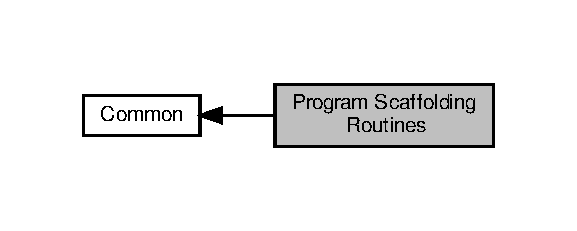
\includegraphics[width=277pt]{group__scaffolding}
\end{center}
\end{figure}
\subsection*{Macros}
\begin{DoxyCompactItemize}
\item 
\#define \hyperlink{group__scaffolding_ga1b83ce2b0adc8a384cc5a4589a8c2140}{\+\_\+\+\_\+\+F\+B\+C\+O\+N\+\_\+\+E\+V3\+\_\+\+\_\+}
\item 
\mbox{\Hypertarget{group__scaffolding_ga91164741f16fe7970ef266be19178415}\label{group__scaffolding_ga91164741f16fe7970ef266be19178415}} 
\#define \hyperlink{group__scaffolding_ga91164741f16fe7970ef266be19178415}{T\+E\+R\+M\+\_\+\+C\+O\+L\+\_\+\+M\+IN}~1
\begin{DoxyCompactList}\small\item\em Minimum Console Column value. \end{DoxyCompactList}\item 
\mbox{\Hypertarget{group__scaffolding_ga80a3ddd373d6bc24fd7e6929feb9e807}\label{group__scaffolding_ga80a3ddd373d6bc24fd7e6929feb9e807}} 
\#define \hyperlink{group__scaffolding_ga80a3ddd373d6bc24fd7e6929feb9e807}{T\+E\+R\+M\+\_\+\+C\+O\+L\+\_\+\+M\+AX}~29
\begin{DoxyCompactList}\small\item\em Maximum Console Column value. \end{DoxyCompactList}\item 
\mbox{\Hypertarget{group__scaffolding_ga3c42e3653e322d99249147e992e1976e}\label{group__scaffolding_ga3c42e3653e322d99249147e992e1976e}} 
\#define \hyperlink{group__scaffolding_ga3c42e3653e322d99249147e992e1976e}{T\+E\+R\+M\+\_\+\+R\+O\+W\+\_\+\+M\+IN}~1
\begin{DoxyCompactList}\small\item\em Minimum Console Row value. \end{DoxyCompactList}\item 
\mbox{\Hypertarget{group__scaffolding_ga141f599b6a2a3321a8a089004cd1e52a}\label{group__scaffolding_ga141f599b6a2a3321a8a089004cd1e52a}} 
\#define \hyperlink{group__scaffolding_ga141f599b6a2a3321a8a089004cd1e52a}{T\+E\+R\+M\+\_\+\+R\+O\+W\+\_\+\+M\+AX}~10
\begin{DoxyCompactList}\small\item\em Maximum Console Row value. \end{DoxyCompactList}\end{DoxyCompactItemize}
\subsection*{Functions}
\begin{DoxyCompactItemize}
\item 
void \hyperlink{group__scaffolding_gadc1bdbe20a5b0bf20b786c454857af1a}{prog\+\_\+init} (void)
\item 
void \hyperlink{group__scaffolding_gae2602aec28da58d379b4136b455a62d7}{prog\+\_\+exit} (void)
\item 
void \hyperlink{group__scaffolding_gad26b68c9bc1df3aa990eb9f594e28760}{prog\+\_\+contentX} (std\+::string str, int row, int col)
\item 
\mbox{\Hypertarget{group__scaffolding_gae8773733374b0af1000042f78b017d3d}\label{group__scaffolding_gae8773733374b0af1000042f78b017d3d}} 
void {\bfseries prog\+\_\+\+NumberX} (int value, int row, int col)
\item 
void \hyperlink{group__scaffolding_ga4472335aeac8c96294ad2f77d875d2cd}{prog\+\_\+clearscreen} (void)
\item 
bool \hyperlink{group__scaffolding_ga0420c11494d215979edc5f657819a2ca}{prog\+\_\+set\+\_\+cursorpos} (int col, int row)
\item 
void \hyperlink{group__scaffolding_ga59bf0af8d61ca90c1825e3224b45eaf9}{prog\+\_\+display\+\_\+string} (char $\ast$string)
\item 
void \hyperlink{group__scaffolding_ga0ea4957bdb462cada821c4d728494087}{prog\+\_\+display\+\_\+integer} (int value)
\item 
void \hyperlink{group__scaffolding_gae0f19e55443d5e98d104d9bc8a0e96a9}{prog\+\_\+display\+\_\+signed\+\_\+int} (int value)
\item 
void \hyperlink{group__scaffolding_ga455086b694579da94041147474387a9b}{prog\+\_\+display\+\_\+unsigned\+\_\+int} (uint value)
\item 
void \hyperlink{group__scaffolding_ga00fa862c209364a485690c01cf67b281}{prog\+\_\+display\+\_\+bin8} (unsigned char binvalue)
\item 
void \hyperlink{group__scaffolding_gae22b0332268122b8ef7443b7bc5024b9}{prog\+\_\+display\+\_\+hex32} (uint hexvalue)
\end{DoxyCompactItemize}


\subsection{Detailed Description}
The Scaffolding library perform miscellaneous startup and shutdown tasks, as well as send display to the console with basic terminal handling. 

\subsection{Macro Definition Documentation}
\mbox{\Hypertarget{group__scaffolding_ga1b83ce2b0adc8a384cc5a4589a8c2140}\label{group__scaffolding_ga1b83ce2b0adc8a384cc5a4589a8c2140}} 
\index{Program Scaffolding Routines@{Program Scaffolding Routines}!\+\_\+\+\_\+\+F\+B\+C\+O\+N\+\_\+\+E\+V3\+\_\+\+\_\+@{\+\_\+\+\_\+\+F\+B\+C\+O\+N\+\_\+\+E\+V3\+\_\+\+\_\+}}
\index{\+\_\+\+\_\+\+F\+B\+C\+O\+N\+\_\+\+E\+V3\+\_\+\+\_\+@{\+\_\+\+\_\+\+F\+B\+C\+O\+N\+\_\+\+E\+V3\+\_\+\+\_\+}!Program Scaffolding Routines@{Program Scaffolding Routines}}
\subsubsection{\texorpdfstring{\+\_\+\+\_\+\+F\+B\+C\+O\+N\+\_\+\+E\+V3\+\_\+\+\_\+}{\_\_FBCON\_EV3\_\_}}
{\footnotesize\ttfamily \#define \+\_\+\+\_\+\+F\+B\+C\+O\+N\+\_\+\+E\+V3\+\_\+\+\_\+}

\hyperlink{classText}{Text} Terminal Screen Dimensions

Assumes use of Lat15-\/\+Terminus12x6.\+psf.\+gz font for the E\+V3 178x128 Monochrome L\+CD Display 

\subsection{Function Documentation}
\mbox{\Hypertarget{group__scaffolding_ga4472335aeac8c96294ad2f77d875d2cd}\label{group__scaffolding_ga4472335aeac8c96294ad2f77d875d2cd}} 
\index{Program Scaffolding Routines@{Program Scaffolding Routines}!prog\+\_\+clearscreen@{prog\+\_\+clearscreen}}
\index{prog\+\_\+clearscreen@{prog\+\_\+clearscreen}!Program Scaffolding Routines@{Program Scaffolding Routines}}
\subsubsection{\texorpdfstring{prog\+\_\+clearscreen()}{prog\_clearscreen()}}
{\footnotesize\ttfamily void prog\+\_\+clearscreen (\begin{DoxyParamCaption}\item[{void}]{ }\end{DoxyParamCaption})}

Clear the L\+CD \hyperlink{classText}{Text} Display. Cursor will be placed at (1,1) (Top Left) 
\begin{DoxyParams}{Parameters}
{\em None} & \\
\hline
\end{DoxyParams}
\begin{DoxyReturn}{Returns}
None 
\end{DoxyReturn}
\mbox{\Hypertarget{group__scaffolding_gad26b68c9bc1df3aa990eb9f594e28760}\label{group__scaffolding_gad26b68c9bc1df3aa990eb9f594e28760}} 
\index{Program Scaffolding Routines@{Program Scaffolding Routines}!prog\+\_\+contentX@{prog\+\_\+contentX}}
\index{prog\+\_\+contentX@{prog\+\_\+contentX}!Program Scaffolding Routines@{Program Scaffolding Routines}}
\subsubsection{\texorpdfstring{prog\+\_\+content\+X()}{prog\_contentX()}}
{\footnotesize\ttfamily void prog\+\_\+contentX (\begin{DoxyParamCaption}\item[{std\+::string}]{str,  }\item[{int}]{row,  }\item[{int}]{col }\end{DoxyParamCaption})}

Display Title string on L\+CD (Row 1) 
\begin{DoxyParams}{Parameters}
{\em string} & Null-\/terminated string \\
\hline
\end{DoxyParams}
\begin{DoxyReturn}{Returns}
None Display Content string on L\+CD (Row 3) 
\end{DoxyReturn}

\begin{DoxyParams}{Parameters}
{\em string} & Null-\/terminated string \\
\hline
\end{DoxyParams}
\begin{DoxyReturn}{Returns}
None Display Content string on L\+CD (Row 5) 
\end{DoxyReturn}

\begin{DoxyParams}{Parameters}
{\em string} & Null-\/terminated string \\
\hline
\end{DoxyParams}
\begin{DoxyReturn}{Returns}
None Display Content string on L\+CD (Row row) 
\end{DoxyReturn}

\begin{DoxyParams}{Parameters}
{\em string} & Null-\/terminated string \\
\hline
{\em row} & int\+: Row Index \mbox{[}1..M\+A\+X\+\_\+\+R\+OW\mbox{]} \\
\hline
\end{DoxyParams}
\begin{DoxyReturn}{Returns}
None 
\end{DoxyReturn}
\mbox{\Hypertarget{group__scaffolding_ga00fa862c209364a485690c01cf67b281}\label{group__scaffolding_ga00fa862c209364a485690c01cf67b281}} 
\index{Program Scaffolding Routines@{Program Scaffolding Routines}!prog\+\_\+display\+\_\+bin8@{prog\+\_\+display\+\_\+bin8}}
\index{prog\+\_\+display\+\_\+bin8@{prog\+\_\+display\+\_\+bin8}!Program Scaffolding Routines@{Program Scaffolding Routines}}
\subsubsection{\texorpdfstring{prog\+\_\+display\+\_\+bin8()}{prog\_display\_bin8()}}
{\footnotesize\ttfamily void prog\+\_\+display\+\_\+bin8 (\begin{DoxyParamCaption}\item[{unsigned char}]{binvalue }\end{DoxyParamCaption})}

Display 8-\/bit binary on L\+CD at current cursor position 
\begin{DoxyParams}{Parameters}
{\em value} & 8-\/bit binary value \\
\hline
\end{DoxyParams}
\begin{DoxyReturn}{Returns}
None 
\end{DoxyReturn}
\mbox{\Hypertarget{group__scaffolding_gae22b0332268122b8ef7443b7bc5024b9}\label{group__scaffolding_gae22b0332268122b8ef7443b7bc5024b9}} 
\index{Program Scaffolding Routines@{Program Scaffolding Routines}!prog\+\_\+display\+\_\+hex32@{prog\+\_\+display\+\_\+hex32}}
\index{prog\+\_\+display\+\_\+hex32@{prog\+\_\+display\+\_\+hex32}!Program Scaffolding Routines@{Program Scaffolding Routines}}
\subsubsection{\texorpdfstring{prog\+\_\+display\+\_\+hex32()}{prog\_display\_hex32()}}
{\footnotesize\ttfamily void prog\+\_\+display\+\_\+hex32 (\begin{DoxyParamCaption}\item[{uint}]{hexvalue }\end{DoxyParamCaption})}

Display 32-\/bit hexadecimal on L\+CD at current cursor position 
\begin{DoxyParams}{Parameters}
{\em value} & 32-\/bit hexadecimal value \\
\hline
\end{DoxyParams}
\begin{DoxyReturn}{Returns}
None 
\end{DoxyReturn}
\mbox{\Hypertarget{group__scaffolding_ga0ea4957bdb462cada821c4d728494087}\label{group__scaffolding_ga0ea4957bdb462cada821c4d728494087}} 
\index{Program Scaffolding Routines@{Program Scaffolding Routines}!prog\+\_\+display\+\_\+integer@{prog\+\_\+display\+\_\+integer}}
\index{prog\+\_\+display\+\_\+integer@{prog\+\_\+display\+\_\+integer}!Program Scaffolding Routines@{Program Scaffolding Routines}}
\subsubsection{\texorpdfstring{prog\+\_\+display\+\_\+integer()}{prog\_display\_integer()}}
{\footnotesize\ttfamily void prog\+\_\+display\+\_\+integer (\begin{DoxyParamCaption}\item[{int}]{value }\end{DoxyParamCaption})}

Display signed integer on L\+CD at current cursor position The negative sign is displayed if it is negative, otherwise no signed is displayed. 
\begin{DoxyParams}{Parameters}
{\em value} & signed long value \\
\hline
\end{DoxyParams}
\begin{DoxyReturn}{Returns}
None 
\end{DoxyReturn}
\mbox{\Hypertarget{group__scaffolding_gae0f19e55443d5e98d104d9bc8a0e96a9}\label{group__scaffolding_gae0f19e55443d5e98d104d9bc8a0e96a9}} 
\index{Program Scaffolding Routines@{Program Scaffolding Routines}!prog\+\_\+display\+\_\+signed\+\_\+int@{prog\+\_\+display\+\_\+signed\+\_\+int}}
\index{prog\+\_\+display\+\_\+signed\+\_\+int@{prog\+\_\+display\+\_\+signed\+\_\+int}!Program Scaffolding Routines@{Program Scaffolding Routines}}
\subsubsection{\texorpdfstring{prog\+\_\+display\+\_\+signed\+\_\+int()}{prog\_display\_signed\_int()}}
{\footnotesize\ttfamily void prog\+\_\+display\+\_\+signed\+\_\+int (\begin{DoxyParamCaption}\item[{int}]{value }\end{DoxyParamCaption})}

Display signed integer on L\+CD at current cursor position The sign is always displayed, regardless of the value being positive or negative. 
\begin{DoxyParams}{Parameters}
{\em value} & signed long value \\
\hline
\end{DoxyParams}
\begin{DoxyReturn}{Returns}
None 
\end{DoxyReturn}
\mbox{\Hypertarget{group__scaffolding_ga59bf0af8d61ca90c1825e3224b45eaf9}\label{group__scaffolding_ga59bf0af8d61ca90c1825e3224b45eaf9}} 
\index{Program Scaffolding Routines@{Program Scaffolding Routines}!prog\+\_\+display\+\_\+string@{prog\+\_\+display\+\_\+string}}
\index{prog\+\_\+display\+\_\+string@{prog\+\_\+display\+\_\+string}!Program Scaffolding Routines@{Program Scaffolding Routines}}
\subsubsection{\texorpdfstring{prog\+\_\+display\+\_\+string()}{prog\_display\_string()}}
{\footnotesize\ttfamily void prog\+\_\+display\+\_\+string (\begin{DoxyParamCaption}\item[{char $\ast$}]{string }\end{DoxyParamCaption})}

Display string on L\+CD at current cursor position 
\begin{DoxyParams}{Parameters}
{\em string} & Null-\/terminated string \\
\hline
\end{DoxyParams}
\begin{DoxyReturn}{Returns}
None 
\end{DoxyReturn}
\mbox{\Hypertarget{group__scaffolding_ga455086b694579da94041147474387a9b}\label{group__scaffolding_ga455086b694579da94041147474387a9b}} 
\index{Program Scaffolding Routines@{Program Scaffolding Routines}!prog\+\_\+display\+\_\+unsigned\+\_\+int@{prog\+\_\+display\+\_\+unsigned\+\_\+int}}
\index{prog\+\_\+display\+\_\+unsigned\+\_\+int@{prog\+\_\+display\+\_\+unsigned\+\_\+int}!Program Scaffolding Routines@{Program Scaffolding Routines}}
\subsubsection{\texorpdfstring{prog\+\_\+display\+\_\+unsigned\+\_\+int()}{prog\_display\_unsigned\_int()}}
{\footnotesize\ttfamily void prog\+\_\+display\+\_\+unsigned\+\_\+int (\begin{DoxyParamCaption}\item[{uint}]{value }\end{DoxyParamCaption})}

Display unsigned integer on L\+CD at current cursor position 
\begin{DoxyParams}{Parameters}
{\em value} & unsigned long value \\
\hline
\end{DoxyParams}
\begin{DoxyReturn}{Returns}
None 
\end{DoxyReturn}
\mbox{\Hypertarget{group__scaffolding_gae2602aec28da58d379b4136b455a62d7}\label{group__scaffolding_gae2602aec28da58d379b4136b455a62d7}} 
\index{Program Scaffolding Routines@{Program Scaffolding Routines}!prog\+\_\+exit@{prog\+\_\+exit}}
\index{prog\+\_\+exit@{prog\+\_\+exit}!Program Scaffolding Routines@{Program Scaffolding Routines}}
\subsubsection{\texorpdfstring{prog\+\_\+exit()}{prog\_exit()}}
{\footnotesize\ttfamily void prog\+\_\+exit (\begin{DoxyParamCaption}\item[{void}]{ }\end{DoxyParamCaption})}

Exit A\+R\+M-\/\+B\+BR subsystems Generate exit tone 
\begin{DoxyParams}{Parameters}
{\em None} & \\
\hline
\end{DoxyParams}
\begin{DoxyReturn}{Returns}
None 
\end{DoxyReturn}
\mbox{\Hypertarget{group__scaffolding_gadc1bdbe20a5b0bf20b786c454857af1a}\label{group__scaffolding_gadc1bdbe20a5b0bf20b786c454857af1a}} 
\index{Program Scaffolding Routines@{Program Scaffolding Routines}!prog\+\_\+init@{prog\+\_\+init}}
\index{prog\+\_\+init@{prog\+\_\+init}!Program Scaffolding Routines@{Program Scaffolding Routines}}
\subsubsection{\texorpdfstring{prog\+\_\+init()}{prog\_init()}}
{\footnotesize\ttfamily void prog\+\_\+init (\begin{DoxyParamCaption}\item[{void}]{ }\end{DoxyParamCaption})}

Common Startup/\+Shutdown Routines for A\+R\+M-\/\+B\+BR programs Initialize A\+R\+M-\/\+B\+BR subsystems Clears L\+CD screen and generate startup tone 
\begin{DoxyParams}{Parameters}
{\em None} & \\
\hline
\end{DoxyParams}
\begin{DoxyReturn}{Returns}
None 
\end{DoxyReturn}
\mbox{\Hypertarget{group__scaffolding_ga0420c11494d215979edc5f657819a2ca}\label{group__scaffolding_ga0420c11494d215979edc5f657819a2ca}} 
\index{Program Scaffolding Routines@{Program Scaffolding Routines}!prog\+\_\+set\+\_\+cursorpos@{prog\+\_\+set\+\_\+cursorpos}}
\index{prog\+\_\+set\+\_\+cursorpos@{prog\+\_\+set\+\_\+cursorpos}!Program Scaffolding Routines@{Program Scaffolding Routines}}
\subsubsection{\texorpdfstring{prog\+\_\+set\+\_\+cursorpos()}{prog\_set\_cursorpos()}}
{\footnotesize\ttfamily bool prog\+\_\+set\+\_\+cursorpos (\begin{DoxyParamCaption}\item[{int}]{col,  }\item[{int}]{row }\end{DoxyParamCaption})}

Set the cursor on the L\+CD to new cursor position Note\+: This only works on the L\+CD screen. It does not work in the Debugger output window. 
\begin{DoxyParams}{Parameters}
{\em col} & integer value \\
\hline
{\em row} & integer value \\
\hline
\end{DoxyParams}
\begin{DoxyReturn}{Returns}
success\+: bool value 
\end{DoxyReturn}

\hypertarget{group__common}{}\section{Common}
\label{group__common}\index{Common@{Common}}
Collaboration diagram for Common\+:
\nopagebreak
\begin{figure}[H]
\begin{center}
\leavevmode
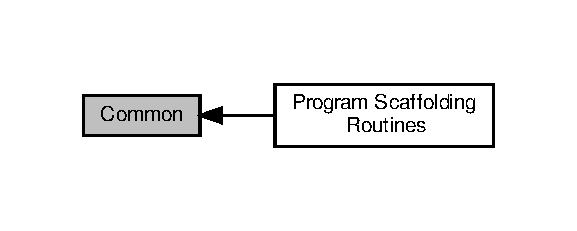
\includegraphics[width=277pt]{group__common}
\end{center}
\end{figure}
\subsection*{Modules}
\begin{DoxyCompactItemize}
\item 
\hyperlink{group__scaffolding}{Program Scaffolding Routines}
\end{DoxyCompactItemize}


\subsection{Detailed Description}

\chapter{Namespace Documentation}
\hypertarget{namespacenlohmann}{}\section{nlohmann Namespace Reference}
\label{namespacenlohmann}\index{nlohmann@{nlohmann}}


namespace for Niels Lohmann  


\subsection*{Namespaces}
\begin{DoxyCompactItemize}
\item 
 \hyperlink{namespacenlohmann_1_1detail}{detail}
\begin{DoxyCompactList}\small\item\em detail namespace with internal helper functions \end{DoxyCompactList}\end{DoxyCompactItemize}
\subsection*{Classes}
\begin{DoxyCompactItemize}
\item 
struct \hyperlink{structnlohmann_1_1adl__serializer}{adl\+\_\+serializer}
\begin{DoxyCompactList}\small\item\em default J\+S\+O\+N\+Serializer template argument \end{DoxyCompactList}\item 
class \hyperlink{classnlohmann_1_1basic__json}{basic\+\_\+json}
\begin{DoxyCompactList}\small\item\em a class to store J\+S\+ON values \end{DoxyCompactList}\item 
class \hyperlink{classnlohmann_1_1byte__container__with__subtype}{byte\+\_\+container\+\_\+with\+\_\+subtype}
\begin{DoxyCompactList}\small\item\em an internal type for a backed binary type \end{DoxyCompactList}\item 
class \hyperlink{classnlohmann_1_1json__pointer}{json\+\_\+pointer}
\begin{DoxyCompactList}\small\item\em J\+S\+ON Pointer defines a string syntax for identifying a specific value within a J\+S\+ON document. \end{DoxyCompactList}\item 
struct \hyperlink{structnlohmann_1_1json__sax}{json\+\_\+sax}
\begin{DoxyCompactList}\small\item\em S\+AX interface. \end{DoxyCompactList}\item 
struct \hyperlink{structnlohmann_1_1ordered__map}{ordered\+\_\+map}
\begin{DoxyCompactList}\small\item\em a minimal map-\/like container that preserves insertion order \end{DoxyCompactList}\end{DoxyCompactItemize}
\subsection*{Typedefs}
\begin{DoxyCompactItemize}
\item 
using \hyperlink{namespacenlohmann_a2bfd99e845a2e5cd90aeaf1b1431f474}{json} = \hyperlink{classnlohmann_1_1basic__json}{basic\+\_\+json}$<$$>$
\begin{DoxyCompactList}\small\item\em default specialization \end{DoxyCompactList}\item 
using \hyperlink{namespacenlohmann_ad53cef358adfa7f07cea23eb1e28b9ea}{ordered\+\_\+json} = \hyperlink{classnlohmann_1_1basic__json}{basic\+\_\+json}$<$ \hyperlink{structnlohmann_1_1ordered__map}{nlohmann\+::ordered\+\_\+map} $>$
\begin{DoxyCompactList}\small\item\em specialization that maintains the insertion order of object keys \end{DoxyCompactList}\end{DoxyCompactItemize}
\subsection*{Functions}
\begin{DoxyCompactItemize}
\item 
\mbox{\Hypertarget{namespacenlohmann_a6ea7ce1fcdd8c94f6c3221c63356f39b}\label{namespacenlohmann_a6ea7ce1fcdd8c94f6c3221c63356f39b}} 
{\bfseries N\+L\+O\+H\+M\+A\+N\+N\+\_\+\+C\+A\+N\+\_\+\+C\+A\+L\+L\+\_\+\+S\+T\+D\+\_\+\+F\+U\+N\+C\+\_\+\+I\+M\+PL} (begin)
\item 
\mbox{\Hypertarget{namespacenlohmann_a2fe3cfce480685121828a64e2da31eb4}\label{namespacenlohmann_a2fe3cfce480685121828a64e2da31eb4}} 
{\bfseries N\+L\+O\+H\+M\+A\+N\+N\+\_\+\+C\+A\+N\+\_\+\+C\+A\+L\+L\+\_\+\+S\+T\+D\+\_\+\+F\+U\+N\+C\+\_\+\+I\+M\+PL} (end)
\item 
N\+L\+O\+H\+M\+A\+N\+N\+\_\+\+B\+A\+S\+I\+C\+\_\+\+J\+S\+O\+N\+\_\+\+T\+P\+L\+\_\+\+D\+E\+C\+L\+A\+R\+A\+T\+I\+ON std\+::string \hyperlink{namespacenlohmann_a6ce645a0b8717757e096a5b5773b7a16}{to\+\_\+string} (const N\+L\+O\+H\+M\+A\+N\+N\+\_\+\+B\+A\+S\+I\+C\+\_\+\+J\+S\+O\+N\+\_\+\+T\+PL \&j)
\begin{DoxyCompactList}\small\item\em user-\/defined to\+\_\+string function for J\+S\+ON values \end{DoxyCompactList}\end{DoxyCompactItemize}


\subsection{Detailed Description}
namespace for Niels Lohmann 

\begin{DoxySeeAlso}{See also}
\href{https://github.com/nlohmann}{\tt https\+://github.\+com/nlohmann} 
\end{DoxySeeAlso}
\begin{DoxySince}{Since}
version 1.\+0.\+0
\end{DoxySince}
namespace to hold default {\ttfamily to\+\_\+json} function to see why this is required\+: \href{http://www.open-std.org/jtc1/sc22/wg21/docs/papers/2015/n4381.html}{\tt http\+://www.\+open-\/std.\+org/jtc1/sc22/wg21/docs/papers/2015/n4381.\+html} 

\subsection{Typedef Documentation}
\mbox{\Hypertarget{namespacenlohmann_a2bfd99e845a2e5cd90aeaf1b1431f474}\label{namespacenlohmann_a2bfd99e845a2e5cd90aeaf1b1431f474}} 
\index{nlohmann@{nlohmann}!json@{json}}
\index{json@{json}!nlohmann@{nlohmann}}
\subsubsection{\texorpdfstring{json}{json}}
{\footnotesize\ttfamily using \hyperlink{namespacenlohmann_a2bfd99e845a2e5cd90aeaf1b1431f474}{nlohmann\+::json} = typedef \hyperlink{classnlohmann_1_1basic__json}{basic\+\_\+json}$<$$>$}



default specialization 

\begin{DoxySeeAlso}{See also}
\href{https://json.nlohmann.me/api/json/}{\tt https\+://json.\+nlohmann.\+me/api/json/} 
\end{DoxySeeAlso}
\mbox{\Hypertarget{namespacenlohmann_ad53cef358adfa7f07cea23eb1e28b9ea}\label{namespacenlohmann_ad53cef358adfa7f07cea23eb1e28b9ea}} 
\index{nlohmann@{nlohmann}!ordered\+\_\+json@{ordered\+\_\+json}}
\index{ordered\+\_\+json@{ordered\+\_\+json}!nlohmann@{nlohmann}}
\subsubsection{\texorpdfstring{ordered\+\_\+json}{ordered\_json}}
{\footnotesize\ttfamily using \hyperlink{namespacenlohmann_ad53cef358adfa7f07cea23eb1e28b9ea}{nlohmann\+::ordered\+\_\+json} = typedef \hyperlink{classnlohmann_1_1basic__json}{basic\+\_\+json}$<$\hyperlink{structnlohmann_1_1ordered__map}{nlohmann\+::ordered\+\_\+map}$>$}



specialization that maintains the insertion order of object keys 

\begin{DoxySeeAlso}{See also}
\href{https://json.nlohmann.me/api/ordered_json/}{\tt https\+://json.\+nlohmann.\+me/api/ordered\+\_\+json/} 
\end{DoxySeeAlso}


\subsection{Function Documentation}
\mbox{\Hypertarget{namespacenlohmann_a6ce645a0b8717757e096a5b5773b7a16}\label{namespacenlohmann_a6ce645a0b8717757e096a5b5773b7a16}} 
\index{nlohmann@{nlohmann}!to\+\_\+string@{to\+\_\+string}}
\index{to\+\_\+string@{to\+\_\+string}!nlohmann@{nlohmann}}
\subsubsection{\texorpdfstring{to\+\_\+string()}{to\_string()}}
{\footnotesize\ttfamily N\+L\+O\+H\+M\+A\+N\+N\+\_\+\+B\+A\+S\+I\+C\+\_\+\+J\+S\+O\+N\+\_\+\+T\+P\+L\+\_\+\+D\+E\+C\+L\+A\+R\+A\+T\+I\+ON std\+::string nlohmann\+::to\+\_\+string (\begin{DoxyParamCaption}\item[{const N\+L\+O\+H\+M\+A\+N\+N\+\_\+\+B\+A\+S\+I\+C\+\_\+\+J\+S\+O\+N\+\_\+\+T\+PL \&}]{j }\end{DoxyParamCaption})}



user-\/defined to\+\_\+string function for J\+S\+ON values 

\begin{DoxySeeAlso}{See also}
\href{https://json.nlohmann.me/api/basic_json/to_string/}{\tt https\+://json.\+nlohmann.\+me/api/basic\+\_\+json/to\+\_\+string/} 
\end{DoxySeeAlso}

\hypertarget{namespacenlohmann_1_1detail}{}\section{nlohmann\+:\+:detail Namespace Reference}
\label{namespacenlohmann_1_1detail}\index{nlohmann\+::detail@{nlohmann\+::detail}}


detail namespace with internal helper functions  


\subsection*{Namespaces}
\begin{DoxyCompactItemize}
\item 
 \hyperlink{namespacenlohmann_1_1detail_1_1dtoa__impl}{dtoa\+\_\+impl}
\begin{DoxyCompactList}\small\item\em implements the Grisu2 algorithm for binary to decimal floating-\/point conversion. \end{DoxyCompactList}\end{DoxyCompactItemize}
\subsection*{Classes}
\begin{DoxyCompactItemize}
\item 
class \hyperlink{classnlohmann_1_1detail_1_1binary__reader}{binary\+\_\+reader}
\begin{DoxyCompactList}\small\item\em deserialization of C\+B\+OR, Message\+Pack, and U\+B\+J\+S\+ON values \end{DoxyCompactList}\item 
class \hyperlink{classnlohmann_1_1detail_1_1binary__writer}{binary\+\_\+writer}
\begin{DoxyCompactList}\small\item\em serialization to C\+B\+OR and Message\+Pack values \end{DoxyCompactList}\item 
struct \hyperlink{structnlohmann_1_1detail_1_1conjunction}{conjunction}
\item 
struct \hyperlink{structnlohmann_1_1detail_1_1conjunction_3_01B1_01_4}{conjunction$<$ B1 $>$}
\item 
struct \hyperlink{structnlohmann_1_1detail_1_1conjunction_3_01B1_00_01Bn_8_8_8_01_4}{conjunction$<$ B1, Bn... $>$}
\item 
struct \hyperlink{structnlohmann_1_1detail_1_1detector}{detector}
\item 
struct \hyperlink{structnlohmann_1_1detail_1_1detector_3_01Default_00_01void__t_3_01Op_3_01Args_8_8_8_01_4_01_4_00_01Op_00_01Args_8_8_8_01_4}{detector$<$ Default, void\+\_\+t$<$ Op$<$ Args... $>$ $>$, Op, Args... $>$}
\item 
class \hyperlink{classnlohmann_1_1detail_1_1exception}{exception}
\begin{DoxyCompactList}\small\item\em general exception of the \hyperlink{classnlohmann_1_1basic__json}{basic\+\_\+json} class \end{DoxyCompactList}\item 
struct \hyperlink{structnlohmann_1_1detail_1_1external__constructor}{external\+\_\+constructor}
\item 
struct \hyperlink{structnlohmann_1_1detail_1_1external__constructor_3_01value__t_1_1array_01_4}{external\+\_\+constructor$<$ value\+\_\+t\+::array $>$}
\item 
struct \hyperlink{structnlohmann_1_1detail_1_1external__constructor_3_01value__t_1_1binary_01_4}{external\+\_\+constructor$<$ value\+\_\+t\+::binary $>$}
\item 
struct \hyperlink{structnlohmann_1_1detail_1_1external__constructor_3_01value__t_1_1boolean_01_4}{external\+\_\+constructor$<$ value\+\_\+t\+::boolean $>$}
\item 
struct \hyperlink{structnlohmann_1_1detail_1_1external__constructor_3_01value__t_1_1number__float_01_4}{external\+\_\+constructor$<$ value\+\_\+t\+::number\+\_\+float $>$}
\item 
struct \hyperlink{structnlohmann_1_1detail_1_1external__constructor_3_01value__t_1_1number__integer_01_4}{external\+\_\+constructor$<$ value\+\_\+t\+::number\+\_\+integer $>$}
\item 
struct \hyperlink{structnlohmann_1_1detail_1_1external__constructor_3_01value__t_1_1number__unsigned_01_4}{external\+\_\+constructor$<$ value\+\_\+t\+::number\+\_\+unsigned $>$}
\item 
struct \hyperlink{structnlohmann_1_1detail_1_1external__constructor_3_01value__t_1_1object_01_4}{external\+\_\+constructor$<$ value\+\_\+t\+::object $>$}
\item 
struct \hyperlink{structnlohmann_1_1detail_1_1external__constructor_3_01value__t_1_1string_01_4}{external\+\_\+constructor$<$ value\+\_\+t\+::string $>$}
\item 
class \hyperlink{classnlohmann_1_1detail_1_1file__input__adapter}{file\+\_\+input\+\_\+adapter}
\item 
struct \hyperlink{structnlohmann_1_1detail_1_1from__json__fn}{from\+\_\+json\+\_\+fn}
\item 
struct \hyperlink{structnlohmann_1_1detail_1_1has__from__json}{has\+\_\+from\+\_\+json}
\item 
struct \hyperlink{structnlohmann_1_1detail_1_1has__from__json_3_01BasicJsonType_00_01T_00_01enable__if__t_3_01_9is3ee028c64c76c768be45996bb13fc9c5}{has\+\_\+from\+\_\+json$<$ Basic\+Json\+Type, T, enable\+\_\+if\+\_\+t$<$ !is\+\_\+basic\+\_\+json$<$ T $>$\+::value $>$ $>$}
\item 
struct \hyperlink{structnlohmann_1_1detail_1_1has__non__default__from__json}{has\+\_\+non\+\_\+default\+\_\+from\+\_\+json}
\item 
struct \hyperlink{structnlohmann_1_1detail_1_1has__non__default__from__json_3_01BasicJsonType_00_01T_00_01enable__b7a8cd863889b54d1139b207b4233111}{has\+\_\+non\+\_\+default\+\_\+from\+\_\+json$<$ Basic\+Json\+Type, T, enable\+\_\+if\+\_\+t$<$ !is\+\_\+basic\+\_\+json$<$ T $>$\+::value $>$ $>$}
\item 
struct \hyperlink{structnlohmann_1_1detail_1_1has__to__json}{has\+\_\+to\+\_\+json}
\item 
struct \hyperlink{structnlohmann_1_1detail_1_1has__to__json_3_01BasicJsonType_00_01T_00_01enable__if__t_3_01_9is__4a8838c1c30336126696a126041e661c}{has\+\_\+to\+\_\+json$<$ Basic\+Json\+Type, T, enable\+\_\+if\+\_\+t$<$ !is\+\_\+basic\+\_\+json$<$ T $>$\+::value $>$ $>$}
\item 
struct \hyperlink{structnlohmann_1_1detail_1_1identity__tag}{identity\+\_\+tag}
\item 
class \hyperlink{classnlohmann_1_1detail_1_1input__stream__adapter}{input\+\_\+stream\+\_\+adapter}
\item 
struct \hyperlink{structnlohmann_1_1detail_1_1integer__sequence}{integer\+\_\+sequence}
\item 
struct \hyperlink{structnlohmann_1_1detail_1_1internal__iterator}{internal\+\_\+iterator}
\begin{DoxyCompactList}\small\item\em an iterator value \end{DoxyCompactList}\item 
class \hyperlink{classnlohmann_1_1detail_1_1invalid__iterator}{invalid\+\_\+iterator}
\begin{DoxyCompactList}\small\item\em exception indicating errors with iterators \end{DoxyCompactList}\item 
struct \hyperlink{structnlohmann_1_1detail_1_1is__basic__json}{is\+\_\+basic\+\_\+json}
\item 
struct \hyperlink{structnlohmann_1_1detail_1_1is__basic__json_3_01NLOHMANN__BASIC__JSON__TPL_01_4}{is\+\_\+basic\+\_\+json$<$ N\+L\+O\+H\+M\+A\+N\+N\+\_\+\+B\+A\+S\+I\+C\+\_\+\+J\+S\+O\+N\+\_\+\+T\+P\+L $>$}
\item 
struct \hyperlink{structnlohmann_1_1detail_1_1is__compatible__array__type}{is\+\_\+compatible\+\_\+array\+\_\+type}
\item 
struct \hyperlink{structnlohmann_1_1detail_1_1is__compatible__array__type__impl}{is\+\_\+compatible\+\_\+array\+\_\+type\+\_\+impl}
\item 
struct \hyperlink{structnlohmann_1_1detail_1_1is__compatible__array__type__impl_3_01BasicJsonType_00_01CompatibleAfaa3c0bd038fd031f5ee109e19639e03}{is\+\_\+compatible\+\_\+array\+\_\+type\+\_\+impl$<$ Basic\+Json\+Type, Compatible\+Array\+Type, enable\+\_\+if\+\_\+t$<$ is\+\_\+detected$<$ iterator\+\_\+t, Compatible\+Array\+Type $>$\+::value \&\&is\+\_\+iterator\+\_\+traits$<$ iterator\+\_\+traits$<$ detected\+\_\+t$<$ iterator\+\_\+t, Compatible\+Array\+Type $>$ $>$ $>$\+::value \&\&!std\+::is\+\_\+same$<$ Compatible\+Array\+Type, detected\+\_\+t$<$ range\+\_\+value\+\_\+t, Compatible\+Array\+Type $>$ $>$\+::value $>$ $>$}
\item 
struct \hyperlink{structnlohmann_1_1detail_1_1is__compatible__integer__type}{is\+\_\+compatible\+\_\+integer\+\_\+type}
\item 
struct \hyperlink{structnlohmann_1_1detail_1_1is__compatible__integer__type__impl}{is\+\_\+compatible\+\_\+integer\+\_\+type\+\_\+impl}
\item 
struct \hyperlink{structnlohmann_1_1detail_1_1is__compatible__integer__type__impl_3_01RealIntegerType_00_01Compatie5920c849e839ebb9f8c57349c900796}{is\+\_\+compatible\+\_\+integer\+\_\+type\+\_\+impl$<$ Real\+Integer\+Type, Compatible\+Number\+Integer\+Type, enable\+\_\+if\+\_\+t$<$ std\+::is\+\_\+integral$<$ Real\+Integer\+Type $>$\+::value \&\&std\+::is\+\_\+integral$<$ Compatible\+Number\+Integer\+Type $>$\+::value \&\&!std\+::is\+\_\+same$<$ bool, Compatible\+Number\+Integer\+Type $>$\+::value $>$ $>$}
\item 
struct \hyperlink{structnlohmann_1_1detail_1_1is__compatible__object__type}{is\+\_\+compatible\+\_\+object\+\_\+type}
\item 
struct \hyperlink{structnlohmann_1_1detail_1_1is__compatible__object__type__impl}{is\+\_\+compatible\+\_\+object\+\_\+type\+\_\+impl}
\item 
struct \hyperlink{structnlohmann_1_1detail_1_1is__compatible__object__type__impl_3_01BasicJsonType_00_01Compatible1dd1bd23ba0e4ce33237aa702f8058a9}{is\+\_\+compatible\+\_\+object\+\_\+type\+\_\+impl$<$ Basic\+Json\+Type, Compatible\+Object\+Type, enable\+\_\+if\+\_\+t$<$ is\+\_\+detected$<$ mapped\+\_\+type\+\_\+t, Compatible\+Object\+Type $>$\+::value \&\&is\+\_\+detected$<$ key\+\_\+type\+\_\+t, Compatible\+Object\+Type $>$\+::value $>$ $>$}
\item 
struct \hyperlink{structnlohmann_1_1detail_1_1is__compatible__string__type}{is\+\_\+compatible\+\_\+string\+\_\+type}
\item 
struct \hyperlink{structnlohmann_1_1detail_1_1is__compatible__type}{is\+\_\+compatible\+\_\+type}
\item 
struct \hyperlink{structnlohmann_1_1detail_1_1is__compatible__type__impl}{is\+\_\+compatible\+\_\+type\+\_\+impl}
\item 
struct \hyperlink{structnlohmann_1_1detail_1_1is__compatible__type__impl_3_01BasicJsonType_00_01CompatibleType_00_fa54cb60e66f5c6ba93b1dd3f418b703}{is\+\_\+compatible\+\_\+type\+\_\+impl$<$ Basic\+Json\+Type, Compatible\+Type, enable\+\_\+if\+\_\+t$<$ is\+\_\+complete\+\_\+type$<$ Compatible\+Type $>$\+::value $>$ $>$}
\item 
struct \hyperlink{structnlohmann_1_1detail_1_1is__complete__type}{is\+\_\+complete\+\_\+type}
\item 
struct \hyperlink{structnlohmann_1_1detail_1_1is__complete__type_3_01T_00_01decltype_07void_07sizeof_07T_08_08_08_4}{is\+\_\+complete\+\_\+type$<$ T, decltype(void(sizeof(\+T)))$>$}
\item 
struct \hyperlink{structnlohmann_1_1detail_1_1is__constructible}{is\+\_\+constructible}
\item 
struct \hyperlink{structnlohmann_1_1detail_1_1is__constructible_3_01const_01std_1_1pair_3_01T1_00_01T2_01_4_01_4}{is\+\_\+constructible$<$ const std\+::pair$<$ T1, T2 $>$ $>$}
\item 
struct \hyperlink{structnlohmann_1_1detail_1_1is__constructible_3_01const_01std_1_1tuple_3_01Ts_8_8_8_01_4_01_4}{is\+\_\+constructible$<$ const std\+::tuple$<$ Ts... $>$ $>$}
\item 
struct \hyperlink{structnlohmann_1_1detail_1_1is__constructible_3_01std_1_1pair_3_01T1_00_01T2_01_4_01_4}{is\+\_\+constructible$<$ std\+::pair$<$ T1, T2 $>$ $>$}
\item 
struct \hyperlink{structnlohmann_1_1detail_1_1is__constructible_3_01std_1_1tuple_3_01Ts_8_8_8_01_4_01_4}{is\+\_\+constructible$<$ std\+::tuple$<$ Ts... $>$ $>$}
\item 
struct \hyperlink{structnlohmann_1_1detail_1_1is__constructible__array__type}{is\+\_\+constructible\+\_\+array\+\_\+type}
\item 
struct \hyperlink{structnlohmann_1_1detail_1_1is__constructible__array__type__impl}{is\+\_\+constructible\+\_\+array\+\_\+type\+\_\+impl}
\item 
struct \hyperlink{structnlohmann_1_1detail_1_1is__constructible__array__type__impl_3_01BasicJsonType_00_01Construc9fb32d79d2f03f291695c23371cb431d}{is\+\_\+constructible\+\_\+array\+\_\+type\+\_\+impl$<$ Basic\+Json\+Type, Constructible\+Array\+Type, enable\+\_\+if\+\_\+t$<$ !std\+::is\+\_\+same$<$ Constructible\+Array\+Type, typename Basic\+Json\+Type\+::value\+\_\+type $>$\+::value \&\&!is\+\_\+compatible\+\_\+string\+\_\+type$<$ Basic\+Json\+Type, Constructible\+Array\+Type $>$\+::value \&\&is\+\_\+default\+\_\+constructible$<$ Constructible\+Array\+Type $>$\+::value \&\&(std\+::is\+\_\+move\+\_\+assignable$<$ Constructible\+Array\+Type $>$\+::value$\vert$$\vert$std\+::is\+\_\+copy\+\_\+assignable$<$ Constructible\+Array\+Type $>$\+::value)\&\&is\+\_\+detected$<$ iterator\+\_\+t, Constructible\+Array\+Type $>$\+::value \&\&is\+\_\+iterator\+\_\+traits$<$ iterator\+\_\+traits$<$ detected\+\_\+t$<$ iterator\+\_\+t, Constructible\+Array\+Type $>$ $>$ $>$\+::value \&\&is\+\_\+detected$<$ range\+\_\+value\+\_\+t, Constructible\+Array\+Type $>$\+::value \&\&!std\+::is\+\_\+same$<$ Constructible\+Array\+Type, detected\+\_\+t$<$ range\+\_\+value\+\_\+t, Constructible\+Array\+Type $>$ $>$\+::value \&\&is\+\_\+complete\+\_\+type$<$ detected\+\_\+t$<$ range\+\_\+value\+\_\+t, Constructible\+Array\+Type $>$ $>$\+::value $>$ $>$}
\item 
struct \hyperlink{structnlohmann_1_1detail_1_1is__constructible__array__type__impl_3_01BasicJsonType_00_01Construce6fa33688da703b95649da4749cdeb98}{is\+\_\+constructible\+\_\+array\+\_\+type\+\_\+impl$<$ Basic\+Json\+Type, Constructible\+Array\+Type, enable\+\_\+if\+\_\+t$<$ std\+::is\+\_\+same$<$ Constructible\+Array\+Type, typename Basic\+Json\+Type\+::value\+\_\+type $>$\+::value $>$ $>$}
\item 
struct \hyperlink{structnlohmann_1_1detail_1_1is__constructible__object__type}{is\+\_\+constructible\+\_\+object\+\_\+type}
\item 
struct \hyperlink{structnlohmann_1_1detail_1_1is__constructible__object__type__impl}{is\+\_\+constructible\+\_\+object\+\_\+type\+\_\+impl}
\item 
struct \hyperlink{structnlohmann_1_1detail_1_1is__constructible__object__type__impl_3_01BasicJsonType_00_01Construa4d1e16800f2c4963485512ecf18377c}{is\+\_\+constructible\+\_\+object\+\_\+type\+\_\+impl$<$ Basic\+Json\+Type, Constructible\+Object\+Type, enable\+\_\+if\+\_\+t$<$ is\+\_\+detected$<$ mapped\+\_\+type\+\_\+t, Constructible\+Object\+Type $>$\+::value \&\&is\+\_\+detected$<$ key\+\_\+type\+\_\+t, Constructible\+Object\+Type $>$\+::value $>$ $>$}
\item 
struct \hyperlink{structnlohmann_1_1detail_1_1is__constructible__string__type}{is\+\_\+constructible\+\_\+string\+\_\+type}
\item 
struct \hyperlink{structnlohmann_1_1detail_1_1is__constructible__tuple}{is\+\_\+constructible\+\_\+tuple}
\item 
struct \hyperlink{structnlohmann_1_1detail_1_1is__constructible__tuple_3_01T1_00_01std_1_1tuple_3_01Args_8_8_8_01_4_01_4}{is\+\_\+constructible\+\_\+tuple$<$ T1, std\+::tuple$<$ Args... $>$ $>$}
\item 
struct \hyperlink{structnlohmann_1_1detail_1_1is__default__constructible}{is\+\_\+default\+\_\+constructible}
\item 
struct \hyperlink{structnlohmann_1_1detail_1_1is__default__constructible_3_01const_01std_1_1pair_3_01T1_00_01T2_01_4_01_4}{is\+\_\+default\+\_\+constructible$<$ const std\+::pair$<$ T1, T2 $>$ $>$}
\item 
struct \hyperlink{structnlohmann_1_1detail_1_1is__default__constructible_3_01const_01std_1_1tuple_3_01Ts_8_8_8_01_4_01_4}{is\+\_\+default\+\_\+constructible$<$ const std\+::tuple$<$ Ts... $>$ $>$}
\item 
struct \hyperlink{structnlohmann_1_1detail_1_1is__default__constructible_3_01std_1_1pair_3_01T1_00_01T2_01_4_01_4}{is\+\_\+default\+\_\+constructible$<$ std\+::pair$<$ T1, T2 $>$ $>$}
\item 
struct \hyperlink{structnlohmann_1_1detail_1_1is__default__constructible_3_01std_1_1tuple_3_01Ts_8_8_8_01_4_01_4}{is\+\_\+default\+\_\+constructible$<$ std\+::tuple$<$ Ts... $>$ $>$}
\item 
struct \hyperlink{structnlohmann_1_1detail_1_1is__detected__lazy}{is\+\_\+detected\+\_\+lazy}
\item 
struct \hyperlink{structnlohmann_1_1detail_1_1is__getable}{is\+\_\+getable}
\item 
struct \hyperlink{structnlohmann_1_1detail_1_1is__iterator__of__multibyte}{is\+\_\+iterator\+\_\+of\+\_\+multibyte}
\item 
struct \hyperlink{structnlohmann_1_1detail_1_1is__iterator__traits}{is\+\_\+iterator\+\_\+traits}
\item 
struct \hyperlink{structnlohmann_1_1detail_1_1is__iterator__traits_3_01iterator__traits_3_01T_01_4_01_4}{is\+\_\+iterator\+\_\+traits$<$ iterator\+\_\+traits$<$ T $>$ $>$}
\item 
struct \hyperlink{structnlohmann_1_1detail_1_1is__json__ref}{is\+\_\+json\+\_\+ref}
\item 
struct \hyperlink{structnlohmann_1_1detail_1_1is__json__ref_3_01json__ref_3_01T_01_4_01_4}{is\+\_\+json\+\_\+ref$<$ json\+\_\+ref$<$ T $>$ $>$}
\item 
struct \hyperlink{structnlohmann_1_1detail_1_1is__ordered__map}{is\+\_\+ordered\+\_\+map}
\item 
struct \hyperlink{structnlohmann_1_1detail_1_1is__range}{is\+\_\+range}
\item 
struct \hyperlink{structnlohmann_1_1detail_1_1is__sax}{is\+\_\+sax}
\item 
struct \hyperlink{structnlohmann_1_1detail_1_1is__sax__static__asserts}{is\+\_\+sax\+\_\+static\+\_\+asserts}
\item 
class \hyperlink{classnlohmann_1_1detail_1_1iter__impl}{iter\+\_\+impl}
\begin{DoxyCompactList}\small\item\em a template for a bidirectional iterator for the \hyperlink{classnlohmann_1_1basic__json}{basic\+\_\+json} class This class implements a both iterators (iterator and const\+\_\+iterator) for the \hyperlink{classnlohmann_1_1basic__json}{basic\+\_\+json} class. \end{DoxyCompactList}\item 
class \hyperlink{classnlohmann_1_1detail_1_1iteration__proxy}{iteration\+\_\+proxy}
\begin{DoxyCompactList}\small\item\em proxy class for the items() function \end{DoxyCompactList}\item 
class \hyperlink{classnlohmann_1_1detail_1_1iteration__proxy__value}{iteration\+\_\+proxy\+\_\+value}
\item 
class \hyperlink{classnlohmann_1_1detail_1_1iterator__input__adapter}{iterator\+\_\+input\+\_\+adapter}
\item 
struct \hyperlink{structnlohmann_1_1detail_1_1iterator__input__adapter__factory}{iterator\+\_\+input\+\_\+adapter\+\_\+factory}
\item 
struct \hyperlink{structnlohmann_1_1detail_1_1iterator__input__adapter__factory_3_01IteratorType_00_01enable__if__0e86378a778d78dd2284e92dc30f4902}{iterator\+\_\+input\+\_\+adapter\+\_\+factory$<$ Iterator\+Type, enable\+\_\+if\+\_\+t$<$ is\+\_\+iterator\+\_\+of\+\_\+multibyte$<$ Iterator\+Type $>$\+::value $>$ $>$}
\item 
struct \hyperlink{structnlohmann_1_1detail_1_1iterator__traits}{iterator\+\_\+traits}
\item 
struct \hyperlink{structnlohmann_1_1detail_1_1iterator__traits_3_01T_01_5_00_01enable__if__t_3_01std_1_1is__object_3_01T_01_4_1_1value_01_4_01_4}{iterator\+\_\+traits$<$ T $\ast$, enable\+\_\+if\+\_\+t$<$ std\+::is\+\_\+object$<$ T $>$\+::value $>$ $>$}
\item 
struct \hyperlink{structnlohmann_1_1detail_1_1iterator__traits_3_01T_00_01enable__if__t_3_01_9std_1_1is__pointer_3_01T_01_4_1_1value_01_4_01_4}{iterator\+\_\+traits$<$ T, enable\+\_\+if\+\_\+t$<$ !std\+::is\+\_\+pointer$<$ T $>$\+::value $>$ $>$}
\item 
struct \hyperlink{structnlohmann_1_1detail_1_1iterator__types}{iterator\+\_\+types}
\item 
struct \hyperlink{structnlohmann_1_1detail_1_1iterator__types_3_01It_00_01void__t_3_01typename_01It_1_1difference_d2be8685966c97e00e99d4fd2366dc0b}{iterator\+\_\+types$<$ It, void\+\_\+t$<$ typename It\+::difference\+\_\+type, typename It\+::value\+\_\+type, typename It\+::pointer, typename It\+::reference, typename It\+::iterator\+\_\+category $>$ $>$}
\item 
class \hyperlink{classnlohmann_1_1detail_1_1json__ref}{json\+\_\+ref}
\item 
class \hyperlink{classnlohmann_1_1detail_1_1json__reverse__iterator}{json\+\_\+reverse\+\_\+iterator}
\begin{DoxyCompactList}\small\item\em a template for a reverse iterator class \end{DoxyCompactList}\item 
class \hyperlink{classnlohmann_1_1detail_1_1json__sax__acceptor}{json\+\_\+sax\+\_\+acceptor}
\item 
class \hyperlink{classnlohmann_1_1detail_1_1json__sax__dom__callback__parser}{json\+\_\+sax\+\_\+dom\+\_\+callback\+\_\+parser}
\item 
class \hyperlink{classnlohmann_1_1detail_1_1json__sax__dom__parser}{json\+\_\+sax\+\_\+dom\+\_\+parser}
\begin{DoxyCompactList}\small\item\em S\+AX implementation to create a J\+S\+ON value from S\+AX events. \end{DoxyCompactList}\item 
class \hyperlink{classnlohmann_1_1detail_1_1lexer}{lexer}
\begin{DoxyCompactList}\small\item\em lexical analysis \end{DoxyCompactList}\item 
class \hyperlink{classnlohmann_1_1detail_1_1lexer__base}{lexer\+\_\+base}
\item 
struct \hyperlink{structnlohmann_1_1detail_1_1make__void}{make\+\_\+void}
\item 
struct \hyperlink{structnlohmann_1_1detail_1_1negation}{negation}
\item 
struct \hyperlink{structnlohmann_1_1detail_1_1nonesuch}{nonesuch}
\item 
class \hyperlink{classnlohmann_1_1detail_1_1other__error}{other\+\_\+error}
\begin{DoxyCompactList}\small\item\em exception indicating other library errors \end{DoxyCompactList}\item 
class \hyperlink{classnlohmann_1_1detail_1_1out__of__range}{out\+\_\+of\+\_\+range}
\begin{DoxyCompactList}\small\item\em exception indicating access out of the defined range \end{DoxyCompactList}\item 
class \hyperlink{classnlohmann_1_1detail_1_1output__adapter}{output\+\_\+adapter}
\item 
struct \hyperlink{structnlohmann_1_1detail_1_1output__adapter__protocol}{output\+\_\+adapter\+\_\+protocol}
\begin{DoxyCompactList}\small\item\em abstract output adapter interface \end{DoxyCompactList}\item 
class \hyperlink{classnlohmann_1_1detail_1_1output__stream__adapter}{output\+\_\+stream\+\_\+adapter}
\begin{DoxyCompactList}\small\item\em output adapter for output streams \end{DoxyCompactList}\item 
class \hyperlink{classnlohmann_1_1detail_1_1output__string__adapter}{output\+\_\+string\+\_\+adapter}
\begin{DoxyCompactList}\small\item\em output adapter for basic\+\_\+string \end{DoxyCompactList}\item 
class \hyperlink{classnlohmann_1_1detail_1_1output__vector__adapter}{output\+\_\+vector\+\_\+adapter}
\begin{DoxyCompactList}\small\item\em output adapter for byte vectors \end{DoxyCompactList}\item 
class \hyperlink{classnlohmann_1_1detail_1_1parse__error}{parse\+\_\+error}
\begin{DoxyCompactList}\small\item\em exception indicating a parse error \end{DoxyCompactList}\item 
class \hyperlink{classnlohmann_1_1detail_1_1parser}{parser}
\begin{DoxyCompactList}\small\item\em syntax analysis \end{DoxyCompactList}\item 
struct \hyperlink{structnlohmann_1_1detail_1_1position__t}{position\+\_\+t}
\begin{DoxyCompactList}\small\item\em struct to capture the start position of the current token \end{DoxyCompactList}\item 
class \hyperlink{classnlohmann_1_1detail_1_1primitive__iterator__t}{primitive\+\_\+iterator\+\_\+t}
\item 
struct \hyperlink{structnlohmann_1_1detail_1_1priority__tag}{priority\+\_\+tag}
\item 
struct \hyperlink{structnlohmann_1_1detail_1_1priority__tag_3_010_01_4}{priority\+\_\+tag$<$ 0 $>$}
\item 
class \hyperlink{classnlohmann_1_1detail_1_1serializer}{serializer}
\item 
class \hyperlink{classnlohmann_1_1detail_1_1span__input__adapter}{span\+\_\+input\+\_\+adapter}
\item 
struct \hyperlink{structnlohmann_1_1detail_1_1static__const}{static\+\_\+const}
\item 
struct \hyperlink{structnlohmann_1_1detail_1_1to__json__fn}{to\+\_\+json\+\_\+fn}
\item 
class \hyperlink{classnlohmann_1_1detail_1_1type__error}{type\+\_\+error}
\begin{DoxyCompactList}\small\item\em exception indicating executing a member function with a wrong type \end{DoxyCompactList}\item 
class \hyperlink{classnlohmann_1_1detail_1_1wide__string__input__adapter}{wide\+\_\+string\+\_\+input\+\_\+adapter}
\item 
struct \hyperlink{structnlohmann_1_1detail_1_1wide__string__input__helper}{wide\+\_\+string\+\_\+input\+\_\+helper}
\item 
struct \hyperlink{structnlohmann_1_1detail_1_1wide__string__input__helper_3_01BaseInputAdapter_00_012_01_4}{wide\+\_\+string\+\_\+input\+\_\+helper$<$ Base\+Input\+Adapter, 2 $>$}
\item 
struct \hyperlink{structnlohmann_1_1detail_1_1wide__string__input__helper_3_01BaseInputAdapter_00_014_01_4}{wide\+\_\+string\+\_\+input\+\_\+helper$<$ Base\+Input\+Adapter, 4 $>$}
\end{DoxyCompactItemize}
\subsection*{Typedefs}
\begin{DoxyCompactItemize}
\item 
\mbox{\Hypertarget{namespacenlohmann_1_1detail_a92a167c49c6697b6ffe4f79492c705e5}\label{namespacenlohmann_1_1detail_a92a167c49c6697b6ffe4f79492c705e5}} 
{\footnotesize template$<$typename ... Ts$>$ }\\using {\bfseries void\+\_\+t} = typename \hyperlink{structnlohmann_1_1detail_1_1make__void}{make\+\_\+void}$<$ Ts... $>$\+::type
\item 
\mbox{\Hypertarget{namespacenlohmann_1_1detail_a9135fcf616d6ac6e231a86e0a055ac44}\label{namespacenlohmann_1_1detail_a9135fcf616d6ac6e231a86e0a055ac44}} 
{\footnotesize template$<$template$<$ class... $>$ class Op, class... Args$>$ }\\using {\bfseries is\+\_\+detected} = typename \hyperlink{structnlohmann_1_1detail_1_1detector}{detector}$<$ \hyperlink{structnlohmann_1_1detail_1_1nonesuch}{nonesuch}, void, Op, Args... $>$\+::\hyperlink{namespacenlohmann_1_1detail_a1ed8fc6239da25abcaf681d30ace4985}{value\+\_\+t}
\item 
\mbox{\Hypertarget{namespacenlohmann_1_1detail_a37e97a32d0b94ce5f745427e4e40204d}\label{namespacenlohmann_1_1detail_a37e97a32d0b94ce5f745427e4e40204d}} 
{\footnotesize template$<$template$<$ class... $>$ class Op, class... Args$>$ }\\using {\bfseries detected\+\_\+t} = typename \hyperlink{structnlohmann_1_1detail_1_1detector}{detector}$<$ \hyperlink{structnlohmann_1_1detail_1_1nonesuch}{nonesuch}, void, Op, Args... $>$\+::type
\item 
\mbox{\Hypertarget{namespacenlohmann_1_1detail_a240ce21919ab08e8a6cb3a5cfa412bce}\label{namespacenlohmann_1_1detail_a240ce21919ab08e8a6cb3a5cfa412bce}} 
{\footnotesize template$<$class Default , template$<$ class... $>$ class Op, class... Args$>$ }\\using {\bfseries detected\+\_\+or} = \hyperlink{structnlohmann_1_1detail_1_1detector}{detector}$<$ Default, void, Op, Args... $>$
\item 
\mbox{\Hypertarget{namespacenlohmann_1_1detail_a7ac5b8ef0363101275a2827b3b117dcf}\label{namespacenlohmann_1_1detail_a7ac5b8ef0363101275a2827b3b117dcf}} 
{\footnotesize template$<$class Default , template$<$ class... $>$ class Op, class... Args$>$ }\\using {\bfseries detected\+\_\+or\+\_\+t} = typename \hyperlink{structnlohmann_1_1detail_1_1detector}{detected\+\_\+or}$<$ Default, Op, Args... $>$\+::type
\item 
\mbox{\Hypertarget{namespacenlohmann_1_1detail_a7542b4dbac07817fd4849ecfa4619def}\label{namespacenlohmann_1_1detail_a7542b4dbac07817fd4849ecfa4619def}} 
{\footnotesize template$<$class Expected , template$<$ class... $>$ class Op, class... Args$>$ }\\using {\bfseries is\+\_\+detected\+\_\+exact} = std\+::is\+\_\+same$<$ Expected, detected\+\_\+t$<$ Op, Args... $>$ $>$
\item 
\mbox{\Hypertarget{namespacenlohmann_1_1detail_a5262e531c46e357b33007060f294673b}\label{namespacenlohmann_1_1detail_a5262e531c46e357b33007060f294673b}} 
{\footnotesize template$<$class To , template$<$ class... $>$ class Op, class... Args$>$ }\\using {\bfseries is\+\_\+detected\+\_\+convertible} = std\+::is\+\_\+convertible$<$ detected\+\_\+t$<$ Op, Args... $>$, To $>$
\item 
\mbox{\Hypertarget{namespacenlohmann_1_1detail_a53a082eedad9f4729fcd8fed552a21f7}\label{namespacenlohmann_1_1detail_a53a082eedad9f4729fcd8fed552a21f7}} 
{\footnotesize template$<$typename T $>$ }\\using {\bfseries uncvref\+\_\+t} = typename std\+::remove\+\_\+cv$<$ typename std\+::remove\+\_\+reference$<$ T $>$\+::type $>$\+::type
\item 
\mbox{\Hypertarget{namespacenlohmann_1_1detail_a02bcbc878bee413f25b985ada771aa9c}\label{namespacenlohmann_1_1detail_a02bcbc878bee413f25b985ada771aa9c}} 
{\footnotesize template$<$bool B, typename T  = void$>$ }\\using {\bfseries enable\+\_\+if\+\_\+t} = typename std\+::enable\+\_\+if$<$ B, T $>$\+::type
\item 
\mbox{\Hypertarget{namespacenlohmann_1_1detail_a422430dab7adbe4dfcf125dfcfbeffd0}\label{namespacenlohmann_1_1detail_a422430dab7adbe4dfcf125dfcfbeffd0}} 
{\footnotesize template$<$size\+\_\+t... Ints$>$ }\\using {\bfseries index\+\_\+sequence} = \hyperlink{structnlohmann_1_1detail_1_1integer__sequence}{integer\+\_\+sequence}$<$ size\+\_\+t, Ints... $>$
\item 
\mbox{\Hypertarget{namespacenlohmann_1_1detail_a745268b2c803a873cdbe1fdecb4e88b2}\label{namespacenlohmann_1_1detail_a745268b2c803a873cdbe1fdecb4e88b2}} 
{\footnotesize template$<$typename T , T N$>$ }\\using {\bfseries make\+\_\+integer\+\_\+sequence} = typename \hyperlink{structnlohmann_1_1detail_1_1utility__internal_1_1Gen}{utility\+\_\+internal\+::\+Gen}$<$ T, N $>$\+::type
\item 
\mbox{\Hypertarget{namespacenlohmann_1_1detail_a9b47f1c18e3c9739b20633aeee0d0f62}\label{namespacenlohmann_1_1detail_a9b47f1c18e3c9739b20633aeee0d0f62}} 
{\footnotesize template$<$size\+\_\+t N$>$ }\\using {\bfseries make\+\_\+index\+\_\+sequence} = make\+\_\+integer\+\_\+sequence$<$ size\+\_\+t, N $>$
\item 
\mbox{\Hypertarget{namespacenlohmann_1_1detail_a24800493c6ec02ce033dcbb47b7fd28e}\label{namespacenlohmann_1_1detail_a24800493c6ec02ce033dcbb47b7fd28e}} 
{\footnotesize template$<$typename... Ts$>$ }\\using {\bfseries index\+\_\+sequence\+\_\+for} = make\+\_\+index\+\_\+sequence$<$ sizeof...(Ts)$>$
\item 
\mbox{\Hypertarget{namespacenlohmann_1_1detail_a9c1795c148875722f8482d39e0eb9364}\label{namespacenlohmann_1_1detail_a9c1795c148875722f8482d39e0eb9364}} 
{\footnotesize template$<$typename T $>$ }\\using {\bfseries mapped\+\_\+type\+\_\+t} = typename T\+::mapped\+\_\+type
\item 
\mbox{\Hypertarget{namespacenlohmann_1_1detail_a66dfe39f03b05d6b7265a0ff748d64ef}\label{namespacenlohmann_1_1detail_a66dfe39f03b05d6b7265a0ff748d64ef}} 
{\footnotesize template$<$typename T $>$ }\\using {\bfseries key\+\_\+type\+\_\+t} = typename T\+::key\+\_\+type
\item 
\mbox{\Hypertarget{namespacenlohmann_1_1detail_af91beae90c2fb0f931079b3d50a343bc}\label{namespacenlohmann_1_1detail_af91beae90c2fb0f931079b3d50a343bc}} 
{\footnotesize template$<$typename T $>$ }\\using {\bfseries value\+\_\+type\+\_\+t} = typename T\+::value\+\_\+type
\item 
\mbox{\Hypertarget{namespacenlohmann_1_1detail_a3603b59a17d1c5e15050743b847992f2}\label{namespacenlohmann_1_1detail_a3603b59a17d1c5e15050743b847992f2}} 
{\footnotesize template$<$typename T $>$ }\\using {\bfseries difference\+\_\+type\+\_\+t} = typename T\+::difference\+\_\+type
\item 
\mbox{\Hypertarget{namespacenlohmann_1_1detail_a26dc71e2dd9336587e56062178f9abce}\label{namespacenlohmann_1_1detail_a26dc71e2dd9336587e56062178f9abce}} 
{\footnotesize template$<$typename T $>$ }\\using {\bfseries pointer\+\_\+t} = typename T\+::pointer
\item 
\mbox{\Hypertarget{namespacenlohmann_1_1detail_a082bdafd3b4c61d9d1e92b35b8f75ee3}\label{namespacenlohmann_1_1detail_a082bdafd3b4c61d9d1e92b35b8f75ee3}} 
{\footnotesize template$<$typename T $>$ }\\using {\bfseries reference\+\_\+t} = typename T\+::reference
\item 
\mbox{\Hypertarget{namespacenlohmann_1_1detail_ad22d2aa3aab018050ae519f6754366e1}\label{namespacenlohmann_1_1detail_ad22d2aa3aab018050ae519f6754366e1}} 
{\footnotesize template$<$typename T $>$ }\\using {\bfseries iterator\+\_\+category\+\_\+t} = typename T\+::iterator\+\_\+category
\item 
\mbox{\Hypertarget{namespacenlohmann_1_1detail_af846b6cf2f926009ff3a7a61495ca383}\label{namespacenlohmann_1_1detail_af846b6cf2f926009ff3a7a61495ca383}} 
{\footnotesize template$<$typename T , typename... Args$>$ }\\using {\bfseries to\+\_\+json\+\_\+function} = decltype(T\+::to\+\_\+json(std\+::declval$<$ Args $>$()...))
\item 
\mbox{\Hypertarget{namespacenlohmann_1_1detail_a1711ee5cef66a0523055c8d9f024f322}\label{namespacenlohmann_1_1detail_a1711ee5cef66a0523055c8d9f024f322}} 
{\footnotesize template$<$typename T , typename... Args$>$ }\\using {\bfseries from\+\_\+json\+\_\+function} = decltype(T\+::from\+\_\+json(std\+::declval$<$ Args $>$()...))
\item 
\mbox{\Hypertarget{namespacenlohmann_1_1detail_ab4d22cdb6521ee3508db496dea66711e}\label{namespacenlohmann_1_1detail_ab4d22cdb6521ee3508db496dea66711e}} 
{\footnotesize template$<$typename T , typename U $>$ }\\using {\bfseries get\+\_\+template\+\_\+function} = decltype(std\+::declval$<$ T $>$().template get$<$ U $>$())
\item 
\mbox{\Hypertarget{namespacenlohmann_1_1detail_a520ea901ba1560b9bc3e274b61497afe}\label{namespacenlohmann_1_1detail_a520ea901ba1560b9bc3e274b61497afe}} 
{\footnotesize template$<$typename R $>$ }\\using {\bfseries iterator\+\_\+t} = enable\+\_\+if\+\_\+t$<$ \hyperlink{structnlohmann_1_1detail_1_1is__range}{is\+\_\+range}$<$ R $>$\+::value, result\+\_\+of\+\_\+begin$<$ decltype(std\+::declval$<$ R \& $>$())$>$ $>$
\item 
\mbox{\Hypertarget{namespacenlohmann_1_1detail_a1eb075b086024e7c18e3a56db93a6688}\label{namespacenlohmann_1_1detail_a1eb075b086024e7c18e3a56db93a6688}} 
{\footnotesize template$<$typename T $>$ }\\using {\bfseries range\+\_\+value\+\_\+t} = value\+\_\+type\+\_\+t$<$ \hyperlink{structnlohmann_1_1detail_1_1iterator__traits}{iterator\+\_\+traits}$<$ iterator\+\_\+t$<$ T $>$ $>$$>$
\item 
\mbox{\Hypertarget{namespacenlohmann_1_1detail_abc51edd46a1d1a0ff06a19f08ceff563}\label{namespacenlohmann_1_1detail_abc51edd46a1d1a0ff06a19f08ceff563}} 
using {\bfseries contiguous\+\_\+bytes\+\_\+input\+\_\+adapter} = decltype(input\+\_\+adapter(std\+::declval$<$ const char $\ast$ $>$(), std\+::declval$<$ const char $\ast$ $>$()))
\item 
\mbox{\Hypertarget{namespacenlohmann_1_1detail_ac1b4e524746bf8b790b2b776048b93c4}\label{namespacenlohmann_1_1detail_ac1b4e524746bf8b790b2b776048b93c4}} 
{\footnotesize template$<$typename T $>$ }\\using {\bfseries null\+\_\+function\+\_\+t} = decltype(std\+::declval$<$ T \& $>$().null())
\item 
\mbox{\Hypertarget{namespacenlohmann_1_1detail_a45ec87326503b8884b664a9ef23a6c99}\label{namespacenlohmann_1_1detail_a45ec87326503b8884b664a9ef23a6c99}} 
{\footnotesize template$<$typename T $>$ }\\using {\bfseries boolean\+\_\+function\+\_\+t} = decltype(std\+::declval$<$ T \& $>$().boolean(std\+::declval$<$ bool $>$()))
\item 
\mbox{\Hypertarget{namespacenlohmann_1_1detail_a4a3e14a011b9ea1ff849fc6d2411e6a0}\label{namespacenlohmann_1_1detail_a4a3e14a011b9ea1ff849fc6d2411e6a0}} 
{\footnotesize template$<$typename T , typename Integer $>$ }\\using {\bfseries number\+\_\+integer\+\_\+function\+\_\+t} = decltype(std\+::declval$<$ T \& $>$().number\+\_\+integer(std\+::declval$<$ Integer $>$()))
\item 
\mbox{\Hypertarget{namespacenlohmann_1_1detail_a74da7b17bda76f65d276feb18209c913}\label{namespacenlohmann_1_1detail_a74da7b17bda76f65d276feb18209c913}} 
{\footnotesize template$<$typename T , typename Unsigned $>$ }\\using {\bfseries number\+\_\+unsigned\+\_\+function\+\_\+t} = decltype(std\+::declval$<$ T \& $>$().number\+\_\+unsigned(std\+::declval$<$ Unsigned $>$()))
\item 
\mbox{\Hypertarget{namespacenlohmann_1_1detail_ad42df56e913abe26ed556e0e92f386f4}\label{namespacenlohmann_1_1detail_ad42df56e913abe26ed556e0e92f386f4}} 
{\footnotesize template$<$typename T , typename Float , typename String $>$ }\\using {\bfseries number\+\_\+float\+\_\+function\+\_\+t} = decltype(std\+::declval$<$ T \& $>$().number\+\_\+float(std\+::declval$<$ Float $>$(), std\+::declval$<$ const String \& $>$()))
\item 
\mbox{\Hypertarget{namespacenlohmann_1_1detail_a27c3fc3bd42ac406f763184aa8ae4cb0}\label{namespacenlohmann_1_1detail_a27c3fc3bd42ac406f763184aa8ae4cb0}} 
{\footnotesize template$<$typename T , typename String $>$ }\\using {\bfseries string\+\_\+function\+\_\+t} = decltype(std\+::declval$<$ T \& $>$().string(std\+::declval$<$ String \& $>$()))
\item 
\mbox{\Hypertarget{namespacenlohmann_1_1detail_a4948bef216c2594dae7921d9c4045455}\label{namespacenlohmann_1_1detail_a4948bef216c2594dae7921d9c4045455}} 
{\footnotesize template$<$typename T , typename Binary $>$ }\\using {\bfseries binary\+\_\+function\+\_\+t} = decltype(std\+::declval$<$ T \& $>$().binary(std\+::declval$<$ Binary \& $>$()))
\item 
\mbox{\Hypertarget{namespacenlohmann_1_1detail_a5fff1e6dcaabd367d9b1109a5682f9d4}\label{namespacenlohmann_1_1detail_a5fff1e6dcaabd367d9b1109a5682f9d4}} 
{\footnotesize template$<$typename T $>$ }\\using {\bfseries start\+\_\+object\+\_\+function\+\_\+t} = decltype(std\+::declval$<$ T \& $>$().start\+\_\+object(std\+::declval$<$ std\+::size\+\_\+t $>$()))
\item 
\mbox{\Hypertarget{namespacenlohmann_1_1detail_a44869ca9f422b260625d78e4e8121559}\label{namespacenlohmann_1_1detail_a44869ca9f422b260625d78e4e8121559}} 
{\footnotesize template$<$typename T , typename String $>$ }\\using {\bfseries key\+\_\+function\+\_\+t} = decltype(std\+::declval$<$ T \& $>$().key(std\+::declval$<$ String \& $>$()))
\item 
\mbox{\Hypertarget{namespacenlohmann_1_1detail_af52d6d2521c386998ae940d118182ebc}\label{namespacenlohmann_1_1detail_af52d6d2521c386998ae940d118182ebc}} 
{\footnotesize template$<$typename T $>$ }\\using {\bfseries end\+\_\+object\+\_\+function\+\_\+t} = decltype(std\+::declval$<$ T \& $>$().end\+\_\+object())
\item 
\mbox{\Hypertarget{namespacenlohmann_1_1detail_a80273cecc45765d7b2826ec931fbffdd}\label{namespacenlohmann_1_1detail_a80273cecc45765d7b2826ec931fbffdd}} 
{\footnotesize template$<$typename T $>$ }\\using {\bfseries start\+\_\+array\+\_\+function\+\_\+t} = decltype(std\+::declval$<$ T \& $>$().start\+\_\+array(std\+::declval$<$ std\+::size\+\_\+t $>$()))
\item 
\mbox{\Hypertarget{namespacenlohmann_1_1detail_aec53c029383b34a72182210e58fadb79}\label{namespacenlohmann_1_1detail_aec53c029383b34a72182210e58fadb79}} 
{\footnotesize template$<$typename T $>$ }\\using {\bfseries end\+\_\+array\+\_\+function\+\_\+t} = decltype(std\+::declval$<$ T \& $>$().end\+\_\+array())
\item 
\mbox{\Hypertarget{namespacenlohmann_1_1detail_a264d4d58bc1fd82bcc7bf6bf73d6acad}\label{namespacenlohmann_1_1detail_a264d4d58bc1fd82bcc7bf6bf73d6acad}} 
{\footnotesize template$<$typename T , typename Exception $>$ }\\using {\bfseries parse\+\_\+error\+\_\+function\+\_\+t} = decltype(std\+::declval$<$ T \& $>$().\hyperlink{classnlohmann_1_1detail_1_1parse__error}{parse\+\_\+error}(std\+::declval$<$ std\+::size\+\_\+t $>$(), std\+::declval$<$ const \hyperlink{namespacenlohmann_1_1detail_a1ed8fc6239da25abcaf681d30ace4985ab45cffe084dd3d20d928bee85e7b0f21}{std\+::string} \& $>$(), std\+::declval$<$ const Exception \& $>$()))
\item 
\mbox{\Hypertarget{namespacenlohmann_1_1detail_a2ac1bb00523b2502c10c97d70359ffc8}\label{namespacenlohmann_1_1detail_a2ac1bb00523b2502c10c97d70359ffc8}} 
{\footnotesize template$<$typename Basic\+Json\+Type $>$ }\\using {\bfseries parser\+\_\+callback\+\_\+t} = std\+::function$<$ bool(int, \hyperlink{namespacenlohmann_1_1detail_a59e696b1dad6d0d99c172ac4518c2042}{parse\+\_\+event\+\_\+t}, Basic\+Json\+Type \&)$>$
\item 
\mbox{\Hypertarget{namespacenlohmann_1_1detail_a9b680ddfb58f27eb53a67229447fc556}\label{namespacenlohmann_1_1detail_a9b680ddfb58f27eb53a67229447fc556}} 
{\footnotesize template$<$typename Char\+Type $>$ }\\using \hyperlink{namespacenlohmann_1_1detail_a9b680ddfb58f27eb53a67229447fc556}{output\+\_\+adapter\+\_\+t} = std\+::shared\+\_\+ptr$<$ \hyperlink{structnlohmann_1_1detail_1_1output__adapter__protocol}{output\+\_\+adapter\+\_\+protocol}$<$ Char\+Type $>$ $>$
\begin{DoxyCompactList}\small\item\em a type to simplify interfaces \end{DoxyCompactList}\end{DoxyCompactItemize}
\subsection*{Enumerations}
\begin{DoxyCompactItemize}
\item 
enum \hyperlink{namespacenlohmann_1_1detail_a1ed8fc6239da25abcaf681d30ace4985}{value\+\_\+t} \+: std\+::uint8\+\_\+t \{ \newline
\hyperlink{namespacenlohmann_1_1detail_a1ed8fc6239da25abcaf681d30ace4985a37a6259cc0c1dae299a7866489dff0bd}{value\+\_\+t\+::null}, 
\hyperlink{namespacenlohmann_1_1detail_a1ed8fc6239da25abcaf681d30ace4985aa8cfde6331bd59eb2ac96f8911c4b666}{value\+\_\+t\+::object}, 
\hyperlink{namespacenlohmann_1_1detail_a1ed8fc6239da25abcaf681d30ace4985af1f713c9e000f5d3f280adbd124df4f5}{value\+\_\+t\+::array}, 
\hyperlink{namespacenlohmann_1_1detail_a1ed8fc6239da25abcaf681d30ace4985ab45cffe084dd3d20d928bee85e7b0f21}{value\+\_\+t\+::string}, 
\newline
\hyperlink{namespacenlohmann_1_1detail_a1ed8fc6239da25abcaf681d30ace4985a84e2c64f38f78ba3ea5c905ab5a2da27}{value\+\_\+t\+::boolean}, 
\hyperlink{namespacenlohmann_1_1detail_a1ed8fc6239da25abcaf681d30ace4985a5763da164f8659d94a56e29df64b4bcc}{value\+\_\+t\+::number\+\_\+integer}, 
\hyperlink{namespacenlohmann_1_1detail_a1ed8fc6239da25abcaf681d30ace4985adce7cc8ec29055c4158828921f2f265e}{value\+\_\+t\+::number\+\_\+unsigned}, 
\hyperlink{namespacenlohmann_1_1detail_a1ed8fc6239da25abcaf681d30ace4985ad9966ecb59667235a57b4b999a649eef}{value\+\_\+t\+::number\+\_\+float}, 
\newline
\hyperlink{namespacenlohmann_1_1detail_a1ed8fc6239da25abcaf681d30ace4985a9d7183f16acce70658f686ae7f1a4d20}{value\+\_\+t\+::binary}, 
\hyperlink{namespacenlohmann_1_1detail_a1ed8fc6239da25abcaf681d30ace4985a94708897ec9db8647dfe695714c98e46}{value\+\_\+t\+::discarded}
 \}\begin{DoxyCompactList}\small\item\em the J\+S\+ON type enumeration \end{DoxyCompactList}
\item 
\mbox{\Hypertarget{namespacenlohmann_1_1detail_aa554fc6a11519e4f347deb25a9f0db40}\label{namespacenlohmann_1_1detail_aa554fc6a11519e4f347deb25a9f0db40}} 
enum \hyperlink{namespacenlohmann_1_1detail_aa554fc6a11519e4f347deb25a9f0db40}{input\+\_\+format\+\_\+t} \{ \newline
{\bfseries json}, 
{\bfseries cbor}, 
{\bfseries msgpack}, 
{\bfseries ubjson}, 
\newline
{\bfseries bson}
 \}\begin{DoxyCompactList}\small\item\em the supported input formats \end{DoxyCompactList}
\item 
enum \hyperlink{namespacenlohmann_1_1detail_a58bb1ef1a9ad287a9cfaf1855784d9ac}{cbor\+\_\+tag\+\_\+handler\+\_\+t} \{ \hyperlink{namespacenlohmann_1_1detail_a58bb1ef1a9ad287a9cfaf1855784d9acacb5e100e5a9a3e7f6d1fd97512215282}{cbor\+\_\+tag\+\_\+handler\+\_\+t\+::error}, 
\hyperlink{namespacenlohmann_1_1detail_a58bb1ef1a9ad287a9cfaf1855784d9aca567bc1d268f135496de3d5b946b691f3}{cbor\+\_\+tag\+\_\+handler\+\_\+t\+::ignore}, 
\hyperlink{namespacenlohmann_1_1detail_a58bb1ef1a9ad287a9cfaf1855784d9aca8cd892b7b97ef9489ae4479d3f4ef0fc}{cbor\+\_\+tag\+\_\+handler\+\_\+t\+::store}
 \}\begin{DoxyCompactList}\small\item\em how to treat C\+B\+OR tags \end{DoxyCompactList}
\item 
enum \hyperlink{namespacenlohmann_1_1detail_a59e696b1dad6d0d99c172ac4518c2042}{parse\+\_\+event\+\_\+t} \+: std\+::uint8\+\_\+t \{ \newline
\hyperlink{namespacenlohmann_1_1detail_a59e696b1dad6d0d99c172ac4518c2042ae73f17027cb0acbb537f29d0a6944b26}{parse\+\_\+event\+\_\+t\+::object\+\_\+start}, 
\hyperlink{namespacenlohmann_1_1detail_a59e696b1dad6d0d99c172ac4518c2042af63e2a2468a37aa4f394fcc3bcb8249c}{parse\+\_\+event\+\_\+t\+::object\+\_\+end}, 
\hyperlink{namespacenlohmann_1_1detail_a59e696b1dad6d0d99c172ac4518c2042aa4388a3d92419edbb1c6efd4d52461f3}{parse\+\_\+event\+\_\+t\+::array\+\_\+start}, 
\hyperlink{namespacenlohmann_1_1detail_a59e696b1dad6d0d99c172ac4518c2042a49642fb732aa2e112188fba1f9d3ef7f}{parse\+\_\+event\+\_\+t\+::array\+\_\+end}, 
\newline
\hyperlink{namespacenlohmann_1_1detail_a59e696b1dad6d0d99c172ac4518c2042a3c6e0b8a9c15224a8228b9a98ca1531d}{parse\+\_\+event\+\_\+t\+::key}, 
\hyperlink{namespacenlohmann_1_1detail_a59e696b1dad6d0d99c172ac4518c2042a2063c1608d6e0baf80249c42e2be5804}{parse\+\_\+event\+\_\+t\+::value}
 \}
\item 
enum \hyperlink{namespacenlohmann_1_1detail_a5a76b60b26dc8c47256a996d18d967df}{error\+\_\+handler\+\_\+t} \{ \hyperlink{namespacenlohmann_1_1detail_a5a76b60b26dc8c47256a996d18d967dfa2133fd717402a7966ee88d06f9e0b792}{error\+\_\+handler\+\_\+t\+::strict}, 
\hyperlink{namespacenlohmann_1_1detail_a5a76b60b26dc8c47256a996d18d967dfa9dde360102c103867bd2f45872f1129c}{error\+\_\+handler\+\_\+t\+::replace}, 
\hyperlink{namespacenlohmann_1_1detail_a5a76b60b26dc8c47256a996d18d967dfa567bc1d268f135496de3d5b946b691f3}{error\+\_\+handler\+\_\+t\+::ignore}
 \}\begin{DoxyCompactList}\small\item\em how to treat decoding errors \end{DoxyCompactList}
\end{DoxyCompactItemize}
\subsection*{Functions}
\begin{DoxyCompactItemize}
\item 
bool \hyperlink{namespacenlohmann_1_1detail_a09169efff3bd1771fff29bd92cea19e0}{operator$<$} (const \hyperlink{namespacenlohmann_1_1detail_a1ed8fc6239da25abcaf681d30ace4985}{value\+\_\+t} lhs, const \hyperlink{namespacenlohmann_1_1detail_a1ed8fc6239da25abcaf681d30ace4985}{value\+\_\+t} rhs) noexcept
\begin{DoxyCompactList}\small\item\em comparison operator for J\+S\+ON types \end{DoxyCompactList}\item 
void \hyperlink{namespacenlohmann_1_1detail_aceff996baf082d6dc1873ad176d10609}{replace\+\_\+substring} (\hyperlink{namespacenlohmann_1_1detail_a1ed8fc6239da25abcaf681d30ace4985ab45cffe084dd3d20d928bee85e7b0f21}{std\+::string} \&s, const \hyperlink{namespacenlohmann_1_1detail_a1ed8fc6239da25abcaf681d30ace4985ab45cffe084dd3d20d928bee85e7b0f21}{std\+::string} \&f, const \hyperlink{namespacenlohmann_1_1detail_a1ed8fc6239da25abcaf681d30ace4985ab45cffe084dd3d20d928bee85e7b0f21}{std\+::string} \&t)
\begin{DoxyCompactList}\small\item\em replace all occurrences of a substring by another string \end{DoxyCompactList}\item 
\hyperlink{namespacenlohmann_1_1detail_a1ed8fc6239da25abcaf681d30ace4985ab45cffe084dd3d20d928bee85e7b0f21}{std\+::string} \hyperlink{namespacenlohmann_1_1detail_a9d486a036924098fe1a77de14d23f56c}{escape} (\hyperlink{namespacenlohmann_1_1detail_a1ed8fc6239da25abcaf681d30ace4985ab45cffe084dd3d20d928bee85e7b0f21}{std\+::string} s)
\begin{DoxyCompactList}\small\item\em string escaping as described in R\+FC 6901 (Sect. 4) \end{DoxyCompactList}\item 
\mbox{\Hypertarget{namespacenlohmann_1_1detail_af6c76d47b35f0493b1072b9323e98ca8}\label{namespacenlohmann_1_1detail_af6c76d47b35f0493b1072b9323e98ca8}} 
{\footnotesize template$<$typename T , typename U , enable\+\_\+if\+\_\+t$<$ !std\+::is\+\_\+same$<$ T, U $>$\+::value, int $>$  = 0$>$ }\\T {\bfseries conditional\+\_\+static\+\_\+cast} (U value)
\item 
\mbox{\Hypertarget{namespacenlohmann_1_1detail_a1f0395aad0fe853a4539288749d3a603}\label{namespacenlohmann_1_1detail_a1f0395aad0fe853a4539288749d3a603}} 
{\footnotesize template$<$typename Basic\+Json\+Type $>$ }\\void {\bfseries from\+\_\+json} (const Basic\+Json\+Type \&j, typename std\+::nullptr\+\_\+t \&n)
\item 
\mbox{\Hypertarget{namespacenlohmann_1_1detail_a85955b9c6dd31846e4b8e891f78614b6}\label{namespacenlohmann_1_1detail_a85955b9c6dd31846e4b8e891f78614b6}} 
{\footnotesize template$<$typename Basic\+Json\+Type , typename Arithmetic\+Type , enable\+\_\+if\+\_\+t$<$ std\+::is\+\_\+arithmetic$<$ Arithmetic\+Type $>$\+::value \&\&!std\+::is\+\_\+same$<$ Arithmetic\+Type, typename Basic\+Json\+Type\+::boolean\+\_\+t $>$\+::value, int $>$  = 0$>$ }\\void {\bfseries get\+\_\+arithmetic\+\_\+value} (const Basic\+Json\+Type \&j, Arithmetic\+Type \&val)
\item 
\mbox{\Hypertarget{namespacenlohmann_1_1detail_a58117f225f43d03e3a0a4a6f3d77c9d9}\label{namespacenlohmann_1_1detail_a58117f225f43d03e3a0a4a6f3d77c9d9}} 
{\footnotesize template$<$typename Basic\+Json\+Type $>$ }\\void {\bfseries from\+\_\+json} (const Basic\+Json\+Type \&j, typename Basic\+Json\+Type\+::boolean\+\_\+t \&b)
\item 
\mbox{\Hypertarget{namespacenlohmann_1_1detail_ad74d89f77ada7a57eff38b43d4bf2335}\label{namespacenlohmann_1_1detail_ad74d89f77ada7a57eff38b43d4bf2335}} 
{\footnotesize template$<$typename Basic\+Json\+Type $>$ }\\void {\bfseries from\+\_\+json} (const Basic\+Json\+Type \&j, typename Basic\+Json\+Type\+::string\+\_\+t \&s)
\item 
\mbox{\Hypertarget{namespacenlohmann_1_1detail_a2932f2bc2943dac6d51669312f4fc0f5}\label{namespacenlohmann_1_1detail_a2932f2bc2943dac6d51669312f4fc0f5}} 
{\footnotesize template$<$typename Basic\+Json\+Type , typename Constructible\+String\+Type , enable\+\_\+if\+\_\+t$<$ is\+\_\+constructible\+\_\+string\+\_\+type$<$ Basic\+Json\+Type, Constructible\+String\+Type $>$\+::value \&\&!std\+::is\+\_\+same$<$ typename Basic\+Json\+Type\+::string\+\_\+t, Constructible\+String\+Type $>$\+::value, int $>$  = 0$>$ }\\void {\bfseries from\+\_\+json} (const Basic\+Json\+Type \&j, Constructible\+String\+Type \&s)
\item 
\mbox{\Hypertarget{namespacenlohmann_1_1detail_a7cb5dd7d46a60e65f9a8e0873b3f7dd8}\label{namespacenlohmann_1_1detail_a7cb5dd7d46a60e65f9a8e0873b3f7dd8}} 
{\footnotesize template$<$typename Basic\+Json\+Type $>$ }\\void {\bfseries from\+\_\+json} (const Basic\+Json\+Type \&j, typename Basic\+Json\+Type\+::number\+\_\+float\+\_\+t \&val)
\item 
\mbox{\Hypertarget{namespacenlohmann_1_1detail_ace4d5680ba413d9fd897ccb5d9c61a1c}\label{namespacenlohmann_1_1detail_ace4d5680ba413d9fd897ccb5d9c61a1c}} 
{\footnotesize template$<$typename Basic\+Json\+Type $>$ }\\void {\bfseries from\+\_\+json} (const Basic\+Json\+Type \&j, typename Basic\+Json\+Type\+::number\+\_\+unsigned\+\_\+t \&val)
\item 
\mbox{\Hypertarget{namespacenlohmann_1_1detail_a047d881e611fcac709dc318f730a1732}\label{namespacenlohmann_1_1detail_a047d881e611fcac709dc318f730a1732}} 
{\footnotesize template$<$typename Basic\+Json\+Type $>$ }\\void {\bfseries from\+\_\+json} (const Basic\+Json\+Type \&j, typename Basic\+Json\+Type\+::number\+\_\+integer\+\_\+t \&val)
\item 
\mbox{\Hypertarget{namespacenlohmann_1_1detail_a5440d650150d01e8015133521351b459}\label{namespacenlohmann_1_1detail_a5440d650150d01e8015133521351b459}} 
{\footnotesize template$<$typename Basic\+Json\+Type , typename Enum\+Type , enable\+\_\+if\+\_\+t$<$ std\+::is\+\_\+enum$<$ Enum\+Type $>$\+::value, int $>$  = 0$>$ }\\void {\bfseries from\+\_\+json} (const Basic\+Json\+Type \&j, Enum\+Type \&e)
\item 
\mbox{\Hypertarget{namespacenlohmann_1_1detail_a5cfb765aad92795abd7fda29d017272a}\label{namespacenlohmann_1_1detail_a5cfb765aad92795abd7fda29d017272a}} 
{\footnotesize template$<$typename Basic\+Json\+Type , typename T , typename Allocator , enable\+\_\+if\+\_\+t$<$ is\+\_\+getable$<$ Basic\+Json\+Type, T $>$\+::value, int $>$  = 0$>$ }\\void {\bfseries from\+\_\+json} (const Basic\+Json\+Type \&j, std\+::forward\+\_\+list$<$ T, Allocator $>$ \&l)
\item 
\mbox{\Hypertarget{namespacenlohmann_1_1detail_a3df497b1d3977f071b488ecac1401517}\label{namespacenlohmann_1_1detail_a3df497b1d3977f071b488ecac1401517}} 
{\footnotesize template$<$typename Basic\+Json\+Type , typename T , enable\+\_\+if\+\_\+t$<$ is\+\_\+getable$<$ Basic\+Json\+Type, T $>$\+::value, int $>$  = 0$>$ }\\void {\bfseries from\+\_\+json} (const Basic\+Json\+Type \&j, std\+::valarray$<$ T $>$ \&l)
\item 
\mbox{\Hypertarget{namespacenlohmann_1_1detail_a7deb2db8eed6f1762373dde7a6595760}\label{namespacenlohmann_1_1detail_a7deb2db8eed6f1762373dde7a6595760}} 
{\footnotesize template$<$typename Basic\+Json\+Type , typename T , std\+::size\+\_\+t N$>$ }\\auto {\bfseries from\+\_\+json} (const Basic\+Json\+Type \&j, T(\&arr)\mbox{[}N\mbox{]}) -\/$>$ decltype(j.\+template get$<$ T $>$(), void())
\item 
\mbox{\Hypertarget{namespacenlohmann_1_1detail_a40f7bb070a60e8ba14fffb9c117fcbd8}\label{namespacenlohmann_1_1detail_a40f7bb070a60e8ba14fffb9c117fcbd8}} 
{\footnotesize template$<$typename Basic\+Json\+Type $>$ }\\void {\bfseries from\+\_\+json\+\_\+array\+\_\+impl} (const Basic\+Json\+Type \&j, typename Basic\+Json\+Type\+::array\+\_\+t \&arr, \hyperlink{structnlohmann_1_1detail_1_1priority__tag}{priority\+\_\+tag}$<$ 3 $>$)
\item 
\mbox{\Hypertarget{namespacenlohmann_1_1detail_aba0ce45ebb69fd2c7132a00f9a56b503}\label{namespacenlohmann_1_1detail_aba0ce45ebb69fd2c7132a00f9a56b503}} 
{\footnotesize template$<$typename Basic\+Json\+Type , typename T , std\+::size\+\_\+t N$>$ }\\auto {\bfseries from\+\_\+json\+\_\+array\+\_\+impl} (const Basic\+Json\+Type \&j, \hyperlink{namespacenlohmann_1_1detail_a1ed8fc6239da25abcaf681d30ace4985af1f713c9e000f5d3f280adbd124df4f5}{std\+::array}$<$ T, N $>$ \&arr, \hyperlink{structnlohmann_1_1detail_1_1priority__tag}{priority\+\_\+tag}$<$ 2 $>$) -\/$>$ decltype(j.\+template get$<$ T $>$(), void())
\item 
\mbox{\Hypertarget{namespacenlohmann_1_1detail_a7c06b590679604ecb0ea2a3b62bd254b}\label{namespacenlohmann_1_1detail_a7c06b590679604ecb0ea2a3b62bd254b}} 
{\footnotesize template$<$typename Basic\+Json\+Type , typename Constructible\+Array\+Type , enable\+\_\+if\+\_\+t$<$ std\+::is\+\_\+assignable$<$ Constructible\+Array\+Type \&, Constructible\+Array\+Type $>$\+::value, int $>$  = 0$>$ }\\auto {\bfseries from\+\_\+json\+\_\+array\+\_\+impl} (const Basic\+Json\+Type \&j, Constructible\+Array\+Type \&arr, \hyperlink{structnlohmann_1_1detail_1_1priority__tag}{priority\+\_\+tag}$<$ 1 $>$) -\/$>$ decltype(arr.\+reserve(std\+::declval$<$ typename Constructible\+Array\+Type\+::size\+\_\+type $>$()), j.\+template get$<$ typename Constructible\+Array\+Type\+::value\+\_\+type $>$(), void())
\item 
\mbox{\Hypertarget{namespacenlohmann_1_1detail_a3b306ea5f5176f748572ca5b1c9a4dda}\label{namespacenlohmann_1_1detail_a3b306ea5f5176f748572ca5b1c9a4dda}} 
{\footnotesize template$<$typename Basic\+Json\+Type , typename Constructible\+Array\+Type , enable\+\_\+if\+\_\+t$<$ std\+::is\+\_\+assignable$<$ Constructible\+Array\+Type \&, Constructible\+Array\+Type $>$\+::value, int $>$  = 0$>$ }\\void {\bfseries from\+\_\+json\+\_\+array\+\_\+impl} (const Basic\+Json\+Type \&j, Constructible\+Array\+Type \&arr, \hyperlink{structnlohmann_1_1detail_1_1priority__tag}{priority\+\_\+tag}$<$ 0 $>$)
\item 
\mbox{\Hypertarget{namespacenlohmann_1_1detail_a14d8cdf544585f1c38eab6a0820e55f7}\label{namespacenlohmann_1_1detail_a14d8cdf544585f1c38eab6a0820e55f7}} 
{\footnotesize template$<$typename Basic\+Json\+Type , typename Constructible\+Array\+Type , enable\+\_\+if\+\_\+t$<$ is\+\_\+constructible\+\_\+array\+\_\+type$<$ Basic\+Json\+Type, Constructible\+Array\+Type $>$\+::value \&\&!is\+\_\+constructible\+\_\+object\+\_\+type$<$ Basic\+Json\+Type, Constructible\+Array\+Type $>$\+::value \&\&!is\+\_\+constructible\+\_\+string\+\_\+type$<$ Basic\+Json\+Type, Constructible\+Array\+Type $>$\+::value \&\&!std\+::is\+\_\+same$<$ Constructible\+Array\+Type, typename Basic\+Json\+Type\+::binary\+\_\+t $>$\+::value \&\&!is\+\_\+basic\+\_\+json$<$ Constructible\+Array\+Type $>$\+::value, int $>$  = 0$>$ }\\auto {\bfseries from\+\_\+json} (const Basic\+Json\+Type \&j, Constructible\+Array\+Type \&arr) -\/$>$ decltype(from\+\_\+json\+\_\+array\+\_\+impl(j, arr, \hyperlink{structnlohmann_1_1detail_1_1priority__tag}{priority\+\_\+tag}$<$ 3 $>$
\item 
\mbox{\Hypertarget{namespacenlohmann_1_1detail_ad9e016d7b6a3cd2847027950aa0aac3b}\label{namespacenlohmann_1_1detail_ad9e016d7b6a3cd2847027950aa0aac3b}} 
j template {\bfseries get$<$ typename Constructible\+Array\+Type\+::value\+\_\+type $>$} ()
\item 
\mbox{\Hypertarget{namespacenlohmann_1_1detail_a59fca69799f6b9e366710cb9043aa77d}\label{namespacenlohmann_1_1detail_a59fca69799f6b9e366710cb9043aa77d}} 
j template {\bfseries void} ())
\item 
\mbox{\Hypertarget{namespacenlohmann_1_1detail_a8f4713d1d9c1a0a5e1503c2fbafd4e40}\label{namespacenlohmann_1_1detail_a8f4713d1d9c1a0a5e1503c2fbafd4e40}} 
{\footnotesize template$<$typename Basic\+Json\+Type , typename T , std\+::size\+\_\+t... Idx$>$ }\\\hyperlink{namespacenlohmann_1_1detail_a1ed8fc6239da25abcaf681d30ace4985af1f713c9e000f5d3f280adbd124df4f5}{std\+::array}$<$ T, sizeof...(Idx)$>$ {\bfseries from\+\_\+json\+\_\+inplace\+\_\+array\+\_\+impl} (Basic\+Json\+Type \&\&j, \hyperlink{structnlohmann_1_1detail_1_1identity__tag}{identity\+\_\+tag}$<$ \hyperlink{namespacenlohmann_1_1detail_a1ed8fc6239da25abcaf681d30ace4985af1f713c9e000f5d3f280adbd124df4f5}{std\+::array}$<$ T, sizeof...(Idx)$>$$>$, \hyperlink{structnlohmann_1_1detail_1_1integer__sequence}{index\+\_\+sequence}$<$ Idx... $>$)
\item 
\mbox{\Hypertarget{namespacenlohmann_1_1detail_aff04c4dbdf8cb651c9f1528d7b1d39b0}\label{namespacenlohmann_1_1detail_aff04c4dbdf8cb651c9f1528d7b1d39b0}} 
{\footnotesize template$<$typename Basic\+Json\+Type , typename T , std\+::size\+\_\+t N$>$ }\\auto {\bfseries from\+\_\+json} (Basic\+Json\+Type \&\&j, \hyperlink{structnlohmann_1_1detail_1_1identity__tag}{identity\+\_\+tag}$<$ \hyperlink{namespacenlohmann_1_1detail_a1ed8fc6239da25abcaf681d30ace4985af1f713c9e000f5d3f280adbd124df4f5}{std\+::array}$<$ T, N $>$$>$ tag) -\/$>$ decltype(from\+\_\+json\+\_\+inplace\+\_\+array\+\_\+impl(std\+::forward$<$ Basic\+Json\+Type $>$(j), tag, make\+\_\+index\+\_\+sequence$<$ N $>$
\item 
\mbox{\Hypertarget{namespacenlohmann_1_1detail_aeabc1adfeb8bcfbdf24c533380d1e773}\label{namespacenlohmann_1_1detail_aeabc1adfeb8bcfbdf24c533380d1e773}} 
{\footnotesize template$<$typename Basic\+Json\+Type $>$ }\\void {\bfseries from\+\_\+json} (const Basic\+Json\+Type \&j, typename Basic\+Json\+Type\+::binary\+\_\+t \&bin)
\item 
\mbox{\Hypertarget{namespacenlohmann_1_1detail_a5b24896e5f5db6af06d939dde4b63fe1}\label{namespacenlohmann_1_1detail_a5b24896e5f5db6af06d939dde4b63fe1}} 
{\footnotesize template$<$typename Basic\+Json\+Type , typename Constructible\+Object\+Type , enable\+\_\+if\+\_\+t$<$ is\+\_\+constructible\+\_\+object\+\_\+type$<$ Basic\+Json\+Type, Constructible\+Object\+Type $>$\+::value, int $>$  = 0$>$ }\\void {\bfseries from\+\_\+json} (const Basic\+Json\+Type \&j, Constructible\+Object\+Type \&obj)
\item 
\mbox{\Hypertarget{namespacenlohmann_1_1detail_a839b0ab50d2c9bce669068f56bc41202}\label{namespacenlohmann_1_1detail_a839b0ab50d2c9bce669068f56bc41202}} 
{\footnotesize template$<$typename Basic\+Json\+Type , typename Arithmetic\+Type , enable\+\_\+if\+\_\+t$<$ std\+::is\+\_\+arithmetic$<$ Arithmetic\+Type $>$\+::value \&\&!std\+::is\+\_\+same$<$ Arithmetic\+Type, typename Basic\+Json\+Type\+::number\+\_\+unsigned\+\_\+t $>$\+::value \&\&!std\+::is\+\_\+same$<$ Arithmetic\+Type, typename Basic\+Json\+Type\+::number\+\_\+integer\+\_\+t $>$\+::value \&\&!std\+::is\+\_\+same$<$ Arithmetic\+Type, typename Basic\+Json\+Type\+::number\+\_\+float\+\_\+t $>$\+::value \&\&!std\+::is\+\_\+same$<$ Arithmetic\+Type, typename Basic\+Json\+Type\+::boolean\+\_\+t $>$\+::value, int $>$  = 0$>$ }\\void {\bfseries from\+\_\+json} (const Basic\+Json\+Type \&j, Arithmetic\+Type \&val)
\item 
\mbox{\Hypertarget{namespacenlohmann_1_1detail_aaf1b6ce9b599cd5cde8053c194082ca9}\label{namespacenlohmann_1_1detail_aaf1b6ce9b599cd5cde8053c194082ca9}} 
{\footnotesize template$<$typename Basic\+Json\+Type , typename... Args, std\+::size\+\_\+t... Idx$>$ }\\std\+::tuple$<$ Args... $>$ {\bfseries from\+\_\+json\+\_\+tuple\+\_\+impl\+\_\+base} (Basic\+Json\+Type \&\&j, \hyperlink{structnlohmann_1_1detail_1_1integer__sequence}{index\+\_\+sequence}$<$ Idx... $>$)
\item 
\mbox{\Hypertarget{namespacenlohmann_1_1detail_aef618f284e214156fcfa6dfecd1dcdbe}\label{namespacenlohmann_1_1detail_aef618f284e214156fcfa6dfecd1dcdbe}} 
{\footnotesize template$<$typename Basic\+Json\+Type , class A1 , class A2 $>$ }\\std\+::pair$<$ A1, A2 $>$ {\bfseries from\+\_\+json\+\_\+tuple\+\_\+impl} (Basic\+Json\+Type \&\&j, \hyperlink{structnlohmann_1_1detail_1_1identity__tag}{identity\+\_\+tag}$<$ std\+::pair$<$ A1, A2 $>$$>$, \hyperlink{structnlohmann_1_1detail_1_1priority__tag}{priority\+\_\+tag}$<$ 0 $>$)
\item 
\mbox{\Hypertarget{namespacenlohmann_1_1detail_af1bc20d589bcfe61a23974cb17a34d6f}\label{namespacenlohmann_1_1detail_af1bc20d589bcfe61a23974cb17a34d6f}} 
{\footnotesize template$<$typename Basic\+Json\+Type , typename A1 , typename A2 $>$ }\\void {\bfseries from\+\_\+json\+\_\+tuple\+\_\+impl} (Basic\+Json\+Type \&\&j, std\+::pair$<$ A1, A2 $>$ \&p, \hyperlink{structnlohmann_1_1detail_1_1priority__tag}{priority\+\_\+tag}$<$ 1 $>$)
\item 
\mbox{\Hypertarget{namespacenlohmann_1_1detail_a249aceda550177adb6d09382d1377a60}\label{namespacenlohmann_1_1detail_a249aceda550177adb6d09382d1377a60}} 
{\footnotesize template$<$typename Basic\+Json\+Type , typename... Args$>$ }\\std\+::tuple$<$ Args... $>$ {\bfseries from\+\_\+json\+\_\+tuple\+\_\+impl} (Basic\+Json\+Type \&\&j, \hyperlink{structnlohmann_1_1detail_1_1identity__tag}{identity\+\_\+tag}$<$ std\+::tuple$<$ Args... $>$$>$, \hyperlink{structnlohmann_1_1detail_1_1priority__tag}{priority\+\_\+tag}$<$ 2 $>$)
\item 
\mbox{\Hypertarget{namespacenlohmann_1_1detail_a31838a6c7a461d3a889e6fc40b3a19e6}\label{namespacenlohmann_1_1detail_a31838a6c7a461d3a889e6fc40b3a19e6}} 
{\footnotesize template$<$typename Basic\+Json\+Type , typename... Args$>$ }\\void {\bfseries from\+\_\+json\+\_\+tuple\+\_\+impl} (Basic\+Json\+Type \&\&j, std\+::tuple$<$ Args... $>$ \&t, \hyperlink{structnlohmann_1_1detail_1_1priority__tag}{priority\+\_\+tag}$<$ 3 $>$)
\item 
\mbox{\Hypertarget{namespacenlohmann_1_1detail_adcd0ecdb8495be20b0434ed0ed65826a}\label{namespacenlohmann_1_1detail_adcd0ecdb8495be20b0434ed0ed65826a}} 
{\footnotesize template$<$typename Basic\+Json\+Type , typename Tuple\+Related $>$ }\\auto {\bfseries from\+\_\+json} (Basic\+Json\+Type \&\&j, Tuple\+Related \&\&t) -\/$>$ decltype(from\+\_\+json\+\_\+tuple\+\_\+impl(std\+::forward$<$ Basic\+Json\+Type $>$(j), std\+::forward$<$ Tuple\+Related $>$(t), \hyperlink{structnlohmann_1_1detail_1_1priority__tag}{priority\+\_\+tag}$<$ 3 $>$
\item 
\mbox{\Hypertarget{namespacenlohmann_1_1detail_ae93147a54d2740228ef16a5e6210ca3e}\label{namespacenlohmann_1_1detail_ae93147a54d2740228ef16a5e6210ca3e}} 
{\footnotesize template$<$typename Basic\+Json\+Type , typename Key , typename Value , typename Compare , typename Allocator , typename  = enable\+\_\+if\+\_\+t $<$ !std\+::is\+\_\+constructible $<$                                        typename Basic\+Json\+Type\+::string\+\_\+t, Key $>$\+::value $>$$>$ }\\void {\bfseries from\+\_\+json} (const Basic\+Json\+Type \&j, std\+::map$<$ Key, Value, Compare, Allocator $>$ \&m)
\item 
\mbox{\Hypertarget{namespacenlohmann_1_1detail_aef5c8ea108f4d2b03fb4a635617510de}\label{namespacenlohmann_1_1detail_aef5c8ea108f4d2b03fb4a635617510de}} 
{\footnotesize template$<$typename Basic\+Json\+Type , typename Key , typename Value , typename Hash , typename Key\+Equal , typename Allocator , typename  = enable\+\_\+if\+\_\+t $<$ !std\+::is\+\_\+constructible $<$                                        typename Basic\+Json\+Type\+::string\+\_\+t, Key $>$\+::value $>$$>$ }\\void {\bfseries from\+\_\+json} (const Basic\+Json\+Type \&j, std\+::unordered\+\_\+map$<$ Key, Value, Hash, Key\+Equal, Allocator $>$ \&m)
\item 
\mbox{\Hypertarget{namespacenlohmann_1_1detail_a3c45286b0a2f15ea0a756cb87a76cf9b}\label{namespacenlohmann_1_1detail_a3c45286b0a2f15ea0a756cb87a76cf9b}} 
{\footnotesize template$<$typename string\+\_\+type $>$ }\\void {\bfseries int\+\_\+to\+\_\+string} (string\+\_\+type \&target, std\+::size\+\_\+t value)
\item 
\mbox{\Hypertarget{namespacenlohmann_1_1detail_acc422c11342b31368f610b6f96fcedc6}\label{namespacenlohmann_1_1detail_acc422c11342b31368f610b6f96fcedc6}} 
{\footnotesize template$<$std\+::size\+\_\+t N, typename Iterator\+Type , enable\+\_\+if\+\_\+t$<$ N==0, int $>$  = 0$>$ }\\auto {\bfseries get} (const \hyperlink{classnlohmann_1_1detail_1_1iteration__proxy__value}{nlohmann\+::detail\+::iteration\+\_\+proxy\+\_\+value}$<$ Iterator\+Type $>$ \&i) -\/$>$ decltype(\hyperlink{namespacenlohmann_1_1detail_a59e696b1dad6d0d99c172ac4518c2042a3c6e0b8a9c15224a8228b9a98ca1531d}{i.\+key}())
\item 
\mbox{\Hypertarget{namespacenlohmann_1_1detail_a1a804b98cbe89b7e44b698f2ca860490}\label{namespacenlohmann_1_1detail_a1a804b98cbe89b7e44b698f2ca860490}} 
{\footnotesize template$<$typename Basic\+Json\+Type , typename T , enable\+\_\+if\+\_\+t$<$ std\+::is\+\_\+same$<$ T, typename Basic\+Json\+Type\+::boolean\+\_\+t $>$\+::value, int $>$  = 0$>$ }\\void {\bfseries to\+\_\+json} (Basic\+Json\+Type \&j, T b) noexcept
\item 
\mbox{\Hypertarget{namespacenlohmann_1_1detail_a7356ed05cdbbb080cee80e1211e1c6c9}\label{namespacenlohmann_1_1detail_a7356ed05cdbbb080cee80e1211e1c6c9}} 
{\footnotesize template$<$typename Basic\+Json\+Type , typename Compatible\+String , enable\+\_\+if\+\_\+t$<$ std\+::is\+\_\+constructible$<$ typename Basic\+Json\+Type\+::string\+\_\+t, Compatible\+String $>$\+::value, int $>$  = 0$>$ }\\void {\bfseries to\+\_\+json} (Basic\+Json\+Type \&j, const Compatible\+String \&s)
\item 
\mbox{\Hypertarget{namespacenlohmann_1_1detail_a4aa1ca6b7c61bf19d1f30ea5b669f68e}\label{namespacenlohmann_1_1detail_a4aa1ca6b7c61bf19d1f30ea5b669f68e}} 
{\footnotesize template$<$typename Basic\+Json\+Type $>$ }\\void {\bfseries to\+\_\+json} (Basic\+Json\+Type \&j, typename Basic\+Json\+Type\+::string\+\_\+t \&\&s)
\item 
\mbox{\Hypertarget{namespacenlohmann_1_1detail_a22bffdc8bc7e43af380ba2050696b230}\label{namespacenlohmann_1_1detail_a22bffdc8bc7e43af380ba2050696b230}} 
{\footnotesize template$<$typename Basic\+Json\+Type , typename Float\+Type , enable\+\_\+if\+\_\+t$<$ std\+::is\+\_\+floating\+\_\+point$<$ Float\+Type $>$\+::value, int $>$  = 0$>$ }\\void {\bfseries to\+\_\+json} (Basic\+Json\+Type \&j, Float\+Type val) noexcept
\item 
\mbox{\Hypertarget{namespacenlohmann_1_1detail_ae5fd66b5517b3b5a6c6b9fd9f29ba8dc}\label{namespacenlohmann_1_1detail_ae5fd66b5517b3b5a6c6b9fd9f29ba8dc}} 
{\footnotesize template$<$typename Basic\+Json\+Type , typename Compatible\+Number\+Unsigned\+Type , enable\+\_\+if\+\_\+t$<$ is\+\_\+compatible\+\_\+integer\+\_\+type$<$ typename Basic\+Json\+Type\+::number\+\_\+unsigned\+\_\+t, Compatible\+Number\+Unsigned\+Type $>$\+::value, int $>$  = 0$>$ }\\void {\bfseries to\+\_\+json} (Basic\+Json\+Type \&j, Compatible\+Number\+Unsigned\+Type val) noexcept
\item 
\mbox{\Hypertarget{namespacenlohmann_1_1detail_a91fe576be579c8c2fdd14610605c6dd2}\label{namespacenlohmann_1_1detail_a91fe576be579c8c2fdd14610605c6dd2}} 
{\footnotesize template$<$typename Basic\+Json\+Type , typename Compatible\+Number\+Integer\+Type , enable\+\_\+if\+\_\+t$<$ is\+\_\+compatible\+\_\+integer\+\_\+type$<$ typename Basic\+Json\+Type\+::number\+\_\+integer\+\_\+t, Compatible\+Number\+Integer\+Type $>$\+::value, int $>$  = 0$>$ }\\void {\bfseries to\+\_\+json} (Basic\+Json\+Type \&j, Compatible\+Number\+Integer\+Type val) noexcept
\item 
\mbox{\Hypertarget{namespacenlohmann_1_1detail_a0c8b159dba71981d6c555d284cf6e2bf}\label{namespacenlohmann_1_1detail_a0c8b159dba71981d6c555d284cf6e2bf}} 
{\footnotesize template$<$typename Basic\+Json\+Type , typename Enum\+Type , enable\+\_\+if\+\_\+t$<$ std\+::is\+\_\+enum$<$ Enum\+Type $>$\+::value, int $>$  = 0$>$ }\\void {\bfseries to\+\_\+json} (Basic\+Json\+Type \&j, Enum\+Type e) noexcept
\item 
\mbox{\Hypertarget{namespacenlohmann_1_1detail_aeca6fb5fede5ed1e12a4420d98a5692b}\label{namespacenlohmann_1_1detail_aeca6fb5fede5ed1e12a4420d98a5692b}} 
{\footnotesize template$<$typename Basic\+Json\+Type $>$ }\\void {\bfseries to\+\_\+json} (Basic\+Json\+Type \&j, const std\+::vector$<$ bool $>$ \&e)
\item 
\mbox{\Hypertarget{namespacenlohmann_1_1detail_a3afebc132c5ff83f9cd160e52030fdfd}\label{namespacenlohmann_1_1detail_a3afebc132c5ff83f9cd160e52030fdfd}} 
{\footnotesize template$<$typename Basic\+Json\+Type , typename Compatible\+Array\+Type , enable\+\_\+if\+\_\+t$<$ is\+\_\+compatible\+\_\+array\+\_\+type$<$ Basic\+Json\+Type, Compatible\+Array\+Type $>$\+::value \&\&!is\+\_\+compatible\+\_\+object\+\_\+type$<$ Basic\+Json\+Type, Compatible\+Array\+Type $>$\+::value \&\&!is\+\_\+compatible\+\_\+string\+\_\+type$<$ Basic\+Json\+Type, Compatible\+Array\+Type $>$\+::value \&\&!std\+::is\+\_\+same$<$ typename Basic\+Json\+Type\+::binary\+\_\+t, Compatible\+Array\+Type $>$\+::value \&\&!is\+\_\+basic\+\_\+json$<$ Compatible\+Array\+Type $>$\+::value, int $>$  = 0$>$ }\\void {\bfseries to\+\_\+json} (Basic\+Json\+Type \&j, const Compatible\+Array\+Type \&arr)
\item 
\mbox{\Hypertarget{namespacenlohmann_1_1detail_a22191081208b226e3875e1118107c281}\label{namespacenlohmann_1_1detail_a22191081208b226e3875e1118107c281}} 
{\footnotesize template$<$typename Basic\+Json\+Type $>$ }\\void {\bfseries to\+\_\+json} (Basic\+Json\+Type \&j, const typename Basic\+Json\+Type\+::binary\+\_\+t \&bin)
\item 
\mbox{\Hypertarget{namespacenlohmann_1_1detail_a7f7c7b9760161b774cdc0b4b838fae64}\label{namespacenlohmann_1_1detail_a7f7c7b9760161b774cdc0b4b838fae64}} 
{\footnotesize template$<$typename Basic\+Json\+Type , typename T , enable\+\_\+if\+\_\+t$<$ std\+::is\+\_\+convertible$<$ T, Basic\+Json\+Type $>$\+::value, int $>$  = 0$>$ }\\void {\bfseries to\+\_\+json} (Basic\+Json\+Type \&j, const std\+::valarray$<$ T $>$ \&arr)
\item 
\mbox{\Hypertarget{namespacenlohmann_1_1detail_aa0fd1b5788e9ba37e31da43dda738cb5}\label{namespacenlohmann_1_1detail_aa0fd1b5788e9ba37e31da43dda738cb5}} 
{\footnotesize template$<$typename Basic\+Json\+Type $>$ }\\void {\bfseries to\+\_\+json} (Basic\+Json\+Type \&j, typename Basic\+Json\+Type\+::array\+\_\+t \&\&arr)
\item 
\mbox{\Hypertarget{namespacenlohmann_1_1detail_a24c9c12f3839c94e09532f08de85e949}\label{namespacenlohmann_1_1detail_a24c9c12f3839c94e09532f08de85e949}} 
{\footnotesize template$<$typename Basic\+Json\+Type , typename Compatible\+Object\+Type , enable\+\_\+if\+\_\+t$<$ is\+\_\+compatible\+\_\+object\+\_\+type$<$ Basic\+Json\+Type, Compatible\+Object\+Type $>$\+::value \&\&!is\+\_\+basic\+\_\+json$<$ Compatible\+Object\+Type $>$\+::value, int $>$  = 0$>$ }\\void {\bfseries to\+\_\+json} (Basic\+Json\+Type \&j, const Compatible\+Object\+Type \&obj)
\item 
\mbox{\Hypertarget{namespacenlohmann_1_1detail_ac9f7a5542851c61d93740148eaec509f}\label{namespacenlohmann_1_1detail_ac9f7a5542851c61d93740148eaec509f}} 
{\footnotesize template$<$typename Basic\+Json\+Type $>$ }\\void {\bfseries to\+\_\+json} (Basic\+Json\+Type \&j, typename Basic\+Json\+Type\+::object\+\_\+t \&\&obj)
\item 
\mbox{\Hypertarget{namespacenlohmann_1_1detail_a20ea5175c8999fc8b673e46b892f71f6}\label{namespacenlohmann_1_1detail_a20ea5175c8999fc8b673e46b892f71f6}} 
{\footnotesize template$<$typename Basic\+Json\+Type , typename T , std\+::size\+\_\+t N, enable\+\_\+if\+\_\+t$<$ !std\+::is\+\_\+constructible$<$ typename Basic\+Json\+Type\+::string\+\_\+t, const T(\&)\mbox{[}\+N\mbox{]}$>$\+::value, int $>$  = 0$>$ }\\void {\bfseries to\+\_\+json} (Basic\+Json\+Type \&j, const T(\&arr)\mbox{[}N\mbox{]})
\item 
\mbox{\Hypertarget{namespacenlohmann_1_1detail_ab64eeb55b44db44eb8e9070229eb97df}\label{namespacenlohmann_1_1detail_ab64eeb55b44db44eb8e9070229eb97df}} 
{\footnotesize template$<$typename Basic\+Json\+Type , typename T1 , typename T2 , enable\+\_\+if\+\_\+t$<$ std\+::is\+\_\+constructible$<$ Basic\+Json\+Type, T1 $>$\+::value \&\&std\+::is\+\_\+constructible$<$ Basic\+Json\+Type, T2 $>$\+::value, int $>$  = 0$>$ }\\void {\bfseries to\+\_\+json} (Basic\+Json\+Type \&j, const std\+::pair$<$ T1, T2 $>$ \&p)
\item 
\mbox{\Hypertarget{namespacenlohmann_1_1detail_aaa77b0c9745130b77733a92a1a2e82ec}\label{namespacenlohmann_1_1detail_aaa77b0c9745130b77733a92a1a2e82ec}} 
{\footnotesize template$<$typename Basic\+Json\+Type , typename T , enable\+\_\+if\+\_\+t$<$ std\+::is\+\_\+same$<$ T, iteration\+\_\+proxy\+\_\+value$<$ typename Basic\+Json\+Type\+::iterator $>$$>$\+::value, int $>$  = 0$>$ }\\void {\bfseries to\+\_\+json} (Basic\+Json\+Type \&j, const T \&b)
\item 
\mbox{\Hypertarget{namespacenlohmann_1_1detail_a510dfa15b01e9a8afe31600a27b28199}\label{namespacenlohmann_1_1detail_a510dfa15b01e9a8afe31600a27b28199}} 
{\footnotesize template$<$typename Basic\+Json\+Type , typename Tuple , std\+::size\+\_\+t... Idx$>$ }\\void {\bfseries to\+\_\+json\+\_\+tuple\+\_\+impl} (Basic\+Json\+Type \&j, const Tuple \&t, \hyperlink{structnlohmann_1_1detail_1_1integer__sequence}{index\+\_\+sequence}$<$ Idx... $>$)
\item 
\mbox{\Hypertarget{namespacenlohmann_1_1detail_a66eb4d912b6f872d6983f7d0826f32c6}\label{namespacenlohmann_1_1detail_a66eb4d912b6f872d6983f7d0826f32c6}} 
std\+::size\+\_\+t {\bfseries combine} (std\+::size\+\_\+t seed, std\+::size\+\_\+t h) noexcept
\item 
{\footnotesize template$<$typename Basic\+Json\+Type $>$ }\\std\+::size\+\_\+t \hyperlink{namespacenlohmann_1_1detail_a679e5e522ac6afa5d5923292fab450b8}{hash} (const Basic\+Json\+Type \&j)
\begin{DoxyCompactList}\small\item\em hash a J\+S\+ON value \end{DoxyCompactList}\item 
\mbox{\Hypertarget{namespacenlohmann_1_1detail_ad11a087dbe66eade5af4056aef9600bf}\label{namespacenlohmann_1_1detail_ad11a087dbe66eade5af4056aef9600bf}} 
{\footnotesize template$<$typename Iterator\+Type $>$ }\\\hyperlink{structnlohmann_1_1detail_1_1iterator__input__adapter__factory}{iterator\+\_\+input\+\_\+adapter\+\_\+factory}$<$ Iterator\+Type $>$\+::adapter\+\_\+type {\bfseries input\+\_\+adapter} (Iterator\+Type first, Iterator\+Type last)
\item 
\mbox{\Hypertarget{namespacenlohmann_1_1detail_a611bebbfa9ee64dd8fee1e8c4bc3cbf6}\label{namespacenlohmann_1_1detail_a611bebbfa9ee64dd8fee1e8c4bc3cbf6}} 
{\footnotesize template$<$typename Container\+Type $>$ }\\\hyperlink{structnlohmann_1_1detail_1_1container__input__adapter__factory__impl_1_1container__input__adapter__factory}{container\+\_\+input\+\_\+adapter\+\_\+factory\+\_\+impl\+::container\+\_\+input\+\_\+adapter\+\_\+factory}$<$ Container\+Type $>$\+::adapter\+\_\+type {\bfseries input\+\_\+adapter} (const Container\+Type \&container)
\item 
\mbox{\Hypertarget{namespacenlohmann_1_1detail_a520988513cac994a1dfd16b5859a1ca6}\label{namespacenlohmann_1_1detail_a520988513cac994a1dfd16b5859a1ca6}} 
\hyperlink{classnlohmann_1_1detail_1_1file__input__adapter}{file\+\_\+input\+\_\+adapter} {\bfseries input\+\_\+adapter} (std\+::\+F\+I\+LE $\ast$file)
\item 
\mbox{\Hypertarget{namespacenlohmann_1_1detail_af9fa97bf92767dc7f9dfe1abdfb1c6ce}\label{namespacenlohmann_1_1detail_af9fa97bf92767dc7f9dfe1abdfb1c6ce}} 
\hyperlink{classnlohmann_1_1detail_1_1input__stream__adapter}{input\+\_\+stream\+\_\+adapter} {\bfseries input\+\_\+adapter} (std\+::istream \&stream)
\item 
\mbox{\Hypertarget{namespacenlohmann_1_1detail_aaf150c2591ecac4e821e9036ef847ef8}\label{namespacenlohmann_1_1detail_aaf150c2591ecac4e821e9036ef847ef8}} 
\hyperlink{classnlohmann_1_1detail_1_1input__stream__adapter}{input\+\_\+stream\+\_\+adapter} {\bfseries input\+\_\+adapter} (std\+::istream \&\&stream)
\item 
\mbox{\Hypertarget{namespacenlohmann_1_1detail_a690f7e555056ce490bd47dd5cdf9b48d}\label{namespacenlohmann_1_1detail_a690f7e555056ce490bd47dd5cdf9b48d}} 
{\footnotesize template$<$typename CharT , typename std\+::enable\+\_\+if$<$ std\+::is\+\_\+pointer$<$ Char\+T $>$\+::value \&\&!std\+::is\+\_\+array$<$ Char\+T $>$\+::value \&\&std\+::is\+\_\+integral$<$ typename std\+::remove\+\_\+pointer$<$ Char\+T $>$\+::type $>$\+::value \&\&sizeof(typename std\+::remove\+\_\+pointer$<$ Char\+T $>$\+::type)==1, int $>$\+::type  = 0$>$ }\\contiguous\+\_\+bytes\+\_\+input\+\_\+adapter {\bfseries input\+\_\+adapter} (CharT b)
\item 
\mbox{\Hypertarget{namespacenlohmann_1_1detail_a7908f7aa06f20e6083619d1d4b4eb769}\label{namespacenlohmann_1_1detail_a7908f7aa06f20e6083619d1d4b4eb769}} 
{\footnotesize template$<$typename T , std\+::size\+\_\+t N$>$ }\\auto {\bfseries input\+\_\+adapter} (T(\&array)\mbox{[}N\mbox{]}) -\/$>$ decltype(input\+\_\+adapter(array, array+N))
\item 
{\footnotesize template$<$typename Float\+Type $>$ }\\J\+S\+O\+N\+\_\+\+H\+E\+D\+L\+E\+Y\+\_\+\+R\+E\+T\+U\+R\+N\+S\+\_\+\+N\+O\+N\+\_\+\+N\+U\+LL char $\ast$ \hyperlink{namespacenlohmann_1_1detail_a6cca370ac6c99294dbe4fe24716a57dd}{to\+\_\+chars} (char $\ast$first, const char $\ast$last, Float\+Type value)
\begin{DoxyCompactList}\small\item\em generates a decimal representation of the floating-\/point number value in \mbox{[}first, last). \end{DoxyCompactList}\end{DoxyCompactItemize}


\subsection{Detailed Description}
detail namespace with internal helper functions 

This namespace collects functions that should not be exposed, implementations of some \hyperlink{classnlohmann_1_1basic__json}{basic\+\_\+json} methods, and meta-\/programming helpers.

\begin{DoxySince}{Since}
version 2.\+1.\+0 
\end{DoxySince}


\subsection{Enumeration Type Documentation}
\mbox{\Hypertarget{namespacenlohmann_1_1detail_a58bb1ef1a9ad287a9cfaf1855784d9ac}\label{namespacenlohmann_1_1detail_a58bb1ef1a9ad287a9cfaf1855784d9ac}} 
\index{nlohmann\+::detail@{nlohmann\+::detail}!cbor\+\_\+tag\+\_\+handler\+\_\+t@{cbor\+\_\+tag\+\_\+handler\+\_\+t}}
\index{cbor\+\_\+tag\+\_\+handler\+\_\+t@{cbor\+\_\+tag\+\_\+handler\+\_\+t}!nlohmann\+::detail@{nlohmann\+::detail}}
\subsubsection{\texorpdfstring{cbor\+\_\+tag\+\_\+handler\+\_\+t}{cbor\_tag\_handler\_t}}
{\footnotesize\ttfamily enum \hyperlink{namespacenlohmann_1_1detail_a58bb1ef1a9ad287a9cfaf1855784d9ac}{nlohmann\+::detail\+::cbor\+\_\+tag\+\_\+handler\+\_\+t}\hspace{0.3cm}{\ttfamily [strong]}}



how to treat C\+B\+OR tags 

\begin{DoxyEnumFields}{Enumerator}
\raisebox{\heightof{T}}[0pt][0pt]{\index{error@{error}!nlohmann\+::detail@{nlohmann\+::detail}}\index{nlohmann\+::detail@{nlohmann\+::detail}!error@{error}}}\mbox{\Hypertarget{namespacenlohmann_1_1detail_a58bb1ef1a9ad287a9cfaf1855784d9acacb5e100e5a9a3e7f6d1fd97512215282}\label{namespacenlohmann_1_1detail_a58bb1ef1a9ad287a9cfaf1855784d9acacb5e100e5a9a3e7f6d1fd97512215282}} 
error&throw a \hyperlink{classnlohmann_1_1detail_1_1parse__error}{parse\+\_\+error} exception in case of a tag \\
\hline

\raisebox{\heightof{T}}[0pt][0pt]{\index{ignore@{ignore}!nlohmann\+::detail@{nlohmann\+::detail}}\index{nlohmann\+::detail@{nlohmann\+::detail}!ignore@{ignore}}}\mbox{\Hypertarget{namespacenlohmann_1_1detail_a58bb1ef1a9ad287a9cfaf1855784d9aca567bc1d268f135496de3d5b946b691f3}\label{namespacenlohmann_1_1detail_a58bb1ef1a9ad287a9cfaf1855784d9aca567bc1d268f135496de3d5b946b691f3}} 
ignore&ignore tags \\
\hline

\raisebox{\heightof{T}}[0pt][0pt]{\index{store@{store}!nlohmann\+::detail@{nlohmann\+::detail}}\index{nlohmann\+::detail@{nlohmann\+::detail}!store@{store}}}\mbox{\Hypertarget{namespacenlohmann_1_1detail_a58bb1ef1a9ad287a9cfaf1855784d9aca8cd892b7b97ef9489ae4479d3f4ef0fc}\label{namespacenlohmann_1_1detail_a58bb1ef1a9ad287a9cfaf1855784d9aca8cd892b7b97ef9489ae4479d3f4ef0fc}} 
store&store tags as binary type \\
\hline

\end{DoxyEnumFields}
\mbox{\Hypertarget{namespacenlohmann_1_1detail_a5a76b60b26dc8c47256a996d18d967df}\label{namespacenlohmann_1_1detail_a5a76b60b26dc8c47256a996d18d967df}} 
\index{nlohmann\+::detail@{nlohmann\+::detail}!error\+\_\+handler\+\_\+t@{error\+\_\+handler\+\_\+t}}
\index{error\+\_\+handler\+\_\+t@{error\+\_\+handler\+\_\+t}!nlohmann\+::detail@{nlohmann\+::detail}}
\subsubsection{\texorpdfstring{error\+\_\+handler\+\_\+t}{error\_handler\_t}}
{\footnotesize\ttfamily enum \hyperlink{namespacenlohmann_1_1detail_a5a76b60b26dc8c47256a996d18d967df}{nlohmann\+::detail\+::error\+\_\+handler\+\_\+t}\hspace{0.3cm}{\ttfamily [strong]}}



how to treat decoding errors 

\begin{DoxyEnumFields}{Enumerator}
\raisebox{\heightof{T}}[0pt][0pt]{\index{strict@{strict}!nlohmann\+::detail@{nlohmann\+::detail}}\index{nlohmann\+::detail@{nlohmann\+::detail}!strict@{strict}}}\mbox{\Hypertarget{namespacenlohmann_1_1detail_a5a76b60b26dc8c47256a996d18d967dfa2133fd717402a7966ee88d06f9e0b792}\label{namespacenlohmann_1_1detail_a5a76b60b26dc8c47256a996d18d967dfa2133fd717402a7966ee88d06f9e0b792}} 
strict&throw a \hyperlink{classnlohmann_1_1detail_1_1type__error}{type\+\_\+error} exception in case of invalid U\+T\+F-\/8 \\
\hline

\raisebox{\heightof{T}}[0pt][0pt]{\index{replace@{replace}!nlohmann\+::detail@{nlohmann\+::detail}}\index{nlohmann\+::detail@{nlohmann\+::detail}!replace@{replace}}}\mbox{\Hypertarget{namespacenlohmann_1_1detail_a5a76b60b26dc8c47256a996d18d967dfa9dde360102c103867bd2f45872f1129c}\label{namespacenlohmann_1_1detail_a5a76b60b26dc8c47256a996d18d967dfa9dde360102c103867bd2f45872f1129c}} 
replace&replace invalid U\+T\+F-\/8 sequences with U+\+F\+F\+FD \\
\hline

\raisebox{\heightof{T}}[0pt][0pt]{\index{ignore@{ignore}!nlohmann\+::detail@{nlohmann\+::detail}}\index{nlohmann\+::detail@{nlohmann\+::detail}!ignore@{ignore}}}\mbox{\Hypertarget{namespacenlohmann_1_1detail_a5a76b60b26dc8c47256a996d18d967dfa567bc1d268f135496de3d5b946b691f3}\label{namespacenlohmann_1_1detail_a5a76b60b26dc8c47256a996d18d967dfa567bc1d268f135496de3d5b946b691f3}} 
ignore&ignore invalid U\+T\+F-\/8 sequences \\
\hline

\end{DoxyEnumFields}
\mbox{\Hypertarget{namespacenlohmann_1_1detail_a59e696b1dad6d0d99c172ac4518c2042}\label{namespacenlohmann_1_1detail_a59e696b1dad6d0d99c172ac4518c2042}} 
\index{nlohmann\+::detail@{nlohmann\+::detail}!parse\+\_\+event\+\_\+t@{parse\+\_\+event\+\_\+t}}
\index{parse\+\_\+event\+\_\+t@{parse\+\_\+event\+\_\+t}!nlohmann\+::detail@{nlohmann\+::detail}}
\subsubsection{\texorpdfstring{parse\+\_\+event\+\_\+t}{parse\_event\_t}}
{\footnotesize\ttfamily enum \hyperlink{namespacenlohmann_1_1detail_a59e696b1dad6d0d99c172ac4518c2042}{nlohmann\+::detail\+::parse\+\_\+event\+\_\+t} \+: std\+::uint8\+\_\+t\hspace{0.3cm}{\ttfamily [strong]}}

\begin{DoxyEnumFields}{Enumerator}
\raisebox{\heightof{T}}[0pt][0pt]{\index{object\+\_\+start@{object\+\_\+start}!nlohmann\+::detail@{nlohmann\+::detail}}\index{nlohmann\+::detail@{nlohmann\+::detail}!object\+\_\+start@{object\+\_\+start}}}\mbox{\Hypertarget{namespacenlohmann_1_1detail_a59e696b1dad6d0d99c172ac4518c2042ae73f17027cb0acbb537f29d0a6944b26}\label{namespacenlohmann_1_1detail_a59e696b1dad6d0d99c172ac4518c2042ae73f17027cb0acbb537f29d0a6944b26}} 
object\+\_\+start&the parser read {\ttfamily \{} and started to process a J\+S\+ON object \\
\hline

\raisebox{\heightof{T}}[0pt][0pt]{\index{object\+\_\+end@{object\+\_\+end}!nlohmann\+::detail@{nlohmann\+::detail}}\index{nlohmann\+::detail@{nlohmann\+::detail}!object\+\_\+end@{object\+\_\+end}}}\mbox{\Hypertarget{namespacenlohmann_1_1detail_a59e696b1dad6d0d99c172ac4518c2042af63e2a2468a37aa4f394fcc3bcb8249c}\label{namespacenlohmann_1_1detail_a59e696b1dad6d0d99c172ac4518c2042af63e2a2468a37aa4f394fcc3bcb8249c}} 
object\+\_\+end&the parser read {\ttfamily \}} and finished processing a J\+S\+ON object \\
\hline

\raisebox{\heightof{T}}[0pt][0pt]{\index{array\+\_\+start@{array\+\_\+start}!nlohmann\+::detail@{nlohmann\+::detail}}\index{nlohmann\+::detail@{nlohmann\+::detail}!array\+\_\+start@{array\+\_\+start}}}\mbox{\Hypertarget{namespacenlohmann_1_1detail_a59e696b1dad6d0d99c172ac4518c2042aa4388a3d92419edbb1c6efd4d52461f3}\label{namespacenlohmann_1_1detail_a59e696b1dad6d0d99c172ac4518c2042aa4388a3d92419edbb1c6efd4d52461f3}} 
array\+\_\+start&the parser read {\ttfamily \mbox{[}} and started to process a J\+S\+ON array \\
\hline

\raisebox{\heightof{T}}[0pt][0pt]{\index{array\+\_\+end@{array\+\_\+end}!nlohmann\+::detail@{nlohmann\+::detail}}\index{nlohmann\+::detail@{nlohmann\+::detail}!array\+\_\+end@{array\+\_\+end}}}\mbox{\Hypertarget{namespacenlohmann_1_1detail_a59e696b1dad6d0d99c172ac4518c2042a49642fb732aa2e112188fba1f9d3ef7f}\label{namespacenlohmann_1_1detail_a59e696b1dad6d0d99c172ac4518c2042a49642fb732aa2e112188fba1f9d3ef7f}} 
array\+\_\+end&the parser read {\ttfamily \mbox{]}} and finished processing a J\+S\+ON array \\
\hline

\raisebox{\heightof{T}}[0pt][0pt]{\index{key@{key}!nlohmann\+::detail@{nlohmann\+::detail}}\index{nlohmann\+::detail@{nlohmann\+::detail}!key@{key}}}\mbox{\Hypertarget{namespacenlohmann_1_1detail_a59e696b1dad6d0d99c172ac4518c2042a3c6e0b8a9c15224a8228b9a98ca1531d}\label{namespacenlohmann_1_1detail_a59e696b1dad6d0d99c172ac4518c2042a3c6e0b8a9c15224a8228b9a98ca1531d}} 
key&the parser read a key of a value in an object \\
\hline

\raisebox{\heightof{T}}[0pt][0pt]{\index{value@{value}!nlohmann\+::detail@{nlohmann\+::detail}}\index{nlohmann\+::detail@{nlohmann\+::detail}!value@{value}}}\mbox{\Hypertarget{namespacenlohmann_1_1detail_a59e696b1dad6d0d99c172ac4518c2042a2063c1608d6e0baf80249c42e2be5804}\label{namespacenlohmann_1_1detail_a59e696b1dad6d0d99c172ac4518c2042a2063c1608d6e0baf80249c42e2be5804}} 
value&the parser finished reading a J\+S\+ON value \\
\hline

\end{DoxyEnumFields}
\mbox{\Hypertarget{namespacenlohmann_1_1detail_a1ed8fc6239da25abcaf681d30ace4985}\label{namespacenlohmann_1_1detail_a1ed8fc6239da25abcaf681d30ace4985}} 
\index{nlohmann\+::detail@{nlohmann\+::detail}!value\+\_\+t@{value\+\_\+t}}
\index{value\+\_\+t@{value\+\_\+t}!nlohmann\+::detail@{nlohmann\+::detail}}
\subsubsection{\texorpdfstring{value\+\_\+t}{value\_t}}
{\footnotesize\ttfamily enum \hyperlink{namespacenlohmann_1_1detail_a1ed8fc6239da25abcaf681d30ace4985}{nlohmann\+::detail\+::value\+\_\+t} \+: std\+::uint8\+\_\+t\hspace{0.3cm}{\ttfamily [strong]}}



the J\+S\+ON type enumeration 

This enumeration collects the different J\+S\+ON types. It is internally used to distinguish the stored values, and the functions \hyperlink{classnlohmann_1_1basic__json_aedc7afad96292b5ab61a2e0ad3067f5f}{basic\+\_\+json\+::is\+\_\+null()}, \hyperlink{classnlohmann_1_1basic__json_a57e8411a770a6263d6d8f2116c37f3aa}{basic\+\_\+json\+::is\+\_\+object()}, \hyperlink{classnlohmann_1_1basic__json_ab5b70d60a636b9c5e10f6c8caac60b9e}{basic\+\_\+json\+::is\+\_\+array()}, \hyperlink{classnlohmann_1_1basic__json_ab303d17366c26fca12242c7f8def1bb7}{basic\+\_\+json\+::is\+\_\+string()}, \hyperlink{classnlohmann_1_1basic__json_a911b11e855e685fa59ea1d111490b36b}{basic\+\_\+json\+::is\+\_\+boolean()}, \hyperlink{classnlohmann_1_1basic__json_abd47ac8eba63833152795280f75b5851}{basic\+\_\+json\+::is\+\_\+number()} (with \hyperlink{classnlohmann_1_1basic__json_ac4b4acf2c0ad075c0dc125a65c102362}{basic\+\_\+json\+::is\+\_\+number\+\_\+integer()}, \hyperlink{classnlohmann_1_1basic__json_a5493f2ed1e07b0ece428bd5a47e2fb95}{basic\+\_\+json\+::is\+\_\+number\+\_\+unsigned()}, and \hyperlink{classnlohmann_1_1basic__json_a116cdb9300b56519fc9cf756609296cb}{basic\+\_\+json\+::is\+\_\+number\+\_\+float()}), \hyperlink{classnlohmann_1_1basic__json_aecaaa0613d3f3a5b49b34b02afc5f85d}{basic\+\_\+json\+::is\+\_\+discarded()}, \hyperlink{classnlohmann_1_1basic__json_a548d2d4013da24e7d7510d90febc80c4}{basic\+\_\+json\+::is\+\_\+primitive()}, and \hyperlink{classnlohmann_1_1basic__json_a4e05a7d5deec758f1d830741b68b4249}{basic\+\_\+json\+::is\+\_\+structured()} rely on it.

\begin{DoxyNote}{Note}
There are three enumeration entries (number\+\_\+integer, number\+\_\+unsigned, and number\+\_\+float), because the library distinguishes these three types for numbers\+: \hyperlink{classnlohmann_1_1basic__json_ae09af9c23351b7245d9be4d1b2035fef}{basic\+\_\+json\+::number\+\_\+unsigned\+\_\+t} is used for unsigned integers, \hyperlink{classnlohmann_1_1basic__json_a11e390944da90db83089eb2426a749d3}{basic\+\_\+json\+::number\+\_\+integer\+\_\+t} is used for signed integers, and \hyperlink{classnlohmann_1_1basic__json_a5b8abaebd922d82d69756327c0c347e6}{basic\+\_\+json\+::number\+\_\+float\+\_\+t} is used for floating-\/point numbers or to approximate integers which do not fit in the limits of their respective type.
\end{DoxyNote}
\begin{DoxySeeAlso}{See also}
see \hyperlink{classnlohmann_1_1basic__json_a19734fbc9c97d536832892ddacd6b62a}{basic\+\_\+json\+::basic\+\_\+json(const value\+\_\+t value\+\_\+type)} -- create a J\+S\+ON value with the default value for a given type
\end{DoxySeeAlso}
\begin{DoxySince}{Since}
version 1.\+0.\+0 
\end{DoxySince}
\begin{DoxyEnumFields}{Enumerator}
\raisebox{\heightof{T}}[0pt][0pt]{\index{null@{null}!nlohmann\+::detail@{nlohmann\+::detail}}\index{nlohmann\+::detail@{nlohmann\+::detail}!null@{null}}}\mbox{\Hypertarget{namespacenlohmann_1_1detail_a1ed8fc6239da25abcaf681d30ace4985a37a6259cc0c1dae299a7866489dff0bd}\label{namespacenlohmann_1_1detail_a1ed8fc6239da25abcaf681d30ace4985a37a6259cc0c1dae299a7866489dff0bd}} 
null&null value \\
\hline

\raisebox{\heightof{T}}[0pt][0pt]{\index{object@{object}!nlohmann\+::detail@{nlohmann\+::detail}}\index{nlohmann\+::detail@{nlohmann\+::detail}!object@{object}}}\mbox{\Hypertarget{namespacenlohmann_1_1detail_a1ed8fc6239da25abcaf681d30ace4985aa8cfde6331bd59eb2ac96f8911c4b666}\label{namespacenlohmann_1_1detail_a1ed8fc6239da25abcaf681d30ace4985aa8cfde6331bd59eb2ac96f8911c4b666}} 
object&object (unordered set of name/value pairs) \\
\hline

\raisebox{\heightof{T}}[0pt][0pt]{\index{array@{array}!nlohmann\+::detail@{nlohmann\+::detail}}\index{nlohmann\+::detail@{nlohmann\+::detail}!array@{array}}}\mbox{\Hypertarget{namespacenlohmann_1_1detail_a1ed8fc6239da25abcaf681d30ace4985af1f713c9e000f5d3f280adbd124df4f5}\label{namespacenlohmann_1_1detail_a1ed8fc6239da25abcaf681d30ace4985af1f713c9e000f5d3f280adbd124df4f5}} 
array&array (ordered collection of values) \\
\hline

\raisebox{\heightof{T}}[0pt][0pt]{\index{string@{string}!nlohmann\+::detail@{nlohmann\+::detail}}\index{nlohmann\+::detail@{nlohmann\+::detail}!string@{string}}}\mbox{\Hypertarget{namespacenlohmann_1_1detail_a1ed8fc6239da25abcaf681d30ace4985ab45cffe084dd3d20d928bee85e7b0f21}\label{namespacenlohmann_1_1detail_a1ed8fc6239da25abcaf681d30ace4985ab45cffe084dd3d20d928bee85e7b0f21}} 
string&string value \\
\hline

\raisebox{\heightof{T}}[0pt][0pt]{\index{boolean@{boolean}!nlohmann\+::detail@{nlohmann\+::detail}}\index{nlohmann\+::detail@{nlohmann\+::detail}!boolean@{boolean}}}\mbox{\Hypertarget{namespacenlohmann_1_1detail_a1ed8fc6239da25abcaf681d30ace4985a84e2c64f38f78ba3ea5c905ab5a2da27}\label{namespacenlohmann_1_1detail_a1ed8fc6239da25abcaf681d30ace4985a84e2c64f38f78ba3ea5c905ab5a2da27}} 
boolean&boolean value \\
\hline

\raisebox{\heightof{T}}[0pt][0pt]{\index{number\+\_\+integer@{number\+\_\+integer}!nlohmann\+::detail@{nlohmann\+::detail}}\index{nlohmann\+::detail@{nlohmann\+::detail}!number\+\_\+integer@{number\+\_\+integer}}}\mbox{\Hypertarget{namespacenlohmann_1_1detail_a1ed8fc6239da25abcaf681d30ace4985a5763da164f8659d94a56e29df64b4bcc}\label{namespacenlohmann_1_1detail_a1ed8fc6239da25abcaf681d30ace4985a5763da164f8659d94a56e29df64b4bcc}} 
number\+\_\+integer&number value (signed integer) \\
\hline

\raisebox{\heightof{T}}[0pt][0pt]{\index{number\+\_\+unsigned@{number\+\_\+unsigned}!nlohmann\+::detail@{nlohmann\+::detail}}\index{nlohmann\+::detail@{nlohmann\+::detail}!number\+\_\+unsigned@{number\+\_\+unsigned}}}\mbox{\Hypertarget{namespacenlohmann_1_1detail_a1ed8fc6239da25abcaf681d30ace4985adce7cc8ec29055c4158828921f2f265e}\label{namespacenlohmann_1_1detail_a1ed8fc6239da25abcaf681d30ace4985adce7cc8ec29055c4158828921f2f265e}} 
number\+\_\+unsigned&number value (unsigned integer) \\
\hline

\raisebox{\heightof{T}}[0pt][0pt]{\index{number\+\_\+float@{number\+\_\+float}!nlohmann\+::detail@{nlohmann\+::detail}}\index{nlohmann\+::detail@{nlohmann\+::detail}!number\+\_\+float@{number\+\_\+float}}}\mbox{\Hypertarget{namespacenlohmann_1_1detail_a1ed8fc6239da25abcaf681d30ace4985ad9966ecb59667235a57b4b999a649eef}\label{namespacenlohmann_1_1detail_a1ed8fc6239da25abcaf681d30ace4985ad9966ecb59667235a57b4b999a649eef}} 
number\+\_\+float&number value (floating-\/point) \\
\hline

\raisebox{\heightof{T}}[0pt][0pt]{\index{binary@{binary}!nlohmann\+::detail@{nlohmann\+::detail}}\index{nlohmann\+::detail@{nlohmann\+::detail}!binary@{binary}}}\mbox{\Hypertarget{namespacenlohmann_1_1detail_a1ed8fc6239da25abcaf681d30ace4985a9d7183f16acce70658f686ae7f1a4d20}\label{namespacenlohmann_1_1detail_a1ed8fc6239da25abcaf681d30ace4985a9d7183f16acce70658f686ae7f1a4d20}} 
binary&binary array (ordered collection of bytes) \\
\hline

\raisebox{\heightof{T}}[0pt][0pt]{\index{discarded@{discarded}!nlohmann\+::detail@{nlohmann\+::detail}}\index{nlohmann\+::detail@{nlohmann\+::detail}!discarded@{discarded}}}\mbox{\Hypertarget{namespacenlohmann_1_1detail_a1ed8fc6239da25abcaf681d30ace4985a94708897ec9db8647dfe695714c98e46}\label{namespacenlohmann_1_1detail_a1ed8fc6239da25abcaf681d30ace4985a94708897ec9db8647dfe695714c98e46}} 
discarded&discarded by the parser callback function \\
\hline

\end{DoxyEnumFields}


\subsection{Function Documentation}
\mbox{\Hypertarget{namespacenlohmann_1_1detail_a9d486a036924098fe1a77de14d23f56c}\label{namespacenlohmann_1_1detail_a9d486a036924098fe1a77de14d23f56c}} 
\index{nlohmann\+::detail@{nlohmann\+::detail}!escape@{escape}}
\index{escape@{escape}!nlohmann\+::detail@{nlohmann\+::detail}}
\subsubsection{\texorpdfstring{escape()}{escape()}}
{\footnotesize\ttfamily \hyperlink{namespacenlohmann_1_1detail_a1ed8fc6239da25abcaf681d30ace4985ab45cffe084dd3d20d928bee85e7b0f21}{std\+::string} nlohmann\+::detail\+::escape (\begin{DoxyParamCaption}\item[{\hyperlink{namespacenlohmann_1_1detail_a1ed8fc6239da25abcaf681d30ace4985ab45cffe084dd3d20d928bee85e7b0f21}{std\+::string}}]{s }\end{DoxyParamCaption})\hspace{0.3cm}{\ttfamily [inline]}}



string escaping as described in R\+FC 6901 (Sect. 4) 


\begin{DoxyParams}[1]{Parameters}
\mbox{\tt in}  & {\em s} & string to escape \\
\hline
\end{DoxyParams}
\begin{DoxyReturn}{Returns}
escaped string
\end{DoxyReturn}
Note the order of escaping \char`\"{}$\sim$\char`\"{} to \char`\"{}$\sim$0\char`\"{} and \char`\"{}/\char`\"{} to \char`\"{}$\sim$1\char`\"{} is important. \mbox{\Hypertarget{namespacenlohmann_1_1detail_a679e5e522ac6afa5d5923292fab450b8}\label{namespacenlohmann_1_1detail_a679e5e522ac6afa5d5923292fab450b8}} 
\index{nlohmann\+::detail@{nlohmann\+::detail}!hash@{hash}}
\index{hash@{hash}!nlohmann\+::detail@{nlohmann\+::detail}}
\subsubsection{\texorpdfstring{hash()}{hash()}}
{\footnotesize\ttfamily template$<$typename Basic\+Json\+Type $>$ \\
std\+::size\+\_\+t nlohmann\+::detail\+::hash (\begin{DoxyParamCaption}\item[{const Basic\+Json\+Type \&}]{j }\end{DoxyParamCaption})}



hash a J\+S\+ON value 

The hash function tries to rely on std\+::hash where possible. Furthermore, the type of the J\+S\+ON value is taken into account to have different hash values for null, 0, 0U, and false, etc.


\begin{DoxyTemplParams}{Template Parameters}
{\em Basic\+Json\+Type} & \hyperlink{classnlohmann_1_1basic__json}{basic\+\_\+json} specialization \\
\hline
\end{DoxyTemplParams}

\begin{DoxyParams}{Parameters}
{\em j} & J\+S\+ON value to hash \\
\hline
\end{DoxyParams}
\begin{DoxyReturn}{Returns}
hash value of j 
\end{DoxyReturn}
\mbox{\Hypertarget{namespacenlohmann_1_1detail_a09169efff3bd1771fff29bd92cea19e0}\label{namespacenlohmann_1_1detail_a09169efff3bd1771fff29bd92cea19e0}} 
\index{nlohmann\+::detail@{nlohmann\+::detail}!operator$<$@{operator$<$}}
\index{operator$<$@{operator$<$}!nlohmann\+::detail@{nlohmann\+::detail}}
\subsubsection{\texorpdfstring{operator$<$()}{operator<()}}
{\footnotesize\ttfamily bool nlohmann\+::detail\+::operator$<$ (\begin{DoxyParamCaption}\item[{const \hyperlink{namespacenlohmann_1_1detail_a1ed8fc6239da25abcaf681d30ace4985}{value\+\_\+t}}]{lhs,  }\item[{const \hyperlink{namespacenlohmann_1_1detail_a1ed8fc6239da25abcaf681d30ace4985}{value\+\_\+t}}]{rhs }\end{DoxyParamCaption})\hspace{0.3cm}{\ttfamily [inline]}, {\ttfamily [noexcept]}}



comparison operator for J\+S\+ON types 

Returns an ordering that is similar to Python\+:
\begin{DoxyItemize}
\item order\+: null $<$ boolean $<$ number $<$ object $<$ array $<$ string $<$ binary
\item furthermore, each type is not smaller than itself
\item discarded values are not comparable
\item binary is represented as a b\char`\"{}\char`\"{} string in python and directly comparable to a string; however, making a binary array directly comparable with a string would be surprising behavior in a J\+S\+ON file.
\end{DoxyItemize}

\begin{DoxySince}{Since}
version 1.\+0.\+0 
\end{DoxySince}
\mbox{\Hypertarget{namespacenlohmann_1_1detail_aceff996baf082d6dc1873ad176d10609}\label{namespacenlohmann_1_1detail_aceff996baf082d6dc1873ad176d10609}} 
\index{nlohmann\+::detail@{nlohmann\+::detail}!replace\+\_\+substring@{replace\+\_\+substring}}
\index{replace\+\_\+substring@{replace\+\_\+substring}!nlohmann\+::detail@{nlohmann\+::detail}}
\subsubsection{\texorpdfstring{replace\+\_\+substring()}{replace\_substring()}}
{\footnotesize\ttfamily void nlohmann\+::detail\+::replace\+\_\+substring (\begin{DoxyParamCaption}\item[{\hyperlink{namespacenlohmann_1_1detail_a1ed8fc6239da25abcaf681d30ace4985ab45cffe084dd3d20d928bee85e7b0f21}{std\+::string} \&}]{s,  }\item[{const \hyperlink{namespacenlohmann_1_1detail_a1ed8fc6239da25abcaf681d30ace4985ab45cffe084dd3d20d928bee85e7b0f21}{std\+::string} \&}]{f,  }\item[{const \hyperlink{namespacenlohmann_1_1detail_a1ed8fc6239da25abcaf681d30ace4985ab45cffe084dd3d20d928bee85e7b0f21}{std\+::string} \&}]{t }\end{DoxyParamCaption})\hspace{0.3cm}{\ttfamily [inline]}}



replace all occurrences of a substring by another string 


\begin{DoxyParams}[1]{Parameters}
\mbox{\tt in,out}  & {\em s} & the string to manipulate; changed so that all occurrences of {\itshape f} are replaced with {\itshape t} \\
\hline
\mbox{\tt in}  & {\em f} & the substring to replace with {\itshape t} \\
\hline
\mbox{\tt in}  & {\em t} & the string to replace {\itshape f} \\
\hline
\end{DoxyParams}
\begin{DoxyPrecond}{Precondition}
The search string {\itshape f} must not be empty. {\bfseries This precondition is enforced with an assertion.}
\end{DoxyPrecond}
\begin{DoxySince}{Since}
version 2.\+0.\+0 
\end{DoxySince}
\mbox{\Hypertarget{namespacenlohmann_1_1detail_a6cca370ac6c99294dbe4fe24716a57dd}\label{namespacenlohmann_1_1detail_a6cca370ac6c99294dbe4fe24716a57dd}} 
\index{nlohmann\+::detail@{nlohmann\+::detail}!to\+\_\+chars@{to\+\_\+chars}}
\index{to\+\_\+chars@{to\+\_\+chars}!nlohmann\+::detail@{nlohmann\+::detail}}
\subsubsection{\texorpdfstring{to\+\_\+chars()}{to\_chars()}}
{\footnotesize\ttfamily template$<$typename Float\+Type $>$ \\
J\+S\+O\+N\+\_\+\+H\+E\+D\+L\+E\+Y\+\_\+\+R\+E\+T\+U\+R\+N\+S\+\_\+\+N\+O\+N\+\_\+\+N\+U\+LL char$\ast$ nlohmann\+::detail\+::to\+\_\+chars (\begin{DoxyParamCaption}\item[{char $\ast$}]{first,  }\item[{const char $\ast$}]{last,  }\item[{Float\+Type}]{value }\end{DoxyParamCaption})}



generates a decimal representation of the floating-\/point number value in \mbox{[}first, last). 

The format of the resulting decimal representation is similar to printf\textquotesingle{}s g format. Returns an iterator pointing past-\/the-\/end of the decimal representation.

\begin{DoxyNote}{Note}
The input number must be finite, i.\+e. NaN\textquotesingle{}s and Inf\textquotesingle{}s are not supported. 

The buffer must be large enough. 

The result is N\+OT null-\/terminated. 
\end{DoxyNote}

\hypertarget{namespacenlohmann_1_1detail_1_1dtoa__impl}{}\section{nlohmann\+:\+:detail\+:\+:dtoa\+\_\+impl Namespace Reference}
\label{namespacenlohmann_1_1detail_1_1dtoa__impl}\index{nlohmann\+::detail\+::dtoa\+\_\+impl@{nlohmann\+::detail\+::dtoa\+\_\+impl}}


implements the Grisu2 algorithm for binary to decimal floating-\/point conversion.  


\subsection*{Classes}
\begin{DoxyCompactItemize}
\item 
struct \hyperlink{structnlohmann_1_1detail_1_1dtoa__impl_1_1boundaries}{boundaries}
\item 
struct \hyperlink{structnlohmann_1_1detail_1_1dtoa__impl_1_1cached__power}{cached\+\_\+power}
\item 
struct \hyperlink{structnlohmann_1_1detail_1_1dtoa__impl_1_1diyfp}{diyfp}
\end{DoxyCompactItemize}
\subsection*{Functions}
\begin{DoxyCompactItemize}
\item 
\mbox{\Hypertarget{namespacenlohmann_1_1detail_1_1dtoa__impl_a1c5d30eb51e5e994a3f48bde104d2ce8}\label{namespacenlohmann_1_1detail_1_1dtoa__impl_a1c5d30eb51e5e994a3f48bde104d2ce8}} 
{\footnotesize template$<$typename Target , typename Source $>$ }\\Target {\bfseries reinterpret\+\_\+bits} (const Source source)
\item 
{\footnotesize template$<$typename Float\+Type $>$ }\\\hyperlink{structnlohmann_1_1detail_1_1dtoa__impl_1_1boundaries}{boundaries} \hyperlink{namespacenlohmann_1_1detail_1_1dtoa__impl_a22b6e37654ac93c6d0d9c06ec1bf5ded}{compute\+\_\+boundaries} (Float\+Type value)
\item 
\hyperlink{structnlohmann_1_1detail_1_1dtoa__impl_1_1cached__power}{cached\+\_\+power} \hyperlink{namespacenlohmann_1_1detail_1_1dtoa__impl_adbf329a18c5cf854a3477327afd2200b}{get\+\_\+cached\+\_\+power\+\_\+for\+\_\+binary\+\_\+exponent} (int e)
\item 
int \hyperlink{namespacenlohmann_1_1detail_1_1dtoa__impl_a36ded358763b5dbcea9867660fbe4e28}{find\+\_\+largest\+\_\+pow10} (const std\+::uint32\+\_\+t n, std\+::uint32\+\_\+t \&pow10)
\item 
\mbox{\Hypertarget{namespacenlohmann_1_1detail_1_1dtoa__impl_a5bc841e0bee12fd6489d49cf7bd07bb4}\label{namespacenlohmann_1_1detail_1_1dtoa__impl_a5bc841e0bee12fd6489d49cf7bd07bb4}} 
void {\bfseries grisu2\+\_\+round} (char $\ast$buf, int len, std\+::uint64\+\_\+t dist, std\+::uint64\+\_\+t delta, std\+::uint64\+\_\+t rest, std\+::uint64\+\_\+t ten\+\_\+k)
\item 
void \hyperlink{namespacenlohmann_1_1detail_1_1dtoa__impl_a9b899c72b0e1e3dd46d75c2b4e6bcdfb}{grisu2\+\_\+digit\+\_\+gen} (char $\ast$buffer, int \&length, int \&decimal\+\_\+exponent, \hyperlink{structnlohmann_1_1detail_1_1dtoa__impl_1_1diyfp}{diyfp} M\+\_\+minus, \hyperlink{structnlohmann_1_1detail_1_1dtoa__impl_1_1diyfp}{diyfp} w, \hyperlink{structnlohmann_1_1detail_1_1dtoa__impl_1_1diyfp}{diyfp} M\+\_\+plus)
\item 
void \hyperlink{namespacenlohmann_1_1detail_1_1dtoa__impl_a05b681dcb8569b9784c6dccfadb01633}{grisu2} (char $\ast$buf, int \&len, int \&decimal\+\_\+exponent, \hyperlink{structnlohmann_1_1detail_1_1dtoa__impl_1_1diyfp}{diyfp} m\+\_\+minus, \hyperlink{structnlohmann_1_1detail_1_1dtoa__impl_1_1diyfp}{diyfp} v, \hyperlink{structnlohmann_1_1detail_1_1dtoa__impl_1_1diyfp}{diyfp} m\+\_\+plus)
\item 
{\footnotesize template$<$typename Float\+Type $>$ }\\void \hyperlink{namespacenlohmann_1_1detail_1_1dtoa__impl_aab7a9670a4f4704a5d0347ad7588576b}{grisu2} (char $\ast$buf, int \&len, int \&decimal\+\_\+exponent, Float\+Type value)
\item 
J\+S\+O\+N\+\_\+\+H\+E\+D\+L\+E\+Y\+\_\+\+R\+E\+T\+U\+R\+N\+S\+\_\+\+N\+O\+N\+\_\+\+N\+U\+LL char $\ast$ \hyperlink{namespacenlohmann_1_1detail_1_1dtoa__impl_ad90f19ed10d8133b727df4b9bc5ddf5c}{append\+\_\+exponent} (char $\ast$buf, int e)
\begin{DoxyCompactList}\small\item\em appends a decimal representation of e to buf \end{DoxyCompactList}\item 
J\+S\+O\+N\+\_\+\+H\+E\+D\+L\+E\+Y\+\_\+\+R\+E\+T\+U\+R\+N\+S\+\_\+\+N\+O\+N\+\_\+\+N\+U\+LL char $\ast$ \hyperlink{namespacenlohmann_1_1detail_1_1dtoa__impl_ab441f2761e33839ca48bc2225e14a2a9}{format\+\_\+buffer} (char $\ast$buf, int len, int decimal\+\_\+exponent, int min\+\_\+exp, int max\+\_\+exp)
\begin{DoxyCompactList}\small\item\em prettify v = buf $\ast$ 10$^\wedge$decimal\+\_\+exponent \end{DoxyCompactList}\end{DoxyCompactItemize}
\subsection*{Variables}
\begin{DoxyCompactItemize}
\item 
\mbox{\Hypertarget{namespacenlohmann_1_1detail_1_1dtoa__impl_ac1ea1316de0b4a219f707c76b1db1966}\label{namespacenlohmann_1_1detail_1_1dtoa__impl_ac1ea1316de0b4a219f707c76b1db1966}} 
constexpr int {\bfseries k\+Alpha} = -\/60
\item 
\mbox{\Hypertarget{namespacenlohmann_1_1detail_1_1dtoa__impl_a4a750fcc38da1ce68b7e25ab3a230e20}\label{namespacenlohmann_1_1detail_1_1dtoa__impl_a4a750fcc38da1ce68b7e25ab3a230e20}} 
constexpr int {\bfseries k\+Gamma} = -\/32
\end{DoxyCompactItemize}


\subsection{Detailed Description}
implements the Grisu2 algorithm for binary to decimal floating-\/point conversion. 

This implementation is a slightly modified version of the reference implementation which may be obtained from \href{http://florian.loitsch.com/publications}{\tt http\+://florian.\+loitsch.\+com/publications} (bench.\+tar.\+gz).

The code is distributed under the M\+IT license, Copyright (c) 2009 Florian Loitsch.

For a detailed description of the algorithm see\+:

\mbox{[}1\mbox{]} Loitsch, \char`\"{}\+Printing Floating-\/\+Point Numbers Quickly and Accurately with
    Integers\char`\"{}, Proceedings of the A\+CM S\+I\+G\+P\+L\+AN 2010 Conference on Programming Language Design and Implementation, P\+L\+DI 2010 \mbox{[}2\mbox{]} Burger, Dybvig, \char`\"{}\+Printing Floating-\/\+Point Numbers Quickly and Accurately\char`\"{}, Proceedings of the A\+CM S\+I\+G\+P\+L\+AN 1996 Conference on Programming Language Design and Implementation, P\+L\+DI 1996 

\subsection{Function Documentation}
\mbox{\Hypertarget{namespacenlohmann_1_1detail_1_1dtoa__impl_ad90f19ed10d8133b727df4b9bc5ddf5c}\label{namespacenlohmann_1_1detail_1_1dtoa__impl_ad90f19ed10d8133b727df4b9bc5ddf5c}} 
\index{nlohmann\+::detail\+::dtoa\+\_\+impl@{nlohmann\+::detail\+::dtoa\+\_\+impl}!append\+\_\+exponent@{append\+\_\+exponent}}
\index{append\+\_\+exponent@{append\+\_\+exponent}!nlohmann\+::detail\+::dtoa\+\_\+impl@{nlohmann\+::detail\+::dtoa\+\_\+impl}}
\subsubsection{\texorpdfstring{append\+\_\+exponent()}{append\_exponent()}}
{\footnotesize\ttfamily J\+S\+O\+N\+\_\+\+H\+E\+D\+L\+E\+Y\+\_\+\+R\+E\+T\+U\+R\+N\+S\+\_\+\+N\+O\+N\+\_\+\+N\+U\+LL char$\ast$ nlohmann\+::detail\+::dtoa\+\_\+impl\+::append\+\_\+exponent (\begin{DoxyParamCaption}\item[{char $\ast$}]{buf,  }\item[{int}]{e }\end{DoxyParamCaption})\hspace{0.3cm}{\ttfamily [inline]}}



appends a decimal representation of e to buf 

\begin{DoxyReturn}{Returns}
a pointer to the element following the exponent. 
\end{DoxyReturn}
\begin{DoxyPrecond}{Precondition}
-\/1000 $<$ e $<$ 1000 
\end{DoxyPrecond}
\mbox{\Hypertarget{namespacenlohmann_1_1detail_1_1dtoa__impl_a22b6e37654ac93c6d0d9c06ec1bf5ded}\label{namespacenlohmann_1_1detail_1_1dtoa__impl_a22b6e37654ac93c6d0d9c06ec1bf5ded}} 
\index{nlohmann\+::detail\+::dtoa\+\_\+impl@{nlohmann\+::detail\+::dtoa\+\_\+impl}!compute\+\_\+boundaries@{compute\+\_\+boundaries}}
\index{compute\+\_\+boundaries@{compute\+\_\+boundaries}!nlohmann\+::detail\+::dtoa\+\_\+impl@{nlohmann\+::detail\+::dtoa\+\_\+impl}}
\subsubsection{\texorpdfstring{compute\+\_\+boundaries()}{compute\_boundaries()}}
{\footnotesize\ttfamily template$<$typename Float\+Type $>$ \\
\hyperlink{structnlohmann_1_1detail_1_1dtoa__impl_1_1boundaries}{boundaries} nlohmann\+::detail\+::dtoa\+\_\+impl\+::compute\+\_\+boundaries (\begin{DoxyParamCaption}\item[{Float\+Type}]{value }\end{DoxyParamCaption})}

Compute the (normalized) diyfp representing the input number \textquotesingle{}value\textquotesingle{} and its boundaries.

\begin{DoxyPrecond}{Precondition}
value must be finite and positive 
\end{DoxyPrecond}
\mbox{\Hypertarget{namespacenlohmann_1_1detail_1_1dtoa__impl_a36ded358763b5dbcea9867660fbe4e28}\label{namespacenlohmann_1_1detail_1_1dtoa__impl_a36ded358763b5dbcea9867660fbe4e28}} 
\index{nlohmann\+::detail\+::dtoa\+\_\+impl@{nlohmann\+::detail\+::dtoa\+\_\+impl}!find\+\_\+largest\+\_\+pow10@{find\+\_\+largest\+\_\+pow10}}
\index{find\+\_\+largest\+\_\+pow10@{find\+\_\+largest\+\_\+pow10}!nlohmann\+::detail\+::dtoa\+\_\+impl@{nlohmann\+::detail\+::dtoa\+\_\+impl}}
\subsubsection{\texorpdfstring{find\+\_\+largest\+\_\+pow10()}{find\_largest\_pow10()}}
{\footnotesize\ttfamily int nlohmann\+::detail\+::dtoa\+\_\+impl\+::find\+\_\+largest\+\_\+pow10 (\begin{DoxyParamCaption}\item[{const std\+::uint32\+\_\+t}]{n,  }\item[{std\+::uint32\+\_\+t \&}]{pow10 }\end{DoxyParamCaption})\hspace{0.3cm}{\ttfamily [inline]}}

For n != 0, returns k, such that pow10 \+:= 10$^\wedge$(k-\/1) $<$= n $<$ 10$^\wedge$k. For n == 0, returns 1 and sets pow10 \+:= 1. \mbox{\Hypertarget{namespacenlohmann_1_1detail_1_1dtoa__impl_ab441f2761e33839ca48bc2225e14a2a9}\label{namespacenlohmann_1_1detail_1_1dtoa__impl_ab441f2761e33839ca48bc2225e14a2a9}} 
\index{nlohmann\+::detail\+::dtoa\+\_\+impl@{nlohmann\+::detail\+::dtoa\+\_\+impl}!format\+\_\+buffer@{format\+\_\+buffer}}
\index{format\+\_\+buffer@{format\+\_\+buffer}!nlohmann\+::detail\+::dtoa\+\_\+impl@{nlohmann\+::detail\+::dtoa\+\_\+impl}}
\subsubsection{\texorpdfstring{format\+\_\+buffer()}{format\_buffer()}}
{\footnotesize\ttfamily J\+S\+O\+N\+\_\+\+H\+E\+D\+L\+E\+Y\+\_\+\+R\+E\+T\+U\+R\+N\+S\+\_\+\+N\+O\+N\+\_\+\+N\+U\+LL char$\ast$ nlohmann\+::detail\+::dtoa\+\_\+impl\+::format\+\_\+buffer (\begin{DoxyParamCaption}\item[{char $\ast$}]{buf,  }\item[{int}]{len,  }\item[{int}]{decimal\+\_\+exponent,  }\item[{int}]{min\+\_\+exp,  }\item[{int}]{max\+\_\+exp }\end{DoxyParamCaption})\hspace{0.3cm}{\ttfamily [inline]}}



prettify v = buf $\ast$ 10$^\wedge$decimal\+\_\+exponent 

If v is in the range \mbox{[}10$^\wedge$min\+\_\+exp, 10$^\wedge$max\+\_\+exp) it will be printed in fixed-\/point notation. Otherwise it will be printed in exponential notation.

\begin{DoxyPrecond}{Precondition}
min\+\_\+exp $<$ 0 

max\+\_\+exp $>$ 0 
\end{DoxyPrecond}
\mbox{\Hypertarget{namespacenlohmann_1_1detail_1_1dtoa__impl_adbf329a18c5cf854a3477327afd2200b}\label{namespacenlohmann_1_1detail_1_1dtoa__impl_adbf329a18c5cf854a3477327afd2200b}} 
\index{nlohmann\+::detail\+::dtoa\+\_\+impl@{nlohmann\+::detail\+::dtoa\+\_\+impl}!get\+\_\+cached\+\_\+power\+\_\+for\+\_\+binary\+\_\+exponent@{get\+\_\+cached\+\_\+power\+\_\+for\+\_\+binary\+\_\+exponent}}
\index{get\+\_\+cached\+\_\+power\+\_\+for\+\_\+binary\+\_\+exponent@{get\+\_\+cached\+\_\+power\+\_\+for\+\_\+binary\+\_\+exponent}!nlohmann\+::detail\+::dtoa\+\_\+impl@{nlohmann\+::detail\+::dtoa\+\_\+impl}}
\subsubsection{\texorpdfstring{get\+\_\+cached\+\_\+power\+\_\+for\+\_\+binary\+\_\+exponent()}{get\_cached\_power\_for\_binary\_exponent()}}
{\footnotesize\ttfamily \hyperlink{structnlohmann_1_1detail_1_1dtoa__impl_1_1cached__power}{cached\+\_\+power} nlohmann\+::detail\+::dtoa\+\_\+impl\+::get\+\_\+cached\+\_\+power\+\_\+for\+\_\+binary\+\_\+exponent (\begin{DoxyParamCaption}\item[{int}]{e }\end{DoxyParamCaption})\hspace{0.3cm}{\ttfamily [inline]}}

For a normalized diyfp w = f $\ast$ 2$^\wedge$e, this function returns a (normalized) cached power-\/of-\/ten c = f\+\_\+c $\ast$ 2$^\wedge$e\+\_\+c, such that the exponent of the product w $\ast$ c satisfies (Definition 3.\+2 from \mbox{[}1\mbox{]}) \begin{DoxyVerb} alpha <= e_c + e + q <= gamma.\end{DoxyVerb}
 \mbox{\Hypertarget{namespacenlohmann_1_1detail_1_1dtoa__impl_a05b681dcb8569b9784c6dccfadb01633}\label{namespacenlohmann_1_1detail_1_1dtoa__impl_a05b681dcb8569b9784c6dccfadb01633}} 
\index{nlohmann\+::detail\+::dtoa\+\_\+impl@{nlohmann\+::detail\+::dtoa\+\_\+impl}!grisu2@{grisu2}}
\index{grisu2@{grisu2}!nlohmann\+::detail\+::dtoa\+\_\+impl@{nlohmann\+::detail\+::dtoa\+\_\+impl}}
\subsubsection{\texorpdfstring{grisu2()}{grisu2()}\hspace{0.1cm}{\footnotesize\ttfamily [1/2]}}
{\footnotesize\ttfamily void nlohmann\+::detail\+::dtoa\+\_\+impl\+::grisu2 (\begin{DoxyParamCaption}\item[{char $\ast$}]{buf,  }\item[{int \&}]{len,  }\item[{int \&}]{decimal\+\_\+exponent,  }\item[{\hyperlink{structnlohmann_1_1detail_1_1dtoa__impl_1_1diyfp}{diyfp}}]{m\+\_\+minus,  }\item[{\hyperlink{structnlohmann_1_1detail_1_1dtoa__impl_1_1diyfp}{diyfp}}]{v,  }\item[{\hyperlink{structnlohmann_1_1detail_1_1dtoa__impl_1_1diyfp}{diyfp}}]{m\+\_\+plus }\end{DoxyParamCaption})\hspace{0.3cm}{\ttfamily [inline]}}

v = buf $\ast$ 10$^\wedge$decimal\+\_\+exponent len is the length of the buffer (number of decimal digits) The buffer must be large enough, i.\+e. $>$= max\+\_\+digits10. \mbox{\Hypertarget{namespacenlohmann_1_1detail_1_1dtoa__impl_aab7a9670a4f4704a5d0347ad7588576b}\label{namespacenlohmann_1_1detail_1_1dtoa__impl_aab7a9670a4f4704a5d0347ad7588576b}} 
\index{nlohmann\+::detail\+::dtoa\+\_\+impl@{nlohmann\+::detail\+::dtoa\+\_\+impl}!grisu2@{grisu2}}
\index{grisu2@{grisu2}!nlohmann\+::detail\+::dtoa\+\_\+impl@{nlohmann\+::detail\+::dtoa\+\_\+impl}}
\subsubsection{\texorpdfstring{grisu2()}{grisu2()}\hspace{0.1cm}{\footnotesize\ttfamily [2/2]}}
{\footnotesize\ttfamily template$<$typename Float\+Type $>$ \\
void nlohmann\+::detail\+::dtoa\+\_\+impl\+::grisu2 (\begin{DoxyParamCaption}\item[{char $\ast$}]{buf,  }\item[{int \&}]{len,  }\item[{int \&}]{decimal\+\_\+exponent,  }\item[{Float\+Type}]{value }\end{DoxyParamCaption})}

v = buf $\ast$ 10$^\wedge$decimal\+\_\+exponent len is the length of the buffer (number of decimal digits) The buffer must be large enough, i.\+e. $>$= max\+\_\+digits10. \mbox{\Hypertarget{namespacenlohmann_1_1detail_1_1dtoa__impl_a9b899c72b0e1e3dd46d75c2b4e6bcdfb}\label{namespacenlohmann_1_1detail_1_1dtoa__impl_a9b899c72b0e1e3dd46d75c2b4e6bcdfb}} 
\index{nlohmann\+::detail\+::dtoa\+\_\+impl@{nlohmann\+::detail\+::dtoa\+\_\+impl}!grisu2\+\_\+digit\+\_\+gen@{grisu2\+\_\+digit\+\_\+gen}}
\index{grisu2\+\_\+digit\+\_\+gen@{grisu2\+\_\+digit\+\_\+gen}!nlohmann\+::detail\+::dtoa\+\_\+impl@{nlohmann\+::detail\+::dtoa\+\_\+impl}}
\subsubsection{\texorpdfstring{grisu2\+\_\+digit\+\_\+gen()}{grisu2\_digit\_gen()}}
{\footnotesize\ttfamily void nlohmann\+::detail\+::dtoa\+\_\+impl\+::grisu2\+\_\+digit\+\_\+gen (\begin{DoxyParamCaption}\item[{char $\ast$}]{buffer,  }\item[{int \&}]{length,  }\item[{int \&}]{decimal\+\_\+exponent,  }\item[{\hyperlink{structnlohmann_1_1detail_1_1dtoa__impl_1_1diyfp}{diyfp}}]{M\+\_\+minus,  }\item[{\hyperlink{structnlohmann_1_1detail_1_1dtoa__impl_1_1diyfp}{diyfp}}]{w,  }\item[{\hyperlink{structnlohmann_1_1detail_1_1dtoa__impl_1_1diyfp}{diyfp}}]{M\+\_\+plus }\end{DoxyParamCaption})\hspace{0.3cm}{\ttfamily [inline]}}

Generates V = buffer $\ast$ 10$^\wedge$decimal\+\_\+exponent, such that M-\/ $<$= V $<$= M+. M-\/ and M+ must be normalized and share the same exponent -\/60 $<$= e $<$= -\/32. 
\chapter{Class Documentation}
\hypertarget{classA__Asserv__FindPIDTest}{}\section{A\+\_\+\+Asserv\+\_\+\+Find\+P\+I\+D\+Test Class Reference}
\label{classA__Asserv__FindPIDTest}\index{A\+\_\+\+Asserv\+\_\+\+Find\+P\+I\+D\+Test@{A\+\_\+\+Asserv\+\_\+\+Find\+P\+I\+D\+Test}}


Effectue un test pour trouver les aprametres de P\+ID.  




{\ttfamily \#include $<$A\+\_\+\+Asserv\+\_\+\+Find\+P\+I\+D\+Test.\+hpp$>$}



Inheritance diagram for A\+\_\+\+Asserv\+\_\+\+Find\+P\+I\+D\+Test\+:
\nopagebreak
\begin{figure}[H]
\begin{center}
\leavevmode
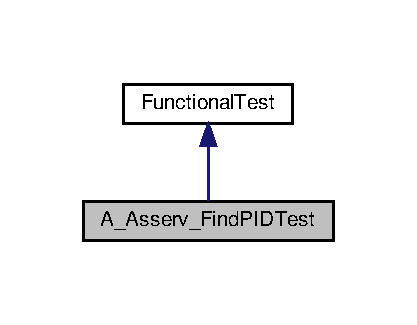
\includegraphics[width=200pt]{classA__Asserv__FindPIDTest__inherit__graph}
\end{center}
\end{figure}


Collaboration diagram for A\+\_\+\+Asserv\+\_\+\+Find\+P\+I\+D\+Test\+:
\nopagebreak
\begin{figure}[H]
\begin{center}
\leavevmode
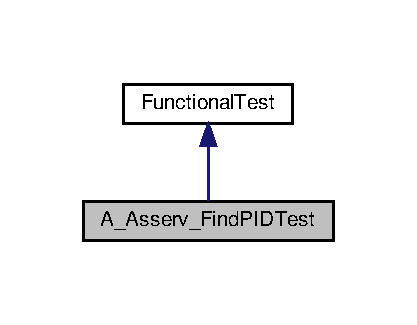
\includegraphics[width=200pt]{classA__Asserv__FindPIDTest__coll__graph}
\end{center}
\end{figure}
\subsection*{Public Member Functions}
\begin{DoxyCompactItemize}
\item 
\mbox{\Hypertarget{classA__Asserv__FindPIDTest_a6eb93ed5bd8026681d847e3fb7e1073e}\label{classA__Asserv__FindPIDTest_a6eb93ed5bd8026681d847e3fb7e1073e}} 
\hyperlink{classA__Asserv__FindPIDTest_a6eb93ed5bd8026681d847e3fb7e1073e}{A\+\_\+\+Asserv\+\_\+\+Find\+P\+I\+D\+Test} ()
\begin{DoxyCompactList}\small\item\em Constructeur de la classe. \end{DoxyCompactList}\item 
\mbox{\Hypertarget{classA__Asserv__FindPIDTest_a66a6be8b078f42d51a530431b346241b}\label{classA__Asserv__FindPIDTest_a66a6be8b078f42d51a530431b346241b}} 
virtual \hyperlink{classA__Asserv__FindPIDTest_a66a6be8b078f42d51a530431b346241b}{$\sim$\+A\+\_\+\+Asserv\+\_\+\+Find\+P\+I\+D\+Test} ()
\begin{DoxyCompactList}\small\item\em Destructeur de la classe. \end{DoxyCompactList}\item 
\mbox{\Hypertarget{classA__Asserv__FindPIDTest_acc445eae5445a7f0add802f1bc34851e}\label{classA__Asserv__FindPIDTest_acc445eae5445a7f0add802f1bc34851e}} 
virtual void \hyperlink{classA__Asserv__FindPIDTest_acc445eae5445a7f0add802f1bc34851e}{run} (int argc, char $\ast$$\ast$argv)
\begin{DoxyCompactList}\small\item\em Execute le test. \end{DoxyCompactList}\item 
\mbox{\Hypertarget{classA__Asserv__FindPIDTest_a9c64c65c189c232963bd304ba8d06c05}\label{classA__Asserv__FindPIDTest_a9c64c65c189c232963bd304ba8d06c05}} 
virtual void {\bfseries configure\+Console\+Args} (int argc, char $\ast$$\ast$argv)
\end{DoxyCompactItemize}
\subsection*{Additional Inherited Members}


\subsection{Detailed Description}
Effectue un test pour trouver les aprametres de P\+ID. 

The documentation for this class was generated from the following files\+:\begin{DoxyCompactItemize}
\item 
/home/pmx/git/\+P\+M\+X/src/\+Bot-\/\+A\+P\+F9328/A\+\_\+\+Asserv\+\_\+\+Find\+P\+I\+D\+Test.\+hpp\item 
/home/pmx/git/\+P\+M\+X/src/\+Bot-\/\+A\+P\+F9328/A\+\_\+\+Asserv\+\_\+\+Find\+P\+I\+D\+Test.\+cpp\end{DoxyCompactItemize}

\hypertarget{classA__Asserv__SetResolutionTest}{}\section{A\+\_\+\+Asserv\+\_\+\+Set\+Resolution\+Test Class Reference}
\label{classA__Asserv__SetResolutionTest}\index{A\+\_\+\+Asserv\+\_\+\+Set\+Resolution\+Test@{A\+\_\+\+Asserv\+\_\+\+Set\+Resolution\+Test}}


Effectue un test de l\textquotesingle{}asservissement pour trouver les valeurs pour les encoders.  




{\ttfamily \#include $<$A\+\_\+\+Asserv\+\_\+\+Set\+Resolution\+Test.\+hpp$>$}



Inheritance diagram for A\+\_\+\+Asserv\+\_\+\+Set\+Resolution\+Test\+:
\nopagebreak
\begin{figure}[H]
\begin{center}
\leavevmode
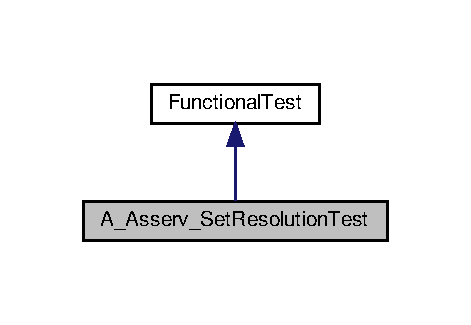
\includegraphics[width=226pt]{classA__Asserv__SetResolutionTest__inherit__graph}
\end{center}
\end{figure}


Collaboration diagram for A\+\_\+\+Asserv\+\_\+\+Set\+Resolution\+Test\+:
\nopagebreak
\begin{figure}[H]
\begin{center}
\leavevmode
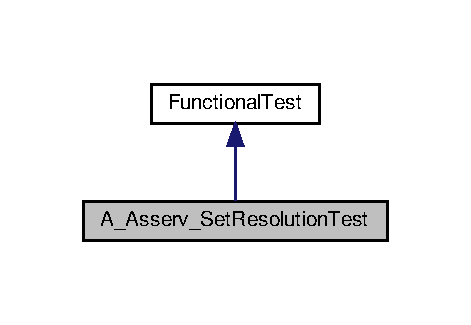
\includegraphics[width=226pt]{classA__Asserv__SetResolutionTest__coll__graph}
\end{center}
\end{figure}
\subsection*{Public Member Functions}
\begin{DoxyCompactItemize}
\item 
\mbox{\Hypertarget{classA__Asserv__SetResolutionTest_ac35a4a898f89a405e079a3eb57010fdf}\label{classA__Asserv__SetResolutionTest_ac35a4a898f89a405e079a3eb57010fdf}} 
\hyperlink{classA__Asserv__SetResolutionTest_ac35a4a898f89a405e079a3eb57010fdf}{A\+\_\+\+Asserv\+\_\+\+Set\+Resolution\+Test} ()
\begin{DoxyCompactList}\small\item\em Constructeur de la classe. \end{DoxyCompactList}\item 
\mbox{\Hypertarget{classA__Asserv__SetResolutionTest_ad6b7f5c269825856de20caeb3b7a1cdb}\label{classA__Asserv__SetResolutionTest_ad6b7f5c269825856de20caeb3b7a1cdb}} 
virtual \hyperlink{classA__Asserv__SetResolutionTest_ad6b7f5c269825856de20caeb3b7a1cdb}{$\sim$\+A\+\_\+\+Asserv\+\_\+\+Set\+Resolution\+Test} ()
\begin{DoxyCompactList}\small\item\em Destructeur de la classe. \end{DoxyCompactList}\item 
\mbox{\Hypertarget{classA__Asserv__SetResolutionTest_a545e3f61effce9ada7362c956fa7b5d0}\label{classA__Asserv__SetResolutionTest_a545e3f61effce9ada7362c956fa7b5d0}} 
virtual void \hyperlink{classA__Asserv__SetResolutionTest_a545e3f61effce9ada7362c956fa7b5d0}{run} (int argc, char $\ast$$\ast$argv)
\begin{DoxyCompactList}\small\item\em Execute le test. \end{DoxyCompactList}\item 
\mbox{\Hypertarget{classA__Asserv__SetResolutionTest_ae55ca185b0f71ca095aa359202109cb2}\label{classA__Asserv__SetResolutionTest_ae55ca185b0f71ca095aa359202109cb2}} 
virtual void {\bfseries configure\+Console\+Args} (int argc, char $\ast$$\ast$argv)
\end{DoxyCompactItemize}
\subsection*{Additional Inherited Members}


\subsection{Detailed Description}
Effectue un test de l\textquotesingle{}asservissement pour trouver les valeurs pour les encoders. 

The documentation for this class was generated from the following files\+:\begin{DoxyCompactItemize}
\item 
/home/pmx/git/\+P\+M\+X/src/\+Bot-\/\+A\+P\+F9328/A\+\_\+\+Asserv\+\_\+\+Set\+Resolution\+Test.\+hpp\item 
/home/pmx/git/\+P\+M\+X/src/\+Bot-\/\+A\+P\+F9328/A\+\_\+\+Asserv\+\_\+\+Set\+Resolution\+Test.\+cpp\end{DoxyCompactItemize}

\hypertarget{classA__Asserv__SquareTest}{}\section{A\+\_\+\+Asserv\+\_\+\+Square\+Test Class Reference}
\label{classA__Asserv__SquareTest}\index{A\+\_\+\+Asserv\+\_\+\+Square\+Test@{A\+\_\+\+Asserv\+\_\+\+Square\+Test}}


Effectue un test de l\textquotesingle{}asservissement sur plusieurs positions.  




{\ttfamily \#include $<$A\+\_\+\+Asserv\+\_\+\+Square\+Test.\+hpp$>$}



Inheritance diagram for A\+\_\+\+Asserv\+\_\+\+Square\+Test\+:
\nopagebreak
\begin{figure}[H]
\begin{center}
\leavevmode
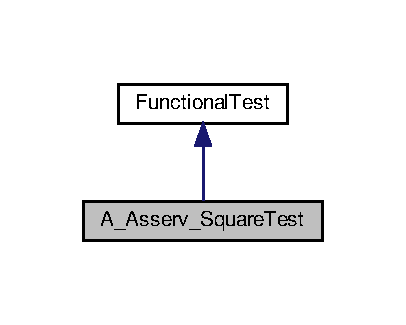
\includegraphics[width=195pt]{classA__Asserv__SquareTest__inherit__graph}
\end{center}
\end{figure}


Collaboration diagram for A\+\_\+\+Asserv\+\_\+\+Square\+Test\+:
\nopagebreak
\begin{figure}[H]
\begin{center}
\leavevmode
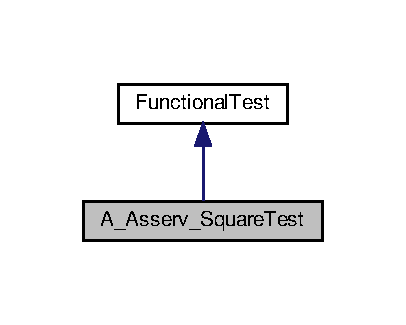
\includegraphics[width=195pt]{classA__Asserv__SquareTest__coll__graph}
\end{center}
\end{figure}
\subsection*{Public Member Functions}
\begin{DoxyCompactItemize}
\item 
\mbox{\Hypertarget{classA__Asserv__SquareTest_a7dfa3b2120195074baeb43c31e472b32}\label{classA__Asserv__SquareTest_a7dfa3b2120195074baeb43c31e472b32}} 
\hyperlink{classA__Asserv__SquareTest_a7dfa3b2120195074baeb43c31e472b32}{A\+\_\+\+Asserv\+\_\+\+Square\+Test} ()
\begin{DoxyCompactList}\small\item\em Constructeur de la classe. \end{DoxyCompactList}\item 
\mbox{\Hypertarget{classA__Asserv__SquareTest_ad67da3e1af6159b5c3efea79dd6c3ed8}\label{classA__Asserv__SquareTest_ad67da3e1af6159b5c3efea79dd6c3ed8}} 
virtual \hyperlink{classA__Asserv__SquareTest_ad67da3e1af6159b5c3efea79dd6c3ed8}{$\sim$\+A\+\_\+\+Asserv\+\_\+\+Square\+Test} ()
\begin{DoxyCompactList}\small\item\em Destructeur de la classe. \end{DoxyCompactList}\item 
\mbox{\Hypertarget{classA__Asserv__SquareTest_ac79fb82ae484354c587c6fd925c6c599}\label{classA__Asserv__SquareTest_ac79fb82ae484354c587c6fd925c6c599}} 
virtual void \hyperlink{classA__Asserv__SquareTest_ac79fb82ae484354c587c6fd925c6c599}{run} (int argc, char $\ast$$\ast$argv)
\begin{DoxyCompactList}\small\item\em Execute le test. \end{DoxyCompactList}\item 
\mbox{\Hypertarget{classA__Asserv__SquareTest_a484f017e34e6208c77c9c8ad8746abb4}\label{classA__Asserv__SquareTest_a484f017e34e6208c77c9c8ad8746abb4}} 
virtual void {\bfseries configure\+Console\+Args} (int argc, char $\ast$$\ast$argv)
\end{DoxyCompactItemize}
\subsection*{Additional Inherited Members}


\subsection{Detailed Description}
Effectue un test de l\textquotesingle{}asservissement sur plusieurs positions. 

The documentation for this class was generated from the following files\+:\begin{DoxyCompactItemize}
\item 
/home/pmx/git/\+P\+M\+X/src/\+Bot-\/\+A\+P\+F9328/A\+\_\+\+Asserv\+\_\+\+Square\+Test.\+hpp\item 
/home/pmx/git/\+P\+M\+X/src/\+Bot-\/\+A\+P\+F9328/A\+\_\+\+Asserv\+\_\+\+Square\+Test.\+cpp\end{DoxyCompactItemize}

\hypertarget{classA__AsservInsaTest}{}\section{A\+\_\+\+Asserv\+Insa\+Test Class Reference}
\label{classA__AsservInsaTest}\index{A\+\_\+\+Asserv\+Insa\+Test@{A\+\_\+\+Asserv\+Insa\+Test}}


Effectue un test de l\textquotesingle{}asservissement.  




{\ttfamily \#include $<$A\+\_\+\+Asserv\+Insa\+Test.\+hpp$>$}



Inheritance diagram for A\+\_\+\+Asserv\+Insa\+Test\+:
\nopagebreak
\begin{figure}[H]
\begin{center}
\leavevmode
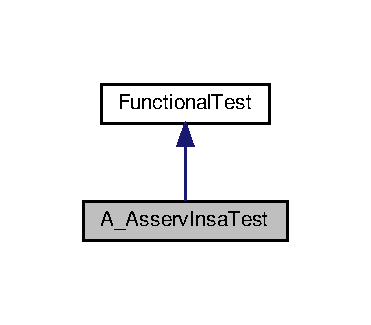
\includegraphics[width=178pt]{classA__AsservInsaTest__inherit__graph}
\end{center}
\end{figure}


Collaboration diagram for A\+\_\+\+Asserv\+Insa\+Test\+:
\nopagebreak
\begin{figure}[H]
\begin{center}
\leavevmode
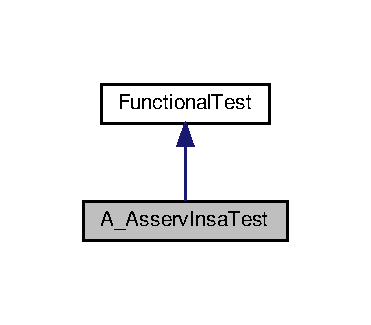
\includegraphics[width=178pt]{classA__AsservInsaTest__coll__graph}
\end{center}
\end{figure}
\subsection*{Public Member Functions}
\begin{DoxyCompactItemize}
\item 
\mbox{\Hypertarget{classA__AsservInsaTest_ad9747262f4a8313a7fb22c1283b098b9}\label{classA__AsservInsaTest_ad9747262f4a8313a7fb22c1283b098b9}} 
\hyperlink{classA__AsservInsaTest_ad9747262f4a8313a7fb22c1283b098b9}{A\+\_\+\+Asserv\+Insa\+Test} ()
\begin{DoxyCompactList}\small\item\em Constructeur de la classe. \end{DoxyCompactList}\item 
\mbox{\Hypertarget{classA__AsservInsaTest_af9d93af9fb7c03c6fef82b0eae5b902e}\label{classA__AsservInsaTest_af9d93af9fb7c03c6fef82b0eae5b902e}} 
virtual \hyperlink{classA__AsservInsaTest_af9d93af9fb7c03c6fef82b0eae5b902e}{$\sim$\+A\+\_\+\+Asserv\+Insa\+Test} ()
\begin{DoxyCompactList}\small\item\em Destructeur de la classe. \end{DoxyCompactList}\item 
\mbox{\Hypertarget{classA__AsservInsaTest_aecdab7eb1a270927321e01a00f5faa12}\label{classA__AsservInsaTest_aecdab7eb1a270927321e01a00f5faa12}} 
virtual void \hyperlink{classA__AsservInsaTest_aecdab7eb1a270927321e01a00f5faa12}{run} (int argc, char $\ast$$\ast$argv)
\begin{DoxyCompactList}\small\item\em Execute le test. \end{DoxyCompactList}\item 
\mbox{\Hypertarget{classA__AsservInsaTest_a70fc769b62545da45e4c05be77331972}\label{classA__AsservInsaTest_a70fc769b62545da45e4c05be77331972}} 
virtual void {\bfseries configure\+Console\+Args} (int argc, char $\ast$$\ast$argv)
\end{DoxyCompactItemize}
\subsection*{Additional Inherited Members}


\subsection{Detailed Description}
Effectue un test de l\textquotesingle{}asservissement. 

The documentation for this class was generated from the following files\+:\begin{DoxyCompactItemize}
\item 
/home/pmx/git/\+P\+M\+X/src/\+Bot-\/\+A\+P\+F9328/A\+\_\+\+Asserv\+Insa\+Test.\+hpp\item 
/home/pmx/git/\+P\+M\+X/src/\+Bot-\/\+A\+P\+F9328/A\+\_\+\+Asserv\+Insa\+Test.\+cpp\end{DoxyCompactItemize}

\hypertarget{classA__AsservRunTest}{}\section{A\+\_\+\+Asserv\+Run\+Test Class Reference}
\label{classA__AsservRunTest}\index{A\+\_\+\+Asserv\+Run\+Test@{A\+\_\+\+Asserv\+Run\+Test}}


Effectue un test de l\textquotesingle{}asservissement sur plusieurs positions.  




{\ttfamily \#include $<$A\+\_\+\+Asserv\+Run\+Test.\+hpp$>$}



Inheritance diagram for A\+\_\+\+Asserv\+Run\+Test\+:
\nopagebreak
\begin{figure}[H]
\begin{center}
\leavevmode
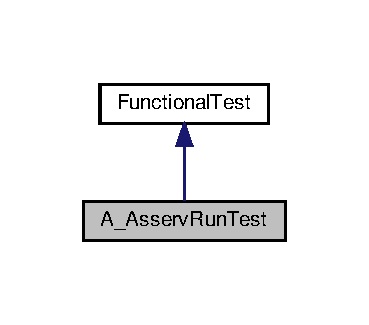
\includegraphics[width=177pt]{classA__AsservRunTest__inherit__graph}
\end{center}
\end{figure}


Collaboration diagram for A\+\_\+\+Asserv\+Run\+Test\+:
\nopagebreak
\begin{figure}[H]
\begin{center}
\leavevmode
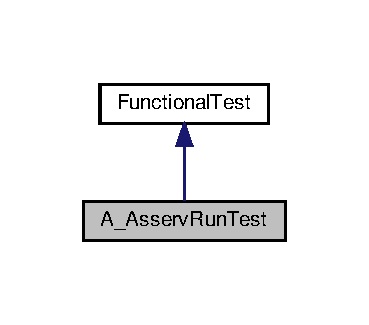
\includegraphics[width=177pt]{classA__AsservRunTest__coll__graph}
\end{center}
\end{figure}
\subsection*{Public Member Functions}
\begin{DoxyCompactItemize}
\item 
\mbox{\Hypertarget{classA__AsservRunTest_a84b3220088aa0d46e87d5afd7b55d35f}\label{classA__AsservRunTest_a84b3220088aa0d46e87d5afd7b55d35f}} 
\hyperlink{classA__AsservRunTest_a84b3220088aa0d46e87d5afd7b55d35f}{A\+\_\+\+Asserv\+Run\+Test} ()
\begin{DoxyCompactList}\small\item\em Constructeur de la classe. \end{DoxyCompactList}\item 
\mbox{\Hypertarget{classA__AsservRunTest_acfa804617293a9b4fabe0a67d17ec036}\label{classA__AsservRunTest_acfa804617293a9b4fabe0a67d17ec036}} 
virtual \hyperlink{classA__AsservRunTest_acfa804617293a9b4fabe0a67d17ec036}{$\sim$\+A\+\_\+\+Asserv\+Run\+Test} ()
\begin{DoxyCompactList}\small\item\em Destructeur de la classe. \end{DoxyCompactList}\item 
\mbox{\Hypertarget{classA__AsservRunTest_a333d95553c334244fa2a1d63e5eba13a}\label{classA__AsservRunTest_a333d95553c334244fa2a1d63e5eba13a}} 
virtual void \hyperlink{classA__AsservRunTest_a333d95553c334244fa2a1d63e5eba13a}{run} (int argc, char $\ast$$\ast$argv)
\begin{DoxyCompactList}\small\item\em Execute le test. \end{DoxyCompactList}\item 
\mbox{\Hypertarget{classA__AsservRunTest_aee96df6437a36ec4584d7e96853d9423}\label{classA__AsservRunTest_aee96df6437a36ec4584d7e96853d9423}} 
virtual void {\bfseries configure\+Console\+Args} (int argc, char $\ast$$\ast$argv)
\end{DoxyCompactItemize}
\subsection*{Additional Inherited Members}


\subsection{Detailed Description}
Effectue un test de l\textquotesingle{}asservissement sur plusieurs positions. 

The documentation for this class was generated from the following files\+:\begin{DoxyCompactItemize}
\item 
/home/pmx/git/\+P\+M\+X/src/\+Bot-\/\+A\+P\+F9328/A\+\_\+\+Asserv\+Run\+Test.\+hpp\item 
/home/pmx/git/\+P\+M\+X/src/\+Bot-\/\+A\+P\+F9328/A\+\_\+\+Asserv\+Run\+Test.\+cpp\end{DoxyCompactItemize}

\hypertarget{classA__ButtonBarTest}{}\section{A\+\_\+\+Button\+Bar\+Test Class Reference}
\label{classA__ButtonBarTest}\index{A\+\_\+\+Button\+Bar\+Test@{A\+\_\+\+Button\+Bar\+Test}}


Effectue un test sur les buttons.  




{\ttfamily \#include $<$A\+\_\+\+Button\+Bar\+Test.\+hpp$>$}



Inheritance diagram for A\+\_\+\+Button\+Bar\+Test\+:
\nopagebreak
\begin{figure}[H]
\begin{center}
\leavevmode
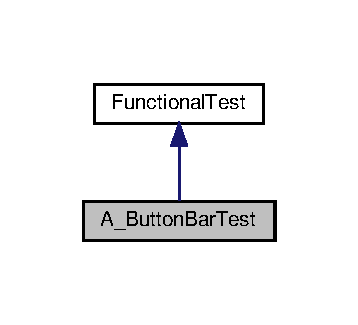
\includegraphics[width=172pt]{classA__ButtonBarTest__inherit__graph}
\end{center}
\end{figure}


Collaboration diagram for A\+\_\+\+Button\+Bar\+Test\+:
\nopagebreak
\begin{figure}[H]
\begin{center}
\leavevmode
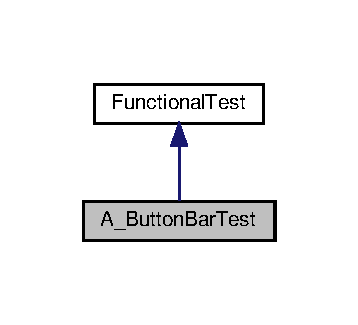
\includegraphics[width=172pt]{classA__ButtonBarTest__coll__graph}
\end{center}
\end{figure}
\subsection*{Public Member Functions}
\begin{DoxyCompactItemize}
\item 
\mbox{\Hypertarget{classA__ButtonBarTest_aa277383a19c49e7c089c14b2b70f5f78}\label{classA__ButtonBarTest_aa277383a19c49e7c089c14b2b70f5f78}} 
\hyperlink{classA__ButtonBarTest_aa277383a19c49e7c089c14b2b70f5f78}{A\+\_\+\+Button\+Bar\+Test} ()
\begin{DoxyCompactList}\small\item\em Constructeur de la classe. \end{DoxyCompactList}\item 
\mbox{\Hypertarget{classA__ButtonBarTest_a7cd50ed43f3523bd2b9d30ffebb80c42}\label{classA__ButtonBarTest_a7cd50ed43f3523bd2b9d30ffebb80c42}} 
virtual \hyperlink{classA__ButtonBarTest_a7cd50ed43f3523bd2b9d30ffebb80c42}{$\sim$\+A\+\_\+\+Button\+Bar\+Test} ()
\begin{DoxyCompactList}\small\item\em Destructeur de la classe. \end{DoxyCompactList}\item 
\mbox{\Hypertarget{classA__ButtonBarTest_a63c0ce685488028c4cf777c773d1632c}\label{classA__ButtonBarTest_a63c0ce685488028c4cf777c773d1632c}} 
virtual void \hyperlink{classA__ButtonBarTest_a63c0ce685488028c4cf777c773d1632c}{run} (int argc, char $\ast$$\ast$argv)
\begin{DoxyCompactList}\small\item\em Execute le test. \end{DoxyCompactList}\end{DoxyCompactItemize}
\subsection*{Additional Inherited Members}


\subsection{Detailed Description}
Effectue un test sur les buttons. 

The documentation for this class was generated from the following files\+:\begin{DoxyCompactItemize}
\item 
/home/pmx/git/\+P\+M\+X/src/\+Bot-\/\+A\+P\+F9328/A\+\_\+\+Button\+Bar\+Test.\+hpp\item 
/home/pmx/git/\+P\+M\+X/src/\+Bot-\/\+A\+P\+F9328/\hyperlink{A__ButtonBarTest_8cpp}{A\+\_\+\+Button\+Bar\+Test.\+cpp}\end{DoxyCompactItemize}

\hypertarget{classA__IATest}{}\section{A\+\_\+\+I\+A\+Test Class Reference}
\label{classA__IATest}\index{A\+\_\+\+I\+A\+Test@{A\+\_\+\+I\+A\+Test}}


Effectue un test de l\textquotesingle{}ia.  




{\ttfamily \#include $<$A\+\_\+\+I\+A\+Test.\+hpp$>$}



Inheritance diagram for A\+\_\+\+I\+A\+Test\+:
\nopagebreak
\begin{figure}[H]
\begin{center}
\leavevmode
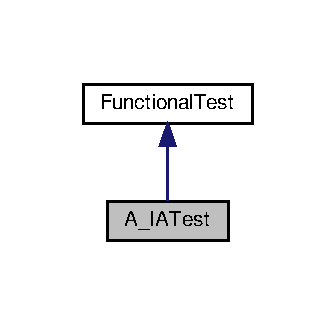
\includegraphics[width=161pt]{classA__IATest__inherit__graph}
\end{center}
\end{figure}


Collaboration diagram for A\+\_\+\+I\+A\+Test\+:
\nopagebreak
\begin{figure}[H]
\begin{center}
\leavevmode
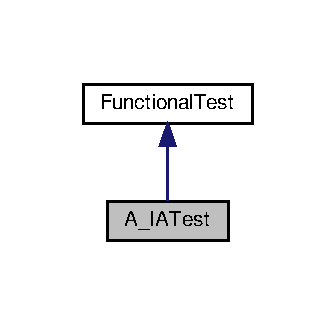
\includegraphics[width=161pt]{classA__IATest__coll__graph}
\end{center}
\end{figure}
\subsection*{Public Member Functions}
\begin{DoxyCompactItemize}
\item 
\mbox{\Hypertarget{classA__IATest_a4e0b06427c9fa4c9c42a6613c6849537}\label{classA__IATest_a4e0b06427c9fa4c9c42a6613c6849537}} 
\hyperlink{classA__IATest_a4e0b06427c9fa4c9c42a6613c6849537}{A\+\_\+\+I\+A\+Test} ()
\begin{DoxyCompactList}\small\item\em Constructeur de la classe. \end{DoxyCompactList}\item 
\mbox{\Hypertarget{classA__IATest_aad21565c20c7922bbd347a10f9d7c18c}\label{classA__IATest_aad21565c20c7922bbd347a10f9d7c18c}} 
virtual \hyperlink{classA__IATest_aad21565c20c7922bbd347a10f9d7c18c}{$\sim$\+A\+\_\+\+I\+A\+Test} ()
\begin{DoxyCompactList}\small\item\em Destructeur de la classe. \end{DoxyCompactList}\item 
\mbox{\Hypertarget{classA__IATest_a53c1fd77a64d6a55a6386829ba6f7697}\label{classA__IATest_a53c1fd77a64d6a55a6386829ba6f7697}} 
virtual void \hyperlink{classA__IATest_a53c1fd77a64d6a55a6386829ba6f7697}{run} (int argc, char $\ast$$\ast$argv)
\begin{DoxyCompactList}\small\item\em Execute le test. \end{DoxyCompactList}\item 
\mbox{\Hypertarget{classA__IATest_a090b6253ad7daff1b0cbdd581177493a}\label{classA__IATest_a090b6253ad7daff1b0cbdd581177493a}} 
void {\bfseries I\+A\+Setup} ()
\end{DoxyCompactItemize}
\subsection*{Additional Inherited Members}


\subsection{Detailed Description}
Effectue un test de l\textquotesingle{}ia. 

The documentation for this class was generated from the following files\+:\begin{DoxyCompactItemize}
\item 
/home/pmx/git/\+P\+M\+X/src/\+Bot-\/\+A\+P\+F9328/\hyperlink{A__IATest_8hpp}{A\+\_\+\+I\+A\+Test.\+hpp}\item 
/home/pmx/git/\+P\+M\+X/src/\+Bot-\/\+A\+P\+F9328/\hyperlink{A__IATest_8cpp}{A\+\_\+\+I\+A\+Test.\+cpp}\end{DoxyCompactItemize}

\hypertarget{classA__LcdBoardTest}{}\section{A\+\_\+\+Lcd\+Board\+Test Class Reference}
\label{classA__LcdBoardTest}\index{A\+\_\+\+Lcd\+Board\+Test@{A\+\_\+\+Lcd\+Board\+Test}}


Effectue un test de clignotement des L\+E\+Ds du tableau d\textquotesingle{}affichage.  




{\ttfamily \#include $<$A\+\_\+\+Lcd\+Board\+Test.\+hpp$>$}



Inheritance diagram for A\+\_\+\+Lcd\+Board\+Test\+:
\nopagebreak
\begin{figure}[H]
\begin{center}
\leavevmode
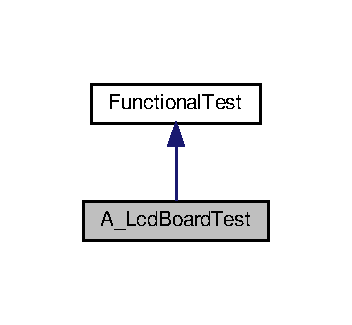
\includegraphics[width=169pt]{classA__LcdBoardTest__inherit__graph}
\end{center}
\end{figure}


Collaboration diagram for A\+\_\+\+Lcd\+Board\+Test\+:
\nopagebreak
\begin{figure}[H]
\begin{center}
\leavevmode
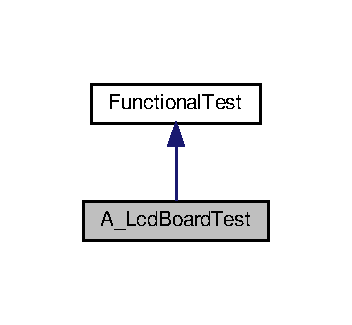
\includegraphics[width=169pt]{classA__LcdBoardTest__coll__graph}
\end{center}
\end{figure}
\subsection*{Public Member Functions}
\begin{DoxyCompactItemize}
\item 
\mbox{\Hypertarget{classA__LcdBoardTest_acc6b1652d9ca465b8f4894e06878c6ce}\label{classA__LcdBoardTest_acc6b1652d9ca465b8f4894e06878c6ce}} 
\hyperlink{classA__LcdBoardTest_acc6b1652d9ca465b8f4894e06878c6ce}{A\+\_\+\+Lcd\+Board\+Test} ()
\begin{DoxyCompactList}\small\item\em Constructeur de la classe. \end{DoxyCompactList}\item 
\mbox{\Hypertarget{classA__LcdBoardTest_a2697dd45bbfd98e1269b5da5e8112849}\label{classA__LcdBoardTest_a2697dd45bbfd98e1269b5da5e8112849}} 
virtual \hyperlink{classA__LcdBoardTest_a2697dd45bbfd98e1269b5da5e8112849}{$\sim$\+A\+\_\+\+Lcd\+Board\+Test} ()
\begin{DoxyCompactList}\small\item\em Destructeur de la classe. \end{DoxyCompactList}\item 
\mbox{\Hypertarget{classA__LcdBoardTest_ae41885fb9b4623bb4897e264b1550054}\label{classA__LcdBoardTest_ae41885fb9b4623bb4897e264b1550054}} 
virtual void \hyperlink{classA__LcdBoardTest_ae41885fb9b4623bb4897e264b1550054}{run} (int argc, char $\ast$$\ast$argv)
\begin{DoxyCompactList}\small\item\em Execute le test. \end{DoxyCompactList}\end{DoxyCompactItemize}
\subsection*{Additional Inherited Members}


\subsection{Detailed Description}
Effectue un test de clignotement des L\+E\+Ds du tableau d\textquotesingle{}affichage. 

The documentation for this class was generated from the following files\+:\begin{DoxyCompactItemize}
\item 
/home/pmx/git/\+P\+M\+X/src/\+Bot-\/\+A\+P\+F9328/\hyperlink{A__LcdBoardTest_8hpp}{A\+\_\+\+Lcd\+Board\+Test.\+hpp}\item 
/home/pmx/git/\+P\+M\+X/src/\+Bot-\/\+A\+P\+F9328/\hyperlink{A__LcdBoardTest_8cpp}{A\+\_\+\+Lcd\+Board\+Test.\+cpp}\end{DoxyCompactItemize}

\hypertarget{classA__LedBarTest}{}\section{A\+\_\+\+Led\+Bar\+Test Class Reference}
\label{classA__LedBarTest}\index{A\+\_\+\+Led\+Bar\+Test@{A\+\_\+\+Led\+Bar\+Test}}


Effectue un test de clignotement des L\+E\+Ds du tableau d\textquotesingle{}affichage.  




{\ttfamily \#include $<$A\+\_\+\+Led\+Bar\+Test.\+hpp$>$}



Inheritance diagram for A\+\_\+\+Led\+Bar\+Test\+:
\nopagebreak
\begin{figure}[H]
\begin{center}
\leavevmode
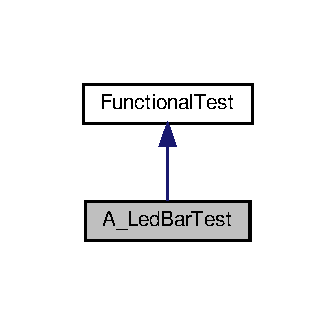
\includegraphics[width=161pt]{classA__LedBarTest__inherit__graph}
\end{center}
\end{figure}


Collaboration diagram for A\+\_\+\+Led\+Bar\+Test\+:
\nopagebreak
\begin{figure}[H]
\begin{center}
\leavevmode
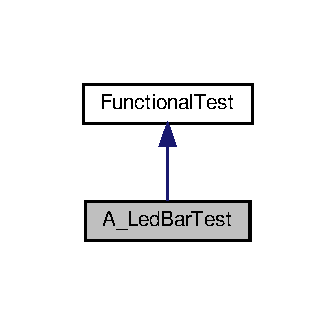
\includegraphics[width=161pt]{classA__LedBarTest__coll__graph}
\end{center}
\end{figure}
\subsection*{Public Member Functions}
\begin{DoxyCompactItemize}
\item 
\mbox{\Hypertarget{classA__LedBarTest_ab3cc5ded06f6910e1cca9cd7a744f1f0}\label{classA__LedBarTest_ab3cc5ded06f6910e1cca9cd7a744f1f0}} 
\hyperlink{classA__LedBarTest_ab3cc5ded06f6910e1cca9cd7a744f1f0}{A\+\_\+\+Led\+Bar\+Test} ()
\begin{DoxyCompactList}\small\item\em Constructeur de la classe. \end{DoxyCompactList}\item 
\mbox{\Hypertarget{classA__LedBarTest_a31f48a88b348e476c7633ebf8ada64f0}\label{classA__LedBarTest_a31f48a88b348e476c7633ebf8ada64f0}} 
virtual \hyperlink{classA__LedBarTest_a31f48a88b348e476c7633ebf8ada64f0}{$\sim$\+A\+\_\+\+Led\+Bar\+Test} ()
\begin{DoxyCompactList}\small\item\em Destructeur de la classe. \end{DoxyCompactList}\item 
\mbox{\Hypertarget{classA__LedBarTest_ab90a8b6aa14e330f417f72ee5f08e00a}\label{classA__LedBarTest_ab90a8b6aa14e330f417f72ee5f08e00a}} 
virtual void \hyperlink{classA__LedBarTest_ab90a8b6aa14e330f417f72ee5f08e00a}{run} (int argc, char $\ast$$\ast$argv)
\begin{DoxyCompactList}\small\item\em Execute le test. \end{DoxyCompactList}\end{DoxyCompactItemize}
\subsection*{Additional Inherited Members}


\subsection{Detailed Description}
Effectue un test de clignotement des L\+E\+Ds du tableau d\textquotesingle{}affichage. 

The documentation for this class was generated from the following files\+:\begin{DoxyCompactItemize}
\item 
/home/pmx/git/\+P\+M\+X/src/\+Bot-\/\+A\+P\+F9328/\hyperlink{A__LedBarTest_8hpp}{A\+\_\+\+Led\+Bar\+Test.\+hpp}\item 
/home/pmx/git/\+P\+M\+X/src/\+Bot-\/\+A\+P\+F9328/\hyperlink{A__LedBarTest_8cpp}{A\+\_\+\+Led\+Bar\+Test.\+cpp}\end{DoxyCompactItemize}

\hypertarget{classA__MovingBaseTest}{}\section{A\+\_\+\+Moving\+Base\+Test Class Reference}
\label{classA__MovingBaseTest}\index{A\+\_\+\+Moving\+Base\+Test@{A\+\_\+\+Moving\+Base\+Test}}


Effectue un test de la base roulante.  




{\ttfamily \#include $<$A\+\_\+\+Moving\+Base\+Test.\+hpp$>$}



Inheritance diagram for A\+\_\+\+Moving\+Base\+Test\+:
\nopagebreak
\begin{figure}[H]
\begin{center}
\leavevmode
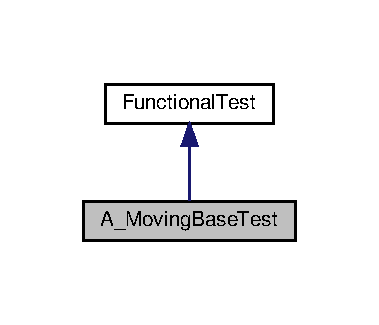
\includegraphics[width=182pt]{classA__MovingBaseTest__inherit__graph}
\end{center}
\end{figure}


Collaboration diagram for A\+\_\+\+Moving\+Base\+Test\+:
\nopagebreak
\begin{figure}[H]
\begin{center}
\leavevmode
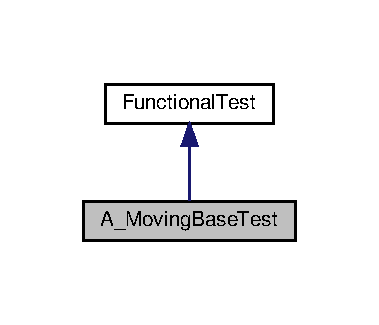
\includegraphics[width=182pt]{classA__MovingBaseTest__coll__graph}
\end{center}
\end{figure}
\subsection*{Public Member Functions}
\begin{DoxyCompactItemize}
\item 
\mbox{\Hypertarget{classA__MovingBaseTest_af173bfdd4bda95800779488657f79853}\label{classA__MovingBaseTest_af173bfdd4bda95800779488657f79853}} 
\hyperlink{classA__MovingBaseTest_af173bfdd4bda95800779488657f79853}{A\+\_\+\+Moving\+Base\+Test} ()
\begin{DoxyCompactList}\small\item\em Constructeur de la classe. \end{DoxyCompactList}\item 
\mbox{\Hypertarget{classA__MovingBaseTest_ac8178fe43c6603f82f45eb09b4e9a78c}\label{classA__MovingBaseTest_ac8178fe43c6603f82f45eb09b4e9a78c}} 
virtual \hyperlink{classA__MovingBaseTest_ac8178fe43c6603f82f45eb09b4e9a78c}{$\sim$\+A\+\_\+\+Moving\+Base\+Test} ()
\begin{DoxyCompactList}\small\item\em Destructeur de la classe. \end{DoxyCompactList}\item 
\mbox{\Hypertarget{classA__MovingBaseTest_a1ac04e328db4ee50ebbd7cee6bfe39ca}\label{classA__MovingBaseTest_a1ac04e328db4ee50ebbd7cee6bfe39ca}} 
virtual void \hyperlink{classA__MovingBaseTest_a1ac04e328db4ee50ebbd7cee6bfe39ca}{run} (int argc, char $\ast$$\ast$argv)
\begin{DoxyCompactList}\small\item\em Execute le test. \end{DoxyCompactList}\item 
\mbox{\Hypertarget{classA__MovingBaseTest_ac31ed8e8ea69e4429444aa9d80dbe194}\label{classA__MovingBaseTest_ac31ed8e8ea69e4429444aa9d80dbe194}} 
virtual void {\bfseries configure\+Console\+Args} (int argc, char $\ast$$\ast$argv)
\end{DoxyCompactItemize}
\subsection*{Additional Inherited Members}


\subsection{Detailed Description}
Effectue un test de la base roulante. 

The documentation for this class was generated from the following files\+:\begin{DoxyCompactItemize}
\item 
/home/pmx/git/\+P\+M\+X/src/\+Bot-\/\+A\+P\+F9328/A\+\_\+\+Moving\+Base\+Test.\+hpp\item 
/home/pmx/git/\+P\+M\+X/src/\+Bot-\/\+A\+P\+F9328/A\+\_\+\+Moving\+Base\+Test.\+cpp\end{DoxyCompactItemize}

\hypertarget{classA__SensorsTest}{}\section{A\+\_\+\+Sensors\+Test Class Reference}
\label{classA__SensorsTest}\index{A\+\_\+\+Sensors\+Test@{A\+\_\+\+Sensors\+Test}}


Effectue un test avec les capteurs IR.  




{\ttfamily \#include $<$A\+\_\+\+Sensors\+Test.\+hpp$>$}



Inheritance diagram for A\+\_\+\+Sensors\+Test\+:
\nopagebreak
\begin{figure}[H]
\begin{center}
\leavevmode
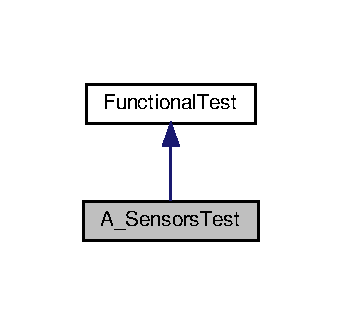
\includegraphics[width=164pt]{classA__SensorsTest__inherit__graph}
\end{center}
\end{figure}


Collaboration diagram for A\+\_\+\+Sensors\+Test\+:
\nopagebreak
\begin{figure}[H]
\begin{center}
\leavevmode
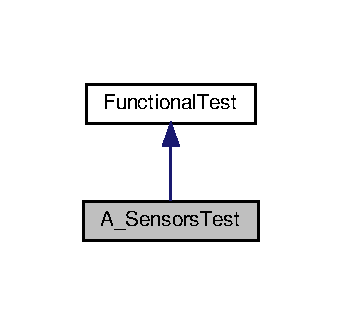
\includegraphics[width=164pt]{classA__SensorsTest__coll__graph}
\end{center}
\end{figure}
\subsection*{Public Member Functions}
\begin{DoxyCompactItemize}
\item 
\mbox{\Hypertarget{classA__SensorsTest_a7c5fe54d684cf2123d8db9badf4a6df6}\label{classA__SensorsTest_a7c5fe54d684cf2123d8db9badf4a6df6}} 
\hyperlink{classA__SensorsTest_a7c5fe54d684cf2123d8db9badf4a6df6}{A\+\_\+\+Sensors\+Test} ()
\begin{DoxyCompactList}\small\item\em Constructeur de la classe. \end{DoxyCompactList}\item 
\mbox{\Hypertarget{classA__SensorsTest_ad1a7742b16a694a4c17aa36b4c4eb8a0}\label{classA__SensorsTest_ad1a7742b16a694a4c17aa36b4c4eb8a0}} 
virtual \hyperlink{classA__SensorsTest_ad1a7742b16a694a4c17aa36b4c4eb8a0}{$\sim$\+A\+\_\+\+Sensors\+Test} ()
\begin{DoxyCompactList}\small\item\em Destructeur de la classe. \end{DoxyCompactList}\item 
\mbox{\Hypertarget{classA__SensorsTest_a862d3ed0b994946f6ac42280515b2c36}\label{classA__SensorsTest_a862d3ed0b994946f6ac42280515b2c36}} 
virtual void \hyperlink{classA__SensorsTest_a862d3ed0b994946f6ac42280515b2c36}{run} (int argc, char $\ast$$\ast$argv)
\begin{DoxyCompactList}\small\item\em Execute le test. \end{DoxyCompactList}\end{DoxyCompactItemize}
\subsection*{Additional Inherited Members}


\subsection{Detailed Description}
Effectue un test avec les capteurs IR. 

The documentation for this class was generated from the following files\+:\begin{DoxyCompactItemize}
\item 
/home/pmx/git/\+P\+M\+X/src/\+Bot-\/\+A\+P\+F9328/A\+\_\+\+Sensors\+Test.\+hpp\item 
/home/pmx/git/\+P\+M\+X/src/\+Bot-\/\+A\+P\+F9328/A\+\_\+\+Sensors\+Test.\+cpp\end{DoxyCompactItemize}

\hypertarget{classA__ServoStepTest}{}\section{A\+\_\+\+Servo\+Step\+Test Class Reference}
\label{classA__ServoStepTest}\index{A\+\_\+\+Servo\+Step\+Test@{A\+\_\+\+Servo\+Step\+Test}}


Effectue un test sur les servos.  




{\ttfamily \#include $<$A\+\_\+\+Servo\+Step\+Test.\+hpp$>$}



Inheritance diagram for A\+\_\+\+Servo\+Step\+Test\+:
\nopagebreak
\begin{figure}[H]
\begin{center}
\leavevmode
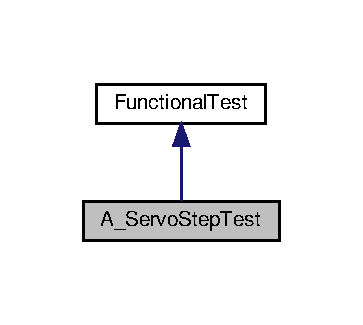
\includegraphics[width=174pt]{classA__ServoStepTest__inherit__graph}
\end{center}
\end{figure}


Collaboration diagram for A\+\_\+\+Servo\+Step\+Test\+:
\nopagebreak
\begin{figure}[H]
\begin{center}
\leavevmode
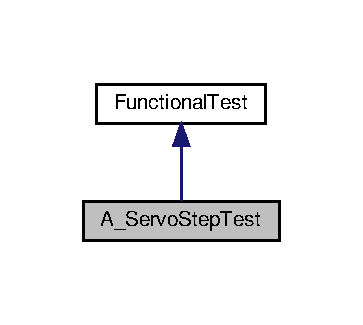
\includegraphics[width=174pt]{classA__ServoStepTest__coll__graph}
\end{center}
\end{figure}
\subsection*{Public Member Functions}
\begin{DoxyCompactItemize}
\item 
\mbox{\Hypertarget{classA__ServoStepTest_aa6cfc8145a54a57f5afff8d64af2c810}\label{classA__ServoStepTest_aa6cfc8145a54a57f5afff8d64af2c810}} 
\hyperlink{classA__ServoStepTest_aa6cfc8145a54a57f5afff8d64af2c810}{A\+\_\+\+Servo\+Step\+Test} ()
\begin{DoxyCompactList}\small\item\em Constructeur de la classe. \end{DoxyCompactList}\item 
\mbox{\Hypertarget{classA__ServoStepTest_a5ecb592b17617d231f168a3182f1d996}\label{classA__ServoStepTest_a5ecb592b17617d231f168a3182f1d996}} 
virtual \hyperlink{classA__ServoStepTest_a5ecb592b17617d231f168a3182f1d996}{$\sim$\+A\+\_\+\+Servo\+Step\+Test} ()
\begin{DoxyCompactList}\small\item\em Destructeur de la classe. \end{DoxyCompactList}\item 
\mbox{\Hypertarget{classA__ServoStepTest_ad98ddd1d901a5ac0c76e4a10a7e1b46c}\label{classA__ServoStepTest_ad98ddd1d901a5ac0c76e4a10a7e1b46c}} 
virtual void \hyperlink{classA__ServoStepTest_ad98ddd1d901a5ac0c76e4a10a7e1b46c}{run} (int argc, char $\ast$$\ast$argv)
\begin{DoxyCompactList}\small\item\em Execute le test. \end{DoxyCompactList}\end{DoxyCompactItemize}
\subsection*{Additional Inherited Members}


\subsection{Detailed Description}
Effectue un test sur les servos. 

The documentation for this class was generated from the following files\+:\begin{DoxyCompactItemize}
\item 
/home/pmx/git/\+P\+M\+X/src/\+Bot-\/\+A\+P\+F9328/A\+\_\+\+Servo\+Step\+Test.\+hpp\item 
/home/pmx/git/\+P\+M\+X/src/\+Bot-\/\+A\+P\+F9328/A\+\_\+\+Servo\+Step\+Test.\+cpp\end{DoxyCompactItemize}

\hypertarget{classA__ServoTest}{}\section{A\+\_\+\+Servo\+Test Class Reference}
\label{classA__ServoTest}\index{A\+\_\+\+Servo\+Test@{A\+\_\+\+Servo\+Test}}


Effectue un test sur les servos.  




{\ttfamily \#include $<$A\+\_\+\+Servo\+Test.\+hpp$>$}



Inheritance diagram for A\+\_\+\+Servo\+Test\+:
\nopagebreak
\begin{figure}[H]
\begin{center}
\leavevmode
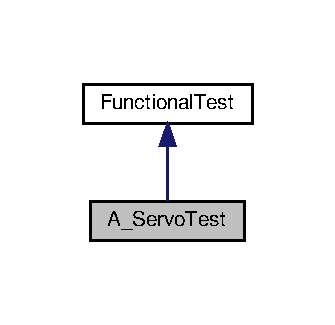
\includegraphics[width=161pt]{classA__ServoTest__inherit__graph}
\end{center}
\end{figure}


Collaboration diagram for A\+\_\+\+Servo\+Test\+:
\nopagebreak
\begin{figure}[H]
\begin{center}
\leavevmode
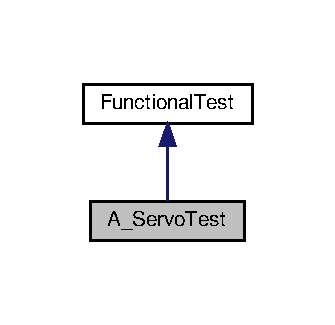
\includegraphics[width=161pt]{classA__ServoTest__coll__graph}
\end{center}
\end{figure}
\subsection*{Public Member Functions}
\begin{DoxyCompactItemize}
\item 
\mbox{\Hypertarget{classA__ServoTest_ad1829a0eb4adf70b6c483b2889b454ce}\label{classA__ServoTest_ad1829a0eb4adf70b6c483b2889b454ce}} 
\hyperlink{classA__ServoTest_ad1829a0eb4adf70b6c483b2889b454ce}{A\+\_\+\+Servo\+Test} ()
\begin{DoxyCompactList}\small\item\em Constructeur de la classe. \end{DoxyCompactList}\item 
\mbox{\Hypertarget{classA__ServoTest_ac8e7d107db7ab2524ee4eeb9f31184dd}\label{classA__ServoTest_ac8e7d107db7ab2524ee4eeb9f31184dd}} 
virtual \hyperlink{classA__ServoTest_ac8e7d107db7ab2524ee4eeb9f31184dd}{$\sim$\+A\+\_\+\+Servo\+Test} ()
\begin{DoxyCompactList}\small\item\em Destructeur de la classe. \end{DoxyCompactList}\item 
\mbox{\Hypertarget{classA__ServoTest_aed1e78e5ad48ce31a9b419cf399ac2cc}\label{classA__ServoTest_aed1e78e5ad48ce31a9b419cf399ac2cc}} 
virtual void \hyperlink{classA__ServoTest_aed1e78e5ad48ce31a9b419cf399ac2cc}{run} (int argc, char $\ast$$\ast$argv)
\begin{DoxyCompactList}\small\item\em Execute le test. \end{DoxyCompactList}\end{DoxyCompactItemize}
\subsection*{Additional Inherited Members}


\subsection{Detailed Description}
Effectue un test sur les servos. 

The documentation for this class was generated from the following files\+:\begin{DoxyCompactItemize}
\item 
/home/pmx/git/\+P\+M\+X/src/\+Bot-\/\+A\+P\+F9328/A\+\_\+\+Servo\+Test.\+hpp\item 
/home/pmx/git/\+P\+M\+X/src/\+Bot-\/\+A\+P\+F9328/A\+\_\+\+Servo\+Test.\+cpp\end{DoxyCompactItemize}

\hypertarget{classA__State1}{}\section{A\+\_\+\+State1 Class Reference}
\label{classA__State1}\index{A\+\_\+\+State1@{A\+\_\+\+State1}}


Inheritance diagram for A\+\_\+\+State1\+:
\nopagebreak
\begin{figure}[H]
\begin{center}
\leavevmode
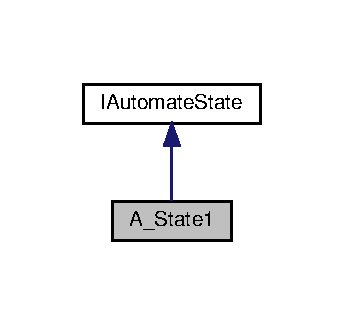
\includegraphics[width=165pt]{classA__State1__inherit__graph}
\end{center}
\end{figure}


Collaboration diagram for A\+\_\+\+State1\+:
\nopagebreak
\begin{figure}[H]
\begin{center}
\leavevmode
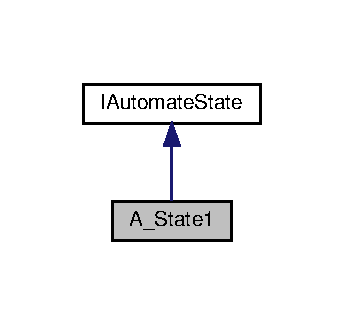
\includegraphics[width=165pt]{classA__State1__coll__graph}
\end{center}
\end{figure}
\subsection*{Public Member Functions}
\begin{DoxyCompactItemize}
\item 
\hyperlink{classIAutomateState}{I\+Automate\+State} $\ast$ \hyperlink{classA__State1_a351a7c94100ccc0dfb8a09e2037d4cc2}{execute} (\hyperlink{classRobot}{Robot} \&robot)
\begin{DoxyCompactList}\small\item\em Traite l\textquotesingle{}état actuel et renvoie l\textquotesingle{}état suivant. \end{DoxyCompactList}\item 
\mbox{\Hypertarget{classA__State1_ac418559b2a983872a2010f5463ca6f3c}\label{classA__State1_ac418559b2a983872a2010f5463ca6f3c}} 
std\+::string {\bfseries name} ()
\end{DoxyCompactItemize}
\subsection*{Additional Inherited Members}


\subsection{Member Function Documentation}
\mbox{\Hypertarget{classA__State1_a351a7c94100ccc0dfb8a09e2037d4cc2}\label{classA__State1_a351a7c94100ccc0dfb8a09e2037d4cc2}} 
\index{A\+\_\+\+State1@{A\+\_\+\+State1}!execute@{execute}}
\index{execute@{execute}!A\+\_\+\+State1@{A\+\_\+\+State1}}
\subsubsection{\texorpdfstring{execute()}{execute()}}
{\footnotesize\ttfamily \hyperlink{classIAutomateState}{I\+Automate\+State} $\ast$ A\+\_\+\+State1\+::execute (\begin{DoxyParamCaption}\item[{\hyperlink{classRobot}{Robot} \&}]{robot }\end{DoxyParamCaption})\hspace{0.3cm}{\ttfamily [virtual]}}



Traite l\textquotesingle{}état actuel et renvoie l\textquotesingle{}état suivant. 

Cette méthode doit être bloquante pour le processus et ne retourner un résultat qu\textquotesingle{}une fois l\textquotesingle{}une de ses transitions actives.


\begin{DoxyParams}{Parameters}
{\em robot} & Le robot à manipuler. \\
\hline
\end{DoxyParams}
\begin{DoxyReturn}{Returns}
L\textquotesingle{}état suivant ou {\ttfamily N\+U\+LL} si la fin de l\textquotesingle{}automate est atteinte. 
\end{DoxyReturn}
shared\+Data-\/$>$skip\+Setup()) 

Implements \hyperlink{classIAutomateState_a58bf3c2c5b55f7ba3fc1783fc36e102b}{I\+Automate\+State}.



The documentation for this class was generated from the following files\+:\begin{DoxyCompactItemize}
\item 
/home/pmx/git/\+P\+M\+X/src/\+Bot-\/\+A\+P\+F9328/A\+\_\+\+State1.\+hpp\item 
/home/pmx/git/\+P\+M\+X/src/\+Bot-\/\+A\+P\+F9328/A\+\_\+\+State1.\+cpp\end{DoxyCompactItemize}

\hypertarget{classA__State__DecisionMaker}{}\section{A\+\_\+\+State\+\_\+\+Decision\+Maker Class Reference}
\label{classA__State__DecisionMaker}\index{A\+\_\+\+State\+\_\+\+Decision\+Maker@{A\+\_\+\+State\+\_\+\+Decision\+Maker}}


Inheritance diagram for A\+\_\+\+State\+\_\+\+Decision\+Maker\+:
\nopagebreak
\begin{figure}[H]
\begin{center}
\leavevmode
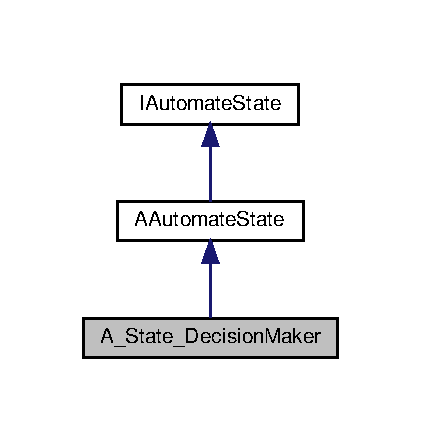
\includegraphics[width=202pt]{classA__State__DecisionMaker__inherit__graph}
\end{center}
\end{figure}


Collaboration diagram for A\+\_\+\+State\+\_\+\+Decision\+Maker\+:
\nopagebreak
\begin{figure}[H]
\begin{center}
\leavevmode
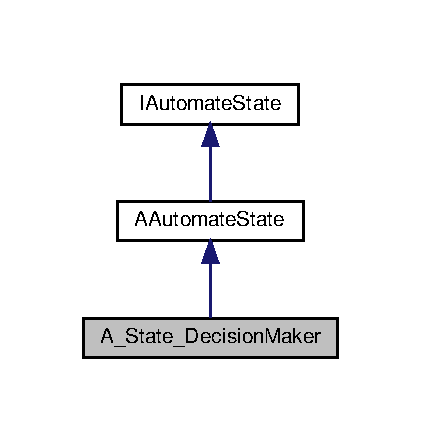
\includegraphics[width=202pt]{classA__State__DecisionMaker__coll__graph}
\end{center}
\end{figure}
\subsection*{Public Member Functions}
\begin{DoxyCompactItemize}
\item 
\hyperlink{classIAutomateState}{I\+Automate\+State} $\ast$ \hyperlink{classA__State__DecisionMaker_a960aa3cf18beb0b92fe1da1bb1ec42f1}{execute} (\hyperlink{classRobot}{Robot} \&robot, void $\ast$data)
\item 
\mbox{\Hypertarget{classA__State__DecisionMaker_a1ef4270c4d26768849593f88b27b424d}\label{classA__State__DecisionMaker_a1ef4270c4d26768849593f88b27b424d}} 
std\+::string {\bfseries name} ()
\item 
\mbox{\Hypertarget{classA__State__DecisionMaker_a8060da7376c3223db8921c1bdc948f6e}\label{classA__State__DecisionMaker_a8060da7376c3223db8921c1bdc948f6e}} 
void {\bfseries I\+A\+Setup\+Demo} ()
\item 
\mbox{\Hypertarget{classA__State__DecisionMaker_ac12110c5315179c96f5b9b0a73ab198b}\label{classA__State__DecisionMaker_ac12110c5315179c96f5b9b0a73ab198b}} 
void {\bfseries I\+A\+Setup\+Homologation} ()
\end{DoxyCompactItemize}
\subsection*{Additional Inherited Members}


\subsection{Member Function Documentation}
\mbox{\Hypertarget{classA__State__DecisionMaker_a960aa3cf18beb0b92fe1da1bb1ec42f1}\label{classA__State__DecisionMaker_a960aa3cf18beb0b92fe1da1bb1ec42f1}} 
\index{A\+\_\+\+State\+\_\+\+Decision\+Maker@{A\+\_\+\+State\+\_\+\+Decision\+Maker}!execute@{execute}}
\index{execute@{execute}!A\+\_\+\+State\+\_\+\+Decision\+Maker@{A\+\_\+\+State\+\_\+\+Decision\+Maker}}
\subsubsection{\texorpdfstring{execute()}{execute()}}
{\footnotesize\ttfamily \hyperlink{classIAutomateState}{I\+Automate\+State} $\ast$ A\+\_\+\+State\+\_\+\+Decision\+Maker\+::execute (\begin{DoxyParamCaption}\item[{\hyperlink{classRobot}{Robot} \&}]{robot,  }\item[{void $\ast$}]{data }\end{DoxyParamCaption})}

shared\+Data-\/$>$end90s()) //\&\& robot.\+chronometer\+Robot().get\+Elapsed\+Time\+In\+Sec() $<$ 35) 

The documentation for this class was generated from the following files\+:\begin{DoxyCompactItemize}
\item 
/home/pmx/git/\+P\+M\+X/src/\+Bot-\/\+A\+P\+F9328/A\+\_\+\+State\+\_\+\+Decision\+Maker.\+hpp\item 
/home/pmx/git/\+P\+M\+X/src/\+Bot-\/\+A\+P\+F9328/A\+\_\+\+State\+\_\+\+Decision\+Maker.\+cpp\end{DoxyCompactItemize}

\hypertarget{classA__State__Wait90SecAction}{}\section{A\+\_\+\+State\+\_\+\+Wait90\+Sec\+Action Class Reference}
\label{classA__State__Wait90SecAction}\index{A\+\_\+\+State\+\_\+\+Wait90\+Sec\+Action@{A\+\_\+\+State\+\_\+\+Wait90\+Sec\+Action}}


Cette action lance le chronometer du robot.  




{\ttfamily \#include $<$A\+\_\+\+State\+\_\+\+Wait90\+Sec\+Action.\+hpp$>$}



Inheritance diagram for A\+\_\+\+State\+\_\+\+Wait90\+Sec\+Action\+:
\nopagebreak
\begin{figure}[H]
\begin{center}
\leavevmode
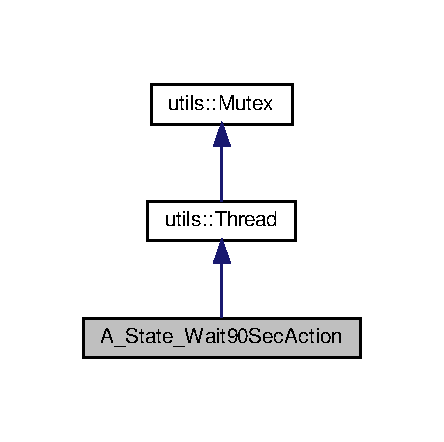
\includegraphics[width=213pt]{classA__State__Wait90SecAction__inherit__graph}
\end{center}
\end{figure}


Collaboration diagram for A\+\_\+\+State\+\_\+\+Wait90\+Sec\+Action\+:
\nopagebreak
\begin{figure}[H]
\begin{center}
\leavevmode
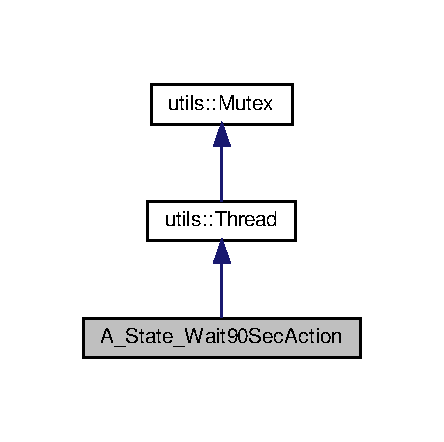
\includegraphics[width=213pt]{classA__State__Wait90SecAction__coll__graph}
\end{center}
\end{figure}
\subsection*{Public Member Functions}
\begin{DoxyCompactItemize}
\item 
\mbox{\Hypertarget{classA__State__Wait90SecAction_ae66516d475bb16f8fdcf17599705ff79}\label{classA__State__Wait90SecAction_ae66516d475bb16f8fdcf17599705ff79}} 
\hyperlink{classA__State__Wait90SecAction_ae66516d475bb16f8fdcf17599705ff79}{A\+\_\+\+State\+\_\+\+Wait90\+Sec\+Action} (\hyperlink{classRobot}{Robot} \&robot, void $\ast$data)
\begin{DoxyCompactList}\small\item\em Constructeur de la classe. \end{DoxyCompactList}\item 
\mbox{\Hypertarget{classA__State__Wait90SecAction_a217ea1674b38169449bada48c4a0422f}\label{classA__State__Wait90SecAction_a217ea1674b38169449bada48c4a0422f}} 
virtual \hyperlink{classA__State__Wait90SecAction_a217ea1674b38169449bada48c4a0422f}{$\sim$ A\+\_\+\+State\+\_\+\+Wait90\+Sec\+Action} ()
\begin{DoxyCompactList}\small\item\em Destructeur de la classe. \end{DoxyCompactList}\item 
\mbox{\Hypertarget{classA__State__Wait90SecAction_ab65d3e33397df2a82b873308a71dd29a}\label{classA__State__Wait90SecAction_ab65d3e33397df2a82b873308a71dd29a}} 
virtual std\+::string {\bfseries name} ()
\item 
\mbox{\Hypertarget{classA__State__Wait90SecAction_a97819ea5d7e7e034416368313ffda5c4}\label{classA__State__Wait90SecAction_a97819ea5d7e7e034416368313ffda5c4}} 
virtual void \hyperlink{classA__State__Wait90SecAction_a97819ea5d7e7e034416368313ffda5c4}{execute} ()
\begin{DoxyCompactList}\small\item\em Execute l\textquotesingle{}action. \end{DoxyCompactList}\end{DoxyCompactItemize}
\subsection*{Additional Inherited Members}


\subsection{Detailed Description}
Cette action lance le chronometer du robot. 

The documentation for this class was generated from the following files\+:\begin{DoxyCompactItemize}
\item 
/home/pmx/git/\+P\+M\+X/src/\+Bot-\/\+A\+P\+F9328/A\+\_\+\+State\+\_\+\+Wait90\+Sec\+Action.\+hpp\item 
/home/pmx/git/\+P\+M\+X/src/\+Bot-\/\+A\+P\+F9328/A\+\_\+\+State\+\_\+\+Wait90\+Sec\+Action.\+cpp\end{DoxyCompactItemize}

\hypertarget{classA__TiretteTest}{}\section{A\+\_\+\+Tirette\+Test Class Reference}
\label{classA__TiretteTest}\index{A\+\_\+\+Tirette\+Test@{A\+\_\+\+Tirette\+Test}}


Effectue un test sur la tirette.  




{\ttfamily \#include $<$A\+\_\+\+Tirette\+Test.\+hpp$>$}



Inheritance diagram for A\+\_\+\+Tirette\+Test\+:
\nopagebreak
\begin{figure}[H]
\begin{center}
\leavevmode
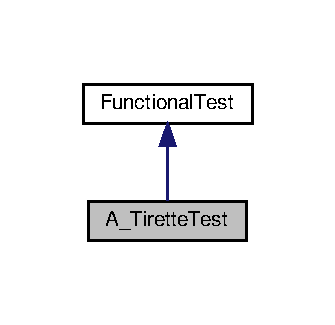
\includegraphics[width=161pt]{classA__TiretteTest__inherit__graph}
\end{center}
\end{figure}


Collaboration diagram for A\+\_\+\+Tirette\+Test\+:
\nopagebreak
\begin{figure}[H]
\begin{center}
\leavevmode
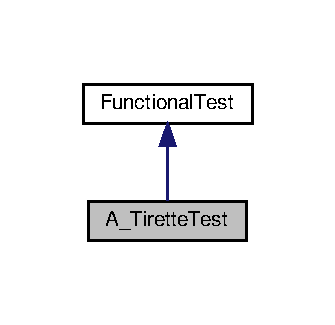
\includegraphics[width=161pt]{classA__TiretteTest__coll__graph}
\end{center}
\end{figure}
\subsection*{Public Member Functions}
\begin{DoxyCompactItemize}
\item 
\mbox{\Hypertarget{classA__TiretteTest_ab4d0ca6a166b837347f78ad48ec4cd2d}\label{classA__TiretteTest_ab4d0ca6a166b837347f78ad48ec4cd2d}} 
\hyperlink{classA__TiretteTest_ab4d0ca6a166b837347f78ad48ec4cd2d}{A\+\_\+\+Tirette\+Test} ()
\begin{DoxyCompactList}\small\item\em Constructeur de la classe. \end{DoxyCompactList}\item 
\mbox{\Hypertarget{classA__TiretteTest_a0c2296d8da35117b7fc99f4de431f0e8}\label{classA__TiretteTest_a0c2296d8da35117b7fc99f4de431f0e8}} 
virtual \hyperlink{classA__TiretteTest_a0c2296d8da35117b7fc99f4de431f0e8}{$\sim$\+A\+\_\+\+Tirette\+Test} ()
\begin{DoxyCompactList}\small\item\em Destructeur de la classe. \end{DoxyCompactList}\item 
\mbox{\Hypertarget{classA__TiretteTest_ad33ea95cc22c7b0e438faae54df6ef9b}\label{classA__TiretteTest_ad33ea95cc22c7b0e438faae54df6ef9b}} 
virtual void \hyperlink{classA__TiretteTest_ad33ea95cc22c7b0e438faae54df6ef9b}{run} (int argc, char $\ast$$\ast$argv)
\begin{DoxyCompactList}\small\item\em Execute le test. \end{DoxyCompactList}\end{DoxyCompactItemize}
\subsection*{Additional Inherited Members}


\subsection{Detailed Description}
Effectue un test sur la tirette. 

The documentation for this class was generated from the following files\+:\begin{DoxyCompactItemize}
\item 
/home/pmx/git/\+P\+M\+X/src/\+Bot-\/\+A\+P\+F9328/A\+\_\+\+Tirette\+Test.\+hpp\item 
/home/pmx/git/\+P\+M\+X/src/\+Bot-\/\+A\+P\+F9328/A\+\_\+\+Tirette\+Test.\+cpp\end{DoxyCompactItemize}

\hypertarget{classAActionDriver}{}\section{A\+Action\+Driver Class Reference}
\label{classAActionDriver}\index{A\+Action\+Driver@{A\+Action\+Driver}}
\subsection*{Public Member Functions}
\begin{DoxyCompactItemize}
\item 
\mbox{\Hypertarget{classAActionDriver_a2bcdc31f70d9648f2496f5b8a8b7683c}\label{classAActionDriver_a2bcdc31f70d9648f2496f5b8a8b7683c}} 
virtual void {\bfseries function} (int value)
\item 
\mbox{\Hypertarget{classAActionDriver_ab55710feabfd3807c16427f9fa88d762}\label{classAActionDriver_ab55710feabfd3807c16427f9fa88d762}} 
virtual \hyperlink{classAActionDriver_ab55710feabfd3807c16427f9fa88d762}{$\sim$\+A\+Action\+Driver} ()
\begin{DoxyCompactList}\small\item\em Destructor. \end{DoxyCompactList}\end{DoxyCompactItemize}
\subsection*{Static Public Member Functions}
\begin{DoxyCompactItemize}
\item 
\mbox{\Hypertarget{classAActionDriver_a2ef1e625e85a9598b119e004d2cf5f81}\label{classAActionDriver_a2ef1e625e85a9598b119e004d2cf5f81}} 
static \hyperlink{classAActionDriver}{A\+Action\+Driver} $\ast$ \hyperlink{classAActionDriver_a2ef1e625e85a9598b119e004d2cf5f81}{create} (int nb)
\begin{DoxyCompactList}\small\item\em instance creation. \end{DoxyCompactList}\end{DoxyCompactItemize}
\subsection*{Public Attributes}
\begin{DoxyCompactItemize}
\item 
\mbox{\Hypertarget{classAActionDriver_ad5e7d0a6931716d35d0d149da6a1a555}\label{classAActionDriver_ad5e7d0a6931716d35d0d149da6a1a555}} 
int {\bfseries example1}
\end{DoxyCompactItemize}
\subsection*{Protected Member Functions}
\begin{DoxyCompactItemize}
\item 
\mbox{\Hypertarget{classAActionDriver_af2fcbea774b20428f4824b4cf06092bb}\label{classAActionDriver_af2fcbea774b20428f4824b4cf06092bb}} 
\hyperlink{classAActionDriver_af2fcbea774b20428f4824b4cf06092bb}{A\+Action\+Driver} ()
\begin{DoxyCompactList}\small\item\em Constructor. \end{DoxyCompactList}\end{DoxyCompactItemize}


The documentation for this class was generated from the following files\+:\begin{DoxyCompactItemize}
\item 
/home/pmx/git/\+P\+M\+X/src/\+Common/\+Action.\+Driver/A\+Action\+Driver.\+hpp\item 
/home/pmx/git/\+P\+M\+X/src/\+Driver.\+S\+I\+M\+U\+C\+O\+C\+O\+S/Action\+Driver.\+cpp\end{DoxyCompactItemize}

\hypertarget{classAActionsElement}{}\section{A\+Actions\+Element Class Reference}
\label{classAActionsElement}\index{A\+Actions\+Element@{A\+Actions\+Element}}


Classe abstraite définissant la notion d\textquotesingle{}élément du robot.  




{\ttfamily \#include $<$A\+Actions\+Element.\+hpp$>$}



Inheritance diagram for A\+Actions\+Element\+:
\nopagebreak
\begin{figure}[H]
\begin{center}
\leavevmode
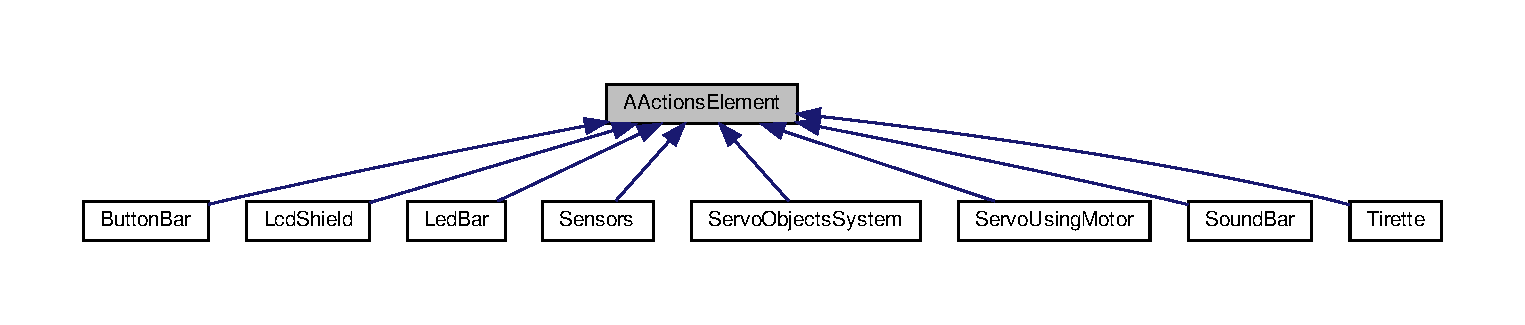
\includegraphics[width=350pt]{classAActionsElement__inherit__graph}
\end{center}
\end{figure}
\subsection*{Public Member Functions}
\begin{DoxyCompactItemize}
\item 
\mbox{\Hypertarget{classAActionsElement_a3fbd5b8201049a59602d8b7201a9ef8a}\label{classAActionsElement_a3fbd5b8201049a59602d8b7201a9ef8a}} 
\hyperlink{classActions}{Actions} \& \hyperlink{classAActionsElement_a3fbd5b8201049a59602d8b7201a9ef8a}{actions} ()
\begin{DoxyCompactList}\small\item\em Retourne une référence sur le \hyperlink{classActions}{Actions} associé. \end{DoxyCompactList}\item 
\mbox{\Hypertarget{classAActionsElement_a9baf29a52564a98ebb13c076c8f73a89}\label{classAActionsElement_a9baf29a52564a98ebb13c076c8f73a89}} 
virtual \hyperlink{classAActionsElement_a9baf29a52564a98ebb13c076c8f73a89}{$\sim$\+A\+Actions\+Element} ()
\begin{DoxyCompactList}\small\item\em Destructeur de la classe. \end{DoxyCompactList}\end{DoxyCompactItemize}
\subsection*{Protected Member Functions}
\begin{DoxyCompactItemize}
\item 
\hyperlink{classAActionsElement_aad97382a1ccb0a1ea4181d47c4a2ec4e}{A\+Actions\+Element} (\hyperlink{classActions}{Actions} \&\hyperlink{classAActionsElement_a3fbd5b8201049a59602d8b7201a9ef8a}{actions})
\begin{DoxyCompactList}\small\item\em Constructeur de la classe. \end{DoxyCompactList}\end{DoxyCompactItemize}


\subsection{Detailed Description}
Classe abstraite définissant la notion d\textquotesingle{}élément du robot. 

Chaque élément du robot possède un lien vers l\textquotesingle{}objet \hyperlink{classActions}{Actions}, quelque soit son niveau dans la hiérarchie. Ceci permet à chaque élément d\textquotesingle{}accéder simplement au manager associé et donc de pouvoir ajouter de nouvelles actions dans la pile des actions à effectuer. 

\subsection{Constructor \& Destructor Documentation}
\mbox{\Hypertarget{classAActionsElement_aad97382a1ccb0a1ea4181d47c4a2ec4e}\label{classAActionsElement_aad97382a1ccb0a1ea4181d47c4a2ec4e}} 
\index{A\+Actions\+Element@{A\+Actions\+Element}!A\+Actions\+Element@{A\+Actions\+Element}}
\index{A\+Actions\+Element@{A\+Actions\+Element}!A\+Actions\+Element@{A\+Actions\+Element}}
\subsubsection{\texorpdfstring{A\+Actions\+Element()}{AActionsElement()}}
{\footnotesize\ttfamily A\+Actions\+Element\+::\+A\+Actions\+Element (\begin{DoxyParamCaption}\item[{\hyperlink{classActions}{Actions} \&}]{actions }\end{DoxyParamCaption})\hspace{0.3cm}{\ttfamily [inline]}, {\ttfamily [protected]}}



Constructeur de la classe. 


\begin{DoxyParams}{Parameters}
{\em actions} & Référence à l\textquotesingle{}objet \hyperlink{classActions}{Actions} associé.\\
\hline
\end{DoxyParams}
Ce constructeur est {\ttfamily protected} pour éviter toute instantiation de la classe abstraite. 

The documentation for this class was generated from the following file\+:\begin{DoxyCompactItemize}
\item 
/home/pmx/git/\+P\+M\+X/src/\+Common/\+Action/\hyperlink{AActionsElement_8hpp}{A\+Actions\+Element.\+hpp}\end{DoxyCompactItemize}

\hypertarget{classAAsservDriver}{}\section{A\+Asserv\+Driver Class Reference}
\label{classAAsservDriver}\index{A\+Asserv\+Driver@{A\+Asserv\+Driver}}


Inheritance diagram for A\+Asserv\+Driver\+:
\nopagebreak
\begin{figure}[H]
\begin{center}
\leavevmode
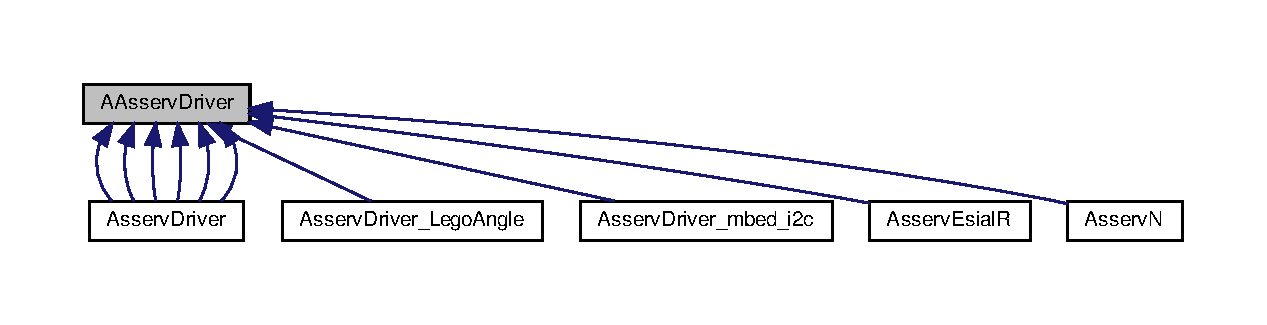
\includegraphics[width=350pt]{classAAsservDriver__inherit__graph}
\end{center}
\end{figure}
\subsection*{Public Member Functions}
\begin{DoxyCompactItemize}
\item 
\mbox{\Hypertarget{classAAsservDriver_a624c97511d788f1df927625a1d0eb54c}\label{classAAsservDriver_a624c97511d788f1df927625a1d0eb54c}} 
virtual \hyperlink{classAAsservDriver_a624c97511d788f1df927625a1d0eb54c}{$\sim$\+A\+Asserv\+Driver} ()
\begin{DoxyCompactList}\small\item\em Destructor. \end{DoxyCompactList}\item 
\mbox{\Hypertarget{classAAsservDriver_af6a0b1c219c8a25d589667f05da7f64d}\label{classAAsservDriver_af6a0b1c219c8a25d589667f05da7f64d}} 
\hyperlink{classAAsservDriver_af6a0b1c219c8a25d589667f05da7f64d}{A\+Asserv\+Driver} ()
\begin{DoxyCompactList}\small\item\em Constructor. \end{DoxyCompactList}\item 
\mbox{\Hypertarget{classAAsservDriver_a54ee068cec3c9f9f98b9e6b3d8c10f6e}\label{classAAsservDriver_a54ee068cec3c9f9f98b9e6b3d8c10f6e}} 
virtual void \hyperlink{classAAsservDriver_a54ee068cec3c9f9f98b9e6b3d8c10f6e}{end\+What\+Todo} ()=0
\begin{DoxyCompactList}\small\item\em actions à faire avant de quitter le programme. \end{DoxyCompactList}\item 
\mbox{\Hypertarget{classAAsservDriver_a77a5c938390e25a3231fe8b735ff3237}\label{classAAsservDriver_a77a5c938390e25a3231fe8b735ff3237}} 
virtual void \hyperlink{classAAsservDriver_a77a5c938390e25a3231fe8b735ff3237}{set\+Motor\+Left\+Position} (int power, long ticks)=0
\begin{DoxyCompactList}\small\item\em Fonctions utilisées uniquement par les drivers d\textquotesingle{}asserv et permettant un simple controle basique des moteurs et codeurs. \end{DoxyCompactList}\item 
\mbox{\Hypertarget{classAAsservDriver_a68eacbe79f71032a0dab1109948ea5f8}\label{classAAsservDriver_a68eacbe79f71032a0dab1109948ea5f8}} 
virtual void {\bfseries set\+Motor\+Right\+Position} (int power, long ticks)=0
\item 
\mbox{\Hypertarget{classAAsservDriver_a67ed5e8b3460f9496f36662beab44a46}\label{classAAsservDriver_a67ed5e8b3460f9496f36662beab44a46}} 
virtual void {\bfseries set\+Motor\+Left\+Power} (int power, int time\+\_\+ms)=0
\item 
\mbox{\Hypertarget{classAAsservDriver_a6cd9bf62cb78150f94d38fa978c0a83a}\label{classAAsservDriver_a6cd9bf62cb78150f94d38fa978c0a83a}} 
virtual void {\bfseries set\+Motor\+Right\+Power} (int power, int time\+\_\+ms)=0
\item 
\mbox{\Hypertarget{classAAsservDriver_ac30b15c18f0bf293cb322ae90a5bf7cc}\label{classAAsservDriver_ac30b15c18f0bf293cb322ae90a5bf7cc}} 
virtual long {\bfseries get\+Left\+External\+Encoder} ()=0
\item 
\mbox{\Hypertarget{classAAsservDriver_a2799a875b5fc7975d6eeb0a3f98bc108}\label{classAAsservDriver_a2799a875b5fc7975d6eeb0a3f98bc108}} 
virtual long {\bfseries get\+Right\+External\+Encoder} ()=0
\item 
\mbox{\Hypertarget{classAAsservDriver_a733770d9a0eb73caa897baadd3e36f9d}\label{classAAsservDriver_a733770d9a0eb73caa897baadd3e36f9d}} 
virtual void {\bfseries get\+Counts\+External} (int32\+\_\+t $\ast$countR, int32\+\_\+t $\ast$countL)=0
\item 
\mbox{\Hypertarget{classAAsservDriver_ac303905f9004ca89964b7fd6c3b5df81}\label{classAAsservDriver_ac303905f9004ca89964b7fd6c3b5df81}} 
virtual void {\bfseries get\+Delta\+Counts\+External} (int32\+\_\+t $\ast$deltaR, int32\+\_\+t $\ast$deltaL)=0
\item 
\mbox{\Hypertarget{classAAsservDriver_a99137b00bcf944c7fe8280d4e6adf194}\label{classAAsservDriver_a99137b00bcf944c7fe8280d4e6adf194}} 
virtual long {\bfseries get\+Left\+Internal\+Encoder} ()=0
\item 
\mbox{\Hypertarget{classAAsservDriver_a474f74d48b64f813c6c7a3aa67bb5c07}\label{classAAsservDriver_a474f74d48b64f813c6c7a3aa67bb5c07}} 
virtual long {\bfseries get\+Right\+Internal\+Encoder} ()=0
\item 
\mbox{\Hypertarget{classAAsservDriver_aaa5418d791cab277447abf18afe31c4e}\label{classAAsservDriver_aaa5418d791cab277447abf18afe31c4e}} 
virtual void {\bfseries get\+Counts\+Internal} (int32\+\_\+t $\ast$countR, int32\+\_\+t $\ast$countL)=0
\item 
\mbox{\Hypertarget{classAAsservDriver_affe6c7f465c2f499a6f1e28ea2e7eb85}\label{classAAsservDriver_affe6c7f465c2f499a6f1e28ea2e7eb85}} 
virtual void {\bfseries reset\+Encoders} ()=0
\item 
\mbox{\Hypertarget{classAAsservDriver_a40cc13dd2668e52283fa8fdc22ba7805}\label{classAAsservDriver_a40cc13dd2668e52283fa8fdc22ba7805}} 
virtual void {\bfseries reset\+Internal\+Encoders} ()=0
\item 
\mbox{\Hypertarget{classAAsservDriver_ac1124f108bbdb293cf71ae1ce3d0222c}\label{classAAsservDriver_ac1124f108bbdb293cf71ae1ce3d0222c}} 
virtual void {\bfseries reset\+External\+Encoders} ()=0
\item 
\mbox{\Hypertarget{classAAsservDriver_a7e3415d0b04fb227e468f23f7b7a0ad0}\label{classAAsservDriver_a7e3415d0b04fb227e468f23f7b7a0ad0}} 
virtual void {\bfseries stop\+Motor\+Left} ()=0
\item 
\mbox{\Hypertarget{classAAsservDriver_aaa92c72fe63cf97fb219566f912bdbbc}\label{classAAsservDriver_aaa92c72fe63cf97fb219566f912bdbbc}} 
virtual void {\bfseries stop\+Motor\+Right} ()=0
\item 
\mbox{\Hypertarget{classAAsservDriver_a8b6c4cafec7a55188604ec8af44b11bb}\label{classAAsservDriver_a8b6c4cafec7a55188604ec8af44b11bb}} 
virtual int {\bfseries get\+Motor\+Left\+Current} ()=0
\item 
\mbox{\Hypertarget{classAAsservDriver_a29ab60a2685bdec463339cca10e6efaf}\label{classAAsservDriver_a29ab60a2685bdec463339cca10e6efaf}} 
virtual int {\bfseries get\+Motor\+Right\+Current} ()=0
\item 
\mbox{\Hypertarget{classAAsservDriver_a1980c0a6071940839bfe9782ab939db0}\label{classAAsservDriver_a1980c0a6071940839bfe9782ab939db0}} 
virtual void \hyperlink{classAAsservDriver_a1980c0a6071940839bfe9782ab939db0}{odo\+\_\+\+Set\+Position} (float x\+\_\+mm, float y\+\_\+mm, float angle\+\_\+rad)=0
\begin{DoxyCompactList}\small\item\em Fonctions permettant d\textquotesingle{}utiliser un asservissement externe. \end{DoxyCompactList}\item 
\mbox{\Hypertarget{classAAsservDriver_acaea1ffd7a880d7796b1274bea4cff96}\label{classAAsservDriver_acaea1ffd7a880d7796b1274bea4cff96}} 
virtual \hyperlink{structRobotPosition}{Robot\+Position} {\bfseries odo\+\_\+\+Get\+Position} ()=0
\item 
\mbox{\Hypertarget{classAAsservDriver_af6cff4776b36ad5f17e3683112eaba86}\label{classAAsservDriver_af6cff4776b36ad5f17e3683112eaba86}} 
virtual int {\bfseries path\+\_\+\+Get\+Last\+Command\+Status} ()=0
\item 
\mbox{\Hypertarget{classAAsservDriver_a3c40ae9ee4591963723aab90e7b1d7a0}\label{classAAsservDriver_a3c40ae9ee4591963723aab90e7b1d7a0}} 
virtual void {\bfseries path\+\_\+\+Interrupt\+Trajectory} ()=0
\item 
\mbox{\Hypertarget{classAAsservDriver_a0faec2325a4b8e159bbccc28ddb4eba0}\label{classAAsservDriver_a0faec2325a4b8e159bbccc28ddb4eba0}} 
virtual void {\bfseries path\+\_\+\+Collision\+On\+Trajectory} ()=0
\item 
\mbox{\Hypertarget{classAAsservDriver_a46391c5413a97747093f0bbe366d16fc}\label{classAAsservDriver_a46391c5413a97747093f0bbe366d16fc}} 
virtual void {\bfseries path\+\_\+\+Collision\+Rear\+On\+Trajectory} ()=0
\item 
\mbox{\Hypertarget{classAAsservDriver_a5bc22cc735af0982a4c7a4d6fbe19c4f}\label{classAAsservDriver_a5bc22cc735af0982a4c7a4d6fbe19c4f}} 
virtual void {\bfseries path\+\_\+\+Cancel\+Trajectory} ()=0
\item 
\mbox{\Hypertarget{classAAsservDriver_a55e3b442898d83f302b9d9e0898317b6}\label{classAAsservDriver_a55e3b442898d83f302b9d9e0898317b6}} 
virtual void {\bfseries path\+\_\+\+Reset\+Emergency\+Stop} ()=0
\item 
\mbox{\Hypertarget{classAAsservDriver_a1a20a75bd63b75ecaf511e824a8a796a}\label{classAAsservDriver_a1a20a75bd63b75ecaf511e824a8a796a}} 
virtual \hyperlink{path__manager_8h_adb3360abeb29758da93865c8afcb80eb}{T\+R\+A\+J\+\_\+\+S\+T\+A\+TE} {\bfseries motion\+\_\+\+Do\+Face} (float x\+\_\+mm, float y\+\_\+mm)=0
\item 
\mbox{\Hypertarget{classAAsservDriver_a9a605eb37c55384962093a200a512bad}\label{classAAsservDriver_a9a605eb37c55384962093a200a512bad}} 
virtual \hyperlink{path__manager_8h_adb3360abeb29758da93865c8afcb80eb}{T\+R\+A\+J\+\_\+\+S\+T\+A\+TE} {\bfseries motion\+\_\+\+Do\+Line} (float dist\+\_\+meters)=0
\item 
\mbox{\Hypertarget{classAAsservDriver_a2211748fb68a1431096c17ba4f9d7c42}\label{classAAsservDriver_a2211748fb68a1431096c17ba4f9d7c42}} 
virtual \hyperlink{path__manager_8h_adb3360abeb29758da93865c8afcb80eb}{T\+R\+A\+J\+\_\+\+S\+T\+A\+TE} {\bfseries motion\+\_\+\+Do\+Rotate} (float angle\+\_\+radians)=0
\item 
\mbox{\Hypertarget{classAAsservDriver_a3c41681cce40f67e84af3ad973281913}\label{classAAsservDriver_a3c41681cce40f67e84af3ad973281913}} 
virtual \hyperlink{path__manager_8h_adb3360abeb29758da93865c8afcb80eb}{T\+R\+A\+J\+\_\+\+S\+T\+A\+TE} {\bfseries motion\+\_\+\+Do\+Arc\+Rotate} (float angle\+\_\+radians, float radius)=0
\item 
\mbox{\Hypertarget{classAAsservDriver_ac62c5066c309e395a63a155f78053c9e}\label{classAAsservDriver_ac62c5066c309e395a63a155f78053c9e}} 
virtual \hyperlink{path__manager_8h_adb3360abeb29758da93865c8afcb80eb}{T\+R\+A\+J\+\_\+\+S\+T\+A\+TE} {\bfseries motion\+\_\+\+Goto} (float x\+\_\+mm, float y\+\_\+mm)=0
\item 
\mbox{\Hypertarget{classAAsservDriver_a19b77ce59325a7c6c5f65eac3d9c7593}\label{classAAsservDriver_a19b77ce59325a7c6c5f65eac3d9c7593}} 
virtual \hyperlink{path__manager_8h_adb3360abeb29758da93865c8afcb80eb}{T\+R\+A\+J\+\_\+\+S\+T\+A\+TE} {\bfseries motion\+\_\+\+Goto\+Reverse} (float x\+\_\+mm, float y\+\_\+mm)=0
\item 
\mbox{\Hypertarget{classAAsservDriver_ab8a6a390e76b8999c59a28c2e8190106}\label{classAAsservDriver_ab8a6a390e76b8999c59a28c2e8190106}} 
virtual \hyperlink{path__manager_8h_adb3360abeb29758da93865c8afcb80eb}{T\+R\+A\+J\+\_\+\+S\+T\+A\+TE} {\bfseries motion\+\_\+\+Goto\+Chain} (float x\+\_\+mm, float y\+\_\+mm)=0
\item 
\mbox{\Hypertarget{classAAsservDriver_afa0de8f03c96e899d5339d394295c560}\label{classAAsservDriver_afa0de8f03c96e899d5339d394295c560}} 
virtual \hyperlink{path__manager_8h_adb3360abeb29758da93865c8afcb80eb}{T\+R\+A\+J\+\_\+\+S\+T\+A\+TE} {\bfseries motion\+\_\+\+Goto\+Reverse\+Chain} (float x\+\_\+mm, float y\+\_\+mm)=0
\item 
\mbox{\Hypertarget{classAAsservDriver_aca4741e0e7e11947180f53ba8abe0730}\label{classAAsservDriver_aca4741e0e7e11947180f53ba8abe0730}} 
virtual void {\bfseries motion\+\_\+\+Free\+Motion} (void)=0
\item 
\mbox{\Hypertarget{classAAsservDriver_a3d4f4d2a80ee1887212f38fda3094c26}\label{classAAsservDriver_a3d4f4d2a80ee1887212f38fda3094c26}} 
virtual void {\bfseries motion\+\_\+\+Disable\+P\+ID} (void)=0
\item 
\mbox{\Hypertarget{classAAsservDriver_a83153736da05eba6451f02b399eb4438}\label{classAAsservDriver_a83153736da05eba6451f02b399eb4438}} 
virtual void \hyperlink{classAAsservDriver_a83153736da05eba6451f02b399eb4438}{motion\+\_\+\+Assisted\+Handling} (void)=0
\begin{DoxyCompactList}\small\item\em Stop motion control and disable P\+ID. \end{DoxyCompactList}\item 
\mbox{\Hypertarget{classAAsservDriver_a046eb790d147ad8ec34bcd9565ad675b}\label{classAAsservDriver_a046eb790d147ad8ec34bcd9565ad675b}} 
virtual void \hyperlink{classAAsservDriver_a046eb790d147ad8ec34bcd9565ad675b}{motion\+\_\+\+Activate\+Manager} (bool enablethread)=0
\begin{DoxyCompactList}\small\item\em Assisted movement mode =) (activate P\+ID) \end{DoxyCompactList}\item 
\mbox{\Hypertarget{classAAsservDriver_a6912c759115a6357b3ce8ce55f365663}\label{classAAsservDriver_a6912c759115a6357b3ce8ce55f365663}} 
virtual void {\bfseries motion\+\_\+set\+Low\+Speed\+Forward} (bool enable, int percent=0)=0
\item 
\mbox{\Hypertarget{classAAsservDriver_a621a0b60fec76be04f8960f2e56ba5fe}\label{classAAsservDriver_a621a0b60fec76be04f8960f2e56ba5fe}} 
virtual void {\bfseries motion\+\_\+set\+Low\+Speed\+Backward} (bool enable, int percent=0)=0
\item 
\mbox{\Hypertarget{classAAsservDriver_a7a41963b5f908604a55f109e7ea3214e}\label{classAAsservDriver_a7a41963b5f908604a55f109e7ea3214e}} 
virtual void {\bfseries motion\+\_\+\+Activate\+Regu\+Dist} (bool enable)=0
\item 
\mbox{\Hypertarget{classAAsservDriver_ae5b16fb3a46e690deb213b556749e33f}\label{classAAsservDriver_ae5b16fb3a46e690deb213b556749e33f}} 
virtual void {\bfseries motion\+\_\+\+Activate\+Regu\+Angle} (bool enable)=0
\item 
\mbox{\Hypertarget{classAAsservDriver_a658d7dad992e6eb5066a396a8fbaf645}\label{classAAsservDriver_a658d7dad992e6eb5066a396a8fbaf645}} 
virtual void {\bfseries motion\+\_\+\+Reset\+Regu\+Dist} ()=0
\item 
\mbox{\Hypertarget{classAAsservDriver_a0426d6401a8fa5ff8489f9b040a616da}\label{classAAsservDriver_a0426d6401a8fa5ff8489f9b040a616da}} 
virtual void {\bfseries motion\+\_\+\+Reset\+Regu\+Angle} ()=0
\item 
\mbox{\Hypertarget{classAAsservDriver_a24fc4fe4bd8dae4d0658b5102f343657}\label{classAAsservDriver_a24fc4fe4bd8dae4d0658b5102f343657}} 
virtual \hyperlink{path__manager_8h_adb3360abeb29758da93865c8afcb80eb}{T\+R\+A\+J\+\_\+\+S\+T\+A\+TE} {\bfseries motion\+\_\+\+Do\+Direct\+Line} (float dist\+\_\+mm)=0
\end{DoxyCompactItemize}
\subsection*{Static Public Member Functions}
\begin{DoxyCompactItemize}
\item 
\mbox{\Hypertarget{classAAsservDriver_aa8b144fdccac014af94b93f743d89fa8}\label{classAAsservDriver_aa8b144fdccac014af94b93f743d89fa8}} 
static \hyperlink{classAAsservDriver}{A\+Asserv\+Driver} $\ast$ \hyperlink{classAAsservDriver_aa8b144fdccac014af94b93f743d89fa8}{create} (std\+::string botid)
\begin{DoxyCompactList}\small\item\em single instance creation. \end{DoxyCompactList}\end{DoxyCompactItemize}
\subsection*{Protected Member Functions}
\begin{DoxyCompactItemize}
\item 
\mbox{\Hypertarget{classAAsservDriver_a956b5f3a782e15931aa80fd834dd63e7}\label{classAAsservDriver_a956b5f3a782e15931aa80fd834dd63e7}} 
float {\bfseries deg\+To\+Rad} (float deg)
\item 
\mbox{\Hypertarget{classAAsservDriver_a231f237f4a38854b1cc70bc87636727e}\label{classAAsservDriver_a231f237f4a38854b1cc70bc87636727e}} 
float {\bfseries rad\+To\+Deg} (float rad)
\end{DoxyCompactItemize}


The documentation for this class was generated from the following files\+:\begin{DoxyCompactItemize}
\item 
/home/pmx/git/\+P\+M\+X/src/\+Common/\+Asserv.\+Driver/A\+Asserv\+Driver.\+hpp\item 
/home/pmx/git/\+P\+M\+X/src/\+Driver.\+S\+I\+M\+U\+C\+O\+C\+O\+S/Asserv\+Driver.\+cpp\item 
/home/pmx/git/\+P\+M\+X/test/\+Common-\/\+Test.\+Main/Driver.\+cpp\end{DoxyCompactItemize}

\hypertarget{classAAsservElement}{}\section{A\+Asserv\+Element Class Reference}
\label{classAAsservElement}\index{A\+Asserv\+Element@{A\+Asserv\+Element}}


Classe abstraite définissant la notion d\textquotesingle{}élément de l\textquotesingle{}asservissement.  




{\ttfamily \#include $<$A\+Asserv\+Element.\+hpp$>$}

\subsection*{Public Member Functions}
\begin{DoxyCompactItemize}
\item 
\mbox{\Hypertarget{classAAsservElement_a934d1e50fbbd3d52be8cdc83ed922f25}\label{classAAsservElement_a934d1e50fbbd3d52be8cdc83ed922f25}} 
\hyperlink{classAsserv}{Asserv} \& \hyperlink{classAAsservElement_a934d1e50fbbd3d52be8cdc83ed922f25}{asserv} ()
\begin{DoxyCompactList}\small\item\em Retourne une référence sur l\textquotesingle{}objet \hyperlink{classAsserv}{Asserv} associé. \end{DoxyCompactList}\item 
\mbox{\Hypertarget{classAAsservElement_a0be48eb52c88b2ca11169d6a3280b11d}\label{classAAsservElement_a0be48eb52c88b2ca11169d6a3280b11d}} 
virtual \hyperlink{classAAsservElement_a0be48eb52c88b2ca11169d6a3280b11d}{$\sim$\+A\+Asserv\+Element} ()
\begin{DoxyCompactList}\small\item\em Destructeur de la classe. \end{DoxyCompactList}\end{DoxyCompactItemize}
\subsection*{Protected Member Functions}
\begin{DoxyCompactItemize}
\item 
\hyperlink{classAAsservElement_af0b6767d631173c912e7e16e6f1c6db1}{A\+Asserv\+Element} (\hyperlink{classAsserv}{Asserv} \&\hyperlink{classAAsservElement_a934d1e50fbbd3d52be8cdc83ed922f25}{asserv})
\begin{DoxyCompactList}\small\item\em Constructeur de la classe. \end{DoxyCompactList}\end{DoxyCompactItemize}


\subsection{Detailed Description}
Classe abstraite définissant la notion d\textquotesingle{}élément de l\textquotesingle{}asservissement. 

Chaque élément possède un lien vers l\textquotesingle{}objet \hyperlink{classAsserv}{Asserv}, quelque soit son niveau dans la hiérarchie. 

\subsection{Constructor \& Destructor Documentation}
\mbox{\Hypertarget{classAAsservElement_af0b6767d631173c912e7e16e6f1c6db1}\label{classAAsservElement_af0b6767d631173c912e7e16e6f1c6db1}} 
\index{A\+Asserv\+Element@{A\+Asserv\+Element}!A\+Asserv\+Element@{A\+Asserv\+Element}}
\index{A\+Asserv\+Element@{A\+Asserv\+Element}!A\+Asserv\+Element@{A\+Asserv\+Element}}
\subsubsection{\texorpdfstring{A\+Asserv\+Element()}{AAsservElement()}}
{\footnotesize\ttfamily A\+Asserv\+Element\+::\+A\+Asserv\+Element (\begin{DoxyParamCaption}\item[{\hyperlink{classAsserv}{Asserv} \&}]{asserv }\end{DoxyParamCaption})\hspace{0.3cm}{\ttfamily [inline]}, {\ttfamily [protected]}}



Constructeur de la classe. 


\begin{DoxyParams}{Parameters}
{\em robot} & Référence à l\textquotesingle{}objet \hyperlink{classAsserv}{Asserv} associé.\\
\hline
\end{DoxyParams}
Ce constructeur est {\ttfamily protected} pour éviter toute instantiation de la classe abstraite. 

The documentation for this class was generated from the following file\+:\begin{DoxyCompactItemize}
\item 
/home/pmx/git/\+P\+M\+X/src/\+Common/\+Asserv/\hyperlink{AAsservElement_8hpp}{A\+Asserv\+Element.\+hpp}\end{DoxyCompactItemize}

\hypertarget{classAAutomateState}{}\section{A\+Automate\+State Class Reference}
\label{classAAutomateState}\index{A\+Automate\+State@{A\+Automate\+State}}


Définit les méthodes communes à tous les états.  




{\ttfamily \#include $<$A\+Automate\+State.\+hpp$>$}



Inheritance diagram for A\+Automate\+State\+:
\nopagebreak
\begin{figure}[H]
\begin{center}
\leavevmode
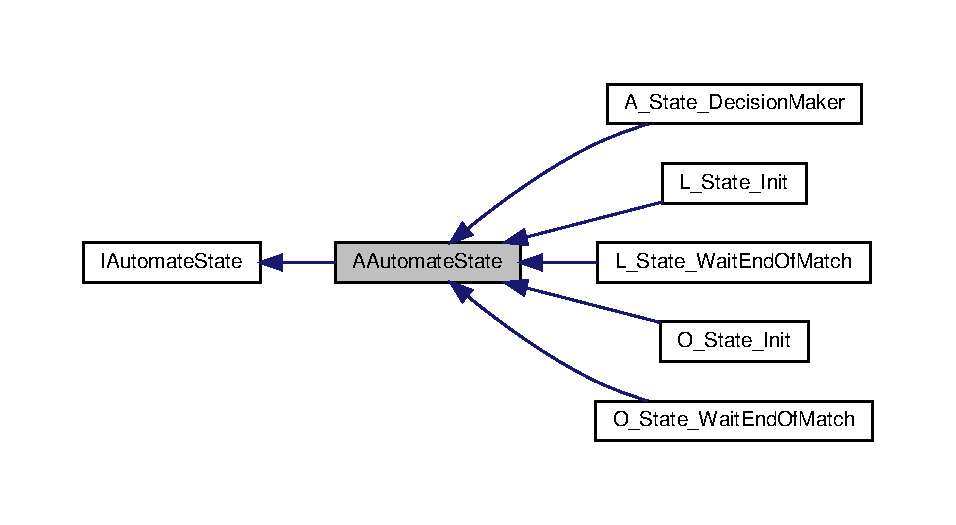
\includegraphics[width=350pt]{classAAutomateState__inherit__graph}
\end{center}
\end{figure}


Collaboration diagram for A\+Automate\+State\+:
\nopagebreak
\begin{figure}[H]
\begin{center}
\leavevmode
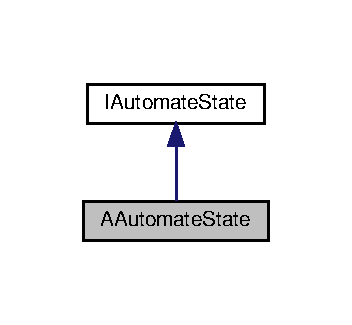
\includegraphics[width=169pt]{classAAutomateState__coll__graph}
\end{center}
\end{figure}
\subsection*{Public Member Functions}
\begin{DoxyCompactItemize}
\item 
\mbox{\Hypertarget{classAAutomateState_adaca6ae61aacda9bb75b3acee9d951d1}\label{classAAutomateState_adaca6ae61aacda9bb75b3acee9d951d1}} 
\hyperlink{classAAutomateState_adaca6ae61aacda9bb75b3acee9d951d1}{A\+Automate\+State} ()
\begin{DoxyCompactList}\small\item\em Constructeur de la classe. \end{DoxyCompactList}\item 
\mbox{\Hypertarget{classAAutomateState_a3116f6449e6eb43d2610bfa049d70f00}\label{classAAutomateState_a3116f6449e6eb43d2610bfa049d70f00}} 
virtual std\+::string {\bfseries name} ()
\item 
\mbox{\Hypertarget{classAAutomateState_ad69fc5adb9a6f0ccbbebea324e55c532}\label{classAAutomateState_ad69fc5adb9a6f0ccbbebea324e55c532}} 
virtual \hyperlink{classAAutomateState_ad69fc5adb9a6f0ccbbebea324e55c532}{$\sim$\+A\+Automate\+State} ()
\begin{DoxyCompactList}\small\item\em Destructeur de la classe. \end{DoxyCompactList}\item 
void \hyperlink{classAAutomateState_a2f141db7bda71b605195c3516b0dac51}{add\+State} (const std\+::string \&name, \hyperlink{classIAutomateState}{I\+Automate\+State} $\ast$state)
\begin{DoxyCompactList}\small\item\em Ajoute une transition possible à cet état. \end{DoxyCompactList}\item 
\hyperlink{classIAutomateState}{I\+Automate\+State} $\ast$ \hyperlink{classAAutomateState_a98966c27660941825dba0da7130a957f}{get\+State} (const std\+::string \&name)
\begin{DoxyCompactList}\small\item\em Retourne l\textquotesingle{}état associé à une transition spécifique. \end{DoxyCompactList}\end{DoxyCompactItemize}
\subsection*{Additional Inherited Members}


\subsection{Detailed Description}
Définit les méthodes communes à tous les états. 

\subsection{Member Function Documentation}
\mbox{\Hypertarget{classAAutomateState_a2f141db7bda71b605195c3516b0dac51}\label{classAAutomateState_a2f141db7bda71b605195c3516b0dac51}} 
\index{A\+Automate\+State@{A\+Automate\+State}!add\+State@{add\+State}}
\index{add\+State@{add\+State}!A\+Automate\+State@{A\+Automate\+State}}
\subsubsection{\texorpdfstring{add\+State()}{addState()}}
{\footnotesize\ttfamily void A\+Automate\+State\+::add\+State (\begin{DoxyParamCaption}\item[{const std\+::string \&}]{name,  }\item[{\hyperlink{classIAutomateState}{I\+Automate\+State} $\ast$}]{state }\end{DoxyParamCaption})\hspace{0.3cm}{\ttfamily [inline]}, {\ttfamily [virtual]}}



Ajoute une transition possible à cet état. 


\begin{DoxyParams}{Parameters}
{\em name} & Nom de la transition \\
\hline
{\em state} & Etat associé à la transition \\
\hline
\end{DoxyParams}


Implements \hyperlink{classIAutomateState_a2d088c807e6d7b30b93511096a34af2a}{I\+Automate\+State}.

\mbox{\Hypertarget{classAAutomateState_a98966c27660941825dba0da7130a957f}\label{classAAutomateState_a98966c27660941825dba0da7130a957f}} 
\index{A\+Automate\+State@{A\+Automate\+State}!get\+State@{get\+State}}
\index{get\+State@{get\+State}!A\+Automate\+State@{A\+Automate\+State}}
\subsubsection{\texorpdfstring{get\+State()}{getState()}}
{\footnotesize\ttfamily \hyperlink{classIAutomateState}{I\+Automate\+State}$\ast$ A\+Automate\+State\+::get\+State (\begin{DoxyParamCaption}\item[{const std\+::string \&}]{name }\end{DoxyParamCaption})\hspace{0.3cm}{\ttfamily [inline]}, {\ttfamily [virtual]}}



Retourne l\textquotesingle{}état associé à une transition spécifique. 


\begin{DoxyParams}{Parameters}
{\em name} & Nom de la transition \\
\hline
\end{DoxyParams}
\begin{DoxyReturn}{Returns}
L\textquotesingle{}état associé à la transition ou {\ttfamily N\+U\+LL}. 
\end{DoxyReturn}


Implements \hyperlink{classIAutomateState_a228fe704fd235a83cae36e5dd197c473}{I\+Automate\+State}.



The documentation for this class was generated from the following file\+:\begin{DoxyCompactItemize}
\item 
/home/pmx/git/\+P\+M\+X/src/\+Common/\+State/\hyperlink{AAutomateState_8hpp}{A\+Automate\+State.\+hpp}\end{DoxyCompactItemize}

\hypertarget{classAbstractAccelerationLimiter}{}\section{Abstract\+Acceleration\+Limiter Class Reference}
\label{classAbstractAccelerationLimiter}\index{Abstract\+Acceleration\+Limiter@{Abstract\+Acceleration\+Limiter}}


Inheritance diagram for Abstract\+Acceleration\+Limiter\+:
\nopagebreak
\begin{figure}[H]
\begin{center}
\leavevmode
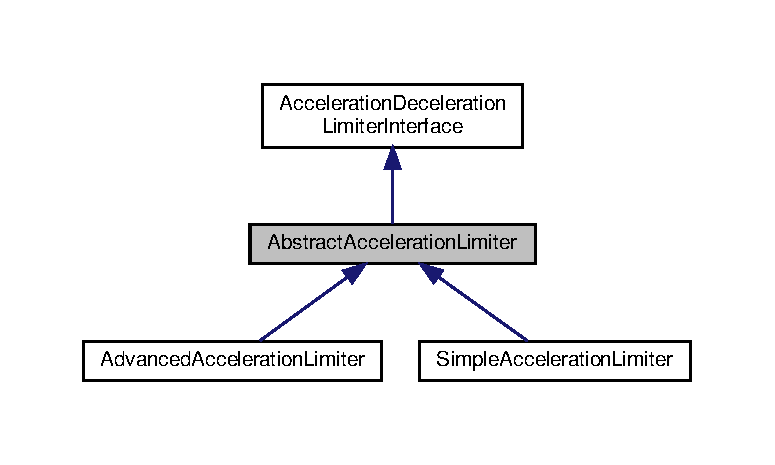
\includegraphics[width=350pt]{classAbstractAccelerationLimiter__inherit__graph}
\end{center}
\end{figure}


Collaboration diagram for Abstract\+Acceleration\+Limiter\+:
\nopagebreak
\begin{figure}[H]
\begin{center}
\leavevmode
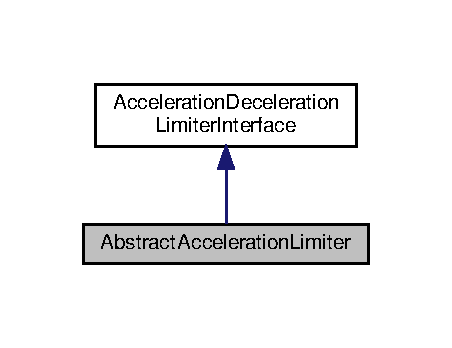
\includegraphics[width=217pt]{classAbstractAccelerationLimiter__coll__graph}
\end{center}
\end{figure}
\subsection*{Public Member Functions}
\begin{DoxyCompactItemize}
\item 
\mbox{\Hypertarget{classAbstractAccelerationLimiter_a229b985a2ed69ef70e166ed737b1aeb9}\label{classAbstractAccelerationLimiter_a229b985a2ed69ef70e166ed737b1aeb9}} 
virtual float {\bfseries limit\+Acceleration} (float dt, float target\+Speed, float current\+Speed, float position\+Goal, float position\+Error)
\item 
\mbox{\Hypertarget{classAbstractAccelerationLimiter_a6e54de6947fd13351126d5a0321405ee}\label{classAbstractAccelerationLimiter_a6e54de6947fd13351126d5a0321405ee}} 
virtual void {\bfseries enable} ()
\item 
\mbox{\Hypertarget{classAbstractAccelerationLimiter_a93f727ad1d8a0b307f6b813ccbc164a4}\label{classAbstractAccelerationLimiter_a93f727ad1d8a0b307f6b813ccbc164a4}} 
virtual void {\bfseries disable} ()
\item 
\mbox{\Hypertarget{classAbstractAccelerationLimiter_a942357de40aa435b084780310b57043b}\label{classAbstractAccelerationLimiter_a942357de40aa435b084780310b57043b}} 
virtual void {\bfseries reset} ()
\end{DoxyCompactItemize}
\subsection*{Static Public Member Functions}
\begin{DoxyCompactItemize}
\item 
\mbox{\Hypertarget{classAbstractAccelerationLimiter_a06ec4af35b8bd67d7d267b555aa28996}\label{classAbstractAccelerationLimiter_a06ec4af35b8bd67d7d267b555aa28996}} 
static float {\bfseries constrain} (float value, float low, float high)
\end{DoxyCompactItemize}


The documentation for this class was generated from the following files\+:\begin{DoxyCompactItemize}
\item 
/home/pmx/git/\+P\+M\+X/src/\+Asserv.\+Nucleo/\+Acceleration\+Limiter/Abstract\+Acceleration\+Limiter.\+h\item 
/home/pmx/git/\+P\+M\+X/src/\+Asserv.\+Nucleo/\+Acceleration\+Limiter/Abstract\+Acceleration\+Limiter.\+cpp\end{DoxyCompactItemize}

\hypertarget{classAButtonDriver}{}\section{A\+Button\+Driver Class Reference}
\label{classAButtonDriver}\index{A\+Button\+Driver@{A\+Button\+Driver}}


Inheritance diagram for A\+Button\+Driver\+:
\nopagebreak
\begin{figure}[H]
\begin{center}
\leavevmode
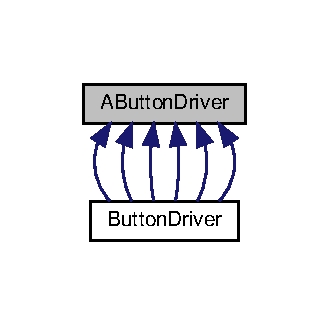
\includegraphics[width=158pt]{classAButtonDriver__inherit__graph}
\end{center}
\end{figure}
\subsection*{Public Member Functions}
\begin{DoxyCompactItemize}
\item 
\mbox{\Hypertarget{classAButtonDriver_a76900724cd51ab5213273cd2ef4e4918}\label{classAButtonDriver_a76900724cd51ab5213273cd2ef4e4918}} 
virtual bool {\bfseries pressed} (Button\+Touch button)=0
\item 
\mbox{\Hypertarget{classAButtonDriver_aa234368ae4f01fd3bd0d63b605f85ef8}\label{classAButtonDriver_aa234368ae4f01fd3bd0d63b605f85ef8}} 
virtual \hyperlink{classAButtonDriver_aa234368ae4f01fd3bd0d63b605f85ef8}{$\sim$\+A\+Button\+Driver} ()
\begin{DoxyCompactList}\small\item\em Destructor. \end{DoxyCompactList}\end{DoxyCompactItemize}
\subsection*{Static Public Member Functions}
\begin{DoxyCompactItemize}
\item 
\mbox{\Hypertarget{classAButtonDriver_abc99f5a63facaaa7c57b39eca57e3c8b}\label{classAButtonDriver_abc99f5a63facaaa7c57b39eca57e3c8b}} 
static \hyperlink{classAButtonDriver}{A\+Button\+Driver} $\ast$ \hyperlink{classAButtonDriver_abc99f5a63facaaa7c57b39eca57e3c8b}{create} ()
\begin{DoxyCompactList}\small\item\em \hyperlink{classButtonDriver}{Button\+Driver} instance creation. \end{DoxyCompactList}\end{DoxyCompactItemize}
\subsection*{Protected Member Functions}
\begin{DoxyCompactItemize}
\item 
\mbox{\Hypertarget{classAButtonDriver_a035c36655b359b7e8e3ae0a3be85c0c9}\label{classAButtonDriver_a035c36655b359b7e8e3ae0a3be85c0c9}} 
\hyperlink{classAButtonDriver_a035c36655b359b7e8e3ae0a3be85c0c9}{A\+Button\+Driver} ()
\begin{DoxyCompactList}\small\item\em Constructor. \end{DoxyCompactList}\end{DoxyCompactItemize}


The documentation for this class was generated from the following files\+:\begin{DoxyCompactItemize}
\item 
/home/pmx/git/\+P\+M\+X/src/\+Common/\+Action.\+Driver/A\+Button\+Driver.\+hpp\item 
/home/pmx/git/\+P\+M\+X/src/\+Driver-\/\+A\+P\+F9328\+\_\+\+A\+R\+M/Button\+Driver.\+cpp\end{DoxyCompactItemize}

\hypertarget{classAccelerationDecelerationLimiter}{}\section{Acceleration\+Deceleration\+Limiter Class Reference}
\label{classAccelerationDecelerationLimiter}\index{Acceleration\+Deceleration\+Limiter@{Acceleration\+Deceleration\+Limiter}}


Inheritance diagram for Acceleration\+Deceleration\+Limiter\+:
\nopagebreak
\begin{figure}[H]
\begin{center}
\leavevmode
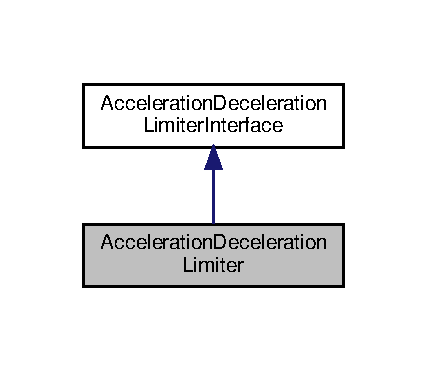
\includegraphics[width=205pt]{classAccelerationDecelerationLimiter__inherit__graph}
\end{center}
\end{figure}


Collaboration diagram for Acceleration\+Deceleration\+Limiter\+:
\nopagebreak
\begin{figure}[H]
\begin{center}
\leavevmode
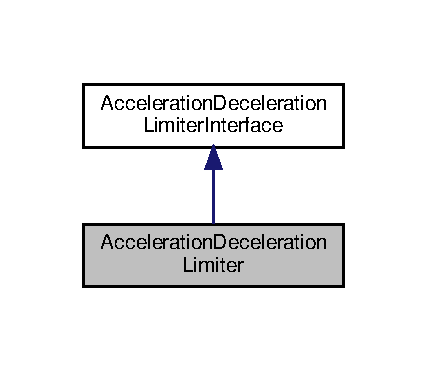
\includegraphics[width=205pt]{classAccelerationDecelerationLimiter__coll__graph}
\end{center}
\end{figure}
\subsection*{Public Member Functions}
\begin{DoxyCompactItemize}
\item 
\mbox{\Hypertarget{classAccelerationDecelerationLimiter_a5a1ba8502999ada787593cff4dd88182}\label{classAccelerationDecelerationLimiter_a5a1ba8502999ada787593cff4dd88182}} 
{\bfseries Acceleration\+Deceleration\+Limiter} (float max\+Acceleration, float max\+Deceleration, float max\+Speed, float position\+Corrector\+Kp)
\item 
\mbox{\Hypertarget{classAccelerationDecelerationLimiter_a0e7ba1a481a4963232ee10fa16053d4f}\label{classAccelerationDecelerationLimiter_a0e7ba1a481a4963232ee10fa16053d4f}} 
{\bfseries Acceleration\+Deceleration\+Limiter} (float max\+Acceleration\+Forward, float max\+Deceleration\+Forward, float max\+Acceleration\+Backward, float max\+Deceleration\+Backward, float max\+Speed, float position\+Corrector\+Kp)
\item 
\mbox{\Hypertarget{classAccelerationDecelerationLimiter_affb4a7fc328b54dbcecd707ba6166ac4}\label{classAccelerationDecelerationLimiter_affb4a7fc328b54dbcecd707ba6166ac4}} 
virtual float {\bfseries limit\+Acceleration} (float dt, float target\+Speed, float current\+Speed, float position\+Goal, float position\+Error)
\item 
\mbox{\Hypertarget{classAccelerationDecelerationLimiter_a7a43a0b14a8914648b40c6e2cc8afbd7}\label{classAccelerationDecelerationLimiter_a7a43a0b14a8914648b40c6e2cc8afbd7}} 
virtual void {\bfseries enable} ()
\item 
\mbox{\Hypertarget{classAccelerationDecelerationLimiter_ad158f665c287f65daadb170c5ba773e1}\label{classAccelerationDecelerationLimiter_ad158f665c287f65daadb170c5ba773e1}} 
virtual void {\bfseries disable} ()
\item 
\mbox{\Hypertarget{classAccelerationDecelerationLimiter_a40a9b91bbdc780dc5d54ad6490f11bbf}\label{classAccelerationDecelerationLimiter_a40a9b91bbdc780dc5d54ad6490f11bbf}} 
virtual void {\bfseries reset} ()
\item 
\mbox{\Hypertarget{classAccelerationDecelerationLimiter_a621ad3611b4f20574c42f30d86266915}\label{classAccelerationDecelerationLimiter_a621ad3611b4f20574c42f30d86266915}} 
void {\bfseries set\+Dampling\+Factor} (float value)
\end{DoxyCompactItemize}


The documentation for this class was generated from the following files\+:\begin{DoxyCompactItemize}
\item 
/home/pmx/git/\+P\+M\+X/src/\+Asserv.\+Nucleo/\+Acceleration\+Limiter/Acceleration\+Deceleration\+Limiter.\+h\item 
/home/pmx/git/\+P\+M\+X/src/\+Asserv.\+Nucleo/\+Acceleration\+Limiter/Acceleration\+Deceleration\+Limiter.\+cpp\end{DoxyCompactItemize}

\hypertarget{classAccelerationDecelerationLimiterInterface}{}\section{Acceleration\+Deceleration\+Limiter\+Interface Class Reference}
\label{classAccelerationDecelerationLimiterInterface}\index{Acceleration\+Deceleration\+Limiter\+Interface@{Acceleration\+Deceleration\+Limiter\+Interface}}


Inheritance diagram for Acceleration\+Deceleration\+Limiter\+Interface\+:
\nopagebreak
\begin{figure}[H]
\begin{center}
\leavevmode
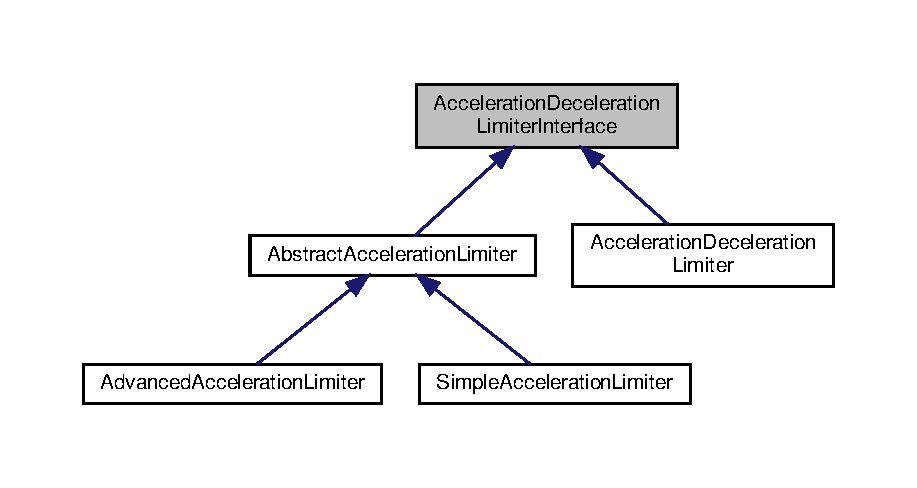
\includegraphics[width=350pt]{classAccelerationDecelerationLimiterInterface__inherit__graph}
\end{center}
\end{figure}
\subsection*{Public Member Functions}
\begin{DoxyCompactItemize}
\item 
\mbox{\Hypertarget{classAccelerationDecelerationLimiterInterface_a79ab2e74990c0c5b7bc1aeb845391e6e}\label{classAccelerationDecelerationLimiterInterface_a79ab2e74990c0c5b7bc1aeb845391e6e}} 
virtual float {\bfseries limit\+Acceleration} (float dt, float target\+Speed, float current\+Speed, float position\+Goal, float position\+Error)=0
\item 
\mbox{\Hypertarget{classAccelerationDecelerationLimiterInterface_a2ac64fa807ae69bdcb1757eb2f097258}\label{classAccelerationDecelerationLimiterInterface_a2ac64fa807ae69bdcb1757eb2f097258}} 
virtual void {\bfseries enable} ()=0
\item 
\mbox{\Hypertarget{classAccelerationDecelerationLimiterInterface_a6b918565a9f3e2f405f806835acd1d34}\label{classAccelerationDecelerationLimiterInterface_a6b918565a9f3e2f405f806835acd1d34}} 
virtual void {\bfseries disable} ()=0
\item 
\mbox{\Hypertarget{classAccelerationDecelerationLimiterInterface_aa6c307f1185f6ef888611277382e3679}\label{classAccelerationDecelerationLimiterInterface_aa6c307f1185f6ef888611277382e3679}} 
virtual void {\bfseries reset} ()=0
\end{DoxyCompactItemize}


The documentation for this class was generated from the following file\+:\begin{DoxyCompactItemize}
\item 
/home/pmx/git/\+P\+M\+X/src/\+Asserv.\+Nucleo/\+Acceleration\+Limiter/Acceleration\+Deceleration\+Limiter\+Interface.\+h\end{DoxyCompactItemize}

\hypertarget{classAColorDriver}{}\section{A\+Color\+Driver Class Reference}
\label{classAColorDriver}\index{A\+Color\+Driver@{A\+Color\+Driver}}


Inheritance diagram for A\+Color\+Driver\+:
\nopagebreak
\begin{figure}[H]
\begin{center}
\leavevmode
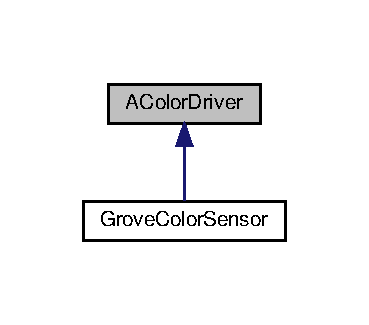
\includegraphics[width=177pt]{classAColorDriver__inherit__graph}
\end{center}
\end{figure}
\subsection*{Public Member Functions}
\begin{DoxyCompactItemize}
\item 
\mbox{\Hypertarget{classAColorDriver_aa44565ec7bdfbfdaf504bd1492d7021b}\label{classAColorDriver_aa44565ec7bdfbfdaf504bd1492d7021b}} 
virtual \hyperlink{classAColorDriver_aa44565ec7bdfbfdaf504bd1492d7021b}{$\sim$\+A\+Color\+Driver} ()
\begin{DoxyCompactList}\small\item\em Destructor. \end{DoxyCompactList}\item 
\mbox{\Hypertarget{classAColorDriver_a4b1874012a07a2e9d38ed5c25fc85dd5}\label{classAColorDriver_a4b1874012a07a2e9d38ed5c25fc85dd5}} 
virtual bool {\bfseries read\+R\+GB} ()=0
\item 
\mbox{\Hypertarget{classAColorDriver_ade70c9866d17065d51adc23cf8d84711}\label{classAColorDriver_ade70c9866d17065d51adc23cf8d84711}} 
virtual float {\bfseries get\+TX} ()=0
\item 
\mbox{\Hypertarget{classAColorDriver_aee75d3eab0612cc3a78053e15f50e47a}\label{classAColorDriver_aee75d3eab0612cc3a78053e15f50e47a}} 
virtual float {\bfseries get\+TY} ()=0
\end{DoxyCompactItemize}
\subsection*{Static Public Member Functions}
\begin{DoxyCompactItemize}
\item 
\mbox{\Hypertarget{classAColorDriver_ad569d1e4c0e481fdba30a6e5c9691743}\label{classAColorDriver_ad569d1e4c0e481fdba30a6e5c9691743}} 
static \hyperlink{classAColorDriver}{A\+Color\+Driver} $\ast$ \hyperlink{classAColorDriver_ad569d1e4c0e481fdba30a6e5c9691743}{create} (std\+::string bot\+Name)
\begin{DoxyCompactList}\small\item\em instance creation. \end{DoxyCompactList}\end{DoxyCompactItemize}
\subsection*{Protected Member Functions}
\begin{DoxyCompactItemize}
\item 
\mbox{\Hypertarget{classAColorDriver_a90d8bb79fd76c030f31e29a32c32834a}\label{classAColorDriver_a90d8bb79fd76c030f31e29a32c32834a}} 
\hyperlink{classAColorDriver_a90d8bb79fd76c030f31e29a32c32834a}{A\+Color\+Driver} ()
\begin{DoxyCompactList}\small\item\em Constructor. \end{DoxyCompactList}\end{DoxyCompactItemize}


The documentation for this class was generated from the following files\+:\begin{DoxyCompactItemize}
\item 
/home/pmx/git/\+P\+M\+X/src/\+Common/\+Action.\+Driver/A\+Color\+Driver.\+hpp\item 
/home/pmx/git/\+P\+M\+X/src/\+Driver-\/\+O\+P\+O\+S6\+U\+L\+\_\+\+A\+R\+M/\hyperlink{GroveColorSensor_8cpp}{Grove\+Color\+Sensor.\+cpp}\end{DoxyCompactItemize}

\hypertarget{classActionManagerTimer}{}\section{Action\+Manager\+Timer Class Reference}
\label{classActionManagerTimer}\index{Action\+Manager\+Timer@{Action\+Manager\+Timer}}


Classe de gestion des actions du robot et des actions par timer.  




{\ttfamily \#include $<$Action\+Manager\+Timer.\+hpp$>$}



Inheritance diagram for Action\+Manager\+Timer\+:
\nopagebreak
\begin{figure}[H]
\begin{center}
\leavevmode
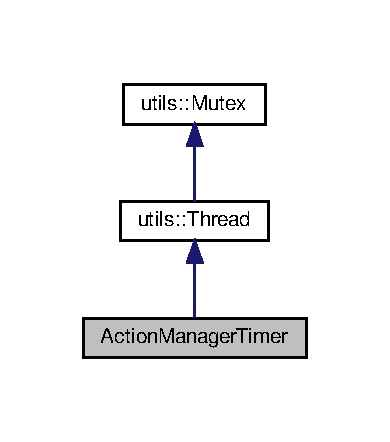
\includegraphics[width=187pt]{classActionManagerTimer__inherit__graph}
\end{center}
\end{figure}


Collaboration diagram for Action\+Manager\+Timer\+:
\nopagebreak
\begin{figure}[H]
\begin{center}
\leavevmode
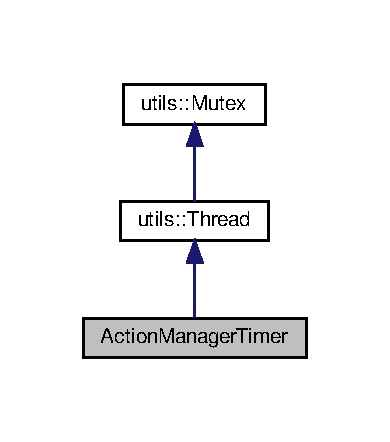
\includegraphics[width=187pt]{classActionManagerTimer__coll__graph}
\end{center}
\end{figure}
\subsection*{Public Member Functions}
\begin{DoxyCompactItemize}
\item 
\mbox{\Hypertarget{classActionManagerTimer_a957a5706d13675e5282372523c2db521}\label{classActionManagerTimer_a957a5706d13675e5282372523c2db521}} 
\hyperlink{classActionManagerTimer_a957a5706d13675e5282372523c2db521}{Action\+Manager\+Timer} ()
\begin{DoxyCompactList}\small\item\em Constructeur de la classe. \end{DoxyCompactList}\item 
\mbox{\Hypertarget{classActionManagerTimer_ad465b1e6b2f352a92cc10bcaf5e6416e}\label{classActionManagerTimer_ad465b1e6b2f352a92cc10bcaf5e6416e}} 
virtual \hyperlink{classActionManagerTimer_ad465b1e6b2f352a92cc10bcaf5e6416e}{$\sim$\+Action\+Manager\+Timer} ()
\begin{DoxyCompactList}\small\item\em Destructeur de la classe. \end{DoxyCompactList}\item 
\mbox{\Hypertarget{classActionManagerTimer_a6e6db535941463a0e590a6779f111dd2}\label{classActionManagerTimer_a6e6db535941463a0e590a6779f111dd2}} 
int \hyperlink{classActionManagerTimer_a6e6db535941463a0e590a6779f111dd2}{count\+Actions} ()
\begin{DoxyCompactList}\small\item\em Retourne le nombre d\textquotesingle{}actions. \end{DoxyCompactList}\item 
\mbox{\Hypertarget{classActionManagerTimer_af44ca42a2cebadd32062dedf874d4f82}\label{classActionManagerTimer_af44ca42a2cebadd32062dedf874d4f82}} 
int \hyperlink{classActionManagerTimer_af44ca42a2cebadd32062dedf874d4f82}{count\+Timers} ()
\begin{DoxyCompactList}\small\item\em Retourne le nombre de timers. \end{DoxyCompactList}\item 
\mbox{\Hypertarget{classActionManagerTimer_ad5a07cffbb588205edcdcb594208769c}\label{classActionManagerTimer_ad5a07cffbb588205edcdcb594208769c}} 
int \hyperlink{classActionManagerTimer_ad5a07cffbb588205edcdcb594208769c}{count\+P\+Timers} ()
\begin{DoxyCompactList}\small\item\em Retourne le nombre de timers posix. \end{DoxyCompactList}\item 
void \hyperlink{classActionManagerTimer_ad44aa7bf3d361e60d3ed764d833eafc5}{add\+Action} (\hyperlink{classIAction}{I\+Action} $\ast$action)
\begin{DoxyCompactList}\small\item\em Ajout d\textquotesingle{}une action. \end{DoxyCompactList}\item 
void \hyperlink{classActionManagerTimer_a37abad611ac11d81f2ebcb8d9d5766f8}{add\+Timer} (\hyperlink{classITimerListener}{I\+Timer\+Listener} $\ast$timer)
\begin{DoxyCompactList}\small\item\em Ajout d\textquotesingle{}un timer. deprecated. \end{DoxyCompactList}\item 
void \hyperlink{classActionManagerTimer_a4d893b58bd1d02a9a610eabea05bec1a}{add\+Timer} (\hyperlink{classITimerPosixListener}{I\+Timer\+Posix\+Listener} $\ast$timer)
\begin{DoxyCompactList}\small\item\em Ajout d\textquotesingle{}un timer posix. \end{DoxyCompactList}\item 
void \hyperlink{classActionManagerTimer_a3043c43e2b56ed05633d68bf5c530c1f}{stop\+Timer} (std\+::string timer\+Name\+To\+Delete)
\begin{DoxyCompactList}\small\item\em arrete un timer spécifique. Permet d\textquotesingle{}executer son action de fin puis le supprime de la liste. \end{DoxyCompactList}\item 
void \hyperlink{classActionManagerTimer_a77bc841824ad1722363dd29a351a74cf}{stop\+P\+Timer} (std\+::string timer\+Name\+To\+Delete)
\begin{DoxyCompactList}\small\item\em arrete un timer posix spécifique. Permet d\textquotesingle{}executer son action de fin puis le supprime de la liste. \end{DoxyCompactList}\item 
\mbox{\Hypertarget{classActionManagerTimer_aea93da8bac8e622881a125ee7506a7ca}\label{classActionManagerTimer_aea93da8bac8e622881a125ee7506a7ca}} 
void \hyperlink{classActionManagerTimer_aea93da8bac8e622881a125ee7506a7ca}{stop\+All\+P\+Timers} ()
\begin{DoxyCompactList}\small\item\em arrete tous les timers posix. Permet d\textquotesingle{}executer leur action de fin puis les supprime de la liste. \end{DoxyCompactList}\item 
\mbox{\Hypertarget{classActionManagerTimer_a20bd3b06bc5f9b9fb747bb27d154d88d}\label{classActionManagerTimer_a20bd3b06bc5f9b9fb747bb27d154d88d}} 
void \hyperlink{classActionManagerTimer_a20bd3b06bc5f9b9fb747bb27d154d88d}{clear\+Actions} ()
\begin{DoxyCompactList}\small\item\em Vide la liste des actions actuellement enregistrées. \end{DoxyCompactList}\item 
\mbox{\Hypertarget{classActionManagerTimer_af2afa74f3445e32823371b926aa3f55c}\label{classActionManagerTimer_af2afa74f3445e32823371b926aa3f55c}} 
void \hyperlink{classActionManagerTimer_af2afa74f3445e32823371b926aa3f55c}{clear\+Timers} ()
\begin{DoxyCompactList}\small\item\em Vide la liste des timers actuellement enregistrés. \end{DoxyCompactList}\item 
void \hyperlink{classActionManagerTimer_a072223491745aebbaa0344124635b7f8}{stop} ()
\begin{DoxyCompactList}\small\item\em L\textquotesingle{}appel à cette méthode signale au thread qu\textquotesingle{}il doit s\textquotesingle{}arrêter (proprement). Arrete aussi tous les timers posix en cours en lancant leur tache de fin. \end{DoxyCompactList}\item 
\mbox{\Hypertarget{classActionManagerTimer_ad14a24ea8609f916a5fb3e43c7f0e856}\label{classActionManagerTimer_ad14a24ea8609f916a5fb3e43c7f0e856}} 
void \hyperlink{classActionManagerTimer_ad14a24ea8609f916a5fb3e43c7f0e856}{pause} (bool value)
\begin{DoxyCompactList}\small\item\em Met en pause la boucle du manager d\textquotesingle{}actions et de timer. \end{DoxyCompactList}\item 
\mbox{\Hypertarget{classActionManagerTimer_a40e5f9d8c2706434376d416d3e43fd3b}\label{classActionManagerTimer_a40e5f9d8c2706434376d416d3e43fd3b}} 
void \hyperlink{classActionManagerTimer_a40e5f9d8c2706434376d416d3e43fd3b}{debug\+Actions} ()
\begin{DoxyCompactList}\small\item\em Affiche via le logger les différentes actions en cours. \end{DoxyCompactList}\item 
\mbox{\Hypertarget{classActionManagerTimer_a17c6563c7a6c0955c7ca2230b038d832}\label{classActionManagerTimer_a17c6563c7a6c0955c7ca2230b038d832}} 
void {\bfseries debug\+P\+Timers} ()
\item 
\mbox{\Hypertarget{classActionManagerTimer_aef6be0b68f6595c8ac5ce89c66b9333a}\label{classActionManagerTimer_aef6be0b68f6595c8ac5ce89c66b9333a}} 
void {\bfseries debug\+Timers} ()
\end{DoxyCompactItemize}
\subsection*{Protected Member Functions}
\begin{DoxyCompactItemize}
\item 
\mbox{\Hypertarget{classActionManagerTimer_a8eb81df877c40053d71f659265882058}\label{classActionManagerTimer_a8eb81df877c40053d71f659265882058}} 
virtual void \hyperlink{classActionManagerTimer_a8eb81df877c40053d71f659265882058}{execute} ()
\begin{DoxyCompactList}\small\item\em Execute l\textquotesingle{}ensemble des actions enregistrées. \end{DoxyCompactList}\item 
\mbox{\Hypertarget{classActionManagerTimer_a39f4cbb5ddbbe6a40980bb59b8b59b05}\label{classActionManagerTimer_a39f4cbb5ddbbe6a40980bb59b8b59b05}} 
void {\bfseries unblock} (std\+::string debug=\char`\"{}Action\+Manager\+Timer\char`\"{})
\end{DoxyCompactItemize}
\subsection*{Additional Inherited Members}


\subsection{Detailed Description}
Classe de gestion des actions du robot et des actions par timer. 

\subsection{Member Function Documentation}
\mbox{\Hypertarget{classActionManagerTimer_ad44aa7bf3d361e60d3ed764d833eafc5}\label{classActionManagerTimer_ad44aa7bf3d361e60d3ed764d833eafc5}} 
\index{Action\+Manager\+Timer@{Action\+Manager\+Timer}!add\+Action@{add\+Action}}
\index{add\+Action@{add\+Action}!Action\+Manager\+Timer@{Action\+Manager\+Timer}}
\subsubsection{\texorpdfstring{add\+Action()}{addAction()}}
{\footnotesize\ttfamily void Action\+Manager\+Timer\+::add\+Action (\begin{DoxyParamCaption}\item[{\hyperlink{classIAction}{I\+Action} $\ast$}]{action }\end{DoxyParamCaption})\hspace{0.3cm}{\ttfamily [inline]}}



Ajout d\textquotesingle{}une action. 


\begin{DoxyParams}{Parameters}
{\em action} & L\textquotesingle{}action à ajouter. \\
\hline
\end{DoxyParams}
\mbox{\Hypertarget{classActionManagerTimer_a37abad611ac11d81f2ebcb8d9d5766f8}\label{classActionManagerTimer_a37abad611ac11d81f2ebcb8d9d5766f8}} 
\index{Action\+Manager\+Timer@{Action\+Manager\+Timer}!add\+Timer@{add\+Timer}}
\index{add\+Timer@{add\+Timer}!Action\+Manager\+Timer@{Action\+Manager\+Timer}}
\subsubsection{\texorpdfstring{add\+Timer()}{addTimer()}\hspace{0.1cm}{\footnotesize\ttfamily [1/2]}}
{\footnotesize\ttfamily void Action\+Manager\+Timer\+::add\+Timer (\begin{DoxyParamCaption}\item[{\hyperlink{classITimerListener}{I\+Timer\+Listener} $\ast$}]{timer }\end{DoxyParamCaption})\hspace{0.3cm}{\ttfamily [inline]}}



Ajout d\textquotesingle{}un timer. deprecated. 


\begin{DoxyParams}{Parameters}
{\em timer} & le timer à ajouter. \\
\hline
\end{DoxyParams}
\mbox{\Hypertarget{classActionManagerTimer_a4d893b58bd1d02a9a610eabea05bec1a}\label{classActionManagerTimer_a4d893b58bd1d02a9a610eabea05bec1a}} 
\index{Action\+Manager\+Timer@{Action\+Manager\+Timer}!add\+Timer@{add\+Timer}}
\index{add\+Timer@{add\+Timer}!Action\+Manager\+Timer@{Action\+Manager\+Timer}}
\subsubsection{\texorpdfstring{add\+Timer()}{addTimer()}\hspace{0.1cm}{\footnotesize\ttfamily [2/2]}}
{\footnotesize\ttfamily void Action\+Manager\+Timer\+::add\+Timer (\begin{DoxyParamCaption}\item[{\hyperlink{classITimerPosixListener}{I\+Timer\+Posix\+Listener} $\ast$}]{timer }\end{DoxyParamCaption})\hspace{0.3cm}{\ttfamily [inline]}}



Ajout d\textquotesingle{}un timer posix. 


\begin{DoxyParams}{Parameters}
{\em timer} & le timer posix à ajouter. \\
\hline
\end{DoxyParams}
\mbox{\Hypertarget{classActionManagerTimer_a072223491745aebbaa0344124635b7f8}\label{classActionManagerTimer_a072223491745aebbaa0344124635b7f8}} 
\index{Action\+Manager\+Timer@{Action\+Manager\+Timer}!stop@{stop}}
\index{stop@{stop}!Action\+Manager\+Timer@{Action\+Manager\+Timer}}
\subsubsection{\texorpdfstring{stop()}{stop()}}
{\footnotesize\ttfamily void Action\+Manager\+Timer\+::stop (\begin{DoxyParamCaption}{ }\end{DoxyParamCaption})}



L\textquotesingle{}appel à cette méthode signale au thread qu\textquotesingle{}il doit s\textquotesingle{}arrêter (proprement). Arrete aussi tous les timers posix en cours en lancant leur tache de fin. 

L\textquotesingle{}utilisation de la méthode Action\+Manager\+::stop() permet de savoir si le thread associé est arrêté. \mbox{\Hypertarget{classActionManagerTimer_a77bc841824ad1722363dd29a351a74cf}\label{classActionManagerTimer_a77bc841824ad1722363dd29a351a74cf}} 
\index{Action\+Manager\+Timer@{Action\+Manager\+Timer}!stop\+P\+Timer@{stop\+P\+Timer}}
\index{stop\+P\+Timer@{stop\+P\+Timer}!Action\+Manager\+Timer@{Action\+Manager\+Timer}}
\subsubsection{\texorpdfstring{stop\+P\+Timer()}{stopPTimer()}}
{\footnotesize\ttfamily void Action\+Manager\+Timer\+::stop\+P\+Timer (\begin{DoxyParamCaption}\item[{std\+::string}]{timer\+Name\+To\+Delete }\end{DoxyParamCaption})}



arrete un timer posix spécifique. Permet d\textquotesingle{}executer son action de fin puis le supprime de la liste. 


\begin{DoxyParams}{Parameters}
{\em name} & Le label du timer. \\
\hline
\end{DoxyParams}
\mbox{\Hypertarget{classActionManagerTimer_a3043c43e2b56ed05633d68bf5c530c1f}\label{classActionManagerTimer_a3043c43e2b56ed05633d68bf5c530c1f}} 
\index{Action\+Manager\+Timer@{Action\+Manager\+Timer}!stop\+Timer@{stop\+Timer}}
\index{stop\+Timer@{stop\+Timer}!Action\+Manager\+Timer@{Action\+Manager\+Timer}}
\subsubsection{\texorpdfstring{stop\+Timer()}{stopTimer()}}
{\footnotesize\ttfamily void Action\+Manager\+Timer\+::stop\+Timer (\begin{DoxyParamCaption}\item[{std\+::string}]{timer\+Name\+To\+Delete }\end{DoxyParamCaption})}



arrete un timer spécifique. Permet d\textquotesingle{}executer son action de fin puis le supprime de la liste. 


\begin{DoxyParams}{Parameters}
{\em name} & Le label du timer. \\
\hline
\end{DoxyParams}


The documentation for this class was generated from the following files\+:\begin{DoxyCompactItemize}
\item 
/home/pmx/git/\+P\+M\+X/src/\+Common/\+Action/\hyperlink{ActionManagerTimer_8hpp}{Action\+Manager\+Timer.\+hpp}\item 
/home/pmx/git/\+P\+M\+X/src/\+Common/\+Action/\hyperlink{ActionManagerTimer_8cpp}{Action\+Manager\+Timer.\+cpp}\end{DoxyCompactItemize}

\hypertarget{classActions}{}\section{Actions Class Reference}
\label{classActions}\index{Actions@{Actions}}


{\ttfamily \#include $<$Actions.\+hpp$>$}



Inheritance diagram for Actions\+:
\nopagebreak
\begin{figure}[H]
\begin{center}
\leavevmode
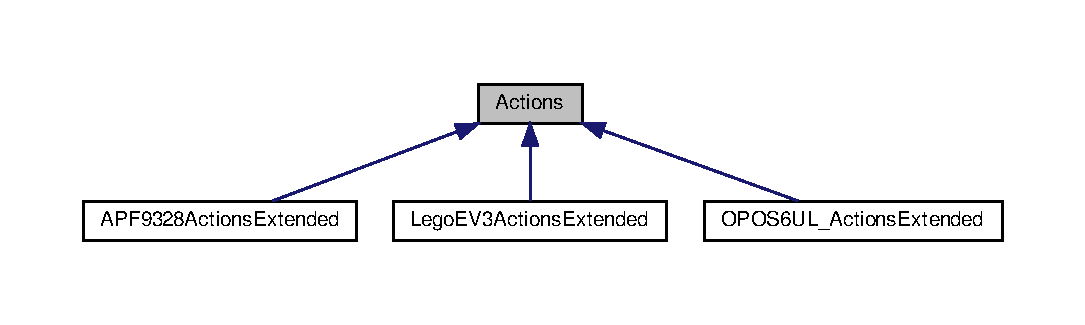
\includegraphics[width=350pt]{classActions__inherit__graph}
\end{center}
\end{figure}
\subsection*{Public Member Functions}
\begin{DoxyCompactItemize}
\item 
\mbox{\Hypertarget{classActions_ace0fce73fe3cfb2ea7112cfdbf12b131}\label{classActions_ace0fce73fe3cfb2ea7112cfdbf12b131}} 
\hyperlink{classActions_ace0fce73fe3cfb2ea7112cfdbf12b131}{Actions} ()
\begin{DoxyCompactList}\small\item\em Constructor. \end{DoxyCompactList}\item 
\mbox{\Hypertarget{classActions_a0d03028ad72e0031f3d903493932aea1}\label{classActions_a0d03028ad72e0031f3d903493932aea1}} 
\hyperlink{classActions_a0d03028ad72e0031f3d903493932aea1}{$\sim$\+Actions} ()
\begin{DoxyCompactList}\small\item\em Destructor. \end{DoxyCompactList}\item 
void \hyperlink{classActions_a710f952f5942e626d73e47733a8848b0}{add\+Action} (\hyperlink{classIAction}{I\+Action} $\ast$action)
\begin{DoxyCompactList}\small\item\em Ajout d\textquotesingle{}une action. \end{DoxyCompactList}\item 
\mbox{\Hypertarget{classActions_a861130fdcc3238961cb93b5b96475e8f}\label{classActions_a861130fdcc3238961cb93b5b96475e8f}} 
void {\bfseries add\+Timer} (\hyperlink{classITimerPosixListener}{I\+Timer\+Posix\+Listener} $\ast$timer)
\item 
\mbox{\Hypertarget{classActions_a49459ae072ed1f6ea6a69966a0ad4409}\label{classActions_a49459ae072ed1f6ea6a69966a0ad4409}} 
void {\bfseries stop\+Timer} (std\+::string name)
\item 
void \hyperlink{classActions_adf0dec391b032c0b36b329a3f039001e}{start} ()
\begin{DoxyCompactList}\small\item\em Active les actions. \end{DoxyCompactList}\item 
\mbox{\Hypertarget{classActions_a95422cfe6edb166b22bc6aa465aab866}\label{classActions_a95422cfe6edb166b22bc6aa465aab866}} 
void \hyperlink{classActions_a95422cfe6edb166b22bc6aa465aab866}{clear\+All} ()
\begin{DoxyCompactList}\small\item\em supprime toutes les actions et les timers. \end{DoxyCompactList}\item 
\mbox{\Hypertarget{classActions_a2dca3495645f189f728586d4157c699c}\label{classActions_a2dca3495645f189f728586d4157c699c}} 
void \hyperlink{classActions_a2dca3495645f189f728586d4157c699c}{wait\+And\+Stop\+Managers} ()
\begin{DoxyCompactList}\small\item\em Arrete le thread sensor\+Manager et action\+Manager. \end{DoxyCompactList}\item 
\mbox{\Hypertarget{classActions_aa0181cb9c1642b42dca16faa8c9356e0}\label{classActions_aa0181cb9c1642b42dca16faa8c9356e0}} 
void \hyperlink{classActions_aa0181cb9c1642b42dca16faa8c9356e0}{cancel} ()
\begin{DoxyCompactList}\small\item\em Annule le thread en cours. \end{DoxyCompactList}\end{DoxyCompactItemize}


\subsection{Detailed Description}
List of robot actions. It contains all common Robot\+Element. 

\subsection{Member Function Documentation}
\mbox{\Hypertarget{classActions_a710f952f5942e626d73e47733a8848b0}\label{classActions_a710f952f5942e626d73e47733a8848b0}} 
\index{Actions@{Actions}!add\+Action@{add\+Action}}
\index{add\+Action@{add\+Action}!Actions@{Actions}}
\subsubsection{\texorpdfstring{add\+Action()}{addAction()}}
{\footnotesize\ttfamily void Actions\+::add\+Action (\begin{DoxyParamCaption}\item[{\hyperlink{classIAction}{I\+Action} $\ast$}]{action }\end{DoxyParamCaption})\hspace{0.3cm}{\ttfamily [inline]}}



Ajout d\textquotesingle{}une action. 


\begin{DoxyParams}{Parameters}
{\em action} & L\textquotesingle{}action à ajouter. \\
\hline
\end{DoxyParams}
\mbox{\Hypertarget{classActions_adf0dec391b032c0b36b329a3f039001e}\label{classActions_adf0dec391b032c0b36b329a3f039001e}} 
\index{Actions@{Actions}!start@{start}}
\index{start@{start}!Actions@{Actions}}
\subsubsection{\texorpdfstring{start()}{start()}}
{\footnotesize\ttfamily void Actions\+::start (\begin{DoxyParamCaption}{ }\end{DoxyParamCaption})}



Active les actions. 

Cette méthode lance le thread gérant le Action\+Manager. 

The documentation for this class was generated from the following files\+:\begin{DoxyCompactItemize}
\item 
/home/pmx/git/\+P\+M\+X/src/\+Common/\+Action/Actions.\+hpp\item 
/home/pmx/git/\+P\+M\+X/src/\+Common/\+Action/Actions.\+cpp\end{DoxyCompactItemize}

\hypertarget{structACTIONS}{}\section{A\+C\+T\+I\+O\+NS Struct Reference}
\label{structACTIONS}\index{A\+C\+T\+I\+O\+NS@{A\+C\+T\+I\+O\+NS}}
\subsection*{Public Attributes}
\begin{DoxyCompactItemize}
\item 
\mbox{\Hypertarget{structACTIONS_a21a94bca6592f1281fa961ecec3224ce}\label{structACTIONS_a21a94bca6592f1281fa961ecec3224ce}} 
char {\bfseries name} \mbox{[}400\mbox{]}
\item 
\mbox{\Hypertarget{structACTIONS_a04a21faedb62a5cda08b7cd23416d11a}\label{structACTIONS_a04a21faedb62a5cda08b7cd23416d11a}} 
Robot\+Action {\bfseries action}
\item 
\mbox{\Hypertarget{structACTIONS_a8bad60d082f4279e9122ef8fe7c913d0}\label{structACTIONS_a8bad60d082f4279e9122ef8fe7c913d0}} 
bool {\bfseries completed}
\end{DoxyCompactItemize}


The documentation for this struct was generated from the following file\+:\begin{DoxyCompactItemize}
\item 
/home/pmx/git/\+P\+M\+X/src/\+Common/\+I\+A/I\+A\+Common.\+hpp\end{DoxyCompactItemize}

\hypertarget{classAdafruit__MCP23017}{}\section{Adafruit\+\_\+\+M\+C\+P23017 Class Reference}
\label{classAdafruit__MCP23017}\index{Adafruit\+\_\+\+M\+C\+P23017@{Adafruit\+\_\+\+M\+C\+P23017}}
\subsection*{Public Member Functions}
\begin{DoxyCompactItemize}
\item 
\mbox{\Hypertarget{classAdafruit__MCP23017_a874577a57d334b8d0e81e86701bb156d}\label{classAdafruit__MCP23017_a874577a57d334b8d0e81e86701bb156d}} 
void {\bfseries begin} (void)
\item 
\mbox{\Hypertarget{classAdafruit__MCP23017_a6f2aea0d187cb281a4ed216fd31a6981}\label{classAdafruit__MCP23017_a6f2aea0d187cb281a4ed216fd31a6981}} 
void {\bfseries pin\+Mode} (uint8\+\_\+t p, uint8\+\_\+t d)
\item 
\mbox{\Hypertarget{classAdafruit__MCP23017_a62c7101061540e9af47ea23d5b33fa81}\label{classAdafruit__MCP23017_a62c7101061540e9af47ea23d5b33fa81}} 
void {\bfseries digital\+Write} (uint8\+\_\+t p, uint8\+\_\+t d)
\item 
\mbox{\Hypertarget{classAdafruit__MCP23017_ac24a9e4d33aceed6bcbaa08b6f12a99e}\label{classAdafruit__MCP23017_ac24a9e4d33aceed6bcbaa08b6f12a99e}} 
void {\bfseries pull\+Up} (uint8\+\_\+t p, uint8\+\_\+t d)
\item 
\mbox{\Hypertarget{classAdafruit__MCP23017_a00ee81c07e06502330b5e5a27372ac53}\label{classAdafruit__MCP23017_a00ee81c07e06502330b5e5a27372ac53}} 
uint8\+\_\+t {\bfseries digital\+Read} (uint8\+\_\+t p)
\item 
\mbox{\Hypertarget{classAdafruit__MCP23017_a4b4845ea14d7207f22b0163ae5c622f2}\label{classAdafruit__MCP23017_a4b4845ea14d7207f22b0163ae5c622f2}} 
void {\bfseries write\+G\+P\+I\+O\+AB} (uint16\+\_\+t)
\item 
\mbox{\Hypertarget{classAdafruit__MCP23017_a07d894fe9d749fd7d3d098c99ce1fa64}\label{classAdafruit__MCP23017_a07d894fe9d749fd7d3d098c99ce1fa64}} 
uint16\+\_\+t {\bfseries read\+G\+P\+I\+O\+AB} ()
\item 
\mbox{\Hypertarget{classAdafruit__MCP23017_a29e5ba320b6ce6812c42ab99f5f4c80d}\label{classAdafruit__MCP23017_a29e5ba320b6ce6812c42ab99f5f4c80d}} 
long {\bfseries write\+\_\+i2c} (unsigned char command, unsigned char value)
\item 
\mbox{\Hypertarget{classAdafruit__MCP23017_a5935341a99356efaf41556b5ee78cd5a}\label{classAdafruit__MCP23017_a5935341a99356efaf41556b5ee78cd5a}} 
long {\bfseries read\+\_\+i2c} (unsigned char command)
\item 
\mbox{\Hypertarget{classAdafruit__MCP23017_a20fd3536424d0c91dba741894a010fd7}\label{classAdafruit__MCP23017_a20fd3536424d0c91dba741894a010fd7}} 
long {\bfseries write\+I2c\+\_\+3\+Bytes} (unsigned char $\ast$buf)
\item 
\mbox{\Hypertarget{classAdafruit__MCP23017_a714df98feb9305f13d0895795f26e159}\label{classAdafruit__MCP23017_a714df98feb9305f13d0895795f26e159}} 
long {\bfseries read\+I2c\+\_\+2\+Bytes} (unsigned char $\ast$buf)
\item 
\mbox{\Hypertarget{classAdafruit__MCP23017_a874577a57d334b8d0e81e86701bb156d}\label{classAdafruit__MCP23017_a874577a57d334b8d0e81e86701bb156d}} 
int {\bfseries begin} (void)
\item 
\mbox{\Hypertarget{classAdafruit__MCP23017_a6f2aea0d187cb281a4ed216fd31a6981}\label{classAdafruit__MCP23017_a6f2aea0d187cb281a4ed216fd31a6981}} 
void {\bfseries pin\+Mode} (uint8\+\_\+t p, uint8\+\_\+t d)
\item 
\mbox{\Hypertarget{classAdafruit__MCP23017_a62c7101061540e9af47ea23d5b33fa81}\label{classAdafruit__MCP23017_a62c7101061540e9af47ea23d5b33fa81}} 
void {\bfseries digital\+Write} (uint8\+\_\+t p, uint8\+\_\+t d)
\item 
\mbox{\Hypertarget{classAdafruit__MCP23017_ac24a9e4d33aceed6bcbaa08b6f12a99e}\label{classAdafruit__MCP23017_ac24a9e4d33aceed6bcbaa08b6f12a99e}} 
void {\bfseries pull\+Up} (uint8\+\_\+t p, uint8\+\_\+t d)
\item 
\mbox{\Hypertarget{classAdafruit__MCP23017_a00ee81c07e06502330b5e5a27372ac53}\label{classAdafruit__MCP23017_a00ee81c07e06502330b5e5a27372ac53}} 
uint8\+\_\+t {\bfseries digital\+Read} (uint8\+\_\+t p)
\item 
\mbox{\Hypertarget{classAdafruit__MCP23017_a4b4845ea14d7207f22b0163ae5c622f2}\label{classAdafruit__MCP23017_a4b4845ea14d7207f22b0163ae5c622f2}} 
void {\bfseries write\+G\+P\+I\+O\+AB} (uint16\+\_\+t)
\item 
\mbox{\Hypertarget{classAdafruit__MCP23017_a07d894fe9d749fd7d3d098c99ce1fa64}\label{classAdafruit__MCP23017_a07d894fe9d749fd7d3d098c99ce1fa64}} 
uint16\+\_\+t {\bfseries read\+G\+P\+I\+O\+AB} ()
\item 
\mbox{\Hypertarget{classAdafruit__MCP23017_a29e5ba320b6ce6812c42ab99f5f4c80d}\label{classAdafruit__MCP23017_a29e5ba320b6ce6812c42ab99f5f4c80d}} 
long {\bfseries write\+\_\+i2c} (unsigned char command, unsigned char value)
\item 
\mbox{\Hypertarget{classAdafruit__MCP23017_a5935341a99356efaf41556b5ee78cd5a}\label{classAdafruit__MCP23017_a5935341a99356efaf41556b5ee78cd5a}} 
long {\bfseries read\+\_\+i2c} (unsigned char command)
\item 
\mbox{\Hypertarget{classAdafruit__MCP23017_a20fd3536424d0c91dba741894a010fd7}\label{classAdafruit__MCP23017_a20fd3536424d0c91dba741894a010fd7}} 
long {\bfseries write\+I2c\+\_\+3\+Bytes} (unsigned char $\ast$buf)
\item 
\mbox{\Hypertarget{classAdafruit__MCP23017_a714df98feb9305f13d0895795f26e159}\label{classAdafruit__MCP23017_a714df98feb9305f13d0895795f26e159}} 
long {\bfseries read\+I2c\+\_\+2\+Bytes} (unsigned char $\ast$buf)
\end{DoxyCompactItemize}


The documentation for this class was generated from the following files\+:\begin{DoxyCompactItemize}
\item 
/home/pmx/git/\+P\+M\+X/src/\+Driver-\/\+A\+P\+F9328\+\_\+\+A\+R\+M/Adafruit\+\_\+\+M\+C\+P23017.\+hpp\item 
/home/pmx/git/\+P\+M\+X/src/\+Driver-\/\+A\+P\+F9328\+\_\+\+A\+R\+M/Adafruit\+\_\+\+M\+C\+P23017.\+cpp\end{DoxyCompactItemize}

\hypertarget{classAdafruit__PWMServoDriver}{}\section{Adafruit\+\_\+\+P\+W\+M\+Servo\+Driver Class Reference}
\label{classAdafruit__PWMServoDriver}\index{Adafruit\+\_\+\+P\+W\+M\+Servo\+Driver@{Adafruit\+\_\+\+P\+W\+M\+Servo\+Driver}}


Class that stores state and functions for interacting with P\+C\+A9685 P\+WM chip.  




{\ttfamily \#include $<$Adafruit\+\_\+\+P\+W\+M\+Servo\+Driver.\+hpp$>$}

\subsection*{Public Member Functions}
\begin{DoxyCompactItemize}
\item 
\hyperlink{classAdafruit__PWMServoDriver_abbbbdc51fe0ffb92f7c4d1b2ab1ec6b6}{Adafruit\+\_\+\+P\+W\+M\+Servo\+Driver} (uint i2c\+\_\+bus\+\_\+num, const uint8\+\_\+t addr)
\begin{DoxyCompactList}\small\item\em Instantiates a new P\+C\+A9685 P\+WM driver chip with the I2C address on a Two\+Wire interface. \end{DoxyCompactList}\item 
bool \hyperlink{classAdafruit__PWMServoDriver_af82d0facef94e15e9e91bab62e4835e3}{connect} (float freq=50.\+0, uint8\+\_\+t prescale=0)
\begin{DoxyCompactList}\small\item\em Instantiates a new P\+C\+A9685 P\+WM driver chip with the I2C address on a Two\+Wire interface. \end{DoxyCompactList}\item 
\mbox{\Hypertarget{classAdafruit__PWMServoDriver_a5f25f9f07525e08b7622c476b4a1f379}\label{classAdafruit__PWMServoDriver_a5f25f9f07525e08b7622c476b4a1f379}} 
void \hyperlink{classAdafruit__PWMServoDriver_a5f25f9f07525e08b7622c476b4a1f379}{reset} ()
\begin{DoxyCompactList}\small\item\em Sends a reset command to the P\+C\+A9685 chip over I2C. \end{DoxyCompactList}\item 
\mbox{\Hypertarget{classAdafruit__PWMServoDriver_aa892432ed08e4b3892c8eb0478168dd8}\label{classAdafruit__PWMServoDriver_aa892432ed08e4b3892c8eb0478168dd8}} 
void \hyperlink{classAdafruit__PWMServoDriver_aa892432ed08e4b3892c8eb0478168dd8}{sleep} ()
\begin{DoxyCompactList}\small\item\em Puts board into sleep mode. \end{DoxyCompactList}\item 
\mbox{\Hypertarget{classAdafruit__PWMServoDriver_a34b9ac672853a4a1b7fc202b4c89d8c4}\label{classAdafruit__PWMServoDriver_a34b9ac672853a4a1b7fc202b4c89d8c4}} 
void \hyperlink{classAdafruit__PWMServoDriver_a34b9ac672853a4a1b7fc202b4c89d8c4}{wakeup} ()
\begin{DoxyCompactList}\small\item\em Wakes board from sleep. \end{DoxyCompactList}\item 
void \hyperlink{classAdafruit__PWMServoDriver_a7967e51188cbacf2c3f269c8aec9d292}{set\+Ext\+Clk} (uint8\+\_\+t prescale)
\begin{DoxyCompactList}\small\item\em Sets E\+X\+T\+C\+LK pin to use the external clock. \end{DoxyCompactList}\item 
void \hyperlink{classAdafruit__PWMServoDriver_a0ef6f1e3c81aebbd1d1da1bb12f3ed5c}{set\+P\+W\+M\+Freq} (float freq)
\begin{DoxyCompactList}\small\item\em Sets the P\+WM frequency for the entire chip, up to $\sim$1.6 K\+Hz. \end{DoxyCompactList}\item 
void \hyperlink{classAdafruit__PWMServoDriver_a8d18d478574c8c686e94faefe11094b9}{set\+Output\+Mode} (bool totempole)
\begin{DoxyCompactList}\small\item\em Sets the output mode of the P\+C\+A9685 to either open drain or push pull / totempole. Warning\+: L\+E\+Ds with integrated zener diodes should only be driven in open drain mode. \end{DoxyCompactList}\item 
uint16\+\_\+t \hyperlink{classAdafruit__PWMServoDriver_a7eaeeed5408ea7382731f7e1ea01defb}{get\+P\+WM} (uint8\+\_\+t num, bool on)
\begin{DoxyCompactList}\small\item\em Gets the P\+WM output of one of the P\+C\+A9685 pins. \end{DoxyCompactList}\item 
void \hyperlink{classAdafruit__PWMServoDriver_a724a7fc39c6fba34478ecc0eea038bd3}{set\+P\+WM} (uint8\+\_\+t num, uint16\+\_\+t on, uint16\+\_\+t off)
\begin{DoxyCompactList}\small\item\em Sets the P\+WM output of one of the P\+C\+A9685 pins. \end{DoxyCompactList}\item 
void \hyperlink{classAdafruit__PWMServoDriver_a1246cd50849fe0f068cc5d474e06ae96}{set\+Pin} (uint8\+\_\+t num, uint16\+\_\+t val, bool invert=false)
\begin{DoxyCompactList}\small\item\em Helper to set pin P\+WM output. Sets pin without having to deal with on/off tick placement and properly handles a zero value as completely off and 4095 as completely on. Optional invert parameter supports inverting the pulse for sinking to ground. \end{DoxyCompactList}\item 
uint8\+\_\+t \hyperlink{classAdafruit__PWMServoDriver_a52dbe6fa4fa4a98d3082f239d59ad5f1}{read\+Prescale} (void)
\begin{DoxyCompactList}\small\item\em Reads set Prescale from P\+C\+A9685. \end{DoxyCompactList}\item 
void \hyperlink{classAdafruit__PWMServoDriver_aa91cf057ec01505292401e4fdceb57ac}{write\+Microseconds} (uint8\+\_\+t num, uint16\+\_\+t Microseconds)
\begin{DoxyCompactList}\small\item\em Sets the P\+WM output of one of the P\+C\+A9685 pins based on the input microseconds, output is not precise. \end{DoxyCompactList}\item 
\mbox{\Hypertarget{classAdafruit__PWMServoDriver_a0fa586b534db37ebcc5d86f6baebdb10}\label{classAdafruit__PWMServoDriver_a0fa586b534db37ebcc5d86f6baebdb10}} 
void {\bfseries fast\+Write\+Microseconds} (uint8\+\_\+t num, uint16\+\_\+t microseconds)
\item 
void \hyperlink{classAdafruit__PWMServoDriver_ac725dd6b0d24d087586a854e81bcf6b3}{set\+Oscillator\+Frequency} (uint32\+\_\+t freq)
\begin{DoxyCompactList}\small\item\em Setter for the internally tracked oscillator used for freq calculations. \end{DoxyCompactList}\item 
uint32\+\_\+t \hyperlink{classAdafruit__PWMServoDriver_ae4017d3cbbda98a0bb41efcf2c1fcf30}{get\+Oscillator\+Frequency} (void)
\begin{DoxyCompactList}\small\item\em Getter for the internally tracked oscillator used for freq calculations. \end{DoxyCompactList}\item 
\mbox{\Hypertarget{classAdafruit__PWMServoDriver_a029cc2c5f5260fd02deb95ca15771690}\label{classAdafruit__PWMServoDriver_a029cc2c5f5260fd02deb95ca15771690}} 
{\bfseries Adafruit\+\_\+\+P\+W\+M\+Servo\+Driver} (unsigned char addr=0x40)
\item 
\mbox{\Hypertarget{classAdafruit__PWMServoDriver_aef401eaad3c34222ac916eb7bd936bc2}\label{classAdafruit__PWMServoDriver_aef401eaad3c34222ac916eb7bd936bc2}} 
void {\bfseries begin} (void)
\item 
\mbox{\Hypertarget{classAdafruit__PWMServoDriver_ac976f52233a75a4bd0eb6f2ce9b82b7f}\label{classAdafruit__PWMServoDriver_ac976f52233a75a4bd0eb6f2ce9b82b7f}} 
void {\bfseries reset} (void)
\item 
\mbox{\Hypertarget{classAdafruit__PWMServoDriver_a0ef6f1e3c81aebbd1d1da1bb12f3ed5c}\label{classAdafruit__PWMServoDriver_a0ef6f1e3c81aebbd1d1da1bb12f3ed5c}} 
void {\bfseries set\+P\+W\+M\+Freq} (float freq)
\item 
\mbox{\Hypertarget{classAdafruit__PWMServoDriver_a8d110f943e906fd20eec6c8e6a1fad77}\label{classAdafruit__PWMServoDriver_a8d110f943e906fd20eec6c8e6a1fad77}} 
void {\bfseries set\+P\+WM} (unsigned char num, unsigned short on, unsigned short off)
\item 
\mbox{\Hypertarget{classAdafruit__PWMServoDriver_a7ed256f8594418bd5bf26658b81f7b6e}\label{classAdafruit__PWMServoDriver_a7ed256f8594418bd5bf26658b81f7b6e}} 
void {\bfseries set\+Pin} (unsigned char num, unsigned short val, bool invert=false)
\end{DoxyCompactItemize}


\subsection{Detailed Description}
Class that stores state and functions for interacting with P\+C\+A9685 P\+WM chip. 

\subsection{Constructor \& Destructor Documentation}
\mbox{\Hypertarget{classAdafruit__PWMServoDriver_abbbbdc51fe0ffb92f7c4d1b2ab1ec6b6}\label{classAdafruit__PWMServoDriver_abbbbdc51fe0ffb92f7c4d1b2ab1ec6b6}} 
\index{Adafruit\+\_\+\+P\+W\+M\+Servo\+Driver@{Adafruit\+\_\+\+P\+W\+M\+Servo\+Driver}!Adafruit\+\_\+\+P\+W\+M\+Servo\+Driver@{Adafruit\+\_\+\+P\+W\+M\+Servo\+Driver}}
\index{Adafruit\+\_\+\+P\+W\+M\+Servo\+Driver@{Adafruit\+\_\+\+P\+W\+M\+Servo\+Driver}!Adafruit\+\_\+\+P\+W\+M\+Servo\+Driver@{Adafruit\+\_\+\+P\+W\+M\+Servo\+Driver}}
\subsubsection{\texorpdfstring{Adafruit\+\_\+\+P\+W\+M\+Servo\+Driver()}{Adafruit\_PWMServoDriver()}}
{\footnotesize\ttfamily Adafruit\+\_\+\+P\+W\+M\+Servo\+Driver\+::\+Adafruit\+\_\+\+P\+W\+M\+Servo\+Driver (\begin{DoxyParamCaption}\item[{uint}]{i2c\+\_\+bus\+\_\+num,  }\item[{const uint8\+\_\+t}]{addr }\end{DoxyParamCaption})}



Instantiates a new P\+C\+A9685 P\+WM driver chip with the I2C address on a Two\+Wire interface. 

Instantiates a new P\+C\+A9685 P\+WM driver chip with the I2C address on a Two\+Wire interface 
\begin{DoxyParams}{Parameters}
{\em addr} & The 7-\/bit I2C address to locate this chip, default is 0x40 \\
\hline
\end{DoxyParams}


\subsection{Member Function Documentation}
\mbox{\Hypertarget{classAdafruit__PWMServoDriver_af82d0facef94e15e9e91bab62e4835e3}\label{classAdafruit__PWMServoDriver_af82d0facef94e15e9e91bab62e4835e3}} 
\index{Adafruit\+\_\+\+P\+W\+M\+Servo\+Driver@{Adafruit\+\_\+\+P\+W\+M\+Servo\+Driver}!connect@{connect}}
\index{connect@{connect}!Adafruit\+\_\+\+P\+W\+M\+Servo\+Driver@{Adafruit\+\_\+\+P\+W\+M\+Servo\+Driver}}
\subsubsection{\texorpdfstring{connect()}{connect()}}
{\footnotesize\ttfamily bool Adafruit\+\_\+\+P\+W\+M\+Servo\+Driver\+::connect (\begin{DoxyParamCaption}\item[{float}]{freq = {\ttfamily 50.0},  }\item[{uint8\+\_\+t}]{prescale = {\ttfamily 0} }\end{DoxyParamCaption})}



Instantiates a new P\+C\+A9685 P\+WM driver chip with the I2C address on a Two\+Wire interface. 


\begin{DoxyParams}{Parameters}
{\em addr} & The 7-\/bit I2C address to locate this chip, default is 0x40 \\
\hline
{\em i2c} & A reference to a \textquotesingle{}Two\+Wire\textquotesingle{} object that we\textquotesingle{}ll use to communicate with\\
\hline
\end{DoxyParams}
Setups the I2C interface and hardware 
\begin{DoxyParams}{Parameters}
{\em frequence} & ( limit is 3052=50\+M\+Hz/(4$\ast$4096)) \\
\hline
{\em prescale} & Sets External Clock (Optional) \\
\hline
\end{DoxyParams}
\mbox{\Hypertarget{classAdafruit__PWMServoDriver_ae4017d3cbbda98a0bb41efcf2c1fcf30}\label{classAdafruit__PWMServoDriver_ae4017d3cbbda98a0bb41efcf2c1fcf30}} 
\index{Adafruit\+\_\+\+P\+W\+M\+Servo\+Driver@{Adafruit\+\_\+\+P\+W\+M\+Servo\+Driver}!get\+Oscillator\+Frequency@{get\+Oscillator\+Frequency}}
\index{get\+Oscillator\+Frequency@{get\+Oscillator\+Frequency}!Adafruit\+\_\+\+P\+W\+M\+Servo\+Driver@{Adafruit\+\_\+\+P\+W\+M\+Servo\+Driver}}
\subsubsection{\texorpdfstring{get\+Oscillator\+Frequency()}{getOscillatorFrequency()}}
{\footnotesize\ttfamily uint32\+\_\+t Adafruit\+\_\+\+P\+W\+M\+Servo\+Driver\+::get\+Oscillator\+Frequency (\begin{DoxyParamCaption}\item[{void}]{ }\end{DoxyParamCaption})}



Getter for the internally tracked oscillator used for freq calculations. 

\begin{DoxyReturn}{Returns}
The frequency the P\+C\+A9685 thinks it is running at (it cannot introspect) 
\end{DoxyReturn}
\mbox{\Hypertarget{classAdafruit__PWMServoDriver_a7eaeeed5408ea7382731f7e1ea01defb}\label{classAdafruit__PWMServoDriver_a7eaeeed5408ea7382731f7e1ea01defb}} 
\index{Adafruit\+\_\+\+P\+W\+M\+Servo\+Driver@{Adafruit\+\_\+\+P\+W\+M\+Servo\+Driver}!get\+P\+WM@{get\+P\+WM}}
\index{get\+P\+WM@{get\+P\+WM}!Adafruit\+\_\+\+P\+W\+M\+Servo\+Driver@{Adafruit\+\_\+\+P\+W\+M\+Servo\+Driver}}
\subsubsection{\texorpdfstring{get\+P\+W\+M()}{getPWM()}}
{\footnotesize\ttfamily uint16\+\_\+t Adafruit\+\_\+\+P\+W\+M\+Servo\+Driver\+::get\+P\+WM (\begin{DoxyParamCaption}\item[{uint8\+\_\+t}]{num,  }\item[{bool}]{on }\end{DoxyParamCaption})}



Gets the P\+WM output of one of the P\+C\+A9685 pins. 


\begin{DoxyParams}{Parameters}
{\em num} & One of the P\+WM output pins, from 0 to 15 \\
\hline
\end{DoxyParams}
\begin{DoxyReturn}{Returns}
requested P\+WM output value
\end{DoxyReturn}
read pulsewidth (bits 0-\/$>$4096) from spec\textquotesingle{}d channel 
\begin{DoxyParams}{Parameters}
{\em num} & is the channel number \\
\hline
{\em on} & is a switch to say whether we want the \char`\"{}on\char`\"{} P\+WM bits or the \char`\"{}off\char`\"{} bits\\
\hline
\end{DoxyParams}
reference\+: \href{https://thecavepearlproject.org/2017/11/03/configuring-i2c-sensors-with-arduino/}{\tt https\+://thecavepearlproject.\+org/2017/11/03/configuring-\/i2c-\/sensors-\/with-\/arduino/} \mbox{\Hypertarget{classAdafruit__PWMServoDriver_a52dbe6fa4fa4a98d3082f239d59ad5f1}\label{classAdafruit__PWMServoDriver_a52dbe6fa4fa4a98d3082f239d59ad5f1}} 
\index{Adafruit\+\_\+\+P\+W\+M\+Servo\+Driver@{Adafruit\+\_\+\+P\+W\+M\+Servo\+Driver}!read\+Prescale@{read\+Prescale}}
\index{read\+Prescale@{read\+Prescale}!Adafruit\+\_\+\+P\+W\+M\+Servo\+Driver@{Adafruit\+\_\+\+P\+W\+M\+Servo\+Driver}}
\subsubsection{\texorpdfstring{read\+Prescale()}{readPrescale()}}
{\footnotesize\ttfamily uint8\+\_\+t Adafruit\+\_\+\+P\+W\+M\+Servo\+Driver\+::read\+Prescale (\begin{DoxyParamCaption}\item[{void}]{ }\end{DoxyParamCaption})}



Reads set Prescale from P\+C\+A9685. 

\begin{DoxyReturn}{Returns}
prescale value 
\end{DoxyReturn}
\mbox{\Hypertarget{classAdafruit__PWMServoDriver_a7967e51188cbacf2c3f269c8aec9d292}\label{classAdafruit__PWMServoDriver_a7967e51188cbacf2c3f269c8aec9d292}} 
\index{Adafruit\+\_\+\+P\+W\+M\+Servo\+Driver@{Adafruit\+\_\+\+P\+W\+M\+Servo\+Driver}!set\+Ext\+Clk@{set\+Ext\+Clk}}
\index{set\+Ext\+Clk@{set\+Ext\+Clk}!Adafruit\+\_\+\+P\+W\+M\+Servo\+Driver@{Adafruit\+\_\+\+P\+W\+M\+Servo\+Driver}}
\subsubsection{\texorpdfstring{set\+Ext\+Clk()}{setExtClk()}}
{\footnotesize\ttfamily void Adafruit\+\_\+\+P\+W\+M\+Servo\+Driver\+::set\+Ext\+Clk (\begin{DoxyParamCaption}\item[{uint8\+\_\+t}]{prescale }\end{DoxyParamCaption})}



Sets E\+X\+T\+C\+LK pin to use the external clock. 


\begin{DoxyParams}{Parameters}
{\em prescale} & Configures the prescale value to be used by the external clock \\
\hline
\end{DoxyParams}
\mbox{\Hypertarget{classAdafruit__PWMServoDriver_ac725dd6b0d24d087586a854e81bcf6b3}\label{classAdafruit__PWMServoDriver_ac725dd6b0d24d087586a854e81bcf6b3}} 
\index{Adafruit\+\_\+\+P\+W\+M\+Servo\+Driver@{Adafruit\+\_\+\+P\+W\+M\+Servo\+Driver}!set\+Oscillator\+Frequency@{set\+Oscillator\+Frequency}}
\index{set\+Oscillator\+Frequency@{set\+Oscillator\+Frequency}!Adafruit\+\_\+\+P\+W\+M\+Servo\+Driver@{Adafruit\+\_\+\+P\+W\+M\+Servo\+Driver}}
\subsubsection{\texorpdfstring{set\+Oscillator\+Frequency()}{setOscillatorFrequency()}}
{\footnotesize\ttfamily void Adafruit\+\_\+\+P\+W\+M\+Servo\+Driver\+::set\+Oscillator\+Frequency (\begin{DoxyParamCaption}\item[{uint32\+\_\+t}]{freq }\end{DoxyParamCaption})}



Setter for the internally tracked oscillator used for freq calculations. 


\begin{DoxyParams}{Parameters}
{\em freq} & The frequency the P\+C\+A9685 should use for frequency calculations \\
\hline
\end{DoxyParams}
\mbox{\Hypertarget{classAdafruit__PWMServoDriver_a8d18d478574c8c686e94faefe11094b9}\label{classAdafruit__PWMServoDriver_a8d18d478574c8c686e94faefe11094b9}} 
\index{Adafruit\+\_\+\+P\+W\+M\+Servo\+Driver@{Adafruit\+\_\+\+P\+W\+M\+Servo\+Driver}!set\+Output\+Mode@{set\+Output\+Mode}}
\index{set\+Output\+Mode@{set\+Output\+Mode}!Adafruit\+\_\+\+P\+W\+M\+Servo\+Driver@{Adafruit\+\_\+\+P\+W\+M\+Servo\+Driver}}
\subsubsection{\texorpdfstring{set\+Output\+Mode()}{setOutputMode()}}
{\footnotesize\ttfamily void Adafruit\+\_\+\+P\+W\+M\+Servo\+Driver\+::set\+Output\+Mode (\begin{DoxyParamCaption}\item[{bool}]{totempole }\end{DoxyParamCaption})}



Sets the output mode of the P\+C\+A9685 to either open drain or push pull / totempole. Warning\+: L\+E\+Ds with integrated zener diodes should only be driven in open drain mode. 


\begin{DoxyParams}{Parameters}
{\em totempole} & Totempole if true, open drain if false. \\
\hline
\end{DoxyParams}
\mbox{\Hypertarget{classAdafruit__PWMServoDriver_a1246cd50849fe0f068cc5d474e06ae96}\label{classAdafruit__PWMServoDriver_a1246cd50849fe0f068cc5d474e06ae96}} 
\index{Adafruit\+\_\+\+P\+W\+M\+Servo\+Driver@{Adafruit\+\_\+\+P\+W\+M\+Servo\+Driver}!set\+Pin@{set\+Pin}}
\index{set\+Pin@{set\+Pin}!Adafruit\+\_\+\+P\+W\+M\+Servo\+Driver@{Adafruit\+\_\+\+P\+W\+M\+Servo\+Driver}}
\subsubsection{\texorpdfstring{set\+Pin()}{setPin()}}
{\footnotesize\ttfamily void Adafruit\+\_\+\+P\+W\+M\+Servo\+Driver\+::set\+Pin (\begin{DoxyParamCaption}\item[{uint8\+\_\+t}]{num,  }\item[{uint16\+\_\+t}]{val,  }\item[{bool}]{invert = {\ttfamily false} }\end{DoxyParamCaption})}



Helper to set pin P\+WM output. Sets pin without having to deal with on/off tick placement and properly handles a zero value as completely off and 4095 as completely on. Optional invert parameter supports inverting the pulse for sinking to ground. 


\begin{DoxyParams}{Parameters}
{\em num} & One of the P\+WM output pins, from 0 to 15 \\
\hline
{\em val} & The number of ticks out of 4096 to be active, should be a value from 0 to 4095 inclusive. \\
\hline
{\em invert} & If true, inverts the output, defaults to \textquotesingle{}false\textquotesingle{} \\
\hline
\end{DoxyParams}
\mbox{\Hypertarget{classAdafruit__PWMServoDriver_a724a7fc39c6fba34478ecc0eea038bd3}\label{classAdafruit__PWMServoDriver_a724a7fc39c6fba34478ecc0eea038bd3}} 
\index{Adafruit\+\_\+\+P\+W\+M\+Servo\+Driver@{Adafruit\+\_\+\+P\+W\+M\+Servo\+Driver}!set\+P\+WM@{set\+P\+WM}}
\index{set\+P\+WM@{set\+P\+WM}!Adafruit\+\_\+\+P\+W\+M\+Servo\+Driver@{Adafruit\+\_\+\+P\+W\+M\+Servo\+Driver}}
\subsubsection{\texorpdfstring{set\+P\+W\+M()}{setPWM()}}
{\footnotesize\ttfamily void Adafruit\+\_\+\+P\+W\+M\+Servo\+Driver\+::set\+P\+WM (\begin{DoxyParamCaption}\item[{uint8\+\_\+t}]{num,  }\item[{uint16\+\_\+t}]{on,  }\item[{uint16\+\_\+t}]{off }\end{DoxyParamCaption})}



Sets the P\+WM output of one of the P\+C\+A9685 pins. 


\begin{DoxyParams}{Parameters}
{\em num} & One of the P\+WM output pins, from 0 to 15 \\
\hline
{\em on} & At what point in the 4096-\/part cycle to turn the P\+WM output ON \\
\hline
{\em off} & At what point in the 4096-\/part cycle to turn the P\+WM output O\+FF \\
\hline
\end{DoxyParams}
\mbox{\Hypertarget{classAdafruit__PWMServoDriver_a0ef6f1e3c81aebbd1d1da1bb12f3ed5c}\label{classAdafruit__PWMServoDriver_a0ef6f1e3c81aebbd1d1da1bb12f3ed5c}} 
\index{Adafruit\+\_\+\+P\+W\+M\+Servo\+Driver@{Adafruit\+\_\+\+P\+W\+M\+Servo\+Driver}!set\+P\+W\+M\+Freq@{set\+P\+W\+M\+Freq}}
\index{set\+P\+W\+M\+Freq@{set\+P\+W\+M\+Freq}!Adafruit\+\_\+\+P\+W\+M\+Servo\+Driver@{Adafruit\+\_\+\+P\+W\+M\+Servo\+Driver}}
\subsubsection{\texorpdfstring{set\+P\+W\+M\+Freq()}{setPWMFreq()}}
{\footnotesize\ttfamily void Adafruit\+\_\+\+P\+W\+M\+Servo\+Driver\+::set\+P\+W\+M\+Freq (\begin{DoxyParamCaption}\item[{float}]{freq }\end{DoxyParamCaption})}



Sets the P\+WM frequency for the entire chip, up to $\sim$1.6 K\+Hz. 


\begin{DoxyParams}{Parameters}
{\em freq} & Floating point frequency that we will attempt to match \\
\hline
\end{DoxyParams}
\mbox{\Hypertarget{classAdafruit__PWMServoDriver_aa91cf057ec01505292401e4fdceb57ac}\label{classAdafruit__PWMServoDriver_aa91cf057ec01505292401e4fdceb57ac}} 
\index{Adafruit\+\_\+\+P\+W\+M\+Servo\+Driver@{Adafruit\+\_\+\+P\+W\+M\+Servo\+Driver}!write\+Microseconds@{write\+Microseconds}}
\index{write\+Microseconds@{write\+Microseconds}!Adafruit\+\_\+\+P\+W\+M\+Servo\+Driver@{Adafruit\+\_\+\+P\+W\+M\+Servo\+Driver}}
\subsubsection{\texorpdfstring{write\+Microseconds()}{writeMicroseconds()}}
{\footnotesize\ttfamily void Adafruit\+\_\+\+P\+W\+M\+Servo\+Driver\+::write\+Microseconds (\begin{DoxyParamCaption}\item[{uint8\+\_\+t}]{num,  }\item[{uint16\+\_\+t}]{microseconds }\end{DoxyParamCaption})}



Sets the P\+WM output of one of the P\+C\+A9685 pins based on the input microseconds, output is not precise. 


\begin{DoxyParams}{Parameters}
{\em num} & One of the P\+WM output pins, from 0 to 15 \\
\hline
{\em Microseconds} & The number of Microseconds to turn the P\+WM output ON \\
\hline
\end{DoxyParams}


The documentation for this class was generated from the following files\+:\begin{DoxyCompactItemize}
\item 
/home/pmx/git/\+P\+M\+X/src/\+Driver-\/\+E\+V3/Adafruit\+\_\+\+P\+W\+M\+Servo\+Driver.\+hpp\item 
/home/pmx/git/\+P\+M\+X/src/\+Driver-\/\+O\+P\+O\+S6\+U\+L\+\_\+\+A\+R\+M/\hyperlink{Adafruit__PWMServoDriver_8h}{Adafruit\+\_\+\+P\+W\+M\+Servo\+Driver.\+h}\item 
/home/pmx/git/\+P\+M\+X/src/\+Driver-\/\+E\+V3/Adafruit\+\_\+\+P\+W\+M\+Servo\+Driver.\+cpp\end{DoxyCompactItemize}

\hypertarget{classAdafruit__RGBLCDShield}{}\section{Adafruit\+\_\+\+R\+G\+B\+L\+C\+D\+Shield Class Reference}
\label{classAdafruit__RGBLCDShield}\index{Adafruit\+\_\+\+R\+G\+B\+L\+C\+D\+Shield@{Adafruit\+\_\+\+R\+G\+B\+L\+C\+D\+Shield}}


Inheritance diagram for Adafruit\+\_\+\+R\+G\+B\+L\+C\+D\+Shield\+:
\nopagebreak
\begin{figure}[H]
\begin{center}
\leavevmode
\includegraphics[width=205pt]{classAdafruit__RGBLCDShield__inherit__graph}
\end{center}
\end{figure}


Collaboration diagram for Adafruit\+\_\+\+R\+G\+B\+L\+C\+D\+Shield\+:
\nopagebreak
\begin{figure}[H]
\begin{center}
\leavevmode
\includegraphics[width=205pt]{classAdafruit__RGBLCDShield__coll__graph}
\end{center}
\end{figure}
\subsection*{Public Member Functions}
\begin{DoxyCompactItemize}
\item 
\mbox{\Hypertarget{classAdafruit__RGBLCDShield_a66d7b674675ee94e27c1da22408bb110}\label{classAdafruit__RGBLCDShield_a66d7b674675ee94e27c1da22408bb110}} 
void {\bfseries begin} (uint8\+\_\+t cols, uint8\+\_\+t rows, uint8\+\_\+t charsize=L\+C\+D\+\_\+5x8\+D\+O\+TS)
\item 
\mbox{\Hypertarget{classAdafruit__RGBLCDShield_ad203e22075b6a8b63e9e206105bcc433}\label{classAdafruit__RGBLCDShield_ad203e22075b6a8b63e9e206105bcc433}} 
void {\bfseries clear} ()
\item 
\mbox{\Hypertarget{classAdafruit__RGBLCDShield_a891869292cf384f7edb2c4b7ec17c949}\label{classAdafruit__RGBLCDShield_a891869292cf384f7edb2c4b7ec17c949}} 
void {\bfseries home} ()
\item 
\mbox{\Hypertarget{classAdafruit__RGBLCDShield_a9217b8b2d85e14e01210e281f52693f0}\label{classAdafruit__RGBLCDShield_a9217b8b2d85e14e01210e281f52693f0}} 
void {\bfseries no\+Display} ()
\item 
\mbox{\Hypertarget{classAdafruit__RGBLCDShield_aa721251c365c8033ac872c18ad64b93f}\label{classAdafruit__RGBLCDShield_aa721251c365c8033ac872c18ad64b93f}} 
void {\bfseries display} ()
\item 
\mbox{\Hypertarget{classAdafruit__RGBLCDShield_a493eacb69308fba363c81d0036e413ea}\label{classAdafruit__RGBLCDShield_a493eacb69308fba363c81d0036e413ea}} 
void {\bfseries no\+Blink} ()
\item 
\mbox{\Hypertarget{classAdafruit__RGBLCDShield_a5a9697632b6ded2d3d76cf903f9fd3a9}\label{classAdafruit__RGBLCDShield_a5a9697632b6ded2d3d76cf903f9fd3a9}} 
void {\bfseries blink} ()
\item 
\mbox{\Hypertarget{classAdafruit__RGBLCDShield_a50826483484df49caee7c7851310d802}\label{classAdafruit__RGBLCDShield_a50826483484df49caee7c7851310d802}} 
void {\bfseries no\+Cursor} ()
\item 
\mbox{\Hypertarget{classAdafruit__RGBLCDShield_a3b041610ba67c0c0e343a7b18b6e668e}\label{classAdafruit__RGBLCDShield_a3b041610ba67c0c0e343a7b18b6e668e}} 
void {\bfseries cursor} ()
\item 
\mbox{\Hypertarget{classAdafruit__RGBLCDShield_ac3383b76397c5cd24cd62a5a67acb074}\label{classAdafruit__RGBLCDShield_ac3383b76397c5cd24cd62a5a67acb074}} 
void {\bfseries scroll\+Display\+Left} ()
\item 
\mbox{\Hypertarget{classAdafruit__RGBLCDShield_a75adee42b56d8d64a7f5ff4bafe9c669}\label{classAdafruit__RGBLCDShield_a75adee42b56d8d64a7f5ff4bafe9c669}} 
void {\bfseries scroll\+Display\+Right} ()
\item 
\mbox{\Hypertarget{classAdafruit__RGBLCDShield_ac987d5ce314a957c050a7ae2790ae83f}\label{classAdafruit__RGBLCDShield_ac987d5ce314a957c050a7ae2790ae83f}} 
void {\bfseries left\+To\+Right} ()
\item 
\mbox{\Hypertarget{classAdafruit__RGBLCDShield_af16ccc5dbe258d77913bcb699b4b3aa9}\label{classAdafruit__RGBLCDShield_af16ccc5dbe258d77913bcb699b4b3aa9}} 
void {\bfseries right\+To\+Left} ()
\item 
\mbox{\Hypertarget{classAdafruit__RGBLCDShield_a265d1ecc4335973e71b12c05fb038673}\label{classAdafruit__RGBLCDShield_a265d1ecc4335973e71b12c05fb038673}} 
void {\bfseries autoscroll} ()
\item 
\mbox{\Hypertarget{classAdafruit__RGBLCDShield_a0683b20268e10eeef2eb5e1cc52c82dd}\label{classAdafruit__RGBLCDShield_a0683b20268e10eeef2eb5e1cc52c82dd}} 
void {\bfseries no\+Autoscroll} ()
\item 
\mbox{\Hypertarget{classAdafruit__RGBLCDShield_a4be985708b095f4889a3861361a4d9f0}\label{classAdafruit__RGBLCDShield_a4be985708b095f4889a3861361a4d9f0}} 
void {\bfseries set\+Backlight} (uint8\+\_\+t status)
\item 
\mbox{\Hypertarget{classAdafruit__RGBLCDShield_a3865353c3a27760ec7ca874c47ba2a07}\label{classAdafruit__RGBLCDShield_a3865353c3a27760ec7ca874c47ba2a07}} 
void {\bfseries create\+Char} (uint8\+\_\+t, uint8\+\_\+t\mbox{[}$\,$\mbox{]})
\item 
\mbox{\Hypertarget{classAdafruit__RGBLCDShield_a4d56a74e8e9169ec79fed9a905bdb4e9}\label{classAdafruit__RGBLCDShield_a4d56a74e8e9169ec79fed9a905bdb4e9}} 
void {\bfseries set\+Cursor} (uint8\+\_\+t, uint8\+\_\+t)
\item 
\mbox{\Hypertarget{classAdafruit__RGBLCDShield_a6068df0c2bc882ec6769bb25425041db}\label{classAdafruit__RGBLCDShield_a6068df0c2bc882ec6769bb25425041db}} 
size\+\_\+t {\bfseries write\+\_\+\+\_\+} (uint8\+\_\+t value)
\item 
\mbox{\Hypertarget{classAdafruit__RGBLCDShield_a8e013da901a8360c265a4a4aa508627b}\label{classAdafruit__RGBLCDShield_a8e013da901a8360c265a4a4aa508627b}} 
void {\bfseries command} (uint8\+\_\+t)
\item 
\mbox{\Hypertarget{classAdafruit__RGBLCDShield_a90c08e0c5f8ca05d0313b5c9dbde759c}\label{classAdafruit__RGBLCDShield_a90c08e0c5f8ca05d0313b5c9dbde759c}} 
uint8\+\_\+t {\bfseries read\+Buttons} ()
\item 
\mbox{\Hypertarget{classAdafruit__RGBLCDShield_a66d7b674675ee94e27c1da22408bb110}\label{classAdafruit__RGBLCDShield_a66d7b674675ee94e27c1da22408bb110}} 
void {\bfseries begin} (uint8\+\_\+t cols, uint8\+\_\+t rows, uint8\+\_\+t charsize=L\+C\+D\+\_\+5x8\+D\+O\+TS)
\item 
\mbox{\Hypertarget{classAdafruit__RGBLCDShield_ad203e22075b6a8b63e9e206105bcc433}\label{classAdafruit__RGBLCDShield_ad203e22075b6a8b63e9e206105bcc433}} 
void {\bfseries clear} ()
\item 
\mbox{\Hypertarget{classAdafruit__RGBLCDShield_a891869292cf384f7edb2c4b7ec17c949}\label{classAdafruit__RGBLCDShield_a891869292cf384f7edb2c4b7ec17c949}} 
void {\bfseries home} ()
\item 
\mbox{\Hypertarget{classAdafruit__RGBLCDShield_a9217b8b2d85e14e01210e281f52693f0}\label{classAdafruit__RGBLCDShield_a9217b8b2d85e14e01210e281f52693f0}} 
void {\bfseries no\+Display} ()
\item 
\mbox{\Hypertarget{classAdafruit__RGBLCDShield_aa721251c365c8033ac872c18ad64b93f}\label{classAdafruit__RGBLCDShield_aa721251c365c8033ac872c18ad64b93f}} 
void {\bfseries display} ()
\item 
\mbox{\Hypertarget{classAdafruit__RGBLCDShield_a493eacb69308fba363c81d0036e413ea}\label{classAdafruit__RGBLCDShield_a493eacb69308fba363c81d0036e413ea}} 
void {\bfseries no\+Blink} ()
\item 
\mbox{\Hypertarget{classAdafruit__RGBLCDShield_a5a9697632b6ded2d3d76cf903f9fd3a9}\label{classAdafruit__RGBLCDShield_a5a9697632b6ded2d3d76cf903f9fd3a9}} 
void {\bfseries blink} ()
\item 
\mbox{\Hypertarget{classAdafruit__RGBLCDShield_a50826483484df49caee7c7851310d802}\label{classAdafruit__RGBLCDShield_a50826483484df49caee7c7851310d802}} 
void {\bfseries no\+Cursor} ()
\item 
\mbox{\Hypertarget{classAdafruit__RGBLCDShield_a3b041610ba67c0c0e343a7b18b6e668e}\label{classAdafruit__RGBLCDShield_a3b041610ba67c0c0e343a7b18b6e668e}} 
void {\bfseries cursor} ()
\item 
\mbox{\Hypertarget{classAdafruit__RGBLCDShield_ac3383b76397c5cd24cd62a5a67acb074}\label{classAdafruit__RGBLCDShield_ac3383b76397c5cd24cd62a5a67acb074}} 
void {\bfseries scroll\+Display\+Left} ()
\item 
\mbox{\Hypertarget{classAdafruit__RGBLCDShield_a75adee42b56d8d64a7f5ff4bafe9c669}\label{classAdafruit__RGBLCDShield_a75adee42b56d8d64a7f5ff4bafe9c669}} 
void {\bfseries scroll\+Display\+Right} ()
\item 
\mbox{\Hypertarget{classAdafruit__RGBLCDShield_ac987d5ce314a957c050a7ae2790ae83f}\label{classAdafruit__RGBLCDShield_ac987d5ce314a957c050a7ae2790ae83f}} 
void {\bfseries left\+To\+Right} ()
\item 
\mbox{\Hypertarget{classAdafruit__RGBLCDShield_af16ccc5dbe258d77913bcb699b4b3aa9}\label{classAdafruit__RGBLCDShield_af16ccc5dbe258d77913bcb699b4b3aa9}} 
void {\bfseries right\+To\+Left} ()
\item 
\mbox{\Hypertarget{classAdafruit__RGBLCDShield_a265d1ecc4335973e71b12c05fb038673}\label{classAdafruit__RGBLCDShield_a265d1ecc4335973e71b12c05fb038673}} 
void {\bfseries autoscroll} ()
\item 
\mbox{\Hypertarget{classAdafruit__RGBLCDShield_a0683b20268e10eeef2eb5e1cc52c82dd}\label{classAdafruit__RGBLCDShield_a0683b20268e10eeef2eb5e1cc52c82dd}} 
void {\bfseries no\+Autoscroll} ()
\item 
\mbox{\Hypertarget{classAdafruit__RGBLCDShield_a4be985708b095f4889a3861361a4d9f0}\label{classAdafruit__RGBLCDShield_a4be985708b095f4889a3861361a4d9f0}} 
void {\bfseries set\+Backlight} (uint8\+\_\+t status)
\item 
\mbox{\Hypertarget{classAdafruit__RGBLCDShield_a3865353c3a27760ec7ca874c47ba2a07}\label{classAdafruit__RGBLCDShield_a3865353c3a27760ec7ca874c47ba2a07}} 
void {\bfseries create\+Char} (uint8\+\_\+t, uint8\+\_\+t\mbox{[}$\,$\mbox{]})
\item 
\mbox{\Hypertarget{classAdafruit__RGBLCDShield_a4d56a74e8e9169ec79fed9a905bdb4e9}\label{classAdafruit__RGBLCDShield_a4d56a74e8e9169ec79fed9a905bdb4e9}} 
void {\bfseries set\+Cursor} (uint8\+\_\+t, uint8\+\_\+t)
\item 
\mbox{\Hypertarget{classAdafruit__RGBLCDShield_a6068df0c2bc882ec6769bb25425041db}\label{classAdafruit__RGBLCDShield_a6068df0c2bc882ec6769bb25425041db}} 
size\+\_\+t {\bfseries write\+\_\+\+\_\+} (uint8\+\_\+t value)
\item 
\mbox{\Hypertarget{classAdafruit__RGBLCDShield_a8e013da901a8360c265a4a4aa508627b}\label{classAdafruit__RGBLCDShield_a8e013da901a8360c265a4a4aa508627b}} 
void {\bfseries command} (uint8\+\_\+t)
\item 
\mbox{\Hypertarget{classAdafruit__RGBLCDShield_a90c08e0c5f8ca05d0313b5c9dbde759c}\label{classAdafruit__RGBLCDShield_a90c08e0c5f8ca05d0313b5c9dbde759c}} 
uint8\+\_\+t {\bfseries read\+Buttons} ()
\end{DoxyCompactItemize}
\subsection*{Static Public Member Functions}
\begin{DoxyCompactItemize}
\item 
\mbox{\Hypertarget{classAdafruit__RGBLCDShield_a5d6b24992e72f3beb5187b971eec3d42}\label{classAdafruit__RGBLCDShield_a5d6b24992e72f3beb5187b971eec3d42}} 
static \hyperlink{classAdafruit__RGBLCDShield}{Adafruit\+\_\+\+R\+G\+B\+L\+C\+D\+Shield} \& {\bfseries instance} ()
\item 
\mbox{\Hypertarget{classAdafruit__RGBLCDShield_a5d6b24992e72f3beb5187b971eec3d42}\label{classAdafruit__RGBLCDShield_a5d6b24992e72f3beb5187b971eec3d42}} 
static \hyperlink{classAdafruit__RGBLCDShield}{Adafruit\+\_\+\+R\+G\+B\+L\+C\+D\+Shield} \& {\bfseries instance} ()
\end{DoxyCompactItemize}


The documentation for this class was generated from the following files\+:\begin{DoxyCompactItemize}
\item 
/home/pmx/git/\+P\+M\+X/src/\+Driver-\/\+A\+P\+F9328\+\_\+\+A\+R\+M/Adafruit\+\_\+\+R\+G\+B\+L\+C\+D\+Shield.\+hpp\item 
/home/pmx/git/\+P\+M\+X/src/\+Driver-\/\+A\+P\+F9328\+\_\+\+A\+R\+M/Adafruit\+\_\+\+R\+G\+B\+L\+C\+D\+Shield.\+cpp\end{DoxyCompactItemize}

\hypertarget{classAdaptativeSpeedController}{}\section{Adaptative\+Speed\+Controller Class Reference}
\label{classAdaptativeSpeedController}\index{Adaptative\+Speed\+Controller@{Adaptative\+Speed\+Controller}}


Inheritance diagram for Adaptative\+Speed\+Controller\+:
\nopagebreak
\begin{figure}[H]
\begin{center}
\leavevmode
\includegraphics[width=213pt]{classAdaptativeSpeedController__inherit__graph}
\end{center}
\end{figure}


Collaboration diagram for Adaptative\+Speed\+Controller\+:
\nopagebreak
\begin{figure}[H]
\begin{center}
\leavevmode
\includegraphics[width=213pt]{classAdaptativeSpeedController__coll__graph}
\end{center}
\end{figure}
\subsection*{Public Member Functions}
\begin{DoxyCompactItemize}
\item 
\mbox{\Hypertarget{classAdaptativeSpeedController_a063f846ce54320852e2f5f5eb72d2565}\label{classAdaptativeSpeedController_a063f846ce54320852e2f5f5eb72d2565}} 
{\bfseries Adaptative\+Speed\+Controller} (float Kp\+Gains\mbox{[}N\+B\+\_\+\+P\+I\+\_\+\+S\+U\+B\+S\+ET\mbox{]}, float Ki\+Gains\mbox{[}N\+B\+\_\+\+P\+I\+\_\+\+S\+U\+B\+S\+ET\mbox{]}, float speed\+Range\mbox{[}N\+B\+\_\+\+P\+I\+\_\+\+S\+U\+B\+S\+ET\mbox{]}, float output\+Limit, float max\+Input\+Speed, float measure\+Frequency)
\item 
\mbox{\Hypertarget{classAdaptativeSpeedController_a8407b1119145b01c802dd067d75212a3}\label{classAdaptativeSpeedController_a8407b1119145b01c802dd067d75212a3}} 
virtual float {\bfseries update} (float actual\+Speed)
\item 
\mbox{\Hypertarget{classAdaptativeSpeedController_a8a6f7908d8005c4e6754da209e73a211}\label{classAdaptativeSpeedController_a8a6f7908d8005c4e6754da209e73a211}} 
virtual void {\bfseries set\+Gains} (float Kp, float Ki)
\item 
\mbox{\Hypertarget{classAdaptativeSpeedController_a0fe0e00fffc399447d992c380058f12d}\label{classAdaptativeSpeedController_a0fe0e00fffc399447d992c380058f12d}} 
void {\bfseries set\+Gains} (float Kp, float Ki, uint8\+\_\+t range)
\item 
\mbox{\Hypertarget{classAdaptativeSpeedController_ac8af86bb85d628a10153d807dee548bb}\label{classAdaptativeSpeedController_ac8af86bb85d628a10153d807dee548bb}} 
void {\bfseries get\+Gains\+For\+Range} (uint8\+\_\+t range, float $\ast$Kp, float $\ast$Ki, float $\ast$speed\+Range)
\end{DoxyCompactItemize}
\subsection*{Additional Inherited Members}


The documentation for this class was generated from the following files\+:\begin{DoxyCompactItemize}
\item 
/home/pmx/git/\+P\+M\+X/src/\+Asserv.\+Nucleo/\+Speed\+Controller/Adaptative\+Speed\+Controller.\+h\item 
/home/pmx/git/\+P\+M\+X/src/\+Asserv.\+Nucleo/\+Speed\+Controller/Adaptative\+Speed\+Controller.\+cpp\end{DoxyCompactItemize}

\hypertarget{structnlohmann_1_1adl__serializer}{}\section{nlohmann\+:\+:adl\+\_\+serializer$<$ Value\+Type, typename $>$ Struct Template Reference}
\label{structnlohmann_1_1adl__serializer}\index{nlohmann\+::adl\+\_\+serializer$<$ Value\+Type, typename $>$@{nlohmann\+::adl\+\_\+serializer$<$ Value\+Type, typename $>$}}


default J\+S\+O\+N\+Serializer template argument  




{\ttfamily \#include $<$json.\+hpp$>$}

\subsection*{Static Public Member Functions}
\begin{DoxyCompactItemize}
\item 
{\footnotesize template$<$typename Basic\+Json\+Type , typename Target\+Type  = Value\+Type$>$ }\\static auto \hyperlink{structnlohmann_1_1adl__serializer_a8180f52bf21fc610705bc521f22116ae}{from\+\_\+json} (Basic\+Json\+Type \&\&j, Target\+Type \&val) noexcept(noexcept(\+::nlohmann\+::from\+\_\+json(std\+::forward$<$ Basic\+Json\+Type $>$(j), val))) -\/$>$ decltype(\+::nlohmann\+::from\+\_\+json(std\+::forward$<$ Basic\+Json\+Type $>$(j), val), void())
\begin{DoxyCompactList}\small\item\em convert a J\+S\+ON value to any value type \end{DoxyCompactList}\item 
{\footnotesize template$<$typename Basic\+Json\+Type , typename Target\+Type  = Value\+Type$>$ }\\static auto \hyperlink{structnlohmann_1_1adl__serializer_a95eddeff6ff0dd0b6b11c4c7a526716d}{from\+\_\+json} (Basic\+Json\+Type \&\&j) noexcept(noexcept(\+::nlohmann\+::from\+\_\+json(std\+::forward$<$ Basic\+Json\+Type $>$(j), \hyperlink{structnlohmann_1_1detail_1_1identity__tag}{detail\+::identity\+\_\+tag}$<$ Target\+Type $>$ \{\}))) -\/$>$ decltype(\+::nlohmann\+::from\+\_\+json(std\+::forward$<$ Basic\+Json\+Type $>$(j), \hyperlink{structnlohmann_1_1detail_1_1identity__tag}{detail\+::identity\+\_\+tag}$<$ Target\+Type $>$
\begin{DoxyCompactList}\small\item\em convert a J\+S\+ON value to any value type \end{DoxyCompactList}\item 
{\footnotesize template$<$typename Basic\+Json\+Type , typename Target\+Type  = Value\+Type$>$ }\\static auto \hyperlink{structnlohmann_1_1adl__serializer_afdcc8f0204ce8ac7d28a5403f6e1f0e7}{to\+\_\+json} (Basic\+Json\+Type \&j, Target\+Type \&\&val) noexcept(noexcept(\+::nlohmann\+::to\+\_\+json(j, std\+::forward$<$ Target\+Type $>$(val)))) -\/$>$ decltype(\+::nlohmann\+::to\+\_\+json(j, std\+::forward$<$ Target\+Type $>$(val)), void())
\begin{DoxyCompactList}\small\item\em convert any value type to a J\+S\+ON value \end{DoxyCompactList}\end{DoxyCompactItemize}


\subsection{Detailed Description}
\subsubsection*{template$<$typename Value\+Type, typename$>$\newline
struct nlohmann\+::adl\+\_\+serializer$<$ Value\+Type, typename $>$}

default J\+S\+O\+N\+Serializer template argument 

This serializer ignores the template arguments and uses A\+DL (\href{https://en.cppreference.com/w/cpp/language/adl}{\tt argument-\/dependent lookup}) for serialization.

\begin{DoxySeeAlso}{See also}
\href{https://json.nlohmann.me/api/adl_serializer/}{\tt https\+://json.\+nlohmann.\+me/api/adl\+\_\+serializer/} 
\end{DoxySeeAlso}


\subsection{Member Function Documentation}
\mbox{\Hypertarget{structnlohmann_1_1adl__serializer_a8180f52bf21fc610705bc521f22116ae}\label{structnlohmann_1_1adl__serializer_a8180f52bf21fc610705bc521f22116ae}} 
\index{nlohmann\+::adl\+\_\+serializer@{nlohmann\+::adl\+\_\+serializer}!from\+\_\+json@{from\+\_\+json}}
\index{from\+\_\+json@{from\+\_\+json}!nlohmann\+::adl\+\_\+serializer@{nlohmann\+::adl\+\_\+serializer}}
\subsubsection{\texorpdfstring{from\+\_\+json()}{from\_json()}\hspace{0.1cm}{\footnotesize\ttfamily [1/2]}}
{\footnotesize\ttfamily template$<$typename Value\+Type , typename $>$ \\
template$<$typename Basic\+Json\+Type , typename Target\+Type  = Value\+Type$>$ \\
static auto \hyperlink{structnlohmann_1_1adl__serializer}{nlohmann\+::adl\+\_\+serializer}$<$ Value\+Type, typename $>$\+::from\+\_\+json (\begin{DoxyParamCaption}\item[{Basic\+Json\+Type \&\&}]{j,  }\item[{Target\+Type \&}]{val }\end{DoxyParamCaption}) -\/$>$ decltype(\+::nlohmann\+::from\+\_\+json(std\+::forward$<$Basic\+Json\+Type$>$(j), val), void())
    \hspace{0.3cm}{\ttfamily [inline]}, {\ttfamily [static]}, {\ttfamily [noexcept]}}



convert a J\+S\+ON value to any value type 

\begin{DoxySeeAlso}{See also}
\href{https://json.nlohmann.me/api/adl_serializer/from_json/}{\tt https\+://json.\+nlohmann.\+me/api/adl\+\_\+serializer/from\+\_\+json/} 
\end{DoxySeeAlso}
\mbox{\Hypertarget{structnlohmann_1_1adl__serializer_a95eddeff6ff0dd0b6b11c4c7a526716d}\label{structnlohmann_1_1adl__serializer_a95eddeff6ff0dd0b6b11c4c7a526716d}} 
\index{nlohmann\+::adl\+\_\+serializer@{nlohmann\+::adl\+\_\+serializer}!from\+\_\+json@{from\+\_\+json}}
\index{from\+\_\+json@{from\+\_\+json}!nlohmann\+::adl\+\_\+serializer@{nlohmann\+::adl\+\_\+serializer}}
\subsubsection{\texorpdfstring{from\+\_\+json()}{from\_json()}\hspace{0.1cm}{\footnotesize\ttfamily [2/2]}}
{\footnotesize\ttfamily template$<$typename Value\+Type , typename $>$ \\
template$<$typename Basic\+Json\+Type , typename Target\+Type  = Value\+Type$>$ \\
static auto \hyperlink{structnlohmann_1_1adl__serializer}{nlohmann\+::adl\+\_\+serializer}$<$ Value\+Type, typename $>$\+::from\+\_\+json (\begin{DoxyParamCaption}\item[{Basic\+Json\+Type \&\&}]{j }\end{DoxyParamCaption}) -\/$>$ decltype(\+::nlohmann\+::from\+\_\+json(std\+::forward$<$Basic\+Json\+Type$>$(j), \hyperlink{structnlohmann_1_1detail_1_1identity__tag}{detail\+::identity\+\_\+tag}$<$Target\+Type$>$ \hspace{0.3cm}{\ttfamily [inline]}, {\ttfamily [static]}, {\ttfamily [noexcept]}}



convert a J\+S\+ON value to any value type 

\begin{DoxySeeAlso}{See also}
\href{https://json.nlohmann.me/api/adl_serializer/from_json/}{\tt https\+://json.\+nlohmann.\+me/api/adl\+\_\+serializer/from\+\_\+json/} 
\end{DoxySeeAlso}
\mbox{\Hypertarget{structnlohmann_1_1adl__serializer_afdcc8f0204ce8ac7d28a5403f6e1f0e7}\label{structnlohmann_1_1adl__serializer_afdcc8f0204ce8ac7d28a5403f6e1f0e7}} 
\index{nlohmann\+::adl\+\_\+serializer@{nlohmann\+::adl\+\_\+serializer}!to\+\_\+json@{to\+\_\+json}}
\index{to\+\_\+json@{to\+\_\+json}!nlohmann\+::adl\+\_\+serializer@{nlohmann\+::adl\+\_\+serializer}}
\subsubsection{\texorpdfstring{to\+\_\+json()}{to\_json()}}
{\footnotesize\ttfamily template$<$typename Value\+Type , typename $>$ \\
template$<$typename Basic\+Json\+Type , typename Target\+Type  = Value\+Type$>$ \\
static auto \hyperlink{structnlohmann_1_1adl__serializer}{nlohmann\+::adl\+\_\+serializer}$<$ Value\+Type, typename $>$\+::to\+\_\+json (\begin{DoxyParamCaption}\item[{Basic\+Json\+Type \&}]{j,  }\item[{Target\+Type \&\&}]{val }\end{DoxyParamCaption}) -\/$>$ decltype(\+::nlohmann\+::to\+\_\+json(j, std\+::forward$<$Target\+Type$>$(val)), void())
    \hspace{0.3cm}{\ttfamily [inline]}, {\ttfamily [static]}, {\ttfamily [noexcept]}}



convert any value type to a J\+S\+ON value 

\begin{DoxySeeAlso}{See also}
\href{https://json.nlohmann.me/api/adl_serializer/to_json/}{\tt https\+://json.\+nlohmann.\+me/api/adl\+\_\+serializer/to\+\_\+json/} 
\end{DoxySeeAlso}


The documentation for this struct was generated from the following file\+:\begin{DoxyCompactItemize}
\item 
/home/pmx/git/\+P\+M\+X/src/\+Common/\+Utils/json.\+hpp\end{DoxyCompactItemize}

\hypertarget{classAdvancedAccelerationLimiter}{}\section{Advanced\+Acceleration\+Limiter Class Reference}
\label{classAdvancedAccelerationLimiter}\index{Advanced\+Acceleration\+Limiter@{Advanced\+Acceleration\+Limiter}}


Inheritance diagram for Advanced\+Acceleration\+Limiter\+:
\nopagebreak
\begin{figure}[H]
\begin{center}
\leavevmode
\includegraphics[width=223pt]{classAdvancedAccelerationLimiter__inherit__graph}
\end{center}
\end{figure}


Collaboration diagram for Advanced\+Acceleration\+Limiter\+:
\nopagebreak
\begin{figure}[H]
\begin{center}
\leavevmode
\includegraphics[width=223pt]{classAdvancedAccelerationLimiter__coll__graph}
\end{center}
\end{figure}
\subsection*{Public Member Functions}
\begin{DoxyCompactItemize}
\item 
\mbox{\Hypertarget{classAdvancedAccelerationLimiter_a39a75de68469a4d508749a58e42dfe8d}\label{classAdvancedAccelerationLimiter_a39a75de68469a4d508749a58e42dfe8d}} 
{\bfseries Advanced\+Acceleration\+Limiter} (float max\+Acceleration, float min\+Acceleration, float high\+Speed\+Threshold)
\item 
\mbox{\Hypertarget{classAdvancedAccelerationLimiter_ad3a422015d6da444691a4dec0b6c0875}\label{classAdvancedAccelerationLimiter_ad3a422015d6da444691a4dec0b6c0875}} 
void {\bfseries set\+Max\+Acceleration} (float max\+Acceleration)
\item 
\mbox{\Hypertarget{classAdvancedAccelerationLimiter_a04d51d1bfca989e09658f849d8536e8f}\label{classAdvancedAccelerationLimiter_a04d51d1bfca989e09658f849d8536e8f}} 
void {\bfseries set\+Min\+Acceleration} (float min\+Acceleration)
\item 
\mbox{\Hypertarget{classAdvancedAccelerationLimiter_ab5ccbab0985f9bdb397752b3eda9d92f}\label{classAdvancedAccelerationLimiter_ab5ccbab0985f9bdb397752b3eda9d92f}} 
void {\bfseries set\+High\+Speed\+Threshold} (float high\+Speed\+Threshold)
\item 
\mbox{\Hypertarget{classAdvancedAccelerationLimiter_a218568908db5d85131c2566b1838317e}\label{classAdvancedAccelerationLimiter_a218568908db5d85131c2566b1838317e}} 
float {\bfseries get\+Max\+Acceleration} () const
\item 
\mbox{\Hypertarget{classAdvancedAccelerationLimiter_a552870d1eeeca1ee84ca3386ef0192c8}\label{classAdvancedAccelerationLimiter_a552870d1eeeca1ee84ca3386ef0192c8}} 
float {\bfseries get\+Min\+Acceleration} () const
\item 
\mbox{\Hypertarget{classAdvancedAccelerationLimiter_a453710d95139c159c5c83f2b5f6fb4ba}\label{classAdvancedAccelerationLimiter_a453710d95139c159c5c83f2b5f6fb4ba}} 
float {\bfseries get\+High\+Speed\+Threshold} () const
\end{DoxyCompactItemize}
\subsection*{Additional Inherited Members}


The documentation for this class was generated from the following files\+:\begin{DoxyCompactItemize}
\item 
/home/pmx/git/\+P\+M\+X/src/\+Asserv.\+Nucleo/\+Acceleration\+Limiter/Advanced\+Acceleration\+Limiter.\+h\item 
/home/pmx/git/\+P\+M\+X/src/\+Asserv.\+Nucleo/\+Acceleration\+Limiter/Advanced\+Acceleration\+Limiter.\+cpp\end{DoxyCompactItemize}

\hypertarget{classALcdShieldDriver}{}\section{A\+Lcd\+Shield\+Driver Class Reference}
\label{classALcdShieldDriver}\index{A\+Lcd\+Shield\+Driver@{A\+Lcd\+Shield\+Driver}}


Inheritance diagram for A\+Lcd\+Shield\+Driver\+:
\nopagebreak
\begin{figure}[H]
\begin{center}
\leavevmode
\includegraphics[width=172pt]{classALcdShieldDriver__inherit__graph}
\end{center}
\end{figure}
\subsection*{Public Member Functions}
\begin{DoxyCompactItemize}
\item 
\mbox{\Hypertarget{classALcdShieldDriver_ae9e14441d24a2b0aa174d5fd2226cebb}\label{classALcdShieldDriver_ae9e14441d24a2b0aa174d5fd2226cebb}} 
virtual \hyperlink{classALcdShieldDriver_ae9e14441d24a2b0aa174d5fd2226cebb}{$\sim$\+A\+Lcd\+Shield\+Driver} ()
\begin{DoxyCompactList}\small\item\em Destructor. \end{DoxyCompactList}\item 
\mbox{\Hypertarget{classALcdShieldDriver_abffade6296456b829c9ad18571d9e2eb}\label{classALcdShieldDriver_abffade6296456b829c9ad18571d9e2eb}} 
virtual void {\bfseries clear} ()=0
\item 
\mbox{\Hypertarget{classALcdShieldDriver_a2ceb8e450d1a8ddcb8d43cebbe3b68af}\label{classALcdShieldDriver_a2ceb8e450d1a8ddcb8d43cebbe3b68af}} 
virtual void {\bfseries home} ()=0
\item 
\mbox{\Hypertarget{classALcdShieldDriver_a26cb0e3a05c6a6ed614230fb2498aeb9}\label{classALcdShieldDriver_a26cb0e3a05c6a6ed614230fb2498aeb9}} 
virtual void {\bfseries set\+Backlight\+On} ()=0
\item 
\mbox{\Hypertarget{classALcdShieldDriver_ab20d8aa30febd806f37525a9b1dfaa5c}\label{classALcdShieldDriver_ab20d8aa30febd806f37525a9b1dfaa5c}} 
virtual void {\bfseries set\+Backlight\+Off} ()=0
\item 
\mbox{\Hypertarget{classALcdShieldDriver_a86f33b7de665cbc1936016440a2e2877}\label{classALcdShieldDriver_a86f33b7de665cbc1936016440a2e2877}} 
virtual void {\bfseries set\+Cursor} (uint8\+\_\+t, uint8\+\_\+t)=0
\item 
\mbox{\Hypertarget{classALcdShieldDriver_afc3a8efeafe9baf52ef9cdb356189874}\label{classALcdShieldDriver_afc3a8efeafe9baf52ef9cdb356189874}} 
virtual size\+\_\+t {\bfseries write} (uint8\+\_\+t value)=0
\item 
\mbox{\Hypertarget{classALcdShieldDriver_a3b1e771fbf52fe437eacdc1469234a45}\label{classALcdShieldDriver_a3b1e771fbf52fe437eacdc1469234a45}} 
virtual void {\bfseries print\+\_\+content\+\_\+string} (std\+::string str, int row, int col=1)=0
\item 
\mbox{\Hypertarget{classALcdShieldDriver_a00b5fd1cd60be808ed94b8f483c2cd30}\label{classALcdShieldDriver_a00b5fd1cd60be808ed94b8f483c2cd30}} 
virtual void {\bfseries print\+\_\+content\+\_\+integer} (int value, int row, int col=1)=0
\end{DoxyCompactItemize}
\subsection*{Static Public Member Functions}
\begin{DoxyCompactItemize}
\item 
static \hyperlink{classALcdShieldDriver}{A\+Lcd\+Shield\+Driver} $\ast$ \hyperlink{classALcdShieldDriver_af7c1a516543d6548ea46b12052ed146c}{create} (std\+::string bot\+Name)
\begin{DoxyCompactList}\small\item\em \hyperlink{classLedDriver}{Led\+Driver} instance creation. \end{DoxyCompactList}\end{DoxyCompactItemize}
\subsection*{Protected Member Functions}
\begin{DoxyCompactItemize}
\item 
\mbox{\Hypertarget{classALcdShieldDriver_adf8579c5842f2e5848f91759487b9bad}\label{classALcdShieldDriver_adf8579c5842f2e5848f91759487b9bad}} 
\hyperlink{classALcdShieldDriver_adf8579c5842f2e5848f91759487b9bad}{A\+Lcd\+Shield\+Driver} ()
\begin{DoxyCompactList}\small\item\em Constructor. \end{DoxyCompactList}\end{DoxyCompactItemize}


\subsection{Member Function Documentation}
\mbox{\Hypertarget{classALcdShieldDriver_af7c1a516543d6548ea46b12052ed146c}\label{classALcdShieldDriver_af7c1a516543d6548ea46b12052ed146c}} 
\index{A\+Lcd\+Shield\+Driver@{A\+Lcd\+Shield\+Driver}!create@{create}}
\index{create@{create}!A\+Lcd\+Shield\+Driver@{A\+Lcd\+Shield\+Driver}}
\subsubsection{\texorpdfstring{create()}{create()}}
{\footnotesize\ttfamily \hyperlink{classALcdShieldDriver}{A\+Lcd\+Shield\+Driver} $\ast$ A\+Lcd\+Shield\+Driver\+::create (\begin{DoxyParamCaption}\item[{std\+::string}]{bot\+Name }\end{DoxyParamCaption})\hspace{0.3cm}{\ttfamily [static]}}



\hyperlink{classLedDriver}{Led\+Driver} instance creation. 


\begin{DoxyParams}{Parameters}
{\em bot\+Name} & Name of the robot (for simulator). \\
\hline
\end{DoxyParams}


The documentation for this class was generated from the following files\+:\begin{DoxyCompactItemize}
\item 
/home/pmx/git/\+P\+M\+X/src/\+Common/\+Action.\+Driver/A\+Lcd\+Shield\+Driver.\+hpp\item 
/home/pmx/git/\+P\+M\+X/src/\+Driver.\+S\+I\+M\+U\+C\+O\+C\+O\+S/Lcd\+Shield\+Driver.\+cpp\item 
/home/pmx/git/\+P\+M\+X/test/\+Common-\/\+Test.\+Main/Driver.\+cpp\end{DoxyCompactItemize}

\hypertarget{classALedDriver}{}\section{A\+Led\+Driver Class Reference}
\label{classALedDriver}\index{A\+Led\+Driver@{A\+Led\+Driver}}


Inheritance diagram for A\+Led\+Driver\+:
\nopagebreak
\begin{figure}[H]
\begin{center}
\leavevmode
\includegraphics[width=148pt]{classALedDriver__inherit__graph}
\end{center}
\end{figure}
\subsection*{Public Member Functions}
\begin{DoxyCompactItemize}
\item 
virtual void \hyperlink{classALedDriver_acbc8507c36f0f4fa3afb845d81e56eb2}{set\+Bit} (int index, Led\+Color color)=0
\begin{DoxyCompactList}\small\item\em Set led value. \end{DoxyCompactList}\item 
virtual void \hyperlink{classALedDriver_a3a219f7546870d4bce0ae36cad3b0518}{set\+Bytes} (uint hex, Led\+Color color)=0
\begin{DoxyCompactList}\small\item\em Set color where hex=1. Set 0 where hex=0. \end{DoxyCompactList}\item 
\mbox{\Hypertarget{classALedDriver_ad5b6e2342c40194df04be1f34149f0ec}\label{classALedDriver_ad5b6e2342c40194df04be1f34149f0ec}} 
virtual \hyperlink{classALedDriver_ad5b6e2342c40194df04be1f34149f0ec}{$\sim$\+A\+Led\+Driver} ()
\begin{DoxyCompactList}\small\item\em Destructor. \end{DoxyCompactList}\end{DoxyCompactItemize}
\subsection*{Static Public Member Functions}
\begin{DoxyCompactItemize}
\item 
static \hyperlink{classALedDriver}{A\+Led\+Driver} $\ast$ \hyperlink{classALedDriver_a5ae5ce81a20d5d143ff1194ef2929302}{create} (std\+::string bot\+Name, int nb)
\begin{DoxyCompactList}\small\item\em \hyperlink{classLedDriver}{Led\+Driver} instance creation. \end{DoxyCompactList}\end{DoxyCompactItemize}
\subsection*{Protected Member Functions}
\begin{DoxyCompactItemize}
\item 
\mbox{\Hypertarget{classALedDriver_ae7d91068831803e70771b780087dc57b}\label{classALedDriver_ae7d91068831803e70771b780087dc57b}} 
\hyperlink{classALedDriver_ae7d91068831803e70771b780087dc57b}{A\+Led\+Driver} ()
\begin{DoxyCompactList}\small\item\em Constructor. \end{DoxyCompactList}\end{DoxyCompactItemize}


\subsection{Member Function Documentation}
\mbox{\Hypertarget{classALedDriver_a5ae5ce81a20d5d143ff1194ef2929302}\label{classALedDriver_a5ae5ce81a20d5d143ff1194ef2929302}} 
\index{A\+Led\+Driver@{A\+Led\+Driver}!create@{create}}
\index{create@{create}!A\+Led\+Driver@{A\+Led\+Driver}}
\subsubsection{\texorpdfstring{create()}{create()}}
{\footnotesize\ttfamily \hyperlink{classALedDriver}{A\+Led\+Driver} $\ast$ A\+Led\+Driver\+::create (\begin{DoxyParamCaption}\item[{std\+::string}]{bot\+Name,  }\item[{int}]{nb }\end{DoxyParamCaption})\hspace{0.3cm}{\ttfamily [static]}}



\hyperlink{classLedDriver}{Led\+Driver} instance creation. 


\begin{DoxyParams}{Parameters}
{\em bot\+Name} & Name of the robot (for simulator). \\
\hline
{\em nb} & number of Leds in the \hyperlink{classLedBar}{Led\+Bar}.\\
\hline
\end{DoxyParams}
drivers...A\+RM

drivers...O\+PO \mbox{\Hypertarget{classALedDriver_acbc8507c36f0f4fa3afb845d81e56eb2}\label{classALedDriver_acbc8507c36f0f4fa3afb845d81e56eb2}} 
\index{A\+Led\+Driver@{A\+Led\+Driver}!set\+Bit@{set\+Bit}}
\index{set\+Bit@{set\+Bit}!A\+Led\+Driver@{A\+Led\+Driver}}
\subsubsection{\texorpdfstring{set\+Bit()}{setBit()}}
{\footnotesize\ttfamily virtual void A\+Led\+Driver\+::set\+Bit (\begin{DoxyParamCaption}\item[{int}]{index,  }\item[{Led\+Color}]{color }\end{DoxyParamCaption})\hspace{0.3cm}{\ttfamily [pure virtual]}}



Set led value. 


\begin{DoxyParams}{Parameters}
{\em index} & The position of the led in the led\+Bar (between 0 to nb). \\
\hline
{\em color} & The color of the led. \\
\hline
\end{DoxyParams}


Implemented in \hyperlink{classLedDriver_a1856fb030d88bcacdc37dfce7f0f8136}{Led\+Driver}, \hyperlink{classLedDriver_af5ec63943cb92b14a887fdd2a5491e93}{Led\+Driver}, \hyperlink{classLedDriver_a1856fb030d88bcacdc37dfce7f0f8136}{Led\+Driver}, \hyperlink{classLedDriver_a1856fb030d88bcacdc37dfce7f0f8136}{Led\+Driver}, \hyperlink{classLedDriver_af5ec63943cb92b14a887fdd2a5491e93}{Led\+Driver}, and \hyperlink{classLedDriver_af5ec63943cb92b14a887fdd2a5491e93}{Led\+Driver}.

\mbox{\Hypertarget{classALedDriver_a3a219f7546870d4bce0ae36cad3b0518}\label{classALedDriver_a3a219f7546870d4bce0ae36cad3b0518}} 
\index{A\+Led\+Driver@{A\+Led\+Driver}!set\+Bytes@{set\+Bytes}}
\index{set\+Bytes@{set\+Bytes}!A\+Led\+Driver@{A\+Led\+Driver}}
\subsubsection{\texorpdfstring{set\+Bytes()}{setBytes()}}
{\footnotesize\ttfamily virtual void A\+Led\+Driver\+::set\+Bytes (\begin{DoxyParamCaption}\item[{uint}]{hex,  }\item[{Led\+Color}]{color }\end{DoxyParamCaption})\hspace{0.3cm}{\ttfamily [pure virtual]}}



Set color where hex=1. Set 0 where hex=0. 


\begin{DoxyParams}{Parameters}
{\em hex\+Position} & The values of the whole ledbar. \\
\hline
{\em color} & The color of the led setted to 1 in hex. \\
\hline
\end{DoxyParams}


Implemented in \hyperlink{classLedDriver_a765b8b642e13715ccaff1cbcff01dc97}{Led\+Driver}, \hyperlink{classLedDriver_a66512dd673a81681d3597e301af13759}{Led\+Driver}, \hyperlink{classLedDriver_a765b8b642e13715ccaff1cbcff01dc97}{Led\+Driver}, \hyperlink{classLedDriver_a765b8b642e13715ccaff1cbcff01dc97}{Led\+Driver}, \hyperlink{classLedDriver_a66512dd673a81681d3597e301af13759}{Led\+Driver}, and \hyperlink{classLedDriver_a66512dd673a81681d3597e301af13759}{Led\+Driver}.



The documentation for this class was generated from the following files\+:\begin{DoxyCompactItemize}
\item 
/home/pmx/git/\+P\+M\+X/src/\+Common/\+Action.\+Driver/A\+Led\+Driver.\+hpp\item 
/home/pmx/git/\+P\+M\+X/src/\+Driver.\+S\+I\+M\+U\+C\+O\+C\+O\+S/Led\+Driver.\+cpp\item 
/home/pmx/git/\+P\+M\+X/test/\+Common-\/\+Test.\+Main/Driver.\+cpp\end{DoxyCompactItemize}

\hypertarget{classAMS__AS5048B}{}\section{A\+M\+S\+\_\+\+A\+S5048B Class Reference}
\label{classAMS__AS5048B}\index{A\+M\+S\+\_\+\+A\+S5048B@{A\+M\+S\+\_\+\+A\+S5048B}}
\subsection*{Public Member Functions}
\begin{DoxyCompactItemize}
\item 
\hyperlink{classAMS__AS5048B_af3749e3b6d8b1a4eb755f56581aeacdc}{A\+M\+S\+\_\+\+A\+S5048B} (uint8\+\_\+t chip\+Address, uint8\+\_\+t i2c\+Num=1)
\item 
\mbox{\Hypertarget{classAMS__AS5048B_aa91e8e7c01a605f3bbe99404731e4eb9}\label{classAMS__AS5048B_aa91e8e7c01a605f3bbe99404731e4eb9}} 
bool {\bfseries connected} ()
\item 
int \hyperlink{classAMS__AS5048B_a7c80b5daeb18595c1a0e7b5a9d44b4e8}{ping} ()
\begin{DoxyCompactList}\small\item\em ping \end{DoxyCompactList}\item 
\mbox{\Hypertarget{classAMS__AS5048B_ac1954845f9e735e995474e6de02d7e51}\label{classAMS__AS5048B_ac1954845f9e735e995474e6de02d7e51}} 
bool {\bfseries connect} (void)
\item 
void \hyperlink{classAMS__AS5048B_a7f2a933875b46cf63eb29137c63dd11f}{reset} (void)
\begin{DoxyCompactList}\small\item\em reset values and overall behaviors for A\+S5948B use \end{DoxyCompactList}\item 
void \hyperlink{classAMS__AS5048B_ac2485a851c68e9a5b410c47ffc3485ca}{toggle\+Debug} (void)
\begin{DoxyCompactList}\small\item\em Toggle debug output to serial. \end{DoxyCompactList}\item 
void \hyperlink{classAMS__AS5048B_a7f80205c1b980e90a13482c72711e62d}{set\+Clock\+Wise} (bool cw=true)
\begin{DoxyCompactList}\small\item\em Set / unset clock wise counting -\/ sensor counts C\+CW natively. \end{DoxyCompactList}\item 
void \hyperlink{classAMS__AS5048B_a6ff8070d7845ce5ef325a6c64ea29c96}{prog\+Register} (uint8\+\_\+t reg\+Val)
\begin{DoxyCompactList}\small\item\em writes O\+TP control register \end{DoxyCompactList}\item 
void \hyperlink{classAMS__AS5048B_a9acf55772619d8df888be48c8a31eef8}{do\+Prog} (void)
\begin{DoxyCompactList}\small\item\em Burn values to the slave address O\+TP register. \end{DoxyCompactList}\item 
void \hyperlink{classAMS__AS5048B_a69012e91b30cd4182f072a7d2f377305}{do\+Prog\+Zero} (void)
\begin{DoxyCompactList}\small\item\em Burn values to the zero position O\+TP register. \end{DoxyCompactList}\item 
void \hyperlink{classAMS__AS5048B_a8faebc24296fd8ac9464f5b5aab0d1d1}{address\+RegW} (uint8\+\_\+t reg\+Val)
\begin{DoxyCompactList}\small\item\em write I2C address value (5 bits) into the address register \end{DoxyCompactList}\item 
uint8\+\_\+t \hyperlink{classAMS__AS5048B_a02b3c3054c8cca8c3d8167b835794ff6}{address\+RegR} (void)
\begin{DoxyCompactList}\small\item\em reads I2C address register value \end{DoxyCompactList}\item 
void \hyperlink{classAMS__AS5048B_ad67ba3de9224a12102a31b35829450e8}{set\+Zero\+Reg} (void)
\begin{DoxyCompactList}\small\item\em sets current angle as the zero position \end{DoxyCompactList}\item 
void \hyperlink{classAMS__AS5048B_a67cbd882f0300705d615ce1e2dff2f47}{zero\+RegW} (uint16\+\_\+t reg\+Val)
\begin{DoxyCompactList}\small\item\em writes the 2 bytes Zero position register value \end{DoxyCompactList}\item 
uint16\+\_\+t \hyperlink{classAMS__AS5048B_a7784bc5f991bb485c2731a7189d277bf}{zero\+RegR} (void)
\begin{DoxyCompactList}\small\item\em reads the 2 bytes Zero position register value \end{DoxyCompactList}\item 
\mbox{\Hypertarget{classAMS__AS5048B_a4b356e895fbcddf68eeffaa020b27420}\label{classAMS__AS5048B_a4b356e895fbcddf68eeffaa020b27420}} 
uint16\+\_\+t {\bfseries angle\+RegR} (void)
\item 
uint16\+\_\+t \hyperlink{classAMS__AS5048B_acd55346e4eedada7b86e43f42822ae2a}{magnitudeR} (void)
\begin{DoxyCompactList}\small\item\em reads the 2 bytes magnitude register value \end{DoxyCompactList}\item 
float \hyperlink{classAMS__AS5048B_a91b6f6054e75ed1eb43faa16edd38ec5}{angleR} (int unit=U\+\_\+\+R\+AW, bool new\+Val=true)
\begin{DoxyCompactList}\small\item\em reads current angle value and converts it into the desired unit \end{DoxyCompactList}\item 
uint8\+\_\+t \hyperlink{classAMS__AS5048B_a5be27698e144b1889f9df2f43ad85cc9}{get\+Auto\+Gain} (void)
\begin{DoxyCompactList}\small\item\em reads the 1 bytes auto gain register value \end{DoxyCompactList}\item 
uint8\+\_\+t \hyperlink{classAMS__AS5048B_ae2ebf1d3b0e9b9cf73fbf5ea22ada636}{get\+Diag\+Reg} (void)
\begin{DoxyCompactList}\small\item\em reads the 1 bytes diagnostic register value \end{DoxyCompactList}\item 
void \hyperlink{classAMS__AS5048B_a20a1cab67cc2ec87135366723893b1aa}{update\+Moving\+Avg\+Exp} (void)
\begin{DoxyCompactList}\small\item\em Performs an exponential moving average on the angle. Works on Sine and Cosine of the angle to avoid issues 0°/360° discontinuity. \end{DoxyCompactList}\item 
float \hyperlink{classAMS__AS5048B_a1d994be5aa856d1e2e033ba4f7ed65fc}{get\+Moving\+Avg\+Exp} (int unit=U\+\_\+\+R\+AW)
\begin{DoxyCompactList}\small\item\em sent back the exponential moving averaged angle in the desired unit \end{DoxyCompactList}\item 
\mbox{\Hypertarget{classAMS__AS5048B_ac4b8db2e8d36e45d894812aa799cd89e}\label{classAMS__AS5048B_ac4b8db2e8d36e45d894812aa799cd89e}} 
void {\bfseries reset\+Moving\+Avg\+Exp} (void)
\item 
\mbox{\Hypertarget{classAMS__AS5048B_a642b24b2211ad4c4e4787f752ddfa65c}\label{classAMS__AS5048B_a642b24b2211ad4c4e4787f752ddfa65c}} 
int {\bfseries get\+All\+Data} (uint8\+\_\+t $\ast$agc, uint8\+\_\+t $\ast$diag, uint16\+\_\+t $\ast$mag, uint16\+\_\+t $\ast$raw)
\end{DoxyCompactItemize}


\subsection{Constructor \& Destructor Documentation}
\mbox{\Hypertarget{classAMS__AS5048B_af3749e3b6d8b1a4eb755f56581aeacdc}\label{classAMS__AS5048B_af3749e3b6d8b1a4eb755f56581aeacdc}} 
\index{A\+M\+S\+\_\+\+A\+S5048B@{A\+M\+S\+\_\+\+A\+S5048B}!A\+M\+S\+\_\+\+A\+S5048B@{A\+M\+S\+\_\+\+A\+S5048B}}
\index{A\+M\+S\+\_\+\+A\+S5048B@{A\+M\+S\+\_\+\+A\+S5048B}!A\+M\+S\+\_\+\+A\+S5048B@{A\+M\+S\+\_\+\+A\+S5048B}}
\subsubsection{\texorpdfstring{A\+M\+S\+\_\+\+A\+S5048\+B()}{AMS\_AS5048B()}}
{\footnotesize\ttfamily A\+M\+S\+\_\+\+A\+S5048\+B\+::\+A\+M\+S\+\_\+\+A\+S5048B (\begin{DoxyParamCaption}\item[{uint8\+\_\+t}]{chip\+Address,  }\item[{uint8\+\_\+t}]{i2c\+Num = {\ttfamily 1} }\end{DoxyParamCaption})}

Constructor 

\subsection{Member Function Documentation}
\mbox{\Hypertarget{classAMS__AS5048B_a02b3c3054c8cca8c3d8167b835794ff6}\label{classAMS__AS5048B_a02b3c3054c8cca8c3d8167b835794ff6}} 
\index{A\+M\+S\+\_\+\+A\+S5048B@{A\+M\+S\+\_\+\+A\+S5048B}!address\+RegR@{address\+RegR}}
\index{address\+RegR@{address\+RegR}!A\+M\+S\+\_\+\+A\+S5048B@{A\+M\+S\+\_\+\+A\+S5048B}}
\subsubsection{\texorpdfstring{address\+Reg\+R()}{addressRegR()}}
{\footnotesize\ttfamily uint8\+\_\+t A\+M\+S\+\_\+\+A\+S5048\+B\+::address\+RegR (\begin{DoxyParamCaption}\item[{void}]{ }\end{DoxyParamCaption})}



reads I2C address register value 

\mbox{[}in\mbox{]} none \begin{DoxyReturn}{Returns}
uint8\+\_\+t register value 
\end{DoxyReturn}
\mbox{\Hypertarget{classAMS__AS5048B_a8faebc24296fd8ac9464f5b5aab0d1d1}\label{classAMS__AS5048B_a8faebc24296fd8ac9464f5b5aab0d1d1}} 
\index{A\+M\+S\+\_\+\+A\+S5048B@{A\+M\+S\+\_\+\+A\+S5048B}!address\+RegW@{address\+RegW}}
\index{address\+RegW@{address\+RegW}!A\+M\+S\+\_\+\+A\+S5048B@{A\+M\+S\+\_\+\+A\+S5048B}}
\subsubsection{\texorpdfstring{address\+Reg\+W()}{addressRegW()}}
{\footnotesize\ttfamily void A\+M\+S\+\_\+\+A\+S5048\+B\+::address\+RegW (\begin{DoxyParamCaption}\item[{uint8\+\_\+t}]{reg\+Val }\end{DoxyParamCaption})}



write I2C address value (5 bits) into the address register 

\mbox{[}in\mbox{]} unit8\+\_\+t register value \begin{DoxyReturn}{Returns}
none 
\end{DoxyReturn}
\mbox{\Hypertarget{classAMS__AS5048B_a91b6f6054e75ed1eb43faa16edd38ec5}\label{classAMS__AS5048B_a91b6f6054e75ed1eb43faa16edd38ec5}} 
\index{A\+M\+S\+\_\+\+A\+S5048B@{A\+M\+S\+\_\+\+A\+S5048B}!angleR@{angleR}}
\index{angleR@{angleR}!A\+M\+S\+\_\+\+A\+S5048B@{A\+M\+S\+\_\+\+A\+S5048B}}
\subsubsection{\texorpdfstring{angle\+R()}{angleR()}}
{\footnotesize\ttfamily float A\+M\+S\+\_\+\+A\+S5048\+B\+::angleR (\begin{DoxyParamCaption}\item[{int}]{unit = {\ttfamily U\+\_\+RAW},  }\item[{bool}]{new\+Val = {\ttfamily true} }\end{DoxyParamCaption})}



reads current angle value and converts it into the desired unit 

\mbox{[}in\mbox{]} String unit \+: string expressing the unit of the angle. Sensor raw value as default \mbox{[}in\mbox{]} Bool new\+Val \+: have a new measurement or use the last read one. True as default \begin{DoxyReturn}{Returns}
float angle value converted into the desired unit 
\end{DoxyReturn}
\mbox{\Hypertarget{classAMS__AS5048B_a9acf55772619d8df888be48c8a31eef8}\label{classAMS__AS5048B_a9acf55772619d8df888be48c8a31eef8}} 
\index{A\+M\+S\+\_\+\+A\+S5048B@{A\+M\+S\+\_\+\+A\+S5048B}!do\+Prog@{do\+Prog}}
\index{do\+Prog@{do\+Prog}!A\+M\+S\+\_\+\+A\+S5048B@{A\+M\+S\+\_\+\+A\+S5048B}}
\subsubsection{\texorpdfstring{do\+Prog()}{doProg()}}
{\footnotesize\ttfamily void A\+M\+S\+\_\+\+A\+S5048\+B\+::do\+Prog (\begin{DoxyParamCaption}\item[{void}]{ }\end{DoxyParamCaption})}



Burn values to the slave address O\+TP register. 

\mbox{[}in\mbox{]} none \begin{DoxyReturn}{Returns}
none 
\end{DoxyReturn}
\mbox{\Hypertarget{classAMS__AS5048B_a69012e91b30cd4182f072a7d2f377305}\label{classAMS__AS5048B_a69012e91b30cd4182f072a7d2f377305}} 
\index{A\+M\+S\+\_\+\+A\+S5048B@{A\+M\+S\+\_\+\+A\+S5048B}!do\+Prog\+Zero@{do\+Prog\+Zero}}
\index{do\+Prog\+Zero@{do\+Prog\+Zero}!A\+M\+S\+\_\+\+A\+S5048B@{A\+M\+S\+\_\+\+A\+S5048B}}
\subsubsection{\texorpdfstring{do\+Prog\+Zero()}{doProgZero()}}
{\footnotesize\ttfamily void A\+M\+S\+\_\+\+A\+S5048\+B\+::do\+Prog\+Zero (\begin{DoxyParamCaption}\item[{void}]{ }\end{DoxyParamCaption})}



Burn values to the zero position O\+TP register. 

\mbox{[}in\mbox{]} none \begin{DoxyReturn}{Returns}
none 
\end{DoxyReturn}
\mbox{\Hypertarget{classAMS__AS5048B_a5be27698e144b1889f9df2f43ad85cc9}\label{classAMS__AS5048B_a5be27698e144b1889f9df2f43ad85cc9}} 
\index{A\+M\+S\+\_\+\+A\+S5048B@{A\+M\+S\+\_\+\+A\+S5048B}!get\+Auto\+Gain@{get\+Auto\+Gain}}
\index{get\+Auto\+Gain@{get\+Auto\+Gain}!A\+M\+S\+\_\+\+A\+S5048B@{A\+M\+S\+\_\+\+A\+S5048B}}
\subsubsection{\texorpdfstring{get\+Auto\+Gain()}{getAutoGain()}}
{\footnotesize\ttfamily uint8\+\_\+t A\+M\+S\+\_\+\+A\+S5048\+B\+::get\+Auto\+Gain (\begin{DoxyParamCaption}\item[{void}]{ }\end{DoxyParamCaption})}



reads the 1 bytes auto gain register value 

\mbox{[}in\mbox{]} none \begin{DoxyReturn}{Returns}
uint8\+\_\+t register value 
\end{DoxyReturn}
\mbox{\Hypertarget{classAMS__AS5048B_ae2ebf1d3b0e9b9cf73fbf5ea22ada636}\label{classAMS__AS5048B_ae2ebf1d3b0e9b9cf73fbf5ea22ada636}} 
\index{A\+M\+S\+\_\+\+A\+S5048B@{A\+M\+S\+\_\+\+A\+S5048B}!get\+Diag\+Reg@{get\+Diag\+Reg}}
\index{get\+Diag\+Reg@{get\+Diag\+Reg}!A\+M\+S\+\_\+\+A\+S5048B@{A\+M\+S\+\_\+\+A\+S5048B}}
\subsubsection{\texorpdfstring{get\+Diag\+Reg()}{getDiagReg()}}
{\footnotesize\ttfamily uint8\+\_\+t A\+M\+S\+\_\+\+A\+S5048\+B\+::get\+Diag\+Reg (\begin{DoxyParamCaption}\item[{void}]{ }\end{DoxyParamCaption})}



reads the 1 bytes diagnostic register value 

\mbox{[}in\mbox{]} none \begin{DoxyReturn}{Returns}
uint8\+\_\+t register value 
\end{DoxyReturn}
\mbox{\Hypertarget{classAMS__AS5048B_a1d994be5aa856d1e2e033ba4f7ed65fc}\label{classAMS__AS5048B_a1d994be5aa856d1e2e033ba4f7ed65fc}} 
\index{A\+M\+S\+\_\+\+A\+S5048B@{A\+M\+S\+\_\+\+A\+S5048B}!get\+Moving\+Avg\+Exp@{get\+Moving\+Avg\+Exp}}
\index{get\+Moving\+Avg\+Exp@{get\+Moving\+Avg\+Exp}!A\+M\+S\+\_\+\+A\+S5048B@{A\+M\+S\+\_\+\+A\+S5048B}}
\subsubsection{\texorpdfstring{get\+Moving\+Avg\+Exp()}{getMovingAvgExp()}}
{\footnotesize\ttfamily float A\+M\+S\+\_\+\+A\+S5048\+B\+::get\+Moving\+Avg\+Exp (\begin{DoxyParamCaption}\item[{int}]{unit = {\ttfamily U\+\_\+RAW} }\end{DoxyParamCaption})}



sent back the exponential moving averaged angle in the desired unit 

\mbox{[}in\mbox{]} String unit \+: string expressing the unit of the angle. Sensor raw value as default \begin{DoxyReturn}{Returns}
float exponential moving averaged angle value 
\end{DoxyReturn}
\mbox{\Hypertarget{classAMS__AS5048B_acd55346e4eedada7b86e43f42822ae2a}\label{classAMS__AS5048B_acd55346e4eedada7b86e43f42822ae2a}} 
\index{A\+M\+S\+\_\+\+A\+S5048B@{A\+M\+S\+\_\+\+A\+S5048B}!magnitudeR@{magnitudeR}}
\index{magnitudeR@{magnitudeR}!A\+M\+S\+\_\+\+A\+S5048B@{A\+M\+S\+\_\+\+A\+S5048B}}
\subsubsection{\texorpdfstring{magnitude\+R()}{magnitudeR()}}
{\footnotesize\ttfamily uint16\+\_\+t A\+M\+S\+\_\+\+A\+S5048\+B\+::magnitudeR (\begin{DoxyParamCaption}\item[{void}]{ }\end{DoxyParamCaption})}



reads the 2 bytes magnitude register value 

\mbox{[}in\mbox{]} none \begin{DoxyReturn}{Returns}
uint16\+\_\+t register value trimmed on 14 bits 
\end{DoxyReturn}
\mbox{\Hypertarget{classAMS__AS5048B_a7c80b5daeb18595c1a0e7b5a9d44b4e8}\label{classAMS__AS5048B_a7c80b5daeb18595c1a0e7b5a9d44b4e8}} 
\index{A\+M\+S\+\_\+\+A\+S5048B@{A\+M\+S\+\_\+\+A\+S5048B}!ping@{ping}}
\index{ping@{ping}!A\+M\+S\+\_\+\+A\+S5048B@{A\+M\+S\+\_\+\+A\+S5048B}}
\subsubsection{\texorpdfstring{ping()}{ping()}}
{\footnotesize\ttfamily int A\+M\+S\+\_\+\+A\+S5048\+B\+::ping (\begin{DoxyParamCaption}{ }\end{DoxyParamCaption})}



ping 

none \begin{DoxyReturn}{Returns}
0 
\end{DoxyReturn}
\mbox{\Hypertarget{classAMS__AS5048B_a6ff8070d7845ce5ef325a6c64ea29c96}\label{classAMS__AS5048B_a6ff8070d7845ce5ef325a6c64ea29c96}} 
\index{A\+M\+S\+\_\+\+A\+S5048B@{A\+M\+S\+\_\+\+A\+S5048B}!prog\+Register@{prog\+Register}}
\index{prog\+Register@{prog\+Register}!A\+M\+S\+\_\+\+A\+S5048B@{A\+M\+S\+\_\+\+A\+S5048B}}
\subsubsection{\texorpdfstring{prog\+Register()}{progRegister()}}
{\footnotesize\ttfamily void A\+M\+S\+\_\+\+A\+S5048\+B\+::prog\+Register (\begin{DoxyParamCaption}\item[{uint8\+\_\+t}]{reg\+Val }\end{DoxyParamCaption})}



writes O\+TP control register 

\mbox{[}in\mbox{]} unit8\+\_\+t register value \begin{DoxyReturn}{Returns}
none 
\end{DoxyReturn}
\mbox{\Hypertarget{classAMS__AS5048B_a7f2a933875b46cf63eb29137c63dd11f}\label{classAMS__AS5048B_a7f2a933875b46cf63eb29137c63dd11f}} 
\index{A\+M\+S\+\_\+\+A\+S5048B@{A\+M\+S\+\_\+\+A\+S5048B}!reset@{reset}}
\index{reset@{reset}!A\+M\+S\+\_\+\+A\+S5048B@{A\+M\+S\+\_\+\+A\+S5048B}}
\subsubsection{\texorpdfstring{reset()}{reset()}}
{\footnotesize\ttfamily void A\+M\+S\+\_\+\+A\+S5048\+B\+::reset (\begin{DoxyParamCaption}\item[{void}]{ }\end{DoxyParamCaption})}



reset values and overall behaviors for A\+S5948B use 

none \begin{DoxyReturn}{Returns}
none 
\end{DoxyReturn}
\mbox{\Hypertarget{classAMS__AS5048B_a7f80205c1b980e90a13482c72711e62d}\label{classAMS__AS5048B_a7f80205c1b980e90a13482c72711e62d}} 
\index{A\+M\+S\+\_\+\+A\+S5048B@{A\+M\+S\+\_\+\+A\+S5048B}!set\+Clock\+Wise@{set\+Clock\+Wise}}
\index{set\+Clock\+Wise@{set\+Clock\+Wise}!A\+M\+S\+\_\+\+A\+S5048B@{A\+M\+S\+\_\+\+A\+S5048B}}
\subsubsection{\texorpdfstring{set\+Clock\+Wise()}{setClockWise()}}
{\footnotesize\ttfamily void A\+M\+S\+\_\+\+A\+S5048\+B\+::set\+Clock\+Wise (\begin{DoxyParamCaption}\item[{bool}]{cw = {\ttfamily true} }\end{DoxyParamCaption})}



Set / unset clock wise counting -\/ sensor counts C\+CW natively. 

\mbox{[}in\mbox{]} bool cw -\/ true\+: CW, false\+: C\+CW \begin{DoxyReturn}{Returns}
none 
\end{DoxyReturn}
\mbox{\Hypertarget{classAMS__AS5048B_ad67ba3de9224a12102a31b35829450e8}\label{classAMS__AS5048B_ad67ba3de9224a12102a31b35829450e8}} 
\index{A\+M\+S\+\_\+\+A\+S5048B@{A\+M\+S\+\_\+\+A\+S5048B}!set\+Zero\+Reg@{set\+Zero\+Reg}}
\index{set\+Zero\+Reg@{set\+Zero\+Reg}!A\+M\+S\+\_\+\+A\+S5048B@{A\+M\+S\+\_\+\+A\+S5048B}}
\subsubsection{\texorpdfstring{set\+Zero\+Reg()}{setZeroReg()}}
{\footnotesize\ttfamily void A\+M\+S\+\_\+\+A\+S5048\+B\+::set\+Zero\+Reg (\begin{DoxyParamCaption}\item[{void}]{ }\end{DoxyParamCaption})}



sets current angle as the zero position 

\mbox{[}in\mbox{]} none \begin{DoxyReturn}{Returns}
none 
\end{DoxyReturn}
\mbox{\Hypertarget{classAMS__AS5048B_ac2485a851c68e9a5b410c47ffc3485ca}\label{classAMS__AS5048B_ac2485a851c68e9a5b410c47ffc3485ca}} 
\index{A\+M\+S\+\_\+\+A\+S5048B@{A\+M\+S\+\_\+\+A\+S5048B}!toggle\+Debug@{toggle\+Debug}}
\index{toggle\+Debug@{toggle\+Debug}!A\+M\+S\+\_\+\+A\+S5048B@{A\+M\+S\+\_\+\+A\+S5048B}}
\subsubsection{\texorpdfstring{toggle\+Debug()}{toggleDebug()}}
{\footnotesize\ttfamily void A\+M\+S\+\_\+\+A\+S5048\+B\+::toggle\+Debug (\begin{DoxyParamCaption}\item[{void}]{ }\end{DoxyParamCaption})}



Toggle debug output to serial. 

none \begin{DoxyReturn}{Returns}
none 
\end{DoxyReturn}
\mbox{\Hypertarget{classAMS__AS5048B_a20a1cab67cc2ec87135366723893b1aa}\label{classAMS__AS5048B_a20a1cab67cc2ec87135366723893b1aa}} 
\index{A\+M\+S\+\_\+\+A\+S5048B@{A\+M\+S\+\_\+\+A\+S5048B}!update\+Moving\+Avg\+Exp@{update\+Moving\+Avg\+Exp}}
\index{update\+Moving\+Avg\+Exp@{update\+Moving\+Avg\+Exp}!A\+M\+S\+\_\+\+A\+S5048B@{A\+M\+S\+\_\+\+A\+S5048B}}
\subsubsection{\texorpdfstring{update\+Moving\+Avg\+Exp()}{updateMovingAvgExp()}}
{\footnotesize\ttfamily void A\+M\+S\+\_\+\+A\+S5048\+B\+::update\+Moving\+Avg\+Exp (\begin{DoxyParamCaption}\item[{void}]{ }\end{DoxyParamCaption})}



Performs an exponential moving average on the angle. Works on Sine and Cosine of the angle to avoid issues 0°/360° discontinuity. 

\mbox{[}in\mbox{]} none \begin{DoxyReturn}{Returns}
none 
\end{DoxyReturn}
\mbox{\Hypertarget{classAMS__AS5048B_a7784bc5f991bb485c2731a7189d277bf}\label{classAMS__AS5048B_a7784bc5f991bb485c2731a7189d277bf}} 
\index{A\+M\+S\+\_\+\+A\+S5048B@{A\+M\+S\+\_\+\+A\+S5048B}!zero\+RegR@{zero\+RegR}}
\index{zero\+RegR@{zero\+RegR}!A\+M\+S\+\_\+\+A\+S5048B@{A\+M\+S\+\_\+\+A\+S5048B}}
\subsubsection{\texorpdfstring{zero\+Reg\+R()}{zeroRegR()}}
{\footnotesize\ttfamily uint16\+\_\+t A\+M\+S\+\_\+\+A\+S5048\+B\+::zero\+RegR (\begin{DoxyParamCaption}\item[{void}]{ }\end{DoxyParamCaption})}



reads the 2 bytes Zero position register value 

\mbox{[}in\mbox{]} none \begin{DoxyReturn}{Returns}
uint16\+\_\+t register value trimmed on 14 bits 
\end{DoxyReturn}
\mbox{\Hypertarget{classAMS__AS5048B_a67cbd882f0300705d615ce1e2dff2f47}\label{classAMS__AS5048B_a67cbd882f0300705d615ce1e2dff2f47}} 
\index{A\+M\+S\+\_\+\+A\+S5048B@{A\+M\+S\+\_\+\+A\+S5048B}!zero\+RegW@{zero\+RegW}}
\index{zero\+RegW@{zero\+RegW}!A\+M\+S\+\_\+\+A\+S5048B@{A\+M\+S\+\_\+\+A\+S5048B}}
\subsubsection{\texorpdfstring{zero\+Reg\+W()}{zeroRegW()}}
{\footnotesize\ttfamily void A\+M\+S\+\_\+\+A\+S5048\+B\+::zero\+RegW (\begin{DoxyParamCaption}\item[{uint16\+\_\+t}]{reg\+Val }\end{DoxyParamCaption})}



writes the 2 bytes Zero position register value 

\mbox{[}in\mbox{]} unit16\+\_\+t register value \begin{DoxyReturn}{Returns}
none 
\end{DoxyReturn}


The documentation for this class was generated from the following files\+:\begin{DoxyCompactItemize}
\item 
/home/pmx/git/\+P\+M\+X/src/\+Driver-\/\+E\+V3/ams\+\_\+as5048b.\+hpp\item 
/home/pmx/git/\+P\+M\+X/src/\+Driver-\/\+E\+V3/\hyperlink{ams__as5048b_8cpp}{ams\+\_\+as5048b.\+cpp}\end{DoxyCompactItemize}

\hypertarget{classAPF9328ActionsExtended}{}\section{A\+P\+F9328\+Actions\+Extended Class Reference}
\label{classAPF9328ActionsExtended}\index{A\+P\+F9328\+Actions\+Extended@{A\+P\+F9328\+Actions\+Extended}}


Inheritance diagram for A\+P\+F9328\+Actions\+Extended\+:
\nopagebreak
\begin{figure}[H]
\begin{center}
\leavevmode
\includegraphics[width=211pt]{classAPF9328ActionsExtended__inherit__graph}
\end{center}
\end{figure}


Collaboration diagram for A\+P\+F9328\+Actions\+Extended\+:
\nopagebreak
\begin{figure}[H]
\begin{center}
\leavevmode
\includegraphics[width=211pt]{classAPF9328ActionsExtended__coll__graph}
\end{center}
\end{figure}
\subsection*{Public Member Functions}
\begin{DoxyCompactItemize}
\item 
\mbox{\Hypertarget{classAPF9328ActionsExtended_a3f541c37f1297936e3eb9da6c6cc83f8}\label{classAPF9328ActionsExtended_a3f541c37f1297936e3eb9da6c6cc83f8}} 
{\bfseries A\+P\+F9328\+Actions\+Extended} (std\+::string bot\+Id, \hyperlink{classRobot}{Robot} $\ast$robot)
\item 
\hyperlink{classLedBar}{Led\+Bar} \& \hyperlink{classAPF9328ActionsExtended_a8293d356c7168ec4c6ef799ff84c7c32}{led\+Bar} ()
\begin{DoxyCompactList}\small\item\em Cette methode retourne l\textquotesingle{}objet ledbar. \end{DoxyCompactList}\item 
\mbox{\Hypertarget{classAPF9328ActionsExtended_a2a639290c4fd7ab8dcd8c44d7463727f}\label{classAPF9328ActionsExtended_a2a639290c4fd7ab8dcd8c44d7463727f}} 
\hyperlink{classButtonBar}{Button\+Bar} \& {\bfseries button\+Bar} ()
\item 
\hyperlink{classLcdShield}{Lcd\+Shield} \& \hyperlink{classAPF9328ActionsExtended_a78ff0ab1aa0d6e4d68d694ee330e43b3}{lcd2x16} ()
\begin{DoxyCompactList}\small\item\em Cette methode retourne l\textquotesingle{}objet \hyperlink{classLcdShield}{Lcd\+Shield}. \end{DoxyCompactList}\item 
\hyperlink{classTirette}{Tirette} \& \hyperlink{classAPF9328ActionsExtended_aaf101fe098410bb891706249a064c8e7}{tirette} ()
\begin{DoxyCompactList}\small\item\em Cette methode retourne l\textquotesingle{}objet tirette. \end{DoxyCompactList}\item 
\hyperlink{classSensors}{Sensors} \& \hyperlink{classAPF9328ActionsExtended_a341c3cc5e7d3a0ad60cf6d4bf511596c}{sensors} ()
\begin{DoxyCompactList}\small\item\em Cette methode retourne l\textquotesingle{}objet sensors. \end{DoxyCompactList}\item 
\mbox{\Hypertarget{classAPF9328ActionsExtended_ae6c836265501683ff47ed392a8f1c27e}\label{classAPF9328ActionsExtended_ae6c836265501683ff47ed392a8f1c27e}} 
\hyperlink{classServoObjectsSystem}{Servo\+Objects\+System} \& {\bfseries servo\+Objects} ()
\item 
\mbox{\Hypertarget{classAPF9328ActionsExtended_a5146d8e61057cb4d09e1ff50fb8182e7}\label{classAPF9328ActionsExtended_a5146d8e61057cb4d09e1ff50fb8182e7}} 
void {\bfseries stop} ()
\end{DoxyCompactItemize}


\subsection{Member Function Documentation}
\mbox{\Hypertarget{classAPF9328ActionsExtended_a78ff0ab1aa0d6e4d68d694ee330e43b3}\label{classAPF9328ActionsExtended_a78ff0ab1aa0d6e4d68d694ee330e43b3}} 
\index{A\+P\+F9328\+Actions\+Extended@{A\+P\+F9328\+Actions\+Extended}!lcd2x16@{lcd2x16}}
\index{lcd2x16@{lcd2x16}!A\+P\+F9328\+Actions\+Extended@{A\+P\+F9328\+Actions\+Extended}}
\subsubsection{\texorpdfstring{lcd2x16()}{lcd2x16()}}
{\footnotesize\ttfamily \hyperlink{classLcdShield}{Lcd\+Shield}\& A\+P\+F9328\+Actions\+Extended\+::lcd2x16 (\begin{DoxyParamCaption}{ }\end{DoxyParamCaption})\hspace{0.3cm}{\ttfamily [inline]}}



Cette methode retourne l\textquotesingle{}objet \hyperlink{classLcdShield}{Lcd\+Shield}. 

\begin{DoxyReturn}{Returns}
lcd2x16\+\_\+. 
\end{DoxyReturn}
\mbox{\Hypertarget{classAPF9328ActionsExtended_a8293d356c7168ec4c6ef799ff84c7c32}\label{classAPF9328ActionsExtended_a8293d356c7168ec4c6ef799ff84c7c32}} 
\index{A\+P\+F9328\+Actions\+Extended@{A\+P\+F9328\+Actions\+Extended}!led\+Bar@{led\+Bar}}
\index{led\+Bar@{led\+Bar}!A\+P\+F9328\+Actions\+Extended@{A\+P\+F9328\+Actions\+Extended}}
\subsubsection{\texorpdfstring{led\+Bar()}{ledBar()}}
{\footnotesize\ttfamily \hyperlink{classLedBar}{Led\+Bar}\& A\+P\+F9328\+Actions\+Extended\+::led\+Bar (\begin{DoxyParamCaption}{ }\end{DoxyParamCaption})\hspace{0.3cm}{\ttfamily [inline]}}



Cette methode retourne l\textquotesingle{}objet ledbar. 

\begin{DoxyReturn}{Returns}
ledbar\+\_\+. 
\end{DoxyReturn}
\mbox{\Hypertarget{classAPF9328ActionsExtended_a341c3cc5e7d3a0ad60cf6d4bf511596c}\label{classAPF9328ActionsExtended_a341c3cc5e7d3a0ad60cf6d4bf511596c}} 
\index{A\+P\+F9328\+Actions\+Extended@{A\+P\+F9328\+Actions\+Extended}!sensors@{sensors}}
\index{sensors@{sensors}!A\+P\+F9328\+Actions\+Extended@{A\+P\+F9328\+Actions\+Extended}}
\subsubsection{\texorpdfstring{sensors()}{sensors()}}
{\footnotesize\ttfamily \hyperlink{classSensors}{Sensors}\& A\+P\+F9328\+Actions\+Extended\+::sensors (\begin{DoxyParamCaption}{ }\end{DoxyParamCaption})\hspace{0.3cm}{\ttfamily [inline]}}



Cette methode retourne l\textquotesingle{}objet sensors. 

\begin{DoxyReturn}{Returns}
sensors\+\_\+. 
\end{DoxyReturn}
\mbox{\Hypertarget{classAPF9328ActionsExtended_aaf101fe098410bb891706249a064c8e7}\label{classAPF9328ActionsExtended_aaf101fe098410bb891706249a064c8e7}} 
\index{A\+P\+F9328\+Actions\+Extended@{A\+P\+F9328\+Actions\+Extended}!tirette@{tirette}}
\index{tirette@{tirette}!A\+P\+F9328\+Actions\+Extended@{A\+P\+F9328\+Actions\+Extended}}
\subsubsection{\texorpdfstring{tirette()}{tirette()}}
{\footnotesize\ttfamily \hyperlink{classTirette}{Tirette}\& A\+P\+F9328\+Actions\+Extended\+::tirette (\begin{DoxyParamCaption}{ }\end{DoxyParamCaption})\hspace{0.3cm}{\ttfamily [inline]}}



Cette methode retourne l\textquotesingle{}objet tirette. 

\begin{DoxyReturn}{Returns}
tirette\+\_\+. 
\end{DoxyReturn}


The documentation for this class was generated from the following file\+:\begin{DoxyCompactItemize}
\item 
/home/pmx/git/\+P\+M\+X/src/\+Bot-\/\+A\+P\+F9328/A\+P\+F9328\+Actions\+Extended.\+hpp\end{DoxyCompactItemize}

\hypertarget{classAPF9328AsservExtended}{}\section{A\+P\+F9328\+Asserv\+Extended Class Reference}
\label{classAPF9328AsservExtended}\index{A\+P\+F9328\+Asserv\+Extended@{A\+P\+F9328\+Asserv\+Extended}}


Inheritance diagram for A\+P\+F9328\+Asserv\+Extended\+:
\nopagebreak
\begin{figure}[H]
\begin{center}
\leavevmode
\includegraphics[width=209pt]{classAPF9328AsservExtended__inherit__graph}
\end{center}
\end{figure}


Collaboration diagram for A\+P\+F9328\+Asserv\+Extended\+:
\nopagebreak
\begin{figure}[H]
\begin{center}
\leavevmode
\includegraphics[width=350pt]{classAPF9328AsservExtended__coll__graph}
\end{center}
\end{figure}
\subsection*{Public Member Functions}
\begin{DoxyCompactItemize}
\item 
\mbox{\Hypertarget{classAPF9328AsservExtended_aea0a2b3e2ea50ef90a20d22583db8ba3}\label{classAPF9328AsservExtended_aea0a2b3e2ea50ef90a20d22583db8ba3}} 
{\bfseries A\+P\+F9328\+Asserv\+Extended} (std\+::string bot\+Id, \hyperlink{classRobot}{Robot} $\ast$robot)
\item 
\mbox{\Hypertarget{classAPF9328AsservExtended_a12777325ac1aafe19c71f7c4db050f78}\label{classAPF9328AsservExtended_a12777325ac1aafe19c71f7c4db050f78}} 
\hyperlink{classAsservInsa}{Asserv\+Insa} $\ast$ {\bfseries insa} ()
\item 
\mbox{\Hypertarget{classAPF9328AsservExtended_a54310949c0c6c0dc1e4b0d9655e07c58}\label{classAPF9328AsservExtended_a54310949c0c6c0dc1e4b0d9655e07c58}} 
void {\bfseries start\+Motion\+Timer\+And\+Odo} ()
\item 
\mbox{\Hypertarget{classAPF9328AsservExtended_a85fca7d2c0c9c4fd15047dd1b7958e9c}\label{classAPF9328AsservExtended_a85fca7d2c0c9c4fd15047dd1b7958e9c}} 
void {\bfseries stop\+Motion\+Timer\+And\+Odo} ()
\item 
\mbox{\Hypertarget{classAPF9328AsservExtended_aad6e00415748c21069cb307a468af7e6}\label{classAPF9328AsservExtended_aad6e00415748c21069cb307a468af7e6}} 
void {\bfseries free\+Motion} ()
\item 
\mbox{\Hypertarget{classAPF9328AsservExtended_a2fbf49f8eb9a7492400e9ca207ada202}\label{classAPF9328AsservExtended_a2fbf49f8eb9a7492400e9ca207ada202}} 
void {\bfseries assisted\+Handling} ()
\item 
\mbox{\Hypertarget{classAPF9328AsservExtended_a0395ebe1676d7c13d1cfbfba6a0f616b}\label{classAPF9328AsservExtended_a0395ebe1676d7c13d1cfbfba6a0f616b}} 
T\+R\+A\+J\+\_\+\+S\+T\+A\+TE {\bfseries do\+Line\+Abs} (float distance\+\_\+mm)
\item 
\mbox{\Hypertarget{classAPF9328AsservExtended_a4633b9452dcafa2a89f8403ce5ed7366}\label{classAPF9328AsservExtended_a4633b9452dcafa2a89f8403ce5ed7366}} 
T\+R\+A\+J\+\_\+\+S\+T\+A\+TE {\bfseries do\+Rotate\+Abs} (float degrees)
\item 
\mbox{\Hypertarget{classAPF9328AsservExtended_a3b6f96a56ed81998a48240eaa6bf030b}\label{classAPF9328AsservExtended_a3b6f96a56ed81998a48240eaa6bf030b}} 
T\+R\+A\+J\+\_\+\+S\+T\+A\+TE {\bfseries do\+Rotate\+Left} (float degrees)
\item 
\mbox{\Hypertarget{classAPF9328AsservExtended_a583f946694acc9c6615df591521104b1}\label{classAPF9328AsservExtended_a583f946694acc9c6615df591521104b1}} 
T\+R\+A\+J\+\_\+\+S\+T\+A\+TE {\bfseries do\+Rotate\+Right} (float degrees)
\item 
\mbox{\Hypertarget{classAPF9328AsservExtended_a0f9168a280e268b56cb60342c6fce860}\label{classAPF9328AsservExtended_a0f9168a280e268b56cb60342c6fce860}} 
T\+R\+A\+J\+\_\+\+S\+T\+A\+TE {\bfseries do\+Rotate\+To} (float theta\+In\+Degree)
\item 
\mbox{\Hypertarget{classAPF9328AsservExtended_a35c5019f69bb53cb9600f209be2631f6}\label{classAPF9328AsservExtended_a35c5019f69bb53cb9600f209be2631f6}} 
T\+R\+A\+J\+\_\+\+S\+T\+A\+TE {\bfseries do\+Move\+Forward\+To} (float x\+MM, float y\+MM)
\item 
\mbox{\Hypertarget{classAPF9328AsservExtended_a232fb3f6155d9ca47ad1a5fa84f864ee}\label{classAPF9328AsservExtended_a232fb3f6155d9ca47ad1a5fa84f864ee}} 
T\+R\+A\+J\+\_\+\+S\+T\+A\+TE {\bfseries do\+Move\+Forward\+And\+Rotate\+To} (float x\+MM, float y\+MM, float theta\+In\+Degree)
\item 
\mbox{\Hypertarget{classAPF9328AsservExtended_ae3c617b710adf712035fa980c76c9401}\label{classAPF9328AsservExtended_ae3c617b710adf712035fa980c76c9401}} 
T\+R\+A\+J\+\_\+\+S\+T\+A\+TE {\bfseries do\+Move\+Backward\+To} (float x\+MM, float y\+MM)
\item 
\mbox{\Hypertarget{classAPF9328AsservExtended_aff286213f4d9d7be855a74c8c7363543}\label{classAPF9328AsservExtended_aff286213f4d9d7be855a74c8c7363543}} 
T\+R\+A\+J\+\_\+\+S\+T\+A\+TE {\bfseries do\+Move\+Backward\+And\+Rotate\+To} (float x\+MM, float y\+MM, float theta\+In\+Degree)
\item 
\mbox{\Hypertarget{classAPF9328AsservExtended_a66bed45318b698cb8b01189e0bc7bd7a}\label{classAPF9328AsservExtended_a66bed45318b698cb8b01189e0bc7bd7a}} 
T\+R\+A\+J\+\_\+\+S\+T\+A\+TE {\bfseries do\+Move\+Arc\+Rotate} (int degrees, float radius\+MM)
\item 
\mbox{\Hypertarget{classAPF9328AsservExtended_a71871107ef45ada828c09f296f7c4825}\label{classAPF9328AsservExtended_a71871107ef45ada828c09f296f7c4825}} 
void {\bfseries find\+Pid\+AD} (float degrees, int mm, int sec)
\item 
\mbox{\Hypertarget{classAPF9328AsservExtended_aa9ebc38ac7438566d3a609d6953e08c1}\label{classAPF9328AsservExtended_aa9ebc38ac7438566d3a609d6953e08c1}} 
void {\bfseries find\+Pid\+LR} (float posl, int posr, int sec)
\item 
\mbox{\Hypertarget{classAPF9328AsservExtended_a6aa98443067d780cd1864a3257eb0ef4}\label{classAPF9328AsservExtended_a6aa98443067d780cd1864a3257eb0ef4}} 
void {\bfseries configure\+Alpha\+P\+ID} (float Ap, float Ai, float Ad)
\item 
\mbox{\Hypertarget{classAPF9328AsservExtended_a47771f4f1c165b65e2db414788a3a69a}\label{classAPF9328AsservExtended_a47771f4f1c165b65e2db414788a3a69a}} 
void {\bfseries configure\+Delta\+P\+ID} (float Dp, float Di, float Dd)
\item 
void \hyperlink{classAPF9328AsservExtended_ad4c9b6504309467b4f1c820fb3202b12}{set\+Position\+And\+Color} (float x\+\_\+mm, float y\+\_\+mm, float theta\+In\+Degrees, bool match\+Color)
\item 
\mbox{\Hypertarget{classAPF9328AsservExtended_a04d478f4abd9bad1669a6a2ba478f067}\label{classAPF9328AsservExtended_a04d478f4abd9bad1669a6a2ba478f067}} 
void {\bfseries set\+Vmax} (float vmax)
\item 
\mbox{\Hypertarget{classAPF9328AsservExtended_a244dc619da447c1d31c1a0b03b6207ca}\label{classAPF9328AsservExtended_a244dc619da447c1d31c1a0b03b6207ca}} 
void {\bfseries set\+Accel} (float acc)
\item 
\mbox{\Hypertarget{classAPF9328AsservExtended_a82857613a3aecd83ce40528babc565ff}\label{classAPF9328AsservExtended_a82857613a3aecd83ce40528babc565ff}} 
void {\bfseries set\+Decel} (float dec)
\item 
\mbox{\Hypertarget{classAPF9328AsservExtended_aa86b14c373234f21ba44b1a6f7c4f3ed}\label{classAPF9328AsservExtended_aa86b14c373234f21ba44b1a6f7c4f3ed}} 
void {\bfseries set\+Front\+Collision} ()
\item 
\mbox{\Hypertarget{classAPF9328AsservExtended_ae918d1c92f0f8acd25351f41d5ead8e8}\label{classAPF9328AsservExtended_ae918d1c92f0f8acd25351f41d5ead8e8}} 
void {\bfseries set\+Rear\+Collision} ()
\item 
\mbox{\Hypertarget{classAPF9328AsservExtended_a66af304d9d1b285594c21356bea17d49}\label{classAPF9328AsservExtended_a66af304d9d1b285594c21356bea17d49}} 
float {\bfseries pos\+\_\+get\+X\+\_\+mm} ()
\item 
\mbox{\Hypertarget{classAPF9328AsservExtended_a5d1e08d7288e1850899705626d826508}\label{classAPF9328AsservExtended_a5d1e08d7288e1850899705626d826508}} 
float {\bfseries pos\+\_\+get\+Y\+\_\+mm} ()
\item 
\mbox{\Hypertarget{classAPF9328AsservExtended_ab7312a711b88f3cb55fe42c6bbfd2edd}\label{classAPF9328AsservExtended_ab7312a711b88f3cb55fe42c6bbfd2edd}} 
float {\bfseries pos\+\_\+get\+Theta} ()
\item 
\mbox{\Hypertarget{classAPF9328AsservExtended_a97d08816e43054d43cdab58e1e826d12}\label{classAPF9328AsservExtended_a97d08816e43054d43cdab58e1e826d12}} 
float {\bfseries pos\+\_\+get\+Theta\+In\+Degree} ()
\end{DoxyCompactItemize}
\subsection*{Additional Inherited Members}


\subsection{Member Function Documentation}
\mbox{\Hypertarget{classAPF9328AsservExtended_ad4c9b6504309467b4f1c820fb3202b12}\label{classAPF9328AsservExtended_ad4c9b6504309467b4f1c820fb3202b12}} 
\index{A\+P\+F9328\+Asserv\+Extended@{A\+P\+F9328\+Asserv\+Extended}!set\+Position\+And\+Color@{set\+Position\+And\+Color}}
\index{set\+Position\+And\+Color@{set\+Position\+And\+Color}!A\+P\+F9328\+Asserv\+Extended@{A\+P\+F9328\+Asserv\+Extended}}
\subsubsection{\texorpdfstring{set\+Position\+And\+Color()}{setPositionAndColor()}}
{\footnotesize\ttfamily void A\+P\+F9328\+Asserv\+Extended\+::set\+Position\+And\+Color (\begin{DoxyParamCaption}\item[{float}]{x\+\_\+mm,  }\item[{float}]{y\+\_\+mm,  }\item[{float}]{theta\+In\+Degrees,  }\item[{bool}]{match\+Color = {\ttfamily 0} }\end{DoxyParamCaption})\hspace{0.3cm}{\ttfamily [virtual]}}

Attention start\+Motion\+Timer\+And\+Odo() est necessaire auparavant pour configurer v\+Tops et donc la position du robot 

Reimplemented from \hyperlink{classAsserv}{Asserv}.



The documentation for this class was generated from the following files\+:\begin{DoxyCompactItemize}
\item 
/home/pmx/git/\+P\+M\+X/src/\+Bot-\/\+A\+P\+F9328/A\+P\+F9328\+Asserv\+Extended.\+hpp\item 
/home/pmx/git/\+P\+M\+X/src/\+Bot-\/\+A\+P\+F9328/A\+P\+F9328\+Asserv\+Extended.\+cpp\end{DoxyCompactItemize}

\hypertarget{classAPF9328IAExtended}{}\section{A\+P\+F9328\+I\+A\+Extended Class Reference}
\label{classAPF9328IAExtended}\index{A\+P\+F9328\+I\+A\+Extended@{A\+P\+F9328\+I\+A\+Extended}}
\subsection*{Public Member Functions}
\begin{DoxyCompactItemize}
\item 
\mbox{\Hypertarget{classAPF9328IAExtended_a8bdc9e165769c3239c229083afec6f48}\label{classAPF9328IAExtended_a8bdc9e165769c3239c229083afec6f48}} 
{\bfseries A\+P\+F9328\+I\+A\+Extended} (std\+::string bot\+Id, \hyperlink{classRobot}{Robot} $\ast$robot)
\item 
\mbox{\Hypertarget{classAPF9328IAExtended_a1bb0104dcdc5e7f46d56a054deb6c432}\label{classAPF9328IAExtended_a1bb0104dcdc5e7f46d56a054deb6c432}} 
\hyperlink{classIAbyZone}{I\+Aby\+Zone} \& {\bfseries i\+Aby\+Zone} ()
\end{DoxyCompactItemize}


The documentation for this class was generated from the following files\+:\begin{DoxyCompactItemize}
\item 
/home/pmx/git/\+P\+M\+X/src/\+Bot-\/\+A\+P\+F9328/A\+P\+F9328\+I\+A\+Extended.\+hpp\item 
/home/pmx/git/\+P\+M\+X/src/\+Bot-\/\+A\+P\+F9328/A\+P\+F9328\+I\+A\+Extended.\+cpp\end{DoxyCompactItemize}

\hypertarget{classAPF9328RobotExtended}{}\section{A\+P\+F9328\+Robot\+Extended Class Reference}
\label{classAPF9328RobotExtended}\index{A\+P\+F9328\+Robot\+Extended@{A\+P\+F9328\+Robot\+Extended}}


Inheritance diagram for A\+P\+F9328\+Robot\+Extended\+:
\nopagebreak
\begin{figure}[H]
\begin{center}
\leavevmode
\includegraphics[width=205pt]{classAPF9328RobotExtended__inherit__graph}
\end{center}
\end{figure}


Collaboration diagram for A\+P\+F9328\+Robot\+Extended\+:
\nopagebreak
\begin{figure}[H]
\begin{center}
\leavevmode
\includegraphics[width=350pt]{classAPF9328RobotExtended__coll__graph}
\end{center}
\end{figure}
\subsection*{Public Member Functions}
\begin{DoxyCompactItemize}
\item 
\mbox{\Hypertarget{classAPF9328RobotExtended_a0405b4cf4e576b41fe9d10c5b7eb9b93}\label{classAPF9328RobotExtended_a0405b4cf4e576b41fe9d10c5b7eb9b93}} 
\hyperlink{classAPF9328ActionsExtended}{A\+P\+F9328\+Actions\+Extended} \& {\bfseries actions} ()
\item 
\mbox{\Hypertarget{classAPF9328RobotExtended_a4a429efc5f8b26728a632980036030ad}\label{classAPF9328RobotExtended_a4a429efc5f8b26728a632980036030ad}} 
\hyperlink{classAPF9328AsservExtended}{A\+P\+F9328\+Asserv\+Extended} \& {\bfseries asserv} ()
\item 
\mbox{\Hypertarget{classAPF9328RobotExtended_aed343167891f88c2d37f942510d7a713}\label{classAPF9328RobotExtended_aed343167891f88c2d37f942510d7a713}} 
\hyperlink{classAPF9328IAExtended}{A\+P\+F9328\+I\+A\+Extended} \& {\bfseries ia} ()
\item 
\mbox{\Hypertarget{classAPF9328RobotExtended_a1162464c895bace8ca05c9dcdbf9c825}\label{classAPF9328RobotExtended_a1162464c895bace8ca05c9dcdbf9c825}} 
void \hyperlink{classAPF9328RobotExtended_a1162464c895bace8ca05c9dcdbf9c825}{begin} (int argc, char $\ast$$\ast$argv)
\begin{DoxyCompactList}\small\item\em Start the robot (console for tests or main program).. \end{DoxyCompactList}\item 
\mbox{\Hypertarget{classAPF9328RobotExtended_af1cd8698de14c228540fb541b06e1a2d}\label{classAPF9328RobotExtended_af1cd8698de14c228540fb541b06e1a2d}} 
void {\bfseries stop} ()
\end{DoxyCompactItemize}
\subsection*{Static Public Member Functions}
\begin{DoxyCompactItemize}
\item 
\mbox{\Hypertarget{classAPF9328RobotExtended_a7b1551cabd76d1d79dc4586ded257cf3}\label{classAPF9328RobotExtended_a7b1551cabd76d1d79dc4586ded257cf3}} 
static \hyperlink{classAPF9328RobotExtended}{A\+P\+F9328\+Robot\+Extended} \& {\bfseries instance} ()
\item 
\mbox{\Hypertarget{classAPF9328RobotExtended_a8a777e69736af425fe37e3777cf15041}\label{classAPF9328RobotExtended_a8a777e69736af425fe37e3777cf15041}} 
static const \hyperlink{classlogs_1_1Logger}{logs\+::\+Logger} \& {\bfseries logger} ()
\end{DoxyCompactItemize}
\subsection*{Additional Inherited Members}


The documentation for this class was generated from the following files\+:\begin{DoxyCompactItemize}
\item 
/home/pmx/git/\+P\+M\+X/src/\+Bot-\/\+A\+P\+F9328/A\+P\+F9328\+Robot\+Extended.\+hpp\item 
/home/pmx/git/\+P\+M\+X/src/\+Bot-\/\+A\+P\+F9328/A\+P\+F9328\+Robot\+Extended.\+cpp\end{DoxyCompactItemize}

\hypertarget{classAPF9328SvgWriterExtended}{}\section{A\+P\+F9328\+Svg\+Writer\+Extended Class Reference}
\label{classAPF9328SvgWriterExtended}\index{A\+P\+F9328\+Svg\+Writer\+Extended@{A\+P\+F9328\+Svg\+Writer\+Extended}}


Inheritance diagram for A\+P\+F9328\+Svg\+Writer\+Extended\+:
\nopagebreak
\begin{figure}[H]
\begin{center}
\leavevmode
\includegraphics[width=222pt]{classAPF9328SvgWriterExtended__inherit__graph}
\end{center}
\end{figure}


Collaboration diagram for A\+P\+F9328\+Svg\+Writer\+Extended\+:
\nopagebreak
\begin{figure}[H]
\begin{center}
\leavevmode
\includegraphics[width=236pt]{classAPF9328SvgWriterExtended__coll__graph}
\end{center}
\end{figure}
\subsection*{Public Member Functions}
\begin{DoxyCompactItemize}
\item 
\mbox{\Hypertarget{classAPF9328SvgWriterExtended_a0d5efaadc1d42447bb8fef89b29d4352}\label{classAPF9328SvgWriterExtended_a0d5efaadc1d42447bb8fef89b29d4352}} 
{\bfseries A\+P\+F9328\+Svg\+Writer\+Extended} (std\+::string bot\+Id)
\item 
\mbox{\Hypertarget{classAPF9328SvgWriterExtended_ab48011d363d76b64150a913aa9967d94}\label{classAPF9328SvgWriterExtended_ab48011d363d76b64150a913aa9967d94}} 
void {\bfseries write\+Position\+\_\+\+Bot} (float x, float y, float a\+\_\+rad)
\item 
\mbox{\Hypertarget{classAPF9328SvgWriterExtended_a37437abcd265d967a6375394667e6ae1}\label{classAPF9328SvgWriterExtended_a37437abcd265d967a6375394667e6ae1}} 
void {\bfseries write\+Position\+\_\+\+Bot\+Pos} (float x, float y, float a\+\_\+rad)
\item 
\mbox{\Hypertarget{classAPF9328SvgWriterExtended_a0d07b7f59b165488a16fce5b64ce12be}\label{classAPF9328SvgWriterExtended_a0d07b7f59b165488a16fce5b64ce12be}} 
void {\bfseries write\+Zone} (const char $\ast$name, float minX, float minY, float width, float height, float startX, float startY, float start\+Angle\+\_\+rad)
\item 
\mbox{\Hypertarget{classAPF9328SvgWriterExtended_ab43cdf9deca7f2150be542f4d2aa5812}\label{classAPF9328SvgWriterExtended_ab43cdf9deca7f2150be542f4d2aa5812}} 
void {\bfseries write\+Ia\+Path} (const char $\ast$zone1\+Name, const char $\ast$zone2\+Name, float x\+\_\+mm, float y\+\_\+mm)
\item 
\mbox{\Hypertarget{classAPF9328SvgWriterExtended_a857ddbe523c42601873a9d5863c144fb}\label{classAPF9328SvgWriterExtended_a857ddbe523c42601873a9d5863c144fb}} 
void {\bfseries path\+Polyline} (std\+::string points)
\end{DoxyCompactItemize}
\subsection*{Additional Inherited Members}


The documentation for this class was generated from the following files\+:\begin{DoxyCompactItemize}
\item 
/home/pmx/git/\+P\+M\+X/src/\+Bot-\/\+A\+P\+F9328/A\+P\+F9328\+Svg\+Writer\+Extended.\+hpp\item 
/home/pmx/git/\+P\+M\+X/src/\+Bot-\/\+A\+P\+F9328/A\+P\+F9328\+Svg\+Writer\+Extended.\+cpp\end{DoxyCompactItemize}

\hypertarget{classlogs_1_1Appender}{}\section{logs\+:\+:Appender Class Reference}
\label{classlogs_1_1Appender}\index{logs\+::\+Appender@{logs\+::\+Appender}}


Classe de gestion des flux de sortie pour les logs.  




{\ttfamily \#include $<$Logger.\+hpp$>$}



Inheritance diagram for logs\+:\+:Appender\+:
\nopagebreak
\begin{figure}[H]
\begin{center}
\leavevmode
\includegraphics[width=350pt]{classlogs_1_1Appender__inherit__graph}
\end{center}
\end{figure}
\subsection*{Public Member Functions}
\begin{DoxyCompactItemize}
\item 
\mbox{\Hypertarget{classlogs_1_1Appender_a253afd272c37d4f76c0e26228d7a892f}\label{classlogs_1_1Appender_a253afd272c37d4f76c0e26228d7a892f}} 
virtual \hyperlink{classlogs_1_1Appender_a253afd272c37d4f76c0e26228d7a892f}{$\sim$ Appender} ()
\begin{DoxyCompactList}\small\item\em Destructeur de la classe. \end{DoxyCompactList}\item 
virtual void \hyperlink{classlogs_1_1Appender_a940a63ebc17c8e29c1922948903c60e1}{write\+Message} (const \hyperlink{classlogs_1_1Logger}{logs\+::\+Logger} \&logger, const \hyperlink{classlogs_1_1Level}{logs\+::\+Level} \&level, const std\+::string \&message)=0
\begin{DoxyCompactList}\small\item\em Méthode générique de trace d\textquotesingle{}un message. \end{DoxyCompactList}\item 
\mbox{\Hypertarget{classlogs_1_1Appender_ad682aa0a59e34dc962e4abec5e9b1722}\label{classlogs_1_1Appender_ad682aa0a59e34dc962e4abec5e9b1722}} 
virtual void \hyperlink{classlogs_1_1Appender_ad682aa0a59e34dc962e4abec5e9b1722}{flush} ()=0
\begin{DoxyCompactList}\small\item\em Méthode générique pour l\textquotesingle{}ecriture des traces. \end{DoxyCompactList}\end{DoxyCompactItemize}
\subsection*{Protected Member Functions}
\begin{DoxyCompactItemize}
\item 
\mbox{\Hypertarget{classlogs_1_1Appender_a6c2acb37a497bad50ecb8bb13f906569}\label{classlogs_1_1Appender_a6c2acb37a497bad50ecb8bb13f906569}} 
\hyperlink{classlogs_1_1Appender_a6c2acb37a497bad50ecb8bb13f906569}{Appender} ()
\begin{DoxyCompactList}\small\item\em Constructeur de la classe. \end{DoxyCompactList}\end{DoxyCompactItemize}


\subsection{Detailed Description}
Classe de gestion des flux de sortie pour les logs. 

\subsection{Member Function Documentation}
\mbox{\Hypertarget{classlogs_1_1Appender_a940a63ebc17c8e29c1922948903c60e1}\label{classlogs_1_1Appender_a940a63ebc17c8e29c1922948903c60e1}} 
\index{logs\+::\+Appender@{logs\+::\+Appender}!write\+Message@{write\+Message}}
\index{write\+Message@{write\+Message}!logs\+::\+Appender@{logs\+::\+Appender}}
\subsubsection{\texorpdfstring{write\+Message()}{writeMessage()}}
{\footnotesize\ttfamily virtual void logs\+::\+Appender\+::write\+Message (\begin{DoxyParamCaption}\item[{const \hyperlink{classlogs_1_1Logger}{logs\+::\+Logger} \&}]{logger,  }\item[{const \hyperlink{classlogs_1_1Level}{logs\+::\+Level} \&}]{level,  }\item[{const std\+::string \&}]{message }\end{DoxyParamCaption})\hspace{0.3cm}{\ttfamily [pure virtual]}}



Méthode générique de trace d\textquotesingle{}un message. 


\begin{DoxyParams}{Parameters}
{\em logger} & \hyperlink{classlogs_1_1Logger}{Logger} de référence du message. \\
\hline
{\em level} & Niveau de référence du message. \\
\hline
{\em message} & Message a tracer. \\
\hline
\end{DoxyParams}


Implemented in \hyperlink{classlogs_1_1TelemetryAppender_ac016e9912989d9550e5f5b42603a793c}{logs\+::\+Telemetry\+Appender}, \hyperlink{classlogs_1_1MemoryAppender_a478c866b07f63f1f89c347b4465834bc}{logs\+::\+Memory\+Appender}, \hyperlink{classlogs_1_1FileAppender_ab0dad2dab0f7d659321a574bdfa769c7}{logs\+::\+File\+Appender}, \hyperlink{classlogs_1_1ConsoleAppender_a8bc998ae5666863d846b6909207b2fc7}{logs\+::\+Console\+Appender}, \hyperlink{classlogs_1_1SvgAppender_a9ec86931329330e976a213510d4d82e6}{logs\+::\+Svg\+Appender}, and \hyperlink{classUnitTestAppender_a2b69943419d6fe74a7f8a9c6cdcd0c98}{Unit\+Test\+Appender}.



The documentation for this class was generated from the following file\+:\begin{DoxyCompactItemize}
\item 
/home/pmx/git/\+P\+M\+X/src/\+Log/\hyperlink{Logger_8hpp}{Logger.\+hpp}\end{DoxyCompactItemize}

\hypertarget{classArguments_1_1Argument}{}\section{Arguments\+:\+:Argument Class Reference}
\label{classArguments_1_1Argument}\index{Arguments\+::\+Argument@{Arguments\+::\+Argument}}
\subsection*{Public Member Functions}
\begin{DoxyCompactItemize}
\item 
\mbox{\Hypertarget{classArguments_1_1Argument_a63994b9ef997efd8a851f793d7ffa63e}\label{classArguments_1_1Argument_a63994b9ef997efd8a851f793d7ffa63e}} 
{\bfseries Argument} (tstring str\+Name, tstring str\+Description=\+\_\+T(\char`\"{}\char`\"{}), tstring str\+Default=\+\_\+T(\char`\"{}\char`\"{}))
\end{DoxyCompactItemize}
\subsection*{Friends}
\begin{DoxyCompactItemize}
\item 
\mbox{\Hypertarget{classArguments_1_1Argument_acbd2a21b98cd2cb694fd02340724b625}\label{classArguments_1_1Argument_acbd2a21b98cd2cb694fd02340724b625}} 
class {\bfseries Arguments}
\item 
\mbox{\Hypertarget{classArguments_1_1Argument_abd6e6c0003d4ecf9ff0385ab131dcc0e}\label{classArguments_1_1Argument_abd6e6c0003d4ecf9ff0385ab131dcc0e}} 
class {\bfseries Option}
\end{DoxyCompactItemize}


The documentation for this class was generated from the following files\+:\begin{DoxyCompactItemize}
\item 
/home/pmx/git/\+P\+M\+X/src/\+Common/Arguments.\+hpp\item 
/home/pmx/git/\+P\+M\+X/src/\+Common/Arguments.\+cpp\end{DoxyCompactItemize}

\hypertarget{classArguments}{}\section{Arguments Class Reference}
\label{classArguments}\index{Arguments@{Arguments}}
\subsection*{Classes}
\begin{DoxyCompactItemize}
\item 
class \hyperlink{classArguments_1_1Argument}{Argument}
\item 
class \hyperlink{classArguments_1_1Option}{Option}
\end{DoxyCompactItemize}
\subsection*{Public Types}
\begin{DoxyCompactItemize}
\item 
\mbox{\Hypertarget{classArguments_aa5f22bb8f6ba388f0828ea60a6d8e19f}\label{classArguments_aa5f22bb8f6ba388f0828ea60a6d8e19f}} 
typedef vector$<$ \hyperlink{classArguments_1_1Argument}{Argument} $>$ {\bfseries Arg\+Vector}
\end{DoxyCompactItemize}
\subsection*{Public Member Functions}
\begin{DoxyCompactItemize}
\item 
\mbox{\Hypertarget{classArguments_a606a2390080ac2130bb04a9625b262f9}\label{classArguments_a606a2390080ac2130bb04a9625b262f9}} 
bool {\bfseries is\+Option} (T\+C\+H\+AR ch\+Option\+Name)
\item 
\mbox{\Hypertarget{classArguments_a255619dfd905699c2736d80b53e34e0a}\label{classArguments_a255619dfd905699c2736d80b53e34e0a}} 
bool {\bfseries usage} ()
\item 
\mbox{\Hypertarget{classArguments_a52ee036641dc209e97bf1a0915f771f2}\label{classArguments_a52ee036641dc209e97bf1a0915f771f2}} 
bool {\bfseries add\+Option} (T\+C\+H\+AR ch\+Option\+Name, tstring str\+Description=\+\_\+T(\char`\"{}\char`\"{}))
\item 
\mbox{\Hypertarget{classArguments_a8cc8b5468b0c6f8da482df2fd5aa89f3}\label{classArguments_a8cc8b5468b0c6f8da482df2fd5aa89f3}} 
bool {\bfseries add\+Option} (\hyperlink{classArguments_1_1Option}{Option} \&\hyperlink{structoption}{option})
\item 
\mbox{\Hypertarget{classArguments_a220d65e34c94f3ac46c8a228b0617a9c}\label{classArguments_a220d65e34c94f3ac46c8a228b0617a9c}} 
bool {\bfseries add\+Argument} (tstring str\+Name, tstring str\+Description=\+\_\+T(\char`\"{}\char`\"{}), tstring str\+Default=\+\_\+T(\char`\"{}\char`\"{}))
\item 
\mbox{\Hypertarget{classArguments_a4896d0a63a43b8eeba25167989341a33}\label{classArguments_a4896d0a63a43b8eeba25167989341a33}} 
bool {\bfseries parse} (int argc, T\+C\+H\+AR $\ast$argv\mbox{[}$\,$\mbox{]}, bool stop\+With\+Errors=true)
\item 
\mbox{\Hypertarget{classArguments_a2fa3a4276b81ede1b9d7fb48d3b1e6fe}\label{classArguments_a2fa3a4276b81ede1b9d7fb48d3b1e6fe}} 
void {\bfseries set\+Description} (tstring desc)
\item 
\mbox{\Hypertarget{classArguments_a5be695c6c17e6bbce1167ed87503b383}\label{classArguments_a5be695c6c17e6bbce1167ed87503b383}} 
tstring \& {\bfseries operator\mbox{[}$\,$\mbox{]}} (int n)
\item 
\mbox{\Hypertarget{classArguments_a922f926f2b10c121a3edd31f02917270}\label{classArguments_a922f926f2b10c121a3edd31f02917270}} 
tstring \& {\bfseries operator\mbox{[}$\,$\mbox{]}} (tstring str\+Argument\+Name)
\item 
\mbox{\Hypertarget{classArguments_a9e4cd695fcc69931382edaa2d345b04e}\label{classArguments_a9e4cd695fcc69931382edaa2d345b04e}} 
\hyperlink{classArguments_1_1Option}{Option} \& {\bfseries operator\mbox{[}$\,$\mbox{]}} (T\+C\+H\+AR ch\+Option\+Name)
\item 
\mbox{\Hypertarget{classArguments_aded5ead61dda27d46587d4ca59c7a27e}\label{classArguments_aded5ead61dda27d46587d4ca59c7a27e}} 
{\bfseries Arguments} (tstring str\+Command\+Name, tstring str\+Description=\+\_\+T(\char`\"{}\char`\"{}), tstring str\+Optionmarkers=\+\_\+T(\char`\"{}-\//\char`\"{}))
\end{DoxyCompactItemize}
\subsection*{Static Public Attributes}
\begin{DoxyCompactItemize}
\item 
\mbox{\Hypertarget{classArguments_ae05c050ed337371073540239a4d43bd3}\label{classArguments_ae05c050ed337371073540239a4d43bd3}} 
static tstring {\bfseries Unknown\+Argument}
\end{DoxyCompactItemize}


The documentation for this class was generated from the following files\+:\begin{DoxyCompactItemize}
\item 
/home/pmx/git/\+P\+M\+X/src/\+Common/Arguments.\+hpp\item 
/home/pmx/git/\+P\+M\+X/src/\+Common/Arguments.\+cpp\end{DoxyCompactItemize}

\hypertarget{classAsAdc}{}\section{As\+Adc Class Reference}
\label{classAsAdc}\index{As\+Adc@{As\+Adc}}


{\ttfamily \#include $<$as\+\_\+adc.\+hpp$>$}

\subsection*{Public Member Functions}
\begin{DoxyCompactItemize}
\item 
long \hyperlink{classAsAdc_aa06d943d659d9bebc1dc97ceaa3e2532}{get\+Value\+In\+Millivolts} (int a\+Channel) const
\begin{DoxyCompactList}\small\item\em get value in millivolts \end{DoxyCompactList}\end{DoxyCompactItemize}
\subsection*{Static Public Member Functions}
\begin{DoxyCompactItemize}
\item 
\mbox{\Hypertarget{classAsAdc_ae00366ed74de0f48ac4158d466af03ed}\label{classAsAdc_ae00366ed74de0f48ac4158d466af03ed}} 
static \hyperlink{classAsAdc}{As\+Adc} \& {\bfseries instance} ()
\end{DoxyCompactItemize}
\subsection*{Protected Member Functions}
\begin{DoxyCompactItemize}
\item 
\hyperlink{classAsAdc_a5d5b99b5fa245480bcdba94e7753f798}{As\+Adc} ()
\begin{DoxyCompactList}\small\item\em Constructor\+: Initialize port access. \end{DoxyCompactList}\end{DoxyCompactItemize}
\subsection*{Protected Attributes}
\begin{DoxyCompactItemize}
\item 
struct as\+\_\+adc\+\_\+device $\ast$ \hyperlink{classAsAdc_a30bbfa90486f79898d1381efec02165f}{m\+Dev}
\end{DoxyCompactItemize}


\subsection{Detailed Description}
C++ wrapper for A\+DC device 

\subsection{Constructor \& Destructor Documentation}
\mbox{\Hypertarget{classAsAdc_a5d5b99b5fa245480bcdba94e7753f798}\label{classAsAdc_a5d5b99b5fa245480bcdba94e7753f798}} 
\index{As\+Adc@{As\+Adc}!As\+Adc@{As\+Adc}}
\index{As\+Adc@{As\+Adc}!As\+Adc@{As\+Adc}}
\subsubsection{\texorpdfstring{As\+Adc()}{AsAdc()}}
{\footnotesize\ttfamily As\+Adc\+::\+As\+Adc (\begin{DoxyParamCaption}{ }\end{DoxyParamCaption})\hspace{0.3cm}{\ttfamily [protected]}}



Constructor\+: Initialize port access. 


\begin{DoxyParams}{Parameters}
{\em a\+Device\+Num} & device number \\
\hline
{\em a\+Adc\+Type} & A\+DC type 0\+:max1027 1\+:as1531 \\
\hline
{\em a\+V\+Ref} & reference tension in millivolts \\
\hline
\end{DoxyParams}


\subsection{Member Function Documentation}
\mbox{\Hypertarget{classAsAdc_aa06d943d659d9bebc1dc97ceaa3e2532}\label{classAsAdc_aa06d943d659d9bebc1dc97ceaa3e2532}} 
\index{As\+Adc@{As\+Adc}!get\+Value\+In\+Millivolts@{get\+Value\+In\+Millivolts}}
\index{get\+Value\+In\+Millivolts@{get\+Value\+In\+Millivolts}!As\+Adc@{As\+Adc}}
\subsubsection{\texorpdfstring{get\+Value\+In\+Millivolts()}{getValueInMillivolts()}}
{\footnotesize\ttfamily long As\+Adc\+::get\+Value\+In\+Millivolts (\begin{DoxyParamCaption}\item[{int}]{a\+Channel }\end{DoxyParamCaption}) const}



get value in millivolts 


\begin{DoxyParams}{Parameters}
{\em a\+Channel} & channel number\\
\hline
\end{DoxyParams}
\begin{DoxyReturn}{Returns}
value in millivolts ; error if negative millivolts 
\end{DoxyReturn}


\subsection{Member Data Documentation}
\mbox{\Hypertarget{classAsAdc_a30bbfa90486f79898d1381efec02165f}\label{classAsAdc_a30bbfa90486f79898d1381efec02165f}} 
\index{As\+Adc@{As\+Adc}!m\+Dev@{m\+Dev}}
\index{m\+Dev@{m\+Dev}!As\+Adc@{As\+Adc}}
\subsubsection{\texorpdfstring{m\+Dev}{mDev}}
{\footnotesize\ttfamily struct as\+\_\+adc\+\_\+device$\ast$ As\+Adc\+::m\+Dev\hspace{0.3cm}{\ttfamily [protected]}}

A\+DC device C structure 

The documentation for this class was generated from the following files\+:\begin{DoxyCompactItemize}
\item 
/home/pmx/git/\+P\+M\+X/src/\+Driver-\/\+A\+P\+F9328\+\_\+\+A\+R\+M/as\+\_\+adc.\+hpp\item 
/home/pmx/git/\+P\+M\+X/src/\+Driver-\/\+A\+P\+F9328\+\_\+\+A\+R\+M/as\+\_\+adc.\+cpp\end{DoxyCompactItemize}

\hypertarget{classASensorsDriver}{}\section{A\+Sensors\+Driver Class Reference}
\label{classASensorsDriver}\index{A\+Sensors\+Driver@{A\+Sensors\+Driver}}


Inheritance diagram for A\+Sensors\+Driver\+:
\nopagebreak
\begin{figure}[H]
\begin{center}
\leavevmode
\includegraphics[width=166pt]{classASensorsDriver__inherit__graph}
\end{center}
\end{figure}
\subsection*{Public Types}
\begin{DoxyCompactItemize}
\item 
\mbox{\Hypertarget{classASensorsDriver_a9743a29ef7d4faebd915f096f07bf729}\label{classASensorsDriver_a9743a29ef7d4faebd915f096f07bf729}} 
typedef std\+::vector$<$ \hyperlink{classRobotPos}{Robot\+Pos} $>$ \hyperlink{classASensorsDriver_a9743a29ef7d4faebd915f096f07bf729}{bot\+\_\+positions}
\begin{DoxyCompactList}\small\item\em Type associé aux stockages des tests. \end{DoxyCompactList}\end{DoxyCompactItemize}
\subsection*{Public Member Functions}
\begin{DoxyCompactItemize}
\item 
virtual int \hyperlink{classASensorsDriver_a0c581029ba10d5ac820a9e3e2e6883cd}{sync} ()=0
\begin{DoxyCompactList}\small\item\em synchronise les données de la balise. \end{DoxyCompactList}\item 
\mbox{\Hypertarget{classASensorsDriver_aec164c1aa888bc212ed5c3f986f22767}\label{classASensorsDriver_aec164c1aa888bc212ed5c3f986f22767}} 
virtual \hyperlink{classASensorsDriver_a9743a29ef7d4faebd915f096f07bf729}{bot\+\_\+positions} {\bfseries getv\+Positions\+Adv} ()=0
\item 
\mbox{\Hypertarget{classASensorsDriver_a7873d770e0255d9ef9c4e64d181dccfb}\label{classASensorsDriver_a7873d770e0255d9ef9c4e64d181dccfb}} 
virtual int {\bfseries front\+Left} ()=0
\item 
\mbox{\Hypertarget{classASensorsDriver_aeda5641a63ce110b5005494fd896ae62}\label{classASensorsDriver_aeda5641a63ce110b5005494fd896ae62}} 
virtual int {\bfseries front\+Center} ()=0
\item 
\mbox{\Hypertarget{classASensorsDriver_afcf6344268efabb191cb38d7e900e245}\label{classASensorsDriver_afcf6344268efabb191cb38d7e900e245}} 
virtual int {\bfseries front\+Right} ()=0
\item 
\mbox{\Hypertarget{classASensorsDriver_a73d2598f685d481a58b3b5364de4f75c}\label{classASensorsDriver_a73d2598f685d481a58b3b5364de4f75c}} 
virtual int {\bfseries back\+Left} ()=0
\item 
\mbox{\Hypertarget{classASensorsDriver_a424c48415ec72021509c58cd4ce95fd8}\label{classASensorsDriver_a424c48415ec72021509c58cd4ce95fd8}} 
virtual int {\bfseries back\+Center} ()=0
\item 
\mbox{\Hypertarget{classASensorsDriver_afa92806f01cf2a920183fb0cb491101e}\label{classASensorsDriver_afa92806f01cf2a920183fb0cb491101e}} 
virtual int {\bfseries back\+Right} ()=0
\item 
\mbox{\Hypertarget{classASensorsDriver_a08927084e26b430add29c87f05616bf8}\label{classASensorsDriver_a08927084e26b430add29c87f05616bf8}} 
virtual int {\bfseries right\+Side} ()=0
\item 
\mbox{\Hypertarget{classASensorsDriver_a800cc3f2ce33b02a9c9a758308d9e53c}\label{classASensorsDriver_a800cc3f2ce33b02a9c9a758308d9e53c}} 
virtual int {\bfseries left\+Side} ()=0
\item 
\mbox{\Hypertarget{classASensorsDriver_a1bbf3fcc72a8d2be97ae9a2237c1627f}\label{classASensorsDriver_a1bbf3fcc72a8d2be97ae9a2237c1627f}} 
virtual void {\bfseries display\+Number} (int number)=0
\item 
\mbox{\Hypertarget{classASensorsDriver_a13fc25b5cf6629e0324637f7e30d8bd1}\label{classASensorsDriver_a13fc25b5cf6629e0324637f7e30d8bd1}} 
virtual int {\bfseries get\+Analog\+Pin\+Data} ()=0
\item 
\mbox{\Hypertarget{classASensorsDriver_a3371123b03a48e8759f913958d79e777}\label{classASensorsDriver_a3371123b03a48e8759f913958d79e777}} 
virtual \hyperlink{classASensorsDriver_a3371123b03a48e8759f913958d79e777}{$\sim$\+A\+Sensors\+Driver} ()
\begin{DoxyCompactList}\small\item\em Destructor. \end{DoxyCompactList}\end{DoxyCompactItemize}
\subsection*{Static Public Member Functions}
\begin{DoxyCompactItemize}
\item 
\mbox{\Hypertarget{classASensorsDriver_a99eb8ca306862c4119959040e458694f}\label{classASensorsDriver_a99eb8ca306862c4119959040e458694f}} 
static \hyperlink{classASensorsDriver}{A\+Sensors\+Driver} $\ast$ \hyperlink{classASensorsDriver_a99eb8ca306862c4119959040e458694f}{create} (std\+::string bot\+Name)
\begin{DoxyCompactList}\small\item\em \hyperlink{classASensorsDriver}{A\+Sensors\+Driver} instance creation. \end{DoxyCompactList}\end{DoxyCompactItemize}
\subsection*{Protected Member Functions}
\begin{DoxyCompactItemize}
\item 
\mbox{\Hypertarget{classASensorsDriver_a20a532a00130a076584de7a82b406780}\label{classASensorsDriver_a20a532a00130a076584de7a82b406780}} 
\hyperlink{classASensorsDriver_a20a532a00130a076584de7a82b406780}{A\+Sensors\+Driver} ()
\begin{DoxyCompactList}\small\item\em Constructor. \end{DoxyCompactList}\end{DoxyCompactItemize}


\subsection{Member Function Documentation}
\mbox{\Hypertarget{classASensorsDriver_a0c581029ba10d5ac820a9e3e2e6883cd}\label{classASensorsDriver_a0c581029ba10d5ac820a9e3e2e6883cd}} 
\index{A\+Sensors\+Driver@{A\+Sensors\+Driver}!sync@{sync}}
\index{sync@{sync}!A\+Sensors\+Driver@{A\+Sensors\+Driver}}
\subsubsection{\texorpdfstring{sync()}{sync()}}
{\footnotesize\ttfamily virtual int A\+Sensors\+Driver\+::sync (\begin{DoxyParamCaption}{ }\end{DoxyParamCaption})\hspace{0.3cm}{\ttfamily [pure virtual]}}



synchronise les données de la balise. 

\begin{DoxyReturn}{Returns}
0 if success, -\/1 if error. 
\end{DoxyReturn}


Implemented in \hyperlink{classSensorsDriver_a1bfbcc82461257094ed185fa2017afad}{Sensors\+Driver}, \hyperlink{classSensorsDriver_a1bfbcc82461257094ed185fa2017afad}{Sensors\+Driver}, \hyperlink{classSensorsDriver_a1bfbcc82461257094ed185fa2017afad}{Sensors\+Driver}, and \hyperlink{classSensorsDriver_a1bfbcc82461257094ed185fa2017afad}{Sensors\+Driver}.



The documentation for this class was generated from the following files\+:\begin{DoxyCompactItemize}
\item 
/home/pmx/git/\+P\+M\+X/src/\+Common/\+Action.\+Driver/A\+Sensors\+Driver.\+hpp\item 
/home/pmx/git/\+P\+M\+X/src/\+Driver-\/\+A\+P\+F9328\+\_\+\+A\+R\+M/Sensors\+Driver.\+cpp\end{DoxyCompactItemize}

\hypertarget{classAServoDriver}{}\section{A\+Servo\+Driver Class Reference}
\label{classAServoDriver}\index{A\+Servo\+Driver@{A\+Servo\+Driver}}


Inheritance diagram for A\+Servo\+Driver\+:
\nopagebreak
\begin{figure}[H]
\begin{center}
\leavevmode
\includegraphics[width=350pt]{classAServoDriver__inherit__graph}
\end{center}
\end{figure}
\subsection*{Public Types}
\begin{DoxyCompactItemize}
\item 
\mbox{\Hypertarget{classAServoDriver_af202d0a72cdde1d9c0c0eba05e253365}\label{classAServoDriver_af202d0a72cdde1d9c0c0eba05e253365}} 
enum {\bfseries Servo\+Type} \{ {\bfseries S\+E\+R\+V\+O\+\_\+\+S\+T\+A\+N\+D\+A\+RD}, 
{\bfseries S\+E\+R\+V\+O\+\_\+\+D\+Y\+N\+A\+M\+I\+X\+EL}
 \}
\end{DoxyCompactItemize}
\subsection*{Public Member Functions}
\begin{DoxyCompactItemize}
\item 
\mbox{\Hypertarget{classAServoDriver_a3dbde2c92b140d02e520cf646bdd47f4}\label{classAServoDriver_a3dbde2c92b140d02e520cf646bdd47f4}} 
virtual \hyperlink{classAServoDriver_a3dbde2c92b140d02e520cf646bdd47f4}{$\sim$\+A\+Servo\+Driver} ()
\begin{DoxyCompactList}\small\item\em Destructor. \end{DoxyCompactList}\item 
\mbox{\Hypertarget{classAServoDriver_a6f11bdbeabd16744ddfd24edcf24db3d}\label{classAServoDriver_a6f11bdbeabd16744ddfd24edcf24db3d}} 
\hyperlink{classAServoDriver_a6f11bdbeabd16744ddfd24edcf24db3d}{A\+Servo\+Driver} ()
\begin{DoxyCompactList}\small\item\em Constructor. \end{DoxyCompactList}\item 
\mbox{\Hypertarget{classAServoDriver_ad21637417b10b9f06418e070428a8b8d}\label{classAServoDriver_ad21637417b10b9f06418e070428a8b8d}} 
long {\bfseries constrain} (long value, long valeur\+Min, long valeur\+Max)
\item 
\mbox{\Hypertarget{classAServoDriver_af90488fb6a2ea3149f4bf68ae01e61b2}\label{classAServoDriver_af90488fb6a2ea3149f4bf68ae01e61b2}} 
virtual void \hyperlink{classAServoDriver_af90488fb6a2ea3149f4bf68ae01e61b2}{hold} (int servo)=0
\begin{DoxyCompactList}\small\item\em Tenir la position sur un servo. \end{DoxyCompactList}\item 
\mbox{\Hypertarget{classAServoDriver_a9005ceeeecc056474f1ae6e54ce8ba23}\label{classAServoDriver_a9005ceeeecc056474f1ae6e54ce8ba23}} 
virtual void \hyperlink{classAServoDriver_a9005ceeeecc056474f1ae6e54ce8ba23}{release} (int servo)=0
\begin{DoxyCompactList}\small\item\em Relache un servo. \end{DoxyCompactList}\item 
\mbox{\Hypertarget{classAServoDriver_aea0af472e44c21328bf4ebb7203ca416}\label{classAServoDriver_aea0af472e44c21328bf4ebb7203ca416}} 
virtual void \hyperlink{classAServoDriver_aea0af472e44c21328bf4ebb7203ca416}{turn} (int servo, int speed)=0
\begin{DoxyCompactList}\small\item\em Tourne en mode moteur à une vitesse donnée. \end{DoxyCompactList}\item 
\mbox{\Hypertarget{classAServoDriver_ae62c47db79d56930d8b51f91da9907af}\label{classAServoDriver_ae62c47db79d56930d8b51f91da9907af}} 
virtual void \hyperlink{classAServoDriver_ae62c47db79d56930d8b51f91da9907af}{set\+Pulse\+Pos} (int servo, int pulse, int rate\+\_\+milli=0)=0
\begin{DoxyCompactList}\small\item\em definit la position en pulsation(duty cycle = periode de temps du rapport cyclique) en microseconds. \end{DoxyCompactList}\item 
\mbox{\Hypertarget{classAServoDriver_a615a611ba1daaa290b5bd0f442b1ff19}\label{classAServoDriver_a615a611ba1daaa290b5bd0f442b1ff19}} 
virtual void \hyperlink{classAServoDriver_a615a611ba1daaa290b5bd0f442b1ff19}{set\+Rate} (int servo, int milli)=0
\begin{DoxyCompactList}\small\item\em Définit la vitesse de rotation du servo. \end{DoxyCompactList}\item 
\mbox{\Hypertarget{classAServoDriver_ac0f03a69563322014fc956c1a24078ae}\label{classAServoDriver_ac0f03a69563322014fc956c1a24078ae}} 
virtual void {\bfseries set\+Min\+Pulse} (int servo, int value)=0
\item 
\mbox{\Hypertarget{classAServoDriver_a33b073e7c2c9bce6cd7002ddc9786b83}\label{classAServoDriver_a33b073e7c2c9bce6cd7002ddc9786b83}} 
virtual void {\bfseries set\+Mid\+Pulse} (int servo, int value)=0
\item 
\mbox{\Hypertarget{classAServoDriver_a2c8ca2180aab710c796a8a52587adaa8}\label{classAServoDriver_a2c8ca2180aab710c796a8a52587adaa8}} 
virtual void {\bfseries set\+Max\+Pulse} (int servo, int value)=0
\item 
\mbox{\Hypertarget{classAServoDriver_a9fc6590e81391fc05ea59b5512c982ad}\label{classAServoDriver_a9fc6590e81391fc05ea59b5512c982ad}} 
virtual void {\bfseries set\+Polarity} (int servo, bool inversed)=0
\item 
\mbox{\Hypertarget{classAServoDriver_a31b38e09e476fb9895dd012d9d3100a0}\label{classAServoDriver_a31b38e09e476fb9895dd012d9d3100a0}} 
virtual void {\bfseries set\+Type} (int servo, Servo\+Type)=0
\item 
\mbox{\Hypertarget{classAServoDriver_a75ffc42390ff51d5d8b56985d3c93a47}\label{classAServoDriver_a75ffc42390ff51d5d8b56985d3c93a47}} 
virtual int {\bfseries ping} (int servo)=0
\item 
virtual int \hyperlink{classAServoDriver_a954ac7340407b997387d84d7059ed32b}{get\+Moving} (int servo)=0
\begin{DoxyCompactList}\small\item\em donne le statut \end{DoxyCompactList}\item 
\mbox{\Hypertarget{classAServoDriver_a478684e583054bdff2d31ee2c7aa944d}\label{classAServoDriver_a478684e583054bdff2d31ee2c7aa944d}} 
virtual int {\bfseries get\+Pulse\+Pos} (int servo)=0
\item 
\mbox{\Hypertarget{classAServoDriver_a9a95b8efce958c283fb4ef65649a38cd}\label{classAServoDriver_a9a95b8efce958c283fb4ef65649a38cd}} 
virtual int {\bfseries get\+Torque} (int servo)=0
\end{DoxyCompactItemize}
\subsection*{Static Public Member Functions}
\begin{DoxyCompactItemize}
\item 
\mbox{\Hypertarget{classAServoDriver_a82847339a8d4bf66b8bcd372ef0f2f4a}\label{classAServoDriver_a82847339a8d4bf66b8bcd372ef0f2f4a}} 
static \hyperlink{classAServoDriver}{A\+Servo\+Driver} $\ast$ \hyperlink{classAServoDriver_a82847339a8d4bf66b8bcd372ef0f2f4a}{create} ()
\begin{DoxyCompactList}\small\item\em single instance creation. \end{DoxyCompactList}\end{DoxyCompactItemize}


\subsection{Member Function Documentation}
\mbox{\Hypertarget{classAServoDriver_a954ac7340407b997387d84d7059ed32b}\label{classAServoDriver_a954ac7340407b997387d84d7059ed32b}} 
\index{A\+Servo\+Driver@{A\+Servo\+Driver}!get\+Moving@{get\+Moving}}
\index{get\+Moving@{get\+Moving}!A\+Servo\+Driver@{A\+Servo\+Driver}}
\subsubsection{\texorpdfstring{get\+Moving()}{getMoving()}}
{\footnotesize\ttfamily virtual int A\+Servo\+Driver\+::get\+Moving (\begin{DoxyParamCaption}\item[{int}]{servo }\end{DoxyParamCaption})\hspace{0.3cm}{\ttfamily [pure virtual]}}



donne le statut 

\begin{DoxyReturn}{Returns}
1 when in progress, 0 when completed, -\/1 on error 
\end{DoxyReturn}


Implemented in \hyperlink{classServoDriver_a0a8e84f0bbcff39549ddfc239f1a6237}{Servo\+Driver}, \hyperlink{classServoDriver_a0a8e84f0bbcff39549ddfc239f1a6237}{Servo\+Driver}, \hyperlink{classDynamixelDriver_a142a774bb716628483fa010727b84cdb}{Dynamixel\+Driver}, \hyperlink{classServoDriver_a0a8e84f0bbcff39549ddfc239f1a6237}{Servo\+Driver}, \hyperlink{classServoDriverMindstorm_acdb0988017ed22bad0bb3dcc848f03f1}{Servo\+Driver\+Mindstorm}, \hyperlink{classServoDriver_a0a8e84f0bbcff39549ddfc239f1a6237}{Servo\+Driver}, \hyperlink{classServoDriver_a0a8e84f0bbcff39549ddfc239f1a6237}{Servo\+Driver}, and \hyperlink{classServoDriver_a0a8e84f0bbcff39549ddfc239f1a6237}{Servo\+Driver}.



The documentation for this class was generated from the following files\+:\begin{DoxyCompactItemize}
\item 
/home/pmx/git/\+P\+M\+X/src/\+Common/\+Action.\+Driver/A\+Servo\+Driver.\+hpp\item 
/home/pmx/git/\+P\+M\+X/src/\+Driver.\+S\+I\+M\+U\+C\+O\+C\+O\+S/Servo\+Driver.\+cpp\item 
/home/pmx/git/\+P\+M\+X/test/\+Common-\/\+Test.\+Main/Driver.\+cpp\end{DoxyCompactItemize}

\hypertarget{classAServoUsingMotorDriver}{}\section{A\+Servo\+Using\+Motor\+Driver Class Reference}
\label{classAServoUsingMotorDriver}\index{A\+Servo\+Using\+Motor\+Driver@{A\+Servo\+Using\+Motor\+Driver}}


Inheritance diagram for A\+Servo\+Using\+Motor\+Driver\+:
\nopagebreak
\begin{figure}[H]
\begin{center}
\leavevmode
\includegraphics[width=205pt]{classAServoUsingMotorDriver__inherit__graph}
\end{center}
\end{figure}
\subsection*{Public Member Functions}
\begin{DoxyCompactItemize}
\item 
\mbox{\Hypertarget{classAServoUsingMotorDriver_a67dd02e05e50e03eb4a343a296e90ee9}\label{classAServoUsingMotorDriver_a67dd02e05e50e03eb4a343a296e90ee9}} 
virtual \hyperlink{classAServoUsingMotorDriver_a67dd02e05e50e03eb4a343a296e90ee9}{$\sim$\+A\+Servo\+Using\+Motor\+Driver} ()
\begin{DoxyCompactList}\small\item\em Destructor. \end{DoxyCompactList}\item 
\mbox{\Hypertarget{classAServoUsingMotorDriver_a9ac0e6c8218b6c350dbae9588bac4530}\label{classAServoUsingMotorDriver_a9ac0e6c8218b6c350dbae9588bac4530}} 
\hyperlink{classAServoUsingMotorDriver_a9ac0e6c8218b6c350dbae9588bac4530}{A\+Servo\+Using\+Motor\+Driver} ()
\begin{DoxyCompactList}\small\item\em Constructor. \end{DoxyCompactList}\item 
\mbox{\Hypertarget{classAServoUsingMotorDriver_af6941fd146c15a133dd4d48d984d40d6}\label{classAServoUsingMotorDriver_af6941fd146c15a133dd4d48d984d40d6}} 
virtual void {\bfseries set\+Motor\+Position} (int power, int pos, int ramptimems=0)=0
\item 
\mbox{\Hypertarget{classAServoUsingMotorDriver_a5242ae7a1b345fa5380303494171aa2a}\label{classAServoUsingMotorDriver_a5242ae7a1b345fa5380303494171aa2a}} 
virtual long {\bfseries get\+Internal\+Encoder} ()=0
\item 
\mbox{\Hypertarget{classAServoUsingMotorDriver_ad310474c867cb26a2dac3bc9c232fe9c}\label{classAServoUsingMotorDriver_ad310474c867cb26a2dac3bc9c232fe9c}} 
virtual void {\bfseries reset\+Encoder} (int pos)=0
\item 
\mbox{\Hypertarget{classAServoUsingMotorDriver_a22bc07cd758253ac2a9ea3ec525f0615}\label{classAServoUsingMotorDriver_a22bc07cd758253ac2a9ea3ec525f0615}} 
virtual void {\bfseries stop\+Motor} ()=0
\item 
\mbox{\Hypertarget{classAServoUsingMotorDriver_a243c60ca22e5ed40ec66f0e93dd6d7c3}\label{classAServoUsingMotorDriver_a243c60ca22e5ed40ec66f0e93dd6d7c3}} 
virtual int {\bfseries get\+Motor\+Current} ()=0
\end{DoxyCompactItemize}
\subsection*{Static Public Member Functions}
\begin{DoxyCompactItemize}
\item 
\mbox{\Hypertarget{classAServoUsingMotorDriver_a2b9b877179c22982251a5e645f60f736}\label{classAServoUsingMotorDriver_a2b9b877179c22982251a5e645f60f736}} 
static \hyperlink{classAServoUsingMotorDriver}{A\+Servo\+Using\+Motor\+Driver} $\ast$ \hyperlink{classAServoUsingMotorDriver_a2b9b877179c22982251a5e645f60f736}{create} ()
\begin{DoxyCompactList}\small\item\em single instance creation. \end{DoxyCompactList}\end{DoxyCompactItemize}


The documentation for this class was generated from the following files\+:\begin{DoxyCompactItemize}
\item 
/home/pmx/git/\+P\+M\+X/src/\+Common/\+Action.\+Driver/A\+Servo\+Using\+Motor\+Driver.\+hpp\item 
/home/pmx/git/\+P\+M\+X/src/\+Driver-\/\+A\+P\+F9328\+\_\+\+A\+R\+M/Servo\+Using\+Motor\+Driver.\+cpp\end{DoxyCompactItemize}

\hypertarget{classASoundDriver}{}\section{A\+Sound\+Driver Class Reference}
\label{classASoundDriver}\index{A\+Sound\+Driver@{A\+Sound\+Driver}}


Inheritance diagram for A\+Sound\+Driver\+:
\nopagebreak
\begin{figure}[H]
\begin{center}
\leavevmode
\includegraphics[width=157pt]{classASoundDriver__inherit__graph}
\end{center}
\end{figure}
\subsection*{Public Member Functions}
\begin{DoxyCompactItemize}
\item 
\mbox{\Hypertarget{classASoundDriver_a65461d3d3b39c52dd038bfd5f696c25f}\label{classASoundDriver_a65461d3d3b39c52dd038bfd5f696c25f}} 
virtual void \hyperlink{classASoundDriver_a65461d3d3b39c52dd038bfd5f696c25f}{beep} (const std\+::string \&args, bool b\+Synchronous=true)=0
\begin{DoxyCompactList}\small\item\em Beep. \end{DoxyCompactList}\item 
\mbox{\Hypertarget{classASoundDriver_ad0c7a1f3ccf20e9a92e981d03ae84b80}\label{classASoundDriver_ad0c7a1f3ccf20e9a92e981d03ae84b80}} 
virtual void {\bfseries tone} (unsigned frequency, unsigned ms, bool b\+Synchronous=true)=0
\item 
\mbox{\Hypertarget{classASoundDriver_a3e12c9b0ac4ea72b90b0b4ef500b2802}\label{classASoundDriver_a3e12c9b0ac4ea72b90b0b4ef500b2802}} 
virtual void {\bfseries tone} (const std\+::vector$<$ std\+::vector$<$ float $>$ $>$ \&sequence, bool b\+Synchronous=true)=0
\item 
\mbox{\Hypertarget{classASoundDriver_a3e8ac55c3df292bd278001c1b628d1d7}\label{classASoundDriver_a3e8ac55c3df292bd278001c1b628d1d7}} 
virtual void {\bfseries play} (const std\+::string \&soundfile, bool b\+Synchronous=true)=0
\item 
\mbox{\Hypertarget{classASoundDriver_af6b99213f89da6e6c4cbffa09f2d29a8}\label{classASoundDriver_af6b99213f89da6e6c4cbffa09f2d29a8}} 
virtual void {\bfseries speak} (const std\+::string \&text, bool b\+Synchronous=true)=0
\item 
\mbox{\Hypertarget{classASoundDriver_abdb81b386c26ffe1f4443f8fd6c1a435}\label{classASoundDriver_abdb81b386c26ffe1f4443f8fd6c1a435}} 
virtual \hyperlink{classASoundDriver_abdb81b386c26ffe1f4443f8fd6c1a435}{$\sim$\+A\+Sound\+Driver} ()
\begin{DoxyCompactList}\small\item\em Destructor. \end{DoxyCompactList}\end{DoxyCompactItemize}
\subsection*{Static Public Member Functions}
\begin{DoxyCompactItemize}
\item 
\mbox{\Hypertarget{classASoundDriver_ac943c874b6d8dab9ec75b3178547560a}\label{classASoundDriver_ac943c874b6d8dab9ec75b3178547560a}} 
static \hyperlink{classASoundDriver}{A\+Sound\+Driver} $\ast$ \hyperlink{classASoundDriver_ac943c874b6d8dab9ec75b3178547560a}{create} ()
\begin{DoxyCompactList}\small\item\em \hyperlink{classASoundDriver}{A\+Sound\+Driver} instance creation. \end{DoxyCompactList}\end{DoxyCompactItemize}
\subsection*{Protected Member Functions}
\begin{DoxyCompactItemize}
\item 
\mbox{\Hypertarget{classASoundDriver_a8feb8c4ad2739e174b239225eb625d53}\label{classASoundDriver_a8feb8c4ad2739e174b239225eb625d53}} 
\hyperlink{classASoundDriver_a8feb8c4ad2739e174b239225eb625d53}{A\+Sound\+Driver} ()
\begin{DoxyCompactList}\small\item\em Constructor. \end{DoxyCompactList}\end{DoxyCompactItemize}


The documentation for this class was generated from the following files\+:\begin{DoxyCompactItemize}
\item 
/home/pmx/git/\+P\+M\+X/src/\+Common/\+Action.\+Driver/A\+Sound\+Driver.\+hpp\item 
/home/pmx/git/\+P\+M\+X/src/\+Driver.\+S\+I\+M\+U\+C\+O\+C\+O\+S/Sound\+Driver.\+cpp\item 
/home/pmx/git/\+P\+M\+X/test/\+Common-\/\+Test.\+Main/Driver.\+cpp\end{DoxyCompactItemize}

\hypertarget{classAsserv}{}\section{Asserv Class Reference}
\label{classAsserv}\index{Asserv@{Asserv}}


{\ttfamily \#include $<$Asserv.\+hpp$>$}



Inheritance diagram for Asserv\+:
\nopagebreak
\begin{figure}[H]
\begin{center}
\leavevmode
\includegraphics[width=350pt]{classAsserv__inherit__graph}
\end{center}
\end{figure}


Collaboration diagram for Asserv\+:
\nopagebreak
\begin{figure}[H]
\begin{center}
\leavevmode
\includegraphics[width=350pt]{classAsserv__coll__graph}
\end{center}
\end{figure}
\subsection*{Public Member Functions}
\begin{DoxyCompactItemize}
\item 
\mbox{\Hypertarget{classAsserv_a9d22e7b9cfbf4bb95beb55d428e250dd}\label{classAsserv_a9d22e7b9cfbf4bb95beb55d428e250dd}} 
\hyperlink{classAsserv_a9d22e7b9cfbf4bb95beb55d428e250dd}{Asserv} (std\+::string bot\+Id, \hyperlink{classRobot}{Robot} $\ast$robot)
\begin{DoxyCompactList}\small\item\em Constructor. \end{DoxyCompactList}\item 
\mbox{\Hypertarget{classAsserv_a85403979795864168f24b708d12db02e}\label{classAsserv_a85403979795864168f24b708d12db02e}} 
virtual \hyperlink{classAsserv_a85403979795864168f24b708d12db02e}{$\sim$\+Asserv} ()
\begin{DoxyCompactList}\small\item\em Destructor. \end{DoxyCompactList}\item 
void \hyperlink{classAsserv_a888d98868d09718b55e15daecd8c6849}{reset\+Encoders} ()
\begin{DoxyCompactList}\small\item\em return objet moving\+Base. D\+E\+P\+R\+E\+C\+A\+T\+ED \end{DoxyCompactList}\item 
\mbox{\Hypertarget{classAsserv_ad4598169af2eb414ac3f946a06e4b668}\label{classAsserv_ad4598169af2eb414ac3f946a06e4b668}} 
void \hyperlink{classAsserv_ad4598169af2eb414ac3f946a06e4b668}{get\+Encoders\+Counts} (int $\ast$countR, int $\ast$countL)
\begin{DoxyCompactList}\small\item\em get accumulated ticks of encoders \end{DoxyCompactList}\item 
\mbox{\Hypertarget{classAsserv_a93803a620c2137681911268d059b904d}\label{classAsserv_a93803a620c2137681911268d059b904d}} 
void \hyperlink{classAsserv_a93803a620c2137681911268d059b904d}{get\+Delta\+Encoders\+Counts} (int $\ast$delta\+CountR, int $\ast$delta\+CountL)
\begin{DoxyCompactList}\small\item\em get delta ticks of encoders since last call. \end{DoxyCompactList}\item 
\mbox{\Hypertarget{classAsserv_a1db79355d394b4cb35690bdd6ab3fc2c}\label{classAsserv_a1db79355d394b4cb35690bdd6ab3fc2c}} 
void \hyperlink{classAsserv_a1db79355d394b4cb35690bdd6ab3fc2c}{run\+Motor\+Left} (int power, int timems)
\begin{DoxyCompactList}\small\item\em run Left Motor. timems $<$ 0 =$>$ use duty\+\_\+cycle, run forever timems = 0 =$>$ use speed (include internal regulation for lego) timems $>$ 0 =$>$ use speed with a running time (include internal regulation for lego) \end{DoxyCompactList}\item 
\mbox{\Hypertarget{classAsserv_a0fea807aa7d95a9f9c2b950c03756c09}\label{classAsserv_a0fea807aa7d95a9f9c2b950c03756c09}} 
void \hyperlink{classAsserv_a0fea807aa7d95a9f9c2b950c03756c09}{run\+Motor\+Right} (int power, int timems)
\begin{DoxyCompactList}\small\item\em run Right Motor. timems $<$ 0 =$>$ use duty\+\_\+cycle, run forever timems = 0 =$>$ use speed (include internal regulation for lego) timems $>$ 0 =$>$ use speed with a running time (include internal regulation for lego) \end{DoxyCompactList}\item 
\mbox{\Hypertarget{classAsserv_ab7cc800e310cb52cbce5aee9f910f261}\label{classAsserv_ab7cc800e310cb52cbce5aee9f910f261}} 
void \hyperlink{classAsserv_ab7cc800e310cb52cbce5aee9f910f261}{stop\+Motors} ()
\begin{DoxyCompactList}\small\item\em stop les Moteurs. \end{DoxyCompactList}\item 
\mbox{\Hypertarget{classAsserv_af08c1dab6683da88f3ceda50065e1a3d}\label{classAsserv_af08c1dab6683da88f3ceda50065e1a3d}} 
virtual void {\bfseries end\+What\+Todo} ()
\item 
\mbox{\Hypertarget{classAsserv_a366bf4a9f0880c5dc125ac0637fee326}\label{classAsserv_a366bf4a9f0880c5dc125ac0637fee326}} 
virtual void {\bfseries start\+Motion\+Timer\+And\+Odo} (bool assisted\+Handling\+Enabled)
\item 
\mbox{\Hypertarget{classAsserv_a3ee97758e6496987ec5c84f084a3d3aa}\label{classAsserv_a3ee97758e6496987ec5c84f084a3d3aa}} 
virtual void {\bfseries set\+Low\+Speed\+Forward} (bool enable, int percent=0)
\item 
\mbox{\Hypertarget{classAsserv_a21b2a90179e065b7e48e364dd41b0d02}\label{classAsserv_a21b2a90179e065b7e48e364dd41b0d02}} 
virtual void {\bfseries set\+Low\+Speed\+Backward} (bool enable, int percent=0)
\item 
\mbox{\Hypertarget{classAsserv_a050645863c2a40f3116ee0847d1d3732}\label{classAsserv_a050645863c2a40f3116ee0847d1d3732}} 
virtual void {\bfseries set\+Position\+And\+Color} (float x\+\_\+mm, float y\+\_\+mm, float theta\+\_\+degrees, bool match\+Color)
\item 
\mbox{\Hypertarget{classAsserv_abe526ad31d80f46598cdbb031a83a906}\label{classAsserv_abe526ad31d80f46598cdbb031a83a906}} 
virtual void {\bfseries set\+Position\+Real} (float x\+\_\+mm, float y\+\_\+mm, float theta\+In\+Rad)
\item 
\mbox{\Hypertarget{classAsserv_acc337a9f3d054ba09e3043a560a457a7}\label{classAsserv_acc337a9f3d054ba09e3043a560a457a7}} 
virtual bool {\bfseries filtre\+\_\+\+Is\+Inside\+Table} (int dist\+\_\+detect\+\_\+mm, int lateral\+\_\+pos\+\_\+sensor\+\_\+mm, std\+::string desc=\char`\"{}\char`\"{})
\item 
\mbox{\Hypertarget{classAsserv_a74838cb9894b41a16db23aac3de880b8}\label{classAsserv_a74838cb9894b41a16db23aac3de880b8}} 
virtual bool {\bfseries filtre\+\_\+\+Is\+In\+Front} (int dist\+\_\+mm, int x\+\_\+mm, int y\+\_\+mm, float theta)
\item 
\mbox{\Hypertarget{classAsserv_aa6eb54a46377d1043d8b8c16c5330185}\label{classAsserv_aa6eb54a46377d1043d8b8c16c5330185}} 
virtual bool {\bfseries filtre\+\_\+\+Is\+In\+Back} (int dist\+\_\+mm, int x\+\_\+mm, int y\+\_\+mm, float theta)
\item 
\mbox{\Hypertarget{classAsserv_a483f99d2f4545707cab4399b7bfb158b}\label{classAsserv_a483f99d2f4545707cab4399b7bfb158b}} 
virtual void {\bfseries warn\+Front\+Collision\+On\+Traj} (int frontlevel, float x\+\_\+adv\+\_\+\+\_\+mm, float y\+\_\+adv\+\_\+mm)
\item 
\mbox{\Hypertarget{classAsserv_a6bf02a8d93a6104906f004997e1a3644}\label{classAsserv_a6bf02a8d93a6104906f004997e1a3644}} 
virtual void {\bfseries warn\+Back\+Collision\+On\+Traj} (float x\+\_\+adv\+\_\+mm, float y\+\_\+adv\+\_\+mm)
\item 
\mbox{\Hypertarget{classAsserv_a9a073136f6af1298bb0dcef2db1f0c01}\label{classAsserv_a9a073136f6af1298bb0dcef2db1f0c01}} 
virtual void {\bfseries update\+\_\+adv} ()
\item 
\mbox{\Hypertarget{classAsserv_a22cbdc18185f0d910473b8a5bb434c84}\label{classAsserv_a22cbdc18185f0d910473b8a5bb434c84}} 
void {\bfseries reset\+Emergency\+On\+Traj} (std\+::string message=\char`\"{}default\char`\"{})
\item 
\mbox{\Hypertarget{classAsserv_a312602d6bf6f8591937e4d0003497bbb}\label{classAsserv_a312602d6bf6f8591937e4d0003497bbb}} 
void {\bfseries set\+Emergency\+Stop} ()
\item 
\mbox{\Hypertarget{classAsserv_af3ac6ea471cb2fb8713ce32bbc05d66e}\label{classAsserv_af3ac6ea471cb2fb8713ce32bbc05d66e}} 
virtual void {\bfseries stop\+Motion\+Timer\+And\+Odo} ()
\item 
\mbox{\Hypertarget{classAsserv_aa8b9209374a094acf3242d732cdeee5e}\label{classAsserv_aa8b9209374a094acf3242d732cdeee5e}} 
void {\bfseries disable\+P\+ID} ()
\item 
\mbox{\Hypertarget{classAsserv_aef3c037b15172c4cc015c47a33f93634}\label{classAsserv_aef3c037b15172c4cc015c47a33f93634}} 
void {\bfseries free\+Motion} ()
\item 
\mbox{\Hypertarget{classAsserv_a2d4c545965ac32ef54c9b118d3576655}\label{classAsserv_a2d4c545965ac32ef54c9b118d3576655}} 
void {\bfseries assisted\+Handling} ()
\item 
\mbox{\Hypertarget{classAsserv_a7b4da229e99922c338cef82d645875d6}\label{classAsserv_a7b4da229e99922c338cef82d645875d6}} 
\hyperlink{structRobotPosition}{Robot\+Position} {\bfseries pos\+\_\+get\+Adv\+Position} ()
\item 
\mbox{\Hypertarget{classAsserv_a91bb1a510149cf8bc30ec40848732eaa}\label{classAsserv_a91bb1a510149cf8bc30ec40848732eaa}} 
\hyperlink{structRobotPosition}{Robot\+Position} {\bfseries pos\+\_\+get\+Position} ()
\item 
\mbox{\Hypertarget{classAsserv_a871088db63d1a0e20ccbf387c6f895db}\label{classAsserv_a871088db63d1a0e20ccbf387c6f895db}} 
float {\bfseries pos\+\_\+get\+X\+\_\+mm} ()
\item 
\mbox{\Hypertarget{classAsserv_a2cca6401ccf8cfc7cc927177cba14f4a}\label{classAsserv_a2cca6401ccf8cfc7cc927177cba14f4a}} 
float {\bfseries pos\+\_\+get\+Y\+\_\+mm} ()
\item 
\mbox{\Hypertarget{classAsserv_a11fc2df956a191f42ab34088a7ae9ce0}\label{classAsserv_a11fc2df956a191f42ab34088a7ae9ce0}} 
float {\bfseries pos\+\_\+get\+Theta} ()
\item 
\mbox{\Hypertarget{classAsserv_a0c1a1048174322c00dfba79c74193bd1}\label{classAsserv_a0c1a1048174322c00dfba79c74193bd1}} 
float {\bfseries pos\+\_\+get\+Theta\+In\+Degree} ()
\item 
\mbox{\Hypertarget{classAsserv_a8d3855dc9eddaff07b58a7a01e2024c3}\label{classAsserv_a8d3855dc9eddaff07b58a7a01e2024c3}} 
T\+R\+A\+J\+\_\+\+S\+T\+A\+TE {\bfseries goto\+Chain} (float x\+MM, float y\+MM)
\item 
\mbox{\Hypertarget{classAsserv_a3208aa1d2cc84eff11770477b79aa6f7}\label{classAsserv_a3208aa1d2cc84eff11770477b79aa6f7}} 
T\+R\+A\+J\+\_\+\+S\+T\+A\+TE {\bfseries goto\+XY} (float x\+MM, float y\+MM)
\item 
\mbox{\Hypertarget{classAsserv_ade31f4182c755e3ee09092fe9bf3d5d0}\label{classAsserv_ade31f4182c755e3ee09092fe9bf3d5d0}} 
T\+R\+A\+J\+\_\+\+S\+T\+A\+TE {\bfseries goto\+Reverse} (float x\+MM, float y\+MM)
\item 
\mbox{\Hypertarget{classAsserv_af02450d4e92f864b844a63ffe6fb16d3}\label{classAsserv_af02450d4e92f864b844a63ffe6fb16d3}} 
T\+R\+A\+J\+\_\+\+S\+T\+A\+TE {\bfseries goto\+Reverse\+Chain} (float x\+MM, float y\+MM)
\item 
\mbox{\Hypertarget{classAsserv_a470496b8e6a0ef4cf0063c9b013aff35}\label{classAsserv_a470496b8e6a0ef4cf0063c9b013aff35}} 
T\+R\+A\+J\+\_\+\+S\+T\+A\+TE {\bfseries do\+Line\+Abs} (float dist\+\_\+mm)
\item 
\mbox{\Hypertarget{classAsserv_a2e7e67323efc1850803fea827614e8dc}\label{classAsserv_a2e7e67323efc1850803fea827614e8dc}} 
T\+R\+A\+J\+\_\+\+S\+T\+A\+TE {\bfseries do\+Rotate\+Abs} (float degrees\+Relative)
\item 
\mbox{\Hypertarget{classAsserv_ab4983829a4592b28165f2fc3924572bd}\label{classAsserv_ab4983829a4592b28165f2fc3924572bd}} 
T\+R\+A\+J\+\_\+\+S\+T\+A\+TE {\bfseries do\+Relative\+Rotate\+By} (float theta\+In\+Degree\+Relative)
\item 
\mbox{\Hypertarget{classAsserv_a0ac23995bdebb69bb49304850c951886}\label{classAsserv_a0ac23995bdebb69bb49304850c951886}} 
T\+R\+A\+J\+\_\+\+S\+T\+A\+TE {\bfseries do\+Calage} (int d, int percent)
\item 
\mbox{\Hypertarget{classAsserv_acc891ab26e32320b4f2fac646de93632}\label{classAsserv_acc891ab26e32320b4f2fac646de93632}} 
T\+R\+A\+J\+\_\+\+S\+T\+A\+TE {\bfseries do\+Calage2} (int d, int percent)
\item 
\mbox{\Hypertarget{classAsserv_a3468d8efb89878c2235dc491c6e7a541}\label{classAsserv_a3468d8efb89878c2235dc491c6e7a541}} 
void {\bfseries do\+Run\+Pivot\+Left} (int powerL, int powerR, int timemsR)
\item 
\mbox{\Hypertarget{classAsserv_a79a9b2ee1d39046119673dc81733bdab}\label{classAsserv_a79a9b2ee1d39046119673dc81733bdab}} 
void {\bfseries do\+Run\+Pivot\+Right} (int powerL, int powerR, int timemsL)
\item 
\mbox{\Hypertarget{classAsserv_ae746b06ee24e29a511dc3c6f022ac35f}\label{classAsserv_ae746b06ee24e29a511dc3c6f022ac35f}} 
T\+R\+A\+J\+\_\+\+S\+T\+A\+TE {\bfseries do\+Face\+To} (float x\+MM, float y\+MM)
\item 
\mbox{\Hypertarget{classAsserv_ad41f75a5793e8990b2c70880b0011129}\label{classAsserv_ad41f75a5793e8990b2c70880b0011129}} 
T\+R\+A\+J\+\_\+\+S\+T\+A\+TE {\bfseries do\+Absolute\+Rotate\+To} (float theta\+In\+Degree\+Absolute, bool rotate\+\_\+ignored=false)
\item 
\mbox{\Hypertarget{classAsserv_a15a5f1ec018cdc2624ea869a4e1dd6e7}\label{classAsserv_a15a5f1ec018cdc2624ea869a4e1dd6e7}} 
T\+R\+A\+J\+\_\+\+S\+T\+A\+TE {\bfseries do\+Move\+Forward\+And\+Rotate\+To} (float x\+MM, float y\+MM, float theta\+In\+Degree, bool rotate\+\_\+ignored=false)
\item 
\mbox{\Hypertarget{classAsserv_aa2ec3b84e3cccf2145cc70e33f08dc58}\label{classAsserv_aa2ec3b84e3cccf2145cc70e33f08dc58}} 
T\+R\+A\+J\+\_\+\+S\+T\+A\+TE {\bfseries do\+Move\+Backward\+To} (float x\+MM, float y\+MM, bool rotate\+\_\+ignored=false)
\item 
\mbox{\Hypertarget{classAsserv_af438189501d475dcb6632ce63efe5e5f}\label{classAsserv_af438189501d475dcb6632ce63efe5e5f}} 
T\+R\+A\+J\+\_\+\+S\+T\+A\+TE {\bfseries do\+Move\+Backward\+And\+Rotate\+To} (float x\+MM, float y\+MM, float theta\+In\+Degree)
\item 
\mbox{\Hypertarget{classAsserv_a960679fed5ab18f631d7847c95fc1f85}\label{classAsserv_a960679fed5ab18f631d7847c95fc1f85}} 
T\+R\+A\+J\+\_\+\+S\+T\+A\+TE {\bfseries do\+Move\+Forward\+To} (float x\+MM, float y\+MM, bool rotate\+\_\+ignored=false, float adjustment=0)
\item 
\mbox{\Hypertarget{classAsserv_a9ae528690268f84726565305c42718e5}\label{classAsserv_a9ae528690268f84726565305c42718e5}} 
std\+::tuple$<$ int, float, float $>$ {\bfseries eq\+\_\+2\+Circles\+Crossed\+\_\+get\+XY} (float x1, float y1, float d1, float x2, float y2, float d2, float robot\+\_\+size\+\_\+l\+\_\+mm)
\item 
\mbox{\Hypertarget{classAsserv_a744a8285ae7c6339252458a9c94fd602}\label{classAsserv_a744a8285ae7c6339252458a9c94fd602}} 
std\+::tuple$<$ int, float, float $>$ {\bfseries eq\+\_\+2nd\+\_\+deg\+\_\+get\+XY} (float a, float b, float A, float B, float C, float robot\+\_\+size\+\_\+l\+\_\+mm)
\item 
\mbox{\Hypertarget{classAsserv_adb57afce5f18ec54425fcf5e8d54da75}\label{classAsserv_adb57afce5f18ec54425fcf5e8d54da75}} 
float {\bfseries eq\+\_\+2nd\+\_\+deg\+\_\+get\+Delta} (float A, float B, float C)
\item 
int \hyperlink{classAsserv_a1677fd20a9cb16f78c609951e073550e}{adjust\+Real\+Position} (float pos\+\_\+x\+\_\+start\+\_\+mm, float pos\+\_\+y\+\_\+start\+\_\+mm, \hyperlink{structRobotPosition}{Robot\+Position} p, float delta\+\_\+j\+\_\+mm, float delta\+\_\+k\+\_\+mm, float mesure\+\_\+mm, float robot\+\_\+size\+\_\+l\+\_\+mm)
\item 
\mbox{\Hypertarget{classAsserv_a9e997a871e745e687a4088103378bae3}\label{classAsserv_a9e997a871e745e687a4088103378bae3}} 
bool {\bfseries calculate\+Drift\+Right\+Side\+And\+Set\+Pos} (float d2\+\_\+theo\+\_\+bordure\+\_\+mm, float d2b\+\_\+bordure\+\_\+mm, float x\+\_\+depart\+\_\+mm, float y\+\_\+depart\+\_\+mm)
\item 
\mbox{\Hypertarget{classAsserv_a314e3ff9a8a538a23d26dcb802386024}\label{classAsserv_a314e3ff9a8a538a23d26dcb802386024}} 
bool {\bfseries calculate\+Drift\+Left\+Side\+And\+Set\+Pos} (float d2\+\_\+theo\+\_\+bordure\+\_\+mm, float d2b\+\_\+bordure\+\_\+mm, float x\+\_\+depart\+\_\+mm, float y\+\_\+depart\+\_\+mm)
\item 
\mbox{\Hypertarget{classAsserv_a1405746fd8b2486724eec8baf4e72f74}\label{classAsserv_a1405746fd8b2486724eec8baf4e72f74}} 
void {\bfseries set\+Match\+Color\+Position} (bool c)
\item 
\mbox{\Hypertarget{classAsserv_a7a7e84f37ab3d94c10bcfe0542f7c5ff}\label{classAsserv_a7a7e84f37ab3d94c10bcfe0542f7c5ff}} 
float {\bfseries get\+RelativeX} (float x\+\_\+mm, float width=0.\+0)
\item 
\mbox{\Hypertarget{classAsserv_ac2c223c7a13318de135088a30efc076d}\label{classAsserv_ac2c223c7a13318de135088a30efc076d}} 
float {\bfseries get\+Relative\+X\+Min} (float x\+\_\+mm, float width=0.\+0)
\item 
\mbox{\Hypertarget{classAsserv_a790f7ad183fe585a87cefb7ad5688ffe}\label{classAsserv_a790f7ad183fe585a87cefb7ad5688ffe}} 
float {\bfseries get\+Relative\+Angle} (float degrees)
\item 
\mbox{\Hypertarget{classAsserv_a2a48f3a3252a4311e96f20e2595febff}\label{classAsserv_a2a48f3a3252a4311e96f20e2595febff}} 
float {\bfseries limit\+Angle} (float degrees)
\end{DoxyCompactItemize}
\subsection*{Protected Types}
\begin{DoxyCompactItemize}
\item 
enum \hyperlink{classAsserv_ad1cfde496b9ab7fb2cf6fa0d2cf6d8fc}{Asserv\+Type} \{ {\bfseries A\+S\+S\+E\+R\+V\+\_\+\+E\+XT}, 
{\bfseries A\+S\+S\+E\+R\+V\+\_\+\+I\+N\+T\+\_\+\+E\+S\+I\+A\+LR}, 
{\bfseries A\+S\+S\+E\+R\+V\+\_\+\+I\+N\+T\+\_\+N}, 
{\bfseries A\+S\+S\+E\+R\+V\+\_\+\+I\+N\+T\+\_\+\+I\+N\+SA}
 \}\begin{DoxyCompactList}\small\item\em motorisation = motors + encoders // T\+O\+DO A configurer dans Extended avec les parametres appropriés de chaque robot \end{DoxyCompactList}
\end{DoxyCompactItemize}
\subsection*{Protected Attributes}
\begin{DoxyCompactItemize}
\item 
\mbox{\Hypertarget{classAsserv_ac43af40b4e29496836b89347be6d3d82}\label{classAsserv_ac43af40b4e29496836b89347be6d3d82}} 
\hyperlink{classAsserv_ad1cfde496b9ab7fb2cf6fa0d2cf6d8fc}{Asserv\+Type} {\bfseries use\+Asserv\+Type\+\_\+}
\item 
\mbox{\Hypertarget{classAsserv_a949edfe11257727c44be6d50a36d7bb4}\label{classAsserv_a949edfe11257727c44be6d50a36d7bb4}} 
std\+::string {\bfseries bot\+Id\+\_\+}
\item 
\mbox{\Hypertarget{classAsserv_a9340e39c1e9d3623a91b1a980f782f22}\label{classAsserv_a9340e39c1e9d3623a91b1a980f782f22}} 
\hyperlink{classAAsservDriver}{A\+Asserv\+Driver} $\ast$ {\bfseries asservdriver\+\_\+}
\item 
\mbox{\Hypertarget{classAsserv_a5bb8af2ccc5b327e2f88cabfe68a2896}\label{classAsserv_a5bb8af2ccc5b327e2f88cabfe68a2896}} 
\hyperlink{classAsservInsa}{Asserv\+Insa} $\ast$ \hyperlink{classAsserv_a5bb8af2ccc5b327e2f88cabfe68a2896}{p\+Asserv\+Insa\+\_\+}
\begin{DoxyCompactList}\small\item\em asservissement interne I\+N\+SA. N\+U\+LL si non defini \end{DoxyCompactList}\item 
\mbox{\Hypertarget{classAsserv_aeff82af864e0cbaa8c29654091900fae}\label{classAsserv_aeff82af864e0cbaa8c29654091900fae}} 
\hyperlink{classAsservEsialR}{Asserv\+EsialR} $\ast$ \hyperlink{classAsserv_aeff82af864e0cbaa8c29654091900fae}{p\+Asserv\+Esial\+R\+\_\+}
\begin{DoxyCompactList}\small\item\em asservissement interne E\+S\+I\+AL. N\+U\+LL si non defini \end{DoxyCompactList}\item 
\mbox{\Hypertarget{classAsserv_a4c740e7b6601383705cdb14d8261956b}\label{classAsserv_a4c740e7b6601383705cdb14d8261956b}} 
bool {\bfseries temp\+\_\+ignore\+Rear\+Collision\+\_\+}
\item 
\mbox{\Hypertarget{classAsserv_a738bfd2b93f33eee32256c0865fc9cc6}\label{classAsserv_a738bfd2b93f33eee32256c0865fc9cc6}} 
bool {\bfseries temp\+\_\+ignore\+Front\+Collision\+\_\+}
\item 
\mbox{\Hypertarget{classAsserv_ac560584fe37b6933db7faa8d897d7a97}\label{classAsserv_ac560584fe37b6933db7faa8d897d7a97}} 
bool {\bfseries temp\+\_\+force\+Rotation\+\_\+}
\item 
\mbox{\Hypertarget{classAsserv_a51b73c5451bf94a72a89a85b1ec27910}\label{classAsserv_a51b73c5451bf94a72a89a85b1ec27910}} 
bool {\bfseries match\+Color\+Position\+\_\+}
\item 
\mbox{\Hypertarget{classAsserv_a9239da2aed5ae3a77395b8c8a72a5d73}\label{classAsserv_a9239da2aed5ae3a77395b8c8a72a5d73}} 
\hyperlink{classRobot}{Robot} $\ast$ {\bfseries probot\+\_\+}
\item 
\mbox{\Hypertarget{classAsserv_af3daf770333e38e3a4191de99fd85ddc}\label{classAsserv_af3daf770333e38e3a4191de99fd85ddc}} 
\hyperlink{structRobotPosition}{Robot\+Position} {\bfseries adv\+\_\+pos\+\_\+centre\+\_\+}
\end{DoxyCompactItemize}


\subsection{Detailed Description}
Asservissement of the robot.\+It contains default elements. 

\subsection{Member Enumeration Documentation}
\mbox{\Hypertarget{classAsserv_ad1cfde496b9ab7fb2cf6fa0d2cf6d8fc}\label{classAsserv_ad1cfde496b9ab7fb2cf6fa0d2cf6d8fc}} 
\index{Asserv@{Asserv}!Asserv\+Type@{Asserv\+Type}}
\index{Asserv\+Type@{Asserv\+Type}!Asserv@{Asserv}}
\subsubsection{\texorpdfstring{Asserv\+Type}{AsservType}}
{\footnotesize\ttfamily enum \hyperlink{classAsserv_ad1cfde496b9ab7fb2cf6fa0d2cf6d8fc}{Asserv\+::\+Asserv\+Type}\hspace{0.3cm}{\ttfamily [protected]}}



motorisation = motors + encoders // T\+O\+DO A configurer dans Extended avec les parametres appropriés de chaque robot 

type d\textquotesingle{}asservissement utilisé \textbackslash{}0=Asserv\+E\+X\+T\+E\+R\+NE 1=E\+S\+I\+A\+L(interne) 2=N\+U\+C\+L\+E\+O(interne) 2=I\+N\+S\+A(interne) 

\subsection{Member Function Documentation}
\mbox{\Hypertarget{classAsserv_a1677fd20a9cb16f78c609951e073550e}\label{classAsserv_a1677fd20a9cb16f78c609951e073550e}} 
\index{Asserv@{Asserv}!adjust\+Real\+Position@{adjust\+Real\+Position}}
\index{adjust\+Real\+Position@{adjust\+Real\+Position}!Asserv@{Asserv}}
\subsubsection{\texorpdfstring{adjust\+Real\+Position()}{adjustRealPosition()}}
{\footnotesize\ttfamily int Asserv\+::adjust\+Real\+Position (\begin{DoxyParamCaption}\item[{float}]{pos\+\_\+x\+\_\+start\+\_\+mm,  }\item[{float}]{pos\+\_\+y\+\_\+start\+\_\+mm,  }\item[{\hyperlink{structRobotPosition}{Robot\+Position}}]{p,  }\item[{float}]{delta\+\_\+j\+\_\+mm,  }\item[{float}]{delta\+\_\+k\+\_\+mm,  }\item[{float}]{mesure\+\_\+mm,  }\item[{float}]{robot\+\_\+size\+\_\+l\+\_\+mm }\end{DoxyParamCaption})}

pos\+\_\+x\+\_\+start\+\_\+mm pos\+\_\+y\+\_\+start\+\_\+mm p delta\+\_\+j\+\_\+mm delta\+\_\+k\+\_\+mm mesure\+\_\+mm robot\+\_\+size\+\_\+l\+\_\+mm largeur du robot à partir du centre \mbox{\Hypertarget{classAsserv_a888d98868d09718b55e15daecd8c6849}\label{classAsserv_a888d98868d09718b55e15daecd8c6849}} 
\index{Asserv@{Asserv}!reset\+Encoders@{reset\+Encoders}}
\index{reset\+Encoders@{reset\+Encoders}!Asserv@{Asserv}}
\subsubsection{\texorpdfstring{reset\+Encoders()}{resetEncoders()}}
{\footnotesize\ttfamily void Asserv\+::reset\+Encoders (\begin{DoxyParamCaption}{ }\end{DoxyParamCaption})}



return objet moving\+Base. D\+E\+P\+R\+E\+C\+A\+T\+ED 

\begin{DoxyReturn}{Returns}
moving\+Base\+\_\+.
\end{DoxyReturn}
reset \hyperlink{classEncoders}{Encoders}. 

The documentation for this class was generated from the following files\+:\begin{DoxyCompactItemize}
\item 
/home/pmx/git/\+P\+M\+X/src/\+Common/\+Asserv/Asserv.\+hpp\item 
/home/pmx/git/\+P\+M\+X/src/\+Common/\+Asserv/Asserv.\+cpp\end{DoxyCompactItemize}

\hypertarget{classAsservDriver}{}\section{Asserv\+Driver Class Reference}
\label{classAsservDriver}\index{Asserv\+Driver@{Asserv\+Driver}}


Inheritance diagram for Asserv\+Driver\+:
\nopagebreak
\begin{figure}[H]
\begin{center}
\leavevmode
\includegraphics[width=306pt]{classAsservDriver__inherit__graph}
\end{center}
\end{figure}


Collaboration diagram for Asserv\+Driver\+:
\nopagebreak
\begin{figure}[H]
\begin{center}
\leavevmode
\includegraphics[width=350pt]{classAsservDriver__coll__graph}
\end{center}
\end{figure}
\subsection*{Public Member Functions}
\begin{DoxyCompactItemize}
\item 
\mbox{\Hypertarget{classAsservDriver_a2ea943e6faf4d9b6d4c2a61b85849194}\label{classAsservDriver_a2ea943e6faf4d9b6d4c2a61b85849194}} 
\hyperlink{classAsservDriver_a2ea943e6faf4d9b6d4c2a61b85849194}{Asserv\+Driver} (std\+::string botid)
\begin{DoxyCompactList}\small\item\em Constructor. \end{DoxyCompactList}\item 
\mbox{\Hypertarget{classAsservDriver_a5960b3ced1e727d33ded6ff469fc1a78}\label{classAsservDriver_a5960b3ced1e727d33ded6ff469fc1a78}} 
\hyperlink{classAsservDriver_a5960b3ced1e727d33ded6ff469fc1a78}{$\sim$\+Asserv\+Driver} ()
\begin{DoxyCompactList}\small\item\em Destructor. \end{DoxyCompactList}\item 
\mbox{\Hypertarget{classAsservDriver_a10895a322108211299951538aa2ff614}\label{classAsservDriver_a10895a322108211299951538aa2ff614}} 
float {\bfseries convert\+Power\+To\+Speed} (int power)
\item 
\mbox{\Hypertarget{classAsservDriver_aa1febcc45f372e9f0f39bad03a09ebad}\label{classAsservDriver_aa1febcc45f372e9f0f39bad03a09ebad}} 
float {\bfseries convert\+Meters\+To\+Ticks} (float meters)
\item 
\mbox{\Hypertarget{classAsservDriver_a8b02e6ec0a124ca9178f17c829d48513}\label{classAsservDriver_a8b02e6ec0a124ca9178f17c829d48513}} 
void {\bfseries compute\+CounterL} ()
\item 
\mbox{\Hypertarget{classAsservDriver_af852b42fef0dbd773141d5e5fd0a74f6}\label{classAsservDriver_af852b42fef0dbd773141d5e5fd0a74f6}} 
void {\bfseries compute\+CounterR} ()
\item 
\mbox{\Hypertarget{classAsservDriver_a49dad05da23fe62aa4bf582199eaa3a6}\label{classAsservDriver_a49dad05da23fe62aa4bf582199eaa3a6}} 
void \hyperlink{classAsservDriver_a49dad05da23fe62aa4bf582199eaa3a6}{set\+Motor\+Left\+Position} (int power, long ticks)
\begin{DoxyCompactList}\small\item\em Fonctions utilisées uniquement par les drivers d\textquotesingle{}asserv et permettant un simple controle basique des moteurs et codeurs. \end{DoxyCompactList}\item 
\mbox{\Hypertarget{classAsservDriver_a62a57e92e4933413d9c3c6b62f496ef3}\label{classAsservDriver_a62a57e92e4933413d9c3c6b62f496ef3}} 
void {\bfseries set\+Motor\+Right\+Position} (int power, long ticks)
\item 
\mbox{\Hypertarget{classAsservDriver_a3b702233fa09a657bb03372470152376}\label{classAsservDriver_a3b702233fa09a657bb03372470152376}} 
void {\bfseries set\+Motor\+Left\+Power} (int power, int time)
\item 
\mbox{\Hypertarget{classAsservDriver_a54e742670bae9a19dc70b982cad4c3ba}\label{classAsservDriver_a54e742670bae9a19dc70b982cad4c3ba}} 
void {\bfseries set\+Motor\+Right\+Power} (int power, int time)
\item 
\mbox{\Hypertarget{classAsservDriver_aa6924c9da7428d59fa712c15221dfbac}\label{classAsservDriver_aa6924c9da7428d59fa712c15221dfbac}} 
long {\bfseries get\+Left\+External\+Encoder} ()
\item 
\mbox{\Hypertarget{classAsservDriver_afda042c513d96188f8572899679cc616}\label{classAsservDriver_afda042c513d96188f8572899679cc616}} 
long {\bfseries get\+Right\+External\+Encoder} ()
\item 
\mbox{\Hypertarget{classAsservDriver_a01959c5fd48ed61fedfb22a6c3605ea2}\label{classAsservDriver_a01959c5fd48ed61fedfb22a6c3605ea2}} 
long {\bfseries get\+Left\+Internal\+Encoder} ()
\item 
\mbox{\Hypertarget{classAsservDriver_a00e162296e20e589d7117b2427908aa6}\label{classAsservDriver_a00e162296e20e589d7117b2427908aa6}} 
long {\bfseries get\+Right\+Internal\+Encoder} ()
\item 
\mbox{\Hypertarget{classAsservDriver_a1d4095fd5abc9597f5aa35fc4d02f3fa}\label{classAsservDriver_a1d4095fd5abc9597f5aa35fc4d02f3fa}} 
void {\bfseries reset\+Encoders} ()
\item 
\mbox{\Hypertarget{classAsservDriver_a9375c998721a68c0fcdd1c538642fdc6}\label{classAsservDriver_a9375c998721a68c0fcdd1c538642fdc6}} 
void {\bfseries reset\+Internal\+Encoders} ()
\item 
\mbox{\Hypertarget{classAsservDriver_a62108360983265520b0401a71f810f6a}\label{classAsservDriver_a62108360983265520b0401a71f810f6a}} 
void {\bfseries reset\+External\+Encoders} ()
\item 
\mbox{\Hypertarget{classAsservDriver_a69fb8c78d0ced7bd7f330c18952c84f4}\label{classAsservDriver_a69fb8c78d0ced7bd7f330c18952c84f4}} 
void {\bfseries stop\+Motor\+Left} ()
\item 
\mbox{\Hypertarget{classAsservDriver_ab24bc1636143db604ecbad3b18a17c8c}\label{classAsservDriver_ab24bc1636143db604ecbad3b18a17c8c}} 
void {\bfseries stop\+Motor\+Right} ()
\item 
\mbox{\Hypertarget{classAsservDriver_ab93d873dc060cff42befa9e50a4a0b32}\label{classAsservDriver_ab93d873dc060cff42befa9e50a4a0b32}} 
int {\bfseries get\+Motor\+Left\+Current} ()
\item 
\mbox{\Hypertarget{classAsservDriver_ace1b02fcab067c77ee71a134614ace50}\label{classAsservDriver_ace1b02fcab067c77ee71a134614ace50}} 
int {\bfseries get\+Motor\+Right\+Current} ()
\item 
\mbox{\Hypertarget{classAsservDriver_a36553ad50ed9ef85fead94ac46077f65}\label{classAsservDriver_a36553ad50ed9ef85fead94ac46077f65}} 
float {\bfseries odo\+\_\+\+Get\+X\+\_\+mm} ()
\item 
\mbox{\Hypertarget{classAsservDriver_a69f277c28bf7b0f5642c446a2b8813b1}\label{classAsservDriver_a69f277c28bf7b0f5642c446a2b8813b1}} 
float {\bfseries odo\+\_\+\+Get\+Y\+\_\+mm} ()
\item 
\mbox{\Hypertarget{classAsservDriver_a2924f7f5b0cb429113655788437bffa7}\label{classAsservDriver_a2924f7f5b0cb429113655788437bffa7}} 
float {\bfseries odo\+\_\+\+Get\+Theta\+\_\+\+Rad} ()
\item 
\mbox{\Hypertarget{classAsservDriver_af764eb227ab106c4dde5c4642cf42e6e}\label{classAsservDriver_af764eb227ab106c4dde5c4642cf42e6e}} 
float {\bfseries odo\+\_\+\+Get\+Theta\+\_\+\+Degree} ()
\item 
\mbox{\Hypertarget{classAsservDriver_a036a5d7db2270ee5d388f0b6feaa253b}\label{classAsservDriver_a036a5d7db2270ee5d388f0b6feaa253b}} 
void \hyperlink{classAsservDriver_a036a5d7db2270ee5d388f0b6feaa253b}{odo\+\_\+\+Set\+Position} (float x\+\_\+m, float y\+\_\+m, float angle\+\_\+rad)
\begin{DoxyCompactList}\small\item\em Fonctions permettant d\textquotesingle{}utiliser un asservissement externe. \end{DoxyCompactList}\item 
\mbox{\Hypertarget{classAsservDriver_a0a62fbec28bfc5510eb75b6ad434baed}\label{classAsservDriver_a0a62fbec28bfc5510eb75b6ad434baed}} 
\hyperlink{structRobotPosition}{Robot\+Position} {\bfseries odo\+\_\+\+Get\+Position} ()
\item 
\mbox{\Hypertarget{classAsservDriver_ac4b8627777e76c145265a8e988852484}\label{classAsservDriver_ac4b8627777e76c145265a8e988852484}} 
int {\bfseries path\+\_\+\+Get\+Last\+Command\+Status} ()
\item 
\mbox{\Hypertarget{classAsservDriver_affc4e315cdd03c826cea17114d02a19c}\label{classAsservDriver_affc4e315cdd03c826cea17114d02a19c}} 
void {\bfseries path\+\_\+\+Interrupt\+Trajectory} ()
\item 
\mbox{\Hypertarget{classAsservDriver_a6af616f39706df060f1b81b2047c7a7f}\label{classAsservDriver_a6af616f39706df060f1b81b2047c7a7f}} 
void {\bfseries path\+\_\+\+Collision\+On\+Trajectory} ()
\item 
\mbox{\Hypertarget{classAsservDriver_a370b2f287b352211c07a023edcb63bc7}\label{classAsservDriver_a370b2f287b352211c07a023edcb63bc7}} 
void {\bfseries path\+\_\+\+Collision\+Rear\+On\+Trajectory} ()
\item 
\mbox{\Hypertarget{classAsservDriver_a7f18af77a8524e09f8c9b024d4f0e4b8}\label{classAsservDriver_a7f18af77a8524e09f8c9b024d4f0e4b8}} 
void {\bfseries path\+\_\+\+Cancel\+Trajectory} ()
\item 
\mbox{\Hypertarget{classAsservDriver_aa54769b7bbe83fefa64925aa60089096}\label{classAsservDriver_aa54769b7bbe83fefa64925aa60089096}} 
void {\bfseries path\+\_\+\+Reset\+Emergency\+Stop} ()
\item 
\mbox{\Hypertarget{classAsservDriver_a0e3dd8cd0074221327d049f522c35f1e}\label{classAsservDriver_a0e3dd8cd0074221327d049f522c35f1e}} 
\hyperlink{path__manager_8h_adb3360abeb29758da93865c8afcb80eb}{T\+R\+A\+J\+\_\+\+S\+T\+A\+TE} {\bfseries motion\+\_\+\+Do\+Face} (float x\+\_\+m, float y\+\_\+m)
\item 
\mbox{\Hypertarget{classAsservDriver_a4ac101bd479baeecf76fd0d6be63421d}\label{classAsservDriver_a4ac101bd479baeecf76fd0d6be63421d}} 
\hyperlink{path__manager_8h_adb3360abeb29758da93865c8afcb80eb}{T\+R\+A\+J\+\_\+\+S\+T\+A\+TE} {\bfseries motion\+\_\+\+Do\+Line} (float dist\+\_\+meters)
\item 
\mbox{\Hypertarget{classAsservDriver_aca1011c3fb10e594e836ea4ada6b92ff}\label{classAsservDriver_aca1011c3fb10e594e836ea4ada6b92ff}} 
\hyperlink{path__manager_8h_adb3360abeb29758da93865c8afcb80eb}{T\+R\+A\+J\+\_\+\+S\+T\+A\+TE} {\bfseries motion\+\_\+\+Do\+Rotate} (float angle\+\_\+radians)
\item 
\mbox{\Hypertarget{classAsservDriver_aabc36af66a38e2fb735e764730328994}\label{classAsservDriver_aabc36af66a38e2fb735e764730328994}} 
\hyperlink{path__manager_8h_adb3360abeb29758da93865c8afcb80eb}{T\+R\+A\+J\+\_\+\+S\+T\+A\+TE} {\bfseries motion\+\_\+\+Do\+Arc\+Rotate} (float angle\+\_\+radians, float radius)
\item 
\mbox{\Hypertarget{classAsservDriver_aac603258c40d4c9aede0e5fce6ed4dea}\label{classAsservDriver_aac603258c40d4c9aede0e5fce6ed4dea}} 
void {\bfseries motion\+\_\+\+Free\+Motion} ()
\item 
\mbox{\Hypertarget{classAsservDriver_a0a68a702d1fea277c2e24e6dceb2d646}\label{classAsservDriver_a0a68a702d1fea277c2e24e6dceb2d646}} 
void {\bfseries motion\+\_\+\+Disable\+P\+ID} ()
\item 
\mbox{\Hypertarget{classAsservDriver_a733d0cddfdb612cea9e8097b348537f1}\label{classAsservDriver_a733d0cddfdb612cea9e8097b348537f1}} 
void \hyperlink{classAsservDriver_a733d0cddfdb612cea9e8097b348537f1}{motion\+\_\+\+Assisted\+Handling} ()
\begin{DoxyCompactList}\small\item\em Stop motion control and disable P\+ID. \end{DoxyCompactList}\item 
\mbox{\Hypertarget{classAsservDriver_aaeb3c80c8a079c812af38273f825c537}\label{classAsservDriver_aaeb3c80c8a079c812af38273f825c537}} 
void \hyperlink{classAsservDriver_aaeb3c80c8a079c812af38273f825c537}{motion\+\_\+\+Activate\+Manager} (bool enable)
\begin{DoxyCompactList}\small\item\em Assisted movement mode =) \end{DoxyCompactList}\item 
\mbox{\Hypertarget{classAsservDriver_a179a024ddd900587e4da74521f9b7f1a}\label{classAsservDriver_a179a024ddd900587e4da74521f9b7f1a}} 
void {\bfseries motion\+\_\+set\+Low\+Speed\+Forward} (bool enable, int percent=0)
\item 
\mbox{\Hypertarget{classAsservDriver_a713b553740e59136151e2c6886187713}\label{classAsservDriver_a713b553740e59136151e2c6886187713}} 
void {\bfseries motion\+\_\+set\+Low\+Speed\+Backward} (bool enable, int percent=0)
\item 
\mbox{\Hypertarget{classAsservDriver_a48e4f69bf857d6a18098dc48615a61f1}\label{classAsservDriver_a48e4f69bf857d6a18098dc48615a61f1}} 
void {\bfseries motion\+\_\+\+Activate\+Regu\+Dist} (bool enable)
\item 
\mbox{\Hypertarget{classAsservDriver_a846608b8033f7d592d2540b68de72eeb}\label{classAsservDriver_a846608b8033f7d592d2540b68de72eeb}} 
void {\bfseries motion\+\_\+\+Activate\+Regu\+Angle} (bool enable)
\item 
\mbox{\Hypertarget{classAsservDriver_acb84d282c7e0b40d9b326b0fcb7a0c69}\label{classAsservDriver_acb84d282c7e0b40d9b326b0fcb7a0c69}} 
void {\bfseries motion\+\_\+\+Reset\+Regu\+Dist} ()
\item 
\mbox{\Hypertarget{classAsservDriver_acd102376cacdf0fc40a587f25359a25e}\label{classAsservDriver_acd102376cacdf0fc40a587f25359a25e}} 
void {\bfseries motion\+\_\+\+Reset\+Regu\+Angle} ()
\item 
\mbox{\Hypertarget{classAsservDriver_a27f3a8fa56cc689d072a39efb1ed20b3}\label{classAsservDriver_a27f3a8fa56cc689d072a39efb1ed20b3}} 
\hyperlink{path__manager_8h_adb3360abeb29758da93865c8afcb80eb}{T\+R\+A\+J\+\_\+\+S\+T\+A\+TE} {\bfseries motion\+\_\+\+Do\+Direct\+Line} (float dist\+\_\+meters)
\item 
\mbox{\Hypertarget{classAsservDriver_a49dad05da23fe62aa4bf582199eaa3a6}\label{classAsservDriver_a49dad05da23fe62aa4bf582199eaa3a6}} 
void \hyperlink{classAsservDriver_a49dad05da23fe62aa4bf582199eaa3a6}{set\+Motor\+Left\+Position} (int power, long ticks)
\begin{DoxyCompactList}\small\item\em Fonctions utilisées uniquement par les drivers d\textquotesingle{}asserv et permettant un simple controle basique des moteurs et codeurs. \end{DoxyCompactList}\item 
\mbox{\Hypertarget{classAsservDriver_a62a57e92e4933413d9c3c6b62f496ef3}\label{classAsservDriver_a62a57e92e4933413d9c3c6b62f496ef3}} 
void {\bfseries set\+Motor\+Right\+Position} (int power, long ticks)
\item 
\mbox{\Hypertarget{classAsservDriver_a3b702233fa09a657bb03372470152376}\label{classAsservDriver_a3b702233fa09a657bb03372470152376}} 
void {\bfseries set\+Motor\+Left\+Power} (int power, int time)
\item 
\mbox{\Hypertarget{classAsservDriver_a54e742670bae9a19dc70b982cad4c3ba}\label{classAsservDriver_a54e742670bae9a19dc70b982cad4c3ba}} 
void {\bfseries set\+Motor\+Right\+Power} (int power, int time)
\item 
\mbox{\Hypertarget{classAsservDriver_a20f2e69b261448cac7c4d521e1e845d2}\label{classAsservDriver_a20f2e69b261448cac7c4d521e1e845d2}} 
void {\bfseries get\+Counts\+External} (int $\ast$countR, int $\ast$countL)
\item 
\mbox{\Hypertarget{classAsservDriver_aa74a2ee4e100326d639c733892ff5852}\label{classAsservDriver_aa74a2ee4e100326d639c733892ff5852}} 
void {\bfseries get\+Delta\+Counts\+External} (int $\ast$deltaR, int $\ast$deltaL)
\item 
\mbox{\Hypertarget{classAsservDriver_aa6924c9da7428d59fa712c15221dfbac}\label{classAsservDriver_aa6924c9da7428d59fa712c15221dfbac}} 
long {\bfseries get\+Left\+External\+Encoder} ()
\item 
\mbox{\Hypertarget{classAsservDriver_afda042c513d96188f8572899679cc616}\label{classAsservDriver_afda042c513d96188f8572899679cc616}} 
long {\bfseries get\+Right\+External\+Encoder} ()
\item 
\mbox{\Hypertarget{classAsservDriver_a01959c5fd48ed61fedfb22a6c3605ea2}\label{classAsservDriver_a01959c5fd48ed61fedfb22a6c3605ea2}} 
long {\bfseries get\+Left\+Internal\+Encoder} ()
\item 
\mbox{\Hypertarget{classAsservDriver_a00e162296e20e589d7117b2427908aa6}\label{classAsservDriver_a00e162296e20e589d7117b2427908aa6}} 
long {\bfseries get\+Right\+Internal\+Encoder} ()
\item 
\mbox{\Hypertarget{classAsservDriver_a1d4095fd5abc9597f5aa35fc4d02f3fa}\label{classAsservDriver_a1d4095fd5abc9597f5aa35fc4d02f3fa}} 
void {\bfseries reset\+Encoders} ()
\item 
\mbox{\Hypertarget{classAsservDriver_a9375c998721a68c0fcdd1c538642fdc6}\label{classAsservDriver_a9375c998721a68c0fcdd1c538642fdc6}} 
void {\bfseries reset\+Internal\+Encoders} ()
\item 
\mbox{\Hypertarget{classAsservDriver_a62108360983265520b0401a71f810f6a}\label{classAsservDriver_a62108360983265520b0401a71f810f6a}} 
void {\bfseries reset\+External\+Encoders} ()
\item 
\mbox{\Hypertarget{classAsservDriver_a69fb8c78d0ced7bd7f330c18952c84f4}\label{classAsservDriver_a69fb8c78d0ced7bd7f330c18952c84f4}} 
void {\bfseries stop\+Motor\+Left} ()
\item 
\mbox{\Hypertarget{classAsservDriver_ab24bc1636143db604ecbad3b18a17c8c}\label{classAsservDriver_ab24bc1636143db604ecbad3b18a17c8c}} 
void {\bfseries stop\+Motor\+Right} ()
\item 
\mbox{\Hypertarget{classAsservDriver_ab93d873dc060cff42befa9e50a4a0b32}\label{classAsservDriver_ab93d873dc060cff42befa9e50a4a0b32}} 
int {\bfseries get\+Motor\+Left\+Current} ()
\item 
\mbox{\Hypertarget{classAsservDriver_ace1b02fcab067c77ee71a134614ace50}\label{classAsservDriver_ace1b02fcab067c77ee71a134614ace50}} 
int {\bfseries get\+Motor\+Right\+Current} ()
\item 
\mbox{\Hypertarget{classAsservDriver_a36553ad50ed9ef85fead94ac46077f65}\label{classAsservDriver_a36553ad50ed9ef85fead94ac46077f65}} 
float {\bfseries odo\+\_\+\+Get\+X\+\_\+mm} ()
\item 
\mbox{\Hypertarget{classAsservDriver_a69f277c28bf7b0f5642c446a2b8813b1}\label{classAsservDriver_a69f277c28bf7b0f5642c446a2b8813b1}} 
float {\bfseries odo\+\_\+\+Get\+Y\+\_\+mm} ()
\item 
\mbox{\Hypertarget{classAsservDriver_a2924f7f5b0cb429113655788437bffa7}\label{classAsservDriver_a2924f7f5b0cb429113655788437bffa7}} 
float {\bfseries odo\+\_\+\+Get\+Theta\+\_\+\+Rad} ()
\item 
\mbox{\Hypertarget{classAsservDriver_af764eb227ab106c4dde5c4642cf42e6e}\label{classAsservDriver_af764eb227ab106c4dde5c4642cf42e6e}} 
float {\bfseries odo\+\_\+\+Get\+Theta\+\_\+\+Degree} ()
\item 
\mbox{\Hypertarget{classAsservDriver_a4b33794f81ea6c66cd04e1ef1d369868}\label{classAsservDriver_a4b33794f81ea6c66cd04e1ef1d369868}} 
void {\bfseries odo\+\_\+\+Set\+Position} (double x\+\_\+m, double y\+\_\+m, double angle\+\_\+rad)
\item 
\mbox{\Hypertarget{classAsservDriver_a0a62fbec28bfc5510eb75b6ad434baed}\label{classAsservDriver_a0a62fbec28bfc5510eb75b6ad434baed}} 
\hyperlink{structRobotPosition}{Robot\+Position} {\bfseries odo\+\_\+\+Get\+Position} ()
\item 
\mbox{\Hypertarget{classAsservDriver_ac4b8627777e76c145265a8e988852484}\label{classAsservDriver_ac4b8627777e76c145265a8e988852484}} 
int {\bfseries path\+\_\+\+Get\+Last\+Command\+Status} ()
\item 
\mbox{\Hypertarget{classAsservDriver_affc4e315cdd03c826cea17114d02a19c}\label{classAsservDriver_affc4e315cdd03c826cea17114d02a19c}} 
void {\bfseries path\+\_\+\+Interrupt\+Trajectory} ()
\item 
\mbox{\Hypertarget{classAsservDriver_a6af616f39706df060f1b81b2047c7a7f}\label{classAsservDriver_a6af616f39706df060f1b81b2047c7a7f}} 
void {\bfseries path\+\_\+\+Collision\+On\+Trajectory} ()
\item 
\mbox{\Hypertarget{classAsservDriver_a370b2f287b352211c07a023edcb63bc7}\label{classAsservDriver_a370b2f287b352211c07a023edcb63bc7}} 
void {\bfseries path\+\_\+\+Collision\+Rear\+On\+Trajectory} ()
\item 
\mbox{\Hypertarget{classAsservDriver_a7f18af77a8524e09f8c9b024d4f0e4b8}\label{classAsservDriver_a7f18af77a8524e09f8c9b024d4f0e4b8}} 
void {\bfseries path\+\_\+\+Cancel\+Trajectory} ()
\item 
\mbox{\Hypertarget{classAsservDriver_aa54769b7bbe83fefa64925aa60089096}\label{classAsservDriver_aa54769b7bbe83fefa64925aa60089096}} 
void {\bfseries path\+\_\+\+Reset\+Emergency\+Stop} ()
\item 
\mbox{\Hypertarget{classAsservDriver_af7b023caadc3314c7640c98378829636}\label{classAsservDriver_af7b023caadc3314c7640c98378829636}} 
\hyperlink{path__manager_8h_adb3360abeb29758da93865c8afcb80eb}{T\+R\+A\+J\+\_\+\+S\+T\+A\+TE} {\bfseries motion\+\_\+\+Do\+Face} (float x\+\_\+mm, float y\+\_\+mm)
\item 
\mbox{\Hypertarget{classAsservDriver_a4ac101bd479baeecf76fd0d6be63421d}\label{classAsservDriver_a4ac101bd479baeecf76fd0d6be63421d}} 
\hyperlink{path__manager_8h_adb3360abeb29758da93865c8afcb80eb}{T\+R\+A\+J\+\_\+\+S\+T\+A\+TE} {\bfseries motion\+\_\+\+Do\+Line} (float dist\+\_\+meters)
\item 
\mbox{\Hypertarget{classAsservDriver_aca1011c3fb10e594e836ea4ada6b92ff}\label{classAsservDriver_aca1011c3fb10e594e836ea4ada6b92ff}} 
\hyperlink{path__manager_8h_adb3360abeb29758da93865c8afcb80eb}{T\+R\+A\+J\+\_\+\+S\+T\+A\+TE} {\bfseries motion\+\_\+\+Do\+Rotate} (float angle\+\_\+radians)
\item 
\mbox{\Hypertarget{classAsservDriver_aabc36af66a38e2fb735e764730328994}\label{classAsservDriver_aabc36af66a38e2fb735e764730328994}} 
\hyperlink{path__manager_8h_adb3360abeb29758da93865c8afcb80eb}{T\+R\+A\+J\+\_\+\+S\+T\+A\+TE} {\bfseries motion\+\_\+\+Do\+Arc\+Rotate} (float angle\+\_\+radians, float radius)
\item 
\mbox{\Hypertarget{classAsservDriver_aac603258c40d4c9aede0e5fce6ed4dea}\label{classAsservDriver_aac603258c40d4c9aede0e5fce6ed4dea}} 
void {\bfseries motion\+\_\+\+Free\+Motion} ()
\item 
\mbox{\Hypertarget{classAsservDriver_a0a68a702d1fea277c2e24e6dceb2d646}\label{classAsservDriver_a0a68a702d1fea277c2e24e6dceb2d646}} 
void {\bfseries motion\+\_\+\+Disable\+P\+ID} ()
\item 
\mbox{\Hypertarget{classAsservDriver_a733d0cddfdb612cea9e8097b348537f1}\label{classAsservDriver_a733d0cddfdb612cea9e8097b348537f1}} 
void \hyperlink{classAsservDriver_a733d0cddfdb612cea9e8097b348537f1}{motion\+\_\+\+Assisted\+Handling} ()
\begin{DoxyCompactList}\small\item\em Stop motion control and disable P\+ID. \end{DoxyCompactList}\item 
\mbox{\Hypertarget{classAsservDriver_aaeb3c80c8a079c812af38273f825c537}\label{classAsservDriver_aaeb3c80c8a079c812af38273f825c537}} 
void \hyperlink{classAsservDriver_aaeb3c80c8a079c812af38273f825c537}{motion\+\_\+\+Activate\+Manager} (bool enable)
\begin{DoxyCompactList}\small\item\em Assisted movement mode =) \end{DoxyCompactList}\item 
\mbox{\Hypertarget{classAsservDriver_a788b3e067b54d81241f3cafde73019c3}\label{classAsservDriver_a788b3e067b54d81241f3cafde73019c3}} 
void {\bfseries motion\+\_\+set\+Low\+Speed} (bool enable)
\item 
\mbox{\Hypertarget{classAsservDriver_a48e4f69bf857d6a18098dc48615a61f1}\label{classAsservDriver_a48e4f69bf857d6a18098dc48615a61f1}} 
void {\bfseries motion\+\_\+\+Activate\+Regu\+Dist} (bool enable)
\item 
\mbox{\Hypertarget{classAsservDriver_a846608b8033f7d592d2540b68de72eeb}\label{classAsservDriver_a846608b8033f7d592d2540b68de72eeb}} 
void {\bfseries motion\+\_\+\+Activate\+Regu\+Angle} (bool enable)
\item 
\mbox{\Hypertarget{classAsservDriver_acb84d282c7e0b40d9b326b0fcb7a0c69}\label{classAsservDriver_acb84d282c7e0b40d9b326b0fcb7a0c69}} 
void {\bfseries motion\+\_\+\+Reset\+Regu\+Dist} ()
\item 
\mbox{\Hypertarget{classAsservDriver_acd102376cacdf0fc40a587f25359a25e}\label{classAsservDriver_acd102376cacdf0fc40a587f25359a25e}} 
void {\bfseries motion\+\_\+\+Reset\+Regu\+Angle} ()
\item 
\mbox{\Hypertarget{classAsservDriver_a27f3a8fa56cc689d072a39efb1ed20b3}\label{classAsservDriver_a27f3a8fa56cc689d072a39efb1ed20b3}} 
\hyperlink{path__manager_8h_adb3360abeb29758da93865c8afcb80eb}{T\+R\+A\+J\+\_\+\+S\+T\+A\+TE} {\bfseries motion\+\_\+\+Do\+Direct\+Line} (float dist\+\_\+meters)
\item 
\mbox{\Hypertarget{classAsservDriver_a70982198e21af96e5d4faa6ce9b0608c}\label{classAsservDriver_a70982198e21af96e5d4faa6ce9b0608c}} 
\hyperlink{classAsservDriver_a70982198e21af96e5d4faa6ce9b0608c}{Asserv\+Driver} ()
\begin{DoxyCompactList}\small\item\em Constructor. \end{DoxyCompactList}\item 
\mbox{\Hypertarget{classAsservDriver_a5960b3ced1e727d33ded6ff469fc1a78}\label{classAsservDriver_a5960b3ced1e727d33ded6ff469fc1a78}} 
\hyperlink{classAsservDriver_a5960b3ced1e727d33ded6ff469fc1a78}{$\sim$\+Asserv\+Driver} ()
\begin{DoxyCompactList}\small\item\em Destructor. \end{DoxyCompactList}\item 
\mbox{\Hypertarget{classAsservDriver_a70982198e21af96e5d4faa6ce9b0608c}\label{classAsservDriver_a70982198e21af96e5d4faa6ce9b0608c}} 
\hyperlink{classAsservDriver_a70982198e21af96e5d4faa6ce9b0608c}{Asserv\+Driver} ()
\begin{DoxyCompactList}\small\item\em Constructor. \end{DoxyCompactList}\item 
\mbox{\Hypertarget{classAsservDriver_a5960b3ced1e727d33ded6ff469fc1a78}\label{classAsservDriver_a5960b3ced1e727d33ded6ff469fc1a78}} 
\hyperlink{classAsservDriver_a5960b3ced1e727d33ded6ff469fc1a78}{$\sim$\+Asserv\+Driver} ()
\begin{DoxyCompactList}\small\item\em Destructor. \end{DoxyCompactList}\item 
\mbox{\Hypertarget{classAsservDriver_a636bf5413d2cf0419f188a4965340758}\label{classAsservDriver_a636bf5413d2cf0419f188a4965340758}} 
void \hyperlink{classAsservDriver_a636bf5413d2cf0419f188a4965340758}{end\+What\+Todo} ()
\begin{DoxyCompactList}\small\item\em actions à faire avant de quitter le programme. \end{DoxyCompactList}\item 
\mbox{\Hypertarget{classAsservDriver_af36a7173937151f268540614cddcd641}\label{classAsservDriver_af36a7173937151f268540614cddcd641}} 
void {\bfseries reset} ()
\item 
\mbox{\Hypertarget{classAsservDriver_a97a107b23d634ed1a800a0ede7161baf}\label{classAsservDriver_a97a107b23d634ed1a800a0ede7161baf}} 
int {\bfseries limit} (int power, int max)
\item 
\mbox{\Hypertarget{classAsservDriver_a06e66d6e5607c2268174b0c1aa0a4c77}\label{classAsservDriver_a06e66d6e5607c2268174b0c1aa0a4c77}} 
void \hyperlink{classAsservDriver_a06e66d6e5607c2268174b0c1aa0a4c77}{set\+Motor\+Left\+Position} (int ticks\+\_\+per\+\_\+second, long ticks)
\begin{DoxyCompactList}\small\item\em Fonctions utilisées uniquement par les drivers d\textquotesingle{}asserv et permettant un simple controle basique des moteurs et codeurs. \end{DoxyCompactList}\item 
\mbox{\Hypertarget{classAsservDriver_ac8e1e6be69102f2bad8b0a599c61b155}\label{classAsservDriver_ac8e1e6be69102f2bad8b0a599c61b155}} 
void {\bfseries set\+Motor\+Right\+Position} (int ticks\+\_\+per\+\_\+second, long ticks)
\item 
\mbox{\Hypertarget{classAsservDriver_adf3b38a6392b2b46094cd22209a67111}\label{classAsservDriver_adf3b38a6392b2b46094cd22209a67111}} 
void {\bfseries set\+Motor\+Left\+Power} (int percent, int time)
\item 
\mbox{\Hypertarget{classAsservDriver_a7bb525dfc34c7b0d94e5ccd6b38f49f8}\label{classAsservDriver_a7bb525dfc34c7b0d94e5ccd6b38f49f8}} 
void {\bfseries set\+Motor\+Right\+Power} (int percent, int time)
\item 
\mbox{\Hypertarget{classAsservDriver_aa6924c9da7428d59fa712c15221dfbac}\label{classAsservDriver_aa6924c9da7428d59fa712c15221dfbac}} 
long {\bfseries get\+Left\+External\+Encoder} ()
\item 
\mbox{\Hypertarget{classAsservDriver_afda042c513d96188f8572899679cc616}\label{classAsservDriver_afda042c513d96188f8572899679cc616}} 
long {\bfseries get\+Right\+External\+Encoder} ()
\item 
\mbox{\Hypertarget{classAsservDriver_a40d638a52c2ef3c2e98fe4ffa9a7bfe9}\label{classAsservDriver_a40d638a52c2ef3c2e98fe4ffa9a7bfe9}} 
void {\bfseries get\+Counts\+External} (int32\+\_\+t $\ast$countR, int32\+\_\+t $\ast$countL)
\item 
\mbox{\Hypertarget{classAsservDriver_a588e61ea789b256d73fd04b1f7a840b5}\label{classAsservDriver_a588e61ea789b256d73fd04b1f7a840b5}} 
void {\bfseries get\+Delta\+Counts\+External} (int32\+\_\+t $\ast$deltaR, int32\+\_\+t $\ast$deltaL)
\item 
\mbox{\Hypertarget{classAsservDriver_a01959c5fd48ed61fedfb22a6c3605ea2}\label{classAsservDriver_a01959c5fd48ed61fedfb22a6c3605ea2}} 
long {\bfseries get\+Left\+Internal\+Encoder} ()
\item 
\mbox{\Hypertarget{classAsservDriver_a00e162296e20e589d7117b2427908aa6}\label{classAsservDriver_a00e162296e20e589d7117b2427908aa6}} 
long {\bfseries get\+Right\+Internal\+Encoder} ()
\item 
\mbox{\Hypertarget{classAsservDriver_a643c154d40a2842293fcbf433dc73ee1}\label{classAsservDriver_a643c154d40a2842293fcbf433dc73ee1}} 
void {\bfseries get\+Counts\+Internal} (int32\+\_\+t $\ast$countR, int32\+\_\+t $\ast$countL)
\item 
\mbox{\Hypertarget{classAsservDriver_a1d4095fd5abc9597f5aa35fc4d02f3fa}\label{classAsservDriver_a1d4095fd5abc9597f5aa35fc4d02f3fa}} 
void {\bfseries reset\+Encoders} ()
\item 
\mbox{\Hypertarget{classAsservDriver_a9375c998721a68c0fcdd1c538642fdc6}\label{classAsservDriver_a9375c998721a68c0fcdd1c538642fdc6}} 
void {\bfseries reset\+Internal\+Encoders} ()
\item 
\mbox{\Hypertarget{classAsservDriver_a62108360983265520b0401a71f810f6a}\label{classAsservDriver_a62108360983265520b0401a71f810f6a}} 
void {\bfseries reset\+External\+Encoders} ()
\item 
\mbox{\Hypertarget{classAsservDriver_a69fb8c78d0ced7bd7f330c18952c84f4}\label{classAsservDriver_a69fb8c78d0ced7bd7f330c18952c84f4}} 
void {\bfseries stop\+Motor\+Left} ()
\item 
\mbox{\Hypertarget{classAsservDriver_ab24bc1636143db604ecbad3b18a17c8c}\label{classAsservDriver_ab24bc1636143db604ecbad3b18a17c8c}} 
void {\bfseries stop\+Motor\+Right} ()
\item 
\mbox{\Hypertarget{classAsservDriver_ab93d873dc060cff42befa9e50a4a0b32}\label{classAsservDriver_ab93d873dc060cff42befa9e50a4a0b32}} 
int {\bfseries get\+Motor\+Left\+Current} ()
\item 
\mbox{\Hypertarget{classAsservDriver_ace1b02fcab067c77ee71a134614ace50}\label{classAsservDriver_ace1b02fcab067c77ee71a134614ace50}} 
int {\bfseries get\+Motor\+Right\+Current} ()
\item 
\mbox{\Hypertarget{classAsservDriver_a5806e26618e1b2a4590b67ba55a55165}\label{classAsservDriver_a5806e26618e1b2a4590b67ba55a55165}} 
void \hyperlink{classAsservDriver_a5806e26618e1b2a4590b67ba55a55165}{odo\+\_\+\+Set\+Position} (float x\+\_\+mm, float y\+\_\+mm, float angle\+\_\+rad)
\begin{DoxyCompactList}\small\item\em Fonctions permettant d\textquotesingle{}utiliser un asservissement externe. \end{DoxyCompactList}\item 
\mbox{\Hypertarget{classAsservDriver_a0a62fbec28bfc5510eb75b6ad434baed}\label{classAsservDriver_a0a62fbec28bfc5510eb75b6ad434baed}} 
\hyperlink{structRobotPosition}{Robot\+Position} {\bfseries odo\+\_\+\+Get\+Position} ()
\item 
\mbox{\Hypertarget{classAsservDriver_ac4b8627777e76c145265a8e988852484}\label{classAsservDriver_ac4b8627777e76c145265a8e988852484}} 
int {\bfseries path\+\_\+\+Get\+Last\+Command\+Status} ()
\item 
\mbox{\Hypertarget{classAsservDriver_affc4e315cdd03c826cea17114d02a19c}\label{classAsservDriver_affc4e315cdd03c826cea17114d02a19c}} 
void {\bfseries path\+\_\+\+Interrupt\+Trajectory} ()
\item 
\mbox{\Hypertarget{classAsservDriver_a6af616f39706df060f1b81b2047c7a7f}\label{classAsservDriver_a6af616f39706df060f1b81b2047c7a7f}} 
void {\bfseries path\+\_\+\+Collision\+On\+Trajectory} ()
\item 
\mbox{\Hypertarget{classAsservDriver_a370b2f287b352211c07a023edcb63bc7}\label{classAsservDriver_a370b2f287b352211c07a023edcb63bc7}} 
void {\bfseries path\+\_\+\+Collision\+Rear\+On\+Trajectory} ()
\item 
\mbox{\Hypertarget{classAsservDriver_a7f18af77a8524e09f8c9b024d4f0e4b8}\label{classAsservDriver_a7f18af77a8524e09f8c9b024d4f0e4b8}} 
void {\bfseries path\+\_\+\+Cancel\+Trajectory} ()
\item 
\mbox{\Hypertarget{classAsservDriver_aa54769b7bbe83fefa64925aa60089096}\label{classAsservDriver_aa54769b7bbe83fefa64925aa60089096}} 
void {\bfseries path\+\_\+\+Reset\+Emergency\+Stop} ()
\item 
\mbox{\Hypertarget{classAsservDriver_af7b023caadc3314c7640c98378829636}\label{classAsservDriver_af7b023caadc3314c7640c98378829636}} 
\hyperlink{path__manager_8h_adb3360abeb29758da93865c8afcb80eb}{T\+R\+A\+J\+\_\+\+S\+T\+A\+TE} {\bfseries motion\+\_\+\+Do\+Face} (float x\+\_\+mm, float y\+\_\+mm)
\item 
\mbox{\Hypertarget{classAsservDriver_a1b4a90efa1f4416161944d9b164be2bc}\label{classAsservDriver_a1b4a90efa1f4416161944d9b164be2bc}} 
\hyperlink{path__manager_8h_adb3360abeb29758da93865c8afcb80eb}{T\+R\+A\+J\+\_\+\+S\+T\+A\+TE} {\bfseries motion\+\_\+\+Do\+Line} (float dist\+\_\+mm)
\item 
\mbox{\Hypertarget{classAsservDriver_aca1011c3fb10e594e836ea4ada6b92ff}\label{classAsservDriver_aca1011c3fb10e594e836ea4ada6b92ff}} 
\hyperlink{path__manager_8h_adb3360abeb29758da93865c8afcb80eb}{T\+R\+A\+J\+\_\+\+S\+T\+A\+TE} {\bfseries motion\+\_\+\+Do\+Rotate} (float angle\+\_\+radians)
\item 
\mbox{\Hypertarget{classAsservDriver_aabc36af66a38e2fb735e764730328994}\label{classAsservDriver_aabc36af66a38e2fb735e764730328994}} 
\hyperlink{path__manager_8h_adb3360abeb29758da93865c8afcb80eb}{T\+R\+A\+J\+\_\+\+S\+T\+A\+TE} {\bfseries motion\+\_\+\+Do\+Arc\+Rotate} (float angle\+\_\+radians, float radius)
\item 
\mbox{\Hypertarget{classAsservDriver_a69d5e40538845c81b490a1ac3444847f}\label{classAsservDriver_a69d5e40538845c81b490a1ac3444847f}} 
\hyperlink{path__manager_8h_adb3360abeb29758da93865c8afcb80eb}{T\+R\+A\+J\+\_\+\+S\+T\+A\+TE} {\bfseries motion\+\_\+\+Goto} (float x\+\_\+mm, float y\+\_\+mm)
\item 
\mbox{\Hypertarget{classAsservDriver_a96a9ab08074048b626f5f812c82c7342}\label{classAsservDriver_a96a9ab08074048b626f5f812c82c7342}} 
\hyperlink{path__manager_8h_adb3360abeb29758da93865c8afcb80eb}{T\+R\+A\+J\+\_\+\+S\+T\+A\+TE} {\bfseries motion\+\_\+\+Goto\+Reverse} (float x\+\_\+mm, float y\+\_\+mm)
\item 
\mbox{\Hypertarget{classAsservDriver_a990f4ca32eef38a88031daa07fbe4546}\label{classAsservDriver_a990f4ca32eef38a88031daa07fbe4546}} 
\hyperlink{path__manager_8h_adb3360abeb29758da93865c8afcb80eb}{T\+R\+A\+J\+\_\+\+S\+T\+A\+TE} {\bfseries motion\+\_\+\+Goto\+Chain} (float x\+\_\+mm, float y\+\_\+mm)
\item 
\mbox{\Hypertarget{classAsservDriver_a724a7b68fdf74793ee2d159f82fe50e5}\label{classAsservDriver_a724a7b68fdf74793ee2d159f82fe50e5}} 
\hyperlink{path__manager_8h_adb3360abeb29758da93865c8afcb80eb}{T\+R\+A\+J\+\_\+\+S\+T\+A\+TE} {\bfseries motion\+\_\+\+Goto\+Reverse\+Chain} (float x\+\_\+mm, float y\+\_\+mm)
\item 
\mbox{\Hypertarget{classAsservDriver_aac603258c40d4c9aede0e5fce6ed4dea}\label{classAsservDriver_aac603258c40d4c9aede0e5fce6ed4dea}} 
void {\bfseries motion\+\_\+\+Free\+Motion} ()
\item 
\mbox{\Hypertarget{classAsservDriver_a0a68a702d1fea277c2e24e6dceb2d646}\label{classAsservDriver_a0a68a702d1fea277c2e24e6dceb2d646}} 
void {\bfseries motion\+\_\+\+Disable\+P\+ID} ()
\item 
\mbox{\Hypertarget{classAsservDriver_a733d0cddfdb612cea9e8097b348537f1}\label{classAsservDriver_a733d0cddfdb612cea9e8097b348537f1}} 
void \hyperlink{classAsservDriver_a733d0cddfdb612cea9e8097b348537f1}{motion\+\_\+\+Assisted\+Handling} ()
\begin{DoxyCompactList}\small\item\em Stop motion control and disable P\+ID. \end{DoxyCompactList}\item 
\mbox{\Hypertarget{classAsservDriver_aaeb3c80c8a079c812af38273f825c537}\label{classAsservDriver_aaeb3c80c8a079c812af38273f825c537}} 
void \hyperlink{classAsservDriver_aaeb3c80c8a079c812af38273f825c537}{motion\+\_\+\+Activate\+Manager} (bool enable)
\begin{DoxyCompactList}\small\item\em Assisted movement mode =) \end{DoxyCompactList}\item 
\mbox{\Hypertarget{classAsservDriver_a17a6651fc8ecebafc085c46af984b099}\label{classAsservDriver_a17a6651fc8ecebafc085c46af984b099}} 
void {\bfseries motion\+\_\+set\+Low\+Speed\+Forward} (bool enable, int percent)
\item 
\mbox{\Hypertarget{classAsservDriver_ac01272d7ef32443b3c283186041324c3}\label{classAsservDriver_ac01272d7ef32443b3c283186041324c3}} 
void {\bfseries motion\+\_\+set\+Low\+Speed\+Backward} (bool enable, int percent)
\item 
\mbox{\Hypertarget{classAsservDriver_a48e4f69bf857d6a18098dc48615a61f1}\label{classAsservDriver_a48e4f69bf857d6a18098dc48615a61f1}} 
void {\bfseries motion\+\_\+\+Activate\+Regu\+Dist} (bool enable)
\item 
\mbox{\Hypertarget{classAsservDriver_a846608b8033f7d592d2540b68de72eeb}\label{classAsservDriver_a846608b8033f7d592d2540b68de72eeb}} 
void {\bfseries motion\+\_\+\+Activate\+Regu\+Angle} (bool enable)
\item 
\mbox{\Hypertarget{classAsservDriver_acb84d282c7e0b40d9b326b0fcb7a0c69}\label{classAsservDriver_acb84d282c7e0b40d9b326b0fcb7a0c69}} 
void {\bfseries motion\+\_\+\+Reset\+Regu\+Dist} ()
\item 
\mbox{\Hypertarget{classAsservDriver_acd102376cacdf0fc40a587f25359a25e}\label{classAsservDriver_acd102376cacdf0fc40a587f25359a25e}} 
void {\bfseries motion\+\_\+\+Reset\+Regu\+Angle} ()
\item 
\mbox{\Hypertarget{classAsservDriver_a9d967bff5061c791226484bbd998362b}\label{classAsservDriver_a9d967bff5061c791226484bbd998362b}} 
\hyperlink{path__manager_8h_adb3360abeb29758da93865c8afcb80eb}{T\+R\+A\+J\+\_\+\+S\+T\+A\+TE} {\bfseries motion\+\_\+\+Do\+Direct\+Line} (float dist\+\_\+mm)
\item 
\mbox{\Hypertarget{classAsservDriver_a636bf5413d2cf0419f188a4965340758}\label{classAsservDriver_a636bf5413d2cf0419f188a4965340758}} 
void \hyperlink{classAsservDriver_a636bf5413d2cf0419f188a4965340758}{end\+What\+Todo} ()
\begin{DoxyCompactList}\small\item\em actions à faire avant de quitter le programme. \end{DoxyCompactList}\item 
\mbox{\Hypertarget{classAsservDriver_a49dad05da23fe62aa4bf582199eaa3a6}\label{classAsservDriver_a49dad05da23fe62aa4bf582199eaa3a6}} 
void \hyperlink{classAsservDriver_a49dad05da23fe62aa4bf582199eaa3a6}{set\+Motor\+Left\+Position} (int power, long ticks)
\begin{DoxyCompactList}\small\item\em Fonctions utilisées uniquement par les drivers d\textquotesingle{}asserv et permettant un simple controle basique des moteurs et codeurs. \end{DoxyCompactList}\item 
\mbox{\Hypertarget{classAsservDriver_a62a57e92e4933413d9c3c6b62f496ef3}\label{classAsservDriver_a62a57e92e4933413d9c3c6b62f496ef3}} 
void {\bfseries set\+Motor\+Right\+Position} (int power, long ticks)
\item 
\mbox{\Hypertarget{classAsservDriver_a3b702233fa09a657bb03372470152376}\label{classAsservDriver_a3b702233fa09a657bb03372470152376}} 
void {\bfseries set\+Motor\+Left\+Power} (int power, int time)
\item 
\mbox{\Hypertarget{classAsservDriver_a54e742670bae9a19dc70b982cad4c3ba}\label{classAsservDriver_a54e742670bae9a19dc70b982cad4c3ba}} 
void {\bfseries set\+Motor\+Right\+Power} (int power, int time)
\item 
\mbox{\Hypertarget{classAsservDriver_a69fb8c78d0ced7bd7f330c18952c84f4}\label{classAsservDriver_a69fb8c78d0ced7bd7f330c18952c84f4}} 
void {\bfseries stop\+Motor\+Left} ()
\item 
\mbox{\Hypertarget{classAsservDriver_ab24bc1636143db604ecbad3b18a17c8c}\label{classAsservDriver_ab24bc1636143db604ecbad3b18a17c8c}} 
void {\bfseries stop\+Motor\+Right} ()
\item 
\mbox{\Hypertarget{classAsservDriver_ab93d873dc060cff42befa9e50a4a0b32}\label{classAsservDriver_ab93d873dc060cff42befa9e50a4a0b32}} 
int {\bfseries get\+Motor\+Left\+Current} ()
\item 
\mbox{\Hypertarget{classAsservDriver_ace1b02fcab067c77ee71a134614ace50}\label{classAsservDriver_ace1b02fcab067c77ee71a134614ace50}} 
int {\bfseries get\+Motor\+Right\+Current} ()
\item 
\mbox{\Hypertarget{classAsservDriver_aa6924c9da7428d59fa712c15221dfbac}\label{classAsservDriver_aa6924c9da7428d59fa712c15221dfbac}} 
long {\bfseries get\+Left\+External\+Encoder} ()
\item 
\mbox{\Hypertarget{classAsservDriver_afda042c513d96188f8572899679cc616}\label{classAsservDriver_afda042c513d96188f8572899679cc616}} 
long {\bfseries get\+Right\+External\+Encoder} ()
\item 
\mbox{\Hypertarget{classAsservDriver_a40d638a52c2ef3c2e98fe4ffa9a7bfe9}\label{classAsservDriver_a40d638a52c2ef3c2e98fe4ffa9a7bfe9}} 
void {\bfseries get\+Counts\+External} (int32\+\_\+t $\ast$countR, int32\+\_\+t $\ast$countL)
\item 
\mbox{\Hypertarget{classAsservDriver_a588e61ea789b256d73fd04b1f7a840b5}\label{classAsservDriver_a588e61ea789b256d73fd04b1f7a840b5}} 
void {\bfseries get\+Delta\+Counts\+External} (int32\+\_\+t $\ast$deltaR, int32\+\_\+t $\ast$deltaL)
\item 
\mbox{\Hypertarget{classAsservDriver_a643c154d40a2842293fcbf433dc73ee1}\label{classAsservDriver_a643c154d40a2842293fcbf433dc73ee1}} 
void {\bfseries get\+Counts\+Internal} (int32\+\_\+t $\ast$countR, int32\+\_\+t $\ast$countL)
\item 
\mbox{\Hypertarget{classAsservDriver_a01959c5fd48ed61fedfb22a6c3605ea2}\label{classAsservDriver_a01959c5fd48ed61fedfb22a6c3605ea2}} 
long {\bfseries get\+Left\+Internal\+Encoder} ()
\item 
\mbox{\Hypertarget{classAsservDriver_a00e162296e20e589d7117b2427908aa6}\label{classAsservDriver_a00e162296e20e589d7117b2427908aa6}} 
long {\bfseries get\+Right\+Internal\+Encoder} ()
\item 
\mbox{\Hypertarget{classAsservDriver_a1d4095fd5abc9597f5aa35fc4d02f3fa}\label{classAsservDriver_a1d4095fd5abc9597f5aa35fc4d02f3fa}} 
void {\bfseries reset\+Encoders} ()
\item 
\mbox{\Hypertarget{classAsservDriver_a9375c998721a68c0fcdd1c538642fdc6}\label{classAsservDriver_a9375c998721a68c0fcdd1c538642fdc6}} 
void {\bfseries reset\+Internal\+Encoders} ()
\item 
\mbox{\Hypertarget{classAsservDriver_a62108360983265520b0401a71f810f6a}\label{classAsservDriver_a62108360983265520b0401a71f810f6a}} 
void {\bfseries reset\+External\+Encoders} ()
\item 
\mbox{\Hypertarget{classAsservDriver_a5806e26618e1b2a4590b67ba55a55165}\label{classAsservDriver_a5806e26618e1b2a4590b67ba55a55165}} 
void \hyperlink{classAsservDriver_a5806e26618e1b2a4590b67ba55a55165}{odo\+\_\+\+Set\+Position} (float x\+\_\+mm, float y\+\_\+mm, float angle\+\_\+rad)
\begin{DoxyCompactList}\small\item\em Fonctions permettant d\textquotesingle{}utiliser un asservissement externe. \end{DoxyCompactList}\item 
\mbox{\Hypertarget{classAsservDriver_a0a62fbec28bfc5510eb75b6ad434baed}\label{classAsservDriver_a0a62fbec28bfc5510eb75b6ad434baed}} 
\hyperlink{structRobotPosition}{Robot\+Position} {\bfseries odo\+\_\+\+Get\+Position} ()
\item 
\mbox{\Hypertarget{classAsservDriver_ac4b8627777e76c145265a8e988852484}\label{classAsservDriver_ac4b8627777e76c145265a8e988852484}} 
int {\bfseries path\+\_\+\+Get\+Last\+Command\+Status} ()
\item 
\mbox{\Hypertarget{classAsservDriver_affc4e315cdd03c826cea17114d02a19c}\label{classAsservDriver_affc4e315cdd03c826cea17114d02a19c}} 
void {\bfseries path\+\_\+\+Interrupt\+Trajectory} ()
\item 
\mbox{\Hypertarget{classAsservDriver_a6af616f39706df060f1b81b2047c7a7f}\label{classAsservDriver_a6af616f39706df060f1b81b2047c7a7f}} 
void {\bfseries path\+\_\+\+Collision\+On\+Trajectory} ()
\item 
\mbox{\Hypertarget{classAsservDriver_a370b2f287b352211c07a023edcb63bc7}\label{classAsservDriver_a370b2f287b352211c07a023edcb63bc7}} 
void {\bfseries path\+\_\+\+Collision\+Rear\+On\+Trajectory} ()
\item 
\mbox{\Hypertarget{classAsservDriver_a7f18af77a8524e09f8c9b024d4f0e4b8}\label{classAsservDriver_a7f18af77a8524e09f8c9b024d4f0e4b8}} 
void {\bfseries path\+\_\+\+Cancel\+Trajectory} ()
\item 
\mbox{\Hypertarget{classAsservDriver_aa54769b7bbe83fefa64925aa60089096}\label{classAsservDriver_aa54769b7bbe83fefa64925aa60089096}} 
void {\bfseries path\+\_\+\+Reset\+Emergency\+Stop} ()
\item 
\mbox{\Hypertarget{classAsservDriver_a1b4a90efa1f4416161944d9b164be2bc}\label{classAsservDriver_a1b4a90efa1f4416161944d9b164be2bc}} 
\hyperlink{path__manager_8h_adb3360abeb29758da93865c8afcb80eb}{T\+R\+A\+J\+\_\+\+S\+T\+A\+TE} {\bfseries motion\+\_\+\+Do\+Line} (float dist\+\_\+mm)
\item 
\mbox{\Hypertarget{classAsservDriver_af7b023caadc3314c7640c98378829636}\label{classAsservDriver_af7b023caadc3314c7640c98378829636}} 
\hyperlink{path__manager_8h_adb3360abeb29758da93865c8afcb80eb}{T\+R\+A\+J\+\_\+\+S\+T\+A\+TE} {\bfseries motion\+\_\+\+Do\+Face} (float x\+\_\+mm, float y\+\_\+mm)
\item 
\mbox{\Hypertarget{classAsservDriver_aca1011c3fb10e594e836ea4ada6b92ff}\label{classAsservDriver_aca1011c3fb10e594e836ea4ada6b92ff}} 
\hyperlink{path__manager_8h_adb3360abeb29758da93865c8afcb80eb}{T\+R\+A\+J\+\_\+\+S\+T\+A\+TE} {\bfseries motion\+\_\+\+Do\+Rotate} (float angle\+\_\+radians)
\item 
\mbox{\Hypertarget{classAsservDriver_aabc36af66a38e2fb735e764730328994}\label{classAsservDriver_aabc36af66a38e2fb735e764730328994}} 
\hyperlink{path__manager_8h_adb3360abeb29758da93865c8afcb80eb}{T\+R\+A\+J\+\_\+\+S\+T\+A\+TE} {\bfseries motion\+\_\+\+Do\+Arc\+Rotate} (float angle\+\_\+radians, float radius)
\item 
\mbox{\Hypertarget{classAsservDriver_a69d5e40538845c81b490a1ac3444847f}\label{classAsservDriver_a69d5e40538845c81b490a1ac3444847f}} 
\hyperlink{path__manager_8h_adb3360abeb29758da93865c8afcb80eb}{T\+R\+A\+J\+\_\+\+S\+T\+A\+TE} {\bfseries motion\+\_\+\+Goto} (float x\+\_\+mm, float y\+\_\+mm)
\item 
\mbox{\Hypertarget{classAsservDriver_a96a9ab08074048b626f5f812c82c7342}\label{classAsservDriver_a96a9ab08074048b626f5f812c82c7342}} 
\hyperlink{path__manager_8h_adb3360abeb29758da93865c8afcb80eb}{T\+R\+A\+J\+\_\+\+S\+T\+A\+TE} {\bfseries motion\+\_\+\+Goto\+Reverse} (float x\+\_\+mm, float y\+\_\+mm)
\item 
\mbox{\Hypertarget{classAsservDriver_a990f4ca32eef38a88031daa07fbe4546}\label{classAsservDriver_a990f4ca32eef38a88031daa07fbe4546}} 
\hyperlink{path__manager_8h_adb3360abeb29758da93865c8afcb80eb}{T\+R\+A\+J\+\_\+\+S\+T\+A\+TE} {\bfseries motion\+\_\+\+Goto\+Chain} (float x\+\_\+mm, float y\+\_\+mm)
\item 
\mbox{\Hypertarget{classAsservDriver_a724a7b68fdf74793ee2d159f82fe50e5}\label{classAsservDriver_a724a7b68fdf74793ee2d159f82fe50e5}} 
\hyperlink{path__manager_8h_adb3360abeb29758da93865c8afcb80eb}{T\+R\+A\+J\+\_\+\+S\+T\+A\+TE} {\bfseries motion\+\_\+\+Goto\+Reverse\+Chain} (float x\+\_\+mm, float y\+\_\+mm)
\item 
\mbox{\Hypertarget{classAsservDriver_ac9f37c4408c0a72913bd57f7f6ffa576}\label{classAsservDriver_ac9f37c4408c0a72913bd57f7f6ffa576}} 
void {\bfseries motion\+\_\+\+Free\+Motion} (void)
\item 
\mbox{\Hypertarget{classAsservDriver_a0a68a702d1fea277c2e24e6dceb2d646}\label{classAsservDriver_a0a68a702d1fea277c2e24e6dceb2d646}} 
void {\bfseries motion\+\_\+\+Disable\+P\+ID} ()
\item 
\mbox{\Hypertarget{classAsservDriver_a11586683bd733079461ba5edcdcc7e89}\label{classAsservDriver_a11586683bd733079461ba5edcdcc7e89}} 
void \hyperlink{classAsservDriver_a11586683bd733079461ba5edcdcc7e89}{motion\+\_\+\+Assisted\+Handling} (void)
\begin{DoxyCompactList}\small\item\em just disable P\+ID Deprecated \end{DoxyCompactList}\item 
\mbox{\Hypertarget{classAsservDriver_aaeb3c80c8a079c812af38273f825c537}\label{classAsservDriver_aaeb3c80c8a079c812af38273f825c537}} 
void \hyperlink{classAsservDriver_aaeb3c80c8a079c812af38273f825c537}{motion\+\_\+\+Activate\+Manager} (bool enable)
\begin{DoxyCompactList}\small\item\em Assisted movement mode =) \end{DoxyCompactList}\item 
\mbox{\Hypertarget{classAsservDriver_a17a6651fc8ecebafc085c46af984b099}\label{classAsservDriver_a17a6651fc8ecebafc085c46af984b099}} 
void {\bfseries motion\+\_\+set\+Low\+Speed\+Forward} (bool enable, int percent)
\item 
\mbox{\Hypertarget{classAsservDriver_ac01272d7ef32443b3c283186041324c3}\label{classAsservDriver_ac01272d7ef32443b3c283186041324c3}} 
void {\bfseries motion\+\_\+set\+Low\+Speed\+Backward} (bool enable, int percent)
\item 
\mbox{\Hypertarget{classAsservDriver_a48e4f69bf857d6a18098dc48615a61f1}\label{classAsservDriver_a48e4f69bf857d6a18098dc48615a61f1}} 
void {\bfseries motion\+\_\+\+Activate\+Regu\+Dist} (bool enable)
\item 
\mbox{\Hypertarget{classAsservDriver_a846608b8033f7d592d2540b68de72eeb}\label{classAsservDriver_a846608b8033f7d592d2540b68de72eeb}} 
void {\bfseries motion\+\_\+\+Activate\+Regu\+Angle} (bool enable)
\item 
\mbox{\Hypertarget{classAsservDriver_acb84d282c7e0b40d9b326b0fcb7a0c69}\label{classAsservDriver_acb84d282c7e0b40d9b326b0fcb7a0c69}} 
void {\bfseries motion\+\_\+\+Reset\+Regu\+Dist} ()
\item 
\mbox{\Hypertarget{classAsservDriver_acd102376cacdf0fc40a587f25359a25e}\label{classAsservDriver_acd102376cacdf0fc40a587f25359a25e}} 
void {\bfseries motion\+\_\+\+Reset\+Regu\+Angle} ()
\item 
\mbox{\Hypertarget{classAsservDriver_a9d967bff5061c791226484bbd998362b}\label{classAsservDriver_a9d967bff5061c791226484bbd998362b}} 
\hyperlink{path__manager_8h_adb3360abeb29758da93865c8afcb80eb}{T\+R\+A\+J\+\_\+\+S\+T\+A\+TE} {\bfseries motion\+\_\+\+Do\+Direct\+Line} (float dist\+\_\+mm)
\item 
\mbox{\Hypertarget{classAsservDriver_a70982198e21af96e5d4faa6ce9b0608c}\label{classAsservDriver_a70982198e21af96e5d4faa6ce9b0608c}} 
\hyperlink{classAsservDriver_a70982198e21af96e5d4faa6ce9b0608c}{Asserv\+Driver} ()
\begin{DoxyCompactList}\small\item\em Constructor. \end{DoxyCompactList}\item 
\mbox{\Hypertarget{classAsservDriver_a5960b3ced1e727d33ded6ff469fc1a78}\label{classAsservDriver_a5960b3ced1e727d33ded6ff469fc1a78}} 
\hyperlink{classAsservDriver_a5960b3ced1e727d33ded6ff469fc1a78}{$\sim$\+Asserv\+Driver} ()
\begin{DoxyCompactList}\small\item\em Destructor. \end{DoxyCompactList}\item 
\mbox{\Hypertarget{classAsservDriver_a8b02e6ec0a124ca9178f17c829d48513}\label{classAsservDriver_a8b02e6ec0a124ca9178f17c829d48513}} 
void {\bfseries compute\+CounterL} ()
\item 
\mbox{\Hypertarget{classAsservDriver_af852b42fef0dbd773141d5e5fd0a74f6}\label{classAsservDriver_af852b42fef0dbd773141d5e5fd0a74f6}} 
void {\bfseries compute\+CounterR} ()
\item 
\mbox{\Hypertarget{classAsservDriver_a636bf5413d2cf0419f188a4965340758}\label{classAsservDriver_a636bf5413d2cf0419f188a4965340758}} 
void \hyperlink{classAsservDriver_a636bf5413d2cf0419f188a4965340758}{end\+What\+Todo} ()
\begin{DoxyCompactList}\small\item\em actions à faire avant de quitter le programme. \end{DoxyCompactList}\item 
\mbox{\Hypertarget{classAsservDriver_a49dad05da23fe62aa4bf582199eaa3a6}\label{classAsservDriver_a49dad05da23fe62aa4bf582199eaa3a6}} 
void \hyperlink{classAsservDriver_a49dad05da23fe62aa4bf582199eaa3a6}{set\+Motor\+Left\+Position} (int power, long ticks)
\begin{DoxyCompactList}\small\item\em Fonctions utilisées uniquement par les drivers d\textquotesingle{}asserv et permettant un simple controle basique des moteurs et codeurs. \end{DoxyCompactList}\item 
\mbox{\Hypertarget{classAsservDriver_a62a57e92e4933413d9c3c6b62f496ef3}\label{classAsservDriver_a62a57e92e4933413d9c3c6b62f496ef3}} 
void {\bfseries set\+Motor\+Right\+Position} (int power, long ticks)
\item 
\mbox{\Hypertarget{classAsservDriver_a3b702233fa09a657bb03372470152376}\label{classAsservDriver_a3b702233fa09a657bb03372470152376}} 
void {\bfseries set\+Motor\+Left\+Power} (int power, int time)
\item 
\mbox{\Hypertarget{classAsservDriver_a54e742670bae9a19dc70b982cad4c3ba}\label{classAsservDriver_a54e742670bae9a19dc70b982cad4c3ba}} 
void {\bfseries set\+Motor\+Right\+Power} (int power, int time)
\item 
\mbox{\Hypertarget{classAsservDriver_aa6924c9da7428d59fa712c15221dfbac}\label{classAsservDriver_aa6924c9da7428d59fa712c15221dfbac}} 
long {\bfseries get\+Left\+External\+Encoder} ()
\item 
\mbox{\Hypertarget{classAsservDriver_afda042c513d96188f8572899679cc616}\label{classAsservDriver_afda042c513d96188f8572899679cc616}} 
long {\bfseries get\+Right\+External\+Encoder} ()
\item 
\mbox{\Hypertarget{classAsservDriver_a40d638a52c2ef3c2e98fe4ffa9a7bfe9}\label{classAsservDriver_a40d638a52c2ef3c2e98fe4ffa9a7bfe9}} 
void {\bfseries get\+Counts\+External} (int32\+\_\+t $\ast$countR, int32\+\_\+t $\ast$countL)
\item 
\mbox{\Hypertarget{classAsservDriver_a588e61ea789b256d73fd04b1f7a840b5}\label{classAsservDriver_a588e61ea789b256d73fd04b1f7a840b5}} 
void {\bfseries get\+Delta\+Counts\+External} (int32\+\_\+t $\ast$deltaR, int32\+\_\+t $\ast$deltaL)
\item 
\mbox{\Hypertarget{classAsservDriver_a643c154d40a2842293fcbf433dc73ee1}\label{classAsservDriver_a643c154d40a2842293fcbf433dc73ee1}} 
void {\bfseries get\+Counts\+Internal} (int32\+\_\+t $\ast$countR, int32\+\_\+t $\ast$countL)
\item 
\mbox{\Hypertarget{classAsservDriver_a01959c5fd48ed61fedfb22a6c3605ea2}\label{classAsservDriver_a01959c5fd48ed61fedfb22a6c3605ea2}} 
long {\bfseries get\+Left\+Internal\+Encoder} ()
\item 
\mbox{\Hypertarget{classAsservDriver_a00e162296e20e589d7117b2427908aa6}\label{classAsservDriver_a00e162296e20e589d7117b2427908aa6}} 
long {\bfseries get\+Right\+Internal\+Encoder} ()
\item 
\mbox{\Hypertarget{classAsservDriver_a1d4095fd5abc9597f5aa35fc4d02f3fa}\label{classAsservDriver_a1d4095fd5abc9597f5aa35fc4d02f3fa}} 
void {\bfseries reset\+Encoders} ()
\item 
\mbox{\Hypertarget{classAsservDriver_a9375c998721a68c0fcdd1c538642fdc6}\label{classAsservDriver_a9375c998721a68c0fcdd1c538642fdc6}} 
void {\bfseries reset\+Internal\+Encoders} ()
\item 
\mbox{\Hypertarget{classAsservDriver_a62108360983265520b0401a71f810f6a}\label{classAsservDriver_a62108360983265520b0401a71f810f6a}} 
void {\bfseries reset\+External\+Encoders} ()
\item 
\mbox{\Hypertarget{classAsservDriver_a69fb8c78d0ced7bd7f330c18952c84f4}\label{classAsservDriver_a69fb8c78d0ced7bd7f330c18952c84f4}} 
void {\bfseries stop\+Motor\+Left} ()
\item 
\mbox{\Hypertarget{classAsservDriver_ab24bc1636143db604ecbad3b18a17c8c}\label{classAsservDriver_ab24bc1636143db604ecbad3b18a17c8c}} 
void {\bfseries stop\+Motor\+Right} ()
\item 
\mbox{\Hypertarget{classAsservDriver_ab93d873dc060cff42befa9e50a4a0b32}\label{classAsservDriver_ab93d873dc060cff42befa9e50a4a0b32}} 
int {\bfseries get\+Motor\+Left\+Current} ()
\item 
\mbox{\Hypertarget{classAsservDriver_ace1b02fcab067c77ee71a134614ace50}\label{classAsservDriver_ace1b02fcab067c77ee71a134614ace50}} 
int {\bfseries get\+Motor\+Right\+Current} ()
\item 
\mbox{\Hypertarget{classAsservDriver_a5806e26618e1b2a4590b67ba55a55165}\label{classAsservDriver_a5806e26618e1b2a4590b67ba55a55165}} 
void \hyperlink{classAsservDriver_a5806e26618e1b2a4590b67ba55a55165}{odo\+\_\+\+Set\+Position} (float x\+\_\+mm, float y\+\_\+mm, float angle\+\_\+rad)
\begin{DoxyCompactList}\small\item\em Fonctions permettant d\textquotesingle{}utiliser un asservissement externe. \end{DoxyCompactList}\item 
\mbox{\Hypertarget{classAsservDriver_a0a62fbec28bfc5510eb75b6ad434baed}\label{classAsservDriver_a0a62fbec28bfc5510eb75b6ad434baed}} 
\hyperlink{structRobotPosition}{Robot\+Position} {\bfseries odo\+\_\+\+Get\+Position} ()
\item 
\mbox{\Hypertarget{classAsservDriver_ac4b8627777e76c145265a8e988852484}\label{classAsservDriver_ac4b8627777e76c145265a8e988852484}} 
int {\bfseries path\+\_\+\+Get\+Last\+Command\+Status} ()
\item 
\mbox{\Hypertarget{classAsservDriver_affc4e315cdd03c826cea17114d02a19c}\label{classAsservDriver_affc4e315cdd03c826cea17114d02a19c}} 
void {\bfseries path\+\_\+\+Interrupt\+Trajectory} ()
\item 
\mbox{\Hypertarget{classAsservDriver_a6af616f39706df060f1b81b2047c7a7f}\label{classAsservDriver_a6af616f39706df060f1b81b2047c7a7f}} 
void {\bfseries path\+\_\+\+Collision\+On\+Trajectory} ()
\item 
\mbox{\Hypertarget{classAsservDriver_a370b2f287b352211c07a023edcb63bc7}\label{classAsservDriver_a370b2f287b352211c07a023edcb63bc7}} 
void {\bfseries path\+\_\+\+Collision\+Rear\+On\+Trajectory} ()
\item 
\mbox{\Hypertarget{classAsservDriver_a7f18af77a8524e09f8c9b024d4f0e4b8}\label{classAsservDriver_a7f18af77a8524e09f8c9b024d4f0e4b8}} 
void {\bfseries path\+\_\+\+Cancel\+Trajectory} ()
\item 
\mbox{\Hypertarget{classAsservDriver_aa54769b7bbe83fefa64925aa60089096}\label{classAsservDriver_aa54769b7bbe83fefa64925aa60089096}} 
void {\bfseries path\+\_\+\+Reset\+Emergency\+Stop} ()
\item 
\mbox{\Hypertarget{classAsservDriver_af7b023caadc3314c7640c98378829636}\label{classAsservDriver_af7b023caadc3314c7640c98378829636}} 
\hyperlink{path__manager_8h_adb3360abeb29758da93865c8afcb80eb}{T\+R\+A\+J\+\_\+\+S\+T\+A\+TE} {\bfseries motion\+\_\+\+Do\+Face} (float x\+\_\+mm, float y\+\_\+mm)
\item 
\mbox{\Hypertarget{classAsservDriver_a48ee3084417b1d06a79b2a80df9d3f09}\label{classAsservDriver_a48ee3084417b1d06a79b2a80df9d3f09}} 
\hyperlink{path__manager_8h_adb3360abeb29758da93865c8afcb80eb}{T\+R\+A\+J\+\_\+\+S\+T\+A\+TE} {\bfseries motion\+\_\+\+Do\+Face\+Reverse} (float x\+\_\+mm, float y\+\_\+mm)
\item 
\mbox{\Hypertarget{classAsservDriver_a1b4a90efa1f4416161944d9b164be2bc}\label{classAsservDriver_a1b4a90efa1f4416161944d9b164be2bc}} 
\hyperlink{path__manager_8h_adb3360abeb29758da93865c8afcb80eb}{T\+R\+A\+J\+\_\+\+S\+T\+A\+TE} {\bfseries motion\+\_\+\+Do\+Line} (float dist\+\_\+mm)
\item 
\mbox{\Hypertarget{classAsservDriver_aca1011c3fb10e594e836ea4ada6b92ff}\label{classAsservDriver_aca1011c3fb10e594e836ea4ada6b92ff}} 
\hyperlink{path__manager_8h_adb3360abeb29758da93865c8afcb80eb}{T\+R\+A\+J\+\_\+\+S\+T\+A\+TE} {\bfseries motion\+\_\+\+Do\+Rotate} (float angle\+\_\+radians)
\item 
\mbox{\Hypertarget{classAsservDriver_aabc36af66a38e2fb735e764730328994}\label{classAsservDriver_aabc36af66a38e2fb735e764730328994}} 
\hyperlink{path__manager_8h_adb3360abeb29758da93865c8afcb80eb}{T\+R\+A\+J\+\_\+\+S\+T\+A\+TE} {\bfseries motion\+\_\+\+Do\+Arc\+Rotate} (float angle\+\_\+radians, float radius)
\item 
\mbox{\Hypertarget{classAsservDriver_a69d5e40538845c81b490a1ac3444847f}\label{classAsservDriver_a69d5e40538845c81b490a1ac3444847f}} 
\hyperlink{path__manager_8h_adb3360abeb29758da93865c8afcb80eb}{T\+R\+A\+J\+\_\+\+S\+T\+A\+TE} {\bfseries motion\+\_\+\+Goto} (float x\+\_\+mm, float y\+\_\+mm)
\item 
\mbox{\Hypertarget{classAsservDriver_a96a9ab08074048b626f5f812c82c7342}\label{classAsservDriver_a96a9ab08074048b626f5f812c82c7342}} 
\hyperlink{path__manager_8h_adb3360abeb29758da93865c8afcb80eb}{T\+R\+A\+J\+\_\+\+S\+T\+A\+TE} {\bfseries motion\+\_\+\+Goto\+Reverse} (float x\+\_\+mm, float y\+\_\+mm)
\item 
\mbox{\Hypertarget{classAsservDriver_a990f4ca32eef38a88031daa07fbe4546}\label{classAsservDriver_a990f4ca32eef38a88031daa07fbe4546}} 
\hyperlink{path__manager_8h_adb3360abeb29758da93865c8afcb80eb}{T\+R\+A\+J\+\_\+\+S\+T\+A\+TE} {\bfseries motion\+\_\+\+Goto\+Chain} (float x\+\_\+mm, float y\+\_\+mm)
\item 
\mbox{\Hypertarget{classAsservDriver_a724a7b68fdf74793ee2d159f82fe50e5}\label{classAsservDriver_a724a7b68fdf74793ee2d159f82fe50e5}} 
\hyperlink{path__manager_8h_adb3360abeb29758da93865c8afcb80eb}{T\+R\+A\+J\+\_\+\+S\+T\+A\+TE} {\bfseries motion\+\_\+\+Goto\+Reverse\+Chain} (float x\+\_\+mm, float y\+\_\+mm)
\item 
\mbox{\Hypertarget{classAsservDriver_aac603258c40d4c9aede0e5fce6ed4dea}\label{classAsservDriver_aac603258c40d4c9aede0e5fce6ed4dea}} 
void {\bfseries motion\+\_\+\+Free\+Motion} ()
\item 
\mbox{\Hypertarget{classAsservDriver_a0a68a702d1fea277c2e24e6dceb2d646}\label{classAsservDriver_a0a68a702d1fea277c2e24e6dceb2d646}} 
void {\bfseries motion\+\_\+\+Disable\+P\+ID} ()
\item 
\mbox{\Hypertarget{classAsservDriver_a733d0cddfdb612cea9e8097b348537f1}\label{classAsservDriver_a733d0cddfdb612cea9e8097b348537f1}} 
void \hyperlink{classAsservDriver_a733d0cddfdb612cea9e8097b348537f1}{motion\+\_\+\+Assisted\+Handling} ()
\begin{DoxyCompactList}\small\item\em disable P\+ID \end{DoxyCompactList}\item 
\mbox{\Hypertarget{classAsservDriver_aaeb3c80c8a079c812af38273f825c537}\label{classAsservDriver_aaeb3c80c8a079c812af38273f825c537}} 
void \hyperlink{classAsservDriver_aaeb3c80c8a079c812af38273f825c537}{motion\+\_\+\+Activate\+Manager} (bool enable)
\begin{DoxyCompactList}\small\item\em Assisted movement mode =) \end{DoxyCompactList}\item 
\mbox{\Hypertarget{classAsservDriver_a17a6651fc8ecebafc085c46af984b099}\label{classAsservDriver_a17a6651fc8ecebafc085c46af984b099}} 
void {\bfseries motion\+\_\+set\+Low\+Speed\+Forward} (bool enable, int percent)
\item 
\mbox{\Hypertarget{classAsservDriver_ac01272d7ef32443b3c283186041324c3}\label{classAsservDriver_ac01272d7ef32443b3c283186041324c3}} 
void {\bfseries motion\+\_\+set\+Low\+Speed\+Backward} (bool enable, int percent)
\item 
\mbox{\Hypertarget{classAsservDriver_a48e4f69bf857d6a18098dc48615a61f1}\label{classAsservDriver_a48e4f69bf857d6a18098dc48615a61f1}} 
void {\bfseries motion\+\_\+\+Activate\+Regu\+Dist} (bool enable)
\item 
\mbox{\Hypertarget{classAsservDriver_a846608b8033f7d592d2540b68de72eeb}\label{classAsservDriver_a846608b8033f7d592d2540b68de72eeb}} 
void {\bfseries motion\+\_\+\+Activate\+Regu\+Angle} (bool enable)
\item 
\mbox{\Hypertarget{classAsservDriver_acb84d282c7e0b40d9b326b0fcb7a0c69}\label{classAsservDriver_acb84d282c7e0b40d9b326b0fcb7a0c69}} 
void {\bfseries motion\+\_\+\+Reset\+Regu\+Dist} ()
\item 
\mbox{\Hypertarget{classAsservDriver_acd102376cacdf0fc40a587f25359a25e}\label{classAsservDriver_acd102376cacdf0fc40a587f25359a25e}} 
void {\bfseries motion\+\_\+\+Reset\+Regu\+Angle} ()
\item 
\mbox{\Hypertarget{classAsservDriver_a9d967bff5061c791226484bbd998362b}\label{classAsservDriver_a9d967bff5061c791226484bbd998362b}} 
\hyperlink{path__manager_8h_adb3360abeb29758da93865c8afcb80eb}{T\+R\+A\+J\+\_\+\+S\+T\+A\+TE} {\bfseries motion\+\_\+\+Do\+Direct\+Line} (float dist\+\_\+mm)
\item 
\mbox{\Hypertarget{classAsservDriver_a2ea943e6faf4d9b6d4c2a61b85849194}\label{classAsservDriver_a2ea943e6faf4d9b6d4c2a61b85849194}} 
\hyperlink{classAsservDriver_a2ea943e6faf4d9b6d4c2a61b85849194}{Asserv\+Driver} (std\+::string botid)
\begin{DoxyCompactList}\small\item\em Constructor. \end{DoxyCompactList}\item 
\mbox{\Hypertarget{classAsservDriver_a5960b3ced1e727d33ded6ff469fc1a78}\label{classAsservDriver_a5960b3ced1e727d33ded6ff469fc1a78}} 
\hyperlink{classAsservDriver_a5960b3ced1e727d33ded6ff469fc1a78}{$\sim$\+Asserv\+Driver} ()
\begin{DoxyCompactList}\small\item\em Destructor. \end{DoxyCompactList}\item 
\mbox{\Hypertarget{classAsservDriver_a70982198e21af96e5d4faa6ce9b0608c}\label{classAsservDriver_a70982198e21af96e5d4faa6ce9b0608c}} 
\hyperlink{classAsservDriver_a70982198e21af96e5d4faa6ce9b0608c}{Asserv\+Driver} ()
\begin{DoxyCompactList}\small\item\em Constructor. \end{DoxyCompactList}\item 
\mbox{\Hypertarget{classAsservDriver_a5960b3ced1e727d33ded6ff469fc1a78}\label{classAsservDriver_a5960b3ced1e727d33ded6ff469fc1a78}} 
\hyperlink{classAsservDriver_a5960b3ced1e727d33ded6ff469fc1a78}{$\sim$\+Asserv\+Driver} ()
\begin{DoxyCompactList}\small\item\em Destructor. \end{DoxyCompactList}\item 
\mbox{\Hypertarget{classAsservDriver_a636bf5413d2cf0419f188a4965340758}\label{classAsservDriver_a636bf5413d2cf0419f188a4965340758}} 
void \hyperlink{classAsservDriver_a636bf5413d2cf0419f188a4965340758}{end\+What\+Todo} ()
\begin{DoxyCompactList}\small\item\em actions à faire avant de quitter le programme. \end{DoxyCompactList}\item 
\mbox{\Hypertarget{classAsservDriver_a10895a322108211299951538aa2ff614}\label{classAsservDriver_a10895a322108211299951538aa2ff614}} 
float {\bfseries convert\+Power\+To\+Speed} (int power)
\item 
\mbox{\Hypertarget{classAsservDriver_aa1febcc45f372e9f0f39bad03a09ebad}\label{classAsservDriver_aa1febcc45f372e9f0f39bad03a09ebad}} 
float {\bfseries convert\+Meters\+To\+Ticks} (float meters)
\item 
\mbox{\Hypertarget{classAsservDriver_a8b02e6ec0a124ca9178f17c829d48513}\label{classAsservDriver_a8b02e6ec0a124ca9178f17c829d48513}} 
void {\bfseries compute\+CounterL} ()
\item 
\mbox{\Hypertarget{classAsservDriver_af852b42fef0dbd773141d5e5fd0a74f6}\label{classAsservDriver_af852b42fef0dbd773141d5e5fd0a74f6}} 
void {\bfseries compute\+CounterR} ()
\item 
\mbox{\Hypertarget{classAsservDriver_a49dad05da23fe62aa4bf582199eaa3a6}\label{classAsservDriver_a49dad05da23fe62aa4bf582199eaa3a6}} 
void \hyperlink{classAsservDriver_a49dad05da23fe62aa4bf582199eaa3a6}{set\+Motor\+Left\+Position} (int power, long ticks)
\begin{DoxyCompactList}\small\item\em Fonctions utilisées uniquement par les drivers d\textquotesingle{}asserv et permettant un simple controle basique des moteurs et codeurs. \end{DoxyCompactList}\item 
\mbox{\Hypertarget{classAsservDriver_a62a57e92e4933413d9c3c6b62f496ef3}\label{classAsservDriver_a62a57e92e4933413d9c3c6b62f496ef3}} 
void {\bfseries set\+Motor\+Right\+Position} (int power, long ticks)
\item 
\mbox{\Hypertarget{classAsservDriver_a3b702233fa09a657bb03372470152376}\label{classAsservDriver_a3b702233fa09a657bb03372470152376}} 
void {\bfseries set\+Motor\+Left\+Power} (int power, int time)
\item 
\mbox{\Hypertarget{classAsservDriver_a54e742670bae9a19dc70b982cad4c3ba}\label{classAsservDriver_a54e742670bae9a19dc70b982cad4c3ba}} 
void {\bfseries set\+Motor\+Right\+Power} (int power, int time)
\item 
\mbox{\Hypertarget{classAsservDriver_aa6924c9da7428d59fa712c15221dfbac}\label{classAsservDriver_aa6924c9da7428d59fa712c15221dfbac}} 
long {\bfseries get\+Left\+External\+Encoder} ()
\item 
\mbox{\Hypertarget{classAsservDriver_afda042c513d96188f8572899679cc616}\label{classAsservDriver_afda042c513d96188f8572899679cc616}} 
long {\bfseries get\+Right\+External\+Encoder} ()
\item 
\mbox{\Hypertarget{classAsservDriver_a40d638a52c2ef3c2e98fe4ffa9a7bfe9}\label{classAsservDriver_a40d638a52c2ef3c2e98fe4ffa9a7bfe9}} 
void {\bfseries get\+Counts\+External} (int32\+\_\+t $\ast$countR, int32\+\_\+t $\ast$countL)
\item 
\mbox{\Hypertarget{classAsservDriver_aa1fb745aff64d533ab9567099e4267de}\label{classAsservDriver_aa1fb745aff64d533ab9567099e4267de}} 
void {\bfseries get\+Delta\+Counts\+External} (int32\+\_\+t $\ast$countR, int32\+\_\+t $\ast$countL)
\item 
\mbox{\Hypertarget{classAsservDriver_a643c154d40a2842293fcbf433dc73ee1}\label{classAsservDriver_a643c154d40a2842293fcbf433dc73ee1}} 
void {\bfseries get\+Counts\+Internal} (int32\+\_\+t $\ast$countR, int32\+\_\+t $\ast$countL)
\item 
\mbox{\Hypertarget{classAsservDriver_a01959c5fd48ed61fedfb22a6c3605ea2}\label{classAsservDriver_a01959c5fd48ed61fedfb22a6c3605ea2}} 
long {\bfseries get\+Left\+Internal\+Encoder} ()
\item 
\mbox{\Hypertarget{classAsservDriver_a00e162296e20e589d7117b2427908aa6}\label{classAsservDriver_a00e162296e20e589d7117b2427908aa6}} 
long {\bfseries get\+Right\+Internal\+Encoder} ()
\item 
\mbox{\Hypertarget{classAsservDriver_a1d4095fd5abc9597f5aa35fc4d02f3fa}\label{classAsservDriver_a1d4095fd5abc9597f5aa35fc4d02f3fa}} 
void {\bfseries reset\+Encoders} ()
\item 
\mbox{\Hypertarget{classAsservDriver_a9375c998721a68c0fcdd1c538642fdc6}\label{classAsservDriver_a9375c998721a68c0fcdd1c538642fdc6}} 
void {\bfseries reset\+Internal\+Encoders} ()
\item 
\mbox{\Hypertarget{classAsservDriver_a62108360983265520b0401a71f810f6a}\label{classAsservDriver_a62108360983265520b0401a71f810f6a}} 
void {\bfseries reset\+External\+Encoders} ()
\item 
\mbox{\Hypertarget{classAsservDriver_a69fb8c78d0ced7bd7f330c18952c84f4}\label{classAsservDriver_a69fb8c78d0ced7bd7f330c18952c84f4}} 
void {\bfseries stop\+Motor\+Left} ()
\item 
\mbox{\Hypertarget{classAsservDriver_ab24bc1636143db604ecbad3b18a17c8c}\label{classAsservDriver_ab24bc1636143db604ecbad3b18a17c8c}} 
void {\bfseries stop\+Motor\+Right} ()
\item 
\mbox{\Hypertarget{classAsservDriver_ab93d873dc060cff42befa9e50a4a0b32}\label{classAsservDriver_ab93d873dc060cff42befa9e50a4a0b32}} 
int {\bfseries get\+Motor\+Left\+Current} ()
\item 
\mbox{\Hypertarget{classAsservDriver_ace1b02fcab067c77ee71a134614ace50}\label{classAsservDriver_ace1b02fcab067c77ee71a134614ace50}} 
int {\bfseries get\+Motor\+Right\+Current} ()
\item 
\mbox{\Hypertarget{classAsservDriver_a36553ad50ed9ef85fead94ac46077f65}\label{classAsservDriver_a36553ad50ed9ef85fead94ac46077f65}} 
float {\bfseries odo\+\_\+\+Get\+X\+\_\+mm} ()
\item 
\mbox{\Hypertarget{classAsservDriver_a69f277c28bf7b0f5642c446a2b8813b1}\label{classAsservDriver_a69f277c28bf7b0f5642c446a2b8813b1}} 
float {\bfseries odo\+\_\+\+Get\+Y\+\_\+mm} ()
\item 
\mbox{\Hypertarget{classAsservDriver_a2924f7f5b0cb429113655788437bffa7}\label{classAsservDriver_a2924f7f5b0cb429113655788437bffa7}} 
float {\bfseries odo\+\_\+\+Get\+Theta\+\_\+\+Rad} ()
\item 
\mbox{\Hypertarget{classAsservDriver_af764eb227ab106c4dde5c4642cf42e6e}\label{classAsservDriver_af764eb227ab106c4dde5c4642cf42e6e}} 
float {\bfseries odo\+\_\+\+Get\+Theta\+\_\+\+Degree} ()
\item 
\mbox{\Hypertarget{classAsservDriver_a036a5d7db2270ee5d388f0b6feaa253b}\label{classAsservDriver_a036a5d7db2270ee5d388f0b6feaa253b}} 
void \hyperlink{classAsservDriver_a036a5d7db2270ee5d388f0b6feaa253b}{odo\+\_\+\+Set\+Position} (float x\+\_\+m, float y\+\_\+m, float angle\+\_\+rad)
\begin{DoxyCompactList}\small\item\em Fonctions permettant d\textquotesingle{}utiliser un asservissement externe. \end{DoxyCompactList}\item 
\mbox{\Hypertarget{classAsservDriver_a0a62fbec28bfc5510eb75b6ad434baed}\label{classAsservDriver_a0a62fbec28bfc5510eb75b6ad434baed}} 
\hyperlink{structRobotPosition}{Robot\+Position} {\bfseries odo\+\_\+\+Get\+Position} ()
\item 
\mbox{\Hypertarget{classAsservDriver_ac4b8627777e76c145265a8e988852484}\label{classAsservDriver_ac4b8627777e76c145265a8e988852484}} 
int {\bfseries path\+\_\+\+Get\+Last\+Command\+Status} ()
\item 
\mbox{\Hypertarget{classAsservDriver_affc4e315cdd03c826cea17114d02a19c}\label{classAsservDriver_affc4e315cdd03c826cea17114d02a19c}} 
void {\bfseries path\+\_\+\+Interrupt\+Trajectory} ()
\item 
\mbox{\Hypertarget{classAsservDriver_a6af616f39706df060f1b81b2047c7a7f}\label{classAsservDriver_a6af616f39706df060f1b81b2047c7a7f}} 
void {\bfseries path\+\_\+\+Collision\+On\+Trajectory} ()
\item 
\mbox{\Hypertarget{classAsservDriver_a370b2f287b352211c07a023edcb63bc7}\label{classAsservDriver_a370b2f287b352211c07a023edcb63bc7}} 
void {\bfseries path\+\_\+\+Collision\+Rear\+On\+Trajectory} ()
\item 
\mbox{\Hypertarget{classAsservDriver_a7f18af77a8524e09f8c9b024d4f0e4b8}\label{classAsservDriver_a7f18af77a8524e09f8c9b024d4f0e4b8}} 
void {\bfseries path\+\_\+\+Cancel\+Trajectory} ()
\item 
\mbox{\Hypertarget{classAsservDriver_aa54769b7bbe83fefa64925aa60089096}\label{classAsservDriver_aa54769b7bbe83fefa64925aa60089096}} 
void {\bfseries path\+\_\+\+Reset\+Emergency\+Stop} ()
\item 
\mbox{\Hypertarget{classAsservDriver_a0e3dd8cd0074221327d049f522c35f1e}\label{classAsservDriver_a0e3dd8cd0074221327d049f522c35f1e}} 
\hyperlink{path__manager_8h_adb3360abeb29758da93865c8afcb80eb}{T\+R\+A\+J\+\_\+\+S\+T\+A\+TE} {\bfseries motion\+\_\+\+Do\+Face} (float x\+\_\+m, float y\+\_\+m)
\item 
\mbox{\Hypertarget{classAsservDriver_a4ac101bd479baeecf76fd0d6be63421d}\label{classAsservDriver_a4ac101bd479baeecf76fd0d6be63421d}} 
\hyperlink{path__manager_8h_adb3360abeb29758da93865c8afcb80eb}{T\+R\+A\+J\+\_\+\+S\+T\+A\+TE} {\bfseries motion\+\_\+\+Do\+Line} (float dist\+\_\+meters)
\item 
\mbox{\Hypertarget{classAsservDriver_aca1011c3fb10e594e836ea4ada6b92ff}\label{classAsservDriver_aca1011c3fb10e594e836ea4ada6b92ff}} 
\hyperlink{path__manager_8h_adb3360abeb29758da93865c8afcb80eb}{T\+R\+A\+J\+\_\+\+S\+T\+A\+TE} {\bfseries motion\+\_\+\+Do\+Rotate} (float angle\+\_\+radians)
\item 
\mbox{\Hypertarget{classAsservDriver_aabc36af66a38e2fb735e764730328994}\label{classAsservDriver_aabc36af66a38e2fb735e764730328994}} 
\hyperlink{path__manager_8h_adb3360abeb29758da93865c8afcb80eb}{T\+R\+A\+J\+\_\+\+S\+T\+A\+TE} {\bfseries motion\+\_\+\+Do\+Arc\+Rotate} (float angle\+\_\+radians, float radius)
\item 
\mbox{\Hypertarget{classAsservDriver_a9ebb6ca2afa63158b2bc3d9e2f5f0412}\label{classAsservDriver_a9ebb6ca2afa63158b2bc3d9e2f5f0412}} 
\hyperlink{path__manager_8h_adb3360abeb29758da93865c8afcb80eb}{T\+R\+A\+J\+\_\+\+S\+T\+A\+TE} {\bfseries motion\+\_\+\+Goto} (float x\+\_\+m, float y\+\_\+m)
\item 
\mbox{\Hypertarget{classAsservDriver_a7c22c1e30e5e6c13f17051869ad6f9c8}\label{classAsservDriver_a7c22c1e30e5e6c13f17051869ad6f9c8}} 
\hyperlink{path__manager_8h_adb3360abeb29758da93865c8afcb80eb}{T\+R\+A\+J\+\_\+\+S\+T\+A\+TE} {\bfseries motion\+\_\+\+Goto\+Reverse} (float x\+\_\+m, float y\+\_\+m)
\item 
\mbox{\Hypertarget{classAsservDriver_abdc3ba07eb7741fdc868f3ae16f60175}\label{classAsservDriver_abdc3ba07eb7741fdc868f3ae16f60175}} 
\hyperlink{path__manager_8h_adb3360abeb29758da93865c8afcb80eb}{T\+R\+A\+J\+\_\+\+S\+T\+A\+TE} {\bfseries motion\+\_\+\+Goto\+Chain} (float x\+\_\+m, float y\+\_\+m)
\item 
\mbox{\Hypertarget{classAsservDriver_a54e7589cce70cc442b943df3c9b1818c}\label{classAsservDriver_a54e7589cce70cc442b943df3c9b1818c}} 
\hyperlink{path__manager_8h_adb3360abeb29758da93865c8afcb80eb}{T\+R\+A\+J\+\_\+\+S\+T\+A\+TE} {\bfseries motion\+\_\+\+Goto\+Reverse\+Chain} (float x\+\_\+m, float y\+\_\+m)
\item 
\mbox{\Hypertarget{classAsservDriver_aac603258c40d4c9aede0e5fce6ed4dea}\label{classAsservDriver_aac603258c40d4c9aede0e5fce6ed4dea}} 
void {\bfseries motion\+\_\+\+Free\+Motion} ()
\item 
\mbox{\Hypertarget{classAsservDriver_a0a68a702d1fea277c2e24e6dceb2d646}\label{classAsservDriver_a0a68a702d1fea277c2e24e6dceb2d646}} 
void {\bfseries motion\+\_\+\+Disable\+P\+ID} ()
\item 
\mbox{\Hypertarget{classAsservDriver_a733d0cddfdb612cea9e8097b348537f1}\label{classAsservDriver_a733d0cddfdb612cea9e8097b348537f1}} 
void \hyperlink{classAsservDriver_a733d0cddfdb612cea9e8097b348537f1}{motion\+\_\+\+Assisted\+Handling} ()
\begin{DoxyCompactList}\small\item\em Stop motion control and disable P\+ID. \end{DoxyCompactList}\item 
\mbox{\Hypertarget{classAsservDriver_aaeb3c80c8a079c812af38273f825c537}\label{classAsservDriver_aaeb3c80c8a079c812af38273f825c537}} 
void \hyperlink{classAsservDriver_aaeb3c80c8a079c812af38273f825c537}{motion\+\_\+\+Activate\+Manager} (bool enable)
\begin{DoxyCompactList}\small\item\em Assisted movement mode =) \end{DoxyCompactList}\item 
\mbox{\Hypertarget{classAsservDriver_a179a024ddd900587e4da74521f9b7f1a}\label{classAsservDriver_a179a024ddd900587e4da74521f9b7f1a}} 
void {\bfseries motion\+\_\+set\+Low\+Speed\+Forward} (bool enable, int percent=0)
\item 
\mbox{\Hypertarget{classAsservDriver_a713b553740e59136151e2c6886187713}\label{classAsservDriver_a713b553740e59136151e2c6886187713}} 
void {\bfseries motion\+\_\+set\+Low\+Speed\+Backward} (bool enable, int percent=0)
\item 
\mbox{\Hypertarget{classAsservDriver_a48e4f69bf857d6a18098dc48615a61f1}\label{classAsservDriver_a48e4f69bf857d6a18098dc48615a61f1}} 
void {\bfseries motion\+\_\+\+Activate\+Regu\+Dist} (bool enable)
\item 
\mbox{\Hypertarget{classAsservDriver_a846608b8033f7d592d2540b68de72eeb}\label{classAsservDriver_a846608b8033f7d592d2540b68de72eeb}} 
void {\bfseries motion\+\_\+\+Activate\+Regu\+Angle} (bool enable)
\item 
\mbox{\Hypertarget{classAsservDriver_acb84d282c7e0b40d9b326b0fcb7a0c69}\label{classAsservDriver_acb84d282c7e0b40d9b326b0fcb7a0c69}} 
void {\bfseries motion\+\_\+\+Reset\+Regu\+Dist} ()
\item 
\mbox{\Hypertarget{classAsservDriver_acd102376cacdf0fc40a587f25359a25e}\label{classAsservDriver_acd102376cacdf0fc40a587f25359a25e}} 
void {\bfseries motion\+\_\+\+Reset\+Regu\+Angle} ()
\item 
\mbox{\Hypertarget{classAsservDriver_a27f3a8fa56cc689d072a39efb1ed20b3}\label{classAsservDriver_a27f3a8fa56cc689d072a39efb1ed20b3}} 
\hyperlink{path__manager_8h_adb3360abeb29758da93865c8afcb80eb}{T\+R\+A\+J\+\_\+\+S\+T\+A\+TE} {\bfseries motion\+\_\+\+Do\+Direct\+Line} (float dist\+\_\+meters)
\end{DoxyCompactItemize}
\subsection*{Static Public Member Functions}
\begin{DoxyCompactItemize}
\item 
\mbox{\Hypertarget{classAsservDriver_a037c58098a47f261e1b2fd97cc818ff5}\label{classAsservDriver_a037c58098a47f261e1b2fd97cc818ff5}} 
static const \hyperlink{classlogs_1_1Logger}{logs\+::\+Logger} \& \hyperlink{classAsservDriver_a037c58098a47f261e1b2fd97cc818ff5}{logger} ()
\begin{DoxyCompactList}\small\item\em Retourne le Logger associé à la classe \hyperlink{classAsservDriver}{Asserv\+Driver(\+S\+I\+M\+U)}. \end{DoxyCompactList}\item 
\mbox{\Hypertarget{classAsservDriver_a037c58098a47f261e1b2fd97cc818ff5}\label{classAsservDriver_a037c58098a47f261e1b2fd97cc818ff5}} 
static const \hyperlink{classlogs_1_1Logger}{logs\+::\+Logger} \& \hyperlink{classAsservDriver_a037c58098a47f261e1b2fd97cc818ff5}{logger} ()
\begin{DoxyCompactList}\small\item\em Retourne le Logger associé à la classe \hyperlink{classAsservDriver}{Asserv\+Driver(\+S\+I\+M\+U)}. \end{DoxyCompactList}\item 
\mbox{\Hypertarget{classAsservDriver_a037c58098a47f261e1b2fd97cc818ff5}\label{classAsservDriver_a037c58098a47f261e1b2fd97cc818ff5}} 
static const \hyperlink{classlogs_1_1Logger}{logs\+::\+Logger} \& \hyperlink{classAsservDriver_a037c58098a47f261e1b2fd97cc818ff5}{logger} ()
\begin{DoxyCompactList}\small\item\em Retourne le Logger associé à la classe \hyperlink{classAsservDriver}{Asserv\+Driver(\+S\+I\+M\+U)}. \end{DoxyCompactList}\end{DoxyCompactItemize}
\subsection*{Public Attributes}
\begin{DoxyCompactItemize}
\item 
\mbox{\Hypertarget{classAsservDriver_aec40831099c748cebba875b31e852a93}\label{classAsservDriver_aec40831099c748cebba875b31e852a93}} 
float {\bfseries left\+Speed\+\_\+}
\item 
\mbox{\Hypertarget{classAsservDriver_a90ccd7181fdb13b410ab698c88b95d57}\label{classAsservDriver_a90ccd7181fdb13b410ab698c88b95d57}} 
float {\bfseries right\+Speed\+\_\+}
\item 
\mbox{\Hypertarget{classAsservDriver_a35d0b630daeaa1c7dd128977c8756183}\label{classAsservDriver_a35d0b630daeaa1c7dd128977c8756183}} 
float {\bfseries wanted\+Right\+Speed\+\_\+}
\item 
\mbox{\Hypertarget{classAsservDriver_a015787cac1c12d82e87f0d49810b9d7f}\label{classAsservDriver_a015787cac1c12d82e87f0d49810b9d7f}} 
float {\bfseries wanted\+Left\+Speed\+\_\+}
\end{DoxyCompactItemize}
\subsection*{Protected Member Functions}
\begin{DoxyCompactItemize}
\item 
\mbox{\Hypertarget{classAsservDriver_ae2fdf0d75abab4e2cc974706c8a81867}\label{classAsservDriver_ae2fdf0d75abab4e2cc974706c8a81867}} 
virtual void \hyperlink{classAsservDriver_ae2fdf0d75abab4e2cc974706c8a81867}{execute} ()
\begin{DoxyCompactList}\small\item\em L\textquotesingle{}implementation de cette méthode détaille le traitement réalisé par ce thread. \end{DoxyCompactList}\item 
\mbox{\Hypertarget{classAsservDriver_a43527b66274f2c5f0e8e88adcd7cced2}\label{classAsservDriver_a43527b66274f2c5f0e8e88adcd7cced2}} 
virtual void \hyperlink{classAsservDriver_a43527b66274f2c5f0e8e88adcd7cced2}{execute} ()
\begin{DoxyCompactList}\small\item\em L\textquotesingle{}implementation de cette méthode détaille le traitement réalisé par ce thread. \end{DoxyCompactList}\item 
\mbox{\Hypertarget{classAsservDriver_a10895a322108211299951538aa2ff614}\label{classAsservDriver_a10895a322108211299951538aa2ff614}} 
float {\bfseries convert\+Power\+To\+Speed} (int power)
\item 
\mbox{\Hypertarget{classAsservDriver_a05bd91c77a979511dda5d0e901ddf6e6}\label{classAsservDriver_a05bd91c77a979511dda5d0e901ddf6e6}} 
float {\bfseries convert\+Mm\+To\+Ticks} (float meters)
\end{DoxyCompactItemize}
\subsection*{Protected Attributes}
\begin{DoxyCompactItemize}
\item 
\mbox{\Hypertarget{classAsservDriver_a46204e282e8f3174a8dc42ba81f10e47}\label{classAsservDriver_a46204e282e8f3174a8dc42ba81f10e47}} 
\hyperlink{structRobotPosition}{Robot\+Position} {\bfseries p\+\_\+}
\end{DoxyCompactItemize}


The documentation for this class was generated from the following files\+:\begin{DoxyCompactItemize}
\item 
/home/pmx/git/\+P\+M\+X/src/\+Driver.\+S\+I\+M\+U\+C\+O\+C\+O\+S/Asserv\+Driver.\+hpp\item 
/home/pmx/git/\+P\+M\+X/src/\+Driver.\+S\+I\+M\+U\+C\+O\+C\+O\+S/Asserv\+Driver.\+cpp\end{DoxyCompactItemize}

\hypertarget{classAsservDriver__LegoAngle}{}\section{Asserv\+Driver\+\_\+\+Lego\+Angle Class Reference}
\label{classAsservDriver__LegoAngle}\index{Asserv\+Driver\+\_\+\+Lego\+Angle@{Asserv\+Driver\+\_\+\+Lego\+Angle}}


Inheritance diagram for Asserv\+Driver\+\_\+\+Lego\+Angle\+:
\nopagebreak
\begin{figure}[H]
\begin{center}
\leavevmode
\includegraphics[width=205pt]{classAsservDriver__LegoAngle__inherit__graph}
\end{center}
\end{figure}


Collaboration diagram for Asserv\+Driver\+\_\+\+Lego\+Angle\+:
\nopagebreak
\begin{figure}[H]
\begin{center}
\leavevmode
\includegraphics[width=205pt]{classAsservDriver__LegoAngle__coll__graph}
\end{center}
\end{figure}
\subsection*{Public Member Functions}
\begin{DoxyCompactItemize}
\item 
\mbox{\Hypertarget{classAsservDriver__LegoAngle_abcaf90ba60db493a0230259e2295b275}\label{classAsservDriver__LegoAngle_abcaf90ba60db493a0230259e2295b275}} 
\hyperlink{classAsservDriver__LegoAngle_abcaf90ba60db493a0230259e2295b275}{Asserv\+Driver\+\_\+\+Lego\+Angle} ()
\begin{DoxyCompactList}\small\item\em Constructor. \end{DoxyCompactList}\item 
\mbox{\Hypertarget{classAsservDriver__LegoAngle_a768b218aa97bcabe678e75cf06f61804}\label{classAsservDriver__LegoAngle_a768b218aa97bcabe678e75cf06f61804}} 
\hyperlink{classAsservDriver__LegoAngle_a768b218aa97bcabe678e75cf06f61804}{$\sim$\+Asserv\+Driver\+\_\+\+Lego\+Angle} ()
\begin{DoxyCompactList}\small\item\em Destructor. \end{DoxyCompactList}\item 
\mbox{\Hypertarget{classAsservDriver__LegoAngle_add54e9002df1db6fe1bf090804d93ebf}\label{classAsservDriver__LegoAngle_add54e9002df1db6fe1bf090804d93ebf}} 
void {\bfseries reset} ()
\item 
\mbox{\Hypertarget{classAsservDriver__LegoAngle_adc782c6a85091df8cae713bd5073c95d}\label{classAsservDriver__LegoAngle_adc782c6a85091df8cae713bd5073c95d}} 
int {\bfseries limit} (int power, int max)
\item 
\mbox{\Hypertarget{classAsservDriver__LegoAngle_aea8ebb3e38a1bffb1f2bf2a5adaad02e}\label{classAsservDriver__LegoAngle_aea8ebb3e38a1bffb1f2bf2a5adaad02e}} 
void \hyperlink{classAsservDriver__LegoAngle_aea8ebb3e38a1bffb1f2bf2a5adaad02e}{set\+Motor\+Left\+Position} (int ticks\+\_\+per\+\_\+second, long ticks)
\begin{DoxyCompactList}\small\item\em Fonctions utilisées uniquement par les drivers d\textquotesingle{}asserv et permettant un simple controle basique des moteurs et codeurs. \end{DoxyCompactList}\item 
\mbox{\Hypertarget{classAsservDriver__LegoAngle_a74df35a0c38e45251ad8895faa25bed8}\label{classAsservDriver__LegoAngle_a74df35a0c38e45251ad8895faa25bed8}} 
void {\bfseries set\+Motor\+Right\+Position} (int ticks\+\_\+per\+\_\+second, long ticks)
\item 
\mbox{\Hypertarget{classAsservDriver__LegoAngle_a51a665cf0aafd4df6f0261d35191232d}\label{classAsservDriver__LegoAngle_a51a665cf0aafd4df6f0261d35191232d}} 
void {\bfseries set\+Motor\+Left\+Power} (int percent, int time)
\item 
\mbox{\Hypertarget{classAsservDriver__LegoAngle_a62df210c4851a8ae4ad15cb0cf435296}\label{classAsservDriver__LegoAngle_a62df210c4851a8ae4ad15cb0cf435296}} 
void {\bfseries set\+Motor\+Right\+Power} (int percent, int time)
\item 
\mbox{\Hypertarget{classAsservDriver__LegoAngle_a335053b05cdfe22a6f91d16127b3a518}\label{classAsservDriver__LegoAngle_a335053b05cdfe22a6f91d16127b3a518}} 
long {\bfseries get\+Left\+External\+Encoder} ()
\item 
\mbox{\Hypertarget{classAsservDriver__LegoAngle_ac911fb65ccc3b066b0a5d305a9525c3e}\label{classAsservDriver__LegoAngle_ac911fb65ccc3b066b0a5d305a9525c3e}} 
long {\bfseries get\+Right\+External\+Encoder} ()
\item 
\mbox{\Hypertarget{classAsservDriver__LegoAngle_a71700c68b11121730e2b971762da1172}\label{classAsservDriver__LegoAngle_a71700c68b11121730e2b971762da1172}} 
long {\bfseries get\+Left\+Internal\+Encoder} ()
\item 
\mbox{\Hypertarget{classAsservDriver__LegoAngle_ae57550d431d527c8ba35e413c2a865b3}\label{classAsservDriver__LegoAngle_ae57550d431d527c8ba35e413c2a865b3}} 
long {\bfseries get\+Right\+Internal\+Encoder} ()
\item 
\mbox{\Hypertarget{classAsservDriver__LegoAngle_ae1a750e56ba2eae46b20fa9d7b1ae470}\label{classAsservDriver__LegoAngle_ae1a750e56ba2eae46b20fa9d7b1ae470}} 
void {\bfseries reset\+Encoders} ()
\item 
\mbox{\Hypertarget{classAsservDriver__LegoAngle_a0afb675f0b661d618ced0c73b6b1a533}\label{classAsservDriver__LegoAngle_a0afb675f0b661d618ced0c73b6b1a533}} 
void {\bfseries reset\+Internal\+Encoders} ()
\item 
\mbox{\Hypertarget{classAsservDriver__LegoAngle_aeabc5021ff905240ec529721007256d2}\label{classAsservDriver__LegoAngle_aeabc5021ff905240ec529721007256d2}} 
void {\bfseries reset\+External\+Encoders} ()
\item 
\mbox{\Hypertarget{classAsservDriver__LegoAngle_ae3f4d91357e2a48d153ac26d995f2d68}\label{classAsservDriver__LegoAngle_ae3f4d91357e2a48d153ac26d995f2d68}} 
void {\bfseries stop\+Motor\+Left} ()
\item 
\mbox{\Hypertarget{classAsservDriver__LegoAngle_a540ab0538df36a90c95fc745779179ef}\label{classAsservDriver__LegoAngle_a540ab0538df36a90c95fc745779179ef}} 
void {\bfseries stop\+Motor\+Right} ()
\item 
\mbox{\Hypertarget{classAsservDriver__LegoAngle_a2a1a8550d1e1bd03f8df2198f1ac1219}\label{classAsservDriver__LegoAngle_a2a1a8550d1e1bd03f8df2198f1ac1219}} 
int {\bfseries get\+Motor\+Left\+Current} ()
\item 
\mbox{\Hypertarget{classAsservDriver__LegoAngle_aafc17f19d1f553ce21420fed5525fdeb}\label{classAsservDriver__LegoAngle_aafc17f19d1f553ce21420fed5525fdeb}} 
int {\bfseries get\+Motor\+Right\+Current} ()
\item 
\mbox{\Hypertarget{classAsservDriver__LegoAngle_ad02b613b86972d207eb0abed4a549b6a}\label{classAsservDriver__LegoAngle_ad02b613b86972d207eb0abed4a549b6a}} 
void \hyperlink{classAsservDriver__LegoAngle_ad02b613b86972d207eb0abed4a549b6a}{odo\+\_\+\+Set\+Position} (float x\+\_\+m, float y\+\_\+m, float angle\+\_\+rad)
\begin{DoxyCompactList}\small\item\em Fonctions permettant d\textquotesingle{}utiliser un asservissement externe. \end{DoxyCompactList}\item 
\mbox{\Hypertarget{classAsservDriver__LegoAngle_a9f2a01a4f7b792842d03dc65f775e180}\label{classAsservDriver__LegoAngle_a9f2a01a4f7b792842d03dc65f775e180}} 
\hyperlink{structRobotPosition}{Robot\+Position} {\bfseries odo\+\_\+\+Get\+Position} ()
\item 
\mbox{\Hypertarget{classAsservDriver__LegoAngle_aa53b01ce78d0e2298646fd2e08cd85ee}\label{classAsservDriver__LegoAngle_aa53b01ce78d0e2298646fd2e08cd85ee}} 
int {\bfseries path\+\_\+\+Get\+Last\+Command\+Status} ()
\item 
\mbox{\Hypertarget{classAsservDriver__LegoAngle_a91640fd85b561c09db76605406eabed6}\label{classAsservDriver__LegoAngle_a91640fd85b561c09db76605406eabed6}} 
void {\bfseries path\+\_\+\+Interrupt\+Trajectory} ()
\item 
\mbox{\Hypertarget{classAsservDriver__LegoAngle_a4e4ce9ba7e2ca50fad9f333e1d8c9642}\label{classAsservDriver__LegoAngle_a4e4ce9ba7e2ca50fad9f333e1d8c9642}} 
void {\bfseries path\+\_\+\+Collision\+On\+Trajectory} ()
\item 
\mbox{\Hypertarget{classAsservDriver__LegoAngle_ac933873a2225293513b339998d9f82ea}\label{classAsservDriver__LegoAngle_ac933873a2225293513b339998d9f82ea}} 
void {\bfseries path\+\_\+\+Collision\+Rear\+On\+Trajectory} ()
\item 
\mbox{\Hypertarget{classAsservDriver__LegoAngle_a8ab6e4a580bed13339ca794ea221b203}\label{classAsservDriver__LegoAngle_a8ab6e4a580bed13339ca794ea221b203}} 
void {\bfseries path\+\_\+\+Cancel\+Trajectory} ()
\item 
\mbox{\Hypertarget{classAsservDriver__LegoAngle_a318021fa25eafee3dedaa6a5ef111b23}\label{classAsservDriver__LegoAngle_a318021fa25eafee3dedaa6a5ef111b23}} 
void {\bfseries path\+\_\+\+Reset\+Emergency\+Stop} ()
\item 
\mbox{\Hypertarget{classAsservDriver__LegoAngle_a835743339b4e77f41ad54d103084a6a9}\label{classAsservDriver__LegoAngle_a835743339b4e77f41ad54d103084a6a9}} 
\hyperlink{path__manager_8h_adb3360abeb29758da93865c8afcb80eb}{T\+R\+A\+J\+\_\+\+S\+T\+A\+TE} {\bfseries motion\+\_\+\+Do\+Face} (float x\+\_\+m, float y\+\_\+m)
\item 
\mbox{\Hypertarget{classAsservDriver__LegoAngle_ac72ebe0e1ac4bd43723b34532ba23d44}\label{classAsservDriver__LegoAngle_ac72ebe0e1ac4bd43723b34532ba23d44}} 
\hyperlink{path__manager_8h_adb3360abeb29758da93865c8afcb80eb}{T\+R\+A\+J\+\_\+\+S\+T\+A\+TE} {\bfseries motion\+\_\+\+Do\+Line} (float dist\+\_\+meters)
\item 
\mbox{\Hypertarget{classAsservDriver__LegoAngle_a7c6a30280929895551faa30dd01f2716}\label{classAsservDriver__LegoAngle_a7c6a30280929895551faa30dd01f2716}} 
\hyperlink{path__manager_8h_adb3360abeb29758da93865c8afcb80eb}{T\+R\+A\+J\+\_\+\+S\+T\+A\+TE} {\bfseries motion\+\_\+\+Do\+Rotate} (float angle\+\_\+radians)
\item 
\mbox{\Hypertarget{classAsservDriver__LegoAngle_a73960d14cc7b286e7f061c139aaceecd}\label{classAsservDriver__LegoAngle_a73960d14cc7b286e7f061c139aaceecd}} 
\hyperlink{path__manager_8h_adb3360abeb29758da93865c8afcb80eb}{T\+R\+A\+J\+\_\+\+S\+T\+A\+TE} {\bfseries motion\+\_\+\+Do\+Arc\+Rotate} (float angle\+\_\+radians, float radius)
\item 
\mbox{\Hypertarget{classAsservDriver__LegoAngle_a8a5399bbaff35b9ed83967ff897d3da8}\label{classAsservDriver__LegoAngle_a8a5399bbaff35b9ed83967ff897d3da8}} 
void {\bfseries motion\+\_\+\+Free\+Motion} ()
\item 
\mbox{\Hypertarget{classAsservDriver__LegoAngle_a71bbf26d305646235987895fe8268314}\label{classAsservDriver__LegoAngle_a71bbf26d305646235987895fe8268314}} 
void {\bfseries motion\+\_\+\+Disable\+P\+ID} ()
\item 
\mbox{\Hypertarget{classAsservDriver__LegoAngle_a86b335e94ff1df802eb9161ff68e6e5b}\label{classAsservDriver__LegoAngle_a86b335e94ff1df802eb9161ff68e6e5b}} 
void \hyperlink{classAsservDriver__LegoAngle_a86b335e94ff1df802eb9161ff68e6e5b}{motion\+\_\+\+Assisted\+Handling} ()
\begin{DoxyCompactList}\small\item\em Stop motion control and disable P\+ID. \end{DoxyCompactList}\item 
\mbox{\Hypertarget{classAsservDriver__LegoAngle_a082d6c03ecf7b81b8ccac55b1db9eda7}\label{classAsservDriver__LegoAngle_a082d6c03ecf7b81b8ccac55b1db9eda7}} 
void \hyperlink{classAsservDriver__LegoAngle_a082d6c03ecf7b81b8ccac55b1db9eda7}{motion\+\_\+\+Activate\+Manager} (bool enable)
\begin{DoxyCompactList}\small\item\em Assisted movement mode =) \end{DoxyCompactList}\item 
\mbox{\Hypertarget{classAsservDriver__LegoAngle_aeb3809ae2718ad327a5874c04e28ae9d}\label{classAsservDriver__LegoAngle_aeb3809ae2718ad327a5874c04e28ae9d}} 
void {\bfseries motion\+\_\+set\+Low\+Speed\+Forward} (bool enable, int percent)
\item 
\mbox{\Hypertarget{classAsservDriver__LegoAngle_a71eaad73c95e90ca87ec0a14edf54af1}\label{classAsservDriver__LegoAngle_a71eaad73c95e90ca87ec0a14edf54af1}} 
void {\bfseries motion\+\_\+set\+Low\+Speed\+Backward} (bool enable, int percent)
\item 
\mbox{\Hypertarget{classAsservDriver__LegoAngle_a9bc3497470fcdec7ead0b5931c604b12}\label{classAsservDriver__LegoAngle_a9bc3497470fcdec7ead0b5931c604b12}} 
void {\bfseries motion\+\_\+\+Activate\+Regu\+Dist} (bool enable)
\item 
\mbox{\Hypertarget{classAsservDriver__LegoAngle_adb11b50799604d27d3d5ad71fde51dc4}\label{classAsservDriver__LegoAngle_adb11b50799604d27d3d5ad71fde51dc4}} 
void {\bfseries motion\+\_\+\+Activate\+Regu\+Angle} (bool enable)
\item 
\mbox{\Hypertarget{classAsservDriver__LegoAngle_aaf20757247281d43a405aacf4fdd226e}\label{classAsservDriver__LegoAngle_aaf20757247281d43a405aacf4fdd226e}} 
void {\bfseries motion\+\_\+\+Reset\+Regu\+Dist} ()
\item 
\mbox{\Hypertarget{classAsservDriver__LegoAngle_aa8c3b07d19c31db4cab87d23d3f1f646}\label{classAsservDriver__LegoAngle_aa8c3b07d19c31db4cab87d23d3f1f646}} 
void {\bfseries motion\+\_\+\+Reset\+Regu\+Angle} ()
\item 
\mbox{\Hypertarget{classAsservDriver__LegoAngle_a9095a6ed6f88374ffb721889b321e61b}\label{classAsservDriver__LegoAngle_a9095a6ed6f88374ffb721889b321e61b}} 
\hyperlink{path__manager_8h_adb3360abeb29758da93865c8afcb80eb}{T\+R\+A\+J\+\_\+\+S\+T\+A\+TE} {\bfseries motion\+\_\+\+Do\+Direct\+Line} (float dist\+\_\+meters)
\end{DoxyCompactItemize}
\subsection*{Additional Inherited Members}


The documentation for this class was generated from the following files\+:\begin{DoxyCompactItemize}
\item 
/home/pmx/git/\+P\+M\+X/src/\+Driver-\/\+E\+V3/Asserv\+Driver\+\_\+\+Lego\+Angle.\+hpp\item 
/home/pmx/git/\+P\+M\+X/src/\+Driver-\/\+E\+V3/Asserv\+Driver\+\_\+\+Lego\+Angle.\+cpp\end{DoxyCompactItemize}

\hypertarget{classAsservDriver__mbed__i2c}{}\section{Asserv\+Driver\+\_\+mbed\+\_\+i2c Class Reference}
\label{classAsservDriver__mbed__i2c}\index{Asserv\+Driver\+\_\+mbed\+\_\+i2c@{Asserv\+Driver\+\_\+mbed\+\_\+i2c}}


Inheritance diagram for Asserv\+Driver\+\_\+mbed\+\_\+i2c\+:
\nopagebreak
\begin{figure}[H]
\begin{center}
\leavevmode
\includegraphics[width=250pt]{classAsservDriver__mbed__i2c__inherit__graph}
\end{center}
\end{figure}


Collaboration diagram for Asserv\+Driver\+\_\+mbed\+\_\+i2c\+:
\nopagebreak
\begin{figure}[H]
\begin{center}
\leavevmode
\includegraphics[width=346pt]{classAsservDriver__mbed__i2c__coll__graph}
\end{center}
\end{figure}
\subsection*{Public Member Functions}
\begin{DoxyCompactItemize}
\item 
\mbox{\Hypertarget{classAsservDriver__mbed__i2c_ae872042bdbab54e86d1ab79ab14e323a}\label{classAsservDriver__mbed__i2c_ae872042bdbab54e86d1ab79ab14e323a}} 
void \hyperlink{classAsservDriver__mbed__i2c_ae872042bdbab54e86d1ab79ab14e323a}{set\+Motor\+Left\+Position} (int power, long ticks)
\begin{DoxyCompactList}\small\item\em Fonctions utilisées uniquement par les drivers d\textquotesingle{}asserv et permettant un simple controle basique des moteurs et codeurs. \end{DoxyCompactList}\item 
\mbox{\Hypertarget{classAsservDriver__mbed__i2c_a60a05572f4f896944b5edd8e25153f2e}\label{classAsservDriver__mbed__i2c_a60a05572f4f896944b5edd8e25153f2e}} 
void {\bfseries set\+Motor\+Right\+Position} (int power, long ticks)
\item 
\mbox{\Hypertarget{classAsservDriver__mbed__i2c_a5fab36e24264760545808a011d191a76}\label{classAsservDriver__mbed__i2c_a5fab36e24264760545808a011d191a76}} 
void {\bfseries set\+Motor\+Left\+Power} (int power, int time)
\item 
\mbox{\Hypertarget{classAsservDriver__mbed__i2c_aa13d8dc0775b605d6a19d633bc17d1c3}\label{classAsservDriver__mbed__i2c_aa13d8dc0775b605d6a19d633bc17d1c3}} 
void {\bfseries set\+Motor\+Right\+Power} (int power, int time)
\item 
\mbox{\Hypertarget{classAsservDriver__mbed__i2c_a77b3fd174cf2f34d8acf8a4a59a12078}\label{classAsservDriver__mbed__i2c_a77b3fd174cf2f34d8acf8a4a59a12078}} 
void {\bfseries stop\+Motor\+Left} ()
\item 
\mbox{\Hypertarget{classAsservDriver__mbed__i2c_acb4396842a245a9d39ff44e45a76d7f0}\label{classAsservDriver__mbed__i2c_acb4396842a245a9d39ff44e45a76d7f0}} 
void {\bfseries stop\+Motor\+Right} ()
\item 
\mbox{\Hypertarget{classAsservDriver__mbed__i2c_aac1f236220a7f1946c2fd76948b3b49e}\label{classAsservDriver__mbed__i2c_aac1f236220a7f1946c2fd76948b3b49e}} 
int {\bfseries get\+Motor\+Left\+Current} ()
\item 
\mbox{\Hypertarget{classAsservDriver__mbed__i2c_a654abde259d6169d89590f8038d3d23b}\label{classAsservDriver__mbed__i2c_a654abde259d6169d89590f8038d3d23b}} 
int {\bfseries get\+Motor\+Right\+Current} ()
\item 
\mbox{\Hypertarget{classAsservDriver__mbed__i2c_a6a504d792e80a44a864101f83bb5dce1}\label{classAsservDriver__mbed__i2c_a6a504d792e80a44a864101f83bb5dce1}} 
long {\bfseries get\+Left\+External\+Encoder} ()
\item 
\mbox{\Hypertarget{classAsservDriver__mbed__i2c_a86926ab53ddeab4990f91dfb0e360c83}\label{classAsservDriver__mbed__i2c_a86926ab53ddeab4990f91dfb0e360c83}} 
long {\bfseries get\+Right\+External\+Encoder} ()
\item 
\mbox{\Hypertarget{classAsservDriver__mbed__i2c_acc6f0e2c5702fa72e786c778aec570e2}\label{classAsservDriver__mbed__i2c_acc6f0e2c5702fa72e786c778aec570e2}} 
void {\bfseries get\+Counts\+External} (int32\+\_\+t $\ast$countR, int32\+\_\+t $\ast$countL)
\item 
\mbox{\Hypertarget{classAsservDriver__mbed__i2c_a569f45a1cd9bea41c1f5359c056f1d5c}\label{classAsservDriver__mbed__i2c_a569f45a1cd9bea41c1f5359c056f1d5c}} 
void {\bfseries get\+Counts\+Internal} (int32\+\_\+t $\ast$countR, int32\+\_\+t $\ast$countL)
\item 
\mbox{\Hypertarget{classAsservDriver__mbed__i2c_aa8167b057da35e0bf2cc6a13b095bea0}\label{classAsservDriver__mbed__i2c_aa8167b057da35e0bf2cc6a13b095bea0}} 
long {\bfseries get\+Left\+Internal\+Encoder} ()
\item 
\mbox{\Hypertarget{classAsservDriver__mbed__i2c_aab6bff31b83fabf90258babb30dbad43}\label{classAsservDriver__mbed__i2c_aab6bff31b83fabf90258babb30dbad43}} 
long {\bfseries get\+Right\+Internal\+Encoder} ()
\item 
\mbox{\Hypertarget{classAsservDriver__mbed__i2c_a753fe6e7fb50f41755963372e970b852}\label{classAsservDriver__mbed__i2c_a753fe6e7fb50f41755963372e970b852}} 
void {\bfseries reset\+Encoders} ()
\item 
\mbox{\Hypertarget{classAsservDriver__mbed__i2c_a176492e47baf0c068b5936ac871637d3}\label{classAsservDriver__mbed__i2c_a176492e47baf0c068b5936ac871637d3}} 
void {\bfseries reset\+Internal\+Encoders} ()
\item 
\mbox{\Hypertarget{classAsservDriver__mbed__i2c_ae1f1bdfbaa409cedc511dce227c2bf3f}\label{classAsservDriver__mbed__i2c_ae1f1bdfbaa409cedc511dce227c2bf3f}} 
void {\bfseries reset\+External\+Encoders} ()
\item 
\mbox{\Hypertarget{classAsservDriver__mbed__i2c_aa24966587d78fbf770e8cdd9e4d74f4f}\label{classAsservDriver__mbed__i2c_aa24966587d78fbf770e8cdd9e4d74f4f}} 
void \hyperlink{classAsservDriver__mbed__i2c_aa24966587d78fbf770e8cdd9e4d74f4f}{odo\+\_\+\+Set\+Position} (float x\+\_\+m, float y\+\_\+m, float angle\+\_\+rad)
\begin{DoxyCompactList}\small\item\em Fonctions permettant d\textquotesingle{}utiliser un asservissement externe. \end{DoxyCompactList}\item 
\mbox{\Hypertarget{classAsservDriver__mbed__i2c_abf995178148259c44b50bfec37cb1525}\label{classAsservDriver__mbed__i2c_abf995178148259c44b50bfec37cb1525}} 
\hyperlink{structRobotPosition}{Robot\+Position} {\bfseries odo\+\_\+\+Get\+Position} ()
\item 
\mbox{\Hypertarget{classAsservDriver__mbed__i2c_a1a05012980d5ea8ac06763d1148fa5b2}\label{classAsservDriver__mbed__i2c_a1a05012980d5ea8ac06763d1148fa5b2}} 
int {\bfseries path\+\_\+\+Get\+Last\+Command\+Status} ()
\item 
\mbox{\Hypertarget{classAsservDriver__mbed__i2c_aad59dce9726d41ec38b9f6fdef2f0270}\label{classAsservDriver__mbed__i2c_aad59dce9726d41ec38b9f6fdef2f0270}} 
void {\bfseries path\+\_\+\+Interrupt\+Trajectory} ()
\item 
\mbox{\Hypertarget{classAsservDriver__mbed__i2c_ab2402a2e1f1b0bdcaa97e25f113386d4}\label{classAsservDriver__mbed__i2c_ab2402a2e1f1b0bdcaa97e25f113386d4}} 
void {\bfseries path\+\_\+\+Collision\+On\+Trajectory} ()
\item 
\mbox{\Hypertarget{classAsservDriver__mbed__i2c_ad8d6942cfc649a31b9c1c3b5abc45841}\label{classAsservDriver__mbed__i2c_ad8d6942cfc649a31b9c1c3b5abc45841}} 
void {\bfseries path\+\_\+\+Collision\+Rear\+On\+Trajectory} ()
\item 
\mbox{\Hypertarget{classAsservDriver__mbed__i2c_a5152ccef377fa574d699af2bb65da777}\label{classAsservDriver__mbed__i2c_a5152ccef377fa574d699af2bb65da777}} 
void {\bfseries path\+\_\+\+Cancel\+Trajectory} ()
\item 
\mbox{\Hypertarget{classAsservDriver__mbed__i2c_a22a7599761e3c381bfa767e4ddf47383}\label{classAsservDriver__mbed__i2c_a22a7599761e3c381bfa767e4ddf47383}} 
void {\bfseries path\+\_\+\+Reset\+Emergency\+Stop} ()
\item 
\mbox{\Hypertarget{classAsservDriver__mbed__i2c_a7d70497cf01398466de8b8a3b838a660}\label{classAsservDriver__mbed__i2c_a7d70497cf01398466de8b8a3b838a660}} 
T\+R\+A\+J\+\_\+\+S\+T\+A\+TE {\bfseries motion\+\_\+\+Do\+Line} (float dist\+\_\+meters)
\item 
\mbox{\Hypertarget{classAsservDriver__mbed__i2c_a90b40e26cd6ef4fde1ec9fe8b3b3d217}\label{classAsservDriver__mbed__i2c_a90b40e26cd6ef4fde1ec9fe8b3b3d217}} 
T\+R\+A\+J\+\_\+\+S\+T\+A\+TE {\bfseries motion\+\_\+\+Do\+Face} (float x\+\_\+m, float y\+\_\+m)
\item 
\mbox{\Hypertarget{classAsservDriver__mbed__i2c_a31be52ac0bbe9f9d761548deb1c86252}\label{classAsservDriver__mbed__i2c_a31be52ac0bbe9f9d761548deb1c86252}} 
T\+R\+A\+J\+\_\+\+S\+T\+A\+TE {\bfseries motion\+\_\+\+Do\+Rotate} (float angle\+\_\+radians)
\item 
\mbox{\Hypertarget{classAsservDriver__mbed__i2c_a4be26a85247a892da1d4fe2b73d1798e}\label{classAsservDriver__mbed__i2c_a4be26a85247a892da1d4fe2b73d1798e}} 
T\+R\+A\+J\+\_\+\+S\+T\+A\+TE {\bfseries motion\+\_\+\+Do\+Arc\+Rotate} (float angle\+\_\+radians, float radius)
\item 
\mbox{\Hypertarget{classAsservDriver__mbed__i2c_a35d019875b35e49db97a3e700404e53a}\label{classAsservDriver__mbed__i2c_a35d019875b35e49db97a3e700404e53a}} 
void {\bfseries motion\+\_\+\+Free\+Motion} (void)
\item 
\mbox{\Hypertarget{classAsservDriver__mbed__i2c_a24eba7a1a351ef4ba2fb41af163feb8c}\label{classAsservDriver__mbed__i2c_a24eba7a1a351ef4ba2fb41af163feb8c}} 
void {\bfseries motion\+\_\+\+Disable\+P\+ID} ()
\item 
\mbox{\Hypertarget{classAsservDriver__mbed__i2c_a5b4597c615883c58bbc0c5d649c8a67f}\label{classAsservDriver__mbed__i2c_a5b4597c615883c58bbc0c5d649c8a67f}} 
void \hyperlink{classAsservDriver__mbed__i2c_a5b4597c615883c58bbc0c5d649c8a67f}{motion\+\_\+\+Assisted\+Handling} (void)
\begin{DoxyCompactList}\small\item\em just disable P\+ID \end{DoxyCompactList}\item 
\mbox{\Hypertarget{classAsservDriver__mbed__i2c_a58c64e63be1bbf59fb1a6ab18db1c15e}\label{classAsservDriver__mbed__i2c_a58c64e63be1bbf59fb1a6ab18db1c15e}} 
void \hyperlink{classAsservDriver__mbed__i2c_a58c64e63be1bbf59fb1a6ab18db1c15e}{motion\+\_\+\+Activate\+Manager} (bool enable)
\begin{DoxyCompactList}\small\item\em Assisted movement mode =) \end{DoxyCompactList}\item 
\mbox{\Hypertarget{classAsservDriver__mbed__i2c_ac160c31f1579eca298e3891b51e0727b}\label{classAsservDriver__mbed__i2c_ac160c31f1579eca298e3891b51e0727b}} 
void {\bfseries motion\+\_\+set\+Low\+Speed\+Forward} (bool enable, int percent)
\item 
\mbox{\Hypertarget{classAsservDriver__mbed__i2c_a6d459bb635686b809447eaaf6e11fa32}\label{classAsservDriver__mbed__i2c_a6d459bb635686b809447eaaf6e11fa32}} 
void {\bfseries motion\+\_\+set\+Low\+Speed\+Backward} (bool enable, int percent)
\item 
\mbox{\Hypertarget{classAsservDriver__mbed__i2c_abbe122067f7bab901b67c3d148faaccd}\label{classAsservDriver__mbed__i2c_abbe122067f7bab901b67c3d148faaccd}} 
void {\bfseries motion\+\_\+\+Activate\+Regu\+Dist} (bool enable)
\item 
\mbox{\Hypertarget{classAsservDriver__mbed__i2c_a4b60135063f545a6c686f360ca8c2b88}\label{classAsservDriver__mbed__i2c_a4b60135063f545a6c686f360ca8c2b88}} 
void {\bfseries motion\+\_\+\+Activate\+Regu\+Angle} (bool enable)
\item 
\mbox{\Hypertarget{classAsservDriver__mbed__i2c_a6bb232217e5846a7d4935d4d49d79e0f}\label{classAsservDriver__mbed__i2c_a6bb232217e5846a7d4935d4d49d79e0f}} 
void {\bfseries motion\+\_\+\+Reset\+Regu\+Dist} ()
\item 
\mbox{\Hypertarget{classAsservDriver__mbed__i2c_a717a1f7797a4aa778d3c63446746b6a6}\label{classAsservDriver__mbed__i2c_a717a1f7797a4aa778d3c63446746b6a6}} 
void {\bfseries motion\+\_\+\+Reset\+Regu\+Angle} ()
\item 
\mbox{\Hypertarget{classAsservDriver__mbed__i2c_adf94df7551cf686e5d1e13d2e091e5fa}\label{classAsservDriver__mbed__i2c_adf94df7551cf686e5d1e13d2e091e5fa}} 
T\+R\+A\+J\+\_\+\+S\+T\+A\+TE {\bfseries motion\+\_\+\+Do\+Direct\+Line} (float dist\+\_\+meters)
\item 
\mbox{\Hypertarget{classAsservDriver__mbed__i2c_abf9b34729d42aecfc3f9e39377f642a1}\label{classAsservDriver__mbed__i2c_abf9b34729d42aecfc3f9e39377f642a1}} 
\hyperlink{classAsservDriver__mbed__i2c_abf9b34729d42aecfc3f9e39377f642a1}{Asserv\+Driver\+\_\+mbed\+\_\+i2c} ()
\begin{DoxyCompactList}\small\item\em Constructor. \end{DoxyCompactList}\item 
\mbox{\Hypertarget{classAsservDriver__mbed__i2c_af142c6fa168ba03f4a3d0646a29f7ad5}\label{classAsservDriver__mbed__i2c_af142c6fa168ba03f4a3d0646a29f7ad5}} 
\hyperlink{classAsservDriver__mbed__i2c_af142c6fa168ba03f4a3d0646a29f7ad5}{$\sim$\+Asserv\+Driver\+\_\+mbed\+\_\+i2c} ()
\begin{DoxyCompactList}\small\item\em Destructor. \end{DoxyCompactList}\end{DoxyCompactItemize}
\subsection*{Protected Member Functions}
\begin{DoxyCompactItemize}
\item 
\mbox{\Hypertarget{classAsservDriver__mbed__i2c_aceeb058d409ef084ae4cc591c21befab}\label{classAsservDriver__mbed__i2c_aceeb058d409ef084ae4cc591c21befab}} 
virtual void \hyperlink{classAsservDriver__mbed__i2c_aceeb058d409ef084ae4cc591c21befab}{execute} ()
\begin{DoxyCompactList}\small\item\em L\textquotesingle{}implementation de cette méthode détaille le traitement réalisé par ce thread. \end{DoxyCompactList}\end{DoxyCompactItemize}
\subsection*{Protected Attributes}
\begin{DoxyCompactItemize}
\item 
\mbox{\Hypertarget{classAsservDriver__mbed__i2c_a8d454fc016c63fc6658a841d9d95fbd6}\label{classAsservDriver__mbed__i2c_a8d454fc016c63fc6658a841d9d95fbd6}} 
\hyperlink{structRobotPosition}{Robot\+Position} {\bfseries p\+\_\+}
\end{DoxyCompactItemize}
\subsection*{Additional Inherited Members}


The documentation for this class was generated from the following files\+:\begin{DoxyCompactItemize}
\item 
/home/pmx/git/\+P\+M\+X/src/\+Driver-\/\+O\+P\+O\+S6\+U\+L\+\_\+\+A\+R\+M/\hyperlink{AsservDriver__mbed__i2c_8hpp}{Asserv\+Driver\+\_\+mbed\+\_\+i2c.\+hpp}\item 
/home/pmx/git/\+P\+M\+X/src/\+Driver-\/\+O\+P\+O\+S6\+U\+L\+\_\+\+A\+R\+M/Asserv\+Driver\+\_\+mbed\+\_\+i2c.\+cpp\end{DoxyCompactItemize}

\hypertarget{classAsservDriverWrapper}{}\section{Asserv\+Driver\+Wrapper Class Reference}
\label{classAsservDriverWrapper}\index{Asserv\+Driver\+Wrapper@{Asserv\+Driver\+Wrapper}}


Collaboration diagram for Asserv\+Driver\+Wrapper\+:
\nopagebreak
\begin{figure}[H]
\begin{center}
\leavevmode
\includegraphics[width=350pt]{classAsservDriverWrapper__coll__graph}
\end{center}
\end{figure}
\subsection*{Public Member Functions}
\begin{DoxyCompactItemize}
\item 
\mbox{\Hypertarget{classAsservDriverWrapper_ac9cdc2a725579a0e67e3e5d70fea98ff}\label{classAsservDriverWrapper_ac9cdc2a725579a0e67e3e5d70fea98ff}} 
{\bfseries Asserv\+Driver\+Wrapper} (\hyperlink{classAsservDriver}{Asserv\+Driver} $\ast$asserv)
\item 
\mbox{\Hypertarget{classAsservDriverWrapper_a4d3b337fd6beed104ba60b69213344cc}\label{classAsservDriverWrapper_a4d3b337fd6beed104ba60b69213344cc}} 
void {\bfseries member1left} (const char $\ast$arg1, int time\+\_\+ms)
\item 
\mbox{\Hypertarget{classAsservDriverWrapper_af356c1725a4b8dac9994dd0d94e12069}\label{classAsservDriverWrapper_af356c1725a4b8dac9994dd0d94e12069}} 
void {\bfseries member2right} (const char $\ast$arg1, int time\+\_\+ms)
\item 
\mbox{\Hypertarget{classAsservDriverWrapper_aad45be064ecfd5eed9c687875f0e92e5}\label{classAsservDriverWrapper_aad45be064ecfd5eed9c687875f0e92e5}} 
void {\bfseries position\+Left} (const char $\ast$arg1, long internal\+\_\+ticks\+To\+Do)
\item 
\mbox{\Hypertarget{classAsservDriverWrapper_a4642069f82e26bf54045931a819a4d84}\label{classAsservDriverWrapper_a4642069f82e26bf54045931a819a4d84}} 
void {\bfseries position\+Right} (const char $\ast$arg1, long internal\+\_\+ticks\+To\+Do)
\item 
\mbox{\Hypertarget{classAsservDriverWrapper_a6d2ba86845397e2a65e62660f7d94710}\label{classAsservDriverWrapper_a6d2ba86845397e2a65e62660f7d94710}} 
std\+::thread {\bfseries member\+Left\+Thread} (const char $\ast$arg1, int timems)
\item 
\mbox{\Hypertarget{classAsservDriverWrapper_af629788681c4e3155c9fc56d6a783d8a}\label{classAsservDriverWrapper_af629788681c4e3155c9fc56d6a783d8a}} 
std\+::thread {\bfseries member\+Right\+Thread} (const char $\ast$arg1, int timems)
\item 
\mbox{\Hypertarget{classAsservDriverWrapper_a8c951da2eafa9448971f7f68088edec8}\label{classAsservDriverWrapper_a8c951da2eafa9448971f7f68088edec8}} 
std\+::thread {\bfseries position\+Left\+Thread} (const char $\ast$arg1, int internal\+\_\+ticks)
\item 
\mbox{\Hypertarget{classAsservDriverWrapper_a0851aa582a82bf4cf9de2dcf240d585e}\label{classAsservDriverWrapper_a0851aa582a82bf4cf9de2dcf240d585e}} 
std\+::thread {\bfseries position\+Right\+Thread} (const char $\ast$arg1, int internal\+\_\+ticks)
\item 
\mbox{\Hypertarget{classAsservDriverWrapper_ac9cdc2a725579a0e67e3e5d70fea98ff}\label{classAsservDriverWrapper_ac9cdc2a725579a0e67e3e5d70fea98ff}} 
{\bfseries Asserv\+Driver\+Wrapper} (\hyperlink{classAsservDriver}{Asserv\+Driver} $\ast$asserv)
\item 
\mbox{\Hypertarget{classAsservDriverWrapper_a4d3b337fd6beed104ba60b69213344cc}\label{classAsservDriverWrapper_a4d3b337fd6beed104ba60b69213344cc}} 
void {\bfseries member1left} (const char $\ast$arg1, int time\+\_\+ms)
\item 
\mbox{\Hypertarget{classAsservDriverWrapper_af356c1725a4b8dac9994dd0d94e12069}\label{classAsservDriverWrapper_af356c1725a4b8dac9994dd0d94e12069}} 
void {\bfseries member2right} (const char $\ast$arg1, int time\+\_\+ms)
\item 
\mbox{\Hypertarget{classAsservDriverWrapper_aad45be064ecfd5eed9c687875f0e92e5}\label{classAsservDriverWrapper_aad45be064ecfd5eed9c687875f0e92e5}} 
void {\bfseries position\+Left} (const char $\ast$arg1, long internal\+\_\+ticks\+To\+Do)
\item 
\mbox{\Hypertarget{classAsservDriverWrapper_a4642069f82e26bf54045931a819a4d84}\label{classAsservDriverWrapper_a4642069f82e26bf54045931a819a4d84}} 
void {\bfseries position\+Right} (const char $\ast$arg1, long internal\+\_\+ticks\+To\+Do)
\item 
\mbox{\Hypertarget{classAsservDriverWrapper_a6d2ba86845397e2a65e62660f7d94710}\label{classAsservDriverWrapper_a6d2ba86845397e2a65e62660f7d94710}} 
std\+::thread {\bfseries member\+Left\+Thread} (const char $\ast$arg1, int timems)
\item 
\mbox{\Hypertarget{classAsservDriverWrapper_af629788681c4e3155c9fc56d6a783d8a}\label{classAsservDriverWrapper_af629788681c4e3155c9fc56d6a783d8a}} 
std\+::thread {\bfseries member\+Right\+Thread} (const char $\ast$arg1, int timems)
\item 
\mbox{\Hypertarget{classAsservDriverWrapper_a8c951da2eafa9448971f7f68088edec8}\label{classAsservDriverWrapper_a8c951da2eafa9448971f7f68088edec8}} 
std\+::thread {\bfseries position\+Left\+Thread} (const char $\ast$arg1, int internal\+\_\+ticks)
\item 
\mbox{\Hypertarget{classAsservDriverWrapper_a0851aa582a82bf4cf9de2dcf240d585e}\label{classAsservDriverWrapper_a0851aa582a82bf4cf9de2dcf240d585e}} 
std\+::thread {\bfseries position\+Right\+Thread} (const char $\ast$arg1, int internal\+\_\+ticks)
\item 
\mbox{\Hypertarget{classAsservDriverWrapper_ac9cdc2a725579a0e67e3e5d70fea98ff}\label{classAsservDriverWrapper_ac9cdc2a725579a0e67e3e5d70fea98ff}} 
{\bfseries Asserv\+Driver\+Wrapper} (\hyperlink{classAsservDriver}{Asserv\+Driver} $\ast$asserv)
\item 
\mbox{\Hypertarget{classAsservDriverWrapper_a4d3b337fd6beed104ba60b69213344cc}\label{classAsservDriverWrapper_a4d3b337fd6beed104ba60b69213344cc}} 
void {\bfseries member1left} (const char $\ast$arg1, int time\+\_\+ms)
\item 
\mbox{\Hypertarget{classAsservDriverWrapper_af356c1725a4b8dac9994dd0d94e12069}\label{classAsservDriverWrapper_af356c1725a4b8dac9994dd0d94e12069}} 
void {\bfseries member2right} (const char $\ast$arg1, int time\+\_\+ms)
\item 
\mbox{\Hypertarget{classAsservDriverWrapper_aad45be064ecfd5eed9c687875f0e92e5}\label{classAsservDriverWrapper_aad45be064ecfd5eed9c687875f0e92e5}} 
void {\bfseries position\+Left} (const char $\ast$arg1, long internal\+\_\+ticks\+To\+Do)
\item 
\mbox{\Hypertarget{classAsservDriverWrapper_a4642069f82e26bf54045931a819a4d84}\label{classAsservDriverWrapper_a4642069f82e26bf54045931a819a4d84}} 
void {\bfseries position\+Right} (const char $\ast$arg1, long internal\+\_\+ticks\+To\+Do)
\item 
\mbox{\Hypertarget{classAsservDriverWrapper_a6d2ba86845397e2a65e62660f7d94710}\label{classAsservDriverWrapper_a6d2ba86845397e2a65e62660f7d94710}} 
std\+::thread {\bfseries member\+Left\+Thread} (const char $\ast$arg1, int timems)
\item 
\mbox{\Hypertarget{classAsservDriverWrapper_af629788681c4e3155c9fc56d6a783d8a}\label{classAsservDriverWrapper_af629788681c4e3155c9fc56d6a783d8a}} 
std\+::thread {\bfseries member\+Right\+Thread} (const char $\ast$arg1, int timems)
\item 
\mbox{\Hypertarget{classAsservDriverWrapper_a8c951da2eafa9448971f7f68088edec8}\label{classAsservDriverWrapper_a8c951da2eafa9448971f7f68088edec8}} 
std\+::thread {\bfseries position\+Left\+Thread} (const char $\ast$arg1, int internal\+\_\+ticks)
\item 
\mbox{\Hypertarget{classAsservDriverWrapper_a0851aa582a82bf4cf9de2dcf240d585e}\label{classAsservDriverWrapper_a0851aa582a82bf4cf9de2dcf240d585e}} 
std\+::thread {\bfseries position\+Right\+Thread} (const char $\ast$arg1, int internal\+\_\+ticks)
\end{DoxyCompactItemize}
\subsection*{Public Attributes}
\begin{DoxyCompactItemize}
\item 
\mbox{\Hypertarget{classAsservDriverWrapper_abf6d7798ba8a1ae877c053edaf3f1d6a}\label{classAsservDriverWrapper_abf6d7798ba8a1ae877c053edaf3f1d6a}} 
\hyperlink{classAsservDriver}{Asserv\+Driver} $\ast$ {\bfseries asserv\+\_\+}
\end{DoxyCompactItemize}


The documentation for this class was generated from the following file\+:\begin{DoxyCompactItemize}
\item 
/home/pmx/git/\+P\+M\+X/src/\+Driver.\+S\+I\+M\+U\+C\+O\+C\+O\+S/Asserv\+Driver.\+hpp\end{DoxyCompactItemize}

\hypertarget{classAsservEsialR}{}\section{Asserv\+EsialR Class Reference}
\label{classAsservEsialR}\index{Asserv\+EsialR@{Asserv\+EsialR}}


Inheritance diagram for Asserv\+EsialR\+:
\nopagebreak
\begin{figure}[H]
\begin{center}
\leavevmode
\includegraphics[width=250pt]{classAsservEsialR__inherit__graph}
\end{center}
\end{figure}


Collaboration diagram for Asserv\+EsialR\+:
\nopagebreak
\begin{figure}[H]
\begin{center}
\leavevmode
\includegraphics[width=250pt]{classAsservEsialR__coll__graph}
\end{center}
\end{figure}
\subsection*{Public Member Functions}
\begin{DoxyCompactItemize}
\item 
\mbox{\Hypertarget{classAsservEsialR_adf4da92cf4d885cc744c970c7626fa0d}\label{classAsservEsialR_adf4da92cf4d885cc744c970c7626fa0d}} 
{\bfseries Asserv\+EsialR} (\hyperlink{classRobot}{Robot} $\ast$robot)
\item 
\mbox{\Hypertarget{classAsservEsialR_a571fca7d446ad307c51a37f3323ac187}\label{classAsservEsialR_a571fca7d446ad307c51a37f3323ac187}} 
void {\bfseries load\+Config} ()
\item 
\mbox{\Hypertarget{classAsservEsialR_a7a808d4593c732619d2d281faf150611}\label{classAsservEsialR_a7a808d4593c732619d2d281faf150611}} 
void {\bfseries start\+Asserv} (int freq\+Hz)
\item 
\mbox{\Hypertarget{classAsservEsialR_a558147f3a68a384944652e810e6491cb}\label{classAsservEsialR_a558147f3a68a384944652e810e6491cb}} 
void {\bfseries init\+Asserv} ()
\item 
\mbox{\Hypertarget{classAsservEsialR_a8917d11aef1998736c9e6e16dfe22de0}\label{classAsservEsialR_a8917d11aef1998736c9e6e16dfe22de0}} 
void {\bfseries stop\+Asserv} ()
\item 
\mbox{\Hypertarget{classAsservEsialR_ae80fe869f82c06b3e91fb8a783e56185}\label{classAsservEsialR_ae80fe869f82c06b3e91fb8a783e56185}} 
void {\bfseries reset\+Asserv} ()
\item 
\mbox{\Hypertarget{classAsservEsialR_af9caf754782c3ccfa468ab983d844c1e}\label{classAsservEsialR_af9caf754782c3ccfa468ab983d844c1e}} 
void \hyperlink{classAsservEsialR_af9caf754782c3ccfa468ab983d844c1e}{end\+What\+Todo} ()
\begin{DoxyCompactList}\small\item\em actions à faire avant de quitter le programme. \end{DoxyCompactList}\item 
\mbox{\Hypertarget{classAsservEsialR_a9b3d60c1cb5f5eabe0857b16c46432d6}\label{classAsservEsialR_a9b3d60c1cb5f5eabe0857b16c46432d6}} 
void \hyperlink{classAsservEsialR_a9b3d60c1cb5f5eabe0857b16c46432d6}{odo\+\_\+\+Set\+Position} (float x\+\_\+mm, float y\+\_\+mm, float angle\+\_\+rad)
\begin{DoxyCompactList}\small\item\em Fonctions permettant d\textquotesingle{}utiliser un asservissement externe. \end{DoxyCompactList}\item 
\mbox{\Hypertarget{classAsservEsialR_a498af11ad6c351bbc908e1d81ff44044}\label{classAsservEsialR_a498af11ad6c351bbc908e1d81ff44044}} 
\hyperlink{structRobotPosition}{Robot\+Position} {\bfseries odo\+\_\+\+Get\+Position} ()
\item 
\mbox{\Hypertarget{classAsservEsialR_a05e8f01586ff447aa362a99ca370cb1c}\label{classAsservEsialR_a05e8f01586ff447aa362a99ca370cb1c}} 
int {\bfseries path\+\_\+\+Get\+Last\+Command\+Status} ()
\item 
\mbox{\Hypertarget{classAsservEsialR_afd68af9e59ff80e079d3b080516be850}\label{classAsservEsialR_afd68af9e59ff80e079d3b080516be850}} 
void {\bfseries path\+\_\+\+Interrupt\+Trajectory} ()
\item 
\mbox{\Hypertarget{classAsservEsialR_a6b193a4388b5e6fd562ff151e55c734b}\label{classAsservEsialR_a6b193a4388b5e6fd562ff151e55c734b}} 
void {\bfseries path\+\_\+\+Collision\+On\+Trajectory} ()
\item 
\mbox{\Hypertarget{classAsservEsialR_ab4381768623b06e165aedba58bdded56}\label{classAsservEsialR_ab4381768623b06e165aedba58bdded56}} 
void {\bfseries path\+\_\+\+Collision\+Rear\+On\+Trajectory} ()
\item 
\mbox{\Hypertarget{classAsservEsialR_a1ad80dbe60204917444a820d70c6b194}\label{classAsservEsialR_a1ad80dbe60204917444a820d70c6b194}} 
void {\bfseries path\+\_\+\+Cancel\+Trajectory} ()
\item 
\mbox{\Hypertarget{classAsservEsialR_a89c3ed56d870037964c23bb657c75a7a}\label{classAsservEsialR_a89c3ed56d870037964c23bb657c75a7a}} 
void {\bfseries path\+\_\+\+Reset\+Emergency\+Stop} ()
\item 
\mbox{\Hypertarget{classAsservEsialR_a163832308cf0ea6fb9826fd93950c7bf}\label{classAsservEsialR_a163832308cf0ea6fb9826fd93950c7bf}} 
T\+R\+A\+J\+\_\+\+S\+T\+A\+TE {\bfseries motion\+\_\+\+Do\+Line} (float dist\+\_\+mm)
\item 
\mbox{\Hypertarget{classAsservEsialR_a6a899cd76df83e244789f7b1f048ba84}\label{classAsservEsialR_a6a899cd76df83e244789f7b1f048ba84}} 
T\+R\+A\+J\+\_\+\+S\+T\+A\+TE {\bfseries motion\+\_\+\+Do\+Face} (float x\+\_\+mm, float y\+\_\+mm)
\item 
\mbox{\Hypertarget{classAsservEsialR_a586ce569271c0cd970df536b1c1d38d1}\label{classAsservEsialR_a586ce569271c0cd970df536b1c1d38d1}} 
T\+R\+A\+J\+\_\+\+S\+T\+A\+TE {\bfseries motion\+\_\+\+Do\+Face\+Reverse} (float x\+\_\+mm, float y\+\_\+mm)
\item 
\mbox{\Hypertarget{classAsservEsialR_a71a6761ebf937db24c35bd559cd9d836}\label{classAsservEsialR_a71a6761ebf937db24c35bd559cd9d836}} 
T\+R\+A\+J\+\_\+\+S\+T\+A\+TE {\bfseries motion\+\_\+\+Do\+Rotate} (float angle\+\_\+radians)
\item 
\mbox{\Hypertarget{classAsservEsialR_a429c9c4a6008e27efe6d41ff0cb97288}\label{classAsservEsialR_a429c9c4a6008e27efe6d41ff0cb97288}} 
T\+R\+A\+J\+\_\+\+S\+T\+A\+TE {\bfseries motion\+\_\+\+Do\+Arc\+Rotate} (float angle\+\_\+radians, float radius)
\item 
\mbox{\Hypertarget{classAsservEsialR_aff541fb741bcef0ae8be48fbf6c66d94}\label{classAsservEsialR_aff541fb741bcef0ae8be48fbf6c66d94}} 
T\+R\+A\+J\+\_\+\+S\+T\+A\+TE {\bfseries motion\+\_\+\+Goto} (float x\+\_\+mm, float y\+\_\+mm)
\item 
\mbox{\Hypertarget{classAsservEsialR_a57df0bb16d2916c5cd161fa69034f3c8}\label{classAsservEsialR_a57df0bb16d2916c5cd161fa69034f3c8}} 
T\+R\+A\+J\+\_\+\+S\+T\+A\+TE {\bfseries motion\+\_\+\+Goto\+Reverse} (float x\+\_\+mm, float y\+\_\+mm)
\item 
\mbox{\Hypertarget{classAsservEsialR_a85f69f82c1de14e25189941e7fb41a2b}\label{classAsservEsialR_a85f69f82c1de14e25189941e7fb41a2b}} 
T\+R\+A\+J\+\_\+\+S\+T\+A\+TE {\bfseries motion\+\_\+\+Goto\+Chain} (float x\+\_\+mm, float y\+\_\+mm)
\item 
\mbox{\Hypertarget{classAsservEsialR_abda7087d63c03f1a098bc1c4c117b178}\label{classAsservEsialR_abda7087d63c03f1a098bc1c4c117b178}} 
T\+R\+A\+J\+\_\+\+S\+T\+A\+TE {\bfseries motion\+\_\+\+Goto\+Reverse\+Chain} (float x\+\_\+mm, float y\+\_\+mm)
\item 
\mbox{\Hypertarget{classAsservEsialR_a9f1de45d0cbdbd1d827e467b59fd4bc1}\label{classAsservEsialR_a9f1de45d0cbdbd1d827e467b59fd4bc1}} 
void {\bfseries motion\+\_\+\+Free\+Motion} (void)
\item 
\mbox{\Hypertarget{classAsservEsialR_af41648945c1353b9fc1fb07f77330646}\label{classAsservEsialR_af41648945c1353b9fc1fb07f77330646}} 
void {\bfseries motion\+\_\+\+Disable\+P\+ID} ()
\item 
\mbox{\Hypertarget{classAsservEsialR_a6bcff182c51cf9de8c80f38f33267bae}\label{classAsservEsialR_a6bcff182c51cf9de8c80f38f33267bae}} 
void \hyperlink{classAsservEsialR_a6bcff182c51cf9de8c80f38f33267bae}{motion\+\_\+\+Assisted\+Handling} (void)
\begin{DoxyCompactList}\small\item\em just disable P\+ID \end{DoxyCompactList}\item 
\mbox{\Hypertarget{classAsservEsialR_adf00fba115e602267a590236182094ac}\label{classAsservEsialR_adf00fba115e602267a590236182094ac}} 
void \hyperlink{classAsservEsialR_adf00fba115e602267a590236182094ac}{motion\+\_\+\+Activate\+Manager} (bool enable)
\begin{DoxyCompactList}\small\item\em Assisted movement mode =) \end{DoxyCompactList}\item 
\mbox{\Hypertarget{classAsservEsialR_a2d5e1f02b80ab67a449ab10cff18c0db}\label{classAsservEsialR_a2d5e1f02b80ab67a449ab10cff18c0db}} 
void {\bfseries motion\+\_\+set\+Low\+Speed\+Forward} (bool enable, int percent=0)
\item 
\mbox{\Hypertarget{classAsservEsialR_a384c4439d8044cd32a04474daabc2cad}\label{classAsservEsialR_a384c4439d8044cd32a04474daabc2cad}} 
void {\bfseries motion\+\_\+set\+Low\+Speed\+Backward} (bool enable, int percent=0)
\item 
\mbox{\Hypertarget{classAsservEsialR_a810745ed547a8e4423a6462b1ae57541}\label{classAsservEsialR_a810745ed547a8e4423a6462b1ae57541}} 
void {\bfseries motion\+\_\+\+Activate\+Regu\+Dist} (bool enable)
\item 
\mbox{\Hypertarget{classAsservEsialR_a45955ed75acd253f4ba4a0af80b302a3}\label{classAsservEsialR_a45955ed75acd253f4ba4a0af80b302a3}} 
void {\bfseries motion\+\_\+\+Activate\+Regu\+Angle} (bool enable)
\item 
\mbox{\Hypertarget{classAsservEsialR_ad9fbdcb0e63ee5dad5d4cc3668173b56}\label{classAsservEsialR_ad9fbdcb0e63ee5dad5d4cc3668173b56}} 
void {\bfseries motion\+\_\+\+Reset\+Regu\+Dist} ()
\item 
\mbox{\Hypertarget{classAsservEsialR_a28d2d57f9040f90d94e4ab6254c22fc3}\label{classAsservEsialR_a28d2d57f9040f90d94e4ab6254c22fc3}} 
void {\bfseries motion\+\_\+\+Reset\+Regu\+Angle} ()
\item 
\mbox{\Hypertarget{classAsservEsialR_a08fc904da0513ea35c524958f8cc6df0}\label{classAsservEsialR_a08fc904da0513ea35c524958f8cc6df0}} 
T\+R\+A\+J\+\_\+\+S\+T\+A\+TE {\bfseries motion\+\_\+\+Do\+Direct\+Line} (float dist\+\_\+mm)
\item 
\mbox{\Hypertarget{classAsservEsialR_a17eab63b10a4e1edf11013e6b18cafd2}\label{classAsservEsialR_a17eab63b10a4e1edf11013e6b18cafd2}} 
void {\bfseries motion\+\_\+\+Activate\+Quad\+Ramp} (bool enable)
\item 
\mbox{\Hypertarget{classAsservEsialR_a93642e8abc2116fe8937d2c00f003977}\label{classAsservEsialR_a93642e8abc2116fe8937d2c00f003977}} 
void \hyperlink{classAsservEsialR_a93642e8abc2116fe8937d2c00f003977}{set\+Motor\+Left\+Position} (int power, long ticks)
\begin{DoxyCompactList}\small\item\em Fonctions utilisées uniquement par les drivers d\textquotesingle{}asserv et permettant un simple controle basique des moteurs et codeurs. \end{DoxyCompactList}\item 
\mbox{\Hypertarget{classAsservEsialR_aad4a4c018d773f75ede78df09aa64bf3}\label{classAsservEsialR_aad4a4c018d773f75ede78df09aa64bf3}} 
void {\bfseries set\+Motor\+Right\+Position} (int power, long ticks)
\item 
\mbox{\Hypertarget{classAsservEsialR_ae3632c60b6f31fc32b514c73f40dd23c}\label{classAsservEsialR_ae3632c60b6f31fc32b514c73f40dd23c}} 
void {\bfseries set\+Motor\+Left\+Power} (int power, int time)
\item 
\mbox{\Hypertarget{classAsservEsialR_ad235409b0ed65c2718c25a7122c69117}\label{classAsservEsialR_ad235409b0ed65c2718c25a7122c69117}} 
void {\bfseries set\+Motor\+Right\+Power} (int power, int time)
\item 
\mbox{\Hypertarget{classAsservEsialR_a402c8f20afb5fb72549f009867b9f71c}\label{classAsservEsialR_a402c8f20afb5fb72549f009867b9f71c}} 
void {\bfseries stop\+Motor\+Left} ()
\item 
\mbox{\Hypertarget{classAsservEsialR_a3ef22117ab4bbc5113863599fb0896fe}\label{classAsservEsialR_a3ef22117ab4bbc5113863599fb0896fe}} 
void {\bfseries stop\+Motor\+Right} ()
\item 
\mbox{\Hypertarget{classAsservEsialR_ac80a3f0c2469353e35ec7f735e655249}\label{classAsservEsialR_ac80a3f0c2469353e35ec7f735e655249}} 
int {\bfseries get\+Motor\+Left\+Current} ()
\item 
\mbox{\Hypertarget{classAsservEsialR_a213883db355e8a7713a324cd634d6e1b}\label{classAsservEsialR_a213883db355e8a7713a324cd634d6e1b}} 
int {\bfseries get\+Motor\+Right\+Current} ()
\item 
\mbox{\Hypertarget{classAsservEsialR_a92f56a44000674916dbb398c6a08d75a}\label{classAsservEsialR_a92f56a44000674916dbb398c6a08d75a}} 
long {\bfseries get\+Left\+External\+Encoder} ()
\item 
\mbox{\Hypertarget{classAsservEsialR_ab912ed84c7ed08b14e2d5c0765bc9cac}\label{classAsservEsialR_ab912ed84c7ed08b14e2d5c0765bc9cac}} 
long {\bfseries get\+Right\+External\+Encoder} ()
\item 
\mbox{\Hypertarget{classAsservEsialR_abd83aa700363ae921569e178df53f95d}\label{classAsservEsialR_abd83aa700363ae921569e178df53f95d}} 
void {\bfseries get\+Counts\+External} (int32\+\_\+t $\ast$countR, int32\+\_\+t $\ast$countL)
\item 
\mbox{\Hypertarget{classAsservEsialR_a085b1191c4b4676c90df1d7ad944f48e}\label{classAsservEsialR_a085b1191c4b4676c90df1d7ad944f48e}} 
void {\bfseries get\+Delta\+Counts\+External} (int32\+\_\+t $\ast$deltaR, int32\+\_\+t $\ast$deltaL)
\item 
\mbox{\Hypertarget{classAsservEsialR_a12c935ad6369c88f2bbd994a2abbfe16}\label{classAsservEsialR_a12c935ad6369c88f2bbd994a2abbfe16}} 
long {\bfseries get\+Left\+Internal\+Encoder} ()
\item 
\mbox{\Hypertarget{classAsservEsialR_a522a00c00cccec44db953f195c463927}\label{classAsservEsialR_a522a00c00cccec44db953f195c463927}} 
long {\bfseries get\+Right\+Internal\+Encoder} ()
\item 
\mbox{\Hypertarget{classAsservEsialR_aefeb4e45f67c44c3f5a896274ef9da17}\label{classAsservEsialR_aefeb4e45f67c44c3f5a896274ef9da17}} 
void {\bfseries get\+Counts\+Internal} (int32\+\_\+t $\ast$countR, int32\+\_\+t $\ast$countL)
\item 
\mbox{\Hypertarget{classAsservEsialR_aa1b04c8fca6b1fe1d095ed2befdc3b11}\label{classAsservEsialR_aa1b04c8fca6b1fe1d095ed2befdc3b11}} 
void {\bfseries reset\+Encoders} ()
\item 
\mbox{\Hypertarget{classAsservEsialR_a098ae002a5455809bde43fd1616f10a3}\label{classAsservEsialR_a098ae002a5455809bde43fd1616f10a3}} 
void {\bfseries reset\+Internal\+Encoders} ()
\item 
\mbox{\Hypertarget{classAsservEsialR_afce022c3f43439d0d5488fed31a46cc4}\label{classAsservEsialR_afce022c3f43439d0d5488fed31a46cc4}} 
void {\bfseries reset\+External\+Encoders} ()
\end{DoxyCompactItemize}
\subsection*{Protected Member Functions}
\begin{DoxyCompactItemize}
\item 
void \hyperlink{classAsservEsialR_abfd3be9bde7bf8ae887688bf8bc0ca43}{execute} ()
\end{DoxyCompactItemize}
\subsection*{Additional Inherited Members}


\subsection{Member Function Documentation}
\mbox{\Hypertarget{classAsservEsialR_abfd3be9bde7bf8ae887688bf8bc0ca43}\label{classAsservEsialR_abfd3be9bde7bf8ae887688bf8bc0ca43}} 
\index{Asserv\+EsialR@{Asserv\+EsialR}!execute@{execute}}
\index{execute@{execute}!Asserv\+EsialR@{Asserv\+EsialR}}
\subsubsection{\texorpdfstring{execute()}{execute()}}
{\footnotesize\ttfamily void Asserv\+Esial\+R\+::execute (\begin{DoxyParamCaption}{ }\end{DoxyParamCaption})\hspace{0.3cm}{\ttfamily [protected]}, {\ttfamily [virtual]}}


\begin{DoxyItemize}
\item 
\end{DoxyItemize}

Implements \hyperlink{classutils_1_1Thread_a202b3fabad41b3be6d996043b262a43a}{utils\+::\+Thread}.



The documentation for this class was generated from the following files\+:\begin{DoxyCompactItemize}
\item 
/home/pmx/git/\+P\+M\+X/src/\+Asserv.\+Esial/Asserv\+Esial\+R.\+hpp\item 
/home/pmx/git/\+P\+M\+X/src/\+Asserv.\+Esial/Asserv\+Esial\+R.\+cpp\end{DoxyCompactItemize}

\hypertarget{classAsservInsa}{}\section{Asserv\+Insa Class Reference}
\label{classAsservInsa}\index{Asserv\+Insa@{Asserv\+Insa}}


Inheritance diagram for Asserv\+Insa\+:
\nopagebreak
\begin{figure}[H]
\begin{center}
\leavevmode
\includegraphics[width=151pt]{classAsservInsa__inherit__graph}
\end{center}
\end{figure}


Collaboration diagram for Asserv\+Insa\+:
\nopagebreak
\begin{figure}[H]
\begin{center}
\leavevmode
\includegraphics[width=151pt]{classAsservInsa__coll__graph}
\end{center}
\end{figure}
\subsection*{Public Member Functions}
\begin{DoxyCompactItemize}
\item 
\mbox{\Hypertarget{classAsservInsa_a373bbd394cf10d26734006ccfc9f795e}\label{classAsservInsa_a373bbd394cf10d26734006ccfc9f795e}} 
{\bfseries Asserv\+Insa} (\hyperlink{classRobot}{Robot} $\ast$robot)
\item 
\mbox{\Hypertarget{classAsservInsa_a72e39b2d5575c185d3058a1efb6ab950}\label{classAsservInsa_a72e39b2d5575c185d3058a1efb6ab950}} 
void {\bfseries motion\+\_\+\+Init} (int freq)
\item 
\mbox{\Hypertarget{classAsservInsa_a799de6d34a2a87fb8e4c90c78aeaf96d}\label{classAsservInsa_a799de6d34a2a87fb8e4c90c78aeaf96d}} 
void {\bfseries motion\+\_\+\+Set\+Sampling\+Frequency} (uint frequency)
\item 
void \hyperlink{classAsservInsa_a81c2ebb47e4d076df72b46dda9798828}{path\+\_\+\+Cancel\+Trajectory} (void)
\item 
void \hyperlink{classAsservInsa_aef3d84dbdf3cf625978f25554202369e}{path\+\_\+\+Interrupt\+Trajectory} (void)
\item 
\mbox{\Hypertarget{classAsservInsa_a0e45f168261924d9ad7d4afc4e6819d1}\label{classAsservInsa_a0e45f168261924d9ad7d4afc4e6819d1}} 
void {\bfseries path\+\_\+\+Collision\+On\+Trajectory} ()
\item 
\mbox{\Hypertarget{classAsservInsa_af8a744352b442f246e689e2864caf23a}\label{classAsservInsa_af8a744352b442f246e689e2864caf23a}} 
void {\bfseries path\+\_\+\+Collision\+Rear\+On\+Trajectory} ()
\item 
\mbox{\Hypertarget{classAsservInsa_afdaf455f758b81ee14f68af7a26fdf38}\label{classAsservInsa_afdaf455f758b81ee14f68af7a26fdf38}} 
void {\bfseries motion\+\_\+set\+Goal\+Position} (float x\+\_\+mm, float y\+\_\+mm)
\item 
\mbox{\Hypertarget{classAsservInsa_a0a0e525f7c85b70e4643fd48a847da1e}\label{classAsservInsa_a0a0e525f7c85b70e4643fd48a847da1e}} 
void \hyperlink{classAsservInsa_a0a0e525f7c85b70e4643fd48a847da1e}{odo\+\_\+\+Set\+Position} (float x, float y, float theta)
\begin{DoxyCompactList}\small\item\em Set robot position used by odometry. \end{DoxyCompactList}\item 
\hyperlink{structRobotPosition}{Robot\+Position} \hyperlink{classAsservInsa_ad3ba1c750cbefac429d6901b579a61a8}{odo\+\_\+\+Get\+Position} (void)
\begin{DoxyCompactList}\small\item\em Get current odometry robot position. \end{DoxyCompactList}\item 
\mbox{\Hypertarget{classAsservInsa_aa96150acd88849a6e9ea13ffc8c82e84}\label{classAsservInsa_aa96150acd88849a6e9ea13ffc8c82e84}} 
float {\bfseries pos\+\_\+get\+X\+\_\+mm} ()
\item 
\mbox{\Hypertarget{classAsservInsa_a1e5654c6f89316f14d7db4692cff2da2}\label{classAsservInsa_a1e5654c6f89316f14d7db4692cff2da2}} 
float {\bfseries pos\+\_\+get\+Y\+\_\+mm} ()
\item 
\mbox{\Hypertarget{classAsservInsa_afb73a7359545c8cdfa0afb9cfe53dfe0}\label{classAsservInsa_afb73a7359545c8cdfa0afb9cfe53dfe0}} 
float {\bfseries pos\+\_\+get\+Theta} ()
\item 
\mbox{\Hypertarget{classAsservInsa_a863e4a6151d230c89e79e06b88453b36}\label{classAsservInsa_a863e4a6151d230c89e79e06b88453b36}} 
float {\bfseries pos\+\_\+get\+Theta\+In\+Degree} ()
\item 
\mbox{\Hypertarget{classAsservInsa_a6486768490a0cb085b013d01e7b06a36}\label{classAsservInsa_a6486768490a0cb085b013d01e7b06a36}} 
void {\bfseries motion\+\_\+set\+Max\+Pwm\+Value} (int max\+Pwm\+Value)
\item 
\mbox{\Hypertarget{classAsservInsa_a185762af29296314354ebbeedf7d9f79}\label{classAsservInsa_a185762af29296314354ebbeedf7d9f79}} 
void \hyperlink{classAsservInsa_a185762af29296314354ebbeedf7d9f79}{motion\+\_\+configure\+Alpha\+P\+ID} (float p, float i, float d)
\begin{DoxyCompactList}\small\item\em Load motion control module. \end{DoxyCompactList}\item 
\mbox{\Hypertarget{classAsservInsa_ada6a49a5fe715c48617b041ded1a6b91}\label{classAsservInsa_ada6a49a5fe715c48617b041ded1a6b91}} 
void {\bfseries motion\+\_\+configure\+Delta\+P\+ID} (float p, float i, float d)
\item 
\mbox{\Hypertarget{classAsservInsa_afef7565672f92522549f48c1c09b87e9}\label{classAsservInsa_afef7565672f92522549f48c1c09b87e9}} 
void {\bfseries motion\+\_\+configure\+Left\+P\+ID} (float p, float i, float d)
\item 
\mbox{\Hypertarget{classAsservInsa_a37063a5002723bd08cee4f77bd2d9a6b}\label{classAsservInsa_a37063a5002723bd08cee4f77bd2d9a6b}} 
void {\bfseries motion\+\_\+configure\+Right\+P\+ID} (float p, float i, float d)
\item 
\mbox{\Hypertarget{classAsservInsa_abfd039891e955c93bcfaf905d92ff03e}\label{classAsservInsa_abfd039891e955c93bcfaf905d92ff03e}} 
void \hyperlink{classAsservInsa_abfd039891e955c93bcfaf905d92ff03e}{motion\+\_\+\+Free\+Motion} (void)
\begin{DoxyCompactList}\small\item\em Stop motion control for a moment. \end{DoxyCompactList}\item 
\mbox{\Hypertarget{classAsservInsa_aa419b5594a43c9133b81b64ceac4e40f}\label{classAsservInsa_aa419b5594a43c9133b81b64ceac4e40f}} 
void \hyperlink{classAsservInsa_aa419b5594a43c9133b81b64ceac4e40f}{motion\+\_\+\+Set\+Current\+Command} (\hyperlink{structRobotCommand}{Robot\+Command} $\ast$cmd)
\begin{DoxyCompactList}\small\item\em Set a robot command and execute it. \end{DoxyCompactList}\item 
\mbox{\Hypertarget{classAsservInsa_aaa40cb7703fd06105886f7d606edc719}\label{classAsservInsa_aaa40cb7703fd06105886f7d606edc719}} 
void \hyperlink{classAsservInsa_aaa40cb7703fd06105886f7d606edc719}{motion\+\_\+\+Disable\+P\+ID} (void)
\begin{DoxyCompactList}\small\item\em Stop motion control and disable P\+ID. \end{DoxyCompactList}\item 
\mbox{\Hypertarget{classAsservInsa_a847f01f6565d04782ac49a64a8952e7d}\label{classAsservInsa_a847f01f6565d04782ac49a64a8952e7d}} 
void \hyperlink{classAsservInsa_a847f01f6565d04782ac49a64a8952e7d}{motion\+\_\+\+Assisted\+Handling} (void)
\begin{DoxyCompactList}\small\item\em Assisted movement mode =) \end{DoxyCompactList}\item 
\mbox{\Hypertarget{classAsservInsa_ac80c0e514cddf1dc5f3eade9fa5dd329}\label{classAsservInsa_ac80c0e514cddf1dc5f3eade9fa5dd329}} 
void \hyperlink{classAsservInsa_ac80c0e514cddf1dc5f3eade9fa5dd329}{motion\+\_\+\+Stop\+Timer} (void)
\begin{DoxyCompactList}\small\item\em Stop motion control timer, used to shutdown motion control. \end{DoxyCompactList}\item 
\mbox{\Hypertarget{classAsservInsa_a4d839cdd298a4e24f57b5a298e6f463e}\label{classAsservInsa_a4d839cdd298a4e24f57b5a298e6f463e}} 
void \hyperlink{classAsservInsa_a4d839cdd298a4e24f57b5a298e6f463e}{set\+P\+WM} (int16 pwm\+Left, int16 pwm\+Right)
\begin{DoxyCompactList}\small\item\em Directly set the pwm for the motor (used both internally and for test) \end{DoxyCompactList}\item 
\mbox{\Hypertarget{classAsservInsa_a6bb59a9796d2339d58c36c53302cf22d}\label{classAsservInsa_a6bb59a9796d2339d58c36c53302cf22d}} 
uint32 {\bfseries encoder\+\_\+\+Get\+Left\+Resolution} ()
\item 
\mbox{\Hypertarget{classAsservInsa_a1bdbdafa3f9edcf8632c13dffb57262a}\label{classAsservInsa_a1bdbdafa3f9edcf8632c13dffb57262a}} 
uint32 {\bfseries encoder\+\_\+\+Get\+Right\+Resolution} ()
\item 
\mbox{\Hypertarget{classAsservInsa_aa20ca7b484f54748a7fefda97b969a9f}\label{classAsservInsa_aa20ca7b484f54748a7fefda97b969a9f}} 
void \hyperlink{classAsservInsa_aa20ca7b484f54748a7fefda97b969a9f}{encoder\+\_\+\+Init} (void)
\begin{DoxyCompactList}\small\item\em Initialisation. \end{DoxyCompactList}\item 
void \hyperlink{classAsservInsa_aca28ee0011e081ee43edc944d9dc67a3}{encoder\+\_\+\+Set\+Dist} (float dist)
\item 
void \hyperlink{classAsservInsa_a4b5dca46085bb5f955a71f5edc8374f2}{encoder\+\_\+\+Set\+Resolution} (uint32 left\+Ticks\+PerM, uint32 right\+Ticks\+PerM, float entraxe\+\_\+mm)
\item 
void \hyperlink{classAsservInsa_a76cc56c8240ee5f95dd15f4d3097f9a7}{encoder\+\_\+\+Read\+Sensor} (int32 $\ast$d\+Left, int32 $\ast$d\+Right, int32 $\ast$d\+Alpha, int32 $\ast$d\+Delta, int32 $\ast$left, int32 $\ast$right)
\item 
\mbox{\Hypertarget{classAsservInsa_a6119d026aea3bd10b93a7e5443a8c764}\label{classAsservInsa_a6119d026aea3bd10b93a7e5443a8c764}} 
\hyperlink{path__manager_8h_adb3360abeb29758da93865c8afcb80eb}{T\+R\+A\+J\+\_\+\+S\+T\+A\+TE} {\bfseries motion\+\_\+find\+Pid\+AD} (float angle\+\_\+rad, float meters, int sec)
\item 
\mbox{\Hypertarget{classAsservInsa_aa5cfee544774789548c1033627e2081e}\label{classAsservInsa_aa5cfee544774789548c1033627e2081e}} 
\hyperlink{path__manager_8h_adb3360abeb29758da93865c8afcb80eb}{T\+R\+A\+J\+\_\+\+S\+T\+A\+TE} {\bfseries motion\+\_\+find\+Pid\+LR} (float posl, float posr, int sec)
\item 
\hyperlink{path__manager_8h_adb3360abeb29758da93865c8afcb80eb}{T\+R\+A\+J\+\_\+\+S\+T\+A\+TE} \hyperlink{classAsservInsa_a3cb6f1cf5557851312a8398b79514905}{motion\+\_\+\+Do\+Line} (float dist)
\item 
\hyperlink{path__manager_8h_adb3360abeb29758da93865c8afcb80eb}{T\+R\+A\+J\+\_\+\+S\+T\+A\+TE} \hyperlink{classAsservInsa_ab45e49759207b2ba9abcb17b1d567abf}{motion\+\_\+\+Do\+Rotate} (float angle)
\item 
\hyperlink{path__manager_8h_adb3360abeb29758da93865c8afcb80eb}{T\+R\+A\+J\+\_\+\+S\+T\+A\+TE} \hyperlink{classAsservInsa_aa254f5473381b147ddaa536a1187fd5c}{motion\+\_\+\+Do\+Arc\+Rotate} (float angle, float radius)
\item 
void \hyperlink{classAsservInsa_af139b79d3547a044dbf921e5984bc3cd}{compute\+Alpha\+Delta} (float x1, float y1, float theta1, float x2, float y2, float $\ast$out\+\_\+angle, float $\ast$out\+\_\+dist)
\item 
\mbox{\Hypertarget{classAsservInsa_ad92a1afe85121d55bce7551cfab80bf5}\label{classAsservInsa_ad92a1afe85121d55bce7551cfab80bf5}} 
\hyperlink{path__manager_8h_adb3360abeb29758da93865c8afcb80eb}{T\+R\+A\+J\+\_\+\+S\+T\+A\+TE} \hyperlink{classAsservInsa_ad92a1afe85121d55bce7551cfab80bf5}{motion\+\_\+\+Go\+To\+T\+S\+L\+From} (float x1, float y1, float theta1, float x2, float y2)
\begin{DoxyCompactList}\small\item\em \hyperlink{classGoto}{Goto} (x2,y2) from (x1,y1,theta1) using Turn-\/\+Stop-\/\+Line motion. \end{DoxyCompactList}\item 
\mbox{\Hypertarget{classAsservInsa_a878ef9649b7358b14adda88f336b9aab}\label{classAsservInsa_a878ef9649b7358b14adda88f336b9aab}} 
\hyperlink{path__manager_8h_adb3360abeb29758da93865c8afcb80eb}{T\+R\+A\+J\+\_\+\+S\+T\+A\+TE} \hyperlink{classAsservInsa_a878ef9649b7358b14adda88f336b9aab}{motion\+\_\+\+Go\+To\+T\+SL} (float x, float y)
\begin{DoxyCompactList}\small\item\em \hyperlink{classGoto}{Goto} (x,y) using Turn-\/\+Stop-\/\+Line motion. \end{DoxyCompactList}\item 
\mbox{\Hypertarget{classAsservInsa_aade6e14a6fab69dd1f42391f5ca212ae}\label{classAsservInsa_aade6e14a6fab69dd1f42391f5ca212ae}} 
\hyperlink{path__manager_8h_adb3360abeb29758da93865c8afcb80eb}{T\+R\+A\+J\+\_\+\+S\+T\+A\+TE} \hyperlink{classAsservInsa_aade6e14a6fab69dd1f42391f5ca212ae}{motion\+\_\+\+Go\+To\+Speed} (float x, float y)
\begin{DoxyCompactList}\small\item\em \hyperlink{classGoto}{Goto} (x,y) using speed motion. \end{DoxyCompactList}\item 
\mbox{\Hypertarget{classAsservInsa_a2c7ff3570217f3bd521b780ac6e3b530}\label{classAsservInsa_a2c7ff3570217f3bd521b780ac6e3b530}} 
\hyperlink{path__manager_8h_adb3360abeb29758da93865c8afcb80eb}{T\+R\+A\+J\+\_\+\+S\+T\+A\+TE} \hyperlink{classAsservInsa_a2c7ff3570217f3bd521b780ac6e3b530}{motion\+\_\+\+Go\+To\+Speed\+Path} (const \hyperlink{structPosition}{Position} $\ast$pos, int nb)
\begin{DoxyCompactList}\small\item\em \hyperlink{classGoto}{Goto} a \hyperlink{protocollist-p}{list} of (x,y) position using speed motion. \end{DoxyCompactList}\item 
\mbox{\Hypertarget{classAsservInsa_aea5aa879c72353a31b186a11a11ef08c}\label{classAsservInsa_aea5aa879c72353a31b186a11a11ef08c}} 
\hyperlink{path__manager_8h_adb3360abeb29758da93865c8afcb80eb}{T\+R\+A\+J\+\_\+\+S\+T\+A\+TE} \hyperlink{classAsservInsa_aea5aa879c72353a31b186a11a11ef08c}{motion\+\_\+\+Orient\+To} (float angle)
\begin{DoxyCompactList}\small\item\em Orient toward the given angle. \end{DoxyCompactList}\item 
void \hyperlink{classAsservInsa_ab0fe0ad459e394938598a8b031118edb}{motion\+\_\+\+Line} (\hyperlink{structRobotCommand}{Robot\+Command} $\ast$out\+\_\+cmd, float dist)
\item 
void \hyperlink{classAsservInsa_af0aa05c12a2d8eb278f84e1b7472ca83}{motion\+\_\+\+Line\+Speed} (\hyperlink{structRobotCommand}{Robot\+Command} $\ast$out\+\_\+cmd, float dist, float V\+Max)
\item 
void \hyperlink{classAsservInsa_af749fa1a3cefdb6593451a2ff4114bd8}{motion\+\_\+\+Line\+Speed\+Acc} (\hyperlink{structRobotCommand}{Robot\+Command} $\ast$out\+\_\+cmd, float dist, float V\+Max, float Accel, float Decel)
\item 
void \hyperlink{classAsservInsa_ae7c7edab12c43ce352a694e95994c972}{motion\+\_\+\+Rotate} (\hyperlink{structRobotCommand}{Robot\+Command} $\ast$out\+\_\+cmd, float angle)
\item 
void \hyperlink{classAsservInsa_a1c9e34ba184f7d4c651955185d022605}{motion\+\_\+\+Rotate\+Speed} (\hyperlink{structRobotCommand}{Robot\+Command} $\ast$out\+\_\+cmd, float angle, float V\+Max)
\item 
void \hyperlink{classAsservInsa_ada416b12d072bc0a4bf6ecfebc0dcbc5}{motion\+\_\+\+Rotate\+Speed\+Acc} (\hyperlink{structRobotCommand}{Robot\+Command} $\ast$out\+\_\+cmd, float angle, float V\+Max, float Accel, float Decel)
\item 
void \hyperlink{classAsservInsa_ad243e9562a5191e34aed076e52e8fab8}{motion\+\_\+\+Arc\+Rotate} (\hyperlink{structRobotCommand}{Robot\+Command} $\ast$out\+\_\+cmd, float angle, float radius)
\item 
\mbox{\Hypertarget{classAsservInsa_a592cd9219768e4cf06541589f106a6b5}\label{classAsservInsa_a592cd9219768e4cf06541589f106a6b5}} 
void {\bfseries motion\+\_\+\+Arc\+Rotate\+Speed} (\hyperlink{structRobotCommand}{Robot\+Command} $\ast$out\+\_\+cmd, float angle, float radius, float V\+Max)
\item 
\mbox{\Hypertarget{classAsservInsa_ab151cfa4d4b3db98a4fb2a6c8bdccd3f}\label{classAsservInsa_ab151cfa4d4b3db98a4fb2a6c8bdccd3f}} 
void {\bfseries motion\+\_\+\+Arc\+Rotate\+Speed\+Acc} (\hyperlink{structRobotCommand}{Robot\+Command} $\ast$out\+\_\+cmd, float angle, float radius, float V\+Max, float Accel, float Decel)
\item 
void \hyperlink{classAsservInsa_ae70a0eb3fe9dab42d6fa1537ddcb6b8b}{motion\+\_\+\+Speed\+Control\+LR} (\hyperlink{structRobotCommand}{Robot\+Command} $\ast$out\+\_\+cmd, float sp\+Left, float dist\+Left, float acc\+Left, float sp\+Right, float dist\+Right, float acc\+Right)
\item 
\mbox{\Hypertarget{classAsservInsa_a194081c0feee2875b046f2258beebe09}\label{classAsservInsa_a194081c0feee2875b046f2258beebe09}} 
void {\bfseries motion\+\_\+\+Speed\+Control\+L\+R\+Decel} (\hyperlink{structRobotCommand}{Robot\+Command} $\ast$out\+\_\+cmd, float sp\+Left, float dist\+Left, float acc\+Left, float dec\+Left, float sp\+Right, float dist\+Right, float acc\+Right, float dec\+Right)
\item 
\mbox{\Hypertarget{classAsservInsa_a49676f6697d55466ab9c4219c1c1ac61}\label{classAsservInsa_a49676f6697d55466ab9c4219c1c1ac61}} 
void {\bfseries motion\+\_\+\+Speed\+Control\+L\+R\+V0} (\hyperlink{structRobotCommand}{Robot\+Command} $\ast$out\+\_\+cmd, float V0\+Left, float sp\+Left, float dist\+Left, float acc\+Left, float V0\+Right, float sp\+Right, float dist\+Right, float acc\+Right)
\item 
\mbox{\Hypertarget{classAsservInsa_a6e82f45a33d07b91fbeba56a69b96c2d}\label{classAsservInsa_a6e82f45a33d07b91fbeba56a69b96c2d}} 
void {\bfseries motion\+\_\+\+Speed\+Control\+L\+R\+Time} (\hyperlink{structRobotCommand}{Robot\+Command} $\ast$out\+\_\+cmd, float V0\+Left, float T\+Left, float acc\+Left, float V0\+Right, float T\+Right, float acc\+Right)
\item 
void \hyperlink{classAsservInsa_adeb7a8d4a160f8be0cfecbf721ca2c44}{motion\+\_\+\+Speed\+Control\+AD} (\hyperlink{structRobotCommand}{Robot\+Command} $\ast$out\+\_\+cmd, float sp\+Alpha, float dist\+Alpha, float acc\+Alpha, float sp\+Delta, float dist\+Delta, float acc\+Delta)
\item 
void \hyperlink{classAsservInsa_a949a94fc133abfb6ff87671372a510a8}{motion\+\_\+\+Speed\+Control\+A\+D\+Max\+Time} (\hyperlink{structRobotCommand}{Robot\+Command} $\ast$out\+\_\+cmd, float sp\+Alpha, float acc\+Alpha, float sp\+Delta, float acc\+Delta, int during\+Ms)
\item 
void \hyperlink{classAsservInsa_a8237e3dcb0d9c8852f692c466da10f32}{motion\+\_\+\+Step\+Order\+LR} (\hyperlink{structRobotCommand}{Robot\+Command} $\ast$out\+\_\+cmd, int32 pos\+Left, int32 pos\+Right, int seconds)
\item 
void \hyperlink{classAsservInsa_ab9a32335b1fe9484243f5849680fe510}{motion\+\_\+\+Step\+Order\+AD} (\hyperlink{structRobotCommand}{Robot\+Command} $\ast$out\+\_\+cmd, int32 pos\+Alpha, int32 pos\+Delta, int seconds)
\item 
\mbox{\Hypertarget{classAsservInsa_a3893eb1ab4224de2931c5aed04461dc7}\label{classAsservInsa_a3893eb1ab4224de2931c5aed04461dc7}} 
float {\bfseries motion\+\_\+\+Get\+Default\+Vmax} ()
\item 
\mbox{\Hypertarget{classAsservInsa_a31dce934fba8861409b304244d6775d8}\label{classAsservInsa_a31dce934fba8861409b304244d6775d8}} 
float {\bfseries motion\+\_\+\+Get\+Default\+Accel} ()
\item 
\mbox{\Hypertarget{classAsservInsa_a94274dbc29c6d140396c43436d091db6}\label{classAsservInsa_a94274dbc29c6d140396c43436d091db6}} 
float {\bfseries motion\+\_\+\+Get\+Default\+Decel} ()
\item 
\mbox{\Hypertarget{classAsservInsa_a96cf5d8d69183980eedd48d26a2a057d}\label{classAsservInsa_a96cf5d8d69183980eedd48d26a2a057d}} 
void {\bfseries motion\+\_\+\+Set\+Default\+Vmax} (float speed\+\_\+m\+\_\+sec)
\item 
\mbox{\Hypertarget{classAsservInsa_af42a782d8283d3c137108dd511591481}\label{classAsservInsa_af42a782d8283d3c137108dd511591481}} 
void {\bfseries motion\+\_\+\+Set\+Default\+Accel} (float accel)
\item 
\mbox{\Hypertarget{classAsservInsa_af61d348814e3696b2463586db43848ea}\label{classAsservInsa_af61d348814e3696b2463586db43848ea}} 
void {\bfseries motion\+\_\+\+Set\+Default\+Decel} (float decel)
\end{DoxyCompactItemize}
\subsection*{Protected Member Functions}
\begin{DoxyCompactItemize}
\item 
\mbox{\Hypertarget{classAsservInsa_a67295285fc3a26cb25c99a1f9a88db2c}\label{classAsservInsa_a67295285fc3a26cb25c99a1f9a88db2c}} 
virtual void \hyperlink{classAsservInsa_a67295285fc3a26cb25c99a1f9a88db2c}{execute} ()
\begin{DoxyCompactList}\small\item\em L\textquotesingle{}implementation de cette méthode détaille le traitement réalisé par ce thread. \end{DoxyCompactList}\end{DoxyCompactItemize}
\subsection*{Additional Inherited Members}


\subsection{Member Function Documentation}
\mbox{\Hypertarget{classAsservInsa_af139b79d3547a044dbf921e5984bc3cd}\label{classAsservInsa_af139b79d3547a044dbf921e5984bc3cd}} 
\index{Asserv\+Insa@{Asserv\+Insa}!compute\+Alpha\+Delta@{compute\+Alpha\+Delta}}
\index{compute\+Alpha\+Delta@{compute\+Alpha\+Delta}!Asserv\+Insa@{Asserv\+Insa}}
\subsubsection{\texorpdfstring{compute\+Alpha\+Delta()}{computeAlphaDelta()}}
{\footnotesize\ttfamily void Asserv\+Insa\+::compute\+Alpha\+Delta (\begin{DoxyParamCaption}\item[{float}]{x1,  }\item[{float}]{y1,  }\item[{float}]{theta1,  }\item[{float}]{x2,  }\item[{float}]{y2,  }\item[{float $\ast$}]{out\+\_\+angle,  }\item[{float $\ast$}]{out\+\_\+dist }\end{DoxyParamCaption})}

Compute the displacement needed on alpha and delta to reach the point x2, y2 from the point x1, y1 starting with the orientation theta1 \mbox{\Hypertarget{classAsservInsa_a76cc56c8240ee5f95dd15f4d3097f9a7}\label{classAsservInsa_a76cc56c8240ee5f95dd15f4d3097f9a7}} 
\index{Asserv\+Insa@{Asserv\+Insa}!encoder\+\_\+\+Read\+Sensor@{encoder\+\_\+\+Read\+Sensor}}
\index{encoder\+\_\+\+Read\+Sensor@{encoder\+\_\+\+Read\+Sensor}!Asserv\+Insa@{Asserv\+Insa}}
\subsubsection{\texorpdfstring{encoder\+\_\+\+Read\+Sensor()}{encoder\_ReadSensor()}}
{\footnotesize\ttfamily void Asserv\+Insa\+::encoder\+\_\+\+Read\+Sensor (\begin{DoxyParamCaption}\item[{int32 $\ast$}]{d\+Left,  }\item[{int32 $\ast$}]{d\+Right,  }\item[{int32 $\ast$}]{d\+Alpha,  }\item[{int32 $\ast$}]{d\+Delta,  }\item[{int32 $\ast$}]{left,  }\item[{int32 $\ast$}]{right }\end{DoxyParamCaption})}

Get new encoders values


\begin{DoxyParams}{Parameters}
{\em d\+Left} & left motor motion \\
\hline
{\em d\+Right} & right motor motion \\
\hline
{\em d\+Alpha} & alpha motor motion \\
\hline
{\em d\+Delta} & delta motor motion \\
\hline
\end{DoxyParams}
\mbox{\Hypertarget{classAsservInsa_aca28ee0011e081ee43edc944d9dc67a3}\label{classAsservInsa_aca28ee0011e081ee43edc944d9dc67a3}} 
\index{Asserv\+Insa@{Asserv\+Insa}!encoder\+\_\+\+Set\+Dist@{encoder\+\_\+\+Set\+Dist}}
\index{encoder\+\_\+\+Set\+Dist@{encoder\+\_\+\+Set\+Dist}!Asserv\+Insa@{Asserv\+Insa}}
\subsubsection{\texorpdfstring{encoder\+\_\+\+Set\+Dist()}{encoder\_SetDist()}}
{\footnotesize\ttfamily void Asserv\+Insa\+::encoder\+\_\+\+Set\+Dist (\begin{DoxyParamCaption}\item[{float}]{dist }\end{DoxyParamCaption})}

Set distance between encoder 
\begin{DoxyParams}{Parameters}
{\em dist} & Encoder distance in meters \\
\hline
\end{DoxyParams}
\mbox{\Hypertarget{classAsservInsa_a4b5dca46085bb5f955a71f5edc8374f2}\label{classAsservInsa_a4b5dca46085bb5f955a71f5edc8374f2}} 
\index{Asserv\+Insa@{Asserv\+Insa}!encoder\+\_\+\+Set\+Resolution@{encoder\+\_\+\+Set\+Resolution}}
\index{encoder\+\_\+\+Set\+Resolution@{encoder\+\_\+\+Set\+Resolution}!Asserv\+Insa@{Asserv\+Insa}}
\subsubsection{\texorpdfstring{encoder\+\_\+\+Set\+Resolution()}{encoder\_SetResolution()}}
{\footnotesize\ttfamily void Asserv\+Insa\+::encoder\+\_\+\+Set\+Resolution (\begin{DoxyParamCaption}\item[{uint32}]{left\+Ticks\+PerM,  }\item[{uint32}]{right\+Ticks\+PerM,  }\item[{float}]{entraxe\+\_\+mm }\end{DoxyParamCaption})}

Set encoder resolution and recompute value of v\+Tops etc... 
\begin{DoxyParams}{Parameters}
{\em left\+Ticks\+PerM} & left encoder resolution in ticks per meter \\
\hline
{\em right\+Ticks\+PerM} & right encoder resolution in ticks per meter \\
\hline
{\em entraxe} & dist Encoder distance in millimeters \\
\hline
\end{DoxyParams}
\mbox{\Hypertarget{classAsservInsa_ad243e9562a5191e34aed076e52e8fab8}\label{classAsservInsa_ad243e9562a5191e34aed076e52e8fab8}} 
\index{Asserv\+Insa@{Asserv\+Insa}!motion\+\_\+\+Arc\+Rotate@{motion\+\_\+\+Arc\+Rotate}}
\index{motion\+\_\+\+Arc\+Rotate@{motion\+\_\+\+Arc\+Rotate}!Asserv\+Insa@{Asserv\+Insa}}
\subsubsection{\texorpdfstring{motion\+\_\+\+Arc\+Rotate()}{motion\_ArcRotate()}}
{\footnotesize\ttfamily void Asserv\+Insa\+::motion\+\_\+\+Arc\+Rotate (\begin{DoxyParamCaption}\item[{\hyperlink{structRobotCommand}{Robot\+Command} $\ast$}]{out\+\_\+cmd,  }\item[{float}]{angle,  }\item[{float}]{radius }\end{DoxyParamCaption})}

Order a arc-\/circle curve movement of the specified angle and radius 
\begin{DoxyParams}{Parameters}
{\em out\+\_\+cmd} & Resulting command that will be interpreted by path\+\_\+manager \\
\hline
{\em angle} & Angle of the arc-\/circle curve in radian (2$\ast$\+Pi make a complete circle) \\
\hline
{\em radius} & Radius of the arc-\/circle in meter \\
\hline
\end{DoxyParams}
\mbox{\Hypertarget{classAsservInsa_aa254f5473381b147ddaa536a1187fd5c}\label{classAsservInsa_aa254f5473381b147ddaa536a1187fd5c}} 
\index{Asserv\+Insa@{Asserv\+Insa}!motion\+\_\+\+Do\+Arc\+Rotate@{motion\+\_\+\+Do\+Arc\+Rotate}}
\index{motion\+\_\+\+Do\+Arc\+Rotate@{motion\+\_\+\+Do\+Arc\+Rotate}!Asserv\+Insa@{Asserv\+Insa}}
\subsubsection{\texorpdfstring{motion\+\_\+\+Do\+Arc\+Rotate()}{motion\_DoArcRotate()}}
{\footnotesize\ttfamily \hyperlink{path__manager_8h_adb3360abeb29758da93865c8afcb80eb}{T\+R\+A\+J\+\_\+\+S\+T\+A\+TE} Asserv\+Insa\+::motion\+\_\+\+Do\+Arc\+Rotate (\begin{DoxyParamCaption}\item[{float}]{angle,  }\item[{float}]{radius }\end{DoxyParamCaption})}

Compute and launch trajectory \begin{DoxySeeAlso}{See also}
\hyperlink{classAsservInsa_ad243e9562a5191e34aed076e52e8fab8}{motion\+\_\+\+Arc\+Rotate} 
\end{DoxySeeAlso}
\mbox{\Hypertarget{classAsservInsa_a3cb6f1cf5557851312a8398b79514905}\label{classAsservInsa_a3cb6f1cf5557851312a8398b79514905}} 
\index{Asserv\+Insa@{Asserv\+Insa}!motion\+\_\+\+Do\+Line@{motion\+\_\+\+Do\+Line}}
\index{motion\+\_\+\+Do\+Line@{motion\+\_\+\+Do\+Line}!Asserv\+Insa@{Asserv\+Insa}}
\subsubsection{\texorpdfstring{motion\+\_\+\+Do\+Line()}{motion\_DoLine()}}
{\footnotesize\ttfamily \hyperlink{path__manager_8h_adb3360abeb29758da93865c8afcb80eb}{T\+R\+A\+J\+\_\+\+S\+T\+A\+TE} Asserv\+Insa\+::motion\+\_\+\+Do\+Line (\begin{DoxyParamCaption}\item[{float}]{dist }\end{DoxyParamCaption})}

This module provide higher level control on the motion control module AI and strategy software can use this primitives directly Compute and launch trajectory \begin{DoxySeeAlso}{See also}
\hyperlink{classAsservInsa_ab0fe0ad459e394938598a8b031118edb}{motion\+\_\+\+Line} 
\end{DoxySeeAlso}
\mbox{\Hypertarget{classAsservInsa_ab45e49759207b2ba9abcb17b1d567abf}\label{classAsservInsa_ab45e49759207b2ba9abcb17b1d567abf}} 
\index{Asserv\+Insa@{Asserv\+Insa}!motion\+\_\+\+Do\+Rotate@{motion\+\_\+\+Do\+Rotate}}
\index{motion\+\_\+\+Do\+Rotate@{motion\+\_\+\+Do\+Rotate}!Asserv\+Insa@{Asserv\+Insa}}
\subsubsection{\texorpdfstring{motion\+\_\+\+Do\+Rotate()}{motion\_DoRotate()}}
{\footnotesize\ttfamily \hyperlink{path__manager_8h_adb3360abeb29758da93865c8afcb80eb}{T\+R\+A\+J\+\_\+\+S\+T\+A\+TE} Asserv\+Insa\+::motion\+\_\+\+Do\+Rotate (\begin{DoxyParamCaption}\item[{float}]{angle }\end{DoxyParamCaption})}

Compute and launch trajectory \begin{DoxySeeAlso}{See also}
\hyperlink{classAsservInsa_ae7c7edab12c43ce352a694e95994c972}{motion\+\_\+\+Rotate} 
\end{DoxySeeAlso}
\mbox{\Hypertarget{classAsservInsa_ab0fe0ad459e394938598a8b031118edb}\label{classAsservInsa_ab0fe0ad459e394938598a8b031118edb}} 
\index{Asserv\+Insa@{Asserv\+Insa}!motion\+\_\+\+Line@{motion\+\_\+\+Line}}
\index{motion\+\_\+\+Line@{motion\+\_\+\+Line}!Asserv\+Insa@{Asserv\+Insa}}
\subsubsection{\texorpdfstring{motion\+\_\+\+Line()}{motion\_Line()}}
{\footnotesize\ttfamily void Asserv\+Insa\+::motion\+\_\+\+Line (\begin{DoxyParamCaption}\item[{\hyperlink{structRobotCommand}{Robot\+Command} $\ast$}]{out\+\_\+cmd,  }\item[{float}]{dist }\end{DoxyParamCaption})}

Order a straight line movement of the specified distance 
\begin{DoxyParams}{Parameters}
{\em out\+\_\+cmd} & Resulting command that will be interpreted by path\+\_\+manager \\
\hline
{\em dist} & Distance to run in meter \\
\hline
\end{DoxyParams}
\mbox{\Hypertarget{classAsservInsa_af0aa05c12a2d8eb278f84e1b7472ca83}\label{classAsservInsa_af0aa05c12a2d8eb278f84e1b7472ca83}} 
\index{Asserv\+Insa@{Asserv\+Insa}!motion\+\_\+\+Line\+Speed@{motion\+\_\+\+Line\+Speed}}
\index{motion\+\_\+\+Line\+Speed@{motion\+\_\+\+Line\+Speed}!Asserv\+Insa@{Asserv\+Insa}}
\subsubsection{\texorpdfstring{motion\+\_\+\+Line\+Speed()}{motion\_LineSpeed()}}
{\footnotesize\ttfamily void Asserv\+Insa\+::motion\+\_\+\+Line\+Speed (\begin{DoxyParamCaption}\item[{\hyperlink{structRobotCommand}{Robot\+Command} $\ast$}]{out\+\_\+cmd,  }\item[{float}]{dist,  }\item[{float}]{V\+Max }\end{DoxyParamCaption})}

Order a straight line movement of the specified distance with a specific speed 
\begin{DoxyParams}{Parameters}
{\em out\+\_\+cmd} & Resulting command that will be interpreted by path\+\_\+manager \\
\hline
{\em dist} & Distance to run in meter \\
\hline
{\em V\+Max} & Maximum goal speed of each encoder wheel in meter/second \\
\hline
\end{DoxyParams}
\mbox{\Hypertarget{classAsservInsa_af749fa1a3cefdb6593451a2ff4114bd8}\label{classAsservInsa_af749fa1a3cefdb6593451a2ff4114bd8}} 
\index{Asserv\+Insa@{Asserv\+Insa}!motion\+\_\+\+Line\+Speed\+Acc@{motion\+\_\+\+Line\+Speed\+Acc}}
\index{motion\+\_\+\+Line\+Speed\+Acc@{motion\+\_\+\+Line\+Speed\+Acc}!Asserv\+Insa@{Asserv\+Insa}}
\subsubsection{\texorpdfstring{motion\+\_\+\+Line\+Speed\+Acc()}{motion\_LineSpeedAcc()}}
{\footnotesize\ttfamily void Asserv\+Insa\+::motion\+\_\+\+Line\+Speed\+Acc (\begin{DoxyParamCaption}\item[{\hyperlink{structRobotCommand}{Robot\+Command} $\ast$}]{out\+\_\+cmd,  }\item[{float}]{dist,  }\item[{float}]{V\+Max,  }\item[{float}]{Accel,  }\item[{float}]{Decel }\end{DoxyParamCaption})}

Order a straight line movement of the specified distance with a specific speed and acceleration 
\begin{DoxyParams}{Parameters}
{\em out\+\_\+cmd} & Resulting command that will be interpreted by path\+\_\+manager \\
\hline
{\em dist} & Distance to run in meter \\
\hline
{\em V\+Max} & Maximum goal speed of each encoder wheel in meter/second \\
\hline
{\em Accel} & \hyperlink{classAcceleration}{Acceleration} used to attain the V\+Max speed in m/s/s \\
\hline
{\em Decel} & Deceleration used to stop the movement in m/s/s \\
\hline
\end{DoxyParams}
\mbox{\Hypertarget{classAsservInsa_ae7c7edab12c43ce352a694e95994c972}\label{classAsservInsa_ae7c7edab12c43ce352a694e95994c972}} 
\index{Asserv\+Insa@{Asserv\+Insa}!motion\+\_\+\+Rotate@{motion\+\_\+\+Rotate}}
\index{motion\+\_\+\+Rotate@{motion\+\_\+\+Rotate}!Asserv\+Insa@{Asserv\+Insa}}
\subsubsection{\texorpdfstring{motion\+\_\+\+Rotate()}{motion\_Rotate()}}
{\footnotesize\ttfamily void Asserv\+Insa\+::motion\+\_\+\+Rotate (\begin{DoxyParamCaption}\item[{\hyperlink{structRobotCommand}{Robot\+Command} $\ast$}]{out\+\_\+cmd,  }\item[{float}]{angle }\end{DoxyParamCaption})}

Order a pure rotation movement of the specified angle 
\begin{DoxyParams}{Parameters}
{\em out\+\_\+cmd} & Resulting command that will be interpreted by path\+\_\+manager \\
\hline
{\em angle} & Angle to run in radian \\
\hline
\end{DoxyParams}
\mbox{\Hypertarget{classAsservInsa_a1c9e34ba184f7d4c651955185d022605}\label{classAsservInsa_a1c9e34ba184f7d4c651955185d022605}} 
\index{Asserv\+Insa@{Asserv\+Insa}!motion\+\_\+\+Rotate\+Speed@{motion\+\_\+\+Rotate\+Speed}}
\index{motion\+\_\+\+Rotate\+Speed@{motion\+\_\+\+Rotate\+Speed}!Asserv\+Insa@{Asserv\+Insa}}
\subsubsection{\texorpdfstring{motion\+\_\+\+Rotate\+Speed()}{motion\_RotateSpeed()}}
{\footnotesize\ttfamily void Asserv\+Insa\+::motion\+\_\+\+Rotate\+Speed (\begin{DoxyParamCaption}\item[{\hyperlink{structRobotCommand}{Robot\+Command} $\ast$}]{out\+\_\+cmd,  }\item[{float}]{angle,  }\item[{float}]{V\+Max }\end{DoxyParamCaption})}

Order a pure rotation movement of the specified angle with a specific speed 
\begin{DoxyParams}{Parameters}
{\em out\+\_\+cmd} & Resulting command that will be interpreted by path\+\_\+manager \\
\hline
{\em angle} & Angle to run in radian \\
\hline
{\em V\+Max} & Maximum goal speed of each encoder wheel in meter/second \\
\hline
\end{DoxyParams}
\mbox{\Hypertarget{classAsservInsa_ada416b12d072bc0a4bf6ecfebc0dcbc5}\label{classAsservInsa_ada416b12d072bc0a4bf6ecfebc0dcbc5}} 
\index{Asserv\+Insa@{Asserv\+Insa}!motion\+\_\+\+Rotate\+Speed\+Acc@{motion\+\_\+\+Rotate\+Speed\+Acc}}
\index{motion\+\_\+\+Rotate\+Speed\+Acc@{motion\+\_\+\+Rotate\+Speed\+Acc}!Asserv\+Insa@{Asserv\+Insa}}
\subsubsection{\texorpdfstring{motion\+\_\+\+Rotate\+Speed\+Acc()}{motion\_RotateSpeedAcc()}}
{\footnotesize\ttfamily void Asserv\+Insa\+::motion\+\_\+\+Rotate\+Speed\+Acc (\begin{DoxyParamCaption}\item[{\hyperlink{structRobotCommand}{Robot\+Command} $\ast$}]{out\+\_\+cmd,  }\item[{float}]{angle,  }\item[{float}]{V\+Max,  }\item[{float}]{Accel,  }\item[{float}]{Decel }\end{DoxyParamCaption})}

Order a pure rotation movement of the specified angle with a specific speed and acceleration 
\begin{DoxyParams}{Parameters}
{\em out\+\_\+cmd} & Resulting command that will be interpreted by path\+\_\+manager \\
\hline
{\em angle} & Angle to run in radian \\
\hline
{\em V\+Max} & Maximum goal speed of each encoder wheel in meter/second \\
\hline
{\em Accel} & \hyperlink{classAcceleration}{Acceleration} used to attain the V\+Max speed in m/s/s \\
\hline
{\em Decel} & Deceleration used to stop the movement in m/s/s \\
\hline
\end{DoxyParams}
\mbox{\Hypertarget{classAsservInsa_adeb7a8d4a160f8be0cfecbf721ca2c44}\label{classAsservInsa_adeb7a8d4a160f8be0cfecbf721ca2c44}} 
\index{Asserv\+Insa@{Asserv\+Insa}!motion\+\_\+\+Speed\+Control\+AD@{motion\+\_\+\+Speed\+Control\+AD}}
\index{motion\+\_\+\+Speed\+Control\+AD@{motion\+\_\+\+Speed\+Control\+AD}!Asserv\+Insa@{Asserv\+Insa}}
\subsubsection{\texorpdfstring{motion\+\_\+\+Speed\+Control\+A\+D()}{motion\_SpeedControlAD()}}
{\footnotesize\ttfamily void Asserv\+Insa\+::motion\+\_\+\+Speed\+Control\+AD (\begin{DoxyParamCaption}\item[{\hyperlink{structRobotCommand}{Robot\+Command} $\ast$}]{out\+\_\+cmd,  }\item[{float}]{sp\+Alpha,  }\item[{float}]{dist\+Alpha,  }\item[{float}]{acc\+Alpha,  }\item[{float}]{sp\+Delta,  }\item[{float}]{dist\+Delta,  }\item[{float}]{acc\+Delta }\end{DoxyParamCaption})}

\hyperlink{classControl}{Control} the speed of alpha-\/delta virtual motors 
\begin{DoxyParams}{Parameters}
{\em out\+\_\+cmd} & Resulting command that will be interpreted by path\+\_\+manager \\
\hline
\end{DoxyParams}
\mbox{\Hypertarget{classAsservInsa_a949a94fc133abfb6ff87671372a510a8}\label{classAsservInsa_a949a94fc133abfb6ff87671372a510a8}} 
\index{Asserv\+Insa@{Asserv\+Insa}!motion\+\_\+\+Speed\+Control\+A\+D\+Max\+Time@{motion\+\_\+\+Speed\+Control\+A\+D\+Max\+Time}}
\index{motion\+\_\+\+Speed\+Control\+A\+D\+Max\+Time@{motion\+\_\+\+Speed\+Control\+A\+D\+Max\+Time}!Asserv\+Insa@{Asserv\+Insa}}
\subsubsection{\texorpdfstring{motion\+\_\+\+Speed\+Control\+A\+D\+Max\+Time()}{motion\_SpeedControlADMaxTime()}}
{\footnotesize\ttfamily void Asserv\+Insa\+::motion\+\_\+\+Speed\+Control\+A\+D\+Max\+Time (\begin{DoxyParamCaption}\item[{\hyperlink{structRobotCommand}{Robot\+Command} $\ast$}]{out\+\_\+cmd,  }\item[{float}]{sp\+Alpha,  }\item[{float}]{acc\+Alpha,  }\item[{float}]{sp\+Delta,  }\item[{float}]{acc\+Delta,  }\item[{int}]{during\+Ms }\end{DoxyParamCaption})}

\hyperlink{classControl}{Control} the speed of alpha-\/delta virtual motors during a few ms 
\begin{DoxyParams}{Parameters}
{\em out\+\_\+cmd} & Resulting command that will be interpreted by path\+\_\+manager \\
\hline
\end{DoxyParams}
\mbox{\Hypertarget{classAsservInsa_ae70a0eb3fe9dab42d6fa1537ddcb6b8b}\label{classAsservInsa_ae70a0eb3fe9dab42d6fa1537ddcb6b8b}} 
\index{Asserv\+Insa@{Asserv\+Insa}!motion\+\_\+\+Speed\+Control\+LR@{motion\+\_\+\+Speed\+Control\+LR}}
\index{motion\+\_\+\+Speed\+Control\+LR@{motion\+\_\+\+Speed\+Control\+LR}!Asserv\+Insa@{Asserv\+Insa}}
\subsubsection{\texorpdfstring{motion\+\_\+\+Speed\+Control\+L\+R()}{motion\_SpeedControlLR()}}
{\footnotesize\ttfamily void Asserv\+Insa\+::motion\+\_\+\+Speed\+Control\+LR (\begin{DoxyParamCaption}\item[{\hyperlink{structRobotCommand}{Robot\+Command} $\ast$}]{out\+\_\+cmd,  }\item[{float}]{sp\+Left,  }\item[{float}]{dist\+Left,  }\item[{float}]{acc\+Left,  }\item[{float}]{sp\+Right,  }\item[{float}]{dist\+Right,  }\item[{float}]{acc\+Right }\end{DoxyParamCaption})}

\hyperlink{classControl}{Control} the speed of both motors 
\begin{DoxyParams}{Parameters}
{\em out\+\_\+cmd} & Resulting command that will be interpreted by path\+\_\+manager \\
\hline
\end{DoxyParams}
\mbox{\Hypertarget{classAsservInsa_ab9a32335b1fe9484243f5849680fe510}\label{classAsservInsa_ab9a32335b1fe9484243f5849680fe510}} 
\index{Asserv\+Insa@{Asserv\+Insa}!motion\+\_\+\+Step\+Order\+AD@{motion\+\_\+\+Step\+Order\+AD}}
\index{motion\+\_\+\+Step\+Order\+AD@{motion\+\_\+\+Step\+Order\+AD}!Asserv\+Insa@{Asserv\+Insa}}
\subsubsection{\texorpdfstring{motion\+\_\+\+Step\+Order\+A\+D()}{motion\_StepOrderAD()}}
{\footnotesize\ttfamily void Asserv\+Insa\+::motion\+\_\+\+Step\+Order\+AD (\begin{DoxyParamCaption}\item[{\hyperlink{structRobotCommand}{Robot\+Command} $\ast$}]{out\+\_\+cmd,  }\item[{int32}]{pos\+Alpha,  }\item[{int32}]{pos\+Delta,  }\item[{int}]{seconds }\end{DoxyParamCaption})}

Test P\+ID system with step order response 
\begin{DoxyParams}{Parameters}
{\em out\+\_\+cmd} & Resulting command that will be interpreted by path\+\_\+manager \\
\hline
\end{DoxyParams}
\mbox{\Hypertarget{classAsservInsa_a8237e3dcb0d9c8852f692c466da10f32}\label{classAsservInsa_a8237e3dcb0d9c8852f692c466da10f32}} 
\index{Asserv\+Insa@{Asserv\+Insa}!motion\+\_\+\+Step\+Order\+LR@{motion\+\_\+\+Step\+Order\+LR}}
\index{motion\+\_\+\+Step\+Order\+LR@{motion\+\_\+\+Step\+Order\+LR}!Asserv\+Insa@{Asserv\+Insa}}
\subsubsection{\texorpdfstring{motion\+\_\+\+Step\+Order\+L\+R()}{motion\_StepOrderLR()}}
{\footnotesize\ttfamily void Asserv\+Insa\+::motion\+\_\+\+Step\+Order\+LR (\begin{DoxyParamCaption}\item[{\hyperlink{structRobotCommand}{Robot\+Command} $\ast$}]{out\+\_\+cmd,  }\item[{int32}]{pos\+Left,  }\item[{int32}]{pos\+Right,  }\item[{int}]{seconds }\end{DoxyParamCaption})}

Test P\+ID system with step order response 
\begin{DoxyParams}{Parameters}
{\em out\+\_\+cmd} & Resulting command that will be interpreted by path\+\_\+manager \\
\hline
\end{DoxyParams}
\mbox{\Hypertarget{classAsservInsa_ad3ba1c750cbefac429d6901b579a61a8}\label{classAsservInsa_ad3ba1c750cbefac429d6901b579a61a8}} 
\index{Asserv\+Insa@{Asserv\+Insa}!odo\+\_\+\+Get\+Position@{odo\+\_\+\+Get\+Position}}
\index{odo\+\_\+\+Get\+Position@{odo\+\_\+\+Get\+Position}!Asserv\+Insa@{Asserv\+Insa}}
\subsubsection{\texorpdfstring{odo\+\_\+\+Get\+Position()}{odo\_GetPosition()}}
{\footnotesize\ttfamily \hyperlink{structRobotPosition}{Robot\+Position} Asserv\+Insa\+::odo\+\_\+\+Get\+Position (\begin{DoxyParamCaption}\item[{void}]{ }\end{DoxyParamCaption})}



Get current odometry robot position. 

Get current odometry robot position

\begin{DoxyReturn}{Returns}
\hyperlink{classRobot}{Robot} position in meters and angle in radian 
\end{DoxyReturn}
\mbox{\Hypertarget{classAsservInsa_a81c2ebb47e4d076df72b46dda9798828}\label{classAsservInsa_a81c2ebb47e4d076df72b46dda9798828}} 
\index{Asserv\+Insa@{Asserv\+Insa}!path\+\_\+\+Cancel\+Trajectory@{path\+\_\+\+Cancel\+Trajectory}}
\index{path\+\_\+\+Cancel\+Trajectory@{path\+\_\+\+Cancel\+Trajectory}!Asserv\+Insa@{Asserv\+Insa}}
\subsubsection{\texorpdfstring{path\+\_\+\+Cancel\+Trajectory()}{path\_CancelTrajectory()}}
{\footnotesize\ttfamily void Asserv\+Insa\+::path\+\_\+\+Cancel\+Trajectory (\begin{DoxyParamCaption}\item[{void}]{ }\end{DoxyParamCaption})}

Mostly needed for remote control, use collision function when a collision is detected. \mbox{\Hypertarget{classAsservInsa_aef3d84dbdf3cf625978f25554202369e}\label{classAsservInsa_aef3d84dbdf3cf625978f25554202369e}} 
\index{Asserv\+Insa@{Asserv\+Insa}!path\+\_\+\+Interrupt\+Trajectory@{path\+\_\+\+Interrupt\+Trajectory}}
\index{path\+\_\+\+Interrupt\+Trajectory@{path\+\_\+\+Interrupt\+Trajectory}!Asserv\+Insa@{Asserv\+Insa}}
\subsubsection{\texorpdfstring{path\+\_\+\+Interrupt\+Trajectory()}{path\_InterruptTrajectory()}}
{\footnotesize\ttfamily void Asserv\+Insa\+::path\+\_\+\+Interrupt\+Trajectory (\begin{DoxyParamCaption}\item[{void}]{ }\end{DoxyParamCaption})}

Interrupt current trajectory and stop robot

Used to stop on a particular event (for instance actuator event) 

The documentation for this class was generated from the following files\+:\begin{DoxyCompactItemize}
\item 
/home/pmx/git/\+P\+M\+X/src/\+Asserv.\+Insa/Asserv\+Insa.\+hpp\item 
/home/pmx/git/\+P\+M\+X/src/\+Asserv.\+Insa/clothoid.\+cpp\item 
/home/pmx/git/\+P\+M\+X/src/\+Asserv.\+Insa/encoder.\+cpp\item 
/home/pmx/git/\+P\+M\+X/src/\+Asserv.\+Insa/motion.\+cpp\item 
/home/pmx/git/\+P\+M\+X/src/\+Asserv.\+Insa/motion\+\_\+calibration.\+cpp\item 
/home/pmx/git/\+P\+M\+X/src/\+Asserv.\+Insa/motor.\+cpp\item 
/home/pmx/git/\+P\+M\+X/src/\+Asserv.\+Insa/motor\+\_\+\+P\+I\+D.\+cpp\item 
/home/pmx/git/\+P\+M\+X/src/\+Asserv.\+Insa/motor\+\_\+position\+Command.\+cpp\item 
/home/pmx/git/\+P\+M\+X/src/\+Asserv.\+Insa/motor\+\_\+speed\+Command.\+cpp\item 
/home/pmx/git/\+P\+M\+X/src/\+Asserv.\+Insa/motor\+\_\+step\+Command.\+cpp\item 
/home/pmx/git/\+P\+M\+X/src/\+Asserv.\+Insa/path\+\_\+manager.\+cpp\item 
/home/pmx/git/\+P\+M\+X/src/\+Asserv.\+Insa/robot\+\_\+odometry.\+cpp\item 
/home/pmx/git/\+P\+M\+X/src/\+Asserv.\+Insa/robot\+\_\+slippage.\+cpp\item 
/home/pmx/git/\+P\+M\+X/src/\+Asserv.\+Insa/robot\+\_\+traj\+\_\+wrappers.\+cpp\item 
/home/pmx/git/\+P\+M\+X/src/\+Asserv.\+Insa/robot\+\_\+trajectory.\+cpp\item 
/home/pmx/git/\+P\+M\+X/src/\+Asserv.\+Insa/robot\+\_\+unit\+Conversion.\+cpp\end{DoxyCompactItemize}

\hypertarget{classAsservMain}{}\section{Asserv\+Main Class Reference}
\label{classAsservMain}\index{Asserv\+Main@{Asserv\+Main}}
\subsection*{Public Member Functions}
\begin{DoxyCompactItemize}
\item 
\mbox{\Hypertarget{classAsservMain_a757682a5588c799939cbe9baf3ea0069}\label{classAsservMain_a757682a5588c799939cbe9baf3ea0069}} 
{\bfseries Asserv\+Main} (uint16\+\_\+t loop\+Frequency, uint16\+\_\+t speed\+Position\+Loop\+Divisor, float wheel\+Radius\+\_\+mm, float encoder\+Wheels\+Distance\+\_\+mm, uint32\+\_\+t encoders\+Ticks\+By\+Turn, \hyperlink{classCommandManager}{Command\+Manager} \&command\+Manager, \hyperlink{classMotorController}{Motor\+Controller} \&motor\+Controller, \hyperlink{classEncoders}{Encoders} \&encoders, \hyperlink{classOdometry}{Odometry} \&odometrie, \hyperlink{classRegulator}{Regulator} \&angle\+Regulator, \hyperlink{classRegulator}{Regulator} \&distance\+Regulator, \hyperlink{classAccelerationDecelerationLimiterInterface}{Acceleration\+Deceleration\+Limiter\+Interface} \&angle\+Regulator\+Acceleration\+Limiter, \hyperlink{classAccelerationDecelerationLimiterInterface}{Acceleration\+Deceleration\+Limiter\+Interface} \&distance\+Regulator\+Acceleration\+Limiter, \hyperlink{classSpeedController}{Speed\+Controller} \&speed\+Controller\+Right, \hyperlink{classSpeedController}{Speed\+Controller} \&speed\+Controller\+Left, \hyperlink{classPll}{Pll} \&right\+Pll, \hyperlink{classPll}{Pll} \&left\+Pll, \hyperlink{classBlockingDetector}{Blocking\+Detector} $\ast$blocking\+Detector=nullptr)
\item 
\mbox{\Hypertarget{classAsservMain_a41ef8d5926e980b78784a74be1d02576}\label{classAsservMain_a41ef8d5926e980b78784a74be1d02576}} 
void {\bfseries main\+Loop} ()
\item 
\mbox{\Hypertarget{classAsservMain_adc671b6c508bfc851207a93d00f163cd}\label{classAsservMain_adc671b6c508bfc851207a93d00f163cd}} 
void {\bfseries set\+Wheels\+Speed} (float right\+Wheel\+Speed, float left\+Wheel\+Speed)
\item 
\mbox{\Hypertarget{classAsservMain_a3880d75375a1fe2102fce15368bfadc0}\label{classAsservMain_a3880d75375a1fe2102fce15368bfadc0}} 
void {\bfseries set\+Regulators\+Speed} (float dist\+Speed, float angle\+Speed)
\item 
\mbox{\Hypertarget{classAsservMain_a6950c7167945ad045c70865a59579e0b}\label{classAsservMain_a6950c7167945ad045c70865a59579e0b}} 
void {\bfseries reset\+To\+Normal\+Mode} ()
\item 
\mbox{\Hypertarget{classAsservMain_acf5e6298e7877e15efc20b5d7ea87602}\label{classAsservMain_acf5e6298e7877e15efc20b5d7ea87602}} 
void {\bfseries enable\+Motors} (bool enable)
\item 
\mbox{\Hypertarget{classAsservMain_a4cab29fc4a1736bf8686163a964f7c26}\label{classAsservMain_a4cab29fc4a1736bf8686163a964f7c26}} 
void {\bfseries enable\+Polar} (bool enable)
\item 
\mbox{\Hypertarget{classAsservMain_aafe3c2a78a3abe48d18bebac26dbe53a}\label{classAsservMain_aafe3c2a78a3abe48d18bebac26dbe53a}} 
void {\bfseries reset} ()
\item 
\mbox{\Hypertarget{classAsservMain_a5492788ba2d5f910fb988f651f5eb5a1}\label{classAsservMain_a5492788ba2d5f910fb988f651f5eb5a1}} 
void {\bfseries set\+Emergency\+Stop} ()
\item 
\mbox{\Hypertarget{classAsservMain_a6ea6ae43a45dee3d782982a779f1cb96}\label{classAsservMain_a6ea6ae43a45dee3d782982a779f1cb96}} 
void {\bfseries reset\+Emergency\+Stop} ()
\item 
\mbox{\Hypertarget{classAsservMain_a1c987dccffe45815a9b003f5ac85c0f4}\label{classAsservMain_a1c987dccffe45815a9b003f5ac85c0f4}} 
void {\bfseries enable\+Angle\+Regulator} ()
\item 
\mbox{\Hypertarget{classAsservMain_a2a8446f9c8f651ed637e3abcf8112736}\label{classAsservMain_a2a8446f9c8f651ed637e3abcf8112736}} 
void {\bfseries disable\+Angle\+Regulator} ()
\item 
\mbox{\Hypertarget{classAsservMain_a33cba691e13e38a0419d283c37a0107c}\label{classAsservMain_a33cba691e13e38a0419d283c37a0107c}} 
void {\bfseries enable\+Distance\+Regulator} ()
\item 
\mbox{\Hypertarget{classAsservMain_adf728439645ce6ca7f9d39d3119dd8ad}\label{classAsservMain_adf728439645ce6ca7f9d39d3119dd8ad}} 
void {\bfseries disable\+Distance\+Regulator} ()
\item 
\mbox{\Hypertarget{classAsservMain_a8a88a960bcedae7224bed1ce6509b755}\label{classAsservMain_a8a88a960bcedae7224bed1ce6509b755}} 
void {\bfseries set\+Position} (float X\+\_\+mm, float Y\+\_\+mm, float theta\+\_\+rad)
\item 
\mbox{\Hypertarget{classAsservMain_a5e32d317afdaa0f133177c4a6cde0c19}\label{classAsservMain_a5e32d317afdaa0f133177c4a6cde0c19}} 
void {\bfseries limit\+Motor\+Controller\+Consign\+To\+Percentage} (float percentage)
\end{DoxyCompactItemize}


The documentation for this class was generated from the following files\+:\begin{DoxyCompactItemize}
\item 
/home/pmx/git/\+P\+M\+X/src/\+Asserv.\+Nucleo/Asserv\+Main.\+h\item 
/home/pmx/git/\+P\+M\+X/src/\+Asserv.\+Nucleo/Asserv\+Main.\+cpp\end{DoxyCompactItemize}

\hypertarget{classAsservN}{}\section{AsservN Class Reference}
\label{classAsservN}\index{AsservN@{AsservN}}


Inheritance diagram for AsservN\+:
\nopagebreak
\begin{figure}[H]
\begin{center}
\leavevmode
\includegraphics[width=250pt]{classAsservN__inherit__graph}
\end{center}
\end{figure}


Collaboration diagram for AsservN\+:
\nopagebreak
\begin{figure}[H]
\begin{center}
\leavevmode
\includegraphics[width=250pt]{classAsservN__coll__graph}
\end{center}
\end{figure}
\subsection*{Public Member Functions}
\begin{DoxyCompactItemize}
\item 
\mbox{\Hypertarget{classAsservN_a9ec913f359490e6840753f10668c7c71}\label{classAsservN_a9ec913f359490e6840753f10668c7c71}} 
{\bfseries AsservN} (\hyperlink{classRobot}{Robot} $\ast$robot)
\item 
\mbox{\Hypertarget{classAsservN_a1596b709664aa4a28699b73a931188d3}\label{classAsservN_a1596b709664aa4a28699b73a931188d3}} 
void {\bfseries start\+Asserv} (int freq\+Hz)
\item 
\mbox{\Hypertarget{classAsservN_abf37f0e24a183721a424b13ec21911af}\label{classAsservN_abf37f0e24a183721a424b13ec21911af}} 
void {\bfseries init\+Asserv} ()
\item 
\mbox{\Hypertarget{classAsservN_a46b2d14de6f0a87194b746d397c09d94}\label{classAsservN_a46b2d14de6f0a87194b746d397c09d94}} 
void {\bfseries stop\+Asserv} ()
\item 
\mbox{\Hypertarget{classAsservN_af84758ee51f6050c7962deaaae54df7b}\label{classAsservN_af84758ee51f6050c7962deaaae54df7b}} 
void {\bfseries reset\+Asserv} ()
\item 
\mbox{\Hypertarget{classAsservN_a1fc9a48a25f165cb950809d4d88bdb1f}\label{classAsservN_a1fc9a48a25f165cb950809d4d88bdb1f}} 
void \hyperlink{classAsservN_a1fc9a48a25f165cb950809d4d88bdb1f}{end\+What\+Todo} ()
\begin{DoxyCompactList}\small\item\em actions à faire avant de quitter le programme. \end{DoxyCompactList}\item 
\mbox{\Hypertarget{classAsservN_a684b420e77691553692956ba7ab1de3d}\label{classAsservN_a684b420e77691553692956ba7ab1de3d}} 
void \hyperlink{classAsservN_a684b420e77691553692956ba7ab1de3d}{odo\+\_\+\+Set\+Position} (float x\+\_\+mm, float y\+\_\+mm, float angle\+\_\+rad)
\begin{DoxyCompactList}\small\item\em Fonctions permettant d\textquotesingle{}utiliser un asservissement externe. \end{DoxyCompactList}\item 
\mbox{\Hypertarget{classAsservN_a6e1a440877cc945340b6160738458539}\label{classAsservN_a6e1a440877cc945340b6160738458539}} 
\hyperlink{structRobotPosition}{Robot\+Position} {\bfseries odo\+\_\+\+Get\+Position} ()
\item 
\mbox{\Hypertarget{classAsservN_a5dae80a7ffeae26c75751f9d7b362ee0}\label{classAsservN_a5dae80a7ffeae26c75751f9d7b362ee0}} 
int {\bfseries path\+\_\+\+Get\+Last\+Command\+Status} ()
\item 
\mbox{\Hypertarget{classAsservN_a5d9332e9a4a1e13dd5fe7db3efce1871}\label{classAsservN_a5d9332e9a4a1e13dd5fe7db3efce1871}} 
void {\bfseries path\+\_\+\+Interrupt\+Trajectory} ()
\item 
\mbox{\Hypertarget{classAsservN_ae792ee21d684342dc24fa250626b6d4e}\label{classAsservN_ae792ee21d684342dc24fa250626b6d4e}} 
void {\bfseries path\+\_\+\+Collision\+On\+Trajectory} ()
\item 
\mbox{\Hypertarget{classAsservN_ad8864802fc5af8bdcc3adb36d41765b8}\label{classAsservN_ad8864802fc5af8bdcc3adb36d41765b8}} 
void {\bfseries path\+\_\+\+Collision\+Rear\+On\+Trajectory} ()
\item 
\mbox{\Hypertarget{classAsservN_a9183fcf2290bd2edcf13b741019dafa3}\label{classAsservN_a9183fcf2290bd2edcf13b741019dafa3}} 
void {\bfseries path\+\_\+\+Cancel\+Trajectory} ()
\item 
\mbox{\Hypertarget{classAsservN_abbb9dda662c12fd5dca2fa89b670badd}\label{classAsservN_abbb9dda662c12fd5dca2fa89b670badd}} 
void {\bfseries path\+\_\+\+Reset\+Emergency\+Stop} ()
\item 
\mbox{\Hypertarget{classAsservN_aa3f100a30f787da350a4a9e1cd35a9ea}\label{classAsservN_aa3f100a30f787da350a4a9e1cd35a9ea}} 
T\+R\+A\+J\+\_\+\+S\+T\+A\+TE {\bfseries motion\+\_\+\+Do\+Line} (float dist\+\_\+mm)
\item 
\mbox{\Hypertarget{classAsservN_a64c4b711769055b61f75b47636d894bb}\label{classAsservN_a64c4b711769055b61f75b47636d894bb}} 
T\+R\+A\+J\+\_\+\+S\+T\+A\+TE {\bfseries motion\+\_\+\+Do\+Face} (float x\+\_\+mm, float y\+\_\+mm)
\item 
\mbox{\Hypertarget{classAsservN_ab1598b909531730c1c1ca5b4df5ada50}\label{classAsservN_ab1598b909531730c1c1ca5b4df5ada50}} 
T\+R\+A\+J\+\_\+\+S\+T\+A\+TE {\bfseries motion\+\_\+\+Do\+Face\+Reverse} (float x\+\_\+mm, float y\+\_\+mm)
\item 
\mbox{\Hypertarget{classAsservN_ae2858d510206135f10dcf02cb44de1cd}\label{classAsservN_ae2858d510206135f10dcf02cb44de1cd}} 
T\+R\+A\+J\+\_\+\+S\+T\+A\+TE {\bfseries motion\+\_\+\+Do\+Rotate} (float angle\+\_\+radians)
\item 
\mbox{\Hypertarget{classAsservN_a5f56b0af802203f4f4f6d3ec160b1b44}\label{classAsservN_a5f56b0af802203f4f4f6d3ec160b1b44}} 
T\+R\+A\+J\+\_\+\+S\+T\+A\+TE {\bfseries motion\+\_\+\+Do\+Arc\+Rotate} (float angle\+\_\+radians, float radius)
\item 
\mbox{\Hypertarget{classAsservN_ab2e3a15f544fa5a91388bed5d85e23ee}\label{classAsservN_ab2e3a15f544fa5a91388bed5d85e23ee}} 
T\+R\+A\+J\+\_\+\+S\+T\+A\+TE {\bfseries motion\+\_\+\+Goto} (float x\+\_\+mm, float y\+\_\+mm)
\item 
\mbox{\Hypertarget{classAsservN_aa96de08c966c3c436b7394c1da30829c}\label{classAsservN_aa96de08c966c3c436b7394c1da30829c}} 
T\+R\+A\+J\+\_\+\+S\+T\+A\+TE {\bfseries motion\+\_\+\+Goto\+Reverse} (float x\+\_\+mm, float y\+\_\+mm)
\item 
\mbox{\Hypertarget{classAsservN_af752b6ca5bb9746c6d36d8afea5279dc}\label{classAsservN_af752b6ca5bb9746c6d36d8afea5279dc}} 
T\+R\+A\+J\+\_\+\+S\+T\+A\+TE {\bfseries motion\+\_\+\+Goto\+Chain} (float x\+\_\+mm, float y\+\_\+mm)
\item 
\mbox{\Hypertarget{classAsservN_a5c0b3eb6123a63db0be64b7fffbc4c42}\label{classAsservN_a5c0b3eb6123a63db0be64b7fffbc4c42}} 
T\+R\+A\+J\+\_\+\+S\+T\+A\+TE {\bfseries motion\+\_\+\+Goto\+Reverse\+Chain} (float x\+\_\+mm, float y\+\_\+mm)
\item 
\mbox{\Hypertarget{classAsservN_a0b2775d27df7c46f5610a33cfc440f17}\label{classAsservN_a0b2775d27df7c46f5610a33cfc440f17}} 
void {\bfseries motion\+\_\+\+Free\+Motion} (void)
\item 
\mbox{\Hypertarget{classAsservN_aaeef54f7dc01a4b2ecd9d5b36bfdf96f}\label{classAsservN_aaeef54f7dc01a4b2ecd9d5b36bfdf96f}} 
void {\bfseries motion\+\_\+\+Disable\+P\+ID} ()
\item 
\mbox{\Hypertarget{classAsservN_aabc80ed92d945446839d0a3773281145}\label{classAsservN_aabc80ed92d945446839d0a3773281145}} 
void \hyperlink{classAsservN_aabc80ed92d945446839d0a3773281145}{motion\+\_\+\+Assisted\+Handling} (void)
\begin{DoxyCompactList}\small\item\em just disable P\+ID \end{DoxyCompactList}\item 
\mbox{\Hypertarget{classAsservN_ad45f8806ed73aa5c2e304dd05c6d1557}\label{classAsservN_ad45f8806ed73aa5c2e304dd05c6d1557}} 
void \hyperlink{classAsservN_ad45f8806ed73aa5c2e304dd05c6d1557}{motion\+\_\+\+Activate\+Manager} (bool enable)
\begin{DoxyCompactList}\small\item\em Assisted movement mode =) \end{DoxyCompactList}\item 
\mbox{\Hypertarget{classAsservN_a022af36a8d30db53a0d2b6979c56ef26}\label{classAsservN_a022af36a8d30db53a0d2b6979c56ef26}} 
void {\bfseries motion\+\_\+set\+Low\+Speed\+Forward} (bool enable, int percent=0)
\item 
\mbox{\Hypertarget{classAsservN_a8bda0ad281ee8e104f5fb1ea6983c6fa}\label{classAsservN_a8bda0ad281ee8e104f5fb1ea6983c6fa}} 
void {\bfseries motion\+\_\+set\+Low\+Speed\+Backward} (bool enable, int percent=0)
\item 
\mbox{\Hypertarget{classAsservN_a9714a72d31b7b5d169009c8676da4bd2}\label{classAsservN_a9714a72d31b7b5d169009c8676da4bd2}} 
void {\bfseries motion\+\_\+\+Activate\+Regu\+Dist} (bool enable)
\item 
\mbox{\Hypertarget{classAsservN_a821f9baea9c97984d8e7385ebd17dd16}\label{classAsservN_a821f9baea9c97984d8e7385ebd17dd16}} 
void {\bfseries motion\+\_\+\+Activate\+Regu\+Angle} (bool enable)
\item 
\mbox{\Hypertarget{classAsservN_acdc87c81febd67e14e01e820b02b53b2}\label{classAsservN_acdc87c81febd67e14e01e820b02b53b2}} 
void {\bfseries motion\+\_\+\+Reset\+Regu\+Dist} ()
\item 
\mbox{\Hypertarget{classAsservN_abe603a1ba763fe3c97a79d880cbb6ac7}\label{classAsservN_abe603a1ba763fe3c97a79d880cbb6ac7}} 
void {\bfseries motion\+\_\+\+Reset\+Regu\+Angle} ()
\item 
\mbox{\Hypertarget{classAsservN_a10fa49ea0b153e865a1c1b4bd104853d}\label{classAsservN_a10fa49ea0b153e865a1c1b4bd104853d}} 
void {\bfseries motion\+\_\+\+Activate\+Quad\+Ramp} (bool enable)
\item 
\mbox{\Hypertarget{classAsservN_ab3765e49ecbbd5aa9e471ff09bc7fb78}\label{classAsservN_ab3765e49ecbbd5aa9e471ff09bc7fb78}} 
T\+R\+A\+J\+\_\+\+S\+T\+A\+TE {\bfseries motion\+\_\+\+Do\+Direct\+Line} (float dist\+\_\+mm)
\item 
\mbox{\Hypertarget{classAsservN_a4c1cc116ac5e19d0aa64716d9720fcca}\label{classAsservN_a4c1cc116ac5e19d0aa64716d9720fcca}} 
void \hyperlink{classAsservN_a4c1cc116ac5e19d0aa64716d9720fcca}{set\+Motor\+Left\+Position} (int power, long ticks)
\begin{DoxyCompactList}\small\item\em Fonctions utilisées uniquement par les drivers d\textquotesingle{}asserv et permettant un simple controle basique des moteurs et codeurs. \end{DoxyCompactList}\item 
\mbox{\Hypertarget{classAsservN_ad0bd139b4905d99cc9d0aa36f79205d2}\label{classAsservN_ad0bd139b4905d99cc9d0aa36f79205d2}} 
void {\bfseries set\+Motor\+Right\+Position} (int power, long ticks)
\item 
\mbox{\Hypertarget{classAsservN_a58b06f1946e8fef92d1f6dac6e6b6812}\label{classAsservN_a58b06f1946e8fef92d1f6dac6e6b6812}} 
void {\bfseries set\+Motor\+Left\+Power} (int power, int time)
\item 
\mbox{\Hypertarget{classAsservN_a6cd6dea6f8d3d7327000cafa4e146a79}\label{classAsservN_a6cd6dea6f8d3d7327000cafa4e146a79}} 
void {\bfseries set\+Motor\+Right\+Power} (int power, int time)
\item 
\mbox{\Hypertarget{classAsservN_ab2151d7dbb394e7b601ba5e6c097673e}\label{classAsservN_ab2151d7dbb394e7b601ba5e6c097673e}} 
void {\bfseries stop\+Motor\+Left} ()
\item 
\mbox{\Hypertarget{classAsservN_a2c857e3229767323dcd203d65963a4f7}\label{classAsservN_a2c857e3229767323dcd203d65963a4f7}} 
void {\bfseries stop\+Motor\+Right} ()
\item 
\mbox{\Hypertarget{classAsservN_a059867ab5426b4309b1673c9252d207d}\label{classAsservN_a059867ab5426b4309b1673c9252d207d}} 
int {\bfseries get\+Motor\+Left\+Current} ()
\item 
\mbox{\Hypertarget{classAsservN_a58eb2d1d64a6798440bcf1e557ec2a57}\label{classAsservN_a58eb2d1d64a6798440bcf1e557ec2a57}} 
int {\bfseries get\+Motor\+Right\+Current} ()
\item 
\mbox{\Hypertarget{classAsservN_a89a94c0eff3b0b84cd58c2f8444cbe16}\label{classAsservN_a89a94c0eff3b0b84cd58c2f8444cbe16}} 
long {\bfseries get\+Left\+External\+Encoder} ()
\item 
\mbox{\Hypertarget{classAsservN_aa629c55c665e057e06eb7aa655ae4d7f}\label{classAsservN_aa629c55c665e057e06eb7aa655ae4d7f}} 
long {\bfseries get\+Right\+External\+Encoder} ()
\item 
\mbox{\Hypertarget{classAsservN_a07cfcf79b3a0c82c3bf7183b724e7b19}\label{classAsservN_a07cfcf79b3a0c82c3bf7183b724e7b19}} 
void {\bfseries get\+Counts\+External} (int32\+\_\+t $\ast$countR, int32\+\_\+t $\ast$countL)
\item 
\mbox{\Hypertarget{classAsservN_a1faa9318339e6e8ca5d699c6a9a718e0}\label{classAsservN_a1faa9318339e6e8ca5d699c6a9a718e0}} 
void {\bfseries get\+Delta\+Counts\+External} (int32\+\_\+t $\ast$deltaR, int32\+\_\+t $\ast$deltaL)
\item 
\mbox{\Hypertarget{classAsservN_a446c346c518d4599d75ee9c14e6aa16a}\label{classAsservN_a446c346c518d4599d75ee9c14e6aa16a}} 
long {\bfseries get\+Left\+Internal\+Encoder} ()
\item 
\mbox{\Hypertarget{classAsservN_a0d3689c8143b2d0b3eded0280d6a0546}\label{classAsservN_a0d3689c8143b2d0b3eded0280d6a0546}} 
long {\bfseries get\+Right\+Internal\+Encoder} ()
\item 
\mbox{\Hypertarget{classAsservN_aae30fa08c6c20d98fc201b06e9efa417}\label{classAsservN_aae30fa08c6c20d98fc201b06e9efa417}} 
void {\bfseries get\+Counts\+Internal} (int32\+\_\+t $\ast$countR, int32\+\_\+t $\ast$countL)
\item 
\mbox{\Hypertarget{classAsservN_a62afa465750657f93df927e31c3ac1d6}\label{classAsservN_a62afa465750657f93df927e31c3ac1d6}} 
void {\bfseries reset\+Encoders} ()
\item 
\mbox{\Hypertarget{classAsservN_a8c09510937dcf3be4bd204b9b0aff1e7}\label{classAsservN_a8c09510937dcf3be4bd204b9b0aff1e7}} 
void {\bfseries reset\+Internal\+Encoders} ()
\item 
\mbox{\Hypertarget{classAsservN_abfe384bec9f33d695a914f1b3b70b02c}\label{classAsservN_abfe384bec9f33d695a914f1b3b70b02c}} 
void {\bfseries reset\+External\+Encoders} ()
\end{DoxyCompactItemize}
\subsection*{Protected Member Functions}
\begin{DoxyCompactItemize}
\item 
\mbox{\Hypertarget{classAsservN_a85a855eb1b0803d016ff97a286a95eba}\label{classAsservN_a85a855eb1b0803d016ff97a286a95eba}} 
void \hyperlink{classAsservN_a85a855eb1b0803d016ff97a286a95eba}{execute} ()
\begin{DoxyCompactList}\small\item\em L\textquotesingle{}implementation de cette méthode détaille le traitement réalisé par ce thread. \end{DoxyCompactList}\end{DoxyCompactItemize}
\subsection*{Additional Inherited Members}


The documentation for this class was generated from the following files\+:\begin{DoxyCompactItemize}
\item 
/home/pmx/git/\+P\+M\+X/src/\+Asserv.\+Nucleo/\+Robots/\+P\+M\+X/Asserv\+N.\+hpp\item 
/home/pmx/git/\+P\+M\+X/src/\+Asserv.\+Nucleo/\+Robots/\+P\+M\+X/Asserv\+N.\+cpp\end{DoxyCompactItemize}

\hypertarget{classASwitchDriver}{}\section{A\+Switch\+Driver Class Reference}
\label{classASwitchDriver}\index{A\+Switch\+Driver@{A\+Switch\+Driver}}


Inheritance diagram for A\+Switch\+Driver\+:
\nopagebreak
\begin{figure}[H]
\begin{center}
\leavevmode
\includegraphics[width=160pt]{classASwitchDriver__inherit__graph}
\end{center}
\end{figure}
\subsection*{Public Member Functions}
\begin{DoxyCompactItemize}
\item 
\mbox{\Hypertarget{classASwitchDriver_a5c69cf353092d6f499e22f2baec6a40b}\label{classASwitchDriver_a5c69cf353092d6f499e22f2baec6a40b}} 
virtual int {\bfseries tirette\+Pressed} ()=0
\item 
\mbox{\Hypertarget{classASwitchDriver_a91dd36990d10aad246f1a531c933ab33}\label{classASwitchDriver_a91dd36990d10aad246f1a531c933ab33}} 
virtual int {\bfseries back\+Left\+Pressed} ()=0
\item 
\mbox{\Hypertarget{classASwitchDriver_a5a55c4ac9814a09398ff8f00abe63b4f}\label{classASwitchDriver_a5a55c4ac9814a09398ff8f00abe63b4f}} 
virtual int {\bfseries back\+Right\+Pressed} ()=0
\item 
\mbox{\Hypertarget{classASwitchDriver_a2d588b7ccdbd7197448e2b237d5de788}\label{classASwitchDriver_a2d588b7ccdbd7197448e2b237d5de788}} 
virtual void {\bfseries set\+G\+P\+IO} (int gpio, bool activate)=0
\item 
\mbox{\Hypertarget{classASwitchDriver_ab9894a4eeaafbd97f352129ec487d980}\label{classASwitchDriver_ab9894a4eeaafbd97f352129ec487d980}} 
virtual \hyperlink{classASwitchDriver_ab9894a4eeaafbd97f352129ec487d980}{$\sim$\+A\+Switch\+Driver} ()
\begin{DoxyCompactList}\small\item\em Destructor. \end{DoxyCompactList}\end{DoxyCompactItemize}
\subsection*{Static Public Member Functions}
\begin{DoxyCompactItemize}
\item 
\mbox{\Hypertarget{classASwitchDriver_a48667bd3e9828c35b26525bd368e5e57}\label{classASwitchDriver_a48667bd3e9828c35b26525bd368e5e57}} 
static \hyperlink{classASwitchDriver}{A\+Switch\+Driver} $\ast$ \hyperlink{classASwitchDriver_a48667bd3e9828c35b26525bd368e5e57}{create} (std\+::string)
\begin{DoxyCompactList}\small\item\em \hyperlink{classSwitchDriver}{Switch\+Driver} instance creation. \end{DoxyCompactList}\end{DoxyCompactItemize}
\subsection*{Protected Member Functions}
\begin{DoxyCompactItemize}
\item 
\mbox{\Hypertarget{classASwitchDriver_aaf76fcc6d83c47328193a1b614077019}\label{classASwitchDriver_aaf76fcc6d83c47328193a1b614077019}} 
\hyperlink{classASwitchDriver_aaf76fcc6d83c47328193a1b614077019}{A\+Switch\+Driver} ()
\begin{DoxyCompactList}\small\item\em Constructor. \end{DoxyCompactList}\end{DoxyCompactItemize}


The documentation for this class was generated from the following files\+:\begin{DoxyCompactItemize}
\item 
/home/pmx/git/\+P\+M\+X/src/\+Common/\+Action.\+Driver/A\+Switch\+Driver.\+hpp\item 
/home/pmx/git/\+P\+M\+X/src/\+Driver-\/\+A\+P\+F9328\+\_\+\+A\+R\+M/Switch\+Driver.\+cpp\end{DoxyCompactItemize}

\hypertarget{classAutomate}{}\section{Automate Class Reference}
\label{classAutomate}\index{Automate@{Automate}}


Gère un automate simple.  




{\ttfamily \#include $<$Automate.\+hpp$>$}

\subsection*{Public Member Functions}
\begin{DoxyCompactItemize}
\item 
\mbox{\Hypertarget{classAutomate_a79dcc6fd193e40ab8246b4a70b904a11}\label{classAutomate_a79dcc6fd193e40ab8246b4a70b904a11}} 
\hyperlink{classAutomate_a79dcc6fd193e40ab8246b4a70b904a11}{Automate} ()
\begin{DoxyCompactList}\small\item\em Constructeur de la classe. \end{DoxyCompactList}\item 
\mbox{\Hypertarget{classAutomate_acbe795cff71547d3c32a0cd5c0f6f2ac}\label{classAutomate_acbe795cff71547d3c32a0cd5c0f6f2ac}} 
virtual \hyperlink{classAutomate_acbe795cff71547d3c32a0cd5c0f6f2ac}{$\sim$\+Automate} ()
\begin{DoxyCompactList}\small\item\em Destructeur de la classe. \end{DoxyCompactList}\item 
void \hyperlink{classAutomate_a1df5d3b6c5abc353b347f4defcfde4e9}{run} (\hyperlink{classRobot}{Robot} \&robot, \hyperlink{classIAutomateState}{I\+Automate\+State} $\ast$first)
\begin{DoxyCompactList}\small\item\em Lance l\textquotesingle{}automate. \end{DoxyCompactList}\end{DoxyCompactItemize}
\subsection*{Protected Member Functions}
\begin{DoxyCompactItemize}
\item 
\mbox{\Hypertarget{classAutomate_ae252283b4c9ffff3ae601ad2cdb89ccd}\label{classAutomate_ae252283b4c9ffff3ae601ad2cdb89ccd}} 
\hyperlink{classIAutomateState}{I\+Automate\+State} $\ast$ \hyperlink{classAutomate_ae252283b4c9ffff3ae601ad2cdb89ccd}{current} () const
\begin{DoxyCompactList}\small\item\em Retourne l\textquotesingle{}état courant de l\textquotesingle{}automate. \end{DoxyCompactList}\item 
void \hyperlink{classAutomate_aed7acfdc298f502d450e993f96046cd5}{current} (\hyperlink{classIAutomateState}{I\+Automate\+State} $\ast$current)
\begin{DoxyCompactList}\small\item\em Définie l\textquotesingle{}état courant de l\textquotesingle{}automate. \end{DoxyCompactList}\end{DoxyCompactItemize}


\subsection{Detailed Description}
Gère un automate simple. 

Un automate \char`\"{}simple\char`\"{} ne possède au plus qu\textquotesingle{}un état actif. Il n\textquotesingle{}est donc pas possible de gérer un enbranchement avec cette classe. 

\subsection{Member Function Documentation}
\mbox{\Hypertarget{classAutomate_aed7acfdc298f502d450e993f96046cd5}\label{classAutomate_aed7acfdc298f502d450e993f96046cd5}} 
\index{Automate@{Automate}!current@{current}}
\index{current@{current}!Automate@{Automate}}
\subsubsection{\texorpdfstring{current()}{current()}}
{\footnotesize\ttfamily void Automate\+::current (\begin{DoxyParamCaption}\item[{\hyperlink{classIAutomateState}{I\+Automate\+State} $\ast$}]{current }\end{DoxyParamCaption})\hspace{0.3cm}{\ttfamily [inline]}, {\ttfamily [protected]}}



Définie l\textquotesingle{}état courant de l\textquotesingle{}automate. 


\begin{DoxyParams}{Parameters}
{\em current} & Le nouvel état courant de l\textquotesingle{}automate. \\
\hline
\end{DoxyParams}
\mbox{\Hypertarget{classAutomate_a1df5d3b6c5abc353b347f4defcfde4e9}\label{classAutomate_a1df5d3b6c5abc353b347f4defcfde4e9}} 
\index{Automate@{Automate}!run@{run}}
\index{run@{run}!Automate@{Automate}}
\subsubsection{\texorpdfstring{run()}{run()}}
{\footnotesize\ttfamily void Automate\+::run (\begin{DoxyParamCaption}\item[{\hyperlink{classRobot}{Robot} \&}]{robot,  }\item[{\hyperlink{classIAutomateState}{I\+Automate\+State} $\ast$}]{first }\end{DoxyParamCaption})}



Lance l\textquotesingle{}automate. 

L\textquotesingle{}automate n\textquotesingle{}est P\+AS lancé sur un nouveau thread, cette méthode est donc bloquante pour le processus actuel.


\begin{DoxyParams}{Parameters}
{\em robot} & Le robot à manipuler. \\
\hline
{\em first} & Etat initial de l\textquotesingle{}automate. \\
\hline
\end{DoxyParams}


The documentation for this class was generated from the following files\+:\begin{DoxyCompactItemize}
\item 
/home/pmx/git/\+P\+M\+X/src/\+Common/\+State/\hyperlink{Automate_8hpp}{Automate.\+hpp}\item 
/home/pmx/git/\+P\+M\+X/src/\+Common/\+State/\hyperlink{Automate_8cpp}{Automate.\+cpp}\end{DoxyCompactItemize}

\hypertarget{classnlohmann_1_1basic__json}{}\section{nlohmann\+:\+:basic\+\_\+json$<$ Object\+Type, Array\+Type, String\+Type, Boolean\+Type, Number\+Integer\+Type, Number\+Unsigned\+Type, Number\+Float\+Type, Allocator\+Type, J\+S\+O\+N\+Serializer, Binary\+Type $>$ Class Template Reference}
\label{classnlohmann_1_1basic__json}\index{nlohmann\+::basic\+\_\+json$<$ Object\+Type, Array\+Type, String\+Type, Boolean\+Type, Number\+Integer\+Type, Number\+Unsigned\+Type, Number\+Float\+Type, Allocator\+Type, J\+S\+O\+N\+Serializer, Binary\+Type $>$@{nlohmann\+::basic\+\_\+json$<$ Object\+Type, Array\+Type, String\+Type, Boolean\+Type, Number\+Integer\+Type, Number\+Unsigned\+Type, Number\+Float\+Type, Allocator\+Type, J\+S\+O\+N\+Serializer, Binary\+Type $>$}}


a class to store J\+S\+ON values  




{\ttfamily \#include $<$json.\+hpp$>$}

\subsection*{Public Types}
\begin{DoxyCompactItemize}
\item 
\mbox{\Hypertarget{classnlohmann_1_1basic__json_ac68cb65a7f3517f0c5b1d3a4967406ad}\label{classnlohmann_1_1basic__json_ac68cb65a7f3517f0c5b1d3a4967406ad}} 
using {\bfseries value\+\_\+t} = \hyperlink{namespacenlohmann_1_1detail_a1ed8fc6239da25abcaf681d30ace4985}{detail\+::value\+\_\+t}
\item 
\mbox{\Hypertarget{classnlohmann_1_1basic__json_aa8f1f93b32da01b42413643be32b2c27}\label{classnlohmann_1_1basic__json_aa8f1f93b32da01b42413643be32b2c27}} 
using \hyperlink{classnlohmann_1_1basic__json_aa8f1f93b32da01b42413643be32b2c27}{json\+\_\+pointer} = \+::\hyperlink{classnlohmann_1_1json__pointer}{nlohmann\+::json\+\_\+pointer}$<$ \hyperlink{classnlohmann_1_1basic__json}{basic\+\_\+json} $>$
\begin{DoxyCompactList}\small\item\em J\+S\+ON Pointer, see \hyperlink{classnlohmann_1_1json__pointer}{nlohmann\+::json\+\_\+pointer}. \end{DoxyCompactList}\item 
\mbox{\Hypertarget{classnlohmann_1_1basic__json_ad6ebc5da7ced975bb184133750e7d49f}\label{classnlohmann_1_1basic__json_ad6ebc5da7ced975bb184133750e7d49f}} 
{\footnotesize template$<$typename T , typename S\+F\+I\+N\+AE $>$ }\\using {\bfseries json\+\_\+serializer} = J\+S\+O\+N\+Serializer$<$ T, S\+F\+I\+N\+AE $>$
\item 
\mbox{\Hypertarget{classnlohmann_1_1basic__json_a1e7ca76cc3f62626b380be5e18a002d5}\label{classnlohmann_1_1basic__json_a1e7ca76cc3f62626b380be5e18a002d5}} 
using \hyperlink{classnlohmann_1_1basic__json_a1e7ca76cc3f62626b380be5e18a002d5}{error\+\_\+handler\+\_\+t} = \hyperlink{namespacenlohmann_1_1detail_a5a76b60b26dc8c47256a996d18d967df}{detail\+::error\+\_\+handler\+\_\+t}
\begin{DoxyCompactList}\small\item\em how to treat decoding errors \end{DoxyCompactList}\item 
\mbox{\Hypertarget{classnlohmann_1_1basic__json_a54951d14f0dd10cc3cfdaa24f8bfd15c}\label{classnlohmann_1_1basic__json_a54951d14f0dd10cc3cfdaa24f8bfd15c}} 
using \hyperlink{classnlohmann_1_1basic__json_a54951d14f0dd10cc3cfdaa24f8bfd15c}{cbor\+\_\+tag\+\_\+handler\+\_\+t} = \hyperlink{namespacenlohmann_1_1detail_a58bb1ef1a9ad287a9cfaf1855784d9ac}{detail\+::cbor\+\_\+tag\+\_\+handler\+\_\+t}
\begin{DoxyCompactList}\small\item\em how to treat C\+B\+OR tags \end{DoxyCompactList}\item 
\mbox{\Hypertarget{classnlohmann_1_1basic__json_ac569f292a070dfd2f6b69c16e746095a}\label{classnlohmann_1_1basic__json_ac569f292a070dfd2f6b69c16e746095a}} 
using \hyperlink{classnlohmann_1_1basic__json_ac569f292a070dfd2f6b69c16e746095a}{initializer\+\_\+list\+\_\+t} = std\+::initializer\+\_\+list$<$ \hyperlink{classnlohmann_1_1detail_1_1json__ref}{detail\+::json\+\_\+ref}$<$ \hyperlink{classnlohmann_1_1basic__json}{basic\+\_\+json} $>$ $>$
\begin{DoxyCompactList}\small\item\em helper type for initializer lists of \hyperlink{classnlohmann_1_1basic__json}{basic\+\_\+json} values \end{DoxyCompactList}\item 
\mbox{\Hypertarget{classnlohmann_1_1basic__json_a211cf53702226ad9fb3c939a3a3d3689}\label{classnlohmann_1_1basic__json_a211cf53702226ad9fb3c939a3a3d3689}} 
using {\bfseries input\+\_\+format\+\_\+t} = \hyperlink{namespacenlohmann_1_1detail_aa554fc6a11519e4f347deb25a9f0db40}{detail\+::input\+\_\+format\+\_\+t}
\item 
\mbox{\Hypertarget{classnlohmann_1_1basic__json_a164b1094a1a9feb54e400d8510bb0b12}\label{classnlohmann_1_1basic__json_a164b1094a1a9feb54e400d8510bb0b12}} 
using \hyperlink{classnlohmann_1_1basic__json_a164b1094a1a9feb54e400d8510bb0b12}{json\+\_\+sax\+\_\+t} = \hyperlink{structnlohmann_1_1json__sax}{json\+\_\+sax}$<$ \hyperlink{classnlohmann_1_1basic__json}{basic\+\_\+json} $>$
\begin{DoxyCompactList}\small\item\em S\+AX interface type, see \hyperlink{structnlohmann_1_1json__sax}{nlohmann\+::json\+\_\+sax}. \end{DoxyCompactList}\item 
using \hyperlink{classnlohmann_1_1basic__json_a24086b03c5c063849df0307f78c41c54}{parse\+\_\+event\+\_\+t} = \hyperlink{namespacenlohmann_1_1detail_a59e696b1dad6d0d99c172ac4518c2042}{detail\+::parse\+\_\+event\+\_\+t}
\begin{DoxyCompactList}\small\item\em parser event types \end{DoxyCompactList}\item 
using \hyperlink{classnlohmann_1_1basic__json_a0273d074462644e5d5a7ff313ad0d742}{parser\+\_\+callback\+\_\+t} = detail\+::parser\+\_\+callback\+\_\+t$<$ \hyperlink{classnlohmann_1_1basic__json}{basic\+\_\+json} $>$
\begin{DoxyCompactList}\small\item\em per-\/element parser callback type \end{DoxyCompactList}\end{DoxyCompactItemize}
\subsection*{Public Member Functions}
\begin{DoxyCompactItemize}
\item 
J\+S\+O\+N\+\_\+\+H\+E\+D\+L\+E\+Y\+\_\+\+R\+E\+T\+U\+R\+N\+S\+\_\+\+N\+O\+N\+\_\+\+N\+U\+LL const char $\ast$ \hyperlink{classnlohmann_1_1basic__json_a459dbfcd47bd632ca82ca8ff8db278c8}{type\+\_\+name} () const noexcept
\begin{DoxyCompactList}\small\item\em return the type as string \end{DoxyCompactList}\end{DoxyCompactItemize}
\subsection*{Static Public Member Functions}
\begin{DoxyCompactItemize}
\item 
static \hyperlink{classnlohmann_1_1basic__json_ad38ae80f1e99d4b1f33c99fea4611457}{allocator\+\_\+type} \hyperlink{classnlohmann_1_1basic__json_afc55e7dca1a243b0d5011564824c0267}{get\+\_\+allocator} ()
\begin{DoxyCompactList}\small\item\em returns the allocator associated with the container \end{DoxyCompactList}\item 
static J\+S\+O\+N\+\_\+\+H\+E\+D\+L\+E\+Y\+\_\+\+W\+A\+R\+N\+\_\+\+U\+N\+U\+S\+E\+D\+\_\+\+R\+E\+S\+U\+LT \hyperlink{classnlohmann_1_1basic__json}{basic\+\_\+json} \hyperlink{classnlohmann_1_1basic__json_a351b4f65014f6c2b8b2832847d44bbd7}{meta} ()
\begin{DoxyCompactList}\small\item\em returns version information on the library \end{DoxyCompactList}\end{DoxyCompactItemize}
\subsection*{Public Attributes}
\begin{DoxyCompactItemize}
\item 
\mbox{\Hypertarget{classnlohmann_1_1basic__json_aa52fb28bbfe1d5484808cad53c35d76c}\label{classnlohmann_1_1basic__json_aa52fb28bbfe1d5484808cad53c35d76c}} 
J\+S\+O\+N\+\_\+\+P\+R\+I\+V\+A\+T\+E\+\_\+\+U\+N\+L\+E\+S\+S\+\_\+\+T\+E\+S\+T\+ED {\bfseries \+\_\+\+\_\+pad3\+\_\+\+\_\+}\+: \hyperlink{namespacenlohmann_1_1detail_a1ed8fc6239da25abcaf681d30ace4985}{value\+\_\+t} m\+\_\+type = \hyperlink{namespacenlohmann_1_1detail_a1ed8fc6239da25abcaf681d30ace4985a37a6259cc0c1dae299a7866489dff0bd}{value\+\_\+t\+::null}
\item 
\mbox{\Hypertarget{classnlohmann_1_1basic__json_a72f1c0ede41f166429ce3fe7c2ffefc0}\label{classnlohmann_1_1basic__json_a72f1c0ede41f166429ce3fe7c2ffefc0}} 
json\+\_\+value \hyperlink{classnlohmann_1_1basic__json_a72f1c0ede41f166429ce3fe7c2ffefc0}{m\+\_\+value} = \{\}
\begin{DoxyCompactList}\small\item\em the value of the current element \end{DoxyCompactList}\end{DoxyCompactItemize}
\subsection*{Friends}
\begin{DoxyCompactItemize}
\item 
\mbox{\Hypertarget{classnlohmann_1_1basic__json_a6275ed57bae6866cdf5db5370a7ad47c}\label{classnlohmann_1_1basic__json_a6275ed57bae6866cdf5db5370a7ad47c}} 
{\footnotesize template$<$detail\+::value\+\_\+t $>$ }\\struct {\bfseries detail\+::external\+\_\+constructor}
\item 
\mbox{\Hypertarget{classnlohmann_1_1basic__json_ac8f3125911eb018ef4ab00d879487baf}\label{classnlohmann_1_1basic__json_ac8f3125911eb018ef4ab00d879487baf}} 
{\footnotesize template$<$typename Basic\+Json\+Type , typename Input\+Type $>$ }\\class {\bfseries \+::nlohmann\+::detail\+::parser}
\item 
\mbox{\Hypertarget{classnlohmann_1_1basic__json_a842e5c7ca096025c18b11e715d3401f4}\label{classnlohmann_1_1basic__json_a842e5c7ca096025c18b11e715d3401f4}} 
{\footnotesize template$<$typename Basic\+Json\+Type $>$ }\\class {\bfseries \+::nlohmann\+::detail\+::iter\+\_\+impl}
\item 
\mbox{\Hypertarget{classnlohmann_1_1basic__json_a69d491bbda88ade6d3c7a2b11309e8bf}\label{classnlohmann_1_1basic__json_a69d491bbda88ade6d3c7a2b11309e8bf}} 
{\footnotesize template$<$typename Basic\+Json\+Type , typename Char\+Type $>$ }\\class {\bfseries \+::nlohmann\+::detail\+::binary\+\_\+writer}
\item 
\mbox{\Hypertarget{classnlohmann_1_1basic__json_aa226ed5103dfd10e27e562d35a3a106b}\label{classnlohmann_1_1basic__json_aa226ed5103dfd10e27e562d35a3a106b}} 
{\footnotesize template$<$typename Basic\+Json\+Type , typename Input\+Type , typename S\+AX $>$ }\\class {\bfseries \+::nlohmann\+::detail\+::binary\+\_\+reader}
\item 
\mbox{\Hypertarget{classnlohmann_1_1basic__json_a47aabb1eceae32e8a6e8e7f0ff34be60}\label{classnlohmann_1_1basic__json_a47aabb1eceae32e8a6e8e7f0ff34be60}} 
{\footnotesize template$<$typename Basic\+Json\+Type $>$ }\\class {\bfseries \+::nlohmann\+::detail\+::json\+\_\+sax\+\_\+dom\+\_\+parser}
\item 
\mbox{\Hypertarget{classnlohmann_1_1basic__json_a95574da8d12905ea99dc348934c837da}\label{classnlohmann_1_1basic__json_a95574da8d12905ea99dc348934c837da}} 
{\footnotesize template$<$typename Basic\+Json\+Type $>$ }\\class {\bfseries \+::nlohmann\+::detail\+::json\+\_\+sax\+\_\+dom\+\_\+callback\+\_\+parser}
\item 
\mbox{\Hypertarget{classnlohmann_1_1basic__json_abdcb15d025676b4d3db0f32a50f4393f}\label{classnlohmann_1_1basic__json_abdcb15d025676b4d3db0f32a50f4393f}} 
class {\bfseries \+::nlohmann\+::detail\+::exception}
\end{DoxyCompactItemize}
\subsection*{exceptions}
\label{_amgrp19ad27801b95bd1f2c6c2bf83dbb7515}%
Classes to implement user-\/defined exceptions. \begin{DoxyCompactItemize}
\item 
\mbox{\Hypertarget{classnlohmann_1_1basic__json_a14824c27188d2fee4861806cd5f23d22}\label{classnlohmann_1_1basic__json_a14824c27188d2fee4861806cd5f23d22}} 
using {\bfseries exception} = \hyperlink{classnlohmann_1_1detail_1_1exception}{detail\+::exception}
\item 
\mbox{\Hypertarget{classnlohmann_1_1basic__json_a555b05e9da63d486126759922685a37a}\label{classnlohmann_1_1basic__json_a555b05e9da63d486126759922685a37a}} 
using {\bfseries parse\+\_\+error} = \hyperlink{classnlohmann_1_1detail_1_1parse__error}{detail\+::parse\+\_\+error}
\item 
\mbox{\Hypertarget{classnlohmann_1_1basic__json_a6ccc9788413fd58de998fe92743cb4aa}\label{classnlohmann_1_1basic__json_a6ccc9788413fd58de998fe92743cb4aa}} 
using {\bfseries invalid\+\_\+iterator} = \hyperlink{classnlohmann_1_1detail_1_1invalid__iterator}{detail\+::invalid\+\_\+iterator}
\item 
\mbox{\Hypertarget{classnlohmann_1_1basic__json_ace5bf851eafe85bd6332f978991bc11c}\label{classnlohmann_1_1basic__json_ace5bf851eafe85bd6332f978991bc11c}} 
using {\bfseries type\+\_\+error} = \hyperlink{classnlohmann_1_1detail_1_1type__error}{detail\+::type\+\_\+error}
\item 
\mbox{\Hypertarget{classnlohmann_1_1basic__json_a2251d8523fa6d16c0fba6388ffa2ef8c}\label{classnlohmann_1_1basic__json_a2251d8523fa6d16c0fba6388ffa2ef8c}} 
using {\bfseries out\+\_\+of\+\_\+range} = \hyperlink{classnlohmann_1_1detail_1_1out__of__range}{detail\+::out\+\_\+of\+\_\+range}
\item 
\mbox{\Hypertarget{classnlohmann_1_1basic__json_a6fc373c99facc37aadbc5651b3d6631d}\label{classnlohmann_1_1basic__json_a6fc373c99facc37aadbc5651b3d6631d}} 
using {\bfseries other\+\_\+error} = \hyperlink{classnlohmann_1_1detail_1_1other__error}{detail\+::other\+\_\+error}
\end{DoxyCompactItemize}
\subsection*{container types}
\label{_amgrp6618fa684bc6d5a05e2c88bfff1c0d66}%
The canonic container types to use \hyperlink{classnlohmann_1_1basic__json}{basic\+\_\+json} like any other S\+TL container. \begin{DoxyCompactItemize}
\item 
\mbox{\Hypertarget{classnlohmann_1_1basic__json_a57c816a20c1d3ccc9bbc2972829da847}\label{classnlohmann_1_1basic__json_a57c816a20c1d3ccc9bbc2972829da847}} 
using \hyperlink{classnlohmann_1_1basic__json_a57c816a20c1d3ccc9bbc2972829da847}{value\+\_\+type} = \hyperlink{classnlohmann_1_1basic__json}{basic\+\_\+json}
\begin{DoxyCompactList}\small\item\em the type of elements in a \hyperlink{classnlohmann_1_1basic__json}{basic\+\_\+json} container \end{DoxyCompactList}\item 
\mbox{\Hypertarget{classnlohmann_1_1basic__json_a220ae98554a76205fb7f8822d36b2d5a}\label{classnlohmann_1_1basic__json_a220ae98554a76205fb7f8822d36b2d5a}} 
using \hyperlink{classnlohmann_1_1basic__json_a220ae98554a76205fb7f8822d36b2d5a}{reference} = \hyperlink{classnlohmann_1_1basic__json_a57c816a20c1d3ccc9bbc2972829da847}{value\+\_\+type} \&
\begin{DoxyCompactList}\small\item\em the type of an element reference \end{DoxyCompactList}\item 
\mbox{\Hypertarget{classnlohmann_1_1basic__json_ab8a1c33ee7b154fc41ca2545aa9724e6}\label{classnlohmann_1_1basic__json_ab8a1c33ee7b154fc41ca2545aa9724e6}} 
using \hyperlink{classnlohmann_1_1basic__json_ab8a1c33ee7b154fc41ca2545aa9724e6}{const\+\_\+reference} = const \hyperlink{classnlohmann_1_1basic__json_a57c816a20c1d3ccc9bbc2972829da847}{value\+\_\+type} \&
\begin{DoxyCompactList}\small\item\em the type of an element const reference \end{DoxyCompactList}\item 
\mbox{\Hypertarget{classnlohmann_1_1basic__json_a3d20d11e5dfe95084a76f62eca54fadd}\label{classnlohmann_1_1basic__json_a3d20d11e5dfe95084a76f62eca54fadd}} 
using \hyperlink{classnlohmann_1_1basic__json_a3d20d11e5dfe95084a76f62eca54fadd}{difference\+\_\+type} = std\+::ptrdiff\+\_\+t
\begin{DoxyCompactList}\small\item\em a type to represent differences between iterators \end{DoxyCompactList}\item 
\mbox{\Hypertarget{classnlohmann_1_1basic__json_a3ada29bca70b4965f6fd37ec1c8f85f7}\label{classnlohmann_1_1basic__json_a3ada29bca70b4965f6fd37ec1c8f85f7}} 
using \hyperlink{classnlohmann_1_1basic__json_a3ada29bca70b4965f6fd37ec1c8f85f7}{size\+\_\+type} = std\+::size\+\_\+t
\begin{DoxyCompactList}\small\item\em a type to represent container sizes \end{DoxyCompactList}\item 
\mbox{\Hypertarget{classnlohmann_1_1basic__json_ad38ae80f1e99d4b1f33c99fea4611457}\label{classnlohmann_1_1basic__json_ad38ae80f1e99d4b1f33c99fea4611457}} 
using \hyperlink{classnlohmann_1_1basic__json_ad38ae80f1e99d4b1f33c99fea4611457}{allocator\+\_\+type} = Allocator\+Type$<$ \hyperlink{classnlohmann_1_1basic__json}{basic\+\_\+json} $>$
\begin{DoxyCompactList}\small\item\em the allocator type \end{DoxyCompactList}\item 
\mbox{\Hypertarget{classnlohmann_1_1basic__json_a42e5c23402f4c2e1df487e1d102bc5fa}\label{classnlohmann_1_1basic__json_a42e5c23402f4c2e1df487e1d102bc5fa}} 
using \hyperlink{classnlohmann_1_1basic__json_a42e5c23402f4c2e1df487e1d102bc5fa}{pointer} = typename std\+::allocator\+\_\+traits$<$ \hyperlink{classnlohmann_1_1basic__json_ad38ae80f1e99d4b1f33c99fea4611457}{allocator\+\_\+type} $>$\+::\hyperlink{classnlohmann_1_1basic__json_a42e5c23402f4c2e1df487e1d102bc5fa}{pointer}
\begin{DoxyCompactList}\small\item\em the type of an element pointer \end{DoxyCompactList}\item 
\mbox{\Hypertarget{classnlohmann_1_1basic__json_a4108c5148f1d7cf13c2681e22f141a10}\label{classnlohmann_1_1basic__json_a4108c5148f1d7cf13c2681e22f141a10}} 
using \hyperlink{classnlohmann_1_1basic__json_a4108c5148f1d7cf13c2681e22f141a10}{const\+\_\+pointer} = typename std\+::allocator\+\_\+traits$<$ \hyperlink{classnlohmann_1_1basic__json_ad38ae80f1e99d4b1f33c99fea4611457}{allocator\+\_\+type} $>$\+::\hyperlink{classnlohmann_1_1basic__json_a4108c5148f1d7cf13c2681e22f141a10}{const\+\_\+pointer}
\begin{DoxyCompactList}\small\item\em the type of an element const pointer \end{DoxyCompactList}\item 
\mbox{\Hypertarget{classnlohmann_1_1basic__json_aa549b2b382916b3baafb526e5cb410bd}\label{classnlohmann_1_1basic__json_aa549b2b382916b3baafb526e5cb410bd}} 
using \hyperlink{classnlohmann_1_1basic__json_aa549b2b382916b3baafb526e5cb410bd}{iterator} = \hyperlink{classnlohmann_1_1detail_1_1iter__impl}{iter\+\_\+impl}$<$ \hyperlink{classnlohmann_1_1basic__json}{basic\+\_\+json} $>$
\begin{DoxyCompactList}\small\item\em an iterator for a \hyperlink{classnlohmann_1_1basic__json}{basic\+\_\+json} container \end{DoxyCompactList}\item 
\mbox{\Hypertarget{classnlohmann_1_1basic__json_aebd2cfa7e4ded4e97cde9269bfeeea38}\label{classnlohmann_1_1basic__json_aebd2cfa7e4ded4e97cde9269bfeeea38}} 
using \hyperlink{classnlohmann_1_1basic__json_aebd2cfa7e4ded4e97cde9269bfeeea38}{const\+\_\+iterator} = \hyperlink{classnlohmann_1_1detail_1_1iter__impl}{iter\+\_\+impl}$<$ const \hyperlink{classnlohmann_1_1basic__json}{basic\+\_\+json} $>$
\begin{DoxyCompactList}\small\item\em a const iterator for a \hyperlink{classnlohmann_1_1basic__json}{basic\+\_\+json} container \end{DoxyCompactList}\item 
\mbox{\Hypertarget{classnlohmann_1_1basic__json_a5b8c0ebedd920b507f4f7ff4e19bf3c6}\label{classnlohmann_1_1basic__json_a5b8c0ebedd920b507f4f7ff4e19bf3c6}} 
using \hyperlink{classnlohmann_1_1basic__json_a5b8c0ebedd920b507f4f7ff4e19bf3c6}{reverse\+\_\+iterator} = \hyperlink{classnlohmann_1_1detail_1_1json__reverse__iterator}{json\+\_\+reverse\+\_\+iterator}$<$ typename \hyperlink{classnlohmann_1_1basic__json_aa549b2b382916b3baafb526e5cb410bd}{basic\+\_\+json\+::iterator} $>$
\begin{DoxyCompactList}\small\item\em a reverse iterator for a \hyperlink{classnlohmann_1_1basic__json}{basic\+\_\+json} container \end{DoxyCompactList}\item 
\mbox{\Hypertarget{classnlohmann_1_1basic__json_aa7dba16ed9ee97380aeb17a207dd919a}\label{classnlohmann_1_1basic__json_aa7dba16ed9ee97380aeb17a207dd919a}} 
using \hyperlink{classnlohmann_1_1basic__json_aa7dba16ed9ee97380aeb17a207dd919a}{const\+\_\+reverse\+\_\+iterator} = \hyperlink{classnlohmann_1_1detail_1_1json__reverse__iterator}{json\+\_\+reverse\+\_\+iterator}$<$ typename \hyperlink{classnlohmann_1_1basic__json_aebd2cfa7e4ded4e97cde9269bfeeea38}{basic\+\_\+json\+::const\+\_\+iterator} $>$
\begin{DoxyCompactList}\small\item\em a const reverse iterator for a \hyperlink{classnlohmann_1_1basic__json}{basic\+\_\+json} container \end{DoxyCompactList}\end{DoxyCompactItemize}
\subsection*{J\+S\+ON value data types}
\label{_amgrpbddfba6d49869d59bfd397e65b8cba87}%
The data types to store a J\+S\+ON value. These types are derived from the template arguments passed to class \hyperlink{classnlohmann_1_1basic__json}{basic\+\_\+json}. \begin{DoxyCompactItemize}
\item 
using \hyperlink{classnlohmann_1_1basic__json_ac26c2e8d6bcaccde372ceedd81851200}{object\+\_\+comparator\+\_\+t} = std\+::less$<$ String\+Type $>$
\begin{DoxyCompactList}\small\item\em object key comparator type \end{DoxyCompactList}\item 
using \hyperlink{classnlohmann_1_1basic__json_aef3ff5a73597850597d1d40db9edd376}{object\+\_\+t} = Object\+Type$<$ String\+Type, \hyperlink{classnlohmann_1_1basic__json}{basic\+\_\+json}, \hyperlink{classnlohmann_1_1basic__json_ac26c2e8d6bcaccde372ceedd81851200}{object\+\_\+comparator\+\_\+t}, Allocator\+Type$<$ std\+::pair$<$ const String\+Type, \hyperlink{classnlohmann_1_1basic__json}{basic\+\_\+json} $>$ $>$$>$
\begin{DoxyCompactList}\small\item\em a type for an object \end{DoxyCompactList}\item 
using \hyperlink{classnlohmann_1_1basic__json_a858c1cf8407bc06494e3a1114a3b73e7}{array\+\_\+t} = Array\+Type$<$ \hyperlink{classnlohmann_1_1basic__json}{basic\+\_\+json}, Allocator\+Type$<$ \hyperlink{classnlohmann_1_1basic__json}{basic\+\_\+json} $>$ $>$
\begin{DoxyCompactList}\small\item\em a type for an array \end{DoxyCompactList}\item 
using \hyperlink{classnlohmann_1_1basic__json_a33593865ffb1860323dcbd52425b90c8}{string\+\_\+t} = String\+Type
\begin{DoxyCompactList}\small\item\em a type for a string \end{DoxyCompactList}\item 
using \hyperlink{classnlohmann_1_1basic__json_a44fd1a12c9c54623c942b430e7a72937}{boolean\+\_\+t} = Boolean\+Type
\begin{DoxyCompactList}\small\item\em a type for a boolean \end{DoxyCompactList}\item 
using \hyperlink{classnlohmann_1_1basic__json_a11e390944da90db83089eb2426a749d3}{number\+\_\+integer\+\_\+t} = Number\+Integer\+Type
\begin{DoxyCompactList}\small\item\em a type for a number (integer) \end{DoxyCompactList}\item 
using \hyperlink{classnlohmann_1_1basic__json_ae09af9c23351b7245d9be4d1b2035fef}{number\+\_\+unsigned\+\_\+t} = Number\+Unsigned\+Type
\begin{DoxyCompactList}\small\item\em a type for a number (unsigned) \end{DoxyCompactList}\item 
using \hyperlink{classnlohmann_1_1basic__json_a5b8abaebd922d82d69756327c0c347e6}{number\+\_\+float\+\_\+t} = Number\+Float\+Type
\begin{DoxyCompactList}\small\item\em a type for a number (floating-\/point) \end{DoxyCompactList}\item 
using \hyperlink{classnlohmann_1_1basic__json_ad6c955145bebde84d93991ffed7cd389}{binary\+\_\+t} = \hyperlink{classnlohmann_1_1byte__container__with__subtype}{nlohmann\+::byte\+\_\+container\+\_\+with\+\_\+subtype}$<$ Binary\+Type $>$
\begin{DoxyCompactList}\small\item\em a type for a packed binary type \end{DoxyCompactList}\end{DoxyCompactItemize}
\subsection*{constructors and destructors}
\label{_amgrpd94b4d3d0135946bb7bdf25e48755337}%
Constructors of class \hyperlink{classnlohmann_1_1basic__json}{basic\+\_\+json}, copy/move constructor, copy assignment, static functions creating objects, and the destructor. \begin{DoxyCompactItemize}
\item 
static J\+S\+O\+N\+\_\+\+H\+E\+D\+L\+E\+Y\+\_\+\+W\+A\+R\+N\+\_\+\+U\+N\+U\+S\+E\+D\+\_\+\+R\+E\+S\+U\+LT \hyperlink{classnlohmann_1_1basic__json}{basic\+\_\+json} \hyperlink{classnlohmann_1_1basic__json_a3d255dbe024ce2d0fdfb1b4837629091}{binary} (const typename binary\+\_\+t\+::container\+\_\+type \&init)
\begin{DoxyCompactList}\small\item\em explicitly create a binary array (without subtype) \end{DoxyCompactList}\item 
static J\+S\+O\+N\+\_\+\+H\+E\+D\+L\+E\+Y\+\_\+\+W\+A\+R\+N\+\_\+\+U\+N\+U\+S\+E\+D\+\_\+\+R\+E\+S\+U\+LT \hyperlink{classnlohmann_1_1basic__json}{basic\+\_\+json} \hyperlink{classnlohmann_1_1basic__json_a7ad4b5b7c96e77d3e105a71ce2147727}{binary} (const typename binary\+\_\+t\+::container\+\_\+type \&init, typename binary\+\_\+t\+::subtype\+\_\+type subtype)
\begin{DoxyCompactList}\small\item\em explicitly create a binary array (with subtype) \end{DoxyCompactList}\item 
static J\+S\+O\+N\+\_\+\+H\+E\+D\+L\+E\+Y\+\_\+\+W\+A\+R\+N\+\_\+\+U\+N\+U\+S\+E\+D\+\_\+\+R\+E\+S\+U\+LT \hyperlink{classnlohmann_1_1basic__json}{basic\+\_\+json} \hyperlink{classnlohmann_1_1basic__json_ab085777bbfbfac5a472120b991ef5cf3}{binary} (typename binary\+\_\+t\+::container\+\_\+type \&\&init)
\begin{DoxyCompactList}\small\item\em explicitly create a binary array \end{DoxyCompactList}\item 
static J\+S\+O\+N\+\_\+\+H\+E\+D\+L\+E\+Y\+\_\+\+W\+A\+R\+N\+\_\+\+U\+N\+U\+S\+E\+D\+\_\+\+R\+E\+S\+U\+LT \hyperlink{classnlohmann_1_1basic__json}{basic\+\_\+json} \hyperlink{classnlohmann_1_1basic__json_a534d4793bcfa81a307b7f3f7eab2cff9}{binary} (typename binary\+\_\+t\+::container\+\_\+type \&\&init, typename binary\+\_\+t\+::subtype\+\_\+type subtype)
\begin{DoxyCompactList}\small\item\em explicitly create a binary array (with subtype) \end{DoxyCompactList}\item 
static J\+S\+O\+N\+\_\+\+H\+E\+D\+L\+E\+Y\+\_\+\+W\+A\+R\+N\+\_\+\+U\+N\+U\+S\+E\+D\+\_\+\+R\+E\+S\+U\+LT \hyperlink{classnlohmann_1_1basic__json}{basic\+\_\+json} \hyperlink{classnlohmann_1_1basic__json_a2c8d8f5741aedadac8f3bffd8f2ce13e}{array} (\hyperlink{classnlohmann_1_1basic__json_ac569f292a070dfd2f6b69c16e746095a}{initializer\+\_\+list\+\_\+t} init=\{\})
\begin{DoxyCompactList}\small\item\em explicitly create an array from an initializer list \end{DoxyCompactList}\item 
static J\+S\+O\+N\+\_\+\+H\+E\+D\+L\+E\+Y\+\_\+\+W\+A\+R\+N\+\_\+\+U\+N\+U\+S\+E\+D\+\_\+\+R\+E\+S\+U\+LT \hyperlink{classnlohmann_1_1basic__json}{basic\+\_\+json} \hyperlink{classnlohmann_1_1basic__json_a9a4df356e05415438fadf8a15e583903}{object} (\hyperlink{classnlohmann_1_1basic__json_ac569f292a070dfd2f6b69c16e746095a}{initializer\+\_\+list\+\_\+t} init=\{\})
\begin{DoxyCompactList}\small\item\em explicitly create an object from an initializer list \end{DoxyCompactList}\item 
\hyperlink{classnlohmann_1_1basic__json_a19734fbc9c97d536832892ddacd6b62a}{basic\+\_\+json} (const \hyperlink{namespacenlohmann_1_1detail_a1ed8fc6239da25abcaf681d30ace4985}{value\+\_\+t} v)
\begin{DoxyCompactList}\small\item\em create an empty value with a given type \end{DoxyCompactList}\item 
\hyperlink{classnlohmann_1_1basic__json_ace6fbaf6c64f60b61922b5c9d3e61aa6}{basic\+\_\+json} (std\+::nullptr\+\_\+t=nullptr) noexcept
\begin{DoxyCompactList}\small\item\em create a null object \end{DoxyCompactList}\item 
{\footnotesize template$<$typename Compatible\+Type , typename U  = detail\+::uncvref\+\_\+t$<$\+Compatible\+Type$>$, detail\+::enable\+\_\+if\+\_\+t$<$ !detail\+::is\+\_\+basic\+\_\+json$<$ U $>$\+::value \&\&detail\+::is\+\_\+compatible\+\_\+type$<$ basic\+\_\+json\+\_\+t, U $>$\+::value, int $>$  = 0$>$ }\\\hyperlink{classnlohmann_1_1basic__json_a232bddcef573bde8777a6a87da0048dd}{basic\+\_\+json} (Compatible\+Type \&\&val) noexcept(noexcept(//N\+O\+L\+I\+NT(bugprone-\/forwarding-\/\hyperlink{classnlohmann_1_1basic__json_a220ae98554a76205fb7f8822d36b2d5a}{reference}-\/overload, bugprone-\/\hyperlink{classnlohmann_1_1detail_1_1exception}{exception}-\/escape) J\+S\+O\+N\+Serializer$<$ U $>$\+::to\+\_\+json(std\+::declval$<$ basic\+\_\+json\+\_\+t \&$>$(), std\+::forward$<$ Compatible\+Type $>$(val))))
\begin{DoxyCompactList}\small\item\em create a J\+S\+ON value from compatible types \end{DoxyCompactList}\item 
{\footnotesize template$<$typename Basic\+Json\+Type , detail\+::enable\+\_\+if\+\_\+t$<$ detail\+::is\+\_\+basic\+\_\+json$<$ Basic\+Json\+Type $>$\+::value \&\&!std\+::is\+\_\+same$<$ basic\+\_\+json, Basic\+Json\+Type $>$\+::value, int $>$  = 0$>$ }\\\hyperlink{classnlohmann_1_1basic__json_a40738eb9cb8c5a9ca14ae4b697c29f8e}{basic\+\_\+json} (const Basic\+Json\+Type \&val)
\begin{DoxyCompactList}\small\item\em create a J\+S\+ON value from an existing one \end{DoxyCompactList}\item 
\hyperlink{classnlohmann_1_1basic__json_aeac617faf3448d6d2cb33a020be01d37}{basic\+\_\+json} (\hyperlink{classnlohmann_1_1basic__json_ac569f292a070dfd2f6b69c16e746095a}{initializer\+\_\+list\+\_\+t} init, bool type\+\_\+deduction=true, \hyperlink{namespacenlohmann_1_1detail_a1ed8fc6239da25abcaf681d30ace4985}{value\+\_\+t} manual\+\_\+type=\hyperlink{namespacenlohmann_1_1detail_a1ed8fc6239da25abcaf681d30ace4985af1f713c9e000f5d3f280adbd124df4f5}{value\+\_\+t\+::array})
\begin{DoxyCompactList}\small\item\em create a container (array or object) from an initializer list \end{DoxyCompactList}\item 
\hyperlink{classnlohmann_1_1basic__json_afbccea367512a87b5d76e2bd92c5cc85}{basic\+\_\+json} (\hyperlink{classnlohmann_1_1basic__json_a3ada29bca70b4965f6fd37ec1c8f85f7}{size\+\_\+type} cnt, const \hyperlink{classnlohmann_1_1basic__json}{basic\+\_\+json} \&val)
\begin{DoxyCompactList}\small\item\em construct an array with count copies of given value \end{DoxyCompactList}\item 
{\footnotesize template$<$class Input\+IT , typename std\+::enable\+\_\+if$<$ std\+::is\+\_\+same$<$ Input\+I\+T, typename basic\+\_\+json\+\_\+t\+::iterator $>$\+::value$\vert$$\vert$std\+::is\+\_\+same$<$ Input\+I\+T, typename basic\+\_\+json\+\_\+t\+::const\+\_\+iterator $>$\+::value, int $>$\+::type  = 0$>$ }\\\hyperlink{classnlohmann_1_1basic__json_a23e540f473d32f1cf5d3243ea3ad495e}{basic\+\_\+json} (Input\+IT first, Input\+IT last)
\begin{DoxyCompactList}\small\item\em construct a J\+S\+ON container given an iterator range \end{DoxyCompactList}\item 
\mbox{\Hypertarget{classnlohmann_1_1basic__json_a28524e9c443076ea6dccff8e391354ed}\label{classnlohmann_1_1basic__json_a28524e9c443076ea6dccff8e391354ed}} 
{\footnotesize template$<$typename Json\+Ref , detail\+::enable\+\_\+if\+\_\+t$<$ detail\+::conjunction$<$ detail\+::is\+\_\+json\+\_\+ref$<$ Json\+Ref $>$, std\+::is\+\_\+same$<$ typename Json\+Ref\+::value\+\_\+type, basic\+\_\+json $>$$>$\+::value, int $>$  = 0$>$ }\\{\bfseries basic\+\_\+json} (const Json\+Ref \&ref)
\item 
\hyperlink{classnlohmann_1_1basic__json_a603be713183ad63dd8c9e1052c606004}{basic\+\_\+json} (const \hyperlink{classnlohmann_1_1basic__json}{basic\+\_\+json} \&other)
\begin{DoxyCompactList}\small\item\em copy constructor \end{DoxyCompactList}\item 
\hyperlink{classnlohmann_1_1basic__json_a642afd9d8886e0dedfc0d5cee2baf57f}{basic\+\_\+json} (\hyperlink{classnlohmann_1_1basic__json}{basic\+\_\+json} \&\&other) noexcept
\begin{DoxyCompactList}\small\item\em move constructor \end{DoxyCompactList}\item 
\hyperlink{classnlohmann_1_1basic__json}{basic\+\_\+json} \& \hyperlink{classnlohmann_1_1basic__json_a1ae937c299f347a9dcb7f31a8e57762b}{operator=} (\hyperlink{classnlohmann_1_1basic__json}{basic\+\_\+json} other) noexcept(std\+::is\+\_\+nothrow\+\_\+move\+\_\+constructible$<$ \hyperlink{namespacenlohmann_1_1detail_a1ed8fc6239da25abcaf681d30ace4985}{value\+\_\+t} $>$\+::\hyperlink{classnlohmann_1_1basic__json_a11641b35219676b225d9bd15c7677659}{value} \&\&std\+::is\+\_\+nothrow\+\_\+move\+\_\+assignable$<$ \hyperlink{namespacenlohmann_1_1detail_a1ed8fc6239da25abcaf681d30ace4985}{value\+\_\+t} $>$\+::\hyperlink{classnlohmann_1_1basic__json_a11641b35219676b225d9bd15c7677659}{value} \&\&std\+::is\+\_\+nothrow\+\_\+move\+\_\+constructible$<$ json\+\_\+value $>$\+::\hyperlink{classnlohmann_1_1basic__json_a11641b35219676b225d9bd15c7677659}{value} \&\&std\+::is\+\_\+nothrow\+\_\+move\+\_\+assignable$<$ json\+\_\+value $>$\+::\hyperlink{classnlohmann_1_1basic__json_a11641b35219676b225d9bd15c7677659}{value})
\begin{DoxyCompactList}\small\item\em copy assignment \end{DoxyCompactList}\item 
\hyperlink{classnlohmann_1_1basic__json_a60b643c02a19fa52f99db8215ff58e0f}{$\sim$basic\+\_\+json} () noexcept
\begin{DoxyCompactList}\small\item\em destructor \end{DoxyCompactList}\end{DoxyCompactItemize}
\subsection*{object inspection}
\label{_amgrpbbb01a37b8f261ae5b5799058dcac1a0}%
Functions to inspect the type of a J\+S\+ON value. \begin{DoxyCompactItemize}
\item 
\hyperlink{classnlohmann_1_1basic__json_a33593865ffb1860323dcbd52425b90c8}{string\+\_\+t} \hyperlink{classnlohmann_1_1basic__json_a476756fb08e7f2416aad116d137977f4}{dump} (const int indent=-\/1, const char indent\+\_\+char=\textquotesingle{} \textquotesingle{}, const bool ensure\+\_\+ascii=false, const \hyperlink{namespacenlohmann_1_1detail_a5a76b60b26dc8c47256a996d18d967df}{error\+\_\+handler\+\_\+t} error\+\_\+handler=error\+\_\+handler\+\_\+t\+::strict) const
\begin{DoxyCompactList}\small\item\em serialization \end{DoxyCompactList}\item 
constexpr \hyperlink{namespacenlohmann_1_1detail_a1ed8fc6239da25abcaf681d30ace4985}{value\+\_\+t} \hyperlink{classnlohmann_1_1basic__json_a5b7c4b35a0ad9f97474912a08965d7ad}{type} () const noexcept
\begin{DoxyCompactList}\small\item\em return the type of the J\+S\+ON value (explicit) \end{DoxyCompactList}\item 
constexpr bool \hyperlink{classnlohmann_1_1basic__json_a548d2d4013da24e7d7510d90febc80c4}{is\+\_\+primitive} () const noexcept
\begin{DoxyCompactList}\small\item\em return whether type is primitive \end{DoxyCompactList}\item 
constexpr bool \hyperlink{classnlohmann_1_1basic__json_a4e05a7d5deec758f1d830741b68b4249}{is\+\_\+structured} () const noexcept
\begin{DoxyCompactList}\small\item\em return whether type is structured \end{DoxyCompactList}\item 
constexpr bool \hyperlink{classnlohmann_1_1basic__json_aedc7afad96292b5ab61a2e0ad3067f5f}{is\+\_\+null} () const noexcept
\begin{DoxyCompactList}\small\item\em return whether value is null \end{DoxyCompactList}\item 
constexpr bool \hyperlink{classnlohmann_1_1basic__json_a911b11e855e685fa59ea1d111490b36b}{is\+\_\+boolean} () const noexcept
\begin{DoxyCompactList}\small\item\em return whether value is a boolean \end{DoxyCompactList}\item 
constexpr bool \hyperlink{classnlohmann_1_1basic__json_abd47ac8eba63833152795280f75b5851}{is\+\_\+number} () const noexcept
\begin{DoxyCompactList}\small\item\em return whether value is a number \end{DoxyCompactList}\item 
constexpr bool \hyperlink{classnlohmann_1_1basic__json_ac4b4acf2c0ad075c0dc125a65c102362}{is\+\_\+number\+\_\+integer} () const noexcept
\begin{DoxyCompactList}\small\item\em return whether value is an integer number \end{DoxyCompactList}\item 
constexpr bool \hyperlink{classnlohmann_1_1basic__json_a5493f2ed1e07b0ece428bd5a47e2fb95}{is\+\_\+number\+\_\+unsigned} () const noexcept
\begin{DoxyCompactList}\small\item\em return whether value is an unsigned integer number \end{DoxyCompactList}\item 
constexpr bool \hyperlink{classnlohmann_1_1basic__json_a116cdb9300b56519fc9cf756609296cb}{is\+\_\+number\+\_\+float} () const noexcept
\begin{DoxyCompactList}\small\item\em return whether value is a floating-\/point number \end{DoxyCompactList}\item 
constexpr bool \hyperlink{classnlohmann_1_1basic__json_a57e8411a770a6263d6d8f2116c37f3aa}{is\+\_\+object} () const noexcept
\begin{DoxyCompactList}\small\item\em return whether value is an object \end{DoxyCompactList}\item 
constexpr bool \hyperlink{classnlohmann_1_1basic__json_ab5b70d60a636b9c5e10f6c8caac60b9e}{is\+\_\+array} () const noexcept
\begin{DoxyCompactList}\small\item\em return whether value is an array \end{DoxyCompactList}\item 
constexpr bool \hyperlink{classnlohmann_1_1basic__json_ab303d17366c26fca12242c7f8def1bb7}{is\+\_\+string} () const noexcept
\begin{DoxyCompactList}\small\item\em return whether value is a string \end{DoxyCompactList}\item 
constexpr bool \hyperlink{classnlohmann_1_1basic__json_a9576224f7b3ff812a308e7c1e784ea80}{is\+\_\+binary} () const noexcept
\begin{DoxyCompactList}\small\item\em return whether value is a binary array \end{DoxyCompactList}\item 
constexpr bool \hyperlink{classnlohmann_1_1basic__json_aecaaa0613d3f3a5b49b34b02afc5f85d}{is\+\_\+discarded} () const noexcept
\begin{DoxyCompactList}\small\item\em return whether value is discarded \end{DoxyCompactList}\item 
constexpr \hyperlink{classnlohmann_1_1basic__json_a6d4b8df10ecc533a50823e8805f4a873}{operator value\+\_\+t} () const noexcept
\begin{DoxyCompactList}\small\item\em return the type of the J\+S\+ON value (implicit) \end{DoxyCompactList}\end{DoxyCompactItemize}
\subsection*{value access}
\label{_amgrpd8f53c9caf18314e5b3f758245606995}%
Direct access to the stored value of a J\+S\+ON value. \begin{DoxyCompactItemize}
\item 
{\footnotesize template$<$typename Pointer\+Type , typename std\+::enable\+\_\+if$<$ std\+::is\+\_\+pointer$<$ Pointer\+Type $>$\+::value, int $>$\+::type  = 0$>$ }\\auto \hyperlink{classnlohmann_1_1basic__json_ac3698ce827dcd4f0c81455461709938d}{get\+\_\+ptr} () noexcept -\/$>$ decltype(std\+::declval$<$ basic\+\_\+json\+\_\+t \&$>$().get\+\_\+impl\+\_\+ptr(std\+::declval$<$ Pointer\+Type $>$()))
\begin{DoxyCompactList}\small\item\em get a pointer value (implicit) \end{DoxyCompactList}\item 
{\footnotesize template$<$typename Pointer\+Type , typename std\+::enable\+\_\+if$<$ std\+::is\+\_\+pointer$<$ Pointer\+Type $>$\+::value \&\&std\+::is\+\_\+const$<$ typename std\+::remove\+\_\+pointer$<$ Pointer\+Type $>$\+::type $>$\+::value, int $>$\+::type  = 0$>$ }\\constexpr auto \hyperlink{classnlohmann_1_1basic__json_ae4e9a0afab117f1642b90b9607285348}{get\+\_\+ptr} () const noexcept -\/$>$ decltype(std\+::declval$<$ const basic\+\_\+json\+\_\+t \&$>$().get\+\_\+impl\+\_\+ptr(std\+::declval$<$ Pointer\+Type $>$()))
\begin{DoxyCompactList}\small\item\em get a pointer value (implicit) \end{DoxyCompactList}\item 
{\footnotesize template$<$typename Value\+Type\+CV , typename Value\+Type  = detail\+::uncvref\+\_\+t$<$\+Value\+Type\+C\+V$>$$>$ }\\auto \hyperlink{classnlohmann_1_1basic__json_ad8c8d2d107c6952960ba8aa78e009284}{get} () const noexcept(noexcept(std\+::declval$<$ const basic\+\_\+json\+\_\+t \&$>$().template get\+\_\+impl$<$ Value\+Type $>$(\hyperlink{structnlohmann_1_1detail_1_1priority__tag}{detail\+::priority\+\_\+tag}$<$ 4 $>$ \{\}))) -\/$>$ decltype(std\+::declval$<$ const basic\+\_\+json\+\_\+t \&$>$().template get\+\_\+impl$<$ Value\+Type $>$(\hyperlink{structnlohmann_1_1detail_1_1priority__tag}{detail\+::priority\+\_\+tag}$<$ 4 $>$
\begin{DoxyCompactList}\small\item\em get a (pointer) value (explicit) \end{DoxyCompactList}\item 
\mbox{\Hypertarget{classnlohmann_1_1basic__json_aa17b6729b79846fe460b6905eb8ece5f}\label{classnlohmann_1_1basic__json_aa17b6729b79846fe460b6905eb8ece5f}} 
return {\bfseries get\+\_\+impl} (\hyperlink{structnlohmann_1_1detail_1_1priority__tag}{detail\+::priority\+\_\+tag}$<$ 4 $>$ \{\})
\item 
{\footnotesize template$<$typename Pointer\+Type , typename std\+::enable\+\_\+if$<$ std\+::is\+\_\+pointer$<$ Pointer\+Type $>$\+::value, int $>$\+::type  = 0$>$ }\\auto \hyperlink{classnlohmann_1_1basic__json_a46bb02ef17ee178984313efbc2c8eb8d}{get} () noexcept -\/$>$ decltype(std\+::declval$<$ basic\+\_\+json\+\_\+t \&$>$().template \hyperlink{classnlohmann_1_1basic__json_ac3698ce827dcd4f0c81455461709938d}{get\+\_\+ptr}$<$ Pointer\+Type $>$())
\begin{DoxyCompactList}\small\item\em get a pointer value (explicit) \end{DoxyCompactList}\item 
{\footnotesize template$<$typename Value\+Type , detail\+::enable\+\_\+if\+\_\+t$<$ !detail\+::is\+\_\+basic\+\_\+json$<$ Value\+Type $>$\+::value \&\&detail\+::has\+\_\+from\+\_\+json$<$ basic\+\_\+json\+\_\+t, Value\+Type $>$\+::value, int $>$  = 0$>$ }\\Value\+Type \& \hyperlink{classnlohmann_1_1basic__json_a95c3851acd53eccd620b0d82855c3da1}{get\+\_\+to} (Value\+Type \&v) const noexcept(noexcept(J\+S\+O\+N\+Serializer$<$ Value\+Type $>$\+::from\+\_\+json(std\+::declval$<$ const basic\+\_\+json\+\_\+t \&$>$(), v)))
\begin{DoxyCompactList}\small\item\em get a value (explicit) \end{DoxyCompactList}\item 
\mbox{\Hypertarget{classnlohmann_1_1basic__json_ac6fd6c12364425e4007ee4d7ecf9fefd}\label{classnlohmann_1_1basic__json_ac6fd6c12364425e4007ee4d7ecf9fefd}} 
{\footnotesize template$<$typename Value\+Type , detail\+::enable\+\_\+if\+\_\+t$<$ detail\+::is\+\_\+basic\+\_\+json$<$ Value\+Type $>$\+::value, int $>$  = 0$>$ }\\Value\+Type \& {\bfseries get\+\_\+to} (Value\+Type \&v) const
\item 
\mbox{\Hypertarget{classnlohmann_1_1basic__json_a8e29710c587ab852ba851b623d4efa00}\label{classnlohmann_1_1basic__json_a8e29710c587ab852ba851b623d4efa00}} 
{\footnotesize template$<$typename T , std\+::size\+\_\+t N, typename Array  = T (\&)\mbox{[}\+N\mbox{]}, detail\+::enable\+\_\+if\+\_\+t$<$ detail\+::has\+\_\+from\+\_\+json$<$ basic\+\_\+json\+\_\+t, Array $>$\+::value, int $>$  = 0$>$ }\\Array {\bfseries get\+\_\+to} (T(\&v)\mbox{[}N\mbox{]}) const noexcept(noexcept(J\+S\+O\+N\+Serializer$<$ Array $>$\+::from\+\_\+json(std\+::declval$<$ const basic\+\_\+json\+\_\+t \&$>$(), v)))
\item 
{\footnotesize template$<$typename Reference\+Type , typename std\+::enable\+\_\+if$<$ std\+::is\+\_\+reference$<$ Reference\+Type $>$\+::value, int $>$\+::type  = 0$>$ }\\Reference\+Type \hyperlink{classnlohmann_1_1basic__json_a14ddc6e0f6d70296bc81f810254076c5}{get\+\_\+ref} ()
\begin{DoxyCompactList}\small\item\em get a reference value (implicit) \end{DoxyCompactList}\item 
{\footnotesize template$<$typename Reference\+Type , typename std\+::enable\+\_\+if$<$ std\+::is\+\_\+reference$<$ Reference\+Type $>$\+::value \&\&std\+::is\+\_\+const$<$ typename std\+::remove\+\_\+reference$<$ Reference\+Type $>$\+::type $>$\+::value, int $>$\+::type  = 0$>$ }\\Reference\+Type \hyperlink{classnlohmann_1_1basic__json_a7f0889072c54f1b899689ed6246238e7}{get\+\_\+ref} () const
\begin{DoxyCompactList}\small\item\em get a reference value (implicit) \end{DoxyCompactList}\item 
{\footnotesize template$<$typename Value\+Type , typename std\+::enable\+\_\+if$<$ detail\+::conjunction$<$ detail\+::negation$<$ std\+::is\+\_\+pointer$<$ Value\+Type $>$$>$, detail\+::negation$<$ std\+::is\+\_\+same$<$ Value\+Type, detail\+::json\+\_\+ref$<$ basic\+\_\+json $>$$>$$>$, detail\+::negation$<$ std\+::is\+\_\+same$<$ Value\+Type, typename string\+\_\+t\+::value\+\_\+type $>$$>$, detail\+::negation$<$ detail\+::is\+\_\+basic\+\_\+json$<$ Value\+Type $>$$>$, detail\+::negation$<$ std\+::is\+\_\+same$<$ Value\+Type, std\+::initializer\+\_\+list$<$ typename string\+\_\+t\+::value\+\_\+type $>$$>$$>$, detail\+::is\+\_\+detected\+\_\+lazy$<$ detail\+::get\+\_\+template\+\_\+function, const basic\+\_\+json\+\_\+t \&, Value\+Type $>$ $>$\+::value, int $>$\+::type  = 0$>$ }\\J\+S\+O\+N\+\_\+\+E\+X\+P\+L\+I\+C\+IT \hyperlink{classnlohmann_1_1basic__json_ada1463d8d7ba77865f28f5e83dec7f33}{operator Value\+Type} () const
\begin{DoxyCompactList}\small\item\em get a value (implicit) \end{DoxyCompactList}\item 
\hyperlink{classnlohmann_1_1basic__json_ad6c955145bebde84d93991ffed7cd389}{binary\+\_\+t} \& \hyperlink{classnlohmann_1_1basic__json_aab19a246f6bcd27c195bed376cf5e138}{get\+\_\+binary} ()
\begin{DoxyCompactList}\small\item\em get a binary value \end{DoxyCompactList}\item 
const \hyperlink{classnlohmann_1_1basic__json_ad6c955145bebde84d93991ffed7cd389}{binary\+\_\+t} \& \hyperlink{classnlohmann_1_1basic__json_abbfa5532931abd2d9040cbf4d18a2ca7}{get\+\_\+binary} () const
\begin{DoxyCompactList}\small\item\em get a binary value \end{DoxyCompactList}\end{DoxyCompactItemize}
\subsection*{element access}
\label{_amgrpf68418821a90b03a001117a613b131dd}%
Access to the J\+S\+ON value. \begin{DoxyCompactItemize}
\item 
\hyperlink{classnlohmann_1_1basic__json_a220ae98554a76205fb7f8822d36b2d5a}{reference} \hyperlink{classnlohmann_1_1basic__json_a52b18a5b7e68652c65b070900c438c6e}{at} (\hyperlink{classnlohmann_1_1basic__json_a3ada29bca70b4965f6fd37ec1c8f85f7}{size\+\_\+type} idx)
\begin{DoxyCompactList}\small\item\em access specified array element with bounds checking \end{DoxyCompactList}\item 
\hyperlink{classnlohmann_1_1basic__json_ab8a1c33ee7b154fc41ca2545aa9724e6}{const\+\_\+reference} \hyperlink{classnlohmann_1_1basic__json_aeb18fe2b8a5dbff4ccf2848de854c3ac}{at} (\hyperlink{classnlohmann_1_1basic__json_a3ada29bca70b4965f6fd37ec1c8f85f7}{size\+\_\+type} idx) const
\begin{DoxyCompactList}\small\item\em access specified array element with bounds checking \end{DoxyCompactList}\item 
\hyperlink{classnlohmann_1_1basic__json_a220ae98554a76205fb7f8822d36b2d5a}{reference} \hyperlink{classnlohmann_1_1basic__json_a239e942da82f2597d0cf5ec806f5bc0d}{at} (const typename object\+\_\+t\+::key\+\_\+type \&key)
\begin{DoxyCompactList}\small\item\em access specified object element with bounds checking \end{DoxyCompactList}\item 
\hyperlink{classnlohmann_1_1basic__json_ab8a1c33ee7b154fc41ca2545aa9724e6}{const\+\_\+reference} \hyperlink{classnlohmann_1_1basic__json_a229964ee10c92ba89ae4fba786fe6b50}{at} (const typename object\+\_\+t\+::key\+\_\+type \&key) const
\begin{DoxyCompactList}\small\item\em access specified object element with bounds checking \end{DoxyCompactList}\item 
\hyperlink{classnlohmann_1_1basic__json_a220ae98554a76205fb7f8822d36b2d5a}{reference} \hyperlink{classnlohmann_1_1basic__json_a9ea67fc1ef0ccc42e1d5388fe0416ae5}{operator\mbox{[}$\,$\mbox{]}} (\hyperlink{classnlohmann_1_1basic__json_a3ada29bca70b4965f6fd37ec1c8f85f7}{size\+\_\+type} idx)
\begin{DoxyCompactList}\small\item\em access specified array element \end{DoxyCompactList}\item 
\hyperlink{classnlohmann_1_1basic__json_ab8a1c33ee7b154fc41ca2545aa9724e6}{const\+\_\+reference} \hyperlink{classnlohmann_1_1basic__json_ad21d96f490fa1aa8605fba8dadcce319}{operator\mbox{[}$\,$\mbox{]}} (\hyperlink{classnlohmann_1_1basic__json_a3ada29bca70b4965f6fd37ec1c8f85f7}{size\+\_\+type} idx) const
\begin{DoxyCompactList}\small\item\em access specified array element \end{DoxyCompactList}\item 
\hyperlink{classnlohmann_1_1basic__json_a220ae98554a76205fb7f8822d36b2d5a}{reference} \hyperlink{classnlohmann_1_1basic__json_a3f45f3820c456ad2e3f3df2926564151}{operator\mbox{[}$\,$\mbox{]}} (const typename object\+\_\+t\+::key\+\_\+type \&key)
\begin{DoxyCompactList}\small\item\em access specified object element \end{DoxyCompactList}\item 
\hyperlink{classnlohmann_1_1basic__json_ab8a1c33ee7b154fc41ca2545aa9724e6}{const\+\_\+reference} \hyperlink{classnlohmann_1_1basic__json_acb5b489310f4e0ce2d5fb29b73fb59d3}{operator\mbox{[}$\,$\mbox{]}} (const typename object\+\_\+t\+::key\+\_\+type \&key) const
\begin{DoxyCompactList}\small\item\em access specified object element \end{DoxyCompactList}\item 
{\footnotesize template$<$typename T $>$ }\\\hyperlink{classnlohmann_1_1basic__json_a220ae98554a76205fb7f8822d36b2d5a}{reference} \hyperlink{classnlohmann_1_1basic__json_abc94831476f7b4d3efe6f2e9036c7188}{operator\mbox{[}$\,$\mbox{]}} (T $\ast$key)
\begin{DoxyCompactList}\small\item\em access specified object element \end{DoxyCompactList}\item 
{\footnotesize template$<$typename T $>$ }\\\hyperlink{classnlohmann_1_1basic__json_ab8a1c33ee7b154fc41ca2545aa9724e6}{const\+\_\+reference} \hyperlink{classnlohmann_1_1basic__json_a11bbe874496eb7b29a5549e0637de59e}{operator\mbox{[}$\,$\mbox{]}} (T $\ast$key) const
\begin{DoxyCompactList}\small\item\em access specified object element \end{DoxyCompactList}\item 
{\footnotesize template$<$class Value\+Type , typename std\+::enable\+\_\+if$<$ detail\+::is\+\_\+getable$<$ basic\+\_\+json\+\_\+t, Value\+Type $>$\+::value \&\&!std\+::is\+\_\+same$<$ value\+\_\+t, Value\+Type $>$\+::value, int $>$\+::type  = 0$>$ }\\Value\+Type \hyperlink{classnlohmann_1_1basic__json_a11641b35219676b225d9bd15c7677659}{value} (const typename object\+\_\+t\+::key\+\_\+type \&key, const Value\+Type \&default\+\_\+value) const
\begin{DoxyCompactList}\small\item\em access specified object element with default value \end{DoxyCompactList}\item 
\hyperlink{classnlohmann_1_1basic__json_a33593865ffb1860323dcbd52425b90c8}{string\+\_\+t} \hyperlink{classnlohmann_1_1basic__json_adcfdefe95d5c2471a5c97e911d46ee88}{value} (const typename object\+\_\+t\+::key\+\_\+type \&key, const char $\ast$default\+\_\+value) const
\begin{DoxyCompactList}\small\item\em access specified object element with default value \end{DoxyCompactList}\item 
{\footnotesize template$<$class Value\+Type , typename std\+::enable\+\_\+if$<$ detail\+::is\+\_\+getable$<$ basic\+\_\+json\+\_\+t, Value\+Type $>$\+::value, int $>$\+::type  = 0$>$ }\\Value\+Type \hyperlink{classnlohmann_1_1basic__json_a36bd6765ccd8aeeeb4e49a766ba639df}{value} (const \hyperlink{classnlohmann_1_1basic__json_aa8f1f93b32da01b42413643be32b2c27}{json\+\_\+pointer} \&ptr, const Value\+Type \&default\+\_\+value) const
\begin{DoxyCompactList}\small\item\em access specified object element via J\+S\+ON Pointer with default value \end{DoxyCompactList}\item 
\hyperlink{classnlohmann_1_1basic__json_a33593865ffb1860323dcbd52425b90c8}{string\+\_\+t} \hyperlink{classnlohmann_1_1basic__json_a4658a584571c4180656f5268969ed0a1}{value} (const \hyperlink{classnlohmann_1_1basic__json_aa8f1f93b32da01b42413643be32b2c27}{json\+\_\+pointer} \&ptr, const char $\ast$default\+\_\+value) const
\begin{DoxyCompactList}\small\item\em access specified object element via J\+S\+ON Pointer with default value \end{DoxyCompactList}\item 
\hyperlink{classnlohmann_1_1basic__json_a220ae98554a76205fb7f8822d36b2d5a}{reference} \hyperlink{classnlohmann_1_1basic__json_a5417ca43ae5e7a3a2f82eee2d915c6ed}{front} ()
\begin{DoxyCompactList}\small\item\em access the first element \end{DoxyCompactList}\item 
\hyperlink{classnlohmann_1_1basic__json_ab8a1c33ee7b154fc41ca2545aa9724e6}{const\+\_\+reference} \hyperlink{classnlohmann_1_1basic__json_a5ac8f974c178cf9326b6765e22f50eb6}{front} () const
\begin{DoxyCompactList}\small\item\em access the first element \end{DoxyCompactList}\item 
\hyperlink{classnlohmann_1_1basic__json_a220ae98554a76205fb7f8822d36b2d5a}{reference} \hyperlink{classnlohmann_1_1basic__json_a30914ad0767ccdc3633f88a906ed7dfa}{back} ()
\begin{DoxyCompactList}\small\item\em access the last element \end{DoxyCompactList}\item 
\hyperlink{classnlohmann_1_1basic__json_ab8a1c33ee7b154fc41ca2545aa9724e6}{const\+\_\+reference} \hyperlink{classnlohmann_1_1basic__json_aac965b84ea43ccd8aef9caefef02794a}{back} () const
\begin{DoxyCompactList}\small\item\em access the last element \end{DoxyCompactList}\item 
{\footnotesize template$<$class Iterator\+Type , typename std\+::enable\+\_\+if$<$ std\+::is\+\_\+same$<$ Iterator\+Type, typename basic\+\_\+json\+\_\+t\+::iterator $>$\+::value$\vert$$\vert$std\+::is\+\_\+same$<$ Iterator\+Type, typename basic\+\_\+json\+\_\+t\+::const\+\_\+iterator $>$\+::value, int $>$\+::type  = 0$>$ }\\Iterator\+Type \hyperlink{classnlohmann_1_1basic__json_a494632b69bbe1d0153d3bedad0901b8e}{erase} (Iterator\+Type pos)
\begin{DoxyCompactList}\small\item\em remove element given an iterator \end{DoxyCompactList}\item 
{\footnotesize template$<$class Iterator\+Type , typename std\+::enable\+\_\+if$<$ std\+::is\+\_\+same$<$ Iterator\+Type, typename basic\+\_\+json\+\_\+t\+::iterator $>$\+::value$\vert$$\vert$std\+::is\+\_\+same$<$ Iterator\+Type, typename basic\+\_\+json\+\_\+t\+::const\+\_\+iterator $>$\+::value, int $>$\+::type  = 0$>$ }\\Iterator\+Type \hyperlink{classnlohmann_1_1basic__json_a8ac83750e267e37d5d47591eb44cce42}{erase} (Iterator\+Type first, Iterator\+Type last)
\begin{DoxyCompactList}\small\item\em remove elements given an iterator range \end{DoxyCompactList}\item 
\hyperlink{classnlohmann_1_1basic__json_a3ada29bca70b4965f6fd37ec1c8f85f7}{size\+\_\+type} \hyperlink{classnlohmann_1_1basic__json_af72b1c9d1502b02a49a0cb9db9f980ea}{erase} (const typename object\+\_\+t\+::key\+\_\+type \&key)
\begin{DoxyCompactList}\small\item\em remove element from a J\+S\+ON object given a key \end{DoxyCompactList}\item 
void \hyperlink{classnlohmann_1_1basic__json_a221b943d3228488c14225e55f726cc26}{erase} (const \hyperlink{classnlohmann_1_1basic__json_a3ada29bca70b4965f6fd37ec1c8f85f7}{size\+\_\+type} idx)
\begin{DoxyCompactList}\small\item\em remove element from a J\+S\+ON array given an index \end{DoxyCompactList}\end{DoxyCompactItemize}
\subsection*{lookup}
\begin{DoxyCompactItemize}
\item 
{\footnotesize template$<$typename KeyT $>$ }\\\hyperlink{classnlohmann_1_1basic__json_aa549b2b382916b3baafb526e5cb410bd}{iterator} \hyperlink{classnlohmann_1_1basic__json_acdf9b3aab82dcf443dd91ca5ec06b80c}{find} (KeyT \&\&key)
\begin{DoxyCompactList}\small\item\em find an element in a J\+S\+ON object \end{DoxyCompactList}\item 
{\footnotesize template$<$typename KeyT $>$ }\\\hyperlink{classnlohmann_1_1basic__json_aebd2cfa7e4ded4e97cde9269bfeeea38}{const\+\_\+iterator} \hyperlink{classnlohmann_1_1basic__json_a17a516671c29a69bb2e11ca12030316b}{find} (KeyT \&\&key) const
\begin{DoxyCompactList}\small\item\em find an element in a J\+S\+ON object \end{DoxyCompactList}\item 
{\footnotesize template$<$typename KeyT $>$ }\\\hyperlink{classnlohmann_1_1basic__json_a3ada29bca70b4965f6fd37ec1c8f85f7}{size\+\_\+type} \hyperlink{classnlohmann_1_1basic__json_aba5ec6d1e37eda6b11eba491a1e5237e}{count} (KeyT \&\&key) const
\begin{DoxyCompactList}\small\item\em returns the number of occurrences of a key in a J\+S\+ON object \end{DoxyCompactList}\item 
{\footnotesize template$<$typename KeyT , typename std\+::enable\+\_\+if$<$ !std\+::is\+\_\+same$<$ typename std\+::decay$<$ Key\+T $>$\+::type, json\+\_\+pointer $>$\+::value, int $>$\+::type  = 0$>$ }\\bool \hyperlink{classnlohmann_1_1basic__json_a02c9bc4d0f33b7dec20b2798301d6971}{contains} (KeyT \&\&key) const
\begin{DoxyCompactList}\small\item\em check the existence of an element in a J\+S\+ON object \end{DoxyCompactList}\item 
bool \hyperlink{classnlohmann_1_1basic__json_adb82c1f34c73486e013da71ae369e597}{contains} (const \hyperlink{classnlohmann_1_1basic__json_aa8f1f93b32da01b42413643be32b2c27}{json\+\_\+pointer} \&ptr) const
\begin{DoxyCompactList}\small\item\em check the existence of an element in a J\+S\+ON object given a J\+S\+ON pointer \end{DoxyCompactList}\end{DoxyCompactItemize}
\subsection*{iterators}
\begin{DoxyCompactItemize}
\item 
static \hyperlink{classnlohmann_1_1detail_1_1iteration__proxy}{iteration\+\_\+proxy}$<$ \hyperlink{classnlohmann_1_1basic__json_aa549b2b382916b3baafb526e5cb410bd}{iterator} $>$ \hyperlink{classnlohmann_1_1basic__json_a22e2e5b0e68d9d7c63be2cada5187259}{iterator\+\_\+wrapper} (\hyperlink{classnlohmann_1_1basic__json_a220ae98554a76205fb7f8822d36b2d5a}{reference} ref) noexcept
\begin{DoxyCompactList}\small\item\em wrapper to access iterator member functions in range-\/based for \end{DoxyCompactList}\item 
static \hyperlink{classnlohmann_1_1detail_1_1iteration__proxy}{iteration\+\_\+proxy}$<$ \hyperlink{classnlohmann_1_1basic__json_aebd2cfa7e4ded4e97cde9269bfeeea38}{const\+\_\+iterator} $>$ \hyperlink{classnlohmann_1_1basic__json_a3710ff8c5a1cbedb4f75b700a8962d5c}{iterator\+\_\+wrapper} (\hyperlink{classnlohmann_1_1basic__json_ab8a1c33ee7b154fc41ca2545aa9724e6}{const\+\_\+reference} ref) noexcept
\begin{DoxyCompactList}\small\item\em wrapper to access iterator member functions in range-\/based for \end{DoxyCompactList}\item 
\hyperlink{classnlohmann_1_1basic__json_aa549b2b382916b3baafb526e5cb410bd}{iterator} \hyperlink{classnlohmann_1_1basic__json_a23b495b4c282e4afacf382f5b49af7c7}{begin} () noexcept
\begin{DoxyCompactList}\small\item\em returns an iterator to the first element \end{DoxyCompactList}\item 
\hyperlink{classnlohmann_1_1basic__json_aebd2cfa7e4ded4e97cde9269bfeeea38}{const\+\_\+iterator} \hyperlink{classnlohmann_1_1basic__json_a4f147be16fcde9f510c4aac89ab511c9}{begin} () const noexcept
\begin{DoxyCompactList}\small\item\em returns an iterator to the first element \end{DoxyCompactList}\item 
\hyperlink{classnlohmann_1_1basic__json_aebd2cfa7e4ded4e97cde9269bfeeea38}{const\+\_\+iterator} \hyperlink{classnlohmann_1_1basic__json_ae508c13e3ad6ce445bcaf24a2bc7d039}{cbegin} () const noexcept
\begin{DoxyCompactList}\small\item\em returns a const iterator to the first element \end{DoxyCompactList}\item 
\hyperlink{classnlohmann_1_1basic__json_aa549b2b382916b3baafb526e5cb410bd}{iterator} \hyperlink{classnlohmann_1_1basic__json_a931267ec3f09eb67e4382f321b2c52bc}{end} () noexcept
\begin{DoxyCompactList}\small\item\em returns an iterator to one past the last element \end{DoxyCompactList}\item 
\hyperlink{classnlohmann_1_1basic__json_aebd2cfa7e4ded4e97cde9269bfeeea38}{const\+\_\+iterator} \hyperlink{classnlohmann_1_1basic__json_a82b5b96f86879a3bac0c713d33178551}{end} () const noexcept
\begin{DoxyCompactList}\small\item\em returns an iterator to one past the last element \end{DoxyCompactList}\item 
\hyperlink{classnlohmann_1_1basic__json_aebd2cfa7e4ded4e97cde9269bfeeea38}{const\+\_\+iterator} \hyperlink{classnlohmann_1_1basic__json_a3017cf0f1a4673e904e34cfef62e7758}{cend} () const noexcept
\begin{DoxyCompactList}\small\item\em returns an iterator to one past the last element \end{DoxyCompactList}\item 
\hyperlink{classnlohmann_1_1basic__json_a5b8c0ebedd920b507f4f7ff4e19bf3c6}{reverse\+\_\+iterator} \hyperlink{classnlohmann_1_1basic__json_aff8e38cd973bc94557fa8d36433c0e4c}{rbegin} () noexcept
\begin{DoxyCompactList}\small\item\em returns an iterator to the reverse-\/beginning \end{DoxyCompactList}\item 
\hyperlink{classnlohmann_1_1basic__json_aa7dba16ed9ee97380aeb17a207dd919a}{const\+\_\+reverse\+\_\+iterator} \hyperlink{classnlohmann_1_1basic__json_aab1329f44c8301b7679962726a043549}{rbegin} () const noexcept
\begin{DoxyCompactList}\small\item\em returns an iterator to the reverse-\/beginning \end{DoxyCompactList}\item 
\hyperlink{classnlohmann_1_1basic__json_a5b8c0ebedd920b507f4f7ff4e19bf3c6}{reverse\+\_\+iterator} \hyperlink{classnlohmann_1_1basic__json_a7a328b29b290cc300345376c54f618cb}{rend} () noexcept
\begin{DoxyCompactList}\small\item\em returns an iterator to the reverse-\/end \end{DoxyCompactList}\item 
\hyperlink{classnlohmann_1_1basic__json_aa7dba16ed9ee97380aeb17a207dd919a}{const\+\_\+reverse\+\_\+iterator} \hyperlink{classnlohmann_1_1basic__json_a2e4cbf41d593d41847b90aea55e5e84d}{rend} () const noexcept
\begin{DoxyCompactList}\small\item\em returns an iterator to the reverse-\/end \end{DoxyCompactList}\item 
\hyperlink{classnlohmann_1_1basic__json_aa7dba16ed9ee97380aeb17a207dd919a}{const\+\_\+reverse\+\_\+iterator} \hyperlink{classnlohmann_1_1basic__json_a044298d189bdf7e4b36492de9811ddd6}{crbegin} () const noexcept
\begin{DoxyCompactList}\small\item\em returns a const reverse iterator to the last element \end{DoxyCompactList}\item 
\hyperlink{classnlohmann_1_1basic__json_aa7dba16ed9ee97380aeb17a207dd919a}{const\+\_\+reverse\+\_\+iterator} \hyperlink{classnlohmann_1_1basic__json_a223480466a0922267d680ec8f0722d58}{crend} () const noexcept
\begin{DoxyCompactList}\small\item\em returns a const reverse iterator to one before the first \end{DoxyCompactList}\item 
\hyperlink{classnlohmann_1_1detail_1_1iteration__proxy}{iteration\+\_\+proxy}$<$ \hyperlink{classnlohmann_1_1basic__json_aa549b2b382916b3baafb526e5cb410bd}{iterator} $>$ \hyperlink{classnlohmann_1_1basic__json_a916a6ba75ec7624e9c6c977a52d6fd17}{items} () noexcept
\begin{DoxyCompactList}\small\item\em helper to access iterator member functions in range-\/based for \end{DoxyCompactList}\item 
\hyperlink{classnlohmann_1_1detail_1_1iteration__proxy}{iteration\+\_\+proxy}$<$ \hyperlink{classnlohmann_1_1basic__json_aebd2cfa7e4ded4e97cde9269bfeeea38}{const\+\_\+iterator} $>$ \hyperlink{classnlohmann_1_1basic__json_a4faaed730a81347f2f01e93f37c73823}{items} () const noexcept
\begin{DoxyCompactList}\small\item\em helper to access iterator member functions in range-\/based for \end{DoxyCompactList}\end{DoxyCompactItemize}
\subsection*{capacity}
\begin{DoxyCompactItemize}
\item 
bool \hyperlink{classnlohmann_1_1basic__json_a5c99855f3e35ff35558cb46139b785f8}{empty} () const noexcept
\begin{DoxyCompactList}\small\item\em checks whether the container is empty. \end{DoxyCompactList}\item 
\hyperlink{classnlohmann_1_1basic__json_a3ada29bca70b4965f6fd37ec1c8f85f7}{size\+\_\+type} \hyperlink{classnlohmann_1_1basic__json_a33c7c8638bb0b12e6d1b69d8106dd2e0}{size} () const noexcept
\begin{DoxyCompactList}\small\item\em returns the number of elements \end{DoxyCompactList}\item 
\hyperlink{classnlohmann_1_1basic__json_a3ada29bca70b4965f6fd37ec1c8f85f7}{size\+\_\+type} \hyperlink{classnlohmann_1_1basic__json_a1b46c6631e30b8394e89bd1546d69736}{max\+\_\+size} () const noexcept
\begin{DoxyCompactList}\small\item\em returns the maximum possible number of elements \end{DoxyCompactList}\end{DoxyCompactItemize}
\subsection*{modifiers}
\begin{DoxyCompactItemize}
\item 
void \hyperlink{classnlohmann_1_1basic__json_aee0ae36cbfb0336832ebc0374c3c7679}{swap} (\hyperlink{classnlohmann_1_1basic__json_a220ae98554a76205fb7f8822d36b2d5a}{reference} left, \hyperlink{classnlohmann_1_1basic__json_a220ae98554a76205fb7f8822d36b2d5a}{reference} right) noexcept(std\+::is\+\_\+nothrow\+\_\+move\+\_\+constructible$<$ \hyperlink{namespacenlohmann_1_1detail_a1ed8fc6239da25abcaf681d30ace4985}{value\+\_\+t} $>$\+::\hyperlink{classnlohmann_1_1basic__json_a11641b35219676b225d9bd15c7677659}{value} \&\&std\+::is\+\_\+nothrow\+\_\+move\+\_\+assignable$<$ \hyperlink{namespacenlohmann_1_1detail_a1ed8fc6239da25abcaf681d30ace4985}{value\+\_\+t} $>$\+::\hyperlink{classnlohmann_1_1basic__json_a11641b35219676b225d9bd15c7677659}{value} \&\&std\+::is\+\_\+nothrow\+\_\+move\+\_\+constructible$<$ json\+\_\+value $>$\+::\hyperlink{classnlohmann_1_1basic__json_a11641b35219676b225d9bd15c7677659}{value} \&\&std\+::is\+\_\+nothrow\+\_\+move\+\_\+assignable$<$ json\+\_\+value $>$\+::\hyperlink{classnlohmann_1_1basic__json_a11641b35219676b225d9bd15c7677659}{value})
\begin{DoxyCompactList}\small\item\em exchanges the values \end{DoxyCompactList}\item 
void \hyperlink{classnlohmann_1_1basic__json_a946cc8f30d8b1d6609b57387b647fe53}{clear} () noexcept
\begin{DoxyCompactList}\small\item\em clears the contents \end{DoxyCompactList}\item 
void \hyperlink{classnlohmann_1_1basic__json_ab9e0253c92736db021840105d374c4c4}{push\+\_\+back} (\hyperlink{classnlohmann_1_1basic__json}{basic\+\_\+json} \&\&val)
\begin{DoxyCompactList}\small\item\em add an object to an array \end{DoxyCompactList}\item 
\hyperlink{classnlohmann_1_1basic__json_a220ae98554a76205fb7f8822d36b2d5a}{reference} \hyperlink{classnlohmann_1_1basic__json_a40226d9c84fcb9cb948ae0c27b842c57}{operator+=} (\hyperlink{classnlohmann_1_1basic__json}{basic\+\_\+json} \&\&val)
\begin{DoxyCompactList}\small\item\em add an object to an array \end{DoxyCompactList}\item 
void \hyperlink{classnlohmann_1_1basic__json_a3405d38087e13994a5a4556065b0be6d}{push\+\_\+back} (const \hyperlink{classnlohmann_1_1basic__json}{basic\+\_\+json} \&val)
\begin{DoxyCompactList}\small\item\em add an object to an array \end{DoxyCompactList}\item 
\hyperlink{classnlohmann_1_1basic__json_a220ae98554a76205fb7f8822d36b2d5a}{reference} \hyperlink{classnlohmann_1_1basic__json_af643a4baa91f484b11af0e4437183115}{operator+=} (const \hyperlink{classnlohmann_1_1basic__json}{basic\+\_\+json} \&val)
\begin{DoxyCompactList}\small\item\em add an object to an array \end{DoxyCompactList}\item 
void \hyperlink{classnlohmann_1_1basic__json_ad704839e6a5195e3b76f22e2b9aa63ee}{push\+\_\+back} (const typename object\+\_\+t\+::value\+\_\+type \&val)
\begin{DoxyCompactList}\small\item\em add an object to an object \end{DoxyCompactList}\item 
\hyperlink{classnlohmann_1_1basic__json_a220ae98554a76205fb7f8822d36b2d5a}{reference} \hyperlink{classnlohmann_1_1basic__json_ae300819781bce2193369609457f70f30}{operator+=} (const typename object\+\_\+t\+::value\+\_\+type \&val)
\begin{DoxyCompactList}\small\item\em add an object to an object \end{DoxyCompactList}\item 
void \hyperlink{classnlohmann_1_1basic__json_a4567cf75f19b1efca090f75d7a8a350a}{push\+\_\+back} (\hyperlink{classnlohmann_1_1basic__json_ac569f292a070dfd2f6b69c16e746095a}{initializer\+\_\+list\+\_\+t} init)
\begin{DoxyCompactList}\small\item\em add an object to an object \end{DoxyCompactList}\item 
\hyperlink{classnlohmann_1_1basic__json_a220ae98554a76205fb7f8822d36b2d5a}{reference} \hyperlink{classnlohmann_1_1basic__json_ac48302a8b4f8c2a6e30c2a7bff6abc49}{operator+=} (\hyperlink{classnlohmann_1_1basic__json_ac569f292a070dfd2f6b69c16e746095a}{initializer\+\_\+list\+\_\+t} init)
\begin{DoxyCompactList}\small\item\em add an object to an object \end{DoxyCompactList}\item 
{\footnotesize template$<$class... Args$>$ }\\\hyperlink{classnlohmann_1_1basic__json_a220ae98554a76205fb7f8822d36b2d5a}{reference} \hyperlink{classnlohmann_1_1basic__json_a15c0a5db4fb12d49433801bbe6436bfb}{emplace\+\_\+back} (Args \&\&... args)
\begin{DoxyCompactList}\small\item\em add an object to an array \end{DoxyCompactList}\item 
{\footnotesize template$<$class... Args$>$ }\\std\+::pair$<$ \hyperlink{classnlohmann_1_1basic__json_aa549b2b382916b3baafb526e5cb410bd}{iterator}, bool $>$ \hyperlink{classnlohmann_1_1basic__json_ac479e609cbd03948bd3e85fb441b66e5}{emplace} (Args \&\&... args)
\begin{DoxyCompactList}\small\item\em add an object to an object if key does not exist \end{DoxyCompactList}\item 
{\footnotesize template$<$typename... Args$>$ }\\\hyperlink{classnlohmann_1_1basic__json_aa549b2b382916b3baafb526e5cb410bd}{iterator} \hyperlink{classnlohmann_1_1basic__json_ab5c8034e997c5b852b92bdc6a3f70994}{insert\+\_\+iterator} (\hyperlink{classnlohmann_1_1basic__json_aebd2cfa7e4ded4e97cde9269bfeeea38}{const\+\_\+iterator} pos, Args \&\&... args)
\item 
\hyperlink{classnlohmann_1_1basic__json_aa549b2b382916b3baafb526e5cb410bd}{iterator} \hyperlink{classnlohmann_1_1basic__json_aeb86e8478e20d95970a8b61ff01dce3b}{insert} (\hyperlink{classnlohmann_1_1basic__json_aebd2cfa7e4ded4e97cde9269bfeeea38}{const\+\_\+iterator} pos, const \hyperlink{classnlohmann_1_1basic__json}{basic\+\_\+json} \&val)
\begin{DoxyCompactList}\small\item\em inserts element into array \end{DoxyCompactList}\item 
\hyperlink{classnlohmann_1_1basic__json_aa549b2b382916b3baafb526e5cb410bd}{iterator} \hyperlink{classnlohmann_1_1basic__json_a9c5b9de8a4a759861cb600b38a6c81b1}{insert} (\hyperlink{classnlohmann_1_1basic__json_aebd2cfa7e4ded4e97cde9269bfeeea38}{const\+\_\+iterator} pos, \hyperlink{classnlohmann_1_1basic__json}{basic\+\_\+json} \&\&val)
\begin{DoxyCompactList}\small\item\em inserts element into array \end{DoxyCompactList}\item 
\hyperlink{classnlohmann_1_1basic__json_aa549b2b382916b3baafb526e5cb410bd}{iterator} \hyperlink{classnlohmann_1_1basic__json_a71e197e6cc78c3960011f68a75f8ef22}{insert} (\hyperlink{classnlohmann_1_1basic__json_aebd2cfa7e4ded4e97cde9269bfeeea38}{const\+\_\+iterator} pos, \hyperlink{classnlohmann_1_1basic__json_a3ada29bca70b4965f6fd37ec1c8f85f7}{size\+\_\+type} cnt, const \hyperlink{classnlohmann_1_1basic__json}{basic\+\_\+json} \&val)
\begin{DoxyCompactList}\small\item\em inserts copies of element into array \end{DoxyCompactList}\item 
\hyperlink{classnlohmann_1_1basic__json_aa549b2b382916b3baafb526e5cb410bd}{iterator} \hyperlink{classnlohmann_1_1basic__json_a8137d5471edcd71606e42155ed9c23e2}{insert} (\hyperlink{classnlohmann_1_1basic__json_aebd2cfa7e4ded4e97cde9269bfeeea38}{const\+\_\+iterator} pos, \hyperlink{classnlohmann_1_1basic__json_aebd2cfa7e4ded4e97cde9269bfeeea38}{const\+\_\+iterator} first, \hyperlink{classnlohmann_1_1basic__json_aebd2cfa7e4ded4e97cde9269bfeeea38}{const\+\_\+iterator} last)
\begin{DoxyCompactList}\small\item\em inserts range of elements into array \end{DoxyCompactList}\item 
\hyperlink{classnlohmann_1_1basic__json_aa549b2b382916b3baafb526e5cb410bd}{iterator} \hyperlink{classnlohmann_1_1basic__json_a856b8764efd21dac4205a00fec82e09a}{insert} (\hyperlink{classnlohmann_1_1basic__json_aebd2cfa7e4ded4e97cde9269bfeeea38}{const\+\_\+iterator} pos, \hyperlink{classnlohmann_1_1basic__json_ac569f292a070dfd2f6b69c16e746095a}{initializer\+\_\+list\+\_\+t} ilist)
\begin{DoxyCompactList}\small\item\em inserts elements from initializer list into array \end{DoxyCompactList}\item 
void \hyperlink{classnlohmann_1_1basic__json_a0181d03c6314bedcbad2e92d3676223c}{insert} (\hyperlink{classnlohmann_1_1basic__json_aebd2cfa7e4ded4e97cde9269bfeeea38}{const\+\_\+iterator} first, \hyperlink{classnlohmann_1_1basic__json_aebd2cfa7e4ded4e97cde9269bfeeea38}{const\+\_\+iterator} last)
\begin{DoxyCompactList}\small\item\em inserts range of elements into object \end{DoxyCompactList}\item 
void \hyperlink{classnlohmann_1_1basic__json_a129a235796b3f95ec93d65c5e4e9fa41}{update} (\hyperlink{classnlohmann_1_1basic__json_ab8a1c33ee7b154fc41ca2545aa9724e6}{const\+\_\+reference} j, bool merge\+\_\+objects=false)
\begin{DoxyCompactList}\small\item\em updates a J\+S\+ON object from another object, overwriting existing keys \end{DoxyCompactList}\item 
void \hyperlink{classnlohmann_1_1basic__json_a4fd9b1d17f9636dec1a33344a09d2651}{update} (\hyperlink{classnlohmann_1_1basic__json_aebd2cfa7e4ded4e97cde9269bfeeea38}{const\+\_\+iterator} first, \hyperlink{classnlohmann_1_1basic__json_aebd2cfa7e4ded4e97cde9269bfeeea38}{const\+\_\+iterator} last, bool merge\+\_\+objects=false)
\begin{DoxyCompactList}\small\item\em updates a J\+S\+ON object from another object, overwriting existing keys \end{DoxyCompactList}\item 
void \hyperlink{classnlohmann_1_1basic__json_a94295a06e0e7b3867fe83afbee4cb202}{swap} (\hyperlink{classnlohmann_1_1basic__json_a220ae98554a76205fb7f8822d36b2d5a}{reference} other) noexcept(std\+::is\+\_\+nothrow\+\_\+move\+\_\+constructible$<$ \hyperlink{namespacenlohmann_1_1detail_a1ed8fc6239da25abcaf681d30ace4985}{value\+\_\+t} $>$\+::\hyperlink{classnlohmann_1_1basic__json_a11641b35219676b225d9bd15c7677659}{value} \&\&std\+::is\+\_\+nothrow\+\_\+move\+\_\+assignable$<$ \hyperlink{namespacenlohmann_1_1detail_a1ed8fc6239da25abcaf681d30ace4985}{value\+\_\+t} $>$\+::\hyperlink{classnlohmann_1_1basic__json_a11641b35219676b225d9bd15c7677659}{value} \&\&std\+::is\+\_\+nothrow\+\_\+move\+\_\+constructible$<$ json\+\_\+value $>$\+::\hyperlink{classnlohmann_1_1basic__json_a11641b35219676b225d9bd15c7677659}{value} \&\&std\+::is\+\_\+nothrow\+\_\+move\+\_\+assignable$<$ json\+\_\+value $>$\+::\hyperlink{classnlohmann_1_1basic__json_a11641b35219676b225d9bd15c7677659}{value})
\begin{DoxyCompactList}\small\item\em exchanges the values \end{DoxyCompactList}\item 
void \hyperlink{classnlohmann_1_1basic__json_a76126242de262f6d38cadda19e0d13e1}{swap} (\hyperlink{classnlohmann_1_1basic__json_a858c1cf8407bc06494e3a1114a3b73e7}{array\+\_\+t} \&other)
\begin{DoxyCompactList}\small\item\em exchanges the values \end{DoxyCompactList}\item 
void \hyperlink{classnlohmann_1_1basic__json_a57b86bdcfc55557dacc36969adb0417e}{swap} (\hyperlink{classnlohmann_1_1basic__json_aef3ff5a73597850597d1d40db9edd376}{object\+\_\+t} \&other)
\begin{DoxyCompactList}\small\item\em exchanges the values \end{DoxyCompactList}\item 
void \hyperlink{classnlohmann_1_1basic__json_aac916df9561daf4eaf2372119fe91899}{swap} (\hyperlink{classnlohmann_1_1basic__json_a33593865ffb1860323dcbd52425b90c8}{string\+\_\+t} \&other)
\begin{DoxyCompactList}\small\item\em exchanges the values \end{DoxyCompactList}\item 
void \hyperlink{classnlohmann_1_1basic__json_aa242e339ebc7583e114f2167a83f8c90}{swap} (\hyperlink{classnlohmann_1_1basic__json_ad6c955145bebde84d93991ffed7cd389}{binary\+\_\+t} \&other)
\begin{DoxyCompactList}\small\item\em exchanges the values \end{DoxyCompactList}\item 
void \hyperlink{classnlohmann_1_1basic__json_a749a1f5091a5e63ccfe919e0aef986af}{swap} (typename binary\+\_\+t\+::container\+\_\+type \&other)
\begin{DoxyCompactList}\small\item\em exchanges the values \end{DoxyCompactList}\end{DoxyCompactItemize}
\subsection*{lexicographical comparison operators}
\begin{DoxyCompactItemize}
\item 
bool \hyperlink{classnlohmann_1_1basic__json_a122640e7e2db1814fc7bbb3c122ec76e}{operator==} (\hyperlink{classnlohmann_1_1basic__json_ab8a1c33ee7b154fc41ca2545aa9724e6}{const\+\_\+reference} lhs, \hyperlink{classnlohmann_1_1basic__json_ab8a1c33ee7b154fc41ca2545aa9724e6}{const\+\_\+reference} rhs) noexcept
\begin{DoxyCompactList}\small\item\em comparison\+: equal \end{DoxyCompactList}\item 
{\footnotesize template$<$typename Scalar\+Type , typename std\+::enable\+\_\+if$<$ std\+::is\+\_\+scalar$<$ Scalar\+Type $>$\+::value, int $>$\+::type  = 0$>$ }\\bool \hyperlink{classnlohmann_1_1basic__json_a107a085c92ec4e062d1185b2d09c7978}{operator==} (\hyperlink{classnlohmann_1_1basic__json_ab8a1c33ee7b154fc41ca2545aa9724e6}{const\+\_\+reference} lhs, Scalar\+Type rhs) noexcept
\begin{DoxyCompactList}\small\item\em comparison\+: equal \end{DoxyCompactList}\item 
{\footnotesize template$<$typename Scalar\+Type , typename std\+::enable\+\_\+if$<$ std\+::is\+\_\+scalar$<$ Scalar\+Type $>$\+::value, int $>$\+::type  = 0$>$ }\\bool \hyperlink{classnlohmann_1_1basic__json_a24ae7acd5b06ae49cfe1c94633436b68}{operator==} (Scalar\+Type lhs, \hyperlink{classnlohmann_1_1basic__json_ab8a1c33ee7b154fc41ca2545aa9724e6}{const\+\_\+reference} rhs) noexcept
\begin{DoxyCompactList}\small\item\em comparison\+: equal \end{DoxyCompactList}\item 
bool \hyperlink{classnlohmann_1_1basic__json_a6e2e21da48f5d9471716cd868a068327}{operator!=} (\hyperlink{classnlohmann_1_1basic__json_ab8a1c33ee7b154fc41ca2545aa9724e6}{const\+\_\+reference} lhs, \hyperlink{classnlohmann_1_1basic__json_ab8a1c33ee7b154fc41ca2545aa9724e6}{const\+\_\+reference} rhs) noexcept
\begin{DoxyCompactList}\small\item\em comparison\+: not equal \end{DoxyCompactList}\item 
{\footnotesize template$<$typename Scalar\+Type , typename std\+::enable\+\_\+if$<$ std\+::is\+\_\+scalar$<$ Scalar\+Type $>$\+::value, int $>$\+::type  = 0$>$ }\\bool \hyperlink{classnlohmann_1_1basic__json_a4d581dc2ab78091885f9af24d13749dc}{operator!=} (\hyperlink{classnlohmann_1_1basic__json_ab8a1c33ee7b154fc41ca2545aa9724e6}{const\+\_\+reference} lhs, Scalar\+Type rhs) noexcept
\begin{DoxyCompactList}\small\item\em comparison\+: not equal \end{DoxyCompactList}\item 
{\footnotesize template$<$typename Scalar\+Type , typename std\+::enable\+\_\+if$<$ std\+::is\+\_\+scalar$<$ Scalar\+Type $>$\+::value, int $>$\+::type  = 0$>$ }\\bool \hyperlink{classnlohmann_1_1basic__json_aa9861979059799375c0fff68174610ba}{operator!=} (Scalar\+Type lhs, \hyperlink{classnlohmann_1_1basic__json_ab8a1c33ee7b154fc41ca2545aa9724e6}{const\+\_\+reference} rhs) noexcept
\begin{DoxyCompactList}\small\item\em comparison\+: not equal \end{DoxyCompactList}\item 
bool \hyperlink{classnlohmann_1_1basic__json_aacd442b66140c764c594ac8ad7dfd5b3}{operator$<$} (\hyperlink{classnlohmann_1_1basic__json_ab8a1c33ee7b154fc41ca2545aa9724e6}{const\+\_\+reference} lhs, \hyperlink{classnlohmann_1_1basic__json_ab8a1c33ee7b154fc41ca2545aa9724e6}{const\+\_\+reference} rhs) noexcept
\begin{DoxyCompactList}\small\item\em comparison\+: less than \end{DoxyCompactList}\item 
{\footnotesize template$<$typename Scalar\+Type , typename std\+::enable\+\_\+if$<$ std\+::is\+\_\+scalar$<$ Scalar\+Type $>$\+::value, int $>$\+::type  = 0$>$ }\\bool \hyperlink{classnlohmann_1_1basic__json_a52907b78829a55473f2548530cf2c1c7}{operator$<$} (\hyperlink{classnlohmann_1_1basic__json_ab8a1c33ee7b154fc41ca2545aa9724e6}{const\+\_\+reference} lhs, Scalar\+Type rhs) noexcept
\begin{DoxyCompactList}\small\item\em comparison\+: less than \end{DoxyCompactList}\item 
{\footnotesize template$<$typename Scalar\+Type , typename std\+::enable\+\_\+if$<$ std\+::is\+\_\+scalar$<$ Scalar\+Type $>$\+::value, int $>$\+::type  = 0$>$ }\\bool \hyperlink{classnlohmann_1_1basic__json_a71f65ff3abee4c140e27ca64fa327973}{operator$<$} (Scalar\+Type lhs, \hyperlink{classnlohmann_1_1basic__json_ab8a1c33ee7b154fc41ca2545aa9724e6}{const\+\_\+reference} rhs) noexcept
\begin{DoxyCompactList}\small\item\em comparison\+: less than \end{DoxyCompactList}\item 
bool \hyperlink{classnlohmann_1_1basic__json_a5c8bb5200f5eac10d31e26be46e5b1ac}{operator$<$=} (\hyperlink{classnlohmann_1_1basic__json_ab8a1c33ee7b154fc41ca2545aa9724e6}{const\+\_\+reference} lhs, \hyperlink{classnlohmann_1_1basic__json_ab8a1c33ee7b154fc41ca2545aa9724e6}{const\+\_\+reference} rhs) noexcept
\begin{DoxyCompactList}\small\item\em comparison\+: less than or equal \end{DoxyCompactList}\item 
{\footnotesize template$<$typename Scalar\+Type , typename std\+::enable\+\_\+if$<$ std\+::is\+\_\+scalar$<$ Scalar\+Type $>$\+::value, int $>$\+::type  = 0$>$ }\\bool \hyperlink{classnlohmann_1_1basic__json_ae7bce6989e2bf72aa0784ca6755e22a9}{operator$<$=} (\hyperlink{classnlohmann_1_1basic__json_ab8a1c33ee7b154fc41ca2545aa9724e6}{const\+\_\+reference} lhs, Scalar\+Type rhs) noexcept
\begin{DoxyCompactList}\small\item\em comparison\+: less than or equal \end{DoxyCompactList}\item 
{\footnotesize template$<$typename Scalar\+Type , typename std\+::enable\+\_\+if$<$ std\+::is\+\_\+scalar$<$ Scalar\+Type $>$\+::value, int $>$\+::type  = 0$>$ }\\bool \hyperlink{classnlohmann_1_1basic__json_a4e96b98c1f8dfccaaa94aa0d5e77427c}{operator$<$=} (Scalar\+Type lhs, \hyperlink{classnlohmann_1_1basic__json_ab8a1c33ee7b154fc41ca2545aa9724e6}{const\+\_\+reference} rhs) noexcept
\begin{DoxyCompactList}\small\item\em comparison\+: less than or equal \end{DoxyCompactList}\item 
bool \hyperlink{classnlohmann_1_1basic__json_a87db51b6b936fb2ea293cdbc8702dcb8}{operator$>$} (\hyperlink{classnlohmann_1_1basic__json_ab8a1c33ee7b154fc41ca2545aa9724e6}{const\+\_\+reference} lhs, \hyperlink{classnlohmann_1_1basic__json_ab8a1c33ee7b154fc41ca2545aa9724e6}{const\+\_\+reference} rhs) noexcept
\begin{DoxyCompactList}\small\item\em comparison\+: greater than \end{DoxyCompactList}\item 
{\footnotesize template$<$typename Scalar\+Type , typename std\+::enable\+\_\+if$<$ std\+::is\+\_\+scalar$<$ Scalar\+Type $>$\+::value, int $>$\+::type  = 0$>$ }\\bool \hyperlink{classnlohmann_1_1basic__json_a9ea8e0e86820fcb3ab0fc937d41226e7}{operator$>$} (\hyperlink{classnlohmann_1_1basic__json_ab8a1c33ee7b154fc41ca2545aa9724e6}{const\+\_\+reference} lhs, Scalar\+Type rhs) noexcept
\begin{DoxyCompactList}\small\item\em comparison\+: greater than \end{DoxyCompactList}\item 
{\footnotesize template$<$typename Scalar\+Type , typename std\+::enable\+\_\+if$<$ std\+::is\+\_\+scalar$<$ Scalar\+Type $>$\+::value, int $>$\+::type  = 0$>$ }\\bool \hyperlink{classnlohmann_1_1basic__json_a67771044f08fd07105b34667615d9e0e}{operator$>$} (Scalar\+Type lhs, \hyperlink{classnlohmann_1_1basic__json_ab8a1c33ee7b154fc41ca2545aa9724e6}{const\+\_\+reference} rhs) noexcept
\begin{DoxyCompactList}\small\item\em comparison\+: greater than \end{DoxyCompactList}\item 
bool \hyperlink{classnlohmann_1_1basic__json_a74a943800c7f103d0990d7eef82c6453}{operator$>$=} (\hyperlink{classnlohmann_1_1basic__json_ab8a1c33ee7b154fc41ca2545aa9724e6}{const\+\_\+reference} lhs, \hyperlink{classnlohmann_1_1basic__json_ab8a1c33ee7b154fc41ca2545aa9724e6}{const\+\_\+reference} rhs) noexcept
\begin{DoxyCompactList}\small\item\em comparison\+: greater than or equal \end{DoxyCompactList}\item 
{\footnotesize template$<$typename Scalar\+Type , typename std\+::enable\+\_\+if$<$ std\+::is\+\_\+scalar$<$ Scalar\+Type $>$\+::value, int $>$\+::type  = 0$>$ }\\bool \hyperlink{classnlohmann_1_1basic__json_ab83d11de4db25633f93e067aa218cae9}{operator$>$=} (\hyperlink{classnlohmann_1_1basic__json_ab8a1c33ee7b154fc41ca2545aa9724e6}{const\+\_\+reference} lhs, Scalar\+Type rhs) noexcept
\begin{DoxyCompactList}\small\item\em comparison\+: greater than or equal \end{DoxyCompactList}\item 
{\footnotesize template$<$typename Scalar\+Type , typename std\+::enable\+\_\+if$<$ std\+::is\+\_\+scalar$<$ Scalar\+Type $>$\+::value, int $>$\+::type  = 0$>$ }\\bool \hyperlink{classnlohmann_1_1basic__json_a94c61e0128f0794e7a34e1aecee5c445}{operator$>$=} (Scalar\+Type lhs, \hyperlink{classnlohmann_1_1basic__json_ab8a1c33ee7b154fc41ca2545aa9724e6}{const\+\_\+reference} rhs) noexcept
\begin{DoxyCompactList}\small\item\em comparison\+: greater than or equal \end{DoxyCompactList}\end{DoxyCompactItemize}
\subsection*{serialization}
\begin{DoxyCompactItemize}
\item 
std\+::ostream \& \hyperlink{classnlohmann_1_1basic__json_a5e34c5435e557d0bf666bd7311211405}{operator$<$$<$} (std\+::ostream \&o, const \hyperlink{classnlohmann_1_1basic__json}{basic\+\_\+json} \&j)
\begin{DoxyCompactList}\small\item\em serialize to stream \end{DoxyCompactList}\item 
std\+::ostream \& \hyperlink{classnlohmann_1_1basic__json_a34d6a60dd99e9f33b8273a1c8db5669b}{operator$>$$>$} (const \hyperlink{classnlohmann_1_1basic__json}{basic\+\_\+json} \&j, std\+::ostream \&o)
\begin{DoxyCompactList}\small\item\em serialize to stream \end{DoxyCompactList}\end{DoxyCompactItemize}
\subsection*{deserialization}
\begin{DoxyCompactItemize}
\item 
std\+::istream \& \hyperlink{classnlohmann_1_1basic__json_a60ca396028b8d9714c6e10efbf475af6}{operator$<$$<$} (\hyperlink{classnlohmann_1_1basic__json}{basic\+\_\+json} \&j, std\+::istream \&i)
\begin{DoxyCompactList}\small\item\em deserialize from stream \end{DoxyCompactList}\item 
std\+::istream \& \hyperlink{classnlohmann_1_1basic__json_aaf363408931d76472ded14017e59c9e8}{operator$>$$>$} (std\+::istream \&i, \hyperlink{classnlohmann_1_1basic__json}{basic\+\_\+json} \&j)
\begin{DoxyCompactList}\small\item\em deserialize from stream \end{DoxyCompactList}\item 
{\footnotesize template$<$typename Input\+Type $>$ }\\static J\+S\+O\+N\+\_\+\+H\+E\+D\+L\+E\+Y\+\_\+\+W\+A\+R\+N\+\_\+\+U\+N\+U\+S\+E\+D\+\_\+\+R\+E\+S\+U\+LT \hyperlink{classnlohmann_1_1basic__json}{basic\+\_\+json} \hyperlink{classnlohmann_1_1basic__json_a15018ade392a844ea32d5188d1a0b9c6}{parse} (Input\+Type \&\&i, const \hyperlink{classnlohmann_1_1basic__json_a0273d074462644e5d5a7ff313ad0d742}{parser\+\_\+callback\+\_\+t} cb=nullptr, const bool allow\+\_\+exceptions=true, const bool ignore\+\_\+comments=false)
\begin{DoxyCompactList}\small\item\em deserialize from a compatible input \end{DoxyCompactList}\item 
{\footnotesize template$<$typename Iterator\+Type $>$ }\\static J\+S\+O\+N\+\_\+\+H\+E\+D\+L\+E\+Y\+\_\+\+W\+A\+R\+N\+\_\+\+U\+N\+U\+S\+E\+D\+\_\+\+R\+E\+S\+U\+LT \hyperlink{classnlohmann_1_1basic__json}{basic\+\_\+json} \hyperlink{classnlohmann_1_1basic__json_ad832c70af0989389a9a104c21d2d1c5c}{parse} (Iterator\+Type first, Iterator\+Type last, const \hyperlink{classnlohmann_1_1basic__json_a0273d074462644e5d5a7ff313ad0d742}{parser\+\_\+callback\+\_\+t} cb=nullptr, const bool allow\+\_\+exceptions=true, const bool ignore\+\_\+comments=false)
\begin{DoxyCompactList}\small\item\em deserialize from a pair of character iterators \end{DoxyCompactList}\item 
\mbox{\Hypertarget{classnlohmann_1_1basic__json_a73cf15644f04fa569f50291049d1bafd}\label{classnlohmann_1_1basic__json_a73cf15644f04fa569f50291049d1bafd}} 
static J\+S\+O\+N\+\_\+\+H\+E\+D\+L\+E\+Y\+\_\+\+W\+A\+R\+N\+\_\+\+U\+N\+U\+S\+E\+D\+\_\+\+R\+E\+S\+U\+LT \hyperlink{classnlohmann_1_1basic__json}{basic\+\_\+json} {\bfseries parse} (\hyperlink{classnlohmann_1_1detail_1_1span__input__adapter}{detail\+::span\+\_\+input\+\_\+adapter} \&\&i, const \hyperlink{classnlohmann_1_1basic__json_a0273d074462644e5d5a7ff313ad0d742}{parser\+\_\+callback\+\_\+t} cb=nullptr, const bool allow\+\_\+exceptions=true, const bool ignore\+\_\+comments=false)
\item 
{\footnotesize template$<$typename Input\+Type $>$ }\\static bool \hyperlink{classnlohmann_1_1basic__json_a32872afe5bfd040777e3e2bb85f0ca55}{accept} (Input\+Type \&\&i, const bool ignore\+\_\+comments=false)
\begin{DoxyCompactList}\small\item\em check if the input is valid J\+S\+ON \end{DoxyCompactList}\item 
{\footnotesize template$<$typename Iterator\+Type $>$ }\\static bool \hyperlink{classnlohmann_1_1basic__json_a47fb596473649332185aedb0a8a6ccc5}{accept} (Iterator\+Type first, Iterator\+Type last, const bool ignore\+\_\+comments=false)
\begin{DoxyCompactList}\small\item\em check if the input is valid J\+S\+ON \end{DoxyCompactList}\item 
\mbox{\Hypertarget{classnlohmann_1_1basic__json_a6d9e85910b91d02f6807b69b61690a4b}\label{classnlohmann_1_1basic__json_a6d9e85910b91d02f6807b69b61690a4b}} 
static J\+S\+O\+N\+\_\+\+H\+E\+D\+L\+E\+Y\+\_\+\+W\+A\+R\+N\+\_\+\+U\+N\+U\+S\+E\+D\+\_\+\+R\+E\+S\+U\+LT bool {\bfseries accept} (\hyperlink{classnlohmann_1_1detail_1_1span__input__adapter}{detail\+::span\+\_\+input\+\_\+adapter} \&\&i, const bool ignore\+\_\+comments=false)
\item 
{\footnotesize template$<$typename Input\+Type , typename S\+AX $>$ }\\static bool \hyperlink{classnlohmann_1_1basic__json_a12b382c6407da5543827ce4b24bb5008}{sax\+\_\+parse} (Input\+Type \&\&i, S\+AX $\ast$sax, \hyperlink{namespacenlohmann_1_1detail_aa554fc6a11519e4f347deb25a9f0db40}{input\+\_\+format\+\_\+t} format=input\+\_\+format\+\_\+t\+::json, const bool strict=true, const bool ignore\+\_\+comments=false)
\begin{DoxyCompactList}\small\item\em generate S\+AX events \end{DoxyCompactList}\item 
{\footnotesize template$<$class Iterator\+Type , class S\+AX $>$ }\\static bool \hyperlink{classnlohmann_1_1basic__json_ab62241c2694a054818edf2f66d72f113}{sax\+\_\+parse} (Iterator\+Type first, Iterator\+Type last, S\+AX $\ast$sax, \hyperlink{namespacenlohmann_1_1detail_aa554fc6a11519e4f347deb25a9f0db40}{input\+\_\+format\+\_\+t} format=input\+\_\+format\+\_\+t\+::json, const bool strict=true, const bool ignore\+\_\+comments=false)
\begin{DoxyCompactList}\small\item\em generate S\+AX events \end{DoxyCompactList}\item 
{\footnotesize template$<$typename S\+AX $>$ }\\static bool \hyperlink{classnlohmann_1_1basic__json_aef9ef0a817ecde8bf270653e8706c150}{sax\+\_\+parse} (\hyperlink{classnlohmann_1_1detail_1_1span__input__adapter}{detail\+::span\+\_\+input\+\_\+adapter} \&\&i, S\+AX $\ast$sax, \hyperlink{namespacenlohmann_1_1detail_aa554fc6a11519e4f347deb25a9f0db40}{input\+\_\+format\+\_\+t} format=input\+\_\+format\+\_\+t\+::json, const bool strict=true, const bool ignore\+\_\+comments=false)
\begin{DoxyCompactList}\small\item\em generate S\+AX events \end{DoxyCompactList}\end{DoxyCompactItemize}
\subsection*{binary serialization/deserialization support}
\begin{DoxyCompactItemize}
\item 
static std\+::vector$<$ std\+::uint8\+\_\+t $>$ \hyperlink{classnlohmann_1_1basic__json_a7ddb186b25dd9b1da672a3d5f3defbf9}{to\+\_\+cbor} (const \hyperlink{classnlohmann_1_1basic__json}{basic\+\_\+json} \&j)
\begin{DoxyCompactList}\small\item\em create a C\+B\+OR serialization of a given J\+S\+ON value \end{DoxyCompactList}\item 
static void \hyperlink{classnlohmann_1_1basic__json_ac59dfbee523c5340e41548764a8d26be}{to\+\_\+cbor} (const \hyperlink{classnlohmann_1_1basic__json}{basic\+\_\+json} \&j, \hyperlink{classnlohmann_1_1detail_1_1output__adapter}{detail\+::output\+\_\+adapter}$<$ std\+::uint8\+\_\+t $>$ o)
\begin{DoxyCompactList}\small\item\em create a C\+B\+OR serialization of a given J\+S\+ON value \end{DoxyCompactList}\item 
static void \hyperlink{classnlohmann_1_1basic__json_a5689672954fd3bc38f2f17e5607064c6}{to\+\_\+cbor} (const \hyperlink{classnlohmann_1_1basic__json}{basic\+\_\+json} \&j, \hyperlink{classnlohmann_1_1detail_1_1output__adapter}{detail\+::output\+\_\+adapter}$<$ char $>$ o)
\begin{DoxyCompactList}\small\item\em create a C\+B\+OR serialization of a given J\+S\+ON value \end{DoxyCompactList}\item 
static std\+::vector$<$ std\+::uint8\+\_\+t $>$ \hyperlink{classnlohmann_1_1basic__json_ae4cb21fa2c0b24c494077f5e173c43e3}{to\+\_\+msgpack} (const \hyperlink{classnlohmann_1_1basic__json}{basic\+\_\+json} \&j)
\begin{DoxyCompactList}\small\item\em create a Message\+Pack serialization of a given J\+S\+ON value \end{DoxyCompactList}\item 
static void \hyperlink{classnlohmann_1_1basic__json_af57f7877fbef9881289fe2c8b31e37e1}{to\+\_\+msgpack} (const \hyperlink{classnlohmann_1_1basic__json}{basic\+\_\+json} \&j, \hyperlink{classnlohmann_1_1detail_1_1output__adapter}{detail\+::output\+\_\+adapter}$<$ std\+::uint8\+\_\+t $>$ o)
\begin{DoxyCompactList}\small\item\em create a Message\+Pack serialization of a given J\+S\+ON value \end{DoxyCompactList}\item 
static void \hyperlink{classnlohmann_1_1basic__json_aca5dc0fca52131f3a634372120abfbe7}{to\+\_\+msgpack} (const \hyperlink{classnlohmann_1_1basic__json}{basic\+\_\+json} \&j, \hyperlink{classnlohmann_1_1detail_1_1output__adapter}{detail\+::output\+\_\+adapter}$<$ char $>$ o)
\begin{DoxyCompactList}\small\item\em create a Message\+Pack serialization of a given J\+S\+ON value \end{DoxyCompactList}\item 
static std\+::vector$<$ std\+::uint8\+\_\+t $>$ \hyperlink{classnlohmann_1_1basic__json_a2c71cbd82dcf82ac92021ddf476e469d}{to\+\_\+ubjson} (const \hyperlink{classnlohmann_1_1basic__json}{basic\+\_\+json} \&j, const bool use\+\_\+size=false, const bool use\+\_\+type=false)
\begin{DoxyCompactList}\small\item\em create a U\+B\+J\+S\+ON serialization of a given J\+S\+ON value \end{DoxyCompactList}\item 
static void \hyperlink{classnlohmann_1_1basic__json_aa9fa5da521622c6c655581840da75090}{to\+\_\+ubjson} (const \hyperlink{classnlohmann_1_1basic__json}{basic\+\_\+json} \&j, \hyperlink{classnlohmann_1_1detail_1_1output__adapter}{detail\+::output\+\_\+adapter}$<$ std\+::uint8\+\_\+t $>$ o, const bool use\+\_\+size=false, const bool use\+\_\+type=false)
\begin{DoxyCompactList}\small\item\em create a U\+B\+J\+S\+ON serialization of a given J\+S\+ON value \end{DoxyCompactList}\item 
static void \hyperlink{classnlohmann_1_1basic__json_a6d133cf7b2e729e9e215edeba5726116}{to\+\_\+ubjson} (const \hyperlink{classnlohmann_1_1basic__json}{basic\+\_\+json} \&j, \hyperlink{classnlohmann_1_1detail_1_1output__adapter}{detail\+::output\+\_\+adapter}$<$ char $>$ o, const bool use\+\_\+size=false, const bool use\+\_\+type=false)
\begin{DoxyCompactList}\small\item\em create a U\+B\+J\+S\+ON serialization of a given J\+S\+ON value \end{DoxyCompactList}\item 
static std\+::vector$<$ std\+::uint8\+\_\+t $>$ \hyperlink{classnlohmann_1_1basic__json_a5b6a88593477b89119025da589cc47a9}{to\+\_\+bson} (const \hyperlink{classnlohmann_1_1basic__json}{basic\+\_\+json} \&j)
\begin{DoxyCompactList}\small\item\em create a B\+S\+ON serialization of a given J\+S\+ON value \end{DoxyCompactList}\item 
static void \hyperlink{classnlohmann_1_1basic__json_a4a9babd6635e3f7d4af3dec0635073c5}{to\+\_\+bson} (const \hyperlink{classnlohmann_1_1basic__json}{basic\+\_\+json} \&j, \hyperlink{classnlohmann_1_1detail_1_1output__adapter}{detail\+::output\+\_\+adapter}$<$ std\+::uint8\+\_\+t $>$ o)
\begin{DoxyCompactList}\small\item\em create a B\+S\+ON serialization of a given J\+S\+ON value \end{DoxyCompactList}\item 
static void \hyperlink{classnlohmann_1_1basic__json_a9ebed178fb7dad1a574bcb7c361fb1b8}{to\+\_\+bson} (const \hyperlink{classnlohmann_1_1basic__json}{basic\+\_\+json} \&j, \hyperlink{classnlohmann_1_1detail_1_1output__adapter}{detail\+::output\+\_\+adapter}$<$ char $>$ o)
\begin{DoxyCompactList}\small\item\em create a B\+S\+ON serialization of a given J\+S\+ON value \end{DoxyCompactList}\item 
{\footnotesize template$<$typename Input\+Type $>$ }\\static J\+S\+O\+N\+\_\+\+H\+E\+D\+L\+E\+Y\+\_\+\+W\+A\+R\+N\+\_\+\+U\+N\+U\+S\+E\+D\+\_\+\+R\+E\+S\+U\+LT \hyperlink{classnlohmann_1_1basic__json}{basic\+\_\+json} \hyperlink{classnlohmann_1_1basic__json_a44dd5635fb2da4710f6cd6e42b72773f}{from\+\_\+cbor} (Input\+Type \&\&i, const bool strict=true, const bool allow\+\_\+exceptions=true, const \hyperlink{namespacenlohmann_1_1detail_a58bb1ef1a9ad287a9cfaf1855784d9ac}{cbor\+\_\+tag\+\_\+handler\+\_\+t} tag\+\_\+handler=\hyperlink{namespacenlohmann_1_1detail_a58bb1ef1a9ad287a9cfaf1855784d9acacb5e100e5a9a3e7f6d1fd97512215282}{cbor\+\_\+tag\+\_\+handler\+\_\+t\+::error})
\begin{DoxyCompactList}\small\item\em create a J\+S\+ON value from an input in C\+B\+OR format \end{DoxyCompactList}\item 
{\footnotesize template$<$typename Iterator\+Type $>$ }\\static J\+S\+O\+N\+\_\+\+H\+E\+D\+L\+E\+Y\+\_\+\+W\+A\+R\+N\+\_\+\+U\+N\+U\+S\+E\+D\+\_\+\+R\+E\+S\+U\+LT \hyperlink{classnlohmann_1_1basic__json}{basic\+\_\+json} \hyperlink{classnlohmann_1_1basic__json_aba4f6fc79cc405fb212ea3d992334e71}{from\+\_\+cbor} (Iterator\+Type first, Iterator\+Type last, const bool strict=true, const bool allow\+\_\+exceptions=true, const \hyperlink{namespacenlohmann_1_1detail_a58bb1ef1a9ad287a9cfaf1855784d9ac}{cbor\+\_\+tag\+\_\+handler\+\_\+t} tag\+\_\+handler=\hyperlink{namespacenlohmann_1_1detail_a58bb1ef1a9ad287a9cfaf1855784d9acacb5e100e5a9a3e7f6d1fd97512215282}{cbor\+\_\+tag\+\_\+handler\+\_\+t\+::error})
\begin{DoxyCompactList}\small\item\em create a J\+S\+ON value from an input in C\+B\+OR format \end{DoxyCompactList}\item 
\mbox{\Hypertarget{classnlohmann_1_1basic__json_a188755c8cda27e2afb03c016c14125d8}\label{classnlohmann_1_1basic__json_a188755c8cda27e2afb03c016c14125d8}} 
{\footnotesize template$<$typename T $>$ }\\static J\+S\+O\+N\+\_\+\+H\+E\+D\+L\+E\+Y\+\_\+\+W\+A\+R\+N\+\_\+\+U\+N\+U\+S\+E\+D\+\_\+\+R\+E\+S\+U\+LT \hyperlink{classnlohmann_1_1basic__json}{basic\+\_\+json} {\bfseries from\+\_\+cbor} (const T $\ast$ptr, std\+::size\+\_\+t len, const bool strict=true, const bool allow\+\_\+exceptions=true, const \hyperlink{namespacenlohmann_1_1detail_a58bb1ef1a9ad287a9cfaf1855784d9ac}{cbor\+\_\+tag\+\_\+handler\+\_\+t} tag\+\_\+handler=\hyperlink{namespacenlohmann_1_1detail_a58bb1ef1a9ad287a9cfaf1855784d9acacb5e100e5a9a3e7f6d1fd97512215282}{cbor\+\_\+tag\+\_\+handler\+\_\+t\+::error})
\item 
\mbox{\Hypertarget{classnlohmann_1_1basic__json_a4a67e47f4bcde55214475f47f8314c1f}\label{classnlohmann_1_1basic__json_a4a67e47f4bcde55214475f47f8314c1f}} 
static J\+S\+O\+N\+\_\+\+H\+E\+D\+L\+E\+Y\+\_\+\+W\+A\+R\+N\+\_\+\+U\+N\+U\+S\+E\+D\+\_\+\+R\+E\+S\+U\+LT \hyperlink{classnlohmann_1_1basic__json}{basic\+\_\+json} {\bfseries from\+\_\+cbor} (\hyperlink{classnlohmann_1_1detail_1_1span__input__adapter}{detail\+::span\+\_\+input\+\_\+adapter} \&\&i, const bool strict=true, const bool allow\+\_\+exceptions=true, const \hyperlink{namespacenlohmann_1_1detail_a58bb1ef1a9ad287a9cfaf1855784d9ac}{cbor\+\_\+tag\+\_\+handler\+\_\+t} tag\+\_\+handler=\hyperlink{namespacenlohmann_1_1detail_a58bb1ef1a9ad287a9cfaf1855784d9acacb5e100e5a9a3e7f6d1fd97512215282}{cbor\+\_\+tag\+\_\+handler\+\_\+t\+::error})
\item 
{\footnotesize template$<$typename Input\+Type $>$ }\\static J\+S\+O\+N\+\_\+\+H\+E\+D\+L\+E\+Y\+\_\+\+W\+A\+R\+N\+\_\+\+U\+N\+U\+S\+E\+D\+\_\+\+R\+E\+S\+U\+LT \hyperlink{classnlohmann_1_1basic__json}{basic\+\_\+json} \hyperlink{classnlohmann_1_1basic__json_adbcab52fca1e25b3311ef14e71a57590}{from\+\_\+msgpack} (Input\+Type \&\&i, const bool strict=true, const bool allow\+\_\+exceptions=true)
\begin{DoxyCompactList}\small\item\em create a J\+S\+ON value from an input in Message\+Pack format \end{DoxyCompactList}\item 
{\footnotesize template$<$typename Iterator\+Type $>$ }\\static J\+S\+O\+N\+\_\+\+H\+E\+D\+L\+E\+Y\+\_\+\+W\+A\+R\+N\+\_\+\+U\+N\+U\+S\+E\+D\+\_\+\+R\+E\+S\+U\+LT \hyperlink{classnlohmann_1_1basic__json}{basic\+\_\+json} \hyperlink{classnlohmann_1_1basic__json_a94dbeb08bcd13821512957dcbf3f00bd}{from\+\_\+msgpack} (Iterator\+Type first, Iterator\+Type last, const bool strict=true, const bool allow\+\_\+exceptions=true)
\begin{DoxyCompactList}\small\item\em create a J\+S\+ON value from an input in Message\+Pack format \end{DoxyCompactList}\item 
\mbox{\Hypertarget{classnlohmann_1_1basic__json_a0d69d3102639759d5202a6f764760d23}\label{classnlohmann_1_1basic__json_a0d69d3102639759d5202a6f764760d23}} 
{\footnotesize template$<$typename T $>$ }\\static J\+S\+O\+N\+\_\+\+H\+E\+D\+L\+E\+Y\+\_\+\+W\+A\+R\+N\+\_\+\+U\+N\+U\+S\+E\+D\+\_\+\+R\+E\+S\+U\+LT \hyperlink{classnlohmann_1_1basic__json}{basic\+\_\+json} {\bfseries from\+\_\+msgpack} (const T $\ast$ptr, std\+::size\+\_\+t len, const bool strict=true, const bool allow\+\_\+exceptions=true)
\item 
\mbox{\Hypertarget{classnlohmann_1_1basic__json_a84b3d89de8e774a2609dc4c0a1273f62}\label{classnlohmann_1_1basic__json_a84b3d89de8e774a2609dc4c0a1273f62}} 
static J\+S\+O\+N\+\_\+\+H\+E\+D\+L\+E\+Y\+\_\+\+W\+A\+R\+N\+\_\+\+U\+N\+U\+S\+E\+D\+\_\+\+R\+E\+S\+U\+LT \hyperlink{classnlohmann_1_1basic__json}{basic\+\_\+json} {\bfseries from\+\_\+msgpack} (\hyperlink{classnlohmann_1_1detail_1_1span__input__adapter}{detail\+::span\+\_\+input\+\_\+adapter} \&\&i, const bool strict=true, const bool allow\+\_\+exceptions=true)
\item 
{\footnotesize template$<$typename Input\+Type $>$ }\\static J\+S\+O\+N\+\_\+\+H\+E\+D\+L\+E\+Y\+\_\+\+W\+A\+R\+N\+\_\+\+U\+N\+U\+S\+E\+D\+\_\+\+R\+E\+S\+U\+LT \hyperlink{classnlohmann_1_1basic__json}{basic\+\_\+json} \hyperlink{classnlohmann_1_1basic__json_aa81f62db69978b90ff701f05c72e03a7}{from\+\_\+ubjson} (Input\+Type \&\&i, const bool strict=true, const bool allow\+\_\+exceptions=true)
\begin{DoxyCompactList}\small\item\em create a J\+S\+ON value from an input in U\+B\+J\+S\+ON format \end{DoxyCompactList}\item 
{\footnotesize template$<$typename Iterator\+Type $>$ }\\static J\+S\+O\+N\+\_\+\+H\+E\+D\+L\+E\+Y\+\_\+\+W\+A\+R\+N\+\_\+\+U\+N\+U\+S\+E\+D\+\_\+\+R\+E\+S\+U\+LT \hyperlink{classnlohmann_1_1basic__json}{basic\+\_\+json} \hyperlink{classnlohmann_1_1basic__json_a9dbb422350fed520ce8c1ca8762c0251}{from\+\_\+ubjson} (Iterator\+Type first, Iterator\+Type last, const bool strict=true, const bool allow\+\_\+exceptions=true)
\begin{DoxyCompactList}\small\item\em create a J\+S\+ON value from an input in U\+B\+J\+S\+ON format \end{DoxyCompactList}\item 
\mbox{\Hypertarget{classnlohmann_1_1basic__json_ab6eeda23c34cee79d8d72f1a8691a8de}\label{classnlohmann_1_1basic__json_ab6eeda23c34cee79d8d72f1a8691a8de}} 
{\footnotesize template$<$typename T $>$ }\\static J\+S\+O\+N\+\_\+\+H\+E\+D\+L\+E\+Y\+\_\+\+W\+A\+R\+N\+\_\+\+U\+N\+U\+S\+E\+D\+\_\+\+R\+E\+S\+U\+LT \hyperlink{classnlohmann_1_1basic__json}{basic\+\_\+json} {\bfseries from\+\_\+ubjson} (const T $\ast$ptr, std\+::size\+\_\+t len, const bool strict=true, const bool allow\+\_\+exceptions=true)
\item 
\mbox{\Hypertarget{classnlohmann_1_1basic__json_a47201396899371881a46562bffb922da}\label{classnlohmann_1_1basic__json_a47201396899371881a46562bffb922da}} 
static J\+S\+O\+N\+\_\+\+H\+E\+D\+L\+E\+Y\+\_\+\+W\+A\+R\+N\+\_\+\+U\+N\+U\+S\+E\+D\+\_\+\+R\+E\+S\+U\+LT \hyperlink{classnlohmann_1_1basic__json}{basic\+\_\+json} {\bfseries from\+\_\+ubjson} (\hyperlink{classnlohmann_1_1detail_1_1span__input__adapter}{detail\+::span\+\_\+input\+\_\+adapter} \&\&i, const bool strict=true, const bool allow\+\_\+exceptions=true)
\item 
{\footnotesize template$<$typename Input\+Type $>$ }\\static J\+S\+O\+N\+\_\+\+H\+E\+D\+L\+E\+Y\+\_\+\+W\+A\+R\+N\+\_\+\+U\+N\+U\+S\+E\+D\+\_\+\+R\+E\+S\+U\+LT \hyperlink{classnlohmann_1_1basic__json}{basic\+\_\+json} \hyperlink{classnlohmann_1_1basic__json_a4e02793f2691aa29ab7cb69fddafbf5c}{from\+\_\+bson} (Input\+Type \&\&i, const bool strict=true, const bool allow\+\_\+exceptions=true)
\begin{DoxyCompactList}\small\item\em create a J\+S\+ON value from an input in B\+S\+ON format \end{DoxyCompactList}\item 
{\footnotesize template$<$typename Iterator\+Type $>$ }\\static J\+S\+O\+N\+\_\+\+H\+E\+D\+L\+E\+Y\+\_\+\+W\+A\+R\+N\+\_\+\+U\+N\+U\+S\+E\+D\+\_\+\+R\+E\+S\+U\+LT \hyperlink{classnlohmann_1_1basic__json}{basic\+\_\+json} \hyperlink{classnlohmann_1_1basic__json_a4118d0ec23d9eeafc236b9524d220e94}{from\+\_\+bson} (Iterator\+Type first, Iterator\+Type last, const bool strict=true, const bool allow\+\_\+exceptions=true)
\begin{DoxyCompactList}\small\item\em create a J\+S\+ON value from an input in B\+S\+ON format \end{DoxyCompactList}\item 
\mbox{\Hypertarget{classnlohmann_1_1basic__json_ae2612581e4788ddffc2f45d5e4cc04fc}\label{classnlohmann_1_1basic__json_ae2612581e4788ddffc2f45d5e4cc04fc}} 
{\footnotesize template$<$typename T $>$ }\\static J\+S\+O\+N\+\_\+\+H\+E\+D\+L\+E\+Y\+\_\+\+W\+A\+R\+N\+\_\+\+U\+N\+U\+S\+E\+D\+\_\+\+R\+E\+S\+U\+LT \hyperlink{classnlohmann_1_1basic__json}{basic\+\_\+json} {\bfseries from\+\_\+bson} (const T $\ast$ptr, std\+::size\+\_\+t len, const bool strict=true, const bool allow\+\_\+exceptions=true)
\item 
\mbox{\Hypertarget{classnlohmann_1_1basic__json_a2afe89884edf72412a0624982324755d}\label{classnlohmann_1_1basic__json_a2afe89884edf72412a0624982324755d}} 
static J\+S\+O\+N\+\_\+\+H\+E\+D\+L\+E\+Y\+\_\+\+W\+A\+R\+N\+\_\+\+U\+N\+U\+S\+E\+D\+\_\+\+R\+E\+S\+U\+LT \hyperlink{classnlohmann_1_1basic__json}{basic\+\_\+json} {\bfseries from\+\_\+bson} (\hyperlink{classnlohmann_1_1detail_1_1span__input__adapter}{detail\+::span\+\_\+input\+\_\+adapter} \&\&i, const bool strict=true, const bool allow\+\_\+exceptions=true)
\end{DoxyCompactItemize}
\subsection*{J\+S\+ON Pointer functions}
\begin{DoxyCompactItemize}
\item 
\hyperlink{classnlohmann_1_1basic__json_a220ae98554a76205fb7f8822d36b2d5a}{reference} \hyperlink{classnlohmann_1_1basic__json_a0d3deaa73b3644b4da3f8ef3172cd8d2}{operator\mbox{[}$\,$\mbox{]}} (const \hyperlink{classnlohmann_1_1basic__json_aa8f1f93b32da01b42413643be32b2c27}{json\+\_\+pointer} \&ptr)
\begin{DoxyCompactList}\small\item\em access specified element via J\+S\+ON Pointer \end{DoxyCompactList}\item 
\hyperlink{classnlohmann_1_1basic__json_ab8a1c33ee7b154fc41ca2545aa9724e6}{const\+\_\+reference} \hyperlink{classnlohmann_1_1basic__json_a0a691c29eb7c4acd91ccb498a79cd3ee}{operator\mbox{[}$\,$\mbox{]}} (const \hyperlink{classnlohmann_1_1basic__json_aa8f1f93b32da01b42413643be32b2c27}{json\+\_\+pointer} \&ptr) const
\begin{DoxyCompactList}\small\item\em access specified element via J\+S\+ON Pointer \end{DoxyCompactList}\item 
\hyperlink{classnlohmann_1_1basic__json_a220ae98554a76205fb7f8822d36b2d5a}{reference} \hyperlink{classnlohmann_1_1basic__json_aa014a978f8b6c085db8825faa8dad320}{at} (const \hyperlink{classnlohmann_1_1basic__json_aa8f1f93b32da01b42413643be32b2c27}{json\+\_\+pointer} \&ptr)
\begin{DoxyCompactList}\small\item\em access specified element via J\+S\+ON Pointer \end{DoxyCompactList}\item 
\hyperlink{classnlohmann_1_1basic__json_ab8a1c33ee7b154fc41ca2545aa9724e6}{const\+\_\+reference} \hyperlink{classnlohmann_1_1basic__json_a8284b9c1d4d0830151eaa000f907b2e6}{at} (const \hyperlink{classnlohmann_1_1basic__json_aa8f1f93b32da01b42413643be32b2c27}{json\+\_\+pointer} \&ptr) const
\begin{DoxyCompactList}\small\item\em access specified element via J\+S\+ON Pointer \end{DoxyCompactList}\item 
\hyperlink{classnlohmann_1_1basic__json}{basic\+\_\+json} \hyperlink{classnlohmann_1_1basic__json_ab7aa6e048e659481a036f2d872c7cba6}{flatten} () const
\begin{DoxyCompactList}\small\item\em return flattened J\+S\+ON value \end{DoxyCompactList}\item 
\hyperlink{classnlohmann_1_1basic__json}{basic\+\_\+json} \hyperlink{classnlohmann_1_1basic__json_adea158bff8642202420898f6322da479}{unflatten} () const
\begin{DoxyCompactList}\small\item\em unflatten a previously flattened J\+S\+ON value \end{DoxyCompactList}\end{DoxyCompactItemize}
\subsection*{J\+S\+ON Patch functions}
\begin{DoxyCompactItemize}
\item 
static J\+S\+O\+N\+\_\+\+H\+E\+D\+L\+E\+Y\+\_\+\+W\+A\+R\+N\+\_\+\+U\+N\+U\+S\+E\+D\+\_\+\+R\+E\+S\+U\+LT \hyperlink{classnlohmann_1_1basic__json}{basic\+\_\+json} \hyperlink{classnlohmann_1_1basic__json_a1c1f21327df91a4dd6c5f5a107240385}{diff} (const \hyperlink{classnlohmann_1_1basic__json}{basic\+\_\+json} \&source, const \hyperlink{classnlohmann_1_1basic__json}{basic\+\_\+json} \&target, const std\+::string \&path=\char`\"{}\char`\"{})
\begin{DoxyCompactList}\small\item\em creates a diff as a J\+S\+ON patch \end{DoxyCompactList}\item 
\hyperlink{classnlohmann_1_1basic__json}{basic\+\_\+json} \hyperlink{classnlohmann_1_1basic__json_adcc786998f220a5b3083ee8a37c4553e}{patch} (const \hyperlink{classnlohmann_1_1basic__json}{basic\+\_\+json} \&json\+\_\+patch) const
\begin{DoxyCompactList}\small\item\em applies a J\+S\+ON patch \end{DoxyCompactList}\end{DoxyCompactItemize}
\subsection*{J\+S\+ON Merge Patch functions}
\begin{DoxyCompactItemize}
\item 
void \hyperlink{classnlohmann_1_1basic__json_a844a77cb154752d12118f10af26d54cb}{merge\+\_\+patch} (const \hyperlink{classnlohmann_1_1basic__json}{basic\+\_\+json} \&apply\+\_\+patch)
\begin{DoxyCompactList}\small\item\em applies a J\+S\+ON Merge Patch \end{DoxyCompactList}\end{DoxyCompactItemize}


\subsection{Detailed Description}
\subsubsection*{template$<$template$<$ typename U, typename V, typename... Args $>$ class Object\+Type = std\+::map, template$<$ typename U, typename... Args $>$ class Array\+Type = std\+::vector, class String\+Type = std\+::string, class Boolean\+Type = bool, class Number\+Integer\+Type = std\+::int64\+\_\+t, class Number\+Unsigned\+Type = std\+::uint64\+\_\+t, class Number\+Float\+Type = double, template$<$ typename U $>$ class Allocator\+Type = std\+::allocator, template$<$ typename T, typename S\+F\+I\+N\+A\+E=void $>$ class J\+S\+O\+N\+Serializer = adl\+\_\+serializer, class Binary\+Type = std\+::vector$<$std\+::uint8\+\_\+t$>$$>$\newline
class nlohmann\+::basic\+\_\+json$<$ Object\+Type, Array\+Type, String\+Type, Boolean\+Type, Number\+Integer\+Type, Number\+Unsigned\+Type, Number\+Float\+Type, Allocator\+Type, J\+S\+O\+N\+Serializer, Binary\+Type $>$}

a class to store J\+S\+ON values 

a class to store J\+S\+ON values \begin{DoxySeeAlso}{See also}
\href{https://json.nlohmann.me/api/basic_json/}{\tt https\+://json.\+nlohmann.\+me/api/basic\+\_\+json/}
\end{DoxySeeAlso}


\begin{DoxySince}{Since}
version 1.\+0.\+0 
\end{DoxySince}


\subsection{Member Typedef Documentation}
\mbox{\Hypertarget{classnlohmann_1_1basic__json_a858c1cf8407bc06494e3a1114a3b73e7}\label{classnlohmann_1_1basic__json_a858c1cf8407bc06494e3a1114a3b73e7}} 
\index{nlohmann\+::basic\+\_\+json@{nlohmann\+::basic\+\_\+json}!array\+\_\+t@{array\+\_\+t}}
\index{array\+\_\+t@{array\+\_\+t}!nlohmann\+::basic\+\_\+json@{nlohmann\+::basic\+\_\+json}}
\subsubsection{\texorpdfstring{array\+\_\+t}{array\_t}}
{\footnotesize\ttfamily template$<$template$<$ typename U, typename V, typename... Args $>$ class Object\+Type = std\+::map, template$<$ typename U, typename... Args $>$ class Array\+Type = std\+::vector, class String\+Type  = std\+::string, class Boolean\+Type  = bool, class Number\+Integer\+Type  = std\+::int64\+\_\+t, class Number\+Unsigned\+Type  = std\+::uint64\+\_\+t, class Number\+Float\+Type  = double, template$<$ typename U $>$ class Allocator\+Type = std\+::allocator, template$<$ typename T, typename S\+F\+I\+N\+A\+E=void $>$ class J\+S\+O\+N\+Serializer = adl\+\_\+serializer, class Binary\+Type  = std\+::vector$<$std\+::uint8\+\_\+t$>$$>$ \\
using \hyperlink{classnlohmann_1_1basic__json}{nlohmann\+::basic\+\_\+json}$<$ Object\+Type, Array\+Type, String\+Type, Boolean\+Type, Number\+Integer\+Type, Number\+Unsigned\+Type, Number\+Float\+Type, Allocator\+Type, J\+S\+O\+N\+Serializer, Binary\+Type $>$\+::\hyperlink{classnlohmann_1_1basic__json_a858c1cf8407bc06494e3a1114a3b73e7}{array\+\_\+t} =  Array\+Type$<$\hyperlink{classnlohmann_1_1basic__json}{basic\+\_\+json}, Allocator\+Type$<$\hyperlink{classnlohmann_1_1basic__json}{basic\+\_\+json}$>$ $>$}



a type for an array 

\begin{DoxySeeAlso}{See also}
\href{https://json.nlohmann.me/api/basic_json/array_t/}{\tt https\+://json.\+nlohmann.\+me/api/basic\+\_\+json/array\+\_\+t/} 
\end{DoxySeeAlso}
\mbox{\Hypertarget{classnlohmann_1_1basic__json_ad6c955145bebde84d93991ffed7cd389}\label{classnlohmann_1_1basic__json_ad6c955145bebde84d93991ffed7cd389}} 
\index{nlohmann\+::basic\+\_\+json@{nlohmann\+::basic\+\_\+json}!binary\+\_\+t@{binary\+\_\+t}}
\index{binary\+\_\+t@{binary\+\_\+t}!nlohmann\+::basic\+\_\+json@{nlohmann\+::basic\+\_\+json}}
\subsubsection{\texorpdfstring{binary\+\_\+t}{binary\_t}}
{\footnotesize\ttfamily template$<$template$<$ typename U, typename V, typename... Args $>$ class Object\+Type = std\+::map, template$<$ typename U, typename... Args $>$ class Array\+Type = std\+::vector, class String\+Type  = std\+::string, class Boolean\+Type  = bool, class Number\+Integer\+Type  = std\+::int64\+\_\+t, class Number\+Unsigned\+Type  = std\+::uint64\+\_\+t, class Number\+Float\+Type  = double, template$<$ typename U $>$ class Allocator\+Type = std\+::allocator, template$<$ typename T, typename S\+F\+I\+N\+A\+E=void $>$ class J\+S\+O\+N\+Serializer = adl\+\_\+serializer, class Binary\+Type  = std\+::vector$<$std\+::uint8\+\_\+t$>$$>$ \\
using \hyperlink{classnlohmann_1_1basic__json}{nlohmann\+::basic\+\_\+json}$<$ Object\+Type, Array\+Type, String\+Type, Boolean\+Type, Number\+Integer\+Type, Number\+Unsigned\+Type, Number\+Float\+Type, Allocator\+Type, J\+S\+O\+N\+Serializer, Binary\+Type $>$\+::\hyperlink{classnlohmann_1_1basic__json_ad6c955145bebde84d93991ffed7cd389}{binary\+\_\+t} =  \hyperlink{classnlohmann_1_1byte__container__with__subtype}{nlohmann\+::byte\+\_\+container\+\_\+with\+\_\+subtype}$<$Binary\+Type$>$}



a type for a packed binary type 

\begin{DoxySeeAlso}{See also}
\href{https://json.nlohmann.me/api/basic_json/binary_t/}{\tt https\+://json.\+nlohmann.\+me/api/basic\+\_\+json/binary\+\_\+t/} 
\end{DoxySeeAlso}
\mbox{\Hypertarget{classnlohmann_1_1basic__json_a44fd1a12c9c54623c942b430e7a72937}\label{classnlohmann_1_1basic__json_a44fd1a12c9c54623c942b430e7a72937}} 
\index{nlohmann\+::basic\+\_\+json@{nlohmann\+::basic\+\_\+json}!boolean\+\_\+t@{boolean\+\_\+t}}
\index{boolean\+\_\+t@{boolean\+\_\+t}!nlohmann\+::basic\+\_\+json@{nlohmann\+::basic\+\_\+json}}
\subsubsection{\texorpdfstring{boolean\+\_\+t}{boolean\_t}}
{\footnotesize\ttfamily template$<$template$<$ typename U, typename V, typename... Args $>$ class Object\+Type = std\+::map, template$<$ typename U, typename... Args $>$ class Array\+Type = std\+::vector, class String\+Type  = std\+::string, class Boolean\+Type  = bool, class Number\+Integer\+Type  = std\+::int64\+\_\+t, class Number\+Unsigned\+Type  = std\+::uint64\+\_\+t, class Number\+Float\+Type  = double, template$<$ typename U $>$ class Allocator\+Type = std\+::allocator, template$<$ typename T, typename S\+F\+I\+N\+A\+E=void $>$ class J\+S\+O\+N\+Serializer = adl\+\_\+serializer, class Binary\+Type  = std\+::vector$<$std\+::uint8\+\_\+t$>$$>$ \\
using \hyperlink{classnlohmann_1_1basic__json}{nlohmann\+::basic\+\_\+json}$<$ Object\+Type, Array\+Type, String\+Type, Boolean\+Type, Number\+Integer\+Type, Number\+Unsigned\+Type, Number\+Float\+Type, Allocator\+Type, J\+S\+O\+N\+Serializer, Binary\+Type $>$\+::\hyperlink{classnlohmann_1_1basic__json_a44fd1a12c9c54623c942b430e7a72937}{boolean\+\_\+t} =  Boolean\+Type}



a type for a boolean 

\begin{DoxySeeAlso}{See also}
\href{https://json.nlohmann.me/api/basic_json/boolean_t/}{\tt https\+://json.\+nlohmann.\+me/api/basic\+\_\+json/boolean\+\_\+t/} 
\end{DoxySeeAlso}
\mbox{\Hypertarget{classnlohmann_1_1basic__json_a5b8abaebd922d82d69756327c0c347e6}\label{classnlohmann_1_1basic__json_a5b8abaebd922d82d69756327c0c347e6}} 
\index{nlohmann\+::basic\+\_\+json@{nlohmann\+::basic\+\_\+json}!number\+\_\+float\+\_\+t@{number\+\_\+float\+\_\+t}}
\index{number\+\_\+float\+\_\+t@{number\+\_\+float\+\_\+t}!nlohmann\+::basic\+\_\+json@{nlohmann\+::basic\+\_\+json}}
\subsubsection{\texorpdfstring{number\+\_\+float\+\_\+t}{number\_float\_t}}
{\footnotesize\ttfamily template$<$template$<$ typename U, typename V, typename... Args $>$ class Object\+Type = std\+::map, template$<$ typename U, typename... Args $>$ class Array\+Type = std\+::vector, class String\+Type  = std\+::string, class Boolean\+Type  = bool, class Number\+Integer\+Type  = std\+::int64\+\_\+t, class Number\+Unsigned\+Type  = std\+::uint64\+\_\+t, class Number\+Float\+Type  = double, template$<$ typename U $>$ class Allocator\+Type = std\+::allocator, template$<$ typename T, typename S\+F\+I\+N\+A\+E=void $>$ class J\+S\+O\+N\+Serializer = adl\+\_\+serializer, class Binary\+Type  = std\+::vector$<$std\+::uint8\+\_\+t$>$$>$ \\
using \hyperlink{classnlohmann_1_1basic__json}{nlohmann\+::basic\+\_\+json}$<$ Object\+Type, Array\+Type, String\+Type, Boolean\+Type, Number\+Integer\+Type, Number\+Unsigned\+Type, Number\+Float\+Type, Allocator\+Type, J\+S\+O\+N\+Serializer, Binary\+Type $>$\+::\hyperlink{classnlohmann_1_1basic__json_a5b8abaebd922d82d69756327c0c347e6}{number\+\_\+float\+\_\+t} =  Number\+Float\+Type}



a type for a number (floating-\/point) 

\begin{DoxySeeAlso}{See also}
\href{https://json.nlohmann.me/api/basic_json/number_float_t/}{\tt https\+://json.\+nlohmann.\+me/api/basic\+\_\+json/number\+\_\+float\+\_\+t/} 
\end{DoxySeeAlso}
\mbox{\Hypertarget{classnlohmann_1_1basic__json_a11e390944da90db83089eb2426a749d3}\label{classnlohmann_1_1basic__json_a11e390944da90db83089eb2426a749d3}} 
\index{nlohmann\+::basic\+\_\+json@{nlohmann\+::basic\+\_\+json}!number\+\_\+integer\+\_\+t@{number\+\_\+integer\+\_\+t}}
\index{number\+\_\+integer\+\_\+t@{number\+\_\+integer\+\_\+t}!nlohmann\+::basic\+\_\+json@{nlohmann\+::basic\+\_\+json}}
\subsubsection{\texorpdfstring{number\+\_\+integer\+\_\+t}{number\_integer\_t}}
{\footnotesize\ttfamily template$<$template$<$ typename U, typename V, typename... Args $>$ class Object\+Type = std\+::map, template$<$ typename U, typename... Args $>$ class Array\+Type = std\+::vector, class String\+Type  = std\+::string, class Boolean\+Type  = bool, class Number\+Integer\+Type  = std\+::int64\+\_\+t, class Number\+Unsigned\+Type  = std\+::uint64\+\_\+t, class Number\+Float\+Type  = double, template$<$ typename U $>$ class Allocator\+Type = std\+::allocator, template$<$ typename T, typename S\+F\+I\+N\+A\+E=void $>$ class J\+S\+O\+N\+Serializer = adl\+\_\+serializer, class Binary\+Type  = std\+::vector$<$std\+::uint8\+\_\+t$>$$>$ \\
using \hyperlink{classnlohmann_1_1basic__json}{nlohmann\+::basic\+\_\+json}$<$ Object\+Type, Array\+Type, String\+Type, Boolean\+Type, Number\+Integer\+Type, Number\+Unsigned\+Type, Number\+Float\+Type, Allocator\+Type, J\+S\+O\+N\+Serializer, Binary\+Type $>$\+::\hyperlink{classnlohmann_1_1basic__json_a11e390944da90db83089eb2426a749d3}{number\+\_\+integer\+\_\+t} =  Number\+Integer\+Type}



a type for a number (integer) 

\begin{DoxySeeAlso}{See also}
\href{https://json.nlohmann.me/api/basic_json/number_integer_t/}{\tt https\+://json.\+nlohmann.\+me/api/basic\+\_\+json/number\+\_\+integer\+\_\+t/} 
\end{DoxySeeAlso}
\mbox{\Hypertarget{classnlohmann_1_1basic__json_ae09af9c23351b7245d9be4d1b2035fef}\label{classnlohmann_1_1basic__json_ae09af9c23351b7245d9be4d1b2035fef}} 
\index{nlohmann\+::basic\+\_\+json@{nlohmann\+::basic\+\_\+json}!number\+\_\+unsigned\+\_\+t@{number\+\_\+unsigned\+\_\+t}}
\index{number\+\_\+unsigned\+\_\+t@{number\+\_\+unsigned\+\_\+t}!nlohmann\+::basic\+\_\+json@{nlohmann\+::basic\+\_\+json}}
\subsubsection{\texorpdfstring{number\+\_\+unsigned\+\_\+t}{number\_unsigned\_t}}
{\footnotesize\ttfamily template$<$template$<$ typename U, typename V, typename... Args $>$ class Object\+Type = std\+::map, template$<$ typename U, typename... Args $>$ class Array\+Type = std\+::vector, class String\+Type  = std\+::string, class Boolean\+Type  = bool, class Number\+Integer\+Type  = std\+::int64\+\_\+t, class Number\+Unsigned\+Type  = std\+::uint64\+\_\+t, class Number\+Float\+Type  = double, template$<$ typename U $>$ class Allocator\+Type = std\+::allocator, template$<$ typename T, typename S\+F\+I\+N\+A\+E=void $>$ class J\+S\+O\+N\+Serializer = adl\+\_\+serializer, class Binary\+Type  = std\+::vector$<$std\+::uint8\+\_\+t$>$$>$ \\
using \hyperlink{classnlohmann_1_1basic__json}{nlohmann\+::basic\+\_\+json}$<$ Object\+Type, Array\+Type, String\+Type, Boolean\+Type, Number\+Integer\+Type, Number\+Unsigned\+Type, Number\+Float\+Type, Allocator\+Type, J\+S\+O\+N\+Serializer, Binary\+Type $>$\+::\hyperlink{classnlohmann_1_1basic__json_ae09af9c23351b7245d9be4d1b2035fef}{number\+\_\+unsigned\+\_\+t} =  Number\+Unsigned\+Type}



a type for a number (unsigned) 

\begin{DoxySeeAlso}{See also}
\href{https://json.nlohmann.me/api/basic_json/number_unsigned_t/}{\tt https\+://json.\+nlohmann.\+me/api/basic\+\_\+json/number\+\_\+unsigned\+\_\+t/} 
\end{DoxySeeAlso}
\mbox{\Hypertarget{classnlohmann_1_1basic__json_ac26c2e8d6bcaccde372ceedd81851200}\label{classnlohmann_1_1basic__json_ac26c2e8d6bcaccde372ceedd81851200}} 
\index{nlohmann\+::basic\+\_\+json@{nlohmann\+::basic\+\_\+json}!object\+\_\+comparator\+\_\+t@{object\+\_\+comparator\+\_\+t}}
\index{object\+\_\+comparator\+\_\+t@{object\+\_\+comparator\+\_\+t}!nlohmann\+::basic\+\_\+json@{nlohmann\+::basic\+\_\+json}}
\subsubsection{\texorpdfstring{object\+\_\+comparator\+\_\+t}{object\_comparator\_t}}
{\footnotesize\ttfamily template$<$template$<$ typename U, typename V, typename... Args $>$ class Object\+Type = std\+::map, template$<$ typename U, typename... Args $>$ class Array\+Type = std\+::vector, class String\+Type  = std\+::string, class Boolean\+Type  = bool, class Number\+Integer\+Type  = std\+::int64\+\_\+t, class Number\+Unsigned\+Type  = std\+::uint64\+\_\+t, class Number\+Float\+Type  = double, template$<$ typename U $>$ class Allocator\+Type = std\+::allocator, template$<$ typename T, typename S\+F\+I\+N\+A\+E=void $>$ class J\+S\+O\+N\+Serializer = adl\+\_\+serializer, class Binary\+Type  = std\+::vector$<$std\+::uint8\+\_\+t$>$$>$ \\
using \hyperlink{classnlohmann_1_1basic__json}{nlohmann\+::basic\+\_\+json}$<$ Object\+Type, Array\+Type, String\+Type, Boolean\+Type, Number\+Integer\+Type, Number\+Unsigned\+Type, Number\+Float\+Type, Allocator\+Type, J\+S\+O\+N\+Serializer, Binary\+Type $>$\+::\hyperlink{classnlohmann_1_1basic__json_ac26c2e8d6bcaccde372ceedd81851200}{object\+\_\+comparator\+\_\+t} =  std\+::less$<$String\+Type$>$}



object key comparator type 

\begin{DoxySeeAlso}{See also}
\href{https://json.nlohmann.me/api/basic_json/object_comparator_t/}{\tt https\+://json.\+nlohmann.\+me/api/basic\+\_\+json/object\+\_\+comparator\+\_\+t/} 
\end{DoxySeeAlso}
\mbox{\Hypertarget{classnlohmann_1_1basic__json_aef3ff5a73597850597d1d40db9edd376}\label{classnlohmann_1_1basic__json_aef3ff5a73597850597d1d40db9edd376}} 
\index{nlohmann\+::basic\+\_\+json@{nlohmann\+::basic\+\_\+json}!object\+\_\+t@{object\+\_\+t}}
\index{object\+\_\+t@{object\+\_\+t}!nlohmann\+::basic\+\_\+json@{nlohmann\+::basic\+\_\+json}}
\subsubsection{\texorpdfstring{object\+\_\+t}{object\_t}}
{\footnotesize\ttfamily template$<$template$<$ typename U, typename V, typename... Args $>$ class Object\+Type = std\+::map, template$<$ typename U, typename... Args $>$ class Array\+Type = std\+::vector, class String\+Type  = std\+::string, class Boolean\+Type  = bool, class Number\+Integer\+Type  = std\+::int64\+\_\+t, class Number\+Unsigned\+Type  = std\+::uint64\+\_\+t, class Number\+Float\+Type  = double, template$<$ typename U $>$ class Allocator\+Type = std\+::allocator, template$<$ typename T, typename S\+F\+I\+N\+A\+E=void $>$ class J\+S\+O\+N\+Serializer = adl\+\_\+serializer, class Binary\+Type  = std\+::vector$<$std\+::uint8\+\_\+t$>$$>$ \\
using \hyperlink{classnlohmann_1_1basic__json}{nlohmann\+::basic\+\_\+json}$<$ Object\+Type, Array\+Type, String\+Type, Boolean\+Type, Number\+Integer\+Type, Number\+Unsigned\+Type, Number\+Float\+Type, Allocator\+Type, J\+S\+O\+N\+Serializer, Binary\+Type $>$\+::\hyperlink{classnlohmann_1_1basic__json_aef3ff5a73597850597d1d40db9edd376}{object\+\_\+t} =  Object\+Type$<$String\+Type, \hyperlink{classnlohmann_1_1basic__json}{basic\+\_\+json}, \hyperlink{classnlohmann_1_1basic__json_ac26c2e8d6bcaccde372ceedd81851200}{object\+\_\+comparator\+\_\+t}, Allocator\+Type$<$std\+::pair$<$const String\+Type, \hyperlink{classnlohmann_1_1basic__json}{basic\+\_\+json}$>$ $>$$>$}



a type for an object 

\begin{DoxySeeAlso}{See also}
\href{https://json.nlohmann.me/api/basic_json/object_t/}{\tt https\+://json.\+nlohmann.\+me/api/basic\+\_\+json/object\+\_\+t/} 
\end{DoxySeeAlso}
\mbox{\Hypertarget{classnlohmann_1_1basic__json_a24086b03c5c063849df0307f78c41c54}\label{classnlohmann_1_1basic__json_a24086b03c5c063849df0307f78c41c54}} 
\index{nlohmann\+::basic\+\_\+json@{nlohmann\+::basic\+\_\+json}!parse\+\_\+event\+\_\+t@{parse\+\_\+event\+\_\+t}}
\index{parse\+\_\+event\+\_\+t@{parse\+\_\+event\+\_\+t}!nlohmann\+::basic\+\_\+json@{nlohmann\+::basic\+\_\+json}}
\subsubsection{\texorpdfstring{parse\+\_\+event\+\_\+t}{parse\_event\_t}}
{\footnotesize\ttfamily template$<$template$<$ typename U, typename V, typename... Args $>$ class Object\+Type = std\+::map, template$<$ typename U, typename... Args $>$ class Array\+Type = std\+::vector, class String\+Type  = std\+::string, class Boolean\+Type  = bool, class Number\+Integer\+Type  = std\+::int64\+\_\+t, class Number\+Unsigned\+Type  = std\+::uint64\+\_\+t, class Number\+Float\+Type  = double, template$<$ typename U $>$ class Allocator\+Type = std\+::allocator, template$<$ typename T, typename S\+F\+I\+N\+A\+E=void $>$ class J\+S\+O\+N\+Serializer = adl\+\_\+serializer, class Binary\+Type  = std\+::vector$<$std\+::uint8\+\_\+t$>$$>$ \\
using \hyperlink{classnlohmann_1_1basic__json}{nlohmann\+::basic\+\_\+json}$<$ Object\+Type, Array\+Type, String\+Type, Boolean\+Type, Number\+Integer\+Type, Number\+Unsigned\+Type, Number\+Float\+Type, Allocator\+Type, J\+S\+O\+N\+Serializer, Binary\+Type $>$\+::\hyperlink{namespacenlohmann_1_1detail_a59e696b1dad6d0d99c172ac4518c2042}{parse\+\_\+event\+\_\+t} =  \hyperlink{namespacenlohmann_1_1detail_a59e696b1dad6d0d99c172ac4518c2042}{detail\+::parse\+\_\+event\+\_\+t}}



parser event types 

\begin{DoxySeeAlso}{See also}
\href{https://json.nlohmann.me/api/basic_json/parse_event_t/}{\tt https\+://json.\+nlohmann.\+me/api/basic\+\_\+json/parse\+\_\+event\+\_\+t/} 
\end{DoxySeeAlso}
\mbox{\Hypertarget{classnlohmann_1_1basic__json_a0273d074462644e5d5a7ff313ad0d742}\label{classnlohmann_1_1basic__json_a0273d074462644e5d5a7ff313ad0d742}} 
\index{nlohmann\+::basic\+\_\+json@{nlohmann\+::basic\+\_\+json}!parser\+\_\+callback\+\_\+t@{parser\+\_\+callback\+\_\+t}}
\index{parser\+\_\+callback\+\_\+t@{parser\+\_\+callback\+\_\+t}!nlohmann\+::basic\+\_\+json@{nlohmann\+::basic\+\_\+json}}
\subsubsection{\texorpdfstring{parser\+\_\+callback\+\_\+t}{parser\_callback\_t}}
{\footnotesize\ttfamily template$<$template$<$ typename U, typename V, typename... Args $>$ class Object\+Type = std\+::map, template$<$ typename U, typename... Args $>$ class Array\+Type = std\+::vector, class String\+Type  = std\+::string, class Boolean\+Type  = bool, class Number\+Integer\+Type  = std\+::int64\+\_\+t, class Number\+Unsigned\+Type  = std\+::uint64\+\_\+t, class Number\+Float\+Type  = double, template$<$ typename U $>$ class Allocator\+Type = std\+::allocator, template$<$ typename T, typename S\+F\+I\+N\+A\+E=void $>$ class J\+S\+O\+N\+Serializer = adl\+\_\+serializer, class Binary\+Type  = std\+::vector$<$std\+::uint8\+\_\+t$>$$>$ \\
using \hyperlink{classnlohmann_1_1basic__json}{nlohmann\+::basic\+\_\+json}$<$ Object\+Type, Array\+Type, String\+Type, Boolean\+Type, Number\+Integer\+Type, Number\+Unsigned\+Type, Number\+Float\+Type, Allocator\+Type, J\+S\+O\+N\+Serializer, Binary\+Type $>$\+::\hyperlink{classnlohmann_1_1basic__json_a0273d074462644e5d5a7ff313ad0d742}{parser\+\_\+callback\+\_\+t} =  detail\+::parser\+\_\+callback\+\_\+t$<$\hyperlink{classnlohmann_1_1basic__json}{basic\+\_\+json}$>$}



per-\/element parser callback type 

\begin{DoxySeeAlso}{See also}
\href{https://json.nlohmann.me/api/basic_json/parser_callback_t/}{\tt https\+://json.\+nlohmann.\+me/api/basic\+\_\+json/parser\+\_\+callback\+\_\+t/} 
\end{DoxySeeAlso}
\mbox{\Hypertarget{classnlohmann_1_1basic__json_a33593865ffb1860323dcbd52425b90c8}\label{classnlohmann_1_1basic__json_a33593865ffb1860323dcbd52425b90c8}} 
\index{nlohmann\+::basic\+\_\+json@{nlohmann\+::basic\+\_\+json}!string\+\_\+t@{string\+\_\+t}}
\index{string\+\_\+t@{string\+\_\+t}!nlohmann\+::basic\+\_\+json@{nlohmann\+::basic\+\_\+json}}
\subsubsection{\texorpdfstring{string\+\_\+t}{string\_t}}
{\footnotesize\ttfamily template$<$template$<$ typename U, typename V, typename... Args $>$ class Object\+Type = std\+::map, template$<$ typename U, typename... Args $>$ class Array\+Type = std\+::vector, class String\+Type  = std\+::string, class Boolean\+Type  = bool, class Number\+Integer\+Type  = std\+::int64\+\_\+t, class Number\+Unsigned\+Type  = std\+::uint64\+\_\+t, class Number\+Float\+Type  = double, template$<$ typename U $>$ class Allocator\+Type = std\+::allocator, template$<$ typename T, typename S\+F\+I\+N\+A\+E=void $>$ class J\+S\+O\+N\+Serializer = adl\+\_\+serializer, class Binary\+Type  = std\+::vector$<$std\+::uint8\+\_\+t$>$$>$ \\
using \hyperlink{classnlohmann_1_1basic__json}{nlohmann\+::basic\+\_\+json}$<$ Object\+Type, Array\+Type, String\+Type, Boolean\+Type, Number\+Integer\+Type, Number\+Unsigned\+Type, Number\+Float\+Type, Allocator\+Type, J\+S\+O\+N\+Serializer, Binary\+Type $>$\+::\hyperlink{classnlohmann_1_1basic__json_a33593865ffb1860323dcbd52425b90c8}{string\+\_\+t} =  String\+Type}



a type for a string 

\begin{DoxySeeAlso}{See also}
\href{https://json.nlohmann.me/api/basic_json/string_t/}{\tt https\+://json.\+nlohmann.\+me/api/basic\+\_\+json/string\+\_\+t/} 
\end{DoxySeeAlso}


\subsection{Constructor \& Destructor Documentation}
\mbox{\Hypertarget{classnlohmann_1_1basic__json_a19734fbc9c97d536832892ddacd6b62a}\label{classnlohmann_1_1basic__json_a19734fbc9c97d536832892ddacd6b62a}} 
\index{nlohmann\+::basic\+\_\+json@{nlohmann\+::basic\+\_\+json}!basic\+\_\+json@{basic\+\_\+json}}
\index{basic\+\_\+json@{basic\+\_\+json}!nlohmann\+::basic\+\_\+json@{nlohmann\+::basic\+\_\+json}}
\subsubsection{\texorpdfstring{basic\+\_\+json()}{basic\_json()}\hspace{0.1cm}{\footnotesize\ttfamily [1/9]}}
{\footnotesize\ttfamily template$<$template$<$ typename U, typename V, typename... Args $>$ class Object\+Type = std\+::map, template$<$ typename U, typename... Args $>$ class Array\+Type = std\+::vector, class String\+Type  = std\+::string, class Boolean\+Type  = bool, class Number\+Integer\+Type  = std\+::int64\+\_\+t, class Number\+Unsigned\+Type  = std\+::uint64\+\_\+t, class Number\+Float\+Type  = double, template$<$ typename U $>$ class Allocator\+Type = std\+::allocator, template$<$ typename T, typename S\+F\+I\+N\+A\+E=void $>$ class J\+S\+O\+N\+Serializer = adl\+\_\+serializer, class Binary\+Type  = std\+::vector$<$std\+::uint8\+\_\+t$>$$>$ \\
\hyperlink{classnlohmann_1_1basic__json}{nlohmann\+::basic\+\_\+json}$<$ Object\+Type, Array\+Type, String\+Type, Boolean\+Type, Number\+Integer\+Type, Number\+Unsigned\+Type, Number\+Float\+Type, Allocator\+Type, J\+S\+O\+N\+Serializer, Binary\+Type $>$\+::\hyperlink{classnlohmann_1_1basic__json}{basic\+\_\+json} (\begin{DoxyParamCaption}\item[{const \hyperlink{namespacenlohmann_1_1detail_a1ed8fc6239da25abcaf681d30ace4985}{value\+\_\+t}}]{v }\end{DoxyParamCaption})\hspace{0.3cm}{\ttfamily [inline]}}



create an empty value with a given type 

\begin{DoxySeeAlso}{See also}
\href{https://json.nlohmann.me/api/basic_json/basic_json/}{\tt https\+://json.\+nlohmann.\+me/api/basic\+\_\+json/basic\+\_\+json/} 
\end{DoxySeeAlso}
\mbox{\Hypertarget{classnlohmann_1_1basic__json_ace6fbaf6c64f60b61922b5c9d3e61aa6}\label{classnlohmann_1_1basic__json_ace6fbaf6c64f60b61922b5c9d3e61aa6}} 
\index{nlohmann\+::basic\+\_\+json@{nlohmann\+::basic\+\_\+json}!basic\+\_\+json@{basic\+\_\+json}}
\index{basic\+\_\+json@{basic\+\_\+json}!nlohmann\+::basic\+\_\+json@{nlohmann\+::basic\+\_\+json}}
\subsubsection{\texorpdfstring{basic\+\_\+json()}{basic\_json()}\hspace{0.1cm}{\footnotesize\ttfamily [2/9]}}
{\footnotesize\ttfamily template$<$template$<$ typename U, typename V, typename... Args $>$ class Object\+Type = std\+::map, template$<$ typename U, typename... Args $>$ class Array\+Type = std\+::vector, class String\+Type  = std\+::string, class Boolean\+Type  = bool, class Number\+Integer\+Type  = std\+::int64\+\_\+t, class Number\+Unsigned\+Type  = std\+::uint64\+\_\+t, class Number\+Float\+Type  = double, template$<$ typename U $>$ class Allocator\+Type = std\+::allocator, template$<$ typename T, typename S\+F\+I\+N\+A\+E=void $>$ class J\+S\+O\+N\+Serializer = adl\+\_\+serializer, class Binary\+Type  = std\+::vector$<$std\+::uint8\+\_\+t$>$$>$ \\
\hyperlink{classnlohmann_1_1basic__json}{nlohmann\+::basic\+\_\+json}$<$ Object\+Type, Array\+Type, String\+Type, Boolean\+Type, Number\+Integer\+Type, Number\+Unsigned\+Type, Number\+Float\+Type, Allocator\+Type, J\+S\+O\+N\+Serializer, Binary\+Type $>$\+::\hyperlink{classnlohmann_1_1basic__json}{basic\+\_\+json} (\begin{DoxyParamCaption}\item[{std\+::nullptr\+\_\+t}]{ = {\ttfamily nullptr} }\end{DoxyParamCaption})\hspace{0.3cm}{\ttfamily [inline]}, {\ttfamily [noexcept]}}



create a null object 

\begin{DoxySeeAlso}{See also}
\href{https://json.nlohmann.me/api/basic_json/basic_json/}{\tt https\+://json.\+nlohmann.\+me/api/basic\+\_\+json/basic\+\_\+json/} 
\end{DoxySeeAlso}
\mbox{\Hypertarget{classnlohmann_1_1basic__json_a232bddcef573bde8777a6a87da0048dd}\label{classnlohmann_1_1basic__json_a232bddcef573bde8777a6a87da0048dd}} 
\index{nlohmann\+::basic\+\_\+json@{nlohmann\+::basic\+\_\+json}!basic\+\_\+json@{basic\+\_\+json}}
\index{basic\+\_\+json@{basic\+\_\+json}!nlohmann\+::basic\+\_\+json@{nlohmann\+::basic\+\_\+json}}
\subsubsection{\texorpdfstring{basic\+\_\+json()}{basic\_json()}\hspace{0.1cm}{\footnotesize\ttfamily [3/9]}}
{\footnotesize\ttfamily template$<$template$<$ typename U, typename V, typename... Args $>$ class Object\+Type = std\+::map, template$<$ typename U, typename... Args $>$ class Array\+Type = std\+::vector, class String\+Type  = std\+::string, class Boolean\+Type  = bool, class Number\+Integer\+Type  = std\+::int64\+\_\+t, class Number\+Unsigned\+Type  = std\+::uint64\+\_\+t, class Number\+Float\+Type  = double, template$<$ typename U $>$ class Allocator\+Type = std\+::allocator, template$<$ typename T, typename S\+F\+I\+N\+A\+E=void $>$ class J\+S\+O\+N\+Serializer = adl\+\_\+serializer, class Binary\+Type  = std\+::vector$<$std\+::uint8\+\_\+t$>$$>$ \\
template$<$typename Compatible\+Type , typename U  = detail\+::uncvref\+\_\+t$<$\+Compatible\+Type$>$, detail\+::enable\+\_\+if\+\_\+t$<$ !detail\+::is\+\_\+basic\+\_\+json$<$ U $>$\+::value \&\&detail\+::is\+\_\+compatible\+\_\+type$<$ basic\+\_\+json\+\_\+t, U $>$\+::value, int $>$  = 0$>$ \\
\hyperlink{classnlohmann_1_1basic__json}{nlohmann\+::basic\+\_\+json}$<$ Object\+Type, Array\+Type, String\+Type, Boolean\+Type, Number\+Integer\+Type, Number\+Unsigned\+Type, Number\+Float\+Type, Allocator\+Type, J\+S\+O\+N\+Serializer, Binary\+Type $>$\+::\hyperlink{classnlohmann_1_1basic__json}{basic\+\_\+json} (\begin{DoxyParamCaption}\item[{Compatible\+Type \&\&}]{val }\end{DoxyParamCaption})\hspace{0.3cm}{\ttfamily [inline]}, {\ttfamily [noexcept]}}



create a J\+S\+ON value from compatible types 

\begin{DoxySeeAlso}{See also}
\href{https://json.nlohmann.me/api/basic_json/basic_json/}{\tt https\+://json.\+nlohmann.\+me/api/basic\+\_\+json/basic\+\_\+json/} 
\end{DoxySeeAlso}
\mbox{\Hypertarget{classnlohmann_1_1basic__json_a40738eb9cb8c5a9ca14ae4b697c29f8e}\label{classnlohmann_1_1basic__json_a40738eb9cb8c5a9ca14ae4b697c29f8e}} 
\index{nlohmann\+::basic\+\_\+json@{nlohmann\+::basic\+\_\+json}!basic\+\_\+json@{basic\+\_\+json}}
\index{basic\+\_\+json@{basic\+\_\+json}!nlohmann\+::basic\+\_\+json@{nlohmann\+::basic\+\_\+json}}
\subsubsection{\texorpdfstring{basic\+\_\+json()}{basic\_json()}\hspace{0.1cm}{\footnotesize\ttfamily [4/9]}}
{\footnotesize\ttfamily template$<$template$<$ typename U, typename V, typename... Args $>$ class Object\+Type = std\+::map, template$<$ typename U, typename... Args $>$ class Array\+Type = std\+::vector, class String\+Type  = std\+::string, class Boolean\+Type  = bool, class Number\+Integer\+Type  = std\+::int64\+\_\+t, class Number\+Unsigned\+Type  = std\+::uint64\+\_\+t, class Number\+Float\+Type  = double, template$<$ typename U $>$ class Allocator\+Type = std\+::allocator, template$<$ typename T, typename S\+F\+I\+N\+A\+E=void $>$ class J\+S\+O\+N\+Serializer = adl\+\_\+serializer, class Binary\+Type  = std\+::vector$<$std\+::uint8\+\_\+t$>$$>$ \\
template$<$typename Basic\+Json\+Type , detail\+::enable\+\_\+if\+\_\+t$<$ detail\+::is\+\_\+basic\+\_\+json$<$ Basic\+Json\+Type $>$\+::value \&\&!std\+::is\+\_\+same$<$ basic\+\_\+json, Basic\+Json\+Type $>$\+::value, int $>$  = 0$>$ \\
\hyperlink{classnlohmann_1_1basic__json}{nlohmann\+::basic\+\_\+json}$<$ Object\+Type, Array\+Type, String\+Type, Boolean\+Type, Number\+Integer\+Type, Number\+Unsigned\+Type, Number\+Float\+Type, Allocator\+Type, J\+S\+O\+N\+Serializer, Binary\+Type $>$\+::\hyperlink{classnlohmann_1_1basic__json}{basic\+\_\+json} (\begin{DoxyParamCaption}\item[{const Basic\+Json\+Type \&}]{val }\end{DoxyParamCaption})\hspace{0.3cm}{\ttfamily [inline]}}



create a J\+S\+ON value from an existing one 

\begin{DoxySeeAlso}{See also}
\href{https://json.nlohmann.me/api/basic_json/basic_json/}{\tt https\+://json.\+nlohmann.\+me/api/basic\+\_\+json/basic\+\_\+json/} 
\end{DoxySeeAlso}
\mbox{\Hypertarget{classnlohmann_1_1basic__json_aeac617faf3448d6d2cb33a020be01d37}\label{classnlohmann_1_1basic__json_aeac617faf3448d6d2cb33a020be01d37}} 
\index{nlohmann\+::basic\+\_\+json@{nlohmann\+::basic\+\_\+json}!basic\+\_\+json@{basic\+\_\+json}}
\index{basic\+\_\+json@{basic\+\_\+json}!nlohmann\+::basic\+\_\+json@{nlohmann\+::basic\+\_\+json}}
\subsubsection{\texorpdfstring{basic\+\_\+json()}{basic\_json()}\hspace{0.1cm}{\footnotesize\ttfamily [5/9]}}
{\footnotesize\ttfamily template$<$template$<$ typename U, typename V, typename... Args $>$ class Object\+Type = std\+::map, template$<$ typename U, typename... Args $>$ class Array\+Type = std\+::vector, class String\+Type  = std\+::string, class Boolean\+Type  = bool, class Number\+Integer\+Type  = std\+::int64\+\_\+t, class Number\+Unsigned\+Type  = std\+::uint64\+\_\+t, class Number\+Float\+Type  = double, template$<$ typename U $>$ class Allocator\+Type = std\+::allocator, template$<$ typename T, typename S\+F\+I\+N\+A\+E=void $>$ class J\+S\+O\+N\+Serializer = adl\+\_\+serializer, class Binary\+Type  = std\+::vector$<$std\+::uint8\+\_\+t$>$$>$ \\
\hyperlink{classnlohmann_1_1basic__json}{nlohmann\+::basic\+\_\+json}$<$ Object\+Type, Array\+Type, String\+Type, Boolean\+Type, Number\+Integer\+Type, Number\+Unsigned\+Type, Number\+Float\+Type, Allocator\+Type, J\+S\+O\+N\+Serializer, Binary\+Type $>$\+::\hyperlink{classnlohmann_1_1basic__json}{basic\+\_\+json} (\begin{DoxyParamCaption}\item[{\hyperlink{classnlohmann_1_1basic__json_ac569f292a070dfd2f6b69c16e746095a}{initializer\+\_\+list\+\_\+t}}]{init,  }\item[{bool}]{type\+\_\+deduction = {\ttfamily true},  }\item[{\hyperlink{namespacenlohmann_1_1detail_a1ed8fc6239da25abcaf681d30ace4985}{value\+\_\+t}}]{manual\+\_\+type = {\ttfamily \hyperlink{namespacenlohmann_1_1detail_a1ed8fc6239da25abcaf681d30ace4985af1f713c9e000f5d3f280adbd124df4f5}{value\+\_\+t\+::array}} }\end{DoxyParamCaption})\hspace{0.3cm}{\ttfamily [inline]}}



create a container (array or object) from an initializer list 

\begin{DoxySeeAlso}{See also}
\href{https://json.nlohmann.me/api/basic_json/basic_json/}{\tt https\+://json.\+nlohmann.\+me/api/basic\+\_\+json/basic\+\_\+json/} 
\end{DoxySeeAlso}
\mbox{\Hypertarget{classnlohmann_1_1basic__json_afbccea367512a87b5d76e2bd92c5cc85}\label{classnlohmann_1_1basic__json_afbccea367512a87b5d76e2bd92c5cc85}} 
\index{nlohmann\+::basic\+\_\+json@{nlohmann\+::basic\+\_\+json}!basic\+\_\+json@{basic\+\_\+json}}
\index{basic\+\_\+json@{basic\+\_\+json}!nlohmann\+::basic\+\_\+json@{nlohmann\+::basic\+\_\+json}}
\subsubsection{\texorpdfstring{basic\+\_\+json()}{basic\_json()}\hspace{0.1cm}{\footnotesize\ttfamily [6/9]}}
{\footnotesize\ttfamily template$<$template$<$ typename U, typename V, typename... Args $>$ class Object\+Type = std\+::map, template$<$ typename U, typename... Args $>$ class Array\+Type = std\+::vector, class String\+Type  = std\+::string, class Boolean\+Type  = bool, class Number\+Integer\+Type  = std\+::int64\+\_\+t, class Number\+Unsigned\+Type  = std\+::uint64\+\_\+t, class Number\+Float\+Type  = double, template$<$ typename U $>$ class Allocator\+Type = std\+::allocator, template$<$ typename T, typename S\+F\+I\+N\+A\+E=void $>$ class J\+S\+O\+N\+Serializer = adl\+\_\+serializer, class Binary\+Type  = std\+::vector$<$std\+::uint8\+\_\+t$>$$>$ \\
\hyperlink{classnlohmann_1_1basic__json}{nlohmann\+::basic\+\_\+json}$<$ Object\+Type, Array\+Type, String\+Type, Boolean\+Type, Number\+Integer\+Type, Number\+Unsigned\+Type, Number\+Float\+Type, Allocator\+Type, J\+S\+O\+N\+Serializer, Binary\+Type $>$\+::\hyperlink{classnlohmann_1_1basic__json}{basic\+\_\+json} (\begin{DoxyParamCaption}\item[{\hyperlink{classnlohmann_1_1basic__json_a3ada29bca70b4965f6fd37ec1c8f85f7}{size\+\_\+type}}]{cnt,  }\item[{const \hyperlink{classnlohmann_1_1basic__json}{basic\+\_\+json}$<$ Object\+Type, Array\+Type, String\+Type, Boolean\+Type, Number\+Integer\+Type, Number\+Unsigned\+Type, Number\+Float\+Type, Allocator\+Type, J\+S\+O\+N\+Serializer, Binary\+Type $>$ \&}]{val }\end{DoxyParamCaption})\hspace{0.3cm}{\ttfamily [inline]}}



construct an array with count copies of given value 

\begin{DoxySeeAlso}{See also}
\href{https://json.nlohmann.me/api/basic_json/basic_json/}{\tt https\+://json.\+nlohmann.\+me/api/basic\+\_\+json/basic\+\_\+json/} 
\end{DoxySeeAlso}
\mbox{\Hypertarget{classnlohmann_1_1basic__json_a23e540f473d32f1cf5d3243ea3ad495e}\label{classnlohmann_1_1basic__json_a23e540f473d32f1cf5d3243ea3ad495e}} 
\index{nlohmann\+::basic\+\_\+json@{nlohmann\+::basic\+\_\+json}!basic\+\_\+json@{basic\+\_\+json}}
\index{basic\+\_\+json@{basic\+\_\+json}!nlohmann\+::basic\+\_\+json@{nlohmann\+::basic\+\_\+json}}
\subsubsection{\texorpdfstring{basic\+\_\+json()}{basic\_json()}\hspace{0.1cm}{\footnotesize\ttfamily [7/9]}}
{\footnotesize\ttfamily template$<$template$<$ typename U, typename V, typename... Args $>$ class Object\+Type = std\+::map, template$<$ typename U, typename... Args $>$ class Array\+Type = std\+::vector, class String\+Type  = std\+::string, class Boolean\+Type  = bool, class Number\+Integer\+Type  = std\+::int64\+\_\+t, class Number\+Unsigned\+Type  = std\+::uint64\+\_\+t, class Number\+Float\+Type  = double, template$<$ typename U $>$ class Allocator\+Type = std\+::allocator, template$<$ typename T, typename S\+F\+I\+N\+A\+E=void $>$ class J\+S\+O\+N\+Serializer = adl\+\_\+serializer, class Binary\+Type  = std\+::vector$<$std\+::uint8\+\_\+t$>$$>$ \\
template$<$class Input\+IT , typename std\+::enable\+\_\+if$<$ std\+::is\+\_\+same$<$ Input\+I\+T, typename basic\+\_\+json\+\_\+t\+::iterator $>$\+::value$\vert$$\vert$std\+::is\+\_\+same$<$ Input\+I\+T, typename basic\+\_\+json\+\_\+t\+::const\+\_\+iterator $>$\+::value, int $>$\+::type  = 0$>$ \\
\hyperlink{classnlohmann_1_1basic__json}{nlohmann\+::basic\+\_\+json}$<$ Object\+Type, Array\+Type, String\+Type, Boolean\+Type, Number\+Integer\+Type, Number\+Unsigned\+Type, Number\+Float\+Type, Allocator\+Type, J\+S\+O\+N\+Serializer, Binary\+Type $>$\+::\hyperlink{classnlohmann_1_1basic__json}{basic\+\_\+json} (\begin{DoxyParamCaption}\item[{Input\+IT}]{first,  }\item[{Input\+IT}]{last }\end{DoxyParamCaption})\hspace{0.3cm}{\ttfamily [inline]}}



construct a J\+S\+ON container given an iterator range 

\begin{DoxySeeAlso}{See also}
\href{https://json.nlohmann.me/api/basic_json/basic_json/}{\tt https\+://json.\+nlohmann.\+me/api/basic\+\_\+json/basic\+\_\+json/} 
\end{DoxySeeAlso}
\mbox{\Hypertarget{classnlohmann_1_1basic__json_a603be713183ad63dd8c9e1052c606004}\label{classnlohmann_1_1basic__json_a603be713183ad63dd8c9e1052c606004}} 
\index{nlohmann\+::basic\+\_\+json@{nlohmann\+::basic\+\_\+json}!basic\+\_\+json@{basic\+\_\+json}}
\index{basic\+\_\+json@{basic\+\_\+json}!nlohmann\+::basic\+\_\+json@{nlohmann\+::basic\+\_\+json}}
\subsubsection{\texorpdfstring{basic\+\_\+json()}{basic\_json()}\hspace{0.1cm}{\footnotesize\ttfamily [8/9]}}
{\footnotesize\ttfamily template$<$template$<$ typename U, typename V, typename... Args $>$ class Object\+Type = std\+::map, template$<$ typename U, typename... Args $>$ class Array\+Type = std\+::vector, class String\+Type  = std\+::string, class Boolean\+Type  = bool, class Number\+Integer\+Type  = std\+::int64\+\_\+t, class Number\+Unsigned\+Type  = std\+::uint64\+\_\+t, class Number\+Float\+Type  = double, template$<$ typename U $>$ class Allocator\+Type = std\+::allocator, template$<$ typename T, typename S\+F\+I\+N\+A\+E=void $>$ class J\+S\+O\+N\+Serializer = adl\+\_\+serializer, class Binary\+Type  = std\+::vector$<$std\+::uint8\+\_\+t$>$$>$ \\
\hyperlink{classnlohmann_1_1basic__json}{nlohmann\+::basic\+\_\+json}$<$ Object\+Type, Array\+Type, String\+Type, Boolean\+Type, Number\+Integer\+Type, Number\+Unsigned\+Type, Number\+Float\+Type, Allocator\+Type, J\+S\+O\+N\+Serializer, Binary\+Type $>$\+::\hyperlink{classnlohmann_1_1basic__json}{basic\+\_\+json} (\begin{DoxyParamCaption}\item[{const \hyperlink{classnlohmann_1_1basic__json}{basic\+\_\+json}$<$ Object\+Type, Array\+Type, String\+Type, Boolean\+Type, Number\+Integer\+Type, Number\+Unsigned\+Type, Number\+Float\+Type, Allocator\+Type, J\+S\+O\+N\+Serializer, Binary\+Type $>$ \&}]{other }\end{DoxyParamCaption})\hspace{0.3cm}{\ttfamily [inline]}}



copy constructor 

\begin{DoxySeeAlso}{See also}
\href{https://json.nlohmann.me/api/basic_json/basic_json/}{\tt https\+://json.\+nlohmann.\+me/api/basic\+\_\+json/basic\+\_\+json/} 
\end{DoxySeeAlso}
\mbox{\Hypertarget{classnlohmann_1_1basic__json_a642afd9d8886e0dedfc0d5cee2baf57f}\label{classnlohmann_1_1basic__json_a642afd9d8886e0dedfc0d5cee2baf57f}} 
\index{nlohmann\+::basic\+\_\+json@{nlohmann\+::basic\+\_\+json}!basic\+\_\+json@{basic\+\_\+json}}
\index{basic\+\_\+json@{basic\+\_\+json}!nlohmann\+::basic\+\_\+json@{nlohmann\+::basic\+\_\+json}}
\subsubsection{\texorpdfstring{basic\+\_\+json()}{basic\_json()}\hspace{0.1cm}{\footnotesize\ttfamily [9/9]}}
{\footnotesize\ttfamily template$<$template$<$ typename U, typename V, typename... Args $>$ class Object\+Type = std\+::map, template$<$ typename U, typename... Args $>$ class Array\+Type = std\+::vector, class String\+Type  = std\+::string, class Boolean\+Type  = bool, class Number\+Integer\+Type  = std\+::int64\+\_\+t, class Number\+Unsigned\+Type  = std\+::uint64\+\_\+t, class Number\+Float\+Type  = double, template$<$ typename U $>$ class Allocator\+Type = std\+::allocator, template$<$ typename T, typename S\+F\+I\+N\+A\+E=void $>$ class J\+S\+O\+N\+Serializer = adl\+\_\+serializer, class Binary\+Type  = std\+::vector$<$std\+::uint8\+\_\+t$>$$>$ \\
\hyperlink{classnlohmann_1_1basic__json}{nlohmann\+::basic\+\_\+json}$<$ Object\+Type, Array\+Type, String\+Type, Boolean\+Type, Number\+Integer\+Type, Number\+Unsigned\+Type, Number\+Float\+Type, Allocator\+Type, J\+S\+O\+N\+Serializer, Binary\+Type $>$\+::\hyperlink{classnlohmann_1_1basic__json}{basic\+\_\+json} (\begin{DoxyParamCaption}\item[{\hyperlink{classnlohmann_1_1basic__json}{basic\+\_\+json}$<$ Object\+Type, Array\+Type, String\+Type, Boolean\+Type, Number\+Integer\+Type, Number\+Unsigned\+Type, Number\+Float\+Type, Allocator\+Type, J\+S\+O\+N\+Serializer, Binary\+Type $>$ \&\&}]{other }\end{DoxyParamCaption})\hspace{0.3cm}{\ttfamily [inline]}, {\ttfamily [noexcept]}}



move constructor 

\begin{DoxySeeAlso}{See also}
\href{https://json.nlohmann.me/api/basic_json/basic_json/}{\tt https\+://json.\+nlohmann.\+me/api/basic\+\_\+json/basic\+\_\+json/} 
\end{DoxySeeAlso}
\mbox{\Hypertarget{classnlohmann_1_1basic__json_a60b643c02a19fa52f99db8215ff58e0f}\label{classnlohmann_1_1basic__json_a60b643c02a19fa52f99db8215ff58e0f}} 
\index{nlohmann\+::basic\+\_\+json@{nlohmann\+::basic\+\_\+json}!````~basic\+\_\+json@{$\sim$basic\+\_\+json}}
\index{````~basic\+\_\+json@{$\sim$basic\+\_\+json}!nlohmann\+::basic\+\_\+json@{nlohmann\+::basic\+\_\+json}}
\subsubsection{\texorpdfstring{$\sim$basic\+\_\+json()}{~basic\_json()}}
{\footnotesize\ttfamily template$<$template$<$ typename U, typename V, typename... Args $>$ class Object\+Type = std\+::map, template$<$ typename U, typename... Args $>$ class Array\+Type = std\+::vector, class String\+Type  = std\+::string, class Boolean\+Type  = bool, class Number\+Integer\+Type  = std\+::int64\+\_\+t, class Number\+Unsigned\+Type  = std\+::uint64\+\_\+t, class Number\+Float\+Type  = double, template$<$ typename U $>$ class Allocator\+Type = std\+::allocator, template$<$ typename T, typename S\+F\+I\+N\+A\+E=void $>$ class J\+S\+O\+N\+Serializer = adl\+\_\+serializer, class Binary\+Type  = std\+::vector$<$std\+::uint8\+\_\+t$>$$>$ \\
\hyperlink{classnlohmann_1_1basic__json}{nlohmann\+::basic\+\_\+json}$<$ Object\+Type, Array\+Type, String\+Type, Boolean\+Type, Number\+Integer\+Type, Number\+Unsigned\+Type, Number\+Float\+Type, Allocator\+Type, J\+S\+O\+N\+Serializer, Binary\+Type $>$\+::$\sim$\hyperlink{classnlohmann_1_1basic__json}{basic\+\_\+json} (\begin{DoxyParamCaption}{ }\end{DoxyParamCaption})\hspace{0.3cm}{\ttfamily [inline]}, {\ttfamily [noexcept]}}



destructor 

\begin{DoxySeeAlso}{See also}
\href{https://json.nlohmann.me/api/basic_json/~basic_json/}{\tt https\+://json.\+nlohmann.\+me/api/basic\+\_\+json/$\sim$basic\+\_\+json/} 
\end{DoxySeeAlso}


\subsection{Member Function Documentation}
\mbox{\Hypertarget{classnlohmann_1_1basic__json_a32872afe5bfd040777e3e2bb85f0ca55}\label{classnlohmann_1_1basic__json_a32872afe5bfd040777e3e2bb85f0ca55}} 
\index{nlohmann\+::basic\+\_\+json@{nlohmann\+::basic\+\_\+json}!accept@{accept}}
\index{accept@{accept}!nlohmann\+::basic\+\_\+json@{nlohmann\+::basic\+\_\+json}}
\subsubsection{\texorpdfstring{accept()}{accept()}\hspace{0.1cm}{\footnotesize\ttfamily [1/2]}}
{\footnotesize\ttfamily template$<$template$<$ typename U, typename V, typename... Args $>$ class Object\+Type = std\+::map, template$<$ typename U, typename... Args $>$ class Array\+Type = std\+::vector, class String\+Type  = std\+::string, class Boolean\+Type  = bool, class Number\+Integer\+Type  = std\+::int64\+\_\+t, class Number\+Unsigned\+Type  = std\+::uint64\+\_\+t, class Number\+Float\+Type  = double, template$<$ typename U $>$ class Allocator\+Type = std\+::allocator, template$<$ typename T, typename S\+F\+I\+N\+A\+E=void $>$ class J\+S\+O\+N\+Serializer = adl\+\_\+serializer, class Binary\+Type  = std\+::vector$<$std\+::uint8\+\_\+t$>$$>$ \\
template$<$typename Input\+Type $>$ \\
static bool \hyperlink{classnlohmann_1_1basic__json}{nlohmann\+::basic\+\_\+json}$<$ Object\+Type, Array\+Type, String\+Type, Boolean\+Type, Number\+Integer\+Type, Number\+Unsigned\+Type, Number\+Float\+Type, Allocator\+Type, J\+S\+O\+N\+Serializer, Binary\+Type $>$\+::accept (\begin{DoxyParamCaption}\item[{Input\+Type \&\&}]{i,  }\item[{const bool}]{ignore\+\_\+comments = {\ttfamily false} }\end{DoxyParamCaption})\hspace{0.3cm}{\ttfamily [inline]}, {\ttfamily [static]}}



check if the input is valid J\+S\+ON 

\begin{DoxySeeAlso}{See also}
\href{https://json.nlohmann.me/api/basic_json/accept/}{\tt https\+://json.\+nlohmann.\+me/api/basic\+\_\+json/accept/} 
\end{DoxySeeAlso}
\mbox{\Hypertarget{classnlohmann_1_1basic__json_a47fb596473649332185aedb0a8a6ccc5}\label{classnlohmann_1_1basic__json_a47fb596473649332185aedb0a8a6ccc5}} 
\index{nlohmann\+::basic\+\_\+json@{nlohmann\+::basic\+\_\+json}!accept@{accept}}
\index{accept@{accept}!nlohmann\+::basic\+\_\+json@{nlohmann\+::basic\+\_\+json}}
\subsubsection{\texorpdfstring{accept()}{accept()}\hspace{0.1cm}{\footnotesize\ttfamily [2/2]}}
{\footnotesize\ttfamily template$<$template$<$ typename U, typename V, typename... Args $>$ class Object\+Type = std\+::map, template$<$ typename U, typename... Args $>$ class Array\+Type = std\+::vector, class String\+Type  = std\+::string, class Boolean\+Type  = bool, class Number\+Integer\+Type  = std\+::int64\+\_\+t, class Number\+Unsigned\+Type  = std\+::uint64\+\_\+t, class Number\+Float\+Type  = double, template$<$ typename U $>$ class Allocator\+Type = std\+::allocator, template$<$ typename T, typename S\+F\+I\+N\+A\+E=void $>$ class J\+S\+O\+N\+Serializer = adl\+\_\+serializer, class Binary\+Type  = std\+::vector$<$std\+::uint8\+\_\+t$>$$>$ \\
template$<$typename Iterator\+Type $>$ \\
static bool \hyperlink{classnlohmann_1_1basic__json}{nlohmann\+::basic\+\_\+json}$<$ Object\+Type, Array\+Type, String\+Type, Boolean\+Type, Number\+Integer\+Type, Number\+Unsigned\+Type, Number\+Float\+Type, Allocator\+Type, J\+S\+O\+N\+Serializer, Binary\+Type $>$\+::accept (\begin{DoxyParamCaption}\item[{Iterator\+Type}]{first,  }\item[{Iterator\+Type}]{last,  }\item[{const bool}]{ignore\+\_\+comments = {\ttfamily false} }\end{DoxyParamCaption})\hspace{0.3cm}{\ttfamily [inline]}, {\ttfamily [static]}}



check if the input is valid J\+S\+ON 

\begin{DoxySeeAlso}{See also}
\href{https://json.nlohmann.me/api/basic_json/accept/}{\tt https\+://json.\+nlohmann.\+me/api/basic\+\_\+json/accept/} 
\end{DoxySeeAlso}
\mbox{\Hypertarget{classnlohmann_1_1basic__json_a2c8d8f5741aedadac8f3bffd8f2ce13e}\label{classnlohmann_1_1basic__json_a2c8d8f5741aedadac8f3bffd8f2ce13e}} 
\index{nlohmann\+::basic\+\_\+json@{nlohmann\+::basic\+\_\+json}!array@{array}}
\index{array@{array}!nlohmann\+::basic\+\_\+json@{nlohmann\+::basic\+\_\+json}}
\subsubsection{\texorpdfstring{array()}{array()}}
{\footnotesize\ttfamily template$<$template$<$ typename U, typename V, typename... Args $>$ class Object\+Type = std\+::map, template$<$ typename U, typename... Args $>$ class Array\+Type = std\+::vector, class String\+Type  = std\+::string, class Boolean\+Type  = bool, class Number\+Integer\+Type  = std\+::int64\+\_\+t, class Number\+Unsigned\+Type  = std\+::uint64\+\_\+t, class Number\+Float\+Type  = double, template$<$ typename U $>$ class Allocator\+Type = std\+::allocator, template$<$ typename T, typename S\+F\+I\+N\+A\+E=void $>$ class J\+S\+O\+N\+Serializer = adl\+\_\+serializer, class Binary\+Type  = std\+::vector$<$std\+::uint8\+\_\+t$>$$>$ \\
static J\+S\+O\+N\+\_\+\+H\+E\+D\+L\+E\+Y\+\_\+\+W\+A\+R\+N\+\_\+\+U\+N\+U\+S\+E\+D\+\_\+\+R\+E\+S\+U\+LT \hyperlink{classnlohmann_1_1basic__json}{basic\+\_\+json} \hyperlink{classnlohmann_1_1basic__json}{nlohmann\+::basic\+\_\+json}$<$ Object\+Type, Array\+Type, String\+Type, Boolean\+Type, Number\+Integer\+Type, Number\+Unsigned\+Type, Number\+Float\+Type, Allocator\+Type, J\+S\+O\+N\+Serializer, Binary\+Type $>$\+::array (\begin{DoxyParamCaption}\item[{\hyperlink{classnlohmann_1_1basic__json_ac569f292a070dfd2f6b69c16e746095a}{initializer\+\_\+list\+\_\+t}}]{init = {\ttfamily \{\}} }\end{DoxyParamCaption})\hspace{0.3cm}{\ttfamily [inline]}, {\ttfamily [static]}}



explicitly create an array from an initializer list 

\begin{DoxySeeAlso}{See also}
\href{https://json.nlohmann.me/api/basic_json/array/}{\tt https\+://json.\+nlohmann.\+me/api/basic\+\_\+json/array/} 
\end{DoxySeeAlso}
\mbox{\Hypertarget{classnlohmann_1_1basic__json_a52b18a5b7e68652c65b070900c438c6e}\label{classnlohmann_1_1basic__json_a52b18a5b7e68652c65b070900c438c6e}} 
\index{nlohmann\+::basic\+\_\+json@{nlohmann\+::basic\+\_\+json}!at@{at}}
\index{at@{at}!nlohmann\+::basic\+\_\+json@{nlohmann\+::basic\+\_\+json}}
\subsubsection{\texorpdfstring{at()}{at()}\hspace{0.1cm}{\footnotesize\ttfamily [1/6]}}
{\footnotesize\ttfamily template$<$template$<$ typename U, typename V, typename... Args $>$ class Object\+Type = std\+::map, template$<$ typename U, typename... Args $>$ class Array\+Type = std\+::vector, class String\+Type  = std\+::string, class Boolean\+Type  = bool, class Number\+Integer\+Type  = std\+::int64\+\_\+t, class Number\+Unsigned\+Type  = std\+::uint64\+\_\+t, class Number\+Float\+Type  = double, template$<$ typename U $>$ class Allocator\+Type = std\+::allocator, template$<$ typename T, typename S\+F\+I\+N\+A\+E=void $>$ class J\+S\+O\+N\+Serializer = adl\+\_\+serializer, class Binary\+Type  = std\+::vector$<$std\+::uint8\+\_\+t$>$$>$ \\
\hyperlink{classnlohmann_1_1basic__json_a220ae98554a76205fb7f8822d36b2d5a}{reference} \hyperlink{classnlohmann_1_1basic__json}{nlohmann\+::basic\+\_\+json}$<$ Object\+Type, Array\+Type, String\+Type, Boolean\+Type, Number\+Integer\+Type, Number\+Unsigned\+Type, Number\+Float\+Type, Allocator\+Type, J\+S\+O\+N\+Serializer, Binary\+Type $>$\+::at (\begin{DoxyParamCaption}\item[{\hyperlink{classnlohmann_1_1basic__json_a3ada29bca70b4965f6fd37ec1c8f85f7}{size\+\_\+type}}]{idx }\end{DoxyParamCaption})\hspace{0.3cm}{\ttfamily [inline]}}



access specified array element with bounds checking 

\begin{DoxySeeAlso}{See also}
\href{https://json.nlohmann.me/api/basic_json/at/}{\tt https\+://json.\+nlohmann.\+me/api/basic\+\_\+json/at/} 
\end{DoxySeeAlso}
\mbox{\Hypertarget{classnlohmann_1_1basic__json_aeb18fe2b8a5dbff4ccf2848de854c3ac}\label{classnlohmann_1_1basic__json_aeb18fe2b8a5dbff4ccf2848de854c3ac}} 
\index{nlohmann\+::basic\+\_\+json@{nlohmann\+::basic\+\_\+json}!at@{at}}
\index{at@{at}!nlohmann\+::basic\+\_\+json@{nlohmann\+::basic\+\_\+json}}
\subsubsection{\texorpdfstring{at()}{at()}\hspace{0.1cm}{\footnotesize\ttfamily [2/6]}}
{\footnotesize\ttfamily template$<$template$<$ typename U, typename V, typename... Args $>$ class Object\+Type = std\+::map, template$<$ typename U, typename... Args $>$ class Array\+Type = std\+::vector, class String\+Type  = std\+::string, class Boolean\+Type  = bool, class Number\+Integer\+Type  = std\+::int64\+\_\+t, class Number\+Unsigned\+Type  = std\+::uint64\+\_\+t, class Number\+Float\+Type  = double, template$<$ typename U $>$ class Allocator\+Type = std\+::allocator, template$<$ typename T, typename S\+F\+I\+N\+A\+E=void $>$ class J\+S\+O\+N\+Serializer = adl\+\_\+serializer, class Binary\+Type  = std\+::vector$<$std\+::uint8\+\_\+t$>$$>$ \\
\hyperlink{classnlohmann_1_1basic__json_ab8a1c33ee7b154fc41ca2545aa9724e6}{const\+\_\+reference} \hyperlink{classnlohmann_1_1basic__json}{nlohmann\+::basic\+\_\+json}$<$ Object\+Type, Array\+Type, String\+Type, Boolean\+Type, Number\+Integer\+Type, Number\+Unsigned\+Type, Number\+Float\+Type, Allocator\+Type, J\+S\+O\+N\+Serializer, Binary\+Type $>$\+::at (\begin{DoxyParamCaption}\item[{\hyperlink{classnlohmann_1_1basic__json_a3ada29bca70b4965f6fd37ec1c8f85f7}{size\+\_\+type}}]{idx }\end{DoxyParamCaption}) const\hspace{0.3cm}{\ttfamily [inline]}}



access specified array element with bounds checking 

\begin{DoxySeeAlso}{See also}
\href{https://json.nlohmann.me/api/basic_json/at/}{\tt https\+://json.\+nlohmann.\+me/api/basic\+\_\+json/at/} 
\end{DoxySeeAlso}
\mbox{\Hypertarget{classnlohmann_1_1basic__json_a239e942da82f2597d0cf5ec806f5bc0d}\label{classnlohmann_1_1basic__json_a239e942da82f2597d0cf5ec806f5bc0d}} 
\index{nlohmann\+::basic\+\_\+json@{nlohmann\+::basic\+\_\+json}!at@{at}}
\index{at@{at}!nlohmann\+::basic\+\_\+json@{nlohmann\+::basic\+\_\+json}}
\subsubsection{\texorpdfstring{at()}{at()}\hspace{0.1cm}{\footnotesize\ttfamily [3/6]}}
{\footnotesize\ttfamily template$<$template$<$ typename U, typename V, typename... Args $>$ class Object\+Type = std\+::map, template$<$ typename U, typename... Args $>$ class Array\+Type = std\+::vector, class String\+Type  = std\+::string, class Boolean\+Type  = bool, class Number\+Integer\+Type  = std\+::int64\+\_\+t, class Number\+Unsigned\+Type  = std\+::uint64\+\_\+t, class Number\+Float\+Type  = double, template$<$ typename U $>$ class Allocator\+Type = std\+::allocator, template$<$ typename T, typename S\+F\+I\+N\+A\+E=void $>$ class J\+S\+O\+N\+Serializer = adl\+\_\+serializer, class Binary\+Type  = std\+::vector$<$std\+::uint8\+\_\+t$>$$>$ \\
\hyperlink{classnlohmann_1_1basic__json_a220ae98554a76205fb7f8822d36b2d5a}{reference} \hyperlink{classnlohmann_1_1basic__json}{nlohmann\+::basic\+\_\+json}$<$ Object\+Type, Array\+Type, String\+Type, Boolean\+Type, Number\+Integer\+Type, Number\+Unsigned\+Type, Number\+Float\+Type, Allocator\+Type, J\+S\+O\+N\+Serializer, Binary\+Type $>$\+::at (\begin{DoxyParamCaption}\item[{const typename object\+\_\+t\+::key\+\_\+type \&}]{key }\end{DoxyParamCaption})\hspace{0.3cm}{\ttfamily [inline]}}



access specified object element with bounds checking 

\begin{DoxySeeAlso}{See also}
\href{https://json.nlohmann.me/api/basic_json/at/}{\tt https\+://json.\+nlohmann.\+me/api/basic\+\_\+json/at/} 
\end{DoxySeeAlso}
\mbox{\Hypertarget{classnlohmann_1_1basic__json_a229964ee10c92ba89ae4fba786fe6b50}\label{classnlohmann_1_1basic__json_a229964ee10c92ba89ae4fba786fe6b50}} 
\index{nlohmann\+::basic\+\_\+json@{nlohmann\+::basic\+\_\+json}!at@{at}}
\index{at@{at}!nlohmann\+::basic\+\_\+json@{nlohmann\+::basic\+\_\+json}}
\subsubsection{\texorpdfstring{at()}{at()}\hspace{0.1cm}{\footnotesize\ttfamily [4/6]}}
{\footnotesize\ttfamily template$<$template$<$ typename U, typename V, typename... Args $>$ class Object\+Type = std\+::map, template$<$ typename U, typename... Args $>$ class Array\+Type = std\+::vector, class String\+Type  = std\+::string, class Boolean\+Type  = bool, class Number\+Integer\+Type  = std\+::int64\+\_\+t, class Number\+Unsigned\+Type  = std\+::uint64\+\_\+t, class Number\+Float\+Type  = double, template$<$ typename U $>$ class Allocator\+Type = std\+::allocator, template$<$ typename T, typename S\+F\+I\+N\+A\+E=void $>$ class J\+S\+O\+N\+Serializer = adl\+\_\+serializer, class Binary\+Type  = std\+::vector$<$std\+::uint8\+\_\+t$>$$>$ \\
\hyperlink{classnlohmann_1_1basic__json_ab8a1c33ee7b154fc41ca2545aa9724e6}{const\+\_\+reference} \hyperlink{classnlohmann_1_1basic__json}{nlohmann\+::basic\+\_\+json}$<$ Object\+Type, Array\+Type, String\+Type, Boolean\+Type, Number\+Integer\+Type, Number\+Unsigned\+Type, Number\+Float\+Type, Allocator\+Type, J\+S\+O\+N\+Serializer, Binary\+Type $>$\+::at (\begin{DoxyParamCaption}\item[{const typename object\+\_\+t\+::key\+\_\+type \&}]{key }\end{DoxyParamCaption}) const\hspace{0.3cm}{\ttfamily [inline]}}



access specified object element with bounds checking 

\begin{DoxySeeAlso}{See also}
\href{https://json.nlohmann.me/api/basic_json/at/}{\tt https\+://json.\+nlohmann.\+me/api/basic\+\_\+json/at/} 
\end{DoxySeeAlso}
\mbox{\Hypertarget{classnlohmann_1_1basic__json_aa014a978f8b6c085db8825faa8dad320}\label{classnlohmann_1_1basic__json_aa014a978f8b6c085db8825faa8dad320}} 
\index{nlohmann\+::basic\+\_\+json@{nlohmann\+::basic\+\_\+json}!at@{at}}
\index{at@{at}!nlohmann\+::basic\+\_\+json@{nlohmann\+::basic\+\_\+json}}
\subsubsection{\texorpdfstring{at()}{at()}\hspace{0.1cm}{\footnotesize\ttfamily [5/6]}}
{\footnotesize\ttfamily template$<$template$<$ typename U, typename V, typename... Args $>$ class Object\+Type = std\+::map, template$<$ typename U, typename... Args $>$ class Array\+Type = std\+::vector, class String\+Type  = std\+::string, class Boolean\+Type  = bool, class Number\+Integer\+Type  = std\+::int64\+\_\+t, class Number\+Unsigned\+Type  = std\+::uint64\+\_\+t, class Number\+Float\+Type  = double, template$<$ typename U $>$ class Allocator\+Type = std\+::allocator, template$<$ typename T, typename S\+F\+I\+N\+A\+E=void $>$ class J\+S\+O\+N\+Serializer = adl\+\_\+serializer, class Binary\+Type  = std\+::vector$<$std\+::uint8\+\_\+t$>$$>$ \\
\hyperlink{classnlohmann_1_1basic__json_a220ae98554a76205fb7f8822d36b2d5a}{reference} \hyperlink{classnlohmann_1_1basic__json}{nlohmann\+::basic\+\_\+json}$<$ Object\+Type, Array\+Type, String\+Type, Boolean\+Type, Number\+Integer\+Type, Number\+Unsigned\+Type, Number\+Float\+Type, Allocator\+Type, J\+S\+O\+N\+Serializer, Binary\+Type $>$\+::at (\begin{DoxyParamCaption}\item[{const \hyperlink{classnlohmann_1_1basic__json_aa8f1f93b32da01b42413643be32b2c27}{json\+\_\+pointer} \&}]{ptr }\end{DoxyParamCaption})\hspace{0.3cm}{\ttfamily [inline]}}



access specified element via J\+S\+ON Pointer 

\begin{DoxySeeAlso}{See also}
\href{https://json.nlohmann.me/api/basic_json/at/}{\tt https\+://json.\+nlohmann.\+me/api/basic\+\_\+json/at/} 
\end{DoxySeeAlso}
\mbox{\Hypertarget{classnlohmann_1_1basic__json_a8284b9c1d4d0830151eaa000f907b2e6}\label{classnlohmann_1_1basic__json_a8284b9c1d4d0830151eaa000f907b2e6}} 
\index{nlohmann\+::basic\+\_\+json@{nlohmann\+::basic\+\_\+json}!at@{at}}
\index{at@{at}!nlohmann\+::basic\+\_\+json@{nlohmann\+::basic\+\_\+json}}
\subsubsection{\texorpdfstring{at()}{at()}\hspace{0.1cm}{\footnotesize\ttfamily [6/6]}}
{\footnotesize\ttfamily template$<$template$<$ typename U, typename V, typename... Args $>$ class Object\+Type = std\+::map, template$<$ typename U, typename... Args $>$ class Array\+Type = std\+::vector, class String\+Type  = std\+::string, class Boolean\+Type  = bool, class Number\+Integer\+Type  = std\+::int64\+\_\+t, class Number\+Unsigned\+Type  = std\+::uint64\+\_\+t, class Number\+Float\+Type  = double, template$<$ typename U $>$ class Allocator\+Type = std\+::allocator, template$<$ typename T, typename S\+F\+I\+N\+A\+E=void $>$ class J\+S\+O\+N\+Serializer = adl\+\_\+serializer, class Binary\+Type  = std\+::vector$<$std\+::uint8\+\_\+t$>$$>$ \\
\hyperlink{classnlohmann_1_1basic__json_ab8a1c33ee7b154fc41ca2545aa9724e6}{const\+\_\+reference} \hyperlink{classnlohmann_1_1basic__json}{nlohmann\+::basic\+\_\+json}$<$ Object\+Type, Array\+Type, String\+Type, Boolean\+Type, Number\+Integer\+Type, Number\+Unsigned\+Type, Number\+Float\+Type, Allocator\+Type, J\+S\+O\+N\+Serializer, Binary\+Type $>$\+::at (\begin{DoxyParamCaption}\item[{const \hyperlink{classnlohmann_1_1basic__json_aa8f1f93b32da01b42413643be32b2c27}{json\+\_\+pointer} \&}]{ptr }\end{DoxyParamCaption}) const\hspace{0.3cm}{\ttfamily [inline]}}



access specified element via J\+S\+ON Pointer 

\begin{DoxySeeAlso}{See also}
\href{https://json.nlohmann.me/api/basic_json/at/}{\tt https\+://json.\+nlohmann.\+me/api/basic\+\_\+json/at/} 
\end{DoxySeeAlso}
\mbox{\Hypertarget{classnlohmann_1_1basic__json_a30914ad0767ccdc3633f88a906ed7dfa}\label{classnlohmann_1_1basic__json_a30914ad0767ccdc3633f88a906ed7dfa}} 
\index{nlohmann\+::basic\+\_\+json@{nlohmann\+::basic\+\_\+json}!back@{back}}
\index{back@{back}!nlohmann\+::basic\+\_\+json@{nlohmann\+::basic\+\_\+json}}
\subsubsection{\texorpdfstring{back()}{back()}\hspace{0.1cm}{\footnotesize\ttfamily [1/2]}}
{\footnotesize\ttfamily template$<$template$<$ typename U, typename V, typename... Args $>$ class Object\+Type = std\+::map, template$<$ typename U, typename... Args $>$ class Array\+Type = std\+::vector, class String\+Type  = std\+::string, class Boolean\+Type  = bool, class Number\+Integer\+Type  = std\+::int64\+\_\+t, class Number\+Unsigned\+Type  = std\+::uint64\+\_\+t, class Number\+Float\+Type  = double, template$<$ typename U $>$ class Allocator\+Type = std\+::allocator, template$<$ typename T, typename S\+F\+I\+N\+A\+E=void $>$ class J\+S\+O\+N\+Serializer = adl\+\_\+serializer, class Binary\+Type  = std\+::vector$<$std\+::uint8\+\_\+t$>$$>$ \\
\hyperlink{classnlohmann_1_1basic__json_a220ae98554a76205fb7f8822d36b2d5a}{reference} \hyperlink{classnlohmann_1_1basic__json}{nlohmann\+::basic\+\_\+json}$<$ Object\+Type, Array\+Type, String\+Type, Boolean\+Type, Number\+Integer\+Type, Number\+Unsigned\+Type, Number\+Float\+Type, Allocator\+Type, J\+S\+O\+N\+Serializer, Binary\+Type $>$\+::back (\begin{DoxyParamCaption}{ }\end{DoxyParamCaption})\hspace{0.3cm}{\ttfamily [inline]}}



access the last element 

\begin{DoxySeeAlso}{See also}
\href{https://json.nlohmann.me/api/basic_json/back/}{\tt https\+://json.\+nlohmann.\+me/api/basic\+\_\+json/back/} 
\end{DoxySeeAlso}
\mbox{\Hypertarget{classnlohmann_1_1basic__json_aac965b84ea43ccd8aef9caefef02794a}\label{classnlohmann_1_1basic__json_aac965b84ea43ccd8aef9caefef02794a}} 
\index{nlohmann\+::basic\+\_\+json@{nlohmann\+::basic\+\_\+json}!back@{back}}
\index{back@{back}!nlohmann\+::basic\+\_\+json@{nlohmann\+::basic\+\_\+json}}
\subsubsection{\texorpdfstring{back()}{back()}\hspace{0.1cm}{\footnotesize\ttfamily [2/2]}}
{\footnotesize\ttfamily template$<$template$<$ typename U, typename V, typename... Args $>$ class Object\+Type = std\+::map, template$<$ typename U, typename... Args $>$ class Array\+Type = std\+::vector, class String\+Type  = std\+::string, class Boolean\+Type  = bool, class Number\+Integer\+Type  = std\+::int64\+\_\+t, class Number\+Unsigned\+Type  = std\+::uint64\+\_\+t, class Number\+Float\+Type  = double, template$<$ typename U $>$ class Allocator\+Type = std\+::allocator, template$<$ typename T, typename S\+F\+I\+N\+A\+E=void $>$ class J\+S\+O\+N\+Serializer = adl\+\_\+serializer, class Binary\+Type  = std\+::vector$<$std\+::uint8\+\_\+t$>$$>$ \\
\hyperlink{classnlohmann_1_1basic__json_ab8a1c33ee7b154fc41ca2545aa9724e6}{const\+\_\+reference} \hyperlink{classnlohmann_1_1basic__json}{nlohmann\+::basic\+\_\+json}$<$ Object\+Type, Array\+Type, String\+Type, Boolean\+Type, Number\+Integer\+Type, Number\+Unsigned\+Type, Number\+Float\+Type, Allocator\+Type, J\+S\+O\+N\+Serializer, Binary\+Type $>$\+::back (\begin{DoxyParamCaption}{ }\end{DoxyParamCaption}) const\hspace{0.3cm}{\ttfamily [inline]}}



access the last element 

\begin{DoxySeeAlso}{See also}
\href{https://json.nlohmann.me/api/basic_json/back/}{\tt https\+://json.\+nlohmann.\+me/api/basic\+\_\+json/back/} 
\end{DoxySeeAlso}
\mbox{\Hypertarget{classnlohmann_1_1basic__json_a23b495b4c282e4afacf382f5b49af7c7}\label{classnlohmann_1_1basic__json_a23b495b4c282e4afacf382f5b49af7c7}} 
\index{nlohmann\+::basic\+\_\+json@{nlohmann\+::basic\+\_\+json}!begin@{begin}}
\index{begin@{begin}!nlohmann\+::basic\+\_\+json@{nlohmann\+::basic\+\_\+json}}
\subsubsection{\texorpdfstring{begin()}{begin()}\hspace{0.1cm}{\footnotesize\ttfamily [1/2]}}
{\footnotesize\ttfamily template$<$template$<$ typename U, typename V, typename... Args $>$ class Object\+Type = std\+::map, template$<$ typename U, typename... Args $>$ class Array\+Type = std\+::vector, class String\+Type  = std\+::string, class Boolean\+Type  = bool, class Number\+Integer\+Type  = std\+::int64\+\_\+t, class Number\+Unsigned\+Type  = std\+::uint64\+\_\+t, class Number\+Float\+Type  = double, template$<$ typename U $>$ class Allocator\+Type = std\+::allocator, template$<$ typename T, typename S\+F\+I\+N\+A\+E=void $>$ class J\+S\+O\+N\+Serializer = adl\+\_\+serializer, class Binary\+Type  = std\+::vector$<$std\+::uint8\+\_\+t$>$$>$ \\
\hyperlink{classnlohmann_1_1basic__json_aa549b2b382916b3baafb526e5cb410bd}{iterator} \hyperlink{classnlohmann_1_1basic__json}{nlohmann\+::basic\+\_\+json}$<$ Object\+Type, Array\+Type, String\+Type, Boolean\+Type, Number\+Integer\+Type, Number\+Unsigned\+Type, Number\+Float\+Type, Allocator\+Type, J\+S\+O\+N\+Serializer, Binary\+Type $>$\+::begin (\begin{DoxyParamCaption}{ }\end{DoxyParamCaption})\hspace{0.3cm}{\ttfamily [inline]}, {\ttfamily [noexcept]}}



returns an iterator to the first element 

\begin{DoxySeeAlso}{See also}
\href{https://json.nlohmann.me/api/basic_json/begin/}{\tt https\+://json.\+nlohmann.\+me/api/basic\+\_\+json/begin/} 
\end{DoxySeeAlso}
\mbox{\Hypertarget{classnlohmann_1_1basic__json_a4f147be16fcde9f510c4aac89ab511c9}\label{classnlohmann_1_1basic__json_a4f147be16fcde9f510c4aac89ab511c9}} 
\index{nlohmann\+::basic\+\_\+json@{nlohmann\+::basic\+\_\+json}!begin@{begin}}
\index{begin@{begin}!nlohmann\+::basic\+\_\+json@{nlohmann\+::basic\+\_\+json}}
\subsubsection{\texorpdfstring{begin()}{begin()}\hspace{0.1cm}{\footnotesize\ttfamily [2/2]}}
{\footnotesize\ttfamily template$<$template$<$ typename U, typename V, typename... Args $>$ class Object\+Type = std\+::map, template$<$ typename U, typename... Args $>$ class Array\+Type = std\+::vector, class String\+Type  = std\+::string, class Boolean\+Type  = bool, class Number\+Integer\+Type  = std\+::int64\+\_\+t, class Number\+Unsigned\+Type  = std\+::uint64\+\_\+t, class Number\+Float\+Type  = double, template$<$ typename U $>$ class Allocator\+Type = std\+::allocator, template$<$ typename T, typename S\+F\+I\+N\+A\+E=void $>$ class J\+S\+O\+N\+Serializer = adl\+\_\+serializer, class Binary\+Type  = std\+::vector$<$std\+::uint8\+\_\+t$>$$>$ \\
\hyperlink{classnlohmann_1_1basic__json_aebd2cfa7e4ded4e97cde9269bfeeea38}{const\+\_\+iterator} \hyperlink{classnlohmann_1_1basic__json}{nlohmann\+::basic\+\_\+json}$<$ Object\+Type, Array\+Type, String\+Type, Boolean\+Type, Number\+Integer\+Type, Number\+Unsigned\+Type, Number\+Float\+Type, Allocator\+Type, J\+S\+O\+N\+Serializer, Binary\+Type $>$\+::begin (\begin{DoxyParamCaption}{ }\end{DoxyParamCaption}) const\hspace{0.3cm}{\ttfamily [inline]}, {\ttfamily [noexcept]}}



returns an iterator to the first element 

\begin{DoxySeeAlso}{See also}
\href{https://json.nlohmann.me/api/basic_json/begin/}{\tt https\+://json.\+nlohmann.\+me/api/basic\+\_\+json/begin/} 
\end{DoxySeeAlso}
\mbox{\Hypertarget{classnlohmann_1_1basic__json_a3d255dbe024ce2d0fdfb1b4837629091}\label{classnlohmann_1_1basic__json_a3d255dbe024ce2d0fdfb1b4837629091}} 
\index{nlohmann\+::basic\+\_\+json@{nlohmann\+::basic\+\_\+json}!binary@{binary}}
\index{binary@{binary}!nlohmann\+::basic\+\_\+json@{nlohmann\+::basic\+\_\+json}}
\subsubsection{\texorpdfstring{binary()}{binary()}\hspace{0.1cm}{\footnotesize\ttfamily [1/4]}}
{\footnotesize\ttfamily template$<$template$<$ typename U, typename V, typename... Args $>$ class Object\+Type = std\+::map, template$<$ typename U, typename... Args $>$ class Array\+Type = std\+::vector, class String\+Type  = std\+::string, class Boolean\+Type  = bool, class Number\+Integer\+Type  = std\+::int64\+\_\+t, class Number\+Unsigned\+Type  = std\+::uint64\+\_\+t, class Number\+Float\+Type  = double, template$<$ typename U $>$ class Allocator\+Type = std\+::allocator, template$<$ typename T, typename S\+F\+I\+N\+A\+E=void $>$ class J\+S\+O\+N\+Serializer = adl\+\_\+serializer, class Binary\+Type  = std\+::vector$<$std\+::uint8\+\_\+t$>$$>$ \\
static J\+S\+O\+N\+\_\+\+H\+E\+D\+L\+E\+Y\+\_\+\+W\+A\+R\+N\+\_\+\+U\+N\+U\+S\+E\+D\+\_\+\+R\+E\+S\+U\+LT \hyperlink{classnlohmann_1_1basic__json}{basic\+\_\+json} \hyperlink{classnlohmann_1_1basic__json}{nlohmann\+::basic\+\_\+json}$<$ Object\+Type, Array\+Type, String\+Type, Boolean\+Type, Number\+Integer\+Type, Number\+Unsigned\+Type, Number\+Float\+Type, Allocator\+Type, J\+S\+O\+N\+Serializer, Binary\+Type $>$\+::binary (\begin{DoxyParamCaption}\item[{const typename binary\+\_\+t\+::container\+\_\+type \&}]{init }\end{DoxyParamCaption})\hspace{0.3cm}{\ttfamily [inline]}, {\ttfamily [static]}}



explicitly create a binary array (without subtype) 

\begin{DoxySeeAlso}{See also}
\href{https://json.nlohmann.me/api/basic_json/binary/}{\tt https\+://json.\+nlohmann.\+me/api/basic\+\_\+json/binary/} 
\end{DoxySeeAlso}
\mbox{\Hypertarget{classnlohmann_1_1basic__json_a7ad4b5b7c96e77d3e105a71ce2147727}\label{classnlohmann_1_1basic__json_a7ad4b5b7c96e77d3e105a71ce2147727}} 
\index{nlohmann\+::basic\+\_\+json@{nlohmann\+::basic\+\_\+json}!binary@{binary}}
\index{binary@{binary}!nlohmann\+::basic\+\_\+json@{nlohmann\+::basic\+\_\+json}}
\subsubsection{\texorpdfstring{binary()}{binary()}\hspace{0.1cm}{\footnotesize\ttfamily [2/4]}}
{\footnotesize\ttfamily template$<$template$<$ typename U, typename V, typename... Args $>$ class Object\+Type = std\+::map, template$<$ typename U, typename... Args $>$ class Array\+Type = std\+::vector, class String\+Type  = std\+::string, class Boolean\+Type  = bool, class Number\+Integer\+Type  = std\+::int64\+\_\+t, class Number\+Unsigned\+Type  = std\+::uint64\+\_\+t, class Number\+Float\+Type  = double, template$<$ typename U $>$ class Allocator\+Type = std\+::allocator, template$<$ typename T, typename S\+F\+I\+N\+A\+E=void $>$ class J\+S\+O\+N\+Serializer = adl\+\_\+serializer, class Binary\+Type  = std\+::vector$<$std\+::uint8\+\_\+t$>$$>$ \\
static J\+S\+O\+N\+\_\+\+H\+E\+D\+L\+E\+Y\+\_\+\+W\+A\+R\+N\+\_\+\+U\+N\+U\+S\+E\+D\+\_\+\+R\+E\+S\+U\+LT \hyperlink{classnlohmann_1_1basic__json}{basic\+\_\+json} \hyperlink{classnlohmann_1_1basic__json}{nlohmann\+::basic\+\_\+json}$<$ Object\+Type, Array\+Type, String\+Type, Boolean\+Type, Number\+Integer\+Type, Number\+Unsigned\+Type, Number\+Float\+Type, Allocator\+Type, J\+S\+O\+N\+Serializer, Binary\+Type $>$\+::binary (\begin{DoxyParamCaption}\item[{const typename binary\+\_\+t\+::container\+\_\+type \&}]{init,  }\item[{typename binary\+\_\+t\+::subtype\+\_\+type}]{subtype }\end{DoxyParamCaption})\hspace{0.3cm}{\ttfamily [inline]}, {\ttfamily [static]}}



explicitly create a binary array (with subtype) 

\begin{DoxySeeAlso}{See also}
\href{https://json.nlohmann.me/api/basic_json/binary/}{\tt https\+://json.\+nlohmann.\+me/api/basic\+\_\+json/binary/} 
\end{DoxySeeAlso}
\mbox{\Hypertarget{classnlohmann_1_1basic__json_ab085777bbfbfac5a472120b991ef5cf3}\label{classnlohmann_1_1basic__json_ab085777bbfbfac5a472120b991ef5cf3}} 
\index{nlohmann\+::basic\+\_\+json@{nlohmann\+::basic\+\_\+json}!binary@{binary}}
\index{binary@{binary}!nlohmann\+::basic\+\_\+json@{nlohmann\+::basic\+\_\+json}}
\subsubsection{\texorpdfstring{binary()}{binary()}\hspace{0.1cm}{\footnotesize\ttfamily [3/4]}}
{\footnotesize\ttfamily template$<$template$<$ typename U, typename V, typename... Args $>$ class Object\+Type = std\+::map, template$<$ typename U, typename... Args $>$ class Array\+Type = std\+::vector, class String\+Type  = std\+::string, class Boolean\+Type  = bool, class Number\+Integer\+Type  = std\+::int64\+\_\+t, class Number\+Unsigned\+Type  = std\+::uint64\+\_\+t, class Number\+Float\+Type  = double, template$<$ typename U $>$ class Allocator\+Type = std\+::allocator, template$<$ typename T, typename S\+F\+I\+N\+A\+E=void $>$ class J\+S\+O\+N\+Serializer = adl\+\_\+serializer, class Binary\+Type  = std\+::vector$<$std\+::uint8\+\_\+t$>$$>$ \\
static J\+S\+O\+N\+\_\+\+H\+E\+D\+L\+E\+Y\+\_\+\+W\+A\+R\+N\+\_\+\+U\+N\+U\+S\+E\+D\+\_\+\+R\+E\+S\+U\+LT \hyperlink{classnlohmann_1_1basic__json}{basic\+\_\+json} \hyperlink{classnlohmann_1_1basic__json}{nlohmann\+::basic\+\_\+json}$<$ Object\+Type, Array\+Type, String\+Type, Boolean\+Type, Number\+Integer\+Type, Number\+Unsigned\+Type, Number\+Float\+Type, Allocator\+Type, J\+S\+O\+N\+Serializer, Binary\+Type $>$\+::binary (\begin{DoxyParamCaption}\item[{typename binary\+\_\+t\+::container\+\_\+type \&\&}]{init }\end{DoxyParamCaption})\hspace{0.3cm}{\ttfamily [inline]}, {\ttfamily [static]}}



explicitly create a binary array 

\begin{DoxySeeAlso}{See also}
\href{https://json.nlohmann.me/api/basic_json/binary/}{\tt https\+://json.\+nlohmann.\+me/api/basic\+\_\+json/binary/} 
\end{DoxySeeAlso}
\mbox{\Hypertarget{classnlohmann_1_1basic__json_a534d4793bcfa81a307b7f3f7eab2cff9}\label{classnlohmann_1_1basic__json_a534d4793bcfa81a307b7f3f7eab2cff9}} 
\index{nlohmann\+::basic\+\_\+json@{nlohmann\+::basic\+\_\+json}!binary@{binary}}
\index{binary@{binary}!nlohmann\+::basic\+\_\+json@{nlohmann\+::basic\+\_\+json}}
\subsubsection{\texorpdfstring{binary()}{binary()}\hspace{0.1cm}{\footnotesize\ttfamily [4/4]}}
{\footnotesize\ttfamily template$<$template$<$ typename U, typename V, typename... Args $>$ class Object\+Type = std\+::map, template$<$ typename U, typename... Args $>$ class Array\+Type = std\+::vector, class String\+Type  = std\+::string, class Boolean\+Type  = bool, class Number\+Integer\+Type  = std\+::int64\+\_\+t, class Number\+Unsigned\+Type  = std\+::uint64\+\_\+t, class Number\+Float\+Type  = double, template$<$ typename U $>$ class Allocator\+Type = std\+::allocator, template$<$ typename T, typename S\+F\+I\+N\+A\+E=void $>$ class J\+S\+O\+N\+Serializer = adl\+\_\+serializer, class Binary\+Type  = std\+::vector$<$std\+::uint8\+\_\+t$>$$>$ \\
static J\+S\+O\+N\+\_\+\+H\+E\+D\+L\+E\+Y\+\_\+\+W\+A\+R\+N\+\_\+\+U\+N\+U\+S\+E\+D\+\_\+\+R\+E\+S\+U\+LT \hyperlink{classnlohmann_1_1basic__json}{basic\+\_\+json} \hyperlink{classnlohmann_1_1basic__json}{nlohmann\+::basic\+\_\+json}$<$ Object\+Type, Array\+Type, String\+Type, Boolean\+Type, Number\+Integer\+Type, Number\+Unsigned\+Type, Number\+Float\+Type, Allocator\+Type, J\+S\+O\+N\+Serializer, Binary\+Type $>$\+::binary (\begin{DoxyParamCaption}\item[{typename binary\+\_\+t\+::container\+\_\+type \&\&}]{init,  }\item[{typename binary\+\_\+t\+::subtype\+\_\+type}]{subtype }\end{DoxyParamCaption})\hspace{0.3cm}{\ttfamily [inline]}, {\ttfamily [static]}}



explicitly create a binary array (with subtype) 

\begin{DoxySeeAlso}{See also}
\href{https://json.nlohmann.me/api/basic_json/binary/}{\tt https\+://json.\+nlohmann.\+me/api/basic\+\_\+json/binary/} 
\end{DoxySeeAlso}
\mbox{\Hypertarget{classnlohmann_1_1basic__json_ae508c13e3ad6ce445bcaf24a2bc7d039}\label{classnlohmann_1_1basic__json_ae508c13e3ad6ce445bcaf24a2bc7d039}} 
\index{nlohmann\+::basic\+\_\+json@{nlohmann\+::basic\+\_\+json}!cbegin@{cbegin}}
\index{cbegin@{cbegin}!nlohmann\+::basic\+\_\+json@{nlohmann\+::basic\+\_\+json}}
\subsubsection{\texorpdfstring{cbegin()}{cbegin()}}
{\footnotesize\ttfamily template$<$template$<$ typename U, typename V, typename... Args $>$ class Object\+Type = std\+::map, template$<$ typename U, typename... Args $>$ class Array\+Type = std\+::vector, class String\+Type  = std\+::string, class Boolean\+Type  = bool, class Number\+Integer\+Type  = std\+::int64\+\_\+t, class Number\+Unsigned\+Type  = std\+::uint64\+\_\+t, class Number\+Float\+Type  = double, template$<$ typename U $>$ class Allocator\+Type = std\+::allocator, template$<$ typename T, typename S\+F\+I\+N\+A\+E=void $>$ class J\+S\+O\+N\+Serializer = adl\+\_\+serializer, class Binary\+Type  = std\+::vector$<$std\+::uint8\+\_\+t$>$$>$ \\
\hyperlink{classnlohmann_1_1basic__json_aebd2cfa7e4ded4e97cde9269bfeeea38}{const\+\_\+iterator} \hyperlink{classnlohmann_1_1basic__json}{nlohmann\+::basic\+\_\+json}$<$ Object\+Type, Array\+Type, String\+Type, Boolean\+Type, Number\+Integer\+Type, Number\+Unsigned\+Type, Number\+Float\+Type, Allocator\+Type, J\+S\+O\+N\+Serializer, Binary\+Type $>$\+::cbegin (\begin{DoxyParamCaption}{ }\end{DoxyParamCaption}) const\hspace{0.3cm}{\ttfamily [inline]}, {\ttfamily [noexcept]}}



returns a const iterator to the first element 

\begin{DoxySeeAlso}{See also}
\href{https://json.nlohmann.me/api/basic_json/cbegin/}{\tt https\+://json.\+nlohmann.\+me/api/basic\+\_\+json/cbegin/} 
\end{DoxySeeAlso}
\mbox{\Hypertarget{classnlohmann_1_1basic__json_a3017cf0f1a4673e904e34cfef62e7758}\label{classnlohmann_1_1basic__json_a3017cf0f1a4673e904e34cfef62e7758}} 
\index{nlohmann\+::basic\+\_\+json@{nlohmann\+::basic\+\_\+json}!cend@{cend}}
\index{cend@{cend}!nlohmann\+::basic\+\_\+json@{nlohmann\+::basic\+\_\+json}}
\subsubsection{\texorpdfstring{cend()}{cend()}}
{\footnotesize\ttfamily template$<$template$<$ typename U, typename V, typename... Args $>$ class Object\+Type = std\+::map, template$<$ typename U, typename... Args $>$ class Array\+Type = std\+::vector, class String\+Type  = std\+::string, class Boolean\+Type  = bool, class Number\+Integer\+Type  = std\+::int64\+\_\+t, class Number\+Unsigned\+Type  = std\+::uint64\+\_\+t, class Number\+Float\+Type  = double, template$<$ typename U $>$ class Allocator\+Type = std\+::allocator, template$<$ typename T, typename S\+F\+I\+N\+A\+E=void $>$ class J\+S\+O\+N\+Serializer = adl\+\_\+serializer, class Binary\+Type  = std\+::vector$<$std\+::uint8\+\_\+t$>$$>$ \\
\hyperlink{classnlohmann_1_1basic__json_aebd2cfa7e4ded4e97cde9269bfeeea38}{const\+\_\+iterator} \hyperlink{classnlohmann_1_1basic__json}{nlohmann\+::basic\+\_\+json}$<$ Object\+Type, Array\+Type, String\+Type, Boolean\+Type, Number\+Integer\+Type, Number\+Unsigned\+Type, Number\+Float\+Type, Allocator\+Type, J\+S\+O\+N\+Serializer, Binary\+Type $>$\+::cend (\begin{DoxyParamCaption}{ }\end{DoxyParamCaption}) const\hspace{0.3cm}{\ttfamily [inline]}, {\ttfamily [noexcept]}}



returns an iterator to one past the last element 

\begin{DoxySeeAlso}{See also}
\href{https://json.nlohmann.me/api/basic_json/cend/}{\tt https\+://json.\+nlohmann.\+me/api/basic\+\_\+json/cend/} 
\end{DoxySeeAlso}
\mbox{\Hypertarget{classnlohmann_1_1basic__json_a946cc8f30d8b1d6609b57387b647fe53}\label{classnlohmann_1_1basic__json_a946cc8f30d8b1d6609b57387b647fe53}} 
\index{nlohmann\+::basic\+\_\+json@{nlohmann\+::basic\+\_\+json}!clear@{clear}}
\index{clear@{clear}!nlohmann\+::basic\+\_\+json@{nlohmann\+::basic\+\_\+json}}
\subsubsection{\texorpdfstring{clear()}{clear()}}
{\footnotesize\ttfamily template$<$template$<$ typename U, typename V, typename... Args $>$ class Object\+Type = std\+::map, template$<$ typename U, typename... Args $>$ class Array\+Type = std\+::vector, class String\+Type  = std\+::string, class Boolean\+Type  = bool, class Number\+Integer\+Type  = std\+::int64\+\_\+t, class Number\+Unsigned\+Type  = std\+::uint64\+\_\+t, class Number\+Float\+Type  = double, template$<$ typename U $>$ class Allocator\+Type = std\+::allocator, template$<$ typename T, typename S\+F\+I\+N\+A\+E=void $>$ class J\+S\+O\+N\+Serializer = adl\+\_\+serializer, class Binary\+Type  = std\+::vector$<$std\+::uint8\+\_\+t$>$$>$ \\
void \hyperlink{classnlohmann_1_1basic__json}{nlohmann\+::basic\+\_\+json}$<$ Object\+Type, Array\+Type, String\+Type, Boolean\+Type, Number\+Integer\+Type, Number\+Unsigned\+Type, Number\+Float\+Type, Allocator\+Type, J\+S\+O\+N\+Serializer, Binary\+Type $>$\+::clear (\begin{DoxyParamCaption}{ }\end{DoxyParamCaption})\hspace{0.3cm}{\ttfamily [inline]}, {\ttfamily [noexcept]}}



clears the contents 

\begin{DoxySeeAlso}{See also}
\href{https://json.nlohmann.me/api/basic_json/clear/}{\tt https\+://json.\+nlohmann.\+me/api/basic\+\_\+json/clear/} 
\end{DoxySeeAlso}
\mbox{\Hypertarget{classnlohmann_1_1basic__json_a02c9bc4d0f33b7dec20b2798301d6971}\label{classnlohmann_1_1basic__json_a02c9bc4d0f33b7dec20b2798301d6971}} 
\index{nlohmann\+::basic\+\_\+json@{nlohmann\+::basic\+\_\+json}!contains@{contains}}
\index{contains@{contains}!nlohmann\+::basic\+\_\+json@{nlohmann\+::basic\+\_\+json}}
\subsubsection{\texorpdfstring{contains()}{contains()}\hspace{0.1cm}{\footnotesize\ttfamily [1/2]}}
{\footnotesize\ttfamily template$<$template$<$ typename U, typename V, typename... Args $>$ class Object\+Type = std\+::map, template$<$ typename U, typename... Args $>$ class Array\+Type = std\+::vector, class String\+Type  = std\+::string, class Boolean\+Type  = bool, class Number\+Integer\+Type  = std\+::int64\+\_\+t, class Number\+Unsigned\+Type  = std\+::uint64\+\_\+t, class Number\+Float\+Type  = double, template$<$ typename U $>$ class Allocator\+Type = std\+::allocator, template$<$ typename T, typename S\+F\+I\+N\+A\+E=void $>$ class J\+S\+O\+N\+Serializer = adl\+\_\+serializer, class Binary\+Type  = std\+::vector$<$std\+::uint8\+\_\+t$>$$>$ \\
template$<$typename KeyT , typename std\+::enable\+\_\+if$<$ !std\+::is\+\_\+same$<$ typename std\+::decay$<$ Key\+T $>$\+::type, json\+\_\+pointer $>$\+::value, int $>$\+::type  = 0$>$ \\
bool \hyperlink{classnlohmann_1_1basic__json}{nlohmann\+::basic\+\_\+json}$<$ Object\+Type, Array\+Type, String\+Type, Boolean\+Type, Number\+Integer\+Type, Number\+Unsigned\+Type, Number\+Float\+Type, Allocator\+Type, J\+S\+O\+N\+Serializer, Binary\+Type $>$\+::contains (\begin{DoxyParamCaption}\item[{KeyT \&\&}]{key }\end{DoxyParamCaption}) const\hspace{0.3cm}{\ttfamily [inline]}}



check the existence of an element in a J\+S\+ON object 

\begin{DoxySeeAlso}{See also}
\href{https://json.nlohmann.me/api/basic_json/contains/}{\tt https\+://json.\+nlohmann.\+me/api/basic\+\_\+json/contains/} 
\end{DoxySeeAlso}
\mbox{\Hypertarget{classnlohmann_1_1basic__json_adb82c1f34c73486e013da71ae369e597}\label{classnlohmann_1_1basic__json_adb82c1f34c73486e013da71ae369e597}} 
\index{nlohmann\+::basic\+\_\+json@{nlohmann\+::basic\+\_\+json}!contains@{contains}}
\index{contains@{contains}!nlohmann\+::basic\+\_\+json@{nlohmann\+::basic\+\_\+json}}
\subsubsection{\texorpdfstring{contains()}{contains()}\hspace{0.1cm}{\footnotesize\ttfamily [2/2]}}
{\footnotesize\ttfamily template$<$template$<$ typename U, typename V, typename... Args $>$ class Object\+Type = std\+::map, template$<$ typename U, typename... Args $>$ class Array\+Type = std\+::vector, class String\+Type  = std\+::string, class Boolean\+Type  = bool, class Number\+Integer\+Type  = std\+::int64\+\_\+t, class Number\+Unsigned\+Type  = std\+::uint64\+\_\+t, class Number\+Float\+Type  = double, template$<$ typename U $>$ class Allocator\+Type = std\+::allocator, template$<$ typename T, typename S\+F\+I\+N\+A\+E=void $>$ class J\+S\+O\+N\+Serializer = adl\+\_\+serializer, class Binary\+Type  = std\+::vector$<$std\+::uint8\+\_\+t$>$$>$ \\
bool \hyperlink{classnlohmann_1_1basic__json}{nlohmann\+::basic\+\_\+json}$<$ Object\+Type, Array\+Type, String\+Type, Boolean\+Type, Number\+Integer\+Type, Number\+Unsigned\+Type, Number\+Float\+Type, Allocator\+Type, J\+S\+O\+N\+Serializer, Binary\+Type $>$\+::contains (\begin{DoxyParamCaption}\item[{const \hyperlink{classnlohmann_1_1basic__json_aa8f1f93b32da01b42413643be32b2c27}{json\+\_\+pointer} \&}]{ptr }\end{DoxyParamCaption}) const\hspace{0.3cm}{\ttfamily [inline]}}



check the existence of an element in a J\+S\+ON object given a J\+S\+ON pointer 

\begin{DoxySeeAlso}{See also}
\href{https://json.nlohmann.me/api/basic_json/contains/}{\tt https\+://json.\+nlohmann.\+me/api/basic\+\_\+json/contains/} 
\end{DoxySeeAlso}
\mbox{\Hypertarget{classnlohmann_1_1basic__json_aba5ec6d1e37eda6b11eba491a1e5237e}\label{classnlohmann_1_1basic__json_aba5ec6d1e37eda6b11eba491a1e5237e}} 
\index{nlohmann\+::basic\+\_\+json@{nlohmann\+::basic\+\_\+json}!count@{count}}
\index{count@{count}!nlohmann\+::basic\+\_\+json@{nlohmann\+::basic\+\_\+json}}
\subsubsection{\texorpdfstring{count()}{count()}}
{\footnotesize\ttfamily template$<$template$<$ typename U, typename V, typename... Args $>$ class Object\+Type = std\+::map, template$<$ typename U, typename... Args $>$ class Array\+Type = std\+::vector, class String\+Type  = std\+::string, class Boolean\+Type  = bool, class Number\+Integer\+Type  = std\+::int64\+\_\+t, class Number\+Unsigned\+Type  = std\+::uint64\+\_\+t, class Number\+Float\+Type  = double, template$<$ typename U $>$ class Allocator\+Type = std\+::allocator, template$<$ typename T, typename S\+F\+I\+N\+A\+E=void $>$ class J\+S\+O\+N\+Serializer = adl\+\_\+serializer, class Binary\+Type  = std\+::vector$<$std\+::uint8\+\_\+t$>$$>$ \\
template$<$typename KeyT $>$ \\
\hyperlink{classnlohmann_1_1basic__json_a3ada29bca70b4965f6fd37ec1c8f85f7}{size\+\_\+type} \hyperlink{classnlohmann_1_1basic__json}{nlohmann\+::basic\+\_\+json}$<$ Object\+Type, Array\+Type, String\+Type, Boolean\+Type, Number\+Integer\+Type, Number\+Unsigned\+Type, Number\+Float\+Type, Allocator\+Type, J\+S\+O\+N\+Serializer, Binary\+Type $>$\+::count (\begin{DoxyParamCaption}\item[{KeyT \&\&}]{key }\end{DoxyParamCaption}) const\hspace{0.3cm}{\ttfamily [inline]}}



returns the number of occurrences of a key in a J\+S\+ON object 

\begin{DoxySeeAlso}{See also}
\href{https://json.nlohmann.me/api/basic_json/count/}{\tt https\+://json.\+nlohmann.\+me/api/basic\+\_\+json/count/} 
\end{DoxySeeAlso}
\mbox{\Hypertarget{classnlohmann_1_1basic__json_a044298d189bdf7e4b36492de9811ddd6}\label{classnlohmann_1_1basic__json_a044298d189bdf7e4b36492de9811ddd6}} 
\index{nlohmann\+::basic\+\_\+json@{nlohmann\+::basic\+\_\+json}!crbegin@{crbegin}}
\index{crbegin@{crbegin}!nlohmann\+::basic\+\_\+json@{nlohmann\+::basic\+\_\+json}}
\subsubsection{\texorpdfstring{crbegin()}{crbegin()}}
{\footnotesize\ttfamily template$<$template$<$ typename U, typename V, typename... Args $>$ class Object\+Type = std\+::map, template$<$ typename U, typename... Args $>$ class Array\+Type = std\+::vector, class String\+Type  = std\+::string, class Boolean\+Type  = bool, class Number\+Integer\+Type  = std\+::int64\+\_\+t, class Number\+Unsigned\+Type  = std\+::uint64\+\_\+t, class Number\+Float\+Type  = double, template$<$ typename U $>$ class Allocator\+Type = std\+::allocator, template$<$ typename T, typename S\+F\+I\+N\+A\+E=void $>$ class J\+S\+O\+N\+Serializer = adl\+\_\+serializer, class Binary\+Type  = std\+::vector$<$std\+::uint8\+\_\+t$>$$>$ \\
\hyperlink{classnlohmann_1_1basic__json_aa7dba16ed9ee97380aeb17a207dd919a}{const\+\_\+reverse\+\_\+iterator} \hyperlink{classnlohmann_1_1basic__json}{nlohmann\+::basic\+\_\+json}$<$ Object\+Type, Array\+Type, String\+Type, Boolean\+Type, Number\+Integer\+Type, Number\+Unsigned\+Type, Number\+Float\+Type, Allocator\+Type, J\+S\+O\+N\+Serializer, Binary\+Type $>$\+::crbegin (\begin{DoxyParamCaption}{ }\end{DoxyParamCaption}) const\hspace{0.3cm}{\ttfamily [inline]}, {\ttfamily [noexcept]}}



returns a const reverse iterator to the last element 

\begin{DoxySeeAlso}{See also}
\href{https://json.nlohmann.me/api/basic_json/crbegin/}{\tt https\+://json.\+nlohmann.\+me/api/basic\+\_\+json/crbegin/} 
\end{DoxySeeAlso}
\mbox{\Hypertarget{classnlohmann_1_1basic__json_a223480466a0922267d680ec8f0722d58}\label{classnlohmann_1_1basic__json_a223480466a0922267d680ec8f0722d58}} 
\index{nlohmann\+::basic\+\_\+json@{nlohmann\+::basic\+\_\+json}!crend@{crend}}
\index{crend@{crend}!nlohmann\+::basic\+\_\+json@{nlohmann\+::basic\+\_\+json}}
\subsubsection{\texorpdfstring{crend()}{crend()}}
{\footnotesize\ttfamily template$<$template$<$ typename U, typename V, typename... Args $>$ class Object\+Type = std\+::map, template$<$ typename U, typename... Args $>$ class Array\+Type = std\+::vector, class String\+Type  = std\+::string, class Boolean\+Type  = bool, class Number\+Integer\+Type  = std\+::int64\+\_\+t, class Number\+Unsigned\+Type  = std\+::uint64\+\_\+t, class Number\+Float\+Type  = double, template$<$ typename U $>$ class Allocator\+Type = std\+::allocator, template$<$ typename T, typename S\+F\+I\+N\+A\+E=void $>$ class J\+S\+O\+N\+Serializer = adl\+\_\+serializer, class Binary\+Type  = std\+::vector$<$std\+::uint8\+\_\+t$>$$>$ \\
\hyperlink{classnlohmann_1_1basic__json_aa7dba16ed9ee97380aeb17a207dd919a}{const\+\_\+reverse\+\_\+iterator} \hyperlink{classnlohmann_1_1basic__json}{nlohmann\+::basic\+\_\+json}$<$ Object\+Type, Array\+Type, String\+Type, Boolean\+Type, Number\+Integer\+Type, Number\+Unsigned\+Type, Number\+Float\+Type, Allocator\+Type, J\+S\+O\+N\+Serializer, Binary\+Type $>$\+::crend (\begin{DoxyParamCaption}{ }\end{DoxyParamCaption}) const\hspace{0.3cm}{\ttfamily [inline]}, {\ttfamily [noexcept]}}



returns a const reverse iterator to one before the first 

\begin{DoxySeeAlso}{See also}
\href{https://json.nlohmann.me/api/basic_json/crend/}{\tt https\+://json.\+nlohmann.\+me/api/basic\+\_\+json/crend/} 
\end{DoxySeeAlso}
\mbox{\Hypertarget{classnlohmann_1_1basic__json_a1c1f21327df91a4dd6c5f5a107240385}\label{classnlohmann_1_1basic__json_a1c1f21327df91a4dd6c5f5a107240385}} 
\index{nlohmann\+::basic\+\_\+json@{nlohmann\+::basic\+\_\+json}!diff@{diff}}
\index{diff@{diff}!nlohmann\+::basic\+\_\+json@{nlohmann\+::basic\+\_\+json}}
\subsubsection{\texorpdfstring{diff()}{diff()}}
{\footnotesize\ttfamily template$<$template$<$ typename U, typename V, typename... Args $>$ class Object\+Type = std\+::map, template$<$ typename U, typename... Args $>$ class Array\+Type = std\+::vector, class String\+Type  = std\+::string, class Boolean\+Type  = bool, class Number\+Integer\+Type  = std\+::int64\+\_\+t, class Number\+Unsigned\+Type  = std\+::uint64\+\_\+t, class Number\+Float\+Type  = double, template$<$ typename U $>$ class Allocator\+Type = std\+::allocator, template$<$ typename T, typename S\+F\+I\+N\+A\+E=void $>$ class J\+S\+O\+N\+Serializer = adl\+\_\+serializer, class Binary\+Type  = std\+::vector$<$std\+::uint8\+\_\+t$>$$>$ \\
static J\+S\+O\+N\+\_\+\+H\+E\+D\+L\+E\+Y\+\_\+\+W\+A\+R\+N\+\_\+\+U\+N\+U\+S\+E\+D\+\_\+\+R\+E\+S\+U\+LT \hyperlink{classnlohmann_1_1basic__json}{basic\+\_\+json} \hyperlink{classnlohmann_1_1basic__json}{nlohmann\+::basic\+\_\+json}$<$ Object\+Type, Array\+Type, String\+Type, Boolean\+Type, Number\+Integer\+Type, Number\+Unsigned\+Type, Number\+Float\+Type, Allocator\+Type, J\+S\+O\+N\+Serializer, Binary\+Type $>$\+::diff (\begin{DoxyParamCaption}\item[{const \hyperlink{classnlohmann_1_1basic__json}{basic\+\_\+json}$<$ Object\+Type, Array\+Type, String\+Type, Boolean\+Type, Number\+Integer\+Type, Number\+Unsigned\+Type, Number\+Float\+Type, Allocator\+Type, J\+S\+O\+N\+Serializer, Binary\+Type $>$ \&}]{source,  }\item[{const \hyperlink{classnlohmann_1_1basic__json}{basic\+\_\+json}$<$ Object\+Type, Array\+Type, String\+Type, Boolean\+Type, Number\+Integer\+Type, Number\+Unsigned\+Type, Number\+Float\+Type, Allocator\+Type, J\+S\+O\+N\+Serializer, Binary\+Type $>$ \&}]{target,  }\item[{const std\+::string \&}]{path = {\ttfamily \char`\"{}\char`\"{}} }\end{DoxyParamCaption})\hspace{0.3cm}{\ttfamily [inline]}, {\ttfamily [static]}}



creates a diff as a J\+S\+ON patch 

\begin{DoxySeeAlso}{See also}
\href{https://json.nlohmann.me/api/basic_json/diff/}{\tt https\+://json.\+nlohmann.\+me/api/basic\+\_\+json/diff/} 
\end{DoxySeeAlso}
\mbox{\Hypertarget{classnlohmann_1_1basic__json_a476756fb08e7f2416aad116d137977f4}\label{classnlohmann_1_1basic__json_a476756fb08e7f2416aad116d137977f4}} 
\index{nlohmann\+::basic\+\_\+json@{nlohmann\+::basic\+\_\+json}!dump@{dump}}
\index{dump@{dump}!nlohmann\+::basic\+\_\+json@{nlohmann\+::basic\+\_\+json}}
\subsubsection{\texorpdfstring{dump()}{dump()}}
{\footnotesize\ttfamily template$<$template$<$ typename U, typename V, typename... Args $>$ class Object\+Type = std\+::map, template$<$ typename U, typename... Args $>$ class Array\+Type = std\+::vector, class String\+Type  = std\+::string, class Boolean\+Type  = bool, class Number\+Integer\+Type  = std\+::int64\+\_\+t, class Number\+Unsigned\+Type  = std\+::uint64\+\_\+t, class Number\+Float\+Type  = double, template$<$ typename U $>$ class Allocator\+Type = std\+::allocator, template$<$ typename T, typename S\+F\+I\+N\+A\+E=void $>$ class J\+S\+O\+N\+Serializer = adl\+\_\+serializer, class Binary\+Type  = std\+::vector$<$std\+::uint8\+\_\+t$>$$>$ \\
\hyperlink{classnlohmann_1_1basic__json_a33593865ffb1860323dcbd52425b90c8}{string\+\_\+t} \hyperlink{classnlohmann_1_1basic__json}{nlohmann\+::basic\+\_\+json}$<$ Object\+Type, Array\+Type, String\+Type, Boolean\+Type, Number\+Integer\+Type, Number\+Unsigned\+Type, Number\+Float\+Type, Allocator\+Type, J\+S\+O\+N\+Serializer, Binary\+Type $>$\+::dump (\begin{DoxyParamCaption}\item[{const int}]{indent = {\ttfamily -\/1},  }\item[{const char}]{indent\+\_\+char = {\ttfamily \textquotesingle{}~\textquotesingle{}},  }\item[{const bool}]{ensure\+\_\+ascii = {\ttfamily false},  }\item[{const \hyperlink{namespacenlohmann_1_1detail_a5a76b60b26dc8c47256a996d18d967df}{error\+\_\+handler\+\_\+t}}]{error\+\_\+handler = {\ttfamily error\+\_\+handler\+\_\+t\+:\+:strict} }\end{DoxyParamCaption}) const\hspace{0.3cm}{\ttfamily [inline]}}



serialization 

\begin{DoxySeeAlso}{See also}
\href{https://json.nlohmann.me/api/basic_json/dump/}{\tt https\+://json.\+nlohmann.\+me/api/basic\+\_\+json/dump/} 
\end{DoxySeeAlso}
\mbox{\Hypertarget{classnlohmann_1_1basic__json_ac479e609cbd03948bd3e85fb441b66e5}\label{classnlohmann_1_1basic__json_ac479e609cbd03948bd3e85fb441b66e5}} 
\index{nlohmann\+::basic\+\_\+json@{nlohmann\+::basic\+\_\+json}!emplace@{emplace}}
\index{emplace@{emplace}!nlohmann\+::basic\+\_\+json@{nlohmann\+::basic\+\_\+json}}
\subsubsection{\texorpdfstring{emplace()}{emplace()}}
{\footnotesize\ttfamily template$<$template$<$ typename U, typename V, typename... Args $>$ class Object\+Type = std\+::map, template$<$ typename U, typename... Args $>$ class Array\+Type = std\+::vector, class String\+Type  = std\+::string, class Boolean\+Type  = bool, class Number\+Integer\+Type  = std\+::int64\+\_\+t, class Number\+Unsigned\+Type  = std\+::uint64\+\_\+t, class Number\+Float\+Type  = double, template$<$ typename U $>$ class Allocator\+Type = std\+::allocator, template$<$ typename T, typename S\+F\+I\+N\+A\+E=void $>$ class J\+S\+O\+N\+Serializer = adl\+\_\+serializer, class Binary\+Type  = std\+::vector$<$std\+::uint8\+\_\+t$>$$>$ \\
template$<$class... Args$>$ \\
std\+::pair$<$\hyperlink{classnlohmann_1_1basic__json_aa549b2b382916b3baafb526e5cb410bd}{iterator}, bool$>$ \hyperlink{classnlohmann_1_1basic__json}{nlohmann\+::basic\+\_\+json}$<$ Object\+Type, Array\+Type, String\+Type, Boolean\+Type, Number\+Integer\+Type, Number\+Unsigned\+Type, Number\+Float\+Type, Allocator\+Type, J\+S\+O\+N\+Serializer, Binary\+Type $>$\+::emplace (\begin{DoxyParamCaption}\item[{Args \&\&...}]{args }\end{DoxyParamCaption})\hspace{0.3cm}{\ttfamily [inline]}}



add an object to an object if key does not exist 

\begin{DoxySeeAlso}{See also}
\href{https://json.nlohmann.me/api/basic_json/emplace/}{\tt https\+://json.\+nlohmann.\+me/api/basic\+\_\+json/emplace/} 
\end{DoxySeeAlso}
\mbox{\Hypertarget{classnlohmann_1_1basic__json_a15c0a5db4fb12d49433801bbe6436bfb}\label{classnlohmann_1_1basic__json_a15c0a5db4fb12d49433801bbe6436bfb}} 
\index{nlohmann\+::basic\+\_\+json@{nlohmann\+::basic\+\_\+json}!emplace\+\_\+back@{emplace\+\_\+back}}
\index{emplace\+\_\+back@{emplace\+\_\+back}!nlohmann\+::basic\+\_\+json@{nlohmann\+::basic\+\_\+json}}
\subsubsection{\texorpdfstring{emplace\+\_\+back()}{emplace\_back()}}
{\footnotesize\ttfamily template$<$template$<$ typename U, typename V, typename... Args $>$ class Object\+Type = std\+::map, template$<$ typename U, typename... Args $>$ class Array\+Type = std\+::vector, class String\+Type  = std\+::string, class Boolean\+Type  = bool, class Number\+Integer\+Type  = std\+::int64\+\_\+t, class Number\+Unsigned\+Type  = std\+::uint64\+\_\+t, class Number\+Float\+Type  = double, template$<$ typename U $>$ class Allocator\+Type = std\+::allocator, template$<$ typename T, typename S\+F\+I\+N\+A\+E=void $>$ class J\+S\+O\+N\+Serializer = adl\+\_\+serializer, class Binary\+Type  = std\+::vector$<$std\+::uint8\+\_\+t$>$$>$ \\
template$<$class... Args$>$ \\
\hyperlink{classnlohmann_1_1basic__json_a220ae98554a76205fb7f8822d36b2d5a}{reference} \hyperlink{classnlohmann_1_1basic__json}{nlohmann\+::basic\+\_\+json}$<$ Object\+Type, Array\+Type, String\+Type, Boolean\+Type, Number\+Integer\+Type, Number\+Unsigned\+Type, Number\+Float\+Type, Allocator\+Type, J\+S\+O\+N\+Serializer, Binary\+Type $>$\+::emplace\+\_\+back (\begin{DoxyParamCaption}\item[{Args \&\&...}]{args }\end{DoxyParamCaption})\hspace{0.3cm}{\ttfamily [inline]}}



add an object to an array 

\begin{DoxySeeAlso}{See also}
\href{https://json.nlohmann.me/api/basic_json/emplace_back/}{\tt https\+://json.\+nlohmann.\+me/api/basic\+\_\+json/emplace\+\_\+back/} 
\end{DoxySeeAlso}
\mbox{\Hypertarget{classnlohmann_1_1basic__json_a5c99855f3e35ff35558cb46139b785f8}\label{classnlohmann_1_1basic__json_a5c99855f3e35ff35558cb46139b785f8}} 
\index{nlohmann\+::basic\+\_\+json@{nlohmann\+::basic\+\_\+json}!empty@{empty}}
\index{empty@{empty}!nlohmann\+::basic\+\_\+json@{nlohmann\+::basic\+\_\+json}}
\subsubsection{\texorpdfstring{empty()}{empty()}}
{\footnotesize\ttfamily template$<$template$<$ typename U, typename V, typename... Args $>$ class Object\+Type = std\+::map, template$<$ typename U, typename... Args $>$ class Array\+Type = std\+::vector, class String\+Type  = std\+::string, class Boolean\+Type  = bool, class Number\+Integer\+Type  = std\+::int64\+\_\+t, class Number\+Unsigned\+Type  = std\+::uint64\+\_\+t, class Number\+Float\+Type  = double, template$<$ typename U $>$ class Allocator\+Type = std\+::allocator, template$<$ typename T, typename S\+F\+I\+N\+A\+E=void $>$ class J\+S\+O\+N\+Serializer = adl\+\_\+serializer, class Binary\+Type  = std\+::vector$<$std\+::uint8\+\_\+t$>$$>$ \\
bool \hyperlink{classnlohmann_1_1basic__json}{nlohmann\+::basic\+\_\+json}$<$ Object\+Type, Array\+Type, String\+Type, Boolean\+Type, Number\+Integer\+Type, Number\+Unsigned\+Type, Number\+Float\+Type, Allocator\+Type, J\+S\+O\+N\+Serializer, Binary\+Type $>$\+::empty (\begin{DoxyParamCaption}{ }\end{DoxyParamCaption}) const\hspace{0.3cm}{\ttfamily [inline]}, {\ttfamily [noexcept]}}



checks whether the container is empty. 

\begin{DoxySeeAlso}{See also}
\href{https://json.nlohmann.me/api/basic_json/empty/}{\tt https\+://json.\+nlohmann.\+me/api/basic\+\_\+json/empty/} 
\end{DoxySeeAlso}
\mbox{\Hypertarget{classnlohmann_1_1basic__json_a931267ec3f09eb67e4382f321b2c52bc}\label{classnlohmann_1_1basic__json_a931267ec3f09eb67e4382f321b2c52bc}} 
\index{nlohmann\+::basic\+\_\+json@{nlohmann\+::basic\+\_\+json}!end@{end}}
\index{end@{end}!nlohmann\+::basic\+\_\+json@{nlohmann\+::basic\+\_\+json}}
\subsubsection{\texorpdfstring{end()}{end()}\hspace{0.1cm}{\footnotesize\ttfamily [1/2]}}
{\footnotesize\ttfamily template$<$template$<$ typename U, typename V, typename... Args $>$ class Object\+Type = std\+::map, template$<$ typename U, typename... Args $>$ class Array\+Type = std\+::vector, class String\+Type  = std\+::string, class Boolean\+Type  = bool, class Number\+Integer\+Type  = std\+::int64\+\_\+t, class Number\+Unsigned\+Type  = std\+::uint64\+\_\+t, class Number\+Float\+Type  = double, template$<$ typename U $>$ class Allocator\+Type = std\+::allocator, template$<$ typename T, typename S\+F\+I\+N\+A\+E=void $>$ class J\+S\+O\+N\+Serializer = adl\+\_\+serializer, class Binary\+Type  = std\+::vector$<$std\+::uint8\+\_\+t$>$$>$ \\
\hyperlink{classnlohmann_1_1basic__json_aa549b2b382916b3baafb526e5cb410bd}{iterator} \hyperlink{classnlohmann_1_1basic__json}{nlohmann\+::basic\+\_\+json}$<$ Object\+Type, Array\+Type, String\+Type, Boolean\+Type, Number\+Integer\+Type, Number\+Unsigned\+Type, Number\+Float\+Type, Allocator\+Type, J\+S\+O\+N\+Serializer, Binary\+Type $>$\+::end (\begin{DoxyParamCaption}{ }\end{DoxyParamCaption})\hspace{0.3cm}{\ttfamily [inline]}, {\ttfamily [noexcept]}}



returns an iterator to one past the last element 

\begin{DoxySeeAlso}{See also}
\href{https://json.nlohmann.me/api/basic_json/end/}{\tt https\+://json.\+nlohmann.\+me/api/basic\+\_\+json/end/} 
\end{DoxySeeAlso}
\mbox{\Hypertarget{classnlohmann_1_1basic__json_a82b5b96f86879a3bac0c713d33178551}\label{classnlohmann_1_1basic__json_a82b5b96f86879a3bac0c713d33178551}} 
\index{nlohmann\+::basic\+\_\+json@{nlohmann\+::basic\+\_\+json}!end@{end}}
\index{end@{end}!nlohmann\+::basic\+\_\+json@{nlohmann\+::basic\+\_\+json}}
\subsubsection{\texorpdfstring{end()}{end()}\hspace{0.1cm}{\footnotesize\ttfamily [2/2]}}
{\footnotesize\ttfamily template$<$template$<$ typename U, typename V, typename... Args $>$ class Object\+Type = std\+::map, template$<$ typename U, typename... Args $>$ class Array\+Type = std\+::vector, class String\+Type  = std\+::string, class Boolean\+Type  = bool, class Number\+Integer\+Type  = std\+::int64\+\_\+t, class Number\+Unsigned\+Type  = std\+::uint64\+\_\+t, class Number\+Float\+Type  = double, template$<$ typename U $>$ class Allocator\+Type = std\+::allocator, template$<$ typename T, typename S\+F\+I\+N\+A\+E=void $>$ class J\+S\+O\+N\+Serializer = adl\+\_\+serializer, class Binary\+Type  = std\+::vector$<$std\+::uint8\+\_\+t$>$$>$ \\
\hyperlink{classnlohmann_1_1basic__json_aebd2cfa7e4ded4e97cde9269bfeeea38}{const\+\_\+iterator} \hyperlink{classnlohmann_1_1basic__json}{nlohmann\+::basic\+\_\+json}$<$ Object\+Type, Array\+Type, String\+Type, Boolean\+Type, Number\+Integer\+Type, Number\+Unsigned\+Type, Number\+Float\+Type, Allocator\+Type, J\+S\+O\+N\+Serializer, Binary\+Type $>$\+::end (\begin{DoxyParamCaption}{ }\end{DoxyParamCaption}) const\hspace{0.3cm}{\ttfamily [inline]}, {\ttfamily [noexcept]}}



returns an iterator to one past the last element 

\begin{DoxySeeAlso}{See also}
\href{https://json.nlohmann.me/api/basic_json/end/}{\tt https\+://json.\+nlohmann.\+me/api/basic\+\_\+json/end/} 
\end{DoxySeeAlso}
\mbox{\Hypertarget{classnlohmann_1_1basic__json_a494632b69bbe1d0153d3bedad0901b8e}\label{classnlohmann_1_1basic__json_a494632b69bbe1d0153d3bedad0901b8e}} 
\index{nlohmann\+::basic\+\_\+json@{nlohmann\+::basic\+\_\+json}!erase@{erase}}
\index{erase@{erase}!nlohmann\+::basic\+\_\+json@{nlohmann\+::basic\+\_\+json}}
\subsubsection{\texorpdfstring{erase()}{erase()}\hspace{0.1cm}{\footnotesize\ttfamily [1/4]}}
{\footnotesize\ttfamily template$<$template$<$ typename U, typename V, typename... Args $>$ class Object\+Type = std\+::map, template$<$ typename U, typename... Args $>$ class Array\+Type = std\+::vector, class String\+Type  = std\+::string, class Boolean\+Type  = bool, class Number\+Integer\+Type  = std\+::int64\+\_\+t, class Number\+Unsigned\+Type  = std\+::uint64\+\_\+t, class Number\+Float\+Type  = double, template$<$ typename U $>$ class Allocator\+Type = std\+::allocator, template$<$ typename T, typename S\+F\+I\+N\+A\+E=void $>$ class J\+S\+O\+N\+Serializer = adl\+\_\+serializer, class Binary\+Type  = std\+::vector$<$std\+::uint8\+\_\+t$>$$>$ \\
template$<$class Iterator\+Type , typename std\+::enable\+\_\+if$<$ std\+::is\+\_\+same$<$ Iterator\+Type, typename basic\+\_\+json\+\_\+t\+::iterator $>$\+::value$\vert$$\vert$std\+::is\+\_\+same$<$ Iterator\+Type, typename basic\+\_\+json\+\_\+t\+::const\+\_\+iterator $>$\+::value, int $>$\+::type  = 0$>$ \\
Iterator\+Type \hyperlink{classnlohmann_1_1basic__json}{nlohmann\+::basic\+\_\+json}$<$ Object\+Type, Array\+Type, String\+Type, Boolean\+Type, Number\+Integer\+Type, Number\+Unsigned\+Type, Number\+Float\+Type, Allocator\+Type, J\+S\+O\+N\+Serializer, Binary\+Type $>$\+::erase (\begin{DoxyParamCaption}\item[{Iterator\+Type}]{pos }\end{DoxyParamCaption})\hspace{0.3cm}{\ttfamily [inline]}}



remove element given an iterator 

\begin{DoxySeeAlso}{See also}
\href{https://json.nlohmann.me/api/basic_json/erase/}{\tt https\+://json.\+nlohmann.\+me/api/basic\+\_\+json/erase/} 
\end{DoxySeeAlso}
\mbox{\Hypertarget{classnlohmann_1_1basic__json_a8ac83750e267e37d5d47591eb44cce42}\label{classnlohmann_1_1basic__json_a8ac83750e267e37d5d47591eb44cce42}} 
\index{nlohmann\+::basic\+\_\+json@{nlohmann\+::basic\+\_\+json}!erase@{erase}}
\index{erase@{erase}!nlohmann\+::basic\+\_\+json@{nlohmann\+::basic\+\_\+json}}
\subsubsection{\texorpdfstring{erase()}{erase()}\hspace{0.1cm}{\footnotesize\ttfamily [2/4]}}
{\footnotesize\ttfamily template$<$template$<$ typename U, typename V, typename... Args $>$ class Object\+Type = std\+::map, template$<$ typename U, typename... Args $>$ class Array\+Type = std\+::vector, class String\+Type  = std\+::string, class Boolean\+Type  = bool, class Number\+Integer\+Type  = std\+::int64\+\_\+t, class Number\+Unsigned\+Type  = std\+::uint64\+\_\+t, class Number\+Float\+Type  = double, template$<$ typename U $>$ class Allocator\+Type = std\+::allocator, template$<$ typename T, typename S\+F\+I\+N\+A\+E=void $>$ class J\+S\+O\+N\+Serializer = adl\+\_\+serializer, class Binary\+Type  = std\+::vector$<$std\+::uint8\+\_\+t$>$$>$ \\
template$<$class Iterator\+Type , typename std\+::enable\+\_\+if$<$ std\+::is\+\_\+same$<$ Iterator\+Type, typename basic\+\_\+json\+\_\+t\+::iterator $>$\+::value$\vert$$\vert$std\+::is\+\_\+same$<$ Iterator\+Type, typename basic\+\_\+json\+\_\+t\+::const\+\_\+iterator $>$\+::value, int $>$\+::type  = 0$>$ \\
Iterator\+Type \hyperlink{classnlohmann_1_1basic__json}{nlohmann\+::basic\+\_\+json}$<$ Object\+Type, Array\+Type, String\+Type, Boolean\+Type, Number\+Integer\+Type, Number\+Unsigned\+Type, Number\+Float\+Type, Allocator\+Type, J\+S\+O\+N\+Serializer, Binary\+Type $>$\+::erase (\begin{DoxyParamCaption}\item[{Iterator\+Type}]{first,  }\item[{Iterator\+Type}]{last }\end{DoxyParamCaption})\hspace{0.3cm}{\ttfamily [inline]}}



remove elements given an iterator range 

\begin{DoxySeeAlso}{See also}
\href{https://json.nlohmann.me/api/basic_json/erase/}{\tt https\+://json.\+nlohmann.\+me/api/basic\+\_\+json/erase/} 
\end{DoxySeeAlso}
\mbox{\Hypertarget{classnlohmann_1_1basic__json_af72b1c9d1502b02a49a0cb9db9f980ea}\label{classnlohmann_1_1basic__json_af72b1c9d1502b02a49a0cb9db9f980ea}} 
\index{nlohmann\+::basic\+\_\+json@{nlohmann\+::basic\+\_\+json}!erase@{erase}}
\index{erase@{erase}!nlohmann\+::basic\+\_\+json@{nlohmann\+::basic\+\_\+json}}
\subsubsection{\texorpdfstring{erase()}{erase()}\hspace{0.1cm}{\footnotesize\ttfamily [3/4]}}
{\footnotesize\ttfamily template$<$template$<$ typename U, typename V, typename... Args $>$ class Object\+Type = std\+::map, template$<$ typename U, typename... Args $>$ class Array\+Type = std\+::vector, class String\+Type  = std\+::string, class Boolean\+Type  = bool, class Number\+Integer\+Type  = std\+::int64\+\_\+t, class Number\+Unsigned\+Type  = std\+::uint64\+\_\+t, class Number\+Float\+Type  = double, template$<$ typename U $>$ class Allocator\+Type = std\+::allocator, template$<$ typename T, typename S\+F\+I\+N\+A\+E=void $>$ class J\+S\+O\+N\+Serializer = adl\+\_\+serializer, class Binary\+Type  = std\+::vector$<$std\+::uint8\+\_\+t$>$$>$ \\
\hyperlink{classnlohmann_1_1basic__json_a3ada29bca70b4965f6fd37ec1c8f85f7}{size\+\_\+type} \hyperlink{classnlohmann_1_1basic__json}{nlohmann\+::basic\+\_\+json}$<$ Object\+Type, Array\+Type, String\+Type, Boolean\+Type, Number\+Integer\+Type, Number\+Unsigned\+Type, Number\+Float\+Type, Allocator\+Type, J\+S\+O\+N\+Serializer, Binary\+Type $>$\+::erase (\begin{DoxyParamCaption}\item[{const typename object\+\_\+t\+::key\+\_\+type \&}]{key }\end{DoxyParamCaption})\hspace{0.3cm}{\ttfamily [inline]}}



remove element from a J\+S\+ON object given a key 

\begin{DoxySeeAlso}{See also}
\href{https://json.nlohmann.me/api/basic_json/erase/}{\tt https\+://json.\+nlohmann.\+me/api/basic\+\_\+json/erase/} 
\end{DoxySeeAlso}
\mbox{\Hypertarget{classnlohmann_1_1basic__json_a221b943d3228488c14225e55f726cc26}\label{classnlohmann_1_1basic__json_a221b943d3228488c14225e55f726cc26}} 
\index{nlohmann\+::basic\+\_\+json@{nlohmann\+::basic\+\_\+json}!erase@{erase}}
\index{erase@{erase}!nlohmann\+::basic\+\_\+json@{nlohmann\+::basic\+\_\+json}}
\subsubsection{\texorpdfstring{erase()}{erase()}\hspace{0.1cm}{\footnotesize\ttfamily [4/4]}}
{\footnotesize\ttfamily template$<$template$<$ typename U, typename V, typename... Args $>$ class Object\+Type = std\+::map, template$<$ typename U, typename... Args $>$ class Array\+Type = std\+::vector, class String\+Type  = std\+::string, class Boolean\+Type  = bool, class Number\+Integer\+Type  = std\+::int64\+\_\+t, class Number\+Unsigned\+Type  = std\+::uint64\+\_\+t, class Number\+Float\+Type  = double, template$<$ typename U $>$ class Allocator\+Type = std\+::allocator, template$<$ typename T, typename S\+F\+I\+N\+A\+E=void $>$ class J\+S\+O\+N\+Serializer = adl\+\_\+serializer, class Binary\+Type  = std\+::vector$<$std\+::uint8\+\_\+t$>$$>$ \\
void \hyperlink{classnlohmann_1_1basic__json}{nlohmann\+::basic\+\_\+json}$<$ Object\+Type, Array\+Type, String\+Type, Boolean\+Type, Number\+Integer\+Type, Number\+Unsigned\+Type, Number\+Float\+Type, Allocator\+Type, J\+S\+O\+N\+Serializer, Binary\+Type $>$\+::erase (\begin{DoxyParamCaption}\item[{const \hyperlink{classnlohmann_1_1basic__json_a3ada29bca70b4965f6fd37ec1c8f85f7}{size\+\_\+type}}]{idx }\end{DoxyParamCaption})\hspace{0.3cm}{\ttfamily [inline]}}



remove element from a J\+S\+ON array given an index 

\begin{DoxySeeAlso}{See also}
\href{https://json.nlohmann.me/api/basic_json/erase/}{\tt https\+://json.\+nlohmann.\+me/api/basic\+\_\+json/erase/} 
\end{DoxySeeAlso}
\mbox{\Hypertarget{classnlohmann_1_1basic__json_acdf9b3aab82dcf443dd91ca5ec06b80c}\label{classnlohmann_1_1basic__json_acdf9b3aab82dcf443dd91ca5ec06b80c}} 
\index{nlohmann\+::basic\+\_\+json@{nlohmann\+::basic\+\_\+json}!find@{find}}
\index{find@{find}!nlohmann\+::basic\+\_\+json@{nlohmann\+::basic\+\_\+json}}
\subsubsection{\texorpdfstring{find()}{find()}\hspace{0.1cm}{\footnotesize\ttfamily [1/2]}}
{\footnotesize\ttfamily template$<$template$<$ typename U, typename V, typename... Args $>$ class Object\+Type = std\+::map, template$<$ typename U, typename... Args $>$ class Array\+Type = std\+::vector, class String\+Type  = std\+::string, class Boolean\+Type  = bool, class Number\+Integer\+Type  = std\+::int64\+\_\+t, class Number\+Unsigned\+Type  = std\+::uint64\+\_\+t, class Number\+Float\+Type  = double, template$<$ typename U $>$ class Allocator\+Type = std\+::allocator, template$<$ typename T, typename S\+F\+I\+N\+A\+E=void $>$ class J\+S\+O\+N\+Serializer = adl\+\_\+serializer, class Binary\+Type  = std\+::vector$<$std\+::uint8\+\_\+t$>$$>$ \\
template$<$typename KeyT $>$ \\
\hyperlink{classnlohmann_1_1basic__json_aa549b2b382916b3baafb526e5cb410bd}{iterator} \hyperlink{classnlohmann_1_1basic__json}{nlohmann\+::basic\+\_\+json}$<$ Object\+Type, Array\+Type, String\+Type, Boolean\+Type, Number\+Integer\+Type, Number\+Unsigned\+Type, Number\+Float\+Type, Allocator\+Type, J\+S\+O\+N\+Serializer, Binary\+Type $>$\+::find (\begin{DoxyParamCaption}\item[{KeyT \&\&}]{key }\end{DoxyParamCaption})\hspace{0.3cm}{\ttfamily [inline]}}



find an element in a J\+S\+ON object 

\begin{DoxySeeAlso}{See also}
\href{https://json.nlohmann.me/api/basic_json/find/}{\tt https\+://json.\+nlohmann.\+me/api/basic\+\_\+json/find/} 
\end{DoxySeeAlso}
\mbox{\Hypertarget{classnlohmann_1_1basic__json_a17a516671c29a69bb2e11ca12030316b}\label{classnlohmann_1_1basic__json_a17a516671c29a69bb2e11ca12030316b}} 
\index{nlohmann\+::basic\+\_\+json@{nlohmann\+::basic\+\_\+json}!find@{find}}
\index{find@{find}!nlohmann\+::basic\+\_\+json@{nlohmann\+::basic\+\_\+json}}
\subsubsection{\texorpdfstring{find()}{find()}\hspace{0.1cm}{\footnotesize\ttfamily [2/2]}}
{\footnotesize\ttfamily template$<$template$<$ typename U, typename V, typename... Args $>$ class Object\+Type = std\+::map, template$<$ typename U, typename... Args $>$ class Array\+Type = std\+::vector, class String\+Type  = std\+::string, class Boolean\+Type  = bool, class Number\+Integer\+Type  = std\+::int64\+\_\+t, class Number\+Unsigned\+Type  = std\+::uint64\+\_\+t, class Number\+Float\+Type  = double, template$<$ typename U $>$ class Allocator\+Type = std\+::allocator, template$<$ typename T, typename S\+F\+I\+N\+A\+E=void $>$ class J\+S\+O\+N\+Serializer = adl\+\_\+serializer, class Binary\+Type  = std\+::vector$<$std\+::uint8\+\_\+t$>$$>$ \\
template$<$typename KeyT $>$ \\
\hyperlink{classnlohmann_1_1basic__json_aebd2cfa7e4ded4e97cde9269bfeeea38}{const\+\_\+iterator} \hyperlink{classnlohmann_1_1basic__json}{nlohmann\+::basic\+\_\+json}$<$ Object\+Type, Array\+Type, String\+Type, Boolean\+Type, Number\+Integer\+Type, Number\+Unsigned\+Type, Number\+Float\+Type, Allocator\+Type, J\+S\+O\+N\+Serializer, Binary\+Type $>$\+::find (\begin{DoxyParamCaption}\item[{KeyT \&\&}]{key }\end{DoxyParamCaption}) const\hspace{0.3cm}{\ttfamily [inline]}}



find an element in a J\+S\+ON object 

\begin{DoxySeeAlso}{See also}
\href{https://json.nlohmann.me/api/basic_json/find/}{\tt https\+://json.\+nlohmann.\+me/api/basic\+\_\+json/find/} 
\end{DoxySeeAlso}
\mbox{\Hypertarget{classnlohmann_1_1basic__json_ab7aa6e048e659481a036f2d872c7cba6}\label{classnlohmann_1_1basic__json_ab7aa6e048e659481a036f2d872c7cba6}} 
\index{nlohmann\+::basic\+\_\+json@{nlohmann\+::basic\+\_\+json}!flatten@{flatten}}
\index{flatten@{flatten}!nlohmann\+::basic\+\_\+json@{nlohmann\+::basic\+\_\+json}}
\subsubsection{\texorpdfstring{flatten()}{flatten()}}
{\footnotesize\ttfamily template$<$template$<$ typename U, typename V, typename... Args $>$ class Object\+Type = std\+::map, template$<$ typename U, typename... Args $>$ class Array\+Type = std\+::vector, class String\+Type  = std\+::string, class Boolean\+Type  = bool, class Number\+Integer\+Type  = std\+::int64\+\_\+t, class Number\+Unsigned\+Type  = std\+::uint64\+\_\+t, class Number\+Float\+Type  = double, template$<$ typename U $>$ class Allocator\+Type = std\+::allocator, template$<$ typename T, typename S\+F\+I\+N\+A\+E=void $>$ class J\+S\+O\+N\+Serializer = adl\+\_\+serializer, class Binary\+Type  = std\+::vector$<$std\+::uint8\+\_\+t$>$$>$ \\
\hyperlink{classnlohmann_1_1basic__json}{basic\+\_\+json} \hyperlink{classnlohmann_1_1basic__json}{nlohmann\+::basic\+\_\+json}$<$ Object\+Type, Array\+Type, String\+Type, Boolean\+Type, Number\+Integer\+Type, Number\+Unsigned\+Type, Number\+Float\+Type, Allocator\+Type, J\+S\+O\+N\+Serializer, Binary\+Type $>$\+::flatten (\begin{DoxyParamCaption}{ }\end{DoxyParamCaption}) const\hspace{0.3cm}{\ttfamily [inline]}}



return flattened J\+S\+ON value 

\begin{DoxySeeAlso}{See also}
\href{https://json.nlohmann.me/api/basic_json/flatten/}{\tt https\+://json.\+nlohmann.\+me/api/basic\+\_\+json/flatten/} 
\end{DoxySeeAlso}
\mbox{\Hypertarget{classnlohmann_1_1basic__json_a4e02793f2691aa29ab7cb69fddafbf5c}\label{classnlohmann_1_1basic__json_a4e02793f2691aa29ab7cb69fddafbf5c}} 
\index{nlohmann\+::basic\+\_\+json@{nlohmann\+::basic\+\_\+json}!from\+\_\+bson@{from\+\_\+bson}}
\index{from\+\_\+bson@{from\+\_\+bson}!nlohmann\+::basic\+\_\+json@{nlohmann\+::basic\+\_\+json}}
\subsubsection{\texorpdfstring{from\+\_\+bson()}{from\_bson()}\hspace{0.1cm}{\footnotesize\ttfamily [1/2]}}
{\footnotesize\ttfamily template$<$template$<$ typename U, typename V, typename... Args $>$ class Object\+Type = std\+::map, template$<$ typename U, typename... Args $>$ class Array\+Type = std\+::vector, class String\+Type  = std\+::string, class Boolean\+Type  = bool, class Number\+Integer\+Type  = std\+::int64\+\_\+t, class Number\+Unsigned\+Type  = std\+::uint64\+\_\+t, class Number\+Float\+Type  = double, template$<$ typename U $>$ class Allocator\+Type = std\+::allocator, template$<$ typename T, typename S\+F\+I\+N\+A\+E=void $>$ class J\+S\+O\+N\+Serializer = adl\+\_\+serializer, class Binary\+Type  = std\+::vector$<$std\+::uint8\+\_\+t$>$$>$ \\
template$<$typename Input\+Type $>$ \\
static J\+S\+O\+N\+\_\+\+H\+E\+D\+L\+E\+Y\+\_\+\+W\+A\+R\+N\+\_\+\+U\+N\+U\+S\+E\+D\+\_\+\+R\+E\+S\+U\+LT \hyperlink{classnlohmann_1_1basic__json}{basic\+\_\+json} \hyperlink{classnlohmann_1_1basic__json}{nlohmann\+::basic\+\_\+json}$<$ Object\+Type, Array\+Type, String\+Type, Boolean\+Type, Number\+Integer\+Type, Number\+Unsigned\+Type, Number\+Float\+Type, Allocator\+Type, J\+S\+O\+N\+Serializer, Binary\+Type $>$\+::from\+\_\+bson (\begin{DoxyParamCaption}\item[{Input\+Type \&\&}]{i,  }\item[{const bool}]{strict = {\ttfamily true},  }\item[{const bool}]{allow\+\_\+exceptions = {\ttfamily true} }\end{DoxyParamCaption})\hspace{0.3cm}{\ttfamily [inline]}, {\ttfamily [static]}}



create a J\+S\+ON value from an input in B\+S\+ON format 

\begin{DoxySeeAlso}{See also}
\href{https://json.nlohmann.me/api/basic_json/from_bson/}{\tt https\+://json.\+nlohmann.\+me/api/basic\+\_\+json/from\+\_\+bson/} 
\end{DoxySeeAlso}
\mbox{\Hypertarget{classnlohmann_1_1basic__json_a4118d0ec23d9eeafc236b9524d220e94}\label{classnlohmann_1_1basic__json_a4118d0ec23d9eeafc236b9524d220e94}} 
\index{nlohmann\+::basic\+\_\+json@{nlohmann\+::basic\+\_\+json}!from\+\_\+bson@{from\+\_\+bson}}
\index{from\+\_\+bson@{from\+\_\+bson}!nlohmann\+::basic\+\_\+json@{nlohmann\+::basic\+\_\+json}}
\subsubsection{\texorpdfstring{from\+\_\+bson()}{from\_bson()}\hspace{0.1cm}{\footnotesize\ttfamily [2/2]}}
{\footnotesize\ttfamily template$<$template$<$ typename U, typename V, typename... Args $>$ class Object\+Type = std\+::map, template$<$ typename U, typename... Args $>$ class Array\+Type = std\+::vector, class String\+Type  = std\+::string, class Boolean\+Type  = bool, class Number\+Integer\+Type  = std\+::int64\+\_\+t, class Number\+Unsigned\+Type  = std\+::uint64\+\_\+t, class Number\+Float\+Type  = double, template$<$ typename U $>$ class Allocator\+Type = std\+::allocator, template$<$ typename T, typename S\+F\+I\+N\+A\+E=void $>$ class J\+S\+O\+N\+Serializer = adl\+\_\+serializer, class Binary\+Type  = std\+::vector$<$std\+::uint8\+\_\+t$>$$>$ \\
template$<$typename Iterator\+Type $>$ \\
static J\+S\+O\+N\+\_\+\+H\+E\+D\+L\+E\+Y\+\_\+\+W\+A\+R\+N\+\_\+\+U\+N\+U\+S\+E\+D\+\_\+\+R\+E\+S\+U\+LT \hyperlink{classnlohmann_1_1basic__json}{basic\+\_\+json} \hyperlink{classnlohmann_1_1basic__json}{nlohmann\+::basic\+\_\+json}$<$ Object\+Type, Array\+Type, String\+Type, Boolean\+Type, Number\+Integer\+Type, Number\+Unsigned\+Type, Number\+Float\+Type, Allocator\+Type, J\+S\+O\+N\+Serializer, Binary\+Type $>$\+::from\+\_\+bson (\begin{DoxyParamCaption}\item[{Iterator\+Type}]{first,  }\item[{Iterator\+Type}]{last,  }\item[{const bool}]{strict = {\ttfamily true},  }\item[{const bool}]{allow\+\_\+exceptions = {\ttfamily true} }\end{DoxyParamCaption})\hspace{0.3cm}{\ttfamily [inline]}, {\ttfamily [static]}}



create a J\+S\+ON value from an input in B\+S\+ON format 

\begin{DoxySeeAlso}{See also}
\href{https://json.nlohmann.me/api/basic_json/from_bson/}{\tt https\+://json.\+nlohmann.\+me/api/basic\+\_\+json/from\+\_\+bson/} 
\end{DoxySeeAlso}
\mbox{\Hypertarget{classnlohmann_1_1basic__json_a44dd5635fb2da4710f6cd6e42b72773f}\label{classnlohmann_1_1basic__json_a44dd5635fb2da4710f6cd6e42b72773f}} 
\index{nlohmann\+::basic\+\_\+json@{nlohmann\+::basic\+\_\+json}!from\+\_\+cbor@{from\+\_\+cbor}}
\index{from\+\_\+cbor@{from\+\_\+cbor}!nlohmann\+::basic\+\_\+json@{nlohmann\+::basic\+\_\+json}}
\subsubsection{\texorpdfstring{from\+\_\+cbor()}{from\_cbor()}\hspace{0.1cm}{\footnotesize\ttfamily [1/2]}}
{\footnotesize\ttfamily template$<$template$<$ typename U, typename V, typename... Args $>$ class Object\+Type = std\+::map, template$<$ typename U, typename... Args $>$ class Array\+Type = std\+::vector, class String\+Type  = std\+::string, class Boolean\+Type  = bool, class Number\+Integer\+Type  = std\+::int64\+\_\+t, class Number\+Unsigned\+Type  = std\+::uint64\+\_\+t, class Number\+Float\+Type  = double, template$<$ typename U $>$ class Allocator\+Type = std\+::allocator, template$<$ typename T, typename S\+F\+I\+N\+A\+E=void $>$ class J\+S\+O\+N\+Serializer = adl\+\_\+serializer, class Binary\+Type  = std\+::vector$<$std\+::uint8\+\_\+t$>$$>$ \\
template$<$typename Input\+Type $>$ \\
static J\+S\+O\+N\+\_\+\+H\+E\+D\+L\+E\+Y\+\_\+\+W\+A\+R\+N\+\_\+\+U\+N\+U\+S\+E\+D\+\_\+\+R\+E\+S\+U\+LT \hyperlink{classnlohmann_1_1basic__json}{basic\+\_\+json} \hyperlink{classnlohmann_1_1basic__json}{nlohmann\+::basic\+\_\+json}$<$ Object\+Type, Array\+Type, String\+Type, Boolean\+Type, Number\+Integer\+Type, Number\+Unsigned\+Type, Number\+Float\+Type, Allocator\+Type, J\+S\+O\+N\+Serializer, Binary\+Type $>$\+::from\+\_\+cbor (\begin{DoxyParamCaption}\item[{Input\+Type \&\&}]{i,  }\item[{const bool}]{strict = {\ttfamily true},  }\item[{const bool}]{allow\+\_\+exceptions = {\ttfamily true},  }\item[{const \hyperlink{namespacenlohmann_1_1detail_a58bb1ef1a9ad287a9cfaf1855784d9ac}{cbor\+\_\+tag\+\_\+handler\+\_\+t}}]{tag\+\_\+handler = {\ttfamily \hyperlink{namespacenlohmann_1_1detail_a58bb1ef1a9ad287a9cfaf1855784d9acacb5e100e5a9a3e7f6d1fd97512215282}{cbor\+\_\+tag\+\_\+handler\+\_\+t\+::error}} }\end{DoxyParamCaption})\hspace{0.3cm}{\ttfamily [inline]}, {\ttfamily [static]}}



create a J\+S\+ON value from an input in C\+B\+OR format 

\begin{DoxySeeAlso}{See also}
\href{https://json.nlohmann.me/api/basic_json/from_cbor/}{\tt https\+://json.\+nlohmann.\+me/api/basic\+\_\+json/from\+\_\+cbor/} 
\end{DoxySeeAlso}
\mbox{\Hypertarget{classnlohmann_1_1basic__json_aba4f6fc79cc405fb212ea3d992334e71}\label{classnlohmann_1_1basic__json_aba4f6fc79cc405fb212ea3d992334e71}} 
\index{nlohmann\+::basic\+\_\+json@{nlohmann\+::basic\+\_\+json}!from\+\_\+cbor@{from\+\_\+cbor}}
\index{from\+\_\+cbor@{from\+\_\+cbor}!nlohmann\+::basic\+\_\+json@{nlohmann\+::basic\+\_\+json}}
\subsubsection{\texorpdfstring{from\+\_\+cbor()}{from\_cbor()}\hspace{0.1cm}{\footnotesize\ttfamily [2/2]}}
{\footnotesize\ttfamily template$<$template$<$ typename U, typename V, typename... Args $>$ class Object\+Type = std\+::map, template$<$ typename U, typename... Args $>$ class Array\+Type = std\+::vector, class String\+Type  = std\+::string, class Boolean\+Type  = bool, class Number\+Integer\+Type  = std\+::int64\+\_\+t, class Number\+Unsigned\+Type  = std\+::uint64\+\_\+t, class Number\+Float\+Type  = double, template$<$ typename U $>$ class Allocator\+Type = std\+::allocator, template$<$ typename T, typename S\+F\+I\+N\+A\+E=void $>$ class J\+S\+O\+N\+Serializer = adl\+\_\+serializer, class Binary\+Type  = std\+::vector$<$std\+::uint8\+\_\+t$>$$>$ \\
template$<$typename Iterator\+Type $>$ \\
static J\+S\+O\+N\+\_\+\+H\+E\+D\+L\+E\+Y\+\_\+\+W\+A\+R\+N\+\_\+\+U\+N\+U\+S\+E\+D\+\_\+\+R\+E\+S\+U\+LT \hyperlink{classnlohmann_1_1basic__json}{basic\+\_\+json} \hyperlink{classnlohmann_1_1basic__json}{nlohmann\+::basic\+\_\+json}$<$ Object\+Type, Array\+Type, String\+Type, Boolean\+Type, Number\+Integer\+Type, Number\+Unsigned\+Type, Number\+Float\+Type, Allocator\+Type, J\+S\+O\+N\+Serializer, Binary\+Type $>$\+::from\+\_\+cbor (\begin{DoxyParamCaption}\item[{Iterator\+Type}]{first,  }\item[{Iterator\+Type}]{last,  }\item[{const bool}]{strict = {\ttfamily true},  }\item[{const bool}]{allow\+\_\+exceptions = {\ttfamily true},  }\item[{const \hyperlink{namespacenlohmann_1_1detail_a58bb1ef1a9ad287a9cfaf1855784d9ac}{cbor\+\_\+tag\+\_\+handler\+\_\+t}}]{tag\+\_\+handler = {\ttfamily \hyperlink{namespacenlohmann_1_1detail_a58bb1ef1a9ad287a9cfaf1855784d9acacb5e100e5a9a3e7f6d1fd97512215282}{cbor\+\_\+tag\+\_\+handler\+\_\+t\+::error}} }\end{DoxyParamCaption})\hspace{0.3cm}{\ttfamily [inline]}, {\ttfamily [static]}}



create a J\+S\+ON value from an input in C\+B\+OR format 

\begin{DoxySeeAlso}{See also}
\href{https://json.nlohmann.me/api/basic_json/from_cbor/}{\tt https\+://json.\+nlohmann.\+me/api/basic\+\_\+json/from\+\_\+cbor/} 
\end{DoxySeeAlso}
\mbox{\Hypertarget{classnlohmann_1_1basic__json_adbcab52fca1e25b3311ef14e71a57590}\label{classnlohmann_1_1basic__json_adbcab52fca1e25b3311ef14e71a57590}} 
\index{nlohmann\+::basic\+\_\+json@{nlohmann\+::basic\+\_\+json}!from\+\_\+msgpack@{from\+\_\+msgpack}}
\index{from\+\_\+msgpack@{from\+\_\+msgpack}!nlohmann\+::basic\+\_\+json@{nlohmann\+::basic\+\_\+json}}
\subsubsection{\texorpdfstring{from\+\_\+msgpack()}{from\_msgpack()}\hspace{0.1cm}{\footnotesize\ttfamily [1/2]}}
{\footnotesize\ttfamily template$<$template$<$ typename U, typename V, typename... Args $>$ class Object\+Type = std\+::map, template$<$ typename U, typename... Args $>$ class Array\+Type = std\+::vector, class String\+Type  = std\+::string, class Boolean\+Type  = bool, class Number\+Integer\+Type  = std\+::int64\+\_\+t, class Number\+Unsigned\+Type  = std\+::uint64\+\_\+t, class Number\+Float\+Type  = double, template$<$ typename U $>$ class Allocator\+Type = std\+::allocator, template$<$ typename T, typename S\+F\+I\+N\+A\+E=void $>$ class J\+S\+O\+N\+Serializer = adl\+\_\+serializer, class Binary\+Type  = std\+::vector$<$std\+::uint8\+\_\+t$>$$>$ \\
template$<$typename Input\+Type $>$ \\
static J\+S\+O\+N\+\_\+\+H\+E\+D\+L\+E\+Y\+\_\+\+W\+A\+R\+N\+\_\+\+U\+N\+U\+S\+E\+D\+\_\+\+R\+E\+S\+U\+LT \hyperlink{classnlohmann_1_1basic__json}{basic\+\_\+json} \hyperlink{classnlohmann_1_1basic__json}{nlohmann\+::basic\+\_\+json}$<$ Object\+Type, Array\+Type, String\+Type, Boolean\+Type, Number\+Integer\+Type, Number\+Unsigned\+Type, Number\+Float\+Type, Allocator\+Type, J\+S\+O\+N\+Serializer, Binary\+Type $>$\+::from\+\_\+msgpack (\begin{DoxyParamCaption}\item[{Input\+Type \&\&}]{i,  }\item[{const bool}]{strict = {\ttfamily true},  }\item[{const bool}]{allow\+\_\+exceptions = {\ttfamily true} }\end{DoxyParamCaption})\hspace{0.3cm}{\ttfamily [inline]}, {\ttfamily [static]}}



create a J\+S\+ON value from an input in Message\+Pack format 

\begin{DoxySeeAlso}{See also}
\href{https://json.nlohmann.me/api/basic_json/from_msgpack/}{\tt https\+://json.\+nlohmann.\+me/api/basic\+\_\+json/from\+\_\+msgpack/} 
\end{DoxySeeAlso}
\mbox{\Hypertarget{classnlohmann_1_1basic__json_a94dbeb08bcd13821512957dcbf3f00bd}\label{classnlohmann_1_1basic__json_a94dbeb08bcd13821512957dcbf3f00bd}} 
\index{nlohmann\+::basic\+\_\+json@{nlohmann\+::basic\+\_\+json}!from\+\_\+msgpack@{from\+\_\+msgpack}}
\index{from\+\_\+msgpack@{from\+\_\+msgpack}!nlohmann\+::basic\+\_\+json@{nlohmann\+::basic\+\_\+json}}
\subsubsection{\texorpdfstring{from\+\_\+msgpack()}{from\_msgpack()}\hspace{0.1cm}{\footnotesize\ttfamily [2/2]}}
{\footnotesize\ttfamily template$<$template$<$ typename U, typename V, typename... Args $>$ class Object\+Type = std\+::map, template$<$ typename U, typename... Args $>$ class Array\+Type = std\+::vector, class String\+Type  = std\+::string, class Boolean\+Type  = bool, class Number\+Integer\+Type  = std\+::int64\+\_\+t, class Number\+Unsigned\+Type  = std\+::uint64\+\_\+t, class Number\+Float\+Type  = double, template$<$ typename U $>$ class Allocator\+Type = std\+::allocator, template$<$ typename T, typename S\+F\+I\+N\+A\+E=void $>$ class J\+S\+O\+N\+Serializer = adl\+\_\+serializer, class Binary\+Type  = std\+::vector$<$std\+::uint8\+\_\+t$>$$>$ \\
template$<$typename Iterator\+Type $>$ \\
static J\+S\+O\+N\+\_\+\+H\+E\+D\+L\+E\+Y\+\_\+\+W\+A\+R\+N\+\_\+\+U\+N\+U\+S\+E\+D\+\_\+\+R\+E\+S\+U\+LT \hyperlink{classnlohmann_1_1basic__json}{basic\+\_\+json} \hyperlink{classnlohmann_1_1basic__json}{nlohmann\+::basic\+\_\+json}$<$ Object\+Type, Array\+Type, String\+Type, Boolean\+Type, Number\+Integer\+Type, Number\+Unsigned\+Type, Number\+Float\+Type, Allocator\+Type, J\+S\+O\+N\+Serializer, Binary\+Type $>$\+::from\+\_\+msgpack (\begin{DoxyParamCaption}\item[{Iterator\+Type}]{first,  }\item[{Iterator\+Type}]{last,  }\item[{const bool}]{strict = {\ttfamily true},  }\item[{const bool}]{allow\+\_\+exceptions = {\ttfamily true} }\end{DoxyParamCaption})\hspace{0.3cm}{\ttfamily [inline]}, {\ttfamily [static]}}



create a J\+S\+ON value from an input in Message\+Pack format 

\begin{DoxySeeAlso}{See also}
\href{https://json.nlohmann.me/api/basic_json/from_msgpack/}{\tt https\+://json.\+nlohmann.\+me/api/basic\+\_\+json/from\+\_\+msgpack/} 
\end{DoxySeeAlso}
\mbox{\Hypertarget{classnlohmann_1_1basic__json_aa81f62db69978b90ff701f05c72e03a7}\label{classnlohmann_1_1basic__json_aa81f62db69978b90ff701f05c72e03a7}} 
\index{nlohmann\+::basic\+\_\+json@{nlohmann\+::basic\+\_\+json}!from\+\_\+ubjson@{from\+\_\+ubjson}}
\index{from\+\_\+ubjson@{from\+\_\+ubjson}!nlohmann\+::basic\+\_\+json@{nlohmann\+::basic\+\_\+json}}
\subsubsection{\texorpdfstring{from\+\_\+ubjson()}{from\_ubjson()}\hspace{0.1cm}{\footnotesize\ttfamily [1/2]}}
{\footnotesize\ttfamily template$<$template$<$ typename U, typename V, typename... Args $>$ class Object\+Type = std\+::map, template$<$ typename U, typename... Args $>$ class Array\+Type = std\+::vector, class String\+Type  = std\+::string, class Boolean\+Type  = bool, class Number\+Integer\+Type  = std\+::int64\+\_\+t, class Number\+Unsigned\+Type  = std\+::uint64\+\_\+t, class Number\+Float\+Type  = double, template$<$ typename U $>$ class Allocator\+Type = std\+::allocator, template$<$ typename T, typename S\+F\+I\+N\+A\+E=void $>$ class J\+S\+O\+N\+Serializer = adl\+\_\+serializer, class Binary\+Type  = std\+::vector$<$std\+::uint8\+\_\+t$>$$>$ \\
template$<$typename Input\+Type $>$ \\
static J\+S\+O\+N\+\_\+\+H\+E\+D\+L\+E\+Y\+\_\+\+W\+A\+R\+N\+\_\+\+U\+N\+U\+S\+E\+D\+\_\+\+R\+E\+S\+U\+LT \hyperlink{classnlohmann_1_1basic__json}{basic\+\_\+json} \hyperlink{classnlohmann_1_1basic__json}{nlohmann\+::basic\+\_\+json}$<$ Object\+Type, Array\+Type, String\+Type, Boolean\+Type, Number\+Integer\+Type, Number\+Unsigned\+Type, Number\+Float\+Type, Allocator\+Type, J\+S\+O\+N\+Serializer, Binary\+Type $>$\+::from\+\_\+ubjson (\begin{DoxyParamCaption}\item[{Input\+Type \&\&}]{i,  }\item[{const bool}]{strict = {\ttfamily true},  }\item[{const bool}]{allow\+\_\+exceptions = {\ttfamily true} }\end{DoxyParamCaption})\hspace{0.3cm}{\ttfamily [inline]}, {\ttfamily [static]}}



create a J\+S\+ON value from an input in U\+B\+J\+S\+ON format 

\begin{DoxySeeAlso}{See also}
\href{https://json.nlohmann.me/api/basic_json/from_ubjson/}{\tt https\+://json.\+nlohmann.\+me/api/basic\+\_\+json/from\+\_\+ubjson/} 
\end{DoxySeeAlso}
\mbox{\Hypertarget{classnlohmann_1_1basic__json_a9dbb422350fed520ce8c1ca8762c0251}\label{classnlohmann_1_1basic__json_a9dbb422350fed520ce8c1ca8762c0251}} 
\index{nlohmann\+::basic\+\_\+json@{nlohmann\+::basic\+\_\+json}!from\+\_\+ubjson@{from\+\_\+ubjson}}
\index{from\+\_\+ubjson@{from\+\_\+ubjson}!nlohmann\+::basic\+\_\+json@{nlohmann\+::basic\+\_\+json}}
\subsubsection{\texorpdfstring{from\+\_\+ubjson()}{from\_ubjson()}\hspace{0.1cm}{\footnotesize\ttfamily [2/2]}}
{\footnotesize\ttfamily template$<$template$<$ typename U, typename V, typename... Args $>$ class Object\+Type = std\+::map, template$<$ typename U, typename... Args $>$ class Array\+Type = std\+::vector, class String\+Type  = std\+::string, class Boolean\+Type  = bool, class Number\+Integer\+Type  = std\+::int64\+\_\+t, class Number\+Unsigned\+Type  = std\+::uint64\+\_\+t, class Number\+Float\+Type  = double, template$<$ typename U $>$ class Allocator\+Type = std\+::allocator, template$<$ typename T, typename S\+F\+I\+N\+A\+E=void $>$ class J\+S\+O\+N\+Serializer = adl\+\_\+serializer, class Binary\+Type  = std\+::vector$<$std\+::uint8\+\_\+t$>$$>$ \\
template$<$typename Iterator\+Type $>$ \\
static J\+S\+O\+N\+\_\+\+H\+E\+D\+L\+E\+Y\+\_\+\+W\+A\+R\+N\+\_\+\+U\+N\+U\+S\+E\+D\+\_\+\+R\+E\+S\+U\+LT \hyperlink{classnlohmann_1_1basic__json}{basic\+\_\+json} \hyperlink{classnlohmann_1_1basic__json}{nlohmann\+::basic\+\_\+json}$<$ Object\+Type, Array\+Type, String\+Type, Boolean\+Type, Number\+Integer\+Type, Number\+Unsigned\+Type, Number\+Float\+Type, Allocator\+Type, J\+S\+O\+N\+Serializer, Binary\+Type $>$\+::from\+\_\+ubjson (\begin{DoxyParamCaption}\item[{Iterator\+Type}]{first,  }\item[{Iterator\+Type}]{last,  }\item[{const bool}]{strict = {\ttfamily true},  }\item[{const bool}]{allow\+\_\+exceptions = {\ttfamily true} }\end{DoxyParamCaption})\hspace{0.3cm}{\ttfamily [inline]}, {\ttfamily [static]}}



create a J\+S\+ON value from an input in U\+B\+J\+S\+ON format 

\begin{DoxySeeAlso}{See also}
\href{https://json.nlohmann.me/api/basic_json/from_ubjson/}{\tt https\+://json.\+nlohmann.\+me/api/basic\+\_\+json/from\+\_\+ubjson/} 
\end{DoxySeeAlso}
\mbox{\Hypertarget{classnlohmann_1_1basic__json_a5417ca43ae5e7a3a2f82eee2d915c6ed}\label{classnlohmann_1_1basic__json_a5417ca43ae5e7a3a2f82eee2d915c6ed}} 
\index{nlohmann\+::basic\+\_\+json@{nlohmann\+::basic\+\_\+json}!front@{front}}
\index{front@{front}!nlohmann\+::basic\+\_\+json@{nlohmann\+::basic\+\_\+json}}
\subsubsection{\texorpdfstring{front()}{front()}\hspace{0.1cm}{\footnotesize\ttfamily [1/2]}}
{\footnotesize\ttfamily template$<$template$<$ typename U, typename V, typename... Args $>$ class Object\+Type = std\+::map, template$<$ typename U, typename... Args $>$ class Array\+Type = std\+::vector, class String\+Type  = std\+::string, class Boolean\+Type  = bool, class Number\+Integer\+Type  = std\+::int64\+\_\+t, class Number\+Unsigned\+Type  = std\+::uint64\+\_\+t, class Number\+Float\+Type  = double, template$<$ typename U $>$ class Allocator\+Type = std\+::allocator, template$<$ typename T, typename S\+F\+I\+N\+A\+E=void $>$ class J\+S\+O\+N\+Serializer = adl\+\_\+serializer, class Binary\+Type  = std\+::vector$<$std\+::uint8\+\_\+t$>$$>$ \\
\hyperlink{classnlohmann_1_1basic__json_a220ae98554a76205fb7f8822d36b2d5a}{reference} \hyperlink{classnlohmann_1_1basic__json}{nlohmann\+::basic\+\_\+json}$<$ Object\+Type, Array\+Type, String\+Type, Boolean\+Type, Number\+Integer\+Type, Number\+Unsigned\+Type, Number\+Float\+Type, Allocator\+Type, J\+S\+O\+N\+Serializer, Binary\+Type $>$\+::front (\begin{DoxyParamCaption}{ }\end{DoxyParamCaption})\hspace{0.3cm}{\ttfamily [inline]}}



access the first element 

\begin{DoxySeeAlso}{See also}
\href{https://json.nlohmann.me/api/basic_json/front/}{\tt https\+://json.\+nlohmann.\+me/api/basic\+\_\+json/front/} 
\end{DoxySeeAlso}
\mbox{\Hypertarget{classnlohmann_1_1basic__json_a5ac8f974c178cf9326b6765e22f50eb6}\label{classnlohmann_1_1basic__json_a5ac8f974c178cf9326b6765e22f50eb6}} 
\index{nlohmann\+::basic\+\_\+json@{nlohmann\+::basic\+\_\+json}!front@{front}}
\index{front@{front}!nlohmann\+::basic\+\_\+json@{nlohmann\+::basic\+\_\+json}}
\subsubsection{\texorpdfstring{front()}{front()}\hspace{0.1cm}{\footnotesize\ttfamily [2/2]}}
{\footnotesize\ttfamily template$<$template$<$ typename U, typename V, typename... Args $>$ class Object\+Type = std\+::map, template$<$ typename U, typename... Args $>$ class Array\+Type = std\+::vector, class String\+Type  = std\+::string, class Boolean\+Type  = bool, class Number\+Integer\+Type  = std\+::int64\+\_\+t, class Number\+Unsigned\+Type  = std\+::uint64\+\_\+t, class Number\+Float\+Type  = double, template$<$ typename U $>$ class Allocator\+Type = std\+::allocator, template$<$ typename T, typename S\+F\+I\+N\+A\+E=void $>$ class J\+S\+O\+N\+Serializer = adl\+\_\+serializer, class Binary\+Type  = std\+::vector$<$std\+::uint8\+\_\+t$>$$>$ \\
\hyperlink{classnlohmann_1_1basic__json_ab8a1c33ee7b154fc41ca2545aa9724e6}{const\+\_\+reference} \hyperlink{classnlohmann_1_1basic__json}{nlohmann\+::basic\+\_\+json}$<$ Object\+Type, Array\+Type, String\+Type, Boolean\+Type, Number\+Integer\+Type, Number\+Unsigned\+Type, Number\+Float\+Type, Allocator\+Type, J\+S\+O\+N\+Serializer, Binary\+Type $>$\+::front (\begin{DoxyParamCaption}{ }\end{DoxyParamCaption}) const\hspace{0.3cm}{\ttfamily [inline]}}



access the first element 

\begin{DoxySeeAlso}{See also}
\href{https://json.nlohmann.me/api/basic_json/front/}{\tt https\+://json.\+nlohmann.\+me/api/basic\+\_\+json/front/} 
\end{DoxySeeAlso}
\mbox{\Hypertarget{classnlohmann_1_1basic__json_ad8c8d2d107c6952960ba8aa78e009284}\label{classnlohmann_1_1basic__json_ad8c8d2d107c6952960ba8aa78e009284}} 
\index{nlohmann\+::basic\+\_\+json@{nlohmann\+::basic\+\_\+json}!get@{get}}
\index{get@{get}!nlohmann\+::basic\+\_\+json@{nlohmann\+::basic\+\_\+json}}
\subsubsection{\texorpdfstring{get()}{get()}\hspace{0.1cm}{\footnotesize\ttfamily [1/2]}}
{\footnotesize\ttfamily template$<$template$<$ typename U, typename V, typename... Args $>$ class Object\+Type = std\+::map, template$<$ typename U, typename... Args $>$ class Array\+Type = std\+::vector, class String\+Type  = std\+::string, class Boolean\+Type  = bool, class Number\+Integer\+Type  = std\+::int64\+\_\+t, class Number\+Unsigned\+Type  = std\+::uint64\+\_\+t, class Number\+Float\+Type  = double, template$<$ typename U $>$ class Allocator\+Type = std\+::allocator, template$<$ typename T, typename S\+F\+I\+N\+A\+E=void $>$ class J\+S\+O\+N\+Serializer = adl\+\_\+serializer, class Binary\+Type  = std\+::vector$<$std\+::uint8\+\_\+t$>$$>$ \\
template$<$typename Value\+Type\+CV , typename Value\+Type  = detail\+::uncvref\+\_\+t$<$\+Value\+Type\+C\+V$>$$>$ \\
auto \hyperlink{classnlohmann_1_1basic__json}{nlohmann\+::basic\+\_\+json}$<$ Object\+Type, Array\+Type, String\+Type, Boolean\+Type, Number\+Integer\+Type, Number\+Unsigned\+Type, Number\+Float\+Type, Allocator\+Type, J\+S\+O\+N\+Serializer, Binary\+Type $>$\+::get (\begin{DoxyParamCaption}{ }\end{DoxyParamCaption}) const -\/$>$ decltype(std\+::declval$<$const basic\+\_\+json\+\_\+t\&$>$().template get\+\_\+impl$<$Value\+Type$>$(\hyperlink{structnlohmann_1_1detail_1_1priority__tag}{detail\+::priority\+\_\+tag}$<$4$>$ \hspace{0.3cm}{\ttfamily [inline]}, {\ttfamily [noexcept]}}



get a (pointer) value (explicit) 

Performs explicit type conversion between the J\+S\+ON value and a compatible value if required.


\begin{DoxyItemize}
\item If the requested type is a pointer to the internally stored J\+S\+ON value that pointer is returned. No copies are made.
\item If the requested type is the current \hyperlink{classnlohmann_1_1basic__json}{basic\+\_\+json}, or a different \hyperlink{classnlohmann_1_1basic__json}{basic\+\_\+json} convertible from the current \hyperlink{classnlohmann_1_1basic__json}{basic\+\_\+json}.
\item Otherwise the value is converted by calling the json\+\_\+serializer$<$\+Value\+Type$>$ {\ttfamily from\+\_\+json()} method.
\end{DoxyItemize}


\begin{DoxyTemplParams}{Template Parameters}
{\em Value\+Type\+CV} & the provided value type \\
\hline
{\em Value\+Type} & the returned value type\\
\hline
\end{DoxyTemplParams}
\begin{DoxyReturn}{Returns}
copy of the J\+S\+ON value, converted to 
\end{DoxyReturn}

\begin{DoxyTemplParams}{Template Parameters}
{\em Value\+Type} & if necessary\\
\hline
\end{DoxyTemplParams}

\begin{DoxyExceptions}{Exceptions}
{\em what} & json\+\_\+serializer$<$\+Value\+Type$>$ {\ttfamily from\+\_\+json()} method throws if conversion is required\\
\hline
\end{DoxyExceptions}
\begin{DoxySince}{Since}
version 2.\+1.\+0 
\end{DoxySince}
\mbox{\Hypertarget{classnlohmann_1_1basic__json_a46bb02ef17ee178984313efbc2c8eb8d}\label{classnlohmann_1_1basic__json_a46bb02ef17ee178984313efbc2c8eb8d}} 
\index{nlohmann\+::basic\+\_\+json@{nlohmann\+::basic\+\_\+json}!get@{get}}
\index{get@{get}!nlohmann\+::basic\+\_\+json@{nlohmann\+::basic\+\_\+json}}
\subsubsection{\texorpdfstring{get()}{get()}\hspace{0.1cm}{\footnotesize\ttfamily [2/2]}}
{\footnotesize\ttfamily template$<$template$<$ typename U, typename V, typename... Args $>$ class Object\+Type = std\+::map, template$<$ typename U, typename... Args $>$ class Array\+Type = std\+::vector, class String\+Type  = std\+::string, class Boolean\+Type  = bool, class Number\+Integer\+Type  = std\+::int64\+\_\+t, class Number\+Unsigned\+Type  = std\+::uint64\+\_\+t, class Number\+Float\+Type  = double, template$<$ typename U $>$ class Allocator\+Type = std\+::allocator, template$<$ typename T, typename S\+F\+I\+N\+A\+E=void $>$ class J\+S\+O\+N\+Serializer = adl\+\_\+serializer, class Binary\+Type  = std\+::vector$<$std\+::uint8\+\_\+t$>$$>$ \\
template$<$typename Pointer\+Type , typename std\+::enable\+\_\+if$<$ std\+::is\+\_\+pointer$<$ Pointer\+Type $>$\+::value, int $>$\+::type  = 0$>$ \\
auto \hyperlink{classnlohmann_1_1basic__json}{nlohmann\+::basic\+\_\+json}$<$ Object\+Type, Array\+Type, String\+Type, Boolean\+Type, Number\+Integer\+Type, Number\+Unsigned\+Type, Number\+Float\+Type, Allocator\+Type, J\+S\+O\+N\+Serializer, Binary\+Type $>$\+::get (\begin{DoxyParamCaption}{ }\end{DoxyParamCaption}) -\/$>$ decltype(std\+::declval$<$basic\+\_\+json\+\_\+t\&$>$().template \hyperlink{classnlohmann_1_1basic__json_ac3698ce827dcd4f0c81455461709938d}{get\+\_\+ptr}$<$Pointer\+Type$>$())
    \hspace{0.3cm}{\ttfamily [inline]}, {\ttfamily [noexcept]}}



get a pointer value (explicit) 

Explicit pointer access to the internally stored J\+S\+ON value. No copies are made.

\begin{DoxyWarning}{Warning}
The pointer becomes invalid if the underlying J\+S\+ON object changes.
\end{DoxyWarning}

\begin{DoxyTemplParams}{Template Parameters}
{\em Pointer\+Type} & pointer type; must be a pointer to \hyperlink{classnlohmann_1_1basic__json_a858c1cf8407bc06494e3a1114a3b73e7}{array\+\_\+t}, \hyperlink{classnlohmann_1_1basic__json_aef3ff5a73597850597d1d40db9edd376}{object\+\_\+t}, \hyperlink{classnlohmann_1_1basic__json_a33593865ffb1860323dcbd52425b90c8}{string\+\_\+t}, \hyperlink{classnlohmann_1_1basic__json_a44fd1a12c9c54623c942b430e7a72937}{boolean\+\_\+t}, \hyperlink{classnlohmann_1_1basic__json_a11e390944da90db83089eb2426a749d3}{number\+\_\+integer\+\_\+t}, \hyperlink{classnlohmann_1_1basic__json_ae09af9c23351b7245d9be4d1b2035fef}{number\+\_\+unsigned\+\_\+t}, or \hyperlink{classnlohmann_1_1basic__json_a5b8abaebd922d82d69756327c0c347e6}{number\+\_\+float\+\_\+t}.\\
\hline
\end{DoxyTemplParams}
\begin{DoxyReturn}{Returns}
pointer to the internally stored J\+S\+ON value if the requested pointer type {\itshape Pointer\+Type} fits to the J\+S\+ON value; {\ttfamily nullptr} otherwise
\end{DoxyReturn}
Constant.

\{The example below shows how pointers to internal values of a J\+S\+ON value can be requested. Note that no type conversions are made and a {\ttfamily nullptr} is returned if the value and the requested pointer type does not match.,get\+\_\+\+\_\+\+Pointer\+Type\}

\begin{DoxySeeAlso}{See also}
see \hyperlink{classnlohmann_1_1basic__json_ac3698ce827dcd4f0c81455461709938d}{get\+\_\+ptr()} for explicit pointer-\/member access
\end{DoxySeeAlso}
\begin{DoxySince}{Since}
version 1.\+0.\+0 
\end{DoxySince}
\mbox{\Hypertarget{classnlohmann_1_1basic__json_afc55e7dca1a243b0d5011564824c0267}\label{classnlohmann_1_1basic__json_afc55e7dca1a243b0d5011564824c0267}} 
\index{nlohmann\+::basic\+\_\+json@{nlohmann\+::basic\+\_\+json}!get\+\_\+allocator@{get\+\_\+allocator}}
\index{get\+\_\+allocator@{get\+\_\+allocator}!nlohmann\+::basic\+\_\+json@{nlohmann\+::basic\+\_\+json}}
\subsubsection{\texorpdfstring{get\+\_\+allocator()}{get\_allocator()}}
{\footnotesize\ttfamily template$<$template$<$ typename U, typename V, typename... Args $>$ class Object\+Type = std\+::map, template$<$ typename U, typename... Args $>$ class Array\+Type = std\+::vector, class String\+Type  = std\+::string, class Boolean\+Type  = bool, class Number\+Integer\+Type  = std\+::int64\+\_\+t, class Number\+Unsigned\+Type  = std\+::uint64\+\_\+t, class Number\+Float\+Type  = double, template$<$ typename U $>$ class Allocator\+Type = std\+::allocator, template$<$ typename T, typename S\+F\+I\+N\+A\+E=void $>$ class J\+S\+O\+N\+Serializer = adl\+\_\+serializer, class Binary\+Type  = std\+::vector$<$std\+::uint8\+\_\+t$>$$>$ \\
static \hyperlink{classnlohmann_1_1basic__json_ad38ae80f1e99d4b1f33c99fea4611457}{allocator\+\_\+type} \hyperlink{classnlohmann_1_1basic__json}{nlohmann\+::basic\+\_\+json}$<$ Object\+Type, Array\+Type, String\+Type, Boolean\+Type, Number\+Integer\+Type, Number\+Unsigned\+Type, Number\+Float\+Type, Allocator\+Type, J\+S\+O\+N\+Serializer, Binary\+Type $>$\+::get\+\_\+allocator (\begin{DoxyParamCaption}{ }\end{DoxyParamCaption})\hspace{0.3cm}{\ttfamily [inline]}, {\ttfamily [static]}}



returns the allocator associated with the container 

\begin{DoxySeeAlso}{See also}
\href{https://json.nlohmann.me/api/basic_json/get_allocator/}{\tt https\+://json.\+nlohmann.\+me/api/basic\+\_\+json/get\+\_\+allocator/} 
\end{DoxySeeAlso}
\mbox{\Hypertarget{classnlohmann_1_1basic__json_aab19a246f6bcd27c195bed376cf5e138}\label{classnlohmann_1_1basic__json_aab19a246f6bcd27c195bed376cf5e138}} 
\index{nlohmann\+::basic\+\_\+json@{nlohmann\+::basic\+\_\+json}!get\+\_\+binary@{get\+\_\+binary}}
\index{get\+\_\+binary@{get\+\_\+binary}!nlohmann\+::basic\+\_\+json@{nlohmann\+::basic\+\_\+json}}
\subsubsection{\texorpdfstring{get\+\_\+binary()}{get\_binary()}\hspace{0.1cm}{\footnotesize\ttfamily [1/2]}}
{\footnotesize\ttfamily template$<$template$<$ typename U, typename V, typename... Args $>$ class Object\+Type = std\+::map, template$<$ typename U, typename... Args $>$ class Array\+Type = std\+::vector, class String\+Type  = std\+::string, class Boolean\+Type  = bool, class Number\+Integer\+Type  = std\+::int64\+\_\+t, class Number\+Unsigned\+Type  = std\+::uint64\+\_\+t, class Number\+Float\+Type  = double, template$<$ typename U $>$ class Allocator\+Type = std\+::allocator, template$<$ typename T, typename S\+F\+I\+N\+A\+E=void $>$ class J\+S\+O\+N\+Serializer = adl\+\_\+serializer, class Binary\+Type  = std\+::vector$<$std\+::uint8\+\_\+t$>$$>$ \\
\hyperlink{classnlohmann_1_1basic__json_ad6c955145bebde84d93991ffed7cd389}{binary\+\_\+t}\& \hyperlink{classnlohmann_1_1basic__json}{nlohmann\+::basic\+\_\+json}$<$ Object\+Type, Array\+Type, String\+Type, Boolean\+Type, Number\+Integer\+Type, Number\+Unsigned\+Type, Number\+Float\+Type, Allocator\+Type, J\+S\+O\+N\+Serializer, Binary\+Type $>$\+::get\+\_\+binary (\begin{DoxyParamCaption}{ }\end{DoxyParamCaption})\hspace{0.3cm}{\ttfamily [inline]}}



get a binary value 

\begin{DoxySeeAlso}{See also}
\href{https://json.nlohmann.me/api/basic_json/get_binary/}{\tt https\+://json.\+nlohmann.\+me/api/basic\+\_\+json/get\+\_\+binary/} 
\end{DoxySeeAlso}
\mbox{\Hypertarget{classnlohmann_1_1basic__json_abbfa5532931abd2d9040cbf4d18a2ca7}\label{classnlohmann_1_1basic__json_abbfa5532931abd2d9040cbf4d18a2ca7}} 
\index{nlohmann\+::basic\+\_\+json@{nlohmann\+::basic\+\_\+json}!get\+\_\+binary@{get\+\_\+binary}}
\index{get\+\_\+binary@{get\+\_\+binary}!nlohmann\+::basic\+\_\+json@{nlohmann\+::basic\+\_\+json}}
\subsubsection{\texorpdfstring{get\+\_\+binary()}{get\_binary()}\hspace{0.1cm}{\footnotesize\ttfamily [2/2]}}
{\footnotesize\ttfamily template$<$template$<$ typename U, typename V, typename... Args $>$ class Object\+Type = std\+::map, template$<$ typename U, typename... Args $>$ class Array\+Type = std\+::vector, class String\+Type  = std\+::string, class Boolean\+Type  = bool, class Number\+Integer\+Type  = std\+::int64\+\_\+t, class Number\+Unsigned\+Type  = std\+::uint64\+\_\+t, class Number\+Float\+Type  = double, template$<$ typename U $>$ class Allocator\+Type = std\+::allocator, template$<$ typename T, typename S\+F\+I\+N\+A\+E=void $>$ class J\+S\+O\+N\+Serializer = adl\+\_\+serializer, class Binary\+Type  = std\+::vector$<$std\+::uint8\+\_\+t$>$$>$ \\
const \hyperlink{classnlohmann_1_1basic__json_ad6c955145bebde84d93991ffed7cd389}{binary\+\_\+t}\& \hyperlink{classnlohmann_1_1basic__json}{nlohmann\+::basic\+\_\+json}$<$ Object\+Type, Array\+Type, String\+Type, Boolean\+Type, Number\+Integer\+Type, Number\+Unsigned\+Type, Number\+Float\+Type, Allocator\+Type, J\+S\+O\+N\+Serializer, Binary\+Type $>$\+::get\+\_\+binary (\begin{DoxyParamCaption}{ }\end{DoxyParamCaption}) const\hspace{0.3cm}{\ttfamily [inline]}}



get a binary value 

\begin{DoxySeeAlso}{See also}
\href{https://json.nlohmann.me/api/basic_json/get_binary/}{\tt https\+://json.\+nlohmann.\+me/api/basic\+\_\+json/get\+\_\+binary/} 
\end{DoxySeeAlso}
\mbox{\Hypertarget{classnlohmann_1_1basic__json_ac3698ce827dcd4f0c81455461709938d}\label{classnlohmann_1_1basic__json_ac3698ce827dcd4f0c81455461709938d}} 
\index{nlohmann\+::basic\+\_\+json@{nlohmann\+::basic\+\_\+json}!get\+\_\+ptr@{get\+\_\+ptr}}
\index{get\+\_\+ptr@{get\+\_\+ptr}!nlohmann\+::basic\+\_\+json@{nlohmann\+::basic\+\_\+json}}
\subsubsection{\texorpdfstring{get\+\_\+ptr()}{get\_ptr()}\hspace{0.1cm}{\footnotesize\ttfamily [1/2]}}
{\footnotesize\ttfamily template$<$template$<$ typename U, typename V, typename... Args $>$ class Object\+Type = std\+::map, template$<$ typename U, typename... Args $>$ class Array\+Type = std\+::vector, class String\+Type  = std\+::string, class Boolean\+Type  = bool, class Number\+Integer\+Type  = std\+::int64\+\_\+t, class Number\+Unsigned\+Type  = std\+::uint64\+\_\+t, class Number\+Float\+Type  = double, template$<$ typename U $>$ class Allocator\+Type = std\+::allocator, template$<$ typename T, typename S\+F\+I\+N\+A\+E=void $>$ class J\+S\+O\+N\+Serializer = adl\+\_\+serializer, class Binary\+Type  = std\+::vector$<$std\+::uint8\+\_\+t$>$$>$ \\
template$<$typename Pointer\+Type , typename std\+::enable\+\_\+if$<$ std\+::is\+\_\+pointer$<$ Pointer\+Type $>$\+::value, int $>$\+::type  = 0$>$ \\
auto \hyperlink{classnlohmann_1_1basic__json}{nlohmann\+::basic\+\_\+json}$<$ Object\+Type, Array\+Type, String\+Type, Boolean\+Type, Number\+Integer\+Type, Number\+Unsigned\+Type, Number\+Float\+Type, Allocator\+Type, J\+S\+O\+N\+Serializer, Binary\+Type $>$\+::get\+\_\+ptr (\begin{DoxyParamCaption}{ }\end{DoxyParamCaption}) -\/$>$ decltype(std\+::declval$<$basic\+\_\+json\+\_\+t\&$>$().get\+\_\+impl\+\_\+ptr(std\+::declval$<$Pointer\+Type$>$()))
    \hspace{0.3cm}{\ttfamily [inline]}, {\ttfamily [noexcept]}}



get a pointer value (implicit) 

\begin{DoxySeeAlso}{See also}
\href{https://json.nlohmann.me/api/basic_json/get_ptr/}{\tt https\+://json.\+nlohmann.\+me/api/basic\+\_\+json/get\+\_\+ptr/} 
\end{DoxySeeAlso}
\mbox{\Hypertarget{classnlohmann_1_1basic__json_ae4e9a0afab117f1642b90b9607285348}\label{classnlohmann_1_1basic__json_ae4e9a0afab117f1642b90b9607285348}} 
\index{nlohmann\+::basic\+\_\+json@{nlohmann\+::basic\+\_\+json}!get\+\_\+ptr@{get\+\_\+ptr}}
\index{get\+\_\+ptr@{get\+\_\+ptr}!nlohmann\+::basic\+\_\+json@{nlohmann\+::basic\+\_\+json}}
\subsubsection{\texorpdfstring{get\+\_\+ptr()}{get\_ptr()}\hspace{0.1cm}{\footnotesize\ttfamily [2/2]}}
{\footnotesize\ttfamily template$<$template$<$ typename U, typename V, typename... Args $>$ class Object\+Type = std\+::map, template$<$ typename U, typename... Args $>$ class Array\+Type = std\+::vector, class String\+Type  = std\+::string, class Boolean\+Type  = bool, class Number\+Integer\+Type  = std\+::int64\+\_\+t, class Number\+Unsigned\+Type  = std\+::uint64\+\_\+t, class Number\+Float\+Type  = double, template$<$ typename U $>$ class Allocator\+Type = std\+::allocator, template$<$ typename T, typename S\+F\+I\+N\+A\+E=void $>$ class J\+S\+O\+N\+Serializer = adl\+\_\+serializer, class Binary\+Type  = std\+::vector$<$std\+::uint8\+\_\+t$>$$>$ \\
template$<$typename Pointer\+Type , typename std\+::enable\+\_\+if$<$ std\+::is\+\_\+pointer$<$ Pointer\+Type $>$\+::value \&\&std\+::is\+\_\+const$<$ typename std\+::remove\+\_\+pointer$<$ Pointer\+Type $>$\+::type $>$\+::value, int $>$\+::type  = 0$>$ \\
constexpr auto \hyperlink{classnlohmann_1_1basic__json}{nlohmann\+::basic\+\_\+json}$<$ Object\+Type, Array\+Type, String\+Type, Boolean\+Type, Number\+Integer\+Type, Number\+Unsigned\+Type, Number\+Float\+Type, Allocator\+Type, J\+S\+O\+N\+Serializer, Binary\+Type $>$\+::get\+\_\+ptr (\begin{DoxyParamCaption}{ }\end{DoxyParamCaption}) const -\/$>$ decltype(std\+::declval$<$const basic\+\_\+json\+\_\+t\&$>$().get\+\_\+impl\+\_\+ptr(std\+::declval$<$Pointer\+Type$>$()))
    \hspace{0.3cm}{\ttfamily [inline]}, {\ttfamily [noexcept]}}



get a pointer value (implicit) 

\begin{DoxySeeAlso}{See also}
\href{https://json.nlohmann.me/api/basic_json/get_ptr/}{\tt https\+://json.\+nlohmann.\+me/api/basic\+\_\+json/get\+\_\+ptr/} 
\end{DoxySeeAlso}
\mbox{\Hypertarget{classnlohmann_1_1basic__json_a14ddc6e0f6d70296bc81f810254076c5}\label{classnlohmann_1_1basic__json_a14ddc6e0f6d70296bc81f810254076c5}} 
\index{nlohmann\+::basic\+\_\+json@{nlohmann\+::basic\+\_\+json}!get\+\_\+ref@{get\+\_\+ref}}
\index{get\+\_\+ref@{get\+\_\+ref}!nlohmann\+::basic\+\_\+json@{nlohmann\+::basic\+\_\+json}}
\subsubsection{\texorpdfstring{get\+\_\+ref()}{get\_ref()}\hspace{0.1cm}{\footnotesize\ttfamily [1/2]}}
{\footnotesize\ttfamily template$<$template$<$ typename U, typename V, typename... Args $>$ class Object\+Type = std\+::map, template$<$ typename U, typename... Args $>$ class Array\+Type = std\+::vector, class String\+Type  = std\+::string, class Boolean\+Type  = bool, class Number\+Integer\+Type  = std\+::int64\+\_\+t, class Number\+Unsigned\+Type  = std\+::uint64\+\_\+t, class Number\+Float\+Type  = double, template$<$ typename U $>$ class Allocator\+Type = std\+::allocator, template$<$ typename T, typename S\+F\+I\+N\+A\+E=void $>$ class J\+S\+O\+N\+Serializer = adl\+\_\+serializer, class Binary\+Type  = std\+::vector$<$std\+::uint8\+\_\+t$>$$>$ \\
template$<$typename Reference\+Type , typename std\+::enable\+\_\+if$<$ std\+::is\+\_\+reference$<$ Reference\+Type $>$\+::value, int $>$\+::type  = 0$>$ \\
Reference\+Type \hyperlink{classnlohmann_1_1basic__json}{nlohmann\+::basic\+\_\+json}$<$ Object\+Type, Array\+Type, String\+Type, Boolean\+Type, Number\+Integer\+Type, Number\+Unsigned\+Type, Number\+Float\+Type, Allocator\+Type, J\+S\+O\+N\+Serializer, Binary\+Type $>$\+::get\+\_\+ref (\begin{DoxyParamCaption}{ }\end{DoxyParamCaption})\hspace{0.3cm}{\ttfamily [inline]}}



get a reference value (implicit) 

\begin{DoxySeeAlso}{See also}
\href{https://json.nlohmann.me/api/basic_json/get_ref/}{\tt https\+://json.\+nlohmann.\+me/api/basic\+\_\+json/get\+\_\+ref/} 
\end{DoxySeeAlso}
\mbox{\Hypertarget{classnlohmann_1_1basic__json_a7f0889072c54f1b899689ed6246238e7}\label{classnlohmann_1_1basic__json_a7f0889072c54f1b899689ed6246238e7}} 
\index{nlohmann\+::basic\+\_\+json@{nlohmann\+::basic\+\_\+json}!get\+\_\+ref@{get\+\_\+ref}}
\index{get\+\_\+ref@{get\+\_\+ref}!nlohmann\+::basic\+\_\+json@{nlohmann\+::basic\+\_\+json}}
\subsubsection{\texorpdfstring{get\+\_\+ref()}{get\_ref()}\hspace{0.1cm}{\footnotesize\ttfamily [2/2]}}
{\footnotesize\ttfamily template$<$template$<$ typename U, typename V, typename... Args $>$ class Object\+Type = std\+::map, template$<$ typename U, typename... Args $>$ class Array\+Type = std\+::vector, class String\+Type  = std\+::string, class Boolean\+Type  = bool, class Number\+Integer\+Type  = std\+::int64\+\_\+t, class Number\+Unsigned\+Type  = std\+::uint64\+\_\+t, class Number\+Float\+Type  = double, template$<$ typename U $>$ class Allocator\+Type = std\+::allocator, template$<$ typename T, typename S\+F\+I\+N\+A\+E=void $>$ class J\+S\+O\+N\+Serializer = adl\+\_\+serializer, class Binary\+Type  = std\+::vector$<$std\+::uint8\+\_\+t$>$$>$ \\
template$<$typename Reference\+Type , typename std\+::enable\+\_\+if$<$ std\+::is\+\_\+reference$<$ Reference\+Type $>$\+::value \&\&std\+::is\+\_\+const$<$ typename std\+::remove\+\_\+reference$<$ Reference\+Type $>$\+::type $>$\+::value, int $>$\+::type  = 0$>$ \\
Reference\+Type \hyperlink{classnlohmann_1_1basic__json}{nlohmann\+::basic\+\_\+json}$<$ Object\+Type, Array\+Type, String\+Type, Boolean\+Type, Number\+Integer\+Type, Number\+Unsigned\+Type, Number\+Float\+Type, Allocator\+Type, J\+S\+O\+N\+Serializer, Binary\+Type $>$\+::get\+\_\+ref (\begin{DoxyParamCaption}{ }\end{DoxyParamCaption}) const\hspace{0.3cm}{\ttfamily [inline]}}



get a reference value (implicit) 

\begin{DoxySeeAlso}{See also}
\href{https://json.nlohmann.me/api/basic_json/get_ref/}{\tt https\+://json.\+nlohmann.\+me/api/basic\+\_\+json/get\+\_\+ref/} 
\end{DoxySeeAlso}
\mbox{\Hypertarget{classnlohmann_1_1basic__json_a95c3851acd53eccd620b0d82855c3da1}\label{classnlohmann_1_1basic__json_a95c3851acd53eccd620b0d82855c3da1}} 
\index{nlohmann\+::basic\+\_\+json@{nlohmann\+::basic\+\_\+json}!get\+\_\+to@{get\+\_\+to}}
\index{get\+\_\+to@{get\+\_\+to}!nlohmann\+::basic\+\_\+json@{nlohmann\+::basic\+\_\+json}}
\subsubsection{\texorpdfstring{get\+\_\+to()}{get\_to()}}
{\footnotesize\ttfamily template$<$template$<$ typename U, typename V, typename... Args $>$ class Object\+Type = std\+::map, template$<$ typename U, typename... Args $>$ class Array\+Type = std\+::vector, class String\+Type  = std\+::string, class Boolean\+Type  = bool, class Number\+Integer\+Type  = std\+::int64\+\_\+t, class Number\+Unsigned\+Type  = std\+::uint64\+\_\+t, class Number\+Float\+Type  = double, template$<$ typename U $>$ class Allocator\+Type = std\+::allocator, template$<$ typename T, typename S\+F\+I\+N\+A\+E=void $>$ class J\+S\+O\+N\+Serializer = adl\+\_\+serializer, class Binary\+Type  = std\+::vector$<$std\+::uint8\+\_\+t$>$$>$ \\
template$<$typename Value\+Type , detail\+::enable\+\_\+if\+\_\+t$<$ !detail\+::is\+\_\+basic\+\_\+json$<$ Value\+Type $>$\+::value \&\&detail\+::has\+\_\+from\+\_\+json$<$ basic\+\_\+json\+\_\+t, Value\+Type $>$\+::value, int $>$  = 0$>$ \\
Value\+Type\& \hyperlink{classnlohmann_1_1basic__json}{nlohmann\+::basic\+\_\+json}$<$ Object\+Type, Array\+Type, String\+Type, Boolean\+Type, Number\+Integer\+Type, Number\+Unsigned\+Type, Number\+Float\+Type, Allocator\+Type, J\+S\+O\+N\+Serializer, Binary\+Type $>$\+::get\+\_\+to (\begin{DoxyParamCaption}\item[{Value\+Type \&}]{v }\end{DoxyParamCaption}) const\hspace{0.3cm}{\ttfamily [inline]}, {\ttfamily [noexcept]}}



get a value (explicit) 

\begin{DoxySeeAlso}{See also}
\href{https://json.nlohmann.me/api/basic_json/get_to/}{\tt https\+://json.\+nlohmann.\+me/api/basic\+\_\+json/get\+\_\+to/} 
\end{DoxySeeAlso}
\mbox{\Hypertarget{classnlohmann_1_1basic__json_aeb86e8478e20d95970a8b61ff01dce3b}\label{classnlohmann_1_1basic__json_aeb86e8478e20d95970a8b61ff01dce3b}} 
\index{nlohmann\+::basic\+\_\+json@{nlohmann\+::basic\+\_\+json}!insert@{insert}}
\index{insert@{insert}!nlohmann\+::basic\+\_\+json@{nlohmann\+::basic\+\_\+json}}
\subsubsection{\texorpdfstring{insert()}{insert()}\hspace{0.1cm}{\footnotesize\ttfamily [1/6]}}
{\footnotesize\ttfamily template$<$template$<$ typename U, typename V, typename... Args $>$ class Object\+Type = std\+::map, template$<$ typename U, typename... Args $>$ class Array\+Type = std\+::vector, class String\+Type  = std\+::string, class Boolean\+Type  = bool, class Number\+Integer\+Type  = std\+::int64\+\_\+t, class Number\+Unsigned\+Type  = std\+::uint64\+\_\+t, class Number\+Float\+Type  = double, template$<$ typename U $>$ class Allocator\+Type = std\+::allocator, template$<$ typename T, typename S\+F\+I\+N\+A\+E=void $>$ class J\+S\+O\+N\+Serializer = adl\+\_\+serializer, class Binary\+Type  = std\+::vector$<$std\+::uint8\+\_\+t$>$$>$ \\
\hyperlink{classnlohmann_1_1basic__json_aa549b2b382916b3baafb526e5cb410bd}{iterator} \hyperlink{classnlohmann_1_1basic__json}{nlohmann\+::basic\+\_\+json}$<$ Object\+Type, Array\+Type, String\+Type, Boolean\+Type, Number\+Integer\+Type, Number\+Unsigned\+Type, Number\+Float\+Type, Allocator\+Type, J\+S\+O\+N\+Serializer, Binary\+Type $>$\+::insert (\begin{DoxyParamCaption}\item[{\hyperlink{classnlohmann_1_1basic__json_aebd2cfa7e4ded4e97cde9269bfeeea38}{const\+\_\+iterator}}]{pos,  }\item[{const \hyperlink{classnlohmann_1_1basic__json}{basic\+\_\+json}$<$ Object\+Type, Array\+Type, String\+Type, Boolean\+Type, Number\+Integer\+Type, Number\+Unsigned\+Type, Number\+Float\+Type, Allocator\+Type, J\+S\+O\+N\+Serializer, Binary\+Type $>$ \&}]{val }\end{DoxyParamCaption})\hspace{0.3cm}{\ttfamily [inline]}}



inserts element into array 

\begin{DoxySeeAlso}{See also}
\href{https://json.nlohmann.me/api/basic_json/insert/}{\tt https\+://json.\+nlohmann.\+me/api/basic\+\_\+json/insert/} 
\end{DoxySeeAlso}
\mbox{\Hypertarget{classnlohmann_1_1basic__json_a9c5b9de8a4a759861cb600b38a6c81b1}\label{classnlohmann_1_1basic__json_a9c5b9de8a4a759861cb600b38a6c81b1}} 
\index{nlohmann\+::basic\+\_\+json@{nlohmann\+::basic\+\_\+json}!insert@{insert}}
\index{insert@{insert}!nlohmann\+::basic\+\_\+json@{nlohmann\+::basic\+\_\+json}}
\subsubsection{\texorpdfstring{insert()}{insert()}\hspace{0.1cm}{\footnotesize\ttfamily [2/6]}}
{\footnotesize\ttfamily template$<$template$<$ typename U, typename V, typename... Args $>$ class Object\+Type = std\+::map, template$<$ typename U, typename... Args $>$ class Array\+Type = std\+::vector, class String\+Type  = std\+::string, class Boolean\+Type  = bool, class Number\+Integer\+Type  = std\+::int64\+\_\+t, class Number\+Unsigned\+Type  = std\+::uint64\+\_\+t, class Number\+Float\+Type  = double, template$<$ typename U $>$ class Allocator\+Type = std\+::allocator, template$<$ typename T, typename S\+F\+I\+N\+A\+E=void $>$ class J\+S\+O\+N\+Serializer = adl\+\_\+serializer, class Binary\+Type  = std\+::vector$<$std\+::uint8\+\_\+t$>$$>$ \\
\hyperlink{classnlohmann_1_1basic__json_aa549b2b382916b3baafb526e5cb410bd}{iterator} \hyperlink{classnlohmann_1_1basic__json}{nlohmann\+::basic\+\_\+json}$<$ Object\+Type, Array\+Type, String\+Type, Boolean\+Type, Number\+Integer\+Type, Number\+Unsigned\+Type, Number\+Float\+Type, Allocator\+Type, J\+S\+O\+N\+Serializer, Binary\+Type $>$\+::insert (\begin{DoxyParamCaption}\item[{\hyperlink{classnlohmann_1_1basic__json_aebd2cfa7e4ded4e97cde9269bfeeea38}{const\+\_\+iterator}}]{pos,  }\item[{\hyperlink{classnlohmann_1_1basic__json}{basic\+\_\+json}$<$ Object\+Type, Array\+Type, String\+Type, Boolean\+Type, Number\+Integer\+Type, Number\+Unsigned\+Type, Number\+Float\+Type, Allocator\+Type, J\+S\+O\+N\+Serializer, Binary\+Type $>$ \&\&}]{val }\end{DoxyParamCaption})\hspace{0.3cm}{\ttfamily [inline]}}



inserts element into array 

\begin{DoxySeeAlso}{See also}
\href{https://json.nlohmann.me/api/basic_json/insert/}{\tt https\+://json.\+nlohmann.\+me/api/basic\+\_\+json/insert/} 
\end{DoxySeeAlso}
\mbox{\Hypertarget{classnlohmann_1_1basic__json_a71e197e6cc78c3960011f68a75f8ef22}\label{classnlohmann_1_1basic__json_a71e197e6cc78c3960011f68a75f8ef22}} 
\index{nlohmann\+::basic\+\_\+json@{nlohmann\+::basic\+\_\+json}!insert@{insert}}
\index{insert@{insert}!nlohmann\+::basic\+\_\+json@{nlohmann\+::basic\+\_\+json}}
\subsubsection{\texorpdfstring{insert()}{insert()}\hspace{0.1cm}{\footnotesize\ttfamily [3/6]}}
{\footnotesize\ttfamily template$<$template$<$ typename U, typename V, typename... Args $>$ class Object\+Type = std\+::map, template$<$ typename U, typename... Args $>$ class Array\+Type = std\+::vector, class String\+Type  = std\+::string, class Boolean\+Type  = bool, class Number\+Integer\+Type  = std\+::int64\+\_\+t, class Number\+Unsigned\+Type  = std\+::uint64\+\_\+t, class Number\+Float\+Type  = double, template$<$ typename U $>$ class Allocator\+Type = std\+::allocator, template$<$ typename T, typename S\+F\+I\+N\+A\+E=void $>$ class J\+S\+O\+N\+Serializer = adl\+\_\+serializer, class Binary\+Type  = std\+::vector$<$std\+::uint8\+\_\+t$>$$>$ \\
\hyperlink{classnlohmann_1_1basic__json_aa549b2b382916b3baafb526e5cb410bd}{iterator} \hyperlink{classnlohmann_1_1basic__json}{nlohmann\+::basic\+\_\+json}$<$ Object\+Type, Array\+Type, String\+Type, Boolean\+Type, Number\+Integer\+Type, Number\+Unsigned\+Type, Number\+Float\+Type, Allocator\+Type, J\+S\+O\+N\+Serializer, Binary\+Type $>$\+::insert (\begin{DoxyParamCaption}\item[{\hyperlink{classnlohmann_1_1basic__json_aebd2cfa7e4ded4e97cde9269bfeeea38}{const\+\_\+iterator}}]{pos,  }\item[{\hyperlink{classnlohmann_1_1basic__json_a3ada29bca70b4965f6fd37ec1c8f85f7}{size\+\_\+type}}]{cnt,  }\item[{const \hyperlink{classnlohmann_1_1basic__json}{basic\+\_\+json}$<$ Object\+Type, Array\+Type, String\+Type, Boolean\+Type, Number\+Integer\+Type, Number\+Unsigned\+Type, Number\+Float\+Type, Allocator\+Type, J\+S\+O\+N\+Serializer, Binary\+Type $>$ \&}]{val }\end{DoxyParamCaption})\hspace{0.3cm}{\ttfamily [inline]}}



inserts copies of element into array 

\begin{DoxySeeAlso}{See also}
\href{https://json.nlohmann.me/api/basic_json/insert/}{\tt https\+://json.\+nlohmann.\+me/api/basic\+\_\+json/insert/} 
\end{DoxySeeAlso}
\mbox{\Hypertarget{classnlohmann_1_1basic__json_a8137d5471edcd71606e42155ed9c23e2}\label{classnlohmann_1_1basic__json_a8137d5471edcd71606e42155ed9c23e2}} 
\index{nlohmann\+::basic\+\_\+json@{nlohmann\+::basic\+\_\+json}!insert@{insert}}
\index{insert@{insert}!nlohmann\+::basic\+\_\+json@{nlohmann\+::basic\+\_\+json}}
\subsubsection{\texorpdfstring{insert()}{insert()}\hspace{0.1cm}{\footnotesize\ttfamily [4/6]}}
{\footnotesize\ttfamily template$<$template$<$ typename U, typename V, typename... Args $>$ class Object\+Type = std\+::map, template$<$ typename U, typename... Args $>$ class Array\+Type = std\+::vector, class String\+Type  = std\+::string, class Boolean\+Type  = bool, class Number\+Integer\+Type  = std\+::int64\+\_\+t, class Number\+Unsigned\+Type  = std\+::uint64\+\_\+t, class Number\+Float\+Type  = double, template$<$ typename U $>$ class Allocator\+Type = std\+::allocator, template$<$ typename T, typename S\+F\+I\+N\+A\+E=void $>$ class J\+S\+O\+N\+Serializer = adl\+\_\+serializer, class Binary\+Type  = std\+::vector$<$std\+::uint8\+\_\+t$>$$>$ \\
\hyperlink{classnlohmann_1_1basic__json_aa549b2b382916b3baafb526e5cb410bd}{iterator} \hyperlink{classnlohmann_1_1basic__json}{nlohmann\+::basic\+\_\+json}$<$ Object\+Type, Array\+Type, String\+Type, Boolean\+Type, Number\+Integer\+Type, Number\+Unsigned\+Type, Number\+Float\+Type, Allocator\+Type, J\+S\+O\+N\+Serializer, Binary\+Type $>$\+::insert (\begin{DoxyParamCaption}\item[{\hyperlink{classnlohmann_1_1basic__json_aebd2cfa7e4ded4e97cde9269bfeeea38}{const\+\_\+iterator}}]{pos,  }\item[{\hyperlink{classnlohmann_1_1basic__json_aebd2cfa7e4ded4e97cde9269bfeeea38}{const\+\_\+iterator}}]{first,  }\item[{\hyperlink{classnlohmann_1_1basic__json_aebd2cfa7e4ded4e97cde9269bfeeea38}{const\+\_\+iterator}}]{last }\end{DoxyParamCaption})\hspace{0.3cm}{\ttfamily [inline]}}



inserts range of elements into array 

\begin{DoxySeeAlso}{See also}
\href{https://json.nlohmann.me/api/basic_json/insert/}{\tt https\+://json.\+nlohmann.\+me/api/basic\+\_\+json/insert/} 
\end{DoxySeeAlso}
\mbox{\Hypertarget{classnlohmann_1_1basic__json_a856b8764efd21dac4205a00fec82e09a}\label{classnlohmann_1_1basic__json_a856b8764efd21dac4205a00fec82e09a}} 
\index{nlohmann\+::basic\+\_\+json@{nlohmann\+::basic\+\_\+json}!insert@{insert}}
\index{insert@{insert}!nlohmann\+::basic\+\_\+json@{nlohmann\+::basic\+\_\+json}}
\subsubsection{\texorpdfstring{insert()}{insert()}\hspace{0.1cm}{\footnotesize\ttfamily [5/6]}}
{\footnotesize\ttfamily template$<$template$<$ typename U, typename V, typename... Args $>$ class Object\+Type = std\+::map, template$<$ typename U, typename... Args $>$ class Array\+Type = std\+::vector, class String\+Type  = std\+::string, class Boolean\+Type  = bool, class Number\+Integer\+Type  = std\+::int64\+\_\+t, class Number\+Unsigned\+Type  = std\+::uint64\+\_\+t, class Number\+Float\+Type  = double, template$<$ typename U $>$ class Allocator\+Type = std\+::allocator, template$<$ typename T, typename S\+F\+I\+N\+A\+E=void $>$ class J\+S\+O\+N\+Serializer = adl\+\_\+serializer, class Binary\+Type  = std\+::vector$<$std\+::uint8\+\_\+t$>$$>$ \\
\hyperlink{classnlohmann_1_1basic__json_aa549b2b382916b3baafb526e5cb410bd}{iterator} \hyperlink{classnlohmann_1_1basic__json}{nlohmann\+::basic\+\_\+json}$<$ Object\+Type, Array\+Type, String\+Type, Boolean\+Type, Number\+Integer\+Type, Number\+Unsigned\+Type, Number\+Float\+Type, Allocator\+Type, J\+S\+O\+N\+Serializer, Binary\+Type $>$\+::insert (\begin{DoxyParamCaption}\item[{\hyperlink{classnlohmann_1_1basic__json_aebd2cfa7e4ded4e97cde9269bfeeea38}{const\+\_\+iterator}}]{pos,  }\item[{\hyperlink{classnlohmann_1_1basic__json_ac569f292a070dfd2f6b69c16e746095a}{initializer\+\_\+list\+\_\+t}}]{ilist }\end{DoxyParamCaption})\hspace{0.3cm}{\ttfamily [inline]}}



inserts elements from initializer list into array 

\begin{DoxySeeAlso}{See also}
\href{https://json.nlohmann.me/api/basic_json/insert/}{\tt https\+://json.\+nlohmann.\+me/api/basic\+\_\+json/insert/} 
\end{DoxySeeAlso}
\mbox{\Hypertarget{classnlohmann_1_1basic__json_a0181d03c6314bedcbad2e92d3676223c}\label{classnlohmann_1_1basic__json_a0181d03c6314bedcbad2e92d3676223c}} 
\index{nlohmann\+::basic\+\_\+json@{nlohmann\+::basic\+\_\+json}!insert@{insert}}
\index{insert@{insert}!nlohmann\+::basic\+\_\+json@{nlohmann\+::basic\+\_\+json}}
\subsubsection{\texorpdfstring{insert()}{insert()}\hspace{0.1cm}{\footnotesize\ttfamily [6/6]}}
{\footnotesize\ttfamily template$<$template$<$ typename U, typename V, typename... Args $>$ class Object\+Type = std\+::map, template$<$ typename U, typename... Args $>$ class Array\+Type = std\+::vector, class String\+Type  = std\+::string, class Boolean\+Type  = bool, class Number\+Integer\+Type  = std\+::int64\+\_\+t, class Number\+Unsigned\+Type  = std\+::uint64\+\_\+t, class Number\+Float\+Type  = double, template$<$ typename U $>$ class Allocator\+Type = std\+::allocator, template$<$ typename T, typename S\+F\+I\+N\+A\+E=void $>$ class J\+S\+O\+N\+Serializer = adl\+\_\+serializer, class Binary\+Type  = std\+::vector$<$std\+::uint8\+\_\+t$>$$>$ \\
void \hyperlink{classnlohmann_1_1basic__json}{nlohmann\+::basic\+\_\+json}$<$ Object\+Type, Array\+Type, String\+Type, Boolean\+Type, Number\+Integer\+Type, Number\+Unsigned\+Type, Number\+Float\+Type, Allocator\+Type, J\+S\+O\+N\+Serializer, Binary\+Type $>$\+::insert (\begin{DoxyParamCaption}\item[{\hyperlink{classnlohmann_1_1basic__json_aebd2cfa7e4ded4e97cde9269bfeeea38}{const\+\_\+iterator}}]{first,  }\item[{\hyperlink{classnlohmann_1_1basic__json_aebd2cfa7e4ded4e97cde9269bfeeea38}{const\+\_\+iterator}}]{last }\end{DoxyParamCaption})\hspace{0.3cm}{\ttfamily [inline]}}



inserts range of elements into object 

\begin{DoxySeeAlso}{See also}
\href{https://json.nlohmann.me/api/basic_json/insert/}{\tt https\+://json.\+nlohmann.\+me/api/basic\+\_\+json/insert/} 
\end{DoxySeeAlso}
\mbox{\Hypertarget{classnlohmann_1_1basic__json_ab5c8034e997c5b852b92bdc6a3f70994}\label{classnlohmann_1_1basic__json_ab5c8034e997c5b852b92bdc6a3f70994}} 
\index{nlohmann\+::basic\+\_\+json@{nlohmann\+::basic\+\_\+json}!insert\+\_\+iterator@{insert\+\_\+iterator}}
\index{insert\+\_\+iterator@{insert\+\_\+iterator}!nlohmann\+::basic\+\_\+json@{nlohmann\+::basic\+\_\+json}}
\subsubsection{\texorpdfstring{insert\+\_\+iterator()}{insert\_iterator()}}
{\footnotesize\ttfamily template$<$template$<$ typename U, typename V, typename... Args $>$ class Object\+Type = std\+::map, template$<$ typename U, typename... Args $>$ class Array\+Type = std\+::vector, class String\+Type  = std\+::string, class Boolean\+Type  = bool, class Number\+Integer\+Type  = std\+::int64\+\_\+t, class Number\+Unsigned\+Type  = std\+::uint64\+\_\+t, class Number\+Float\+Type  = double, template$<$ typename U $>$ class Allocator\+Type = std\+::allocator, template$<$ typename T, typename S\+F\+I\+N\+A\+E=void $>$ class J\+S\+O\+N\+Serializer = adl\+\_\+serializer, class Binary\+Type  = std\+::vector$<$std\+::uint8\+\_\+t$>$$>$ \\
template$<$typename... Args$>$ \\
\hyperlink{classnlohmann_1_1basic__json_aa549b2b382916b3baafb526e5cb410bd}{iterator} \hyperlink{classnlohmann_1_1basic__json}{nlohmann\+::basic\+\_\+json}$<$ Object\+Type, Array\+Type, String\+Type, Boolean\+Type, Number\+Integer\+Type, Number\+Unsigned\+Type, Number\+Float\+Type, Allocator\+Type, J\+S\+O\+N\+Serializer, Binary\+Type $>$\+::insert\+\_\+iterator (\begin{DoxyParamCaption}\item[{\hyperlink{classnlohmann_1_1basic__json_aebd2cfa7e4ded4e97cde9269bfeeea38}{const\+\_\+iterator}}]{pos,  }\item[{Args \&\&...}]{args }\end{DoxyParamCaption})\hspace{0.3cm}{\ttfamily [inline]}}

Helper for insertion of an iterator \begin{DoxyNote}{Note}
\+: This uses std\+::distance to support G\+CC 4.\+8, see \href{https://github.com/nlohmann/json/pull/1257}{\tt https\+://github.\+com/nlohmann/json/pull/1257} 
\end{DoxyNote}
\mbox{\Hypertarget{classnlohmann_1_1basic__json_ab5b70d60a636b9c5e10f6c8caac60b9e}\label{classnlohmann_1_1basic__json_ab5b70d60a636b9c5e10f6c8caac60b9e}} 
\index{nlohmann\+::basic\+\_\+json@{nlohmann\+::basic\+\_\+json}!is\+\_\+array@{is\+\_\+array}}
\index{is\+\_\+array@{is\+\_\+array}!nlohmann\+::basic\+\_\+json@{nlohmann\+::basic\+\_\+json}}
\subsubsection{\texorpdfstring{is\+\_\+array()}{is\_array()}}
{\footnotesize\ttfamily template$<$template$<$ typename U, typename V, typename... Args $>$ class Object\+Type = std\+::map, template$<$ typename U, typename... Args $>$ class Array\+Type = std\+::vector, class String\+Type  = std\+::string, class Boolean\+Type  = bool, class Number\+Integer\+Type  = std\+::int64\+\_\+t, class Number\+Unsigned\+Type  = std\+::uint64\+\_\+t, class Number\+Float\+Type  = double, template$<$ typename U $>$ class Allocator\+Type = std\+::allocator, template$<$ typename T, typename S\+F\+I\+N\+A\+E=void $>$ class J\+S\+O\+N\+Serializer = adl\+\_\+serializer, class Binary\+Type  = std\+::vector$<$std\+::uint8\+\_\+t$>$$>$ \\
constexpr bool \hyperlink{classnlohmann_1_1basic__json}{nlohmann\+::basic\+\_\+json}$<$ Object\+Type, Array\+Type, String\+Type, Boolean\+Type, Number\+Integer\+Type, Number\+Unsigned\+Type, Number\+Float\+Type, Allocator\+Type, J\+S\+O\+N\+Serializer, Binary\+Type $>$\+::is\+\_\+array (\begin{DoxyParamCaption}{ }\end{DoxyParamCaption}) const\hspace{0.3cm}{\ttfamily [inline]}, {\ttfamily [noexcept]}}



return whether value is an array 

\begin{DoxySeeAlso}{See also}
\href{https://json.nlohmann.me/api/basic_json/is_array/}{\tt https\+://json.\+nlohmann.\+me/api/basic\+\_\+json/is\+\_\+array/} 
\end{DoxySeeAlso}
\mbox{\Hypertarget{classnlohmann_1_1basic__json_a9576224f7b3ff812a308e7c1e784ea80}\label{classnlohmann_1_1basic__json_a9576224f7b3ff812a308e7c1e784ea80}} 
\index{nlohmann\+::basic\+\_\+json@{nlohmann\+::basic\+\_\+json}!is\+\_\+binary@{is\+\_\+binary}}
\index{is\+\_\+binary@{is\+\_\+binary}!nlohmann\+::basic\+\_\+json@{nlohmann\+::basic\+\_\+json}}
\subsubsection{\texorpdfstring{is\+\_\+binary()}{is\_binary()}}
{\footnotesize\ttfamily template$<$template$<$ typename U, typename V, typename... Args $>$ class Object\+Type = std\+::map, template$<$ typename U, typename... Args $>$ class Array\+Type = std\+::vector, class String\+Type  = std\+::string, class Boolean\+Type  = bool, class Number\+Integer\+Type  = std\+::int64\+\_\+t, class Number\+Unsigned\+Type  = std\+::uint64\+\_\+t, class Number\+Float\+Type  = double, template$<$ typename U $>$ class Allocator\+Type = std\+::allocator, template$<$ typename T, typename S\+F\+I\+N\+A\+E=void $>$ class J\+S\+O\+N\+Serializer = adl\+\_\+serializer, class Binary\+Type  = std\+::vector$<$std\+::uint8\+\_\+t$>$$>$ \\
constexpr bool \hyperlink{classnlohmann_1_1basic__json}{nlohmann\+::basic\+\_\+json}$<$ Object\+Type, Array\+Type, String\+Type, Boolean\+Type, Number\+Integer\+Type, Number\+Unsigned\+Type, Number\+Float\+Type, Allocator\+Type, J\+S\+O\+N\+Serializer, Binary\+Type $>$\+::is\+\_\+binary (\begin{DoxyParamCaption}{ }\end{DoxyParamCaption}) const\hspace{0.3cm}{\ttfamily [inline]}, {\ttfamily [noexcept]}}



return whether value is a binary array 

\begin{DoxySeeAlso}{See also}
\href{https://json.nlohmann.me/api/basic_json/is_binary/}{\tt https\+://json.\+nlohmann.\+me/api/basic\+\_\+json/is\+\_\+binary/} 
\end{DoxySeeAlso}
\mbox{\Hypertarget{classnlohmann_1_1basic__json_a911b11e855e685fa59ea1d111490b36b}\label{classnlohmann_1_1basic__json_a911b11e855e685fa59ea1d111490b36b}} 
\index{nlohmann\+::basic\+\_\+json@{nlohmann\+::basic\+\_\+json}!is\+\_\+boolean@{is\+\_\+boolean}}
\index{is\+\_\+boolean@{is\+\_\+boolean}!nlohmann\+::basic\+\_\+json@{nlohmann\+::basic\+\_\+json}}
\subsubsection{\texorpdfstring{is\+\_\+boolean()}{is\_boolean()}}
{\footnotesize\ttfamily template$<$template$<$ typename U, typename V, typename... Args $>$ class Object\+Type = std\+::map, template$<$ typename U, typename... Args $>$ class Array\+Type = std\+::vector, class String\+Type  = std\+::string, class Boolean\+Type  = bool, class Number\+Integer\+Type  = std\+::int64\+\_\+t, class Number\+Unsigned\+Type  = std\+::uint64\+\_\+t, class Number\+Float\+Type  = double, template$<$ typename U $>$ class Allocator\+Type = std\+::allocator, template$<$ typename T, typename S\+F\+I\+N\+A\+E=void $>$ class J\+S\+O\+N\+Serializer = adl\+\_\+serializer, class Binary\+Type  = std\+::vector$<$std\+::uint8\+\_\+t$>$$>$ \\
constexpr bool \hyperlink{classnlohmann_1_1basic__json}{nlohmann\+::basic\+\_\+json}$<$ Object\+Type, Array\+Type, String\+Type, Boolean\+Type, Number\+Integer\+Type, Number\+Unsigned\+Type, Number\+Float\+Type, Allocator\+Type, J\+S\+O\+N\+Serializer, Binary\+Type $>$\+::is\+\_\+boolean (\begin{DoxyParamCaption}{ }\end{DoxyParamCaption}) const\hspace{0.3cm}{\ttfamily [inline]}, {\ttfamily [noexcept]}}



return whether value is a boolean 

\begin{DoxySeeAlso}{See also}
\href{https://json.nlohmann.me/api/basic_json/is_boolean/}{\tt https\+://json.\+nlohmann.\+me/api/basic\+\_\+json/is\+\_\+boolean/} 
\end{DoxySeeAlso}
\mbox{\Hypertarget{classnlohmann_1_1basic__json_aecaaa0613d3f3a5b49b34b02afc5f85d}\label{classnlohmann_1_1basic__json_aecaaa0613d3f3a5b49b34b02afc5f85d}} 
\index{nlohmann\+::basic\+\_\+json@{nlohmann\+::basic\+\_\+json}!is\+\_\+discarded@{is\+\_\+discarded}}
\index{is\+\_\+discarded@{is\+\_\+discarded}!nlohmann\+::basic\+\_\+json@{nlohmann\+::basic\+\_\+json}}
\subsubsection{\texorpdfstring{is\+\_\+discarded()}{is\_discarded()}}
{\footnotesize\ttfamily template$<$template$<$ typename U, typename V, typename... Args $>$ class Object\+Type = std\+::map, template$<$ typename U, typename... Args $>$ class Array\+Type = std\+::vector, class String\+Type  = std\+::string, class Boolean\+Type  = bool, class Number\+Integer\+Type  = std\+::int64\+\_\+t, class Number\+Unsigned\+Type  = std\+::uint64\+\_\+t, class Number\+Float\+Type  = double, template$<$ typename U $>$ class Allocator\+Type = std\+::allocator, template$<$ typename T, typename S\+F\+I\+N\+A\+E=void $>$ class J\+S\+O\+N\+Serializer = adl\+\_\+serializer, class Binary\+Type  = std\+::vector$<$std\+::uint8\+\_\+t$>$$>$ \\
constexpr bool \hyperlink{classnlohmann_1_1basic__json}{nlohmann\+::basic\+\_\+json}$<$ Object\+Type, Array\+Type, String\+Type, Boolean\+Type, Number\+Integer\+Type, Number\+Unsigned\+Type, Number\+Float\+Type, Allocator\+Type, J\+S\+O\+N\+Serializer, Binary\+Type $>$\+::is\+\_\+discarded (\begin{DoxyParamCaption}{ }\end{DoxyParamCaption}) const\hspace{0.3cm}{\ttfamily [inline]}, {\ttfamily [noexcept]}}



return whether value is discarded 

\begin{DoxySeeAlso}{See also}
\href{https://json.nlohmann.me/api/basic_json/is_discarded/}{\tt https\+://json.\+nlohmann.\+me/api/basic\+\_\+json/is\+\_\+discarded/} 
\end{DoxySeeAlso}
\mbox{\Hypertarget{classnlohmann_1_1basic__json_aedc7afad96292b5ab61a2e0ad3067f5f}\label{classnlohmann_1_1basic__json_aedc7afad96292b5ab61a2e0ad3067f5f}} 
\index{nlohmann\+::basic\+\_\+json@{nlohmann\+::basic\+\_\+json}!is\+\_\+null@{is\+\_\+null}}
\index{is\+\_\+null@{is\+\_\+null}!nlohmann\+::basic\+\_\+json@{nlohmann\+::basic\+\_\+json}}
\subsubsection{\texorpdfstring{is\+\_\+null()}{is\_null()}}
{\footnotesize\ttfamily template$<$template$<$ typename U, typename V, typename... Args $>$ class Object\+Type = std\+::map, template$<$ typename U, typename... Args $>$ class Array\+Type = std\+::vector, class String\+Type  = std\+::string, class Boolean\+Type  = bool, class Number\+Integer\+Type  = std\+::int64\+\_\+t, class Number\+Unsigned\+Type  = std\+::uint64\+\_\+t, class Number\+Float\+Type  = double, template$<$ typename U $>$ class Allocator\+Type = std\+::allocator, template$<$ typename T, typename S\+F\+I\+N\+A\+E=void $>$ class J\+S\+O\+N\+Serializer = adl\+\_\+serializer, class Binary\+Type  = std\+::vector$<$std\+::uint8\+\_\+t$>$$>$ \\
constexpr bool \hyperlink{classnlohmann_1_1basic__json}{nlohmann\+::basic\+\_\+json}$<$ Object\+Type, Array\+Type, String\+Type, Boolean\+Type, Number\+Integer\+Type, Number\+Unsigned\+Type, Number\+Float\+Type, Allocator\+Type, J\+S\+O\+N\+Serializer, Binary\+Type $>$\+::is\+\_\+null (\begin{DoxyParamCaption}{ }\end{DoxyParamCaption}) const\hspace{0.3cm}{\ttfamily [inline]}, {\ttfamily [noexcept]}}



return whether value is null 

\begin{DoxySeeAlso}{See also}
\href{https://json.nlohmann.me/api/basic_json/is_null/}{\tt https\+://json.\+nlohmann.\+me/api/basic\+\_\+json/is\+\_\+null/} 
\end{DoxySeeAlso}
\mbox{\Hypertarget{classnlohmann_1_1basic__json_abd47ac8eba63833152795280f75b5851}\label{classnlohmann_1_1basic__json_abd47ac8eba63833152795280f75b5851}} 
\index{nlohmann\+::basic\+\_\+json@{nlohmann\+::basic\+\_\+json}!is\+\_\+number@{is\+\_\+number}}
\index{is\+\_\+number@{is\+\_\+number}!nlohmann\+::basic\+\_\+json@{nlohmann\+::basic\+\_\+json}}
\subsubsection{\texorpdfstring{is\+\_\+number()}{is\_number()}}
{\footnotesize\ttfamily template$<$template$<$ typename U, typename V, typename... Args $>$ class Object\+Type = std\+::map, template$<$ typename U, typename... Args $>$ class Array\+Type = std\+::vector, class String\+Type  = std\+::string, class Boolean\+Type  = bool, class Number\+Integer\+Type  = std\+::int64\+\_\+t, class Number\+Unsigned\+Type  = std\+::uint64\+\_\+t, class Number\+Float\+Type  = double, template$<$ typename U $>$ class Allocator\+Type = std\+::allocator, template$<$ typename T, typename S\+F\+I\+N\+A\+E=void $>$ class J\+S\+O\+N\+Serializer = adl\+\_\+serializer, class Binary\+Type  = std\+::vector$<$std\+::uint8\+\_\+t$>$$>$ \\
constexpr bool \hyperlink{classnlohmann_1_1basic__json}{nlohmann\+::basic\+\_\+json}$<$ Object\+Type, Array\+Type, String\+Type, Boolean\+Type, Number\+Integer\+Type, Number\+Unsigned\+Type, Number\+Float\+Type, Allocator\+Type, J\+S\+O\+N\+Serializer, Binary\+Type $>$\+::is\+\_\+number (\begin{DoxyParamCaption}{ }\end{DoxyParamCaption}) const\hspace{0.3cm}{\ttfamily [inline]}, {\ttfamily [noexcept]}}



return whether value is a number 

\begin{DoxySeeAlso}{See also}
\href{https://json.nlohmann.me/api/basic_json/is_number/}{\tt https\+://json.\+nlohmann.\+me/api/basic\+\_\+json/is\+\_\+number/} 
\end{DoxySeeAlso}
\mbox{\Hypertarget{classnlohmann_1_1basic__json_a116cdb9300b56519fc9cf756609296cb}\label{classnlohmann_1_1basic__json_a116cdb9300b56519fc9cf756609296cb}} 
\index{nlohmann\+::basic\+\_\+json@{nlohmann\+::basic\+\_\+json}!is\+\_\+number\+\_\+float@{is\+\_\+number\+\_\+float}}
\index{is\+\_\+number\+\_\+float@{is\+\_\+number\+\_\+float}!nlohmann\+::basic\+\_\+json@{nlohmann\+::basic\+\_\+json}}
\subsubsection{\texorpdfstring{is\+\_\+number\+\_\+float()}{is\_number\_float()}}
{\footnotesize\ttfamily template$<$template$<$ typename U, typename V, typename... Args $>$ class Object\+Type = std\+::map, template$<$ typename U, typename... Args $>$ class Array\+Type = std\+::vector, class String\+Type  = std\+::string, class Boolean\+Type  = bool, class Number\+Integer\+Type  = std\+::int64\+\_\+t, class Number\+Unsigned\+Type  = std\+::uint64\+\_\+t, class Number\+Float\+Type  = double, template$<$ typename U $>$ class Allocator\+Type = std\+::allocator, template$<$ typename T, typename S\+F\+I\+N\+A\+E=void $>$ class J\+S\+O\+N\+Serializer = adl\+\_\+serializer, class Binary\+Type  = std\+::vector$<$std\+::uint8\+\_\+t$>$$>$ \\
constexpr bool \hyperlink{classnlohmann_1_1basic__json}{nlohmann\+::basic\+\_\+json}$<$ Object\+Type, Array\+Type, String\+Type, Boolean\+Type, Number\+Integer\+Type, Number\+Unsigned\+Type, Number\+Float\+Type, Allocator\+Type, J\+S\+O\+N\+Serializer, Binary\+Type $>$\+::is\+\_\+number\+\_\+float (\begin{DoxyParamCaption}{ }\end{DoxyParamCaption}) const\hspace{0.3cm}{\ttfamily [inline]}, {\ttfamily [noexcept]}}



return whether value is a floating-\/point number 

\begin{DoxySeeAlso}{See also}
\href{https://json.nlohmann.me/api/basic_json/is_number_float/}{\tt https\+://json.\+nlohmann.\+me/api/basic\+\_\+json/is\+\_\+number\+\_\+float/} 
\end{DoxySeeAlso}
\mbox{\Hypertarget{classnlohmann_1_1basic__json_ac4b4acf2c0ad075c0dc125a65c102362}\label{classnlohmann_1_1basic__json_ac4b4acf2c0ad075c0dc125a65c102362}} 
\index{nlohmann\+::basic\+\_\+json@{nlohmann\+::basic\+\_\+json}!is\+\_\+number\+\_\+integer@{is\+\_\+number\+\_\+integer}}
\index{is\+\_\+number\+\_\+integer@{is\+\_\+number\+\_\+integer}!nlohmann\+::basic\+\_\+json@{nlohmann\+::basic\+\_\+json}}
\subsubsection{\texorpdfstring{is\+\_\+number\+\_\+integer()}{is\_number\_integer()}}
{\footnotesize\ttfamily template$<$template$<$ typename U, typename V, typename... Args $>$ class Object\+Type = std\+::map, template$<$ typename U, typename... Args $>$ class Array\+Type = std\+::vector, class String\+Type  = std\+::string, class Boolean\+Type  = bool, class Number\+Integer\+Type  = std\+::int64\+\_\+t, class Number\+Unsigned\+Type  = std\+::uint64\+\_\+t, class Number\+Float\+Type  = double, template$<$ typename U $>$ class Allocator\+Type = std\+::allocator, template$<$ typename T, typename S\+F\+I\+N\+A\+E=void $>$ class J\+S\+O\+N\+Serializer = adl\+\_\+serializer, class Binary\+Type  = std\+::vector$<$std\+::uint8\+\_\+t$>$$>$ \\
constexpr bool \hyperlink{classnlohmann_1_1basic__json}{nlohmann\+::basic\+\_\+json}$<$ Object\+Type, Array\+Type, String\+Type, Boolean\+Type, Number\+Integer\+Type, Number\+Unsigned\+Type, Number\+Float\+Type, Allocator\+Type, J\+S\+O\+N\+Serializer, Binary\+Type $>$\+::is\+\_\+number\+\_\+integer (\begin{DoxyParamCaption}{ }\end{DoxyParamCaption}) const\hspace{0.3cm}{\ttfamily [inline]}, {\ttfamily [noexcept]}}



return whether value is an integer number 

\begin{DoxySeeAlso}{See also}
\href{https://json.nlohmann.me/api/basic_json/is_number_integer/}{\tt https\+://json.\+nlohmann.\+me/api/basic\+\_\+json/is\+\_\+number\+\_\+integer/} 
\end{DoxySeeAlso}
\mbox{\Hypertarget{classnlohmann_1_1basic__json_a5493f2ed1e07b0ece428bd5a47e2fb95}\label{classnlohmann_1_1basic__json_a5493f2ed1e07b0ece428bd5a47e2fb95}} 
\index{nlohmann\+::basic\+\_\+json@{nlohmann\+::basic\+\_\+json}!is\+\_\+number\+\_\+unsigned@{is\+\_\+number\+\_\+unsigned}}
\index{is\+\_\+number\+\_\+unsigned@{is\+\_\+number\+\_\+unsigned}!nlohmann\+::basic\+\_\+json@{nlohmann\+::basic\+\_\+json}}
\subsubsection{\texorpdfstring{is\+\_\+number\+\_\+unsigned()}{is\_number\_unsigned()}}
{\footnotesize\ttfamily template$<$template$<$ typename U, typename V, typename... Args $>$ class Object\+Type = std\+::map, template$<$ typename U, typename... Args $>$ class Array\+Type = std\+::vector, class String\+Type  = std\+::string, class Boolean\+Type  = bool, class Number\+Integer\+Type  = std\+::int64\+\_\+t, class Number\+Unsigned\+Type  = std\+::uint64\+\_\+t, class Number\+Float\+Type  = double, template$<$ typename U $>$ class Allocator\+Type = std\+::allocator, template$<$ typename T, typename S\+F\+I\+N\+A\+E=void $>$ class J\+S\+O\+N\+Serializer = adl\+\_\+serializer, class Binary\+Type  = std\+::vector$<$std\+::uint8\+\_\+t$>$$>$ \\
constexpr bool \hyperlink{classnlohmann_1_1basic__json}{nlohmann\+::basic\+\_\+json}$<$ Object\+Type, Array\+Type, String\+Type, Boolean\+Type, Number\+Integer\+Type, Number\+Unsigned\+Type, Number\+Float\+Type, Allocator\+Type, J\+S\+O\+N\+Serializer, Binary\+Type $>$\+::is\+\_\+number\+\_\+unsigned (\begin{DoxyParamCaption}{ }\end{DoxyParamCaption}) const\hspace{0.3cm}{\ttfamily [inline]}, {\ttfamily [noexcept]}}



return whether value is an unsigned integer number 

\begin{DoxySeeAlso}{See also}
\href{https://json.nlohmann.me/api/basic_json/is_number_unsigned/}{\tt https\+://json.\+nlohmann.\+me/api/basic\+\_\+json/is\+\_\+number\+\_\+unsigned/} 
\end{DoxySeeAlso}
\mbox{\Hypertarget{classnlohmann_1_1basic__json_a57e8411a770a6263d6d8f2116c37f3aa}\label{classnlohmann_1_1basic__json_a57e8411a770a6263d6d8f2116c37f3aa}} 
\index{nlohmann\+::basic\+\_\+json@{nlohmann\+::basic\+\_\+json}!is\+\_\+object@{is\+\_\+object}}
\index{is\+\_\+object@{is\+\_\+object}!nlohmann\+::basic\+\_\+json@{nlohmann\+::basic\+\_\+json}}
\subsubsection{\texorpdfstring{is\+\_\+object()}{is\_object()}}
{\footnotesize\ttfamily template$<$template$<$ typename U, typename V, typename... Args $>$ class Object\+Type = std\+::map, template$<$ typename U, typename... Args $>$ class Array\+Type = std\+::vector, class String\+Type  = std\+::string, class Boolean\+Type  = bool, class Number\+Integer\+Type  = std\+::int64\+\_\+t, class Number\+Unsigned\+Type  = std\+::uint64\+\_\+t, class Number\+Float\+Type  = double, template$<$ typename U $>$ class Allocator\+Type = std\+::allocator, template$<$ typename T, typename S\+F\+I\+N\+A\+E=void $>$ class J\+S\+O\+N\+Serializer = adl\+\_\+serializer, class Binary\+Type  = std\+::vector$<$std\+::uint8\+\_\+t$>$$>$ \\
constexpr bool \hyperlink{classnlohmann_1_1basic__json}{nlohmann\+::basic\+\_\+json}$<$ Object\+Type, Array\+Type, String\+Type, Boolean\+Type, Number\+Integer\+Type, Number\+Unsigned\+Type, Number\+Float\+Type, Allocator\+Type, J\+S\+O\+N\+Serializer, Binary\+Type $>$\+::is\+\_\+object (\begin{DoxyParamCaption}{ }\end{DoxyParamCaption}) const\hspace{0.3cm}{\ttfamily [inline]}, {\ttfamily [noexcept]}}



return whether value is an object 

\begin{DoxySeeAlso}{See also}
\href{https://json.nlohmann.me/api/basic_json/is_object/}{\tt https\+://json.\+nlohmann.\+me/api/basic\+\_\+json/is\+\_\+object/} 
\end{DoxySeeAlso}
\mbox{\Hypertarget{classnlohmann_1_1basic__json_a548d2d4013da24e7d7510d90febc80c4}\label{classnlohmann_1_1basic__json_a548d2d4013da24e7d7510d90febc80c4}} 
\index{nlohmann\+::basic\+\_\+json@{nlohmann\+::basic\+\_\+json}!is\+\_\+primitive@{is\+\_\+primitive}}
\index{is\+\_\+primitive@{is\+\_\+primitive}!nlohmann\+::basic\+\_\+json@{nlohmann\+::basic\+\_\+json}}
\subsubsection{\texorpdfstring{is\+\_\+primitive()}{is\_primitive()}}
{\footnotesize\ttfamily template$<$template$<$ typename U, typename V, typename... Args $>$ class Object\+Type = std\+::map, template$<$ typename U, typename... Args $>$ class Array\+Type = std\+::vector, class String\+Type  = std\+::string, class Boolean\+Type  = bool, class Number\+Integer\+Type  = std\+::int64\+\_\+t, class Number\+Unsigned\+Type  = std\+::uint64\+\_\+t, class Number\+Float\+Type  = double, template$<$ typename U $>$ class Allocator\+Type = std\+::allocator, template$<$ typename T, typename S\+F\+I\+N\+A\+E=void $>$ class J\+S\+O\+N\+Serializer = adl\+\_\+serializer, class Binary\+Type  = std\+::vector$<$std\+::uint8\+\_\+t$>$$>$ \\
constexpr bool \hyperlink{classnlohmann_1_1basic__json}{nlohmann\+::basic\+\_\+json}$<$ Object\+Type, Array\+Type, String\+Type, Boolean\+Type, Number\+Integer\+Type, Number\+Unsigned\+Type, Number\+Float\+Type, Allocator\+Type, J\+S\+O\+N\+Serializer, Binary\+Type $>$\+::is\+\_\+primitive (\begin{DoxyParamCaption}{ }\end{DoxyParamCaption}) const\hspace{0.3cm}{\ttfamily [inline]}, {\ttfamily [noexcept]}}



return whether type is primitive 

\begin{DoxySeeAlso}{See also}
\href{https://json.nlohmann.me/api/basic_json/is_primitive/}{\tt https\+://json.\+nlohmann.\+me/api/basic\+\_\+json/is\+\_\+primitive/} 
\end{DoxySeeAlso}
\mbox{\Hypertarget{classnlohmann_1_1basic__json_ab303d17366c26fca12242c7f8def1bb7}\label{classnlohmann_1_1basic__json_ab303d17366c26fca12242c7f8def1bb7}} 
\index{nlohmann\+::basic\+\_\+json@{nlohmann\+::basic\+\_\+json}!is\+\_\+string@{is\+\_\+string}}
\index{is\+\_\+string@{is\+\_\+string}!nlohmann\+::basic\+\_\+json@{nlohmann\+::basic\+\_\+json}}
\subsubsection{\texorpdfstring{is\+\_\+string()}{is\_string()}}
{\footnotesize\ttfamily template$<$template$<$ typename U, typename V, typename... Args $>$ class Object\+Type = std\+::map, template$<$ typename U, typename... Args $>$ class Array\+Type = std\+::vector, class String\+Type  = std\+::string, class Boolean\+Type  = bool, class Number\+Integer\+Type  = std\+::int64\+\_\+t, class Number\+Unsigned\+Type  = std\+::uint64\+\_\+t, class Number\+Float\+Type  = double, template$<$ typename U $>$ class Allocator\+Type = std\+::allocator, template$<$ typename T, typename S\+F\+I\+N\+A\+E=void $>$ class J\+S\+O\+N\+Serializer = adl\+\_\+serializer, class Binary\+Type  = std\+::vector$<$std\+::uint8\+\_\+t$>$$>$ \\
constexpr bool \hyperlink{classnlohmann_1_1basic__json}{nlohmann\+::basic\+\_\+json}$<$ Object\+Type, Array\+Type, String\+Type, Boolean\+Type, Number\+Integer\+Type, Number\+Unsigned\+Type, Number\+Float\+Type, Allocator\+Type, J\+S\+O\+N\+Serializer, Binary\+Type $>$\+::is\+\_\+string (\begin{DoxyParamCaption}{ }\end{DoxyParamCaption}) const\hspace{0.3cm}{\ttfamily [inline]}, {\ttfamily [noexcept]}}



return whether value is a string 

\begin{DoxySeeAlso}{See also}
\href{https://json.nlohmann.me/api/basic_json/is_string/}{\tt https\+://json.\+nlohmann.\+me/api/basic\+\_\+json/is\+\_\+string/} 
\end{DoxySeeAlso}
\mbox{\Hypertarget{classnlohmann_1_1basic__json_a4e05a7d5deec758f1d830741b68b4249}\label{classnlohmann_1_1basic__json_a4e05a7d5deec758f1d830741b68b4249}} 
\index{nlohmann\+::basic\+\_\+json@{nlohmann\+::basic\+\_\+json}!is\+\_\+structured@{is\+\_\+structured}}
\index{is\+\_\+structured@{is\+\_\+structured}!nlohmann\+::basic\+\_\+json@{nlohmann\+::basic\+\_\+json}}
\subsubsection{\texorpdfstring{is\+\_\+structured()}{is\_structured()}}
{\footnotesize\ttfamily template$<$template$<$ typename U, typename V, typename... Args $>$ class Object\+Type = std\+::map, template$<$ typename U, typename... Args $>$ class Array\+Type = std\+::vector, class String\+Type  = std\+::string, class Boolean\+Type  = bool, class Number\+Integer\+Type  = std\+::int64\+\_\+t, class Number\+Unsigned\+Type  = std\+::uint64\+\_\+t, class Number\+Float\+Type  = double, template$<$ typename U $>$ class Allocator\+Type = std\+::allocator, template$<$ typename T, typename S\+F\+I\+N\+A\+E=void $>$ class J\+S\+O\+N\+Serializer = adl\+\_\+serializer, class Binary\+Type  = std\+::vector$<$std\+::uint8\+\_\+t$>$$>$ \\
constexpr bool \hyperlink{classnlohmann_1_1basic__json}{nlohmann\+::basic\+\_\+json}$<$ Object\+Type, Array\+Type, String\+Type, Boolean\+Type, Number\+Integer\+Type, Number\+Unsigned\+Type, Number\+Float\+Type, Allocator\+Type, J\+S\+O\+N\+Serializer, Binary\+Type $>$\+::is\+\_\+structured (\begin{DoxyParamCaption}{ }\end{DoxyParamCaption}) const\hspace{0.3cm}{\ttfamily [inline]}, {\ttfamily [noexcept]}}



return whether type is structured 

\begin{DoxySeeAlso}{See also}
\href{https://json.nlohmann.me/api/basic_json/is_structured/}{\tt https\+://json.\+nlohmann.\+me/api/basic\+\_\+json/is\+\_\+structured/} 
\end{DoxySeeAlso}
\mbox{\Hypertarget{classnlohmann_1_1basic__json_a916a6ba75ec7624e9c6c977a52d6fd17}\label{classnlohmann_1_1basic__json_a916a6ba75ec7624e9c6c977a52d6fd17}} 
\index{nlohmann\+::basic\+\_\+json@{nlohmann\+::basic\+\_\+json}!items@{items}}
\index{items@{items}!nlohmann\+::basic\+\_\+json@{nlohmann\+::basic\+\_\+json}}
\subsubsection{\texorpdfstring{items()}{items()}\hspace{0.1cm}{\footnotesize\ttfamily [1/2]}}
{\footnotesize\ttfamily template$<$template$<$ typename U, typename V, typename... Args $>$ class Object\+Type = std\+::map, template$<$ typename U, typename... Args $>$ class Array\+Type = std\+::vector, class String\+Type  = std\+::string, class Boolean\+Type  = bool, class Number\+Integer\+Type  = std\+::int64\+\_\+t, class Number\+Unsigned\+Type  = std\+::uint64\+\_\+t, class Number\+Float\+Type  = double, template$<$ typename U $>$ class Allocator\+Type = std\+::allocator, template$<$ typename T, typename S\+F\+I\+N\+A\+E=void $>$ class J\+S\+O\+N\+Serializer = adl\+\_\+serializer, class Binary\+Type  = std\+::vector$<$std\+::uint8\+\_\+t$>$$>$ \\
\hyperlink{classnlohmann_1_1detail_1_1iteration__proxy}{iteration\+\_\+proxy}$<$\hyperlink{classnlohmann_1_1basic__json_aa549b2b382916b3baafb526e5cb410bd}{iterator}$>$ \hyperlink{classnlohmann_1_1basic__json}{nlohmann\+::basic\+\_\+json}$<$ Object\+Type, Array\+Type, String\+Type, Boolean\+Type, Number\+Integer\+Type, Number\+Unsigned\+Type, Number\+Float\+Type, Allocator\+Type, J\+S\+O\+N\+Serializer, Binary\+Type $>$\+::items (\begin{DoxyParamCaption}{ }\end{DoxyParamCaption})\hspace{0.3cm}{\ttfamily [inline]}, {\ttfamily [noexcept]}}



helper to access iterator member functions in range-\/based for 

\begin{DoxySeeAlso}{See also}
\href{https://json.nlohmann.me/api/basic_json/items/}{\tt https\+://json.\+nlohmann.\+me/api/basic\+\_\+json/items/} 
\end{DoxySeeAlso}
\mbox{\Hypertarget{classnlohmann_1_1basic__json_a4faaed730a81347f2f01e93f37c73823}\label{classnlohmann_1_1basic__json_a4faaed730a81347f2f01e93f37c73823}} 
\index{nlohmann\+::basic\+\_\+json@{nlohmann\+::basic\+\_\+json}!items@{items}}
\index{items@{items}!nlohmann\+::basic\+\_\+json@{nlohmann\+::basic\+\_\+json}}
\subsubsection{\texorpdfstring{items()}{items()}\hspace{0.1cm}{\footnotesize\ttfamily [2/2]}}
{\footnotesize\ttfamily template$<$template$<$ typename U, typename V, typename... Args $>$ class Object\+Type = std\+::map, template$<$ typename U, typename... Args $>$ class Array\+Type = std\+::vector, class String\+Type  = std\+::string, class Boolean\+Type  = bool, class Number\+Integer\+Type  = std\+::int64\+\_\+t, class Number\+Unsigned\+Type  = std\+::uint64\+\_\+t, class Number\+Float\+Type  = double, template$<$ typename U $>$ class Allocator\+Type = std\+::allocator, template$<$ typename T, typename S\+F\+I\+N\+A\+E=void $>$ class J\+S\+O\+N\+Serializer = adl\+\_\+serializer, class Binary\+Type  = std\+::vector$<$std\+::uint8\+\_\+t$>$$>$ \\
\hyperlink{classnlohmann_1_1detail_1_1iteration__proxy}{iteration\+\_\+proxy}$<$\hyperlink{classnlohmann_1_1basic__json_aebd2cfa7e4ded4e97cde9269bfeeea38}{const\+\_\+iterator}$>$ \hyperlink{classnlohmann_1_1basic__json}{nlohmann\+::basic\+\_\+json}$<$ Object\+Type, Array\+Type, String\+Type, Boolean\+Type, Number\+Integer\+Type, Number\+Unsigned\+Type, Number\+Float\+Type, Allocator\+Type, J\+S\+O\+N\+Serializer, Binary\+Type $>$\+::items (\begin{DoxyParamCaption}{ }\end{DoxyParamCaption}) const\hspace{0.3cm}{\ttfamily [inline]}, {\ttfamily [noexcept]}}



helper to access iterator member functions in range-\/based for 

\begin{DoxySeeAlso}{See also}
\href{https://json.nlohmann.me/api/basic_json/items/}{\tt https\+://json.\+nlohmann.\+me/api/basic\+\_\+json/items/} 
\end{DoxySeeAlso}
\mbox{\Hypertarget{classnlohmann_1_1basic__json_a22e2e5b0e68d9d7c63be2cada5187259}\label{classnlohmann_1_1basic__json_a22e2e5b0e68d9d7c63be2cada5187259}} 
\index{nlohmann\+::basic\+\_\+json@{nlohmann\+::basic\+\_\+json}!iterator\+\_\+wrapper@{iterator\+\_\+wrapper}}
\index{iterator\+\_\+wrapper@{iterator\+\_\+wrapper}!nlohmann\+::basic\+\_\+json@{nlohmann\+::basic\+\_\+json}}
\subsubsection{\texorpdfstring{iterator\+\_\+wrapper()}{iterator\_wrapper()}\hspace{0.1cm}{\footnotesize\ttfamily [1/2]}}
{\footnotesize\ttfamily template$<$template$<$ typename U, typename V, typename... Args $>$ class Object\+Type = std\+::map, template$<$ typename U, typename... Args $>$ class Array\+Type = std\+::vector, class String\+Type  = std\+::string, class Boolean\+Type  = bool, class Number\+Integer\+Type  = std\+::int64\+\_\+t, class Number\+Unsigned\+Type  = std\+::uint64\+\_\+t, class Number\+Float\+Type  = double, template$<$ typename U $>$ class Allocator\+Type = std\+::allocator, template$<$ typename T, typename S\+F\+I\+N\+A\+E=void $>$ class J\+S\+O\+N\+Serializer = adl\+\_\+serializer, class Binary\+Type  = std\+::vector$<$std\+::uint8\+\_\+t$>$$>$ \\
static \hyperlink{classnlohmann_1_1detail_1_1iteration__proxy}{iteration\+\_\+proxy}$<$\hyperlink{classnlohmann_1_1basic__json_aa549b2b382916b3baafb526e5cb410bd}{iterator}$>$ \hyperlink{classnlohmann_1_1basic__json}{nlohmann\+::basic\+\_\+json}$<$ Object\+Type, Array\+Type, String\+Type, Boolean\+Type, Number\+Integer\+Type, Number\+Unsigned\+Type, Number\+Float\+Type, Allocator\+Type, J\+S\+O\+N\+Serializer, Binary\+Type $>$\+::iterator\+\_\+wrapper (\begin{DoxyParamCaption}\item[{\hyperlink{classnlohmann_1_1basic__json_a220ae98554a76205fb7f8822d36b2d5a}{reference}}]{ref }\end{DoxyParamCaption})\hspace{0.3cm}{\ttfamily [inline]}, {\ttfamily [static]}, {\ttfamily [noexcept]}}



wrapper to access iterator member functions in range-\/based for 

\begin{DoxySeeAlso}{See also}
\href{https://json.nlohmann.me/api/basic_json/items/}{\tt https\+://json.\+nlohmann.\+me/api/basic\+\_\+json/items/} 
\end{DoxySeeAlso}
\begin{DoxyRefDesc}{Deprecated}
\item[\hyperlink{deprecated__deprecated000001}{Deprecated}]This function is deprecated since 3.\+1.\+0 and will be removed in version 4.\+0.\+0 of the library. Please use \hyperlink{classnlohmann_1_1basic__json_a916a6ba75ec7624e9c6c977a52d6fd17}{items()} instead; that is, replace {\ttfamily json\+::iterator\+\_\+wrapper(j)} with {\ttfamily j.\+items()}. \end{DoxyRefDesc}
\mbox{\Hypertarget{classnlohmann_1_1basic__json_a3710ff8c5a1cbedb4f75b700a8962d5c}\label{classnlohmann_1_1basic__json_a3710ff8c5a1cbedb4f75b700a8962d5c}} 
\index{nlohmann\+::basic\+\_\+json@{nlohmann\+::basic\+\_\+json}!iterator\+\_\+wrapper@{iterator\+\_\+wrapper}}
\index{iterator\+\_\+wrapper@{iterator\+\_\+wrapper}!nlohmann\+::basic\+\_\+json@{nlohmann\+::basic\+\_\+json}}
\subsubsection{\texorpdfstring{iterator\+\_\+wrapper()}{iterator\_wrapper()}\hspace{0.1cm}{\footnotesize\ttfamily [2/2]}}
{\footnotesize\ttfamily template$<$template$<$ typename U, typename V, typename... Args $>$ class Object\+Type = std\+::map, template$<$ typename U, typename... Args $>$ class Array\+Type = std\+::vector, class String\+Type  = std\+::string, class Boolean\+Type  = bool, class Number\+Integer\+Type  = std\+::int64\+\_\+t, class Number\+Unsigned\+Type  = std\+::uint64\+\_\+t, class Number\+Float\+Type  = double, template$<$ typename U $>$ class Allocator\+Type = std\+::allocator, template$<$ typename T, typename S\+F\+I\+N\+A\+E=void $>$ class J\+S\+O\+N\+Serializer = adl\+\_\+serializer, class Binary\+Type  = std\+::vector$<$std\+::uint8\+\_\+t$>$$>$ \\
static \hyperlink{classnlohmann_1_1detail_1_1iteration__proxy}{iteration\+\_\+proxy}$<$\hyperlink{classnlohmann_1_1basic__json_aebd2cfa7e4ded4e97cde9269bfeeea38}{const\+\_\+iterator}$>$ \hyperlink{classnlohmann_1_1basic__json}{nlohmann\+::basic\+\_\+json}$<$ Object\+Type, Array\+Type, String\+Type, Boolean\+Type, Number\+Integer\+Type, Number\+Unsigned\+Type, Number\+Float\+Type, Allocator\+Type, J\+S\+O\+N\+Serializer, Binary\+Type $>$\+::iterator\+\_\+wrapper (\begin{DoxyParamCaption}\item[{\hyperlink{classnlohmann_1_1basic__json_ab8a1c33ee7b154fc41ca2545aa9724e6}{const\+\_\+reference}}]{ref }\end{DoxyParamCaption})\hspace{0.3cm}{\ttfamily [inline]}, {\ttfamily [static]}, {\ttfamily [noexcept]}}



wrapper to access iterator member functions in range-\/based for 

\begin{DoxySeeAlso}{See also}
\href{https://json.nlohmann.me/api/basic_json/items/}{\tt https\+://json.\+nlohmann.\+me/api/basic\+\_\+json/items/} 
\end{DoxySeeAlso}
\begin{DoxyRefDesc}{Deprecated}
\item[\hyperlink{deprecated__deprecated000002}{Deprecated}]This function is deprecated since 3.\+1.\+0 and will be removed in version 4.\+0.\+0 of the library. Please use \hyperlink{classnlohmann_1_1basic__json_a916a6ba75ec7624e9c6c977a52d6fd17}{items()} instead; that is, replace {\ttfamily json\+::iterator\+\_\+wrapper(j)} with {\ttfamily j.\+items()}. \end{DoxyRefDesc}
\mbox{\Hypertarget{classnlohmann_1_1basic__json_a1b46c6631e30b8394e89bd1546d69736}\label{classnlohmann_1_1basic__json_a1b46c6631e30b8394e89bd1546d69736}} 
\index{nlohmann\+::basic\+\_\+json@{nlohmann\+::basic\+\_\+json}!max\+\_\+size@{max\+\_\+size}}
\index{max\+\_\+size@{max\+\_\+size}!nlohmann\+::basic\+\_\+json@{nlohmann\+::basic\+\_\+json}}
\subsubsection{\texorpdfstring{max\+\_\+size()}{max\_size()}}
{\footnotesize\ttfamily template$<$template$<$ typename U, typename V, typename... Args $>$ class Object\+Type = std\+::map, template$<$ typename U, typename... Args $>$ class Array\+Type = std\+::vector, class String\+Type  = std\+::string, class Boolean\+Type  = bool, class Number\+Integer\+Type  = std\+::int64\+\_\+t, class Number\+Unsigned\+Type  = std\+::uint64\+\_\+t, class Number\+Float\+Type  = double, template$<$ typename U $>$ class Allocator\+Type = std\+::allocator, template$<$ typename T, typename S\+F\+I\+N\+A\+E=void $>$ class J\+S\+O\+N\+Serializer = adl\+\_\+serializer, class Binary\+Type  = std\+::vector$<$std\+::uint8\+\_\+t$>$$>$ \\
\hyperlink{classnlohmann_1_1basic__json_a3ada29bca70b4965f6fd37ec1c8f85f7}{size\+\_\+type} \hyperlink{classnlohmann_1_1basic__json}{nlohmann\+::basic\+\_\+json}$<$ Object\+Type, Array\+Type, String\+Type, Boolean\+Type, Number\+Integer\+Type, Number\+Unsigned\+Type, Number\+Float\+Type, Allocator\+Type, J\+S\+O\+N\+Serializer, Binary\+Type $>$\+::max\+\_\+size (\begin{DoxyParamCaption}{ }\end{DoxyParamCaption}) const\hspace{0.3cm}{\ttfamily [inline]}, {\ttfamily [noexcept]}}



returns the maximum possible number of elements 

\begin{DoxySeeAlso}{See also}
\href{https://json.nlohmann.me/api/basic_json/max_size/}{\tt https\+://json.\+nlohmann.\+me/api/basic\+\_\+json/max\+\_\+size/} 
\end{DoxySeeAlso}
\mbox{\Hypertarget{classnlohmann_1_1basic__json_a844a77cb154752d12118f10af26d54cb}\label{classnlohmann_1_1basic__json_a844a77cb154752d12118f10af26d54cb}} 
\index{nlohmann\+::basic\+\_\+json@{nlohmann\+::basic\+\_\+json}!merge\+\_\+patch@{merge\+\_\+patch}}
\index{merge\+\_\+patch@{merge\+\_\+patch}!nlohmann\+::basic\+\_\+json@{nlohmann\+::basic\+\_\+json}}
\subsubsection{\texorpdfstring{merge\+\_\+patch()}{merge\_patch()}}
{\footnotesize\ttfamily template$<$template$<$ typename U, typename V, typename... Args $>$ class Object\+Type = std\+::map, template$<$ typename U, typename... Args $>$ class Array\+Type = std\+::vector, class String\+Type  = std\+::string, class Boolean\+Type  = bool, class Number\+Integer\+Type  = std\+::int64\+\_\+t, class Number\+Unsigned\+Type  = std\+::uint64\+\_\+t, class Number\+Float\+Type  = double, template$<$ typename U $>$ class Allocator\+Type = std\+::allocator, template$<$ typename T, typename S\+F\+I\+N\+A\+E=void $>$ class J\+S\+O\+N\+Serializer = adl\+\_\+serializer, class Binary\+Type  = std\+::vector$<$std\+::uint8\+\_\+t$>$$>$ \\
void \hyperlink{classnlohmann_1_1basic__json}{nlohmann\+::basic\+\_\+json}$<$ Object\+Type, Array\+Type, String\+Type, Boolean\+Type, Number\+Integer\+Type, Number\+Unsigned\+Type, Number\+Float\+Type, Allocator\+Type, J\+S\+O\+N\+Serializer, Binary\+Type $>$\+::merge\+\_\+patch (\begin{DoxyParamCaption}\item[{const \hyperlink{classnlohmann_1_1basic__json}{basic\+\_\+json}$<$ Object\+Type, Array\+Type, String\+Type, Boolean\+Type, Number\+Integer\+Type, Number\+Unsigned\+Type, Number\+Float\+Type, Allocator\+Type, J\+S\+O\+N\+Serializer, Binary\+Type $>$ \&}]{apply\+\_\+patch }\end{DoxyParamCaption})\hspace{0.3cm}{\ttfamily [inline]}}



applies a J\+S\+ON Merge Patch 

\begin{DoxySeeAlso}{See also}
\href{https://json.nlohmann.me/api/basic_json/merge_patch/}{\tt https\+://json.\+nlohmann.\+me/api/basic\+\_\+json/merge\+\_\+patch/} 
\end{DoxySeeAlso}
\mbox{\Hypertarget{classnlohmann_1_1basic__json_a351b4f65014f6c2b8b2832847d44bbd7}\label{classnlohmann_1_1basic__json_a351b4f65014f6c2b8b2832847d44bbd7}} 
\index{nlohmann\+::basic\+\_\+json@{nlohmann\+::basic\+\_\+json}!meta@{meta}}
\index{meta@{meta}!nlohmann\+::basic\+\_\+json@{nlohmann\+::basic\+\_\+json}}
\subsubsection{\texorpdfstring{meta()}{meta()}}
{\footnotesize\ttfamily template$<$template$<$ typename U, typename V, typename... Args $>$ class Object\+Type = std\+::map, template$<$ typename U, typename... Args $>$ class Array\+Type = std\+::vector, class String\+Type  = std\+::string, class Boolean\+Type  = bool, class Number\+Integer\+Type  = std\+::int64\+\_\+t, class Number\+Unsigned\+Type  = std\+::uint64\+\_\+t, class Number\+Float\+Type  = double, template$<$ typename U $>$ class Allocator\+Type = std\+::allocator, template$<$ typename T, typename S\+F\+I\+N\+A\+E=void $>$ class J\+S\+O\+N\+Serializer = adl\+\_\+serializer, class Binary\+Type  = std\+::vector$<$std\+::uint8\+\_\+t$>$$>$ \\
static J\+S\+O\+N\+\_\+\+H\+E\+D\+L\+E\+Y\+\_\+\+W\+A\+R\+N\+\_\+\+U\+N\+U\+S\+E\+D\+\_\+\+R\+E\+S\+U\+LT \hyperlink{classnlohmann_1_1basic__json}{basic\+\_\+json} \hyperlink{classnlohmann_1_1basic__json}{nlohmann\+::basic\+\_\+json}$<$ Object\+Type, Array\+Type, String\+Type, Boolean\+Type, Number\+Integer\+Type, Number\+Unsigned\+Type, Number\+Float\+Type, Allocator\+Type, J\+S\+O\+N\+Serializer, Binary\+Type $>$\+::meta (\begin{DoxyParamCaption}{ }\end{DoxyParamCaption})\hspace{0.3cm}{\ttfamily [inline]}, {\ttfamily [static]}}



returns version information on the library 

\begin{DoxySeeAlso}{See also}
\href{https://json.nlohmann.me/api/basic_json/meta/}{\tt https\+://json.\+nlohmann.\+me/api/basic\+\_\+json/meta/} 
\end{DoxySeeAlso}
\mbox{\Hypertarget{classnlohmann_1_1basic__json_a9a4df356e05415438fadf8a15e583903}\label{classnlohmann_1_1basic__json_a9a4df356e05415438fadf8a15e583903}} 
\index{nlohmann\+::basic\+\_\+json@{nlohmann\+::basic\+\_\+json}!object@{object}}
\index{object@{object}!nlohmann\+::basic\+\_\+json@{nlohmann\+::basic\+\_\+json}}
\subsubsection{\texorpdfstring{object()}{object()}}
{\footnotesize\ttfamily template$<$template$<$ typename U, typename V, typename... Args $>$ class Object\+Type = std\+::map, template$<$ typename U, typename... Args $>$ class Array\+Type = std\+::vector, class String\+Type  = std\+::string, class Boolean\+Type  = bool, class Number\+Integer\+Type  = std\+::int64\+\_\+t, class Number\+Unsigned\+Type  = std\+::uint64\+\_\+t, class Number\+Float\+Type  = double, template$<$ typename U $>$ class Allocator\+Type = std\+::allocator, template$<$ typename T, typename S\+F\+I\+N\+A\+E=void $>$ class J\+S\+O\+N\+Serializer = adl\+\_\+serializer, class Binary\+Type  = std\+::vector$<$std\+::uint8\+\_\+t$>$$>$ \\
static J\+S\+O\+N\+\_\+\+H\+E\+D\+L\+E\+Y\+\_\+\+W\+A\+R\+N\+\_\+\+U\+N\+U\+S\+E\+D\+\_\+\+R\+E\+S\+U\+LT \hyperlink{classnlohmann_1_1basic__json}{basic\+\_\+json} \hyperlink{classnlohmann_1_1basic__json}{nlohmann\+::basic\+\_\+json}$<$ Object\+Type, Array\+Type, String\+Type, Boolean\+Type, Number\+Integer\+Type, Number\+Unsigned\+Type, Number\+Float\+Type, Allocator\+Type, J\+S\+O\+N\+Serializer, Binary\+Type $>$\+::object (\begin{DoxyParamCaption}\item[{\hyperlink{classnlohmann_1_1basic__json_ac569f292a070dfd2f6b69c16e746095a}{initializer\+\_\+list\+\_\+t}}]{init = {\ttfamily \{\}} }\end{DoxyParamCaption})\hspace{0.3cm}{\ttfamily [inline]}, {\ttfamily [static]}}



explicitly create an object from an initializer list 

\begin{DoxySeeAlso}{See also}
\href{https://json.nlohmann.me/api/basic_json/object/}{\tt https\+://json.\+nlohmann.\+me/api/basic\+\_\+json/object/} 
\end{DoxySeeAlso}
\mbox{\Hypertarget{classnlohmann_1_1basic__json_a6d4b8df10ecc533a50823e8805f4a873}\label{classnlohmann_1_1basic__json_a6d4b8df10ecc533a50823e8805f4a873}} 
\index{nlohmann\+::basic\+\_\+json@{nlohmann\+::basic\+\_\+json}!operator value\+\_\+t@{operator value\+\_\+t}}
\index{operator value\+\_\+t@{operator value\+\_\+t}!nlohmann\+::basic\+\_\+json@{nlohmann\+::basic\+\_\+json}}
\subsubsection{\texorpdfstring{operator value\+\_\+t()}{operator value\_t()}}
{\footnotesize\ttfamily template$<$template$<$ typename U, typename V, typename... Args $>$ class Object\+Type = std\+::map, template$<$ typename U, typename... Args $>$ class Array\+Type = std\+::vector, class String\+Type  = std\+::string, class Boolean\+Type  = bool, class Number\+Integer\+Type  = std\+::int64\+\_\+t, class Number\+Unsigned\+Type  = std\+::uint64\+\_\+t, class Number\+Float\+Type  = double, template$<$ typename U $>$ class Allocator\+Type = std\+::allocator, template$<$ typename T, typename S\+F\+I\+N\+A\+E=void $>$ class J\+S\+O\+N\+Serializer = adl\+\_\+serializer, class Binary\+Type  = std\+::vector$<$std\+::uint8\+\_\+t$>$$>$ \\
constexpr \hyperlink{classnlohmann_1_1basic__json}{nlohmann\+::basic\+\_\+json}$<$ Object\+Type, Array\+Type, String\+Type, Boolean\+Type, Number\+Integer\+Type, Number\+Unsigned\+Type, Number\+Float\+Type, Allocator\+Type, J\+S\+O\+N\+Serializer, Binary\+Type $>$\+::operator \hyperlink{namespacenlohmann_1_1detail_a1ed8fc6239da25abcaf681d30ace4985}{value\+\_\+t} (\begin{DoxyParamCaption}{ }\end{DoxyParamCaption}) const\hspace{0.3cm}{\ttfamily [inline]}, {\ttfamily [noexcept]}}



return the type of the J\+S\+ON value (implicit) 

\begin{DoxySeeAlso}{See also}
\href{https://json.nlohmann.me/api/basic_json/operator_value_t/}{\tt https\+://json.\+nlohmann.\+me/api/basic\+\_\+json/operator\+\_\+value\+\_\+t/} 
\end{DoxySeeAlso}
\mbox{\Hypertarget{classnlohmann_1_1basic__json_ada1463d8d7ba77865f28f5e83dec7f33}\label{classnlohmann_1_1basic__json_ada1463d8d7ba77865f28f5e83dec7f33}} 
\index{nlohmann\+::basic\+\_\+json@{nlohmann\+::basic\+\_\+json}!operator Value\+Type@{operator Value\+Type}}
\index{operator Value\+Type@{operator Value\+Type}!nlohmann\+::basic\+\_\+json@{nlohmann\+::basic\+\_\+json}}
\subsubsection{\texorpdfstring{operator Value\+Type()}{operator ValueType()}}
{\footnotesize\ttfamily template$<$template$<$ typename U, typename V, typename... Args $>$ class Object\+Type = std\+::map, template$<$ typename U, typename... Args $>$ class Array\+Type = std\+::vector, class String\+Type  = std\+::string, class Boolean\+Type  = bool, class Number\+Integer\+Type  = std\+::int64\+\_\+t, class Number\+Unsigned\+Type  = std\+::uint64\+\_\+t, class Number\+Float\+Type  = double, template$<$ typename U $>$ class Allocator\+Type = std\+::allocator, template$<$ typename T, typename S\+F\+I\+N\+A\+E=void $>$ class J\+S\+O\+N\+Serializer = adl\+\_\+serializer, class Binary\+Type  = std\+::vector$<$std\+::uint8\+\_\+t$>$$>$ \\
template$<$typename Value\+Type , typename std\+::enable\+\_\+if$<$ detail\+::conjunction$<$ detail\+::negation$<$ std\+::is\+\_\+pointer$<$ Value\+Type $>$$>$, detail\+::negation$<$ std\+::is\+\_\+same$<$ Value\+Type, detail\+::json\+\_\+ref$<$ basic\+\_\+json $>$$>$$>$, detail\+::negation$<$ std\+::is\+\_\+same$<$ Value\+Type, typename string\+\_\+t\+::value\+\_\+type $>$$>$, detail\+::negation$<$ detail\+::is\+\_\+basic\+\_\+json$<$ Value\+Type $>$$>$, detail\+::negation$<$ std\+::is\+\_\+same$<$ Value\+Type, std\+::initializer\+\_\+list$<$ typename string\+\_\+t\+::value\+\_\+type $>$$>$$>$, detail\+::is\+\_\+detected\+\_\+lazy$<$ detail\+::get\+\_\+template\+\_\+function, const basic\+\_\+json\+\_\+t \&, Value\+Type $>$ $>$\+::value, int $>$\+::type  = 0$>$ \\
J\+S\+O\+N\+\_\+\+E\+X\+P\+L\+I\+C\+IT \hyperlink{classnlohmann_1_1basic__json}{nlohmann\+::basic\+\_\+json}$<$ Object\+Type, Array\+Type, String\+Type, Boolean\+Type, Number\+Integer\+Type, Number\+Unsigned\+Type, Number\+Float\+Type, Allocator\+Type, J\+S\+O\+N\+Serializer, Binary\+Type $>$\+::operator Value\+Type (\begin{DoxyParamCaption}{ }\end{DoxyParamCaption}) const\hspace{0.3cm}{\ttfamily [inline]}}



get a value (implicit) 

Implicit type conversion between the J\+S\+ON value and a compatible value. The call is realized by calling \hyperlink{classnlohmann_1_1basic__json_ad8c8d2d107c6952960ba8aa78e009284}{get() const}.


\begin{DoxyTemplParams}{Template Parameters}
{\em Value\+Type} & non-\/pointer type compatible to the J\+S\+ON value, for instance {\ttfamily int} for J\+S\+ON integer numbers, {\ttfamily bool} for J\+S\+ON booleans, or {\ttfamily std\+::vector} types for J\+S\+ON arrays. The character type of \hyperlink{classnlohmann_1_1basic__json_a33593865ffb1860323dcbd52425b90c8}{string\+\_\+t} as well as an initializer list of this type is excluded to avoid ambiguities as these types implicitly convert to {\ttfamily std\+::string}.\\
\hline
\end{DoxyTemplParams}
\begin{DoxyReturn}{Returns}
copy of the J\+S\+ON value, converted to type {\itshape Value\+Type} 
\end{DoxyReturn}

\begin{DoxyExceptions}{Exceptions}
{\em type\+\_\+error.\+302} & in case passed type {\itshape Value\+Type} is incompatible to the J\+S\+ON value type (e.\+g., the J\+S\+ON value is of type boolean, but a string is requested); see example below\\
\hline
\end{DoxyExceptions}
Linear in the size of the J\+S\+ON value.

\{The example below shows several conversions from J\+S\+ON values to other types. There a few things to note\+: (1) Floating-\/point numbers can be converted to integers\textbackslash{}, (2) A J\+S\+ON array can be converted to a standard {\ttfamily std\+::vector$<$short$>$}\textbackslash{}, (3) A J\+S\+ON object can be converted to C++ associative containers such as {\ttfamily std\+::unordered\+\_\+map$<$std\+::string\textbackslash{}, json$>$}.,operator\+\_\+\+\_\+\+Value\+Type\}

\begin{DoxySince}{Since}
version 1.\+0.\+0 
\end{DoxySince}
\mbox{\Hypertarget{classnlohmann_1_1basic__json_a40226d9c84fcb9cb948ae0c27b842c57}\label{classnlohmann_1_1basic__json_a40226d9c84fcb9cb948ae0c27b842c57}} 
\index{nlohmann\+::basic\+\_\+json@{nlohmann\+::basic\+\_\+json}!operator+=@{operator+=}}
\index{operator+=@{operator+=}!nlohmann\+::basic\+\_\+json@{nlohmann\+::basic\+\_\+json}}
\subsubsection{\texorpdfstring{operator+=()}{operator+=()}\hspace{0.1cm}{\footnotesize\ttfamily [1/4]}}
{\footnotesize\ttfamily template$<$template$<$ typename U, typename V, typename... Args $>$ class Object\+Type = std\+::map, template$<$ typename U, typename... Args $>$ class Array\+Type = std\+::vector, class String\+Type  = std\+::string, class Boolean\+Type  = bool, class Number\+Integer\+Type  = std\+::int64\+\_\+t, class Number\+Unsigned\+Type  = std\+::uint64\+\_\+t, class Number\+Float\+Type  = double, template$<$ typename U $>$ class Allocator\+Type = std\+::allocator, template$<$ typename T, typename S\+F\+I\+N\+A\+E=void $>$ class J\+S\+O\+N\+Serializer = adl\+\_\+serializer, class Binary\+Type  = std\+::vector$<$std\+::uint8\+\_\+t$>$$>$ \\
\hyperlink{classnlohmann_1_1basic__json_a220ae98554a76205fb7f8822d36b2d5a}{reference} \hyperlink{classnlohmann_1_1basic__json}{nlohmann\+::basic\+\_\+json}$<$ Object\+Type, Array\+Type, String\+Type, Boolean\+Type, Number\+Integer\+Type, Number\+Unsigned\+Type, Number\+Float\+Type, Allocator\+Type, J\+S\+O\+N\+Serializer, Binary\+Type $>$\+::operator+= (\begin{DoxyParamCaption}\item[{\hyperlink{classnlohmann_1_1basic__json}{basic\+\_\+json}$<$ Object\+Type, Array\+Type, String\+Type, Boolean\+Type, Number\+Integer\+Type, Number\+Unsigned\+Type, Number\+Float\+Type, Allocator\+Type, J\+S\+O\+N\+Serializer, Binary\+Type $>$ \&\&}]{val }\end{DoxyParamCaption})\hspace{0.3cm}{\ttfamily [inline]}}



add an object to an array 

\begin{DoxySeeAlso}{See also}
\href{https://json.nlohmann.me/api/basic_json/operator+=/}{\tt https\+://json.\+nlohmann.\+me/api/basic\+\_\+json/operator+=/} 
\end{DoxySeeAlso}
\mbox{\Hypertarget{classnlohmann_1_1basic__json_af643a4baa91f484b11af0e4437183115}\label{classnlohmann_1_1basic__json_af643a4baa91f484b11af0e4437183115}} 
\index{nlohmann\+::basic\+\_\+json@{nlohmann\+::basic\+\_\+json}!operator+=@{operator+=}}
\index{operator+=@{operator+=}!nlohmann\+::basic\+\_\+json@{nlohmann\+::basic\+\_\+json}}
\subsubsection{\texorpdfstring{operator+=()}{operator+=()}\hspace{0.1cm}{\footnotesize\ttfamily [2/4]}}
{\footnotesize\ttfamily template$<$template$<$ typename U, typename V, typename... Args $>$ class Object\+Type = std\+::map, template$<$ typename U, typename... Args $>$ class Array\+Type = std\+::vector, class String\+Type  = std\+::string, class Boolean\+Type  = bool, class Number\+Integer\+Type  = std\+::int64\+\_\+t, class Number\+Unsigned\+Type  = std\+::uint64\+\_\+t, class Number\+Float\+Type  = double, template$<$ typename U $>$ class Allocator\+Type = std\+::allocator, template$<$ typename T, typename S\+F\+I\+N\+A\+E=void $>$ class J\+S\+O\+N\+Serializer = adl\+\_\+serializer, class Binary\+Type  = std\+::vector$<$std\+::uint8\+\_\+t$>$$>$ \\
\hyperlink{classnlohmann_1_1basic__json_a220ae98554a76205fb7f8822d36b2d5a}{reference} \hyperlink{classnlohmann_1_1basic__json}{nlohmann\+::basic\+\_\+json}$<$ Object\+Type, Array\+Type, String\+Type, Boolean\+Type, Number\+Integer\+Type, Number\+Unsigned\+Type, Number\+Float\+Type, Allocator\+Type, J\+S\+O\+N\+Serializer, Binary\+Type $>$\+::operator+= (\begin{DoxyParamCaption}\item[{const \hyperlink{classnlohmann_1_1basic__json}{basic\+\_\+json}$<$ Object\+Type, Array\+Type, String\+Type, Boolean\+Type, Number\+Integer\+Type, Number\+Unsigned\+Type, Number\+Float\+Type, Allocator\+Type, J\+S\+O\+N\+Serializer, Binary\+Type $>$ \&}]{val }\end{DoxyParamCaption})\hspace{0.3cm}{\ttfamily [inline]}}



add an object to an array 

\begin{DoxySeeAlso}{See also}
\href{https://json.nlohmann.me/api/basic_json/operator+=/}{\tt https\+://json.\+nlohmann.\+me/api/basic\+\_\+json/operator+=/} 
\end{DoxySeeAlso}
\mbox{\Hypertarget{classnlohmann_1_1basic__json_ae300819781bce2193369609457f70f30}\label{classnlohmann_1_1basic__json_ae300819781bce2193369609457f70f30}} 
\index{nlohmann\+::basic\+\_\+json@{nlohmann\+::basic\+\_\+json}!operator+=@{operator+=}}
\index{operator+=@{operator+=}!nlohmann\+::basic\+\_\+json@{nlohmann\+::basic\+\_\+json}}
\subsubsection{\texorpdfstring{operator+=()}{operator+=()}\hspace{0.1cm}{\footnotesize\ttfamily [3/4]}}
{\footnotesize\ttfamily template$<$template$<$ typename U, typename V, typename... Args $>$ class Object\+Type = std\+::map, template$<$ typename U, typename... Args $>$ class Array\+Type = std\+::vector, class String\+Type  = std\+::string, class Boolean\+Type  = bool, class Number\+Integer\+Type  = std\+::int64\+\_\+t, class Number\+Unsigned\+Type  = std\+::uint64\+\_\+t, class Number\+Float\+Type  = double, template$<$ typename U $>$ class Allocator\+Type = std\+::allocator, template$<$ typename T, typename S\+F\+I\+N\+A\+E=void $>$ class J\+S\+O\+N\+Serializer = adl\+\_\+serializer, class Binary\+Type  = std\+::vector$<$std\+::uint8\+\_\+t$>$$>$ \\
\hyperlink{classnlohmann_1_1basic__json_a220ae98554a76205fb7f8822d36b2d5a}{reference} \hyperlink{classnlohmann_1_1basic__json}{nlohmann\+::basic\+\_\+json}$<$ Object\+Type, Array\+Type, String\+Type, Boolean\+Type, Number\+Integer\+Type, Number\+Unsigned\+Type, Number\+Float\+Type, Allocator\+Type, J\+S\+O\+N\+Serializer, Binary\+Type $>$\+::operator+= (\begin{DoxyParamCaption}\item[{const typename object\+\_\+t\+::value\+\_\+type \&}]{val }\end{DoxyParamCaption})\hspace{0.3cm}{\ttfamily [inline]}}



add an object to an object 

\begin{DoxySeeAlso}{See also}
\href{https://json.nlohmann.me/api/basic_json/operator+=/}{\tt https\+://json.\+nlohmann.\+me/api/basic\+\_\+json/operator+=/} 
\end{DoxySeeAlso}
\mbox{\Hypertarget{classnlohmann_1_1basic__json_ac48302a8b4f8c2a6e30c2a7bff6abc49}\label{classnlohmann_1_1basic__json_ac48302a8b4f8c2a6e30c2a7bff6abc49}} 
\index{nlohmann\+::basic\+\_\+json@{nlohmann\+::basic\+\_\+json}!operator+=@{operator+=}}
\index{operator+=@{operator+=}!nlohmann\+::basic\+\_\+json@{nlohmann\+::basic\+\_\+json}}
\subsubsection{\texorpdfstring{operator+=()}{operator+=()}\hspace{0.1cm}{\footnotesize\ttfamily [4/4]}}
{\footnotesize\ttfamily template$<$template$<$ typename U, typename V, typename... Args $>$ class Object\+Type = std\+::map, template$<$ typename U, typename... Args $>$ class Array\+Type = std\+::vector, class String\+Type  = std\+::string, class Boolean\+Type  = bool, class Number\+Integer\+Type  = std\+::int64\+\_\+t, class Number\+Unsigned\+Type  = std\+::uint64\+\_\+t, class Number\+Float\+Type  = double, template$<$ typename U $>$ class Allocator\+Type = std\+::allocator, template$<$ typename T, typename S\+F\+I\+N\+A\+E=void $>$ class J\+S\+O\+N\+Serializer = adl\+\_\+serializer, class Binary\+Type  = std\+::vector$<$std\+::uint8\+\_\+t$>$$>$ \\
\hyperlink{classnlohmann_1_1basic__json_a220ae98554a76205fb7f8822d36b2d5a}{reference} \hyperlink{classnlohmann_1_1basic__json}{nlohmann\+::basic\+\_\+json}$<$ Object\+Type, Array\+Type, String\+Type, Boolean\+Type, Number\+Integer\+Type, Number\+Unsigned\+Type, Number\+Float\+Type, Allocator\+Type, J\+S\+O\+N\+Serializer, Binary\+Type $>$\+::operator+= (\begin{DoxyParamCaption}\item[{\hyperlink{classnlohmann_1_1basic__json_ac569f292a070dfd2f6b69c16e746095a}{initializer\+\_\+list\+\_\+t}}]{init }\end{DoxyParamCaption})\hspace{0.3cm}{\ttfamily [inline]}}



add an object to an object 

\begin{DoxySeeAlso}{See also}
\href{https://json.nlohmann.me/api/basic_json/operator+=/}{\tt https\+://json.\+nlohmann.\+me/api/basic\+\_\+json/operator+=/} 
\end{DoxySeeAlso}
\mbox{\Hypertarget{classnlohmann_1_1basic__json_a1ae937c299f347a9dcb7f31a8e57762b}\label{classnlohmann_1_1basic__json_a1ae937c299f347a9dcb7f31a8e57762b}} 
\index{nlohmann\+::basic\+\_\+json@{nlohmann\+::basic\+\_\+json}!operator=@{operator=}}
\index{operator=@{operator=}!nlohmann\+::basic\+\_\+json@{nlohmann\+::basic\+\_\+json}}
\subsubsection{\texorpdfstring{operator=()}{operator=()}}
{\footnotesize\ttfamily template$<$template$<$ typename U, typename V, typename... Args $>$ class Object\+Type = std\+::map, template$<$ typename U, typename... Args $>$ class Array\+Type = std\+::vector, class String\+Type  = std\+::string, class Boolean\+Type  = bool, class Number\+Integer\+Type  = std\+::int64\+\_\+t, class Number\+Unsigned\+Type  = std\+::uint64\+\_\+t, class Number\+Float\+Type  = double, template$<$ typename U $>$ class Allocator\+Type = std\+::allocator, template$<$ typename T, typename S\+F\+I\+N\+A\+E=void $>$ class J\+S\+O\+N\+Serializer = adl\+\_\+serializer, class Binary\+Type  = std\+::vector$<$std\+::uint8\+\_\+t$>$$>$ \\
\hyperlink{classnlohmann_1_1basic__json}{basic\+\_\+json}\& \hyperlink{classnlohmann_1_1basic__json}{nlohmann\+::basic\+\_\+json}$<$ Object\+Type, Array\+Type, String\+Type, Boolean\+Type, Number\+Integer\+Type, Number\+Unsigned\+Type, Number\+Float\+Type, Allocator\+Type, J\+S\+O\+N\+Serializer, Binary\+Type $>$\+::operator= (\begin{DoxyParamCaption}\item[{\hyperlink{classnlohmann_1_1basic__json}{basic\+\_\+json}$<$ Object\+Type, Array\+Type, String\+Type, Boolean\+Type, Number\+Integer\+Type, Number\+Unsigned\+Type, Number\+Float\+Type, Allocator\+Type, J\+S\+O\+N\+Serializer, Binary\+Type $>$}]{other }\end{DoxyParamCaption})\hspace{0.3cm}{\ttfamily [inline]}, {\ttfamily [noexcept]}}



copy assignment 

\begin{DoxySeeAlso}{See also}
\href{https://json.nlohmann.me/api/basic_json/operator=/}{\tt https\+://json.\+nlohmann.\+me/api/basic\+\_\+json/operator=/} 
\end{DoxySeeAlso}
\mbox{\Hypertarget{classnlohmann_1_1basic__json_a9ea67fc1ef0ccc42e1d5388fe0416ae5}\label{classnlohmann_1_1basic__json_a9ea67fc1ef0ccc42e1d5388fe0416ae5}} 
\index{nlohmann\+::basic\+\_\+json@{nlohmann\+::basic\+\_\+json}!operator\mbox{[}\mbox{]}@{operator[]}}
\index{operator\mbox{[}\mbox{]}@{operator[]}!nlohmann\+::basic\+\_\+json@{nlohmann\+::basic\+\_\+json}}
\subsubsection{\texorpdfstring{operator[]()}{operator[]()}\hspace{0.1cm}{\footnotesize\ttfamily [1/8]}}
{\footnotesize\ttfamily template$<$template$<$ typename U, typename V, typename... Args $>$ class Object\+Type = std\+::map, template$<$ typename U, typename... Args $>$ class Array\+Type = std\+::vector, class String\+Type  = std\+::string, class Boolean\+Type  = bool, class Number\+Integer\+Type  = std\+::int64\+\_\+t, class Number\+Unsigned\+Type  = std\+::uint64\+\_\+t, class Number\+Float\+Type  = double, template$<$ typename U $>$ class Allocator\+Type = std\+::allocator, template$<$ typename T, typename S\+F\+I\+N\+A\+E=void $>$ class J\+S\+O\+N\+Serializer = adl\+\_\+serializer, class Binary\+Type  = std\+::vector$<$std\+::uint8\+\_\+t$>$$>$ \\
\hyperlink{classnlohmann_1_1basic__json_a220ae98554a76205fb7f8822d36b2d5a}{reference} \hyperlink{classnlohmann_1_1basic__json}{nlohmann\+::basic\+\_\+json}$<$ Object\+Type, Array\+Type, String\+Type, Boolean\+Type, Number\+Integer\+Type, Number\+Unsigned\+Type, Number\+Float\+Type, Allocator\+Type, J\+S\+O\+N\+Serializer, Binary\+Type $>$\+::operator\mbox{[}$\,$\mbox{]} (\begin{DoxyParamCaption}\item[{\hyperlink{classnlohmann_1_1basic__json_a3ada29bca70b4965f6fd37ec1c8f85f7}{size\+\_\+type}}]{idx }\end{DoxyParamCaption})\hspace{0.3cm}{\ttfamily [inline]}}



access specified array element 

\begin{DoxySeeAlso}{See also}
\href{https://json.nlohmann.me/api/basic_json/operator%5B%5D/}{\tt https\+://json.\+nlohmann.\+me/api/basic\+\_\+json/operator\%5\+B\%5\+D/} 
\end{DoxySeeAlso}
\mbox{\Hypertarget{classnlohmann_1_1basic__json_ad21d96f490fa1aa8605fba8dadcce319}\label{classnlohmann_1_1basic__json_ad21d96f490fa1aa8605fba8dadcce319}} 
\index{nlohmann\+::basic\+\_\+json@{nlohmann\+::basic\+\_\+json}!operator\mbox{[}\mbox{]}@{operator[]}}
\index{operator\mbox{[}\mbox{]}@{operator[]}!nlohmann\+::basic\+\_\+json@{nlohmann\+::basic\+\_\+json}}
\subsubsection{\texorpdfstring{operator[]()}{operator[]()}\hspace{0.1cm}{\footnotesize\ttfamily [2/8]}}
{\footnotesize\ttfamily template$<$template$<$ typename U, typename V, typename... Args $>$ class Object\+Type = std\+::map, template$<$ typename U, typename... Args $>$ class Array\+Type = std\+::vector, class String\+Type  = std\+::string, class Boolean\+Type  = bool, class Number\+Integer\+Type  = std\+::int64\+\_\+t, class Number\+Unsigned\+Type  = std\+::uint64\+\_\+t, class Number\+Float\+Type  = double, template$<$ typename U $>$ class Allocator\+Type = std\+::allocator, template$<$ typename T, typename S\+F\+I\+N\+A\+E=void $>$ class J\+S\+O\+N\+Serializer = adl\+\_\+serializer, class Binary\+Type  = std\+::vector$<$std\+::uint8\+\_\+t$>$$>$ \\
\hyperlink{classnlohmann_1_1basic__json_ab8a1c33ee7b154fc41ca2545aa9724e6}{const\+\_\+reference} \hyperlink{classnlohmann_1_1basic__json}{nlohmann\+::basic\+\_\+json}$<$ Object\+Type, Array\+Type, String\+Type, Boolean\+Type, Number\+Integer\+Type, Number\+Unsigned\+Type, Number\+Float\+Type, Allocator\+Type, J\+S\+O\+N\+Serializer, Binary\+Type $>$\+::operator\mbox{[}$\,$\mbox{]} (\begin{DoxyParamCaption}\item[{\hyperlink{classnlohmann_1_1basic__json_a3ada29bca70b4965f6fd37ec1c8f85f7}{size\+\_\+type}}]{idx }\end{DoxyParamCaption}) const\hspace{0.3cm}{\ttfamily [inline]}}



access specified array element 

\begin{DoxySeeAlso}{See also}
\href{https://json.nlohmann.me/api/basic_json/operator%5B%5D/}{\tt https\+://json.\+nlohmann.\+me/api/basic\+\_\+json/operator\%5\+B\%5\+D/} 
\end{DoxySeeAlso}
\mbox{\Hypertarget{classnlohmann_1_1basic__json_a3f45f3820c456ad2e3f3df2926564151}\label{classnlohmann_1_1basic__json_a3f45f3820c456ad2e3f3df2926564151}} 
\index{nlohmann\+::basic\+\_\+json@{nlohmann\+::basic\+\_\+json}!operator\mbox{[}\mbox{]}@{operator[]}}
\index{operator\mbox{[}\mbox{]}@{operator[]}!nlohmann\+::basic\+\_\+json@{nlohmann\+::basic\+\_\+json}}
\subsubsection{\texorpdfstring{operator[]()}{operator[]()}\hspace{0.1cm}{\footnotesize\ttfamily [3/8]}}
{\footnotesize\ttfamily template$<$template$<$ typename U, typename V, typename... Args $>$ class Object\+Type = std\+::map, template$<$ typename U, typename... Args $>$ class Array\+Type = std\+::vector, class String\+Type  = std\+::string, class Boolean\+Type  = bool, class Number\+Integer\+Type  = std\+::int64\+\_\+t, class Number\+Unsigned\+Type  = std\+::uint64\+\_\+t, class Number\+Float\+Type  = double, template$<$ typename U $>$ class Allocator\+Type = std\+::allocator, template$<$ typename T, typename S\+F\+I\+N\+A\+E=void $>$ class J\+S\+O\+N\+Serializer = adl\+\_\+serializer, class Binary\+Type  = std\+::vector$<$std\+::uint8\+\_\+t$>$$>$ \\
\hyperlink{classnlohmann_1_1basic__json_a220ae98554a76205fb7f8822d36b2d5a}{reference} \hyperlink{classnlohmann_1_1basic__json}{nlohmann\+::basic\+\_\+json}$<$ Object\+Type, Array\+Type, String\+Type, Boolean\+Type, Number\+Integer\+Type, Number\+Unsigned\+Type, Number\+Float\+Type, Allocator\+Type, J\+S\+O\+N\+Serializer, Binary\+Type $>$\+::operator\mbox{[}$\,$\mbox{]} (\begin{DoxyParamCaption}\item[{const typename object\+\_\+t\+::key\+\_\+type \&}]{key }\end{DoxyParamCaption})\hspace{0.3cm}{\ttfamily [inline]}}



access specified object element 

\begin{DoxySeeAlso}{See also}
\href{https://json.nlohmann.me/api/basic_json/operator%5B%5D/}{\tt https\+://json.\+nlohmann.\+me/api/basic\+\_\+json/operator\%5\+B\%5\+D/} 
\end{DoxySeeAlso}
\mbox{\Hypertarget{classnlohmann_1_1basic__json_acb5b489310f4e0ce2d5fb29b73fb59d3}\label{classnlohmann_1_1basic__json_acb5b489310f4e0ce2d5fb29b73fb59d3}} 
\index{nlohmann\+::basic\+\_\+json@{nlohmann\+::basic\+\_\+json}!operator\mbox{[}\mbox{]}@{operator[]}}
\index{operator\mbox{[}\mbox{]}@{operator[]}!nlohmann\+::basic\+\_\+json@{nlohmann\+::basic\+\_\+json}}
\subsubsection{\texorpdfstring{operator[]()}{operator[]()}\hspace{0.1cm}{\footnotesize\ttfamily [4/8]}}
{\footnotesize\ttfamily template$<$template$<$ typename U, typename V, typename... Args $>$ class Object\+Type = std\+::map, template$<$ typename U, typename... Args $>$ class Array\+Type = std\+::vector, class String\+Type  = std\+::string, class Boolean\+Type  = bool, class Number\+Integer\+Type  = std\+::int64\+\_\+t, class Number\+Unsigned\+Type  = std\+::uint64\+\_\+t, class Number\+Float\+Type  = double, template$<$ typename U $>$ class Allocator\+Type = std\+::allocator, template$<$ typename T, typename S\+F\+I\+N\+A\+E=void $>$ class J\+S\+O\+N\+Serializer = adl\+\_\+serializer, class Binary\+Type  = std\+::vector$<$std\+::uint8\+\_\+t$>$$>$ \\
\hyperlink{classnlohmann_1_1basic__json_ab8a1c33ee7b154fc41ca2545aa9724e6}{const\+\_\+reference} \hyperlink{classnlohmann_1_1basic__json}{nlohmann\+::basic\+\_\+json}$<$ Object\+Type, Array\+Type, String\+Type, Boolean\+Type, Number\+Integer\+Type, Number\+Unsigned\+Type, Number\+Float\+Type, Allocator\+Type, J\+S\+O\+N\+Serializer, Binary\+Type $>$\+::operator\mbox{[}$\,$\mbox{]} (\begin{DoxyParamCaption}\item[{const typename object\+\_\+t\+::key\+\_\+type \&}]{key }\end{DoxyParamCaption}) const\hspace{0.3cm}{\ttfamily [inline]}}



access specified object element 

\begin{DoxySeeAlso}{See also}
\href{https://json.nlohmann.me/api/basic_json/operator%5B%5D/}{\tt https\+://json.\+nlohmann.\+me/api/basic\+\_\+json/operator\%5\+B\%5\+D/} 
\end{DoxySeeAlso}
\mbox{\Hypertarget{classnlohmann_1_1basic__json_abc94831476f7b4d3efe6f2e9036c7188}\label{classnlohmann_1_1basic__json_abc94831476f7b4d3efe6f2e9036c7188}} 
\index{nlohmann\+::basic\+\_\+json@{nlohmann\+::basic\+\_\+json}!operator\mbox{[}\mbox{]}@{operator[]}}
\index{operator\mbox{[}\mbox{]}@{operator[]}!nlohmann\+::basic\+\_\+json@{nlohmann\+::basic\+\_\+json}}
\subsubsection{\texorpdfstring{operator[]()}{operator[]()}\hspace{0.1cm}{\footnotesize\ttfamily [5/8]}}
{\footnotesize\ttfamily template$<$template$<$ typename U, typename V, typename... Args $>$ class Object\+Type = std\+::map, template$<$ typename U, typename... Args $>$ class Array\+Type = std\+::vector, class String\+Type  = std\+::string, class Boolean\+Type  = bool, class Number\+Integer\+Type  = std\+::int64\+\_\+t, class Number\+Unsigned\+Type  = std\+::uint64\+\_\+t, class Number\+Float\+Type  = double, template$<$ typename U $>$ class Allocator\+Type = std\+::allocator, template$<$ typename T, typename S\+F\+I\+N\+A\+E=void $>$ class J\+S\+O\+N\+Serializer = adl\+\_\+serializer, class Binary\+Type  = std\+::vector$<$std\+::uint8\+\_\+t$>$$>$ \\
template$<$typename T $>$ \\
\hyperlink{classnlohmann_1_1basic__json_a220ae98554a76205fb7f8822d36b2d5a}{reference} \hyperlink{classnlohmann_1_1basic__json}{nlohmann\+::basic\+\_\+json}$<$ Object\+Type, Array\+Type, String\+Type, Boolean\+Type, Number\+Integer\+Type, Number\+Unsigned\+Type, Number\+Float\+Type, Allocator\+Type, J\+S\+O\+N\+Serializer, Binary\+Type $>$\+::operator\mbox{[}$\,$\mbox{]} (\begin{DoxyParamCaption}\item[{T $\ast$}]{key }\end{DoxyParamCaption})\hspace{0.3cm}{\ttfamily [inline]}}



access specified object element 

\begin{DoxySeeAlso}{See also}
\href{https://json.nlohmann.me/api/basic_json/operator%5B%5D/}{\tt https\+://json.\+nlohmann.\+me/api/basic\+\_\+json/operator\%5\+B\%5\+D/} 
\end{DoxySeeAlso}
\mbox{\Hypertarget{classnlohmann_1_1basic__json_a11bbe874496eb7b29a5549e0637de59e}\label{classnlohmann_1_1basic__json_a11bbe874496eb7b29a5549e0637de59e}} 
\index{nlohmann\+::basic\+\_\+json@{nlohmann\+::basic\+\_\+json}!operator\mbox{[}\mbox{]}@{operator[]}}
\index{operator\mbox{[}\mbox{]}@{operator[]}!nlohmann\+::basic\+\_\+json@{nlohmann\+::basic\+\_\+json}}
\subsubsection{\texorpdfstring{operator[]()}{operator[]()}\hspace{0.1cm}{\footnotesize\ttfamily [6/8]}}
{\footnotesize\ttfamily template$<$template$<$ typename U, typename V, typename... Args $>$ class Object\+Type = std\+::map, template$<$ typename U, typename... Args $>$ class Array\+Type = std\+::vector, class String\+Type  = std\+::string, class Boolean\+Type  = bool, class Number\+Integer\+Type  = std\+::int64\+\_\+t, class Number\+Unsigned\+Type  = std\+::uint64\+\_\+t, class Number\+Float\+Type  = double, template$<$ typename U $>$ class Allocator\+Type = std\+::allocator, template$<$ typename T, typename S\+F\+I\+N\+A\+E=void $>$ class J\+S\+O\+N\+Serializer = adl\+\_\+serializer, class Binary\+Type  = std\+::vector$<$std\+::uint8\+\_\+t$>$$>$ \\
template$<$typename T $>$ \\
\hyperlink{classnlohmann_1_1basic__json_ab8a1c33ee7b154fc41ca2545aa9724e6}{const\+\_\+reference} \hyperlink{classnlohmann_1_1basic__json}{nlohmann\+::basic\+\_\+json}$<$ Object\+Type, Array\+Type, String\+Type, Boolean\+Type, Number\+Integer\+Type, Number\+Unsigned\+Type, Number\+Float\+Type, Allocator\+Type, J\+S\+O\+N\+Serializer, Binary\+Type $>$\+::operator\mbox{[}$\,$\mbox{]} (\begin{DoxyParamCaption}\item[{T $\ast$}]{key }\end{DoxyParamCaption}) const\hspace{0.3cm}{\ttfamily [inline]}}



access specified object element 

\begin{DoxySeeAlso}{See also}
\href{https://json.nlohmann.me/api/basic_json/operator%5B%5D/}{\tt https\+://json.\+nlohmann.\+me/api/basic\+\_\+json/operator\%5\+B\%5\+D/} 
\end{DoxySeeAlso}
\mbox{\Hypertarget{classnlohmann_1_1basic__json_a0d3deaa73b3644b4da3f8ef3172cd8d2}\label{classnlohmann_1_1basic__json_a0d3deaa73b3644b4da3f8ef3172cd8d2}} 
\index{nlohmann\+::basic\+\_\+json@{nlohmann\+::basic\+\_\+json}!operator\mbox{[}\mbox{]}@{operator[]}}
\index{operator\mbox{[}\mbox{]}@{operator[]}!nlohmann\+::basic\+\_\+json@{nlohmann\+::basic\+\_\+json}}
\subsubsection{\texorpdfstring{operator[]()}{operator[]()}\hspace{0.1cm}{\footnotesize\ttfamily [7/8]}}
{\footnotesize\ttfamily template$<$template$<$ typename U, typename V, typename... Args $>$ class Object\+Type = std\+::map, template$<$ typename U, typename... Args $>$ class Array\+Type = std\+::vector, class String\+Type  = std\+::string, class Boolean\+Type  = bool, class Number\+Integer\+Type  = std\+::int64\+\_\+t, class Number\+Unsigned\+Type  = std\+::uint64\+\_\+t, class Number\+Float\+Type  = double, template$<$ typename U $>$ class Allocator\+Type = std\+::allocator, template$<$ typename T, typename S\+F\+I\+N\+A\+E=void $>$ class J\+S\+O\+N\+Serializer = adl\+\_\+serializer, class Binary\+Type  = std\+::vector$<$std\+::uint8\+\_\+t$>$$>$ \\
\hyperlink{classnlohmann_1_1basic__json_a220ae98554a76205fb7f8822d36b2d5a}{reference} \hyperlink{classnlohmann_1_1basic__json}{nlohmann\+::basic\+\_\+json}$<$ Object\+Type, Array\+Type, String\+Type, Boolean\+Type, Number\+Integer\+Type, Number\+Unsigned\+Type, Number\+Float\+Type, Allocator\+Type, J\+S\+O\+N\+Serializer, Binary\+Type $>$\+::operator\mbox{[}$\,$\mbox{]} (\begin{DoxyParamCaption}\item[{const \hyperlink{classnlohmann_1_1basic__json_aa8f1f93b32da01b42413643be32b2c27}{json\+\_\+pointer} \&}]{ptr }\end{DoxyParamCaption})\hspace{0.3cm}{\ttfamily [inline]}}



access specified element via J\+S\+ON Pointer 

\begin{DoxySeeAlso}{See also}
\href{https://json.nlohmann.me/api/basic_json/operator%5B%5D/}{\tt https\+://json.\+nlohmann.\+me/api/basic\+\_\+json/operator\%5\+B\%5\+D/} 
\end{DoxySeeAlso}
\mbox{\Hypertarget{classnlohmann_1_1basic__json_a0a691c29eb7c4acd91ccb498a79cd3ee}\label{classnlohmann_1_1basic__json_a0a691c29eb7c4acd91ccb498a79cd3ee}} 
\index{nlohmann\+::basic\+\_\+json@{nlohmann\+::basic\+\_\+json}!operator\mbox{[}\mbox{]}@{operator[]}}
\index{operator\mbox{[}\mbox{]}@{operator[]}!nlohmann\+::basic\+\_\+json@{nlohmann\+::basic\+\_\+json}}
\subsubsection{\texorpdfstring{operator[]()}{operator[]()}\hspace{0.1cm}{\footnotesize\ttfamily [8/8]}}
{\footnotesize\ttfamily template$<$template$<$ typename U, typename V, typename... Args $>$ class Object\+Type = std\+::map, template$<$ typename U, typename... Args $>$ class Array\+Type = std\+::vector, class String\+Type  = std\+::string, class Boolean\+Type  = bool, class Number\+Integer\+Type  = std\+::int64\+\_\+t, class Number\+Unsigned\+Type  = std\+::uint64\+\_\+t, class Number\+Float\+Type  = double, template$<$ typename U $>$ class Allocator\+Type = std\+::allocator, template$<$ typename T, typename S\+F\+I\+N\+A\+E=void $>$ class J\+S\+O\+N\+Serializer = adl\+\_\+serializer, class Binary\+Type  = std\+::vector$<$std\+::uint8\+\_\+t$>$$>$ \\
\hyperlink{classnlohmann_1_1basic__json_ab8a1c33ee7b154fc41ca2545aa9724e6}{const\+\_\+reference} \hyperlink{classnlohmann_1_1basic__json}{nlohmann\+::basic\+\_\+json}$<$ Object\+Type, Array\+Type, String\+Type, Boolean\+Type, Number\+Integer\+Type, Number\+Unsigned\+Type, Number\+Float\+Type, Allocator\+Type, J\+S\+O\+N\+Serializer, Binary\+Type $>$\+::operator\mbox{[}$\,$\mbox{]} (\begin{DoxyParamCaption}\item[{const \hyperlink{classnlohmann_1_1basic__json_aa8f1f93b32da01b42413643be32b2c27}{json\+\_\+pointer} \&}]{ptr }\end{DoxyParamCaption}) const\hspace{0.3cm}{\ttfamily [inline]}}



access specified element via J\+S\+ON Pointer 

\begin{DoxySeeAlso}{See also}
\href{https://json.nlohmann.me/api/basic_json/operator%5B%5D/}{\tt https\+://json.\+nlohmann.\+me/api/basic\+\_\+json/operator\%5\+B\%5\+D/} 
\end{DoxySeeAlso}
\mbox{\Hypertarget{classnlohmann_1_1basic__json_a15018ade392a844ea32d5188d1a0b9c6}\label{classnlohmann_1_1basic__json_a15018ade392a844ea32d5188d1a0b9c6}} 
\index{nlohmann\+::basic\+\_\+json@{nlohmann\+::basic\+\_\+json}!parse@{parse}}
\index{parse@{parse}!nlohmann\+::basic\+\_\+json@{nlohmann\+::basic\+\_\+json}}
\subsubsection{\texorpdfstring{parse()}{parse()}\hspace{0.1cm}{\footnotesize\ttfamily [1/2]}}
{\footnotesize\ttfamily template$<$template$<$ typename U, typename V, typename... Args $>$ class Object\+Type = std\+::map, template$<$ typename U, typename... Args $>$ class Array\+Type = std\+::vector, class String\+Type  = std\+::string, class Boolean\+Type  = bool, class Number\+Integer\+Type  = std\+::int64\+\_\+t, class Number\+Unsigned\+Type  = std\+::uint64\+\_\+t, class Number\+Float\+Type  = double, template$<$ typename U $>$ class Allocator\+Type = std\+::allocator, template$<$ typename T, typename S\+F\+I\+N\+A\+E=void $>$ class J\+S\+O\+N\+Serializer = adl\+\_\+serializer, class Binary\+Type  = std\+::vector$<$std\+::uint8\+\_\+t$>$$>$ \\
template$<$typename Input\+Type $>$ \\
static J\+S\+O\+N\+\_\+\+H\+E\+D\+L\+E\+Y\+\_\+\+W\+A\+R\+N\+\_\+\+U\+N\+U\+S\+E\+D\+\_\+\+R\+E\+S\+U\+LT \hyperlink{classnlohmann_1_1basic__json}{basic\+\_\+json} \hyperlink{classnlohmann_1_1basic__json}{nlohmann\+::basic\+\_\+json}$<$ Object\+Type, Array\+Type, String\+Type, Boolean\+Type, Number\+Integer\+Type, Number\+Unsigned\+Type, Number\+Float\+Type, Allocator\+Type, J\+S\+O\+N\+Serializer, Binary\+Type $>$\+::parse (\begin{DoxyParamCaption}\item[{Input\+Type \&\&}]{i,  }\item[{const \hyperlink{classnlohmann_1_1basic__json_a0273d074462644e5d5a7ff313ad0d742}{parser\+\_\+callback\+\_\+t}}]{cb = {\ttfamily nullptr},  }\item[{const bool}]{allow\+\_\+exceptions = {\ttfamily true},  }\item[{const bool}]{ignore\+\_\+comments = {\ttfamily false} }\end{DoxyParamCaption})\hspace{0.3cm}{\ttfamily [inline]}, {\ttfamily [static]}}



deserialize from a compatible input 

\begin{DoxySeeAlso}{See also}
\href{https://json.nlohmann.me/api/basic_json/parse/}{\tt https\+://json.\+nlohmann.\+me/api/basic\+\_\+json/parse/} 
\end{DoxySeeAlso}
\mbox{\Hypertarget{classnlohmann_1_1basic__json_ad832c70af0989389a9a104c21d2d1c5c}\label{classnlohmann_1_1basic__json_ad832c70af0989389a9a104c21d2d1c5c}} 
\index{nlohmann\+::basic\+\_\+json@{nlohmann\+::basic\+\_\+json}!parse@{parse}}
\index{parse@{parse}!nlohmann\+::basic\+\_\+json@{nlohmann\+::basic\+\_\+json}}
\subsubsection{\texorpdfstring{parse()}{parse()}\hspace{0.1cm}{\footnotesize\ttfamily [2/2]}}
{\footnotesize\ttfamily template$<$template$<$ typename U, typename V, typename... Args $>$ class Object\+Type = std\+::map, template$<$ typename U, typename... Args $>$ class Array\+Type = std\+::vector, class String\+Type  = std\+::string, class Boolean\+Type  = bool, class Number\+Integer\+Type  = std\+::int64\+\_\+t, class Number\+Unsigned\+Type  = std\+::uint64\+\_\+t, class Number\+Float\+Type  = double, template$<$ typename U $>$ class Allocator\+Type = std\+::allocator, template$<$ typename T, typename S\+F\+I\+N\+A\+E=void $>$ class J\+S\+O\+N\+Serializer = adl\+\_\+serializer, class Binary\+Type  = std\+::vector$<$std\+::uint8\+\_\+t$>$$>$ \\
template$<$typename Iterator\+Type $>$ \\
static J\+S\+O\+N\+\_\+\+H\+E\+D\+L\+E\+Y\+\_\+\+W\+A\+R\+N\+\_\+\+U\+N\+U\+S\+E\+D\+\_\+\+R\+E\+S\+U\+LT \hyperlink{classnlohmann_1_1basic__json}{basic\+\_\+json} \hyperlink{classnlohmann_1_1basic__json}{nlohmann\+::basic\+\_\+json}$<$ Object\+Type, Array\+Type, String\+Type, Boolean\+Type, Number\+Integer\+Type, Number\+Unsigned\+Type, Number\+Float\+Type, Allocator\+Type, J\+S\+O\+N\+Serializer, Binary\+Type $>$\+::parse (\begin{DoxyParamCaption}\item[{Iterator\+Type}]{first,  }\item[{Iterator\+Type}]{last,  }\item[{const \hyperlink{classnlohmann_1_1basic__json_a0273d074462644e5d5a7ff313ad0d742}{parser\+\_\+callback\+\_\+t}}]{cb = {\ttfamily nullptr},  }\item[{const bool}]{allow\+\_\+exceptions = {\ttfamily true},  }\item[{const bool}]{ignore\+\_\+comments = {\ttfamily false} }\end{DoxyParamCaption})\hspace{0.3cm}{\ttfamily [inline]}, {\ttfamily [static]}}



deserialize from a pair of character iterators 

\begin{DoxySeeAlso}{See also}
\href{https://json.nlohmann.me/api/basic_json/parse/}{\tt https\+://json.\+nlohmann.\+me/api/basic\+\_\+json/parse/} 
\end{DoxySeeAlso}
\mbox{\Hypertarget{classnlohmann_1_1basic__json_adcc786998f220a5b3083ee8a37c4553e}\label{classnlohmann_1_1basic__json_adcc786998f220a5b3083ee8a37c4553e}} 
\index{nlohmann\+::basic\+\_\+json@{nlohmann\+::basic\+\_\+json}!patch@{patch}}
\index{patch@{patch}!nlohmann\+::basic\+\_\+json@{nlohmann\+::basic\+\_\+json}}
\subsubsection{\texorpdfstring{patch()}{patch()}}
{\footnotesize\ttfamily template$<$template$<$ typename U, typename V, typename... Args $>$ class Object\+Type = std\+::map, template$<$ typename U, typename... Args $>$ class Array\+Type = std\+::vector, class String\+Type  = std\+::string, class Boolean\+Type  = bool, class Number\+Integer\+Type  = std\+::int64\+\_\+t, class Number\+Unsigned\+Type  = std\+::uint64\+\_\+t, class Number\+Float\+Type  = double, template$<$ typename U $>$ class Allocator\+Type = std\+::allocator, template$<$ typename T, typename S\+F\+I\+N\+A\+E=void $>$ class J\+S\+O\+N\+Serializer = adl\+\_\+serializer, class Binary\+Type  = std\+::vector$<$std\+::uint8\+\_\+t$>$$>$ \\
\hyperlink{classnlohmann_1_1basic__json}{basic\+\_\+json} \hyperlink{classnlohmann_1_1basic__json}{nlohmann\+::basic\+\_\+json}$<$ Object\+Type, Array\+Type, String\+Type, Boolean\+Type, Number\+Integer\+Type, Number\+Unsigned\+Type, Number\+Float\+Type, Allocator\+Type, J\+S\+O\+N\+Serializer, Binary\+Type $>$\+::patch (\begin{DoxyParamCaption}\item[{const \hyperlink{classnlohmann_1_1basic__json}{basic\+\_\+json}$<$ Object\+Type, Array\+Type, String\+Type, Boolean\+Type, Number\+Integer\+Type, Number\+Unsigned\+Type, Number\+Float\+Type, Allocator\+Type, J\+S\+O\+N\+Serializer, Binary\+Type $>$ \&}]{json\+\_\+patch }\end{DoxyParamCaption}) const\hspace{0.3cm}{\ttfamily [inline]}}



applies a J\+S\+ON patch 

\begin{DoxySeeAlso}{See also}
\href{https://json.nlohmann.me/api/basic_json/patch/}{\tt https\+://json.\+nlohmann.\+me/api/basic\+\_\+json/patch/} 
\end{DoxySeeAlso}
\mbox{\Hypertarget{classnlohmann_1_1basic__json_ab9e0253c92736db021840105d374c4c4}\label{classnlohmann_1_1basic__json_ab9e0253c92736db021840105d374c4c4}} 
\index{nlohmann\+::basic\+\_\+json@{nlohmann\+::basic\+\_\+json}!push\+\_\+back@{push\+\_\+back}}
\index{push\+\_\+back@{push\+\_\+back}!nlohmann\+::basic\+\_\+json@{nlohmann\+::basic\+\_\+json}}
\subsubsection{\texorpdfstring{push\+\_\+back()}{push\_back()}\hspace{0.1cm}{\footnotesize\ttfamily [1/4]}}
{\footnotesize\ttfamily template$<$template$<$ typename U, typename V, typename... Args $>$ class Object\+Type = std\+::map, template$<$ typename U, typename... Args $>$ class Array\+Type = std\+::vector, class String\+Type  = std\+::string, class Boolean\+Type  = bool, class Number\+Integer\+Type  = std\+::int64\+\_\+t, class Number\+Unsigned\+Type  = std\+::uint64\+\_\+t, class Number\+Float\+Type  = double, template$<$ typename U $>$ class Allocator\+Type = std\+::allocator, template$<$ typename T, typename S\+F\+I\+N\+A\+E=void $>$ class J\+S\+O\+N\+Serializer = adl\+\_\+serializer, class Binary\+Type  = std\+::vector$<$std\+::uint8\+\_\+t$>$$>$ \\
void \hyperlink{classnlohmann_1_1basic__json}{nlohmann\+::basic\+\_\+json}$<$ Object\+Type, Array\+Type, String\+Type, Boolean\+Type, Number\+Integer\+Type, Number\+Unsigned\+Type, Number\+Float\+Type, Allocator\+Type, J\+S\+O\+N\+Serializer, Binary\+Type $>$\+::push\+\_\+back (\begin{DoxyParamCaption}\item[{\hyperlink{classnlohmann_1_1basic__json}{basic\+\_\+json}$<$ Object\+Type, Array\+Type, String\+Type, Boolean\+Type, Number\+Integer\+Type, Number\+Unsigned\+Type, Number\+Float\+Type, Allocator\+Type, J\+S\+O\+N\+Serializer, Binary\+Type $>$ \&\&}]{val }\end{DoxyParamCaption})\hspace{0.3cm}{\ttfamily [inline]}}



add an object to an array 

\begin{DoxySeeAlso}{See also}
\href{https://json.nlohmann.me/api/basic_json/push_back/}{\tt https\+://json.\+nlohmann.\+me/api/basic\+\_\+json/push\+\_\+back/} 
\end{DoxySeeAlso}
\mbox{\Hypertarget{classnlohmann_1_1basic__json_a3405d38087e13994a5a4556065b0be6d}\label{classnlohmann_1_1basic__json_a3405d38087e13994a5a4556065b0be6d}} 
\index{nlohmann\+::basic\+\_\+json@{nlohmann\+::basic\+\_\+json}!push\+\_\+back@{push\+\_\+back}}
\index{push\+\_\+back@{push\+\_\+back}!nlohmann\+::basic\+\_\+json@{nlohmann\+::basic\+\_\+json}}
\subsubsection{\texorpdfstring{push\+\_\+back()}{push\_back()}\hspace{0.1cm}{\footnotesize\ttfamily [2/4]}}
{\footnotesize\ttfamily template$<$template$<$ typename U, typename V, typename... Args $>$ class Object\+Type = std\+::map, template$<$ typename U, typename... Args $>$ class Array\+Type = std\+::vector, class String\+Type  = std\+::string, class Boolean\+Type  = bool, class Number\+Integer\+Type  = std\+::int64\+\_\+t, class Number\+Unsigned\+Type  = std\+::uint64\+\_\+t, class Number\+Float\+Type  = double, template$<$ typename U $>$ class Allocator\+Type = std\+::allocator, template$<$ typename T, typename S\+F\+I\+N\+A\+E=void $>$ class J\+S\+O\+N\+Serializer = adl\+\_\+serializer, class Binary\+Type  = std\+::vector$<$std\+::uint8\+\_\+t$>$$>$ \\
void \hyperlink{classnlohmann_1_1basic__json}{nlohmann\+::basic\+\_\+json}$<$ Object\+Type, Array\+Type, String\+Type, Boolean\+Type, Number\+Integer\+Type, Number\+Unsigned\+Type, Number\+Float\+Type, Allocator\+Type, J\+S\+O\+N\+Serializer, Binary\+Type $>$\+::push\+\_\+back (\begin{DoxyParamCaption}\item[{const \hyperlink{classnlohmann_1_1basic__json}{basic\+\_\+json}$<$ Object\+Type, Array\+Type, String\+Type, Boolean\+Type, Number\+Integer\+Type, Number\+Unsigned\+Type, Number\+Float\+Type, Allocator\+Type, J\+S\+O\+N\+Serializer, Binary\+Type $>$ \&}]{val }\end{DoxyParamCaption})\hspace{0.3cm}{\ttfamily [inline]}}



add an object to an array 

\begin{DoxySeeAlso}{See also}
\href{https://json.nlohmann.me/api/basic_json/push_back/}{\tt https\+://json.\+nlohmann.\+me/api/basic\+\_\+json/push\+\_\+back/} 
\end{DoxySeeAlso}
\mbox{\Hypertarget{classnlohmann_1_1basic__json_ad704839e6a5195e3b76f22e2b9aa63ee}\label{classnlohmann_1_1basic__json_ad704839e6a5195e3b76f22e2b9aa63ee}} 
\index{nlohmann\+::basic\+\_\+json@{nlohmann\+::basic\+\_\+json}!push\+\_\+back@{push\+\_\+back}}
\index{push\+\_\+back@{push\+\_\+back}!nlohmann\+::basic\+\_\+json@{nlohmann\+::basic\+\_\+json}}
\subsubsection{\texorpdfstring{push\+\_\+back()}{push\_back()}\hspace{0.1cm}{\footnotesize\ttfamily [3/4]}}
{\footnotesize\ttfamily template$<$template$<$ typename U, typename V, typename... Args $>$ class Object\+Type = std\+::map, template$<$ typename U, typename... Args $>$ class Array\+Type = std\+::vector, class String\+Type  = std\+::string, class Boolean\+Type  = bool, class Number\+Integer\+Type  = std\+::int64\+\_\+t, class Number\+Unsigned\+Type  = std\+::uint64\+\_\+t, class Number\+Float\+Type  = double, template$<$ typename U $>$ class Allocator\+Type = std\+::allocator, template$<$ typename T, typename S\+F\+I\+N\+A\+E=void $>$ class J\+S\+O\+N\+Serializer = adl\+\_\+serializer, class Binary\+Type  = std\+::vector$<$std\+::uint8\+\_\+t$>$$>$ \\
void \hyperlink{classnlohmann_1_1basic__json}{nlohmann\+::basic\+\_\+json}$<$ Object\+Type, Array\+Type, String\+Type, Boolean\+Type, Number\+Integer\+Type, Number\+Unsigned\+Type, Number\+Float\+Type, Allocator\+Type, J\+S\+O\+N\+Serializer, Binary\+Type $>$\+::push\+\_\+back (\begin{DoxyParamCaption}\item[{const typename object\+\_\+t\+::value\+\_\+type \&}]{val }\end{DoxyParamCaption})\hspace{0.3cm}{\ttfamily [inline]}}



add an object to an object 

\begin{DoxySeeAlso}{See also}
\href{https://json.nlohmann.me/api/basic_json/push_back/}{\tt https\+://json.\+nlohmann.\+me/api/basic\+\_\+json/push\+\_\+back/} 
\end{DoxySeeAlso}
\mbox{\Hypertarget{classnlohmann_1_1basic__json_a4567cf75f19b1efca090f75d7a8a350a}\label{classnlohmann_1_1basic__json_a4567cf75f19b1efca090f75d7a8a350a}} 
\index{nlohmann\+::basic\+\_\+json@{nlohmann\+::basic\+\_\+json}!push\+\_\+back@{push\+\_\+back}}
\index{push\+\_\+back@{push\+\_\+back}!nlohmann\+::basic\+\_\+json@{nlohmann\+::basic\+\_\+json}}
\subsubsection{\texorpdfstring{push\+\_\+back()}{push\_back()}\hspace{0.1cm}{\footnotesize\ttfamily [4/4]}}
{\footnotesize\ttfamily template$<$template$<$ typename U, typename V, typename... Args $>$ class Object\+Type = std\+::map, template$<$ typename U, typename... Args $>$ class Array\+Type = std\+::vector, class String\+Type  = std\+::string, class Boolean\+Type  = bool, class Number\+Integer\+Type  = std\+::int64\+\_\+t, class Number\+Unsigned\+Type  = std\+::uint64\+\_\+t, class Number\+Float\+Type  = double, template$<$ typename U $>$ class Allocator\+Type = std\+::allocator, template$<$ typename T, typename S\+F\+I\+N\+A\+E=void $>$ class J\+S\+O\+N\+Serializer = adl\+\_\+serializer, class Binary\+Type  = std\+::vector$<$std\+::uint8\+\_\+t$>$$>$ \\
void \hyperlink{classnlohmann_1_1basic__json}{nlohmann\+::basic\+\_\+json}$<$ Object\+Type, Array\+Type, String\+Type, Boolean\+Type, Number\+Integer\+Type, Number\+Unsigned\+Type, Number\+Float\+Type, Allocator\+Type, J\+S\+O\+N\+Serializer, Binary\+Type $>$\+::push\+\_\+back (\begin{DoxyParamCaption}\item[{\hyperlink{classnlohmann_1_1basic__json_ac569f292a070dfd2f6b69c16e746095a}{initializer\+\_\+list\+\_\+t}}]{init }\end{DoxyParamCaption})\hspace{0.3cm}{\ttfamily [inline]}}



add an object to an object 

\begin{DoxySeeAlso}{See also}
\href{https://json.nlohmann.me/api/basic_json/push_back/}{\tt https\+://json.\+nlohmann.\+me/api/basic\+\_\+json/push\+\_\+back/} 
\end{DoxySeeAlso}
\mbox{\Hypertarget{classnlohmann_1_1basic__json_aff8e38cd973bc94557fa8d36433c0e4c}\label{classnlohmann_1_1basic__json_aff8e38cd973bc94557fa8d36433c0e4c}} 
\index{nlohmann\+::basic\+\_\+json@{nlohmann\+::basic\+\_\+json}!rbegin@{rbegin}}
\index{rbegin@{rbegin}!nlohmann\+::basic\+\_\+json@{nlohmann\+::basic\+\_\+json}}
\subsubsection{\texorpdfstring{rbegin()}{rbegin()}\hspace{0.1cm}{\footnotesize\ttfamily [1/2]}}
{\footnotesize\ttfamily template$<$template$<$ typename U, typename V, typename... Args $>$ class Object\+Type = std\+::map, template$<$ typename U, typename... Args $>$ class Array\+Type = std\+::vector, class String\+Type  = std\+::string, class Boolean\+Type  = bool, class Number\+Integer\+Type  = std\+::int64\+\_\+t, class Number\+Unsigned\+Type  = std\+::uint64\+\_\+t, class Number\+Float\+Type  = double, template$<$ typename U $>$ class Allocator\+Type = std\+::allocator, template$<$ typename T, typename S\+F\+I\+N\+A\+E=void $>$ class J\+S\+O\+N\+Serializer = adl\+\_\+serializer, class Binary\+Type  = std\+::vector$<$std\+::uint8\+\_\+t$>$$>$ \\
\hyperlink{classnlohmann_1_1basic__json_a5b8c0ebedd920b507f4f7ff4e19bf3c6}{reverse\+\_\+iterator} \hyperlink{classnlohmann_1_1basic__json}{nlohmann\+::basic\+\_\+json}$<$ Object\+Type, Array\+Type, String\+Type, Boolean\+Type, Number\+Integer\+Type, Number\+Unsigned\+Type, Number\+Float\+Type, Allocator\+Type, J\+S\+O\+N\+Serializer, Binary\+Type $>$\+::rbegin (\begin{DoxyParamCaption}{ }\end{DoxyParamCaption})\hspace{0.3cm}{\ttfamily [inline]}, {\ttfamily [noexcept]}}



returns an iterator to the reverse-\/beginning 

\begin{DoxySeeAlso}{See also}
\href{https://json.nlohmann.me/api/basic_json/rbegin/}{\tt https\+://json.\+nlohmann.\+me/api/basic\+\_\+json/rbegin/} 
\end{DoxySeeAlso}
\mbox{\Hypertarget{classnlohmann_1_1basic__json_aab1329f44c8301b7679962726a043549}\label{classnlohmann_1_1basic__json_aab1329f44c8301b7679962726a043549}} 
\index{nlohmann\+::basic\+\_\+json@{nlohmann\+::basic\+\_\+json}!rbegin@{rbegin}}
\index{rbegin@{rbegin}!nlohmann\+::basic\+\_\+json@{nlohmann\+::basic\+\_\+json}}
\subsubsection{\texorpdfstring{rbegin()}{rbegin()}\hspace{0.1cm}{\footnotesize\ttfamily [2/2]}}
{\footnotesize\ttfamily template$<$template$<$ typename U, typename V, typename... Args $>$ class Object\+Type = std\+::map, template$<$ typename U, typename... Args $>$ class Array\+Type = std\+::vector, class String\+Type  = std\+::string, class Boolean\+Type  = bool, class Number\+Integer\+Type  = std\+::int64\+\_\+t, class Number\+Unsigned\+Type  = std\+::uint64\+\_\+t, class Number\+Float\+Type  = double, template$<$ typename U $>$ class Allocator\+Type = std\+::allocator, template$<$ typename T, typename S\+F\+I\+N\+A\+E=void $>$ class J\+S\+O\+N\+Serializer = adl\+\_\+serializer, class Binary\+Type  = std\+::vector$<$std\+::uint8\+\_\+t$>$$>$ \\
\hyperlink{classnlohmann_1_1basic__json_aa7dba16ed9ee97380aeb17a207dd919a}{const\+\_\+reverse\+\_\+iterator} \hyperlink{classnlohmann_1_1basic__json}{nlohmann\+::basic\+\_\+json}$<$ Object\+Type, Array\+Type, String\+Type, Boolean\+Type, Number\+Integer\+Type, Number\+Unsigned\+Type, Number\+Float\+Type, Allocator\+Type, J\+S\+O\+N\+Serializer, Binary\+Type $>$\+::rbegin (\begin{DoxyParamCaption}{ }\end{DoxyParamCaption}) const\hspace{0.3cm}{\ttfamily [inline]}, {\ttfamily [noexcept]}}



returns an iterator to the reverse-\/beginning 

\begin{DoxySeeAlso}{See also}
\href{https://json.nlohmann.me/api/basic_json/rbegin/}{\tt https\+://json.\+nlohmann.\+me/api/basic\+\_\+json/rbegin/} 
\end{DoxySeeAlso}
\mbox{\Hypertarget{classnlohmann_1_1basic__json_a7a328b29b290cc300345376c54f618cb}\label{classnlohmann_1_1basic__json_a7a328b29b290cc300345376c54f618cb}} 
\index{nlohmann\+::basic\+\_\+json@{nlohmann\+::basic\+\_\+json}!rend@{rend}}
\index{rend@{rend}!nlohmann\+::basic\+\_\+json@{nlohmann\+::basic\+\_\+json}}
\subsubsection{\texorpdfstring{rend()}{rend()}\hspace{0.1cm}{\footnotesize\ttfamily [1/2]}}
{\footnotesize\ttfamily template$<$template$<$ typename U, typename V, typename... Args $>$ class Object\+Type = std\+::map, template$<$ typename U, typename... Args $>$ class Array\+Type = std\+::vector, class String\+Type  = std\+::string, class Boolean\+Type  = bool, class Number\+Integer\+Type  = std\+::int64\+\_\+t, class Number\+Unsigned\+Type  = std\+::uint64\+\_\+t, class Number\+Float\+Type  = double, template$<$ typename U $>$ class Allocator\+Type = std\+::allocator, template$<$ typename T, typename S\+F\+I\+N\+A\+E=void $>$ class J\+S\+O\+N\+Serializer = adl\+\_\+serializer, class Binary\+Type  = std\+::vector$<$std\+::uint8\+\_\+t$>$$>$ \\
\hyperlink{classnlohmann_1_1basic__json_a5b8c0ebedd920b507f4f7ff4e19bf3c6}{reverse\+\_\+iterator} \hyperlink{classnlohmann_1_1basic__json}{nlohmann\+::basic\+\_\+json}$<$ Object\+Type, Array\+Type, String\+Type, Boolean\+Type, Number\+Integer\+Type, Number\+Unsigned\+Type, Number\+Float\+Type, Allocator\+Type, J\+S\+O\+N\+Serializer, Binary\+Type $>$\+::rend (\begin{DoxyParamCaption}{ }\end{DoxyParamCaption})\hspace{0.3cm}{\ttfamily [inline]}, {\ttfamily [noexcept]}}



returns an iterator to the reverse-\/end 

\begin{DoxySeeAlso}{See also}
\href{https://json.nlohmann.me/api/basic_json/rend/}{\tt https\+://json.\+nlohmann.\+me/api/basic\+\_\+json/rend/} 
\end{DoxySeeAlso}
\mbox{\Hypertarget{classnlohmann_1_1basic__json_a2e4cbf41d593d41847b90aea55e5e84d}\label{classnlohmann_1_1basic__json_a2e4cbf41d593d41847b90aea55e5e84d}} 
\index{nlohmann\+::basic\+\_\+json@{nlohmann\+::basic\+\_\+json}!rend@{rend}}
\index{rend@{rend}!nlohmann\+::basic\+\_\+json@{nlohmann\+::basic\+\_\+json}}
\subsubsection{\texorpdfstring{rend()}{rend()}\hspace{0.1cm}{\footnotesize\ttfamily [2/2]}}
{\footnotesize\ttfamily template$<$template$<$ typename U, typename V, typename... Args $>$ class Object\+Type = std\+::map, template$<$ typename U, typename... Args $>$ class Array\+Type = std\+::vector, class String\+Type  = std\+::string, class Boolean\+Type  = bool, class Number\+Integer\+Type  = std\+::int64\+\_\+t, class Number\+Unsigned\+Type  = std\+::uint64\+\_\+t, class Number\+Float\+Type  = double, template$<$ typename U $>$ class Allocator\+Type = std\+::allocator, template$<$ typename T, typename S\+F\+I\+N\+A\+E=void $>$ class J\+S\+O\+N\+Serializer = adl\+\_\+serializer, class Binary\+Type  = std\+::vector$<$std\+::uint8\+\_\+t$>$$>$ \\
\hyperlink{classnlohmann_1_1basic__json_aa7dba16ed9ee97380aeb17a207dd919a}{const\+\_\+reverse\+\_\+iterator} \hyperlink{classnlohmann_1_1basic__json}{nlohmann\+::basic\+\_\+json}$<$ Object\+Type, Array\+Type, String\+Type, Boolean\+Type, Number\+Integer\+Type, Number\+Unsigned\+Type, Number\+Float\+Type, Allocator\+Type, J\+S\+O\+N\+Serializer, Binary\+Type $>$\+::rend (\begin{DoxyParamCaption}{ }\end{DoxyParamCaption}) const\hspace{0.3cm}{\ttfamily [inline]}, {\ttfamily [noexcept]}}



returns an iterator to the reverse-\/end 

\begin{DoxySeeAlso}{See also}
\href{https://json.nlohmann.me/api/basic_json/rend/}{\tt https\+://json.\+nlohmann.\+me/api/basic\+\_\+json/rend/} 
\end{DoxySeeAlso}
\mbox{\Hypertarget{classnlohmann_1_1basic__json_a12b382c6407da5543827ce4b24bb5008}\label{classnlohmann_1_1basic__json_a12b382c6407da5543827ce4b24bb5008}} 
\index{nlohmann\+::basic\+\_\+json@{nlohmann\+::basic\+\_\+json}!sax\+\_\+parse@{sax\+\_\+parse}}
\index{sax\+\_\+parse@{sax\+\_\+parse}!nlohmann\+::basic\+\_\+json@{nlohmann\+::basic\+\_\+json}}
\subsubsection{\texorpdfstring{sax\+\_\+parse()}{sax\_parse()}\hspace{0.1cm}{\footnotesize\ttfamily [1/3]}}
{\footnotesize\ttfamily template$<$template$<$ typename U, typename V, typename... Args $>$ class Object\+Type = std\+::map, template$<$ typename U, typename... Args $>$ class Array\+Type = std\+::vector, class String\+Type  = std\+::string, class Boolean\+Type  = bool, class Number\+Integer\+Type  = std\+::int64\+\_\+t, class Number\+Unsigned\+Type  = std\+::uint64\+\_\+t, class Number\+Float\+Type  = double, template$<$ typename U $>$ class Allocator\+Type = std\+::allocator, template$<$ typename T, typename S\+F\+I\+N\+A\+E=void $>$ class J\+S\+O\+N\+Serializer = adl\+\_\+serializer, class Binary\+Type  = std\+::vector$<$std\+::uint8\+\_\+t$>$$>$ \\
template$<$typename Input\+Type , typename S\+AX $>$ \\
static bool \hyperlink{classnlohmann_1_1basic__json}{nlohmann\+::basic\+\_\+json}$<$ Object\+Type, Array\+Type, String\+Type, Boolean\+Type, Number\+Integer\+Type, Number\+Unsigned\+Type, Number\+Float\+Type, Allocator\+Type, J\+S\+O\+N\+Serializer, Binary\+Type $>$\+::sax\+\_\+parse (\begin{DoxyParamCaption}\item[{Input\+Type \&\&}]{i,  }\item[{S\+AX $\ast$}]{sax,  }\item[{\hyperlink{namespacenlohmann_1_1detail_aa554fc6a11519e4f347deb25a9f0db40}{input\+\_\+format\+\_\+t}}]{format = {\ttfamily input\+\_\+format\+\_\+t\+:\+:json},  }\item[{const bool}]{strict = {\ttfamily true},  }\item[{const bool}]{ignore\+\_\+comments = {\ttfamily false} }\end{DoxyParamCaption})\hspace{0.3cm}{\ttfamily [inline]}, {\ttfamily [static]}}



generate S\+AX events 

\begin{DoxySeeAlso}{See also}
\href{https://json.nlohmann.me/api/basic_json/sax_parse/}{\tt https\+://json.\+nlohmann.\+me/api/basic\+\_\+json/sax\+\_\+parse/} 
\end{DoxySeeAlso}
\mbox{\Hypertarget{classnlohmann_1_1basic__json_ab62241c2694a054818edf2f66d72f113}\label{classnlohmann_1_1basic__json_ab62241c2694a054818edf2f66d72f113}} 
\index{nlohmann\+::basic\+\_\+json@{nlohmann\+::basic\+\_\+json}!sax\+\_\+parse@{sax\+\_\+parse}}
\index{sax\+\_\+parse@{sax\+\_\+parse}!nlohmann\+::basic\+\_\+json@{nlohmann\+::basic\+\_\+json}}
\subsubsection{\texorpdfstring{sax\+\_\+parse()}{sax\_parse()}\hspace{0.1cm}{\footnotesize\ttfamily [2/3]}}
{\footnotesize\ttfamily template$<$template$<$ typename U, typename V, typename... Args $>$ class Object\+Type = std\+::map, template$<$ typename U, typename... Args $>$ class Array\+Type = std\+::vector, class String\+Type  = std\+::string, class Boolean\+Type  = bool, class Number\+Integer\+Type  = std\+::int64\+\_\+t, class Number\+Unsigned\+Type  = std\+::uint64\+\_\+t, class Number\+Float\+Type  = double, template$<$ typename U $>$ class Allocator\+Type = std\+::allocator, template$<$ typename T, typename S\+F\+I\+N\+A\+E=void $>$ class J\+S\+O\+N\+Serializer = adl\+\_\+serializer, class Binary\+Type  = std\+::vector$<$std\+::uint8\+\_\+t$>$$>$ \\
template$<$class Iterator\+Type , class S\+AX $>$ \\
static bool \hyperlink{classnlohmann_1_1basic__json}{nlohmann\+::basic\+\_\+json}$<$ Object\+Type, Array\+Type, String\+Type, Boolean\+Type, Number\+Integer\+Type, Number\+Unsigned\+Type, Number\+Float\+Type, Allocator\+Type, J\+S\+O\+N\+Serializer, Binary\+Type $>$\+::sax\+\_\+parse (\begin{DoxyParamCaption}\item[{Iterator\+Type}]{first,  }\item[{Iterator\+Type}]{last,  }\item[{S\+AX $\ast$}]{sax,  }\item[{\hyperlink{namespacenlohmann_1_1detail_aa554fc6a11519e4f347deb25a9f0db40}{input\+\_\+format\+\_\+t}}]{format = {\ttfamily input\+\_\+format\+\_\+t\+:\+:json},  }\item[{const bool}]{strict = {\ttfamily true},  }\item[{const bool}]{ignore\+\_\+comments = {\ttfamily false} }\end{DoxyParamCaption})\hspace{0.3cm}{\ttfamily [inline]}, {\ttfamily [static]}}



generate S\+AX events 

\begin{DoxySeeAlso}{See also}
\href{https://json.nlohmann.me/api/basic_json/sax_parse/}{\tt https\+://json.\+nlohmann.\+me/api/basic\+\_\+json/sax\+\_\+parse/} 
\end{DoxySeeAlso}
\mbox{\Hypertarget{classnlohmann_1_1basic__json_aef9ef0a817ecde8bf270653e8706c150}\label{classnlohmann_1_1basic__json_aef9ef0a817ecde8bf270653e8706c150}} 
\index{nlohmann\+::basic\+\_\+json@{nlohmann\+::basic\+\_\+json}!sax\+\_\+parse@{sax\+\_\+parse}}
\index{sax\+\_\+parse@{sax\+\_\+parse}!nlohmann\+::basic\+\_\+json@{nlohmann\+::basic\+\_\+json}}
\subsubsection{\texorpdfstring{sax\+\_\+parse()}{sax\_parse()}\hspace{0.1cm}{\footnotesize\ttfamily [3/3]}}
{\footnotesize\ttfamily template$<$template$<$ typename U, typename V, typename... Args $>$ class Object\+Type = std\+::map, template$<$ typename U, typename... Args $>$ class Array\+Type = std\+::vector, class String\+Type  = std\+::string, class Boolean\+Type  = bool, class Number\+Integer\+Type  = std\+::int64\+\_\+t, class Number\+Unsigned\+Type  = std\+::uint64\+\_\+t, class Number\+Float\+Type  = double, template$<$ typename U $>$ class Allocator\+Type = std\+::allocator, template$<$ typename T, typename S\+F\+I\+N\+A\+E=void $>$ class J\+S\+O\+N\+Serializer = adl\+\_\+serializer, class Binary\+Type  = std\+::vector$<$std\+::uint8\+\_\+t$>$$>$ \\
template$<$typename S\+AX $>$ \\
static bool \hyperlink{classnlohmann_1_1basic__json}{nlohmann\+::basic\+\_\+json}$<$ Object\+Type, Array\+Type, String\+Type, Boolean\+Type, Number\+Integer\+Type, Number\+Unsigned\+Type, Number\+Float\+Type, Allocator\+Type, J\+S\+O\+N\+Serializer, Binary\+Type $>$\+::sax\+\_\+parse (\begin{DoxyParamCaption}\item[{\hyperlink{classnlohmann_1_1detail_1_1span__input__adapter}{detail\+::span\+\_\+input\+\_\+adapter} \&\&}]{i,  }\item[{S\+AX $\ast$}]{sax,  }\item[{\hyperlink{namespacenlohmann_1_1detail_aa554fc6a11519e4f347deb25a9f0db40}{input\+\_\+format\+\_\+t}}]{format = {\ttfamily input\+\_\+format\+\_\+t\+:\+:json},  }\item[{const bool}]{strict = {\ttfamily true},  }\item[{const bool}]{ignore\+\_\+comments = {\ttfamily false} }\end{DoxyParamCaption})\hspace{0.3cm}{\ttfamily [inline]}, {\ttfamily [static]}}



generate S\+AX events 

\begin{DoxySeeAlso}{See also}
\href{https://json.nlohmann.me/api/basic_json/sax_parse/}{\tt https\+://json.\+nlohmann.\+me/api/basic\+\_\+json/sax\+\_\+parse/} 
\end{DoxySeeAlso}
\begin{DoxyRefDesc}{Deprecated}
\item[\hyperlink{deprecated__deprecated000004}{Deprecated}]This function is deprecated since 3.\+8.\+0 and will be removed in version 4.\+0.\+0 of the library. Please use sax\+\_\+parse(ptr, ptr + len) instead. \end{DoxyRefDesc}
\mbox{\Hypertarget{classnlohmann_1_1basic__json_a33c7c8638bb0b12e6d1b69d8106dd2e0}\label{classnlohmann_1_1basic__json_a33c7c8638bb0b12e6d1b69d8106dd2e0}} 
\index{nlohmann\+::basic\+\_\+json@{nlohmann\+::basic\+\_\+json}!size@{size}}
\index{size@{size}!nlohmann\+::basic\+\_\+json@{nlohmann\+::basic\+\_\+json}}
\subsubsection{\texorpdfstring{size()}{size()}}
{\footnotesize\ttfamily template$<$template$<$ typename U, typename V, typename... Args $>$ class Object\+Type = std\+::map, template$<$ typename U, typename... Args $>$ class Array\+Type = std\+::vector, class String\+Type  = std\+::string, class Boolean\+Type  = bool, class Number\+Integer\+Type  = std\+::int64\+\_\+t, class Number\+Unsigned\+Type  = std\+::uint64\+\_\+t, class Number\+Float\+Type  = double, template$<$ typename U $>$ class Allocator\+Type = std\+::allocator, template$<$ typename T, typename S\+F\+I\+N\+A\+E=void $>$ class J\+S\+O\+N\+Serializer = adl\+\_\+serializer, class Binary\+Type  = std\+::vector$<$std\+::uint8\+\_\+t$>$$>$ \\
\hyperlink{classnlohmann_1_1basic__json_a3ada29bca70b4965f6fd37ec1c8f85f7}{size\+\_\+type} \hyperlink{classnlohmann_1_1basic__json}{nlohmann\+::basic\+\_\+json}$<$ Object\+Type, Array\+Type, String\+Type, Boolean\+Type, Number\+Integer\+Type, Number\+Unsigned\+Type, Number\+Float\+Type, Allocator\+Type, J\+S\+O\+N\+Serializer, Binary\+Type $>$\+::size (\begin{DoxyParamCaption}{ }\end{DoxyParamCaption}) const\hspace{0.3cm}{\ttfamily [inline]}, {\ttfamily [noexcept]}}



returns the number of elements 

\begin{DoxySeeAlso}{See also}
\href{https://json.nlohmann.me/api/basic_json/size/}{\tt https\+://json.\+nlohmann.\+me/api/basic\+\_\+json/size/} 
\end{DoxySeeAlso}
\mbox{\Hypertarget{classnlohmann_1_1basic__json_a94295a06e0e7b3867fe83afbee4cb202}\label{classnlohmann_1_1basic__json_a94295a06e0e7b3867fe83afbee4cb202}} 
\index{nlohmann\+::basic\+\_\+json@{nlohmann\+::basic\+\_\+json}!swap@{swap}}
\index{swap@{swap}!nlohmann\+::basic\+\_\+json@{nlohmann\+::basic\+\_\+json}}
\subsubsection{\texorpdfstring{swap()}{swap()}\hspace{0.1cm}{\footnotesize\ttfamily [1/6]}}
{\footnotesize\ttfamily template$<$template$<$ typename U, typename V, typename... Args $>$ class Object\+Type = std\+::map, template$<$ typename U, typename... Args $>$ class Array\+Type = std\+::vector, class String\+Type  = std\+::string, class Boolean\+Type  = bool, class Number\+Integer\+Type  = std\+::int64\+\_\+t, class Number\+Unsigned\+Type  = std\+::uint64\+\_\+t, class Number\+Float\+Type  = double, template$<$ typename U $>$ class Allocator\+Type = std\+::allocator, template$<$ typename T, typename S\+F\+I\+N\+A\+E=void $>$ class J\+S\+O\+N\+Serializer = adl\+\_\+serializer, class Binary\+Type  = std\+::vector$<$std\+::uint8\+\_\+t$>$$>$ \\
void \hyperlink{classnlohmann_1_1basic__json}{nlohmann\+::basic\+\_\+json}$<$ Object\+Type, Array\+Type, String\+Type, Boolean\+Type, Number\+Integer\+Type, Number\+Unsigned\+Type, Number\+Float\+Type, Allocator\+Type, J\+S\+O\+N\+Serializer, Binary\+Type $>$\+::swap (\begin{DoxyParamCaption}\item[{\hyperlink{classnlohmann_1_1basic__json_a220ae98554a76205fb7f8822d36b2d5a}{reference}}]{other }\end{DoxyParamCaption})\hspace{0.3cm}{\ttfamily [inline]}, {\ttfamily [noexcept]}}



exchanges the values 

\begin{DoxySeeAlso}{See also}
\href{https://json.nlohmann.me/api/basic_json/swap/}{\tt https\+://json.\+nlohmann.\+me/api/basic\+\_\+json/swap/} 
\end{DoxySeeAlso}
\mbox{\Hypertarget{classnlohmann_1_1basic__json_a76126242de262f6d38cadda19e0d13e1}\label{classnlohmann_1_1basic__json_a76126242de262f6d38cadda19e0d13e1}} 
\index{nlohmann\+::basic\+\_\+json@{nlohmann\+::basic\+\_\+json}!swap@{swap}}
\index{swap@{swap}!nlohmann\+::basic\+\_\+json@{nlohmann\+::basic\+\_\+json}}
\subsubsection{\texorpdfstring{swap()}{swap()}\hspace{0.1cm}{\footnotesize\ttfamily [2/6]}}
{\footnotesize\ttfamily template$<$template$<$ typename U, typename V, typename... Args $>$ class Object\+Type = std\+::map, template$<$ typename U, typename... Args $>$ class Array\+Type = std\+::vector, class String\+Type  = std\+::string, class Boolean\+Type  = bool, class Number\+Integer\+Type  = std\+::int64\+\_\+t, class Number\+Unsigned\+Type  = std\+::uint64\+\_\+t, class Number\+Float\+Type  = double, template$<$ typename U $>$ class Allocator\+Type = std\+::allocator, template$<$ typename T, typename S\+F\+I\+N\+A\+E=void $>$ class J\+S\+O\+N\+Serializer = adl\+\_\+serializer, class Binary\+Type  = std\+::vector$<$std\+::uint8\+\_\+t$>$$>$ \\
void \hyperlink{classnlohmann_1_1basic__json}{nlohmann\+::basic\+\_\+json}$<$ Object\+Type, Array\+Type, String\+Type, Boolean\+Type, Number\+Integer\+Type, Number\+Unsigned\+Type, Number\+Float\+Type, Allocator\+Type, J\+S\+O\+N\+Serializer, Binary\+Type $>$\+::swap (\begin{DoxyParamCaption}\item[{\hyperlink{classnlohmann_1_1basic__json_a858c1cf8407bc06494e3a1114a3b73e7}{array\+\_\+t} \&}]{other }\end{DoxyParamCaption})\hspace{0.3cm}{\ttfamily [inline]}}



exchanges the values 

\begin{DoxySeeAlso}{See also}
\href{https://json.nlohmann.me/api/basic_json/swap/}{\tt https\+://json.\+nlohmann.\+me/api/basic\+\_\+json/swap/} 
\end{DoxySeeAlso}
\mbox{\Hypertarget{classnlohmann_1_1basic__json_a57b86bdcfc55557dacc36969adb0417e}\label{classnlohmann_1_1basic__json_a57b86bdcfc55557dacc36969adb0417e}} 
\index{nlohmann\+::basic\+\_\+json@{nlohmann\+::basic\+\_\+json}!swap@{swap}}
\index{swap@{swap}!nlohmann\+::basic\+\_\+json@{nlohmann\+::basic\+\_\+json}}
\subsubsection{\texorpdfstring{swap()}{swap()}\hspace{0.1cm}{\footnotesize\ttfamily [3/6]}}
{\footnotesize\ttfamily template$<$template$<$ typename U, typename V, typename... Args $>$ class Object\+Type = std\+::map, template$<$ typename U, typename... Args $>$ class Array\+Type = std\+::vector, class String\+Type  = std\+::string, class Boolean\+Type  = bool, class Number\+Integer\+Type  = std\+::int64\+\_\+t, class Number\+Unsigned\+Type  = std\+::uint64\+\_\+t, class Number\+Float\+Type  = double, template$<$ typename U $>$ class Allocator\+Type = std\+::allocator, template$<$ typename T, typename S\+F\+I\+N\+A\+E=void $>$ class J\+S\+O\+N\+Serializer = adl\+\_\+serializer, class Binary\+Type  = std\+::vector$<$std\+::uint8\+\_\+t$>$$>$ \\
void \hyperlink{classnlohmann_1_1basic__json}{nlohmann\+::basic\+\_\+json}$<$ Object\+Type, Array\+Type, String\+Type, Boolean\+Type, Number\+Integer\+Type, Number\+Unsigned\+Type, Number\+Float\+Type, Allocator\+Type, J\+S\+O\+N\+Serializer, Binary\+Type $>$\+::swap (\begin{DoxyParamCaption}\item[{\hyperlink{classnlohmann_1_1basic__json_aef3ff5a73597850597d1d40db9edd376}{object\+\_\+t} \&}]{other }\end{DoxyParamCaption})\hspace{0.3cm}{\ttfamily [inline]}}



exchanges the values 

\begin{DoxySeeAlso}{See also}
\href{https://json.nlohmann.me/api/basic_json/swap/}{\tt https\+://json.\+nlohmann.\+me/api/basic\+\_\+json/swap/} 
\end{DoxySeeAlso}
\mbox{\Hypertarget{classnlohmann_1_1basic__json_aac916df9561daf4eaf2372119fe91899}\label{classnlohmann_1_1basic__json_aac916df9561daf4eaf2372119fe91899}} 
\index{nlohmann\+::basic\+\_\+json@{nlohmann\+::basic\+\_\+json}!swap@{swap}}
\index{swap@{swap}!nlohmann\+::basic\+\_\+json@{nlohmann\+::basic\+\_\+json}}
\subsubsection{\texorpdfstring{swap()}{swap()}\hspace{0.1cm}{\footnotesize\ttfamily [4/6]}}
{\footnotesize\ttfamily template$<$template$<$ typename U, typename V, typename... Args $>$ class Object\+Type = std\+::map, template$<$ typename U, typename... Args $>$ class Array\+Type = std\+::vector, class String\+Type  = std\+::string, class Boolean\+Type  = bool, class Number\+Integer\+Type  = std\+::int64\+\_\+t, class Number\+Unsigned\+Type  = std\+::uint64\+\_\+t, class Number\+Float\+Type  = double, template$<$ typename U $>$ class Allocator\+Type = std\+::allocator, template$<$ typename T, typename S\+F\+I\+N\+A\+E=void $>$ class J\+S\+O\+N\+Serializer = adl\+\_\+serializer, class Binary\+Type  = std\+::vector$<$std\+::uint8\+\_\+t$>$$>$ \\
void \hyperlink{classnlohmann_1_1basic__json}{nlohmann\+::basic\+\_\+json}$<$ Object\+Type, Array\+Type, String\+Type, Boolean\+Type, Number\+Integer\+Type, Number\+Unsigned\+Type, Number\+Float\+Type, Allocator\+Type, J\+S\+O\+N\+Serializer, Binary\+Type $>$\+::swap (\begin{DoxyParamCaption}\item[{\hyperlink{classnlohmann_1_1basic__json_a33593865ffb1860323dcbd52425b90c8}{string\+\_\+t} \&}]{other }\end{DoxyParamCaption})\hspace{0.3cm}{\ttfamily [inline]}}



exchanges the values 

\begin{DoxySeeAlso}{See also}
\href{https://json.nlohmann.me/api/basic_json/swap/}{\tt https\+://json.\+nlohmann.\+me/api/basic\+\_\+json/swap/} 
\end{DoxySeeAlso}
\mbox{\Hypertarget{classnlohmann_1_1basic__json_aa242e339ebc7583e114f2167a83f8c90}\label{classnlohmann_1_1basic__json_aa242e339ebc7583e114f2167a83f8c90}} 
\index{nlohmann\+::basic\+\_\+json@{nlohmann\+::basic\+\_\+json}!swap@{swap}}
\index{swap@{swap}!nlohmann\+::basic\+\_\+json@{nlohmann\+::basic\+\_\+json}}
\subsubsection{\texorpdfstring{swap()}{swap()}\hspace{0.1cm}{\footnotesize\ttfamily [5/6]}}
{\footnotesize\ttfamily template$<$template$<$ typename U, typename V, typename... Args $>$ class Object\+Type = std\+::map, template$<$ typename U, typename... Args $>$ class Array\+Type = std\+::vector, class String\+Type  = std\+::string, class Boolean\+Type  = bool, class Number\+Integer\+Type  = std\+::int64\+\_\+t, class Number\+Unsigned\+Type  = std\+::uint64\+\_\+t, class Number\+Float\+Type  = double, template$<$ typename U $>$ class Allocator\+Type = std\+::allocator, template$<$ typename T, typename S\+F\+I\+N\+A\+E=void $>$ class J\+S\+O\+N\+Serializer = adl\+\_\+serializer, class Binary\+Type  = std\+::vector$<$std\+::uint8\+\_\+t$>$$>$ \\
void \hyperlink{classnlohmann_1_1basic__json}{nlohmann\+::basic\+\_\+json}$<$ Object\+Type, Array\+Type, String\+Type, Boolean\+Type, Number\+Integer\+Type, Number\+Unsigned\+Type, Number\+Float\+Type, Allocator\+Type, J\+S\+O\+N\+Serializer, Binary\+Type $>$\+::swap (\begin{DoxyParamCaption}\item[{\hyperlink{classnlohmann_1_1basic__json_ad6c955145bebde84d93991ffed7cd389}{binary\+\_\+t} \&}]{other }\end{DoxyParamCaption})\hspace{0.3cm}{\ttfamily [inline]}}



exchanges the values 

\begin{DoxySeeAlso}{See also}
\href{https://json.nlohmann.me/api/basic_json/swap/}{\tt https\+://json.\+nlohmann.\+me/api/basic\+\_\+json/swap/} 
\end{DoxySeeAlso}
\mbox{\Hypertarget{classnlohmann_1_1basic__json_a749a1f5091a5e63ccfe919e0aef986af}\label{classnlohmann_1_1basic__json_a749a1f5091a5e63ccfe919e0aef986af}} 
\index{nlohmann\+::basic\+\_\+json@{nlohmann\+::basic\+\_\+json}!swap@{swap}}
\index{swap@{swap}!nlohmann\+::basic\+\_\+json@{nlohmann\+::basic\+\_\+json}}
\subsubsection{\texorpdfstring{swap()}{swap()}\hspace{0.1cm}{\footnotesize\ttfamily [6/6]}}
{\footnotesize\ttfamily template$<$template$<$ typename U, typename V, typename... Args $>$ class Object\+Type = std\+::map, template$<$ typename U, typename... Args $>$ class Array\+Type = std\+::vector, class String\+Type  = std\+::string, class Boolean\+Type  = bool, class Number\+Integer\+Type  = std\+::int64\+\_\+t, class Number\+Unsigned\+Type  = std\+::uint64\+\_\+t, class Number\+Float\+Type  = double, template$<$ typename U $>$ class Allocator\+Type = std\+::allocator, template$<$ typename T, typename S\+F\+I\+N\+A\+E=void $>$ class J\+S\+O\+N\+Serializer = adl\+\_\+serializer, class Binary\+Type  = std\+::vector$<$std\+::uint8\+\_\+t$>$$>$ \\
void \hyperlink{classnlohmann_1_1basic__json}{nlohmann\+::basic\+\_\+json}$<$ Object\+Type, Array\+Type, String\+Type, Boolean\+Type, Number\+Integer\+Type, Number\+Unsigned\+Type, Number\+Float\+Type, Allocator\+Type, J\+S\+O\+N\+Serializer, Binary\+Type $>$\+::swap (\begin{DoxyParamCaption}\item[{typename binary\+\_\+t\+::container\+\_\+type \&}]{other }\end{DoxyParamCaption})\hspace{0.3cm}{\ttfamily [inline]}}



exchanges the values 

\begin{DoxySeeAlso}{See also}
\href{https://json.nlohmann.me/api/basic_json/swap/}{\tt https\+://json.\+nlohmann.\+me/api/basic\+\_\+json/swap/} 
\end{DoxySeeAlso}
\mbox{\Hypertarget{classnlohmann_1_1basic__json_a5b6a88593477b89119025da589cc47a9}\label{classnlohmann_1_1basic__json_a5b6a88593477b89119025da589cc47a9}} 
\index{nlohmann\+::basic\+\_\+json@{nlohmann\+::basic\+\_\+json}!to\+\_\+bson@{to\+\_\+bson}}
\index{to\+\_\+bson@{to\+\_\+bson}!nlohmann\+::basic\+\_\+json@{nlohmann\+::basic\+\_\+json}}
\subsubsection{\texorpdfstring{to\+\_\+bson()}{to\_bson()}\hspace{0.1cm}{\footnotesize\ttfamily [1/3]}}
{\footnotesize\ttfamily template$<$template$<$ typename U, typename V, typename... Args $>$ class Object\+Type = std\+::map, template$<$ typename U, typename... Args $>$ class Array\+Type = std\+::vector, class String\+Type  = std\+::string, class Boolean\+Type  = bool, class Number\+Integer\+Type  = std\+::int64\+\_\+t, class Number\+Unsigned\+Type  = std\+::uint64\+\_\+t, class Number\+Float\+Type  = double, template$<$ typename U $>$ class Allocator\+Type = std\+::allocator, template$<$ typename T, typename S\+F\+I\+N\+A\+E=void $>$ class J\+S\+O\+N\+Serializer = adl\+\_\+serializer, class Binary\+Type  = std\+::vector$<$std\+::uint8\+\_\+t$>$$>$ \\
static std\+::vector$<$std\+::uint8\+\_\+t$>$ \hyperlink{classnlohmann_1_1basic__json}{nlohmann\+::basic\+\_\+json}$<$ Object\+Type, Array\+Type, String\+Type, Boolean\+Type, Number\+Integer\+Type, Number\+Unsigned\+Type, Number\+Float\+Type, Allocator\+Type, J\+S\+O\+N\+Serializer, Binary\+Type $>$\+::to\+\_\+bson (\begin{DoxyParamCaption}\item[{const \hyperlink{classnlohmann_1_1basic__json}{basic\+\_\+json}$<$ Object\+Type, Array\+Type, String\+Type, Boolean\+Type, Number\+Integer\+Type, Number\+Unsigned\+Type, Number\+Float\+Type, Allocator\+Type, J\+S\+O\+N\+Serializer, Binary\+Type $>$ \&}]{j }\end{DoxyParamCaption})\hspace{0.3cm}{\ttfamily [inline]}, {\ttfamily [static]}}



create a B\+S\+ON serialization of a given J\+S\+ON value 

\begin{DoxySeeAlso}{See also}
\href{https://json.nlohmann.me/api/basic_json/to_bson/}{\tt https\+://json.\+nlohmann.\+me/api/basic\+\_\+json/to\+\_\+bson/} 
\end{DoxySeeAlso}
\mbox{\Hypertarget{classnlohmann_1_1basic__json_a4a9babd6635e3f7d4af3dec0635073c5}\label{classnlohmann_1_1basic__json_a4a9babd6635e3f7d4af3dec0635073c5}} 
\index{nlohmann\+::basic\+\_\+json@{nlohmann\+::basic\+\_\+json}!to\+\_\+bson@{to\+\_\+bson}}
\index{to\+\_\+bson@{to\+\_\+bson}!nlohmann\+::basic\+\_\+json@{nlohmann\+::basic\+\_\+json}}
\subsubsection{\texorpdfstring{to\+\_\+bson()}{to\_bson()}\hspace{0.1cm}{\footnotesize\ttfamily [2/3]}}
{\footnotesize\ttfamily template$<$template$<$ typename U, typename V, typename... Args $>$ class Object\+Type = std\+::map, template$<$ typename U, typename... Args $>$ class Array\+Type = std\+::vector, class String\+Type  = std\+::string, class Boolean\+Type  = bool, class Number\+Integer\+Type  = std\+::int64\+\_\+t, class Number\+Unsigned\+Type  = std\+::uint64\+\_\+t, class Number\+Float\+Type  = double, template$<$ typename U $>$ class Allocator\+Type = std\+::allocator, template$<$ typename T, typename S\+F\+I\+N\+A\+E=void $>$ class J\+S\+O\+N\+Serializer = adl\+\_\+serializer, class Binary\+Type  = std\+::vector$<$std\+::uint8\+\_\+t$>$$>$ \\
static void \hyperlink{classnlohmann_1_1basic__json}{nlohmann\+::basic\+\_\+json}$<$ Object\+Type, Array\+Type, String\+Type, Boolean\+Type, Number\+Integer\+Type, Number\+Unsigned\+Type, Number\+Float\+Type, Allocator\+Type, J\+S\+O\+N\+Serializer, Binary\+Type $>$\+::to\+\_\+bson (\begin{DoxyParamCaption}\item[{const \hyperlink{classnlohmann_1_1basic__json}{basic\+\_\+json}$<$ Object\+Type, Array\+Type, String\+Type, Boolean\+Type, Number\+Integer\+Type, Number\+Unsigned\+Type, Number\+Float\+Type, Allocator\+Type, J\+S\+O\+N\+Serializer, Binary\+Type $>$ \&}]{j,  }\item[{\hyperlink{classnlohmann_1_1detail_1_1output__adapter}{detail\+::output\+\_\+adapter}$<$ std\+::uint8\+\_\+t $>$}]{o }\end{DoxyParamCaption})\hspace{0.3cm}{\ttfamily [inline]}, {\ttfamily [static]}}



create a B\+S\+ON serialization of a given J\+S\+ON value 

\begin{DoxySeeAlso}{See also}
\href{https://json.nlohmann.me/api/basic_json/to_bson/}{\tt https\+://json.\+nlohmann.\+me/api/basic\+\_\+json/to\+\_\+bson/} 
\end{DoxySeeAlso}
\mbox{\Hypertarget{classnlohmann_1_1basic__json_a9ebed178fb7dad1a574bcb7c361fb1b8}\label{classnlohmann_1_1basic__json_a9ebed178fb7dad1a574bcb7c361fb1b8}} 
\index{nlohmann\+::basic\+\_\+json@{nlohmann\+::basic\+\_\+json}!to\+\_\+bson@{to\+\_\+bson}}
\index{to\+\_\+bson@{to\+\_\+bson}!nlohmann\+::basic\+\_\+json@{nlohmann\+::basic\+\_\+json}}
\subsubsection{\texorpdfstring{to\+\_\+bson()}{to\_bson()}\hspace{0.1cm}{\footnotesize\ttfamily [3/3]}}
{\footnotesize\ttfamily template$<$template$<$ typename U, typename V, typename... Args $>$ class Object\+Type = std\+::map, template$<$ typename U, typename... Args $>$ class Array\+Type = std\+::vector, class String\+Type  = std\+::string, class Boolean\+Type  = bool, class Number\+Integer\+Type  = std\+::int64\+\_\+t, class Number\+Unsigned\+Type  = std\+::uint64\+\_\+t, class Number\+Float\+Type  = double, template$<$ typename U $>$ class Allocator\+Type = std\+::allocator, template$<$ typename T, typename S\+F\+I\+N\+A\+E=void $>$ class J\+S\+O\+N\+Serializer = adl\+\_\+serializer, class Binary\+Type  = std\+::vector$<$std\+::uint8\+\_\+t$>$$>$ \\
static void \hyperlink{classnlohmann_1_1basic__json}{nlohmann\+::basic\+\_\+json}$<$ Object\+Type, Array\+Type, String\+Type, Boolean\+Type, Number\+Integer\+Type, Number\+Unsigned\+Type, Number\+Float\+Type, Allocator\+Type, J\+S\+O\+N\+Serializer, Binary\+Type $>$\+::to\+\_\+bson (\begin{DoxyParamCaption}\item[{const \hyperlink{classnlohmann_1_1basic__json}{basic\+\_\+json}$<$ Object\+Type, Array\+Type, String\+Type, Boolean\+Type, Number\+Integer\+Type, Number\+Unsigned\+Type, Number\+Float\+Type, Allocator\+Type, J\+S\+O\+N\+Serializer, Binary\+Type $>$ \&}]{j,  }\item[{\hyperlink{classnlohmann_1_1detail_1_1output__adapter}{detail\+::output\+\_\+adapter}$<$ char $>$}]{o }\end{DoxyParamCaption})\hspace{0.3cm}{\ttfamily [inline]}, {\ttfamily [static]}}



create a B\+S\+ON serialization of a given J\+S\+ON value 

\begin{DoxySeeAlso}{See also}
\href{https://json.nlohmann.me/api/basic_json/to_bson/}{\tt https\+://json.\+nlohmann.\+me/api/basic\+\_\+json/to\+\_\+bson/} 
\end{DoxySeeAlso}
\mbox{\Hypertarget{classnlohmann_1_1basic__json_a7ddb186b25dd9b1da672a3d5f3defbf9}\label{classnlohmann_1_1basic__json_a7ddb186b25dd9b1da672a3d5f3defbf9}} 
\index{nlohmann\+::basic\+\_\+json@{nlohmann\+::basic\+\_\+json}!to\+\_\+cbor@{to\+\_\+cbor}}
\index{to\+\_\+cbor@{to\+\_\+cbor}!nlohmann\+::basic\+\_\+json@{nlohmann\+::basic\+\_\+json}}
\subsubsection{\texorpdfstring{to\+\_\+cbor()}{to\_cbor()}\hspace{0.1cm}{\footnotesize\ttfamily [1/3]}}
{\footnotesize\ttfamily template$<$template$<$ typename U, typename V, typename... Args $>$ class Object\+Type = std\+::map, template$<$ typename U, typename... Args $>$ class Array\+Type = std\+::vector, class String\+Type  = std\+::string, class Boolean\+Type  = bool, class Number\+Integer\+Type  = std\+::int64\+\_\+t, class Number\+Unsigned\+Type  = std\+::uint64\+\_\+t, class Number\+Float\+Type  = double, template$<$ typename U $>$ class Allocator\+Type = std\+::allocator, template$<$ typename T, typename S\+F\+I\+N\+A\+E=void $>$ class J\+S\+O\+N\+Serializer = adl\+\_\+serializer, class Binary\+Type  = std\+::vector$<$std\+::uint8\+\_\+t$>$$>$ \\
static std\+::vector$<$std\+::uint8\+\_\+t$>$ \hyperlink{classnlohmann_1_1basic__json}{nlohmann\+::basic\+\_\+json}$<$ Object\+Type, Array\+Type, String\+Type, Boolean\+Type, Number\+Integer\+Type, Number\+Unsigned\+Type, Number\+Float\+Type, Allocator\+Type, J\+S\+O\+N\+Serializer, Binary\+Type $>$\+::to\+\_\+cbor (\begin{DoxyParamCaption}\item[{const \hyperlink{classnlohmann_1_1basic__json}{basic\+\_\+json}$<$ Object\+Type, Array\+Type, String\+Type, Boolean\+Type, Number\+Integer\+Type, Number\+Unsigned\+Type, Number\+Float\+Type, Allocator\+Type, J\+S\+O\+N\+Serializer, Binary\+Type $>$ \&}]{j }\end{DoxyParamCaption})\hspace{0.3cm}{\ttfamily [inline]}, {\ttfamily [static]}}



create a C\+B\+OR serialization of a given J\+S\+ON value 

\begin{DoxySeeAlso}{See also}
\href{https://json.nlohmann.me/api/basic_json/to_cbor/}{\tt https\+://json.\+nlohmann.\+me/api/basic\+\_\+json/to\+\_\+cbor/} 
\end{DoxySeeAlso}
\mbox{\Hypertarget{classnlohmann_1_1basic__json_ac59dfbee523c5340e41548764a8d26be}\label{classnlohmann_1_1basic__json_ac59dfbee523c5340e41548764a8d26be}} 
\index{nlohmann\+::basic\+\_\+json@{nlohmann\+::basic\+\_\+json}!to\+\_\+cbor@{to\+\_\+cbor}}
\index{to\+\_\+cbor@{to\+\_\+cbor}!nlohmann\+::basic\+\_\+json@{nlohmann\+::basic\+\_\+json}}
\subsubsection{\texorpdfstring{to\+\_\+cbor()}{to\_cbor()}\hspace{0.1cm}{\footnotesize\ttfamily [2/3]}}
{\footnotesize\ttfamily template$<$template$<$ typename U, typename V, typename... Args $>$ class Object\+Type = std\+::map, template$<$ typename U, typename... Args $>$ class Array\+Type = std\+::vector, class String\+Type  = std\+::string, class Boolean\+Type  = bool, class Number\+Integer\+Type  = std\+::int64\+\_\+t, class Number\+Unsigned\+Type  = std\+::uint64\+\_\+t, class Number\+Float\+Type  = double, template$<$ typename U $>$ class Allocator\+Type = std\+::allocator, template$<$ typename T, typename S\+F\+I\+N\+A\+E=void $>$ class J\+S\+O\+N\+Serializer = adl\+\_\+serializer, class Binary\+Type  = std\+::vector$<$std\+::uint8\+\_\+t$>$$>$ \\
static void \hyperlink{classnlohmann_1_1basic__json}{nlohmann\+::basic\+\_\+json}$<$ Object\+Type, Array\+Type, String\+Type, Boolean\+Type, Number\+Integer\+Type, Number\+Unsigned\+Type, Number\+Float\+Type, Allocator\+Type, J\+S\+O\+N\+Serializer, Binary\+Type $>$\+::to\+\_\+cbor (\begin{DoxyParamCaption}\item[{const \hyperlink{classnlohmann_1_1basic__json}{basic\+\_\+json}$<$ Object\+Type, Array\+Type, String\+Type, Boolean\+Type, Number\+Integer\+Type, Number\+Unsigned\+Type, Number\+Float\+Type, Allocator\+Type, J\+S\+O\+N\+Serializer, Binary\+Type $>$ \&}]{j,  }\item[{\hyperlink{classnlohmann_1_1detail_1_1output__adapter}{detail\+::output\+\_\+adapter}$<$ std\+::uint8\+\_\+t $>$}]{o }\end{DoxyParamCaption})\hspace{0.3cm}{\ttfamily [inline]}, {\ttfamily [static]}}



create a C\+B\+OR serialization of a given J\+S\+ON value 

\begin{DoxySeeAlso}{See also}
\href{https://json.nlohmann.me/api/basic_json/to_cbor/}{\tt https\+://json.\+nlohmann.\+me/api/basic\+\_\+json/to\+\_\+cbor/} 
\end{DoxySeeAlso}
\mbox{\Hypertarget{classnlohmann_1_1basic__json_a5689672954fd3bc38f2f17e5607064c6}\label{classnlohmann_1_1basic__json_a5689672954fd3bc38f2f17e5607064c6}} 
\index{nlohmann\+::basic\+\_\+json@{nlohmann\+::basic\+\_\+json}!to\+\_\+cbor@{to\+\_\+cbor}}
\index{to\+\_\+cbor@{to\+\_\+cbor}!nlohmann\+::basic\+\_\+json@{nlohmann\+::basic\+\_\+json}}
\subsubsection{\texorpdfstring{to\+\_\+cbor()}{to\_cbor()}\hspace{0.1cm}{\footnotesize\ttfamily [3/3]}}
{\footnotesize\ttfamily template$<$template$<$ typename U, typename V, typename... Args $>$ class Object\+Type = std\+::map, template$<$ typename U, typename... Args $>$ class Array\+Type = std\+::vector, class String\+Type  = std\+::string, class Boolean\+Type  = bool, class Number\+Integer\+Type  = std\+::int64\+\_\+t, class Number\+Unsigned\+Type  = std\+::uint64\+\_\+t, class Number\+Float\+Type  = double, template$<$ typename U $>$ class Allocator\+Type = std\+::allocator, template$<$ typename T, typename S\+F\+I\+N\+A\+E=void $>$ class J\+S\+O\+N\+Serializer = adl\+\_\+serializer, class Binary\+Type  = std\+::vector$<$std\+::uint8\+\_\+t$>$$>$ \\
static void \hyperlink{classnlohmann_1_1basic__json}{nlohmann\+::basic\+\_\+json}$<$ Object\+Type, Array\+Type, String\+Type, Boolean\+Type, Number\+Integer\+Type, Number\+Unsigned\+Type, Number\+Float\+Type, Allocator\+Type, J\+S\+O\+N\+Serializer, Binary\+Type $>$\+::to\+\_\+cbor (\begin{DoxyParamCaption}\item[{const \hyperlink{classnlohmann_1_1basic__json}{basic\+\_\+json}$<$ Object\+Type, Array\+Type, String\+Type, Boolean\+Type, Number\+Integer\+Type, Number\+Unsigned\+Type, Number\+Float\+Type, Allocator\+Type, J\+S\+O\+N\+Serializer, Binary\+Type $>$ \&}]{j,  }\item[{\hyperlink{classnlohmann_1_1detail_1_1output__adapter}{detail\+::output\+\_\+adapter}$<$ char $>$}]{o }\end{DoxyParamCaption})\hspace{0.3cm}{\ttfamily [inline]}, {\ttfamily [static]}}



create a C\+B\+OR serialization of a given J\+S\+ON value 

\begin{DoxySeeAlso}{See also}
\href{https://json.nlohmann.me/api/basic_json/to_cbor/}{\tt https\+://json.\+nlohmann.\+me/api/basic\+\_\+json/to\+\_\+cbor/} 
\end{DoxySeeAlso}
\mbox{\Hypertarget{classnlohmann_1_1basic__json_ae4cb21fa2c0b24c494077f5e173c43e3}\label{classnlohmann_1_1basic__json_ae4cb21fa2c0b24c494077f5e173c43e3}} 
\index{nlohmann\+::basic\+\_\+json@{nlohmann\+::basic\+\_\+json}!to\+\_\+msgpack@{to\+\_\+msgpack}}
\index{to\+\_\+msgpack@{to\+\_\+msgpack}!nlohmann\+::basic\+\_\+json@{nlohmann\+::basic\+\_\+json}}
\subsubsection{\texorpdfstring{to\+\_\+msgpack()}{to\_msgpack()}\hspace{0.1cm}{\footnotesize\ttfamily [1/3]}}
{\footnotesize\ttfamily template$<$template$<$ typename U, typename V, typename... Args $>$ class Object\+Type = std\+::map, template$<$ typename U, typename... Args $>$ class Array\+Type = std\+::vector, class String\+Type  = std\+::string, class Boolean\+Type  = bool, class Number\+Integer\+Type  = std\+::int64\+\_\+t, class Number\+Unsigned\+Type  = std\+::uint64\+\_\+t, class Number\+Float\+Type  = double, template$<$ typename U $>$ class Allocator\+Type = std\+::allocator, template$<$ typename T, typename S\+F\+I\+N\+A\+E=void $>$ class J\+S\+O\+N\+Serializer = adl\+\_\+serializer, class Binary\+Type  = std\+::vector$<$std\+::uint8\+\_\+t$>$$>$ \\
static std\+::vector$<$std\+::uint8\+\_\+t$>$ \hyperlink{classnlohmann_1_1basic__json}{nlohmann\+::basic\+\_\+json}$<$ Object\+Type, Array\+Type, String\+Type, Boolean\+Type, Number\+Integer\+Type, Number\+Unsigned\+Type, Number\+Float\+Type, Allocator\+Type, J\+S\+O\+N\+Serializer, Binary\+Type $>$\+::to\+\_\+msgpack (\begin{DoxyParamCaption}\item[{const \hyperlink{classnlohmann_1_1basic__json}{basic\+\_\+json}$<$ Object\+Type, Array\+Type, String\+Type, Boolean\+Type, Number\+Integer\+Type, Number\+Unsigned\+Type, Number\+Float\+Type, Allocator\+Type, J\+S\+O\+N\+Serializer, Binary\+Type $>$ \&}]{j }\end{DoxyParamCaption})\hspace{0.3cm}{\ttfamily [inline]}, {\ttfamily [static]}}



create a Message\+Pack serialization of a given J\+S\+ON value 

\begin{DoxySeeAlso}{See also}
\href{https://json.nlohmann.me/api/basic_json/to_msgpack/}{\tt https\+://json.\+nlohmann.\+me/api/basic\+\_\+json/to\+\_\+msgpack/} 
\end{DoxySeeAlso}
\mbox{\Hypertarget{classnlohmann_1_1basic__json_af57f7877fbef9881289fe2c8b31e37e1}\label{classnlohmann_1_1basic__json_af57f7877fbef9881289fe2c8b31e37e1}} 
\index{nlohmann\+::basic\+\_\+json@{nlohmann\+::basic\+\_\+json}!to\+\_\+msgpack@{to\+\_\+msgpack}}
\index{to\+\_\+msgpack@{to\+\_\+msgpack}!nlohmann\+::basic\+\_\+json@{nlohmann\+::basic\+\_\+json}}
\subsubsection{\texorpdfstring{to\+\_\+msgpack()}{to\_msgpack()}\hspace{0.1cm}{\footnotesize\ttfamily [2/3]}}
{\footnotesize\ttfamily template$<$template$<$ typename U, typename V, typename... Args $>$ class Object\+Type = std\+::map, template$<$ typename U, typename... Args $>$ class Array\+Type = std\+::vector, class String\+Type  = std\+::string, class Boolean\+Type  = bool, class Number\+Integer\+Type  = std\+::int64\+\_\+t, class Number\+Unsigned\+Type  = std\+::uint64\+\_\+t, class Number\+Float\+Type  = double, template$<$ typename U $>$ class Allocator\+Type = std\+::allocator, template$<$ typename T, typename S\+F\+I\+N\+A\+E=void $>$ class J\+S\+O\+N\+Serializer = adl\+\_\+serializer, class Binary\+Type  = std\+::vector$<$std\+::uint8\+\_\+t$>$$>$ \\
static void \hyperlink{classnlohmann_1_1basic__json}{nlohmann\+::basic\+\_\+json}$<$ Object\+Type, Array\+Type, String\+Type, Boolean\+Type, Number\+Integer\+Type, Number\+Unsigned\+Type, Number\+Float\+Type, Allocator\+Type, J\+S\+O\+N\+Serializer, Binary\+Type $>$\+::to\+\_\+msgpack (\begin{DoxyParamCaption}\item[{const \hyperlink{classnlohmann_1_1basic__json}{basic\+\_\+json}$<$ Object\+Type, Array\+Type, String\+Type, Boolean\+Type, Number\+Integer\+Type, Number\+Unsigned\+Type, Number\+Float\+Type, Allocator\+Type, J\+S\+O\+N\+Serializer, Binary\+Type $>$ \&}]{j,  }\item[{\hyperlink{classnlohmann_1_1detail_1_1output__adapter}{detail\+::output\+\_\+adapter}$<$ std\+::uint8\+\_\+t $>$}]{o }\end{DoxyParamCaption})\hspace{0.3cm}{\ttfamily [inline]}, {\ttfamily [static]}}



create a Message\+Pack serialization of a given J\+S\+ON value 

\begin{DoxySeeAlso}{See also}
\href{https://json.nlohmann.me/api/basic_json/to_msgpack/}{\tt https\+://json.\+nlohmann.\+me/api/basic\+\_\+json/to\+\_\+msgpack/} 
\end{DoxySeeAlso}
\mbox{\Hypertarget{classnlohmann_1_1basic__json_aca5dc0fca52131f3a634372120abfbe7}\label{classnlohmann_1_1basic__json_aca5dc0fca52131f3a634372120abfbe7}} 
\index{nlohmann\+::basic\+\_\+json@{nlohmann\+::basic\+\_\+json}!to\+\_\+msgpack@{to\+\_\+msgpack}}
\index{to\+\_\+msgpack@{to\+\_\+msgpack}!nlohmann\+::basic\+\_\+json@{nlohmann\+::basic\+\_\+json}}
\subsubsection{\texorpdfstring{to\+\_\+msgpack()}{to\_msgpack()}\hspace{0.1cm}{\footnotesize\ttfamily [3/3]}}
{\footnotesize\ttfamily template$<$template$<$ typename U, typename V, typename... Args $>$ class Object\+Type = std\+::map, template$<$ typename U, typename... Args $>$ class Array\+Type = std\+::vector, class String\+Type  = std\+::string, class Boolean\+Type  = bool, class Number\+Integer\+Type  = std\+::int64\+\_\+t, class Number\+Unsigned\+Type  = std\+::uint64\+\_\+t, class Number\+Float\+Type  = double, template$<$ typename U $>$ class Allocator\+Type = std\+::allocator, template$<$ typename T, typename S\+F\+I\+N\+A\+E=void $>$ class J\+S\+O\+N\+Serializer = adl\+\_\+serializer, class Binary\+Type  = std\+::vector$<$std\+::uint8\+\_\+t$>$$>$ \\
static void \hyperlink{classnlohmann_1_1basic__json}{nlohmann\+::basic\+\_\+json}$<$ Object\+Type, Array\+Type, String\+Type, Boolean\+Type, Number\+Integer\+Type, Number\+Unsigned\+Type, Number\+Float\+Type, Allocator\+Type, J\+S\+O\+N\+Serializer, Binary\+Type $>$\+::to\+\_\+msgpack (\begin{DoxyParamCaption}\item[{const \hyperlink{classnlohmann_1_1basic__json}{basic\+\_\+json}$<$ Object\+Type, Array\+Type, String\+Type, Boolean\+Type, Number\+Integer\+Type, Number\+Unsigned\+Type, Number\+Float\+Type, Allocator\+Type, J\+S\+O\+N\+Serializer, Binary\+Type $>$ \&}]{j,  }\item[{\hyperlink{classnlohmann_1_1detail_1_1output__adapter}{detail\+::output\+\_\+adapter}$<$ char $>$}]{o }\end{DoxyParamCaption})\hspace{0.3cm}{\ttfamily [inline]}, {\ttfamily [static]}}



create a Message\+Pack serialization of a given J\+S\+ON value 

\begin{DoxySeeAlso}{See also}
\href{https://json.nlohmann.me/api/basic_json/to_msgpack/}{\tt https\+://json.\+nlohmann.\+me/api/basic\+\_\+json/to\+\_\+msgpack/} 
\end{DoxySeeAlso}
\mbox{\Hypertarget{classnlohmann_1_1basic__json_a2c71cbd82dcf82ac92021ddf476e469d}\label{classnlohmann_1_1basic__json_a2c71cbd82dcf82ac92021ddf476e469d}} 
\index{nlohmann\+::basic\+\_\+json@{nlohmann\+::basic\+\_\+json}!to\+\_\+ubjson@{to\+\_\+ubjson}}
\index{to\+\_\+ubjson@{to\+\_\+ubjson}!nlohmann\+::basic\+\_\+json@{nlohmann\+::basic\+\_\+json}}
\subsubsection{\texorpdfstring{to\+\_\+ubjson()}{to\_ubjson()}\hspace{0.1cm}{\footnotesize\ttfamily [1/3]}}
{\footnotesize\ttfamily template$<$template$<$ typename U, typename V, typename... Args $>$ class Object\+Type = std\+::map, template$<$ typename U, typename... Args $>$ class Array\+Type = std\+::vector, class String\+Type  = std\+::string, class Boolean\+Type  = bool, class Number\+Integer\+Type  = std\+::int64\+\_\+t, class Number\+Unsigned\+Type  = std\+::uint64\+\_\+t, class Number\+Float\+Type  = double, template$<$ typename U $>$ class Allocator\+Type = std\+::allocator, template$<$ typename T, typename S\+F\+I\+N\+A\+E=void $>$ class J\+S\+O\+N\+Serializer = adl\+\_\+serializer, class Binary\+Type  = std\+::vector$<$std\+::uint8\+\_\+t$>$$>$ \\
static std\+::vector$<$std\+::uint8\+\_\+t$>$ \hyperlink{classnlohmann_1_1basic__json}{nlohmann\+::basic\+\_\+json}$<$ Object\+Type, Array\+Type, String\+Type, Boolean\+Type, Number\+Integer\+Type, Number\+Unsigned\+Type, Number\+Float\+Type, Allocator\+Type, J\+S\+O\+N\+Serializer, Binary\+Type $>$\+::to\+\_\+ubjson (\begin{DoxyParamCaption}\item[{const \hyperlink{classnlohmann_1_1basic__json}{basic\+\_\+json}$<$ Object\+Type, Array\+Type, String\+Type, Boolean\+Type, Number\+Integer\+Type, Number\+Unsigned\+Type, Number\+Float\+Type, Allocator\+Type, J\+S\+O\+N\+Serializer, Binary\+Type $>$ \&}]{j,  }\item[{const bool}]{use\+\_\+size = {\ttfamily false},  }\item[{const bool}]{use\+\_\+type = {\ttfamily false} }\end{DoxyParamCaption})\hspace{0.3cm}{\ttfamily [inline]}, {\ttfamily [static]}}



create a U\+B\+J\+S\+ON serialization of a given J\+S\+ON value 

\begin{DoxySeeAlso}{See also}
\href{https://json.nlohmann.me/api/basic_json/to_ubjson/}{\tt https\+://json.\+nlohmann.\+me/api/basic\+\_\+json/to\+\_\+ubjson/} 
\end{DoxySeeAlso}
\mbox{\Hypertarget{classnlohmann_1_1basic__json_aa9fa5da521622c6c655581840da75090}\label{classnlohmann_1_1basic__json_aa9fa5da521622c6c655581840da75090}} 
\index{nlohmann\+::basic\+\_\+json@{nlohmann\+::basic\+\_\+json}!to\+\_\+ubjson@{to\+\_\+ubjson}}
\index{to\+\_\+ubjson@{to\+\_\+ubjson}!nlohmann\+::basic\+\_\+json@{nlohmann\+::basic\+\_\+json}}
\subsubsection{\texorpdfstring{to\+\_\+ubjson()}{to\_ubjson()}\hspace{0.1cm}{\footnotesize\ttfamily [2/3]}}
{\footnotesize\ttfamily template$<$template$<$ typename U, typename V, typename... Args $>$ class Object\+Type = std\+::map, template$<$ typename U, typename... Args $>$ class Array\+Type = std\+::vector, class String\+Type  = std\+::string, class Boolean\+Type  = bool, class Number\+Integer\+Type  = std\+::int64\+\_\+t, class Number\+Unsigned\+Type  = std\+::uint64\+\_\+t, class Number\+Float\+Type  = double, template$<$ typename U $>$ class Allocator\+Type = std\+::allocator, template$<$ typename T, typename S\+F\+I\+N\+A\+E=void $>$ class J\+S\+O\+N\+Serializer = adl\+\_\+serializer, class Binary\+Type  = std\+::vector$<$std\+::uint8\+\_\+t$>$$>$ \\
static void \hyperlink{classnlohmann_1_1basic__json}{nlohmann\+::basic\+\_\+json}$<$ Object\+Type, Array\+Type, String\+Type, Boolean\+Type, Number\+Integer\+Type, Number\+Unsigned\+Type, Number\+Float\+Type, Allocator\+Type, J\+S\+O\+N\+Serializer, Binary\+Type $>$\+::to\+\_\+ubjson (\begin{DoxyParamCaption}\item[{const \hyperlink{classnlohmann_1_1basic__json}{basic\+\_\+json}$<$ Object\+Type, Array\+Type, String\+Type, Boolean\+Type, Number\+Integer\+Type, Number\+Unsigned\+Type, Number\+Float\+Type, Allocator\+Type, J\+S\+O\+N\+Serializer, Binary\+Type $>$ \&}]{j,  }\item[{\hyperlink{classnlohmann_1_1detail_1_1output__adapter}{detail\+::output\+\_\+adapter}$<$ std\+::uint8\+\_\+t $>$}]{o,  }\item[{const bool}]{use\+\_\+size = {\ttfamily false},  }\item[{const bool}]{use\+\_\+type = {\ttfamily false} }\end{DoxyParamCaption})\hspace{0.3cm}{\ttfamily [inline]}, {\ttfamily [static]}}



create a U\+B\+J\+S\+ON serialization of a given J\+S\+ON value 

\begin{DoxySeeAlso}{See also}
\href{https://json.nlohmann.me/api/basic_json/to_ubjson/}{\tt https\+://json.\+nlohmann.\+me/api/basic\+\_\+json/to\+\_\+ubjson/} 
\end{DoxySeeAlso}
\mbox{\Hypertarget{classnlohmann_1_1basic__json_a6d133cf7b2e729e9e215edeba5726116}\label{classnlohmann_1_1basic__json_a6d133cf7b2e729e9e215edeba5726116}} 
\index{nlohmann\+::basic\+\_\+json@{nlohmann\+::basic\+\_\+json}!to\+\_\+ubjson@{to\+\_\+ubjson}}
\index{to\+\_\+ubjson@{to\+\_\+ubjson}!nlohmann\+::basic\+\_\+json@{nlohmann\+::basic\+\_\+json}}
\subsubsection{\texorpdfstring{to\+\_\+ubjson()}{to\_ubjson()}\hspace{0.1cm}{\footnotesize\ttfamily [3/3]}}
{\footnotesize\ttfamily template$<$template$<$ typename U, typename V, typename... Args $>$ class Object\+Type = std\+::map, template$<$ typename U, typename... Args $>$ class Array\+Type = std\+::vector, class String\+Type  = std\+::string, class Boolean\+Type  = bool, class Number\+Integer\+Type  = std\+::int64\+\_\+t, class Number\+Unsigned\+Type  = std\+::uint64\+\_\+t, class Number\+Float\+Type  = double, template$<$ typename U $>$ class Allocator\+Type = std\+::allocator, template$<$ typename T, typename S\+F\+I\+N\+A\+E=void $>$ class J\+S\+O\+N\+Serializer = adl\+\_\+serializer, class Binary\+Type  = std\+::vector$<$std\+::uint8\+\_\+t$>$$>$ \\
static void \hyperlink{classnlohmann_1_1basic__json}{nlohmann\+::basic\+\_\+json}$<$ Object\+Type, Array\+Type, String\+Type, Boolean\+Type, Number\+Integer\+Type, Number\+Unsigned\+Type, Number\+Float\+Type, Allocator\+Type, J\+S\+O\+N\+Serializer, Binary\+Type $>$\+::to\+\_\+ubjson (\begin{DoxyParamCaption}\item[{const \hyperlink{classnlohmann_1_1basic__json}{basic\+\_\+json}$<$ Object\+Type, Array\+Type, String\+Type, Boolean\+Type, Number\+Integer\+Type, Number\+Unsigned\+Type, Number\+Float\+Type, Allocator\+Type, J\+S\+O\+N\+Serializer, Binary\+Type $>$ \&}]{j,  }\item[{\hyperlink{classnlohmann_1_1detail_1_1output__adapter}{detail\+::output\+\_\+adapter}$<$ char $>$}]{o,  }\item[{const bool}]{use\+\_\+size = {\ttfamily false},  }\item[{const bool}]{use\+\_\+type = {\ttfamily false} }\end{DoxyParamCaption})\hspace{0.3cm}{\ttfamily [inline]}, {\ttfamily [static]}}



create a U\+B\+J\+S\+ON serialization of a given J\+S\+ON value 

\begin{DoxySeeAlso}{See also}
\href{https://json.nlohmann.me/api/basic_json/to_ubjson/}{\tt https\+://json.\+nlohmann.\+me/api/basic\+\_\+json/to\+\_\+ubjson/} 
\end{DoxySeeAlso}
\mbox{\Hypertarget{classnlohmann_1_1basic__json_a5b7c4b35a0ad9f97474912a08965d7ad}\label{classnlohmann_1_1basic__json_a5b7c4b35a0ad9f97474912a08965d7ad}} 
\index{nlohmann\+::basic\+\_\+json@{nlohmann\+::basic\+\_\+json}!type@{type}}
\index{type@{type}!nlohmann\+::basic\+\_\+json@{nlohmann\+::basic\+\_\+json}}
\subsubsection{\texorpdfstring{type()}{type()}}
{\footnotesize\ttfamily template$<$template$<$ typename U, typename V, typename... Args $>$ class Object\+Type = std\+::map, template$<$ typename U, typename... Args $>$ class Array\+Type = std\+::vector, class String\+Type  = std\+::string, class Boolean\+Type  = bool, class Number\+Integer\+Type  = std\+::int64\+\_\+t, class Number\+Unsigned\+Type  = std\+::uint64\+\_\+t, class Number\+Float\+Type  = double, template$<$ typename U $>$ class Allocator\+Type = std\+::allocator, template$<$ typename T, typename S\+F\+I\+N\+A\+E=void $>$ class J\+S\+O\+N\+Serializer = adl\+\_\+serializer, class Binary\+Type  = std\+::vector$<$std\+::uint8\+\_\+t$>$$>$ \\
constexpr \hyperlink{namespacenlohmann_1_1detail_a1ed8fc6239da25abcaf681d30ace4985}{value\+\_\+t} \hyperlink{classnlohmann_1_1basic__json}{nlohmann\+::basic\+\_\+json}$<$ Object\+Type, Array\+Type, String\+Type, Boolean\+Type, Number\+Integer\+Type, Number\+Unsigned\+Type, Number\+Float\+Type, Allocator\+Type, J\+S\+O\+N\+Serializer, Binary\+Type $>$\+::type (\begin{DoxyParamCaption}{ }\end{DoxyParamCaption}) const\hspace{0.3cm}{\ttfamily [inline]}, {\ttfamily [noexcept]}}



return the type of the J\+S\+ON value (explicit) 

\begin{DoxySeeAlso}{See also}
\href{https://json.nlohmann.me/api/basic_json/type/}{\tt https\+://json.\+nlohmann.\+me/api/basic\+\_\+json/type/} 
\end{DoxySeeAlso}
\mbox{\Hypertarget{classnlohmann_1_1basic__json_a459dbfcd47bd632ca82ca8ff8db278c8}\label{classnlohmann_1_1basic__json_a459dbfcd47bd632ca82ca8ff8db278c8}} 
\index{nlohmann\+::basic\+\_\+json@{nlohmann\+::basic\+\_\+json}!type\+\_\+name@{type\+\_\+name}}
\index{type\+\_\+name@{type\+\_\+name}!nlohmann\+::basic\+\_\+json@{nlohmann\+::basic\+\_\+json}}
\subsubsection{\texorpdfstring{type\+\_\+name()}{type\_name()}}
{\footnotesize\ttfamily template$<$template$<$ typename U, typename V, typename... Args $>$ class Object\+Type = std\+::map, template$<$ typename U, typename... Args $>$ class Array\+Type = std\+::vector, class String\+Type  = std\+::string, class Boolean\+Type  = bool, class Number\+Integer\+Type  = std\+::int64\+\_\+t, class Number\+Unsigned\+Type  = std\+::uint64\+\_\+t, class Number\+Float\+Type  = double, template$<$ typename U $>$ class Allocator\+Type = std\+::allocator, template$<$ typename T, typename S\+F\+I\+N\+A\+E=void $>$ class J\+S\+O\+N\+Serializer = adl\+\_\+serializer, class Binary\+Type  = std\+::vector$<$std\+::uint8\+\_\+t$>$$>$ \\
J\+S\+O\+N\+\_\+\+H\+E\+D\+L\+E\+Y\+\_\+\+R\+E\+T\+U\+R\+N\+S\+\_\+\+N\+O\+N\+\_\+\+N\+U\+LL const char$\ast$ \hyperlink{classnlohmann_1_1basic__json}{nlohmann\+::basic\+\_\+json}$<$ Object\+Type, Array\+Type, String\+Type, Boolean\+Type, Number\+Integer\+Type, Number\+Unsigned\+Type, Number\+Float\+Type, Allocator\+Type, J\+S\+O\+N\+Serializer, Binary\+Type $>$\+::type\+\_\+name (\begin{DoxyParamCaption}{ }\end{DoxyParamCaption}) const\hspace{0.3cm}{\ttfamily [inline]}, {\ttfamily [noexcept]}}



return the type as string 

\begin{DoxySeeAlso}{See also}
\href{https://json.nlohmann.me/api/basic_json/type_name/}{\tt https\+://json.\+nlohmann.\+me/api/basic\+\_\+json/type\+\_\+name/} 
\end{DoxySeeAlso}
\mbox{\Hypertarget{classnlohmann_1_1basic__json_adea158bff8642202420898f6322da479}\label{classnlohmann_1_1basic__json_adea158bff8642202420898f6322da479}} 
\index{nlohmann\+::basic\+\_\+json@{nlohmann\+::basic\+\_\+json}!unflatten@{unflatten}}
\index{unflatten@{unflatten}!nlohmann\+::basic\+\_\+json@{nlohmann\+::basic\+\_\+json}}
\subsubsection{\texorpdfstring{unflatten()}{unflatten()}}
{\footnotesize\ttfamily template$<$template$<$ typename U, typename V, typename... Args $>$ class Object\+Type = std\+::map, template$<$ typename U, typename... Args $>$ class Array\+Type = std\+::vector, class String\+Type  = std\+::string, class Boolean\+Type  = bool, class Number\+Integer\+Type  = std\+::int64\+\_\+t, class Number\+Unsigned\+Type  = std\+::uint64\+\_\+t, class Number\+Float\+Type  = double, template$<$ typename U $>$ class Allocator\+Type = std\+::allocator, template$<$ typename T, typename S\+F\+I\+N\+A\+E=void $>$ class J\+S\+O\+N\+Serializer = adl\+\_\+serializer, class Binary\+Type  = std\+::vector$<$std\+::uint8\+\_\+t$>$$>$ \\
\hyperlink{classnlohmann_1_1basic__json}{basic\+\_\+json} \hyperlink{classnlohmann_1_1basic__json}{nlohmann\+::basic\+\_\+json}$<$ Object\+Type, Array\+Type, String\+Type, Boolean\+Type, Number\+Integer\+Type, Number\+Unsigned\+Type, Number\+Float\+Type, Allocator\+Type, J\+S\+O\+N\+Serializer, Binary\+Type $>$\+::unflatten (\begin{DoxyParamCaption}{ }\end{DoxyParamCaption}) const\hspace{0.3cm}{\ttfamily [inline]}}



unflatten a previously flattened J\+S\+ON value 

\begin{DoxySeeAlso}{See also}
\href{https://json.nlohmann.me/api/basic_json/unflatten/}{\tt https\+://json.\+nlohmann.\+me/api/basic\+\_\+json/unflatten/} 
\end{DoxySeeAlso}
\mbox{\Hypertarget{classnlohmann_1_1basic__json_a129a235796b3f95ec93d65c5e4e9fa41}\label{classnlohmann_1_1basic__json_a129a235796b3f95ec93d65c5e4e9fa41}} 
\index{nlohmann\+::basic\+\_\+json@{nlohmann\+::basic\+\_\+json}!update@{update}}
\index{update@{update}!nlohmann\+::basic\+\_\+json@{nlohmann\+::basic\+\_\+json}}
\subsubsection{\texorpdfstring{update()}{update()}\hspace{0.1cm}{\footnotesize\ttfamily [1/2]}}
{\footnotesize\ttfamily template$<$template$<$ typename U, typename V, typename... Args $>$ class Object\+Type = std\+::map, template$<$ typename U, typename... Args $>$ class Array\+Type = std\+::vector, class String\+Type  = std\+::string, class Boolean\+Type  = bool, class Number\+Integer\+Type  = std\+::int64\+\_\+t, class Number\+Unsigned\+Type  = std\+::uint64\+\_\+t, class Number\+Float\+Type  = double, template$<$ typename U $>$ class Allocator\+Type = std\+::allocator, template$<$ typename T, typename S\+F\+I\+N\+A\+E=void $>$ class J\+S\+O\+N\+Serializer = adl\+\_\+serializer, class Binary\+Type  = std\+::vector$<$std\+::uint8\+\_\+t$>$$>$ \\
void \hyperlink{classnlohmann_1_1basic__json}{nlohmann\+::basic\+\_\+json}$<$ Object\+Type, Array\+Type, String\+Type, Boolean\+Type, Number\+Integer\+Type, Number\+Unsigned\+Type, Number\+Float\+Type, Allocator\+Type, J\+S\+O\+N\+Serializer, Binary\+Type $>$\+::update (\begin{DoxyParamCaption}\item[{\hyperlink{classnlohmann_1_1basic__json_ab8a1c33ee7b154fc41ca2545aa9724e6}{const\+\_\+reference}}]{j,  }\item[{bool}]{merge\+\_\+objects = {\ttfamily false} }\end{DoxyParamCaption})\hspace{0.3cm}{\ttfamily [inline]}}



updates a J\+S\+ON object from another object, overwriting existing keys 

\begin{DoxySeeAlso}{See also}
\href{https://json.nlohmann.me/api/basic_json/update/}{\tt https\+://json.\+nlohmann.\+me/api/basic\+\_\+json/update/} 
\end{DoxySeeAlso}
\mbox{\Hypertarget{classnlohmann_1_1basic__json_a4fd9b1d17f9636dec1a33344a09d2651}\label{classnlohmann_1_1basic__json_a4fd9b1d17f9636dec1a33344a09d2651}} 
\index{nlohmann\+::basic\+\_\+json@{nlohmann\+::basic\+\_\+json}!update@{update}}
\index{update@{update}!nlohmann\+::basic\+\_\+json@{nlohmann\+::basic\+\_\+json}}
\subsubsection{\texorpdfstring{update()}{update()}\hspace{0.1cm}{\footnotesize\ttfamily [2/2]}}
{\footnotesize\ttfamily template$<$template$<$ typename U, typename V, typename... Args $>$ class Object\+Type = std\+::map, template$<$ typename U, typename... Args $>$ class Array\+Type = std\+::vector, class String\+Type  = std\+::string, class Boolean\+Type  = bool, class Number\+Integer\+Type  = std\+::int64\+\_\+t, class Number\+Unsigned\+Type  = std\+::uint64\+\_\+t, class Number\+Float\+Type  = double, template$<$ typename U $>$ class Allocator\+Type = std\+::allocator, template$<$ typename T, typename S\+F\+I\+N\+A\+E=void $>$ class J\+S\+O\+N\+Serializer = adl\+\_\+serializer, class Binary\+Type  = std\+::vector$<$std\+::uint8\+\_\+t$>$$>$ \\
void \hyperlink{classnlohmann_1_1basic__json}{nlohmann\+::basic\+\_\+json}$<$ Object\+Type, Array\+Type, String\+Type, Boolean\+Type, Number\+Integer\+Type, Number\+Unsigned\+Type, Number\+Float\+Type, Allocator\+Type, J\+S\+O\+N\+Serializer, Binary\+Type $>$\+::update (\begin{DoxyParamCaption}\item[{\hyperlink{classnlohmann_1_1basic__json_aebd2cfa7e4ded4e97cde9269bfeeea38}{const\+\_\+iterator}}]{first,  }\item[{\hyperlink{classnlohmann_1_1basic__json_aebd2cfa7e4ded4e97cde9269bfeeea38}{const\+\_\+iterator}}]{last,  }\item[{bool}]{merge\+\_\+objects = {\ttfamily false} }\end{DoxyParamCaption})\hspace{0.3cm}{\ttfamily [inline]}}



updates a J\+S\+ON object from another object, overwriting existing keys 

\begin{DoxySeeAlso}{See also}
\href{https://json.nlohmann.me/api/basic_json/update/}{\tt https\+://json.\+nlohmann.\+me/api/basic\+\_\+json/update/} 
\end{DoxySeeAlso}
\mbox{\Hypertarget{classnlohmann_1_1basic__json_a11641b35219676b225d9bd15c7677659}\label{classnlohmann_1_1basic__json_a11641b35219676b225d9bd15c7677659}} 
\index{nlohmann\+::basic\+\_\+json@{nlohmann\+::basic\+\_\+json}!value@{value}}
\index{value@{value}!nlohmann\+::basic\+\_\+json@{nlohmann\+::basic\+\_\+json}}
\subsubsection{\texorpdfstring{value()}{value()}\hspace{0.1cm}{\footnotesize\ttfamily [1/4]}}
{\footnotesize\ttfamily template$<$template$<$ typename U, typename V, typename... Args $>$ class Object\+Type = std\+::map, template$<$ typename U, typename... Args $>$ class Array\+Type = std\+::vector, class String\+Type  = std\+::string, class Boolean\+Type  = bool, class Number\+Integer\+Type  = std\+::int64\+\_\+t, class Number\+Unsigned\+Type  = std\+::uint64\+\_\+t, class Number\+Float\+Type  = double, template$<$ typename U $>$ class Allocator\+Type = std\+::allocator, template$<$ typename T, typename S\+F\+I\+N\+A\+E=void $>$ class J\+S\+O\+N\+Serializer = adl\+\_\+serializer, class Binary\+Type  = std\+::vector$<$std\+::uint8\+\_\+t$>$$>$ \\
template$<$class Value\+Type , typename std\+::enable\+\_\+if$<$ detail\+::is\+\_\+getable$<$ basic\+\_\+json\+\_\+t, Value\+Type $>$\+::value \&\&!std\+::is\+\_\+same$<$ value\+\_\+t, Value\+Type $>$\+::value, int $>$\+::type  = 0$>$ \\
Value\+Type \hyperlink{classnlohmann_1_1basic__json}{nlohmann\+::basic\+\_\+json}$<$ Object\+Type, Array\+Type, String\+Type, Boolean\+Type, Number\+Integer\+Type, Number\+Unsigned\+Type, Number\+Float\+Type, Allocator\+Type, J\+S\+O\+N\+Serializer, Binary\+Type $>$\+::value (\begin{DoxyParamCaption}\item[{const typename object\+\_\+t\+::key\+\_\+type \&}]{key,  }\item[{const Value\+Type \&}]{default\+\_\+value }\end{DoxyParamCaption}) const\hspace{0.3cm}{\ttfamily [inline]}}



access specified object element with default value 

\begin{DoxySeeAlso}{See also}
\href{https://json.nlohmann.me/api/basic_json/value/}{\tt https\+://json.\+nlohmann.\+me/api/basic\+\_\+json/value/} using std\+::is\+\_\+convertible in a std\+::enable\+\_\+if will fail when using explicit conversions 
\end{DoxySeeAlso}
\mbox{\Hypertarget{classnlohmann_1_1basic__json_adcfdefe95d5c2471a5c97e911d46ee88}\label{classnlohmann_1_1basic__json_adcfdefe95d5c2471a5c97e911d46ee88}} 
\index{nlohmann\+::basic\+\_\+json@{nlohmann\+::basic\+\_\+json}!value@{value}}
\index{value@{value}!nlohmann\+::basic\+\_\+json@{nlohmann\+::basic\+\_\+json}}
\subsubsection{\texorpdfstring{value()}{value()}\hspace{0.1cm}{\footnotesize\ttfamily [2/4]}}
{\footnotesize\ttfamily template$<$template$<$ typename U, typename V, typename... Args $>$ class Object\+Type = std\+::map, template$<$ typename U, typename... Args $>$ class Array\+Type = std\+::vector, class String\+Type  = std\+::string, class Boolean\+Type  = bool, class Number\+Integer\+Type  = std\+::int64\+\_\+t, class Number\+Unsigned\+Type  = std\+::uint64\+\_\+t, class Number\+Float\+Type  = double, template$<$ typename U $>$ class Allocator\+Type = std\+::allocator, template$<$ typename T, typename S\+F\+I\+N\+A\+E=void $>$ class J\+S\+O\+N\+Serializer = adl\+\_\+serializer, class Binary\+Type  = std\+::vector$<$std\+::uint8\+\_\+t$>$$>$ \\
\hyperlink{classnlohmann_1_1basic__json_a33593865ffb1860323dcbd52425b90c8}{string\+\_\+t} \hyperlink{classnlohmann_1_1basic__json}{nlohmann\+::basic\+\_\+json}$<$ Object\+Type, Array\+Type, String\+Type, Boolean\+Type, Number\+Integer\+Type, Number\+Unsigned\+Type, Number\+Float\+Type, Allocator\+Type, J\+S\+O\+N\+Serializer, Binary\+Type $>$\+::value (\begin{DoxyParamCaption}\item[{const typename object\+\_\+t\+::key\+\_\+type \&}]{key,  }\item[{const char $\ast$}]{default\+\_\+value }\end{DoxyParamCaption}) const\hspace{0.3cm}{\ttfamily [inline]}}



access specified object element with default value 

\begin{DoxySeeAlso}{See also}
\href{https://json.nlohmann.me/api/basic_json/value/}{\tt https\+://json.\+nlohmann.\+me/api/basic\+\_\+json/value/} overload for a default \hyperlink{classnlohmann_1_1basic__json_a11641b35219676b225d9bd15c7677659}{value} of \hyperlink{classnlohmann_1_1basic__json_a5b7c4b35a0ad9f97474912a08965d7ad}{type} const char$\ast$ 
\end{DoxySeeAlso}
\mbox{\Hypertarget{classnlohmann_1_1basic__json_a36bd6765ccd8aeeeb4e49a766ba639df}\label{classnlohmann_1_1basic__json_a36bd6765ccd8aeeeb4e49a766ba639df}} 
\index{nlohmann\+::basic\+\_\+json@{nlohmann\+::basic\+\_\+json}!value@{value}}
\index{value@{value}!nlohmann\+::basic\+\_\+json@{nlohmann\+::basic\+\_\+json}}
\subsubsection{\texorpdfstring{value()}{value()}\hspace{0.1cm}{\footnotesize\ttfamily [3/4]}}
{\footnotesize\ttfamily template$<$template$<$ typename U, typename V, typename... Args $>$ class Object\+Type = std\+::map, template$<$ typename U, typename... Args $>$ class Array\+Type = std\+::vector, class String\+Type  = std\+::string, class Boolean\+Type  = bool, class Number\+Integer\+Type  = std\+::int64\+\_\+t, class Number\+Unsigned\+Type  = std\+::uint64\+\_\+t, class Number\+Float\+Type  = double, template$<$ typename U $>$ class Allocator\+Type = std\+::allocator, template$<$ typename T, typename S\+F\+I\+N\+A\+E=void $>$ class J\+S\+O\+N\+Serializer = adl\+\_\+serializer, class Binary\+Type  = std\+::vector$<$std\+::uint8\+\_\+t$>$$>$ \\
template$<$class Value\+Type , typename std\+::enable\+\_\+if$<$ detail\+::is\+\_\+getable$<$ basic\+\_\+json\+\_\+t, Value\+Type $>$\+::value, int $>$\+::type  = 0$>$ \\
Value\+Type \hyperlink{classnlohmann_1_1basic__json}{nlohmann\+::basic\+\_\+json}$<$ Object\+Type, Array\+Type, String\+Type, Boolean\+Type, Number\+Integer\+Type, Number\+Unsigned\+Type, Number\+Float\+Type, Allocator\+Type, J\+S\+O\+N\+Serializer, Binary\+Type $>$\+::value (\begin{DoxyParamCaption}\item[{const \hyperlink{classnlohmann_1_1basic__json_aa8f1f93b32da01b42413643be32b2c27}{json\+\_\+pointer} \&}]{ptr,  }\item[{const Value\+Type \&}]{default\+\_\+value }\end{DoxyParamCaption}) const\hspace{0.3cm}{\ttfamily [inline]}}



access specified object element via J\+S\+ON Pointer with default value 

\begin{DoxySeeAlso}{See also}
\href{https://json.nlohmann.me/api/basic_json/value/}{\tt https\+://json.\+nlohmann.\+me/api/basic\+\_\+json/value/} 
\end{DoxySeeAlso}
\mbox{\Hypertarget{classnlohmann_1_1basic__json_a4658a584571c4180656f5268969ed0a1}\label{classnlohmann_1_1basic__json_a4658a584571c4180656f5268969ed0a1}} 
\index{nlohmann\+::basic\+\_\+json@{nlohmann\+::basic\+\_\+json}!value@{value}}
\index{value@{value}!nlohmann\+::basic\+\_\+json@{nlohmann\+::basic\+\_\+json}}
\subsubsection{\texorpdfstring{value()}{value()}\hspace{0.1cm}{\footnotesize\ttfamily [4/4]}}
{\footnotesize\ttfamily template$<$template$<$ typename U, typename V, typename... Args $>$ class Object\+Type = std\+::map, template$<$ typename U, typename... Args $>$ class Array\+Type = std\+::vector, class String\+Type  = std\+::string, class Boolean\+Type  = bool, class Number\+Integer\+Type  = std\+::int64\+\_\+t, class Number\+Unsigned\+Type  = std\+::uint64\+\_\+t, class Number\+Float\+Type  = double, template$<$ typename U $>$ class Allocator\+Type = std\+::allocator, template$<$ typename T, typename S\+F\+I\+N\+A\+E=void $>$ class J\+S\+O\+N\+Serializer = adl\+\_\+serializer, class Binary\+Type  = std\+::vector$<$std\+::uint8\+\_\+t$>$$>$ \\
\hyperlink{classnlohmann_1_1basic__json_a33593865ffb1860323dcbd52425b90c8}{string\+\_\+t} \hyperlink{classnlohmann_1_1basic__json}{nlohmann\+::basic\+\_\+json}$<$ Object\+Type, Array\+Type, String\+Type, Boolean\+Type, Number\+Integer\+Type, Number\+Unsigned\+Type, Number\+Float\+Type, Allocator\+Type, J\+S\+O\+N\+Serializer, Binary\+Type $>$\+::value (\begin{DoxyParamCaption}\item[{const \hyperlink{classnlohmann_1_1basic__json_aa8f1f93b32da01b42413643be32b2c27}{json\+\_\+pointer} \&}]{ptr,  }\item[{const char $\ast$}]{default\+\_\+value }\end{DoxyParamCaption}) const\hspace{0.3cm}{\ttfamily [inline]}}



access specified object element via J\+S\+ON Pointer with default value 

\begin{DoxySeeAlso}{See also}
\href{https://json.nlohmann.me/api/basic_json/value/}{\tt https\+://json.\+nlohmann.\+me/api/basic\+\_\+json/value/} overload for a default \hyperlink{classnlohmann_1_1basic__json_a11641b35219676b225d9bd15c7677659}{value} of \hyperlink{classnlohmann_1_1basic__json_a5b7c4b35a0ad9f97474912a08965d7ad}{type} const char$\ast$ 
\end{DoxySeeAlso}


\subsection{Friends And Related Function Documentation}
\mbox{\Hypertarget{classnlohmann_1_1basic__json_a6e2e21da48f5d9471716cd868a068327}\label{classnlohmann_1_1basic__json_a6e2e21da48f5d9471716cd868a068327}} 
\index{nlohmann\+::basic\+\_\+json@{nlohmann\+::basic\+\_\+json}!operator"!=@{operator"!=}}
\index{operator"!=@{operator"!=}!nlohmann\+::basic\+\_\+json@{nlohmann\+::basic\+\_\+json}}
\subsubsection{\texorpdfstring{operator"!=}{operator!=}\hspace{0.1cm}{\footnotesize\ttfamily [1/3]}}
{\footnotesize\ttfamily template$<$template$<$ typename U, typename V, typename... Args $>$ class Object\+Type = std\+::map, template$<$ typename U, typename... Args $>$ class Array\+Type = std\+::vector, class String\+Type  = std\+::string, class Boolean\+Type  = bool, class Number\+Integer\+Type  = std\+::int64\+\_\+t, class Number\+Unsigned\+Type  = std\+::uint64\+\_\+t, class Number\+Float\+Type  = double, template$<$ typename U $>$ class Allocator\+Type = std\+::allocator, template$<$ typename T, typename S\+F\+I\+N\+A\+E=void $>$ class J\+S\+O\+N\+Serializer = adl\+\_\+serializer, class Binary\+Type  = std\+::vector$<$std\+::uint8\+\_\+t$>$$>$ \\
bool operator!= (\begin{DoxyParamCaption}\item[{\hyperlink{classnlohmann_1_1basic__json_ab8a1c33ee7b154fc41ca2545aa9724e6}{const\+\_\+reference}}]{lhs,  }\item[{\hyperlink{classnlohmann_1_1basic__json_ab8a1c33ee7b154fc41ca2545aa9724e6}{const\+\_\+reference}}]{rhs }\end{DoxyParamCaption})\hspace{0.3cm}{\ttfamily [friend]}}



comparison\+: not equal 

\begin{DoxySeeAlso}{See also}
\href{https://json.nlohmann.me/api/basic_json/operator_ne/}{\tt https\+://json.\+nlohmann.\+me/api/basic\+\_\+json/operator\+\_\+ne/} 
\end{DoxySeeAlso}
\mbox{\Hypertarget{classnlohmann_1_1basic__json_a4d581dc2ab78091885f9af24d13749dc}\label{classnlohmann_1_1basic__json_a4d581dc2ab78091885f9af24d13749dc}} 
\index{nlohmann\+::basic\+\_\+json@{nlohmann\+::basic\+\_\+json}!operator"!=@{operator"!=}}
\index{operator"!=@{operator"!=}!nlohmann\+::basic\+\_\+json@{nlohmann\+::basic\+\_\+json}}
\subsubsection{\texorpdfstring{operator"!=}{operator!=}\hspace{0.1cm}{\footnotesize\ttfamily [2/3]}}
{\footnotesize\ttfamily template$<$template$<$ typename U, typename V, typename... Args $>$ class Object\+Type = std\+::map, template$<$ typename U, typename... Args $>$ class Array\+Type = std\+::vector, class String\+Type  = std\+::string, class Boolean\+Type  = bool, class Number\+Integer\+Type  = std\+::int64\+\_\+t, class Number\+Unsigned\+Type  = std\+::uint64\+\_\+t, class Number\+Float\+Type  = double, template$<$ typename U $>$ class Allocator\+Type = std\+::allocator, template$<$ typename T, typename S\+F\+I\+N\+A\+E=void $>$ class J\+S\+O\+N\+Serializer = adl\+\_\+serializer, class Binary\+Type  = std\+::vector$<$std\+::uint8\+\_\+t$>$$>$ \\
template$<$typename Scalar\+Type , typename std\+::enable\+\_\+if$<$ std\+::is\+\_\+scalar$<$ Scalar\+Type $>$\+::value, int $>$\+::type  = 0$>$ \\
bool operator!= (\begin{DoxyParamCaption}\item[{\hyperlink{classnlohmann_1_1basic__json_ab8a1c33ee7b154fc41ca2545aa9724e6}{const\+\_\+reference}}]{lhs,  }\item[{Scalar\+Type}]{rhs }\end{DoxyParamCaption})\hspace{0.3cm}{\ttfamily [friend]}}



comparison\+: not equal 

\begin{DoxySeeAlso}{See also}
\href{https://json.nlohmann.me/api/basic_json/operator_ne/}{\tt https\+://json.\+nlohmann.\+me/api/basic\+\_\+json/operator\+\_\+ne/} 
\end{DoxySeeAlso}
\mbox{\Hypertarget{classnlohmann_1_1basic__json_aa9861979059799375c0fff68174610ba}\label{classnlohmann_1_1basic__json_aa9861979059799375c0fff68174610ba}} 
\index{nlohmann\+::basic\+\_\+json@{nlohmann\+::basic\+\_\+json}!operator"!=@{operator"!=}}
\index{operator"!=@{operator"!=}!nlohmann\+::basic\+\_\+json@{nlohmann\+::basic\+\_\+json}}
\subsubsection{\texorpdfstring{operator"!=}{operator!=}\hspace{0.1cm}{\footnotesize\ttfamily [3/3]}}
{\footnotesize\ttfamily template$<$template$<$ typename U, typename V, typename... Args $>$ class Object\+Type = std\+::map, template$<$ typename U, typename... Args $>$ class Array\+Type = std\+::vector, class String\+Type  = std\+::string, class Boolean\+Type  = bool, class Number\+Integer\+Type  = std\+::int64\+\_\+t, class Number\+Unsigned\+Type  = std\+::uint64\+\_\+t, class Number\+Float\+Type  = double, template$<$ typename U $>$ class Allocator\+Type = std\+::allocator, template$<$ typename T, typename S\+F\+I\+N\+A\+E=void $>$ class J\+S\+O\+N\+Serializer = adl\+\_\+serializer, class Binary\+Type  = std\+::vector$<$std\+::uint8\+\_\+t$>$$>$ \\
template$<$typename Scalar\+Type , typename std\+::enable\+\_\+if$<$ std\+::is\+\_\+scalar$<$ Scalar\+Type $>$\+::value, int $>$\+::type  = 0$>$ \\
bool operator!= (\begin{DoxyParamCaption}\item[{Scalar\+Type}]{lhs,  }\item[{\hyperlink{classnlohmann_1_1basic__json_ab8a1c33ee7b154fc41ca2545aa9724e6}{const\+\_\+reference}}]{rhs }\end{DoxyParamCaption})\hspace{0.3cm}{\ttfamily [friend]}}



comparison\+: not equal 

\begin{DoxySeeAlso}{See also}
\href{https://json.nlohmann.me/api/basic_json/operator_ne/}{\tt https\+://json.\+nlohmann.\+me/api/basic\+\_\+json/operator\+\_\+ne/} 
\end{DoxySeeAlso}
\mbox{\Hypertarget{classnlohmann_1_1basic__json_aacd442b66140c764c594ac8ad7dfd5b3}\label{classnlohmann_1_1basic__json_aacd442b66140c764c594ac8ad7dfd5b3}} 
\index{nlohmann\+::basic\+\_\+json@{nlohmann\+::basic\+\_\+json}!operator$<$@{operator$<$}}
\index{operator$<$@{operator$<$}!nlohmann\+::basic\+\_\+json@{nlohmann\+::basic\+\_\+json}}
\subsubsection{\texorpdfstring{operator$<$}{operator<}\hspace{0.1cm}{\footnotesize\ttfamily [1/3]}}
{\footnotesize\ttfamily template$<$template$<$ typename U, typename V, typename... Args $>$ class Object\+Type = std\+::map, template$<$ typename U, typename... Args $>$ class Array\+Type = std\+::vector, class String\+Type  = std\+::string, class Boolean\+Type  = bool, class Number\+Integer\+Type  = std\+::int64\+\_\+t, class Number\+Unsigned\+Type  = std\+::uint64\+\_\+t, class Number\+Float\+Type  = double, template$<$ typename U $>$ class Allocator\+Type = std\+::allocator, template$<$ typename T, typename S\+F\+I\+N\+A\+E=void $>$ class J\+S\+O\+N\+Serializer = adl\+\_\+serializer, class Binary\+Type  = std\+::vector$<$std\+::uint8\+\_\+t$>$$>$ \\
bool operator$<$ (\begin{DoxyParamCaption}\item[{\hyperlink{classnlohmann_1_1basic__json_ab8a1c33ee7b154fc41ca2545aa9724e6}{const\+\_\+reference}}]{lhs,  }\item[{\hyperlink{classnlohmann_1_1basic__json_ab8a1c33ee7b154fc41ca2545aa9724e6}{const\+\_\+reference}}]{rhs }\end{DoxyParamCaption})\hspace{0.3cm}{\ttfamily [friend]}}



comparison\+: less than 

\begin{DoxySeeAlso}{See also}
\href{https://json.nlohmann.me/api/basic_json/operator_lt/}{\tt https\+://json.\+nlohmann.\+me/api/basic\+\_\+json/operator\+\_\+lt/} 
\end{DoxySeeAlso}
\mbox{\Hypertarget{classnlohmann_1_1basic__json_a52907b78829a55473f2548530cf2c1c7}\label{classnlohmann_1_1basic__json_a52907b78829a55473f2548530cf2c1c7}} 
\index{nlohmann\+::basic\+\_\+json@{nlohmann\+::basic\+\_\+json}!operator$<$@{operator$<$}}
\index{operator$<$@{operator$<$}!nlohmann\+::basic\+\_\+json@{nlohmann\+::basic\+\_\+json}}
\subsubsection{\texorpdfstring{operator$<$}{operator<}\hspace{0.1cm}{\footnotesize\ttfamily [2/3]}}
{\footnotesize\ttfamily template$<$template$<$ typename U, typename V, typename... Args $>$ class Object\+Type = std\+::map, template$<$ typename U, typename... Args $>$ class Array\+Type = std\+::vector, class String\+Type  = std\+::string, class Boolean\+Type  = bool, class Number\+Integer\+Type  = std\+::int64\+\_\+t, class Number\+Unsigned\+Type  = std\+::uint64\+\_\+t, class Number\+Float\+Type  = double, template$<$ typename U $>$ class Allocator\+Type = std\+::allocator, template$<$ typename T, typename S\+F\+I\+N\+A\+E=void $>$ class J\+S\+O\+N\+Serializer = adl\+\_\+serializer, class Binary\+Type  = std\+::vector$<$std\+::uint8\+\_\+t$>$$>$ \\
template$<$typename Scalar\+Type , typename std\+::enable\+\_\+if$<$ std\+::is\+\_\+scalar$<$ Scalar\+Type $>$\+::value, int $>$\+::type  = 0$>$ \\
bool operator$<$ (\begin{DoxyParamCaption}\item[{\hyperlink{classnlohmann_1_1basic__json_ab8a1c33ee7b154fc41ca2545aa9724e6}{const\+\_\+reference}}]{lhs,  }\item[{Scalar\+Type}]{rhs }\end{DoxyParamCaption})\hspace{0.3cm}{\ttfamily [friend]}}



comparison\+: less than 

\begin{DoxySeeAlso}{See also}
\href{https://json.nlohmann.me/api/basic_json/operator_lt/}{\tt https\+://json.\+nlohmann.\+me/api/basic\+\_\+json/operator\+\_\+lt/} 
\end{DoxySeeAlso}
\mbox{\Hypertarget{classnlohmann_1_1basic__json_a71f65ff3abee4c140e27ca64fa327973}\label{classnlohmann_1_1basic__json_a71f65ff3abee4c140e27ca64fa327973}} 
\index{nlohmann\+::basic\+\_\+json@{nlohmann\+::basic\+\_\+json}!operator$<$@{operator$<$}}
\index{operator$<$@{operator$<$}!nlohmann\+::basic\+\_\+json@{nlohmann\+::basic\+\_\+json}}
\subsubsection{\texorpdfstring{operator$<$}{operator<}\hspace{0.1cm}{\footnotesize\ttfamily [3/3]}}
{\footnotesize\ttfamily template$<$template$<$ typename U, typename V, typename... Args $>$ class Object\+Type = std\+::map, template$<$ typename U, typename... Args $>$ class Array\+Type = std\+::vector, class String\+Type  = std\+::string, class Boolean\+Type  = bool, class Number\+Integer\+Type  = std\+::int64\+\_\+t, class Number\+Unsigned\+Type  = std\+::uint64\+\_\+t, class Number\+Float\+Type  = double, template$<$ typename U $>$ class Allocator\+Type = std\+::allocator, template$<$ typename T, typename S\+F\+I\+N\+A\+E=void $>$ class J\+S\+O\+N\+Serializer = adl\+\_\+serializer, class Binary\+Type  = std\+::vector$<$std\+::uint8\+\_\+t$>$$>$ \\
template$<$typename Scalar\+Type , typename std\+::enable\+\_\+if$<$ std\+::is\+\_\+scalar$<$ Scalar\+Type $>$\+::value, int $>$\+::type  = 0$>$ \\
bool operator$<$ (\begin{DoxyParamCaption}\item[{Scalar\+Type}]{lhs,  }\item[{\hyperlink{classnlohmann_1_1basic__json_ab8a1c33ee7b154fc41ca2545aa9724e6}{const\+\_\+reference}}]{rhs }\end{DoxyParamCaption})\hspace{0.3cm}{\ttfamily [friend]}}



comparison\+: less than 

\begin{DoxySeeAlso}{See also}
\href{https://json.nlohmann.me/api/basic_json/operator_lt/}{\tt https\+://json.\+nlohmann.\+me/api/basic\+\_\+json/operator\+\_\+lt/} 
\end{DoxySeeAlso}
\mbox{\Hypertarget{classnlohmann_1_1basic__json_a5e34c5435e557d0bf666bd7311211405}\label{classnlohmann_1_1basic__json_a5e34c5435e557d0bf666bd7311211405}} 
\index{nlohmann\+::basic\+\_\+json@{nlohmann\+::basic\+\_\+json}!operator$<$$<$@{operator$<$$<$}}
\index{operator$<$$<$@{operator$<$$<$}!nlohmann\+::basic\+\_\+json@{nlohmann\+::basic\+\_\+json}}
\subsubsection{\texorpdfstring{operator$<$$<$}{operator<<}\hspace{0.1cm}{\footnotesize\ttfamily [1/2]}}
{\footnotesize\ttfamily template$<$template$<$ typename U, typename V, typename... Args $>$ class Object\+Type = std\+::map, template$<$ typename U, typename... Args $>$ class Array\+Type = std\+::vector, class String\+Type  = std\+::string, class Boolean\+Type  = bool, class Number\+Integer\+Type  = std\+::int64\+\_\+t, class Number\+Unsigned\+Type  = std\+::uint64\+\_\+t, class Number\+Float\+Type  = double, template$<$ typename U $>$ class Allocator\+Type = std\+::allocator, template$<$ typename T, typename S\+F\+I\+N\+A\+E=void $>$ class J\+S\+O\+N\+Serializer = adl\+\_\+serializer, class Binary\+Type  = std\+::vector$<$std\+::uint8\+\_\+t$>$$>$ \\
std\+::ostream\& operator$<$$<$ (\begin{DoxyParamCaption}\item[{std\+::ostream \&}]{o,  }\item[{const \hyperlink{classnlohmann_1_1basic__json}{basic\+\_\+json}$<$ Object\+Type, Array\+Type, String\+Type, Boolean\+Type, Number\+Integer\+Type, Number\+Unsigned\+Type, Number\+Float\+Type, Allocator\+Type, J\+S\+O\+N\+Serializer, Binary\+Type $>$ \&}]{j }\end{DoxyParamCaption})\hspace{0.3cm}{\ttfamily [friend]}}



serialize to stream 

\begin{DoxySeeAlso}{See also}
\href{https://json.nlohmann.me/api/basic_json/operator_ltlt/}{\tt https\+://json.\+nlohmann.\+me/api/basic\+\_\+json/operator\+\_\+ltlt/} 
\end{DoxySeeAlso}
\mbox{\Hypertarget{classnlohmann_1_1basic__json_a60ca396028b8d9714c6e10efbf475af6}\label{classnlohmann_1_1basic__json_a60ca396028b8d9714c6e10efbf475af6}} 
\index{nlohmann\+::basic\+\_\+json@{nlohmann\+::basic\+\_\+json}!operator$<$$<$@{operator$<$$<$}}
\index{operator$<$$<$@{operator$<$$<$}!nlohmann\+::basic\+\_\+json@{nlohmann\+::basic\+\_\+json}}
\subsubsection{\texorpdfstring{operator$<$$<$}{operator<<}\hspace{0.1cm}{\footnotesize\ttfamily [2/2]}}
{\footnotesize\ttfamily template$<$template$<$ typename U, typename V, typename... Args $>$ class Object\+Type = std\+::map, template$<$ typename U, typename... Args $>$ class Array\+Type = std\+::vector, class String\+Type  = std\+::string, class Boolean\+Type  = bool, class Number\+Integer\+Type  = std\+::int64\+\_\+t, class Number\+Unsigned\+Type  = std\+::uint64\+\_\+t, class Number\+Float\+Type  = double, template$<$ typename U $>$ class Allocator\+Type = std\+::allocator, template$<$ typename T, typename S\+F\+I\+N\+A\+E=void $>$ class J\+S\+O\+N\+Serializer = adl\+\_\+serializer, class Binary\+Type  = std\+::vector$<$std\+::uint8\+\_\+t$>$$>$ \\
std\+::istream\& operator$<$$<$ (\begin{DoxyParamCaption}\item[{\hyperlink{classnlohmann_1_1basic__json}{basic\+\_\+json}$<$ Object\+Type, Array\+Type, String\+Type, Boolean\+Type, Number\+Integer\+Type, Number\+Unsigned\+Type, Number\+Float\+Type, Allocator\+Type, J\+S\+O\+N\+Serializer, Binary\+Type $>$ \&}]{j,  }\item[{std\+::istream \&}]{i }\end{DoxyParamCaption})\hspace{0.3cm}{\ttfamily [friend]}}



deserialize from stream 

\begin{DoxySeeAlso}{See also}
\href{https://json.nlohmann.me/api/basic_json/operator_gtgt/}{\tt https\+://json.\+nlohmann.\+me/api/basic\+\_\+json/operator\+\_\+gtgt/} 
\end{DoxySeeAlso}
\begin{DoxyRefDesc}{Deprecated}
\item[\hyperlink{deprecated__deprecated000005}{Deprecated}]This stream operator is deprecated since 3.\+0.\+0 and will be removed in version 4.\+0.\+0 of the library. Please use \hyperlink{classnlohmann_1_1basic__json_aaf363408931d76472ded14017e59c9e8}{operator$>$$>$(std\+::istream\&, basic\+\_\+json\&)} instead; that is, replace calls like {\ttfamily j $<$$<$ i;} with {\ttfamily i $>$$>$ j;}. \end{DoxyRefDesc}
\mbox{\Hypertarget{classnlohmann_1_1basic__json_a5c8bb5200f5eac10d31e26be46e5b1ac}\label{classnlohmann_1_1basic__json_a5c8bb5200f5eac10d31e26be46e5b1ac}} 
\index{nlohmann\+::basic\+\_\+json@{nlohmann\+::basic\+\_\+json}!operator$<$=@{operator$<$=}}
\index{operator$<$=@{operator$<$=}!nlohmann\+::basic\+\_\+json@{nlohmann\+::basic\+\_\+json}}
\subsubsection{\texorpdfstring{operator$<$=}{operator<=}\hspace{0.1cm}{\footnotesize\ttfamily [1/3]}}
{\footnotesize\ttfamily template$<$template$<$ typename U, typename V, typename... Args $>$ class Object\+Type = std\+::map, template$<$ typename U, typename... Args $>$ class Array\+Type = std\+::vector, class String\+Type  = std\+::string, class Boolean\+Type  = bool, class Number\+Integer\+Type  = std\+::int64\+\_\+t, class Number\+Unsigned\+Type  = std\+::uint64\+\_\+t, class Number\+Float\+Type  = double, template$<$ typename U $>$ class Allocator\+Type = std\+::allocator, template$<$ typename T, typename S\+F\+I\+N\+A\+E=void $>$ class J\+S\+O\+N\+Serializer = adl\+\_\+serializer, class Binary\+Type  = std\+::vector$<$std\+::uint8\+\_\+t$>$$>$ \\
bool operator$<$= (\begin{DoxyParamCaption}\item[{\hyperlink{classnlohmann_1_1basic__json_ab8a1c33ee7b154fc41ca2545aa9724e6}{const\+\_\+reference}}]{lhs,  }\item[{\hyperlink{classnlohmann_1_1basic__json_ab8a1c33ee7b154fc41ca2545aa9724e6}{const\+\_\+reference}}]{rhs }\end{DoxyParamCaption})\hspace{0.3cm}{\ttfamily [friend]}}



comparison\+: less than or equal 

\begin{DoxySeeAlso}{See also}
\href{https://json.nlohmann.me/api/basic_json/operator_le/}{\tt https\+://json.\+nlohmann.\+me/api/basic\+\_\+json/operator\+\_\+le/} 
\end{DoxySeeAlso}
\mbox{\Hypertarget{classnlohmann_1_1basic__json_ae7bce6989e2bf72aa0784ca6755e22a9}\label{classnlohmann_1_1basic__json_ae7bce6989e2bf72aa0784ca6755e22a9}} 
\index{nlohmann\+::basic\+\_\+json@{nlohmann\+::basic\+\_\+json}!operator$<$=@{operator$<$=}}
\index{operator$<$=@{operator$<$=}!nlohmann\+::basic\+\_\+json@{nlohmann\+::basic\+\_\+json}}
\subsubsection{\texorpdfstring{operator$<$=}{operator<=}\hspace{0.1cm}{\footnotesize\ttfamily [2/3]}}
{\footnotesize\ttfamily template$<$template$<$ typename U, typename V, typename... Args $>$ class Object\+Type = std\+::map, template$<$ typename U, typename... Args $>$ class Array\+Type = std\+::vector, class String\+Type  = std\+::string, class Boolean\+Type  = bool, class Number\+Integer\+Type  = std\+::int64\+\_\+t, class Number\+Unsigned\+Type  = std\+::uint64\+\_\+t, class Number\+Float\+Type  = double, template$<$ typename U $>$ class Allocator\+Type = std\+::allocator, template$<$ typename T, typename S\+F\+I\+N\+A\+E=void $>$ class J\+S\+O\+N\+Serializer = adl\+\_\+serializer, class Binary\+Type  = std\+::vector$<$std\+::uint8\+\_\+t$>$$>$ \\
template$<$typename Scalar\+Type , typename std\+::enable\+\_\+if$<$ std\+::is\+\_\+scalar$<$ Scalar\+Type $>$\+::value, int $>$\+::type  = 0$>$ \\
bool operator$<$= (\begin{DoxyParamCaption}\item[{\hyperlink{classnlohmann_1_1basic__json_ab8a1c33ee7b154fc41ca2545aa9724e6}{const\+\_\+reference}}]{lhs,  }\item[{Scalar\+Type}]{rhs }\end{DoxyParamCaption})\hspace{0.3cm}{\ttfamily [friend]}}



comparison\+: less than or equal 

\begin{DoxySeeAlso}{See also}
\href{https://json.nlohmann.me/api/basic_json/operator_le/}{\tt https\+://json.\+nlohmann.\+me/api/basic\+\_\+json/operator\+\_\+le/} 
\end{DoxySeeAlso}
\mbox{\Hypertarget{classnlohmann_1_1basic__json_a4e96b98c1f8dfccaaa94aa0d5e77427c}\label{classnlohmann_1_1basic__json_a4e96b98c1f8dfccaaa94aa0d5e77427c}} 
\index{nlohmann\+::basic\+\_\+json@{nlohmann\+::basic\+\_\+json}!operator$<$=@{operator$<$=}}
\index{operator$<$=@{operator$<$=}!nlohmann\+::basic\+\_\+json@{nlohmann\+::basic\+\_\+json}}
\subsubsection{\texorpdfstring{operator$<$=}{operator<=}\hspace{0.1cm}{\footnotesize\ttfamily [3/3]}}
{\footnotesize\ttfamily template$<$template$<$ typename U, typename V, typename... Args $>$ class Object\+Type = std\+::map, template$<$ typename U, typename... Args $>$ class Array\+Type = std\+::vector, class String\+Type  = std\+::string, class Boolean\+Type  = bool, class Number\+Integer\+Type  = std\+::int64\+\_\+t, class Number\+Unsigned\+Type  = std\+::uint64\+\_\+t, class Number\+Float\+Type  = double, template$<$ typename U $>$ class Allocator\+Type = std\+::allocator, template$<$ typename T, typename S\+F\+I\+N\+A\+E=void $>$ class J\+S\+O\+N\+Serializer = adl\+\_\+serializer, class Binary\+Type  = std\+::vector$<$std\+::uint8\+\_\+t$>$$>$ \\
template$<$typename Scalar\+Type , typename std\+::enable\+\_\+if$<$ std\+::is\+\_\+scalar$<$ Scalar\+Type $>$\+::value, int $>$\+::type  = 0$>$ \\
bool operator$<$= (\begin{DoxyParamCaption}\item[{Scalar\+Type}]{lhs,  }\item[{\hyperlink{classnlohmann_1_1basic__json_ab8a1c33ee7b154fc41ca2545aa9724e6}{const\+\_\+reference}}]{rhs }\end{DoxyParamCaption})\hspace{0.3cm}{\ttfamily [friend]}}



comparison\+: less than or equal 

\begin{DoxySeeAlso}{See also}
\href{https://json.nlohmann.me/api/basic_json/operator_le/}{\tt https\+://json.\+nlohmann.\+me/api/basic\+\_\+json/operator\+\_\+le/} 
\end{DoxySeeAlso}
\mbox{\Hypertarget{classnlohmann_1_1basic__json_a122640e7e2db1814fc7bbb3c122ec76e}\label{classnlohmann_1_1basic__json_a122640e7e2db1814fc7bbb3c122ec76e}} 
\index{nlohmann\+::basic\+\_\+json@{nlohmann\+::basic\+\_\+json}!operator==@{operator==}}
\index{operator==@{operator==}!nlohmann\+::basic\+\_\+json@{nlohmann\+::basic\+\_\+json}}
\subsubsection{\texorpdfstring{operator==}{operator==}\hspace{0.1cm}{\footnotesize\ttfamily [1/3]}}
{\footnotesize\ttfamily template$<$template$<$ typename U, typename V, typename... Args $>$ class Object\+Type = std\+::map, template$<$ typename U, typename... Args $>$ class Array\+Type = std\+::vector, class String\+Type  = std\+::string, class Boolean\+Type  = bool, class Number\+Integer\+Type  = std\+::int64\+\_\+t, class Number\+Unsigned\+Type  = std\+::uint64\+\_\+t, class Number\+Float\+Type  = double, template$<$ typename U $>$ class Allocator\+Type = std\+::allocator, template$<$ typename T, typename S\+F\+I\+N\+A\+E=void $>$ class J\+S\+O\+N\+Serializer = adl\+\_\+serializer, class Binary\+Type  = std\+::vector$<$std\+::uint8\+\_\+t$>$$>$ \\
bool operator== (\begin{DoxyParamCaption}\item[{\hyperlink{classnlohmann_1_1basic__json_ab8a1c33ee7b154fc41ca2545aa9724e6}{const\+\_\+reference}}]{lhs,  }\item[{\hyperlink{classnlohmann_1_1basic__json_ab8a1c33ee7b154fc41ca2545aa9724e6}{const\+\_\+reference}}]{rhs }\end{DoxyParamCaption})\hspace{0.3cm}{\ttfamily [friend]}}



comparison\+: equal 

\begin{DoxySeeAlso}{See also}
\href{https://json.nlohmann.me/api/basic_json/operator_eq/}{\tt https\+://json.\+nlohmann.\+me/api/basic\+\_\+json/operator\+\_\+eq/} 
\end{DoxySeeAlso}
\mbox{\Hypertarget{classnlohmann_1_1basic__json_a107a085c92ec4e062d1185b2d09c7978}\label{classnlohmann_1_1basic__json_a107a085c92ec4e062d1185b2d09c7978}} 
\index{nlohmann\+::basic\+\_\+json@{nlohmann\+::basic\+\_\+json}!operator==@{operator==}}
\index{operator==@{operator==}!nlohmann\+::basic\+\_\+json@{nlohmann\+::basic\+\_\+json}}
\subsubsection{\texorpdfstring{operator==}{operator==}\hspace{0.1cm}{\footnotesize\ttfamily [2/3]}}
{\footnotesize\ttfamily template$<$template$<$ typename U, typename V, typename... Args $>$ class Object\+Type = std\+::map, template$<$ typename U, typename... Args $>$ class Array\+Type = std\+::vector, class String\+Type  = std\+::string, class Boolean\+Type  = bool, class Number\+Integer\+Type  = std\+::int64\+\_\+t, class Number\+Unsigned\+Type  = std\+::uint64\+\_\+t, class Number\+Float\+Type  = double, template$<$ typename U $>$ class Allocator\+Type = std\+::allocator, template$<$ typename T, typename S\+F\+I\+N\+A\+E=void $>$ class J\+S\+O\+N\+Serializer = adl\+\_\+serializer, class Binary\+Type  = std\+::vector$<$std\+::uint8\+\_\+t$>$$>$ \\
template$<$typename Scalar\+Type , typename std\+::enable\+\_\+if$<$ std\+::is\+\_\+scalar$<$ Scalar\+Type $>$\+::value, int $>$\+::type  = 0$>$ \\
bool operator== (\begin{DoxyParamCaption}\item[{\hyperlink{classnlohmann_1_1basic__json_ab8a1c33ee7b154fc41ca2545aa9724e6}{const\+\_\+reference}}]{lhs,  }\item[{Scalar\+Type}]{rhs }\end{DoxyParamCaption})\hspace{0.3cm}{\ttfamily [friend]}}



comparison\+: equal 

\begin{DoxySeeAlso}{See also}
\href{https://json.nlohmann.me/api/basic_json/operator_eq/}{\tt https\+://json.\+nlohmann.\+me/api/basic\+\_\+json/operator\+\_\+eq/} 
\end{DoxySeeAlso}
\mbox{\Hypertarget{classnlohmann_1_1basic__json_a24ae7acd5b06ae49cfe1c94633436b68}\label{classnlohmann_1_1basic__json_a24ae7acd5b06ae49cfe1c94633436b68}} 
\index{nlohmann\+::basic\+\_\+json@{nlohmann\+::basic\+\_\+json}!operator==@{operator==}}
\index{operator==@{operator==}!nlohmann\+::basic\+\_\+json@{nlohmann\+::basic\+\_\+json}}
\subsubsection{\texorpdfstring{operator==}{operator==}\hspace{0.1cm}{\footnotesize\ttfamily [3/3]}}
{\footnotesize\ttfamily template$<$template$<$ typename U, typename V, typename... Args $>$ class Object\+Type = std\+::map, template$<$ typename U, typename... Args $>$ class Array\+Type = std\+::vector, class String\+Type  = std\+::string, class Boolean\+Type  = bool, class Number\+Integer\+Type  = std\+::int64\+\_\+t, class Number\+Unsigned\+Type  = std\+::uint64\+\_\+t, class Number\+Float\+Type  = double, template$<$ typename U $>$ class Allocator\+Type = std\+::allocator, template$<$ typename T, typename S\+F\+I\+N\+A\+E=void $>$ class J\+S\+O\+N\+Serializer = adl\+\_\+serializer, class Binary\+Type  = std\+::vector$<$std\+::uint8\+\_\+t$>$$>$ \\
template$<$typename Scalar\+Type , typename std\+::enable\+\_\+if$<$ std\+::is\+\_\+scalar$<$ Scalar\+Type $>$\+::value, int $>$\+::type  = 0$>$ \\
bool operator== (\begin{DoxyParamCaption}\item[{Scalar\+Type}]{lhs,  }\item[{\hyperlink{classnlohmann_1_1basic__json_ab8a1c33ee7b154fc41ca2545aa9724e6}{const\+\_\+reference}}]{rhs }\end{DoxyParamCaption})\hspace{0.3cm}{\ttfamily [friend]}}



comparison\+: equal 

\begin{DoxySeeAlso}{See also}
\href{https://json.nlohmann.me/api/basic_json/operator_eq/}{\tt https\+://json.\+nlohmann.\+me/api/basic\+\_\+json/operator\+\_\+eq/} 
\end{DoxySeeAlso}
\mbox{\Hypertarget{classnlohmann_1_1basic__json_a87db51b6b936fb2ea293cdbc8702dcb8}\label{classnlohmann_1_1basic__json_a87db51b6b936fb2ea293cdbc8702dcb8}} 
\index{nlohmann\+::basic\+\_\+json@{nlohmann\+::basic\+\_\+json}!operator$>$@{operator$>$}}
\index{operator$>$@{operator$>$}!nlohmann\+::basic\+\_\+json@{nlohmann\+::basic\+\_\+json}}
\subsubsection{\texorpdfstring{operator$>$}{operator>}\hspace{0.1cm}{\footnotesize\ttfamily [1/3]}}
{\footnotesize\ttfamily template$<$template$<$ typename U, typename V, typename... Args $>$ class Object\+Type = std\+::map, template$<$ typename U, typename... Args $>$ class Array\+Type = std\+::vector, class String\+Type  = std\+::string, class Boolean\+Type  = bool, class Number\+Integer\+Type  = std\+::int64\+\_\+t, class Number\+Unsigned\+Type  = std\+::uint64\+\_\+t, class Number\+Float\+Type  = double, template$<$ typename U $>$ class Allocator\+Type = std\+::allocator, template$<$ typename T, typename S\+F\+I\+N\+A\+E=void $>$ class J\+S\+O\+N\+Serializer = adl\+\_\+serializer, class Binary\+Type  = std\+::vector$<$std\+::uint8\+\_\+t$>$$>$ \\
bool operator$>$ (\begin{DoxyParamCaption}\item[{\hyperlink{classnlohmann_1_1basic__json_ab8a1c33ee7b154fc41ca2545aa9724e6}{const\+\_\+reference}}]{lhs,  }\item[{\hyperlink{classnlohmann_1_1basic__json_ab8a1c33ee7b154fc41ca2545aa9724e6}{const\+\_\+reference}}]{rhs }\end{DoxyParamCaption})\hspace{0.3cm}{\ttfamily [friend]}}



comparison\+: greater than 

\begin{DoxySeeAlso}{See also}
\href{https://json.nlohmann.me/api/basic_json/operator_gt/}{\tt https\+://json.\+nlohmann.\+me/api/basic\+\_\+json/operator\+\_\+gt/} 
\end{DoxySeeAlso}
\mbox{\Hypertarget{classnlohmann_1_1basic__json_a9ea8e0e86820fcb3ab0fc937d41226e7}\label{classnlohmann_1_1basic__json_a9ea8e0e86820fcb3ab0fc937d41226e7}} 
\index{nlohmann\+::basic\+\_\+json@{nlohmann\+::basic\+\_\+json}!operator$>$@{operator$>$}}
\index{operator$>$@{operator$>$}!nlohmann\+::basic\+\_\+json@{nlohmann\+::basic\+\_\+json}}
\subsubsection{\texorpdfstring{operator$>$}{operator>}\hspace{0.1cm}{\footnotesize\ttfamily [2/3]}}
{\footnotesize\ttfamily template$<$template$<$ typename U, typename V, typename... Args $>$ class Object\+Type = std\+::map, template$<$ typename U, typename... Args $>$ class Array\+Type = std\+::vector, class String\+Type  = std\+::string, class Boolean\+Type  = bool, class Number\+Integer\+Type  = std\+::int64\+\_\+t, class Number\+Unsigned\+Type  = std\+::uint64\+\_\+t, class Number\+Float\+Type  = double, template$<$ typename U $>$ class Allocator\+Type = std\+::allocator, template$<$ typename T, typename S\+F\+I\+N\+A\+E=void $>$ class J\+S\+O\+N\+Serializer = adl\+\_\+serializer, class Binary\+Type  = std\+::vector$<$std\+::uint8\+\_\+t$>$$>$ \\
template$<$typename Scalar\+Type , typename std\+::enable\+\_\+if$<$ std\+::is\+\_\+scalar$<$ Scalar\+Type $>$\+::value, int $>$\+::type  = 0$>$ \\
bool operator$>$ (\begin{DoxyParamCaption}\item[{\hyperlink{classnlohmann_1_1basic__json_ab8a1c33ee7b154fc41ca2545aa9724e6}{const\+\_\+reference}}]{lhs,  }\item[{Scalar\+Type}]{rhs }\end{DoxyParamCaption})\hspace{0.3cm}{\ttfamily [friend]}}



comparison\+: greater than 

\begin{DoxySeeAlso}{See also}
\href{https://json.nlohmann.me/api/basic_json/operator_gt/}{\tt https\+://json.\+nlohmann.\+me/api/basic\+\_\+json/operator\+\_\+gt/} 
\end{DoxySeeAlso}
\mbox{\Hypertarget{classnlohmann_1_1basic__json_a67771044f08fd07105b34667615d9e0e}\label{classnlohmann_1_1basic__json_a67771044f08fd07105b34667615d9e0e}} 
\index{nlohmann\+::basic\+\_\+json@{nlohmann\+::basic\+\_\+json}!operator$>$@{operator$>$}}
\index{operator$>$@{operator$>$}!nlohmann\+::basic\+\_\+json@{nlohmann\+::basic\+\_\+json}}
\subsubsection{\texorpdfstring{operator$>$}{operator>}\hspace{0.1cm}{\footnotesize\ttfamily [3/3]}}
{\footnotesize\ttfamily template$<$template$<$ typename U, typename V, typename... Args $>$ class Object\+Type = std\+::map, template$<$ typename U, typename... Args $>$ class Array\+Type = std\+::vector, class String\+Type  = std\+::string, class Boolean\+Type  = bool, class Number\+Integer\+Type  = std\+::int64\+\_\+t, class Number\+Unsigned\+Type  = std\+::uint64\+\_\+t, class Number\+Float\+Type  = double, template$<$ typename U $>$ class Allocator\+Type = std\+::allocator, template$<$ typename T, typename S\+F\+I\+N\+A\+E=void $>$ class J\+S\+O\+N\+Serializer = adl\+\_\+serializer, class Binary\+Type  = std\+::vector$<$std\+::uint8\+\_\+t$>$$>$ \\
template$<$typename Scalar\+Type , typename std\+::enable\+\_\+if$<$ std\+::is\+\_\+scalar$<$ Scalar\+Type $>$\+::value, int $>$\+::type  = 0$>$ \\
bool operator$>$ (\begin{DoxyParamCaption}\item[{Scalar\+Type}]{lhs,  }\item[{\hyperlink{classnlohmann_1_1basic__json_ab8a1c33ee7b154fc41ca2545aa9724e6}{const\+\_\+reference}}]{rhs }\end{DoxyParamCaption})\hspace{0.3cm}{\ttfamily [friend]}}



comparison\+: greater than 

\begin{DoxySeeAlso}{See also}
\href{https://json.nlohmann.me/api/basic_json/operator_gt/}{\tt https\+://json.\+nlohmann.\+me/api/basic\+\_\+json/operator\+\_\+gt/} 
\end{DoxySeeAlso}
\mbox{\Hypertarget{classnlohmann_1_1basic__json_a74a943800c7f103d0990d7eef82c6453}\label{classnlohmann_1_1basic__json_a74a943800c7f103d0990d7eef82c6453}} 
\index{nlohmann\+::basic\+\_\+json@{nlohmann\+::basic\+\_\+json}!operator$>$=@{operator$>$=}}
\index{operator$>$=@{operator$>$=}!nlohmann\+::basic\+\_\+json@{nlohmann\+::basic\+\_\+json}}
\subsubsection{\texorpdfstring{operator$>$=}{operator>=}\hspace{0.1cm}{\footnotesize\ttfamily [1/3]}}
{\footnotesize\ttfamily template$<$template$<$ typename U, typename V, typename... Args $>$ class Object\+Type = std\+::map, template$<$ typename U, typename... Args $>$ class Array\+Type = std\+::vector, class String\+Type  = std\+::string, class Boolean\+Type  = bool, class Number\+Integer\+Type  = std\+::int64\+\_\+t, class Number\+Unsigned\+Type  = std\+::uint64\+\_\+t, class Number\+Float\+Type  = double, template$<$ typename U $>$ class Allocator\+Type = std\+::allocator, template$<$ typename T, typename S\+F\+I\+N\+A\+E=void $>$ class J\+S\+O\+N\+Serializer = adl\+\_\+serializer, class Binary\+Type  = std\+::vector$<$std\+::uint8\+\_\+t$>$$>$ \\
bool operator$>$= (\begin{DoxyParamCaption}\item[{\hyperlink{classnlohmann_1_1basic__json_ab8a1c33ee7b154fc41ca2545aa9724e6}{const\+\_\+reference}}]{lhs,  }\item[{\hyperlink{classnlohmann_1_1basic__json_ab8a1c33ee7b154fc41ca2545aa9724e6}{const\+\_\+reference}}]{rhs }\end{DoxyParamCaption})\hspace{0.3cm}{\ttfamily [friend]}}



comparison\+: greater than or equal 

\begin{DoxySeeAlso}{See also}
\href{https://json.nlohmann.me/api/basic_json/operator_ge/}{\tt https\+://json.\+nlohmann.\+me/api/basic\+\_\+json/operator\+\_\+ge/} 
\end{DoxySeeAlso}
\mbox{\Hypertarget{classnlohmann_1_1basic__json_ab83d11de4db25633f93e067aa218cae9}\label{classnlohmann_1_1basic__json_ab83d11de4db25633f93e067aa218cae9}} 
\index{nlohmann\+::basic\+\_\+json@{nlohmann\+::basic\+\_\+json}!operator$>$=@{operator$>$=}}
\index{operator$>$=@{operator$>$=}!nlohmann\+::basic\+\_\+json@{nlohmann\+::basic\+\_\+json}}
\subsubsection{\texorpdfstring{operator$>$=}{operator>=}\hspace{0.1cm}{\footnotesize\ttfamily [2/3]}}
{\footnotesize\ttfamily template$<$template$<$ typename U, typename V, typename... Args $>$ class Object\+Type = std\+::map, template$<$ typename U, typename... Args $>$ class Array\+Type = std\+::vector, class String\+Type  = std\+::string, class Boolean\+Type  = bool, class Number\+Integer\+Type  = std\+::int64\+\_\+t, class Number\+Unsigned\+Type  = std\+::uint64\+\_\+t, class Number\+Float\+Type  = double, template$<$ typename U $>$ class Allocator\+Type = std\+::allocator, template$<$ typename T, typename S\+F\+I\+N\+A\+E=void $>$ class J\+S\+O\+N\+Serializer = adl\+\_\+serializer, class Binary\+Type  = std\+::vector$<$std\+::uint8\+\_\+t$>$$>$ \\
template$<$typename Scalar\+Type , typename std\+::enable\+\_\+if$<$ std\+::is\+\_\+scalar$<$ Scalar\+Type $>$\+::value, int $>$\+::type  = 0$>$ \\
bool operator$>$= (\begin{DoxyParamCaption}\item[{\hyperlink{classnlohmann_1_1basic__json_ab8a1c33ee7b154fc41ca2545aa9724e6}{const\+\_\+reference}}]{lhs,  }\item[{Scalar\+Type}]{rhs }\end{DoxyParamCaption})\hspace{0.3cm}{\ttfamily [friend]}}



comparison\+: greater than or equal 

\begin{DoxySeeAlso}{See also}
\href{https://json.nlohmann.me/api/basic_json/operator_ge/}{\tt https\+://json.\+nlohmann.\+me/api/basic\+\_\+json/operator\+\_\+ge/} 
\end{DoxySeeAlso}
\mbox{\Hypertarget{classnlohmann_1_1basic__json_a94c61e0128f0794e7a34e1aecee5c445}\label{classnlohmann_1_1basic__json_a94c61e0128f0794e7a34e1aecee5c445}} 
\index{nlohmann\+::basic\+\_\+json@{nlohmann\+::basic\+\_\+json}!operator$>$=@{operator$>$=}}
\index{operator$>$=@{operator$>$=}!nlohmann\+::basic\+\_\+json@{nlohmann\+::basic\+\_\+json}}
\subsubsection{\texorpdfstring{operator$>$=}{operator>=}\hspace{0.1cm}{\footnotesize\ttfamily [3/3]}}
{\footnotesize\ttfamily template$<$template$<$ typename U, typename V, typename... Args $>$ class Object\+Type = std\+::map, template$<$ typename U, typename... Args $>$ class Array\+Type = std\+::vector, class String\+Type  = std\+::string, class Boolean\+Type  = bool, class Number\+Integer\+Type  = std\+::int64\+\_\+t, class Number\+Unsigned\+Type  = std\+::uint64\+\_\+t, class Number\+Float\+Type  = double, template$<$ typename U $>$ class Allocator\+Type = std\+::allocator, template$<$ typename T, typename S\+F\+I\+N\+A\+E=void $>$ class J\+S\+O\+N\+Serializer = adl\+\_\+serializer, class Binary\+Type  = std\+::vector$<$std\+::uint8\+\_\+t$>$$>$ \\
template$<$typename Scalar\+Type , typename std\+::enable\+\_\+if$<$ std\+::is\+\_\+scalar$<$ Scalar\+Type $>$\+::value, int $>$\+::type  = 0$>$ \\
bool operator$>$= (\begin{DoxyParamCaption}\item[{Scalar\+Type}]{lhs,  }\item[{\hyperlink{classnlohmann_1_1basic__json_ab8a1c33ee7b154fc41ca2545aa9724e6}{const\+\_\+reference}}]{rhs }\end{DoxyParamCaption})\hspace{0.3cm}{\ttfamily [friend]}}



comparison\+: greater than or equal 

\begin{DoxySeeAlso}{See also}
\href{https://json.nlohmann.me/api/basic_json/operator_ge/}{\tt https\+://json.\+nlohmann.\+me/api/basic\+\_\+json/operator\+\_\+ge/} 
\end{DoxySeeAlso}
\mbox{\Hypertarget{classnlohmann_1_1basic__json_a34d6a60dd99e9f33b8273a1c8db5669b}\label{classnlohmann_1_1basic__json_a34d6a60dd99e9f33b8273a1c8db5669b}} 
\index{nlohmann\+::basic\+\_\+json@{nlohmann\+::basic\+\_\+json}!operator$>$$>$@{operator$>$$>$}}
\index{operator$>$$>$@{operator$>$$>$}!nlohmann\+::basic\+\_\+json@{nlohmann\+::basic\+\_\+json}}
\subsubsection{\texorpdfstring{operator$>$$>$}{operator>>}\hspace{0.1cm}{\footnotesize\ttfamily [1/2]}}
{\footnotesize\ttfamily template$<$template$<$ typename U, typename V, typename... Args $>$ class Object\+Type = std\+::map, template$<$ typename U, typename... Args $>$ class Array\+Type = std\+::vector, class String\+Type  = std\+::string, class Boolean\+Type  = bool, class Number\+Integer\+Type  = std\+::int64\+\_\+t, class Number\+Unsigned\+Type  = std\+::uint64\+\_\+t, class Number\+Float\+Type  = double, template$<$ typename U $>$ class Allocator\+Type = std\+::allocator, template$<$ typename T, typename S\+F\+I\+N\+A\+E=void $>$ class J\+S\+O\+N\+Serializer = adl\+\_\+serializer, class Binary\+Type  = std\+::vector$<$std\+::uint8\+\_\+t$>$$>$ \\
std\+::ostream\& operator$>$$>$ (\begin{DoxyParamCaption}\item[{const \hyperlink{classnlohmann_1_1basic__json}{basic\+\_\+json}$<$ Object\+Type, Array\+Type, String\+Type, Boolean\+Type, Number\+Integer\+Type, Number\+Unsigned\+Type, Number\+Float\+Type, Allocator\+Type, J\+S\+O\+N\+Serializer, Binary\+Type $>$ \&}]{j,  }\item[{std\+::ostream \&}]{o }\end{DoxyParamCaption})\hspace{0.3cm}{\ttfamily [friend]}}



serialize to stream 

\begin{DoxySeeAlso}{See also}
\href{https://json.nlohmann.me/api/basic_json/operator_ltlt/}{\tt https\+://json.\+nlohmann.\+me/api/basic\+\_\+json/operator\+\_\+ltlt/} 
\end{DoxySeeAlso}
\begin{DoxyRefDesc}{Deprecated}
\item[\hyperlink{deprecated__deprecated000003}{Deprecated}]This function is deprecated since 3.\+0.\+0 and will be removed in version 4.\+0.\+0 of the library. Please use \hyperlink{classnlohmann_1_1basic__json_a5e34c5435e557d0bf666bd7311211405}{operator$<$$<$(std\+::ostream\&, const basic\+\_\+json\&)} instead; that is, replace calls like {\ttfamily j $>$$>$ o;} with {\ttfamily o $<$$<$ j;}. \end{DoxyRefDesc}
\mbox{\Hypertarget{classnlohmann_1_1basic__json_aaf363408931d76472ded14017e59c9e8}\label{classnlohmann_1_1basic__json_aaf363408931d76472ded14017e59c9e8}} 
\index{nlohmann\+::basic\+\_\+json@{nlohmann\+::basic\+\_\+json}!operator$>$$>$@{operator$>$$>$}}
\index{operator$>$$>$@{operator$>$$>$}!nlohmann\+::basic\+\_\+json@{nlohmann\+::basic\+\_\+json}}
\subsubsection{\texorpdfstring{operator$>$$>$}{operator>>}\hspace{0.1cm}{\footnotesize\ttfamily [2/2]}}
{\footnotesize\ttfamily template$<$template$<$ typename U, typename V, typename... Args $>$ class Object\+Type = std\+::map, template$<$ typename U, typename... Args $>$ class Array\+Type = std\+::vector, class String\+Type  = std\+::string, class Boolean\+Type  = bool, class Number\+Integer\+Type  = std\+::int64\+\_\+t, class Number\+Unsigned\+Type  = std\+::uint64\+\_\+t, class Number\+Float\+Type  = double, template$<$ typename U $>$ class Allocator\+Type = std\+::allocator, template$<$ typename T, typename S\+F\+I\+N\+A\+E=void $>$ class J\+S\+O\+N\+Serializer = adl\+\_\+serializer, class Binary\+Type  = std\+::vector$<$std\+::uint8\+\_\+t$>$$>$ \\
std\+::istream\& operator$>$$>$ (\begin{DoxyParamCaption}\item[{std\+::istream \&}]{i,  }\item[{\hyperlink{classnlohmann_1_1basic__json}{basic\+\_\+json}$<$ Object\+Type, Array\+Type, String\+Type, Boolean\+Type, Number\+Integer\+Type, Number\+Unsigned\+Type, Number\+Float\+Type, Allocator\+Type, J\+S\+O\+N\+Serializer, Binary\+Type $>$ \&}]{j }\end{DoxyParamCaption})\hspace{0.3cm}{\ttfamily [friend]}}



deserialize from stream 

\begin{DoxySeeAlso}{See also}
\href{https://json.nlohmann.me/api/basic_json/operator_gtgt/}{\tt https\+://json.\+nlohmann.\+me/api/basic\+\_\+json/operator\+\_\+gtgt/} 
\end{DoxySeeAlso}
\mbox{\Hypertarget{classnlohmann_1_1basic__json_aee0ae36cbfb0336832ebc0374c3c7679}\label{classnlohmann_1_1basic__json_aee0ae36cbfb0336832ebc0374c3c7679}} 
\index{nlohmann\+::basic\+\_\+json@{nlohmann\+::basic\+\_\+json}!swap@{swap}}
\index{swap@{swap}!nlohmann\+::basic\+\_\+json@{nlohmann\+::basic\+\_\+json}}
\subsubsection{\texorpdfstring{swap}{swap}}
{\footnotesize\ttfamily template$<$template$<$ typename U, typename V, typename... Args $>$ class Object\+Type = std\+::map, template$<$ typename U, typename... Args $>$ class Array\+Type = std\+::vector, class String\+Type  = std\+::string, class Boolean\+Type  = bool, class Number\+Integer\+Type  = std\+::int64\+\_\+t, class Number\+Unsigned\+Type  = std\+::uint64\+\_\+t, class Number\+Float\+Type  = double, template$<$ typename U $>$ class Allocator\+Type = std\+::allocator, template$<$ typename T, typename S\+F\+I\+N\+A\+E=void $>$ class J\+S\+O\+N\+Serializer = adl\+\_\+serializer, class Binary\+Type  = std\+::vector$<$std\+::uint8\+\_\+t$>$$>$ \\
void swap (\begin{DoxyParamCaption}\item[{\hyperlink{classnlohmann_1_1basic__json_a220ae98554a76205fb7f8822d36b2d5a}{reference}}]{left,  }\item[{\hyperlink{classnlohmann_1_1basic__json_a220ae98554a76205fb7f8822d36b2d5a}{reference}}]{right }\end{DoxyParamCaption})\hspace{0.3cm}{\ttfamily [friend]}}



exchanges the values 

\begin{DoxySeeAlso}{See also}
\href{https://json.nlohmann.me/api/basic_json/swap/}{\tt https\+://json.\+nlohmann.\+me/api/basic\+\_\+json/swap/} 
\end{DoxySeeAlso}


The documentation for this class was generated from the following file\+:\begin{DoxyCompactItemize}
\item 
/home/pmx/git/\+P\+M\+X/src/\+Common/\+Utils/json.\+hpp\end{DoxyCompactItemize}

\hypertarget{classBeaconSensors}{}\section{Beacon\+Sensors Class Reference}
\label{classBeaconSensors}\index{Beacon\+Sensors@{Beacon\+Sensors}}
\subsection*{Public Member Functions}
\begin{DoxyCompactItemize}
\item 
\mbox{\Hypertarget{classBeaconSensors_ae88c123cdeac6ee17c034a239bd38705}\label{classBeaconSensors_ae88c123cdeac6ee17c034a239bd38705}} 
\hyperlink{classBeaconSensors_ae88c123cdeac6ee17c034a239bd38705}{Beacon\+Sensors} (int bus, unsigned char address)
\begin{DoxyCompactList}\small\item\em Constructor \hyperlink{classBeaconSensors}{Beacon\+Sensors}. \end{DoxyCompactList}\item 
\mbox{\Hypertarget{classBeaconSensors_af3000d9ede6ec7c440320cccdca98a96}\label{classBeaconSensors_af3000d9ede6ec7c440320cccdca98a96}} 
\hyperlink{classBeaconSensors_af3000d9ede6ec7c440320cccdca98a96}{$\sim$\+Beacon\+Sensors} ()
\begin{DoxyCompactList}\small\item\em Destructor. \end{DoxyCompactList}\item 
\mbox{\Hypertarget{classBeaconSensors_a9d5aaead78f631bae02da430bb4e400e}\label{classBeaconSensors_a9d5aaead78f631bae02da430bb4e400e}} 
bool \hyperlink{classBeaconSensors_a9d5aaead78f631bae02da430bb4e400e}{connect} ()
\begin{DoxyCompactList}\small\item\em Init 12C. \end{DoxyCompactList}\item 
\mbox{\Hypertarget{classBeaconSensors_a0fc052c2c3d6236020384847f1dd8d53}\label{classBeaconSensors_a0fc052c2c3d6236020384847f1dd8d53}} 
\hyperlink{structRegisters}{Registers} \hyperlink{classBeaconSensors_a0fc052c2c3d6236020384847f1dd8d53}{get\+Data} ()
\begin{DoxyCompactList}\small\item\em get distance in mm. //every 250 ms \end{DoxyCompactList}\item 
\mbox{\Hypertarget{classBeaconSensors_a1b1f41a7637ff58ccabc17fccb22b87c}\label{classBeaconSensors_a1b1f41a7637ff58ccabc17fccb22b87c}} 
void {\bfseries display} (int number)
\item 
\mbox{\Hypertarget{classBeaconSensors_abfdaa6bfe44e4fff7eccee320ab1a098}\label{classBeaconSensors_abfdaa6bfe44e4fff7eccee320ab1a098}} 
int {\bfseries Scan\+Bus} ()
\item 
\mbox{\Hypertarget{classBeaconSensors_ae88c123cdeac6ee17c034a239bd38705}\label{classBeaconSensors_ae88c123cdeac6ee17c034a239bd38705}} 
\hyperlink{classBeaconSensors_ae88c123cdeac6ee17c034a239bd38705}{Beacon\+Sensors} (int bus, unsigned char address)
\begin{DoxyCompactList}\small\item\em Constructor. \end{DoxyCompactList}\item 
\mbox{\Hypertarget{classBeaconSensors_af3000d9ede6ec7c440320cccdca98a96}\label{classBeaconSensors_af3000d9ede6ec7c440320cccdca98a96}} 
\hyperlink{classBeaconSensors_af3000d9ede6ec7c440320cccdca98a96}{$\sim$\+Beacon\+Sensors} ()
\begin{DoxyCompactList}\small\item\em Destructor. \end{DoxyCompactList}\item 
\mbox{\Hypertarget{classBeaconSensors_a0fc052c2c3d6236020384847f1dd8d53}\label{classBeaconSensors_a0fc052c2c3d6236020384847f1dd8d53}} 
\hyperlink{structRegisters}{Registers} \hyperlink{classBeaconSensors_a0fc052c2c3d6236020384847f1dd8d53}{get\+Data} ()
\begin{DoxyCompactList}\small\item\em get distance in mm. //every 250 ms \end{DoxyCompactList}\item 
\mbox{\Hypertarget{classBeaconSensors_a1b1f41a7637ff58ccabc17fccb22b87c}\label{classBeaconSensors_a1b1f41a7637ff58ccabc17fccb22b87c}} 
void {\bfseries display} (int number)
\item 
\mbox{\Hypertarget{classBeaconSensors_abfdaa6bfe44e4fff7eccee320ab1a098}\label{classBeaconSensors_abfdaa6bfe44e4fff7eccee320ab1a098}} 
int {\bfseries Scan\+Bus} ()
\end{DoxyCompactItemize}


The documentation for this class was generated from the following files\+:\begin{DoxyCompactItemize}
\item 
/home/pmx/git/\+P\+M\+X/src/\+Driver-\/\+E\+V3/Beacon\+Sensors.\+hpp\item 
/home/pmx/git/\+P\+M\+X/src/\+Driver-\/\+E\+V3/Beacon\+Sensors.\+cpp\end{DoxyCompactItemize}

\hypertarget{classnlohmann_1_1detail_1_1binary__reader}{}\section{nlohmann\+:\+:detail\+:\+:binary\+\_\+reader$<$ Basic\+Json\+Type, Input\+Adapter\+Type, S\+AX $>$ Class Template Reference}
\label{classnlohmann_1_1detail_1_1binary__reader}\index{nlohmann\+::detail\+::binary\+\_\+reader$<$ Basic\+Json\+Type, Input\+Adapter\+Type, S\+A\+X $>$@{nlohmann\+::detail\+::binary\+\_\+reader$<$ Basic\+Json\+Type, Input\+Adapter\+Type, S\+A\+X $>$}}


deserialization of C\+B\+OR, Message\+Pack, and U\+B\+J\+S\+ON values  




{\ttfamily \#include $<$json.\+hpp$>$}

\subsection*{Public Member Functions}
\begin{DoxyCompactItemize}
\item 
\hyperlink{classnlohmann_1_1detail_1_1binary__reader_a2aee4c3507eca623f7cec32544fdc5b2}{binary\+\_\+reader} (Input\+Adapter\+Type \&\&adapter) noexcept
\begin{DoxyCompactList}\small\item\em create a binary reader \end{DoxyCompactList}\item 
\mbox{\Hypertarget{classnlohmann_1_1detail_1_1binary__reader_ab29d56b1e980a7b9a3383cf1ce862d1b}\label{classnlohmann_1_1detail_1_1binary__reader_ab29d56b1e980a7b9a3383cf1ce862d1b}} 
{\bfseries binary\+\_\+reader} (const \hyperlink{classnlohmann_1_1detail_1_1binary__reader}{binary\+\_\+reader} \&)=delete
\item 
\mbox{\Hypertarget{classnlohmann_1_1detail_1_1binary__reader_acca2c4076df85f27dc1c904475e05c26}\label{classnlohmann_1_1detail_1_1binary__reader_acca2c4076df85f27dc1c904475e05c26}} 
{\bfseries binary\+\_\+reader} (\hyperlink{classnlohmann_1_1detail_1_1binary__reader}{binary\+\_\+reader} \&\&)=default
\item 
\mbox{\Hypertarget{classnlohmann_1_1detail_1_1binary__reader_a35abcd6b3231a4c9d651f9c0eb610c96}\label{classnlohmann_1_1detail_1_1binary__reader_a35abcd6b3231a4c9d651f9c0eb610c96}} 
\hyperlink{classnlohmann_1_1detail_1_1binary__reader}{binary\+\_\+reader} \& {\bfseries operator=} (const \hyperlink{classnlohmann_1_1detail_1_1binary__reader}{binary\+\_\+reader} \&)=delete
\item 
\mbox{\Hypertarget{classnlohmann_1_1detail_1_1binary__reader_ad3dc8b0f8ef6035465c14ed7dcbb67d4}\label{classnlohmann_1_1detail_1_1binary__reader_ad3dc8b0f8ef6035465c14ed7dcbb67d4}} 
\hyperlink{classnlohmann_1_1detail_1_1binary__reader}{binary\+\_\+reader} \& {\bfseries operator=} (\hyperlink{classnlohmann_1_1detail_1_1binary__reader}{binary\+\_\+reader} \&\&)=default
\item 
bool \hyperlink{classnlohmann_1_1detail_1_1binary__reader_ab4afd9ee276bbb15a0f898061aad94dd}{sax\+\_\+parse} (const \hyperlink{namespacenlohmann_1_1detail_aa554fc6a11519e4f347deb25a9f0db40}{input\+\_\+format\+\_\+t} format, json\+\_\+sax\+\_\+t $\ast$sax\+\_\+, const bool \hyperlink{namespacenlohmann_1_1detail_a5a76b60b26dc8c47256a996d18d967dfa2133fd717402a7966ee88d06f9e0b792}{strict}=true, const \hyperlink{namespacenlohmann_1_1detail_a58bb1ef1a9ad287a9cfaf1855784d9ac}{cbor\+\_\+tag\+\_\+handler\+\_\+t} tag\+\_\+handler=\hyperlink{namespacenlohmann_1_1detail_a58bb1ef1a9ad287a9cfaf1855784d9acacb5e100e5a9a3e7f6d1fd97512215282}{cbor\+\_\+tag\+\_\+handler\+\_\+t\+::error})
\end{DoxyCompactItemize}


\subsection{Detailed Description}
\subsubsection*{template$<$typename Basic\+Json\+Type, typename Input\+Adapter\+Type, typename S\+AX = json\+\_\+sax\+\_\+dom\+\_\+parser$<$\+Basic\+Json\+Type$>$$>$\newline
class nlohmann\+::detail\+::binary\+\_\+reader$<$ Basic\+Json\+Type, Input\+Adapter\+Type, S\+A\+X $>$}

deserialization of C\+B\+OR, Message\+Pack, and U\+B\+J\+S\+ON values 

\subsection{Constructor \& Destructor Documentation}
\mbox{\Hypertarget{classnlohmann_1_1detail_1_1binary__reader_a2aee4c3507eca623f7cec32544fdc5b2}\label{classnlohmann_1_1detail_1_1binary__reader_a2aee4c3507eca623f7cec32544fdc5b2}} 
\index{nlohmann\+::detail\+::binary\+\_\+reader@{nlohmann\+::detail\+::binary\+\_\+reader}!binary\+\_\+reader@{binary\+\_\+reader}}
\index{binary\+\_\+reader@{binary\+\_\+reader}!nlohmann\+::detail\+::binary\+\_\+reader@{nlohmann\+::detail\+::binary\+\_\+reader}}
\subsubsection{\texorpdfstring{binary\+\_\+reader()}{binary\_reader()}}
{\footnotesize\ttfamily template$<$typename Basic\+Json\+Type , typename Input\+Adapter\+Type , typename S\+AX  = json\+\_\+sax\+\_\+dom\+\_\+parser$<$\+Basic\+Json\+Type$>$$>$ \\
\hyperlink{classnlohmann_1_1detail_1_1binary__reader}{nlohmann\+::detail\+::binary\+\_\+reader}$<$ Basic\+Json\+Type, Input\+Adapter\+Type, S\+AX $>$\+::\hyperlink{classnlohmann_1_1detail_1_1binary__reader}{binary\+\_\+reader} (\begin{DoxyParamCaption}\item[{Input\+Adapter\+Type \&\&}]{adapter }\end{DoxyParamCaption})\hspace{0.3cm}{\ttfamily [inline]}, {\ttfamily [explicit]}, {\ttfamily [noexcept]}}



create a binary reader 


\begin{DoxyParams}[1]{Parameters}
\mbox{\tt in}  & {\em adapter} & input adapter to read from \\
\hline
\end{DoxyParams}


\subsection{Member Function Documentation}
\mbox{\Hypertarget{classnlohmann_1_1detail_1_1binary__reader_ab4afd9ee276bbb15a0f898061aad94dd}\label{classnlohmann_1_1detail_1_1binary__reader_ab4afd9ee276bbb15a0f898061aad94dd}} 
\index{nlohmann\+::detail\+::binary\+\_\+reader@{nlohmann\+::detail\+::binary\+\_\+reader}!sax\+\_\+parse@{sax\+\_\+parse}}
\index{sax\+\_\+parse@{sax\+\_\+parse}!nlohmann\+::detail\+::binary\+\_\+reader@{nlohmann\+::detail\+::binary\+\_\+reader}}
\subsubsection{\texorpdfstring{sax\+\_\+parse()}{sax\_parse()}}
{\footnotesize\ttfamily template$<$typename Basic\+Json\+Type , typename Input\+Adapter\+Type , typename S\+AX  = json\+\_\+sax\+\_\+dom\+\_\+parser$<$\+Basic\+Json\+Type$>$$>$ \\
bool \hyperlink{classnlohmann_1_1detail_1_1binary__reader}{nlohmann\+::detail\+::binary\+\_\+reader}$<$ Basic\+Json\+Type, Input\+Adapter\+Type, S\+AX $>$\+::sax\+\_\+parse (\begin{DoxyParamCaption}\item[{const \hyperlink{namespacenlohmann_1_1detail_aa554fc6a11519e4f347deb25a9f0db40}{input\+\_\+format\+\_\+t}}]{format,  }\item[{json\+\_\+sax\+\_\+t $\ast$}]{sax\+\_\+,  }\item[{const bool}]{strict = {\ttfamily true},  }\item[{const \hyperlink{namespacenlohmann_1_1detail_a58bb1ef1a9ad287a9cfaf1855784d9ac}{cbor\+\_\+tag\+\_\+handler\+\_\+t}}]{tag\+\_\+handler = {\ttfamily \hyperlink{namespacenlohmann_1_1detail_a58bb1ef1a9ad287a9cfaf1855784d9acacb5e100e5a9a3e7f6d1fd97512215282}{cbor\+\_\+tag\+\_\+handler\+\_\+t\+::error}} }\end{DoxyParamCaption})\hspace{0.3cm}{\ttfamily [inline]}}


\begin{DoxyParams}[1]{Parameters}
\mbox{\tt in}  & {\em format} & the binary format to parse \\
\hline
\mbox{\tt in}  & {\em sax\+\_\+} & a S\+AX event processor \\
\hline
\mbox{\tt in}  & {\em strict} & whether to expect the input to be consumed completed \\
\hline
\mbox{\tt in}  & {\em tag\+\_\+handler} & how to treat C\+B\+OR tags\\
\hline
\end{DoxyParams}
\begin{DoxyReturn}{Returns}
whether parsing was successful 
\end{DoxyReturn}


The documentation for this class was generated from the following file\+:\begin{DoxyCompactItemize}
\item 
/home/pmx/git/\+P\+M\+X/src/\+Common/\+Utils/json.\+hpp\end{DoxyCompactItemize}

\hypertarget{classnlohmann_1_1detail_1_1binary__writer}{}\section{nlohmann\+:\+:detail\+:\+:binary\+\_\+writer$<$ Basic\+Json\+Type, Char\+Type $>$ Class Template Reference}
\label{classnlohmann_1_1detail_1_1binary__writer}\index{nlohmann\+::detail\+::binary\+\_\+writer$<$ Basic\+Json\+Type, Char\+Type $>$@{nlohmann\+::detail\+::binary\+\_\+writer$<$ Basic\+Json\+Type, Char\+Type $>$}}


serialization to C\+B\+OR and Message\+Pack values  




{\ttfamily \#include $<$json.\+hpp$>$}

\subsection*{Public Member Functions}
\begin{DoxyCompactItemize}
\item 
\hyperlink{classnlohmann_1_1detail_1_1binary__writer_a373289af95a946c19bb4a58a5df71a78}{binary\+\_\+writer} (\hyperlink{namespacenlohmann_1_1detail_a9b680ddfb58f27eb53a67229447fc556}{output\+\_\+adapter\+\_\+t}$<$ Char\+Type $>$ adapter)
\begin{DoxyCompactList}\small\item\em create a binary writer \end{DoxyCompactList}\item 
void \hyperlink{classnlohmann_1_1detail_1_1binary__writer_a9ffc566db5219b473762462234b47db9}{write\+\_\+bson} (const Basic\+Json\+Type \&j)
\item 
void \hyperlink{classnlohmann_1_1detail_1_1binary__writer_aa0ab8d27fd88a33a2f801413ac4c7fbc}{write\+\_\+cbor} (const Basic\+Json\+Type \&j)
\item 
void \hyperlink{classnlohmann_1_1detail_1_1binary__writer_ae4e0852b64102ce4b07d99f08f828b7c}{write\+\_\+msgpack} (const Basic\+Json\+Type \&j)
\item 
void \hyperlink{classnlohmann_1_1detail_1_1binary__writer_a0f6c65053d859269f88eb4ebb0cd7060}{write\+\_\+ubjson} (const Basic\+Json\+Type \&j, const bool use\+\_\+count, const bool use\+\_\+type, const bool add\+\_\+prefix=true)
\end{DoxyCompactItemize}
\subsection*{Static Public Member Functions}
\begin{DoxyCompactItemize}
\item 
\mbox{\Hypertarget{classnlohmann_1_1detail_1_1binary__writer_ab77aa48692bd4e64e4f051ce6aeb6d2d}\label{classnlohmann_1_1detail_1_1binary__writer_ab77aa48692bd4e64e4f051ce6aeb6d2d}} 
{\footnotesize template$<$typename C  = Char\+Type, enable\+\_\+if\+\_\+t$<$ std\+::is\+\_\+signed$<$ C $>$\+::value \&\&std\+::is\+\_\+signed$<$ char $>$\+::value $>$ $\ast$  = nullptr$>$ }\\static constexpr Char\+Type {\bfseries to\+\_\+char\+\_\+type} (std\+::uint8\+\_\+t x) noexcept
\item 
\mbox{\Hypertarget{classnlohmann_1_1detail_1_1binary__writer_a5e46f0dd3550901b15cf85265808d1ec}\label{classnlohmann_1_1detail_1_1binary__writer_a5e46f0dd3550901b15cf85265808d1ec}} 
{\footnotesize template$<$typename C  = Char\+Type, enable\+\_\+if\+\_\+t$<$ std\+::is\+\_\+signed$<$ C $>$\+::value \&\&std\+::is\+\_\+unsigned$<$ char $>$\+::value $>$ $\ast$  = nullptr$>$ }\\static Char\+Type {\bfseries to\+\_\+char\+\_\+type} (std\+::uint8\+\_\+t x) noexcept
\item 
\mbox{\Hypertarget{classnlohmann_1_1detail_1_1binary__writer_ab77aa48692bd4e64e4f051ce6aeb6d2d}\label{classnlohmann_1_1detail_1_1binary__writer_ab77aa48692bd4e64e4f051ce6aeb6d2d}} 
{\footnotesize template$<$typename C  = Char\+Type, enable\+\_\+if\+\_\+t$<$ std\+::is\+\_\+unsigned$<$ C $>$\+::value $>$ $\ast$  = nullptr$>$ }\\static constexpr Char\+Type {\bfseries to\+\_\+char\+\_\+type} (std\+::uint8\+\_\+t x) noexcept
\item 
\mbox{\Hypertarget{classnlohmann_1_1detail_1_1binary__writer_a2c2b2132ce56b3b45593374b622baa67}\label{classnlohmann_1_1detail_1_1binary__writer_a2c2b2132ce56b3b45593374b622baa67}} 
{\footnotesize template$<$typename Input\+Char\+Type , typename C  = Char\+Type, enable\+\_\+if\+\_\+t$<$ std\+::is\+\_\+signed$<$ C $>$\+::value \&\&std\+::is\+\_\+signed$<$ char $>$\+::value \&\&std\+::is\+\_\+same$<$ char, typename std\+::remove\+\_\+cv$<$ Input\+Char\+Type $>$\+::type $>$\+::value $>$ $\ast$  = nullptr$>$ }\\static constexpr Char\+Type {\bfseries to\+\_\+char\+\_\+type} (Input\+Char\+Type x) noexcept
\end{DoxyCompactItemize}


\subsection{Detailed Description}
\subsubsection*{template$<$typename Basic\+Json\+Type, typename Char\+Type$>$\newline
class nlohmann\+::detail\+::binary\+\_\+writer$<$ Basic\+Json\+Type, Char\+Type $>$}

serialization to C\+B\+OR and Message\+Pack values 

\subsection{Constructor \& Destructor Documentation}
\mbox{\Hypertarget{classnlohmann_1_1detail_1_1binary__writer_a373289af95a946c19bb4a58a5df71a78}\label{classnlohmann_1_1detail_1_1binary__writer_a373289af95a946c19bb4a58a5df71a78}} 
\index{nlohmann\+::detail\+::binary\+\_\+writer@{nlohmann\+::detail\+::binary\+\_\+writer}!binary\+\_\+writer@{binary\+\_\+writer}}
\index{binary\+\_\+writer@{binary\+\_\+writer}!nlohmann\+::detail\+::binary\+\_\+writer@{nlohmann\+::detail\+::binary\+\_\+writer}}
\subsubsection{\texorpdfstring{binary\+\_\+writer()}{binary\_writer()}}
{\footnotesize\ttfamily template$<$typename Basic\+Json\+Type , typename Char\+Type $>$ \\
\hyperlink{classnlohmann_1_1detail_1_1binary__writer}{nlohmann\+::detail\+::binary\+\_\+writer}$<$ Basic\+Json\+Type, Char\+Type $>$\+::\hyperlink{classnlohmann_1_1detail_1_1binary__writer}{binary\+\_\+writer} (\begin{DoxyParamCaption}\item[{\hyperlink{namespacenlohmann_1_1detail_a9b680ddfb58f27eb53a67229447fc556}{output\+\_\+adapter\+\_\+t}$<$ Char\+Type $>$}]{adapter }\end{DoxyParamCaption})\hspace{0.3cm}{\ttfamily [inline]}, {\ttfamily [explicit]}}



create a binary writer 


\begin{DoxyParams}[1]{Parameters}
\mbox{\tt in}  & {\em adapter} & output adapter to write to \\
\hline
\end{DoxyParams}


\subsection{Member Function Documentation}
\mbox{\Hypertarget{classnlohmann_1_1detail_1_1binary__writer_a9ffc566db5219b473762462234b47db9}\label{classnlohmann_1_1detail_1_1binary__writer_a9ffc566db5219b473762462234b47db9}} 
\index{nlohmann\+::detail\+::binary\+\_\+writer@{nlohmann\+::detail\+::binary\+\_\+writer}!write\+\_\+bson@{write\+\_\+bson}}
\index{write\+\_\+bson@{write\+\_\+bson}!nlohmann\+::detail\+::binary\+\_\+writer@{nlohmann\+::detail\+::binary\+\_\+writer}}
\subsubsection{\texorpdfstring{write\+\_\+bson()}{write\_bson()}}
{\footnotesize\ttfamily template$<$typename Basic\+Json\+Type , typename Char\+Type $>$ \\
void \hyperlink{classnlohmann_1_1detail_1_1binary__writer}{nlohmann\+::detail\+::binary\+\_\+writer}$<$ Basic\+Json\+Type, Char\+Type $>$\+::write\+\_\+bson (\begin{DoxyParamCaption}\item[{const Basic\+Json\+Type \&}]{j }\end{DoxyParamCaption})\hspace{0.3cm}{\ttfamily [inline]}}


\begin{DoxyParams}[1]{Parameters}
\mbox{\tt in}  & {\em j} & J\+S\+ON value to serialize \\
\hline
\end{DoxyParams}
\begin{DoxyPrecond}{Precondition}
j.\+type() == \hyperlink{namespacenlohmann_1_1detail_a1ed8fc6239da25abcaf681d30ace4985aa8cfde6331bd59eb2ac96f8911c4b666}{value\+\_\+t\+::object} 
\end{DoxyPrecond}
\mbox{\Hypertarget{classnlohmann_1_1detail_1_1binary__writer_aa0ab8d27fd88a33a2f801413ac4c7fbc}\label{classnlohmann_1_1detail_1_1binary__writer_aa0ab8d27fd88a33a2f801413ac4c7fbc}} 
\index{nlohmann\+::detail\+::binary\+\_\+writer@{nlohmann\+::detail\+::binary\+\_\+writer}!write\+\_\+cbor@{write\+\_\+cbor}}
\index{write\+\_\+cbor@{write\+\_\+cbor}!nlohmann\+::detail\+::binary\+\_\+writer@{nlohmann\+::detail\+::binary\+\_\+writer}}
\subsubsection{\texorpdfstring{write\+\_\+cbor()}{write\_cbor()}}
{\footnotesize\ttfamily template$<$typename Basic\+Json\+Type , typename Char\+Type $>$ \\
void \hyperlink{classnlohmann_1_1detail_1_1binary__writer}{nlohmann\+::detail\+::binary\+\_\+writer}$<$ Basic\+Json\+Type, Char\+Type $>$\+::write\+\_\+cbor (\begin{DoxyParamCaption}\item[{const Basic\+Json\+Type \&}]{j }\end{DoxyParamCaption})\hspace{0.3cm}{\ttfamily [inline]}}


\begin{DoxyParams}[1]{Parameters}
\mbox{\tt in}  & {\em j} & J\+S\+ON value to serialize \\
\hline
\end{DoxyParams}
\mbox{\Hypertarget{classnlohmann_1_1detail_1_1binary__writer_ae4e0852b64102ce4b07d99f08f828b7c}\label{classnlohmann_1_1detail_1_1binary__writer_ae4e0852b64102ce4b07d99f08f828b7c}} 
\index{nlohmann\+::detail\+::binary\+\_\+writer@{nlohmann\+::detail\+::binary\+\_\+writer}!write\+\_\+msgpack@{write\+\_\+msgpack}}
\index{write\+\_\+msgpack@{write\+\_\+msgpack}!nlohmann\+::detail\+::binary\+\_\+writer@{nlohmann\+::detail\+::binary\+\_\+writer}}
\subsubsection{\texorpdfstring{write\+\_\+msgpack()}{write\_msgpack()}}
{\footnotesize\ttfamily template$<$typename Basic\+Json\+Type , typename Char\+Type $>$ \\
void \hyperlink{classnlohmann_1_1detail_1_1binary__writer}{nlohmann\+::detail\+::binary\+\_\+writer}$<$ Basic\+Json\+Type, Char\+Type $>$\+::write\+\_\+msgpack (\begin{DoxyParamCaption}\item[{const Basic\+Json\+Type \&}]{j }\end{DoxyParamCaption})\hspace{0.3cm}{\ttfamily [inline]}}


\begin{DoxyParams}[1]{Parameters}
\mbox{\tt in}  & {\em j} & J\+S\+ON value to serialize \\
\hline
\end{DoxyParams}
\mbox{\Hypertarget{classnlohmann_1_1detail_1_1binary__writer_a0f6c65053d859269f88eb4ebb0cd7060}\label{classnlohmann_1_1detail_1_1binary__writer_a0f6c65053d859269f88eb4ebb0cd7060}} 
\index{nlohmann\+::detail\+::binary\+\_\+writer@{nlohmann\+::detail\+::binary\+\_\+writer}!write\+\_\+ubjson@{write\+\_\+ubjson}}
\index{write\+\_\+ubjson@{write\+\_\+ubjson}!nlohmann\+::detail\+::binary\+\_\+writer@{nlohmann\+::detail\+::binary\+\_\+writer}}
\subsubsection{\texorpdfstring{write\+\_\+ubjson()}{write\_ubjson()}}
{\footnotesize\ttfamily template$<$typename Basic\+Json\+Type , typename Char\+Type $>$ \\
void \hyperlink{classnlohmann_1_1detail_1_1binary__writer}{nlohmann\+::detail\+::binary\+\_\+writer}$<$ Basic\+Json\+Type, Char\+Type $>$\+::write\+\_\+ubjson (\begin{DoxyParamCaption}\item[{const Basic\+Json\+Type \&}]{j,  }\item[{const bool}]{use\+\_\+count,  }\item[{const bool}]{use\+\_\+type,  }\item[{const bool}]{add\+\_\+prefix = {\ttfamily true} }\end{DoxyParamCaption})\hspace{0.3cm}{\ttfamily [inline]}}


\begin{DoxyParams}[1]{Parameters}
\mbox{\tt in}  & {\em j} & J\+S\+ON value to serialize \\
\hline
\mbox{\tt in}  & {\em use\+\_\+count} & whether to use \textquotesingle{}\#\textquotesingle{} prefixes (optimized format) \\
\hline
\mbox{\tt in}  & {\em use\+\_\+type} & whether to use \textquotesingle{}\$\textquotesingle{} prefixes (optimized format) \\
\hline
\mbox{\tt in}  & {\em add\+\_\+prefix} & whether prefixes need to be used for this value \\
\hline
\end{DoxyParams}


The documentation for this class was generated from the following file\+:\begin{DoxyCompactItemize}
\item 
/home/pmx/git/\+P\+M\+X/src/\+Common/\+Utils/json.\+hpp\end{DoxyCompactItemize}

\hypertarget{classBlockingDetector}{}\section{Blocking\+Detector Class Reference}
\label{classBlockingDetector}\index{Blocking\+Detector@{Blocking\+Detector}}


Inheritance diagram for Blocking\+Detector\+:
\nopagebreak
\begin{figure}[H]
\begin{center}
\leavevmode
\includegraphics[width=350pt]{classBlockingDetector__inherit__graph}
\end{center}
\end{figure}
\subsection*{Public Member Functions}
\begin{DoxyCompactItemize}
\item 
\mbox{\Hypertarget{classBlockingDetector_aaf4671f567ef4cd21780dfae47cea434}\label{classBlockingDetector_aaf4671f567ef4cd21780dfae47cea434}} 
virtual void {\bfseries update} ()=0
\item 
\mbox{\Hypertarget{classBlockingDetector_a69b68ba3e270891544c48dcb38a5a910}\label{classBlockingDetector_a69b68ba3e270891544c48dcb38a5a910}} 
virtual bool {\bfseries is\+Blocked} () const =0
\end{DoxyCompactItemize}


The documentation for this class was generated from the following file\+:\begin{DoxyCompactItemize}
\item 
/home/pmx/git/\+P\+M\+X/src/\+Asserv.\+Nucleo/blocking\+Detector/Blocking\+Detector.\+h\end{DoxyCompactItemize}

\hypertarget{classBotManager}{}\section{Bot\+Manager Class Reference}
\label{classBotManager}\index{Bot\+Manager@{Bot\+Manager}}
\subsection*{Public Member Functions}
\begin{DoxyCompactItemize}
\item 
\mbox{\Hypertarget{classBotManager_abdf5b57d92b543f810716d9c083a326f}\label{classBotManager_abdf5b57d92b543f810716d9c083a326f}} 
void {\bfseries reset} ()
\item 
\mbox{\Hypertarget{classBotManager_a21bcc3dd4cd9a9e2f61c1702ec1d9a9c}\label{classBotManager_a21bcc3dd4cd9a9e2f61c1702ec1d9a9c}} 
void {\bfseries launch\+Led\+Bar\+Test} ()
\item 
\mbox{\Hypertarget{classBotManager_af09e9a4f1767ab1e6588c10d1b157632}\label{classBotManager_af09e9a4f1767ab1e6588c10d1b157632}} 
void {\bfseries launch\+Robot\+Threads} ()
\item 
\mbox{\Hypertarget{classBotManager_aa615ca9fcccd486269ccacb76982867b}\label{classBotManager_aa615ca9fcccd486269ccacb76982867b}} 
void {\bfseries start} (bool s)
\item 
\mbox{\Hypertarget{classBotManager_a36c82677a4f7a6e13fb0a380107239f3}\label{classBotManager_a36c82677a4f7a6e13fb0a380107239f3}} 
bool {\bfseries start} ()
\item 
\mbox{\Hypertarget{classBotManager_ab7827d61894a8d29bcd37c75dc85b0cc}\label{classBotManager_ab7827d61894a8d29bcd37c75dc85b0cc}} 
void {\bfseries stop} (bool s)
\item 
\mbox{\Hypertarget{classBotManager_a78f789b2a5401f442035b92dd2f25501}\label{classBotManager_a78f789b2a5401f442035b92dd2f25501}} 
bool {\bfseries stop} ()
\end{DoxyCompactItemize}
\subsection*{Static Public Member Functions}
\begin{DoxyCompactItemize}
\item 
\mbox{\Hypertarget{classBotManager_a7fa667fb483a4ab32ec9ad151b0a7afe}\label{classBotManager_a7fa667fb483a4ab32ec9ad151b0a7afe}} 
static const \hyperlink{classlogs_1_1Logger}{logs\+::\+Logger} \& {\bfseries logger} ()
\end{DoxyCompactItemize}


The documentation for this class was generated from the following files\+:\begin{DoxyCompactItemize}
\item 
/home/pmx/git/\+P\+M\+X/src/\+Simu\+Launcher.\+Main/Bot\+Manager.\+hpp\item 
/home/pmx/git/\+P\+M\+X/src/\+Simu\+Launcher.\+Main/Bot\+Manager.\+cpp\end{DoxyCompactItemize}

\hypertarget{structnlohmann_1_1detail_1_1dtoa__impl_1_1boundaries}{}\section{nlohmann\+:\+:detail\+:\+:dtoa\+\_\+impl\+:\+:boundaries Struct Reference}
\label{structnlohmann_1_1detail_1_1dtoa__impl_1_1boundaries}\index{nlohmann\+::detail\+::dtoa\+\_\+impl\+::boundaries@{nlohmann\+::detail\+::dtoa\+\_\+impl\+::boundaries}}


Collaboration diagram for nlohmann\+:\+:detail\+:\+:dtoa\+\_\+impl\+:\+:boundaries\+:
\nopagebreak
\begin{figure}[H]
\begin{center}
\leavevmode
\includegraphics[width=193pt]{structnlohmann_1_1detail_1_1dtoa__impl_1_1boundaries__coll__graph}
\end{center}
\end{figure}
\subsection*{Public Attributes}
\begin{DoxyCompactItemize}
\item 
\mbox{\Hypertarget{structnlohmann_1_1detail_1_1dtoa__impl_1_1boundaries_ad1668c60aeade5f2557fafed8b8aee1a}\label{structnlohmann_1_1detail_1_1dtoa__impl_1_1boundaries_ad1668c60aeade5f2557fafed8b8aee1a}} 
\hyperlink{structnlohmann_1_1detail_1_1dtoa__impl_1_1diyfp}{diyfp} {\bfseries w}
\item 
\mbox{\Hypertarget{structnlohmann_1_1detail_1_1dtoa__impl_1_1boundaries_aec4e5028333c01f3229062f31ce16763}\label{structnlohmann_1_1detail_1_1dtoa__impl_1_1boundaries_aec4e5028333c01f3229062f31ce16763}} 
\hyperlink{structnlohmann_1_1detail_1_1dtoa__impl_1_1diyfp}{diyfp} {\bfseries minus}
\item 
\mbox{\Hypertarget{structnlohmann_1_1detail_1_1dtoa__impl_1_1boundaries_a3321ae2816a6ec5250a0d8e29f798232}\label{structnlohmann_1_1detail_1_1dtoa__impl_1_1boundaries_a3321ae2816a6ec5250a0d8e29f798232}} 
\hyperlink{structnlohmann_1_1detail_1_1dtoa__impl_1_1diyfp}{diyfp} {\bfseries plus}
\end{DoxyCompactItemize}


The documentation for this struct was generated from the following file\+:\begin{DoxyCompactItemize}
\item 
/home/pmx/git/\+P\+M\+X/src/\+Common/\+Utils/json.\+hpp\end{DoxyCompactItemize}

\hypertarget{classev3dev_1_1button}{}\section{ev3dev\+:\+:button Class Reference}
\label{classev3dev_1_1button}\index{ev3dev\+::button@{ev3dev\+::button}}


Collaboration diagram for ev3dev\+:\+:button\+:
\nopagebreak
\begin{figure}[H]
\begin{center}
\leavevmode
\includegraphics[width=204pt]{classev3dev_1_1button__coll__graph}
\end{center}
\end{figure}
\subsection*{Public Member Functions}
\begin{DoxyCompactItemize}
\item 
\mbox{\Hypertarget{classev3dev_1_1button_a05b1ea7f093a4376329fcced2a7a916d}\label{classev3dev_1_1button_a05b1ea7f093a4376329fcced2a7a916d}} 
{\bfseries button} (int bit)
\item 
\mbox{\Hypertarget{classev3dev_1_1button_a30195113cc3c401e21f42635e927b26e}\label{classev3dev_1_1button_a30195113cc3c401e21f42635e927b26e}} 
bool {\bfseries pressed} () const
\item 
\mbox{\Hypertarget{classev3dev_1_1button_a096d11d4ea525c8d646900b4e0e9a494}\label{classev3dev_1_1button_a096d11d4ea525c8d646900b4e0e9a494}} 
bool {\bfseries process} ()
\end{DoxyCompactItemize}
\subsection*{Static Public Member Functions}
\begin{DoxyCompactItemize}
\item 
\mbox{\Hypertarget{classev3dev_1_1button_a6ac47d830098fb519eb72f3650e6dc43}\label{classev3dev_1_1button_a6ac47d830098fb519eb72f3650e6dc43}} 
static bool {\bfseries process\+\_\+all} ()
\end{DoxyCompactItemize}
\subsection*{Public Attributes}
\begin{DoxyCompactItemize}
\item 
\mbox{\Hypertarget{classev3dev_1_1button_ad63094a3279d102d89ed7a214618360e}\label{classev3dev_1_1button_ad63094a3279d102d89ed7a214618360e}} 
std\+::function$<$ void(bool)$>$ {\bfseries onclick}
\end{DoxyCompactItemize}
\subsection*{Static Public Attributes}
\begin{DoxyCompactItemize}
\item 
\mbox{\Hypertarget{classev3dev_1_1button_a3eb76175d207d59631c71f23361b3452}\label{classev3dev_1_1button_a3eb76175d207d59631c71f23361b3452}} 
static \hyperlink{classev3dev_1_1button}{button} {\bfseries back}
\item 
\mbox{\Hypertarget{classev3dev_1_1button_a1371f9e1d81852b439bdced7cdd7af7e}\label{classev3dev_1_1button_a1371f9e1d81852b439bdced7cdd7af7e}} 
static \hyperlink{classev3dev_1_1button}{button} {\bfseries left}
\item 
\mbox{\Hypertarget{classev3dev_1_1button_a1a0758959bf0dec54493b2e4ad9d4425}\label{classev3dev_1_1button_a1a0758959bf0dec54493b2e4ad9d4425}} 
static \hyperlink{classev3dev_1_1button}{button} {\bfseries right}
\item 
\mbox{\Hypertarget{classev3dev_1_1button_a50dcc6df862aa34846fa5d4722f3a762}\label{classev3dev_1_1button_a50dcc6df862aa34846fa5d4722f3a762}} 
static \hyperlink{classev3dev_1_1button}{button} {\bfseries up}
\item 
\mbox{\Hypertarget{classev3dev_1_1button_ac3f98d647836b2d80440b1bddc5f4458}\label{classev3dev_1_1button_ac3f98d647836b2d80440b1bddc5f4458}} 
static \hyperlink{classev3dev_1_1button}{button} {\bfseries down}
\item 
\mbox{\Hypertarget{classev3dev_1_1button_a81c229f116dc46c0b95f03ff63b0ad8e}\label{classev3dev_1_1button_a81c229f116dc46c0b95f03ff63b0ad8e}} 
static \hyperlink{classev3dev_1_1button}{button} {\bfseries enter}
\end{DoxyCompactItemize}


The documentation for this class was generated from the following files\+:\begin{DoxyCompactItemize}
\item 
/home/pmx/git/\+P\+M\+X/src/\+Driver-\/\+E\+V3/ev3dev.\+h\item 
/home/pmx/git/\+P\+M\+X/src/\+Driver-\/\+E\+V3/ev3dev.\+cpp\end{DoxyCompactItemize}

\hypertarget{classButton}{}\section{Button Class Reference}
\label{classButton}\index{Button@{Button}}


Inheritance diagram for Button\+:
\nopagebreak
\begin{figure}[H]
\begin{center}
\leavevmode
\includegraphics[width=125pt]{classButton__inherit__graph}
\end{center}
\end{figure}


Collaboration diagram for Button\+:
\nopagebreak
\begin{figure}[H]
\begin{center}
\leavevmode
\includegraphics[width=125pt]{classButton__coll__graph}
\end{center}
\end{figure}
\subsection*{Public Member Functions}
\begin{DoxyCompactItemize}
\item 
\mbox{\Hypertarget{classButton_ae0ca5bf2e8abdf49fa9c535822b91940}\label{classButton_ae0ca5bf2e8abdf49fa9c535822b91940}} 
{\bfseries Button} (int x, int y, int w, int h)
\item 
\mbox{\Hypertarget{classButton_a2cf2b7c941b3ff63045c9db79709a9ee}\label{classButton_a2cf2b7c941b3ff63045c9db79709a9ee}} 
void {\bfseries handle\+Event} (S\+D\+L\+\_\+\+Event \&e, int x\+Mouse, int y\+Mouse)
\item 
\mbox{\Hypertarget{classButton_ada4d479b9bfb12521cccfbb9e865a775}\label{classButton_ada4d479b9bfb12521cccfbb9e865a775}} 
void {\bfseries render} (S\+D\+L\+\_\+\+Renderer $\ast$renderer)
\item 
\mbox{\Hypertarget{classButton_ac085c2e198d7586246d646865dda4fba}\label{classButton_ac085c2e198d7586246d646865dda4fba}} 
bool {\bfseries load\+Media\+Button} (S\+D\+L\+\_\+\+Renderer $\ast$renderer, std\+::string path, std\+::string path\+Mouse\+Out, std\+::string path\+Mouse\+Down, std\+::string path\+Mouse\+Up)
\item 
\mbox{\Hypertarget{classButton_abe67df4e7597732214979a5098629a7f}\label{classButton_abe67df4e7597732214979a5098629a7f}} 
void {\bfseries set\+Button\+Listener} (\hyperlink{classIButtonListener}{I\+Button\+Listener} $\ast$l)
\end{DoxyCompactItemize}
\subsection*{Additional Inherited Members}


The documentation for this class was generated from the following files\+:\begin{DoxyCompactItemize}
\item 
/home/pmx/git/\+P\+M\+X/src/\+Simu\+Launcher.\+Main/Button.\+hpp\item 
/home/pmx/git/\+P\+M\+X/src/\+Simu\+Launcher.\+Main/Button.\+cpp\end{DoxyCompactItemize}

\hypertarget{classButtonBar}{}\section{Button\+Bar Class Reference}
\label{classButtonBar}\index{Button\+Bar@{Button\+Bar}}


Inheritance diagram for Button\+Bar\+:
\nopagebreak
\begin{figure}[H]
\begin{center}
\leavevmode
\includegraphics[width=172pt]{classButtonBar__inherit__graph}
\end{center}
\end{figure}


Collaboration diagram for Button\+Bar\+:
\nopagebreak
\begin{figure}[H]
\begin{center}
\leavevmode
\includegraphics[width=172pt]{classButtonBar__coll__graph}
\end{center}
\end{figure}
\subsection*{Public Member Functions}
\begin{DoxyCompactItemize}
\item 
\mbox{\Hypertarget{classButtonBar_ac31cdb334e7f153595479d4e8c7a44ab}\label{classButtonBar_ac31cdb334e7f153595479d4e8c7a44ab}} 
\hyperlink{classButtonBar_ac31cdb334e7f153595479d4e8c7a44ab}{Button\+Bar} (\hyperlink{classActions}{Actions} \&\hyperlink{classAActionsElement_a3fbd5b8201049a59602d8b7201a9ef8a}{actions})
\begin{DoxyCompactList}\small\item\em Constructor. \end{DoxyCompactList}\item 
\mbox{\Hypertarget{classButtonBar_a44a94367a94dd32baf45379ecbeca948}\label{classButtonBar_a44a94367a94dd32baf45379ecbeca948}} 
\hyperlink{classButtonBar_a44a94367a94dd32baf45379ecbeca948}{$\sim$\+Button\+Bar} ()
\begin{DoxyCompactList}\small\item\em Destructor. \end{DoxyCompactList}\item 
\mbox{\Hypertarget{classButtonBar_a2054f8a32649f17ec6e8929d85a45d76}\label{classButtonBar_a2054f8a32649f17ec6e8929d85a45d76}} 
bool {\bfseries pressed} (Button\+Touch button)
\item 
\mbox{\Hypertarget{classButtonBar_aa1baddb8099d0bbdf90f19914119cbb4}\label{classButtonBar_aa1baddb8099d0bbdf90f19914119cbb4}} 
bool {\bfseries wait\+Pressed} (Button\+Touch button)
\item 
\mbox{\Hypertarget{classButtonBar_a7595a68c2185e3a904731b9a8eff1b23}\label{classButtonBar_a7595a68c2185e3a904731b9a8eff1b23}} 
Button\+Touch {\bfseries wait\+One\+Of\+All\+Pressed} ()
\item 
\mbox{\Hypertarget{classButtonBar_ade20f736d6a4b174817d78630cda6bd4}\label{classButtonBar_ade20f736d6a4b174817d78630cda6bd4}} 
Button\+Touch {\bfseries check\+One\+Of\+All\+Pressed} ()
\end{DoxyCompactItemize}
\subsection*{Additional Inherited Members}


The documentation for this class was generated from the following files\+:\begin{DoxyCompactItemize}
\item 
/home/pmx/git/\+P\+M\+X/src/\+Common/\+Action/Button\+Bar.\+hpp\item 
/home/pmx/git/\+P\+M\+X/src/\+Common/\+Action/Button\+Bar.\+cpp\end{DoxyCompactItemize}

\hypertarget{classButtonDriver}{}\section{Button\+Driver Class Reference}
\label{classButtonDriver}\index{Button\+Driver@{Button\+Driver}}


Inheritance diagram for Button\+Driver\+:
\nopagebreak
\begin{figure}[H]
\begin{center}
\leavevmode
\includegraphics[width=158pt]{classButtonDriver__inherit__graph}
\end{center}
\end{figure}


Collaboration diagram for Button\+Driver\+:
\nopagebreak
\begin{figure}[H]
\begin{center}
\leavevmode
\includegraphics[width=158pt]{classButtonDriver__coll__graph}
\end{center}
\end{figure}
\subsection*{Public Member Functions}
\begin{DoxyCompactItemize}
\item 
\mbox{\Hypertarget{classButtonDriver_ae4b4e2a3766aaa3f3a896723a02af376}\label{classButtonDriver_ae4b4e2a3766aaa3f3a896723a02af376}} 
\hyperlink{classButtonDriver_ae4b4e2a3766aaa3f3a896723a02af376}{Button\+Driver} ()
\begin{DoxyCompactList}\small\item\em Constructor. \end{DoxyCompactList}\item 
\mbox{\Hypertarget{classButtonDriver_ace9421275f7550584b543adcf09e0b04}\label{classButtonDriver_ace9421275f7550584b543adcf09e0b04}} 
\hyperlink{classButtonDriver_ace9421275f7550584b543adcf09e0b04}{$\sim$\+Button\+Driver} ()
\begin{DoxyCompactList}\small\item\em Destructor. \end{DoxyCompactList}\item 
\mbox{\Hypertarget{classButtonDriver_a3807073360f1631d5e714a87389be407}\label{classButtonDriver_a3807073360f1631d5e714a87389be407}} 
bool {\bfseries pressed} (Button\+Touch button)
\item 
\mbox{\Hypertarget{classButtonDriver_ae4b4e2a3766aaa3f3a896723a02af376}\label{classButtonDriver_ae4b4e2a3766aaa3f3a896723a02af376}} 
\hyperlink{classButtonDriver_ae4b4e2a3766aaa3f3a896723a02af376}{Button\+Driver} ()
\begin{DoxyCompactList}\small\item\em Constructor. \end{DoxyCompactList}\item 
\mbox{\Hypertarget{classButtonDriver_ace9421275f7550584b543adcf09e0b04}\label{classButtonDriver_ace9421275f7550584b543adcf09e0b04}} 
\hyperlink{classButtonDriver_ace9421275f7550584b543adcf09e0b04}{$\sim$\+Button\+Driver} ()
\begin{DoxyCompactList}\small\item\em Destructor. \end{DoxyCompactList}\item 
\mbox{\Hypertarget{classButtonDriver_a3807073360f1631d5e714a87389be407}\label{classButtonDriver_a3807073360f1631d5e714a87389be407}} 
bool {\bfseries pressed} (Button\+Touch button)
\item 
\mbox{\Hypertarget{classButtonDriver_ae4b4e2a3766aaa3f3a896723a02af376}\label{classButtonDriver_ae4b4e2a3766aaa3f3a896723a02af376}} 
\hyperlink{classButtonDriver_ae4b4e2a3766aaa3f3a896723a02af376}{Button\+Driver} ()
\begin{DoxyCompactList}\small\item\em Constructor. Bouton de selection. \end{DoxyCompactList}\item 
\mbox{\Hypertarget{classButtonDriver_ace9421275f7550584b543adcf09e0b04}\label{classButtonDriver_ace9421275f7550584b543adcf09e0b04}} 
\hyperlink{classButtonDriver_ace9421275f7550584b543adcf09e0b04}{$\sim$\+Button\+Driver} ()
\begin{DoxyCompactList}\small\item\em Destructor. \end{DoxyCompactList}\item 
\mbox{\Hypertarget{classButtonDriver_a3807073360f1631d5e714a87389be407}\label{classButtonDriver_a3807073360f1631d5e714a87389be407}} 
bool {\bfseries pressed} (Button\+Touch button)
\item 
\mbox{\Hypertarget{classButtonDriver_ae4b4e2a3766aaa3f3a896723a02af376}\label{classButtonDriver_ae4b4e2a3766aaa3f3a896723a02af376}} 
\hyperlink{classButtonDriver_ae4b4e2a3766aaa3f3a896723a02af376}{Button\+Driver} ()
\begin{DoxyCompactList}\small\item\em Constructor. \end{DoxyCompactList}\item 
\mbox{\Hypertarget{classButtonDriver_ace9421275f7550584b543adcf09e0b04}\label{classButtonDriver_ace9421275f7550584b543adcf09e0b04}} 
\hyperlink{classButtonDriver_ace9421275f7550584b543adcf09e0b04}{$\sim$\+Button\+Driver} ()
\begin{DoxyCompactList}\small\item\em Destructor. \end{DoxyCompactList}\item 
\mbox{\Hypertarget{classButtonDriver_a3807073360f1631d5e714a87389be407}\label{classButtonDriver_a3807073360f1631d5e714a87389be407}} 
bool {\bfseries pressed} (Button\+Touch button)
\item 
\mbox{\Hypertarget{classButtonDriver_ae4b4e2a3766aaa3f3a896723a02af376}\label{classButtonDriver_ae4b4e2a3766aaa3f3a896723a02af376}} 
\hyperlink{classButtonDriver_ae4b4e2a3766aaa3f3a896723a02af376}{Button\+Driver} ()
\begin{DoxyCompactList}\small\item\em Constructor. \end{DoxyCompactList}\item 
\mbox{\Hypertarget{classButtonDriver_ace9421275f7550584b543adcf09e0b04}\label{classButtonDriver_ace9421275f7550584b543adcf09e0b04}} 
\hyperlink{classButtonDriver_ace9421275f7550584b543adcf09e0b04}{$\sim$\+Button\+Driver} ()
\begin{DoxyCompactList}\small\item\em Destructor. \end{DoxyCompactList}\item 
\mbox{\Hypertarget{classButtonDriver_a3807073360f1631d5e714a87389be407}\label{classButtonDriver_a3807073360f1631d5e714a87389be407}} 
bool {\bfseries pressed} (Button\+Touch button)
\item 
\mbox{\Hypertarget{classButtonDriver_ae4b4e2a3766aaa3f3a896723a02af376}\label{classButtonDriver_ae4b4e2a3766aaa3f3a896723a02af376}} 
\hyperlink{classButtonDriver_ae4b4e2a3766aaa3f3a896723a02af376}{Button\+Driver} ()
\begin{DoxyCompactList}\small\item\em Constructor. \end{DoxyCompactList}\item 
\mbox{\Hypertarget{classButtonDriver_ace9421275f7550584b543adcf09e0b04}\label{classButtonDriver_ace9421275f7550584b543adcf09e0b04}} 
\hyperlink{classButtonDriver_ace9421275f7550584b543adcf09e0b04}{$\sim$\+Button\+Driver} ()
\begin{DoxyCompactList}\small\item\em Destructor. \end{DoxyCompactList}\item 
\mbox{\Hypertarget{classButtonDriver_a3807073360f1631d5e714a87389be407}\label{classButtonDriver_a3807073360f1631d5e714a87389be407}} 
bool {\bfseries pressed} (Button\+Touch button)
\end{DoxyCompactItemize}
\subsection*{Public Attributes}
\begin{DoxyCompactItemize}
\item 
\mbox{\Hypertarget{classButtonDriver_a654e093ddf9b4d2e14d4621392803c7d}\label{classButtonDriver_a654e093ddf9b4d2e14d4621392803c7d}} 
bool {\bfseries back\+\_\+}
\item 
\mbox{\Hypertarget{classButtonDriver_a4557dbb5ab1da2ac7efd1d002552a981}\label{classButtonDriver_a4557dbb5ab1da2ac7efd1d002552a981}} 
bool {\bfseries enter\+\_\+}
\item 
\mbox{\Hypertarget{classButtonDriver_a5315bf1d390d8758d477f2c6199cba7e}\label{classButtonDriver_a5315bf1d390d8758d477f2c6199cba7e}} 
bool {\bfseries up\+\_\+}
\item 
\mbox{\Hypertarget{classButtonDriver_adccdba49592a72cc6a9386a176966e83}\label{classButtonDriver_adccdba49592a72cc6a9386a176966e83}} 
bool {\bfseries down\+\_\+}
\item 
\mbox{\Hypertarget{classButtonDriver_af1f6e1519607dfea45da9f9fbb47000d}\label{classButtonDriver_af1f6e1519607dfea45da9f9fbb47000d}} 
bool {\bfseries left\+\_\+}
\item 
\mbox{\Hypertarget{classButtonDriver_a29c2ab016aaea30be0c1c122ce7e543f}\label{classButtonDriver_a29c2ab016aaea30be0c1c122ce7e543f}} 
bool {\bfseries right\+\_\+}
\item 
\mbox{\Hypertarget{classButtonDriver_a91f4dc61a9f23814f5057389055da1ac}\label{classButtonDriver_a91f4dc61a9f23814f5057389055da1ac}} 
bool {\bfseries stop\+\_\+}
\item 
\mbox{\Hypertarget{classButtonDriver_aaa72b659bc63436d5d876b24caf5bf55}\label{classButtonDriver_aaa72b659bc63436d5d876b24caf5bf55}} 
int {\bfseries thread\+\_\+created\+\_\+}
\end{DoxyCompactItemize}
\subsection*{Additional Inherited Members}


The documentation for this class was generated from the following files\+:\begin{DoxyCompactItemize}
\item 
/home/pmx/git/\+P\+M\+X/src/\+Driver-\/\+A\+P\+F9328\+\_\+\+A\+R\+M/Button\+Driver.\+hpp\item 
/home/pmx/git/\+P\+M\+X/src/\+Driver-\/\+A\+P\+F9328\+\_\+\+A\+R\+M/Button\+Driver.\+cpp\end{DoxyCompactItemize}

\hypertarget{classButtonDriverWrapper}{}\section{Button\+Driver\+Wrapper Class Reference}
\label{classButtonDriverWrapper}\index{Button\+Driver\+Wrapper@{Button\+Driver\+Wrapper}}


Collaboration diagram for Button\+Driver\+Wrapper\+:
\nopagebreak
\begin{figure}[H]
\begin{center}
\leavevmode
\includegraphics[width=194pt]{classButtonDriverWrapper__coll__graph}
\end{center}
\end{figure}
\subsection*{Public Member Functions}
\begin{DoxyCompactItemize}
\item 
\mbox{\Hypertarget{classButtonDriverWrapper_aa22e07d6b1010a2439de02d3a7f976aa}\label{classButtonDriverWrapper_aa22e07d6b1010a2439de02d3a7f976aa}} 
{\bfseries Button\+Driver\+Wrapper} (\hyperlink{classButtonDriver}{Button\+Driver} $\ast$buttondriver)
\item 
\mbox{\Hypertarget{classButtonDriverWrapper_a76a81c5192ed24d5ad99e8c4ffad81b5}\label{classButtonDriverWrapper_a76a81c5192ed24d5ad99e8c4ffad81b5}} 
void {\bfseries check\+Button} (const char $\ast$arg1, int)
\item 
\mbox{\Hypertarget{classButtonDriverWrapper_a86cd30a961616fb443fccfd1acaba0f7}\label{classButtonDriverWrapper_a86cd30a961616fb443fccfd1acaba0f7}} 
std\+::thread {\bfseries button\+Thread} (const char $\ast$arg1, int args)
\item 
\mbox{\Hypertarget{classButtonDriverWrapper_aa22e07d6b1010a2439de02d3a7f976aa}\label{classButtonDriverWrapper_aa22e07d6b1010a2439de02d3a7f976aa}} 
{\bfseries Button\+Driver\+Wrapper} (\hyperlink{classButtonDriver}{Button\+Driver} $\ast$buttondriver)
\item 
\mbox{\Hypertarget{classButtonDriverWrapper_a76a81c5192ed24d5ad99e8c4ffad81b5}\label{classButtonDriverWrapper_a76a81c5192ed24d5ad99e8c4ffad81b5}} 
void {\bfseries check\+Button} (const char $\ast$arg1, int)
\item 
\mbox{\Hypertarget{classButtonDriverWrapper_a86cd30a961616fb443fccfd1acaba0f7}\label{classButtonDriverWrapper_a86cd30a961616fb443fccfd1acaba0f7}} 
std\+::thread {\bfseries button\+Thread} (const char $\ast$arg1, int args)
\end{DoxyCompactItemize}
\subsection*{Public Attributes}
\begin{DoxyCompactItemize}
\item 
\mbox{\Hypertarget{classButtonDriverWrapper_acd78da6d7847ef5764da7082576f65da}\label{classButtonDriverWrapper_acd78da6d7847ef5764da7082576f65da}} 
\hyperlink{classButtonDriver}{Button\+Driver} $\ast$ {\bfseries buttondriver\+\_\+}
\end{DoxyCompactItemize}


The documentation for this class was generated from the following file\+:\begin{DoxyCompactItemize}
\item 
/home/pmx/git/\+P\+M\+X/src/\+Driver.\+S\+I\+M\+U\+C\+O\+C\+O\+S/Button\+Driver.\+hpp\end{DoxyCompactItemize}

\hypertarget{classnlohmann_1_1byte__container__with__subtype}{}\section{nlohmann\+:\+:byte\+\_\+container\+\_\+with\+\_\+subtype$<$ Binary\+Type $>$ Class Template Reference}
\label{classnlohmann_1_1byte__container__with__subtype}\index{nlohmann\+::byte\+\_\+container\+\_\+with\+\_\+subtype$<$ Binary\+Type $>$@{nlohmann\+::byte\+\_\+container\+\_\+with\+\_\+subtype$<$ Binary\+Type $>$}}


an internal type for a backed binary type  




{\ttfamily \#include $<$json.\+hpp$>$}



Inheritance diagram for nlohmann\+:\+:byte\+\_\+container\+\_\+with\+\_\+subtype$<$ Binary\+Type $>$\+:
\nopagebreak
\begin{figure}[H]
\begin{center}
\leavevmode
\includegraphics[width=227pt]{classnlohmann_1_1byte__container__with__subtype__inherit__graph}
\end{center}
\end{figure}


Collaboration diagram for nlohmann\+:\+:byte\+\_\+container\+\_\+with\+\_\+subtype$<$ Binary\+Type $>$\+:
\nopagebreak
\begin{figure}[H]
\begin{center}
\leavevmode
\includegraphics[width=227pt]{classnlohmann_1_1byte__container__with__subtype__coll__graph}
\end{center}
\end{figure}
\subsection*{Public Types}
\begin{DoxyCompactItemize}
\item 
\mbox{\Hypertarget{classnlohmann_1_1byte__container__with__subtype_a4d27e8633c5a5e3b49dd4ccb06515713}\label{classnlohmann_1_1byte__container__with__subtype_a4d27e8633c5a5e3b49dd4ccb06515713}} 
using {\bfseries container\+\_\+type} = Binary\+Type
\item 
\mbox{\Hypertarget{classnlohmann_1_1byte__container__with__subtype_abf1e0e8ecd51472c25b0fe8aae786a70}\label{classnlohmann_1_1byte__container__with__subtype_abf1e0e8ecd51472c25b0fe8aae786a70}} 
using {\bfseries subtype\+\_\+type} = std\+::uint64\+\_\+t
\end{DoxyCompactItemize}
\subsection*{Public Member Functions}
\begin{DoxyCompactItemize}
\item 
\hyperlink{classnlohmann_1_1byte__container__with__subtype_a89c78caf8c7b54dc1bcfa4b0b23d2fc8}{byte\+\_\+container\+\_\+with\+\_\+subtype} () noexcept(noexcept(container\+\_\+type()))
\item 
\hyperlink{classnlohmann_1_1byte__container__with__subtype_a640b6dd55847e86dbb936f97b946170e}{byte\+\_\+container\+\_\+with\+\_\+subtype} (const container\+\_\+type \&b) noexcept(noexcept(container\+\_\+type(b)))
\item 
\hyperlink{classnlohmann_1_1byte__container__with__subtype_a73dcae1798eab1b496936bfae7b4b9c0}{byte\+\_\+container\+\_\+with\+\_\+subtype} (container\+\_\+type \&\&b) noexcept(noexcept(container\+\_\+type(std\+::move(b))))
\item 
\hyperlink{classnlohmann_1_1byte__container__with__subtype_a3c0a82d77668f384bce05c6ec4537cfe}{byte\+\_\+container\+\_\+with\+\_\+subtype} (const container\+\_\+type \&b, subtype\+\_\+type subtype\+\_\+) noexcept(noexcept(container\+\_\+type(b)))
\item 
\hyperlink{classnlohmann_1_1byte__container__with__subtype_a8c61acfee31216f530d2bd37571a6ff4}{byte\+\_\+container\+\_\+with\+\_\+subtype} (container\+\_\+type \&\&b, subtype\+\_\+type subtype\+\_\+) noexcept(noexcept(container\+\_\+type(std\+::move(b))))
\item 
\mbox{\Hypertarget{classnlohmann_1_1byte__container__with__subtype_aee67fde9d3d571a07d5bb35df21c0555}\label{classnlohmann_1_1byte__container__with__subtype_aee67fde9d3d571a07d5bb35df21c0555}} 
bool {\bfseries operator==} (const \hyperlink{classnlohmann_1_1byte__container__with__subtype}{byte\+\_\+container\+\_\+with\+\_\+subtype} \&rhs) const
\item 
\mbox{\Hypertarget{classnlohmann_1_1byte__container__with__subtype_a760bf39cc5477bc663d8bb3c44aabf6a}\label{classnlohmann_1_1byte__container__with__subtype_a760bf39cc5477bc663d8bb3c44aabf6a}} 
bool {\bfseries operator!=} (const \hyperlink{classnlohmann_1_1byte__container__with__subtype}{byte\+\_\+container\+\_\+with\+\_\+subtype} \&rhs) const
\item 
void \hyperlink{classnlohmann_1_1byte__container__with__subtype_aa8f9fca70673949d7483a6097d00d61c}{set\+\_\+subtype} (subtype\+\_\+type subtype\+\_\+) noexcept
\begin{DoxyCompactList}\small\item\em sets the binary subtype \end{DoxyCompactList}\item 
constexpr subtype\+\_\+type \hyperlink{classnlohmann_1_1byte__container__with__subtype_abe68a969df28c8cb0b63355b4d38ec1a}{subtype} () const noexcept
\begin{DoxyCompactList}\small\item\em return the binary subtype \end{DoxyCompactList}\item 
constexpr bool \hyperlink{classnlohmann_1_1byte__container__with__subtype_a9fc42fb07003bf7048c2f1fc79478e02}{has\+\_\+subtype} () const noexcept
\begin{DoxyCompactList}\small\item\em return whether the value has a subtype \end{DoxyCompactList}\item 
void \hyperlink{classnlohmann_1_1byte__container__with__subtype_a7b122b28ff2b8680557ca44ac9748e49}{clear\+\_\+subtype} () noexcept
\begin{DoxyCompactList}\small\item\em clears the binary subtype \end{DoxyCompactList}\end{DoxyCompactItemize}


\subsection{Detailed Description}
\subsubsection*{template$<$typename Binary\+Type$>$\newline
class nlohmann\+::byte\+\_\+container\+\_\+with\+\_\+subtype$<$ Binary\+Type $>$}

an internal type for a backed binary type 

\begin{DoxySeeAlso}{See also}
\href{https://json.nlohmann.me/api/byte_container_with_subtype/}{\tt https\+://json.\+nlohmann.\+me/api/byte\+\_\+container\+\_\+with\+\_\+subtype/} 
\end{DoxySeeAlso}


\subsection{Constructor \& Destructor Documentation}
\mbox{\Hypertarget{classnlohmann_1_1byte__container__with__subtype_a89c78caf8c7b54dc1bcfa4b0b23d2fc8}\label{classnlohmann_1_1byte__container__with__subtype_a89c78caf8c7b54dc1bcfa4b0b23d2fc8}} 
\index{nlohmann\+::byte\+\_\+container\+\_\+with\+\_\+subtype@{nlohmann\+::byte\+\_\+container\+\_\+with\+\_\+subtype}!byte\+\_\+container\+\_\+with\+\_\+subtype@{byte\+\_\+container\+\_\+with\+\_\+subtype}}
\index{byte\+\_\+container\+\_\+with\+\_\+subtype@{byte\+\_\+container\+\_\+with\+\_\+subtype}!nlohmann\+::byte\+\_\+container\+\_\+with\+\_\+subtype@{nlohmann\+::byte\+\_\+container\+\_\+with\+\_\+subtype}}
\subsubsection{\texorpdfstring{byte\+\_\+container\+\_\+with\+\_\+subtype()}{byte\_container\_with\_subtype()}\hspace{0.1cm}{\footnotesize\ttfamily [1/5]}}
{\footnotesize\ttfamily template$<$typename Binary\+Type $>$ \\
\hyperlink{classnlohmann_1_1byte__container__with__subtype}{nlohmann\+::byte\+\_\+container\+\_\+with\+\_\+subtype}$<$ Binary\+Type $>$\+::\hyperlink{classnlohmann_1_1byte__container__with__subtype}{byte\+\_\+container\+\_\+with\+\_\+subtype} (\begin{DoxyParamCaption}{ }\end{DoxyParamCaption})\hspace{0.3cm}{\ttfamily [inline]}, {\ttfamily [noexcept]}}

\begin{DoxySeeAlso}{See also}
\href{https://json.nlohmann.me/api/byte_container_with_subtype/byte_container_with_subtype/}{\tt https\+://json.\+nlohmann.\+me/api/byte\+\_\+container\+\_\+with\+\_\+subtype/byte\+\_\+container\+\_\+with\+\_\+subtype/} 
\end{DoxySeeAlso}
\mbox{\Hypertarget{classnlohmann_1_1byte__container__with__subtype_a640b6dd55847e86dbb936f97b946170e}\label{classnlohmann_1_1byte__container__with__subtype_a640b6dd55847e86dbb936f97b946170e}} 
\index{nlohmann\+::byte\+\_\+container\+\_\+with\+\_\+subtype@{nlohmann\+::byte\+\_\+container\+\_\+with\+\_\+subtype}!byte\+\_\+container\+\_\+with\+\_\+subtype@{byte\+\_\+container\+\_\+with\+\_\+subtype}}
\index{byte\+\_\+container\+\_\+with\+\_\+subtype@{byte\+\_\+container\+\_\+with\+\_\+subtype}!nlohmann\+::byte\+\_\+container\+\_\+with\+\_\+subtype@{nlohmann\+::byte\+\_\+container\+\_\+with\+\_\+subtype}}
\subsubsection{\texorpdfstring{byte\+\_\+container\+\_\+with\+\_\+subtype()}{byte\_container\_with\_subtype()}\hspace{0.1cm}{\footnotesize\ttfamily [2/5]}}
{\footnotesize\ttfamily template$<$typename Binary\+Type $>$ \\
\hyperlink{classnlohmann_1_1byte__container__with__subtype}{nlohmann\+::byte\+\_\+container\+\_\+with\+\_\+subtype}$<$ Binary\+Type $>$\+::\hyperlink{classnlohmann_1_1byte__container__with__subtype}{byte\+\_\+container\+\_\+with\+\_\+subtype} (\begin{DoxyParamCaption}\item[{const container\+\_\+type \&}]{b }\end{DoxyParamCaption})\hspace{0.3cm}{\ttfamily [inline]}, {\ttfamily [noexcept]}}

\begin{DoxySeeAlso}{See also}
\href{https://json.nlohmann.me/api/byte_container_with_subtype/byte_container_with_subtype/}{\tt https\+://json.\+nlohmann.\+me/api/byte\+\_\+container\+\_\+with\+\_\+subtype/byte\+\_\+container\+\_\+with\+\_\+subtype/} 
\end{DoxySeeAlso}
\mbox{\Hypertarget{classnlohmann_1_1byte__container__with__subtype_a73dcae1798eab1b496936bfae7b4b9c0}\label{classnlohmann_1_1byte__container__with__subtype_a73dcae1798eab1b496936bfae7b4b9c0}} 
\index{nlohmann\+::byte\+\_\+container\+\_\+with\+\_\+subtype@{nlohmann\+::byte\+\_\+container\+\_\+with\+\_\+subtype}!byte\+\_\+container\+\_\+with\+\_\+subtype@{byte\+\_\+container\+\_\+with\+\_\+subtype}}
\index{byte\+\_\+container\+\_\+with\+\_\+subtype@{byte\+\_\+container\+\_\+with\+\_\+subtype}!nlohmann\+::byte\+\_\+container\+\_\+with\+\_\+subtype@{nlohmann\+::byte\+\_\+container\+\_\+with\+\_\+subtype}}
\subsubsection{\texorpdfstring{byte\+\_\+container\+\_\+with\+\_\+subtype()}{byte\_container\_with\_subtype()}\hspace{0.1cm}{\footnotesize\ttfamily [3/5]}}
{\footnotesize\ttfamily template$<$typename Binary\+Type $>$ \\
\hyperlink{classnlohmann_1_1byte__container__with__subtype}{nlohmann\+::byte\+\_\+container\+\_\+with\+\_\+subtype}$<$ Binary\+Type $>$\+::\hyperlink{classnlohmann_1_1byte__container__with__subtype}{byte\+\_\+container\+\_\+with\+\_\+subtype} (\begin{DoxyParamCaption}\item[{container\+\_\+type \&\&}]{b }\end{DoxyParamCaption})\hspace{0.3cm}{\ttfamily [inline]}, {\ttfamily [noexcept]}}

\begin{DoxySeeAlso}{See also}
\href{https://json.nlohmann.me/api/byte_container_with_subtype/byte_container_with_subtype/}{\tt https\+://json.\+nlohmann.\+me/api/byte\+\_\+container\+\_\+with\+\_\+subtype/byte\+\_\+container\+\_\+with\+\_\+subtype/} 
\end{DoxySeeAlso}
\mbox{\Hypertarget{classnlohmann_1_1byte__container__with__subtype_a3c0a82d77668f384bce05c6ec4537cfe}\label{classnlohmann_1_1byte__container__with__subtype_a3c0a82d77668f384bce05c6ec4537cfe}} 
\index{nlohmann\+::byte\+\_\+container\+\_\+with\+\_\+subtype@{nlohmann\+::byte\+\_\+container\+\_\+with\+\_\+subtype}!byte\+\_\+container\+\_\+with\+\_\+subtype@{byte\+\_\+container\+\_\+with\+\_\+subtype}}
\index{byte\+\_\+container\+\_\+with\+\_\+subtype@{byte\+\_\+container\+\_\+with\+\_\+subtype}!nlohmann\+::byte\+\_\+container\+\_\+with\+\_\+subtype@{nlohmann\+::byte\+\_\+container\+\_\+with\+\_\+subtype}}
\subsubsection{\texorpdfstring{byte\+\_\+container\+\_\+with\+\_\+subtype()}{byte\_container\_with\_subtype()}\hspace{0.1cm}{\footnotesize\ttfamily [4/5]}}
{\footnotesize\ttfamily template$<$typename Binary\+Type $>$ \\
\hyperlink{classnlohmann_1_1byte__container__with__subtype}{nlohmann\+::byte\+\_\+container\+\_\+with\+\_\+subtype}$<$ Binary\+Type $>$\+::\hyperlink{classnlohmann_1_1byte__container__with__subtype}{byte\+\_\+container\+\_\+with\+\_\+subtype} (\begin{DoxyParamCaption}\item[{const container\+\_\+type \&}]{b,  }\item[{subtype\+\_\+type}]{subtype\+\_\+ }\end{DoxyParamCaption})\hspace{0.3cm}{\ttfamily [inline]}, {\ttfamily [noexcept]}}

\begin{DoxySeeAlso}{See also}
\href{https://json.nlohmann.me/api/byte_container_with_subtype/byte_container_with_subtype/}{\tt https\+://json.\+nlohmann.\+me/api/byte\+\_\+container\+\_\+with\+\_\+subtype/byte\+\_\+container\+\_\+with\+\_\+subtype/} 
\end{DoxySeeAlso}
\mbox{\Hypertarget{classnlohmann_1_1byte__container__with__subtype_a8c61acfee31216f530d2bd37571a6ff4}\label{classnlohmann_1_1byte__container__with__subtype_a8c61acfee31216f530d2bd37571a6ff4}} 
\index{nlohmann\+::byte\+\_\+container\+\_\+with\+\_\+subtype@{nlohmann\+::byte\+\_\+container\+\_\+with\+\_\+subtype}!byte\+\_\+container\+\_\+with\+\_\+subtype@{byte\+\_\+container\+\_\+with\+\_\+subtype}}
\index{byte\+\_\+container\+\_\+with\+\_\+subtype@{byte\+\_\+container\+\_\+with\+\_\+subtype}!nlohmann\+::byte\+\_\+container\+\_\+with\+\_\+subtype@{nlohmann\+::byte\+\_\+container\+\_\+with\+\_\+subtype}}
\subsubsection{\texorpdfstring{byte\+\_\+container\+\_\+with\+\_\+subtype()}{byte\_container\_with\_subtype()}\hspace{0.1cm}{\footnotesize\ttfamily [5/5]}}
{\footnotesize\ttfamily template$<$typename Binary\+Type $>$ \\
\hyperlink{classnlohmann_1_1byte__container__with__subtype}{nlohmann\+::byte\+\_\+container\+\_\+with\+\_\+subtype}$<$ Binary\+Type $>$\+::\hyperlink{classnlohmann_1_1byte__container__with__subtype}{byte\+\_\+container\+\_\+with\+\_\+subtype} (\begin{DoxyParamCaption}\item[{container\+\_\+type \&\&}]{b,  }\item[{subtype\+\_\+type}]{subtype\+\_\+ }\end{DoxyParamCaption})\hspace{0.3cm}{\ttfamily [inline]}, {\ttfamily [noexcept]}}

\begin{DoxySeeAlso}{See also}
\href{https://json.nlohmann.me/api/byte_container_with_subtype/byte_container_with_subtype/}{\tt https\+://json.\+nlohmann.\+me/api/byte\+\_\+container\+\_\+with\+\_\+subtype/byte\+\_\+container\+\_\+with\+\_\+subtype/} 
\end{DoxySeeAlso}


\subsection{Member Function Documentation}
\mbox{\Hypertarget{classnlohmann_1_1byte__container__with__subtype_a7b122b28ff2b8680557ca44ac9748e49}\label{classnlohmann_1_1byte__container__with__subtype_a7b122b28ff2b8680557ca44ac9748e49}} 
\index{nlohmann\+::byte\+\_\+container\+\_\+with\+\_\+subtype@{nlohmann\+::byte\+\_\+container\+\_\+with\+\_\+subtype}!clear\+\_\+subtype@{clear\+\_\+subtype}}
\index{clear\+\_\+subtype@{clear\+\_\+subtype}!nlohmann\+::byte\+\_\+container\+\_\+with\+\_\+subtype@{nlohmann\+::byte\+\_\+container\+\_\+with\+\_\+subtype}}
\subsubsection{\texorpdfstring{clear\+\_\+subtype()}{clear\_subtype()}}
{\footnotesize\ttfamily template$<$typename Binary\+Type $>$ \\
void \hyperlink{classnlohmann_1_1byte__container__with__subtype}{nlohmann\+::byte\+\_\+container\+\_\+with\+\_\+subtype}$<$ Binary\+Type $>$\+::clear\+\_\+subtype (\begin{DoxyParamCaption}{ }\end{DoxyParamCaption})\hspace{0.3cm}{\ttfamily [inline]}, {\ttfamily [noexcept]}}



clears the binary subtype 

\begin{DoxySeeAlso}{See also}
\href{https://json.nlohmann.me/api/byte_container_with_subtype/clear_subtype/}{\tt https\+://json.\+nlohmann.\+me/api/byte\+\_\+container\+\_\+with\+\_\+subtype/clear\+\_\+subtype/} 
\end{DoxySeeAlso}
\mbox{\Hypertarget{classnlohmann_1_1byte__container__with__subtype_a9fc42fb07003bf7048c2f1fc79478e02}\label{classnlohmann_1_1byte__container__with__subtype_a9fc42fb07003bf7048c2f1fc79478e02}} 
\index{nlohmann\+::byte\+\_\+container\+\_\+with\+\_\+subtype@{nlohmann\+::byte\+\_\+container\+\_\+with\+\_\+subtype}!has\+\_\+subtype@{has\+\_\+subtype}}
\index{has\+\_\+subtype@{has\+\_\+subtype}!nlohmann\+::byte\+\_\+container\+\_\+with\+\_\+subtype@{nlohmann\+::byte\+\_\+container\+\_\+with\+\_\+subtype}}
\subsubsection{\texorpdfstring{has\+\_\+subtype()}{has\_subtype()}}
{\footnotesize\ttfamily template$<$typename Binary\+Type $>$ \\
constexpr bool \hyperlink{classnlohmann_1_1byte__container__with__subtype}{nlohmann\+::byte\+\_\+container\+\_\+with\+\_\+subtype}$<$ Binary\+Type $>$\+::has\+\_\+subtype (\begin{DoxyParamCaption}{ }\end{DoxyParamCaption}) const\hspace{0.3cm}{\ttfamily [inline]}, {\ttfamily [noexcept]}}



return whether the value has a subtype 

\begin{DoxySeeAlso}{See also}
\href{https://json.nlohmann.me/api/byte_container_with_subtype/has_subtype/}{\tt https\+://json.\+nlohmann.\+me/api/byte\+\_\+container\+\_\+with\+\_\+subtype/has\+\_\+subtype/} 
\end{DoxySeeAlso}
\mbox{\Hypertarget{classnlohmann_1_1byte__container__with__subtype_aa8f9fca70673949d7483a6097d00d61c}\label{classnlohmann_1_1byte__container__with__subtype_aa8f9fca70673949d7483a6097d00d61c}} 
\index{nlohmann\+::byte\+\_\+container\+\_\+with\+\_\+subtype@{nlohmann\+::byte\+\_\+container\+\_\+with\+\_\+subtype}!set\+\_\+subtype@{set\+\_\+subtype}}
\index{set\+\_\+subtype@{set\+\_\+subtype}!nlohmann\+::byte\+\_\+container\+\_\+with\+\_\+subtype@{nlohmann\+::byte\+\_\+container\+\_\+with\+\_\+subtype}}
\subsubsection{\texorpdfstring{set\+\_\+subtype()}{set\_subtype()}}
{\footnotesize\ttfamily template$<$typename Binary\+Type $>$ \\
void \hyperlink{classnlohmann_1_1byte__container__with__subtype}{nlohmann\+::byte\+\_\+container\+\_\+with\+\_\+subtype}$<$ Binary\+Type $>$\+::set\+\_\+subtype (\begin{DoxyParamCaption}\item[{subtype\+\_\+type}]{subtype\+\_\+ }\end{DoxyParamCaption})\hspace{0.3cm}{\ttfamily [inline]}, {\ttfamily [noexcept]}}



sets the binary subtype 

\begin{DoxySeeAlso}{See also}
\href{https://json.nlohmann.me/api/byte_container_with_subtype/set_subtype/}{\tt https\+://json.\+nlohmann.\+me/api/byte\+\_\+container\+\_\+with\+\_\+subtype/set\+\_\+subtype/} 
\end{DoxySeeAlso}
\mbox{\Hypertarget{classnlohmann_1_1byte__container__with__subtype_abe68a969df28c8cb0b63355b4d38ec1a}\label{classnlohmann_1_1byte__container__with__subtype_abe68a969df28c8cb0b63355b4d38ec1a}} 
\index{nlohmann\+::byte\+\_\+container\+\_\+with\+\_\+subtype@{nlohmann\+::byte\+\_\+container\+\_\+with\+\_\+subtype}!subtype@{subtype}}
\index{subtype@{subtype}!nlohmann\+::byte\+\_\+container\+\_\+with\+\_\+subtype@{nlohmann\+::byte\+\_\+container\+\_\+with\+\_\+subtype}}
\subsubsection{\texorpdfstring{subtype()}{subtype()}}
{\footnotesize\ttfamily template$<$typename Binary\+Type $>$ \\
constexpr subtype\+\_\+type \hyperlink{classnlohmann_1_1byte__container__with__subtype}{nlohmann\+::byte\+\_\+container\+\_\+with\+\_\+subtype}$<$ Binary\+Type $>$\+::subtype (\begin{DoxyParamCaption}{ }\end{DoxyParamCaption}) const\hspace{0.3cm}{\ttfamily [inline]}, {\ttfamily [noexcept]}}



return the binary subtype 

\begin{DoxySeeAlso}{See also}
\href{https://json.nlohmann.me/api/byte_container_with_subtype/subtype/}{\tt https\+://json.\+nlohmann.\+me/api/byte\+\_\+container\+\_\+with\+\_\+subtype/subtype/} 
\end{DoxySeeAlso}


The documentation for this class was generated from the following file\+:\begin{DoxyCompactItemize}
\item 
/home/pmx/git/\+P\+M\+X/src/\+Common/\+Utils/json.\+hpp\end{DoxyCompactItemize}

\hypertarget{structnlohmann_1_1detail_1_1dtoa__impl_1_1cached__power}{}\section{nlohmann\+:\+:detail\+:\+:dtoa\+\_\+impl\+:\+:cached\+\_\+power Struct Reference}
\label{structnlohmann_1_1detail_1_1dtoa__impl_1_1cached__power}\index{nlohmann\+::detail\+::dtoa\+\_\+impl\+::cached\+\_\+power@{nlohmann\+::detail\+::dtoa\+\_\+impl\+::cached\+\_\+power}}
\subsection*{Public Attributes}
\begin{DoxyCompactItemize}
\item 
\mbox{\Hypertarget{structnlohmann_1_1detail_1_1dtoa__impl_1_1cached__power_a21ae81f515f5b08d5bf423775ee56074}\label{structnlohmann_1_1detail_1_1dtoa__impl_1_1cached__power_a21ae81f515f5b08d5bf423775ee56074}} 
std\+::uint64\+\_\+t {\bfseries f}
\item 
\mbox{\Hypertarget{structnlohmann_1_1detail_1_1dtoa__impl_1_1cached__power_a9e89bc89bb7bf4361f43ea27eed91d23}\label{structnlohmann_1_1detail_1_1dtoa__impl_1_1cached__power_a9e89bc89bb7bf4361f43ea27eed91d23}} 
int {\bfseries e}
\item 
\mbox{\Hypertarget{structnlohmann_1_1detail_1_1dtoa__impl_1_1cached__power_a8c1f2efed643eeaa8fae83c697a29c6a}\label{structnlohmann_1_1detail_1_1dtoa__impl_1_1cached__power_a8c1f2efed643eeaa8fae83c697a29c6a}} 
int {\bfseries k}
\end{DoxyCompactItemize}


The documentation for this struct was generated from the following file\+:\begin{DoxyCompactItemize}
\item 
/home/pmx/git/\+P\+M\+X/src/\+Common/\+Utils/json.\+hpp\end{DoxyCompactItemize}

\hypertarget{classCCAx12Adc}{}\section{C\+C\+Ax12\+Adc Class Reference}
\label{classCCAx12Adc}\index{C\+C\+Ax12\+Adc@{C\+C\+Ax12\+Adc}}


Implementation for \hyperlink{classCCAx12Adc}{C\+C\+Ax12\+Adc} card.  




{\ttfamily \#include $<$C\+C\+Ax12\+Adc.\+hpp$>$}



Inheritance diagram for C\+C\+Ax12\+Adc\+:
\nopagebreak
\begin{figure}[H]
\begin{center}
\leavevmode
\includegraphics[width=151pt]{classCCAx12Adc__inherit__graph}
\end{center}
\end{figure}


Collaboration diagram for C\+C\+Ax12\+Adc\+:
\nopagebreak
\begin{figure}[H]
\begin{center}
\leavevmode
\includegraphics[width=151pt]{classCCAx12Adc__coll__graph}
\end{center}
\end{figure}
\subsection*{Public Member Functions}
\begin{DoxyCompactItemize}
\item 
\mbox{\Hypertarget{classCCAx12Adc_a9eae943748844e490af64c385d7cc1e7}\label{classCCAx12Adc_a9eae943748844e490af64c385d7cc1e7}} 
virtual \hyperlink{classCCAx12Adc_a9eae943748844e490af64c385d7cc1e7}{$\sim$\+C\+C\+Ax12\+Adc} ()
\begin{DoxyCompactList}\small\item\em Destructeur de la classe. \end{DoxyCompactList}\item 
\mbox{\Hypertarget{classCCAx12Adc_a55da96298954f4bd09483a3fc40af768}\label{classCCAx12Adc_a55da96298954f4bd09483a3fc40af768}} 
bool {\bfseries connect} (uint i2c\+\_\+a\+Addr)
\item 
\mbox{\Hypertarget{classCCAx12Adc_a85d21062dfabb83ba1851341464e4ceb}\label{classCCAx12Adc_a85d21062dfabb83ba1851341464e4ceb}} 
void {\bfseries set\+Led\+On} (int led)
\item 
\mbox{\Hypertarget{classCCAx12Adc_af2c5e8ac33096b2316d35aad400e3585}\label{classCCAx12Adc_af2c5e8ac33096b2316d35aad400e3585}} 
void {\bfseries set\+Led\+Off} (int led)
\item 
\mbox{\Hypertarget{classCCAx12Adc_ad83f5d15bd8068ee822b2d5860f3f0f3}\label{classCCAx12Adc_ad83f5d15bd8068ee822b2d5860f3f0f3}} 
int {\bfseries get\+A\+DC} (int adc)
\item 
\mbox{\Hypertarget{classCCAx12Adc_a0c115e78034fdef80dad1466f1137442}\label{classCCAx12Adc_a0c115e78034fdef80dad1466f1137442}} 
int {\bfseries convert\+To\+Voltage} (int adc)
\item 
\mbox{\Hypertarget{classCCAx12Adc_ab26fb446defd5a6fb4c0695a2834bb57}\label{classCCAx12Adc_ab26fb446defd5a6fb4c0695a2834bb57}} 
int {\bfseries ping\+AX} (int id)
\item 
\mbox{\Hypertarget{classCCAx12Adc_af95b4426fbb54ee143cbe5000d0ca5d8}\label{classCCAx12Adc_af95b4426fbb54ee143cbe5000d0ca5d8}} 
int {\bfseries read\+A\+X\+Data} (int id, int address)
\item 
\mbox{\Hypertarget{classCCAx12Adc_a6a505e9a0944b62ec52f59a9ec8085fe}\label{classCCAx12Adc_a6a505e9a0944b62ec52f59a9ec8085fe}} 
int {\bfseries write\+A\+X\+Data} (int id, int address, int data)
\item 
\mbox{\Hypertarget{classCCAx12Adc_a8d4836cc205f0e332409c73337561460}\label{classCCAx12Adc_a8d4836cc205f0e332409c73337561460}} 
bool {\bfseries is\+Connected} ()
\item 
\mbox{\Hypertarget{classCCAx12Adc_a9eae943748844e490af64c385d7cc1e7}\label{classCCAx12Adc_a9eae943748844e490af64c385d7cc1e7}} 
virtual \hyperlink{classCCAx12Adc_a9eae943748844e490af64c385d7cc1e7}{$\sim$\+C\+C\+Ax12\+Adc} ()
\begin{DoxyCompactList}\small\item\em Destructeur de la classe. \end{DoxyCompactList}\item 
\mbox{\Hypertarget{classCCAx12Adc_ad4b4b189eae34b868a70c0627e4f616b}\label{classCCAx12Adc_ad4b4b189eae34b868a70c0627e4f616b}} 
int {\bfseries begin} ()
\item 
\mbox{\Hypertarget{classCCAx12Adc_a85d21062dfabb83ba1851341464e4ceb}\label{classCCAx12Adc_a85d21062dfabb83ba1851341464e4ceb}} 
void {\bfseries set\+Led\+On} (int led)
\item 
\mbox{\Hypertarget{classCCAx12Adc_af2c5e8ac33096b2316d35aad400e3585}\label{classCCAx12Adc_af2c5e8ac33096b2316d35aad400e3585}} 
void {\bfseries set\+Led\+Off} (int led)
\item 
\mbox{\Hypertarget{classCCAx12Adc_ad83f5d15bd8068ee822b2d5860f3f0f3}\label{classCCAx12Adc_ad83f5d15bd8068ee822b2d5860f3f0f3}} 
int {\bfseries get\+A\+DC} (int adc)
\item 
\mbox{\Hypertarget{classCCAx12Adc_a0c115e78034fdef80dad1466f1137442}\label{classCCAx12Adc_a0c115e78034fdef80dad1466f1137442}} 
int {\bfseries convert\+To\+Voltage} (int adc)
\item 
\mbox{\Hypertarget{classCCAx12Adc_ab26fb446defd5a6fb4c0695a2834bb57}\label{classCCAx12Adc_ab26fb446defd5a6fb4c0695a2834bb57}} 
int {\bfseries ping\+AX} (int id)
\item 
\mbox{\Hypertarget{classCCAx12Adc_af95b4426fbb54ee143cbe5000d0ca5d8}\label{classCCAx12Adc_af95b4426fbb54ee143cbe5000d0ca5d8}} 
int {\bfseries read\+A\+X\+Data} (int id, int address)
\item 
\mbox{\Hypertarget{classCCAx12Adc_a6a505e9a0944b62ec52f59a9ec8085fe}\label{classCCAx12Adc_a6a505e9a0944b62ec52f59a9ec8085fe}} 
int {\bfseries write\+A\+X\+Data} (int id, int address, int data)
\item 
\mbox{\Hypertarget{classCCAx12Adc_a8d4836cc205f0e332409c73337561460}\label{classCCAx12Adc_a8d4836cc205f0e332409c73337561460}} 
bool {\bfseries is\+Connected} ()
\end{DoxyCompactItemize}
\subsection*{Static Public Member Functions}
\begin{DoxyCompactItemize}
\item 
\mbox{\Hypertarget{classCCAx12Adc_a37d9e4779ae37994fec1f41d55cea0e8}\label{classCCAx12Adc_a37d9e4779ae37994fec1f41d55cea0e8}} 
static \hyperlink{classCCAx12Adc}{C\+C\+Ax12\+Adc} \& {\bfseries instance} ()
\item 
\mbox{\Hypertarget{classCCAx12Adc_a37d9e4779ae37994fec1f41d55cea0e8}\label{classCCAx12Adc_a37d9e4779ae37994fec1f41d55cea0e8}} 
static \hyperlink{classCCAx12Adc}{C\+C\+Ax12\+Adc} \& {\bfseries instance} ()
\end{DoxyCompactItemize}


\subsection{Detailed Description}
Implementation for \hyperlink{classCCAx12Adc}{C\+C\+Ax12\+Adc} card. 

The documentation for this class was generated from the following files\+:\begin{DoxyCompactItemize}
\item 
/home/pmx/git/\+P\+M\+X/src/\+Driver-\/\+E\+V3/\hyperlink{Driver-EV3_2CCAx12Adc_8hpp}{C\+C\+Ax12\+Adc.\+hpp}\item 
/home/pmx/git/\+P\+M\+X/src/\+Driver-\/\+E\+V3/\hyperlink{Driver-EV3_2CCAx12Adc_8cpp}{C\+C\+Ax12\+Adc.\+cpp}\end{DoxyCompactItemize}

\hypertarget{classCCAx12Teensy}{}\section{C\+C\+Ax12\+Teensy Class Reference}
\label{classCCAx12Teensy}\index{C\+C\+Ax12\+Teensy@{C\+C\+Ax12\+Teensy}}


Implementation for \hyperlink{classCCAx12Teensy}{C\+C\+Ax12\+Teensy} card.  




{\ttfamily \#include $<$C\+C\+Ax12\+Teensy.\+hpp$>$}



Inheritance diagram for C\+C\+Ax12\+Teensy\+:
\nopagebreak
\begin{figure}[H]
\begin{center}
\leavevmode
\includegraphics[width=166pt]{classCCAx12Teensy__inherit__graph}
\end{center}
\end{figure}


Collaboration diagram for C\+C\+Ax12\+Teensy\+:
\nopagebreak
\begin{figure}[H]
\begin{center}
\leavevmode
\includegraphics[width=166pt]{classCCAx12Teensy__coll__graph}
\end{center}
\end{figure}
\subsection*{Public Member Functions}
\begin{DoxyCompactItemize}
\item 
\mbox{\Hypertarget{classCCAx12Teensy_a0efc6bc1842f2548ce94fa8f72dab7ac}\label{classCCAx12Teensy_a0efc6bc1842f2548ce94fa8f72dab7ac}} 
virtual \hyperlink{classCCAx12Teensy_a0efc6bc1842f2548ce94fa8f72dab7ac}{$\sim$\+C\+C\+Ax12\+Teensy} ()
\begin{DoxyCompactList}\small\item\em Destructeur de la classe. \end{DoxyCompactList}\item 
\mbox{\Hypertarget{classCCAx12Teensy_a67a40bbeae8b21ed7b62ef504bb24788}\label{classCCAx12Teensy_a67a40bbeae8b21ed7b62ef504bb24788}} 
bool {\bfseries connect} (short int i2c\+\_\+a\+Addr)
\item 
\mbox{\Hypertarget{classCCAx12Teensy_a743dbb935093a782f9985db895a1fc27}\label{classCCAx12Teensy_a743dbb935093a782f9985db895a1fc27}} 
int {\bfseries set\+Led} (uint8\+\_\+t led, bool on)
\item 
\mbox{\Hypertarget{classCCAx12Teensy_aa3a9e62109ec26dbbeab2b3c69845163}\label{classCCAx12Teensy_aa3a9e62109ec26dbbeab2b3c69845163}} 
int {\bfseries set\+Led\+On} (uint8\+\_\+t led)
\item 
\mbox{\Hypertarget{classCCAx12Teensy_aabde87b12a39781e684b537f674473df}\label{classCCAx12Teensy_aabde87b12a39781e684b537f674473df}} 
int {\bfseries set\+Led\+Off} (uint8\+\_\+t led)
\item 
\mbox{\Hypertarget{classCCAx12Teensy_a156bd7d48da829aec67237d60c7be7a5}\label{classCCAx12Teensy_a156bd7d48da829aec67237d60c7be7a5}} 
int {\bfseries get\+A\+DC} (uint8\+\_\+t adc)
\item 
\mbox{\Hypertarget{classCCAx12Teensy_ae46cd040e0c9d44a794c7f515b51e711}\label{classCCAx12Teensy_ae46cd040e0c9d44a794c7f515b51e711}} 
int {\bfseries convert\+To\+Voltage} (int adc)
\item 
int \hyperlink{classCCAx12Teensy_a7a4be50ad46846c5a1d8a8bb80af6ce5}{ping\+AX} (uint8\+\_\+t port, uint8\+\_\+t id)
\item 
int \hyperlink{classCCAx12Teensy_a3b838fec3ab75c627fc03725f483599c}{read\+A\+X\+Data} (uint8\+\_\+t port, uint8\+\_\+t id, uint8\+\_\+t address)
\item 
int \hyperlink{classCCAx12Teensy_aad5eb7a2a208b355c8d84b853c362345}{write\+A\+X\+Data} (uint8\+\_\+t port, uint8\+\_\+t id, uint8\+\_\+t address, uint16\+\_\+t data)
\item 
\mbox{\Hypertarget{classCCAx12Teensy_a3ba72ed4493b1ee0e3e39a06b258d202}\label{classCCAx12Teensy_a3ba72ed4493b1ee0e3e39a06b258d202}} 
bool {\bfseries is\+Connected} ()
\item 
\mbox{\Hypertarget{classCCAx12Teensy_a0efc6bc1842f2548ce94fa8f72dab7ac}\label{classCCAx12Teensy_a0efc6bc1842f2548ce94fa8f72dab7ac}} 
virtual \hyperlink{classCCAx12Teensy_a0efc6bc1842f2548ce94fa8f72dab7ac}{$\sim$\+C\+C\+Ax12\+Teensy} ()
\begin{DoxyCompactList}\small\item\em Destructeur de la classe. \end{DoxyCompactList}\item 
\mbox{\Hypertarget{classCCAx12Teensy_a67a40bbeae8b21ed7b62ef504bb24788}\label{classCCAx12Teensy_a67a40bbeae8b21ed7b62ef504bb24788}} 
bool {\bfseries connect} (short int i2c\+\_\+a\+Addr)
\item 
\mbox{\Hypertarget{classCCAx12Teensy_a743dbb935093a782f9985db895a1fc27}\label{classCCAx12Teensy_a743dbb935093a782f9985db895a1fc27}} 
int {\bfseries set\+Led} (uint8\+\_\+t led, bool on)
\item 
\mbox{\Hypertarget{classCCAx12Teensy_aa3a9e62109ec26dbbeab2b3c69845163}\label{classCCAx12Teensy_aa3a9e62109ec26dbbeab2b3c69845163}} 
int {\bfseries set\+Led\+On} (uint8\+\_\+t led)
\item 
\mbox{\Hypertarget{classCCAx12Teensy_aabde87b12a39781e684b537f674473df}\label{classCCAx12Teensy_aabde87b12a39781e684b537f674473df}} 
int {\bfseries set\+Led\+Off} (uint8\+\_\+t led)
\item 
\mbox{\Hypertarget{classCCAx12Teensy_a156bd7d48da829aec67237d60c7be7a5}\label{classCCAx12Teensy_a156bd7d48da829aec67237d60c7be7a5}} 
int {\bfseries get\+A\+DC} (uint8\+\_\+t adc)
\item 
\mbox{\Hypertarget{classCCAx12Teensy_ae46cd040e0c9d44a794c7f515b51e711}\label{classCCAx12Teensy_ae46cd040e0c9d44a794c7f515b51e711}} 
int {\bfseries convert\+To\+Voltage} (int adc)
\item 
int \hyperlink{classCCAx12Teensy_a7a4be50ad46846c5a1d8a8bb80af6ce5}{ping\+AX} (uint8\+\_\+t port, uint8\+\_\+t id)
\item 
int \hyperlink{classCCAx12Teensy_a3b838fec3ab75c627fc03725f483599c}{read\+A\+X\+Data} (uint8\+\_\+t port, uint8\+\_\+t id, uint8\+\_\+t address)
\item 
int \hyperlink{classCCAx12Teensy_aad5eb7a2a208b355c8d84b853c362345}{write\+A\+X\+Data} (uint8\+\_\+t port, uint8\+\_\+t id, uint8\+\_\+t address, uint16\+\_\+t data)
\item 
\mbox{\Hypertarget{classCCAx12Teensy_a3ba72ed4493b1ee0e3e39a06b258d202}\label{classCCAx12Teensy_a3ba72ed4493b1ee0e3e39a06b258d202}} 
bool {\bfseries is\+Connected} ()
\end{DoxyCompactItemize}
\subsection*{Static Public Member Functions}
\begin{DoxyCompactItemize}
\item 
\mbox{\Hypertarget{classCCAx12Teensy_af38c8b46ecf7752d5e3971484aeaac92}\label{classCCAx12Teensy_af38c8b46ecf7752d5e3971484aeaac92}} 
static \hyperlink{classCCAx12Teensy}{C\+C\+Ax12\+Teensy} \& {\bfseries instance} ()
\item 
\mbox{\Hypertarget{classCCAx12Teensy_af38c8b46ecf7752d5e3971484aeaac92}\label{classCCAx12Teensy_af38c8b46ecf7752d5e3971484aeaac92}} 
static \hyperlink{classCCAx12Teensy}{C\+C\+Ax12\+Teensy} \& {\bfseries instance} ()
\end{DoxyCompactItemize}


\subsection{Detailed Description}
Implementation for \hyperlink{classCCAx12Teensy}{C\+C\+Ax12\+Teensy} card. 

\subsection{Member Function Documentation}
\mbox{\Hypertarget{classCCAx12Teensy_a7a4be50ad46846c5a1d8a8bb80af6ce5}\label{classCCAx12Teensy_a7a4be50ad46846c5a1d8a8bb80af6ce5}} 
\index{C\+C\+Ax12\+Teensy@{C\+C\+Ax12\+Teensy}!ping\+AX@{ping\+AX}}
\index{ping\+AX@{ping\+AX}!C\+C\+Ax12\+Teensy@{C\+C\+Ax12\+Teensy}}
\subsubsection{\texorpdfstring{ping\+A\+X()}{pingAX()}\hspace{0.1cm}{\footnotesize\ttfamily [1/2]}}
{\footnotesize\ttfamily int C\+C\+Ax12\+Teensy\+::ping\+AX (\begin{DoxyParamCaption}\item[{uint8\+\_\+t}]{port,  }\item[{uint8\+\_\+t}]{id }\end{DoxyParamCaption})}

Ping a Dynamixel Servo 
\begin{DoxyParams}{Parameters}
{\em port} & \+: the port (1-\/4) \\
\hline
{\em id} & \+: the id of the dynamixel \\
\hline
\end{DoxyParams}
\begin{DoxyReturn}{Returns}
A\+X\+T\+\_\+\+OK is servo is found, A\+X\+T\+\_\+\+A\+X\+\_\+\+M\+I\+S\+S\+I\+NG if not found (on error, result is $<$0) 
\end{DoxyReturn}
\mbox{\Hypertarget{classCCAx12Teensy_a7a4be50ad46846c5a1d8a8bb80af6ce5}\label{classCCAx12Teensy_a7a4be50ad46846c5a1d8a8bb80af6ce5}} 
\index{C\+C\+Ax12\+Teensy@{C\+C\+Ax12\+Teensy}!ping\+AX@{ping\+AX}}
\index{ping\+AX@{ping\+AX}!C\+C\+Ax12\+Teensy@{C\+C\+Ax12\+Teensy}}
\subsubsection{\texorpdfstring{ping\+A\+X()}{pingAX()}\hspace{0.1cm}{\footnotesize\ttfamily [2/2]}}
{\footnotesize\ttfamily int C\+C\+Ax12\+Teensy\+::ping\+AX (\begin{DoxyParamCaption}\item[{uint8\+\_\+t}]{port,  }\item[{uint8\+\_\+t}]{id }\end{DoxyParamCaption})}

Ping a Dynamixel Servo 
\begin{DoxyParams}{Parameters}
{\em port} & \+: the port (1-\/4) \\
\hline
{\em id} & \+: the id of the dynamixel \\
\hline
\end{DoxyParams}
\begin{DoxyReturn}{Returns}
A\+X\+T\+\_\+\+OK is servo is found, A\+X\+T\+\_\+\+A\+X\+\_\+\+M\+I\+S\+S\+I\+NG if not found (on error, result is $<$0) 
\end{DoxyReturn}
\mbox{\Hypertarget{classCCAx12Teensy_a3b838fec3ab75c627fc03725f483599c}\label{classCCAx12Teensy_a3b838fec3ab75c627fc03725f483599c}} 
\index{C\+C\+Ax12\+Teensy@{C\+C\+Ax12\+Teensy}!read\+A\+X\+Data@{read\+A\+X\+Data}}
\index{read\+A\+X\+Data@{read\+A\+X\+Data}!C\+C\+Ax12\+Teensy@{C\+C\+Ax12\+Teensy}}
\subsubsection{\texorpdfstring{read\+A\+X\+Data()}{readAXData()}\hspace{0.1cm}{\footnotesize\ttfamily [1/2]}}
{\footnotesize\ttfamily int C\+C\+Ax12\+Teensy\+::read\+A\+X\+Data (\begin{DoxyParamCaption}\item[{uint8\+\_\+t}]{port,  }\item[{uint8\+\_\+t}]{id,  }\item[{uint8\+\_\+t}]{address }\end{DoxyParamCaption})}

Read data at a specified address 
\begin{DoxyParams}{Parameters}
{\em port} & \+: the port (1-\/4) \\
\hline
{\em id} & \+: the id of the dynamixel \\
\hline
{\em address} & \+: address of the data \\
\hline
\end{DoxyParams}
\begin{DoxyReturn}{Returns}
the data 
\end{DoxyReturn}
\mbox{\Hypertarget{classCCAx12Teensy_a3b838fec3ab75c627fc03725f483599c}\label{classCCAx12Teensy_a3b838fec3ab75c627fc03725f483599c}} 
\index{C\+C\+Ax12\+Teensy@{C\+C\+Ax12\+Teensy}!read\+A\+X\+Data@{read\+A\+X\+Data}}
\index{read\+A\+X\+Data@{read\+A\+X\+Data}!C\+C\+Ax12\+Teensy@{C\+C\+Ax12\+Teensy}}
\subsubsection{\texorpdfstring{read\+A\+X\+Data()}{readAXData()}\hspace{0.1cm}{\footnotesize\ttfamily [2/2]}}
{\footnotesize\ttfamily int C\+C\+Ax12\+Teensy\+::read\+A\+X\+Data (\begin{DoxyParamCaption}\item[{uint8\+\_\+t}]{port,  }\item[{uint8\+\_\+t}]{id,  }\item[{uint8\+\_\+t}]{address }\end{DoxyParamCaption})}

Read data at a specified address 
\begin{DoxyParams}{Parameters}
{\em port} & \+: the port (1-\/4) \\
\hline
{\em id} & \+: the id of the dynamixel \\
\hline
{\em address} & \+: address of the data \\
\hline
\end{DoxyParams}
\begin{DoxyReturn}{Returns}
the data 
\end{DoxyReturn}
\mbox{\Hypertarget{classCCAx12Teensy_aad5eb7a2a208b355c8d84b853c362345}\label{classCCAx12Teensy_aad5eb7a2a208b355c8d84b853c362345}} 
\index{C\+C\+Ax12\+Teensy@{C\+C\+Ax12\+Teensy}!write\+A\+X\+Data@{write\+A\+X\+Data}}
\index{write\+A\+X\+Data@{write\+A\+X\+Data}!C\+C\+Ax12\+Teensy@{C\+C\+Ax12\+Teensy}}
\subsubsection{\texorpdfstring{write\+A\+X\+Data()}{writeAXData()}\hspace{0.1cm}{\footnotesize\ttfamily [1/2]}}
{\footnotesize\ttfamily int C\+C\+Ax12\+Teensy\+::write\+A\+X\+Data (\begin{DoxyParamCaption}\item[{uint8\+\_\+t}]{port,  }\item[{uint8\+\_\+t}]{id,  }\item[{uint8\+\_\+t}]{address,  }\item[{uint16\+\_\+t}]{data }\end{DoxyParamCaption})}

Write data at a specified address 
\begin{DoxyParams}{Parameters}
{\em port} & \+: the port (1-\/4) \\
\hline
{\em id} & \+: the id of the dynamixel \\
\hline
{\em address} & \+: address of the data \\
\hline
\end{DoxyParams}
\mbox{\Hypertarget{classCCAx12Teensy_aad5eb7a2a208b355c8d84b853c362345}\label{classCCAx12Teensy_aad5eb7a2a208b355c8d84b853c362345}} 
\index{C\+C\+Ax12\+Teensy@{C\+C\+Ax12\+Teensy}!write\+A\+X\+Data@{write\+A\+X\+Data}}
\index{write\+A\+X\+Data@{write\+A\+X\+Data}!C\+C\+Ax12\+Teensy@{C\+C\+Ax12\+Teensy}}
\subsubsection{\texorpdfstring{write\+A\+X\+Data()}{writeAXData()}\hspace{0.1cm}{\footnotesize\ttfamily [2/2]}}
{\footnotesize\ttfamily int C\+C\+Ax12\+Teensy\+::write\+A\+X\+Data (\begin{DoxyParamCaption}\item[{uint8\+\_\+t}]{port,  }\item[{uint8\+\_\+t}]{id,  }\item[{uint8\+\_\+t}]{address,  }\item[{uint16\+\_\+t}]{data }\end{DoxyParamCaption})}

Write data at a specified address 
\begin{DoxyParams}{Parameters}
{\em port} & \+: the port (1-\/4) \\
\hline
{\em id} & \+: the id of the dynamixel \\
\hline
{\em address} & \+: address of the data \\
\hline
\end{DoxyParams}


The documentation for this class was generated from the following files\+:\begin{DoxyCompactItemize}
\item 
/home/pmx/git/\+P\+M\+X/src/\+Driver-\/\+E\+V3/C\+C\+Ax12\+Teensy.\+hpp\item 
/home/pmx/git/\+P\+M\+X/src/\+Driver-\/\+E\+V3/C\+C\+Ax12\+Teensy.\+cpp\end{DoxyCompactItemize}

\hypertarget{classutils_1_1Chronometer}{}\section{utils\+:\+:Chronometer Class Reference}
\label{classutils_1_1Chronometer}\index{utils\+::\+Chronometer@{utils\+::\+Chronometer}}


Gestion d\textquotesingle{}un chronomètre.  




{\ttfamily \#include $<$Chronometer.\+hpp$>$}

\subsection*{Public Member Functions}
\begin{DoxyCompactItemize}
\item 
\mbox{\Hypertarget{classutils_1_1Chronometer_a96be54a4bf5045e1b6f65ad092c23ded}\label{classutils_1_1Chronometer_a96be54a4bf5045e1b6f65ad092c23ded}} 
\hyperlink{classutils_1_1Chronometer_a96be54a4bf5045e1b6f65ad092c23ded}{Chronometer} (std\+::string name)
\begin{DoxyCompactList}\small\item\em Constructeur de la classe. Le chronomètre créé n\textquotesingle{}est pas lancé par le constructeur. \end{DoxyCompactList}\item 
\mbox{\Hypertarget{classutils_1_1Chronometer_a4c03aa0beaf5d6f0f2e588fa97ed5298}\label{classutils_1_1Chronometer_a4c03aa0beaf5d6f0f2e588fa97ed5298}} 
virtual \hyperlink{classutils_1_1Chronometer_a4c03aa0beaf5d6f0f2e588fa97ed5298}{$\sim$ Chronometer} ()
\begin{DoxyCompactList}\small\item\em Destructeur de la classe. \end{DoxyCompactList}\item 
bool \hyperlink{classutils_1_1Chronometer_af09b58a8ae28db72b09bca32efa3f95b}{started} ()
\item 
\mbox{\Hypertarget{classutils_1_1Chronometer_a174c35f7b276290813fe913ed5c82bd3}\label{classutils_1_1Chronometer_a174c35f7b276290813fe913ed5c82bd3}} 
void \hyperlink{classutils_1_1Chronometer_a174c35f7b276290813fe913ed5c82bd3}{start} ()
\begin{DoxyCompactList}\small\item\em Lance ou reset le chronomètre. \end{DoxyCompactList}\item 
\mbox{\Hypertarget{classutils_1_1Chronometer_ab5884be726059e187292392b76ba63e3}\label{classutils_1_1Chronometer_ab5884be726059e187292392b76ba63e3}} 
void \hyperlink{classutils_1_1Chronometer_ab5884be726059e187292392b76ba63e3}{stop} ()
\begin{DoxyCompactList}\small\item\em Arrete le chronomètre. \end{DoxyCompactList}\item 
\mbox{\Hypertarget{classutils_1_1Chronometer_a1dbc0872c71691197c8b4791c6ef3077}\label{classutils_1_1Chronometer_a1dbc0872c71691197c8b4791c6ef3077}} 
void \hyperlink{classutils_1_1Chronometer_a1dbc0872c71691197c8b4791c6ef3077}{set\+Timer} (unsigned int usec)
\begin{DoxyCompactList}\small\item\em Set un timer. \end{DoxyCompactList}\item 
int \hyperlink{classutils_1_1Chronometer_a821bfe0e70f7b50199557667c08dbb67}{wait\+Timer} (int delay\+\_\+us=0, bool debug=false)
\begin{DoxyCompactList}\small\item\em Verifie un timer (après avoir effectué un Set\+Timer). \end{DoxyCompactList}\item 
float \hyperlink{classutils_1_1Chronometer_acf0f4b7283770941a7d3e134160790de}{get\+Elapsed\+Time} ()
\begin{DoxyCompactList}\small\item\em Un alias pour la méthode \hyperlink{classutils_1_1Chronometer_a935aa20dd1791cfc8aec203a8838598d}{get\+Elapsed\+Time\+In\+Sec()}. \end{DoxyCompactList}\item 
float \hyperlink{classutils_1_1Chronometer_a935aa20dd1791cfc8aec203a8838598d}{get\+Elapsed\+Time\+In\+Sec} ()
\item 
float \hyperlink{classutils_1_1Chronometer_aecf9f2e3ced9629be0a03b3ecf0ee01a}{get\+Elapsed\+Time\+In\+Milli\+Sec} ()
\item 
unsigned long long \hyperlink{classutils_1_1Chronometer_a8c641a39ccca4bf655bb09d9c1cd8d9b}{get\+Elapsed\+Time\+In\+Micro\+Sec} ()
\end{DoxyCompactItemize}
\subsection*{Static Public Member Functions}
\begin{DoxyCompactItemize}
\item 
\mbox{\Hypertarget{classutils_1_1Chronometer_a4f4e58c494682a60b6cc7163ab9206b7}\label{classutils_1_1Chronometer_a4f4e58c494682a60b6cc7163ab9206b7}} 
static timeval {\bfseries get\+Time} ()
\end{DoxyCompactItemize}


\subsection{Detailed Description}
Gestion d\textquotesingle{}un chronomètre. 

Cette précision de ce chronomètre est de l\textquotesingle{}ordre de la microseconde. Son fonctionnement est \textquotesingle{}basique\textquotesingle{} \+:
\begin{DoxyItemize}
\item il est lancé via la méthode \hyperlink{classutils_1_1Chronometer_a174c35f7b276290813fe913ed5c82bd3}{start()},
\item il est arrété via la méthode \hyperlink{classutils_1_1Chronometer_ab5884be726059e187292392b76ba63e3}{stop()}.
\item Les méthodes get\+Elapsed\+Time\+X\+X\+X() retournent le temps associé au compteur.
\end{DoxyItemize}

Remarques \+: Les appels successifs à \hyperlink{classutils_1_1Chronometer_a174c35f7b276290813fe913ed5c82bd3}{start()} réinitialise le chronomètre. Le constructeur initialise un chronomètre mais ne le lance pas. 

\subsection{Member Function Documentation}
\mbox{\Hypertarget{classutils_1_1Chronometer_acf0f4b7283770941a7d3e134160790de}\label{classutils_1_1Chronometer_acf0f4b7283770941a7d3e134160790de}} 
\index{utils\+::\+Chronometer@{utils\+::\+Chronometer}!get\+Elapsed\+Time@{get\+Elapsed\+Time}}
\index{get\+Elapsed\+Time@{get\+Elapsed\+Time}!utils\+::\+Chronometer@{utils\+::\+Chronometer}}
\subsubsection{\texorpdfstring{get\+Elapsed\+Time()}{getElapsedTime()}}
{\footnotesize\ttfamily float utils\+::\+Chronometer\+::get\+Elapsed\+Time (\begin{DoxyParamCaption}{ }\end{DoxyParamCaption})}



Un alias pour la méthode \hyperlink{classutils_1_1Chronometer_a935aa20dd1791cfc8aec203a8838598d}{get\+Elapsed\+Time\+In\+Sec()}. 

\begin{DoxyReturn}{Returns}
Le nb de periodes ecoulées depuis le début. 
\end{DoxyReturn}
\mbox{\Hypertarget{classutils_1_1Chronometer_a8c641a39ccca4bf655bb09d9c1cd8d9b}\label{classutils_1_1Chronometer_a8c641a39ccca4bf655bb09d9c1cd8d9b}} 
\index{utils\+::\+Chronometer@{utils\+::\+Chronometer}!get\+Elapsed\+Time\+In\+Micro\+Sec@{get\+Elapsed\+Time\+In\+Micro\+Sec}}
\index{get\+Elapsed\+Time\+In\+Micro\+Sec@{get\+Elapsed\+Time\+In\+Micro\+Sec}!utils\+::\+Chronometer@{utils\+::\+Chronometer}}
\subsubsection{\texorpdfstring{get\+Elapsed\+Time\+In\+Micro\+Sec()}{getElapsedTimeInMicroSec()}}
{\footnotesize\ttfamily unsigned long long utils\+::\+Chronometer\+::get\+Elapsed\+Time\+In\+Micro\+Sec (\begin{DoxyParamCaption}{ }\end{DoxyParamCaption})}

\begin{DoxyReturn}{Returns}
Le temps du chronomètre en microseconde. 
\end{DoxyReturn}
\mbox{\Hypertarget{classutils_1_1Chronometer_aecf9f2e3ced9629be0a03b3ecf0ee01a}\label{classutils_1_1Chronometer_aecf9f2e3ced9629be0a03b3ecf0ee01a}} 
\index{utils\+::\+Chronometer@{utils\+::\+Chronometer}!get\+Elapsed\+Time\+In\+Milli\+Sec@{get\+Elapsed\+Time\+In\+Milli\+Sec}}
\index{get\+Elapsed\+Time\+In\+Milli\+Sec@{get\+Elapsed\+Time\+In\+Milli\+Sec}!utils\+::\+Chronometer@{utils\+::\+Chronometer}}
\subsubsection{\texorpdfstring{get\+Elapsed\+Time\+In\+Milli\+Sec()}{getElapsedTimeInMilliSec()}}
{\footnotesize\ttfamily float utils\+::\+Chronometer\+::get\+Elapsed\+Time\+In\+Milli\+Sec (\begin{DoxyParamCaption}{ }\end{DoxyParamCaption})}

\begin{DoxyReturn}{Returns}
Le temps du chronomètre en milliseconde. 
\end{DoxyReturn}
\mbox{\Hypertarget{classutils_1_1Chronometer_a935aa20dd1791cfc8aec203a8838598d}\label{classutils_1_1Chronometer_a935aa20dd1791cfc8aec203a8838598d}} 
\index{utils\+::\+Chronometer@{utils\+::\+Chronometer}!get\+Elapsed\+Time\+In\+Sec@{get\+Elapsed\+Time\+In\+Sec}}
\index{get\+Elapsed\+Time\+In\+Sec@{get\+Elapsed\+Time\+In\+Sec}!utils\+::\+Chronometer@{utils\+::\+Chronometer}}
\subsubsection{\texorpdfstring{get\+Elapsed\+Time\+In\+Sec()}{getElapsedTimeInSec()}}
{\footnotesize\ttfamily float utils\+::\+Chronometer\+::get\+Elapsed\+Time\+In\+Sec (\begin{DoxyParamCaption}{ }\end{DoxyParamCaption})}

\begin{DoxyReturn}{Returns}
Le temps du chronomètre en seconde. 
\end{DoxyReturn}
\mbox{\Hypertarget{classutils_1_1Chronometer_af09b58a8ae28db72b09bca32efa3f95b}\label{classutils_1_1Chronometer_af09b58a8ae28db72b09bca32efa3f95b}} 
\index{utils\+::\+Chronometer@{utils\+::\+Chronometer}!started@{started}}
\index{started@{started}!utils\+::\+Chronometer@{utils\+::\+Chronometer}}
\subsubsection{\texorpdfstring{started()}{started()}}
{\footnotesize\ttfamily bool utils\+::\+Chronometer\+::started (\begin{DoxyParamCaption}{ }\end{DoxyParamCaption})\hspace{0.3cm}{\ttfamily [inline]}}

\begin{DoxyReturn}{Returns}
{\ttfamily true} si le chronometer est démarré. 
\end{DoxyReturn}
\mbox{\Hypertarget{classutils_1_1Chronometer_a821bfe0e70f7b50199557667c08dbb67}\label{classutils_1_1Chronometer_a821bfe0e70f7b50199557667c08dbb67}} 
\index{utils\+::\+Chronometer@{utils\+::\+Chronometer}!wait\+Timer@{wait\+Timer}}
\index{wait\+Timer@{wait\+Timer}!utils\+::\+Chronometer@{utils\+::\+Chronometer}}
\subsubsection{\texorpdfstring{wait\+Timer()}{waitTimer()}}
{\footnotesize\ttfamily int utils\+::\+Chronometer\+::wait\+Timer (\begin{DoxyParamCaption}\item[{int}]{delay\+\_\+us = {\ttfamily 0},  }\item[{bool}]{debug = {\ttfamily false} }\end{DoxyParamCaption})}



Verifie un timer (après avoir effectué un Set\+Timer). 

\begin{DoxyReturn}{Returns}
1 si le timer est dépassé.
\end{DoxyReturn}
Verifie un timer (après avoir effectué un Set\+Timer). \begin{DoxyReturn}{Returns}
1 si le timer est dépassé. 
\end{DoxyReturn}


The documentation for this class was generated from the following files\+:\begin{DoxyCompactItemize}
\item 
/home/pmx/git/\+P\+M\+X/src/\+Common/\+Utils/\hyperlink{Chronometer_8hpp}{Chronometer.\+hpp}\item 
/home/pmx/git/\+P\+M\+X/src/\+Common/\+Utils/\hyperlink{Chronometer_8cpp}{Chronometer.\+cpp}\end{DoxyCompactItemize}

\hypertarget{structCMD__struct}{}\section{C\+M\+D\+\_\+struct Struct Reference}
\label{structCMD__struct}\index{C\+M\+D\+\_\+struct@{C\+M\+D\+\_\+struct}}
\subsection*{Public Attributes}
\begin{DoxyCompactItemize}
\item 
\mbox{\Hypertarget{structCMD__struct_a1df35a34527eeb7becada9c955eec30f}\label{structCMD__struct_a1df35a34527eeb7becada9c955eec30f}} 
type\+C\+MD {\bfseries type}
\item 
\mbox{\Hypertarget{structCMD__struct_a840437c5a7d21348fb6e0a75844c220b}\label{structCMD__struct_a840437c5a7d21348fb6e0a75844c220b}} 
int64\+\_\+t {\bfseries value}
\item 
\mbox{\Hypertarget{structCMD__struct_adf4cf6334c1b6060c326f313d59584d7}\label{structCMD__struct_adf4cf6334c1b6060c326f313d59584d7}} 
int64\+\_\+t {\bfseries sec\+Value}
\end{DoxyCompactItemize}


The documentation for this struct was generated from the following file\+:\begin{DoxyCompactItemize}
\item 
/home/pmx/git/\+P\+M\+X/src/\+Asserv.\+Esial/command\+Manager/\+C\+M\+D\+List/C\+M\+D\+List.\+h\end{DoxyCompactItemize}

\hypertarget{classCMDList}{}\section{C\+M\+D\+List Class Reference}
\label{classCMDList}\index{C\+M\+D\+List@{C\+M\+D\+List}}
\subsection*{Public Member Functions}
\begin{DoxyCompactItemize}
\item 
\mbox{\Hypertarget{classCMDList_a3125b08098f9568b6a18175677d5fdf4}\label{classCMDList_a3125b08098f9568b6a18175677d5fdf4}} 
{\bfseries C\+M\+D\+List} (int capacity)
\item 
\mbox{\Hypertarget{classCMDList_adc5c7ef68e420eeea3974275b48bb7e8}\label{classCMDList_adc5c7ef68e420eeea3974275b48bb7e8}} 
bool {\bfseries enqueue} (type\+C\+MD cmd, int64\+\_\+t val, int64\+\_\+t val2=0)
\item 
\mbox{\Hypertarget{classCMDList_a630537657f6af92dfdd3ca4c93949f95}\label{classCMDList_a630537657f6af92dfdd3ca4c93949f95}} 
\hyperlink{structCMD__struct}{C\+MD} {\bfseries dequeue} ()
\item 
\mbox{\Hypertarget{classCMDList_a2f6d05220c0ced98488765f7280a5e62}\label{classCMDList_a2f6d05220c0ced98488765f7280a5e62}} 
int {\bfseries size} ()
\end{DoxyCompactItemize}


The documentation for this class was generated from the following files\+:\begin{DoxyCompactItemize}
\item 
/home/pmx/git/\+P\+M\+X/src/\+Asserv.\+Esial/command\+Manager/\+C\+M\+D\+List/C\+M\+D\+List.\+h\item 
/home/pmx/git/\+P\+M\+X/src/\+Asserv.\+Esial/command\+Manager/\+C\+M\+D\+List/C\+M\+D\+List.\+cpp\end{DoxyCompactItemize}

\hypertarget{classCodeursInterface}{}\section{Codeurs\+Interface Class Reference}
\label{classCodeursInterface}\index{Codeurs\+Interface@{Codeurs\+Interface}}
\subsection*{Public Member Functions}
\begin{DoxyCompactItemize}
\item 
\mbox{\Hypertarget{classCodeursInterface_a44dc11522514fc3f1e50aecee176bb1d}\label{classCodeursInterface_a44dc11522514fc3f1e50aecee176bb1d}} 
virtual void {\bfseries get\+Counts} (int32\+\_\+t $\ast$delta\+CountG, int32\+\_\+t $\ast$delta\+CountD)=0
\end{DoxyCompactItemize}


The documentation for this class was generated from the following file\+:\begin{DoxyCompactItemize}
\item 
/home/pmx/git/\+P\+M\+X/src/\+Asserv.\+Esial/codeurs/Codeurs\+Interface.\+h\end{DoxyCompactItemize}

\hypertarget{classev3dev_1_1color__sensor}{}\section{ev3dev\+:\+:color\+\_\+sensor Class Reference}
\label{classev3dev_1_1color__sensor}\index{ev3dev\+::color\+\_\+sensor@{ev3dev\+::color\+\_\+sensor}}


Inheritance diagram for ev3dev\+:\+:color\+\_\+sensor\+:
\nopagebreak
\begin{figure}[H]
\begin{center}
\leavevmode
\includegraphics[width=190pt]{classev3dev_1_1color__sensor__inherit__graph}
\end{center}
\end{figure}


Collaboration diagram for ev3dev\+:\+:color\+\_\+sensor\+:
\nopagebreak
\begin{figure}[H]
\begin{center}
\leavevmode
\includegraphics[width=190pt]{classev3dev_1_1color__sensor__coll__graph}
\end{center}
\end{figure}
\subsection*{Public Member Functions}
\begin{DoxyCompactItemize}
\item 
\mbox{\Hypertarget{classev3dev_1_1color__sensor_a4b13d429c593e691c4a138c99a715cb4}\label{classev3dev_1_1color__sensor_a4b13d429c593e691c4a138c99a715cb4}} 
{\bfseries color\+\_\+sensor} (address\+\_\+type address=I\+N\+P\+U\+T\+\_\+\+A\+U\+TO)
\item 
\mbox{\Hypertarget{classev3dev_1_1color__sensor_a0e0522e2981e88abe4475d5c8c5bfc8c}\label{classev3dev_1_1color__sensor_a0e0522e2981e88abe4475d5c8c5bfc8c}} 
int {\bfseries reflected\+\_\+light\+\_\+intensity} (bool do\+\_\+set\+\_\+mode=true)
\item 
\mbox{\Hypertarget{classev3dev_1_1color__sensor_acae50182868779cafa4344789ca9aefa}\label{classev3dev_1_1color__sensor_acae50182868779cafa4344789ca9aefa}} 
int {\bfseries ambient\+\_\+light\+\_\+intensity} (bool do\+\_\+set\+\_\+mode=true)
\item 
\mbox{\Hypertarget{classev3dev_1_1color__sensor_a4942664ad18bc69b0e24abf20a9383a2}\label{classev3dev_1_1color__sensor_a4942664ad18bc69b0e24abf20a9383a2}} 
int {\bfseries color} (bool do\+\_\+set\+\_\+mode=true)
\item 
\mbox{\Hypertarget{classev3dev_1_1color__sensor_a2a8d8b7ad890beb410617a50ce9253e4}\label{classev3dev_1_1color__sensor_a2a8d8b7ad890beb410617a50ce9253e4}} 
std\+::tuple$<$ int, int, int $>$ {\bfseries raw} (bool do\+\_\+set\+\_\+mode=true)
\item 
\mbox{\Hypertarget{classev3dev_1_1color__sensor_a5d23e5153309f1609b8f21b1e623de6e}\label{classev3dev_1_1color__sensor_a5d23e5153309f1609b8f21b1e623de6e}} 
int {\bfseries red} (bool do\+\_\+set\+\_\+mode=true)
\item 
\mbox{\Hypertarget{classev3dev_1_1color__sensor_ade83d2aec60c4cd70276c629ec4711ef}\label{classev3dev_1_1color__sensor_ade83d2aec60c4cd70276c629ec4711ef}} 
int {\bfseries green} (bool do\+\_\+set\+\_\+mode=true)
\item 
\mbox{\Hypertarget{classev3dev_1_1color__sensor_ac46c6cad8731aa939a8373b82ecff3f8}\label{classev3dev_1_1color__sensor_ac46c6cad8731aa939a8373b82ecff3f8}} 
int {\bfseries blue} (bool do\+\_\+set\+\_\+mode=true)
\end{DoxyCompactItemize}
\subsection*{Static Public Attributes}
\begin{DoxyCompactItemize}
\item 
\mbox{\Hypertarget{classev3dev_1_1color__sensor_a8d54da5ca5b5c3b51220fc0a35d89e33}\label{classev3dev_1_1color__sensor_a8d54da5ca5b5c3b51220fc0a35d89e33}} 
static constexpr char {\bfseries mode\+\_\+col\+\_\+reflect} \mbox{[}$\,$\mbox{]} = \char`\"{}C\+OL-\/R\+E\+F\+L\+E\+CT\char`\"{}
\item 
\mbox{\Hypertarget{classev3dev_1_1color__sensor_ac6d5a3879340faf39a1f670748b35f34}\label{classev3dev_1_1color__sensor_ac6d5a3879340faf39a1f670748b35f34}} 
static constexpr char {\bfseries mode\+\_\+col\+\_\+ambient} \mbox{[}$\,$\mbox{]} = \char`\"{}C\+OL-\/A\+M\+B\+I\+E\+NT\char`\"{}
\item 
\mbox{\Hypertarget{classev3dev_1_1color__sensor_aae39c8eccf0a6e476332af9964b921bc}\label{classev3dev_1_1color__sensor_aae39c8eccf0a6e476332af9964b921bc}} 
static constexpr char {\bfseries mode\+\_\+col\+\_\+color} \mbox{[}$\,$\mbox{]} = \char`\"{}C\+OL-\/C\+O\+L\+OR\char`\"{}
\item 
\mbox{\Hypertarget{classev3dev_1_1color__sensor_a0cec02be6275dbf3271b223e1a05044a}\label{classev3dev_1_1color__sensor_a0cec02be6275dbf3271b223e1a05044a}} 
static constexpr char {\bfseries mode\+\_\+ref\+\_\+raw} \mbox{[}$\,$\mbox{]} = \char`\"{}R\+EF-\/R\+AW\char`\"{}
\item 
\mbox{\Hypertarget{classev3dev_1_1color__sensor_a5c0b440d72d59e5aa340feb233df0189}\label{classev3dev_1_1color__sensor_a5c0b440d72d59e5aa340feb233df0189}} 
static constexpr char {\bfseries mode\+\_\+rgb\+\_\+raw} \mbox{[}$\,$\mbox{]} = \char`\"{}R\+GB-\/R\+AW\char`\"{}
\item 
\mbox{\Hypertarget{classev3dev_1_1color__sensor_a446bab842ed36fd9056ad66d6f9a4d1d}\label{classev3dev_1_1color__sensor_a446bab842ed36fd9056ad66d6f9a4d1d}} 
static constexpr char {\bfseries color\+\_\+nocolor} \mbox{[}$\,$\mbox{]} = \char`\"{}No\+Color\char`\"{}
\item 
\mbox{\Hypertarget{classev3dev_1_1color__sensor_adc87e18166cfa2c5abc2260641faed95}\label{classev3dev_1_1color__sensor_adc87e18166cfa2c5abc2260641faed95}} 
static constexpr char {\bfseries color\+\_\+black} \mbox{[}$\,$\mbox{]} = \char`\"{}Black\char`\"{}
\item 
\mbox{\Hypertarget{classev3dev_1_1color__sensor_ac8be9ca9ba06ea8eca1eaf69a2df4bde}\label{classev3dev_1_1color__sensor_ac8be9ca9ba06ea8eca1eaf69a2df4bde}} 
static constexpr char {\bfseries color\+\_\+blue} \mbox{[}$\,$\mbox{]} = \char`\"{}Blue\char`\"{}
\item 
\mbox{\Hypertarget{classev3dev_1_1color__sensor_a9fc8bc11a79cc8085e3c7ec9bd632cee}\label{classev3dev_1_1color__sensor_a9fc8bc11a79cc8085e3c7ec9bd632cee}} 
static constexpr char {\bfseries color\+\_\+green} \mbox{[}$\,$\mbox{]} = \char`\"{}Green\char`\"{}
\item 
\mbox{\Hypertarget{classev3dev_1_1color__sensor_a5eacead5bc5083f308315e3ebe339d31}\label{classev3dev_1_1color__sensor_a5eacead5bc5083f308315e3ebe339d31}} 
static constexpr char {\bfseries color\+\_\+yellow} \mbox{[}$\,$\mbox{]} = \char`\"{}Yellow\char`\"{}
\item 
\mbox{\Hypertarget{classev3dev_1_1color__sensor_ab0f10bf9144cf77664ba831eca61ee2e}\label{classev3dev_1_1color__sensor_ab0f10bf9144cf77664ba831eca61ee2e}} 
static constexpr char {\bfseries color\+\_\+red} \mbox{[}$\,$\mbox{]} = \char`\"{}Red\char`\"{}
\item 
\mbox{\Hypertarget{classev3dev_1_1color__sensor_a191c929729184e6606f0c1f6ebef24cc}\label{classev3dev_1_1color__sensor_a191c929729184e6606f0c1f6ebef24cc}} 
static constexpr char {\bfseries color\+\_\+white} \mbox{[}$\,$\mbox{]} = \char`\"{}White\char`\"{}
\item 
\mbox{\Hypertarget{classev3dev_1_1color__sensor_a96be15d3a479f94ee39059caa37bc096}\label{classev3dev_1_1color__sensor_a96be15d3a479f94ee39059caa37bc096}} 
static constexpr char {\bfseries color\+\_\+brown} \mbox{[}$\,$\mbox{]} = \char`\"{}Brown\char`\"{}
\end{DoxyCompactItemize}
\subsection*{Additional Inherited Members}


The documentation for this class was generated from the following files\+:\begin{DoxyCompactItemize}
\item 
/home/pmx/git/\+P\+M\+X/src/\+Driver-\/\+E\+V3/ev3dev.\+h\item 
/home/pmx/git/\+P\+M\+X/src/\+Driver-\/\+E\+V3/ev3dev.\+cpp\end{DoxyCompactItemize}

\hypertarget{classCommand}{}\section{Command Class Reference}
\label{classCommand}\index{Command@{Command}}


Inheritance diagram for Command\+:
\nopagebreak
\begin{figure}[H]
\begin{center}
\leavevmode
\includegraphics[width=350pt]{classCommand__inherit__graph}
\end{center}
\end{figure}
\subsection*{Public Member Functions}
\begin{DoxyCompactItemize}
\item 
\mbox{\Hypertarget{classCommand_af53b158f04b3365121e13089bae3ac4c}\label{classCommand_af53b158f04b3365121e13089bae3ac4c}} 
virtual void {\bfseries compute\+Initial\+Consign} (float X\+\_\+mm, float Y\+\_\+mm, float theta\+\_\+rad, float $\ast$distance\+Consig, float $\ast$angle\+Consign, const \hyperlink{classRegulator}{Regulator} \&angle\+\_\+regulator, const \hyperlink{classRegulator}{Regulator} \&distance\+\_\+regulator)=0
\item 
\mbox{\Hypertarget{classCommand_a4133e858678d66a27ab7c5a36f3db562}\label{classCommand_a4133e858678d66a27ab7c5a36f3db562}} 
virtual void {\bfseries update\+Consign} (float X\+\_\+mm, float Y\+\_\+mm, float theta\+\_\+rad, float $\ast$distance\+Consig, float $\ast$angle\+Consign, const \hyperlink{classRegulator}{Regulator} \&angle\+\_\+regulator, const \hyperlink{classRegulator}{Regulator} \&distance\+\_\+regulator)=0
\item 
\mbox{\Hypertarget{classCommand_a29ffe79b7fd80917507dcd9bd5b594a2}\label{classCommand_a29ffe79b7fd80917507dcd9bd5b594a2}} 
virtual bool {\bfseries is\+Goal\+Reached} (float X\+\_\+mm, float Y\+\_\+mm, float theta\+\_\+rad, const \hyperlink{classRegulator}{Regulator} \&angle\+\_\+regulator, const \hyperlink{classRegulator}{Regulator} \&distance\+\_\+regulator, const \hyperlink{classCommand}{Command} $\ast$next\+Command)=0
\item 
\mbox{\Hypertarget{classCommand_ac794c0acebfc1ec4062ec47b80de8d66}\label{classCommand_ac794c0acebfc1ec4062ec47b80de8d66}} 
virtual bool {\bfseries no\+Stop} () const =0
\end{DoxyCompactItemize}


The documentation for this class was generated from the following file\+:\begin{DoxyCompactItemize}
\item 
/home/pmx/git/\+P\+M\+X/src/\+Asserv.\+Nucleo/command\+Manager/\+Commands/Command.\+h\end{DoxyCompactItemize}

\hypertarget{classCommandList}{}\section{Command\+List Class Reference}
\label{classCommandList}\index{Command\+List@{Command\+List}}
\subsection*{Public Member Functions}
\begin{DoxyCompactItemize}
\item 
\mbox{\Hypertarget{classCommandList_a3ef5d69f90bb164beaf3c7510a368d7e}\label{classCommandList_a3ef5d69f90bb164beaf3c7510a368d7e}} 
{\bfseries Command\+List} (uint8\+\_\+t nb\+Element, uint8\+\_\+t element\+Size)
\item 
\mbox{\Hypertarget{classCommandList_a5e8183aacefa962b7181e2e7a145eefe}\label{classCommandList_a5e8183aacefa962b7181e2e7a145eefe}} 
\hyperlink{classCommand}{Command} $\ast$ {\bfseries get\+Free} ()
\item 
\mbox{\Hypertarget{classCommandList_a16ad6b123a9a6fb6ea0fcfeb598a597d}\label{classCommandList_a16ad6b123a9a6fb6ea0fcfeb598a597d}} 
bool {\bfseries push} ()
\item 
\mbox{\Hypertarget{classCommandList_a783afbd319aea1ab701b643007ffed43}\label{classCommandList_a783afbd319aea1ab701b643007ffed43}} 
\hyperlink{classCommand}{Command} $\ast$ {\bfseries get\+First} ()
\item 
\mbox{\Hypertarget{classCommandList_ac91af1b7496b2b71e4f6bfbf1a287bee}\label{classCommandList_ac91af1b7496b2b71e4f6bfbf1a287bee}} 
void {\bfseries pop} ()
\item 
\mbox{\Hypertarget{classCommandList_a7a7aee40aef20e550eeaa471da8dec5c}\label{classCommandList_a7a7aee40aef20e550eeaa471da8dec5c}} 
\hyperlink{classCommand}{Command} const  $\ast$ {\bfseries get\+Second} ()
\item 
\mbox{\Hypertarget{classCommandList_a9c8fe9e28d08d6d1dc8385cca1087f55}\label{classCommandList_a9c8fe9e28d08d6d1dc8385cca1087f55}} 
uint8\+\_\+t {\bfseries size} ()
\item 
\mbox{\Hypertarget{classCommandList_a7970130b66d425f9619ab52211fed46c}\label{classCommandList_a7970130b66d425f9619ab52211fed46c}} 
void {\bfseries flush} ()
\end{DoxyCompactItemize}


The documentation for this class was generated from the following files\+:\begin{DoxyCompactItemize}
\item 
/home/pmx/git/\+P\+M\+X/src/\+Asserv.\+Nucleo/command\+Manager/Command\+List.\+h\item 
/home/pmx/git/\+P\+M\+X/src/\+Asserv.\+Nucleo/command\+Manager/Command\+List.\+cpp\end{DoxyCompactItemize}

\hypertarget{classCommandManager}{}\section{Command\+Manager Class Reference}
\label{classCommandManager}\index{Command\+Manager@{Command\+Manager}}
\subsection*{Public Types}
\begin{DoxyCompactItemize}
\item 
\mbox{\Hypertarget{classCommandManager_ac2f0d9368b3715d8992c2773d6d3cdea}\label{classCommandManager_ac2f0d9368b3715d8992c2773d6d3cdea}} 
enum {\bfseries Command\+Status} \{ {\bfseries S\+T\+A\+T\+U\+S\+\_\+\+I\+D\+LE} = 0, 
{\bfseries S\+T\+A\+T\+U\+S\+\_\+\+R\+U\+N\+N\+I\+NG} = 1, 
{\bfseries S\+T\+A\+T\+U\+S\+\_\+\+H\+A\+L\+T\+ED} = 2, 
{\bfseries S\+T\+A\+T\+U\+S\+\_\+\+B\+L\+O\+C\+K\+ED} = 3
 \}
\end{DoxyCompactItemize}
\subsection*{Public Member Functions}
\begin{DoxyCompactItemize}
\item 
\mbox{\Hypertarget{classCommandManager_af6da9c7fc32ee660e3a7d4d7ac295861}\label{classCommandManager_af6da9c7fc32ee660e3a7d4d7ac295861}} 
{\bfseries Command\+Manager} (float strait\+Line\+Arrival\+Windows\+\_\+mm, float turn\+Arrival\+Windows\+\_\+rad, \hyperlink{structGoto_1_1GotoConfiguration}{Goto\+::\+Goto\+Configuration} \&precise\+Goto\+Configuration, \hyperlink{structGoto_1_1GotoConfiguration}{Goto\+::\+Goto\+Configuration} \&waypoint\+Goto\+Configuration, \hyperlink{structGotoNoStop_1_1GotoNoStopConfiguration}{Goto\+No\+Stop\+::\+Goto\+No\+Stop\+Configuration} \&goto\+No\+Stop\+Configuration, const \hyperlink{classRegulator}{Regulator} \&angle\+\_\+regulator, const \hyperlink{classRegulator}{Regulator} \&distance\+\_\+regulator, \hyperlink{classAccelerationDecelerationLimiter}{Acceleration\+Deceleration\+Limiter} $\ast$acceleration\+Deceleration\+Limiter=nullptr, \hyperlink{classBlockingDetector}{Blocking\+Detector} const $\ast$blocking\+Detector=nullptr)
\item 
\mbox{\Hypertarget{classCommandManager_a9b51b6d329b129cfa43b227f4bdaccd9}\label{classCommandManager_a9b51b6d329b129cfa43b227f4bdaccd9}} 
bool {\bfseries add\+Straight\+Line} (float value\+Inmm)
\item 
\mbox{\Hypertarget{classCommandManager_a4ae87591d4c1dddced671fe4c34ba052}\label{classCommandManager_a4ae87591d4c1dddced671fe4c34ba052}} 
bool {\bfseries add\+Turn} (float angle\+In\+Deg)
\item 
\mbox{\Hypertarget{classCommandManager_ac93949131b022f2ba6c9b4396dcaf7df}\label{classCommandManager_ac93949131b022f2ba6c9b4396dcaf7df}} 
bool {\bfseries add\+Go\+To} (float pos\+X\+Inmm, float pos\+Y\+Inmm)
\item 
\mbox{\Hypertarget{classCommandManager_a8b99a15252007750b7f63b352e281deb}\label{classCommandManager_a8b99a15252007750b7f63b352e281deb}} 
bool {\bfseries add\+Go\+To\+Waypoint} (float pos\+X\+Inmm, float pos\+Y\+Inmm)
\item 
\mbox{\Hypertarget{classCommandManager_a944dc9036ce270b8e1a1034eb5d26259}\label{classCommandManager_a944dc9036ce270b8e1a1034eb5d26259}} 
bool {\bfseries add\+Go\+To\+Back} (float pos\+X\+Inmm, float pos\+Y\+Inmm)
\item 
\mbox{\Hypertarget{classCommandManager_ac65209ae5141e0fb2082ed3f55f083a1}\label{classCommandManager_ac65209ae5141e0fb2082ed3f55f083a1}} 
bool {\bfseries add\+Go\+To\+No\+Stop} (float pos\+X\+Inmm, float pos\+Y\+Inmm)
\item 
\mbox{\Hypertarget{classCommandManager_aab5cc6154f1076e96ebb04866dd21781}\label{classCommandManager_aab5cc6154f1076e96ebb04866dd21781}} 
bool {\bfseries add\+Go\+To\+No\+Stop\+Back} (float pos\+X\+Inmm, float pos\+Y\+Inmm)
\item 
\mbox{\Hypertarget{classCommandManager_a84accd6c31ed17af32502b8525b1eeb8}\label{classCommandManager_a84accd6c31ed17af32502b8525b1eeb8}} 
bool {\bfseries add\+Go\+To\+Angle} (float pos\+X\+Inmm, float pos\+Y\+Inmm)
\item 
\mbox{\Hypertarget{classCommandManager_a4303783323d4a4ac027b860dfdc7103c}\label{classCommandManager_a4303783323d4a4ac027b860dfdc7103c}} 
void {\bfseries set\+Emergency\+Stop} ()
\item 
\mbox{\Hypertarget{classCommandManager_abb744a831796bd275d3ab509f1f71ad9}\label{classCommandManager_abb744a831796bd275d3ab509f1f71ad9}} 
void {\bfseries reset\+Emergency\+Stop} ()
\item 
\mbox{\Hypertarget{classCommandManager_a8c62dfba1fcad3c79fe4252fffb5c2d0}\label{classCommandManager_a8c62dfba1fcad3c79fe4252fffb5c2d0}} 
void {\bfseries update} (float X\+\_\+mm, float Y\+\_\+mm, float theta\+\_\+rad)
\item 
\mbox{\Hypertarget{classCommandManager_a06eedfffcfe7a21bb6fdd67f3d5494ff}\label{classCommandManager_a06eedfffcfe7a21bb6fdd67f3d5494ff}} 
float {\bfseries get\+Distance\+Goal} ()
\item 
\mbox{\Hypertarget{classCommandManager_ad1402c1d802d5dd184022470d144bf96}\label{classCommandManager_ad1402c1d802d5dd184022470d144bf96}} 
float {\bfseries get\+Angle\+Goal} ()
\item 
\mbox{\Hypertarget{classCommandManager_ad3536e6122f76e12e8f40907ab9cc48b}\label{classCommandManager_ad3536e6122f76e12e8f40907ab9cc48b}} 
Command\+Manager\+::\+Command\+Status {\bfseries get\+Command\+Status} ()
\item 
\mbox{\Hypertarget{classCommandManager_a95d38725985bb41c0e26d191068afd44}\label{classCommandManager_a95d38725985bb41c0e26d191068afd44}} 
uint8\+\_\+t {\bfseries get\+Pending\+Command\+Count} ()
\item 
\mbox{\Hypertarget{classCommandManager_a2b0fb2e7f992e0170c23968ed6a934ef}\label{classCommandManager_a2b0fb2e7f992e0170c23968ed6a934ef}} 
void {\bfseries reset} ()
\end{DoxyCompactItemize}


The documentation for this class was generated from the following files\+:\begin{DoxyCompactItemize}
\item 
/home/pmx/git/\+P\+M\+X/src/\+Asserv.\+Nucleo/command\+Manager/Command\+Manager.\+h\item 
/home/pmx/git/\+P\+M\+X/src/\+Asserv.\+Nucleo/command\+Manager/Command\+Manager.\+cpp\end{DoxyCompactItemize}

\hypertarget{classCommandManagerA}{}\section{Command\+ManagerA Class Reference}
\label{classCommandManagerA}\index{Command\+ManagerA@{Command\+ManagerA}}
\subsection*{Public Member Functions}
\begin{DoxyCompactItemize}
\item 
\mbox{\Hypertarget{classCommandManagerA_a6822113dab6c173fa3375453c766361d}\label{classCommandManagerA_a6822113dab6c173fa3375453c766361d}} 
{\bfseries Command\+ManagerA} (int capacity, \hyperlink{classConsignController}{Consign\+Controller} $\ast$ctrlr, \hyperlink{classOdometrie}{Odometrie} $\ast$odo)
\item 
\mbox{\Hypertarget{classCommandManagerA_a2dae6504721d5eaa0c4d1ae58cb0cdcc}\label{classCommandManagerA_a2dae6504721d5eaa0c4d1ae58cb0cdcc}} 
bool {\bfseries add\+Straight\+Line} (int32\+\_\+t value\+Inmm)
\item 
\mbox{\Hypertarget{classCommandManagerA_a962381653cece51ae2278284c646d678}\label{classCommandManagerA_a962381653cece51ae2278284c646d678}} 
bool {\bfseries add\+Turn} (int32\+\_\+t angle\+In\+Deg)
\item 
\mbox{\Hypertarget{classCommandManagerA_a7b6f1b708edcd9dcbf636934ebd6fee4}\label{classCommandManagerA_a7b6f1b708edcd9dcbf636934ebd6fee4}} 
bool {\bfseries add\+Go\+To} (int32\+\_\+t pos\+X\+Inmm, int32\+\_\+t pos\+Y\+Inmm)
\item 
\mbox{\Hypertarget{classCommandManagerA_a0d7a4731eeaab720cd4a9fc135c64084}\label{classCommandManagerA_a0d7a4731eeaab720cd4a9fc135c64084}} 
bool {\bfseries add\+Go\+To\+Back} (int32\+\_\+t pos\+X\+Inmm, int32\+\_\+t pos\+Y\+Inmm)
\item 
\mbox{\Hypertarget{classCommandManagerA_ac1f8a98137f08b0974cdee6bfda7ecf4}\label{classCommandManagerA_ac1f8a98137f08b0974cdee6bfda7ecf4}} 
bool {\bfseries add\+Go\+To\+Enchainement} (int32\+\_\+t pos\+X\+Inmm, int32\+\_\+t pos\+Y\+Inmm)
\item 
\mbox{\Hypertarget{classCommandManagerA_a4d8ac8cedd147da82fca1d73970e7b84}\label{classCommandManagerA_a4d8ac8cedd147da82fca1d73970e7b84}} 
bool {\bfseries add\+Go\+To\+Angle} (int32\+\_\+t pos\+X\+Inmm, int32\+\_\+t pos\+Y\+Inmm)
\item 
\mbox{\Hypertarget{classCommandManagerA_a7ba985f99583c8733999c5eed02912b5}\label{classCommandManagerA_a7ba985f99583c8733999c5eed02912b5}} 
bool {\bfseries add\+Go\+To\+Angle\+Reverse} (int32\+\_\+t pos\+X\+Inmm, int32\+\_\+t pos\+Y\+Inmm)
\item 
\mbox{\Hypertarget{classCommandManagerA_a5a1c89032b7f8150bed910011daf111a}\label{classCommandManagerA_a5a1c89032b7f8150bed910011daf111a}} 
void {\bfseries perform} ()
\item 
\mbox{\Hypertarget{classCommandManagerA_a7ce3c37b6130dd468a93a658f4b3aced}\label{classCommandManagerA_a7ce3c37b6130dd468a93a658f4b3aced}} 
void {\bfseries set\+Emergency\+Stop} ()
\item 
\mbox{\Hypertarget{classCommandManagerA_a15e1210241f2dd30047f151994e68692}\label{classCommandManagerA_a15e1210241f2dd30047f151994e68692}} 
void {\bfseries reset\+Emergency\+Stop} ()
\item 
\mbox{\Hypertarget{classCommandManagerA_a3d4499244b1f7548c0889974a16b402b}\label{classCommandManagerA_a3d4499244b1f7548c0889974a16b402b}} 
int {\bfseries get\+Command\+Status} ()
\item 
\mbox{\Hypertarget{classCommandManagerA_af99a7d9c7222cab61527a8acee9b54ee}\label{classCommandManagerA_af99a7d9c7222cab61527a8acee9b54ee}} 
int {\bfseries get\+Pending\+Cmd\+Count} ()
\item 
\mbox{\Hypertarget{classCommandManagerA_ae485a84b4549ea2cd01e1687febcebe7}\label{classCommandManagerA_ae485a84b4549ea2cd01e1687febcebe7}} 
void {\bfseries perform\+\_\+\+On} (bool enable)
\item 
\mbox{\Hypertarget{classCommandManagerA_a0de0b0db2a9ac94ad0f47ca705c3f381}\label{classCommandManagerA_a0de0b0db2a9ac94ad0f47ca705c3f381}} 
bool {\bfseries on} ()
\end{DoxyCompactItemize}


The documentation for this class was generated from the following files\+:\begin{DoxyCompactItemize}
\item 
/home/pmx/git/\+P\+M\+X/src/\+Asserv.\+Esial/command\+Manager/Command\+Manager\+A.\+h\item 
/home/pmx/git/\+P\+M\+X/src/\+Asserv.\+Esial/command\+Manager/Command\+Manager\+A.\+cpp\end{DoxyCompactItemize}

\hypertarget{classConfig}{}\section{Config Class Reference}
\label{classConfig}\index{Config@{Config}}
\subsection*{Static Public Member Functions}
\begin{DoxyCompactItemize}
\item 
\mbox{\Hypertarget{classConfig_a714628e12fc1aee4e0bfe45a3daf11e5}\label{classConfig_a714628e12fc1aee4e0bfe45a3daf11e5}} 
static const \hyperlink{structParameter}{Parameter} $\ast$ {\bfseries get\+Param} (std\+::string name)
\item 
\mbox{\Hypertarget{classConfig_ad798f4d9c410a94b0fb209e93bdfb5b0}\label{classConfig_ad798f4d9c410a94b0fb209e93bdfb5b0}} 
static void {\bfseries load\+File} (const char $\ast$filename)
\item 
\mbox{\Hypertarget{classConfig_a2ee348174cd0b33e95a5e751d68f4d6c}\label{classConfig_a2ee348174cd0b33e95a5e751d68f4d6c}} 
static void {\bfseries save\+To\+File} (const char $\ast$template\+\_\+filename, const char $\ast$filename)
\item 
\mbox{\Hypertarget{classConfig_a6a9fbb85a80ba5987635b0adc89c1ab1}\label{classConfig_a6a9fbb85a80ba5987635b0adc89c1ab1}} 
static std\+::string {\bfseries dump\+Config} ()
\end{DoxyCompactItemize}


The documentation for this class was generated from the following files\+:\begin{DoxyCompactItemize}
\item 
/home/pmx/git/\+P\+M\+X/src/\+Asserv.\+Esial/config/config.\+h\item 
/home/pmx/git/\+P\+M\+X/src/\+Asserv.\+Esial/config/config.\+cpp\end{DoxyCompactItemize}

\hypertarget{structnlohmann_1_1detail_1_1conjunction}{}\section{nlohmann\+:\+:detail\+:\+:conjunction$<$... $>$ Struct Template Reference}
\label{structnlohmann_1_1detail_1_1conjunction}\index{nlohmann\+::detail\+::conjunction$<$... $>$@{nlohmann\+::detail\+::conjunction$<$... $>$}}


Inheritance diagram for nlohmann\+:\+:detail\+:\+:conjunction$<$... $>$\+:
\nopagebreak
\begin{figure}[H]
\begin{center}
\leavevmode
\includegraphics[width=223pt]{structnlohmann_1_1detail_1_1conjunction__inherit__graph}
\end{center}
\end{figure}


Collaboration diagram for nlohmann\+:\+:detail\+:\+:conjunction$<$... $>$\+:
\nopagebreak
\begin{figure}[H]
\begin{center}
\leavevmode
\includegraphics[width=223pt]{structnlohmann_1_1detail_1_1conjunction__coll__graph}
\end{center}
\end{figure}


The documentation for this struct was generated from the following file\+:\begin{DoxyCompactItemize}
\item 
/home/pmx/git/\+P\+M\+X/src/\+Common/\+Utils/json.\+hpp\end{DoxyCompactItemize}

\hypertarget{structnlohmann_1_1detail_1_1conjunction_3_01B1_01_4}{}\section{nlohmann\+:\+:detail\+:\+:conjunction$<$ B1 $>$ Struct Template Reference}
\label{structnlohmann_1_1detail_1_1conjunction_3_01B1_01_4}\index{nlohmann\+::detail\+::conjunction$<$ B1 $>$@{nlohmann\+::detail\+::conjunction$<$ B1 $>$}}


Inheritance diagram for nlohmann\+:\+:detail\+:\+:conjunction$<$ B1 $>$\+:
\nopagebreak
\begin{figure}[H]
\begin{center}
\leavevmode
\includegraphics[width=223pt]{structnlohmann_1_1detail_1_1conjunction_3_01B1_01_4__inherit__graph}
\end{center}
\end{figure}


Collaboration diagram for nlohmann\+:\+:detail\+:\+:conjunction$<$ B1 $>$\+:
\nopagebreak
\begin{figure}[H]
\begin{center}
\leavevmode
\includegraphics[width=223pt]{structnlohmann_1_1detail_1_1conjunction_3_01B1_01_4__coll__graph}
\end{center}
\end{figure}


The documentation for this struct was generated from the following file\+:\begin{DoxyCompactItemize}
\item 
/home/pmx/git/\+P\+M\+X/src/\+Common/\+Utils/json.\+hpp\end{DoxyCompactItemize}

\hypertarget{structnlohmann_1_1detail_1_1conjunction_3_01B1_00_01Bn_8_8_8_01_4}{}\section{nlohmann\+:\+:detail\+:\+:conjunction$<$ B1, Bn... $>$ Struct Template Reference}
\label{structnlohmann_1_1detail_1_1conjunction_3_01B1_00_01Bn_8_8_8_01_4}\index{nlohmann\+::detail\+::conjunction$<$ B1, Bn... $>$@{nlohmann\+::detail\+::conjunction$<$ B1, Bn... $>$}}


Inheritance diagram for nlohmann\+:\+:detail\+:\+:conjunction$<$ B1, Bn... $>$\+:
\nopagebreak
\begin{figure}[H]
\begin{center}
\leavevmode
\includegraphics[width=223pt]{structnlohmann_1_1detail_1_1conjunction_3_01B1_00_01Bn_8_8_8_01_4__inherit__graph}
\end{center}
\end{figure}


Collaboration diagram for nlohmann\+:\+:detail\+:\+:conjunction$<$ B1, Bn... $>$\+:
\nopagebreak
\begin{figure}[H]
\begin{center}
\leavevmode
\includegraphics[width=223pt]{structnlohmann_1_1detail_1_1conjunction_3_01B1_00_01Bn_8_8_8_01_4__coll__graph}
\end{center}
\end{figure}


The documentation for this struct was generated from the following file\+:\begin{DoxyCompactItemize}
\item 
/home/pmx/git/\+P\+M\+X/src/\+Common/\+Utils/json.\+hpp\end{DoxyCompactItemize}

\hypertarget{classConsignController}{}\section{Consign\+Controller Class Reference}
\label{classConsignController}\index{Consign\+Controller@{Consign\+Controller}}
\subsection*{Public Member Functions}
\begin{DoxyCompactItemize}
\item 
\mbox{\Hypertarget{classConsignController_a448be996f1511c1c9e913d556885bf6e}\label{classConsignController_a448be996f1511c1c9e913d556885bf6e}} 
{\bfseries Consign\+Controller} (\hyperlink{classOdometrie}{Odometrie} $\ast$odo, \hyperlink{classMotorsController}{Motors\+Controller} $\ast$mot)
\item 
\mbox{\Hypertarget{classConsignController_a2ae2bf0b890baf128e6eb4fd68fd5de0}\label{classConsignController_a2ae2bf0b890baf128e6eb4fd68fd5de0}} 
void {\bfseries add\+\_\+angle\+\_\+consigne} (int64\+\_\+t delta\+UO)
\item 
\mbox{\Hypertarget{classConsignController_a6ee4db6ddd63e787cf1f3cc638345406}\label{classConsignController_a6ee4db6ddd63e787cf1f3cc638345406}} 
void {\bfseries add\+\_\+dist\+\_\+consigne} (int64\+\_\+t delta\+UO)
\item 
\mbox{\Hypertarget{classConsignController_a99a2c15e6ceb2d229f8357ee90185cc2}\label{classConsignController_a99a2c15e6ceb2d229f8357ee90185cc2}} 
void {\bfseries set\+\_\+angle\+\_\+consigne} (int64\+\_\+t consigne\+UO)
\item 
\mbox{\Hypertarget{classConsignController_ac468058115f53b94202a13d4a8b8a39e}\label{classConsignController_ac468058115f53b94202a13d4a8b8a39e}} 
void {\bfseries set\+\_\+dist\+\_\+consigne} (int64\+\_\+t consigne\+UO)
\item 
\mbox{\Hypertarget{classConsignController_a90deafd1c5e1948cafec786219b844fb}\label{classConsignController_a90deafd1c5e1948cafec786219b844fb}} 
void {\bfseries perform} ()
\item 
\mbox{\Hypertarget{classConsignController_ad6059481f0503eb82ba18bd635f08e6d}\label{classConsignController_ad6059481f0503eb82ba18bd635f08e6d}} 
void {\bfseries angle\+\_\+\+Regu\+\_\+\+On} (bool enable)
\item 
\mbox{\Hypertarget{classConsignController_a80d256dd7cb4b9c4fb9740b4f05ac5fa}\label{classConsignController_a80d256dd7cb4b9c4fb9740b4f05ac5fa}} 
void {\bfseries dist\+\_\+\+Regu\+\_\+\+On} (bool enable)
\item 
\mbox{\Hypertarget{classConsignController_adfedf459a0ef4d9eeb8aae541a999869}\label{classConsignController_adfedf459a0ef4d9eeb8aae541a999869}} 
void {\bfseries perform\+\_\+\+On} (bool enable)
\item 
\mbox{\Hypertarget{classConsignController_a0ec0a07e5f63035d78deae524b3b7962}\label{classConsignController_a0ec0a07e5f63035d78deae524b3b7962}} 
bool {\bfseries on} ()
\item 
\mbox{\Hypertarget{classConsignController_a09e03093d5270345b110071cd61660ca}\label{classConsignController_a09e03093d5270345b110071cd61660ca}} 
void {\bfseries set\+Quad\+Ramp\+\_\+\+Angle} (bool enable)
\item 
\mbox{\Hypertarget{classConsignController_a3a5321a1a47cdea48f269e28a0eaec98}\label{classConsignController_a3a5321a1a47cdea48f269e28a0eaec98}} 
void {\bfseries set\+Quad\+Ramp\+\_\+\+Dist} (bool enable)
\item 
\mbox{\Hypertarget{classConsignController_adb7d151c057d53026c8209c3d66b89d8}\label{classConsignController_adb7d151c057d53026c8209c3d66b89d8}} 
void {\bfseries reset\+\_\+regu\+\_\+dist} ()
\item 
\mbox{\Hypertarget{classConsignController_a6bb6fc9a14e2ebeef9ce3a028c117132}\label{classConsignController_a6bb6fc9a14e2ebeef9ce3a028c117132}} 
void {\bfseries reset\+\_\+regu\+\_\+angle} ()
\item 
\mbox{\Hypertarget{classConsignController_a8b65e0c6a2efc57e0c7b493fef98e7c6}\label{classConsignController_a8b65e0c6a2efc57e0c7b493fef98e7c6}} 
bool {\bfseries are\+Ramps\+Finished} ()
\item 
\mbox{\Hypertarget{classConsignController_a5808f99131c5b97c35c7538af81e33a3}\label{classConsignController_a5808f99131c5b97c35c7538af81e33a3}} 
int64\+\_\+t {\bfseries get\+Accu\+Angle} ()
\item 
\mbox{\Hypertarget{classConsignController_aae60b58e28dfb4f79a52d4a7035ee161}\label{classConsignController_aae60b58e28dfb4f79a52d4a7035ee161}} 
int64\+\_\+t {\bfseries get\+Accu\+Dist} ()
\item 
\mbox{\Hypertarget{classConsignController_aa5a574b500248d8d6857a0d97a1b79e4}\label{classConsignController_aa5a574b500248d8d6857a0d97a1b79e4}} 
int64\+\_\+t {\bfseries get\+Dist\+Consigne} ()
\item 
\mbox{\Hypertarget{classConsignController_a9243efd291b3b6742ee296424ac2825e}\label{classConsignController_a9243efd291b3b6742ee296424ac2825e}} 
int64\+\_\+t {\bfseries get\+Angle\+Consigne} ()
\item 
\mbox{\Hypertarget{classConsignController_a3b0ccaf93a6e1e0f150d67c3571f0331}\label{classConsignController_a3b0ccaf93a6e1e0f150d67c3571f0331}} 
void {\bfseries reset\+\_\+blocked\+\_\+ticks} ()
\item 
\mbox{\Hypertarget{classConsignController_afa7727f7d04cbc501bffdd3b0ad36a05}\label{classConsignController_afa7727f7d04cbc501bffdd3b0ad36a05}} 
void {\bfseries set\+Low\+Speed} (bool b)
\item 
\mbox{\Hypertarget{classConsignController_aafda5739beb7065cbecac6703b975a06}\label{classConsignController_aafda5739beb7065cbecac6703b975a06}} 
void {\bfseries set\+Low\+Speed\+Forward} (bool b, int percent)
\item 
\mbox{\Hypertarget{classConsignController_a27a9fc230e21a9d04dbb01258743a25a}\label{classConsignController_a27a9fc230e21a9d04dbb01258743a25a}} 
void {\bfseries set\+Low\+Speed\+Backward} (bool b, int percent)
\item 
\mbox{\Hypertarget{classConsignController_af25e0be686ad3755c989c28e7ba72bd9}\label{classConsignController_af25e0be686ad3755c989c28e7ba72bd9}} 
void {\bfseries set\+Left\+Speed} (int vit)
\item 
\mbox{\Hypertarget{classConsignController_a0689e440ff86fccb0ec47bc8d91c2dc7}\label{classConsignController_a0689e440ff86fccb0ec47bc8d91c2dc7}} 
void {\bfseries set\+Right\+Speed} (int vit)
\item 
\mbox{\Hypertarget{classConsignController_a760e03cdf7af09c8008ed9128b1a1ec7}\label{classConsignController_a760e03cdf7af09c8008ed9128b1a1ec7}} 
bool {\bfseries is\+Blocked} ()
\end{DoxyCompactItemize}


The documentation for this class was generated from the following files\+:\begin{DoxyCompactItemize}
\item 
/home/pmx/git/\+P\+M\+X/src/\+Asserv.\+Esial/consign\+Controller/Consign\+Controller.\+h\item 
/home/pmx/git/\+P\+M\+X/src/\+Asserv.\+Esial/consign\+Controller/Consign\+Controller.\+cpp\end{DoxyCompactItemize}

\hypertarget{classlogs_1_1ConsoleAppender}{}\section{logs\+:\+:Console\+Appender Class Reference}
\label{classlogs_1_1ConsoleAppender}\index{logs\+::\+Console\+Appender@{logs\+::\+Console\+Appender}}


Implémentation de \hyperlink{classlogs_1_1Appender}{Appender} pour une écriture des traces sur un flux de sortie de type std\+::ostream.  




{\ttfamily \#include $<$Console\+Appender.\+hpp$>$}



Inheritance diagram for logs\+:\+:Console\+Appender\+:
\nopagebreak
\begin{figure}[H]
\begin{center}
\leavevmode
\includegraphics[width=248pt]{classlogs_1_1ConsoleAppender__inherit__graph}
\end{center}
\end{figure}


Collaboration diagram for logs\+:\+:Console\+Appender\+:
\nopagebreak
\begin{figure}[H]
\begin{center}
\leavevmode
\includegraphics[width=248pt]{classlogs_1_1ConsoleAppender__coll__graph}
\end{center}
\end{figure}
\subsection*{Public Member Functions}
\begin{DoxyCompactItemize}
\item 
\mbox{\Hypertarget{classlogs_1_1ConsoleAppender_a4c1c5c3fb8c290aa54fb48b65cf4151d}\label{classlogs_1_1ConsoleAppender_a4c1c5c3fb8c290aa54fb48b65cf4151d}} 
\hyperlink{classlogs_1_1ConsoleAppender_a4c1c5c3fb8c290aa54fb48b65cf4151d}{Console\+Appender} ()
\begin{DoxyCompactList}\small\item\em Constructeur par défaut. L\textquotesingle{}appender sera associé au flux de sortie standard. \end{DoxyCompactList}\item 
\mbox{\Hypertarget{classlogs_1_1ConsoleAppender_abf5d52e24c1afecdaacf3d4b45ee28ba}\label{classlogs_1_1ConsoleAppender_abf5d52e24c1afecdaacf3d4b45ee28ba}} 
virtual \hyperlink{classlogs_1_1ConsoleAppender_abf5d52e24c1afecdaacf3d4b45ee28ba}{$\sim$\+Console\+Appender} ()
\begin{DoxyCompactList}\small\item\em Destructeur de la classe. \end{DoxyCompactList}\item 
void \hyperlink{classlogs_1_1ConsoleAppender_a8bc998ae5666863d846b6909207b2fc7}{write\+Message} (const \hyperlink{classlogs_1_1Logger}{logs\+::\+Logger} \&logger, const \hyperlink{classlogs_1_1Level}{logs\+::\+Level} \&level, const std\+::string \&message)
\begin{DoxyCompactList}\small\item\em Méthode de trace d\textquotesingle{}un message. \end{DoxyCompactList}\item 
\mbox{\Hypertarget{classlogs_1_1ConsoleAppender_afc3661954e4bdeee3f80da1984494a36}\label{classlogs_1_1ConsoleAppender_afc3661954e4bdeee3f80da1984494a36}} 
void \hyperlink{classlogs_1_1ConsoleAppender_afc3661954e4bdeee3f80da1984494a36}{flush} ()
\begin{DoxyCompactList}\small\item\em Cette méthode affiche tous les messages engistrés sur le flux de sortie standard. \end{DoxyCompactList}\end{DoxyCompactItemize}
\subsection*{Additional Inherited Members}


\subsection{Detailed Description}
Implémentation de \hyperlink{classlogs_1_1Appender}{Appender} pour une écriture des traces sur un flux de sortie de type std\+::ostream. 

Cette implémentation se base sur un thread secondaire pour l\textquotesingle{}écriture dans le fichier des informations.

Le constructeur par défaut de cette classe permet de créer un \hyperlink{classlogs_1_1Appender}{Appender} vers la sortie standard. 

\subsection{Member Function Documentation}
\mbox{\Hypertarget{classlogs_1_1ConsoleAppender_a8bc998ae5666863d846b6909207b2fc7}\label{classlogs_1_1ConsoleAppender_a8bc998ae5666863d846b6909207b2fc7}} 
\index{logs\+::\+Console\+Appender@{logs\+::\+Console\+Appender}!write\+Message@{write\+Message}}
\index{write\+Message@{write\+Message}!logs\+::\+Console\+Appender@{logs\+::\+Console\+Appender}}
\subsubsection{\texorpdfstring{write\+Message()}{writeMessage()}}
{\footnotesize\ttfamily void logs\+::\+Console\+Appender\+::write\+Message (\begin{DoxyParamCaption}\item[{const \hyperlink{classlogs_1_1Logger}{logs\+::\+Logger} \&}]{logger,  }\item[{const \hyperlink{classlogs_1_1Level}{logs\+::\+Level} \&}]{level,  }\item[{const std\+::string \&}]{message }\end{DoxyParamCaption})\hspace{0.3cm}{\ttfamily [virtual]}}



Méthode de trace d\textquotesingle{}un message. 


\begin{DoxyParams}{Parameters}
{\em logger} & \hyperlink{classlogs_1_1Logger}{Logger} de référence du message. \\
\hline
{\em level} & Niveau de référence du message. \\
\hline
{\em message} & Message à tracer. \\
\hline
\end{DoxyParams}


Reimplemented from \hyperlink{classlogs_1_1MemoryAppender_a478c866b07f63f1f89c347b4465834bc}{logs\+::\+Memory\+Appender}.



The documentation for this class was generated from the following files\+:\begin{DoxyCompactItemize}
\item 
/home/pmx/git/\+P\+M\+X/src/\+Log/\+Appender/\hyperlink{ConsoleAppender_8hpp}{Console\+Appender.\+hpp}\item 
/home/pmx/git/\+P\+M\+X/src/\+Log/\+Appender/\hyperlink{ConsoleAppender_8cpp}{Console\+Appender.\+cpp}\end{DoxyCompactItemize}

\hypertarget{classConsoleKeyInput}{}\section{Console\+Key\+Input Class Reference}
\label{classConsoleKeyInput}\index{Console\+Key\+Input@{Console\+Key\+Input}}
\subsection*{Static Public Member Functions}
\begin{DoxyCompactItemize}
\item 
\mbox{\Hypertarget{classConsoleKeyInput_a60528b5f9b4295de7b271ea4ad16bd96}\label{classConsoleKeyInput_a60528b5f9b4295de7b271ea4ad16bd96}} 
static char {\bfseries mygetch} ()
\item 
\mbox{\Hypertarget{classConsoleKeyInput_a6ff58ba8628e71281679d3732553216a}\label{classConsoleKeyInput_a6ff58ba8628e71281679d3732553216a}} 
static void {\bfseries clear\+Screen} ()
\item 
\mbox{\Hypertarget{classConsoleKeyInput_a50c105a501cf1640c7ad5822aba7255f}\label{classConsoleKeyInput_a50c105a501cf1640c7ad5822aba7255f}} 
static void {\bfseries set\+Print\+Pos} (int row, int col)
\item 
\mbox{\Hypertarget{classConsoleKeyInput_a8278d7c0c84e2096dfddc9fcb8193837}\label{classConsoleKeyInput_a8278d7c0c84e2096dfddc9fcb8193837}} 
static void {\bfseries set\+Pos} (std\+::ostream \&\+\_\+os, const std\+::streamsize \&\+\_\+x, const std\+::streamsize \&\+\_\+y)
\item 
\mbox{\Hypertarget{classConsoleKeyInput_a16fa8ce68d9c99d5f26f2b1d6c11a5b0}\label{classConsoleKeyInput_a16fa8ce68d9c99d5f26f2b1d6c11a5b0}} 
static std\+::string {\bfseries itoa} (int a)
\end{DoxyCompactItemize}


The documentation for this class was generated from the following file\+:\begin{DoxyCompactItemize}
\item 
/home/pmx/git/\+P\+M\+X/src/\+Common/\+Utils/Console\+Key\+Input.\+hpp\end{DoxyCompactItemize}

\hypertarget{classConsoleManager}{}\section{Console\+Manager Class Reference}
\label{classConsoleManager}\index{Console\+Manager@{Console\+Manager}}


Classe de gestion de l\textquotesingle{}ensemble des tests de fonctionnement du robot.  




{\ttfamily \#include $<$Console\+Manager.\+hpp$>$}

\subsection*{Public Types}
\begin{DoxyCompactItemize}
\item 
\mbox{\Hypertarget{classConsoleManager_a1b4322a881fa74d046e807e288d1a098}\label{classConsoleManager_a1b4322a881fa74d046e807e288d1a098}} 
typedef std\+::vector$<$ \hyperlink{classFunctionalTest}{Functional\+Test} $\ast$ $>$ \hyperlink{classConsoleManager_a1b4322a881fa74d046e807e288d1a098}{data\+\_\+type}
\begin{DoxyCompactList}\small\item\em Type associé aux stockages des tests. \end{DoxyCompactList}\end{DoxyCompactItemize}
\subsection*{Public Member Functions}
\begin{DoxyCompactItemize}
\item 
\mbox{\Hypertarget{classConsoleManager_aa9f719ce8b6bb8c2efda952e49f534d6}\label{classConsoleManager_aa9f719ce8b6bb8c2efda952e49f534d6}} 
\hyperlink{classConsoleManager_aa9f719ce8b6bb8c2efda952e49f534d6}{Console\+Manager} ()
\begin{DoxyCompactList}\small\item\em Constructeur de la classe. \end{DoxyCompactList}\item 
\mbox{\Hypertarget{classConsoleManager_a483b3fa35a693435ee115a0ebe04536d}\label{classConsoleManager_a483b3fa35a693435ee115a0ebe04536d}} 
virtual \hyperlink{classConsoleManager_a483b3fa35a693435ee115a0ebe04536d}{$\sim$ Console\+Manager} ()
\begin{DoxyCompactList}\small\item\em Destructeur de la classe. \end{DoxyCompactList}\item 
void \hyperlink{classConsoleManager_aff7b3a0f19d93f25629cae84791a7084}{add} (\hyperlink{classFunctionalTest}{Functional\+Test} $\ast$test)
\begin{DoxyCompactList}\small\item\em Ajoute un test au gestionnaire. \end{DoxyCompactList}\item 
\mbox{\Hypertarget{classConsoleManager_a21be37acc9749db68a3da63e703035c1}\label{classConsoleManager_a21be37acc9749db68a3da63e703035c1}} 
void \hyperlink{classConsoleManager_a21be37acc9749db68a3da63e703035c1}{display\+Menu\+Functional\+Tests\+And\+Run} (int argc, char $\ast$$\ast$argv)
\begin{DoxyCompactList}\small\item\em Affiche un menu de sélection des tests. \end{DoxyCompactList}\item 
\mbox{\Hypertarget{classConsoleManager_af43803201ea872cbf09223673662afeb}\label{classConsoleManager_af43803201ea872cbf09223673662afeb}} 
std\+::string $\ast$ {\bfseries display\+Available\+Tests} (std\+::string color=\char`\"{}\textbackslash{}3\mbox{[}0m\char`\"{}, int selected=-\/1)
\item 
\mbox{\Hypertarget{classConsoleManager_adf3d9ef10328d6854c13ad8130fcbee2}\label{classConsoleManager_adf3d9ef10328d6854c13ad8130fcbee2}} 
std\+::string {\bfseries display\+Menu\+First\+Argu} ()
\item 
\mbox{\Hypertarget{classConsoleManager_aeddef217e965ace2a8a1cd7bab45f2bf}\label{classConsoleManager_aeddef217e965ace2a8a1cd7bab45f2bf}} 
void \hyperlink{classConsoleManager_aeddef217e965ace2a8a1cd7bab45f2bf}{run} (uint n\+Test, int argc, char $\ast$$\ast$argv)
\begin{DoxyCompactList}\small\item\em Détermine un test a lancer en fonction des paramètres de la ligne de commande. \end{DoxyCompactList}\end{DoxyCompactItemize}
\subsection*{Protected Member Functions}
\begin{DoxyCompactItemize}
\item 
void \hyperlink{classConsoleManager_a417ef6797adc469a5e5a609519a0f75e}{execute\+Test} (uint n\+Test, int argc, char $\ast$$\ast$argv)
\begin{DoxyCompactList}\small\item\em Execute un test en particulier en fonction de son identifiant. \end{DoxyCompactList}\end{DoxyCompactItemize}


\subsection{Detailed Description}
Classe de gestion de l\textquotesingle{}ensemble des tests de fonctionnement du robot. 

\subsection{Member Function Documentation}
\mbox{\Hypertarget{classConsoleManager_aff7b3a0f19d93f25629cae84791a7084}\label{classConsoleManager_aff7b3a0f19d93f25629cae84791a7084}} 
\index{Console\+Manager@{Console\+Manager}!add@{add}}
\index{add@{add}!Console\+Manager@{Console\+Manager}}
\subsubsection{\texorpdfstring{add()}{add()}}
{\footnotesize\ttfamily void Console\+Manager\+::add (\begin{DoxyParamCaption}\item[{\hyperlink{classFunctionalTest}{Functional\+Test} $\ast$}]{test }\end{DoxyParamCaption})}



Ajoute un test au gestionnaire. 


\begin{DoxyParams}{Parameters}
{\em test} & Le nouveau test associé au gestionnaire. \\
\hline
\end{DoxyParams}
\mbox{\Hypertarget{classConsoleManager_a417ef6797adc469a5e5a609519a0f75e}\label{classConsoleManager_a417ef6797adc469a5e5a609519a0f75e}} 
\index{Console\+Manager@{Console\+Manager}!execute\+Test@{execute\+Test}}
\index{execute\+Test@{execute\+Test}!Console\+Manager@{Console\+Manager}}
\subsubsection{\texorpdfstring{execute\+Test()}{executeTest()}}
{\footnotesize\ttfamily void Console\+Manager\+::execute\+Test (\begin{DoxyParamCaption}\item[{uint}]{n\+Test,  }\item[{int}]{argc,  }\item[{char $\ast$$\ast$}]{argv }\end{DoxyParamCaption})\hspace{0.3cm}{\ttfamily [protected]}}



Execute un test en particulier en fonction de son identifiant. 


\begin{DoxyParams}{Parameters}
{\em n\+Test} & Numéro de test à exécuter (à partir de 1). \\
\hline
{\em args} & Tableau d\textquotesingle{}argument. \\
\hline
\end{DoxyParams}


The documentation for this class was generated from the following files\+:\begin{DoxyCompactItemize}
\item 
/home/pmx/git/\+P\+M\+X/src/\+Common/\hyperlink{ConsoleManager_8hpp}{Console\+Manager.\+hpp}\item 
/home/pmx/git/\+P\+M\+X/src/\+Common/\hyperlink{ConsoleManager_8cpp}{Console\+Manager.\+cpp}\end{DoxyCompactItemize}

\hypertarget{structnlohmann_1_1detail_1_1container__input__adapter__factory__impl_1_1container__input__adapter__factory}{}\section{nlohmann\+:\+:detail\+:\+:container\+\_\+input\+\_\+adapter\+\_\+factory\+\_\+impl\+:\+:container\+\_\+input\+\_\+adapter\+\_\+factory$<$ Container\+Type, Enable $>$ Struct Template Reference}
\label{structnlohmann_1_1detail_1_1container__input__adapter__factory__impl_1_1container__input__adapter__factory}\index{nlohmann\+::detail\+::container\+\_\+input\+\_\+adapter\+\_\+factory\+\_\+impl\+::container\+\_\+input\+\_\+adapter\+\_\+factory$<$ Container\+Type, Enable $>$@{nlohmann\+::detail\+::container\+\_\+input\+\_\+adapter\+\_\+factory\+\_\+impl\+::container\+\_\+input\+\_\+adapter\+\_\+factory$<$ Container\+Type, Enable $>$}}


The documentation for this struct was generated from the following file\+:\begin{DoxyCompactItemize}
\item 
/home/pmx/git/\+P\+M\+X/src/\+Common/\+Utils/json.\+hpp\end{DoxyCompactItemize}

\hypertarget{structnlohmann_1_1detail_1_1container__input__adapter__factory__impl_1_1container__input__adapte602516bdb0b70b8ee5c6d4ff825368be}{}\section{nlohmann\+:\+:detail\+:\+:container\+\_\+input\+\_\+adapter\+\_\+factory\+\_\+impl\+:\+:container\+\_\+input\+\_\+adapter\+\_\+factory$<$ Container\+Type, void\+\_\+t$<$ decltype(begin(std\+:\+:declval$<$ Container\+Type $>$()), end(std\+:\+:declval$<$ Container\+Type $>$()))$>$ $>$ Struct Template Reference}
\label{structnlohmann_1_1detail_1_1container__input__adapter__factory__impl_1_1container__input__adapte602516bdb0b70b8ee5c6d4ff825368be}\index{nlohmann\+::detail\+::container\+\_\+input\+\_\+adapter\+\_\+factory\+\_\+impl\+::container\+\_\+input\+\_\+adapter\+\_\+factory$<$ Container\+Type, void\+\_\+t$<$ decltype(begin(std\+::declval$<$ Container\+Type $>$()), end(std\+::declval$<$ Container\+Type $>$()))$>$ $>$@{nlohmann\+::detail\+::container\+\_\+input\+\_\+adapter\+\_\+factory\+\_\+impl\+::container\+\_\+input\+\_\+adapter\+\_\+factory$<$ Container\+Type, void\+\_\+t$<$ decltype(begin(std\+::declval$<$ Container\+Type $>$()), end(std\+::declval$<$ Container\+Type $>$()))$>$ $>$}}
\subsection*{Public Types}
\begin{DoxyCompactItemize}
\item 
\mbox{\Hypertarget{structnlohmann_1_1detail_1_1container__input__adapter__factory__impl_1_1container__input__adapte602516bdb0b70b8ee5c6d4ff825368be_aa801458464e2dc726530463d35310abf}\label{structnlohmann_1_1detail_1_1container__input__adapter__factory__impl_1_1container__input__adapte602516bdb0b70b8ee5c6d4ff825368be_aa801458464e2dc726530463d35310abf}} 
using {\bfseries adapter\+\_\+type} = decltype(input\+\_\+adapter(begin(std\+::declval$<$ Container\+Type $>$()), end(std\+::declval$<$ Container\+Type $>$())))
\end{DoxyCompactItemize}
\subsection*{Static Public Member Functions}
\begin{DoxyCompactItemize}
\item 
\mbox{\Hypertarget{structnlohmann_1_1detail_1_1container__input__adapter__factory__impl_1_1container__input__adapte602516bdb0b70b8ee5c6d4ff825368be_a282eae71ce3b7a4249c6bc06da8b2670}\label{structnlohmann_1_1detail_1_1container__input__adapter__factory__impl_1_1container__input__adapte602516bdb0b70b8ee5c6d4ff825368be_a282eae71ce3b7a4249c6bc06da8b2670}} 
static adapter\+\_\+type {\bfseries create} (const Container\+Type \&container)
\end{DoxyCompactItemize}


The documentation for this struct was generated from the following file\+:\begin{DoxyCompactItemize}
\item 
/home/pmx/git/\+P\+M\+X/src/\+Common/\+Utils/json.\+hpp\end{DoxyCompactItemize}

\hypertarget{classev3dev_1_1dc__motor}{}\section{ev3dev\+:\+:dc\+\_\+motor Class Reference}
\label{classev3dev_1_1dc__motor}\index{ev3dev\+::dc\+\_\+motor@{ev3dev\+::dc\+\_\+motor}}


Inheritance diagram for ev3dev\+:\+:dc\+\_\+motor\+:
\nopagebreak
\begin{figure}[H]
\begin{center}
\leavevmode
\includegraphics[width=175pt]{classev3dev_1_1dc__motor__inherit__graph}
\end{center}
\end{figure}


Collaboration diagram for ev3dev\+:\+:dc\+\_\+motor\+:
\nopagebreak
\begin{figure}[H]
\begin{center}
\leavevmode
\includegraphics[width=175pt]{classev3dev_1_1dc__motor__coll__graph}
\end{center}
\end{figure}
\subsection*{Public Member Functions}
\begin{DoxyCompactItemize}
\item 
\mbox{\Hypertarget{classev3dev_1_1dc__motor_af7b0475e5814f27b2ecc6c225995271d}\label{classev3dev_1_1dc__motor_af7b0475e5814f27b2ecc6c225995271d}} 
{\bfseries dc\+\_\+motor} (address\+\_\+type address=O\+U\+T\+P\+U\+T\+\_\+\+A\+U\+TO)
\item 
\mbox{\Hypertarget{classev3dev_1_1dc__motor_a20d126f92472ef5ceab76ac42aa7a25f}\label{classev3dev_1_1dc__motor_a20d126f92472ef5ceab76ac42aa7a25f}} 
std\+::string {\bfseries address} () const
\item 
\mbox{\Hypertarget{classev3dev_1_1dc__motor_a56c06ff1a5d12a6e5a9ec940a1a5ac93}\label{classev3dev_1_1dc__motor_a56c06ff1a5d12a6e5a9ec940a1a5ac93}} 
\hyperlink{classev3dev_1_1dc__motor}{dc\+\_\+motor} \& {\bfseries set\+\_\+command} (std\+::string v)
\item 
\mbox{\Hypertarget{classev3dev_1_1dc__motor_a9d32c53e454c893adfd2cdbc4f0ba18f}\label{classev3dev_1_1dc__motor_a9d32c53e454c893adfd2cdbc4f0ba18f}} 
mode\+\_\+set {\bfseries commands} () const
\item 
\mbox{\Hypertarget{classev3dev_1_1dc__motor_aedcbd2526aa8ff2885aeb5810a7f9514}\label{classev3dev_1_1dc__motor_aedcbd2526aa8ff2885aeb5810a7f9514}} 
std\+::string {\bfseries driver\+\_\+name} () const
\item 
\mbox{\Hypertarget{classev3dev_1_1dc__motor_a96c6142320dc46b66182aa50bef3c8be}\label{classev3dev_1_1dc__motor_a96c6142320dc46b66182aa50bef3c8be}} 
int {\bfseries duty\+\_\+cycle} () const
\item 
\mbox{\Hypertarget{classev3dev_1_1dc__motor_abbe98a9b8a9679967b2c3cae3e1bb502}\label{classev3dev_1_1dc__motor_abbe98a9b8a9679967b2c3cae3e1bb502}} 
int {\bfseries duty\+\_\+cycle\+\_\+sp} () const
\item 
\mbox{\Hypertarget{classev3dev_1_1dc__motor_a5a65b00fdf2c3dd4bf25f272e8ad3113}\label{classev3dev_1_1dc__motor_a5a65b00fdf2c3dd4bf25f272e8ad3113}} 
\hyperlink{classev3dev_1_1dc__motor}{dc\+\_\+motor} \& {\bfseries set\+\_\+duty\+\_\+cycle\+\_\+sp} (int v)
\item 
\mbox{\Hypertarget{classev3dev_1_1dc__motor_af8dc389b7f12c5f84caeac9a3ffc9a9e}\label{classev3dev_1_1dc__motor_af8dc389b7f12c5f84caeac9a3ffc9a9e}} 
std\+::string {\bfseries polarity} () const
\item 
\mbox{\Hypertarget{classev3dev_1_1dc__motor_ad64b9bf7f184a46a48fba6ea51e1194c}\label{classev3dev_1_1dc__motor_ad64b9bf7f184a46a48fba6ea51e1194c}} 
\hyperlink{classev3dev_1_1dc__motor}{dc\+\_\+motor} \& {\bfseries set\+\_\+polarity} (std\+::string v)
\item 
\mbox{\Hypertarget{classev3dev_1_1dc__motor_a26d7aad86bac703481686b37eec41418}\label{classev3dev_1_1dc__motor_a26d7aad86bac703481686b37eec41418}} 
int {\bfseries ramp\+\_\+down\+\_\+sp} () const
\item 
\mbox{\Hypertarget{classev3dev_1_1dc__motor_aef46fc2421615678ab54ebdc7e47bba6}\label{classev3dev_1_1dc__motor_aef46fc2421615678ab54ebdc7e47bba6}} 
\hyperlink{classev3dev_1_1dc__motor}{dc\+\_\+motor} \& {\bfseries set\+\_\+ramp\+\_\+down\+\_\+sp} (int v)
\item 
\mbox{\Hypertarget{classev3dev_1_1dc__motor_a369ec0eede73220bfb21e0fffd1be70b}\label{classev3dev_1_1dc__motor_a369ec0eede73220bfb21e0fffd1be70b}} 
int {\bfseries ramp\+\_\+up\+\_\+sp} () const
\item 
\mbox{\Hypertarget{classev3dev_1_1dc__motor_ace7bff357656254b041bd796c5b9a988}\label{classev3dev_1_1dc__motor_ace7bff357656254b041bd796c5b9a988}} 
\hyperlink{classev3dev_1_1dc__motor}{dc\+\_\+motor} \& {\bfseries set\+\_\+ramp\+\_\+up\+\_\+sp} (int v)
\item 
\mbox{\Hypertarget{classev3dev_1_1dc__motor_a3bfaa19a32b8b75226b0ea317bc22f61}\label{classev3dev_1_1dc__motor_a3bfaa19a32b8b75226b0ea317bc22f61}} 
mode\+\_\+set {\bfseries state} () const
\item 
\mbox{\Hypertarget{classev3dev_1_1dc__motor_afd568079584e68efa8accefb4253dac3}\label{classev3dev_1_1dc__motor_afd568079584e68efa8accefb4253dac3}} 
\hyperlink{classev3dev_1_1dc__motor}{dc\+\_\+motor} \& {\bfseries set\+\_\+stop\+\_\+action} (std\+::string v)
\item 
\mbox{\Hypertarget{classev3dev_1_1dc__motor_a53ab864f71b406727e6ae381efecfa0e}\label{classev3dev_1_1dc__motor_a53ab864f71b406727e6ae381efecfa0e}} 
mode\+\_\+set {\bfseries stop\+\_\+actions} () const
\item 
\mbox{\Hypertarget{classev3dev_1_1dc__motor_ab95c4c7afdeaf1daa540af34efb9e8c6}\label{classev3dev_1_1dc__motor_ab95c4c7afdeaf1daa540af34efb9e8c6}} 
int {\bfseries time\+\_\+sp} () const
\item 
\mbox{\Hypertarget{classev3dev_1_1dc__motor_ad9474e1c03cf702626de4cefce2ccf45}\label{classev3dev_1_1dc__motor_ad9474e1c03cf702626de4cefce2ccf45}} 
\hyperlink{classev3dev_1_1dc__motor}{dc\+\_\+motor} \& {\bfseries set\+\_\+time\+\_\+sp} (int v)
\item 
\mbox{\Hypertarget{classev3dev_1_1dc__motor_aff1d7eac001954e27f27c2db0e88dc2e}\label{classev3dev_1_1dc__motor_aff1d7eac001954e27f27c2db0e88dc2e}} 
void {\bfseries run\+\_\+forever} ()
\item 
\mbox{\Hypertarget{classev3dev_1_1dc__motor_a32c83a38e4ae0b8cba93f1abbb7e5664}\label{classev3dev_1_1dc__motor_a32c83a38e4ae0b8cba93f1abbb7e5664}} 
void {\bfseries run\+\_\+timed} ()
\item 
\mbox{\Hypertarget{classev3dev_1_1dc__motor_af4bb0b9f9a3505f6e8f689e698023824}\label{classev3dev_1_1dc__motor_af4bb0b9f9a3505f6e8f689e698023824}} 
void {\bfseries run\+\_\+direct} ()
\item 
\mbox{\Hypertarget{classev3dev_1_1dc__motor_acc4898858b7ad3039efff1030238cf87}\label{classev3dev_1_1dc__motor_acc4898858b7ad3039efff1030238cf87}} 
void {\bfseries stop} ()
\end{DoxyCompactItemize}
\subsection*{Static Public Attributes}
\begin{DoxyCompactItemize}
\item 
\mbox{\Hypertarget{classev3dev_1_1dc__motor_a17ffdfeb3eddb28fdd7b9596f294a92e}\label{classev3dev_1_1dc__motor_a17ffdfeb3eddb28fdd7b9596f294a92e}} 
static constexpr char {\bfseries command\+\_\+run\+\_\+forever} \mbox{[}$\,$\mbox{]} = \char`\"{}run-\/forever\char`\"{}
\item 
\mbox{\Hypertarget{classev3dev_1_1dc__motor_a9bdb41abf7703bff44bba99c29ee4992}\label{classev3dev_1_1dc__motor_a9bdb41abf7703bff44bba99c29ee4992}} 
static constexpr char {\bfseries command\+\_\+run\+\_\+timed} \mbox{[}$\,$\mbox{]} = \char`\"{}run-\/timed\char`\"{}
\item 
\mbox{\Hypertarget{classev3dev_1_1dc__motor_a3229a32f1a132b56a67ee073b0d45b46}\label{classev3dev_1_1dc__motor_a3229a32f1a132b56a67ee073b0d45b46}} 
static constexpr char {\bfseries command\+\_\+run\+\_\+direct} \mbox{[}$\,$\mbox{]} = \char`\"{}run-\/direct\char`\"{}
\item 
\mbox{\Hypertarget{classev3dev_1_1dc__motor_a03afde68676d807809cb3bb3dd49c4ed}\label{classev3dev_1_1dc__motor_a03afde68676d807809cb3bb3dd49c4ed}} 
static constexpr char {\bfseries command\+\_\+stop} \mbox{[}$\,$\mbox{]} = \char`\"{}stop\char`\"{}
\item 
\mbox{\Hypertarget{classev3dev_1_1dc__motor_adbd994e482534f9b9f766bebaaa3dc16}\label{classev3dev_1_1dc__motor_adbd994e482534f9b9f766bebaaa3dc16}} 
static constexpr char {\bfseries polarity\+\_\+normal} \mbox{[}$\,$\mbox{]} = \char`\"{}normal\char`\"{}
\item 
\mbox{\Hypertarget{classev3dev_1_1dc__motor_a4dc1d491cf9cd0297d7b0c188725ec5c}\label{classev3dev_1_1dc__motor_a4dc1d491cf9cd0297d7b0c188725ec5c}} 
static constexpr char {\bfseries polarity\+\_\+inversed} \mbox{[}$\,$\mbox{]} = \char`\"{}inversed\char`\"{}
\item 
\mbox{\Hypertarget{classev3dev_1_1dc__motor_a47d21e86f4b1952ef5d102da9338523a}\label{classev3dev_1_1dc__motor_a47d21e86f4b1952ef5d102da9338523a}} 
static constexpr char {\bfseries stop\+\_\+action\+\_\+coast} \mbox{[}$\,$\mbox{]} = \char`\"{}coast\char`\"{}
\item 
\mbox{\Hypertarget{classev3dev_1_1dc__motor_a6f366be29d7776d8fbaeb88ace5ae13d}\label{classev3dev_1_1dc__motor_a6f366be29d7776d8fbaeb88ace5ae13d}} 
static constexpr char {\bfseries stop\+\_\+action\+\_\+brake} \mbox{[}$\,$\mbox{]} = \char`\"{}brake\char`\"{}
\end{DoxyCompactItemize}
\subsection*{Protected Attributes}
\begin{DoxyCompactItemize}
\item 
\mbox{\Hypertarget{classev3dev_1_1dc__motor_a7896077a00c4aacd7cc92cd62220c708}\label{classev3dev_1_1dc__motor_a7896077a00c4aacd7cc92cd62220c708}} 
std\+::string {\bfseries \+\_\+port\+\_\+name}
\end{DoxyCompactItemize}
\subsection*{Additional Inherited Members}


The documentation for this class was generated from the following files\+:\begin{DoxyCompactItemize}
\item 
/home/pmx/git/\+P\+M\+X/src/\+Driver-\/\+E\+V3/ev3dev.\+h\item 
/home/pmx/git/\+P\+M\+X/src/\+Driver-\/\+E\+V3/ev3dev.\+cpp\end{DoxyCompactItemize}

\hypertarget{classDemoButtons}{}\section{Demo\+Buttons Class Reference}
\label{classDemoButtons}\index{Demo\+Buttons@{Demo\+Buttons}}
\subsection*{Public Member Functions}
\begin{DoxyCompactItemize}
\item 
\mbox{\Hypertarget{classDemoButtons_a0747dd4fdd513f8ab8ae9aeeba4fe06b}\label{classDemoButtons_a0747dd4fdd513f8ab8ae9aeeba4fe06b}} 
{\bfseries Demo\+Buttons} (Uint32 window\+ID)
\item 
\mbox{\Hypertarget{classDemoButtons_ab63a51fd97a72dd1e7ea7460cfbfe5dc}\label{classDemoButtons_ab63a51fd97a72dd1e7ea7460cfbfe5dc}} 
bool {\bfseries load\+Media\+Button} (S\+D\+L\+\_\+\+Renderer $\ast$renderer, std\+::string path)
\item 
\mbox{\Hypertarget{classDemoButtons_a6ad40e3ec8fa93ff9968a1b9dcf11ba9}\label{classDemoButtons_a6ad40e3ec8fa93ff9968a1b9dcf11ba9}} 
void {\bfseries render} (S\+D\+L\+\_\+\+Renderer $\ast$renderer)
\item 
\mbox{\Hypertarget{classDemoButtons_a1463f5a85c5b1b3e6484b5531a8e5742}\label{classDemoButtons_a1463f5a85c5b1b3e6484b5531a8e5742}} 
void {\bfseries handle\+Event} (S\+D\+L\+\_\+\+Event $\ast$e)
\item 
\mbox{\Hypertarget{classDemoButtons_ae07378d55275def13171e820298c2509}\label{classDemoButtons_ae07378d55275def13171e820298c2509}} 
void {\bfseries add\+Listener} (int i, \hyperlink{classIButtonListener}{I\+Button\+Listener} $\ast$l)
\end{DoxyCompactItemize}


The documentation for this class was generated from the following files\+:\begin{DoxyCompactItemize}
\item 
/home/pmx/git/\+P\+M\+X/src/\+Simu\+Launcher.\+Main/Demo\+Buttons.\+hpp\item 
/home/pmx/git/\+P\+M\+X/src/\+Simu\+Launcher.\+Main/Demo\+Buttons.\+cpp\end{DoxyCompactItemize}

\hypertarget{structnlohmann_1_1detail_1_1detector}{}\section{nlohmann\+:\+:detail\+:\+:detector$<$ Default, Always\+Void, Op, Args $>$ Struct Template Reference}
\label{structnlohmann_1_1detail_1_1detector}\index{nlohmann\+::detail\+::detector$<$ Default, Always\+Void, Op, Args $>$@{nlohmann\+::detail\+::detector$<$ Default, Always\+Void, Op, Args $>$}}
\subsection*{Public Types}
\begin{DoxyCompactItemize}
\item 
\mbox{\Hypertarget{structnlohmann_1_1detail_1_1detector_a5a132aab543d1706e2439268faf8d487}\label{structnlohmann_1_1detail_1_1detector_a5a132aab543d1706e2439268faf8d487}} 
using {\bfseries value\+\_\+t} = std\+::false\+\_\+type
\item 
\mbox{\Hypertarget{structnlohmann_1_1detail_1_1detector_a0cd69423587748bf3d3d702cc7b7c2ce}\label{structnlohmann_1_1detail_1_1detector_a0cd69423587748bf3d3d702cc7b7c2ce}} 
using {\bfseries type} = Default
\end{DoxyCompactItemize}


The documentation for this struct was generated from the following file\+:\begin{DoxyCompactItemize}
\item 
/home/pmx/git/\+P\+M\+X/src/\+Common/\+Utils/json.\+hpp\end{DoxyCompactItemize}

\hypertarget{structnlohmann_1_1detail_1_1detector_3_01Default_00_01void__t_3_01Op_3_01Args_8_8_8_01_4_01_4_00_01Op_00_01Args_8_8_8_01_4}{}\section{nlohmann\+:\+:detail\+:\+:detector$<$ Default, void\+\_\+t$<$ Op$<$ Args... $>$ $>$, Op, Args... $>$ Struct Template Reference}
\label{structnlohmann_1_1detail_1_1detector_3_01Default_00_01void__t_3_01Op_3_01Args_8_8_8_01_4_01_4_00_01Op_00_01Args_8_8_8_01_4}\index{nlohmann\+::detail\+::detector$<$ Default, void\+\_\+t$<$ Op$<$ Args... $>$ $>$, Op, Args... $>$@{nlohmann\+::detail\+::detector$<$ Default, void\+\_\+t$<$ Op$<$ Args... $>$ $>$, Op, Args... $>$}}
\subsection*{Public Types}
\begin{DoxyCompactItemize}
\item 
\mbox{\Hypertarget{structnlohmann_1_1detail_1_1detector_3_01Default_00_01void__t_3_01Op_3_01Args_8_8_8_01_4_01_4_00_01Op_00_01Args_8_8_8_01_4_ab748f9f00bb31bee4978a033589f8c85}\label{structnlohmann_1_1detail_1_1detector_3_01Default_00_01void__t_3_01Op_3_01Args_8_8_8_01_4_01_4_00_01Op_00_01Args_8_8_8_01_4_ab748f9f00bb31bee4978a033589f8c85}} 
using {\bfseries value\+\_\+t} = std\+::true\+\_\+type
\item 
\mbox{\Hypertarget{structnlohmann_1_1detail_1_1detector_3_01Default_00_01void__t_3_01Op_3_01Args_8_8_8_01_4_01_4_00_01Op_00_01Args_8_8_8_01_4_a5afd6a40e94dde21d120ac646468c495}\label{structnlohmann_1_1detail_1_1detector_3_01Default_00_01void__t_3_01Op_3_01Args_8_8_8_01_4_01_4_00_01Op_00_01Args_8_8_8_01_4_a5afd6a40e94dde21d120ac646468c495}} 
using {\bfseries type} = Op$<$ Args... $>$
\end{DoxyCompactItemize}


The documentation for this struct was generated from the following file\+:\begin{DoxyCompactItemize}
\item 
/home/pmx/git/\+P\+M\+X/src/\+Common/\+Utils/json.\+hpp\end{DoxyCompactItemize}

\hypertarget{classev3dev_1_1device}{}\section{ev3dev\+:\+:device Class Reference}
\label{classev3dev_1_1device}\index{ev3dev\+::device@{ev3dev\+::device}}


Inheritance diagram for ev3dev\+:\+:device\+:
\nopagebreak
\begin{figure}[H]
\begin{center}
\leavevmode
\includegraphics[width=350pt]{classev3dev_1_1device__inherit__graph}
\end{center}
\end{figure}
\subsection*{Public Member Functions}
\begin{DoxyCompactItemize}
\item 
\mbox{\Hypertarget{classev3dev_1_1device_a82d52a09c0d397535fe968f808be9584}\label{classev3dev_1_1device_a82d52a09c0d397535fe968f808be9584}} 
bool {\bfseries connect} (const std\+::string \&dir, const std\+::string \&pattern, const std\+::map$<$ std\+::string, std\+::set$<$ std\+::string $>$$>$ \&match) noexcept
\item 
\mbox{\Hypertarget{classev3dev_1_1device_a795100a13407d08bb564deefa1675374}\label{classev3dev_1_1device_a795100a13407d08bb564deefa1675374}} 
bool {\bfseries connected} () const
\item 
\mbox{\Hypertarget{classev3dev_1_1device_ab455b80e9bb3ff43e40064e6f8286ac8}\label{classev3dev_1_1device_ab455b80e9bb3ff43e40064e6f8286ac8}} 
int {\bfseries device\+\_\+index} () const
\item 
\mbox{\Hypertarget{classev3dev_1_1device_a8ae9c8a300d5832fef80ddcd9fd22b5c}\label{classev3dev_1_1device_a8ae9c8a300d5832fef80ddcd9fd22b5c}} 
int {\bfseries get\+\_\+attr\+\_\+int} (const std\+::string \&name) const
\item 
\mbox{\Hypertarget{classev3dev_1_1device_a0ba5a7e289707272d0aabfd67d436a00}\label{classev3dev_1_1device_a0ba5a7e289707272d0aabfd67d436a00}} 
void {\bfseries set\+\_\+attr\+\_\+int} (const std\+::string \&name, int value)
\item 
\mbox{\Hypertarget{classev3dev_1_1device_ac3922bce97693882fb99e54b25ee1f72}\label{classev3dev_1_1device_ac3922bce97693882fb99e54b25ee1f72}} 
std\+::string {\bfseries get\+\_\+attr\+\_\+string} (const std\+::string \&name) const
\item 
\mbox{\Hypertarget{classev3dev_1_1device_a37423181452de22cc87c35cde68a487e}\label{classev3dev_1_1device_a37423181452de22cc87c35cde68a487e}} 
void {\bfseries set\+\_\+attr\+\_\+string} (const std\+::string \&name, const std\+::string \&value)
\item 
\mbox{\Hypertarget{classev3dev_1_1device_ac80de139c8236b8026472ddce30befbf}\label{classev3dev_1_1device_ac80de139c8236b8026472ddce30befbf}} 
std\+::string {\bfseries get\+\_\+attr\+\_\+line} (const std\+::string \&name) const
\item 
\mbox{\Hypertarget{classev3dev_1_1device_a7cef90f639415b9828019ade5ee20a24}\label{classev3dev_1_1device_a7cef90f639415b9828019ade5ee20a24}} 
mode\+\_\+set {\bfseries get\+\_\+attr\+\_\+set} (const std\+::string \&name, std\+::string $\ast$p\+Cur=nullptr) const
\item 
\mbox{\Hypertarget{classev3dev_1_1device_aa5704d73ad29ee60e8e37e6a64fca5e8}\label{classev3dev_1_1device_aa5704d73ad29ee60e8e37e6a64fca5e8}} 
std\+::string {\bfseries get\+\_\+attr\+\_\+from\+\_\+set} (const std\+::string \&name) const
\end{DoxyCompactItemize}
\subsection*{Protected Attributes}
\begin{DoxyCompactItemize}
\item 
\mbox{\Hypertarget{classev3dev_1_1device_ac8dc4772d64f02b6222df1fb3c9af62c}\label{classev3dev_1_1device_ac8dc4772d64f02b6222df1fb3c9af62c}} 
std\+::string {\bfseries \+\_\+path}
\item 
\mbox{\Hypertarget{classev3dev_1_1device_aa6ed4190ce90ced90d501623f652346f}\label{classev3dev_1_1device_aa6ed4190ce90ced90d501623f652346f}} 
int {\bfseries \+\_\+device\+\_\+index} = -\/1
\end{DoxyCompactItemize}


The documentation for this class was generated from the following files\+:\begin{DoxyCompactItemize}
\item 
/home/pmx/git/\+P\+M\+X/src/\+Driver-\/\+E\+V3/ev3dev.\+h\item 
/home/pmx/git/\+P\+M\+X/src/\+Driver-\/\+E\+V3/ev3dev.\+cpp\end{DoxyCompactItemize}

\hypertarget{classdevice__extend}{}\section{device\+\_\+extend Class Reference}
\label{classdevice__extend}\index{device\+\_\+extend@{device\+\_\+extend}}


Inheritance diagram for device\+\_\+extend\+:
\nopagebreak
\begin{figure}[H]
\begin{center}
\leavevmode
\includegraphics[width=350pt]{classdevice__extend__inherit__graph}
\end{center}
\end{figure}
\subsection*{Public Member Functions}
\begin{DoxyCompactItemize}
\item 
\mbox{\Hypertarget{classdevice__extend_ad9002ff74d39bc7dccae5ea3e20a874e}\label{classdevice__extend_ad9002ff74d39bc7dccae5ea3e20a874e}} 
void {\bfseries set\+\_\+attr\+\_\+int\+\_\+posix} (int fd, int value)
\item 
\mbox{\Hypertarget{classdevice__extend_a159fa2e401259ed3d689e83d8e4fe3de}\label{classdevice__extend_a159fa2e401259ed3d689e83d8e4fe3de}} 
int {\bfseries get\+\_\+attr\+\_\+int\+\_\+posix} (int fd)
\item 
\mbox{\Hypertarget{classdevice__extend_ad22a6dccdbea5a6bd36f4c2fc358f990}\label{classdevice__extend_ad22a6dccdbea5a6bd36f4c2fc358f990}} 
void {\bfseries set\+\_\+attr\+\_\+string\+\_\+posix} (int fd, std\+::string name)
\item 
\mbox{\Hypertarget{classdevice__extend_a52a07043769b1a9a4390f88295da5c9f}\label{classdevice__extend_a52a07043769b1a9a4390f88295da5c9f}} 
std\+::string {\bfseries get\+\_\+attr\+\_\+string\+\_\+posix} (int fd)
\item 
\mbox{\Hypertarget{classdevice__extend_a4a0631585e8d16ab2461d7eed4c02235}\label{classdevice__extend_a4a0631585e8d16ab2461d7eed4c02235}} 
int {\bfseries open\+\_\+posix\+\_\+in} (std\+::string pathfile)
\item 
\mbox{\Hypertarget{classdevice__extend_a8faf9842f60319f0a90250bebb611e0e}\label{classdevice__extend_a8faf9842f60319f0a90250bebb611e0e}} 
int {\bfseries open\+\_\+posix\+\_\+out} (std\+::string pathfile)
\item 
\mbox{\Hypertarget{classdevice__extend_a1aab2bd9f45ccac261a706471ad7c910}\label{classdevice__extend_a1aab2bd9f45ccac261a706471ad7c910}} 
void {\bfseries close\+\_\+posix} (int fd)
\item 
\mbox{\Hypertarget{classdevice__extend_a5c572f57652817e90bdb13b8063e87b1}\label{classdevice__extend_a5c572f57652817e90bdb13b8063e87b1}} 
int {\bfseries open\+\_\+get\+\_\+attr\+\_\+int\+\_\+close\+\_\+posix} (std\+::string name)
\item 
\mbox{\Hypertarget{classdevice__extend_a141a01165789359a88605c1faf3d459a}\label{classdevice__extend_a141a01165789359a88605c1faf3d459a}} 
std\+::string {\bfseries open\+\_\+get\+\_\+attr\+\_\+string\+\_\+close\+\_\+posix} (std\+::string pathfile)
\end{DoxyCompactItemize}


The documentation for this class was generated from the following files\+:\begin{DoxyCompactItemize}
\item 
/home/pmx/git/\+P\+M\+X/src/\+Driver-\/\+E\+V3/ev3dev\+\_\+extend.\+hpp\item 
/home/pmx/git/\+P\+M\+X/src/\+Driver-\/\+E\+V3/ev3dev\+\_\+extend.\+cpp\end{DoxyCompactItemize}

\hypertarget{structnlohmann_1_1detail_1_1dtoa__impl_1_1diyfp}{}\section{nlohmann\+:\+:detail\+:\+:dtoa\+\_\+impl\+:\+:diyfp Struct Reference}
\label{structnlohmann_1_1detail_1_1dtoa__impl_1_1diyfp}\index{nlohmann\+::detail\+::dtoa\+\_\+impl\+::diyfp@{nlohmann\+::detail\+::dtoa\+\_\+impl\+::diyfp}}
\subsection*{Public Member Functions}
\begin{DoxyCompactItemize}
\item 
\mbox{\Hypertarget{structnlohmann_1_1detail_1_1dtoa__impl_1_1diyfp_ad8798a8823a49c8412f0fada9892c918}\label{structnlohmann_1_1detail_1_1dtoa__impl_1_1diyfp_ad8798a8823a49c8412f0fada9892c918}} 
constexpr {\bfseries diyfp} (std\+::uint64\+\_\+t f\+\_\+, int e\+\_\+) noexcept
\end{DoxyCompactItemize}
\subsection*{Static Public Member Functions}
\begin{DoxyCompactItemize}
\item 
static \hyperlink{structnlohmann_1_1detail_1_1dtoa__impl_1_1diyfp}{diyfp} \hyperlink{structnlohmann_1_1detail_1_1dtoa__impl_1_1diyfp_aeb26771af54ad73598c1a0430d65d884}{sub} (const \hyperlink{structnlohmann_1_1detail_1_1dtoa__impl_1_1diyfp}{diyfp} \&x, const \hyperlink{structnlohmann_1_1detail_1_1dtoa__impl_1_1diyfp}{diyfp} \&y) noexcept
\begin{DoxyCompactList}\small\item\em returns x -\/ y \end{DoxyCompactList}\item 
static \hyperlink{structnlohmann_1_1detail_1_1dtoa__impl_1_1diyfp}{diyfp} \hyperlink{structnlohmann_1_1detail_1_1dtoa__impl_1_1diyfp_aa5f250d12ce89c81fdb08900c6a823e8}{mul} (const \hyperlink{structnlohmann_1_1detail_1_1dtoa__impl_1_1diyfp}{diyfp} \&x, const \hyperlink{structnlohmann_1_1detail_1_1dtoa__impl_1_1diyfp}{diyfp} \&y) noexcept
\begin{DoxyCompactList}\small\item\em returns x $\ast$ y \end{DoxyCompactList}\item 
static \hyperlink{structnlohmann_1_1detail_1_1dtoa__impl_1_1diyfp}{diyfp} \hyperlink{structnlohmann_1_1detail_1_1dtoa__impl_1_1diyfp_a2246b5b40c7c6992153ef174063d6aa6}{normalize} (\hyperlink{structnlohmann_1_1detail_1_1dtoa__impl_1_1diyfp}{diyfp} x) noexcept
\begin{DoxyCompactList}\small\item\em normalize x such that the significand is $>$= 2$^\wedge$(q-\/1) \end{DoxyCompactList}\item 
static \hyperlink{structnlohmann_1_1detail_1_1dtoa__impl_1_1diyfp}{diyfp} \hyperlink{structnlohmann_1_1detail_1_1dtoa__impl_1_1diyfp_a6b6665e467ebabe0c0f7418d3fe4b118}{normalize\+\_\+to} (const \hyperlink{structnlohmann_1_1detail_1_1dtoa__impl_1_1diyfp}{diyfp} \&x, const int target\+\_\+exponent) noexcept
\begin{DoxyCompactList}\small\item\em normalize x such that the result has the exponent E \end{DoxyCompactList}\end{DoxyCompactItemize}
\subsection*{Public Attributes}
\begin{DoxyCompactItemize}
\item 
\mbox{\Hypertarget{structnlohmann_1_1detail_1_1dtoa__impl_1_1diyfp_aea90459e340a231ca31d46946803ef51}\label{structnlohmann_1_1detail_1_1dtoa__impl_1_1diyfp_aea90459e340a231ca31d46946803ef51}} 
std\+::uint64\+\_\+t {\bfseries f} = 0
\item 
\mbox{\Hypertarget{structnlohmann_1_1detail_1_1dtoa__impl_1_1diyfp_ae22e170815983961447c429f324c944d}\label{structnlohmann_1_1detail_1_1dtoa__impl_1_1diyfp_ae22e170815983961447c429f324c944d}} 
int {\bfseries e} = 0
\end{DoxyCompactItemize}
\subsection*{Static Public Attributes}
\begin{DoxyCompactItemize}
\item 
\mbox{\Hypertarget{structnlohmann_1_1detail_1_1dtoa__impl_1_1diyfp_a03682754b06ed4f30b263119eecc2d52}\label{structnlohmann_1_1detail_1_1dtoa__impl_1_1diyfp_a03682754b06ed4f30b263119eecc2d52}} 
static constexpr int {\bfseries k\+Precision} = 64
\end{DoxyCompactItemize}


\subsection{Member Function Documentation}
\mbox{\Hypertarget{structnlohmann_1_1detail_1_1dtoa__impl_1_1diyfp_aa5f250d12ce89c81fdb08900c6a823e8}\label{structnlohmann_1_1detail_1_1dtoa__impl_1_1diyfp_aa5f250d12ce89c81fdb08900c6a823e8}} 
\index{nlohmann\+::detail\+::dtoa\+\_\+impl\+::diyfp@{nlohmann\+::detail\+::dtoa\+\_\+impl\+::diyfp}!mul@{mul}}
\index{mul@{mul}!nlohmann\+::detail\+::dtoa\+\_\+impl\+::diyfp@{nlohmann\+::detail\+::dtoa\+\_\+impl\+::diyfp}}
\subsubsection{\texorpdfstring{mul()}{mul()}}
{\footnotesize\ttfamily static \hyperlink{structnlohmann_1_1detail_1_1dtoa__impl_1_1diyfp}{diyfp} nlohmann\+::detail\+::dtoa\+\_\+impl\+::diyfp\+::mul (\begin{DoxyParamCaption}\item[{const \hyperlink{structnlohmann_1_1detail_1_1dtoa__impl_1_1diyfp}{diyfp} \&}]{x,  }\item[{const \hyperlink{structnlohmann_1_1detail_1_1dtoa__impl_1_1diyfp}{diyfp} \&}]{y }\end{DoxyParamCaption})\hspace{0.3cm}{\ttfamily [inline]}, {\ttfamily [static]}, {\ttfamily [noexcept]}}



returns x $\ast$ y 

\begin{DoxyNote}{Note}
The result is rounded. (Only the upper q bits are returned.) 
\end{DoxyNote}
\mbox{\Hypertarget{structnlohmann_1_1detail_1_1dtoa__impl_1_1diyfp_a2246b5b40c7c6992153ef174063d6aa6}\label{structnlohmann_1_1detail_1_1dtoa__impl_1_1diyfp_a2246b5b40c7c6992153ef174063d6aa6}} 
\index{nlohmann\+::detail\+::dtoa\+\_\+impl\+::diyfp@{nlohmann\+::detail\+::dtoa\+\_\+impl\+::diyfp}!normalize@{normalize}}
\index{normalize@{normalize}!nlohmann\+::detail\+::dtoa\+\_\+impl\+::diyfp@{nlohmann\+::detail\+::dtoa\+\_\+impl\+::diyfp}}
\subsubsection{\texorpdfstring{normalize()}{normalize()}}
{\footnotesize\ttfamily static \hyperlink{structnlohmann_1_1detail_1_1dtoa__impl_1_1diyfp}{diyfp} nlohmann\+::detail\+::dtoa\+\_\+impl\+::diyfp\+::normalize (\begin{DoxyParamCaption}\item[{\hyperlink{structnlohmann_1_1detail_1_1dtoa__impl_1_1diyfp}{diyfp}}]{x }\end{DoxyParamCaption})\hspace{0.3cm}{\ttfamily [inline]}, {\ttfamily [static]}, {\ttfamily [noexcept]}}



normalize x such that the significand is $>$= 2$^\wedge$(q-\/1) 

\begin{DoxyPrecond}{Precondition}
x.\+f != 0 
\end{DoxyPrecond}
\mbox{\Hypertarget{structnlohmann_1_1detail_1_1dtoa__impl_1_1diyfp_a6b6665e467ebabe0c0f7418d3fe4b118}\label{structnlohmann_1_1detail_1_1dtoa__impl_1_1diyfp_a6b6665e467ebabe0c0f7418d3fe4b118}} 
\index{nlohmann\+::detail\+::dtoa\+\_\+impl\+::diyfp@{nlohmann\+::detail\+::dtoa\+\_\+impl\+::diyfp}!normalize\+\_\+to@{normalize\+\_\+to}}
\index{normalize\+\_\+to@{normalize\+\_\+to}!nlohmann\+::detail\+::dtoa\+\_\+impl\+::diyfp@{nlohmann\+::detail\+::dtoa\+\_\+impl\+::diyfp}}
\subsubsection{\texorpdfstring{normalize\+\_\+to()}{normalize\_to()}}
{\footnotesize\ttfamily static \hyperlink{structnlohmann_1_1detail_1_1dtoa__impl_1_1diyfp}{diyfp} nlohmann\+::detail\+::dtoa\+\_\+impl\+::diyfp\+::normalize\+\_\+to (\begin{DoxyParamCaption}\item[{const \hyperlink{structnlohmann_1_1detail_1_1dtoa__impl_1_1diyfp}{diyfp} \&}]{x,  }\item[{const int}]{target\+\_\+exponent }\end{DoxyParamCaption})\hspace{0.3cm}{\ttfamily [inline]}, {\ttfamily [static]}, {\ttfamily [noexcept]}}



normalize x such that the result has the exponent E 

\begin{DoxyPrecond}{Precondition}
e $>$= x.\+e and the upper e -\/ x.\+e bits of x.\+f must be zero. 
\end{DoxyPrecond}
\mbox{\Hypertarget{structnlohmann_1_1detail_1_1dtoa__impl_1_1diyfp_aeb26771af54ad73598c1a0430d65d884}\label{structnlohmann_1_1detail_1_1dtoa__impl_1_1diyfp_aeb26771af54ad73598c1a0430d65d884}} 
\index{nlohmann\+::detail\+::dtoa\+\_\+impl\+::diyfp@{nlohmann\+::detail\+::dtoa\+\_\+impl\+::diyfp}!sub@{sub}}
\index{sub@{sub}!nlohmann\+::detail\+::dtoa\+\_\+impl\+::diyfp@{nlohmann\+::detail\+::dtoa\+\_\+impl\+::diyfp}}
\subsubsection{\texorpdfstring{sub()}{sub()}}
{\footnotesize\ttfamily static \hyperlink{structnlohmann_1_1detail_1_1dtoa__impl_1_1diyfp}{diyfp} nlohmann\+::detail\+::dtoa\+\_\+impl\+::diyfp\+::sub (\begin{DoxyParamCaption}\item[{const \hyperlink{structnlohmann_1_1detail_1_1dtoa__impl_1_1diyfp}{diyfp} \&}]{x,  }\item[{const \hyperlink{structnlohmann_1_1detail_1_1dtoa__impl_1_1diyfp}{diyfp} \&}]{y }\end{DoxyParamCaption})\hspace{0.3cm}{\ttfamily [inline]}, {\ttfamily [static]}, {\ttfamily [noexcept]}}



returns x -\/ y 

\begin{DoxyPrecond}{Precondition}
x.\+e == y.\+e and x.\+f $>$= y.\+f 
\end{DoxyPrecond}


The documentation for this struct was generated from the following file\+:\begin{DoxyCompactItemize}
\item 
/home/pmx/git/\+P\+M\+X/src/\+Common/\+Utils/json.\+hpp\end{DoxyCompactItemize}

\hypertarget{classDummyMotorsController}{}\section{Dummy\+Motors\+Controller Class Reference}
\label{classDummyMotorsController}\index{Dummy\+Motors\+Controller@{Dummy\+Motors\+Controller}}


Inheritance diagram for Dummy\+Motors\+Controller\+:
\nopagebreak
\begin{figure}[H]
\begin{center}
\leavevmode
\includegraphics[width=203pt]{classDummyMotorsController__inherit__graph}
\end{center}
\end{figure}


Collaboration diagram for Dummy\+Motors\+Controller\+:
\nopagebreak
\begin{figure}[H]
\begin{center}
\leavevmode
\includegraphics[width=203pt]{classDummyMotorsController__coll__graph}
\end{center}
\end{figure}
\subsection*{Public Member Functions}
\begin{DoxyCompactItemize}
\item 
\mbox{\Hypertarget{classDummyMotorsController_ae4d18e4fd9a47096e096607d9839ed1a}\label{classDummyMotorsController_ae4d18e4fd9a47096e096607d9839ed1a}} 
void {\bfseries set\+VitesseG} (int vit\+MoteurG)
\item 
\mbox{\Hypertarget{classDummyMotorsController_ac62d42a4cccf955024fe62286f873d21}\label{classDummyMotorsController_ac62d42a4cccf955024fe62286f873d21}} 
void {\bfseries set\+VitesseD} (int vit\+MoteurD)
\item 
\mbox{\Hypertarget{classDummyMotorsController_a26180cc7975ed0db4d74025fedafc22d}\label{classDummyMotorsController_a26180cc7975ed0db4d74025fedafc22d}} 
int {\bfseries get\+VitesseG} (void)
\item 
\mbox{\Hypertarget{classDummyMotorsController_abbcbc5a74ac72012b9a90e7f92514e59}\label{classDummyMotorsController_abbcbc5a74ac72012b9a90e7f92514e59}} 
int {\bfseries get\+VitesseD} (void)
\end{DoxyCompactItemize}


The documentation for this class was generated from the following file\+:\begin{DoxyCompactItemize}
\item 
/home/pmx/git/\+P\+M\+X/src/\+Asserv.\+Esial/motors\+Controller/Dummy\+Motors\+Controller.\+h\end{DoxyCompactItemize}

\hypertarget{classDynamixelDriver}{}\section{Dynamixel\+Driver Class Reference}
\label{classDynamixelDriver}\index{Dynamixel\+Driver@{Dynamixel\+Driver}}


Inheritance diagram for Dynamixel\+Driver\+:
\nopagebreak
\begin{figure}[H]
\begin{center}
\leavevmode
\includegraphics[width=169pt]{classDynamixelDriver__inherit__graph}
\end{center}
\end{figure}


Collaboration diagram for Dynamixel\+Driver\+:
\nopagebreak
\begin{figure}[H]
\begin{center}
\leavevmode
\includegraphics[width=169pt]{classDynamixelDriver__coll__graph}
\end{center}
\end{figure}
\subsection*{Public Member Functions}
\begin{DoxyCompactItemize}
\item 
\mbox{\Hypertarget{classDynamixelDriver_a6652b8534770759128aa2e77ddf4faa8}\label{classDynamixelDriver_a6652b8534770759128aa2e77ddf4faa8}} 
\hyperlink{classDynamixelDriver_a6652b8534770759128aa2e77ddf4faa8}{Dynamixel\+Driver} ()
\begin{DoxyCompactList}\small\item\em Constructor. \end{DoxyCompactList}\item 
\mbox{\Hypertarget{classDynamixelDriver_a647cc62e97cb55795cd685fa674c95a8}\label{classDynamixelDriver_a647cc62e97cb55795cd685fa674c95a8}} 
\hyperlink{classDynamixelDriver_a647cc62e97cb55795cd685fa674c95a8}{$\sim$\+Dynamixel\+Driver} ()
\begin{DoxyCompactList}\small\item\em Destructor. \end{DoxyCompactList}\item 
\mbox{\Hypertarget{classDynamixelDriver_a4b80dedb87fe1b129aae9a8f42c07850}\label{classDynamixelDriver_a4b80dedb87fe1b129aae9a8f42c07850}} 
void {\bfseries set\+Type} (int servo, Servo\+Type type)
\item 
\mbox{\Hypertarget{classDynamixelDriver_a158a5d3216643efd306c036eac270752}\label{classDynamixelDriver_a158a5d3216643efd306c036eac270752}} 
void \hyperlink{classDynamixelDriver_a158a5d3216643efd306c036eac270752}{hold} (int servo)
\begin{DoxyCompactList}\small\item\em Tenir la position sur un servo. \end{DoxyCompactList}\item 
\mbox{\Hypertarget{classDynamixelDriver_ab9d0e9a3d8ef54d7bd1fee238bfb5278}\label{classDynamixelDriver_ab9d0e9a3d8ef54d7bd1fee238bfb5278}} 
void {\bfseries set\+Pulse\+Pos} (int servo, int pulsewidth)
\item 
\mbox{\Hypertarget{classDynamixelDriver_a16fc2b6f82b30c98bab3d64079f16360}\label{classDynamixelDriver_a16fc2b6f82b30c98bab3d64079f16360}} 
void \hyperlink{classDynamixelDriver_a16fc2b6f82b30c98bab3d64079f16360}{release} (int servo)
\begin{DoxyCompactList}\small\item\em Relache un servo. \end{DoxyCompactList}\item 
\mbox{\Hypertarget{classDynamixelDriver_a71ddbc9a7a468231b5334e95e9bd1eb3}\label{classDynamixelDriver_a71ddbc9a7a468231b5334e95e9bd1eb3}} 
void \hyperlink{classDynamixelDriver_a71ddbc9a7a468231b5334e95e9bd1eb3}{set\+Rate} (int servo, int speed)
\begin{DoxyCompactList}\small\item\em Définit la vitesse de rotation du servo. \end{DoxyCompactList}\item 
\mbox{\Hypertarget{classDynamixelDriver_a0dd50e159c075dc8e09a297501a5e23d}\label{classDynamixelDriver_a0dd50e159c075dc8e09a297501a5e23d}} 
void \hyperlink{classDynamixelDriver_a0dd50e159c075dc8e09a297501a5e23d}{turn} (int servo, int speed)
\begin{DoxyCompactList}\small\item\em Tourne en mode moteur à une vitesse donnée. \end{DoxyCompactList}\item 
int \hyperlink{classDynamixelDriver_a142a774bb716628483fa010727b84cdb}{get\+Moving} (int servo)
\begin{DoxyCompactList}\small\item\em donne le statut \end{DoxyCompactList}\item 
\mbox{\Hypertarget{classDynamixelDriver_ae6a7d5cdcfd4bd372bf2a742b6ecaf4d}\label{classDynamixelDriver_ae6a7d5cdcfd4bd372bf2a742b6ecaf4d}} 
int {\bfseries get\+Pulse\+Pos} (int servo)
\item 
\mbox{\Hypertarget{classDynamixelDriver_ad97e88d5cb378677264ab8db5c4c9d6a}\label{classDynamixelDriver_ad97e88d5cb378677264ab8db5c4c9d6a}} 
int {\bfseries ping} (int servo)
\item 
\mbox{\Hypertarget{classDynamixelDriver_a0e6d58c5b77563c22aeb5fc1e7ade822}\label{classDynamixelDriver_a0e6d58c5b77563c22aeb5fc1e7ade822}} 
void {\bfseries set\+Min\+Pulse} (int servo, int value=0)
\item 
\mbox{\Hypertarget{classDynamixelDriver_a61717d5a82e26a80d0a01df34ecf1b6f}\label{classDynamixelDriver_a61717d5a82e26a80d0a01df34ecf1b6f}} 
void {\bfseries set\+Mid\+Pulse} (int servo, int value=512)
\item 
\mbox{\Hypertarget{classDynamixelDriver_a827e50e566dd6d9e8e867c0db2b7d6c7}\label{classDynamixelDriver_a827e50e566dd6d9e8e867c0db2b7d6c7}} 
void {\bfseries set\+Max\+Pulse} (int servo, int value=1023)
\item 
\mbox{\Hypertarget{classDynamixelDriver_acb5ea6fee2bdb1ac9dc90c2dc7c027f2}\label{classDynamixelDriver_acb5ea6fee2bdb1ac9dc90c2dc7c027f2}} 
void {\bfseries set\+Polarity} (int servo, bool inversed)
\item 
\mbox{\Hypertarget{classDynamixelDriver_a3f431b5c398e201834c7b018a726a7c3}\label{classDynamixelDriver_a3f431b5c398e201834c7b018a726a7c3}} 
int {\bfseries get\+Torque} (int servo)
\end{DoxyCompactItemize}
\subsection*{Additional Inherited Members}


\subsection{Member Function Documentation}
\mbox{\Hypertarget{classDynamixelDriver_a142a774bb716628483fa010727b84cdb}\label{classDynamixelDriver_a142a774bb716628483fa010727b84cdb}} 
\index{Dynamixel\+Driver@{Dynamixel\+Driver}!get\+Moving@{get\+Moving}}
\index{get\+Moving@{get\+Moving}!Dynamixel\+Driver@{Dynamixel\+Driver}}
\subsubsection{\texorpdfstring{get\+Moving()}{getMoving()}}
{\footnotesize\ttfamily int Dynamixel\+Driver\+::get\+Moving (\begin{DoxyParamCaption}\item[{int}]{servo }\end{DoxyParamCaption})\hspace{0.3cm}{\ttfamily [virtual]}}



donne le statut 

\begin{DoxyReturn}{Returns}
1 when in progress, 0 when completed, -\/1 on error 
\end{DoxyReturn}


Implements \hyperlink{classAServoDriver_a954ac7340407b997387d84d7059ed32b}{A\+Servo\+Driver}.



The documentation for this class was generated from the following files\+:\begin{DoxyCompactItemize}
\item 
/home/pmx/git/\+P\+M\+X/src/\+Driver-\/\+O\+P\+O\+S6\+U\+L\+\_\+\+A\+R\+M/Dynamixel\+Driver.\+hpp\item 
/home/pmx/git/\+P\+M\+X/src/\+Driver-\/\+O\+P\+O\+S6\+U\+L\+\_\+\+A\+R\+M/Dynamixel\+Driver.\+cpp\end{DoxyCompactItemize}

\hypertarget{classEncoderControl}{}\section{Encoder\+Control Class Reference}
\label{classEncoderControl}\index{Encoder\+Control@{Encoder\+Control}}
\subsection*{Public Member Functions}
\begin{DoxyCompactItemize}
\item 
\mbox{\Hypertarget{classEncoderControl_a0d9def21db63f03db3017fcd6963852b}\label{classEncoderControl_a0d9def21db63f03db3017fcd6963852b}} 
\hyperlink{classEncoderControl_a0d9def21db63f03db3017fcd6963852b}{Encoder\+Control} (std\+::string botid, bool is\+External\+Encoders)
\begin{DoxyCompactList}\small\item\em Constructor. \end{DoxyCompactList}\item 
\mbox{\Hypertarget{classEncoderControl_a2d6ae46d8307f7db2d3c2bc86ae3ffdd}\label{classEncoderControl_a2d6ae46d8307f7db2d3c2bc86ae3ffdd}} 
\hyperlink{classEncoderControl_a2d6ae46d8307f7db2d3c2bc86ae3ffdd}{$\sim$\+Encoder\+Control} ()
\begin{DoxyCompactList}\small\item\em Destructor. \end{DoxyCompactList}\item 
\mbox{\Hypertarget{classEncoderControl_a79864b96eebb6a9208d200fdc55001f2}\label{classEncoderControl_a79864b96eebb6a9208d200fdc55001f2}} 
long \hyperlink{classEncoderControl_a79864b96eebb6a9208d200fdc55001f2}{get\+Left\+Encoder} ()
\begin{DoxyCompactList}\small\item\em get\+Encoder\+Left. \end{DoxyCompactList}\item 
\mbox{\Hypertarget{classEncoderControl_a0d7f7cba94f3c94c5f4429ee886fe944}\label{classEncoderControl_a0d7f7cba94f3c94c5f4429ee886fe944}} 
long \hyperlink{classEncoderControl_a0d7f7cba94f3c94c5f4429ee886fe944}{get\+Right\+Encoder} ()
\begin{DoxyCompactList}\small\item\em get\+Encoder\+Right. \end{DoxyCompactList}\item 
\mbox{\Hypertarget{classEncoderControl_a243a72ff82bde18e2ab180fff50796f5}\label{classEncoderControl_a243a72ff82bde18e2ab180fff50796f5}} 
void \hyperlink{classEncoderControl_a243a72ff82bde18e2ab180fff50796f5}{get\+Counts} (int $\ast$countR, int $\ast$countL)
\begin{DoxyCompactList}\small\item\em Recupere les 2 encoders de facon optimisée. \end{DoxyCompactList}\item 
\mbox{\Hypertarget{classEncoderControl_a1fce19ff2c1caf9181ee29490d867f53}\label{classEncoderControl_a1fce19ff2c1caf9181ee29490d867f53}} 
void \hyperlink{classEncoderControl_a1fce19ff2c1caf9181ee29490d867f53}{reset} ()
\begin{DoxyCompactList}\small\item\em reset encoders. \end{DoxyCompactList}\end{DoxyCompactItemize}


The documentation for this class was generated from the following files\+:\begin{DoxyCompactItemize}
\item 
/home/pmx/git/\+P\+M\+X/src/\+Common/\+Asserv/Encoder\+Control.\+hpp\item 
/home/pmx/git/\+P\+M\+X/src/\+Common/\+Asserv/Encoder\+Control.\+cpp\end{DoxyCompactItemize}

\hypertarget{classEncoders}{}\section{Encoders Class Reference}
\label{classEncoders}\index{Encoders@{Encoders}}
\subsection*{Public Member Functions}
\begin{DoxyCompactItemize}
\item 
\mbox{\Hypertarget{classEncoders_a2779db112e2d83d636d9432c314a4608}\label{classEncoders_a2779db112e2d83d636d9432c314a4608}} 
virtual void {\bfseries get\+Values} (float $\ast$delta\+Encoder\+Right, float $\ast$delta\+Encoder\+Left)=0
\end{DoxyCompactItemize}


The documentation for this class was generated from the following file\+:\begin{DoxyCompactItemize}
\item 
/home/pmx/git/\+P\+M\+X/src/\+Asserv.\+Nucleo/\+Encoders/Encoder.\+h\end{DoxyCompactItemize}

\hypertarget{classEv3i2c}{}\section{Ev3i2c Class Reference}
\label{classEv3i2c}\index{Ev3i2c@{Ev3i2c}}
\subsection*{Public Member Functions}
\begin{DoxyCompactItemize}
\item 
\mbox{\Hypertarget{classEv3i2c_ab9b4320cc4496499d2ded20b6cb1be8d}\label{classEv3i2c_ab9b4320cc4496499d2ded20b6cb1be8d}} 
{\bfseries Ev3i2c} (uint i2c\+\_\+bus\+\_\+num=1, bool skip\+P\+EC=false)
\item 
\mbox{\Hypertarget{classEv3i2c_a96d8978ddbc6fc555e2895cbcedf2aa4}\label{classEv3i2c_a96d8978ddbc6fc555e2895cbcedf2aa4}} 
int {\bfseries begin} (uint address)
\item 
\mbox{\Hypertarget{classEv3i2c_ac13dcbc09948990c2f6ad32feff9fae4}\label{classEv3i2c_ac13dcbc09948990c2f6ad32feff9fae4}} 
int {\bfseries read} (uint8\+\_\+t $\ast$data)
\item 
\mbox{\Hypertarget{classEv3i2c_aa305f12f81d5afa4c3e8ad8570092f75}\label{classEv3i2c_aa305f12f81d5afa4c3e8ad8570092f75}} 
int {\bfseries write} (uint8\+\_\+t value)
\item 
int \hyperlink{classEv3i2c_af066212d586367d9a9665ddf3fda3b0f}{read\+Reg} (uint8\+\_\+t byte\+\_\+reg, uint8\+\_\+t $\ast$data, uint8\+\_\+t length\+\_\+data)
\begin{DoxyCompactList}\small\item\em Read from given chip at a given register address (ioctl() method). \end{DoxyCompactList}\item 
\mbox{\Hypertarget{classEv3i2c_a187d4f62d50cc4c21a37adb374d4a8ad}\label{classEv3i2c_a187d4f62d50cc4c21a37adb374d4a8ad}} 
int {\bfseries ping} ()
\item 
int \hyperlink{classEv3i2c_aa9918de4e586386af5d8bd9928d54db9}{write\+Reg} (uint8\+\_\+t byte\+\_\+reg, uint8\+\_\+t $\ast$values, uint8\+\_\+t length\+\_\+values)
\begin{DoxyCompactList}\small\item\em Write from given chip at a given register address (ioctl() method). \end{DoxyCompactList}\item 
\mbox{\Hypertarget{classEv3i2c_a9c6aa651d7b07bf559435dd53f99989f}\label{classEv3i2c_a9c6aa651d7b07bf559435dd53f99989f}} 
void {\bfseries lock} ()
\item 
\mbox{\Hypertarget{classEv3i2c_a0fa2c8a320f6a75992ea5a60c95fc637}\label{classEv3i2c_a0fa2c8a320f6a75992ea5a60c95fc637}} 
void {\bfseries unlock} ()
\end{DoxyCompactItemize}


\subsection{Member Function Documentation}
\mbox{\Hypertarget{classEv3i2c_af066212d586367d9a9665ddf3fda3b0f}\label{classEv3i2c_af066212d586367d9a9665ddf3fda3b0f}} 
\index{Ev3i2c@{Ev3i2c}!read\+Reg@{read\+Reg}}
\index{read\+Reg@{read\+Reg}!Ev3i2c@{Ev3i2c}}
\subsubsection{\texorpdfstring{read\+Reg()}{readReg()}}
{\footnotesize\ttfamily int Ev3i2c\+::read\+Reg (\begin{DoxyParamCaption}\item[{uint8\+\_\+t}]{byte\+\_\+reg,  }\item[{uint8\+\_\+t $\ast$}]{data,  }\item[{uint8\+\_\+t}]{length\+\_\+data }\end{DoxyParamCaption})}



Read from given chip at a given register address (ioctl() method). 


\begin{DoxyParams}{Parameters}
{\em byte\+\_\+reg} & register address \\
\hline
{\em data} & read data \\
\hline
{\em length\+\_\+data} & data size\\
\hline
\end{DoxyParams}
\begin{DoxyReturn}{Returns}
error if negative 
\end{DoxyReturn}
\mbox{\Hypertarget{classEv3i2c_aa9918de4e586386af5d8bd9928d54db9}\label{classEv3i2c_aa9918de4e586386af5d8bd9928d54db9}} 
\index{Ev3i2c@{Ev3i2c}!write\+Reg@{write\+Reg}}
\index{write\+Reg@{write\+Reg}!Ev3i2c@{Ev3i2c}}
\subsubsection{\texorpdfstring{write\+Reg()}{writeReg()}}
{\footnotesize\ttfamily int Ev3i2c\+::write\+Reg (\begin{DoxyParamCaption}\item[{uint8\+\_\+t}]{byte\+\_\+reg,  }\item[{uint8\+\_\+t $\ast$}]{values,  }\item[{uint8\+\_\+t}]{length\+\_\+values }\end{DoxyParamCaption})}



Write from given chip at a given register address (ioctl() method). 


\begin{DoxyParams}{Parameters}
{\em byte\+\_\+reg} & register address \\
\hline
{\em values} & write data \\
\hline
{\em length\+\_\+values} & data size\\
\hline
\end{DoxyParams}
\begin{DoxyReturn}{Returns}
error if negative 
\end{DoxyReturn}


The documentation for this class was generated from the following files\+:\begin{DoxyCompactItemize}
\item 
/home/pmx/git/\+P\+M\+X/src/\+Driver-\/\+E\+V3/Ev3i2c.\+hpp\item 
/home/pmx/git/\+P\+M\+X/src/\+Driver-\/\+E\+V3/Ev3i2c.\+cpp\end{DoxyCompactItemize}

\hypertarget{classnlohmann_1_1detail_1_1exception}{}\section{nlohmann\+:\+:detail\+:\+:exception Class Reference}
\label{classnlohmann_1_1detail_1_1exception}\index{nlohmann\+::detail\+::exception@{nlohmann\+::detail\+::exception}}


general exception of the \hyperlink{classnlohmann_1_1basic__json}{basic\+\_\+json} class  




{\ttfamily \#include $<$json.\+hpp$>$}



Inheritance diagram for nlohmann\+:\+:detail\+:\+:exception\+:
\nopagebreak
\begin{figure}[H]
\begin{center}
\leavevmode
\includegraphics[width=350pt]{classnlohmann_1_1detail_1_1exception__inherit__graph}
\end{center}
\end{figure}


Collaboration diagram for nlohmann\+:\+:detail\+:\+:exception\+:
\nopagebreak
\begin{figure}[H]
\begin{center}
\leavevmode
\includegraphics[width=216pt]{classnlohmann_1_1detail_1_1exception__coll__graph}
\end{center}
\end{figure}
\subsection*{Public Member Functions}
\begin{DoxyCompactItemize}
\item 
\mbox{\Hypertarget{classnlohmann_1_1detail_1_1exception_a0672c25ecdf14d1a071d4d6478a65af0}\label{classnlohmann_1_1detail_1_1exception_a0672c25ecdf14d1a071d4d6478a65af0}} 
const char $\ast$ \hyperlink{classnlohmann_1_1detail_1_1exception_a0672c25ecdf14d1a071d4d6478a65af0}{what} () const noexcept override
\begin{DoxyCompactList}\small\item\em returns the explanatory string \end{DoxyCompactList}\end{DoxyCompactItemize}
\subsection*{Public Attributes}
\begin{DoxyCompactItemize}
\item 
\mbox{\Hypertarget{classnlohmann_1_1detail_1_1exception_a0d4589a3fb54e81646d986c05efa3b9a}\label{classnlohmann_1_1detail_1_1exception_a0d4589a3fb54e81646d986c05efa3b9a}} 
const int \hyperlink{classnlohmann_1_1detail_1_1exception_a0d4589a3fb54e81646d986c05efa3b9a}{id}
\begin{DoxyCompactList}\small\item\em the id of the exception \end{DoxyCompactList}\end{DoxyCompactItemize}
\subsection*{Protected Member Functions}
\begin{DoxyCompactItemize}
\item 
\mbox{\Hypertarget{classnlohmann_1_1detail_1_1exception_ae323ad0d53bc724414c2233164e65657}\label{classnlohmann_1_1detail_1_1exception_ae323ad0d53bc724414c2233164e65657}} 
{\bfseries exception} (int id\+\_\+, const char $\ast$what\+\_\+arg)
\end{DoxyCompactItemize}
\subsection*{Static Protected Member Functions}
\begin{DoxyCompactItemize}
\item 
\mbox{\Hypertarget{classnlohmann_1_1detail_1_1exception_abf41a7e9178356314082284e6cfea278}\label{classnlohmann_1_1detail_1_1exception_abf41a7e9178356314082284e6cfea278}} 
static \hyperlink{namespacenlohmann_1_1detail_a1ed8fc6239da25abcaf681d30ace4985ab45cffe084dd3d20d928bee85e7b0f21}{std\+::string} {\bfseries name} (const \hyperlink{namespacenlohmann_1_1detail_a1ed8fc6239da25abcaf681d30ace4985ab45cffe084dd3d20d928bee85e7b0f21}{std\+::string} \&ename, int id\+\_\+)
\item 
\mbox{\Hypertarget{classnlohmann_1_1detail_1_1exception_aa353a7dba4fd179f7224b8a2a238a264}\label{classnlohmann_1_1detail_1_1exception_aa353a7dba4fd179f7224b8a2a238a264}} 
{\footnotesize template$<$typename Basic\+Json\+Type $>$ }\\static \hyperlink{namespacenlohmann_1_1detail_a1ed8fc6239da25abcaf681d30ace4985ab45cffe084dd3d20d928bee85e7b0f21}{std\+::string} {\bfseries diagnostics} (const Basic\+Json\+Type \&leaf\+\_\+element)
\end{DoxyCompactItemize}


\subsection{Detailed Description}
general exception of the \hyperlink{classnlohmann_1_1basic__json}{basic\+\_\+json} class 

\begin{DoxySeeAlso}{See also}
\href{https://json.nlohmann.me/api/basic_json/exception/}{\tt https\+://json.\+nlohmann.\+me/api/basic\+\_\+json/exception/} 
\end{DoxySeeAlso}


The documentation for this class was generated from the following file\+:\begin{DoxyCompactItemize}
\item 
/home/pmx/git/\+P\+M\+X/src/\+Common/\+Utils/json.\+hpp\end{DoxyCompactItemize}

\hypertarget{classlogs_1_1Exception}{}\section{logs\+:\+:Exception Class Reference}
\label{classlogs_1_1Exception}\index{logs\+::\+Exception@{logs\+::\+Exception}}


Implémentation d\textquotesingle{}une gestion des exceptions.  




{\ttfamily \#include $<$Exception.\+hpp$>$}



Inheritance diagram for logs\+:\+:Exception\+:
\nopagebreak
\begin{figure}[H]
\begin{center}
\leavevmode
\includegraphics[width=350pt]{classlogs_1_1Exception__inherit__graph}
\end{center}
\end{figure}


Collaboration diagram for logs\+:\+:Exception\+:
\nopagebreak
\begin{figure}[H]
\begin{center}
\leavevmode
\includegraphics[width=164pt]{classlogs_1_1Exception__coll__graph}
\end{center}
\end{figure}
\subsection*{Public Member Functions}
\begin{DoxyCompactItemize}
\item 
\hyperlink{classlogs_1_1Exception_a0870a395ac3d8d26214b3fa12ed162dc}{Exception} (const std\+::string \&message)
\begin{DoxyCompactList}\small\item\em Initialise l\textquotesingle{}exception avec un message. \end{DoxyCompactList}\item 
\mbox{\Hypertarget{classlogs_1_1Exception_a73cde7dbec834f929c4c18a58fa011c4}\label{classlogs_1_1Exception_a73cde7dbec834f929c4c18a58fa011c4}} 
virtual \hyperlink{classlogs_1_1Exception_a73cde7dbec834f929c4c18a58fa011c4}{$\sim$ Exception} ()  throw ()
\begin{DoxyCompactList}\small\item\em Destructeur de la classe. \end{DoxyCompactList}\item 
\mbox{\Hypertarget{classlogs_1_1Exception_a22795e1ee457539f33c3cec8d22cf890}\label{classlogs_1_1Exception_a22795e1ee457539f33c3cec8d22cf890}} 
const std\+::string \& {\bfseries message} () const
\item 
\mbox{\Hypertarget{classlogs_1_1Exception_a20eeb08301fc02866e2ab24ddd4735f1}\label{classlogs_1_1Exception_a20eeb08301fc02866e2ab24ddd4735f1}} 
void {\bfseries message} (const std\+::string \&message)
\item 
\mbox{\Hypertarget{classlogs_1_1Exception_a5469d6aa72cc6fe019eae6448880e423}\label{classlogs_1_1Exception_a5469d6aa72cc6fe019eae6448880e423}} 
virtual const char $\ast$ {\bfseries what} ()
\end{DoxyCompactItemize}


\subsection{Detailed Description}
Implémentation d\textquotesingle{}une gestion des exceptions. 

\subsection{Constructor \& Destructor Documentation}
\mbox{\Hypertarget{classlogs_1_1Exception_a0870a395ac3d8d26214b3fa12ed162dc}\label{classlogs_1_1Exception_a0870a395ac3d8d26214b3fa12ed162dc}} 
\index{logs\+::\+Exception@{logs\+::\+Exception}!Exception@{Exception}}
\index{Exception@{Exception}!logs\+::\+Exception@{logs\+::\+Exception}}
\subsubsection{\texorpdfstring{Exception()}{Exception()}}
{\footnotesize\ttfamily logs\+::\+Exception\+::\+Exception (\begin{DoxyParamCaption}\item[{const std\+::string \&}]{message }\end{DoxyParamCaption})\hspace{0.3cm}{\ttfamily [inline]}}



Initialise l\textquotesingle{}exception avec un message. 


\begin{DoxyParams}{Parameters}
{\em message} & Message associé à l\textquotesingle{}exception. \\
\hline
\end{DoxyParams}


The documentation for this class was generated from the following file\+:\begin{DoxyCompactItemize}
\item 
/home/pmx/git/\+P\+M\+X/src/\+Log/\hyperlink{Exception_8hpp}{Exception.\+hpp}\end{DoxyCompactItemize}

\hypertarget{classExtEncoder}{}\section{Ext\+Encoder Class Reference}
\label{classExtEncoder}\index{Ext\+Encoder@{Ext\+Encoder}}


Inheritance diagram for Ext\+Encoder\+:
\nopagebreak
\begin{figure}[H]
\begin{center}
\leavevmode
\includegraphics[width=148pt]{classExtEncoder__inherit__graph}
\end{center}
\end{figure}


Collaboration diagram for Ext\+Encoder\+:
\nopagebreak
\begin{figure}[H]
\begin{center}
\leavevmode
\includegraphics[width=148pt]{classExtEncoder__coll__graph}
\end{center}
\end{figure}
\subsection*{Public Member Functions}
\begin{DoxyCompactItemize}
\item 
\hyperlink{classExtEncoder_afed10e9b123ac4ce2476cd5cbb7348b1}{Ext\+Encoder} (char slave\+\_\+select\+\_\+port\+\_\+letter, int slave\+\_\+select\+\_\+pin)
\begin{DoxyCompactList}\small\item\em Constructeur de la classe. \end{DoxyCompactList}\item 
\mbox{\Hypertarget{classExtEncoder_a50afe81cb3a17a6e1caac3170a9ac794}\label{classExtEncoder_a50afe81cb3a17a6e1caac3170a9ac794}} 
virtual \hyperlink{classExtEncoder_a50afe81cb3a17a6e1caac3170a9ac794}{$\sim$\+Ext\+Encoder} ()
\begin{DoxyCompactList}\small\item\em Destructeur de la classe. \end{DoxyCompactList}\item 
void \hyperlink{classExtEncoder_ac199458c972f5fb241cedc0941ab3a95}{setup} (int setup\+\_\+mdr0, int setup\+\_\+mdr1)
\item 
long long \hyperlink{classExtEncoder_a3ae8c304bba659d47395ba10187bb922}{read\+Counter} (void)
\item 
unsigned char \hyperlink{classExtEncoder_a360d4cc96d0d348082a6e4ab0db59015}{read\+Status} (void)
\item 
void \hyperlink{classExtEncoder_a187873c6764201d81e390898561453b0}{clear\+Counter} (void)
\item 
void \hyperlink{classExtEncoder_a29f9713ba37b80c683e65f07f3d1d122}{clear\+Status} (void)
\end{DoxyCompactItemize}


\subsection{Constructor \& Destructor Documentation}
\mbox{\Hypertarget{classExtEncoder_afed10e9b123ac4ce2476cd5cbb7348b1}\label{classExtEncoder_afed10e9b123ac4ce2476cd5cbb7348b1}} 
\index{Ext\+Encoder@{Ext\+Encoder}!Ext\+Encoder@{Ext\+Encoder}}
\index{Ext\+Encoder@{Ext\+Encoder}!Ext\+Encoder@{Ext\+Encoder}}
\subsubsection{\texorpdfstring{Ext\+Encoder()}{ExtEncoder()}}
{\footnotesize\ttfamily Ext\+Encoder\+::\+Ext\+Encoder (\begin{DoxyParamCaption}\item[{char}]{slave\+\_\+select\+\_\+port\+\_\+letter,  }\item[{int}]{slave\+\_\+select\+\_\+pin }\end{DoxyParamCaption})}



Constructeur de la classe. 

External Encoder constructor. 

\subsection{Member Function Documentation}
\mbox{\Hypertarget{classExtEncoder_a187873c6764201d81e390898561453b0}\label{classExtEncoder_a187873c6764201d81e390898561453b0}} 
\index{Ext\+Encoder@{Ext\+Encoder}!clear\+Counter@{clear\+Counter}}
\index{clear\+Counter@{clear\+Counter}!Ext\+Encoder@{Ext\+Encoder}}
\subsubsection{\texorpdfstring{clear\+Counter()}{clearCounter()}}
{\footnotesize\ttfamily void Ext\+Encoder\+::clear\+Counter (\begin{DoxyParamCaption}\item[{void}]{ }\end{DoxyParamCaption})}

Used for clearing the counter \mbox{\Hypertarget{classExtEncoder_a29f9713ba37b80c683e65f07f3d1d122}\label{classExtEncoder_a29f9713ba37b80c683e65f07f3d1d122}} 
\index{Ext\+Encoder@{Ext\+Encoder}!clear\+Status@{clear\+Status}}
\index{clear\+Status@{clear\+Status}!Ext\+Encoder@{Ext\+Encoder}}
\subsubsection{\texorpdfstring{clear\+Status()}{clearStatus()}}
{\footnotesize\ttfamily void Ext\+Encoder\+::clear\+Status (\begin{DoxyParamCaption}\item[{void}]{ }\end{DoxyParamCaption})}

Used for clearing the Status \mbox{\Hypertarget{classExtEncoder_a3ae8c304bba659d47395ba10187bb922}\label{classExtEncoder_a3ae8c304bba659d47395ba10187bb922}} 
\index{Ext\+Encoder@{Ext\+Encoder}!read\+Counter@{read\+Counter}}
\index{read\+Counter@{read\+Counter}!Ext\+Encoder@{Ext\+Encoder}}
\subsubsection{\texorpdfstring{read\+Counter()}{readCounter()}}
{\footnotesize\ttfamily long long Ext\+Encoder\+::read\+Counter (\begin{DoxyParamCaption}\item[{void}]{ }\end{DoxyParamCaption})}

Used for reading the counter \mbox{\Hypertarget{classExtEncoder_a360d4cc96d0d348082a6e4ab0db59015}\label{classExtEncoder_a360d4cc96d0d348082a6e4ab0db59015}} 
\index{Ext\+Encoder@{Ext\+Encoder}!read\+Status@{read\+Status}}
\index{read\+Status@{read\+Status}!Ext\+Encoder@{Ext\+Encoder}}
\subsubsection{\texorpdfstring{read\+Status()}{readStatus()}}
{\footnotesize\ttfamily unsigned char Ext\+Encoder\+::read\+Status (\begin{DoxyParamCaption}\item[{void}]{ }\end{DoxyParamCaption})}

Used for reading the status \mbox{\Hypertarget{classExtEncoder_ac199458c972f5fb241cedc0941ab3a95}\label{classExtEncoder_ac199458c972f5fb241cedc0941ab3a95}} 
\index{Ext\+Encoder@{Ext\+Encoder}!setup@{setup}}
\index{setup@{setup}!Ext\+Encoder@{Ext\+Encoder}}
\subsubsection{\texorpdfstring{setup()}{setup()}}
{\footnotesize\ttfamily void Ext\+Encoder\+::setup (\begin{DoxyParamCaption}\item[{int}]{setup\+\_\+mdr0,  }\item[{int}]{setup\+\_\+mdr1 }\end{DoxyParamCaption})}

Initialize the encoder to the S\+PI with your own desired parameters 

The documentation for this class was generated from the following files\+:\begin{DoxyCompactItemize}
\item 
/home/pmx/git/\+P\+M\+X/src/\+Driver-\/\+A\+P\+F9328\+\_\+\+A\+R\+M/\hyperlink{ExtEncoder_8hpp}{Ext\+Encoder.\+hpp}\item 
/home/pmx/git/\+P\+M\+X/src/\+Driver-\/\+A\+P\+F9328\+\_\+\+A\+R\+M/\hyperlink{ExtEncoder_8cpp}{Ext\+Encoder.\+cpp}\end{DoxyCompactItemize}

\hypertarget{structnlohmann_1_1detail_1_1utility__internal_1_1Extend}{}\section{nlohmann\+:\+:detail\+:\+:utility\+\_\+internal\+:\+:Extend$<$ Seq, Seq\+Size, Rem $>$ Struct Template Reference}
\label{structnlohmann_1_1detail_1_1utility__internal_1_1Extend}\index{nlohmann\+::detail\+::utility\+\_\+internal\+::\+Extend$<$ Seq, Seq\+Size, Rem $>$@{nlohmann\+::detail\+::utility\+\_\+internal\+::\+Extend$<$ Seq, Seq\+Size, Rem $>$}}


The documentation for this struct was generated from the following file\+:\begin{DoxyCompactItemize}
\item 
/home/pmx/git/\+P\+M\+X/src/\+Common/\+Utils/json.\+hpp\end{DoxyCompactItemize}

\hypertarget{structnlohmann_1_1detail_1_1utility__internal_1_1Extend_3_01integer__sequence_3_01T_00_01Ints_8_453fbce128d545e87778192b2e607842}{}\section{nlohmann\+:\+:detail\+:\+:utility\+\_\+internal\+:\+:Extend$<$ integer\+\_\+sequence$<$ T, Ints... $>$, Seq\+Size, 0 $>$ Struct Template Reference}
\label{structnlohmann_1_1detail_1_1utility__internal_1_1Extend_3_01integer__sequence_3_01T_00_01Ints_8_453fbce128d545e87778192b2e607842}\index{nlohmann\+::detail\+::utility\+\_\+internal\+::\+Extend$<$ integer\+\_\+sequence$<$ T, Ints... $>$, Seq\+Size, 0 $>$@{nlohmann\+::detail\+::utility\+\_\+internal\+::\+Extend$<$ integer\+\_\+sequence$<$ T, Ints... $>$, Seq\+Size, 0 $>$}}
\subsection*{Public Types}
\begin{DoxyCompactItemize}
\item 
\mbox{\Hypertarget{structnlohmann_1_1detail_1_1utility__internal_1_1Extend_3_01integer__sequence_3_01T_00_01Ints_8_453fbce128d545e87778192b2e607842_a75d2738748868859f358e87d3b89f6fc}\label{structnlohmann_1_1detail_1_1utility__internal_1_1Extend_3_01integer__sequence_3_01T_00_01Ints_8_453fbce128d545e87778192b2e607842_a75d2738748868859f358e87d3b89f6fc}} 
using {\bfseries type} = \hyperlink{structnlohmann_1_1detail_1_1integer__sequence}{integer\+\_\+sequence}$<$ T, Ints...,(Ints+Seq\+Size)... $>$
\end{DoxyCompactItemize}


The documentation for this struct was generated from the following file\+:\begin{DoxyCompactItemize}
\item 
/home/pmx/git/\+P\+M\+X/src/\+Common/\+Utils/json.\+hpp\end{DoxyCompactItemize}

\hypertarget{structnlohmann_1_1detail_1_1utility__internal_1_1Extend_3_01integer__sequence_3_01T_00_01Ints_8_011635d85b816e1c1a7e948fa832c519}{}\section{nlohmann\+:\+:detail\+:\+:utility\+\_\+internal\+:\+:Extend$<$ integer\+\_\+sequence$<$ T, Ints... $>$, Seq\+Size, 1 $>$ Struct Template Reference}
\label{structnlohmann_1_1detail_1_1utility__internal_1_1Extend_3_01integer__sequence_3_01T_00_01Ints_8_011635d85b816e1c1a7e948fa832c519}\index{nlohmann\+::detail\+::utility\+\_\+internal\+::\+Extend$<$ integer\+\_\+sequence$<$ T, Ints... $>$, Seq\+Size, 1 $>$@{nlohmann\+::detail\+::utility\+\_\+internal\+::\+Extend$<$ integer\+\_\+sequence$<$ T, Ints... $>$, Seq\+Size, 1 $>$}}
\subsection*{Public Types}
\begin{DoxyCompactItemize}
\item 
\mbox{\Hypertarget{structnlohmann_1_1detail_1_1utility__internal_1_1Extend_3_01integer__sequence_3_01T_00_01Ints_8_011635d85b816e1c1a7e948fa832c519_a92558ed5df85e65e1a68ec1de14e2a7c}\label{structnlohmann_1_1detail_1_1utility__internal_1_1Extend_3_01integer__sequence_3_01T_00_01Ints_8_011635d85b816e1c1a7e948fa832c519_a92558ed5df85e65e1a68ec1de14e2a7c}} 
using {\bfseries type} = \hyperlink{structnlohmann_1_1detail_1_1integer__sequence}{integer\+\_\+sequence}$<$ T, Ints...,(Ints+Seq\+Size)..., 2 $\ast$Seq\+Size $>$
\end{DoxyCompactItemize}


The documentation for this struct was generated from the following file\+:\begin{DoxyCompactItemize}
\item 
/home/pmx/git/\+P\+M\+X/src/\+Common/\+Utils/json.\+hpp\end{DoxyCompactItemize}

\hypertarget{structnlohmann_1_1detail_1_1external__constructor}{}\section{nlohmann\+:\+:detail\+:\+:external\+\_\+constructor$<$ value\+\_\+t $>$ Struct Template Reference}
\label{structnlohmann_1_1detail_1_1external__constructor}\index{nlohmann\+::detail\+::external\+\_\+constructor$<$ value\+\_\+t $>$@{nlohmann\+::detail\+::external\+\_\+constructor$<$ value\+\_\+t $>$}}


The documentation for this struct was generated from the following file\+:\begin{DoxyCompactItemize}
\item 
/home/pmx/git/\+P\+M\+X/src/\+Common/\+Utils/json.\+hpp\end{DoxyCompactItemize}

\hypertarget{structnlohmann_1_1detail_1_1external__constructor_3_01value__t_1_1array_01_4}{}\section{nlohmann\+:\+:detail\+:\+:external\+\_\+constructor$<$ value\+\_\+t\+:\+:array $>$ Struct Template Reference}
\label{structnlohmann_1_1detail_1_1external__constructor_3_01value__t_1_1array_01_4}\index{nlohmann\+::detail\+::external\+\_\+constructor$<$ value\+\_\+t\+::array $>$@{nlohmann\+::detail\+::external\+\_\+constructor$<$ value\+\_\+t\+::array $>$}}
\subsection*{Static Public Member Functions}
\begin{DoxyCompactItemize}
\item 
\mbox{\Hypertarget{structnlohmann_1_1detail_1_1external__constructor_3_01value__t_1_1array_01_4_abfb2a6eec0bc21e8a7438546aebc55d8}\label{structnlohmann_1_1detail_1_1external__constructor_3_01value__t_1_1array_01_4_abfb2a6eec0bc21e8a7438546aebc55d8}} 
{\footnotesize template$<$typename Basic\+Json\+Type $>$ }\\static void {\bfseries construct} (Basic\+Json\+Type \&j, const typename Basic\+Json\+Type\+::array\+\_\+t \&arr)
\item 
\mbox{\Hypertarget{structnlohmann_1_1detail_1_1external__constructor_3_01value__t_1_1array_01_4_a50474d6624957a630a1d398cac1e7bfa}\label{structnlohmann_1_1detail_1_1external__constructor_3_01value__t_1_1array_01_4_a50474d6624957a630a1d398cac1e7bfa}} 
{\footnotesize template$<$typename Basic\+Json\+Type $>$ }\\static void {\bfseries construct} (Basic\+Json\+Type \&j, typename Basic\+Json\+Type\+::array\+\_\+t \&\&arr)
\item 
\mbox{\Hypertarget{structnlohmann_1_1detail_1_1external__constructor_3_01value__t_1_1array_01_4_a110f50fd5378da876d9a6d6a8d945e37}\label{structnlohmann_1_1detail_1_1external__constructor_3_01value__t_1_1array_01_4_a110f50fd5378da876d9a6d6a8d945e37}} 
{\footnotesize template$<$typename Basic\+Json\+Type , typename Compatible\+Array\+Type , enable\+\_\+if\+\_\+t$<$ !std\+::is\+\_\+same$<$ Compatible\+Array\+Type, typename Basic\+Json\+Type\+::array\+\_\+t $>$\+::value, int $>$  = 0$>$ }\\static void {\bfseries construct} (Basic\+Json\+Type \&j, const Compatible\+Array\+Type \&arr)
\item 
\mbox{\Hypertarget{structnlohmann_1_1detail_1_1external__constructor_3_01value__t_1_1array_01_4_a4ebb19b1cb84b4cb224a4c5322e16f14}\label{structnlohmann_1_1detail_1_1external__constructor_3_01value__t_1_1array_01_4_a4ebb19b1cb84b4cb224a4c5322e16f14}} 
{\footnotesize template$<$typename Basic\+Json\+Type $>$ }\\static void {\bfseries construct} (Basic\+Json\+Type \&j, const std\+::vector$<$ bool $>$ \&arr)
\item 
\mbox{\Hypertarget{structnlohmann_1_1detail_1_1external__constructor_3_01value__t_1_1array_01_4_a1b9226304e6492141080b4ebf228ddac}\label{structnlohmann_1_1detail_1_1external__constructor_3_01value__t_1_1array_01_4_a1b9226304e6492141080b4ebf228ddac}} 
{\footnotesize template$<$typename Basic\+Json\+Type , typename T , enable\+\_\+if\+\_\+t$<$ std\+::is\+\_\+convertible$<$ T, Basic\+Json\+Type $>$\+::value, int $>$  = 0$>$ }\\static void {\bfseries construct} (Basic\+Json\+Type \&j, const std\+::valarray$<$ T $>$ \&arr)
\end{DoxyCompactItemize}


The documentation for this struct was generated from the following file\+:\begin{DoxyCompactItemize}
\item 
/home/pmx/git/\+P\+M\+X/src/\+Common/\+Utils/json.\+hpp\end{DoxyCompactItemize}

\hypertarget{structnlohmann_1_1detail_1_1external__constructor_3_01value__t_1_1binary_01_4}{}\section{nlohmann\+:\+:detail\+:\+:external\+\_\+constructor$<$ value\+\_\+t\+:\+:binary $>$ Struct Template Reference}
\label{structnlohmann_1_1detail_1_1external__constructor_3_01value__t_1_1binary_01_4}\index{nlohmann\+::detail\+::external\+\_\+constructor$<$ value\+\_\+t\+::binary $>$@{nlohmann\+::detail\+::external\+\_\+constructor$<$ value\+\_\+t\+::binary $>$}}
\subsection*{Static Public Member Functions}
\begin{DoxyCompactItemize}
\item 
\mbox{\Hypertarget{structnlohmann_1_1detail_1_1external__constructor_3_01value__t_1_1binary_01_4_a0ff0da4f9a4d27955961477102c50a27}\label{structnlohmann_1_1detail_1_1external__constructor_3_01value__t_1_1binary_01_4_a0ff0da4f9a4d27955961477102c50a27}} 
{\footnotesize template$<$typename Basic\+Json\+Type $>$ }\\static void {\bfseries construct} (Basic\+Json\+Type \&j, const typename Basic\+Json\+Type\+::binary\+\_\+t \&b)
\item 
\mbox{\Hypertarget{structnlohmann_1_1detail_1_1external__constructor_3_01value__t_1_1binary_01_4_a1c478157dc8bad20f09572c5b2406150}\label{structnlohmann_1_1detail_1_1external__constructor_3_01value__t_1_1binary_01_4_a1c478157dc8bad20f09572c5b2406150}} 
{\footnotesize template$<$typename Basic\+Json\+Type $>$ }\\static void {\bfseries construct} (Basic\+Json\+Type \&j, typename Basic\+Json\+Type\+::binary\+\_\+t \&\&b)
\end{DoxyCompactItemize}


The documentation for this struct was generated from the following file\+:\begin{DoxyCompactItemize}
\item 
/home/pmx/git/\+P\+M\+X/src/\+Common/\+Utils/json.\+hpp\end{DoxyCompactItemize}

\hypertarget{structnlohmann_1_1detail_1_1external__constructor_3_01value__t_1_1boolean_01_4}{}\section{nlohmann\+:\+:detail\+:\+:external\+\_\+constructor$<$ value\+\_\+t\+:\+:boolean $>$ Struct Template Reference}
\label{structnlohmann_1_1detail_1_1external__constructor_3_01value__t_1_1boolean_01_4}\index{nlohmann\+::detail\+::external\+\_\+constructor$<$ value\+\_\+t\+::boolean $>$@{nlohmann\+::detail\+::external\+\_\+constructor$<$ value\+\_\+t\+::boolean $>$}}
\subsection*{Static Public Member Functions}
\begin{DoxyCompactItemize}
\item 
\mbox{\Hypertarget{structnlohmann_1_1detail_1_1external__constructor_3_01value__t_1_1boolean_01_4_a867122bcf0856c757bd6bcbfb8be74bc}\label{structnlohmann_1_1detail_1_1external__constructor_3_01value__t_1_1boolean_01_4_a867122bcf0856c757bd6bcbfb8be74bc}} 
{\footnotesize template$<$typename Basic\+Json\+Type $>$ }\\static void {\bfseries construct} (Basic\+Json\+Type \&j, typename Basic\+Json\+Type\+::boolean\+\_\+t b) noexcept
\end{DoxyCompactItemize}


The documentation for this struct was generated from the following file\+:\begin{DoxyCompactItemize}
\item 
/home/pmx/git/\+P\+M\+X/src/\+Common/\+Utils/json.\+hpp\end{DoxyCompactItemize}

\hypertarget{structnlohmann_1_1detail_1_1external__constructor_3_01value__t_1_1number__float_01_4}{}\section{nlohmann\+:\+:detail\+:\+:external\+\_\+constructor$<$ value\+\_\+t\+:\+:number\+\_\+float $>$ Struct Template Reference}
\label{structnlohmann_1_1detail_1_1external__constructor_3_01value__t_1_1number__float_01_4}\index{nlohmann\+::detail\+::external\+\_\+constructor$<$ value\+\_\+t\+::number\+\_\+float $>$@{nlohmann\+::detail\+::external\+\_\+constructor$<$ value\+\_\+t\+::number\+\_\+float $>$}}
\subsection*{Static Public Member Functions}
\begin{DoxyCompactItemize}
\item 
\mbox{\Hypertarget{structnlohmann_1_1detail_1_1external__constructor_3_01value__t_1_1number__float_01_4_a669df5a4d258b588e67f747c6d656cdb}\label{structnlohmann_1_1detail_1_1external__constructor_3_01value__t_1_1number__float_01_4_a669df5a4d258b588e67f747c6d656cdb}} 
{\footnotesize template$<$typename Basic\+Json\+Type $>$ }\\static void {\bfseries construct} (Basic\+Json\+Type \&j, typename Basic\+Json\+Type\+::number\+\_\+float\+\_\+t val) noexcept
\end{DoxyCompactItemize}


The documentation for this struct was generated from the following file\+:\begin{DoxyCompactItemize}
\item 
/home/pmx/git/\+P\+M\+X/src/\+Common/\+Utils/json.\+hpp\end{DoxyCompactItemize}

\hypertarget{structnlohmann_1_1detail_1_1external__constructor_3_01value__t_1_1number__integer_01_4}{}\section{nlohmann\+:\+:detail\+:\+:external\+\_\+constructor$<$ value\+\_\+t\+:\+:number\+\_\+integer $>$ Struct Template Reference}
\label{structnlohmann_1_1detail_1_1external__constructor_3_01value__t_1_1number__integer_01_4}\index{nlohmann\+::detail\+::external\+\_\+constructor$<$ value\+\_\+t\+::number\+\_\+integer $>$@{nlohmann\+::detail\+::external\+\_\+constructor$<$ value\+\_\+t\+::number\+\_\+integer $>$}}
\subsection*{Static Public Member Functions}
\begin{DoxyCompactItemize}
\item 
\mbox{\Hypertarget{structnlohmann_1_1detail_1_1external__constructor_3_01value__t_1_1number__integer_01_4_a7c3949672ddb45095cc2527635feef0b}\label{structnlohmann_1_1detail_1_1external__constructor_3_01value__t_1_1number__integer_01_4_a7c3949672ddb45095cc2527635feef0b}} 
{\footnotesize template$<$typename Basic\+Json\+Type $>$ }\\static void {\bfseries construct} (Basic\+Json\+Type \&j, typename Basic\+Json\+Type\+::number\+\_\+integer\+\_\+t val) noexcept
\end{DoxyCompactItemize}


The documentation for this struct was generated from the following file\+:\begin{DoxyCompactItemize}
\item 
/home/pmx/git/\+P\+M\+X/src/\+Common/\+Utils/json.\+hpp\end{DoxyCompactItemize}

\hypertarget{structnlohmann_1_1detail_1_1external__constructor_3_01value__t_1_1number__unsigned_01_4}{}\section{nlohmann\+:\+:detail\+:\+:external\+\_\+constructor$<$ value\+\_\+t\+:\+:number\+\_\+unsigned $>$ Struct Template Reference}
\label{structnlohmann_1_1detail_1_1external__constructor_3_01value__t_1_1number__unsigned_01_4}\index{nlohmann\+::detail\+::external\+\_\+constructor$<$ value\+\_\+t\+::number\+\_\+unsigned $>$@{nlohmann\+::detail\+::external\+\_\+constructor$<$ value\+\_\+t\+::number\+\_\+unsigned $>$}}
\subsection*{Static Public Member Functions}
\begin{DoxyCompactItemize}
\item 
\mbox{\Hypertarget{structnlohmann_1_1detail_1_1external__constructor_3_01value__t_1_1number__unsigned_01_4_a17969b14852f43e04353858c87b0f539}\label{structnlohmann_1_1detail_1_1external__constructor_3_01value__t_1_1number__unsigned_01_4_a17969b14852f43e04353858c87b0f539}} 
{\footnotesize template$<$typename Basic\+Json\+Type $>$ }\\static void {\bfseries construct} (Basic\+Json\+Type \&j, typename Basic\+Json\+Type\+::number\+\_\+unsigned\+\_\+t val) noexcept
\end{DoxyCompactItemize}


The documentation for this struct was generated from the following file\+:\begin{DoxyCompactItemize}
\item 
/home/pmx/git/\+P\+M\+X/src/\+Common/\+Utils/json.\+hpp\end{DoxyCompactItemize}

\hypertarget{structnlohmann_1_1detail_1_1external__constructor_3_01value__t_1_1object_01_4}{}\section{nlohmann\+:\+:detail\+:\+:external\+\_\+constructor$<$ value\+\_\+t\+:\+:object $>$ Struct Template Reference}
\label{structnlohmann_1_1detail_1_1external__constructor_3_01value__t_1_1object_01_4}\index{nlohmann\+::detail\+::external\+\_\+constructor$<$ value\+\_\+t\+::object $>$@{nlohmann\+::detail\+::external\+\_\+constructor$<$ value\+\_\+t\+::object $>$}}
\subsection*{Static Public Member Functions}
\begin{DoxyCompactItemize}
\item 
\mbox{\Hypertarget{structnlohmann_1_1detail_1_1external__constructor_3_01value__t_1_1object_01_4_a3a369c5d49596dd4411e368425f9ac7a}\label{structnlohmann_1_1detail_1_1external__constructor_3_01value__t_1_1object_01_4_a3a369c5d49596dd4411e368425f9ac7a}} 
{\footnotesize template$<$typename Basic\+Json\+Type $>$ }\\static void {\bfseries construct} (Basic\+Json\+Type \&j, const typename Basic\+Json\+Type\+::object\+\_\+t \&obj)
\item 
\mbox{\Hypertarget{structnlohmann_1_1detail_1_1external__constructor_3_01value__t_1_1object_01_4_a1e044961affbd6417386d6e9f1d545e9}\label{structnlohmann_1_1detail_1_1external__constructor_3_01value__t_1_1object_01_4_a1e044961affbd6417386d6e9f1d545e9}} 
{\footnotesize template$<$typename Basic\+Json\+Type $>$ }\\static void {\bfseries construct} (Basic\+Json\+Type \&j, typename Basic\+Json\+Type\+::object\+\_\+t \&\&obj)
\item 
\mbox{\Hypertarget{structnlohmann_1_1detail_1_1external__constructor_3_01value__t_1_1object_01_4_a91f89abe0ec4dec59099b691682ff927}\label{structnlohmann_1_1detail_1_1external__constructor_3_01value__t_1_1object_01_4_a91f89abe0ec4dec59099b691682ff927}} 
{\footnotesize template$<$typename Basic\+Json\+Type , typename Compatible\+Object\+Type , enable\+\_\+if\+\_\+t$<$ !std\+::is\+\_\+same$<$ Compatible\+Object\+Type, typename Basic\+Json\+Type\+::object\+\_\+t $>$\+::value, int $>$  = 0$>$ }\\static void {\bfseries construct} (Basic\+Json\+Type \&j, const Compatible\+Object\+Type \&obj)
\end{DoxyCompactItemize}


The documentation for this struct was generated from the following file\+:\begin{DoxyCompactItemize}
\item 
/home/pmx/git/\+P\+M\+X/src/\+Common/\+Utils/json.\+hpp\end{DoxyCompactItemize}

\hypertarget{structnlohmann_1_1detail_1_1external__constructor_3_01value__t_1_1string_01_4}{}\section{nlohmann\+:\+:detail\+:\+:external\+\_\+constructor$<$ value\+\_\+t\+:\+:string $>$ Struct Template Reference}
\label{structnlohmann_1_1detail_1_1external__constructor_3_01value__t_1_1string_01_4}\index{nlohmann\+::detail\+::external\+\_\+constructor$<$ value\+\_\+t\+::string $>$@{nlohmann\+::detail\+::external\+\_\+constructor$<$ value\+\_\+t\+::string $>$}}
\subsection*{Static Public Member Functions}
\begin{DoxyCompactItemize}
\item 
\mbox{\Hypertarget{structnlohmann_1_1detail_1_1external__constructor_3_01value__t_1_1string_01_4_ad88d0b4b7ea01ea20e12cc1b82fe0d92}\label{structnlohmann_1_1detail_1_1external__constructor_3_01value__t_1_1string_01_4_ad88d0b4b7ea01ea20e12cc1b82fe0d92}} 
{\footnotesize template$<$typename Basic\+Json\+Type $>$ }\\static void {\bfseries construct} (Basic\+Json\+Type \&j, const typename Basic\+Json\+Type\+::string\+\_\+t \&s)
\item 
\mbox{\Hypertarget{structnlohmann_1_1detail_1_1external__constructor_3_01value__t_1_1string_01_4_a74f56b9ca1d4e8db9751353d76668322}\label{structnlohmann_1_1detail_1_1external__constructor_3_01value__t_1_1string_01_4_a74f56b9ca1d4e8db9751353d76668322}} 
{\footnotesize template$<$typename Basic\+Json\+Type $>$ }\\static void {\bfseries construct} (Basic\+Json\+Type \&j, typename Basic\+Json\+Type\+::string\+\_\+t \&\&s)
\item 
\mbox{\Hypertarget{structnlohmann_1_1detail_1_1external__constructor_3_01value__t_1_1string_01_4_a8822d43f0e20c5a28be329f9ca7de6c4}\label{structnlohmann_1_1detail_1_1external__constructor_3_01value__t_1_1string_01_4_a8822d43f0e20c5a28be329f9ca7de6c4}} 
{\footnotesize template$<$typename Basic\+Json\+Type , typename Compatible\+String\+Type , enable\+\_\+if\+\_\+t$<$ !std\+::is\+\_\+same$<$ Compatible\+String\+Type, typename Basic\+Json\+Type\+::string\+\_\+t $>$\+::value, int $>$  = 0$>$ }\\static void {\bfseries construct} (Basic\+Json\+Type \&j, const Compatible\+String\+Type \&str)
\end{DoxyCompactItemize}


The documentation for this struct was generated from the following file\+:\begin{DoxyCompactItemize}
\item 
/home/pmx/git/\+P\+M\+X/src/\+Common/\+Utils/json.\+hpp\end{DoxyCompactItemize}

\hypertarget{classnlohmann_1_1detail_1_1file__input__adapter}{}\section{nlohmann\+:\+:detail\+:\+:file\+\_\+input\+\_\+adapter Class Reference}
\label{classnlohmann_1_1detail_1_1file__input__adapter}\index{nlohmann\+::detail\+::file\+\_\+input\+\_\+adapter@{nlohmann\+::detail\+::file\+\_\+input\+\_\+adapter}}


{\ttfamily \#include $<$json.\+hpp$>$}

\subsection*{Public Types}
\begin{DoxyCompactItemize}
\item 
\mbox{\Hypertarget{classnlohmann_1_1detail_1_1file__input__adapter_ac853c96c60f93dc97433dacd98179f35}\label{classnlohmann_1_1detail_1_1file__input__adapter_ac853c96c60f93dc97433dacd98179f35}} 
using {\bfseries char\+\_\+type} = char
\end{DoxyCompactItemize}
\subsection*{Public Member Functions}
\begin{DoxyCompactItemize}
\item 
\mbox{\Hypertarget{classnlohmann_1_1detail_1_1file__input__adapter_aeade050f2793280503be93feff2ece5b}\label{classnlohmann_1_1detail_1_1file__input__adapter_aeade050f2793280503be93feff2ece5b}} 
{\bfseries file\+\_\+input\+\_\+adapter} (std\+::\+F\+I\+LE $\ast$f) noexcept
\item 
\mbox{\Hypertarget{classnlohmann_1_1detail_1_1file__input__adapter_a308099b496a0cba2123a06fe99a95d02}\label{classnlohmann_1_1detail_1_1file__input__adapter_a308099b496a0cba2123a06fe99a95d02}} 
{\bfseries file\+\_\+input\+\_\+adapter} (const \hyperlink{classnlohmann_1_1detail_1_1file__input__adapter}{file\+\_\+input\+\_\+adapter} \&)=delete
\item 
\mbox{\Hypertarget{classnlohmann_1_1detail_1_1file__input__adapter_a5a35c5bc8d6216ee6e4070fc4b6b0127}\label{classnlohmann_1_1detail_1_1file__input__adapter_a5a35c5bc8d6216ee6e4070fc4b6b0127}} 
{\bfseries file\+\_\+input\+\_\+adapter} (\hyperlink{classnlohmann_1_1detail_1_1file__input__adapter}{file\+\_\+input\+\_\+adapter} \&\&) noexcept=default
\item 
\mbox{\Hypertarget{classnlohmann_1_1detail_1_1file__input__adapter_ad59bbc7e3f23dd74475c5cb818784e42}\label{classnlohmann_1_1detail_1_1file__input__adapter_ad59bbc7e3f23dd74475c5cb818784e42}} 
\hyperlink{classnlohmann_1_1detail_1_1file__input__adapter}{file\+\_\+input\+\_\+adapter} \& {\bfseries operator=} (const \hyperlink{classnlohmann_1_1detail_1_1file__input__adapter}{file\+\_\+input\+\_\+adapter} \&)=delete
\item 
\mbox{\Hypertarget{classnlohmann_1_1detail_1_1file__input__adapter_acfd616c651d601a1dfc7fbdd6973f716}\label{classnlohmann_1_1detail_1_1file__input__adapter_acfd616c651d601a1dfc7fbdd6973f716}} 
\hyperlink{classnlohmann_1_1detail_1_1file__input__adapter}{file\+\_\+input\+\_\+adapter} \& {\bfseries operator=} (\hyperlink{classnlohmann_1_1detail_1_1file__input__adapter}{file\+\_\+input\+\_\+adapter} \&\&)=delete
\item 
\mbox{\Hypertarget{classnlohmann_1_1detail_1_1file__input__adapter_a300fa4e2da1891e97eb0d85bf14cb022}\label{classnlohmann_1_1detail_1_1file__input__adapter_a300fa4e2da1891e97eb0d85bf14cb022}} 
std\+::char\+\_\+traits$<$ char $>$\+::int\+\_\+type {\bfseries get\+\_\+character} () noexcept
\end{DoxyCompactItemize}


\subsection{Detailed Description}
Input adapter for stdio file access. This adapter read only 1 byte and do not use any buffer. This adapter is a very low level adapter. 

The documentation for this class was generated from the following file\+:\begin{DoxyCompactItemize}
\item 
/home/pmx/git/\+P\+M\+X/src/\+Common/\+Utils/json.\+hpp\end{DoxyCompactItemize}

\hypertarget{classlogs_1_1FileAppender}{}\section{logs\+:\+:File\+Appender Class Reference}
\label{classlogs_1_1FileAppender}\index{logs\+::\+File\+Appender@{logs\+::\+File\+Appender}}


Implémentation de \hyperlink{classlogs_1_1Appender}{Appender} pour une sortie sur fichier.  




{\ttfamily \#include $<$File\+Appender.\+hpp$>$}



Inheritance diagram for logs\+:\+:File\+Appender\+:
\nopagebreak
\begin{figure}[H]
\begin{center}
\leavevmode
\includegraphics[width=248pt]{classlogs_1_1FileAppender__inherit__graph}
\end{center}
\end{figure}


Collaboration diagram for logs\+:\+:File\+Appender\+:
\nopagebreak
\begin{figure}[H]
\begin{center}
\leavevmode
\includegraphics[width=248pt]{classlogs_1_1FileAppender__coll__graph}
\end{center}
\end{figure}
\subsection*{Public Member Functions}
\begin{DoxyCompactItemize}
\item 
\hyperlink{classlogs_1_1FileAppender_a450b9bdc315236b7f1b3d45bf2689c91}{File\+Appender} (const std\+::string \&filename)
\begin{DoxyCompactList}\small\item\em Constructeur initialisé de la classe. \end{DoxyCompactList}\item 
\mbox{\Hypertarget{classlogs_1_1FileAppender_adf591d230e1d1fe87ea57c4d9ac978e3}\label{classlogs_1_1FileAppender_adf591d230e1d1fe87ea57c4d9ac978e3}} 
virtual \hyperlink{classlogs_1_1FileAppender_adf591d230e1d1fe87ea57c4d9ac978e3}{$\sim$\+File\+Appender} ()
\begin{DoxyCompactList}\small\item\em Destructeur de la classe. \end{DoxyCompactList}\item 
virtual void \hyperlink{classlogs_1_1FileAppender_ab0dad2dab0f7d659321a574bdfa769c7}{write\+Message} (const \hyperlink{classlogs_1_1Logger}{logs\+::\+Logger} \&logger, const \hyperlink{classlogs_1_1Level}{logs\+::\+Level} \&level, const std\+::string \&message)
\begin{DoxyCompactList}\small\item\em Méthode générique de trace d\textquotesingle{}un message. \end{DoxyCompactList}\item 
\mbox{\Hypertarget{classlogs_1_1FileAppender_ae8472809e267e97fd94aa9b1b8724367}\label{classlogs_1_1FileAppender_ae8472809e267e97fd94aa9b1b8724367}} 
virtual void \hyperlink{classlogs_1_1FileAppender_ae8472809e267e97fd94aa9b1b8724367}{flush} ()
\begin{DoxyCompactList}\small\item\em Cette méthode affiche tous les messages engistrés sur le flux de sortie standard. \end{DoxyCompactList}\end{DoxyCompactItemize}
\subsection*{Additional Inherited Members}


\subsection{Detailed Description}
Implémentation de \hyperlink{classlogs_1_1Appender}{Appender} pour une sortie sur fichier. 

\subsection{Constructor \& Destructor Documentation}
\mbox{\Hypertarget{classlogs_1_1FileAppender_a450b9bdc315236b7f1b3d45bf2689c91}\label{classlogs_1_1FileAppender_a450b9bdc315236b7f1b3d45bf2689c91}} 
\index{logs\+::\+File\+Appender@{logs\+::\+File\+Appender}!File\+Appender@{File\+Appender}}
\index{File\+Appender@{File\+Appender}!logs\+::\+File\+Appender@{logs\+::\+File\+Appender}}
\subsubsection{\texorpdfstring{File\+Appender()}{FileAppender()}}
{\footnotesize\ttfamily logs\+::\+File\+Appender\+::\+File\+Appender (\begin{DoxyParamCaption}\item[{const std\+::string \&}]{filename }\end{DoxyParamCaption})\hspace{0.3cm}{\ttfamily [inline]}}



Constructeur initialisé de la classe. 


\begin{DoxyParams}{Parameters}
{\em filename} & Le nom du fichier associé à cet \hyperlink{classlogs_1_1Appender}{Appender}. \\
\hline
\end{DoxyParams}


\subsection{Member Function Documentation}
\mbox{\Hypertarget{classlogs_1_1FileAppender_ab0dad2dab0f7d659321a574bdfa769c7}\label{classlogs_1_1FileAppender_ab0dad2dab0f7d659321a574bdfa769c7}} 
\index{logs\+::\+File\+Appender@{logs\+::\+File\+Appender}!write\+Message@{write\+Message}}
\index{write\+Message@{write\+Message}!logs\+::\+File\+Appender@{logs\+::\+File\+Appender}}
\subsubsection{\texorpdfstring{write\+Message()}{writeMessage()}}
{\footnotesize\ttfamily void logs\+::\+File\+Appender\+::write\+Message (\begin{DoxyParamCaption}\item[{const \hyperlink{classlogs_1_1Logger}{logs\+::\+Logger} \&}]{logger,  }\item[{const \hyperlink{classlogs_1_1Level}{logs\+::\+Level} \&}]{level,  }\item[{const std\+::string \&}]{message }\end{DoxyParamCaption})\hspace{0.3cm}{\ttfamily [virtual]}}



Méthode générique de trace d\textquotesingle{}un message. 


\begin{DoxyParams}{Parameters}
{\em logger} & \hyperlink{classlogs_1_1Logger}{Logger} de référence du message. \\
\hline
{\em level} & Niveau de référence du message. \\
\hline
{\em message} & Message à tracer. \\
\hline
\end{DoxyParams}


Reimplemented from \hyperlink{classlogs_1_1MemoryAppender_a478c866b07f63f1f89c347b4465834bc}{logs\+::\+Memory\+Appender}.



The documentation for this class was generated from the following files\+:\begin{DoxyCompactItemize}
\item 
/home/pmx/git/\+P\+M\+X/src/\+Log/\+Appender/\hyperlink{FileAppender_8hpp}{File\+Appender.\+hpp}\item 
/home/pmx/git/\+P\+M\+X/src/\+Log/\+Appender/\hyperlink{FileAppender_8cpp}{File\+Appender.\+cpp}\end{DoxyCompactItemize}

\hypertarget{classFiltre}{}\section{Filtre Class Reference}
\label{classFiltre}\index{Filtre@{Filtre}}


Inheritance diagram for Filtre\+:
\nopagebreak
\begin{figure}[H]
\begin{center}
\leavevmode
\includegraphics[width=230pt]{classFiltre__inherit__graph}
\end{center}
\end{figure}
\subsection*{Public Member Functions}
\begin{DoxyCompactItemize}
\item 
\mbox{\Hypertarget{classFiltre_a2906754de0b3a590186034a9d64431e1}\label{classFiltre_a2906754de0b3a590186034a9d64431e1}} 
int64\+\_\+t {\bfseries filtre} (int64\+\_\+t value1, int64\+\_\+t value2=0, int64\+\_\+t value3=0)
\end{DoxyCompactItemize}


The documentation for this class was generated from the following file\+:\begin{DoxyCompactItemize}
\item 
/home/pmx/git/\+P\+M\+X/src/\+Asserv.\+Esial/filtres/Filtre.\+h\end{DoxyCompactItemize}

\hypertarget{unionfloat2bytes__t}{}\section{float2bytes\+\_\+t Union Reference}
\label{unionfloat2bytes__t}\index{float2bytes\+\_\+t@{float2bytes\+\_\+t}}
\subsection*{Public Attributes}
\begin{DoxyCompactItemize}
\item 
\mbox{\Hypertarget{unionfloat2bytes__t_ad29013536cecdb94e42793b04a31f461}\label{unionfloat2bytes__t_ad29013536cecdb94e42793b04a31f461}} 
float {\bfseries f}
\item 
\mbox{\Hypertarget{unionfloat2bytes__t_af54996edf8a4b443c00dadec4ec95755}\label{unionfloat2bytes__t_af54996edf8a4b443c00dadec4ec95755}} 
unsigned char {\bfseries bytes} \mbox{[}sizeof(float)\mbox{]}
\item 
\mbox{\Hypertarget{unionfloat2bytes__t_aad915968d32eb21d8f531662fa928881}\label{unionfloat2bytes__t_aad915968d32eb21d8f531662fa928881}} 
unsigned char {\bfseries b} \mbox{[}sizeof(float)\mbox{]}
\end{DoxyCompactItemize}


The documentation for this union was generated from the following files\+:\begin{DoxyCompactItemize}
\item 
/home/pmx/git/\+P\+M\+X/src/\+Driver-\/\+E\+V3/Beacon\+Sensors.\+hpp\item 
/home/pmx/git/\+P\+M\+X/src/\+Driver-\/\+O\+P\+O\+S6\+U\+L\+\_\+\+A\+R\+M/\hyperlink{Driver-OPOS6UL__ARM_2AsservDriver_8hpp}{Asserv\+Driver.\+hpp}\item 
/home/pmx/git/\+P\+M\+X/src/\+Driver-\/\+O\+P\+O\+S6\+U\+L\+\_\+\+A\+R\+M/\hyperlink{AsservDriver__mbed__i2c_8hpp}{Asserv\+Driver\+\_\+mbed\+\_\+i2c.\+hpp}\end{DoxyCompactItemize}

\hypertarget{structnlohmann_1_1detail_1_1from__json__fn}{}\section{nlohmann\+:\+:detail\+:\+:from\+\_\+json\+\_\+fn Struct Reference}
\label{structnlohmann_1_1detail_1_1from__json__fn}\index{nlohmann\+::detail\+::from\+\_\+json\+\_\+fn@{nlohmann\+::detail\+::from\+\_\+json\+\_\+fn}}
\subsection*{Public Member Functions}
\begin{DoxyCompactItemize}
\item 
\mbox{\Hypertarget{structnlohmann_1_1detail_1_1from__json__fn_a4ab8572670a673d64b783589cf658270}\label{structnlohmann_1_1detail_1_1from__json__fn_a4ab8572670a673d64b783589cf658270}} 
{\footnotesize template$<$typename Basic\+Json\+Type , typename T $>$ }\\auto {\bfseries operator()} (const Basic\+Json\+Type \&j, T \&\&val) const noexcept(noexcept(from\+\_\+json(j, std\+::forward$<$ T $>$(val)))) -\/$>$ decltype(from\+\_\+json(j, std\+::forward$<$ T $>$(val)))
\end{DoxyCompactItemize}


The documentation for this struct was generated from the following file\+:\begin{DoxyCompactItemize}
\item 
/home/pmx/git/\+P\+M\+X/src/\+Common/\+Utils/json.\+hpp\end{DoxyCompactItemize}

\hypertarget{classFunctionalTest}{}\section{Functional\+Test Class Reference}
\label{classFunctionalTest}\index{Functional\+Test@{Functional\+Test}}


Abstract class to implement functional tests using \hyperlink{classConsoleManager}{Console\+Manager}.  




{\ttfamily \#include $<$Functional\+Test.\+hpp$>$}



Inheritance diagram for Functional\+Test\+:
\nopagebreak
\begin{figure}[H]
\begin{center}
\leavevmode
\includegraphics[height=550pt]{classFunctionalTest__inherit__graph}
\end{center}
\end{figure}
\subsection*{Public Member Functions}
\begin{DoxyCompactItemize}
\item 
virtual \hyperlink{classFunctionalTest_ab3207865c4ba2087ae1611ca92da07d7}{$\sim$ Functional\+Test} ()
\item 
const std\+::string \& \hyperlink{classFunctionalTest_ae40fb49a44014898c3b647e96a485922}{name} () const
\item 
const std\+::string \& \hyperlink{classFunctionalTest_a7b310fa513c607660bf445cc36959eac}{desc} () const
\item 
int \hyperlink{classFunctionalTest_ad12ed2cc723ce1584ff0a5c7dcddcf5e}{position} ()
\item 
void \hyperlink{classFunctionalTest_add2d19aff8e1754df1f6775abad4b98e}{set\+Pos} (int num)
\item 
virtual void \hyperlink{classFunctionalTest_a9942d82ed217f8410935d88cd70f64c5}{run} (int argc, char $\ast$$\ast$argv)=0
\item 
\mbox{\Hypertarget{classFunctionalTest_ab883801a3de94eb67111f92f494c6aa7}\label{classFunctionalTest_ab883801a3de94eb67111f92f494c6aa7}} 
virtual void {\bfseries configure\+Console\+Args} (int, char $\ast$$\ast$)
\end{DoxyCompactItemize}
\subsection*{Protected Member Functions}
\begin{DoxyCompactItemize}
\item 
\hyperlink{classFunctionalTest_a2a6a15ddfbeb221b6eedc486138504c3}{Functional\+Test} (const std\+::string \&\hyperlink{classFunctionalTest_ae40fb49a44014898c3b647e96a485922}{name}, const std\+::string \&\hyperlink{classFunctionalTest_a7b310fa513c607660bf445cc36959eac}{desc})
\begin{DoxyCompactList}\small\item\em Constructeur de la classe. \end{DoxyCompactList}\end{DoxyCompactItemize}


\subsection{Detailed Description}
Abstract class to implement functional tests using \hyperlink{classConsoleManager}{Console\+Manager}. 

\subsection{Constructor \& Destructor Documentation}
\mbox{\Hypertarget{classFunctionalTest_a2a6a15ddfbeb221b6eedc486138504c3}\label{classFunctionalTest_a2a6a15ddfbeb221b6eedc486138504c3}} 
\index{Functional\+Test@{Functional\+Test}!Functional\+Test@{Functional\+Test}}
\index{Functional\+Test@{Functional\+Test}!Functional\+Test@{Functional\+Test}}
\subsubsection{\texorpdfstring{Functional\+Test()}{FunctionalTest()}}
{\footnotesize\ttfamily Functional\+Test\+::\+Functional\+Test (\begin{DoxyParamCaption}\item[{const std\+::string \&}]{name,  }\item[{const std\+::string \&}]{desc }\end{DoxyParamCaption})\hspace{0.3cm}{\ttfamily [inline]}, {\ttfamily [protected]}}



Constructeur de la classe. 


\begin{DoxyParams}{Parameters}
{\em name} & Nom du test. \\
\hline
\end{DoxyParams}
\mbox{\Hypertarget{classFunctionalTest_ab3207865c4ba2087ae1611ca92da07d7}\label{classFunctionalTest_ab3207865c4ba2087ae1611ca92da07d7}} 
\index{Functional\+Test@{Functional\+Test}!````~ Functional\+Test@{$\sim$ Functional\+Test}}
\index{````~ Functional\+Test@{$\sim$ Functional\+Test}!Functional\+Test@{Functional\+Test}}
\subsubsection{\texorpdfstring{$\sim$ Functional\+Test()}{~ FunctionalTest()}}
{\footnotesize\ttfamily virtual Functional\+Test\+::$\sim$ \hyperlink{classFunctionalTest}{Functional\+Test} (\begin{DoxyParamCaption}{ }\end{DoxyParamCaption})\hspace{0.3cm}{\ttfamily [inline]}, {\ttfamily [virtual]}}

Destructeur de la classe. 

\subsection{Member Function Documentation}
\mbox{\Hypertarget{classFunctionalTest_a7b310fa513c607660bf445cc36959eac}\label{classFunctionalTest_a7b310fa513c607660bf445cc36959eac}} 
\index{Functional\+Test@{Functional\+Test}!desc@{desc}}
\index{desc@{desc}!Functional\+Test@{Functional\+Test}}
\subsubsection{\texorpdfstring{desc()}{desc()}}
{\footnotesize\ttfamily const std\+::string\& Functional\+Test\+::desc (\begin{DoxyParamCaption}{ }\end{DoxyParamCaption}) const\hspace{0.3cm}{\ttfamily [inline]}}

\begin{DoxyReturn}{Returns}
Description du test. 
\end{DoxyReturn}
\mbox{\Hypertarget{classFunctionalTest_ae40fb49a44014898c3b647e96a485922}\label{classFunctionalTest_ae40fb49a44014898c3b647e96a485922}} 
\index{Functional\+Test@{Functional\+Test}!name@{name}}
\index{name@{name}!Functional\+Test@{Functional\+Test}}
\subsubsection{\texorpdfstring{name()}{name()}}
{\footnotesize\ttfamily const std\+::string\& Functional\+Test\+::name (\begin{DoxyParamCaption}{ }\end{DoxyParamCaption}) const\hspace{0.3cm}{\ttfamily [inline]}}

\begin{DoxyReturn}{Returns}
Nom du test. 
\end{DoxyReturn}
\mbox{\Hypertarget{classFunctionalTest_ad12ed2cc723ce1584ff0a5c7dcddcf5e}\label{classFunctionalTest_ad12ed2cc723ce1584ff0a5c7dcddcf5e}} 
\index{Functional\+Test@{Functional\+Test}!position@{position}}
\index{position@{position}!Functional\+Test@{Functional\+Test}}
\subsubsection{\texorpdfstring{position()}{position()}}
{\footnotesize\ttfamily int Functional\+Test\+::position (\begin{DoxyParamCaption}{ }\end{DoxyParamCaption})\hspace{0.3cm}{\ttfamily [inline]}}

\begin{DoxyReturn}{Returns}
Numero/position du test. 
\end{DoxyReturn}
\mbox{\Hypertarget{classFunctionalTest_a9942d82ed217f8410935d88cd70f64c5}\label{classFunctionalTest_a9942d82ed217f8410935d88cd70f64c5}} 
\index{Functional\+Test@{Functional\+Test}!run@{run}}
\index{run@{run}!Functional\+Test@{Functional\+Test}}
\subsubsection{\texorpdfstring{run()}{run()}}
{\footnotesize\ttfamily virtual void Functional\+Test\+::run (\begin{DoxyParamCaption}\item[{int}]{argc,  }\item[{char $\ast$$\ast$}]{argv }\end{DoxyParamCaption})\hspace{0.3cm}{\ttfamily [pure virtual]}}

Méthode exécutant le test associé. 

Implemented in \hyperlink{classO__ActionManagerTimerTest_ab88b301cdfa06385c521335dd27932c9}{O\+\_\+\+Action\+Manager\+Timer\+Test}, \hyperlink{classO__IAByPathTest_a3f57f585ff1382a52bf7f79a28d43629}{O\+\_\+\+I\+A\+By\+Path\+Test}, \hyperlink{classL__ActionManagerTimerTest_a8142442fb7b9ed2b09b48bfec2cf49e2}{L\+\_\+\+Action\+Manager\+Timer\+Test}, \hyperlink{classA__IATest_a53c1fd77a64d6a55a6386829ba6f7697}{A\+\_\+\+I\+A\+Test}, \hyperlink{classA__LcdBoardTest_ae41885fb9b4623bb4897e264b1550054}{A\+\_\+\+Lcd\+Board\+Test}, \hyperlink{classA__LedBarTest_ab90a8b6aa14e330f417f72ee5f08e00a}{A\+\_\+\+Led\+Bar\+Test}, \hyperlink{classL__IAByPathTest_af141ff239ba9f21329a1ef3a1a84a512}{L\+\_\+\+I\+A\+By\+Path\+Test}, \hyperlink{classL__IATest_adae506ab06c58655167898d93903d767}{L\+\_\+\+I\+A\+Test}, \hyperlink{classL__ServoObjectTest_adbf78503aa8a5f23673ff10bcd924a84}{L\+\_\+\+Servo\+Object\+Test}, \hyperlink{classL__ServoUsingMotorTest_a5da92b0b22c5e55b230547a2be00c940}{L\+\_\+\+Servo\+Using\+Motor\+Test}, \hyperlink{classL__SoundBarTest_ad518b52a13cf17ad327f7b96e3d3e44b}{L\+\_\+\+Sound\+Bar\+Test}, \hyperlink{classO__LcdBoardTest_a5fe507797dd1ee404d3fd4a0fd6b7885}{O\+\_\+\+Lcd\+Board\+Test}, \hyperlink{classA__Asserv__SetResolutionTest_a545e3f61effce9ada7362c956fa7b5d0}{A\+\_\+\+Asserv\+\_\+\+Set\+Resolution\+Test}, \hyperlink{classA__ButtonBarTest_a63c0ce685488028c4cf777c773d1632c}{A\+\_\+\+Button\+Bar\+Test}, \hyperlink{classL__ButtonBarTest_a8b9670eb86f11aab09cb80040b856b45}{L\+\_\+\+Button\+Bar\+Test}, \hyperlink{classL__LedBarTest_ade4267d18949f8e4150410f6a18743f8}{L\+\_\+\+Led\+Bar\+Test}, \hyperlink{classO__LedBarTest_af9e0e172d13b334cda0fe32bb659b414}{O\+\_\+\+Led\+Bar\+Test}, \hyperlink{classL__AsservPidTest_a7161b32c707082e95469394e12c2a3f8}{L\+\_\+\+Asserv\+Pid\+Test}, \hyperlink{classA__Asserv__FindPIDTest_acc445eae5445a7f0add802f1bc34851e}{A\+\_\+\+Asserv\+\_\+\+Find\+P\+I\+D\+Test}, \hyperlink{classA__Asserv__SquareTest_ac79fb82ae484354c587c6fd925c6c599}{A\+\_\+\+Asserv\+\_\+\+Square\+Test}, \hyperlink{classA__AsservInsaTest_aecdab7eb1a270927321e01a00f5faa12}{A\+\_\+\+Asserv\+Insa\+Test}, \hyperlink{classA__AsservRunTest_a333d95553c334244fa2a1d63e5eba13a}{A\+\_\+\+Asserv\+Run\+Test}, \hyperlink{classA__MovingBaseTest_a1ac04e328db4ee50ebbd7cee6bfe39ca}{A\+\_\+\+Moving\+Base\+Test}, \hyperlink{classA__SensorsTest_a862d3ed0b994946f6ac42280515b2c36}{A\+\_\+\+Sensors\+Test}, \hyperlink{classA__ServoStepTest_ad98ddd1d901a5ac0c76e4a10a7e1b46c}{A\+\_\+\+Servo\+Step\+Test}, \hyperlink{classA__ServoTest_aed1e78e5ad48ce31a9b419cf399ac2cc}{A\+\_\+\+Servo\+Test}, \hyperlink{classA__TiretteTest_ad33ea95cc22c7b0e438faae54df6ef9b}{A\+\_\+\+Tirette\+Test}, \hyperlink{classL__Asserv__CalageTest_abc64058cdc72d378657e017e8b0e5f01}{L\+\_\+\+Asserv\+\_\+\+Calage\+Test}, \hyperlink{classL__Asserv__SquareTest_a6b3ec946f9fef73fd3720cf7408cb06f}{L\+\_\+\+Asserv\+\_\+\+Square\+Test}, \hyperlink{classL__AsservEsialTest_a4edc54bd068ceb00479b87cdb9b5d8c5}{L\+\_\+\+Asserv\+Esial\+Test}, \hyperlink{classL__AsservInsaTest_a17f23a7e7f4bba61e098e1aecdd643f2}{L\+\_\+\+Asserv\+Insa\+Test}, \hyperlink{classL__AsservLineRotateTest_a3130bff61c4efa01f140441a74224f12}{L\+\_\+\+Asserv\+Line\+Rotate\+Test}, \hyperlink{classL__AsservRunTest_a72f0bd680ef18d02eb866811eaa3d43f}{L\+\_\+\+Asserv\+Run\+Test}, \hyperlink{classL__LcdTest_ae3d35792d8e5332141b8c4f45c365960}{L\+\_\+\+Lcd\+Test}, \hyperlink{classL__MovingBaseTest_a2d0a96c01d9852b952a399362d7c990b}{L\+\_\+\+Moving\+Base\+Test}, \hyperlink{classL__SensorsTest_a2f73f467b8367f1d8e85cbff388c89cf}{L\+\_\+\+Sensors\+Test}, \hyperlink{classL__ServoStepTest_a34bf11a5d95b6a2efdecefee16f7235e}{L\+\_\+\+Servo\+Step\+Test}, \hyperlink{classL__TiretteTest_a1c1901939ffe424db413a47561cea31d}{L\+\_\+\+Tirette\+Test}, \hyperlink{classO__Asserv__CalageTest_ad731f64308b62269f060e74c0282e30f}{O\+\_\+\+Asserv\+\_\+\+Calage\+Test}, \hyperlink{classO__Asserv__SquareTest_a16a0bf866c8070611cfa8952e3ef64d8}{O\+\_\+\+Asserv\+\_\+\+Square\+Test}, \hyperlink{classO__AsservEsialTest_af4ba3aac5f013e385a2be034b92e9748}{O\+\_\+\+Asserv\+Esial\+Test}, \hyperlink{classO__AsservLineRotateTest_ac54536863ccc3f6bc0ce3f30e99e1b70}{O\+\_\+\+Asserv\+Line\+Rotate\+Test}, \hyperlink{classO__AsservTest_a87e2ffa360e3e12ff5c7b81b1952a04f}{O\+\_\+\+Asserv\+Test}, \hyperlink{classO__GroveColorTest_a035d68d80a1be3d3140e3b9de6cba795}{O\+\_\+\+Grove\+Color\+Test}, \hyperlink{classO__ServoObjectsTest_aabfa9ba518070128940062ed11028ca7}{O\+\_\+\+Servo\+Objects\+Test}, \hyperlink{classO__ServoStepTest_aefbe5c17504e0782e71a6ca13ed40518}{O\+\_\+\+Servo\+Step\+Test}, \hyperlink{classO__ButtonBarTest_a444c3618a504b59d0236b4b530f463e1}{O\+\_\+\+Button\+Bar\+Test}, \hyperlink{classO__SensorsTest_ae3b998034225e16586ded4ba3bd419e5}{O\+\_\+\+Sensors\+Test}, and \hyperlink{classO__TiretteTest_a66d6839aab8764140c00e77046ac4563}{O\+\_\+\+Tirette\+Test}.

\mbox{\Hypertarget{classFunctionalTest_add2d19aff8e1754df1f6775abad4b98e}\label{classFunctionalTest_add2d19aff8e1754df1f6775abad4b98e}} 
\index{Functional\+Test@{Functional\+Test}!set\+Pos@{set\+Pos}}
\index{set\+Pos@{set\+Pos}!Functional\+Test@{Functional\+Test}}
\subsubsection{\texorpdfstring{set\+Pos()}{setPos()}}
{\footnotesize\ttfamily void Functional\+Test\+::set\+Pos (\begin{DoxyParamCaption}\item[{int}]{num }\end{DoxyParamCaption})\hspace{0.3cm}{\ttfamily [inline]}}

\begin{DoxyReturn}{Returns}
Numero/position du test. 
\end{DoxyReturn}


The documentation for this class was generated from the following file\+:\begin{DoxyCompactItemize}
\item 
/home/pmx/git/\+P\+M\+X/src/\+Common/\hyperlink{FunctionalTest_8hpp}{Functional\+Test.\+hpp}\end{DoxyCompactItemize}

\hypertarget{structnlohmann_1_1detail_1_1utility__internal_1_1Gen}{}\section{nlohmann\+:\+:detail\+:\+:utility\+\_\+internal\+:\+:Gen$<$ T, N $>$ Struct Template Reference}
\label{structnlohmann_1_1detail_1_1utility__internal_1_1Gen}\index{nlohmann\+::detail\+::utility\+\_\+internal\+::\+Gen$<$ T, N $>$@{nlohmann\+::detail\+::utility\+\_\+internal\+::\+Gen$<$ T, N $>$}}
\subsection*{Public Types}
\begin{DoxyCompactItemize}
\item 
\mbox{\Hypertarget{structnlohmann_1_1detail_1_1utility__internal_1_1Gen_a1d6f2c7fb3fa065bf8cf6e6e3544dcef}\label{structnlohmann_1_1detail_1_1utility__internal_1_1Gen_a1d6f2c7fb3fa065bf8cf6e6e3544dcef}} 
using {\bfseries type} = typename \hyperlink{structnlohmann_1_1detail_1_1utility__internal_1_1Extend}{Extend}$<$ typename \hyperlink{structnlohmann_1_1detail_1_1utility__internal_1_1Gen}{Gen}$<$ T, N/2 $>$\+::type, N/2, N \% 2 $>$\+::type
\end{DoxyCompactItemize}


The documentation for this struct was generated from the following file\+:\begin{DoxyCompactItemize}
\item 
/home/pmx/git/\+P\+M\+X/src/\+Common/\+Utils/json.\+hpp\end{DoxyCompactItemize}

\hypertarget{structnlohmann_1_1detail_1_1utility__internal_1_1Gen_3_01T_00_010_01_4}{}\section{nlohmann\+:\+:detail\+:\+:utility\+\_\+internal\+:\+:Gen$<$ T, 0 $>$ Struct Template Reference}
\label{structnlohmann_1_1detail_1_1utility__internal_1_1Gen_3_01T_00_010_01_4}\index{nlohmann\+::detail\+::utility\+\_\+internal\+::\+Gen$<$ T, 0 $>$@{nlohmann\+::detail\+::utility\+\_\+internal\+::\+Gen$<$ T, 0 $>$}}
\subsection*{Public Types}
\begin{DoxyCompactItemize}
\item 
\mbox{\Hypertarget{structnlohmann_1_1detail_1_1utility__internal_1_1Gen_3_01T_00_010_01_4_aa0c393a15d2fb6a2de5b93facb192f8f}\label{structnlohmann_1_1detail_1_1utility__internal_1_1Gen_3_01T_00_010_01_4_aa0c393a15d2fb6a2de5b93facb192f8f}} 
using {\bfseries type} = \hyperlink{structnlohmann_1_1detail_1_1integer__sequence}{integer\+\_\+sequence}$<$ T $>$
\end{DoxyCompactItemize}


The documentation for this struct was generated from the following file\+:\begin{DoxyCompactItemize}
\item 
/home/pmx/git/\+P\+M\+X/src/\+Common/\+Utils/json.\+hpp\end{DoxyCompactItemize}

\hypertarget{classGoto}{}\section{Goto Class Reference}
\label{classGoto}\index{Goto@{Goto}}


Inheritance diagram for Goto\+:
\nopagebreak
\begin{figure}[H]
\begin{center}
\leavevmode
\includegraphics[width=142pt]{classGoto__inherit__graph}
\end{center}
\end{figure}


Collaboration diagram for Goto\+:
\nopagebreak
\begin{figure}[H]
\begin{center}
\leavevmode
\includegraphics[width=142pt]{classGoto__coll__graph}
\end{center}
\end{figure}
\subsection*{Classes}
\begin{DoxyCompactItemize}
\item 
struct \hyperlink{structGoto_1_1GotoConfiguration}{Goto\+Configuration}
\end{DoxyCompactItemize}
\subsection*{Public Member Functions}
\begin{DoxyCompactItemize}
\item 
\mbox{\Hypertarget{classGoto_afbf185c764d963a96c32fdca709ebb6e}\label{classGoto_afbf185c764d963a96c32fdca709ebb6e}} 
{\bfseries Goto} (float consign\+X\+\_\+mm, float consign\+Y\+\_\+mm, \hyperlink{structGoto_1_1GotoConfiguration}{Goto\+Configuration} const $\ast$configuration, float backward\+Mode=false)
\item 
\mbox{\Hypertarget{classGoto_a8b7770cfbe996d43e312a22576817a12}\label{classGoto_a8b7770cfbe996d43e312a22576817a12}} 
virtual void {\bfseries compute\+Initial\+Consign} (float X\+\_\+mm, float Y\+\_\+mm, float theta\+\_\+rad, float $\ast$distance\+Consig, float $\ast$angle\+Consign, const \hyperlink{classRegulator}{Regulator} \&angle\+\_\+regulator, const \hyperlink{classRegulator}{Regulator} \&distance\+\_\+regulator)
\item 
\mbox{\Hypertarget{classGoto_abe5732a3f70668e07bbb9363b537e2b4}\label{classGoto_abe5732a3f70668e07bbb9363b537e2b4}} 
virtual void {\bfseries update\+Consign} (float X\+\_\+mm, float Y\+\_\+mm, float theta\+\_\+rad, float $\ast$distance\+Consig, float $\ast$angle\+Consign, const \hyperlink{classRegulator}{Regulator} \&angle\+\_\+regulator, const \hyperlink{classRegulator}{Regulator} \&distance\+\_\+regulator)
\item 
\mbox{\Hypertarget{classGoto_a9251ad78adca0b3e9358346d3bf90ad0}\label{classGoto_a9251ad78adca0b3e9358346d3bf90ad0}} 
virtual bool {\bfseries is\+Goal\+Reached} (float X\+\_\+mm, float Y\+\_\+mm, float theta\+\_\+rad, const \hyperlink{classRegulator}{Regulator} \&angle\+\_\+regulator, const \hyperlink{classRegulator}{Regulator} \&distance\+\_\+regulator, const \hyperlink{classCommand}{Command} $\ast$next\+Command)
\item 
\mbox{\Hypertarget{classGoto_a6896a408afe83ab037f6fe9c4a596358}\label{classGoto_a6896a408afe83ab037f6fe9c4a596358}} 
virtual bool {\bfseries no\+Stop} () const
\end{DoxyCompactItemize}
\subsection*{Static Public Member Functions}
\begin{DoxyCompactItemize}
\item 
\mbox{\Hypertarget{classGoto_a40f2209d86b38d1ed8a2660e16868f4d}\label{classGoto_a40f2209d86b38d1ed8a2660e16868f4d}} 
static float {\bfseries compute\+Delta\+Dist} (float deltaX, float deltaY)
\item 
\mbox{\Hypertarget{classGoto_aa38fb0a34b86a9ee4924aabfffe1c96f}\label{classGoto_aa38fb0a34b86a9ee4924aabfffe1c96f}} 
static float {\bfseries compute\+Delta\+Theta} (float deltaX, float deltaY, float theta\+\_\+rad)
\end{DoxyCompactItemize}


The documentation for this class was generated from the following files\+:\begin{DoxyCompactItemize}
\item 
/home/pmx/git/\+P\+M\+X/src/\+Asserv.\+Nucleo/command\+Manager/\+Commands/Goto.\+h\item 
/home/pmx/git/\+P\+M\+X/src/\+Asserv.\+Nucleo/command\+Manager/\+Commands/Goto.\+cpp\end{DoxyCompactItemize}

\hypertarget{classGotoAngle}{}\section{Goto\+Angle Class Reference}
\label{classGotoAngle}\index{Goto\+Angle@{Goto\+Angle}}


Inheritance diagram for Goto\+Angle\+:
\nopagebreak
\begin{figure}[H]
\begin{center}
\leavevmode
\includegraphics[width=142pt]{classGotoAngle__inherit__graph}
\end{center}
\end{figure}


Collaboration diagram for Goto\+Angle\+:
\nopagebreak
\begin{figure}[H]
\begin{center}
\leavevmode
\includegraphics[width=142pt]{classGotoAngle__coll__graph}
\end{center}
\end{figure}
\subsection*{Public Member Functions}
\begin{DoxyCompactItemize}
\item 
\mbox{\Hypertarget{classGotoAngle_a0a041d5afc9546505e41f93b9747b683}\label{classGotoAngle_a0a041d5afc9546505e41f93b9747b683}} 
{\bfseries Goto\+Angle} (float consign\+X\+\_\+mm, float consign\+Y\+\_\+mm, float arrival\+Angle\+Threshold\+\_\+rad)
\item 
\mbox{\Hypertarget{classGotoAngle_ab3f81bb348845f035cd31246d79a316e}\label{classGotoAngle_ab3f81bb348845f035cd31246d79a316e}} 
virtual void {\bfseries compute\+Initial\+Consign} (float X\+\_\+mm, float Y\+\_\+mm, float theta\+\_\+rad, float $\ast$distance\+Consig, float $\ast$angle\+Consign, const \hyperlink{classRegulator}{Regulator} \&angle\+\_\+regulator, const \hyperlink{classRegulator}{Regulator} \&distance\+\_\+regulator)
\item 
\mbox{\Hypertarget{classGotoAngle_a9223a3694e0993dccfffbb3a6e1e6ed0}\label{classGotoAngle_a9223a3694e0993dccfffbb3a6e1e6ed0}} 
virtual void {\bfseries update\+Consign} (float X\+\_\+mm, float Y\+\_\+mm, float theta\+\_\+rad, float $\ast$distance\+Consig, float $\ast$angle\+Consign, const \hyperlink{classRegulator}{Regulator} \&angle\+\_\+regulator, const \hyperlink{classRegulator}{Regulator} \&distance\+\_\+regulator)
\item 
\mbox{\Hypertarget{classGotoAngle_a12dea7c689d1f5fb65b076cad8d78f4e}\label{classGotoAngle_a12dea7c689d1f5fb65b076cad8d78f4e}} 
virtual bool {\bfseries is\+Goal\+Reached} (float X\+\_\+mm, float Y\+\_\+mm, float theta\+\_\+rad, const \hyperlink{classRegulator}{Regulator} \&angle\+\_\+regulator, const \hyperlink{classRegulator}{Regulator} \&distance\+\_\+regulator, const \hyperlink{classCommand}{Command} $\ast$next\+Command)
\item 
\mbox{\Hypertarget{classGotoAngle_ab3a0af6014dc1c209c4060ff039f7c8f}\label{classGotoAngle_ab3a0af6014dc1c209c4060ff039f7c8f}} 
virtual bool {\bfseries no\+Stop} () const
\end{DoxyCompactItemize}


The documentation for this class was generated from the following files\+:\begin{DoxyCompactItemize}
\item 
/home/pmx/git/\+P\+M\+X/src/\+Asserv.\+Nucleo/command\+Manager/\+Commands/Goto\+Angle.\+h\item 
/home/pmx/git/\+P\+M\+X/src/\+Asserv.\+Nucleo/command\+Manager/\+Commands/Goto\+Angle.\+cpp\end{DoxyCompactItemize}

\hypertarget{structGoto_1_1GotoConfiguration}{}\section{Goto\+:\+:Goto\+Configuration Struct Reference}
\label{structGoto_1_1GotoConfiguration}\index{Goto\+::\+Goto\+Configuration@{Goto\+::\+Goto\+Configuration}}
\subsection*{Public Attributes}
\begin{DoxyCompactItemize}
\item 
\mbox{\Hypertarget{structGoto_1_1GotoConfiguration_ad53f0dc9686484b9f3178a36fabf3edc}\label{structGoto_1_1GotoConfiguration_ad53f0dc9686484b9f3178a36fabf3edc}} 
float {\bfseries goto\+Return\+Threshold\+\_\+mm}
\item 
\mbox{\Hypertarget{structGoto_1_1GotoConfiguration_af9d29d11f5d979e00497efbbc0e36e02}\label{structGoto_1_1GotoConfiguration_af9d29d11f5d979e00497efbbc0e36e02}} 
float {\bfseries goto\+Angle\+Threshold\+\_\+rad}
\item 
\mbox{\Hypertarget{structGoto_1_1GotoConfiguration_a49573bd826592b0b25e8ae58ec43e1e6}\label{structGoto_1_1GotoConfiguration_a49573bd826592b0b25e8ae58ec43e1e6}} 
float {\bfseries arrival\+Distance\+Threshold\+\_\+mm}
\end{DoxyCompactItemize}


The documentation for this struct was generated from the following file\+:\begin{DoxyCompactItemize}
\item 
/home/pmx/git/\+P\+M\+X/src/\+Asserv.\+Nucleo/command\+Manager/\+Commands/Goto.\+h\end{DoxyCompactItemize}

\hypertarget{classGotoNoStop}{}\section{Goto\+No\+Stop Class Reference}
\label{classGotoNoStop}\index{Goto\+No\+Stop@{Goto\+No\+Stop}}


Inheritance diagram for Goto\+No\+Stop\+:
\nopagebreak
\begin{figure}[H]
\begin{center}
\leavevmode
\includegraphics[width=151pt]{classGotoNoStop__inherit__graph}
\end{center}
\end{figure}


Collaboration diagram for Goto\+No\+Stop\+:
\nopagebreak
\begin{figure}[H]
\begin{center}
\leavevmode
\includegraphics[width=151pt]{classGotoNoStop__coll__graph}
\end{center}
\end{figure}
\subsection*{Classes}
\begin{DoxyCompactItemize}
\item 
struct \hyperlink{structGotoNoStop_1_1GotoNoStopConfiguration}{Goto\+No\+Stop\+Configuration}
\end{DoxyCompactItemize}
\subsection*{Public Member Functions}
\begin{DoxyCompactItemize}
\item 
\mbox{\Hypertarget{classGotoNoStop_a816cb4640707691b7cffa7fc1733554b}\label{classGotoNoStop_a816cb4640707691b7cffa7fc1733554b}} 
{\bfseries Goto\+No\+Stop} (float consign\+X\+\_\+mm, float consign\+Y\+\_\+mm, \hyperlink{structGotoNoStop_1_1GotoNoStopConfiguration}{Goto\+No\+Stop\+Configuration} const $\ast$no\+Stop\+Configuration, \hyperlink{structGoto_1_1GotoConfiguration}{Goto\+::\+Goto\+Configuration} const $\ast$gotoconfiguration, float backward\+Mode=false, \hyperlink{classAccelerationDecelerationLimiter}{Acceleration\+Deceleration\+Limiter} $\ast$acceleration\+Deceleration\+Limiter=nullptr)
\item 
\mbox{\Hypertarget{classGotoNoStop_a9cc2b4787895c0dc6dd418b1c9c66107}\label{classGotoNoStop_a9cc2b4787895c0dc6dd418b1c9c66107}} 
virtual void {\bfseries compute\+Initial\+Consign} (float X\+\_\+mm, float Y\+\_\+mm, float theta\+\_\+rad, float $\ast$distance\+Consig, float $\ast$angle\+Consign, const \hyperlink{classRegulator}{Regulator} \&angle\+\_\+regulator, const \hyperlink{classRegulator}{Regulator} \&distance\+\_\+regulator)
\item 
\mbox{\Hypertarget{classGotoNoStop_a9f315f737cf85218a5595ddd698d1f30}\label{classGotoNoStop_a9f315f737cf85218a5595ddd698d1f30}} 
virtual void {\bfseries update\+Consign} (float X\+\_\+mm, float Y\+\_\+mm, float theta\+\_\+rad, float $\ast$distance\+Consig, float $\ast$angle\+Consign, const \hyperlink{classRegulator}{Regulator} \&angle\+\_\+regulator, const \hyperlink{classRegulator}{Regulator} \&distance\+\_\+regulator)
\item 
\mbox{\Hypertarget{classGotoNoStop_a8829695c25145d969a26a70996604360}\label{classGotoNoStop_a8829695c25145d969a26a70996604360}} 
virtual bool {\bfseries is\+Goal\+Reached} (float X\+\_\+mm, float Y\+\_\+mm, float theta\+\_\+rad, const \hyperlink{classRegulator}{Regulator} \&angle\+\_\+regulator, const \hyperlink{classRegulator}{Regulator} \&distance\+\_\+regulator, const \hyperlink{classCommand}{Command} $\ast$next\+Command)
\item 
\mbox{\Hypertarget{classGotoNoStop_a4226fbb7b827180d4a87e343ef65968a}\label{classGotoNoStop_a4226fbb7b827180d4a87e343ef65968a}} 
virtual bool {\bfseries no\+Stop} () const
\end{DoxyCompactItemize}


The documentation for this class was generated from the following files\+:\begin{DoxyCompactItemize}
\item 
/home/pmx/git/\+P\+M\+X/src/\+Asserv.\+Nucleo/command\+Manager/\+Commands/Goto\+No\+Stop.\+h\item 
/home/pmx/git/\+P\+M\+X/src/\+Asserv.\+Nucleo/command\+Manager/\+Commands/Goto\+No\+Stop.\+cpp\end{DoxyCompactItemize}

\hypertarget{structGotoNoStop_1_1GotoNoStopConfiguration}{}\section{Goto\+No\+Stop\+:\+:Goto\+No\+Stop\+Configuration Struct Reference}
\label{structGotoNoStop_1_1GotoNoStopConfiguration}\index{Goto\+No\+Stop\+::\+Goto\+No\+Stop\+Configuration@{Goto\+No\+Stop\+::\+Goto\+No\+Stop\+Configuration}}
\subsection*{Public Attributes}
\begin{DoxyCompactItemize}
\item 
\mbox{\Hypertarget{structGotoNoStop_1_1GotoNoStopConfiguration_ab2dcd113a2ef3cb8fd7c4a54985cd351}\label{structGotoNoStop_1_1GotoNoStopConfiguration_ab2dcd113a2ef3cb8fd7c4a54985cd351}} 
float {\bfseries goto\+Angle\+Threshold\+\_\+rad}
\item 
\mbox{\Hypertarget{structGotoNoStop_1_1GotoNoStopConfiguration_a4f460e4113c6ec71e53387872d0bb6e6}\label{structGotoNoStop_1_1GotoNoStopConfiguration_a4f460e4113c6ec71e53387872d0bb6e6}} 
float {\bfseries too\+Big\+Angle\+Threshold\+\_\+rad}
\item 
\mbox{\Hypertarget{structGotoNoStop_1_1GotoNoStopConfiguration_a988071c29e0957ac286931a82b53db17}\label{structGotoNoStop_1_1GotoNoStopConfiguration_a988071c29e0957ac286931a82b53db17}} 
float {\bfseries low\+Speed\+Distance\+Consign\+\_\+mm}
\item 
\mbox{\Hypertarget{structGotoNoStop_1_1GotoNoStopConfiguration_a4e1e3e0873b00bd514701bcd4dbe974e}\label{structGotoNoStop_1_1GotoNoStopConfiguration_a4e1e3e0873b00bd514701bcd4dbe974e}} 
float {\bfseries next\+Distance\+Consign\+\_\+mm}
\end{DoxyCompactItemize}


The documentation for this struct was generated from the following file\+:\begin{DoxyCompactItemize}
\item 
/home/pmx/git/\+P\+M\+X/src/\+Asserv.\+Nucleo/command\+Manager/\+Commands/Goto\+No\+Stop.\+h\end{DoxyCompactItemize}

\hypertarget{classGp2y0e02b}{}\section{Gp2y0e02b Class Reference}
\label{classGp2y0e02b}\index{Gp2y0e02b@{Gp2y0e02b}}
\subsection*{Public Member Functions}
\begin{DoxyCompactItemize}
\item 
\mbox{\Hypertarget{classGp2y0e02b_a3b3fe74d902e2b2d0447e9265c246ec6}\label{classGp2y0e02b_a3b3fe74d902e2b2d0447e9265c246ec6}} 
\hyperlink{classGp2y0e02b_a3b3fe74d902e2b2d0447e9265c246ec6}{Gp2y0e02b} (int bus, unsigned char address)
\begin{DoxyCompactList}\small\item\em Constructor. \end{DoxyCompactList}\item 
\mbox{\Hypertarget{classGp2y0e02b_a8e18232e9001037642fc2292a0630ccc}\label{classGp2y0e02b_a8e18232e9001037642fc2292a0630ccc}} 
\hyperlink{classGp2y0e02b_a8e18232e9001037642fc2292a0630ccc}{$\sim$\+Gp2y0e02b} ()
\begin{DoxyCompactList}\small\item\em Destructor. \end{DoxyCompactList}\item 
\mbox{\Hypertarget{classGp2y0e02b_a5bd1a340c7b3677c896602fe0e736d0e}\label{classGp2y0e02b_a5bd1a340c7b3677c896602fe0e736d0e}} 
int \hyperlink{classGp2y0e02b_a5bd1a340c7b3677c896602fe0e736d0e}{get\+Distance\+Mm} ()
\begin{DoxyCompactList}\small\item\em get distance in mm. //every 250 ms \end{DoxyCompactList}\item 
\mbox{\Hypertarget{classGp2y0e02b_a436a6b241732d37ee1e712b63033419a}\label{classGp2y0e02b_a436a6b241732d37ee1e712b63033419a}} 
void {\bfseries get\+Info\+Data} (unsigned int $\ast$spot\+Size, unsigned int $\ast$spot\+Sym)
\item 
\mbox{\Hypertarget{classGp2y0e02b_a9aadae2b11c00e1e4cac2c967fbd2336}\label{classGp2y0e02b_a9aadae2b11c00e1e4cac2c967fbd2336}} 
void {\bfseries E\+Fuse\+Slave\+ID} (unsigned char desired\+Address, bool pin\+\_\+activated)
\item 
\mbox{\Hypertarget{classGp2y0e02b_addec1ee55e38f4b6fd7045034e17c46c}\label{classGp2y0e02b_addec1ee55e38f4b6fd7045034e17c46c}} 
int {\bfseries Scan\+Bus} ()
\end{DoxyCompactItemize}


The documentation for this class was generated from the following files\+:\begin{DoxyCompactItemize}
\item 
/home/pmx/git/\+P\+M\+X/src/\+Driver-\/\+O\+P\+O\+S6\+U\+L\+\_\+\+A\+R\+M/Gp2y0e02b.\+hpp\item 
/home/pmx/git/\+P\+M\+X/src/\+Driver-\/\+O\+P\+O\+S6\+U\+L\+\_\+\+A\+R\+M/Gp2y0e02b.\+cpp\end{DoxyCompactItemize}

\hypertarget{classGpioPCA9555}{}\section{Gpio\+P\+C\+A9555 Class Reference}
\label{classGpioPCA9555}\index{Gpio\+P\+C\+A9555@{Gpio\+P\+C\+A9555}}


Implementation for the 12C P\+C\+A9555 Board part number D\+F\+R0013 I\+IC TO G\+P\+IO module from dfrobot.\+com.  




{\ttfamily \#include $<$Gpio\+P\+C\+A9555.\+hpp$>$}

\subsection*{Public Member Functions}
\begin{DoxyCompactItemize}
\item 
\mbox{\Hypertarget{classGpioPCA9555_a3f8929052c69810d59ef143e94af23ad}\label{classGpioPCA9555_a3f8929052c69810d59ef143e94af23ad}} 
virtual \hyperlink{classGpioPCA9555_a3f8929052c69810d59ef143e94af23ad}{$\sim$\+Gpio\+P\+C\+A9555} ()
\begin{DoxyCompactList}\small\item\em Destructeur de la classe. \end{DoxyCompactList}\item 
\mbox{\Hypertarget{classGpioPCA9555_a449f0a1c42549950193db56296758e50}\label{classGpioPCA9555_a449f0a1c42549950193db56296758e50}} 
void {\bfseries begin} ()
\item 
\mbox{\Hypertarget{classGpioPCA9555_adca3966252205ecd62523e39fc8e02d2}\label{classGpioPCA9555_adca3966252205ecd62523e39fc8e02d2}} 
bool {\bfseries is\+Connected} ()
\item 
\mbox{\Hypertarget{classGpioPCA9555_a22dbebb8c5fffe0d0c119c6d958276e7}\label{classGpioPCA9555_a22dbebb8c5fffe0d0c119c6d958276e7}} 
int {\bfseries get\+Value\+P1} (int pin)
\item 
\mbox{\Hypertarget{classGpioPCA9555_a275bd8ed5c0b8bf2e22ea488ecf06456}\label{classGpioPCA9555_a275bd8ed5c0b8bf2e22ea488ecf06456}} 
void {\bfseries set\+Value\+P0} (int port, int pin, int value)
\item 
\mbox{\Hypertarget{classGpioPCA9555_a6cde1194bb5855ed2e59c7f29ba5e81e}\label{classGpioPCA9555_a6cde1194bb5855ed2e59c7f29ba5e81e}} 
void {\bfseries set\+On\+P0} (int pin)
\item 
\mbox{\Hypertarget{classGpioPCA9555_aec22091c7c82bb5d1723cdecaf968a7a}\label{classGpioPCA9555_aec22091c7c82bb5d1723cdecaf968a7a}} 
void {\bfseries set\+Off\+P0} (int pin)
\item 
\mbox{\Hypertarget{classGpioPCA9555_a37241d63443930d64a8d42cd4bcb6a37}\label{classGpioPCA9555_a37241d63443930d64a8d42cd4bcb6a37}} 
void {\bfseries setup} ()
\item 
\mbox{\Hypertarget{classGpioPCA9555_a3f8929052c69810d59ef143e94af23ad}\label{classGpioPCA9555_a3f8929052c69810d59ef143e94af23ad}} 
virtual \hyperlink{classGpioPCA9555_a3f8929052c69810d59ef143e94af23ad}{$\sim$\+Gpio\+P\+C\+A9555} ()
\begin{DoxyCompactList}\small\item\em Destructeur de la classe. \end{DoxyCompactList}\item 
\mbox{\Hypertarget{classGpioPCA9555_a449f0a1c42549950193db56296758e50}\label{classGpioPCA9555_a449f0a1c42549950193db56296758e50}} 
void {\bfseries begin} ()
\item 
\mbox{\Hypertarget{classGpioPCA9555_adca3966252205ecd62523e39fc8e02d2}\label{classGpioPCA9555_adca3966252205ecd62523e39fc8e02d2}} 
bool {\bfseries is\+Connected} ()
\item 
\mbox{\Hypertarget{classGpioPCA9555_a22dbebb8c5fffe0d0c119c6d958276e7}\label{classGpioPCA9555_a22dbebb8c5fffe0d0c119c6d958276e7}} 
int {\bfseries get\+Value\+P1} (int pin)
\item 
\mbox{\Hypertarget{classGpioPCA9555_a275bd8ed5c0b8bf2e22ea488ecf06456}\label{classGpioPCA9555_a275bd8ed5c0b8bf2e22ea488ecf06456}} 
void {\bfseries set\+Value\+P0} (int port, int pin, int value)
\item 
\mbox{\Hypertarget{classGpioPCA9555_a6cde1194bb5855ed2e59c7f29ba5e81e}\label{classGpioPCA9555_a6cde1194bb5855ed2e59c7f29ba5e81e}} 
void {\bfseries set\+On\+P0} (int pin)
\item 
\mbox{\Hypertarget{classGpioPCA9555_aec22091c7c82bb5d1723cdecaf968a7a}\label{classGpioPCA9555_aec22091c7c82bb5d1723cdecaf968a7a}} 
void {\bfseries set\+Off\+P0} (int pin)
\item 
\mbox{\Hypertarget{classGpioPCA9555_a37241d63443930d64a8d42cd4bcb6a37}\label{classGpioPCA9555_a37241d63443930d64a8d42cd4bcb6a37}} 
void {\bfseries setup} ()
\end{DoxyCompactItemize}
\subsection*{Static Public Member Functions}
\begin{DoxyCompactItemize}
\item 
\mbox{\Hypertarget{classGpioPCA9555_af9f8fb2ed90d56abc86cfb06d2033441}\label{classGpioPCA9555_af9f8fb2ed90d56abc86cfb06d2033441}} 
static \hyperlink{classGpioPCA9555}{Gpio\+P\+C\+A9555} \& {\bfseries instance} ()
\item 
\mbox{\Hypertarget{classGpioPCA9555_af9f8fb2ed90d56abc86cfb06d2033441}\label{classGpioPCA9555_af9f8fb2ed90d56abc86cfb06d2033441}} 
static \hyperlink{classGpioPCA9555}{Gpio\+P\+C\+A9555} \& {\bfseries instance} ()
\end{DoxyCompactItemize}


\subsection{Detailed Description}
Implementation for the 12C P\+C\+A9555 Board part number D\+F\+R0013 I\+IC TO G\+P\+IO module from dfrobot.\+com. 

The documentation for this class was generated from the following files\+:\begin{DoxyCompactItemize}
\item 
/home/pmx/git/\+P\+M\+X/src/\+Driver-\/\+A\+P\+F9328\+\_\+\+A\+R\+M/\hyperlink{Driver-APF9328__ARM_2GpioPCA9555_8hpp}{Gpio\+P\+C\+A9555.\+hpp}\item 
/home/pmx/git/\+P\+M\+X/src/\+Driver-\/\+A\+P\+F9328\+\_\+\+A\+R\+M/\hyperlink{Driver-APF9328__ARM_2GpioPCA9555_8cpp}{Gpio\+P\+C\+A9555.\+cpp}\end{DoxyCompactItemize}

\hypertarget{classGroveColorSensor}{}\section{Grove\+Color\+Sensor Class Reference}
\label{classGroveColorSensor}\index{Grove\+Color\+Sensor@{Grove\+Color\+Sensor}}


Implémentation du détecteur de couleur Grove associée au robot.  




{\ttfamily \#include $<$Grove\+Color\+Sensor.\+hpp$>$}



Inheritance diagram for Grove\+Color\+Sensor\+:
\nopagebreak
\begin{figure}[H]
\begin{center}
\leavevmode
\includegraphics[width=177pt]{classGroveColorSensor__inherit__graph}
\end{center}
\end{figure}


Collaboration diagram for Grove\+Color\+Sensor\+:
\nopagebreak
\begin{figure}[H]
\begin{center}
\leavevmode
\includegraphics[width=177pt]{classGroveColorSensor__coll__graph}
\end{center}
\end{figure}
\subsection*{Public Member Functions}
\begin{DoxyCompactItemize}
\item 
\mbox{\Hypertarget{classGroveColorSensor_a0a57472cf6ba9df600003bf68f7bd557}\label{classGroveColorSensor_a0a57472cf6ba9df600003bf68f7bd557}} 
\hyperlink{classGroveColorSensor_a0a57472cf6ba9df600003bf68f7bd557}{Grove\+Color\+Sensor} ()
\begin{DoxyCompactList}\small\item\em Constructeur de la classe. \end{DoxyCompactList}\item 
\mbox{\Hypertarget{classGroveColorSensor_a6c3d8395a8ae1b0bd18e8236cd4a8a31}\label{classGroveColorSensor_a6c3d8395a8ae1b0bd18e8236cd4a8a31}} 
\hyperlink{classGroveColorSensor_a6c3d8395a8ae1b0bd18e8236cd4a8a31}{$\sim$\+Grove\+Color\+Sensor} ()
\begin{DoxyCompactList}\small\item\em Destructeur de la classe. \end{DoxyCompactList}\item 
\mbox{\Hypertarget{classGroveColorSensor_aa32408dcce1a55abd72e351faf4d4f26}\label{classGroveColorSensor_aa32408dcce1a55abd72e351faf4d4f26}} 
bool {\bfseries is\+Connected} ()
\item 
\mbox{\Hypertarget{classGroveColorSensor_aa85f03d535c39540fad1a410ebd8184c}\label{classGroveColorSensor_aa85f03d535c39540fad1a410ebd8184c}} 
bool {\bfseries begin} ()
\item 
\mbox{\Hypertarget{classGroveColorSensor_acd8fc1fe584b9aa8e51985ba99ad1836}\label{classGroveColorSensor_acd8fc1fe584b9aa8e51985ba99ad1836}} 
bool {\bfseries read\+R\+GB} ()
\item 
\mbox{\Hypertarget{classGroveColorSensor_aa2c72c2e245dc011bc3215aa2bdd84bf}\label{classGroveColorSensor_aa2c72c2e245dc011bc3215aa2bdd84bf}} 
float {\bfseries get\+TX} ()
\item 
\mbox{\Hypertarget{classGroveColorSensor_ab89e79b04f70f11dea991ca4f9d4de7c}\label{classGroveColorSensor_ab89e79b04f70f11dea991ca4f9d4de7c}} 
float {\bfseries get\+TY} ()
\item 
\mbox{\Hypertarget{classGroveColorSensor_a7632f53d6ad2466cf74a39ba08bbd07e}\label{classGroveColorSensor_a7632f53d6ad2466cf74a39ba08bbd07e}} 
void \hyperlink{classGroveColorSensor_a7632f53d6ad2466cf74a39ba08bbd07e}{T\+C\+S3414\+Setup} (int delay1, int delay2)
\begin{DoxyCompactList}\small\item\em T\+C\+S3414 Turns on the sensor and sets integration time. \end{DoxyCompactList}\item 
\mbox{\Hypertarget{classGroveColorSensor_a681f093bf14d2f9d544eff3c325ac533}\label{classGroveColorSensor_a681f093bf14d2f9d544eff3c325ac533}} 
unsigned char $\ast$ \hyperlink{classGroveColorSensor_a681f093bf14d2f9d544eff3c325ac533}{T\+C\+S3414\+Get\+Color} ()
\begin{DoxyCompactList}\small\item\em Calculate the color values \mbox{[}Clear,Red,Green,Blue\mbox{]}. \end{DoxyCompactList}\item 
\mbox{\Hypertarget{classGroveColorSensor_a655f83dcbe1696743637c083f57eaa5e}\label{classGroveColorSensor_a655f83dcbe1696743637c083f57eaa5e}} 
float $\ast$ \hyperlink{classGroveColorSensor_a655f83dcbe1696743637c083f57eaa5e}{T\+C\+S3414tristimulus} ()
\begin{DoxyCompactList}\small\item\em Get coordinates \mbox{[}tri X, tri Y, tri Z\mbox{]}. \end{DoxyCompactList}\item 
\mbox{\Hypertarget{classGroveColorSensor_aeeca525e17589d8cb1bdd7a0cfedc515}\label{classGroveColorSensor_aeeca525e17589d8cb1bdd7a0cfedc515}} 
float $\ast$ \hyperlink{classGroveColorSensor_aeeca525e17589d8cb1bdd7a0cfedc515}{T\+C\+S3414chromaticity\+Coordinates} ()
\begin{DoxyCompactList}\small\item\em Get chromaticity coordinates // \mbox{[}x, y\mbox{]}. \end{DoxyCompactList}\item 
\mbox{\Hypertarget{classGroveColorSensor_a40907d4f2a0cca2571660e4744049c40}\label{classGroveColorSensor_a40907d4f2a0cca2571660e4744049c40}} 
float \hyperlink{classGroveColorSensor_a40907d4f2a0cca2571660e4744049c40}{C\+CT} ()
\begin{DoxyCompactList}\small\item\em Get the color temperature, using the algorithm in the T\+C\+S3414 datasheet. \end{DoxyCompactList}\item 
\mbox{\Hypertarget{classGroveColorSensor_ab13e681b298263726748b5e39f98da2d}\label{classGroveColorSensor_ab13e681b298263726748b5e39f98da2d}} 
unsigned char $\ast$ \hyperlink{classGroveColorSensor_ab13e681b298263726748b5e39f98da2d}{T\+C\+S3414values} ()
\begin{DoxyCompactList}\small\item\em Get the colors. \end{DoxyCompactList}\end{DoxyCompactItemize}
\subsection*{Additional Inherited Members}


\subsection{Detailed Description}
Implémentation du détecteur de couleur Grove associée au robot. 

The documentation for this class was generated from the following files\+:\begin{DoxyCompactItemize}
\item 
/home/pmx/git/\+P\+M\+X/src/\+Driver-\/\+O\+P\+O\+S6\+U\+L\+\_\+\+A\+R\+M/\hyperlink{GroveColorSensor_8hpp}{Grove\+Color\+Sensor.\+hpp}\item 
/home/pmx/git/\+P\+M\+X/src/\+Driver-\/\+O\+P\+O\+S6\+U\+L\+\_\+\+A\+R\+M/\hyperlink{GroveColorSensor_8cpp}{Grove\+Color\+Sensor.\+cpp}\end{DoxyCompactItemize}

\hypertarget{classev3dev_1_1gyro__sensor}{}\section{ev3dev\+:\+:gyro\+\_\+sensor Class Reference}
\label{classev3dev_1_1gyro__sensor}\index{ev3dev\+::gyro\+\_\+sensor@{ev3dev\+::gyro\+\_\+sensor}}


Inheritance diagram for ev3dev\+:\+:gyro\+\_\+sensor\+:
\nopagebreak
\begin{figure}[H]
\begin{center}
\leavevmode
\includegraphics[width=187pt]{classev3dev_1_1gyro__sensor__inherit__graph}
\end{center}
\end{figure}


Collaboration diagram for ev3dev\+:\+:gyro\+\_\+sensor\+:
\nopagebreak
\begin{figure}[H]
\begin{center}
\leavevmode
\includegraphics[width=187pt]{classev3dev_1_1gyro__sensor__coll__graph}
\end{center}
\end{figure}
\subsection*{Public Member Functions}
\begin{DoxyCompactItemize}
\item 
\mbox{\Hypertarget{classev3dev_1_1gyro__sensor_a9164ac02f822150c6071fe41dd7a8a12}\label{classev3dev_1_1gyro__sensor_a9164ac02f822150c6071fe41dd7a8a12}} 
{\bfseries gyro\+\_\+sensor} (address\+\_\+type address=I\+N\+P\+U\+T\+\_\+\+A\+U\+TO)
\item 
\mbox{\Hypertarget{classev3dev_1_1gyro__sensor_acb77b5acc9f19283cd94de3dce9ff268}\label{classev3dev_1_1gyro__sensor_acb77b5acc9f19283cd94de3dce9ff268}} 
int {\bfseries angle} (bool do\+\_\+set\+\_\+mode=true)
\item 
\mbox{\Hypertarget{classev3dev_1_1gyro__sensor_a97769ed1a9f9f8b3886e4840edd6d211}\label{classev3dev_1_1gyro__sensor_a97769ed1a9f9f8b3886e4840edd6d211}} 
int {\bfseries rate} (bool do\+\_\+set\+\_\+mode=true)
\item 
\mbox{\Hypertarget{classev3dev_1_1gyro__sensor_a64a12829b1181a185f91e0b4eff6cdcb}\label{classev3dev_1_1gyro__sensor_a64a12829b1181a185f91e0b4eff6cdcb}} 
std\+::tuple$<$ int, int $>$ {\bfseries rate\+\_\+and\+\_\+angle} (bool do\+\_\+set\+\_\+mode=true)
\end{DoxyCompactItemize}
\subsection*{Static Public Attributes}
\begin{DoxyCompactItemize}
\item 
\mbox{\Hypertarget{classev3dev_1_1gyro__sensor_a1a9b27bc5f081d631acc1524ffc61ca3}\label{classev3dev_1_1gyro__sensor_a1a9b27bc5f081d631acc1524ffc61ca3}} 
static constexpr char {\bfseries mode\+\_\+gyro\+\_\+ang} \mbox{[}$\,$\mbox{]} = \char`\"{}G\+Y\+RO-\/A\+NG\char`\"{}
\item 
\mbox{\Hypertarget{classev3dev_1_1gyro__sensor_a06885304a99583e160f72aef9467e901}\label{classev3dev_1_1gyro__sensor_a06885304a99583e160f72aef9467e901}} 
static constexpr char {\bfseries mode\+\_\+gyro\+\_\+rate} \mbox{[}$\,$\mbox{]} = \char`\"{}G\+Y\+RO-\/R\+A\+TE\char`\"{}
\item 
\mbox{\Hypertarget{classev3dev_1_1gyro__sensor_a1b19d50bcde4af65284aefffe90443f0}\label{classev3dev_1_1gyro__sensor_a1b19d50bcde4af65284aefffe90443f0}} 
static constexpr char {\bfseries mode\+\_\+gyro\+\_\+fas} \mbox{[}$\,$\mbox{]} = \char`\"{}G\+Y\+RO-\/F\+AS\char`\"{}
\item 
\mbox{\Hypertarget{classev3dev_1_1gyro__sensor_ad54bb87ac589c8518bd70f8ebb6a93b8}\label{classev3dev_1_1gyro__sensor_ad54bb87ac589c8518bd70f8ebb6a93b8}} 
static constexpr char {\bfseries mode\+\_\+gyro\+\_\+g\+\_\+a} \mbox{[}$\,$\mbox{]} = \char`\"{}G\+Y\+RO-\/G\&A\char`\"{}
\item 
\mbox{\Hypertarget{classev3dev_1_1gyro__sensor_ae21bd561b6c4666a9d9cdcd162057807}\label{classev3dev_1_1gyro__sensor_ae21bd561b6c4666a9d9cdcd162057807}} 
static constexpr char {\bfseries mode\+\_\+gyro\+\_\+cal} \mbox{[}$\,$\mbox{]} = \char`\"{}G\+Y\+RO-\/C\+AL\char`\"{}
\end{DoxyCompactItemize}
\subsection*{Additional Inherited Members}


The documentation for this class was generated from the following files\+:\begin{DoxyCompactItemize}
\item 
/home/pmx/git/\+P\+M\+X/src/\+Driver-\/\+E\+V3/ev3dev.\+h\item 
/home/pmx/git/\+P\+M\+X/src/\+Driver-\/\+E\+V3/ev3dev.\+cpp\end{DoxyCompactItemize}

\hypertarget{structnlohmann_1_1detail_1_1has__from__json}{}\section{nlohmann\+:\+:detail\+:\+:has\+\_\+from\+\_\+json$<$ Basic\+Json\+Type, T, typename $>$ Struct Template Reference}
\label{structnlohmann_1_1detail_1_1has__from__json}\index{nlohmann\+::detail\+::has\+\_\+from\+\_\+json$<$ Basic\+Json\+Type, T, typename $>$@{nlohmann\+::detail\+::has\+\_\+from\+\_\+json$<$ Basic\+Json\+Type, T, typename $>$}}


Inheritance diagram for nlohmann\+:\+:detail\+:\+:has\+\_\+from\+\_\+json$<$ Basic\+Json\+Type, T, typename $>$\+:
\nopagebreak
\begin{figure}[H]
\begin{center}
\leavevmode
\includegraphics[width=224pt]{structnlohmann_1_1detail_1_1has__from__json__inherit__graph}
\end{center}
\end{figure}


Collaboration diagram for nlohmann\+:\+:detail\+:\+:has\+\_\+from\+\_\+json$<$ Basic\+Json\+Type, T, typename $>$\+:
\nopagebreak
\begin{figure}[H]
\begin{center}
\leavevmode
\includegraphics[width=224pt]{structnlohmann_1_1detail_1_1has__from__json__coll__graph}
\end{center}
\end{figure}


The documentation for this struct was generated from the following file\+:\begin{DoxyCompactItemize}
\item 
/home/pmx/git/\+P\+M\+X/src/\+Common/\+Utils/json.\+hpp\end{DoxyCompactItemize}

\hypertarget{structnlohmann_1_1detail_1_1has__from__json_3_01BasicJsonType_00_01T_00_01enable__if__t_3_01_9is3ee028c64c76c768be45996bb13fc9c5}{}\section{nlohmann\+:\+:detail\+:\+:has\+\_\+from\+\_\+json$<$ Basic\+Json\+Type, T, enable\+\_\+if\+\_\+t$<$ !is\+\_\+basic\+\_\+json$<$ T $>$\+:\+:value $>$ $>$ Struct Template Reference}
\label{structnlohmann_1_1detail_1_1has__from__json_3_01BasicJsonType_00_01T_00_01enable__if__t_3_01_9is3ee028c64c76c768be45996bb13fc9c5}\index{nlohmann\+::detail\+::has\+\_\+from\+\_\+json$<$ Basic\+Json\+Type, T, enable\+\_\+if\+\_\+t$<$ "!is\+\_\+basic\+\_\+json$<$ T $>$\+::value $>$ $>$@{nlohmann\+::detail\+::has\+\_\+from\+\_\+json$<$ Basic\+Json\+Type, T, enable\+\_\+if\+\_\+t$<$ "!is\+\_\+basic\+\_\+json$<$ T $>$\+::value $>$ $>$}}
\subsection*{Public Types}
\begin{DoxyCompactItemize}
\item 
\mbox{\Hypertarget{structnlohmann_1_1detail_1_1has__from__json_3_01BasicJsonType_00_01T_00_01enable__if__t_3_01_9is3ee028c64c76c768be45996bb13fc9c5_ac0718a48961f28e32604e1b16c6f2e8d}\label{structnlohmann_1_1detail_1_1has__from__json_3_01BasicJsonType_00_01T_00_01enable__if__t_3_01_9is3ee028c64c76c768be45996bb13fc9c5_ac0718a48961f28e32604e1b16c6f2e8d}} 
using {\bfseries serializer} = typename Basic\+Json\+Type\+::template json\+\_\+serializer$<$ T, void $>$
\end{DoxyCompactItemize}
\subsection*{Static Public Attributes}
\begin{DoxyCompactItemize}
\item 
static constexpr bool {\bfseries value}
\end{DoxyCompactItemize}


\subsection{Member Data Documentation}
\mbox{\Hypertarget{structnlohmann_1_1detail_1_1has__from__json_3_01BasicJsonType_00_01T_00_01enable__if__t_3_01_9is3ee028c64c76c768be45996bb13fc9c5_a4d1c8c5e3080360d4ba3d4701b00d442}\label{structnlohmann_1_1detail_1_1has__from__json_3_01BasicJsonType_00_01T_00_01enable__if__t_3_01_9is3ee028c64c76c768be45996bb13fc9c5_a4d1c8c5e3080360d4ba3d4701b00d442}} 
\index{nlohmann\+::detail\+::has\+\_\+from\+\_\+json$<$ Basic\+Json\+Type, T, enable\+\_\+if\+\_\+t$<$ "!is\+\_\+basic\+\_\+json$<$ T $>$\+::value $>$ $>$@{nlohmann\+::detail\+::has\+\_\+from\+\_\+json$<$ Basic\+Json\+Type, T, enable\+\_\+if\+\_\+t$<$ "!is\+\_\+basic\+\_\+json$<$ T $>$\+::value $>$ $>$}!value@{value}}
\index{value@{value}!nlohmann\+::detail\+::has\+\_\+from\+\_\+json$<$ Basic\+Json\+Type, T, enable\+\_\+if\+\_\+t$<$ "!is\+\_\+basic\+\_\+json$<$ T $>$\+::value $>$ $>$@{nlohmann\+::detail\+::has\+\_\+from\+\_\+json$<$ Basic\+Json\+Type, T, enable\+\_\+if\+\_\+t$<$ "!is\+\_\+basic\+\_\+json$<$ T $>$\+::value $>$ $>$}}
\subsubsection{\texorpdfstring{value}{value}}
{\footnotesize\ttfamily template$<$typename Basic\+Json\+Type , typename T $>$ \\
constexpr bool \hyperlink{structnlohmann_1_1detail_1_1has__from__json}{nlohmann\+::detail\+::has\+\_\+from\+\_\+json}$<$ Basic\+Json\+Type, T, enable\+\_\+if\+\_\+t$<$ !\hyperlink{structnlohmann_1_1detail_1_1is__basic__json}{is\+\_\+basic\+\_\+json}$<$ T $>$\+::value $>$ $>$\+::value\hspace{0.3cm}{\ttfamily [static]}}

{\bfseries Initial value\+:}
\begin{DoxyCode}
=
        is\_detected\_exact<void, from\_json\_function, serializer,
        \textcolor{keyword}{const} BasicJsonType&, T&>::value
\end{DoxyCode}


The documentation for this struct was generated from the following file\+:\begin{DoxyCompactItemize}
\item 
/home/pmx/git/\+P\+M\+X/src/\+Common/\+Utils/json.\+hpp\end{DoxyCompactItemize}

\hypertarget{structnlohmann_1_1detail_1_1has__non__default__from__json}{}\section{nlohmann\+:\+:detail\+:\+:has\+\_\+non\+\_\+default\+\_\+from\+\_\+json$<$ Basic\+Json\+Type, T, typename $>$ Struct Template Reference}
\label{structnlohmann_1_1detail_1_1has__non__default__from__json}\index{nlohmann\+::detail\+::has\+\_\+non\+\_\+default\+\_\+from\+\_\+json$<$ Basic\+Json\+Type, T, typename $>$@{nlohmann\+::detail\+::has\+\_\+non\+\_\+default\+\_\+from\+\_\+json$<$ Basic\+Json\+Type, T, typename $>$}}


Inheritance diagram for nlohmann\+:\+:detail\+:\+:has\+\_\+non\+\_\+default\+\_\+from\+\_\+json$<$ Basic\+Json\+Type, T, typename $>$\+:
\nopagebreak
\begin{figure}[H]
\begin{center}
\leavevmode
\includegraphics[width=243pt]{structnlohmann_1_1detail_1_1has__non__default__from__json__inherit__graph}
\end{center}
\end{figure}


Collaboration diagram for nlohmann\+:\+:detail\+:\+:has\+\_\+non\+\_\+default\+\_\+from\+\_\+json$<$ Basic\+Json\+Type, T, typename $>$\+:
\nopagebreak
\begin{figure}[H]
\begin{center}
\leavevmode
\includegraphics[width=243pt]{structnlohmann_1_1detail_1_1has__non__default__from__json__coll__graph}
\end{center}
\end{figure}


The documentation for this struct was generated from the following file\+:\begin{DoxyCompactItemize}
\item 
/home/pmx/git/\+P\+M\+X/src/\+Common/\+Utils/json.\+hpp\end{DoxyCompactItemize}

\hypertarget{structnlohmann_1_1detail_1_1has__non__default__from__json_3_01BasicJsonType_00_01T_00_01enable__b7a8cd863889b54d1139b207b4233111}{}\section{nlohmann\+:\+:detail\+:\+:has\+\_\+non\+\_\+default\+\_\+from\+\_\+json$<$ Basic\+Json\+Type, T, enable\+\_\+if\+\_\+t$<$ !is\+\_\+basic\+\_\+json$<$ T $>$\+:\+:value $>$ $>$ Struct Template Reference}
\label{structnlohmann_1_1detail_1_1has__non__default__from__json_3_01BasicJsonType_00_01T_00_01enable__b7a8cd863889b54d1139b207b4233111}\index{nlohmann\+::detail\+::has\+\_\+non\+\_\+default\+\_\+from\+\_\+json$<$ Basic\+Json\+Type, T, enable\+\_\+if\+\_\+t$<$ "!is\+\_\+basic\+\_\+json$<$ T $>$\+::value $>$ $>$@{nlohmann\+::detail\+::has\+\_\+non\+\_\+default\+\_\+from\+\_\+json$<$ Basic\+Json\+Type, T, enable\+\_\+if\+\_\+t$<$ "!is\+\_\+basic\+\_\+json$<$ T $>$\+::value $>$ $>$}}
\subsection*{Public Types}
\begin{DoxyCompactItemize}
\item 
\mbox{\Hypertarget{structnlohmann_1_1detail_1_1has__non__default__from__json_3_01BasicJsonType_00_01T_00_01enable__b7a8cd863889b54d1139b207b4233111_a4bcee5e52902d3011df08cf0233e5e10}\label{structnlohmann_1_1detail_1_1has__non__default__from__json_3_01BasicJsonType_00_01T_00_01enable__b7a8cd863889b54d1139b207b4233111_a4bcee5e52902d3011df08cf0233e5e10}} 
using {\bfseries serializer} = typename Basic\+Json\+Type\+::template json\+\_\+serializer$<$ T, void $>$
\end{DoxyCompactItemize}
\subsection*{Static Public Attributes}
\begin{DoxyCompactItemize}
\item 
static constexpr bool {\bfseries value}
\end{DoxyCompactItemize}


\subsection{Member Data Documentation}
\mbox{\Hypertarget{structnlohmann_1_1detail_1_1has__non__default__from__json_3_01BasicJsonType_00_01T_00_01enable__b7a8cd863889b54d1139b207b4233111_a5d5bc2b9f1c107696d64d92cf6b5d0d7}\label{structnlohmann_1_1detail_1_1has__non__default__from__json_3_01BasicJsonType_00_01T_00_01enable__b7a8cd863889b54d1139b207b4233111_a5d5bc2b9f1c107696d64d92cf6b5d0d7}} 
\index{nlohmann\+::detail\+::has\+\_\+non\+\_\+default\+\_\+from\+\_\+json$<$ Basic\+Json\+Type, T, enable\+\_\+if\+\_\+t$<$ "!is\+\_\+basic\+\_\+json$<$ T $>$\+::value $>$ $>$@{nlohmann\+::detail\+::has\+\_\+non\+\_\+default\+\_\+from\+\_\+json$<$ Basic\+Json\+Type, T, enable\+\_\+if\+\_\+t$<$ "!is\+\_\+basic\+\_\+json$<$ T $>$\+::value $>$ $>$}!value@{value}}
\index{value@{value}!nlohmann\+::detail\+::has\+\_\+non\+\_\+default\+\_\+from\+\_\+json$<$ Basic\+Json\+Type, T, enable\+\_\+if\+\_\+t$<$ "!is\+\_\+basic\+\_\+json$<$ T $>$\+::value $>$ $>$@{nlohmann\+::detail\+::has\+\_\+non\+\_\+default\+\_\+from\+\_\+json$<$ Basic\+Json\+Type, T, enable\+\_\+if\+\_\+t$<$ "!is\+\_\+basic\+\_\+json$<$ T $>$\+::value $>$ $>$}}
\subsubsection{\texorpdfstring{value}{value}}
{\footnotesize\ttfamily template$<$typename Basic\+Json\+Type , typename T $>$ \\
constexpr bool \hyperlink{structnlohmann_1_1detail_1_1has__non__default__from__json}{nlohmann\+::detail\+::has\+\_\+non\+\_\+default\+\_\+from\+\_\+json}$<$ Basic\+Json\+Type, T, enable\+\_\+if\+\_\+t$<$ !\hyperlink{structnlohmann_1_1detail_1_1is__basic__json}{is\+\_\+basic\+\_\+json}$<$ T $>$\+::value $>$ $>$\+::value\hspace{0.3cm}{\ttfamily [static]}}

{\bfseries Initial value\+:}
\begin{DoxyCode}
=
        is\_detected\_exact<T, from\_json\_function, serializer,
        \textcolor{keyword}{const} BasicJsonType&>::value
\end{DoxyCode}


The documentation for this struct was generated from the following file\+:\begin{DoxyCompactItemize}
\item 
/home/pmx/git/\+P\+M\+X/src/\+Common/\+Utils/json.\+hpp\end{DoxyCompactItemize}

\hypertarget{structnlohmann_1_1detail_1_1has__to__json}{}\section{nlohmann\+:\+:detail\+:\+:has\+\_\+to\+\_\+json$<$ Basic\+Json\+Type, T, typename $>$ Struct Template Reference}
\label{structnlohmann_1_1detail_1_1has__to__json}\index{nlohmann\+::detail\+::has\+\_\+to\+\_\+json$<$ Basic\+Json\+Type, T, typename $>$@{nlohmann\+::detail\+::has\+\_\+to\+\_\+json$<$ Basic\+Json\+Type, T, typename $>$}}


Inheritance diagram for nlohmann\+:\+:detail\+:\+:has\+\_\+to\+\_\+json$<$ Basic\+Json\+Type, T, typename $>$\+:
\nopagebreak
\begin{figure}[H]
\begin{center}
\leavevmode
\includegraphics[width=213pt]{structnlohmann_1_1detail_1_1has__to__json__inherit__graph}
\end{center}
\end{figure}


Collaboration diagram for nlohmann\+:\+:detail\+:\+:has\+\_\+to\+\_\+json$<$ Basic\+Json\+Type, T, typename $>$\+:
\nopagebreak
\begin{figure}[H]
\begin{center}
\leavevmode
\includegraphics[width=213pt]{structnlohmann_1_1detail_1_1has__to__json__coll__graph}
\end{center}
\end{figure}


The documentation for this struct was generated from the following file\+:\begin{DoxyCompactItemize}
\item 
/home/pmx/git/\+P\+M\+X/src/\+Common/\+Utils/json.\+hpp\end{DoxyCompactItemize}

\hypertarget{structnlohmann_1_1detail_1_1has__to__json_3_01BasicJsonType_00_01T_00_01enable__if__t_3_01_9is__4a8838c1c30336126696a126041e661c}{}\section{nlohmann\+:\+:detail\+:\+:has\+\_\+to\+\_\+json$<$ Basic\+Json\+Type, T, enable\+\_\+if\+\_\+t$<$ !is\+\_\+basic\+\_\+json$<$ T $>$\+:\+:value $>$ $>$ Struct Template Reference}
\label{structnlohmann_1_1detail_1_1has__to__json_3_01BasicJsonType_00_01T_00_01enable__if__t_3_01_9is__4a8838c1c30336126696a126041e661c}\index{nlohmann\+::detail\+::has\+\_\+to\+\_\+json$<$ Basic\+Json\+Type, T, enable\+\_\+if\+\_\+t$<$ "!is\+\_\+basic\+\_\+json$<$ T $>$\+::value $>$ $>$@{nlohmann\+::detail\+::has\+\_\+to\+\_\+json$<$ Basic\+Json\+Type, T, enable\+\_\+if\+\_\+t$<$ "!is\+\_\+basic\+\_\+json$<$ T $>$\+::value $>$ $>$}}
\subsection*{Public Types}
\begin{DoxyCompactItemize}
\item 
\mbox{\Hypertarget{structnlohmann_1_1detail_1_1has__to__json_3_01BasicJsonType_00_01T_00_01enable__if__t_3_01_9is__4a8838c1c30336126696a126041e661c_a7af8dd95a01e7ca32f10075c9934b107}\label{structnlohmann_1_1detail_1_1has__to__json_3_01BasicJsonType_00_01T_00_01enable__if__t_3_01_9is__4a8838c1c30336126696a126041e661c_a7af8dd95a01e7ca32f10075c9934b107}} 
using {\bfseries serializer} = typename Basic\+Json\+Type\+::template json\+\_\+serializer$<$ T, void $>$
\end{DoxyCompactItemize}
\subsection*{Static Public Attributes}
\begin{DoxyCompactItemize}
\item 
static constexpr bool {\bfseries value}
\end{DoxyCompactItemize}


\subsection{Member Data Documentation}
\mbox{\Hypertarget{structnlohmann_1_1detail_1_1has__to__json_3_01BasicJsonType_00_01T_00_01enable__if__t_3_01_9is__4a8838c1c30336126696a126041e661c_a25600efc3dbab20cebe1a90f97505d6a}\label{structnlohmann_1_1detail_1_1has__to__json_3_01BasicJsonType_00_01T_00_01enable__if__t_3_01_9is__4a8838c1c30336126696a126041e661c_a25600efc3dbab20cebe1a90f97505d6a}} 
\index{nlohmann\+::detail\+::has\+\_\+to\+\_\+json$<$ Basic\+Json\+Type, T, enable\+\_\+if\+\_\+t$<$ "!is\+\_\+basic\+\_\+json$<$ T $>$\+::value $>$ $>$@{nlohmann\+::detail\+::has\+\_\+to\+\_\+json$<$ Basic\+Json\+Type, T, enable\+\_\+if\+\_\+t$<$ "!is\+\_\+basic\+\_\+json$<$ T $>$\+::value $>$ $>$}!value@{value}}
\index{value@{value}!nlohmann\+::detail\+::has\+\_\+to\+\_\+json$<$ Basic\+Json\+Type, T, enable\+\_\+if\+\_\+t$<$ "!is\+\_\+basic\+\_\+json$<$ T $>$\+::value $>$ $>$@{nlohmann\+::detail\+::has\+\_\+to\+\_\+json$<$ Basic\+Json\+Type, T, enable\+\_\+if\+\_\+t$<$ "!is\+\_\+basic\+\_\+json$<$ T $>$\+::value $>$ $>$}}
\subsubsection{\texorpdfstring{value}{value}}
{\footnotesize\ttfamily template$<$typename Basic\+Json\+Type , typename T $>$ \\
constexpr bool \hyperlink{structnlohmann_1_1detail_1_1has__to__json}{nlohmann\+::detail\+::has\+\_\+to\+\_\+json}$<$ Basic\+Json\+Type, T, enable\+\_\+if\+\_\+t$<$ !\hyperlink{structnlohmann_1_1detail_1_1is__basic__json}{is\+\_\+basic\+\_\+json}$<$ T $>$\+::value $>$ $>$\+::value\hspace{0.3cm}{\ttfamily [static]}}

{\bfseries Initial value\+:}
\begin{DoxyCode}
=
        is\_detected\_exact<void, to\_json\_function, serializer, BasicJsonType&,
        T>::value
\end{DoxyCode}


The documentation for this struct was generated from the following file\+:\begin{DoxyCompactItemize}
\item 
/home/pmx/git/\+P\+M\+X/src/\+Common/\+Utils/json.\+hpp\end{DoxyCompactItemize}

\hypertarget{structstd_1_1hash_3_01nlohmann_1_1NLOHMANN__BASIC__JSON__TPL_01_4}{}\section{std\+:\+:hash$<$ nlohmann\+:\+:N\+L\+O\+H\+M\+A\+N\+N\+\_\+\+B\+A\+S\+I\+C\+\_\+\+J\+S\+O\+N\+\_\+\+T\+PL $>$ Struct Reference}
\label{structstd_1_1hash_3_01nlohmann_1_1NLOHMANN__BASIC__JSON__TPL_01_4}\index{std\+::hash$<$ nlohmann\+::\+N\+L\+O\+H\+M\+A\+N\+N\+\_\+\+B\+A\+S\+I\+C\+\_\+\+J\+S\+O\+N\+\_\+\+T\+P\+L $>$@{std\+::hash$<$ nlohmann\+::\+N\+L\+O\+H\+M\+A\+N\+N\+\_\+\+B\+A\+S\+I\+C\+\_\+\+J\+S\+O\+N\+\_\+\+T\+P\+L $>$}}


hash value for J\+S\+ON objects  




{\ttfamily \#include $<$json.\+hpp$>$}

\subsection*{Public Member Functions}
\begin{DoxyCompactItemize}
\item 
\mbox{\Hypertarget{structstd_1_1hash_3_01nlohmann_1_1NLOHMANN__BASIC__JSON__TPL_01_4_aeadbcf51ae3e58f8daa2025aa7737dd8}\label{structstd_1_1hash_3_01nlohmann_1_1NLOHMANN__BASIC__JSON__TPL_01_4_aeadbcf51ae3e58f8daa2025aa7737dd8}} 
std\+::size\+\_\+t {\bfseries operator()} (const nlohmann\+::\+N\+L\+O\+H\+M\+A\+N\+N\+\_\+\+B\+A\+S\+I\+C\+\_\+\+J\+S\+O\+N\+\_\+\+T\+PL \&j) const
\end{DoxyCompactItemize}


\subsection{Detailed Description}
hash value for J\+S\+ON objects 

\begin{DoxySeeAlso}{See also}
\href{https://json.nlohmann.me/api/basic_json/std_hash/}{\tt https\+://json.\+nlohmann.\+me/api/basic\+\_\+json/std\+\_\+hash/} 
\end{DoxySeeAlso}


The documentation for this struct was generated from the following file\+:\begin{DoxyCompactItemize}
\item 
/home/pmx/git/\+P\+M\+X/src/\+Common/\+Utils/json.\+hpp\end{DoxyCompactItemize}

\hypertarget{classHostGpioException}{}\section{Host\+Gpio\+Exception Class Reference}
\label{classHostGpioException}\index{Host\+Gpio\+Exception@{Host\+Gpio\+Exception}}


Exception lancée s\textquotesingle{}il y a une erreur avec les G\+P\+IO.  




{\ttfamily \#include $<$Host\+Gpio\+Port.\+hpp$>$}



Inheritance diagram for Host\+Gpio\+Exception\+:
\nopagebreak
\begin{figure}[H]
\begin{center}
\leavevmode
\includegraphics[width=181pt]{classHostGpioException__inherit__graph}
\end{center}
\end{figure}


Collaboration diagram for Host\+Gpio\+Exception\+:
\nopagebreak
\begin{figure}[H]
\begin{center}
\leavevmode
\includegraphics[width=181pt]{classHostGpioException__coll__graph}
\end{center}
\end{figure}
\subsection*{Public Member Functions}
\begin{DoxyCompactItemize}
\item 
\mbox{\Hypertarget{classHostGpioException_ad00145df60186e6d99fbb7a2d1bfd55d}\label{classHostGpioException_ad00145df60186e6d99fbb7a2d1bfd55d}} 
{\bfseries Host\+Gpio\+Exception} (const std\+::string \&message)
\end{DoxyCompactItemize}


\subsection{Detailed Description}
Exception lancée s\textquotesingle{}il y a une erreur avec les G\+P\+IO. 

The documentation for this class was generated from the following file\+:\begin{DoxyCompactItemize}
\item 
/home/pmx/git/\+P\+M\+X/src/\+Driver-\/\+A\+P\+F9328\+\_\+\+A\+R\+M/\hyperlink{HostGpioPort_8hpp}{Host\+Gpio\+Port.\+hpp}\end{DoxyCompactItemize}

\hypertarget{classHostGpioPort}{}\section{Host\+Gpio\+Port Class Reference}
\label{classHostGpioPort}\index{Host\+Gpio\+Port@{Host\+Gpio\+Port}}
\subsection*{Public Member Functions}
\begin{DoxyCompactItemize}
\item 
\mbox{\Hypertarget{classHostGpioPort_a304af87976a92b05e5b797a1b6b82b7a}\label{classHostGpioPort_a304af87976a92b05e5b797a1b6b82b7a}} 
\hyperlink{classHostGpioPort_a304af87976a92b05e5b797a1b6b82b7a}{Host\+Gpio\+Port} ()
\begin{DoxyCompactList}\small\item\em Constructeur de la classe. \end{DoxyCompactList}\item 
\mbox{\Hypertarget{classHostGpioPort_a4211eaa1c4b7f5539e567b7c1fb8aa10}\label{classHostGpioPort_a4211eaa1c4b7f5539e567b7c1fb8aa10}} 
virtual \hyperlink{classHostGpioPort_a4211eaa1c4b7f5539e567b7c1fb8aa10}{$\sim$\+Host\+Gpio\+Port} ()
\begin{DoxyCompactList}\small\item\em Destructeur de la classe. \end{DoxyCompactList}\item 
void \hyperlink{classHostGpioPort_a470f2d24f0f75d05fdc769db97af7a5b}{open\+Ioctl} (char port\+Letter, int pin\+Num)
\begin{DoxyCompactList}\small\item\em Set the G\+P\+IO Direction by As\+Devices. \end{DoxyCompactList}\item 
\mbox{\Hypertarget{classHostGpioPort_aeae314645b2503fb6301f366b0d4d981}\label{classHostGpioPort_aeae314645b2503fb6301f366b0d4d981}} 
void {\bfseries close\+Ioctl} ()
\item 
void \hyperlink{classHostGpioPort_a0c7cf6d4131e5aa2bfa88c85c169f856}{set\+Dir\+Ioctl} (int a\+Direction)
\begin{DoxyCompactList}\small\item\em Set the G\+P\+IO Direction by ioctl. \end{DoxyCompactList}\item 
\mbox{\Hypertarget{classHostGpioPort_a179119a05024468da25cfe29e982dcbb}\label{classHostGpioPort_a179119a05024468da25cfe29e982dcbb}} 
void {\bfseries set\+Value\+Ioctl} (bool a\+Value)
\end{DoxyCompactItemize}


\subsection{Member Function Documentation}
\mbox{\Hypertarget{classHostGpioPort_a470f2d24f0f75d05fdc769db97af7a5b}\label{classHostGpioPort_a470f2d24f0f75d05fdc769db97af7a5b}} 
\index{Host\+Gpio\+Port@{Host\+Gpio\+Port}!open\+Ioctl@{open\+Ioctl}}
\index{open\+Ioctl@{open\+Ioctl}!Host\+Gpio\+Port@{Host\+Gpio\+Port}}
\subsubsection{\texorpdfstring{open\+Ioctl()}{openIoctl()}}
{\footnotesize\ttfamily void Host\+Gpio\+Port\+::open\+Ioctl (\begin{DoxyParamCaption}\item[{char}]{port\+Letter,  }\item[{int}]{pin\+Num }\end{DoxyParamCaption})}



Set the G\+P\+IO Direction by As\+Devices. 


\begin{DoxyParams}{Parameters}
{\em a\+Direction} & (0\+:in, 1\+:out) \\
\hline
\end{DoxyParams}
\mbox{\Hypertarget{classHostGpioPort_a0c7cf6d4131e5aa2bfa88c85c169f856}\label{classHostGpioPort_a0c7cf6d4131e5aa2bfa88c85c169f856}} 
\index{Host\+Gpio\+Port@{Host\+Gpio\+Port}!set\+Dir\+Ioctl@{set\+Dir\+Ioctl}}
\index{set\+Dir\+Ioctl@{set\+Dir\+Ioctl}!Host\+Gpio\+Port@{Host\+Gpio\+Port}}
\subsubsection{\texorpdfstring{set\+Dir\+Ioctl()}{setDirIoctl()}}
{\footnotesize\ttfamily void Host\+Gpio\+Port\+::set\+Dir\+Ioctl (\begin{DoxyParamCaption}\item[{int}]{a\+Direction }\end{DoxyParamCaption})}



Set the G\+P\+IO Direction by ioctl. 


\begin{DoxyParams}{Parameters}
{\em a\+Direction} & (0\+:in, 1\+:out) \\
\hline
\end{DoxyParams}


The documentation for this class was generated from the following files\+:\begin{DoxyCompactItemize}
\item 
/home/pmx/git/\+P\+M\+X/src/\+Driver-\/\+A\+P\+F9328\+\_\+\+A\+R\+M/\hyperlink{HostGpioPort_8hpp}{Host\+Gpio\+Port.\+hpp}\item 
/home/pmx/git/\+P\+M\+X/src/\+Driver-\/\+A\+P\+F9328\+\_\+\+A\+R\+M/\hyperlink{HostGpioPort_8cpp}{Host\+Gpio\+Port.\+cpp}\end{DoxyCompactItemize}

\hypertarget{classHostI2cBus}{}\section{Host\+I2c\+Bus Class Reference}
\label{classHostI2cBus}\index{Host\+I2c\+Bus@{Host\+I2c\+Bus}}


Inheritance diagram for Host\+I2c\+Bus\+:
\nopagebreak
\begin{figure}[H]
\begin{center}
\leavevmode
\includegraphics[width=148pt]{classHostI2cBus__inherit__graph}
\end{center}
\end{figure}


Collaboration diagram for Host\+I2c\+Bus\+:
\nopagebreak
\begin{figure}[H]
\begin{center}
\leavevmode
\includegraphics[width=148pt]{classHostI2cBus__coll__graph}
\end{center}
\end{figure}
\subsection*{Public Member Functions}
\begin{DoxyCompactItemize}
\item 
\mbox{\Hypertarget{classHostI2cBus_a38f7715da8cd5ba19f6ef9f388d074b4}\label{classHostI2cBus_a38f7715da8cd5ba19f6ef9f388d074b4}} 
\hyperlink{classHostI2cBus_a38f7715da8cd5ba19f6ef9f388d074b4}{Host\+I2c\+Bus} ()
\begin{DoxyCompactList}\small\item\em Constructeur de la classe. \end{DoxyCompactList}\item 
\mbox{\Hypertarget{classHostI2cBus_a24f833a9ed74a882342725f3ef813406}\label{classHostI2cBus_a24f833a9ed74a882342725f3ef813406}} 
virtual \hyperlink{classHostI2cBus_a24f833a9ed74a882342725f3ef813406}{$\sim$\+Host\+I2c\+Bus} ()
\begin{DoxyCompactList}\small\item\em Destructeur de la classe. \end{DoxyCompactList}\item 
long \hyperlink{classHostI2cBus_ad92abe2868c75ebed518d9426e747ad0}{set\+Slave\+Addr} (unsigned char a\+Addr)
\begin{DoxyCompactList}\small\item\em Set chip\textquotesingle{}s I2C slave address. \end{DoxyCompactList}\item 
long \hyperlink{classHostI2cBus_a61dde8f92a1d4df552732d16e803934e}{get\+Slave\+Addr} () const
\begin{DoxyCompactList}\small\item\em Get chip\textquotesingle{}s I2C slave address. \end{DoxyCompactList}\item 
long \hyperlink{classHostI2cBus_adb02300bf8aacf65e169f84122848818}{read} (unsigned char $\ast$a\+Data, size\+\_\+t a\+Size) const
\begin{DoxyCompactList}\small\item\em Read several bytes (ioctl() method) from given chip. \end{DoxyCompactList}\item 
long \hyperlink{classHostI2cBus_a23f6aad4bad6aa15170f02abe1348c33}{write} (unsigned char $\ast$a\+Data, size\+\_\+t a\+Size)
\begin{DoxyCompactList}\small\item\em Write several bytes (ioctl() method) to given chip. \end{DoxyCompactList}\item 
long \hyperlink{classHostI2cBus_a841737a0dbc60be2d370f56e7f1a64b1}{read\+Reg} (unsigned char a\+Reg, unsigned char $\ast$a\+Data, size\+\_\+t a\+Size) const
\begin{DoxyCompactList}\small\item\em Read from given chip at a given register address (ioctl() method). \end{DoxyCompactList}\item 
long \hyperlink{classHostI2cBus_a6f7a8cf477287727ee6861bfc8007788}{write\+Reg} (unsigned char a\+Reg, unsigned char $\ast$a\+Data, size\+\_\+t a\+Size)
\begin{DoxyCompactList}\small\item\em Write to given chip at a given register address (ioctl() method). \end{DoxyCompactList}\item 
long \hyperlink{classHostI2cBus_a797e010bb0530a22c8f3e98fe37d9e2b}{read\+Msg} (unsigned char $\ast$a\+W\+Data, unsigned char a\+Write\+Size, unsigned char $\ast$a\+R\+Data, size\+\_\+t a\+Read\+Size)
\begin{DoxyCompactList}\small\item\em forge a read message like this\+: S Addr\mbox{[}W\mbox{]} wdata0 \mbox{[}A\mbox{]} wdata1 \mbox{[}A\mbox{]} ... RS Addr R \mbox{[}rdata0\mbox{]} A \mbox{[}rdata1\mbox{]} A ... P \end{DoxyCompactList}\item 
long \hyperlink{classHostI2cBus_a4f8ab723d256dde2f2c1d38ecb36c34e}{read\+Reg\+Byte} (unsigned char a\+Reg) const
\begin{DoxyCompactList}\small\item\em Read a byte from the given register. \end{DoxyCompactList}\item 
long \hyperlink{classHostI2cBus_a6083db2184ecc41d05fe67ba9fc40959}{write\+Reg\+Byte} (unsigned char a\+Reg, unsigned char a\+Val)
\begin{DoxyCompactList}\small\item\em Write a byte to the given register. \end{DoxyCompactList}\end{DoxyCompactItemize}
\subsection*{Protected Attributes}
\begin{DoxyCompactItemize}
\item 
struct as\+\_\+i2c\+\_\+device $\ast$ \hyperlink{classHostI2cBus_a981bd4515a65a782ab00fdb77f3476ce}{m\+Dev}
\end{DoxyCompactItemize}


\subsection{Member Function Documentation}
\mbox{\Hypertarget{classHostI2cBus_a61dde8f92a1d4df552732d16e803934e}\label{classHostI2cBus_a61dde8f92a1d4df552732d16e803934e}} 
\index{Host\+I2c\+Bus@{Host\+I2c\+Bus}!get\+Slave\+Addr@{get\+Slave\+Addr}}
\index{get\+Slave\+Addr@{get\+Slave\+Addr}!Host\+I2c\+Bus@{Host\+I2c\+Bus}}
\subsubsection{\texorpdfstring{get\+Slave\+Addr()}{getSlaveAddr()}}
{\footnotesize\ttfamily long Host\+I2c\+Bus\+::get\+Slave\+Addr (\begin{DoxyParamCaption}{ }\end{DoxyParamCaption}) const}



Get chip\textquotesingle{}s I2C slave address. 

\begin{DoxyReturn}{Returns}
slave\textquotesingle{}s address 
\end{DoxyReturn}
\mbox{\Hypertarget{classHostI2cBus_adb02300bf8aacf65e169f84122848818}\label{classHostI2cBus_adb02300bf8aacf65e169f84122848818}} 
\index{Host\+I2c\+Bus@{Host\+I2c\+Bus}!read@{read}}
\index{read@{read}!Host\+I2c\+Bus@{Host\+I2c\+Bus}}
\subsubsection{\texorpdfstring{read()}{read()}}
{\footnotesize\ttfamily long Host\+I2c\+Bus\+::read (\begin{DoxyParamCaption}\item[{unsigned char $\ast$}]{a\+Data,  }\item[{size\+\_\+t}]{a\+Size }\end{DoxyParamCaption}) const}



Read several bytes (ioctl() method) from given chip. 


\begin{DoxyParams}{Parameters}
{\em a\+Data} & read data \\
\hline
{\em a\+Size} & data size\\
\hline
\end{DoxyParams}
\begin{DoxyReturn}{Returns}
error if negative 
\end{DoxyReturn}
\mbox{\Hypertarget{classHostI2cBus_a797e010bb0530a22c8f3e98fe37d9e2b}\label{classHostI2cBus_a797e010bb0530a22c8f3e98fe37d9e2b}} 
\index{Host\+I2c\+Bus@{Host\+I2c\+Bus}!read\+Msg@{read\+Msg}}
\index{read\+Msg@{read\+Msg}!Host\+I2c\+Bus@{Host\+I2c\+Bus}}
\subsubsection{\texorpdfstring{read\+Msg()}{readMsg()}}
{\footnotesize\ttfamily long Host\+I2c\+Bus\+::read\+Msg (\begin{DoxyParamCaption}\item[{unsigned char $\ast$}]{a\+W\+Data,  }\item[{unsigned char}]{a\+Write\+Size,  }\item[{unsigned char $\ast$}]{a\+R\+Data,  }\item[{size\+\_\+t}]{a\+Read\+Size }\end{DoxyParamCaption})}



forge a read message like this\+: S Addr\mbox{[}W\mbox{]} wdata0 \mbox{[}A\mbox{]} wdata1 \mbox{[}A\mbox{]} ... RS Addr R \mbox{[}rdata0\mbox{]} A \mbox{[}rdata1\mbox{]} A ... P 


\begin{DoxyParams}{Parameters}
{\em a\+W\+Data} & data to write \\
\hline
{\em a\+Write\+Size} & written data size \\
\hline
{\em a\+R\+Data} & read data \\
\hline
{\em a\+Read\+Size} & read data size\\
\hline
\end{DoxyParams}
\begin{DoxyReturn}{Returns}
error if negative 
\end{DoxyReturn}
\mbox{\Hypertarget{classHostI2cBus_a841737a0dbc60be2d370f56e7f1a64b1}\label{classHostI2cBus_a841737a0dbc60be2d370f56e7f1a64b1}} 
\index{Host\+I2c\+Bus@{Host\+I2c\+Bus}!read\+Reg@{read\+Reg}}
\index{read\+Reg@{read\+Reg}!Host\+I2c\+Bus@{Host\+I2c\+Bus}}
\subsubsection{\texorpdfstring{read\+Reg()}{readReg()}}
{\footnotesize\ttfamily long Host\+I2c\+Bus\+::read\+Reg (\begin{DoxyParamCaption}\item[{unsigned char}]{a\+Reg,  }\item[{unsigned char $\ast$}]{a\+Data,  }\item[{size\+\_\+t}]{a\+Size }\end{DoxyParamCaption}) const}



Read from given chip at a given register address (ioctl() method). 


\begin{DoxyParams}{Parameters}
{\em a\+Reg} & register address \\
\hline
{\em a\+Data} & read data \\
\hline
{\em a\+Size} & data size\\
\hline
\end{DoxyParams}
\begin{DoxyReturn}{Returns}
error if negative 
\end{DoxyReturn}
\mbox{\Hypertarget{classHostI2cBus_a4f8ab723d256dde2f2c1d38ecb36c34e}\label{classHostI2cBus_a4f8ab723d256dde2f2c1d38ecb36c34e}} 
\index{Host\+I2c\+Bus@{Host\+I2c\+Bus}!read\+Reg\+Byte@{read\+Reg\+Byte}}
\index{read\+Reg\+Byte@{read\+Reg\+Byte}!Host\+I2c\+Bus@{Host\+I2c\+Bus}}
\subsubsection{\texorpdfstring{read\+Reg\+Byte()}{readRegByte()}}
{\footnotesize\ttfamily long Host\+I2c\+Bus\+::read\+Reg\+Byte (\begin{DoxyParamCaption}\item[{unsigned char}]{a\+Reg }\end{DoxyParamCaption}) const}



Read a byte from the given register. 


\begin{DoxyParams}{Parameters}
{\em a\+Reg} & register address\\
\hline
\end{DoxyParams}
\begin{DoxyReturn}{Returns}
read byte 
\end{DoxyReturn}
\mbox{\Hypertarget{classHostI2cBus_ad92abe2868c75ebed518d9426e747ad0}\label{classHostI2cBus_ad92abe2868c75ebed518d9426e747ad0}} 
\index{Host\+I2c\+Bus@{Host\+I2c\+Bus}!set\+Slave\+Addr@{set\+Slave\+Addr}}
\index{set\+Slave\+Addr@{set\+Slave\+Addr}!Host\+I2c\+Bus@{Host\+I2c\+Bus}}
\subsubsection{\texorpdfstring{set\+Slave\+Addr()}{setSlaveAddr()}}
{\footnotesize\ttfamily long Host\+I2c\+Bus\+::set\+Slave\+Addr (\begin{DoxyParamCaption}\item[{unsigned char}]{a\+Addr }\end{DoxyParamCaption})}



Set chip\textquotesingle{}s I2C slave address. 


\begin{DoxyParams}{Parameters}
{\em a\+Addr} & slave\textquotesingle{}s address\\
\hline
\end{DoxyParams}
\begin{DoxyReturn}{Returns}
error if negative 
\end{DoxyReturn}
\mbox{\Hypertarget{classHostI2cBus_a23f6aad4bad6aa15170f02abe1348c33}\label{classHostI2cBus_a23f6aad4bad6aa15170f02abe1348c33}} 
\index{Host\+I2c\+Bus@{Host\+I2c\+Bus}!write@{write}}
\index{write@{write}!Host\+I2c\+Bus@{Host\+I2c\+Bus}}
\subsubsection{\texorpdfstring{write()}{write()}}
{\footnotesize\ttfamily long Host\+I2c\+Bus\+::write (\begin{DoxyParamCaption}\item[{unsigned char $\ast$}]{a\+Data,  }\item[{size\+\_\+t}]{a\+Size }\end{DoxyParamCaption})}



Write several bytes (ioctl() method) to given chip. 


\begin{DoxyParams}{Parameters}
{\em a\+Data} & data to write \\
\hline
{\em a\+Size} & data size\\
\hline
\end{DoxyParams}
\begin{DoxyReturn}{Returns}
error if negative 
\end{DoxyReturn}
\mbox{\Hypertarget{classHostI2cBus_a6f7a8cf477287727ee6861bfc8007788}\label{classHostI2cBus_a6f7a8cf477287727ee6861bfc8007788}} 
\index{Host\+I2c\+Bus@{Host\+I2c\+Bus}!write\+Reg@{write\+Reg}}
\index{write\+Reg@{write\+Reg}!Host\+I2c\+Bus@{Host\+I2c\+Bus}}
\subsubsection{\texorpdfstring{write\+Reg()}{writeReg()}}
{\footnotesize\ttfamily long Host\+I2c\+Bus\+::write\+Reg (\begin{DoxyParamCaption}\item[{unsigned char}]{a\+Reg,  }\item[{unsigned char $\ast$}]{a\+Data,  }\item[{size\+\_\+t}]{a\+Size }\end{DoxyParamCaption})}



Write to given chip at a given register address (ioctl() method). 


\begin{DoxyParams}{Parameters}
{\em a\+Reg} & register address \\
\hline
{\em a\+Data} & data to write \\
\hline
{\em a\+Size} & data size\\
\hline
\end{DoxyParams}
\begin{DoxyReturn}{Returns}
error if negative 
\end{DoxyReturn}
\mbox{\Hypertarget{classHostI2cBus_a6083db2184ecc41d05fe67ba9fc40959}\label{classHostI2cBus_a6083db2184ecc41d05fe67ba9fc40959}} 
\index{Host\+I2c\+Bus@{Host\+I2c\+Bus}!write\+Reg\+Byte@{write\+Reg\+Byte}}
\index{write\+Reg\+Byte@{write\+Reg\+Byte}!Host\+I2c\+Bus@{Host\+I2c\+Bus}}
\subsubsection{\texorpdfstring{write\+Reg\+Byte()}{writeRegByte()}}
{\footnotesize\ttfamily long Host\+I2c\+Bus\+::write\+Reg\+Byte (\begin{DoxyParamCaption}\item[{unsigned char}]{a\+Reg,  }\item[{unsigned char}]{a\+Val }\end{DoxyParamCaption})}



Write a byte to the given register. 


\begin{DoxyParams}{Parameters}
{\em a\+Reg} & register address \\
\hline
{\em a\+Val} & byte to write\\
\hline
\end{DoxyParams}
\begin{DoxyReturn}{Returns}
error if negative 
\end{DoxyReturn}


\subsection{Member Data Documentation}
\mbox{\Hypertarget{classHostI2cBus_a981bd4515a65a782ab00fdb77f3476ce}\label{classHostI2cBus_a981bd4515a65a782ab00fdb77f3476ce}} 
\index{Host\+I2c\+Bus@{Host\+I2c\+Bus}!m\+Dev@{m\+Dev}}
\index{m\+Dev@{m\+Dev}!Host\+I2c\+Bus@{Host\+I2c\+Bus}}
\subsubsection{\texorpdfstring{m\+Dev}{mDev}}
{\footnotesize\ttfamily struct as\+\_\+i2c\+\_\+device$\ast$ Host\+I2c\+Bus\+::m\+Dev\hspace{0.3cm}{\ttfamily [protected]}}

I2C bus device C structure 

The documentation for this class was generated from the following files\+:\begin{DoxyCompactItemize}
\item 
/home/pmx/git/\+P\+M\+X/src/\+Driver-\/\+A\+P\+F9328\+\_\+\+A\+R\+M/\hyperlink{HostI2cBus_8hpp}{Host\+I2c\+Bus.\+hpp}\item 
/home/pmx/git/\+P\+M\+X/src/\+Driver-\/\+A\+P\+F9328\+\_\+\+A\+R\+M/\hyperlink{HostI2cBus_8cpp}{Host\+I2c\+Bus.\+cpp}\end{DoxyCompactItemize}

\hypertarget{classHostI2cBusOld}{}\section{Host\+I2c\+Bus\+Old Class Reference}
\label{classHostI2cBusOld}\index{Host\+I2c\+Bus\+Old@{Host\+I2c\+Bus\+Old}}


Inheritance diagram for Host\+I2c\+Bus\+Old\+:
\nopagebreak
\begin{figure}[H]
\begin{center}
\leavevmode
\includegraphics[width=163pt]{classHostI2cBusOld__inherit__graph}
\end{center}
\end{figure}


Collaboration diagram for Host\+I2c\+Bus\+Old\+:
\nopagebreak
\begin{figure}[H]
\begin{center}
\leavevmode
\includegraphics[width=163pt]{classHostI2cBusOld__coll__graph}
\end{center}
\end{figure}
\subsection*{Public Member Functions}
\begin{DoxyCompactItemize}
\item 
\mbox{\Hypertarget{classHostI2cBusOld_a461e61c91e278b3d2eb08b9818210a3b}\label{classHostI2cBusOld_a461e61c91e278b3d2eb08b9818210a3b}} 
\hyperlink{classHostI2cBusOld_a461e61c91e278b3d2eb08b9818210a3b}{Host\+I2c\+Bus\+Old} ()
\begin{DoxyCompactList}\small\item\em Constructeur de la classe. \end{DoxyCompactList}\item 
\mbox{\Hypertarget{classHostI2cBusOld_a435d4a9dc0c2665ec0696f526d04f248}\label{classHostI2cBusOld_a435d4a9dc0c2665ec0696f526d04f248}} 
virtual \hyperlink{classHostI2cBusOld_a435d4a9dc0c2665ec0696f526d04f248}{$\sim$\+Host\+I2c\+Bus\+Old} ()
\begin{DoxyCompactList}\small\item\em Destructeur de la classe. \end{DoxyCompactList}\item 
\mbox{\Hypertarget{classHostI2cBusOld_ac46075b6311e25fab18c3069a7fb0b72}\label{classHostI2cBusOld_ac46075b6311e25fab18c3069a7fb0b72}} 
int {\bfseries is\+Opened} (void)
\item 
int \hyperlink{classHostI2cBusOld_a9f680c445abf285e804f9a259d1ad777}{read\+Reg\+Value} (unsigned char slave\+\_\+addr, unsigned char reg, unsigned char $\ast$data)
\begin{DoxyCompactList}\small\item\em Read a byte from the given register. \end{DoxyCompactList}\item 
int \hyperlink{classHostI2cBusOld_a85fb525b83ff1c773a4cde7c39ac1a0e}{write\+Reg\+Value} (unsigned char slave\+\_\+addr, unsigned char reg, unsigned char value)
\begin{DoxyCompactList}\small\item\em Write a byte to the I2C given register. \end{DoxyCompactList}\item 
\mbox{\Hypertarget{classHostI2cBusOld_a1fac86785cbcf9c9e8937d2bde04da89}\label{classHostI2cBusOld_a1fac86785cbcf9c9e8937d2bde04da89}} 
int {\bfseries read\+I2c\+Size} (unsigned char slave\+\_\+addr, char $\ast$buf, size\+\_\+t size)
\item 
\mbox{\Hypertarget{classHostI2cBusOld_a27695e023af31a1e5f13296c98598ce3}\label{classHostI2cBusOld_a27695e023af31a1e5f13296c98598ce3}} 
int {\bfseries write\+I2c\+Size} (unsigned char slave\+\_\+addr, const char $\ast$buf, size\+\_\+t size)
\item 
void \hyperlink{classHostI2cBusOld_adffe1c1419af5c47cc58f802ea3426ae}{open} (unsigned char slave\+\_\+addr)
\begin{DoxyCompactList}\small\item\em Read 4 bytes from the given register. \end{DoxyCompactList}\item 
\mbox{\Hypertarget{classHostI2cBusOld_a297fae73b69dea7f896b954aea951af2}\label{classHostI2cBusOld_a297fae73b69dea7f896b954aea951af2}} 
void \hyperlink{classHostI2cBusOld_a297fae73b69dea7f896b954aea951af2}{close\+\_\+i2c} ()
\begin{DoxyCompactList}\small\item\em Close i2c. \end{DoxyCompactList}\end{DoxyCompactItemize}


\subsection{Member Function Documentation}
\mbox{\Hypertarget{classHostI2cBusOld_adffe1c1419af5c47cc58f802ea3426ae}\label{classHostI2cBusOld_adffe1c1419af5c47cc58f802ea3426ae}} 
\index{Host\+I2c\+Bus\+Old@{Host\+I2c\+Bus\+Old}!open@{open}}
\index{open@{open}!Host\+I2c\+Bus\+Old@{Host\+I2c\+Bus\+Old}}
\subsubsection{\texorpdfstring{open()}{open()}}
{\footnotesize\ttfamily void Host\+I2c\+Bus\+Old\+::open (\begin{DoxyParamCaption}\item[{unsigned char}]{slave\+\_\+addr }\end{DoxyParamCaption})}



Read 4 bytes from the given register. 


\begin{DoxyParams}{Parameters}
{\em reg} & the given register. \\
\hline
{\em data} & the read value.\\
\hline
\end{DoxyParams}
\begin{DoxyReturn}{Returns}
return 0 on success, -\/1 on write error ({\itshape reg} byte), -\/2 on read error.
\end{DoxyReturn}
Open i2c. \mbox{\Hypertarget{classHostI2cBusOld_a9f680c445abf285e804f9a259d1ad777}\label{classHostI2cBusOld_a9f680c445abf285e804f9a259d1ad777}} 
\index{Host\+I2c\+Bus\+Old@{Host\+I2c\+Bus\+Old}!read\+Reg\+Value@{read\+Reg\+Value}}
\index{read\+Reg\+Value@{read\+Reg\+Value}!Host\+I2c\+Bus\+Old@{Host\+I2c\+Bus\+Old}}
\subsubsection{\texorpdfstring{read\+Reg\+Value()}{readRegValue()}}
{\footnotesize\ttfamily int Host\+I2c\+Bus\+Old\+::read\+Reg\+Value (\begin{DoxyParamCaption}\item[{unsigned char}]{slave\+\_\+addr,  }\item[{unsigned char}]{reg,  }\item[{unsigned char $\ast$}]{data }\end{DoxyParamCaption})}



Read a byte from the given register. 


\begin{DoxyParams}{Parameters}
{\em reg} & the given register. \\
\hline
{\em data} & the read value.\\
\hline
\end{DoxyParams}
\begin{DoxyReturn}{Returns}
return 0 on success, -\/1 on write error ({\itshape reg} byte), -\/2 on read error. 
\end{DoxyReturn}
\mbox{\Hypertarget{classHostI2cBusOld_a85fb525b83ff1c773a4cde7c39ac1a0e}\label{classHostI2cBusOld_a85fb525b83ff1c773a4cde7c39ac1a0e}} 
\index{Host\+I2c\+Bus\+Old@{Host\+I2c\+Bus\+Old}!write\+Reg\+Value@{write\+Reg\+Value}}
\index{write\+Reg\+Value@{write\+Reg\+Value}!Host\+I2c\+Bus\+Old@{Host\+I2c\+Bus\+Old}}
\subsubsection{\texorpdfstring{write\+Reg\+Value()}{writeRegValue()}}
{\footnotesize\ttfamily int Host\+I2c\+Bus\+Old\+::write\+Reg\+Value (\begin{DoxyParamCaption}\item[{unsigned char}]{slave\+\_\+addr,  }\item[{unsigned char}]{reg,  }\item[{unsigned char}]{value }\end{DoxyParamCaption})}



Write a byte to the I2C given register. 


\begin{DoxyParams}{Parameters}
{\em reg} & register to write. \\
\hline
{\em value} & value to apply.\\
\hline
\end{DoxyParams}
\begin{DoxyReturn}{Returns}
0 on success, -\/1 on error. 
\end{DoxyReturn}


The documentation for this class was generated from the following files\+:\begin{DoxyCompactItemize}
\item 
/home/pmx/git/\+P\+M\+X/src/\+Driver-\/\+A\+P\+F9328\+\_\+\+A\+R\+M/\hyperlink{HostI2cBus_8hpp}{Host\+I2c\+Bus.\+hpp}\item 
/home/pmx/git/\+P\+M\+X/src/\+Driver-\/\+A\+P\+F9328\+\_\+\+A\+R\+M/\hyperlink{HostI2cBus_8cpp}{Host\+I2c\+Bus.\+cpp}\end{DoxyCompactItemize}

\hypertarget{classHostSerialBus}{}\section{Host\+Serial\+Bus Class Reference}
\label{classHostSerialBus}\index{Host\+Serial\+Bus@{Host\+Serial\+Bus}}
\subsection*{Public Member Functions}
\begin{DoxyCompactItemize}
\item 
\mbox{\Hypertarget{classHostSerialBus_a05befd02e5f1376b1c5831ff806f7966}\label{classHostSerialBus_a05befd02e5f1376b1c5831ff806f7966}} 
int {\bfseries connect} ()
\item 
\mbox{\Hypertarget{classHostSerialBus_a9fdf5635718cc1f147ac047be18d2281}\label{classHostSerialBus_a9fdf5635718cc1f147ac047be18d2281}} 
int {\bfseries connect} (const char $\ast$device)
\item 
\mbox{\Hypertarget{classHostSerialBus_a2a256d2b8a5174bbc1ab1e395a8e0ec6}\label{classHostSerialBus_a2a256d2b8a5174bbc1ab1e395a8e0ec6}} 
void {\bfseries disconnect} (void)
\item 
\mbox{\Hypertarget{classHostSerialBus_a9cdbbba2018f13ba8408368e37a10b42}\label{classHostSerialBus_a9cdbbba2018f13ba8408368e37a10b42}} 
int {\bfseries send\+Array} (unsigned char $\ast$buffer, int len)
\item 
\mbox{\Hypertarget{classHostSerialBus_ab02f3e6e519b622f7e81c5aa6cec4069}\label{classHostSerialBus_ab02f3e6e519b622f7e81c5aa6cec4069}} 
int {\bfseries get\+Array} (unsigned char $\ast$buffer, int len)
\item 
\mbox{\Hypertarget{classHostSerialBus_a5cc7bf0e8fab92e8a1f4d2c893301028}\label{classHostSerialBus_a5cc7bf0e8fab92e8a1f4d2c893301028}} 
int {\bfseries bytes\+To\+Read} ()
\item 
\mbox{\Hypertarget{classHostSerialBus_ac550228c33a3734c9f63a4cd76c1e913}\label{classHostSerialBus_ac550228c33a3734c9f63a4cd76c1e913}} 
void {\bfseries clear} ()
\end{DoxyCompactItemize}


The documentation for this class was generated from the following files\+:\begin{DoxyCompactItemize}
\item 
/home/pmx/git/\+P\+M\+X/src/\+Driver-\/\+A\+P\+F9328\+\_\+\+A\+R\+M/\hyperlink{HostSerialBus_8hpp}{Host\+Serial\+Bus.\+hpp}\item 
/home/pmx/git/\+P\+M\+X/src/\+Driver-\/\+A\+P\+F9328\+\_\+\+A\+R\+M/\hyperlink{HostSerialBus_8cpp}{Host\+Serial\+Bus.\+cpp}\end{DoxyCompactItemize}

\hypertarget{classHostSerialException}{}\section{Host\+Serial\+Exception Class Reference}
\label{classHostSerialException}\index{Host\+Serial\+Exception@{Host\+Serial\+Exception}}


Exception lancée s\textquotesingle{}il y a une erreur serial.  




{\ttfamily \#include $<$Host\+Serial\+Bus.\+hpp$>$}



Inheritance diagram for Host\+Serial\+Exception\+:
\nopagebreak
\begin{figure}[H]
\begin{center}
\leavevmode
\includegraphics[width=186pt]{classHostSerialException__inherit__graph}
\end{center}
\end{figure}


Collaboration diagram for Host\+Serial\+Exception\+:
\nopagebreak
\begin{figure}[H]
\begin{center}
\leavevmode
\includegraphics[width=186pt]{classHostSerialException__coll__graph}
\end{center}
\end{figure}
\subsection*{Public Member Functions}
\begin{DoxyCompactItemize}
\item 
\mbox{\Hypertarget{classHostSerialException_a584b75891e990bbaabd283fbf006b292}\label{classHostSerialException_a584b75891e990bbaabd283fbf006b292}} 
{\bfseries Host\+Serial\+Exception} (const std\+::string \&message)
\end{DoxyCompactItemize}


\subsection{Detailed Description}
Exception lancée s\textquotesingle{}il y a une erreur serial. 

The documentation for this class was generated from the following file\+:\begin{DoxyCompactItemize}
\item 
/home/pmx/git/\+P\+M\+X/src/\+Driver-\/\+A\+P\+F9328\+\_\+\+A\+R\+M/\hyperlink{HostSerialBus_8hpp}{Host\+Serial\+Bus.\+hpp}\end{DoxyCompactItemize}

\hypertarget{classHostSpiBus}{}\section{Host\+Spi\+Bus Class Reference}
\label{classHostSpiBus}\index{Host\+Spi\+Bus@{Host\+Spi\+Bus}}


Inheritance diagram for Host\+Spi\+Bus\+:
\nopagebreak
\begin{figure}[H]
\begin{center}
\leavevmode
\includegraphics[width=149pt]{classHostSpiBus__inherit__graph}
\end{center}
\end{figure}


Collaboration diagram for Host\+Spi\+Bus\+:
\nopagebreak
\begin{figure}[H]
\begin{center}
\leavevmode
\includegraphics[width=149pt]{classHostSpiBus__coll__graph}
\end{center}
\end{figure}
\subsection*{Public Member Functions}
\begin{DoxyCompactItemize}
\item 
\mbox{\Hypertarget{classHostSpiBus_a2ad6ec13e696f1d0578cfdd9adbbc390}\label{classHostSpiBus_a2ad6ec13e696f1d0578cfdd9adbbc390}} 
unsigned long long \hyperlink{classHostSpiBus_a2ad6ec13e696f1d0578cfdd9adbbc390}{spi\+Transfer} (char data)
\begin{DoxyCompactList}\small\item\em Method for talking to IC over S\+PI. Used for transferring all data along the S\+PI. \end{DoxyCompactList}\item 
\mbox{\Hypertarget{classHostSpiBus_a75147b2a49307545e835a7d3d4b6ce6e}\label{classHostSpiBus_a75147b2a49307545e835a7d3d4b6ce6e}} 
void \hyperlink{classHostSpiBus_a75147b2a49307545e835a7d3d4b6ce6e}{open} ()
\begin{DoxyCompactList}\small\item\em Open S\+PI. \end{DoxyCompactList}\item 
\mbox{\Hypertarget{classHostSpiBus_ac0bc68b7f3ac27638a3ccef32b71f450}\label{classHostSpiBus_ac0bc68b7f3ac27638a3ccef32b71f450}} 
void \hyperlink{classHostSpiBus_ac0bc68b7f3ac27638a3ccef32b71f450}{close} ()
\begin{DoxyCompactList}\small\item\em Close S\+PI. \end{DoxyCompactList}\item 
\mbox{\Hypertarget{classHostSpiBus_ab3d844e5e78d208ac9333153b025a6d8}\label{classHostSpiBus_ab3d844e5e78d208ac9333153b025a6d8}} 
long \hyperlink{classHostSpiBus_ab3d844e5e78d208ac9333153b025a6d8}{get\+Speed} ()
\begin{DoxyCompactList}\small\item\em Get S\+PI bus speed. \end{DoxyCompactList}\end{DoxyCompactItemize}
\subsection*{Static Public Member Functions}
\begin{DoxyCompactItemize}
\item 
static \hyperlink{classHostSpiBus}{Host\+Spi\+Bus} \& \hyperlink{classHostSpiBus_ad8d44e1399e0d42ce0306b67e30ce08d}{instance} ()
\begin{DoxyCompactList}\small\item\em Cette méthode statique retourne l\textquotesingle{}instance unique de la classe \hyperlink{classHostSpiBus}{Host\+Spi\+Bus}. \end{DoxyCompactList}\end{DoxyCompactItemize}


\subsection{Member Function Documentation}
\mbox{\Hypertarget{classHostSpiBus_ad8d44e1399e0d42ce0306b67e30ce08d}\label{classHostSpiBus_ad8d44e1399e0d42ce0306b67e30ce08d}} 
\index{Host\+Spi\+Bus@{Host\+Spi\+Bus}!instance@{instance}}
\index{instance@{instance}!Host\+Spi\+Bus@{Host\+Spi\+Bus}}
\subsubsection{\texorpdfstring{instance()}{instance()}}
{\footnotesize\ttfamily static \hyperlink{classHostSpiBus}{Host\+Spi\+Bus}\& Host\+Spi\+Bus\+::instance (\begin{DoxyParamCaption}{ }\end{DoxyParamCaption})\hspace{0.3cm}{\ttfamily [inline]}, {\ttfamily [static]}}



Cette méthode statique retourne l\textquotesingle{}instance unique de la classe \hyperlink{classHostSpiBus}{Host\+Spi\+Bus}. 

\begin{DoxyReturn}{Returns}
L\textquotesingle{}instance unique de la classe. 
\end{DoxyReturn}


The documentation for this class was generated from the following files\+:\begin{DoxyCompactItemize}
\item 
/home/pmx/git/\+P\+M\+X/src/\+Driver-\/\+A\+P\+F9328\+\_\+\+A\+R\+M/\hyperlink{HostSpiBus_8hpp}{Host\+Spi\+Bus.\+hpp}\item 
/home/pmx/git/\+P\+M\+X/src/\+Driver-\/\+A\+P\+F9328\+\_\+\+A\+R\+M/\hyperlink{HostSpiBus_8cpp}{Host\+Spi\+Bus.\+cpp}\end{DoxyCompactItemize}

\hypertarget{classHostSpiException}{}\section{Host\+Spi\+Exception Class Reference}
\label{classHostSpiException}\index{Host\+Spi\+Exception@{Host\+Spi\+Exception}}


Exception lancée s\textquotesingle{}il y a une erreur avec le bus S\+PI.  




{\ttfamily \#include $<$Host\+Spi\+Bus.\+hpp$>$}



Inheritance diagram for Host\+Spi\+Exception\+:
\nopagebreak
\begin{figure}[H]
\begin{center}
\leavevmode
\includegraphics[width=175pt]{classHostSpiException__inherit__graph}
\end{center}
\end{figure}


Collaboration diagram for Host\+Spi\+Exception\+:
\nopagebreak
\begin{figure}[H]
\begin{center}
\leavevmode
\includegraphics[width=175pt]{classHostSpiException__coll__graph}
\end{center}
\end{figure}
\subsection*{Public Member Functions}
\begin{DoxyCompactItemize}
\item 
\mbox{\Hypertarget{classHostSpiException_aae0e2ca48f87e09b44c1875f73cf8613}\label{classHostSpiException_aae0e2ca48f87e09b44c1875f73cf8613}} 
{\bfseries Host\+Spi\+Exception} (const std\+::string \&message)
\end{DoxyCompactItemize}


\subsection{Detailed Description}
Exception lancée s\textquotesingle{}il y a une erreur avec le bus S\+PI. 

The documentation for this class was generated from the following file\+:\begin{DoxyCompactItemize}
\item 
/home/pmx/git/\+P\+M\+X/src/\+Driver-\/\+A\+P\+F9328\+\_\+\+A\+R\+M/\hyperlink{HostSpiBus_8hpp}{Host\+Spi\+Bus.\+hpp}\end{DoxyCompactItemize}

\hypertarget{structi2c__msg}{}\section{i2c\+\_\+msg Struct Reference}
\label{structi2c__msg}\index{i2c\+\_\+msg@{i2c\+\_\+msg}}


{\ttfamily \#include $<$i2c-\/dev.\+h$>$}

\subsection*{Public Attributes}
\begin{DoxyCompactItemize}
\item 
\mbox{\Hypertarget{structi2c__msg_a9be257e05859e69552791192b68a8654}\label{structi2c__msg_a9be257e05859e69552791192b68a8654}} 
\+\_\+\+\_\+u16 {\bfseries addr}
\item 
\mbox{\Hypertarget{structi2c__msg_a4b3bc1a36147fedfbdf9a15cc6ae88d9}\label{structi2c__msg_a4b3bc1a36147fedfbdf9a15cc6ae88d9}} 
unsigned short {\bfseries flags}
\item 
\mbox{\Hypertarget{structi2c__msg_a10d1943df9a527109bf60733baf7b0a4}\label{structi2c__msg_a10d1943df9a527109bf60733baf7b0a4}} 
short {\bfseries len}
\item 
\mbox{\Hypertarget{structi2c__msg_a18a0ec0f4f45577ea2b751b984b00762}\label{structi2c__msg_a18a0ec0f4f45577ea2b751b984b00762}} 
char $\ast$ {\bfseries buf}
\end{DoxyCompactItemize}


\subsection{Detailed Description}

\begin{DoxyItemize}
\item The S\+M\+Bus parts $\ast$/$\ast$ Incremental C\+R\+C8 over count bytes in the array pointed to by p $\ast$/ 
\end{DoxyItemize}

The documentation for this struct was generated from the following file\+:\begin{DoxyCompactItemize}
\item 
/home/pmx/git/\+P\+M\+X/src/\+Driver-\/\+E\+V3/i2c-\/dev.\+h\end{DoxyCompactItemize}

\hypertarget{structi2c__rdwr__ioctl__data}{}\section{i2c\+\_\+rdwr\+\_\+ioctl\+\_\+data Struct Reference}
\label{structi2c__rdwr__ioctl__data}\index{i2c\+\_\+rdwr\+\_\+ioctl\+\_\+data@{i2c\+\_\+rdwr\+\_\+ioctl\+\_\+data}}


Collaboration diagram for i2c\+\_\+rdwr\+\_\+ioctl\+\_\+data\+:
\nopagebreak
\begin{figure}[H]
\begin{center}
\leavevmode
\includegraphics[width=181pt]{structi2c__rdwr__ioctl__data__coll__graph}
\end{center}
\end{figure}
\subsection*{Public Attributes}
\begin{DoxyCompactItemize}
\item 
\mbox{\Hypertarget{structi2c__rdwr__ioctl__data_a436bb0f35544ff79b2c0ac3570f5b7f0}\label{structi2c__rdwr__ioctl__data_a436bb0f35544ff79b2c0ac3570f5b7f0}} 
struct \hyperlink{structi2c__msg}{i2c\+\_\+msg} $\ast$ {\bfseries msgs}
\item 
\mbox{\Hypertarget{structi2c__rdwr__ioctl__data_aab635d05b219aba0508889f7f23170e3}\label{structi2c__rdwr__ioctl__data_aab635d05b219aba0508889f7f23170e3}} 
\+\_\+\+\_\+u32 {\bfseries nmsgs}
\end{DoxyCompactItemize}


The documentation for this struct was generated from the following file\+:\begin{DoxyCompactItemize}
\item 
/home/pmx/git/\+P\+M\+X/src/\+Driver-\/\+E\+V3/i2c-\/dev.\+h\end{DoxyCompactItemize}

\hypertarget{classev3dev_1_1i2c__sensor}{}\section{ev3dev\+:\+:i2c\+\_\+sensor Class Reference}
\label{classev3dev_1_1i2c__sensor}\index{ev3dev\+::i2c\+\_\+sensor@{ev3dev\+::i2c\+\_\+sensor}}


Inheritance diagram for ev3dev\+:\+:i2c\+\_\+sensor\+:
\nopagebreak
\begin{figure}[H]
\begin{center}
\leavevmode
\includegraphics[width=181pt]{classev3dev_1_1i2c__sensor__inherit__graph}
\end{center}
\end{figure}


Collaboration diagram for ev3dev\+:\+:i2c\+\_\+sensor\+:
\nopagebreak
\begin{figure}[H]
\begin{center}
\leavevmode
\includegraphics[width=181pt]{classev3dev_1_1i2c__sensor__coll__graph}
\end{center}
\end{figure}
\subsection*{Public Member Functions}
\begin{DoxyCompactItemize}
\item 
\mbox{\Hypertarget{classev3dev_1_1i2c__sensor_aff21455a472d0d29e09b97b9d64dbad7}\label{classev3dev_1_1i2c__sensor_aff21455a472d0d29e09b97b9d64dbad7}} 
{\bfseries i2c\+\_\+sensor} (address\+\_\+type address=I\+N\+P\+U\+T\+\_\+\+A\+U\+TO, const std\+::set$<$ sensor\+\_\+type $>$ \&types=\{\})
\item 
\mbox{\Hypertarget{classev3dev_1_1i2c__sensor_ac5a5ccf85d67da8b5fc920f48a529771}\label{classev3dev_1_1i2c__sensor_ac5a5ccf85d67da8b5fc920f48a529771}} 
std\+::string {\bfseries fw\+\_\+version} () const
\item 
\mbox{\Hypertarget{classev3dev_1_1i2c__sensor_a1ea43d78a69b32e9937b803f9788710e}\label{classev3dev_1_1i2c__sensor_a1ea43d78a69b32e9937b803f9788710e}} 
int {\bfseries poll\+\_\+ms} () const
\item 
\mbox{\Hypertarget{classev3dev_1_1i2c__sensor_a1929cf4da18deadb62a3cb2c9f9bba77}\label{classev3dev_1_1i2c__sensor_a1929cf4da18deadb62a3cb2c9f9bba77}} 
\hyperlink{classev3dev_1_1i2c__sensor}{i2c\+\_\+sensor} \& {\bfseries set\+\_\+poll\+\_\+ms} (int v)
\end{DoxyCompactItemize}
\subsection*{Additional Inherited Members}


The documentation for this class was generated from the following files\+:\begin{DoxyCompactItemize}
\item 
/home/pmx/git/\+P\+M\+X/src/\+Driver-\/\+E\+V3/ev3dev.\+h\item 
/home/pmx/git/\+P\+M\+X/src/\+Driver-\/\+E\+V3/ev3dev.\+cpp\end{DoxyCompactItemize}

\hypertarget{unioni2c__smbus__data}{}\section{i2c\+\_\+smbus\+\_\+data Union Reference}
\label{unioni2c__smbus__data}\index{i2c\+\_\+smbus\+\_\+data@{i2c\+\_\+smbus\+\_\+data}}
\subsection*{Public Attributes}
\begin{DoxyCompactItemize}
\item 
\mbox{\Hypertarget{unioni2c__smbus__data_aa0e2604ac3df1abcfe68c95c8d1d8f5b}\label{unioni2c__smbus__data_aa0e2604ac3df1abcfe68c95c8d1d8f5b}} 
\+\_\+\+\_\+u8 {\bfseries byte}
\item 
\mbox{\Hypertarget{unioni2c__smbus__data_adcbf2a0d0c112b6a77b35b3125f15e77}\label{unioni2c__smbus__data_adcbf2a0d0c112b6a77b35b3125f15e77}} 
\+\_\+\+\_\+u16 {\bfseries word}
\item 
\mbox{\Hypertarget{unioni2c__smbus__data_af0c92c143c24c0c49902f705a1ebe65c}\label{unioni2c__smbus__data_af0c92c143c24c0c49902f705a1ebe65c}} 
\+\_\+\+\_\+u8 {\bfseries block} \mbox{[}I2\+C\+\_\+\+S\+M\+B\+U\+S\+\_\+\+B\+L\+O\+C\+K\+\_\+\+M\+AX+2\mbox{]}
\end{DoxyCompactItemize}


The documentation for this union was generated from the following file\+:\begin{DoxyCompactItemize}
\item 
/home/pmx/git/\+P\+M\+X/src/\+Driver-\/\+E\+V3/i2c-\/dev.\+h\end{DoxyCompactItemize}

\hypertarget{structi2c__smbus__ioctl__data}{}\section{i2c\+\_\+smbus\+\_\+ioctl\+\_\+data Struct Reference}
\label{structi2c__smbus__ioctl__data}\index{i2c\+\_\+smbus\+\_\+ioctl\+\_\+data@{i2c\+\_\+smbus\+\_\+ioctl\+\_\+data}}


Collaboration diagram for i2c\+\_\+smbus\+\_\+ioctl\+\_\+data\+:
\nopagebreak
\begin{figure}[H]
\begin{center}
\leavevmode
\includegraphics[width=191pt]{structi2c__smbus__ioctl__data__coll__graph}
\end{center}
\end{figure}
\subsection*{Public Attributes}
\begin{DoxyCompactItemize}
\item 
\mbox{\Hypertarget{structi2c__smbus__ioctl__data_a545643b68fb6ee6806aadc62f5c9a9b0}\label{structi2c__smbus__ioctl__data_a545643b68fb6ee6806aadc62f5c9a9b0}} 
\+\_\+\+\_\+u8 {\bfseries read\+\_\+write}
\item 
\mbox{\Hypertarget{structi2c__smbus__ioctl__data_a5c97619b99fbc3231d877acfe428826b}\label{structi2c__smbus__ioctl__data_a5c97619b99fbc3231d877acfe428826b}} 
\+\_\+\+\_\+u8 {\bfseries command}
\item 
\mbox{\Hypertarget{structi2c__smbus__ioctl__data_a8656ac3dfa404899f6549baea41cf342}\label{structi2c__smbus__ioctl__data_a8656ac3dfa404899f6549baea41cf342}} 
\+\_\+\+\_\+u32 {\bfseries size}
\item 
\mbox{\Hypertarget{structi2c__smbus__ioctl__data_af5a53e4ed38f278bd5fb62a65b67432d}\label{structi2c__smbus__ioctl__data_af5a53e4ed38f278bd5fb62a65b67432d}} 
union \hyperlink{unioni2c__smbus__data}{i2c\+\_\+smbus\+\_\+data} $\ast$ {\bfseries data}
\end{DoxyCompactItemize}


The documentation for this struct was generated from the following file\+:\begin{DoxyCompactItemize}
\item 
/home/pmx/git/\+P\+M\+X/src/\+Driver-\/\+E\+V3/i2c-\/dev.\+h\end{DoxyCompactItemize}

\hypertarget{classI2cException}{}\section{I2c\+Exception Class Reference}
\label{classI2cException}\index{I2c\+Exception@{I2c\+Exception}}


Exception lancée s\textquotesingle{}il y a une erreur avec l\textquotesingle{}I2C.  




{\ttfamily \#include $<$Host\+I2c\+Bus.\+hpp$>$}



Inheritance diagram for I2c\+Exception\+:
\nopagebreak
\begin{figure}[H]
\begin{center}
\leavevmode
\includegraphics[width=164pt]{classI2cException__inherit__graph}
\end{center}
\end{figure}


Collaboration diagram for I2c\+Exception\+:
\nopagebreak
\begin{figure}[H]
\begin{center}
\leavevmode
\includegraphics[width=164pt]{classI2cException__coll__graph}
\end{center}
\end{figure}
\subsection*{Public Member Functions}
\begin{DoxyCompactItemize}
\item 
\mbox{\Hypertarget{classI2cException_a3a1be380b5d07010d1f14b22564e61ca}\label{classI2cException_a3a1be380b5d07010d1f14b22564e61ca}} 
{\bfseries I2c\+Exception} (const std\+::string \&message)
\end{DoxyCompactItemize}


\subsection{Detailed Description}
Exception lancée s\textquotesingle{}il y a une erreur avec l\textquotesingle{}I2C. 

The documentation for this class was generated from the following file\+:\begin{DoxyCompactItemize}
\item 
/home/pmx/git/\+P\+M\+X/src/\+Driver-\/\+A\+P\+F9328\+\_\+\+A\+R\+M/\hyperlink{HostI2cBus_8hpp}{Host\+I2c\+Bus.\+hpp}\end{DoxyCompactItemize}

\hypertarget{classI2cWarning}{}\section{I2c\+Warning Class Reference}
\label{classI2cWarning}\index{I2c\+Warning@{I2c\+Warning}}


Inheritance diagram for I2c\+Warning\+:
\nopagebreak
\begin{figure}[H]
\begin{center}
\leavevmode
\includegraphics[width=164pt]{classI2cWarning__inherit__graph}
\end{center}
\end{figure}


Collaboration diagram for I2c\+Warning\+:
\nopagebreak
\begin{figure}[H]
\begin{center}
\leavevmode
\includegraphics[width=164pt]{classI2cWarning__coll__graph}
\end{center}
\end{figure}
\subsection*{Public Member Functions}
\begin{DoxyCompactItemize}
\item 
\mbox{\Hypertarget{classI2cWarning_aa758de1566d1a306ef4e0e08f41365bb}\label{classI2cWarning_aa758de1566d1a306ef4e0e08f41365bb}} 
{\bfseries I2c\+Warning} (const std\+::string \&message)
\end{DoxyCompactItemize}


The documentation for this class was generated from the following file\+:\begin{DoxyCompactItemize}
\item 
/home/pmx/git/\+P\+M\+X/src/\+Driver-\/\+A\+P\+F9328\+\_\+\+A\+R\+M/\hyperlink{HostI2cBus_8hpp}{Host\+I2c\+Bus.\+hpp}\end{DoxyCompactItemize}

\hypertarget{classIAbyPath}{}\section{I\+Aby\+Path Class Reference}
\label{classIAbyPath}\index{I\+Aby\+Path@{I\+Aby\+Path}}
\subsection*{Public Member Functions}
\begin{DoxyCompactItemize}
\item 
\mbox{\Hypertarget{classIAbyPath_a43a85a8e4d7019cee27899bd8131c3ea}\label{classIAbyPath_a43a85a8e4d7019cee27899bd8131c3ea}} 
{\bfseries I\+Aby\+Path} (\hyperlink{classRobot}{Robot} $\ast$robot)
\item 
\mbox{\Hypertarget{classIAbyPath_a0c7e960bbc87c86d716ac5aaa7da986a}\label{classIAbyPath_a0c7e960bbc87c86d716ac5aaa7da986a}} 
void {\bfseries ia\+\_\+start} ()
\item 
\mbox{\Hypertarget{classIAbyPath_af470d678e57b5c6362fdcf70a856a489}\label{classIAbyPath_af470d678e57b5c6362fdcf70a856a489}} 
void {\bfseries to\+S\+VG} ()
\item 
\mbox{\Hypertarget{classIAbyPath_ae82756d4338dfe7ac4811751dd9a5f17}\label{classIAbyPath_ae82756d4338dfe7ac4811751dd9a5f17}} 
void {\bfseries add\+Playground} (Playground $\ast$p)
\item 
\mbox{\Hypertarget{classIAbyPath_a5983b2fe214dbdf67119316fb15f9609}\label{classIAbyPath_a5983b2fe214dbdf67119316fb15f9609}} 
void {\bfseries ia\+\_\+clear} ()
\item 
\mbox{\Hypertarget{classIAbyPath_a7677d8a2c19d0c55b7a2dc3682d5b516}\label{classIAbyPath_a7677d8a2c19d0c55b7a2dc3682d5b516}} 
void {\bfseries ia\+\_\+create\+Zone} (const char $\ast$name, float minX, float minY, float width, float height, float startX, float startY, float start\+Angle\+Deg)
\item 
\mbox{\Hypertarget{classIAbyPath_a6a932bf580770a5087af7c9664c266e2}\label{classIAbyPath_a6a932bf580770a5087af7c9664c266e2}} 
\hyperlink{structZONE}{Z\+O\+NE} $\ast$ {\bfseries ia\+\_\+get\+Zone} (const char $\ast$zone\+Name)
\item 
\mbox{\Hypertarget{classIAbyPath_a6cab060ab9536f67d1e7b222c82de780}\label{classIAbyPath_a6cab060ab9536f67d1e7b222c82de780}} 
\hyperlink{structZONE}{Z\+O\+NE} $\ast$ {\bfseries ia\+\_\+get\+Zone\+At} (float x, float y)
\item 
\mbox{\Hypertarget{classIAbyPath_a64a783a903ae312698ed266f4100ccff}\label{classIAbyPath_a64a783a903ae312698ed266f4100ccff}} 
\hyperlink{structZONE}{Z\+O\+NE} $\ast$ {\bfseries ia\+\_\+get\+Nearest\+Zone\+From} (float x, float y)
\item 
\mbox{\Hypertarget{classIAbyPath_a8b7ee1e28ac3b80eb56aa484755f4676}\label{classIAbyPath_a8b7ee1e28ac3b80eb56aa484755f4676}} 
void {\bfseries ia\+\_\+add\+Action} (const char $\ast$name, Robot\+Action action)
\item 
\mbox{\Hypertarget{classIAbyPath_ac0ec21dccd4242021490415071acd8e1}\label{classIAbyPath_ac0ec21dccd4242021490415071acd8e1}} 
void {\bfseries ia\+\_\+print\+Zone} (\hyperlink{structZONE}{Z\+O\+NE} $\ast$z)
\item 
\mbox{\Hypertarget{classIAbyPath_a659be955d17b16795bd842079c9a154d}\label{classIAbyPath_a659be955d17b16795bd842079c9a154d}} 
void {\bfseries ia\+\_\+check\+Zones} ()
\item 
\mbox{\Hypertarget{classIAbyPath_a27cb9230173b269f6492e8265d4b4a9c}\label{classIAbyPath_a27cb9230173b269f6492e8265d4b4a9c}} 
void {\bfseries go\+To\+Zone} (const char $\ast$zone\+Name, \hyperlink{structRobotPosition}{Robot\+Position} $\ast$zone\+\_\+p)
\item 
\mbox{\Hypertarget{classIAbyPath_a44107ea221a5d20ae780247bc814203c}\label{classIAbyPath_a44107ea221a5d20ae780247bc814203c}} 
void {\bfseries playground\+Find\+Path} (Found\+Path $\ast$\&path, \hyperlink{classVec2}{Point} \&start, \hyperlink{classVec2}{Point} \&end)
\item 
\mbox{\Hypertarget{classIAbyPath_aac20ab04b45d22e8ceae82504416716e}\label{classIAbyPath_aac20ab04b45d22e8ceae82504416716e}} 
void {\bfseries enable} (Playground\+Object\+ID id, bool enable)
\item 
\mbox{\Hypertarget{classIAbyPath_a4bf13457ddf9d6a51294ad620cb0b9bf}\label{classIAbyPath_a4bf13457ddf9d6a51294ad620cb0b9bf}} 
\hyperlink{path__manager_8h_adb3360abeb29758da93865c8afcb80eb}{T\+R\+A\+J\+\_\+\+S\+T\+A\+TE} {\bfseries do\+Move\+Forward\+And\+Face\+To} (float x\+MM, float y\+MM, float f\+\_\+x, float f\+\_\+y)
\item 
\mbox{\Hypertarget{classIAbyPath_a93df0ec9c67fa09403092b6d5926b582}\label{classIAbyPath_a93df0ec9c67fa09403092b6d5926b582}} 
\hyperlink{path__manager_8h_adb3360abeb29758da93865c8afcb80eb}{T\+R\+A\+J\+\_\+\+S\+T\+A\+TE} {\bfseries do\+Move\+Forward\+And\+Rotate\+To} (float x, float y, float theta)
\item 
\mbox{\Hypertarget{classIAbyPath_a1b41ff8776b67b268c9cfc2be5c70ac4}\label{classIAbyPath_a1b41ff8776b67b268c9cfc2be5c70ac4}} 
\hyperlink{path__manager_8h_adb3360abeb29758da93865c8afcb80eb}{T\+R\+A\+J\+\_\+\+S\+T\+A\+TE} {\bfseries do\+Move\+Forward\+To} (float x\+MM, float y\+MM, bool rotate\+\_\+ignored\+\_\+detection=false)
\item 
\mbox{\Hypertarget{classIAbyPath_a835177193bbd053e7901405bbd486401}\label{classIAbyPath_a835177193bbd053e7901405bbd486401}} 
\hyperlink{path__manager_8h_adb3360abeb29758da93865c8afcb80eb}{T\+R\+A\+J\+\_\+\+S\+T\+A\+TE} {\bfseries while\+Move\+Forward\+To} (float x\+MM, float y\+MM, bool rotate\+\_\+ignored\+\_\+detection, int wait\+\_\+tempo\+\_\+us, int nb\+\_\+near\+\_\+obstacle, int nb\+\_\+collision, bool by\+Pathfinding=false, int recul\+On\+Obstacle\+Mm=0, int recul\+On\+Collision\+Mm=0)
\item 
\mbox{\Hypertarget{classIAbyPath_acc586e1ba62ffb7a21087a5ca4d2f131}\label{classIAbyPath_acc586e1ba62ffb7a21087a5ca4d2f131}} 
\hyperlink{path__manager_8h_adb3360abeb29758da93865c8afcb80eb}{T\+R\+A\+J\+\_\+\+S\+T\+A\+TE} {\bfseries while\+Move\+Backward\+To} (float x\+MM, float y\+MM, bool rotate\+\_\+ignored\+\_\+detection, int wait\+\_\+tempo\+\_\+us, int nb\+\_\+near\+\_\+obstacle, int nb\+\_\+collision, bool by\+Pathfinding=false, int recul\+On\+Obstacle\+Mm=0, int recul\+On\+Collision\+Mm=0)
\item 
\mbox{\Hypertarget{classIAbyPath_a42570f6bc87216c2ac5d028ad596fe02}\label{classIAbyPath_a42570f6bc87216c2ac5d028ad596fe02}} 
\hyperlink{path__manager_8h_adb3360abeb29758da93865c8afcb80eb}{T\+R\+A\+J\+\_\+\+S\+T\+A\+TE} {\bfseries while\+Move\+Rotate\+To} (float Absolute\+Theta\+In\+Degree, int wait\+\_\+tempo\+\_\+us, int nb\+\_\+collision)
\item 
\mbox{\Hypertarget{classIAbyPath_ad4bfc042f043aa802567f05604fb37ad}\label{classIAbyPath_ad4bfc042f043aa802567f05604fb37ad}} 
\hyperlink{path__manager_8h_adb3360abeb29758da93865c8afcb80eb}{T\+R\+A\+J\+\_\+\+S\+T\+A\+TE} {\bfseries while\+Move\+Forward\+And\+Rotate\+To} (float x\+MM, float y\+MM, float Absolute\+Theta\+In\+Degree, bool rotate\+\_\+ignored\+\_\+detection, int wait\+\_\+tempo\+\_\+us, int nb\+\_\+near\+\_\+obstacle, int nb\+\_\+collision, bool by\+Pathfinding=false, int recul\+Mm=0)
\item 
\mbox{\Hypertarget{classIAbyPath_a9535c82f137778cc6cd4b159fe3d58ea}\label{classIAbyPath_a9535c82f137778cc6cd4b159fe3d58ea}} 
\hyperlink{path__manager_8h_adb3360abeb29758da93865c8afcb80eb}{T\+R\+A\+J\+\_\+\+S\+T\+A\+TE} {\bfseries while\+Move\+Backward\+And\+Rotate\+To} (float x\+MM, float y\+MM, float Absolute\+Theta\+In\+Degree, bool rotate\+\_\+ignored\+\_\+detection, int wait\+\_\+tempo\+\_\+us, int nb\+\_\+near\+\_\+obstacle, int nb\+\_\+collision, bool by\+Pathfinding=false, int recul\+Mm=0)
\end{DoxyCompactItemize}


The documentation for this class was generated from the following files\+:\begin{DoxyCompactItemize}
\item 
/home/pmx/git/\+P\+M\+X/src/\+Common/\+I\+A/I\+Aby\+Path.\+hpp\item 
/home/pmx/git/\+P\+M\+X/src/\+Common/\+I\+A/I\+Aby\+Path.\+cpp\end{DoxyCompactItemize}

\hypertarget{classIAbyZone}{}\section{I\+Aby\+Zone Class Reference}
\label{classIAbyZone}\index{I\+Aby\+Zone@{I\+Aby\+Zone}}
\subsection*{Public Member Functions}
\begin{DoxyCompactItemize}
\item 
\mbox{\Hypertarget{classIAbyZone_a0833ce7505fa142fe0f2c50e1d76a256}\label{classIAbyZone_a0833ce7505fa142fe0f2c50e1d76a256}} 
{\bfseries I\+Aby\+Zone} (\hyperlink{classRobot}{Robot} $\ast$robot)
\item 
\mbox{\Hypertarget{classIAbyZone_a0b591dae1e57bf13e5189a0a6de88823}\label{classIAbyZone_a0b591dae1e57bf13e5189a0a6de88823}} 
void {\bfseries ia\+\_\+start} ()
\item 
\mbox{\Hypertarget{classIAbyZone_a80ba498fafeb69fbfe50a4203b9798ef}\label{classIAbyZone_a80ba498fafeb69fbfe50a4203b9798ef}} 
void {\bfseries ia\+\_\+clear} ()
\item 
\mbox{\Hypertarget{classIAbyZone_abeae91d56972242a6737e2cc55cf2f44}\label{classIAbyZone_abeae91d56972242a6737e2cc55cf2f44}} 
void {\bfseries ia\+\_\+create\+Zone} (const char $\ast$name, float minX, float minY, float width, float height, float startX, float startY, float start\+Angle\+Deg)
\item 
\mbox{\Hypertarget{classIAbyZone_a61160acbc872b83ef3006b306c5b7aab}\label{classIAbyZone_a61160acbc872b83ef3006b306c5b7aab}} 
\hyperlink{structZONE}{Z\+O\+NE} $\ast$ {\bfseries ia\+\_\+get\+Zone} (const char $\ast$zone\+Name)
\item 
\mbox{\Hypertarget{classIAbyZone_a9c661046334a8c99e4e89e335e7b483c}\label{classIAbyZone_a9c661046334a8c99e4e89e335e7b483c}} 
\hyperlink{structZONE}{Z\+O\+NE} $\ast$ {\bfseries ia\+\_\+get\+Zone\+At} (float x, float y)
\item 
\mbox{\Hypertarget{classIAbyZone_a1d40e763ea935fc4b09de7508fc71805}\label{classIAbyZone_a1d40e763ea935fc4b09de7508fc71805}} 
\hyperlink{structZONE}{Z\+O\+NE} $\ast$ {\bfseries ia\+\_\+get\+Nearest\+Zone\+From} (float x, float y)
\item 
\mbox{\Hypertarget{classIAbyZone_a4267911cde72e6b03181cb8746cea638}\label{classIAbyZone_a4267911cde72e6b03181cb8746cea638}} 
void {\bfseries ia\+\_\+set\+Path} (const char $\ast$zone1\+Name, const char $\ast$zone2\+Name, float x, float y)
\item 
\mbox{\Hypertarget{classIAbyZone_a493dabd2871ce12c519560a9e9327399}\label{classIAbyZone_a493dabd2871ce12c519560a9e9327399}} 
\hyperlink{structZONE__PATH}{Z\+O\+N\+E\+\_\+\+P\+A\+TH} $\ast$ {\bfseries ia\+\_\+get\+Zone\+Path} (\hyperlink{structZONE}{Z\+O\+NE} $\ast$z1, \hyperlink{structZONE}{Z\+O\+NE} $\ast$z2)
\item 
\mbox{\Hypertarget{classIAbyZone_a188b171878cde5f977eb7b761c9fe4d4}\label{classIAbyZone_a188b171878cde5f977eb7b761c9fe4d4}} 
void {\bfseries ia\+\_\+add\+Action} (const char $\ast$name, Robot\+Action action)
\item 
\mbox{\Hypertarget{classIAbyZone_a715310e6494ee7f94c530960df8ebfaf}\label{classIAbyZone_a715310e6494ee7f94c530960df8ebfaf}} 
void {\bfseries ia\+\_\+print\+Zone} (\hyperlink{structZONE}{Z\+O\+NE} $\ast$z)
\item 
\mbox{\Hypertarget{classIAbyZone_a7931d32abc21501dffb48b09ccc25ed0}\label{classIAbyZone_a7931d32abc21501dffb48b09ccc25ed0}} 
void {\bfseries ia\+\_\+check\+Zones} ()
\item 
\mbox{\Hypertarget{classIAbyZone_a0300f37d24719e6296c2d3f6a9e66001}\label{classIAbyZone_a0300f37d24719e6296c2d3f6a9e66001}} 
void {\bfseries go\+To\+Zone} (const char $\ast$zone\+Name, \hyperlink{structRobotPosition}{Robot\+Position} $\ast$path\+\_\+p, \hyperlink{structRobotPosition}{Robot\+Position} $\ast$zone\+\_\+p)
\end{DoxyCompactItemize}


The documentation for this class was generated from the following files\+:\begin{DoxyCompactItemize}
\item 
/home/pmx/git/\+P\+M\+X/src/\+Common/\+I\+A/I\+Aby\+Zone.\+hpp\item 
/home/pmx/git/\+P\+M\+X/src/\+Common/\+I\+A/I\+Aby\+Zone.\+cpp\end{DoxyCompactItemize}

\hypertarget{classIAction}{}\section{I\+Action Class Reference}
\label{classIAction}\index{I\+Action@{I\+Action}}


Cette interface représente une action executée.  




{\ttfamily \#include $<$I\+Action.\+hpp$>$}



Inheritance diagram for I\+Action\+:
\nopagebreak
\begin{figure}[H]
\begin{center}
\leavevmode
\includegraphics[width=350pt]{classIAction__inherit__graph}
\end{center}
\end{figure}
\subsection*{Public Member Functions}
\begin{DoxyCompactItemize}
\item 
virtual bool \hyperlink{classIAction_a8fabb15178fbba329f1458326c1d7c94}{execute} ()=0
\begin{DoxyCompactList}\small\item\em Execute une action. Attention toujours renvoyer un bool, sinon seg fault ;) \end{DoxyCompactList}\item 
\mbox{\Hypertarget{classIAction_a974d617d71344d64d2af7739a9e88d30}\label{classIAction_a974d617d71344d64d2af7739a9e88d30}} 
virtual std\+::string \hyperlink{classIAction_a974d617d71344d64d2af7739a9e88d30}{info} ()
\begin{DoxyCompactList}\small\item\em Getter sur les infos permettant d\textquotesingle{}identifier l\textquotesingle{}action. \end{DoxyCompactList}\item 
\mbox{\Hypertarget{classIAction_a4f8166b70afaa7a4c6093fc1975804c6}\label{classIAction_a4f8166b70afaa7a4c6093fc1975804c6}} 
virtual \hyperlink{classIAction_a4f8166b70afaa7a4c6093fc1975804c6}{$\sim$ I\+Action} ()
\begin{DoxyCompactList}\small\item\em Destructeur de la classe. \end{DoxyCompactList}\end{DoxyCompactItemize}
\subsection*{Protected Member Functions}
\begin{DoxyCompactItemize}
\item 
\mbox{\Hypertarget{classIAction_a8add7e99c248231a9f29365a2ff187f6}\label{classIAction_a8add7e99c248231a9f29365a2ff187f6}} 
\hyperlink{classIAction_a8add7e99c248231a9f29365a2ff187f6}{I\+Action} ()
\begin{DoxyCompactList}\small\item\em Constructeur de la classe. \end{DoxyCompactList}\end{DoxyCompactItemize}
\subsection*{Protected Attributes}
\begin{DoxyCompactItemize}
\item 
\mbox{\Hypertarget{classIAction_a9745b2e0ed84329cf4836602c87cd6be}\label{classIAction_a9745b2e0ed84329cf4836602c87cd6be}} 
std\+::string {\bfseries name\+\_\+}
\end{DoxyCompactItemize}


\subsection{Detailed Description}
Cette interface représente une action executée. 

\subsection{Member Function Documentation}
\mbox{\Hypertarget{classIAction_a8fabb15178fbba329f1458326c1d7c94}\label{classIAction_a8fabb15178fbba329f1458326c1d7c94}} 
\index{I\+Action@{I\+Action}!execute@{execute}}
\index{execute@{execute}!I\+Action@{I\+Action}}
\subsubsection{\texorpdfstring{execute()}{execute()}}
{\footnotesize\ttfamily virtual bool I\+Action\+::execute (\begin{DoxyParamCaption}{ }\end{DoxyParamCaption})\hspace{0.3cm}{\ttfamily [pure virtual]}}



Execute une action. Attention toujours renvoyer un bool, sinon seg fault ;) 


\begin{DoxyRetVals}{Return values}
{\em true} & Si l\textquotesingle{}éxecution doit être conservée. \\
\hline
{\em false} & Si l\textquotesingle{}action doit être supprimée après son execution. \\
\hline
\end{DoxyRetVals}


Implemented in \hyperlink{classLedBarAction_a67bc2c636064156c80319623b88ec5e8}{Led\+Bar\+Action}, \hyperlink{classSoundBarAction_ad080a35d375a14b912ed5d2625c0b687}{Sound\+Bar\+Action}, \hyperlink{classTestAction_a80c76775fe017bd75bc3c23abcbafb43}{Test\+Action}, \hyperlink{classTestAction_abc2406605ef5655ea05fb3eaf2a74051}{Test\+Action}, and \hyperlink{classMockAction_ad7f3909b21271f52aaa5205458925b8b}{Mock\+Action}.



The documentation for this class was generated from the following file\+:\begin{DoxyCompactItemize}
\item 
/home/pmx/git/\+P\+M\+X/src/\+Common/\+Action/\hyperlink{IAction_8hpp}{I\+Action.\+hpp}\end{DoxyCompactItemize}

\hypertarget{classIAutomateState}{}\section{I\+Automate\+State Class Reference}
\label{classIAutomateState}\index{I\+Automate\+State@{I\+Automate\+State}}


Définit l\textquotesingle{}état d\textquotesingle{}un automate.  




{\ttfamily \#include $<$I\+Automate\+State.\+hpp$>$}



Inheritance diagram for I\+Automate\+State\+:
\nopagebreak
\begin{figure}[H]
\begin{center}
\leavevmode
\includegraphics[width=350pt]{classIAutomateState__inherit__graph}
\end{center}
\end{figure}
\subsection*{Public Member Functions}
\begin{DoxyCompactItemize}
\item 
virtual \hyperlink{classIAutomateState}{I\+Automate\+State} $\ast$ \hyperlink{classIAutomateState_a58bf3c2c5b55f7ba3fc1783fc36e102b}{execute} (\hyperlink{classRobot}{Robot} \&robot)=0
\begin{DoxyCompactList}\small\item\em Traite l\textquotesingle{}état actuel et renvoie l\textquotesingle{}état suivant. \end{DoxyCompactList}\item 
\mbox{\Hypertarget{classIAutomateState_a3f77f7f5b6503ebf9f9740f7b7c6bcda}\label{classIAutomateState_a3f77f7f5b6503ebf9f9740f7b7c6bcda}} 
virtual \hyperlink{classIAutomateState_a3f77f7f5b6503ebf9f9740f7b7c6bcda}{$\sim$\+I\+Automate\+State} ()
\begin{DoxyCompactList}\small\item\em Destructeur de la classe. \end{DoxyCompactList}\item 
virtual void \hyperlink{classIAutomateState_a2d088c807e6d7b30b93511096a34af2a}{add\+State} (const std\+::string \&name, \hyperlink{classIAutomateState}{I\+Automate\+State} $\ast$state)=0
\begin{DoxyCompactList}\small\item\em Ajoute une transition possible à cet état. \end{DoxyCompactList}\item 
virtual \hyperlink{classIAutomateState}{I\+Automate\+State} $\ast$ \hyperlink{classIAutomateState_a228fe704fd235a83cae36e5dd197c473}{get\+State} (const std\+::string \&name)=0
\begin{DoxyCompactList}\small\item\em Retourne l\textquotesingle{}état associé à une transition spécifique. \end{DoxyCompactList}\item 
\mbox{\Hypertarget{classIAutomateState_a11468bf9104e6574479588f0aacaabd3}\label{classIAutomateState_a11468bf9104e6574479588f0aacaabd3}} 
virtual std\+::string {\bfseries name} ()=0
\end{DoxyCompactItemize}
\subsection*{Protected Member Functions}
\begin{DoxyCompactItemize}
\item 
\mbox{\Hypertarget{classIAutomateState_a9a2b971eb5ea06b77649e6becc846c24}\label{classIAutomateState_a9a2b971eb5ea06b77649e6becc846c24}} 
\hyperlink{classIAutomateState_a9a2b971eb5ea06b77649e6becc846c24}{I\+Automate\+State} ()
\begin{DoxyCompactList}\small\item\em Constructeur de la classe. \end{DoxyCompactList}\end{DoxyCompactItemize}


\subsection{Detailed Description}
Définit l\textquotesingle{}état d\textquotesingle{}un automate. 

Un état posséde une méthode \hyperlink{classIAutomateState_a58bf3c2c5b55f7ba3fc1783fc36e102b}{execute()} qui va effectuer la ou les opérations associés à l\textquotesingle{}état de l\textquotesingle{}automate et retourner l\textquotesingle{}état suivant.

\begin{DoxySeeAlso}{See also}
pmx\+::\+Automate 
\end{DoxySeeAlso}


\subsection{Member Function Documentation}
\mbox{\Hypertarget{classIAutomateState_a2d088c807e6d7b30b93511096a34af2a}\label{classIAutomateState_a2d088c807e6d7b30b93511096a34af2a}} 
\index{I\+Automate\+State@{I\+Automate\+State}!add\+State@{add\+State}}
\index{add\+State@{add\+State}!I\+Automate\+State@{I\+Automate\+State}}
\subsubsection{\texorpdfstring{add\+State()}{addState()}}
{\footnotesize\ttfamily virtual void I\+Automate\+State\+::add\+State (\begin{DoxyParamCaption}\item[{const std\+::string \&}]{name,  }\item[{\hyperlink{classIAutomateState}{I\+Automate\+State} $\ast$}]{state }\end{DoxyParamCaption})\hspace{0.3cm}{\ttfamily [pure virtual]}}



Ajoute une transition possible à cet état. 


\begin{DoxyParams}{Parameters}
{\em name} & Nom de la transition \\
\hline
{\em state} & Etat associé à la transition \\
\hline
\end{DoxyParams}


Implemented in \hyperlink{classAAutomateState_a2f141db7bda71b605195c3516b0dac51}{A\+Automate\+State}.

\mbox{\Hypertarget{classIAutomateState_a58bf3c2c5b55f7ba3fc1783fc36e102b}\label{classIAutomateState_a58bf3c2c5b55f7ba3fc1783fc36e102b}} 
\index{I\+Automate\+State@{I\+Automate\+State}!execute@{execute}}
\index{execute@{execute}!I\+Automate\+State@{I\+Automate\+State}}
\subsubsection{\texorpdfstring{execute()}{execute()}}
{\footnotesize\ttfamily virtual \hyperlink{classIAutomateState}{I\+Automate\+State}$\ast$ I\+Automate\+State\+::execute (\begin{DoxyParamCaption}\item[{\hyperlink{classRobot}{Robot} \&}]{robot }\end{DoxyParamCaption})\hspace{0.3cm}{\ttfamily [pure virtual]}}



Traite l\textquotesingle{}état actuel et renvoie l\textquotesingle{}état suivant. 

Cette méthode doit être bloquante pour le processus et ne retourner un résultat qu\textquotesingle{}une fois l\textquotesingle{}une de ses transitions actives.


\begin{DoxyParams}{Parameters}
{\em robot} & Le robot à manipuler. \\
\hline
\end{DoxyParams}
\begin{DoxyReturn}{Returns}
L\textquotesingle{}état suivant ou {\ttfamily N\+U\+LL} si la fin de l\textquotesingle{}automate est atteinte. 
\end{DoxyReturn}


Implemented in \hyperlink{classL__State__WaitEndOfMatch_a537e556e995b79725420de71b6ecce19}{L\+\_\+\+State\+\_\+\+Wait\+End\+Of\+Match}, \hyperlink{classO__State__WaitEndOfMatch_aa73613440b37c8dd42181e2e0265ae86}{O\+\_\+\+State\+\_\+\+Wait\+End\+Of\+Match}, \hyperlink{classL__State__Init_a444992513b49078f12eaa858f11591fe}{L\+\_\+\+State\+\_\+\+Init}, \hyperlink{classO__State__Init_abc19788b7457d1f819245dd28367fe91}{O\+\_\+\+State\+\_\+\+Init}, and \hyperlink{classA__State1_a351a7c94100ccc0dfb8a09e2037d4cc2}{A\+\_\+\+State1}.

\mbox{\Hypertarget{classIAutomateState_a228fe704fd235a83cae36e5dd197c473}\label{classIAutomateState_a228fe704fd235a83cae36e5dd197c473}} 
\index{I\+Automate\+State@{I\+Automate\+State}!get\+State@{get\+State}}
\index{get\+State@{get\+State}!I\+Automate\+State@{I\+Automate\+State}}
\subsubsection{\texorpdfstring{get\+State()}{getState()}}
{\footnotesize\ttfamily virtual \hyperlink{classIAutomateState}{I\+Automate\+State}$\ast$ I\+Automate\+State\+::get\+State (\begin{DoxyParamCaption}\item[{const std\+::string \&}]{name }\end{DoxyParamCaption})\hspace{0.3cm}{\ttfamily [pure virtual]}}



Retourne l\textquotesingle{}état associé à une transition spécifique. 


\begin{DoxyParams}{Parameters}
{\em name} & Nom de la transition \\
\hline
\end{DoxyParams}
\begin{DoxyReturn}{Returns}
L\textquotesingle{}état associé à la transition ou {\ttfamily N\+U\+LL}. 
\end{DoxyReturn}


Implemented in \hyperlink{classAAutomateState_a98966c27660941825dba0da7130a957f}{A\+Automate\+State}.



The documentation for this class was generated from the following file\+:\begin{DoxyCompactItemize}
\item 
/home/pmx/git/\+P\+M\+X/src/\+Common/\+State/\hyperlink{IAutomateState_8hpp}{I\+Automate\+State.\+hpp}\end{DoxyCompactItemize}

\hypertarget{classIButtonListener}{}\section{I\+Button\+Listener Class Reference}
\label{classIButtonListener}\index{I\+Button\+Listener@{I\+Button\+Listener}}


Inheritance diagram for I\+Button\+Listener\+:
\nopagebreak
\begin{figure}[H]
\begin{center}
\leavevmode
\includegraphics[width=350pt]{classIButtonListener__inherit__graph}
\end{center}
\end{figure}
\subsection*{Public Member Functions}
\begin{DoxyCompactItemize}
\item 
\mbox{\Hypertarget{classIButtonListener_af970e60ce593ae3fd886d9f19d621f6b}\label{classIButtonListener_af970e60ce593ae3fd886d9f19d621f6b}} 
virtual void {\bfseries left\+Button\+Pressed} ()=0
\item 
\mbox{\Hypertarget{classIButtonListener_a3275bf1c3d56791184c72de0fa0b8f60}\label{classIButtonListener_a3275bf1c3d56791184c72de0fa0b8f60}} 
virtual void {\bfseries right\+Button\+Pressed} ()=0
\item 
\mbox{\Hypertarget{classIButtonListener_a090c715cb3c92bbdd16fa9b7c067c982}\label{classIButtonListener_a090c715cb3c92bbdd16fa9b7c067c982}} 
virtual void {\bfseries left\+Button\+Pressed\+And\+Release} ()=0
\item 
\mbox{\Hypertarget{classIButtonListener_a3249405a9584b4d8b3abdee6f9640b47}\label{classIButtonListener_a3249405a9584b4d8b3abdee6f9640b47}} 
virtual void {\bfseries right\+Button\+Pressed\+And\+Release} ()=0
\item 
\mbox{\Hypertarget{classIButtonListener_a248e18aa0d982ede266f10566d2610e2}\label{classIButtonListener_a248e18aa0d982ede266f10566d2610e2}} 
virtual \hyperlink{classIButtonListener_a248e18aa0d982ede266f10566d2610e2}{$\sim$ I\+Button\+Listener} ()
\begin{DoxyCompactList}\small\item\em Destructeur de la classe. \end{DoxyCompactList}\end{DoxyCompactItemize}
\subsection*{Protected Member Functions}
\begin{DoxyCompactItemize}
\item 
\mbox{\Hypertarget{classIButtonListener_a594658a76cf1fc6fde8fd1019f6ac504}\label{classIButtonListener_a594658a76cf1fc6fde8fd1019f6ac504}} 
\hyperlink{classIButtonListener_a594658a76cf1fc6fde8fd1019f6ac504}{I\+Button\+Listener} ()
\begin{DoxyCompactList}\small\item\em Constructeur de la classe. \end{DoxyCompactList}\end{DoxyCompactItemize}


The documentation for this class was generated from the following file\+:\begin{DoxyCompactItemize}
\item 
/home/pmx/git/\+P\+M\+X/src/\+Simu\+Launcher.\+Main/\hyperlink{IButtonListener_8hpp}{I\+Button\+Listener.\+hpp}\end{DoxyCompactItemize}

\hypertarget{structnlohmann_1_1detail_1_1identity__tag}{}\section{nlohmann\+:\+:detail\+:\+:identity\+\_\+tag$<$ T $>$ Struct Template Reference}
\label{structnlohmann_1_1detail_1_1identity__tag}\index{nlohmann\+::detail\+::identity\+\_\+tag$<$ T $>$@{nlohmann\+::detail\+::identity\+\_\+tag$<$ T $>$}}


The documentation for this struct was generated from the following file\+:\begin{DoxyCompactItemize}
\item 
/home/pmx/git/\+P\+M\+X/src/\+Common/\+Utils/json.\+hpp\end{DoxyCompactItemize}

\hypertarget{classev3dev_1_1infrared__sensor}{}\section{ev3dev\+:\+:infrared\+\_\+sensor Class Reference}
\label{classev3dev_1_1infrared__sensor}\index{ev3dev\+::infrared\+\_\+sensor@{ev3dev\+::infrared\+\_\+sensor}}


Inheritance diagram for ev3dev\+:\+:infrared\+\_\+sensor\+:
\nopagebreak
\begin{figure}[H]
\begin{center}
\leavevmode
\includegraphics[width=201pt]{classev3dev_1_1infrared__sensor__inherit__graph}
\end{center}
\end{figure}


Collaboration diagram for ev3dev\+:\+:infrared\+\_\+sensor\+:
\nopagebreak
\begin{figure}[H]
\begin{center}
\leavevmode
\includegraphics[width=201pt]{classev3dev_1_1infrared__sensor__coll__graph}
\end{center}
\end{figure}
\subsection*{Public Member Functions}
\begin{DoxyCompactItemize}
\item 
\mbox{\Hypertarget{classev3dev_1_1infrared__sensor_aab5f08bf36b7eb510b5b4f500a7ce895}\label{classev3dev_1_1infrared__sensor_aab5f08bf36b7eb510b5b4f500a7ce895}} 
{\bfseries infrared\+\_\+sensor} (address\+\_\+type address=I\+N\+P\+U\+T\+\_\+\+A\+U\+TO)
\item 
\mbox{\Hypertarget{classev3dev_1_1infrared__sensor_ad0d365c74eadf658a9fbbf95da355670}\label{classev3dev_1_1infrared__sensor_ad0d365c74eadf658a9fbbf95da355670}} 
int {\bfseries proximity} (bool do\+\_\+set\+\_\+mode=true)
\end{DoxyCompactItemize}
\subsection*{Static Public Attributes}
\begin{DoxyCompactItemize}
\item 
\mbox{\Hypertarget{classev3dev_1_1infrared__sensor_ae2326817d0a2ea0209258ed1cac63b2c}\label{classev3dev_1_1infrared__sensor_ae2326817d0a2ea0209258ed1cac63b2c}} 
static constexpr char {\bfseries mode\+\_\+ir\+\_\+prox} \mbox{[}$\,$\mbox{]} = \char`\"{}IR-\/P\+R\+OX\char`\"{}
\item 
\mbox{\Hypertarget{classev3dev_1_1infrared__sensor_acca2f91c1173c3b8baccc8ea26969335}\label{classev3dev_1_1infrared__sensor_acca2f91c1173c3b8baccc8ea26969335}} 
static constexpr char {\bfseries mode\+\_\+ir\+\_\+seek} \mbox{[}$\,$\mbox{]} = \char`\"{}IR-\/S\+E\+EK\char`\"{}
\item 
\mbox{\Hypertarget{classev3dev_1_1infrared__sensor_ae916b4131ff410b4e78c2d11c41c58fd}\label{classev3dev_1_1infrared__sensor_ae916b4131ff410b4e78c2d11c41c58fd}} 
static constexpr char {\bfseries mode\+\_\+ir\+\_\+remote} \mbox{[}$\,$\mbox{]} = \char`\"{}IR-\/R\+E\+M\+O\+TE\char`\"{}
\item 
\mbox{\Hypertarget{classev3dev_1_1infrared__sensor_ab1028a8e96c68e60a38d44ae93512bab}\label{classev3dev_1_1infrared__sensor_ab1028a8e96c68e60a38d44ae93512bab}} 
static constexpr char {\bfseries mode\+\_\+ir\+\_\+rem\+\_\+a} \mbox{[}$\,$\mbox{]} = \char`\"{}IR-\/R\+EM-\/A\char`\"{}
\item 
\mbox{\Hypertarget{classev3dev_1_1infrared__sensor_a5733586a6e9f7285d9b6703585908e25}\label{classev3dev_1_1infrared__sensor_a5733586a6e9f7285d9b6703585908e25}} 
static constexpr char {\bfseries mode\+\_\+ir\+\_\+cal} \mbox{[}$\,$\mbox{]} = \char`\"{}IR-\/C\+AL\char`\"{}
\end{DoxyCompactItemize}
\subsection*{Additional Inherited Members}


The documentation for this class was generated from the following files\+:\begin{DoxyCompactItemize}
\item 
/home/pmx/git/\+P\+M\+X/src/\+Driver-\/\+E\+V3/ev3dev.\+h\item 
/home/pmx/git/\+P\+M\+X/src/\+Driver-\/\+E\+V3/ev3dev.\+cpp\end{DoxyCompactItemize}

\hypertarget{classnlohmann_1_1detail_1_1input__stream__adapter}{}\section{nlohmann\+:\+:detail\+:\+:input\+\_\+stream\+\_\+adapter Class Reference}
\label{classnlohmann_1_1detail_1_1input__stream__adapter}\index{nlohmann\+::detail\+::input\+\_\+stream\+\_\+adapter@{nlohmann\+::detail\+::input\+\_\+stream\+\_\+adapter}}


{\ttfamily \#include $<$json.\+hpp$>$}

\subsection*{Public Types}
\begin{DoxyCompactItemize}
\item 
\mbox{\Hypertarget{classnlohmann_1_1detail_1_1input__stream__adapter_a72f0713587f6bb3f3fbaae7d34c0ca39}\label{classnlohmann_1_1detail_1_1input__stream__adapter_a72f0713587f6bb3f3fbaae7d34c0ca39}} 
using {\bfseries char\+\_\+type} = char
\end{DoxyCompactItemize}
\subsection*{Public Member Functions}
\begin{DoxyCompactItemize}
\item 
\mbox{\Hypertarget{classnlohmann_1_1detail_1_1input__stream__adapter_af487152e4606d013eb4ec6a90eaf82ea}\label{classnlohmann_1_1detail_1_1input__stream__adapter_af487152e4606d013eb4ec6a90eaf82ea}} 
{\bfseries input\+\_\+stream\+\_\+adapter} (std\+::istream \&i)
\item 
\mbox{\Hypertarget{classnlohmann_1_1detail_1_1input__stream__adapter_a5190fe4d0c5ff2e3b348b28ee3bb2218}\label{classnlohmann_1_1detail_1_1input__stream__adapter_a5190fe4d0c5ff2e3b348b28ee3bb2218}} 
{\bfseries input\+\_\+stream\+\_\+adapter} (const \hyperlink{classnlohmann_1_1detail_1_1input__stream__adapter}{input\+\_\+stream\+\_\+adapter} \&)=delete
\item 
\mbox{\Hypertarget{classnlohmann_1_1detail_1_1input__stream__adapter_aeac5048221929b8f7558d1698dd0fb3a}\label{classnlohmann_1_1detail_1_1input__stream__adapter_aeac5048221929b8f7558d1698dd0fb3a}} 
\hyperlink{classnlohmann_1_1detail_1_1input__stream__adapter}{input\+\_\+stream\+\_\+adapter} \& {\bfseries operator=} (\hyperlink{classnlohmann_1_1detail_1_1input__stream__adapter}{input\+\_\+stream\+\_\+adapter} \&)=delete
\item 
\mbox{\Hypertarget{classnlohmann_1_1detail_1_1input__stream__adapter_a3577dff99cc91968557b52959b0363e4}\label{classnlohmann_1_1detail_1_1input__stream__adapter_a3577dff99cc91968557b52959b0363e4}} 
\hyperlink{classnlohmann_1_1detail_1_1input__stream__adapter}{input\+\_\+stream\+\_\+adapter} \& {\bfseries operator=} (\hyperlink{classnlohmann_1_1detail_1_1input__stream__adapter}{input\+\_\+stream\+\_\+adapter} \&\&)=delete
\item 
\mbox{\Hypertarget{classnlohmann_1_1detail_1_1input__stream__adapter_a0be44ef098e88e8453eb4c31c9b14421}\label{classnlohmann_1_1detail_1_1input__stream__adapter_a0be44ef098e88e8453eb4c31c9b14421}} 
{\bfseries input\+\_\+stream\+\_\+adapter} (\hyperlink{classnlohmann_1_1detail_1_1input__stream__adapter}{input\+\_\+stream\+\_\+adapter} \&\&rhs) noexcept
\item 
\mbox{\Hypertarget{classnlohmann_1_1detail_1_1input__stream__adapter_ac6c760c5df3a85b5800b4271c09e8671}\label{classnlohmann_1_1detail_1_1input__stream__adapter_ac6c760c5df3a85b5800b4271c09e8671}} 
std\+::char\+\_\+traits$<$ char $>$\+::int\+\_\+type {\bfseries get\+\_\+character} ()
\end{DoxyCompactItemize}


\subsection{Detailed Description}
Input adapter for a (caching) istream. Ignores a U\+FT Byte Order Mark at beginning of input. Does not support changing the underlying std\+::streambuf in mid-\/input. Maintains underlying std\+::istream and std\+::streambuf to support subsequent use of standard std\+::istream operations to process any input characters following those used in parsing the J\+S\+ON input. Clears the std\+::istream flags; any input errors (e.\+g., E\+OF) will be detected by the first subsequent call for input from the std\+::istream. 

The documentation for this class was generated from the following file\+:\begin{DoxyCompactItemize}
\item 
/home/pmx/git/\+P\+M\+X/src/\+Common/\+Utils/json.\+hpp\end{DoxyCompactItemize}

\hypertarget{structnlohmann_1_1detail_1_1integer__sequence}{}\section{nlohmann\+:\+:detail\+:\+:integer\+\_\+sequence$<$ T, Ints $>$ Struct Template Reference}
\label{structnlohmann_1_1detail_1_1integer__sequence}\index{nlohmann\+::detail\+::integer\+\_\+sequence$<$ T, Ints $>$@{nlohmann\+::detail\+::integer\+\_\+sequence$<$ T, Ints $>$}}
\subsection*{Public Types}
\begin{DoxyCompactItemize}
\item 
\mbox{\Hypertarget{structnlohmann_1_1detail_1_1integer__sequence_a0220e7e5f85f91c6b7a930e469cda5c5}\label{structnlohmann_1_1detail_1_1integer__sequence_a0220e7e5f85f91c6b7a930e469cda5c5}} 
using {\bfseries value\+\_\+type} = T
\end{DoxyCompactItemize}
\subsection*{Static Public Member Functions}
\begin{DoxyCompactItemize}
\item 
\mbox{\Hypertarget{structnlohmann_1_1detail_1_1integer__sequence_a6024bae596d01193397a7396af3aa19a}\label{structnlohmann_1_1detail_1_1integer__sequence_a6024bae596d01193397a7396af3aa19a}} 
static constexpr std\+::size\+\_\+t {\bfseries size} () noexcept
\end{DoxyCompactItemize}


The documentation for this struct was generated from the following file\+:\begin{DoxyCompactItemize}
\item 
/home/pmx/git/\+P\+M\+X/src/\+Common/\+Utils/json.\+hpp\end{DoxyCompactItemize}

\hypertarget{structnlohmann_1_1detail_1_1internal__iterator}{}\section{nlohmann\+:\+:detail\+:\+:internal\+\_\+iterator$<$ Basic\+Json\+Type $>$ Struct Template Reference}
\label{structnlohmann_1_1detail_1_1internal__iterator}\index{nlohmann\+::detail\+::internal\+\_\+iterator$<$ Basic\+Json\+Type $>$@{nlohmann\+::detail\+::internal\+\_\+iterator$<$ Basic\+Json\+Type $>$}}


an iterator value  




{\ttfamily \#include $<$json.\+hpp$>$}



Collaboration diagram for nlohmann\+:\+:detail\+:\+:internal\+\_\+iterator$<$ Basic\+Json\+Type $>$\+:
\nopagebreak
\begin{figure}[H]
\begin{center}
\leavevmode
\includegraphics[width=225pt]{structnlohmann_1_1detail_1_1internal__iterator__coll__graph}
\end{center}
\end{figure}
\subsection*{Public Attributes}
\begin{DoxyCompactItemize}
\item 
\mbox{\Hypertarget{structnlohmann_1_1detail_1_1internal__iterator_a8cb0af3498061426c1d0a65ad6220408}\label{structnlohmann_1_1detail_1_1internal__iterator_a8cb0af3498061426c1d0a65ad6220408}} 
Basic\+Json\+Type\+::object\+\_\+t\+::iterator \hyperlink{structnlohmann_1_1detail_1_1internal__iterator_a8cb0af3498061426c1d0a65ad6220408}{object\+\_\+iterator} \{\}
\begin{DoxyCompactList}\small\item\em iterator for J\+S\+ON objects \end{DoxyCompactList}\item 
\mbox{\Hypertarget{structnlohmann_1_1detail_1_1internal__iterator_a8294a6e6f01b58e1cce8fbae66a50b5d}\label{structnlohmann_1_1detail_1_1internal__iterator_a8294a6e6f01b58e1cce8fbae66a50b5d}} 
Basic\+Json\+Type\+::array\+\_\+t\+::iterator \hyperlink{structnlohmann_1_1detail_1_1internal__iterator_a8294a6e6f01b58e1cce8fbae66a50b5d}{array\+\_\+iterator} \{\}
\begin{DoxyCompactList}\small\item\em iterator for J\+S\+ON arrays \end{DoxyCompactList}\item 
\mbox{\Hypertarget{structnlohmann_1_1detail_1_1internal__iterator_a2b3bb45f968210e42c282017eeeb63a8}\label{structnlohmann_1_1detail_1_1internal__iterator_a2b3bb45f968210e42c282017eeeb63a8}} 
\hyperlink{classnlohmann_1_1detail_1_1primitive__iterator__t}{primitive\+\_\+iterator\+\_\+t} \hyperlink{structnlohmann_1_1detail_1_1internal__iterator_a2b3bb45f968210e42c282017eeeb63a8}{primitive\+\_\+iterator} \{\}
\begin{DoxyCompactList}\small\item\em generic iterator for all other types \end{DoxyCompactList}\end{DoxyCompactItemize}


\subsection{Detailed Description}
\subsubsection*{template$<$typename Basic\+Json\+Type$>$\newline
struct nlohmann\+::detail\+::internal\+\_\+iterator$<$ Basic\+Json\+Type $>$}

an iterator value 

\begin{DoxyNote}{Note}
This structure could easily be a union, but M\+S\+VC currently does not allow unions members with complex constructors, see \href{https://github.com/nlohmann/json/pull/105}{\tt https\+://github.\+com/nlohmann/json/pull/105}. 
\end{DoxyNote}


The documentation for this struct was generated from the following file\+:\begin{DoxyCompactItemize}
\item 
/home/pmx/git/\+P\+M\+X/src/\+Common/\+Utils/json.\+hpp\end{DoxyCompactItemize}

\hypertarget{classnlohmann_1_1detail_1_1invalid__iterator}{}\section{nlohmann\+:\+:detail\+:\+:invalid\+\_\+iterator Class Reference}
\label{classnlohmann_1_1detail_1_1invalid__iterator}\index{nlohmann\+::detail\+::invalid\+\_\+iterator@{nlohmann\+::detail\+::invalid\+\_\+iterator}}


exception indicating errors with iterators  




{\ttfamily \#include $<$json.\+hpp$>$}



Inheritance diagram for nlohmann\+:\+:detail\+:\+:invalid\+\_\+iterator\+:
\nopagebreak
\begin{figure}[H]
\begin{center}
\leavevmode
\includegraphics[width=216pt]{classnlohmann_1_1detail_1_1invalid__iterator__inherit__graph}
\end{center}
\end{figure}


Collaboration diagram for nlohmann\+:\+:detail\+:\+:invalid\+\_\+iterator\+:
\nopagebreak
\begin{figure}[H]
\begin{center}
\leavevmode
\includegraphics[width=216pt]{classnlohmann_1_1detail_1_1invalid__iterator__coll__graph}
\end{center}
\end{figure}
\subsection*{Static Public Member Functions}
\begin{DoxyCompactItemize}
\item 
\mbox{\Hypertarget{classnlohmann_1_1detail_1_1invalid__iterator_a34104b98ab00564e564176b4d2ba7c3c}\label{classnlohmann_1_1detail_1_1invalid__iterator_a34104b98ab00564e564176b4d2ba7c3c}} 
{\footnotesize template$<$typename Basic\+Json\+Type $>$ }\\static \hyperlink{classnlohmann_1_1detail_1_1invalid__iterator}{invalid\+\_\+iterator} {\bfseries create} (int id\+\_\+, const \hyperlink{namespacenlohmann_1_1detail_a1ed8fc6239da25abcaf681d30ace4985ab45cffe084dd3d20d928bee85e7b0f21}{std\+::string} \&what\+\_\+arg, const Basic\+Json\+Type \&context)
\end{DoxyCompactItemize}
\subsection*{Additional Inherited Members}


\subsection{Detailed Description}
exception indicating errors with iterators 

\begin{DoxySeeAlso}{See also}
\href{https://json.nlohmann.me/api/basic_json/invalid_iterator/}{\tt https\+://json.\+nlohmann.\+me/api/basic\+\_\+json/invalid\+\_\+iterator/} 
\end{DoxySeeAlso}


The documentation for this class was generated from the following file\+:\begin{DoxyCompactItemize}
\item 
/home/pmx/git/\+P\+M\+X/src/\+Common/\+Utils/json.\+hpp\end{DoxyCompactItemize}

\hypertarget{classIrSensor}{}\section{Ir\+Sensor Class Reference}
\label{classIrSensor}\index{Ir\+Sensor@{Ir\+Sensor}}


Cette classe représente un composant Infrarouge de type S\+H\+A\+RP G\+P2.  




{\ttfamily \#include $<$Ir\+Sensor.\+hpp$>$}

\subsection*{Public Member Functions}
\begin{DoxyCompactItemize}
\item 
\mbox{\Hypertarget{classIrSensor_a0d5d176c61d573ac8a10c9c3131af1c7}\label{classIrSensor_a0d5d176c61d573ac8a10c9c3131af1c7}} 
\hyperlink{classIrSensor_a0d5d176c61d573ac8a10c9c3131af1c7}{Ir\+Sensor} (ushort adc\+Pin, int type)
\begin{DoxyCompactList}\small\item\em Constructeur de la classe. \end{DoxyCompactList}\item 
\mbox{\Hypertarget{classIrSensor_ac975f80f34589a4546608e95165185c5}\label{classIrSensor_ac975f80f34589a4546608e95165185c5}} 
\hyperlink{classIrSensor_ac975f80f34589a4546608e95165185c5}{$\sim$ Ir\+Sensor} ()
\begin{DoxyCompactList}\small\item\em Destructeur de la classe. \end{DoxyCompactList}\item 
\mbox{\Hypertarget{classIrSensor_a3bfb022e619ad8ba71adb93b8e27a605}\label{classIrSensor_a3bfb022e619ad8ba71adb93b8e27a605}} 
void {\bfseries reset} ()
\item 
\mbox{\Hypertarget{classIrSensor_ad96797601d8975a891996bb19ac7bea6}\label{classIrSensor_ad96797601d8975a891996bb19ac7bea6}} 
int {\bfseries get\+Voltage} ()
\item 
\mbox{\Hypertarget{classIrSensor_a2099e894a142d46bffab48ca69d4d79f}\label{classIrSensor_a2099e894a142d46bffab48ca69d4d79f}} 
int {\bfseries get\+Distance} ()
\item 
double \hyperlink{classIrSensor_ade39a20d2ec88e9ad4686e062093c91d}{gp2\+Convert} (int type, int value)
\begin{DoxyCompactList}\small\item\em conversion en mm du voltage donné par l\textquotesingle{}adc du G\+P2. \end{DoxyCompactList}\item 
\mbox{\Hypertarget{classIrSensor_a0d5d176c61d573ac8a10c9c3131af1c7}\label{classIrSensor_a0d5d176c61d573ac8a10c9c3131af1c7}} 
\hyperlink{classIrSensor_a0d5d176c61d573ac8a10c9c3131af1c7}{Ir\+Sensor} (ushort adc\+Pin, int type)
\begin{DoxyCompactList}\small\item\em Constructeur de la classe. \end{DoxyCompactList}\item 
\mbox{\Hypertarget{classIrSensor_ac975f80f34589a4546608e95165185c5}\label{classIrSensor_ac975f80f34589a4546608e95165185c5}} 
\hyperlink{classIrSensor_ac975f80f34589a4546608e95165185c5}{$\sim$ Ir\+Sensor} ()
\begin{DoxyCompactList}\small\item\em Destructeur de la classe. \end{DoxyCompactList}\item 
\mbox{\Hypertarget{classIrSensor_a3bfb022e619ad8ba71adb93b8e27a605}\label{classIrSensor_a3bfb022e619ad8ba71adb93b8e27a605}} 
void {\bfseries reset} ()
\item 
\mbox{\Hypertarget{classIrSensor_ad96797601d8975a891996bb19ac7bea6}\label{classIrSensor_ad96797601d8975a891996bb19ac7bea6}} 
int {\bfseries get\+Voltage} ()
\item 
\mbox{\Hypertarget{classIrSensor_a5c391d7b0c385a748d2441e56a624498}\label{classIrSensor_a5c391d7b0c385a748d2441e56a624498}} 
int {\bfseries get\+Distance\+Mm} ()
\item 
\mbox{\Hypertarget{classIrSensor_ade39a20d2ec88e9ad4686e062093c91d}\label{classIrSensor_ade39a20d2ec88e9ad4686e062093c91d}} 
double \hyperlink{classIrSensor_ade39a20d2ec88e9ad4686e062093c91d}{gp2\+Convert} (int type, int value)
\begin{DoxyCompactList}\small\item\em conversion en mm du voltage donné par l\textquotesingle{}adc du G\+P2. \end{DoxyCompactList}\end{DoxyCompactItemize}


\subsection{Detailed Description}
Cette classe représente un composant Infrarouge de type S\+H\+A\+RP G\+P2. 

\subsection{Member Function Documentation}
\mbox{\Hypertarget{classIrSensor_ade39a20d2ec88e9ad4686e062093c91d}\label{classIrSensor_ade39a20d2ec88e9ad4686e062093c91d}} 
\index{Ir\+Sensor@{Ir\+Sensor}!gp2\+Convert@{gp2\+Convert}}
\index{gp2\+Convert@{gp2\+Convert}!Ir\+Sensor@{Ir\+Sensor}}
\subsubsection{\texorpdfstring{gp2\+Convert()}{gp2Convert()}}
{\footnotesize\ttfamily double Ir\+Sensor\+::gp2\+Convert (\begin{DoxyParamCaption}\item[{int}]{type,  }\item[{int}]{value }\end{DoxyParamCaption})}



conversion en mm du voltage donné par l\textquotesingle{}adc du G\+P2. 

\begin{DoxyRefDesc}{Todo}
\item[\hyperlink{todo__todo000002}{Todo}]version 150cm \end{DoxyRefDesc}


The documentation for this class was generated from the following files\+:\begin{DoxyCompactItemize}
\item 
/home/pmx/git/\+P\+M\+X/src/\+Driver-\/\+A\+P\+F9328\+\_\+\+A\+R\+M/\hyperlink{Driver-APF9328__ARM_2IrSensor_8hpp}{Ir\+Sensor.\+hpp}\item 
/home/pmx/git/\+P\+M\+X/src/\+Driver-\/\+A\+P\+F9328\+\_\+\+A\+R\+M/\hyperlink{Driver-APF9328__ARM_2IrSensor_8cpp}{Ir\+Sensor.\+cpp}\end{DoxyCompactItemize}

\hypertarget{structnlohmann_1_1detail_1_1is__basic__json}{}\section{nlohmann\+:\+:detail\+:\+:is\+\_\+basic\+\_\+json$<$ typename $>$ Struct Template Reference}
\label{structnlohmann_1_1detail_1_1is__basic__json}\index{nlohmann\+::detail\+::is\+\_\+basic\+\_\+json$<$ typename $>$@{nlohmann\+::detail\+::is\+\_\+basic\+\_\+json$<$ typename $>$}}


Inheritance diagram for nlohmann\+:\+:detail\+:\+:is\+\_\+basic\+\_\+json$<$ typename $>$\+:
\nopagebreak
\begin{figure}[H]
\begin{center}
\leavevmode
\includegraphics[width=209pt]{structnlohmann_1_1detail_1_1is__basic__json__inherit__graph}
\end{center}
\end{figure}


Collaboration diagram for nlohmann\+:\+:detail\+:\+:is\+\_\+basic\+\_\+json$<$ typename $>$\+:
\nopagebreak
\begin{figure}[H]
\begin{center}
\leavevmode
\includegraphics[width=209pt]{structnlohmann_1_1detail_1_1is__basic__json__coll__graph}
\end{center}
\end{figure}


The documentation for this struct was generated from the following file\+:\begin{DoxyCompactItemize}
\item 
/home/pmx/git/\+P\+M\+X/src/\+Common/\+Utils/json.\+hpp\end{DoxyCompactItemize}

\hypertarget{structnlohmann_1_1detail_1_1is__basic__json_3_01NLOHMANN__BASIC__JSON__TPL_01_4}{}\section{nlohmann\+:\+:detail\+:\+:is\+\_\+basic\+\_\+json$<$ N\+L\+O\+H\+M\+A\+N\+N\+\_\+\+B\+A\+S\+I\+C\+\_\+\+J\+S\+O\+N\+\_\+\+T\+PL $>$ Struct Reference}
\label{structnlohmann_1_1detail_1_1is__basic__json_3_01NLOHMANN__BASIC__JSON__TPL_01_4}\index{nlohmann\+::detail\+::is\+\_\+basic\+\_\+json$<$ N\+L\+O\+H\+M\+A\+N\+N\+\_\+\+B\+A\+S\+I\+C\+\_\+\+J\+S\+O\+N\+\_\+\+T\+P\+L $>$@{nlohmann\+::detail\+::is\+\_\+basic\+\_\+json$<$ N\+L\+O\+H\+M\+A\+N\+N\+\_\+\+B\+A\+S\+I\+C\+\_\+\+J\+S\+O\+N\+\_\+\+T\+P\+L $>$}}


Inheritance diagram for nlohmann\+:\+:detail\+:\+:is\+\_\+basic\+\_\+json$<$ N\+L\+O\+H\+M\+A\+N\+N\+\_\+\+B\+A\+S\+I\+C\+\_\+\+J\+S\+O\+N\+\_\+\+T\+PL $>$\+:
\nopagebreak
\begin{figure}[H]
\begin{center}
\leavevmode
\includegraphics[width=215pt]{structnlohmann_1_1detail_1_1is__basic__json_3_01NLOHMANN__BASIC__JSON__TPL_01_4__inherit__graph}
\end{center}
\end{figure}


Collaboration diagram for nlohmann\+:\+:detail\+:\+:is\+\_\+basic\+\_\+json$<$ N\+L\+O\+H\+M\+A\+N\+N\+\_\+\+B\+A\+S\+I\+C\+\_\+\+J\+S\+O\+N\+\_\+\+T\+PL $>$\+:
\nopagebreak
\begin{figure}[H]
\begin{center}
\leavevmode
\includegraphics[width=215pt]{structnlohmann_1_1detail_1_1is__basic__json_3_01NLOHMANN__BASIC__JSON__TPL_01_4__coll__graph}
\end{center}
\end{figure}


The documentation for this struct was generated from the following file\+:\begin{DoxyCompactItemize}
\item 
/home/pmx/git/\+P\+M\+X/src/\+Common/\+Utils/json.\+hpp\end{DoxyCompactItemize}

\hypertarget{structnlohmann_1_1detail_1_1is__compatible__array__type}{}\section{nlohmann\+:\+:detail\+:\+:is\+\_\+compatible\+\_\+array\+\_\+type$<$ Basic\+Json\+Type, Compatible\+Array\+Type $>$ Struct Template Reference}
\label{structnlohmann_1_1detail_1_1is__compatible__array__type}\index{nlohmann\+::detail\+::is\+\_\+compatible\+\_\+array\+\_\+type$<$ Basic\+Json\+Type, Compatible\+Array\+Type $>$@{nlohmann\+::detail\+::is\+\_\+compatible\+\_\+array\+\_\+type$<$ Basic\+Json\+Type, Compatible\+Array\+Type $>$}}


Inheritance diagram for nlohmann\+:\+:detail\+:\+:is\+\_\+compatible\+\_\+array\+\_\+type$<$ Basic\+Json\+Type, Compatible\+Array\+Type $>$\+:
\nopagebreak
\begin{figure}[H]
\begin{center}
\leavevmode
\includegraphics[width=350pt]{structnlohmann_1_1detail_1_1is__compatible__array__type__inherit__graph}
\end{center}
\end{figure}


Collaboration diagram for nlohmann\+:\+:detail\+:\+:is\+\_\+compatible\+\_\+array\+\_\+type$<$ Basic\+Json\+Type, Compatible\+Array\+Type $>$\+:
\nopagebreak
\begin{figure}[H]
\begin{center}
\leavevmode
\includegraphics[width=350pt]{structnlohmann_1_1detail_1_1is__compatible__array__type__coll__graph}
\end{center}
\end{figure}


The documentation for this struct was generated from the following file\+:\begin{DoxyCompactItemize}
\item 
/home/pmx/git/\+P\+M\+X/src/\+Common/\+Utils/json.\+hpp\end{DoxyCompactItemize}

\hypertarget{structnlohmann_1_1detail_1_1is__compatible__array__type__impl}{}\section{nlohmann\+:\+:detail\+:\+:is\+\_\+compatible\+\_\+array\+\_\+type\+\_\+impl$<$ Basic\+Json\+Type, Compatible\+Array\+Type, typename $>$ Struct Template Reference}
\label{structnlohmann_1_1detail_1_1is__compatible__array__type__impl}\index{nlohmann\+::detail\+::is\+\_\+compatible\+\_\+array\+\_\+type\+\_\+impl$<$ Basic\+Json\+Type, Compatible\+Array\+Type, typename $>$@{nlohmann\+::detail\+::is\+\_\+compatible\+\_\+array\+\_\+type\+\_\+impl$<$ Basic\+Json\+Type, Compatible\+Array\+Type, typename $>$}}


Inheritance diagram for nlohmann\+:\+:detail\+:\+:is\+\_\+compatible\+\_\+array\+\_\+type\+\_\+impl$<$ Basic\+Json\+Type, Compatible\+Array\+Type, typename $>$\+:
\nopagebreak
\begin{figure}[H]
\begin{center}
\leavevmode
\includegraphics[width=252pt]{structnlohmann_1_1detail_1_1is__compatible__array__type__impl__inherit__graph}
\end{center}
\end{figure}


Collaboration diagram for nlohmann\+:\+:detail\+:\+:is\+\_\+compatible\+\_\+array\+\_\+type\+\_\+impl$<$ Basic\+Json\+Type, Compatible\+Array\+Type, typename $>$\+:
\nopagebreak
\begin{figure}[H]
\begin{center}
\leavevmode
\includegraphics[width=252pt]{structnlohmann_1_1detail_1_1is__compatible__array__type__impl__coll__graph}
\end{center}
\end{figure}


The documentation for this struct was generated from the following file\+:\begin{DoxyCompactItemize}
\item 
/home/pmx/git/\+P\+M\+X/src/\+Common/\+Utils/json.\+hpp\end{DoxyCompactItemize}

\hypertarget{structnlohmann_1_1detail_1_1is__compatible__array__type__impl_3_01BasicJsonType_00_01CompatibleAfaa3c0bd038fd031f5ee109e19639e03}{}\section{nlohmann\+:\+:detail\+:\+:is\+\_\+compatible\+\_\+array\+\_\+type\+\_\+impl$<$ Basic\+Json\+Type, Compatible\+Array\+Type, enable\+\_\+if\+\_\+t$<$ is\+\_\+detected$<$ iterator\+\_\+t, Compatible\+Array\+Type $>$\+:\+:value \&\&is\+\_\+iterator\+\_\+traits$<$ iterator\+\_\+traits$<$ detected\+\_\+t$<$ iterator\+\_\+t, Compatible\+Array\+Type $>$ $>$ $>$\+:\+:value \&\&!std\+:\+:is\+\_\+same$<$ Compatible\+Array\+Type, detected\+\_\+t$<$ range\+\_\+value\+\_\+t, Compatible\+Array\+Type $>$ $>$\+:\+:value $>$ $>$ Struct Template Reference}
\label{structnlohmann_1_1detail_1_1is__compatible__array__type__impl_3_01BasicJsonType_00_01CompatibleAfaa3c0bd038fd031f5ee109e19639e03}\index{nlohmann\+::detail\+::is\+\_\+compatible\+\_\+array\+\_\+type\+\_\+impl$<$ Basic\+Json\+Type, Compatible\+Array\+Type, enable\+\_\+if\+\_\+t$<$ is\+\_\+detected$<$ iterator\+\_\+t, Compatible\+Array\+Type $>$\+::value \&\&is\+\_\+iterator\+\_\+traits$<$ iterator\+\_\+traits$<$ detected\+\_\+t$<$ iterator\+\_\+t, Compatible\+Array\+Type $>$ $>$ $>$\+::value \&\&"!std\+::is\+\_\+same$<$ Compatible\+Array\+Type, detected\+\_\+t$<$ range\+\_\+value\+\_\+t, Compatible\+Array\+Type $>$ $>$\+::value $>$ $>$@{nlohmann\+::detail\+::is\+\_\+compatible\+\_\+array\+\_\+type\+\_\+impl$<$ Basic\+Json\+Type, Compatible\+Array\+Type, enable\+\_\+if\+\_\+t$<$ is\+\_\+detected$<$ iterator\+\_\+t, Compatible\+Array\+Type $>$\+::value \&\&is\+\_\+iterator\+\_\+traits$<$ iterator\+\_\+traits$<$ detected\+\_\+t$<$ iterator\+\_\+t, Compatible\+Array\+Type $>$ $>$ $>$\+::value \&\&"!std\+::is\+\_\+same$<$ Compatible\+Array\+Type, detected\+\_\+t$<$ range\+\_\+value\+\_\+t, Compatible\+Array\+Type $>$ $>$\+::value $>$ $>$}}
\subsection*{Static Public Attributes}
\begin{DoxyCompactItemize}
\item 
static constexpr bool {\bfseries value}
\end{DoxyCompactItemize}


\subsection{Member Data Documentation}
\mbox{\Hypertarget{structnlohmann_1_1detail_1_1is__compatible__array__type__impl_3_01BasicJsonType_00_01CompatibleAfaa3c0bd038fd031f5ee109e19639e03_ad77105133ea27756f970d73b61c6d8dd}\label{structnlohmann_1_1detail_1_1is__compatible__array__type__impl_3_01BasicJsonType_00_01CompatibleAfaa3c0bd038fd031f5ee109e19639e03_ad77105133ea27756f970d73b61c6d8dd}} 
\index{nlohmann\+::detail\+::is\+\_\+compatible\+\_\+array\+\_\+type\+\_\+impl$<$ Basic\+Json\+Type, Compatible\+Array\+Type, enable\+\_\+if\+\_\+t$<$ is\+\_\+detected$<$ iterator\+\_\+t, Compatible\+Array\+Type $>$\+::value \&\&is\+\_\+iterator\+\_\+traits$<$ iterator\+\_\+traits$<$ detected\+\_\+t$<$ iterator\+\_\+t, Compatible\+Array\+Type $>$ $>$ $>$\+::value \&\&"!std\+::is\+\_\+same$<$ Compatible\+Array\+Type, detected\+\_\+t$<$ range\+\_\+value\+\_\+t, Compatible\+Array\+Type $>$ $>$\+::value $>$ $>$@{nlohmann\+::detail\+::is\+\_\+compatible\+\_\+array\+\_\+type\+\_\+impl$<$ Basic\+Json\+Type, Compatible\+Array\+Type, enable\+\_\+if\+\_\+t$<$ is\+\_\+detected$<$ iterator\+\_\+t, Compatible\+Array\+Type $>$\+::value \&\&is\+\_\+iterator\+\_\+traits$<$ iterator\+\_\+traits$<$ detected\+\_\+t$<$ iterator\+\_\+t, Compatible\+Array\+Type $>$ $>$ $>$\+::value \&\&"!std\+::is\+\_\+same$<$ Compatible\+Array\+Type, detected\+\_\+t$<$ range\+\_\+value\+\_\+t, Compatible\+Array\+Type $>$ $>$\+::value $>$ $>$}!value@{value}}
\index{value@{value}!nlohmann\+::detail\+::is\+\_\+compatible\+\_\+array\+\_\+type\+\_\+impl$<$ Basic\+Json\+Type, Compatible\+Array\+Type, enable\+\_\+if\+\_\+t$<$ is\+\_\+detected$<$ iterator\+\_\+t, Compatible\+Array\+Type $>$\+::value \&\&is\+\_\+iterator\+\_\+traits$<$ iterator\+\_\+traits$<$ detected\+\_\+t$<$ iterator\+\_\+t, Compatible\+Array\+Type $>$ $>$ $>$\+::value \&\&"!std\+::is\+\_\+same$<$ Compatible\+Array\+Type, detected\+\_\+t$<$ range\+\_\+value\+\_\+t, Compatible\+Array\+Type $>$ $>$\+::value $>$ $>$@{nlohmann\+::detail\+::is\+\_\+compatible\+\_\+array\+\_\+type\+\_\+impl$<$ Basic\+Json\+Type, Compatible\+Array\+Type, enable\+\_\+if\+\_\+t$<$ is\+\_\+detected$<$ iterator\+\_\+t, Compatible\+Array\+Type $>$\+::value \&\&is\+\_\+iterator\+\_\+traits$<$ iterator\+\_\+traits$<$ detected\+\_\+t$<$ iterator\+\_\+t, Compatible\+Array\+Type $>$ $>$ $>$\+::value \&\&"!std\+::is\+\_\+same$<$ Compatible\+Array\+Type, detected\+\_\+t$<$ range\+\_\+value\+\_\+t, Compatible\+Array\+Type $>$ $>$\+::value $>$ $>$}}
\subsubsection{\texorpdfstring{value}{value}}
{\footnotesize\ttfamily template$<$typename Basic\+Json\+Type , typename Compatible\+Array\+Type $>$ \\
constexpr bool \hyperlink{structnlohmann_1_1detail_1_1is__compatible__array__type__impl}{nlohmann\+::detail\+::is\+\_\+compatible\+\_\+array\+\_\+type\+\_\+impl}$<$ Basic\+Json\+Type, Compatible\+Array\+Type, enable\+\_\+if\+\_\+t$<$ is\+\_\+detected$<$ iterator\+\_\+t, Compatible\+Array\+Type $>$\+::value \&\&\hyperlink{structnlohmann_1_1detail_1_1is__iterator__traits}{is\+\_\+iterator\+\_\+traits}$<$ \hyperlink{structnlohmann_1_1detail_1_1iterator__traits}{iterator\+\_\+traits}$<$ detected\+\_\+t$<$ iterator\+\_\+t, Compatible\+Array\+Type $>$ $>$ $>$\+::value \&\&!std\+::is\+\_\+same$<$ Compatible\+Array\+Type, detected\+\_\+t$<$ range\+\_\+value\+\_\+t, Compatible\+Array\+Type $>$ $>$\+::value $>$ $>$\+::value\hspace{0.3cm}{\ttfamily [static]}}

{\bfseries Initial value\+:}
\begin{DoxyCode}
=
        is\_constructible<BasicJsonType,
        range\_value\_t<CompatibleArrayType>>::value
\end{DoxyCode}


The documentation for this struct was generated from the following file\+:\begin{DoxyCompactItemize}
\item 
/home/pmx/git/\+P\+M\+X/src/\+Common/\+Utils/json.\+hpp\end{DoxyCompactItemize}

\hypertarget{structnlohmann_1_1detail_1_1is__compatible__integer__type}{}\section{nlohmann\+:\+:detail\+:\+:is\+\_\+compatible\+\_\+integer\+\_\+type$<$ Real\+Integer\+Type, Compatible\+Number\+Integer\+Type $>$ Struct Template Reference}
\label{structnlohmann_1_1detail_1_1is__compatible__integer__type}\index{nlohmann\+::detail\+::is\+\_\+compatible\+\_\+integer\+\_\+type$<$ Real\+Integer\+Type, Compatible\+Number\+Integer\+Type $>$@{nlohmann\+::detail\+::is\+\_\+compatible\+\_\+integer\+\_\+type$<$ Real\+Integer\+Type, Compatible\+Number\+Integer\+Type $>$}}


Inheritance diagram for nlohmann\+:\+:detail\+:\+:is\+\_\+compatible\+\_\+integer\+\_\+type$<$ Real\+Integer\+Type, Compatible\+Number\+Integer\+Type $>$\+:
\nopagebreak
\begin{figure}[H]
\begin{center}
\leavevmode
\includegraphics[width=350pt]{structnlohmann_1_1detail_1_1is__compatible__integer__type__inherit__graph}
\end{center}
\end{figure}


Collaboration diagram for nlohmann\+:\+:detail\+:\+:is\+\_\+compatible\+\_\+integer\+\_\+type$<$ Real\+Integer\+Type, Compatible\+Number\+Integer\+Type $>$\+:
\nopagebreak
\begin{figure}[H]
\begin{center}
\leavevmode
\includegraphics[width=350pt]{structnlohmann_1_1detail_1_1is__compatible__integer__type__coll__graph}
\end{center}
\end{figure}


The documentation for this struct was generated from the following file\+:\begin{DoxyCompactItemize}
\item 
/home/pmx/git/\+P\+M\+X/src/\+Common/\+Utils/json.\+hpp\end{DoxyCompactItemize}

\hypertarget{structnlohmann_1_1detail_1_1is__compatible__integer__type__impl}{}\section{nlohmann\+:\+:detail\+:\+:is\+\_\+compatible\+\_\+integer\+\_\+type\+\_\+impl$<$ Real\+Integer\+Type, Compatible\+Number\+Integer\+Type, typename $>$ Struct Template Reference}
\label{structnlohmann_1_1detail_1_1is__compatible__integer__type__impl}\index{nlohmann\+::detail\+::is\+\_\+compatible\+\_\+integer\+\_\+type\+\_\+impl$<$ Real\+Integer\+Type, Compatible\+Number\+Integer\+Type, typename $>$@{nlohmann\+::detail\+::is\+\_\+compatible\+\_\+integer\+\_\+type\+\_\+impl$<$ Real\+Integer\+Type, Compatible\+Number\+Integer\+Type, typename $>$}}


Inheritance diagram for nlohmann\+:\+:detail\+:\+:is\+\_\+compatible\+\_\+integer\+\_\+type\+\_\+impl$<$ Real\+Integer\+Type, Compatible\+Number\+Integer\+Type, typename $>$\+:
\nopagebreak
\begin{figure}[H]
\begin{center}
\leavevmode
\includegraphics[width=238pt]{structnlohmann_1_1detail_1_1is__compatible__integer__type__impl__inherit__graph}
\end{center}
\end{figure}


Collaboration diagram for nlohmann\+:\+:detail\+:\+:is\+\_\+compatible\+\_\+integer\+\_\+type\+\_\+impl$<$ Real\+Integer\+Type, Compatible\+Number\+Integer\+Type, typename $>$\+:
\nopagebreak
\begin{figure}[H]
\begin{center}
\leavevmode
\includegraphics[width=238pt]{structnlohmann_1_1detail_1_1is__compatible__integer__type__impl__coll__graph}
\end{center}
\end{figure}


The documentation for this struct was generated from the following file\+:\begin{DoxyCompactItemize}
\item 
/home/pmx/git/\+P\+M\+X/src/\+Common/\+Utils/json.\+hpp\end{DoxyCompactItemize}

\hypertarget{structnlohmann_1_1detail_1_1is__compatible__integer__type__impl_3_01RealIntegerType_00_01Compatie5920c849e839ebb9f8c57349c900796}{}\section{nlohmann\+:\+:detail\+:\+:is\+\_\+compatible\+\_\+integer\+\_\+type\+\_\+impl$<$ Real\+Integer\+Type, Compatible\+Number\+Integer\+Type, enable\+\_\+if\+\_\+t$<$ std\+:\+:is\+\_\+integral$<$ Real\+Integer\+Type $>$\+:\+:value \&\&std\+:\+:is\+\_\+integral$<$ Compatible\+Number\+Integer\+Type $>$\+:\+:value \&\&!std\+:\+:is\+\_\+same$<$ bool, Compatible\+Number\+Integer\+Type $>$\+:\+:value $>$ $>$ Struct Template Reference}
\label{structnlohmann_1_1detail_1_1is__compatible__integer__type__impl_3_01RealIntegerType_00_01Compatie5920c849e839ebb9f8c57349c900796}\index{nlohmann\+::detail\+::is\+\_\+compatible\+\_\+integer\+\_\+type\+\_\+impl$<$ Real\+Integer\+Type, Compatible\+Number\+Integer\+Type, enable\+\_\+if\+\_\+t$<$ std\+::is\+\_\+integral$<$ Real\+Integer\+Type $>$\+::value \&\&std\+::is\+\_\+integral$<$ Compatible\+Number\+Integer\+Type $>$\+::value \&\&"!std\+::is\+\_\+same$<$ bool, Compatible\+Number\+Integer\+Type $>$\+::value $>$ $>$@{nlohmann\+::detail\+::is\+\_\+compatible\+\_\+integer\+\_\+type\+\_\+impl$<$ Real\+Integer\+Type, Compatible\+Number\+Integer\+Type, enable\+\_\+if\+\_\+t$<$ std\+::is\+\_\+integral$<$ Real\+Integer\+Type $>$\+::value \&\&std\+::is\+\_\+integral$<$ Compatible\+Number\+Integer\+Type $>$\+::value \&\&"!std\+::is\+\_\+same$<$ bool, Compatible\+Number\+Integer\+Type $>$\+::value $>$ $>$}}
\subsection*{Public Types}
\begin{DoxyCompactItemize}
\item 
\mbox{\Hypertarget{structnlohmann_1_1detail_1_1is__compatible__integer__type__impl_3_01RealIntegerType_00_01Compatie5920c849e839ebb9f8c57349c900796_ab267aabfe36c5b9c305c5e5faf06ea36}\label{structnlohmann_1_1detail_1_1is__compatible__integer__type__impl_3_01RealIntegerType_00_01Compatie5920c849e839ebb9f8c57349c900796_ab267aabfe36c5b9c305c5e5faf06ea36}} 
using {\bfseries Real\+Limits} = std\+::numeric\+\_\+limits$<$ Real\+Integer\+Type $>$
\item 
\mbox{\Hypertarget{structnlohmann_1_1detail_1_1is__compatible__integer__type__impl_3_01RealIntegerType_00_01Compatie5920c849e839ebb9f8c57349c900796_a24d97696ca33fba8096e452b1901a8e6}\label{structnlohmann_1_1detail_1_1is__compatible__integer__type__impl_3_01RealIntegerType_00_01Compatie5920c849e839ebb9f8c57349c900796_a24d97696ca33fba8096e452b1901a8e6}} 
using {\bfseries Compatible\+Limits} = std\+::numeric\+\_\+limits$<$ Compatible\+Number\+Integer\+Type $>$
\end{DoxyCompactItemize}
\subsection*{Static Public Attributes}
\begin{DoxyCompactItemize}
\item 
static constexpr auto {\bfseries value}
\end{DoxyCompactItemize}


\subsection{Member Data Documentation}
\mbox{\Hypertarget{structnlohmann_1_1detail_1_1is__compatible__integer__type__impl_3_01RealIntegerType_00_01Compatie5920c849e839ebb9f8c57349c900796_a8fd20d5e7d65d14b4e9f4ee181a3aded}\label{structnlohmann_1_1detail_1_1is__compatible__integer__type__impl_3_01RealIntegerType_00_01Compatie5920c849e839ebb9f8c57349c900796_a8fd20d5e7d65d14b4e9f4ee181a3aded}} 
\index{nlohmann\+::detail\+::is\+\_\+compatible\+\_\+integer\+\_\+type\+\_\+impl$<$ Real\+Integer\+Type, Compatible\+Number\+Integer\+Type, enable\+\_\+if\+\_\+t$<$ std\+::is\+\_\+integral$<$ Real\+Integer\+Type $>$\+::value \&\&std\+::is\+\_\+integral$<$ Compatible\+Number\+Integer\+Type $>$\+::value \&\&"!std\+::is\+\_\+same$<$ bool, Compatible\+Number\+Integer\+Type $>$\+::value $>$ $>$@{nlohmann\+::detail\+::is\+\_\+compatible\+\_\+integer\+\_\+type\+\_\+impl$<$ Real\+Integer\+Type, Compatible\+Number\+Integer\+Type, enable\+\_\+if\+\_\+t$<$ std\+::is\+\_\+integral$<$ Real\+Integer\+Type $>$\+::value \&\&std\+::is\+\_\+integral$<$ Compatible\+Number\+Integer\+Type $>$\+::value \&\&"!std\+::is\+\_\+same$<$ bool, Compatible\+Number\+Integer\+Type $>$\+::value $>$ $>$}!value@{value}}
\index{value@{value}!nlohmann\+::detail\+::is\+\_\+compatible\+\_\+integer\+\_\+type\+\_\+impl$<$ Real\+Integer\+Type, Compatible\+Number\+Integer\+Type, enable\+\_\+if\+\_\+t$<$ std\+::is\+\_\+integral$<$ Real\+Integer\+Type $>$\+::value \&\&std\+::is\+\_\+integral$<$ Compatible\+Number\+Integer\+Type $>$\+::value \&\&"!std\+::is\+\_\+same$<$ bool, Compatible\+Number\+Integer\+Type $>$\+::value $>$ $>$@{nlohmann\+::detail\+::is\+\_\+compatible\+\_\+integer\+\_\+type\+\_\+impl$<$ Real\+Integer\+Type, Compatible\+Number\+Integer\+Type, enable\+\_\+if\+\_\+t$<$ std\+::is\+\_\+integral$<$ Real\+Integer\+Type $>$\+::value \&\&std\+::is\+\_\+integral$<$ Compatible\+Number\+Integer\+Type $>$\+::value \&\&"!std\+::is\+\_\+same$<$ bool, Compatible\+Number\+Integer\+Type $>$\+::value $>$ $>$}}
\subsubsection{\texorpdfstring{value}{value}}
{\footnotesize\ttfamily template$<$typename Real\+Integer\+Type , typename Compatible\+Number\+Integer\+Type $>$ \\
constexpr auto \hyperlink{structnlohmann_1_1detail_1_1is__compatible__integer__type__impl}{nlohmann\+::detail\+::is\+\_\+compatible\+\_\+integer\+\_\+type\+\_\+impl}$<$ Real\+Integer\+Type, Compatible\+Number\+Integer\+Type, enable\+\_\+if\+\_\+t$<$ std\+::is\+\_\+integral$<$ Real\+Integer\+Type $>$\+::value \&\&std\+::is\+\_\+integral$<$ Compatible\+Number\+Integer\+Type $>$\+::value \&\&!std\+::is\+\_\+same$<$ bool, Compatible\+Number\+Integer\+Type $>$\+::value $>$ $>$\+::value\hspace{0.3cm}{\ttfamily [static]}}

{\bfseries Initial value\+:}
\begin{DoxyCode}
=
        is\_constructible<RealIntegerType,
        CompatibleNumberIntegerType>::value &&
        CompatibleLimits::is\_integer &&
        RealLimits::is\_signed == CompatibleLimits::is\_signed
\end{DoxyCode}


The documentation for this struct was generated from the following file\+:\begin{DoxyCompactItemize}
\item 
/home/pmx/git/\+P\+M\+X/src/\+Common/\+Utils/json.\+hpp\end{DoxyCompactItemize}

\hypertarget{structnlohmann_1_1detail_1_1is__compatible__object__type}{}\section{nlohmann\+:\+:detail\+:\+:is\+\_\+compatible\+\_\+object\+\_\+type$<$ Basic\+Json\+Type, Compatible\+Object\+Type $>$ Struct Template Reference}
\label{structnlohmann_1_1detail_1_1is__compatible__object__type}\index{nlohmann\+::detail\+::is\+\_\+compatible\+\_\+object\+\_\+type$<$ Basic\+Json\+Type, Compatible\+Object\+Type $>$@{nlohmann\+::detail\+::is\+\_\+compatible\+\_\+object\+\_\+type$<$ Basic\+Json\+Type, Compatible\+Object\+Type $>$}}


Inheritance diagram for nlohmann\+:\+:detail\+:\+:is\+\_\+compatible\+\_\+object\+\_\+type$<$ Basic\+Json\+Type, Compatible\+Object\+Type $>$\+:
\nopagebreak
\begin{figure}[H]
\begin{center}
\leavevmode
\includegraphics[width=350pt]{structnlohmann_1_1detail_1_1is__compatible__object__type__inherit__graph}
\end{center}
\end{figure}


Collaboration diagram for nlohmann\+:\+:detail\+:\+:is\+\_\+compatible\+\_\+object\+\_\+type$<$ Basic\+Json\+Type, Compatible\+Object\+Type $>$\+:
\nopagebreak
\begin{figure}[H]
\begin{center}
\leavevmode
\includegraphics[width=350pt]{structnlohmann_1_1detail_1_1is__compatible__object__type__coll__graph}
\end{center}
\end{figure}


The documentation for this struct was generated from the following file\+:\begin{DoxyCompactItemize}
\item 
/home/pmx/git/\+P\+M\+X/src/\+Common/\+Utils/json.\+hpp\end{DoxyCompactItemize}

\hypertarget{structnlohmann_1_1detail_1_1is__compatible__object__type__impl}{}\section{nlohmann\+:\+:detail\+:\+:is\+\_\+compatible\+\_\+object\+\_\+type\+\_\+impl$<$ Basic\+Json\+Type, Compatible\+Object\+Type, typename $>$ Struct Template Reference}
\label{structnlohmann_1_1detail_1_1is__compatible__object__type__impl}\index{nlohmann\+::detail\+::is\+\_\+compatible\+\_\+object\+\_\+type\+\_\+impl$<$ Basic\+Json\+Type, Compatible\+Object\+Type, typename $>$@{nlohmann\+::detail\+::is\+\_\+compatible\+\_\+object\+\_\+type\+\_\+impl$<$ Basic\+Json\+Type, Compatible\+Object\+Type, typename $>$}}


Inheritance diagram for nlohmann\+:\+:detail\+:\+:is\+\_\+compatible\+\_\+object\+\_\+type\+\_\+impl$<$ Basic\+Json\+Type, Compatible\+Object\+Type, typename $>$\+:
\nopagebreak
\begin{figure}[H]
\begin{center}
\leavevmode
\includegraphics[width=252pt]{structnlohmann_1_1detail_1_1is__compatible__object__type__impl__inherit__graph}
\end{center}
\end{figure}


Collaboration diagram for nlohmann\+:\+:detail\+:\+:is\+\_\+compatible\+\_\+object\+\_\+type\+\_\+impl$<$ Basic\+Json\+Type, Compatible\+Object\+Type, typename $>$\+:
\nopagebreak
\begin{figure}[H]
\begin{center}
\leavevmode
\includegraphics[width=252pt]{structnlohmann_1_1detail_1_1is__compatible__object__type__impl__coll__graph}
\end{center}
\end{figure}


The documentation for this struct was generated from the following file\+:\begin{DoxyCompactItemize}
\item 
/home/pmx/git/\+P\+M\+X/src/\+Common/\+Utils/json.\+hpp\end{DoxyCompactItemize}

\hypertarget{structnlohmann_1_1detail_1_1is__compatible__object__type__impl_3_01BasicJsonType_00_01Compatible1dd1bd23ba0e4ce33237aa702f8058a9}{}\section{nlohmann\+:\+:detail\+:\+:is\+\_\+compatible\+\_\+object\+\_\+type\+\_\+impl$<$ Basic\+Json\+Type, Compatible\+Object\+Type, enable\+\_\+if\+\_\+t$<$ is\+\_\+detected$<$ mapped\+\_\+type\+\_\+t, Compatible\+Object\+Type $>$\+:\+:value \&\&is\+\_\+detected$<$ key\+\_\+type\+\_\+t, Compatible\+Object\+Type $>$\+:\+:value $>$ $>$ Struct Template Reference}
\label{structnlohmann_1_1detail_1_1is__compatible__object__type__impl_3_01BasicJsonType_00_01Compatible1dd1bd23ba0e4ce33237aa702f8058a9}\index{nlohmann\+::detail\+::is\+\_\+compatible\+\_\+object\+\_\+type\+\_\+impl$<$ Basic\+Json\+Type, Compatible\+Object\+Type, enable\+\_\+if\+\_\+t$<$ is\+\_\+detected$<$ mapped\+\_\+type\+\_\+t, Compatible\+Object\+Type $>$\+::value \&\&is\+\_\+detected$<$ key\+\_\+type\+\_\+t, Compatible\+Object\+Type $>$\+::value $>$ $>$@{nlohmann\+::detail\+::is\+\_\+compatible\+\_\+object\+\_\+type\+\_\+impl$<$ Basic\+Json\+Type, Compatible\+Object\+Type, enable\+\_\+if\+\_\+t$<$ is\+\_\+detected$<$ mapped\+\_\+type\+\_\+t, Compatible\+Object\+Type $>$\+::value \&\&is\+\_\+detected$<$ key\+\_\+type\+\_\+t, Compatible\+Object\+Type $>$\+::value $>$ $>$}}
\subsection*{Public Types}
\begin{DoxyCompactItemize}
\item 
\mbox{\Hypertarget{structnlohmann_1_1detail_1_1is__compatible__object__type__impl_3_01BasicJsonType_00_01Compatible1dd1bd23ba0e4ce33237aa702f8058a9_ab019855b17c1a0cb16fda6731f338afc}\label{structnlohmann_1_1detail_1_1is__compatible__object__type__impl_3_01BasicJsonType_00_01Compatible1dd1bd23ba0e4ce33237aa702f8058a9_ab019855b17c1a0cb16fda6731f338afc}} 
using {\bfseries object\+\_\+t} = typename Basic\+Json\+Type\+::object\+\_\+t
\end{DoxyCompactItemize}
\subsection*{Static Public Attributes}
\begin{DoxyCompactItemize}
\item 
static constexpr bool {\bfseries value}
\end{DoxyCompactItemize}


\subsection{Member Data Documentation}
\mbox{\Hypertarget{structnlohmann_1_1detail_1_1is__compatible__object__type__impl_3_01BasicJsonType_00_01Compatible1dd1bd23ba0e4ce33237aa702f8058a9_a74b723d759119148c44a5e0899956a72}\label{structnlohmann_1_1detail_1_1is__compatible__object__type__impl_3_01BasicJsonType_00_01Compatible1dd1bd23ba0e4ce33237aa702f8058a9_a74b723d759119148c44a5e0899956a72}} 
\index{nlohmann\+::detail\+::is\+\_\+compatible\+\_\+object\+\_\+type\+\_\+impl$<$ Basic\+Json\+Type, Compatible\+Object\+Type, enable\+\_\+if\+\_\+t$<$ is\+\_\+detected$<$ mapped\+\_\+type\+\_\+t, Compatible\+Object\+Type $>$\+::value \&\&is\+\_\+detected$<$ key\+\_\+type\+\_\+t, Compatible\+Object\+Type $>$\+::value $>$ $>$@{nlohmann\+::detail\+::is\+\_\+compatible\+\_\+object\+\_\+type\+\_\+impl$<$ Basic\+Json\+Type, Compatible\+Object\+Type, enable\+\_\+if\+\_\+t$<$ is\+\_\+detected$<$ mapped\+\_\+type\+\_\+t, Compatible\+Object\+Type $>$\+::value \&\&is\+\_\+detected$<$ key\+\_\+type\+\_\+t, Compatible\+Object\+Type $>$\+::value $>$ $>$}!value@{value}}
\index{value@{value}!nlohmann\+::detail\+::is\+\_\+compatible\+\_\+object\+\_\+type\+\_\+impl$<$ Basic\+Json\+Type, Compatible\+Object\+Type, enable\+\_\+if\+\_\+t$<$ is\+\_\+detected$<$ mapped\+\_\+type\+\_\+t, Compatible\+Object\+Type $>$\+::value \&\&is\+\_\+detected$<$ key\+\_\+type\+\_\+t, Compatible\+Object\+Type $>$\+::value $>$ $>$@{nlohmann\+::detail\+::is\+\_\+compatible\+\_\+object\+\_\+type\+\_\+impl$<$ Basic\+Json\+Type, Compatible\+Object\+Type, enable\+\_\+if\+\_\+t$<$ is\+\_\+detected$<$ mapped\+\_\+type\+\_\+t, Compatible\+Object\+Type $>$\+::value \&\&is\+\_\+detected$<$ key\+\_\+type\+\_\+t, Compatible\+Object\+Type $>$\+::value $>$ $>$}}
\subsubsection{\texorpdfstring{value}{value}}
{\footnotesize\ttfamily template$<$typename Basic\+Json\+Type , typename Compatible\+Object\+Type $>$ \\
constexpr bool \hyperlink{structnlohmann_1_1detail_1_1is__compatible__object__type__impl}{nlohmann\+::detail\+::is\+\_\+compatible\+\_\+object\+\_\+type\+\_\+impl}$<$ Basic\+Json\+Type, Compatible\+Object\+Type, enable\+\_\+if\+\_\+t$<$ is\+\_\+detected$<$ mapped\+\_\+type\+\_\+t, Compatible\+Object\+Type $>$\+::value \&\&is\+\_\+detected$<$ key\+\_\+type\+\_\+t, Compatible\+Object\+Type $>$\+::value $>$ $>$\+::value\hspace{0.3cm}{\ttfamily [static]}}

{\bfseries Initial value\+:}
\begin{DoxyCode}
=
        is\_constructible<\textcolor{keyword}{typename} object\_t::key\_type,
        \textcolor{keyword}{typename} CompatibleObjectType::key\_type>::value &&
        is\_constructible<\textcolor{keyword}{typename} object\_t::mapped\_type,
        \textcolor{keyword}{typename} CompatibleObjectType::mapped\_type>::value
\end{DoxyCode}


The documentation for this struct was generated from the following file\+:\begin{DoxyCompactItemize}
\item 
/home/pmx/git/\+P\+M\+X/src/\+Common/\+Utils/json.\+hpp\end{DoxyCompactItemize}

\hypertarget{structnlohmann_1_1detail_1_1is__compatible__string__type}{}\section{nlohmann\+:\+:detail\+:\+:is\+\_\+compatible\+\_\+string\+\_\+type$<$ Basic\+Json\+Type, Compatible\+String\+Type $>$ Struct Template Reference}
\label{structnlohmann_1_1detail_1_1is__compatible__string__type}\index{nlohmann\+::detail\+::is\+\_\+compatible\+\_\+string\+\_\+type$<$ Basic\+Json\+Type, Compatible\+String\+Type $>$@{nlohmann\+::detail\+::is\+\_\+compatible\+\_\+string\+\_\+type$<$ Basic\+Json\+Type, Compatible\+String\+Type $>$}}
\subsection*{Static Public Attributes}
\begin{DoxyCompactItemize}
\item 
static constexpr auto {\bfseries value}
\end{DoxyCompactItemize}


\subsection{Member Data Documentation}
\mbox{\Hypertarget{structnlohmann_1_1detail_1_1is__compatible__string__type_a3a4d8480fba1300e3986a80f37da7713}\label{structnlohmann_1_1detail_1_1is__compatible__string__type_a3a4d8480fba1300e3986a80f37da7713}} 
\index{nlohmann\+::detail\+::is\+\_\+compatible\+\_\+string\+\_\+type@{nlohmann\+::detail\+::is\+\_\+compatible\+\_\+string\+\_\+type}!value@{value}}
\index{value@{value}!nlohmann\+::detail\+::is\+\_\+compatible\+\_\+string\+\_\+type@{nlohmann\+::detail\+::is\+\_\+compatible\+\_\+string\+\_\+type}}
\subsubsection{\texorpdfstring{value}{value}}
{\footnotesize\ttfamily template$<$typename Basic\+Json\+Type , typename Compatible\+String\+Type $>$ \\
constexpr auto \hyperlink{structnlohmann_1_1detail_1_1is__compatible__string__type}{nlohmann\+::detail\+::is\+\_\+compatible\+\_\+string\+\_\+type}$<$ Basic\+Json\+Type, Compatible\+String\+Type $>$\+::value\hspace{0.3cm}{\ttfamily [static]}}

{\bfseries Initial value\+:}
\begin{DoxyCode}
=
        is\_constructible<typename BasicJsonType::string\_t, CompatibleStringType>::value
\end{DoxyCode}


The documentation for this struct was generated from the following file\+:\begin{DoxyCompactItemize}
\item 
/home/pmx/git/\+P\+M\+X/src/\+Common/\+Utils/json.\+hpp\end{DoxyCompactItemize}

\hypertarget{structnlohmann_1_1detail_1_1is__compatible__type}{}\section{nlohmann\+:\+:detail\+:\+:is\+\_\+compatible\+\_\+type$<$ Basic\+Json\+Type, Compatible\+Type $>$ Struct Template Reference}
\label{structnlohmann_1_1detail_1_1is__compatible__type}\index{nlohmann\+::detail\+::is\+\_\+compatible\+\_\+type$<$ Basic\+Json\+Type, Compatible\+Type $>$@{nlohmann\+::detail\+::is\+\_\+compatible\+\_\+type$<$ Basic\+Json\+Type, Compatible\+Type $>$}}


Inheritance diagram for nlohmann\+:\+:detail\+:\+:is\+\_\+compatible\+\_\+type$<$ Basic\+Json\+Type, Compatible\+Type $>$\+:
\nopagebreak
\begin{figure}[H]
\begin{center}
\leavevmode
\includegraphics[width=259pt]{structnlohmann_1_1detail_1_1is__compatible__type__inherit__graph}
\end{center}
\end{figure}


Collaboration diagram for nlohmann\+:\+:detail\+:\+:is\+\_\+compatible\+\_\+type$<$ Basic\+Json\+Type, Compatible\+Type $>$\+:
\nopagebreak
\begin{figure}[H]
\begin{center}
\leavevmode
\includegraphics[width=259pt]{structnlohmann_1_1detail_1_1is__compatible__type__coll__graph}
\end{center}
\end{figure}


The documentation for this struct was generated from the following file\+:\begin{DoxyCompactItemize}
\item 
/home/pmx/git/\+P\+M\+X/src/\+Common/\+Utils/json.\+hpp\end{DoxyCompactItemize}

\hypertarget{structnlohmann_1_1detail_1_1is__compatible__type__impl}{}\section{nlohmann\+:\+:detail\+:\+:is\+\_\+compatible\+\_\+type\+\_\+impl$<$ Basic\+Json\+Type, Compatible\+Type, typename $>$ Struct Template Reference}
\label{structnlohmann_1_1detail_1_1is__compatible__type__impl}\index{nlohmann\+::detail\+::is\+\_\+compatible\+\_\+type\+\_\+impl$<$ Basic\+Json\+Type, Compatible\+Type, typename $>$@{nlohmann\+::detail\+::is\+\_\+compatible\+\_\+type\+\_\+impl$<$ Basic\+Json\+Type, Compatible\+Type, typename $>$}}


Inheritance diagram for nlohmann\+:\+:detail\+:\+:is\+\_\+compatible\+\_\+type\+\_\+impl$<$ Basic\+Json\+Type, Compatible\+Type, typename $>$\+:
\nopagebreak
\begin{figure}[H]
\begin{center}
\leavevmode
\includegraphics[width=253pt]{structnlohmann_1_1detail_1_1is__compatible__type__impl__inherit__graph}
\end{center}
\end{figure}


Collaboration diagram for nlohmann\+:\+:detail\+:\+:is\+\_\+compatible\+\_\+type\+\_\+impl$<$ Basic\+Json\+Type, Compatible\+Type, typename $>$\+:
\nopagebreak
\begin{figure}[H]
\begin{center}
\leavevmode
\includegraphics[width=253pt]{structnlohmann_1_1detail_1_1is__compatible__type__impl__coll__graph}
\end{center}
\end{figure}


The documentation for this struct was generated from the following file\+:\begin{DoxyCompactItemize}
\item 
/home/pmx/git/\+P\+M\+X/src/\+Common/\+Utils/json.\+hpp\end{DoxyCompactItemize}

\hypertarget{structnlohmann_1_1detail_1_1is__compatible__type__impl_3_01BasicJsonType_00_01CompatibleType_00_fa54cb60e66f5c6ba93b1dd3f418b703}{}\section{nlohmann\+:\+:detail\+:\+:is\+\_\+compatible\+\_\+type\+\_\+impl$<$ Basic\+Json\+Type, Compatible\+Type, enable\+\_\+if\+\_\+t$<$ is\+\_\+complete\+\_\+type$<$ Compatible\+Type $>$\+:\+:value $>$ $>$ Struct Template Reference}
\label{structnlohmann_1_1detail_1_1is__compatible__type__impl_3_01BasicJsonType_00_01CompatibleType_00_fa54cb60e66f5c6ba93b1dd3f418b703}\index{nlohmann\+::detail\+::is\+\_\+compatible\+\_\+type\+\_\+impl$<$ Basic\+Json\+Type, Compatible\+Type, enable\+\_\+if\+\_\+t$<$ is\+\_\+complete\+\_\+type$<$ Compatible\+Type $>$\+::value $>$ $>$@{nlohmann\+::detail\+::is\+\_\+compatible\+\_\+type\+\_\+impl$<$ Basic\+Json\+Type, Compatible\+Type, enable\+\_\+if\+\_\+t$<$ is\+\_\+complete\+\_\+type$<$ Compatible\+Type $>$\+::value $>$ $>$}}
\subsection*{Static Public Attributes}
\begin{DoxyCompactItemize}
\item 
static constexpr bool {\bfseries value}
\end{DoxyCompactItemize}


\subsection{Member Data Documentation}
\mbox{\Hypertarget{structnlohmann_1_1detail_1_1is__compatible__type__impl_3_01BasicJsonType_00_01CompatibleType_00_fa54cb60e66f5c6ba93b1dd3f418b703_a1e4cacef2d41bdc682a1e2946edb0a41}\label{structnlohmann_1_1detail_1_1is__compatible__type__impl_3_01BasicJsonType_00_01CompatibleType_00_fa54cb60e66f5c6ba93b1dd3f418b703_a1e4cacef2d41bdc682a1e2946edb0a41}} 
\index{nlohmann\+::detail\+::is\+\_\+compatible\+\_\+type\+\_\+impl$<$ Basic\+Json\+Type, Compatible\+Type, enable\+\_\+if\+\_\+t$<$ is\+\_\+complete\+\_\+type$<$ Compatible\+Type $>$\+::value $>$ $>$@{nlohmann\+::detail\+::is\+\_\+compatible\+\_\+type\+\_\+impl$<$ Basic\+Json\+Type, Compatible\+Type, enable\+\_\+if\+\_\+t$<$ is\+\_\+complete\+\_\+type$<$ Compatible\+Type $>$\+::value $>$ $>$}!value@{value}}
\index{value@{value}!nlohmann\+::detail\+::is\+\_\+compatible\+\_\+type\+\_\+impl$<$ Basic\+Json\+Type, Compatible\+Type, enable\+\_\+if\+\_\+t$<$ is\+\_\+complete\+\_\+type$<$ Compatible\+Type $>$\+::value $>$ $>$@{nlohmann\+::detail\+::is\+\_\+compatible\+\_\+type\+\_\+impl$<$ Basic\+Json\+Type, Compatible\+Type, enable\+\_\+if\+\_\+t$<$ is\+\_\+complete\+\_\+type$<$ Compatible\+Type $>$\+::value $>$ $>$}}
\subsubsection{\texorpdfstring{value}{value}}
{\footnotesize\ttfamily template$<$typename Basic\+Json\+Type , typename Compatible\+Type $>$ \\
constexpr bool \hyperlink{structnlohmann_1_1detail_1_1is__compatible__type__impl}{nlohmann\+::detail\+::is\+\_\+compatible\+\_\+type\+\_\+impl}$<$ Basic\+Json\+Type, Compatible\+Type, enable\+\_\+if\+\_\+t$<$ \hyperlink{structnlohmann_1_1detail_1_1is__complete__type}{is\+\_\+complete\+\_\+type}$<$ Compatible\+Type $>$\+::value $>$ $>$\+::value\hspace{0.3cm}{\ttfamily [static]}}

{\bfseries Initial value\+:}
\begin{DoxyCode}
=
        \hyperlink{namespacenlohmann_1_1detail_a59e696b1dad6d0d99c172ac4518c2042a2063c1608d6e0baf80249c42e2be5804}{has\_to\_json<BasicJsonType, CompatibleType>::value}
\end{DoxyCode}


The documentation for this struct was generated from the following file\+:\begin{DoxyCompactItemize}
\item 
/home/pmx/git/\+P\+M\+X/src/\+Common/\+Utils/json.\+hpp\end{DoxyCompactItemize}

\hypertarget{structnlohmann_1_1detail_1_1is__complete__type}{}\section{nlohmann\+:\+:detail\+:\+:is\+\_\+complete\+\_\+type$<$ T, typename $>$ Struct Template Reference}
\label{structnlohmann_1_1detail_1_1is__complete__type}\index{nlohmann\+::detail\+::is\+\_\+complete\+\_\+type$<$ T, typename $>$@{nlohmann\+::detail\+::is\+\_\+complete\+\_\+type$<$ T, typename $>$}}


Inheritance diagram for nlohmann\+:\+:detail\+:\+:is\+\_\+complete\+\_\+type$<$ T, typename $>$\+:
\nopagebreak
\begin{figure}[H]
\begin{center}
\leavevmode
\includegraphics[width=238pt]{structnlohmann_1_1detail_1_1is__complete__type__inherit__graph}
\end{center}
\end{figure}


Collaboration diagram for nlohmann\+:\+:detail\+:\+:is\+\_\+complete\+\_\+type$<$ T, typename $>$\+:
\nopagebreak
\begin{figure}[H]
\begin{center}
\leavevmode
\includegraphics[width=238pt]{structnlohmann_1_1detail_1_1is__complete__type__coll__graph}
\end{center}
\end{figure}


The documentation for this struct was generated from the following file\+:\begin{DoxyCompactItemize}
\item 
/home/pmx/git/\+P\+M\+X/src/\+Common/\+Utils/json.\+hpp\end{DoxyCompactItemize}

\hypertarget{structnlohmann_1_1detail_1_1is__complete__type_3_01T_00_01decltype_07void_07sizeof_07T_08_08_08_4}{}\section{nlohmann\+:\+:detail\+:\+:is\+\_\+complete\+\_\+type$<$ T, decltype(void(sizeof(T)))$>$ Struct Template Reference}
\label{structnlohmann_1_1detail_1_1is__complete__type_3_01T_00_01decltype_07void_07sizeof_07T_08_08_08_4}\index{nlohmann\+::detail\+::is\+\_\+complete\+\_\+type$<$ T, decltype(void(sizeof(\+T)))$>$@{nlohmann\+::detail\+::is\+\_\+complete\+\_\+type$<$ T, decltype(void(sizeof(\+T)))$>$}}


Inheritance diagram for nlohmann\+:\+:detail\+:\+:is\+\_\+complete\+\_\+type$<$ T, decltype(void(sizeof(T)))$>$\+:
\nopagebreak
\begin{figure}[H]
\begin{center}
\leavevmode
\includegraphics[width=223pt]{structnlohmann_1_1detail_1_1is__complete__type_3_01T_00_01decltype_07void_07sizeof_07T_08_08_08_4__inherit__graph}
\end{center}
\end{figure}


Collaboration diagram for nlohmann\+:\+:detail\+:\+:is\+\_\+complete\+\_\+type$<$ T, decltype(void(sizeof(T)))$>$\+:
\nopagebreak
\begin{figure}[H]
\begin{center}
\leavevmode
\includegraphics[width=223pt]{structnlohmann_1_1detail_1_1is__complete__type_3_01T_00_01decltype_07void_07sizeof_07T_08_08_08_4__coll__graph}
\end{center}
\end{figure}


The documentation for this struct was generated from the following file\+:\begin{DoxyCompactItemize}
\item 
/home/pmx/git/\+P\+M\+X/src/\+Common/\+Utils/json.\+hpp\end{DoxyCompactItemize}

\hypertarget{structnlohmann_1_1detail_1_1is__constructible}{}\section{nlohmann\+:\+:detail\+:\+:is\+\_\+constructible$<$ T, Args $>$ Struct Template Reference}
\label{structnlohmann_1_1detail_1_1is__constructible}\index{nlohmann\+::detail\+::is\+\_\+constructible$<$ T, Args $>$@{nlohmann\+::detail\+::is\+\_\+constructible$<$ T, Args $>$}}


Inheritance diagram for nlohmann\+:\+:detail\+:\+:is\+\_\+constructible$<$ T, Args $>$\+:
\nopagebreak
\begin{figure}[H]
\begin{center}
\leavevmode
\includegraphics[width=208pt]{structnlohmann_1_1detail_1_1is__constructible__inherit__graph}
\end{center}
\end{figure}


Collaboration diagram for nlohmann\+:\+:detail\+:\+:is\+\_\+constructible$<$ T, Args $>$\+:
\nopagebreak
\begin{figure}[H]
\begin{center}
\leavevmode
\includegraphics[width=208pt]{structnlohmann_1_1detail_1_1is__constructible__coll__graph}
\end{center}
\end{figure}


The documentation for this struct was generated from the following file\+:\begin{DoxyCompactItemize}
\item 
/home/pmx/git/\+P\+M\+X/src/\+Common/\+Utils/json.\+hpp\end{DoxyCompactItemize}

\hypertarget{structnlohmann_1_1detail_1_1is__constructible_3_01const_01std_1_1pair_3_01T1_00_01T2_01_4_01_4}{}\section{nlohmann\+:\+:detail\+:\+:is\+\_\+constructible$<$ const std\+:\+:pair$<$ T1, T2 $>$ $>$ Struct Template Reference}
\label{structnlohmann_1_1detail_1_1is__constructible_3_01const_01std_1_1pair_3_01T1_00_01T2_01_4_01_4}\index{nlohmann\+::detail\+::is\+\_\+constructible$<$ const std\+::pair$<$ T1, T2 $>$ $>$@{nlohmann\+::detail\+::is\+\_\+constructible$<$ const std\+::pair$<$ T1, T2 $>$ $>$}}


Inheritance diagram for nlohmann\+:\+:detail\+:\+:is\+\_\+constructible$<$ const std\+:\+:pair$<$ T1, T2 $>$ $>$\+:
\nopagebreak
\begin{figure}[H]
\begin{center}
\leavevmode
\includegraphics[width=350pt]{structnlohmann_1_1detail_1_1is__constructible_3_01const_01std_1_1pair_3_01T1_00_01T2_01_4_01_4__inherit__graph}
\end{center}
\end{figure}


Collaboration diagram for nlohmann\+:\+:detail\+:\+:is\+\_\+constructible$<$ const std\+:\+:pair$<$ T1, T2 $>$ $>$\+:
\nopagebreak
\begin{figure}[H]
\begin{center}
\leavevmode
\includegraphics[width=350pt]{structnlohmann_1_1detail_1_1is__constructible_3_01const_01std_1_1pair_3_01T1_00_01T2_01_4_01_4__coll__graph}
\end{center}
\end{figure}


The documentation for this struct was generated from the following file\+:\begin{DoxyCompactItemize}
\item 
/home/pmx/git/\+P\+M\+X/src/\+Common/\+Utils/json.\+hpp\end{DoxyCompactItemize}

\hypertarget{structnlohmann_1_1detail_1_1is__constructible_3_01const_01std_1_1tuple_3_01Ts_8_8_8_01_4_01_4}{}\section{nlohmann\+:\+:detail\+:\+:is\+\_\+constructible$<$ const std\+:\+:tuple$<$ Ts... $>$ $>$ Struct Template Reference}
\label{structnlohmann_1_1detail_1_1is__constructible_3_01const_01std_1_1tuple_3_01Ts_8_8_8_01_4_01_4}\index{nlohmann\+::detail\+::is\+\_\+constructible$<$ const std\+::tuple$<$ Ts... $>$ $>$@{nlohmann\+::detail\+::is\+\_\+constructible$<$ const std\+::tuple$<$ Ts... $>$ $>$}}


Inheritance diagram for nlohmann\+:\+:detail\+:\+:is\+\_\+constructible$<$ const std\+:\+:tuple$<$ Ts... $>$ $>$\+:
\nopagebreak
\begin{figure}[H]
\begin{center}
\leavevmode
\includegraphics[width=223pt]{structnlohmann_1_1detail_1_1is__constructible_3_01const_01std_1_1tuple_3_01Ts_8_8_8_01_4_01_4__inherit__graph}
\end{center}
\end{figure}


Collaboration diagram for nlohmann\+:\+:detail\+:\+:is\+\_\+constructible$<$ const std\+:\+:tuple$<$ Ts... $>$ $>$\+:
\nopagebreak
\begin{figure}[H]
\begin{center}
\leavevmode
\includegraphics[width=223pt]{structnlohmann_1_1detail_1_1is__constructible_3_01const_01std_1_1tuple_3_01Ts_8_8_8_01_4_01_4__coll__graph}
\end{center}
\end{figure}


The documentation for this struct was generated from the following file\+:\begin{DoxyCompactItemize}
\item 
/home/pmx/git/\+P\+M\+X/src/\+Common/\+Utils/json.\+hpp\end{DoxyCompactItemize}

\hypertarget{structnlohmann_1_1detail_1_1is__constructible_3_01std_1_1pair_3_01T1_00_01T2_01_4_01_4}{}\section{nlohmann\+:\+:detail\+:\+:is\+\_\+constructible$<$ std\+:\+:pair$<$ T1, T2 $>$ $>$ Struct Template Reference}
\label{structnlohmann_1_1detail_1_1is__constructible_3_01std_1_1pair_3_01T1_00_01T2_01_4_01_4}\index{nlohmann\+::detail\+::is\+\_\+constructible$<$ std\+::pair$<$ T1, T2 $>$ $>$@{nlohmann\+::detail\+::is\+\_\+constructible$<$ std\+::pair$<$ T1, T2 $>$ $>$}}


Inheritance diagram for nlohmann\+:\+:detail\+:\+:is\+\_\+constructible$<$ std\+:\+:pair$<$ T1, T2 $>$ $>$\+:
\nopagebreak
\begin{figure}[H]
\begin{center}
\leavevmode
\includegraphics[width=350pt]{structnlohmann_1_1detail_1_1is__constructible_3_01std_1_1pair_3_01T1_00_01T2_01_4_01_4__inherit__graph}
\end{center}
\end{figure}


Collaboration diagram for nlohmann\+:\+:detail\+:\+:is\+\_\+constructible$<$ std\+:\+:pair$<$ T1, T2 $>$ $>$\+:
\nopagebreak
\begin{figure}[H]
\begin{center}
\leavevmode
\includegraphics[width=350pt]{structnlohmann_1_1detail_1_1is__constructible_3_01std_1_1pair_3_01T1_00_01T2_01_4_01_4__coll__graph}
\end{center}
\end{figure}


The documentation for this struct was generated from the following file\+:\begin{DoxyCompactItemize}
\item 
/home/pmx/git/\+P\+M\+X/src/\+Common/\+Utils/json.\+hpp\end{DoxyCompactItemize}

\hypertarget{structnlohmann_1_1detail_1_1is__constructible_3_01std_1_1tuple_3_01Ts_8_8_8_01_4_01_4}{}\section{nlohmann\+:\+:detail\+:\+:is\+\_\+constructible$<$ std\+:\+:tuple$<$ Ts... $>$ $>$ Struct Template Reference}
\label{structnlohmann_1_1detail_1_1is__constructible_3_01std_1_1tuple_3_01Ts_8_8_8_01_4_01_4}\index{nlohmann\+::detail\+::is\+\_\+constructible$<$ std\+::tuple$<$ Ts... $>$ $>$@{nlohmann\+::detail\+::is\+\_\+constructible$<$ std\+::tuple$<$ Ts... $>$ $>$}}


Inheritance diagram for nlohmann\+:\+:detail\+:\+:is\+\_\+constructible$<$ std\+:\+:tuple$<$ Ts... $>$ $>$\+:
\nopagebreak
\begin{figure}[H]
\begin{center}
\leavevmode
\includegraphics[width=223pt]{structnlohmann_1_1detail_1_1is__constructible_3_01std_1_1tuple_3_01Ts_8_8_8_01_4_01_4__inherit__graph}
\end{center}
\end{figure}


Collaboration diagram for nlohmann\+:\+:detail\+:\+:is\+\_\+constructible$<$ std\+:\+:tuple$<$ Ts... $>$ $>$\+:
\nopagebreak
\begin{figure}[H]
\begin{center}
\leavevmode
\includegraphics[width=223pt]{structnlohmann_1_1detail_1_1is__constructible_3_01std_1_1tuple_3_01Ts_8_8_8_01_4_01_4__coll__graph}
\end{center}
\end{figure}


The documentation for this struct was generated from the following file\+:\begin{DoxyCompactItemize}
\item 
/home/pmx/git/\+P\+M\+X/src/\+Common/\+Utils/json.\+hpp\end{DoxyCompactItemize}

\hypertarget{structnlohmann_1_1detail_1_1is__constructible__array__type}{}\section{nlohmann\+:\+:detail\+:\+:is\+\_\+constructible\+\_\+array\+\_\+type$<$ Basic\+Json\+Type, Constructible\+Array\+Type $>$ Struct Template Reference}
\label{structnlohmann_1_1detail_1_1is__constructible__array__type}\index{nlohmann\+::detail\+::is\+\_\+constructible\+\_\+array\+\_\+type$<$ Basic\+Json\+Type, Constructible\+Array\+Type $>$@{nlohmann\+::detail\+::is\+\_\+constructible\+\_\+array\+\_\+type$<$ Basic\+Json\+Type, Constructible\+Array\+Type $>$}}


Inheritance diagram for nlohmann\+:\+:detail\+:\+:is\+\_\+constructible\+\_\+array\+\_\+type$<$ Basic\+Json\+Type, Constructible\+Array\+Type $>$\+:
\nopagebreak
\begin{figure}[H]
\begin{center}
\leavevmode
\includegraphics[width=350pt]{structnlohmann_1_1detail_1_1is__constructible__array__type__inherit__graph}
\end{center}
\end{figure}


Collaboration diagram for nlohmann\+:\+:detail\+:\+:is\+\_\+constructible\+\_\+array\+\_\+type$<$ Basic\+Json\+Type, Constructible\+Array\+Type $>$\+:
\nopagebreak
\begin{figure}[H]
\begin{center}
\leavevmode
\includegraphics[width=350pt]{structnlohmann_1_1detail_1_1is__constructible__array__type__coll__graph}
\end{center}
\end{figure}


The documentation for this struct was generated from the following file\+:\begin{DoxyCompactItemize}
\item 
/home/pmx/git/\+P\+M\+X/src/\+Common/\+Utils/json.\+hpp\end{DoxyCompactItemize}

\hypertarget{structnlohmann_1_1detail_1_1is__constructible__array__type__impl}{}\section{nlohmann\+:\+:detail\+:\+:is\+\_\+constructible\+\_\+array\+\_\+type\+\_\+impl$<$ Basic\+Json\+Type, Constructible\+Array\+Type, typename $>$ Struct Template Reference}
\label{structnlohmann_1_1detail_1_1is__constructible__array__type__impl}\index{nlohmann\+::detail\+::is\+\_\+constructible\+\_\+array\+\_\+type\+\_\+impl$<$ Basic\+Json\+Type, Constructible\+Array\+Type, typename $>$@{nlohmann\+::detail\+::is\+\_\+constructible\+\_\+array\+\_\+type\+\_\+impl$<$ Basic\+Json\+Type, Constructible\+Array\+Type, typename $>$}}


Inheritance diagram for nlohmann\+:\+:detail\+:\+:is\+\_\+constructible\+\_\+array\+\_\+type\+\_\+impl$<$ Basic\+Json\+Type, Constructible\+Array\+Type, typename $>$\+:
\nopagebreak
\begin{figure}[H]
\begin{center}
\leavevmode
\includegraphics[width=223pt]{structnlohmann_1_1detail_1_1is__constructible__array__type__impl__inherit__graph}
\end{center}
\end{figure}


Collaboration diagram for nlohmann\+:\+:detail\+:\+:is\+\_\+constructible\+\_\+array\+\_\+type\+\_\+impl$<$ Basic\+Json\+Type, Constructible\+Array\+Type, typename $>$\+:
\nopagebreak
\begin{figure}[H]
\begin{center}
\leavevmode
\includegraphics[width=223pt]{structnlohmann_1_1detail_1_1is__constructible__array__type__impl__coll__graph}
\end{center}
\end{figure}


The documentation for this struct was generated from the following file\+:\begin{DoxyCompactItemize}
\item 
/home/pmx/git/\+P\+M\+X/src/\+Common/\+Utils/json.\+hpp\end{DoxyCompactItemize}

\hypertarget{structnlohmann_1_1detail_1_1is__constructible__array__type__impl_3_01BasicJsonType_00_01Construc9fb32d79d2f03f291695c23371cb431d}{}\section{nlohmann\+:\+:detail\+:\+:is\+\_\+constructible\+\_\+array\+\_\+type\+\_\+impl$<$ Basic\+Json\+Type, Constructible\+Array\+Type, enable\+\_\+if\+\_\+t$<$ !std\+:\+:is\+\_\+same$<$ Constructible\+Array\+Type, typename Basic\+Json\+Type\+:\+:value\+\_\+type $>$\+:\+:value \&\&!is\+\_\+compatible\+\_\+string\+\_\+type$<$ Basic\+Json\+Type, Constructible\+Array\+Type $>$\+:\+:value \&\&is\+\_\+default\+\_\+constructible$<$ Constructible\+Array\+Type $>$\+:\+:value \&\&(std\+:\+:is\+\_\+move\+\_\+assignable$<$ Constructible\+Array\+Type $>$\+:\+:value$\vert$$\vert$std\+:\+:is\+\_\+copy\+\_\+assignable$<$ Constructible\+Array\+Type $>$\+:\+:value)\&\&is\+\_\+detected$<$ iterator\+\_\+t, Constructible\+Array\+Type $>$\+:\+:value \&\&is\+\_\+iterator\+\_\+traits$<$ iterator\+\_\+traits$<$ detected\+\_\+t$<$ iterator\+\_\+t, Constructible\+Array\+Type $>$ $>$ $>$\+:\+:value \&\&is\+\_\+detected$<$ range\+\_\+value\+\_\+t, Constructible\+Array\+Type $>$\+:\+:value \&\&!std\+:\+:is\+\_\+same$<$ Constructible\+Array\+Type, detected\+\_\+t$<$ range\+\_\+value\+\_\+t, Constructible\+Array\+Type $>$ $>$\+:\+:value \&\&is\+\_\+complete\+\_\+type$<$ detected\+\_\+t$<$ range\+\_\+value\+\_\+t, Constructible\+Array\+Type $>$ $>$\+:\+:value $>$ $>$ Struct Template Reference}
\label{structnlohmann_1_1detail_1_1is__constructible__array__type__impl_3_01BasicJsonType_00_01Construc9fb32d79d2f03f291695c23371cb431d}\index{nlohmann\+::detail\+::is\+\_\+constructible\+\_\+array\+\_\+type\+\_\+impl$<$ Basic\+Json\+Type, Constructible\+Array\+Type, enable\+\_\+if\+\_\+t$<$ "!std\+::is\+\_\+same$<$ Constructible\+Array\+Type, typename Basic\+Json\+Type\+::value\+\_\+type $>$\+::value \&\&"!is\+\_\+compatible\+\_\+string\+\_\+type$<$ Basic\+Json\+Type, Constructible\+Array\+Type $>$\+::value \&\&is\+\_\+default\+\_\+constructible$<$ Constructible\+Array\+Type $>$\+::value \&\&(std\+::is\+\_\+move\+\_\+assignable$<$ Constructible\+Array\+Type $>$\+::value\texttt{"|}\texttt{"|}std\+::is\+\_\+copy\+\_\+assignable$<$ Constructible\+Array\+Type $>$\+::value)\&\&is\+\_\+detected$<$ iterator\+\_\+t, Constructible\+Array\+Type $>$\+::value \&\&is\+\_\+iterator\+\_\+traits$<$ iterator\+\_\+traits$<$ detected\+\_\+t$<$ iterator\+\_\+t, Constructible\+Array\+Type $>$ $>$ $>$\+::value \&\&is\+\_\+detected$<$ range\+\_\+value\+\_\+t, Constructible\+Array\+Type $>$\+::value \&\&"!std\+::is\+\_\+same$<$ Constructible\+Array\+Type, detected\+\_\+t$<$ range\+\_\+value\+\_\+t, Constructible\+Array\+Type $>$ $>$\+::value \&\&is\+\_\+complete\+\_\+type$<$ detected\+\_\+t$<$ range\+\_\+value\+\_\+t, Constructible\+Array\+Type $>$ $>$\+::value $>$ $>$@{nlohmann\+::detail\+::is\+\_\+constructible\+\_\+array\+\_\+type\+\_\+impl$<$ Basic\+Json\+Type, Constructible\+Array\+Type, enable\+\_\+if\+\_\+t$<$ "!std\+::is\+\_\+same$<$ Constructible\+Array\+Type, typename Basic\+Json\+Type\+::value\+\_\+type $>$\+::value \&\&"!is\+\_\+compatible\+\_\+string\+\_\+type$<$ Basic\+Json\+Type, Constructible\+Array\+Type $>$\+::value \&\&is\+\_\+default\+\_\+constructible$<$ Constructible\+Array\+Type $>$\+::value \&\&(std\+::is\+\_\+move\+\_\+assignable$<$ Constructible\+Array\+Type $>$\+::value\texttt{"|}\texttt{"|}std\+::is\+\_\+copy\+\_\+assignable$<$ Constructible\+Array\+Type $>$\+::value)\&\&is\+\_\+detected$<$ iterator\+\_\+t, Constructible\+Array\+Type $>$\+::value \&\&is\+\_\+iterator\+\_\+traits$<$ iterator\+\_\+traits$<$ detected\+\_\+t$<$ iterator\+\_\+t, Constructible\+Array\+Type $>$ $>$ $>$\+::value \&\&is\+\_\+detected$<$ range\+\_\+value\+\_\+t, Constructible\+Array\+Type $>$\+::value \&\&"!std\+::is\+\_\+same$<$ Constructible\+Array\+Type, detected\+\_\+t$<$ range\+\_\+value\+\_\+t, Constructible\+Array\+Type $>$ $>$\+::value \&\&is\+\_\+complete\+\_\+type$<$ detected\+\_\+t$<$ range\+\_\+value\+\_\+t, Constructible\+Array\+Type $>$ $>$\+::value $>$ $>$}}
\subsection*{Public Types}
\begin{DoxyCompactItemize}
\item 
\mbox{\Hypertarget{structnlohmann_1_1detail_1_1is__constructible__array__type__impl_3_01BasicJsonType_00_01Construc9fb32d79d2f03f291695c23371cb431d_a438d22266bdc2c931702813be54fe166}\label{structnlohmann_1_1detail_1_1is__constructible__array__type__impl_3_01BasicJsonType_00_01Construc9fb32d79d2f03f291695c23371cb431d_a438d22266bdc2c931702813be54fe166}} 
using {\bfseries value\+\_\+type} = range\+\_\+value\+\_\+t$<$ Constructible\+Array\+Type $>$
\end{DoxyCompactItemize}
\subsection*{Static Public Attributes}
\begin{DoxyCompactItemize}
\item 
static constexpr bool {\bfseries value}
\end{DoxyCompactItemize}


\subsection{Member Data Documentation}
\mbox{\Hypertarget{structnlohmann_1_1detail_1_1is__constructible__array__type__impl_3_01BasicJsonType_00_01Construc9fb32d79d2f03f291695c23371cb431d_a82e4763d4b833bb655ffa2c7371188ce}\label{structnlohmann_1_1detail_1_1is__constructible__array__type__impl_3_01BasicJsonType_00_01Construc9fb32d79d2f03f291695c23371cb431d_a82e4763d4b833bb655ffa2c7371188ce}} 
\index{nlohmann\+::detail\+::is\+\_\+constructible\+\_\+array\+\_\+type\+\_\+impl$<$ Basic\+Json\+Type, Constructible\+Array\+Type, enable\+\_\+if\+\_\+t$<$ "!std\+::is\+\_\+same$<$ Constructible\+Array\+Type, typename Basic\+Json\+Type\+::value\+\_\+type $>$\+::value \&\&"!is\+\_\+compatible\+\_\+string\+\_\+type$<$ Basic\+Json\+Type, Constructible\+Array\+Type $>$\+::value \&\&is\+\_\+default\+\_\+constructible$<$ Constructible\+Array\+Type $>$\+::value \&\&(std\+::is\+\_\+move\+\_\+assignable$<$ Constructible\+Array\+Type $>$\+::value\texttt{"|}\texttt{"|}std\+::is\+\_\+copy\+\_\+assignable$<$ Constructible\+Array\+Type $>$\+::value)\&\&is\+\_\+detected$<$ iterator\+\_\+t, Constructible\+Array\+Type $>$\+::value \&\&is\+\_\+iterator\+\_\+traits$<$ iterator\+\_\+traits$<$ detected\+\_\+t$<$ iterator\+\_\+t, Constructible\+Array\+Type $>$ $>$ $>$\+::value \&\&is\+\_\+detected$<$ range\+\_\+value\+\_\+t, Constructible\+Array\+Type $>$\+::value \&\&"!std\+::is\+\_\+same$<$ Constructible\+Array\+Type, detected\+\_\+t$<$ range\+\_\+value\+\_\+t, Constructible\+Array\+Type $>$ $>$\+::value \&\&is\+\_\+complete\+\_\+type$<$ detected\+\_\+t$<$ range\+\_\+value\+\_\+t, Constructible\+Array\+Type $>$ $>$\+::value $>$ $>$@{nlohmann\+::detail\+::is\+\_\+constructible\+\_\+array\+\_\+type\+\_\+impl$<$ Basic\+Json\+Type, Constructible\+Array\+Type, enable\+\_\+if\+\_\+t$<$ "!std\+::is\+\_\+same$<$ Constructible\+Array\+Type, typename Basic\+Json\+Type\+::value\+\_\+type $>$\+::value \&\&"!is\+\_\+compatible\+\_\+string\+\_\+type$<$ Basic\+Json\+Type, Constructible\+Array\+Type $>$\+::value \&\&is\+\_\+default\+\_\+constructible$<$ Constructible\+Array\+Type $>$\+::value \&\&(std\+::is\+\_\+move\+\_\+assignable$<$ Constructible\+Array\+Type $>$\+::value\texttt{"|}\texttt{"|}std\+::is\+\_\+copy\+\_\+assignable$<$ Constructible\+Array\+Type $>$\+::value)\&\&is\+\_\+detected$<$ iterator\+\_\+t, Constructible\+Array\+Type $>$\+::value \&\&is\+\_\+iterator\+\_\+traits$<$ iterator\+\_\+traits$<$ detected\+\_\+t$<$ iterator\+\_\+t, Constructible\+Array\+Type $>$ $>$ $>$\+::value \&\&is\+\_\+detected$<$ range\+\_\+value\+\_\+t, Constructible\+Array\+Type $>$\+::value \&\&"!std\+::is\+\_\+same$<$ Constructible\+Array\+Type, detected\+\_\+t$<$ range\+\_\+value\+\_\+t, Constructible\+Array\+Type $>$ $>$\+::value \&\&is\+\_\+complete\+\_\+type$<$ detected\+\_\+t$<$ range\+\_\+value\+\_\+t, Constructible\+Array\+Type $>$ $>$\+::value $>$ $>$}!value@{value}}
\index{value@{value}!nlohmann\+::detail\+::is\+\_\+constructible\+\_\+array\+\_\+type\+\_\+impl$<$ Basic\+Json\+Type, Constructible\+Array\+Type, enable\+\_\+if\+\_\+t$<$ "!std\+::is\+\_\+same$<$ Constructible\+Array\+Type, typename Basic\+Json\+Type\+::value\+\_\+type $>$\+::value \&\&"!is\+\_\+compatible\+\_\+string\+\_\+type$<$ Basic\+Json\+Type, Constructible\+Array\+Type $>$\+::value \&\&is\+\_\+default\+\_\+constructible$<$ Constructible\+Array\+Type $>$\+::value \&\&(std\+::is\+\_\+move\+\_\+assignable$<$ Constructible\+Array\+Type $>$\+::value\texttt{"|}\texttt{"|}std\+::is\+\_\+copy\+\_\+assignable$<$ Constructible\+Array\+Type $>$\+::value)\&\&is\+\_\+detected$<$ iterator\+\_\+t, Constructible\+Array\+Type $>$\+::value \&\&is\+\_\+iterator\+\_\+traits$<$ iterator\+\_\+traits$<$ detected\+\_\+t$<$ iterator\+\_\+t, Constructible\+Array\+Type $>$ $>$ $>$\+::value \&\&is\+\_\+detected$<$ range\+\_\+value\+\_\+t, Constructible\+Array\+Type $>$\+::value \&\&"!std\+::is\+\_\+same$<$ Constructible\+Array\+Type, detected\+\_\+t$<$ range\+\_\+value\+\_\+t, Constructible\+Array\+Type $>$ $>$\+::value \&\&is\+\_\+complete\+\_\+type$<$ detected\+\_\+t$<$ range\+\_\+value\+\_\+t, Constructible\+Array\+Type $>$ $>$\+::value $>$ $>$@{nlohmann\+::detail\+::is\+\_\+constructible\+\_\+array\+\_\+type\+\_\+impl$<$ Basic\+Json\+Type, Constructible\+Array\+Type, enable\+\_\+if\+\_\+t$<$ "!std\+::is\+\_\+same$<$ Constructible\+Array\+Type, typename Basic\+Json\+Type\+::value\+\_\+type $>$\+::value \&\&"!is\+\_\+compatible\+\_\+string\+\_\+type$<$ Basic\+Json\+Type, Constructible\+Array\+Type $>$\+::value \&\&is\+\_\+default\+\_\+constructible$<$ Constructible\+Array\+Type $>$\+::value \&\&(std\+::is\+\_\+move\+\_\+assignable$<$ Constructible\+Array\+Type $>$\+::value\texttt{"|}\texttt{"|}std\+::is\+\_\+copy\+\_\+assignable$<$ Constructible\+Array\+Type $>$\+::value)\&\&is\+\_\+detected$<$ iterator\+\_\+t, Constructible\+Array\+Type $>$\+::value \&\&is\+\_\+iterator\+\_\+traits$<$ iterator\+\_\+traits$<$ detected\+\_\+t$<$ iterator\+\_\+t, Constructible\+Array\+Type $>$ $>$ $>$\+::value \&\&is\+\_\+detected$<$ range\+\_\+value\+\_\+t, Constructible\+Array\+Type $>$\+::value \&\&"!std\+::is\+\_\+same$<$ Constructible\+Array\+Type, detected\+\_\+t$<$ range\+\_\+value\+\_\+t, Constructible\+Array\+Type $>$ $>$\+::value \&\&is\+\_\+complete\+\_\+type$<$ detected\+\_\+t$<$ range\+\_\+value\+\_\+t, Constructible\+Array\+Type $>$ $>$\+::value $>$ $>$}}
\subsubsection{\texorpdfstring{value}{value}}
{\footnotesize\ttfamily template$<$typename Basic\+Json\+Type , typename Constructible\+Array\+Type $>$ \\
constexpr bool \hyperlink{structnlohmann_1_1detail_1_1is__constructible__array__type__impl}{nlohmann\+::detail\+::is\+\_\+constructible\+\_\+array\+\_\+type\+\_\+impl}$<$ Basic\+Json\+Type, Constructible\+Array\+Type, enable\+\_\+if\+\_\+t$<$ !std\+::is\+\_\+same$<$ Constructible\+Array\+Type, typename Basic\+Json\+Type\+::value\+\_\+type $>$\+::value \&\&!\hyperlink{structnlohmann_1_1detail_1_1is__compatible__string__type}{is\+\_\+compatible\+\_\+string\+\_\+type}$<$ Basic\+Json\+Type, Constructible\+Array\+Type $>$\+::value \&\&\hyperlink{structnlohmann_1_1detail_1_1is__default__constructible}{is\+\_\+default\+\_\+constructible}$<$ Constructible\+Array\+Type $>$\+::value \&\&(std\+::is\+\_\+move\+\_\+assignable$<$ Constructible\+Array\+Type $>$\+::value$\vert$$\vert$std\+::is\+\_\+copy\+\_\+assignable$<$ Constructible\+Array\+Type $>$\+::value)\&\&is\+\_\+detected$<$ iterator\+\_\+t, Constructible\+Array\+Type $>$\+::value \&\&\hyperlink{structnlohmann_1_1detail_1_1is__iterator__traits}{is\+\_\+iterator\+\_\+traits}$<$ \hyperlink{structnlohmann_1_1detail_1_1iterator__traits}{iterator\+\_\+traits}$<$ detected\+\_\+t$<$ iterator\+\_\+t, Constructible\+Array\+Type $>$ $>$ $>$\+::value \&\&is\+\_\+detected$<$ range\+\_\+value\+\_\+t, Constructible\+Array\+Type $>$\+::value \&\&!std\+::is\+\_\+same$<$ Constructible\+Array\+Type, detected\+\_\+t$<$ range\+\_\+value\+\_\+t, Constructible\+Array\+Type $>$ $>$\+::value \&\&\hyperlink{structnlohmann_1_1detail_1_1is__complete__type}{is\+\_\+complete\+\_\+type}$<$ detected\+\_\+t$<$ range\+\_\+value\+\_\+t, Constructible\+Array\+Type $>$ $>$\+::value $>$ $>$\+::value\hspace{0.3cm}{\ttfamily [static]}}

{\bfseries Initial value\+:}
\begin{DoxyCode}
=
        std::is\_same<value\_type,
        \textcolor{keyword}{typename} BasicJsonType::array\_t::value\_type>::value ||
        has\_from\_json<BasicJsonType,
        value\_type>::value ||
        has\_non\_default\_from\_json <
        BasicJsonType,
        value\_type >::value
\end{DoxyCode}


The documentation for this struct was generated from the following file\+:\begin{DoxyCompactItemize}
\item 
/home/pmx/git/\+P\+M\+X/src/\+Common/\+Utils/json.\+hpp\end{DoxyCompactItemize}

\hypertarget{structnlohmann_1_1detail_1_1is__constructible__array__type__impl_3_01BasicJsonType_00_01Construce6fa33688da703b95649da4749cdeb98}{}\section{nlohmann\+:\+:detail\+:\+:is\+\_\+constructible\+\_\+array\+\_\+type\+\_\+impl$<$ Basic\+Json\+Type, Constructible\+Array\+Type, enable\+\_\+if\+\_\+t$<$ std\+:\+:is\+\_\+same$<$ Constructible\+Array\+Type, typename Basic\+Json\+Type\+:\+:value\+\_\+type $>$\+:\+:value $>$ $>$ Struct Template Reference}
\label{structnlohmann_1_1detail_1_1is__constructible__array__type__impl_3_01BasicJsonType_00_01Construce6fa33688da703b95649da4749cdeb98}\index{nlohmann\+::detail\+::is\+\_\+constructible\+\_\+array\+\_\+type\+\_\+impl$<$ Basic\+Json\+Type, Constructible\+Array\+Type, enable\+\_\+if\+\_\+t$<$ std\+::is\+\_\+same$<$ Constructible\+Array\+Type, typename Basic\+Json\+Type\+::value\+\_\+type $>$\+::value $>$ $>$@{nlohmann\+::detail\+::is\+\_\+constructible\+\_\+array\+\_\+type\+\_\+impl$<$ Basic\+Json\+Type, Constructible\+Array\+Type, enable\+\_\+if\+\_\+t$<$ std\+::is\+\_\+same$<$ Constructible\+Array\+Type, typename Basic\+Json\+Type\+::value\+\_\+type $>$\+::value $>$ $>$}}


Inheritance diagram for nlohmann\+:\+:detail\+:\+:is\+\_\+constructible\+\_\+array\+\_\+type\+\_\+impl$<$ Basic\+Json\+Type, Constructible\+Array\+Type, enable\+\_\+if\+\_\+t$<$ std\+:\+:is\+\_\+same$<$ Constructible\+Array\+Type, typename Basic\+Json\+Type\+:\+:value\+\_\+type $>$\+:\+:value $>$ $>$\+:
\nopagebreak
\begin{figure}[H]
\begin{center}
\leavevmode
\includegraphics[width=277pt]{structnlohmann_1_1detail_1_1is__constructible__array__type__impl_3_01BasicJsonType_00_01Construca6751f0ccf983945799627775f5c1958}
\end{center}
\end{figure}


Collaboration diagram for nlohmann\+:\+:detail\+:\+:is\+\_\+constructible\+\_\+array\+\_\+type\+\_\+impl$<$ Basic\+Json\+Type, Constructible\+Array\+Type, enable\+\_\+if\+\_\+t$<$ std\+:\+:is\+\_\+same$<$ Constructible\+Array\+Type, typename Basic\+Json\+Type\+:\+:value\+\_\+type $>$\+:\+:value $>$ $>$\+:
\nopagebreak
\begin{figure}[H]
\begin{center}
\leavevmode
\includegraphics[width=277pt]{structnlohmann_1_1detail_1_1is__constructible__array__type__impl_3_01BasicJsonType_00_01Construc32e1f7176d4f9ce923e40e0b0d186e13}
\end{center}
\end{figure}


The documentation for this struct was generated from the following file\+:\begin{DoxyCompactItemize}
\item 
/home/pmx/git/\+P\+M\+X/src/\+Common/\+Utils/json.\+hpp\end{DoxyCompactItemize}

\hypertarget{structnlohmann_1_1detail_1_1is__constructible__object__type}{}\section{nlohmann\+:\+:detail\+:\+:is\+\_\+constructible\+\_\+object\+\_\+type$<$ Basic\+Json\+Type, Constructible\+Object\+Type $>$ Struct Template Reference}
\label{structnlohmann_1_1detail_1_1is__constructible__object__type}\index{nlohmann\+::detail\+::is\+\_\+constructible\+\_\+object\+\_\+type$<$ Basic\+Json\+Type, Constructible\+Object\+Type $>$@{nlohmann\+::detail\+::is\+\_\+constructible\+\_\+object\+\_\+type$<$ Basic\+Json\+Type, Constructible\+Object\+Type $>$}}


Inheritance diagram for nlohmann\+:\+:detail\+:\+:is\+\_\+constructible\+\_\+object\+\_\+type$<$ Basic\+Json\+Type, Constructible\+Object\+Type $>$\+:
\nopagebreak
\begin{figure}[H]
\begin{center}
\leavevmode
\includegraphics[width=350pt]{structnlohmann_1_1detail_1_1is__constructible__object__type__inherit__graph}
\end{center}
\end{figure}


Collaboration diagram for nlohmann\+:\+:detail\+:\+:is\+\_\+constructible\+\_\+object\+\_\+type$<$ Basic\+Json\+Type, Constructible\+Object\+Type $>$\+:
\nopagebreak
\begin{figure}[H]
\begin{center}
\leavevmode
\includegraphics[width=350pt]{structnlohmann_1_1detail_1_1is__constructible__object__type__coll__graph}
\end{center}
\end{figure}


The documentation for this struct was generated from the following file\+:\begin{DoxyCompactItemize}
\item 
/home/pmx/git/\+P\+M\+X/src/\+Common/\+Utils/json.\+hpp\end{DoxyCompactItemize}

\hypertarget{structnlohmann_1_1detail_1_1is__constructible__object__type__impl}{}\section{nlohmann\+:\+:detail\+:\+:is\+\_\+constructible\+\_\+object\+\_\+type\+\_\+impl$<$ Basic\+Json\+Type, Constructible\+Object\+Type, typename $>$ Struct Template Reference}
\label{structnlohmann_1_1detail_1_1is__constructible__object__type__impl}\index{nlohmann\+::detail\+::is\+\_\+constructible\+\_\+object\+\_\+type\+\_\+impl$<$ Basic\+Json\+Type, Constructible\+Object\+Type, typename $>$@{nlohmann\+::detail\+::is\+\_\+constructible\+\_\+object\+\_\+type\+\_\+impl$<$ Basic\+Json\+Type, Constructible\+Object\+Type, typename $>$}}


Inheritance diagram for nlohmann\+:\+:detail\+:\+:is\+\_\+constructible\+\_\+object\+\_\+type\+\_\+impl$<$ Basic\+Json\+Type, Constructible\+Object\+Type, typename $>$\+:
\nopagebreak
\begin{figure}[H]
\begin{center}
\leavevmode
\includegraphics[width=223pt]{structnlohmann_1_1detail_1_1is__constructible__object__type__impl__inherit__graph}
\end{center}
\end{figure}


Collaboration diagram for nlohmann\+:\+:detail\+:\+:is\+\_\+constructible\+\_\+object\+\_\+type\+\_\+impl$<$ Basic\+Json\+Type, Constructible\+Object\+Type, typename $>$\+:
\nopagebreak
\begin{figure}[H]
\begin{center}
\leavevmode
\includegraphics[width=223pt]{structnlohmann_1_1detail_1_1is__constructible__object__type__impl__coll__graph}
\end{center}
\end{figure}


The documentation for this struct was generated from the following file\+:\begin{DoxyCompactItemize}
\item 
/home/pmx/git/\+P\+M\+X/src/\+Common/\+Utils/json.\+hpp\end{DoxyCompactItemize}

\hypertarget{structnlohmann_1_1detail_1_1is__constructible__object__type__impl_3_01BasicJsonType_00_01Construa4d1e16800f2c4963485512ecf18377c}{}\section{nlohmann\+:\+:detail\+:\+:is\+\_\+constructible\+\_\+object\+\_\+type\+\_\+impl$<$ Basic\+Json\+Type, Constructible\+Object\+Type, enable\+\_\+if\+\_\+t$<$ is\+\_\+detected$<$ mapped\+\_\+type\+\_\+t, Constructible\+Object\+Type $>$\+:\+:value \&\&is\+\_\+detected$<$ key\+\_\+type\+\_\+t, Constructible\+Object\+Type $>$\+:\+:value $>$ $>$ Struct Template Reference}
\label{structnlohmann_1_1detail_1_1is__constructible__object__type__impl_3_01BasicJsonType_00_01Construa4d1e16800f2c4963485512ecf18377c}\index{nlohmann\+::detail\+::is\+\_\+constructible\+\_\+object\+\_\+type\+\_\+impl$<$ Basic\+Json\+Type, Constructible\+Object\+Type, enable\+\_\+if\+\_\+t$<$ is\+\_\+detected$<$ mapped\+\_\+type\+\_\+t, Constructible\+Object\+Type $>$\+::value \&\&is\+\_\+detected$<$ key\+\_\+type\+\_\+t, Constructible\+Object\+Type $>$\+::value $>$ $>$@{nlohmann\+::detail\+::is\+\_\+constructible\+\_\+object\+\_\+type\+\_\+impl$<$ Basic\+Json\+Type, Constructible\+Object\+Type, enable\+\_\+if\+\_\+t$<$ is\+\_\+detected$<$ mapped\+\_\+type\+\_\+t, Constructible\+Object\+Type $>$\+::value \&\&is\+\_\+detected$<$ key\+\_\+type\+\_\+t, Constructible\+Object\+Type $>$\+::value $>$ $>$}}
\subsection*{Public Types}
\begin{DoxyCompactItemize}
\item 
\mbox{\Hypertarget{structnlohmann_1_1detail_1_1is__constructible__object__type__impl_3_01BasicJsonType_00_01Construa4d1e16800f2c4963485512ecf18377c_ae335fdc59d1b0d79e52a808b71b11c67}\label{structnlohmann_1_1detail_1_1is__constructible__object__type__impl_3_01BasicJsonType_00_01Construa4d1e16800f2c4963485512ecf18377c_ae335fdc59d1b0d79e52a808b71b11c67}} 
using {\bfseries object\+\_\+t} = typename Basic\+Json\+Type\+::object\+\_\+t
\end{DoxyCompactItemize}
\subsection*{Static Public Attributes}
\begin{DoxyCompactItemize}
\item 
static constexpr bool {\bfseries value}
\end{DoxyCompactItemize}


\subsection{Member Data Documentation}
\mbox{\Hypertarget{structnlohmann_1_1detail_1_1is__constructible__object__type__impl_3_01BasicJsonType_00_01Construa4d1e16800f2c4963485512ecf18377c_a50418a0a88d63afbf7246af49f3e554c}\label{structnlohmann_1_1detail_1_1is__constructible__object__type__impl_3_01BasicJsonType_00_01Construa4d1e16800f2c4963485512ecf18377c_a50418a0a88d63afbf7246af49f3e554c}} 
\index{nlohmann\+::detail\+::is\+\_\+constructible\+\_\+object\+\_\+type\+\_\+impl$<$ Basic\+Json\+Type, Constructible\+Object\+Type, enable\+\_\+if\+\_\+t$<$ is\+\_\+detected$<$ mapped\+\_\+type\+\_\+t, Constructible\+Object\+Type $>$\+::value \&\&is\+\_\+detected$<$ key\+\_\+type\+\_\+t, Constructible\+Object\+Type $>$\+::value $>$ $>$@{nlohmann\+::detail\+::is\+\_\+constructible\+\_\+object\+\_\+type\+\_\+impl$<$ Basic\+Json\+Type, Constructible\+Object\+Type, enable\+\_\+if\+\_\+t$<$ is\+\_\+detected$<$ mapped\+\_\+type\+\_\+t, Constructible\+Object\+Type $>$\+::value \&\&is\+\_\+detected$<$ key\+\_\+type\+\_\+t, Constructible\+Object\+Type $>$\+::value $>$ $>$}!value@{value}}
\index{value@{value}!nlohmann\+::detail\+::is\+\_\+constructible\+\_\+object\+\_\+type\+\_\+impl$<$ Basic\+Json\+Type, Constructible\+Object\+Type, enable\+\_\+if\+\_\+t$<$ is\+\_\+detected$<$ mapped\+\_\+type\+\_\+t, Constructible\+Object\+Type $>$\+::value \&\&is\+\_\+detected$<$ key\+\_\+type\+\_\+t, Constructible\+Object\+Type $>$\+::value $>$ $>$@{nlohmann\+::detail\+::is\+\_\+constructible\+\_\+object\+\_\+type\+\_\+impl$<$ Basic\+Json\+Type, Constructible\+Object\+Type, enable\+\_\+if\+\_\+t$<$ is\+\_\+detected$<$ mapped\+\_\+type\+\_\+t, Constructible\+Object\+Type $>$\+::value \&\&is\+\_\+detected$<$ key\+\_\+type\+\_\+t, Constructible\+Object\+Type $>$\+::value $>$ $>$}}
\subsubsection{\texorpdfstring{value}{value}}
{\footnotesize\ttfamily template$<$typename Basic\+Json\+Type , typename Constructible\+Object\+Type $>$ \\
constexpr bool \hyperlink{structnlohmann_1_1detail_1_1is__constructible__object__type__impl}{nlohmann\+::detail\+::is\+\_\+constructible\+\_\+object\+\_\+type\+\_\+impl}$<$ Basic\+Json\+Type, Constructible\+Object\+Type, enable\+\_\+if\+\_\+t$<$ is\+\_\+detected$<$ mapped\+\_\+type\+\_\+t, Constructible\+Object\+Type $>$\+::value \&\&is\+\_\+detected$<$ key\+\_\+type\+\_\+t, Constructible\+Object\+Type $>$\+::value $>$ $>$\+::value\hspace{0.3cm}{\ttfamily [static]}}

{\bfseries Initial value\+:}
\begin{DoxyCode}
=
        (\hyperlink{namespacenlohmann_1_1detail_a59e696b1dad6d0d99c172ac4518c2042a2063c1608d6e0baf80249c42e2be5804}{is\_default\_constructible<ConstructibleObjectType>::value}
       &&
         (std::is\_move\_assignable<ConstructibleObjectType>::value ||
          std::is\_copy\_assignable<ConstructibleObjectType>::value) &&
         (is\_constructible<\textcolor{keyword}{typename} ConstructibleObjectType::key\_type,
          \textcolor{keyword}{typename} object\_t::key\_type>::value &&
          std::is\_same <
          \textcolor{keyword}{typename} object\_t::mapped\_type,
          \textcolor{keyword}{typename} ConstructibleObjectType::mapped\_type >::value)) ||
        (has\_from\_json<BasicJsonType,
         \textcolor{keyword}{typename} ConstructibleObjectType::mapped\_type>::value ||
         has\_non\_default\_from\_json <
         BasicJsonType,
         \textcolor{keyword}{typename} ConstructibleObjectType::mapped\_type >::value)
\end{DoxyCode}


The documentation for this struct was generated from the following file\+:\begin{DoxyCompactItemize}
\item 
/home/pmx/git/\+P\+M\+X/src/\+Common/\+Utils/json.\+hpp\end{DoxyCompactItemize}

\hypertarget{structnlohmann_1_1detail_1_1is__constructible__string__type}{}\section{nlohmann\+:\+:detail\+:\+:is\+\_\+constructible\+\_\+string\+\_\+type$<$ Basic\+Json\+Type, Constructible\+String\+Type $>$ Struct Template Reference}
\label{structnlohmann_1_1detail_1_1is__constructible__string__type}\index{nlohmann\+::detail\+::is\+\_\+constructible\+\_\+string\+\_\+type$<$ Basic\+Json\+Type, Constructible\+String\+Type $>$@{nlohmann\+::detail\+::is\+\_\+constructible\+\_\+string\+\_\+type$<$ Basic\+Json\+Type, Constructible\+String\+Type $>$}}
\subsection*{Static Public Attributes}
\begin{DoxyCompactItemize}
\item 
static constexpr auto {\bfseries value}
\end{DoxyCompactItemize}


\subsection{Member Data Documentation}
\mbox{\Hypertarget{structnlohmann_1_1detail_1_1is__constructible__string__type_a7006ba555b7a92e3f35f8806f781a995}\label{structnlohmann_1_1detail_1_1is__constructible__string__type_a7006ba555b7a92e3f35f8806f781a995}} 
\index{nlohmann\+::detail\+::is\+\_\+constructible\+\_\+string\+\_\+type@{nlohmann\+::detail\+::is\+\_\+constructible\+\_\+string\+\_\+type}!value@{value}}
\index{value@{value}!nlohmann\+::detail\+::is\+\_\+constructible\+\_\+string\+\_\+type@{nlohmann\+::detail\+::is\+\_\+constructible\+\_\+string\+\_\+type}}
\subsubsection{\texorpdfstring{value}{value}}
{\footnotesize\ttfamily template$<$typename Basic\+Json\+Type , typename Constructible\+String\+Type $>$ \\
constexpr auto \hyperlink{structnlohmann_1_1detail_1_1is__constructible__string__type}{nlohmann\+::detail\+::is\+\_\+constructible\+\_\+string\+\_\+type}$<$ Basic\+Json\+Type, Constructible\+String\+Type $>$\+::value\hspace{0.3cm}{\ttfamily [static]}}

{\bfseries Initial value\+:}
\begin{DoxyCode}
=
        is\_constructible<ConstructibleStringType,
        \textcolor{keyword}{typename} BasicJsonType::string\_t>::value
\end{DoxyCode}


The documentation for this struct was generated from the following file\+:\begin{DoxyCompactItemize}
\item 
/home/pmx/git/\+P\+M\+X/src/\+Common/\+Utils/json.\+hpp\end{DoxyCompactItemize}

\hypertarget{structnlohmann_1_1detail_1_1is__constructible__tuple}{}\section{nlohmann\+:\+:detail\+:\+:is\+\_\+constructible\+\_\+tuple$<$ T1, T2 $>$ Struct Template Reference}
\label{structnlohmann_1_1detail_1_1is__constructible__tuple}\index{nlohmann\+::detail\+::is\+\_\+constructible\+\_\+tuple$<$ T1, T2 $>$@{nlohmann\+::detail\+::is\+\_\+constructible\+\_\+tuple$<$ T1, T2 $>$}}


Inheritance diagram for nlohmann\+:\+:detail\+:\+:is\+\_\+constructible\+\_\+tuple$<$ T1, T2 $>$\+:
\nopagebreak
\begin{figure}[H]
\begin{center}
\leavevmode
\includegraphics[width=184pt]{structnlohmann_1_1detail_1_1is__constructible__tuple__inherit__graph}
\end{center}
\end{figure}


Collaboration diagram for nlohmann\+:\+:detail\+:\+:is\+\_\+constructible\+\_\+tuple$<$ T1, T2 $>$\+:
\nopagebreak
\begin{figure}[H]
\begin{center}
\leavevmode
\includegraphics[width=184pt]{structnlohmann_1_1detail_1_1is__constructible__tuple__coll__graph}
\end{center}
\end{figure}


The documentation for this struct was generated from the following file\+:\begin{DoxyCompactItemize}
\item 
/home/pmx/git/\+P\+M\+X/src/\+Common/\+Utils/json.\+hpp\end{DoxyCompactItemize}

\hypertarget{structnlohmann_1_1detail_1_1is__constructible__tuple_3_01T1_00_01std_1_1tuple_3_01Args_8_8_8_01_4_01_4}{}\section{nlohmann\+:\+:detail\+:\+:is\+\_\+constructible\+\_\+tuple$<$ T1, std\+:\+:tuple$<$ Args... $>$ $>$ Struct Template Reference}
\label{structnlohmann_1_1detail_1_1is__constructible__tuple_3_01T1_00_01std_1_1tuple_3_01Args_8_8_8_01_4_01_4}\index{nlohmann\+::detail\+::is\+\_\+constructible\+\_\+tuple$<$ T1, std\+::tuple$<$ Args... $>$ $>$@{nlohmann\+::detail\+::is\+\_\+constructible\+\_\+tuple$<$ T1, std\+::tuple$<$ Args... $>$ $>$}}


Inheritance diagram for nlohmann\+:\+:detail\+:\+:is\+\_\+constructible\+\_\+tuple$<$ T1, std\+:\+:tuple$<$ Args... $>$ $>$\+:
\nopagebreak
\begin{figure}[H]
\begin{center}
\leavevmode
\includegraphics[width=247pt]{structnlohmann_1_1detail_1_1is__constructible__tuple_3_01T1_00_01std_1_1tuple_3_01Args_8_8_8_01_4_01_4__inherit__graph}
\end{center}
\end{figure}


Collaboration diagram for nlohmann\+:\+:detail\+:\+:is\+\_\+constructible\+\_\+tuple$<$ T1, std\+:\+:tuple$<$ Args... $>$ $>$\+:
\nopagebreak
\begin{figure}[H]
\begin{center}
\leavevmode
\includegraphics[width=247pt]{structnlohmann_1_1detail_1_1is__constructible__tuple_3_01T1_00_01std_1_1tuple_3_01Args_8_8_8_01_4_01_4__coll__graph}
\end{center}
\end{figure}


The documentation for this struct was generated from the following file\+:\begin{DoxyCompactItemize}
\item 
/home/pmx/git/\+P\+M\+X/src/\+Common/\+Utils/json.\+hpp\end{DoxyCompactItemize}

\hypertarget{structnlohmann_1_1detail_1_1is__default__constructible}{}\section{nlohmann\+:\+:detail\+:\+:is\+\_\+default\+\_\+constructible$<$ T $>$ Struct Template Reference}
\label{structnlohmann_1_1detail_1_1is__default__constructible}\index{nlohmann\+::detail\+::is\+\_\+default\+\_\+constructible$<$ T $>$@{nlohmann\+::detail\+::is\+\_\+default\+\_\+constructible$<$ T $>$}}


Inheritance diagram for nlohmann\+:\+:detail\+:\+:is\+\_\+default\+\_\+constructible$<$ T $>$\+:
\nopagebreak
\begin{figure}[H]
\begin{center}
\leavevmode
\includegraphics[width=243pt]{structnlohmann_1_1detail_1_1is__default__constructible__inherit__graph}
\end{center}
\end{figure}


Collaboration diagram for nlohmann\+:\+:detail\+:\+:is\+\_\+default\+\_\+constructible$<$ T $>$\+:
\nopagebreak
\begin{figure}[H]
\begin{center}
\leavevmode
\includegraphics[width=243pt]{structnlohmann_1_1detail_1_1is__default__constructible__coll__graph}
\end{center}
\end{figure}


The documentation for this struct was generated from the following file\+:\begin{DoxyCompactItemize}
\item 
/home/pmx/git/\+P\+M\+X/src/\+Common/\+Utils/json.\+hpp\end{DoxyCompactItemize}

\hypertarget{structnlohmann_1_1detail_1_1is__default__constructible_3_01const_01std_1_1pair_3_01T1_00_01T2_01_4_01_4}{}\section{nlohmann\+:\+:detail\+:\+:is\+\_\+default\+\_\+constructible$<$ const std\+:\+:pair$<$ T1, T2 $>$ $>$ Struct Template Reference}
\label{structnlohmann_1_1detail_1_1is__default__constructible_3_01const_01std_1_1pair_3_01T1_00_01T2_01_4_01_4}\index{nlohmann\+::detail\+::is\+\_\+default\+\_\+constructible$<$ const std\+::pair$<$ T1, T2 $>$ $>$@{nlohmann\+::detail\+::is\+\_\+default\+\_\+constructible$<$ const std\+::pair$<$ T1, T2 $>$ $>$}}


Inheritance diagram for nlohmann\+:\+:detail\+:\+:is\+\_\+default\+\_\+constructible$<$ const std\+:\+:pair$<$ T1, T2 $>$ $>$\+:
\nopagebreak
\begin{figure}[H]
\begin{center}
\leavevmode
\includegraphics[width=350pt]{structnlohmann_1_1detail_1_1is__default__constructible_3_01const_01std_1_1pair_3_01T1_00_01T2_01_4_01_4__inherit__graph}
\end{center}
\end{figure}


Collaboration diagram for nlohmann\+:\+:detail\+:\+:is\+\_\+default\+\_\+constructible$<$ const std\+:\+:pair$<$ T1, T2 $>$ $>$\+:
\nopagebreak
\begin{figure}[H]
\begin{center}
\leavevmode
\includegraphics[width=350pt]{structnlohmann_1_1detail_1_1is__default__constructible_3_01const_01std_1_1pair_3_01T1_00_01T2_01_4_01_4__coll__graph}
\end{center}
\end{figure}


The documentation for this struct was generated from the following file\+:\begin{DoxyCompactItemize}
\item 
/home/pmx/git/\+P\+M\+X/src/\+Common/\+Utils/json.\+hpp\end{DoxyCompactItemize}

\hypertarget{structnlohmann_1_1detail_1_1is__default__constructible_3_01const_01std_1_1tuple_3_01Ts_8_8_8_01_4_01_4}{}\section{nlohmann\+:\+:detail\+:\+:is\+\_\+default\+\_\+constructible$<$ const std\+:\+:tuple$<$ Ts... $>$ $>$ Struct Template Reference}
\label{structnlohmann_1_1detail_1_1is__default__constructible_3_01const_01std_1_1tuple_3_01Ts_8_8_8_01_4_01_4}\index{nlohmann\+::detail\+::is\+\_\+default\+\_\+constructible$<$ const std\+::tuple$<$ Ts... $>$ $>$@{nlohmann\+::detail\+::is\+\_\+default\+\_\+constructible$<$ const std\+::tuple$<$ Ts... $>$ $>$}}


Inheritance diagram for nlohmann\+:\+:detail\+:\+:is\+\_\+default\+\_\+constructible$<$ const std\+:\+:tuple$<$ Ts... $>$ $>$\+:
\nopagebreak
\begin{figure}[H]
\begin{center}
\leavevmode
\includegraphics[width=223pt]{structnlohmann_1_1detail_1_1is__default__constructible_3_01const_01std_1_1tuple_3_01Ts_8_8_8_01_4_01_4__inherit__graph}
\end{center}
\end{figure}


Collaboration diagram for nlohmann\+:\+:detail\+:\+:is\+\_\+default\+\_\+constructible$<$ const std\+:\+:tuple$<$ Ts... $>$ $>$\+:
\nopagebreak
\begin{figure}[H]
\begin{center}
\leavevmode
\includegraphics[width=223pt]{structnlohmann_1_1detail_1_1is__default__constructible_3_01const_01std_1_1tuple_3_01Ts_8_8_8_01_4_01_4__coll__graph}
\end{center}
\end{figure}


The documentation for this struct was generated from the following file\+:\begin{DoxyCompactItemize}
\item 
/home/pmx/git/\+P\+M\+X/src/\+Common/\+Utils/json.\+hpp\end{DoxyCompactItemize}

\hypertarget{structnlohmann_1_1detail_1_1is__default__constructible_3_01std_1_1pair_3_01T1_00_01T2_01_4_01_4}{}\section{nlohmann\+:\+:detail\+:\+:is\+\_\+default\+\_\+constructible$<$ std\+:\+:pair$<$ T1, T2 $>$ $>$ Struct Template Reference}
\label{structnlohmann_1_1detail_1_1is__default__constructible_3_01std_1_1pair_3_01T1_00_01T2_01_4_01_4}\index{nlohmann\+::detail\+::is\+\_\+default\+\_\+constructible$<$ std\+::pair$<$ T1, T2 $>$ $>$@{nlohmann\+::detail\+::is\+\_\+default\+\_\+constructible$<$ std\+::pair$<$ T1, T2 $>$ $>$}}


Inheritance diagram for nlohmann\+:\+:detail\+:\+:is\+\_\+default\+\_\+constructible$<$ std\+:\+:pair$<$ T1, T2 $>$ $>$\+:
\nopagebreak
\begin{figure}[H]
\begin{center}
\leavevmode
\includegraphics[width=350pt]{structnlohmann_1_1detail_1_1is__default__constructible_3_01std_1_1pair_3_01T1_00_01T2_01_4_01_4__inherit__graph}
\end{center}
\end{figure}


Collaboration diagram for nlohmann\+:\+:detail\+:\+:is\+\_\+default\+\_\+constructible$<$ std\+:\+:pair$<$ T1, T2 $>$ $>$\+:
\nopagebreak
\begin{figure}[H]
\begin{center}
\leavevmode
\includegraphics[width=350pt]{structnlohmann_1_1detail_1_1is__default__constructible_3_01std_1_1pair_3_01T1_00_01T2_01_4_01_4__coll__graph}
\end{center}
\end{figure}


The documentation for this struct was generated from the following file\+:\begin{DoxyCompactItemize}
\item 
/home/pmx/git/\+P\+M\+X/src/\+Common/\+Utils/json.\+hpp\end{DoxyCompactItemize}

\hypertarget{structnlohmann_1_1detail_1_1is__default__constructible_3_01std_1_1tuple_3_01Ts_8_8_8_01_4_01_4}{}\section{nlohmann\+:\+:detail\+:\+:is\+\_\+default\+\_\+constructible$<$ std\+:\+:tuple$<$ Ts... $>$ $>$ Struct Template Reference}
\label{structnlohmann_1_1detail_1_1is__default__constructible_3_01std_1_1tuple_3_01Ts_8_8_8_01_4_01_4}\index{nlohmann\+::detail\+::is\+\_\+default\+\_\+constructible$<$ std\+::tuple$<$ Ts... $>$ $>$@{nlohmann\+::detail\+::is\+\_\+default\+\_\+constructible$<$ std\+::tuple$<$ Ts... $>$ $>$}}


Inheritance diagram for nlohmann\+:\+:detail\+:\+:is\+\_\+default\+\_\+constructible$<$ std\+:\+:tuple$<$ Ts... $>$ $>$\+:
\nopagebreak
\begin{figure}[H]
\begin{center}
\leavevmode
\includegraphics[width=223pt]{structnlohmann_1_1detail_1_1is__default__constructible_3_01std_1_1tuple_3_01Ts_8_8_8_01_4_01_4__inherit__graph}
\end{center}
\end{figure}


Collaboration diagram for nlohmann\+:\+:detail\+:\+:is\+\_\+default\+\_\+constructible$<$ std\+:\+:tuple$<$ Ts... $>$ $>$\+:
\nopagebreak
\begin{figure}[H]
\begin{center}
\leavevmode
\includegraphics[width=223pt]{structnlohmann_1_1detail_1_1is__default__constructible_3_01std_1_1tuple_3_01Ts_8_8_8_01_4_01_4__coll__graph}
\end{center}
\end{figure}


The documentation for this struct was generated from the following file\+:\begin{DoxyCompactItemize}
\item 
/home/pmx/git/\+P\+M\+X/src/\+Common/\+Utils/json.\+hpp\end{DoxyCompactItemize}

\hypertarget{structnlohmann_1_1detail_1_1is__detected__lazy}{}\section{nlohmann\+:\+:detail\+:\+:is\+\_\+detected\+\_\+lazy$<$ Op, Args $>$ Struct Template Reference}
\label{structnlohmann_1_1detail_1_1is__detected__lazy}\index{nlohmann\+::detail\+::is\+\_\+detected\+\_\+lazy$<$ Op, Args $>$@{nlohmann\+::detail\+::is\+\_\+detected\+\_\+lazy$<$ Op, Args $>$}}


Inheritance diagram for nlohmann\+:\+:detail\+:\+:is\+\_\+detected\+\_\+lazy$<$ Op, Args $>$\+:
\nopagebreak
\begin{figure}[H]
\begin{center}
\leavevmode
\includegraphics[width=220pt]{structnlohmann_1_1detail_1_1is__detected__lazy__inherit__graph}
\end{center}
\end{figure}


Collaboration diagram for nlohmann\+:\+:detail\+:\+:is\+\_\+detected\+\_\+lazy$<$ Op, Args $>$\+:
\nopagebreak
\begin{figure}[H]
\begin{center}
\leavevmode
\includegraphics[width=220pt]{structnlohmann_1_1detail_1_1is__detected__lazy__coll__graph}
\end{center}
\end{figure}


The documentation for this struct was generated from the following file\+:\begin{DoxyCompactItemize}
\item 
/home/pmx/git/\+P\+M\+X/src/\+Common/\+Utils/json.\+hpp\end{DoxyCompactItemize}

\hypertarget{structnlohmann_1_1detail_1_1is__getable}{}\section{nlohmann\+:\+:detail\+:\+:is\+\_\+getable$<$ Basic\+Json\+Type, T $>$ Struct Template Reference}
\label{structnlohmann_1_1detail_1_1is__getable}\index{nlohmann\+::detail\+::is\+\_\+getable$<$ Basic\+Json\+Type, T $>$@{nlohmann\+::detail\+::is\+\_\+getable$<$ Basic\+Json\+Type, T $>$}}
\subsection*{Static Public Attributes}
\begin{DoxyCompactItemize}
\item 
\mbox{\Hypertarget{structnlohmann_1_1detail_1_1is__getable_a2150b5b5398683147928a61c99cd0070}\label{structnlohmann_1_1detail_1_1is__getable_a2150b5b5398683147928a61c99cd0070}} 
static constexpr bool {\bfseries value} = is\+\_\+detected$<$get\+\_\+template\+\_\+function, const Basic\+Json\+Type\&, T$>$\+::value
\end{DoxyCompactItemize}


The documentation for this struct was generated from the following file\+:\begin{DoxyCompactItemize}
\item 
/home/pmx/git/\+P\+M\+X/src/\+Common/\+Utils/json.\+hpp\end{DoxyCompactItemize}

\hypertarget{structnlohmann_1_1detail_1_1is__iterator__of__multibyte}{}\section{nlohmann\+:\+:detail\+:\+:is\+\_\+iterator\+\_\+of\+\_\+multibyte$<$ T $>$ Struct Template Reference}
\label{structnlohmann_1_1detail_1_1is__iterator__of__multibyte}\index{nlohmann\+::detail\+::is\+\_\+iterator\+\_\+of\+\_\+multibyte$<$ T $>$@{nlohmann\+::detail\+::is\+\_\+iterator\+\_\+of\+\_\+multibyte$<$ T $>$}}
\subsection*{Public Types}
\begin{DoxyCompactItemize}
\item 
\mbox{\Hypertarget{structnlohmann_1_1detail_1_1is__iterator__of__multibyte_a079096610e842b833feb84a1bd04203b}\label{structnlohmann_1_1detail_1_1is__iterator__of__multibyte_a079096610e842b833feb84a1bd04203b}} 
enum 
\item 
\mbox{\Hypertarget{structnlohmann_1_1detail_1_1is__iterator__of__multibyte_a830339a3ad86d82d32a67f9c180523b1}\label{structnlohmann_1_1detail_1_1is__iterator__of__multibyte_a830339a3ad86d82d32a67f9c180523b1}} 
using {\bfseries value\+\_\+type} = typename std\+::iterator\+\_\+traits$<$ T $>$\+::value\+\_\+type
\end{DoxyCompactItemize}


The documentation for this struct was generated from the following file\+:\begin{DoxyCompactItemize}
\item 
/home/pmx/git/\+P\+M\+X/src/\+Common/\+Utils/json.\+hpp\end{DoxyCompactItemize}

\hypertarget{structnlohmann_1_1detail_1_1is__iterator__traits}{}\section{nlohmann\+:\+:detail\+:\+:is\+\_\+iterator\+\_\+traits$<$ T, typename $>$ Struct Template Reference}
\label{structnlohmann_1_1detail_1_1is__iterator__traits}\index{nlohmann\+::detail\+::is\+\_\+iterator\+\_\+traits$<$ T, typename $>$@{nlohmann\+::detail\+::is\+\_\+iterator\+\_\+traits$<$ T, typename $>$}}


Inheritance diagram for nlohmann\+:\+:detail\+:\+:is\+\_\+iterator\+\_\+traits$<$ T, typename $>$\+:
\nopagebreak
\begin{figure}[H]
\begin{center}
\leavevmode
\includegraphics[width=181pt]{structnlohmann_1_1detail_1_1is__iterator__traits__inherit__graph}
\end{center}
\end{figure}


Collaboration diagram for nlohmann\+:\+:detail\+:\+:is\+\_\+iterator\+\_\+traits$<$ T, typename $>$\+:
\nopagebreak
\begin{figure}[H]
\begin{center}
\leavevmode
\includegraphics[width=181pt]{structnlohmann_1_1detail_1_1is__iterator__traits__coll__graph}
\end{center}
\end{figure}


The documentation for this struct was generated from the following file\+:\begin{DoxyCompactItemize}
\item 
/home/pmx/git/\+P\+M\+X/src/\+Common/\+Utils/json.\+hpp\end{DoxyCompactItemize}

\hypertarget{structnlohmann_1_1detail_1_1is__iterator__traits_3_01iterator__traits_3_01T_01_4_01_4}{}\section{nlohmann\+:\+:detail\+:\+:is\+\_\+iterator\+\_\+traits$<$ iterator\+\_\+traits$<$ T $>$ $>$ Struct Template Reference}
\label{structnlohmann_1_1detail_1_1is__iterator__traits_3_01iterator__traits_3_01T_01_4_01_4}\index{nlohmann\+::detail\+::is\+\_\+iterator\+\_\+traits$<$ iterator\+\_\+traits$<$ T $>$ $>$@{nlohmann\+::detail\+::is\+\_\+iterator\+\_\+traits$<$ iterator\+\_\+traits$<$ T $>$ $>$}}
\subsection*{Static Public Attributes}
\begin{DoxyCompactItemize}
\item 
static constexpr auto {\bfseries value}
\end{DoxyCompactItemize}


\subsection{Member Data Documentation}
\mbox{\Hypertarget{structnlohmann_1_1detail_1_1is__iterator__traits_3_01iterator__traits_3_01T_01_4_01_4_ac2711760b352b8921accc6609957dc90}\label{structnlohmann_1_1detail_1_1is__iterator__traits_3_01iterator__traits_3_01T_01_4_01_4_ac2711760b352b8921accc6609957dc90}} 
\index{nlohmann\+::detail\+::is\+\_\+iterator\+\_\+traits$<$ iterator\+\_\+traits$<$ T $>$ $>$@{nlohmann\+::detail\+::is\+\_\+iterator\+\_\+traits$<$ iterator\+\_\+traits$<$ T $>$ $>$}!value@{value}}
\index{value@{value}!nlohmann\+::detail\+::is\+\_\+iterator\+\_\+traits$<$ iterator\+\_\+traits$<$ T $>$ $>$@{nlohmann\+::detail\+::is\+\_\+iterator\+\_\+traits$<$ iterator\+\_\+traits$<$ T $>$ $>$}}
\subsubsection{\texorpdfstring{value}{value}}
{\footnotesize\ttfamily template$<$typename T $>$ \\
constexpr auto \hyperlink{structnlohmann_1_1detail_1_1is__iterator__traits}{nlohmann\+::detail\+::is\+\_\+iterator\+\_\+traits}$<$ \hyperlink{structnlohmann_1_1detail_1_1iterator__traits}{iterator\+\_\+traits}$<$ T $>$ $>$\+::value\hspace{0.3cm}{\ttfamily [static]}}

{\bfseries Initial value\+:}
\begin{DoxyCode}
=
        \hyperlink{namespacenlohmann_1_1detail_a59e696b1dad6d0d99c172ac4518c2042a2063c1608d6e0baf80249c42e2be5804}{is\_detected<value\_type\_t, traits>::value} &&
        \hyperlink{namespacenlohmann_1_1detail_a59e696b1dad6d0d99c172ac4518c2042a2063c1608d6e0baf80249c42e2be5804}{is\_detected<difference\_type\_t, traits>::value} &&
        \hyperlink{namespacenlohmann_1_1detail_a59e696b1dad6d0d99c172ac4518c2042a2063c1608d6e0baf80249c42e2be5804}{is\_detected<pointer\_t, traits>::value} &&
        \hyperlink{namespacenlohmann_1_1detail_a59e696b1dad6d0d99c172ac4518c2042a2063c1608d6e0baf80249c42e2be5804}{is\_detected<iterator\_category\_t, traits>::value} &&
        \hyperlink{namespacenlohmann_1_1detail_a59e696b1dad6d0d99c172ac4518c2042a2063c1608d6e0baf80249c42e2be5804}{is\_detected<reference\_t, traits>::value}
\end{DoxyCode}


The documentation for this struct was generated from the following file\+:\begin{DoxyCompactItemize}
\item 
/home/pmx/git/\+P\+M\+X/src/\+Common/\+Utils/json.\+hpp\end{DoxyCompactItemize}

\hypertarget{structnlohmann_1_1detail_1_1is__json__ref}{}\section{nlohmann\+:\+:detail\+:\+:is\+\_\+json\+\_\+ref$<$ typename $>$ Struct Template Reference}
\label{structnlohmann_1_1detail_1_1is__json__ref}\index{nlohmann\+::detail\+::is\+\_\+json\+\_\+ref$<$ typename $>$@{nlohmann\+::detail\+::is\+\_\+json\+\_\+ref$<$ typename $>$}}


Inheritance diagram for nlohmann\+:\+:detail\+:\+:is\+\_\+json\+\_\+ref$<$ typename $>$\+:
\nopagebreak
\begin{figure}[H]
\begin{center}
\leavevmode
\includegraphics[width=197pt]{structnlohmann_1_1detail_1_1is__json__ref__inherit__graph}
\end{center}
\end{figure}


Collaboration diagram for nlohmann\+:\+:detail\+:\+:is\+\_\+json\+\_\+ref$<$ typename $>$\+:
\nopagebreak
\begin{figure}[H]
\begin{center}
\leavevmode
\includegraphics[width=197pt]{structnlohmann_1_1detail_1_1is__json__ref__coll__graph}
\end{center}
\end{figure}


The documentation for this struct was generated from the following file\+:\begin{DoxyCompactItemize}
\item 
/home/pmx/git/\+P\+M\+X/src/\+Common/\+Utils/json.\+hpp\end{DoxyCompactItemize}

\hypertarget{structnlohmann_1_1detail_1_1is__json__ref_3_01json__ref_3_01T_01_4_01_4}{}\section{nlohmann\+:\+:detail\+:\+:is\+\_\+json\+\_\+ref$<$ json\+\_\+ref$<$ T $>$ $>$ Struct Template Reference}
\label{structnlohmann_1_1detail_1_1is__json__ref_3_01json__ref_3_01T_01_4_01_4}\index{nlohmann\+::detail\+::is\+\_\+json\+\_\+ref$<$ json\+\_\+ref$<$ T $>$ $>$@{nlohmann\+::detail\+::is\+\_\+json\+\_\+ref$<$ json\+\_\+ref$<$ T $>$ $>$}}


Inheritance diagram for nlohmann\+:\+:detail\+:\+:is\+\_\+json\+\_\+ref$<$ json\+\_\+ref$<$ T $>$ $>$\+:
\nopagebreak
\begin{figure}[H]
\begin{center}
\leavevmode
\includegraphics[width=213pt]{structnlohmann_1_1detail_1_1is__json__ref_3_01json__ref_3_01T_01_4_01_4__inherit__graph}
\end{center}
\end{figure}


Collaboration diagram for nlohmann\+:\+:detail\+:\+:is\+\_\+json\+\_\+ref$<$ json\+\_\+ref$<$ T $>$ $>$\+:
\nopagebreak
\begin{figure}[H]
\begin{center}
\leavevmode
\includegraphics[width=213pt]{structnlohmann_1_1detail_1_1is__json__ref_3_01json__ref_3_01T_01_4_01_4__coll__graph}
\end{center}
\end{figure}


The documentation for this struct was generated from the following file\+:\begin{DoxyCompactItemize}
\item 
/home/pmx/git/\+P\+M\+X/src/\+Common/\+Utils/json.\+hpp\end{DoxyCompactItemize}

\hypertarget{structnlohmann_1_1detail_1_1is__ordered__map}{}\section{nlohmann\+:\+:detail\+:\+:is\+\_\+ordered\+\_\+map$<$ T $>$ Struct Template Reference}
\label{structnlohmann_1_1detail_1_1is__ordered__map}\index{nlohmann\+::detail\+::is\+\_\+ordered\+\_\+map$<$ T $>$@{nlohmann\+::detail\+::is\+\_\+ordered\+\_\+map$<$ T $>$}}
\subsection*{Classes}
\begin{DoxyCompactItemize}
\item 
struct \hyperlink{structnlohmann_1_1detail_1_1is__ordered__map_1_1two}{two}
\end{DoxyCompactItemize}
\subsection*{Public Types}
\begin{DoxyCompactItemize}
\item 
\mbox{\Hypertarget{structnlohmann_1_1detail_1_1is__ordered__map_a12afd574920e18a31f19758f545d07ff}\label{structnlohmann_1_1detail_1_1is__ordered__map_a12afd574920e18a31f19758f545d07ff}} 
enum \{ {\bfseries value} = sizeof(test$<$T$>$(nullptr)) == sizeof(char)
 \}
\item 
\mbox{\Hypertarget{structnlohmann_1_1detail_1_1is__ordered__map_a99a559f257bee6888355dc2d18ed2a17}\label{structnlohmann_1_1detail_1_1is__ordered__map_a99a559f257bee6888355dc2d18ed2a17}} 
using {\bfseries one} = char
\end{DoxyCompactItemize}
\subsection*{Static Public Member Functions}
\begin{DoxyCompactItemize}
\item 
\mbox{\Hypertarget{structnlohmann_1_1detail_1_1is__ordered__map_adae06dbd38b0f19c5930d37db1a476b1}\label{structnlohmann_1_1detail_1_1is__ordered__map_adae06dbd38b0f19c5930d37db1a476b1}} 
{\footnotesize template$<$typename C $>$ }\\static one {\bfseries test} (decltype(\&C\+::capacity))
\item 
\mbox{\Hypertarget{structnlohmann_1_1detail_1_1is__ordered__map_ac566c43218f7753a8c7c1867c907d1c4}\label{structnlohmann_1_1detail_1_1is__ordered__map_ac566c43218f7753a8c7c1867c907d1c4}} 
{\footnotesize template$<$typename C $>$ }\\static \hyperlink{structnlohmann_1_1detail_1_1is__ordered__map_1_1two}{two} {\bfseries test} (...)
\end{DoxyCompactItemize}


The documentation for this struct was generated from the following file\+:\begin{DoxyCompactItemize}
\item 
/home/pmx/git/\+P\+M\+X/src/\+Common/\+Utils/json.\+hpp\end{DoxyCompactItemize}

\hypertarget{structnlohmann_1_1detail_1_1is__range}{}\section{nlohmann\+:\+:detail\+:\+:is\+\_\+range$<$ T $>$ Struct Template Reference}
\label{structnlohmann_1_1detail_1_1is__range}\index{nlohmann\+::detail\+::is\+\_\+range$<$ T $>$@{nlohmann\+::detail\+::is\+\_\+range$<$ T $>$}}
\subsection*{Static Public Attributes}
\begin{DoxyCompactItemize}
\item 
\mbox{\Hypertarget{structnlohmann_1_1detail_1_1is__range_af7cd9fa19ca24709795adaae999e8ce9}\label{structnlohmann_1_1detail_1_1is__range_af7cd9fa19ca24709795adaae999e8ce9}} 
static constexpr bool {\bfseries value} = !std\+::is\+\_\+same$<$iterator, \hyperlink{structnlohmann_1_1detail_1_1nonesuch}{nonesuch}$>$\+::value \&\& !std\+::is\+\_\+same$<$sentinel, \hyperlink{structnlohmann_1_1detail_1_1nonesuch}{nonesuch}$>$\+::value \&\& is\+\_\+iterator\+\_\+begin
\end{DoxyCompactItemize}


The documentation for this struct was generated from the following file\+:\begin{DoxyCompactItemize}
\item 
/home/pmx/git/\+P\+M\+X/src/\+Common/\+Utils/json.\+hpp\end{DoxyCompactItemize}

\hypertarget{structnlohmann_1_1detail_1_1is__sax}{}\section{nlohmann\+:\+:detail\+:\+:is\+\_\+sax$<$ S\+AX, Basic\+Json\+Type $>$ Struct Template Reference}
\label{structnlohmann_1_1detail_1_1is__sax}\index{nlohmann\+::detail\+::is\+\_\+sax$<$ S\+A\+X, Basic\+Json\+Type $>$@{nlohmann\+::detail\+::is\+\_\+sax$<$ S\+A\+X, Basic\+Json\+Type $>$}}
\subsection*{Static Public Attributes}
\begin{DoxyCompactItemize}
\item 
static constexpr bool {\bfseries value}
\end{DoxyCompactItemize}


\subsection{Member Data Documentation}
\mbox{\Hypertarget{structnlohmann_1_1detail_1_1is__sax_a8ab7e51087000e948b4a2492257484dc}\label{structnlohmann_1_1detail_1_1is__sax_a8ab7e51087000e948b4a2492257484dc}} 
\index{nlohmann\+::detail\+::is\+\_\+sax@{nlohmann\+::detail\+::is\+\_\+sax}!value@{value}}
\index{value@{value}!nlohmann\+::detail\+::is\+\_\+sax@{nlohmann\+::detail\+::is\+\_\+sax}}
\subsubsection{\texorpdfstring{value}{value}}
{\footnotesize\ttfamily template$<$typename S\+AX , typename Basic\+Json\+Type $>$ \\
constexpr bool \hyperlink{structnlohmann_1_1detail_1_1is__sax}{nlohmann\+::detail\+::is\+\_\+sax}$<$ S\+AX, Basic\+Json\+Type $>$\+::value\hspace{0.3cm}{\ttfamily [static]}}

{\bfseries Initial value\+:}
\begin{DoxyCode}
=
        \hyperlink{namespacenlohmann_1_1detail_a59e696b1dad6d0d99c172ac4518c2042a2063c1608d6e0baf80249c42e2be5804}{is\_detected\_exact<bool, null\_function\_t, SAX>::value}
       &&
        \hyperlink{namespacenlohmann_1_1detail_a59e696b1dad6d0d99c172ac4518c2042a2063c1608d6e0baf80249c42e2be5804}{is\_detected\_exact<bool, boolean\_function\_t, SAX>::value}
       &&
        
      \hyperlink{namespacenlohmann_1_1detail_a59e696b1dad6d0d99c172ac4518c2042a2063c1608d6e0baf80249c42e2be5804}{is\_detected\_exact<bool, number\_integer\_function\_t, SAX, number\_integer\_t>::value}
       &&
        
      \hyperlink{namespacenlohmann_1_1detail_a59e696b1dad6d0d99c172ac4518c2042a2063c1608d6e0baf80249c42e2be5804}{is\_detected\_exact<bool, number\_unsigned\_function\_t, SAX, number\_unsigned\_t>::value}
       &&
        
      \hyperlink{namespacenlohmann_1_1detail_a59e696b1dad6d0d99c172ac4518c2042a2063c1608d6e0baf80249c42e2be5804}{is\_detected\_exact<bool, number\_float\_function\_t, SAX, number\_float\_t, string\_t>::value}
       &&
        \hyperlink{namespacenlohmann_1_1detail_a59e696b1dad6d0d99c172ac4518c2042a2063c1608d6e0baf80249c42e2be5804}{is\_detected\_exact<bool, string\_function\_t, SAX, string\_t>::value}
       &&
        \hyperlink{namespacenlohmann_1_1detail_a59e696b1dad6d0d99c172ac4518c2042a2063c1608d6e0baf80249c42e2be5804}{is\_detected\_exact<bool, binary\_function\_t, SAX, binary\_t>::value}
       &&
        \hyperlink{namespacenlohmann_1_1detail_a59e696b1dad6d0d99c172ac4518c2042a2063c1608d6e0baf80249c42e2be5804}{is\_detected\_exact<bool, start\_object\_function\_t, SAX>::value}
       &&
        \hyperlink{namespacenlohmann_1_1detail_a59e696b1dad6d0d99c172ac4518c2042a2063c1608d6e0baf80249c42e2be5804}{is\_detected\_exact<bool, key\_function\_t, SAX, string\_t>::value}
       &&
        \hyperlink{namespacenlohmann_1_1detail_a59e696b1dad6d0d99c172ac4518c2042a2063c1608d6e0baf80249c42e2be5804}{is\_detected\_exact<bool, end\_object\_function\_t, SAX>::value}
       &&
        \hyperlink{namespacenlohmann_1_1detail_a59e696b1dad6d0d99c172ac4518c2042a2063c1608d6e0baf80249c42e2be5804}{is\_detected\_exact<bool, start\_array\_function\_t, SAX>::value}
       &&
        \hyperlink{namespacenlohmann_1_1detail_a59e696b1dad6d0d99c172ac4518c2042a2063c1608d6e0baf80249c42e2be5804}{is\_detected\_exact<bool, end\_array\_function\_t, SAX>::value}
       &&
        \hyperlink{namespacenlohmann_1_1detail_a59e696b1dad6d0d99c172ac4518c2042a2063c1608d6e0baf80249c42e2be5804}{is\_detected\_exact<bool, parse\_error\_function\_t, SAX, exception\_t>::value}
\end{DoxyCode}


The documentation for this struct was generated from the following file\+:\begin{DoxyCompactItemize}
\item 
/home/pmx/git/\+P\+M\+X/src/\+Common/\+Utils/json.\+hpp\end{DoxyCompactItemize}

\hypertarget{structnlohmann_1_1detail_1_1is__sax__static__asserts}{}\section{nlohmann\+:\+:detail\+:\+:is\+\_\+sax\+\_\+static\+\_\+asserts$<$ S\+AX, Basic\+Json\+Type $>$ Struct Template Reference}
\label{structnlohmann_1_1detail_1_1is__sax__static__asserts}\index{nlohmann\+::detail\+::is\+\_\+sax\+\_\+static\+\_\+asserts$<$ S\+A\+X, Basic\+Json\+Type $>$@{nlohmann\+::detail\+::is\+\_\+sax\+\_\+static\+\_\+asserts$<$ S\+A\+X, Basic\+Json\+Type $>$}}


The documentation for this struct was generated from the following file\+:\begin{DoxyCompactItemize}
\item 
/home/pmx/git/\+P\+M\+X/src/\+Common/\+Utils/json.\+hpp\end{DoxyCompactItemize}

\hypertarget{classISDLTask}{}\section{I\+S\+D\+L\+Task Class Reference}
\label{classISDLTask}\index{I\+S\+D\+L\+Task@{I\+S\+D\+L\+Task}}


Inheritance diagram for I\+S\+D\+L\+Task\+:
\nopagebreak
\begin{figure}[H]
\begin{center}
\leavevmode
\includegraphics[width=180pt]{classISDLTask__inherit__graph}
\end{center}
\end{figure}
\subsection*{Public Member Functions}
\begin{DoxyCompactItemize}
\item 
\mbox{\Hypertarget{classISDLTask_ac5d64bef17fef296680c7c39a0186bf7}\label{classISDLTask_ac5d64bef17fef296680c7c39a0186bf7}} 
virtual void {\bfseries run} ()=0
\end{DoxyCompactItemize}


The documentation for this class was generated from the following file\+:\begin{DoxyCompactItemize}
\item 
/home/pmx/git/\+P\+M\+X/src/\+Simu\+Launcher.\+Main/\hyperlink{ISDLTask_8hpp}{I\+S\+D\+L\+Task.\+hpp}\end{DoxyCompactItemize}

\hypertarget{classnlohmann_1_1detail_1_1iter__impl}{}\section{nlohmann\+:\+:detail\+:\+:iter\+\_\+impl$<$ Basic\+Json\+Type $>$ Class Template Reference}
\label{classnlohmann_1_1detail_1_1iter__impl}\index{nlohmann\+::detail\+::iter\+\_\+impl$<$ Basic\+Json\+Type $>$@{nlohmann\+::detail\+::iter\+\_\+impl$<$ Basic\+Json\+Type $>$}}


a template for a bidirectional iterator for the \hyperlink{classnlohmann_1_1basic__json}{basic\+\_\+json} class This class implements a both iterators (iterator and const\+\_\+iterator) for the \hyperlink{classnlohmann_1_1basic__json}{basic\+\_\+json} class.  




{\ttfamily \#include $<$json.\+hpp$>$}



Collaboration diagram for nlohmann\+:\+:detail\+:\+:iter\+\_\+impl$<$ Basic\+Json\+Type $>$\+:
\nopagebreak
\begin{figure}[H]
\begin{center}
\leavevmode
\includegraphics[width=350pt]{classnlohmann_1_1detail_1_1iter__impl__coll__graph}
\end{center}
\end{figure}
\subsection*{Public Types}
\begin{DoxyCompactItemize}
\item 
using \hyperlink{classnlohmann_1_1detail_1_1iter__impl_ad9e091f5c70b34b5b1abc1ab15fd9106}{iterator\+\_\+category} = std\+::bidirectional\+\_\+iterator\+\_\+tag
\item 
\mbox{\Hypertarget{classnlohmann_1_1detail_1_1iter__impl_ab35586a44f2222272c5346baa3013f67}\label{classnlohmann_1_1detail_1_1iter__impl_ab35586a44f2222272c5346baa3013f67}} 
using \hyperlink{classnlohmann_1_1detail_1_1iter__impl_ab35586a44f2222272c5346baa3013f67}{value\+\_\+type} = typename Basic\+Json\+Type\+::value\+\_\+type
\begin{DoxyCompactList}\small\item\em the type of the values when the iterator is dereferenced \end{DoxyCompactList}\item 
\mbox{\Hypertarget{classnlohmann_1_1detail_1_1iter__impl_a2f7ea9f7022850809c60fc3263775840}\label{classnlohmann_1_1detail_1_1iter__impl_a2f7ea9f7022850809c60fc3263775840}} 
using \hyperlink{classnlohmann_1_1detail_1_1iter__impl_a2f7ea9f7022850809c60fc3263775840}{difference\+\_\+type} = typename Basic\+Json\+Type\+::difference\+\_\+type
\begin{DoxyCompactList}\small\item\em a type to represent differences between iterators \end{DoxyCompactList}\item 
\mbox{\Hypertarget{classnlohmann_1_1detail_1_1iter__impl_a69e52f890ce8c556fd68ce109e24b360}\label{classnlohmann_1_1detail_1_1iter__impl_a69e52f890ce8c556fd68ce109e24b360}} 
using \hyperlink{classnlohmann_1_1detail_1_1iter__impl_a69e52f890ce8c556fd68ce109e24b360}{pointer} = typename std\+::conditional$<$ std\+::is\+\_\+const$<$ Basic\+Json\+Type $>$\+::\hyperlink{classnlohmann_1_1detail_1_1iter__impl_ab447c50354c6611fa2ae0100ac17845c}{value}, typename Basic\+Json\+Type\+::const\+\_\+pointer, typename Basic\+Json\+Type\+::pointer $>$\+::type
\begin{DoxyCompactList}\small\item\em defines a pointer to the type iterated over (value\+\_\+type) \end{DoxyCompactList}\item 
\mbox{\Hypertarget{classnlohmann_1_1detail_1_1iter__impl_a5be8001be099c6b82310f4d387b953ce}\label{classnlohmann_1_1detail_1_1iter__impl_a5be8001be099c6b82310f4d387b953ce}} 
using \hyperlink{classnlohmann_1_1detail_1_1iter__impl_a5be8001be099c6b82310f4d387b953ce}{reference} = typename std\+::conditional$<$ std\+::is\+\_\+const$<$ Basic\+Json\+Type $>$\+::\hyperlink{classnlohmann_1_1detail_1_1iter__impl_ab447c50354c6611fa2ae0100ac17845c}{value}, typename Basic\+Json\+Type\+::const\+\_\+reference, typename Basic\+Json\+Type\+::reference $>$\+::type
\begin{DoxyCompactList}\small\item\em defines a reference to the type iterated over (value\+\_\+type) \end{DoxyCompactList}\end{DoxyCompactItemize}
\subsection*{Public Member Functions}
\begin{DoxyCompactItemize}
\item 
\mbox{\Hypertarget{classnlohmann_1_1detail_1_1iter__impl_a603ba9c477f878a69ed281becca6f56a}\label{classnlohmann_1_1detail_1_1iter__impl_a603ba9c477f878a69ed281becca6f56a}} 
{\bfseries iter\+\_\+impl} (\hyperlink{classnlohmann_1_1detail_1_1iter__impl}{iter\+\_\+impl} \&\&) noexcept=default
\item 
\mbox{\Hypertarget{classnlohmann_1_1detail_1_1iter__impl_ae3dc277c25007ac952d57f9a1972ce79}\label{classnlohmann_1_1detail_1_1iter__impl_ae3dc277c25007ac952d57f9a1972ce79}} 
\hyperlink{classnlohmann_1_1detail_1_1iter__impl}{iter\+\_\+impl} \& {\bfseries operator=} (\hyperlink{classnlohmann_1_1detail_1_1iter__impl}{iter\+\_\+impl} \&\&) noexcept=default
\item 
\hyperlink{classnlohmann_1_1detail_1_1iter__impl_a88a00484ac201c52fc5f613d88a2918b}{iter\+\_\+impl} (\hyperlink{classnlohmann_1_1detail_1_1iter__impl_a69e52f890ce8c556fd68ce109e24b360}{pointer} \hyperlink{namespacenlohmann_1_1detail_a1ed8fc6239da25abcaf681d30ace4985aa8cfde6331bd59eb2ac96f8911c4b666}{object}) noexcept
\begin{DoxyCompactList}\small\item\em constructor for a given J\+S\+ON instance \end{DoxyCompactList}\item 
\hyperlink{classnlohmann_1_1detail_1_1iter__impl_a71f84fb6e009619f12972bcf9002b8cd}{iter\+\_\+impl} (const \hyperlink{classnlohmann_1_1detail_1_1iter__impl}{iter\+\_\+impl}$<$ const Basic\+Json\+Type $>$ \&other) noexcept
\begin{DoxyCompactList}\small\item\em const copy constructor \end{DoxyCompactList}\item 
\hyperlink{classnlohmann_1_1detail_1_1iter__impl}{iter\+\_\+impl} \& \hyperlink{classnlohmann_1_1detail_1_1iter__impl_a9a5cd7864a8f848ef107d3f5a330f5e7}{operator=} (const \hyperlink{classnlohmann_1_1detail_1_1iter__impl}{iter\+\_\+impl}$<$ const Basic\+Json\+Type $>$ \&other) noexcept
\begin{DoxyCompactList}\small\item\em converting assignment \end{DoxyCompactList}\item 
\hyperlink{classnlohmann_1_1detail_1_1iter__impl_a867f7eb55091be31b013adb3e46816d3}{iter\+\_\+impl} (const \hyperlink{classnlohmann_1_1detail_1_1iter__impl}{iter\+\_\+impl}$<$ typename std\+::remove\+\_\+const$<$ Basic\+Json\+Type $>$\+::type $>$ \&other) noexcept
\begin{DoxyCompactList}\small\item\em converting constructor \end{DoxyCompactList}\item 
\hyperlink{classnlohmann_1_1detail_1_1iter__impl}{iter\+\_\+impl} \& \hyperlink{classnlohmann_1_1detail_1_1iter__impl_a7159ed1cfe7c423a2baef8bea0c94509}{operator=} (const \hyperlink{classnlohmann_1_1detail_1_1iter__impl}{iter\+\_\+impl}$<$ typename std\+::remove\+\_\+const$<$ Basic\+Json\+Type $>$\+::type $>$ \&other) noexcept
\begin{DoxyCompactList}\small\item\em converting assignment \end{DoxyCompactList}\item 
\mbox{\Hypertarget{classnlohmann_1_1detail_1_1iter__impl_abc2f80067020fae59d7fbccf39f1547a}\label{classnlohmann_1_1detail_1_1iter__impl_abc2f80067020fae59d7fbccf39f1547a}} 
{\bfseries switch} (m\+\_\+object-\/$>$m\+\_\+type)
\item 
void \hyperlink{classnlohmann_1_1detail_1_1iter__impl_a23e50ad4c13aa62d9ac7f60a123823ee}{set\+\_\+end} () noexcept
\begin{DoxyCompactList}\small\item\em set the iterator past the last value \end{DoxyCompactList}\item 
\hyperlink{classnlohmann_1_1detail_1_1iter__impl_a5be8001be099c6b82310f4d387b953ce}{reference} \hyperlink{classnlohmann_1_1detail_1_1iter__impl_a5ca57856d9bba54a5fc51cee891de827}{operator$\ast$} () const
\begin{DoxyCompactList}\small\item\em return a reference to the value pointed to by the iterator \end{DoxyCompactList}\item 
\hyperlink{classnlohmann_1_1detail_1_1iter__impl_a69e52f890ce8c556fd68ce109e24b360}{pointer} \hyperlink{classnlohmann_1_1detail_1_1iter__impl_a6da3d2b34528aff328f3dcb513076dec}{operator-\/$>$} () const
\begin{DoxyCompactList}\small\item\em dereference the iterator \end{DoxyCompactList}\item 
\hyperlink{classnlohmann_1_1detail_1_1iter__impl}{iter\+\_\+impl} const \hyperlink{classnlohmann_1_1detail_1_1iter__impl_a7d2397773b2dce42f30f0375a6a1d850}{operator++} (int)
\begin{DoxyCompactList}\small\item\em post-\/increment (it++) \end{DoxyCompactList}\item 
\hyperlink{classnlohmann_1_1detail_1_1iter__impl}{iter\+\_\+impl} \& \hyperlink{classnlohmann_1_1detail_1_1iter__impl_abdfe2a7f464400a7ab572782d14b922f}{operator++} ()
\begin{DoxyCompactList}\small\item\em pre-\/increment (++it) \end{DoxyCompactList}\item 
\hyperlink{classnlohmann_1_1detail_1_1iter__impl}{iter\+\_\+impl} const \hyperlink{classnlohmann_1_1detail_1_1iter__impl_a1fc43e764467b8ea4a4cdd01f629d757}{operator-\/-\/} (int)
\begin{DoxyCompactList}\small\item\em post-\/decrement (it--) \end{DoxyCompactList}\item 
\hyperlink{classnlohmann_1_1detail_1_1iter__impl}{iter\+\_\+impl} \& \hyperlink{classnlohmann_1_1detail_1_1iter__impl_a84e689fb581d651d130039f7cb81494a}{operator-\/-\/} ()
\begin{DoxyCompactList}\small\item\em pre-\/decrement (--it) \end{DoxyCompactList}\item 
{\footnotesize template$<$typename Iter\+Impl , detail\+::enable\+\_\+if\+\_\+t$<$(std\+::is\+\_\+same$<$ Iter\+Impl, iter\+\_\+impl $>$\+::value$\vert$$\vert$std\+::is\+\_\+same$<$ Iter\+Impl, other\+\_\+iter\+\_\+impl $>$\+::value), std\+::nullptr\+\_\+t $>$  = nullptr$>$ }\\bool \hyperlink{classnlohmann_1_1detail_1_1iter__impl_aaddab83c2b4023cb0f0fdbc757c54f65}{operator==} (const Iter\+Impl \&other) const
\begin{DoxyCompactList}\small\item\em comparison\+: equal \end{DoxyCompactList}\item 
{\footnotesize template$<$typename Iter\+Impl , detail\+::enable\+\_\+if\+\_\+t$<$(std\+::is\+\_\+same$<$ Iter\+Impl, iter\+\_\+impl $>$\+::value$\vert$$\vert$std\+::is\+\_\+same$<$ Iter\+Impl, other\+\_\+iter\+\_\+impl $>$\+::value), std\+::nullptr\+\_\+t $>$  = nullptr$>$ }\\bool \hyperlink{classnlohmann_1_1detail_1_1iter__impl_a190077df326c10886020bbcfaa169b20}{operator!=} (const Iter\+Impl \&other) const
\begin{DoxyCompactList}\small\item\em comparison\+: not equal \end{DoxyCompactList}\item 
bool \hyperlink{classnlohmann_1_1detail_1_1iter__impl_a0d14cd76203e00bdcef6a64a5d055cc7}{operator$<$} (const \hyperlink{classnlohmann_1_1detail_1_1iter__impl}{iter\+\_\+impl} \&other) const
\begin{DoxyCompactList}\small\item\em comparison\+: smaller \end{DoxyCompactList}\item 
bool \hyperlink{classnlohmann_1_1detail_1_1iter__impl_ac6f71b36d7c87e427d1fee83f2600fad}{operator$<$=} (const \hyperlink{classnlohmann_1_1detail_1_1iter__impl}{iter\+\_\+impl} \&other) const
\begin{DoxyCompactList}\small\item\em comparison\+: less than or equal \end{DoxyCompactList}\item 
bool \hyperlink{classnlohmann_1_1detail_1_1iter__impl_aaf3620b8dfa4bed8a9ac2b51dd55dbd7}{operator$>$} (const \hyperlink{classnlohmann_1_1detail_1_1iter__impl}{iter\+\_\+impl} \&other) const
\begin{DoxyCompactList}\small\item\em comparison\+: greater than \end{DoxyCompactList}\item 
bool \hyperlink{classnlohmann_1_1detail_1_1iter__impl_a634f85da575cb60b012a687efa26e11a}{operator$>$=} (const \hyperlink{classnlohmann_1_1detail_1_1iter__impl}{iter\+\_\+impl} \&other) const
\begin{DoxyCompactList}\small\item\em comparison\+: greater than or equal \end{DoxyCompactList}\item 
\hyperlink{classnlohmann_1_1detail_1_1iter__impl}{iter\+\_\+impl} \& \hyperlink{classnlohmann_1_1detail_1_1iter__impl_a3eef94f9d167046e7f773aeb6b78090c}{operator+=} (\hyperlink{classnlohmann_1_1detail_1_1iter__impl_a2f7ea9f7022850809c60fc3263775840}{difference\+\_\+type} i)
\begin{DoxyCompactList}\small\item\em add to iterator \end{DoxyCompactList}\item 
\hyperlink{classnlohmann_1_1detail_1_1iter__impl}{iter\+\_\+impl} \& \hyperlink{classnlohmann_1_1detail_1_1iter__impl_abcc9d51bc52f2e8483bbe4018f05e978}{operator-\/=} (\hyperlink{classnlohmann_1_1detail_1_1iter__impl_a2f7ea9f7022850809c60fc3263775840}{difference\+\_\+type} i)
\begin{DoxyCompactList}\small\item\em subtract from iterator \end{DoxyCompactList}\item 
\hyperlink{classnlohmann_1_1detail_1_1iter__impl}{iter\+\_\+impl} \hyperlink{classnlohmann_1_1detail_1_1iter__impl_a8ef76aeb5a5032768f0f61f48ac189c0}{operator+} (\hyperlink{classnlohmann_1_1detail_1_1iter__impl_a2f7ea9f7022850809c60fc3263775840}{difference\+\_\+type} i) const
\begin{DoxyCompactList}\small\item\em add to iterator \end{DoxyCompactList}\item 
\hyperlink{classnlohmann_1_1detail_1_1iter__impl}{iter\+\_\+impl} \hyperlink{classnlohmann_1_1detail_1_1iter__impl_a0dd9c415b94a02ff2aa25da75e52da30}{operator-\/} (\hyperlink{classnlohmann_1_1detail_1_1iter__impl_a2f7ea9f7022850809c60fc3263775840}{difference\+\_\+type} i) const
\begin{DoxyCompactList}\small\item\em subtract from iterator \end{DoxyCompactList}\item 
\hyperlink{classnlohmann_1_1detail_1_1iter__impl_a2f7ea9f7022850809c60fc3263775840}{difference\+\_\+type} \hyperlink{classnlohmann_1_1detail_1_1iter__impl_a49bf3e708a9c1c88c415011735962d06}{operator-\/} (const \hyperlink{classnlohmann_1_1detail_1_1iter__impl}{iter\+\_\+impl} \&other) const
\begin{DoxyCompactList}\small\item\em return difference \end{DoxyCompactList}\item 
\hyperlink{classnlohmann_1_1detail_1_1iter__impl_a5be8001be099c6b82310f4d387b953ce}{reference} \hyperlink{classnlohmann_1_1detail_1_1iter__impl_ac0b9276f1102ed4b9cd3f5f56287e3ce}{operator\mbox{[}$\,$\mbox{]}} (\hyperlink{classnlohmann_1_1detail_1_1iter__impl_a2f7ea9f7022850809c60fc3263775840}{difference\+\_\+type} n) const
\begin{DoxyCompactList}\small\item\em access to successor \end{DoxyCompactList}\item 
const object\+\_\+t\+::key\+\_\+type \& \hyperlink{classnlohmann_1_1detail_1_1iter__impl_a15dfb2744fed2ef40c12a9e9a20d6dbc}{key} () const
\begin{DoxyCompactList}\small\item\em return the key of an object iterator \end{DoxyCompactList}\item 
\hyperlink{classnlohmann_1_1detail_1_1iter__impl_a5be8001be099c6b82310f4d387b953ce}{reference} \hyperlink{classnlohmann_1_1detail_1_1iter__impl_ab447c50354c6611fa2ae0100ac17845c}{value} () const
\begin{DoxyCompactList}\small\item\em return the value of an iterator \end{DoxyCompactList}\end{DoxyCompactItemize}
\subsection*{Public Attributes}
\begin{DoxyCompactItemize}
\item 
\mbox{\Hypertarget{classnlohmann_1_1detail_1_1iter__impl_aa4bddeaa9a97b2a9b715918a7e8dcc3a}\label{classnlohmann_1_1detail_1_1iter__impl_aa4bddeaa9a97b2a9b715918a7e8dcc3a}} 
J\+S\+O\+N\+\_\+\+P\+R\+I\+V\+A\+T\+E\+\_\+\+U\+N\+L\+E\+S\+S\+\_\+\+T\+E\+S\+T\+ED {\bfseries \+\_\+\+\_\+pad0\+\_\+\+\_\+}\+: void set\+\_\+begin() noexcept \{ J\+S\+O\+N\+\_\+\+A\+S\+S\+E\+RT(m\+\_\+object != nullptr)
\item 
\mbox{\Hypertarget{classnlohmann_1_1detail_1_1iter__impl_a4a60e9d074cc53929b73eaa7963f1fa9}\label{classnlohmann_1_1detail_1_1iter__impl_a4a60e9d074cc53929b73eaa7963f1fa9}} 
J\+S\+O\+N\+\_\+\+P\+R\+I\+V\+A\+T\+E\+\_\+\+U\+N\+L\+E\+S\+S\+\_\+\+T\+E\+S\+T\+ED {\bfseries \+\_\+\+\_\+pad1\+\_\+\+\_\+}\+: \hyperlink{classnlohmann_1_1detail_1_1iter__impl_a69e52f890ce8c556fd68ce109e24b360}{pointer} m\+\_\+object = nullptr
\item 
\mbox{\Hypertarget{classnlohmann_1_1detail_1_1iter__impl_a8a86a7c0d4af0cc4ab345b6f0e13cdfa}\label{classnlohmann_1_1detail_1_1iter__impl_a8a86a7c0d4af0cc4ab345b6f0e13cdfa}} 
\hyperlink{structnlohmann_1_1detail_1_1internal__iterator}{internal\+\_\+iterator}$<$ typename std\+::remove\+\_\+const$<$ Basic\+Json\+Type $>$\+::type $>$ \hyperlink{classnlohmann_1_1detail_1_1iter__impl_a8a86a7c0d4af0cc4ab345b6f0e13cdfa}{m\+\_\+it} \{\}
\begin{DoxyCompactList}\small\item\em the actual iterator of the associated instance \end{DoxyCompactList}\end{DoxyCompactItemize}
\subsection*{Friends}
\begin{DoxyCompactItemize}
\item 
\hyperlink{classnlohmann_1_1detail_1_1iter__impl}{iter\+\_\+impl} \hyperlink{classnlohmann_1_1detail_1_1iter__impl_a94108d1a7563e103534f23eb5c1ee175}{operator+} (\hyperlink{classnlohmann_1_1detail_1_1iter__impl_a2f7ea9f7022850809c60fc3263775840}{difference\+\_\+type} i, const \hyperlink{classnlohmann_1_1detail_1_1iter__impl}{iter\+\_\+impl} \&it)
\begin{DoxyCompactList}\small\item\em addition of distance and iterator \end{DoxyCompactList}\end{DoxyCompactItemize}


\subsection{Detailed Description}
\subsubsection*{template$<$typename Basic\+Json\+Type$>$\newline
class nlohmann\+::detail\+::iter\+\_\+impl$<$ Basic\+Json\+Type $>$}

a template for a bidirectional iterator for the \hyperlink{classnlohmann_1_1basic__json}{basic\+\_\+json} class This class implements a both iterators (iterator and const\+\_\+iterator) for the \hyperlink{classnlohmann_1_1basic__json}{basic\+\_\+json} class. 

\begin{DoxyNote}{Note}
An iterator is called {\itshape initialized} when a pointer to a J\+S\+ON value has been set (e.\+g., by a constructor or a copy assignment). If the iterator is default-\/constructed, it is {\itshape uninitialized} and most methods are undefined. The library uses assertions to detect calls on uninitialized iterators.$\ast$$\ast$  The class satisfies the following concept requirements\+:
\begin{DoxyItemize}
\item \href{https://en.cppreference.com/w/cpp/named_req/BidirectionalIterator}{\tt Bidirectional\+Iterator}\+: The iterator that can be moved can be moved in both directions (i.\+e. incremented and decremented). 
\end{DoxyItemize}
\end{DoxyNote}
\begin{DoxySince}{Since}
version 1.\+0.\+0, simplified in version 2.\+0.\+9, change to bidirectional iterators in version 3.\+0.\+0 (see \href{https://github.com/nlohmann/json/issues/593}{\tt https\+://github.\+com/nlohmann/json/issues/593}) 
\end{DoxySince}


\subsection{Member Typedef Documentation}
\mbox{\Hypertarget{classnlohmann_1_1detail_1_1iter__impl_ad9e091f5c70b34b5b1abc1ab15fd9106}\label{classnlohmann_1_1detail_1_1iter__impl_ad9e091f5c70b34b5b1abc1ab15fd9106}} 
\index{nlohmann\+::detail\+::iter\+\_\+impl@{nlohmann\+::detail\+::iter\+\_\+impl}!iterator\+\_\+category@{iterator\+\_\+category}}
\index{iterator\+\_\+category@{iterator\+\_\+category}!nlohmann\+::detail\+::iter\+\_\+impl@{nlohmann\+::detail\+::iter\+\_\+impl}}
\subsubsection{\texorpdfstring{iterator\+\_\+category}{iterator\_category}}
{\footnotesize\ttfamily template$<$typename Basic\+Json\+Type$>$ \\
using \hyperlink{classnlohmann_1_1detail_1_1iter__impl}{nlohmann\+::detail\+::iter\+\_\+impl}$<$ Basic\+Json\+Type $>$\+::\hyperlink{classnlohmann_1_1detail_1_1iter__impl_ad9e091f5c70b34b5b1abc1ab15fd9106}{iterator\+\_\+category} =  std\+::bidirectional\+\_\+iterator\+\_\+tag}

The std\+::iterator class template (used as a base class to provide typedefs) is deprecated in C++17. The C++ Standard has never required user-\/defined iterators to derive from std\+::iterator. A user-\/defined iterator should provide publicly accessible typedefs named iterator\+\_\+category, value\+\_\+type, difference\+\_\+type, pointer, and reference. Note that value\+\_\+type is required to be non-\/const, even for constant iterators. 

\subsection{Constructor \& Destructor Documentation}
\mbox{\Hypertarget{classnlohmann_1_1detail_1_1iter__impl_a88a00484ac201c52fc5f613d88a2918b}\label{classnlohmann_1_1detail_1_1iter__impl_a88a00484ac201c52fc5f613d88a2918b}} 
\index{nlohmann\+::detail\+::iter\+\_\+impl@{nlohmann\+::detail\+::iter\+\_\+impl}!iter\+\_\+impl@{iter\+\_\+impl}}
\index{iter\+\_\+impl@{iter\+\_\+impl}!nlohmann\+::detail\+::iter\+\_\+impl@{nlohmann\+::detail\+::iter\+\_\+impl}}
\subsubsection{\texorpdfstring{iter\+\_\+impl()}{iter\_impl()}\hspace{0.1cm}{\footnotesize\ttfamily [1/3]}}
{\footnotesize\ttfamily template$<$typename Basic\+Json\+Type$>$ \\
\hyperlink{classnlohmann_1_1detail_1_1iter__impl}{nlohmann\+::detail\+::iter\+\_\+impl}$<$ Basic\+Json\+Type $>$\+::\hyperlink{classnlohmann_1_1detail_1_1iter__impl}{iter\+\_\+impl} (\begin{DoxyParamCaption}\item[{\hyperlink{classnlohmann_1_1detail_1_1iter__impl_a69e52f890ce8c556fd68ce109e24b360}{pointer}}]{object }\end{DoxyParamCaption})\hspace{0.3cm}{\ttfamily [inline]}, {\ttfamily [explicit]}, {\ttfamily [noexcept]}}



constructor for a given J\+S\+ON instance 


\begin{DoxyParams}[1]{Parameters}
\mbox{\tt in}  & {\em object} & pointer to a J\+S\+ON object for this iterator \\
\hline
\end{DoxyParams}
\begin{DoxyPrecond}{Precondition}
object != nullptr 
\end{DoxyPrecond}
\begin{DoxyPostcond}{Postcondition}
The iterator is initialized; i.\+e. {\ttfamily m\+\_\+object != nullptr}. 
\end{DoxyPostcond}
\mbox{\Hypertarget{classnlohmann_1_1detail_1_1iter__impl_a71f84fb6e009619f12972bcf9002b8cd}\label{classnlohmann_1_1detail_1_1iter__impl_a71f84fb6e009619f12972bcf9002b8cd}} 
\index{nlohmann\+::detail\+::iter\+\_\+impl@{nlohmann\+::detail\+::iter\+\_\+impl}!iter\+\_\+impl@{iter\+\_\+impl}}
\index{iter\+\_\+impl@{iter\+\_\+impl}!nlohmann\+::detail\+::iter\+\_\+impl@{nlohmann\+::detail\+::iter\+\_\+impl}}
\subsubsection{\texorpdfstring{iter\+\_\+impl()}{iter\_impl()}\hspace{0.1cm}{\footnotesize\ttfamily [2/3]}}
{\footnotesize\ttfamily template$<$typename Basic\+Json\+Type$>$ \\
\hyperlink{classnlohmann_1_1detail_1_1iter__impl}{nlohmann\+::detail\+::iter\+\_\+impl}$<$ Basic\+Json\+Type $>$\+::\hyperlink{classnlohmann_1_1detail_1_1iter__impl}{iter\+\_\+impl} (\begin{DoxyParamCaption}\item[{const \hyperlink{classnlohmann_1_1detail_1_1iter__impl}{iter\+\_\+impl}$<$ const Basic\+Json\+Type $>$ \&}]{other }\end{DoxyParamCaption})\hspace{0.3cm}{\ttfamily [inline]}, {\ttfamily [noexcept]}}



const copy constructor 

\begin{DoxyNote}{Note}
The conventional copy constructor and copy assignment are implicitly defined. Combined with the following converting constructor and assignment, they support\+: (1) copy from iterator to iterator, (2) copy from const iterator to const iterator, and (3) conversion from iterator to const iterator. However conversion from const iterator to iterator is not defined.
\end{DoxyNote}

\begin{DoxyParams}[1]{Parameters}
\mbox{\tt in}  & {\em other} & const iterator to copy from \\
\hline
\end{DoxyParams}
\begin{DoxyNote}{Note}
This copy constructor had to be defined explicitly to circumvent a bug occurring on msvc v19.\+0 compiler (VS 2015) debug build. For more information refer to\+: \href{https://github.com/nlohmann/json/issues/1608}{\tt https\+://github.\+com/nlohmann/json/issues/1608} 
\end{DoxyNote}
\mbox{\Hypertarget{classnlohmann_1_1detail_1_1iter__impl_a867f7eb55091be31b013adb3e46816d3}\label{classnlohmann_1_1detail_1_1iter__impl_a867f7eb55091be31b013adb3e46816d3}} 
\index{nlohmann\+::detail\+::iter\+\_\+impl@{nlohmann\+::detail\+::iter\+\_\+impl}!iter\+\_\+impl@{iter\+\_\+impl}}
\index{iter\+\_\+impl@{iter\+\_\+impl}!nlohmann\+::detail\+::iter\+\_\+impl@{nlohmann\+::detail\+::iter\+\_\+impl}}
\subsubsection{\texorpdfstring{iter\+\_\+impl()}{iter\_impl()}\hspace{0.1cm}{\footnotesize\ttfamily [3/3]}}
{\footnotesize\ttfamily template$<$typename Basic\+Json\+Type$>$ \\
\hyperlink{classnlohmann_1_1detail_1_1iter__impl}{nlohmann\+::detail\+::iter\+\_\+impl}$<$ Basic\+Json\+Type $>$\+::\hyperlink{classnlohmann_1_1detail_1_1iter__impl}{iter\+\_\+impl} (\begin{DoxyParamCaption}\item[{const \hyperlink{classnlohmann_1_1detail_1_1iter__impl}{iter\+\_\+impl}$<$ typename std\+::remove\+\_\+const$<$ Basic\+Json\+Type $>$\+::type $>$ \&}]{other }\end{DoxyParamCaption})\hspace{0.3cm}{\ttfamily [inline]}, {\ttfamily [noexcept]}}



converting constructor 


\begin{DoxyParams}[1]{Parameters}
\mbox{\tt in}  & {\em other} & non-\/const iterator to copy from \\
\hline
\end{DoxyParams}
\begin{DoxyNote}{Note}
It is not checked whether {\itshape other} is initialized. 
\end{DoxyNote}


\subsection{Member Function Documentation}
\mbox{\Hypertarget{classnlohmann_1_1detail_1_1iter__impl_a15dfb2744fed2ef40c12a9e9a20d6dbc}\label{classnlohmann_1_1detail_1_1iter__impl_a15dfb2744fed2ef40c12a9e9a20d6dbc}} 
\index{nlohmann\+::detail\+::iter\+\_\+impl@{nlohmann\+::detail\+::iter\+\_\+impl}!key@{key}}
\index{key@{key}!nlohmann\+::detail\+::iter\+\_\+impl@{nlohmann\+::detail\+::iter\+\_\+impl}}
\subsubsection{\texorpdfstring{key()}{key()}}
{\footnotesize\ttfamily template$<$typename Basic\+Json\+Type$>$ \\
const object\+\_\+t\+::key\+\_\+type\& \hyperlink{classnlohmann_1_1detail_1_1iter__impl}{nlohmann\+::detail\+::iter\+\_\+impl}$<$ Basic\+Json\+Type $>$\+::key (\begin{DoxyParamCaption}{ }\end{DoxyParamCaption}) const\hspace{0.3cm}{\ttfamily [inline]}}



return the key of an object iterator 

\begin{DoxyPrecond}{Precondition}
The iterator is initialized; i.\+e. {\ttfamily m\+\_\+object != nullptr}. 
\end{DoxyPrecond}
\mbox{\Hypertarget{classnlohmann_1_1detail_1_1iter__impl_a190077df326c10886020bbcfaa169b20}\label{classnlohmann_1_1detail_1_1iter__impl_a190077df326c10886020bbcfaa169b20}} 
\index{nlohmann\+::detail\+::iter\+\_\+impl@{nlohmann\+::detail\+::iter\+\_\+impl}!operator"!=@{operator"!=}}
\index{operator"!=@{operator"!=}!nlohmann\+::detail\+::iter\+\_\+impl@{nlohmann\+::detail\+::iter\+\_\+impl}}
\subsubsection{\texorpdfstring{operator"!=()}{operator!=()}}
{\footnotesize\ttfamily template$<$typename Basic\+Json\+Type$>$ \\
template$<$typename Iter\+Impl , detail\+::enable\+\_\+if\+\_\+t$<$(std\+::is\+\_\+same$<$ Iter\+Impl, iter\+\_\+impl $>$\+::value$\vert$$\vert$std\+::is\+\_\+same$<$ Iter\+Impl, other\+\_\+iter\+\_\+impl $>$\+::value), std\+::nullptr\+\_\+t $>$  = nullptr$>$ \\
bool \hyperlink{classnlohmann_1_1detail_1_1iter__impl}{nlohmann\+::detail\+::iter\+\_\+impl}$<$ Basic\+Json\+Type $>$\+::operator!= (\begin{DoxyParamCaption}\item[{const Iter\+Impl \&}]{other }\end{DoxyParamCaption}) const\hspace{0.3cm}{\ttfamily [inline]}}



comparison\+: not equal 

\begin{DoxyPrecond}{Precondition}
The iterator is initialized; i.\+e. {\ttfamily m\+\_\+object != nullptr}. 
\end{DoxyPrecond}
\mbox{\Hypertarget{classnlohmann_1_1detail_1_1iter__impl_a5ca57856d9bba54a5fc51cee891de827}\label{classnlohmann_1_1detail_1_1iter__impl_a5ca57856d9bba54a5fc51cee891de827}} 
\index{nlohmann\+::detail\+::iter\+\_\+impl@{nlohmann\+::detail\+::iter\+\_\+impl}!operator$\ast$@{operator$\ast$}}
\index{operator$\ast$@{operator$\ast$}!nlohmann\+::detail\+::iter\+\_\+impl@{nlohmann\+::detail\+::iter\+\_\+impl}}
\subsubsection{\texorpdfstring{operator$\ast$()}{operator*()}}
{\footnotesize\ttfamily template$<$typename Basic\+Json\+Type$>$ \\
\hyperlink{classnlohmann_1_1detail_1_1iter__impl_a5be8001be099c6b82310f4d387b953ce}{reference} \hyperlink{classnlohmann_1_1detail_1_1iter__impl}{nlohmann\+::detail\+::iter\+\_\+impl}$<$ Basic\+Json\+Type $>$\+::operator$\ast$ (\begin{DoxyParamCaption}{ }\end{DoxyParamCaption}) const\hspace{0.3cm}{\ttfamily [inline]}}



return a reference to the value pointed to by the iterator 

\begin{DoxyPrecond}{Precondition}
The iterator is initialized; i.\+e. {\ttfamily m\+\_\+object != nullptr}. 
\end{DoxyPrecond}
\mbox{\Hypertarget{classnlohmann_1_1detail_1_1iter__impl_a8ef76aeb5a5032768f0f61f48ac189c0}\label{classnlohmann_1_1detail_1_1iter__impl_a8ef76aeb5a5032768f0f61f48ac189c0}} 
\index{nlohmann\+::detail\+::iter\+\_\+impl@{nlohmann\+::detail\+::iter\+\_\+impl}!operator+@{operator+}}
\index{operator+@{operator+}!nlohmann\+::detail\+::iter\+\_\+impl@{nlohmann\+::detail\+::iter\+\_\+impl}}
\subsubsection{\texorpdfstring{operator+()}{operator+()}}
{\footnotesize\ttfamily template$<$typename Basic\+Json\+Type$>$ \\
\hyperlink{classnlohmann_1_1detail_1_1iter__impl}{iter\+\_\+impl} \hyperlink{classnlohmann_1_1detail_1_1iter__impl}{nlohmann\+::detail\+::iter\+\_\+impl}$<$ Basic\+Json\+Type $>$\+::operator+ (\begin{DoxyParamCaption}\item[{\hyperlink{classnlohmann_1_1detail_1_1iter__impl_a2f7ea9f7022850809c60fc3263775840}{difference\+\_\+type}}]{i }\end{DoxyParamCaption}) const\hspace{0.3cm}{\ttfamily [inline]}}



add to iterator 

\begin{DoxyPrecond}{Precondition}
The iterator is initialized; i.\+e. {\ttfamily m\+\_\+object != nullptr}. 
\end{DoxyPrecond}
\mbox{\Hypertarget{classnlohmann_1_1detail_1_1iter__impl_a7d2397773b2dce42f30f0375a6a1d850}\label{classnlohmann_1_1detail_1_1iter__impl_a7d2397773b2dce42f30f0375a6a1d850}} 
\index{nlohmann\+::detail\+::iter\+\_\+impl@{nlohmann\+::detail\+::iter\+\_\+impl}!operator++@{operator++}}
\index{operator++@{operator++}!nlohmann\+::detail\+::iter\+\_\+impl@{nlohmann\+::detail\+::iter\+\_\+impl}}
\subsubsection{\texorpdfstring{operator++()}{operator++()}\hspace{0.1cm}{\footnotesize\ttfamily [1/2]}}
{\footnotesize\ttfamily template$<$typename Basic\+Json\+Type$>$ \\
\hyperlink{classnlohmann_1_1detail_1_1iter__impl}{iter\+\_\+impl} const \hyperlink{classnlohmann_1_1detail_1_1iter__impl}{nlohmann\+::detail\+::iter\+\_\+impl}$<$ Basic\+Json\+Type $>$\+::operator++ (\begin{DoxyParamCaption}\item[{int}]{ }\end{DoxyParamCaption})\hspace{0.3cm}{\ttfamily [inline]}}



post-\/increment (it++) 

\begin{DoxyPrecond}{Precondition}
The iterator is initialized; i.\+e. {\ttfamily m\+\_\+object != nullptr}. 
\end{DoxyPrecond}
\mbox{\Hypertarget{classnlohmann_1_1detail_1_1iter__impl_abdfe2a7f464400a7ab572782d14b922f}\label{classnlohmann_1_1detail_1_1iter__impl_abdfe2a7f464400a7ab572782d14b922f}} 
\index{nlohmann\+::detail\+::iter\+\_\+impl@{nlohmann\+::detail\+::iter\+\_\+impl}!operator++@{operator++}}
\index{operator++@{operator++}!nlohmann\+::detail\+::iter\+\_\+impl@{nlohmann\+::detail\+::iter\+\_\+impl}}
\subsubsection{\texorpdfstring{operator++()}{operator++()}\hspace{0.1cm}{\footnotesize\ttfamily [2/2]}}
{\footnotesize\ttfamily template$<$typename Basic\+Json\+Type$>$ \\
\hyperlink{classnlohmann_1_1detail_1_1iter__impl}{iter\+\_\+impl}\& \hyperlink{classnlohmann_1_1detail_1_1iter__impl}{nlohmann\+::detail\+::iter\+\_\+impl}$<$ Basic\+Json\+Type $>$\+::operator++ (\begin{DoxyParamCaption}{ }\end{DoxyParamCaption})\hspace{0.3cm}{\ttfamily [inline]}}



pre-\/increment (++it) 

\begin{DoxyPrecond}{Precondition}
The iterator is initialized; i.\+e. {\ttfamily m\+\_\+object != nullptr}. 
\end{DoxyPrecond}
\mbox{\Hypertarget{classnlohmann_1_1detail_1_1iter__impl_a3eef94f9d167046e7f773aeb6b78090c}\label{classnlohmann_1_1detail_1_1iter__impl_a3eef94f9d167046e7f773aeb6b78090c}} 
\index{nlohmann\+::detail\+::iter\+\_\+impl@{nlohmann\+::detail\+::iter\+\_\+impl}!operator+=@{operator+=}}
\index{operator+=@{operator+=}!nlohmann\+::detail\+::iter\+\_\+impl@{nlohmann\+::detail\+::iter\+\_\+impl}}
\subsubsection{\texorpdfstring{operator+=()}{operator+=()}}
{\footnotesize\ttfamily template$<$typename Basic\+Json\+Type$>$ \\
\hyperlink{classnlohmann_1_1detail_1_1iter__impl}{iter\+\_\+impl}\& \hyperlink{classnlohmann_1_1detail_1_1iter__impl}{nlohmann\+::detail\+::iter\+\_\+impl}$<$ Basic\+Json\+Type $>$\+::operator+= (\begin{DoxyParamCaption}\item[{\hyperlink{classnlohmann_1_1detail_1_1iter__impl_a2f7ea9f7022850809c60fc3263775840}{difference\+\_\+type}}]{i }\end{DoxyParamCaption})\hspace{0.3cm}{\ttfamily [inline]}}



add to iterator 

\begin{DoxyPrecond}{Precondition}
The iterator is initialized; i.\+e. {\ttfamily m\+\_\+object != nullptr}. 
\end{DoxyPrecond}
\mbox{\Hypertarget{classnlohmann_1_1detail_1_1iter__impl_a0dd9c415b94a02ff2aa25da75e52da30}\label{classnlohmann_1_1detail_1_1iter__impl_a0dd9c415b94a02ff2aa25da75e52da30}} 
\index{nlohmann\+::detail\+::iter\+\_\+impl@{nlohmann\+::detail\+::iter\+\_\+impl}!operator-\/@{operator-\/}}
\index{operator-\/@{operator-\/}!nlohmann\+::detail\+::iter\+\_\+impl@{nlohmann\+::detail\+::iter\+\_\+impl}}
\subsubsection{\texorpdfstring{operator-\/()}{operator-()}\hspace{0.1cm}{\footnotesize\ttfamily [1/2]}}
{\footnotesize\ttfamily template$<$typename Basic\+Json\+Type$>$ \\
\hyperlink{classnlohmann_1_1detail_1_1iter__impl}{iter\+\_\+impl} \hyperlink{classnlohmann_1_1detail_1_1iter__impl}{nlohmann\+::detail\+::iter\+\_\+impl}$<$ Basic\+Json\+Type $>$\+::operator-\/ (\begin{DoxyParamCaption}\item[{\hyperlink{classnlohmann_1_1detail_1_1iter__impl_a2f7ea9f7022850809c60fc3263775840}{difference\+\_\+type}}]{i }\end{DoxyParamCaption}) const\hspace{0.3cm}{\ttfamily [inline]}}



subtract from iterator 

\begin{DoxyPrecond}{Precondition}
The iterator is initialized; i.\+e. {\ttfamily m\+\_\+object != nullptr}. 
\end{DoxyPrecond}
\mbox{\Hypertarget{classnlohmann_1_1detail_1_1iter__impl_a49bf3e708a9c1c88c415011735962d06}\label{classnlohmann_1_1detail_1_1iter__impl_a49bf3e708a9c1c88c415011735962d06}} 
\index{nlohmann\+::detail\+::iter\+\_\+impl@{nlohmann\+::detail\+::iter\+\_\+impl}!operator-\/@{operator-\/}}
\index{operator-\/@{operator-\/}!nlohmann\+::detail\+::iter\+\_\+impl@{nlohmann\+::detail\+::iter\+\_\+impl}}
\subsubsection{\texorpdfstring{operator-\/()}{operator-()}\hspace{0.1cm}{\footnotesize\ttfamily [2/2]}}
{\footnotesize\ttfamily template$<$typename Basic\+Json\+Type$>$ \\
\hyperlink{classnlohmann_1_1detail_1_1iter__impl_a2f7ea9f7022850809c60fc3263775840}{difference\+\_\+type} \hyperlink{classnlohmann_1_1detail_1_1iter__impl}{nlohmann\+::detail\+::iter\+\_\+impl}$<$ Basic\+Json\+Type $>$\+::operator-\/ (\begin{DoxyParamCaption}\item[{const \hyperlink{classnlohmann_1_1detail_1_1iter__impl}{iter\+\_\+impl}$<$ Basic\+Json\+Type $>$ \&}]{other }\end{DoxyParamCaption}) const\hspace{0.3cm}{\ttfamily [inline]}}



return difference 

\begin{DoxyPrecond}{Precondition}
The iterator is initialized; i.\+e. {\ttfamily m\+\_\+object != nullptr}. 
\end{DoxyPrecond}
\mbox{\Hypertarget{classnlohmann_1_1detail_1_1iter__impl_a1fc43e764467b8ea4a4cdd01f629d757}\label{classnlohmann_1_1detail_1_1iter__impl_a1fc43e764467b8ea4a4cdd01f629d757}} 
\index{nlohmann\+::detail\+::iter\+\_\+impl@{nlohmann\+::detail\+::iter\+\_\+impl}!operator-\/-\/@{operator-\/-\/}}
\index{operator-\/-\/@{operator-\/-\/}!nlohmann\+::detail\+::iter\+\_\+impl@{nlohmann\+::detail\+::iter\+\_\+impl}}
\subsubsection{\texorpdfstring{operator-\/-\/()}{operator--()}\hspace{0.1cm}{\footnotesize\ttfamily [1/2]}}
{\footnotesize\ttfamily template$<$typename Basic\+Json\+Type$>$ \\
\hyperlink{classnlohmann_1_1detail_1_1iter__impl}{iter\+\_\+impl} const \hyperlink{classnlohmann_1_1detail_1_1iter__impl}{nlohmann\+::detail\+::iter\+\_\+impl}$<$ Basic\+Json\+Type $>$\+::operator-\/-\/ (\begin{DoxyParamCaption}\item[{int}]{ }\end{DoxyParamCaption})\hspace{0.3cm}{\ttfamily [inline]}}



post-\/decrement (it--) 

\begin{DoxyPrecond}{Precondition}
The iterator is initialized; i.\+e. {\ttfamily m\+\_\+object != nullptr}. 
\end{DoxyPrecond}
\mbox{\Hypertarget{classnlohmann_1_1detail_1_1iter__impl_a84e689fb581d651d130039f7cb81494a}\label{classnlohmann_1_1detail_1_1iter__impl_a84e689fb581d651d130039f7cb81494a}} 
\index{nlohmann\+::detail\+::iter\+\_\+impl@{nlohmann\+::detail\+::iter\+\_\+impl}!operator-\/-\/@{operator-\/-\/}}
\index{operator-\/-\/@{operator-\/-\/}!nlohmann\+::detail\+::iter\+\_\+impl@{nlohmann\+::detail\+::iter\+\_\+impl}}
\subsubsection{\texorpdfstring{operator-\/-\/()}{operator--()}\hspace{0.1cm}{\footnotesize\ttfamily [2/2]}}
{\footnotesize\ttfamily template$<$typename Basic\+Json\+Type$>$ \\
\hyperlink{classnlohmann_1_1detail_1_1iter__impl}{iter\+\_\+impl}\& \hyperlink{classnlohmann_1_1detail_1_1iter__impl}{nlohmann\+::detail\+::iter\+\_\+impl}$<$ Basic\+Json\+Type $>$\+::operator-\/-\/ (\begin{DoxyParamCaption}{ }\end{DoxyParamCaption})\hspace{0.3cm}{\ttfamily [inline]}}



pre-\/decrement (--it) 

\begin{DoxyPrecond}{Precondition}
The iterator is initialized; i.\+e. {\ttfamily m\+\_\+object != nullptr}. 
\end{DoxyPrecond}
\mbox{\Hypertarget{classnlohmann_1_1detail_1_1iter__impl_abcc9d51bc52f2e8483bbe4018f05e978}\label{classnlohmann_1_1detail_1_1iter__impl_abcc9d51bc52f2e8483bbe4018f05e978}} 
\index{nlohmann\+::detail\+::iter\+\_\+impl@{nlohmann\+::detail\+::iter\+\_\+impl}!operator-\/=@{operator-\/=}}
\index{operator-\/=@{operator-\/=}!nlohmann\+::detail\+::iter\+\_\+impl@{nlohmann\+::detail\+::iter\+\_\+impl}}
\subsubsection{\texorpdfstring{operator-\/=()}{operator-=()}}
{\footnotesize\ttfamily template$<$typename Basic\+Json\+Type$>$ \\
\hyperlink{classnlohmann_1_1detail_1_1iter__impl}{iter\+\_\+impl}\& \hyperlink{classnlohmann_1_1detail_1_1iter__impl}{nlohmann\+::detail\+::iter\+\_\+impl}$<$ Basic\+Json\+Type $>$\+::operator-\/= (\begin{DoxyParamCaption}\item[{\hyperlink{classnlohmann_1_1detail_1_1iter__impl_a2f7ea9f7022850809c60fc3263775840}{difference\+\_\+type}}]{i }\end{DoxyParamCaption})\hspace{0.3cm}{\ttfamily [inline]}}



subtract from iterator 

\begin{DoxyPrecond}{Precondition}
The iterator is initialized; i.\+e. {\ttfamily m\+\_\+object != nullptr}. 
\end{DoxyPrecond}
\mbox{\Hypertarget{classnlohmann_1_1detail_1_1iter__impl_a6da3d2b34528aff328f3dcb513076dec}\label{classnlohmann_1_1detail_1_1iter__impl_a6da3d2b34528aff328f3dcb513076dec}} 
\index{nlohmann\+::detail\+::iter\+\_\+impl@{nlohmann\+::detail\+::iter\+\_\+impl}!operator-\/$>$@{operator-\/$>$}}
\index{operator-\/$>$@{operator-\/$>$}!nlohmann\+::detail\+::iter\+\_\+impl@{nlohmann\+::detail\+::iter\+\_\+impl}}
\subsubsection{\texorpdfstring{operator-\/$>$()}{operator->()}}
{\footnotesize\ttfamily template$<$typename Basic\+Json\+Type$>$ \\
\hyperlink{classnlohmann_1_1detail_1_1iter__impl_a69e52f890ce8c556fd68ce109e24b360}{pointer} \hyperlink{classnlohmann_1_1detail_1_1iter__impl}{nlohmann\+::detail\+::iter\+\_\+impl}$<$ Basic\+Json\+Type $>$\+::operator-\/$>$ (\begin{DoxyParamCaption}{ }\end{DoxyParamCaption}) const\hspace{0.3cm}{\ttfamily [inline]}}



dereference the iterator 

\begin{DoxyPrecond}{Precondition}
The iterator is initialized; i.\+e. {\ttfamily m\+\_\+object != nullptr}. 
\end{DoxyPrecond}
\mbox{\Hypertarget{classnlohmann_1_1detail_1_1iter__impl_a0d14cd76203e00bdcef6a64a5d055cc7}\label{classnlohmann_1_1detail_1_1iter__impl_a0d14cd76203e00bdcef6a64a5d055cc7}} 
\index{nlohmann\+::detail\+::iter\+\_\+impl@{nlohmann\+::detail\+::iter\+\_\+impl}!operator$<$@{operator$<$}}
\index{operator$<$@{operator$<$}!nlohmann\+::detail\+::iter\+\_\+impl@{nlohmann\+::detail\+::iter\+\_\+impl}}
\subsubsection{\texorpdfstring{operator$<$()}{operator<()}}
{\footnotesize\ttfamily template$<$typename Basic\+Json\+Type$>$ \\
bool \hyperlink{classnlohmann_1_1detail_1_1iter__impl}{nlohmann\+::detail\+::iter\+\_\+impl}$<$ Basic\+Json\+Type $>$\+::operator$<$ (\begin{DoxyParamCaption}\item[{const \hyperlink{classnlohmann_1_1detail_1_1iter__impl}{iter\+\_\+impl}$<$ Basic\+Json\+Type $>$ \&}]{other }\end{DoxyParamCaption}) const\hspace{0.3cm}{\ttfamily [inline]}}



comparison\+: smaller 

\begin{DoxyPrecond}{Precondition}
The iterator is initialized; i.\+e. {\ttfamily m\+\_\+object != nullptr}. 
\end{DoxyPrecond}
\mbox{\Hypertarget{classnlohmann_1_1detail_1_1iter__impl_ac6f71b36d7c87e427d1fee83f2600fad}\label{classnlohmann_1_1detail_1_1iter__impl_ac6f71b36d7c87e427d1fee83f2600fad}} 
\index{nlohmann\+::detail\+::iter\+\_\+impl@{nlohmann\+::detail\+::iter\+\_\+impl}!operator$<$=@{operator$<$=}}
\index{operator$<$=@{operator$<$=}!nlohmann\+::detail\+::iter\+\_\+impl@{nlohmann\+::detail\+::iter\+\_\+impl}}
\subsubsection{\texorpdfstring{operator$<$=()}{operator<=()}}
{\footnotesize\ttfamily template$<$typename Basic\+Json\+Type$>$ \\
bool \hyperlink{classnlohmann_1_1detail_1_1iter__impl}{nlohmann\+::detail\+::iter\+\_\+impl}$<$ Basic\+Json\+Type $>$\+::operator$<$= (\begin{DoxyParamCaption}\item[{const \hyperlink{classnlohmann_1_1detail_1_1iter__impl}{iter\+\_\+impl}$<$ Basic\+Json\+Type $>$ \&}]{other }\end{DoxyParamCaption}) const\hspace{0.3cm}{\ttfamily [inline]}}



comparison\+: less than or equal 

\begin{DoxyPrecond}{Precondition}
The iterator is initialized; i.\+e. {\ttfamily m\+\_\+object != nullptr}. 
\end{DoxyPrecond}
\mbox{\Hypertarget{classnlohmann_1_1detail_1_1iter__impl_a9a5cd7864a8f848ef107d3f5a330f5e7}\label{classnlohmann_1_1detail_1_1iter__impl_a9a5cd7864a8f848ef107d3f5a330f5e7}} 
\index{nlohmann\+::detail\+::iter\+\_\+impl@{nlohmann\+::detail\+::iter\+\_\+impl}!operator=@{operator=}}
\index{operator=@{operator=}!nlohmann\+::detail\+::iter\+\_\+impl@{nlohmann\+::detail\+::iter\+\_\+impl}}
\subsubsection{\texorpdfstring{operator=()}{operator=()}\hspace{0.1cm}{\footnotesize\ttfamily [1/2]}}
{\footnotesize\ttfamily template$<$typename Basic\+Json\+Type$>$ \\
\hyperlink{classnlohmann_1_1detail_1_1iter__impl}{iter\+\_\+impl}\& \hyperlink{classnlohmann_1_1detail_1_1iter__impl}{nlohmann\+::detail\+::iter\+\_\+impl}$<$ Basic\+Json\+Type $>$\+::operator= (\begin{DoxyParamCaption}\item[{const \hyperlink{classnlohmann_1_1detail_1_1iter__impl}{iter\+\_\+impl}$<$ const Basic\+Json\+Type $>$ \&}]{other }\end{DoxyParamCaption})\hspace{0.3cm}{\ttfamily [inline]}, {\ttfamily [noexcept]}}



converting assignment 


\begin{DoxyParams}[1]{Parameters}
\mbox{\tt in}  & {\em other} & const iterator to copy from \\
\hline
\end{DoxyParams}
\begin{DoxyReturn}{Returns}
const/non-\/const iterator 
\end{DoxyReturn}
\begin{DoxyNote}{Note}
It is not checked whether {\itshape other} is initialized. 
\end{DoxyNote}
\mbox{\Hypertarget{classnlohmann_1_1detail_1_1iter__impl_a7159ed1cfe7c423a2baef8bea0c94509}\label{classnlohmann_1_1detail_1_1iter__impl_a7159ed1cfe7c423a2baef8bea0c94509}} 
\index{nlohmann\+::detail\+::iter\+\_\+impl@{nlohmann\+::detail\+::iter\+\_\+impl}!operator=@{operator=}}
\index{operator=@{operator=}!nlohmann\+::detail\+::iter\+\_\+impl@{nlohmann\+::detail\+::iter\+\_\+impl}}
\subsubsection{\texorpdfstring{operator=()}{operator=()}\hspace{0.1cm}{\footnotesize\ttfamily [2/2]}}
{\footnotesize\ttfamily template$<$typename Basic\+Json\+Type$>$ \\
\hyperlink{classnlohmann_1_1detail_1_1iter__impl}{iter\+\_\+impl}\& \hyperlink{classnlohmann_1_1detail_1_1iter__impl}{nlohmann\+::detail\+::iter\+\_\+impl}$<$ Basic\+Json\+Type $>$\+::operator= (\begin{DoxyParamCaption}\item[{const \hyperlink{classnlohmann_1_1detail_1_1iter__impl}{iter\+\_\+impl}$<$ typename std\+::remove\+\_\+const$<$ Basic\+Json\+Type $>$\+::type $>$ \&}]{other }\end{DoxyParamCaption})\hspace{0.3cm}{\ttfamily [inline]}, {\ttfamily [noexcept]}}



converting assignment 


\begin{DoxyParams}[1]{Parameters}
\mbox{\tt in}  & {\em other} & non-\/const iterator to copy from \\
\hline
\end{DoxyParams}
\begin{DoxyReturn}{Returns}
const/non-\/const iterator 
\end{DoxyReturn}
\begin{DoxyNote}{Note}
It is not checked whether {\itshape other} is initialized. 
\end{DoxyNote}
\mbox{\Hypertarget{classnlohmann_1_1detail_1_1iter__impl_aaddab83c2b4023cb0f0fdbc757c54f65}\label{classnlohmann_1_1detail_1_1iter__impl_aaddab83c2b4023cb0f0fdbc757c54f65}} 
\index{nlohmann\+::detail\+::iter\+\_\+impl@{nlohmann\+::detail\+::iter\+\_\+impl}!operator==@{operator==}}
\index{operator==@{operator==}!nlohmann\+::detail\+::iter\+\_\+impl@{nlohmann\+::detail\+::iter\+\_\+impl}}
\subsubsection{\texorpdfstring{operator==()}{operator==()}}
{\footnotesize\ttfamily template$<$typename Basic\+Json\+Type$>$ \\
template$<$typename Iter\+Impl , detail\+::enable\+\_\+if\+\_\+t$<$(std\+::is\+\_\+same$<$ Iter\+Impl, iter\+\_\+impl $>$\+::value$\vert$$\vert$std\+::is\+\_\+same$<$ Iter\+Impl, other\+\_\+iter\+\_\+impl $>$\+::value), std\+::nullptr\+\_\+t $>$  = nullptr$>$ \\
bool \hyperlink{classnlohmann_1_1detail_1_1iter__impl}{nlohmann\+::detail\+::iter\+\_\+impl}$<$ Basic\+Json\+Type $>$\+::operator== (\begin{DoxyParamCaption}\item[{const Iter\+Impl \&}]{other }\end{DoxyParamCaption}) const\hspace{0.3cm}{\ttfamily [inline]}}



comparison\+: equal 

\begin{DoxyPrecond}{Precondition}
The iterator is initialized; i.\+e. {\ttfamily m\+\_\+object != nullptr}. 
\end{DoxyPrecond}
\mbox{\Hypertarget{classnlohmann_1_1detail_1_1iter__impl_aaf3620b8dfa4bed8a9ac2b51dd55dbd7}\label{classnlohmann_1_1detail_1_1iter__impl_aaf3620b8dfa4bed8a9ac2b51dd55dbd7}} 
\index{nlohmann\+::detail\+::iter\+\_\+impl@{nlohmann\+::detail\+::iter\+\_\+impl}!operator$>$@{operator$>$}}
\index{operator$>$@{operator$>$}!nlohmann\+::detail\+::iter\+\_\+impl@{nlohmann\+::detail\+::iter\+\_\+impl}}
\subsubsection{\texorpdfstring{operator$>$()}{operator>()}}
{\footnotesize\ttfamily template$<$typename Basic\+Json\+Type$>$ \\
bool \hyperlink{classnlohmann_1_1detail_1_1iter__impl}{nlohmann\+::detail\+::iter\+\_\+impl}$<$ Basic\+Json\+Type $>$\+::operator$>$ (\begin{DoxyParamCaption}\item[{const \hyperlink{classnlohmann_1_1detail_1_1iter__impl}{iter\+\_\+impl}$<$ Basic\+Json\+Type $>$ \&}]{other }\end{DoxyParamCaption}) const\hspace{0.3cm}{\ttfamily [inline]}}



comparison\+: greater than 

\begin{DoxyPrecond}{Precondition}
The iterator is initialized; i.\+e. {\ttfamily m\+\_\+object != nullptr}. 
\end{DoxyPrecond}
\mbox{\Hypertarget{classnlohmann_1_1detail_1_1iter__impl_a634f85da575cb60b012a687efa26e11a}\label{classnlohmann_1_1detail_1_1iter__impl_a634f85da575cb60b012a687efa26e11a}} 
\index{nlohmann\+::detail\+::iter\+\_\+impl@{nlohmann\+::detail\+::iter\+\_\+impl}!operator$>$=@{operator$>$=}}
\index{operator$>$=@{operator$>$=}!nlohmann\+::detail\+::iter\+\_\+impl@{nlohmann\+::detail\+::iter\+\_\+impl}}
\subsubsection{\texorpdfstring{operator$>$=()}{operator>=()}}
{\footnotesize\ttfamily template$<$typename Basic\+Json\+Type$>$ \\
bool \hyperlink{classnlohmann_1_1detail_1_1iter__impl}{nlohmann\+::detail\+::iter\+\_\+impl}$<$ Basic\+Json\+Type $>$\+::operator$>$= (\begin{DoxyParamCaption}\item[{const \hyperlink{classnlohmann_1_1detail_1_1iter__impl}{iter\+\_\+impl}$<$ Basic\+Json\+Type $>$ \&}]{other }\end{DoxyParamCaption}) const\hspace{0.3cm}{\ttfamily [inline]}}



comparison\+: greater than or equal 

\begin{DoxyPrecond}{Precondition}
The iterator is initialized; i.\+e. {\ttfamily m\+\_\+object != nullptr}. 
\end{DoxyPrecond}
\mbox{\Hypertarget{classnlohmann_1_1detail_1_1iter__impl_ac0b9276f1102ed4b9cd3f5f56287e3ce}\label{classnlohmann_1_1detail_1_1iter__impl_ac0b9276f1102ed4b9cd3f5f56287e3ce}} 
\index{nlohmann\+::detail\+::iter\+\_\+impl@{nlohmann\+::detail\+::iter\+\_\+impl}!operator\mbox{[}\mbox{]}@{operator[]}}
\index{operator\mbox{[}\mbox{]}@{operator[]}!nlohmann\+::detail\+::iter\+\_\+impl@{nlohmann\+::detail\+::iter\+\_\+impl}}
\subsubsection{\texorpdfstring{operator[]()}{operator[]()}}
{\footnotesize\ttfamily template$<$typename Basic\+Json\+Type$>$ \\
\hyperlink{classnlohmann_1_1detail_1_1iter__impl_a5be8001be099c6b82310f4d387b953ce}{reference} \hyperlink{classnlohmann_1_1detail_1_1iter__impl}{nlohmann\+::detail\+::iter\+\_\+impl}$<$ Basic\+Json\+Type $>$\+::operator\mbox{[}$\,$\mbox{]} (\begin{DoxyParamCaption}\item[{\hyperlink{classnlohmann_1_1detail_1_1iter__impl_a2f7ea9f7022850809c60fc3263775840}{difference\+\_\+type}}]{n }\end{DoxyParamCaption}) const\hspace{0.3cm}{\ttfamily [inline]}}



access to successor 

\begin{DoxyPrecond}{Precondition}
The iterator is initialized; i.\+e. {\ttfamily m\+\_\+object != nullptr}. 
\end{DoxyPrecond}
\mbox{\Hypertarget{classnlohmann_1_1detail_1_1iter__impl_a23e50ad4c13aa62d9ac7f60a123823ee}\label{classnlohmann_1_1detail_1_1iter__impl_a23e50ad4c13aa62d9ac7f60a123823ee}} 
\index{nlohmann\+::detail\+::iter\+\_\+impl@{nlohmann\+::detail\+::iter\+\_\+impl}!set\+\_\+end@{set\+\_\+end}}
\index{set\+\_\+end@{set\+\_\+end}!nlohmann\+::detail\+::iter\+\_\+impl@{nlohmann\+::detail\+::iter\+\_\+impl}}
\subsubsection{\texorpdfstring{set\+\_\+end()}{set\_end()}}
{\footnotesize\ttfamily template$<$typename Basic\+Json\+Type$>$ \\
void \hyperlink{classnlohmann_1_1detail_1_1iter__impl}{nlohmann\+::detail\+::iter\+\_\+impl}$<$ Basic\+Json\+Type $>$\+::set\+\_\+end (\begin{DoxyParamCaption}{ }\end{DoxyParamCaption})\hspace{0.3cm}{\ttfamily [inline]}, {\ttfamily [noexcept]}}



set the iterator past the last value 

\begin{DoxyPrecond}{Precondition}
The iterator is initialized; i.\+e. {\ttfamily m\+\_\+object != nullptr}. 
\end{DoxyPrecond}
\mbox{\Hypertarget{classnlohmann_1_1detail_1_1iter__impl_ab447c50354c6611fa2ae0100ac17845c}\label{classnlohmann_1_1detail_1_1iter__impl_ab447c50354c6611fa2ae0100ac17845c}} 
\index{nlohmann\+::detail\+::iter\+\_\+impl@{nlohmann\+::detail\+::iter\+\_\+impl}!value@{value}}
\index{value@{value}!nlohmann\+::detail\+::iter\+\_\+impl@{nlohmann\+::detail\+::iter\+\_\+impl}}
\subsubsection{\texorpdfstring{value()}{value()}}
{\footnotesize\ttfamily template$<$typename Basic\+Json\+Type$>$ \\
\hyperlink{classnlohmann_1_1detail_1_1iter__impl_a5be8001be099c6b82310f4d387b953ce}{reference} \hyperlink{classnlohmann_1_1detail_1_1iter__impl}{nlohmann\+::detail\+::iter\+\_\+impl}$<$ Basic\+Json\+Type $>$\+::value (\begin{DoxyParamCaption}{ }\end{DoxyParamCaption}) const\hspace{0.3cm}{\ttfamily [inline]}}



return the value of an iterator 

\begin{DoxyPrecond}{Precondition}
The iterator is initialized; i.\+e. {\ttfamily m\+\_\+object != nullptr}. 
\end{DoxyPrecond}


\subsection{Friends And Related Function Documentation}
\mbox{\Hypertarget{classnlohmann_1_1detail_1_1iter__impl_a94108d1a7563e103534f23eb5c1ee175}\label{classnlohmann_1_1detail_1_1iter__impl_a94108d1a7563e103534f23eb5c1ee175}} 
\index{nlohmann\+::detail\+::iter\+\_\+impl@{nlohmann\+::detail\+::iter\+\_\+impl}!operator+@{operator+}}
\index{operator+@{operator+}!nlohmann\+::detail\+::iter\+\_\+impl@{nlohmann\+::detail\+::iter\+\_\+impl}}
\subsubsection{\texorpdfstring{operator+}{operator+}}
{\footnotesize\ttfamily template$<$typename Basic\+Json\+Type$>$ \\
\hyperlink{classnlohmann_1_1detail_1_1iter__impl}{iter\+\_\+impl} operator+ (\begin{DoxyParamCaption}\item[{\hyperlink{classnlohmann_1_1detail_1_1iter__impl_a2f7ea9f7022850809c60fc3263775840}{difference\+\_\+type}}]{i,  }\item[{const \hyperlink{classnlohmann_1_1detail_1_1iter__impl}{iter\+\_\+impl}$<$ Basic\+Json\+Type $>$ \&}]{it }\end{DoxyParamCaption})\hspace{0.3cm}{\ttfamily [friend]}}



addition of distance and iterator 

\begin{DoxyPrecond}{Precondition}
The iterator is initialized; i.\+e. {\ttfamily m\+\_\+object != nullptr}. 
\end{DoxyPrecond}


The documentation for this class was generated from the following file\+:\begin{DoxyCompactItemize}
\item 
/home/pmx/git/\+P\+M\+X/src/\+Common/\+Utils/json.\+hpp\end{DoxyCompactItemize}

\hypertarget{classnlohmann_1_1detail_1_1iteration__proxy}{}\section{nlohmann\+:\+:detail\+:\+:iteration\+\_\+proxy$<$ Iterator\+Type $>$ Class Template Reference}
\label{classnlohmann_1_1detail_1_1iteration__proxy}\index{nlohmann\+::detail\+::iteration\+\_\+proxy$<$ Iterator\+Type $>$@{nlohmann\+::detail\+::iteration\+\_\+proxy$<$ Iterator\+Type $>$}}


proxy class for the items() function  




{\ttfamily \#include $<$json.\+hpp$>$}

\subsection*{Public Member Functions}
\begin{DoxyCompactItemize}
\item 
\mbox{\Hypertarget{classnlohmann_1_1detail_1_1iteration__proxy_afe257e972e3b4658ef2e355f7389d4a5}\label{classnlohmann_1_1detail_1_1iteration__proxy_afe257e972e3b4658ef2e355f7389d4a5}} 
\hyperlink{classnlohmann_1_1detail_1_1iteration__proxy_afe257e972e3b4658ef2e355f7389d4a5}{iteration\+\_\+proxy} (typename Iterator\+Type\+::reference cont) noexcept
\begin{DoxyCompactList}\small\item\em construct iteration proxy from a container \end{DoxyCompactList}\item 
\mbox{\Hypertarget{classnlohmann_1_1detail_1_1iteration__proxy_a379f86709d340c4ab1995539b8af623d}\label{classnlohmann_1_1detail_1_1iteration__proxy_a379f86709d340c4ab1995539b8af623d}} 
\hyperlink{classnlohmann_1_1detail_1_1iteration__proxy__value}{iteration\+\_\+proxy\+\_\+value}$<$ Iterator\+Type $>$ \hyperlink{classnlohmann_1_1detail_1_1iteration__proxy_a379f86709d340c4ab1995539b8af623d}{begin} () noexcept
\begin{DoxyCompactList}\small\item\em return iterator begin (needed for range-\/based for) \end{DoxyCompactList}\item 
\mbox{\Hypertarget{classnlohmann_1_1detail_1_1iteration__proxy_a90091f8492d23576edef72c5e8b9d4cf}\label{classnlohmann_1_1detail_1_1iteration__proxy_a90091f8492d23576edef72c5e8b9d4cf}} 
\hyperlink{classnlohmann_1_1detail_1_1iteration__proxy__value}{iteration\+\_\+proxy\+\_\+value}$<$ Iterator\+Type $>$ \hyperlink{classnlohmann_1_1detail_1_1iteration__proxy_a90091f8492d23576edef72c5e8b9d4cf}{end} () noexcept
\begin{DoxyCompactList}\small\item\em return iterator end (needed for range-\/based for) \end{DoxyCompactList}\end{DoxyCompactItemize}


\subsection{Detailed Description}
\subsubsection*{template$<$typename Iterator\+Type$>$\newline
class nlohmann\+::detail\+::iteration\+\_\+proxy$<$ Iterator\+Type $>$}

proxy class for the items() function 

The documentation for this class was generated from the following file\+:\begin{DoxyCompactItemize}
\item 
/home/pmx/git/\+P\+M\+X/src/\+Common/\+Utils/json.\+hpp\end{DoxyCompactItemize}

\hypertarget{classnlohmann_1_1detail_1_1iteration__proxy__value}{}\section{nlohmann\+:\+:detail\+:\+:iteration\+\_\+proxy\+\_\+value$<$ Iterator\+Type $>$ Class Template Reference}
\label{classnlohmann_1_1detail_1_1iteration__proxy__value}\index{nlohmann\+::detail\+::iteration\+\_\+proxy\+\_\+value$<$ Iterator\+Type $>$@{nlohmann\+::detail\+::iteration\+\_\+proxy\+\_\+value$<$ Iterator\+Type $>$}}
\subsection*{Public Types}
\begin{DoxyCompactItemize}
\item 
\mbox{\Hypertarget{classnlohmann_1_1detail_1_1iteration__proxy__value_ada6b4e6d55d8ed7ac79e49a03e9d1fe2}\label{classnlohmann_1_1detail_1_1iteration__proxy__value_ada6b4e6d55d8ed7ac79e49a03e9d1fe2}} 
using {\bfseries difference\+\_\+type} = std\+::ptrdiff\+\_\+t
\item 
\mbox{\Hypertarget{classnlohmann_1_1detail_1_1iteration__proxy__value_a5e90a5810cc1bb6c1000eabbfdfe7b9e}\label{classnlohmann_1_1detail_1_1iteration__proxy__value_a5e90a5810cc1bb6c1000eabbfdfe7b9e}} 
using {\bfseries value\+\_\+type} = \hyperlink{classnlohmann_1_1detail_1_1iteration__proxy__value}{iteration\+\_\+proxy\+\_\+value}
\item 
\mbox{\Hypertarget{classnlohmann_1_1detail_1_1iteration__proxy__value_a44c64feee85b8e7164a05310e6418a4b}\label{classnlohmann_1_1detail_1_1iteration__proxy__value_a44c64feee85b8e7164a05310e6418a4b}} 
using {\bfseries pointer} = \hyperlink{classnlohmann_1_1detail_1_1iteration__proxy__value}{value\+\_\+type} $\ast$
\item 
\mbox{\Hypertarget{classnlohmann_1_1detail_1_1iteration__proxy__value_a5bc7d3133daab5ec4797f3132e093af8}\label{classnlohmann_1_1detail_1_1iteration__proxy__value_a5bc7d3133daab5ec4797f3132e093af8}} 
using {\bfseries reference} = \hyperlink{classnlohmann_1_1detail_1_1iteration__proxy__value}{value\+\_\+type} \&
\item 
\mbox{\Hypertarget{classnlohmann_1_1detail_1_1iteration__proxy__value_a1ab8c44e3772c03651b5ad07216043cf}\label{classnlohmann_1_1detail_1_1iteration__proxy__value_a1ab8c44e3772c03651b5ad07216043cf}} 
using {\bfseries iterator\+\_\+category} = std\+::input\+\_\+iterator\+\_\+tag
\item 
\mbox{\Hypertarget{classnlohmann_1_1detail_1_1iteration__proxy__value_a1fc63b88a585fa39942007aab69a74e6}\label{classnlohmann_1_1detail_1_1iteration__proxy__value_a1fc63b88a585fa39942007aab69a74e6}} 
using {\bfseries string\+\_\+type} = typename std\+::remove\+\_\+cv$<$ typename std\+::remove\+\_\+reference$<$ decltype(std\+::declval$<$ Iterator\+Type $>$().\hyperlink{classnlohmann_1_1detail_1_1iteration__proxy__value_af2949ac0d70212738030bfda29c5bcc2}{key}()) $>$\+::type $>$\+::type
\end{DoxyCompactItemize}
\subsection*{Public Member Functions}
\begin{DoxyCompactItemize}
\item 
\mbox{\Hypertarget{classnlohmann_1_1detail_1_1iteration__proxy__value_a459dd8961b80b2089d8161c9aa466581}\label{classnlohmann_1_1detail_1_1iteration__proxy__value_a459dd8961b80b2089d8161c9aa466581}} 
{\bfseries iteration\+\_\+proxy\+\_\+value} (Iterator\+Type it) noexcept
\item 
\mbox{\Hypertarget{classnlohmann_1_1detail_1_1iteration__proxy__value_a10accadf05a172fdc69a016bec201e81}\label{classnlohmann_1_1detail_1_1iteration__proxy__value_a10accadf05a172fdc69a016bec201e81}} 
\hyperlink{classnlohmann_1_1detail_1_1iteration__proxy__value}{iteration\+\_\+proxy\+\_\+value} \& \hyperlink{classnlohmann_1_1detail_1_1iteration__proxy__value_a10accadf05a172fdc69a016bec201e81}{operator$\ast$} ()
\begin{DoxyCompactList}\small\item\em dereference operator (needed for range-\/based for) \end{DoxyCompactList}\item 
\mbox{\Hypertarget{classnlohmann_1_1detail_1_1iteration__proxy__value_adf4db2aef31822f3a179435158a4de11}\label{classnlohmann_1_1detail_1_1iteration__proxy__value_adf4db2aef31822f3a179435158a4de11}} 
\hyperlink{classnlohmann_1_1detail_1_1iteration__proxy__value}{iteration\+\_\+proxy\+\_\+value} \& \hyperlink{classnlohmann_1_1detail_1_1iteration__proxy__value_adf4db2aef31822f3a179435158a4de11}{operator++} ()
\begin{DoxyCompactList}\small\item\em increment operator (needed for range-\/based for) \end{DoxyCompactList}\item 
\mbox{\Hypertarget{classnlohmann_1_1detail_1_1iteration__proxy__value_af2b78a8b9c9276b07c928b21bb1e2d54}\label{classnlohmann_1_1detail_1_1iteration__proxy__value_af2b78a8b9c9276b07c928b21bb1e2d54}} 
bool \hyperlink{classnlohmann_1_1detail_1_1iteration__proxy__value_af2b78a8b9c9276b07c928b21bb1e2d54}{operator==} (const \hyperlink{classnlohmann_1_1detail_1_1iteration__proxy__value}{iteration\+\_\+proxy\+\_\+value} \&o) const
\begin{DoxyCompactList}\small\item\em equality operator (needed for Input\+Iterator) \end{DoxyCompactList}\item 
\mbox{\Hypertarget{classnlohmann_1_1detail_1_1iteration__proxy__value_a646dbb2b1842f44f42ee1e14245b8595}\label{classnlohmann_1_1detail_1_1iteration__proxy__value_a646dbb2b1842f44f42ee1e14245b8595}} 
bool \hyperlink{classnlohmann_1_1detail_1_1iteration__proxy__value_a646dbb2b1842f44f42ee1e14245b8595}{operator!=} (const \hyperlink{classnlohmann_1_1detail_1_1iteration__proxy__value}{iteration\+\_\+proxy\+\_\+value} \&o) const
\begin{DoxyCompactList}\small\item\em inequality operator (needed for range-\/based for) \end{DoxyCompactList}\item 
\mbox{\Hypertarget{classnlohmann_1_1detail_1_1iteration__proxy__value_af2949ac0d70212738030bfda29c5bcc2}\label{classnlohmann_1_1detail_1_1iteration__proxy__value_af2949ac0d70212738030bfda29c5bcc2}} 
const string\+\_\+type \& \hyperlink{classnlohmann_1_1detail_1_1iteration__proxy__value_af2949ac0d70212738030bfda29c5bcc2}{key} () const
\begin{DoxyCompactList}\small\item\em return key of the iterator \end{DoxyCompactList}\item 
\mbox{\Hypertarget{classnlohmann_1_1detail_1_1iteration__proxy__value_ab8e33bd01c285a1a80b737a1905ceb97}\label{classnlohmann_1_1detail_1_1iteration__proxy__value_ab8e33bd01c285a1a80b737a1905ceb97}} 
Iterator\+Type\+::reference \hyperlink{classnlohmann_1_1detail_1_1iteration__proxy__value_ab8e33bd01c285a1a80b737a1905ceb97}{value} () const
\begin{DoxyCompactList}\small\item\em return value of the iterator \end{DoxyCompactList}\end{DoxyCompactItemize}


The documentation for this class was generated from the following file\+:\begin{DoxyCompactItemize}
\item 
/home/pmx/git/\+P\+M\+X/src/\+Common/\+Utils/json.\+hpp\end{DoxyCompactItemize}

\hypertarget{classnlohmann_1_1detail_1_1iterator__input__adapter}{}\section{nlohmann\+:\+:detail\+:\+:iterator\+\_\+input\+\_\+adapter$<$ Iterator\+Type $>$ Class Template Reference}
\label{classnlohmann_1_1detail_1_1iterator__input__adapter}\index{nlohmann\+::detail\+::iterator\+\_\+input\+\_\+adapter$<$ Iterator\+Type $>$@{nlohmann\+::detail\+::iterator\+\_\+input\+\_\+adapter$<$ Iterator\+Type $>$}}
\subsection*{Public Types}
\begin{DoxyCompactItemize}
\item 
\mbox{\Hypertarget{classnlohmann_1_1detail_1_1iterator__input__adapter_a7cc60e68767005322ab4b692c9dff283}\label{classnlohmann_1_1detail_1_1iterator__input__adapter_a7cc60e68767005322ab4b692c9dff283}} 
using {\bfseries char\+\_\+type} = typename std\+::iterator\+\_\+traits$<$ Iterator\+Type $>$\+::value\+\_\+type
\end{DoxyCompactItemize}
\subsection*{Public Member Functions}
\begin{DoxyCompactItemize}
\item 
\mbox{\Hypertarget{classnlohmann_1_1detail_1_1iterator__input__adapter_a9423d7166b9e3092f149266acd064ba7}\label{classnlohmann_1_1detail_1_1iterator__input__adapter_a9423d7166b9e3092f149266acd064ba7}} 
{\bfseries iterator\+\_\+input\+\_\+adapter} (Iterator\+Type first, Iterator\+Type last)
\item 
\mbox{\Hypertarget{classnlohmann_1_1detail_1_1iterator__input__adapter_a01706f07681df083c2174d236ff3d643}\label{classnlohmann_1_1detail_1_1iterator__input__adapter_a01706f07681df083c2174d236ff3d643}} 
std\+::char\+\_\+traits$<$ char\+\_\+type $>$\+::int\+\_\+type {\bfseries get\+\_\+character} ()
\end{DoxyCompactItemize}
\subsection*{Friends}
\begin{DoxyCompactItemize}
\item 
\mbox{\Hypertarget{classnlohmann_1_1detail_1_1iterator__input__adapter_ab86106ba230f1542b94dcd96e6ab3221}\label{classnlohmann_1_1detail_1_1iterator__input__adapter_ab86106ba230f1542b94dcd96e6ab3221}} 
{\footnotesize template$<$typename Base\+Input\+Adapter , size\+\_\+t T$>$ }\\struct {\bfseries wide\+\_\+string\+\_\+input\+\_\+helper}
\end{DoxyCompactItemize}


The documentation for this class was generated from the following file\+:\begin{DoxyCompactItemize}
\item 
/home/pmx/git/\+P\+M\+X/src/\+Common/\+Utils/json.\+hpp\end{DoxyCompactItemize}

\hypertarget{structnlohmann_1_1detail_1_1iterator__input__adapter__factory}{}\section{nlohmann\+:\+:detail\+:\+:iterator\+\_\+input\+\_\+adapter\+\_\+factory$<$ Iterator\+Type, Enable $>$ Struct Template Reference}
\label{structnlohmann_1_1detail_1_1iterator__input__adapter__factory}\index{nlohmann\+::detail\+::iterator\+\_\+input\+\_\+adapter\+\_\+factory$<$ Iterator\+Type, Enable $>$@{nlohmann\+::detail\+::iterator\+\_\+input\+\_\+adapter\+\_\+factory$<$ Iterator\+Type, Enable $>$}}
\subsection*{Public Types}
\begin{DoxyCompactItemize}
\item 
\mbox{\Hypertarget{structnlohmann_1_1detail_1_1iterator__input__adapter__factory_a37663ca283012236415d53145da1a0f9}\label{structnlohmann_1_1detail_1_1iterator__input__adapter__factory_a37663ca283012236415d53145da1a0f9}} 
using {\bfseries iterator\+\_\+type} = Iterator\+Type
\item 
\mbox{\Hypertarget{structnlohmann_1_1detail_1_1iterator__input__adapter__factory_a1439c0eda85f5f67199374d3254b8f2a}\label{structnlohmann_1_1detail_1_1iterator__input__adapter__factory_a1439c0eda85f5f67199374d3254b8f2a}} 
using {\bfseries char\+\_\+type} = typename std\+::iterator\+\_\+traits$<$ iterator\+\_\+type $>$\+::value\+\_\+type
\item 
\mbox{\Hypertarget{structnlohmann_1_1detail_1_1iterator__input__adapter__factory_a264935c57ca29dfb5153ade55266d1fa}\label{structnlohmann_1_1detail_1_1iterator__input__adapter__factory_a264935c57ca29dfb5153ade55266d1fa}} 
using {\bfseries adapter\+\_\+type} = \hyperlink{classnlohmann_1_1detail_1_1iterator__input__adapter}{iterator\+\_\+input\+\_\+adapter}$<$ iterator\+\_\+type $>$
\end{DoxyCompactItemize}
\subsection*{Static Public Member Functions}
\begin{DoxyCompactItemize}
\item 
\mbox{\Hypertarget{structnlohmann_1_1detail_1_1iterator__input__adapter__factory_a1d3a80249cf837448966319310be9ec4}\label{structnlohmann_1_1detail_1_1iterator__input__adapter__factory_a1d3a80249cf837448966319310be9ec4}} 
static \hyperlink{classnlohmann_1_1detail_1_1iterator__input__adapter}{adapter\+\_\+type} {\bfseries create} (Iterator\+Type first, Iterator\+Type last)
\end{DoxyCompactItemize}


The documentation for this struct was generated from the following file\+:\begin{DoxyCompactItemize}
\item 
/home/pmx/git/\+P\+M\+X/src/\+Common/\+Utils/json.\+hpp\end{DoxyCompactItemize}

\hypertarget{structnlohmann_1_1detail_1_1iterator__input__adapter__factory_3_01IteratorType_00_01enable__if__0e86378a778d78dd2284e92dc30f4902}{}\section{nlohmann\+:\+:detail\+:\+:iterator\+\_\+input\+\_\+adapter\+\_\+factory$<$ Iterator\+Type, enable\+\_\+if\+\_\+t$<$ is\+\_\+iterator\+\_\+of\+\_\+multibyte$<$ Iterator\+Type $>$\+:\+:value $>$ $>$ Struct Template Reference}
\label{structnlohmann_1_1detail_1_1iterator__input__adapter__factory_3_01IteratorType_00_01enable__if__0e86378a778d78dd2284e92dc30f4902}\index{nlohmann\+::detail\+::iterator\+\_\+input\+\_\+adapter\+\_\+factory$<$ Iterator\+Type, enable\+\_\+if\+\_\+t$<$ is\+\_\+iterator\+\_\+of\+\_\+multibyte$<$ Iterator\+Type $>$\+::value $>$ $>$@{nlohmann\+::detail\+::iterator\+\_\+input\+\_\+adapter\+\_\+factory$<$ Iterator\+Type, enable\+\_\+if\+\_\+t$<$ is\+\_\+iterator\+\_\+of\+\_\+multibyte$<$ Iterator\+Type $>$\+::value $>$ $>$}}
\subsection*{Public Types}
\begin{DoxyCompactItemize}
\item 
\mbox{\Hypertarget{structnlohmann_1_1detail_1_1iterator__input__adapter__factory_3_01IteratorType_00_01enable__if__0e86378a778d78dd2284e92dc30f4902_a1c42a47cd6cd71146cf2851d76165610}\label{structnlohmann_1_1detail_1_1iterator__input__adapter__factory_3_01IteratorType_00_01enable__if__0e86378a778d78dd2284e92dc30f4902_a1c42a47cd6cd71146cf2851d76165610}} 
using {\bfseries iterator\+\_\+type} = Iterator\+Type
\item 
\mbox{\Hypertarget{structnlohmann_1_1detail_1_1iterator__input__adapter__factory_3_01IteratorType_00_01enable__if__0e86378a778d78dd2284e92dc30f4902_aff521be1855964b6ec371eed2ca2590f}\label{structnlohmann_1_1detail_1_1iterator__input__adapter__factory_3_01IteratorType_00_01enable__if__0e86378a778d78dd2284e92dc30f4902_aff521be1855964b6ec371eed2ca2590f}} 
using {\bfseries char\+\_\+type} = typename std\+::iterator\+\_\+traits$<$ iterator\+\_\+type $>$\+::value\+\_\+type
\item 
\mbox{\Hypertarget{structnlohmann_1_1detail_1_1iterator__input__adapter__factory_3_01IteratorType_00_01enable__if__0e86378a778d78dd2284e92dc30f4902_afd0218fc0657b5e04ab81ccc9dcda03d}\label{structnlohmann_1_1detail_1_1iterator__input__adapter__factory_3_01IteratorType_00_01enable__if__0e86378a778d78dd2284e92dc30f4902_afd0218fc0657b5e04ab81ccc9dcda03d}} 
using {\bfseries base\+\_\+adapter\+\_\+type} = \hyperlink{classnlohmann_1_1detail_1_1iterator__input__adapter}{iterator\+\_\+input\+\_\+adapter}$<$ iterator\+\_\+type $>$
\item 
\mbox{\Hypertarget{structnlohmann_1_1detail_1_1iterator__input__adapter__factory_3_01IteratorType_00_01enable__if__0e86378a778d78dd2284e92dc30f4902_ae9fc94b1b95c5d4afd1ab3f9ccb93c1a}\label{structnlohmann_1_1detail_1_1iterator__input__adapter__factory_3_01IteratorType_00_01enable__if__0e86378a778d78dd2284e92dc30f4902_ae9fc94b1b95c5d4afd1ab3f9ccb93c1a}} 
using {\bfseries adapter\+\_\+type} = \hyperlink{classnlohmann_1_1detail_1_1wide__string__input__adapter}{wide\+\_\+string\+\_\+input\+\_\+adapter}$<$ \hyperlink{classnlohmann_1_1detail_1_1iterator__input__adapter}{base\+\_\+adapter\+\_\+type}, char\+\_\+type $>$
\end{DoxyCompactItemize}
\subsection*{Static Public Member Functions}
\begin{DoxyCompactItemize}
\item 
\mbox{\Hypertarget{structnlohmann_1_1detail_1_1iterator__input__adapter__factory_3_01IteratorType_00_01enable__if__0e86378a778d78dd2284e92dc30f4902_aae2354d80ae95214a9da99c495003f6c}\label{structnlohmann_1_1detail_1_1iterator__input__adapter__factory_3_01IteratorType_00_01enable__if__0e86378a778d78dd2284e92dc30f4902_aae2354d80ae95214a9da99c495003f6c}} 
static \hyperlink{classnlohmann_1_1detail_1_1wide__string__input__adapter}{adapter\+\_\+type} {\bfseries create} (Iterator\+Type first, Iterator\+Type last)
\end{DoxyCompactItemize}


The documentation for this struct was generated from the following file\+:\begin{DoxyCompactItemize}
\item 
/home/pmx/git/\+P\+M\+X/src/\+Common/\+Utils/json.\+hpp\end{DoxyCompactItemize}

\hypertarget{structnlohmann_1_1detail_1_1iterator__traits}{}\section{nlohmann\+:\+:detail\+:\+:iterator\+\_\+traits$<$ T, typename $>$ Struct Template Reference}
\label{structnlohmann_1_1detail_1_1iterator__traits}\index{nlohmann\+::detail\+::iterator\+\_\+traits$<$ T, typename $>$@{nlohmann\+::detail\+::iterator\+\_\+traits$<$ T, typename $>$}}


The documentation for this struct was generated from the following file\+:\begin{DoxyCompactItemize}
\item 
/home/pmx/git/\+P\+M\+X/src/\+Common/\+Utils/json.\+hpp\end{DoxyCompactItemize}

\hypertarget{structnlohmann_1_1detail_1_1iterator__traits_3_01T_01_5_00_01enable__if__t_3_01std_1_1is__object_3_01T_01_4_1_1value_01_4_01_4}{}\section{nlohmann\+:\+:detail\+:\+:iterator\+\_\+traits$<$ T $\ast$, enable\+\_\+if\+\_\+t$<$ std\+:\+:is\+\_\+object$<$ T $>$\+:\+:value $>$ $>$ Struct Template Reference}
\label{structnlohmann_1_1detail_1_1iterator__traits_3_01T_01_5_00_01enable__if__t_3_01std_1_1is__object_3_01T_01_4_1_1value_01_4_01_4}\index{nlohmann\+::detail\+::iterator\+\_\+traits$<$ T $\ast$, enable\+\_\+if\+\_\+t$<$ std\+::is\+\_\+object$<$ T $>$\+::value $>$ $>$@{nlohmann\+::detail\+::iterator\+\_\+traits$<$ T $\ast$, enable\+\_\+if\+\_\+t$<$ std\+::is\+\_\+object$<$ T $>$\+::value $>$ $>$}}
\subsection*{Public Types}
\begin{DoxyCompactItemize}
\item 
\mbox{\Hypertarget{structnlohmann_1_1detail_1_1iterator__traits_3_01T_01_5_00_01enable__if__t_3_01std_1_1is__object_3_01T_01_4_1_1value_01_4_01_4_a9b043cfe0fdfb3e9665428fb2be9cea1}\label{structnlohmann_1_1detail_1_1iterator__traits_3_01T_01_5_00_01enable__if__t_3_01std_1_1is__object_3_01T_01_4_1_1value_01_4_01_4_a9b043cfe0fdfb3e9665428fb2be9cea1}} 
using {\bfseries iterator\+\_\+category} = std\+::random\+\_\+access\+\_\+iterator\+\_\+tag
\item 
\mbox{\Hypertarget{structnlohmann_1_1detail_1_1iterator__traits_3_01T_01_5_00_01enable__if__t_3_01std_1_1is__object_3_01T_01_4_1_1value_01_4_01_4_a443e6a62f5fb2c545fc71c751b98ca8d}\label{structnlohmann_1_1detail_1_1iterator__traits_3_01T_01_5_00_01enable__if__t_3_01std_1_1is__object_3_01T_01_4_1_1value_01_4_01_4_a443e6a62f5fb2c545fc71c751b98ca8d}} 
using {\bfseries value\+\_\+type} = T
\item 
\mbox{\Hypertarget{structnlohmann_1_1detail_1_1iterator__traits_3_01T_01_5_00_01enable__if__t_3_01std_1_1is__object_3_01T_01_4_1_1value_01_4_01_4_ae7be99eb434f5b5f34692874c272b759}\label{structnlohmann_1_1detail_1_1iterator__traits_3_01T_01_5_00_01enable__if__t_3_01std_1_1is__object_3_01T_01_4_1_1value_01_4_01_4_ae7be99eb434f5b5f34692874c272b759}} 
using {\bfseries difference\+\_\+type} = ptrdiff\+\_\+t
\item 
\mbox{\Hypertarget{structnlohmann_1_1detail_1_1iterator__traits_3_01T_01_5_00_01enable__if__t_3_01std_1_1is__object_3_01T_01_4_1_1value_01_4_01_4_a33ee9a1beb8ee099f989fd4af15178a5}\label{structnlohmann_1_1detail_1_1iterator__traits_3_01T_01_5_00_01enable__if__t_3_01std_1_1is__object_3_01T_01_4_1_1value_01_4_01_4_a33ee9a1beb8ee099f989fd4af15178a5}} 
using {\bfseries pointer} = T $\ast$
\item 
\mbox{\Hypertarget{structnlohmann_1_1detail_1_1iterator__traits_3_01T_01_5_00_01enable__if__t_3_01std_1_1is__object_3_01T_01_4_1_1value_01_4_01_4_a0809c5949d22f08a993231d2fdf285f0}\label{structnlohmann_1_1detail_1_1iterator__traits_3_01T_01_5_00_01enable__if__t_3_01std_1_1is__object_3_01T_01_4_1_1value_01_4_01_4_a0809c5949d22f08a993231d2fdf285f0}} 
using {\bfseries reference} = T \&
\end{DoxyCompactItemize}


The documentation for this struct was generated from the following file\+:\begin{DoxyCompactItemize}
\item 
/home/pmx/git/\+P\+M\+X/src/\+Common/\+Utils/json.\+hpp\end{DoxyCompactItemize}

\hypertarget{structnlohmann_1_1detail_1_1iterator__traits_3_01T_00_01enable__if__t_3_01_9std_1_1is__pointer_3_01T_01_4_1_1value_01_4_01_4}{}\section{nlohmann\+:\+:detail\+:\+:iterator\+\_\+traits$<$ T, enable\+\_\+if\+\_\+t$<$ !std\+:\+:is\+\_\+pointer$<$ T $>$\+:\+:value $>$ $>$ Struct Template Reference}
\label{structnlohmann_1_1detail_1_1iterator__traits_3_01T_00_01enable__if__t_3_01_9std_1_1is__pointer_3_01T_01_4_1_1value_01_4_01_4}\index{nlohmann\+::detail\+::iterator\+\_\+traits$<$ T, enable\+\_\+if\+\_\+t$<$ "!std\+::is\+\_\+pointer$<$ T $>$\+::value $>$ $>$@{nlohmann\+::detail\+::iterator\+\_\+traits$<$ T, enable\+\_\+if\+\_\+t$<$ "!std\+::is\+\_\+pointer$<$ T $>$\+::value $>$ $>$}}


Inheritance diagram for nlohmann\+:\+:detail\+:\+:iterator\+\_\+traits$<$ T, enable\+\_\+if\+\_\+t$<$ !std\+:\+:is\+\_\+pointer$<$ T $>$\+:\+:value $>$ $>$\+:
\nopagebreak
\begin{figure}[H]
\begin{center}
\leavevmode
\includegraphics[width=204pt]{structnlohmann_1_1detail_1_1iterator__traits_3_01T_00_01enable__if__t_3_01_9std_1_1is__pointer_31bae2175447e35a79f8ff22df87ddb2a}
\end{center}
\end{figure}


Collaboration diagram for nlohmann\+:\+:detail\+:\+:iterator\+\_\+traits$<$ T, enable\+\_\+if\+\_\+t$<$ !std\+:\+:is\+\_\+pointer$<$ T $>$\+:\+:value $>$ $>$\+:
\nopagebreak
\begin{figure}[H]
\begin{center}
\leavevmode
\includegraphics[width=204pt]{structnlohmann_1_1detail_1_1iterator__traits_3_01T_00_01enable__if__t_3_01_9std_1_1is__pointer_31de627e6351fc4d3947a52fbbc938280}
\end{center}
\end{figure}


The documentation for this struct was generated from the following file\+:\begin{DoxyCompactItemize}
\item 
/home/pmx/git/\+P\+M\+X/src/\+Common/\+Utils/json.\+hpp\end{DoxyCompactItemize}

\hypertarget{structnlohmann_1_1detail_1_1iterator__types}{}\section{nlohmann\+:\+:detail\+:\+:iterator\+\_\+types$<$ It, typename $>$ Struct Template Reference}
\label{structnlohmann_1_1detail_1_1iterator__types}\index{nlohmann\+::detail\+::iterator\+\_\+types$<$ It, typename $>$@{nlohmann\+::detail\+::iterator\+\_\+types$<$ It, typename $>$}}


The documentation for this struct was generated from the following file\+:\begin{DoxyCompactItemize}
\item 
/home/pmx/git/\+P\+M\+X/src/\+Common/\+Utils/json.\+hpp\end{DoxyCompactItemize}

\hypertarget{structnlohmann_1_1detail_1_1iterator__types_3_01It_00_01void__t_3_01typename_01It_1_1difference_d2be8685966c97e00e99d4fd2366dc0b}{}\section{nlohmann\+:\+:detail\+:\+:iterator\+\_\+types$<$ It, void\+\_\+t$<$ typename It\+:\+:difference\+\_\+type, typename It\+:\+:value\+\_\+type, typename It\+:\+:pointer, typename It\+:\+:reference, typename It\+:\+:iterator\+\_\+category $>$ $>$ Struct Template Reference}
\label{structnlohmann_1_1detail_1_1iterator__types_3_01It_00_01void__t_3_01typename_01It_1_1difference_d2be8685966c97e00e99d4fd2366dc0b}\index{nlohmann\+::detail\+::iterator\+\_\+types$<$ It, void\+\_\+t$<$ typename It\+::difference\+\_\+type, typename It\+::value\+\_\+type, typename It\+::pointer, typename It\+::reference, typename It\+::iterator\+\_\+category $>$ $>$@{nlohmann\+::detail\+::iterator\+\_\+types$<$ It, void\+\_\+t$<$ typename It\+::difference\+\_\+type, typename It\+::value\+\_\+type, typename It\+::pointer, typename It\+::reference, typename It\+::iterator\+\_\+category $>$ $>$}}
\subsection*{Public Types}
\begin{DoxyCompactItemize}
\item 
\mbox{\Hypertarget{structnlohmann_1_1detail_1_1iterator__types_3_01It_00_01void__t_3_01typename_01It_1_1difference_d2be8685966c97e00e99d4fd2366dc0b_a1ce16c1c8c1d6a195f5a3d3ad31820f0}\label{structnlohmann_1_1detail_1_1iterator__types_3_01It_00_01void__t_3_01typename_01It_1_1difference_d2be8685966c97e00e99d4fd2366dc0b_a1ce16c1c8c1d6a195f5a3d3ad31820f0}} 
using {\bfseries difference\+\_\+type} = typename It\+::difference\+\_\+type
\item 
\mbox{\Hypertarget{structnlohmann_1_1detail_1_1iterator__types_3_01It_00_01void__t_3_01typename_01It_1_1difference_d2be8685966c97e00e99d4fd2366dc0b_ac70fcab4cacd8b386c3f2b056885e15e}\label{structnlohmann_1_1detail_1_1iterator__types_3_01It_00_01void__t_3_01typename_01It_1_1difference_d2be8685966c97e00e99d4fd2366dc0b_ac70fcab4cacd8b386c3f2b056885e15e}} 
using {\bfseries value\+\_\+type} = typename It\+::value\+\_\+type
\item 
\mbox{\Hypertarget{structnlohmann_1_1detail_1_1iterator__types_3_01It_00_01void__t_3_01typename_01It_1_1difference_d2be8685966c97e00e99d4fd2366dc0b_aacaf73dc959b7c2119c15e53b5ce00a3}\label{structnlohmann_1_1detail_1_1iterator__types_3_01It_00_01void__t_3_01typename_01It_1_1difference_d2be8685966c97e00e99d4fd2366dc0b_aacaf73dc959b7c2119c15e53b5ce00a3}} 
using {\bfseries pointer} = typename It\+::pointer
\item 
\mbox{\Hypertarget{structnlohmann_1_1detail_1_1iterator__types_3_01It_00_01void__t_3_01typename_01It_1_1difference_d2be8685966c97e00e99d4fd2366dc0b_a5e82d2d8dabd022b8ff916f2e83a82f2}\label{structnlohmann_1_1detail_1_1iterator__types_3_01It_00_01void__t_3_01typename_01It_1_1difference_d2be8685966c97e00e99d4fd2366dc0b_a5e82d2d8dabd022b8ff916f2e83a82f2}} 
using {\bfseries reference} = typename It\+::reference
\item 
\mbox{\Hypertarget{structnlohmann_1_1detail_1_1iterator__types_3_01It_00_01void__t_3_01typename_01It_1_1difference_d2be8685966c97e00e99d4fd2366dc0b_aaaafbcd0573ec9cfc5d19411950dc1ac}\label{structnlohmann_1_1detail_1_1iterator__types_3_01It_00_01void__t_3_01typename_01It_1_1difference_d2be8685966c97e00e99d4fd2366dc0b_aaaafbcd0573ec9cfc5d19411950dc1ac}} 
using {\bfseries iterator\+\_\+category} = typename It\+::iterator\+\_\+category
\end{DoxyCompactItemize}


The documentation for this struct was generated from the following file\+:\begin{DoxyCompactItemize}
\item 
/home/pmx/git/\+P\+M\+X/src/\+Common/\+Utils/json.\+hpp\end{DoxyCompactItemize}

\hypertarget{classITimerListener}{}\section{I\+Timer\+Listener Class Reference}
\label{classITimerListener}\index{I\+Timer\+Listener@{I\+Timer\+Listener}}


Cette interface représente une action executée par un timer lorsqu\textquotesingle{}il atteint son seuil d\textquotesingle{}execution.  




{\ttfamily \#include $<$I\+Timer\+Listener.\+hpp$>$}

\subsection*{Public Member Functions}
\begin{DoxyCompactItemize}
\item 
\mbox{\Hypertarget{classITimerListener_a0d974556acf49d43add83ffabb25abe8}\label{classITimerListener_a0d974556acf49d43add83ffabb25abe8}} 
virtual void \hyperlink{classITimerListener_a0d974556acf49d43add83ffabb25abe8}{on\+Timer} (\hyperlink{classutils_1_1Chronometer}{utils\+::\+Chronometer} chrono)=0
\begin{DoxyCompactList}\small\item\em \hyperlink{classActions}{Actions} à executer pour le timer. \end{DoxyCompactList}\item 
\mbox{\Hypertarget{classITimerListener_a0004b567b000eef6df12d9d970909142}\label{classITimerListener_a0004b567b000eef6df12d9d970909142}} 
virtual void \hyperlink{classITimerListener_a0004b567b000eef6df12d9d970909142}{on\+Timer\+End} (\hyperlink{classutils_1_1Chronometer}{utils\+::\+Chronometer} chrono)=0
\begin{DoxyCompactList}\small\item\em \hyperlink{classActions}{Actions} de fin à executer pour le timer. \end{DoxyCompactList}\item 
\mbox{\Hypertarget{classITimerListener_a1fb13795b7ae788210f5e6bce5a9aeb0}\label{classITimerListener_a1fb13795b7ae788210f5e6bce5a9aeb0}} 
virtual std\+::string \hyperlink{classITimerListener_a1fb13795b7ae788210f5e6bce5a9aeb0}{name} ()
\begin{DoxyCompactList}\small\item\em Getter sur les infos permettant d\textquotesingle{}identifier le timer. \end{DoxyCompactList}\item 
\mbox{\Hypertarget{classITimerListener_a746c0ceee4eb354754d2e90c5638454c}\label{classITimerListener_a746c0ceee4eb354754d2e90c5638454c}} 
int {\bfseries time\+Span} ()
\item 
\mbox{\Hypertarget{classITimerListener_afdef8ccebdbaf3102d64df87951def4c}\label{classITimerListener_afdef8ccebdbaf3102d64df87951def4c}} 
int {\bfseries get\+Last\+Time} ()
\item 
\mbox{\Hypertarget{classITimerListener_a459eb8a49927fb50bef7965140a196b7}\label{classITimerListener_a459eb8a49927fb50bef7965140a196b7}} 
void {\bfseries set\+Last\+Time} (long l)
\item 
\mbox{\Hypertarget{classITimerListener_a5eb6e3cce242f255ee667c69c5d4041c}\label{classITimerListener_a5eb6e3cce242f255ee667c69c5d4041c}} 
virtual \hyperlink{classITimerListener_a5eb6e3cce242f255ee667c69c5d4041c}{$\sim$ I\+Timer\+Listener} ()
\begin{DoxyCompactList}\small\item\em Destructeur de la classe. \end{DoxyCompactList}\end{DoxyCompactItemize}
\subsection*{Protected Member Functions}
\begin{DoxyCompactItemize}
\item 
\mbox{\Hypertarget{classITimerListener_a2099c9b93c841f05c5e99449943d4e98}\label{classITimerListener_a2099c9b93c841f05c5e99449943d4e98}} 
\hyperlink{classITimerListener_a2099c9b93c841f05c5e99449943d4e98}{I\+Timer\+Listener} ()
\begin{DoxyCompactList}\small\item\em Constructeur de la classe. \end{DoxyCompactList}\end{DoxyCompactItemize}
\subsection*{Protected Attributes}
\begin{DoxyCompactItemize}
\item 
\mbox{\Hypertarget{classITimerListener_a4557b2d0a2dae7ac879ba196afa7b9f3}\label{classITimerListener_a4557b2d0a2dae7ac879ba196afa7b9f3}} 
bool {\bfseries has\+To\+Stop\+\_\+}
\item 
\mbox{\Hypertarget{classITimerListener_a79a8f5efb2fbba8bdc896a808e1eea5b}\label{classITimerListener_a79a8f5efb2fbba8bdc896a808e1eea5b}} 
long {\bfseries time\+Span\+\_\+ms\+\_\+}
\item 
\mbox{\Hypertarget{classITimerListener_a9e909d3833770c23c16031c47babf846}\label{classITimerListener_a9e909d3833770c23c16031c47babf846}} 
long {\bfseries lasttime\+\_\+}
\item 
\mbox{\Hypertarget{classITimerListener_a5cd3eba68cf1e8c8ca99732cb2c607d0}\label{classITimerListener_a5cd3eba68cf1e8c8ca99732cb2c607d0}} 
std\+::string {\bfseries name\+\_\+}
\end{DoxyCompactItemize}


\subsection{Detailed Description}
Cette interface représente une action executée par un timer lorsqu\textquotesingle{}il atteint son seuil d\textquotesingle{}execution. 

The documentation for this class was generated from the following file\+:\begin{DoxyCompactItemize}
\item 
/home/pmx/git/\+P\+M\+X/src/\+Common/\+Action/\hyperlink{ITimerListener_8hpp}{I\+Timer\+Listener.\+hpp}\end{DoxyCompactItemize}

\hypertarget{classITimerPosixListener}{}\section{I\+Timer\+Posix\+Listener Class Reference}
\label{classITimerPosixListener}\index{I\+Timer\+Posix\+Listener@{I\+Timer\+Posix\+Listener}}


Cette interface représente une action executée par un timer lorsqu\textquotesingle{}il atteint son seuil d\textquotesingle{}execution.  




{\ttfamily \#include $<$I\+Timer\+Posix\+Listener.\+hpp$>$}



Inheritance diagram for I\+Timer\+Posix\+Listener\+:
\nopagebreak
\begin{figure}[H]
\begin{center}
\leavevmode
\includegraphics[width=350pt]{classITimerPosixListener__inherit__graph}
\end{center}
\end{figure}


Collaboration diagram for I\+Timer\+Posix\+Listener\+:
\nopagebreak
\begin{figure}[H]
\begin{center}
\leavevmode
\includegraphics[width=184pt]{classITimerPosixListener__coll__graph}
\end{center}
\end{figure}
\subsection*{Public Member Functions}
\begin{DoxyCompactItemize}
\item 
\mbox{\Hypertarget{classITimerPosixListener_a6f2e614a3dbc1d0eae48c87ee82ae7ee}\label{classITimerPosixListener_a6f2e614a3dbc1d0eae48c87ee82ae7ee}} 
virtual void \hyperlink{classITimerPosixListener_a6f2e614a3dbc1d0eae48c87ee82ae7ee}{on\+Timer} (\hyperlink{classutils_1_1Chronometer}{utils\+::\+Chronometer} chrono)=0
\begin{DoxyCompactList}\small\item\em \hyperlink{classActions}{Actions} à executer pour le timer. \end{DoxyCompactList}\item 
\mbox{\Hypertarget{classITimerPosixListener_a4df70962b58b13d521f1f7f91ec6fc13}\label{classITimerPosixListener_a4df70962b58b13d521f1f7f91ec6fc13}} 
virtual void \hyperlink{classITimerPosixListener_a4df70962b58b13d521f1f7f91ec6fc13}{on\+Timer\+End} (\hyperlink{classutils_1_1Chronometer}{utils\+::\+Chronometer} chrono)=0
\begin{DoxyCompactList}\small\item\em \hyperlink{classActions}{Actions} de fin à executer pour le timer. \end{DoxyCompactList}\item 
\mbox{\Hypertarget{classITimerPosixListener_a56abc90e01e315320b855399b2c0096e}\label{classITimerPosixListener_a56abc90e01e315320b855399b2c0096e}} 
virtual std\+::string \hyperlink{classITimerPosixListener_a56abc90e01e315320b855399b2c0096e}{name} ()
\begin{DoxyCompactList}\small\item\em Getter sur les infos permettant d\textquotesingle{}identifier le timer. \end{DoxyCompactList}\item 
\mbox{\Hypertarget{classITimerPosixListener_a68a996ffa95155e824dec8653fbc8e40}\label{classITimerPosixListener_a68a996ffa95155e824dec8653fbc8e40}} 
int \hyperlink{classITimerPosixListener_a68a996ffa95155e824dec8653fbc8e40}{time\+Span\+\_\+us} ()
\begin{DoxyCompactList}\small\item\em Getter sur le temps interval du timer. \end{DoxyCompactList}\item 
\mbox{\Hypertarget{classITimerPosixListener_a89083ecb392fa2f81b4951ba0e2ba824}\label{classITimerPosixListener_a89083ecb392fa2f81b4951ba0e2ba824}} 
void {\bfseries start\+Timer} ()
\item 
\mbox{\Hypertarget{classITimerPosixListener_a947703910793e42988a0d082a7638c4a}\label{classITimerPosixListener_a947703910793e42988a0d082a7638c4a}} 
bool {\bfseries get\+Running} ()
\item 
\mbox{\Hypertarget{classITimerPosixListener_a5d3f9eac245766f6c6f304417870a5ff}\label{classITimerPosixListener_a5d3f9eac245766f6c6f304417870a5ff}} 
bool {\bfseries request\+To\+Stop} ()
\item 
\mbox{\Hypertarget{classITimerPosixListener_a4a0a8d4ee2f56f0244b0e4b110393fb0}\label{classITimerPosixListener_a4a0a8d4ee2f56f0244b0e4b110393fb0}} 
void {\bfseries set\+Pause} (bool paused)
\item 
\mbox{\Hypertarget{classITimerPosixListener_a02ed7d5fc8fb16535016f4e9c8dbe6ab}\label{classITimerPosixListener_a02ed7d5fc8fb16535016f4e9c8dbe6ab}} 
void {\bfseries remove} (timer\+\_\+t timer\+ID)
\item 
\mbox{\Hypertarget{classITimerPosixListener_a543d5682e0e998afeb5f0237cae8c71d}\label{classITimerPosixListener_a543d5682e0e998afeb5f0237cae8c71d}} 
void {\bfseries remove} ()
\item 
\mbox{\Hypertarget{classITimerPosixListener_ae7d5e0056bcd864a09b66a4d98c02590}\label{classITimerPosixListener_ae7d5e0056bcd864a09b66a4d98c02590}} 
virtual \hyperlink{classITimerPosixListener_ae7d5e0056bcd864a09b66a4d98c02590}{$\sim$ I\+Timer\+Posix\+Listener} ()
\begin{DoxyCompactList}\small\item\em Destructeur de la classe. \end{DoxyCompactList}\end{DoxyCompactItemize}
\subsection*{Static Public Member Functions}
\begin{DoxyCompactItemize}
\item 
static void \hyperlink{classITimerPosixListener_af06fbcdd0f34a17d4341f896002860af}{alarm\+Function} (int sig\+Numb, siginfo\+\_\+t $\ast$si, void $\ast$uc)
\end{DoxyCompactItemize}
\subsection*{Public Attributes}
\begin{DoxyCompactItemize}
\item 
\mbox{\Hypertarget{classITimerPosixListener_a642d6ebb49d6b62a63ded5f6fda178bc}\label{classITimerPosixListener_a642d6ebb49d6b62a63ded5f6fda178bc}} 
timer\+\_\+t {\bfseries timer\+ID}
\end{DoxyCompactItemize}
\subsection*{Protected Member Functions}
\begin{DoxyCompactItemize}
\item 
\mbox{\Hypertarget{classITimerPosixListener_a8fa649b55c2f2fe751ee0bedb3a28e31}\label{classITimerPosixListener_a8fa649b55c2f2fe751ee0bedb3a28e31}} 
void {\bfseries init} (std\+::string label, uint time\+\_\+us)
\item 
\mbox{\Hypertarget{classITimerPosixListener_ab72547ab3e43d15769a6c18799f07062}\label{classITimerPosixListener_ab72547ab3e43d15769a6c18799f07062}} 
\hyperlink{classITimerPosixListener_ab72547ab3e43d15769a6c18799f07062}{I\+Timer\+Posix\+Listener} ()
\begin{DoxyCompactList}\small\item\em Constructeur de la classe. \end{DoxyCompactList}\end{DoxyCompactItemize}
\subsection*{Protected Attributes}
\begin{DoxyCompactItemize}
\item 
\mbox{\Hypertarget{classITimerPosixListener_a22f7ae58626c79770d8facded3700516}\label{classITimerPosixListener_a22f7ae58626c79770d8facded3700516}} 
std\+::string {\bfseries name\+\_\+}
\item 
\mbox{\Hypertarget{classITimerPosixListener_a7aab13f1f57e65402535c05c3c0cc42e}\label{classITimerPosixListener_a7aab13f1f57e65402535c05c3c0cc42e}} 
long {\bfseries time\+Span\+\_\+us\+\_\+}
\item 
\mbox{\Hypertarget{classITimerPosixListener_a8de2755092a5cdfff6474856de2db24d}\label{classITimerPosixListener_a8de2755092a5cdfff6474856de2db24d}} 
\hyperlink{classutils_1_1Chronometer}{utils\+::\+Chronometer} {\bfseries chrono}
\item 
\mbox{\Hypertarget{classITimerPosixListener_af807e3efed45d03cb7e3659b30ec7b3b}\label{classITimerPosixListener_af807e3efed45d03cb7e3659b30ec7b3b}} 
bool {\bfseries started\+\_\+}
\item 
\mbox{\Hypertarget{classITimerPosixListener_ac8a0e917b8796bf90a89fd0ca8e0ce8d}\label{classITimerPosixListener_ac8a0e917b8796bf90a89fd0ca8e0ce8d}} 
bool {\bfseries paused\+\_\+}
\item 
\mbox{\Hypertarget{classITimerPosixListener_ad2643dad43b9df43ef49feac91597ab6}\label{classITimerPosixListener_ad2643dad43b9df43ef49feac91597ab6}} 
bool {\bfseries request\+To\+Stop\+\_\+}
\item 
\mbox{\Hypertarget{classITimerPosixListener_ac05248e49ad734a0c28f1f781e2a1891}\label{classITimerPosixListener_ac05248e49ad734a0c28f1f781e2a1891}} 
sigset\+\_\+t {\bfseries Sig\+Block\+Set}
\item 
\mbox{\Hypertarget{classITimerPosixListener_ade0b07b7d948a15037eb2ff4cf27df73}\label{classITimerPosixListener_ade0b07b7d948a15037eb2ff4cf27df73}} 
struct sigevent {\bfseries signal\+Event}
\item 
\mbox{\Hypertarget{classITimerPosixListener_a423a224a5a899e3871e5f2fc852f8c3c}\label{classITimerPosixListener_a423a224a5a899e3871e5f2fc852f8c3c}} 
struct sigaction {\bfseries Signal\+Action}
\item 
\mbox{\Hypertarget{classITimerPosixListener_a1f597479b850869632495e0b31c2f2fb}\label{classITimerPosixListener_a1f597479b850869632495e0b31c2f2fb}} 
struct itimerspec {\bfseries timer\+Specs}
\end{DoxyCompactItemize}


\subsection{Detailed Description}
Cette interface représente une action executée par un timer lorsqu\textquotesingle{}il atteint son seuil d\textquotesingle{}execution. 

\subsection{Member Function Documentation}
\mbox{\Hypertarget{classITimerPosixListener_af06fbcdd0f34a17d4341f896002860af}\label{classITimerPosixListener_af06fbcdd0f34a17d4341f896002860af}} 
\index{I\+Timer\+Posix\+Listener@{I\+Timer\+Posix\+Listener}!alarm\+Function@{alarm\+Function}}
\index{alarm\+Function@{alarm\+Function}!I\+Timer\+Posix\+Listener@{I\+Timer\+Posix\+Listener}}
\subsubsection{\texorpdfstring{alarm\+Function()}{alarmFunction()}}
{\footnotesize\ttfamily static void I\+Timer\+Posix\+Listener\+::alarm\+Function (\begin{DoxyParamCaption}\item[{int}]{sig\+Numb,  }\item[{siginfo\+\_\+t $\ast$}]{si,  }\item[{void $\ast$}]{uc }\end{DoxyParamCaption})\hspace{0.3cm}{\ttfamily [inline]}, {\ttfamily [static]}}

The signal handler function with extended signature 

The documentation for this class was generated from the following file\+:\begin{DoxyCompactItemize}
\item 
/home/pmx/git/\+P\+M\+X/src/\+Common/\+Utils/\hyperlink{ITimerPosixListener_8hpp}{I\+Timer\+Posix\+Listener.\+hpp}\end{DoxyCompactItemize}

\hypertarget{classIWindow}{}\section{I\+Window Class Reference}
\label{classIWindow}\index{I\+Window@{I\+Window}}


Inheritance diagram for I\+Window\+:
\nopagebreak
\begin{figure}[H]
\begin{center}
\leavevmode
\includegraphics[width=349pt]{classIWindow__inherit__graph}
\end{center}
\end{figure}
\subsection*{Public Member Functions}
\begin{DoxyCompactItemize}
\item 
\mbox{\Hypertarget{classIWindow_a581d0a0e80fa1b306c75baf97f980058}\label{classIWindow_a581d0a0e80fa1b306c75baf97f980058}} 
void {\bfseries focus} ()
\item 
\mbox{\Hypertarget{classIWindow_a547e4dd8501495adccdada6debda72a3}\label{classIWindow_a547e4dd8501495adccdada6debda72a3}} 
std\+::string {\bfseries get\+Title} ()
\item 
\mbox{\Hypertarget{classIWindow_aaa18b6919c4d137b5c6e643b48d7313e}\label{classIWindow_aaa18b6919c4d137b5c6e643b48d7313e}} 
int {\bfseries get\+Width} ()
\item 
\mbox{\Hypertarget{classIWindow_a251ce5df947a707de976cff69676a5ae}\label{classIWindow_a251ce5df947a707de976cff69676a5ae}} 
int {\bfseries get\+Height} ()
\item 
\mbox{\Hypertarget{classIWindow_a889fa8cebb6fcce7275d10ef07b480d5}\label{classIWindow_a889fa8cebb6fcce7275d10ef07b480d5}} 
bool {\bfseries has\+Mouse\+Focus} ()
\item 
\mbox{\Hypertarget{classIWindow_a3695d067badd925b338a7b5948b59e79}\label{classIWindow_a3695d067badd925b338a7b5948b59e79}} 
bool {\bfseries has\+Keyboard\+Focus} ()
\item 
\mbox{\Hypertarget{classIWindow_a5910147fb0b414064f64f2231f92d1de}\label{classIWindow_a5910147fb0b414064f64f2231f92d1de}} 
bool {\bfseries is\+Minimized} ()
\item 
\mbox{\Hypertarget{classIWindow_ae2b66e061e2f061cc666078792824744}\label{classIWindow_ae2b66e061e2f061cc666078792824744}} 
bool {\bfseries is\+Shown} ()
\item 
\mbox{\Hypertarget{classIWindow_adadfda7f9c456e5c424e45b35c212709}\label{classIWindow_adadfda7f9c456e5c424e45b35c212709}} 
bool {\bfseries is\+Closed} ()
\item 
\mbox{\Hypertarget{classIWindow_a73804a0ba1197ac35b6cbf6e42e2cb73}\label{classIWindow_a73804a0ba1197ac35b6cbf6e42e2cb73}} 
void {\bfseries free} ()
\item 
\mbox{\Hypertarget{classIWindow_a717bcbad01a77ea320c9c83052926668}\label{classIWindow_a717bcbad01a77ea320c9c83052926668}} 
virtual bool {\bfseries init\+S\+DL} (int x, int y, int w, int h, std\+::string wtitle, Uint32 flags)
\item 
\mbox{\Hypertarget{classIWindow_aaf7f1a0aae8cf30b55e9988964a5b29a}\label{classIWindow_aaf7f1a0aae8cf30b55e9988964a5b29a}} 
virtual void {\bfseries handle\+Event} (S\+D\+L\+\_\+\+Event \&e)
\item 
\mbox{\Hypertarget{classIWindow_afea1a24de020bd661057610a2748ed45}\label{classIWindow_afea1a24de020bd661057610a2748ed45}} 
virtual void {\bfseries render} ()
\item 
\mbox{\Hypertarget{classIWindow_a6098cfe62d8de7bb9361c95d8f1b62fe}\label{classIWindow_a6098cfe62d8de7bb9361c95d8f1b62fe}} 
virtual \hyperlink{classIWindow_a6098cfe62d8de7bb9361c95d8f1b62fe}{$\sim$ I\+Window} ()
\begin{DoxyCompactList}\small\item\em Destructeur de la classe. \end{DoxyCompactList}\item 
\mbox{\Hypertarget{classIWindow_a22b65a6cc55adfd164e85e1a48d4ac7d}\label{classIWindow_a22b65a6cc55adfd164e85e1a48d4ac7d}} 
void {\bfseries add\+Panel} (\hyperlink{classPanel}{Panel} $\ast$p)
\end{DoxyCompactItemize}
\subsection*{Public Attributes}
\begin{DoxyCompactItemize}
\item 
\mbox{\Hypertarget{classIWindow_a828ec3ebd41f0153af4b9a5ae7204e0b}\label{classIWindow_a828ec3ebd41f0153af4b9a5ae7204e0b}} 
S\+D\+L\+\_\+\+Renderer $\ast$ {\bfseries m\+Renderer}
\end{DoxyCompactItemize}
\subsection*{Protected Member Functions}
\begin{DoxyCompactItemize}
\item 
\mbox{\Hypertarget{classIWindow_adf3153080a13461d5fb95ee753a03a63}\label{classIWindow_adf3153080a13461d5fb95ee753a03a63}} 
\hyperlink{classIWindow_adf3153080a13461d5fb95ee753a03a63}{I\+Window} ()
\begin{DoxyCompactList}\small\item\em Constructeur de la classe. \end{DoxyCompactList}\end{DoxyCompactItemize}
\subsection*{Protected Attributes}
\begin{DoxyCompactItemize}
\item 
\mbox{\Hypertarget{classIWindow_acf95854a424a3c05fc8927dc96a1e318}\label{classIWindow_acf95854a424a3c05fc8927dc96a1e318}} 
S\+D\+L\+\_\+\+Window $\ast$ {\bfseries m\+Window}
\item 
\mbox{\Hypertarget{classIWindow_a2424ae3d33c74634a8124530ad88a8b7}\label{classIWindow_a2424ae3d33c74634a8124530ad88a8b7}} 
Uint32 {\bfseries m\+Window\+ID}
\item 
\mbox{\Hypertarget{classIWindow_af1a7ab9d3ab4ca8b848ea591a3e2e825}\label{classIWindow_af1a7ab9d3ab4ca8b848ea591a3e2e825}} 
bool {\bfseries m\+Shown}
\item 
\mbox{\Hypertarget{classIWindow_a741bf44953195a1799295464a6b1f8ec}\label{classIWindow_a741bf44953195a1799295464a6b1f8ec}} 
int {\bfseries m\+Width}
\item 
\mbox{\Hypertarget{classIWindow_a1ee48ae33e16faa3b3d5f0999e9bad51}\label{classIWindow_a1ee48ae33e16faa3b3d5f0999e9bad51}} 
int {\bfseries m\+Height}
\item 
\mbox{\Hypertarget{classIWindow_a36ed563eeb4d957a30effbbbabfc0753}\label{classIWindow_a36ed563eeb4d957a30effbbbabfc0753}} 
bool {\bfseries m\+Mouse\+Focus}
\item 
\mbox{\Hypertarget{classIWindow_ac8b06eb166fa4607c2da543c1f23ec56}\label{classIWindow_ac8b06eb166fa4607c2da543c1f23ec56}} 
bool {\bfseries m\+Keyboard\+Focus}
\item 
\mbox{\Hypertarget{classIWindow_aea08d2b03568be6ceb258459779ab70b}\label{classIWindow_aea08d2b03568be6ceb258459779ab70b}} 
bool {\bfseries m\+Full\+Screen}
\item 
\mbox{\Hypertarget{classIWindow_a99e7875dd5d670ba1a53e6f21e8e89be}\label{classIWindow_a99e7875dd5d670ba1a53e6f21e8e89be}} 
bool {\bfseries m\+Minimized}
\item 
\mbox{\Hypertarget{classIWindow_add78b737c00f8fe29430fe5464f28bb6}\label{classIWindow_add78b737c00f8fe29430fe5464f28bb6}} 
bool {\bfseries m\+Closed}
\item 
\mbox{\Hypertarget{classIWindow_a960aac9b2be0ea58d13e5ce26909a50b}\label{classIWindow_a960aac9b2be0ea58d13e5ce26909a50b}} 
std\+::string {\bfseries m\+Title}
\item 
\mbox{\Hypertarget{classIWindow_a985c242f8ac595fde74d2ea5cd818089}\label{classIWindow_a985c242f8ac595fde74d2ea5cd818089}} 
std\+::list$<$ \hyperlink{classPanel}{Panel} $\ast$ $>$ $\ast$ {\bfseries p\+List\+\_\+}
\end{DoxyCompactItemize}


The documentation for this class was generated from the following file\+:\begin{DoxyCompactItemize}
\item 
/home/pmx/git/\+P\+M\+X/src/\+Simu\+Launcher.\+Main/\hyperlink{IWindow_8hpp}{I\+Window.\+hpp}\end{DoxyCompactItemize}

\hypertarget{classnlohmann_1_1json__pointer}{}\section{nlohmann\+:\+:json\+\_\+pointer$<$ Basic\+Json\+Type $>$ Class Template Reference}
\label{classnlohmann_1_1json__pointer}\index{nlohmann\+::json\+\_\+pointer$<$ Basic\+Json\+Type $>$@{nlohmann\+::json\+\_\+pointer$<$ Basic\+Json\+Type $>$}}


J\+S\+ON Pointer defines a string syntax for identifying a specific value within a J\+S\+ON document.  




{\ttfamily \#include $<$json.\+hpp$>$}

\subsection*{Public Member Functions}
\begin{DoxyCompactItemize}
\item 
\hyperlink{classnlohmann_1_1json__pointer_a7f32d7c62841f0c4a6784cf741a6e4f8}{json\+\_\+pointer} (const std\+::string \&s=\char`\"{}\char`\"{})
\begin{DoxyCompactList}\small\item\em create J\+S\+ON pointer \end{DoxyCompactList}\item 
std\+::string \hyperlink{classnlohmann_1_1json__pointer_a3d4b15d32d096e3776c5d2c773b524f5}{to\+\_\+string} () const
\begin{DoxyCompactList}\small\item\em return a string representation of the J\+S\+ON pointer \end{DoxyCompactList}\item 
\hyperlink{classnlohmann_1_1json__pointer_ae9015c658f99cf3d48a8563accc79988}{operator std\+::string} () const
\begin{DoxyCompactList}\small\item\em return a string representation of the J\+S\+ON pointer \end{DoxyCompactList}\item 
\hyperlink{classnlohmann_1_1json__pointer}{json\+\_\+pointer} \& \hyperlink{classnlohmann_1_1json__pointer_a7395bd0af29ac23fd3f21543c935cdfa}{operator/=} (const \hyperlink{classnlohmann_1_1json__pointer}{json\+\_\+pointer} \&ptr)
\begin{DoxyCompactList}\small\item\em append another J\+S\+ON pointer at the end of this J\+S\+ON pointer \end{DoxyCompactList}\item 
\hyperlink{classnlohmann_1_1json__pointer}{json\+\_\+pointer} \& \hyperlink{classnlohmann_1_1json__pointer_abdd21567b2b1d69329af0f520335e68b}{operator/=} (std\+::string token)
\begin{DoxyCompactList}\small\item\em append an unescaped reference token at the end of this J\+S\+ON pointer \end{DoxyCompactList}\item 
\hyperlink{classnlohmann_1_1json__pointer}{json\+\_\+pointer} \& \hyperlink{classnlohmann_1_1json__pointer_a7de51480324eb1c5a89ed552cd699875}{operator/=} (std\+::size\+\_\+t array\+\_\+idx)
\begin{DoxyCompactList}\small\item\em append an array index at the end of this J\+S\+ON pointer \end{DoxyCompactList}\item 
\hyperlink{classnlohmann_1_1json__pointer}{json\+\_\+pointer} \hyperlink{classnlohmann_1_1json__pointer_afdaacce1edb7145e0434e014f0e8685a}{parent\+\_\+pointer} () const
\begin{DoxyCompactList}\small\item\em returns the parent of this J\+S\+ON pointer \end{DoxyCompactList}\item 
void \hyperlink{classnlohmann_1_1json__pointer_a4b1ee4d511ca195bed896a3da47e264c}{pop\+\_\+back} ()
\begin{DoxyCompactList}\small\item\em remove last reference token \end{DoxyCompactList}\item 
const std\+::string \& \hyperlink{classnlohmann_1_1json__pointer_a213bc67c32a30c68ac6bf06f5195d482}{back} () const
\begin{DoxyCompactList}\small\item\em return last reference token \end{DoxyCompactList}\item 
void \hyperlink{classnlohmann_1_1json__pointer_a697d12b5bd6205f8866691b166b7c7dc}{push\+\_\+back} (const std\+::string \&token)
\begin{DoxyCompactList}\small\item\em append an unescaped token at the end of the reference pointer \end{DoxyCompactList}\item 
void \hyperlink{classnlohmann_1_1json__pointer_ac228b13596d3c34185da9fe61b570194}{push\+\_\+back} (std\+::string \&\&token)
\begin{DoxyCompactList}\small\item\em append an unescaped token at the end of the reference pointer \end{DoxyCompactList}\item 
bool \hyperlink{classnlohmann_1_1json__pointer_a649252bda4a2e75a0915b11a25d8bcc3}{empty} () const noexcept
\begin{DoxyCompactList}\small\item\em return whether pointer points to the root document \end{DoxyCompactList}\end{DoxyCompactItemize}
\subsection*{Friends}
\begin{DoxyCompactItemize}
\item 
\mbox{\Hypertarget{classnlohmann_1_1json__pointer_ada3100cdb8700566051828f1355fa745}\label{classnlohmann_1_1json__pointer_ada3100cdb8700566051828f1355fa745}} 
class {\bfseries basic\+\_\+json}
\item 
\hyperlink{classnlohmann_1_1json__pointer}{json\+\_\+pointer} \hyperlink{classnlohmann_1_1json__pointer_a90a11fe6c7f37b1746a3ff9cb24b0d53}{operator/} (const \hyperlink{classnlohmann_1_1json__pointer}{json\+\_\+pointer} \&lhs, const \hyperlink{classnlohmann_1_1json__pointer}{json\+\_\+pointer} \&rhs)
\begin{DoxyCompactList}\small\item\em create a new J\+S\+ON pointer by appending the right J\+S\+ON pointer at the end of the left J\+S\+ON pointer \end{DoxyCompactList}\item 
\hyperlink{classnlohmann_1_1json__pointer}{json\+\_\+pointer} \hyperlink{classnlohmann_1_1json__pointer_aa44c0583fb06a018b0cf041302f109fa}{operator/} (const \hyperlink{classnlohmann_1_1json__pointer}{json\+\_\+pointer} \&lhs, std\+::string token)
\begin{DoxyCompactList}\small\item\em create a new J\+S\+ON pointer by appending the unescaped token at the end of the J\+S\+ON pointer \end{DoxyCompactList}\item 
\hyperlink{classnlohmann_1_1json__pointer}{json\+\_\+pointer} \hyperlink{classnlohmann_1_1json__pointer_a29f6d4b492e784b9d196b05a4048c289}{operator/} (const \hyperlink{classnlohmann_1_1json__pointer}{json\+\_\+pointer} \&lhs, std\+::size\+\_\+t array\+\_\+idx)
\begin{DoxyCompactList}\small\item\em create a new J\+S\+ON pointer by appending the array-\/index-\/token at the end of the J\+S\+ON pointer \end{DoxyCompactList}\item 
bool \hyperlink{classnlohmann_1_1json__pointer_a4667ef558c8c3f8a646bfda0c6654653}{operator==} (\hyperlink{classnlohmann_1_1json__pointer}{json\+\_\+pointer} const \&lhs, \hyperlink{classnlohmann_1_1json__pointer}{json\+\_\+pointer} const \&rhs) noexcept
\begin{DoxyCompactList}\small\item\em compares two J\+S\+ON pointers for equality \end{DoxyCompactList}\item 
bool \hyperlink{classnlohmann_1_1json__pointer_a6779edcf28e6f018a3bbb29c0b4b5e1e}{operator!=} (\hyperlink{classnlohmann_1_1json__pointer}{json\+\_\+pointer} const \&lhs, \hyperlink{classnlohmann_1_1json__pointer}{json\+\_\+pointer} const \&rhs) noexcept
\begin{DoxyCompactList}\small\item\em compares two J\+S\+ON pointers for inequality \end{DoxyCompactList}\end{DoxyCompactItemize}


\subsection{Detailed Description}
\subsubsection*{template$<$typename Basic\+Json\+Type$>$\newline
class nlohmann\+::json\+\_\+pointer$<$ Basic\+Json\+Type $>$}

J\+S\+ON Pointer defines a string syntax for identifying a specific value within a J\+S\+ON document. 

\begin{DoxySeeAlso}{See also}
\href{https://json.nlohmann.me/api/json_pointer/}{\tt https\+://json.\+nlohmann.\+me/api/json\+\_\+pointer/} 
\end{DoxySeeAlso}


\subsection{Constructor \& Destructor Documentation}
\mbox{\Hypertarget{classnlohmann_1_1json__pointer_a7f32d7c62841f0c4a6784cf741a6e4f8}\label{classnlohmann_1_1json__pointer_a7f32d7c62841f0c4a6784cf741a6e4f8}} 
\index{nlohmann\+::json\+\_\+pointer@{nlohmann\+::json\+\_\+pointer}!json\+\_\+pointer@{json\+\_\+pointer}}
\index{json\+\_\+pointer@{json\+\_\+pointer}!nlohmann\+::json\+\_\+pointer@{nlohmann\+::json\+\_\+pointer}}
\subsubsection{\texorpdfstring{json\+\_\+pointer()}{json\_pointer()}}
{\footnotesize\ttfamily template$<$typename Basic\+Json\+Type $>$ \\
\hyperlink{classnlohmann_1_1json__pointer}{nlohmann\+::json\+\_\+pointer}$<$ Basic\+Json\+Type $>$\+::\hyperlink{classnlohmann_1_1json__pointer}{json\+\_\+pointer} (\begin{DoxyParamCaption}\item[{const std\+::string \&}]{s = {\ttfamily \char`\"{}\char`\"{}} }\end{DoxyParamCaption})\hspace{0.3cm}{\ttfamily [inline]}, {\ttfamily [explicit]}}



create J\+S\+ON pointer 

\begin{DoxySeeAlso}{See also}
\href{https://json.nlohmann.me/api/json_pointer/json_pointer/}{\tt https\+://json.\+nlohmann.\+me/api/json\+\_\+pointer/json\+\_\+pointer/} 
\end{DoxySeeAlso}


\subsection{Member Function Documentation}
\mbox{\Hypertarget{classnlohmann_1_1json__pointer_a213bc67c32a30c68ac6bf06f5195d482}\label{classnlohmann_1_1json__pointer_a213bc67c32a30c68ac6bf06f5195d482}} 
\index{nlohmann\+::json\+\_\+pointer@{nlohmann\+::json\+\_\+pointer}!back@{back}}
\index{back@{back}!nlohmann\+::json\+\_\+pointer@{nlohmann\+::json\+\_\+pointer}}
\subsubsection{\texorpdfstring{back()}{back()}}
{\footnotesize\ttfamily template$<$typename Basic\+Json\+Type $>$ \\
const std\+::string\& \hyperlink{classnlohmann_1_1json__pointer}{nlohmann\+::json\+\_\+pointer}$<$ Basic\+Json\+Type $>$\+::back (\begin{DoxyParamCaption}{ }\end{DoxyParamCaption}) const\hspace{0.3cm}{\ttfamily [inline]}}



return last reference token 

\begin{DoxySeeAlso}{See also}
\href{https://json.nlohmann.me/api/json_pointer/back/}{\tt https\+://json.\+nlohmann.\+me/api/json\+\_\+pointer/back/} 
\end{DoxySeeAlso}
\mbox{\Hypertarget{classnlohmann_1_1json__pointer_a649252bda4a2e75a0915b11a25d8bcc3}\label{classnlohmann_1_1json__pointer_a649252bda4a2e75a0915b11a25d8bcc3}} 
\index{nlohmann\+::json\+\_\+pointer@{nlohmann\+::json\+\_\+pointer}!empty@{empty}}
\index{empty@{empty}!nlohmann\+::json\+\_\+pointer@{nlohmann\+::json\+\_\+pointer}}
\subsubsection{\texorpdfstring{empty()}{empty()}}
{\footnotesize\ttfamily template$<$typename Basic\+Json\+Type $>$ \\
bool \hyperlink{classnlohmann_1_1json__pointer}{nlohmann\+::json\+\_\+pointer}$<$ Basic\+Json\+Type $>$\+::empty (\begin{DoxyParamCaption}{ }\end{DoxyParamCaption}) const\hspace{0.3cm}{\ttfamily [inline]}, {\ttfamily [noexcept]}}



return whether pointer points to the root document 

\begin{DoxySeeAlso}{See also}
\href{https://json.nlohmann.me/api/json_pointer/empty/}{\tt https\+://json.\+nlohmann.\+me/api/json\+\_\+pointer/empty/} 
\end{DoxySeeAlso}
\mbox{\Hypertarget{classnlohmann_1_1json__pointer_ae9015c658f99cf3d48a8563accc79988}\label{classnlohmann_1_1json__pointer_ae9015c658f99cf3d48a8563accc79988}} 
\index{nlohmann\+::json\+\_\+pointer@{nlohmann\+::json\+\_\+pointer}!operator std\+::string@{operator std\+::string}}
\index{operator std\+::string@{operator std\+::string}!nlohmann\+::json\+\_\+pointer@{nlohmann\+::json\+\_\+pointer}}
\subsubsection{\texorpdfstring{operator std\+::string()}{operator std::string()}}
{\footnotesize\ttfamily template$<$typename Basic\+Json\+Type $>$ \\
\hyperlink{classnlohmann_1_1json__pointer}{nlohmann\+::json\+\_\+pointer}$<$ Basic\+Json\+Type $>$\+::operator std\+::string (\begin{DoxyParamCaption}{ }\end{DoxyParamCaption}) const\hspace{0.3cm}{\ttfamily [inline]}}



return a string representation of the J\+S\+ON pointer 

\begin{DoxySeeAlso}{See also}
\href{https://json.nlohmann.me/api/json_pointer/operator_string/}{\tt https\+://json.\+nlohmann.\+me/api/json\+\_\+pointer/operator\+\_\+string/} 
\end{DoxySeeAlso}
\mbox{\Hypertarget{classnlohmann_1_1json__pointer_a7395bd0af29ac23fd3f21543c935cdfa}\label{classnlohmann_1_1json__pointer_a7395bd0af29ac23fd3f21543c935cdfa}} 
\index{nlohmann\+::json\+\_\+pointer@{nlohmann\+::json\+\_\+pointer}!operator/=@{operator/=}}
\index{operator/=@{operator/=}!nlohmann\+::json\+\_\+pointer@{nlohmann\+::json\+\_\+pointer}}
\subsubsection{\texorpdfstring{operator/=()}{operator/=()}\hspace{0.1cm}{\footnotesize\ttfamily [1/3]}}
{\footnotesize\ttfamily template$<$typename Basic\+Json\+Type $>$ \\
\hyperlink{classnlohmann_1_1json__pointer}{json\+\_\+pointer}\& \hyperlink{classnlohmann_1_1json__pointer}{nlohmann\+::json\+\_\+pointer}$<$ Basic\+Json\+Type $>$\+::operator/= (\begin{DoxyParamCaption}\item[{const \hyperlink{classnlohmann_1_1json__pointer}{json\+\_\+pointer}$<$ Basic\+Json\+Type $>$ \&}]{ptr }\end{DoxyParamCaption})\hspace{0.3cm}{\ttfamily [inline]}}



append another J\+S\+ON pointer at the end of this J\+S\+ON pointer 

\begin{DoxySeeAlso}{See also}
\href{https://json.nlohmann.me/api/json_pointer/operator_slasheq/}{\tt https\+://json.\+nlohmann.\+me/api/json\+\_\+pointer/operator\+\_\+slasheq/} 
\end{DoxySeeAlso}
\mbox{\Hypertarget{classnlohmann_1_1json__pointer_abdd21567b2b1d69329af0f520335e68b}\label{classnlohmann_1_1json__pointer_abdd21567b2b1d69329af0f520335e68b}} 
\index{nlohmann\+::json\+\_\+pointer@{nlohmann\+::json\+\_\+pointer}!operator/=@{operator/=}}
\index{operator/=@{operator/=}!nlohmann\+::json\+\_\+pointer@{nlohmann\+::json\+\_\+pointer}}
\subsubsection{\texorpdfstring{operator/=()}{operator/=()}\hspace{0.1cm}{\footnotesize\ttfamily [2/3]}}
{\footnotesize\ttfamily template$<$typename Basic\+Json\+Type $>$ \\
\hyperlink{classnlohmann_1_1json__pointer}{json\+\_\+pointer}\& \hyperlink{classnlohmann_1_1json__pointer}{nlohmann\+::json\+\_\+pointer}$<$ Basic\+Json\+Type $>$\+::operator/= (\begin{DoxyParamCaption}\item[{std\+::string}]{token }\end{DoxyParamCaption})\hspace{0.3cm}{\ttfamily [inline]}}



append an unescaped reference token at the end of this J\+S\+ON pointer 

\begin{DoxySeeAlso}{See also}
\href{https://json.nlohmann.me/api/json_pointer/operator_slasheq/}{\tt https\+://json.\+nlohmann.\+me/api/json\+\_\+pointer/operator\+\_\+slasheq/} 
\end{DoxySeeAlso}
\mbox{\Hypertarget{classnlohmann_1_1json__pointer_a7de51480324eb1c5a89ed552cd699875}\label{classnlohmann_1_1json__pointer_a7de51480324eb1c5a89ed552cd699875}} 
\index{nlohmann\+::json\+\_\+pointer@{nlohmann\+::json\+\_\+pointer}!operator/=@{operator/=}}
\index{operator/=@{operator/=}!nlohmann\+::json\+\_\+pointer@{nlohmann\+::json\+\_\+pointer}}
\subsubsection{\texorpdfstring{operator/=()}{operator/=()}\hspace{0.1cm}{\footnotesize\ttfamily [3/3]}}
{\footnotesize\ttfamily template$<$typename Basic\+Json\+Type $>$ \\
\hyperlink{classnlohmann_1_1json__pointer}{json\+\_\+pointer}\& \hyperlink{classnlohmann_1_1json__pointer}{nlohmann\+::json\+\_\+pointer}$<$ Basic\+Json\+Type $>$\+::operator/= (\begin{DoxyParamCaption}\item[{std\+::size\+\_\+t}]{array\+\_\+idx }\end{DoxyParamCaption})\hspace{0.3cm}{\ttfamily [inline]}}



append an array index at the end of this J\+S\+ON pointer 

\begin{DoxySeeAlso}{See also}
\href{https://json.nlohmann.me/api/json_pointer/operator_slasheq/}{\tt https\+://json.\+nlohmann.\+me/api/json\+\_\+pointer/operator\+\_\+slasheq/} 
\end{DoxySeeAlso}
\mbox{\Hypertarget{classnlohmann_1_1json__pointer_afdaacce1edb7145e0434e014f0e8685a}\label{classnlohmann_1_1json__pointer_afdaacce1edb7145e0434e014f0e8685a}} 
\index{nlohmann\+::json\+\_\+pointer@{nlohmann\+::json\+\_\+pointer}!parent\+\_\+pointer@{parent\+\_\+pointer}}
\index{parent\+\_\+pointer@{parent\+\_\+pointer}!nlohmann\+::json\+\_\+pointer@{nlohmann\+::json\+\_\+pointer}}
\subsubsection{\texorpdfstring{parent\+\_\+pointer()}{parent\_pointer()}}
{\footnotesize\ttfamily template$<$typename Basic\+Json\+Type $>$ \\
\hyperlink{classnlohmann_1_1json__pointer}{json\+\_\+pointer} \hyperlink{classnlohmann_1_1json__pointer}{nlohmann\+::json\+\_\+pointer}$<$ Basic\+Json\+Type $>$\+::parent\+\_\+pointer (\begin{DoxyParamCaption}{ }\end{DoxyParamCaption}) const\hspace{0.3cm}{\ttfamily [inline]}}



returns the parent of this J\+S\+ON pointer 

\begin{DoxySeeAlso}{See also}
\href{https://json.nlohmann.me/api/json_pointer/parent_pointer/}{\tt https\+://json.\+nlohmann.\+me/api/json\+\_\+pointer/parent\+\_\+pointer/} 
\end{DoxySeeAlso}
\mbox{\Hypertarget{classnlohmann_1_1json__pointer_a4b1ee4d511ca195bed896a3da47e264c}\label{classnlohmann_1_1json__pointer_a4b1ee4d511ca195bed896a3da47e264c}} 
\index{nlohmann\+::json\+\_\+pointer@{nlohmann\+::json\+\_\+pointer}!pop\+\_\+back@{pop\+\_\+back}}
\index{pop\+\_\+back@{pop\+\_\+back}!nlohmann\+::json\+\_\+pointer@{nlohmann\+::json\+\_\+pointer}}
\subsubsection{\texorpdfstring{pop\+\_\+back()}{pop\_back()}}
{\footnotesize\ttfamily template$<$typename Basic\+Json\+Type $>$ \\
void \hyperlink{classnlohmann_1_1json__pointer}{nlohmann\+::json\+\_\+pointer}$<$ Basic\+Json\+Type $>$\+::pop\+\_\+back (\begin{DoxyParamCaption}{ }\end{DoxyParamCaption})\hspace{0.3cm}{\ttfamily [inline]}}



remove last reference token 

\begin{DoxySeeAlso}{See also}
\href{https://json.nlohmann.me/api/json_pointer/pop_back/}{\tt https\+://json.\+nlohmann.\+me/api/json\+\_\+pointer/pop\+\_\+back/} 
\end{DoxySeeAlso}
\mbox{\Hypertarget{classnlohmann_1_1json__pointer_a697d12b5bd6205f8866691b166b7c7dc}\label{classnlohmann_1_1json__pointer_a697d12b5bd6205f8866691b166b7c7dc}} 
\index{nlohmann\+::json\+\_\+pointer@{nlohmann\+::json\+\_\+pointer}!push\+\_\+back@{push\+\_\+back}}
\index{push\+\_\+back@{push\+\_\+back}!nlohmann\+::json\+\_\+pointer@{nlohmann\+::json\+\_\+pointer}}
\subsubsection{\texorpdfstring{push\+\_\+back()}{push\_back()}\hspace{0.1cm}{\footnotesize\ttfamily [1/2]}}
{\footnotesize\ttfamily template$<$typename Basic\+Json\+Type $>$ \\
void \hyperlink{classnlohmann_1_1json__pointer}{nlohmann\+::json\+\_\+pointer}$<$ Basic\+Json\+Type $>$\+::push\+\_\+back (\begin{DoxyParamCaption}\item[{const std\+::string \&}]{token }\end{DoxyParamCaption})\hspace{0.3cm}{\ttfamily [inline]}}



append an unescaped token at the end of the reference pointer 

\begin{DoxySeeAlso}{See also}
\href{https://json.nlohmann.me/api/json_pointer/push_back/}{\tt https\+://json.\+nlohmann.\+me/api/json\+\_\+pointer/push\+\_\+back/} 
\end{DoxySeeAlso}
\mbox{\Hypertarget{classnlohmann_1_1json__pointer_ac228b13596d3c34185da9fe61b570194}\label{classnlohmann_1_1json__pointer_ac228b13596d3c34185da9fe61b570194}} 
\index{nlohmann\+::json\+\_\+pointer@{nlohmann\+::json\+\_\+pointer}!push\+\_\+back@{push\+\_\+back}}
\index{push\+\_\+back@{push\+\_\+back}!nlohmann\+::json\+\_\+pointer@{nlohmann\+::json\+\_\+pointer}}
\subsubsection{\texorpdfstring{push\+\_\+back()}{push\_back()}\hspace{0.1cm}{\footnotesize\ttfamily [2/2]}}
{\footnotesize\ttfamily template$<$typename Basic\+Json\+Type $>$ \\
void \hyperlink{classnlohmann_1_1json__pointer}{nlohmann\+::json\+\_\+pointer}$<$ Basic\+Json\+Type $>$\+::push\+\_\+back (\begin{DoxyParamCaption}\item[{std\+::string \&\&}]{token }\end{DoxyParamCaption})\hspace{0.3cm}{\ttfamily [inline]}}



append an unescaped token at the end of the reference pointer 

\begin{DoxySeeAlso}{See also}
\href{https://json.nlohmann.me/api/json_pointer/push_back/}{\tt https\+://json.\+nlohmann.\+me/api/json\+\_\+pointer/push\+\_\+back/} 
\end{DoxySeeAlso}
\mbox{\Hypertarget{classnlohmann_1_1json__pointer_a3d4b15d32d096e3776c5d2c773b524f5}\label{classnlohmann_1_1json__pointer_a3d4b15d32d096e3776c5d2c773b524f5}} 
\index{nlohmann\+::json\+\_\+pointer@{nlohmann\+::json\+\_\+pointer}!to\+\_\+string@{to\+\_\+string}}
\index{to\+\_\+string@{to\+\_\+string}!nlohmann\+::json\+\_\+pointer@{nlohmann\+::json\+\_\+pointer}}
\subsubsection{\texorpdfstring{to\+\_\+string()}{to\_string()}}
{\footnotesize\ttfamily template$<$typename Basic\+Json\+Type $>$ \\
std\+::string \hyperlink{classnlohmann_1_1json__pointer}{nlohmann\+::json\+\_\+pointer}$<$ Basic\+Json\+Type $>$\+::to\+\_\+string (\begin{DoxyParamCaption}{ }\end{DoxyParamCaption}) const\hspace{0.3cm}{\ttfamily [inline]}}



return a string representation of the J\+S\+ON pointer 

\begin{DoxySeeAlso}{See also}
\href{https://json.nlohmann.me/api/json_pointer/to_string/}{\tt https\+://json.\+nlohmann.\+me/api/json\+\_\+pointer/to\+\_\+string/} 
\end{DoxySeeAlso}


\subsection{Friends And Related Function Documentation}
\mbox{\Hypertarget{classnlohmann_1_1json__pointer_a6779edcf28e6f018a3bbb29c0b4b5e1e}\label{classnlohmann_1_1json__pointer_a6779edcf28e6f018a3bbb29c0b4b5e1e}} 
\index{nlohmann\+::json\+\_\+pointer@{nlohmann\+::json\+\_\+pointer}!operator"!=@{operator"!=}}
\index{operator"!=@{operator"!=}!nlohmann\+::json\+\_\+pointer@{nlohmann\+::json\+\_\+pointer}}
\subsubsection{\texorpdfstring{operator"!=}{operator!=}}
{\footnotesize\ttfamily template$<$typename Basic\+Json\+Type $>$ \\
bool operator!= (\begin{DoxyParamCaption}\item[{\hyperlink{classnlohmann_1_1json__pointer}{json\+\_\+pointer}$<$ Basic\+Json\+Type $>$ const \&}]{lhs,  }\item[{\hyperlink{classnlohmann_1_1json__pointer}{json\+\_\+pointer}$<$ Basic\+Json\+Type $>$ const \&}]{rhs }\end{DoxyParamCaption})\hspace{0.3cm}{\ttfamily [friend]}}



compares two J\+S\+ON pointers for inequality 


\begin{DoxyParams}[1]{Parameters}
\mbox{\tt in}  & {\em lhs} & J\+S\+ON pointer to compare \\
\hline
\mbox{\tt in}  & {\em rhs} & J\+S\+ON pointer to compare \\
\hline
\end{DoxyParams}
\begin{DoxyReturn}{Returns}
whether {\itshape lhs} is not equal {\itshape rhs} 
\end{DoxyReturn}
Linear in the length of the J\+S\+ON pointer

No-\/throw guarantee\+: this function never throws exceptions. \mbox{\Hypertarget{classnlohmann_1_1json__pointer_a90a11fe6c7f37b1746a3ff9cb24b0d53}\label{classnlohmann_1_1json__pointer_a90a11fe6c7f37b1746a3ff9cb24b0d53}} 
\index{nlohmann\+::json\+\_\+pointer@{nlohmann\+::json\+\_\+pointer}!operator/@{operator/}}
\index{operator/@{operator/}!nlohmann\+::json\+\_\+pointer@{nlohmann\+::json\+\_\+pointer}}
\subsubsection{\texorpdfstring{operator/}{operator/}\hspace{0.1cm}{\footnotesize\ttfamily [1/3]}}
{\footnotesize\ttfamily template$<$typename Basic\+Json\+Type $>$ \\
\hyperlink{classnlohmann_1_1json__pointer}{json\+\_\+pointer} operator/ (\begin{DoxyParamCaption}\item[{const \hyperlink{classnlohmann_1_1json__pointer}{json\+\_\+pointer}$<$ Basic\+Json\+Type $>$ \&}]{lhs,  }\item[{const \hyperlink{classnlohmann_1_1json__pointer}{json\+\_\+pointer}$<$ Basic\+Json\+Type $>$ \&}]{rhs }\end{DoxyParamCaption})\hspace{0.3cm}{\ttfamily [friend]}}



create a new J\+S\+ON pointer by appending the right J\+S\+ON pointer at the end of the left J\+S\+ON pointer 

\begin{DoxySeeAlso}{See also}
\href{https://json.nlohmann.me/api/json_pointer/operator_slash/}{\tt https\+://json.\+nlohmann.\+me/api/json\+\_\+pointer/operator\+\_\+slash/} 
\end{DoxySeeAlso}
\mbox{\Hypertarget{classnlohmann_1_1json__pointer_aa44c0583fb06a018b0cf041302f109fa}\label{classnlohmann_1_1json__pointer_aa44c0583fb06a018b0cf041302f109fa}} 
\index{nlohmann\+::json\+\_\+pointer@{nlohmann\+::json\+\_\+pointer}!operator/@{operator/}}
\index{operator/@{operator/}!nlohmann\+::json\+\_\+pointer@{nlohmann\+::json\+\_\+pointer}}
\subsubsection{\texorpdfstring{operator/}{operator/}\hspace{0.1cm}{\footnotesize\ttfamily [2/3]}}
{\footnotesize\ttfamily template$<$typename Basic\+Json\+Type $>$ \\
\hyperlink{classnlohmann_1_1json__pointer}{json\+\_\+pointer} operator/ (\begin{DoxyParamCaption}\item[{const \hyperlink{classnlohmann_1_1json__pointer}{json\+\_\+pointer}$<$ Basic\+Json\+Type $>$ \&}]{lhs,  }\item[{std\+::string}]{token }\end{DoxyParamCaption})\hspace{0.3cm}{\ttfamily [friend]}}



create a new J\+S\+ON pointer by appending the unescaped token at the end of the J\+S\+ON pointer 

\begin{DoxySeeAlso}{See also}
\href{https://json.nlohmann.me/api/json_pointer/operator_slash/}{\tt https\+://json.\+nlohmann.\+me/api/json\+\_\+pointer/operator\+\_\+slash/} 
\end{DoxySeeAlso}
\mbox{\Hypertarget{classnlohmann_1_1json__pointer_a29f6d4b492e784b9d196b05a4048c289}\label{classnlohmann_1_1json__pointer_a29f6d4b492e784b9d196b05a4048c289}} 
\index{nlohmann\+::json\+\_\+pointer@{nlohmann\+::json\+\_\+pointer}!operator/@{operator/}}
\index{operator/@{operator/}!nlohmann\+::json\+\_\+pointer@{nlohmann\+::json\+\_\+pointer}}
\subsubsection{\texorpdfstring{operator/}{operator/}\hspace{0.1cm}{\footnotesize\ttfamily [3/3]}}
{\footnotesize\ttfamily template$<$typename Basic\+Json\+Type $>$ \\
\hyperlink{classnlohmann_1_1json__pointer}{json\+\_\+pointer} operator/ (\begin{DoxyParamCaption}\item[{const \hyperlink{classnlohmann_1_1json__pointer}{json\+\_\+pointer}$<$ Basic\+Json\+Type $>$ \&}]{lhs,  }\item[{std\+::size\+\_\+t}]{array\+\_\+idx }\end{DoxyParamCaption})\hspace{0.3cm}{\ttfamily [friend]}}



create a new J\+S\+ON pointer by appending the array-\/index-\/token at the end of the J\+S\+ON pointer 

\begin{DoxySeeAlso}{See also}
\href{https://json.nlohmann.me/api/json_pointer/operator_slash/}{\tt https\+://json.\+nlohmann.\+me/api/json\+\_\+pointer/operator\+\_\+slash/} 
\end{DoxySeeAlso}
\mbox{\Hypertarget{classnlohmann_1_1json__pointer_a4667ef558c8c3f8a646bfda0c6654653}\label{classnlohmann_1_1json__pointer_a4667ef558c8c3f8a646bfda0c6654653}} 
\index{nlohmann\+::json\+\_\+pointer@{nlohmann\+::json\+\_\+pointer}!operator==@{operator==}}
\index{operator==@{operator==}!nlohmann\+::json\+\_\+pointer@{nlohmann\+::json\+\_\+pointer}}
\subsubsection{\texorpdfstring{operator==}{operator==}}
{\footnotesize\ttfamily template$<$typename Basic\+Json\+Type $>$ \\
bool operator== (\begin{DoxyParamCaption}\item[{\hyperlink{classnlohmann_1_1json__pointer}{json\+\_\+pointer}$<$ Basic\+Json\+Type $>$ const \&}]{lhs,  }\item[{\hyperlink{classnlohmann_1_1json__pointer}{json\+\_\+pointer}$<$ Basic\+Json\+Type $>$ const \&}]{rhs }\end{DoxyParamCaption})\hspace{0.3cm}{\ttfamily [friend]}}



compares two J\+S\+ON pointers for equality 


\begin{DoxyParams}[1]{Parameters}
\mbox{\tt in}  & {\em lhs} & J\+S\+ON pointer to compare \\
\hline
\mbox{\tt in}  & {\em rhs} & J\+S\+ON pointer to compare \\
\hline
\end{DoxyParams}
\begin{DoxyReturn}{Returns}
whether {\itshape lhs} is equal to {\itshape rhs} 
\end{DoxyReturn}
Linear in the length of the J\+S\+ON pointer

No-\/throw guarantee\+: this function never throws exceptions. 

The documentation for this class was generated from the following file\+:\begin{DoxyCompactItemize}
\item 
/home/pmx/git/\+P\+M\+X/src/\+Common/\+Utils/json.\+hpp\end{DoxyCompactItemize}

\hypertarget{classnlohmann_1_1detail_1_1json__ref}{}\section{nlohmann\+:\+:detail\+:\+:json\+\_\+ref$<$ Basic\+Json\+Type $>$ Class Template Reference}
\label{classnlohmann_1_1detail_1_1json__ref}\index{nlohmann\+::detail\+::json\+\_\+ref$<$ Basic\+Json\+Type $>$@{nlohmann\+::detail\+::json\+\_\+ref$<$ Basic\+Json\+Type $>$}}
\subsection*{Public Types}
\begin{DoxyCompactItemize}
\item 
\mbox{\Hypertarget{classnlohmann_1_1detail_1_1json__ref_a78d76cf288141049568c0d670ed670ef}\label{classnlohmann_1_1detail_1_1json__ref_a78d76cf288141049568c0d670ed670ef}} 
using {\bfseries value\+\_\+type} = Basic\+Json\+Type
\end{DoxyCompactItemize}
\subsection*{Public Member Functions}
\begin{DoxyCompactItemize}
\item 
\mbox{\Hypertarget{classnlohmann_1_1detail_1_1json__ref_ae1adf5bcee8b6fa0c358710604fb1938}\label{classnlohmann_1_1detail_1_1json__ref_ae1adf5bcee8b6fa0c358710604fb1938}} 
{\bfseries json\+\_\+ref} (value\+\_\+type \&\&\hyperlink{namespacenlohmann_1_1detail_a59e696b1dad6d0d99c172ac4518c2042a2063c1608d6e0baf80249c42e2be5804}{value})
\item 
\mbox{\Hypertarget{classnlohmann_1_1detail_1_1json__ref_a8c3eb3c6e952ed0cd7eece586ab4047c}\label{classnlohmann_1_1detail_1_1json__ref_a8c3eb3c6e952ed0cd7eece586ab4047c}} 
{\bfseries json\+\_\+ref} (const value\+\_\+type \&\hyperlink{namespacenlohmann_1_1detail_a59e696b1dad6d0d99c172ac4518c2042a2063c1608d6e0baf80249c42e2be5804}{value})
\item 
\mbox{\Hypertarget{classnlohmann_1_1detail_1_1json__ref_adfba2db547283a7c6a5df9a32e72efc5}\label{classnlohmann_1_1detail_1_1json__ref_adfba2db547283a7c6a5df9a32e72efc5}} 
{\bfseries json\+\_\+ref} (std\+::initializer\+\_\+list$<$ \hyperlink{classnlohmann_1_1detail_1_1json__ref}{json\+\_\+ref} $>$ init)
\item 
\mbox{\Hypertarget{classnlohmann_1_1detail_1_1json__ref_a8a31d6c588d6c3c06b62008fd5d36c6c}\label{classnlohmann_1_1detail_1_1json__ref_a8a31d6c588d6c3c06b62008fd5d36c6c}} 
{\footnotesize template$<$class... Args, enable\+\_\+if\+\_\+t$<$ std\+::is\+\_\+constructible$<$ value\+\_\+type, Args... $>$\+::value, int $>$  = 0$>$ }\\{\bfseries json\+\_\+ref} (Args \&\&... args)
\item 
\mbox{\Hypertarget{classnlohmann_1_1detail_1_1json__ref_a4ec90f097b33e7ea8ea7473b6b6c4015}\label{classnlohmann_1_1detail_1_1json__ref_a4ec90f097b33e7ea8ea7473b6b6c4015}} 
{\bfseries json\+\_\+ref} (\hyperlink{classnlohmann_1_1detail_1_1json__ref}{json\+\_\+ref} \&\&) noexcept=default
\item 
\mbox{\Hypertarget{classnlohmann_1_1detail_1_1json__ref_a4c68db46934e03588bbd73b00147c0dd}\label{classnlohmann_1_1detail_1_1json__ref_a4c68db46934e03588bbd73b00147c0dd}} 
{\bfseries json\+\_\+ref} (const \hyperlink{classnlohmann_1_1detail_1_1json__ref}{json\+\_\+ref} \&)=delete
\item 
\mbox{\Hypertarget{classnlohmann_1_1detail_1_1json__ref_a98956ba676b1ae16b62346f9c4fb752e}\label{classnlohmann_1_1detail_1_1json__ref_a98956ba676b1ae16b62346f9c4fb752e}} 
\hyperlink{classnlohmann_1_1detail_1_1json__ref}{json\+\_\+ref} \& {\bfseries operator=} (const \hyperlink{classnlohmann_1_1detail_1_1json__ref}{json\+\_\+ref} \&)=delete
\item 
\mbox{\Hypertarget{classnlohmann_1_1detail_1_1json__ref_a9a73363d9be6b300ddd30745786c50a6}\label{classnlohmann_1_1detail_1_1json__ref_a9a73363d9be6b300ddd30745786c50a6}} 
\hyperlink{classnlohmann_1_1detail_1_1json__ref}{json\+\_\+ref} \& {\bfseries operator=} (\hyperlink{classnlohmann_1_1detail_1_1json__ref}{json\+\_\+ref} \&\&)=delete
\item 
\mbox{\Hypertarget{classnlohmann_1_1detail_1_1json__ref_ae39e523218bf05cac3fb5b5b1cd5efb6}\label{classnlohmann_1_1detail_1_1json__ref_ae39e523218bf05cac3fb5b5b1cd5efb6}} 
value\+\_\+type {\bfseries moved\+\_\+or\+\_\+copied} () const
\item 
\mbox{\Hypertarget{classnlohmann_1_1detail_1_1json__ref_aa3100e41472dba02ab78ccc1607e44ab}\label{classnlohmann_1_1detail_1_1json__ref_aa3100e41472dba02ab78ccc1607e44ab}} 
value\+\_\+type const  \& {\bfseries operator$\ast$} () const
\item 
\mbox{\Hypertarget{classnlohmann_1_1detail_1_1json__ref_adb652774a67829876449dc0b30637456}\label{classnlohmann_1_1detail_1_1json__ref_adb652774a67829876449dc0b30637456}} 
value\+\_\+type const  $\ast$ {\bfseries operator-\/$>$} () const
\end{DoxyCompactItemize}


The documentation for this class was generated from the following file\+:\begin{DoxyCompactItemize}
\item 
/home/pmx/git/\+P\+M\+X/src/\+Common/\+Utils/json.\+hpp\end{DoxyCompactItemize}

\hypertarget{classnlohmann_1_1detail_1_1json__reverse__iterator}{}\section{nlohmann\+:\+:detail\+:\+:json\+\_\+reverse\+\_\+iterator$<$ Base $>$ Class Template Reference}
\label{classnlohmann_1_1detail_1_1json__reverse__iterator}\index{nlohmann\+::detail\+::json\+\_\+reverse\+\_\+iterator$<$ Base $>$@{nlohmann\+::detail\+::json\+\_\+reverse\+\_\+iterator$<$ Base $>$}}


a template for a reverse iterator class  




{\ttfamily \#include $<$json.\+hpp$>$}



Inheritance diagram for nlohmann\+:\+:detail\+:\+:json\+\_\+reverse\+\_\+iterator$<$ Base $>$\+:
\nopagebreak
\begin{figure}[H]
\begin{center}
\leavevmode
\includegraphics[width=210pt]{classnlohmann_1_1detail_1_1json__reverse__iterator__inherit__graph}
\end{center}
\end{figure}


Collaboration diagram for nlohmann\+:\+:detail\+:\+:json\+\_\+reverse\+\_\+iterator$<$ Base $>$\+:
\nopagebreak
\begin{figure}[H]
\begin{center}
\leavevmode
\includegraphics[width=210pt]{classnlohmann_1_1detail_1_1json__reverse__iterator__coll__graph}
\end{center}
\end{figure}
\subsection*{Public Types}
\begin{DoxyCompactItemize}
\item 
\mbox{\Hypertarget{classnlohmann_1_1detail_1_1json__reverse__iterator_a9ab55987c05ec6427ad36082e351cc45}\label{classnlohmann_1_1detail_1_1json__reverse__iterator_a9ab55987c05ec6427ad36082e351cc45}} 
using {\bfseries difference\+\_\+type} = std\+::ptrdiff\+\_\+t
\item 
\mbox{\Hypertarget{classnlohmann_1_1detail_1_1json__reverse__iterator_a6b2ef1d632fe49bfcc22fbd1abd62395}\label{classnlohmann_1_1detail_1_1json__reverse__iterator_a6b2ef1d632fe49bfcc22fbd1abd62395}} 
using \hyperlink{classnlohmann_1_1detail_1_1json__reverse__iterator_a6b2ef1d632fe49bfcc22fbd1abd62395}{base\+\_\+iterator} = std\+::reverse\+\_\+iterator$<$ Base $>$
\begin{DoxyCompactList}\small\item\em shortcut to the reverse iterator adapter \end{DoxyCompactList}\item 
\mbox{\Hypertarget{classnlohmann_1_1detail_1_1json__reverse__iterator_a42f51a69bac7b2aebb613b2164e457f1}\label{classnlohmann_1_1detail_1_1json__reverse__iterator_a42f51a69bac7b2aebb613b2164e457f1}} 
using \hyperlink{classnlohmann_1_1detail_1_1json__reverse__iterator_a42f51a69bac7b2aebb613b2164e457f1}{reference} = typename Base\+::reference
\begin{DoxyCompactList}\small\item\em the reference type for the pointed-\/to element \end{DoxyCompactList}\end{DoxyCompactItemize}
\subsection*{Public Member Functions}
\begin{DoxyCompactItemize}
\item 
\mbox{\Hypertarget{classnlohmann_1_1detail_1_1json__reverse__iterator_a0246de16ece16293f2917dfa5d96e278}\label{classnlohmann_1_1detail_1_1json__reverse__iterator_a0246de16ece16293f2917dfa5d96e278}} 
\hyperlink{classnlohmann_1_1detail_1_1json__reverse__iterator_a0246de16ece16293f2917dfa5d96e278}{json\+\_\+reverse\+\_\+iterator} (const typename base\+\_\+iterator\+::iterator\+\_\+type \&it) noexcept
\begin{DoxyCompactList}\small\item\em create reverse iterator from iterator \end{DoxyCompactList}\item 
\mbox{\Hypertarget{classnlohmann_1_1detail_1_1json__reverse__iterator_a6c2d025530114ed989188e8adfc8467e}\label{classnlohmann_1_1detail_1_1json__reverse__iterator_a6c2d025530114ed989188e8adfc8467e}} 
\hyperlink{classnlohmann_1_1detail_1_1json__reverse__iterator_a6c2d025530114ed989188e8adfc8467e}{json\+\_\+reverse\+\_\+iterator} (const \hyperlink{classnlohmann_1_1detail_1_1json__reverse__iterator_a6b2ef1d632fe49bfcc22fbd1abd62395}{base\+\_\+iterator} \&it) noexcept
\begin{DoxyCompactList}\small\item\em create reverse iterator from base class \end{DoxyCompactList}\item 
\mbox{\Hypertarget{classnlohmann_1_1detail_1_1json__reverse__iterator_aada9d2b320002ef870c5283cda2c1e9d}\label{classnlohmann_1_1detail_1_1json__reverse__iterator_aada9d2b320002ef870c5283cda2c1e9d}} 
\hyperlink{classnlohmann_1_1detail_1_1json__reverse__iterator}{json\+\_\+reverse\+\_\+iterator} const \hyperlink{classnlohmann_1_1detail_1_1json__reverse__iterator_aada9d2b320002ef870c5283cda2c1e9d}{operator++} (int)
\begin{DoxyCompactList}\small\item\em post-\/increment (it++) \end{DoxyCompactList}\item 
\mbox{\Hypertarget{classnlohmann_1_1detail_1_1json__reverse__iterator_a26caf0069a50ce4ecb010a1453e883fc}\label{classnlohmann_1_1detail_1_1json__reverse__iterator_a26caf0069a50ce4ecb010a1453e883fc}} 
\hyperlink{classnlohmann_1_1detail_1_1json__reverse__iterator}{json\+\_\+reverse\+\_\+iterator} \& \hyperlink{classnlohmann_1_1detail_1_1json__reverse__iterator_a26caf0069a50ce4ecb010a1453e883fc}{operator++} ()
\begin{DoxyCompactList}\small\item\em pre-\/increment (++it) \end{DoxyCompactList}\item 
\mbox{\Hypertarget{classnlohmann_1_1detail_1_1json__reverse__iterator_a2c170f51371538da2c8f4094305da3d3}\label{classnlohmann_1_1detail_1_1json__reverse__iterator_a2c170f51371538da2c8f4094305da3d3}} 
\hyperlink{classnlohmann_1_1detail_1_1json__reverse__iterator}{json\+\_\+reverse\+\_\+iterator} const \hyperlink{classnlohmann_1_1detail_1_1json__reverse__iterator_a2c170f51371538da2c8f4094305da3d3}{operator-\/-\/} (int)
\begin{DoxyCompactList}\small\item\em post-\/decrement (it--) \end{DoxyCompactList}\item 
\mbox{\Hypertarget{classnlohmann_1_1detail_1_1json__reverse__iterator_a2488d6a902103610943920ac49d12a04}\label{classnlohmann_1_1detail_1_1json__reverse__iterator_a2488d6a902103610943920ac49d12a04}} 
\hyperlink{classnlohmann_1_1detail_1_1json__reverse__iterator}{json\+\_\+reverse\+\_\+iterator} \& \hyperlink{classnlohmann_1_1detail_1_1json__reverse__iterator_a2488d6a902103610943920ac49d12a04}{operator-\/-\/} ()
\begin{DoxyCompactList}\small\item\em pre-\/decrement (--it) \end{DoxyCompactList}\item 
\mbox{\Hypertarget{classnlohmann_1_1detail_1_1json__reverse__iterator_a4e5d0a3bee433104ef87366e00536e01}\label{classnlohmann_1_1detail_1_1json__reverse__iterator_a4e5d0a3bee433104ef87366e00536e01}} 
\hyperlink{classnlohmann_1_1detail_1_1json__reverse__iterator}{json\+\_\+reverse\+\_\+iterator} \& \hyperlink{classnlohmann_1_1detail_1_1json__reverse__iterator_a4e5d0a3bee433104ef87366e00536e01}{operator+=} (difference\+\_\+type i)
\begin{DoxyCompactList}\small\item\em add to iterator \end{DoxyCompactList}\item 
\mbox{\Hypertarget{classnlohmann_1_1detail_1_1json__reverse__iterator_aabf172b436988e2edde22f13f27caaed}\label{classnlohmann_1_1detail_1_1json__reverse__iterator_aabf172b436988e2edde22f13f27caaed}} 
\hyperlink{classnlohmann_1_1detail_1_1json__reverse__iterator}{json\+\_\+reverse\+\_\+iterator} \hyperlink{classnlohmann_1_1detail_1_1json__reverse__iterator_aabf172b436988e2edde22f13f27caaed}{operator+} (difference\+\_\+type i) const
\begin{DoxyCompactList}\small\item\em add to iterator \end{DoxyCompactList}\item 
\mbox{\Hypertarget{classnlohmann_1_1detail_1_1json__reverse__iterator_a549c6eb10b6434eaf772f71d129a6d79}\label{classnlohmann_1_1detail_1_1json__reverse__iterator_a549c6eb10b6434eaf772f71d129a6d79}} 
\hyperlink{classnlohmann_1_1detail_1_1json__reverse__iterator}{json\+\_\+reverse\+\_\+iterator} \hyperlink{classnlohmann_1_1detail_1_1json__reverse__iterator_a549c6eb10b6434eaf772f71d129a6d79}{operator-\/} (difference\+\_\+type i) const
\begin{DoxyCompactList}\small\item\em subtract from iterator \end{DoxyCompactList}\item 
\mbox{\Hypertarget{classnlohmann_1_1detail_1_1json__reverse__iterator_aaaa6c0b1d74e74e35e5f7b56dfd6c5d1}\label{classnlohmann_1_1detail_1_1json__reverse__iterator_aaaa6c0b1d74e74e35e5f7b56dfd6c5d1}} 
difference\+\_\+type \hyperlink{classnlohmann_1_1detail_1_1json__reverse__iterator_aaaa6c0b1d74e74e35e5f7b56dfd6c5d1}{operator-\/} (const \hyperlink{classnlohmann_1_1detail_1_1json__reverse__iterator}{json\+\_\+reverse\+\_\+iterator} \&other) const
\begin{DoxyCompactList}\small\item\em return difference \end{DoxyCompactList}\item 
\mbox{\Hypertarget{classnlohmann_1_1detail_1_1json__reverse__iterator_a8ed9e445e03c49c46612eb7f7d55bb61}\label{classnlohmann_1_1detail_1_1json__reverse__iterator_a8ed9e445e03c49c46612eb7f7d55bb61}} 
\hyperlink{classnlohmann_1_1detail_1_1json__reverse__iterator_a42f51a69bac7b2aebb613b2164e457f1}{reference} \hyperlink{classnlohmann_1_1detail_1_1json__reverse__iterator_a8ed9e445e03c49c46612eb7f7d55bb61}{operator\mbox{[}$\,$\mbox{]}} (difference\+\_\+type n) const
\begin{DoxyCompactList}\small\item\em access to successor \end{DoxyCompactList}\item 
\mbox{\Hypertarget{classnlohmann_1_1detail_1_1json__reverse__iterator_adc648a641e8e9a1072c5abd56ad06401}\label{classnlohmann_1_1detail_1_1json__reverse__iterator_adc648a641e8e9a1072c5abd56ad06401}} 
auto \hyperlink{classnlohmann_1_1detail_1_1json__reverse__iterator_adc648a641e8e9a1072c5abd56ad06401}{key} () const -\/$>$ decltype(std\+::declval$<$ Base $>$().key())
\begin{DoxyCompactList}\small\item\em return the key of an object iterator \end{DoxyCompactList}\item 
\mbox{\Hypertarget{classnlohmann_1_1detail_1_1json__reverse__iterator_ae22803d442d483041d17239615f83b58}\label{classnlohmann_1_1detail_1_1json__reverse__iterator_ae22803d442d483041d17239615f83b58}} 
\hyperlink{classnlohmann_1_1detail_1_1json__reverse__iterator_a42f51a69bac7b2aebb613b2164e457f1}{reference} \hyperlink{classnlohmann_1_1detail_1_1json__reverse__iterator_ae22803d442d483041d17239615f83b58}{value} () const
\begin{DoxyCompactList}\small\item\em return the value of an iterator \end{DoxyCompactList}\end{DoxyCompactItemize}


\subsection{Detailed Description}
\subsubsection*{template$<$typename Base$>$\newline
class nlohmann\+::detail\+::json\+\_\+reverse\+\_\+iterator$<$ Base $>$}

a template for a reverse iterator class 


\begin{DoxyTemplParams}{Template Parameters}
{\em Base} & the base iterator type to reverse. Valid types are iterator (to create reverse\+\_\+iterator) and const\+\_\+iterator (to create const\+\_\+reverse\+\_\+iterator).\\
\hline
\end{DoxyTemplParams}
The class satisfies the following concept requirements\+:
\begin{DoxyItemize}
\item \href{https://en.cppreference.com/w/cpp/named_req/BidirectionalIterator}{\tt Bidirectional\+Iterator}\+: The iterator that can be moved can be moved in both directions (i.\+e. incremented and decremented).
\item \href{https://en.cppreference.com/w/cpp/named_req/OutputIterator}{\tt Output\+Iterator}\+: It is possible to write to the pointed-\/to element (only if {\itshape Base} is iterator).
\end{DoxyItemize}

\begin{DoxySince}{Since}
version 1.\+0.\+0 
\end{DoxySince}


The documentation for this class was generated from the following file\+:\begin{DoxyCompactItemize}
\item 
/home/pmx/git/\+P\+M\+X/src/\+Common/\+Utils/json.\+hpp\end{DoxyCompactItemize}

\hypertarget{structnlohmann_1_1json__sax}{}\section{nlohmann\+:\+:json\+\_\+sax$<$ Basic\+Json\+Type $>$ Struct Template Reference}
\label{structnlohmann_1_1json__sax}\index{nlohmann\+::json\+\_\+sax$<$ Basic\+Json\+Type $>$@{nlohmann\+::json\+\_\+sax$<$ Basic\+Json\+Type $>$}}


S\+AX interface.  




{\ttfamily \#include $<$json.\+hpp$>$}

\subsection*{Public Types}
\begin{DoxyCompactItemize}
\item 
\mbox{\Hypertarget{structnlohmann_1_1json__sax_a0cef30121f02b7fee85e9708148ea0aa}\label{structnlohmann_1_1json__sax_a0cef30121f02b7fee85e9708148ea0aa}} 
using {\bfseries number\+\_\+integer\+\_\+t} = typename Basic\+Json\+Type\+::number\+\_\+integer\+\_\+t
\item 
\mbox{\Hypertarget{structnlohmann_1_1json__sax_a32028cc056ae0f43aaae331cdbbbf856}\label{structnlohmann_1_1json__sax_a32028cc056ae0f43aaae331cdbbbf856}} 
using {\bfseries number\+\_\+unsigned\+\_\+t} = typename Basic\+Json\+Type\+::number\+\_\+unsigned\+\_\+t
\item 
\mbox{\Hypertarget{structnlohmann_1_1json__sax_a390c209bffd8c4800c8f3076dc465a20}\label{structnlohmann_1_1json__sax_a390c209bffd8c4800c8f3076dc465a20}} 
using {\bfseries number\+\_\+float\+\_\+t} = typename Basic\+Json\+Type\+::number\+\_\+float\+\_\+t
\item 
\mbox{\Hypertarget{structnlohmann_1_1json__sax_ae01977a9f3c5b3667b7a2929ed91061e}\label{structnlohmann_1_1json__sax_ae01977a9f3c5b3667b7a2929ed91061e}} 
using {\bfseries string\+\_\+t} = typename Basic\+Json\+Type\+::string\+\_\+t
\item 
\mbox{\Hypertarget{structnlohmann_1_1json__sax_a0ef406ba81eef08aadf4a9ef48d742bd}\label{structnlohmann_1_1json__sax_a0ef406ba81eef08aadf4a9ef48d742bd}} 
using {\bfseries binary\+\_\+t} = typename Basic\+Json\+Type\+::binary\+\_\+t
\end{DoxyCompactItemize}
\subsection*{Public Member Functions}
\begin{DoxyCompactItemize}
\item 
virtual bool \hyperlink{structnlohmann_1_1json__sax_a0ad26edef3f8d530dcec3192bba82df6}{null} ()=0
\begin{DoxyCompactList}\small\item\em a null value was read \end{DoxyCompactList}\item 
virtual bool \hyperlink{structnlohmann_1_1json__sax_a82ed080814fa656191a537284bb0c575}{boolean} (bool val)=0
\begin{DoxyCompactList}\small\item\em a boolean value was read \end{DoxyCompactList}\item 
virtual bool \hyperlink{structnlohmann_1_1json__sax_affa7a78b8e9cc9cc3ac99927143142a5}{number\+\_\+integer} (number\+\_\+integer\+\_\+t val)=0
\begin{DoxyCompactList}\small\item\em an integer number was read \end{DoxyCompactList}\item 
virtual bool \hyperlink{structnlohmann_1_1json__sax_ad9b253083e0509923ba195136f49face}{number\+\_\+unsigned} (number\+\_\+unsigned\+\_\+t val)=0
\begin{DoxyCompactList}\small\item\em an unsigned integer number was read \end{DoxyCompactList}\item 
virtual bool \hyperlink{structnlohmann_1_1json__sax_ae7c31614e8a82164d2d7f8dbf4671b25}{number\+\_\+float} (number\+\_\+float\+\_\+t val, const string\+\_\+t \&s)=0
\begin{DoxyCompactList}\small\item\em a floating-\/point number was read \end{DoxyCompactList}\item 
virtual bool \hyperlink{structnlohmann_1_1json__sax_a07eab82f6c82d606787eee9ad73d2bda}{string} (string\+\_\+t \&val)=0
\begin{DoxyCompactList}\small\item\em a string value was read \end{DoxyCompactList}\item 
virtual bool \hyperlink{structnlohmann_1_1json__sax_a38c2dbde07138cc436ea7fbf22c1e92d}{binary} (binary\+\_\+t \&val)=0
\begin{DoxyCompactList}\small\item\em a binary value was read \end{DoxyCompactList}\item 
virtual bool \hyperlink{structnlohmann_1_1json__sax_a0671528b0debb5a348169d61f0382a0f}{start\+\_\+object} (std\+::size\+\_\+t elements)=0
\begin{DoxyCompactList}\small\item\em the beginning of an object was read \end{DoxyCompactList}\item 
virtual bool \hyperlink{structnlohmann_1_1json__sax_a2e0c7ecd80b18d18a8cc76f71cfc2028}{key} (string\+\_\+t \&val)=0
\begin{DoxyCompactList}\small\item\em an object key was read \end{DoxyCompactList}\item 
virtual bool \hyperlink{structnlohmann_1_1json__sax_ad0c722d53ff97be700ccf6a9468bd456}{end\+\_\+object} ()=0
\begin{DoxyCompactList}\small\item\em the end of an object was read \end{DoxyCompactList}\item 
virtual bool \hyperlink{structnlohmann_1_1json__sax_a5c53878cf08d463eb4e7ca0270532572}{start\+\_\+array} (std\+::size\+\_\+t elements)=0
\begin{DoxyCompactList}\small\item\em the beginning of an array was read \end{DoxyCompactList}\item 
virtual bool \hyperlink{structnlohmann_1_1json__sax_a235ee975617f28e6a996d1e36a282312}{end\+\_\+array} ()=0
\begin{DoxyCompactList}\small\item\em the end of an array was read \end{DoxyCompactList}\item 
virtual bool \hyperlink{structnlohmann_1_1json__sax_a60287e3bd85f489e04c83f7e3b76e613}{parse\+\_\+error} (std\+::size\+\_\+t position, const std\+::string \&last\+\_\+token, const \hyperlink{classnlohmann_1_1detail_1_1exception}{detail\+::exception} \&ex)=0
\begin{DoxyCompactList}\small\item\em a parse error occurred \end{DoxyCompactList}\item 
\mbox{\Hypertarget{structnlohmann_1_1json__sax_a8358c063b2d7222b3aafa62fded04403}\label{structnlohmann_1_1json__sax_a8358c063b2d7222b3aafa62fded04403}} 
{\bfseries json\+\_\+sax} (const \hyperlink{structnlohmann_1_1json__sax}{json\+\_\+sax} \&)=default
\item 
\mbox{\Hypertarget{structnlohmann_1_1json__sax_a62dae3713ca4914265904e30cd6b6347}\label{structnlohmann_1_1json__sax_a62dae3713ca4914265904e30cd6b6347}} 
{\bfseries json\+\_\+sax} (\hyperlink{structnlohmann_1_1json__sax}{json\+\_\+sax} \&\&) noexcept=default
\item 
\mbox{\Hypertarget{structnlohmann_1_1json__sax_a1a90dae111cf189ac9ad340a60b199b6}\label{structnlohmann_1_1json__sax_a1a90dae111cf189ac9ad340a60b199b6}} 
\hyperlink{structnlohmann_1_1json__sax}{json\+\_\+sax} \& {\bfseries operator=} (const \hyperlink{structnlohmann_1_1json__sax}{json\+\_\+sax} \&)=default
\item 
\mbox{\Hypertarget{structnlohmann_1_1json__sax_ac74584e3dc41f2465e69b37d7d2bf694}\label{structnlohmann_1_1json__sax_ac74584e3dc41f2465e69b37d7d2bf694}} 
\hyperlink{structnlohmann_1_1json__sax}{json\+\_\+sax} \& {\bfseries operator=} (\hyperlink{structnlohmann_1_1json__sax}{json\+\_\+sax} \&\&) noexcept=default
\end{DoxyCompactItemize}


\subsection{Detailed Description}
\subsubsection*{template$<$typename Basic\+Json\+Type$>$\newline
struct nlohmann\+::json\+\_\+sax$<$ Basic\+Json\+Type $>$}

S\+AX interface. 

This class describes the S\+AX interface used by \hyperlink{classnlohmann_1_1basic__json_a12b382c6407da5543827ce4b24bb5008}{nlohmann\+::json\+::sax\+\_\+parse}. Each function is called in different situations while the input is parsed. The boolean return value informs the parser whether to continue processing the input. 

\subsection{Member Function Documentation}
\mbox{\Hypertarget{structnlohmann_1_1json__sax_a38c2dbde07138cc436ea7fbf22c1e92d}\label{structnlohmann_1_1json__sax_a38c2dbde07138cc436ea7fbf22c1e92d}} 
\index{nlohmann\+::json\+\_\+sax@{nlohmann\+::json\+\_\+sax}!binary@{binary}}
\index{binary@{binary}!nlohmann\+::json\+\_\+sax@{nlohmann\+::json\+\_\+sax}}
\subsubsection{\texorpdfstring{binary()}{binary()}}
{\footnotesize\ttfamily template$<$typename Basic\+Json\+Type $>$ \\
virtual bool \hyperlink{structnlohmann_1_1json__sax}{nlohmann\+::json\+\_\+sax}$<$ Basic\+Json\+Type $>$\+::binary (\begin{DoxyParamCaption}\item[{binary\+\_\+t \&}]{val }\end{DoxyParamCaption})\hspace{0.3cm}{\ttfamily [pure virtual]}}



a binary value was read 


\begin{DoxyParams}[1]{Parameters}
\mbox{\tt in}  & {\em val} & binary value \\
\hline
\end{DoxyParams}
\begin{DoxyReturn}{Returns}
whether parsing should proceed 
\end{DoxyReturn}
\begin{DoxyNote}{Note}
It is safe to move the passed binary value. 
\end{DoxyNote}
\mbox{\Hypertarget{structnlohmann_1_1json__sax_a82ed080814fa656191a537284bb0c575}\label{structnlohmann_1_1json__sax_a82ed080814fa656191a537284bb0c575}} 
\index{nlohmann\+::json\+\_\+sax@{nlohmann\+::json\+\_\+sax}!boolean@{boolean}}
\index{boolean@{boolean}!nlohmann\+::json\+\_\+sax@{nlohmann\+::json\+\_\+sax}}
\subsubsection{\texorpdfstring{boolean()}{boolean()}}
{\footnotesize\ttfamily template$<$typename Basic\+Json\+Type $>$ \\
virtual bool \hyperlink{structnlohmann_1_1json__sax}{nlohmann\+::json\+\_\+sax}$<$ Basic\+Json\+Type $>$\+::boolean (\begin{DoxyParamCaption}\item[{bool}]{val }\end{DoxyParamCaption})\hspace{0.3cm}{\ttfamily [pure virtual]}}



a boolean value was read 


\begin{DoxyParams}[1]{Parameters}
\mbox{\tt in}  & {\em val} & boolean value \\
\hline
\end{DoxyParams}
\begin{DoxyReturn}{Returns}
whether parsing should proceed 
\end{DoxyReturn}
\mbox{\Hypertarget{structnlohmann_1_1json__sax_a235ee975617f28e6a996d1e36a282312}\label{structnlohmann_1_1json__sax_a235ee975617f28e6a996d1e36a282312}} 
\index{nlohmann\+::json\+\_\+sax@{nlohmann\+::json\+\_\+sax}!end\+\_\+array@{end\+\_\+array}}
\index{end\+\_\+array@{end\+\_\+array}!nlohmann\+::json\+\_\+sax@{nlohmann\+::json\+\_\+sax}}
\subsubsection{\texorpdfstring{end\+\_\+array()}{end\_array()}}
{\footnotesize\ttfamily template$<$typename Basic\+Json\+Type $>$ \\
virtual bool \hyperlink{structnlohmann_1_1json__sax}{nlohmann\+::json\+\_\+sax}$<$ Basic\+Json\+Type $>$\+::end\+\_\+array (\begin{DoxyParamCaption}{ }\end{DoxyParamCaption})\hspace{0.3cm}{\ttfamily [pure virtual]}}



the end of an array was read 

\begin{DoxyReturn}{Returns}
whether parsing should proceed 
\end{DoxyReturn}
\mbox{\Hypertarget{structnlohmann_1_1json__sax_ad0c722d53ff97be700ccf6a9468bd456}\label{structnlohmann_1_1json__sax_ad0c722d53ff97be700ccf6a9468bd456}} 
\index{nlohmann\+::json\+\_\+sax@{nlohmann\+::json\+\_\+sax}!end\+\_\+object@{end\+\_\+object}}
\index{end\+\_\+object@{end\+\_\+object}!nlohmann\+::json\+\_\+sax@{nlohmann\+::json\+\_\+sax}}
\subsubsection{\texorpdfstring{end\+\_\+object()}{end\_object()}}
{\footnotesize\ttfamily template$<$typename Basic\+Json\+Type $>$ \\
virtual bool \hyperlink{structnlohmann_1_1json__sax}{nlohmann\+::json\+\_\+sax}$<$ Basic\+Json\+Type $>$\+::end\+\_\+object (\begin{DoxyParamCaption}{ }\end{DoxyParamCaption})\hspace{0.3cm}{\ttfamily [pure virtual]}}



the end of an object was read 

\begin{DoxyReturn}{Returns}
whether parsing should proceed 
\end{DoxyReturn}
\mbox{\Hypertarget{structnlohmann_1_1json__sax_a2e0c7ecd80b18d18a8cc76f71cfc2028}\label{structnlohmann_1_1json__sax_a2e0c7ecd80b18d18a8cc76f71cfc2028}} 
\index{nlohmann\+::json\+\_\+sax@{nlohmann\+::json\+\_\+sax}!key@{key}}
\index{key@{key}!nlohmann\+::json\+\_\+sax@{nlohmann\+::json\+\_\+sax}}
\subsubsection{\texorpdfstring{key()}{key()}}
{\footnotesize\ttfamily template$<$typename Basic\+Json\+Type $>$ \\
virtual bool \hyperlink{structnlohmann_1_1json__sax}{nlohmann\+::json\+\_\+sax}$<$ Basic\+Json\+Type $>$\+::key (\begin{DoxyParamCaption}\item[{string\+\_\+t \&}]{val }\end{DoxyParamCaption})\hspace{0.3cm}{\ttfamily [pure virtual]}}



an object key was read 


\begin{DoxyParams}[1]{Parameters}
\mbox{\tt in}  & {\em val} & object key \\
\hline
\end{DoxyParams}
\begin{DoxyReturn}{Returns}
whether parsing should proceed 
\end{DoxyReturn}
\begin{DoxyNote}{Note}
It is safe to move the passed string. 
\end{DoxyNote}
\mbox{\Hypertarget{structnlohmann_1_1json__sax_a0ad26edef3f8d530dcec3192bba82df6}\label{structnlohmann_1_1json__sax_a0ad26edef3f8d530dcec3192bba82df6}} 
\index{nlohmann\+::json\+\_\+sax@{nlohmann\+::json\+\_\+sax}!null@{null}}
\index{null@{null}!nlohmann\+::json\+\_\+sax@{nlohmann\+::json\+\_\+sax}}
\subsubsection{\texorpdfstring{null()}{null()}}
{\footnotesize\ttfamily template$<$typename Basic\+Json\+Type $>$ \\
virtual bool \hyperlink{structnlohmann_1_1json__sax}{nlohmann\+::json\+\_\+sax}$<$ Basic\+Json\+Type $>$\+::null (\begin{DoxyParamCaption}{ }\end{DoxyParamCaption})\hspace{0.3cm}{\ttfamily [pure virtual]}}



a null value was read 

\begin{DoxyReturn}{Returns}
whether parsing should proceed 
\end{DoxyReturn}
\mbox{\Hypertarget{structnlohmann_1_1json__sax_ae7c31614e8a82164d2d7f8dbf4671b25}\label{structnlohmann_1_1json__sax_ae7c31614e8a82164d2d7f8dbf4671b25}} 
\index{nlohmann\+::json\+\_\+sax@{nlohmann\+::json\+\_\+sax}!number\+\_\+float@{number\+\_\+float}}
\index{number\+\_\+float@{number\+\_\+float}!nlohmann\+::json\+\_\+sax@{nlohmann\+::json\+\_\+sax}}
\subsubsection{\texorpdfstring{number\+\_\+float()}{number\_float()}}
{\footnotesize\ttfamily template$<$typename Basic\+Json\+Type $>$ \\
virtual bool \hyperlink{structnlohmann_1_1json__sax}{nlohmann\+::json\+\_\+sax}$<$ Basic\+Json\+Type $>$\+::number\+\_\+float (\begin{DoxyParamCaption}\item[{number\+\_\+float\+\_\+t}]{val,  }\item[{const string\+\_\+t \&}]{s }\end{DoxyParamCaption})\hspace{0.3cm}{\ttfamily [pure virtual]}}



a floating-\/point number was read 


\begin{DoxyParams}[1]{Parameters}
\mbox{\tt in}  & {\em val} & floating-\/point value \\
\hline
\mbox{\tt in}  & {\em s} & raw token value \\
\hline
\end{DoxyParams}
\begin{DoxyReturn}{Returns}
whether parsing should proceed 
\end{DoxyReturn}
\mbox{\Hypertarget{structnlohmann_1_1json__sax_affa7a78b8e9cc9cc3ac99927143142a5}\label{structnlohmann_1_1json__sax_affa7a78b8e9cc9cc3ac99927143142a5}} 
\index{nlohmann\+::json\+\_\+sax@{nlohmann\+::json\+\_\+sax}!number\+\_\+integer@{number\+\_\+integer}}
\index{number\+\_\+integer@{number\+\_\+integer}!nlohmann\+::json\+\_\+sax@{nlohmann\+::json\+\_\+sax}}
\subsubsection{\texorpdfstring{number\+\_\+integer()}{number\_integer()}}
{\footnotesize\ttfamily template$<$typename Basic\+Json\+Type $>$ \\
virtual bool \hyperlink{structnlohmann_1_1json__sax}{nlohmann\+::json\+\_\+sax}$<$ Basic\+Json\+Type $>$\+::number\+\_\+integer (\begin{DoxyParamCaption}\item[{number\+\_\+integer\+\_\+t}]{val }\end{DoxyParamCaption})\hspace{0.3cm}{\ttfamily [pure virtual]}}



an integer number was read 


\begin{DoxyParams}[1]{Parameters}
\mbox{\tt in}  & {\em val} & integer value \\
\hline
\end{DoxyParams}
\begin{DoxyReturn}{Returns}
whether parsing should proceed 
\end{DoxyReturn}
\mbox{\Hypertarget{structnlohmann_1_1json__sax_ad9b253083e0509923ba195136f49face}\label{structnlohmann_1_1json__sax_ad9b253083e0509923ba195136f49face}} 
\index{nlohmann\+::json\+\_\+sax@{nlohmann\+::json\+\_\+sax}!number\+\_\+unsigned@{number\+\_\+unsigned}}
\index{number\+\_\+unsigned@{number\+\_\+unsigned}!nlohmann\+::json\+\_\+sax@{nlohmann\+::json\+\_\+sax}}
\subsubsection{\texorpdfstring{number\+\_\+unsigned()}{number\_unsigned()}}
{\footnotesize\ttfamily template$<$typename Basic\+Json\+Type $>$ \\
virtual bool \hyperlink{structnlohmann_1_1json__sax}{nlohmann\+::json\+\_\+sax}$<$ Basic\+Json\+Type $>$\+::number\+\_\+unsigned (\begin{DoxyParamCaption}\item[{number\+\_\+unsigned\+\_\+t}]{val }\end{DoxyParamCaption})\hspace{0.3cm}{\ttfamily [pure virtual]}}



an unsigned integer number was read 


\begin{DoxyParams}[1]{Parameters}
\mbox{\tt in}  & {\em val} & unsigned integer value \\
\hline
\end{DoxyParams}
\begin{DoxyReturn}{Returns}
whether parsing should proceed 
\end{DoxyReturn}
\mbox{\Hypertarget{structnlohmann_1_1json__sax_a60287e3bd85f489e04c83f7e3b76e613}\label{structnlohmann_1_1json__sax_a60287e3bd85f489e04c83f7e3b76e613}} 
\index{nlohmann\+::json\+\_\+sax@{nlohmann\+::json\+\_\+sax}!parse\+\_\+error@{parse\+\_\+error}}
\index{parse\+\_\+error@{parse\+\_\+error}!nlohmann\+::json\+\_\+sax@{nlohmann\+::json\+\_\+sax}}
\subsubsection{\texorpdfstring{parse\+\_\+error()}{parse\_error()}}
{\footnotesize\ttfamily template$<$typename Basic\+Json\+Type $>$ \\
virtual bool \hyperlink{structnlohmann_1_1json__sax}{nlohmann\+::json\+\_\+sax}$<$ Basic\+Json\+Type $>$\+::parse\+\_\+error (\begin{DoxyParamCaption}\item[{std\+::size\+\_\+t}]{position,  }\item[{const std\+::string \&}]{last\+\_\+token,  }\item[{const \hyperlink{classnlohmann_1_1detail_1_1exception}{detail\+::exception} \&}]{ex }\end{DoxyParamCaption})\hspace{0.3cm}{\ttfamily [pure virtual]}}



a parse error occurred 


\begin{DoxyParams}[1]{Parameters}
\mbox{\tt in}  & {\em position} & the position in the input where the error occurs \\
\hline
\mbox{\tt in}  & {\em last\+\_\+token} & the last read token \\
\hline
\mbox{\tt in}  & {\em ex} & an exception object describing the error \\
\hline
\end{DoxyParams}
\begin{DoxyReturn}{Returns}
whether parsing should proceed (must return false) 
\end{DoxyReturn}
\mbox{\Hypertarget{structnlohmann_1_1json__sax_a5c53878cf08d463eb4e7ca0270532572}\label{structnlohmann_1_1json__sax_a5c53878cf08d463eb4e7ca0270532572}} 
\index{nlohmann\+::json\+\_\+sax@{nlohmann\+::json\+\_\+sax}!start\+\_\+array@{start\+\_\+array}}
\index{start\+\_\+array@{start\+\_\+array}!nlohmann\+::json\+\_\+sax@{nlohmann\+::json\+\_\+sax}}
\subsubsection{\texorpdfstring{start\+\_\+array()}{start\_array()}}
{\footnotesize\ttfamily template$<$typename Basic\+Json\+Type $>$ \\
virtual bool \hyperlink{structnlohmann_1_1json__sax}{nlohmann\+::json\+\_\+sax}$<$ Basic\+Json\+Type $>$\+::start\+\_\+array (\begin{DoxyParamCaption}\item[{std\+::size\+\_\+t}]{elements }\end{DoxyParamCaption})\hspace{0.3cm}{\ttfamily [pure virtual]}}



the beginning of an array was read 


\begin{DoxyParams}[1]{Parameters}
\mbox{\tt in}  & {\em elements} & number of array elements or -\/1 if unknown \\
\hline
\end{DoxyParams}
\begin{DoxyReturn}{Returns}
whether parsing should proceed 
\end{DoxyReturn}
\begin{DoxyNote}{Note}
binary formats may report the number of elements 
\end{DoxyNote}
\mbox{\Hypertarget{structnlohmann_1_1json__sax_a0671528b0debb5a348169d61f0382a0f}\label{structnlohmann_1_1json__sax_a0671528b0debb5a348169d61f0382a0f}} 
\index{nlohmann\+::json\+\_\+sax@{nlohmann\+::json\+\_\+sax}!start\+\_\+object@{start\+\_\+object}}
\index{start\+\_\+object@{start\+\_\+object}!nlohmann\+::json\+\_\+sax@{nlohmann\+::json\+\_\+sax}}
\subsubsection{\texorpdfstring{start\+\_\+object()}{start\_object()}}
{\footnotesize\ttfamily template$<$typename Basic\+Json\+Type $>$ \\
virtual bool \hyperlink{structnlohmann_1_1json__sax}{nlohmann\+::json\+\_\+sax}$<$ Basic\+Json\+Type $>$\+::start\+\_\+object (\begin{DoxyParamCaption}\item[{std\+::size\+\_\+t}]{elements }\end{DoxyParamCaption})\hspace{0.3cm}{\ttfamily [pure virtual]}}



the beginning of an object was read 


\begin{DoxyParams}[1]{Parameters}
\mbox{\tt in}  & {\em elements} & number of object elements or -\/1 if unknown \\
\hline
\end{DoxyParams}
\begin{DoxyReturn}{Returns}
whether parsing should proceed 
\end{DoxyReturn}
\begin{DoxyNote}{Note}
binary formats may report the number of elements 
\end{DoxyNote}
\mbox{\Hypertarget{structnlohmann_1_1json__sax_a07eab82f6c82d606787eee9ad73d2bda}\label{structnlohmann_1_1json__sax_a07eab82f6c82d606787eee9ad73d2bda}} 
\index{nlohmann\+::json\+\_\+sax@{nlohmann\+::json\+\_\+sax}!string@{string}}
\index{string@{string}!nlohmann\+::json\+\_\+sax@{nlohmann\+::json\+\_\+sax}}
\subsubsection{\texorpdfstring{string()}{string()}}
{\footnotesize\ttfamily template$<$typename Basic\+Json\+Type $>$ \\
virtual bool \hyperlink{structnlohmann_1_1json__sax}{nlohmann\+::json\+\_\+sax}$<$ Basic\+Json\+Type $>$\+::string (\begin{DoxyParamCaption}\item[{string\+\_\+t \&}]{val }\end{DoxyParamCaption})\hspace{0.3cm}{\ttfamily [pure virtual]}}



a string value was read 


\begin{DoxyParams}[1]{Parameters}
\mbox{\tt in}  & {\em val} & string value \\
\hline
\end{DoxyParams}
\begin{DoxyReturn}{Returns}
whether parsing should proceed 
\end{DoxyReturn}
\begin{DoxyNote}{Note}
It is safe to move the passed string value. 
\end{DoxyNote}


The documentation for this struct was generated from the following file\+:\begin{DoxyCompactItemize}
\item 
/home/pmx/git/\+P\+M\+X/src/\+Common/\+Utils/json.\+hpp\end{DoxyCompactItemize}

\hypertarget{classnlohmann_1_1detail_1_1json__sax__acceptor}{}\section{nlohmann\+:\+:detail\+:\+:json\+\_\+sax\+\_\+acceptor$<$ Basic\+Json\+Type $>$ Class Template Reference}
\label{classnlohmann_1_1detail_1_1json__sax__acceptor}\index{nlohmann\+::detail\+::json\+\_\+sax\+\_\+acceptor$<$ Basic\+Json\+Type $>$@{nlohmann\+::detail\+::json\+\_\+sax\+\_\+acceptor$<$ Basic\+Json\+Type $>$}}
\subsection*{Public Types}
\begin{DoxyCompactItemize}
\item 
\mbox{\Hypertarget{classnlohmann_1_1detail_1_1json__sax__acceptor_a41876b17c0e8bdb55580eaf5e4e2ded8}\label{classnlohmann_1_1detail_1_1json__sax__acceptor_a41876b17c0e8bdb55580eaf5e4e2ded8}} 
using {\bfseries number\+\_\+integer\+\_\+t} = typename Basic\+Json\+Type\+::number\+\_\+integer\+\_\+t
\item 
\mbox{\Hypertarget{classnlohmann_1_1detail_1_1json__sax__acceptor_ae07454608ea6f3cfb765f95e3c850043}\label{classnlohmann_1_1detail_1_1json__sax__acceptor_ae07454608ea6f3cfb765f95e3c850043}} 
using {\bfseries number\+\_\+unsigned\+\_\+t} = typename Basic\+Json\+Type\+::number\+\_\+unsigned\+\_\+t
\item 
\mbox{\Hypertarget{classnlohmann_1_1detail_1_1json__sax__acceptor_a5502f483fc60a1bcd73e0e46b6ab36e4}\label{classnlohmann_1_1detail_1_1json__sax__acceptor_a5502f483fc60a1bcd73e0e46b6ab36e4}} 
using {\bfseries number\+\_\+float\+\_\+t} = typename Basic\+Json\+Type\+::number\+\_\+float\+\_\+t
\item 
\mbox{\Hypertarget{classnlohmann_1_1detail_1_1json__sax__acceptor_a3a8078bbf865ec355106f6048241609a}\label{classnlohmann_1_1detail_1_1json__sax__acceptor_a3a8078bbf865ec355106f6048241609a}} 
using {\bfseries string\+\_\+t} = typename Basic\+Json\+Type\+::string\+\_\+t
\item 
\mbox{\Hypertarget{classnlohmann_1_1detail_1_1json__sax__acceptor_a56346d95ee4e539eaded2e6826fecf66}\label{classnlohmann_1_1detail_1_1json__sax__acceptor_a56346d95ee4e539eaded2e6826fecf66}} 
using {\bfseries binary\+\_\+t} = typename Basic\+Json\+Type\+::binary\+\_\+t
\end{DoxyCompactItemize}
\subsection*{Public Member Functions}
\begin{DoxyCompactItemize}
\item 
\mbox{\Hypertarget{classnlohmann_1_1detail_1_1json__sax__acceptor_ad7ad55168af6e03ed8b844c94a17b9ce}\label{classnlohmann_1_1detail_1_1json__sax__acceptor_ad7ad55168af6e03ed8b844c94a17b9ce}} 
bool {\bfseries null} ()
\item 
\mbox{\Hypertarget{classnlohmann_1_1detail_1_1json__sax__acceptor_a3f5fe42a9b195de8d251d6d98d5ee92c}\label{classnlohmann_1_1detail_1_1json__sax__acceptor_a3f5fe42a9b195de8d251d6d98d5ee92c}} 
bool {\bfseries boolean} (bool)
\item 
\mbox{\Hypertarget{classnlohmann_1_1detail_1_1json__sax__acceptor_a976bf4ce6e9a2ffe48f683ddff80af00}\label{classnlohmann_1_1detail_1_1json__sax__acceptor_a976bf4ce6e9a2ffe48f683ddff80af00}} 
bool {\bfseries number\+\_\+integer} (number\+\_\+integer\+\_\+t)
\item 
\mbox{\Hypertarget{classnlohmann_1_1detail_1_1json__sax__acceptor_ad15b288f3351287edbe289502f595491}\label{classnlohmann_1_1detail_1_1json__sax__acceptor_ad15b288f3351287edbe289502f595491}} 
bool {\bfseries number\+\_\+unsigned} (number\+\_\+unsigned\+\_\+t)
\item 
\mbox{\Hypertarget{classnlohmann_1_1detail_1_1json__sax__acceptor_aebf8800023eb20d472f111f86b189e60}\label{classnlohmann_1_1detail_1_1json__sax__acceptor_aebf8800023eb20d472f111f86b189e60}} 
bool {\bfseries number\+\_\+float} (number\+\_\+float\+\_\+t, const string\+\_\+t \&)
\item 
\mbox{\Hypertarget{classnlohmann_1_1detail_1_1json__sax__acceptor_aaa69255e757a6ecc4403a2aa4931fc60}\label{classnlohmann_1_1detail_1_1json__sax__acceptor_aaa69255e757a6ecc4403a2aa4931fc60}} 
bool {\bfseries string} (string\+\_\+t \&)
\item 
\mbox{\Hypertarget{classnlohmann_1_1detail_1_1json__sax__acceptor_a3d193985aac764f99398e3ae8ba0c5db}\label{classnlohmann_1_1detail_1_1json__sax__acceptor_a3d193985aac764f99398e3ae8ba0c5db}} 
bool {\bfseries binary} (binary\+\_\+t \&)
\item 
\mbox{\Hypertarget{classnlohmann_1_1detail_1_1json__sax__acceptor_a271f0709144d1b25534d6260c600a607}\label{classnlohmann_1_1detail_1_1json__sax__acceptor_a271f0709144d1b25534d6260c600a607}} 
bool {\bfseries start\+\_\+object} (std\+::size\+\_\+t=static\+\_\+cast$<$ std\+::size\+\_\+t $>$(-\/1))
\item 
\mbox{\Hypertarget{classnlohmann_1_1detail_1_1json__sax__acceptor_a59e1ea5e9c8d25346a564bf9287a5c2a}\label{classnlohmann_1_1detail_1_1json__sax__acceptor_a59e1ea5e9c8d25346a564bf9287a5c2a}} 
bool {\bfseries key} (string\+\_\+t \&)
\item 
\mbox{\Hypertarget{classnlohmann_1_1detail_1_1json__sax__acceptor_a919645fd1827a561a994d70a435e3f19}\label{classnlohmann_1_1detail_1_1json__sax__acceptor_a919645fd1827a561a994d70a435e3f19}} 
bool {\bfseries end\+\_\+object} ()
\item 
\mbox{\Hypertarget{classnlohmann_1_1detail_1_1json__sax__acceptor_a9255aab848624a21f0dabd1e172b0c8b}\label{classnlohmann_1_1detail_1_1json__sax__acceptor_a9255aab848624a21f0dabd1e172b0c8b}} 
bool {\bfseries start\+\_\+array} (std\+::size\+\_\+t=static\+\_\+cast$<$ std\+::size\+\_\+t $>$(-\/1))
\item 
\mbox{\Hypertarget{classnlohmann_1_1detail_1_1json__sax__acceptor_a22ef94ca5476a9563dcaca15b7d6e654}\label{classnlohmann_1_1detail_1_1json__sax__acceptor_a22ef94ca5476a9563dcaca15b7d6e654}} 
bool {\bfseries end\+\_\+array} ()
\item 
\mbox{\Hypertarget{classnlohmann_1_1detail_1_1json__sax__acceptor_a95bb3e8b6feaa523ecda8106fb5e38e3}\label{classnlohmann_1_1detail_1_1json__sax__acceptor_a95bb3e8b6feaa523ecda8106fb5e38e3}} 
bool {\bfseries parse\+\_\+error} (std\+::size\+\_\+t, const \hyperlink{namespacenlohmann_1_1detail_a1ed8fc6239da25abcaf681d30ace4985ab45cffe084dd3d20d928bee85e7b0f21}{std\+::string} \&, const \hyperlink{classnlohmann_1_1detail_1_1exception}{detail\+::exception} \&)
\end{DoxyCompactItemize}


The documentation for this class was generated from the following file\+:\begin{DoxyCompactItemize}
\item 
/home/pmx/git/\+P\+M\+X/src/\+Common/\+Utils/json.\+hpp\end{DoxyCompactItemize}

\hypertarget{classnlohmann_1_1detail_1_1json__sax__dom__callback__parser}{}\section{nlohmann\+:\+:detail\+:\+:json\+\_\+sax\+\_\+dom\+\_\+callback\+\_\+parser$<$ Basic\+Json\+Type $>$ Class Template Reference}
\label{classnlohmann_1_1detail_1_1json__sax__dom__callback__parser}\index{nlohmann\+::detail\+::json\+\_\+sax\+\_\+dom\+\_\+callback\+\_\+parser$<$ Basic\+Json\+Type $>$@{nlohmann\+::detail\+::json\+\_\+sax\+\_\+dom\+\_\+callback\+\_\+parser$<$ Basic\+Json\+Type $>$}}
\subsection*{Public Types}
\begin{DoxyCompactItemize}
\item 
\mbox{\Hypertarget{classnlohmann_1_1detail_1_1json__sax__dom__callback__parser_a3ba8fc7a8d83c5b0eeb3b543ad844b8d}\label{classnlohmann_1_1detail_1_1json__sax__dom__callback__parser_a3ba8fc7a8d83c5b0eeb3b543ad844b8d}} 
using {\bfseries number\+\_\+integer\+\_\+t} = typename Basic\+Json\+Type\+::number\+\_\+integer\+\_\+t
\item 
\mbox{\Hypertarget{classnlohmann_1_1detail_1_1json__sax__dom__callback__parser_a2406c5125f7128fb9c01921df2903001}\label{classnlohmann_1_1detail_1_1json__sax__dom__callback__parser_a2406c5125f7128fb9c01921df2903001}} 
using {\bfseries number\+\_\+unsigned\+\_\+t} = typename Basic\+Json\+Type\+::number\+\_\+unsigned\+\_\+t
\item 
\mbox{\Hypertarget{classnlohmann_1_1detail_1_1json__sax__dom__callback__parser_a914ea0555cea5290449fb791ae41c655}\label{classnlohmann_1_1detail_1_1json__sax__dom__callback__parser_a914ea0555cea5290449fb791ae41c655}} 
using {\bfseries number\+\_\+float\+\_\+t} = typename Basic\+Json\+Type\+::number\+\_\+float\+\_\+t
\item 
\mbox{\Hypertarget{classnlohmann_1_1detail_1_1json__sax__dom__callback__parser_a00e7d95d82d5d8a43421526a42a8eabc}\label{classnlohmann_1_1detail_1_1json__sax__dom__callback__parser_a00e7d95d82d5d8a43421526a42a8eabc}} 
using {\bfseries string\+\_\+t} = typename Basic\+Json\+Type\+::string\+\_\+t
\item 
\mbox{\Hypertarget{classnlohmann_1_1detail_1_1json__sax__dom__callback__parser_a5af8493f830eeb1a79c69fc39ed54ef8}\label{classnlohmann_1_1detail_1_1json__sax__dom__callback__parser_a5af8493f830eeb1a79c69fc39ed54ef8}} 
using {\bfseries binary\+\_\+t} = typename Basic\+Json\+Type\+::binary\+\_\+t
\item 
\mbox{\Hypertarget{classnlohmann_1_1detail_1_1json__sax__dom__callback__parser_a4f636086fa8e7cf26c35c8afd50903ce}\label{classnlohmann_1_1detail_1_1json__sax__dom__callback__parser_a4f636086fa8e7cf26c35c8afd50903ce}} 
using {\bfseries parser\+\_\+callback\+\_\+t} = typename Basic\+Json\+Type\+::parser\+\_\+callback\+\_\+t
\item 
\mbox{\Hypertarget{classnlohmann_1_1detail_1_1json__sax__dom__callback__parser_aac6d706967b2ecc2510e172577d8550b}\label{classnlohmann_1_1detail_1_1json__sax__dom__callback__parser_aac6d706967b2ecc2510e172577d8550b}} 
using {\bfseries parse\+\_\+event\+\_\+t} = typename Basic\+Json\+Type\+::parse\+\_\+event\+\_\+t
\end{DoxyCompactItemize}
\subsection*{Public Member Functions}
\begin{DoxyCompactItemize}
\item 
\mbox{\Hypertarget{classnlohmann_1_1detail_1_1json__sax__dom__callback__parser_afec9434e54590f10df51b062973d4daf}\label{classnlohmann_1_1detail_1_1json__sax__dom__callback__parser_afec9434e54590f10df51b062973d4daf}} 
{\bfseries json\+\_\+sax\+\_\+dom\+\_\+callback\+\_\+parser} (Basic\+Json\+Type \&r, const parser\+\_\+callback\+\_\+t cb, const bool allow\+\_\+exceptions\+\_\+=true)
\item 
\mbox{\Hypertarget{classnlohmann_1_1detail_1_1json__sax__dom__callback__parser_a589998730e650a425b1b311e2e9f7f09}\label{classnlohmann_1_1detail_1_1json__sax__dom__callback__parser_a589998730e650a425b1b311e2e9f7f09}} 
{\bfseries json\+\_\+sax\+\_\+dom\+\_\+callback\+\_\+parser} (const \hyperlink{classnlohmann_1_1detail_1_1json__sax__dom__callback__parser}{json\+\_\+sax\+\_\+dom\+\_\+callback\+\_\+parser} \&)=delete
\item 
\mbox{\Hypertarget{classnlohmann_1_1detail_1_1json__sax__dom__callback__parser_af1ce6c746e3ebadb7994170725fcdbb5}\label{classnlohmann_1_1detail_1_1json__sax__dom__callback__parser_af1ce6c746e3ebadb7994170725fcdbb5}} 
{\bfseries json\+\_\+sax\+\_\+dom\+\_\+callback\+\_\+parser} (\hyperlink{classnlohmann_1_1detail_1_1json__sax__dom__callback__parser}{json\+\_\+sax\+\_\+dom\+\_\+callback\+\_\+parser} \&\&)=default
\item 
\mbox{\Hypertarget{classnlohmann_1_1detail_1_1json__sax__dom__callback__parser_a5c9603e79a71713f5e8cf12cba837dbb}\label{classnlohmann_1_1detail_1_1json__sax__dom__callback__parser_a5c9603e79a71713f5e8cf12cba837dbb}} 
\hyperlink{classnlohmann_1_1detail_1_1json__sax__dom__callback__parser}{json\+\_\+sax\+\_\+dom\+\_\+callback\+\_\+parser} \& {\bfseries operator=} (const \hyperlink{classnlohmann_1_1detail_1_1json__sax__dom__callback__parser}{json\+\_\+sax\+\_\+dom\+\_\+callback\+\_\+parser} \&)=delete
\item 
\mbox{\Hypertarget{classnlohmann_1_1detail_1_1json__sax__dom__callback__parser_a60753ffbec958de15de807852e62cde8}\label{classnlohmann_1_1detail_1_1json__sax__dom__callback__parser_a60753ffbec958de15de807852e62cde8}} 
\hyperlink{classnlohmann_1_1detail_1_1json__sax__dom__callback__parser}{json\+\_\+sax\+\_\+dom\+\_\+callback\+\_\+parser} \& {\bfseries operator=} (\hyperlink{classnlohmann_1_1detail_1_1json__sax__dom__callback__parser}{json\+\_\+sax\+\_\+dom\+\_\+callback\+\_\+parser} \&\&)=default
\item 
\mbox{\Hypertarget{classnlohmann_1_1detail_1_1json__sax__dom__callback__parser_a446262b6a75371fe8e0a6218ba2911e6}\label{classnlohmann_1_1detail_1_1json__sax__dom__callback__parser_a446262b6a75371fe8e0a6218ba2911e6}} 
bool {\bfseries null} ()
\item 
\mbox{\Hypertarget{classnlohmann_1_1detail_1_1json__sax__dom__callback__parser_ab7d8db672189164a8c0731e65ada1b45}\label{classnlohmann_1_1detail_1_1json__sax__dom__callback__parser_ab7d8db672189164a8c0731e65ada1b45}} 
bool {\bfseries boolean} (bool val)
\item 
\mbox{\Hypertarget{classnlohmann_1_1detail_1_1json__sax__dom__callback__parser_a68d9eddfd572e8687c1c8107e0505aa6}\label{classnlohmann_1_1detail_1_1json__sax__dom__callback__parser_a68d9eddfd572e8687c1c8107e0505aa6}} 
bool {\bfseries number\+\_\+integer} (number\+\_\+integer\+\_\+t val)
\item 
\mbox{\Hypertarget{classnlohmann_1_1detail_1_1json__sax__dom__callback__parser_acabb231463bf669441c22e4ea385a9fb}\label{classnlohmann_1_1detail_1_1json__sax__dom__callback__parser_acabb231463bf669441c22e4ea385a9fb}} 
bool {\bfseries number\+\_\+unsigned} (number\+\_\+unsigned\+\_\+t val)
\item 
\mbox{\Hypertarget{classnlohmann_1_1detail_1_1json__sax__dom__callback__parser_ae21f7872c334c77d03ae033cb0749b1c}\label{classnlohmann_1_1detail_1_1json__sax__dom__callback__parser_ae21f7872c334c77d03ae033cb0749b1c}} 
bool {\bfseries number\+\_\+float} (number\+\_\+float\+\_\+t val, const string\+\_\+t \&)
\item 
\mbox{\Hypertarget{classnlohmann_1_1detail_1_1json__sax__dom__callback__parser_ad94e912a67c7b96158937236805b8b47}\label{classnlohmann_1_1detail_1_1json__sax__dom__callback__parser_ad94e912a67c7b96158937236805b8b47}} 
bool {\bfseries string} (string\+\_\+t \&val)
\item 
\mbox{\Hypertarget{classnlohmann_1_1detail_1_1json__sax__dom__callback__parser_a66f5515cddef5074c9499f21c26ac099}\label{classnlohmann_1_1detail_1_1json__sax__dom__callback__parser_a66f5515cddef5074c9499f21c26ac099}} 
bool {\bfseries binary} (binary\+\_\+t \&val)
\item 
\mbox{\Hypertarget{classnlohmann_1_1detail_1_1json__sax__dom__callback__parser_a040e60243cc7c18a6078c6b83cdb4a81}\label{classnlohmann_1_1detail_1_1json__sax__dom__callback__parser_a040e60243cc7c18a6078c6b83cdb4a81}} 
bool {\bfseries start\+\_\+object} (std\+::size\+\_\+t len)
\item 
\mbox{\Hypertarget{classnlohmann_1_1detail_1_1json__sax__dom__callback__parser_a0cc4a5192fe9b803276edb831b6099fa}\label{classnlohmann_1_1detail_1_1json__sax__dom__callback__parser_a0cc4a5192fe9b803276edb831b6099fa}} 
bool {\bfseries key} (string\+\_\+t \&val)
\item 
\mbox{\Hypertarget{classnlohmann_1_1detail_1_1json__sax__dom__callback__parser_ae75d313d6d1b9c29508e740a10fefa18}\label{classnlohmann_1_1detail_1_1json__sax__dom__callback__parser_ae75d313d6d1b9c29508e740a10fefa18}} 
bool {\bfseries end\+\_\+object} ()
\item 
\mbox{\Hypertarget{classnlohmann_1_1detail_1_1json__sax__dom__callback__parser_a5255b98ba8282e3625968f91cff9d3d0}\label{classnlohmann_1_1detail_1_1json__sax__dom__callback__parser_a5255b98ba8282e3625968f91cff9d3d0}} 
bool {\bfseries start\+\_\+array} (std\+::size\+\_\+t len)
\item 
\mbox{\Hypertarget{classnlohmann_1_1detail_1_1json__sax__dom__callback__parser_aa64e7a650952174037d32028de582c12}\label{classnlohmann_1_1detail_1_1json__sax__dom__callback__parser_aa64e7a650952174037d32028de582c12}} 
bool {\bfseries end\+\_\+array} ()
\item 
\mbox{\Hypertarget{classnlohmann_1_1detail_1_1json__sax__dom__callback__parser_afb54d6937ee5d5a40e1db94422998aec}\label{classnlohmann_1_1detail_1_1json__sax__dom__callback__parser_afb54d6937ee5d5a40e1db94422998aec}} 
{\footnotesize template$<$class Exception $>$ }\\bool {\bfseries parse\+\_\+error} (std\+::size\+\_\+t, const \hyperlink{namespacenlohmann_1_1detail_a1ed8fc6239da25abcaf681d30ace4985ab45cffe084dd3d20d928bee85e7b0f21}{std\+::string} \&, const Exception \&ex)
\item 
\mbox{\Hypertarget{classnlohmann_1_1detail_1_1json__sax__dom__callback__parser_a167fd9bf385d3d08bcbbba8a927c0eff}\label{classnlohmann_1_1detail_1_1json__sax__dom__callback__parser_a167fd9bf385d3d08bcbbba8a927c0eff}} 
constexpr bool {\bfseries is\+\_\+errored} () const
\end{DoxyCompactItemize}


The documentation for this class was generated from the following file\+:\begin{DoxyCompactItemize}
\item 
/home/pmx/git/\+P\+M\+X/src/\+Common/\+Utils/json.\+hpp\end{DoxyCompactItemize}

\hypertarget{classnlohmann_1_1detail_1_1json__sax__dom__parser}{}\section{nlohmann\+:\+:detail\+:\+:json\+\_\+sax\+\_\+dom\+\_\+parser$<$ Basic\+Json\+Type $>$ Class Template Reference}
\label{classnlohmann_1_1detail_1_1json__sax__dom__parser}\index{nlohmann\+::detail\+::json\+\_\+sax\+\_\+dom\+\_\+parser$<$ Basic\+Json\+Type $>$@{nlohmann\+::detail\+::json\+\_\+sax\+\_\+dom\+\_\+parser$<$ Basic\+Json\+Type $>$}}


S\+AX implementation to create a J\+S\+ON value from S\+AX events.  




{\ttfamily \#include $<$json.\+hpp$>$}

\subsection*{Public Types}
\begin{DoxyCompactItemize}
\item 
\mbox{\Hypertarget{classnlohmann_1_1detail_1_1json__sax__dom__parser_a3d5cd67d179aa7422ce90e54984a441e}\label{classnlohmann_1_1detail_1_1json__sax__dom__parser_a3d5cd67d179aa7422ce90e54984a441e}} 
using {\bfseries number\+\_\+integer\+\_\+t} = typename Basic\+Json\+Type\+::number\+\_\+integer\+\_\+t
\item 
\mbox{\Hypertarget{classnlohmann_1_1detail_1_1json__sax__dom__parser_a90f19b272530a479db81db11be2ea15c}\label{classnlohmann_1_1detail_1_1json__sax__dom__parser_a90f19b272530a479db81db11be2ea15c}} 
using {\bfseries number\+\_\+unsigned\+\_\+t} = typename Basic\+Json\+Type\+::number\+\_\+unsigned\+\_\+t
\item 
\mbox{\Hypertarget{classnlohmann_1_1detail_1_1json__sax__dom__parser_ad8da3aad0147b18b3cb76868480300fe}\label{classnlohmann_1_1detail_1_1json__sax__dom__parser_ad8da3aad0147b18b3cb76868480300fe}} 
using {\bfseries number\+\_\+float\+\_\+t} = typename Basic\+Json\+Type\+::number\+\_\+float\+\_\+t
\item 
\mbox{\Hypertarget{classnlohmann_1_1detail_1_1json__sax__dom__parser_afd4d961ab2a6b01cbe6e840f7fb90cdc}\label{classnlohmann_1_1detail_1_1json__sax__dom__parser_afd4d961ab2a6b01cbe6e840f7fb90cdc}} 
using {\bfseries string\+\_\+t} = typename Basic\+Json\+Type\+::string\+\_\+t
\item 
\mbox{\Hypertarget{classnlohmann_1_1detail_1_1json__sax__dom__parser_a188c267325965fdbe487ce68ab5496aa}\label{classnlohmann_1_1detail_1_1json__sax__dom__parser_a188c267325965fdbe487ce68ab5496aa}} 
using {\bfseries binary\+\_\+t} = typename Basic\+Json\+Type\+::binary\+\_\+t
\end{DoxyCompactItemize}
\subsection*{Public Member Functions}
\begin{DoxyCompactItemize}
\item 
\hyperlink{classnlohmann_1_1detail_1_1json__sax__dom__parser_afc50fee0a92ce84afb84041ebbdfba80}{json\+\_\+sax\+\_\+dom\+\_\+parser} (Basic\+Json\+Type \&r, const bool allow\+\_\+exceptions\+\_\+=true)
\item 
\mbox{\Hypertarget{classnlohmann_1_1detail_1_1json__sax__dom__parser_a0a00cd158d678e294f6e974cd9373c4b}\label{classnlohmann_1_1detail_1_1json__sax__dom__parser_a0a00cd158d678e294f6e974cd9373c4b}} 
{\bfseries json\+\_\+sax\+\_\+dom\+\_\+parser} (const \hyperlink{classnlohmann_1_1detail_1_1json__sax__dom__parser}{json\+\_\+sax\+\_\+dom\+\_\+parser} \&)=delete
\item 
\mbox{\Hypertarget{classnlohmann_1_1detail_1_1json__sax__dom__parser_ad6e588652d5a9cb647a3c32a6221f13e}\label{classnlohmann_1_1detail_1_1json__sax__dom__parser_ad6e588652d5a9cb647a3c32a6221f13e}} 
{\bfseries json\+\_\+sax\+\_\+dom\+\_\+parser} (\hyperlink{classnlohmann_1_1detail_1_1json__sax__dom__parser}{json\+\_\+sax\+\_\+dom\+\_\+parser} \&\&)=default
\item 
\mbox{\Hypertarget{classnlohmann_1_1detail_1_1json__sax__dom__parser_a98448bf2cbc15d15e2eddc5a09a40a42}\label{classnlohmann_1_1detail_1_1json__sax__dom__parser_a98448bf2cbc15d15e2eddc5a09a40a42}} 
\hyperlink{classnlohmann_1_1detail_1_1json__sax__dom__parser}{json\+\_\+sax\+\_\+dom\+\_\+parser} \& {\bfseries operator=} (const \hyperlink{classnlohmann_1_1detail_1_1json__sax__dom__parser}{json\+\_\+sax\+\_\+dom\+\_\+parser} \&)=delete
\item 
\mbox{\Hypertarget{classnlohmann_1_1detail_1_1json__sax__dom__parser_aff928a07e40e4efb16b3ff9384f4401c}\label{classnlohmann_1_1detail_1_1json__sax__dom__parser_aff928a07e40e4efb16b3ff9384f4401c}} 
\hyperlink{classnlohmann_1_1detail_1_1json__sax__dom__parser}{json\+\_\+sax\+\_\+dom\+\_\+parser} \& {\bfseries operator=} (\hyperlink{classnlohmann_1_1detail_1_1json__sax__dom__parser}{json\+\_\+sax\+\_\+dom\+\_\+parser} \&\&)=default
\item 
\mbox{\Hypertarget{classnlohmann_1_1detail_1_1json__sax__dom__parser_abb06babaa861f123d8d0cb443b887d8a}\label{classnlohmann_1_1detail_1_1json__sax__dom__parser_abb06babaa861f123d8d0cb443b887d8a}} 
bool {\bfseries null} ()
\item 
\mbox{\Hypertarget{classnlohmann_1_1detail_1_1json__sax__dom__parser_a476c4634b93546a1a555725e551c2b33}\label{classnlohmann_1_1detail_1_1json__sax__dom__parser_a476c4634b93546a1a555725e551c2b33}} 
bool {\bfseries boolean} (bool val)
\item 
\mbox{\Hypertarget{classnlohmann_1_1detail_1_1json__sax__dom__parser_aff77f861ba336df48c9786a993941397}\label{classnlohmann_1_1detail_1_1json__sax__dom__parser_aff77f861ba336df48c9786a993941397}} 
bool {\bfseries number\+\_\+integer} (number\+\_\+integer\+\_\+t val)
\item 
\mbox{\Hypertarget{classnlohmann_1_1detail_1_1json__sax__dom__parser_a2b4ff5146ed46993527e4a67d99c1355}\label{classnlohmann_1_1detail_1_1json__sax__dom__parser_a2b4ff5146ed46993527e4a67d99c1355}} 
bool {\bfseries number\+\_\+unsigned} (number\+\_\+unsigned\+\_\+t val)
\item 
\mbox{\Hypertarget{classnlohmann_1_1detail_1_1json__sax__dom__parser_aef4652c0e81d6c052acb5d36afe09499}\label{classnlohmann_1_1detail_1_1json__sax__dom__parser_aef4652c0e81d6c052acb5d36afe09499}} 
bool {\bfseries number\+\_\+float} (number\+\_\+float\+\_\+t val, const string\+\_\+t \&)
\item 
\mbox{\Hypertarget{classnlohmann_1_1detail_1_1json__sax__dom__parser_a851d965082d20a726138f5d0330dc7d8}\label{classnlohmann_1_1detail_1_1json__sax__dom__parser_a851d965082d20a726138f5d0330dc7d8}} 
bool {\bfseries string} (string\+\_\+t \&val)
\item 
\mbox{\Hypertarget{classnlohmann_1_1detail_1_1json__sax__dom__parser_acc05c450d515f0f95c37401bf23c8db3}\label{classnlohmann_1_1detail_1_1json__sax__dom__parser_acc05c450d515f0f95c37401bf23c8db3}} 
bool {\bfseries binary} (binary\+\_\+t \&val)
\item 
\mbox{\Hypertarget{classnlohmann_1_1detail_1_1json__sax__dom__parser_a9929b4cc92d471c49bd0a92802629f90}\label{classnlohmann_1_1detail_1_1json__sax__dom__parser_a9929b4cc92d471c49bd0a92802629f90}} 
bool {\bfseries start\+\_\+object} (std\+::size\+\_\+t len)
\item 
\mbox{\Hypertarget{classnlohmann_1_1detail_1_1json__sax__dom__parser_ad427febda4997cbd8345a2596af66649}\label{classnlohmann_1_1detail_1_1json__sax__dom__parser_ad427febda4997cbd8345a2596af66649}} 
bool {\bfseries key} (string\+\_\+t \&val)
\item 
\mbox{\Hypertarget{classnlohmann_1_1detail_1_1json__sax__dom__parser_a88de4907ad5668d0358af2135236101f}\label{classnlohmann_1_1detail_1_1json__sax__dom__parser_a88de4907ad5668d0358af2135236101f}} 
bool {\bfseries end\+\_\+object} ()
\item 
\mbox{\Hypertarget{classnlohmann_1_1detail_1_1json__sax__dom__parser_a056b895d011efaf48ea096c024aca0d4}\label{classnlohmann_1_1detail_1_1json__sax__dom__parser_a056b895d011efaf48ea096c024aca0d4}} 
bool {\bfseries start\+\_\+array} (std\+::size\+\_\+t len)
\item 
\mbox{\Hypertarget{classnlohmann_1_1detail_1_1json__sax__dom__parser_af7cb5e5fe06ea908b0ce4ed762919759}\label{classnlohmann_1_1detail_1_1json__sax__dom__parser_af7cb5e5fe06ea908b0ce4ed762919759}} 
bool {\bfseries end\+\_\+array} ()
\item 
\mbox{\Hypertarget{classnlohmann_1_1detail_1_1json__sax__dom__parser_a7bc7d26e6a6f30185310de42cb2e820d}\label{classnlohmann_1_1detail_1_1json__sax__dom__parser_a7bc7d26e6a6f30185310de42cb2e820d}} 
{\footnotesize template$<$class Exception $>$ }\\bool {\bfseries parse\+\_\+error} (std\+::size\+\_\+t, const \hyperlink{namespacenlohmann_1_1detail_a1ed8fc6239da25abcaf681d30ace4985ab45cffe084dd3d20d928bee85e7b0f21}{std\+::string} \&, const Exception \&ex)
\item 
\mbox{\Hypertarget{classnlohmann_1_1detail_1_1json__sax__dom__parser_ad1b9f3681fadbbb2e0127f5c8a99c662}\label{classnlohmann_1_1detail_1_1json__sax__dom__parser_ad1b9f3681fadbbb2e0127f5c8a99c662}} 
constexpr bool {\bfseries is\+\_\+errored} () const
\end{DoxyCompactItemize}


\subsection{Detailed Description}
\subsubsection*{template$<$typename Basic\+Json\+Type$>$\newline
class nlohmann\+::detail\+::json\+\_\+sax\+\_\+dom\+\_\+parser$<$ Basic\+Json\+Type $>$}

S\+AX implementation to create a J\+S\+ON value from S\+AX events. 

This class implements the \hyperlink{structnlohmann_1_1json__sax}{json\+\_\+sax} interface and processes the S\+AX events to create a J\+S\+ON value which makes it basically a D\+OM parser. The structure or hierarchy of the J\+S\+ON value is managed by the stack {\ttfamily ref\+\_\+stack} which contains a pointer to the respective array or object for each recursion depth.

After successful parsing, the value that is passed by reference to the constructor contains the parsed value.


\begin{DoxyTemplParams}{Template Parameters}
{\em Basic\+Json\+Type} & the J\+S\+ON type \\
\hline
\end{DoxyTemplParams}


\subsection{Constructor \& Destructor Documentation}
\mbox{\Hypertarget{classnlohmann_1_1detail_1_1json__sax__dom__parser_afc50fee0a92ce84afb84041ebbdfba80}\label{classnlohmann_1_1detail_1_1json__sax__dom__parser_afc50fee0a92ce84afb84041ebbdfba80}} 
\index{nlohmann\+::detail\+::json\+\_\+sax\+\_\+dom\+\_\+parser@{nlohmann\+::detail\+::json\+\_\+sax\+\_\+dom\+\_\+parser}!json\+\_\+sax\+\_\+dom\+\_\+parser@{json\+\_\+sax\+\_\+dom\+\_\+parser}}
\index{json\+\_\+sax\+\_\+dom\+\_\+parser@{json\+\_\+sax\+\_\+dom\+\_\+parser}!nlohmann\+::detail\+::json\+\_\+sax\+\_\+dom\+\_\+parser@{nlohmann\+::detail\+::json\+\_\+sax\+\_\+dom\+\_\+parser}}
\subsubsection{\texorpdfstring{json\+\_\+sax\+\_\+dom\+\_\+parser()}{json\_sax\_dom\_parser()}}
{\footnotesize\ttfamily template$<$typename Basic\+Json\+Type$>$ \\
\hyperlink{classnlohmann_1_1detail_1_1json__sax__dom__parser}{nlohmann\+::detail\+::json\+\_\+sax\+\_\+dom\+\_\+parser}$<$ Basic\+Json\+Type $>$\+::\hyperlink{classnlohmann_1_1detail_1_1json__sax__dom__parser}{json\+\_\+sax\+\_\+dom\+\_\+parser} (\begin{DoxyParamCaption}\item[{Basic\+Json\+Type \&}]{r,  }\item[{const bool}]{allow\+\_\+exceptions\+\_\+ = {\ttfamily true} }\end{DoxyParamCaption})\hspace{0.3cm}{\ttfamily [inline]}, {\ttfamily [explicit]}}


\begin{DoxyParams}[1]{Parameters}
\mbox{\tt in,out}  & {\em r} & reference to a J\+S\+ON value that is manipulated while parsing \\
\hline
\mbox{\tt in}  & {\em allow\+\_\+exceptions\+\_\+} & whether parse errors yield exceptions \\
\hline
\end{DoxyParams}


The documentation for this class was generated from the following file\+:\begin{DoxyCompactItemize}
\item 
/home/pmx/git/\+P\+M\+X/src/\+Common/\+Utils/json.\+hpp\end{DoxyCompactItemize}

\hypertarget{classL__ActionManagerTimerTest}{}\section{L\+\_\+\+Action\+Manager\+Timer\+Test Class Reference}
\label{classL__ActionManagerTimerTest}\index{L\+\_\+\+Action\+Manager\+Timer\+Test@{L\+\_\+\+Action\+Manager\+Timer\+Test}}


Effectue un test de l\textquotesingle{}action manager avec timer.  




{\ttfamily \#include $<$L\+\_\+\+Action\+Manager\+Timer\+Test.\+hpp$>$}



Inheritance diagram for L\+\_\+\+Action\+Manager\+Timer\+Test\+:
\nopagebreak
\begin{figure}[H]
\begin{center}
\leavevmode
\includegraphics[width=217pt]{classL__ActionManagerTimerTest__inherit__graph}
\end{center}
\end{figure}


Collaboration diagram for L\+\_\+\+Action\+Manager\+Timer\+Test\+:
\nopagebreak
\begin{figure}[H]
\begin{center}
\leavevmode
\includegraphics[width=217pt]{classL__ActionManagerTimerTest__coll__graph}
\end{center}
\end{figure}
\subsection*{Public Member Functions}
\begin{DoxyCompactItemize}
\item 
\mbox{\Hypertarget{classL__ActionManagerTimerTest_a8d1689624b62d14df59c61bda31ea0b7}\label{classL__ActionManagerTimerTest_a8d1689624b62d14df59c61bda31ea0b7}} 
\hyperlink{classL__ActionManagerTimerTest_a8d1689624b62d14df59c61bda31ea0b7}{L\+\_\+\+Action\+Manager\+Timer\+Test} ()
\begin{DoxyCompactList}\small\item\em Constructeur de la classe. \end{DoxyCompactList}\item 
\mbox{\Hypertarget{classL__ActionManagerTimerTest_a4385d5cd18a0c6a4424fed4a85598177}\label{classL__ActionManagerTimerTest_a4385d5cd18a0c6a4424fed4a85598177}} 
virtual \hyperlink{classL__ActionManagerTimerTest_a4385d5cd18a0c6a4424fed4a85598177}{$\sim$\+L\+\_\+\+Action\+Manager\+Timer\+Test} ()
\begin{DoxyCompactList}\small\item\em Destructeur de la classe. \end{DoxyCompactList}\item 
\mbox{\Hypertarget{classL__ActionManagerTimerTest_a8142442fb7b9ed2b09b48bfec2cf49e2}\label{classL__ActionManagerTimerTest_a8142442fb7b9ed2b09b48bfec2cf49e2}} 
virtual void \hyperlink{classL__ActionManagerTimerTest_a8142442fb7b9ed2b09b48bfec2cf49e2}{run} (int argc, char $\ast$$\ast$argv)
\begin{DoxyCompactList}\small\item\em Execute le test. \end{DoxyCompactList}\end{DoxyCompactItemize}
\subsection*{Additional Inherited Members}


\subsection{Detailed Description}
Effectue un test de l\textquotesingle{}action manager avec timer. 

The documentation for this class was generated from the following files\+:\begin{DoxyCompactItemize}
\item 
/home/pmx/git/\+P\+M\+X/src/\+Bot-\/\+Lego\+E\+V3/\hyperlink{L__ActionManagerTimerTest_8hpp}{L\+\_\+\+Action\+Manager\+Timer\+Test.\+hpp}\item 
/home/pmx/git/\+P\+M\+X/src/\+Bot-\/\+Lego\+E\+V3/\hyperlink{L__ActionManagerTimerTest_8cpp}{L\+\_\+\+Action\+Manager\+Timer\+Test.\+cpp}\end{DoxyCompactItemize}

\hypertarget{classL__Asserv__CalageTest}{}\section{L\+\_\+\+Asserv\+\_\+\+Calage\+Test Class Reference}
\label{classL__Asserv__CalageTest}\index{L\+\_\+\+Asserv\+\_\+\+Calage\+Test@{L\+\_\+\+Asserv\+\_\+\+Calage\+Test}}


Effectue un test avec la carte d\textquotesingle{}asserv.  




{\ttfamily \#include $<$L\+\_\+\+Asserv\+\_\+\+Calage\+Test.\+hpp$>$}



Inheritance diagram for L\+\_\+\+Asserv\+\_\+\+Calage\+Test\+:
\nopagebreak
\begin{figure}[H]
\begin{center}
\leavevmode
\includegraphics[width=193pt]{classL__Asserv__CalageTest__inherit__graph}
\end{center}
\end{figure}


Collaboration diagram for L\+\_\+\+Asserv\+\_\+\+Calage\+Test\+:
\nopagebreak
\begin{figure}[H]
\begin{center}
\leavevmode
\includegraphics[width=193pt]{classL__Asserv__CalageTest__coll__graph}
\end{center}
\end{figure}
\subsection*{Public Member Functions}
\begin{DoxyCompactItemize}
\item 
\mbox{\Hypertarget{classL__Asserv__CalageTest_ac091a11473e82ca4ff1d3bcd2116edb2}\label{classL__Asserv__CalageTest_ac091a11473e82ca4ff1d3bcd2116edb2}} 
\hyperlink{classL__Asserv__CalageTest_ac091a11473e82ca4ff1d3bcd2116edb2}{L\+\_\+\+Asserv\+\_\+\+Calage\+Test} ()
\begin{DoxyCompactList}\small\item\em Constructeur de la classe. \end{DoxyCompactList}\item 
\mbox{\Hypertarget{classL__Asserv__CalageTest_abe60851a0bdc1d7b6117a73d0aa99f1d}\label{classL__Asserv__CalageTest_abe60851a0bdc1d7b6117a73d0aa99f1d}} 
virtual \hyperlink{classL__Asserv__CalageTest_abe60851a0bdc1d7b6117a73d0aa99f1d}{$\sim$\+L\+\_\+\+Asserv\+\_\+\+Calage\+Test} ()
\begin{DoxyCompactList}\small\item\em Destructeur de la classe. \end{DoxyCompactList}\item 
\mbox{\Hypertarget{classL__Asserv__CalageTest_abc64058cdc72d378657e017e8b0e5f01}\label{classL__Asserv__CalageTest_abc64058cdc72d378657e017e8b0e5f01}} 
virtual void \hyperlink{classL__Asserv__CalageTest_abc64058cdc72d378657e017e8b0e5f01}{run} (int argc, char $\ast$$\ast$argv)
\begin{DoxyCompactList}\small\item\em Execute le test. \end{DoxyCompactList}\item 
\mbox{\Hypertarget{classL__Asserv__CalageTest_a85f81c832e28420569ab6a28f5e12c65}\label{classL__Asserv__CalageTest_a85f81c832e28420569ab6a28f5e12c65}} 
virtual void {\bfseries configure\+Console\+Args} (int argc, char $\ast$$\ast$argv)
\end{DoxyCompactItemize}
\subsection*{Additional Inherited Members}


\subsection{Detailed Description}
Effectue un test avec la carte d\textquotesingle{}asserv. 

The documentation for this class was generated from the following files\+:\begin{DoxyCompactItemize}
\item 
/home/pmx/git/\+P\+M\+X/src/\+Bot-\/\+Lego\+E\+V3/L\+\_\+\+Asserv\+\_\+\+Calage\+Test.\+hpp\item 
/home/pmx/git/\+P\+M\+X/src/\+Bot-\/\+Lego\+E\+V3/L\+\_\+\+Asserv\+\_\+\+Calage\+Test.\+cpp\end{DoxyCompactItemize}

\hypertarget{classL__Asserv__SquareTest}{}\section{L\+\_\+\+Asserv\+\_\+\+Square\+Test Class Reference}
\label{classL__Asserv__SquareTest}\index{L\+\_\+\+Asserv\+\_\+\+Square\+Test@{L\+\_\+\+Asserv\+\_\+\+Square\+Test}}


Effectue un test de l\textquotesingle{}asservissement sur plusieurs positions.  




{\ttfamily \#include $<$L\+\_\+\+Asserv\+\_\+\+Square\+Test.\+hpp$>$}



Inheritance diagram for L\+\_\+\+Asserv\+\_\+\+Square\+Test\+:
\nopagebreak
\begin{figure}[H]
\begin{center}
\leavevmode
\includegraphics[width=193pt]{classL__Asserv__SquareTest__inherit__graph}
\end{center}
\end{figure}


Collaboration diagram for L\+\_\+\+Asserv\+\_\+\+Square\+Test\+:
\nopagebreak
\begin{figure}[H]
\begin{center}
\leavevmode
\includegraphics[width=193pt]{classL__Asserv__SquareTest__coll__graph}
\end{center}
\end{figure}
\subsection*{Public Member Functions}
\begin{DoxyCompactItemize}
\item 
\mbox{\Hypertarget{classL__Asserv__SquareTest_a65b5224e9f63cf58dc76b830471a7623}\label{classL__Asserv__SquareTest_a65b5224e9f63cf58dc76b830471a7623}} 
\hyperlink{classL__Asserv__SquareTest_a65b5224e9f63cf58dc76b830471a7623}{L\+\_\+\+Asserv\+\_\+\+Square\+Test} ()
\begin{DoxyCompactList}\small\item\em Constructeur de la classe. \end{DoxyCompactList}\item 
\mbox{\Hypertarget{classL__Asserv__SquareTest_a064c69e69e1cde17d7ab1b6604d97546}\label{classL__Asserv__SquareTest_a064c69e69e1cde17d7ab1b6604d97546}} 
virtual \hyperlink{classL__Asserv__SquareTest_a064c69e69e1cde17d7ab1b6604d97546}{$\sim$\+L\+\_\+\+Asserv\+\_\+\+Square\+Test} ()
\begin{DoxyCompactList}\small\item\em Destructeur de la classe. \end{DoxyCompactList}\item 
\mbox{\Hypertarget{classL__Asserv__SquareTest_a6b3ec946f9fef73fd3720cf7408cb06f}\label{classL__Asserv__SquareTest_a6b3ec946f9fef73fd3720cf7408cb06f}} 
virtual void \hyperlink{classL__Asserv__SquareTest_a6b3ec946f9fef73fd3720cf7408cb06f}{run} (int argc, char $\ast$$\ast$argv)
\begin{DoxyCompactList}\small\item\em Execute le test. \end{DoxyCompactList}\item 
\mbox{\Hypertarget{classL__Asserv__SquareTest_a62682ac508138b8f7cd359e2e956f73e}\label{classL__Asserv__SquareTest_a62682ac508138b8f7cd359e2e956f73e}} 
virtual void {\bfseries configure\+Console\+Args} (int argc, char $\ast$$\ast$argv)
\end{DoxyCompactItemize}
\subsection*{Additional Inherited Members}


\subsection{Detailed Description}
Effectue un test de l\textquotesingle{}asservissement sur plusieurs positions. 

The documentation for this class was generated from the following files\+:\begin{DoxyCompactItemize}
\item 
/home/pmx/git/\+P\+M\+X/src/\+Bot-\/\+Lego\+E\+V3/L\+\_\+\+Asserv\+\_\+\+Square\+Test.\+hpp\item 
/home/pmx/git/\+P\+M\+X/src/\+Bot-\/\+Lego\+E\+V3/L\+\_\+\+Asserv\+\_\+\+Square\+Test.\+cpp\end{DoxyCompactItemize}

\hypertarget{classL__AsservEsialTest}{}\section{L\+\_\+\+Asserv\+Esial\+Test Class Reference}
\label{classL__AsservEsialTest}\index{L\+\_\+\+Asserv\+Esial\+Test@{L\+\_\+\+Asserv\+Esial\+Test}}


Effectue un test de l\textquotesingle{}asservissement.  




{\ttfamily \#include $<$L\+\_\+\+Asserv\+Esial\+Test.\+hpp$>$}



Inheritance diagram for L\+\_\+\+Asserv\+Esial\+Test\+:
\nopagebreak
\begin{figure}[H]
\begin{center}
\leavevmode
\includegraphics[width=179pt]{classL__AsservEsialTest__inherit__graph}
\end{center}
\end{figure}


Collaboration diagram for L\+\_\+\+Asserv\+Esial\+Test\+:
\nopagebreak
\begin{figure}[H]
\begin{center}
\leavevmode
\includegraphics[width=179pt]{classL__AsservEsialTest__coll__graph}
\end{center}
\end{figure}
\subsection*{Public Member Functions}
\begin{DoxyCompactItemize}
\item 
\mbox{\Hypertarget{classL__AsservEsialTest_a957d37f48d8330e22e88e1d9bbe1b1af}\label{classL__AsservEsialTest_a957d37f48d8330e22e88e1d9bbe1b1af}} 
\hyperlink{classL__AsservEsialTest_a957d37f48d8330e22e88e1d9bbe1b1af}{L\+\_\+\+Asserv\+Esial\+Test} ()
\begin{DoxyCompactList}\small\item\em Constructeur de la classe. \end{DoxyCompactList}\item 
\mbox{\Hypertarget{classL__AsservEsialTest_a54256fd053993ebb8412452a7ce02f40}\label{classL__AsservEsialTest_a54256fd053993ebb8412452a7ce02f40}} 
virtual \hyperlink{classL__AsservEsialTest_a54256fd053993ebb8412452a7ce02f40}{$\sim$\+L\+\_\+\+Asserv\+Esial\+Test} ()
\begin{DoxyCompactList}\small\item\em Destructeur de la classe. \end{DoxyCompactList}\item 
\mbox{\Hypertarget{classL__AsservEsialTest_a4edc54bd068ceb00479b87cdb9b5d8c5}\label{classL__AsservEsialTest_a4edc54bd068ceb00479b87cdb9b5d8c5}} 
virtual void \hyperlink{classL__AsservEsialTest_a4edc54bd068ceb00479b87cdb9b5d8c5}{run} (int argc, char $\ast$$\ast$argv)
\begin{DoxyCompactList}\small\item\em Execute le test. \end{DoxyCompactList}\item 
\mbox{\Hypertarget{classL__AsservEsialTest_a8788d8c2062ebf589920034744dce040}\label{classL__AsservEsialTest_a8788d8c2062ebf589920034744dce040}} 
virtual void {\bfseries configure\+Console\+Args} (int argc, char $\ast$$\ast$argv)
\end{DoxyCompactItemize}
\subsection*{Additional Inherited Members}


\subsection{Detailed Description}
Effectue un test de l\textquotesingle{}asservissement. 

The documentation for this class was generated from the following files\+:\begin{DoxyCompactItemize}
\item 
/home/pmx/git/\+P\+M\+X/src/\+Bot-\/\+Lego\+E\+V3/L\+\_\+\+Asserv\+Esial\+Test.\+hpp\item 
/home/pmx/git/\+P\+M\+X/src/\+Bot-\/\+Lego\+E\+V3/L\+\_\+\+Asserv\+Esial\+Test.\+cpp\end{DoxyCompactItemize}

\hypertarget{classL__AsservInsaTest}{}\section{L\+\_\+\+Asserv\+Insa\+Test Class Reference}
\label{classL__AsservInsaTest}\index{L\+\_\+\+Asserv\+Insa\+Test@{L\+\_\+\+Asserv\+Insa\+Test}}


Effectue un test de l\textquotesingle{}asservissement.  




{\ttfamily \#include $<$L\+\_\+\+Asserv\+Insa\+Test.\+hpp$>$}



Inheritance diagram for L\+\_\+\+Asserv\+Insa\+Test\+:
\nopagebreak
\begin{figure}[H]
\begin{center}
\leavevmode
\includegraphics[width=176pt]{classL__AsservInsaTest__inherit__graph}
\end{center}
\end{figure}


Collaboration diagram for L\+\_\+\+Asserv\+Insa\+Test\+:
\nopagebreak
\begin{figure}[H]
\begin{center}
\leavevmode
\includegraphics[width=176pt]{classL__AsservInsaTest__coll__graph}
\end{center}
\end{figure}
\subsection*{Public Member Functions}
\begin{DoxyCompactItemize}
\item 
\mbox{\Hypertarget{classL__AsservInsaTest_a15503d08ef7670f374a36acbc51b9f79}\label{classL__AsservInsaTest_a15503d08ef7670f374a36acbc51b9f79}} 
\hyperlink{classL__AsservInsaTest_a15503d08ef7670f374a36acbc51b9f79}{L\+\_\+\+Asserv\+Insa\+Test} ()
\begin{DoxyCompactList}\small\item\em Constructeur de la classe. \end{DoxyCompactList}\item 
\mbox{\Hypertarget{classL__AsservInsaTest_a5e666c152c5f1ee27f04df975d2ac0f8}\label{classL__AsservInsaTest_a5e666c152c5f1ee27f04df975d2ac0f8}} 
virtual \hyperlink{classL__AsservInsaTest_a5e666c152c5f1ee27f04df975d2ac0f8}{$\sim$\+L\+\_\+\+Asserv\+Insa\+Test} ()
\begin{DoxyCompactList}\small\item\em Destructeur de la classe. \end{DoxyCompactList}\item 
\mbox{\Hypertarget{classL__AsservInsaTest_a17f23a7e7f4bba61e098e1aecdd643f2}\label{classL__AsservInsaTest_a17f23a7e7f4bba61e098e1aecdd643f2}} 
virtual void \hyperlink{classL__AsservInsaTest_a17f23a7e7f4bba61e098e1aecdd643f2}{run} (int argc, char $\ast$$\ast$argv)
\begin{DoxyCompactList}\small\item\em Execute le test. \end{DoxyCompactList}\item 
\mbox{\Hypertarget{classL__AsservInsaTest_ab884ad3a2a14530dc510544e853eb908}\label{classL__AsservInsaTest_ab884ad3a2a14530dc510544e853eb908}} 
virtual void {\bfseries configure\+Console\+Args} (int argc, char $\ast$$\ast$argv)
\end{DoxyCompactItemize}
\subsection*{Additional Inherited Members}


\subsection{Detailed Description}
Effectue un test de l\textquotesingle{}asservissement. 

The documentation for this class was generated from the following files\+:\begin{DoxyCompactItemize}
\item 
/home/pmx/git/\+P\+M\+X/src/\+Bot-\/\+Lego\+E\+V3/L\+\_\+\+Asserv\+Insa\+Test.\+hpp\item 
/home/pmx/git/\+P\+M\+X/src/\+Bot-\/\+Lego\+E\+V3/L\+\_\+\+Asserv\+Insa\+Test.\+cpp\end{DoxyCompactItemize}

\hypertarget{classL__AsservLineRotateTest}{}\section{L\+\_\+\+Asserv\+Line\+Rotate\+Test Class Reference}
\label{classL__AsservLineRotateTest}\index{L\+\_\+\+Asserv\+Line\+Rotate\+Test@{L\+\_\+\+Asserv\+Line\+Rotate\+Test}}


Effectue un test de l\textquotesingle{}asservissement sur une ligne droite et une rotation.  




{\ttfamily \#include $<$L\+\_\+\+Asserv\+Line\+Rotate\+Test.\+hpp$>$}



Inheritance diagram for L\+\_\+\+Asserv\+Line\+Rotate\+Test\+:
\nopagebreak
\begin{figure}[H]
\begin{center}
\leavevmode
\includegraphics[width=250pt]{classL__AsservLineRotateTest__inherit__graph}
\end{center}
\end{figure}


Collaboration diagram for L\+\_\+\+Asserv\+Line\+Rotate\+Test\+:
\nopagebreak
\begin{figure}[H]
\begin{center}
\leavevmode
\includegraphics[width=250pt]{classL__AsservLineRotateTest__coll__graph}
\end{center}
\end{figure}
\subsection*{Public Member Functions}
\begin{DoxyCompactItemize}
\item 
\mbox{\Hypertarget{classL__AsservLineRotateTest_a9ff6abfdcbb48a2f1c86fe7a5ae90d01}\label{classL__AsservLineRotateTest_a9ff6abfdcbb48a2f1c86fe7a5ae90d01}} 
\hyperlink{classL__AsservLineRotateTest_a9ff6abfdcbb48a2f1c86fe7a5ae90d01}{L\+\_\+\+Asserv\+Line\+Rotate\+Test} ()
\begin{DoxyCompactList}\small\item\em Constructeur de la classe. \end{DoxyCompactList}\item 
\mbox{\Hypertarget{classL__AsservLineRotateTest_a10aa3aa20ffbf38b1a434be6d0bb2150}\label{classL__AsservLineRotateTest_a10aa3aa20ffbf38b1a434be6d0bb2150}} 
virtual \hyperlink{classL__AsservLineRotateTest_a10aa3aa20ffbf38b1a434be6d0bb2150}{$\sim$\+L\+\_\+\+Asserv\+Line\+Rotate\+Test} ()
\begin{DoxyCompactList}\small\item\em Destructeur de la classe. \end{DoxyCompactList}\item 
\mbox{\Hypertarget{classL__AsservLineRotateTest_a3130bff61c4efa01f140441a74224f12}\label{classL__AsservLineRotateTest_a3130bff61c4efa01f140441a74224f12}} 
virtual void \hyperlink{classL__AsservLineRotateTest_a3130bff61c4efa01f140441a74224f12}{run} (int argc, char $\ast$$\ast$argv)
\begin{DoxyCompactList}\small\item\em Execute le test. \end{DoxyCompactList}\item 
\mbox{\Hypertarget{classL__AsservLineRotateTest_aa0284563506b395d665bfa08ef1b50ce}\label{classL__AsservLineRotateTest_aa0284563506b395d665bfa08ef1b50ce}} 
virtual void {\bfseries configure\+Console\+Args} (int argc, char $\ast$$\ast$argv)
\item 
\mbox{\Hypertarget{classL__AsservLineRotateTest_a3113b83e94f9ae7ad5b54fe8c2f12998}\label{classL__AsservLineRotateTest_a3113b83e94f9ae7ad5b54fe8c2f12998}} 
void \hyperlink{classL__AsservLineRotateTest_a3113b83e94f9ae7ad5b54fe8c2f12998}{execute} ()
\begin{DoxyCompactList}\small\item\em L\textquotesingle{}implementation de cette méthode détaille le traitement réalisé par ce thread. \end{DoxyCompactList}\end{DoxyCompactItemize}
\subsection*{Additional Inherited Members}


\subsection{Detailed Description}
Effectue un test de l\textquotesingle{}asservissement sur une ligne droite et une rotation. 

The documentation for this class was generated from the following files\+:\begin{DoxyCompactItemize}
\item 
/home/pmx/git/\+P\+M\+X/src/\+Bot-\/\+Lego\+E\+V3/L\+\_\+\+Asserv\+Line\+Rotate\+Test.\+hpp\item 
/home/pmx/git/\+P\+M\+X/src/\+Bot-\/\+Lego\+E\+V3/L\+\_\+\+Asserv\+Line\+Rotate\+Test.\+cpp\end{DoxyCompactItemize}

\hypertarget{classL__AsservPidTest}{}\section{L\+\_\+\+Asserv\+Pid\+Test Class Reference}
\label{classL__AsservPidTest}\index{L\+\_\+\+Asserv\+Pid\+Test@{L\+\_\+\+Asserv\+Pid\+Test}}


Effectue un test de l\textquotesingle{}asservissement sur plusieurs positions.  




{\ttfamily \#include $<$L\+\_\+\+Asserv\+Pid\+Test.\+hpp$>$}



Inheritance diagram for L\+\_\+\+Asserv\+Pid\+Test\+:
\nopagebreak
\begin{figure}[H]
\begin{center}
\leavevmode
\includegraphics[width=172pt]{classL__AsservPidTest__inherit__graph}
\end{center}
\end{figure}


Collaboration diagram for L\+\_\+\+Asserv\+Pid\+Test\+:
\nopagebreak
\begin{figure}[H]
\begin{center}
\leavevmode
\includegraphics[width=172pt]{classL__AsservPidTest__coll__graph}
\end{center}
\end{figure}
\subsection*{Public Member Functions}
\begin{DoxyCompactItemize}
\item 
\mbox{\Hypertarget{classL__AsservPidTest_a31ffb924067c86aa6456027f23eb0bef}\label{classL__AsservPidTest_a31ffb924067c86aa6456027f23eb0bef}} 
\hyperlink{classL__AsservPidTest_a31ffb924067c86aa6456027f23eb0bef}{L\+\_\+\+Asserv\+Pid\+Test} ()
\begin{DoxyCompactList}\small\item\em Constructeur de la classe. \end{DoxyCompactList}\item 
\mbox{\Hypertarget{classL__AsservPidTest_a3a26b6bb7f5d65a839d54ecaf7411282}\label{classL__AsservPidTest_a3a26b6bb7f5d65a839d54ecaf7411282}} 
virtual \hyperlink{classL__AsservPidTest_a3a26b6bb7f5d65a839d54ecaf7411282}{$\sim$\+L\+\_\+\+Asserv\+Pid\+Test} ()
\begin{DoxyCompactList}\small\item\em Destructeur de la classe. \end{DoxyCompactList}\item 
\mbox{\Hypertarget{classL__AsservPidTest_a7161b32c707082e95469394e12c2a3f8}\label{classL__AsservPidTest_a7161b32c707082e95469394e12c2a3f8}} 
virtual void \hyperlink{classL__AsservPidTest_a7161b32c707082e95469394e12c2a3f8}{run} (int argc, char $\ast$$\ast$argv)
\begin{DoxyCompactList}\small\item\em Execute le test. \end{DoxyCompactList}\item 
\mbox{\Hypertarget{classL__AsservPidTest_aa83e2e46e64017f0c97a367483eb655e}\label{classL__AsservPidTest_aa83e2e46e64017f0c97a367483eb655e}} 
virtual void {\bfseries configure\+Console\+Args} (int argc, char $\ast$$\ast$argv)
\end{DoxyCompactItemize}
\subsection*{Additional Inherited Members}


\subsection{Detailed Description}
Effectue un test de l\textquotesingle{}asservissement sur plusieurs positions. 

The documentation for this class was generated from the following files\+:\begin{DoxyCompactItemize}
\item 
/home/pmx/git/\+P\+M\+X/src/\+Bot-\/\+Lego\+E\+V3/L\+\_\+\+Asserv\+Pid\+Test.\+hpp\item 
/home/pmx/git/\+P\+M\+X/src/\+Bot-\/\+Lego\+E\+V3/L\+\_\+\+Asserv\+Pid\+Test.\+cpp\end{DoxyCompactItemize}

\hypertarget{classL__AsservRunTest}{}\section{L\+\_\+\+Asserv\+Run\+Test Class Reference}
\label{classL__AsservRunTest}\index{L\+\_\+\+Asserv\+Run\+Test@{L\+\_\+\+Asserv\+Run\+Test}}


Effectue un test de l\textquotesingle{}asservissement sur plusieurs positions.  




{\ttfamily \#include $<$L\+\_\+\+Asserv\+Run\+Test.\+hpp$>$}



Inheritance diagram for L\+\_\+\+Asserv\+Run\+Test\+:
\nopagebreak
\begin{figure}[H]
\begin{center}
\leavevmode
\includegraphics[width=175pt]{classL__AsservRunTest__inherit__graph}
\end{center}
\end{figure}


Collaboration diagram for L\+\_\+\+Asserv\+Run\+Test\+:
\nopagebreak
\begin{figure}[H]
\begin{center}
\leavevmode
\includegraphics[width=175pt]{classL__AsservRunTest__coll__graph}
\end{center}
\end{figure}
\subsection*{Public Member Functions}
\begin{DoxyCompactItemize}
\item 
\mbox{\Hypertarget{classL__AsservRunTest_a8203249e815d5a9d085cbed769be8b09}\label{classL__AsservRunTest_a8203249e815d5a9d085cbed769be8b09}} 
\hyperlink{classL__AsservRunTest_a8203249e815d5a9d085cbed769be8b09}{L\+\_\+\+Asserv\+Run\+Test} ()
\begin{DoxyCompactList}\small\item\em Constructeur de la classe. \end{DoxyCompactList}\item 
\mbox{\Hypertarget{classL__AsservRunTest_a58769086f4ae8f9eecedc3cd3cf74650}\label{classL__AsservRunTest_a58769086f4ae8f9eecedc3cd3cf74650}} 
virtual \hyperlink{classL__AsservRunTest_a58769086f4ae8f9eecedc3cd3cf74650}{$\sim$\+L\+\_\+\+Asserv\+Run\+Test} ()
\begin{DoxyCompactList}\small\item\em Destructeur de la classe. \end{DoxyCompactList}\item 
\mbox{\Hypertarget{classL__AsservRunTest_a72f0bd680ef18d02eb866811eaa3d43f}\label{classL__AsservRunTest_a72f0bd680ef18d02eb866811eaa3d43f}} 
virtual void \hyperlink{classL__AsservRunTest_a72f0bd680ef18d02eb866811eaa3d43f}{run} (int argc, char $\ast$$\ast$argv)
\begin{DoxyCompactList}\small\item\em Execute le test. \end{DoxyCompactList}\item 
\mbox{\Hypertarget{classL__AsservRunTest_a3f94160e793201619ed5b26a4b298a95}\label{classL__AsservRunTest_a3f94160e793201619ed5b26a4b298a95}} 
virtual void {\bfseries configure\+Console\+Args} (int argc, char $\ast$$\ast$argv)
\end{DoxyCompactItemize}
\subsection*{Additional Inherited Members}


\subsection{Detailed Description}
Effectue un test de l\textquotesingle{}asservissement sur plusieurs positions. 

The documentation for this class was generated from the following files\+:\begin{DoxyCompactItemize}
\item 
/home/pmx/git/\+P\+M\+X/src/\+Bot-\/\+Lego\+E\+V3/L\+\_\+\+Asserv\+Run\+Test.\+hpp\item 
/home/pmx/git/\+P\+M\+X/src/\+Bot-\/\+Lego\+E\+V3/L\+\_\+\+Asserv\+Run\+Test.\+cpp\end{DoxyCompactItemize}

\hypertarget{classL__ButtonBarTest}{}\section{L\+\_\+\+Button\+Bar\+Test Class Reference}
\label{classL__ButtonBarTest}\index{L\+\_\+\+Button\+Bar\+Test@{L\+\_\+\+Button\+Bar\+Test}}


Effectue un test sur les buttons.  




{\ttfamily \#include $<$L\+\_\+\+Button\+Bar\+Test.\+hpp$>$}



Inheritance diagram for L\+\_\+\+Button\+Bar\+Test\+:
\nopagebreak
\begin{figure}[H]
\begin{center}
\leavevmode
\includegraphics[width=170pt]{classL__ButtonBarTest__inherit__graph}
\end{center}
\end{figure}


Collaboration diagram for L\+\_\+\+Button\+Bar\+Test\+:
\nopagebreak
\begin{figure}[H]
\begin{center}
\leavevmode
\includegraphics[width=170pt]{classL__ButtonBarTest__coll__graph}
\end{center}
\end{figure}
\subsection*{Public Member Functions}
\begin{DoxyCompactItemize}
\item 
\mbox{\Hypertarget{classL__ButtonBarTest_a4618e9e6a92521434483c7d45d4d8c3a}\label{classL__ButtonBarTest_a4618e9e6a92521434483c7d45d4d8c3a}} 
\hyperlink{classL__ButtonBarTest_a4618e9e6a92521434483c7d45d4d8c3a}{L\+\_\+\+Button\+Bar\+Test} ()
\begin{DoxyCompactList}\small\item\em Constructeur de la classe. \end{DoxyCompactList}\item 
\mbox{\Hypertarget{classL__ButtonBarTest_ad127cad8d6701b4f413c35a6a885d305}\label{classL__ButtonBarTest_ad127cad8d6701b4f413c35a6a885d305}} 
virtual \hyperlink{classL__ButtonBarTest_ad127cad8d6701b4f413c35a6a885d305}{$\sim$\+L\+\_\+\+Button\+Bar\+Test} ()
\begin{DoxyCompactList}\small\item\em Destructeur de la classe. \end{DoxyCompactList}\item 
\mbox{\Hypertarget{classL__ButtonBarTest_a8b9670eb86f11aab09cb80040b856b45}\label{classL__ButtonBarTest_a8b9670eb86f11aab09cb80040b856b45}} 
virtual void \hyperlink{classL__ButtonBarTest_a8b9670eb86f11aab09cb80040b856b45}{run} (int argc, char $\ast$$\ast$argv)
\begin{DoxyCompactList}\small\item\em Execute le test. \end{DoxyCompactList}\end{DoxyCompactItemize}
\subsection*{Additional Inherited Members}


\subsection{Detailed Description}
Effectue un test sur les buttons. 

The documentation for this class was generated from the following files\+:\begin{DoxyCompactItemize}
\item 
/home/pmx/git/\+P\+M\+X/src/\+Bot-\/\+Lego\+E\+V3/L\+\_\+\+Button\+Bar\+Test.\+hpp\item 
/home/pmx/git/\+P\+M\+X/src/\+Bot-\/\+Lego\+E\+V3/\hyperlink{L__ButtonBarTest_8cpp}{L\+\_\+\+Button\+Bar\+Test.\+cpp}\end{DoxyCompactItemize}

\hypertarget{classL__IAByPathTest}{}\section{L\+\_\+\+I\+A\+By\+Path\+Test Class Reference}
\label{classL__IAByPathTest}\index{L\+\_\+\+I\+A\+By\+Path\+Test@{L\+\_\+\+I\+A\+By\+Path\+Test}}


Effectue un test de l\textquotesingle{}I\+A\+By\+Path.  




{\ttfamily \#include $<$L\+\_\+\+I\+Aby\+Path\+Test.\+hpp$>$}



Inheritance diagram for L\+\_\+\+I\+A\+By\+Path\+Test\+:
\nopagebreak
\begin{figure}[H]
\begin{center}
\leavevmode
\includegraphics[width=169pt]{classL__IAByPathTest__inherit__graph}
\end{center}
\end{figure}


Collaboration diagram for L\+\_\+\+I\+A\+By\+Path\+Test\+:
\nopagebreak
\begin{figure}[H]
\begin{center}
\leavevmode
\includegraphics[width=169pt]{classL__IAByPathTest__coll__graph}
\end{center}
\end{figure}
\subsection*{Public Member Functions}
\begin{DoxyCompactItemize}
\item 
\mbox{\Hypertarget{classL__IAByPathTest_a1ecc1a354c9182f2080409dbae4d6a03}\label{classL__IAByPathTest_a1ecc1a354c9182f2080409dbae4d6a03}} 
\hyperlink{classL__IAByPathTest_a1ecc1a354c9182f2080409dbae4d6a03}{L\+\_\+\+I\+A\+By\+Path\+Test} ()
\begin{DoxyCompactList}\small\item\em Constructeur de la classe. \end{DoxyCompactList}\item 
\mbox{\Hypertarget{classL__IAByPathTest_a3204d390df647b41d288c7b1ef9d636c}\label{classL__IAByPathTest_a3204d390df647b41d288c7b1ef9d636c}} 
virtual \hyperlink{classL__IAByPathTest_a3204d390df647b41d288c7b1ef9d636c}{$\sim$\+L\+\_\+\+I\+A\+By\+Path\+Test} ()
\begin{DoxyCompactList}\small\item\em Destructeur de la classe. \end{DoxyCompactList}\item 
\mbox{\Hypertarget{classL__IAByPathTest_af141ff239ba9f21329a1ef3a1a84a512}\label{classL__IAByPathTest_af141ff239ba9f21329a1ef3a1a84a512}} 
virtual void \hyperlink{classL__IAByPathTest_af141ff239ba9f21329a1ef3a1a84a512}{run} (int argc, char $\ast$$\ast$argv)
\begin{DoxyCompactList}\small\item\em Execute le test. \end{DoxyCompactList}\item 
\mbox{\Hypertarget{classL__IAByPathTest_aafdf4aab9ed707527a261ac56de1211e}\label{classL__IAByPathTest_aafdf4aab9ed707527a261ac56de1211e}} 
void {\bfseries I\+A\+Setup} ()
\end{DoxyCompactItemize}
\subsection*{Additional Inherited Members}


\subsection{Detailed Description}
Effectue un test de l\textquotesingle{}I\+A\+By\+Path. 

The documentation for this class was generated from the following files\+:\begin{DoxyCompactItemize}
\item 
/home/pmx/git/\+P\+M\+X/src/\+Bot-\/\+Lego\+E\+V3/\hyperlink{L__IAbyPathTest_8hpp}{L\+\_\+\+I\+Aby\+Path\+Test.\+hpp}\item 
/home/pmx/git/\+P\+M\+X/src/\+Bot-\/\+Lego\+E\+V3/\hyperlink{L__IAbyPathTest_8cpp}{L\+\_\+\+I\+Aby\+Path\+Test.\+cpp}\end{DoxyCompactItemize}

\hypertarget{classL__IATest}{}\section{L\+\_\+\+I\+A\+Test Class Reference}
\label{classL__IATest}\index{L\+\_\+\+I\+A\+Test@{L\+\_\+\+I\+A\+Test}}


Effectue un test de l\textquotesingle{}ia.  




{\ttfamily \#include $<$L\+\_\+\+I\+A\+Test.\+hpp$>$}



Inheritance diagram for L\+\_\+\+I\+A\+Test\+:
\nopagebreak
\begin{figure}[H]
\begin{center}
\leavevmode
\includegraphics[width=161pt]{classL__IATest__inherit__graph}
\end{center}
\end{figure}


Collaboration diagram for L\+\_\+\+I\+A\+Test\+:
\nopagebreak
\begin{figure}[H]
\begin{center}
\leavevmode
\includegraphics[width=161pt]{classL__IATest__coll__graph}
\end{center}
\end{figure}
\subsection*{Public Member Functions}
\begin{DoxyCompactItemize}
\item 
\mbox{\Hypertarget{classL__IATest_adf515c31d589296b2d1bb8f4112bb17e}\label{classL__IATest_adf515c31d589296b2d1bb8f4112bb17e}} 
\hyperlink{classL__IATest_adf515c31d589296b2d1bb8f4112bb17e}{L\+\_\+\+I\+A\+Test} ()
\begin{DoxyCompactList}\small\item\em Constructeur de la classe. \end{DoxyCompactList}\item 
\mbox{\Hypertarget{classL__IATest_a553dc0950374599cb8b4101d17e820e1}\label{classL__IATest_a553dc0950374599cb8b4101d17e820e1}} 
virtual \hyperlink{classL__IATest_a553dc0950374599cb8b4101d17e820e1}{$\sim$\+L\+\_\+\+I\+A\+Test} ()
\begin{DoxyCompactList}\small\item\em Destructeur de la classe. \end{DoxyCompactList}\item 
\mbox{\Hypertarget{classL__IATest_adae506ab06c58655167898d93903d767}\label{classL__IATest_adae506ab06c58655167898d93903d767}} 
virtual void \hyperlink{classL__IATest_adae506ab06c58655167898d93903d767}{run} (int argc, char $\ast$$\ast$argv)
\begin{DoxyCompactList}\small\item\em Execute le test. \end{DoxyCompactList}\item 
\mbox{\Hypertarget{classL__IATest_adf4c4e2384553f743809052010bca9b8}\label{classL__IATest_adf4c4e2384553f743809052010bca9b8}} 
void {\bfseries I\+A\+Setup} ()
\end{DoxyCompactItemize}
\subsection*{Additional Inherited Members}


\subsection{Detailed Description}
Effectue un test de l\textquotesingle{}ia. 

The documentation for this class was generated from the following files\+:\begin{DoxyCompactItemize}
\item 
/home/pmx/git/\+P\+M\+X/src/\+Bot-\/\+Lego\+E\+V3/\hyperlink{L__IATest_8hpp}{L\+\_\+\+I\+A\+Test.\+hpp}\item 
/home/pmx/git/\+P\+M\+X/src/\+Bot-\/\+Lego\+E\+V3/\hyperlink{L__IATest_8cpp}{L\+\_\+\+I\+A\+Test.\+cpp}\end{DoxyCompactItemize}

\hypertarget{classL__LcdTest}{}\section{L\+\_\+\+Lcd\+Test Class Reference}
\label{classL__LcdTest}\index{L\+\_\+\+Lcd\+Test@{L\+\_\+\+Lcd\+Test}}


Effectue un test sur le L\+CD E\+V3.  




{\ttfamily \#include $<$L\+\_\+\+Lcd\+Test.\+hpp$>$}



Inheritance diagram for L\+\_\+\+Lcd\+Test\+:
\nopagebreak
\begin{figure}[H]
\begin{center}
\leavevmode
\includegraphics[width=161pt]{classL__LcdTest__inherit__graph}
\end{center}
\end{figure}


Collaboration diagram for L\+\_\+\+Lcd\+Test\+:
\nopagebreak
\begin{figure}[H]
\begin{center}
\leavevmode
\includegraphics[width=161pt]{classL__LcdTest__coll__graph}
\end{center}
\end{figure}
\subsection*{Public Member Functions}
\begin{DoxyCompactItemize}
\item 
\mbox{\Hypertarget{classL__LcdTest_ad680aa7a02fcba0096a869d9e1c32cff}\label{classL__LcdTest_ad680aa7a02fcba0096a869d9e1c32cff}} 
\hyperlink{classL__LcdTest_ad680aa7a02fcba0096a869d9e1c32cff}{L\+\_\+\+Lcd\+Test} ()
\begin{DoxyCompactList}\small\item\em Constructeur de la classe. \end{DoxyCompactList}\item 
\mbox{\Hypertarget{classL__LcdTest_ad08725c9369f4e395518a49d88ad8b31}\label{classL__LcdTest_ad08725c9369f4e395518a49d88ad8b31}} 
virtual \hyperlink{classL__LcdTest_ad08725c9369f4e395518a49d88ad8b31}{$\sim$\+L\+\_\+\+Lcd\+Test} ()
\begin{DoxyCompactList}\small\item\em Destructeur de la classe. \end{DoxyCompactList}\item 
\mbox{\Hypertarget{classL__LcdTest_ae3d35792d8e5332141b8c4f45c365960}\label{classL__LcdTest_ae3d35792d8e5332141b8c4f45c365960}} 
virtual void \hyperlink{classL__LcdTest_ae3d35792d8e5332141b8c4f45c365960}{run} (int argc, char $\ast$$\ast$argv)
\begin{DoxyCompactList}\small\item\em Execute le test. \end{DoxyCompactList}\end{DoxyCompactItemize}
\subsection*{Additional Inherited Members}


\subsection{Detailed Description}
Effectue un test sur le L\+CD E\+V3. 

The documentation for this class was generated from the following files\+:\begin{DoxyCompactItemize}
\item 
/home/pmx/git/\+P\+M\+X/src/\+Bot-\/\+Lego\+E\+V3/L\+\_\+\+Lcd\+Test.\+hpp\item 
/home/pmx/git/\+P\+M\+X/src/\+Bot-\/\+Lego\+E\+V3/L\+\_\+\+Lcd\+Test.\+cpp\end{DoxyCompactItemize}

\hypertarget{classL__LedBarTest}{}\section{L\+\_\+\+Led\+Bar\+Test Class Reference}
\label{classL__LedBarTest}\index{L\+\_\+\+Led\+Bar\+Test@{L\+\_\+\+Led\+Bar\+Test}}


Effectue un test de clignotement des L\+E\+Ds du tableau d\textquotesingle{}affichage.  




{\ttfamily \#include $<$L\+\_\+\+Led\+Bar\+Test.\+hpp$>$}



Inheritance diagram for L\+\_\+\+Led\+Bar\+Test\+:
\nopagebreak
\begin{figure}[H]
\begin{center}
\leavevmode
\includegraphics[width=161pt]{classL__LedBarTest__inherit__graph}
\end{center}
\end{figure}


Collaboration diagram for L\+\_\+\+Led\+Bar\+Test\+:
\nopagebreak
\begin{figure}[H]
\begin{center}
\leavevmode
\includegraphics[width=161pt]{classL__LedBarTest__coll__graph}
\end{center}
\end{figure}
\subsection*{Public Member Functions}
\begin{DoxyCompactItemize}
\item 
\mbox{\Hypertarget{classL__LedBarTest_a71f4fd0cfa008cd768bac324408c6e66}\label{classL__LedBarTest_a71f4fd0cfa008cd768bac324408c6e66}} 
\hyperlink{classL__LedBarTest_a71f4fd0cfa008cd768bac324408c6e66}{L\+\_\+\+Led\+Bar\+Test} ()
\begin{DoxyCompactList}\small\item\em Constructeur de la classe. \end{DoxyCompactList}\item 
\mbox{\Hypertarget{classL__LedBarTest_ad5a34a5eaedd63e43ee778498d384659}\label{classL__LedBarTest_ad5a34a5eaedd63e43ee778498d384659}} 
virtual \hyperlink{classL__LedBarTest_ad5a34a5eaedd63e43ee778498d384659}{$\sim$\+L\+\_\+\+Led\+Bar\+Test} ()
\begin{DoxyCompactList}\small\item\em Destructeur de la classe. \end{DoxyCompactList}\item 
\mbox{\Hypertarget{classL__LedBarTest_ade4267d18949f8e4150410f6a18743f8}\label{classL__LedBarTest_ade4267d18949f8e4150410f6a18743f8}} 
virtual void \hyperlink{classL__LedBarTest_ade4267d18949f8e4150410f6a18743f8}{run} (int argc, char $\ast$$\ast$argv)
\begin{DoxyCompactList}\small\item\em Execute le test. \end{DoxyCompactList}\end{DoxyCompactItemize}
\subsection*{Additional Inherited Members}


\subsection{Detailed Description}
Effectue un test de clignotement des L\+E\+Ds du tableau d\textquotesingle{}affichage. 

The documentation for this class was generated from the following files\+:\begin{DoxyCompactItemize}
\item 
/home/pmx/git/\+P\+M\+X/src/\+Bot-\/\+Lego\+E\+V3/L\+\_\+\+Led\+Bar\+Test.\+hpp\item 
/home/pmx/git/\+P\+M\+X/src/\+Bot-\/\+Lego\+E\+V3/L\+\_\+\+Led\+Bar\+Test.\+cpp\end{DoxyCompactItemize}

\hypertarget{classL__MovingBaseTest}{}\section{L\+\_\+\+Moving\+Base\+Test Class Reference}
\label{classL__MovingBaseTest}\index{L\+\_\+\+Moving\+Base\+Test@{L\+\_\+\+Moving\+Base\+Test}}


Effectue un test de la base roulante.  




{\ttfamily \#include $<$L\+\_\+\+Moving\+Base\+Test.\+hpp$>$}



Inheritance diagram for L\+\_\+\+Moving\+Base\+Test\+:
\nopagebreak
\begin{figure}[H]
\begin{center}
\leavevmode
\includegraphics[width=181pt]{classL__MovingBaseTest__inherit__graph}
\end{center}
\end{figure}


Collaboration diagram for L\+\_\+\+Moving\+Base\+Test\+:
\nopagebreak
\begin{figure}[H]
\begin{center}
\leavevmode
\includegraphics[width=181pt]{classL__MovingBaseTest__coll__graph}
\end{center}
\end{figure}
\subsection*{Public Member Functions}
\begin{DoxyCompactItemize}
\item 
\mbox{\Hypertarget{classL__MovingBaseTest_a605ff9016b8071415e324186a9d872af}\label{classL__MovingBaseTest_a605ff9016b8071415e324186a9d872af}} 
\hyperlink{classL__MovingBaseTest_a605ff9016b8071415e324186a9d872af}{L\+\_\+\+Moving\+Base\+Test} ()
\begin{DoxyCompactList}\small\item\em Constructeur de la classe. \end{DoxyCompactList}\item 
\mbox{\Hypertarget{classL__MovingBaseTest_ae7161cee9852832c6ec2531aaaeb6757}\label{classL__MovingBaseTest_ae7161cee9852832c6ec2531aaaeb6757}} 
virtual \hyperlink{classL__MovingBaseTest_ae7161cee9852832c6ec2531aaaeb6757}{$\sim$\+L\+\_\+\+Moving\+Base\+Test} ()
\begin{DoxyCompactList}\small\item\em Destructeur de la classe. \end{DoxyCompactList}\item 
\mbox{\Hypertarget{classL__MovingBaseTest_a2d0a96c01d9852b952a399362d7c990b}\label{classL__MovingBaseTest_a2d0a96c01d9852b952a399362d7c990b}} 
virtual void \hyperlink{classL__MovingBaseTest_a2d0a96c01d9852b952a399362d7c990b}{run} (int argc, char $\ast$$\ast$argv)
\begin{DoxyCompactList}\small\item\em Execute le test. \end{DoxyCompactList}\item 
\mbox{\Hypertarget{classL__MovingBaseTest_a39b33744e15ca551dcb8648304f89c7a}\label{classL__MovingBaseTest_a39b33744e15ca551dcb8648304f89c7a}} 
virtual void {\bfseries configure\+Console\+Args} (int argc, char $\ast$$\ast$argv)
\end{DoxyCompactItemize}
\subsection*{Additional Inherited Members}


\subsection{Detailed Description}
Effectue un test de la base roulante. 

The documentation for this class was generated from the following files\+:\begin{DoxyCompactItemize}
\item 
/home/pmx/git/\+P\+M\+X/src/\+Bot-\/\+Lego\+E\+V3/L\+\_\+\+Moving\+Base\+Test.\+hpp\item 
/home/pmx/git/\+P\+M\+X/src/\+Bot-\/\+Lego\+E\+V3/L\+\_\+\+Moving\+Base\+Test.\+cpp\end{DoxyCompactItemize}

\hypertarget{classL__SensorsTest}{}\section{L\+\_\+\+Sensors\+Test Class Reference}
\label{classL__SensorsTest}\index{L\+\_\+\+Sensors\+Test@{L\+\_\+\+Sensors\+Test}}


Effectue un test avec les capteurs IR.  




{\ttfamily \#include $<$L\+\_\+\+Sensors\+Test.\+hpp$>$}



Inheritance diagram for L\+\_\+\+Sensors\+Test\+:
\nopagebreak
\begin{figure}[H]
\begin{center}
\leavevmode
\includegraphics[width=163pt]{classL__SensorsTest__inherit__graph}
\end{center}
\end{figure}


Collaboration diagram for L\+\_\+\+Sensors\+Test\+:
\nopagebreak
\begin{figure}[H]
\begin{center}
\leavevmode
\includegraphics[width=163pt]{classL__SensorsTest__coll__graph}
\end{center}
\end{figure}
\subsection*{Public Member Functions}
\begin{DoxyCompactItemize}
\item 
\mbox{\Hypertarget{classL__SensorsTest_af51e5af9864e8c6b50c3b458d3776413}\label{classL__SensorsTest_af51e5af9864e8c6b50c3b458d3776413}} 
\hyperlink{classL__SensorsTest_af51e5af9864e8c6b50c3b458d3776413}{L\+\_\+\+Sensors\+Test} ()
\begin{DoxyCompactList}\small\item\em Constructeur de la classe. \end{DoxyCompactList}\item 
\mbox{\Hypertarget{classL__SensorsTest_ac8f034d1b6113c64fb7d0032022003ba}\label{classL__SensorsTest_ac8f034d1b6113c64fb7d0032022003ba}} 
virtual \hyperlink{classL__SensorsTest_ac8f034d1b6113c64fb7d0032022003ba}{$\sim$\+L\+\_\+\+Sensors\+Test} ()
\begin{DoxyCompactList}\small\item\em Destructeur de la classe. \end{DoxyCompactList}\item 
\mbox{\Hypertarget{classL__SensorsTest_a2f73f467b8367f1d8e85cbff388c89cf}\label{classL__SensorsTest_a2f73f467b8367f1d8e85cbff388c89cf}} 
virtual void \hyperlink{classL__SensorsTest_a2f73f467b8367f1d8e85cbff388c89cf}{run} (int argc, char $\ast$$\ast$argv)
\begin{DoxyCompactList}\small\item\em Execute le test. \end{DoxyCompactList}\end{DoxyCompactItemize}
\subsection*{Additional Inherited Members}


\subsection{Detailed Description}
Effectue un test avec les capteurs IR. 

The documentation for this class was generated from the following files\+:\begin{DoxyCompactItemize}
\item 
/home/pmx/git/\+P\+M\+X/src/\+Bot-\/\+Lego\+E\+V3/L\+\_\+\+Sensors\+Test.\+hpp\item 
/home/pmx/git/\+P\+M\+X/src/\+Bot-\/\+Lego\+E\+V3/L\+\_\+\+Sensors\+Test.\+cpp\end{DoxyCompactItemize}

\hypertarget{classL__ServoObjectTest}{}\section{L\+\_\+\+Servo\+Object\+Test Class Reference}
\label{classL__ServoObjectTest}\index{L\+\_\+\+Servo\+Object\+Test@{L\+\_\+\+Servo\+Object\+Test}}


Effectue un test du haut parleur.  




{\ttfamily \#include $<$L\+\_\+\+Servo\+Object\+Test.\+hpp$>$}



Inheritance diagram for L\+\_\+\+Servo\+Object\+Test\+:
\nopagebreak
\begin{figure}[H]
\begin{center}
\leavevmode
\includegraphics[width=181pt]{classL__ServoObjectTest__inherit__graph}
\end{center}
\end{figure}


Collaboration diagram for L\+\_\+\+Servo\+Object\+Test\+:
\nopagebreak
\begin{figure}[H]
\begin{center}
\leavevmode
\includegraphics[width=181pt]{classL__ServoObjectTest__coll__graph}
\end{center}
\end{figure}
\subsection*{Public Member Functions}
\begin{DoxyCompactItemize}
\item 
\mbox{\Hypertarget{classL__ServoObjectTest_a4075ff2a756016ecf1af240488639fa6}\label{classL__ServoObjectTest_a4075ff2a756016ecf1af240488639fa6}} 
\hyperlink{classL__ServoObjectTest_a4075ff2a756016ecf1af240488639fa6}{L\+\_\+\+Servo\+Object\+Test} ()
\begin{DoxyCompactList}\small\item\em Constructeur de la classe. \end{DoxyCompactList}\item 
\mbox{\Hypertarget{classL__ServoObjectTest_a65e9fd08446baf7966e8c13511739663}\label{classL__ServoObjectTest_a65e9fd08446baf7966e8c13511739663}} 
virtual \hyperlink{classL__ServoObjectTest_a65e9fd08446baf7966e8c13511739663}{$\sim$\+L\+\_\+\+Servo\+Object\+Test} ()
\begin{DoxyCompactList}\small\item\em Destructeur de la classe. \end{DoxyCompactList}\item 
\mbox{\Hypertarget{classL__ServoObjectTest_adbf78503aa8a5f23673ff10bcd924a84}\label{classL__ServoObjectTest_adbf78503aa8a5f23673ff10bcd924a84}} 
virtual void \hyperlink{classL__ServoObjectTest_adbf78503aa8a5f23673ff10bcd924a84}{run} (int argc, char $\ast$$\ast$argv)
\begin{DoxyCompactList}\small\item\em Execute le test. \end{DoxyCompactList}\item 
\mbox{\Hypertarget{classL__ServoObjectTest_ad6589454afbc8e749e511ef8d81616ed}\label{classL__ServoObjectTest_ad6589454afbc8e749e511ef8d81616ed}} 
virtual void {\bfseries configure\+Console\+Args} (int argc, char $\ast$$\ast$argv)
\end{DoxyCompactItemize}
\subsection*{Additional Inherited Members}


\subsection{Detailed Description}
Effectue un test du haut parleur. 

The documentation for this class was generated from the following files\+:\begin{DoxyCompactItemize}
\item 
/home/pmx/git/\+P\+M\+X/src/\+Bot-\/\+Lego\+E\+V3/\hyperlink{L__ServoObjectTest_8hpp}{L\+\_\+\+Servo\+Object\+Test.\+hpp}\item 
/home/pmx/git/\+P\+M\+X/src/\+Bot-\/\+Lego\+E\+V3/\hyperlink{L__ServoObjectTest_8cpp}{L\+\_\+\+Servo\+Object\+Test.\+cpp}\end{DoxyCompactItemize}

\hypertarget{classL__ServoStepTest}{}\section{L\+\_\+\+Servo\+Step\+Test Class Reference}
\label{classL__ServoStepTest}\index{L\+\_\+\+Servo\+Step\+Test@{L\+\_\+\+Servo\+Step\+Test}}


Effectue un test sur les servos.  




{\ttfamily \#include $<$l\+\_\+\+Servo\+Step\+Test.\+hpp$>$}



Inheritance diagram for L\+\_\+\+Servo\+Step\+Test\+:
\nopagebreak
\begin{figure}[H]
\begin{center}
\leavevmode
\includegraphics[width=172pt]{classL__ServoStepTest__inherit__graph}
\end{center}
\end{figure}


Collaboration diagram for L\+\_\+\+Servo\+Step\+Test\+:
\nopagebreak
\begin{figure}[H]
\begin{center}
\leavevmode
\includegraphics[width=172pt]{classL__ServoStepTest__coll__graph}
\end{center}
\end{figure}
\subsection*{Public Member Functions}
\begin{DoxyCompactItemize}
\item 
\mbox{\Hypertarget{classL__ServoStepTest_a5391734cdca1506d54b6338dbeaf0c3f}\label{classL__ServoStepTest_a5391734cdca1506d54b6338dbeaf0c3f}} 
\hyperlink{classL__ServoStepTest_a5391734cdca1506d54b6338dbeaf0c3f}{L\+\_\+\+Servo\+Step\+Test} ()
\begin{DoxyCompactList}\small\item\em Constructeur de la classe. \end{DoxyCompactList}\item 
\mbox{\Hypertarget{classL__ServoStepTest_af8b73eb2c56d2a07ff978a27d5675be0}\label{classL__ServoStepTest_af8b73eb2c56d2a07ff978a27d5675be0}} 
virtual \hyperlink{classL__ServoStepTest_af8b73eb2c56d2a07ff978a27d5675be0}{$\sim$\+L\+\_\+\+Servo\+Step\+Test} ()
\begin{DoxyCompactList}\small\item\em Destructeur de la classe. \end{DoxyCompactList}\item 
\mbox{\Hypertarget{classL__ServoStepTest_a34bf11a5d95b6a2efdecefee16f7235e}\label{classL__ServoStepTest_a34bf11a5d95b6a2efdecefee16f7235e}} 
virtual void \hyperlink{classL__ServoStepTest_a34bf11a5d95b6a2efdecefee16f7235e}{run} (int argc, char $\ast$$\ast$argv)
\begin{DoxyCompactList}\small\item\em Execute le test. \end{DoxyCompactList}\item 
\mbox{\Hypertarget{classL__ServoStepTest_a267c04ae00b52e767a3274b128a0e68b}\label{classL__ServoStepTest_a267c04ae00b52e767a3274b128a0e68b}} 
void {\bfseries configure\+Console\+Args} (int argc, char $\ast$$\ast$argv)
\end{DoxyCompactItemize}
\subsection*{Additional Inherited Members}


\subsection{Detailed Description}
Effectue un test sur les servos. 

The documentation for this class was generated from the following files\+:\begin{DoxyCompactItemize}
\item 
/home/pmx/git/\+P\+M\+X/src/\+Bot-\/\+Lego\+E\+V3/l\+\_\+\+Servo\+Step\+Test.\+hpp\item 
/home/pmx/git/\+P\+M\+X/src/\+Bot-\/\+Lego\+E\+V3/l\+\_\+\+Servo\+Step\+Test.\+cpp\end{DoxyCompactItemize}

\hypertarget{classL__ServoUsingMotorTest}{}\section{L\+\_\+\+Servo\+Using\+Motor\+Test Class Reference}
\label{classL__ServoUsingMotorTest}\index{L\+\_\+\+Servo\+Using\+Motor\+Test@{L\+\_\+\+Servo\+Using\+Motor\+Test}}


Effectue un test du moteur en mode servo.  




{\ttfamily \#include $<$L\+\_\+\+Servo\+Using\+Motor\+Test.\+hpp$>$}



Inheritance diagram for L\+\_\+\+Servo\+Using\+Motor\+Test\+:
\nopagebreak
\begin{figure}[H]
\begin{center}
\leavevmode
\includegraphics[width=202pt]{classL__ServoUsingMotorTest__inherit__graph}
\end{center}
\end{figure}


Collaboration diagram for L\+\_\+\+Servo\+Using\+Motor\+Test\+:
\nopagebreak
\begin{figure}[H]
\begin{center}
\leavevmode
\includegraphics[width=202pt]{classL__ServoUsingMotorTest__coll__graph}
\end{center}
\end{figure}
\subsection*{Public Member Functions}
\begin{DoxyCompactItemize}
\item 
\mbox{\Hypertarget{classL__ServoUsingMotorTest_a1b6fc1f89e70ee765dd6e11b3ffc9761}\label{classL__ServoUsingMotorTest_a1b6fc1f89e70ee765dd6e11b3ffc9761}} 
\hyperlink{classL__ServoUsingMotorTest_a1b6fc1f89e70ee765dd6e11b3ffc9761}{L\+\_\+\+Servo\+Using\+Motor\+Test} ()
\begin{DoxyCompactList}\small\item\em Constructeur de la classe. \end{DoxyCompactList}\item 
\mbox{\Hypertarget{classL__ServoUsingMotorTest_aa8af5e0a854dde2a83d9d94c59f81212}\label{classL__ServoUsingMotorTest_aa8af5e0a854dde2a83d9d94c59f81212}} 
virtual \hyperlink{classL__ServoUsingMotorTest_aa8af5e0a854dde2a83d9d94c59f81212}{$\sim$\+L\+\_\+\+Servo\+Using\+Motor\+Test} ()
\begin{DoxyCompactList}\small\item\em Destructeur de la classe. \end{DoxyCompactList}\item 
\mbox{\Hypertarget{classL__ServoUsingMotorTest_a5da92b0b22c5e55b230547a2be00c940}\label{classL__ServoUsingMotorTest_a5da92b0b22c5e55b230547a2be00c940}} 
virtual void \hyperlink{classL__ServoUsingMotorTest_a5da92b0b22c5e55b230547a2be00c940}{run} (int argc, char $\ast$$\ast$argv)
\begin{DoxyCompactList}\small\item\em Execute le test. \end{DoxyCompactList}\item 
\mbox{\Hypertarget{classL__ServoUsingMotorTest_a06d54baa9be380bc9601df28dc3d209e}\label{classL__ServoUsingMotorTest_a06d54baa9be380bc9601df28dc3d209e}} 
virtual void {\bfseries configure\+Console\+Args} (int argc, char $\ast$$\ast$argv)
\end{DoxyCompactItemize}
\subsection*{Additional Inherited Members}


\subsection{Detailed Description}
Effectue un test du moteur en mode servo. 

The documentation for this class was generated from the following files\+:\begin{DoxyCompactItemize}
\item 
/home/pmx/git/\+P\+M\+X/src/\+Bot-\/\+Lego\+E\+V3/\hyperlink{L__ServoUsingMotorTest_8hpp}{L\+\_\+\+Servo\+Using\+Motor\+Test.\+hpp}\item 
/home/pmx/git/\+P\+M\+X/src/\+Bot-\/\+Lego\+E\+V3/\hyperlink{L__ServoUsingMotorTest_8cpp}{L\+\_\+\+Servo\+Using\+Motor\+Test.\+cpp}\end{DoxyCompactItemize}

\hypertarget{classL__SoundBarTest}{}\section{L\+\_\+\+Sound\+Bar\+Test Class Reference}
\label{classL__SoundBarTest}\index{L\+\_\+\+Sound\+Bar\+Test@{L\+\_\+\+Sound\+Bar\+Test}}


Effectue un test du haut parleur.  




{\ttfamily \#include $<$L\+\_\+\+Sound\+Bar\+Test.\+hpp$>$}



Inheritance diagram for L\+\_\+\+Sound\+Bar\+Test\+:
\nopagebreak
\begin{figure}[H]
\begin{center}
\leavevmode
\includegraphics[width=169pt]{classL__SoundBarTest__inherit__graph}
\end{center}
\end{figure}


Collaboration diagram for L\+\_\+\+Sound\+Bar\+Test\+:
\nopagebreak
\begin{figure}[H]
\begin{center}
\leavevmode
\includegraphics[width=169pt]{classL__SoundBarTest__coll__graph}
\end{center}
\end{figure}
\subsection*{Public Member Functions}
\begin{DoxyCompactItemize}
\item 
\mbox{\Hypertarget{classL__SoundBarTest_a9883412997e8cfc2c481131b7c708733}\label{classL__SoundBarTest_a9883412997e8cfc2c481131b7c708733}} 
\hyperlink{classL__SoundBarTest_a9883412997e8cfc2c481131b7c708733}{L\+\_\+\+Sound\+Bar\+Test} ()
\begin{DoxyCompactList}\small\item\em Constructeur de la classe. \end{DoxyCompactList}\item 
\mbox{\Hypertarget{classL__SoundBarTest_a4de7f639d878256fcbf48997337ff3fd}\label{classL__SoundBarTest_a4de7f639d878256fcbf48997337ff3fd}} 
virtual \hyperlink{classL__SoundBarTest_a4de7f639d878256fcbf48997337ff3fd}{$\sim$\+L\+\_\+\+Sound\+Bar\+Test} ()
\begin{DoxyCompactList}\small\item\em Destructeur de la classe. \end{DoxyCompactList}\item 
\mbox{\Hypertarget{classL__SoundBarTest_ad518b52a13cf17ad327f7b96e3d3e44b}\label{classL__SoundBarTest_ad518b52a13cf17ad327f7b96e3d3e44b}} 
virtual void \hyperlink{classL__SoundBarTest_ad518b52a13cf17ad327f7b96e3d3e44b}{run} (int argc, char $\ast$$\ast$argv)
\begin{DoxyCompactList}\small\item\em Execute le test. \end{DoxyCompactList}\end{DoxyCompactItemize}
\subsection*{Additional Inherited Members}


\subsection{Detailed Description}
Effectue un test du haut parleur. 

The documentation for this class was generated from the following files\+:\begin{DoxyCompactItemize}
\item 
/home/pmx/git/\+P\+M\+X/src/\+Bot-\/\+Lego\+E\+V3/\hyperlink{L__SoundBarTest_8hpp}{L\+\_\+\+Sound\+Bar\+Test.\+hpp}\item 
/home/pmx/git/\+P\+M\+X/src/\+Bot-\/\+Lego\+E\+V3/\hyperlink{L__SoundBarTest_8cpp}{L\+\_\+\+Sound\+Bar\+Test.\+cpp}\end{DoxyCompactItemize}

\hypertarget{classL__State__DecisionMakerIA}{}\section{L\+\_\+\+State\+\_\+\+Decision\+Maker\+IA Class Reference}
\label{classL__State__DecisionMakerIA}\index{L\+\_\+\+State\+\_\+\+Decision\+Maker\+IA@{L\+\_\+\+State\+\_\+\+Decision\+Maker\+IA}}


Inheritance diagram for L\+\_\+\+State\+\_\+\+Decision\+Maker\+IA\+:
\nopagebreak
\begin{figure}[H]
\begin{center}
\leavevmode
\includegraphics[width=211pt]{classL__State__DecisionMakerIA__inherit__graph}
\end{center}
\end{figure}


Collaboration diagram for L\+\_\+\+State\+\_\+\+Decision\+Maker\+IA\+:
\nopagebreak
\begin{figure}[H]
\begin{center}
\leavevmode
\includegraphics[width=211pt]{classL__State__DecisionMakerIA__coll__graph}
\end{center}
\end{figure}
\subsection*{Public Member Functions}
\begin{DoxyCompactItemize}
\item 
\mbox{\Hypertarget{classL__State__DecisionMakerIA_a6eb14fdfff839c19ce59fe5699738569}\label{classL__State__DecisionMakerIA_a6eb14fdfff839c19ce59fe5699738569}} 
{\bfseries L\+\_\+\+State\+\_\+\+Decision\+Maker\+IA} (\hyperlink{classRobot}{Robot} \&robot)
\item 
\mbox{\Hypertarget{classL__State__DecisionMakerIA_a93f6b28e18d7bf31eb492cac0da39fac}\label{classL__State__DecisionMakerIA_a93f6b28e18d7bf31eb492cac0da39fac}} 
void \hyperlink{classL__State__DecisionMakerIA_a93f6b28e18d7bf31eb492cac0da39fac}{execute} ()
\begin{DoxyCompactList}\small\item\em Execute l\textquotesingle{}action. \end{DoxyCompactList}\item 
\mbox{\Hypertarget{classL__State__DecisionMakerIA_a74d5129644b561fcb0f363ddfa00bc01}\label{classL__State__DecisionMakerIA_a74d5129644b561fcb0f363ddfa00bc01}} 
std\+::string {\bfseries name} ()
\item 
\mbox{\Hypertarget{classL__State__DecisionMakerIA_a0169da897db938ad8af8c4b561605e5e}\label{classL__State__DecisionMakerIA_a0169da897db938ad8af8c4b561605e5e}} 
void {\bfseries I\+A\+Setup\+Activities\+Zone} ()
\item 
\mbox{\Hypertarget{classL__State__DecisionMakerIA_ad89fa9784bdb3bf83760cd4877a64bac}\label{classL__State__DecisionMakerIA_ad89fa9784bdb3bf83760cd4877a64bac}} 
void {\bfseries I\+A\+Setup\+Activities\+Zone\+Table\+Test} ()
\end{DoxyCompactItemize}
\subsection*{Additional Inherited Members}


The documentation for this class was generated from the following files\+:\begin{DoxyCompactItemize}
\item 
/home/pmx/git/\+P\+M\+X/src/\+Bot-\/\+Lego\+E\+V3/L\+\_\+\+State\+\_\+\+Decision\+Maker\+I\+A.\+hpp\item 
/home/pmx/git/\+P\+M\+X/src/\+Bot-\/\+Lego\+E\+V3/L\+\_\+\+State\+\_\+\+Decision\+Maker\+I\+A.\+cpp\end{DoxyCompactItemize}

\hypertarget{classL__State__Init}{}\section{L\+\_\+\+State\+\_\+\+Init Class Reference}
\label{classL__State__Init}\index{L\+\_\+\+State\+\_\+\+Init@{L\+\_\+\+State\+\_\+\+Init}}


Inheritance diagram for L\+\_\+\+State\+\_\+\+Init\+:
\nopagebreak
\begin{figure}[H]
\begin{center}
\leavevmode
\includegraphics[width=169pt]{classL__State__Init__inherit__graph}
\end{center}
\end{figure}


Collaboration diagram for L\+\_\+\+State\+\_\+\+Init\+:
\nopagebreak
\begin{figure}[H]
\begin{center}
\leavevmode
\includegraphics[width=169pt]{classL__State__Init__coll__graph}
\end{center}
\end{figure}
\subsection*{Public Member Functions}
\begin{DoxyCompactItemize}
\item 
\hyperlink{classIAutomateState}{I\+Automate\+State} $\ast$ \hyperlink{classL__State__Init_a444992513b49078f12eaa858f11591fe}{execute} (\hyperlink{classRobot}{Robot} \&robot)
\begin{DoxyCompactList}\small\item\em Traite l\textquotesingle{}état actuel et renvoie l\textquotesingle{}état suivant. \end{DoxyCompactList}\item 
\mbox{\Hypertarget{classL__State__Init_a574237b17ac928d584b845744782061a}\label{classL__State__Init_a574237b17ac928d584b845744782061a}} 
std\+::string {\bfseries name} ()
\end{DoxyCompactItemize}
\subsection*{Additional Inherited Members}


\subsection{Member Function Documentation}
\mbox{\Hypertarget{classL__State__Init_a444992513b49078f12eaa858f11591fe}\label{classL__State__Init_a444992513b49078f12eaa858f11591fe}} 
\index{L\+\_\+\+State\+\_\+\+Init@{L\+\_\+\+State\+\_\+\+Init}!execute@{execute}}
\index{execute@{execute}!L\+\_\+\+State\+\_\+\+Init@{L\+\_\+\+State\+\_\+\+Init}}
\subsubsection{\texorpdfstring{execute()}{execute()}}
{\footnotesize\ttfamily \hyperlink{classIAutomateState}{I\+Automate\+State} $\ast$ L\+\_\+\+State\+\_\+\+Init\+::execute (\begin{DoxyParamCaption}\item[{\hyperlink{classRobot}{Robot} \&}]{robot }\end{DoxyParamCaption})\hspace{0.3cm}{\ttfamily [virtual]}}



Traite l\textquotesingle{}état actuel et renvoie l\textquotesingle{}état suivant. 

Cette méthode doit être bloquante pour le processus et ne retourner un résultat qu\textquotesingle{}une fois l\textquotesingle{}une de ses transitions actives.


\begin{DoxyParams}{Parameters}
{\em robot} & Le robot à manipuler. \\
\hline
\end{DoxyParams}
\begin{DoxyReturn}{Returns}
L\textquotesingle{}état suivant ou {\ttfamily N\+U\+LL} si la fin de l\textquotesingle{}automate est atteinte. 
\end{DoxyReturn}


Implements \hyperlink{classIAutomateState_a58bf3c2c5b55f7ba3fc1783fc36e102b}{I\+Automate\+State}.



The documentation for this class was generated from the following files\+:\begin{DoxyCompactItemize}
\item 
/home/pmx/git/\+P\+M\+X/src/\+Bot-\/\+Lego\+E\+V3/L\+\_\+\+State\+\_\+\+Init.\+hpp\item 
/home/pmx/git/\+P\+M\+X/src/\+Bot-\/\+Lego\+E\+V3/L\+\_\+\+State\+\_\+\+Init.\+cpp\end{DoxyCompactItemize}

\hypertarget{classL__State__WaitEndOfMatch}{}\section{L\+\_\+\+State\+\_\+\+Wait\+End\+Of\+Match Class Reference}
\label{classL__State__WaitEndOfMatch}\index{L\+\_\+\+State\+\_\+\+Wait\+End\+Of\+Match@{L\+\_\+\+State\+\_\+\+Wait\+End\+Of\+Match}}


Cette classe est la tache principale du robot.  




{\ttfamily \#include $<$L\+\_\+\+State\+\_\+\+Wait\+End\+Of\+Match.\+hpp$>$}



Inheritance diagram for L\+\_\+\+State\+\_\+\+Wait\+End\+Of\+Match\+:
\nopagebreak
\begin{figure}[H]
\begin{center}
\leavevmode
\includegraphics[width=211pt]{classL__State__WaitEndOfMatch__inherit__graph}
\end{center}
\end{figure}


Collaboration diagram for L\+\_\+\+State\+\_\+\+Wait\+End\+Of\+Match\+:
\nopagebreak
\begin{figure}[H]
\begin{center}
\leavevmode
\includegraphics[width=211pt]{classL__State__WaitEndOfMatch__coll__graph}
\end{center}
\end{figure}
\subsection*{Public Member Functions}
\begin{DoxyCompactItemize}
\item 
\mbox{\Hypertarget{classL__State__WaitEndOfMatch_af3dcadc62598527c1466435bafc3cc06}\label{classL__State__WaitEndOfMatch_af3dcadc62598527c1466435bafc3cc06}} 
\hyperlink{classL__State__WaitEndOfMatch_af3dcadc62598527c1466435bafc3cc06}{L\+\_\+\+State\+\_\+\+Wait\+End\+Of\+Match} ()
\begin{DoxyCompactList}\small\item\em Constructeur de la classe. \end{DoxyCompactList}\item 
\mbox{\Hypertarget{classL__State__WaitEndOfMatch_a118f6b4e0b8b8344b5adaf98b2882e7d}\label{classL__State__WaitEndOfMatch_a118f6b4e0b8b8344b5adaf98b2882e7d}} 
\hyperlink{classL__State__WaitEndOfMatch_a118f6b4e0b8b8344b5adaf98b2882e7d}{$\sim$\+L\+\_\+\+State\+\_\+\+Wait\+End\+Of\+Match} ()
\begin{DoxyCompactList}\small\item\em Destructeur de la classe. \end{DoxyCompactList}\item 
\hyperlink{classIAutomateState}{I\+Automate\+State} $\ast$ \hyperlink{classL__State__WaitEndOfMatch_a537e556e995b79725420de71b6ecce19}{execute} (\hyperlink{classRobot}{Robot} \&robot)
\begin{DoxyCompactList}\small\item\em Traite l\textquotesingle{}état actuel et renvoie l\textquotesingle{}état suivant. \end{DoxyCompactList}\item 
\mbox{\Hypertarget{classL__State__WaitEndOfMatch_a496aecb53a222b60de90ab69a2eef475}\label{classL__State__WaitEndOfMatch_a496aecb53a222b60de90ab69a2eef475}} 
std\+::string {\bfseries name} ()
\end{DoxyCompactItemize}
\subsection*{Additional Inherited Members}


\subsection{Detailed Description}
Cette classe est la tache principale du robot. 

\subsection{Member Function Documentation}
\mbox{\Hypertarget{classL__State__WaitEndOfMatch_a537e556e995b79725420de71b6ecce19}\label{classL__State__WaitEndOfMatch_a537e556e995b79725420de71b6ecce19}} 
\index{L\+\_\+\+State\+\_\+\+Wait\+End\+Of\+Match@{L\+\_\+\+State\+\_\+\+Wait\+End\+Of\+Match}!execute@{execute}}
\index{execute@{execute}!L\+\_\+\+State\+\_\+\+Wait\+End\+Of\+Match@{L\+\_\+\+State\+\_\+\+Wait\+End\+Of\+Match}}
\subsubsection{\texorpdfstring{execute()}{execute()}}
{\footnotesize\ttfamily \hyperlink{classIAutomateState}{I\+Automate\+State} $\ast$ L\+\_\+\+State\+\_\+\+Wait\+End\+Of\+Match\+::execute (\begin{DoxyParamCaption}\item[{\hyperlink{classRobot}{Robot} \&}]{robot }\end{DoxyParamCaption})\hspace{0.3cm}{\ttfamily [virtual]}}



Traite l\textquotesingle{}état actuel et renvoie l\textquotesingle{}état suivant. 

Cette méthode doit être bloquante pour le processus et ne retourner un résultat qu\textquotesingle{}une fois l\textquotesingle{}une de ses transitions actives.


\begin{DoxyParams}{Parameters}
{\em robot} & Le robot à manipuler. \\
\hline
\end{DoxyParams}
\begin{DoxyReturn}{Returns}
L\textquotesingle{}état suivant ou {\ttfamily N\+U\+LL} si la fin de l\textquotesingle{}automate est atteinte. 
\end{DoxyReturn}


Implements \hyperlink{classIAutomateState_a58bf3c2c5b55f7ba3fc1783fc36e102b}{I\+Automate\+State}.



The documentation for this class was generated from the following files\+:\begin{DoxyCompactItemize}
\item 
/home/pmx/git/\+P\+M\+X/src/\+Bot-\/\+Lego\+E\+V3/L\+\_\+\+State\+\_\+\+Wait\+End\+Of\+Match.\+hpp\item 
/home/pmx/git/\+P\+M\+X/src/\+Bot-\/\+Lego\+E\+V3/L\+\_\+\+State\+\_\+\+Wait\+End\+Of\+Match.\+cpp\end{DoxyCompactItemize}

\hypertarget{classL__TiretteTest}{}\section{L\+\_\+\+Tirette\+Test Class Reference}
\label{classL__TiretteTest}\index{L\+\_\+\+Tirette\+Test@{L\+\_\+\+Tirette\+Test}}


Effectue un test sur la tirette.  




{\ttfamily \#include $<$L\+\_\+\+Tirette\+Test.\+hpp$>$}



Inheritance diagram for L\+\_\+\+Tirette\+Test\+:
\nopagebreak
\begin{figure}[H]
\begin{center}
\leavevmode
\includegraphics[width=161pt]{classL__TiretteTest__inherit__graph}
\end{center}
\end{figure}


Collaboration diagram for L\+\_\+\+Tirette\+Test\+:
\nopagebreak
\begin{figure}[H]
\begin{center}
\leavevmode
\includegraphics[width=161pt]{classL__TiretteTest__coll__graph}
\end{center}
\end{figure}
\subsection*{Public Member Functions}
\begin{DoxyCompactItemize}
\item 
\mbox{\Hypertarget{classL__TiretteTest_a9762306420049a07a03b43d6b8fa88b6}\label{classL__TiretteTest_a9762306420049a07a03b43d6b8fa88b6}} 
\hyperlink{classL__TiretteTest_a9762306420049a07a03b43d6b8fa88b6}{L\+\_\+\+Tirette\+Test} ()
\begin{DoxyCompactList}\small\item\em Constructeur de la classe. \end{DoxyCompactList}\item 
\mbox{\Hypertarget{classL__TiretteTest_a1c04621a6cdd1cedaf425bb32209f111}\label{classL__TiretteTest_a1c04621a6cdd1cedaf425bb32209f111}} 
virtual \hyperlink{classL__TiretteTest_a1c04621a6cdd1cedaf425bb32209f111}{$\sim$\+L\+\_\+\+Tirette\+Test} ()
\begin{DoxyCompactList}\small\item\em Destructeur de la classe. \end{DoxyCompactList}\item 
\mbox{\Hypertarget{classL__TiretteTest_a1c1901939ffe424db413a47561cea31d}\label{classL__TiretteTest_a1c1901939ffe424db413a47561cea31d}} 
virtual void \hyperlink{classL__TiretteTest_a1c1901939ffe424db413a47561cea31d}{run} (int argc, char $\ast$$\ast$argv)
\begin{DoxyCompactList}\small\item\em Execute le test. \end{DoxyCompactList}\end{DoxyCompactItemize}
\subsection*{Additional Inherited Members}


\subsection{Detailed Description}
Effectue un test sur la tirette. 

The documentation for this class was generated from the following files\+:\begin{DoxyCompactItemize}
\item 
/home/pmx/git/\+P\+M\+X/src/\+Bot-\/\+Lego\+E\+V3/L\+\_\+\+Tirette\+Test.\+hpp\item 
/home/pmx/git/\+P\+M\+X/src/\+Bot-\/\+Lego\+E\+V3/L\+\_\+\+Tirette\+Test.\+cpp\end{DoxyCompactItemize}

\hypertarget{classev3dev_1_1large__motor}{}\section{ev3dev\+:\+:large\+\_\+motor Class Reference}
\label{classev3dev_1_1large__motor}\index{ev3dev\+::large\+\_\+motor@{ev3dev\+::large\+\_\+motor}}


Inheritance diagram for ev3dev\+:\+:large\+\_\+motor\+:
\nopagebreak
\begin{figure}[H]
\begin{center}
\leavevmode
\includegraphics[width=185pt]{classev3dev_1_1large__motor__inherit__graph}
\end{center}
\end{figure}


Collaboration diagram for ev3dev\+:\+:large\+\_\+motor\+:
\nopagebreak
\begin{figure}[H]
\begin{center}
\leavevmode
\includegraphics[width=185pt]{classev3dev_1_1large__motor__coll__graph}
\end{center}
\end{figure}
\subsection*{Public Member Functions}
\begin{DoxyCompactItemize}
\item 
\mbox{\Hypertarget{classev3dev_1_1large__motor_ada8e258ebd6be51eb7c89ae0102b8159}\label{classev3dev_1_1large__motor_ada8e258ebd6be51eb7c89ae0102b8159}} 
{\bfseries large\+\_\+motor} (address\+\_\+type address=O\+U\+T\+P\+U\+T\+\_\+\+A\+U\+TO)
\end{DoxyCompactItemize}
\subsection*{Additional Inherited Members}


The documentation for this class was generated from the following files\+:\begin{DoxyCompactItemize}
\item 
/home/pmx/git/\+P\+M\+X/src/\+Driver-\/\+E\+V3/ev3dev.\+h\item 
/home/pmx/git/\+P\+M\+X/src/\+Driver-\/\+E\+V3/ev3dev.\+cpp\end{DoxyCompactItemize}

\hypertarget{classLButton}{}\section{L\+Button Class Reference}
\label{classLButton}\index{L\+Button@{L\+Button}}


Collaboration diagram for L\+Button\+:
\nopagebreak
\begin{figure}[H]
\begin{center}
\leavevmode
\includegraphics[width=163pt]{classLButton__coll__graph}
\end{center}
\end{figure}
\subsection*{Public Member Functions}
\begin{DoxyCompactItemize}
\item 
\mbox{\Hypertarget{classLButton_accefecf724cb9d6820d04d5c1d92002a}\label{classLButton_accefecf724cb9d6820d04d5c1d92002a}} 
{\bfseries L\+Button} (Uint32 id, int b\+Width, int b\+Height)
\item 
\mbox{\Hypertarget{classLButton_adf374214d3d7b52d59072431917fb7da}\label{classLButton_adf374214d3d7b52d59072431917fb7da}} 
void {\bfseries set\+Position} (int x, int y)
\item 
\mbox{\Hypertarget{classLButton_a6dd54388797d4059315988878d376d55}\label{classLButton_a6dd54388797d4059315988878d376d55}} 
void {\bfseries handle\+Event} (S\+D\+L\+\_\+\+Event $\ast$e)
\item 
\mbox{\Hypertarget{classLButton_a9fdb93842f08762ef0607731992cbefb}\label{classLButton_a9fdb93842f08762ef0607731992cbefb}} 
void {\bfseries render} (S\+D\+L\+\_\+\+Renderer $\ast$renderer, \hyperlink{classLTexture}{L\+Texture} $\ast$texture, S\+D\+L\+\_\+\+Rect $\ast$rect)
\item 
\mbox{\Hypertarget{classLButton_aab2bb67ade040cc4609b1de7c4545b89}\label{classLButton_aab2bb67ade040cc4609b1de7c4545b89}} 
void {\bfseries add\+Listener} (\hyperlink{classIButtonListener}{I\+Button\+Listener} $\ast$l)
\end{DoxyCompactItemize}
\subsection*{Public Attributes}
\begin{DoxyCompactItemize}
\item 
\mbox{\Hypertarget{classLButton_a8cfef25b1e0b359bf4d17be0574ffee4}\label{classLButton_a8cfef25b1e0b359bf4d17be0574ffee4}} 
\hyperlink{classIButtonListener}{I\+Button\+Listener} $\ast$ {\bfseries listener}
\item 
\mbox{\Hypertarget{classLButton_af2f51d9a240f9f7b7ad8615272d0ac83}\label{classLButton_af2f51d9a240f9f7b7ad8615272d0ac83}} 
int {\bfseries binside}
\item 
\mbox{\Hypertarget{classLButton_ae654a641f9e5fddae3803f361757c508}\label{classLButton_ae654a641f9e5fddae3803f361757c508}} 
int {\bfseries bplay}
\item 
\mbox{\Hypertarget{classLButton_a85d2a18079f362e331824b136ed1d1b2}\label{classLButton_a85d2a18079f362e331824b136ed1d1b2}} 
int {\bfseries downup}
\end{DoxyCompactItemize}


The documentation for this class was generated from the following files\+:\begin{DoxyCompactItemize}
\item 
/home/pmx/git/\+P\+M\+X/src/\+Simu\+Launcher.\+Main/L\+Button.\+hpp\item 
/home/pmx/git/\+P\+M\+X/src/\+Simu\+Launcher.\+Main/L\+Button.\+cpp\end{DoxyCompactItemize}

\hypertarget{classev3dev_1_1lcd}{}\section{ev3dev\+:\+:lcd Class Reference}
\label{classev3dev_1_1lcd}\index{ev3dev\+::lcd@{ev3dev\+::lcd}}
\subsection*{Public Member Functions}
\begin{DoxyCompactItemize}
\item 
\mbox{\Hypertarget{classev3dev_1_1lcd_a82ad709de8c8b32228b1e60ecf046af6}\label{classev3dev_1_1lcd_a82ad709de8c8b32228b1e60ecf046af6}} 
bool {\bfseries available} () const
\item 
\mbox{\Hypertarget{classev3dev_1_1lcd_abcdd97ac0fc9295cece72722e858a193}\label{classev3dev_1_1lcd_abcdd97ac0fc9295cece72722e858a193}} 
uint32\+\_\+t {\bfseries resolution\+\_\+x} () const
\item 
\mbox{\Hypertarget{classev3dev_1_1lcd_a401698223422d86d61a626dc4a89fa34}\label{classev3dev_1_1lcd_a401698223422d86d61a626dc4a89fa34}} 
uint32\+\_\+t {\bfseries resolution\+\_\+y} () const
\item 
\mbox{\Hypertarget{classev3dev_1_1lcd_a69ac194c0ecac4991f4636ef3e207562}\label{classev3dev_1_1lcd_a69ac194c0ecac4991f4636ef3e207562}} 
uint32\+\_\+t {\bfseries bits\+\_\+per\+\_\+pixel} () const
\item 
\mbox{\Hypertarget{classev3dev_1_1lcd_aef474cffd1adde359cfd592983dfa27e}\label{classev3dev_1_1lcd_aef474cffd1adde359cfd592983dfa27e}} 
uint32\+\_\+t {\bfseries frame\+\_\+buffer\+\_\+size} () const
\item 
\mbox{\Hypertarget{classev3dev_1_1lcd_a05fa4f4dfd97bc6245410610f1aafc3f}\label{classev3dev_1_1lcd_a05fa4f4dfd97bc6245410610f1aafc3f}} 
uint32\+\_\+t {\bfseries line\+\_\+length} () const
\item 
\mbox{\Hypertarget{classev3dev_1_1lcd_adac133010e88c4aa1c008937ab075df3}\label{classev3dev_1_1lcd_adac133010e88c4aa1c008937ab075df3}} 
unsigned char $\ast$ {\bfseries frame\+\_\+buffer} ()
\item 
\mbox{\Hypertarget{classev3dev_1_1lcd_a8e1a97375386b0116e544a38518232d0}\label{classev3dev_1_1lcd_a8e1a97375386b0116e544a38518232d0}} 
void {\bfseries fill} (unsigned char pixel)
\end{DoxyCompactItemize}
\subsection*{Protected Member Functions}
\begin{DoxyCompactItemize}
\item 
\mbox{\Hypertarget{classev3dev_1_1lcd_adf3e12fbb70c70f52698823a95b97aeb}\label{classev3dev_1_1lcd_adf3e12fbb70c70f52698823a95b97aeb}} 
void {\bfseries init} ()
\item 
\mbox{\Hypertarget{classev3dev_1_1lcd_a08258725c0c59b3f2f92ba3ee3c9bf3a}\label{classev3dev_1_1lcd_a08258725c0c59b3f2f92ba3ee3c9bf3a}} 
void {\bfseries deinit} ()
\end{DoxyCompactItemize}


The documentation for this class was generated from the following files\+:\begin{DoxyCompactItemize}
\item 
/home/pmx/git/\+P\+M\+X/src/\+Driver-\/\+E\+V3/ev3dev.\+h\item 
/home/pmx/git/\+P\+M\+X/src/\+Driver-\/\+E\+V3/ev3dev.\+cpp\end{DoxyCompactItemize}

\hypertarget{classLcdShield}{}\section{Lcd\+Shield Class Reference}
\label{classLcdShield}\index{Lcd\+Shield@{Lcd\+Shield}}


Inheritance diagram for Lcd\+Shield\+:
\nopagebreak
\begin{figure}[H]
\begin{center}
\leavevmode
\includegraphics[width=228pt]{classLcdShield__inherit__graph}
\end{center}
\end{figure}


Collaboration diagram for Lcd\+Shield\+:
\nopagebreak
\begin{figure}[H]
\begin{center}
\leavevmode
\includegraphics[width=228pt]{classLcdShield__coll__graph}
\end{center}
\end{figure}
\subsection*{Public Member Functions}
\begin{DoxyCompactItemize}
\item 
\hyperlink{classLcdShield_adf69aee9cba76742905ec98b0c3902d5}{Lcd\+Shield} (std\+::string bot\+Id, \hyperlink{classActions}{Actions} \&\hyperlink{classAActionsElement_a3fbd5b8201049a59602d8b7201a9ef8a}{actions})
\begin{DoxyCompactList}\small\item\em Constructor. \end{DoxyCompactList}\item 
\mbox{\Hypertarget{classLcdShield_a0575c9063dd1860ea6b8d5b47f518c59}\label{classLcdShield_a0575c9063dd1860ea6b8d5b47f518c59}} 
void {\bfseries init} ()
\item 
\mbox{\Hypertarget{classLcdShield_a6a7281ea6adf98a4ab23ce79a7a0d323}\label{classLcdShield_a6a7281ea6adf98a4ab23ce79a7a0d323}} 
void {\bfseries reset} ()
\item 
\mbox{\Hypertarget{classLcdShield_a9a329fba00c24f56f24266225dcb6a16}\label{classLcdShield_a9a329fba00c24f56f24266225dcb6a16}} 
void {\bfseries clear} ()
\item 
\mbox{\Hypertarget{classLcdShield_acc5bf1b9f43c50c7ef008462343c19c6}\label{classLcdShield_acc5bf1b9f43c50c7ef008462343c19c6}} 
void {\bfseries home} ()
\item 
\mbox{\Hypertarget{classLcdShield_a7e248adbf31034c0ce7a6a2565852073}\label{classLcdShield_a7e248adbf31034c0ce7a6a2565852073}} 
void {\bfseries set\+Backlight\+On} ()
\item 
\mbox{\Hypertarget{classLcdShield_a5fcfa31aff341194a6eebe280263e4ee}\label{classLcdShield_a5fcfa31aff341194a6eebe280263e4ee}} 
void {\bfseries set\+Backlight\+Off} ()
\item 
\mbox{\Hypertarget{classLcdShield_afb23b41227f1de62c1ac3ce853da71e4}\label{classLcdShield_afb23b41227f1de62c1ac3ce853da71e4}} 
void {\bfseries set\+Cursor} (uint8\+\_\+t col, uint8\+\_\+t row)
\item 
\mbox{\Hypertarget{classLcdShield_a01776bf1cd2cdac44396ca709843b269}\label{classLcdShield_a01776bf1cd2cdac44396ca709843b269}} 
virtual size\+\_\+t {\bfseries write} (uint8\+\_\+t)
\item 
\mbox{\Hypertarget{classLcdShield_a20c913984be66e3eac4b46a1926285f5}\label{classLcdShield_a20c913984be66e3eac4b46a1926285f5}} 
void {\bfseries display\+\_\+content\+\_\+string} (std\+::string str, int row, int col=1)
\item 
\mbox{\Hypertarget{classLcdShield_a130485931e874002f89c7d9565109a46}\label{classLcdShield_a130485931e874002f89c7d9565109a46}} 
void {\bfseries display\+\_\+content\+\_\+integer} (int value, int row, int col=1)
\item 
\mbox{\Hypertarget{classLcdShield_a5db589354f6ac79f13b1a48e57535f69}\label{classLcdShield_a5db589354f6ac79f13b1a48e57535f69}} 
\hyperlink{classLcdShield_a5db589354f6ac79f13b1a48e57535f69}{$\sim$\+Lcd\+Shield} ()
\begin{DoxyCompactList}\small\item\em Destructor. \end{DoxyCompactList}\end{DoxyCompactItemize}
\subsection*{Public Attributes}
\begin{DoxyCompactItemize}
\item 
\mbox{\Hypertarget{classLcdShield_a805bfac396abf113077b668f23961df4}\label{classLcdShield_a805bfac396abf113077b668f23961df4}} 
std\+::string \hyperlink{classLcdShield_a805bfac396abf113077b668f23961df4}{bot\+Id\+\_\+}
\begin{DoxyCompactList}\small\item\em ID du robot. \end{DoxyCompactList}\end{DoxyCompactItemize}
\subsection*{Additional Inherited Members}


\subsection{Constructor \& Destructor Documentation}
\mbox{\Hypertarget{classLcdShield_adf69aee9cba76742905ec98b0c3902d5}\label{classLcdShield_adf69aee9cba76742905ec98b0c3902d5}} 
\index{Lcd\+Shield@{Lcd\+Shield}!Lcd\+Shield@{Lcd\+Shield}}
\index{Lcd\+Shield@{Lcd\+Shield}!Lcd\+Shield@{Lcd\+Shield}}
\subsubsection{\texorpdfstring{Lcd\+Shield()}{LcdShield()}}
{\footnotesize\ttfamily Lcd\+Shield\+::\+Lcd\+Shield (\begin{DoxyParamCaption}\item[{std\+::string}]{bot\+Id,  }\item[{\hyperlink{classActions}{Actions} \&}]{actions }\end{DoxyParamCaption})}



Constructor. 


\begin{DoxyParams}{Parameters}
{\em nb} & Number of leds in the \hyperlink{classLedBar}{Led\+Bar}. \\
\hline
\end{DoxyParams}


The documentation for this class was generated from the following files\+:\begin{DoxyCompactItemize}
\item 
/home/pmx/git/\+P\+M\+X/src/\+Common/\+Action/Lcd\+Shield.\+hpp\item 
/home/pmx/git/\+P\+M\+X/src/\+Common/\+Action/Lcd\+Shield.\+cpp\end{DoxyCompactItemize}

\hypertarget{classLcdShieldDriver}{}\section{Lcd\+Shield\+Driver Class Reference}
\label{classLcdShieldDriver}\index{Lcd\+Shield\+Driver@{Lcd\+Shield\+Driver}}


Inheritance diagram for Lcd\+Shield\+Driver\+:
\nopagebreak
\begin{figure}[H]
\begin{center}
\leavevmode
\includegraphics[width=172pt]{classLcdShieldDriver__inherit__graph}
\end{center}
\end{figure}


Collaboration diagram for Lcd\+Shield\+Driver\+:
\nopagebreak
\begin{figure}[H]
\begin{center}
\leavevmode
\includegraphics[width=172pt]{classLcdShieldDriver__coll__graph}
\end{center}
\end{figure}
\subsection*{Public Member Functions}
\begin{DoxyCompactItemize}
\item 
\mbox{\Hypertarget{classLcdShieldDriver_a14d2027ac041be273d6b894a6d66bb1f}\label{classLcdShieldDriver_a14d2027ac041be273d6b894a6d66bb1f}} 
\hyperlink{classLcdShieldDriver_a14d2027ac041be273d6b894a6d66bb1f}{Lcd\+Shield\+Driver} ()
\begin{DoxyCompactList}\small\item\em Constructor. \end{DoxyCompactList}\item 
\mbox{\Hypertarget{classLcdShieldDriver_aaec080d1c36326c1e58642a7e28d85b1}\label{classLcdShieldDriver_aaec080d1c36326c1e58642a7e28d85b1}} 
\hyperlink{classLcdShieldDriver_aaec080d1c36326c1e58642a7e28d85b1}{$\sim$\+Lcd\+Shield\+Driver} ()
\begin{DoxyCompactList}\small\item\em Destructor. \end{DoxyCompactList}\item 
\mbox{\Hypertarget{classLcdShieldDriver_a43e151fc827a4d8d982bc2857b78262e}\label{classLcdShieldDriver_a43e151fc827a4d8d982bc2857b78262e}} 
void {\bfseries clear} ()
\item 
\mbox{\Hypertarget{classLcdShieldDriver_a7bccc296eef476eb49984bdf8fdebb14}\label{classLcdShieldDriver_a7bccc296eef476eb49984bdf8fdebb14}} 
void {\bfseries home} ()
\item 
\mbox{\Hypertarget{classLcdShieldDriver_a68a86a7407fd3df5714f3351d657e499}\label{classLcdShieldDriver_a68a86a7407fd3df5714f3351d657e499}} 
void {\bfseries set\+Backlight\+On} ()
\item 
\mbox{\Hypertarget{classLcdShieldDriver_a81639e7553501343137be8984d7ea7d9}\label{classLcdShieldDriver_a81639e7553501343137be8984d7ea7d9}} 
void {\bfseries set\+Backlight\+Off} ()
\item 
\mbox{\Hypertarget{classLcdShieldDriver_a6733a16dc0e1d58cfdfb4019ea2e6582}\label{classLcdShieldDriver_a6733a16dc0e1d58cfdfb4019ea2e6582}} 
void {\bfseries set\+Cursor} (uint8\+\_\+t, uint8\+\_\+t)
\item 
\mbox{\Hypertarget{classLcdShieldDriver_aea03f93f7dfad9bc185bd77ef059c665}\label{classLcdShieldDriver_aea03f93f7dfad9bc185bd77ef059c665}} 
size\+\_\+t {\bfseries write} (uint8\+\_\+t value)
\item 
\mbox{\Hypertarget{classLcdShieldDriver_a893f217db662b34726d0684bb014f7d4}\label{classLcdShieldDriver_a893f217db662b34726d0684bb014f7d4}} 
void {\bfseries print\+\_\+content\+\_\+string} (std\+::string str, int row, int col=1)
\item 
\mbox{\Hypertarget{classLcdShieldDriver_ae1a249341c06d6992767e8176ef96056}\label{classLcdShieldDriver_ae1a249341c06d6992767e8176ef96056}} 
void {\bfseries print\+\_\+content\+\_\+integer} (int value, int row, int col=1)
\item 
\mbox{\Hypertarget{classLcdShieldDriver_a14d2027ac041be273d6b894a6d66bb1f}\label{classLcdShieldDriver_a14d2027ac041be273d6b894a6d66bb1f}} 
\hyperlink{classLcdShieldDriver_a14d2027ac041be273d6b894a6d66bb1f}{Lcd\+Shield\+Driver} ()
\begin{DoxyCompactList}\small\item\em Constructor. \end{DoxyCompactList}\item 
\mbox{\Hypertarget{classLcdShieldDriver_aaec080d1c36326c1e58642a7e28d85b1}\label{classLcdShieldDriver_aaec080d1c36326c1e58642a7e28d85b1}} 
\hyperlink{classLcdShieldDriver_aaec080d1c36326c1e58642a7e28d85b1}{$\sim$\+Lcd\+Shield\+Driver} ()
\begin{DoxyCompactList}\small\item\em Destructor. \end{DoxyCompactList}\item 
\mbox{\Hypertarget{classLcdShieldDriver_a43e151fc827a4d8d982bc2857b78262e}\label{classLcdShieldDriver_a43e151fc827a4d8d982bc2857b78262e}} 
void {\bfseries clear} ()
\item 
\mbox{\Hypertarget{classLcdShieldDriver_a7bccc296eef476eb49984bdf8fdebb14}\label{classLcdShieldDriver_a7bccc296eef476eb49984bdf8fdebb14}} 
void {\bfseries home} ()
\item 
\mbox{\Hypertarget{classLcdShieldDriver_a68a86a7407fd3df5714f3351d657e499}\label{classLcdShieldDriver_a68a86a7407fd3df5714f3351d657e499}} 
void {\bfseries set\+Backlight\+On} ()
\item 
\mbox{\Hypertarget{classLcdShieldDriver_a81639e7553501343137be8984d7ea7d9}\label{classLcdShieldDriver_a81639e7553501343137be8984d7ea7d9}} 
void {\bfseries set\+Backlight\+Off} ()
\item 
\mbox{\Hypertarget{classLcdShieldDriver_a6733a16dc0e1d58cfdfb4019ea2e6582}\label{classLcdShieldDriver_a6733a16dc0e1d58cfdfb4019ea2e6582}} 
void {\bfseries set\+Cursor} (uint8\+\_\+t, uint8\+\_\+t)
\item 
\mbox{\Hypertarget{classLcdShieldDriver_aea03f93f7dfad9bc185bd77ef059c665}\label{classLcdShieldDriver_aea03f93f7dfad9bc185bd77ef059c665}} 
size\+\_\+t {\bfseries write} (uint8\+\_\+t value)
\item 
\mbox{\Hypertarget{classLcdShieldDriver_a14d2027ac041be273d6b894a6d66bb1f}\label{classLcdShieldDriver_a14d2027ac041be273d6b894a6d66bb1f}} 
\hyperlink{classLcdShieldDriver_a14d2027ac041be273d6b894a6d66bb1f}{Lcd\+Shield\+Driver} ()
\begin{DoxyCompactList}\small\item\em Constructor. \end{DoxyCompactList}\item 
\mbox{\Hypertarget{classLcdShieldDriver_aaec080d1c36326c1e58642a7e28d85b1}\label{classLcdShieldDriver_aaec080d1c36326c1e58642a7e28d85b1}} 
\hyperlink{classLcdShieldDriver_aaec080d1c36326c1e58642a7e28d85b1}{$\sim$\+Lcd\+Shield\+Driver} ()
\begin{DoxyCompactList}\small\item\em Destructor. \end{DoxyCompactList}\item 
\mbox{\Hypertarget{classLcdShieldDriver_a43e151fc827a4d8d982bc2857b78262e}\label{classLcdShieldDriver_a43e151fc827a4d8d982bc2857b78262e}} 
void {\bfseries clear} ()
\item 
\mbox{\Hypertarget{classLcdShieldDriver_a7bccc296eef476eb49984bdf8fdebb14}\label{classLcdShieldDriver_a7bccc296eef476eb49984bdf8fdebb14}} 
void {\bfseries home} ()
\item 
\mbox{\Hypertarget{classLcdShieldDriver_a68a86a7407fd3df5714f3351d657e499}\label{classLcdShieldDriver_a68a86a7407fd3df5714f3351d657e499}} 
void {\bfseries set\+Backlight\+On} ()
\item 
\mbox{\Hypertarget{classLcdShieldDriver_a81639e7553501343137be8984d7ea7d9}\label{classLcdShieldDriver_a81639e7553501343137be8984d7ea7d9}} 
void {\bfseries set\+Backlight\+Off} ()
\item 
\mbox{\Hypertarget{classLcdShieldDriver_a6733a16dc0e1d58cfdfb4019ea2e6582}\label{classLcdShieldDriver_a6733a16dc0e1d58cfdfb4019ea2e6582}} 
void {\bfseries set\+Cursor} (uint8\+\_\+t, uint8\+\_\+t)
\item 
\mbox{\Hypertarget{classLcdShieldDriver_aea03f93f7dfad9bc185bd77ef059c665}\label{classLcdShieldDriver_aea03f93f7dfad9bc185bd77ef059c665}} 
size\+\_\+t {\bfseries write} (uint8\+\_\+t value)
\item 
\mbox{\Hypertarget{classLcdShieldDriver_a23bf393080e85a8433f6be74d131921a}\label{classLcdShieldDriver_a23bf393080e85a8433f6be74d131921a}} 
void {\bfseries print\+\_\+content\+\_\+string} (std\+::string str, int row, int col)
\item 
\mbox{\Hypertarget{classLcdShieldDriver_aab9b70b973f0bd1d2076f5144da2f706}\label{classLcdShieldDriver_aab9b70b973f0bd1d2076f5144da2f706}} 
void {\bfseries print\+\_\+content\+\_\+integer} (int value, int row, int col)
\item 
\mbox{\Hypertarget{classLcdShieldDriver_a14d2027ac041be273d6b894a6d66bb1f}\label{classLcdShieldDriver_a14d2027ac041be273d6b894a6d66bb1f}} 
\hyperlink{classLcdShieldDriver_a14d2027ac041be273d6b894a6d66bb1f}{Lcd\+Shield\+Driver} ()
\begin{DoxyCompactList}\small\item\em Constructor. \end{DoxyCompactList}\item 
\mbox{\Hypertarget{classLcdShieldDriver_aaec080d1c36326c1e58642a7e28d85b1}\label{classLcdShieldDriver_aaec080d1c36326c1e58642a7e28d85b1}} 
\hyperlink{classLcdShieldDriver_aaec080d1c36326c1e58642a7e28d85b1}{$\sim$\+Lcd\+Shield\+Driver} ()
\begin{DoxyCompactList}\small\item\em Destructor. \end{DoxyCompactList}\item 
\mbox{\Hypertarget{classLcdShieldDriver_a43e151fc827a4d8d982bc2857b78262e}\label{classLcdShieldDriver_a43e151fc827a4d8d982bc2857b78262e}} 
void {\bfseries clear} ()
\item 
\mbox{\Hypertarget{classLcdShieldDriver_a7bccc296eef476eb49984bdf8fdebb14}\label{classLcdShieldDriver_a7bccc296eef476eb49984bdf8fdebb14}} 
void {\bfseries home} ()
\item 
\mbox{\Hypertarget{classLcdShieldDriver_a68a86a7407fd3df5714f3351d657e499}\label{classLcdShieldDriver_a68a86a7407fd3df5714f3351d657e499}} 
void {\bfseries set\+Backlight\+On} ()
\item 
\mbox{\Hypertarget{classLcdShieldDriver_a81639e7553501343137be8984d7ea7d9}\label{classLcdShieldDriver_a81639e7553501343137be8984d7ea7d9}} 
void {\bfseries set\+Backlight\+Off} ()
\item 
\mbox{\Hypertarget{classLcdShieldDriver_a6733a16dc0e1d58cfdfb4019ea2e6582}\label{classLcdShieldDriver_a6733a16dc0e1d58cfdfb4019ea2e6582}} 
void {\bfseries set\+Cursor} (uint8\+\_\+t, uint8\+\_\+t)
\item 
\mbox{\Hypertarget{classLcdShieldDriver_aea03f93f7dfad9bc185bd77ef059c665}\label{classLcdShieldDriver_aea03f93f7dfad9bc185bd77ef059c665}} 
size\+\_\+t {\bfseries write} (uint8\+\_\+t value)
\item 
\mbox{\Hypertarget{classLcdShieldDriver_a893f217db662b34726d0684bb014f7d4}\label{classLcdShieldDriver_a893f217db662b34726d0684bb014f7d4}} 
void {\bfseries print\+\_\+content\+\_\+string} (std\+::string str, int row, int col=1)
\item 
\mbox{\Hypertarget{classLcdShieldDriver_ae1a249341c06d6992767e8176ef96056}\label{classLcdShieldDriver_ae1a249341c06d6992767e8176ef96056}} 
void {\bfseries print\+\_\+content\+\_\+integer} (int value, int row, int col=1)
\item 
\mbox{\Hypertarget{classLcdShieldDriver_a14d2027ac041be273d6b894a6d66bb1f}\label{classLcdShieldDriver_a14d2027ac041be273d6b894a6d66bb1f}} 
\hyperlink{classLcdShieldDriver_a14d2027ac041be273d6b894a6d66bb1f}{Lcd\+Shield\+Driver} ()
\begin{DoxyCompactList}\small\item\em Constructor. \end{DoxyCompactList}\item 
\mbox{\Hypertarget{classLcdShieldDriver_aaec080d1c36326c1e58642a7e28d85b1}\label{classLcdShieldDriver_aaec080d1c36326c1e58642a7e28d85b1}} 
\hyperlink{classLcdShieldDriver_aaec080d1c36326c1e58642a7e28d85b1}{$\sim$\+Lcd\+Shield\+Driver} ()
\begin{DoxyCompactList}\small\item\em Destructor. \end{DoxyCompactList}\item 
\mbox{\Hypertarget{classLcdShieldDriver_a43e151fc827a4d8d982bc2857b78262e}\label{classLcdShieldDriver_a43e151fc827a4d8d982bc2857b78262e}} 
void {\bfseries clear} ()
\item 
\mbox{\Hypertarget{classLcdShieldDriver_a7bccc296eef476eb49984bdf8fdebb14}\label{classLcdShieldDriver_a7bccc296eef476eb49984bdf8fdebb14}} 
void {\bfseries home} ()
\item 
\mbox{\Hypertarget{classLcdShieldDriver_a68a86a7407fd3df5714f3351d657e499}\label{classLcdShieldDriver_a68a86a7407fd3df5714f3351d657e499}} 
void {\bfseries set\+Backlight\+On} ()
\item 
\mbox{\Hypertarget{classLcdShieldDriver_a81639e7553501343137be8984d7ea7d9}\label{classLcdShieldDriver_a81639e7553501343137be8984d7ea7d9}} 
void {\bfseries set\+Backlight\+Off} ()
\item 
\mbox{\Hypertarget{classLcdShieldDriver_a6733a16dc0e1d58cfdfb4019ea2e6582}\label{classLcdShieldDriver_a6733a16dc0e1d58cfdfb4019ea2e6582}} 
void {\bfseries set\+Cursor} (uint8\+\_\+t, uint8\+\_\+t)
\item 
\mbox{\Hypertarget{classLcdShieldDriver_aea03f93f7dfad9bc185bd77ef059c665}\label{classLcdShieldDriver_aea03f93f7dfad9bc185bd77ef059c665}} 
size\+\_\+t {\bfseries write} (uint8\+\_\+t value)
\item 
\mbox{\Hypertarget{classLcdShieldDriver_a893f217db662b34726d0684bb014f7d4}\label{classLcdShieldDriver_a893f217db662b34726d0684bb014f7d4}} 
void {\bfseries print\+\_\+content\+\_\+string} (std\+::string str, int row, int col=1)
\item 
\mbox{\Hypertarget{classLcdShieldDriver_ae1a249341c06d6992767e8176ef96056}\label{classLcdShieldDriver_ae1a249341c06d6992767e8176ef96056}} 
void {\bfseries print\+\_\+content\+\_\+integer} (int value, int row, int col=1)
\item 
\mbox{\Hypertarget{classLcdShieldDriver_a14d2027ac041be273d6b894a6d66bb1f}\label{classLcdShieldDriver_a14d2027ac041be273d6b894a6d66bb1f}} 
\hyperlink{classLcdShieldDriver_a14d2027ac041be273d6b894a6d66bb1f}{Lcd\+Shield\+Driver} ()
\begin{DoxyCompactList}\small\item\em Constructor. \end{DoxyCompactList}\item 
\mbox{\Hypertarget{classLcdShieldDriver_aaec080d1c36326c1e58642a7e28d85b1}\label{classLcdShieldDriver_aaec080d1c36326c1e58642a7e28d85b1}} 
\hyperlink{classLcdShieldDriver_aaec080d1c36326c1e58642a7e28d85b1}{$\sim$\+Lcd\+Shield\+Driver} ()
\begin{DoxyCompactList}\small\item\em Destructor. \end{DoxyCompactList}\item 
\mbox{\Hypertarget{classLcdShieldDriver_a43e151fc827a4d8d982bc2857b78262e}\label{classLcdShieldDriver_a43e151fc827a4d8d982bc2857b78262e}} 
void {\bfseries clear} ()
\item 
\mbox{\Hypertarget{classLcdShieldDriver_a7bccc296eef476eb49984bdf8fdebb14}\label{classLcdShieldDriver_a7bccc296eef476eb49984bdf8fdebb14}} 
void {\bfseries home} ()
\item 
\mbox{\Hypertarget{classLcdShieldDriver_a68a86a7407fd3df5714f3351d657e499}\label{classLcdShieldDriver_a68a86a7407fd3df5714f3351d657e499}} 
void {\bfseries set\+Backlight\+On} ()
\item 
\mbox{\Hypertarget{classLcdShieldDriver_a81639e7553501343137be8984d7ea7d9}\label{classLcdShieldDriver_a81639e7553501343137be8984d7ea7d9}} 
void {\bfseries set\+Backlight\+Off} ()
\item 
\mbox{\Hypertarget{classLcdShieldDriver_a6733a16dc0e1d58cfdfb4019ea2e6582}\label{classLcdShieldDriver_a6733a16dc0e1d58cfdfb4019ea2e6582}} 
void {\bfseries set\+Cursor} (uint8\+\_\+t, uint8\+\_\+t)
\item 
\mbox{\Hypertarget{classLcdShieldDriver_aea03f93f7dfad9bc185bd77ef059c665}\label{classLcdShieldDriver_aea03f93f7dfad9bc185bd77ef059c665}} 
size\+\_\+t {\bfseries write} (uint8\+\_\+t value)
\item 
\mbox{\Hypertarget{classLcdShieldDriver_a893f217db662b34726d0684bb014f7d4}\label{classLcdShieldDriver_a893f217db662b34726d0684bb014f7d4}} 
void {\bfseries print\+\_\+content\+\_\+string} (std\+::string str, int row, int col=1)
\item 
\mbox{\Hypertarget{classLcdShieldDriver_ae1a249341c06d6992767e8176ef96056}\label{classLcdShieldDriver_ae1a249341c06d6992767e8176ef96056}} 
void {\bfseries print\+\_\+content\+\_\+integer} (int value, int row, int col=1)
\end{DoxyCompactItemize}
\subsection*{Additional Inherited Members}


The documentation for this class was generated from the following files\+:\begin{DoxyCompactItemize}
\item 
/home/pmx/git/\+P\+M\+X/src/\+Driver.\+S\+I\+M\+U\+C\+O\+C\+O\+S/Lcd\+Shield\+Driver.\+hpp\item 
/home/pmx/git/\+P\+M\+X/src/\+Driver.\+S\+I\+M\+U\+C\+O\+C\+O\+S/Lcd\+Shield\+Driver.\+cpp\end{DoxyCompactItemize}

\hypertarget{classev3dev_1_1led}{}\section{ev3dev\+:\+:led Class Reference}
\label{classev3dev_1_1led}\index{ev3dev\+::led@{ev3dev\+::led}}


Inheritance diagram for ev3dev\+:\+:led\+:
\nopagebreak
\begin{figure}[H]
\begin{center}
\leavevmode
\includegraphics[width=163pt]{classev3dev_1_1led__inherit__graph}
\end{center}
\end{figure}


Collaboration diagram for ev3dev\+:\+:led\+:
\nopagebreak
\begin{figure}[H]
\begin{center}
\leavevmode
\includegraphics[width=222pt]{classev3dev_1_1led__coll__graph}
\end{center}
\end{figure}
\subsection*{Public Member Functions}
\begin{DoxyCompactItemize}
\item 
\mbox{\Hypertarget{classev3dev_1_1led_a9afe507add06d74f3f67821dc680f5a6}\label{classev3dev_1_1led_a9afe507add06d74f3f67821dc680f5a6}} 
{\bfseries led} (std\+::string name)
\item 
\mbox{\Hypertarget{classev3dev_1_1led_af4ae01ee9937f97ff37ebea3dc34ee22}\label{classev3dev_1_1led_af4ae01ee9937f97ff37ebea3dc34ee22}} 
int {\bfseries max\+\_\+brightness} () const
\item 
\mbox{\Hypertarget{classev3dev_1_1led_a6157e68493bcd27d83ac8a412e3d9488}\label{classev3dev_1_1led_a6157e68493bcd27d83ac8a412e3d9488}} 
int {\bfseries brightness} () const
\item 
\mbox{\Hypertarget{classev3dev_1_1led_a9add520d16289968fb6d4c2883d7a42d}\label{classev3dev_1_1led_a9add520d16289968fb6d4c2883d7a42d}} 
\hyperlink{classev3dev_1_1led}{led} {\bfseries set\+\_\+brightness} (int v)
\item 
\mbox{\Hypertarget{classev3dev_1_1led_ae7746353eb1f923658b8b90f644ae68c}\label{classev3dev_1_1led_ae7746353eb1f923658b8b90f644ae68c}} 
mode\+\_\+set {\bfseries triggers} () const
\item 
\mbox{\Hypertarget{classev3dev_1_1led_a3419d7fbe8287f1dd1151fca36ca09e7}\label{classev3dev_1_1led_a3419d7fbe8287f1dd1151fca36ca09e7}} 
std\+::string {\bfseries trigger} () const
\item 
\mbox{\Hypertarget{classev3dev_1_1led_ae708a30c0d92a73295465099831ea322}\label{classev3dev_1_1led_ae708a30c0d92a73295465099831ea322}} 
\hyperlink{classev3dev_1_1led}{led} {\bfseries set\+\_\+trigger} (std\+::string v)
\item 
\mbox{\Hypertarget{classev3dev_1_1led_a9768d65e46b5f4809627158ab8d3e004}\label{classev3dev_1_1led_a9768d65e46b5f4809627158ab8d3e004}} 
int {\bfseries delay\+\_\+on} () const
\item 
\mbox{\Hypertarget{classev3dev_1_1led_a962f65b0183856d78536bd1f722598d1}\label{classev3dev_1_1led_a962f65b0183856d78536bd1f722598d1}} 
\hyperlink{classev3dev_1_1led}{led} {\bfseries set\+\_\+delay\+\_\+on} (int v)
\item 
\mbox{\Hypertarget{classev3dev_1_1led_a333147d15f3d3a1cfb69ebfb3c3307e7}\label{classev3dev_1_1led_a333147d15f3d3a1cfb69ebfb3c3307e7}} 
int {\bfseries delay\+\_\+off} () const
\item 
\mbox{\Hypertarget{classev3dev_1_1led_ac3b8ec6f0638ff8470c9febe78d50929}\label{classev3dev_1_1led_ac3b8ec6f0638ff8470c9febe78d50929}} 
\hyperlink{classev3dev_1_1led}{led} {\bfseries set\+\_\+delay\+\_\+off} (int v)
\item 
\mbox{\Hypertarget{classev3dev_1_1led_ad184926eaa69b68a885d408e67a157e3}\label{classev3dev_1_1led_ad184926eaa69b68a885d408e67a157e3}} 
float {\bfseries brightness\+\_\+pct} () const
\item 
\mbox{\Hypertarget{classev3dev_1_1led_ae6c8bb973043f486bfef979390908422}\label{classev3dev_1_1led_ae6c8bb973043f486bfef979390908422}} 
\hyperlink{classev3dev_1_1led}{led} {\bfseries set\+\_\+brightness\+\_\+pct} (float v)
\item 
\mbox{\Hypertarget{classev3dev_1_1led_af2cb9811889350d99d30482cb4ad9269}\label{classev3dev_1_1led_af2cb9811889350d99d30482cb4ad9269}} 
void {\bfseries on} ()
\item 
\mbox{\Hypertarget{classev3dev_1_1led_a9cd4597b1025c7a08ab46a6b27dc498c}\label{classev3dev_1_1led_a9cd4597b1025c7a08ab46a6b27dc498c}} 
void {\bfseries off} ()
\item 
\mbox{\Hypertarget{classev3dev_1_1led_a0275b209b0a8d0a244b7ae3dd79c8eca}\label{classev3dev_1_1led_a0275b209b0a8d0a244b7ae3dd79c8eca}} 
void {\bfseries flash} (unsigned on\+\_\+ms, unsigned off\+\_\+ms)
\end{DoxyCompactItemize}
\subsection*{Static Public Member Functions}
\begin{DoxyCompactItemize}
\item 
\mbox{\Hypertarget{classev3dev_1_1led_ab01e81e30f9bc794ed6e968740ac8cfa}\label{classev3dev_1_1led_ab01e81e30f9bc794ed6e968740ac8cfa}} 
static void {\bfseries set\+\_\+color} (const std\+::vector$<$ \hyperlink{classev3dev_1_1led}{led} $\ast$$>$ \&group, const std\+::vector$<$ float $>$ \&color)
\item 
\mbox{\Hypertarget{classev3dev_1_1led_a1acf1f07f6dd1a74d7596fd4618908d1}\label{classev3dev_1_1led_a1acf1f07f6dd1a74d7596fd4618908d1}} 
static void {\bfseries all\+\_\+off} ()
\end{DoxyCompactItemize}
\subsection*{Static Public Attributes}
\begin{DoxyCompactItemize}
\item 
\mbox{\Hypertarget{classev3dev_1_1led_a605c61a57d685e06bc27257e26aba80b}\label{classev3dev_1_1led_a605c61a57d685e06bc27257e26aba80b}} 
static \hyperlink{classev3dev_1_1led}{led} {\bfseries red\+\_\+left} \{\char`\"{}led0\+:red\+:brick-\/status\char`\"{}\}
\item 
\mbox{\Hypertarget{classev3dev_1_1led_af9cb415c0dc1fb0af911eeabc535c8c6}\label{classev3dev_1_1led_af9cb415c0dc1fb0af911eeabc535c8c6}} 
static \hyperlink{classev3dev_1_1led}{led} {\bfseries red\+\_\+right} \{\char`\"{}led1\+:red\+:brick-\/status\char`\"{}\}
\item 
\mbox{\Hypertarget{classev3dev_1_1led_a4f1693df3ddb6db4100234200322c9a4}\label{classev3dev_1_1led_a4f1693df3ddb6db4100234200322c9a4}} 
static \hyperlink{classev3dev_1_1led}{led} {\bfseries green\+\_\+left} \{\char`\"{}led0\+:green\+:brick-\/status\char`\"{}\}
\item 
\mbox{\Hypertarget{classev3dev_1_1led_aad7e3d0722d03184f73d0205a0df5ae6}\label{classev3dev_1_1led_aad7e3d0722d03184f73d0205a0df5ae6}} 
static \hyperlink{classev3dev_1_1led}{led} {\bfseries green\+\_\+right} \{\char`\"{}led1\+:green\+:brick-\/status\char`\"{}\}
\item 
\mbox{\Hypertarget{classev3dev_1_1led_a4a0fd14cb6453cea848059877d902dfc}\label{classev3dev_1_1led_a4a0fd14cb6453cea848059877d902dfc}} 
static std\+::vector$<$ \hyperlink{classev3dev_1_1led}{led} $\ast$ $>$ {\bfseries left} \{ \&led\+::red\+\_\+left, \&led\+::green\+\_\+left \}
\item 
\mbox{\Hypertarget{classev3dev_1_1led_a027d95aa325ddb1156c074b4d3998435}\label{classev3dev_1_1led_a027d95aa325ddb1156c074b4d3998435}} 
static std\+::vector$<$ \hyperlink{classev3dev_1_1led}{led} $\ast$ $>$ {\bfseries right} \{ \&led\+::red\+\_\+right, \&led\+::green\+\_\+right \}
\item 
\mbox{\Hypertarget{classev3dev_1_1led_aa03ff6ce1feec6cc236912ac8d0d30bf}\label{classev3dev_1_1led_aa03ff6ce1feec6cc236912ac8d0d30bf}} 
static std\+::vector$<$ float $>$ {\bfseries black} \{ static\+\_\+cast$<$float$>$(0), static\+\_\+cast$<$float$>$(0) \}
\item 
\mbox{\Hypertarget{classev3dev_1_1led_a826be383afabdad809b3df3010483278}\label{classev3dev_1_1led_a826be383afabdad809b3df3010483278}} 
static std\+::vector$<$ float $>$ {\bfseries red} \{ static\+\_\+cast$<$float$>$(1), static\+\_\+cast$<$float$>$(0) \}
\item 
\mbox{\Hypertarget{classev3dev_1_1led_a7066a329510b642ba45e5bc694f83a21}\label{classev3dev_1_1led_a7066a329510b642ba45e5bc694f83a21}} 
static std\+::vector$<$ float $>$ {\bfseries green} \{ static\+\_\+cast$<$float$>$(0), static\+\_\+cast$<$float$>$(1) \}
\item 
\mbox{\Hypertarget{classev3dev_1_1led_afb35d33163e98ad4df75a2646f695659}\label{classev3dev_1_1led_afb35d33163e98ad4df75a2646f695659}} 
static std\+::vector$<$ float $>$ {\bfseries amber} \{ static\+\_\+cast$<$float$>$(1), static\+\_\+cast$<$float$>$(1) \}
\item 
\mbox{\Hypertarget{classev3dev_1_1led_af9081f3536ca63315c5bdfc439af32f5}\label{classev3dev_1_1led_af9081f3536ca63315c5bdfc439af32f5}} 
static std\+::vector$<$ float $>$ {\bfseries orange} \{ static\+\_\+cast$<$float$>$(1), static\+\_\+cast$<$float$>$(0.\+5) \}
\item 
\mbox{\Hypertarget{classev3dev_1_1led_a761a228d93482b7d4531f5e9c16eecce}\label{classev3dev_1_1led_a761a228d93482b7d4531f5e9c16eecce}} 
static std\+::vector$<$ float $>$ {\bfseries yellow} \{ static\+\_\+cast$<$float$>$(0.\+1), static\+\_\+cast$<$float$>$(1) \}
\end{DoxyCompactItemize}
\subsection*{Protected Attributes}
\begin{DoxyCompactItemize}
\item 
\mbox{\Hypertarget{classev3dev_1_1led_a0e81bc22e8dbf6d1b0f577514802ef18}\label{classev3dev_1_1led_a0e81bc22e8dbf6d1b0f577514802ef18}} 
int {\bfseries \+\_\+max\+\_\+brightness} = 0
\end{DoxyCompactItemize}
\subsection*{Additional Inherited Members}


The documentation for this class was generated from the following files\+:\begin{DoxyCompactItemize}
\item 
/home/pmx/git/\+P\+M\+X/src/\+Driver-\/\+E\+V3/ev3dev.\+h\item 
/home/pmx/git/\+P\+M\+X/src/\+Driver-\/\+E\+V3/ev3dev.\+cpp\end{DoxyCompactItemize}

\hypertarget{classLedBar}{}\section{Led\+Bar Class Reference}
\label{classLedBar}\index{Led\+Bar@{Led\+Bar}}


Inheritance diagram for Led\+Bar\+:
\nopagebreak
\begin{figure}[H]
\begin{center}
\leavevmode
\includegraphics[width=172pt]{classLedBar__inherit__graph}
\end{center}
\end{figure}


Collaboration diagram for Led\+Bar\+:
\nopagebreak
\begin{figure}[H]
\begin{center}
\leavevmode
\includegraphics[width=172pt]{classLedBar__coll__graph}
\end{center}
\end{figure}
\subsection*{Public Member Functions}
\begin{DoxyCompactItemize}
\item 
\hyperlink{classLedBar_a4f2e86893b6d174c1dd11a46c3dcf480}{Led\+Bar} (std\+::string bot\+Id, \hyperlink{classActions}{Actions} \&\hyperlink{classAActionsElement_a3fbd5b8201049a59602d8b7201a9ef8a}{actions}, int nb)
\begin{DoxyCompactList}\small\item\em Constructor. \end{DoxyCompactList}\item 
\mbox{\Hypertarget{classLedBar_a8839ddd7f8500315818ab31d8b9aa0d9}\label{classLedBar_a8839ddd7f8500315818ab31d8b9aa0d9}} 
\hyperlink{classLedBar_a8839ddd7f8500315818ab31d8b9aa0d9}{$\sim$\+Led\+Bar} ()
\begin{DoxyCompactList}\small\item\em Destructor. \end{DoxyCompactList}\item 
\mbox{\Hypertarget{classLedBar_a94f27bc744c6cfa97c2e9392c3b59182}\label{classLedBar_a94f27bc744c6cfa97c2e9392c3b59182}} 
std\+::string {\bfseries id} ()
\item 
\mbox{\Hypertarget{classLedBar_a6c7139e1a581510c85c11a318c7a0cf7}\label{classLedBar_a6c7139e1a581510c85c11a318c7a0cf7}} 
void {\bfseries reset\+Stop} ()
\item 
\mbox{\Hypertarget{classLedBar_ae24456e9bb03e44adff5e4d9b6efed59}\label{classLedBar_ae24456e9bb03e44adff5e4d9b6efed59}} 
bool {\bfseries has\+To\+Stop} ()
\item 
\mbox{\Hypertarget{classLedBar_a67de658c61e05e5b4d13f2c9bf8eb7ed}\label{classLedBar_a67de658c61e05e5b4d13f2c9bf8eb7ed}} 
void {\bfseries running} (bool value)
\item 
\mbox{\Hypertarget{classLedBar_a2e77350f53c4579d7f71cc00d4f26dad}\label{classLedBar_a2e77350f53c4579d7f71cc00d4f26dad}} 
bool {\bfseries running} () const
\item 
\mbox{\Hypertarget{classLedBar_a15e2f8d21596686ea1a6938899fe4251}\label{classLedBar_a15e2f8d21596686ea1a6938899fe4251}} 
int {\bfseries nb\+Led} () const
\item 
\mbox{\Hypertarget{classLedBar_a0c1e129df2b8cec98a190bf3c9aa18d3}\label{classLedBar_a0c1e129df2b8cec98a190bf3c9aa18d3}} 
void \hyperlink{classLedBar_a0c1e129df2b8cec98a190bf3c9aa18d3}{stop} (bool wait=true)
\begin{DoxyCompactList}\small\item\em Donne l\textquotesingle{}ordre d\textquotesingle{}arreter et attend au moins 1 ms. \end{DoxyCompactList}\item 
void \hyperlink{classLedBar_a4f6f26d47d0ea82380cebb8c2b9ea7c3}{set} (int position, Led\+Color color)
\begin{DoxyCompactList}\small\item\em Change le statut d\textquotesingle{}une led. \end{DoxyCompactList}\item 
\mbox{\Hypertarget{classLedBar_a7bb1b0cf26c7202807bdc3e68e1f2e48}\label{classLedBar_a7bb1b0cf26c7202807bdc3e68e1f2e48}} 
void {\bfseries rainbow} (uint nb, uint timeus)
\item 
void \hyperlink{classLedBar_aebfc6c5221a223364044fc5c6efacd7a}{set\+On} (int position)
\begin{DoxyCompactList}\small\item\em Active une led spécifique. \end{DoxyCompactList}\item 
void \hyperlink{classLedBar_a3069414fedb0a97740ffd3ff819d63f1}{set\+Off} (int position)
\begin{DoxyCompactList}\small\item\em Désactive une led spécifique. \end{DoxyCompactList}\item 
\mbox{\Hypertarget{classLedBar_a31ff074dd2184f11b0fc4858542a8050}\label{classLedBar_a31ff074dd2184f11b0fc4858542a8050}} 
void \hyperlink{classLedBar_a31ff074dd2184f11b0fc4858542a8050}{flash} (uint hex\+Position, Led\+Color color=L\+E\+D\+\_\+\+G\+R\+E\+EN)
\begin{DoxyCompactList}\small\item\em Allume/eteint les leds définit par hex\+Value, max = 0x\+FF. \end{DoxyCompactList}\item 
\mbox{\Hypertarget{classLedBar_aa771bd13ff72b872ec4c34e9ef68ea1b}\label{classLedBar_aa771bd13ff72b872ec4c34e9ef68ea1b}} 
void \hyperlink{classLedBar_aa771bd13ff72b872ec4c34e9ef68ea1b}{reset\+All} ()
\begin{DoxyCompactList}\small\item\em Eteint toutes leds. \end{DoxyCompactList}\item 
\mbox{\Hypertarget{classLedBar_ad91d62f821e6b1eb6689a0d23f021097}\label{classLedBar_ad91d62f821e6b1eb6689a0d23f021097}} 
void \hyperlink{classLedBar_ad91d62f821e6b1eb6689a0d23f021097}{flash\+All} (Led\+Color color=L\+E\+D\+\_\+\+G\+R\+E\+EN)
\begin{DoxyCompactList}\small\item\em Allume toutes leds. \end{DoxyCompactList}\item 
\mbox{\Hypertarget{classLedBar_afad90556b784654b618c527eb19c50dd}\label{classLedBar_afad90556b784654b618c527eb19c50dd}} 
void \hyperlink{classLedBar_afad90556b784654b618c527eb19c50dd}{blink} (uint nb, uint timeus, Led\+Color color=L\+E\+D\+\_\+\+G\+R\+E\+EN)
\begin{DoxyCompactList}\small\item\em Clignote toutes les leds nb fois. \end{DoxyCompactList}\item 
\mbox{\Hypertarget{classLedBar_abc84af9e1f24d8e7a0c9a7f67767c34f}\label{classLedBar_abc84af9e1f24d8e7a0c9a7f67767c34f}} 
void \hyperlink{classLedBar_abc84af9e1f24d8e7a0c9a7f67767c34f}{blink\+Pin} (uint nb, uint timeus, int position, Led\+Color color=L\+E\+D\+\_\+\+G\+R\+E\+EN)
\begin{DoxyCompactList}\small\item\em Clignote une led nb fois pendant timeus. \end{DoxyCompactList}\item 
\mbox{\Hypertarget{classLedBar_ab34bee22db4d68f6c6057e2fbb3b33cd}\label{classLedBar_ab34bee22db4d68f6c6057e2fbb3b33cd}} 
void \hyperlink{classLedBar_ab34bee22db4d68f6c6057e2fbb3b33cd}{alternate} (uint nb, uint timeus, uint begin\+Val, uint end\+Val, Led\+Color color=L\+E\+D\+\_\+\+G\+R\+E\+EN)
\begin{DoxyCompactList}\small\item\em Clignote toutes les leds nb fois sur les 2 valeurs hex val1 et val2. \end{DoxyCompactList}\item 
\mbox{\Hypertarget{classLedBar_a5272d702b081c2fe6288a690e92cc488}\label{classLedBar_a5272d702b081c2fe6288a690e92cc488}} 
void \hyperlink{classLedBar_a5272d702b081c2fe6288a690e92cc488}{k2mil} (uint nb, uint timeus, Led\+Color color=L\+E\+D\+\_\+\+G\+R\+E\+EN)
\begin{DoxyCompactList}\small\item\em Clignote toutes les leds nb fois sur les 2 valeurs hex val1 et val2. \end{DoxyCompactList}\item 
void \hyperlink{classLedBar_a985018b17b5051935a30d19e32880e11}{start\+Set} (uint position, Led\+Color color=L\+E\+D\+\_\+\+G\+R\+E\+EN)
\begin{DoxyCompactList}\small\item\em Lance l\textquotesingle{}action de changer le statut d\textquotesingle{}une led en tache parallele sur l\textquotesingle{}actionmanager. \end{DoxyCompactList}\item 
void \hyperlink{classLedBar_af2eb11c44122b3206a657eb3b0b6f05e}{start\+Set\+On} (uint position)
\begin{DoxyCompactList}\small\item\em Active une led spécifique. \end{DoxyCompactList}\item 
void \hyperlink{classLedBar_ad37f92ef4b6487afc785d739a59a32aa}{start\+Set\+Off} (uint position)
\begin{DoxyCompactList}\small\item\em Désactive une led spécifique. \end{DoxyCompactList}\item 
\mbox{\Hypertarget{classLedBar_a77df047f6a8fadf44a3d24d51eb27f68}\label{classLedBar_a77df047f6a8fadf44a3d24d51eb27f68}} 
void \hyperlink{classLedBar_a77df047f6a8fadf44a3d24d51eb27f68}{start\+Reset} ()
\begin{DoxyCompactList}\small\item\em Lance l\textquotesingle{}action d\textquotesingle{}éteindre toutes les leds. \end{DoxyCompactList}\item 
\mbox{\Hypertarget{classLedBar_a76595197ac9045d04f108bed1f3ac4fd}\label{classLedBar_a76595197ac9045d04f108bed1f3ac4fd}} 
void \hyperlink{classLedBar_a76595197ac9045d04f108bed1f3ac4fd}{start\+Flash} ()
\begin{DoxyCompactList}\small\item\em Lance l\textquotesingle{}action d\textquotesingle{}allumer toutes les leds. \end{DoxyCompactList}\item 
\mbox{\Hypertarget{classLedBar_a714ebd39a178ddd3d602deed7af0bf56}\label{classLedBar_a714ebd39a178ddd3d602deed7af0bf56}} 
void \hyperlink{classLedBar_a714ebd39a178ddd3d602deed7af0bf56}{start\+Flash\+Value} (uint hex\+Value, Led\+Color color)
\begin{DoxyCompactList}\small\item\em Lance l\textquotesingle{}action d\textquotesingle{}allumer les leds selon la valeur hex\+Value. \end{DoxyCompactList}\item 
\mbox{\Hypertarget{classLedBar_ac680352e575b6a86e40e0d9143db38d7}\label{classLedBar_ac680352e575b6a86e40e0d9143db38d7}} 
void \hyperlink{classLedBar_ac680352e575b6a86e40e0d9143db38d7}{start\+Timer\+Alternate} (uint nb, uint timeus, uint hex\+Value, uint hex\+Value\+Next, Led\+Color color=L\+E\+D\+\_\+\+G\+R\+E\+EN, bool wait=false)
\begin{DoxyCompactList}\small\item\em Lance l\textquotesingle{}action de faire alterner les leds selon les valeurs hex\+Value et hex\+Value\+Next. \end{DoxyCompactList}\item 
\mbox{\Hypertarget{classLedBar_ac7514d41eb32a1a7a47d742ca4892a50}\label{classLedBar_ac7514d41eb32a1a7a47d742ca4892a50}} 
void \hyperlink{classLedBar_ac7514d41eb32a1a7a47d742ca4892a50}{start\+Timer\+Blink} (uint nb, uint timeus, Led\+Color color=L\+E\+D\+\_\+\+G\+R\+E\+EN, bool wait=false)
\begin{DoxyCompactList}\small\item\em Lance l\textquotesingle{}action de faire clignoter toutes les leds nb fois tous les timeus. \end{DoxyCompactList}\item 
\mbox{\Hypertarget{classLedBar_a2fb2bd9ec3e7fcb7451cb859db3a6846}\label{classLedBar_a2fb2bd9ec3e7fcb7451cb859db3a6846}} 
void \hyperlink{classLedBar_a2fb2bd9ec3e7fcb7451cb859db3a6846}{start\+Timer\+Blink\+Pin} (uint nb, uint timeus, int position, Led\+Color color=L\+E\+D\+\_\+\+G\+R\+E\+EN, bool wait=false)
\begin{DoxyCompactList}\small\item\em Lance l\textquotesingle{}action de faire clignoter une led nb fois tous les timeus. \end{DoxyCompactList}\item 
\mbox{\Hypertarget{classLedBar_a4e3205aef3a0d44b623d4f8434235cbb}\label{classLedBar_a4e3205aef3a0d44b623d4f8434235cbb}} 
void \hyperlink{classLedBar_a4e3205aef3a0d44b623d4f8434235cbb}{start\+Timer\+K2mil} (uint nb, uint timeus, Led\+Color color=L\+E\+D\+\_\+\+G\+R\+E\+EN, bool wait=false)
\begin{DoxyCompactList}\small\item\em Lance l\textquotesingle{}action d\textquotesingle{}allumer alternativement les leds à la \char`\"{}\+K2000\char`\"{}. \end{DoxyCompactList}\end{DoxyCompactItemize}
\subsection*{Additional Inherited Members}


\subsection{Constructor \& Destructor Documentation}
\mbox{\Hypertarget{classLedBar_a4f2e86893b6d174c1dd11a46c3dcf480}\label{classLedBar_a4f2e86893b6d174c1dd11a46c3dcf480}} 
\index{Led\+Bar@{Led\+Bar}!Led\+Bar@{Led\+Bar}}
\index{Led\+Bar@{Led\+Bar}!Led\+Bar@{Led\+Bar}}
\subsubsection{\texorpdfstring{Led\+Bar()}{LedBar()}}
{\footnotesize\ttfamily Led\+Bar\+::\+Led\+Bar (\begin{DoxyParamCaption}\item[{std\+::string}]{bot\+Id,  }\item[{\hyperlink{classActions}{Actions} \&}]{actions,  }\item[{int}]{nb }\end{DoxyParamCaption})}



Constructor. 


\begin{DoxyParams}{Parameters}
{\em nb} & Number of leds in the \hyperlink{classLedBar}{Led\+Bar}. \\
\hline
\end{DoxyParams}


\subsection{Member Function Documentation}
\mbox{\Hypertarget{classLedBar_a4f6f26d47d0ea82380cebb8c2b9ea7c3}\label{classLedBar_a4f6f26d47d0ea82380cebb8c2b9ea7c3}} 
\index{Led\+Bar@{Led\+Bar}!set@{set}}
\index{set@{set}!Led\+Bar@{Led\+Bar}}
\subsubsection{\texorpdfstring{set()}{set()}}
{\footnotesize\ttfamily void Led\+Bar\+::set (\begin{DoxyParamCaption}\item[{int}]{position,  }\item[{Led\+Color}]{color }\end{DoxyParamCaption})}



Change le statut d\textquotesingle{}une led. 


\begin{DoxyParams}{Parameters}
{\em position} & La position de la led. \\
\hline
{\em color} & La couleur de la led, 0\+:O\+FF, 1\+:G\+R\+E\+EN, and optional 2\+:R\+ED 3\+:O\+R\+A\+N\+GE) \\
\hline
\end{DoxyParams}
\mbox{\Hypertarget{classLedBar_a3069414fedb0a97740ffd3ff819d63f1}\label{classLedBar_a3069414fedb0a97740ffd3ff819d63f1}} 
\index{Led\+Bar@{Led\+Bar}!set\+Off@{set\+Off}}
\index{set\+Off@{set\+Off}!Led\+Bar@{Led\+Bar}}
\subsubsection{\texorpdfstring{set\+Off()}{setOff()}}
{\footnotesize\ttfamily void Led\+Bar\+::set\+Off (\begin{DoxyParamCaption}\item[{int}]{position }\end{DoxyParamCaption})\hspace{0.3cm}{\ttfamily [inline]}}



Désactive une led spécifique. 


\begin{DoxyParams}{Parameters}
{\em position} & La position de la led. \\
\hline
\end{DoxyParams}
\mbox{\Hypertarget{classLedBar_aebfc6c5221a223364044fc5c6efacd7a}\label{classLedBar_aebfc6c5221a223364044fc5c6efacd7a}} 
\index{Led\+Bar@{Led\+Bar}!set\+On@{set\+On}}
\index{set\+On@{set\+On}!Led\+Bar@{Led\+Bar}}
\subsubsection{\texorpdfstring{set\+On()}{setOn()}}
{\footnotesize\ttfamily void Led\+Bar\+::set\+On (\begin{DoxyParamCaption}\item[{int}]{position }\end{DoxyParamCaption})\hspace{0.3cm}{\ttfamily [inline]}}



Active une led spécifique. 


\begin{DoxyParams}{Parameters}
{\em position} & La position de la led. \\
\hline
\end{DoxyParams}
\mbox{\Hypertarget{classLedBar_a985018b17b5051935a30d19e32880e11}\label{classLedBar_a985018b17b5051935a30d19e32880e11}} 
\index{Led\+Bar@{Led\+Bar}!start\+Set@{start\+Set}}
\index{start\+Set@{start\+Set}!Led\+Bar@{Led\+Bar}}
\subsubsection{\texorpdfstring{start\+Set()}{startSet()}}
{\footnotesize\ttfamily void Led\+Bar\+::start\+Set (\begin{DoxyParamCaption}\item[{uint}]{position,  }\item[{Led\+Color}]{color = {\ttfamily LED\+\_\+GREEN} }\end{DoxyParamCaption})}



Lance l\textquotesingle{}action de changer le statut d\textquotesingle{}une led en tache parallele sur l\textquotesingle{}actionmanager. 


\begin{DoxyParams}{Parameters}
{\em position} & La position de la led (de 0 à 7). \\
\hline
{\em status} & Le statut de la led. \\
\hline
\end{DoxyParams}
\mbox{\Hypertarget{classLedBar_ad37f92ef4b6487afc785d739a59a32aa}\label{classLedBar_ad37f92ef4b6487afc785d739a59a32aa}} 
\index{Led\+Bar@{Led\+Bar}!start\+Set\+Off@{start\+Set\+Off}}
\index{start\+Set\+Off@{start\+Set\+Off}!Led\+Bar@{Led\+Bar}}
\subsubsection{\texorpdfstring{start\+Set\+Off()}{startSetOff()}}
{\footnotesize\ttfamily void Led\+Bar\+::start\+Set\+Off (\begin{DoxyParamCaption}\item[{uint}]{position }\end{DoxyParamCaption})\hspace{0.3cm}{\ttfamily [inline]}}



Désactive une led spécifique. 


\begin{DoxyParams}{Parameters}
{\em position} & La position de la led (de 0 à 7). \\
\hline
\end{DoxyParams}
\mbox{\Hypertarget{classLedBar_af2eb11c44122b3206a657eb3b0b6f05e}\label{classLedBar_af2eb11c44122b3206a657eb3b0b6f05e}} 
\index{Led\+Bar@{Led\+Bar}!start\+Set\+On@{start\+Set\+On}}
\index{start\+Set\+On@{start\+Set\+On}!Led\+Bar@{Led\+Bar}}
\subsubsection{\texorpdfstring{start\+Set\+On()}{startSetOn()}}
{\footnotesize\ttfamily void Led\+Bar\+::start\+Set\+On (\begin{DoxyParamCaption}\item[{uint}]{position }\end{DoxyParamCaption})\hspace{0.3cm}{\ttfamily [inline]}}



Active une led spécifique. 


\begin{DoxyParams}{Parameters}
{\em position} & La position de la led (de 0 à 7). \\
\hline
\end{DoxyParams}


The documentation for this class was generated from the following files\+:\begin{DoxyCompactItemize}
\item 
/home/pmx/git/\+P\+M\+X/src/\+Common/\+Action/Led\+Bar.\+hpp\item 
/home/pmx/git/\+P\+M\+X/src/\+Common/\+Action/Led\+Bar.\+cpp\end{DoxyCompactItemize}

\hypertarget{classLedBarAction}{}\section{Led\+Bar\+Action Class Reference}
\label{classLedBarAction}\index{Led\+Bar\+Action@{Led\+Bar\+Action}}


Cette action permet de definir les actions concernant la barre de leds.  




{\ttfamily \#include $<$Led\+Bar.\+hpp$>$}



Inheritance diagram for Led\+Bar\+Action\+:
\nopagebreak
\begin{figure}[H]
\begin{center}
\leavevmode
\includegraphics[width=155pt]{classLedBarAction__inherit__graph}
\end{center}
\end{figure}


Collaboration diagram for Led\+Bar\+Action\+:
\nopagebreak
\begin{figure}[H]
\begin{center}
\leavevmode
\includegraphics[width=155pt]{classLedBarAction__coll__graph}
\end{center}
\end{figure}
\subsection*{Public Member Functions}
\begin{DoxyCompactItemize}
\item 
\hyperlink{classLedBarAction_adcaf979c06f6f0db45ebc191526bbcf5}{Led\+Bar\+Action} (\hyperlink{classLedBar}{Led\+Bar} \&led\+Bar, Led\+Bar\+Action\+Name action, uint hex\+\_\+pos, Led\+Color color)
\begin{DoxyCompactList}\small\item\em Constructeur de la classe. \end{DoxyCompactList}\item 
\mbox{\Hypertarget{classLedBarAction_a8d096b40a25f81b4b7a3f6180b8bab8d}\label{classLedBarAction_a8d096b40a25f81b4b7a3f6180b8bab8d}} 
virtual \hyperlink{classLedBarAction_a8d096b40a25f81b4b7a3f6180b8bab8d}{$\sim$\+Led\+Bar\+Action} ()
\begin{DoxyCompactList}\small\item\em Destructeur de la classe. \end{DoxyCompactList}\item 
\mbox{\Hypertarget{classLedBarAction_a67bc2c636064156c80319623b88ec5e8}\label{classLedBarAction_a67bc2c636064156c80319623b88ec5e8}} 
virtual bool \hyperlink{classLedBarAction_a67bc2c636064156c80319623b88ec5e8}{execute} ()
\begin{DoxyCompactList}\small\item\em Execution de l\textquotesingle{}action. \end{DoxyCompactList}\item 
\mbox{\Hypertarget{classLedBarAction_a58501cb3d64b6ceaea8a83cefc230f42}\label{classLedBarAction_a58501cb3d64b6ceaea8a83cefc230f42}} 
virtual std\+::string \hyperlink{classLedBarAction_a58501cb3d64b6ceaea8a83cefc230f42}{info} ()
\begin{DoxyCompactList}\small\item\em Retourne la description du timer. \end{DoxyCompactList}\end{DoxyCompactItemize}
\subsection*{Additional Inherited Members}


\subsection{Detailed Description}
Cette action permet de definir les actions concernant la barre de leds. 

\subsection{Constructor \& Destructor Documentation}
\mbox{\Hypertarget{classLedBarAction_adcaf979c06f6f0db45ebc191526bbcf5}\label{classLedBarAction_adcaf979c06f6f0db45ebc191526bbcf5}} 
\index{Led\+Bar\+Action@{Led\+Bar\+Action}!Led\+Bar\+Action@{Led\+Bar\+Action}}
\index{Led\+Bar\+Action@{Led\+Bar\+Action}!Led\+Bar\+Action@{Led\+Bar\+Action}}
\subsubsection{\texorpdfstring{Led\+Bar\+Action()}{LedBarAction()}}
{\footnotesize\ttfamily Led\+Bar\+Action\+::\+Led\+Bar\+Action (\begin{DoxyParamCaption}\item[{\hyperlink{classLedBar}{Led\+Bar} \&}]{led\+Bar,  }\item[{Led\+Bar\+Action\+Name}]{action,  }\item[{uint}]{hex\+\_\+pos,  }\item[{Led\+Color}]{color }\end{DoxyParamCaption})}



Constructeur de la classe. 


\begin{DoxyParams}{Parameters}
{\em led\+Bar} & Reference vers la \hyperlink{classLedBar}{Led\+Bar} associée. \\
\hline
\end{DoxyParams}


The documentation for this class was generated from the following files\+:\begin{DoxyCompactItemize}
\item 
/home/pmx/git/\+P\+M\+X/src/\+Common/\+Action/Led\+Bar.\+hpp\item 
/home/pmx/git/\+P\+M\+X/src/\+Common/\+Action/Led\+Bar.\+cpp\end{DoxyCompactItemize}

\hypertarget{classLedBarTimer}{}\section{Led\+Bar\+Timer Class Reference}
\label{classLedBarTimer}\index{Led\+Bar\+Timer@{Led\+Bar\+Timer}}


Cette action permet de definir les timers concernant la barre de leds.  




{\ttfamily \#include $<$Led\+Bar.\+hpp$>$}



Inheritance diagram for Led\+Bar\+Timer\+:
\nopagebreak
\begin{figure}[H]
\begin{center}
\leavevmode
\includegraphics[width=184pt]{classLedBarTimer__inherit__graph}
\end{center}
\end{figure}


Collaboration diagram for Led\+Bar\+Timer\+:
\nopagebreak
\begin{figure}[H]
\begin{center}
\leavevmode
\includegraphics[width=184pt]{classLedBarTimer__coll__graph}
\end{center}
\end{figure}
\subsection*{Public Member Functions}
\begin{DoxyCompactItemize}
\item 
\hyperlink{classLedBarTimer_a638a87499a35e7ce5e2423bb0696374a}{Led\+Bar\+Timer} (\hyperlink{classLedBar}{Led\+Bar} \&led\+Bar, Led\+Bar\+Timer\+Name \hyperlink{classITimerPosixListener_a56abc90e01e315320b855399b2c0096e}{name}, uint \hyperlink{classITimerPosixListener_a68a996ffa95155e824dec8653fbc8e40}{time\+Span\+\_\+us}, uint nb, Led\+Color color, uint hex\+Value, uint hex\+Value\+Next)
\begin{DoxyCompactList}\small\item\em Constructeur de la classe. \end{DoxyCompactList}\item 
\mbox{\Hypertarget{classLedBarTimer_ab27ba0f3d359d6b8a3d3f266eebeb0e1}\label{classLedBarTimer_ab27ba0f3d359d6b8a3d3f266eebeb0e1}} 
virtual \hyperlink{classLedBarTimer_ab27ba0f3d359d6b8a3d3f266eebeb0e1}{$\sim$\+Led\+Bar\+Timer} ()
\begin{DoxyCompactList}\small\item\em Destructeur de la classe. \end{DoxyCompactList}\item 
\mbox{\Hypertarget{classLedBarTimer_a508f0c79e394a111d211f457fd589870}\label{classLedBarTimer_a508f0c79e394a111d211f457fd589870}} 
virtual void \hyperlink{classLedBarTimer_a508f0c79e394a111d211f457fd589870}{on\+Timer} (\hyperlink{classutils_1_1Chronometer}{utils\+::\+Chronometer} chrono)
\begin{DoxyCompactList}\small\item\em fonction qui sera executer à chaque traitement du timer. \end{DoxyCompactList}\item 
\mbox{\Hypertarget{classLedBarTimer_a7836430e649650253638c3c1c95d20ad}\label{classLedBarTimer_a7836430e649650253638c3c1c95d20ad}} 
virtual void \hyperlink{classLedBarTimer_a7836430e649650253638c3c1c95d20ad}{on\+Timer\+End} (\hyperlink{classutils_1_1Chronometer}{utils\+::\+Chronometer} chrono)
\begin{DoxyCompactList}\small\item\em fonction qui sera executer en dernière action à faire pour ce timer. \end{DoxyCompactList}\item 
\mbox{\Hypertarget{classLedBarTimer_aac6060f16bfc4fac7aba78c0463c24bf}\label{classLedBarTimer_aac6060f16bfc4fac7aba78c0463c24bf}} 
virtual std\+::string \hyperlink{classLedBarTimer_aac6060f16bfc4fac7aba78c0463c24bf}{info} ()
\begin{DoxyCompactList}\small\item\em nom du timer. \end{DoxyCompactList}\end{DoxyCompactItemize}
\subsection*{Additional Inherited Members}


\subsection{Detailed Description}
Cette action permet de definir les timers concernant la barre de leds. 

\subsection{Constructor \& Destructor Documentation}
\mbox{\Hypertarget{classLedBarTimer_a638a87499a35e7ce5e2423bb0696374a}\label{classLedBarTimer_a638a87499a35e7ce5e2423bb0696374a}} 
\index{Led\+Bar\+Timer@{Led\+Bar\+Timer}!Led\+Bar\+Timer@{Led\+Bar\+Timer}}
\index{Led\+Bar\+Timer@{Led\+Bar\+Timer}!Led\+Bar\+Timer@{Led\+Bar\+Timer}}
\subsubsection{\texorpdfstring{Led\+Bar\+Timer()}{LedBarTimer()}}
{\footnotesize\ttfamily Led\+Bar\+Timer\+::\+Led\+Bar\+Timer (\begin{DoxyParamCaption}\item[{\hyperlink{classLedBar}{Led\+Bar} \&}]{led\+Bar,  }\item[{Led\+Bar\+Timer\+Name}]{name,  }\item[{uint}]{time\+Span\+\_\+us,  }\item[{uint}]{nb,  }\item[{Led\+Color}]{color,  }\item[{uint}]{hex\+Value,  }\item[{uint}]{hex\+Value\+Next }\end{DoxyParamCaption})}



Constructeur de la classe. 


\begin{DoxyParams}{Parameters}
{\em sensors} & \hyperlink{structReference}{Reference} vers l\textquotesingle{}objet associée. \\
\hline
{\em name} & Libellé du timer. \\
\hline
{\em time\+Span\+\_\+us} & Temps interval en microsecondes. \\
\hline
{\em nb} & Le nombre d\textquotesingle{}execution à effectuer. \\
\hline
{\em color} & La couleur de la led \\
\hline
{\em hex\+Value} & La position ou la valeur en hexadecimale à appliquer \\
\hline
{\em hex\+Value\+Next} & La 2eme valeur en hexa à appliquer \\
\hline
\end{DoxyParams}


The documentation for this class was generated from the following files\+:\begin{DoxyCompactItemize}
\item 
/home/pmx/git/\+P\+M\+X/src/\+Common/\+Action/Led\+Bar.\+hpp\item 
/home/pmx/git/\+P\+M\+X/src/\+Common/\+Action/Led\+Bar.\+cpp\end{DoxyCompactItemize}

\hypertarget{classLedDriver}{}\section{Led\+Driver Class Reference}
\label{classLedDriver}\index{Led\+Driver@{Led\+Driver}}


Inheritance diagram for Led\+Driver\+:
\nopagebreak
\begin{figure}[H]
\begin{center}
\leavevmode
\includegraphics[width=148pt]{classLedDriver__inherit__graph}
\end{center}
\end{figure}


Collaboration diagram for Led\+Driver\+:
\nopagebreak
\begin{figure}[H]
\begin{center}
\leavevmode
\includegraphics[width=241pt]{classLedDriver__coll__graph}
\end{center}
\end{figure}
\subsection*{Public Member Functions}
\begin{DoxyCompactItemize}
\item 
void \hyperlink{classLedDriver_a1856fb030d88bcacdc37dfce7f0f8136}{set\+Bit} (int position, Led\+Color color)
\begin{DoxyCompactList}\small\item\em Set led value. \end{DoxyCompactList}\item 
void \hyperlink{classLedDriver_a765b8b642e13715ccaff1cbcff01dc97}{set\+Bytes} (uint hex\+Position, Led\+Color color)
\begin{DoxyCompactList}\small\item\em Set color where hex=1. Set 0 where hex=0. \end{DoxyCompactList}\item 
\mbox{\Hypertarget{classLedDriver_a23265705c54ed45e32b91ed9b2f4e0b6}\label{classLedDriver_a23265705c54ed45e32b91ed9b2f4e0b6}} 
\hyperlink{classLedDriver_a23265705c54ed45e32b91ed9b2f4e0b6}{Led\+Driver} (int nb)
\begin{DoxyCompactList}\small\item\em Constructor. \end{DoxyCompactList}\item 
\mbox{\Hypertarget{classLedDriver_a8b6afd79e2715068ff08c51a9df28065}\label{classLedDriver_a8b6afd79e2715068ff08c51a9df28065}} 
\hyperlink{classLedDriver_a8b6afd79e2715068ff08c51a9df28065}{$\sim$\+Led\+Driver} ()
\begin{DoxyCompactList}\small\item\em Destructor. \end{DoxyCompactList}\item 
\mbox{\Hypertarget{classLedDriver_af5ec63943cb92b14a887fdd2a5491e93}\label{classLedDriver_af5ec63943cb92b14a887fdd2a5491e93}} 
void \hyperlink{classLedDriver_af5ec63943cb92b14a887fdd2a5491e93}{set\+Bit} (int index, Led\+Color color)
\begin{DoxyCompactList}\small\item\em Liste des gpio à utiliser. \end{DoxyCompactList}\item 
void \hyperlink{classLedDriver_a66512dd673a81681d3597e301af13759}{set\+Bytes} (uint hex, Led\+Color color)
\begin{DoxyCompactList}\small\item\em Set color where hex=1. Set 0 where hex=0. \end{DoxyCompactList}\item 
\mbox{\Hypertarget{classLedDriver_a23265705c54ed45e32b91ed9b2f4e0b6}\label{classLedDriver_a23265705c54ed45e32b91ed9b2f4e0b6}} 
\hyperlink{classLedDriver_a23265705c54ed45e32b91ed9b2f4e0b6}{Led\+Driver} (int nb)
\begin{DoxyCompactList}\small\item\em Constructor. \end{DoxyCompactList}\item 
\mbox{\Hypertarget{classLedDriver_a8b6afd79e2715068ff08c51a9df28065}\label{classLedDriver_a8b6afd79e2715068ff08c51a9df28065}} 
\hyperlink{classLedDriver_a8b6afd79e2715068ff08c51a9df28065}{$\sim$\+Led\+Driver} ()
\begin{DoxyCompactList}\small\item\em Destructor. \end{DoxyCompactList}\item 
void \hyperlink{classLedDriver_af5ec63943cb92b14a887fdd2a5491e93}{set\+Bit} (int index, Led\+Color color)
\begin{DoxyCompactList}\small\item\em Set led value. \end{DoxyCompactList}\item 
void \hyperlink{classLedDriver_a66512dd673a81681d3597e301af13759}{set\+Bytes} (uint hex, Led\+Color color)
\begin{DoxyCompactList}\small\item\em Set color where hex=1. Set 0 where hex=0. \end{DoxyCompactList}\item 
\mbox{\Hypertarget{classLedDriver_a23265705c54ed45e32b91ed9b2f4e0b6}\label{classLedDriver_a23265705c54ed45e32b91ed9b2f4e0b6}} 
\hyperlink{classLedDriver_a23265705c54ed45e32b91ed9b2f4e0b6}{Led\+Driver} (int nb)
\begin{DoxyCompactList}\small\item\em Constructor. \end{DoxyCompactList}\item 
\mbox{\Hypertarget{classLedDriver_a8b6afd79e2715068ff08c51a9df28065}\label{classLedDriver_a8b6afd79e2715068ff08c51a9df28065}} 
\hyperlink{classLedDriver_a8b6afd79e2715068ff08c51a9df28065}{$\sim$\+Led\+Driver} ()
\begin{DoxyCompactList}\small\item\em Destructor. \end{DoxyCompactList}\item 
void \hyperlink{classLedDriver_af5ec63943cb92b14a887fdd2a5491e93}{set\+Bit} (int index, Led\+Color color)
\begin{DoxyCompactList}\small\item\em Set led value. \end{DoxyCompactList}\item 
void \hyperlink{classLedDriver_a66512dd673a81681d3597e301af13759}{set\+Bytes} (uint hex, Led\+Color color)
\begin{DoxyCompactList}\small\item\em Set color where hex=1. Set 0 where hex=0. \end{DoxyCompactList}\item 
\mbox{\Hypertarget{classLedDriver_a23265705c54ed45e32b91ed9b2f4e0b6}\label{classLedDriver_a23265705c54ed45e32b91ed9b2f4e0b6}} 
\hyperlink{classLedDriver_a23265705c54ed45e32b91ed9b2f4e0b6}{Led\+Driver} (int nb)
\begin{DoxyCompactList}\small\item\em Constructor. \end{DoxyCompactList}\item 
\mbox{\Hypertarget{classLedDriver_a8b6afd79e2715068ff08c51a9df28065}\label{classLedDriver_a8b6afd79e2715068ff08c51a9df28065}} 
\hyperlink{classLedDriver_a8b6afd79e2715068ff08c51a9df28065}{$\sim$\+Led\+Driver} ()
\begin{DoxyCompactList}\small\item\em Destructor. \end{DoxyCompactList}\item 
void \hyperlink{classLedDriver_a1856fb030d88bcacdc37dfce7f0f8136}{set\+Bit} (int position, Led\+Color color)
\begin{DoxyCompactList}\small\item\em Set led value. \end{DoxyCompactList}\item 
void \hyperlink{classLedDriver_a765b8b642e13715ccaff1cbcff01dc97}{set\+Bytes} (uint hex\+Position, Led\+Color color)
\begin{DoxyCompactList}\small\item\em Set color where hex=1. Set 0 where hex=0. \end{DoxyCompactList}\item 
\mbox{\Hypertarget{classLedDriver_a23265705c54ed45e32b91ed9b2f4e0b6}\label{classLedDriver_a23265705c54ed45e32b91ed9b2f4e0b6}} 
\hyperlink{classLedDriver_a23265705c54ed45e32b91ed9b2f4e0b6}{Led\+Driver} (int nb)
\begin{DoxyCompactList}\small\item\em Constructor. \end{DoxyCompactList}\item 
\mbox{\Hypertarget{classLedDriver_a8b6afd79e2715068ff08c51a9df28065}\label{classLedDriver_a8b6afd79e2715068ff08c51a9df28065}} 
\hyperlink{classLedDriver_a8b6afd79e2715068ff08c51a9df28065}{$\sim$\+Led\+Driver} ()
\begin{DoxyCompactList}\small\item\em Destructor. \end{DoxyCompactList}\item 
\mbox{\Hypertarget{classLedDriver_a1c7f2bc148f3a1572f255d6c21e8b131}\label{classLedDriver_a1c7f2bc148f3a1572f255d6c21e8b131}} 
\hyperlink{classLedDriver_a1c7f2bc148f3a1572f255d6c21e8b131}{Led\+Driver} (std\+::string botname, int nb)
\begin{DoxyCompactList}\small\item\em Constructor. \end{DoxyCompactList}\item 
void \hyperlink{classLedDriver_a1856fb030d88bcacdc37dfce7f0f8136}{set\+Bit} (int position, Led\+Color color)
\begin{DoxyCompactList}\small\item\em Set led value. \end{DoxyCompactList}\item 
void \hyperlink{classLedDriver_a765b8b642e13715ccaff1cbcff01dc97}{set\+Bytes} (uint hex\+Position, Led\+Color color)
\begin{DoxyCompactList}\small\item\em Set color where hex=1. Set 0 where hex=0. \end{DoxyCompactList}\item 
\mbox{\Hypertarget{classLedDriver_a79e0896965b659cb7bb6442d4c89b2a1}\label{classLedDriver_a79e0896965b659cb7bb6442d4c89b2a1}} 
void {\bfseries load} ()
\item 
\mbox{\Hypertarget{classLedDriver_a8b6afd79e2715068ff08c51a9df28065}\label{classLedDriver_a8b6afd79e2715068ff08c51a9df28065}} 
\hyperlink{classLedDriver_a8b6afd79e2715068ff08c51a9df28065}{$\sim$\+Led\+Driver} ()
\begin{DoxyCompactList}\small\item\em Destructor. \end{DoxyCompactList}\end{DoxyCompactItemize}
\subsection*{Public Attributes}
\begin{DoxyCompactItemize}
\item 
\mbox{\Hypertarget{classLedDriver_a7a6d59afba78a2368c07a10168f39ca8}\label{classLedDriver_a7a6d59afba78a2368c07a10168f39ca8}} 
int $\ast$ \hyperlink{classLedDriver_a7a6d59afba78a2368c07a10168f39ca8}{gpio}
\begin{DoxyCompactList}\small\item\em Liste des gpio à utiliser pour ce robot. \end{DoxyCompactList}\item 
\mbox{\Hypertarget{classLedDriver_a7e41b321ba077e0bbc54cf850c487e0f}\label{classLedDriver_a7e41b321ba077e0bbc54cf850c487e0f}} 
uint {\bfseries hexa}
\item 
\mbox{\Hypertarget{classLedDriver_ad6006ec56efcaf26e5f91e37ba14b1e3}\label{classLedDriver_ad6006ec56efcaf26e5f91e37ba14b1e3}} 
\hyperlink{classHostGpioPort}{Host\+Gpio\+Port} $\ast$ {\bfseries paths} \mbox{[}8\mbox{]}
\item 
\mbox{\Hypertarget{classLedDriver_aebefe9a5abc5b31601c4eca02a37d5c7}\label{classLedDriver_aebefe9a5abc5b31601c4eca02a37d5c7}} 
\hyperlink{classHostGpioPort}{Host\+Gpio\+Port} $\ast$ {\bfseries paths\+\_\+as} \mbox{[}8\mbox{]}
\item 
\mbox{\Hypertarget{classLedDriver_a57fcf4e859768075689adccf637eda37}\label{classLedDriver_a57fcf4e859768075689adccf637eda37}} 
As\+Gpio $\ast$ \hyperlink{classLedDriver_a57fcf4e859768075689adccf637eda37}{gpio} \mbox{[}8\mbox{]}
\begin{DoxyCompactList}\small\item\em Liste des gpio à utiliser. \end{DoxyCompactList}\end{DoxyCompactItemize}
\subsection*{Additional Inherited Members}


\subsection{Member Function Documentation}
\mbox{\Hypertarget{classLedDriver_af5ec63943cb92b14a887fdd2a5491e93}\label{classLedDriver_af5ec63943cb92b14a887fdd2a5491e93}} 
\index{Led\+Driver@{Led\+Driver}!set\+Bit@{set\+Bit}}
\index{set\+Bit@{set\+Bit}!Led\+Driver@{Led\+Driver}}
\subsubsection{\texorpdfstring{set\+Bit()}{setBit()}\hspace{0.1cm}{\footnotesize\ttfamily [1/5]}}
{\footnotesize\ttfamily void Led\+Driver\+::set\+Bit (\begin{DoxyParamCaption}\item[{int}]{index,  }\item[{Led\+Color}]{color }\end{DoxyParamCaption})\hspace{0.3cm}{\ttfamily [virtual]}}



Set led value. 


\begin{DoxyParams}{Parameters}
{\em index} & The position of the led in the led\+Bar (between 0 to nb). \\
\hline
{\em color} & The color of the led. \\
\hline
\end{DoxyParams}


Implements \hyperlink{classALedDriver_acbc8507c36f0f4fa3afb845d81e56eb2}{A\+Led\+Driver}.

\mbox{\Hypertarget{classLedDriver_af5ec63943cb92b14a887fdd2a5491e93}\label{classLedDriver_af5ec63943cb92b14a887fdd2a5491e93}} 
\index{Led\+Driver@{Led\+Driver}!set\+Bit@{set\+Bit}}
\index{set\+Bit@{set\+Bit}!Led\+Driver@{Led\+Driver}}
\subsubsection{\texorpdfstring{set\+Bit()}{setBit()}\hspace{0.1cm}{\footnotesize\ttfamily [2/5]}}
{\footnotesize\ttfamily void Led\+Driver\+::set\+Bit (\begin{DoxyParamCaption}\item[{int}]{index,  }\item[{Led\+Color}]{color }\end{DoxyParamCaption})\hspace{0.3cm}{\ttfamily [virtual]}}



Set led value. 


\begin{DoxyParams}{Parameters}
{\em index} & The position of the led in the led\+Bar (between 0 to nb). \\
\hline
{\em color} & The color of the led. \\
\hline
\end{DoxyParams}


Implements \hyperlink{classALedDriver_acbc8507c36f0f4fa3afb845d81e56eb2}{A\+Led\+Driver}.

\mbox{\Hypertarget{classLedDriver_a1856fb030d88bcacdc37dfce7f0f8136}\label{classLedDriver_a1856fb030d88bcacdc37dfce7f0f8136}} 
\index{Led\+Driver@{Led\+Driver}!set\+Bit@{set\+Bit}}
\index{set\+Bit@{set\+Bit}!Led\+Driver@{Led\+Driver}}
\subsubsection{\texorpdfstring{set\+Bit()}{setBit()}\hspace{0.1cm}{\footnotesize\ttfamily [3/5]}}
{\footnotesize\ttfamily void Led\+Driver\+::set\+Bit (\begin{DoxyParamCaption}\item[{int}]{index,  }\item[{Led\+Color}]{color }\end{DoxyParamCaption})\hspace{0.3cm}{\ttfamily [virtual]}}



Set led value. 


\begin{DoxyParams}{Parameters}
{\em index} & The position of the led in the led\+Bar (between 0 to nb). \\
\hline
{\em color} & The color of the led. \\
\hline
\end{DoxyParams}


Implements \hyperlink{classALedDriver_acbc8507c36f0f4fa3afb845d81e56eb2}{A\+Led\+Driver}.

\mbox{\Hypertarget{classLedDriver_a1856fb030d88bcacdc37dfce7f0f8136}\label{classLedDriver_a1856fb030d88bcacdc37dfce7f0f8136}} 
\index{Led\+Driver@{Led\+Driver}!set\+Bit@{set\+Bit}}
\index{set\+Bit@{set\+Bit}!Led\+Driver@{Led\+Driver}}
\subsubsection{\texorpdfstring{set\+Bit()}{setBit()}\hspace{0.1cm}{\footnotesize\ttfamily [4/5]}}
{\footnotesize\ttfamily void Led\+Driver\+::set\+Bit (\begin{DoxyParamCaption}\item[{int}]{index,  }\item[{Led\+Color}]{color }\end{DoxyParamCaption})\hspace{0.3cm}{\ttfamily [virtual]}}



Set led value. 


\begin{DoxyParams}{Parameters}
{\em index} & The position of the led in the led\+Bar (between 0 to nb). \\
\hline
{\em color} & The color of the led. \\
\hline
\end{DoxyParams}


Implements \hyperlink{classALedDriver_acbc8507c36f0f4fa3afb845d81e56eb2}{A\+Led\+Driver}.

\mbox{\Hypertarget{classLedDriver_a1856fb030d88bcacdc37dfce7f0f8136}\label{classLedDriver_a1856fb030d88bcacdc37dfce7f0f8136}} 
\index{Led\+Driver@{Led\+Driver}!set\+Bit@{set\+Bit}}
\index{set\+Bit@{set\+Bit}!Led\+Driver@{Led\+Driver}}
\subsubsection{\texorpdfstring{set\+Bit()}{setBit()}\hspace{0.1cm}{\footnotesize\ttfamily [5/5]}}
{\footnotesize\ttfamily void Led\+Driver\+::set\+Bit (\begin{DoxyParamCaption}\item[{int}]{index,  }\item[{Led\+Color}]{color }\end{DoxyParamCaption})\hspace{0.3cm}{\ttfamily [virtual]}}



Set led value. 


\begin{DoxyParams}{Parameters}
{\em index} & The position of the led in the led\+Bar (between 0 to nb). \\
\hline
{\em color} & The color of the led. \\
\hline
\end{DoxyParams}


Implements \hyperlink{classALedDriver_acbc8507c36f0f4fa3afb845d81e56eb2}{A\+Led\+Driver}.

\mbox{\Hypertarget{classLedDriver_a66512dd673a81681d3597e301af13759}\label{classLedDriver_a66512dd673a81681d3597e301af13759}} 
\index{Led\+Driver@{Led\+Driver}!set\+Bytes@{set\+Bytes}}
\index{set\+Bytes@{set\+Bytes}!Led\+Driver@{Led\+Driver}}
\subsubsection{\texorpdfstring{set\+Bytes()}{setBytes()}\hspace{0.1cm}{\footnotesize\ttfamily [1/6]}}
{\footnotesize\ttfamily void Led\+Driver\+::set\+Bytes (\begin{DoxyParamCaption}\item[{uint}]{hex,  }\item[{Led\+Color}]{color }\end{DoxyParamCaption})\hspace{0.3cm}{\ttfamily [virtual]}}



Set color where hex=1. Set 0 where hex=0. 


\begin{DoxyParams}{Parameters}
{\em hex\+Position} & The values of the whole ledbar. \\
\hline
{\em color} & The color of the led setted to 1 in hex. \\
\hline
\end{DoxyParams}


Implements \hyperlink{classALedDriver_a3a219f7546870d4bce0ae36cad3b0518}{A\+Led\+Driver}.

\mbox{\Hypertarget{classLedDriver_a66512dd673a81681d3597e301af13759}\label{classLedDriver_a66512dd673a81681d3597e301af13759}} 
\index{Led\+Driver@{Led\+Driver}!set\+Bytes@{set\+Bytes}}
\index{set\+Bytes@{set\+Bytes}!Led\+Driver@{Led\+Driver}}
\subsubsection{\texorpdfstring{set\+Bytes()}{setBytes()}\hspace{0.1cm}{\footnotesize\ttfamily [2/6]}}
{\footnotesize\ttfamily void Led\+Driver\+::set\+Bytes (\begin{DoxyParamCaption}\item[{uint}]{hex,  }\item[{Led\+Color}]{color }\end{DoxyParamCaption})\hspace{0.3cm}{\ttfamily [virtual]}}



Set color where hex=1. Set 0 where hex=0. 


\begin{DoxyParams}{Parameters}
{\em hex\+Position} & The values of the whole ledbar. \\
\hline
{\em color} & The color of the led setted to 1 in hex. \\
\hline
\end{DoxyParams}


Implements \hyperlink{classALedDriver_a3a219f7546870d4bce0ae36cad3b0518}{A\+Led\+Driver}.

\mbox{\Hypertarget{classLedDriver_a765b8b642e13715ccaff1cbcff01dc97}\label{classLedDriver_a765b8b642e13715ccaff1cbcff01dc97}} 
\index{Led\+Driver@{Led\+Driver}!set\+Bytes@{set\+Bytes}}
\index{set\+Bytes@{set\+Bytes}!Led\+Driver@{Led\+Driver}}
\subsubsection{\texorpdfstring{set\+Bytes()}{setBytes()}\hspace{0.1cm}{\footnotesize\ttfamily [3/6]}}
{\footnotesize\ttfamily void Led\+Driver\+::set\+Bytes (\begin{DoxyParamCaption}\item[{uint}]{hex,  }\item[{Led\+Color}]{color }\end{DoxyParamCaption})\hspace{0.3cm}{\ttfamily [virtual]}}



Set color where hex=1. Set 0 where hex=0. 


\begin{DoxyParams}{Parameters}
{\em hex\+Position} & The values of the whole ledbar. \\
\hline
{\em color} & The color of the led setted to 1 in hex. \\
\hline
\end{DoxyParams}


Implements \hyperlink{classALedDriver_a3a219f7546870d4bce0ae36cad3b0518}{A\+Led\+Driver}.

\mbox{\Hypertarget{classLedDriver_a765b8b642e13715ccaff1cbcff01dc97}\label{classLedDriver_a765b8b642e13715ccaff1cbcff01dc97}} 
\index{Led\+Driver@{Led\+Driver}!set\+Bytes@{set\+Bytes}}
\index{set\+Bytes@{set\+Bytes}!Led\+Driver@{Led\+Driver}}
\subsubsection{\texorpdfstring{set\+Bytes()}{setBytes()}\hspace{0.1cm}{\footnotesize\ttfamily [4/6]}}
{\footnotesize\ttfamily void Led\+Driver\+::set\+Bytes (\begin{DoxyParamCaption}\item[{uint}]{hex,  }\item[{Led\+Color}]{color }\end{DoxyParamCaption})\hspace{0.3cm}{\ttfamily [virtual]}}



Set color where hex=1. Set 0 where hex=0. 


\begin{DoxyParams}{Parameters}
{\em hex\+Position} & The values of the whole ledbar. \\
\hline
{\em color} & The color of the led setted to 1 in hex. \\
\hline
\end{DoxyParams}


Implements \hyperlink{classALedDriver_a3a219f7546870d4bce0ae36cad3b0518}{A\+Led\+Driver}.

\mbox{\Hypertarget{classLedDriver_a66512dd673a81681d3597e301af13759}\label{classLedDriver_a66512dd673a81681d3597e301af13759}} 
\index{Led\+Driver@{Led\+Driver}!set\+Bytes@{set\+Bytes}}
\index{set\+Bytes@{set\+Bytes}!Led\+Driver@{Led\+Driver}}
\subsubsection{\texorpdfstring{set\+Bytes()}{setBytes()}\hspace{0.1cm}{\footnotesize\ttfamily [5/6]}}
{\footnotesize\ttfamily void Led\+Driver\+::set\+Bytes (\begin{DoxyParamCaption}\item[{uint}]{hex,  }\item[{Led\+Color}]{color }\end{DoxyParamCaption})\hspace{0.3cm}{\ttfamily [virtual]}}



Set color where hex=1. Set 0 where hex=0. 


\begin{DoxyParams}{Parameters}
{\em hex\+Position} & The values of the whole ledbar. \\
\hline
{\em color} & The color of the led setted to 1 in hex. \\
\hline
\end{DoxyParams}


Implements \hyperlink{classALedDriver_a3a219f7546870d4bce0ae36cad3b0518}{A\+Led\+Driver}.

\mbox{\Hypertarget{classLedDriver_a765b8b642e13715ccaff1cbcff01dc97}\label{classLedDriver_a765b8b642e13715ccaff1cbcff01dc97}} 
\index{Led\+Driver@{Led\+Driver}!set\+Bytes@{set\+Bytes}}
\index{set\+Bytes@{set\+Bytes}!Led\+Driver@{Led\+Driver}}
\subsubsection{\texorpdfstring{set\+Bytes()}{setBytes()}\hspace{0.1cm}{\footnotesize\ttfamily [6/6]}}
{\footnotesize\ttfamily void Led\+Driver\+::set\+Bytes (\begin{DoxyParamCaption}\item[{uint}]{hex,  }\item[{Led\+Color}]{color }\end{DoxyParamCaption})\hspace{0.3cm}{\ttfamily [virtual]}}



Set color where hex=1. Set 0 where hex=0. 


\begin{DoxyParams}{Parameters}
{\em hex\+Position} & The values of the whole ledbar. \\
\hline
{\em color} & The color of the led setted to 1 in hex. \\
\hline
\end{DoxyParams}


Implements \hyperlink{classALedDriver_a3a219f7546870d4bce0ae36cad3b0518}{A\+Led\+Driver}.



The documentation for this class was generated from the following files\+:\begin{DoxyCompactItemize}
\item 
/home/pmx/git/\+P\+M\+X/src/\+Driver.\+S\+I\+M\+U\+C\+O\+C\+O\+S/Led\+Driver.\+hpp\item 
/home/pmx/git/\+P\+M\+X/src/\+Driver.\+S\+I\+M\+U\+C\+O\+C\+O\+S/Led\+Driver.\+cpp\end{DoxyCompactItemize}

\hypertarget{classLedDriverSDLTask}{}\section{Led\+Driver\+S\+D\+L\+Task Class Reference}
\label{classLedDriverSDLTask}\index{Led\+Driver\+S\+D\+L\+Task@{Led\+Driver\+S\+D\+L\+Task}}


Inheritance diagram for Led\+Driver\+S\+D\+L\+Task\+:
\nopagebreak
\begin{figure}[H]
\begin{center}
\leavevmode
\includegraphics[width=180pt]{classLedDriverSDLTask__inherit__graph}
\end{center}
\end{figure}


Collaboration diagram for Led\+Driver\+S\+D\+L\+Task\+:
\nopagebreak
\begin{figure}[H]
\begin{center}
\leavevmode
\includegraphics[width=319pt]{classLedDriverSDLTask__coll__graph}
\end{center}
\end{figure}
\subsection*{Public Member Functions}
\begin{DoxyCompactItemize}
\item 
\mbox{\Hypertarget{classLedDriverSDLTask_accfa3f780cbc2d0d8757b9a620f29af1}\label{classLedDriverSDLTask_accfa3f780cbc2d0d8757b9a620f29af1}} 
{\bfseries Led\+Driver\+S\+D\+L\+Task} (\hyperlink{classLedDriver}{Led\+Driver} $\ast$leddriver)
\item 
\mbox{\Hypertarget{classLedDriverSDLTask_aa9d58d144539c6e717e3c4f4e09dcfcc}\label{classLedDriverSDLTask_aa9d58d144539c6e717e3c4f4e09dcfcc}} 
void {\bfseries run} ()
\end{DoxyCompactItemize}
\subsection*{Public Attributes}
\begin{DoxyCompactItemize}
\item 
\mbox{\Hypertarget{classLedDriverSDLTask_a3671f9e532a5e7163a8a33d8059b7519}\label{classLedDriverSDLTask_a3671f9e532a5e7163a8a33d8059b7519}} 
\hyperlink{classLedDriver}{Led\+Driver} $\ast$ {\bfseries leddriver\+\_\+}
\end{DoxyCompactItemize}


The documentation for this class was generated from the following files\+:\begin{DoxyCompactItemize}
\item 
/home/pmx/git/\+P\+M\+X/src/\+Driver.\+S\+I\+M\+U\+L\+A\+U\+N\+C\+H\+E\+R/Led\+Driver.\+hpp\item 
/home/pmx/git/\+P\+M\+X/src/\+Driver.\+S\+I\+M\+U\+L\+A\+U\+N\+C\+H\+E\+R/Led\+Driver.\+cpp\end{DoxyCompactItemize}

\hypertarget{classev3dev_1_1lego__port}{}\section{ev3dev\+:\+:lego\+\_\+port Class Reference}
\label{classev3dev_1_1lego__port}\index{ev3dev\+::lego\+\_\+port@{ev3dev\+::lego\+\_\+port}}


Inheritance diagram for ev3dev\+:\+:lego\+\_\+port\+:
\nopagebreak
\begin{figure}[H]
\begin{center}
\leavevmode
\includegraphics[width=174pt]{classev3dev_1_1lego__port__inherit__graph}
\end{center}
\end{figure}


Collaboration diagram for ev3dev\+:\+:lego\+\_\+port\+:
\nopagebreak
\begin{figure}[H]
\begin{center}
\leavevmode
\includegraphics[width=174pt]{classev3dev_1_1lego__port__coll__graph}
\end{center}
\end{figure}
\subsection*{Public Member Functions}
\begin{DoxyCompactItemize}
\item 
\mbox{\Hypertarget{classev3dev_1_1lego__port_ab0986c607a2d5a35cd366c8fb549d309}\label{classev3dev_1_1lego__port_ab0986c607a2d5a35cd366c8fb549d309}} 
{\bfseries lego\+\_\+port} (address\+\_\+type)
\item 
\mbox{\Hypertarget{classev3dev_1_1lego__port_ae8f22bd7ff0fb5f3aa0e9d19d18dc6cf}\label{classev3dev_1_1lego__port_ae8f22bd7ff0fb5f3aa0e9d19d18dc6cf}} 
std\+::string {\bfseries address} () const
\item 
\mbox{\Hypertarget{classev3dev_1_1lego__port_ace6739572b4c8ad963ca1cd32bab73b6}\label{classev3dev_1_1lego__port_ace6739572b4c8ad963ca1cd32bab73b6}} 
std\+::string {\bfseries driver\+\_\+name} () const
\item 
\mbox{\Hypertarget{classev3dev_1_1lego__port_ad3f7f588357082295a8b9d3ec38d5e2a}\label{classev3dev_1_1lego__port_ad3f7f588357082295a8b9d3ec38d5e2a}} 
mode\+\_\+set {\bfseries modes} () const
\item 
\mbox{\Hypertarget{classev3dev_1_1lego__port_a7e9a7a0e96b104227c318b3c3c4d966a}\label{classev3dev_1_1lego__port_a7e9a7a0e96b104227c318b3c3c4d966a}} 
std\+::string {\bfseries mode} () const
\item 
\mbox{\Hypertarget{classev3dev_1_1lego__port_ae4b70133a77f2d66c4666f0731887a31}\label{classev3dev_1_1lego__port_ae4b70133a77f2d66c4666f0731887a31}} 
\hyperlink{classev3dev_1_1lego__port}{lego\+\_\+port} {\bfseries set\+\_\+mode} (std\+::string v)
\item 
\mbox{\Hypertarget{classev3dev_1_1lego__port_acb30f52baf36e941ef149968b854b92b}\label{classev3dev_1_1lego__port_acb30f52baf36e941ef149968b854b92b}} 
\hyperlink{classev3dev_1_1lego__port}{lego\+\_\+port} {\bfseries set\+\_\+set\+\_\+device} (std\+::string v)
\item 
\mbox{\Hypertarget{classev3dev_1_1lego__port_acd3b7e408d5d129774ac2543e71cfa62}\label{classev3dev_1_1lego__port_acd3b7e408d5d129774ac2543e71cfa62}} 
std\+::string {\bfseries status} () const
\end{DoxyCompactItemize}
\subsection*{Protected Member Functions}
\begin{DoxyCompactItemize}
\item 
\mbox{\Hypertarget{classev3dev_1_1lego__port_aa52367dc0fbb80c2e596e61fdaae7e6e}\label{classev3dev_1_1lego__port_aa52367dc0fbb80c2e596e61fdaae7e6e}} 
bool {\bfseries connect} (const std\+::map$<$ std\+::string, std\+::set$<$ std\+::string $>$$>$ \&) noexcept
\end{DoxyCompactItemize}
\subsection*{Additional Inherited Members}


The documentation for this class was generated from the following files\+:\begin{DoxyCompactItemize}
\item 
/home/pmx/git/\+P\+M\+X/src/\+Driver-\/\+E\+V3/ev3dev.\+h\item 
/home/pmx/git/\+P\+M\+X/src/\+Driver-\/\+E\+V3/ev3dev.\+cpp\end{DoxyCompactItemize}

\hypertarget{classLegoAngleSensor}{}\section{Lego\+Angle\+Sensor Class Reference}
\label{classLegoAngleSensor}\index{Lego\+Angle\+Sensor@{Lego\+Angle\+Sensor}}


Inheritance diagram for Lego\+Angle\+Sensor\+:
\nopagebreak
\begin{figure}[H]
\begin{center}
\leavevmode
\includegraphics[width=280pt]{classLegoAngleSensor__inherit__graph}
\end{center}
\end{figure}


Collaboration diagram for Lego\+Angle\+Sensor\+:
\nopagebreak
\begin{figure}[H]
\begin{center}
\leavevmode
\includegraphics[width=280pt]{classLegoAngleSensor__coll__graph}
\end{center}
\end{figure}
\subsection*{Public Member Functions}
\begin{DoxyCompactItemize}
\item 
\mbox{\Hypertarget{classLegoAngleSensor_a32f5513876f94833bd432a0957ed7850}\label{classLegoAngleSensor_a32f5513876f94833bd432a0957ed7850}} 
\hyperlink{classLegoAngleSensor_a32f5513876f94833bd432a0957ed7850}{Lego\+Angle\+Sensor} (address\+\_\+type address=I\+N\+P\+U\+T\+\_\+\+A\+U\+TO)
\begin{DoxyCompactList}\small\item\em Constructor. \end{DoxyCompactList}\item 
\mbox{\Hypertarget{classLegoAngleSensor_a2ea2c61e8cdbb86fac7c5e6ee60b25ee}\label{classLegoAngleSensor_a2ea2c61e8cdbb86fac7c5e6ee60b25ee}} 
\hyperlink{classLegoAngleSensor_a2ea2c61e8cdbb86fac7c5e6ee60b25ee}{$\sim$\+Lego\+Angle\+Sensor} ()
\begin{DoxyCompactList}\small\item\em Destructor. \end{DoxyCompactList}\item 
\mbox{\Hypertarget{classLegoAngleSensor_ad7e348dff998062a9f8ba4cbd220743d}\label{classLegoAngleSensor_ad7e348dff998062a9f8ba4cbd220743d}} 
void \hyperlink{classLegoAngleSensor_ad7e348dff998062a9f8ba4cbd220743d}{reset} ()
\begin{DoxyCompactList}\small\item\em reinitialise les valeurs. \end{DoxyCompactList}\item 
\mbox{\Hypertarget{classLegoAngleSensor_ac93975bab5f00be42cfd7ccceb6930c0}\label{classLegoAngleSensor_ac93975bab5f00be42cfd7ccceb6930c0}} 
int {\bfseries get\+Value\+Degrees} ()
\end{DoxyCompactItemize}
\subsection*{Static Public Attributes}
\begin{DoxyCompactItemize}
\item 
\mbox{\Hypertarget{classLegoAngleSensor_a432037ad045c3e8672145e24620dd87f}\label{classLegoAngleSensor_a432037ad045c3e8672145e24620dd87f}} 
static constexpr char {\bfseries ht\+\_\+angle} \mbox{[}$\,$\mbox{]} = \char`\"{}ht-\/nxt-\/angle\char`\"{}
\end{DoxyCompactItemize}
\subsection*{Protected Attributes}
\begin{DoxyCompactItemize}
\item 
\mbox{\Hypertarget{classLegoAngleSensor_a2fbbd2cdec96e79b298f396f3df6194b}\label{classLegoAngleSensor_a2fbbd2cdec96e79b298f396f3df6194b}} 
std\+::string {\bfseries address\+\_\+}
\item 
\mbox{\Hypertarget{classLegoAngleSensor_aa678581bc7c09d6f5143448d17cb1a01}\label{classLegoAngleSensor_aa678581bc7c09d6f5143448d17cb1a01}} 
int {\bfseries fd\+\_\+value0\+\_\+}
\end{DoxyCompactItemize}
\subsection*{Additional Inherited Members}


The documentation for this class was generated from the following files\+:\begin{DoxyCompactItemize}
\item 
/home/pmx/git/\+P\+M\+X/src/\+Driver-\/\+E\+V3/Lego\+Angle\+Sensor.\+hpp\item 
/home/pmx/git/\+P\+M\+X/src/\+Driver-\/\+E\+V3/Lego\+Angle\+Sensor.\+cpp\end{DoxyCompactItemize}

\hypertarget{classLegoEV3ActionsExtended}{}\section{Lego\+E\+V3\+Actions\+Extended Class Reference}
\label{classLegoEV3ActionsExtended}\index{Lego\+E\+V3\+Actions\+Extended@{Lego\+E\+V3\+Actions\+Extended}}


Inheritance diagram for Lego\+E\+V3\+Actions\+Extended\+:
\nopagebreak
\begin{figure}[H]
\begin{center}
\leavevmode
\includegraphics[width=211pt]{classLegoEV3ActionsExtended__inherit__graph}
\end{center}
\end{figure}


Collaboration diagram for Lego\+E\+V3\+Actions\+Extended\+:
\nopagebreak
\begin{figure}[H]
\begin{center}
\leavevmode
\includegraphics[width=211pt]{classLegoEV3ActionsExtended__coll__graph}
\end{center}
\end{figure}
\subsection*{Public Member Functions}
\begin{DoxyCompactItemize}
\item 
\mbox{\Hypertarget{classLegoEV3ActionsExtended_ab15f0f888b435a02f86a3535524cffbb}\label{classLegoEV3ActionsExtended_ab15f0f888b435a02f86a3535524cffbb}} 
{\bfseries Lego\+E\+V3\+Actions\+Extended} (std\+::string bot\+Id, \hyperlink{classRobot}{Robot} $\ast$robot)
\item 
\mbox{\Hypertarget{classLegoEV3ActionsExtended_a4c62dffbf655919aec07f54e8ae73521}\label{classLegoEV3ActionsExtended_a4c62dffbf655919aec07f54e8ae73521}} 
\hyperlink{classLedBar}{Led\+Bar} \& {\bfseries led\+Bar} ()
\item 
\mbox{\Hypertarget{classLegoEV3ActionsExtended_af3da4fbbc5c7754dbf9b81a5bf49992c}\label{classLegoEV3ActionsExtended_af3da4fbbc5c7754dbf9b81a5bf49992c}} 
\hyperlink{classButtonBar}{Button\+Bar} \& {\bfseries button\+Bar} ()
\item 
\mbox{\Hypertarget{classLegoEV3ActionsExtended_ad5ceac1b1c40b430157d9322a36c6b8e}\label{classLegoEV3ActionsExtended_ad5ceac1b1c40b430157d9322a36c6b8e}} 
\hyperlink{classSoundBar}{Sound\+Bar} \& {\bfseries sound\+Bar} ()
\item 
\mbox{\Hypertarget{classLegoEV3ActionsExtended_a86173274007a361ca398e4e97776e59e}\label{classLegoEV3ActionsExtended_a86173274007a361ca398e4e97776e59e}} 
\hyperlink{classTirette}{Tirette} \& {\bfseries tirette} ()
\item 
\mbox{\Hypertarget{classLegoEV3ActionsExtended_a2cc169db74632252e6e1f0ddef96ad70}\label{classLegoEV3ActionsExtended_a2cc169db74632252e6e1f0ddef96ad70}} 
\hyperlink{classSensors}{Sensors} \& {\bfseries sensors} ()
\item 
\mbox{\Hypertarget{classLegoEV3ActionsExtended_ac1482fa5e59d96c70d03993ddc12cdf5}\label{classLegoEV3ActionsExtended_ac1482fa5e59d96c70d03993ddc12cdf5}} 
\hyperlink{classLcdShield}{Lcd\+Shield} \& {\bfseries lcd} ()
\item 
\mbox{\Hypertarget{classLegoEV3ActionsExtended_a6a8c667ba96a506b826a2101c6b3fd74}\label{classLegoEV3ActionsExtended_a6a8c667ba96a506b826a2101c6b3fd74}} 
\hyperlink{classServoObjectsSystem}{Servo\+Objects\+System} \& {\bfseries servos} ()
\item 
\mbox{\Hypertarget{classLegoEV3ActionsExtended_a63dca1304e1c41b8712dd3a9f78fd8c9}\label{classLegoEV3ActionsExtended_a63dca1304e1c41b8712dd3a9f78fd8c9}} 
void {\bfseries stop\+Extra} ()
\item 
\mbox{\Hypertarget{classLegoEV3ActionsExtended_a7a576a640bb8a6090490bf0e9addba24}\label{classLegoEV3ActionsExtended_a7a576a640bb8a6090490bf0e9addba24}} 
void {\bfseries release\+All} ()
\item 
\mbox{\Hypertarget{classLegoEV3ActionsExtended_a49a1b3687540cdf7bb715bf8cb915f99}\label{classLegoEV3ActionsExtended_a49a1b3687540cdf7bb715bf8cb915f99}} 
void {\bfseries init\+\_\+servos} ()
\item 
\mbox{\Hypertarget{classLegoEV3ActionsExtended_adb4eb866502cd113f3fa1e92dfc5d0cb}\label{classLegoEV3ActionsExtended_adb4eb866502cd113f3fa1e92dfc5d0cb}} 
void {\bfseries init\+\_\+mettre\+\_\+cube} ()
\item 
\mbox{\Hypertarget{classLegoEV3ActionsExtended_a57e33c8a03ab0665a5a34f897f6909b1}\label{classLegoEV3ActionsExtended_a57e33c8a03ab0665a5a34f897f6909b1}} 
void {\bfseries cube\+\_\+keep} (int keep=0)
\item 
\mbox{\Hypertarget{classLegoEV3ActionsExtended_ac93a090edb4bcfafcc831738bb03d753}\label{classLegoEV3ActionsExtended_ac93a090edb4bcfafcc831738bb03d753}} 
void {\bfseries cube\+\_\+normal\+\_\+pos} (int milli0to90=4000)
\item 
\mbox{\Hypertarget{classLegoEV3ActionsExtended_a7a04d30ac1bbe7f48aa22deb83b262d6}\label{classLegoEV3ActionsExtended_a7a04d30ac1bbe7f48aa22deb83b262d6}} 
void {\bfseries cube\+\_\+push\+\_\+and\+\_\+take\+\_\+trophy} (int milli0to90=4000)
\item 
\mbox{\Hypertarget{classLegoEV3ActionsExtended_a035ceb13b7e0d6f0f54419465554f781}\label{classLegoEV3ActionsExtended_a035ceb13b7e0d6f0f54419465554f781}} 
void {\bfseries cube\+\_\+up\+\_\+trophy} (int keep=0)
\item 
\mbox{\Hypertarget{classLegoEV3ActionsExtended_aa954057edf1c986e0415c48609632f3d}\label{classLegoEV3ActionsExtended_aa954057edf1c986e0415c48609632f3d}} 
void {\bfseries square\+\_\+push\+\_\+right} (int keep=0)
\item 
\mbox{\Hypertarget{classLegoEV3ActionsExtended_a1b32d412ad96e2e8a7030090773203ae}\label{classLegoEV3ActionsExtended_a1b32d412ad96e2e8a7030090773203ae}} 
void {\bfseries square\+\_\+middle\+\_\+init} (int keep=0)
\item 
\mbox{\Hypertarget{classLegoEV3ActionsExtended_abd2ec394481e22260e77f7b62474ff22}\label{classLegoEV3ActionsExtended_abd2ec394481e22260e77f7b62474ff22}} 
void {\bfseries square\+\_\+push\+\_\+left} (int keep=0)
\item 
\mbox{\Hypertarget{classLegoEV3ActionsExtended_afd1fa5ea492a4aa90d64f6e05fef7b23}\label{classLegoEV3ActionsExtended_afd1fa5ea492a4aa90d64f6e05fef7b23}} 
void {\bfseries fork\+\_\+open} ()
\item 
\mbox{\Hypertarget{classLegoEV3ActionsExtended_a2e030c84e8ab1430a4a7977e004eac98}\label{classLegoEV3ActionsExtended_a2e030c84e8ab1430a4a7977e004eac98}} 
void {\bfseries fork\+\_\+open\+\_\+half} ()
\item 
\mbox{\Hypertarget{classLegoEV3ActionsExtended_a3b92310321f55176703891e55776744d}\label{classLegoEV3ActionsExtended_a3b92310321f55176703891e55776744d}} 
void {\bfseries fork\+\_\+close} ()
\item 
\mbox{\Hypertarget{classLegoEV3ActionsExtended_a9acea87b71e3064ebf92fa98ca60a574}\label{classLegoEV3ActionsExtended_a9acea87b71e3064ebf92fa98ca60a574}} 
void {\bfseries fork\+\_\+front\+\_\+right\+\_\+init} (int keep=0)
\item 
\mbox{\Hypertarget{classLegoEV3ActionsExtended_a043d313c2130ddf013410c84c4303ed6}\label{classLegoEV3ActionsExtended_a043d313c2130ddf013410c84c4303ed6}} 
void {\bfseries fork\+\_\+front\+\_\+right\+\_\+deploy\+\_\+half} (int keep=0)
\item 
\mbox{\Hypertarget{classLegoEV3ActionsExtended_adf5701f26a9095ca10922aba4459df03}\label{classLegoEV3ActionsExtended_adf5701f26a9095ca10922aba4459df03}} 
void {\bfseries fork\+\_\+front\+\_\+right\+\_\+deploy} (int keep=0)
\item 
\mbox{\Hypertarget{classLegoEV3ActionsExtended_a61ea34d9149077e4dc2b3c77b9b6b63c}\label{classLegoEV3ActionsExtended_a61ea34d9149077e4dc2b3c77b9b6b63c}} 
void {\bfseries fork\+\_\+front\+\_\+left\+\_\+init} (int keep=0)
\item 
\mbox{\Hypertarget{classLegoEV3ActionsExtended_a3e1b47193221c019c7b44124c973e1ae}\label{classLegoEV3ActionsExtended_a3e1b47193221c019c7b44124c973e1ae}} 
void {\bfseries fork\+\_\+front\+\_\+left\+\_\+deploy\+\_\+half} (int keep=0)
\item 
\mbox{\Hypertarget{classLegoEV3ActionsExtended_a89540d1af94b6d332d34ffa50904bf43}\label{classLegoEV3ActionsExtended_a89540d1af94b6d332d34ffa50904bf43}} 
void {\bfseries fork\+\_\+front\+\_\+left\+\_\+deploy} (int keep=0)
\item 
\mbox{\Hypertarget{classLegoEV3ActionsExtended_ad6060231061a06966adce5d749a0adab}\label{classLegoEV3ActionsExtended_ad6060231061a06966adce5d749a0adab}} 
void {\bfseries arm\+\_\+left\+\_\+init} (int keep=0)
\item 
\mbox{\Hypertarget{classLegoEV3ActionsExtended_ac31f231553ca040713bc724937473226}\label{classLegoEV3ActionsExtended_ac31f231553ca040713bc724937473226}} 
void {\bfseries arm\+\_\+left\+\_\+deploy} (int keep=0)
\item 
\mbox{\Hypertarget{classLegoEV3ActionsExtended_a9a5fe55314c969c892b90232cf8d70c9}\label{classLegoEV3ActionsExtended_a9a5fe55314c969c892b90232cf8d70c9}} 
void {\bfseries arm\+\_\+right\+\_\+init} (int keep=0)
\item 
\mbox{\Hypertarget{classLegoEV3ActionsExtended_a9a28606d70012c88a9b4382e8eb07371}\label{classLegoEV3ActionsExtended_a9a28606d70012c88a9b4382e8eb07371}} 
void {\bfseries arm\+\_\+right\+\_\+deploy} (int keep=0)
\end{DoxyCompactItemize}


The documentation for this class was generated from the following files\+:\begin{DoxyCompactItemize}
\item 
/home/pmx/git/\+P\+M\+X/src/\+Bot-\/\+Lego\+E\+V3/Lego\+E\+V3\+Actions\+Extended.\+hpp\item 
/home/pmx/git/\+P\+M\+X/src/\+Bot-\/\+Lego\+E\+V3/Lego\+E\+V3\+Actions\+Extended.\+cpp\end{DoxyCompactItemize}

\hypertarget{classLegoEV3AsservExtended}{}\section{Lego\+E\+V3\+Asserv\+Extended Class Reference}
\label{classLegoEV3AsservExtended}\index{Lego\+E\+V3\+Asserv\+Extended@{Lego\+E\+V3\+Asserv\+Extended}}


Inheritance diagram for Lego\+E\+V3\+Asserv\+Extended\+:
\nopagebreak
\begin{figure}[H]
\begin{center}
\leavevmode
\includegraphics[width=208pt]{classLegoEV3AsservExtended__inherit__graph}
\end{center}
\end{figure}


Collaboration diagram for Lego\+E\+V3\+Asserv\+Extended\+:
\nopagebreak
\begin{figure}[H]
\begin{center}
\leavevmode
\includegraphics[width=350pt]{classLegoEV3AsservExtended__coll__graph}
\end{center}
\end{figure}
\subsection*{Public Member Functions}
\begin{DoxyCompactItemize}
\item 
\mbox{\Hypertarget{classLegoEV3AsservExtended_af679133fbc133cf0574407f045bae0b5}\label{classLegoEV3AsservExtended_af679133fbc133cf0574407f045bae0b5}} 
{\bfseries Lego\+E\+V3\+Asserv\+Extended} (std\+::string bot\+Id, \hyperlink{classLegoEV3RobotExtended}{Lego\+E\+V3\+Robot\+Extended} $\ast$robot)
\item 
\mbox{\Hypertarget{classLegoEV3AsservExtended_a64955f15798cceff7fb78fd7c1c55c47}\label{classLegoEV3AsservExtended_a64955f15798cceff7fb78fd7c1c55c47}} 
void {\bfseries start\+Motion\+Timer\+And\+Odo} (bool assisted\+Handling\+Enabled)
\item 
\mbox{\Hypertarget{classLegoEV3AsservExtended_a38db1fe3ca6df21a4e307c1e94267103}\label{classLegoEV3AsservExtended_a38db1fe3ca6df21a4e307c1e94267103}} 
bool {\bfseries filtre\+\_\+\+Is\+Inside\+Table} (int dist\+\_\+detect\+\_\+mm, int lateral\+\_\+pos\+\_\+sensor\+\_\+mm, std\+::string desc=\char`\"{}\char`\"{})
\item 
\mbox{\Hypertarget{classLegoEV3AsservExtended_a65734aa19c5357f5eac1aadb2343db53}\label{classLegoEV3AsservExtended_a65734aa19c5357f5eac1aadb2343db53}} 
void {\bfseries set\+Low\+Speed\+Forward} (bool enable, int percent=30)
\item 
\mbox{\Hypertarget{classLegoEV3AsservExtended_ad5895bddffa94a1950b1e3f90d05c35d}\label{classLegoEV3AsservExtended_ad5895bddffa94a1950b1e3f90d05c35d}} 
void {\bfseries set\+Low\+Speed\+Backward} (bool enable, int percent=30)
\end{DoxyCompactItemize}
\subsection*{Additional Inherited Members}


The documentation for this class was generated from the following files\+:\begin{DoxyCompactItemize}
\item 
/home/pmx/git/\+P\+M\+X/src/\+Bot-\/\+Lego\+E\+V3/Lego\+E\+V3\+Asserv\+Extended.\+hpp\item 
/home/pmx/git/\+P\+M\+X/src/\+Bot-\/\+Lego\+E\+V3/Lego\+E\+V3\+Asserv\+Extended.\+cpp\end{DoxyCompactItemize}

\hypertarget{classLegoEV3IAExtended}{}\section{Lego\+E\+V3\+I\+A\+Extended Class Reference}
\label{classLegoEV3IAExtended}\index{Lego\+E\+V3\+I\+A\+Extended@{Lego\+E\+V3\+I\+A\+Extended}}
\subsection*{Public Member Functions}
\begin{DoxyCompactItemize}
\item 
\mbox{\Hypertarget{classLegoEV3IAExtended_ae1544b400b9992d1d9d4096a6df6e91f}\label{classLegoEV3IAExtended_ae1544b400b9992d1d9d4096a6df6e91f}} 
{\bfseries Lego\+E\+V3\+I\+A\+Extended} (std\+::string bot\+Id, \hyperlink{classRobot}{Robot} $\ast$robot)
\item 
\mbox{\Hypertarget{classLegoEV3IAExtended_a4f89a20e1bfd62bf0356a203eb816153}\label{classLegoEV3IAExtended_a4f89a20e1bfd62bf0356a203eb816153}} 
\hyperlink{classIAbyZone}{I\+Aby\+Zone} \& {\bfseries i\+Aby\+Zone} ()
\item 
\mbox{\Hypertarget{classLegoEV3IAExtended_a3902ad518400e1bfaff357e37370bb2e}\label{classLegoEV3IAExtended_a3902ad518400e1bfaff357e37370bb2e}} 
\hyperlink{classIAbyPath}{I\+Aby\+Path} \& {\bfseries i\+Aby\+Path} ()
\item 
\mbox{\Hypertarget{classLegoEV3IAExtended_ab4574cea2cae491a0970e7b23455303b}\label{classLegoEV3IAExtended_ab4574cea2cae491a0970e7b23455303b}} 
void {\bfseries init\+Playground} ()
\end{DoxyCompactItemize}
\subsection*{Public Attributes}
\begin{DoxyCompactItemize}
\item 
\mbox{\Hypertarget{classLegoEV3IAExtended_a8add6d374fb3263e93fc3a43a46c4d80}\label{classLegoEV3IAExtended_a8add6d374fb3263e93fc3a43a46c4d80}} 
Playground\+Object\+ID {\bfseries area\+\_\+start\+\_\+violet}
\item 
\mbox{\Hypertarget{classLegoEV3IAExtended_a036e8575b6233107715cb855d7fb7c81}\label{classLegoEV3IAExtended_a036e8575b6233107715cb855d7fb7c81}} 
Playground\+Object\+ID {\bfseries area\+\_\+start\+\_\+yellow}
\item 
\mbox{\Hypertarget{classLegoEV3IAExtended_a48a6789221e40b73fb71f272fa65e4b2}\label{classLegoEV3IAExtended_a48a6789221e40b73fb71f272fa65e4b2}} 
Playground\+Object\+ID {\bfseries area\+\_\+alea\+\_\+violet}
\item 
\mbox{\Hypertarget{classLegoEV3IAExtended_a774320d78385f2360c60a7cbf1289a2e}\label{classLegoEV3IAExtended_a774320d78385f2360c60a7cbf1289a2e}} 
Playground\+Object\+ID {\bfseries area\+\_\+alea\+\_\+yellow}
\item 
\mbox{\Hypertarget{classLegoEV3IAExtended_a6e0cd909b2e7839ca99800ecaaa26634}\label{classLegoEV3IAExtended_a6e0cd909b2e7839ca99800ecaaa26634}} 
Playground\+Object\+ID {\bfseries area\+\_\+3\+\_\+start\+\_\+violet}
\item 
\mbox{\Hypertarget{classLegoEV3IAExtended_a8be33a87f780b0b2347a311bd2235757}\label{classLegoEV3IAExtended_a8be33a87f780b0b2347a311bd2235757}} 
Playground\+Object\+ID {\bfseries area\+\_\+3\+\_\+start\+\_\+yellow}
\item 
\mbox{\Hypertarget{classLegoEV3IAExtended_aca9b64539b1fa9c009830cac3ceeab3b}\label{classLegoEV3IAExtended_aca9b64539b1fa9c009830cac3ceeab3b}} 
Playground\+Object\+ID {\bfseries area\+\_\+triangle\+\_\+violet}
\item 
\mbox{\Hypertarget{classLegoEV3IAExtended_a1fbfb6dc0b00fd80ff0ae478c53aabd2}\label{classLegoEV3IAExtended_a1fbfb6dc0b00fd80ff0ae478c53aabd2}} 
Playground\+Object\+ID {\bfseries area\+\_\+triangle\+\_\+yellow}
\item 
\mbox{\Hypertarget{classLegoEV3IAExtended_acf309ba7589d6a190511bb8d95c65a25}\label{classLegoEV3IAExtended_acf309ba7589d6a190511bb8d95c65a25}} 
Playground\+Object\+ID {\bfseries area\+\_\+distrib\+\_\+violet}
\item 
\mbox{\Hypertarget{classLegoEV3IAExtended_a8842f76728e1728af717eb51d1550f68}\label{classLegoEV3IAExtended_a8842f76728e1728af717eb51d1550f68}} 
Playground\+Object\+ID {\bfseries area\+\_\+distrib\+\_\+yellow}
\item 
\mbox{\Hypertarget{classLegoEV3IAExtended_a9768aaa7aab159d8863f4684d6d00c43}\label{classLegoEV3IAExtended_a9768aaa7aab159d8863f4684d6d00c43}} 
Playground\+Object\+ID {\bfseries area\+\_\+galerie\+\_\+violet}
\item 
\mbox{\Hypertarget{classLegoEV3IAExtended_aa383c3cf75d44439c1e470297ca39d96}\label{classLegoEV3IAExtended_aa383c3cf75d44439c1e470297ca39d96}} 
Playground\+Object\+ID {\bfseries area\+\_\+galerie\+\_\+yellow}
\item 
\mbox{\Hypertarget{classLegoEV3IAExtended_a6319c1832cf820663122aca7dbcccde1}\label{classLegoEV3IAExtended_a6319c1832cf820663122aca7dbcccde1}} 
Playground\+Object\+ID {\bfseries opponent1}
\item 
\mbox{\Hypertarget{classLegoEV3IAExtended_a2ed6b1a42fe331d4e48f464a28073c83}\label{classLegoEV3IAExtended_a2ed6b1a42fe331d4e48f464a28073c83}} 
Playground\+Object\+ID {\bfseries opponent2}
\item 
\mbox{\Hypertarget{classLegoEV3IAExtended_a48e74a9bd7255cce2de908f190f89564}\label{classLegoEV3IAExtended_a48e74a9bd7255cce2de908f190f89564}} 
Playground\+Object\+ID {\bfseries opponent3}
\end{DoxyCompactItemize}


The documentation for this class was generated from the following files\+:\begin{DoxyCompactItemize}
\item 
/home/pmx/git/\+P\+M\+X/src/\+Bot-\/\+Lego\+E\+V3/Lego\+E\+V3\+I\+A\+Extended.\+hpp\item 
/home/pmx/git/\+P\+M\+X/src/\+Bot-\/\+Lego\+E\+V3/Lego\+E\+V3\+I\+A\+Extended.\+cpp\end{DoxyCompactItemize}

\hypertarget{classLegoEV3RobotExtended}{}\section{Lego\+E\+V3\+Robot\+Extended Class Reference}
\label{classLegoEV3RobotExtended}\index{Lego\+E\+V3\+Robot\+Extended@{Lego\+E\+V3\+Robot\+Extended}}


Inheritance diagram for Lego\+E\+V3\+Robot\+Extended\+:
\nopagebreak
\begin{figure}[H]
\begin{center}
\leavevmode
\includegraphics[width=204pt]{classLegoEV3RobotExtended__inherit__graph}
\end{center}
\end{figure}


Collaboration diagram for Lego\+E\+V3\+Robot\+Extended\+:
\nopagebreak
\begin{figure}[H]
\begin{center}
\leavevmode
\includegraphics[width=350pt]{classLegoEV3RobotExtended__coll__graph}
\end{center}
\end{figure}
\subsection*{Public Member Functions}
\begin{DoxyCompactItemize}
\item 
\mbox{\Hypertarget{classLegoEV3RobotExtended_a70626aafe38f29acbaf2d3ed08018e6c}\label{classLegoEV3RobotExtended_a70626aafe38f29acbaf2d3ed08018e6c}} 
\hyperlink{classLegoEV3ActionsExtended}{Lego\+E\+V3\+Actions\+Extended} \& {\bfseries actions} ()
\item 
\mbox{\Hypertarget{classLegoEV3RobotExtended_aa445a8d5e5ca3fd5b1e1f00efefc9c77}\label{classLegoEV3RobotExtended_aa445a8d5e5ca3fd5b1e1f00efefc9c77}} 
\hyperlink{classLegoEV3AsservExtended}{Lego\+E\+V3\+Asserv\+Extended} \& {\bfseries asserv} ()
\item 
\mbox{\Hypertarget{classLegoEV3RobotExtended_ac3ff45fd243f4cac97ef7f5527c7292f}\label{classLegoEV3RobotExtended_ac3ff45fd243f4cac97ef7f5527c7292f}} 
\hyperlink{classLegoEV3IAExtended}{Lego\+E\+V3\+I\+A\+Extended} \& {\bfseries ia} ()
\item 
\mbox{\Hypertarget{classLegoEV3RobotExtended_acf15b4325436afc76a9ba1f8b365d0ca}\label{classLegoEV3RobotExtended_acf15b4325436afc76a9ba1f8b365d0ca}} 
void \hyperlink{classLegoEV3RobotExtended_acf15b4325436afc76a9ba1f8b365d0ca}{begin} (int argc, char $\ast$$\ast$argv)
\begin{DoxyCompactList}\small\item\em Start the robot (console for tests or main program).. \end{DoxyCompactList}\item 
\mbox{\Hypertarget{classLegoEV3RobotExtended_a27855d5583deb6c1d35b043d9f8b16e3}\label{classLegoEV3RobotExtended_a27855d5583deb6c1d35b043d9f8b16e3}} 
void {\bfseries stop\+Extra\+Actions} ()
\item 
\mbox{\Hypertarget{classLegoEV3RobotExtended_aed9f7bb596a950666e603f362c4c845d}\label{classLegoEV3RobotExtended_aed9f7bb596a950666e603f362c4c845d}} 
void {\bfseries display\+Points} ()
\item 
\mbox{\Hypertarget{classLegoEV3RobotExtended_a775c4b0ba98ca8643132ccf7b652b30e}\label{classLegoEV3RobotExtended_a775c4b0ba98ca8643132ccf7b652b30e}} 
void {\bfseries reset\+Display\+TS} ()
\item 
\mbox{\Hypertarget{classLegoEV3RobotExtended_ae9058c7e6760fd6051a44e2066e4fdf4}\label{classLegoEV3RobotExtended_ae9058c7e6760fd6051a44e2066e4fdf4}} 
void {\bfseries display\+TS} (\hyperlink{path__manager_8h_adb3360abeb29758da93865c8afcb80eb}{T\+R\+A\+J\+\_\+\+S\+T\+A\+TE} ts)
\item 
\mbox{\Hypertarget{classLegoEV3RobotExtended_a005d29b1c0d8e50ac94972c48e5268f3}\label{classLegoEV3RobotExtended_a005d29b1c0d8e50ac94972c48e5268f3}} 
void {\bfseries reset\+Display\+Obstacle} ()
\item 
\mbox{\Hypertarget{classLegoEV3RobotExtended_addd4756be37b6a80e78bb90728d023ec}\label{classLegoEV3RobotExtended_addd4756be37b6a80e78bb90728d023ec}} 
void {\bfseries display\+Obstacle} (int level)
\end{DoxyCompactItemize}
\subsection*{Static Public Member Functions}
\begin{DoxyCompactItemize}
\item 
\mbox{\Hypertarget{classLegoEV3RobotExtended_a37e259a4bc3f0c051a07c5555e276a72}\label{classLegoEV3RobotExtended_a37e259a4bc3f0c051a07c5555e276a72}} 
static \hyperlink{classLegoEV3RobotExtended}{Lego\+E\+V3\+Robot\+Extended} \& {\bfseries instance} ()
\item 
\mbox{\Hypertarget{classLegoEV3RobotExtended_ac71f276f51e8a8782a4416555817ce2e}\label{classLegoEV3RobotExtended_ac71f276f51e8a8782a4416555817ce2e}} 
static const \hyperlink{classlogs_1_1Logger}{logs\+::\+Logger} \& {\bfseries logger} ()
\end{DoxyCompactItemize}
\subsection*{Public Attributes}
\begin{DoxyCompactItemize}
\item 
\mbox{\Hypertarget{classLegoEV3RobotExtended_ad9d3898ba44c5f044ea1a4d1ab0a784c}\label{classLegoEV3RobotExtended_ad9d3898ba44c5f044ea1a4d1ab0a784c}} 
bool {\bfseries trophy\+\_\+taken}
\item 
\mbox{\Hypertarget{classLegoEV3RobotExtended_a6c95d00f93201adb5f4bb7e183a46ae9}\label{classLegoEV3RobotExtended_a6c95d00f93201adb5f4bb7e183a46ae9}} 
bool {\bfseries alea\+\_\+done}
\item 
\mbox{\Hypertarget{classLegoEV3RobotExtended_a4101315ff7b7d797f9cccd04baba47b7}\label{classLegoEV3RobotExtended_a4101315ff7b7d797f9cccd04baba47b7}} 
int {\bfseries square\+\_\+pattern}
\item 
\mbox{\Hypertarget{classLegoEV3RobotExtended_a6f43e60598aa6bfc53be386fbcf4caf5}\label{classLegoEV3RobotExtended_a6f43e60598aa6bfc53be386fbcf4caf5}} 
int {\bfseries activate\+\_\+push\+\_\+2022}
\item 
\mbox{\Hypertarget{classLegoEV3RobotExtended_ad2ed8e9c7e2cc0c3eb4526c121a05a70}\label{classLegoEV3RobotExtended_ad2ed8e9c7e2cc0c3eb4526c121a05a70}} 
\hyperlink{classL__State__DecisionMakerIA}{L\+\_\+\+State\+\_\+\+Decision\+Maker\+IA} $\ast$ {\bfseries decision\+Maker\+\_\+}
\end{DoxyCompactItemize}
\subsection*{Additional Inherited Members}


The documentation for this class was generated from the following files\+:\begin{DoxyCompactItemize}
\item 
/home/pmx/git/\+P\+M\+X/src/\+Bot-\/\+Lego\+E\+V3/Lego\+E\+V3\+Robot\+Extended.\+hpp\item 
/home/pmx/git/\+P\+M\+X/src/\+Bot-\/\+Lego\+E\+V3/Lego\+E\+V3\+Robot\+Extended.\+cpp\end{DoxyCompactItemize}

\hypertarget{classLegoEV3SvgWriterExtended}{}\section{Lego\+E\+V3\+Svg\+Writer\+Extended Class Reference}
\label{classLegoEV3SvgWriterExtended}\index{Lego\+E\+V3\+Svg\+Writer\+Extended@{Lego\+E\+V3\+Svg\+Writer\+Extended}}


Inheritance diagram for Lego\+E\+V3\+Svg\+Writer\+Extended\+:
\nopagebreak
\begin{figure}[H]
\begin{center}
\leavevmode
\includegraphics[width=221pt]{classLegoEV3SvgWriterExtended__inherit__graph}
\end{center}
\end{figure}


Collaboration diagram for Lego\+E\+V3\+Svg\+Writer\+Extended\+:
\nopagebreak
\begin{figure}[H]
\begin{center}
\leavevmode
\includegraphics[width=236pt]{classLegoEV3SvgWriterExtended__coll__graph}
\end{center}
\end{figure}
\subsection*{Public Member Functions}
\begin{DoxyCompactItemize}
\item 
\mbox{\Hypertarget{classLegoEV3SvgWriterExtended_a12979478b8cad5cfb154465a918348e7}\label{classLegoEV3SvgWriterExtended_a12979478b8cad5cfb154465a918348e7}} 
{\bfseries Lego\+E\+V3\+Svg\+Writer\+Extended} (std\+::string bot\+Id)
\item 
\mbox{\Hypertarget{classLegoEV3SvgWriterExtended_a8213ffab6f078bcd941fcdf0d07e2516}\label{classLegoEV3SvgWriterExtended_a8213ffab6f078bcd941fcdf0d07e2516}} 
void {\bfseries write\+Position\+\_\+\+Bot} (float x\+\_\+mm, float y\+\_\+mm, float a\+\_\+rad, int color=0)
\item 
\mbox{\Hypertarget{classLegoEV3SvgWriterExtended_a41202206ab12b9718a844a40c692eca8}\label{classLegoEV3SvgWriterExtended_a41202206ab12b9718a844a40c692eca8}} 
void {\bfseries write\+Position\+\_\+\+Bot\+Pos} (float x\+\_\+mm, float y\+\_\+mm, float a\+\_\+rad)
\item 
\mbox{\Hypertarget{classLegoEV3SvgWriterExtended_a2ae588c16287802e52ceb8291db79b41}\label{classLegoEV3SvgWriterExtended_a2ae588c16287802e52ceb8291db79b41}} 
void {\bfseries write\+Zone} (const char $\ast$name, float minX, float minY, float width, float height, float startX, float startY, float start\+Angle\+\_\+rad)
\item 
\mbox{\Hypertarget{classLegoEV3SvgWriterExtended_acc56b8c24c65df5eccfbc23f85d10082}\label{classLegoEV3SvgWriterExtended_acc56b8c24c65df5eccfbc23f85d10082}} 
void {\bfseries write\+Ia\+Path} (const char $\ast$zone1\+Name, const char $\ast$zone2\+Name, float x\+\_\+mm, float y\+\_\+mm)
\item 
\mbox{\Hypertarget{classLegoEV3SvgWriterExtended_ae4e58b38359df2fd863db2ab7c7ac999}\label{classLegoEV3SvgWriterExtended_ae4e58b38359df2fd863db2ab7c7ac999}} 
void {\bfseries path\+Polyline} (std\+::string points)
\end{DoxyCompactItemize}
\subsection*{Additional Inherited Members}


The documentation for this class was generated from the following files\+:\begin{DoxyCompactItemize}
\item 
/home/pmx/git/\+P\+M\+X/src/\+Bot-\/\+Lego\+E\+V3/Lego\+E\+V3\+Svg\+Writer\+Extended.\+hpp\item 
/home/pmx/git/\+P\+M\+X/src/\+Bot-\/\+Lego\+E\+V3/Lego\+E\+V3\+Svg\+Writer\+Extended.\+cpp\end{DoxyCompactItemize}

\hypertarget{classLegoIRSensor}{}\section{Lego\+I\+R\+Sensor Class Reference}
\label{classLegoIRSensor}\index{Lego\+I\+R\+Sensor@{Lego\+I\+R\+Sensor}}
\subsection*{Public Member Functions}
\begin{DoxyCompactItemize}
\item 
\mbox{\Hypertarget{classLegoIRSensor_a65e6b652ab38461dd844bd2289efd349}\label{classLegoIRSensor_a65e6b652ab38461dd844bd2289efd349}} 
\hyperlink{classLegoIRSensor_a65e6b652ab38461dd844bd2289efd349}{Lego\+I\+R\+Sensor} (const char $\ast$input\+\_\+number)
\begin{DoxyCompactList}\small\item\em Constructor. \end{DoxyCompactList}\item 
\mbox{\Hypertarget{classLegoIRSensor_abbcc196b40f335dc8ebf85905a7e315d}\label{classLegoIRSensor_abbcc196b40f335dc8ebf85905a7e315d}} 
\hyperlink{classLegoIRSensor_abbcc196b40f335dc8ebf85905a7e315d}{$\sim$\+Lego\+I\+R\+Sensor} ()
\begin{DoxyCompactList}\small\item\em Destructor. \end{DoxyCompactList}\item 
\mbox{\Hypertarget{classLegoIRSensor_a94694d63327f48588de060ae1c4cd149}\label{classLegoIRSensor_a94694d63327f48588de060ae1c4cd149}} 
float \hyperlink{classLegoIRSensor_a94694d63327f48588de060ae1c4cd149}{get\+Distance\+MM} ()
\begin{DoxyCompactList}\small\item\em donne la distance detectée en mm. \end{DoxyCompactList}\end{DoxyCompactItemize}


The documentation for this class was generated from the following files\+:\begin{DoxyCompactItemize}
\item 
/home/pmx/git/\+P\+M\+X/src/\+Driver-\/\+E\+V3/Lego\+I\+R\+Sensor.\+hpp\item 
/home/pmx/git/\+P\+M\+X/src/\+Driver-\/\+E\+V3/Lego\+I\+R\+Sensor.\+cpp\end{DoxyCompactItemize}

\hypertarget{classLegoMotor}{}\section{Lego\+Motor Class Reference}
\label{classLegoMotor}\index{Lego\+Motor@{Lego\+Motor}}


Inheritance diagram for Lego\+Motor\+:
\nopagebreak
\begin{figure}[H]
\begin{center}
\leavevmode
\includegraphics[width=284pt]{classLegoMotor__inherit__graph}
\end{center}
\end{figure}


Collaboration diagram for Lego\+Motor\+:
\nopagebreak
\begin{figure}[H]
\begin{center}
\leavevmode
\includegraphics[width=284pt]{classLegoMotor__coll__graph}
\end{center}
\end{figure}
\subsection*{Public Member Functions}
\begin{DoxyCompactItemize}
\item 
\mbox{\Hypertarget{classLegoMotor_af87b48e1fc291f34b675c9546c992f1e}\label{classLegoMotor_af87b48e1fc291f34b675c9546c992f1e}} 
\hyperlink{classLegoMotor_af87b48e1fc291f34b675c9546c992f1e}{Lego\+Motor} (address\+\_\+type address=I\+N\+P\+U\+T\+\_\+\+A\+U\+TO)
\begin{DoxyCompactList}\small\item\em Constructor. \end{DoxyCompactList}\item 
\mbox{\Hypertarget{classLegoMotor_a8fc9c1e059cc34f911a47d97829debec}\label{classLegoMotor_a8fc9c1e059cc34f911a47d97829debec}} 
\hyperlink{classLegoMotor_a8fc9c1e059cc34f911a47d97829debec}{$\sim$\+Lego\+Motor} ()
\begin{DoxyCompactList}\small\item\em Destructor. \end{DoxyCompactList}\item 
\mbox{\Hypertarget{classLegoMotor_a96949006e4233e6d266499f7e73f6290}\label{classLegoMotor_a96949006e4233e6d266499f7e73f6290}} 
void {\bfseries custom\+\_\+set\+\_\+duty\+\_\+cycle\+\_\+sp\+\_\+run\+\_\+direct} (int value)
\item 
\mbox{\Hypertarget{classLegoMotor_a1e40c2299733fcc1b8473921add4d000}\label{classLegoMotor_a1e40c2299733fcc1b8473921add4d000}} 
void {\bfseries custom\+\_\+set\+\_\+duty\+\_\+cycle\+\_\+sp} (int value)
\item 
\mbox{\Hypertarget{classLegoMotor_a08c6475b79acd68a3895853ee2ccd199}\label{classLegoMotor_a08c6475b79acd68a3895853ee2ccd199}} 
void {\bfseries custom\+\_\+set\+\_\+command} (std\+::string data)
\item 
\mbox{\Hypertarget{classLegoMotor_a16abd3de07fd750303f87c3180ec8e1c}\label{classLegoMotor_a16abd3de07fd750303f87c3180ec8e1c}} 
int {\bfseries custom\+\_\+get\+\_\+position} ()
\item 
\mbox{\Hypertarget{classLegoMotor_ac84f5fe7fcdc0ca732ef446c1ec3c9f6}\label{classLegoMotor_ac84f5fe7fcdc0ca732ef446c1ec3c9f6}} 
int {\bfseries custom\+\_\+get\+\_\+speed} ()
\end{DoxyCompactItemize}
\subsection*{Protected Attributes}
\begin{DoxyCompactItemize}
\item 
\mbox{\Hypertarget{classLegoMotor_ab6c40af1c31e453962490dbdfad3bd47}\label{classLegoMotor_ab6c40af1c31e453962490dbdfad3bd47}} 
int {\bfseries fd\+\_\+duty\+\_\+cycle\+\_\+sp\+\_\+}
\item 
\mbox{\Hypertarget{classLegoMotor_a25aafff15e29aacbfb846ebdcb91b3f3}\label{classLegoMotor_a25aafff15e29aacbfb846ebdcb91b3f3}} 
int {\bfseries fd\+\_\+command\+\_\+}
\item 
\mbox{\Hypertarget{classLegoMotor_a8382224a452ff77ba8e6ca1ff25f183b}\label{classLegoMotor_a8382224a452ff77ba8e6ca1ff25f183b}} 
bool {\bfseries first\+\_\+cmd\+\_\+}
\item 
\mbox{\Hypertarget{classLegoMotor_a5f66f7d781e49cd6a13c52e1efc3dede}\label{classLegoMotor_a5f66f7d781e49cd6a13c52e1efc3dede}} 
int {\bfseries fd\+\_\+pos\+\_\+}
\item 
\mbox{\Hypertarget{classLegoMotor_a91f5732c5048ee0ba6281fd9c0298e0d}\label{classLegoMotor_a91f5732c5048ee0ba6281fd9c0298e0d}} 
int {\bfseries fd\+\_\+speed\+\_\+}
\end{DoxyCompactItemize}
\subsection*{Additional Inherited Members}


The documentation for this class was generated from the following files\+:\begin{DoxyCompactItemize}
\item 
/home/pmx/git/\+P\+M\+X/src/\+Driver-\/\+E\+V3/Lego\+Motor.\+hpp\item 
/home/pmx/git/\+P\+M\+X/src/\+Driver-\/\+E\+V3/Lego\+Motor.\+cpp\end{DoxyCompactItemize}

\hypertarget{structstd_1_1less_3_01_1_1nlohmann_1_1detail_1_1value__t_01_4}{}\section{std\+:\+:less$<$ \+:\+:nlohmann\+:\+:detail\+:\+:value\+\_\+t $>$ Struct Template Reference}
\label{structstd_1_1less_3_01_1_1nlohmann_1_1detail_1_1value__t_01_4}\index{std\+::less$<$ \+::nlohmann\+::detail\+::value\+\_\+t $>$@{std\+::less$<$ \+::nlohmann\+::detail\+::value\+\_\+t $>$}}
\subsection*{Public Member Functions}
\begin{DoxyCompactItemize}
\item 
bool \hyperlink{structstd_1_1less_3_01_1_1nlohmann_1_1detail_1_1value__t_01_4_a76d2a6c170cfd74f3b1882be1b5a6671}{operator()} (\hyperlink{namespacenlohmann_1_1detail_a1ed8fc6239da25abcaf681d30ace4985}{nlohmann\+::detail\+::value\+\_\+t} lhs, \hyperlink{namespacenlohmann_1_1detail_a1ed8fc6239da25abcaf681d30ace4985}{nlohmann\+::detail\+::value\+\_\+t} rhs) const noexcept
\begin{DoxyCompactList}\small\item\em compare two value\+\_\+t enum values \end{DoxyCompactList}\end{DoxyCompactItemize}


\subsection{Member Function Documentation}
\mbox{\Hypertarget{structstd_1_1less_3_01_1_1nlohmann_1_1detail_1_1value__t_01_4_a76d2a6c170cfd74f3b1882be1b5a6671}\label{structstd_1_1less_3_01_1_1nlohmann_1_1detail_1_1value__t_01_4_a76d2a6c170cfd74f3b1882be1b5a6671}} 
\index{std\+::less$<$ \+::nlohmann\+::detail\+::value\+\_\+t $>$@{std\+::less$<$ \+::nlohmann\+::detail\+::value\+\_\+t $>$}!operator()@{operator()}}
\index{operator()@{operator()}!std\+::less$<$ \+::nlohmann\+::detail\+::value\+\_\+t $>$@{std\+::less$<$ \+::nlohmann\+::detail\+::value\+\_\+t $>$}}
\subsubsection{\texorpdfstring{operator()()}{operator()()}}
{\footnotesize\ttfamily bool std\+::less$<$ \+::\hyperlink{namespacenlohmann_1_1detail_a1ed8fc6239da25abcaf681d30ace4985}{nlohmann\+::detail\+::value\+\_\+t} $>$\+::operator() (\begin{DoxyParamCaption}\item[{\hyperlink{namespacenlohmann_1_1detail_a1ed8fc6239da25abcaf681d30ace4985}{nlohmann\+::detail\+::value\+\_\+t}}]{lhs,  }\item[{\hyperlink{namespacenlohmann_1_1detail_a1ed8fc6239da25abcaf681d30ace4985}{nlohmann\+::detail\+::value\+\_\+t}}]{rhs }\end{DoxyParamCaption}) const\hspace{0.3cm}{\ttfamily [inline]}, {\ttfamily [noexcept]}}



compare two value\+\_\+t enum values 

\begin{DoxySince}{Since}
version 3.\+0.\+0 
\end{DoxySince}


The documentation for this struct was generated from the following file\+:\begin{DoxyCompactItemize}
\item 
/home/pmx/git/\+P\+M\+X/src/\+Common/\+Utils/json.\+hpp\end{DoxyCompactItemize}

\hypertarget{classlogs_1_1Level}{}\section{logs\+:\+:Level Class Reference}
\label{classlogs_1_1Level}\index{logs\+::\+Level@{logs\+::\+Level}}


Cette classe représente un niveau de trace.  




{\ttfamily \#include $<$Level.\+hpp$>$}



Collaboration diagram for logs\+:\+:Level\+:
\nopagebreak
\begin{figure}[H]
\begin{center}
\leavevmode
\includegraphics[width=202pt]{classlogs_1_1Level__coll__graph}
\end{center}
\end{figure}
\subsection*{Public Member Functions}
\begin{DoxyCompactItemize}
\item 
\hyperlink{classlogs_1_1Level_af6c5f7e1d4de11ee1df98d5d45eb642f}{Level} (short value, const std\+::string \&\hyperlink{classlogs_1_1Level_a068733ab7f581994ab9e2e9359a4434d}{name})
\begin{DoxyCompactList}\small\item\em Constructeur de la classe. \end{DoxyCompactList}\item 
\mbox{\Hypertarget{classlogs_1_1Level_a099a5c2ede10f6b78eb22967eca10b2d}\label{classlogs_1_1Level_a099a5c2ede10f6b78eb22967eca10b2d}} 
virtual \hyperlink{classlogs_1_1Level_a099a5c2ede10f6b78eb22967eca10b2d}{$\sim$ Level} ()
\begin{DoxyCompactList}\small\item\em Destructeur de la classe. \end{DoxyCompactList}\item 
const std\+::string \& \hyperlink{classlogs_1_1Level_a068733ab7f581994ab9e2e9359a4434d}{name} () const
\begin{DoxyCompactList}\small\item\em Cette méthode retourne le nom de ce niveau. \end{DoxyCompactList}\item 
bool \hyperlink{classlogs_1_1Level_a30e7fbe5b2694e90c9f938c9aecd253b}{operator$>$=} (const \hyperlink{classlogs_1_1Level}{Level} \&level) const
\begin{DoxyCompactList}\small\item\em Comparateur de supériorité. \end{DoxyCompactList}\item 
bool \hyperlink{classlogs_1_1Level_a52add2597d2596d6114d1e395faeee0f}{operator==} (const \hyperlink{classlogs_1_1Level}{Level} \&level) const
\begin{DoxyCompactList}\small\item\em Comparateur d\textquotesingle{}égalité. \end{DoxyCompactList}\item 
bool \hyperlink{classlogs_1_1Level_a771a678978db8aec749e6d93491b1898}{operator!=} (const \hyperlink{classlogs_1_1Level}{Level} \&level) const
\begin{DoxyCompactList}\small\item\em Comparateur d\textquotesingle{}inégalité. \end{DoxyCompactList}\end{DoxyCompactItemize}
\subsection*{Static Public Attributes}
\begin{DoxyCompactItemize}
\item 
\mbox{\Hypertarget{classlogs_1_1Level_a139c20d5b628600369c9420688be574f}\label{classlogs_1_1Level_a139c20d5b628600369c9420688be574f}} 
static \hyperlink{classlogs_1_1Level}{Level} \hyperlink{classlogs_1_1Level_a139c20d5b628600369c9420688be574f}{D\+E\+B\+UG}
\begin{DoxyCompactList}\small\item\em Niveau pour les messages destinés à faciliter le debuggage de l\textquotesingle{}application. \end{DoxyCompactList}\item 
\mbox{\Hypertarget{classlogs_1_1Level_a2b2d69562b730d64f0ad733cc1551da4}\label{classlogs_1_1Level_a2b2d69562b730d64f0ad733cc1551da4}} 
static \hyperlink{classlogs_1_1Level}{Level} \hyperlink{classlogs_1_1Level_a2b2d69562b730d64f0ad733cc1551da4}{I\+N\+FO}
\begin{DoxyCompactList}\small\item\em Niveau pour les messages d\textquotesingle{}informations sur l\textquotesingle{}état de l\textquotesingle{}objet et du système. \end{DoxyCompactList}\item 
\mbox{\Hypertarget{classlogs_1_1Level_a3dd740fa554fc4dd1b18fbd092e676cb}\label{classlogs_1_1Level_a3dd740fa554fc4dd1b18fbd092e676cb}} 
static \hyperlink{classlogs_1_1Level}{Level} \hyperlink{classlogs_1_1Level_a3dd740fa554fc4dd1b18fbd092e676cb}{W\+A\+RN}
\begin{DoxyCompactList}\small\item\em Niveau pour les messages d\textquotesingle{}avertissements. \end{DoxyCompactList}\item 
\mbox{\Hypertarget{classlogs_1_1Level_ab6bdad49503b045faa58fc5da44bf163}\label{classlogs_1_1Level_ab6bdad49503b045faa58fc5da44bf163}} 
static \hyperlink{classlogs_1_1Level}{Level} \hyperlink{classlogs_1_1Level_ab6bdad49503b045faa58fc5da44bf163}{T\+E\+L\+EM}
\begin{DoxyCompactList}\small\item\em Niveau pour les messages d\textquotesingle{}avertissements par télémetry. \end{DoxyCompactList}\item 
\mbox{\Hypertarget{classlogs_1_1Level_a2ab4cb2da672f44e6cb5ac1de987f8dc}\label{classlogs_1_1Level_a2ab4cb2da672f44e6cb5ac1de987f8dc}} 
static \hyperlink{classlogs_1_1Level}{Level} \hyperlink{classlogs_1_1Level_a2ab4cb2da672f44e6cb5ac1de987f8dc}{E\+R\+R\+OR}
\begin{DoxyCompactList}\small\item\em Niveau pour les messages d\textquotesingle{}erreurs. \end{DoxyCompactList}\item 
\mbox{\Hypertarget{classlogs_1_1Level_adf67967616f2c99c2e53866598a8b058}\label{classlogs_1_1Level_adf67967616f2c99c2e53866598a8b058}} 
static \hyperlink{classlogs_1_1Level}{Level} \hyperlink{classlogs_1_1Level_adf67967616f2c99c2e53866598a8b058}{A\+LL}
\begin{DoxyCompactList}\small\item\em Niveau utilisé pour activer toutes les traces pour un \hyperlink{classlogs_1_1Logger}{Logger} donné. \end{DoxyCompactList}\item 
\mbox{\Hypertarget{classlogs_1_1Level_ae9043efe20e05475fc39612ebd940074}\label{classlogs_1_1Level_ae9043efe20e05475fc39612ebd940074}} 
static \hyperlink{classlogs_1_1Level}{Level} \hyperlink{classlogs_1_1Level_ae9043efe20e05475fc39612ebd940074}{N\+O\+NE}
\begin{DoxyCompactList}\small\item\em Niveau utilisé pour désactiver les traces pour un \hyperlink{classlogs_1_1Logger}{Logger} donné. \end{DoxyCompactList}\end{DoxyCompactItemize}


\subsection{Detailed Description}
Cette classe représente un niveau de trace. 

4 niveaux sont définis par défaut \+:
\begin{DoxyItemize}
\item D\+E\+B\+UG \+: Pour les messages destinés à faciliter le debuggage de l\textquotesingle{}application ;
\item I\+N\+FO \+: Pour les messages d\textquotesingle{}informations sur l\textquotesingle{}état de l\textquotesingle{}objet et du système ;
\item W\+A\+RN \+: Pour les messages d\textquotesingle{}avertissements ;
\item E\+R\+R\+OR \+: Pour les messages d\textquotesingle{}erreurs. 
\end{DoxyItemize}

\subsection{Constructor \& Destructor Documentation}
\mbox{\Hypertarget{classlogs_1_1Level_af6c5f7e1d4de11ee1df98d5d45eb642f}\label{classlogs_1_1Level_af6c5f7e1d4de11ee1df98d5d45eb642f}} 
\index{logs\+::\+Level@{logs\+::\+Level}!Level@{Level}}
\index{Level@{Level}!logs\+::\+Level@{logs\+::\+Level}}
\subsubsection{\texorpdfstring{Level()}{Level()}}
{\footnotesize\ttfamily logs\+::\+Level\+::\+Level (\begin{DoxyParamCaption}\item[{short}]{value,  }\item[{const std\+::string \&}]{name }\end{DoxyParamCaption})\hspace{0.3cm}{\ttfamily [inline]}}



Constructeur de la classe. 


\begin{DoxyParams}{Parameters}
{\em value} & Valeur associé au niveau. \\
\hline
{\em name} & Nom associée à ce niveau. \\
\hline
\end{DoxyParams}


\subsection{Member Function Documentation}
\mbox{\Hypertarget{classlogs_1_1Level_a068733ab7f581994ab9e2e9359a4434d}\label{classlogs_1_1Level_a068733ab7f581994ab9e2e9359a4434d}} 
\index{logs\+::\+Level@{logs\+::\+Level}!name@{name}}
\index{name@{name}!logs\+::\+Level@{logs\+::\+Level}}
\subsubsection{\texorpdfstring{name()}{name()}}
{\footnotesize\ttfamily const std\+::string\& logs\+::\+Level\+::name (\begin{DoxyParamCaption}{ }\end{DoxyParamCaption}) const\hspace{0.3cm}{\ttfamily [inline]}}



Cette méthode retourne le nom de ce niveau. 

\begin{DoxyReturn}{Returns}
Le nom de ce niveau. 
\end{DoxyReturn}
\mbox{\Hypertarget{classlogs_1_1Level_a771a678978db8aec749e6d93491b1898}\label{classlogs_1_1Level_a771a678978db8aec749e6d93491b1898}} 
\index{logs\+::\+Level@{logs\+::\+Level}!operator"!=@{operator"!=}}
\index{operator"!=@{operator"!=}!logs\+::\+Level@{logs\+::\+Level}}
\subsubsection{\texorpdfstring{operator"!=()}{operator!=()}}
{\footnotesize\ttfamily bool logs\+::\+Level\+::operator!= (\begin{DoxyParamCaption}\item[{const \hyperlink{classlogs_1_1Level}{Level} \&}]{level }\end{DoxyParamCaption}) const\hspace{0.3cm}{\ttfamily [inline]}}



Comparateur d\textquotesingle{}inégalité. 


\begin{DoxyParams}{Parameters}
{\em level} & Niveau à comparer. \\
\hline
\end{DoxyParams}

\begin{DoxyRetVals}{Return values}
{\em true} & Si l\textquotesingle{}objet courant est égal à {\ttfamily level}. \\
\hline
{\em false} & Si les deux objets sont différents. \\
\hline
\end{DoxyRetVals}
\mbox{\Hypertarget{classlogs_1_1Level_a52add2597d2596d6114d1e395faeee0f}\label{classlogs_1_1Level_a52add2597d2596d6114d1e395faeee0f}} 
\index{logs\+::\+Level@{logs\+::\+Level}!operator==@{operator==}}
\index{operator==@{operator==}!logs\+::\+Level@{logs\+::\+Level}}
\subsubsection{\texorpdfstring{operator==()}{operator==()}}
{\footnotesize\ttfamily bool logs\+::\+Level\+::operator== (\begin{DoxyParamCaption}\item[{const \hyperlink{classlogs_1_1Level}{Level} \&}]{level }\end{DoxyParamCaption}) const\hspace{0.3cm}{\ttfamily [inline]}}



Comparateur d\textquotesingle{}égalité. 


\begin{DoxyParams}{Parameters}
{\em level} & Niveau à comparer. \\
\hline
\end{DoxyParams}

\begin{DoxyRetVals}{Return values}
{\em true} & Si l\textquotesingle{}objet courant est égal à {\ttfamily level}. \\
\hline
{\em false} & Si les deux objets sont différents. \\
\hline
\end{DoxyRetVals}
\mbox{\Hypertarget{classlogs_1_1Level_a30e7fbe5b2694e90c9f938c9aecd253b}\label{classlogs_1_1Level_a30e7fbe5b2694e90c9f938c9aecd253b}} 
\index{logs\+::\+Level@{logs\+::\+Level}!operator$>$=@{operator$>$=}}
\index{operator$>$=@{operator$>$=}!logs\+::\+Level@{logs\+::\+Level}}
\subsubsection{\texorpdfstring{operator$>$=()}{operator>=()}}
{\footnotesize\ttfamily bool logs\+::\+Level\+::operator$>$= (\begin{DoxyParamCaption}\item[{const \hyperlink{classlogs_1_1Level}{Level} \&}]{level }\end{DoxyParamCaption}) const\hspace{0.3cm}{\ttfamily [inline]}}



Comparateur de supériorité. 


\begin{DoxyParams}{Parameters}
{\em level} & Niveau à comparer. \\
\hline
\end{DoxyParams}

\begin{DoxyRetVals}{Return values}
{\em true} & Si l\textquotesingle{}objet courant est supérieur ou égal à {\ttfamily level}. \\
\hline
{\em false} & Si l\textquotesingle{}objet courantest inférieur à {\ttfamily level}. \\
\hline
\end{DoxyRetVals}


The documentation for this class was generated from the following files\+:\begin{DoxyCompactItemize}
\item 
/home/pmx/git/\+P\+M\+X/src/\+Log/\hyperlink{Level_8hpp}{Level.\+hpp}\item 
/home/pmx/git/\+P\+M\+X/src/\+Log/\hyperlink{Level_8cpp}{Level.\+cpp}\end{DoxyCompactItemize}

\hypertarget{classnlohmann_1_1detail_1_1lexer}{}\section{nlohmann\+:\+:detail\+:\+:lexer$<$ Basic\+Json\+Type, Input\+Adapter\+Type $>$ Class Template Reference}
\label{classnlohmann_1_1detail_1_1lexer}\index{nlohmann\+::detail\+::lexer$<$ Basic\+Json\+Type, Input\+Adapter\+Type $>$@{nlohmann\+::detail\+::lexer$<$ Basic\+Json\+Type, Input\+Adapter\+Type $>$}}


lexical analysis  




{\ttfamily \#include $<$json.\+hpp$>$}



Inheritance diagram for nlohmann\+:\+:detail\+:\+:lexer$<$ Basic\+Json\+Type, Input\+Adapter\+Type $>$\+:
\nopagebreak
\begin{figure}[H]
\begin{center}
\leavevmode
\includegraphics[width=235pt]{classnlohmann_1_1detail_1_1lexer__inherit__graph}
\end{center}
\end{figure}


Collaboration diagram for nlohmann\+:\+:detail\+:\+:lexer$<$ Basic\+Json\+Type, Input\+Adapter\+Type $>$\+:
\nopagebreak
\begin{figure}[H]
\begin{center}
\leavevmode
\includegraphics[width=235pt]{classnlohmann_1_1detail_1_1lexer__coll__graph}
\end{center}
\end{figure}
\subsection*{Public Types}
\begin{DoxyCompactItemize}
\item 
\mbox{\Hypertarget{classnlohmann_1_1detail_1_1lexer_a986907dff5ceb4fa06aa8ff301822726}\label{classnlohmann_1_1detail_1_1lexer_a986907dff5ceb4fa06aa8ff301822726}} 
using {\bfseries token\+\_\+type} = typename \hyperlink{classnlohmann_1_1detail_1_1lexer__base}{lexer\+\_\+base}$<$ Basic\+Json\+Type $>$\+::\hyperlink{classnlohmann_1_1detail_1_1lexer__base_aa3538cce439a2de6c7893e627b38c454}{token\+\_\+type}
\end{DoxyCompactItemize}
\subsection*{Public Member Functions}
\begin{DoxyCompactItemize}
\item 
\mbox{\Hypertarget{classnlohmann_1_1detail_1_1lexer_a89bbc051da2514a469441a3a30ad63e4}\label{classnlohmann_1_1detail_1_1lexer_a89bbc051da2514a469441a3a30ad63e4}} 
{\bfseries lexer} (Input\+Adapter\+Type \&\&adapter, bool ignore\+\_\+comments\+\_\+=false) noexcept
\item 
\mbox{\Hypertarget{classnlohmann_1_1detail_1_1lexer_ab75d61c4de687717648c7698850ddb9b}\label{classnlohmann_1_1detail_1_1lexer_ab75d61c4de687717648c7698850ddb9b}} 
{\bfseries lexer} (const \hyperlink{classnlohmann_1_1detail_1_1lexer}{lexer} \&)=delete
\item 
\mbox{\Hypertarget{classnlohmann_1_1detail_1_1lexer_ae95416c7ae8b36f0dd0ab349eaa754a2}\label{classnlohmann_1_1detail_1_1lexer_ae95416c7ae8b36f0dd0ab349eaa754a2}} 
{\bfseries lexer} (\hyperlink{classnlohmann_1_1detail_1_1lexer}{lexer} \&\&)=default
\item 
\mbox{\Hypertarget{classnlohmann_1_1detail_1_1lexer_af7e7002d4bb66e9104d752791b8070f8}\label{classnlohmann_1_1detail_1_1lexer_af7e7002d4bb66e9104d752791b8070f8}} 
\hyperlink{classnlohmann_1_1detail_1_1lexer}{lexer} \& {\bfseries operator=} (\hyperlink{classnlohmann_1_1detail_1_1lexer}{lexer} \&)=delete
\item 
\mbox{\Hypertarget{classnlohmann_1_1detail_1_1lexer_a1383bb59c5efd4f9370ca3ee4ad1a4ba}\label{classnlohmann_1_1detail_1_1lexer_a1383bb59c5efd4f9370ca3ee4ad1a4ba}} 
\hyperlink{classnlohmann_1_1detail_1_1lexer}{lexer} \& {\bfseries operator=} (\hyperlink{classnlohmann_1_1detail_1_1lexer}{lexer} \&\&)=default
\item 
\mbox{\Hypertarget{classnlohmann_1_1detail_1_1lexer_a9535d0c72adbe9fe149853ebad5faee8}\label{classnlohmann_1_1detail_1_1lexer_a9535d0c72adbe9fe149853ebad5faee8}} 
constexpr number\+\_\+integer\+\_\+t \hyperlink{classnlohmann_1_1detail_1_1lexer_a9535d0c72adbe9fe149853ebad5faee8}{get\+\_\+number\+\_\+integer} () const noexcept
\begin{DoxyCompactList}\small\item\em return integer value \end{DoxyCompactList}\item 
\mbox{\Hypertarget{classnlohmann_1_1detail_1_1lexer_abfc85ff04fcb1a5a8d8ea299a4c479e5}\label{classnlohmann_1_1detail_1_1lexer_abfc85ff04fcb1a5a8d8ea299a4c479e5}} 
constexpr number\+\_\+unsigned\+\_\+t \hyperlink{classnlohmann_1_1detail_1_1lexer_abfc85ff04fcb1a5a8d8ea299a4c479e5}{get\+\_\+number\+\_\+unsigned} () const noexcept
\begin{DoxyCompactList}\small\item\em return unsigned integer value \end{DoxyCompactList}\item 
\mbox{\Hypertarget{classnlohmann_1_1detail_1_1lexer_adb1a71f6a3e65ed32c452a318967b61e}\label{classnlohmann_1_1detail_1_1lexer_adb1a71f6a3e65ed32c452a318967b61e}} 
constexpr number\+\_\+float\+\_\+t \hyperlink{classnlohmann_1_1detail_1_1lexer_adb1a71f6a3e65ed32c452a318967b61e}{get\+\_\+number\+\_\+float} () const noexcept
\begin{DoxyCompactList}\small\item\em return floating-\/point value \end{DoxyCompactList}\item 
\mbox{\Hypertarget{classnlohmann_1_1detail_1_1lexer_a76875bb49a480763f6c48b8586f7e60e}\label{classnlohmann_1_1detail_1_1lexer_a76875bb49a480763f6c48b8586f7e60e}} 
string\+\_\+t \& \hyperlink{classnlohmann_1_1detail_1_1lexer_a76875bb49a480763f6c48b8586f7e60e}{get\+\_\+string} ()
\begin{DoxyCompactList}\small\item\em return current string value (implicitly resets the token; useful only once) \end{DoxyCompactList}\item 
\mbox{\Hypertarget{classnlohmann_1_1detail_1_1lexer_a948c80b8bd8a3095b544e4655e1ca37e}\label{classnlohmann_1_1detail_1_1lexer_a948c80b8bd8a3095b544e4655e1ca37e}} 
constexpr \hyperlink{structnlohmann_1_1detail_1_1position__t}{position\+\_\+t} \hyperlink{classnlohmann_1_1detail_1_1lexer_a948c80b8bd8a3095b544e4655e1ca37e}{get\+\_\+position} () const noexcept
\begin{DoxyCompactList}\small\item\em return position of last read token \end{DoxyCompactList}\item 
\hyperlink{namespacenlohmann_1_1detail_a1ed8fc6239da25abcaf681d30ace4985ab45cffe084dd3d20d928bee85e7b0f21}{std\+::string} \hyperlink{classnlohmann_1_1detail_1_1lexer_ae000b7571480e528dee4b281f63d5b15}{get\+\_\+token\+\_\+string} () const
\item 
\mbox{\Hypertarget{classnlohmann_1_1detail_1_1lexer_a9da0c649f03e8b3f730501d26c876a78}\label{classnlohmann_1_1detail_1_1lexer_a9da0c649f03e8b3f730501d26c876a78}} 
J\+S\+O\+N\+\_\+\+H\+E\+D\+L\+E\+Y\+\_\+\+R\+E\+T\+U\+R\+N\+S\+\_\+\+N\+O\+N\+\_\+\+N\+U\+LL constexpr const char $\ast$ \hyperlink{classnlohmann_1_1detail_1_1lexer_a9da0c649f03e8b3f730501d26c876a78}{get\+\_\+error\+\_\+message} () const noexcept
\begin{DoxyCompactList}\small\item\em return syntax error message \end{DoxyCompactList}\item 
bool \hyperlink{classnlohmann_1_1detail_1_1lexer_a7cd7d55de2cd398660bc243c7229caf9}{skip\+\_\+bom} ()
\begin{DoxyCompactList}\small\item\em skip the U\+T\+F-\/8 byte order mark \end{DoxyCompactList}\item 
\mbox{\Hypertarget{classnlohmann_1_1detail_1_1lexer_a449f3f3703dfbf8b757e12f002668604}\label{classnlohmann_1_1detail_1_1lexer_a449f3f3703dfbf8b757e12f002668604}} 
void {\bfseries skip\+\_\+whitespace} ()
\item 
\mbox{\Hypertarget{classnlohmann_1_1detail_1_1lexer_a40320a8fef5f1f03b60c8b2f2f40af4d}\label{classnlohmann_1_1detail_1_1lexer_a40320a8fef5f1f03b60c8b2f2f40af4d}} 
\hyperlink{classnlohmann_1_1detail_1_1lexer__base_aa3538cce439a2de6c7893e627b38c454}{token\+\_\+type} {\bfseries scan} ()
\end{DoxyCompactItemize}
\subsection*{Additional Inherited Members}


\subsection{Detailed Description}
\subsubsection*{template$<$typename Basic\+Json\+Type, typename Input\+Adapter\+Type$>$\newline
class nlohmann\+::detail\+::lexer$<$ Basic\+Json\+Type, Input\+Adapter\+Type $>$}

lexical analysis 

This class organizes the lexical analysis during J\+S\+ON deserialization. 

\subsection{Member Function Documentation}
\mbox{\Hypertarget{classnlohmann_1_1detail_1_1lexer_ae000b7571480e528dee4b281f63d5b15}\label{classnlohmann_1_1detail_1_1lexer_ae000b7571480e528dee4b281f63d5b15}} 
\index{nlohmann\+::detail\+::lexer@{nlohmann\+::detail\+::lexer}!get\+\_\+token\+\_\+string@{get\+\_\+token\+\_\+string}}
\index{get\+\_\+token\+\_\+string@{get\+\_\+token\+\_\+string}!nlohmann\+::detail\+::lexer@{nlohmann\+::detail\+::lexer}}
\subsubsection{\texorpdfstring{get\+\_\+token\+\_\+string()}{get\_token\_string()}}
{\footnotesize\ttfamily template$<$typename Basic\+Json\+Type, typename Input\+Adapter\+Type$>$ \\
\hyperlink{namespacenlohmann_1_1detail_a1ed8fc6239da25abcaf681d30ace4985ab45cffe084dd3d20d928bee85e7b0f21}{std\+::string} \hyperlink{classnlohmann_1_1detail_1_1lexer}{nlohmann\+::detail\+::lexer}$<$ Basic\+Json\+Type, Input\+Adapter\+Type $>$\+::get\+\_\+token\+\_\+string (\begin{DoxyParamCaption}{ }\end{DoxyParamCaption}) const\hspace{0.3cm}{\ttfamily [inline]}}

return the last read token (for errors only). Will never contain E\+OF (an arbitrary value that is not a valid char value, often -\/1), because 255 may legitimately occur. May contain N\+UL, which should be escaped. \mbox{\Hypertarget{classnlohmann_1_1detail_1_1lexer_a7cd7d55de2cd398660bc243c7229caf9}\label{classnlohmann_1_1detail_1_1lexer_a7cd7d55de2cd398660bc243c7229caf9}} 
\index{nlohmann\+::detail\+::lexer@{nlohmann\+::detail\+::lexer}!skip\+\_\+bom@{skip\+\_\+bom}}
\index{skip\+\_\+bom@{skip\+\_\+bom}!nlohmann\+::detail\+::lexer@{nlohmann\+::detail\+::lexer}}
\subsubsection{\texorpdfstring{skip\+\_\+bom()}{skip\_bom()}}
{\footnotesize\ttfamily template$<$typename Basic\+Json\+Type, typename Input\+Adapter\+Type$>$ \\
bool \hyperlink{classnlohmann_1_1detail_1_1lexer}{nlohmann\+::detail\+::lexer}$<$ Basic\+Json\+Type, Input\+Adapter\+Type $>$\+::skip\+\_\+bom (\begin{DoxyParamCaption}{ }\end{DoxyParamCaption})\hspace{0.3cm}{\ttfamily [inline]}}



skip the U\+T\+F-\/8 byte order mark 

\begin{DoxyReturn}{Returns}
true iff there is no B\+OM or the correct B\+OM has been skipped 
\end{DoxyReturn}


The documentation for this class was generated from the following file\+:\begin{DoxyCompactItemize}
\item 
/home/pmx/git/\+P\+M\+X/src/\+Common/\+Utils/json.\+hpp\end{DoxyCompactItemize}

\hypertarget{classnlohmann_1_1detail_1_1lexer__base}{}\section{nlohmann\+:\+:detail\+:\+:lexer\+\_\+base$<$ Basic\+Json\+Type $>$ Class Template Reference}
\label{classnlohmann_1_1detail_1_1lexer__base}\index{nlohmann\+::detail\+::lexer\+\_\+base$<$ Basic\+Json\+Type $>$@{nlohmann\+::detail\+::lexer\+\_\+base$<$ Basic\+Json\+Type $>$}}


Inheritance diagram for nlohmann\+:\+:detail\+:\+:lexer\+\_\+base$<$ Basic\+Json\+Type $>$\+:
\nopagebreak
\begin{figure}[H]
\begin{center}
\leavevmode
\includegraphics[width=208pt]{classnlohmann_1_1detail_1_1lexer__base__inherit__graph}
\end{center}
\end{figure}
\subsection*{Public Types}
\begin{DoxyCompactItemize}
\item 
enum \hyperlink{classnlohmann_1_1detail_1_1lexer__base_aa3538cce439a2de6c7893e627b38c454}{token\+\_\+type} \{ \newline
\hyperlink{classnlohmann_1_1detail_1_1lexer__base_aa3538cce439a2de6c7893e627b38c454a42dd1a73d072bb6bf3f494f22b15db8e}{token\+\_\+type\+::uninitialized}, 
\hyperlink{classnlohmann_1_1detail_1_1lexer__base_aa3538cce439a2de6c7893e627b38c454a85cc1a37b0aaa52de40e72f0ed4e0c0d}{token\+\_\+type\+::literal\+\_\+true}, 
\hyperlink{classnlohmann_1_1detail_1_1lexer__base_aa3538cce439a2de6c7893e627b38c454afab1694b1b3937a079f4625fe0b6108b}{token\+\_\+type\+::literal\+\_\+false}, 
\hyperlink{classnlohmann_1_1detail_1_1lexer__base_aa3538cce439a2de6c7893e627b38c454ab7ae4c0e46d86f884677768160b26e9e}{token\+\_\+type\+::literal\+\_\+null}, 
\newline
\hyperlink{classnlohmann_1_1detail_1_1lexer__base_aa3538cce439a2de6c7893e627b38c454a2b490e8bf366b4cbe3ebd99b26ce15ce}{token\+\_\+type\+::value\+\_\+string}, 
\hyperlink{classnlohmann_1_1detail_1_1lexer__base_aa3538cce439a2de6c7893e627b38c454aaf1f040fcd2f674d2e5893d7a731078f}{token\+\_\+type\+::value\+\_\+unsigned}, 
\hyperlink{classnlohmann_1_1detail_1_1lexer__base_aa3538cce439a2de6c7893e627b38c454a5064b6655d88a50ae16665cf7751c0ee}{token\+\_\+type\+::value\+\_\+integer}, 
\hyperlink{classnlohmann_1_1detail_1_1lexer__base_aa3538cce439a2de6c7893e627b38c454a0d2671a6f81efb91e77f6ac3bdb11443}{token\+\_\+type\+::value\+\_\+float}, 
\newline
\hyperlink{classnlohmann_1_1detail_1_1lexer__base_aa3538cce439a2de6c7893e627b38c454a16c226b4425b68560fea322b46dabe01}{token\+\_\+type\+::begin\+\_\+array}, 
\hyperlink{classnlohmann_1_1detail_1_1lexer__base_aa3538cce439a2de6c7893e627b38c454a9a9ffd53b6869d4eca271b1ed5b57fe8}{token\+\_\+type\+::begin\+\_\+object}, 
\hyperlink{classnlohmann_1_1detail_1_1lexer__base_aa3538cce439a2de6c7893e627b38c454a2f3e68e7f111a1e5c7728742b3ca2b7f}{token\+\_\+type\+::end\+\_\+array}, 
\hyperlink{classnlohmann_1_1detail_1_1lexer__base_aa3538cce439a2de6c7893e627b38c454a7d5b4427866814de4d8f132721d59c87}{token\+\_\+type\+::end\+\_\+object}, 
\newline
\hyperlink{classnlohmann_1_1detail_1_1lexer__base_aa3538cce439a2de6c7893e627b38c454acc3c64f8ae08c00de1b33f19a4d2913a}{token\+\_\+type\+::name\+\_\+separator}, 
\hyperlink{classnlohmann_1_1detail_1_1lexer__base_aa3538cce439a2de6c7893e627b38c454a745373036100d7392ad62c617cab59af}{token\+\_\+type\+::value\+\_\+separator}, 
\hyperlink{classnlohmann_1_1detail_1_1lexer__base_aa3538cce439a2de6c7893e627b38c454a456e19aeafa334241c7ff3f589547f9d}{token\+\_\+type\+::parse\+\_\+error}, 
\hyperlink{classnlohmann_1_1detail_1_1lexer__base_aa3538cce439a2de6c7893e627b38c454aca11f56dd477c09e06583dbdcda0985f}{token\+\_\+type\+::end\+\_\+of\+\_\+input}, 
\newline
\hyperlink{classnlohmann_1_1detail_1_1lexer__base_aa3538cce439a2de6c7893e627b38c454ad2a8e6f6721cccec0b466301dd9495a5}{token\+\_\+type\+::literal\+\_\+or\+\_\+value}
 \}\begin{DoxyCompactList}\small\item\em token types for the parser \end{DoxyCompactList}
\end{DoxyCompactItemize}
\subsection*{Static Public Member Functions}
\begin{DoxyCompactItemize}
\item 
\mbox{\Hypertarget{classnlohmann_1_1detail_1_1lexer__base_ad214d59300605f9d3a4a32c8917aa608}\label{classnlohmann_1_1detail_1_1lexer__base_ad214d59300605f9d3a4a32c8917aa608}} 
J\+S\+O\+N\+\_\+\+H\+E\+D\+L\+E\+Y\+\_\+\+R\+E\+T\+U\+R\+N\+S\+\_\+\+N\+O\+N\+\_\+\+N\+U\+LL static J\+S\+O\+N\+\_\+\+H\+E\+D\+L\+E\+Y\+\_\+\+C\+O\+N\+ST const char $\ast$ \hyperlink{classnlohmann_1_1detail_1_1lexer__base_ad214d59300605f9d3a4a32c8917aa608}{token\+\_\+type\+\_\+name} (const \hyperlink{classnlohmann_1_1detail_1_1lexer__base_aa3538cce439a2de6c7893e627b38c454}{token\+\_\+type} t) noexcept
\begin{DoxyCompactList}\small\item\em return name of values of type token\+\_\+type (only used for errors) \end{DoxyCompactList}\end{DoxyCompactItemize}


\subsection{Member Enumeration Documentation}
\mbox{\Hypertarget{classnlohmann_1_1detail_1_1lexer__base_aa3538cce439a2de6c7893e627b38c454}\label{classnlohmann_1_1detail_1_1lexer__base_aa3538cce439a2de6c7893e627b38c454}} 
\index{nlohmann\+::detail\+::lexer\+\_\+base@{nlohmann\+::detail\+::lexer\+\_\+base}!token\+\_\+type@{token\+\_\+type}}
\index{token\+\_\+type@{token\+\_\+type}!nlohmann\+::detail\+::lexer\+\_\+base@{nlohmann\+::detail\+::lexer\+\_\+base}}
\subsubsection{\texorpdfstring{token\+\_\+type}{token\_type}}
{\footnotesize\ttfamily template$<$typename Basic\+Json\+Type $>$ \\
enum \hyperlink{classnlohmann_1_1detail_1_1lexer__base_aa3538cce439a2de6c7893e627b38c454}{nlohmann\+::detail\+::lexer\+\_\+base\+::token\+\_\+type}\hspace{0.3cm}{\ttfamily [strong]}}



token types for the parser 

\begin{DoxyEnumFields}{Enumerator}
\raisebox{\heightof{T}}[0pt][0pt]{\index{uninitialized@{uninitialized}!nlohmann\+::detail\+::lexer\+\_\+base@{nlohmann\+::detail\+::lexer\+\_\+base}}\index{nlohmann\+::detail\+::lexer\+\_\+base@{nlohmann\+::detail\+::lexer\+\_\+base}!uninitialized@{uninitialized}}}\mbox{\Hypertarget{classnlohmann_1_1detail_1_1lexer__base_aa3538cce439a2de6c7893e627b38c454a42dd1a73d072bb6bf3f494f22b15db8e}\label{classnlohmann_1_1detail_1_1lexer__base_aa3538cce439a2de6c7893e627b38c454a42dd1a73d072bb6bf3f494f22b15db8e}} 
uninitialized&indicating the scanner is uninitialized \\
\hline

\raisebox{\heightof{T}}[0pt][0pt]{\index{literal\+\_\+true@{literal\+\_\+true}!nlohmann\+::detail\+::lexer\+\_\+base@{nlohmann\+::detail\+::lexer\+\_\+base}}\index{nlohmann\+::detail\+::lexer\+\_\+base@{nlohmann\+::detail\+::lexer\+\_\+base}!literal\+\_\+true@{literal\+\_\+true}}}\mbox{\Hypertarget{classnlohmann_1_1detail_1_1lexer__base_aa3538cce439a2de6c7893e627b38c454a85cc1a37b0aaa52de40e72f0ed4e0c0d}\label{classnlohmann_1_1detail_1_1lexer__base_aa3538cce439a2de6c7893e627b38c454a85cc1a37b0aaa52de40e72f0ed4e0c0d}} 
literal\+\_\+true&the {\ttfamily true} literal \\
\hline

\raisebox{\heightof{T}}[0pt][0pt]{\index{literal\+\_\+false@{literal\+\_\+false}!nlohmann\+::detail\+::lexer\+\_\+base@{nlohmann\+::detail\+::lexer\+\_\+base}}\index{nlohmann\+::detail\+::lexer\+\_\+base@{nlohmann\+::detail\+::lexer\+\_\+base}!literal\+\_\+false@{literal\+\_\+false}}}\mbox{\Hypertarget{classnlohmann_1_1detail_1_1lexer__base_aa3538cce439a2de6c7893e627b38c454afab1694b1b3937a079f4625fe0b6108b}\label{classnlohmann_1_1detail_1_1lexer__base_aa3538cce439a2de6c7893e627b38c454afab1694b1b3937a079f4625fe0b6108b}} 
literal\+\_\+false&the {\ttfamily false} literal \\
\hline

\raisebox{\heightof{T}}[0pt][0pt]{\index{literal\+\_\+null@{literal\+\_\+null}!nlohmann\+::detail\+::lexer\+\_\+base@{nlohmann\+::detail\+::lexer\+\_\+base}}\index{nlohmann\+::detail\+::lexer\+\_\+base@{nlohmann\+::detail\+::lexer\+\_\+base}!literal\+\_\+null@{literal\+\_\+null}}}\mbox{\Hypertarget{classnlohmann_1_1detail_1_1lexer__base_aa3538cce439a2de6c7893e627b38c454ab7ae4c0e46d86f884677768160b26e9e}\label{classnlohmann_1_1detail_1_1lexer__base_aa3538cce439a2de6c7893e627b38c454ab7ae4c0e46d86f884677768160b26e9e}} 
literal\+\_\+null&the {\ttfamily null} literal \\
\hline

\raisebox{\heightof{T}}[0pt][0pt]{\index{value\+\_\+string@{value\+\_\+string}!nlohmann\+::detail\+::lexer\+\_\+base@{nlohmann\+::detail\+::lexer\+\_\+base}}\index{nlohmann\+::detail\+::lexer\+\_\+base@{nlohmann\+::detail\+::lexer\+\_\+base}!value\+\_\+string@{value\+\_\+string}}}\mbox{\Hypertarget{classnlohmann_1_1detail_1_1lexer__base_aa3538cce439a2de6c7893e627b38c454a2b490e8bf366b4cbe3ebd99b26ce15ce}\label{classnlohmann_1_1detail_1_1lexer__base_aa3538cce439a2de6c7893e627b38c454a2b490e8bf366b4cbe3ebd99b26ce15ce}} 
value\+\_\+string&a string -- use get\+\_\+string() for actual value \\
\hline

\raisebox{\heightof{T}}[0pt][0pt]{\index{value\+\_\+unsigned@{value\+\_\+unsigned}!nlohmann\+::detail\+::lexer\+\_\+base@{nlohmann\+::detail\+::lexer\+\_\+base}}\index{nlohmann\+::detail\+::lexer\+\_\+base@{nlohmann\+::detail\+::lexer\+\_\+base}!value\+\_\+unsigned@{value\+\_\+unsigned}}}\mbox{\Hypertarget{classnlohmann_1_1detail_1_1lexer__base_aa3538cce439a2de6c7893e627b38c454aaf1f040fcd2f674d2e5893d7a731078f}\label{classnlohmann_1_1detail_1_1lexer__base_aa3538cce439a2de6c7893e627b38c454aaf1f040fcd2f674d2e5893d7a731078f}} 
value\+\_\+unsigned&an unsigned integer -- use get\+\_\+number\+\_\+unsigned() for actual value \\
\hline

\raisebox{\heightof{T}}[0pt][0pt]{\index{value\+\_\+integer@{value\+\_\+integer}!nlohmann\+::detail\+::lexer\+\_\+base@{nlohmann\+::detail\+::lexer\+\_\+base}}\index{nlohmann\+::detail\+::lexer\+\_\+base@{nlohmann\+::detail\+::lexer\+\_\+base}!value\+\_\+integer@{value\+\_\+integer}}}\mbox{\Hypertarget{classnlohmann_1_1detail_1_1lexer__base_aa3538cce439a2de6c7893e627b38c454a5064b6655d88a50ae16665cf7751c0ee}\label{classnlohmann_1_1detail_1_1lexer__base_aa3538cce439a2de6c7893e627b38c454a5064b6655d88a50ae16665cf7751c0ee}} 
value\+\_\+integer&a signed integer -- use get\+\_\+number\+\_\+integer() for actual value \\
\hline

\raisebox{\heightof{T}}[0pt][0pt]{\index{value\+\_\+float@{value\+\_\+float}!nlohmann\+::detail\+::lexer\+\_\+base@{nlohmann\+::detail\+::lexer\+\_\+base}}\index{nlohmann\+::detail\+::lexer\+\_\+base@{nlohmann\+::detail\+::lexer\+\_\+base}!value\+\_\+float@{value\+\_\+float}}}\mbox{\Hypertarget{classnlohmann_1_1detail_1_1lexer__base_aa3538cce439a2de6c7893e627b38c454a0d2671a6f81efb91e77f6ac3bdb11443}\label{classnlohmann_1_1detail_1_1lexer__base_aa3538cce439a2de6c7893e627b38c454a0d2671a6f81efb91e77f6ac3bdb11443}} 
value\+\_\+float&an floating point number -- use get\+\_\+number\+\_\+float() for actual value \\
\hline

\raisebox{\heightof{T}}[0pt][0pt]{\index{begin\+\_\+array@{begin\+\_\+array}!nlohmann\+::detail\+::lexer\+\_\+base@{nlohmann\+::detail\+::lexer\+\_\+base}}\index{nlohmann\+::detail\+::lexer\+\_\+base@{nlohmann\+::detail\+::lexer\+\_\+base}!begin\+\_\+array@{begin\+\_\+array}}}\mbox{\Hypertarget{classnlohmann_1_1detail_1_1lexer__base_aa3538cce439a2de6c7893e627b38c454a16c226b4425b68560fea322b46dabe01}\label{classnlohmann_1_1detail_1_1lexer__base_aa3538cce439a2de6c7893e627b38c454a16c226b4425b68560fea322b46dabe01}} 
begin\+\_\+array&the character for array begin {\ttfamily \mbox{[}} \\
\hline

\raisebox{\heightof{T}}[0pt][0pt]{\index{begin\+\_\+object@{begin\+\_\+object}!nlohmann\+::detail\+::lexer\+\_\+base@{nlohmann\+::detail\+::lexer\+\_\+base}}\index{nlohmann\+::detail\+::lexer\+\_\+base@{nlohmann\+::detail\+::lexer\+\_\+base}!begin\+\_\+object@{begin\+\_\+object}}}\mbox{\Hypertarget{classnlohmann_1_1detail_1_1lexer__base_aa3538cce439a2de6c7893e627b38c454a9a9ffd53b6869d4eca271b1ed5b57fe8}\label{classnlohmann_1_1detail_1_1lexer__base_aa3538cce439a2de6c7893e627b38c454a9a9ffd53b6869d4eca271b1ed5b57fe8}} 
begin\+\_\+object&the character for object begin {\ttfamily \{} \\
\hline

\raisebox{\heightof{T}}[0pt][0pt]{\index{end\+\_\+array@{end\+\_\+array}!nlohmann\+::detail\+::lexer\+\_\+base@{nlohmann\+::detail\+::lexer\+\_\+base}}\index{nlohmann\+::detail\+::lexer\+\_\+base@{nlohmann\+::detail\+::lexer\+\_\+base}!end\+\_\+array@{end\+\_\+array}}}\mbox{\Hypertarget{classnlohmann_1_1detail_1_1lexer__base_aa3538cce439a2de6c7893e627b38c454a2f3e68e7f111a1e5c7728742b3ca2b7f}\label{classnlohmann_1_1detail_1_1lexer__base_aa3538cce439a2de6c7893e627b38c454a2f3e68e7f111a1e5c7728742b3ca2b7f}} 
end\+\_\+array&the character for array end {\ttfamily \mbox{]}} \\
\hline

\raisebox{\heightof{T}}[0pt][0pt]{\index{end\+\_\+object@{end\+\_\+object}!nlohmann\+::detail\+::lexer\+\_\+base@{nlohmann\+::detail\+::lexer\+\_\+base}}\index{nlohmann\+::detail\+::lexer\+\_\+base@{nlohmann\+::detail\+::lexer\+\_\+base}!end\+\_\+object@{end\+\_\+object}}}\mbox{\Hypertarget{classnlohmann_1_1detail_1_1lexer__base_aa3538cce439a2de6c7893e627b38c454a7d5b4427866814de4d8f132721d59c87}\label{classnlohmann_1_1detail_1_1lexer__base_aa3538cce439a2de6c7893e627b38c454a7d5b4427866814de4d8f132721d59c87}} 
end\+\_\+object&the character for object end {\ttfamily \}} \\
\hline

\raisebox{\heightof{T}}[0pt][0pt]{\index{name\+\_\+separator@{name\+\_\+separator}!nlohmann\+::detail\+::lexer\+\_\+base@{nlohmann\+::detail\+::lexer\+\_\+base}}\index{nlohmann\+::detail\+::lexer\+\_\+base@{nlohmann\+::detail\+::lexer\+\_\+base}!name\+\_\+separator@{name\+\_\+separator}}}\mbox{\Hypertarget{classnlohmann_1_1detail_1_1lexer__base_aa3538cce439a2de6c7893e627b38c454acc3c64f8ae08c00de1b33f19a4d2913a}\label{classnlohmann_1_1detail_1_1lexer__base_aa3538cce439a2de6c7893e627b38c454acc3c64f8ae08c00de1b33f19a4d2913a}} 
name\+\_\+separator&the name separator {\ttfamily \+:} \\
\hline

\raisebox{\heightof{T}}[0pt][0pt]{\index{value\+\_\+separator@{value\+\_\+separator}!nlohmann\+::detail\+::lexer\+\_\+base@{nlohmann\+::detail\+::lexer\+\_\+base}}\index{nlohmann\+::detail\+::lexer\+\_\+base@{nlohmann\+::detail\+::lexer\+\_\+base}!value\+\_\+separator@{value\+\_\+separator}}}\mbox{\Hypertarget{classnlohmann_1_1detail_1_1lexer__base_aa3538cce439a2de6c7893e627b38c454a745373036100d7392ad62c617cab59af}\label{classnlohmann_1_1detail_1_1lexer__base_aa3538cce439a2de6c7893e627b38c454a745373036100d7392ad62c617cab59af}} 
value\+\_\+separator&the value separator {\ttfamily ,} \\
\hline

\raisebox{\heightof{T}}[0pt][0pt]{\index{parse\+\_\+error@{parse\+\_\+error}!nlohmann\+::detail\+::lexer\+\_\+base@{nlohmann\+::detail\+::lexer\+\_\+base}}\index{nlohmann\+::detail\+::lexer\+\_\+base@{nlohmann\+::detail\+::lexer\+\_\+base}!parse\+\_\+error@{parse\+\_\+error}}}\mbox{\Hypertarget{classnlohmann_1_1detail_1_1lexer__base_aa3538cce439a2de6c7893e627b38c454a456e19aeafa334241c7ff3f589547f9d}\label{classnlohmann_1_1detail_1_1lexer__base_aa3538cce439a2de6c7893e627b38c454a456e19aeafa334241c7ff3f589547f9d}} 
parse\+\_\+error&indicating a parse error \\
\hline

\raisebox{\heightof{T}}[0pt][0pt]{\index{end\+\_\+of\+\_\+input@{end\+\_\+of\+\_\+input}!nlohmann\+::detail\+::lexer\+\_\+base@{nlohmann\+::detail\+::lexer\+\_\+base}}\index{nlohmann\+::detail\+::lexer\+\_\+base@{nlohmann\+::detail\+::lexer\+\_\+base}!end\+\_\+of\+\_\+input@{end\+\_\+of\+\_\+input}}}\mbox{\Hypertarget{classnlohmann_1_1detail_1_1lexer__base_aa3538cce439a2de6c7893e627b38c454aca11f56dd477c09e06583dbdcda0985f}\label{classnlohmann_1_1detail_1_1lexer__base_aa3538cce439a2de6c7893e627b38c454aca11f56dd477c09e06583dbdcda0985f}} 
end\+\_\+of\+\_\+input&indicating the end of the input buffer \\
\hline

\raisebox{\heightof{T}}[0pt][0pt]{\index{literal\+\_\+or\+\_\+value@{literal\+\_\+or\+\_\+value}!nlohmann\+::detail\+::lexer\+\_\+base@{nlohmann\+::detail\+::lexer\+\_\+base}}\index{nlohmann\+::detail\+::lexer\+\_\+base@{nlohmann\+::detail\+::lexer\+\_\+base}!literal\+\_\+or\+\_\+value@{literal\+\_\+or\+\_\+value}}}\mbox{\Hypertarget{classnlohmann_1_1detail_1_1lexer__base_aa3538cce439a2de6c7893e627b38c454ad2a8e6f6721cccec0b466301dd9495a5}\label{classnlohmann_1_1detail_1_1lexer__base_aa3538cce439a2de6c7893e627b38c454ad2a8e6f6721cccec0b466301dd9495a5}} 
literal\+\_\+or\+\_\+value&a literal or the begin of a value (only for diagnostics) \\
\hline

\end{DoxyEnumFields}


The documentation for this class was generated from the following file\+:\begin{DoxyCompactItemize}
\item 
/home/pmx/git/\+P\+M\+X/src/\+Common/\+Utils/json.\+hpp\end{DoxyCompactItemize}

\hypertarget{classev3dev_1_1light__sensor}{}\section{ev3dev\+:\+:light\+\_\+sensor Class Reference}
\label{classev3dev_1_1light__sensor}\index{ev3dev\+::light\+\_\+sensor@{ev3dev\+::light\+\_\+sensor}}


Inheritance diagram for ev3dev\+:\+:light\+\_\+sensor\+:
\nopagebreak
\begin{figure}[H]
\begin{center}
\leavevmode
\includegraphics[width=187pt]{classev3dev_1_1light__sensor__inherit__graph}
\end{center}
\end{figure}


Collaboration diagram for ev3dev\+:\+:light\+\_\+sensor\+:
\nopagebreak
\begin{figure}[H]
\begin{center}
\leavevmode
\includegraphics[width=187pt]{classev3dev_1_1light__sensor__coll__graph}
\end{center}
\end{figure}
\subsection*{Public Member Functions}
\begin{DoxyCompactItemize}
\item 
\mbox{\Hypertarget{classev3dev_1_1light__sensor_a373fd2cebe70656338f2aa2b9819867a}\label{classev3dev_1_1light__sensor_a373fd2cebe70656338f2aa2b9819867a}} 
{\bfseries light\+\_\+sensor} (address\+\_\+type address=I\+N\+P\+U\+T\+\_\+\+A\+U\+TO)
\item 
\mbox{\Hypertarget{classev3dev_1_1light__sensor_a77c8069076a74cbf1e9c442fe968b5bf}\label{classev3dev_1_1light__sensor_a77c8069076a74cbf1e9c442fe968b5bf}} 
float {\bfseries reflected\+\_\+light\+\_\+intensity} (bool do\+\_\+set\+\_\+mode=true)
\item 
\mbox{\Hypertarget{classev3dev_1_1light__sensor_ad9f755b526ca5ceaf9ab0da1a526f00b}\label{classev3dev_1_1light__sensor_ad9f755b526ca5ceaf9ab0da1a526f00b}} 
float {\bfseries ambient\+\_\+light\+\_\+intensity} (bool do\+\_\+set\+\_\+mode=true)
\end{DoxyCompactItemize}
\subsection*{Static Public Attributes}
\begin{DoxyCompactItemize}
\item 
\mbox{\Hypertarget{classev3dev_1_1light__sensor_a8ab562eaf774763dad87ce410973f7e2}\label{classev3dev_1_1light__sensor_a8ab562eaf774763dad87ce410973f7e2}} 
static constexpr char {\bfseries mode\+\_\+reflect} \mbox{[}$\,$\mbox{]} = \char`\"{}R\+E\+F\+L\+E\+CT\char`\"{}
\item 
\mbox{\Hypertarget{classev3dev_1_1light__sensor_aba1f9d49804213a1d2b0d1ab5a412fbb}\label{classev3dev_1_1light__sensor_aba1f9d49804213a1d2b0d1ab5a412fbb}} 
static constexpr char {\bfseries mode\+\_\+ambient} \mbox{[}$\,$\mbox{]} = \char`\"{}A\+M\+B\+I\+E\+NT\char`\"{}
\end{DoxyCompactItemize}
\subsection*{Additional Inherited Members}


The documentation for this class was generated from the following files\+:\begin{DoxyCompactItemize}
\item 
/home/pmx/git/\+P\+M\+X/src/\+Driver-\/\+E\+V3/ev3dev.\+h\item 
/home/pmx/git/\+P\+M\+X/src/\+Driver-\/\+E\+V3/ev3dev.\+cpp\end{DoxyCompactItemize}

\hypertarget{classlogs_1_1Logger}{}\section{logs\+:\+:Logger Class Reference}
\label{classlogs_1_1Logger}\index{logs\+::\+Logger@{logs\+::\+Logger}}


Classe de gestion des traces de l\textquotesingle{}application.  




{\ttfamily \#include $<$Logger.\+hpp$>$}

\subsection*{Classes}
\begin{DoxyCompactItemize}
\item 
class \hyperlink{classlogs_1_1Logger_1_1LoggerBuffer}{Logger\+Buffer}
\begin{DoxyCompactList}\small\item\em Classe de délégation pour faciliter la création des traces. \end{DoxyCompactList}\end{DoxyCompactItemize}
\subsection*{Public Member Functions}
\begin{DoxyCompactItemize}
\item 
\hyperlink{classlogs_1_1Logger_a46f087c40eefd95ab5092137592fd102}{Logger} (const \hyperlink{classlogs_1_1Level}{Level} \&\hyperlink{classlogs_1_1Logger_a94c013a945cf805fbbc8aa763f73f107}{level}, const std\+::string \&\hyperlink{classlogs_1_1Logger_a6706ac94e219fd82c6049e376805202e}{name}, \hyperlink{classlogs_1_1Appender}{Appender} \&\hyperlink{classlogs_1_1Logger_a48d911418afc6c935cae1e71ed771dee}{appender})
\begin{DoxyCompactList}\small\item\em Constructeur de la classe. \end{DoxyCompactList}\item 
\hyperlink{classlogs_1_1Logger_a204a68a5f81fbfb74aaee18d208b021f}{Logger} (const \hyperlink{classlogs_1_1Logger}{Logger} \&parent, const std\+::string \&\hyperlink{classlogs_1_1Logger_a6706ac94e219fd82c6049e376805202e}{name})
\begin{DoxyCompactList}\small\item\em Constructeur de la classe par copie des infos d\textquotesingle{}un autre logger. \end{DoxyCompactList}\item 
\mbox{\Hypertarget{classlogs_1_1Logger_aef85cd3e56cb0da955501622da81ff80}\label{classlogs_1_1Logger_aef85cd3e56cb0da955501622da81ff80}} 
virtual \hyperlink{classlogs_1_1Logger_aef85cd3e56cb0da955501622da81ff80}{$\sim$ Logger} ()
\begin{DoxyCompactList}\small\item\em Destructeur de la classe. \end{DoxyCompactList}\item 
void \hyperlink{classlogs_1_1Logger_afa535aaf4891e02c4ff7f84d372b5b1b}{write\+Message} (const \hyperlink{classlogs_1_1Level}{logs\+::\+Level} \&\hyperlink{classlogs_1_1Logger_a94c013a945cf805fbbc8aa763f73f107}{level}, const std\+::string \&message) const
\begin{DoxyCompactList}\small\item\em Méthode générique de trace d\textquotesingle{}un message. \end{DoxyCompactList}\item 
bool \hyperlink{classlogs_1_1Logger_a13e5a43ff9ecfe978afcd4443be1b32b}{is\+Active} (const \hyperlink{classlogs_1_1Level}{logs\+::\+Level} \&\hyperlink{classlogs_1_1Logger_a94c013a945cf805fbbc8aa763f73f107}{level}) const
\begin{DoxyCompactList}\small\item\em Cette méthode vérifie si le logger est actif pour un niveau donné. \end{DoxyCompactList}\item 
\mbox{\Hypertarget{classlogs_1_1Logger_a6706ac94e219fd82c6049e376805202e}\label{classlogs_1_1Logger_a6706ac94e219fd82c6049e376805202e}} 
const std\+::string \& \hyperlink{classlogs_1_1Logger_a6706ac94e219fd82c6049e376805202e}{name} () const
\begin{DoxyCompactList}\small\item\em Cette méthode retourne le nom associé au \hyperlink{classlogs_1_1Logger}{Logger}. \end{DoxyCompactList}\item 
\mbox{\Hypertarget{classlogs_1_1Logger_a94c013a945cf805fbbc8aa763f73f107}\label{classlogs_1_1Logger_a94c013a945cf805fbbc8aa763f73f107}} 
const \hyperlink{classlogs_1_1Level}{logs\+::\+Level} \& \hyperlink{classlogs_1_1Logger_a94c013a945cf805fbbc8aa763f73f107}{level} () const
\begin{DoxyCompactList}\small\item\em Cette méthode retourne le niveau associé au \hyperlink{classlogs_1_1Logger}{Logger}. \end{DoxyCompactList}\item 
\mbox{\Hypertarget{classlogs_1_1Logger_a48d911418afc6c935cae1e71ed771dee}\label{classlogs_1_1Logger_a48d911418afc6c935cae1e71ed771dee}} 
const \hyperlink{classlogs_1_1Appender}{logs\+::\+Appender} \& \hyperlink{classlogs_1_1Logger_a48d911418afc6c935cae1e71ed771dee}{appender} () const
\begin{DoxyCompactList}\small\item\em Cette méthode retourne l\textquotesingle{}appender au \hyperlink{classlogs_1_1Logger}{Logger}. \end{DoxyCompactList}\end{DoxyCompactItemize}
\begin{Indent}\textbf{ Méthodes pour les textes simples}\par
\begin{DoxyCompactItemize}
\item 
void \hyperlink{classlogs_1_1Logger_a7dffc8f610014ec59b63392da16140e4}{debug} (const std\+::string \&message) const
\begin{DoxyCompactList}\small\item\em Trace un message de niveau D\+E\+B\+UG. \end{DoxyCompactList}\item 
void \hyperlink{classlogs_1_1Logger_aa381165771d00a6a1e3aa9664bf6467f}{info} (const std\+::string \&message) const
\begin{DoxyCompactList}\small\item\em Trace un message de niveau I\+N\+FO. \end{DoxyCompactList}\item 
void \hyperlink{classlogs_1_1Logger_a240e8d7b58195c85bd7b4e4a3417d955}{warn} (const std\+::string \&message) const
\begin{DoxyCompactList}\small\item\em Trace un message de niveau W\+A\+RN. \end{DoxyCompactList}\item 
void \hyperlink{classlogs_1_1Logger_ae55afdeeb1bc9acb6dc02a3e2d06062f}{telemetry} (const std\+::string \&message\+\_\+json) const
\begin{DoxyCompactList}\small\item\em Trace un message de niveau T\+E\+L\+EM. \end{DoxyCompactList}\item 
void \hyperlink{classlogs_1_1Logger_a8b6a2019233bc44b3c3c86c653910831}{error} (const std\+::string \&message) const
\begin{DoxyCompactList}\small\item\em Trace un message de niveau E\+R\+R\+OR. \end{DoxyCompactList}\end{DoxyCompactItemize}
\end{Indent}
\begin{Indent}\textbf{ Méthodes pour la construction de messages complexes.}\par
\begin{DoxyCompactItemize}
\item 
\hyperlink{classlogs_1_1Logger_1_1LoggerBuffer}{Logger\+Buffer} \hyperlink{classlogs_1_1Logger_aade259b85b4978c3b69fcdcc12a5974a}{debug} () const
\begin{DoxyCompactList}\small\item\em Création d\textquotesingle{}un flux de construction pour les messages de type D\+E\+B\+UG. \end{DoxyCompactList}\item 
\hyperlink{classlogs_1_1Logger_1_1LoggerBuffer}{Logger\+Buffer} \hyperlink{classlogs_1_1Logger_abe904448829b4235e8452cbd19b35f45}{info} () const
\begin{DoxyCompactList}\small\item\em Création d\textquotesingle{}un flux de construction pour les messages de type I\+N\+FO. \end{DoxyCompactList}\item 
\hyperlink{classlogs_1_1Logger_1_1LoggerBuffer}{Logger\+Buffer} \hyperlink{classlogs_1_1Logger_a2741020406e22491e124f646c6cf39a7}{warn} () const
\begin{DoxyCompactList}\small\item\em Création d\textquotesingle{}un flux de construction pour les messages de type W\+A\+RN. \end{DoxyCompactList}\item 
\hyperlink{classlogs_1_1Logger_1_1LoggerBuffer}{Logger\+Buffer} \hyperlink{classlogs_1_1Logger_a6a37df307f0264996d3cd72fac28411c}{telemetry} () const
\begin{DoxyCompactList}\small\item\em Création d\textquotesingle{}un flux de construction pour les messages de type T\+E\+L\+E\+M\+E\+T\+RY. \end{DoxyCompactList}\item 
\hyperlink{classlogs_1_1Logger_1_1LoggerBuffer}{Logger\+Buffer} \hyperlink{classlogs_1_1Logger_ac1468dbd9ac30bc400dafc0c6f69f971}{error} () const
\begin{DoxyCompactList}\small\item\em Création d\textquotesingle{}un flux de construction pour les messages de type E\+R\+R\+OR. \end{DoxyCompactList}\end{DoxyCompactItemize}
\end{Indent}


\subsection{Detailed Description}
Classe de gestion des traces de l\textquotesingle{}application. 

Cette classe assure la génération des traces de l\textquotesingle{}application. L\textquotesingle{}obtention d\textquotesingle{}une instance de cette classe doit toujours être faite via la méthode \hyperlink{classlogs_1_1LoggerFactory_a82585b5de73e471e06cafdccc3b3721e}{Logger\+Factory\+::logger()}. 

\subsection{Constructor \& Destructor Documentation}
\mbox{\Hypertarget{classlogs_1_1Logger_a46f087c40eefd95ab5092137592fd102}\label{classlogs_1_1Logger_a46f087c40eefd95ab5092137592fd102}} 
\index{logs\+::\+Logger@{logs\+::\+Logger}!Logger@{Logger}}
\index{Logger@{Logger}!logs\+::\+Logger@{logs\+::\+Logger}}
\subsubsection{\texorpdfstring{Logger()}{Logger()}\hspace{0.1cm}{\footnotesize\ttfamily [1/2]}}
{\footnotesize\ttfamily logs\+::\+Logger\+::\+Logger (\begin{DoxyParamCaption}\item[{const \hyperlink{classlogs_1_1Level}{Level} \&}]{level,  }\item[{const std\+::string \&}]{name,  }\item[{\hyperlink{classlogs_1_1Appender}{logs\+::\+Appender} \&}]{appender }\end{DoxyParamCaption})}



Constructeur de la classe. 


\begin{DoxyParams}{Parameters}
{\em level} & Niveau de référence du \hyperlink{classlogs_1_1Logger}{Logger}. \\
\hline
{\em name} & Nom de référence du \hyperlink{classlogs_1_1Logger}{Logger}. \\
\hline
{\em appender} & \hyperlink{classlogs_1_1Appender}{Appender} associé. \\
\hline
\end{DoxyParams}
\mbox{\Hypertarget{classlogs_1_1Logger_a204a68a5f81fbfb74aaee18d208b021f}\label{classlogs_1_1Logger_a204a68a5f81fbfb74aaee18d208b021f}} 
\index{logs\+::\+Logger@{logs\+::\+Logger}!Logger@{Logger}}
\index{Logger@{Logger}!logs\+::\+Logger@{logs\+::\+Logger}}
\subsubsection{\texorpdfstring{Logger()}{Logger()}\hspace{0.1cm}{\footnotesize\ttfamily [2/2]}}
{\footnotesize\ttfamily logs\+::\+Logger\+::\+Logger (\begin{DoxyParamCaption}\item[{const \hyperlink{classlogs_1_1Logger}{Logger} \&}]{parent,  }\item[{const std\+::string \&}]{name }\end{DoxyParamCaption})}



Constructeur de la classe par copie des infos d\textquotesingle{}un autre logger. 


\begin{DoxyParams}{Parameters}
{\em parent} & \hyperlink{classlogs_1_1Logger}{Logger} de référence. \\
\hline
{\em name} & Nom du \hyperlink{classlogs_1_1Logger}{Logger}. \\
\hline
\end{DoxyParams}


\subsection{Member Function Documentation}
\mbox{\Hypertarget{classlogs_1_1Logger_a7dffc8f610014ec59b63392da16140e4}\label{classlogs_1_1Logger_a7dffc8f610014ec59b63392da16140e4}} 
\index{logs\+::\+Logger@{logs\+::\+Logger}!debug@{debug}}
\index{debug@{debug}!logs\+::\+Logger@{logs\+::\+Logger}}
\subsubsection{\texorpdfstring{debug()}{debug()}\hspace{0.1cm}{\footnotesize\ttfamily [1/2]}}
{\footnotesize\ttfamily void logs\+::\+Logger\+::debug (\begin{DoxyParamCaption}\item[{const std\+::string \&}]{message }\end{DoxyParamCaption}) const\hspace{0.3cm}{\ttfamily [inline]}}



Trace un message de niveau D\+E\+B\+UG. 


\begin{DoxyParams}{Parameters}
{\em message} & Message de référence. \\
\hline
\end{DoxyParams}
\mbox{\Hypertarget{classlogs_1_1Logger_aade259b85b4978c3b69fcdcc12a5974a}\label{classlogs_1_1Logger_aade259b85b4978c3b69fcdcc12a5974a}} 
\index{logs\+::\+Logger@{logs\+::\+Logger}!debug@{debug}}
\index{debug@{debug}!logs\+::\+Logger@{logs\+::\+Logger}}
\subsubsection{\texorpdfstring{debug()}{debug()}\hspace{0.1cm}{\footnotesize\ttfamily [2/2]}}
{\footnotesize\ttfamily \hyperlink{classlogs_1_1Logger_1_1LoggerBuffer}{Logger\+Buffer} logs\+::\+Logger\+::debug (\begin{DoxyParamCaption}{ }\end{DoxyParamCaption}) const\hspace{0.3cm}{\ttfamily [inline]}}



Création d\textquotesingle{}un flux de construction pour les messages de type D\+E\+B\+UG. 

\begin{DoxyReturn}{Returns}
Le flux de construction devant se terminer par
\begin{DoxyCode}
<< \hyperlink{Logger_8hpp_ac6f325c6cfe6189bc8e243daa184453b}{logs::end} 
\end{DoxyCode}
 
\end{DoxyReturn}
\begin{DoxySeeAlso}{See also}
\hyperlink{classlogs_1_1Logger_aa381165771d00a6a1e3aa9664bf6467f}{Logger\+::info()} 
\end{DoxySeeAlso}
\mbox{\Hypertarget{classlogs_1_1Logger_a8b6a2019233bc44b3c3c86c653910831}\label{classlogs_1_1Logger_a8b6a2019233bc44b3c3c86c653910831}} 
\index{logs\+::\+Logger@{logs\+::\+Logger}!error@{error}}
\index{error@{error}!logs\+::\+Logger@{logs\+::\+Logger}}
\subsubsection{\texorpdfstring{error()}{error()}\hspace{0.1cm}{\footnotesize\ttfamily [1/2]}}
{\footnotesize\ttfamily void logs\+::\+Logger\+::error (\begin{DoxyParamCaption}\item[{const std\+::string \&}]{message }\end{DoxyParamCaption}) const\hspace{0.3cm}{\ttfamily [inline]}}



Trace un message de niveau E\+R\+R\+OR. 


\begin{DoxyParams}{Parameters}
{\em message} & Message de référence. \\
\hline
\end{DoxyParams}
\mbox{\Hypertarget{classlogs_1_1Logger_ac1468dbd9ac30bc400dafc0c6f69f971}\label{classlogs_1_1Logger_ac1468dbd9ac30bc400dafc0c6f69f971}} 
\index{logs\+::\+Logger@{logs\+::\+Logger}!error@{error}}
\index{error@{error}!logs\+::\+Logger@{logs\+::\+Logger}}
\subsubsection{\texorpdfstring{error()}{error()}\hspace{0.1cm}{\footnotesize\ttfamily [2/2]}}
{\footnotesize\ttfamily \hyperlink{classlogs_1_1Logger_1_1LoggerBuffer}{Logger\+Buffer} logs\+::\+Logger\+::error (\begin{DoxyParamCaption}{ }\end{DoxyParamCaption}) const\hspace{0.3cm}{\ttfamily [inline]}}



Création d\textquotesingle{}un flux de construction pour les messages de type E\+R\+R\+OR. 

\begin{DoxyReturn}{Returns}
Le flux de construction devant se terminer par
\begin{DoxyCode}
<< \hyperlink{Logger_8hpp_ac6f325c6cfe6189bc8e243daa184453b}{logs::end} 
\end{DoxyCode}
 
\end{DoxyReturn}
\begin{DoxySeeAlso}{See also}
\hyperlink{classlogs_1_1Logger_a8b6a2019233bc44b3c3c86c653910831}{Logger\+::error()} 
\end{DoxySeeAlso}
\mbox{\Hypertarget{classlogs_1_1Logger_aa381165771d00a6a1e3aa9664bf6467f}\label{classlogs_1_1Logger_aa381165771d00a6a1e3aa9664bf6467f}} 
\index{logs\+::\+Logger@{logs\+::\+Logger}!info@{info}}
\index{info@{info}!logs\+::\+Logger@{logs\+::\+Logger}}
\subsubsection{\texorpdfstring{info()}{info()}\hspace{0.1cm}{\footnotesize\ttfamily [1/2]}}
{\footnotesize\ttfamily void logs\+::\+Logger\+::info (\begin{DoxyParamCaption}\item[{const std\+::string \&}]{message }\end{DoxyParamCaption}) const\hspace{0.3cm}{\ttfamily [inline]}}



Trace un message de niveau I\+N\+FO. 


\begin{DoxyParams}{Parameters}
{\em message} & Message de référence. \\
\hline
\end{DoxyParams}
\mbox{\Hypertarget{classlogs_1_1Logger_abe904448829b4235e8452cbd19b35f45}\label{classlogs_1_1Logger_abe904448829b4235e8452cbd19b35f45}} 
\index{logs\+::\+Logger@{logs\+::\+Logger}!info@{info}}
\index{info@{info}!logs\+::\+Logger@{logs\+::\+Logger}}
\subsubsection{\texorpdfstring{info()}{info()}\hspace{0.1cm}{\footnotesize\ttfamily [2/2]}}
{\footnotesize\ttfamily \hyperlink{classlogs_1_1Logger_1_1LoggerBuffer}{Logger\+Buffer} logs\+::\+Logger\+::info (\begin{DoxyParamCaption}{ }\end{DoxyParamCaption}) const\hspace{0.3cm}{\ttfamily [inline]}}



Création d\textquotesingle{}un flux de construction pour les messages de type I\+N\+FO. 

Cette méthode initialise une instance de {\ttfamily \hyperlink{classlogs_1_1Logger_1_1LoggerBuffer}{Logger\+Buffer}} pour permettre la création d\textquotesingle{}un message comme pour un flux de sortie.

\begin{DoxyReturn}{Returns}
Le flux de construction devant se terminer par
\begin{DoxyCode}
<< \hyperlink{Logger_8hpp_ac6f325c6cfe6189bc8e243daa184453b}{logs::end} 
\end{DoxyCode}
 
\end{DoxyReturn}
\mbox{\Hypertarget{classlogs_1_1Logger_a13e5a43ff9ecfe978afcd4443be1b32b}\label{classlogs_1_1Logger_a13e5a43ff9ecfe978afcd4443be1b32b}} 
\index{logs\+::\+Logger@{logs\+::\+Logger}!is\+Active@{is\+Active}}
\index{is\+Active@{is\+Active}!logs\+::\+Logger@{logs\+::\+Logger}}
\subsubsection{\texorpdfstring{is\+Active()}{isActive()}}
{\footnotesize\ttfamily bool logs\+::\+Logger\+::is\+Active (\begin{DoxyParamCaption}\item[{const \hyperlink{classlogs_1_1Level}{logs\+::\+Level} \&}]{level }\end{DoxyParamCaption}) const\hspace{0.3cm}{\ttfamily [inline]}}



Cette méthode vérifie si le logger est actif pour un niveau donné. 


\begin{DoxyParams}{Parameters}
{\em level} & Niveau de référence. \\
\hline
\end{DoxyParams}
\begin{DoxyReturn}{Returns}
{\ttfamily true} si le logger est actif pour le niveau donné. 
\end{DoxyReturn}
\mbox{\Hypertarget{classlogs_1_1Logger_ae55afdeeb1bc9acb6dc02a3e2d06062f}\label{classlogs_1_1Logger_ae55afdeeb1bc9acb6dc02a3e2d06062f}} 
\index{logs\+::\+Logger@{logs\+::\+Logger}!telemetry@{telemetry}}
\index{telemetry@{telemetry}!logs\+::\+Logger@{logs\+::\+Logger}}
\subsubsection{\texorpdfstring{telemetry()}{telemetry()}\hspace{0.1cm}{\footnotesize\ttfamily [1/2]}}
{\footnotesize\ttfamily void logs\+::\+Logger\+::telemetry (\begin{DoxyParamCaption}\item[{const std\+::string \&}]{message\+\_\+json }\end{DoxyParamCaption}) const\hspace{0.3cm}{\ttfamily [inline]}}



Trace un message de niveau T\+E\+L\+EM. 


\begin{DoxyParams}{Parameters}
{\em message} & Message de référence en json. \\
\hline
\end{DoxyParams}
\mbox{\Hypertarget{classlogs_1_1Logger_a6a37df307f0264996d3cd72fac28411c}\label{classlogs_1_1Logger_a6a37df307f0264996d3cd72fac28411c}} 
\index{logs\+::\+Logger@{logs\+::\+Logger}!telemetry@{telemetry}}
\index{telemetry@{telemetry}!logs\+::\+Logger@{logs\+::\+Logger}}
\subsubsection{\texorpdfstring{telemetry()}{telemetry()}\hspace{0.1cm}{\footnotesize\ttfamily [2/2]}}
{\footnotesize\ttfamily \hyperlink{classlogs_1_1Logger_1_1LoggerBuffer}{Logger\+Buffer} logs\+::\+Logger\+::telemetry (\begin{DoxyParamCaption}{ }\end{DoxyParamCaption}) const\hspace{0.3cm}{\ttfamily [inline]}}



Création d\textquotesingle{}un flux de construction pour les messages de type T\+E\+L\+E\+M\+E\+T\+RY. 

\begin{DoxyReturn}{Returns}
Le flux de construction devant se terminer par
\begin{DoxyCode}
<< \hyperlink{Logger_8hpp_ac6f325c6cfe6189bc8e243daa184453b}{logs::end} 
\end{DoxyCode}
 
\end{DoxyReturn}
\begin{DoxySeeAlso}{See also}
Logger\+::telem() 
\end{DoxySeeAlso}
\mbox{\Hypertarget{classlogs_1_1Logger_a240e8d7b58195c85bd7b4e4a3417d955}\label{classlogs_1_1Logger_a240e8d7b58195c85bd7b4e4a3417d955}} 
\index{logs\+::\+Logger@{logs\+::\+Logger}!warn@{warn}}
\index{warn@{warn}!logs\+::\+Logger@{logs\+::\+Logger}}
\subsubsection{\texorpdfstring{warn()}{warn()}\hspace{0.1cm}{\footnotesize\ttfamily [1/2]}}
{\footnotesize\ttfamily void logs\+::\+Logger\+::warn (\begin{DoxyParamCaption}\item[{const std\+::string \&}]{message }\end{DoxyParamCaption}) const\hspace{0.3cm}{\ttfamily [inline]}}



Trace un message de niveau W\+A\+RN. 


\begin{DoxyParams}{Parameters}
{\em message} & Message de référence. \\
\hline
\end{DoxyParams}
\mbox{\Hypertarget{classlogs_1_1Logger_a2741020406e22491e124f646c6cf39a7}\label{classlogs_1_1Logger_a2741020406e22491e124f646c6cf39a7}} 
\index{logs\+::\+Logger@{logs\+::\+Logger}!warn@{warn}}
\index{warn@{warn}!logs\+::\+Logger@{logs\+::\+Logger}}
\subsubsection{\texorpdfstring{warn()}{warn()}\hspace{0.1cm}{\footnotesize\ttfamily [2/2]}}
{\footnotesize\ttfamily \hyperlink{classlogs_1_1Logger_1_1LoggerBuffer}{Logger\+Buffer} logs\+::\+Logger\+::warn (\begin{DoxyParamCaption}{ }\end{DoxyParamCaption}) const\hspace{0.3cm}{\ttfamily [inline]}}



Création d\textquotesingle{}un flux de construction pour les messages de type W\+A\+RN. 

\begin{DoxyReturn}{Returns}
Le flux de construction devant se terminer par
\begin{DoxyCode}
<< \hyperlink{Logger_8hpp_ac6f325c6cfe6189bc8e243daa184453b}{logs::end} 
\end{DoxyCode}
 
\end{DoxyReturn}
\begin{DoxySeeAlso}{See also}
\hyperlink{classlogs_1_1Logger_a240e8d7b58195c85bd7b4e4a3417d955}{Logger\+::warn()} 
\end{DoxySeeAlso}
\mbox{\Hypertarget{classlogs_1_1Logger_afa535aaf4891e02c4ff7f84d372b5b1b}\label{classlogs_1_1Logger_afa535aaf4891e02c4ff7f84d372b5b1b}} 
\index{logs\+::\+Logger@{logs\+::\+Logger}!write\+Message@{write\+Message}}
\index{write\+Message@{write\+Message}!logs\+::\+Logger@{logs\+::\+Logger}}
\subsubsection{\texorpdfstring{write\+Message()}{writeMessage()}}
{\footnotesize\ttfamily void logs\+::\+Logger\+::write\+Message (\begin{DoxyParamCaption}\item[{const \hyperlink{classlogs_1_1Level}{logs\+::\+Level} \&}]{level,  }\item[{const std\+::string \&}]{message }\end{DoxyParamCaption}) const}



Méthode générique de trace d\textquotesingle{}un message. 


\begin{DoxyParams}{Parameters}
{\em level} & Niveau de référence du message. \\
\hline
{\em message} & Message a tracer. \\
\hline
\end{DoxyParams}


The documentation for this class was generated from the following files\+:\begin{DoxyCompactItemize}
\item 
/home/pmx/git/\+P\+M\+X/src/\+Log/\hyperlink{Logger_8hpp}{Logger.\+hpp}\item 
/home/pmx/git/\+P\+M\+X/src/\+Log/\hyperlink{Logger_8cpp}{Logger.\+cpp}\end{DoxyCompactItemize}

\hypertarget{classlogs_1_1Logger_1_1LoggerBuffer}{}\section{logs\+:\+:Logger\+:\+:Logger\+Buffer Class Reference}
\label{classlogs_1_1Logger_1_1LoggerBuffer}\index{logs\+::\+Logger\+::\+Logger\+Buffer@{logs\+::\+Logger\+::\+Logger\+Buffer}}


Classe de délégation pour faciliter la création des traces.  




{\ttfamily \#include $<$Logger.\+hpp$>$}



Inheritance diagram for logs\+:\+:Logger\+:\+:Logger\+Buffer\+:
\nopagebreak
\begin{figure}[H]
\begin{center}
\leavevmode
\includegraphics[width=211pt]{classlogs_1_1Logger_1_1LoggerBuffer__inherit__graph}
\end{center}
\end{figure}


Collaboration diagram for logs\+:\+:Logger\+:\+:Logger\+Buffer\+:
\nopagebreak
\begin{figure}[H]
\begin{center}
\leavevmode
\includegraphics[width=211pt]{classlogs_1_1Logger_1_1LoggerBuffer__coll__graph}
\end{center}
\end{figure}
\subsection*{Public Member Functions}
\begin{DoxyCompactItemize}
\item 
\hyperlink{classlogs_1_1Logger_1_1LoggerBuffer_af0693b3b740e8d5c8d09bea5ef0c8695}{Logger\+Buffer} (const \hyperlink{classlogs_1_1Logger}{Logger} \&logger, const \hyperlink{classlogs_1_1Level}{Level} \&\hyperlink{classlogs_1_1Logger_a94c013a945cf805fbbc8aa763f73f107}{level})
\begin{DoxyCompactList}\small\item\em Constructeur de la classe. \end{DoxyCompactList}\item 
\mbox{\Hypertarget{classlogs_1_1Logger_1_1LoggerBuffer_ab39aa2b4513f75d101c734b8e07ac720}\label{classlogs_1_1Logger_1_1LoggerBuffer_ab39aa2b4513f75d101c734b8e07ac720}} 
virtual \hyperlink{classlogs_1_1Logger_1_1LoggerBuffer_ab39aa2b4513f75d101c734b8e07ac720}{$\sim$ Logger\+Buffer} ()
\begin{DoxyCompactList}\small\item\em Destructeur de la classe. \end{DoxyCompactList}\item 
\mbox{\Hypertarget{classlogs_1_1Logger_1_1LoggerBuffer_a0e4fd77693fd899ec1b0670354f93a02}\label{classlogs_1_1Logger_1_1LoggerBuffer_a0e4fd77693fd899ec1b0670354f93a02}} 
void \hyperlink{classlogs_1_1Logger_1_1LoggerBuffer_a0e4fd77693fd899ec1b0670354f93a02}{end} ()
\begin{DoxyCompactList}\small\item\em Cette méthode valide le message en cours de construction et le transmet au \hyperlink{classlogs_1_1Logger}{Logger} de référence. \end{DoxyCompactList}\item 
\mbox{\Hypertarget{classlogs_1_1Logger_1_1LoggerBuffer_aee16dd078779a8154f1b3d7238748a6f}\label{classlogs_1_1Logger_1_1LoggerBuffer_aee16dd078779a8154f1b3d7238748a6f}} 
void {\bfseries flush} ()
\item 
{\footnotesize template$<$class A $>$ }\\\hyperlink{classlogs_1_1Logger_1_1LoggerBuffer}{Logger\+Buffer} \& \hyperlink{classlogs_1_1Logger_1_1LoggerBuffer_abb331f69c4ced4db2a19140eae18c7eb}{operator$<$$<$} (const A \&value)
\begin{DoxyCompactList}\small\item\em Cet opérateur permet d\textquotesingle{}utiliser cette classe comme un flux de sortie standard. \end{DoxyCompactList}\item 
\hyperlink{classlogs_1_1Logger_1_1LoggerBuffer}{Logger\+Buffer} \& \hyperlink{classlogs_1_1Logger_1_1LoggerBuffer_ad38b5bba9a701fbd0a2c9c97a9ecbbf9}{operator$<$$<$} (void($\ast$f)(\hyperlink{classlogs_1_1Logger_1_1LoggerBuffer}{Logger\+Buffer} \&))
\begin{DoxyCompactList}\small\item\em Cet opérateur permet à la méthode \hyperlink{Logger_8hpp_ac6f325c6cfe6189bc8e243daa184453b}{logs\+::end()} de remplir son role et d\textquotesingle{}être appelée. \end{DoxyCompactList}\end{DoxyCompactItemize}


\subsection{Detailed Description}
Classe de délégation pour faciliter la création des traces. 

Cette classe est utilisée comme conteneur du message lors de sa création via l\textquotesingle{}utilisation de l\textquotesingle{}opérateur $<$$<$ et des méthodes \hyperlink{classlogs_1_1Logger_a7dffc8f610014ec59b63392da16140e4}{Logger\+::debug()}, \hyperlink{classlogs_1_1Logger_aa381165771d00a6a1e3aa9664bf6467f}{Logger\+::info()}, \hyperlink{classlogs_1_1Logger_a240e8d7b58195c85bd7b4e4a3417d955}{Logger\+::warn()}, \hyperlink{classlogs_1_1Logger_a8b6a2019233bc44b3c3c86c653910831}{Logger\+::error()}.

\begin{DoxyWarning}{Warning}
Tous les messages construit avec cette classe doivent se terminer par l\textquotesingle{}appel à la méthode \hyperlink{classlogs_1_1Logger_1_1LoggerBuffer_a0e4fd77693fd899ec1b0670354f93a02}{Logger\+Buffer\+::end()} qui peut être aussi réaliser par l\textquotesingle{}appel à la méthode logs\+::end(\+Logger\+Buffer).
\end{DoxyWarning}
\begin{DoxySeeAlso}{See also}
\hyperlink{classlogs_1_1Logger_aa381165771d00a6a1e3aa9664bf6467f}{Logger\+::info()} 
\end{DoxySeeAlso}


\subsection{Constructor \& Destructor Documentation}
\mbox{\Hypertarget{classlogs_1_1Logger_1_1LoggerBuffer_af0693b3b740e8d5c8d09bea5ef0c8695}\label{classlogs_1_1Logger_1_1LoggerBuffer_af0693b3b740e8d5c8d09bea5ef0c8695}} 
\index{logs\+::\+Logger\+::\+Logger\+Buffer@{logs\+::\+Logger\+::\+Logger\+Buffer}!Logger\+Buffer@{Logger\+Buffer}}
\index{Logger\+Buffer@{Logger\+Buffer}!logs\+::\+Logger\+::\+Logger\+Buffer@{logs\+::\+Logger\+::\+Logger\+Buffer}}
\subsubsection{\texorpdfstring{Logger\+Buffer()}{LoggerBuffer()}}
{\footnotesize\ttfamily logs\+::\+Logger\+::\+Logger\+Buffer\+::\+Logger\+Buffer (\begin{DoxyParamCaption}\item[{const \hyperlink{classlogs_1_1Logger}{Logger} \&}]{logger,  }\item[{const \hyperlink{classlogs_1_1Level}{Level} \&}]{level }\end{DoxyParamCaption})}



Constructeur de la classe. 


\begin{DoxyParams}{Parameters}
{\em logger} & Le logger de référence. \\
\hline
{\em level} & Le niveau de référence pour le message à construire. \\
\hline
\end{DoxyParams}


\subsection{Member Function Documentation}
\mbox{\Hypertarget{classlogs_1_1Logger_1_1LoggerBuffer_abb331f69c4ced4db2a19140eae18c7eb}\label{classlogs_1_1Logger_1_1LoggerBuffer_abb331f69c4ced4db2a19140eae18c7eb}} 
\index{logs\+::\+Logger\+::\+Logger\+Buffer@{logs\+::\+Logger\+::\+Logger\+Buffer}!operator$<$$<$@{operator$<$$<$}}
\index{operator$<$$<$@{operator$<$$<$}!logs\+::\+Logger\+::\+Logger\+Buffer@{logs\+::\+Logger\+::\+Logger\+Buffer}}
\subsubsection{\texorpdfstring{operator$<$$<$()}{operator<<()}\hspace{0.1cm}{\footnotesize\ttfamily [1/2]}}
{\footnotesize\ttfamily template$<$class A $>$ \\
\hyperlink{classlogs_1_1Logger_1_1LoggerBuffer}{Logger\+Buffer}\& logs\+::\+Logger\+::\+Logger\+Buffer\+::operator$<$$<$ (\begin{DoxyParamCaption}\item[{const A \&}]{value }\end{DoxyParamCaption})\hspace{0.3cm}{\ttfamily [inline]}}



Cet opérateur permet d\textquotesingle{}utiliser cette classe comme un flux de sortie standard. 

Cette méthode générique retransmet, si nécessaire, ses infos à l\textquotesingle{}opérateur {\ttfamily $<$$<$} de la classe {\ttfamily std\+::ostringstream}.


\begin{DoxyParams}{Parameters}
{\em value} & La valeur a ajouter au message. \\
\hline
\end{DoxyParams}
\begin{DoxyReturn}{Returns}
Un lien vers le {\ttfamily \hyperlink{classlogs_1_1Logger_1_1LoggerBuffer}{Logger\+Buffer}} pour permettre le chainage des opérateurs {\ttfamily $<$$<$}. 
\end{DoxyReturn}
\mbox{\Hypertarget{classlogs_1_1Logger_1_1LoggerBuffer_ad38b5bba9a701fbd0a2c9c97a9ecbbf9}\label{classlogs_1_1Logger_1_1LoggerBuffer_ad38b5bba9a701fbd0a2c9c97a9ecbbf9}} 
\index{logs\+::\+Logger\+::\+Logger\+Buffer@{logs\+::\+Logger\+::\+Logger\+Buffer}!operator$<$$<$@{operator$<$$<$}}
\index{operator$<$$<$@{operator$<$$<$}!logs\+::\+Logger\+::\+Logger\+Buffer@{logs\+::\+Logger\+::\+Logger\+Buffer}}
\subsubsection{\texorpdfstring{operator$<$$<$()}{operator<<()}\hspace{0.1cm}{\footnotesize\ttfamily [2/2]}}
{\footnotesize\ttfamily \hyperlink{classlogs_1_1Logger_1_1LoggerBuffer}{Logger\+Buffer}\& logs\+::\+Logger\+::\+Logger\+Buffer\+::operator$<$$<$ (\begin{DoxyParamCaption}\item[{void($\ast$)(\hyperlink{classlogs_1_1Logger_1_1LoggerBuffer}{Logger\+Buffer} \&)}]{f }\end{DoxyParamCaption})\hspace{0.3cm}{\ttfamily [inline]}}



Cet opérateur permet à la méthode \hyperlink{Logger_8hpp_ac6f325c6cfe6189bc8e243daa184453b}{logs\+::end()} de remplir son role et d\textquotesingle{}être appelée. 


\begin{DoxyParams}{Parameters}
{\em f} & Pointeur vers la fonction. \\
\hline
\end{DoxyParams}
\begin{DoxyReturn}{Returns}
Un lien vers le {\ttfamily \hyperlink{classlogs_1_1Logger_1_1LoggerBuffer}{Logger\+Buffer}} pour permettre le chainage des opérateurs {\ttfamily $<$$<$}. 
\end{DoxyReturn}


The documentation for this class was generated from the following files\+:\begin{DoxyCompactItemize}
\item 
/home/pmx/git/\+P\+M\+X/src/\+Log/\hyperlink{Logger_8hpp}{Logger.\+hpp}\item 
/home/pmx/git/\+P\+M\+X/src/\+Log/\hyperlink{Logger_8cpp}{Logger.\+cpp}\end{DoxyCompactItemize}

\hypertarget{classlogs_1_1LoggerFactory}{}\section{logs\+:\+:Logger\+Factory Class Reference}
\label{classlogs_1_1LoggerFactory}\index{logs\+::\+Logger\+Factory@{logs\+::\+Logger\+Factory}}


Cette classe assure l\textquotesingle{}initialisation du système de trace et son utilisation.  




{\ttfamily \#include $<$Logger\+Factory.\+hpp$>$}



Inheritance diagram for logs\+:\+:Logger\+Factory\+:
\nopagebreak
\begin{figure}[H]
\begin{center}
\leavevmode
\includegraphics[width=183pt]{classlogs_1_1LoggerFactory__inherit__graph}
\end{center}
\end{figure}


Collaboration diagram for logs\+:\+:Logger\+Factory\+:
\nopagebreak
\begin{figure}[H]
\begin{center}
\leavevmode
\includegraphics[width=183pt]{classlogs_1_1LoggerFactory__coll__graph}
\end{center}
\end{figure}
\subsection*{Public Member Functions}
\begin{DoxyCompactItemize}
\item 
\mbox{\Hypertarget{classlogs_1_1LoggerFactory_a4d89f093ecfe432ecb4fb8775dc4141f}\label{classlogs_1_1LoggerFactory_a4d89f093ecfe432ecb4fb8775dc4141f}} 
void {\bfseries stop\+Log} ()
\item 
\mbox{\Hypertarget{classlogs_1_1LoggerFactory_ac5133c34af0e57e169fd50a260037b8b}\label{classlogs_1_1LoggerFactory_ac5133c34af0e57e169fd50a260037b8b}} 
virtual \hyperlink{classlogs_1_1LoggerFactory_ac5133c34af0e57e169fd50a260037b8b}{$\sim$ Logger\+Factory} ()
\begin{DoxyCompactList}\small\item\em Destructeur de la classe. \end{DoxyCompactList}\item 
\hyperlink{classlogs_1_1Logger}{Logger} $\ast$ \hyperlink{classlogs_1_1LoggerFactory_a212aa623f4b6bee12cb39e8017dde670}{root\+Logger} () const
\begin{DoxyCompactList}\small\item\em Cette méthode retourne le \hyperlink{classlogs_1_1Logger}{Logger} principal qui définit le niveau de trace par défaut. \end{DoxyCompactList}\item 
\mbox{\Hypertarget{classlogs_1_1LoggerFactory_a7d16182a3e1394b8bf14e21c9dfbda90}\label{classlogs_1_1LoggerFactory_a7d16182a3e1394b8bf14e21c9dfbda90}} 
void \hyperlink{classlogs_1_1LoggerFactory_a7d16182a3e1394b8bf14e21c9dfbda90}{execute} ()
\begin{DoxyCompactList}\small\item\em L\textquotesingle{}implementation de cette méthode détaille le traitement réalisé par ce thread. \end{DoxyCompactList}\end{DoxyCompactItemize}
\subsection*{Static Public Member Functions}
\begin{DoxyCompactItemize}
\item 
static \hyperlink{classlogs_1_1LoggerFactory}{Logger\+Factory} \& \hyperlink{classlogs_1_1LoggerFactory_a90478b91d7af2ef8841ded21e3521f69}{instance} ()
\begin{DoxyCompactList}\small\item\em Cette méthode statique retourne l\textquotesingle{}instance unique de la classe \hyperlink{classlogs_1_1LoggerFactory}{Logger\+Factory}. \end{DoxyCompactList}\item 
static const \hyperlink{classlogs_1_1Logger}{Logger} \& \hyperlink{classlogs_1_1LoggerFactory_a82585b5de73e471e06cafdccc3b3721e}{logger} (const std\+::string \&name)
\begin{DoxyCompactList}\small\item\em Cette méthode statique retourne un \hyperlink{classlogs_1_1Logger}{Logger} en fonction de son nom. \end{DoxyCompactList}\end{DoxyCompactItemize}
\subsection*{Protected Member Functions}
\begin{DoxyCompactItemize}
\item 
\mbox{\Hypertarget{classlogs_1_1LoggerFactory_acee0ef15a4f8c1bfa8168d7085dff706}\label{classlogs_1_1LoggerFactory_acee0ef15a4f8c1bfa8168d7085dff706}} 
void \hyperlink{classlogs_1_1LoggerFactory_acee0ef15a4f8c1bfa8168d7085dff706}{set\+Priority} (int p)
\begin{DoxyCompactList}\small\item\em set the priority of this thread (can be different per robot using Looger\+Initialize.\+cpp). \end{DoxyCompactList}\item 
void \hyperlink{classlogs_1_1LoggerFactory_ac89f19c0ffd71aa8cdc1c2d44c03809e}{add} (const std\+::string \&name, \hyperlink{classlogs_1_1Appender}{Appender} $\ast$\hyperlink{classlogs_1_1LoggerFactory_a75823b27a156f58a8d4061453a632c66}{appender})
\begin{DoxyCompactList}\small\item\em Cette méthode ajoute un appender au système. \end{DoxyCompactList}\item 
void \hyperlink{classlogs_1_1LoggerFactory_a4a5dc780d448355be6eb117ed9a42a8b}{add} (\hyperlink{classlogs_1_1Logger}{Logger} $\ast$\hyperlink{classlogs_1_1LoggerFactory_a82585b5de73e471e06cafdccc3b3721e}{logger})
\begin{DoxyCompactList}\small\item\em Cette méthode ajoute un logger au système. \end{DoxyCompactList}\item 
void \hyperlink{classlogs_1_1LoggerFactory_a030b1b4309b60b662340faa0dad2ca1e}{add} (const \hyperlink{classlogs_1_1Level}{Level} \&level, const std\+::string \&logger\+Name, const std\+::string \&appender\+Name)
\begin{DoxyCompactList}\small\item\em Cette méthode ajoute un logger au système. \end{DoxyCompactList}\item 
\hyperlink{classlogs_1_1Appender}{Appender} $\ast$ \hyperlink{classlogs_1_1LoggerFactory_a75823b27a156f58a8d4061453a632c66}{appender} (const std\+::string \&name)
\begin{DoxyCompactList}\small\item\em Cette méthode retourne un \hyperlink{classlogs_1_1Appender}{Appender} en fonction de son nom. \end{DoxyCompactList}\end{DoxyCompactItemize}
\subsection*{Additional Inherited Members}


\subsection{Detailed Description}
Cette classe assure l\textquotesingle{}initialisation du système de trace et son utilisation. 

L\textquotesingle{}initialisation du système de traces est réalisé par la méthode initialize(). Cette méthode ne possède pas d\textquotesingle{}implémentation et doit être redéfini pour que le système puisse fonctionner et compiler.

L\textquotesingle{}utilisation du système de traces se fait au travers de la méthode statique \hyperlink{classlogs_1_1LoggerFactory_a82585b5de73e471e06cafdccc3b3721e}{logger()}. Cette méthode retourne un logger en fonction d\textquotesingle{}un nom.

Cette classe implémente un Design Pattern Singleton. L\textquotesingle{}instance unique de la classe est obtenue grace à la méthode statique \hyperlink{classlogs_1_1LoggerFactory_a90478b91d7af2ef8841ded21e3521f69}{instance()}.

\begin{DoxyRefDesc}{Todo}
\item[\hyperlink{todo__todo000004}{Todo}]Documenter et coder la notion de hierarchie. \end{DoxyRefDesc}


\subsection{Member Function Documentation}
\mbox{\Hypertarget{classlogs_1_1LoggerFactory_ac89f19c0ffd71aa8cdc1c2d44c03809e}\label{classlogs_1_1LoggerFactory_ac89f19c0ffd71aa8cdc1c2d44c03809e}} 
\index{logs\+::\+Logger\+Factory@{logs\+::\+Logger\+Factory}!add@{add}}
\index{add@{add}!logs\+::\+Logger\+Factory@{logs\+::\+Logger\+Factory}}
\subsubsection{\texorpdfstring{add()}{add()}\hspace{0.1cm}{\footnotesize\ttfamily [1/3]}}
{\footnotesize\ttfamily void logs\+::\+Logger\+Factory\+::add (\begin{DoxyParamCaption}\item[{const std\+::string \&}]{name,  }\item[{\hyperlink{classlogs_1_1Appender}{logs\+::\+Appender} $\ast$}]{appender }\end{DoxyParamCaption})\hspace{0.3cm}{\ttfamily [protected]}}



Cette méthode ajoute un appender au système. 

Cette méthode doit être utilisée par l\textquotesingle{}implémentation de la méthode {\ttfamily initialize()}.


\begin{DoxyParams}{Parameters}
{\em name} & Le nom de l\textquotesingle{}appender à ajouter au système. \\
\hline
{\em appender} & Le logger à ajouter au système. \\
\hline
\end{DoxyParams}
\mbox{\Hypertarget{classlogs_1_1LoggerFactory_a4a5dc780d448355be6eb117ed9a42a8b}\label{classlogs_1_1LoggerFactory_a4a5dc780d448355be6eb117ed9a42a8b}} 
\index{logs\+::\+Logger\+Factory@{logs\+::\+Logger\+Factory}!add@{add}}
\index{add@{add}!logs\+::\+Logger\+Factory@{logs\+::\+Logger\+Factory}}
\subsubsection{\texorpdfstring{add()}{add()}\hspace{0.1cm}{\footnotesize\ttfamily [2/3]}}
{\footnotesize\ttfamily void logs\+::\+Logger\+Factory\+::add (\begin{DoxyParamCaption}\item[{\hyperlink{classlogs_1_1Logger}{Logger} $\ast$}]{logger }\end{DoxyParamCaption})\hspace{0.3cm}{\ttfamily [protected]}}



Cette méthode ajoute un logger au système. 

Cette méthode doit être utilisée par l\textquotesingle{}implémentation de la méthode {\ttfamily initialize()}.


\begin{DoxyParams}{Parameters}
{\em logger} & Le logger à ajouter au système. \\
\hline
\end{DoxyParams}
\mbox{\Hypertarget{classlogs_1_1LoggerFactory_a030b1b4309b60b662340faa0dad2ca1e}\label{classlogs_1_1LoggerFactory_a030b1b4309b60b662340faa0dad2ca1e}} 
\index{logs\+::\+Logger\+Factory@{logs\+::\+Logger\+Factory}!add@{add}}
\index{add@{add}!logs\+::\+Logger\+Factory@{logs\+::\+Logger\+Factory}}
\subsubsection{\texorpdfstring{add()}{add()}\hspace{0.1cm}{\footnotesize\ttfamily [3/3]}}
{\footnotesize\ttfamily void logs\+::\+Logger\+Factory\+::add (\begin{DoxyParamCaption}\item[{const \hyperlink{classlogs_1_1Level}{Level} \&}]{level,  }\item[{const std\+::string \&}]{logger\+Name,  }\item[{const std\+::string \&}]{appender\+Name }\end{DoxyParamCaption})\hspace{0.3cm}{\ttfamily [protected]}}



Cette méthode ajoute un logger au système. 

Cette méthode doit être utilisée par l\textquotesingle{}implémentation de la méthode {\ttfamily initialize()}.


\begin{DoxyParams}{Parameters}
{\em level} & Le niveau associé au logger. \\
\hline
{\em logger\+Name} & Le nom du logger à ajouter au système. \\
\hline
{\em appender\+Name} & Le nom de l\textquotesingle{}appender à utilisé pour ce logger. \\
\hline
\end{DoxyParams}
\mbox{\Hypertarget{classlogs_1_1LoggerFactory_a75823b27a156f58a8d4061453a632c66}\label{classlogs_1_1LoggerFactory_a75823b27a156f58a8d4061453a632c66}} 
\index{logs\+::\+Logger\+Factory@{logs\+::\+Logger\+Factory}!appender@{appender}}
\index{appender@{appender}!logs\+::\+Logger\+Factory@{logs\+::\+Logger\+Factory}}
\subsubsection{\texorpdfstring{appender()}{appender()}}
{\footnotesize\ttfamily \hyperlink{classlogs_1_1Appender}{logs\+::\+Appender} $\ast$ logs\+::\+Logger\+Factory\+::appender (\begin{DoxyParamCaption}\item[{const std\+::string \&}]{name }\end{DoxyParamCaption})\hspace{0.3cm}{\ttfamily [protected]}}



Cette méthode retourne un \hyperlink{classlogs_1_1Appender}{Appender} en fonction de son nom. 


\begin{DoxyParams}{Parameters}
{\em name} & Nom de l\textquotesingle{}appender à retourner \\
\hline
\end{DoxyParams}
\begin{DoxyReturn}{Returns}
L\textquotesingle{}objet \hyperlink{classlogs_1_1Appender}{Appender} associé au paramètre {\ttfamily nom}. 
\end{DoxyReturn}
\mbox{\Hypertarget{classlogs_1_1LoggerFactory_a90478b91d7af2ef8841ded21e3521f69}\label{classlogs_1_1LoggerFactory_a90478b91d7af2ef8841ded21e3521f69}} 
\index{logs\+::\+Logger\+Factory@{logs\+::\+Logger\+Factory}!instance@{instance}}
\index{instance@{instance}!logs\+::\+Logger\+Factory@{logs\+::\+Logger\+Factory}}
\subsubsection{\texorpdfstring{instance()}{instance()}}
{\footnotesize\ttfamily static \hyperlink{classlogs_1_1LoggerFactory}{Logger\+Factory}\& logs\+::\+Logger\+Factory\+::instance (\begin{DoxyParamCaption}{ }\end{DoxyParamCaption})\hspace{0.3cm}{\ttfamily [inline]}, {\ttfamily [static]}}



Cette méthode statique retourne l\textquotesingle{}instance unique de la classe \hyperlink{classlogs_1_1LoggerFactory}{Logger\+Factory}. 

\begin{DoxyReturn}{Returns}
L\textquotesingle{}instance unique de la classe. 
\end{DoxyReturn}
\mbox{\Hypertarget{classlogs_1_1LoggerFactory_a82585b5de73e471e06cafdccc3b3721e}\label{classlogs_1_1LoggerFactory_a82585b5de73e471e06cafdccc3b3721e}} 
\index{logs\+::\+Logger\+Factory@{logs\+::\+Logger\+Factory}!logger@{logger}}
\index{logger@{logger}!logs\+::\+Logger\+Factory@{logs\+::\+Logger\+Factory}}
\subsubsection{\texorpdfstring{logger()}{logger()}}
{\footnotesize\ttfamily const \hyperlink{classlogs_1_1Logger}{logs\+::\+Logger} \& logs\+::\+Logger\+Factory\+::logger (\begin{DoxyParamCaption}\item[{const std\+::string \&}]{name }\end{DoxyParamCaption})\hspace{0.3cm}{\ttfamily [static]}}



Cette méthode statique retourne un \hyperlink{classlogs_1_1Logger}{Logger} en fonction de son nom. 

Si le logger demandé a été créé lors de l\textquotesingle{}initialisation du système de traces, celui-\/ci sera retourné tel qu\textquotesingle{}il a été configuré. Sinon, le \hyperlink{classlogs_1_1Logger}{Logger} par défaut (root\+Logger) sera retourné.


\begin{DoxyParams}{Parameters}
{\em name} & Nom du logger a retourner \\
\hline
\end{DoxyParams}
\begin{DoxyReturn}{Returns}
Le logger associé au paramètre {\ttfamily nom}. 
\end{DoxyReturn}
\mbox{\Hypertarget{classlogs_1_1LoggerFactory_a212aa623f4b6bee12cb39e8017dde670}\label{classlogs_1_1LoggerFactory_a212aa623f4b6bee12cb39e8017dde670}} 
\index{logs\+::\+Logger\+Factory@{logs\+::\+Logger\+Factory}!root\+Logger@{root\+Logger}}
\index{root\+Logger@{root\+Logger}!logs\+::\+Logger\+Factory@{logs\+::\+Logger\+Factory}}
\subsubsection{\texorpdfstring{root\+Logger()}{rootLogger()}}
{\footnotesize\ttfamily \hyperlink{classlogs_1_1Logger}{Logger}$\ast$ logs\+::\+Logger\+Factory\+::root\+Logger (\begin{DoxyParamCaption}{ }\end{DoxyParamCaption}) const\hspace{0.3cm}{\ttfamily [inline]}}



Cette méthode retourne le \hyperlink{classlogs_1_1Logger}{Logger} principal qui définit le niveau de trace par défaut. 

\begin{DoxyReturn}{Returns}
Le logger principal du système. 
\end{DoxyReturn}


The documentation for this class was generated from the following files\+:\begin{DoxyCompactItemize}
\item 
/home/pmx/git/\+P\+M\+X/src/\+Log/\hyperlink{LoggerFactory_8hpp}{Logger\+Factory.\+hpp}\item 
/home/pmx/git/\+P\+M\+X/src/\+Bot-\/\+A\+P\+F9328.\+Main/\hyperlink{Bot-APF9328_8Main_2LoggerInitialize_8cpp}{Logger\+Initialize.\+cpp}\item 
/home/pmx/git/\+P\+M\+X/src/\+Log/\hyperlink{LoggerFactory_8cpp}{Logger\+Factory.\+cpp}\end{DoxyCompactItemize}

\hypertarget{classLTexture}{}\section{L\+Texture Class Reference}
\label{classLTexture}\index{L\+Texture@{L\+Texture}}
\subsection*{Public Member Functions}
\begin{DoxyCompactItemize}
\item 
\mbox{\Hypertarget{classLTexture_a411a80e789685c8a58c2706d2c06bf97}\label{classLTexture_a411a80e789685c8a58c2706d2c06bf97}} 
bool {\bfseries load} (S\+D\+L\+\_\+\+Renderer $\ast$renderer, std\+::string path)
\item 
\mbox{\Hypertarget{classLTexture_acdf1f0ae50b5551ef20786e88d19f51e}\label{classLTexture_acdf1f0ae50b5551ef20786e88d19f51e}} 
bool {\bfseries load\+From\+S\+VG} (S\+D\+L\+\_\+\+Renderer $\ast$renderer, std\+::string path)
\item 
\mbox{\Hypertarget{classLTexture_aff14eed2ff06cd6699e61058fefa8baf}\label{classLTexture_aff14eed2ff06cd6699e61058fefa8baf}} 
bool {\bfseries load\+From\+File} (S\+D\+L\+\_\+\+Renderer $\ast$renderer, std\+::string path)
\item 
\mbox{\Hypertarget{classLTexture_a9be4baedca90efcf28a69aae753b733d}\label{classLTexture_a9be4baedca90efcf28a69aae753b733d}} 
bool {\bfseries load\+From\+Rendered\+Text} (S\+D\+L\+\_\+\+Renderer $\ast$renderer, T\+T\+F\+\_\+\+Font $\ast$g\+Font, std\+::string texture\+Text, S\+D\+L\+\_\+\+Color text\+Color)
\item 
\mbox{\Hypertarget{classLTexture_abef558f0b920270079925548a3976a06}\label{classLTexture_abef558f0b920270079925548a3976a06}} 
void {\bfseries free} ()
\item 
\mbox{\Hypertarget{classLTexture_a4ccf201515ecb158b137394d41ed9077}\label{classLTexture_a4ccf201515ecb158b137394d41ed9077}} 
void {\bfseries set\+Color} (Uint8 red, Uint8 green, Uint8 blue)
\item 
\mbox{\Hypertarget{classLTexture_aa1fe07070f715bf3981c129ae1619a4e}\label{classLTexture_aa1fe07070f715bf3981c129ae1619a4e}} 
void {\bfseries set\+Blend\+Mode} (S\+D\+L\+\_\+\+Blend\+Mode blending)
\item 
\mbox{\Hypertarget{classLTexture_ab4e51b54752ae7b54614078f9128a9c0}\label{classLTexture_ab4e51b54752ae7b54614078f9128a9c0}} 
void {\bfseries set\+Alpha} (Uint8 alpha)
\item 
\mbox{\Hypertarget{classLTexture_ab98c7e0c0e6c4e2fe343315d47b155f5}\label{classLTexture_ab98c7e0c0e6c4e2fe343315d47b155f5}} 
void {\bfseries render} (S\+D\+L\+\_\+\+Renderer $\ast$g\+Renderer, int x, int y, S\+D\+L\+\_\+\+Rect $\ast$clip=N\+U\+LL, double angle=0.\+0, S\+D\+L\+\_\+\+Point $\ast$center=N\+U\+LL, S\+D\+L\+\_\+\+Renderer\+Flip flip=S\+D\+L\+\_\+\+F\+L\+I\+P\+\_\+\+N\+O\+NE)
\item 
\mbox{\Hypertarget{classLTexture_a542c1f81d98fd5659a04eb394d61a879}\label{classLTexture_a542c1f81d98fd5659a04eb394d61a879}} 
int {\bfseries get\+Width} ()
\item 
\mbox{\Hypertarget{classLTexture_a277f45af3dae7e35ca846a527039e59a}\label{classLTexture_a277f45af3dae7e35ca846a527039e59a}} 
int {\bfseries get\+Height} ()
\end{DoxyCompactItemize}


The documentation for this class was generated from the following files\+:\begin{DoxyCompactItemize}
\item 
/home/pmx/git/\+P\+M\+X/src/\+Simu\+Launcher.\+Main/L\+Texture.\+hpp\item 
/home/pmx/git/\+P\+M\+X/src/\+Simu\+Launcher.\+Main/L\+Texture.\+cpp\end{DoxyCompactItemize}

\hypertarget{classMagEncoders}{}\section{Mag\+Encoders Class Reference}
\label{classMagEncoders}\index{Mag\+Encoders@{Mag\+Encoders}}
\subsection*{Public Member Functions}
\begin{DoxyCompactItemize}
\item 
\mbox{\Hypertarget{classMagEncoders_a3b2cc4f301a4acb680486c6415272487}\label{classMagEncoders_a3b2cc4f301a4acb680486c6415272487}} 
{\bfseries Mag\+Encoders} (bool is1\+Encoder\+Right, bool invert\+Encoder\+Right=false, bool invert\+Encoder\+Left=false)
\item 
\mbox{\Hypertarget{classMagEncoders_abd1472af85898ab6b7e8e0b06607b656}\label{classMagEncoders_abd1472af85898ab6b7e8e0b06607b656}} 
int {\bfseries ping\+Sensor1} ()
\item 
\mbox{\Hypertarget{classMagEncoders_ac031380456cc1732f78ca2abd8b80d29}\label{classMagEncoders_ac031380456cc1732f78ca2abd8b80d29}} 
int {\bfseries ping\+Sensor2} ()
\item 
\mbox{\Hypertarget{classMagEncoders_a6fd12708f1cb7e8015dfd8b9d857ba4c}\label{classMagEncoders_a6fd12708f1cb7e8015dfd8b9d857ba4c}} 
int {\bfseries connect} ()
\item 
\mbox{\Hypertarget{classMagEncoders_a791a795257fa39142871402a7370d9d6}\label{classMagEncoders_a791a795257fa39142871402a7370d9d6}} 
void {\bfseries reset} ()
\item 
\mbox{\Hypertarget{classMagEncoders_afcfd0839a7e9d4cfcdfc9ca9cb0c244c}\label{classMagEncoders_afcfd0839a7e9d4cfcdfc9ca9cb0c244c}} 
void {\bfseries get\+Encoders\+Total\+Count} (int32\+\_\+t $\ast$sum\+Encoder\+Right, int32\+\_\+t $\ast$sum\+Encoder\+Left)
\item 
\mbox{\Hypertarget{classMagEncoders_a58a3bab6058c65664c814aecc7e75e52}\label{classMagEncoders_a58a3bab6058c65664c814aecc7e75e52}} 
uint8\+\_\+t {\bfseries get\+Diag1} ()
\item 
\mbox{\Hypertarget{classMagEncoders_afaae32e273d632c64206e71627feb462}\label{classMagEncoders_afaae32e273d632c64206e71627feb462}} 
uint8\+\_\+t {\bfseries get\+Auto\+Gain1} ()
\item 
\mbox{\Hypertarget{classMagEncoders_a4f97edaf61f85cb28430969dc16d4db0}\label{classMagEncoders_a4f97edaf61f85cb28430969dc16d4db0}} 
uint16\+\_\+t {\bfseries get\+Angle1} ()
\item 
\mbox{\Hypertarget{classMagEncoders_a014a3d2c418af7f16fcc6f7354b26c04}\label{classMagEncoders_a014a3d2c418af7f16fcc6f7354b26c04}} 
uint16\+\_\+t {\bfseries get\+Mag1} ()
\item 
\mbox{\Hypertarget{classMagEncoders_a327839a5b48ab863cd348aa1adab9bf3}\label{classMagEncoders_a327839a5b48ab863cd348aa1adab9bf3}} 
uint8\+\_\+t {\bfseries get\+Diag2} ()
\item 
\mbox{\Hypertarget{classMagEncoders_a617d992ed7ffee122d91b1c7f3738b5b}\label{classMagEncoders_a617d992ed7ffee122d91b1c7f3738b5b}} 
uint8\+\_\+t {\bfseries get\+Auto\+Gain2} ()
\item 
\mbox{\Hypertarget{classMagEncoders_acb178f4b88ec0e02a6c957c303fe001f}\label{classMagEncoders_acb178f4b88ec0e02a6c957c303fe001f}} 
uint16\+\_\+t {\bfseries get\+Angle2} ()
\item 
\mbox{\Hypertarget{classMagEncoders_aeced5d9ea36902964fead461be3b1218}\label{classMagEncoders_aeced5d9ea36902964fead461be3b1218}} 
uint16\+\_\+t {\bfseries get\+Mag2} ()
\item 
\mbox{\Hypertarget{classMagEncoders_aae87058c64b2d94e42fa0f8ab14bce1d}\label{classMagEncoders_aae87058c64b2d94e42fa0f8ab14bce1d}} 
int {\bfseries get\+Accumulated\+Direct\+Value\+Encoder1} (int32\+\_\+t $\ast$value)
\item 
\mbox{\Hypertarget{classMagEncoders_a2cc8c7c1b2da66f9fc79251d538b90ab}\label{classMagEncoders_a2cc8c7c1b2da66f9fc79251d538b90ab}} 
int {\bfseries get\+Accumulated\+Direct\+Value\+Encoder2} (int32\+\_\+t $\ast$value)
\item 
int \hyperlink{classMagEncoders_afd6318e2efab28709ef4387c8ac8d695}{get\+Values} (int32\+\_\+t $\ast$delta\+Encoder\+Right, int32\+\_\+t $\ast$delta\+Encoder\+Left)
\begin{DoxyCompactList}\small\item\em Retourne l\textquotesingle{}avancement(delta) droite et gauche avec le calcul. \end{DoxyCompactList}\item 
\mbox{\Hypertarget{classMagEncoders_adfc64e0a4a2aab2839922bd1f6aecb76}\label{classMagEncoders_adfc64e0a4a2aab2839922bd1f6aecb76}} 
int {\bfseries get\+Valuesf} (float $\ast$delta\+Encoder\+Right, float $\ast$delta\+Encoder\+Left)
\end{DoxyCompactItemize}


\subsection{Member Function Documentation}
\mbox{\Hypertarget{classMagEncoders_afd6318e2efab28709ef4387c8ac8d695}\label{classMagEncoders_afd6318e2efab28709ef4387c8ac8d695}} 
\index{Mag\+Encoders@{Mag\+Encoders}!get\+Values@{get\+Values}}
\index{get\+Values@{get\+Values}!Mag\+Encoders@{Mag\+Encoders}}
\subsubsection{\texorpdfstring{get\+Values()}{getValues()}}
{\footnotesize\ttfamily int Mag\+Encoders\+::get\+Values (\begin{DoxyParamCaption}\item[{int32\+\_\+t $\ast$}]{delta\+Encoder\+Right,  }\item[{int32\+\_\+t $\ast$}]{delta\+Encoder\+Left }\end{DoxyParamCaption})}



Retourne l\textquotesingle{}avancement(delta) droite et gauche avec le calcul. 


\begin{DoxyParams}{Parameters}
{\em delta\+Encoder\+Right.} & \\
\hline
{\em delta\+Encoder\+Left.} & \\
\hline
\end{DoxyParams}
\begin{DoxyReturn}{Returns}
retourne 0 si ok, negatif si erreur. 
\end{DoxyReturn}


The documentation for this class was generated from the following files\+:\begin{DoxyCompactItemize}
\item 
/home/pmx/git/\+P\+M\+X/src/\+Driver-\/\+E\+V3/Mag\+Encoders.\+hpp\item 
/home/pmx/git/\+P\+M\+X/src/\+Driver-\/\+E\+V3/Mag\+Encoders.\+cpp\end{DoxyCompactItemize}

\hypertarget{classMainWindow}{}\section{Main\+Window Class Reference}
\label{classMainWindow}\index{Main\+Window@{Main\+Window}}


Inheritance diagram for Main\+Window\+:
\nopagebreak
\begin{figure}[H]
\begin{center}
\leavevmode
\includegraphics[width=153pt]{classMainWindow__inherit__graph}
\end{center}
\end{figure}


Collaboration diagram for Main\+Window\+:
\nopagebreak
\begin{figure}[H]
\begin{center}
\leavevmode
\includegraphics[width=153pt]{classMainWindow__coll__graph}
\end{center}
\end{figure}
\subsection*{Public Member Functions}
\begin{DoxyCompactItemize}
\item 
\mbox{\Hypertarget{classMainWindow_a7ba85a974e015e328cb4261806f1fe98}\label{classMainWindow_a7ba85a974e015e328cb4261806f1fe98}} 
bool {\bfseries load\+Content} (\hyperlink{classBotManager}{Bot\+Manager} $\ast$botm)
\item 
\mbox{\Hypertarget{classMainWindow_a68caf7a8144ec537e1358603da1043af}\label{classMainWindow_a68caf7a8144ec537e1358603da1043af}} 
virtual void {\bfseries render} ()
\end{DoxyCompactItemize}
\subsection*{Additional Inherited Members}


The documentation for this class was generated from the following files\+:\begin{DoxyCompactItemize}
\item 
/home/pmx/git/\+P\+M\+X/src/\+Simu\+Launcher.\+Main/L\+Windows.\+hpp\item 
/home/pmx/git/\+P\+M\+X/src/\+Simu\+Launcher.\+Main/L\+Windows.\+cpp\end{DoxyCompactItemize}

\hypertarget{structnlohmann_1_1detail_1_1make__void}{}\section{nlohmann\+:\+:detail\+:\+:make\+\_\+void$<$ Ts $>$ Struct Template Reference}
\label{structnlohmann_1_1detail_1_1make__void}\index{nlohmann\+::detail\+::make\+\_\+void$<$ Ts $>$@{nlohmann\+::detail\+::make\+\_\+void$<$ Ts $>$}}
\subsection*{Public Types}
\begin{DoxyCompactItemize}
\item 
\mbox{\Hypertarget{structnlohmann_1_1detail_1_1make__void_a8961e24ae3b2cb65ec47d1ce805d94e4}\label{structnlohmann_1_1detail_1_1make__void_a8961e24ae3b2cb65ec47d1ce805d94e4}} 
using {\bfseries type} = void
\end{DoxyCompactItemize}


The documentation for this struct was generated from the following file\+:\begin{DoxyCompactItemize}
\item 
/home/pmx/git/\+P\+M\+X/src/\+Common/\+Utils/json.\+hpp\end{DoxyCompactItemize}

\hypertarget{classMd25}{}\section{Md25 Class Reference}
\label{classMd25}\index{Md25@{Md25}}


Cette classe permet d\textquotesingle{}interagir avec la carte de motorisation M\+D25.  




{\ttfamily \#include $<$Md25.\+hpp$>$}

\subsection*{Public Member Functions}
\begin{DoxyCompactItemize}
\item 
\mbox{\Hypertarget{classMd25_a9191009668233af38c0545c3fa638b74}\label{classMd25_a9191009668233af38c0545c3fa638b74}} 
virtual \hyperlink{classMd25_a9191009668233af38c0545c3fa638b74}{$\sim$\+Md25} ()
\begin{DoxyCompactList}\small\item\em Destructeur de la classe. \end{DoxyCompactList}\item 
\mbox{\Hypertarget{classMd25_aafcc18c70fd3398bbb1717957269e155}\label{classMd25_aafcc18c70fd3398bbb1717957269e155}} 
\hyperlink{classMd25_aafcc18c70fd3398bbb1717957269e155}{Md25} ()
\begin{DoxyCompactList}\small\item\em Constructeur par défaut. \end{DoxyCompactList}\item 
\mbox{\Hypertarget{classMd25_a953794c697add1778ff8ae370c5ec958}\label{classMd25_a953794c697add1778ff8ae370c5ec958}} 
void {\bfseries begin} ()
\item 
\mbox{\Hypertarget{classMd25_a3ffb27f7479370ec871892d4ecf18216}\label{classMd25_a3ffb27f7479370ec871892d4ecf18216}} 
void {\bfseries setup} ()
\item 
\mbox{\Hypertarget{classMd25_a922ef7a8c805a8aab2454557111cb7a2}\label{classMd25_a922ef7a8c805a8aab2454557111cb7a2}} 
bool {\bfseries is\+Connected} ()
\item 
\mbox{\Hypertarget{classMd25_a695f4a5fe6ef9b19615119f2902ca50f}\label{classMd25_a695f4a5fe6ef9b19615119f2902ca50f}} 
void {\bfseries reset\+Encoders} ()
\item 
void \hyperlink{classMd25_a1bb2bac91e24a008856f5b3b7909fbf8}{get\+Encoder} (long $\ast$value, unsigned char M\+D25\+Register)
\begin{DoxyCompactList}\small\item\em Read encoder for channel 1 or 2. \end{DoxyCompactList}\item 
long \hyperlink{classMd25_a7ae9bff45c48099fe56746360135a660}{ensure\+Get\+Encoder} (long last, unsigned char M\+D25\+Register)
\begin{DoxyCompactList}\small\item\em Read encoder for channel 1 or 2. \end{DoxyCompactList}\item 
int \hyperlink{classMd25_ada7700354c1d30fa2463b364ab705247}{get\+Software\+Version} (void)
\begin{DoxyCompactList}\small\item\em Read current software version. \end{DoxyCompactList}\item 
float \hyperlink{classMd25_aab64f06aef0d5e0214772c519eb6a2e8}{get\+Battery\+Volts} (void)
\begin{DoxyCompactList}\small\item\em Read battery voltage. \end{DoxyCompactList}\item 
int \hyperlink{classMd25_a50bd56e7105bb66c2392fc6f6708f0d1}{get\+Acceleration\+Rate} (void)
\begin{DoxyCompactList}\small\item\em read acceleration rate. \end{DoxyCompactList}\item 
int \hyperlink{classMd25_a1535d2b845905df746a4e1e3620d7cfb}{get\+Motor1\+Current} (void)
\begin{DoxyCompactList}\small\item\em read current from motor channel 1. \end{DoxyCompactList}\item 
int \hyperlink{classMd25_a7c7811080004fe8c066b4fd50260e252}{get\+Motor2\+Current} (void)
\begin{DoxyCompactList}\small\item\em read current from motor channel 2. \end{DoxyCompactList}\item 
int \hyperlink{classMd25_a630e4aebcbee4178b5ce5a7044f8f2ce}{get\+Motor1\+Speed} (void)
\begin{DoxyCompactList}\small\item\em read current speed register for motor channel 1. \end{DoxyCompactList}\item 
int \hyperlink{classMd25_a2ff03a376f76d6e0132a722fe77acfb7}{get\+Motor2\+Speed} (void)
\begin{DoxyCompactList}\small\item\em read current speed register for motor channel 2. \end{DoxyCompactList}\item 
int \hyperlink{classMd25_a8bd5ce341e890968e63be0f8809d9f5b}{get\+Mode} (void)
\begin{DoxyCompactList}\small\item\em read current mode. \end{DoxyCompactList}\item 
void \hyperlink{classMd25_a4f1c692574af8ecc2b7a3d3a35a26d51}{set\+Mode} (unsigned char mode)
\begin{DoxyCompactList}\small\item\em set system mode. \end{DoxyCompactList}\item 
void \hyperlink{classMd25_a867fba5da9401423ee3dabfc18bbc1ed}{set\+Acceleration\+Rate} (unsigned char rate)
\begin{DoxyCompactList}\small\item\em set acceleration rate. \end{DoxyCompactList}\item 
void \hyperlink{classMd25_a470d70216b3a09da61e59a2074619ee2}{set\+Command} (unsigned char command)
\begin{DoxyCompactList}\small\item\em send command to command register. \end{DoxyCompactList}\item 
void \hyperlink{classMd25_a47d84a3612a8a59db1b48165eb143253}{set\+Speed\+Registers} (int speed\+\_\+1, int speed\+\_\+2)
\begin{DoxyCompactList}\small\item\em set speed registers for both channels. \end{DoxyCompactList}\item 
void \hyperlink{classMd25_a0b8767325de548ebb8b75bf6f9bbcd77}{ensure\+Set\+Speed} (int speed, unsigned char reg)
\begin{DoxyCompactList}\small\item\em ensure (2 times) to set speed register for channel 1 or 2. \end{DoxyCompactList}\item 
void \hyperlink{classMd25_a2f3b787d1ba19a791f9256898fca1413}{set\+Speed\+Reg} (int speed, unsigned char reg)
\begin{DoxyCompactList}\small\item\em set speed register for channel 1 or 2. \end{DoxyCompactList}\item 
void \hyperlink{classMd25_a009f1a95005464e6f1cf06a81bb2319f}{stop\+Motor} (unsigned char reg)
\begin{DoxyCompactList}\small\item\em switch motor (1 or 2) off. \end{DoxyCompactList}\item 
\mbox{\Hypertarget{classMd25_ada207481d3843059ee542290cf2d7572}\label{classMd25_ada207481d3843059ee542290cf2d7572}} 
void \hyperlink{classMd25_ada207481d3843059ee542290cf2d7572}{stop\+Motors} (void)
\begin{DoxyCompactList}\small\item\em switch both motors off. \end{DoxyCompactList}\end{DoxyCompactItemize}


\subsection{Detailed Description}
Cette classe permet d\textquotesingle{}interagir avec la carte de motorisation M\+D25. 

\subsection{Member Function Documentation}
\mbox{\Hypertarget{classMd25_a7ae9bff45c48099fe56746360135a660}\label{classMd25_a7ae9bff45c48099fe56746360135a660}} 
\index{Md25@{Md25}!ensure\+Get\+Encoder@{ensure\+Get\+Encoder}}
\index{ensure\+Get\+Encoder@{ensure\+Get\+Encoder}!Md25@{Md25}}
\subsubsection{\texorpdfstring{ensure\+Get\+Encoder()}{ensureGetEncoder()}}
{\footnotesize\ttfamily long Md25\+::ensure\+Get\+Encoder (\begin{DoxyParamCaption}\item[{long}]{last,  }\item[{unsigned char}]{M\+D25\+Register }\end{DoxyParamCaption})}



Read encoder for channel 1 or 2. 

\begin{DoxyReturn}{Returns}
Last value if error otherwise the new value of the encoder. 
\end{DoxyReturn}

\begin{DoxyParams}{Parameters}
{\em last} & Last value of current encoder. \\
\hline
{\em M\+D25\+Register} & Choose M\+D25\+\_\+\+E\+N\+C\+O\+D\+E\+R1\+\_\+\+R\+EG ou M\+D25\+\_\+\+E\+N\+C\+O\+D\+E\+R2\+\_\+\+R\+EG. \\
\hline
\end{DoxyParams}
\mbox{\Hypertarget{classMd25_a0b8767325de548ebb8b75bf6f9bbcd77}\label{classMd25_a0b8767325de548ebb8b75bf6f9bbcd77}} 
\index{Md25@{Md25}!ensure\+Set\+Speed@{ensure\+Set\+Speed}}
\index{ensure\+Set\+Speed@{ensure\+Set\+Speed}!Md25@{Md25}}
\subsubsection{\texorpdfstring{ensure\+Set\+Speed()}{ensureSetSpeed()}}
{\footnotesize\ttfamily void Md25\+::ensure\+Set\+Speed (\begin{DoxyParamCaption}\item[{int}]{speed,  }\item[{unsigned char}]{reg }\end{DoxyParamCaption})}



ensure (2 times) to set speed register for channel 1 or 2. 


\begin{DoxyParams}{Parameters}
{\em speed} & $>$0 (M\+D25 mode0) =$>$ 0-\/128-\/255 \\
\hline
\end{DoxyParams}
\mbox{\Hypertarget{classMd25_a50bd56e7105bb66c2392fc6f6708f0d1}\label{classMd25_a50bd56e7105bb66c2392fc6f6708f0d1}} 
\index{Md25@{Md25}!get\+Acceleration\+Rate@{get\+Acceleration\+Rate}}
\index{get\+Acceleration\+Rate@{get\+Acceleration\+Rate}!Md25@{Md25}}
\subsubsection{\texorpdfstring{get\+Acceleration\+Rate()}{getAccelerationRate()}}
{\footnotesize\ttfamily int Md25\+::get\+Acceleration\+Rate (\begin{DoxyParamCaption}\item[{void}]{ }\end{DoxyParamCaption})}



read acceleration rate. 

\begin{DoxyReturn}{Returns}
acceleration rate 
\end{DoxyReturn}
\mbox{\Hypertarget{classMd25_aab64f06aef0d5e0214772c519eb6a2e8}\label{classMd25_aab64f06aef0d5e0214772c519eb6a2e8}} 
\index{Md25@{Md25}!get\+Battery\+Volts@{get\+Battery\+Volts}}
\index{get\+Battery\+Volts@{get\+Battery\+Volts}!Md25@{Md25}}
\subsubsection{\texorpdfstring{get\+Battery\+Volts()}{getBatteryVolts()}}
{\footnotesize\ttfamily float Md25\+::get\+Battery\+Volts (\begin{DoxyParamCaption}\item[{void}]{ }\end{DoxyParamCaption})}



Read battery voltage. 

\begin{DoxyReturn}{Returns}
voltage value in float format 
\end{DoxyReturn}
\mbox{\Hypertarget{classMd25_a1bb2bac91e24a008856f5b3b7909fbf8}\label{classMd25_a1bb2bac91e24a008856f5b3b7909fbf8}} 
\index{Md25@{Md25}!get\+Encoder@{get\+Encoder}}
\index{get\+Encoder@{get\+Encoder}!Md25@{Md25}}
\subsubsection{\texorpdfstring{get\+Encoder()}{getEncoder()}}
{\footnotesize\ttfamily void Md25\+::get\+Encoder (\begin{DoxyParamCaption}\item[{long $\ast$}]{value,  }\item[{unsigned char}]{M\+D25\+Register }\end{DoxyParamCaption})}



Read encoder for channel 1 or 2. 


\begin{DoxyParams}{Parameters}
{\em value} & 32-\/bit signed long value of current encoder value for channel 1 or 2. \\
\hline
{\em M\+D25\+Register} & Choose M\+D25\+\_\+\+E\+N\+C\+O\+D\+E\+R1\+\_\+\+R\+EG ou M\+D25\+\_\+\+E\+N\+C\+O\+D\+E\+R2\+\_\+\+R\+EG. \\
\hline
\end{DoxyParams}
\mbox{\Hypertarget{classMd25_a8bd5ce341e890968e63be0f8809d9f5b}\label{classMd25_a8bd5ce341e890968e63be0f8809d9f5b}} 
\index{Md25@{Md25}!get\+Mode@{get\+Mode}}
\index{get\+Mode@{get\+Mode}!Md25@{Md25}}
\subsubsection{\texorpdfstring{get\+Mode()}{getMode()}}
{\footnotesize\ttfamily int Md25\+::get\+Mode (\begin{DoxyParamCaption}\item[{void}]{ }\end{DoxyParamCaption})}



read current mode. 

\begin{DoxyReturn}{Returns}
mode value (0, 1, 2, or 3); default is mode 0 
\end{DoxyReturn}
\mbox{\Hypertarget{classMd25_a1535d2b845905df746a4e1e3620d7cfb}\label{classMd25_a1535d2b845905df746a4e1e3620d7cfb}} 
\index{Md25@{Md25}!get\+Motor1\+Current@{get\+Motor1\+Current}}
\index{get\+Motor1\+Current@{get\+Motor1\+Current}!Md25@{Md25}}
\subsubsection{\texorpdfstring{get\+Motor1\+Current()}{getMotor1Current()}}
{\footnotesize\ttfamily int Md25\+::get\+Motor1\+Current (\begin{DoxyParamCaption}\item[{void}]{ }\end{DoxyParamCaption})}



read current from motor channel 1. 

\begin{DoxyReturn}{Returns}
current value 
\end{DoxyReturn}
\mbox{\Hypertarget{classMd25_a630e4aebcbee4178b5ce5a7044f8f2ce}\label{classMd25_a630e4aebcbee4178b5ce5a7044f8f2ce}} 
\index{Md25@{Md25}!get\+Motor1\+Speed@{get\+Motor1\+Speed}}
\index{get\+Motor1\+Speed@{get\+Motor1\+Speed}!Md25@{Md25}}
\subsubsection{\texorpdfstring{get\+Motor1\+Speed()}{getMotor1Speed()}}
{\footnotesize\ttfamily int Md25\+::get\+Motor1\+Speed (\begin{DoxyParamCaption}\item[{void}]{ }\end{DoxyParamCaption})}



read current speed register for motor channel 1. 

\begin{DoxyReturn}{Returns}
speed value (0-\/$>$255); meaning dependent on mode 
\end{DoxyReturn}
\mbox{\Hypertarget{classMd25_a7c7811080004fe8c066b4fd50260e252}\label{classMd25_a7c7811080004fe8c066b4fd50260e252}} 
\index{Md25@{Md25}!get\+Motor2\+Current@{get\+Motor2\+Current}}
\index{get\+Motor2\+Current@{get\+Motor2\+Current}!Md25@{Md25}}
\subsubsection{\texorpdfstring{get\+Motor2\+Current()}{getMotor2Current()}}
{\footnotesize\ttfamily int Md25\+::get\+Motor2\+Current (\begin{DoxyParamCaption}\item[{void}]{ }\end{DoxyParamCaption})}



read current from motor channel 2. 

\begin{DoxyReturn}{Returns}
current value in apprx. units of 0.\+1amp 
\end{DoxyReturn}
\mbox{\Hypertarget{classMd25_a2ff03a376f76d6e0132a722fe77acfb7}\label{classMd25_a2ff03a376f76d6e0132a722fe77acfb7}} 
\index{Md25@{Md25}!get\+Motor2\+Speed@{get\+Motor2\+Speed}}
\index{get\+Motor2\+Speed@{get\+Motor2\+Speed}!Md25@{Md25}}
\subsubsection{\texorpdfstring{get\+Motor2\+Speed()}{getMotor2Speed()}}
{\footnotesize\ttfamily int Md25\+::get\+Motor2\+Speed (\begin{DoxyParamCaption}\item[{void}]{ }\end{DoxyParamCaption})}



read current speed register for motor channel 2. 

\begin{DoxyReturn}{Returns}
speed value (0-\/$>$255); meaning dependent on mode 
\end{DoxyReturn}
\mbox{\Hypertarget{classMd25_ada7700354c1d30fa2463b364ab705247}\label{classMd25_ada7700354c1d30fa2463b364ab705247}} 
\index{Md25@{Md25}!get\+Software\+Version@{get\+Software\+Version}}
\index{get\+Software\+Version@{get\+Software\+Version}!Md25@{Md25}}
\subsubsection{\texorpdfstring{get\+Software\+Version()}{getSoftwareVersion()}}
{\footnotesize\ttfamily int Md25\+::get\+Software\+Version (\begin{DoxyParamCaption}\item[{void}]{ }\end{DoxyParamCaption})}



Read current software version. 

\begin{DoxyReturn}{Returns}
version number 
\end{DoxyReturn}
\mbox{\Hypertarget{classMd25_a867fba5da9401423ee3dabfc18bbc1ed}\label{classMd25_a867fba5da9401423ee3dabfc18bbc1ed}} 
\index{Md25@{Md25}!set\+Acceleration\+Rate@{set\+Acceleration\+Rate}}
\index{set\+Acceleration\+Rate@{set\+Acceleration\+Rate}!Md25@{Md25}}
\subsubsection{\texorpdfstring{set\+Acceleration\+Rate()}{setAccelerationRate()}}
{\footnotesize\ttfamily void Md25\+::set\+Acceleration\+Rate (\begin{DoxyParamCaption}\item[{unsigned char}]{rate }\end{DoxyParamCaption})}



set acceleration rate. 


\begin{DoxyParams}{Parameters}
{\em rate} & acceleration rate \\
\hline
\end{DoxyParams}
\mbox{\Hypertarget{classMd25_a470d70216b3a09da61e59a2074619ee2}\label{classMd25_a470d70216b3a09da61e59a2074619ee2}} 
\index{Md25@{Md25}!set\+Command@{set\+Command}}
\index{set\+Command@{set\+Command}!Md25@{Md25}}
\subsubsection{\texorpdfstring{set\+Command()}{setCommand()}}
{\footnotesize\ttfamily void Md25\+::set\+Command (\begin{DoxyParamCaption}\item[{unsigned char}]{command }\end{DoxyParamCaption})}



send command to command register. 


\begin{DoxyParams}{Parameters}
{\em command} & command code.\\
\hline
\end{DoxyParams}
M\+D25\+\_\+\+R\+E\+S\+E\+T\+\_\+\+E\+N\+C\+O\+D\+E\+RS 0x20 M\+D25\+\_\+\+D\+I\+A\+B\+LE S\+P\+E\+E\+D\+\_\+\+R\+E\+G\+U\+L\+A\+T\+I\+ON 0x30 M\+D25\+\_\+\+E\+N\+A\+B\+L\+E\+\_\+\+S\+P\+E\+E\+D\+\_\+\+R\+E\+G\+U\+L\+A\+T\+I\+ON 0x31 M\+D25\+\_\+\+D\+I\+S\+A\+B\+L\+E\+\_\+\+T\+I\+M\+E\+O\+UT 0x32 M\+D25\+\_\+\+E\+N\+A\+B\+L\+E\+\_\+\+T\+I\+M\+E\+O\+UT 0x33 \mbox{\Hypertarget{classMd25_a4f1c692574af8ecc2b7a3d3a35a26d51}\label{classMd25_a4f1c692574af8ecc2b7a3d3a35a26d51}} 
\index{Md25@{Md25}!set\+Mode@{set\+Mode}}
\index{set\+Mode@{set\+Mode}!Md25@{Md25}}
\subsubsection{\texorpdfstring{set\+Mode()}{setMode()}}
{\footnotesize\ttfamily void Md25\+::set\+Mode (\begin{DoxyParamCaption}\item[{unsigned char}]{mode }\end{DoxyParamCaption})}



set system mode. 


\begin{DoxyParams}{Parameters}
{\em mode} & value (0, 1, 2, or 3) \\
\hline
\end{DoxyParams}
\mbox{\Hypertarget{classMd25_a2f3b787d1ba19a791f9256898fca1413}\label{classMd25_a2f3b787d1ba19a791f9256898fca1413}} 
\index{Md25@{Md25}!set\+Speed\+Reg@{set\+Speed\+Reg}}
\index{set\+Speed\+Reg@{set\+Speed\+Reg}!Md25@{Md25}}
\subsubsection{\texorpdfstring{set\+Speed\+Reg()}{setSpeedReg()}}
{\footnotesize\ttfamily void Md25\+::set\+Speed\+Reg (\begin{DoxyParamCaption}\item[{int}]{speed,  }\item[{unsigned char}]{reg }\end{DoxyParamCaption})}



set speed register for channel 1 or 2. 

Effect of value is dependent on system mode.


\begin{DoxyParams}{Parameters}
{\em speed} & speed register for channel (-\/128-\/$>$127) \\
\hline
{\em M\+D25\+\_\+\+S\+P\+E\+E\+D1\+\_\+\+R\+EG} & or M\+D25\+\_\+\+S\+P\+E\+E\+D2\+\_\+\+R\+EG \\
\hline
\end{DoxyParams}
\mbox{\Hypertarget{classMd25_a47d84a3612a8a59db1b48165eb143253}\label{classMd25_a47d84a3612a8a59db1b48165eb143253}} 
\index{Md25@{Md25}!set\+Speed\+Registers@{set\+Speed\+Registers}}
\index{set\+Speed\+Registers@{set\+Speed\+Registers}!Md25@{Md25}}
\subsubsection{\texorpdfstring{set\+Speed\+Registers()}{setSpeedRegisters()}}
{\footnotesize\ttfamily void Md25\+::set\+Speed\+Registers (\begin{DoxyParamCaption}\item[{int}]{speed\+\_\+1,  }\item[{int}]{speed\+\_\+2 }\end{DoxyParamCaption})}



set speed registers for both channels. 

Effect of value is dependent on system mode.


\begin{DoxyParams}{Parameters}
{\em speed\+\_\+1} & speed register for channel 1 (-\/128-\/$>$127) \\
\hline
{\em speed\+\_\+2} & speed register for channel 2 (-\/128-\/$>$127) \\
\hline
\end{DoxyParams}
\mbox{\Hypertarget{classMd25_a009f1a95005464e6f1cf06a81bb2319f}\label{classMd25_a009f1a95005464e6f1cf06a81bb2319f}} 
\index{Md25@{Md25}!stop\+Motor@{stop\+Motor}}
\index{stop\+Motor@{stop\+Motor}!Md25@{Md25}}
\subsubsection{\texorpdfstring{stop\+Motor()}{stopMotor()}}
{\footnotesize\ttfamily void Md25\+::stop\+Motor (\begin{DoxyParamCaption}\item[{unsigned char}]{reg }\end{DoxyParamCaption})}



switch motor (1 or 2) off. 


\begin{DoxyParams}{Parameters}
{\em M\+D25\+\_\+\+S\+P\+E\+E\+D1\+\_\+\+R\+EG} & or M\+D25\+\_\+\+S\+P\+E\+E\+D2\+\_\+\+R\+EG \\
\hline
\end{DoxyParams}


The documentation for this class was generated from the following files\+:\begin{DoxyCompactItemize}
\item 
/home/pmx/git/\+P\+M\+X/src/\+Driver-\/\+A\+P\+F9328\+\_\+\+A\+R\+M/\hyperlink{Md25_8hpp}{Md25.\+hpp}\item 
/home/pmx/git/\+P\+M\+X/src/\+Driver-\/\+A\+P\+F9328\+\_\+\+A\+R\+M/\hyperlink{Md25_8cpp}{Md25.\+cpp}\end{DoxyCompactItemize}

\hypertarget{classev3dev_1_1medium__motor}{}\section{ev3dev\+:\+:medium\+\_\+motor Class Reference}
\label{classev3dev_1_1medium__motor}\index{ev3dev\+::medium\+\_\+motor@{ev3dev\+::medium\+\_\+motor}}


Inheritance diagram for ev3dev\+:\+:medium\+\_\+motor\+:
\nopagebreak
\begin{figure}[H]
\begin{center}
\leavevmode
\includegraphics[width=199pt]{classev3dev_1_1medium__motor__inherit__graph}
\end{center}
\end{figure}


Collaboration diagram for ev3dev\+:\+:medium\+\_\+motor\+:
\nopagebreak
\begin{figure}[H]
\begin{center}
\leavevmode
\includegraphics[width=199pt]{classev3dev_1_1medium__motor__coll__graph}
\end{center}
\end{figure}
\subsection*{Public Member Functions}
\begin{DoxyCompactItemize}
\item 
\mbox{\Hypertarget{classev3dev_1_1medium__motor_abb4182a5696726c9a2c2232966a4583f}\label{classev3dev_1_1medium__motor_abb4182a5696726c9a2c2232966a4583f}} 
{\bfseries medium\+\_\+motor} (address\+\_\+type address=O\+U\+T\+P\+U\+T\+\_\+\+A\+U\+TO)
\end{DoxyCompactItemize}
\subsection*{Additional Inherited Members}


The documentation for this class was generated from the following files\+:\begin{DoxyCompactItemize}
\item 
/home/pmx/git/\+P\+M\+X/src/\+Driver-\/\+E\+V3/ev3dev.\+h\item 
/home/pmx/git/\+P\+M\+X/src/\+Driver-\/\+E\+V3/ev3dev.\+cpp\end{DoxyCompactItemize}

\hypertarget{classlogs_1_1MemoryAppender}{}\section{logs\+:\+:Memory\+Appender Class Reference}
\label{classlogs_1_1MemoryAppender}\index{logs\+::\+Memory\+Appender@{logs\+::\+Memory\+Appender}}


Implémentation de \hyperlink{classlogs_1_1Appender}{Appender} stockant les messages en mémoire.  




{\ttfamily \#include $<$Memory\+Appender.\+hpp$>$}



Inheritance diagram for logs\+:\+:Memory\+Appender\+:
\nopagebreak
\begin{figure}[H]
\begin{center}
\leavevmode
\includegraphics[width=350pt]{classlogs_1_1MemoryAppender__inherit__graph}
\end{center}
\end{figure}


Collaboration diagram for logs\+:\+:Memory\+Appender\+:
\nopagebreak
\begin{figure}[H]
\begin{center}
\leavevmode
\includegraphics[width=248pt]{classlogs_1_1MemoryAppender__coll__graph}
\end{center}
\end{figure}
\subsection*{Public Member Functions}
\begin{DoxyCompactItemize}
\item 
\mbox{\Hypertarget{classlogs_1_1MemoryAppender_afd3435bd16488320fc7ba2e4466f32b7}\label{classlogs_1_1MemoryAppender_afd3435bd16488320fc7ba2e4466f32b7}} 
\hyperlink{classlogs_1_1MemoryAppender_afd3435bd16488320fc7ba2e4466f32b7}{Memory\+Appender} ()
\begin{DoxyCompactList}\small\item\em Constructeur de la classe. \end{DoxyCompactList}\item 
\mbox{\Hypertarget{classlogs_1_1MemoryAppender_aad5cff73a112f433a5766cc0c8da3ef6}\label{classlogs_1_1MemoryAppender_aad5cff73a112f433a5766cc0c8da3ef6}} 
virtual \hyperlink{classlogs_1_1MemoryAppender_aad5cff73a112f433a5766cc0c8da3ef6}{$\sim$\+Memory\+Appender} ()
\begin{DoxyCompactList}\small\item\em Destructeur de la classe. \end{DoxyCompactList}\item 
const std\+::list$<$ std\+::string $>$ \& \hyperlink{classlogs_1_1MemoryAppender_a04b4a02cf45fa2f60306f1805d464418}{messages} () const
\item 
virtual void \hyperlink{classlogs_1_1MemoryAppender_a478c866b07f63f1f89c347b4465834bc}{write\+Message} (const \hyperlink{classlogs_1_1Logger}{logs\+::\+Logger} \&logger, const \hyperlink{classlogs_1_1Level}{logs\+::\+Level} \&level, const std\+::string \&message)
\begin{DoxyCompactList}\small\item\em Méthode générique de trace d\textquotesingle{}un message. Ajoute le nom du log devant chaque entrée. \end{DoxyCompactList}\item 
void \hyperlink{classlogs_1_1MemoryAppender_a6456fc6c33dd29be1964a2c39b5d329f}{write\+Message\+Only} (const std\+::string \&message)
\begin{DoxyCompactList}\small\item\em Méthode générique de trace d\textquotesingle{}un message sans le nom du log devant chaque entrée. \end{DoxyCompactList}\item 
\mbox{\Hypertarget{classlogs_1_1MemoryAppender_a90fd2058402bceaff5e896ceee438df4}\label{classlogs_1_1MemoryAppender_a90fd2058402bceaff5e896ceee438df4}} 
virtual void \hyperlink{classlogs_1_1MemoryAppender_a90fd2058402bceaff5e896ceee438df4}{flush} ()
\begin{DoxyCompactList}\small\item\em Cette méthode affiche tous les messages engistrés sur le flux de sortie standard. \end{DoxyCompactList}\end{DoxyCompactItemize}
\subsection*{Protected Member Functions}
\begin{DoxyCompactItemize}
\item 
\mbox{\Hypertarget{classlogs_1_1MemoryAppender_a80be25f44b6b0f5b36e26442da0c85d2}\label{classlogs_1_1MemoryAppender_a80be25f44b6b0f5b36e26442da0c85d2}} 
void {\bfseries lock\+Messages} ()
\item 
\mbox{\Hypertarget{classlogs_1_1MemoryAppender_a60a0ea41d72e493005e1e7256920dd97}\label{classlogs_1_1MemoryAppender_a60a0ea41d72e493005e1e7256920dd97}} 
void {\bfseries unlock\+Messages} ()
\end{DoxyCompactItemize}
\subsection*{Protected Attributes}
\begin{DoxyCompactItemize}
\item 
\mbox{\Hypertarget{classlogs_1_1MemoryAppender_acfdadc58e747a97c2bb85ce72a79656d}\label{classlogs_1_1MemoryAppender_acfdadc58e747a97c2bb85ce72a79656d}} 
std\+::list$<$ std\+::string $>$ \hyperlink{classlogs_1_1MemoryAppender_acfdadc58e747a97c2bb85ce72a79656d}{messages\+\_\+}
\begin{DoxyCompactList}\small\item\em Liste des messages enregistrés. \end{DoxyCompactList}\item 
\mbox{\Hypertarget{classlogs_1_1MemoryAppender_a7892adf078780d6ea1c4173f71f1749c}\label{classlogs_1_1MemoryAppender_a7892adf078780d6ea1c4173f71f1749c}} 
system\+\_\+clock\+::time\+\_\+point \hyperlink{classlogs_1_1MemoryAppender_a7892adf078780d6ea1c4173f71f1749c}{start\+\_\+}
\begin{DoxyCompactList}\small\item\em Temps de démarrage de l\textquotesingle{}appender. \end{DoxyCompactList}\end{DoxyCompactItemize}


\subsection{Detailed Description}
Implémentation de \hyperlink{classlogs_1_1Appender}{Appender} stockant les messages en mémoire. 

La méthode \hyperlink{classlogs_1_1MemoryAppender_a90fd2058402bceaff5e896ceee438df4}{flush()} permet d\textquotesingle{}effectuer un affichage des messages sur la sortie standard. Cette méthode est automatiquement appelé lors de la destruction de l\textquotesingle{}objet. 

\subsection{Member Function Documentation}
\mbox{\Hypertarget{classlogs_1_1MemoryAppender_a04b4a02cf45fa2f60306f1805d464418}\label{classlogs_1_1MemoryAppender_a04b4a02cf45fa2f60306f1805d464418}} 
\index{logs\+::\+Memory\+Appender@{logs\+::\+Memory\+Appender}!messages@{messages}}
\index{messages@{messages}!logs\+::\+Memory\+Appender@{logs\+::\+Memory\+Appender}}
\subsubsection{\texorpdfstring{messages()}{messages()}}
{\footnotesize\ttfamily const std\+::list$<$std\+::string$>$\& logs\+::\+Memory\+Appender\+::messages (\begin{DoxyParamCaption}{ }\end{DoxyParamCaption}) const\hspace{0.3cm}{\ttfamily [inline]}}

\begin{DoxyReturn}{Returns}
Liste des messages enregistrés. 
\end{DoxyReturn}
\mbox{\Hypertarget{classlogs_1_1MemoryAppender_a478c866b07f63f1f89c347b4465834bc}\label{classlogs_1_1MemoryAppender_a478c866b07f63f1f89c347b4465834bc}} 
\index{logs\+::\+Memory\+Appender@{logs\+::\+Memory\+Appender}!write\+Message@{write\+Message}}
\index{write\+Message@{write\+Message}!logs\+::\+Memory\+Appender@{logs\+::\+Memory\+Appender}}
\subsubsection{\texorpdfstring{write\+Message()}{writeMessage()}}
{\footnotesize\ttfamily void logs\+::\+Memory\+Appender\+::write\+Message (\begin{DoxyParamCaption}\item[{const \hyperlink{classlogs_1_1Logger}{logs\+::\+Logger} \&}]{logger,  }\item[{const \hyperlink{classlogs_1_1Level}{logs\+::\+Level} \&}]{level,  }\item[{const std\+::string \&}]{message }\end{DoxyParamCaption})\hspace{0.3cm}{\ttfamily [virtual]}}



Méthode générique de trace d\textquotesingle{}un message. Ajoute le nom du log devant chaque entrée. 


\begin{DoxyParams}{Parameters}
{\em logger} & \hyperlink{classlogs_1_1Logger}{Logger} de référence du message. \\
\hline
{\em level} & Niveau de référence du message. \\
\hline
{\em message} & Message à tracer. \\
\hline
\end{DoxyParams}


Implements \hyperlink{classlogs_1_1Appender_a940a63ebc17c8e29c1922948903c60e1}{logs\+::\+Appender}.



Reimplemented in \hyperlink{classlogs_1_1TelemetryAppender_ac016e9912989d9550e5f5b42603a793c}{logs\+::\+Telemetry\+Appender}, \hyperlink{classlogs_1_1FileAppender_ab0dad2dab0f7d659321a574bdfa769c7}{logs\+::\+File\+Appender}, \hyperlink{classlogs_1_1ConsoleAppender_a8bc998ae5666863d846b6909207b2fc7}{logs\+::\+Console\+Appender}, and \hyperlink{classlogs_1_1SvgAppender_a9ec86931329330e976a213510d4d82e6}{logs\+::\+Svg\+Appender}.

\mbox{\Hypertarget{classlogs_1_1MemoryAppender_a6456fc6c33dd29be1964a2c39b5d329f}\label{classlogs_1_1MemoryAppender_a6456fc6c33dd29be1964a2c39b5d329f}} 
\index{logs\+::\+Memory\+Appender@{logs\+::\+Memory\+Appender}!write\+Message\+Only@{write\+Message\+Only}}
\index{write\+Message\+Only@{write\+Message\+Only}!logs\+::\+Memory\+Appender@{logs\+::\+Memory\+Appender}}
\subsubsection{\texorpdfstring{write\+Message\+Only()}{writeMessageOnly()}}
{\footnotesize\ttfamily void logs\+::\+Memory\+Appender\+::write\+Message\+Only (\begin{DoxyParamCaption}\item[{const std\+::string \&}]{message }\end{DoxyParamCaption})}



Méthode générique de trace d\textquotesingle{}un message sans le nom du log devant chaque entrée. 


\begin{DoxyParams}{Parameters}
{\em message} & Message à tracer. \\
\hline
\end{DoxyParams}


The documentation for this class was generated from the following files\+:\begin{DoxyCompactItemize}
\item 
/home/pmx/git/\+P\+M\+X/src/\+Log/\+Appender/\hyperlink{MemoryAppender_8hpp}{Memory\+Appender.\+hpp}\item 
/home/pmx/git/\+P\+M\+X/src/\+Log/\+Appender/\hyperlink{MemoryAppender_8cpp}{Memory\+Appender.\+cpp}\end{DoxyCompactItemize}

\hypertarget{classev3dev_1_1motor}{}\section{ev3dev\+:\+:motor Class Reference}
\label{classev3dev_1_1motor}\index{ev3dev\+::motor@{ev3dev\+::motor}}


Inheritance diagram for ev3dev\+:\+:motor\+:
\nopagebreak
\begin{figure}[H]
\begin{center}
\leavevmode
\includegraphics[width=350pt]{classev3dev_1_1motor__inherit__graph}
\end{center}
\end{figure}


Collaboration diagram for ev3dev\+:\+:motor\+:
\nopagebreak
\begin{figure}[H]
\begin{center}
\leavevmode
\includegraphics[width=163pt]{classev3dev_1_1motor__coll__graph}
\end{center}
\end{figure}
\subsection*{Public Types}
\begin{DoxyCompactItemize}
\item 
\mbox{\Hypertarget{classev3dev_1_1motor_a4ea48af4ba95b00315a9eb33faf6857f}\label{classev3dev_1_1motor_a4ea48af4ba95b00315a9eb33faf6857f}} 
typedef device\+\_\+type {\bfseries motor\+\_\+type}
\end{DoxyCompactItemize}
\subsection*{Public Member Functions}
\begin{DoxyCompactItemize}
\item 
\mbox{\Hypertarget{classev3dev_1_1motor_abfa67c960e2886fa4c7a6dc44be44d08}\label{classev3dev_1_1motor_abfa67c960e2886fa4c7a6dc44be44d08}} 
{\bfseries motor} (address\+\_\+type)
\item 
\mbox{\Hypertarget{classev3dev_1_1motor_a8f4b74b1ce474d6d3225970e89ad692d}\label{classev3dev_1_1motor_a8f4b74b1ce474d6d3225970e89ad692d}} 
{\bfseries motor} (address\+\_\+type, const motor\+\_\+type \&)
\item 
\mbox{\Hypertarget{classev3dev_1_1motor_aed36b27db79731f78cb9ffe01881efd0}\label{classev3dev_1_1motor_aed36b27db79731f78cb9ffe01881efd0}} 
std\+::string {\bfseries address} () const
\item 
\mbox{\Hypertarget{classev3dev_1_1motor_a181b0ffc6eda4770cd8d41f9a9cf8e63}\label{classev3dev_1_1motor_a181b0ffc6eda4770cd8d41f9a9cf8e63}} 
\hyperlink{classev3dev_1_1motor}{motor} \& {\bfseries set\+\_\+command} (std\+::string v)
\item 
\mbox{\Hypertarget{classev3dev_1_1motor_a663cdc10c245eec0bd24bee5387543c1}\label{classev3dev_1_1motor_a663cdc10c245eec0bd24bee5387543c1}} 
mode\+\_\+set {\bfseries commands} () const
\item 
\mbox{\Hypertarget{classev3dev_1_1motor_a33b956606edc5fe39469802e36703b14}\label{classev3dev_1_1motor_a33b956606edc5fe39469802e36703b14}} 
int {\bfseries count\+\_\+per\+\_\+rot} () const
\item 
\mbox{\Hypertarget{classev3dev_1_1motor_a9f9e90b79d5ff63fff2cce531f482e33}\label{classev3dev_1_1motor_a9f9e90b79d5ff63fff2cce531f482e33}} 
int {\bfseries count\+\_\+per\+\_\+m} () const
\item 
\mbox{\Hypertarget{classev3dev_1_1motor_af142e12b7dae20792917e689baee1f45}\label{classev3dev_1_1motor_af142e12b7dae20792917e689baee1f45}} 
std\+::string {\bfseries driver\+\_\+name} () const
\item 
\mbox{\Hypertarget{classev3dev_1_1motor_a36cb40fbf061765d856a232ff4d1e59d}\label{classev3dev_1_1motor_a36cb40fbf061765d856a232ff4d1e59d}} 
int {\bfseries duty\+\_\+cycle} () const
\item 
\mbox{\Hypertarget{classev3dev_1_1motor_aab7bceb552e311d7fb1c8d783b5e11a1}\label{classev3dev_1_1motor_aab7bceb552e311d7fb1c8d783b5e11a1}} 
int {\bfseries duty\+\_\+cycle\+\_\+sp} () const
\item 
\mbox{\Hypertarget{classev3dev_1_1motor_a86a501e3bece18b29cba68cbe940865e}\label{classev3dev_1_1motor_a86a501e3bece18b29cba68cbe940865e}} 
\hyperlink{classev3dev_1_1motor}{motor} \& {\bfseries set\+\_\+duty\+\_\+cycle\+\_\+sp} (int v)
\item 
\mbox{\Hypertarget{classev3dev_1_1motor_a514ac6a91cfc4dcfbd6ad37f0dc55b8f}\label{classev3dev_1_1motor_a514ac6a91cfc4dcfbd6ad37f0dc55b8f}} 
int {\bfseries full\+\_\+travel\+\_\+count} () const
\item 
\mbox{\Hypertarget{classev3dev_1_1motor_ade789ec2cdaee72e844945dc47f8675a}\label{classev3dev_1_1motor_ade789ec2cdaee72e844945dc47f8675a}} 
std\+::string {\bfseries polarity} () const
\item 
\mbox{\Hypertarget{classev3dev_1_1motor_a656e9c5aab749d7ea2eaddfe7538cfdf}\label{classev3dev_1_1motor_a656e9c5aab749d7ea2eaddfe7538cfdf}} 
\hyperlink{classev3dev_1_1motor}{motor} \& {\bfseries set\+\_\+polarity} (std\+::string v)
\item 
\mbox{\Hypertarget{classev3dev_1_1motor_ac751d4d672cba135b7d1988e62e524bf}\label{classev3dev_1_1motor_ac751d4d672cba135b7d1988e62e524bf}} 
int {\bfseries position} () const
\item 
\mbox{\Hypertarget{classev3dev_1_1motor_ad346ac1c6e857dc58b0ef3cd4024d133}\label{classev3dev_1_1motor_ad346ac1c6e857dc58b0ef3cd4024d133}} 
\hyperlink{classev3dev_1_1motor}{motor} \& {\bfseries set\+\_\+position} (int v)
\item 
\mbox{\Hypertarget{classev3dev_1_1motor_a7d0f9e699ef9fb3e0fd04b564585b727}\label{classev3dev_1_1motor_a7d0f9e699ef9fb3e0fd04b564585b727}} 
int {\bfseries position\+\_\+p} () const
\item 
\mbox{\Hypertarget{classev3dev_1_1motor_aae2adad21b8a1af90b5625436b8f9544}\label{classev3dev_1_1motor_aae2adad21b8a1af90b5625436b8f9544}} 
\hyperlink{classev3dev_1_1motor}{motor} \& {\bfseries set\+\_\+position\+\_\+p} (int v)
\item 
\mbox{\Hypertarget{classev3dev_1_1motor_a483b58ec46a78ffaf46b508606b9ca43}\label{classev3dev_1_1motor_a483b58ec46a78ffaf46b508606b9ca43}} 
int {\bfseries position\+\_\+i} () const
\item 
\mbox{\Hypertarget{classev3dev_1_1motor_a996e2345e374650fb3cb08a79b9e2e80}\label{classev3dev_1_1motor_a996e2345e374650fb3cb08a79b9e2e80}} 
\hyperlink{classev3dev_1_1motor}{motor} \& {\bfseries set\+\_\+position\+\_\+i} (int v)
\item 
\mbox{\Hypertarget{classev3dev_1_1motor_a7be0efc854676711d9f833fd6d4f79c0}\label{classev3dev_1_1motor_a7be0efc854676711d9f833fd6d4f79c0}} 
int {\bfseries position\+\_\+d} () const
\item 
\mbox{\Hypertarget{classev3dev_1_1motor_a8998230b64c0dfc7a6b4f3b402545f72}\label{classev3dev_1_1motor_a8998230b64c0dfc7a6b4f3b402545f72}} 
\hyperlink{classev3dev_1_1motor}{motor} \& {\bfseries set\+\_\+position\+\_\+d} (int v)
\item 
\mbox{\Hypertarget{classev3dev_1_1motor_a049d236f86c6a4054f04db36df3828d5}\label{classev3dev_1_1motor_a049d236f86c6a4054f04db36df3828d5}} 
int {\bfseries position\+\_\+sp} () const
\item 
\mbox{\Hypertarget{classev3dev_1_1motor_a525e05c1c76ea14d0e9b293ea03d81a2}\label{classev3dev_1_1motor_a525e05c1c76ea14d0e9b293ea03d81a2}} 
\hyperlink{classev3dev_1_1motor}{motor} \& {\bfseries set\+\_\+position\+\_\+sp} (int v)
\item 
\mbox{\Hypertarget{classev3dev_1_1motor_a4995fd911dee3691877403845ddcab65}\label{classev3dev_1_1motor_a4995fd911dee3691877403845ddcab65}} 
int {\bfseries max\+\_\+speed} () const
\item 
\mbox{\Hypertarget{classev3dev_1_1motor_a431432d551efa0aaf87f6081d86d169a}\label{classev3dev_1_1motor_a431432d551efa0aaf87f6081d86d169a}} 
int {\bfseries speed} () const
\item 
\mbox{\Hypertarget{classev3dev_1_1motor_a60be81982a1540258872f7b8a17ba186}\label{classev3dev_1_1motor_a60be81982a1540258872f7b8a17ba186}} 
int {\bfseries speed\+\_\+sp} () const
\item 
\mbox{\Hypertarget{classev3dev_1_1motor_abc1d3db79a935c6aa0aadb28cb331775}\label{classev3dev_1_1motor_abc1d3db79a935c6aa0aadb28cb331775}} 
\hyperlink{classev3dev_1_1motor}{motor} \& {\bfseries set\+\_\+speed\+\_\+sp} (int v)
\item 
\mbox{\Hypertarget{classev3dev_1_1motor_a33a9093a6e2476d5d73859b8fc3f12f1}\label{classev3dev_1_1motor_a33a9093a6e2476d5d73859b8fc3f12f1}} 
int {\bfseries ramp\+\_\+up\+\_\+sp} () const
\item 
\mbox{\Hypertarget{classev3dev_1_1motor_a2bd0b3bdc1c55b4c89da82a781069aca}\label{classev3dev_1_1motor_a2bd0b3bdc1c55b4c89da82a781069aca}} 
\hyperlink{classev3dev_1_1motor}{motor} \& {\bfseries set\+\_\+ramp\+\_\+up\+\_\+sp} (int v)
\item 
\mbox{\Hypertarget{classev3dev_1_1motor_abea23990280f3b251798f117e59580d8}\label{classev3dev_1_1motor_abea23990280f3b251798f117e59580d8}} 
int {\bfseries ramp\+\_\+down\+\_\+sp} () const
\item 
\mbox{\Hypertarget{classev3dev_1_1motor_a2eb20646834910cb0c69cdb9984a8a98}\label{classev3dev_1_1motor_a2eb20646834910cb0c69cdb9984a8a98}} 
\hyperlink{classev3dev_1_1motor}{motor} \& {\bfseries set\+\_\+ramp\+\_\+down\+\_\+sp} (int v)
\item 
\mbox{\Hypertarget{classev3dev_1_1motor_a1776fe987d8335f571ad877b47788be2}\label{classev3dev_1_1motor_a1776fe987d8335f571ad877b47788be2}} 
int {\bfseries speed\+\_\+p} () const
\item 
\mbox{\Hypertarget{classev3dev_1_1motor_a2bbccc3a0979f5714bfb28765afbba97}\label{classev3dev_1_1motor_a2bbccc3a0979f5714bfb28765afbba97}} 
\hyperlink{classev3dev_1_1motor}{motor} \& {\bfseries set\+\_\+speed\+\_\+p} (int v)
\item 
\mbox{\Hypertarget{classev3dev_1_1motor_af9b486a639edfbd5717607be16bea175}\label{classev3dev_1_1motor_af9b486a639edfbd5717607be16bea175}} 
int {\bfseries speed\+\_\+i} () const
\item 
\mbox{\Hypertarget{classev3dev_1_1motor_afe3f8b89f2c0b0f04074400e275c74aa}\label{classev3dev_1_1motor_afe3f8b89f2c0b0f04074400e275c74aa}} 
\hyperlink{classev3dev_1_1motor}{motor} \& {\bfseries set\+\_\+speed\+\_\+i} (int v)
\item 
\mbox{\Hypertarget{classev3dev_1_1motor_a3709b06676b8eccecdb09a8d97c287da}\label{classev3dev_1_1motor_a3709b06676b8eccecdb09a8d97c287da}} 
int {\bfseries speed\+\_\+d} () const
\item 
\mbox{\Hypertarget{classev3dev_1_1motor_ad0ecca48986abad675447be2f2bc36e6}\label{classev3dev_1_1motor_ad0ecca48986abad675447be2f2bc36e6}} 
\hyperlink{classev3dev_1_1motor}{motor} \& {\bfseries set\+\_\+speed\+\_\+d} (int v)
\item 
\mbox{\Hypertarget{classev3dev_1_1motor_ad60855771ea39e8e2bd81885698d9b19}\label{classev3dev_1_1motor_ad60855771ea39e8e2bd81885698d9b19}} 
mode\+\_\+set {\bfseries state} () const
\item 
\mbox{\Hypertarget{classev3dev_1_1motor_ac4679c217ce2754d33492ed7d96f1013}\label{classev3dev_1_1motor_ac4679c217ce2754d33492ed7d96f1013}} 
std\+::string {\bfseries stop\+\_\+action} () const
\item 
\mbox{\Hypertarget{classev3dev_1_1motor_a914f611afd466b1750402df4fe84173f}\label{classev3dev_1_1motor_a914f611afd466b1750402df4fe84173f}} 
\hyperlink{classev3dev_1_1motor}{motor} \& {\bfseries set\+\_\+stop\+\_\+action} (std\+::string v)
\item 
\mbox{\Hypertarget{classev3dev_1_1motor_a516a7b8ea0cfca3e5dba2f48ccec770d}\label{classev3dev_1_1motor_a516a7b8ea0cfca3e5dba2f48ccec770d}} 
mode\+\_\+set {\bfseries stop\+\_\+actions} () const
\item 
\mbox{\Hypertarget{classev3dev_1_1motor_a0766dc1c1d901d3fcfaf04a31aab8525}\label{classev3dev_1_1motor_a0766dc1c1d901d3fcfaf04a31aab8525}} 
int {\bfseries time\+\_\+sp} () const
\item 
\mbox{\Hypertarget{classev3dev_1_1motor_a72d9e8c99ac786e2d83781a1098c7425}\label{classev3dev_1_1motor_a72d9e8c99ac786e2d83781a1098c7425}} 
\hyperlink{classev3dev_1_1motor}{motor} \& {\bfseries set\+\_\+time\+\_\+sp} (int v)
\item 
\mbox{\Hypertarget{classev3dev_1_1motor_aff12b3928932964087dcd80981725bfb}\label{classev3dev_1_1motor_aff12b3928932964087dcd80981725bfb}} 
void {\bfseries run\+\_\+forever} ()
\item 
\mbox{\Hypertarget{classev3dev_1_1motor_a7c1b9874f9b455f4cb48907889a2fa55}\label{classev3dev_1_1motor_a7c1b9874f9b455f4cb48907889a2fa55}} 
void {\bfseries run\+\_\+to\+\_\+abs\+\_\+pos} ()
\item 
\mbox{\Hypertarget{classev3dev_1_1motor_ad0338699906e7df258fb71cf2b21a6e6}\label{classev3dev_1_1motor_ad0338699906e7df258fb71cf2b21a6e6}} 
void {\bfseries run\+\_\+to\+\_\+rel\+\_\+pos} ()
\item 
\mbox{\Hypertarget{classev3dev_1_1motor_a771fcae623d3158a45785ef3fc45e8df}\label{classev3dev_1_1motor_a771fcae623d3158a45785ef3fc45e8df}} 
void {\bfseries run\+\_\+timed} ()
\item 
\mbox{\Hypertarget{classev3dev_1_1motor_a0d6700386cb47a9e2e1fae27b1a09ee4}\label{classev3dev_1_1motor_a0d6700386cb47a9e2e1fae27b1a09ee4}} 
void {\bfseries run\+\_\+direct} ()
\item 
\mbox{\Hypertarget{classev3dev_1_1motor_af019caff5cd6ef197b2f254b500ded28}\label{classev3dev_1_1motor_af019caff5cd6ef197b2f254b500ded28}} 
void {\bfseries stop} ()
\item 
\mbox{\Hypertarget{classev3dev_1_1motor_adbe63fdaec7043a5f9e211a1dc81426a}\label{classev3dev_1_1motor_adbe63fdaec7043a5f9e211a1dc81426a}} 
void {\bfseries reset} ()
\end{DoxyCompactItemize}
\subsection*{Static Public Attributes}
\begin{DoxyCompactItemize}
\item 
\mbox{\Hypertarget{classev3dev_1_1motor_a1e1c71501f546e2d0a453783cf573155}\label{classev3dev_1_1motor_a1e1c71501f546e2d0a453783cf573155}} 
static constexpr char {\bfseries motor\+\_\+large} \mbox{[}$\,$\mbox{]} = \char`\"{}lego-\/ev3-\/l-\/\hyperlink{classev3dev_1_1motor}{motor}\char`\"{}
\item 
\mbox{\Hypertarget{classev3dev_1_1motor_af6f751b689fa368df42fd0e18c8cdb49}\label{classev3dev_1_1motor_af6f751b689fa368df42fd0e18c8cdb49}} 
static constexpr char {\bfseries motor\+\_\+medium} \mbox{[}$\,$\mbox{]} = \char`\"{}lego-\/ev3-\/m-\/\hyperlink{classev3dev_1_1motor}{motor}\char`\"{}
\item 
\mbox{\Hypertarget{classev3dev_1_1motor_a0935ca9997e43f0242684a08aa13fd2f}\label{classev3dev_1_1motor_a0935ca9997e43f0242684a08aa13fd2f}} 
static constexpr char {\bfseries motor\+\_\+nxt} \mbox{[}$\,$\mbox{]} = \char`\"{}lego-\/nxt-\/\hyperlink{classev3dev_1_1motor}{motor}\char`\"{}
\item 
\mbox{\Hypertarget{classev3dev_1_1motor_a3782306a29667e1611498c3faa3d5155}\label{classev3dev_1_1motor_a3782306a29667e1611498c3faa3d5155}} 
static constexpr char {\bfseries command\+\_\+run\+\_\+forever} \mbox{[}$\,$\mbox{]} = \char`\"{}run-\/forever\char`\"{}
\item 
\mbox{\Hypertarget{classev3dev_1_1motor_a169665309c2ed9df7bf2f46cb995ae17}\label{classev3dev_1_1motor_a169665309c2ed9df7bf2f46cb995ae17}} 
static constexpr char {\bfseries command\+\_\+run\+\_\+to\+\_\+abs\+\_\+pos} \mbox{[}$\,$\mbox{]} = \char`\"{}run-\/to-\/abs-\/pos\char`\"{}
\item 
\mbox{\Hypertarget{classev3dev_1_1motor_a7ddcb64c76499fbd90d9ce4b7feeac8b}\label{classev3dev_1_1motor_a7ddcb64c76499fbd90d9ce4b7feeac8b}} 
static constexpr char {\bfseries command\+\_\+run\+\_\+to\+\_\+rel\+\_\+pos} \mbox{[}$\,$\mbox{]} = \char`\"{}run-\/to-\/rel-\/pos\char`\"{}
\item 
\mbox{\Hypertarget{classev3dev_1_1motor_a64f917e0b265db7b5b2f55942b76dd4f}\label{classev3dev_1_1motor_a64f917e0b265db7b5b2f55942b76dd4f}} 
static constexpr char {\bfseries command\+\_\+run\+\_\+timed} \mbox{[}$\,$\mbox{]} = \char`\"{}run-\/timed\char`\"{}
\item 
\mbox{\Hypertarget{classev3dev_1_1motor_ae18c070630c47c5f325dcc8172c0b4e5}\label{classev3dev_1_1motor_ae18c070630c47c5f325dcc8172c0b4e5}} 
static constexpr char {\bfseries command\+\_\+run\+\_\+direct} \mbox{[}$\,$\mbox{]} = \char`\"{}run-\/direct\char`\"{}
\item 
\mbox{\Hypertarget{classev3dev_1_1motor_a82e63f22c9ad98f28dbe03808aa98e09}\label{classev3dev_1_1motor_a82e63f22c9ad98f28dbe03808aa98e09}} 
static constexpr char {\bfseries command\+\_\+stop} \mbox{[}$\,$\mbox{]} = \char`\"{}stop\char`\"{}
\item 
\mbox{\Hypertarget{classev3dev_1_1motor_af0e50dac54b593a29d873ce63fe7bb4f}\label{classev3dev_1_1motor_af0e50dac54b593a29d873ce63fe7bb4f}} 
static constexpr char {\bfseries command\+\_\+reset} \mbox{[}$\,$\mbox{]} = \char`\"{}reset\char`\"{}
\item 
\mbox{\Hypertarget{classev3dev_1_1motor_a470bdd49d9c8a05a89cf308f1c14bf07}\label{classev3dev_1_1motor_a470bdd49d9c8a05a89cf308f1c14bf07}} 
static constexpr char {\bfseries encoder\+\_\+polarity\+\_\+normal} \mbox{[}$\,$\mbox{]} = \char`\"{}normal\char`\"{}
\item 
\mbox{\Hypertarget{classev3dev_1_1motor_a2a7b6b078d276ba48434f5e50f01499b}\label{classev3dev_1_1motor_a2a7b6b078d276ba48434f5e50f01499b}} 
static constexpr char {\bfseries encoder\+\_\+polarity\+\_\+inversed} \mbox{[}$\,$\mbox{]} = \char`\"{}inversed\char`\"{}
\item 
\mbox{\Hypertarget{classev3dev_1_1motor_ac4210cd532fc96164f319abc7fe34b47}\label{classev3dev_1_1motor_ac4210cd532fc96164f319abc7fe34b47}} 
static constexpr char {\bfseries polarity\+\_\+normal} \mbox{[}$\,$\mbox{]} = \char`\"{}normal\char`\"{}
\item 
\mbox{\Hypertarget{classev3dev_1_1motor_ac11f9027121e9c3578ca816d9e50ae57}\label{classev3dev_1_1motor_ac11f9027121e9c3578ca816d9e50ae57}} 
static constexpr char {\bfseries polarity\+\_\+inversed} \mbox{[}$\,$\mbox{]} = \char`\"{}inversed\char`\"{}
\item 
\mbox{\Hypertarget{classev3dev_1_1motor_a56ca6cf4493d6b92ebd6ecc81fa5a16e}\label{classev3dev_1_1motor_a56ca6cf4493d6b92ebd6ecc81fa5a16e}} 
static constexpr char {\bfseries state\+\_\+running} \mbox{[}$\,$\mbox{]} = \char`\"{}running\char`\"{}
\item 
\mbox{\Hypertarget{classev3dev_1_1motor_af73f9f55f338289292236acb837e6433}\label{classev3dev_1_1motor_af73f9f55f338289292236acb837e6433}} 
static constexpr char {\bfseries state\+\_\+ramping} \mbox{[}$\,$\mbox{]} = \char`\"{}ramping\char`\"{}
\item 
\mbox{\Hypertarget{classev3dev_1_1motor_a1e8491b870d0ed213382ed116557ba8f}\label{classev3dev_1_1motor_a1e8491b870d0ed213382ed116557ba8f}} 
static constexpr char {\bfseries state\+\_\+holding} \mbox{[}$\,$\mbox{]} = \char`\"{}holding\char`\"{}
\item 
\mbox{\Hypertarget{classev3dev_1_1motor_a325f15a3a691c2cf4f7d5e777b4b4739}\label{classev3dev_1_1motor_a325f15a3a691c2cf4f7d5e777b4b4739}} 
static constexpr char {\bfseries state\+\_\+overloaded} \mbox{[}$\,$\mbox{]} = \char`\"{}overloaded\char`\"{}
\item 
\mbox{\Hypertarget{classev3dev_1_1motor_a210fc6798d7007fe291124813d4c261f}\label{classev3dev_1_1motor_a210fc6798d7007fe291124813d4c261f}} 
static constexpr char {\bfseries state\+\_\+stalled} \mbox{[}$\,$\mbox{]} = \char`\"{}stalled\char`\"{}
\item 
\mbox{\Hypertarget{classev3dev_1_1motor_a9530f7f6a8a4cfb4371f235402b432f4}\label{classev3dev_1_1motor_a9530f7f6a8a4cfb4371f235402b432f4}} 
static constexpr char {\bfseries stop\+\_\+action\+\_\+coast} \mbox{[}$\,$\mbox{]} = \char`\"{}coast\char`\"{}
\item 
\mbox{\Hypertarget{classev3dev_1_1motor_a314ec3b9bbd438e5493ecb2e7bd6b57f}\label{classev3dev_1_1motor_a314ec3b9bbd438e5493ecb2e7bd6b57f}} 
static constexpr char {\bfseries stop\+\_\+action\+\_\+brake} \mbox{[}$\,$\mbox{]} = \char`\"{}brake\char`\"{}
\item 
\mbox{\Hypertarget{classev3dev_1_1motor_ab73b82037e6377ac43c9ca963096bbbd}\label{classev3dev_1_1motor_ab73b82037e6377ac43c9ca963096bbbd}} 
static constexpr char {\bfseries stop\+\_\+action\+\_\+hold} \mbox{[}$\,$\mbox{]} = \char`\"{}hold\char`\"{}
\end{DoxyCompactItemize}
\subsection*{Protected Member Functions}
\begin{DoxyCompactItemize}
\item 
\mbox{\Hypertarget{classev3dev_1_1motor_ac1a782535037c9e34917cbb0b3f393a3}\label{classev3dev_1_1motor_ac1a782535037c9e34917cbb0b3f393a3}} 
bool {\bfseries connect} (const std\+::map$<$ std\+::string, std\+::set$<$ std\+::string $>$$>$ \&) noexcept
\end{DoxyCompactItemize}
\subsection*{Additional Inherited Members}


The documentation for this class was generated from the following files\+:\begin{DoxyCompactItemize}
\item 
/home/pmx/git/\+P\+M\+X/src/\+Driver-\/\+E\+V3/ev3dev.\+h\item 
/home/pmx/git/\+P\+M\+X/src/\+Driver-\/\+E\+V3/ev3dev.\+cpp\end{DoxyCompactItemize}

\hypertarget{structMOTOR}{}\section{M\+O\+T\+OR Struct Reference}
\label{structMOTOR}\index{M\+O\+T\+OR@{M\+O\+T\+OR}}


structure used internally for stocking current value for each motors  




{\ttfamily \#include $<$Asserv\+Insa.\+hpp$>$}

\subsection*{Public Attributes}
\begin{DoxyCompactItemize}
\item 
\mbox{\Hypertarget{structMOTOR_ad494bbc3103cda3f35bdd7fc1b5d28ab}\label{structMOTOR_ad494bbc3103cda3f35bdd7fc1b5d28ab}} 
P\+I\+D\+\_\+\+S\+Y\+S\+T\+EM {\bfseries P\+I\+D\+Sys}
\item 
\mbox{\Hypertarget{structMOTOR_a13e2bfbd2f8585027ace0233711f5fcb}\label{structMOTOR_a13e2bfbd2f8585027ace0233711f5fcb}} 
int32 {\bfseries last\+Pos}
\item 
\mbox{\Hypertarget{structMOTOR_a5c9997178b28567b10110ed7bad82d38}\label{structMOTOR_a5c9997178b28567b10110ed7bad82d38}} 
int {\bfseries pos\+Index}
\item 
\mbox{\Hypertarget{structMOTOR_a5d8952a5daa16a34c4a89566b11f6fbb}\label{structMOTOR_a5d8952a5daa16a34c4a89566b11f6fbb}} 
int32 {\bfseries prev\+Pos} \mbox{[}M\+O\+T\+O\+R\+\_\+\+S\+P\+E\+E\+D\+\_\+\+P\+E\+R\+I\+O\+D\+\_\+\+NB\mbox{]}
\end{DoxyCompactItemize}


\subsection{Detailed Description}
structure used internally for stocking current value for each motors 

The documentation for this struct was generated from the following file\+:\begin{DoxyCompactItemize}
\item 
/home/pmx/git/\+P\+M\+X/src/\+Asserv.\+Insa/Asserv\+Insa.\+hpp\end{DoxyCompactItemize}

\hypertarget{classMotorControl}{}\section{Motor\+Control Class Reference}
\label{classMotorControl}\index{Motor\+Control@{Motor\+Control}}
\subsection*{Public Member Functions}
\begin{DoxyCompactItemize}
\item 
\mbox{\Hypertarget{classMotorControl_a680f53472277d5ea4665be9992ecc7e9}\label{classMotorControl_a680f53472277d5ea4665be9992ecc7e9}} 
\hyperlink{classMotorControl_a680f53472277d5ea4665be9992ecc7e9}{Motor\+Control} (std\+::string botid)
\begin{DoxyCompactList}\small\item\em Constructor. \end{DoxyCompactList}\item 
\mbox{\Hypertarget{classMotorControl_a5bc78d24ed52a012a3f81cd3b62216f3}\label{classMotorControl_a5bc78d24ed52a012a3f81cd3b62216f3}} 
\hyperlink{classMotorControl_a5bc78d24ed52a012a3f81cd3b62216f3}{$\sim$\+Motor\+Control} ()
\begin{DoxyCompactList}\small\item\em Destructor. \end{DoxyCompactList}\item 
\mbox{\Hypertarget{classMotorControl_ac284030a5da7a30efcb4a7966e1ad5a4}\label{classMotorControl_ac284030a5da7a30efcb4a7966e1ad5a4}} 
void \hyperlink{classMotorControl_ac284030a5da7a30efcb4a7966e1ad5a4}{run\+Motor\+Left} (int power, int timems)
\begin{DoxyCompactList}\small\item\em run\+Motor\+Left if regulation enabled =$>$ power in ticks per second -\/860 / +860 (depends on drivers) if regulation disabled =$>$ power in percentage -\/100 / +100 \end{DoxyCompactList}\item 
\mbox{\Hypertarget{classMotorControl_af0d9aad62ad5cfa1df62f2fc4caba690}\label{classMotorControl_af0d9aad62ad5cfa1df62f2fc4caba690}} 
void \hyperlink{classMotorControl_af0d9aad62ad5cfa1df62f2fc4caba690}{run\+Motor\+Right} (int power, int timems)
\begin{DoxyCompactList}\small\item\em run\+Motor\+Right if regulation enabled =$>$ power in ticks per second -\/860 / +860 (depends on drivers) if regulation disabled =$>$ power in percentage -\/100 / +100 \end{DoxyCompactList}\item 
\mbox{\Hypertarget{classMotorControl_aab9b23a2b103b120835294cffb185821}\label{classMotorControl_aab9b23a2b103b120835294cffb185821}} 
void \hyperlink{classMotorControl_aab9b23a2b103b120835294cffb185821}{stop\+Motors} ()
\begin{DoxyCompactList}\small\item\em stop both motors. \end{DoxyCompactList}\item 
\mbox{\Hypertarget{classMotorControl_a2bee9b8549bd2cf47da46864219645cf}\label{classMotorControl_a2bee9b8549bd2cf47da46864219645cf}} 
void {\bfseries set\+Motor\+Left\+Position} (int power, long ticks)
\item 
\mbox{\Hypertarget{classMotorControl_a0fbfdf705e57833211084236dde3f91c}\label{classMotorControl_a0fbfdf705e57833211084236dde3f91c}} 
void {\bfseries set\+Motor\+Right\+Position} (int power, long ticks)
\end{DoxyCompactItemize}


The documentation for this class was generated from the following files\+:\begin{DoxyCompactItemize}
\item 
/home/pmx/git/\+P\+M\+X/src/\+Common/\+Asserv/Motor\+Control.\+hpp\item 
/home/pmx/git/\+P\+M\+X/src/\+Common/\+Asserv/Motor\+Control.\+cpp\end{DoxyCompactItemize}

\hypertarget{classMotorController}{}\section{Motor\+Controller Class Reference}
\label{classMotorController}\index{Motor\+Controller@{Motor\+Controller}}
\subsection*{Public Member Functions}
\begin{DoxyCompactItemize}
\item 
\mbox{\Hypertarget{classMotorController_af00afcdb1f7a4a304598010cb4622065}\label{classMotorController_af00afcdb1f7a4a304598010cb4622065}} 
virtual void {\bfseries set\+Motor\+Right\+Speed} (float percentage)=0
\item 
\mbox{\Hypertarget{classMotorController_aafc2e329dad4cb415a3dd31b7fc677fb}\label{classMotorController_aafc2e329dad4cb415a3dd31b7fc677fb}} 
virtual void {\bfseries set\+Motor\+Left\+Speed} (float percentage)=0
\item 
\mbox{\Hypertarget{classMotorController_a8649fd71aa37fa0cb3aaf6119a06eb63}\label{classMotorController_a8649fd71aa37fa0cb3aaf6119a06eb63}} 
virtual float {\bfseries get\+Motor\+Right\+Speed} () const =0
\item 
\mbox{\Hypertarget{classMotorController_a805920dc09446766da1b248b82587f2d}\label{classMotorController_a805920dc09446766da1b248b82587f2d}} 
virtual float {\bfseries get\+Motor\+Left\+Speed} () const =0
\end{DoxyCompactItemize}


The documentation for this class was generated from the following file\+:\begin{DoxyCompactItemize}
\item 
/home/pmx/git/\+P\+M\+X/src/\+Asserv.\+Nucleo/motor\+Controller/Motor\+Controller.\+h\end{DoxyCompactItemize}

\hypertarget{classMotorsController}{}\section{Motors\+Controller Class Reference}
\label{classMotorsController}\index{Motors\+Controller@{Motors\+Controller}}


Inheritance diagram for Motors\+Controller\+:
\nopagebreak
\begin{figure}[H]
\begin{center}
\leavevmode
\includegraphics[width=203pt]{classMotorsController__inherit__graph}
\end{center}
\end{figure}
\subsection*{Public Member Functions}
\begin{DoxyCompactItemize}
\item 
\mbox{\Hypertarget{classMotorsController_a3391221a28b580d66ad8b2204da810bc}\label{classMotorsController_a3391221a28b580d66ad8b2204da810bc}} 
virtual void {\bfseries set\+VitesseG} (int vit\+MoteurG)=0
\item 
\mbox{\Hypertarget{classMotorsController_aa8425783b97ac306d763e025bbc77f3f}\label{classMotorsController_aa8425783b97ac306d763e025bbc77f3f}} 
virtual void {\bfseries set\+VitesseD} (int vit\+MoteurD)=0
\item 
\mbox{\Hypertarget{classMotorsController_a4b73dfd89781d5d7c3ac925960f97dce}\label{classMotorsController_a4b73dfd89781d5d7c3ac925960f97dce}} 
virtual int {\bfseries get\+VitesseG} (void)=0
\item 
\mbox{\Hypertarget{classMotorsController_a595fc6501e549bb75a30b2c4e7d0daab}\label{classMotorsController_a595fc6501e549bb75a30b2c4e7d0daab}} 
virtual int {\bfseries get\+VitesseD} (void)=0
\item 
\mbox{\Hypertarget{classMotorsController_a4e66dd7e8f03a88bc3aee0196d6c5a94}\label{classMotorsController_a4e66dd7e8f03a88bc3aee0196d6c5a94}} 
void {\bfseries inverse\+Moteur\+Droit} ()
\item 
\mbox{\Hypertarget{classMotorsController_a86fb45cd4c23ce115e9fe4b1d7b6d628}\label{classMotorsController_a86fb45cd4c23ce115e9fe4b1d7b6d628}} 
void {\bfseries inverse\+Moteur\+Gauche} ()
\item 
\mbox{\Hypertarget{classMotorsController_aa40d367b16dc0588aa6fcc01d0e57b05}\label{classMotorsController_aa40d367b16dc0588aa6fcc01d0e57b05}} 
void {\bfseries echange\+Moteurs} ()
\end{DoxyCompactItemize}


The documentation for this class was generated from the following file\+:\begin{DoxyCompactItemize}
\item 
/home/pmx/git/\+P\+M\+X/src/\+Asserv.\+Esial/motors\+Controller/Motors\+Controller.\+h\end{DoxyCompactItemize}

\hypertarget{classMovingBase}{}\section{Moving\+Base Class Reference}
\label{classMovingBase}\index{Moving\+Base@{Moving\+Base}}
\subsection*{Public Member Functions}
\begin{DoxyCompactItemize}
\item 
\mbox{\Hypertarget{classMovingBase_a28c7a58f312d45b286d358756851866a}\label{classMovingBase_a28c7a58f312d45b286d358756851866a}} 
\hyperlink{classMovingBase_a28c7a58f312d45b286d358756851866a}{Moving\+Base} (std\+::string bot\+Id)
\begin{DoxyCompactList}\small\item\em Constructor. \end{DoxyCompactList}\item 
\mbox{\Hypertarget{classMovingBase_adda2ba94eaeea6a5f1fc857a211c5c06}\label{classMovingBase_adda2ba94eaeea6a5f1fc857a211c5c06}} 
\hyperlink{classMovingBase_adda2ba94eaeea6a5f1fc857a211c5c06}{$\sim$\+Moving\+Base} ()
\begin{DoxyCompactList}\small\item\em Destructor. \end{DoxyCompactList}\item 
\hyperlink{classEncoderControl}{Encoder\+Control} \& \hyperlink{classMovingBase_ab5c7ea25f16c77159ead52e565a80eef}{encoders} ()
\begin{DoxyCompactList}\small\item\em Cette methode retourne l\textquotesingle{}objet \hyperlink{classEncoderControl}{Encoder\+Control}. \end{DoxyCompactList}\item 
\hyperlink{classEncoderControl}{Encoder\+Control} \& \hyperlink{classMovingBase_aede235e6b3c7379d472fad26b6f5655d}{ext\+Encoders} ()
\begin{DoxyCompactList}\small\item\em Cette methode retourne l\textquotesingle{}objet \hyperlink{classEncoderControl}{Encoder\+Control}. \end{DoxyCompactList}\item 
\hyperlink{classMotorControl}{Motor\+Control} \& \hyperlink{classMovingBase_a72c9d1576dd5305462f518d149d19c37}{motors} ()
\begin{DoxyCompactList}\small\item\em Cette methode retourne l\textquotesingle{}objet \hyperlink{classMotorControl}{Motor\+Control}. \end{DoxyCompactList}\item 
\mbox{\Hypertarget{classMovingBase_a0dd3ea4c7fa6db172b7122ec4e7e5b28}\label{classMovingBase_a0dd3ea4c7fa6db172b7122ec4e7e5b28}} 
void {\bfseries set\+Collision\+Detected} (bool b)
\item 
\mbox{\Hypertarget{classMovingBase_ac36cc4f5d65c50b9153302339ee9b802}\label{classMovingBase_ac36cc4f5d65c50b9153302339ee9b802}} 
void {\bfseries move\+D\+Time} (int power, int timems)
\item 
\mbox{\Hypertarget{classMovingBase_aa587c972ff3bf7705f3c4185f0734ac8}\label{classMovingBase_aa587c972ff3bf7705f3c4185f0734ac8}} 
void {\bfseries moveD} (long dest\+Tick, long rest\+Tick, int power)
\item 
\mbox{\Hypertarget{classMovingBase_adba6458b714b929325713a7340dc8bf9}\label{classMovingBase_adba6458b714b929325713a7340dc8bf9}} 
void {\bfseries move\+Forward} (int mm, int power)
\item 
\mbox{\Hypertarget{classMovingBase_a444358e692427c026701cf59bf3e8a77}\label{classMovingBase_a444358e692427c026701cf59bf3e8a77}} 
long {\bfseries move\+D\+Wait\+Trajectory} ()
\item 
\mbox{\Hypertarget{classMovingBase_afdf7dd720729e8f10229fef61b7e46dc}\label{classMovingBase_afdf7dd720729e8f10229fef61b7e46dc}} 
void {\bfseries turn} (float degree, int power)
\item 
\mbox{\Hypertarget{classMovingBase_a5084950fa5169836b8146a62a9573a45}\label{classMovingBase_a5084950fa5169836b8146a62a9573a45}} 
void {\bfseries turn\+Left} (float degree, int timems)
\item 
\mbox{\Hypertarget{classMovingBase_ab73f920df2d980884cc8df3588df87b4}\label{classMovingBase_ab73f920df2d980884cc8df3588df87b4}} 
void {\bfseries turn\+Right} (float degree, int timems)
\item 
\mbox{\Hypertarget{classMovingBase_aa1742cc702751bbcdc07c51c0a9cdd69}\label{classMovingBase_aa1742cc702751bbcdc07c51c0a9cdd69}} 
void {\bfseries turn\+Right\+Time} (int power, int timems)
\item 
\mbox{\Hypertarget{classMovingBase_adf5e9e74d21fe0007dc93cf1e185bcc5}\label{classMovingBase_adf5e9e74d21fe0007dc93cf1e185bcc5}} 
void {\bfseries turn\+Left\+Time} (int power, int timems)
\item 
\mbox{\Hypertarget{classMovingBase_a2ce723ff9eef4fc60f122ab9745edd53}\label{classMovingBase_a2ce723ff9eef4fc60f122ab9745edd53}} 
void {\bfseries emergency\+Stop} ()
\end{DoxyCompactItemize}


\subsection{Member Function Documentation}
\mbox{\Hypertarget{classMovingBase_ab5c7ea25f16c77159ead52e565a80eef}\label{classMovingBase_ab5c7ea25f16c77159ead52e565a80eef}} 
\index{Moving\+Base@{Moving\+Base}!encoders@{encoders}}
\index{encoders@{encoders}!Moving\+Base@{Moving\+Base}}
\subsubsection{\texorpdfstring{encoders()}{encoders()}}
{\footnotesize\ttfamily \hyperlink{classEncoderControl}{Encoder\+Control}\& Moving\+Base\+::encoders (\begin{DoxyParamCaption}{ }\end{DoxyParamCaption})\hspace{0.3cm}{\ttfamily [inline]}}



Cette methode retourne l\textquotesingle{}objet \hyperlink{classEncoderControl}{Encoder\+Control}. 

\begin{DoxyReturn}{Returns}
encoders\+\_\+. 
\end{DoxyReturn}
\mbox{\Hypertarget{classMovingBase_aede235e6b3c7379d472fad26b6f5655d}\label{classMovingBase_aede235e6b3c7379d472fad26b6f5655d}} 
\index{Moving\+Base@{Moving\+Base}!ext\+Encoders@{ext\+Encoders}}
\index{ext\+Encoders@{ext\+Encoders}!Moving\+Base@{Moving\+Base}}
\subsubsection{\texorpdfstring{ext\+Encoders()}{extEncoders()}}
{\footnotesize\ttfamily \hyperlink{classEncoderControl}{Encoder\+Control}\& Moving\+Base\+::ext\+Encoders (\begin{DoxyParamCaption}{ }\end{DoxyParamCaption})\hspace{0.3cm}{\ttfamily [inline]}}



Cette methode retourne l\textquotesingle{}objet \hyperlink{classEncoderControl}{Encoder\+Control}. 

\begin{DoxyReturn}{Returns}
ext\+Encoders. 
\end{DoxyReturn}
\mbox{\Hypertarget{classMovingBase_a72c9d1576dd5305462f518d149d19c37}\label{classMovingBase_a72c9d1576dd5305462f518d149d19c37}} 
\index{Moving\+Base@{Moving\+Base}!motors@{motors}}
\index{motors@{motors}!Moving\+Base@{Moving\+Base}}
\subsubsection{\texorpdfstring{motors()}{motors()}}
{\footnotesize\ttfamily \hyperlink{classMotorControl}{Motor\+Control}\& Moving\+Base\+::motors (\begin{DoxyParamCaption}{ }\end{DoxyParamCaption})\hspace{0.3cm}{\ttfamily [inline]}}



Cette methode retourne l\textquotesingle{}objet \hyperlink{classMotorControl}{Motor\+Control}. 

\begin{DoxyReturn}{Returns}
motors\+\_\+. 
\end{DoxyReturn}


The documentation for this class was generated from the following files\+:\begin{DoxyCompactItemize}
\item 
/home/pmx/git/\+P\+M\+X/src/\+Common/\+Asserv/Moving\+Base.\+hpp\item 
/home/pmx/git/\+P\+M\+X/src/\+Common/\+Asserv/Moving\+Base.\+cpp\end{DoxyCompactItemize}

\hypertarget{structmsgform}{}\section{msgform Struct Reference}
\label{structmsgform}\index{msgform@{msgform}}
\subsection*{Public Attributes}
\begin{DoxyCompactItemize}
\item 
\mbox{\Hypertarget{structmsgform_a58c7bc78ec771f070be4a3e1dba504b0}\label{structmsgform_a58c7bc78ec771f070be4a3e1dba504b0}} 
long {\bfseries mtype}
\item 
\mbox{\Hypertarget{structmsgform_a15fad8e8839b0c73523ad0b2d044d903}\label{structmsgform_a15fad8e8839b0c73523ad0b2d044d903}} 
char {\bfseries mtext} \mbox{[}512\mbox{]}
\end{DoxyCompactItemize}


The documentation for this struct was generated from the following file\+:\begin{DoxyCompactItemize}
\item 
/home/pmx/git/\+P\+M\+X/src/\+Driver.\+S\+I\+M\+U\+C\+O\+C\+O\+S/Button\+Driver.\+hpp\end{DoxyCompactItemize}

\hypertarget{classutils_1_1Mutex}{}\section{utils\+:\+:Mutex Class Reference}
\label{classutils_1_1Mutex}\index{utils\+::\+Mutex@{utils\+::\+Mutex}}


Implémentation d\textquotesingle{}une gestion de mutex.  




{\ttfamily \#include $<$Mutex.\+hpp$>$}



Inheritance diagram for utils\+:\+:Mutex\+:
\nopagebreak
\begin{figure}[H]
\begin{center}
\leavevmode
\includegraphics[height=550pt]{classutils_1_1Mutex__inherit__graph}
\end{center}
\end{figure}
\subsection*{Public Member Functions}
\begin{DoxyCompactItemize}
\item 
\mbox{\Hypertarget{classutils_1_1Mutex_a21d056e3bbc8ae4c55321e18262acb2e}\label{classutils_1_1Mutex_a21d056e3bbc8ae4c55321e18262acb2e}} 
\hyperlink{classutils_1_1Mutex_a21d056e3bbc8ae4c55321e18262acb2e}{Mutex} ()
\begin{DoxyCompactList}\small\item\em Constructeur de la classe. \end{DoxyCompactList}\item 
\mbox{\Hypertarget{classutils_1_1Mutex_acd5acd63bf71c8fd8f4a7ee2d22a4b3a}\label{classutils_1_1Mutex_acd5acd63bf71c8fd8f4a7ee2d22a4b3a}} 
virtual \hyperlink{classutils_1_1Mutex_acd5acd63bf71c8fd8f4a7ee2d22a4b3a}{$\sim$\+Mutex} ()
\begin{DoxyCompactList}\small\item\em Destructeur de la classe. \end{DoxyCompactList}\item 
\mbox{\Hypertarget{classutils_1_1Mutex_aa584b418a5ef484f76b93e361a1d7e32}\label{classutils_1_1Mutex_aa584b418a5ef484f76b93e361a1d7e32}} 
void \hyperlink{classutils_1_1Mutex_aa584b418a5ef484f76b93e361a1d7e32}{lock} ()
\begin{DoxyCompactList}\small\item\em Verrouille le mutex. Cette méthode doit être appelée avant d\textquotesingle{}utiliser la ressource associée. Si le mutex est déjà verrouillée, cette méthode attend qu\textquotesingle{}il se libère. \end{DoxyCompactList}\item 
\mbox{\Hypertarget{classutils_1_1Mutex_a59b2079dc7f803d49f78ac9c04406cd3}\label{classutils_1_1Mutex_a59b2079dc7f803d49f78ac9c04406cd3}} 
void \hyperlink{classutils_1_1Mutex_a59b2079dc7f803d49f78ac9c04406cd3}{unlock} ()
\begin{DoxyCompactList}\small\item\em Déverrouille le mutex. Cette méthode doit être appelée après avoir utiliser la ressource associée. \end{DoxyCompactList}\item 
bool \hyperlink{classutils_1_1Mutex_afc40847f9465a3482885099aba452b68}{try\+Lock} ()
\begin{DoxyCompactList}\small\item\em Essaie de verrouiller le mutex. \end{DoxyCompactList}\end{DoxyCompactItemize}


\subsection{Detailed Description}
Implémentation d\textquotesingle{}une gestion de mutex. 

\subsection{Member Function Documentation}
\mbox{\Hypertarget{classutils_1_1Mutex_afc40847f9465a3482885099aba452b68}\label{classutils_1_1Mutex_afc40847f9465a3482885099aba452b68}} 
\index{utils\+::\+Mutex@{utils\+::\+Mutex}!try\+Lock@{try\+Lock}}
\index{try\+Lock@{try\+Lock}!utils\+::\+Mutex@{utils\+::\+Mutex}}
\subsubsection{\texorpdfstring{try\+Lock()}{tryLock()}}
{\footnotesize\ttfamily bool utils\+::\+Mutex\+::try\+Lock (\begin{DoxyParamCaption}{ }\end{DoxyParamCaption})}



Essaie de verrouiller le mutex. 

\begin{DoxyReturn}{Returns}
{\ttfamily true} si le lock a pu être posée. 
\end{DoxyReturn}


The documentation for this class was generated from the following files\+:\begin{DoxyCompactItemize}
\item 
/home/pmx/git/\+P\+M\+X/src/\+Thread/\hyperlink{Mutex_8hpp}{Mutex.\+hpp}\item 
/home/pmx/git/\+P\+M\+X/src/\+Thread/Mutex.\+cpp\end{DoxyCompactItemize}

\hypertarget{structnlohmann_1_1detail_1_1negation}{}\section{nlohmann\+:\+:detail\+:\+:negation$<$ B $>$ Struct Template Reference}
\label{structnlohmann_1_1detail_1_1negation}\index{nlohmann\+::detail\+::negation$<$ B $>$@{nlohmann\+::detail\+::negation$<$ B $>$}}


Inheritance diagram for nlohmann\+:\+:detail\+:\+:negation$<$ B $>$\+:
\nopagebreak
\begin{figure}[H]
\begin{center}
\leavevmode
\includegraphics[width=235pt]{structnlohmann_1_1detail_1_1negation__inherit__graph}
\end{center}
\end{figure}


Collaboration diagram for nlohmann\+:\+:detail\+:\+:negation$<$ B $>$\+:
\nopagebreak
\begin{figure}[H]
\begin{center}
\leavevmode
\includegraphics[width=235pt]{structnlohmann_1_1detail_1_1negation__coll__graph}
\end{center}
\end{figure}


The documentation for this struct was generated from the following file\+:\begin{DoxyCompactItemize}
\item 
/home/pmx/git/\+P\+M\+X/src/\+Common/\+Utils/json.\+hpp\end{DoxyCompactItemize}

\hypertarget{structnlohmann_1_1detail_1_1nonesuch}{}\section{nlohmann\+:\+:detail\+:\+:nonesuch Struct Reference}
\label{structnlohmann_1_1detail_1_1nonesuch}\index{nlohmann\+::detail\+::nonesuch@{nlohmann\+::detail\+::nonesuch}}
\subsection*{Public Member Functions}
\begin{DoxyCompactItemize}
\item 
\mbox{\Hypertarget{structnlohmann_1_1detail_1_1nonesuch_a563462ef2d05fe60cdf1dc7f567dc276}\label{structnlohmann_1_1detail_1_1nonesuch_a563462ef2d05fe60cdf1dc7f567dc276}} 
{\bfseries nonesuch} (\hyperlink{structnlohmann_1_1detail_1_1nonesuch}{nonesuch} const \&)=delete
\item 
\mbox{\Hypertarget{structnlohmann_1_1detail_1_1nonesuch_ad7719f7d2a00263be8b8d123870217d8}\label{structnlohmann_1_1detail_1_1nonesuch_ad7719f7d2a00263be8b8d123870217d8}} 
{\bfseries nonesuch} (\hyperlink{structnlohmann_1_1detail_1_1nonesuch}{nonesuch} const \&\&)=delete
\item 
\mbox{\Hypertarget{structnlohmann_1_1detail_1_1nonesuch_add6ef84c52a851e391cef514c85f2ffe}\label{structnlohmann_1_1detail_1_1nonesuch_add6ef84c52a851e391cef514c85f2ffe}} 
void {\bfseries operator=} (\hyperlink{structnlohmann_1_1detail_1_1nonesuch}{nonesuch} const \&)=delete
\item 
\mbox{\Hypertarget{structnlohmann_1_1detail_1_1nonesuch_a78ca022a1b4defe4f7ba662843602231}\label{structnlohmann_1_1detail_1_1nonesuch_a78ca022a1b4defe4f7ba662843602231}} 
void {\bfseries operator=} (\hyperlink{structnlohmann_1_1detail_1_1nonesuch}{nonesuch} \&\&)=delete
\end{DoxyCompactItemize}


The documentation for this struct was generated from the following file\+:\begin{DoxyCompactItemize}
\item 
/home/pmx/git/\+P\+M\+X/src/\+Common/\+Utils/json.\+hpp\end{DoxyCompactItemize}

\hypertarget{structNSVGgradient}{}\section{N\+S\+V\+Ggradient Struct Reference}
\label{structNSVGgradient}\index{N\+S\+V\+Ggradient@{N\+S\+V\+Ggradient}}


Collaboration diagram for N\+S\+V\+Ggradient\+:
\nopagebreak
\begin{figure}[H]
\begin{center}
\leavevmode
\includegraphics[width=180pt]{structNSVGgradient__coll__graph}
\end{center}
\end{figure}
\subsection*{Public Attributes}
\begin{DoxyCompactItemize}
\item 
\mbox{\Hypertarget{structNSVGgradient_a4f4ba019cf5bbb983a0d7ceb5634c1ad}\label{structNSVGgradient_a4f4ba019cf5bbb983a0d7ceb5634c1ad}} 
float {\bfseries xform} \mbox{[}6\mbox{]}
\item 
\mbox{\Hypertarget{structNSVGgradient_ad0ca9ce76308864dbb28c25a9746ec78}\label{structNSVGgradient_ad0ca9ce76308864dbb28c25a9746ec78}} 
char {\bfseries spread}
\item 
\mbox{\Hypertarget{structNSVGgradient_acab1f454612d5c1b7842829fe53b3765}\label{structNSVGgradient_acab1f454612d5c1b7842829fe53b3765}} 
float {\bfseries fx}
\item 
\mbox{\Hypertarget{structNSVGgradient_a2a2ba27a56ad6eb78c494cdae665247a}\label{structNSVGgradient_a2a2ba27a56ad6eb78c494cdae665247a}} 
float {\bfseries fy}
\item 
\mbox{\Hypertarget{structNSVGgradient_ac9e36f37d0cb087a0e599d966956f212}\label{structNSVGgradient_ac9e36f37d0cb087a0e599d966956f212}} 
int {\bfseries nstops}
\item 
\mbox{\Hypertarget{structNSVGgradient_a54816eaf2984f175a4593a3cf70493ab}\label{structNSVGgradient_a54816eaf2984f175a4593a3cf70493ab}} 
\hyperlink{structNSVGgradientStop}{N\+S\+V\+Ggradient\+Stop} {\bfseries stops} \mbox{[}1\mbox{]}
\end{DoxyCompactItemize}


The documentation for this struct was generated from the following file\+:\begin{DoxyCompactItemize}
\item 
/home/pmx/git/\+P\+M\+X/\+Simu\+Cocos3/\+Classes/\+Cocos\+S\+V\+G\+Sprite-\/master/nanosvg.\+h\end{DoxyCompactItemize}

\hypertarget{structNSVGgradientStop}{}\section{N\+S\+V\+Ggradient\+Stop Struct Reference}
\label{structNSVGgradientStop}\index{N\+S\+V\+Ggradient\+Stop@{N\+S\+V\+Ggradient\+Stop}}
\subsection*{Public Attributes}
\begin{DoxyCompactItemize}
\item 
\mbox{\Hypertarget{structNSVGgradientStop_ab27a56ac1f6bbf9e60d8b6247c1a9cc8}\label{structNSVGgradientStop_ab27a56ac1f6bbf9e60d8b6247c1a9cc8}} 
unsigned int {\bfseries color}
\item 
\mbox{\Hypertarget{structNSVGgradientStop_af6bb631bbcac76b8217595e3ad3ae979}\label{structNSVGgradientStop_af6bb631bbcac76b8217595e3ad3ae979}} 
float {\bfseries offset}
\end{DoxyCompactItemize}


The documentation for this struct was generated from the following file\+:\begin{DoxyCompactItemize}
\item 
/home/pmx/git/\+P\+M\+X/src/\+Simu\+Launcher.\+Main/\+Nanosvg/nanosvg.\+h\end{DoxyCompactItemize}

\hypertarget{structNSVGimage}{}\section{N\+S\+V\+Gimage Struct Reference}
\label{structNSVGimage}\index{N\+S\+V\+Gimage@{N\+S\+V\+Gimage}}


Collaboration diagram for N\+S\+V\+Gimage\+:
\nopagebreak
\begin{figure}[H]
\begin{center}
\leavevmode
\includegraphics[width=285pt]{structNSVGimage__coll__graph}
\end{center}
\end{figure}
\subsection*{Public Attributes}
\begin{DoxyCompactItemize}
\item 
\mbox{\Hypertarget{structNSVGimage_a09e04e73bf36578099e2f678494aba64}\label{structNSVGimage_a09e04e73bf36578099e2f678494aba64}} 
float {\bfseries width}
\item 
\mbox{\Hypertarget{structNSVGimage_a1940399638cc3a962fa9255c10e3daf4}\label{structNSVGimage_a1940399638cc3a962fa9255c10e3daf4}} 
float {\bfseries height}
\item 
\mbox{\Hypertarget{structNSVGimage_af1c994285b47d78661b631f9ce43d7c8}\label{structNSVGimage_af1c994285b47d78661b631f9ce43d7c8}} 
\hyperlink{structNSVGshape}{N\+S\+V\+Gshape} $\ast$ {\bfseries shapes}
\end{DoxyCompactItemize}


The documentation for this struct was generated from the following file\+:\begin{DoxyCompactItemize}
\item 
/home/pmx/git/\+P\+M\+X/src/\+Simu\+Launcher.\+Main/\+Nanosvg/nanosvg.\+h\end{DoxyCompactItemize}

\hypertarget{structNSVGpaint}{}\section{N\+S\+V\+Gpaint Struct Reference}
\label{structNSVGpaint}\index{N\+S\+V\+Gpaint@{N\+S\+V\+Gpaint}}


Collaboration diagram for N\+S\+V\+Gpaint\+:
\nopagebreak
\begin{figure}[H]
\begin{center}
\leavevmode
\includegraphics[width=180pt]{structNSVGpaint__coll__graph}
\end{center}
\end{figure}
\subsection*{Public Attributes}
\begin{DoxyCompactItemize}
\item 
\mbox{\Hypertarget{structNSVGpaint_a02ed7245e1a22db72952427801dbfa9f}\label{structNSVGpaint_a02ed7245e1a22db72952427801dbfa9f}} 
char {\bfseries type}
\item 
\mbox{\Hypertarget{structNSVGpaint_ac70f524c16bdf75550f5feefeeec8bf4}\label{structNSVGpaint_ac70f524c16bdf75550f5feefeeec8bf4}} 
\begin{tabbing}
xx\=xx\=xx\=xx\=xx\=xx\=xx\=xx\=xx\=\kill
union \{\\
\>unsigned int {\bfseries color}\\
\>\hyperlink{structNSVGgradient}{NSVGgradient} $\ast$ {\bfseries gradient}\\
\}; \\

\end{tabbing}\item 
\mbox{\Hypertarget{structNSVGpaint_a10f7e0216d8359e0bd1e6340e1504634}\label{structNSVGpaint_a10f7e0216d8359e0bd1e6340e1504634}} 
\begin{tabbing}
xx\=xx\=xx\=xx\=xx\=xx\=xx\=xx\=xx\=\kill
union \{\\
\>unsigned int {\bfseries color}\\
\>\hyperlink{structNSVGgradient}{NSVGgradient} $\ast$ {\bfseries gradient}\\
\}; \\

\end{tabbing}\end{DoxyCompactItemize}


The documentation for this struct was generated from the following file\+:\begin{DoxyCompactItemize}
\item 
/home/pmx/git/\+P\+M\+X/\+Simu\+Cocos3/\+Classes/\+Cocos\+S\+V\+G\+Sprite-\/master/nanosvg.\+h\end{DoxyCompactItemize}

\hypertarget{structNSVGpath}{}\section{N\+S\+V\+Gpath Struct Reference}
\label{structNSVGpath}\index{N\+S\+V\+Gpath@{N\+S\+V\+Gpath}}


Collaboration diagram for N\+S\+V\+Gpath\+:
\nopagebreak
\begin{figure}[H]
\begin{center}
\leavevmode
\includegraphics[width=184pt]{structNSVGpath__coll__graph}
\end{center}
\end{figure}
\subsection*{Public Attributes}
\begin{DoxyCompactItemize}
\item 
\mbox{\Hypertarget{structNSVGpath_a156c192d254d562cf7a5c98b3adfca68}\label{structNSVGpath_a156c192d254d562cf7a5c98b3adfca68}} 
float $\ast$ {\bfseries pts}
\item 
\mbox{\Hypertarget{structNSVGpath_a45f685f06ac09e453f64b558c7b4562d}\label{structNSVGpath_a45f685f06ac09e453f64b558c7b4562d}} 
int {\bfseries npts}
\item 
\mbox{\Hypertarget{structNSVGpath_a23aa888bcee2377a97258eb8abe3cf3f}\label{structNSVGpath_a23aa888bcee2377a97258eb8abe3cf3f}} 
char {\bfseries closed}
\item 
\mbox{\Hypertarget{structNSVGpath_a204f5e7c7cd4e5bb95a2a36603a4bad4}\label{structNSVGpath_a204f5e7c7cd4e5bb95a2a36603a4bad4}} 
float {\bfseries bounds} \mbox{[}4\mbox{]}
\item 
\mbox{\Hypertarget{structNSVGpath_a98bb47a9a0c1347b81285984e3606721}\label{structNSVGpath_a98bb47a9a0c1347b81285984e3606721}} 
struct \hyperlink{structNSVGpath}{N\+S\+V\+Gpath} $\ast$ {\bfseries next}
\end{DoxyCompactItemize}


The documentation for this struct was generated from the following file\+:\begin{DoxyCompactItemize}
\item 
/home/pmx/git/\+P\+M\+X/\+Simu\+Cocos3/\+Classes/\+Cocos\+S\+V\+G\+Sprite-\/master/nanosvg.\+h\end{DoxyCompactItemize}

\hypertarget{structNSVGshape}{}\section{N\+S\+V\+Gshape Struct Reference}
\label{structNSVGshape}\index{N\+S\+V\+Gshape@{N\+S\+V\+Gshape}}


Collaboration diagram for N\+S\+V\+Gshape\+:
\nopagebreak
\begin{figure}[H]
\begin{center}
\leavevmode
\includegraphics[width=285pt]{structNSVGshape__coll__graph}
\end{center}
\end{figure}
\subsection*{Public Attributes}
\begin{DoxyCompactItemize}
\item 
\mbox{\Hypertarget{structNSVGshape_ae6409e68a9b7a8ae7ba2575d057a3889}\label{structNSVGshape_ae6409e68a9b7a8ae7ba2575d057a3889}} 
char {\bfseries id} \mbox{[}64\mbox{]}
\item 
\mbox{\Hypertarget{structNSVGshape_a5741cd24ca46bda26921a4b424dda507}\label{structNSVGshape_a5741cd24ca46bda26921a4b424dda507}} 
\hyperlink{structNSVGpaint}{N\+S\+V\+Gpaint} {\bfseries fill}
\item 
\mbox{\Hypertarget{structNSVGshape_a9ce1be2a34fc2a25998655ae40c36ef9}\label{structNSVGshape_a9ce1be2a34fc2a25998655ae40c36ef9}} 
\hyperlink{structNSVGpaint}{N\+S\+V\+Gpaint} {\bfseries stroke}
\item 
\mbox{\Hypertarget{structNSVGshape_a567034b8608af2b18febdc81eb4e9a3d}\label{structNSVGshape_a567034b8608af2b18febdc81eb4e9a3d}} 
float {\bfseries opacity}
\item 
\mbox{\Hypertarget{structNSVGshape_a8b5dc96a27d2e94ae4dca2f9a3e437cd}\label{structNSVGshape_a8b5dc96a27d2e94ae4dca2f9a3e437cd}} 
float {\bfseries stroke\+Width}
\item 
\mbox{\Hypertarget{structNSVGshape_a9bc2082e3bb0e309b775933c7010b9c3}\label{structNSVGshape_a9bc2082e3bb0e309b775933c7010b9c3}} 
float {\bfseries stroke\+Dash\+Offset}
\item 
\mbox{\Hypertarget{structNSVGshape_a89c6bb334c11d2c8cb56f91e6bb6446a}\label{structNSVGshape_a89c6bb334c11d2c8cb56f91e6bb6446a}} 
float {\bfseries stroke\+Dash\+Array} \mbox{[}8\mbox{]}
\item 
\mbox{\Hypertarget{structNSVGshape_a54d24fbca317b2cabf3dbeafb4b807ef}\label{structNSVGshape_a54d24fbca317b2cabf3dbeafb4b807ef}} 
char {\bfseries stroke\+Dash\+Count}
\item 
\mbox{\Hypertarget{structNSVGshape_a83344de4b3cd3aa9a6e30004b6562725}\label{structNSVGshape_a83344de4b3cd3aa9a6e30004b6562725}} 
char {\bfseries stroke\+Line\+Join}
\item 
\mbox{\Hypertarget{structNSVGshape_a4f9950969b100e84e12dc451155cf55a}\label{structNSVGshape_a4f9950969b100e84e12dc451155cf55a}} 
char {\bfseries stroke\+Line\+Cap}
\item 
\mbox{\Hypertarget{structNSVGshape_ab3098343e41518b060040de3d439196f}\label{structNSVGshape_ab3098343e41518b060040de3d439196f}} 
char {\bfseries fill\+Rule}
\item 
\mbox{\Hypertarget{structNSVGshape_a9aa4edfee40c4a3558bb34af06de4943}\label{structNSVGshape_a9aa4edfee40c4a3558bb34af06de4943}} 
unsigned char {\bfseries flags}
\item 
\mbox{\Hypertarget{structNSVGshape_ac88e2f7af799bc9736956cd637933586}\label{structNSVGshape_ac88e2f7af799bc9736956cd637933586}} 
float {\bfseries bounds} \mbox{[}4\mbox{]}
\item 
\mbox{\Hypertarget{structNSVGshape_a15b1de5a99ff8fe3e5597e95080be87f}\label{structNSVGshape_a15b1de5a99ff8fe3e5597e95080be87f}} 
\hyperlink{structNSVGpath}{N\+S\+V\+Gpath} $\ast$ {\bfseries paths}
\item 
\mbox{\Hypertarget{structNSVGshape_a72513ada67dc08af8a484f024b44d485}\label{structNSVGshape_a72513ada67dc08af8a484f024b44d485}} 
struct \hyperlink{structNSVGshape}{N\+S\+V\+Gshape} $\ast$ {\bfseries next}
\end{DoxyCompactItemize}


The documentation for this struct was generated from the following file\+:\begin{DoxyCompactItemize}
\item 
/home/pmx/git/\+P\+M\+X/src/\+Simu\+Launcher.\+Main/\+Nanosvg/nanosvg.\+h\end{DoxyCompactItemize}

\hypertarget{classev3dev_1_1nxt__motor}{}\section{ev3dev\+:\+:nxt\+\_\+motor Class Reference}
\label{classev3dev_1_1nxt__motor}\index{ev3dev\+::nxt\+\_\+motor@{ev3dev\+::nxt\+\_\+motor}}


Inheritance diagram for ev3dev\+:\+:nxt\+\_\+motor\+:
\nopagebreak
\begin{figure}[H]
\begin{center}
\leavevmode
\includegraphics[width=178pt]{classev3dev_1_1nxt__motor__inherit__graph}
\end{center}
\end{figure}


Collaboration diagram for ev3dev\+:\+:nxt\+\_\+motor\+:
\nopagebreak
\begin{figure}[H]
\begin{center}
\leavevmode
\includegraphics[width=178pt]{classev3dev_1_1nxt__motor__coll__graph}
\end{center}
\end{figure}
\subsection*{Public Member Functions}
\begin{DoxyCompactItemize}
\item 
\mbox{\Hypertarget{classev3dev_1_1nxt__motor_a4fe5b5660be5c91bdec049d239e62fdc}\label{classev3dev_1_1nxt__motor_a4fe5b5660be5c91bdec049d239e62fdc}} 
{\bfseries nxt\+\_\+motor} (address\+\_\+type address=O\+U\+T\+P\+U\+T\+\_\+\+A\+U\+TO)
\end{DoxyCompactItemize}
\subsection*{Additional Inherited Members}


The documentation for this class was generated from the following files\+:\begin{DoxyCompactItemize}
\item 
/home/pmx/git/\+P\+M\+X/src/\+Driver-\/\+E\+V3/ev3dev.\+h\item 
/home/pmx/git/\+P\+M\+X/src/\+Driver-\/\+E\+V3/ev3dev.\+cpp\end{DoxyCompactItemize}

\hypertarget{classO__ActionManagerTimerTest}{}\section{O\+\_\+\+Action\+Manager\+Timer\+Test Class Reference}
\label{classO__ActionManagerTimerTest}\index{O\+\_\+\+Action\+Manager\+Timer\+Test@{O\+\_\+\+Action\+Manager\+Timer\+Test}}


Effectue un test de l\textquotesingle{}action manager avec timer.  




{\ttfamily \#include $<$O\+\_\+\+Action\+Manager\+Timer\+Test.\+hpp$>$}



Inheritance diagram for O\+\_\+\+Action\+Manager\+Timer\+Test\+:
\nopagebreak
\begin{figure}[H]
\begin{center}
\leavevmode
\includegraphics[width=219pt]{classO__ActionManagerTimerTest__inherit__graph}
\end{center}
\end{figure}


Collaboration diagram for O\+\_\+\+Action\+Manager\+Timer\+Test\+:
\nopagebreak
\begin{figure}[H]
\begin{center}
\leavevmode
\includegraphics[width=219pt]{classO__ActionManagerTimerTest__coll__graph}
\end{center}
\end{figure}
\subsection*{Public Member Functions}
\begin{DoxyCompactItemize}
\item 
\mbox{\Hypertarget{classO__ActionManagerTimerTest_a6076f26cb42926f290bee5f96a39071e}\label{classO__ActionManagerTimerTest_a6076f26cb42926f290bee5f96a39071e}} 
\hyperlink{classO__ActionManagerTimerTest_a6076f26cb42926f290bee5f96a39071e}{O\+\_\+\+Action\+Manager\+Timer\+Test} ()
\begin{DoxyCompactList}\small\item\em Constructeur de la classe. \end{DoxyCompactList}\item 
\mbox{\Hypertarget{classO__ActionManagerTimerTest_a7c7433fa2ecefb53bfaecaf99d16c509}\label{classO__ActionManagerTimerTest_a7c7433fa2ecefb53bfaecaf99d16c509}} 
virtual \hyperlink{classO__ActionManagerTimerTest_a7c7433fa2ecefb53bfaecaf99d16c509}{$\sim$\+O\+\_\+\+Action\+Manager\+Timer\+Test} ()
\begin{DoxyCompactList}\small\item\em Destructeur de la classe. \end{DoxyCompactList}\item 
\mbox{\Hypertarget{classO__ActionManagerTimerTest_ab88b301cdfa06385c521335dd27932c9}\label{classO__ActionManagerTimerTest_ab88b301cdfa06385c521335dd27932c9}} 
virtual void \hyperlink{classO__ActionManagerTimerTest_ab88b301cdfa06385c521335dd27932c9}{run} (int argc, char $\ast$$\ast$argv)
\begin{DoxyCompactList}\small\item\em Execute le test. \end{DoxyCompactList}\end{DoxyCompactItemize}
\subsection*{Additional Inherited Members}


\subsection{Detailed Description}
Effectue un test de l\textquotesingle{}action manager avec timer. 

The documentation for this class was generated from the following files\+:\begin{DoxyCompactItemize}
\item 
/home/pmx/git/\+P\+M\+X/src/\+Bot-\/\+O\+P\+O\+S6\+U\+L/\hyperlink{O__ActionManagerTimerTest_8hpp}{O\+\_\+\+Action\+Manager\+Timer\+Test.\+hpp}\item 
/home/pmx/git/\+P\+M\+X/src/\+Bot-\/\+O\+P\+O\+S6\+U\+L/\hyperlink{O__ActionManagerTimerTest_8cpp}{O\+\_\+\+Action\+Manager\+Timer\+Test.\+cpp}\end{DoxyCompactItemize}

\hypertarget{classO__Asserv__CalageTest}{}\section{O\+\_\+\+Asserv\+\_\+\+Calage\+Test Class Reference}
\label{classO__Asserv__CalageTest}\index{O\+\_\+\+Asserv\+\_\+\+Calage\+Test@{O\+\_\+\+Asserv\+\_\+\+Calage\+Test}}


Effectue un test avec la carte d\textquotesingle{}asserv.  




{\ttfamily \#include $<$O\+\_\+\+Asserv\+\_\+\+Calage\+Test.\+hpp$>$}



Inheritance diagram for O\+\_\+\+Asserv\+\_\+\+Calage\+Test\+:
\nopagebreak
\begin{figure}[H]
\begin{center}
\leavevmode
\includegraphics[width=196pt]{classO__Asserv__CalageTest__inherit__graph}
\end{center}
\end{figure}


Collaboration diagram for O\+\_\+\+Asserv\+\_\+\+Calage\+Test\+:
\nopagebreak
\begin{figure}[H]
\begin{center}
\leavevmode
\includegraphics[width=196pt]{classO__Asserv__CalageTest__coll__graph}
\end{center}
\end{figure}
\subsection*{Public Member Functions}
\begin{DoxyCompactItemize}
\item 
\mbox{\Hypertarget{classO__Asserv__CalageTest_a42db87468f3314ee2c2e4cb55de87526}\label{classO__Asserv__CalageTest_a42db87468f3314ee2c2e4cb55de87526}} 
\hyperlink{classO__Asserv__CalageTest_a42db87468f3314ee2c2e4cb55de87526}{O\+\_\+\+Asserv\+\_\+\+Calage\+Test} ()
\begin{DoxyCompactList}\small\item\em Constructeur de la classe. \end{DoxyCompactList}\item 
\mbox{\Hypertarget{classO__Asserv__CalageTest_a81848ab826f5e3af22cc78241fd4d7bd}\label{classO__Asserv__CalageTest_a81848ab826f5e3af22cc78241fd4d7bd}} 
virtual \hyperlink{classO__Asserv__CalageTest_a81848ab826f5e3af22cc78241fd4d7bd}{$\sim$\+O\+\_\+\+Asserv\+\_\+\+Calage\+Test} ()
\begin{DoxyCompactList}\small\item\em Destructeur de la classe. \end{DoxyCompactList}\item 
\mbox{\Hypertarget{classO__Asserv__CalageTest_ad731f64308b62269f060e74c0282e30f}\label{classO__Asserv__CalageTest_ad731f64308b62269f060e74c0282e30f}} 
virtual void \hyperlink{classO__Asserv__CalageTest_ad731f64308b62269f060e74c0282e30f}{run} (int argc, char $\ast$$\ast$argv)
\begin{DoxyCompactList}\small\item\em Execute le test. \end{DoxyCompactList}\item 
\mbox{\Hypertarget{classO__Asserv__CalageTest_a8701847a7cb9e96665a0b9711ee96441}\label{classO__Asserv__CalageTest_a8701847a7cb9e96665a0b9711ee96441}} 
virtual void {\bfseries configure\+Console\+Args} (int argc, char $\ast$$\ast$argv)
\end{DoxyCompactItemize}
\subsection*{Additional Inherited Members}


\subsection{Detailed Description}
Effectue un test avec la carte d\textquotesingle{}asserv. 

The documentation for this class was generated from the following files\+:\begin{DoxyCompactItemize}
\item 
/home/pmx/git/\+P\+M\+X/src/\+Bot-\/\+O\+P\+O\+S6\+U\+L/O\+\_\+\+Asserv\+\_\+\+Calage\+Test.\+hpp\item 
/home/pmx/git/\+P\+M\+X/src/\+Bot-\/\+O\+P\+O\+S6\+U\+L/O\+\_\+\+Asserv\+\_\+\+Calage\+Test.\+cpp\end{DoxyCompactItemize}

\hypertarget{classO__Asserv__SquareTest}{}\section{O\+\_\+\+Asserv\+\_\+\+Square\+Test Class Reference}
\label{classO__Asserv__SquareTest}\index{O\+\_\+\+Asserv\+\_\+\+Square\+Test@{O\+\_\+\+Asserv\+\_\+\+Square\+Test}}


Effectue un test de l\textquotesingle{}asservissement sur plusieurs positions.  




{\ttfamily \#include $<$O\+\_\+\+Asserv\+\_\+\+Square\+Test.\+hpp$>$}



Inheritance diagram for O\+\_\+\+Asserv\+\_\+\+Square\+Test\+:
\nopagebreak
\begin{figure}[H]
\begin{center}
\leavevmode
\includegraphics[width=196pt]{classO__Asserv__SquareTest__inherit__graph}
\end{center}
\end{figure}


Collaboration diagram for O\+\_\+\+Asserv\+\_\+\+Square\+Test\+:
\nopagebreak
\begin{figure}[H]
\begin{center}
\leavevmode
\includegraphics[width=196pt]{classO__Asserv__SquareTest__coll__graph}
\end{center}
\end{figure}
\subsection*{Public Member Functions}
\begin{DoxyCompactItemize}
\item 
\mbox{\Hypertarget{classO__Asserv__SquareTest_a9a949cb8372055c755ee42355e61d734}\label{classO__Asserv__SquareTest_a9a949cb8372055c755ee42355e61d734}} 
\hyperlink{classO__Asserv__SquareTest_a9a949cb8372055c755ee42355e61d734}{O\+\_\+\+Asserv\+\_\+\+Square\+Test} ()
\begin{DoxyCompactList}\small\item\em Constructeur de la classe. \end{DoxyCompactList}\item 
\mbox{\Hypertarget{classO__Asserv__SquareTest_aa577ea67151d97267dc64dee8c20279e}\label{classO__Asserv__SquareTest_aa577ea67151d97267dc64dee8c20279e}} 
virtual \hyperlink{classO__Asserv__SquareTest_aa577ea67151d97267dc64dee8c20279e}{$\sim$\+O\+\_\+\+Asserv\+\_\+\+Square\+Test} ()
\begin{DoxyCompactList}\small\item\em Destructeur de la classe. \end{DoxyCompactList}\item 
\mbox{\Hypertarget{classO__Asserv__SquareTest_a16a0bf866c8070611cfa8952e3ef64d8}\label{classO__Asserv__SquareTest_a16a0bf866c8070611cfa8952e3ef64d8}} 
virtual void \hyperlink{classO__Asserv__SquareTest_a16a0bf866c8070611cfa8952e3ef64d8}{run} (int argc, char $\ast$$\ast$argv)
\begin{DoxyCompactList}\small\item\em Execute le test. \end{DoxyCompactList}\item 
\mbox{\Hypertarget{classO__Asserv__SquareTest_a4d756e123d564a73e8b46649f8c010d9}\label{classO__Asserv__SquareTest_a4d756e123d564a73e8b46649f8c010d9}} 
virtual void {\bfseries configure\+Console\+Args} (int argc, char $\ast$$\ast$argv)
\end{DoxyCompactItemize}
\subsection*{Additional Inherited Members}


\subsection{Detailed Description}
Effectue un test de l\textquotesingle{}asservissement sur plusieurs positions. 

The documentation for this class was generated from the following files\+:\begin{DoxyCompactItemize}
\item 
/home/pmx/git/\+P\+M\+X/src/\+Bot-\/\+O\+P\+O\+S6\+U\+L/O\+\_\+\+Asserv\+\_\+\+Square\+Test.\+hpp\item 
/home/pmx/git/\+P\+M\+X/src/\+Bot-\/\+O\+P\+O\+S6\+U\+L/O\+\_\+\+Asserv\+\_\+\+Square\+Test.\+cpp\end{DoxyCompactItemize}

\hypertarget{classO__AsservEsialTest}{}\section{O\+\_\+\+Asserv\+Esial\+Test Class Reference}
\label{classO__AsservEsialTest}\index{O\+\_\+\+Asserv\+Esial\+Test@{O\+\_\+\+Asserv\+Esial\+Test}}


Effectue un test de l\textquotesingle{}asservissement.  




{\ttfamily \#include $<$O\+\_\+\+Asserv\+Esial\+Test.\+hpp$>$}



Inheritance diagram for O\+\_\+\+Asserv\+Esial\+Test\+:
\nopagebreak
\begin{figure}[H]
\begin{center}
\leavevmode
\includegraphics[width=181pt]{classO__AsservEsialTest__inherit__graph}
\end{center}
\end{figure}


Collaboration diagram for O\+\_\+\+Asserv\+Esial\+Test\+:
\nopagebreak
\begin{figure}[H]
\begin{center}
\leavevmode
\includegraphics[width=181pt]{classO__AsservEsialTest__coll__graph}
\end{center}
\end{figure}
\subsection*{Public Member Functions}
\begin{DoxyCompactItemize}
\item 
\mbox{\Hypertarget{classO__AsservEsialTest_a964f8d2614c138c29a95d782b60f269c}\label{classO__AsservEsialTest_a964f8d2614c138c29a95d782b60f269c}} 
\hyperlink{classO__AsservEsialTest_a964f8d2614c138c29a95d782b60f269c}{O\+\_\+\+Asserv\+Esial\+Test} ()
\begin{DoxyCompactList}\small\item\em Constructeur de la classe. \end{DoxyCompactList}\item 
\mbox{\Hypertarget{classO__AsservEsialTest_a0e1400eecd933b8a24e60b286835232b}\label{classO__AsservEsialTest_a0e1400eecd933b8a24e60b286835232b}} 
virtual \hyperlink{classO__AsservEsialTest_a0e1400eecd933b8a24e60b286835232b}{$\sim$\+O\+\_\+\+Asserv\+Esial\+Test} ()
\begin{DoxyCompactList}\small\item\em Destructeur de la classe. \end{DoxyCompactList}\item 
\mbox{\Hypertarget{classO__AsservEsialTest_af4ba3aac5f013e385a2be034b92e9748}\label{classO__AsservEsialTest_af4ba3aac5f013e385a2be034b92e9748}} 
virtual void \hyperlink{classO__AsservEsialTest_af4ba3aac5f013e385a2be034b92e9748}{run} (int argc, char $\ast$$\ast$argv)
\begin{DoxyCompactList}\small\item\em Execute le test. \end{DoxyCompactList}\item 
\mbox{\Hypertarget{classO__AsservEsialTest_a322bf0633940600ffc36c33939e6467e}\label{classO__AsservEsialTest_a322bf0633940600ffc36c33939e6467e}} 
virtual void {\bfseries configure\+Console\+Args} (int argc, char $\ast$$\ast$argv)
\end{DoxyCompactItemize}
\subsection*{Additional Inherited Members}


\subsection{Detailed Description}
Effectue un test de l\textquotesingle{}asservissement. 

The documentation for this class was generated from the following files\+:\begin{DoxyCompactItemize}
\item 
/home/pmx/git/\+P\+M\+X/src/\+Bot-\/\+O\+P\+O\+S6\+U\+L/O\+\_\+\+Asserv\+Esial\+Test.\+hpp\item 
/home/pmx/git/\+P\+M\+X/src/\+Bot-\/\+O\+P\+O\+S6\+U\+L/O\+\_\+\+Asserv\+Esial\+Test.\+cpp\end{DoxyCompactItemize}

\hypertarget{classO__AsservLineRotateTest}{}\section{O\+\_\+\+Asserv\+Line\+Rotate\+Test Class Reference}
\label{classO__AsservLineRotateTest}\index{O\+\_\+\+Asserv\+Line\+Rotate\+Test@{O\+\_\+\+Asserv\+Line\+Rotate\+Test}}


Effectue un test de l\textquotesingle{}asservissement sur une ligne droite et une rotation.  




{\ttfamily \#include $<$O\+\_\+\+Asserv\+Line\+Rotate\+Test.\+hpp$>$}



Inheritance diagram for O\+\_\+\+Asserv\+Line\+Rotate\+Test\+:
\nopagebreak
\begin{figure}[H]
\begin{center}
\leavevmode
\includegraphics[width=207pt]{classO__AsservLineRotateTest__inherit__graph}
\end{center}
\end{figure}


Collaboration diagram for O\+\_\+\+Asserv\+Line\+Rotate\+Test\+:
\nopagebreak
\begin{figure}[H]
\begin{center}
\leavevmode
\includegraphics[width=207pt]{classO__AsservLineRotateTest__coll__graph}
\end{center}
\end{figure}
\subsection*{Public Member Functions}
\begin{DoxyCompactItemize}
\item 
\mbox{\Hypertarget{classO__AsservLineRotateTest_a7cdd97ea8f0a3af753817ccf9ddf16ea}\label{classO__AsservLineRotateTest_a7cdd97ea8f0a3af753817ccf9ddf16ea}} 
\hyperlink{classO__AsservLineRotateTest_a7cdd97ea8f0a3af753817ccf9ddf16ea}{O\+\_\+\+Asserv\+Line\+Rotate\+Test} ()
\begin{DoxyCompactList}\small\item\em Constructeur de la classe. \end{DoxyCompactList}\item 
\mbox{\Hypertarget{classO__AsservLineRotateTest_aa39db0b4cd32a9d074c6ac83673dbde3}\label{classO__AsservLineRotateTest_aa39db0b4cd32a9d074c6ac83673dbde3}} 
virtual \hyperlink{classO__AsservLineRotateTest_aa39db0b4cd32a9d074c6ac83673dbde3}{$\sim$\+O\+\_\+\+Asserv\+Line\+Rotate\+Test} ()
\begin{DoxyCompactList}\small\item\em Destructeur de la classe. \end{DoxyCompactList}\item 
\mbox{\Hypertarget{classO__AsservLineRotateTest_ac54536863ccc3f6bc0ce3f30e99e1b70}\label{classO__AsservLineRotateTest_ac54536863ccc3f6bc0ce3f30e99e1b70}} 
virtual void \hyperlink{classO__AsservLineRotateTest_ac54536863ccc3f6bc0ce3f30e99e1b70}{run} (int argc, char $\ast$$\ast$argv)
\begin{DoxyCompactList}\small\item\em Execute le test. \end{DoxyCompactList}\item 
\mbox{\Hypertarget{classO__AsservLineRotateTest_a8128bd8b191f39c3fd5e8be3527e97c8}\label{classO__AsservLineRotateTest_a8128bd8b191f39c3fd5e8be3527e97c8}} 
virtual void {\bfseries configure\+Console\+Args} (int argc, char $\ast$$\ast$argv)
\end{DoxyCompactItemize}
\subsection*{Additional Inherited Members}


\subsection{Detailed Description}
Effectue un test de l\textquotesingle{}asservissement sur une ligne droite et une rotation. 

The documentation for this class was generated from the following files\+:\begin{DoxyCompactItemize}
\item 
/home/pmx/git/\+P\+M\+X/src/\+Bot-\/\+O\+P\+O\+S6\+U\+L/O\+\_\+\+Asserv\+Line\+Rotate\+Test.\+hpp\item 
/home/pmx/git/\+P\+M\+X/src/\+Bot-\/\+O\+P\+O\+S6\+U\+L/O\+\_\+\+Asserv\+Line\+Rotate\+Test.\+cpp\end{DoxyCompactItemize}

\hypertarget{classO__AsservTest}{}\section{O\+\_\+\+Asserv\+Test Class Reference}
\label{classO__AsservTest}\index{O\+\_\+\+Asserv\+Test@{O\+\_\+\+Asserv\+Test}}


Effectue un test avec la carte d\textquotesingle{}asserv.  




{\ttfamily \#include $<$O\+\_\+\+Asserv\+Test.\+hpp$>$}



Inheritance diagram for O\+\_\+\+Asserv\+Test\+:
\nopagebreak
\begin{figure}[H]
\begin{center}
\leavevmode
\includegraphics[width=161pt]{classO__AsservTest__inherit__graph}
\end{center}
\end{figure}


Collaboration diagram for O\+\_\+\+Asserv\+Test\+:
\nopagebreak
\begin{figure}[H]
\begin{center}
\leavevmode
\includegraphics[width=161pt]{classO__AsservTest__coll__graph}
\end{center}
\end{figure}
\subsection*{Public Member Functions}
\begin{DoxyCompactItemize}
\item 
\mbox{\Hypertarget{classO__AsservTest_ad31717ef99fb9f337ddb77eaa6c752bb}\label{classO__AsservTest_ad31717ef99fb9f337ddb77eaa6c752bb}} 
\hyperlink{classO__AsservTest_ad31717ef99fb9f337ddb77eaa6c752bb}{O\+\_\+\+Asserv\+Test} ()
\begin{DoxyCompactList}\small\item\em Constructeur de la classe. \end{DoxyCompactList}\item 
\mbox{\Hypertarget{classO__AsservTest_ae7bf8887324861021558b0b18ca34ad5}\label{classO__AsservTest_ae7bf8887324861021558b0b18ca34ad5}} 
virtual \hyperlink{classO__AsservTest_ae7bf8887324861021558b0b18ca34ad5}{$\sim$\+O\+\_\+\+Asserv\+Test} ()
\begin{DoxyCompactList}\small\item\em Destructeur de la classe. \end{DoxyCompactList}\item 
\mbox{\Hypertarget{classO__AsservTest_a87e2ffa360e3e12ff5c7b81b1952a04f}\label{classO__AsservTest_a87e2ffa360e3e12ff5c7b81b1952a04f}} 
virtual void \hyperlink{classO__AsservTest_a87e2ffa360e3e12ff5c7b81b1952a04f}{run} (int argc, char $\ast$$\ast$argv)
\begin{DoxyCompactList}\small\item\em Execute le test. \end{DoxyCompactList}\item 
\mbox{\Hypertarget{classO__AsservTest_adf7df1a0edd07b34b0ffb8eecb42e24a}\label{classO__AsservTest_adf7df1a0edd07b34b0ffb8eecb42e24a}} 
virtual void {\bfseries configure\+Console\+Args} (int argc, char $\ast$$\ast$argv)
\end{DoxyCompactItemize}
\subsection*{Additional Inherited Members}


\subsection{Detailed Description}
Effectue un test avec la carte d\textquotesingle{}asserv. 

The documentation for this class was generated from the following files\+:\begin{DoxyCompactItemize}
\item 
/home/pmx/git/\+P\+M\+X/src/\+Bot-\/\+O\+P\+O\+S6\+U\+L/O\+\_\+\+Asserv\+Test.\+hpp\item 
/home/pmx/git/\+P\+M\+X/src/\+Bot-\/\+O\+P\+O\+S6\+U\+L/O\+\_\+\+Asserv\+Test.\+cpp\end{DoxyCompactItemize}

\hypertarget{classO__ButtonBarTest}{}\section{O\+\_\+\+Button\+Bar\+Test Class Reference}
\label{classO__ButtonBarTest}\index{O\+\_\+\+Button\+Bar\+Test@{O\+\_\+\+Button\+Bar\+Test}}


Effectue un test sur les buttons.  




{\ttfamily \#include $<$O\+\_\+\+Button\+Bar\+Test.\+hpp$>$}



Inheritance diagram for O\+\_\+\+Button\+Bar\+Test\+:
\nopagebreak
\begin{figure}[H]
\begin{center}
\leavevmode
\includegraphics[width=172pt]{classO__ButtonBarTest__inherit__graph}
\end{center}
\end{figure}


Collaboration diagram for O\+\_\+\+Button\+Bar\+Test\+:
\nopagebreak
\begin{figure}[H]
\begin{center}
\leavevmode
\includegraphics[width=172pt]{classO__ButtonBarTest__coll__graph}
\end{center}
\end{figure}
\subsection*{Public Member Functions}
\begin{DoxyCompactItemize}
\item 
\mbox{\Hypertarget{classO__ButtonBarTest_ad9cf9c23715a8e9788419dc7499a709c}\label{classO__ButtonBarTest_ad9cf9c23715a8e9788419dc7499a709c}} 
\hyperlink{classO__ButtonBarTest_ad9cf9c23715a8e9788419dc7499a709c}{O\+\_\+\+Button\+Bar\+Test} ()
\begin{DoxyCompactList}\small\item\em Constructeur de la classe. \end{DoxyCompactList}\item 
\mbox{\Hypertarget{classO__ButtonBarTest_a1b6b49168a4794da4fae9828c1209f33}\label{classO__ButtonBarTest_a1b6b49168a4794da4fae9828c1209f33}} 
virtual \hyperlink{classO__ButtonBarTest_a1b6b49168a4794da4fae9828c1209f33}{$\sim$\+O\+\_\+\+Button\+Bar\+Test} ()
\begin{DoxyCompactList}\small\item\em Destructeur de la classe. \end{DoxyCompactList}\item 
\mbox{\Hypertarget{classO__ButtonBarTest_a444c3618a504b59d0236b4b530f463e1}\label{classO__ButtonBarTest_a444c3618a504b59d0236b4b530f463e1}} 
virtual void \hyperlink{classO__ButtonBarTest_a444c3618a504b59d0236b4b530f463e1}{run} (int argc, char $\ast$$\ast$argv)
\begin{DoxyCompactList}\small\item\em Execute le test. \end{DoxyCompactList}\end{DoxyCompactItemize}
\subsection*{Additional Inherited Members}


\subsection{Detailed Description}
Effectue un test sur les buttons. 

The documentation for this class was generated from the following files\+:\begin{DoxyCompactItemize}
\item 
/home/pmx/git/\+P\+M\+X/src/\+Bot-\/\+O\+P\+O\+S6\+U\+L/O\+\_\+\+Button\+Bar\+Test.\+hpp\item 
/home/pmx/git/\+P\+M\+X/src/\+Bot-\/\+O\+P\+O\+S6\+U\+L/\hyperlink{O__ButtonBarTest_8cpp}{O\+\_\+\+Button\+Bar\+Test.\+cpp}\end{DoxyCompactItemize}

\hypertarget{classO__GroveColorTest}{}\section{O\+\_\+\+Grove\+Color\+Test Class Reference}
\label{classO__GroveColorTest}\index{O\+\_\+\+Grove\+Color\+Test@{O\+\_\+\+Grove\+Color\+Test}}


Effectue un test avec les capteurs coleurs.  




{\ttfamily \#include $<$O\+\_\+\+Grove\+Color\+Test.\+hpp$>$}



Inheritance diagram for O\+\_\+\+Grove\+Color\+Test\+:
\nopagebreak
\begin{figure}[H]
\begin{center}
\leavevmode
\includegraphics[width=178pt]{classO__GroveColorTest__inherit__graph}
\end{center}
\end{figure}


Collaboration diagram for O\+\_\+\+Grove\+Color\+Test\+:
\nopagebreak
\begin{figure}[H]
\begin{center}
\leavevmode
\includegraphics[width=178pt]{classO__GroveColorTest__coll__graph}
\end{center}
\end{figure}
\subsection*{Public Member Functions}
\begin{DoxyCompactItemize}
\item 
\mbox{\Hypertarget{classO__GroveColorTest_ab4b3a1c219fea054ed29ffdde366103c}\label{classO__GroveColorTest_ab4b3a1c219fea054ed29ffdde366103c}} 
\hyperlink{classO__GroveColorTest_ab4b3a1c219fea054ed29ffdde366103c}{O\+\_\+\+Grove\+Color\+Test} ()
\begin{DoxyCompactList}\small\item\em Constructeur de la classe. \end{DoxyCompactList}\item 
\mbox{\Hypertarget{classO__GroveColorTest_af39c97991e410db7d54c468a5dfdfb7c}\label{classO__GroveColorTest_af39c97991e410db7d54c468a5dfdfb7c}} 
virtual \hyperlink{classO__GroveColorTest_af39c97991e410db7d54c468a5dfdfb7c}{$\sim$\+O\+\_\+\+Grove\+Color\+Test} ()
\begin{DoxyCompactList}\small\item\em Destructeur de la classe. \end{DoxyCompactList}\item 
\mbox{\Hypertarget{classO__GroveColorTest_a035d68d80a1be3d3140e3b9de6cba795}\label{classO__GroveColorTest_a035d68d80a1be3d3140e3b9de6cba795}} 
virtual void \hyperlink{classO__GroveColorTest_a035d68d80a1be3d3140e3b9de6cba795}{run} (int argc, char $\ast$$\ast$argv)
\begin{DoxyCompactList}\small\item\em Execute le test. \end{DoxyCompactList}\end{DoxyCompactItemize}
\subsection*{Additional Inherited Members}


\subsection{Detailed Description}
Effectue un test avec les capteurs coleurs. 

The documentation for this class was generated from the following files\+:\begin{DoxyCompactItemize}
\item 
/home/pmx/git/\+P\+M\+X/src/\+Bot-\/\+O\+P\+O\+S6\+U\+L/O\+\_\+\+Grove\+Color\+Test.\+hpp\item 
/home/pmx/git/\+P\+M\+X/src/\+Bot-\/\+O\+P\+O\+S6\+U\+L/O\+\_\+\+Grove\+Color\+Test.\+cpp\end{DoxyCompactItemize}

\hypertarget{classO__IAByPathTest}{}\section{O\+\_\+\+I\+A\+By\+Path\+Test Class Reference}
\label{classO__IAByPathTest}\index{O\+\_\+\+I\+A\+By\+Path\+Test@{O\+\_\+\+I\+A\+By\+Path\+Test}}


Effectue un test de l\textquotesingle{}I\+A\+By\+Path.  




{\ttfamily \#include $<$O\+\_\+\+I\+Aby\+Path\+Test.\+hpp$>$}



Inheritance diagram for O\+\_\+\+I\+A\+By\+Path\+Test\+:
\nopagebreak
\begin{figure}[H]
\begin{center}
\leavevmode
\includegraphics[width=171pt]{classO__IAByPathTest__inherit__graph}
\end{center}
\end{figure}


Collaboration diagram for O\+\_\+\+I\+A\+By\+Path\+Test\+:
\nopagebreak
\begin{figure}[H]
\begin{center}
\leavevmode
\includegraphics[width=171pt]{classO__IAByPathTest__coll__graph}
\end{center}
\end{figure}
\subsection*{Public Member Functions}
\begin{DoxyCompactItemize}
\item 
\mbox{\Hypertarget{classO__IAByPathTest_ad4e215f7103a01bd046689a62c49a546}\label{classO__IAByPathTest_ad4e215f7103a01bd046689a62c49a546}} 
\hyperlink{classO__IAByPathTest_ad4e215f7103a01bd046689a62c49a546}{O\+\_\+\+I\+A\+By\+Path\+Test} ()
\begin{DoxyCompactList}\small\item\em Constructeur de la classe. \end{DoxyCompactList}\item 
\mbox{\Hypertarget{classO__IAByPathTest_adb09c96035e31369adffb852c6cda8df}\label{classO__IAByPathTest_adb09c96035e31369adffb852c6cda8df}} 
virtual \hyperlink{classO__IAByPathTest_adb09c96035e31369adffb852c6cda8df}{$\sim$\+O\+\_\+\+I\+A\+By\+Path\+Test} ()
\begin{DoxyCompactList}\small\item\em Destructeur de la classe. \end{DoxyCompactList}\item 
\mbox{\Hypertarget{classO__IAByPathTest_a3f57f585ff1382a52bf7f79a28d43629}\label{classO__IAByPathTest_a3f57f585ff1382a52bf7f79a28d43629}} 
virtual void \hyperlink{classO__IAByPathTest_a3f57f585ff1382a52bf7f79a28d43629}{run} (int argc, char $\ast$$\ast$argv)
\begin{DoxyCompactList}\small\item\em Execute le test. \end{DoxyCompactList}\item 
\mbox{\Hypertarget{classO__IAByPathTest_abedd21fde4835d641e6aa3f8e1c6581f}\label{classO__IAByPathTest_abedd21fde4835d641e6aa3f8e1c6581f}} 
void {\bfseries I\+A\+Setup} ()
\item 
\mbox{\Hypertarget{classO__IAByPathTest_ad010b84a2684b7e16b75c98d6231e5ac}\label{classO__IAByPathTest_ad010b84a2684b7e16b75c98d6231e5ac}} 
void {\bfseries init\+Playground} ()
\end{DoxyCompactItemize}
\subsection*{Additional Inherited Members}


\subsection{Detailed Description}
Effectue un test de l\textquotesingle{}I\+A\+By\+Path. 

The documentation for this class was generated from the following files\+:\begin{DoxyCompactItemize}
\item 
/home/pmx/git/\+P\+M\+X/src/\+Bot-\/\+O\+P\+O\+S6\+U\+L/\hyperlink{O__IAbyPathTest_8hpp}{O\+\_\+\+I\+Aby\+Path\+Test.\+hpp}\item 
/home/pmx/git/\+P\+M\+X/src/\+Bot-\/\+O\+P\+O\+S6\+U\+L/\hyperlink{O__IAbyPathTest_8cpp}{O\+\_\+\+I\+Aby\+Path\+Test.\+cpp}\end{DoxyCompactItemize}

\hypertarget{classO__LcdBoardTest}{}\section{O\+\_\+\+Lcd\+Board\+Test Class Reference}
\label{classO__LcdBoardTest}\index{O\+\_\+\+Lcd\+Board\+Test@{O\+\_\+\+Lcd\+Board\+Test}}


Effectue un test du L\+CD sur 2 lignes.  




{\ttfamily \#include $<$O\+\_\+\+Lcd\+Board\+Test.\+hpp$>$}



Inheritance diagram for O\+\_\+\+Lcd\+Board\+Test\+:
\nopagebreak
\begin{figure}[H]
\begin{center}
\leavevmode
\includegraphics[width=170pt]{classO__LcdBoardTest__inherit__graph}
\end{center}
\end{figure}


Collaboration diagram for O\+\_\+\+Lcd\+Board\+Test\+:
\nopagebreak
\begin{figure}[H]
\begin{center}
\leavevmode
\includegraphics[width=170pt]{classO__LcdBoardTest__coll__graph}
\end{center}
\end{figure}
\subsection*{Public Member Functions}
\begin{DoxyCompactItemize}
\item 
\mbox{\Hypertarget{classO__LcdBoardTest_a959c4386e6f80808230e3fe6b8f426d7}\label{classO__LcdBoardTest_a959c4386e6f80808230e3fe6b8f426d7}} 
\hyperlink{classO__LcdBoardTest_a959c4386e6f80808230e3fe6b8f426d7}{O\+\_\+\+Lcd\+Board\+Test} ()
\begin{DoxyCompactList}\small\item\em Constructeur de la classe. \end{DoxyCompactList}\item 
\mbox{\Hypertarget{classO__LcdBoardTest_a259ea859e0bbcb81285b97ab448a0453}\label{classO__LcdBoardTest_a259ea859e0bbcb81285b97ab448a0453}} 
virtual \hyperlink{classO__LcdBoardTest_a259ea859e0bbcb81285b97ab448a0453}{$\sim$\+O\+\_\+\+Lcd\+Board\+Test} ()
\begin{DoxyCompactList}\small\item\em Destructeur de la classe. \end{DoxyCompactList}\item 
\mbox{\Hypertarget{classO__LcdBoardTest_a5fe507797dd1ee404d3fd4a0fd6b7885}\label{classO__LcdBoardTest_a5fe507797dd1ee404d3fd4a0fd6b7885}} 
virtual void \hyperlink{classO__LcdBoardTest_a5fe507797dd1ee404d3fd4a0fd6b7885}{run} (int argc, char $\ast$$\ast$argv)
\begin{DoxyCompactList}\small\item\em Execute le test. \end{DoxyCompactList}\end{DoxyCompactItemize}
\subsection*{Additional Inherited Members}


\subsection{Detailed Description}
Effectue un test du L\+CD sur 2 lignes. 

The documentation for this class was generated from the following files\+:\begin{DoxyCompactItemize}
\item 
/home/pmx/git/\+P\+M\+X/src/\+Bot-\/\+O\+P\+O\+S6\+U\+L/\hyperlink{O__LcdBoardTest_8hpp}{O\+\_\+\+Lcd\+Board\+Test.\+hpp}\item 
/home/pmx/git/\+P\+M\+X/src/\+Bot-\/\+O\+P\+O\+S6\+U\+L/\hyperlink{O__LcdBoardTest_8cpp}{O\+\_\+\+Lcd\+Board\+Test.\+cpp}\end{DoxyCompactItemize}

\hypertarget{classO__LedBarTest}{}\section{O\+\_\+\+Led\+Bar\+Test Class Reference}
\label{classO__LedBarTest}\index{O\+\_\+\+Led\+Bar\+Test@{O\+\_\+\+Led\+Bar\+Test}}


Effectue un test de clignotement des L\+E\+Ds du tableau d\textquotesingle{}affichage.  




{\ttfamily \#include $<$O\+\_\+\+Led\+Bar\+Test.\+hpp$>$}



Inheritance diagram for O\+\_\+\+Led\+Bar\+Test\+:
\nopagebreak
\begin{figure}[H]
\begin{center}
\leavevmode
\includegraphics[width=161pt]{classO__LedBarTest__inherit__graph}
\end{center}
\end{figure}


Collaboration diagram for O\+\_\+\+Led\+Bar\+Test\+:
\nopagebreak
\begin{figure}[H]
\begin{center}
\leavevmode
\includegraphics[width=161pt]{classO__LedBarTest__coll__graph}
\end{center}
\end{figure}
\subsection*{Public Member Functions}
\begin{DoxyCompactItemize}
\item 
\mbox{\Hypertarget{classO__LedBarTest_ac34669e824ed2e437980865cbeade34b}\label{classO__LedBarTest_ac34669e824ed2e437980865cbeade34b}} 
\hyperlink{classO__LedBarTest_ac34669e824ed2e437980865cbeade34b}{O\+\_\+\+Led\+Bar\+Test} ()
\begin{DoxyCompactList}\small\item\em Constructeur de la classe. \end{DoxyCompactList}\item 
\mbox{\Hypertarget{classO__LedBarTest_aec8dc54081f7e1a5c0ef86a2bf07d2d3}\label{classO__LedBarTest_aec8dc54081f7e1a5c0ef86a2bf07d2d3}} 
virtual \hyperlink{classO__LedBarTest_aec8dc54081f7e1a5c0ef86a2bf07d2d3}{$\sim$\+O\+\_\+\+Led\+Bar\+Test} ()
\begin{DoxyCompactList}\small\item\em Destructeur de la classe. \end{DoxyCompactList}\item 
\mbox{\Hypertarget{classO__LedBarTest_af9e0e172d13b334cda0fe32bb659b414}\label{classO__LedBarTest_af9e0e172d13b334cda0fe32bb659b414}} 
virtual void \hyperlink{classO__LedBarTest_af9e0e172d13b334cda0fe32bb659b414}{run} (int argc, char $\ast$$\ast$argv)
\begin{DoxyCompactList}\small\item\em Execute le test. \end{DoxyCompactList}\end{DoxyCompactItemize}
\subsection*{Additional Inherited Members}


\subsection{Detailed Description}
Effectue un test de clignotement des L\+E\+Ds du tableau d\textquotesingle{}affichage. 

The documentation for this class was generated from the following files\+:\begin{DoxyCompactItemize}
\item 
/home/pmx/git/\+P\+M\+X/src/\+Bot-\/\+O\+P\+O\+S6\+U\+L/\hyperlink{O__LedBarTest_8hpp}{O\+\_\+\+Led\+Bar\+Test.\+hpp}\item 
/home/pmx/git/\+P\+M\+X/src/\+Bot-\/\+O\+P\+O\+S6\+U\+L/\hyperlink{O__LedBarTest_8cpp}{O\+\_\+\+Led\+Bar\+Test.\+cpp}\end{DoxyCompactItemize}

\hypertarget{classO__SensorsTest}{}\section{O\+\_\+\+Sensors\+Test Class Reference}
\label{classO__SensorsTest}\index{O\+\_\+\+Sensors\+Test@{O\+\_\+\+Sensors\+Test}}


Effectue un test avec les capteurs IR.  




{\ttfamily \#include $<$O\+\_\+\+Sensors\+Test.\+hpp$>$}



Inheritance diagram for O\+\_\+\+Sensors\+Test\+:
\nopagebreak
\begin{figure}[H]
\begin{center}
\leavevmode
\includegraphics[width=165pt]{classO__SensorsTest__inherit__graph}
\end{center}
\end{figure}


Collaboration diagram for O\+\_\+\+Sensors\+Test\+:
\nopagebreak
\begin{figure}[H]
\begin{center}
\leavevmode
\includegraphics[width=165pt]{classO__SensorsTest__coll__graph}
\end{center}
\end{figure}
\subsection*{Public Member Functions}
\begin{DoxyCompactItemize}
\item 
\mbox{\Hypertarget{classO__SensorsTest_af2e518d8798cad17ed89ad408377a063}\label{classO__SensorsTest_af2e518d8798cad17ed89ad408377a063}} 
\hyperlink{classO__SensorsTest_af2e518d8798cad17ed89ad408377a063}{O\+\_\+\+Sensors\+Test} ()
\begin{DoxyCompactList}\small\item\em Constructeur de la classe. \end{DoxyCompactList}\item 
\mbox{\Hypertarget{classO__SensorsTest_abe053c1e54688bbf73a546140afb852b}\label{classO__SensorsTest_abe053c1e54688bbf73a546140afb852b}} 
virtual \hyperlink{classO__SensorsTest_abe053c1e54688bbf73a546140afb852b}{$\sim$\+O\+\_\+\+Sensors\+Test} ()
\begin{DoxyCompactList}\small\item\em Destructeur de la classe. \end{DoxyCompactList}\item 
\mbox{\Hypertarget{classO__SensorsTest_ae3b998034225e16586ded4ba3bd419e5}\label{classO__SensorsTest_ae3b998034225e16586ded4ba3bd419e5}} 
virtual void \hyperlink{classO__SensorsTest_ae3b998034225e16586ded4ba3bd419e5}{run} (int argc, char $\ast$$\ast$argv)
\begin{DoxyCompactList}\small\item\em Execute le test. \end{DoxyCompactList}\end{DoxyCompactItemize}
\subsection*{Additional Inherited Members}


\subsection{Detailed Description}
Effectue un test avec les capteurs IR. 

The documentation for this class was generated from the following files\+:\begin{DoxyCompactItemize}
\item 
/home/pmx/git/\+P\+M\+X/src/\+Bot-\/\+O\+P\+O\+S6\+U\+L/O\+\_\+\+Sensors\+Test.\+hpp\item 
/home/pmx/git/\+P\+M\+X/src/\+Bot-\/\+O\+P\+O\+S6\+U\+L/O\+\_\+\+Sensors\+Test.\+cpp\end{DoxyCompactItemize}

\hypertarget{classO__ServoObjectsTest}{}\section{O\+\_\+\+Servo\+Objects\+Test Class Reference}
\label{classO__ServoObjectsTest}\index{O\+\_\+\+Servo\+Objects\+Test@{O\+\_\+\+Servo\+Objects\+Test}}


Effectue un test sur les servos.  




{\ttfamily \#include $<$O\+\_\+\+Servo\+Objects\+Test.\+hpp$>$}



Inheritance diagram for O\+\_\+\+Servo\+Objects\+Test\+:
\nopagebreak
\begin{figure}[H]
\begin{center}
\leavevmode
\includegraphics[width=188pt]{classO__ServoObjectsTest__inherit__graph}
\end{center}
\end{figure}


Collaboration diagram for O\+\_\+\+Servo\+Objects\+Test\+:
\nopagebreak
\begin{figure}[H]
\begin{center}
\leavevmode
\includegraphics[width=188pt]{classO__ServoObjectsTest__coll__graph}
\end{center}
\end{figure}
\subsection*{Public Member Functions}
\begin{DoxyCompactItemize}
\item 
\mbox{\Hypertarget{classO__ServoObjectsTest_acffee16041c41355d9f013dd2726d9e5}\label{classO__ServoObjectsTest_acffee16041c41355d9f013dd2726d9e5}} 
\hyperlink{classO__ServoObjectsTest_acffee16041c41355d9f013dd2726d9e5}{O\+\_\+\+Servo\+Objects\+Test} ()
\begin{DoxyCompactList}\small\item\em Constructeur de la classe. \end{DoxyCompactList}\item 
\mbox{\Hypertarget{classO__ServoObjectsTest_a0dfc943988d0ad1bf94c36f2425894fb}\label{classO__ServoObjectsTest_a0dfc943988d0ad1bf94c36f2425894fb}} 
virtual \hyperlink{classO__ServoObjectsTest_a0dfc943988d0ad1bf94c36f2425894fb}{$\sim$\+O\+\_\+\+Servo\+Objects\+Test} ()
\begin{DoxyCompactList}\small\item\em Destructeur de la classe. \end{DoxyCompactList}\item 
\mbox{\Hypertarget{classO__ServoObjectsTest_aabfa9ba518070128940062ed11028ca7}\label{classO__ServoObjectsTest_aabfa9ba518070128940062ed11028ca7}} 
virtual void \hyperlink{classO__ServoObjectsTest_aabfa9ba518070128940062ed11028ca7}{run} (int argc, char $\ast$$\ast$argv)
\begin{DoxyCompactList}\small\item\em Execute le test. \end{DoxyCompactList}\item 
\mbox{\Hypertarget{classO__ServoObjectsTest_a88eeea465c68f251d5e892e835f6b3eb}\label{classO__ServoObjectsTest_a88eeea465c68f251d5e892e835f6b3eb}} 
void {\bfseries configure\+Console\+Args} (int argc, char $\ast$$\ast$argv)
\end{DoxyCompactItemize}
\subsection*{Additional Inherited Members}


\subsection{Detailed Description}
Effectue un test sur les servos. 

The documentation for this class was generated from the following files\+:\begin{DoxyCompactItemize}
\item 
/home/pmx/git/\+P\+M\+X/src/\+Bot-\/\+O\+P\+O\+S6\+U\+L/O\+\_\+\+Servo\+Objects\+Test.\+hpp\item 
/home/pmx/git/\+P\+M\+X/src/\+Bot-\/\+O\+P\+O\+S6\+U\+L/O\+\_\+\+Servo\+Objects\+Test.\+cpp\end{DoxyCompactItemize}

\hypertarget{classO__ServoStepTest}{}\section{O\+\_\+\+Servo\+Step\+Test Class Reference}
\label{classO__ServoStepTest}\index{O\+\_\+\+Servo\+Step\+Test@{O\+\_\+\+Servo\+Step\+Test}}


Effectue un test sur les servos.  




{\ttfamily \#include $<$O\+\_\+\+Servo\+Step\+Test.\+hpp$>$}



Inheritance diagram for O\+\_\+\+Servo\+Step\+Test\+:
\nopagebreak
\begin{figure}[H]
\begin{center}
\leavevmode
\includegraphics[width=175pt]{classO__ServoStepTest__inherit__graph}
\end{center}
\end{figure}


Collaboration diagram for O\+\_\+\+Servo\+Step\+Test\+:
\nopagebreak
\begin{figure}[H]
\begin{center}
\leavevmode
\includegraphics[width=175pt]{classO__ServoStepTest__coll__graph}
\end{center}
\end{figure}
\subsection*{Public Member Functions}
\begin{DoxyCompactItemize}
\item 
\mbox{\Hypertarget{classO__ServoStepTest_afdee19a431a3476098b2319a75201072}\label{classO__ServoStepTest_afdee19a431a3476098b2319a75201072}} 
\hyperlink{classO__ServoStepTest_afdee19a431a3476098b2319a75201072}{O\+\_\+\+Servo\+Step\+Test} ()
\begin{DoxyCompactList}\small\item\em Constructeur de la classe. \end{DoxyCompactList}\item 
\mbox{\Hypertarget{classO__ServoStepTest_a81edcbd58aeb019dc861919a10e799d3}\label{classO__ServoStepTest_a81edcbd58aeb019dc861919a10e799d3}} 
virtual \hyperlink{classO__ServoStepTest_a81edcbd58aeb019dc861919a10e799d3}{$\sim$\+O\+\_\+\+Servo\+Step\+Test} ()
\begin{DoxyCompactList}\small\item\em Destructeur de la classe. \end{DoxyCompactList}\item 
\mbox{\Hypertarget{classO__ServoStepTest_aefbe5c17504e0782e71a6ca13ed40518}\label{classO__ServoStepTest_aefbe5c17504e0782e71a6ca13ed40518}} 
virtual void \hyperlink{classO__ServoStepTest_aefbe5c17504e0782e71a6ca13ed40518}{run} (int argc, char $\ast$$\ast$argv)
\begin{DoxyCompactList}\small\item\em Execute le test. \end{DoxyCompactList}\item 
\mbox{\Hypertarget{classO__ServoStepTest_a7579a3a63e9bd65d2f20fbd5600af511}\label{classO__ServoStepTest_a7579a3a63e9bd65d2f20fbd5600af511}} 
void {\bfseries configure\+Console\+Args} (int argc, char $\ast$$\ast$argv)
\end{DoxyCompactItemize}
\subsection*{Additional Inherited Members}


\subsection{Detailed Description}
Effectue un test sur les servos. 

The documentation for this class was generated from the following files\+:\begin{DoxyCompactItemize}
\item 
/home/pmx/git/\+P\+M\+X/src/\+Bot-\/\+O\+P\+O\+S6\+U\+L/O\+\_\+\+Servo\+Step\+Test.\+hpp\item 
/home/pmx/git/\+P\+M\+X/src/\+Bot-\/\+O\+P\+O\+S6\+U\+L/O\+\_\+\+Servo\+Step\+Test.\+cpp\end{DoxyCompactItemize}

\hypertarget{classO__State__DecisionMakerIA}{}\section{O\+\_\+\+State\+\_\+\+Decision\+Maker\+IA Class Reference}
\label{classO__State__DecisionMakerIA}\index{O\+\_\+\+State\+\_\+\+Decision\+Maker\+IA@{O\+\_\+\+State\+\_\+\+Decision\+Maker\+IA}}


Inheritance diagram for O\+\_\+\+State\+\_\+\+Decision\+Maker\+IA\+:
\nopagebreak
\begin{figure}[H]
\begin{center}
\leavevmode
\includegraphics[width=213pt]{classO__State__DecisionMakerIA__inherit__graph}
\end{center}
\end{figure}


Collaboration diagram for O\+\_\+\+State\+\_\+\+Decision\+Maker\+IA\+:
\nopagebreak
\begin{figure}[H]
\begin{center}
\leavevmode
\includegraphics[width=213pt]{classO__State__DecisionMakerIA__coll__graph}
\end{center}
\end{figure}
\subsection*{Public Member Functions}
\begin{DoxyCompactItemize}
\item 
\mbox{\Hypertarget{classO__State__DecisionMakerIA_a06de7488414f8b4a4a1f97e4de93a707}\label{classO__State__DecisionMakerIA_a06de7488414f8b4a4a1f97e4de93a707}} 
{\bfseries O\+\_\+\+State\+\_\+\+Decision\+Maker\+IA} (\hyperlink{classRobot}{Robot} \&robot)
\item 
\mbox{\Hypertarget{classO__State__DecisionMakerIA_a96d1f2a7618d607fd10cc51b9111e653}\label{classO__State__DecisionMakerIA_a96d1f2a7618d607fd10cc51b9111e653}} 
void \hyperlink{classO__State__DecisionMakerIA_a96d1f2a7618d607fd10cc51b9111e653}{execute} ()
\begin{DoxyCompactList}\small\item\em Execute l\textquotesingle{}action. \end{DoxyCompactList}\item 
\mbox{\Hypertarget{classO__State__DecisionMakerIA_a0fb50f04e2b10aeb7fe8ea4386c4f70f}\label{classO__State__DecisionMakerIA_a0fb50f04e2b10aeb7fe8ea4386c4f70f}} 
std\+::string {\bfseries name} ()
\item 
\mbox{\Hypertarget{classO__State__DecisionMakerIA_a9b35f6bac1a5602ec2a711fa280be4a6}\label{classO__State__DecisionMakerIA_a9b35f6bac1a5602ec2a711fa280be4a6}} 
void {\bfseries I\+A\+Setup\+Activities\+Zone} ()
\item 
\mbox{\Hypertarget{classO__State__DecisionMakerIA_a8bd1c4d72bec8768c7c7c15bd2e665d8}\label{classO__State__DecisionMakerIA_a8bd1c4d72bec8768c7c7c15bd2e665d8}} 
void {\bfseries I\+A\+Setup\+Activities\+Zone\+Table\+Test} ()
\end{DoxyCompactItemize}
\subsection*{Additional Inherited Members}


The documentation for this class was generated from the following files\+:\begin{DoxyCompactItemize}
\item 
/home/pmx/git/\+P\+M\+X/src/\+Bot-\/\+O\+P\+O\+S6\+U\+L/O\+\_\+\+State\+\_\+\+Decision\+Maker\+I\+A.\+hpp\item 
/home/pmx/git/\+P\+M\+X/src/\+Bot-\/\+O\+P\+O\+S6\+U\+L/O\+\_\+\+State\+\_\+\+Decision\+Maker\+I\+A.\+cpp\end{DoxyCompactItemize}

\hypertarget{classO__State__Init}{}\section{O\+\_\+\+State\+\_\+\+Init Class Reference}
\label{classO__State__Init}\index{O\+\_\+\+State\+\_\+\+Init@{O\+\_\+\+State\+\_\+\+Init}}


Inheritance diagram for O\+\_\+\+State\+\_\+\+Init\+:
\nopagebreak
\begin{figure}[H]
\begin{center}
\leavevmode
\includegraphics[width=169pt]{classO__State__Init__inherit__graph}
\end{center}
\end{figure}


Collaboration diagram for O\+\_\+\+State\+\_\+\+Init\+:
\nopagebreak
\begin{figure}[H]
\begin{center}
\leavevmode
\includegraphics[width=169pt]{classO__State__Init__coll__graph}
\end{center}
\end{figure}
\subsection*{Public Member Functions}
\begin{DoxyCompactItemize}
\item 
\hyperlink{classIAutomateState}{I\+Automate\+State} $\ast$ \hyperlink{classO__State__Init_abc19788b7457d1f819245dd28367fe91}{execute} (\hyperlink{classRobot}{Robot} \&robot)
\begin{DoxyCompactList}\small\item\em Traite l\textquotesingle{}état actuel et renvoie l\textquotesingle{}état suivant. \end{DoxyCompactList}\item 
\mbox{\Hypertarget{classO__State__Init_a7a5b6b98638111be7851f181e1334449}\label{classO__State__Init_a7a5b6b98638111be7851f181e1334449}} 
std\+::string {\bfseries name} ()
\end{DoxyCompactItemize}
\subsection*{Additional Inherited Members}


\subsection{Member Function Documentation}
\mbox{\Hypertarget{classO__State__Init_abc19788b7457d1f819245dd28367fe91}\label{classO__State__Init_abc19788b7457d1f819245dd28367fe91}} 
\index{O\+\_\+\+State\+\_\+\+Init@{O\+\_\+\+State\+\_\+\+Init}!execute@{execute}}
\index{execute@{execute}!O\+\_\+\+State\+\_\+\+Init@{O\+\_\+\+State\+\_\+\+Init}}
\subsubsection{\texorpdfstring{execute()}{execute()}}
{\footnotesize\ttfamily \hyperlink{classIAutomateState}{I\+Automate\+State} $\ast$ O\+\_\+\+State\+\_\+\+Init\+::execute (\begin{DoxyParamCaption}\item[{\hyperlink{classRobot}{Robot} \&}]{robot }\end{DoxyParamCaption})\hspace{0.3cm}{\ttfamily [virtual]}}



Traite l\textquotesingle{}état actuel et renvoie l\textquotesingle{}état suivant. 

Cette méthode doit être bloquante pour le processus et ne retourner un résultat qu\textquotesingle{}une fois l\textquotesingle{}une de ses transitions actives.


\begin{DoxyParams}{Parameters}
{\em robot} & Le robot à manipuler. \\
\hline
\end{DoxyParams}
\begin{DoxyReturn}{Returns}
L\textquotesingle{}état suivant ou {\ttfamily N\+U\+LL} si la fin de l\textquotesingle{}automate est atteinte. 
\end{DoxyReturn}


Implements \hyperlink{classIAutomateState_a58bf3c2c5b55f7ba3fc1783fc36e102b}{I\+Automate\+State}.



The documentation for this class was generated from the following files\+:\begin{DoxyCompactItemize}
\item 
/home/pmx/git/\+P\+M\+X/src/\+Bot-\/\+O\+P\+O\+S6\+U\+L/O\+\_\+\+State\+\_\+\+Init.\+hpp\item 
/home/pmx/git/\+P\+M\+X/src/\+Bot-\/\+O\+P\+O\+S6\+U\+L/O\+\_\+\+State\+\_\+\+Init.\+cpp\end{DoxyCompactItemize}

\hypertarget{classO__State__WaitEndOfMatch}{}\section{O\+\_\+\+State\+\_\+\+Wait\+End\+Of\+Match Class Reference}
\label{classO__State__WaitEndOfMatch}\index{O\+\_\+\+State\+\_\+\+Wait\+End\+Of\+Match@{O\+\_\+\+State\+\_\+\+Wait\+End\+Of\+Match}}


Cette classe est la tache principale du robot.  




{\ttfamily \#include $<$O\+\_\+\+State\+\_\+\+Wait\+End\+Of\+Match.\+hpp$>$}



Inheritance diagram for O\+\_\+\+State\+\_\+\+Wait\+End\+Of\+Match\+:
\nopagebreak
\begin{figure}[H]
\begin{center}
\leavevmode
\includegraphics[width=213pt]{classO__State__WaitEndOfMatch__inherit__graph}
\end{center}
\end{figure}


Collaboration diagram for O\+\_\+\+State\+\_\+\+Wait\+End\+Of\+Match\+:
\nopagebreak
\begin{figure}[H]
\begin{center}
\leavevmode
\includegraphics[width=213pt]{classO__State__WaitEndOfMatch__coll__graph}
\end{center}
\end{figure}
\subsection*{Public Member Functions}
\begin{DoxyCompactItemize}
\item 
\mbox{\Hypertarget{classO__State__WaitEndOfMatch_a3ceee2fc7c0abf9cb714e92d2fa6768f}\label{classO__State__WaitEndOfMatch_a3ceee2fc7c0abf9cb714e92d2fa6768f}} 
\hyperlink{classO__State__WaitEndOfMatch_a3ceee2fc7c0abf9cb714e92d2fa6768f}{O\+\_\+\+State\+\_\+\+Wait\+End\+Of\+Match} ()
\begin{DoxyCompactList}\small\item\em Constructeur de la classe. \end{DoxyCompactList}\item 
\mbox{\Hypertarget{classO__State__WaitEndOfMatch_a4e62172b4c4e3fddccca87ec984420be}\label{classO__State__WaitEndOfMatch_a4e62172b4c4e3fddccca87ec984420be}} 
\hyperlink{classO__State__WaitEndOfMatch_a4e62172b4c4e3fddccca87ec984420be}{$\sim$ O\+\_\+\+State\+\_\+\+Wait\+End\+Of\+Match} ()
\begin{DoxyCompactList}\small\item\em Destructeur de la classe. \end{DoxyCompactList}\item 
\hyperlink{classIAutomateState}{I\+Automate\+State} $\ast$ \hyperlink{classO__State__WaitEndOfMatch_aa73613440b37c8dd42181e2e0265ae86}{execute} (\hyperlink{classRobot}{Robot} \&robot)
\begin{DoxyCompactList}\small\item\em Traite l\textquotesingle{}état actuel et renvoie l\textquotesingle{}état suivant. \end{DoxyCompactList}\item 
\mbox{\Hypertarget{classO__State__WaitEndOfMatch_a45b9162c829d3bb4e4c6bc471da1be40}\label{classO__State__WaitEndOfMatch_a45b9162c829d3bb4e4c6bc471da1be40}} 
std\+::string {\bfseries name} ()
\end{DoxyCompactItemize}
\subsection*{Additional Inherited Members}


\subsection{Detailed Description}
Cette classe est la tache principale du robot. 

\subsection{Member Function Documentation}
\mbox{\Hypertarget{classO__State__WaitEndOfMatch_aa73613440b37c8dd42181e2e0265ae86}\label{classO__State__WaitEndOfMatch_aa73613440b37c8dd42181e2e0265ae86}} 
\index{O\+\_\+\+State\+\_\+\+Wait\+End\+Of\+Match@{O\+\_\+\+State\+\_\+\+Wait\+End\+Of\+Match}!execute@{execute}}
\index{execute@{execute}!O\+\_\+\+State\+\_\+\+Wait\+End\+Of\+Match@{O\+\_\+\+State\+\_\+\+Wait\+End\+Of\+Match}}
\subsubsection{\texorpdfstring{execute()}{execute()}}
{\footnotesize\ttfamily \hyperlink{classIAutomateState}{I\+Automate\+State} $\ast$ O\+\_\+\+State\+\_\+\+Wait\+End\+Of\+Match\+::execute (\begin{DoxyParamCaption}\item[{\hyperlink{classRobot}{Robot} \&}]{robot }\end{DoxyParamCaption})\hspace{0.3cm}{\ttfamily [virtual]}}



Traite l\textquotesingle{}état actuel et renvoie l\textquotesingle{}état suivant. 

Cette méthode doit être bloquante pour le processus et ne retourner un résultat qu\textquotesingle{}une fois l\textquotesingle{}une de ses transitions actives.


\begin{DoxyParams}{Parameters}
{\em robot} & Le robot à manipuler. \\
\hline
\end{DoxyParams}
\begin{DoxyReturn}{Returns}
L\textquotesingle{}état suivant ou {\ttfamily N\+U\+LL} si la fin de l\textquotesingle{}automate est atteinte. 
\end{DoxyReturn}


Implements \hyperlink{classIAutomateState_a58bf3c2c5b55f7ba3fc1783fc36e102b}{I\+Automate\+State}.



The documentation for this class was generated from the following files\+:\begin{DoxyCompactItemize}
\item 
/home/pmx/git/\+P\+M\+X/src/\+Bot-\/\+O\+P\+O\+S6\+U\+L/O\+\_\+\+State\+\_\+\+Wait\+End\+Of\+Match.\+hpp\item 
/home/pmx/git/\+P\+M\+X/src/\+Bot-\/\+O\+P\+O\+S6\+U\+L/O\+\_\+\+State\+\_\+\+Wait\+End\+Of\+Match.\+cpp\end{DoxyCompactItemize}

\hypertarget{classO__TiretteTest}{}\section{O\+\_\+\+Tirette\+Test Class Reference}
\label{classO__TiretteTest}\index{O\+\_\+\+Tirette\+Test@{O\+\_\+\+Tirette\+Test}}


Effectue un test sur les buttons.  




{\ttfamily \#include $<$O\+\_\+\+Tirette\+Test.\+hpp$>$}



Inheritance diagram for O\+\_\+\+Tirette\+Test\+:
\nopagebreak
\begin{figure}[H]
\begin{center}
\leavevmode
\includegraphics[width=161pt]{classO__TiretteTest__inherit__graph}
\end{center}
\end{figure}


Collaboration diagram for O\+\_\+\+Tirette\+Test\+:
\nopagebreak
\begin{figure}[H]
\begin{center}
\leavevmode
\includegraphics[width=161pt]{classO__TiretteTest__coll__graph}
\end{center}
\end{figure}
\subsection*{Public Member Functions}
\begin{DoxyCompactItemize}
\item 
\mbox{\Hypertarget{classO__TiretteTest_aaf18111a258e5ed43f432e5766afa4a4}\label{classO__TiretteTest_aaf18111a258e5ed43f432e5766afa4a4}} 
\hyperlink{classO__TiretteTest_aaf18111a258e5ed43f432e5766afa4a4}{O\+\_\+\+Tirette\+Test} ()
\begin{DoxyCompactList}\small\item\em Constructeur de la classe. \end{DoxyCompactList}\item 
\mbox{\Hypertarget{classO__TiretteTest_ad568ab01668a8d3e8fd6569318ee8a9a}\label{classO__TiretteTest_ad568ab01668a8d3e8fd6569318ee8a9a}} 
virtual \hyperlink{classO__TiretteTest_ad568ab01668a8d3e8fd6569318ee8a9a}{$\sim$\+O\+\_\+\+Tirette\+Test} ()
\begin{DoxyCompactList}\small\item\em Destructeur de la classe. \end{DoxyCompactList}\item 
\mbox{\Hypertarget{classO__TiretteTest_a66d6839aab8764140c00e77046ac4563}\label{classO__TiretteTest_a66d6839aab8764140c00e77046ac4563}} 
virtual void \hyperlink{classO__TiretteTest_a66d6839aab8764140c00e77046ac4563}{run} (int argc, char $\ast$$\ast$argv)
\begin{DoxyCompactList}\small\item\em Execute le test. \end{DoxyCompactList}\end{DoxyCompactItemize}
\subsection*{Additional Inherited Members}


\subsection{Detailed Description}
Effectue un test sur les buttons. 

The documentation for this class was generated from the following files\+:\begin{DoxyCompactItemize}
\item 
/home/pmx/git/\+P\+M\+X/src/\+Bot-\/\+O\+P\+O\+S6\+U\+L/O\+\_\+\+Tirette\+Test.\+hpp\item 
/home/pmx/git/\+P\+M\+X/src/\+Bot-\/\+O\+P\+O\+S6\+U\+L/\hyperlink{O__TiretteTest_8cpp}{O\+\_\+\+Tirette\+Test.\+cpp}\end{DoxyCompactItemize}

\hypertarget{classOdometrie}{}\section{Odometrie Class Reference}
\label{classOdometrie}\index{Odometrie@{Odometrie}}
\subsection*{Public Member Functions}
\begin{DoxyCompactItemize}
\item 
\mbox{\Hypertarget{classOdometrie_aad0b9564faf2e09c531bb65100ae3c98}\label{classOdometrie_aad0b9564faf2e09c531bb65100ae3c98}} 
{\bfseries Odometrie} (\hyperlink{classCodeursInterface}{Codeurs\+Interface} $\ast$cdrs)
\item 
\mbox{\Hypertarget{classOdometrie_a182a36acd6ada0cc666ffed7cb63ecce}\label{classOdometrie_a182a36acd6ada0cc666ffed7cb63ecce}} 
void {\bfseries setX} (int64\+\_\+t xval)
\item 
\mbox{\Hypertarget{classOdometrie_a3543e2a17fce781aae27247a93597c9a}\label{classOdometrie_a3543e2a17fce781aae27247a93597c9a}} 
void {\bfseries setY} (int64\+\_\+t yval)
\item 
\mbox{\Hypertarget{classOdometrie_a1d519f6e29460da12962ad32ed68b600}\label{classOdometrie_a1d519f6e29460da12962ad32ed68b600}} 
void {\bfseries set\+Theta} (float theta\+Val)
\item 
\mbox{\Hypertarget{classOdometrie_ae85189a1bf1b195430f93252d00c47d5}\label{classOdometrie_ae85189a1bf1b195430f93252d00c47d5}} 
void {\bfseries refresh} ()
\item 
\mbox{\Hypertarget{classOdometrie_a4308ec860b9fd7bb0a47bcf9e6a10620}\label{classOdometrie_a4308ec860b9fd7bb0a47bcf9e6a10620}} 
int64\+\_\+t {\bfseries getX} ()
\item 
\mbox{\Hypertarget{classOdometrie_a6919b090ea8dc11eb29a166d2697c659}\label{classOdometrie_a6919b090ea8dc11eb29a166d2697c659}} 
int64\+\_\+t {\bfseries getY} ()
\item 
\mbox{\Hypertarget{classOdometrie_abc6576337993c68f587df8ca4b3602f9}\label{classOdometrie_abc6576337993c68f587df8ca4b3602f9}} 
float {\bfseries get\+Theta} ()
\item 
\mbox{\Hypertarget{classOdometrie_a4e35405c76f7c939f143f2d07a969e23}\label{classOdometrie_a4e35405c76f7c939f143f2d07a969e23}} 
int32\+\_\+t {\bfseries get\+Xmm} ()
\item 
\mbox{\Hypertarget{classOdometrie_a349119b93cb97e0ef586fbf78e43b823}\label{classOdometrie_a349119b93cb97e0ef586fbf78e43b823}} 
int32\+\_\+t {\bfseries get\+Ymm} ()
\item 
\mbox{\Hypertarget{classOdometrie_aa528fd785ccf2f4faa6cfc1ad8d5916f}\label{classOdometrie_aa528fd785ccf2f4faa6cfc1ad8d5916f}} 
float {\bfseries get\+Delta\+Theta} ()
\item 
\mbox{\Hypertarget{classOdometrie_a41602c3f4da53800fde1604c87bb7ab6}\label{classOdometrie_a41602c3f4da53800fde1604c87bb7ab6}} 
int64\+\_\+t {\bfseries get\+Delta\+Dist} ()
\item 
\mbox{\Hypertarget{classOdometrie_a3a12ffc1a045e0623f9e7f45091af603}\label{classOdometrie_a3a12ffc1a045e0623f9e7f45091af603}} 
int64\+\_\+t {\bfseries get\+Delta\+Theta\+Brut} ()
\item 
\mbox{\Hypertarget{classOdometrie_a97f3023787b53a05f789770a56a791be}\label{classOdometrie_a97f3023787b53a05f789770a56a791be}} 
int {\bfseries get\+Front\+Par\+Metre} ()
\item 
\mbox{\Hypertarget{classOdometrie_a883791d5ea44c7d36d8e3ce3766164b4}\label{classOdometrie_a883791d5ea44c7d36d8e3ce3766164b4}} 
int64\+\_\+t {\bfseries get\+Distance\+Roues\+UO} ()
\end{DoxyCompactItemize}


The documentation for this class was generated from the following files\+:\begin{DoxyCompactItemize}
\item 
/home/pmx/git/\+P\+M\+X/src/\+Asserv.\+Esial/odometrie/Odometrie.\+h\item 
/home/pmx/git/\+P\+M\+X/src/\+Asserv.\+Esial/odometrie/Odometrie.\+cpp\end{DoxyCompactItemize}

\hypertarget{classOdometry}{}\section{Odometry Class Reference}
\label{classOdometry}\index{Odometry@{Odometry}}
\subsection*{Public Member Functions}
\begin{DoxyCompactItemize}
\item 
\mbox{\Hypertarget{classOdometry_a291fde86afe947cb8cdf6b1fb9afac03}\label{classOdometry_a291fde86afe947cb8cdf6b1fb9afac03}} 
{\bfseries Odometry} (float encoder\+Wheels\+Distance\+\_\+mm, float initialX=0, float initialY=0)
\item 
\mbox{\Hypertarget{classOdometry_a7cf956955caba44b0a5f02ddc8ba5999}\label{classOdometry_a7cf956955caba44b0a5f02ddc8ba5999}} 
void {\bfseries resetX} (float xval)
\item 
\mbox{\Hypertarget{classOdometry_a349d2ec049e26cee47aa2ff93dd80bb8}\label{classOdometry_a349d2ec049e26cee47aa2ff93dd80bb8}} 
void {\bfseries resetY} (float yval)
\item 
\mbox{\Hypertarget{classOdometry_ab9e21a4d0199017a5291fdbf4b7b0cad}\label{classOdometry_ab9e21a4d0199017a5291fdbf4b7b0cad}} 
void {\bfseries reset\+Theta} ()
\item 
\mbox{\Hypertarget{classOdometry_a699bbc51fa495b061d9a24a0c9bf39b6}\label{classOdometry_a699bbc51fa495b061d9a24a0c9bf39b6}} 
void {\bfseries reset} ()
\item 
\mbox{\Hypertarget{classOdometry_a2fb8230ebf512e607d47536543654a69}\label{classOdometry_a2fb8230ebf512e607d47536543654a69}} 
void {\bfseries refresh} (float m\+\_\+encoder\+Delta\+Right\+\_\+mm, float m\+\_\+encoder\+Delta\+Left\+\_\+mm)
\item 
\mbox{\Hypertarget{classOdometry_a514ebd5fd467d0c1ea3b16c1340523b9}\label{classOdometry_a514ebd5fd467d0c1ea3b16c1340523b9}} 
float {\bfseries getX} () const
\item 
\mbox{\Hypertarget{classOdometry_a22a93be6c1a9fb0d1d0df6d797b45eee}\label{classOdometry_a22a93be6c1a9fb0d1d0df6d797b45eee}} 
float {\bfseries getY} () const
\item 
\mbox{\Hypertarget{classOdometry_ac80de3b7140772ffd9b3f20f74e90421}\label{classOdometry_ac80de3b7140772ffd9b3f20f74e90421}} 
float {\bfseries get\+Theta} () const
\item 
\mbox{\Hypertarget{classOdometry_ac8249dafe5098cfb637221acb068cba9}\label{classOdometry_ac8249dafe5098cfb637221acb068cba9}} 
void {\bfseries set\+Position} (float X\+\_\+mm, float Y\+\_\+mm, float theta\+\_\+rad)
\item 
\mbox{\Hypertarget{classOdometry_a186e488bca0a852687d1ba0a1e30564f}\label{classOdometry_a186e488bca0a852687d1ba0a1e30564f}} 
void {\bfseries set\+Encoder\+Wheels\+Distance} (float encoder\+Wheels\+Distance\+\_\+mm)
\item 
\mbox{\Hypertarget{classOdometry_ac64611ad6e55de402d5f46edab33b72f}\label{classOdometry_ac64611ad6e55de402d5f46edab33b72f}} 
float {\bfseries get\+Delta\+Theta} () const
\item 
\mbox{\Hypertarget{classOdometry_a0ca1d351add931b26940f2829a0667dc}\label{classOdometry_a0ca1d351add931b26940f2829a0667dc}} 
float {\bfseries get\+Delta\+Dist} () const
\end{DoxyCompactItemize}


The documentation for this class was generated from the following files\+:\begin{DoxyCompactItemize}
\item 
/home/pmx/git/\+P\+M\+X/src/\+Asserv.\+Nucleo/Odometry.\+h\item 
/home/pmx/git/\+P\+M\+X/src/\+Asserv.\+Nucleo/Odometry.\+cpp\end{DoxyCompactItemize}

\hypertarget{classOldSchoolBlockingDetector}{}\section{Old\+School\+Blocking\+Detector Class Reference}
\label{classOldSchoolBlockingDetector}\index{Old\+School\+Blocking\+Detector@{Old\+School\+Blocking\+Detector}}


Inheritance diagram for Old\+School\+Blocking\+Detector\+:
\nopagebreak
\begin{figure}[H]
\begin{center}
\leavevmode
\includegraphics[width=217pt]{classOldSchoolBlockingDetector__inherit__graph}
\end{center}
\end{figure}


Collaboration diagram for Old\+School\+Blocking\+Detector\+:
\nopagebreak
\begin{figure}[H]
\begin{center}
\leavevmode
\includegraphics[width=217pt]{classOldSchoolBlockingDetector__coll__graph}
\end{center}
\end{figure}
\subsection*{Public Member Functions}
\begin{DoxyCompactItemize}
\item 
\mbox{\Hypertarget{classOldSchoolBlockingDetector_a71d6aa26353b6f22e216ff259b64ad9e}\label{classOldSchoolBlockingDetector_a71d6aa26353b6f22e216ff259b64ad9e}} 
{\bfseries Old\+School\+Blocking\+Detector} (float dt, \hyperlink{classMotorController}{Motor\+Controller} const \&motor\+Controller, \hyperlink{classOdometry}{Odometry} const \&odometry, float block\+\_\+angle\+\_\+speed\+\_\+threshold, float block\+\_\+dist\+\_\+speed\+\_\+threshold, float blocking\+\_\+detected\+\_\+duration\+\_\+threshold)
\item 
\mbox{\Hypertarget{classOldSchoolBlockingDetector_a7628f7ad57433ba4138ec0c4f1403870}\label{classOldSchoolBlockingDetector_a7628f7ad57433ba4138ec0c4f1403870}} 
virtual bool {\bfseries is\+Blocked} () const
\item 
\mbox{\Hypertarget{classOldSchoolBlockingDetector_aea520e1efcff86600d7f2e298eb65159}\label{classOldSchoolBlockingDetector_aea520e1efcff86600d7f2e298eb65159}} 
virtual void {\bfseries update} ()
\end{DoxyCompactItemize}


The documentation for this class was generated from the following files\+:\begin{DoxyCompactItemize}
\item 
/home/pmx/git/\+P\+M\+X/src/\+Asserv.\+Nucleo/blocking\+Detector/Old\+School\+Blocking\+Detector.\+h\item 
/home/pmx/git/\+P\+M\+X/src/\+Asserv.\+Nucleo/blocking\+Detector/Old\+School\+Blocking\+Detector.\+cpp\end{DoxyCompactItemize}

\hypertarget{classOPOS6UL__ActionsExtended}{}\section{O\+P\+O\+S6\+U\+L\+\_\+\+Actions\+Extended Class Reference}
\label{classOPOS6UL__ActionsExtended}\index{O\+P\+O\+S6\+U\+L\+\_\+\+Actions\+Extended@{O\+P\+O\+S6\+U\+L\+\_\+\+Actions\+Extended}}


Inheritance diagram for O\+P\+O\+S6\+U\+L\+\_\+\+Actions\+Extended\+:
\nopagebreak
\begin{figure}[H]
\begin{center}
\leavevmode
\includegraphics[width=223pt]{classOPOS6UL__ActionsExtended__inherit__graph}
\end{center}
\end{figure}


Collaboration diagram for O\+P\+O\+S6\+U\+L\+\_\+\+Actions\+Extended\+:
\nopagebreak
\begin{figure}[H]
\begin{center}
\leavevmode
\includegraphics[width=223pt]{classOPOS6UL__ActionsExtended__coll__graph}
\end{center}
\end{figure}
\subsection*{Public Types}
\begin{DoxyCompactItemize}
\item 
\mbox{\Hypertarget{classOPOS6UL__ActionsExtended_a520f3d4a043384a6fd7060632f2962eb}\label{classOPOS6UL__ActionsExtended_a520f3d4a043384a6fd7060632f2962eb}} 
enum \hyperlink{classOPOS6UL__ActionsExtended_a520f3d4a043384a6fd7060632f2962eb}{Servo\+Ax12\+Label} \{ \newline
{\bfseries A\+X12\+\_\+\+S\+E\+R\+V\+O\+\_\+\+B\+R\+A\+S\+\_\+D} = 1 $\ast$ 1000 + 5, 
{\bfseries A\+X12\+\_\+\+S\+E\+R\+V\+O\+\_\+\+B\+R\+A\+S\+\_\+G} = 1000 + 7, 
{\bfseries A\+X12\+\_\+\+S\+E\+R\+V\+O\+\_\+\+E\+L\+E\+V\+A\+T\+O\+R\+\_\+R} = 1000 + 4, 
{\bfseries A\+X12\+\_\+\+S\+E\+R\+V\+O\+\_\+\+E\+L\+E\+V\+A\+T\+O\+R\+\_\+L} = 1000 + 6, 
\newline
{\bfseries A\+X12\+\_\+\+S\+E\+R\+V\+O\+\_\+\+A\+R\+M\+\_\+\+R\+\_\+\+T\+OP} = 1000 + 182, 
{\bfseries A\+X12\+\_\+\+S\+E\+R\+V\+O\+\_\+\+A\+R\+M\+\_\+\+L\+\_\+\+T\+OP} = 1000 + 63, 
{\bfseries A\+X12\+\_\+\+S\+E\+R\+V\+O\+\_\+\+A\+R\+M\+\_\+\+R\+\_\+\+B\+O\+T\+T\+OM} = 1000 + 52, 
{\bfseries A\+X12\+\_\+\+S\+E\+R\+V\+O\+\_\+\+A\+R\+M\+\_\+\+L\+\_\+\+B\+O\+T\+T\+OM} = 1000 + 3, 
\newline
{\bfseries A\+X12\+\_\+enum\+Type\+End}
 \}\begin{DoxyCompactList}\small\item\em Enumération des libellés des servos associés au numéro de servo port-\/servo port1-\/4=1000-\/4000 servo=1-\/255 =$>$ 1000 à 4255 \mbox{[}num port\mbox{]} $\ast$ 1000 + \mbox{[}num servo\mbox{]}. \end{DoxyCompactList}
\item 
\mbox{\Hypertarget{classOPOS6UL__ActionsExtended_a53a3ad386f5cfb5aa24c13430d490718}\label{classOPOS6UL__ActionsExtended_a53a3ad386f5cfb5aa24c13430d490718}} 
enum \hyperlink{classOPOS6UL__ActionsExtended_a53a3ad386f5cfb5aa24c13430d490718}{Servo\+Std\+Label} \{ {\bfseries S\+T\+D\+\_\+\+S\+E\+R\+V\+O\+\_\+3} = 10000 $\ast$ 5, 
{\bfseries S\+T\+D\+\_\+\+S\+E\+R\+V\+O\+\_\+4} = 10000 $\ast$ 4, 
{\bfseries S\+E\+R\+V\+O\+\_\+enum\+Type\+End}
 \}\begin{DoxyCompactList}\small\item\em Enumération des libellés des servos S\+TD associés au numéro de servo port=10000. \end{DoxyCompactList}
\end{DoxyCompactItemize}
\subsection*{Public Member Functions}
\begin{DoxyCompactItemize}
\item 
\mbox{\Hypertarget{classOPOS6UL__ActionsExtended_aced00f2c03b0aa9b9eda54e6874bac75}\label{classOPOS6UL__ActionsExtended_aced00f2c03b0aa9b9eda54e6874bac75}} 
{\bfseries O\+P\+O\+S6\+U\+L\+\_\+\+Actions\+Extended} (std\+::string bot\+Id, \hyperlink{classRobot}{Robot} $\ast$robot)
\item 
\hyperlink{classLedBar}{Led\+Bar} \& \hyperlink{classOPOS6UL__ActionsExtended_a45cbc8df7fe022adea06aa127b94069c}{led\+Bar} ()
\begin{DoxyCompactList}\small\item\em Cette methode retourne l\textquotesingle{}objet ledbar. \end{DoxyCompactList}\item 
\mbox{\Hypertarget{classOPOS6UL__ActionsExtended_a1e1b2ca9a7404b1322c8e566de3b3f52}\label{classOPOS6UL__ActionsExtended_a1e1b2ca9a7404b1322c8e566de3b3f52}} 
\hyperlink{classButtonBar}{Button\+Bar} \& {\bfseries button\+Bar} ()
\item 
\hyperlink{classLcdShield}{Lcd\+Shield} \& \hyperlink{classOPOS6UL__ActionsExtended_a92c4b04808832f55fa7b68a9678307b1}{lcd2x16} ()
\begin{DoxyCompactList}\small\item\em Cette methode retourne l\textquotesingle{}objet \hyperlink{classLcdShield}{Lcd\+Shield}. \end{DoxyCompactList}\item 
\hyperlink{classTirette}{Tirette} \& \hyperlink{classOPOS6UL__ActionsExtended_a790945aecd3fcc71bf1c8de38859c7c4}{tirette} ()
\begin{DoxyCompactList}\small\item\em Cette methode retourne l\textquotesingle{}objet tirette. \end{DoxyCompactList}\item 
\hyperlink{classSensors}{Sensors} \& \hyperlink{classOPOS6UL__ActionsExtended_a3475484a307a07d60fd57fb9f49be8f5}{sensors} ()
\begin{DoxyCompactList}\small\item\em Cette methode retourne l\textquotesingle{}objet sensors. \end{DoxyCompactList}\item 
\hyperlink{classServoObjectsSystem}{Servo\+Objects\+System} \& \hyperlink{classOPOS6UL__ActionsExtended_a1a6ccdf4aae1302cdf664d32ae5a67c6}{servos} ()
\begin{DoxyCompactList}\small\item\em Cette methode retourne l\textquotesingle{}objet servos. \end{DoxyCompactList}\item 
\mbox{\Hypertarget{classOPOS6UL__ActionsExtended_a87bb61d89759101cac844e7c399f2f61}\label{classOPOS6UL__ActionsExtended_a87bb61d89759101cac844e7c399f2f61}} 
void {\bfseries stop\+Extra} ()
\item 
\mbox{\Hypertarget{classOPOS6UL__ActionsExtended_a0bc7d581ad9cbae899f7f244340a5429}\label{classOPOS6UL__ActionsExtended_a0bc7d581ad9cbae899f7f244340a5429}} 
void {\bfseries release\+All} ()
\item 
\mbox{\Hypertarget{classOPOS6UL__ActionsExtended_a2b9fff85f7bc3e11a93f6224f3359597}\label{classOPOS6UL__ActionsExtended_a2b9fff85f7bc3e11a93f6224f3359597}} 
void {\bfseries ax12\+\_\+bras\+\_\+droit\+\_\+init} (int keep=0, int speed=1024)
\item 
\mbox{\Hypertarget{classOPOS6UL__ActionsExtended_a68aeb5ec0b39e8694045c01ae8eb11d0}\label{classOPOS6UL__ActionsExtended_a68aeb5ec0b39e8694045c01ae8eb11d0}} 
void {\bfseries ax12\+\_\+bras\+\_\+droit} (int keep=0, int speed=1024)
\item 
\mbox{\Hypertarget{classOPOS6UL__ActionsExtended_ad5d1381a90549a99c68fb7412a31c28f}\label{classOPOS6UL__ActionsExtended_ad5d1381a90549a99c68fb7412a31c28f}} 
void {\bfseries ax12\+\_\+bras\+\_\+gauche\+\_\+init} (int keep=0, int speed=1024)
\item 
\mbox{\Hypertarget{classOPOS6UL__ActionsExtended_acbc66db12838ca1d4b3d6d545ca8d4bc}\label{classOPOS6UL__ActionsExtended_acbc66db12838ca1d4b3d6d545ca8d4bc}} 
void {\bfseries ax12\+\_\+bras\+\_\+gauche} (int keep=0, int speed=1024)
\item 
\mbox{\Hypertarget{classOPOS6UL__ActionsExtended_a57fef75182cca7f60accef382ec8a3e4}\label{classOPOS6UL__ActionsExtended_a57fef75182cca7f60accef382ec8a3e4}} 
void {\bfseries elevator2022\+\_\+init} (int keep=0, int speed=1024)
\item 
\mbox{\Hypertarget{classOPOS6UL__ActionsExtended_a9f41e573b4c2a9370079a268d2b9a16c}\label{classOPOS6UL__ActionsExtended_a9f41e573b4c2a9370079a268d2b9a16c}} 
void {\bfseries elevator2022\+\_\+deploy} (int keep=0, int speed=1024)
\item 
\mbox{\Hypertarget{classOPOS6UL__ActionsExtended_a9f15c28dd56e970d8eee08f69a394d47}\label{classOPOS6UL__ActionsExtended_a9f15c28dd56e970d8eee08f69a394d47}} 
void {\bfseries elevator2022\+\_\+niv1} (int keep=0, int speed=1024)
\item 
\mbox{\Hypertarget{classOPOS6UL__ActionsExtended_a0ab7b783456337431620b06e1eca5eb6}\label{classOPOS6UL__ActionsExtended_a0ab7b783456337431620b06e1eca5eb6}} 
void {\bfseries elevator2022\+\_\+niv2} (int keep=0, int speed=1024)
\item 
\mbox{\Hypertarget{classOPOS6UL__ActionsExtended_af61b917c7a105fe5628e0fe6bc0c8271}\label{classOPOS6UL__ActionsExtended_af61b917c7a105fe5628e0fe6bc0c8271}} 
void {\bfseries elevator2022\+\_\+niv3} (int keep=0, int speed=1024)
\item 
\mbox{\Hypertarget{classOPOS6UL__ActionsExtended_af43964566bb44ec24aab7c1d4d8e2d3e}\label{classOPOS6UL__ActionsExtended_af43964566bb44ec24aab7c1d4d8e2d3e}} 
void {\bfseries arm\+\_\+\+R\+\_\+take} (int keep=0, int speed=1024)
\item 
\mbox{\Hypertarget{classOPOS6UL__ActionsExtended_a9ea289086fb99a1768313400690e7f8a}\label{classOPOS6UL__ActionsExtended_a9ea289086fb99a1768313400690e7f8a}} 
void {\bfseries arm\+\_\+\+R\+\_\+side\+\_\+init} (int keep=0, int speed=1024)
\item 
\mbox{\Hypertarget{classOPOS6UL__ActionsExtended_a05dca4fe02e415c3b2d12175d6233f56}\label{classOPOS6UL__ActionsExtended_a05dca4fe02e415c3b2d12175d6233f56}} 
void {\bfseries arm\+\_\+\+R\+\_\+deploy1} (int keep=0, int speed=1024)
\item 
\mbox{\Hypertarget{classOPOS6UL__ActionsExtended_aafe9f68cc3142fc656de758cafe297eb}\label{classOPOS6UL__ActionsExtended_aafe9f68cc3142fc656de758cafe297eb}} 
void {\bfseries arm\+\_\+\+R\+\_\+deploy2} (int keep=0, int speed=1024)
\item 
\mbox{\Hypertarget{classOPOS6UL__ActionsExtended_aeea9dd0862fb59c3625bf2db121bb296}\label{classOPOS6UL__ActionsExtended_aeea9dd0862fb59c3625bf2db121bb296}} 
void {\bfseries arm\+\_\+\+R\+\_\+deploy3} (int keep=0, int speed=1024)
\item 
\mbox{\Hypertarget{classOPOS6UL__ActionsExtended_a588d880599c53e60ecd1cbcf297fe1a2}\label{classOPOS6UL__ActionsExtended_a588d880599c53e60ecd1cbcf297fe1a2}} 
void {\bfseries arm\+\_\+\+L\+\_\+take} (int keep=0, int speed=1024)
\item 
\mbox{\Hypertarget{classOPOS6UL__ActionsExtended_a3d9ce4236d67231e9699a48dad88d4c9}\label{classOPOS6UL__ActionsExtended_a3d9ce4236d67231e9699a48dad88d4c9}} 
void {\bfseries arm\+\_\+\+L\+\_\+side\+\_\+init} (int keep=0, int speed=1024)
\item 
\mbox{\Hypertarget{classOPOS6UL__ActionsExtended_a6edc97b1240b8cb99420bacce5768916}\label{classOPOS6UL__ActionsExtended_a6edc97b1240b8cb99420bacce5768916}} 
void {\bfseries pump\+\_\+R} (int activate)
\item 
\mbox{\Hypertarget{classOPOS6UL__ActionsExtended_aaea62e26adafcbcc031fbc7062ad8ac5}\label{classOPOS6UL__ActionsExtended_aaea62e26adafcbcc031fbc7062ad8ac5}} 
void {\bfseries pump\+\_\+\+R\+\_\+electrov} (int activate)
\item 
\mbox{\Hypertarget{classOPOS6UL__ActionsExtended_ad8414373914bc8266c60c2329a97f4c5}\label{classOPOS6UL__ActionsExtended_ad8414373914bc8266c60c2329a97f4c5}} 
void {\bfseries pump\+\_\+L} (int activate)
\item 
\mbox{\Hypertarget{classOPOS6UL__ActionsExtended_aeeb0611f5288edaad9295dc49d223ad8}\label{classOPOS6UL__ActionsExtended_aeeb0611f5288edaad9295dc49d223ad8}} 
void {\bfseries pump\+\_\+\+L\+\_\+electrov} (int activate)
\end{DoxyCompactItemize}


\subsection{Member Function Documentation}
\mbox{\Hypertarget{classOPOS6UL__ActionsExtended_a92c4b04808832f55fa7b68a9678307b1}\label{classOPOS6UL__ActionsExtended_a92c4b04808832f55fa7b68a9678307b1}} 
\index{O\+P\+O\+S6\+U\+L\+\_\+\+Actions\+Extended@{O\+P\+O\+S6\+U\+L\+\_\+\+Actions\+Extended}!lcd2x16@{lcd2x16}}
\index{lcd2x16@{lcd2x16}!O\+P\+O\+S6\+U\+L\+\_\+\+Actions\+Extended@{O\+P\+O\+S6\+U\+L\+\_\+\+Actions\+Extended}}
\subsubsection{\texorpdfstring{lcd2x16()}{lcd2x16()}}
{\footnotesize\ttfamily \hyperlink{classLcdShield}{Lcd\+Shield}\& O\+P\+O\+S6\+U\+L\+\_\+\+Actions\+Extended\+::lcd2x16 (\begin{DoxyParamCaption}{ }\end{DoxyParamCaption})\hspace{0.3cm}{\ttfamily [inline]}}



Cette methode retourne l\textquotesingle{}objet \hyperlink{classLcdShield}{Lcd\+Shield}. 

\begin{DoxyReturn}{Returns}
lcd2x16\+\_\+. 
\end{DoxyReturn}
\mbox{\Hypertarget{classOPOS6UL__ActionsExtended_a45cbc8df7fe022adea06aa127b94069c}\label{classOPOS6UL__ActionsExtended_a45cbc8df7fe022adea06aa127b94069c}} 
\index{O\+P\+O\+S6\+U\+L\+\_\+\+Actions\+Extended@{O\+P\+O\+S6\+U\+L\+\_\+\+Actions\+Extended}!led\+Bar@{led\+Bar}}
\index{led\+Bar@{led\+Bar}!O\+P\+O\+S6\+U\+L\+\_\+\+Actions\+Extended@{O\+P\+O\+S6\+U\+L\+\_\+\+Actions\+Extended}}
\subsubsection{\texorpdfstring{led\+Bar()}{ledBar()}}
{\footnotesize\ttfamily \hyperlink{classLedBar}{Led\+Bar}\& O\+P\+O\+S6\+U\+L\+\_\+\+Actions\+Extended\+::led\+Bar (\begin{DoxyParamCaption}{ }\end{DoxyParamCaption})\hspace{0.3cm}{\ttfamily [inline]}}



Cette methode retourne l\textquotesingle{}objet ledbar. 

\begin{DoxyReturn}{Returns}
ledbar\+\_\+. 
\end{DoxyReturn}
\mbox{\Hypertarget{classOPOS6UL__ActionsExtended_a3475484a307a07d60fd57fb9f49be8f5}\label{classOPOS6UL__ActionsExtended_a3475484a307a07d60fd57fb9f49be8f5}} 
\index{O\+P\+O\+S6\+U\+L\+\_\+\+Actions\+Extended@{O\+P\+O\+S6\+U\+L\+\_\+\+Actions\+Extended}!sensors@{sensors}}
\index{sensors@{sensors}!O\+P\+O\+S6\+U\+L\+\_\+\+Actions\+Extended@{O\+P\+O\+S6\+U\+L\+\_\+\+Actions\+Extended}}
\subsubsection{\texorpdfstring{sensors()}{sensors()}}
{\footnotesize\ttfamily \hyperlink{classSensors}{Sensors}\& O\+P\+O\+S6\+U\+L\+\_\+\+Actions\+Extended\+::sensors (\begin{DoxyParamCaption}{ }\end{DoxyParamCaption})\hspace{0.3cm}{\ttfamily [inline]}}



Cette methode retourne l\textquotesingle{}objet sensors. 

\begin{DoxyReturn}{Returns}
sensors\+\_\+. 
\end{DoxyReturn}
\mbox{\Hypertarget{classOPOS6UL__ActionsExtended_a1a6ccdf4aae1302cdf664d32ae5a67c6}\label{classOPOS6UL__ActionsExtended_a1a6ccdf4aae1302cdf664d32ae5a67c6}} 
\index{O\+P\+O\+S6\+U\+L\+\_\+\+Actions\+Extended@{O\+P\+O\+S6\+U\+L\+\_\+\+Actions\+Extended}!servos@{servos}}
\index{servos@{servos}!O\+P\+O\+S6\+U\+L\+\_\+\+Actions\+Extended@{O\+P\+O\+S6\+U\+L\+\_\+\+Actions\+Extended}}
\subsubsection{\texorpdfstring{servos()}{servos()}}
{\footnotesize\ttfamily \hyperlink{classServoObjectsSystem}{Servo\+Objects\+System}\& O\+P\+O\+S6\+U\+L\+\_\+\+Actions\+Extended\+::servos (\begin{DoxyParamCaption}{ }\end{DoxyParamCaption})\hspace{0.3cm}{\ttfamily [inline]}}



Cette methode retourne l\textquotesingle{}objet servos. 

\begin{DoxyReturn}{Returns}
servos\+\_\+. 
\end{DoxyReturn}
\mbox{\Hypertarget{classOPOS6UL__ActionsExtended_a790945aecd3fcc71bf1c8de38859c7c4}\label{classOPOS6UL__ActionsExtended_a790945aecd3fcc71bf1c8de38859c7c4}} 
\index{O\+P\+O\+S6\+U\+L\+\_\+\+Actions\+Extended@{O\+P\+O\+S6\+U\+L\+\_\+\+Actions\+Extended}!tirette@{tirette}}
\index{tirette@{tirette}!O\+P\+O\+S6\+U\+L\+\_\+\+Actions\+Extended@{O\+P\+O\+S6\+U\+L\+\_\+\+Actions\+Extended}}
\subsubsection{\texorpdfstring{tirette()}{tirette()}}
{\footnotesize\ttfamily \hyperlink{classTirette}{Tirette}\& O\+P\+O\+S6\+U\+L\+\_\+\+Actions\+Extended\+::tirette (\begin{DoxyParamCaption}{ }\end{DoxyParamCaption})\hspace{0.3cm}{\ttfamily [inline]}}



Cette methode retourne l\textquotesingle{}objet tirette. 

\begin{DoxyReturn}{Returns}
tirette\+\_\+. 
\end{DoxyReturn}


The documentation for this class was generated from the following files\+:\begin{DoxyCompactItemize}
\item 
/home/pmx/git/\+P\+M\+X/src/\+Bot-\/\+O\+P\+O\+S6\+U\+L/O\+P\+O\+S6\+U\+L\+\_\+\+Actions\+Extended.\+hpp\item 
/home/pmx/git/\+P\+M\+X/src/\+Bot-\/\+O\+P\+O\+S6\+U\+L/O\+P\+O\+S6\+U\+L\+\_\+\+Actions\+Extended.\+cpp\end{DoxyCompactItemize}

\hypertarget{classOPOS6UL__AsservExtended}{}\section{O\+P\+O\+S6\+U\+L\+\_\+\+Asserv\+Extended Class Reference}
\label{classOPOS6UL__AsservExtended}\index{O\+P\+O\+S6\+U\+L\+\_\+\+Asserv\+Extended@{O\+P\+O\+S6\+U\+L\+\_\+\+Asserv\+Extended}}


Inheritance diagram for O\+P\+O\+S6\+U\+L\+\_\+\+Asserv\+Extended\+:
\nopagebreak
\begin{figure}[H]
\begin{center}
\leavevmode
\includegraphics[width=220pt]{classOPOS6UL__AsservExtended__inherit__graph}
\end{center}
\end{figure}


Collaboration diagram for O\+P\+O\+S6\+U\+L\+\_\+\+Asserv\+Extended\+:
\nopagebreak
\begin{figure}[H]
\begin{center}
\leavevmode
\includegraphics[width=350pt]{classOPOS6UL__AsservExtended__coll__graph}
\end{center}
\end{figure}
\subsection*{Public Member Functions}
\begin{DoxyCompactItemize}
\item 
\mbox{\Hypertarget{classOPOS6UL__AsservExtended_a3cbb1be6cb65b19bf65e96dab20b74af}\label{classOPOS6UL__AsservExtended_a3cbb1be6cb65b19bf65e96dab20b74af}} 
{\bfseries O\+P\+O\+S6\+U\+L\+\_\+\+Asserv\+Extended} (std\+::string bot\+Id, \hyperlink{classOPOS6UL__RobotExtended}{O\+P\+O\+S6\+U\+L\+\_\+\+Robot\+Extended} $\ast$robot)
\item 
\mbox{\Hypertarget{classOPOS6UL__AsservExtended_a4e96d47def0637c3f6e135a0a3ee3d1c}\label{classOPOS6UL__AsservExtended_a4e96d47def0637c3f6e135a0a3ee3d1c}} 
bool {\bfseries filtre\+\_\+\+Is\+Inside\+Table} (int dist\+\_\+detect\+\_\+mm, int lateral\+\_\+pos\+\_\+sensor\+\_\+mm, std\+::string desc=\char`\"{}\char`\"{})
\item 
\mbox{\Hypertarget{classOPOS6UL__AsservExtended_a4051050e404d0f6d003ad65135b585f5}\label{classOPOS6UL__AsservExtended_a4051050e404d0f6d003ad65135b585f5}} 
void {\bfseries set\+Low\+Speed\+Forward} (bool enable, int)
\item 
\mbox{\Hypertarget{classOPOS6UL__AsservExtended_a8393038f501bbaf3998cd43e99cf11b2}\label{classOPOS6UL__AsservExtended_a8393038f501bbaf3998cd43e99cf11b2}} 
void {\bfseries set\+Low\+Speed\+Backward} (bool enable, int)
\item 
\mbox{\Hypertarget{classOPOS6UL__AsservExtended_a07ee980d1e3fbac4dcecc2b5754bed44}\label{classOPOS6UL__AsservExtended_a07ee980d1e3fbac4dcecc2b5754bed44}} 
void {\bfseries update\+\_\+adv} ()
\end{DoxyCompactItemize}
\subsection*{Additional Inherited Members}


The documentation for this class was generated from the following files\+:\begin{DoxyCompactItemize}
\item 
/home/pmx/git/\+P\+M\+X/src/\+Bot-\/\+O\+P\+O\+S6\+U\+L/O\+P\+O\+S6\+U\+L\+\_\+\+Asserv\+Extended.\+hpp\item 
/home/pmx/git/\+P\+M\+X/src/\+Bot-\/\+O\+P\+O\+S6\+U\+L/O\+P\+O\+S6\+U\+L\+\_\+\+Asserv\+Extended.\+cpp\end{DoxyCompactItemize}

\hypertarget{classOPOS6UL__IAExtended}{}\section{O\+P\+O\+S6\+U\+L\+\_\+\+I\+A\+Extended Class Reference}
\label{classOPOS6UL__IAExtended}\index{O\+P\+O\+S6\+U\+L\+\_\+\+I\+A\+Extended@{O\+P\+O\+S6\+U\+L\+\_\+\+I\+A\+Extended}}
\subsection*{Public Member Functions}
\begin{DoxyCompactItemize}
\item 
\mbox{\Hypertarget{classOPOS6UL__IAExtended_a25b80fe3ad16f9481def0b7f939a5a3d}\label{classOPOS6UL__IAExtended_a25b80fe3ad16f9481def0b7f939a5a3d}} 
{\bfseries O\+P\+O\+S6\+U\+L\+\_\+\+I\+A\+Extended} (std\+::string bot\+Id, \hyperlink{classRobot}{Robot} $\ast$robot)
\item 
\mbox{\Hypertarget{classOPOS6UL__IAExtended_a4ebf8bb8f21224f42f7f2192958ca535}\label{classOPOS6UL__IAExtended_a4ebf8bb8f21224f42f7f2192958ca535}} 
\hyperlink{classIAbyZone}{I\+Aby\+Zone} \& {\bfseries i\+Aby\+Zone} ()
\item 
\mbox{\Hypertarget{classOPOS6UL__IAExtended_aa902e0684bee670e1ad189948e7d7971}\label{classOPOS6UL__IAExtended_aa902e0684bee670e1ad189948e7d7971}} 
\hyperlink{classIAbyPath}{I\+Aby\+Path} \& {\bfseries i\+Aby\+Path} ()
\item 
\mbox{\Hypertarget{classOPOS6UL__IAExtended_aeaa64a0f2c66aa082fc79e6fa77472ab}\label{classOPOS6UL__IAExtended_aeaa64a0f2c66aa082fc79e6fa77472ab}} 
void {\bfseries init\+Playground} ()
\item 
\mbox{\Hypertarget{classOPOS6UL__IAExtended_af172b51de46364b5a1d6b6f6354888e3}\label{classOPOS6UL__IAExtended_af172b51de46364b5a1d6b6f6354888e3}} 
void {\bfseries move\+\_\+adv} (float x\+\_\+mm, float y\+\_\+mm)
\end{DoxyCompactItemize}
\subsection*{Public Attributes}
\begin{DoxyCompactItemize}
\item 
\mbox{\Hypertarget{classOPOS6UL__IAExtended_aa210c95cd1154d75e33f4ba6521c7ec4}\label{classOPOS6UL__IAExtended_aa210c95cd1154d75e33f4ba6521c7ec4}} 
Playground\+Object\+ID {\bfseries opponent\+\_\+1}
\item 
\mbox{\Hypertarget{classOPOS6UL__IAExtended_aee6bea5d3f1021ee3a4559bdc63e4e53}\label{classOPOS6UL__IAExtended_aee6bea5d3f1021ee3a4559bdc63e4e53}} 
Playground\+Object\+ID {\bfseries opponent\+\_\+2}
\item 
\mbox{\Hypertarget{classOPOS6UL__IAExtended_a8b8d9772a75d0e6d069d0391598e2e4a}\label{classOPOS6UL__IAExtended_a8b8d9772a75d0e6d069d0391598e2e4a}} 
Playground\+Object\+ID {\bfseries opponent\+\_\+3}
\item 
\mbox{\Hypertarget{classOPOS6UL__IAExtended_ada44e8ff061416524dbe18ec37bbd181}\label{classOPOS6UL__IAExtended_ada44e8ff061416524dbe18ec37bbd181}} 
Playground\+Object\+ID {\bfseries opponent\+\_\+4}
\item 
\mbox{\Hypertarget{classOPOS6UL__IAExtended_a4f9eef30bf54bd52fc610180d2486cb2}\label{classOPOS6UL__IAExtended_a4f9eef30bf54bd52fc610180d2486cb2}} 
Playground\+Object\+ID {\bfseries area\+\_\+alea\+\_\+violet}
\item 
\mbox{\Hypertarget{classOPOS6UL__IAExtended_a70d79edf93536e2e58eeb2193b64deac}\label{classOPOS6UL__IAExtended_a70d79edf93536e2e58eeb2193b64deac}} 
Playground\+Object\+ID {\bfseries area\+\_\+alea\+\_\+yellow}
\item 
\mbox{\Hypertarget{classOPOS6UL__IAExtended_a8cb744687b6d73b0d3f05dddb2d02b62}\label{classOPOS6UL__IAExtended_a8cb744687b6d73b0d3f05dddb2d02b62}} 
Playground\+Object\+ID {\bfseries area\+\_\+3\+\_\+start\+\_\+violet}
\item 
\mbox{\Hypertarget{classOPOS6UL__IAExtended_a84d9e0395f9aed7d98fafa877ef253ba}\label{classOPOS6UL__IAExtended_a84d9e0395f9aed7d98fafa877ef253ba}} 
Playground\+Object\+ID {\bfseries area\+\_\+3\+\_\+start\+\_\+yellow}
\item 
\mbox{\Hypertarget{classOPOS6UL__IAExtended_a28e739c66cf3063d6bc172a535edfc6b}\label{classOPOS6UL__IAExtended_a28e739c66cf3063d6bc172a535edfc6b}} 
Playground\+Object\+ID {\bfseries area\+\_\+triangle\+\_\+violet}
\item 
\mbox{\Hypertarget{classOPOS6UL__IAExtended_aafa83ad405d299311086339c7ab66c4c}\label{classOPOS6UL__IAExtended_aafa83ad405d299311086339c7ab66c4c}} 
Playground\+Object\+ID {\bfseries area\+\_\+triangle\+\_\+yellow}
\item 
\mbox{\Hypertarget{classOPOS6UL__IAExtended_aedf253360c24f011e7165663ad6eb753}\label{classOPOS6UL__IAExtended_aedf253360c24f011e7165663ad6eb753}} 
Playground\+Object\+ID {\bfseries area\+\_\+distrib\+\_\+violet}
\item 
\mbox{\Hypertarget{classOPOS6UL__IAExtended_ab7c08475f6e7125529b4b7d376d6c62a}\label{classOPOS6UL__IAExtended_ab7c08475f6e7125529b4b7d376d6c62a}} 
Playground\+Object\+ID {\bfseries area\+\_\+distrib\+\_\+yellow}
\item 
\mbox{\Hypertarget{classOPOS6UL__IAExtended_abfb250c01a324fd722071666ee60f7f3}\label{classOPOS6UL__IAExtended_abfb250c01a324fd722071666ee60f7f3}} 
Playground\+Object\+ID {\bfseries area\+\_\+galerie\+\_\+violet}
\item 
\mbox{\Hypertarget{classOPOS6UL__IAExtended_a077e9dfb2955543125c85a4f7e8b7e6e}\label{classOPOS6UL__IAExtended_a077e9dfb2955543125c85a4f7e8b7e6e}} 
Playground\+Object\+ID {\bfseries area\+\_\+galerie\+\_\+yellow}
\end{DoxyCompactItemize}


The documentation for this class was generated from the following files\+:\begin{DoxyCompactItemize}
\item 
/home/pmx/git/\+P\+M\+X/src/\+Bot-\/\+O\+P\+O\+S6\+U\+L/O\+P\+O\+S6\+U\+L\+\_\+\+I\+A\+Extended.\+hpp\item 
/home/pmx/git/\+P\+M\+X/src/\+Bot-\/\+O\+P\+O\+S6\+U\+L/O\+P\+O\+S6\+U\+L\+\_\+\+I\+A\+Extended.\+cpp\end{DoxyCompactItemize}

\hypertarget{classOPOS6UL__RobotExtended}{}\section{O\+P\+O\+S6\+U\+L\+\_\+\+Robot\+Extended Class Reference}
\label{classOPOS6UL__RobotExtended}\index{O\+P\+O\+S6\+U\+L\+\_\+\+Robot\+Extended@{O\+P\+O\+S6\+U\+L\+\_\+\+Robot\+Extended}}


Inheritance diagram for O\+P\+O\+S6\+U\+L\+\_\+\+Robot\+Extended\+:
\nopagebreak
\begin{figure}[H]
\begin{center}
\leavevmode
\includegraphics[width=216pt]{classOPOS6UL__RobotExtended__inherit__graph}
\end{center}
\end{figure}


Collaboration diagram for O\+P\+O\+S6\+U\+L\+\_\+\+Robot\+Extended\+:
\nopagebreak
\begin{figure}[H]
\begin{center}
\leavevmode
\includegraphics[width=350pt]{classOPOS6UL__RobotExtended__coll__graph}
\end{center}
\end{figure}
\subsection*{Public Member Functions}
\begin{DoxyCompactItemize}
\item 
\mbox{\Hypertarget{classOPOS6UL__RobotExtended_a6468a2bb1fc8de815154a322e038b875}\label{classOPOS6UL__RobotExtended_a6468a2bb1fc8de815154a322e038b875}} 
\hyperlink{classOPOS6UL__ActionsExtended}{O\+P\+O\+S6\+U\+L\+\_\+\+Actions\+Extended} \& {\bfseries actions} ()
\item 
\mbox{\Hypertarget{classOPOS6UL__RobotExtended_a29465c04e6705292119510a57e18b138}\label{classOPOS6UL__RobotExtended_a29465c04e6705292119510a57e18b138}} 
\hyperlink{classOPOS6UL__AsservExtended}{O\+P\+O\+S6\+U\+L\+\_\+\+Asserv\+Extended} \& {\bfseries asserv} ()
\item 
\mbox{\Hypertarget{classOPOS6UL__RobotExtended_aece92ee3684b32eab5bbebba812e1c6b}\label{classOPOS6UL__RobotExtended_aece92ee3684b32eab5bbebba812e1c6b}} 
\hyperlink{classOPOS6UL__IAExtended}{O\+P\+O\+S6\+U\+L\+\_\+\+I\+A\+Extended} \& {\bfseries ia} ()
\item 
\mbox{\Hypertarget{classOPOS6UL__RobotExtended_a3af6cff5115c7ae70f7a797d9e90e66a}\label{classOPOS6UL__RobotExtended_a3af6cff5115c7ae70f7a797d9e90e66a}} 
void \hyperlink{classOPOS6UL__RobotExtended_a3af6cff5115c7ae70f7a797d9e90e66a}{begin} (int argc, char $\ast$$\ast$argv)
\begin{DoxyCompactList}\small\item\em Start the robot (console for tests or main program).. \end{DoxyCompactList}\item 
\mbox{\Hypertarget{classOPOS6UL__RobotExtended_a73821b0ec83f0ebcdccf8c9e999616a0}\label{classOPOS6UL__RobotExtended_a73821b0ec83f0ebcdccf8c9e999616a0}} 
void {\bfseries display\+Points} ()
\item 
\mbox{\Hypertarget{classOPOS6UL__RobotExtended_a0a997f7fd88abac1efe0083fce633649}\label{classOPOS6UL__RobotExtended_a0a997f7fd88abac1efe0083fce633649}} 
void {\bfseries stop\+Extra\+Actions} ()
\item 
\mbox{\Hypertarget{classOPOS6UL__RobotExtended_a5297c0c8c1c9b4f25effe72b71ace570}\label{classOPOS6UL__RobotExtended_a5297c0c8c1c9b4f25effe72b71ace570}} 
void {\bfseries reset\+Display\+TS} ()
\item 
\mbox{\Hypertarget{classOPOS6UL__RobotExtended_a4c7e16c32c1eaa463f577c100f63f618}\label{classOPOS6UL__RobotExtended_a4c7e16c32c1eaa463f577c100f63f618}} 
void {\bfseries display\+TS} (\hyperlink{path__manager_8h_adb3360abeb29758da93865c8afcb80eb}{T\+R\+A\+J\+\_\+\+S\+T\+A\+TE} ts)
\item 
\mbox{\Hypertarget{classOPOS6UL__RobotExtended_a819ce5f4225f7082d6ce8cf19466dc33}\label{classOPOS6UL__RobotExtended_a819ce5f4225f7082d6ce8cf19466dc33}} 
void {\bfseries reset\+Display\+Obstacle} ()
\item 
\mbox{\Hypertarget{classOPOS6UL__RobotExtended_a9b3f31797fc1916741d6bc61eaf3d1b7}\label{classOPOS6UL__RobotExtended_a9b3f31797fc1916741d6bc61eaf3d1b7}} 
void {\bfseries display\+Obstacle} (int level)
\end{DoxyCompactItemize}
\subsection*{Static Public Member Functions}
\begin{DoxyCompactItemize}
\item 
\mbox{\Hypertarget{classOPOS6UL__RobotExtended_a514e663cf7537d64d2d0272b8856d6c0}\label{classOPOS6UL__RobotExtended_a514e663cf7537d64d2d0272b8856d6c0}} 
static \hyperlink{classOPOS6UL__RobotExtended}{O\+P\+O\+S6\+U\+L\+\_\+\+Robot\+Extended} \& {\bfseries instance} ()
\item 
\mbox{\Hypertarget{classOPOS6UL__RobotExtended_a096aea03c751e0cfdc4ce25741fdbe67}\label{classOPOS6UL__RobotExtended_a096aea03c751e0cfdc4ce25741fdbe67}} 
static const \hyperlink{classlogs_1_1Logger}{logs\+::\+Logger} \& {\bfseries logger} ()
\end{DoxyCompactItemize}
\subsection*{Public Attributes}
\begin{DoxyCompactItemize}
\item 
\mbox{\Hypertarget{classOPOS6UL__RobotExtended_ae7e85a7cc8a5002c193e87bcc51dd922}\label{classOPOS6UL__RobotExtended_ae7e85a7cc8a5002c193e87bcc51dd922}} 
\hyperlink{classO__State__DecisionMakerIA}{O\+\_\+\+State\+\_\+\+Decision\+Maker\+IA} $\ast$ {\bfseries decision\+Maker\+\_\+}
\end{DoxyCompactItemize}
\subsection*{Additional Inherited Members}


The documentation for this class was generated from the following files\+:\begin{DoxyCompactItemize}
\item 
/home/pmx/git/\+P\+M\+X/src/\+Bot-\/\+O\+P\+O\+S6\+U\+L/O\+P\+O\+S6\+U\+L\+\_\+\+Robot\+Extended.\+hpp\item 
/home/pmx/git/\+P\+M\+X/src/\+Bot-\/\+O\+P\+O\+S6\+U\+L/O\+P\+O\+S6\+U\+L\+\_\+\+Robot\+Extended.\+cpp\end{DoxyCompactItemize}

\hypertarget{classOPOS6UL__SvgWriterExtended}{}\section{O\+P\+O\+S6\+U\+L\+\_\+\+Svg\+Writer\+Extended Class Reference}
\label{classOPOS6UL__SvgWriterExtended}\index{O\+P\+O\+S6\+U\+L\+\_\+\+Svg\+Writer\+Extended@{O\+P\+O\+S6\+U\+L\+\_\+\+Svg\+Writer\+Extended}}


Inheritance diagram for O\+P\+O\+S6\+U\+L\+\_\+\+Svg\+Writer\+Extended\+:
\nopagebreak
\begin{figure}[H]
\begin{center}
\leavevmode
\includegraphics[width=233pt]{classOPOS6UL__SvgWriterExtended__inherit__graph}
\end{center}
\end{figure}


Collaboration diagram for O\+P\+O\+S6\+U\+L\+\_\+\+Svg\+Writer\+Extended\+:
\nopagebreak
\begin{figure}[H]
\begin{center}
\leavevmode
\includegraphics[width=236pt]{classOPOS6UL__SvgWriterExtended__coll__graph}
\end{center}
\end{figure}
\subsection*{Public Member Functions}
\begin{DoxyCompactItemize}
\item 
\mbox{\Hypertarget{classOPOS6UL__SvgWriterExtended_a3ee48528831cdb47824b43a72df5cc66}\label{classOPOS6UL__SvgWriterExtended_a3ee48528831cdb47824b43a72df5cc66}} 
{\bfseries O\+P\+O\+S6\+U\+L\+\_\+\+Svg\+Writer\+Extended} (std\+::string bot\+Id)
\item 
\mbox{\Hypertarget{classOPOS6UL__SvgWriterExtended_a65a0d17d68ed6d3e6e0ae729aba0b331}\label{classOPOS6UL__SvgWriterExtended_a65a0d17d68ed6d3e6e0ae729aba0b331}} 
void {\bfseries write\+Position\+\_\+\+Bot} (float x\+\_\+mm, float y\+\_\+mm, float angle\+\_\+rad, int color=0)
\item 
\mbox{\Hypertarget{classOPOS6UL__SvgWriterExtended_a71b6df762de5209686945a62c88754e6}\label{classOPOS6UL__SvgWriterExtended_a71b6df762de5209686945a62c88754e6}} 
void {\bfseries write\+Position\+\_\+\+Bot\+Pos} (float x\+\_\+mm, float y\+\_\+mm, float angle\+\_\+rad)
\item 
\mbox{\Hypertarget{classOPOS6UL__SvgWriterExtended_a07c9d0f975a6370f2b788036fdc68727}\label{classOPOS6UL__SvgWriterExtended_a07c9d0f975a6370f2b788036fdc68727}} 
void {\bfseries write\+Zone} (const char $\ast$name, float minX, float minY, float width, float height, float startX, float startY, float start\+Angle\+\_\+rad)
\item 
\mbox{\Hypertarget{classOPOS6UL__SvgWriterExtended_a207a264f4fa318a7773394db2a91e03d}\label{classOPOS6UL__SvgWriterExtended_a207a264f4fa318a7773394db2a91e03d}} 
void {\bfseries write\+Ia\+Path} (const char $\ast$zone1\+Name, const char $\ast$zone2\+Name, float x\+\_\+mm, float y\+\_\+mm)
\item 
\mbox{\Hypertarget{classOPOS6UL__SvgWriterExtended_a8c32a8f3863f7fadfff4076513524fc2}\label{classOPOS6UL__SvgWriterExtended_a8c32a8f3863f7fadfff4076513524fc2}} 
void {\bfseries path\+Polyline} (std\+::string points)
\end{DoxyCompactItemize}
\subsection*{Additional Inherited Members}


The documentation for this class was generated from the following files\+:\begin{DoxyCompactItemize}
\item 
/home/pmx/git/\+P\+M\+X/src/\+Bot-\/\+O\+P\+O\+S6\+U\+L/O\+P\+O\+S6\+U\+L\+\_\+\+Svg\+Writer\+Extended.\+hpp\item 
/home/pmx/git/\+P\+M\+X/src/\+Bot-\/\+O\+P\+O\+S6\+U\+L/O\+P\+O\+S6\+U\+L\+\_\+\+Svg\+Writer\+Extended.\+cpp\end{DoxyCompactItemize}

\hypertarget{classArguments_1_1Option}{}\section{Arguments\+:\+:Option Class Reference}
\label{classArguments_1_1Option}\index{Arguments\+::\+Option@{Arguments\+::\+Option}}
\subsection*{Public Member Functions}
\begin{DoxyCompactItemize}
\item 
\mbox{\Hypertarget{classArguments_1_1Option_ab0c3c863ae5073d26fc6a429cb9e9e8f}\label{classArguments_1_1Option_ab0c3c863ae5073d26fc6a429cb9e9e8f}} 
{\bfseries Option} (T\+C\+H\+AR ch\+Name, tstring str\+Description=\+\_\+T(\char`\"{}\char`\"{}))
\item 
\mbox{\Hypertarget{classArguments_1_1Option_a725edb431ee73e82b11c0a66a37c68d7}\label{classArguments_1_1Option_a725edb431ee73e82b11c0a66a37c68d7}} 
bool {\bfseries add\+Argument} (tstring str\+Name, tstring str\+Description=\+\_\+T(\char`\"{}\char`\"{}), tstring str\+Default=\+\_\+T(\char`\"{}\char`\"{}))
\item 
\mbox{\Hypertarget{classArguments_1_1Option_aa743dc570bc8e8a5cd7029b010ca9d5c}\label{classArguments_1_1Option_aa743dc570bc8e8a5cd7029b010ca9d5c}} 
tstring \& {\bfseries operator\mbox{[}$\,$\mbox{]}} (int n)
\item 
\mbox{\Hypertarget{classArguments_1_1Option_a87d9d032b56ca62a0e97f92b9fff7708}\label{classArguments_1_1Option_a87d9d032b56ca62a0e97f92b9fff7708}} 
tstring \& {\bfseries operator\mbox{[}$\,$\mbox{]}} (tstring str\+Argument\+Name)
\item 
\mbox{\Hypertarget{classArguments_1_1Option_a2250ed8eb4fffb29d5b33ea2badce73e}\label{classArguments_1_1Option_a2250ed8eb4fffb29d5b33ea2badce73e}} 
tstring \& {\bfseries operator\mbox{[}$\,$\mbox{]}} (const T\+C\+H\+AR $\ast$psz\+Argument\+Name)
\item 
\mbox{\Hypertarget{classArguments_1_1Option_a65b2a42c83abd464c0cf5966871e4ee1}\label{classArguments_1_1Option_a65b2a42c83abd464c0cf5966871e4ee1}} 
{\bfseries operator bool} ()
\item 
\mbox{\Hypertarget{classArguments_1_1Option_af706653ec399fb385f7d161c0c2b1dd5}\label{classArguments_1_1Option_af706653ec399fb385f7d161c0c2b1dd5}} 
void {\bfseries set} (bool b\+Set=true)
\item 
\mbox{\Hypertarget{classArguments_1_1Option_af594ef3af4f7740a18a7b5f38515e08a}\label{classArguments_1_1Option_af594ef3af4f7740a18a7b5f38515e08a}} 
tstring {\bfseries get\+Name} ()
\end{DoxyCompactItemize}
\subsection*{Friends}
\begin{DoxyCompactItemize}
\item 
\mbox{\Hypertarget{classArguments_1_1Option_acbd2a21b98cd2cb694fd02340724b625}\label{classArguments_1_1Option_acbd2a21b98cd2cb694fd02340724b625}} 
class {\bfseries Arguments}
\end{DoxyCompactItemize}


The documentation for this class was generated from the following files\+:\begin{DoxyCompactItemize}
\item 
/home/pmx/git/\+P\+M\+X/src/\+Common/Arguments.\+hpp\item 
/home/pmx/git/\+P\+M\+X/src/\+Common/Arguments.\+cpp\end{DoxyCompactItemize}

\hypertarget{structnlohmann_1_1ordered__map}{}\section{nlohmann\+:\+:ordered\+\_\+map$<$ Key, T, Ignored\+Less, Allocator $>$ Struct Template Reference}
\label{structnlohmann_1_1ordered__map}\index{nlohmann\+::ordered\+\_\+map$<$ Key, T, Ignored\+Less, Allocator $>$@{nlohmann\+::ordered\+\_\+map$<$ Key, T, Ignored\+Less, Allocator $>$}}


a minimal map-\/like container that preserves insertion order  




{\ttfamily \#include $<$json.\+hpp$>$}



Inheritance diagram for nlohmann\+:\+:ordered\+\_\+map$<$ Key, T, Ignored\+Less, Allocator $>$\+:
\nopagebreak
\begin{figure}[H]
\begin{center}
\leavevmode
\includegraphics[width=224pt]{structnlohmann_1_1ordered__map__inherit__graph}
\end{center}
\end{figure}


Collaboration diagram for nlohmann\+:\+:ordered\+\_\+map$<$ Key, T, Ignored\+Less, Allocator $>$\+:
\nopagebreak
\begin{figure}[H]
\begin{center}
\leavevmode
\includegraphics[width=224pt]{structnlohmann_1_1ordered__map__coll__graph}
\end{center}
\end{figure}
\subsection*{Public Types}
\begin{DoxyCompactItemize}
\item 
\mbox{\Hypertarget{structnlohmann_1_1ordered__map_a57095c6ed403f02e1bc2c240a13c9ed8}\label{structnlohmann_1_1ordered__map_a57095c6ed403f02e1bc2c240a13c9ed8}} 
using {\bfseries key\+\_\+type} = Key
\item 
\mbox{\Hypertarget{structnlohmann_1_1ordered__map_a1c9c1509ee714a9814b45a8030c84ec7}\label{structnlohmann_1_1ordered__map_a1c9c1509ee714a9814b45a8030c84ec7}} 
using {\bfseries mapped\+\_\+type} = T
\item 
\mbox{\Hypertarget{structnlohmann_1_1ordered__map_a0cabe346c38a4f1ab1b8a396fbd2bbe2}\label{structnlohmann_1_1ordered__map_a0cabe346c38a4f1ab1b8a396fbd2bbe2}} 
using {\bfseries Container} = std\+::vector$<$ std\+::pair$<$ const Key, T $>$, Allocator $>$
\item 
\mbox{\Hypertarget{structnlohmann_1_1ordered__map_aef8bc179883da4194bc6b657b87eeb07}\label{structnlohmann_1_1ordered__map_aef8bc179883da4194bc6b657b87eeb07}} 
using {\bfseries iterator} = typename Container\+::iterator
\item 
\mbox{\Hypertarget{structnlohmann_1_1ordered__map_a8276ac13f6e6ad27594a7e287a5ea071}\label{structnlohmann_1_1ordered__map_a8276ac13f6e6ad27594a7e287a5ea071}} 
using {\bfseries const\+\_\+iterator} = typename Container\+::const\+\_\+iterator
\item 
\mbox{\Hypertarget{structnlohmann_1_1ordered__map_ab5044ef3fc07cf7aee67241c4d10ce9d}\label{structnlohmann_1_1ordered__map_ab5044ef3fc07cf7aee67241c4d10ce9d}} 
using {\bfseries size\+\_\+type} = typename Container\+::size\+\_\+type
\item 
\mbox{\Hypertarget{structnlohmann_1_1ordered__map_abe9b97ae84d9c40616913b50b2778150}\label{structnlohmann_1_1ordered__map_abe9b97ae84d9c40616913b50b2778150}} 
using {\bfseries value\+\_\+type} = typename Container\+::value\+\_\+type
\item 
\mbox{\Hypertarget{structnlohmann_1_1ordered__map_a89cc338e8466e74baaa138664c79ee98}\label{structnlohmann_1_1ordered__map_a89cc338e8466e74baaa138664c79ee98}} 
{\footnotesize template$<$typename Input\+It $>$ }\\using {\bfseries require\+\_\+input\+\_\+iter} = typename std\+::enable\+\_\+if$<$ std\+::is\+\_\+convertible$<$ typename std\+::iterator\+\_\+traits$<$ Input\+It $>$\+::iterator\+\_\+category, std\+::input\+\_\+iterator\+\_\+tag $>$\+::value $>$\+::type
\end{DoxyCompactItemize}
\subsection*{Public Member Functions}
\begin{DoxyCompactItemize}
\item 
\mbox{\Hypertarget{structnlohmann_1_1ordered__map_a87938c10b76510dac00412d2cb5fd1e4}\label{structnlohmann_1_1ordered__map_a87938c10b76510dac00412d2cb5fd1e4}} 
{\bfseries ordered\+\_\+map} (const Allocator \&alloc=Allocator())
\item 
\mbox{\Hypertarget{structnlohmann_1_1ordered__map_a9d25efb51325cc1be027b8ea00c1f8b8}\label{structnlohmann_1_1ordered__map_a9d25efb51325cc1be027b8ea00c1f8b8}} 
{\footnotesize template$<$class It $>$ }\\{\bfseries ordered\+\_\+map} (It first, It last, const Allocator \&alloc=Allocator())
\item 
\mbox{\Hypertarget{structnlohmann_1_1ordered__map_a0482ea79e7786367a2d9b5c789c091ce}\label{structnlohmann_1_1ordered__map_a0482ea79e7786367a2d9b5c789c091ce}} 
{\bfseries ordered\+\_\+map} (std\+::initializer\+\_\+list$<$ T $>$ init, const Allocator \&alloc=Allocator())
\item 
\mbox{\Hypertarget{structnlohmann_1_1ordered__map_a38834c948b844033caa7d5c76fee5866}\label{structnlohmann_1_1ordered__map_a38834c948b844033caa7d5c76fee5866}} 
std\+::pair$<$ iterator, bool $>$ {\bfseries emplace} (const key\+\_\+type \&key, T \&\&t)
\item 
\mbox{\Hypertarget{structnlohmann_1_1ordered__map_ae7a1ca8c1e234837d137471f73ae6012}\label{structnlohmann_1_1ordered__map_ae7a1ca8c1e234837d137471f73ae6012}} 
T \& {\bfseries operator\mbox{[}$\,$\mbox{]}} (const Key \&key)
\item 
\mbox{\Hypertarget{structnlohmann_1_1ordered__map_a676082659d575e29bdb312bcde53023a}\label{structnlohmann_1_1ordered__map_a676082659d575e29bdb312bcde53023a}} 
const T \& {\bfseries operator\mbox{[}$\,$\mbox{]}} (const Key \&key) const
\item 
\mbox{\Hypertarget{structnlohmann_1_1ordered__map_ab7b4bb185fe7ea84f8f5f32fd230ff91}\label{structnlohmann_1_1ordered__map_ab7b4bb185fe7ea84f8f5f32fd230ff91}} 
T \& {\bfseries at} (const Key \&key)
\item 
\mbox{\Hypertarget{structnlohmann_1_1ordered__map_a8b7f27215180385b9b1e98adc4dd8ae7}\label{structnlohmann_1_1ordered__map_a8b7f27215180385b9b1e98adc4dd8ae7}} 
const T \& {\bfseries at} (const Key \&key) const
\item 
\mbox{\Hypertarget{structnlohmann_1_1ordered__map_a583c8976bbf0c137ff8e2439878f3058}\label{structnlohmann_1_1ordered__map_a583c8976bbf0c137ff8e2439878f3058}} 
size\+\_\+type {\bfseries erase} (const Key \&key)
\item 
\mbox{\Hypertarget{structnlohmann_1_1ordered__map_a26053569acb0a858d87482b2fa3d5dc5}\label{structnlohmann_1_1ordered__map_a26053569acb0a858d87482b2fa3d5dc5}} 
iterator {\bfseries erase} (iterator pos)
\item 
\mbox{\Hypertarget{structnlohmann_1_1ordered__map_a6f766b4df72c42ac14d55603c85f9e36}\label{structnlohmann_1_1ordered__map_a6f766b4df72c42ac14d55603c85f9e36}} 
iterator {\bfseries erase} (iterator first, iterator last)
\item 
\mbox{\Hypertarget{structnlohmann_1_1ordered__map_aee2c188dcc802d6b28910f707a5e637b}\label{structnlohmann_1_1ordered__map_aee2c188dcc802d6b28910f707a5e637b}} 
size\+\_\+type {\bfseries count} (const Key \&key) const
\item 
\mbox{\Hypertarget{structnlohmann_1_1ordered__map_a2486527ac56e07d58946ae9a93a46bc8}\label{structnlohmann_1_1ordered__map_a2486527ac56e07d58946ae9a93a46bc8}} 
iterator {\bfseries find} (const Key \&key)
\item 
\mbox{\Hypertarget{structnlohmann_1_1ordered__map_a41e6e34fa8a90b96cbe5c71fec10d2ee}\label{structnlohmann_1_1ordered__map_a41e6e34fa8a90b96cbe5c71fec10d2ee}} 
const\+\_\+iterator {\bfseries find} (const Key \&key) const
\item 
\mbox{\Hypertarget{structnlohmann_1_1ordered__map_a48eceff729b80f3f4a023b737efccc5b}\label{structnlohmann_1_1ordered__map_a48eceff729b80f3f4a023b737efccc5b}} 
std\+::pair$<$ iterator, bool $>$ {\bfseries insert} (value\+\_\+type \&\&value)
\item 
\mbox{\Hypertarget{structnlohmann_1_1ordered__map_a0241433138719e477a3cbb0c4cf0a243}\label{structnlohmann_1_1ordered__map_a0241433138719e477a3cbb0c4cf0a243}} 
std\+::pair$<$ iterator, bool $>$ {\bfseries insert} (const value\+\_\+type \&value)
\item 
\mbox{\Hypertarget{structnlohmann_1_1ordered__map_a2c8509f72bc33307661f1a0ed5763f9e}\label{structnlohmann_1_1ordered__map_a2c8509f72bc33307661f1a0ed5763f9e}} 
{\footnotesize template$<$typename Input\+It , typename  = require\+\_\+input\+\_\+iter$<$\+Input\+It$>$$>$ }\\void {\bfseries insert} (Input\+It first, Input\+It last)
\end{DoxyCompactItemize}


\subsection{Detailed Description}
\subsubsection*{template$<$class Key, class T, class Ignored\+Less = std\+::less$<$\+Key$>$, class Allocator = std\+::allocator$<$std\+::pair$<$const Key, T$>$$>$$>$\newline
struct nlohmann\+::ordered\+\_\+map$<$ Key, T, Ignored\+Less, Allocator $>$}

a minimal map-\/like container that preserves insertion order 

\begin{DoxySeeAlso}{See also}
\href{https://json.nlohmann.me/api/ordered_map/}{\tt https\+://json.\+nlohmann.\+me/api/ordered\+\_\+map/}
\end{DoxySeeAlso}
\hyperlink{structnlohmann_1_1ordered__map}{ordered\+\_\+map}\+: a minimal map-\/like container that preserves insertion order for use within nlohmann\+::basic\+\_\+json$<$ordered\+\_\+map$>$ 

The documentation for this struct was generated from the following file\+:\begin{DoxyCompactItemize}
\item 
/home/pmx/git/\+P\+M\+X/src/\+Common/\+Utils/json.\+hpp\end{DoxyCompactItemize}

\hypertarget{classnlohmann_1_1detail_1_1other__error}{}\section{nlohmann\+:\+:detail\+:\+:other\+\_\+error Class Reference}
\label{classnlohmann_1_1detail_1_1other__error}\index{nlohmann\+::detail\+::other\+\_\+error@{nlohmann\+::detail\+::other\+\_\+error}}


exception indicating other library errors  




{\ttfamily \#include $<$json.\+hpp$>$}



Inheritance diagram for nlohmann\+:\+:detail\+:\+:other\+\_\+error\+:
\nopagebreak
\begin{figure}[H]
\begin{center}
\leavevmode
\includegraphics[width=216pt]{classnlohmann_1_1detail_1_1other__error__inherit__graph}
\end{center}
\end{figure}


Collaboration diagram for nlohmann\+:\+:detail\+:\+:other\+\_\+error\+:
\nopagebreak
\begin{figure}[H]
\begin{center}
\leavevmode
\includegraphics[width=216pt]{classnlohmann_1_1detail_1_1other__error__coll__graph}
\end{center}
\end{figure}
\subsection*{Static Public Member Functions}
\begin{DoxyCompactItemize}
\item 
\mbox{\Hypertarget{classnlohmann_1_1detail_1_1other__error_a3a25fa67a0ec36b5d36cbc4424eb901d}\label{classnlohmann_1_1detail_1_1other__error_a3a25fa67a0ec36b5d36cbc4424eb901d}} 
{\footnotesize template$<$typename Basic\+Json\+Type $>$ }\\static \hyperlink{classnlohmann_1_1detail_1_1other__error}{other\+\_\+error} {\bfseries create} (int id\+\_\+, const \hyperlink{namespacenlohmann_1_1detail_a1ed8fc6239da25abcaf681d30ace4985ab45cffe084dd3d20d928bee85e7b0f21}{std\+::string} \&what\+\_\+arg, const Basic\+Json\+Type \&context)
\end{DoxyCompactItemize}
\subsection*{Additional Inherited Members}


\subsection{Detailed Description}
exception indicating other library errors 

\begin{DoxySeeAlso}{See also}
\href{https://json.nlohmann.me/api/basic_json/other_error/}{\tt https\+://json.\+nlohmann.\+me/api/basic\+\_\+json/other\+\_\+error/} 
\end{DoxySeeAlso}


The documentation for this class was generated from the following file\+:\begin{DoxyCompactItemize}
\item 
/home/pmx/git/\+P\+M\+X/src/\+Common/\+Utils/json.\+hpp\end{DoxyCompactItemize}

\hypertarget{classnlohmann_1_1detail_1_1out__of__range}{}\section{nlohmann\+:\+:detail\+:\+:out\+\_\+of\+\_\+range Class Reference}
\label{classnlohmann_1_1detail_1_1out__of__range}\index{nlohmann\+::detail\+::out\+\_\+of\+\_\+range@{nlohmann\+::detail\+::out\+\_\+of\+\_\+range}}


exception indicating access out of the defined range  




{\ttfamily \#include $<$json.\+hpp$>$}



Inheritance diagram for nlohmann\+:\+:detail\+:\+:out\+\_\+of\+\_\+range\+:
\nopagebreak
\begin{figure}[H]
\begin{center}
\leavevmode
\includegraphics[width=216pt]{classnlohmann_1_1detail_1_1out__of__range__inherit__graph}
\end{center}
\end{figure}


Collaboration diagram for nlohmann\+:\+:detail\+:\+:out\+\_\+of\+\_\+range\+:
\nopagebreak
\begin{figure}[H]
\begin{center}
\leavevmode
\includegraphics[width=216pt]{classnlohmann_1_1detail_1_1out__of__range__coll__graph}
\end{center}
\end{figure}
\subsection*{Static Public Member Functions}
\begin{DoxyCompactItemize}
\item 
\mbox{\Hypertarget{classnlohmann_1_1detail_1_1out__of__range_a238f1bda3b6c92b5970fbf9187ccd325}\label{classnlohmann_1_1detail_1_1out__of__range_a238f1bda3b6c92b5970fbf9187ccd325}} 
{\footnotesize template$<$typename Basic\+Json\+Type $>$ }\\static \hyperlink{classnlohmann_1_1detail_1_1out__of__range}{out\+\_\+of\+\_\+range} {\bfseries create} (int id\+\_\+, const \hyperlink{namespacenlohmann_1_1detail_a1ed8fc6239da25abcaf681d30ace4985ab45cffe084dd3d20d928bee85e7b0f21}{std\+::string} \&what\+\_\+arg, const Basic\+Json\+Type \&context)
\end{DoxyCompactItemize}
\subsection*{Additional Inherited Members}


\subsection{Detailed Description}
exception indicating access out of the defined range 

\begin{DoxySeeAlso}{See also}
\href{https://json.nlohmann.me/api/basic_json/out_of_range/}{\tt https\+://json.\+nlohmann.\+me/api/basic\+\_\+json/out\+\_\+of\+\_\+range/} 
\end{DoxySeeAlso}


The documentation for this class was generated from the following file\+:\begin{DoxyCompactItemize}
\item 
/home/pmx/git/\+P\+M\+X/src/\+Common/\+Utils/json.\+hpp\end{DoxyCompactItemize}

\hypertarget{classnlohmann_1_1detail_1_1output__adapter}{}\section{nlohmann\+:\+:detail\+:\+:output\+\_\+adapter$<$ Char\+Type, String\+Type $>$ Class Template Reference}
\label{classnlohmann_1_1detail_1_1output__adapter}\index{nlohmann\+::detail\+::output\+\_\+adapter$<$ Char\+Type, String\+Type $>$@{nlohmann\+::detail\+::output\+\_\+adapter$<$ Char\+Type, String\+Type $>$}}
\subsection*{Public Member Functions}
\begin{DoxyCompactItemize}
\item 
\mbox{\Hypertarget{classnlohmann_1_1detail_1_1output__adapter_a671937dda80f9ad3dadc8c4970652bc1}\label{classnlohmann_1_1detail_1_1output__adapter_a671937dda80f9ad3dadc8c4970652bc1}} 
{\footnotesize template$<$typename Allocator\+Type  = std\+::allocator$<$\+Char\+Type$>$$>$ }\\{\bfseries output\+\_\+adapter} (std\+::vector$<$ Char\+Type, Allocator\+Type $>$ \&vec)
\item 
\mbox{\Hypertarget{classnlohmann_1_1detail_1_1output__adapter_a43b3ba852e6a2c3f4d312543bb04c00d}\label{classnlohmann_1_1detail_1_1output__adapter_a43b3ba852e6a2c3f4d312543bb04c00d}} 
{\bfseries output\+\_\+adapter} (std\+::basic\+\_\+ostream$<$ Char\+Type $>$ \&s)
\item 
\mbox{\Hypertarget{classnlohmann_1_1detail_1_1output__adapter_a6ad59d1ec534383b430cd7ef8a518539}\label{classnlohmann_1_1detail_1_1output__adapter_a6ad59d1ec534383b430cd7ef8a518539}} 
{\bfseries output\+\_\+adapter} (String\+Type \&s)
\item 
\mbox{\Hypertarget{classnlohmann_1_1detail_1_1output__adapter_a5fdac7aec8ade2f4bb0b5df30550d90c}\label{classnlohmann_1_1detail_1_1output__adapter_a5fdac7aec8ade2f4bb0b5df30550d90c}} 
{\bfseries operator output\+\_\+adapter\+\_\+t$<$ Char\+Type $>$} ()
\end{DoxyCompactItemize}


The documentation for this class was generated from the following file\+:\begin{DoxyCompactItemize}
\item 
/home/pmx/git/\+P\+M\+X/src/\+Common/\+Utils/json.\+hpp\end{DoxyCompactItemize}

\hypertarget{structnlohmann_1_1detail_1_1output__adapter__protocol}{}\section{nlohmann\+:\+:detail\+:\+:output\+\_\+adapter\+\_\+protocol$<$ Char\+Type $>$ Struct Template Reference}
\label{structnlohmann_1_1detail_1_1output__adapter__protocol}\index{nlohmann\+::detail\+::output\+\_\+adapter\+\_\+protocol$<$ Char\+Type $>$@{nlohmann\+::detail\+::output\+\_\+adapter\+\_\+protocol$<$ Char\+Type $>$}}


abstract output adapter interface  




{\ttfamily \#include $<$json.\+hpp$>$}



Inheritance diagram for nlohmann\+:\+:detail\+:\+:output\+\_\+adapter\+\_\+protocol$<$ Char\+Type $>$\+:
\nopagebreak
\begin{figure}[H]
\begin{center}
\leavevmode
\includegraphics[width=350pt]{structnlohmann_1_1detail_1_1output__adapter__protocol__inherit__graph}
\end{center}
\end{figure}
\subsection*{Public Member Functions}
\begin{DoxyCompactItemize}
\item 
\mbox{\Hypertarget{structnlohmann_1_1detail_1_1output__adapter__protocol_a3381896fe1be557f591de2e917cdc7d5}\label{structnlohmann_1_1detail_1_1output__adapter__protocol_a3381896fe1be557f591de2e917cdc7d5}} 
virtual void {\bfseries write\+\_\+character} (Char\+Type c)=0
\item 
\mbox{\Hypertarget{structnlohmann_1_1detail_1_1output__adapter__protocol_a2f410a164e0eda17cf6561114b0eee4a}\label{structnlohmann_1_1detail_1_1output__adapter__protocol_a2f410a164e0eda17cf6561114b0eee4a}} 
virtual void {\bfseries write\+\_\+characters} (const Char\+Type $\ast$s, std\+::size\+\_\+t length)=0
\item 
\mbox{\Hypertarget{structnlohmann_1_1detail_1_1output__adapter__protocol_adf6ef7a244c32162fe98d9773f31fa8a}\label{structnlohmann_1_1detail_1_1output__adapter__protocol_adf6ef7a244c32162fe98d9773f31fa8a}} 
{\bfseries output\+\_\+adapter\+\_\+protocol} (const \hyperlink{structnlohmann_1_1detail_1_1output__adapter__protocol}{output\+\_\+adapter\+\_\+protocol} \&)=default
\item 
\mbox{\Hypertarget{structnlohmann_1_1detail_1_1output__adapter__protocol_a9527a27ddd468e4360a3530cbd9c35a6}\label{structnlohmann_1_1detail_1_1output__adapter__protocol_a9527a27ddd468e4360a3530cbd9c35a6}} 
{\bfseries output\+\_\+adapter\+\_\+protocol} (\hyperlink{structnlohmann_1_1detail_1_1output__adapter__protocol}{output\+\_\+adapter\+\_\+protocol} \&\&) noexcept=default
\item 
\mbox{\Hypertarget{structnlohmann_1_1detail_1_1output__adapter__protocol_ab2a6b7a5b86c612df2d99d2970380456}\label{structnlohmann_1_1detail_1_1output__adapter__protocol_ab2a6b7a5b86c612df2d99d2970380456}} 
\hyperlink{structnlohmann_1_1detail_1_1output__adapter__protocol}{output\+\_\+adapter\+\_\+protocol} \& {\bfseries operator=} (const \hyperlink{structnlohmann_1_1detail_1_1output__adapter__protocol}{output\+\_\+adapter\+\_\+protocol} \&)=default
\item 
\mbox{\Hypertarget{structnlohmann_1_1detail_1_1output__adapter__protocol_a2235c8f3da8dfe5b26cb030f6886811a}\label{structnlohmann_1_1detail_1_1output__adapter__protocol_a2235c8f3da8dfe5b26cb030f6886811a}} 
\hyperlink{structnlohmann_1_1detail_1_1output__adapter__protocol}{output\+\_\+adapter\+\_\+protocol} \& {\bfseries operator=} (\hyperlink{structnlohmann_1_1detail_1_1output__adapter__protocol}{output\+\_\+adapter\+\_\+protocol} \&\&) noexcept=default
\end{DoxyCompactItemize}


\subsection{Detailed Description}
\subsubsection*{template$<$typename Char\+Type$>$\newline
struct nlohmann\+::detail\+::output\+\_\+adapter\+\_\+protocol$<$ Char\+Type $>$}

abstract output adapter interface 

The documentation for this struct was generated from the following file\+:\begin{DoxyCompactItemize}
\item 
/home/pmx/git/\+P\+M\+X/src/\+Common/\+Utils/json.\+hpp\end{DoxyCompactItemize}

\hypertarget{classnlohmann_1_1detail_1_1output__stream__adapter}{}\section{nlohmann\+:\+:detail\+:\+:output\+\_\+stream\+\_\+adapter$<$ Char\+Type $>$ Class Template Reference}
\label{classnlohmann_1_1detail_1_1output__stream__adapter}\index{nlohmann\+::detail\+::output\+\_\+stream\+\_\+adapter$<$ Char\+Type $>$@{nlohmann\+::detail\+::output\+\_\+stream\+\_\+adapter$<$ Char\+Type $>$}}


output adapter for output streams  




{\ttfamily \#include $<$json.\+hpp$>$}



Inheritance diagram for nlohmann\+:\+:detail\+:\+:output\+\_\+stream\+\_\+adapter$<$ Char\+Type $>$\+:
\nopagebreak
\begin{figure}[H]
\begin{center}
\leavevmode
\includegraphics[width=235pt]{classnlohmann_1_1detail_1_1output__stream__adapter__inherit__graph}
\end{center}
\end{figure}


Collaboration diagram for nlohmann\+:\+:detail\+:\+:output\+\_\+stream\+\_\+adapter$<$ Char\+Type $>$\+:
\nopagebreak
\begin{figure}[H]
\begin{center}
\leavevmode
\includegraphics[width=235pt]{classnlohmann_1_1detail_1_1output__stream__adapter__coll__graph}
\end{center}
\end{figure}
\subsection*{Public Member Functions}
\begin{DoxyCompactItemize}
\item 
\mbox{\Hypertarget{classnlohmann_1_1detail_1_1output__stream__adapter_ae44ed343cb1a716248547f48dd045b6a}\label{classnlohmann_1_1detail_1_1output__stream__adapter_ae44ed343cb1a716248547f48dd045b6a}} 
{\bfseries output\+\_\+stream\+\_\+adapter} (std\+::basic\+\_\+ostream$<$ Char\+Type $>$ \&s) noexcept
\item 
\mbox{\Hypertarget{classnlohmann_1_1detail_1_1output__stream__adapter_a6e2698c76b200b2d8fac6cebfc43a245}\label{classnlohmann_1_1detail_1_1output__stream__adapter_a6e2698c76b200b2d8fac6cebfc43a245}} 
void {\bfseries write\+\_\+character} (Char\+Type c) override
\item 
\mbox{\Hypertarget{classnlohmann_1_1detail_1_1output__stream__adapter_ad61375497a7d03cb0bdcddfdaad185d0}\label{classnlohmann_1_1detail_1_1output__stream__adapter_ad61375497a7d03cb0bdcddfdaad185d0}} 
void {\bfseries write\+\_\+characters} (const Char\+Type $\ast$s, std\+::size\+\_\+t length) override
\end{DoxyCompactItemize}


\subsection{Detailed Description}
\subsubsection*{template$<$typename Char\+Type$>$\newline
class nlohmann\+::detail\+::output\+\_\+stream\+\_\+adapter$<$ Char\+Type $>$}

output adapter for output streams 

The documentation for this class was generated from the following file\+:\begin{DoxyCompactItemize}
\item 
/home/pmx/git/\+P\+M\+X/src/\+Common/\+Utils/json.\+hpp\end{DoxyCompactItemize}

\hypertarget{classnlohmann_1_1detail_1_1output__string__adapter}{}\section{nlohmann\+:\+:detail\+:\+:output\+\_\+string\+\_\+adapter$<$ Char\+Type, String\+Type $>$ Class Template Reference}
\label{classnlohmann_1_1detail_1_1output__string__adapter}\index{nlohmann\+::detail\+::output\+\_\+string\+\_\+adapter$<$ Char\+Type, String\+Type $>$@{nlohmann\+::detail\+::output\+\_\+string\+\_\+adapter$<$ Char\+Type, String\+Type $>$}}


output adapter for basic\+\_\+string  




{\ttfamily \#include $<$json.\+hpp$>$}



Inheritance diagram for nlohmann\+:\+:detail\+:\+:output\+\_\+string\+\_\+adapter$<$ Char\+Type, String\+Type $>$\+:
\nopagebreak
\begin{figure}[H]
\begin{center}
\leavevmode
\includegraphics[width=235pt]{classnlohmann_1_1detail_1_1output__string__adapter__inherit__graph}
\end{center}
\end{figure}


Collaboration diagram for nlohmann\+:\+:detail\+:\+:output\+\_\+string\+\_\+adapter$<$ Char\+Type, String\+Type $>$\+:
\nopagebreak
\begin{figure}[H]
\begin{center}
\leavevmode
\includegraphics[width=235pt]{classnlohmann_1_1detail_1_1output__string__adapter__coll__graph}
\end{center}
\end{figure}
\subsection*{Public Member Functions}
\begin{DoxyCompactItemize}
\item 
\mbox{\Hypertarget{classnlohmann_1_1detail_1_1output__string__adapter_af3a49ecd0d23fe56ac21e13d8752abc7}\label{classnlohmann_1_1detail_1_1output__string__adapter_af3a49ecd0d23fe56ac21e13d8752abc7}} 
{\bfseries output\+\_\+string\+\_\+adapter} (String\+Type \&s) noexcept
\item 
\mbox{\Hypertarget{classnlohmann_1_1detail_1_1output__string__adapter_a2d76cc6c88ddbc196a63fcfcac9ee7d1}\label{classnlohmann_1_1detail_1_1output__string__adapter_a2d76cc6c88ddbc196a63fcfcac9ee7d1}} 
void {\bfseries write\+\_\+character} (Char\+Type c) override
\item 
\mbox{\Hypertarget{classnlohmann_1_1detail_1_1output__string__adapter_ab5ea4da075305d225dfd84ad997e8747}\label{classnlohmann_1_1detail_1_1output__string__adapter_ab5ea4da075305d225dfd84ad997e8747}} 
void {\bfseries write\+\_\+characters} (const Char\+Type $\ast$s, std\+::size\+\_\+t length) override
\end{DoxyCompactItemize}


\subsection{Detailed Description}
\subsubsection*{template$<$typename Char\+Type, typename String\+Type = std\+::basic\+\_\+string$<$\+Char\+Type$>$$>$\newline
class nlohmann\+::detail\+::output\+\_\+string\+\_\+adapter$<$ Char\+Type, String\+Type $>$}

output adapter for basic\+\_\+string 

The documentation for this class was generated from the following file\+:\begin{DoxyCompactItemize}
\item 
/home/pmx/git/\+P\+M\+X/src/\+Common/\+Utils/json.\+hpp\end{DoxyCompactItemize}

\hypertarget{classnlohmann_1_1detail_1_1output__vector__adapter}{}\section{nlohmann\+:\+:detail\+:\+:output\+\_\+vector\+\_\+adapter$<$ Char\+Type, Allocator\+Type $>$ Class Template Reference}
\label{classnlohmann_1_1detail_1_1output__vector__adapter}\index{nlohmann\+::detail\+::output\+\_\+vector\+\_\+adapter$<$ Char\+Type, Allocator\+Type $>$@{nlohmann\+::detail\+::output\+\_\+vector\+\_\+adapter$<$ Char\+Type, Allocator\+Type $>$}}


output adapter for byte vectors  




{\ttfamily \#include $<$json.\+hpp$>$}



Inheritance diagram for nlohmann\+:\+:detail\+:\+:output\+\_\+vector\+\_\+adapter$<$ Char\+Type, Allocator\+Type $>$\+:
\nopagebreak
\begin{figure}[H]
\begin{center}
\leavevmode
\includegraphics[width=235pt]{classnlohmann_1_1detail_1_1output__vector__adapter__inherit__graph}
\end{center}
\end{figure}


Collaboration diagram for nlohmann\+:\+:detail\+:\+:output\+\_\+vector\+\_\+adapter$<$ Char\+Type, Allocator\+Type $>$\+:
\nopagebreak
\begin{figure}[H]
\begin{center}
\leavevmode
\includegraphics[width=235pt]{classnlohmann_1_1detail_1_1output__vector__adapter__coll__graph}
\end{center}
\end{figure}
\subsection*{Public Member Functions}
\begin{DoxyCompactItemize}
\item 
\mbox{\Hypertarget{classnlohmann_1_1detail_1_1output__vector__adapter_a3fe56240156513c7d6c2db9063c9e0a3}\label{classnlohmann_1_1detail_1_1output__vector__adapter_a3fe56240156513c7d6c2db9063c9e0a3}} 
{\bfseries output\+\_\+vector\+\_\+adapter} (std\+::vector$<$ Char\+Type, Allocator\+Type $>$ \&vec) noexcept
\item 
\mbox{\Hypertarget{classnlohmann_1_1detail_1_1output__vector__adapter_a75dd40842507f8604670ecfbf901ad0a}\label{classnlohmann_1_1detail_1_1output__vector__adapter_a75dd40842507f8604670ecfbf901ad0a}} 
void {\bfseries write\+\_\+character} (Char\+Type c) override
\item 
\mbox{\Hypertarget{classnlohmann_1_1detail_1_1output__vector__adapter_a368ecbbeb00b34121ee951d86b77e276}\label{classnlohmann_1_1detail_1_1output__vector__adapter_a368ecbbeb00b34121ee951d86b77e276}} 
void {\bfseries write\+\_\+characters} (const Char\+Type $\ast$s, std\+::size\+\_\+t length) override
\end{DoxyCompactItemize}


\subsection{Detailed Description}
\subsubsection*{template$<$typename Char\+Type, typename Allocator\+Type = std\+::allocator$<$\+Char\+Type$>$$>$\newline
class nlohmann\+::detail\+::output\+\_\+vector\+\_\+adapter$<$ Char\+Type, Allocator\+Type $>$}

output adapter for byte vectors 

The documentation for this class was generated from the following file\+:\begin{DoxyCompactItemize}
\item 
/home/pmx/git/\+P\+M\+X/src/\+Common/\+Utils/json.\+hpp\end{DoxyCompactItemize}

\hypertarget{classPanel}{}\section{Panel Class Reference}
\label{classPanel}\index{Panel@{Panel}}


Inheritance diagram for Panel\+:
\nopagebreak
\begin{figure}[H]
\begin{center}
\leavevmode
\includegraphics[width=263pt]{classPanel__inherit__graph}
\end{center}
\end{figure}
\subsection*{Public Member Functions}
\begin{DoxyCompactItemize}
\item 
\mbox{\Hypertarget{classPanel_abc2ddb970ae3d0e94e61fb178abfcfa9}\label{classPanel_abc2ddb970ae3d0e94e61fb178abfcfa9}} 
virtual void {\bfseries handle\+Event} (S\+D\+L\+\_\+\+Event \&e, int x\+Mouse, int y\+Mouse)=0
\item 
\mbox{\Hypertarget{classPanel_a7e82dc97db40a9c3fa8f6e4590e5b0b5}\label{classPanel_a7e82dc97db40a9c3fa8f6e4590e5b0b5}} 
virtual void {\bfseries render} (S\+D\+L\+\_\+\+Renderer $\ast$renderer)=0
\item 
\mbox{\Hypertarget{classPanel_abf305e0f1520fa03eccf63e82c2be69d}\label{classPanel_abf305e0f1520fa03eccf63e82c2be69d}} 
int {\bfseries getX} ()
\item 
\mbox{\Hypertarget{classPanel_a04750870ef24802499bdaaaca4c0875d}\label{classPanel_a04750870ef24802499bdaaaca4c0875d}} 
int {\bfseries getY} ()
\item 
\mbox{\Hypertarget{classPanel_a332f6485d22e9f1cbe7d148dc52a2c0a}\label{classPanel_a332f6485d22e9f1cbe7d148dc52a2c0a}} 
int {\bfseries getW} ()
\item 
\mbox{\Hypertarget{classPanel_a3232b7c6b3b73a7e2d203f827f2751d7}\label{classPanel_a3232b7c6b3b73a7e2d203f827f2751d7}} 
int {\bfseries getH} ()
\item 
\mbox{\Hypertarget{classPanel_a48215f39c37b7d890e47182ae1c2c2d6}\label{classPanel_a48215f39c37b7d890e47182ae1c2c2d6}} 
{\bfseries Panel} (int x, int y, int w, int h)
\end{DoxyCompactItemize}
\subsection*{Protected Attributes}
\begin{DoxyCompactItemize}
\item 
\mbox{\Hypertarget{classPanel_ac6c2c93150c73d4840e1190836ae0453}\label{classPanel_ac6c2c93150c73d4840e1190836ae0453}} 
int {\bfseries x\+\_\+}
\item 
\mbox{\Hypertarget{classPanel_aca7fd07fdea3e9d7c00cc481380a0e96}\label{classPanel_aca7fd07fdea3e9d7c00cc481380a0e96}} 
int {\bfseries y\+\_\+}
\item 
\mbox{\Hypertarget{classPanel_a2bb71f8f0d09320eae0a24354a5aa928}\label{classPanel_a2bb71f8f0d09320eae0a24354a5aa928}} 
int {\bfseries w\+\_\+}
\item 
\mbox{\Hypertarget{classPanel_ab27498c7373674a415dc32a0563d60f0}\label{classPanel_ab27498c7373674a415dc32a0563d60f0}} 
int {\bfseries h\+\_\+}
\end{DoxyCompactItemize}


The documentation for this class was generated from the following files\+:\begin{DoxyCompactItemize}
\item 
/home/pmx/git/\+P\+M\+X/src/\+Simu\+Launcher.\+Main/Panel.\+hpp\item 
/home/pmx/git/\+P\+M\+X/src/\+Simu\+Launcher.\+Main/Panel.\+cpp\end{DoxyCompactItemize}

\hypertarget{structParameter}{}\section{Parameter Struct Reference}
\label{structParameter}\index{Parameter@{Parameter}}
\subsection*{Public Types}
\begin{DoxyCompactItemize}
\item 
\mbox{\Hypertarget{structParameter_a2e54b19a2f4144b731536400c10c1594}\label{structParameter_a2e54b19a2f4144b731536400c10c1594}} 
enum {\bfseries Type} \{ {\bfseries I\+N\+T32}, 
{\bfseries B\+O\+OL}, 
{\bfseries F\+L\+O\+AT}
 \}
\end{DoxyCompactItemize}
\subsection*{Public Member Functions}
\begin{DoxyCompactItemize}
\item 
\mbox{\Hypertarget{structParameter_a1529a9593f0d6397439cf1f7d4874266}\label{structParameter_a1529a9593f0d6397439cf1f7d4874266}} 
{\bfseries Parameter} (std\+::string name, int32\+\_\+t $\ast$ptr)
\item 
\mbox{\Hypertarget{structParameter_a6dccdb5cbbeaf5aa2298b479bb28ab44}\label{structParameter_a6dccdb5cbbeaf5aa2298b479bb28ab44}} 
{\bfseries Parameter} (std\+::string name, bool $\ast$ptr)
\item 
\mbox{\Hypertarget{structParameter_a051e8f7e9a4f99caf62846b669a086d3}\label{structParameter_a051e8f7e9a4f99caf62846b669a086d3}} 
{\bfseries Parameter} (std\+::string name, float $\ast$ptr)
\item 
\mbox{\Hypertarget{structParameter_a8a7228e3493aad31fba8e69dae6f99df}\label{structParameter_a8a7228e3493aad31fba8e69dae6f99df}} 
{\footnotesize template$<$typename T $>$ }\\void {\bfseries set} (T val) const
\item 
\mbox{\Hypertarget{structParameter_acbc6eaf8bdc630ccc51dde12aca77d18}\label{structParameter_acbc6eaf8bdc630ccc51dde12aca77d18}} 
void {\bfseries set\+From\+String} (std\+::string value) const
\item 
\mbox{\Hypertarget{structParameter_af212e2c16e2d4de8019138ebde3aa7bf}\label{structParameter_af212e2c16e2d4de8019138ebde3aa7bf}} 
std\+::string {\bfseries to\+String} () const
\item 
\mbox{\Hypertarget{structParameter_a18097b115fea4db92ea394f14f3a7aab}\label{structParameter_a18097b115fea4db92ea394f14f3a7aab}} 
const std\+::string \& {\bfseries get\+Name} () const
\item 
\mbox{\Hypertarget{structParameter_afbe10baf73703aa03b24f75c5d7b860a}\label{structParameter_afbe10baf73703aa03b24f75c5d7b860a}} 
{\footnotesize template$<$typename T $>$ }\\T {\bfseries get} (void) const
\item 
\mbox{\Hypertarget{structParameter_af25a0a7eeab02ad47a5e1a129863ddf9}\label{structParameter_af25a0a7eeab02ad47a5e1a129863ddf9}} 
bool {\bfseries is} (const std\+::string \&other) const
\end{DoxyCompactItemize}
\subsection*{Public Attributes}
\begin{DoxyCompactItemize}
\item 
\mbox{\Hypertarget{structParameter_ae8b833b543d3e51c2fbde7bb51a5ec37}\label{structParameter_ae8b833b543d3e51c2fbde7bb51a5ec37}} 
const std\+::string {\bfseries name}
\item 
\mbox{\Hypertarget{structParameter_a6f7222724272c384a2a3b9e5e8543457}\label{structParameter_a6f7222724272c384a2a3b9e5e8543457}} 
\begin{tabbing}
xx\=xx\=xx\=xx\=xx\=xx\=xx\=xx\=xx\=\kill
union \{\\
\>void $\ast$ {\bfseries ptr}\\
\>int32\_t $\ast$ {\bfseries int\_ptr}\\
\>bool $\ast$ {\bfseries bool\_ptr}\\
\>float $\ast$ {\bfseries float\_ptr}\\
\}; \\

\end{tabbing}\item 
\mbox{\Hypertarget{structParameter_a4cf1aee829f88b530bef0ba50413724a}\label{structParameter_a4cf1aee829f88b530bef0ba50413724a}} 
const Type {\bfseries type}
\end{DoxyCompactItemize}


The documentation for this struct was generated from the following file\+:\begin{DoxyCompactItemize}
\item 
/home/pmx/git/\+P\+M\+X/src/\+Asserv.\+Esial/config/parameter.\+h\end{DoxyCompactItemize}

\hypertarget{classnlohmann_1_1detail_1_1parse__error}{}\section{nlohmann\+:\+:detail\+:\+:parse\+\_\+error Class Reference}
\label{classnlohmann_1_1detail_1_1parse__error}\index{nlohmann\+::detail\+::parse\+\_\+error@{nlohmann\+::detail\+::parse\+\_\+error}}


exception indicating a parse error  




{\ttfamily \#include $<$json.\+hpp$>$}



Inheritance diagram for nlohmann\+:\+:detail\+:\+:parse\+\_\+error\+:
\nopagebreak
\begin{figure}[H]
\begin{center}
\leavevmode
\includegraphics[width=216pt]{classnlohmann_1_1detail_1_1parse__error__inherit__graph}
\end{center}
\end{figure}


Collaboration diagram for nlohmann\+:\+:detail\+:\+:parse\+\_\+error\+:
\nopagebreak
\begin{figure}[H]
\begin{center}
\leavevmode
\includegraphics[width=216pt]{classnlohmann_1_1detail_1_1parse__error__coll__graph}
\end{center}
\end{figure}
\subsection*{Static Public Member Functions}
\begin{DoxyCompactItemize}
\item 
{\footnotesize template$<$typename Basic\+Json\+Type $>$ }\\static \hyperlink{classnlohmann_1_1detail_1_1parse__error}{parse\+\_\+error} \hyperlink{classnlohmann_1_1detail_1_1parse__error_ae77bd584cb9101140790219af7fec1ce}{create} (int id\+\_\+, const \hyperlink{structnlohmann_1_1detail_1_1position__t}{position\+\_\+t} \&pos, const \hyperlink{namespacenlohmann_1_1detail_a1ed8fc6239da25abcaf681d30ace4985ab45cffe084dd3d20d928bee85e7b0f21}{std\+::string} \&what\+\_\+arg, const Basic\+Json\+Type \&context)
\begin{DoxyCompactList}\small\item\em create a parse error exception \end{DoxyCompactList}\item 
\mbox{\Hypertarget{classnlohmann_1_1detail_1_1parse__error_a90fbaaeeb00838e65b8d04885017ef0c}\label{classnlohmann_1_1detail_1_1parse__error_a90fbaaeeb00838e65b8d04885017ef0c}} 
{\footnotesize template$<$typename Basic\+Json\+Type $>$ }\\static \hyperlink{classnlohmann_1_1detail_1_1parse__error}{parse\+\_\+error} {\bfseries create} (int id\+\_\+, std\+::size\+\_\+t byte\+\_\+, const \hyperlink{namespacenlohmann_1_1detail_a1ed8fc6239da25abcaf681d30ace4985ab45cffe084dd3d20d928bee85e7b0f21}{std\+::string} \&what\+\_\+arg, const Basic\+Json\+Type \&context)
\end{DoxyCompactItemize}
\subsection*{Public Attributes}
\begin{DoxyCompactItemize}
\item 
const std\+::size\+\_\+t \hyperlink{classnlohmann_1_1detail_1_1parse__error_a9505aaa1ca943be927eec7cc579592ff}{byte}
\begin{DoxyCompactList}\small\item\em byte index of the parse error \end{DoxyCompactList}\end{DoxyCompactItemize}
\subsection*{Additional Inherited Members}


\subsection{Detailed Description}
exception indicating a parse error 

\begin{DoxySeeAlso}{See also}
\href{https://json.nlohmann.me/api/basic_json/parse_error/}{\tt https\+://json.\+nlohmann.\+me/api/basic\+\_\+json/parse\+\_\+error/} 
\end{DoxySeeAlso}


\subsection{Member Function Documentation}
\mbox{\Hypertarget{classnlohmann_1_1detail_1_1parse__error_ae77bd584cb9101140790219af7fec1ce}\label{classnlohmann_1_1detail_1_1parse__error_ae77bd584cb9101140790219af7fec1ce}} 
\index{nlohmann\+::detail\+::parse\+\_\+error@{nlohmann\+::detail\+::parse\+\_\+error}!create@{create}}
\index{create@{create}!nlohmann\+::detail\+::parse\+\_\+error@{nlohmann\+::detail\+::parse\+\_\+error}}
\subsubsection{\texorpdfstring{create()}{create()}}
{\footnotesize\ttfamily template$<$typename Basic\+Json\+Type $>$ \\
static \hyperlink{classnlohmann_1_1detail_1_1parse__error}{parse\+\_\+error} nlohmann\+::detail\+::parse\+\_\+error\+::create (\begin{DoxyParamCaption}\item[{int}]{id\+\_\+,  }\item[{const \hyperlink{structnlohmann_1_1detail_1_1position__t}{position\+\_\+t} \&}]{pos,  }\item[{const \hyperlink{namespacenlohmann_1_1detail_a1ed8fc6239da25abcaf681d30ace4985ab45cffe084dd3d20d928bee85e7b0f21}{std\+::string} \&}]{what\+\_\+arg,  }\item[{const Basic\+Json\+Type \&}]{context }\end{DoxyParamCaption})\hspace{0.3cm}{\ttfamily [inline]}, {\ttfamily [static]}}



create a parse error exception 


\begin{DoxyParams}[1]{Parameters}
\mbox{\tt in}  & {\em id\+\_\+} & the id of the exception \\
\hline
\mbox{\tt in}  & {\em pos} & the position where the error occurred (or with chars\+\_\+read\+\_\+total=0 if the position cannot be determined) \\
\hline
\mbox{\tt in}  & {\em what\+\_\+arg} & the explanatory string \\
\hline
\end{DoxyParams}
\begin{DoxyReturn}{Returns}
\hyperlink{classnlohmann_1_1detail_1_1parse__error}{parse\+\_\+error} object 
\end{DoxyReturn}


\subsection{Member Data Documentation}
\mbox{\Hypertarget{classnlohmann_1_1detail_1_1parse__error_a9505aaa1ca943be927eec7cc579592ff}\label{classnlohmann_1_1detail_1_1parse__error_a9505aaa1ca943be927eec7cc579592ff}} 
\index{nlohmann\+::detail\+::parse\+\_\+error@{nlohmann\+::detail\+::parse\+\_\+error}!byte@{byte}}
\index{byte@{byte}!nlohmann\+::detail\+::parse\+\_\+error@{nlohmann\+::detail\+::parse\+\_\+error}}
\subsubsection{\texorpdfstring{byte}{byte}}
{\footnotesize\ttfamily const std\+::size\+\_\+t nlohmann\+::detail\+::parse\+\_\+error\+::byte}



byte index of the parse error 

The byte index of the last read character in the input file.

\begin{DoxyNote}{Note}
For an input with n bytes, 1 is the index of the first character and n+1 is the index of the terminating null byte or the end of file. This also holds true when reading a byte vector (C\+B\+OR or Message\+Pack). 
\end{DoxyNote}


The documentation for this class was generated from the following file\+:\begin{DoxyCompactItemize}
\item 
/home/pmx/git/\+P\+M\+X/src/\+Common/\+Utils/json.\+hpp\end{DoxyCompactItemize}

\hypertarget{classnlohmann_1_1detail_1_1parser}{}\section{nlohmann\+:\+:detail\+:\+:parser$<$ Basic\+Json\+Type, Input\+Adapter\+Type $>$ Class Template Reference}
\label{classnlohmann_1_1detail_1_1parser}\index{nlohmann\+::detail\+::parser$<$ Basic\+Json\+Type, Input\+Adapter\+Type $>$@{nlohmann\+::detail\+::parser$<$ Basic\+Json\+Type, Input\+Adapter\+Type $>$}}


syntax analysis  




{\ttfamily \#include $<$json.\+hpp$>$}

\subsection*{Public Member Functions}
\begin{DoxyCompactItemize}
\item 
\mbox{\Hypertarget{classnlohmann_1_1detail_1_1parser_a33b852bf63cba58310d9c0d1242cfb12}\label{classnlohmann_1_1detail_1_1parser_a33b852bf63cba58310d9c0d1242cfb12}} 
\hyperlink{classnlohmann_1_1detail_1_1parser_a33b852bf63cba58310d9c0d1242cfb12}{parser} (Input\+Adapter\+Type \&\&adapter, const parser\+\_\+callback\+\_\+t$<$ Basic\+Json\+Type $>$ cb=nullptr, const bool allow\+\_\+exceptions\+\_\+=true, const bool skip\+\_\+comments=false)
\begin{DoxyCompactList}\small\item\em a parser reading from an input adapter \end{DoxyCompactList}\item 
void \hyperlink{classnlohmann_1_1detail_1_1parser_a75fb9145ea85f1ad9cc14f61981e1111}{parse} (const bool \hyperlink{namespacenlohmann_1_1detail_a5a76b60b26dc8c47256a996d18d967dfa2133fd717402a7966ee88d06f9e0b792}{strict}, Basic\+Json\+Type \&result)
\begin{DoxyCompactList}\small\item\em public parser interface \end{DoxyCompactList}\item 
bool \hyperlink{classnlohmann_1_1detail_1_1parser_a39784a586867c05388cb0adca0fd72b5}{accept} (const bool \hyperlink{namespacenlohmann_1_1detail_a5a76b60b26dc8c47256a996d18d967dfa2133fd717402a7966ee88d06f9e0b792}{strict}=true)
\begin{DoxyCompactList}\small\item\em public accept interface \end{DoxyCompactList}\item 
\mbox{\Hypertarget{classnlohmann_1_1detail_1_1parser_a073b8313a5194aac3a7d5da0d935788c}\label{classnlohmann_1_1detail_1_1parser_a073b8313a5194aac3a7d5da0d935788c}} 
{\footnotesize template$<$typename S\+AX $>$ }\\bool {\bfseries sax\+\_\+parse} (S\+AX $\ast$sax, const bool \hyperlink{namespacenlohmann_1_1detail_a5a76b60b26dc8c47256a996d18d967dfa2133fd717402a7966ee88d06f9e0b792}{strict}=true)
\end{DoxyCompactItemize}


\subsection{Detailed Description}
\subsubsection*{template$<$typename Basic\+Json\+Type, typename Input\+Adapter\+Type$>$\newline
class nlohmann\+::detail\+::parser$<$ Basic\+Json\+Type, Input\+Adapter\+Type $>$}

syntax analysis 

This class implements a recursive descent parser. 

\subsection{Member Function Documentation}
\mbox{\Hypertarget{classnlohmann_1_1detail_1_1parser_a39784a586867c05388cb0adca0fd72b5}\label{classnlohmann_1_1detail_1_1parser_a39784a586867c05388cb0adca0fd72b5}} 
\index{nlohmann\+::detail\+::parser@{nlohmann\+::detail\+::parser}!accept@{accept}}
\index{accept@{accept}!nlohmann\+::detail\+::parser@{nlohmann\+::detail\+::parser}}
\subsubsection{\texorpdfstring{accept()}{accept()}}
{\footnotesize\ttfamily template$<$typename Basic\+Json\+Type , typename Input\+Adapter\+Type $>$ \\
bool \hyperlink{classnlohmann_1_1detail_1_1parser}{nlohmann\+::detail\+::parser}$<$ Basic\+Json\+Type, Input\+Adapter\+Type $>$\+::accept (\begin{DoxyParamCaption}\item[{const bool}]{strict = {\ttfamily true} }\end{DoxyParamCaption})\hspace{0.3cm}{\ttfamily [inline]}}



public accept interface 


\begin{DoxyParams}[1]{Parameters}
\mbox{\tt in}  & {\em strict} & whether to expect the last token to be E\+OF \\
\hline
\end{DoxyParams}
\begin{DoxyReturn}{Returns}
whether the input is a proper J\+S\+ON text 
\end{DoxyReturn}
\mbox{\Hypertarget{classnlohmann_1_1detail_1_1parser_a75fb9145ea85f1ad9cc14f61981e1111}\label{classnlohmann_1_1detail_1_1parser_a75fb9145ea85f1ad9cc14f61981e1111}} 
\index{nlohmann\+::detail\+::parser@{nlohmann\+::detail\+::parser}!parse@{parse}}
\index{parse@{parse}!nlohmann\+::detail\+::parser@{nlohmann\+::detail\+::parser}}
\subsubsection{\texorpdfstring{parse()}{parse()}}
{\footnotesize\ttfamily template$<$typename Basic\+Json\+Type , typename Input\+Adapter\+Type $>$ \\
void \hyperlink{classnlohmann_1_1detail_1_1parser}{nlohmann\+::detail\+::parser}$<$ Basic\+Json\+Type, Input\+Adapter\+Type $>$\+::parse (\begin{DoxyParamCaption}\item[{const bool}]{strict,  }\item[{Basic\+Json\+Type \&}]{result }\end{DoxyParamCaption})\hspace{0.3cm}{\ttfamily [inline]}}



public parser interface 


\begin{DoxyParams}[1]{Parameters}
\mbox{\tt in}  & {\em strict} & whether to expect the last token to be E\+OF \\
\hline
\mbox{\tt in,out}  & {\em result} & parsed J\+S\+ON value\\
\hline
\end{DoxyParams}

\begin{DoxyExceptions}{Exceptions}
{\em parse\+\_\+error.\+101} & in case of an unexpected token \\
\hline
{\em parse\+\_\+error.\+102} & if to\+\_\+unicode fails or surrogate error \\
\hline
{\em parse\+\_\+error.\+103} & if to\+\_\+unicode fails \\
\hline
\end{DoxyExceptions}


The documentation for this class was generated from the following file\+:\begin{DoxyCompactItemize}
\item 
/home/pmx/git/\+P\+M\+X/src/\+Common/\+Utils/json.\+hpp\end{DoxyCompactItemize}

\hypertarget{classPid}{}\section{Pid Class Reference}
\label{classPid}\index{Pid@{Pid}}


Inheritance diagram for Pid\+:
\nopagebreak
\begin{figure}[H]
\begin{center}
\leavevmode
\includegraphics[width=118pt]{classPid__inherit__graph}
\end{center}
\end{figure}


Collaboration diagram for Pid\+:
\nopagebreak
\begin{figure}[H]
\begin{center}
\leavevmode
\includegraphics[width=118pt]{classPid__coll__graph}
\end{center}
\end{figure}
\subsection*{Public Member Functions}
\begin{DoxyCompactItemize}
\item 
\mbox{\Hypertarget{classPid_ad347a25487b9d0dbbe3ed39d91b9eb9a}\label{classPid_ad347a25487b9d0dbbe3ed39d91b9eb9a}} 
{\bfseries Pid} (bool is\+Distance)
\item 
\mbox{\Hypertarget{classPid_a4a67f78d70f3b313116d6329965c159c}\label{classPid_a4a67f78d70f3b313116d6329965c159c}} 
int64\+\_\+t {\bfseries filtre} (int64\+\_\+t erreur, int64\+\_\+t feedback\+\_\+odometrie, int64\+\_\+t value3=0)
\end{DoxyCompactItemize}


The documentation for this class was generated from the following files\+:\begin{DoxyCompactItemize}
\item 
/home/pmx/git/\+P\+M\+X/src/\+Asserv.\+Esial/filtres/\+Pid/Pid.\+h\item 
/home/pmx/git/\+P\+M\+X/src/\+Asserv.\+Esial/filtres/\+Pid/Pid.\+cpp\end{DoxyCompactItemize}

\hypertarget{structpidConfig}{}\section{pid\+Config Struct Reference}
\label{structpidConfig}\index{pid\+Config@{pid\+Config}}
\subsection*{Public Attributes}
\begin{DoxyCompactItemize}
\item 
\mbox{\Hypertarget{structpidConfig_a45e555fd2d81d9d64a6d2acff6255bda}\label{structpidConfig_a45e555fd2d81d9d64a6d2acff6255bda}} 
float {\bfseries kP}
\item 
\mbox{\Hypertarget{structpidConfig_a346fe2170d6af936f2fa3990db4bd7d2}\label{structpidConfig_a346fe2170d6af936f2fa3990db4bd7d2}} 
float {\bfseries kI}
\item 
\mbox{\Hypertarget{structpidConfig_a33332e389df67d2cfefcdea639ea3c07}\label{structpidConfig_a33332e389df67d2cfefcdea639ea3c07}} 
float {\bfseries kD}
\end{DoxyCompactItemize}


The documentation for this struct was generated from the following file\+:\begin{DoxyCompactItemize}
\item 
/home/pmx/git/\+P\+M\+X/src/\+Asserv.\+Insa/Asserv\+Insa.\+hpp\end{DoxyCompactItemize}

\hypertarget{structpidSystemValues}{}\section{pid\+System\+Values Struct Reference}
\label{structpidSystemValues}\index{pid\+System\+Values@{pid\+System\+Values}}


Collaboration diagram for pid\+System\+Values\+:
\nopagebreak
\begin{figure}[H]
\begin{center}
\leavevmode
\includegraphics[width=173pt]{structpidSystemValues__coll__graph}
\end{center}
\end{figure}
\subsection*{Public Attributes}
\begin{DoxyCompactItemize}
\item 
\mbox{\Hypertarget{structpidSystemValues_a1fc548635e30318af2f83d152dab8248}\label{structpidSystemValues_a1fc548635e30318af2f83d152dab8248}} 
\hyperlink{structpidConfig}{pid\+Config} {\bfseries conf}
\item 
\mbox{\Hypertarget{structpidSystemValues_a9eceb99b1b5023d1377bec598d7004dc}\label{structpidSystemValues_a9eceb99b1b5023d1377bec598d7004dc}} 
unsigned long {\bfseries last\+Time}
\item 
\mbox{\Hypertarget{structpidSystemValues_a132b0bf48beb315b3f2eb0c56a38c96f}\label{structpidSystemValues_a132b0bf48beb315b3f2eb0c56a38c96f}} 
float {\bfseries last\+Input}
\item 
\mbox{\Hypertarget{structpidSystemValues_a8c9bd5633acdce5829785d76752f50eb}\label{structpidSystemValues_a8c9bd5633acdce5829785d76752f50eb}} 
float {\bfseries last\+Output}
\item 
\mbox{\Hypertarget{structpidSystemValues_a0058f54532175812e1f975aaddc9ed47}\label{structpidSystemValues_a0058f54532175812e1f975aaddc9ed47}} 
float {\bfseries I\+Term}
\end{DoxyCompactItemize}


The documentation for this struct was generated from the following file\+:\begin{DoxyCompactItemize}
\item 
/home/pmx/git/\+P\+M\+X/src/\+Asserv.\+Insa/Asserv\+Insa.\+hpp\end{DoxyCompactItemize}

\hypertarget{classPlayButtonListener}{}\section{Play\+Button\+Listener Class Reference}
\label{classPlayButtonListener}\index{Play\+Button\+Listener@{Play\+Button\+Listener}}


Inheritance diagram for Play\+Button\+Listener\+:
\nopagebreak
\begin{figure}[H]
\begin{center}
\leavevmode
\includegraphics[width=179pt]{classPlayButtonListener__inherit__graph}
\end{center}
\end{figure}


Collaboration diagram for Play\+Button\+Listener\+:
\nopagebreak
\begin{figure}[H]
\begin{center}
\leavevmode
\includegraphics[width=179pt]{classPlayButtonListener__coll__graph}
\end{center}
\end{figure}
\subsection*{Public Member Functions}
\begin{DoxyCompactItemize}
\item 
\mbox{\Hypertarget{classPlayButtonListener_ac54ca384b702e26883271b80a66c09aa}\label{classPlayButtonListener_ac54ca384b702e26883271b80a66c09aa}} 
{\bfseries Play\+Button\+Listener} (\hyperlink{classBotManager}{Bot\+Manager} $\ast$botm)
\item 
\mbox{\Hypertarget{classPlayButtonListener_a1e7d65adef32bbd8d771442d67e00a6c}\label{classPlayButtonListener_a1e7d65adef32bbd8d771442d67e00a6c}} 
virtual \hyperlink{classPlayButtonListener_a1e7d65adef32bbd8d771442d67e00a6c}{$\sim$\+Play\+Button\+Listener} ()
\begin{DoxyCompactList}\small\item\em Destructeur de la classe. \end{DoxyCompactList}\item 
\mbox{\Hypertarget{classPlayButtonListener_a4fa925e90bacb9e73295732bc3dce8f9}\label{classPlayButtonListener_a4fa925e90bacb9e73295732bc3dce8f9}} 
virtual void {\bfseries left\+Button\+Pressed} ()
\item 
\mbox{\Hypertarget{classPlayButtonListener_a384d9398ae39697444e255e46ef24d00}\label{classPlayButtonListener_a384d9398ae39697444e255e46ef24d00}} 
virtual void {\bfseries right\+Button\+Pressed} ()
\item 
\mbox{\Hypertarget{classPlayButtonListener_af361ea2161c90188b50eb44d2ffa7b45}\label{classPlayButtonListener_af361ea2161c90188b50eb44d2ffa7b45}} 
virtual void {\bfseries left\+Button\+Pressed\+And\+Release} ()
\item 
\mbox{\Hypertarget{classPlayButtonListener_a2099308003651fb7f18c7d980b87f62a}\label{classPlayButtonListener_a2099308003651fb7f18c7d980b87f62a}} 
virtual void {\bfseries right\+Button\+Pressed\+And\+Release} ()
\end{DoxyCompactItemize}
\subsection*{Additional Inherited Members}


The documentation for this class was generated from the following files\+:\begin{DoxyCompactItemize}
\item 
/home/pmx/git/\+P\+M\+X/src/\+Simu\+Launcher.\+Main/Play\+Button\+Listener.\+hpp\item 
/home/pmx/git/\+P\+M\+X/src/\+Simu\+Launcher.\+Main/Play\+Button\+Listener.\+cpp\end{DoxyCompactItemize}

\hypertarget{classPlayLedBarButtonListener}{}\section{Play\+Led\+Bar\+Button\+Listener Class Reference}
\label{classPlayLedBarButtonListener}\index{Play\+Led\+Bar\+Button\+Listener@{Play\+Led\+Bar\+Button\+Listener}}


Inheritance diagram for Play\+Led\+Bar\+Button\+Listener\+:
\nopagebreak
\begin{figure}[H]
\begin{center}
\leavevmode
\includegraphics[width=210pt]{classPlayLedBarButtonListener__inherit__graph}
\end{center}
\end{figure}


Collaboration diagram for Play\+Led\+Bar\+Button\+Listener\+:
\nopagebreak
\begin{figure}[H]
\begin{center}
\leavevmode
\includegraphics[width=210pt]{classPlayLedBarButtonListener__coll__graph}
\end{center}
\end{figure}
\subsection*{Public Member Functions}
\begin{DoxyCompactItemize}
\item 
\mbox{\Hypertarget{classPlayLedBarButtonListener_a1913df8d7d070c88fa669f43eb13f283}\label{classPlayLedBarButtonListener_a1913df8d7d070c88fa669f43eb13f283}} 
{\bfseries Play\+Led\+Bar\+Button\+Listener} (\hyperlink{classBotManager}{Bot\+Manager} $\ast$botm)
\item 
\mbox{\Hypertarget{classPlayLedBarButtonListener_a2449d4f1fe05849c6cff43206a9fc9f6}\label{classPlayLedBarButtonListener_a2449d4f1fe05849c6cff43206a9fc9f6}} 
virtual \hyperlink{classPlayLedBarButtonListener_a2449d4f1fe05849c6cff43206a9fc9f6}{$\sim$\+Play\+Led\+Bar\+Button\+Listener} ()
\begin{DoxyCompactList}\small\item\em Destructeur de la classe. \end{DoxyCompactList}\item 
\mbox{\Hypertarget{classPlayLedBarButtonListener_aebc58518b0e2ac9ec10039d5ad10a9c9}\label{classPlayLedBarButtonListener_aebc58518b0e2ac9ec10039d5ad10a9c9}} 
virtual void {\bfseries left\+Button\+Pressed} ()
\item 
\mbox{\Hypertarget{classPlayLedBarButtonListener_a8e584511fa47187362f503e1373cd520}\label{classPlayLedBarButtonListener_a8e584511fa47187362f503e1373cd520}} 
virtual void {\bfseries right\+Button\+Pressed} ()
\item 
\mbox{\Hypertarget{classPlayLedBarButtonListener_ab3d8f65c464d1beb70044ac1842d109d}\label{classPlayLedBarButtonListener_ab3d8f65c464d1beb70044ac1842d109d}} 
virtual void {\bfseries left\+Button\+Pressed\+And\+Release} ()
\item 
\mbox{\Hypertarget{classPlayLedBarButtonListener_aca90fa50021fb51a74a6dc2c7dd8f5f1}\label{classPlayLedBarButtonListener_aca90fa50021fb51a74a6dc2c7dd8f5f1}} 
virtual void {\bfseries right\+Button\+Pressed\+And\+Release} ()
\end{DoxyCompactItemize}
\subsection*{Additional Inherited Members}


The documentation for this class was generated from the following files\+:\begin{DoxyCompactItemize}
\item 
/home/pmx/git/\+P\+M\+X/src/\+Simu\+Launcher.\+Main/Play\+Led\+Bar\+Button\+Listener.\+hpp\item 
/home/pmx/git/\+P\+M\+X/src/\+Simu\+Launcher.\+Main/Play\+Led\+Bar\+Button\+Listener.\+cpp\end{DoxyCompactItemize}

\hypertarget{classPll}{}\section{Pll Class Reference}
\label{classPll}\index{Pll@{Pll}}
\subsection*{Public Member Functions}
\begin{DoxyCompactItemize}
\item 
\mbox{\Hypertarget{classPll_a909384852b0bbff443330ebce4a62a6e}\label{classPll_a909384852b0bbff443330ebce4a62a6e}} 
{\bfseries Pll} (float bandwidth)
\item 
\mbox{\Hypertarget{classPll_a3d5ba8a4f5fd98e3d96936d3bf539bcf}\label{classPll_a3d5ba8a4f5fd98e3d96936d3bf539bcf}} 
void {\bfseries update} (int16\+\_\+t delta\+Position, float deltaT)
\item 
\mbox{\Hypertarget{classPll_a78038cf067703e1dfe4b634536806609}\label{classPll_a78038cf067703e1dfe4b634536806609}} 
void {\bfseries set\+Bandwidth} (float bandwidth)
\item 
\mbox{\Hypertarget{classPll_a277363ac926c80138f3e4adc46705587}\label{classPll_a277363ac926c80138f3e4adc46705587}} 
void {\bfseries reset} ()
\item 
\mbox{\Hypertarget{classPll_a4ca8bf3ea3a857b2536c6060d04718a7}\label{classPll_a4ca8bf3ea3a857b2536c6060d04718a7}} 
float {\bfseries get\+Speed} ()
\item 
\mbox{\Hypertarget{classPll_a8a7df160e9c97072125a4513d56bc7df}\label{classPll_a8a7df160e9c97072125a4513d56bc7df}} 
float {\bfseries get\+Position} ()
\end{DoxyCompactItemize}


The documentation for this class was generated from the following files\+:\begin{DoxyCompactItemize}
\item 
/home/pmx/git/\+P\+M\+X/src/\+Asserv.\+Nucleo/Pll.\+h\item 
/home/pmx/git/\+P\+M\+X/src/\+Asserv.\+Nucleo/Pll.\+cpp\end{DoxyCompactItemize}

\hypertarget{classutils_1_1PointerList}{}\section{utils\+:\+:Pointer\+List$<$ \+\_\+\+Tp, \+\_\+\+Alloc $>$ Class Template Reference}
\label{classutils_1_1PointerList}\index{utils\+::\+Pointer\+List$<$ \+\_\+\+Tp, \+\_\+\+Alloc $>$@{utils\+::\+Pointer\+List$<$ \+\_\+\+Tp, \+\_\+\+Alloc $>$}}


This list implements the standard list class to manage some pointer and their destruction.  




{\ttfamily \#include $<$Pointer\+List.\+hpp$>$}



Inheritance diagram for utils\+:\+:Pointer\+List$<$ \+\_\+\+Tp, \+\_\+\+Alloc $>$\+:
\nopagebreak
\begin{figure}[H]
\begin{center}
\leavevmode
\includegraphics[width=196pt]{classutils_1_1PointerList__inherit__graph}
\end{center}
\end{figure}


Collaboration diagram for utils\+:\+:Pointer\+List$<$ \+\_\+\+Tp, \+\_\+\+Alloc $>$\+:
\nopagebreak
\begin{figure}[H]
\begin{center}
\leavevmode
\includegraphics[width=196pt]{classutils_1_1PointerList__coll__graph}
\end{center}
\end{figure}
\subsection*{Public Types}
\begin{DoxyCompactItemize}
\item 
\mbox{\Hypertarget{classutils_1_1PointerList_af1c536b3d0d508b69700ad038ea5279a}\label{classutils_1_1PointerList_af1c536b3d0d508b69700ad038ea5279a}} 
typedef \+\_\+\+Tp \hyperlink{classutils_1_1PointerList_af1c536b3d0d508b69700ad038ea5279a}{value\+\_\+type}
\begin{DoxyCompactList}\small\item\em Type of the associed values. \end{DoxyCompactList}\item 
\mbox{\Hypertarget{classutils_1_1PointerList_a3b41bb503c3d41a7120b1a9cd1ba9848}\label{classutils_1_1PointerList_a3b41bb503c3d41a7120b1a9cd1ba9848}} 
typedef \+\_\+\+Alloc \hyperlink{classutils_1_1PointerList_a3b41bb503c3d41a7120b1a9cd1ba9848}{allocator\+\_\+type}
\begin{DoxyCompactList}\small\item\em Type of the allocator associed to \+\_\+\+Tp. \end{DoxyCompactList}\item 
typedef size\+\_\+t \hyperlink{classutils_1_1PointerList_a8d7b485e236a01cc14b41694ae0b3456}{size\+\_\+type}
\begin{DoxyCompactList}\small\item\em Type for the size of this list. \end{DoxyCompactList}\item 
\mbox{\Hypertarget{classutils_1_1PointerList_a05f57884241fe77050d177e9615501e3}\label{classutils_1_1PointerList_a05f57884241fe77050d177e9615501e3}} 
typedef std\+::\+\_\+\+List\+\_\+iterator$<$ \+\_\+\+Tp $>$ \hyperlink{classutils_1_1PointerList_a05f57884241fe77050d177e9615501e3}{iterator}
\begin{DoxyCompactList}\small\item\em Type for the iterators of this list. \end{DoxyCompactList}\item 
\mbox{\Hypertarget{classutils_1_1PointerList_aec91f3c1085620fe3beaff9ecee67293}\label{classutils_1_1PointerList_aec91f3c1085620fe3beaff9ecee67293}} 
typedef std\+::\+\_\+\+List\+\_\+const\+\_\+iterator$<$ \+\_\+\+Tp $>$ \hyperlink{classutils_1_1PointerList_aec91f3c1085620fe3beaff9ecee67293}{const\+\_\+iterator}
\begin{DoxyCompactList}\small\item\em Type for the constant iterators of this list. \end{DoxyCompactList}\end{DoxyCompactItemize}
\subsection*{Public Member Functions}
\begin{DoxyCompactItemize}
\item 
\hyperlink{classutils_1_1PointerList_aabad19d5a33c52b25ea3c7ff65fff4bd}{Pointer\+List} (const \hyperlink{classutils_1_1PointerList_a3b41bb503c3d41a7120b1a9cd1ba9848}{allocator\+\_\+type} \&a=\hyperlink{classutils_1_1PointerList_a3b41bb503c3d41a7120b1a9cd1ba9848}{allocator\+\_\+type}())
\begin{DoxyCompactList}\small\item\em Default constructor creates no elements. \end{DoxyCompactList}\item 
\hyperlink{classutils_1_1PointerList_afc8d53379d6f553abb47460eb589f67c}{Pointer\+List} (\hyperlink{classutils_1_1PointerList_a8d7b485e236a01cc14b41694ae0b3456}{size\+\_\+type} n, const \hyperlink{classutils_1_1PointerList_af1c536b3d0d508b69700ad038ea5279a}{value\+\_\+type} \&value=\hyperlink{classutils_1_1PointerList_af1c536b3d0d508b69700ad038ea5279a}{value\+\_\+type}(), const \hyperlink{classutils_1_1PointerList_a3b41bb503c3d41a7120b1a9cd1ba9848}{allocator\+\_\+type} \&a=\hyperlink{classutils_1_1PointerList_a3b41bb503c3d41a7120b1a9cd1ba9848}{allocator\+\_\+type}())
\begin{DoxyCompactList}\small\item\em Create a list with copies of an exemplar element. \end{DoxyCompactList}\item 
\hyperlink{classutils_1_1PointerList_a134b56062d58f09feb8a2fcdb1f013d6}{Pointer\+List} (const \hyperlink{classutils_1_1PointerList}{Pointer\+List} \&x)
\begin{DoxyCompactList}\small\item\em List copy constructor. \end{DoxyCompactList}\item 
{\footnotesize template$<$typename \+\_\+\+Input\+Iterator $>$ }\\\hyperlink{classutils_1_1PointerList_aca676638d7eb111ee7800cfe6e74a3ee}{Pointer\+List} (\+\_\+\+Input\+Iterator first, \+\_\+\+Input\+Iterator last, const \hyperlink{classutils_1_1PointerList_a3b41bb503c3d41a7120b1a9cd1ba9848}{allocator\+\_\+type} \&a=\hyperlink{classutils_1_1PointerList_a3b41bb503c3d41a7120b1a9cd1ba9848}{allocator\+\_\+type}())
\begin{DoxyCompactList}\small\item\em Builds a list from a range. \end{DoxyCompactList}\item 
\mbox{\Hypertarget{classutils_1_1PointerList_af79ecd29ef44bad30173a274fd550503}\label{classutils_1_1PointerList_af79ecd29ef44bad30173a274fd550503}} 
virtual \hyperlink{classutils_1_1PointerList_af79ecd29ef44bad30173a274fd550503}{$\sim$\+Pointer\+List} ()
\begin{DoxyCompactList}\small\item\em Class destructor. \end{DoxyCompactList}\item 
\mbox{\Hypertarget{classutils_1_1PointerList_a501664b90309db885554d35e89739681}\label{classutils_1_1PointerList_a501664b90309db885554d35e89739681}} 
\hyperlink{classutils_1_1PointerList_a05f57884241fe77050d177e9615501e3}{iterator} \hyperlink{classutils_1_1PointerList_a501664b90309db885554d35e89739681}{begin} ()
\begin{DoxyCompactList}\small\item\em Returns a read/write iterator that points to the first element in the list. Iteration is done in ordinary element order. \end{DoxyCompactList}\item 
\mbox{\Hypertarget{classutils_1_1PointerList_a53f26a5a311890982c8c278e1f37a313}\label{classutils_1_1PointerList_a53f26a5a311890982c8c278e1f37a313}} 
\hyperlink{classutils_1_1PointerList_aec91f3c1085620fe3beaff9ecee67293}{const\+\_\+iterator} \hyperlink{classutils_1_1PointerList_a53f26a5a311890982c8c278e1f37a313}{begin} () const
\begin{DoxyCompactList}\small\item\em Returns a read-\/only (constant) iterator that points to the first element in the list. Iteration is done in ordinary element order. \end{DoxyCompactList}\item 
\mbox{\Hypertarget{classutils_1_1PointerList_a9607cdd93b715a838e015452a49f61d5}\label{classutils_1_1PointerList_a9607cdd93b715a838e015452a49f61d5}} 
\hyperlink{classutils_1_1PointerList_a05f57884241fe77050d177e9615501e3}{iterator} \hyperlink{classutils_1_1PointerList_a9607cdd93b715a838e015452a49f61d5}{end} ()
\begin{DoxyCompactList}\small\item\em Returns a read/write iterator that points one past the last element in the list. Iteration is done in ordinary element order. \end{DoxyCompactList}\item 
\mbox{\Hypertarget{classutils_1_1PointerList_adb6a2b31b3e7d556e3d49c2690a93dc7}\label{classutils_1_1PointerList_adb6a2b31b3e7d556e3d49c2690a93dc7}} 
\hyperlink{classutils_1_1PointerList_aec91f3c1085620fe3beaff9ecee67293}{const\+\_\+iterator} \hyperlink{classutils_1_1PointerList_adb6a2b31b3e7d556e3d49c2690a93dc7}{end} () const
\begin{DoxyCompactList}\small\item\em Returns a read-\/only (constant) iterator that points one past the last element in the list. Iteration is done in ordinary element order. \end{DoxyCompactList}\end{DoxyCompactItemize}


\subsection{Detailed Description}
\subsubsection*{template$<$typename \+\_\+\+Tp, typename \+\_\+\+Alloc = std\+::allocator $<$ \+\_\+\+Tp $>$$>$\newline
class utils\+::\+Pointer\+List$<$ \+\_\+\+Tp, \+\_\+\+Alloc $>$}

This list implements the standard list class to manage some pointer and their destruction. 

When the list is destroyed, all the registered pointer are deleted. 

\subsection{Member Typedef Documentation}
\mbox{\Hypertarget{classutils_1_1PointerList_a8d7b485e236a01cc14b41694ae0b3456}\label{classutils_1_1PointerList_a8d7b485e236a01cc14b41694ae0b3456}} 
\index{utils\+::\+Pointer\+List@{utils\+::\+Pointer\+List}!size\+\_\+type@{size\+\_\+type}}
\index{size\+\_\+type@{size\+\_\+type}!utils\+::\+Pointer\+List@{utils\+::\+Pointer\+List}}
\subsubsection{\texorpdfstring{size\+\_\+type}{size\_type}}
{\footnotesize\ttfamily template$<$typename \+\_\+\+Tp, typename \+\_\+\+Alloc = std\+::allocator $<$ \+\_\+\+Tp $>$$>$ \\
typedef size\+\_\+t \hyperlink{classutils_1_1PointerList}{utils\+::\+Pointer\+List}$<$ \+\_\+\+Tp, \+\_\+\+Alloc $>$\+::\hyperlink{classutils_1_1PointerList_a8d7b485e236a01cc14b41694ae0b3456}{size\+\_\+type}}



Type for the size of this list. 

\begin{DoxyRefDesc}{Todo}
\item[\hyperlink{todo__todo000001}{Todo}]Check the use of this type \end{DoxyRefDesc}


\subsection{Constructor \& Destructor Documentation}
\mbox{\Hypertarget{classutils_1_1PointerList_aabad19d5a33c52b25ea3c7ff65fff4bd}\label{classutils_1_1PointerList_aabad19d5a33c52b25ea3c7ff65fff4bd}} 
\index{utils\+::\+Pointer\+List@{utils\+::\+Pointer\+List}!Pointer\+List@{Pointer\+List}}
\index{Pointer\+List@{Pointer\+List}!utils\+::\+Pointer\+List@{utils\+::\+Pointer\+List}}
\subsubsection{\texorpdfstring{Pointer\+List()}{PointerList()}\hspace{0.1cm}{\footnotesize\ttfamily [1/4]}}
{\footnotesize\ttfamily template$<$typename \+\_\+\+Tp, typename \+\_\+\+Alloc = std\+::allocator $<$ \+\_\+\+Tp $>$$>$ \\
\hyperlink{classutils_1_1PointerList}{utils\+::\+Pointer\+List}$<$ \+\_\+\+Tp, \+\_\+\+Alloc $>$\+::\hyperlink{classutils_1_1PointerList}{Pointer\+List} (\begin{DoxyParamCaption}\item[{const \hyperlink{classutils_1_1PointerList_a3b41bb503c3d41a7120b1a9cd1ba9848}{allocator\+\_\+type} \&}]{a = {\ttfamily \hyperlink{classutils_1_1PointerList_a3b41bb503c3d41a7120b1a9cd1ba9848}{allocator\+\_\+type}()} }\end{DoxyParamCaption})\hspace{0.3cm}{\ttfamily [inline]}, {\ttfamily [explicit]}}



Default constructor creates no elements. 


\begin{DoxyParams}{Parameters}
{\em a} & Allocator. \\
\hline
\end{DoxyParams}
\mbox{\Hypertarget{classutils_1_1PointerList_afc8d53379d6f553abb47460eb589f67c}\label{classutils_1_1PointerList_afc8d53379d6f553abb47460eb589f67c}} 
\index{utils\+::\+Pointer\+List@{utils\+::\+Pointer\+List}!Pointer\+List@{Pointer\+List}}
\index{Pointer\+List@{Pointer\+List}!utils\+::\+Pointer\+List@{utils\+::\+Pointer\+List}}
\subsubsection{\texorpdfstring{Pointer\+List()}{PointerList()}\hspace{0.1cm}{\footnotesize\ttfamily [2/4]}}
{\footnotesize\ttfamily template$<$typename \+\_\+\+Tp, typename \+\_\+\+Alloc = std\+::allocator $<$ \+\_\+\+Tp $>$$>$ \\
\hyperlink{classutils_1_1PointerList}{utils\+::\+Pointer\+List}$<$ \+\_\+\+Tp, \+\_\+\+Alloc $>$\+::\hyperlink{classutils_1_1PointerList}{Pointer\+List} (\begin{DoxyParamCaption}\item[{\hyperlink{classutils_1_1PointerList_a8d7b485e236a01cc14b41694ae0b3456}{size\+\_\+type}}]{n,  }\item[{const \hyperlink{classutils_1_1PointerList_af1c536b3d0d508b69700ad038ea5279a}{value\+\_\+type} \&}]{value = {\ttfamily \hyperlink{classutils_1_1PointerList_af1c536b3d0d508b69700ad038ea5279a}{value\+\_\+type}()},  }\item[{const \hyperlink{classutils_1_1PointerList_a3b41bb503c3d41a7120b1a9cd1ba9848}{allocator\+\_\+type} \&}]{a = {\ttfamily \hyperlink{classutils_1_1PointerList_a3b41bb503c3d41a7120b1a9cd1ba9848}{allocator\+\_\+type}()} }\end{DoxyParamCaption})\hspace{0.3cm}{\ttfamily [inline]}, {\ttfamily [explicit]}}



Create a list with copies of an exemplar element. 


\begin{DoxyParams}{Parameters}
{\em n} & The number of elements to initially create. \\
\hline
{\em value} & An element to copy. \\
\hline
{\em a} & Allocator.\\
\hline
\end{DoxyParams}
This constructor fills the list with n copies of value. \mbox{\Hypertarget{classutils_1_1PointerList_a134b56062d58f09feb8a2fcdb1f013d6}\label{classutils_1_1PointerList_a134b56062d58f09feb8a2fcdb1f013d6}} 
\index{utils\+::\+Pointer\+List@{utils\+::\+Pointer\+List}!Pointer\+List@{Pointer\+List}}
\index{Pointer\+List@{Pointer\+List}!utils\+::\+Pointer\+List@{utils\+::\+Pointer\+List}}
\subsubsection{\texorpdfstring{Pointer\+List()}{PointerList()}\hspace{0.1cm}{\footnotesize\ttfamily [3/4]}}
{\footnotesize\ttfamily template$<$typename \+\_\+\+Tp, typename \+\_\+\+Alloc = std\+::allocator $<$ \+\_\+\+Tp $>$$>$ \\
\hyperlink{classutils_1_1PointerList}{utils\+::\+Pointer\+List}$<$ \+\_\+\+Tp, \+\_\+\+Alloc $>$\+::\hyperlink{classutils_1_1PointerList}{Pointer\+List} (\begin{DoxyParamCaption}\item[{const \hyperlink{classutils_1_1PointerList}{Pointer\+List}$<$ \+\_\+\+Tp, \+\_\+\+Alloc $>$ \&}]{x }\end{DoxyParamCaption})\hspace{0.3cm}{\ttfamily [inline]}}



List copy constructor. 


\begin{DoxyParams}{Parameters}
{\em x} & A list of identical element and allocator types.\\
\hline
\end{DoxyParams}
The newly-\/created list uses a copy of the allocation object used by x. \mbox{\Hypertarget{classutils_1_1PointerList_aca676638d7eb111ee7800cfe6e74a3ee}\label{classutils_1_1PointerList_aca676638d7eb111ee7800cfe6e74a3ee}} 
\index{utils\+::\+Pointer\+List@{utils\+::\+Pointer\+List}!Pointer\+List@{Pointer\+List}}
\index{Pointer\+List@{Pointer\+List}!utils\+::\+Pointer\+List@{utils\+::\+Pointer\+List}}
\subsubsection{\texorpdfstring{Pointer\+List()}{PointerList()}\hspace{0.1cm}{\footnotesize\ttfamily [4/4]}}
{\footnotesize\ttfamily template$<$typename \+\_\+\+Tp, typename \+\_\+\+Alloc = std\+::allocator $<$ \+\_\+\+Tp $>$$>$ \\
template$<$typename \+\_\+\+Input\+Iterator $>$ \\
\hyperlink{classutils_1_1PointerList}{utils\+::\+Pointer\+List}$<$ \+\_\+\+Tp, \+\_\+\+Alloc $>$\+::\hyperlink{classutils_1_1PointerList}{Pointer\+List} (\begin{DoxyParamCaption}\item[{\+\_\+\+Input\+Iterator}]{first,  }\item[{\+\_\+\+Input\+Iterator}]{last,  }\item[{const \hyperlink{classutils_1_1PointerList_a3b41bb503c3d41a7120b1a9cd1ba9848}{allocator\+\_\+type} \&}]{a = {\ttfamily \hyperlink{classutils_1_1PointerList_a3b41bb503c3d41a7120b1a9cd1ba9848}{allocator\+\_\+type}()} }\end{DoxyParamCaption})\hspace{0.3cm}{\ttfamily [inline]}}



Builds a list from a range. 


\begin{DoxyParams}{Parameters}
{\em first} & An input iterator. \\
\hline
{\em last} & An input iterator. \\
\hline
{\em a} & Allocator.\\
\hline
\end{DoxyParams}
Create a list consisting of copies of the elements from \mbox{[}first,last). This is linear in N (where N is distance(first,last)). 

The documentation for this class was generated from the following file\+:\begin{DoxyCompactItemize}
\item 
/home/pmx/git/\+P\+M\+X/src/\+Common/\+Utils/\hyperlink{PointerList_8hpp}{Pointer\+List.\+hpp}\end{DoxyCompactItemize}

\hypertarget{structPosition}{}\section{Position Struct Reference}
\label{structPosition}\index{Position@{Position}}
\subsection*{Public Attributes}
\begin{DoxyCompactItemize}
\item 
\mbox{\Hypertarget{structPosition_af684446cbf0f6d53386686283da6dcc6}\label{structPosition_af684446cbf0f6d53386686283da6dcc6}} 
float {\bfseries x}
\item 
\mbox{\Hypertarget{structPosition_a54a6182b5f7539295b32255808897d3f}\label{structPosition_a54a6182b5f7539295b32255808897d3f}} 
float {\bfseries y}
\end{DoxyCompactItemize}


The documentation for this struct was generated from the following file\+:\begin{DoxyCompactItemize}
\item 
/home/pmx/git/\+P\+M\+X/src/\+Common/Position.\+hpp\end{DoxyCompactItemize}

\hypertarget{structnlohmann_1_1detail_1_1position__t}{}\section{nlohmann\+:\+:detail\+:\+:position\+\_\+t Struct Reference}
\label{structnlohmann_1_1detail_1_1position__t}\index{nlohmann\+::detail\+::position\+\_\+t@{nlohmann\+::detail\+::position\+\_\+t}}


struct to capture the start position of the current token  




{\ttfamily \#include $<$json.\+hpp$>$}



Collaboration diagram for nlohmann\+:\+:detail\+:\+:position\+\_\+t\+:
\nopagebreak
\begin{figure}[H]
\begin{center}
\leavevmode
\includegraphics[width=252pt]{structnlohmann_1_1detail_1_1position__t__coll__graph}
\end{center}
\end{figure}
\subsection*{Public Member Functions}
\begin{DoxyCompactItemize}
\item 
\mbox{\Hypertarget{structnlohmann_1_1detail_1_1position__t_ac9ad1e0f143f162e2e0c979cd678d683}\label{structnlohmann_1_1detail_1_1position__t_ac9ad1e0f143f162e2e0c979cd678d683}} 
constexpr \hyperlink{structnlohmann_1_1detail_1_1position__t_ac9ad1e0f143f162e2e0c979cd678d683}{operator size\+\_\+t} () const
\begin{DoxyCompactList}\small\item\em conversion to size\+\_\+t to preserve S\+AX interface \end{DoxyCompactList}\end{DoxyCompactItemize}
\subsection*{Public Attributes}
\begin{DoxyCompactItemize}
\item 
\mbox{\Hypertarget{structnlohmann_1_1detail_1_1position__t_a94cf85cd91d478c20ae143eba906ea1a}\label{structnlohmann_1_1detail_1_1position__t_a94cf85cd91d478c20ae143eba906ea1a}} 
std\+::size\+\_\+t \hyperlink{structnlohmann_1_1detail_1_1position__t_a94cf85cd91d478c20ae143eba906ea1a}{chars\+\_\+read\+\_\+total} = 0
\begin{DoxyCompactList}\small\item\em the total number of characters read \end{DoxyCompactList}\item 
\mbox{\Hypertarget{structnlohmann_1_1detail_1_1position__t_a74df94563dd32102152ceb8c6d9041d8}\label{structnlohmann_1_1detail_1_1position__t_a74df94563dd32102152ceb8c6d9041d8}} 
std\+::size\+\_\+t \hyperlink{structnlohmann_1_1detail_1_1position__t_a74df94563dd32102152ceb8c6d9041d8}{chars\+\_\+read\+\_\+current\+\_\+line} = 0
\begin{DoxyCompactList}\small\item\em the number of characters read in the current line \end{DoxyCompactList}\item 
\mbox{\Hypertarget{structnlohmann_1_1detail_1_1position__t_a4bbad8bc2c0d17c1b61c3ce729908b71}\label{structnlohmann_1_1detail_1_1position__t_a4bbad8bc2c0d17c1b61c3ce729908b71}} 
std\+::size\+\_\+t \hyperlink{structnlohmann_1_1detail_1_1position__t_a4bbad8bc2c0d17c1b61c3ce729908b71}{lines\+\_\+read} = 0
\begin{DoxyCompactList}\small\item\em the number of lines read \end{DoxyCompactList}\end{DoxyCompactItemize}


\subsection{Detailed Description}
struct to capture the start position of the current token 

The documentation for this struct was generated from the following file\+:\begin{DoxyCompactItemize}
\item 
/home/pmx/git/\+P\+M\+X/src/\+Common/\+Utils/json.\+hpp\end{DoxyCompactItemize}

\hypertarget{structPositionCommand}{}\section{Position\+Command Struct Reference}
\label{structPositionCommand}\index{Position\+Command@{Position\+Command}}
\subsection*{Public Attributes}
\begin{DoxyCompactItemize}
\item 
\mbox{\Hypertarget{structPositionCommand_ad9d68717b1ee8ccb3eb1b2e0083fffc1}\label{structPositionCommand_ad9d68717b1ee8ccb3eb1b2e0083fffc1}} 
T\+R\+A\+J\+\_\+\+P\+H\+A\+SE {\bfseries phase}
\item 
\mbox{\Hypertarget{structPositionCommand_a3e8302107de7d57977348d9a7909f83a}\label{structPositionCommand_a3e8302107de7d57977348d9a7909f83a}} 
int32 {\bfseries period0}
\item 
\mbox{\Hypertarget{structPositionCommand_ab129ddd9246bd3b34c1eb25953fa55cb}\label{structPositionCommand_ab129ddd9246bd3b34c1eb25953fa55cb}} 
int32 {\bfseries order0}
\item 
\mbox{\Hypertarget{structPositionCommand_a0666309ffc6f6391f4d6b51840ab14bd}\label{structPositionCommand_a0666309ffc6f6391f4d6b51840ab14bd}} 
int32 {\bfseries V\+Max}
\item 
\mbox{\Hypertarget{structPositionCommand_a7ea9211a15d2f46e8f9da8b991a314ba}\label{structPositionCommand_a7ea9211a15d2f46e8f9da8b991a314ba}} 
int32 {\bfseries order3}
\item 
\mbox{\Hypertarget{structPositionCommand_a0417afcbb17f7e70206786a5386a6a63}\label{structPositionCommand_a0417afcbb17f7e70206786a5386a6a63}} 
int32 {\bfseries T01}
\item 
\mbox{\Hypertarget{structPositionCommand_a5b49d6338b2a25b2eb8906a10a6ca413}\label{structPositionCommand_a5b49d6338b2a25b2eb8906a10a6ca413}} 
int32 {\bfseries T12}
\item 
\mbox{\Hypertarget{structPositionCommand_ac30b91860c7c4e235aefbf2d2b1b0114}\label{structPositionCommand_ac30b91860c7c4e235aefbf2d2b1b0114}} 
int32 {\bfseries T23}
\item 
\mbox{\Hypertarget{structPositionCommand_a364b2f85939c31261ca93e1879f4b5cb}\label{structPositionCommand_a364b2f85939c31261ca93e1879f4b5cb}} 
int32 {\bfseries Acceleration}
\item 
\mbox{\Hypertarget{structPositionCommand_a7bb72e231df94b917e1bc1f74f4b6edc}\label{structPositionCommand_a7bb72e231df94b917e1bc1f74f4b6edc}} 
int32 {\bfseries Deceleration}
\item 
\mbox{\Hypertarget{structPositionCommand_aad10e70ce753984d836bc8cde414fe04}\label{structPositionCommand_aad10e70ce753984d836bc8cde414fe04}} 
int32 {\bfseries last\+Order}
\end{DoxyCompactItemize}


The documentation for this struct was generated from the following file\+:\begin{DoxyCompactItemize}
\item 
/home/pmx/git/\+P\+M\+X/src/\+Asserv.\+Insa/Asserv\+Insa.\+hpp\end{DoxyCompactItemize}

\hypertarget{classev3dev_1_1power__supply}{}\section{ev3dev\+:\+:power\+\_\+supply Class Reference}
\label{classev3dev_1_1power__supply}\index{ev3dev\+::power\+\_\+supply@{ev3dev\+::power\+\_\+supply}}


Inheritance diagram for ev3dev\+:\+:power\+\_\+supply\+:
\nopagebreak
\begin{figure}[H]
\begin{center}
\leavevmode
\includegraphics[width=194pt]{classev3dev_1_1power__supply__inherit__graph}
\end{center}
\end{figure}


Collaboration diagram for ev3dev\+:\+:power\+\_\+supply\+:
\nopagebreak
\begin{figure}[H]
\begin{center}
\leavevmode
\includegraphics[width=246pt]{classev3dev_1_1power__supply__coll__graph}
\end{center}
\end{figure}
\subsection*{Public Member Functions}
\begin{DoxyCompactItemize}
\item 
\mbox{\Hypertarget{classev3dev_1_1power__supply_a607ab3c01fe9c71e1592cd48261aca53}\label{classev3dev_1_1power__supply_a607ab3c01fe9c71e1592cd48261aca53}} 
{\bfseries power\+\_\+supply} (std\+::string name)
\item 
\mbox{\Hypertarget{classev3dev_1_1power__supply_ac0ff23172b12729b87f0529ccda12c5c}\label{classev3dev_1_1power__supply_ac0ff23172b12729b87f0529ccda12c5c}} 
int {\bfseries measured\+\_\+current} () const
\item 
\mbox{\Hypertarget{classev3dev_1_1power__supply_aa8797dd4fd38610a9b5007aba59ca644}\label{classev3dev_1_1power__supply_aa8797dd4fd38610a9b5007aba59ca644}} 
int {\bfseries measured\+\_\+voltage} () const
\item 
\mbox{\Hypertarget{classev3dev_1_1power__supply_a3387be0ebaba4b4acca1804c601877ab}\label{classev3dev_1_1power__supply_a3387be0ebaba4b4acca1804c601877ab}} 
int {\bfseries max\+\_\+voltage} () const
\item 
\mbox{\Hypertarget{classev3dev_1_1power__supply_a81f0fd5f49b72607024b1ef9e8cc7cdc}\label{classev3dev_1_1power__supply_a81f0fd5f49b72607024b1ef9e8cc7cdc}} 
int {\bfseries min\+\_\+voltage} () const
\item 
\mbox{\Hypertarget{classev3dev_1_1power__supply_a52fec08b8fd6c9c50937162ecf01a0ea}\label{classev3dev_1_1power__supply_a52fec08b8fd6c9c50937162ecf01a0ea}} 
std\+::string {\bfseries technology} () const
\item 
\mbox{\Hypertarget{classev3dev_1_1power__supply_a030ad70f67cbae46f4ab5f235b3d68f0}\label{classev3dev_1_1power__supply_a030ad70f67cbae46f4ab5f235b3d68f0}} 
std\+::string {\bfseries type} () const
\item 
\mbox{\Hypertarget{classev3dev_1_1power__supply_ace4bb930dec4abc874f1ca8204d78daa}\label{classev3dev_1_1power__supply_ace4bb930dec4abc874f1ca8204d78daa}} 
float {\bfseries measured\+\_\+amps} () const
\item 
\mbox{\Hypertarget{classev3dev_1_1power__supply_a50a62222eec99131d856701c7ef4bce7}\label{classev3dev_1_1power__supply_a50a62222eec99131d856701c7ef4bce7}} 
float {\bfseries measured\+\_\+volts} () const
\end{DoxyCompactItemize}
\subsection*{Static Public Attributes}
\begin{DoxyCompactItemize}
\item 
\mbox{\Hypertarget{classev3dev_1_1power__supply_a1266e7af590c5acd6f5f0589a33459f6}\label{classev3dev_1_1power__supply_a1266e7af590c5acd6f5f0589a33459f6}} 
static \hyperlink{classev3dev_1_1power__supply}{power\+\_\+supply} {\bfseries battery} \{ \char`\"{}\char`\"{} \}
\end{DoxyCompactItemize}
\subsection*{Additional Inherited Members}


The documentation for this class was generated from the following files\+:\begin{DoxyCompactItemize}
\item 
/home/pmx/git/\+P\+M\+X/src/\+Driver-\/\+E\+V3/ev3dev.\+h\item 
/home/pmx/git/\+P\+M\+X/src/\+Driver-\/\+E\+V3/ev3dev.\+cpp\end{DoxyCompactItemize}

\hypertarget{classnlohmann_1_1detail_1_1primitive__iterator__t}{}\section{nlohmann\+:\+:detail\+:\+:primitive\+\_\+iterator\+\_\+t Class Reference}
\label{classnlohmann_1_1detail_1_1primitive__iterator__t}\index{nlohmann\+::detail\+::primitive\+\_\+iterator\+\_\+t@{nlohmann\+::detail\+::primitive\+\_\+iterator\+\_\+t}}
\subsection*{Public Member Functions}
\begin{DoxyCompactItemize}
\item 
\mbox{\Hypertarget{classnlohmann_1_1detail_1_1primitive__iterator__t_ae952990886ca1756229f916661a8af81}\label{classnlohmann_1_1detail_1_1primitive__iterator__t_ae952990886ca1756229f916661a8af81}} 
constexpr difference\+\_\+type {\bfseries get\+\_\+value} () const noexcept
\item 
\mbox{\Hypertarget{classnlohmann_1_1detail_1_1primitive__iterator__t_a9d9b005906106e12aed738f97d7fee42}\label{classnlohmann_1_1detail_1_1primitive__iterator__t_a9d9b005906106e12aed738f97d7fee42}} 
void \hyperlink{classnlohmann_1_1detail_1_1primitive__iterator__t_a9d9b005906106e12aed738f97d7fee42}{set\+\_\+begin} () noexcept
\begin{DoxyCompactList}\small\item\em set iterator to a defined beginning \end{DoxyCompactList}\item 
\mbox{\Hypertarget{classnlohmann_1_1detail_1_1primitive__iterator__t_ad26a823483846a12d890c3feed3097eb}\label{classnlohmann_1_1detail_1_1primitive__iterator__t_ad26a823483846a12d890c3feed3097eb}} 
void \hyperlink{classnlohmann_1_1detail_1_1primitive__iterator__t_ad26a823483846a12d890c3feed3097eb}{set\+\_\+end} () noexcept
\begin{DoxyCompactList}\small\item\em set iterator to a defined past the end \end{DoxyCompactList}\item 
\mbox{\Hypertarget{classnlohmann_1_1detail_1_1primitive__iterator__t_a8d1a7d46b3fcd06edd034f04ededb5e4}\label{classnlohmann_1_1detail_1_1primitive__iterator__t_a8d1a7d46b3fcd06edd034f04ededb5e4}} 
constexpr bool \hyperlink{classnlohmann_1_1detail_1_1primitive__iterator__t_a8d1a7d46b3fcd06edd034f04ededb5e4}{is\+\_\+begin} () const noexcept
\begin{DoxyCompactList}\small\item\em return whether the iterator can be dereferenced \end{DoxyCompactList}\item 
\mbox{\Hypertarget{classnlohmann_1_1detail_1_1primitive__iterator__t_a45a7e301c23b5b90417baf2277f40b1d}\label{classnlohmann_1_1detail_1_1primitive__iterator__t_a45a7e301c23b5b90417baf2277f40b1d}} 
constexpr bool \hyperlink{classnlohmann_1_1detail_1_1primitive__iterator__t_a45a7e301c23b5b90417baf2277f40b1d}{is\+\_\+end} () const noexcept
\begin{DoxyCompactList}\small\item\em return whether the iterator is at end \end{DoxyCompactList}\item 
\mbox{\Hypertarget{classnlohmann_1_1detail_1_1primitive__iterator__t_a00ce828d0fe58046c10e0445504df7bf}\label{classnlohmann_1_1detail_1_1primitive__iterator__t_a00ce828d0fe58046c10e0445504df7bf}} 
\hyperlink{classnlohmann_1_1detail_1_1primitive__iterator__t}{primitive\+\_\+iterator\+\_\+t} {\bfseries operator+} (difference\+\_\+type n) noexcept
\item 
\mbox{\Hypertarget{classnlohmann_1_1detail_1_1primitive__iterator__t_ad26511012fc88f3ec5d9e1cb708732fd}\label{classnlohmann_1_1detail_1_1primitive__iterator__t_ad26511012fc88f3ec5d9e1cb708732fd}} 
\hyperlink{classnlohmann_1_1detail_1_1primitive__iterator__t}{primitive\+\_\+iterator\+\_\+t} \& {\bfseries operator++} () noexcept
\item 
\mbox{\Hypertarget{classnlohmann_1_1detail_1_1primitive__iterator__t_aa011863621357b3cf891670bf63a48b1}\label{classnlohmann_1_1detail_1_1primitive__iterator__t_aa011863621357b3cf891670bf63a48b1}} 
\hyperlink{classnlohmann_1_1detail_1_1primitive__iterator__t}{primitive\+\_\+iterator\+\_\+t} const {\bfseries operator++} (int) noexcept
\item 
\mbox{\Hypertarget{classnlohmann_1_1detail_1_1primitive__iterator__t_abecbf0c73c7fe963a699738065177bc3}\label{classnlohmann_1_1detail_1_1primitive__iterator__t_abecbf0c73c7fe963a699738065177bc3}} 
\hyperlink{classnlohmann_1_1detail_1_1primitive__iterator__t}{primitive\+\_\+iterator\+\_\+t} \& {\bfseries operator-\/-\/} () noexcept
\item 
\mbox{\Hypertarget{classnlohmann_1_1detail_1_1primitive__iterator__t_aef3b5dfeb2cb04dc9d0a024fc1898b98}\label{classnlohmann_1_1detail_1_1primitive__iterator__t_aef3b5dfeb2cb04dc9d0a024fc1898b98}} 
\hyperlink{classnlohmann_1_1detail_1_1primitive__iterator__t}{primitive\+\_\+iterator\+\_\+t} const {\bfseries operator-\/-\/} (int) noexcept
\item 
\mbox{\Hypertarget{classnlohmann_1_1detail_1_1primitive__iterator__t_aee01535df0b3b40137d9241029a9a203}\label{classnlohmann_1_1detail_1_1primitive__iterator__t_aee01535df0b3b40137d9241029a9a203}} 
\hyperlink{classnlohmann_1_1detail_1_1primitive__iterator__t}{primitive\+\_\+iterator\+\_\+t} \& {\bfseries operator+=} (difference\+\_\+type n) noexcept
\item 
\mbox{\Hypertarget{classnlohmann_1_1detail_1_1primitive__iterator__t_a0bf83ab08abe1ae4b51c790c85cdf151}\label{classnlohmann_1_1detail_1_1primitive__iterator__t_a0bf83ab08abe1ae4b51c790c85cdf151}} 
\hyperlink{classnlohmann_1_1detail_1_1primitive__iterator__t}{primitive\+\_\+iterator\+\_\+t} \& {\bfseries operator-\/=} (difference\+\_\+type n) noexcept
\end{DoxyCompactItemize}
\subsection*{Friends}
\begin{DoxyCompactItemize}
\item 
\mbox{\Hypertarget{classnlohmann_1_1detail_1_1primitive__iterator__t_aae1e1e2ec0e229d1291d69de57d76bbe}\label{classnlohmann_1_1detail_1_1primitive__iterator__t_aae1e1e2ec0e229d1291d69de57d76bbe}} 
constexpr bool {\bfseries operator==} (\hyperlink{classnlohmann_1_1detail_1_1primitive__iterator__t}{primitive\+\_\+iterator\+\_\+t} lhs, \hyperlink{classnlohmann_1_1detail_1_1primitive__iterator__t}{primitive\+\_\+iterator\+\_\+t} rhs) noexcept
\item 
\mbox{\Hypertarget{classnlohmann_1_1detail_1_1primitive__iterator__t_a901a95e6d73c9509d3dcde914f6c8a9d}\label{classnlohmann_1_1detail_1_1primitive__iterator__t_a901a95e6d73c9509d3dcde914f6c8a9d}} 
constexpr bool {\bfseries operator$<$} (\hyperlink{classnlohmann_1_1detail_1_1primitive__iterator__t}{primitive\+\_\+iterator\+\_\+t} lhs, \hyperlink{classnlohmann_1_1detail_1_1primitive__iterator__t}{primitive\+\_\+iterator\+\_\+t} rhs) noexcept
\item 
\mbox{\Hypertarget{classnlohmann_1_1detail_1_1primitive__iterator__t_ac6d902d6ec9a02dabed5452d3ae78f7e}\label{classnlohmann_1_1detail_1_1primitive__iterator__t_ac6d902d6ec9a02dabed5452d3ae78f7e}} 
constexpr difference\+\_\+type {\bfseries operator-\/} (\hyperlink{classnlohmann_1_1detail_1_1primitive__iterator__t}{primitive\+\_\+iterator\+\_\+t} lhs, \hyperlink{classnlohmann_1_1detail_1_1primitive__iterator__t}{primitive\+\_\+iterator\+\_\+t} rhs) noexcept
\end{DoxyCompactItemize}


The documentation for this class was generated from the following file\+:\begin{DoxyCompactItemize}
\item 
/home/pmx/git/\+P\+M\+X/src/\+Common/\+Utils/json.\+hpp\end{DoxyCompactItemize}

\hypertarget{classPrint}{}\section{Print Class Reference}
\label{classPrint}\index{Print@{Print}}


Inheritance diagram for Print\+:
\nopagebreak
\begin{figure}[H]
\begin{center}
\leavevmode
\includegraphics[width=139pt]{classPrint__inherit__graph}
\end{center}
\end{figure}
\subsection*{Public Member Functions}
\begin{DoxyCompactItemize}
\item 
\mbox{\Hypertarget{classPrint_a88a4a829fb5d589efb43955ad0cbddcc}\label{classPrint_a88a4a829fb5d589efb43955ad0cbddcc}} 
int {\bfseries get\+Write\+Error} ()
\item 
\mbox{\Hypertarget{classPrint_aec9ecf84cc6d9087a650def3cefc459e}\label{classPrint_aec9ecf84cc6d9087a650def3cefc459e}} 
void {\bfseries clear\+Write\+Error} ()
\item 
\mbox{\Hypertarget{classPrint_a5be30d49adae2406a270c29ba9a3e0a3}\label{classPrint_a5be30d49adae2406a270c29ba9a3e0a3}} 
virtual size\+\_\+t {\bfseries write} (uint8\+\_\+t)=0
\item 
\mbox{\Hypertarget{classPrint_a5b40e0e9cab1f2fe5bb0cb22ffe5adda}\label{classPrint_a5b40e0e9cab1f2fe5bb0cb22ffe5adda}} 
size\+\_\+t {\bfseries write} (const char $\ast$str)
\item 
\mbox{\Hypertarget{classPrint_ad98d820df11e2697be1e4b1ea30b4a23}\label{classPrint_ad98d820df11e2697be1e4b1ea30b4a23}} 
virtual size\+\_\+t {\bfseries write} (const uint8\+\_\+t $\ast$buffer, size\+\_\+t size)
\item 
\mbox{\Hypertarget{classPrint_aa4158dd94bc1741f92d99c427261d7c0}\label{classPrint_aa4158dd94bc1741f92d99c427261d7c0}} 
size\+\_\+t {\bfseries print} (const \+\_\+\+\_\+\+Flash\+String\+Helper $\ast$)
\item 
\mbox{\Hypertarget{classPrint_a157007ca7ea8334ba7eb4bc705740216}\label{classPrint_a157007ca7ea8334ba7eb4bc705740216}} 
size\+\_\+t {\bfseries print} (const String \&)
\item 
\mbox{\Hypertarget{classPrint_ada9613e75932c205c28b363eece08bc5}\label{classPrint_ada9613e75932c205c28b363eece08bc5}} 
size\+\_\+t {\bfseries print} (std\+::string s)
\item 
\mbox{\Hypertarget{classPrint_acfe80773011eb17dfb52c2fba517a093}\label{classPrint_acfe80773011eb17dfb52c2fba517a093}} 
size\+\_\+t {\bfseries print} (const char\mbox{[}$\,$\mbox{]})
\item 
\mbox{\Hypertarget{classPrint_a1e411d07a8ffec5faf7ce485bac0f029}\label{classPrint_a1e411d07a8ffec5faf7ce485bac0f029}} 
size\+\_\+t {\bfseries print} (char)
\item 
\mbox{\Hypertarget{classPrint_a97bd44df9222fa4a51a1266fab8d3bc1}\label{classPrint_a97bd44df9222fa4a51a1266fab8d3bc1}} 
size\+\_\+t {\bfseries print} (unsigned char, int=D\+EC)
\item 
\mbox{\Hypertarget{classPrint_a32cb3cf32d701c797b2b2d1080052dfe}\label{classPrint_a32cb3cf32d701c797b2b2d1080052dfe}} 
size\+\_\+t {\bfseries print} (int, int=D\+EC)
\item 
\mbox{\Hypertarget{classPrint_a87275de35583868a370f43ce1c887750}\label{classPrint_a87275de35583868a370f43ce1c887750}} 
size\+\_\+t {\bfseries print} (unsigned int, int=D\+EC)
\item 
\mbox{\Hypertarget{classPrint_ab1fb2a2384c7b9f628943f5046e7d1c1}\label{classPrint_ab1fb2a2384c7b9f628943f5046e7d1c1}} 
size\+\_\+t {\bfseries print} (long, int=D\+EC)
\item 
\mbox{\Hypertarget{classPrint_a26a40be7a557c0bc391a15dce9f06954}\label{classPrint_a26a40be7a557c0bc391a15dce9f06954}} 
size\+\_\+t {\bfseries print} (unsigned long, int=D\+EC)
\item 
\mbox{\Hypertarget{classPrint_ae8b4c025786c820afe0a90aeea01c9c5}\label{classPrint_ae8b4c025786c820afe0a90aeea01c9c5}} 
size\+\_\+t {\bfseries print} (double, int=2)
\item 
\mbox{\Hypertarget{classPrint_a901b0f06ae34aab31b8fbb4298f0596e}\label{classPrint_a901b0f06ae34aab31b8fbb4298f0596e}} 
size\+\_\+t {\bfseries print} (const \hyperlink{classPrintable}{Printable} \&)
\item 
\mbox{\Hypertarget{classPrint_a4fd286b325d3b1a786cfa35072a8ef52}\label{classPrint_a4fd286b325d3b1a786cfa35072a8ef52}} 
size\+\_\+t {\bfseries println} (const \+\_\+\+\_\+\+Flash\+String\+Helper $\ast$)
\item 
\mbox{\Hypertarget{classPrint_afd6cc6e2c1163f94c60855ad233899bd}\label{classPrint_afd6cc6e2c1163f94c60855ad233899bd}} 
size\+\_\+t {\bfseries println} (const String \&s)
\item 
\mbox{\Hypertarget{classPrint_afa9bc9d7f93e1fff0602afa6709351a0}\label{classPrint_afa9bc9d7f93e1fff0602afa6709351a0}} 
size\+\_\+t {\bfseries println} (std\+::string \&s)
\item 
\mbox{\Hypertarget{classPrint_ad337ce3f7977411b7d34d47a51e5737e}\label{classPrint_ad337ce3f7977411b7d34d47a51e5737e}} 
size\+\_\+t {\bfseries println} (const char\mbox{[}$\,$\mbox{]})
\item 
\mbox{\Hypertarget{classPrint_a554896a71162f967b5794401239d7a01}\label{classPrint_a554896a71162f967b5794401239d7a01}} 
size\+\_\+t {\bfseries println} (char)
\item 
\mbox{\Hypertarget{classPrint_ac9afe80f50f0118d735295aec7727e50}\label{classPrint_ac9afe80f50f0118d735295aec7727e50}} 
size\+\_\+t {\bfseries println} (unsigned char, int=D\+EC)
\item 
\mbox{\Hypertarget{classPrint_a738c88471cfb8eac7c8a804699971413}\label{classPrint_a738c88471cfb8eac7c8a804699971413}} 
size\+\_\+t {\bfseries println} (int, int=D\+EC)
\item 
\mbox{\Hypertarget{classPrint_ac87eed1fcb78641169ba2244278c899e}\label{classPrint_ac87eed1fcb78641169ba2244278c899e}} 
size\+\_\+t {\bfseries println} (unsigned int, int=D\+EC)
\item 
\mbox{\Hypertarget{classPrint_a833fbec3ceba92e3ec95f51e026e4569}\label{classPrint_a833fbec3ceba92e3ec95f51e026e4569}} 
size\+\_\+t {\bfseries println} (long, int=D\+EC)
\item 
\mbox{\Hypertarget{classPrint_aebee3c33ee5d8f10b6f378d5273742d0}\label{classPrint_aebee3c33ee5d8f10b6f378d5273742d0}} 
size\+\_\+t {\bfseries println} (unsigned long, int=D\+EC)
\item 
\mbox{\Hypertarget{classPrint_a56e976b079361b6021ef7c2bedb397a2}\label{classPrint_a56e976b079361b6021ef7c2bedb397a2}} 
size\+\_\+t {\bfseries println} (double, int=2)
\item 
\mbox{\Hypertarget{classPrint_a20f9e104153b62e720c9b4c348b44f00}\label{classPrint_a20f9e104153b62e720c9b4c348b44f00}} 
size\+\_\+t {\bfseries println} (const \hyperlink{classPrintable}{Printable} \&)
\item 
\mbox{\Hypertarget{classPrint_a169b128f9e22f0c15883768f580541a2}\label{classPrint_a169b128f9e22f0c15883768f580541a2}} 
size\+\_\+t {\bfseries println} (void)
\end{DoxyCompactItemize}
\subsection*{Protected Member Functions}
\begin{DoxyCompactItemize}
\item 
\mbox{\Hypertarget{classPrint_a46656410e23c0ec14d7a01b38b3b6f00}\label{classPrint_a46656410e23c0ec14d7a01b38b3b6f00}} 
void {\bfseries set\+Write\+Error} (int err=1)
\end{DoxyCompactItemize}


The documentation for this class was generated from the following files\+:\begin{DoxyCompactItemize}
\item 
/home/pmx/git/\+P\+M\+X/src/\+Common/Print.\+hpp\item 
/home/pmx/git/\+P\+M\+X/src/\+Common/Print.\+cpp\end{DoxyCompactItemize}

\hypertarget{classPrintable}{}\section{Printable Class Reference}
\label{classPrintable}\index{Printable@{Printable}}


{\ttfamily \#include $<$Printable.\+hpp$>$}

\subsection*{Public Member Functions}
\begin{DoxyCompactItemize}
\item 
\mbox{\Hypertarget{classPrintable_a2c5776bc55c0a3a5675bba9d4d8e3681}\label{classPrintable_a2c5776bc55c0a3a5675bba9d4d8e3681}} 
virtual size\+\_\+t {\bfseries print\+To} (\hyperlink{classPrint}{Print} \&p) const =0
\end{DoxyCompactItemize}


\subsection{Detailed Description}
The \hyperlink{classPrintable}{Printable} class provides a way for new classes to allow themselves to be printed. By deriving from \hyperlink{classPrintable}{Printable} and implementing the print\+To method, it will then be possible for users to print out instances of this class by passing them into the usual Print\+::print and Print\+::println methods. 

The documentation for this class was generated from the following file\+:\begin{DoxyCompactItemize}
\item 
/home/pmx/git/\+P\+M\+X/src/\+Common/Printable.\+hpp\end{DoxyCompactItemize}

\hypertarget{structnlohmann_1_1detail_1_1priority__tag}{}\section{nlohmann\+:\+:detail\+:\+:priority\+\_\+tag$<$ N $>$ Struct Template Reference}
\label{structnlohmann_1_1detail_1_1priority__tag}\index{nlohmann\+::detail\+::priority\+\_\+tag$<$ N $>$@{nlohmann\+::detail\+::priority\+\_\+tag$<$ N $>$}}


The documentation for this struct was generated from the following file\+:\begin{DoxyCompactItemize}
\item 
/home/pmx/git/\+P\+M\+X/src/\+Common/\+Utils/json.\+hpp\end{DoxyCompactItemize}

\hypertarget{structnlohmann_1_1detail_1_1priority__tag_3_010_01_4}{}\section{nlohmann\+:\+:detail\+:\+:priority\+\_\+tag$<$ 0 $>$ Struct Template Reference}
\label{structnlohmann_1_1detail_1_1priority__tag_3_010_01_4}\index{nlohmann\+::detail\+::priority\+\_\+tag$<$ 0 $>$@{nlohmann\+::detail\+::priority\+\_\+tag$<$ 0 $>$}}


The documentation for this struct was generated from the following file\+:\begin{DoxyCompactItemize}
\item 
/home/pmx/git/\+P\+M\+X/src/\+Common/\+Utils/json.\+hpp\end{DoxyCompactItemize}

\hypertarget{classQuadRampDerivee}{}\section{Quad\+Ramp\+Derivee Class Reference}
\label{classQuadRampDerivee}\index{Quad\+Ramp\+Derivee@{Quad\+Ramp\+Derivee}}


Inheritance diagram for Quad\+Ramp\+Derivee\+:
\nopagebreak
\begin{figure}[H]
\begin{center}
\leavevmode
\includegraphics[width=180pt]{classQuadRampDerivee__inherit__graph}
\end{center}
\end{figure}


Collaboration diagram for Quad\+Ramp\+Derivee\+:
\nopagebreak
\begin{figure}[H]
\begin{center}
\leavevmode
\includegraphics[width=180pt]{classQuadRampDerivee__coll__graph}
\end{center}
\end{figure}
\subsection*{Public Member Functions}
\begin{DoxyCompactItemize}
\item 
\mbox{\Hypertarget{classQuadRampDerivee_ac7357f26608a18ad04cfd30b0b5df4d0}\label{classQuadRampDerivee_ac7357f26608a18ad04cfd30b0b5df4d0}} 
{\bfseries Quad\+Ramp\+Derivee} (bool is\+Distance)
\item 
\mbox{\Hypertarget{classQuadRampDerivee_a009b8c2873b1f879112f44b42d0ad5a4}\label{classQuadRampDerivee_a009b8c2873b1f879112f44b42d0ad5a4}} 
bool {\bfseries is\+Ramp\+Finished} ()
\item 
\mbox{\Hypertarget{classQuadRampDerivee_a3ff2140bd9fdde67f183d9c287ac8dfe}\label{classQuadRampDerivee_a3ff2140bd9fdde67f183d9c287ac8dfe}} 
void {\bfseries set\+Vitesse\+Marche\+Arriere} (int64\+\_\+t vitesse)
\item 
\mbox{\Hypertarget{classQuadRampDerivee_a93bcf8fec5db6b43f4c2237c5d06c7ac}\label{classQuadRampDerivee_a93bcf8fec5db6b43f4c2237c5d06c7ac}} 
void {\bfseries set\+Vitesse\+Marche\+Avant} (int64\+\_\+t vitesse)
\item 
\mbox{\Hypertarget{classQuadRampDerivee_a45473d7e987261cc063e4eaf720e0754}\label{classQuadRampDerivee_a45473d7e987261cc063e4eaf720e0754}} 
int64\+\_\+t {\bfseries filtre\+\_\+old} (int64\+\_\+t consigne, int64\+\_\+t position\+\_\+actuelle, int64\+\_\+t vitesse)
\item 
int64\+\_\+t \hyperlink{classQuadRampDerivee_a2c380e34be56a518ccbf3775eabb8d4a}{filtre} (int64\+\_\+t consigne, int64\+\_\+t position\+\_\+actuelle, int64\+\_\+t vitesse)
\end{DoxyCompactItemize}


\subsection{Member Function Documentation}
\mbox{\Hypertarget{classQuadRampDerivee_a2c380e34be56a518ccbf3775eabb8d4a}\label{classQuadRampDerivee_a2c380e34be56a518ccbf3775eabb8d4a}} 
\index{Quad\+Ramp\+Derivee@{Quad\+Ramp\+Derivee}!filtre@{filtre}}
\index{filtre@{filtre}!Quad\+Ramp\+Derivee@{Quad\+Ramp\+Derivee}}
\subsubsection{\texorpdfstring{filtre()}{filtre()}}
{\footnotesize\ttfamily int64\+\_\+t Quad\+Ramp\+Derivee\+::filtre (\begin{DoxyParamCaption}\item[{int64\+\_\+t}]{consigne,  }\item[{int64\+\_\+t}]{position\+\_\+actuelle,  }\item[{int64\+\_\+t}]{vitesse }\end{DoxyParamCaption})}

distance\+Freinage = (int64\+\_\+t)(1.\+0 $\ast$ (vitesse/derivee\+\_\+2nd\+\_\+neg\+\_\+av) $\ast$ (vitesse/derivee\+\_\+2nd\+\_\+neg\+\_\+av) $\ast$ gain\+Anticipation\+\_\+av) ; 

The documentation for this class was generated from the following files\+:\begin{DoxyCompactItemize}
\item 
/home/pmx/git/\+P\+M\+X/src/\+Asserv.\+Esial/filtres/\+Quad\+Ramp\+Derivee/Quad\+Ramp\+Derivee.\+h\item 
/home/pmx/git/\+P\+M\+X/src/\+Asserv.\+Esial/filtres/\+Quad\+Ramp\+Derivee/Quad\+Ramp\+Derivee.\+cpp\end{DoxyCompactItemize}

\hypertarget{structRegisters}{}\section{Registers Struct Reference}
\label{structRegisters}\index{Registers@{Registers}}
\subsection*{Public Attributes}
\begin{DoxyCompactItemize}
\item 
\mbox{\Hypertarget{structRegisters_af7c5e585624ad3d5fa6d6a3e256b5c62}\label{structRegisters_af7c5e585624ad3d5fa6d6a3e256b5c62}} 
uint8\+\_\+t {\bfseries flags} = 0
\item 
\mbox{\Hypertarget{structRegisters_a727b39142b196ee0de4762f6d8cf548b}\label{structRegisters_a727b39142b196ee0de4762f6d8cf548b}} 
uint8\+\_\+t {\bfseries nb\+Detected\+Bots} = 0
\item 
\mbox{\Hypertarget{structRegisters_aca4532de6b1abf1e7fe6e77dfaf821aa}\label{structRegisters_aca4532de6b1abf1e7fe6e77dfaf821aa}} 
int16\+\_\+t {\bfseries c1\+\_\+mm} = 0
\item 
\mbox{\Hypertarget{structRegisters_a565108d577746a7db330ec972c4603bc}\label{structRegisters_a565108d577746a7db330ec972c4603bc}} 
int16\+\_\+t {\bfseries c2\+\_\+mm} = 0
\item 
\mbox{\Hypertarget{structRegisters_a6b9064a6eb6ac3fcdaf7448e4b946e78}\label{structRegisters_a6b9064a6eb6ac3fcdaf7448e4b946e78}} 
int16\+\_\+t {\bfseries c3\+\_\+mm} = 0
\item 
\mbox{\Hypertarget{structRegisters_a7f712c1fd4e57850e7cee3d976ecb046}\label{structRegisters_a7f712c1fd4e57850e7cee3d976ecb046}} 
int16\+\_\+t {\bfseries c4\+\_\+mm} = 0
\item 
\mbox{\Hypertarget{structRegisters_a362bc2e26c2ee6a3f2173c13e4915509}\label{structRegisters_a362bc2e26c2ee6a3f2173c13e4915509}} 
int16\+\_\+t {\bfseries c5\+\_\+mm} = 0
\item 
\mbox{\Hypertarget{structRegisters_a431d1369c14c0c407cb2a6826cb1a43d}\label{structRegisters_a431d1369c14c0c407cb2a6826cb1a43d}} 
int16\+\_\+t {\bfseries c6\+\_\+mm} = 0
\item 
\mbox{\Hypertarget{structRegisters_a25c8f90c35e95d49917828dcc522f95e}\label{structRegisters_a25c8f90c35e95d49917828dcc522f95e}} 
int16\+\_\+t {\bfseries c7\+\_\+mm} = 0
\item 
\mbox{\Hypertarget{structRegisters_a8d18455e12e6ff358329845e9062b30a}\label{structRegisters_a8d18455e12e6ff358329845e9062b30a}} 
int16\+\_\+t {\bfseries c8\+\_\+mm} = 0
\item 
\mbox{\Hypertarget{structRegisters_a064c282e436be72b09322c578658ee25}\label{structRegisters_a064c282e436be72b09322c578658ee25}} 
int16\+\_\+t {\bfseries reserved\+\_\+analog} = 0
\item 
\mbox{\Hypertarget{structRegisters_a7445c5f5c0d025d1da204d0135b3d974}\label{structRegisters_a7445c5f5c0d025d1da204d0135b3d974}} 
int16\+\_\+t {\bfseries x1\+\_\+mm} = 0
\item 
\mbox{\Hypertarget{structRegisters_ad52cca69de9aec7f05d71e7f1e3453be}\label{structRegisters_ad52cca69de9aec7f05d71e7f1e3453be}} 
int16\+\_\+t {\bfseries y1\+\_\+mm} = 0
\item 
\mbox{\Hypertarget{structRegisters_a094dc37263748dae3f5e9aee9f04db76}\label{structRegisters_a094dc37263748dae3f5e9aee9f04db76}} 
float {\bfseries a1\+\_\+deg} = 0.\+0
\item 
\mbox{\Hypertarget{structRegisters_a4e9f53c4ad5a4db49ec127a0ce29c71b}\label{structRegisters_a4e9f53c4ad5a4db49ec127a0ce29c71b}} 
int16\+\_\+t {\bfseries x2\+\_\+mm} = 0
\item 
\mbox{\Hypertarget{structRegisters_ac870f2e5510882e2d83a597c4536ca15}\label{structRegisters_ac870f2e5510882e2d83a597c4536ca15}} 
int16\+\_\+t {\bfseries y2\+\_\+mm} = 0
\item 
\mbox{\Hypertarget{structRegisters_af9cf0673998300bee5cec2056d2c224c}\label{structRegisters_af9cf0673998300bee5cec2056d2c224c}} 
float {\bfseries a2\+\_\+deg} = 0.\+0
\item 
\mbox{\Hypertarget{structRegisters_afa016f9c620789042cc5f60a9b571d27}\label{structRegisters_afa016f9c620789042cc5f60a9b571d27}} 
int16\+\_\+t {\bfseries x3\+\_\+mm} = 0
\item 
\mbox{\Hypertarget{structRegisters_ad56a434c932fac2c57523b135a38c424}\label{structRegisters_ad56a434c932fac2c57523b135a38c424}} 
int16\+\_\+t {\bfseries y3\+\_\+mm} = 0
\item 
\mbox{\Hypertarget{structRegisters_afe744753e9b507464c01a91e5b866772}\label{structRegisters_afe744753e9b507464c01a91e5b866772}} 
float {\bfseries a3\+\_\+deg} = 0.\+0
\item 
\mbox{\Hypertarget{structRegisters_aeb0525059c2be56278fea3da645d5fce}\label{structRegisters_aeb0525059c2be56278fea3da645d5fce}} 
int16\+\_\+t {\bfseries x4\+\_\+mm} = 0
\item 
\mbox{\Hypertarget{structRegisters_a726e185f6e966178e6fa27e5c57986a0}\label{structRegisters_a726e185f6e966178e6fa27e5c57986a0}} 
int16\+\_\+t {\bfseries y4\+\_\+mm} = 0
\item 
\mbox{\Hypertarget{structRegisters_a0e9ed59de604dc16455bc2322a87c777}\label{structRegisters_a0e9ed59de604dc16455bc2322a87c777}} 
float {\bfseries a4\+\_\+deg} = 0.\+0
\item 
\mbox{\Hypertarget{structRegisters_a432bf6404f48d666634244323dece285}\label{structRegisters_a432bf6404f48d666634244323dece285}} 
int16\+\_\+t {\bfseries d1\+\_\+mm} = 0
\item 
\mbox{\Hypertarget{structRegisters_a9e844037aefc259db7793842a40c3920}\label{structRegisters_a9e844037aefc259db7793842a40c3920}} 
int16\+\_\+t {\bfseries d2\+\_\+mm} = 0
\item 
\mbox{\Hypertarget{structRegisters_a50d7b90181776784115a5edb0cf93fce}\label{structRegisters_a50d7b90181776784115a5edb0cf93fce}} 
int16\+\_\+t {\bfseries d3\+\_\+mm} = 0
\item 
\mbox{\Hypertarget{structRegisters_a7b0e20d5d0d6a19faefcc7bf547a4866}\label{structRegisters_a7b0e20d5d0d6a19faefcc7bf547a4866}} 
int16\+\_\+t {\bfseries d4\+\_\+mm} = 0
\item 
\mbox{\Hypertarget{structRegisters_a5a56072731dc3ee2c87577be312d29ac}\label{structRegisters_a5a56072731dc3ee2c87577be312d29ac}} 
int8\+\_\+t {\bfseries z1\+\_\+p} = 0
\item 
\mbox{\Hypertarget{structRegisters_aadbdea118eb58ec9e830c4e341b9d2d8}\label{structRegisters_aadbdea118eb58ec9e830c4e341b9d2d8}} 
int8\+\_\+t {\bfseries z1\+\_\+n} = 0
\item 
\mbox{\Hypertarget{structRegisters_a0d03d8d8975210dd2524001cb9069df1}\label{structRegisters_a0d03d8d8975210dd2524001cb9069df1}} 
int16\+\_\+t {\bfseries z1\+\_\+1} = 0
\item 
\mbox{\Hypertarget{structRegisters_a69965f0cae50baf27537483afa8690e2}\label{structRegisters_a69965f0cae50baf27537483afa8690e2}} 
int16\+\_\+t {\bfseries z1\+\_\+2} = 0
\item 
\mbox{\Hypertarget{structRegisters_a657b69762d9688a8dd9a9f8f25ba0c79}\label{structRegisters_a657b69762d9688a8dd9a9f8f25ba0c79}} 
int16\+\_\+t {\bfseries z1\+\_\+3} = 0
\item 
\mbox{\Hypertarget{structRegisters_a6c73221e0821910ab8863036805d556d}\label{structRegisters_a6c73221e0821910ab8863036805d556d}} 
int16\+\_\+t {\bfseries z1\+\_\+4} = 0
\item 
\mbox{\Hypertarget{structRegisters_aa026cda6ccea3f9e2f4d8c09d3e92573}\label{structRegisters_aa026cda6ccea3f9e2f4d8c09d3e92573}} 
int16\+\_\+t {\bfseries z1\+\_\+5} = 0
\item 
\mbox{\Hypertarget{structRegisters_a358624529a29e0701276cedd3e57a0cc}\label{structRegisters_a358624529a29e0701276cedd3e57a0cc}} 
int16\+\_\+t {\bfseries z1\+\_\+6} = 0
\item 
\mbox{\Hypertarget{structRegisters_ad3aee0492e97bbf871449f29ffdd6c2a}\label{structRegisters_ad3aee0492e97bbf871449f29ffdd6c2a}} 
int16\+\_\+t {\bfseries z1\+\_\+7} = 0
\item 
\mbox{\Hypertarget{structRegisters_a5e5a1ca8124a6b73a8636a3b48f80729}\label{structRegisters_a5e5a1ca8124a6b73a8636a3b48f80729}} 
int8\+\_\+t {\bfseries z2\+\_\+p} = 0
\item 
\mbox{\Hypertarget{structRegisters_a74b0dee8487759356a0501102adfa72b}\label{structRegisters_a74b0dee8487759356a0501102adfa72b}} 
int8\+\_\+t {\bfseries z2\+\_\+n} = 0
\item 
\mbox{\Hypertarget{structRegisters_ab22cad8cb328ffbefd65c11117877463}\label{structRegisters_ab22cad8cb328ffbefd65c11117877463}} 
int16\+\_\+t {\bfseries z2\+\_\+1} = 0
\item 
\mbox{\Hypertarget{structRegisters_aa73b6eb662bbebd838e9b57808f00d9d}\label{structRegisters_aa73b6eb662bbebd838e9b57808f00d9d}} 
int16\+\_\+t {\bfseries z2\+\_\+2} = 0
\item 
\mbox{\Hypertarget{structRegisters_ac53de7e05d3d041011146220171c70d7}\label{structRegisters_ac53de7e05d3d041011146220171c70d7}} 
int16\+\_\+t {\bfseries z2\+\_\+3} = 0
\item 
\mbox{\Hypertarget{structRegisters_a14bd32c73c1478e9b942a8e7a3ab00f4}\label{structRegisters_a14bd32c73c1478e9b942a8e7a3ab00f4}} 
int16\+\_\+t {\bfseries z2\+\_\+4} = 0
\item 
\mbox{\Hypertarget{structRegisters_ac5508c51e991b92597769a364c32cbcd}\label{structRegisters_ac5508c51e991b92597769a364c32cbcd}} 
int16\+\_\+t {\bfseries z2\+\_\+5} = 0
\item 
\mbox{\Hypertarget{structRegisters_a0232e3987351c4c1d471e31edb0b766e}\label{structRegisters_a0232e3987351c4c1d471e31edb0b766e}} 
int16\+\_\+t {\bfseries z2\+\_\+6} = 0
\item 
\mbox{\Hypertarget{structRegisters_a6b2b6ef3eacfbd290cfdf26a8089c0f3}\label{structRegisters_a6b2b6ef3eacfbd290cfdf26a8089c0f3}} 
int16\+\_\+t {\bfseries z2\+\_\+7} = 0
\item 
\mbox{\Hypertarget{structRegisters_a98b30fa625faa462bc799c78436d51e2}\label{structRegisters_a98b30fa625faa462bc799c78436d51e2}} 
int8\+\_\+t {\bfseries z3\+\_\+p} = 0
\item 
\mbox{\Hypertarget{structRegisters_af601b6f7b9cdc22a548356940a2b28cb}\label{structRegisters_af601b6f7b9cdc22a548356940a2b28cb}} 
int8\+\_\+t {\bfseries z3\+\_\+n} = 0
\item 
\mbox{\Hypertarget{structRegisters_a7f4bb188b224dd787c34d5d8a8698fc9}\label{structRegisters_a7f4bb188b224dd787c34d5d8a8698fc9}} 
int16\+\_\+t {\bfseries z3\+\_\+1} = 0
\item 
\mbox{\Hypertarget{structRegisters_a36140845f3c656c3ddeb40d14b19cb40}\label{structRegisters_a36140845f3c656c3ddeb40d14b19cb40}} 
int16\+\_\+t {\bfseries z3\+\_\+2} = 0
\item 
\mbox{\Hypertarget{structRegisters_a52fa9bec06579bcc59ac49723916f5d6}\label{structRegisters_a52fa9bec06579bcc59ac49723916f5d6}} 
int16\+\_\+t {\bfseries z3\+\_\+3} = 0
\item 
\mbox{\Hypertarget{structRegisters_a7d9a1feadaf5b82ac4c789e57ddf3c07}\label{structRegisters_a7d9a1feadaf5b82ac4c789e57ddf3c07}} 
int16\+\_\+t {\bfseries z3\+\_\+4} = 0
\item 
\mbox{\Hypertarget{structRegisters_aa2b76bb131a51881b6fa57430e545682}\label{structRegisters_aa2b76bb131a51881b6fa57430e545682}} 
int16\+\_\+t {\bfseries z3\+\_\+5} = 0
\item 
\mbox{\Hypertarget{structRegisters_a22faacd237b04fb41b24bf73839f0817}\label{structRegisters_a22faacd237b04fb41b24bf73839f0817}} 
int16\+\_\+t {\bfseries z3\+\_\+6} = 0
\item 
\mbox{\Hypertarget{structRegisters_a063edcc665e27f48b40716160eccf5a6}\label{structRegisters_a063edcc665e27f48b40716160eccf5a6}} 
int16\+\_\+t {\bfseries z3\+\_\+7} = 0
\item 
\mbox{\Hypertarget{structRegisters_a395a2d3be3372f8c8164d97aa2203189}\label{structRegisters_a395a2d3be3372f8c8164d97aa2203189}} 
int8\+\_\+t {\bfseries z4\+\_\+p} = 0
\item 
\mbox{\Hypertarget{structRegisters_ad4d1f9c765881e4b69ec00f41ce1e6f3}\label{structRegisters_ad4d1f9c765881e4b69ec00f41ce1e6f3}} 
int8\+\_\+t {\bfseries z4\+\_\+n} = 0
\item 
\mbox{\Hypertarget{structRegisters_a2ebf5a7c354e763e1ba546dbc90861d3}\label{structRegisters_a2ebf5a7c354e763e1ba546dbc90861d3}} 
int16\+\_\+t {\bfseries z4\+\_\+1} = 0
\item 
\mbox{\Hypertarget{structRegisters_a2a56b20709e93a38634e5f14cdf3633b}\label{structRegisters_a2a56b20709e93a38634e5f14cdf3633b}} 
int16\+\_\+t {\bfseries z4\+\_\+2} = 0
\item 
\mbox{\Hypertarget{structRegisters_a9065931cc37af7c05610ad8dae1bf937}\label{structRegisters_a9065931cc37af7c05610ad8dae1bf937}} 
int16\+\_\+t {\bfseries z4\+\_\+3} = 0
\item 
\mbox{\Hypertarget{structRegisters_a6994dfc6410bc0147582ebe1332db9fc}\label{structRegisters_a6994dfc6410bc0147582ebe1332db9fc}} 
int16\+\_\+t {\bfseries z4\+\_\+4} = 0
\item 
\mbox{\Hypertarget{structRegisters_aa6a49df66c47698fc851d9e724150d35}\label{structRegisters_aa6a49df66c47698fc851d9e724150d35}} 
int16\+\_\+t {\bfseries z4\+\_\+5} = 0
\item 
\mbox{\Hypertarget{structRegisters_ace35602d3db71f83fcaf0eb87c230bf9}\label{structRegisters_ace35602d3db71f83fcaf0eb87c230bf9}} 
int16\+\_\+t {\bfseries z4\+\_\+6} = 0
\item 
\mbox{\Hypertarget{structRegisters_afb6c940b203fe92d29a71d5c85896bfa}\label{structRegisters_afb6c940b203fe92d29a71d5c85896bfa}} 
int16\+\_\+t {\bfseries z4\+\_\+7} = 0
\item 
\mbox{\Hypertarget{structRegisters_ac7e767364de593b273d7a8b5c62aad12}\label{structRegisters_ac7e767364de593b273d7a8b5c62aad12}} 
int16\+\_\+t {\bfseries reserved} = 0
\end{DoxyCompactItemize}


The documentation for this struct was generated from the following file\+:\begin{DoxyCompactItemize}
\item 
/home/pmx/git/\+P\+M\+X/src/\+Driver-\/\+E\+V3/Beacon\+Sensors.\+hpp\end{DoxyCompactItemize}

\hypertarget{classRegulateur}{}\section{Regulateur Class Reference}
\label{classRegulateur}\index{Regulateur@{Regulateur}}
\subsection*{Public Member Functions}
\begin{DoxyCompactItemize}
\item 
\mbox{\Hypertarget{classRegulateur_a5e037b2d90393841445718a1b62da742}\label{classRegulateur_a5e037b2d90393841445718a1b62da742}} 
{\bfseries Regulateur} (bool is\+Distance)
\item 
\mbox{\Hypertarget{classRegulateur_a824837c778a972078f56343ab09b4288}\label{classRegulateur_a824837c778a972078f56343ab09b4288}} 
int64\+\_\+t {\bfseries manage} (int64\+\_\+t consigne, int64\+\_\+t feedback\+\_\+odometrie)
\item 
\mbox{\Hypertarget{classRegulateur_a4ebdd9e34bfcb64bb267846675fa6438}\label{classRegulateur_a4ebdd9e34bfcb64bb267846675fa6438}} 
void {\bfseries setfiltre\+Quad\+Ramp\+Derivee\+ON} (bool val)
\item 
\mbox{\Hypertarget{classRegulateur_a85dd2909cd92c084a14f371874114d74}\label{classRegulateur_a85dd2909cd92c084a14f371874114d74}} 
void {\bfseries reset\+\_\+accumulator} ()
\item 
\mbox{\Hypertarget{classRegulateur_aee02d0cfa54e00a88c37272d5614c254}\label{classRegulateur_aee02d0cfa54e00a88c37272d5614c254}} 
int64\+\_\+t {\bfseries get\+Accumulateur} ()
\item 
\mbox{\Hypertarget{classRegulateur_a40920ba18bc022567522c949a1c64020}\label{classRegulateur_a40920ba18bc022567522c949a1c64020}} 
bool {\bfseries is\+Ramp\+Finished} ()
\item 
\mbox{\Hypertarget{classRegulateur_a06313e540837f06ce6af423ec1bc5626}\label{classRegulateur_a06313e540837f06ce6af423ec1bc5626}} 
void {\bfseries set\+Vitesse\+Marche\+Arriere} (int64\+\_\+t vitesse)
\item 
\mbox{\Hypertarget{classRegulateur_a2ff448df709ced156a40407d0107f31d}\label{classRegulateur_a2ff448df709ced156a40407d0107f31d}} 
void {\bfseries set\+Vitesse\+Marche\+Avant} (int64\+\_\+t vitesse)
\end{DoxyCompactItemize}


The documentation for this class was generated from the following files\+:\begin{DoxyCompactItemize}
\item 
/home/pmx/git/\+P\+M\+X/src/\+Asserv.\+Esial/regulateur/Regulateur.\+h\item 
/home/pmx/git/\+P\+M\+X/src/\+Asserv.\+Esial/regulateur/Regulateur.\+cpp\end{DoxyCompactItemize}

\hypertarget{classRegulator}{}\section{Regulator Class Reference}
\label{classRegulator}\index{Regulator@{Regulator}}
\subsection*{Public Member Functions}
\begin{DoxyCompactItemize}
\item 
\mbox{\Hypertarget{classRegulator_acf930df864b786ee1961068ec1d32276}\label{classRegulator_acf930df864b786ee1961068ec1d32276}} 
{\bfseries Regulator} (float Kp, float max\+\_\+output)
\item 
\mbox{\Hypertarget{classRegulator_a9f4f84ea3ec0f3d0e3608937e4f4cba0}\label{classRegulator_a9f4f84ea3ec0f3d0e3608937e4f4cba0}} 
void {\bfseries update\+Feedback} (float feedback)
\item 
\mbox{\Hypertarget{classRegulator_a79ee128072ad578898cce79617cb2c33}\label{classRegulator_a79ee128072ad578898cce79617cb2c33}} 
float {\bfseries update\+Output} (float goal)
\item 
\mbox{\Hypertarget{classRegulator_abff3c90abc0259279197d41f67bc55a2}\label{classRegulator_abff3c90abc0259279197d41f67bc55a2}} 
float {\bfseries get\+Accumulator} () const
\item 
\mbox{\Hypertarget{classRegulator_a6be2bcdce5299f5560ce2cbf2c6b9118}\label{classRegulator_a6be2bcdce5299f5560ce2cbf2c6b9118}} 
void {\bfseries set\+Gain} (float Kp)
\item 
\mbox{\Hypertarget{classRegulator_af86a1d0eecc3e688aec13059b1c9a2e2}\label{classRegulator_af86a1d0eecc3e688aec13059b1c9a2e2}} 
float {\bfseries get\+Gain} () const
\item 
\mbox{\Hypertarget{classRegulator_ae34a129592a57f07a974217478e7c52c}\label{classRegulator_ae34a129592a57f07a974217478e7c52c}} 
void {\bfseries reset} ()
\item 
\mbox{\Hypertarget{classRegulator_a1b912273fe8e6065437645d423c2b16b}\label{classRegulator_a1b912273fe8e6065437645d423c2b16b}} 
float {\bfseries get\+Error} () const
\item 
\mbox{\Hypertarget{classRegulator_aec24032fe7a7dcf70bc858adf86090cd}\label{classRegulator_aec24032fe7a7dcf70bc858adf86090cd}} 
float {\bfseries get\+Output} () const
\item 
\mbox{\Hypertarget{classRegulator_a833fe212313a5e35ced5e1c540756137}\label{classRegulator_a833fe212313a5e35ced5e1c540756137}} 
void {\bfseries enable} ()
\item 
\mbox{\Hypertarget{classRegulator_a48546faf3f334880c6abf0e7177dc0ab}\label{classRegulator_a48546faf3f334880c6abf0e7177dc0ab}} 
void {\bfseries disable} ()
\end{DoxyCompactItemize}


The documentation for this class was generated from the following files\+:\begin{DoxyCompactItemize}
\item 
/home/pmx/git/\+P\+M\+X/src/\+Asserv.\+Nucleo/Regulator.\+h\item 
/home/pmx/git/\+P\+M\+X/src/\+Asserv.\+Nucleo/Regulator.\+cpp\end{DoxyCompactItemize}

\hypertarget{classev3dev_1_1remote__control}{}\section{ev3dev\+:\+:remote\+\_\+control Class Reference}
\label{classev3dev_1_1remote__control}\index{ev3dev\+::remote\+\_\+control@{ev3dev\+::remote\+\_\+control}}


Collaboration diagram for ev3dev\+:\+:remote\+\_\+control\+:
\nopagebreak
\begin{figure}[H]
\begin{center}
\leavevmode
\includegraphics[width=201pt]{classev3dev_1_1remote__control__coll__graph}
\end{center}
\end{figure}
\subsection*{Public Types}
\begin{DoxyCompactItemize}
\item 
\mbox{\Hypertarget{classev3dev_1_1remote__control_accb8306bbfc25ca0767bd275b19e4321}\label{classev3dev_1_1remote__control_accb8306bbfc25ca0767bd275b19e4321}} 
enum {\bfseries buttons} \{ \newline
{\bfseries red\+\_\+up} = (1 $<$$<$ 0), 
{\bfseries red\+\_\+down} = (1 $<$$<$ 1), 
{\bfseries blue\+\_\+up} = (1 $<$$<$ 2), 
{\bfseries blue\+\_\+down} = (1 $<$$<$ 3), 
\newline
{\bfseries beacon} = (1 $<$$<$ 4)
 \}
\end{DoxyCompactItemize}
\subsection*{Public Member Functions}
\begin{DoxyCompactItemize}
\item 
\mbox{\Hypertarget{classev3dev_1_1remote__control_ab94bdd42f135dbc574a55549ed34fce3}\label{classev3dev_1_1remote__control_ab94bdd42f135dbc574a55549ed34fce3}} 
{\bfseries remote\+\_\+control} (unsigned channel=1)
\item 
\mbox{\Hypertarget{classev3dev_1_1remote__control_a2a0ea96e119422bb642296d5ce1dac52}\label{classev3dev_1_1remote__control_a2a0ea96e119422bb642296d5ce1dac52}} 
{\bfseries remote\+\_\+control} (\hyperlink{classev3dev_1_1infrared__sensor}{infrared\+\_\+sensor} \&, unsigned channel=1)
\item 
\mbox{\Hypertarget{classev3dev_1_1remote__control_ac60f44f5945b4dd333d7a73c36904597}\label{classev3dev_1_1remote__control_ac60f44f5945b4dd333d7a73c36904597}} 
bool {\bfseries connected} () const
\item 
\mbox{\Hypertarget{classev3dev_1_1remote__control_a9e966ff89ac31b1d680cf0480d87eca4}\label{classev3dev_1_1remote__control_a9e966ff89ac31b1d680cf0480d87eca4}} 
unsigned {\bfseries channel} () const
\item 
\mbox{\Hypertarget{classev3dev_1_1remote__control_a5f010a700a8686382cb24d22084432c2}\label{classev3dev_1_1remote__control_a5f010a700a8686382cb24d22084432c2}} 
bool {\bfseries process} ()
\end{DoxyCompactItemize}
\subsection*{Public Attributes}
\begin{DoxyCompactItemize}
\item 
\mbox{\Hypertarget{classev3dev_1_1remote__control_a1b0f3b54fbfc002de865581deb1b618b}\label{classev3dev_1_1remote__control_a1b0f3b54fbfc002de865581deb1b618b}} 
std\+::function$<$ void(bool)$>$ {\bfseries on\+\_\+red\+\_\+up}
\item 
\mbox{\Hypertarget{classev3dev_1_1remote__control_aa769bba6d94b45dfe7d1c592c4016803}\label{classev3dev_1_1remote__control_aa769bba6d94b45dfe7d1c592c4016803}} 
std\+::function$<$ void(bool)$>$ {\bfseries on\+\_\+red\+\_\+down}
\item 
\mbox{\Hypertarget{classev3dev_1_1remote__control_ab6ad97ee11336002e1f3b67ad9cabda7}\label{classev3dev_1_1remote__control_ab6ad97ee11336002e1f3b67ad9cabda7}} 
std\+::function$<$ void(bool)$>$ {\bfseries on\+\_\+blue\+\_\+up}
\item 
\mbox{\Hypertarget{classev3dev_1_1remote__control_a590689b1b6e1ed6f1115dcec0d4c8f3f}\label{classev3dev_1_1remote__control_a590689b1b6e1ed6f1115dcec0d4c8f3f}} 
std\+::function$<$ void(bool)$>$ {\bfseries on\+\_\+blue\+\_\+down}
\item 
\mbox{\Hypertarget{classev3dev_1_1remote__control_a107ef0c858d7ce7eaa39806611d1afa2}\label{classev3dev_1_1remote__control_a107ef0c858d7ce7eaa39806611d1afa2}} 
std\+::function$<$ void(bool)$>$ {\bfseries on\+\_\+beacon}
\item 
\mbox{\Hypertarget{classev3dev_1_1remote__control_a7cee358ad301fbbcc5853525d1abd1d1}\label{classev3dev_1_1remote__control_a7cee358ad301fbbcc5853525d1abd1d1}} 
std\+::function$<$ void(int)$>$ {\bfseries on\+\_\+state\+\_\+change}
\end{DoxyCompactItemize}
\subsection*{Protected Member Functions}
\begin{DoxyCompactItemize}
\item 
\mbox{\Hypertarget{classev3dev_1_1remote__control_ab698f0264b3ea115867d4e580d916bff}\label{classev3dev_1_1remote__control_ab698f0264b3ea115867d4e580d916bff}} 
virtual void {\bfseries on\+\_\+value\+\_\+changed} (int value)
\end{DoxyCompactItemize}
\subsection*{Protected Attributes}
\begin{DoxyCompactItemize}
\item 
\mbox{\Hypertarget{classev3dev_1_1remote__control_abe9f275cbc7bcedf3e4fd78684d8ca49}\label{classev3dev_1_1remote__control_abe9f275cbc7bcedf3e4fd78684d8ca49}} 
\hyperlink{classev3dev_1_1infrared__sensor}{infrared\+\_\+sensor} $\ast$ {\bfseries \+\_\+sensor} = nullptr
\item 
\mbox{\Hypertarget{classev3dev_1_1remote__control_a0b147019924235c6aa1080bd1b98b0c8}\label{classev3dev_1_1remote__control_a0b147019924235c6aa1080bd1b98b0c8}} 
bool {\bfseries \+\_\+owns\+\_\+sensor} = false
\item 
\mbox{\Hypertarget{classev3dev_1_1remote__control_a46518f172176aa532482ad814b2a5ca0}\label{classev3dev_1_1remote__control_a46518f172176aa532482ad814b2a5ca0}} 
unsigned {\bfseries \+\_\+channel} = 0
\item 
\mbox{\Hypertarget{classev3dev_1_1remote__control_a33a710524fb42247d3e38234a69c75fd}\label{classev3dev_1_1remote__control_a33a710524fb42247d3e38234a69c75fd}} 
int {\bfseries \+\_\+value} = 0
\item 
\mbox{\Hypertarget{classev3dev_1_1remote__control_a652bc7ca84144330659b0d16ce15edaa}\label{classev3dev_1_1remote__control_a652bc7ca84144330659b0d16ce15edaa}} 
int {\bfseries \+\_\+state} = 0
\end{DoxyCompactItemize}


The documentation for this class was generated from the following files\+:\begin{DoxyCompactItemize}
\item 
/home/pmx/git/\+P\+M\+X/src/\+Driver-\/\+E\+V3/ev3dev.\+h\item 
/home/pmx/git/\+P\+M\+X/src/\+Driver-\/\+E\+V3/ev3dev.\+cpp\end{DoxyCompactItemize}

\hypertarget{classResetButtonListener}{}\section{Reset\+Button\+Listener Class Reference}
\label{classResetButtonListener}\index{Reset\+Button\+Listener@{Reset\+Button\+Listener}}


Inheritance diagram for Reset\+Button\+Listener\+:
\nopagebreak
\begin{figure}[H]
\begin{center}
\leavevmode
\includegraphics[width=186pt]{classResetButtonListener__inherit__graph}
\end{center}
\end{figure}


Collaboration diagram for Reset\+Button\+Listener\+:
\nopagebreak
\begin{figure}[H]
\begin{center}
\leavevmode
\includegraphics[width=186pt]{classResetButtonListener__coll__graph}
\end{center}
\end{figure}
\subsection*{Public Member Functions}
\begin{DoxyCompactItemize}
\item 
\mbox{\Hypertarget{classResetButtonListener_ab72a2c7d28b73f4ea18f847834095609}\label{classResetButtonListener_ab72a2c7d28b73f4ea18f847834095609}} 
{\bfseries Reset\+Button\+Listener} (\hyperlink{classBotManager}{Bot\+Manager} $\ast$botm)
\item 
\mbox{\Hypertarget{classResetButtonListener_a79a4b3bbacdef95bcfa94196aa7cfdac}\label{classResetButtonListener_a79a4b3bbacdef95bcfa94196aa7cfdac}} 
virtual \hyperlink{classResetButtonListener_a79a4b3bbacdef95bcfa94196aa7cfdac}{$\sim$\+Reset\+Button\+Listener} ()
\begin{DoxyCompactList}\small\item\em Destructeur de la classe. \end{DoxyCompactList}\item 
\mbox{\Hypertarget{classResetButtonListener_a29b2b465b3f96fc379b803b5b360f501}\label{classResetButtonListener_a29b2b465b3f96fc379b803b5b360f501}} 
virtual void {\bfseries left\+Button\+Pressed} ()
\item 
\mbox{\Hypertarget{classResetButtonListener_a90f187fbf5a581575b5f5983ada7299a}\label{classResetButtonListener_a90f187fbf5a581575b5f5983ada7299a}} 
virtual void {\bfseries right\+Button\+Pressed} ()
\item 
\mbox{\Hypertarget{classResetButtonListener_aaadc839bc43de68465aaa9be6dee116f}\label{classResetButtonListener_aaadc839bc43de68465aaa9be6dee116f}} 
virtual void {\bfseries left\+Button\+Pressed\+And\+Release} ()
\item 
\mbox{\Hypertarget{classResetButtonListener_aaf3702d68776baa783a8e2b70ee851e5}\label{classResetButtonListener_aaf3702d68776baa783a8e2b70ee851e5}} 
virtual void {\bfseries right\+Button\+Pressed\+And\+Release} ()
\end{DoxyCompactItemize}
\subsection*{Additional Inherited Members}


The documentation for this class was generated from the following files\+:\begin{DoxyCompactItemize}
\item 
/home/pmx/git/\+P\+M\+X/src/\+Simu\+Launcher.\+Main/Reset\+Button\+Listener.\+hpp\item 
/home/pmx/git/\+P\+M\+X/src/\+Simu\+Launcher.\+Main/Reset\+Button\+Listener.\+cpp\end{DoxyCompactItemize}

\hypertarget{classRobot}{}\section{Robot Class Reference}
\label{classRobot}\index{Robot@{Robot}}


Inheritance diagram for Robot\+:
\nopagebreak
\begin{figure}[H]
\begin{center}
\leavevmode
\includegraphics[width=350pt]{classRobot__inherit__graph}
\end{center}
\end{figure}


Collaboration diagram for Robot\+:
\nopagebreak
\begin{figure}[H]
\begin{center}
\leavevmode
\includegraphics[width=350pt]{classRobot__coll__graph}
\end{center}
\end{figure}
\subsection*{Public Member Functions}
\begin{DoxyCompactItemize}
\item 
\mbox{\Hypertarget{classRobot_aefc159a05956e09edbe5e75333db25a8}\label{classRobot_aefc159a05956e09edbe5e75333db25a8}} 
const \hyperlink{classlogs_1_1Logger}{logs\+::\+Logger} \& \hyperlink{classRobot_aefc159a05956e09edbe5e75333db25a8}{telemetry} ()
\begin{DoxyCompactList}\small\item\em Retourne le Logger Robot\+Telemetry4\mbox{[}ID\mbox{]} associé à la classe \hyperlink{classRobot}{Robot}. public car utilisé dans Main. \end{DoxyCompactList}\item 
\mbox{\Hypertarget{classRobot_a4fc7c70ae20623f05e06f2ecb388b6c4}\label{classRobot_a4fc7c70ae20623f05e06f2ecb388b6c4}} 
\hyperlink{classRobot_a4fc7c70ae20623f05e06f2ecb388b6c4}{Robot} ()
\begin{DoxyCompactList}\small\item\em Constructeur de la classe. \end{DoxyCompactList}\item 
\mbox{\Hypertarget{classRobot_a924320124b09c2f2ac1621aa210d5f38}\label{classRobot_a924320124b09c2f2ac1621aa210d5f38}} 
virtual \hyperlink{classRobot_a924320124b09c2f2ac1621aa210d5f38}{$\sim$\+Robot} ()
\begin{DoxyCompactList}\small\item\em Destructor. \end{DoxyCompactList}\item 
\mbox{\Hypertarget{classRobot_a99941a42e5ca4ffdc98c814e3161ca07}\label{classRobot_a99941a42e5ca4ffdc98c814e3161ca07}} 
bool {\bfseries end90s} () const
\item 
\mbox{\Hypertarget{classRobot_ac5f6f099c36fec313247093b50975828}\label{classRobot_ac5f6f099c36fec313247093b50975828}} 
void {\bfseries end90s} (bool end)
\item 
\mbox{\Hypertarget{classRobot_a082495b8fff35165b750cd1cc5b48b90}\label{classRobot_a082495b8fff35165b750cd1cc5b48b90}} 
bool {\bfseries is\+Empty} () const
\item 
\mbox{\Hypertarget{classRobot_a3dc113c69a3241bcb96cb8d45d4d2613}\label{classRobot_a3dc113c69a3241bcb96cb8d45d4d2613}} 
void {\bfseries is\+Empty} (bool empty)
\item 
\mbox{\Hypertarget{classRobot_a54154ee94652d3093fba07052cdbc861}\label{classRobot_a54154ee94652d3093fba07052cdbc861}} 
std\+::string {\bfseries strategy} () const
\item 
\mbox{\Hypertarget{classRobot_ae9ee7be96f7ded681dac82e7b398af0a}\label{classRobot_ae9ee7be96f7ded681dac82e7b398af0a}} 
void {\bfseries strategy} (std\+::string str)
\item 
\mbox{\Hypertarget{classRobot_a364306ad33197e80bc96b5e73ef2e695}\label{classRobot_a364306ad33197e80bc96b5e73ef2e695}} 
std\+::string {\bfseries config\+V\+RR} () const
\item 
\mbox{\Hypertarget{classRobot_a0d75b0f6088735618e36dbbee5714464}\label{classRobot_a0d75b0f6088735618e36dbbee5714464}} 
void {\bfseries config\+V\+RR} (std\+::string str)
\item 
\mbox{\Hypertarget{classRobot_a66aec74d4150cce49d5c7e64f89d0bf3}\label{classRobot_a66aec74d4150cce49d5c7e64f89d0bf3}} 
int {\bfseries use\+External\+Encoder} () const
\item 
\mbox{\Hypertarget{classRobot_ae0d2edb6bf1f6123fa7964fad1d5b8e5}\label{classRobot_ae0d2edb6bf1f6123fa7964fad1d5b8e5}} 
void {\bfseries use\+External\+Encoder} (int use\+Encoder)
\item 
\mbox{\Hypertarget{classRobot_a0bde038f1ccdfd979f17bfd9ddf25ba3}\label{classRobot_a0bde038f1ccdfd979f17bfd9ddf25ba3}} 
int {\bfseries skip\+Setup} () const
\item 
\mbox{\Hypertarget{classRobot_a4f8cbcd01bdb437b55566e3b90fbb9b3}\label{classRobot_a4f8cbcd01bdb437b55566e3b90fbb9b3}} 
void {\bfseries skip\+Setup} (int skip)
\item 
\mbox{\Hypertarget{classRobot_a37f7fd3014bcc768c0aed0a3c66fb67f}\label{classRobot_a37f7fd3014bcc768c0aed0a3c66fb67f}} 
bool {\bfseries wait\+For\+Init} () const
\item 
\mbox{\Hypertarget{classRobot_a7c403d0ec7a04f13affd6c203e47e3a3}\label{classRobot_a7c403d0ec7a04f13affd6c203e47e3a3}} 
void {\bfseries wait\+For\+Init} (bool init)
\item 
\mbox{\Hypertarget{classRobot_a36b66143430e84b730555cf497b89774}\label{classRobot_a36b66143430e84b730555cf497b89774}} 
std\+::string {\bfseries get\+ID} ()
\item 
\mbox{\Hypertarget{classRobot_a7d4f643560467cf70ed765e5f4b5ddb7}\label{classRobot_a7d4f643560467cf70ed765e5f4b5ddb7}} 
\hyperlink{classAsserv}{Asserv} $\ast$ {\bfseries asserv} ()
\item 
\mbox{\Hypertarget{classRobot_a4f30918c35c294fbd5404fc3c3ffc075}\label{classRobot_a4f30918c35c294fbd5404fc3c3ffc075}} 
\hyperlink{classSvgWriter}{Svg\+Writer} \& {\bfseries svgw} ()
\item 
\mbox{\Hypertarget{classRobot_ade84d9257e194f8b04cc9f5f97e184da}\label{classRobot_ade84d9257e194f8b04cc9f5f97e184da}} 
void {\bfseries svg\+Print\+Position} (int color=0)
\item 
\mbox{\Hypertarget{classRobot_a769fd661366307a701f22d3f7904ded0}\label{classRobot_a769fd661366307a701f22d3f7904ded0}} 
void {\bfseries svg\+Print\+End\+Of\+File} ()
\item 
\mbox{\Hypertarget{classRobot_a67336ca8d883c9de82d8963220c6ca8e}\label{classRobot_a67336ca8d883c9de82d8963220c6ca8e}} 
void {\bfseries operator=} (\hyperlink{classRobot}{Robot} const \&)
\item 
\mbox{\Hypertarget{classRobot_a069902d2b940a23e00453ec6511b2ecb}\label{classRobot_a069902d2b940a23e00453ec6511b2ecb}} 
\hyperlink{classConsoleManager}{Console\+Manager} \& {\bfseries get\+Console\+Manager} ()
\item 
\mbox{\Hypertarget{classRobot_aff7fd21568740625c8494d3fb5e9f34a}\label{classRobot_aff7fd21568740625c8494d3fb5e9f34a}} 
\hyperlink{classArguments}{Arguments} \& {\bfseries get\+Args} ()
\item 
\hyperlink{classutils_1_1Chronometer}{utils\+::\+Chronometer} \& \hyperlink{classRobot_a7af430452b558088757324f857d099b2}{chrono} ()
\begin{DoxyCompactList}\small\item\em Cette methode retourne l\textquotesingle{}objet de manipulation du chronometer. \end{DoxyCompactList}\item 
\mbox{\Hypertarget{classRobot_a99ab62d38fe4737043969290b278cd15}\label{classRobot_a99ab62d38fe4737043969290b278cd15}} 
Robot\+Color \hyperlink{classRobot_a99ab62d38fe4737043969290b278cd15}{get\+My\+Color} () const
\begin{DoxyCompactList}\small\item\em Retourne la couleur du robot. \end{DoxyCompactList}\item 
\mbox{\Hypertarget{classRobot_a641f6a9269152cc48be814827d71ee37}\label{classRobot_a641f6a9269152cc48be814827d71ee37}} 
void \hyperlink{classRobot_a641f6a9269152cc48be814827d71ee37}{set\+My\+Color} (Robot\+Color color)
\begin{DoxyCompactList}\small\item\em Enregistre la couleur du robot. \end{DoxyCompactList}\item 
\mbox{\Hypertarget{classRobot_a3817e59aa5c6ee337847a04eebd6b0c7}\label{classRobot_a3817e59aa5c6ee337847a04eebd6b0c7}} 
void {\bfseries configure\+Default\+Console\+Args} ()
\item 
\mbox{\Hypertarget{classRobot_a3a26291a86ba55cd33e173e70bf5ce5d}\label{classRobot_a3a26291a86ba55cd33e173e70bf5ce5d}} 
void \hyperlink{classRobot_a3a26291a86ba55cd33e173e70bf5ce5d}{parse\+Console\+Args} (int argc, char $\ast$$\ast$argv, bool stop\+With\+Errors=true)
\begin{DoxyCompactList}\small\item\em Parse console parameters (console for tests or main program).. \end{DoxyCompactList}\item 
\mbox{\Hypertarget{classRobot_ae8cede2564e5b9229da095991c064ae4}\label{classRobot_ae8cede2564e5b9229da095991c064ae4}} 
virtual void \hyperlink{classRobot_ae8cede2564e5b9229da095991c064ae4}{begin} (int argc, char $\ast$$\ast$argv)
\begin{DoxyCompactList}\small\item\em Start the robot (console for tests or main program).. \end{DoxyCompactList}\item 
\mbox{\Hypertarget{classRobot_a46c797e9dba7c96927fa881851309bf0}\label{classRobot_a46c797e9dba7c96927fa881851309bf0}} 
virtual void {\bfseries stop\+Motion\+Timer\+And\+Action\+Manager} ()
\item 
\mbox{\Hypertarget{classRobot_ac7a09e8aad44c834c60d55ed96d25d7f}\label{classRobot_ac7a09e8aad44c834c60d55ed96d25d7f}} 
virtual void {\bfseries free\+Motion} ()
\item 
\mbox{\Hypertarget{classRobot_a460232bc7b2485ccd6bf3006566da322}\label{classRobot_a460232bc7b2485ccd6bf3006566da322}} 
virtual void {\bfseries reset\+Display\+TS} ()
\item 
\mbox{\Hypertarget{classRobot_a7fbd102d7898ba33eecae47cfec530fa}\label{classRobot_a7fbd102d7898ba33eecae47cfec530fa}} 
virtual void {\bfseries display\+TS} (T\+R\+A\+J\+\_\+\+S\+T\+A\+TE ts)
\item 
\mbox{\Hypertarget{classRobot_afcfbfb8298b846a516f749c0bd087610}\label{classRobot_afcfbfb8298b846a516f749c0bd087610}} 
virtual void {\bfseries reset\+Display\+Obstacle} ()
\item 
\mbox{\Hypertarget{classRobot_a91607f9ec65e768636015e1e9ed71b3f}\label{classRobot_a91607f9ec65e768636015e1e9ed71b3f}} 
virtual void {\bfseries display\+Obstacle} (int level)
\end{DoxyCompactItemize}
\subsection*{Static Public Member Functions}
\begin{DoxyCompactItemize}
\item 
\mbox{\Hypertarget{classRobot_ace39678c476c8e8b193d9c8baf7a692b}\label{classRobot_ace39678c476c8e8b193d9c8baf7a692b}} 
static const \hyperlink{classlogs_1_1Logger}{logs\+::\+Logger} \& \hyperlink{classRobot_ace39678c476c8e8b193d9c8baf7a692b}{logger} ()
\begin{DoxyCompactList}\small\item\em Retourne le Logger associé à la classe \hyperlink{classRobot}{Robot}. public car utilisé dans Main. \end{DoxyCompactList}\end{DoxyCompactItemize}
\subsection*{Public Attributes}
\begin{DoxyCompactItemize}
\item 
\mbox{\Hypertarget{classRobot_a60721ce181332a194a48d6ff2acc43fb}\label{classRobot_a60721ce181332a194a48d6ff2acc43fb}} 
int {\bfseries points}
\item 
\mbox{\Hypertarget{classRobot_a4cdf8f811024eabbe97fda9e6e8140a4}\label{classRobot_a4cdf8f811024eabbe97fda9e6e8140a4}} 
bool {\bfseries tabletest}
\end{DoxyCompactItemize}
\subsection*{Protected Attributes}
\begin{DoxyCompactItemize}
\item 
\mbox{\Hypertarget{classRobot_a45b0fb494bb0ede38a029c085640b227}\label{classRobot_a45b0fb494bb0ede38a029c085640b227}} 
\hyperlink{classutils_1_1Chronometer}{utils\+::\+Chronometer} {\bfseries chrono\+\_\+}
\item 
\mbox{\Hypertarget{classRobot_aaccf206e51c9e19a225d35fa4b95f048}\label{classRobot_aaccf206e51c9e19a225d35fa4b95f048}} 
Robot\+Color {\bfseries my\+Color\+\_\+}
\item 
\mbox{\Hypertarget{classRobot_a996de9fd50bee049b1db9719acfd61d9}\label{classRobot_a996de9fd50bee049b1db9719acfd61d9}} 
\hyperlink{classArguments}{Arguments} {\bfseries c\+Args\+\_\+}
\item 
\mbox{\Hypertarget{classRobot_ad2e802ff9ae0891bbc678c0f46496b57}\label{classRobot_ad2e802ff9ae0891bbc678c0f46496b57}} 
\hyperlink{classConsoleManager}{Console\+Manager} {\bfseries cmanager\+\_\+}
\item 
\mbox{\Hypertarget{classRobot_a9c7beab1dd4a035e1b319199104b7e04}\label{classRobot_a9c7beab1dd4a035e1b319199104b7e04}} 
\hyperlink{classAutomate}{Automate} {\bfseries automate\+\_\+}
\item 
\mbox{\Hypertarget{classRobot_a15f00fc6db876f4187cb4bed58438b98}\label{classRobot_a15f00fc6db876f4187cb4bed58438b98}} 
std\+::string {\bfseries id\+\_\+}
\item 
\mbox{\Hypertarget{classRobot_a9d8529718c051b7b8a0fac057309d34c}\label{classRobot_a9d8529718c051b7b8a0fac057309d34c}} 
bool {\bfseries empty\+\_\+} = true
\item 
\mbox{\Hypertarget{classRobot_abf1bf02697f7712e5b4082f96144c0b3}\label{classRobot_abf1bf02697f7712e5b4082f96144c0b3}} 
int {\bfseries use\+External\+Encoder\+\_\+} = 1
\item 
\mbox{\Hypertarget{classRobot_a87e8fdc564b0f7b448db96364f199fb2}\label{classRobot_a87e8fdc564b0f7b448db96364f199fb2}} 
int {\bfseries skip\+Setup\+\_\+} = 0
\item 
\mbox{\Hypertarget{classRobot_a060a753bb6e330003bc10a30c99464b0}\label{classRobot_a060a753bb6e330003bc10a30c99464b0}} 
bool {\bfseries end90s\+\_\+} = false
\item 
\mbox{\Hypertarget{classRobot_a9a64ec8b52848e9d96aeaeb3e65bcff2}\label{classRobot_a9a64ec8b52848e9d96aeaeb3e65bcff2}} 
bool {\bfseries wait\+For\+Init\+\_\+} = false
\item 
\mbox{\Hypertarget{classRobot_a677b1c9948d64739bbd164b8f54e7b72}\label{classRobot_a677b1c9948d64739bbd164b8f54e7b72}} 
std\+::string {\bfseries strategy\+\_\+} = \char`\"{}all\char`\"{}
\item 
\mbox{\Hypertarget{classRobot_ac2de73c9b53cf46da205f71c65d1d420}\label{classRobot_ac2de73c9b53cf46da205f71c65d1d420}} 
std\+::string {\bfseries config\+V\+R\+R\+\_\+} = \char`\"{}V\+RR\char`\"{}
\item 
\mbox{\Hypertarget{classRobot_aaf04b12e0f7d6711820efe4581001da1}\label{classRobot_aaf04b12e0f7d6711820efe4581001da1}} 
\hyperlink{classActions}{Actions} $\ast$ {\bfseries actions\+\_\+default\+\_\+}
\item 
\mbox{\Hypertarget{classRobot_ac0e7fdd5427f0db8122cff0e19acfd5f}\label{classRobot_ac0e7fdd5427f0db8122cff0e19acfd5f}} 
\hyperlink{classAsserv}{Asserv} $\ast$ {\bfseries asserv\+\_\+default\+\_\+}
\item 
\mbox{\Hypertarget{classRobot_ae22e94470ca7230c76ff531d940cdd68}\label{classRobot_ae22e94470ca7230c76ff531d940cdd68}} 
\hyperlink{classSvgWriter}{Svg\+Writer} $\ast$ {\bfseries svg\+\_\+}
\end{DoxyCompactItemize}


\subsection{Member Function Documentation}
\mbox{\Hypertarget{classRobot_a7af430452b558088757324f857d099b2}\label{classRobot_a7af430452b558088757324f857d099b2}} 
\index{Robot@{Robot}!chrono@{chrono}}
\index{chrono@{chrono}!Robot@{Robot}}
\subsubsection{\texorpdfstring{chrono()}{chrono()}}
{\footnotesize\ttfamily \hyperlink{classutils_1_1Chronometer}{utils\+::\+Chronometer}\& Robot\+::chrono (\begin{DoxyParamCaption}{ }\end{DoxyParamCaption})\hspace{0.3cm}{\ttfamily [inline]}}



Cette methode retourne l\textquotesingle{}objet de manipulation du chronometer. 

\begin{DoxyReturn}{Returns}
Le chronometer. 
\end{DoxyReturn}


The documentation for this class was generated from the following files\+:\begin{DoxyCompactItemize}
\item 
/home/pmx/git/\+P\+M\+X/src/\+Common/Robot.\+hpp\item 
/home/pmx/git/\+P\+M\+X/src/\+Common/Robot.\+cpp\end{DoxyCompactItemize}

\hypertarget{structRobotCommand}{}\section{Robot\+Command Struct Reference}
\label{structRobotCommand}\index{Robot\+Command@{Robot\+Command}}


structure used internally to define a robot trajectory command  




{\ttfamily \#include $<$Asserv\+Insa.\+hpp$>$}



Collaboration diagram for Robot\+Command\+:
\nopagebreak
\begin{figure}[H]
\begin{center}
\leavevmode
\includegraphics[width=284pt]{structRobotCommand__coll__graph}
\end{center}
\end{figure}
\subsection*{Public Attributes}
\begin{DoxyCompactItemize}
\item 
\mbox{\Hypertarget{structRobotCommand_a23247dced08b76adbead322cdd509bfa}\label{structRobotCommand_a23247dced08b76adbead322cdd509bfa}} 
M\+O\+T\+O\+R\+\_\+\+C\+O\+M\+M\+A\+N\+D\+\_\+\+T\+Y\+PE {\bfseries cmd\+Type}
\item 
\mbox{\Hypertarget{structRobotCommand_a1ad710cad025e3ea640bd5887b0ccd0d}\label{structRobotCommand_a1ad710cad025e3ea640bd5887b0ccd0d}} 
M\+O\+T\+I\+O\+N\+\_\+\+C\+O\+N\+T\+R\+O\+L\+\_\+\+T\+Y\+PE {\bfseries mc\+Type}
\item 
\mbox{\Hypertarget{structRobotCommand_a758436589c753439e4d26b8c6c3c7a34}\label{structRobotCommand_a758436589c753439e4d26b8c6c3c7a34}} 
\begin{tabbing}
xx\=xx\=xx\=xx\=xx\=xx\=xx\=xx\=xx\=\kill
union \{\\
\>\hyperlink{structPositionCommand}{PositionCommand} {\bfseries posCmd} \mbox{[}MOTOR\_PER\_TYPE\mbox{]}\\
\>\hyperlink{structSpeedCommand}{SpeedCommand} {\bfseries speedCmd} \mbox{[}MOTOR\_PER\_TYPE\mbox{]}\\
\>StepCommand {\bfseries stepCmd} \mbox{[}MOTOR\_PER\_TYPE\mbox{]}\\
\} {\bfseries cmd}\\

\end{tabbing}\item 
\mbox{\Hypertarget{structRobotCommand_a08e1984855ab069a906463f37097ee6e}\label{structRobotCommand_a08e1984855ab069a906463f37097ee6e}} 
\begin{tabbing}
xx\=xx\=xx\=xx\=xx\=xx\=xx\=xx\=xx\=\kill
union \{\\
\>\hyperlink{structPositionCommand}{PositionCommand} {\bfseries posCmd} \mbox{[}MOTOR\_PER\_TYPE\mbox{]}\\
\>\hyperlink{structSpeedCommand}{SpeedCommand} {\bfseries speedCmd} \mbox{[}MOTOR\_PER\_TYPE\mbox{]}\\
\>StepCommand {\bfseries stepCmd} \mbox{[}MOTOR\_PER\_TYPE\mbox{]}\\
\} {\bfseries cmd}\\

\end{tabbing}\end{DoxyCompactItemize}


\subsection{Detailed Description}
structure used internally to define a robot trajectory command 

The documentation for this struct was generated from the following files\+:\begin{DoxyCompactItemize}
\item 
/home/pmx/git/\+P\+M\+X/src/\+Asserv.\+Insa/Asserv\+Insa.\+hpp\item 
/home/pmx/git/\+P\+M\+X/test/\+Motion\+Control/\hyperlink{robot__trajectory_8h}{robot\+\_\+trajectory.\+h}\end{DoxyCompactItemize}

\hypertarget{classRobotPos}{}\section{Robot\+Pos Class Reference}
\label{classRobotPos}\index{Robot\+Pos@{Robot\+Pos}}
\subsection*{Public Member Functions}
\begin{DoxyCompactItemize}
\item 
\mbox{\Hypertarget{classRobotPos_a5d243b49b90ba5601f6fe7f1b155846e}\label{classRobotPos_a5d243b49b90ba5601f6fe7f1b155846e}} 
{\bfseries Robot\+Pos} (int x\+\_\+, int y\+\_\+, float a\+\_\+, int d\+\_\+, int nb)
\end{DoxyCompactItemize}
\subsection*{Public Attributes}
\begin{DoxyCompactItemize}
\item 
\mbox{\Hypertarget{classRobotPos_a7e40220f593f34fff8eb7dff8ae5fe70}\label{classRobotPos_a7e40220f593f34fff8eb7dff8ae5fe70}} 
int {\bfseries nb\+Detected\+Bots}
\item 
\mbox{\Hypertarget{classRobotPos_a2523c1801d3d8224fe12b14da887ba37}\label{classRobotPos_a2523c1801d3d8224fe12b14da887ba37}} 
int {\bfseries x}
\item 
\mbox{\Hypertarget{classRobotPos_adfc0fd6cf7f2cba2c7932224d4f66c70}\label{classRobotPos_adfc0fd6cf7f2cba2c7932224d4f66c70}} 
int {\bfseries y}
\item 
\mbox{\Hypertarget{classRobotPos_aba7659a2a9a11518ad5dddf8727d95d8}\label{classRobotPos_aba7659a2a9a11518ad5dddf8727d95d8}} 
float {\bfseries theta}
\item 
\mbox{\Hypertarget{classRobotPos_a74c625cfb9fcb5fcb98742d10a7d81c2}\label{classRobotPos_a74c625cfb9fcb5fcb98742d10a7d81c2}} 
int {\bfseries d}
\end{DoxyCompactItemize}


The documentation for this class was generated from the following file\+:\begin{DoxyCompactItemize}
\item 
/home/pmx/git/\+P\+M\+X/src/\+Common/\+Action.\+Driver/A\+Sensors\+Driver.\+hpp\end{DoxyCompactItemize}

\hypertarget{structRobotPosition}{}\section{Robot\+Position Struct Reference}
\label{structRobotPosition}\index{Robot\+Position@{Robot\+Position}}
\subsection*{Public Attributes}
\begin{DoxyCompactItemize}
\item 
\mbox{\Hypertarget{structRobotPosition_a23815e48c79cea6781057f665804b101}\label{structRobotPosition_a23815e48c79cea6781057f665804b101}} 
float {\bfseries x}
\item 
\mbox{\Hypertarget{structRobotPosition_a0eb198d5322d97845f8da2ac94930cbc}\label{structRobotPosition_a0eb198d5322d97845f8da2ac94930cbc}} 
float {\bfseries y}
\item 
\mbox{\Hypertarget{structRobotPosition_a0a226a9f6bc73b9ec38b70854b0ef95d}\label{structRobotPosition_a0a226a9f6bc73b9ec38b70854b0ef95d}} 
float {\bfseries theta}
\item 
\mbox{\Hypertarget{structRobotPosition_a721850aeb58cecf0b71b7f78e8f9d634}\label{structRobotPosition_a721850aeb58cecf0b71b7f78e8f9d634}} 
int {\bfseries asserv\+Status}
\item 
\mbox{\Hypertarget{structRobotPosition_ae9a5b86588ffc81294de7c1770866bd1}\label{structRobotPosition_ae9a5b86588ffc81294de7c1770866bd1}} 
int {\bfseries queue\+Size}
\item 
\mbox{\Hypertarget{structRobotPosition_af4d0a164269cc26b04c8bc5068869ec3}\label{structRobotPosition_af4d0a164269cc26b04c8bc5068869ec3}} 
int {\bfseries l\+\_\+motor\+\_\+speed}
\item 
\mbox{\Hypertarget{structRobotPosition_a8f6d211e26e8c5899c922a075a48c9af}\label{structRobotPosition_a8f6d211e26e8c5899c922a075a48c9af}} 
int {\bfseries r\+\_\+motor\+\_\+speed}
\item 
\mbox{\Hypertarget{structRobotPosition_a43c027fee527cdb12648aae2c00fe7e9}\label{structRobotPosition_a43c027fee527cdb12648aae2c00fe7e9}} 
M\+O\+V\+E\+M\+E\+N\+T\+\_\+\+D\+I\+R\+E\+C\+T\+I\+ON {\bfseries direction}
\item 
\mbox{\Hypertarget{structRobotPosition_ab7c9fbf4b74a8c15c07f01e83cbd5c58}\label{structRobotPosition_ab7c9fbf4b74a8c15c07f01e83cbd5c58}} 
unsigned int {\bfseries debug\+\_\+nb}
\end{DoxyCompactItemize}


The documentation for this struct was generated from the following file\+:\begin{DoxyCompactItemize}
\item 
/home/pmx/git/\+P\+M\+X/src/\+Common/\+Asserv.\+Driver/A\+Asserv\+Driver.\+hpp\end{DoxyCompactItemize}

\hypertarget{classSDLTask}{}\section{S\+D\+L\+Task Class Reference}
\label{classSDLTask}\index{S\+D\+L\+Task@{S\+D\+L\+Task}}
\subsection*{Public Member Functions}
\begin{DoxyCompactItemize}
\item 
\mbox{\Hypertarget{classSDLTask_ac473937901b135ab8664ea4cb75e0a5e}\label{classSDLTask_ac473937901b135ab8664ea4cb75e0a5e}} 
virtual void {\bfseries run} ()=0
\end{DoxyCompactItemize}


The documentation for this class was generated from the following file\+:\begin{DoxyCompactItemize}
\item 
/home/pmx/git/\+P\+M\+X/src/\+Simu\+Launcher.\+Main/S\+D\+L\+Task.\+hpp\end{DoxyCompactItemize}

\hypertarget{classSDLTool}{}\section{S\+D\+L\+Tool Class Reference}
\label{classSDLTool}\index{S\+D\+L\+Tool@{S\+D\+L\+Tool}}
\subsection*{Static Public Member Functions}
\begin{DoxyCompactItemize}
\item 
\mbox{\Hypertarget{classSDLTool_ab423a03ba8fc3b9b82a49746a5ced5ac}\label{classSDLTool_ab423a03ba8fc3b9b82a49746a5ced5ac}} 
static void {\bfseries check\+Thread} (std\+::string str)
\item 
\mbox{\Hypertarget{classSDLTool_a57e489533d05ec5a610982aa15e30402}\label{classSDLTool_a57e489533d05ec5a610982aa15e30402}} 
static void {\bfseries init\+S\+D\+L\+Thread} ()
\item 
\mbox{\Hypertarget{classSDLTool_a2b8b30467d2db779438b9cc4638005e3}\label{classSDLTool_a2b8b30467d2db779438b9cc4638005e3}} 
static void {\bfseries add\+S\+D\+L\+Task} (\hyperlink{classISDLTask}{I\+S\+D\+L\+Task} $\ast$task)
\item 
\mbox{\Hypertarget{classSDLTool_afb5bbaf18f96defa3654e8b0134b19e2}\label{classSDLTool_afb5bbaf18f96defa3654e8b0134b19e2}} 
static void {\bfseries process\+S\+D\+L\+Tasks} ()
\end{DoxyCompactItemize}
\subsection*{Static Public Attributes}
\begin{DoxyCompactItemize}
\item 
\mbox{\Hypertarget{classSDLTool_ae3258c58357e91ccf161bc6f1a4e99d3}\label{classSDLTool_ae3258c58357e91ccf161bc6f1a4e99d3}} 
static pthread\+\_\+t {\bfseries sdl\+Thread} = 0
\item 
\mbox{\Hypertarget{classSDLTool_a72bc92d997012952cca52a8598c4652f}\label{classSDLTool_a72bc92d997012952cca52a8598c4652f}} 
static std\+::list$<$ \hyperlink{classISDLTask}{I\+S\+D\+L\+Task} $\ast$ $>$ $\ast$ {\bfseries list\+S\+D\+L\+Task} = N\+U\+LL
\end{DoxyCompactItemize}


The documentation for this class was generated from the following files\+:\begin{DoxyCompactItemize}
\item 
/home/pmx/git/\+P\+M\+X/src/\+Simu\+Launcher.\+Main/S\+D\+L\+Tool.\+hpp\item 
/home/pmx/git/\+P\+M\+X/src/\+Simu\+Launcher.\+Main/S\+D\+L\+Tool.\+cpp\end{DoxyCompactItemize}

\hypertarget{classSecondWindow}{}\section{Second\+Window Class Reference}
\label{classSecondWindow}\index{Second\+Window@{Second\+Window}}


Inheritance diagram for Second\+Window\+:
\nopagebreak
\begin{figure}[H]
\begin{center}
\leavevmode
\includegraphics[width=165pt]{classSecondWindow__inherit__graph}
\end{center}
\end{figure}


Collaboration diagram for Second\+Window\+:
\nopagebreak
\begin{figure}[H]
\begin{center}
\leavevmode
\includegraphics[width=230pt]{classSecondWindow__coll__graph}
\end{center}
\end{figure}
\subsection*{Public Member Functions}
\begin{DoxyCompactItemize}
\item 
\mbox{\Hypertarget{classSecondWindow_a0e26df91fdc6e0e1b51bb7968c1e7ba3}\label{classSecondWindow_a0e26df91fdc6e0e1b51bb7968c1e7ba3}} 
void {\bfseries button\+Handle\+Event} (S\+D\+L\+\_\+\+Event \&e)
\item 
\mbox{\Hypertarget{classSecondWindow_a32251bb680c0b5b97e4ce91b211209de}\label{classSecondWindow_a32251bb680c0b5b97e4ce91b211209de}} 
bool {\bfseries load\+Content} (\hyperlink{classBotManager}{Bot\+Manager} $\ast$botm)
\item 
\mbox{\Hypertarget{classSecondWindow_a9da00633f432116474eeab563100a895}\label{classSecondWindow_a9da00633f432116474eeab563100a895}} 
virtual void {\bfseries render} ()
\end{DoxyCompactItemize}
\subsection*{Public Attributes}
\begin{DoxyCompactItemize}
\item 
\mbox{\Hypertarget{classSecondWindow_a00ad9ea7c13b9d75a926274ba9d7d784}\label{classSecondWindow_a00ad9ea7c13b9d75a926274ba9d7d784}} 
\hyperlink{classDemoButtons}{Demo\+Buttons} $\ast$ {\bfseries dbuttons}
\end{DoxyCompactItemize}
\subsection*{Additional Inherited Members}


The documentation for this class was generated from the following files\+:\begin{DoxyCompactItemize}
\item 
/home/pmx/git/\+P\+M\+X/src/\+Simu\+Launcher.\+Main/L\+Windows.\+hpp\item 
/home/pmx/git/\+P\+M\+X/src/\+Simu\+Launcher.\+Main/L\+Windows.\+cpp\end{DoxyCompactItemize}

\hypertarget{classev3dev_1_1sensor}{}\section{ev3dev\+:\+:sensor Class Reference}
\label{classev3dev_1_1sensor}\index{ev3dev\+::sensor@{ev3dev\+::sensor}}


Inheritance diagram for ev3dev\+:\+:sensor\+:
\nopagebreak
\begin{figure}[H]
\begin{center}
\leavevmode
\includegraphics[width=350pt]{classev3dev_1_1sensor__inherit__graph}
\end{center}
\end{figure}


Collaboration diagram for ev3dev\+:\+:sensor\+:
\nopagebreak
\begin{figure}[H]
\begin{center}
\leavevmode
\includegraphics[width=163pt]{classev3dev_1_1sensor__coll__graph}
\end{center}
\end{figure}
\subsection*{Public Types}
\begin{DoxyCompactItemize}
\item 
\mbox{\Hypertarget{classev3dev_1_1sensor_a3c8c9d2fd4d2ebaea90ec9d9fd40b813}\label{classev3dev_1_1sensor_a3c8c9d2fd4d2ebaea90ec9d9fd40b813}} 
typedef device\+\_\+type {\bfseries sensor\+\_\+type}
\end{DoxyCompactItemize}
\subsection*{Public Member Functions}
\begin{DoxyCompactItemize}
\item 
\mbox{\Hypertarget{classev3dev_1_1sensor_a25cf6df3845eb5a3aa6673462787603e}\label{classev3dev_1_1sensor_a25cf6df3845eb5a3aa6673462787603e}} 
{\bfseries sensor} (address\+\_\+type)
\item 
\mbox{\Hypertarget{classev3dev_1_1sensor_a3adf0bf3f9b911248d8a7953b9c5cc3f}\label{classev3dev_1_1sensor_a3adf0bf3f9b911248d8a7953b9c5cc3f}} 
{\bfseries sensor} (address\+\_\+type, const std\+::set$<$ sensor\+\_\+type $>$ \&)
\item 
\mbox{\Hypertarget{classev3dev_1_1sensor_a59666f51a9dc587851b5cdb1cba8ac5d}\label{classev3dev_1_1sensor_a59666f51a9dc587851b5cdb1cba8ac5d}} 
int {\bfseries value} (unsigned index=0) const
\item 
\mbox{\Hypertarget{classev3dev_1_1sensor_a0b5c5c620b9187b35f2e7c17e4b6f29e}\label{classev3dev_1_1sensor_a0b5c5c620b9187b35f2e7c17e4b6f29e}} 
float {\bfseries float\+\_\+value} (unsigned index=0) const
\item 
\mbox{\Hypertarget{classev3dev_1_1sensor_aecc238fc9cb62ae81e4f9bc2b119e839}\label{classev3dev_1_1sensor_aecc238fc9cb62ae81e4f9bc2b119e839}} 
std\+::string {\bfseries type\+\_\+name} () const
\item 
\mbox{\Hypertarget{classev3dev_1_1sensor_a17a444b74a9b6d610e4e7f1e5ff29713}\label{classev3dev_1_1sensor_a17a444b74a9b6d610e4e7f1e5ff29713}} 
std\+::string {\bfseries bin\+\_\+data\+\_\+format} () const
\item 
\mbox{\Hypertarget{classev3dev_1_1sensor_a75739b2dd7fdeb705291699db55a903a}\label{classev3dev_1_1sensor_a75739b2dd7fdeb705291699db55a903a}} 
const std\+::vector$<$ char $>$ \& {\bfseries bin\+\_\+data} () const
\item 
\mbox{\Hypertarget{classev3dev_1_1sensor_a790e6b1ae0492ef8e53d3bef862e08b2}\label{classev3dev_1_1sensor_a790e6b1ae0492ef8e53d3bef862e08b2}} 
{\footnotesize template$<$class T $>$ }\\void {\bfseries bin\+\_\+data} (T $\ast$buf) const
\item 
\mbox{\Hypertarget{classev3dev_1_1sensor_acbe383b395b9beabd59112e07e12fee7}\label{classev3dev_1_1sensor_acbe383b395b9beabd59112e07e12fee7}} 
std\+::string {\bfseries address} () const
\item 
\mbox{\Hypertarget{classev3dev_1_1sensor_a5b209dd92d8e9df3563e4831925a40da}\label{classev3dev_1_1sensor_a5b209dd92d8e9df3563e4831925a40da}} 
\hyperlink{classev3dev_1_1sensor}{sensor} \& {\bfseries set\+\_\+command} (std\+::string v)
\item 
\mbox{\Hypertarget{classev3dev_1_1sensor_a91b797d9279f50043cd6e01b52d25f50}\label{classev3dev_1_1sensor_a91b797d9279f50043cd6e01b52d25f50}} 
mode\+\_\+set {\bfseries commands} () const
\item 
\mbox{\Hypertarget{classev3dev_1_1sensor_a708739592f28756b09a2ee58fde9d926}\label{classev3dev_1_1sensor_a708739592f28756b09a2ee58fde9d926}} 
int {\bfseries decimals} () const
\item 
\mbox{\Hypertarget{classev3dev_1_1sensor_a47fe5b19b04a2eaa798b47c84c291407}\label{classev3dev_1_1sensor_a47fe5b19b04a2eaa798b47c84c291407}} 
std\+::string {\bfseries driver\+\_\+name} () const
\item 
\mbox{\Hypertarget{classev3dev_1_1sensor_a9d4807cbb4d1982372c53dfe7fb9481d}\label{classev3dev_1_1sensor_a9d4807cbb4d1982372c53dfe7fb9481d}} 
std\+::string {\bfseries mode} () const
\item 
\mbox{\Hypertarget{classev3dev_1_1sensor_a4c5dd644144e2b0a3d01f28845042987}\label{classev3dev_1_1sensor_a4c5dd644144e2b0a3d01f28845042987}} 
\hyperlink{classev3dev_1_1sensor}{sensor} \& {\bfseries set\+\_\+mode} (std\+::string v)
\item 
\mbox{\Hypertarget{classev3dev_1_1sensor_a3f45647bdeb0c28b148cd1b1af5aa443}\label{classev3dev_1_1sensor_a3f45647bdeb0c28b148cd1b1af5aa443}} 
mode\+\_\+set {\bfseries modes} () const
\item 
\mbox{\Hypertarget{classev3dev_1_1sensor_adae5853b7b3ca6a037450c6707a6d315}\label{classev3dev_1_1sensor_adae5853b7b3ca6a037450c6707a6d315}} 
int {\bfseries num\+\_\+values} () const
\item 
\mbox{\Hypertarget{classev3dev_1_1sensor_a5dc8523618461ab47bfee4a996503b42}\label{classev3dev_1_1sensor_a5dc8523618461ab47bfee4a996503b42}} 
std\+::string {\bfseries units} () const
\end{DoxyCompactItemize}
\subsection*{Static Public Attributes}
\begin{DoxyCompactItemize}
\item 
\mbox{\Hypertarget{classev3dev_1_1sensor_a746585cd7b302069b343d80928273eee}\label{classev3dev_1_1sensor_a746585cd7b302069b343d80928273eee}} 
static constexpr char {\bfseries ev3\+\_\+touch} \mbox{[}$\,$\mbox{]} = \char`\"{}lego-\/ev3-\/touch\char`\"{}
\item 
\mbox{\Hypertarget{classev3dev_1_1sensor_aae6463163b8f67965a2c80af8065df31}\label{classev3dev_1_1sensor_aae6463163b8f67965a2c80af8065df31}} 
static constexpr char {\bfseries ev3\+\_\+color} \mbox{[}$\,$\mbox{]} = \char`\"{}lego-\/ev3-\/color\char`\"{}
\item 
\mbox{\Hypertarget{classev3dev_1_1sensor_af6dc7141f2fe434848773b08108e809a}\label{classev3dev_1_1sensor_af6dc7141f2fe434848773b08108e809a}} 
static constexpr char {\bfseries ev3\+\_\+ultrasonic} \mbox{[}$\,$\mbox{]} = \char`\"{}lego-\/ev3-\/us\char`\"{}
\item 
\mbox{\Hypertarget{classev3dev_1_1sensor_a878e32eddf11facde13965ffea990cb6}\label{classev3dev_1_1sensor_a878e32eddf11facde13965ffea990cb6}} 
static constexpr char {\bfseries ev3\+\_\+gyro} \mbox{[}$\,$\mbox{]} = \char`\"{}lego-\/ev3-\/gyro\char`\"{}
\item 
\mbox{\Hypertarget{classev3dev_1_1sensor_acb98003fbdda93cc5705e802975234ce}\label{classev3dev_1_1sensor_acb98003fbdda93cc5705e802975234ce}} 
static constexpr char {\bfseries ev3\+\_\+infrared} \mbox{[}$\,$\mbox{]} = \char`\"{}lego-\/ev3-\/ir\char`\"{}
\item 
\mbox{\Hypertarget{classev3dev_1_1sensor_a20a72bfa400b146eeb54de3c0d7bb0a3}\label{classev3dev_1_1sensor_a20a72bfa400b146eeb54de3c0d7bb0a3}} 
static constexpr char {\bfseries nxt\+\_\+touch} \mbox{[}$\,$\mbox{]} = \char`\"{}lego-\/nxt-\/touch\char`\"{}
\item 
\mbox{\Hypertarget{classev3dev_1_1sensor_af88ae60fd9bc931617245b83ac140002}\label{classev3dev_1_1sensor_af88ae60fd9bc931617245b83ac140002}} 
static constexpr char {\bfseries nxt\+\_\+light} \mbox{[}$\,$\mbox{]} = \char`\"{}lego-\/nxt-\/light\char`\"{}
\item 
\mbox{\Hypertarget{classev3dev_1_1sensor_a2521e22b111821a8a8453a70046828fa}\label{classev3dev_1_1sensor_a2521e22b111821a8a8453a70046828fa}} 
static constexpr char {\bfseries nxt\+\_\+sound} \mbox{[}$\,$\mbox{]} = \char`\"{}lego-\/nxt-\/\hyperlink{classev3dev_1_1sound}{sound}\char`\"{}
\item 
\mbox{\Hypertarget{classev3dev_1_1sensor_a20ab6dd9cdec624208fec9cca4bbea7a}\label{classev3dev_1_1sensor_a20ab6dd9cdec624208fec9cca4bbea7a}} 
static constexpr char {\bfseries nxt\+\_\+ultrasonic} \mbox{[}$\,$\mbox{]} = \char`\"{}lego-\/nxt-\/us\char`\"{}
\item 
\mbox{\Hypertarget{classev3dev_1_1sensor_a51b2d7a0c30a22c4a694b798973ef586}\label{classev3dev_1_1sensor_a51b2d7a0c30a22c4a694b798973ef586}} 
static constexpr char {\bfseries nxt\+\_\+i2c\+\_\+sensor} \mbox{[}$\,$\mbox{]} = \char`\"{}nxt-\/i2c-\/\hyperlink{classev3dev_1_1sensor}{sensor}\char`\"{}
\item 
\mbox{\Hypertarget{classev3dev_1_1sensor_ac5de4d03b3f387b669c87bea802cb1ad}\label{classev3dev_1_1sensor_ac5de4d03b3f387b669c87bea802cb1ad}} 
static constexpr char {\bfseries nxt\+\_\+analog} \mbox{[}$\,$\mbox{]} = \char`\"{}nxt-\/analog\char`\"{}
\end{DoxyCompactItemize}
\subsection*{Protected Member Functions}
\begin{DoxyCompactItemize}
\item 
\mbox{\Hypertarget{classev3dev_1_1sensor_a7008ffd16b0f4032dc8970ced485eacf}\label{classev3dev_1_1sensor_a7008ffd16b0f4032dc8970ced485eacf}} 
bool {\bfseries connect} (const std\+::map$<$ std\+::string, std\+::set$<$ std\+::string $>$$>$ \&) noexcept
\end{DoxyCompactItemize}
\subsection*{Protected Attributes}
\begin{DoxyCompactItemize}
\item 
\mbox{\Hypertarget{classev3dev_1_1sensor_a71dcc49e749a906f5e0c2a5eafe0000e}\label{classev3dev_1_1sensor_a71dcc49e749a906f5e0c2a5eafe0000e}} 
std\+::vector$<$ char $>$ {\bfseries \+\_\+bin\+\_\+data}
\end{DoxyCompactItemize}


The documentation for this class was generated from the following files\+:\begin{DoxyCompactItemize}
\item 
/home/pmx/git/\+P\+M\+X/src/\+Driver-\/\+E\+V3/ev3dev.\+h\item 
/home/pmx/git/\+P\+M\+X/src/\+Driver-\/\+E\+V3/ev3dev.\+cpp\end{DoxyCompactItemize}

\hypertarget{classSensors}{}\section{Sensors Class Reference}
\label{classSensors}\index{Sensors@{Sensors}}


Inheritance diagram for Sensors\+:
\nopagebreak
\begin{figure}[H]
\begin{center}
\leavevmode
\includegraphics[width=172pt]{classSensors__inherit__graph}
\end{center}
\end{figure}


Collaboration diagram for Sensors\+:
\nopagebreak
\begin{figure}[H]
\begin{center}
\leavevmode
\includegraphics[width=172pt]{classSensors__coll__graph}
\end{center}
\end{figure}
\subsection*{Public Member Functions}
\begin{DoxyCompactItemize}
\item 
\mbox{\Hypertarget{classSensors_ae46c462046eadf35df4f7bf49cebd50a}\label{classSensors_ae46c462046eadf35df4f7bf49cebd50a}} 
\hyperlink{classSensors_ae46c462046eadf35df4f7bf49cebd50a}{Sensors} (\hyperlink{classActions}{Actions} \&\hyperlink{classAActionsElement_a3fbd5b8201049a59602d8b7201a9ef8a}{actions}, \hyperlink{classRobot}{Robot} $\ast$robot)
\begin{DoxyCompactList}\small\item\em Constructor. \end{DoxyCompactList}\item 
\mbox{\Hypertarget{classSensors_ae8757a85e47bb4d61ef3e33cdf3e0d87}\label{classSensors_ae8757a85e47bb4d61ef3e33cdf3e0d87}} 
\hyperlink{classSensors_ae8757a85e47bb4d61ef3e33cdf3e0d87}{$\sim$\+Sensors} ()
\begin{DoxyCompactList}\small\item\em Destructor. \end{DoxyCompactList}\item 
\mbox{\Hypertarget{classSensors_aaf25dc2afdd983216b66476f69731d54}\label{classSensors_aaf25dc2afdd983216b66476f69731d54}} 
\hyperlink{classRobot}{Robot} $\ast$ {\bfseries robot} ()
\item 
\mbox{\Hypertarget{classSensors_ad384b8460ca2b790a84a6d2839e67851}\label{classSensors_ad384b8460ca2b790a84a6d2839e67851}} 
int {\bfseries Record\+A\+DC} (bool activate)
\item 
\mbox{\Hypertarget{classSensors_ae4c4bd80691d241f0b933d34e2390707}\label{classSensors_ae4c4bd80691d241f0b933d34e2390707}} 
int {\bfseries get\+A\+DC} ()
\item 
\mbox{\Hypertarget{classSensors_aeeb30192f5749b90e9be6d62792c84aa}\label{classSensors_aeeb30192f5749b90e9be6d62792c84aa}} 
void {\bfseries display} (int n)
\item 
\mbox{\Hypertarget{classSensors_a82ed981166c6a11f13325275ef9207d1}\label{classSensors_a82ed981166c6a11f13325275ef9207d1}} 
float {\bfseries Multiple\+Right\+Side} (int nb)
\item 
\mbox{\Hypertarget{classSensors_ace04420a1b17936b8246c2fd47fdc4a4}\label{classSensors_ace04420a1b17936b8246c2fd47fdc4a4}} 
float {\bfseries Multiple\+Left\+Side} (int nb)
\item 
\mbox{\Hypertarget{classSensors_a6f91528b57a31690c61f03503ee180d5}\label{classSensors_a6f91528b57a31690c61f03503ee180d5}} 
int {\bfseries right\+Side} ()
\item 
\mbox{\Hypertarget{classSensors_a298faac37527e7e0aa16658acb2b3e41}\label{classSensors_a298faac37527e7e0aa16658acb2b3e41}} 
int {\bfseries left\+Side} ()
\item 
\mbox{\Hypertarget{classSensors_ac64cdee4463d5580cbfca8e0aa8a6e70}\label{classSensors_ac64cdee4463d5580cbfca8e0aa8a6e70}} 
float {\bfseries multiple\+Right\+Side} (int nb)
\item 
\mbox{\Hypertarget{classSensors_a1742695dacc4c683f7a6136b650c0aa7}\label{classSensors_a1742695dacc4c683f7a6136b650c0aa7}} 
float {\bfseries multiple\+Left\+Side} (int nb)
\item 
\mbox{\Hypertarget{classSensors_a33a5aa7e06b72aa392c3e9e1931c6d0b}\label{classSensors_a33a5aa7e06b72aa392c3e9e1931c6d0b}} 
int {\bfseries sync} (std\+::string sensorname)
\item 
\mbox{\Hypertarget{classSensors_a8ee8441fd89b38ccf045e74e5b6051bb}\label{classSensors_a8ee8441fd89b38ccf045e74e5b6051bb}} 
\hyperlink{classASensorsDriver_a9743a29ef7d4faebd915f096f07bf729}{A\+Sensors\+Driver\+::bot\+\_\+positions} {\bfseries get\+Positions\+Adv} ()
\item 
\mbox{\Hypertarget{classSensors_a6fde663a7fb649742b32c4c56e4b939c}\label{classSensors_a6fde663a7fb649742b32c4c56e4b939c}} 
int {\bfseries front} (bool display=false)
\item 
\mbox{\Hypertarget{classSensors_a7c1612f78d78562aa12322638a74140f}\label{classSensors_a7c1612f78d78562aa12322638a74140f}} 
int {\bfseries back} (bool display=false)
\item 
\mbox{\Hypertarget{classSensors_a9acfbca790ff87f9c7aeb9eb35dc8a47}\label{classSensors_a9acfbca790ff87f9c7aeb9eb35dc8a47}} 
void {\bfseries add\+Config\+Front} (bool left, bool center, bool right)
\item 
\mbox{\Hypertarget{classSensors_ae13b733f9e964be1dd6fc9ff93b59f7b}\label{classSensors_ae13b733f9e964be1dd6fc9ff93b59f7b}} 
void {\bfseries add\+Config\+Back} (bool left, bool center, bool right)
\item 
\mbox{\Hypertarget{classSensors_ad47b232a04891091fe9776339cb40013}\label{classSensors_ad47b232a04891091fe9776339cb40013}} 
void {\bfseries add\+Threshold\+Front} (int left, int center, int right)
\item 
\mbox{\Hypertarget{classSensors_a9f6b2a9f9f19ef01807a74b87f2e808f}\label{classSensors_a9f6b2a9f9f19ef01807a74b87f2e808f}} 
void {\bfseries add\+Threshold\+Back} (int left, int center, int right)
\item 
\mbox{\Hypertarget{classSensors_ab397d8739ebfe2f57290ddd97dc81efc}\label{classSensors_ab397d8739ebfe2f57290ddd97dc81efc}} 
void {\bfseries add\+Threshold\+Front\+Very\+Closed} (int left, int center, int right)
\item 
\mbox{\Hypertarget{classSensors_ae46b261ea00e7407fd61e5c70f4c431e}\label{classSensors_ae46b261ea00e7407fd61e5c70f4c431e}} 
void {\bfseries add\+Threshold\+Back\+Very\+Closed} (int left, int center, int right)
\item 
\mbox{\Hypertarget{classSensors_aa272452c512e68bbe801ae7010a84a38}\label{classSensors_aa272452c512e68bbe801ae7010a84a38}} 
void {\bfseries set\+Ignore\+Front\+Near\+Obstacle} (bool ignore\+Left, bool ignore\+Center, bool ignore\+Right)
\item 
\mbox{\Hypertarget{classSensors_a1f98ef29b4b9b5607aa154ccf493303a}\label{classSensors_a1f98ef29b4b9b5607aa154ccf493303a}} 
void {\bfseries set\+Ignore\+Back\+Near\+Obstacle} (bool ignore\+Left, bool ignore\+Center, bool ignore\+Right)
\item 
\mbox{\Hypertarget{classSensors_a12662045561c34eac5055c5819041f3a}\label{classSensors_a12662045561c34eac5055c5819041f3a}} 
void {\bfseries set\+Ignore\+All\+Front\+Near\+Obstacle} (bool ignore)
\item 
\mbox{\Hypertarget{classSensors_a2a1a388e492a76281a0b743c33c3f47b}\label{classSensors_a2a1a388e492a76281a0b743c33c3f47b}} 
void {\bfseries set\+Ignore\+All\+Back\+Near\+Obstacle} (bool ignore)
\item 
\mbox{\Hypertarget{classSensors_a1ef07aeea0536ccf34e310d831e71ef0}\label{classSensors_a1ef07aeea0536ccf34e310d831e71ef0}} 
void {\bfseries add\+Timer\+Sensors} (int timespan\+\_\+ms)
\item 
\mbox{\Hypertarget{classSensors_a85be8662515c22a100f45c4ed417fe8d}\label{classSensors_a85be8662515c22a100f45c4ed417fe8d}} 
void {\bfseries stop\+Timer\+Sensors} ()
\end{DoxyCompactItemize}
\subsection*{Public Attributes}
\begin{DoxyCompactItemize}
\item 
\mbox{\Hypertarget{classSensors_a978ddba69899cbb82391635fb1fcfbdc}\label{classSensors_a978ddba69899cbb82391635fb1fcfbdc}} 
bool {\bfseries record\+A\+DC}
\item 
\mbox{\Hypertarget{classSensors_abde8e6b8863e358d2024edab6b035324}\label{classSensors_abde8e6b8863e358d2024edab6b035324}} 
int {\bfseries tab\+A\+DC} \mbox{[}100\mbox{]}
\item 
\mbox{\Hypertarget{classSensors_a37e3002a562cbded424b9971f93a4efb}\label{classSensors_a37e3002a562cbded424b9971f93a4efb}} 
int {\bfseries index\+\_\+adc}
\item 
\mbox{\Hypertarget{classSensors_a683c6e1ce6a71c12fcafb83a5c03ab89}\label{classSensors_a683c6e1ce6a71c12fcafb83a5c03ab89}} 
float {\bfseries x\+\_\+adv\+\_\+mm}
\item 
\mbox{\Hypertarget{classSensors_a24d2007a2e760fa63ebf01f3e57f4b55}\label{classSensors_a24d2007a2e760fa63ebf01f3e57f4b55}} 
float {\bfseries y\+\_\+adv\+\_\+mm}
\end{DoxyCompactItemize}
\subsection*{Additional Inherited Members}


The documentation for this class was generated from the following files\+:\begin{DoxyCompactItemize}
\item 
/home/pmx/git/\+P\+M\+X/src/\+Common/\+Action/Sensors.\+hpp\item 
/home/pmx/git/\+P\+M\+X/src/\+Common/\+Action/Sensors.\+cpp\end{DoxyCompactItemize}

\hypertarget{classSensorsDriver}{}\section{Sensors\+Driver Class Reference}
\label{classSensorsDriver}\index{Sensors\+Driver@{Sensors\+Driver}}


Inheritance diagram for Sensors\+Driver\+:
\nopagebreak
\begin{figure}[H]
\begin{center}
\leavevmode
\includegraphics[width=166pt]{classSensorsDriver__inherit__graph}
\end{center}
\end{figure}


Collaboration diagram for Sensors\+Driver\+:
\nopagebreak
\begin{figure}[H]
\begin{center}
\leavevmode
\includegraphics[width=166pt]{classSensorsDriver__coll__graph}
\end{center}
\end{figure}
\subsection*{Public Member Functions}
\begin{DoxyCompactItemize}
\item 
\mbox{\Hypertarget{classSensorsDriver_a3da0016428e39e04021a7398ddec6cd7}\label{classSensorsDriver_a3da0016428e39e04021a7398ddec6cd7}} 
\hyperlink{classSensorsDriver_a3da0016428e39e04021a7398ddec6cd7}{Sensors\+Driver} ()
\begin{DoxyCompactList}\small\item\em Constructor. \end{DoxyCompactList}\item 
\mbox{\Hypertarget{classSensorsDriver_aeb5bb8554d3bacd1cc267eedc2a8fb4d}\label{classSensorsDriver_aeb5bb8554d3bacd1cc267eedc2a8fb4d}} 
\hyperlink{classSensorsDriver_aeb5bb8554d3bacd1cc267eedc2a8fb4d}{$\sim$\+Sensors\+Driver} ()
\begin{DoxyCompactList}\small\item\em Destructor. \end{DoxyCompactList}\item 
\mbox{\Hypertarget{classSensorsDriver_ac1c1e82e2e28051147677faf1b002d0a}\label{classSensorsDriver_ac1c1e82e2e28051147677faf1b002d0a}} 
int {\bfseries right\+Side} ()
\item 
\mbox{\Hypertarget{classSensorsDriver_af30421d64581a0094f2762cf506032d9}\label{classSensorsDriver_af30421d64581a0094f2762cf506032d9}} 
int {\bfseries left\+Side} ()
\item 
\mbox{\Hypertarget{classSensorsDriver_ad9f2ff84de03a165c10848f8d9f21930}\label{classSensorsDriver_ad9f2ff84de03a165c10848f8d9f21930}} 
int {\bfseries front\+Left} ()
\item 
\mbox{\Hypertarget{classSensorsDriver_a3378e277cfb43319eb7b59b9b3fe3d12}\label{classSensorsDriver_a3378e277cfb43319eb7b59b9b3fe3d12}} 
int {\bfseries front\+Center} ()
\item 
\mbox{\Hypertarget{classSensorsDriver_a42e9d37f155cadf71e325bed5f46741e}\label{classSensorsDriver_a42e9d37f155cadf71e325bed5f46741e}} 
int {\bfseries front\+Right} ()
\item 
\mbox{\Hypertarget{classSensorsDriver_ae0b9ea28342e6b59bbb2f9bfe187e839}\label{classSensorsDriver_ae0b9ea28342e6b59bbb2f9bfe187e839}} 
int {\bfseries back\+Left} ()
\item 
\mbox{\Hypertarget{classSensorsDriver_ab2f96ed01fb916197ffb8906a6796c97}\label{classSensorsDriver_ab2f96ed01fb916197ffb8906a6796c97}} 
int {\bfseries back\+Center} ()
\item 
\mbox{\Hypertarget{classSensorsDriver_a4469035aacbc45c754dd3ae5e23275b3}\label{classSensorsDriver_a4469035aacbc45c754dd3ae5e23275b3}} 
int {\bfseries back\+Right} ()
\item 
\mbox{\Hypertarget{classSensorsDriver_a3da0016428e39e04021a7398ddec6cd7}\label{classSensorsDriver_a3da0016428e39e04021a7398ddec6cd7}} 
\hyperlink{classSensorsDriver_a3da0016428e39e04021a7398ddec6cd7}{Sensors\+Driver} ()
\begin{DoxyCompactList}\small\item\em Constructor. \end{DoxyCompactList}\item 
\mbox{\Hypertarget{classSensorsDriver_aeb5bb8554d3bacd1cc267eedc2a8fb4d}\label{classSensorsDriver_aeb5bb8554d3bacd1cc267eedc2a8fb4d}} 
\hyperlink{classSensorsDriver_aeb5bb8554d3bacd1cc267eedc2a8fb4d}{$\sim$\+Sensors\+Driver} ()
\begin{DoxyCompactList}\small\item\em Destructor. \end{DoxyCompactList}\item 
\mbox{\Hypertarget{classSensorsDriver_a6fac1b0c48090edc3cca9e1cc907341e}\label{classSensorsDriver_a6fac1b0c48090edc3cca9e1cc907341e}} 
int {\bfseries left} ()
\item 
\mbox{\Hypertarget{classSensorsDriver_a984ed4ac35a526d868bcc42cf392dc95}\label{classSensorsDriver_a984ed4ac35a526d868bcc42cf392dc95}} 
int {\bfseries right} ()
\item 
\mbox{\Hypertarget{classSensorsDriver_a11fca6a33bae3fee8cb3c2a9ac28ebe5}\label{classSensorsDriver_a11fca6a33bae3fee8cb3c2a9ac28ebe5}} 
bool {\bfseries front} ()
\item 
\mbox{\Hypertarget{classSensorsDriver_a659fa7e3854e245cb49f6ad6f2590404}\label{classSensorsDriver_a659fa7e3854e245cb49f6ad6f2590404}} 
bool {\bfseries rear} ()
\item 
\mbox{\Hypertarget{classSensorsDriver_a3da0016428e39e04021a7398ddec6cd7}\label{classSensorsDriver_a3da0016428e39e04021a7398ddec6cd7}} 
\hyperlink{classSensorsDriver_a3da0016428e39e04021a7398ddec6cd7}{Sensors\+Driver} ()
\begin{DoxyCompactList}\small\item\em Constructor. \end{DoxyCompactList}\item 
\mbox{\Hypertarget{classSensorsDriver_aeb5bb8554d3bacd1cc267eedc2a8fb4d}\label{classSensorsDriver_aeb5bb8554d3bacd1cc267eedc2a8fb4d}} 
\hyperlink{classSensorsDriver_aeb5bb8554d3bacd1cc267eedc2a8fb4d}{$\sim$\+Sensors\+Driver} ()
\begin{DoxyCompactList}\small\item\em Destructor. \end{DoxyCompactList}\item 
int \hyperlink{classSensorsDriver_a1bfbcc82461257094ed185fa2017afad}{sync} ()
\begin{DoxyCompactList}\small\item\em synchronise les données de la balise. \end{DoxyCompactList}\item 
\mbox{\Hypertarget{classSensorsDriver_ac2b9d1fbaae6cbf09547f2a2d2e41af9}\label{classSensorsDriver_ac2b9d1fbaae6cbf09547f2a2d2e41af9}} 
\hyperlink{classASensorsDriver_a9743a29ef7d4faebd915f096f07bf729}{A\+Sensors\+Driver\+::bot\+\_\+positions} {\bfseries getv\+Positions\+Adv} ()
\item 
\mbox{\Hypertarget{classSensorsDriver_ac1c1e82e2e28051147677faf1b002d0a}\label{classSensorsDriver_ac1c1e82e2e28051147677faf1b002d0a}} 
int {\bfseries right\+Side} ()
\item 
\mbox{\Hypertarget{classSensorsDriver_af30421d64581a0094f2762cf506032d9}\label{classSensorsDriver_af30421d64581a0094f2762cf506032d9}} 
int {\bfseries left\+Side} ()
\item 
\mbox{\Hypertarget{classSensorsDriver_ad9f2ff84de03a165c10848f8d9f21930}\label{classSensorsDriver_ad9f2ff84de03a165c10848f8d9f21930}} 
int {\bfseries front\+Left} ()
\item 
\mbox{\Hypertarget{classSensorsDriver_a3378e277cfb43319eb7b59b9b3fe3d12}\label{classSensorsDriver_a3378e277cfb43319eb7b59b9b3fe3d12}} 
int {\bfseries front\+Center} ()
\item 
\mbox{\Hypertarget{classSensorsDriver_a42e9d37f155cadf71e325bed5f46741e}\label{classSensorsDriver_a42e9d37f155cadf71e325bed5f46741e}} 
int {\bfseries front\+Right} ()
\item 
\mbox{\Hypertarget{classSensorsDriver_ae0b9ea28342e6b59bbb2f9bfe187e839}\label{classSensorsDriver_ae0b9ea28342e6b59bbb2f9bfe187e839}} 
int {\bfseries back\+Left} ()
\item 
\mbox{\Hypertarget{classSensorsDriver_ab2f96ed01fb916197ffb8906a6796c97}\label{classSensorsDriver_ab2f96ed01fb916197ffb8906a6796c97}} 
int {\bfseries back\+Center} ()
\item 
\mbox{\Hypertarget{classSensorsDriver_a4469035aacbc45c754dd3ae5e23275b3}\label{classSensorsDriver_a4469035aacbc45c754dd3ae5e23275b3}} 
int {\bfseries back\+Right} ()
\item 
\mbox{\Hypertarget{classSensorsDriver_a0af2bde4cdb1f11d3a06f18a173b11bf}\label{classSensorsDriver_a0af2bde4cdb1f11d3a06f18a173b11bf}} 
void {\bfseries display\+Number} (int number)
\item 
\mbox{\Hypertarget{classSensorsDriver_a4993195ba763b0c617dd3ff853768f20}\label{classSensorsDriver_a4993195ba763b0c617dd3ff853768f20}} 
int {\bfseries get\+Analog\+Pin\+Data} ()
\item 
\mbox{\Hypertarget{classSensorsDriver_a3da0016428e39e04021a7398ddec6cd7}\label{classSensorsDriver_a3da0016428e39e04021a7398ddec6cd7}} 
\hyperlink{classSensorsDriver_a3da0016428e39e04021a7398ddec6cd7}{Sensors\+Driver} ()
\begin{DoxyCompactList}\small\item\em Constructor. \end{DoxyCompactList}\item 
\mbox{\Hypertarget{classSensorsDriver_aeb5bb8554d3bacd1cc267eedc2a8fb4d}\label{classSensorsDriver_aeb5bb8554d3bacd1cc267eedc2a8fb4d}} 
\hyperlink{classSensorsDriver_aeb5bb8554d3bacd1cc267eedc2a8fb4d}{$\sim$\+Sensors\+Driver} ()
\begin{DoxyCompactList}\small\item\em Destructor. \end{DoxyCompactList}\item 
\mbox{\Hypertarget{classSensorsDriver_a0af2bde4cdb1f11d3a06f18a173b11bf}\label{classSensorsDriver_a0af2bde4cdb1f11d3a06f18a173b11bf}} 
void {\bfseries display\+Number} (int number)
\item 
\mbox{\Hypertarget{classSensorsDriver_a4993195ba763b0c617dd3ff853768f20}\label{classSensorsDriver_a4993195ba763b0c617dd3ff853768f20}} 
int {\bfseries get\+Analog\+Pin\+Data} ()
\item 
int \hyperlink{classSensorsDriver_a1bfbcc82461257094ed185fa2017afad}{sync} ()
\begin{DoxyCompactList}\small\item\em synchronise les données de la balise. \end{DoxyCompactList}\item 
\mbox{\Hypertarget{classSensorsDriver_ac2b9d1fbaae6cbf09547f2a2d2e41af9}\label{classSensorsDriver_ac2b9d1fbaae6cbf09547f2a2d2e41af9}} 
\hyperlink{classASensorsDriver_a9743a29ef7d4faebd915f096f07bf729}{A\+Sensors\+Driver\+::bot\+\_\+positions} {\bfseries getv\+Positions\+Adv} ()
\item 
\mbox{\Hypertarget{classSensorsDriver_ad9f2ff84de03a165c10848f8d9f21930}\label{classSensorsDriver_ad9f2ff84de03a165c10848f8d9f21930}} 
int {\bfseries front\+Left} ()
\item 
\mbox{\Hypertarget{classSensorsDriver_a3378e277cfb43319eb7b59b9b3fe3d12}\label{classSensorsDriver_a3378e277cfb43319eb7b59b9b3fe3d12}} 
int {\bfseries front\+Center} ()
\item 
\mbox{\Hypertarget{classSensorsDriver_a42e9d37f155cadf71e325bed5f46741e}\label{classSensorsDriver_a42e9d37f155cadf71e325bed5f46741e}} 
int {\bfseries front\+Right} ()
\item 
\mbox{\Hypertarget{classSensorsDriver_ae0b9ea28342e6b59bbb2f9bfe187e839}\label{classSensorsDriver_ae0b9ea28342e6b59bbb2f9bfe187e839}} 
int {\bfseries back\+Left} ()
\item 
\mbox{\Hypertarget{classSensorsDriver_ab2f96ed01fb916197ffb8906a6796c97}\label{classSensorsDriver_ab2f96ed01fb916197ffb8906a6796c97}} 
int {\bfseries back\+Center} ()
\item 
\mbox{\Hypertarget{classSensorsDriver_a4469035aacbc45c754dd3ae5e23275b3}\label{classSensorsDriver_a4469035aacbc45c754dd3ae5e23275b3}} 
int {\bfseries back\+Right} ()
\item 
\mbox{\Hypertarget{classSensorsDriver_ac1c1e82e2e28051147677faf1b002d0a}\label{classSensorsDriver_ac1c1e82e2e28051147677faf1b002d0a}} 
int {\bfseries right\+Side} ()
\item 
\mbox{\Hypertarget{classSensorsDriver_af30421d64581a0094f2762cf506032d9}\label{classSensorsDriver_af30421d64581a0094f2762cf506032d9}} 
int {\bfseries left\+Side} ()
\item 
\mbox{\Hypertarget{classSensorsDriver_a3da0016428e39e04021a7398ddec6cd7}\label{classSensorsDriver_a3da0016428e39e04021a7398ddec6cd7}} 
\hyperlink{classSensorsDriver_a3da0016428e39e04021a7398ddec6cd7}{Sensors\+Driver} ()
\begin{DoxyCompactList}\small\item\em Constructor. \end{DoxyCompactList}\item 
\mbox{\Hypertarget{classSensorsDriver_aeb5bb8554d3bacd1cc267eedc2a8fb4d}\label{classSensorsDriver_aeb5bb8554d3bacd1cc267eedc2a8fb4d}} 
\hyperlink{classSensorsDriver_aeb5bb8554d3bacd1cc267eedc2a8fb4d}{$\sim$\+Sensors\+Driver} ()
\begin{DoxyCompactList}\small\item\em Destructor. \end{DoxyCompactList}\item 
\mbox{\Hypertarget{classSensorsDriver_a4993195ba763b0c617dd3ff853768f20}\label{classSensorsDriver_a4993195ba763b0c617dd3ff853768f20}} 
int {\bfseries get\+Analog\+Pin\+Data} ()
\item 
\mbox{\Hypertarget{classSensorsDriver_a0af2bde4cdb1f11d3a06f18a173b11bf}\label{classSensorsDriver_a0af2bde4cdb1f11d3a06f18a173b11bf}} 
void {\bfseries display\+Number} (int number)
\item 
int \hyperlink{classSensorsDriver_a1bfbcc82461257094ed185fa2017afad}{sync} ()
\begin{DoxyCompactList}\small\item\em Synch.\+ronise les données des capteurs. \end{DoxyCompactList}\item 
\mbox{\Hypertarget{classSensorsDriver_ac2b9d1fbaae6cbf09547f2a2d2e41af9}\label{classSensorsDriver_ac2b9d1fbaae6cbf09547f2a2d2e41af9}} 
\hyperlink{classASensorsDriver_a9743a29ef7d4faebd915f096f07bf729}{A\+Sensors\+Driver\+::bot\+\_\+positions} {\bfseries getv\+Positions\+Adv} ()
\item 
\mbox{\Hypertarget{classSensorsDriver_ac1c1e82e2e28051147677faf1b002d0a}\label{classSensorsDriver_ac1c1e82e2e28051147677faf1b002d0a}} 
int {\bfseries right\+Side} ()
\item 
\mbox{\Hypertarget{classSensorsDriver_af30421d64581a0094f2762cf506032d9}\label{classSensorsDriver_af30421d64581a0094f2762cf506032d9}} 
int {\bfseries left\+Side} ()
\item 
\mbox{\Hypertarget{classSensorsDriver_ad9f2ff84de03a165c10848f8d9f21930}\label{classSensorsDriver_ad9f2ff84de03a165c10848f8d9f21930}} 
int {\bfseries front\+Left} ()
\item 
\mbox{\Hypertarget{classSensorsDriver_a3378e277cfb43319eb7b59b9b3fe3d12}\label{classSensorsDriver_a3378e277cfb43319eb7b59b9b3fe3d12}} 
int {\bfseries front\+Center} ()
\item 
\mbox{\Hypertarget{classSensorsDriver_a42e9d37f155cadf71e325bed5f46741e}\label{classSensorsDriver_a42e9d37f155cadf71e325bed5f46741e}} 
int {\bfseries front\+Right} ()
\item 
\mbox{\Hypertarget{classSensorsDriver_ae0b9ea28342e6b59bbb2f9bfe187e839}\label{classSensorsDriver_ae0b9ea28342e6b59bbb2f9bfe187e839}} 
int {\bfseries back\+Left} ()
\item 
\mbox{\Hypertarget{classSensorsDriver_ab2f96ed01fb916197ffb8906a6796c97}\label{classSensorsDriver_ab2f96ed01fb916197ffb8906a6796c97}} 
int {\bfseries back\+Center} ()
\item 
\mbox{\Hypertarget{classSensorsDriver_a4469035aacbc45c754dd3ae5e23275b3}\label{classSensorsDriver_a4469035aacbc45c754dd3ae5e23275b3}} 
int {\bfseries back\+Right} ()
\item 
\mbox{\Hypertarget{classSensorsDriver_a3da0016428e39e04021a7398ddec6cd7}\label{classSensorsDriver_a3da0016428e39e04021a7398ddec6cd7}} 
\hyperlink{classSensorsDriver_a3da0016428e39e04021a7398ddec6cd7}{Sensors\+Driver} ()
\begin{DoxyCompactList}\small\item\em Constructor. \end{DoxyCompactList}\item 
\mbox{\Hypertarget{classSensorsDriver_aeb5bb8554d3bacd1cc267eedc2a8fb4d}\label{classSensorsDriver_aeb5bb8554d3bacd1cc267eedc2a8fb4d}} 
\hyperlink{classSensorsDriver_aeb5bb8554d3bacd1cc267eedc2a8fb4d}{$\sim$\+Sensors\+Driver} ()
\begin{DoxyCompactList}\small\item\em Destructor. \end{DoxyCompactList}\item 
int \hyperlink{classSensorsDriver_a1bfbcc82461257094ed185fa2017afad}{sync} ()
\begin{DoxyCompactList}\small\item\em synchronise les données de la balise. \end{DoxyCompactList}\item 
\mbox{\Hypertarget{classSensorsDriver_ac2b9d1fbaae6cbf09547f2a2d2e41af9}\label{classSensorsDriver_ac2b9d1fbaae6cbf09547f2a2d2e41af9}} 
\hyperlink{classASensorsDriver_a9743a29ef7d4faebd915f096f07bf729}{A\+Sensors\+Driver\+::bot\+\_\+positions} {\bfseries getv\+Positions\+Adv} ()
\item 
\mbox{\Hypertarget{classSensorsDriver_ac1c1e82e2e28051147677faf1b002d0a}\label{classSensorsDriver_ac1c1e82e2e28051147677faf1b002d0a}} 
int {\bfseries right\+Side} ()
\item 
\mbox{\Hypertarget{classSensorsDriver_af30421d64581a0094f2762cf506032d9}\label{classSensorsDriver_af30421d64581a0094f2762cf506032d9}} 
int {\bfseries left\+Side} ()
\item 
\mbox{\Hypertarget{classSensorsDriver_ad9f2ff84de03a165c10848f8d9f21930}\label{classSensorsDriver_ad9f2ff84de03a165c10848f8d9f21930}} 
int {\bfseries front\+Left} ()
\item 
\mbox{\Hypertarget{classSensorsDriver_a3378e277cfb43319eb7b59b9b3fe3d12}\label{classSensorsDriver_a3378e277cfb43319eb7b59b9b3fe3d12}} 
int {\bfseries front\+Center} ()
\item 
\mbox{\Hypertarget{classSensorsDriver_a42e9d37f155cadf71e325bed5f46741e}\label{classSensorsDriver_a42e9d37f155cadf71e325bed5f46741e}} 
int {\bfseries front\+Right} ()
\item 
\mbox{\Hypertarget{classSensorsDriver_ae0b9ea28342e6b59bbb2f9bfe187e839}\label{classSensorsDriver_ae0b9ea28342e6b59bbb2f9bfe187e839}} 
int {\bfseries back\+Left} ()
\item 
\mbox{\Hypertarget{classSensorsDriver_ab2f96ed01fb916197ffb8906a6796c97}\label{classSensorsDriver_ab2f96ed01fb916197ffb8906a6796c97}} 
int {\bfseries back\+Center} ()
\item 
\mbox{\Hypertarget{classSensorsDriver_a4469035aacbc45c754dd3ae5e23275b3}\label{classSensorsDriver_a4469035aacbc45c754dd3ae5e23275b3}} 
int {\bfseries back\+Right} ()
\end{DoxyCompactItemize}
\subsection*{Additional Inherited Members}


\subsection{Member Function Documentation}
\mbox{\Hypertarget{classSensorsDriver_a1bfbcc82461257094ed185fa2017afad}\label{classSensorsDriver_a1bfbcc82461257094ed185fa2017afad}} 
\index{Sensors\+Driver@{Sensors\+Driver}!sync@{sync}}
\index{sync@{sync}!Sensors\+Driver@{Sensors\+Driver}}
\subsubsection{\texorpdfstring{sync()}{sync()}\hspace{0.1cm}{\footnotesize\ttfamily [1/4]}}
{\footnotesize\ttfamily int Sensors\+Driver\+::sync (\begin{DoxyParamCaption}{ }\end{DoxyParamCaption})\hspace{0.3cm}{\ttfamily [virtual]}}



synchronise les données de la balise. 

\begin{DoxyReturn}{Returns}
0 if success, -\/1 if error. 
\end{DoxyReturn}


Implements \hyperlink{classASensorsDriver_a0c581029ba10d5ac820a9e3e2e6883cd}{A\+Sensors\+Driver}.

\mbox{\Hypertarget{classSensorsDriver_a1bfbcc82461257094ed185fa2017afad}\label{classSensorsDriver_a1bfbcc82461257094ed185fa2017afad}} 
\index{Sensors\+Driver@{Sensors\+Driver}!sync@{sync}}
\index{sync@{sync}!Sensors\+Driver@{Sensors\+Driver}}
\subsubsection{\texorpdfstring{sync()}{sync()}\hspace{0.1cm}{\footnotesize\ttfamily [2/4]}}
{\footnotesize\ttfamily int Sensors\+Driver\+::sync (\begin{DoxyParamCaption}{ }\end{DoxyParamCaption})\hspace{0.3cm}{\ttfamily [virtual]}}



Synch.\+ronise les données des capteurs. 

\begin{DoxyReturn}{Returns}
renvoi -\/1 si erreur, zero sinon 
\end{DoxyReturn}


Implements \hyperlink{classASensorsDriver_a0c581029ba10d5ac820a9e3e2e6883cd}{A\+Sensors\+Driver}.

\mbox{\Hypertarget{classSensorsDriver_a1bfbcc82461257094ed185fa2017afad}\label{classSensorsDriver_a1bfbcc82461257094ed185fa2017afad}} 
\index{Sensors\+Driver@{Sensors\+Driver}!sync@{sync}}
\index{sync@{sync}!Sensors\+Driver@{Sensors\+Driver}}
\subsubsection{\texorpdfstring{sync()}{sync()}\hspace{0.1cm}{\footnotesize\ttfamily [3/4]}}
{\footnotesize\ttfamily int Sensors\+Driver\+::sync (\begin{DoxyParamCaption}{ }\end{DoxyParamCaption})\hspace{0.3cm}{\ttfamily [virtual]}}



synchronise les données de la balise. 

\begin{DoxyReturn}{Returns}
0 if success, -\/1 if error. 
\end{DoxyReturn}


Implements \hyperlink{classASensorsDriver_a0c581029ba10d5ac820a9e3e2e6883cd}{A\+Sensors\+Driver}.

\mbox{\Hypertarget{classSensorsDriver_a1bfbcc82461257094ed185fa2017afad}\label{classSensorsDriver_a1bfbcc82461257094ed185fa2017afad}} 
\index{Sensors\+Driver@{Sensors\+Driver}!sync@{sync}}
\index{sync@{sync}!Sensors\+Driver@{Sensors\+Driver}}
\subsubsection{\texorpdfstring{sync()}{sync()}\hspace{0.1cm}{\footnotesize\ttfamily [4/4]}}
{\footnotesize\ttfamily int Sensors\+Driver\+::sync (\begin{DoxyParamCaption}{ }\end{DoxyParamCaption})\hspace{0.3cm}{\ttfamily [virtual]}}



synchronise les données de la balise. 

\begin{DoxyReturn}{Returns}
0 if success, -\/1 if error. 
\end{DoxyReturn}


Implements \hyperlink{classASensorsDriver_a0c581029ba10d5ac820a9e3e2e6883cd}{A\+Sensors\+Driver}.



The documentation for this class was generated from the following files\+:\begin{DoxyCompactItemize}
\item 
/home/pmx/git/\+P\+M\+X/src/\+Driver.\+S\+I\+M\+U\+C\+O\+C\+O\+S/Sensors\+Driver.\+hpp\item 
/home/pmx/git/\+P\+M\+X/src/\+Driver.\+S\+I\+M\+U\+C\+O\+C\+O\+S/Sensors\+Driver.\+cpp\end{DoxyCompactItemize}

\hypertarget{classSensorsTimer}{}\section{Sensors\+Timer Class Reference}
\label{classSensorsTimer}\index{Sensors\+Timer@{Sensors\+Timer}}


Le timer associé aux sensors.  




{\ttfamily \#include $<$Sensors.\+hpp$>$}



Inheritance diagram for Sensors\+Timer\+:
\nopagebreak
\begin{figure}[H]
\begin{center}
\leavevmode
\includegraphics[width=184pt]{classSensorsTimer__inherit__graph}
\end{center}
\end{figure}


Collaboration diagram for Sensors\+Timer\+:
\nopagebreak
\begin{figure}[H]
\begin{center}
\leavevmode
\includegraphics[width=184pt]{classSensorsTimer__coll__graph}
\end{center}
\end{figure}
\subsection*{Public Member Functions}
\begin{DoxyCompactItemize}
\item 
\hyperlink{classSensorsTimer_a05cd5d0cb15090e02143b6fc4e715f01}{Sensors\+Timer} (\hyperlink{classSensors}{Sensors} \&sensors, int time\+Span\+\_\+ms, std\+::string \hyperlink{classITimerPosixListener_a56abc90e01e315320b855399b2c0096e}{name})
\begin{DoxyCompactList}\small\item\em Constructeur de la classe. \end{DoxyCompactList}\item 
\mbox{\Hypertarget{classSensorsTimer_a303c947caefada50f2dffa919e81efb9}\label{classSensorsTimer_a303c947caefada50f2dffa919e81efb9}} 
virtual \hyperlink{classSensorsTimer_a303c947caefada50f2dffa919e81efb9}{$\sim$\+Sensors\+Timer} ()
\begin{DoxyCompactList}\small\item\em Destructeur de la classe. \end{DoxyCompactList}\item 
\mbox{\Hypertarget{classSensorsTimer_abc377178c2471f664b31658554963e83}\label{classSensorsTimer_abc377178c2471f664b31658554963e83}} 
virtual void \hyperlink{classSensorsTimer_abc377178c2471f664b31658554963e83}{on\+Timer} (\hyperlink{classutils_1_1Chronometer}{utils\+::\+Chronometer} chrono)
\begin{DoxyCompactList}\small\item\em \hyperlink{classActions}{Actions} à executer pour le timer. \end{DoxyCompactList}\item 
\mbox{\Hypertarget{classSensorsTimer_a7ec418109fad3a911508b37df9b4cfb8}\label{classSensorsTimer_a7ec418109fad3a911508b37df9b4cfb8}} 
virtual void \hyperlink{classSensorsTimer_a7ec418109fad3a911508b37df9b4cfb8}{on\+Timer\+End} (\hyperlink{classutils_1_1Chronometer}{utils\+::\+Chronometer} chrono)
\begin{DoxyCompactList}\small\item\em \hyperlink{classActions}{Actions} de fin à executer pour le timer. \end{DoxyCompactList}\item 
\mbox{\Hypertarget{classSensorsTimer_a209ba3c781ee821deb2ac082cb98e297}\label{classSensorsTimer_a209ba3c781ee821deb2ac082cb98e297}} 
virtual std\+::string {\bfseries info} ()
\end{DoxyCompactItemize}
\subsection*{Additional Inherited Members}


\subsection{Detailed Description}
Le timer associé aux sensors. 

\subsection{Constructor \& Destructor Documentation}
\mbox{\Hypertarget{classSensorsTimer_a05cd5d0cb15090e02143b6fc4e715f01}\label{classSensorsTimer_a05cd5d0cb15090e02143b6fc4e715f01}} 
\index{Sensors\+Timer@{Sensors\+Timer}!Sensors\+Timer@{Sensors\+Timer}}
\index{Sensors\+Timer@{Sensors\+Timer}!Sensors\+Timer@{Sensors\+Timer}}
\subsubsection{\texorpdfstring{Sensors\+Timer()}{SensorsTimer()}}
{\footnotesize\ttfamily Sensors\+Timer\+::\+Sensors\+Timer (\begin{DoxyParamCaption}\item[{\hyperlink{classSensors}{Sensors} \&}]{sensors,  }\item[{int}]{time\+Span\+\_\+ms,  }\item[{std\+::string}]{name }\end{DoxyParamCaption})}



Constructeur de la classe. 


\begin{DoxyParams}{Parameters}
{\em sensors} & Reference vers l\textquotesingle{}objet associée. \\
\hline
{\em time\+Span\+\_\+ms} & Temps interval en millisecondes. \\
\hline
{\em name} & Libellé du timer. \\
\hline
\end{DoxyParams}


The documentation for this class was generated from the following files\+:\begin{DoxyCompactItemize}
\item 
/home/pmx/git/\+P\+M\+X/src/\+Common/\+Action/Sensors.\+hpp\item 
/home/pmx/git/\+P\+M\+X/src/\+Common/\+Action/Sensors.\+cpp\end{DoxyCompactItemize}

\hypertarget{classserialib}{}\section{serialib Class Reference}
\label{classserialib}\index{serialib@{serialib}}


This class is used for communication over a serial device.  




{\ttfamily \#include $<$serialib.\+hpp$>$}

\subsection*{Public Member Functions}
\begin{DoxyCompactItemize}
\item 
\mbox{\Hypertarget{classserialib_a26166f63ad73013ca7cbcd2ae59edc91}\label{classserialib_a26166f63ad73013ca7cbcd2ae59edc91}} 
\hyperlink{classserialib_a26166f63ad73013ca7cbcd2ae59edc91}{serialib} ()
\begin{DoxyCompactList}\small\item\em Constructor of the class serialib. \end{DoxyCompactList}\item 
\mbox{\Hypertarget{classserialib_ac44215001ae198f2c196bb7993327a4b}\label{classserialib_ac44215001ae198f2c196bb7993327a4b}} 
\hyperlink{classserialib_ac44215001ae198f2c196bb7993327a4b}{$\sim$serialib} ()
\begin{DoxyCompactList}\small\item\em Destructor of the class serialib. It close the connection. \end{DoxyCompactList}\item 
char \hyperlink{classserialib_a5c2f95793e0fcd7fa6615682e8f58f16}{open\+Device} (const char $\ast$Device, const unsigned int Bauds)
\begin{DoxyCompactList}\small\item\em Open the serial port. \end{DoxyCompactList}\item 
\mbox{\Hypertarget{classserialib_a8a1c8803c8df1a19222d6006328534b8}\label{classserialib_a8a1c8803c8df1a19222d6006328534b8}} 
void \hyperlink{classserialib_a8a1c8803c8df1a19222d6006328534b8}{close\+Device} ()
\begin{DoxyCompactList}\small\item\em Close the connection with the current device. \end{DoxyCompactList}\item 
char \hyperlink{classserialib_aa6d231cb99664a613bcb503830f73497}{write\+Char} (char)
\begin{DoxyCompactList}\small\item\em Write a char on the current serial port. \end{DoxyCompactList}\item 
char \hyperlink{classserialib_a6c78b8a11ae7b8af57eea3dbc7fa237b}{read\+Char} (char $\ast$p\+Byte, const unsigned int time\+Out\+\_\+ms=0)
\begin{DoxyCompactList}\small\item\em Wait for a byte from the serial device and return the data read. \end{DoxyCompactList}\item 
char \hyperlink{classserialib_a6a32655c718b998e5b63d8cdc483ac6d}{write\+String} (const char $\ast$String)
\begin{DoxyCompactList}\small\item\em Write a string on the current serial port. \end{DoxyCompactList}\item 
int \hyperlink{classserialib_ab155c84352ddefe1304d391c19497ac1}{read\+String} (char $\ast$received\+String, char final\+Char, unsigned int max\+Nb\+Bytes, const unsigned int time\+Out\+\_\+ms=0)
\begin{DoxyCompactList}\small\item\em Read a string from the serial device (with timeout) \end{DoxyCompactList}\item 
char \hyperlink{classserialib_aa14196b6f422584bf5eebc4ddb71d483}{write\+Bytes} (const void $\ast$Buffer, const unsigned int Nb\+Bytes)
\begin{DoxyCompactList}\small\item\em Write an array of data on the current serial port. \end{DoxyCompactList}\item 
int \hyperlink{classserialib_ab05e51ff3bc47c02d7d000d58b45a961}{read\+Bytes} (void $\ast$buffer, unsigned int max\+Nb\+Bytes, const unsigned int time\+Out\+\_\+ms=0, unsigned int sleep\+Duration\+\_\+us=100)
\begin{DoxyCompactList}\small\item\em Read an array of bytes from the serial device (with timeout) \end{DoxyCompactList}\item 
char \hyperlink{classserialib_a572dd8d208511ec81d848de72cb05c7a}{flush\+Receiver} ()
\begin{DoxyCompactList}\small\item\em Empty receiver buffer. \end{DoxyCompactList}\item 
int \hyperlink{classserialib_a50c91bf8cab23afdfdf05ca58392456f}{available} ()
\begin{DoxyCompactList}\small\item\em Return the number of bytes in the received buffer (U\+N\+IX only) \end{DoxyCompactList}\item 
bool \hyperlink{classserialib_a3dc0ec56e84ab2b43dc02fc2e02148a1}{D\+TR} (bool status)
\begin{DoxyCompactList}\small\item\em Set or unset the bit D\+TR (pin 4) D\+TR stands for Data Terminal Ready Convenience method \+:This method calls set\+D\+TR and clear\+D\+TR. \end{DoxyCompactList}\item 
bool \hyperlink{classserialib_a7564b9e28b1b50675d9d6d3fabc896c0}{set\+D\+TR} ()
\begin{DoxyCompactList}\small\item\em Set the bit D\+TR (pin 4) D\+TR stands for Data Terminal Ready. \end{DoxyCompactList}\item 
bool \hyperlink{classserialib_adf49bff6401d3101b41fb52e98309635}{clear\+D\+TR} ()
\begin{DoxyCompactList}\small\item\em Clear the bit D\+TR (pin 4) D\+TR stands for Data Terminal Ready. \end{DoxyCompactList}\item 
bool \hyperlink{classserialib_a5a73f159762fa4d5c252f36acfe7ab47}{R\+TS} (bool status)
\begin{DoxyCompactList}\small\item\em Set or unset the bit R\+TS (pin 7) R\+TS stands for Data Termina Ready Convenience method \+:This method calls set\+D\+TR and clear\+D\+TR. \end{DoxyCompactList}\item 
bool \hyperlink{classserialib_a21767ffe86a76f300a71c496fbcc26a1}{set\+R\+TS} ()
\begin{DoxyCompactList}\small\item\em Set the bit R\+TS (pin 7) R\+TS stands for Data Terminal Ready. \end{DoxyCompactList}\item 
bool \hyperlink{classserialib_ab0b5882339240002fccf7701f5321e0a}{clear\+R\+TS} ()
\begin{DoxyCompactList}\small\item\em Clear the bit R\+TS (pin 7) R\+TS stands for Data Terminal Ready. \end{DoxyCompactList}\item 
bool \hyperlink{classserialib_a605d8a8015fadb5db5521350aefe084e}{is\+RI} ()
\begin{DoxyCompactList}\small\item\em Get the R\+I\+NG\textquotesingle{}s status (pin 9) Ring Indicator. \end{DoxyCompactList}\item 
bool \hyperlink{classserialib_a5f451a5eea7c8c1bdcff684ba131d6ff}{is\+D\+CD} ()
\begin{DoxyCompactList}\small\item\em Get the D\+CD\textquotesingle{}s status (pin 1) C\+DC stands for Data Carrier Detect. \end{DoxyCompactList}\item 
bool \hyperlink{classserialib_aca544a6f8dfa33f8e771713646768215}{is\+C\+TS} ()
\begin{DoxyCompactList}\small\item\em Get the C\+TS\textquotesingle{}s status (pin 8) C\+TS stands for Clear To Send. \end{DoxyCompactList}\item 
bool \hyperlink{classserialib_a3f1f0894543dfb17955de50157965dd7}{is\+D\+SR} ()
\begin{DoxyCompactList}\small\item\em Get the D\+SR\textquotesingle{}s status (pin 6) D\+SR stands for Data Set Ready. \end{DoxyCompactList}\item 
bool \hyperlink{classserialib_ab2b121af07fb732f82668f6a14e93cfb}{is\+R\+TS} ()
\begin{DoxyCompactList}\small\item\em Get the R\+TS\textquotesingle{}s status (pin 7) R\+TS stands for Request To Send May behave abnormally on Windows. \end{DoxyCompactList}\item 
bool \hyperlink{classserialib_a4ec78286be81602bf1df44a4eb8372a8}{is\+D\+TR} ()
\begin{DoxyCompactList}\small\item\em Get the D\+TR\textquotesingle{}s status (pin 4) D\+TR stands for Data Terminal Ready May behave abnormally on Windows. \end{DoxyCompactList}\end{DoxyCompactItemize}


\subsection{Detailed Description}
This class is used for communication over a serial device. 

\subsection{Member Function Documentation}
\mbox{\Hypertarget{classserialib_a50c91bf8cab23afdfdf05ca58392456f}\label{classserialib_a50c91bf8cab23afdfdf05ca58392456f}} 
\index{serialib@{serialib}!available@{available}}
\index{available@{available}!serialib@{serialib}}
\subsubsection{\texorpdfstring{available()}{available()}}
{\footnotesize\ttfamily int serialib\+::available (\begin{DoxyParamCaption}{ }\end{DoxyParamCaption})}



Return the number of bytes in the received buffer (U\+N\+IX only) 

\begin{DoxyReturn}{Returns}
The number of bytes received by the serial provider but not yet read. 
\end{DoxyReturn}
\mbox{\Hypertarget{classserialib_adf49bff6401d3101b41fb52e98309635}\label{classserialib_adf49bff6401d3101b41fb52e98309635}} 
\index{serialib@{serialib}!clear\+D\+TR@{clear\+D\+TR}}
\index{clear\+D\+TR@{clear\+D\+TR}!serialib@{serialib}}
\subsubsection{\texorpdfstring{clear\+D\+T\+R()}{clearDTR()}}
{\footnotesize\ttfamily bool serialib\+::clear\+D\+TR (\begin{DoxyParamCaption}{ }\end{DoxyParamCaption})}



Clear the bit D\+TR (pin 4) D\+TR stands for Data Terminal Ready. 

\begin{DoxyReturn}{Returns}
If the function fails, the return value is false If the function succeeds, the return value is true. 
\end{DoxyReturn}
\mbox{\Hypertarget{classserialib_ab0b5882339240002fccf7701f5321e0a}\label{classserialib_ab0b5882339240002fccf7701f5321e0a}} 
\index{serialib@{serialib}!clear\+R\+TS@{clear\+R\+TS}}
\index{clear\+R\+TS@{clear\+R\+TS}!serialib@{serialib}}
\subsubsection{\texorpdfstring{clear\+R\+T\+S()}{clearRTS()}}
{\footnotesize\ttfamily bool serialib\+::clear\+R\+TS (\begin{DoxyParamCaption}{ }\end{DoxyParamCaption})}



Clear the bit R\+TS (pin 7) R\+TS stands for Data Terminal Ready. 

\begin{DoxyReturn}{Returns}
If the function fails, the return value is false If the function succeeds, the return value is true. 
\end{DoxyReturn}
\mbox{\Hypertarget{classserialib_a3dc0ec56e84ab2b43dc02fc2e02148a1}\label{classserialib_a3dc0ec56e84ab2b43dc02fc2e02148a1}} 
\index{serialib@{serialib}!D\+TR@{D\+TR}}
\index{D\+TR@{D\+TR}!serialib@{serialib}}
\subsubsection{\texorpdfstring{D\+T\+R()}{DTR()}}
{\footnotesize\ttfamily bool serialib\+::\+D\+TR (\begin{DoxyParamCaption}\item[{bool}]{status }\end{DoxyParamCaption})}



Set or unset the bit D\+TR (pin 4) D\+TR stands for Data Terminal Ready Convenience method \+:This method calls set\+D\+TR and clear\+D\+TR. 


\begin{DoxyParams}{Parameters}
{\em status} & = true set D\+TR status = false unset D\+TR \\
\hline
\end{DoxyParams}
\begin{DoxyReturn}{Returns}
If the function fails, the return value is false If the function succeeds, the return value is true. 
\end{DoxyReturn}
\mbox{\Hypertarget{classserialib_a572dd8d208511ec81d848de72cb05c7a}\label{classserialib_a572dd8d208511ec81d848de72cb05c7a}} 
\index{serialib@{serialib}!flush\+Receiver@{flush\+Receiver}}
\index{flush\+Receiver@{flush\+Receiver}!serialib@{serialib}}
\subsubsection{\texorpdfstring{flush\+Receiver()}{flushReceiver()}}
{\footnotesize\ttfamily char serialib\+::flush\+Receiver (\begin{DoxyParamCaption}{ }\end{DoxyParamCaption})}



Empty receiver buffer. 

\begin{DoxyReturn}{Returns}
If the function succeeds, the return value is nonzero. If the function fails, the return value is zero. 
\end{DoxyReturn}
\mbox{\Hypertarget{classserialib_aca544a6f8dfa33f8e771713646768215}\label{classserialib_aca544a6f8dfa33f8e771713646768215}} 
\index{serialib@{serialib}!is\+C\+TS@{is\+C\+TS}}
\index{is\+C\+TS@{is\+C\+TS}!serialib@{serialib}}
\subsubsection{\texorpdfstring{is\+C\+T\+S()}{isCTS()}}
{\footnotesize\ttfamily bool serialib\+::is\+C\+TS (\begin{DoxyParamCaption}{ }\end{DoxyParamCaption})}



Get the C\+TS\textquotesingle{}s status (pin 8) C\+TS stands for Clear To Send. 

\begin{DoxyReturn}{Returns}
Return true if C\+TS is set otherwise false 
\end{DoxyReturn}
\mbox{\Hypertarget{classserialib_a5f451a5eea7c8c1bdcff684ba131d6ff}\label{classserialib_a5f451a5eea7c8c1bdcff684ba131d6ff}} 
\index{serialib@{serialib}!is\+D\+CD@{is\+D\+CD}}
\index{is\+D\+CD@{is\+D\+CD}!serialib@{serialib}}
\subsubsection{\texorpdfstring{is\+D\+C\+D()}{isDCD()}}
{\footnotesize\ttfamily bool serialib\+::is\+D\+CD (\begin{DoxyParamCaption}{ }\end{DoxyParamCaption})}



Get the D\+CD\textquotesingle{}s status (pin 1) C\+DC stands for Data Carrier Detect. 

\begin{DoxyReturn}{Returns}
true if D\+CD is set 

false otherwise 
\end{DoxyReturn}
\mbox{\Hypertarget{classserialib_a3f1f0894543dfb17955de50157965dd7}\label{classserialib_a3f1f0894543dfb17955de50157965dd7}} 
\index{serialib@{serialib}!is\+D\+SR@{is\+D\+SR}}
\index{is\+D\+SR@{is\+D\+SR}!serialib@{serialib}}
\subsubsection{\texorpdfstring{is\+D\+S\+R()}{isDSR()}}
{\footnotesize\ttfamily bool serialib\+::is\+D\+SR (\begin{DoxyParamCaption}{ }\end{DoxyParamCaption})}



Get the D\+SR\textquotesingle{}s status (pin 6) D\+SR stands for Data Set Ready. 

\begin{DoxyReturn}{Returns}
Return true if D\+TR is set otherwise false 
\end{DoxyReturn}
\mbox{\Hypertarget{classserialib_a4ec78286be81602bf1df44a4eb8372a8}\label{classserialib_a4ec78286be81602bf1df44a4eb8372a8}} 
\index{serialib@{serialib}!is\+D\+TR@{is\+D\+TR}}
\index{is\+D\+TR@{is\+D\+TR}!serialib@{serialib}}
\subsubsection{\texorpdfstring{is\+D\+T\+R()}{isDTR()}}
{\footnotesize\ttfamily bool serialib\+::is\+D\+TR (\begin{DoxyParamCaption}{ }\end{DoxyParamCaption})}



Get the D\+TR\textquotesingle{}s status (pin 4) D\+TR stands for Data Terminal Ready May behave abnormally on Windows. 

\begin{DoxyReturn}{Returns}
Return true if C\+TS is set otherwise false 
\end{DoxyReturn}
\mbox{\Hypertarget{classserialib_a605d8a8015fadb5db5521350aefe084e}\label{classserialib_a605d8a8015fadb5db5521350aefe084e}} 
\index{serialib@{serialib}!is\+RI@{is\+RI}}
\index{is\+RI@{is\+RI}!serialib@{serialib}}
\subsubsection{\texorpdfstring{is\+R\+I()}{isRI()}}
{\footnotesize\ttfamily bool serialib\+::is\+RI (\begin{DoxyParamCaption}{ }\end{DoxyParamCaption})}



Get the R\+I\+NG\textquotesingle{}s status (pin 9) Ring Indicator. 

\begin{DoxyReturn}{Returns}
Return true if R\+I\+NG is set otherwise false 
\end{DoxyReturn}
\mbox{\Hypertarget{classserialib_ab2b121af07fb732f82668f6a14e93cfb}\label{classserialib_ab2b121af07fb732f82668f6a14e93cfb}} 
\index{serialib@{serialib}!is\+R\+TS@{is\+R\+TS}}
\index{is\+R\+TS@{is\+R\+TS}!serialib@{serialib}}
\subsubsection{\texorpdfstring{is\+R\+T\+S()}{isRTS()}}
{\footnotesize\ttfamily bool serialib\+::is\+R\+TS (\begin{DoxyParamCaption}{ }\end{DoxyParamCaption})}



Get the R\+TS\textquotesingle{}s status (pin 7) R\+TS stands for Request To Send May behave abnormally on Windows. 

\begin{DoxyReturn}{Returns}
Return true if R\+TS is set otherwise false 
\end{DoxyReturn}
\mbox{\Hypertarget{classserialib_a5c2f95793e0fcd7fa6615682e8f58f16}\label{classserialib_a5c2f95793e0fcd7fa6615682e8f58f16}} 
\index{serialib@{serialib}!open\+Device@{open\+Device}}
\index{open\+Device@{open\+Device}!serialib@{serialib}}
\subsubsection{\texorpdfstring{open\+Device()}{openDevice()}}
{\footnotesize\ttfamily char serialib\+::open\+Device (\begin{DoxyParamCaption}\item[{const char $\ast$}]{Device,  }\item[{const unsigned int}]{Bauds }\end{DoxyParamCaption})}



Open the serial port. 


\begin{DoxyParams}{Parameters}
{\em Device} & \+: Port name (C\+O\+M1, C\+O\+M2, ... for Windows ) or (/dev/tty\+S0, /dev/tty\+A\+C\+M0, /dev/tty\+U\+S\+B0 ... for linux) \\
\hline
{\em Bauds} & \+: Baud rate of the serial port. \begin{DoxyVerb}       \n Supported baud rate for Windows :
               - 110
               - 300
               - 600
               - 1200
               - 2400
               - 4800
               - 9600
               - 14400
               - 19200
               - 38400
               - 56000
               - 57600
               - 115200
               - 128000
               - 256000

      \n Supported baud rate for Linux :\n
               - 110
               - 300
               - 600
               - 1200
               - 2400
               - 4800
               - 9600
               - 19200
               - 38400
               - 57600
               - 115200
\end{DoxyVerb}
\\
\hline
\end{DoxyParams}
\begin{DoxyReturn}{Returns}
1 success 

-\/1 device not found 

-\/2 error while opening the device 

-\/3 error while getting port parameters 

-\/4 Speed (Bauds) not recognized 

-\/5 error while writing port parameters 

-\/6 error while writing timeout parameters 
\end{DoxyReturn}
\mbox{\Hypertarget{classserialib_ab05e51ff3bc47c02d7d000d58b45a961}\label{classserialib_ab05e51ff3bc47c02d7d000d58b45a961}} 
\index{serialib@{serialib}!read\+Bytes@{read\+Bytes}}
\index{read\+Bytes@{read\+Bytes}!serialib@{serialib}}
\subsubsection{\texorpdfstring{read\+Bytes()}{readBytes()}}
{\footnotesize\ttfamily int serialib\+::read\+Bytes (\begin{DoxyParamCaption}\item[{void $\ast$}]{buffer,  }\item[{unsigned int}]{max\+Nb\+Bytes,  }\item[{const unsigned int}]{time\+Out\+\_\+ms = {\ttfamily 0},  }\item[{unsigned int}]{sleep\+Duration\+\_\+us = {\ttfamily 100} }\end{DoxyParamCaption})}



Read an array of bytes from the serial device (with timeout) 


\begin{DoxyParams}{Parameters}
{\em buffer} & \+: array of bytes read from the serial device \\
\hline
{\em max\+Nb\+Bytes} & \+: maximum allowed number of bytes read \\
\hline
{\em time\+Out\+\_\+ms} & \+: delay of timeout before giving up the reading \\
\hline
{\em sleep\+Duration\+\_\+us} & \+: delay of C\+PU relaxing in microseconds (Linux only) In the reading loop, a sleep can be performed after each reading This allows C\+PU to perform other tasks \\
\hline
\end{DoxyParams}
\begin{DoxyReturn}{Returns}
$>$=0 return the number of bytes read before timeout or requested data is completed 

-\/1 error while setting the Timeout 

-\/2 error while reading the byte 
\end{DoxyReturn}
\mbox{\Hypertarget{classserialib_a6c78b8a11ae7b8af57eea3dbc7fa237b}\label{classserialib_a6c78b8a11ae7b8af57eea3dbc7fa237b}} 
\index{serialib@{serialib}!read\+Char@{read\+Char}}
\index{read\+Char@{read\+Char}!serialib@{serialib}}
\subsubsection{\texorpdfstring{read\+Char()}{readChar()}}
{\footnotesize\ttfamily char serialib\+::read\+Char (\begin{DoxyParamCaption}\item[{char $\ast$}]{p\+Byte,  }\item[{const unsigned int}]{time\+Out\+\_\+ms = {\ttfamily 0} }\end{DoxyParamCaption})}



Wait for a byte from the serial device and return the data read. 


\begin{DoxyParams}{Parameters}
{\em p\+Byte} & \+: data read on the serial device \\
\hline
{\em time\+Out\+\_\+ms} & \+: delay of timeout before giving up the reading If set to zero, timeout is disable (Optional) \\
\hline
\end{DoxyParams}
\begin{DoxyReturn}{Returns}
1 success 

0 Timeout reached 

-\/1 error while setting the Timeout 

-\/2 error while reading the byte 
\end{DoxyReturn}
\mbox{\Hypertarget{classserialib_ab155c84352ddefe1304d391c19497ac1}\label{classserialib_ab155c84352ddefe1304d391c19497ac1}} 
\index{serialib@{serialib}!read\+String@{read\+String}}
\index{read\+String@{read\+String}!serialib@{serialib}}
\subsubsection{\texorpdfstring{read\+String()}{readString()}}
{\footnotesize\ttfamily int serialib\+::read\+String (\begin{DoxyParamCaption}\item[{char $\ast$}]{received\+String,  }\item[{char}]{final\+Char,  }\item[{unsigned int}]{max\+Nb\+Bytes,  }\item[{const unsigned int}]{time\+Out\+\_\+ms = {\ttfamily 0} }\end{DoxyParamCaption})}



Read a string from the serial device (with timeout) 


\begin{DoxyParams}{Parameters}
{\em received\+String} & \+: string read on the serial device \\
\hline
{\em final\+Char} & \+: final char of the string \\
\hline
{\em max\+Nb\+Bytes} & \+: maximum allowed number of bytes read \\
\hline
{\em time\+Out\+\_\+ms} & \+: delay of timeout before giving up the reading (optional) \\
\hline
\end{DoxyParams}
\begin{DoxyReturn}{Returns}
$>$0 success, return the number of bytes read 

0 timeout is reached 

-\/1 error while setting the Timeout 

-\/2 error while reading the byte 

-\/3 Max\+Nb\+Bytes is reached 
\end{DoxyReturn}
\mbox{\Hypertarget{classserialib_a5a73f159762fa4d5c252f36acfe7ab47}\label{classserialib_a5a73f159762fa4d5c252f36acfe7ab47}} 
\index{serialib@{serialib}!R\+TS@{R\+TS}}
\index{R\+TS@{R\+TS}!serialib@{serialib}}
\subsubsection{\texorpdfstring{R\+T\+S()}{RTS()}}
{\footnotesize\ttfamily bool serialib\+::\+R\+TS (\begin{DoxyParamCaption}\item[{bool}]{status }\end{DoxyParamCaption})}



Set or unset the bit R\+TS (pin 7) R\+TS stands for Data Termina Ready Convenience method \+:This method calls set\+D\+TR and clear\+D\+TR. 


\begin{DoxyParams}{Parameters}
{\em status} & = true set D\+TR status = false unset D\+TR \\
\hline
\end{DoxyParams}
\begin{DoxyReturn}{Returns}
false if the function fails 

true if the function succeeds 
\end{DoxyReturn}
\mbox{\Hypertarget{classserialib_a7564b9e28b1b50675d9d6d3fabc896c0}\label{classserialib_a7564b9e28b1b50675d9d6d3fabc896c0}} 
\index{serialib@{serialib}!set\+D\+TR@{set\+D\+TR}}
\index{set\+D\+TR@{set\+D\+TR}!serialib@{serialib}}
\subsubsection{\texorpdfstring{set\+D\+T\+R()}{setDTR()}}
{\footnotesize\ttfamily bool serialib\+::set\+D\+TR (\begin{DoxyParamCaption}{ }\end{DoxyParamCaption})}



Set the bit D\+TR (pin 4) D\+TR stands for Data Terminal Ready. 

\begin{DoxyReturn}{Returns}
If the function fails, the return value is false If the function succeeds, the return value is true. 
\end{DoxyReturn}
\mbox{\Hypertarget{classserialib_a21767ffe86a76f300a71c496fbcc26a1}\label{classserialib_a21767ffe86a76f300a71c496fbcc26a1}} 
\index{serialib@{serialib}!set\+R\+TS@{set\+R\+TS}}
\index{set\+R\+TS@{set\+R\+TS}!serialib@{serialib}}
\subsubsection{\texorpdfstring{set\+R\+T\+S()}{setRTS()}}
{\footnotesize\ttfamily bool serialib\+::set\+R\+TS (\begin{DoxyParamCaption}{ }\end{DoxyParamCaption})}



Set the bit R\+TS (pin 7) R\+TS stands for Data Terminal Ready. 

\begin{DoxyReturn}{Returns}
If the function fails, the return value is false If the function succeeds, the return value is true. 
\end{DoxyReturn}
\mbox{\Hypertarget{classserialib_aa14196b6f422584bf5eebc4ddb71d483}\label{classserialib_aa14196b6f422584bf5eebc4ddb71d483}} 
\index{serialib@{serialib}!write\+Bytes@{write\+Bytes}}
\index{write\+Bytes@{write\+Bytes}!serialib@{serialib}}
\subsubsection{\texorpdfstring{write\+Bytes()}{writeBytes()}}
{\footnotesize\ttfamily char serialib\+::write\+Bytes (\begin{DoxyParamCaption}\item[{const void $\ast$}]{Buffer,  }\item[{const unsigned int}]{Nb\+Bytes }\end{DoxyParamCaption})}



Write an array of data on the current serial port. 


\begin{DoxyParams}{Parameters}
{\em Buffer} & \+: array of bytes to send on the port \\
\hline
{\em Nb\+Bytes} & \+: number of byte to send \\
\hline
\end{DoxyParams}
\begin{DoxyReturn}{Returns}
1 success 

-\/1 error while writting data 
\end{DoxyReturn}
\mbox{\Hypertarget{classserialib_aa6d231cb99664a613bcb503830f73497}\label{classserialib_aa6d231cb99664a613bcb503830f73497}} 
\index{serialib@{serialib}!write\+Char@{write\+Char}}
\index{write\+Char@{write\+Char}!serialib@{serialib}}
\subsubsection{\texorpdfstring{write\+Char()}{writeChar()}}
{\footnotesize\ttfamily char serialib\+::write\+Char (\begin{DoxyParamCaption}\item[{char}]{Byte }\end{DoxyParamCaption})}



Write a char on the current serial port. 


\begin{DoxyParams}{Parameters}
{\em Byte} & \+: char to send on the port (must be terminated by \textquotesingle{}\textbackslash{}0\textquotesingle{}) \\
\hline
\end{DoxyParams}
\begin{DoxyReturn}{Returns}
1 success 

-\/1 error while writting data 
\end{DoxyReturn}
\mbox{\Hypertarget{classserialib_a6a32655c718b998e5b63d8cdc483ac6d}\label{classserialib_a6a32655c718b998e5b63d8cdc483ac6d}} 
\index{serialib@{serialib}!write\+String@{write\+String}}
\index{write\+String@{write\+String}!serialib@{serialib}}
\subsubsection{\texorpdfstring{write\+String()}{writeString()}}
{\footnotesize\ttfamily char serialib\+::write\+String (\begin{DoxyParamCaption}\item[{const char $\ast$}]{received\+String }\end{DoxyParamCaption})}



Write a string on the current serial port. 


\begin{DoxyParams}{Parameters}
{\em received\+String} & \+: string to send on the port (must be terminated by \textquotesingle{}\textbackslash{}0\textquotesingle{}) \\
\hline
\end{DoxyParams}
\begin{DoxyReturn}{Returns}
1 success 

-\/1 error while writting data 
\end{DoxyReturn}


The documentation for this class was generated from the following files\+:\begin{DoxyCompactItemize}
\item 
/home/pmx/git/\+P\+M\+X/src/\+Driver-\/\+O\+P\+O\+S6\+U\+L\+\_\+\+A\+R\+M/serialib.\+hpp\item 
/home/pmx/git/\+P\+M\+X/src/\+Driver-\/\+O\+P\+O\+S6\+U\+L\+\_\+\+A\+R\+M/\hyperlink{serialib_8cpp}{serialib.\+cpp}\end{DoxyCompactItemize}

\hypertarget{classnlohmann_1_1detail_1_1serializer}{}\section{nlohmann\+:\+:detail\+:\+:serializer$<$ Basic\+Json\+Type $>$ Class Template Reference}
\label{classnlohmann_1_1detail_1_1serializer}\index{nlohmann\+::detail\+::serializer$<$ Basic\+Json\+Type $>$@{nlohmann\+::detail\+::serializer$<$ Basic\+Json\+Type $>$}}


Collaboration diagram for nlohmann\+:\+:detail\+:\+:serializer$<$ Basic\+Json\+Type $>$\+:
\nopagebreak
\begin{figure}[H]
\begin{center}
\leavevmode
\includegraphics[width=255pt]{classnlohmann_1_1detail_1_1serializer__coll__graph}
\end{center}
\end{figure}
\subsection*{Public Member Functions}
\begin{DoxyCompactItemize}
\item 
\hyperlink{classnlohmann_1_1detail_1_1serializer_ac010525281d97867ee842da37294fe83}{serializer} (\hyperlink{namespacenlohmann_1_1detail_a9b680ddfb58f27eb53a67229447fc556}{output\+\_\+adapter\+\_\+t}$<$ char $>$ s, const char ichar, \hyperlink{namespacenlohmann_1_1detail_a5a76b60b26dc8c47256a996d18d967df}{error\+\_\+handler\+\_\+t} error\+\_\+handler\+\_\+=\hyperlink{namespacenlohmann_1_1detail_a5a76b60b26dc8c47256a996d18d967dfa2133fd717402a7966ee88d06f9e0b792}{error\+\_\+handler\+\_\+t\+::strict})
\item 
\mbox{\Hypertarget{classnlohmann_1_1detail_1_1serializer_ae3771351ec4cb892bec707edeb56dc31}\label{classnlohmann_1_1detail_1_1serializer_ae3771351ec4cb892bec707edeb56dc31}} 
{\bfseries serializer} (const \hyperlink{classnlohmann_1_1detail_1_1serializer}{serializer} \&)=delete
\item 
\mbox{\Hypertarget{classnlohmann_1_1detail_1_1serializer_a5f14c33012477b9f9876dc54d97009a0}\label{classnlohmann_1_1detail_1_1serializer_a5f14c33012477b9f9876dc54d97009a0}} 
\hyperlink{classnlohmann_1_1detail_1_1serializer}{serializer} \& {\bfseries operator=} (const \hyperlink{classnlohmann_1_1detail_1_1serializer}{serializer} \&)=delete
\item 
\mbox{\Hypertarget{classnlohmann_1_1detail_1_1serializer_a28081304e70cca6b3042c101ee5c498c}\label{classnlohmann_1_1detail_1_1serializer_a28081304e70cca6b3042c101ee5c498c}} 
{\bfseries serializer} (\hyperlink{classnlohmann_1_1detail_1_1serializer}{serializer} \&\&)=delete
\item 
\mbox{\Hypertarget{classnlohmann_1_1detail_1_1serializer_acaafe3436ee5fb74777eb4132a88c513}\label{classnlohmann_1_1detail_1_1serializer_acaafe3436ee5fb74777eb4132a88c513}} 
\hyperlink{classnlohmann_1_1detail_1_1serializer}{serializer} \& {\bfseries operator=} (\hyperlink{classnlohmann_1_1detail_1_1serializer}{serializer} \&\&)=delete
\item 
void \hyperlink{classnlohmann_1_1detail_1_1serializer_a95460ebd1a535a543e5a0ec52e00f48b}{dump} (const Basic\+Json\+Type \&val, const bool pretty\+\_\+print, const bool ensure\+\_\+ascii, const unsigned int indent\+\_\+step, const unsigned int current\+\_\+indent=0)
\begin{DoxyCompactList}\small\item\em internal implementation of the serialization function \end{DoxyCompactList}\item 
\mbox{\Hypertarget{classnlohmann_1_1detail_1_1serializer_ab14b8ec1f8102aa4c7e3c349f317654e}\label{classnlohmann_1_1detail_1_1serializer_ab14b8ec1f8102aa4c7e3c349f317654e}} 
{\bfseries for} (std\+::size\+\_\+t i=0;i$<$ s.\+size();++i)
\item 
\mbox{\Hypertarget{classnlohmann_1_1detail_1_1serializer_a6705bbf2de3070ec50a810a32e72309f}\label{classnlohmann_1_1detail_1_1serializer_a6705bbf2de3070ec50a810a32e72309f}} 
{\bfseries if} (J\+S\+O\+N\+\_\+\+H\+E\+D\+L\+E\+Y\+\_\+\+L\+I\+K\+E\+LY(state==U\+T\+F8\+\_\+\+A\+C\+C\+E\+PT))
\end{DoxyCompactItemize}
\subsection*{Public Attributes}
\begin{DoxyCompactItemize}
\item 
\mbox{\Hypertarget{classnlohmann_1_1detail_1_1serializer_af15da74dab5b01150eabfed0be7d75df}\label{classnlohmann_1_1detail_1_1serializer_af15da74dab5b01150eabfed0be7d75df}} 
J\+S\+O\+N\+\_\+\+P\+R\+I\+V\+A\+T\+E\+\_\+\+U\+N\+L\+E\+S\+S\+\_\+\+T\+E\+S\+T\+ED {\bfseries \+\_\+\+\_\+pad0\+\_\+\+\_\+}\+: void dump\+\_\+escaped(const string\+\_\+t\& s
\item 
J\+S\+O\+N\+\_\+\+P\+R\+I\+V\+A\+T\+E\+\_\+\+U\+N\+L\+E\+S\+S\+\_\+\+T\+E\+S\+T\+ED const bool {\bfseries ensure\+\_\+ascii}
\item 
\mbox{\Hypertarget{classnlohmann_1_1detail_1_1serializer_a39b0975f219b542d7ca633652e925b4c}\label{classnlohmann_1_1detail_1_1serializer_a39b0975f219b542d7ca633652e925b4c}} 
std\+::uint8\+\_\+t {\bfseries state} = U\+T\+F8\+\_\+\+A\+C\+C\+E\+PT
\item 
\mbox{\Hypertarget{classnlohmann_1_1detail_1_1serializer_a4239a42672c7378a6b449ee010e6dace}\label{classnlohmann_1_1detail_1_1serializer_a4239a42672c7378a6b449ee010e6dace}} 
std\+::size\+\_\+t {\bfseries bytes} = 0
\item 
\mbox{\Hypertarget{classnlohmann_1_1detail_1_1serializer_a9ae3daaea1941fd02d4c3c1b0f5fbe68}\label{classnlohmann_1_1detail_1_1serializer_a9ae3daaea1941fd02d4c3c1b0f5fbe68}} 
std\+::size\+\_\+t {\bfseries bytes\+\_\+after\+\_\+last\+\_\+accept} = 0
\item 
\mbox{\Hypertarget{classnlohmann_1_1detail_1_1serializer_a814f27bba20f0e109d0dbcaa4a399415}\label{classnlohmann_1_1detail_1_1serializer_a814f27bba20f0e109d0dbcaa4a399415}} 
std\+::size\+\_\+t {\bfseries undumped\+\_\+chars} = 0
\item 
\mbox{\Hypertarget{classnlohmann_1_1detail_1_1serializer_ae510f640d26ce0f7d5eb8191b31591c0}\label{classnlohmann_1_1detail_1_1serializer_ae510f640d26ce0f7d5eb8191b31591c0}} 
{\bfseries else}
\item 
\mbox{\Hypertarget{classnlohmann_1_1detail_1_1serializer_a1a9d8b344a6cb47728a3519693ec03d1}\label{classnlohmann_1_1detail_1_1serializer_a1a9d8b344a6cb47728a3519693ec03d1}} 
\hyperlink{namespacenlohmann_1_1detail_a1ed8fc6239da25abcaf681d30ace4985af1f713c9e000f5d3f280adbd124df4f5}{std\+::array}$<$ char, 64 $>$ \hyperlink{classnlohmann_1_1detail_1_1serializer_a1a9d8b344a6cb47728a3519693ec03d1}{number\+\_\+buffer} \{\{\}\}
\begin{DoxyCompactList}\small\item\em a (hopefully) large enough character buffer \end{DoxyCompactList}\item 
\mbox{\Hypertarget{classnlohmann_1_1detail_1_1serializer_a1952945b7652afb59d3903cc8457a589}\label{classnlohmann_1_1detail_1_1serializer_a1952945b7652afb59d3903cc8457a589}} 
const std\+::lconv $\ast$ \hyperlink{classnlohmann_1_1detail_1_1serializer_a1952945b7652afb59d3903cc8457a589}{loc} = nullptr
\begin{DoxyCompactList}\small\item\em the locale \end{DoxyCompactList}\item 
\mbox{\Hypertarget{classnlohmann_1_1detail_1_1serializer_a78a6ae833bb6cf7f00cb0d51db114b14}\label{classnlohmann_1_1detail_1_1serializer_a78a6ae833bb6cf7f00cb0d51db114b14}} 
const char \hyperlink{classnlohmann_1_1detail_1_1serializer_a78a6ae833bb6cf7f00cb0d51db114b14}{thousands\+\_\+sep} = \textquotesingle{}\textbackslash{}0\textquotesingle{}
\begin{DoxyCompactList}\small\item\em the locale\textquotesingle{}s thousand separator character \end{DoxyCompactList}\item 
\mbox{\Hypertarget{classnlohmann_1_1detail_1_1serializer_a311e5d6f4b31d5be0eb3c0cb20b6965a}\label{classnlohmann_1_1detail_1_1serializer_a311e5d6f4b31d5be0eb3c0cb20b6965a}} 
const char \hyperlink{classnlohmann_1_1detail_1_1serializer_a311e5d6f4b31d5be0eb3c0cb20b6965a}{decimal\+\_\+point} = \textquotesingle{}\textbackslash{}0\textquotesingle{}
\begin{DoxyCompactList}\small\item\em the locale\textquotesingle{}s decimal point character \end{DoxyCompactList}\item 
\mbox{\Hypertarget{classnlohmann_1_1detail_1_1serializer_a9c9b7ca63a66e59e5e7ffe8a2acf5c8f}\label{classnlohmann_1_1detail_1_1serializer_a9c9b7ca63a66e59e5e7ffe8a2acf5c8f}} 
\hyperlink{namespacenlohmann_1_1detail_a1ed8fc6239da25abcaf681d30ace4985af1f713c9e000f5d3f280adbd124df4f5}{std\+::array}$<$ char, 512 $>$ \hyperlink{classnlohmann_1_1detail_1_1serializer_a9c9b7ca63a66e59e5e7ffe8a2acf5c8f}{string\+\_\+buffer} \{\{\}\}
\begin{DoxyCompactList}\small\item\em string buffer \end{DoxyCompactList}\item 
\mbox{\Hypertarget{classnlohmann_1_1detail_1_1serializer_a9a55e6b028d09676fe35aefa0c72ea5b}\label{classnlohmann_1_1detail_1_1serializer_a9a55e6b028d09676fe35aefa0c72ea5b}} 
const char \hyperlink{classnlohmann_1_1detail_1_1serializer_a9a55e6b028d09676fe35aefa0c72ea5b}{indent\+\_\+char}
\begin{DoxyCompactList}\small\item\em the indentation character \end{DoxyCompactList}\item 
\mbox{\Hypertarget{classnlohmann_1_1detail_1_1serializer_ae9268a10d88a5526e32735a55a132fc6}\label{classnlohmann_1_1detail_1_1serializer_ae9268a10d88a5526e32735a55a132fc6}} 
string\+\_\+t \hyperlink{classnlohmann_1_1detail_1_1serializer_ae9268a10d88a5526e32735a55a132fc6}{indent\+\_\+string}
\begin{DoxyCompactList}\small\item\em the indentation string \end{DoxyCompactList}\item 
\mbox{\Hypertarget{classnlohmann_1_1detail_1_1serializer_a09d5a046fb0f7cb61977d6e5fbe8b3a1}\label{classnlohmann_1_1detail_1_1serializer_a09d5a046fb0f7cb61977d6e5fbe8b3a1}} 
const \hyperlink{namespacenlohmann_1_1detail_a5a76b60b26dc8c47256a996d18d967df}{error\+\_\+handler\+\_\+t} \hyperlink{classnlohmann_1_1detail_1_1serializer_a09d5a046fb0f7cb61977d6e5fbe8b3a1}{error\+\_\+handler}
\begin{DoxyCompactList}\small\item\em error\+\_\+handler how to react on decoding errors \end{DoxyCompactList}\end{DoxyCompactItemize}


\subsection{Constructor \& Destructor Documentation}
\mbox{\Hypertarget{classnlohmann_1_1detail_1_1serializer_ac010525281d97867ee842da37294fe83}\label{classnlohmann_1_1detail_1_1serializer_ac010525281d97867ee842da37294fe83}} 
\index{nlohmann\+::detail\+::serializer@{nlohmann\+::detail\+::serializer}!serializer@{serializer}}
\index{serializer@{serializer}!nlohmann\+::detail\+::serializer@{nlohmann\+::detail\+::serializer}}
\subsubsection{\texorpdfstring{serializer()}{serializer()}}
{\footnotesize\ttfamily template$<$typename Basic\+Json\+Type $>$ \\
\hyperlink{classnlohmann_1_1detail_1_1serializer}{nlohmann\+::detail\+::serializer}$<$ Basic\+Json\+Type $>$\+::\hyperlink{classnlohmann_1_1detail_1_1serializer}{serializer} (\begin{DoxyParamCaption}\item[{\hyperlink{namespacenlohmann_1_1detail_a9b680ddfb58f27eb53a67229447fc556}{output\+\_\+adapter\+\_\+t}$<$ char $>$}]{s,  }\item[{const char}]{ichar,  }\item[{\hyperlink{namespacenlohmann_1_1detail_a5a76b60b26dc8c47256a996d18d967df}{error\+\_\+handler\+\_\+t}}]{error\+\_\+handler\+\_\+ = {\ttfamily \hyperlink{namespacenlohmann_1_1detail_a5a76b60b26dc8c47256a996d18d967dfa2133fd717402a7966ee88d06f9e0b792}{error\+\_\+handler\+\_\+t\+::strict}} }\end{DoxyParamCaption})\hspace{0.3cm}{\ttfamily [inline]}}


\begin{DoxyParams}[1]{Parameters}
\mbox{\tt in}  & {\em s} & output stream to serialize to \\
\hline
\mbox{\tt in}  & {\em ichar} & indentation character to use \\
\hline
\mbox{\tt in}  & {\em error\+\_\+handler\+\_\+} & how to react on decoding errors \\
\hline
\end{DoxyParams}


\subsection{Member Function Documentation}
\mbox{\Hypertarget{classnlohmann_1_1detail_1_1serializer_a95460ebd1a535a543e5a0ec52e00f48b}\label{classnlohmann_1_1detail_1_1serializer_a95460ebd1a535a543e5a0ec52e00f48b}} 
\index{nlohmann\+::detail\+::serializer@{nlohmann\+::detail\+::serializer}!dump@{dump}}
\index{dump@{dump}!nlohmann\+::detail\+::serializer@{nlohmann\+::detail\+::serializer}}
\subsubsection{\texorpdfstring{dump()}{dump()}}
{\footnotesize\ttfamily template$<$typename Basic\+Json\+Type $>$ \\
void \hyperlink{classnlohmann_1_1detail_1_1serializer}{nlohmann\+::detail\+::serializer}$<$ Basic\+Json\+Type $>$\+::dump (\begin{DoxyParamCaption}\item[{const Basic\+Json\+Type \&}]{val,  }\item[{const bool}]{pretty\+\_\+print,  }\item[{const bool}]{ensure\+\_\+ascii,  }\item[{const unsigned int}]{indent\+\_\+step,  }\item[{const unsigned int}]{current\+\_\+indent = {\ttfamily 0} }\end{DoxyParamCaption})\hspace{0.3cm}{\ttfamily [inline]}}



internal implementation of the serialization function 

This function is called by the public member function dump and organizes the serialization internally. The indentation level is propagated as additional parameter. In case of arrays and objects, the function is called recursively.


\begin{DoxyItemize}
\item strings and object keys are escaped using {\ttfamily escape\+\_\+string()}
\item integer numbers are converted implicitly via {\ttfamily operator$<$$<$}
\item floating-\/point numbers are converted to a string using {\ttfamily \char`\"{}\%g\char`\"{}} format
\item binary values are serialized as objects containing the subtype and the byte array
\end{DoxyItemize}


\begin{DoxyParams}[1]{Parameters}
\mbox{\tt in}  & {\em val} & value to serialize \\
\hline
\mbox{\tt in}  & {\em pretty\+\_\+print} & whether the output shall be pretty-\/printed \\
\hline
\mbox{\tt in}  & {\em ensure\+\_\+ascii} & If {\itshape ensure\+\_\+ascii} is true, all non-\/\+A\+S\+C\+II characters in the output are escaped with {\ttfamily \textbackslash{}u\+X\+X\+XX} sequences, and the result consists of \hyperlink{structASCII}{A\+S\+C\+II} characters only. \\
\hline
\mbox{\tt in}  & {\em indent\+\_\+step} & the indent level \\
\hline
\mbox{\tt in}  & {\em current\+\_\+indent} & the current indent level (only used internally) \\
\hline
\end{DoxyParams}


\subsection{Member Data Documentation}
\mbox{\Hypertarget{classnlohmann_1_1detail_1_1serializer_ab4c340f2a5230f766a833366603a0049}\label{classnlohmann_1_1detail_1_1serializer_ab4c340f2a5230f766a833366603a0049}} 
\index{nlohmann\+::detail\+::serializer@{nlohmann\+::detail\+::serializer}!ensure\+\_\+ascii@{ensure\+\_\+ascii}}
\index{ensure\+\_\+ascii@{ensure\+\_\+ascii}!nlohmann\+::detail\+::serializer@{nlohmann\+::detail\+::serializer}}
\subsubsection{\texorpdfstring{ensure\+\_\+ascii}{ensure\_ascii}}
{\footnotesize\ttfamily template$<$typename Basic\+Json\+Type $>$ \\
J\+S\+O\+N\+\_\+\+P\+R\+I\+V\+A\+T\+E\+\_\+\+U\+N\+L\+E\+S\+S\+\_\+\+T\+E\+S\+T\+ED const bool \hyperlink{classnlohmann_1_1detail_1_1serializer}{nlohmann\+::detail\+::serializer}$<$ Basic\+Json\+Type $>$\+::ensure\+\_\+ascii}

{\bfseries Initial value\+:}
\begin{DoxyCode}
\{
        std::uint32\_t codepoint\{\}
\end{DoxyCode}


The documentation for this class was generated from the following file\+:\begin{DoxyCompactItemize}
\item 
/home/pmx/git/\+P\+M\+X/src/\+Common/\+Utils/json.\+hpp\end{DoxyCompactItemize}

\hypertarget{classev3dev_1_1servo__motor}{}\section{ev3dev\+:\+:servo\+\_\+motor Class Reference}
\label{classev3dev_1_1servo__motor}\index{ev3dev\+::servo\+\_\+motor@{ev3dev\+::servo\+\_\+motor}}


Inheritance diagram for ev3dev\+:\+:servo\+\_\+motor\+:
\nopagebreak
\begin{figure}[H]
\begin{center}
\leavevmode
\includegraphics[width=188pt]{classev3dev_1_1servo__motor__inherit__graph}
\end{center}
\end{figure}


Collaboration diagram for ev3dev\+:\+:servo\+\_\+motor\+:
\nopagebreak
\begin{figure}[H]
\begin{center}
\leavevmode
\includegraphics[width=188pt]{classev3dev_1_1servo__motor__coll__graph}
\end{center}
\end{figure}
\subsection*{Public Member Functions}
\begin{DoxyCompactItemize}
\item 
\mbox{\Hypertarget{classev3dev_1_1servo__motor_ab5a6f5742a24a67dc3d60e2d74fd796f}\label{classev3dev_1_1servo__motor_ab5a6f5742a24a67dc3d60e2d74fd796f}} 
{\bfseries servo\+\_\+motor} (address\+\_\+type address=O\+U\+T\+P\+U\+T\+\_\+\+A\+U\+TO)
\item 
\mbox{\Hypertarget{classev3dev_1_1servo__motor_a2cd867538d2677c008b38c97329d9770}\label{classev3dev_1_1servo__motor_a2cd867538d2677c008b38c97329d9770}} 
std\+::string {\bfseries address} () const
\item 
\mbox{\Hypertarget{classev3dev_1_1servo__motor_a5af9a6b16b86e435d3d0b4f35938d0a3}\label{classev3dev_1_1servo__motor_a5af9a6b16b86e435d3d0b4f35938d0a3}} 
\hyperlink{classev3dev_1_1servo__motor}{servo\+\_\+motor} \& {\bfseries set\+\_\+command} (std\+::string v)
\item 
\mbox{\Hypertarget{classev3dev_1_1servo__motor_ae106db8180e14844009ef5794a40dfec}\label{classev3dev_1_1servo__motor_ae106db8180e14844009ef5794a40dfec}} 
std\+::string {\bfseries driver\+\_\+name} () const
\item 
\mbox{\Hypertarget{classev3dev_1_1servo__motor_aaf19927a86311c245d0f9be2a751fc0f}\label{classev3dev_1_1servo__motor_aaf19927a86311c245d0f9be2a751fc0f}} 
int {\bfseries max\+\_\+pulse\+\_\+sp} () const
\item 
\mbox{\Hypertarget{classev3dev_1_1servo__motor_a13dbdba344579064c743929777e7ee2c}\label{classev3dev_1_1servo__motor_a13dbdba344579064c743929777e7ee2c}} 
\hyperlink{classev3dev_1_1servo__motor}{servo\+\_\+motor} \& {\bfseries set\+\_\+max\+\_\+pulse\+\_\+sp} (int v)
\item 
\mbox{\Hypertarget{classev3dev_1_1servo__motor_a6d5d8ca97e59eec482df66ef5b8bd61c}\label{classev3dev_1_1servo__motor_a6d5d8ca97e59eec482df66ef5b8bd61c}} 
int {\bfseries mid\+\_\+pulse\+\_\+sp} () const
\item 
\mbox{\Hypertarget{classev3dev_1_1servo__motor_acc8d7539d71dfd469f9e590962b0d9ab}\label{classev3dev_1_1servo__motor_acc8d7539d71dfd469f9e590962b0d9ab}} 
\hyperlink{classev3dev_1_1servo__motor}{servo\+\_\+motor} \& {\bfseries set\+\_\+mid\+\_\+pulse\+\_\+sp} (int v)
\item 
\mbox{\Hypertarget{classev3dev_1_1servo__motor_a6f4a768d900249763e2957b10a573f1b}\label{classev3dev_1_1servo__motor_a6f4a768d900249763e2957b10a573f1b}} 
int {\bfseries min\+\_\+pulse\+\_\+sp} () const
\item 
\mbox{\Hypertarget{classev3dev_1_1servo__motor_a7646303ad022a6bc4a9752ad23e7395b}\label{classev3dev_1_1servo__motor_a7646303ad022a6bc4a9752ad23e7395b}} 
\hyperlink{classev3dev_1_1servo__motor}{servo\+\_\+motor} \& {\bfseries set\+\_\+min\+\_\+pulse\+\_\+sp} (int v)
\item 
\mbox{\Hypertarget{classev3dev_1_1servo__motor_a18ce208f217f7d126149fe5fcf7093a3}\label{classev3dev_1_1servo__motor_a18ce208f217f7d126149fe5fcf7093a3}} 
std\+::string {\bfseries polarity} () const
\item 
\mbox{\Hypertarget{classev3dev_1_1servo__motor_ab463555e4429c036fd9b74011cee11c2}\label{classev3dev_1_1servo__motor_ab463555e4429c036fd9b74011cee11c2}} 
\hyperlink{classev3dev_1_1servo__motor}{servo\+\_\+motor} \& {\bfseries set\+\_\+polarity} (std\+::string v)
\item 
\mbox{\Hypertarget{classev3dev_1_1servo__motor_ab292f264a6eaadbd8197ba3a6ac035c5}\label{classev3dev_1_1servo__motor_ab292f264a6eaadbd8197ba3a6ac035c5}} 
int {\bfseries position\+\_\+sp} () const
\item 
\mbox{\Hypertarget{classev3dev_1_1servo__motor_ae63c0740d77ec56c4f8407b2269ef129}\label{classev3dev_1_1servo__motor_ae63c0740d77ec56c4f8407b2269ef129}} 
\hyperlink{classev3dev_1_1servo__motor}{servo\+\_\+motor} \& {\bfseries set\+\_\+position\+\_\+sp} (int v)
\item 
\mbox{\Hypertarget{classev3dev_1_1servo__motor_a5c8410db59ddf64a17fe9f26b3b5e59e}\label{classev3dev_1_1servo__motor_a5c8410db59ddf64a17fe9f26b3b5e59e}} 
int {\bfseries rate\+\_\+sp} () const
\item 
\mbox{\Hypertarget{classev3dev_1_1servo__motor_abfc57864d0ccf100e0b034d6de70ced3}\label{classev3dev_1_1servo__motor_abfc57864d0ccf100e0b034d6de70ced3}} 
\hyperlink{classev3dev_1_1servo__motor}{servo\+\_\+motor} \& {\bfseries set\+\_\+rate\+\_\+sp} (int v)
\item 
\mbox{\Hypertarget{classev3dev_1_1servo__motor_ac7f87e28da32f21d6c6a1b8a3e2afc94}\label{classev3dev_1_1servo__motor_ac7f87e28da32f21d6c6a1b8a3e2afc94}} 
mode\+\_\+set {\bfseries state} () const
\item 
\mbox{\Hypertarget{classev3dev_1_1servo__motor_a28789592ca4ad5cb2fc58d5e5798556a}\label{classev3dev_1_1servo__motor_a28789592ca4ad5cb2fc58d5e5798556a}} 
void {\bfseries run} ()
\item 
\mbox{\Hypertarget{classev3dev_1_1servo__motor_a9e578c9d2250cc73a6e9c199e11e679c}\label{classev3dev_1_1servo__motor_a9e578c9d2250cc73a6e9c199e11e679c}} 
void {\bfseries float\+\_\+} ()
\end{DoxyCompactItemize}
\subsection*{Static Public Attributes}
\begin{DoxyCompactItemize}
\item 
\mbox{\Hypertarget{classev3dev_1_1servo__motor_aad437fd4492260dc5a901431c3837d8c}\label{classev3dev_1_1servo__motor_aad437fd4492260dc5a901431c3837d8c}} 
static constexpr char {\bfseries command\+\_\+run} \mbox{[}$\,$\mbox{]} = \char`\"{}run\char`\"{}
\item 
\mbox{\Hypertarget{classev3dev_1_1servo__motor_ac35134fd013b76ef0e6aadd85c587843}\label{classev3dev_1_1servo__motor_ac35134fd013b76ef0e6aadd85c587843}} 
static constexpr char {\bfseries command\+\_\+float} \mbox{[}$\,$\mbox{]} = \char`\"{}float\char`\"{}
\item 
\mbox{\Hypertarget{classev3dev_1_1servo__motor_a58c502f5d6aa9ebc001bf72196cc4332}\label{classev3dev_1_1servo__motor_a58c502f5d6aa9ebc001bf72196cc4332}} 
static constexpr char {\bfseries polarity\+\_\+normal} \mbox{[}$\,$\mbox{]} = \char`\"{}normal\char`\"{}
\item 
\mbox{\Hypertarget{classev3dev_1_1servo__motor_a24bca55ddd8170e80b0592db630d8acc}\label{classev3dev_1_1servo__motor_a24bca55ddd8170e80b0592db630d8acc}} 
static constexpr char {\bfseries polarity\+\_\+inversed} \mbox{[}$\,$\mbox{]} = \char`\"{}inversed\char`\"{}
\end{DoxyCompactItemize}
\subsection*{Additional Inherited Members}


The documentation for this class was generated from the following files\+:\begin{DoxyCompactItemize}
\item 
/home/pmx/git/\+P\+M\+X/src/\+Driver-\/\+E\+V3/ev3dev.\+h\item 
/home/pmx/git/\+P\+M\+X/src/\+Driver-\/\+E\+V3/ev3dev.\+cpp\end{DoxyCompactItemize}

\hypertarget{classServoDriver}{}\section{Servo\+Driver Class Reference}
\label{classServoDriver}\index{Servo\+Driver@{Servo\+Driver}}


Inheritance diagram for Servo\+Driver\+:
\nopagebreak
\begin{figure}[H]
\begin{center}
\leavevmode
\includegraphics[width=155pt]{classServoDriver__inherit__graph}
\end{center}
\end{figure}


Collaboration diagram for Servo\+Driver\+:
\nopagebreak
\begin{figure}[H]
\begin{center}
\leavevmode
\includegraphics[width=155pt]{classServoDriver__coll__graph}
\end{center}
\end{figure}
\subsection*{Public Member Functions}
\begin{DoxyCompactItemize}
\item 
\mbox{\Hypertarget{classServoDriver_a2076bae148e26ee3f854f1f1984d9714}\label{classServoDriver_a2076bae148e26ee3f854f1f1984d9714}} 
\hyperlink{classServoDriver_a2076bae148e26ee3f854f1f1984d9714}{Servo\+Driver} ()
\begin{DoxyCompactList}\small\item\em Constructor. \end{DoxyCompactList}\item 
\mbox{\Hypertarget{classServoDriver_acf6cad7d5b891fbe4ff44eaec8409db7}\label{classServoDriver_acf6cad7d5b891fbe4ff44eaec8409db7}} 
\hyperlink{classServoDriver_acf6cad7d5b891fbe4ff44eaec8409db7}{$\sim$\+Servo\+Driver} ()
\begin{DoxyCompactList}\small\item\em Destructor. \end{DoxyCompactList}\item 
\mbox{\Hypertarget{classServoDriver_af580283b3d1765c9a27276e9a870cf88}\label{classServoDriver_af580283b3d1765c9a27276e9a870cf88}} 
void \hyperlink{classServoDriver_af580283b3d1765c9a27276e9a870cf88}{hold} (int servo)
\begin{DoxyCompactList}\small\item\em Tenir la position sur un servo. \end{DoxyCompactList}\item 
\mbox{\Hypertarget{classServoDriver_a670166dcdd739243ec2e728bf524e87e}\label{classServoDriver_a670166dcdd739243ec2e728bf524e87e}} 
void {\bfseries set\+Position} (int servo, int pos)
\item 
\mbox{\Hypertarget{classServoDriver_aa1040b0db7ed851aec70a122301fe665}\label{classServoDriver_aa1040b0db7ed851aec70a122301fe665}} 
void \hyperlink{classServoDriver_aa1040b0db7ed851aec70a122301fe665}{release} (int servo)
\begin{DoxyCompactList}\small\item\em Relache un servo. \end{DoxyCompactList}\item 
\mbox{\Hypertarget{classServoDriver_a5a10cd45849dea884d98046a5e8180ab}\label{classServoDriver_a5a10cd45849dea884d98046a5e8180ab}} 
void \hyperlink{classServoDriver_a5a10cd45849dea884d98046a5e8180ab}{set\+Rate} (int servo, int speed)
\begin{DoxyCompactList}\small\item\em Définit la vitesse de rotation du servo. \end{DoxyCompactList}\item 
\mbox{\Hypertarget{classServoDriver_ad68ebde8a710451c8fea2cd03cfa4bc0}\label{classServoDriver_ad68ebde8a710451c8fea2cd03cfa4bc0}} 
void \hyperlink{classServoDriver_ad68ebde8a710451c8fea2cd03cfa4bc0}{turn} (int servo, int speed)
\begin{DoxyCompactList}\small\item\em Tourne en mode moteur à une vitesse donnée. \end{DoxyCompactList}\item 
int \hyperlink{classServoDriver_a0a8e84f0bbcff39549ddfc239f1a6237}{get\+Moving} (int servo)
\begin{DoxyCompactList}\small\item\em donne le statut \end{DoxyCompactList}\item 
\mbox{\Hypertarget{classServoDriver_a53c3d2e48084d579a2a570b97220c835}\label{classServoDriver_a53c3d2e48084d579a2a570b97220c835}} 
int {\bfseries get\+Pos} (int servo)
\item 
\mbox{\Hypertarget{classServoDriver_a952fbbfdbf9d0b57d5c6d6c09019b366}\label{classServoDriver_a952fbbfdbf9d0b57d5c6d6c09019b366}} 
int {\bfseries ping} (int servo)
\item 
\mbox{\Hypertarget{classServoDriver_a40ec259cb0ced3154b1e73cc52d48938}\label{classServoDriver_a40ec259cb0ced3154b1e73cc52d48938}} 
void {\bfseries set\+Min\+Pulse} (int servo, int value=600)
\item 
\mbox{\Hypertarget{classServoDriver_a92d53f7f50a7eb95e14ae358ad0b7d23}\label{classServoDriver_a92d53f7f50a7eb95e14ae358ad0b7d23}} 
void {\bfseries set\+Mid\+Pulse} (int servo, int value=1500)
\item 
\mbox{\Hypertarget{classServoDriver_aaaeaab97cef5c2ebcd05c265fdff747f}\label{classServoDriver_aaaeaab97cef5c2ebcd05c265fdff747f}} 
void {\bfseries set\+Max\+Pulse} (int servo, int value=2400)
\item 
\mbox{\Hypertarget{classServoDriver_a89b2add38109f20260369e0a0d747bf2}\label{classServoDriver_a89b2add38109f20260369e0a0d747bf2}} 
void {\bfseries set\+Polarity} (int servo, bool inversed)
\item 
\mbox{\Hypertarget{classServoDriver_a108cce4f0dcf60bf443ee932621bc89c}\label{classServoDriver_a108cce4f0dcf60bf443ee932621bc89c}} 
int {\bfseries get\+Torque} (int servo)
\item 
\mbox{\Hypertarget{classServoDriver_a2076bae148e26ee3f854f1f1984d9714}\label{classServoDriver_a2076bae148e26ee3f854f1f1984d9714}} 
\hyperlink{classServoDriver_a2076bae148e26ee3f854f1f1984d9714}{Servo\+Driver} ()
\begin{DoxyCompactList}\small\item\em Constructor. \end{DoxyCompactList}\item 
\mbox{\Hypertarget{classServoDriver_acf6cad7d5b891fbe4ff44eaec8409db7}\label{classServoDriver_acf6cad7d5b891fbe4ff44eaec8409db7}} 
\hyperlink{classServoDriver_acf6cad7d5b891fbe4ff44eaec8409db7}{$\sim$\+Servo\+Driver} ()
\begin{DoxyCompactList}\small\item\em Destructor. \end{DoxyCompactList}\item 
\mbox{\Hypertarget{classServoDriver_af580283b3d1765c9a27276e9a870cf88}\label{classServoDriver_af580283b3d1765c9a27276e9a870cf88}} 
void \hyperlink{classServoDriver_af580283b3d1765c9a27276e9a870cf88}{hold} (int servo)
\begin{DoxyCompactList}\small\item\em Tenir la position sur un servo. \end{DoxyCompactList}\item 
\mbox{\Hypertarget{classServoDriver_aa9fd898a3e7de526015846f79309dca5}\label{classServoDriver_aa9fd898a3e7de526015846f79309dca5}} 
void {\bfseries set\+Position} (int servo, int percent)
\item 
\mbox{\Hypertarget{classServoDriver_aa1040b0db7ed851aec70a122301fe665}\label{classServoDriver_aa1040b0db7ed851aec70a122301fe665}} 
void \hyperlink{classServoDriver_aa1040b0db7ed851aec70a122301fe665}{release} (int servo)
\begin{DoxyCompactList}\small\item\em Relache un servo. \end{DoxyCompactList}\item 
\mbox{\Hypertarget{classServoDriver_a27d45f075f5fb2333937ab253a8cce6c}\label{classServoDriver_a27d45f075f5fb2333937ab253a8cce6c}} 
void \hyperlink{classServoDriver_a27d45f075f5fb2333937ab253a8cce6c}{set\+Rate} (int servo, int millisec)
\begin{DoxyCompactList}\small\item\em Définit la vitesse de rotation du servo. \end{DoxyCompactList}\item 
\mbox{\Hypertarget{classServoDriver_ad68ebde8a710451c8fea2cd03cfa4bc0}\label{classServoDriver_ad68ebde8a710451c8fea2cd03cfa4bc0}} 
void \hyperlink{classServoDriver_ad68ebde8a710451c8fea2cd03cfa4bc0}{turn} (int servo, int speed)
\begin{DoxyCompactList}\small\item\em Tourne en mode moteur à une vitesse donnée. \end{DoxyCompactList}\item 
int \hyperlink{classServoDriver_a0a8e84f0bbcff39549ddfc239f1a6237}{get\+Moving} (int servo)
\begin{DoxyCompactList}\small\item\em donne le statut \end{DoxyCompactList}\item 
\mbox{\Hypertarget{classServoDriver_a53c3d2e48084d579a2a570b97220c835}\label{classServoDriver_a53c3d2e48084d579a2a570b97220c835}} 
int {\bfseries get\+Pos} (int servo)
\item 
\mbox{\Hypertarget{classServoDriver_afc853f7f2f46acb7e4721f4ce4314522}\label{classServoDriver_afc853f7f2f46acb7e4721f4ce4314522}} 
int {\bfseries ping} (int)
\item 
\mbox{\Hypertarget{classServoDriver_a40ec259cb0ced3154b1e73cc52d48938}\label{classServoDriver_a40ec259cb0ced3154b1e73cc52d48938}} 
void {\bfseries set\+Min\+Pulse} (int servo, int value=600)
\item 
\mbox{\Hypertarget{classServoDriver_a92d53f7f50a7eb95e14ae358ad0b7d23}\label{classServoDriver_a92d53f7f50a7eb95e14ae358ad0b7d23}} 
void {\bfseries set\+Mid\+Pulse} (int servo, int value=1500)
\item 
\mbox{\Hypertarget{classServoDriver_aaaeaab97cef5c2ebcd05c265fdff747f}\label{classServoDriver_aaaeaab97cef5c2ebcd05c265fdff747f}} 
void {\bfseries set\+Max\+Pulse} (int servo, int value=2400)
\item 
\mbox{\Hypertarget{classServoDriver_a89b2add38109f20260369e0a0d747bf2}\label{classServoDriver_a89b2add38109f20260369e0a0d747bf2}} 
void {\bfseries set\+Polarity} (int servo, bool inversed)
\item 
\mbox{\Hypertarget{classServoDriver_a2076bae148e26ee3f854f1f1984d9714}\label{classServoDriver_a2076bae148e26ee3f854f1f1984d9714}} 
\hyperlink{classServoDriver_a2076bae148e26ee3f854f1f1984d9714}{Servo\+Driver} ()
\begin{DoxyCompactList}\small\item\em Constructor. \end{DoxyCompactList}\item 
\mbox{\Hypertarget{classServoDriver_acf6cad7d5b891fbe4ff44eaec8409db7}\label{classServoDriver_acf6cad7d5b891fbe4ff44eaec8409db7}} 
\hyperlink{classServoDriver_acf6cad7d5b891fbe4ff44eaec8409db7}{$\sim$\+Servo\+Driver} ()
\begin{DoxyCompactList}\small\item\em Destructor. \end{DoxyCompactList}\item 
\mbox{\Hypertarget{classServoDriver_af580283b3d1765c9a27276e9a870cf88}\label{classServoDriver_af580283b3d1765c9a27276e9a870cf88}} 
void \hyperlink{classServoDriver_af580283b3d1765c9a27276e9a870cf88}{hold} (int servo)
\begin{DoxyCompactList}\small\item\em Tenir la position sur un servo. \end{DoxyCompactList}\item 
\mbox{\Hypertarget{classServoDriver_ae467a0069a2dbc63c7bbd845f64c22ec}\label{classServoDriver_ae467a0069a2dbc63c7bbd845f64c22ec}} 
void \hyperlink{classServoDriver_ae467a0069a2dbc63c7bbd845f64c22ec}{set\+Pulse\+Pos} (int servo, int pulse\+\_\+us, int millisec0\+To90=0)
\begin{DoxyCompactList}\small\item\em \hyperlink{structPosition}{Position} du servo en indiquant le pulse\+Width en picroseconds. pulse\+Width \+: (from 500us to 2500us). millisec0\+To90 \+: \end{DoxyCompactList}\item 
\mbox{\Hypertarget{classServoDriver_ac5f65b3e6eb75e1cd36314e5f1d012a6}\label{classServoDriver_ac5f65b3e6eb75e1cd36314e5f1d012a6}} 
void \hyperlink{classServoDriver_ac5f65b3e6eb75e1cd36314e5f1d012a6}{set\+Pulse\+Pos\+With\+Rate} (int servo, int pulse\+\_\+us, int millisec0\+To90=0)
\begin{DoxyCompactList}\small\item\em \hyperlink{structPosition}{Position} du servo en indiquant le pulse\+Width en picroseconds. Prend en compte la vitesse desirée. pulse\+Width \+: (from 500us to 2500us) \end{DoxyCompactList}\item 
\mbox{\Hypertarget{classServoDriver_a8e814adc1cec6f810bcd58ade3168c3d}\label{classServoDriver_a8e814adc1cec6f810bcd58ade3168c3d}} 
void {\bfseries setpwm} (int servo, int pulsewidth\+\_\+us)
\item 
int \hyperlink{classServoDriver_a716d64d7b2203c9cb8dff5c90d0a5dd9}{get\+Pulse\+Pos} (int servo)
\begin{DoxyCompactList}\small\item\em retourne la \hyperlink{structPosition}{Position} du servo, le pulse\+Width en picroseconds. pulse\+Width \+: (from 500us to 2500us) \end{DoxyCompactList}\item 
\mbox{\Hypertarget{classServoDriver_a27d45f075f5fb2333937ab253a8cce6c}\label{classServoDriver_a27d45f075f5fb2333937ab253a8cce6c}} 
void \hyperlink{classServoDriver_a27d45f075f5fb2333937ab253a8cce6c}{set\+Rate} (int servo, int millisec)
\begin{DoxyCompactList}\small\item\em Définit la vitesse de rotation du servo. \end{DoxyCompactList}\item 
\mbox{\Hypertarget{classServoDriver_a40ec259cb0ced3154b1e73cc52d48938}\label{classServoDriver_a40ec259cb0ced3154b1e73cc52d48938}} 
void {\bfseries set\+Min\+Pulse} (int servo, int value=600)
\item 
\mbox{\Hypertarget{classServoDriver_a92d53f7f50a7eb95e14ae358ad0b7d23}\label{classServoDriver_a92d53f7f50a7eb95e14ae358ad0b7d23}} 
void {\bfseries set\+Mid\+Pulse} (int servo, int value=1500)
\item 
\mbox{\Hypertarget{classServoDriver_aaaeaab97cef5c2ebcd05c265fdff747f}\label{classServoDriver_aaaeaab97cef5c2ebcd05c265fdff747f}} 
void {\bfseries set\+Max\+Pulse} (int servo, int value=2400)
\item 
\mbox{\Hypertarget{classServoDriver_af25a01b493392a31ce80bed32a51f97f}\label{classServoDriver_af25a01b493392a31ce80bed32a51f97f}} 
void {\bfseries set\+Polarity} (int servo, bool inverted)
\item 
\mbox{\Hypertarget{classServoDriver_abf685dbc27150bf205fd1e4fc8a7ed0d}\label{classServoDriver_abf685dbc27150bf205fd1e4fc8a7ed0d}} 
void {\bfseries set\+Type} (int servo, Servo\+Type type)
\item 
\mbox{\Hypertarget{classServoDriver_aa1040b0db7ed851aec70a122301fe665}\label{classServoDriver_aa1040b0db7ed851aec70a122301fe665}} 
void \hyperlink{classServoDriver_aa1040b0db7ed851aec70a122301fe665}{release} (int servo)
\begin{DoxyCompactList}\small\item\em Relache un servo. \end{DoxyCompactList}\item 
\mbox{\Hypertarget{classServoDriver_ad68ebde8a710451c8fea2cd03cfa4bc0}\label{classServoDriver_ad68ebde8a710451c8fea2cd03cfa4bc0}} 
void \hyperlink{classServoDriver_ad68ebde8a710451c8fea2cd03cfa4bc0}{turn} (int servo, int speed)
\begin{DoxyCompactList}\small\item\em Tourne en mode moteur à une vitesse donnée. \end{DoxyCompactList}\item 
int \hyperlink{classServoDriver_a0a8e84f0bbcff39549ddfc239f1a6237}{get\+Moving} (int servo)
\begin{DoxyCompactList}\small\item\em donne le statut \end{DoxyCompactList}\item 
\mbox{\Hypertarget{classServoDriver_a108cce4f0dcf60bf443ee932621bc89c}\label{classServoDriver_a108cce4f0dcf60bf443ee932621bc89c}} 
int {\bfseries get\+Torque} (int servo)
\item 
\mbox{\Hypertarget{classServoDriver_afc853f7f2f46acb7e4721f4ce4314522}\label{classServoDriver_afc853f7f2f46acb7e4721f4ce4314522}} 
int {\bfseries ping} (int)
\item 
\mbox{\Hypertarget{classServoDriver_a2076bae148e26ee3f854f1f1984d9714}\label{classServoDriver_a2076bae148e26ee3f854f1f1984d9714}} 
\hyperlink{classServoDriver_a2076bae148e26ee3f854f1f1984d9714}{Servo\+Driver} ()
\begin{DoxyCompactList}\small\item\em Constructor. \end{DoxyCompactList}\item 
\mbox{\Hypertarget{classServoDriver_acf6cad7d5b891fbe4ff44eaec8409db7}\label{classServoDriver_acf6cad7d5b891fbe4ff44eaec8409db7}} 
\hyperlink{classServoDriver_acf6cad7d5b891fbe4ff44eaec8409db7}{$\sim$\+Servo\+Driver} ()
\begin{DoxyCompactList}\small\item\em Destructor. \end{DoxyCompactList}\item 
\mbox{\Hypertarget{classServoDriver_a1717fa8a917f761fa8a859636609052c}\label{classServoDriver_a1717fa8a917f761fa8a859636609052c}} 
bool {\bfseries test\+If} (long value, long valeur\+Min, long valeur\+Max)
\item 
\mbox{\Hypertarget{classServoDriver_af580283b3d1765c9a27276e9a870cf88}\label{classServoDriver_af580283b3d1765c9a27276e9a870cf88}} 
void \hyperlink{classServoDriver_af580283b3d1765c9a27276e9a870cf88}{hold} (int servo)
\begin{DoxyCompactList}\small\item\em Tenir la position sur un servo. \end{DoxyCompactList}\item 
\mbox{\Hypertarget{classServoDriver_abf685dbc27150bf205fd1e4fc8a7ed0d}\label{classServoDriver_abf685dbc27150bf205fd1e4fc8a7ed0d}} 
void {\bfseries set\+Type} (int servo, Servo\+Type type)
\item 
\mbox{\Hypertarget{classServoDriver_a9122b024a721ff5c3701d9a0af5df385}\label{classServoDriver_a9122b024a721ff5c3701d9a0af5df385}} 
void \hyperlink{classServoDriver_a9122b024a721ff5c3701d9a0af5df385}{set\+Pulse\+Pos} (int servo, int pulse, int rate\+\_\+milli=0)
\begin{DoxyCompactList}\small\item\em definit la position en pulsation(duty cycle = periode de temps du rapport cyclique) en microseconds. \end{DoxyCompactList}\item 
\mbox{\Hypertarget{classServoDriver_aa1040b0db7ed851aec70a122301fe665}\label{classServoDriver_aa1040b0db7ed851aec70a122301fe665}} 
void \hyperlink{classServoDriver_aa1040b0db7ed851aec70a122301fe665}{release} (int servo)
\begin{DoxyCompactList}\small\item\em Relache un servo. \end{DoxyCompactList}\item 
\mbox{\Hypertarget{classServoDriver_ad68ebde8a710451c8fea2cd03cfa4bc0}\label{classServoDriver_ad68ebde8a710451c8fea2cd03cfa4bc0}} 
void \hyperlink{classServoDriver_ad68ebde8a710451c8fea2cd03cfa4bc0}{turn} (int servo, int speed)
\begin{DoxyCompactList}\small\item\em Tourne en mode moteur à une vitesse donnée. \end{DoxyCompactList}\item 
int \hyperlink{classServoDriver_a0a8e84f0bbcff39549ddfc239f1a6237}{get\+Moving} (int servo)
\begin{DoxyCompactList}\small\item\em donne le statut \end{DoxyCompactList}\item 
\mbox{\Hypertarget{classServoDriver_a716d64d7b2203c9cb8dff5c90d0a5dd9}\label{classServoDriver_a716d64d7b2203c9cb8dff5c90d0a5dd9}} 
int {\bfseries get\+Pulse\+Pos} (int servo)
\item 
\mbox{\Hypertarget{classServoDriver_a952fbbfdbf9d0b57d5c6d6c09019b366}\label{classServoDriver_a952fbbfdbf9d0b57d5c6d6c09019b366}} 
int {\bfseries ping} (int servo)
\item 
\mbox{\Hypertarget{classServoDriver_a40ec259cb0ced3154b1e73cc52d48938}\label{classServoDriver_a40ec259cb0ced3154b1e73cc52d48938}} 
void {\bfseries set\+Min\+Pulse} (int servo, int value=600)
\item 
\mbox{\Hypertarget{classServoDriver_a92d53f7f50a7eb95e14ae358ad0b7d23}\label{classServoDriver_a92d53f7f50a7eb95e14ae358ad0b7d23}} 
void {\bfseries set\+Mid\+Pulse} (int servo, int value=1500)
\item 
\mbox{\Hypertarget{classServoDriver_aaaeaab97cef5c2ebcd05c265fdff747f}\label{classServoDriver_aaaeaab97cef5c2ebcd05c265fdff747f}} 
void {\bfseries set\+Max\+Pulse} (int servo, int value=2400)
\item 
\mbox{\Hypertarget{classServoDriver_a89b2add38109f20260369e0a0d747bf2}\label{classServoDriver_a89b2add38109f20260369e0a0d747bf2}} 
void {\bfseries set\+Polarity} (int servo, bool inversed)
\item 
\mbox{\Hypertarget{classServoDriver_a108cce4f0dcf60bf443ee932621bc89c}\label{classServoDriver_a108cce4f0dcf60bf443ee932621bc89c}} 
int {\bfseries get\+Torque} (int servo)
\item 
\mbox{\Hypertarget{classServoDriver_a5a10cd45849dea884d98046a5e8180ab}\label{classServoDriver_a5a10cd45849dea884d98046a5e8180ab}} 
void \hyperlink{classServoDriver_a5a10cd45849dea884d98046a5e8180ab}{set\+Rate} (int servo, int speed)
\begin{DoxyCompactList}\small\item\em Définit la vitesse de rotation du servo. \end{DoxyCompactList}\item 
\mbox{\Hypertarget{classServoDriver_a2076bae148e26ee3f854f1f1984d9714}\label{classServoDriver_a2076bae148e26ee3f854f1f1984d9714}} 
\hyperlink{classServoDriver_a2076bae148e26ee3f854f1f1984d9714}{Servo\+Driver} ()
\begin{DoxyCompactList}\small\item\em Constructor. \end{DoxyCompactList}\item 
\mbox{\Hypertarget{classServoDriver_acf6cad7d5b891fbe4ff44eaec8409db7}\label{classServoDriver_acf6cad7d5b891fbe4ff44eaec8409db7}} 
\hyperlink{classServoDriver_acf6cad7d5b891fbe4ff44eaec8409db7}{$\sim$\+Servo\+Driver} ()
\begin{DoxyCompactList}\small\item\em Destructor. \end{DoxyCompactList}\item 
\mbox{\Hypertarget{classServoDriver_a5ca0f58290fa29ae484fe4a5077a1c8e}\label{classServoDriver_a5ca0f58290fa29ae484fe4a5077a1c8e}} 
void {\bfseries set\+Type} (int servo, Servo\+Type)
\item 
\mbox{\Hypertarget{classServoDriver_af580283b3d1765c9a27276e9a870cf88}\label{classServoDriver_af580283b3d1765c9a27276e9a870cf88}} 
void \hyperlink{classServoDriver_af580283b3d1765c9a27276e9a870cf88}{hold} (int servo)
\begin{DoxyCompactList}\small\item\em Tenir la position sur un servo. \end{DoxyCompactList}\item 
\mbox{\Hypertarget{classServoDriver_a054705e6b04674b45aa9dd39e68a1b1c}\label{classServoDriver_a054705e6b04674b45aa9dd39e68a1b1c}} 
void \hyperlink{classServoDriver_a054705e6b04674b45aa9dd39e68a1b1c}{set\+Pulse\+Pos} (int servo, int pos, int rate)
\begin{DoxyCompactList}\small\item\em definit la position en pulsation(duty cycle = periode de temps du rapport cyclique) en microseconds. \end{DoxyCompactList}\item 
\mbox{\Hypertarget{classServoDriver_aa1040b0db7ed851aec70a122301fe665}\label{classServoDriver_aa1040b0db7ed851aec70a122301fe665}} 
void \hyperlink{classServoDriver_aa1040b0db7ed851aec70a122301fe665}{release} (int servo)
\begin{DoxyCompactList}\small\item\em Relache un servo. \end{DoxyCompactList}\item 
\mbox{\Hypertarget{classServoDriver_a27d45f075f5fb2333937ab253a8cce6c}\label{classServoDriver_a27d45f075f5fb2333937ab253a8cce6c}} 
void \hyperlink{classServoDriver_a27d45f075f5fb2333937ab253a8cce6c}{set\+Rate} (int servo, int millisec)
\begin{DoxyCompactList}\small\item\em Définit la vitesse de rotation du servo. \end{DoxyCompactList}\item 
\mbox{\Hypertarget{classServoDriver_ad68ebde8a710451c8fea2cd03cfa4bc0}\label{classServoDriver_ad68ebde8a710451c8fea2cd03cfa4bc0}} 
void \hyperlink{classServoDriver_ad68ebde8a710451c8fea2cd03cfa4bc0}{turn} (int servo, int speed)
\begin{DoxyCompactList}\small\item\em Tourne en mode moteur à une vitesse donnée. \end{DoxyCompactList}\item 
int \hyperlink{classServoDriver_a0a8e84f0bbcff39549ddfc239f1a6237}{get\+Moving} (int servo)
\begin{DoxyCompactList}\small\item\em donne le statut \end{DoxyCompactList}\item 
\mbox{\Hypertarget{classServoDriver_a716d64d7b2203c9cb8dff5c90d0a5dd9}\label{classServoDriver_a716d64d7b2203c9cb8dff5c90d0a5dd9}} 
int {\bfseries get\+Pulse\+Pos} (int servo)
\item 
\mbox{\Hypertarget{classServoDriver_afc853f7f2f46acb7e4721f4ce4314522}\label{classServoDriver_afc853f7f2f46acb7e4721f4ce4314522}} 
int {\bfseries ping} (int)
\item 
\mbox{\Hypertarget{classServoDriver_a40ec259cb0ced3154b1e73cc52d48938}\label{classServoDriver_a40ec259cb0ced3154b1e73cc52d48938}} 
void {\bfseries set\+Min\+Pulse} (int servo, int value=600)
\item 
\mbox{\Hypertarget{classServoDriver_a92d53f7f50a7eb95e14ae358ad0b7d23}\label{classServoDriver_a92d53f7f50a7eb95e14ae358ad0b7d23}} 
void {\bfseries set\+Mid\+Pulse} (int servo, int value=1500)
\item 
\mbox{\Hypertarget{classServoDriver_aaaeaab97cef5c2ebcd05c265fdff747f}\label{classServoDriver_aaaeaab97cef5c2ebcd05c265fdff747f}} 
void {\bfseries set\+Max\+Pulse} (int servo, int value=2400)
\item 
\mbox{\Hypertarget{classServoDriver_a89b2add38109f20260369e0a0d747bf2}\label{classServoDriver_a89b2add38109f20260369e0a0d747bf2}} 
void {\bfseries set\+Polarity} (int servo, bool inversed)
\item 
\mbox{\Hypertarget{classServoDriver_a108cce4f0dcf60bf443ee932621bc89c}\label{classServoDriver_a108cce4f0dcf60bf443ee932621bc89c}} 
int {\bfseries get\+Torque} (int servo)
\item 
\mbox{\Hypertarget{classServoDriver_a2076bae148e26ee3f854f1f1984d9714}\label{classServoDriver_a2076bae148e26ee3f854f1f1984d9714}} 
\hyperlink{classServoDriver_a2076bae148e26ee3f854f1f1984d9714}{Servo\+Driver} ()
\begin{DoxyCompactList}\small\item\em Constructor. \end{DoxyCompactList}\item 
\mbox{\Hypertarget{classServoDriver_acf6cad7d5b891fbe4ff44eaec8409db7}\label{classServoDriver_acf6cad7d5b891fbe4ff44eaec8409db7}} 
\hyperlink{classServoDriver_acf6cad7d5b891fbe4ff44eaec8409db7}{$\sim$\+Servo\+Driver} ()
\begin{DoxyCompactList}\small\item\em Destructor. \end{DoxyCompactList}\item 
\mbox{\Hypertarget{classServoDriver_af580283b3d1765c9a27276e9a870cf88}\label{classServoDriver_af580283b3d1765c9a27276e9a870cf88}} 
void \hyperlink{classServoDriver_af580283b3d1765c9a27276e9a870cf88}{hold} (int servo)
\begin{DoxyCompactList}\small\item\em Tenir la position sur un servo. \end{DoxyCompactList}\item 
\mbox{\Hypertarget{classServoDriver_a3fe921840162c052c3be72b5d0a95ce4}\label{classServoDriver_a3fe921840162c052c3be72b5d0a95ce4}} 
void {\bfseries set\+Pulse\+Pos} (int servo, int pulse)
\item 
\mbox{\Hypertarget{classServoDriver_aa1040b0db7ed851aec70a122301fe665}\label{classServoDriver_aa1040b0db7ed851aec70a122301fe665}} 
void \hyperlink{classServoDriver_aa1040b0db7ed851aec70a122301fe665}{release} (int servo)
\begin{DoxyCompactList}\small\item\em Relache un servo. \end{DoxyCompactList}\item 
\mbox{\Hypertarget{classServoDriver_a27d45f075f5fb2333937ab253a8cce6c}\label{classServoDriver_a27d45f075f5fb2333937ab253a8cce6c}} 
void \hyperlink{classServoDriver_a27d45f075f5fb2333937ab253a8cce6c}{set\+Rate} (int servo, int millisec)
\begin{DoxyCompactList}\small\item\em Définit la vitesse de rotation du servo. \end{DoxyCompactList}\item 
\mbox{\Hypertarget{classServoDriver_ad68ebde8a710451c8fea2cd03cfa4bc0}\label{classServoDriver_ad68ebde8a710451c8fea2cd03cfa4bc0}} 
void \hyperlink{classServoDriver_ad68ebde8a710451c8fea2cd03cfa4bc0}{turn} (int servo, int speed)
\begin{DoxyCompactList}\small\item\em Tourne en mode moteur à une vitesse donnée. \end{DoxyCompactList}\item 
int \hyperlink{classServoDriver_a0a8e84f0bbcff39549ddfc239f1a6237}{get\+Moving} (int servo)
\begin{DoxyCompactList}\small\item\em donne le statut \end{DoxyCompactList}\item 
\mbox{\Hypertarget{classServoDriver_a716d64d7b2203c9cb8dff5c90d0a5dd9}\label{classServoDriver_a716d64d7b2203c9cb8dff5c90d0a5dd9}} 
int {\bfseries get\+Pulse\+Pos} (int servo)
\item 
\mbox{\Hypertarget{classServoDriver_a952fbbfdbf9d0b57d5c6d6c09019b366}\label{classServoDriver_a952fbbfdbf9d0b57d5c6d6c09019b366}} 
int {\bfseries ping} (int servo)
\item 
\mbox{\Hypertarget{classServoDriver_a40ec259cb0ced3154b1e73cc52d48938}\label{classServoDriver_a40ec259cb0ced3154b1e73cc52d48938}} 
void {\bfseries set\+Min\+Pulse} (int servo, int value=600)
\item 
\mbox{\Hypertarget{classServoDriver_a92d53f7f50a7eb95e14ae358ad0b7d23}\label{classServoDriver_a92d53f7f50a7eb95e14ae358ad0b7d23}} 
void {\bfseries set\+Mid\+Pulse} (int servo, int value=1500)
\item 
\mbox{\Hypertarget{classServoDriver_aaaeaab97cef5c2ebcd05c265fdff747f}\label{classServoDriver_aaaeaab97cef5c2ebcd05c265fdff747f}} 
void {\bfseries set\+Max\+Pulse} (int servo, int value=2400)
\item 
\mbox{\Hypertarget{classServoDriver_a89b2add38109f20260369e0a0d747bf2}\label{classServoDriver_a89b2add38109f20260369e0a0d747bf2}} 
void {\bfseries set\+Polarity} (int servo, bool inversed)
\item 
\mbox{\Hypertarget{classServoDriver_a108cce4f0dcf60bf443ee932621bc89c}\label{classServoDriver_a108cce4f0dcf60bf443ee932621bc89c}} 
int {\bfseries get\+Torque} (int servo)
\item 
\mbox{\Hypertarget{classServoDriver_a5ca0f58290fa29ae484fe4a5077a1c8e}\label{classServoDriver_a5ca0f58290fa29ae484fe4a5077a1c8e}} 
void {\bfseries set\+Type} (int servo, Servo\+Type)
\end{DoxyCompactItemize}
\subsection*{Additional Inherited Members}


\subsection{Member Function Documentation}
\mbox{\Hypertarget{classServoDriver_a0a8e84f0bbcff39549ddfc239f1a6237}\label{classServoDriver_a0a8e84f0bbcff39549ddfc239f1a6237}} 
\index{Servo\+Driver@{Servo\+Driver}!get\+Moving@{get\+Moving}}
\index{get\+Moving@{get\+Moving}!Servo\+Driver@{Servo\+Driver}}
\subsubsection{\texorpdfstring{get\+Moving()}{getMoving()}\hspace{0.1cm}{\footnotesize\ttfamily [1/6]}}
{\footnotesize\ttfamily int Servo\+Driver\+::get\+Moving (\begin{DoxyParamCaption}\item[{int}]{servo }\end{DoxyParamCaption})\hspace{0.3cm}{\ttfamily [virtual]}}



donne le statut 

\begin{DoxyReturn}{Returns}
1 when in progress, 0 when completed, -\/1 on error 
\end{DoxyReturn}


Implements \hyperlink{classAServoDriver_a954ac7340407b997387d84d7059ed32b}{A\+Servo\+Driver}.

\mbox{\Hypertarget{classServoDriver_a0a8e84f0bbcff39549ddfc239f1a6237}\label{classServoDriver_a0a8e84f0bbcff39549ddfc239f1a6237}} 
\index{Servo\+Driver@{Servo\+Driver}!get\+Moving@{get\+Moving}}
\index{get\+Moving@{get\+Moving}!Servo\+Driver@{Servo\+Driver}}
\subsubsection{\texorpdfstring{get\+Moving()}{getMoving()}\hspace{0.1cm}{\footnotesize\ttfamily [2/6]}}
{\footnotesize\ttfamily int Servo\+Driver\+::get\+Moving (\begin{DoxyParamCaption}\item[{int}]{servo }\end{DoxyParamCaption})\hspace{0.3cm}{\ttfamily [virtual]}}



donne le statut 

\begin{DoxyReturn}{Returns}
1 when in progress, 0 when completed, -\/1 on error 
\end{DoxyReturn}


Implements \hyperlink{classAServoDriver_a954ac7340407b997387d84d7059ed32b}{A\+Servo\+Driver}.

\mbox{\Hypertarget{classServoDriver_a0a8e84f0bbcff39549ddfc239f1a6237}\label{classServoDriver_a0a8e84f0bbcff39549ddfc239f1a6237}} 
\index{Servo\+Driver@{Servo\+Driver}!get\+Moving@{get\+Moving}}
\index{get\+Moving@{get\+Moving}!Servo\+Driver@{Servo\+Driver}}
\subsubsection{\texorpdfstring{get\+Moving()}{getMoving()}\hspace{0.1cm}{\footnotesize\ttfamily [3/6]}}
{\footnotesize\ttfamily int Servo\+Driver\+::get\+Moving (\begin{DoxyParamCaption}\item[{int}]{servo }\end{DoxyParamCaption})\hspace{0.3cm}{\ttfamily [virtual]}}



donne le statut 

\begin{DoxyReturn}{Returns}
1 when in progress, 0 when completed, -\/1 on error 
\end{DoxyReturn}


Implements \hyperlink{classAServoDriver_a954ac7340407b997387d84d7059ed32b}{A\+Servo\+Driver}.

\mbox{\Hypertarget{classServoDriver_a0a8e84f0bbcff39549ddfc239f1a6237}\label{classServoDriver_a0a8e84f0bbcff39549ddfc239f1a6237}} 
\index{Servo\+Driver@{Servo\+Driver}!get\+Moving@{get\+Moving}}
\index{get\+Moving@{get\+Moving}!Servo\+Driver@{Servo\+Driver}}
\subsubsection{\texorpdfstring{get\+Moving()}{getMoving()}\hspace{0.1cm}{\footnotesize\ttfamily [4/6]}}
{\footnotesize\ttfamily int Servo\+Driver\+::get\+Moving (\begin{DoxyParamCaption}\item[{int}]{servo }\end{DoxyParamCaption})\hspace{0.3cm}{\ttfamily [virtual]}}



donne le statut 

\begin{DoxyReturn}{Returns}
1 when in progress, 0 when completed, -\/1 on error 
\end{DoxyReturn}


Implements \hyperlink{classAServoDriver_a954ac7340407b997387d84d7059ed32b}{A\+Servo\+Driver}.

\mbox{\Hypertarget{classServoDriver_a0a8e84f0bbcff39549ddfc239f1a6237}\label{classServoDriver_a0a8e84f0bbcff39549ddfc239f1a6237}} 
\index{Servo\+Driver@{Servo\+Driver}!get\+Moving@{get\+Moving}}
\index{get\+Moving@{get\+Moving}!Servo\+Driver@{Servo\+Driver}}
\subsubsection{\texorpdfstring{get\+Moving()}{getMoving()}\hspace{0.1cm}{\footnotesize\ttfamily [5/6]}}
{\footnotesize\ttfamily int Servo\+Driver\+::get\+Moving (\begin{DoxyParamCaption}\item[{int}]{servo }\end{DoxyParamCaption})\hspace{0.3cm}{\ttfamily [virtual]}}



donne le statut 

\begin{DoxyReturn}{Returns}
1 when in progress, 0 when completed, -\/1 on error 
\end{DoxyReturn}


Implements \hyperlink{classAServoDriver_a954ac7340407b997387d84d7059ed32b}{A\+Servo\+Driver}.

\mbox{\Hypertarget{classServoDriver_a0a8e84f0bbcff39549ddfc239f1a6237}\label{classServoDriver_a0a8e84f0bbcff39549ddfc239f1a6237}} 
\index{Servo\+Driver@{Servo\+Driver}!get\+Moving@{get\+Moving}}
\index{get\+Moving@{get\+Moving}!Servo\+Driver@{Servo\+Driver}}
\subsubsection{\texorpdfstring{get\+Moving()}{getMoving()}\hspace{0.1cm}{\footnotesize\ttfamily [6/6]}}
{\footnotesize\ttfamily int Servo\+Driver\+::get\+Moving (\begin{DoxyParamCaption}\item[{int}]{servo }\end{DoxyParamCaption})\hspace{0.3cm}{\ttfamily [virtual]}}



donne le statut 

\begin{DoxyReturn}{Returns}
1 when in progress, 0 when completed, -\/1 on error 
\end{DoxyReturn}


Implements \hyperlink{classAServoDriver_a954ac7340407b997387d84d7059ed32b}{A\+Servo\+Driver}.

\mbox{\Hypertarget{classServoDriver_a716d64d7b2203c9cb8dff5c90d0a5dd9}\label{classServoDriver_a716d64d7b2203c9cb8dff5c90d0a5dd9}} 
\index{Servo\+Driver@{Servo\+Driver}!get\+Pulse\+Pos@{get\+Pulse\+Pos}}
\index{get\+Pulse\+Pos@{get\+Pulse\+Pos}!Servo\+Driver@{Servo\+Driver}}
\subsubsection{\texorpdfstring{get\+Pulse\+Pos()}{getPulsePos()}}
{\footnotesize\ttfamily int Servo\+Driver\+::get\+Pulse\+Pos (\begin{DoxyParamCaption}\item[{int}]{servo }\end{DoxyParamCaption})\hspace{0.3cm}{\ttfamily [virtual]}}



retourne la \hyperlink{structPosition}{Position} du servo, le pulse\+Width en picroseconds. pulse\+Width \+: (from 500us to 2500us) 

\begin{DoxyReturn}{Returns}
pulsewidth du servo (from 0us to 3000us); negatif si erreur 
\end{DoxyReturn}


Implements \hyperlink{classAServoDriver}{A\+Servo\+Driver}.



The documentation for this class was generated from the following files\+:\begin{DoxyCompactItemize}
\item 
/home/pmx/git/\+P\+M\+X/src/\+Driver.\+S\+I\+M\+U\+C\+O\+C\+O\+S/Servo\+Driver.\+hpp\item 
/home/pmx/git/\+P\+M\+X/src/\+Driver.\+S\+I\+M\+U\+C\+O\+C\+O\+S/Servo\+Driver.\+cpp\end{DoxyCompactItemize}

\hypertarget{classServoDriverMindstorm}{}\section{Servo\+Driver\+Mindstorm Class Reference}
\label{classServoDriverMindstorm}\index{Servo\+Driver\+Mindstorm@{Servo\+Driver\+Mindstorm}}


Inheritance diagram for Servo\+Driver\+Mindstorm\+:
\nopagebreak
\begin{figure}[H]
\begin{center}
\leavevmode
\includegraphics[width=254pt]{classServoDriverMindstorm__inherit__graph}
\end{center}
\end{figure}


Collaboration diagram for Servo\+Driver\+Mindstorm\+:
\nopagebreak
\begin{figure}[H]
\begin{center}
\leavevmode
\includegraphics[width=254pt]{classServoDriverMindstorm__coll__graph}
\end{center}
\end{figure}
\subsection*{Public Member Functions}
\begin{DoxyCompactItemize}
\item 
\mbox{\Hypertarget{classServoDriverMindstorm_aa77ddcd0c679a61dd5377d23ba3485d3}\label{classServoDriverMindstorm_aa77ddcd0c679a61dd5377d23ba3485d3}} 
\hyperlink{classServoDriverMindstorm_aa77ddcd0c679a61dd5377d23ba3485d3}{Servo\+Driver\+Mindstorm} ()
\begin{DoxyCompactList}\small\item\em Constructor. \end{DoxyCompactList}\item 
\mbox{\Hypertarget{classServoDriverMindstorm_aeba90a3b4e50574bebbd70935119d1c7}\label{classServoDriverMindstorm_aeba90a3b4e50574bebbd70935119d1c7}} 
\hyperlink{classServoDriverMindstorm_aeba90a3b4e50574bebbd70935119d1c7}{$\sim$\+Servo\+Driver\+Mindstorm} ()
\begin{DoxyCompactList}\small\item\em Destructor. \end{DoxyCompactList}\item 
\mbox{\Hypertarget{classServoDriverMindstorm_af751a007e6e663242c23b16de784249c}\label{classServoDriverMindstorm_af751a007e6e663242c23b16de784249c}} 
void \hyperlink{classServoDriverMindstorm_af751a007e6e663242c23b16de784249c}{hold} (int servo)
\begin{DoxyCompactList}\small\item\em Tenir la position sur un servo. \end{DoxyCompactList}\item 
\mbox{\Hypertarget{classServoDriverMindstorm_a30442d2a4069bfc996844d7b6b390188}\label{classServoDriverMindstorm_a30442d2a4069bfc996844d7b6b390188}} 
void {\bfseries set\+Position} (int servo, int percent)
\item 
\mbox{\Hypertarget{classServoDriverMindstorm_af5f7834ab7246970e918e71aead2cfde}\label{classServoDriverMindstorm_af5f7834ab7246970e918e71aead2cfde}} 
void \hyperlink{classServoDriverMindstorm_af5f7834ab7246970e918e71aead2cfde}{release} (int servo)
\begin{DoxyCompactList}\small\item\em Relache un servo. \end{DoxyCompactList}\item 
\mbox{\Hypertarget{classServoDriverMindstorm_a0ba2fb2410c22645e68bab76ab4921ac}\label{classServoDriverMindstorm_a0ba2fb2410c22645e68bab76ab4921ac}} 
void \hyperlink{classServoDriverMindstorm_a0ba2fb2410c22645e68bab76ab4921ac}{set\+Rate} (int servo, int millisec)
\begin{DoxyCompactList}\small\item\em Définit la vitesse de rotation du servo. \end{DoxyCompactList}\item 
\mbox{\Hypertarget{classServoDriverMindstorm_a7c42fcb8fc10ef4e89fca3f7eb3d282e}\label{classServoDriverMindstorm_a7c42fcb8fc10ef4e89fca3f7eb3d282e}} 
void \hyperlink{classServoDriverMindstorm_a7c42fcb8fc10ef4e89fca3f7eb3d282e}{turn} (int servo, int speed)
\begin{DoxyCompactList}\small\item\em Tourne en mode moteur à une vitesse donnée. \end{DoxyCompactList}\item 
int \hyperlink{classServoDriverMindstorm_acdb0988017ed22bad0bb3dcc848f03f1}{get\+Moving} (int servo)
\begin{DoxyCompactList}\small\item\em donne le statut \end{DoxyCompactList}\item 
\mbox{\Hypertarget{classServoDriverMindstorm_a930ad1d057e0b6beb4660f9ad713a3a5}\label{classServoDriverMindstorm_a930ad1d057e0b6beb4660f9ad713a3a5}} 
int {\bfseries get\+Pos} (int servo)
\item 
\mbox{\Hypertarget{classServoDriverMindstorm_ab1151ae150d5911a522cebf78412ffb8}\label{classServoDriverMindstorm_ab1151ae150d5911a522cebf78412ffb8}} 
int {\bfseries ping} (int)
\item 
\mbox{\Hypertarget{classServoDriverMindstorm_a62b010052f33ef157742ca09752b5277}\label{classServoDriverMindstorm_a62b010052f33ef157742ca09752b5277}} 
void {\bfseries set\+Min\+Pulse} (int servo, int value=600)
\item 
\mbox{\Hypertarget{classServoDriverMindstorm_afff00212feb49ae0438d38a79bed4ca7}\label{classServoDriverMindstorm_afff00212feb49ae0438d38a79bed4ca7}} 
void {\bfseries set\+Mid\+Pulse} (int servo, int value=1500)
\item 
\mbox{\Hypertarget{classServoDriverMindstorm_a7a4449c0628145e2c19a14cc14c5821e}\label{classServoDriverMindstorm_a7a4449c0628145e2c19a14cc14c5821e}} 
void {\bfseries set\+Max\+Pulse} (int servo, int value=2400)
\item 
\mbox{\Hypertarget{classServoDriverMindstorm_a4e8b0100b93bf8925f30b8aff678ded9}\label{classServoDriverMindstorm_a4e8b0100b93bf8925f30b8aff678ded9}} 
void {\bfseries set\+Polarity} (int servo, bool inversed)
\item 
\mbox{\Hypertarget{classServoDriverMindstorm_aa05d19585817d8e22bac66f73a9e4863}\label{classServoDriverMindstorm_aa05d19585817d8e22bac66f73a9e4863}} 
int {\bfseries get\+Torque} (int servo)
\item 
\mbox{\Hypertarget{classServoDriverMindstorm_a287349f54ca7d192be938f0acffa984a}\label{classServoDriverMindstorm_a287349f54ca7d192be938f0acffa984a}} 
void {\bfseries set\+Type} (int servo, A\+Servo\+Driver\+::\+Servo\+Type)
\end{DoxyCompactItemize}
\subsection*{Additional Inherited Members}


\subsection{Member Function Documentation}
\mbox{\Hypertarget{classServoDriverMindstorm_acdb0988017ed22bad0bb3dcc848f03f1}\label{classServoDriverMindstorm_acdb0988017ed22bad0bb3dcc848f03f1}} 
\index{Servo\+Driver\+Mindstorm@{Servo\+Driver\+Mindstorm}!get\+Moving@{get\+Moving}}
\index{get\+Moving@{get\+Moving}!Servo\+Driver\+Mindstorm@{Servo\+Driver\+Mindstorm}}
\subsubsection{\texorpdfstring{get\+Moving()}{getMoving()}}
{\footnotesize\ttfamily int Servo\+Driver\+Mindstorm\+::get\+Moving (\begin{DoxyParamCaption}\item[{int}]{servo }\end{DoxyParamCaption})\hspace{0.3cm}{\ttfamily [virtual]}}



donne le statut 

\begin{DoxyReturn}{Returns}
1 when in progress, 0 when completed, -\/1 on error 
\end{DoxyReturn}


Implements \hyperlink{classAServoDriver_a954ac7340407b997387d84d7059ed32b}{A\+Servo\+Driver}.



The documentation for this class was generated from the following files\+:\begin{DoxyCompactItemize}
\item 
/home/pmx/git/\+P\+M\+X/src/\+Driver-\/\+E\+V3/Servo\+Driver\+Mindstorm.\+hpp\item 
/home/pmx/git/\+P\+M\+X/src/\+Driver-\/\+E\+V3/Servo\+Driver\+Mindstorm.\+cpp\end{DoxyCompactItemize}

\hypertarget{classServoMotorExtend}{}\section{Servo\+Motor\+Extend Class Reference}
\label{classServoMotorExtend}\index{Servo\+Motor\+Extend@{Servo\+Motor\+Extend}}


Inheritance diagram for Servo\+Motor\+Extend\+:
\nopagebreak
\begin{figure}[H]
\begin{center}
\leavevmode
\includegraphics[width=286pt]{classServoMotorExtend__inherit__graph}
\end{center}
\end{figure}


Collaboration diagram for Servo\+Motor\+Extend\+:
\nopagebreak
\begin{figure}[H]
\begin{center}
\leavevmode
\includegraphics[width=286pt]{classServoMotorExtend__coll__graph}
\end{center}
\end{figure}
\subsection*{Public Member Functions}
\begin{DoxyCompactItemize}
\item 
\mbox{\Hypertarget{classServoMotorExtend_abd1dece064abf22c96ded01482f8fa1d}\label{classServoMotorExtend_abd1dece064abf22c96ded01482f8fa1d}} 
\hyperlink{classServoMotorExtend_abd1dece064abf22c96ded01482f8fa1d}{Servo\+Motor\+Extend} (address\+\_\+type address=I\+N\+P\+U\+T\+\_\+\+A\+U\+TO)
\begin{DoxyCompactList}\small\item\em Constructor. \end{DoxyCompactList}\item 
\mbox{\Hypertarget{classServoMotorExtend_a108afce56ad934c7928890b13c42ef86}\label{classServoMotorExtend_a108afce56ad934c7928890b13c42ef86}} 
\hyperlink{classServoMotorExtend_a108afce56ad934c7928890b13c42ef86}{$\sim$\+Servo\+Motor\+Extend} ()
\begin{DoxyCompactList}\small\item\em Destructor. \end{DoxyCompactList}\item 
\mbox{\Hypertarget{classServoMotorExtend_ade6ba0fcc146bbe686032a01d97266a5}\label{classServoMotorExtend_ade6ba0fcc146bbe686032a01d97266a5}} 
void {\bfseries set\+Position\+P\+O\+S\+IX} (int percent)
\item 
\mbox{\Hypertarget{classServoMotorExtend_a98307439e69b72c7d121fb11122910e7}\label{classServoMotorExtend_a98307439e69b72c7d121fb11122910e7}} 
int {\bfseries get\+Position\+P\+O\+S\+IX} ()
\end{DoxyCompactItemize}
\subsection*{Protected Attributes}
\begin{DoxyCompactItemize}
\item 
\mbox{\Hypertarget{classServoMotorExtend_aa080eb1bd95a047db964706b225b3725}\label{classServoMotorExtend_aa080eb1bd95a047db964706b225b3725}} 
std\+::string {\bfseries address\+\_\+}
\item 
\mbox{\Hypertarget{classServoMotorExtend_a45d611a2bbc75a34fa8af85bf3f54afd}\label{classServoMotorExtend_a45d611a2bbc75a34fa8af85bf3f54afd}} 
int {\bfseries fd\+\_\+position\+\_\+sp\+\_\+in\+\_\+}
\end{DoxyCompactItemize}
\subsection*{Additional Inherited Members}


The documentation for this class was generated from the following files\+:\begin{DoxyCompactItemize}
\item 
/home/pmx/git/\+P\+M\+X/src/\+Driver-\/\+E\+V3/Servo\+Motor\+Extend.\+hpp\item 
/home/pmx/git/\+P\+M\+X/src/\+Driver-\/\+E\+V3/Servo\+Motor\+Extend.\+cpp\end{DoxyCompactItemize}

\hypertarget{classServoMotorStd}{}\section{Servo\+Motor\+Std Class Reference}
\label{classServoMotorStd}\index{Servo\+Motor\+Std@{Servo\+Motor\+Std}}


Cette classe représente l\textquotesingle{}un des servomoteurs fonctionnant sur n positions du robot et utilisant le \char`\"{}motion system\char`\"{} du F\+P\+GA.  




{\ttfamily \#include $<$Servo\+Motor\+Std.\+hpp$>$}

\subsection*{Public Member Functions}
\begin{DoxyCompactItemize}
\item 
\mbox{\Hypertarget{classServoMotorStd_a8eddb416fb7421b67370778f0e085ff9}\label{classServoMotorStd_a8eddb416fb7421b67370778f0e085ff9}} 
\hyperlink{classServoMotorStd_a8eddb416fb7421b67370778f0e085ff9}{Servo\+Motor\+Std} (int ID)
\begin{DoxyCompactList}\small\item\em Constructeur de la classe. \end{DoxyCompactList}\item 
\mbox{\Hypertarget{classServoMotorStd_aa774c78bc09e922fa1120d4940614b36}\label{classServoMotorStd_aa774c78bc09e922fa1120d4940614b36}} 
\hyperlink{classServoMotorStd_aa774c78bc09e922fa1120d4940614b36}{$\sim$\+Servo\+Motor\+Std} ()
\begin{DoxyCompactList}\small\item\em Destructeur de la classe. \end{DoxyCompactList}\item 
void \hyperlink{classServoMotorStd_a680ab8eb08df76e4da18255a55c6110d}{set\+Servo\+Enable} (int value)
\begin{DoxyCompactList}\small\item\em Permet d\textquotesingle{}activer un servomoteur ou non (= mode freewheeling). \end{DoxyCompactList}\item 
\mbox{\Hypertarget{classServoMotorStd_a79e1d54582a2c4b03efd6ea8d4a2b951}\label{classServoMotorStd_a79e1d54582a2c4b03efd6ea8d4a2b951}} 
void \hyperlink{classServoMotorStd_a79e1d54582a2c4b03efd6ea8d4a2b951}{set\+Servo\+Offset} (int)
\begin{DoxyCompactList}\small\item\em Mets à jour la valeur d\textquotesingle{}offset du servo associé. \end{DoxyCompactList}\item 
\mbox{\Hypertarget{classServoMotorStd_aaa80293c0fed06bf725387a9dc49fd8f}\label{classServoMotorStd_aaa80293c0fed06bf725387a9dc49fd8f}} 
void \hyperlink{classServoMotorStd_aaa80293c0fed06bf725387a9dc49fd8f}{set\+Servo\+Position} (int)
\begin{DoxyCompactList}\small\item\em Tourne le servo à la valeur de position demandée. \end{DoxyCompactList}\item 
\mbox{\Hypertarget{classServoMotorStd_a4aa6332476150562db280920882b65ba}\label{classServoMotorStd_a4aa6332476150562db280920882b65ba}} 
void \hyperlink{classServoMotorStd_a4aa6332476150562db280920882b65ba}{set\+Servo\+Speed} (int)
\begin{DoxyCompactList}\small\item\em Change la vitesse. \end{DoxyCompactList}\item 
\mbox{\Hypertarget{classServoMotorStd_a2484ca12416ecd273cd1d0c68f9939e0}\label{classServoMotorStd_a2484ca12416ecd273cd1d0c68f9939e0}} 
int \hyperlink{classServoMotorStd_a2484ca12416ecd273cd1d0c68f9939e0}{get\+Servo\+Id} ()
\begin{DoxyCompactList}\small\item\em indique l\textquotesingle{}identifiant du servomoteur. \end{DoxyCompactList}\item 
\mbox{\Hypertarget{classServoMotorStd_afbc96aff6e05c991f514c326b0fbd5fb}\label{classServoMotorStd_afbc96aff6e05c991f514c326b0fbd5fb}} 
int \hyperlink{classServoMotorStd_afbc96aff6e05c991f514c326b0fbd5fb}{get\+Servo\+Current\+Position} ()
\begin{DoxyCompactList}\small\item\em indique la valeur courante de la position du servo. \end{DoxyCompactList}\item 
\mbox{\Hypertarget{classServoMotorStd_a5075ff60f754d7133bb69e157cfdc185}\label{classServoMotorStd_a5075ff60f754d7133bb69e157cfdc185}} 
void \hyperlink{classServoMotorStd_a5075ff60f754d7133bb69e157cfdc185}{is\+Inverted} ()
\begin{DoxyCompactList}\small\item\em indique si le servo doit etre inversé. \end{DoxyCompactList}\end{DoxyCompactItemize}


\subsection{Detailed Description}
Cette classe représente l\textquotesingle{}un des servomoteurs fonctionnant sur n positions du robot et utilisant le \char`\"{}motion system\char`\"{} du F\+P\+GA. 

\subsection{Member Function Documentation}
\mbox{\Hypertarget{classServoMotorStd_a680ab8eb08df76e4da18255a55c6110d}\label{classServoMotorStd_a680ab8eb08df76e4da18255a55c6110d}} 
\index{Servo\+Motor\+Std@{Servo\+Motor\+Std}!set\+Servo\+Enable@{set\+Servo\+Enable}}
\index{set\+Servo\+Enable@{set\+Servo\+Enable}!Servo\+Motor\+Std@{Servo\+Motor\+Std}}
\subsubsection{\texorpdfstring{set\+Servo\+Enable()}{setServoEnable()}}
{\footnotesize\ttfamily void Servo\+Motor\+Std\+::set\+Servo\+Enable (\begin{DoxyParamCaption}\item[{int}]{value }\end{DoxyParamCaption})}



Permet d\textquotesingle{}activer un servomoteur ou non (= mode freewheeling). 


\begin{DoxyParams}{Parameters}
{\em servo\+ID} & \+: identifiant du servomoteur. \\
\hline
{\em value} & \+: prend la valeur 0\+:desactivé ou 1\+:activé. \\
\hline
\end{DoxyParams}


The documentation for this class was generated from the following files\+:\begin{DoxyCompactItemize}
\item 
/home/pmx/git/\+P\+M\+X/src/\+Driver-\/\+A\+P\+F9328\+\_\+\+A\+R\+M/\hyperlink{ServoMotorStd_8hpp}{Servo\+Motor\+Std.\+hpp}\item 
/home/pmx/git/\+P\+M\+X/src/\+Driver-\/\+A\+P\+F9328\+\_\+\+A\+R\+M/\hyperlink{ServoMotorStd_8cpp}{Servo\+Motor\+Std.\+cpp}\end{DoxyCompactItemize}

\hypertarget{classServoObjectsSystem}{}\section{Servo\+Objects\+System Class Reference}
\label{classServoObjectsSystem}\index{Servo\+Objects\+System@{Servo\+Objects\+System}}


Inheritance diagram for Servo\+Objects\+System\+:
\nopagebreak
\begin{figure}[H]
\begin{center}
\leavevmode
\includegraphics[width=190pt]{classServoObjectsSystem__inherit__graph}
\end{center}
\end{figure}


Collaboration diagram for Servo\+Objects\+System\+:
\nopagebreak
\begin{figure}[H]
\begin{center}
\leavevmode
\includegraphics[width=190pt]{classServoObjectsSystem__coll__graph}
\end{center}
\end{figure}
\subsection*{Public Member Functions}
\begin{DoxyCompactItemize}
\item 
\mbox{\Hypertarget{classServoObjectsSystem_a6becc0da0b25b7aee65e4d1cb32a502e}\label{classServoObjectsSystem_a6becc0da0b25b7aee65e4d1cb32a502e}} 
\hyperlink{classServoObjectsSystem_a6becc0da0b25b7aee65e4d1cb32a502e}{Servo\+Objects\+System} (std\+::string bot\+Id, \hyperlink{classActions}{Actions} \&\hyperlink{classAActionsElement_a3fbd5b8201049a59602d8b7201a9ef8a}{actions})
\begin{DoxyCompactList}\small\item\em Constructor. \end{DoxyCompactList}\item 
\mbox{\Hypertarget{classServoObjectsSystem_a9f08f9674bb830c4882271ca3e6342b3}\label{classServoObjectsSystem_a9f08f9674bb830c4882271ca3e6342b3}} 
\hyperlink{classServoObjectsSystem_a9f08f9674bb830c4882271ca3e6342b3}{$\sim$\+Servo\+Objects\+System} ()
\begin{DoxyCompactList}\small\item\em Destructor. \end{DoxyCompactList}\item 
\mbox{\Hypertarget{classServoObjectsSystem_af0147d8bcd7304d6a1fc535352b57878}\label{classServoObjectsSystem_af0147d8bcd7304d6a1fc535352b57878}} 
void \hyperlink{classServoObjectsSystem_af0147d8bcd7304d6a1fc535352b57878}{setup} (int servo, A\+Servo\+Driver\+::\+Servo\+Type type, int value\+Min\+Pulse, int value\+Mid\+Pulse, int value\+Max\+Pulse, bool inversed=false)
\begin{DoxyCompactList}\small\item\em setup 1 servo with type, min, mid, max, inv values. \end{DoxyCompactList}\item 
\mbox{\Hypertarget{classServoObjectsSystem_a7e02248a4518b5fb70be99cbb81815d6}\label{classServoObjectsSystem_a7e02248a4518b5fb70be99cbb81815d6}} 
void \hyperlink{classServoObjectsSystem_a7e02248a4518b5fb70be99cbb81815d6}{move\+\_\+1\+\_\+servo} (int servo1, int pos1, int torque1, int time\+\_\+eta\+\_\+ms, bool keep\+\_\+torque)
\begin{DoxyCompactList}\small\item\em move 1 servo. \end{DoxyCompactList}\item 
\mbox{\Hypertarget{classServoObjectsSystem_a94b9c90a7ac3e690f6d002a008532ecb}\label{classServoObjectsSystem_a94b9c90a7ac3e690f6d002a008532ecb}} 
void \hyperlink{classServoObjectsSystem_a94b9c90a7ac3e690f6d002a008532ecb}{move\+\_\+2\+\_\+servos} (int servo1, int pos1, int torque1, int servo2, int pos2, int torque2, int time\+\_\+eta\+\_\+ms, bool keep\+\_\+torque)
\begin{DoxyCompactList}\small\item\em move 2 servos. \end{DoxyCompactList}\item 
\mbox{\Hypertarget{classServoObjectsSystem_a6df7e1694087d2fa67d41aeef363b3f3}\label{classServoObjectsSystem_a6df7e1694087d2fa67d41aeef363b3f3}} 
void {\bfseries deploy} (int servo, int pos, int keep\+\_\+millisec=-\/1)
\item 
\mbox{\Hypertarget{classServoObjectsSystem_a9b4f3b7fe486a78d42e8b59e8664a764}\label{classServoObjectsSystem_a9b4f3b7fe486a78d42e8b59e8664a764}} 
void {\bfseries deploy\+With\+Velocity} (int servo, int pos, int keep\+\_\+millisec=-\/1, int velocity=1023)
\item 
\mbox{\Hypertarget{classServoObjectsSystem_a5e0e2b1e10cecd6254b3421f564f119d}\label{classServoObjectsSystem_a5e0e2b1e10cecd6254b3421f564f119d}} 
void {\bfseries turn} (int servo, int speed, int keep\+\_\+millisec=0)
\item 
\mbox{\Hypertarget{classServoObjectsSystem_aee9ba86b5c2d9cb07aff947f28812b83}\label{classServoObjectsSystem_aee9ba86b5c2d9cb07aff947f28812b83}} 
void {\bfseries release} (int servo)
\item 
\mbox{\Hypertarget{classServoObjectsSystem_a6a01a4858975287a97fdbc96f3ac08c7}\label{classServoObjectsSystem_a6a01a4858975287a97fdbc96f3ac08c7}} 
void {\bfseries hold} (int servo)
\item 
\mbox{\Hypertarget{classServoObjectsSystem_a8e90807ffba5c905f81304db1708572f}\label{classServoObjectsSystem_a8e90807ffba5c905f81304db1708572f}} 
int {\bfseries get\+Torque} (int servo)
\item 
\mbox{\Hypertarget{classServoObjectsSystem_acf68a1b28ef93c8d960b84e008e9c974}\label{classServoObjectsSystem_acf68a1b28ef93c8d960b84e008e9c974}} 
void {\bfseries set\+Torque} (int servo, int torque)
\item 
\mbox{\Hypertarget{classServoObjectsSystem_a39f1221512cd050bdfd985c74b39a56a}\label{classServoObjectsSystem_a39f1221512cd050bdfd985c74b39a56a}} 
void {\bfseries set\+Speed} (int servo, int speed)
\item 
\mbox{\Hypertarget{classServoObjectsSystem_af9900bc699365da539559e7c630f70f2}\label{classServoObjectsSystem_af9900bc699365da539559e7c630f70f2}} 
int {\bfseries get\+Speed} (int servo)
\item 
\mbox{\Hypertarget{classServoObjectsSystem_ab4084aed07125c20da10192c5a226d54}\label{classServoObjectsSystem_ab4084aed07125c20da10192c5a226d54}} 
int \hyperlink{classServoObjectsSystem_ab4084aed07125c20da10192c5a226d54}{set\+Pos} (int servo, int pos, int milli0to90)
\begin{DoxyCompactList}\small\item\em fonction avec vitesse reglable \end{DoxyCompactList}\item 
\mbox{\Hypertarget{classServoObjectsSystem_aa422c0eb68a5f29a9db34f3225bdea2a}\label{classServoObjectsSystem_aa422c0eb68a5f29a9db34f3225bdea2a}} 
int \hyperlink{classServoObjectsSystem_aa422c0eb68a5f29a9db34f3225bdea2a}{get\+Pulse\+Width} (int servo)
\begin{DoxyCompactList}\small\item\em get the pulsewidth \end{DoxyCompactList}\item 
\mbox{\Hypertarget{classServoObjectsSystem_a24493ce2c4405cc4df41aa036de09262}\label{classServoObjectsSystem_a24493ce2c4405cc4df41aa036de09262}} 
void {\bfseries detect\+All} ()
\item 
\mbox{\Hypertarget{classServoObjectsSystem_ab56910319decab536a3ebdd2d6ba91e5}\label{classServoObjectsSystem_ab56910319decab536a3ebdd2d6ba91e5}} 
void {\bfseries detect} ()
\item 
\mbox{\Hypertarget{classServoObjectsSystem_ab1796e791e2b2b7b2195aa3ddb76c769}\label{classServoObjectsSystem_ab1796e791e2b2b7b2195aa3ddb76c769}} 
std\+::string {\bfseries id} ()
\end{DoxyCompactItemize}
\subsection*{Additional Inherited Members}


The documentation for this class was generated from the following files\+:\begin{DoxyCompactItemize}
\item 
/home/pmx/git/\+P\+M\+X/src/\+Common/\+Action/Servo\+Objects\+System.\+hpp\item 
/home/pmx/git/\+P\+M\+X/src/\+Common/\+Action/Servo\+Objects\+System.\+cpp\end{DoxyCompactItemize}

\hypertarget{classServoObjectsTimer}{}\section{Servo\+Objects\+Timer Class Reference}
\label{classServoObjectsTimer}\index{Servo\+Objects\+Timer@{Servo\+Objects\+Timer}}


Cette action permet de definir les timers concernant les servomotors.  




{\ttfamily \#include $<$Servo\+Objects\+System.\+hpp$>$}



Inheritance diagram for Servo\+Objects\+Timer\+:
\nopagebreak
\begin{figure}[H]
\begin{center}
\leavevmode
\includegraphics[width=184pt]{classServoObjectsTimer__inherit__graph}
\end{center}
\end{figure}


Collaboration diagram for Servo\+Objects\+Timer\+:
\nopagebreak
\begin{figure}[H]
\begin{center}
\leavevmode
\includegraphics[width=184pt]{classServoObjectsTimer__coll__graph}
\end{center}
\end{figure}
\subsection*{Public Member Functions}
\begin{DoxyCompactItemize}
\item 
\hyperlink{classServoObjectsTimer_a63cc29effd9e265d70097c1eed5ca9a9}{Servo\+Objects\+Timer} (\hyperlink{classServoObjectsSystem}{Servo\+Objects\+System} \&s\+OsS, std\+::string \hyperlink{classITimerPosixListener_a56abc90e01e315320b855399b2c0096e}{name}, uint \hyperlink{classITimerPosixListener_a68a996ffa95155e824dec8653fbc8e40}{time\+Span\+\_\+us})
\begin{DoxyCompactList}\small\item\em Constructeur de la classe. \end{DoxyCompactList}\item 
\mbox{\Hypertarget{classServoObjectsTimer_ad0c75559b7d324d0e4d67306018ea57c}\label{classServoObjectsTimer_ad0c75559b7d324d0e4d67306018ea57c}} 
virtual \hyperlink{classServoObjectsTimer_ad0c75559b7d324d0e4d67306018ea57c}{$\sim$\+Servo\+Objects\+Timer} ()
\begin{DoxyCompactList}\small\item\em Destructeur de la classe. \end{DoxyCompactList}\item 
\mbox{\Hypertarget{classServoObjectsTimer_a678b5b8c91a359ee1fc44c314e6d547e}\label{classServoObjectsTimer_a678b5b8c91a359ee1fc44c314e6d547e}} 
virtual void \hyperlink{classServoObjectsTimer_a678b5b8c91a359ee1fc44c314e6d547e}{on\+Timer} (\hyperlink{classutils_1_1Chronometer}{utils\+::\+Chronometer} chrono)
\begin{DoxyCompactList}\small\item\em fonction qui sera executer à chaque traitement du timer. \end{DoxyCompactList}\item 
\mbox{\Hypertarget{classServoObjectsTimer_abb55f255d6ddbd31e94f1036bce541a9}\label{classServoObjectsTimer_abb55f255d6ddbd31e94f1036bce541a9}} 
virtual void \hyperlink{classServoObjectsTimer_abb55f255d6ddbd31e94f1036bce541a9}{on\+Timer\+End} (\hyperlink{classutils_1_1Chronometer}{utils\+::\+Chronometer} chrono)
\begin{DoxyCompactList}\small\item\em fonction qui sera executer en dernière action à faire pour ce timer. \end{DoxyCompactList}\item 
\mbox{\Hypertarget{classServoObjectsTimer_a1ee07c509698dc08dcfefa932fc89ec7}\label{classServoObjectsTimer_a1ee07c509698dc08dcfefa932fc89ec7}} 
virtual std\+::string \hyperlink{classServoObjectsTimer_a1ee07c509698dc08dcfefa932fc89ec7}{info} ()
\begin{DoxyCompactList}\small\item\em nom du timer. \end{DoxyCompactList}\end{DoxyCompactItemize}
\subsection*{Additional Inherited Members}


\subsection{Detailed Description}
Cette action permet de definir les timers concernant les servomotors. 

\subsection{Constructor \& Destructor Documentation}
\mbox{\Hypertarget{classServoObjectsTimer_a63cc29effd9e265d70097c1eed5ca9a9}\label{classServoObjectsTimer_a63cc29effd9e265d70097c1eed5ca9a9}} 
\index{Servo\+Objects\+Timer@{Servo\+Objects\+Timer}!Servo\+Objects\+Timer@{Servo\+Objects\+Timer}}
\index{Servo\+Objects\+Timer@{Servo\+Objects\+Timer}!Servo\+Objects\+Timer@{Servo\+Objects\+Timer}}
\subsubsection{\texorpdfstring{Servo\+Objects\+Timer()}{ServoObjectsTimer()}}
{\footnotesize\ttfamily Servo\+Objects\+Timer\+::\+Servo\+Objects\+Timer (\begin{DoxyParamCaption}\item[{\hyperlink{classServoObjectsSystem}{Servo\+Objects\+System} \&}]{s\+OsS,  }\item[{std\+::string}]{name,  }\item[{uint}]{time\+Span\+\_\+us }\end{DoxyParamCaption})}



Constructeur de la classe. 


\begin{DoxyParams}{Parameters}
{\em sensors} & \hyperlink{structReference}{Reference} vers l\textquotesingle{}objet associée. \\
\hline
\end{DoxyParams}


The documentation for this class was generated from the following files\+:\begin{DoxyCompactItemize}
\item 
/home/pmx/git/\+P\+M\+X/src/\+Common/\+Action/Servo\+Objects\+System.\+hpp\item 
/home/pmx/git/\+P\+M\+X/src/\+Common/\+Action/Servo\+Objects\+System.\+cpp\end{DoxyCompactItemize}

\hypertarget{classServoUsingMotor}{}\section{Servo\+Using\+Motor Class Reference}
\label{classServoUsingMotor}\index{Servo\+Using\+Motor@{Servo\+Using\+Motor}}


Inheritance diagram for Servo\+Using\+Motor\+:
\nopagebreak
\begin{figure}[H]
\begin{center}
\leavevmode
\includegraphics[width=172pt]{classServoUsingMotor__inherit__graph}
\end{center}
\end{figure}


Collaboration diagram for Servo\+Using\+Motor\+:
\nopagebreak
\begin{figure}[H]
\begin{center}
\leavevmode
\includegraphics[width=172pt]{classServoUsingMotor__coll__graph}
\end{center}
\end{figure}
\subsection*{Public Member Functions}
\begin{DoxyCompactItemize}
\item 
\mbox{\Hypertarget{classServoUsingMotor_a71b1bfd6fe481a69e7f95481e7f889ce}\label{classServoUsingMotor_a71b1bfd6fe481a69e7f95481e7f889ce}} 
\hyperlink{classServoUsingMotor_a71b1bfd6fe481a69e7f95481e7f889ce}{Servo\+Using\+Motor} (\hyperlink{classActions}{Actions} \&\hyperlink{classAActionsElement_a3fbd5b8201049a59602d8b7201a9ef8a}{actions})
\begin{DoxyCompactList}\small\item\em Constructor. \end{DoxyCompactList}\item 
\mbox{\Hypertarget{classServoUsingMotor_a39636d7706c611c5956cd3ee05517d79}\label{classServoUsingMotor_a39636d7706c611c5956cd3ee05517d79}} 
\hyperlink{classServoUsingMotor_a39636d7706c611c5956cd3ee05517d79}{$\sim$\+Servo\+Using\+Motor} ()
\begin{DoxyCompactList}\small\item\em Destructor. \end{DoxyCompactList}\item 
\mbox{\Hypertarget{classServoUsingMotor_a748fce339b46b75854b6eb1e2b75e9b3}\label{classServoUsingMotor_a748fce339b46b75854b6eb1e2b75e9b3}} 
void {\bfseries move\+Right} (int)
\item 
\mbox{\Hypertarget{classServoUsingMotor_a299f53fdeeb24b2ebbe255c56687fc49}\label{classServoUsingMotor_a299f53fdeeb24b2ebbe255c56687fc49}} 
void {\bfseries move\+Left} (int)
\item 
\mbox{\Hypertarget{classServoUsingMotor_af8e964f88dc18e3fec9863e15c0e5219}\label{classServoUsingMotor_af8e964f88dc18e3fec9863e15c0e5219}} 
void {\bfseries eject\+Right} ()
\item 
\mbox{\Hypertarget{classServoUsingMotor_adcdf6620f2ef5736e6e8d075fdd35998}\label{classServoUsingMotor_adcdf6620f2ef5736e6e8d075fdd35998}} 
void {\bfseries eject\+Left} ()
\end{DoxyCompactItemize}
\subsection*{Additional Inherited Members}


The documentation for this class was generated from the following files\+:\begin{DoxyCompactItemize}
\item 
/home/pmx/git/\+P\+M\+X/src/\+Common/\+Action/Servo\+Using\+Motor.\+hpp\item 
/home/pmx/git/\+P\+M\+X/src/\+Common/\+Action/Servo\+Using\+Motor.\+cpp\end{DoxyCompactItemize}

\hypertarget{classServoUsingMotorDriver}{}\section{Servo\+Using\+Motor\+Driver Class Reference}
\label{classServoUsingMotorDriver}\index{Servo\+Using\+Motor\+Driver@{Servo\+Using\+Motor\+Driver}}


Inheritance diagram for Servo\+Using\+Motor\+Driver\+:
\nopagebreak
\begin{figure}[H]
\begin{center}
\leavevmode
\includegraphics[width=205pt]{classServoUsingMotorDriver__inherit__graph}
\end{center}
\end{figure}


Collaboration diagram for Servo\+Using\+Motor\+Driver\+:
\nopagebreak
\begin{figure}[H]
\begin{center}
\leavevmode
\includegraphics[width=205pt]{classServoUsingMotorDriver__coll__graph}
\end{center}
\end{figure}
\subsection*{Public Member Functions}
\begin{DoxyCompactItemize}
\item 
\mbox{\Hypertarget{classServoUsingMotorDriver_acc8ccf92143efa853b83940d2d690817}\label{classServoUsingMotorDriver_acc8ccf92143efa853b83940d2d690817}} 
\hyperlink{classServoUsingMotorDriver_acc8ccf92143efa853b83940d2d690817}{Servo\+Using\+Motor\+Driver} ()
\begin{DoxyCompactList}\small\item\em Constructor. \end{DoxyCompactList}\item 
\mbox{\Hypertarget{classServoUsingMotorDriver_a8aa604a17555514d3ddf78e15f467faf}\label{classServoUsingMotorDriver_a8aa604a17555514d3ddf78e15f467faf}} 
\hyperlink{classServoUsingMotorDriver_a8aa604a17555514d3ddf78e15f467faf}{$\sim$\+Servo\+Using\+Motor\+Driver} ()
\begin{DoxyCompactList}\small\item\em Destructor. \end{DoxyCompactList}\item 
\mbox{\Hypertarget{classServoUsingMotorDriver_a9569643c48ac9d6c1936e8562825e280}\label{classServoUsingMotorDriver_a9569643c48ac9d6c1936e8562825e280}} 
void {\bfseries set\+Motor\+Position} (int pos, int timems, int power)
\item 
\mbox{\Hypertarget{classServoUsingMotorDriver_a64c62fd0ecb287fe45770c387e394eac}\label{classServoUsingMotorDriver_a64c62fd0ecb287fe45770c387e394eac}} 
long {\bfseries get\+Internal\+Encoder} ()
\item 
\mbox{\Hypertarget{classServoUsingMotorDriver_acf78dbe83df0a7744fd40920a6388efd}\label{classServoUsingMotorDriver_acf78dbe83df0a7744fd40920a6388efd}} 
void {\bfseries reset\+Encoder} (int pos)
\item 
\mbox{\Hypertarget{classServoUsingMotorDriver_a58fbf805d7bb382b505ea634e6bcbb08}\label{classServoUsingMotorDriver_a58fbf805d7bb382b505ea634e6bcbb08}} 
void {\bfseries stop\+Motor} ()
\item 
\mbox{\Hypertarget{classServoUsingMotorDriver_ad76b35929d55c4249c5e7c3818c053b6}\label{classServoUsingMotorDriver_ad76b35929d55c4249c5e7c3818c053b6}} 
int {\bfseries get\+Motor\+Current} ()
\item 
\mbox{\Hypertarget{classServoUsingMotorDriver_adeb6e60d59bac919b7dc45c6f4a4f32c}\label{classServoUsingMotorDriver_adeb6e60d59bac919b7dc45c6f4a4f32c}} 
void {\bfseries enable\+Hard\+Regulation} (bool enable)
\item 
\mbox{\Hypertarget{classServoUsingMotorDriver_acc8ccf92143efa853b83940d2d690817}\label{classServoUsingMotorDriver_acc8ccf92143efa853b83940d2d690817}} 
\hyperlink{classServoUsingMotorDriver_acc8ccf92143efa853b83940d2d690817}{Servo\+Using\+Motor\+Driver} ()
\begin{DoxyCompactList}\small\item\em Constructor. \end{DoxyCompactList}\item 
\mbox{\Hypertarget{classServoUsingMotorDriver_a8aa604a17555514d3ddf78e15f467faf}\label{classServoUsingMotorDriver_a8aa604a17555514d3ddf78e15f467faf}} 
\hyperlink{classServoUsingMotorDriver_a8aa604a17555514d3ddf78e15f467faf}{$\sim$\+Servo\+Using\+Motor\+Driver} ()
\begin{DoxyCompactList}\small\item\em Destructor. \end{DoxyCompactList}\item 
\mbox{\Hypertarget{classServoUsingMotorDriver_a29f865e4800db3a112e598337eba704c}\label{classServoUsingMotorDriver_a29f865e4800db3a112e598337eba704c}} 
void {\bfseries set\+Motor\+Position} (int power, int pos, int ramptimems=0)
\item 
\mbox{\Hypertarget{classServoUsingMotorDriver_a64c62fd0ecb287fe45770c387e394eac}\label{classServoUsingMotorDriver_a64c62fd0ecb287fe45770c387e394eac}} 
long {\bfseries get\+Internal\+Encoder} ()
\item 
\mbox{\Hypertarget{classServoUsingMotorDriver_acf78dbe83df0a7744fd40920a6388efd}\label{classServoUsingMotorDriver_acf78dbe83df0a7744fd40920a6388efd}} 
void {\bfseries reset\+Encoder} (int pos)
\item 
\mbox{\Hypertarget{classServoUsingMotorDriver_a58fbf805d7bb382b505ea634e6bcbb08}\label{classServoUsingMotorDriver_a58fbf805d7bb382b505ea634e6bcbb08}} 
void {\bfseries stop\+Motor} ()
\item 
\mbox{\Hypertarget{classServoUsingMotorDriver_ad76b35929d55c4249c5e7c3818c053b6}\label{classServoUsingMotorDriver_ad76b35929d55c4249c5e7c3818c053b6}} 
int {\bfseries get\+Motor\+Current} ()
\item 
\mbox{\Hypertarget{classServoUsingMotorDriver_ae55b5b62a1c2a4cb2d9019528ba5f6cd}\label{classServoUsingMotorDriver_ae55b5b62a1c2a4cb2d9019528ba5f6cd}} 
int {\bfseries limit} (int power, int max)
\item 
\mbox{\Hypertarget{classServoUsingMotorDriver_acc8ccf92143efa853b83940d2d690817}\label{classServoUsingMotorDriver_acc8ccf92143efa853b83940d2d690817}} 
\hyperlink{classServoUsingMotorDriver_acc8ccf92143efa853b83940d2d690817}{Servo\+Using\+Motor\+Driver} ()
\begin{DoxyCompactList}\small\item\em Constructor. \end{DoxyCompactList}\item 
\mbox{\Hypertarget{classServoUsingMotorDriver_a8aa604a17555514d3ddf78e15f467faf}\label{classServoUsingMotorDriver_a8aa604a17555514d3ddf78e15f467faf}} 
\hyperlink{classServoUsingMotorDriver_a8aa604a17555514d3ddf78e15f467faf}{$\sim$\+Servo\+Using\+Motor\+Driver} ()
\begin{DoxyCompactList}\small\item\em Destructor. \end{DoxyCompactList}\item 
\mbox{\Hypertarget{classServoUsingMotorDriver_a9569643c48ac9d6c1936e8562825e280}\label{classServoUsingMotorDriver_a9569643c48ac9d6c1936e8562825e280}} 
void {\bfseries set\+Motor\+Position} (int pos, int timems, int power)
\item 
\mbox{\Hypertarget{classServoUsingMotorDriver_a64c62fd0ecb287fe45770c387e394eac}\label{classServoUsingMotorDriver_a64c62fd0ecb287fe45770c387e394eac}} 
long {\bfseries get\+Internal\+Encoder} ()
\item 
\mbox{\Hypertarget{classServoUsingMotorDriver_acf78dbe83df0a7744fd40920a6388efd}\label{classServoUsingMotorDriver_acf78dbe83df0a7744fd40920a6388efd}} 
void {\bfseries reset\+Encoder} (int pos)
\item 
\mbox{\Hypertarget{classServoUsingMotorDriver_a58fbf805d7bb382b505ea634e6bcbb08}\label{classServoUsingMotorDriver_a58fbf805d7bb382b505ea634e6bcbb08}} 
void {\bfseries stop\+Motor} ()
\item 
\mbox{\Hypertarget{classServoUsingMotorDriver_ad76b35929d55c4249c5e7c3818c053b6}\label{classServoUsingMotorDriver_ad76b35929d55c4249c5e7c3818c053b6}} 
int {\bfseries get\+Motor\+Current} ()
\item 
\mbox{\Hypertarget{classServoUsingMotorDriver_adeb6e60d59bac919b7dc45c6f4a4f32c}\label{classServoUsingMotorDriver_adeb6e60d59bac919b7dc45c6f4a4f32c}} 
void {\bfseries enable\+Hard\+Regulation} (bool enable)
\item 
\mbox{\Hypertarget{classServoUsingMotorDriver_acc8ccf92143efa853b83940d2d690817}\label{classServoUsingMotorDriver_acc8ccf92143efa853b83940d2d690817}} 
\hyperlink{classServoUsingMotorDriver_acc8ccf92143efa853b83940d2d690817}{Servo\+Using\+Motor\+Driver} ()
\begin{DoxyCompactList}\small\item\em Constructor. \end{DoxyCompactList}\item 
\mbox{\Hypertarget{classServoUsingMotorDriver_a8aa604a17555514d3ddf78e15f467faf}\label{classServoUsingMotorDriver_a8aa604a17555514d3ddf78e15f467faf}} 
\hyperlink{classServoUsingMotorDriver_a8aa604a17555514d3ddf78e15f467faf}{$\sim$\+Servo\+Using\+Motor\+Driver} ()
\begin{DoxyCompactList}\small\item\em Destructor. \end{DoxyCompactList}\item 
\mbox{\Hypertarget{classServoUsingMotorDriver_a9569643c48ac9d6c1936e8562825e280}\label{classServoUsingMotorDriver_a9569643c48ac9d6c1936e8562825e280}} 
void {\bfseries set\+Motor\+Position} (int pos, int timems, int power)
\item 
\mbox{\Hypertarget{classServoUsingMotorDriver_a64c62fd0ecb287fe45770c387e394eac}\label{classServoUsingMotorDriver_a64c62fd0ecb287fe45770c387e394eac}} 
long {\bfseries get\+Internal\+Encoder} ()
\item 
\mbox{\Hypertarget{classServoUsingMotorDriver_acf78dbe83df0a7744fd40920a6388efd}\label{classServoUsingMotorDriver_acf78dbe83df0a7744fd40920a6388efd}} 
void {\bfseries reset\+Encoder} (int pos)
\item 
\mbox{\Hypertarget{classServoUsingMotorDriver_a58fbf805d7bb382b505ea634e6bcbb08}\label{classServoUsingMotorDriver_a58fbf805d7bb382b505ea634e6bcbb08}} 
void {\bfseries stop\+Motor} ()
\item 
\mbox{\Hypertarget{classServoUsingMotorDriver_ad76b35929d55c4249c5e7c3818c053b6}\label{classServoUsingMotorDriver_ad76b35929d55c4249c5e7c3818c053b6}} 
int {\bfseries get\+Motor\+Current} ()
\item 
\mbox{\Hypertarget{classServoUsingMotorDriver_adeb6e60d59bac919b7dc45c6f4a4f32c}\label{classServoUsingMotorDriver_adeb6e60d59bac919b7dc45c6f4a4f32c}} 
void {\bfseries enable\+Hard\+Regulation} (bool enable)
\item 
\mbox{\Hypertarget{classServoUsingMotorDriver_acc8ccf92143efa853b83940d2d690817}\label{classServoUsingMotorDriver_acc8ccf92143efa853b83940d2d690817}} 
\hyperlink{classServoUsingMotorDriver_acc8ccf92143efa853b83940d2d690817}{Servo\+Using\+Motor\+Driver} ()
\begin{DoxyCompactList}\small\item\em Constructor. \end{DoxyCompactList}\item 
\mbox{\Hypertarget{classServoUsingMotorDriver_a8aa604a17555514d3ddf78e15f467faf}\label{classServoUsingMotorDriver_a8aa604a17555514d3ddf78e15f467faf}} 
\hyperlink{classServoUsingMotorDriver_a8aa604a17555514d3ddf78e15f467faf}{$\sim$\+Servo\+Using\+Motor\+Driver} ()
\begin{DoxyCompactList}\small\item\em Destructor. \end{DoxyCompactList}\item 
\mbox{\Hypertarget{classServoUsingMotorDriver_a9569643c48ac9d6c1936e8562825e280}\label{classServoUsingMotorDriver_a9569643c48ac9d6c1936e8562825e280}} 
void {\bfseries set\+Motor\+Position} (int pos, int timems, int power)
\item 
\mbox{\Hypertarget{classServoUsingMotorDriver_a64c62fd0ecb287fe45770c387e394eac}\label{classServoUsingMotorDriver_a64c62fd0ecb287fe45770c387e394eac}} 
long {\bfseries get\+Internal\+Encoder} ()
\item 
\mbox{\Hypertarget{classServoUsingMotorDriver_acf78dbe83df0a7744fd40920a6388efd}\label{classServoUsingMotorDriver_acf78dbe83df0a7744fd40920a6388efd}} 
void {\bfseries reset\+Encoder} (int pos)
\item 
\mbox{\Hypertarget{classServoUsingMotorDriver_a58fbf805d7bb382b505ea634e6bcbb08}\label{classServoUsingMotorDriver_a58fbf805d7bb382b505ea634e6bcbb08}} 
void {\bfseries stop\+Motor} ()
\item 
\mbox{\Hypertarget{classServoUsingMotorDriver_ad76b35929d55c4249c5e7c3818c053b6}\label{classServoUsingMotorDriver_ad76b35929d55c4249c5e7c3818c053b6}} 
int {\bfseries get\+Motor\+Current} ()
\item 
\mbox{\Hypertarget{classServoUsingMotorDriver_adeb6e60d59bac919b7dc45c6f4a4f32c}\label{classServoUsingMotorDriver_adeb6e60d59bac919b7dc45c6f4a4f32c}} 
void {\bfseries enable\+Hard\+Regulation} (bool enable)
\item 
\mbox{\Hypertarget{classServoUsingMotorDriver_acc8ccf92143efa853b83940d2d690817}\label{classServoUsingMotorDriver_acc8ccf92143efa853b83940d2d690817}} 
\hyperlink{classServoUsingMotorDriver_acc8ccf92143efa853b83940d2d690817}{Servo\+Using\+Motor\+Driver} ()
\begin{DoxyCompactList}\small\item\em Constructor. \end{DoxyCompactList}\item 
\mbox{\Hypertarget{classServoUsingMotorDriver_a8aa604a17555514d3ddf78e15f467faf}\label{classServoUsingMotorDriver_a8aa604a17555514d3ddf78e15f467faf}} 
\hyperlink{classServoUsingMotorDriver_a8aa604a17555514d3ddf78e15f467faf}{$\sim$\+Servo\+Using\+Motor\+Driver} ()
\begin{DoxyCompactList}\small\item\em Destructor. \end{DoxyCompactList}\item 
\mbox{\Hypertarget{classServoUsingMotorDriver_a9569643c48ac9d6c1936e8562825e280}\label{classServoUsingMotorDriver_a9569643c48ac9d6c1936e8562825e280}} 
void {\bfseries set\+Motor\+Position} (int pos, int timems, int power)
\item 
\mbox{\Hypertarget{classServoUsingMotorDriver_a64c62fd0ecb287fe45770c387e394eac}\label{classServoUsingMotorDriver_a64c62fd0ecb287fe45770c387e394eac}} 
long {\bfseries get\+Internal\+Encoder} ()
\item 
\mbox{\Hypertarget{classServoUsingMotorDriver_acf78dbe83df0a7744fd40920a6388efd}\label{classServoUsingMotorDriver_acf78dbe83df0a7744fd40920a6388efd}} 
void {\bfseries reset\+Encoder} (int pos)
\item 
\mbox{\Hypertarget{classServoUsingMotorDriver_a58fbf805d7bb382b505ea634e6bcbb08}\label{classServoUsingMotorDriver_a58fbf805d7bb382b505ea634e6bcbb08}} 
void {\bfseries stop\+Motor} ()
\item 
\mbox{\Hypertarget{classServoUsingMotorDriver_ad76b35929d55c4249c5e7c3818c053b6}\label{classServoUsingMotorDriver_ad76b35929d55c4249c5e7c3818c053b6}} 
int {\bfseries get\+Motor\+Current} ()
\item 
\mbox{\Hypertarget{classServoUsingMotorDriver_adeb6e60d59bac919b7dc45c6f4a4f32c}\label{classServoUsingMotorDriver_adeb6e60d59bac919b7dc45c6f4a4f32c}} 
void {\bfseries enable\+Hard\+Regulation} (bool enable)
\end{DoxyCompactItemize}
\subsection*{Additional Inherited Members}


The documentation for this class was generated from the following files\+:\begin{DoxyCompactItemize}
\item 
/home/pmx/git/\+P\+M\+X/src/\+Driver-\/\+A\+P\+F9328\+\_\+\+A\+R\+M/Servo\+Using\+Motor\+Driver.\+hpp\item 
/home/pmx/git/\+P\+M\+X/src/\+Driver-\/\+A\+P\+F9328\+\_\+\+A\+R\+M/Servo\+Using\+Motor\+Driver.\+cpp\end{DoxyCompactItemize}

\hypertarget{structSettings}{}\section{Settings Struct Reference}
\label{structSettings}\index{Settings@{Settings}}
\subsection*{Public Attributes}
\begin{DoxyCompactItemize}
\item 
\mbox{\Hypertarget{structSettings_a3c0674b0c7989543e8da3e287611db8a}\label{structSettings_a3c0674b0c7989543e8da3e287611db8a}} 
int8\+\_\+t {\bfseries num\+Of\+Bots}
\item 
\mbox{\Hypertarget{structSettings_ab9b9b796064ba36cf4f3292b5625934f}\label{structSettings_ab9b9b796064ba36cf4f3292b5625934f}} 
int8\+\_\+t {\bfseries led\+Display}
\item 
\mbox{\Hypertarget{structSettings_aad56c7d634e50b686c7176f34d3ed8df}\label{structSettings_aad56c7d634e50b686c7176f34d3ed8df}} 
int8\+\_\+t {\bfseries temp\+Number}
\item 
\mbox{\Hypertarget{structSettings_a13e9fa40617442e536fb0b736fcc8c19}\label{structSettings_a13e9fa40617442e536fb0b736fcc8c19}} 
int8\+\_\+t {\bfseries reserved} = 0
\end{DoxyCompactItemize}


The documentation for this struct was generated from the following file\+:\begin{DoxyCompactItemize}
\item 
/home/pmx/git/\+P\+M\+X/src/\+Driver-\/\+E\+V3/Beacon\+Sensors.\+hpp\end{DoxyCompactItemize}

\hypertarget{classSimLedBar}{}\section{Sim\+Led\+Bar Class Reference}
\label{classSimLedBar}\index{Sim\+Led\+Bar@{Sim\+Led\+Bar}}


Inheritance diagram for Sim\+Led\+Bar\+:
\nopagebreak
\begin{figure}[H]
\begin{center}
\leavevmode
\includegraphics[width=145pt]{classSimLedBar__inherit__graph}
\end{center}
\end{figure}


Collaboration diagram for Sim\+Led\+Bar\+:
\nopagebreak
\begin{figure}[H]
\begin{center}
\leavevmode
\includegraphics[width=145pt]{classSimLedBar__coll__graph}
\end{center}
\end{figure}
\subsection*{Public Member Functions}
\begin{DoxyCompactItemize}
\item 
\mbox{\Hypertarget{classSimLedBar_a1c25f2c7fca19536f38b22121a3c3bda}\label{classSimLedBar_a1c25f2c7fca19536f38b22121a3c3bda}} 
{\bfseries Sim\+Led\+Bar} (int x, int y, int w, int h, int nb)
\item 
\mbox{\Hypertarget{classSimLedBar_a6ed1224d52efb3ac88bb58533740eb97}\label{classSimLedBar_a6ed1224d52efb3ac88bb58533740eb97}} 
void {\bfseries handle\+Event} (S\+D\+L\+\_\+\+Event \&e, int x\+Mouse, int y\+Mouse)
\item 
\mbox{\Hypertarget{classSimLedBar_a2661eb5f58a942419aefdea869b823f0}\label{classSimLedBar_a2661eb5f58a942419aefdea869b823f0}} 
void {\bfseries render} (S\+D\+L\+\_\+\+Renderer $\ast$renderer)
\item 
\mbox{\Hypertarget{classSimLedBar_a48c8f7de3dffefebe1bc024bbab4fdfa}\label{classSimLedBar_a48c8f7de3dffefebe1bc024bbab4fdfa}} 
bool {\bfseries load\+Media} (S\+D\+L\+\_\+\+Renderer $\ast$renderer, std\+::string path\+Off, std\+::string path\+Green, std\+::string path\+Red, std\+::string path\+Orange)
\item 
\mbox{\Hypertarget{classSimLedBar_a3110bb92ad1531a68e3c846071569786}\label{classSimLedBar_a3110bb92ad1531a68e3c846071569786}} 
void {\bfseries set\+Bit} (int index, Led\+Color color)
\item 
\mbox{\Hypertarget{classSimLedBar_a23909eb1de40ebfa2546ff459872f57f}\label{classSimLedBar_a23909eb1de40ebfa2546ff459872f57f}} 
void {\bfseries set\+Bytes} (uint hex, Led\+Color color)
\end{DoxyCompactItemize}
\subsection*{Additional Inherited Members}


The documentation for this class was generated from the following files\+:\begin{DoxyCompactItemize}
\item 
/home/pmx/git/\+P\+M\+X/src/\+Simu\+Launcher.\+Main/Sim\+Led\+Bar.\+hpp\item 
/home/pmx/git/\+P\+M\+X/src/\+Simu\+Launcher.\+Main/Sim\+Led\+Bar.\+cpp\end{DoxyCompactItemize}

\hypertarget{classSimpleAccelerationLimiter}{}\section{Simple\+Acceleration\+Limiter Class Reference}
\label{classSimpleAccelerationLimiter}\index{Simple\+Acceleration\+Limiter@{Simple\+Acceleration\+Limiter}}


Inheritance diagram for Simple\+Acceleration\+Limiter\+:
\nopagebreak
\begin{figure}[H]
\begin{center}
\leavevmode
\includegraphics[width=217pt]{classSimpleAccelerationLimiter__inherit__graph}
\end{center}
\end{figure}


Collaboration diagram for Simple\+Acceleration\+Limiter\+:
\nopagebreak
\begin{figure}[H]
\begin{center}
\leavevmode
\includegraphics[width=217pt]{classSimpleAccelerationLimiter__coll__graph}
\end{center}
\end{figure}
\subsection*{Public Member Functions}
\begin{DoxyCompactItemize}
\item 
\mbox{\Hypertarget{classSimpleAccelerationLimiter_ad13f605bb2c3471dff72422b766202a6}\label{classSimpleAccelerationLimiter_ad13f605bb2c3471dff72422b766202a6}} 
{\bfseries Simple\+Acceleration\+Limiter} (float max\+Acceleration)
\item 
\mbox{\Hypertarget{classSimpleAccelerationLimiter_aa6d0c586a520a8933573c60e499afdf5}\label{classSimpleAccelerationLimiter_aa6d0c586a520a8933573c60e499afdf5}} 
void {\bfseries set\+Max\+Acceleration} (float max\+Acceleration)
\item 
\mbox{\Hypertarget{classSimpleAccelerationLimiter_adfaeb407128b8cfac8cfe7f81612f0f5}\label{classSimpleAccelerationLimiter_adfaeb407128b8cfac8cfe7f81612f0f5}} 
float {\bfseries get\+Max\+Acceleration} () const
\end{DoxyCompactItemize}
\subsection*{Additional Inherited Members}


The documentation for this class was generated from the following files\+:\begin{DoxyCompactItemize}
\item 
/home/pmx/git/\+P\+M\+X/src/\+Asserv.\+Nucleo/\+Acceleration\+Limiter/Simple\+Acceleration\+Limiter.\+h\item 
/home/pmx/git/\+P\+M\+X/src/\+Asserv.\+Nucleo/\+Acceleration\+Limiter/Simple\+Acceleration\+Limiter.\+cpp\end{DoxyCompactItemize}

\hypertarget{classSimulator}{}\section{Simulator Class Reference}
\label{classSimulator}\index{Simulator@{Simulator}}


Collaboration diagram for Simulator\+:
\nopagebreak
\begin{figure}[H]
\begin{center}
\leavevmode
\includegraphics[width=350pt]{classSimulator__coll__graph}
\end{center}
\end{figure}
\subsection*{Public Member Functions}
\begin{DoxyCompactItemize}
\item 
\mbox{\Hypertarget{classSimulator_a7b09e3b0467d4e84529086b1d7a100ea}\label{classSimulator_a7b09e3b0467d4e84529086b1d7a100ea}} 
bool {\bfseries init\+S\+DL} ()
\item 
\mbox{\Hypertarget{classSimulator_a74a1402122a5c87ac5a0e22caa41fbe1}\label{classSimulator_a74a1402122a5c87ac5a0e22caa41fbe1}} 
bool {\bfseries create\+Windows} ()
\item 
\mbox{\Hypertarget{classSimulator_a61e7a23f8a1abe070a0d988c433b4617}\label{classSimulator_a61e7a23f8a1abe070a0d988c433b4617}} 
void {\bfseries close\+S\+DL} ()
\item 
\mbox{\Hypertarget{classSimulator_ac9a61a018be416c43f5496f230a268d6}\label{classSimulator_ac9a61a018be416c43f5496f230a268d6}} 
void {\bfseries execute} ()
\item 
\mbox{\Hypertarget{classSimulator_a50f038e5b2063f8ea0070d1b7eaa8e52}\label{classSimulator_a50f038e5b2063f8ea0070d1b7eaa8e52}} 
void {\bfseries enable\+Led\+Driver} ()
\end{DoxyCompactItemize}
\subsection*{Static Public Member Functions}
\begin{DoxyCompactItemize}
\item 
\mbox{\Hypertarget{classSimulator_a4b1f4677c6867457aea92432f28a688f}\label{classSimulator_a4b1f4677c6867457aea92432f28a688f}} 
static \hyperlink{classSimulator}{Simulator} \& {\bfseries instance} ()
\end{DoxyCompactItemize}
\subsection*{Public Attributes}
\begin{DoxyCompactItemize}
\item 
\mbox{\Hypertarget{classSimulator_a240494c98956aa4efc84bb2f902e2f54}\label{classSimulator_a240494c98956aa4efc84bb2f902e2f54}} 
\hyperlink{classMainWindow}{Main\+Window} $\ast$ {\bfseries main\+Window}
\item 
\mbox{\Hypertarget{classSimulator_a590777469a8ded5c4b197bcdab97009e}\label{classSimulator_a590777469a8ded5c4b197bcdab97009e}} 
\hyperlink{classSecondWindow}{Second\+Window} $\ast$ {\bfseries second\+Window}
\item 
\mbox{\Hypertarget{classSimulator_af8bce2d097e49d68e9e41869d264a098}\label{classSimulator_af8bce2d097e49d68e9e41869d264a098}} 
\hyperlink{classThirdWindow}{Third\+Window} $\ast$ {\bfseries third\+Window}
\item 
\mbox{\Hypertarget{classSimulator_a31ac3e605ed72b748d7635d486c00d2b}\label{classSimulator_a31ac3e605ed72b748d7635d486c00d2b}} 
\hyperlink{classBotManager}{Bot\+Manager} $\ast$ {\bfseries botm}
\end{DoxyCompactItemize}


The documentation for this class was generated from the following files\+:\begin{DoxyCompactItemize}
\item 
/home/pmx/git/\+P\+M\+X/src/\+Simu\+Launcher.\+Main/Simulator.\+hpp\item 
/home/pmx/git/\+P\+M\+X/src/\+Simu\+Launcher.\+Main/Simulator.\+cpp\end{DoxyCompactItemize}

\hypertarget{classev3dev_1_1sound}{}\section{ev3dev\+:\+:sound Class Reference}
\label{classev3dev_1_1sound}\index{ev3dev\+::sound@{ev3dev\+::sound}}
\subsection*{Static Public Member Functions}
\begin{DoxyCompactItemize}
\item 
\mbox{\Hypertarget{classev3dev_1_1sound_ac7a61e28e2e12c76148c477a2a22aaa5}\label{classev3dev_1_1sound_ac7a61e28e2e12c76148c477a2a22aaa5}} 
static void {\bfseries beep} (const std\+::string \&args=\char`\"{}\char`\"{}, bool b\+Synchronous=false)
\item 
\mbox{\Hypertarget{classev3dev_1_1sound_ab238634d981b3936fcb263ec5dd7c7e9}\label{classev3dev_1_1sound_ab238634d981b3936fcb263ec5dd7c7e9}} 
static void {\bfseries tone} (float frequency, float ms, bool b\+Synchronous=false)
\item 
\mbox{\Hypertarget{classev3dev_1_1sound_aab9bb41b34dabc5d3d1914d17c6243cb}\label{classev3dev_1_1sound_aab9bb41b34dabc5d3d1914d17c6243cb}} 
static void {\bfseries tone} (const std\+::vector$<$ std\+::vector$<$ float $>$ $>$ \&sequence, bool b\+Synchronous=false)
\item 
\mbox{\Hypertarget{classev3dev_1_1sound_af190e1cde1f190febbb0b299e8875482}\label{classev3dev_1_1sound_af190e1cde1f190febbb0b299e8875482}} 
static void {\bfseries play} (const std\+::string \&soundfile, bool b\+Synchronous=false)
\item 
\mbox{\Hypertarget{classev3dev_1_1sound_a9f81b3ce3698de17bae744dc4269de6c}\label{classev3dev_1_1sound_a9f81b3ce3698de17bae744dc4269de6c}} 
static void {\bfseries speak} (const std\+::string \&text, bool b\+Synchronous=false)
\end{DoxyCompactItemize}


The documentation for this class was generated from the following files\+:\begin{DoxyCompactItemize}
\item 
/home/pmx/git/\+P\+M\+X/src/\+Driver-\/\+E\+V3/ev3dev.\+h\item 
/home/pmx/git/\+P\+M\+X/src/\+Driver-\/\+E\+V3/ev3dev.\+cpp\end{DoxyCompactItemize}

\hypertarget{classev3dev_1_1sound__sensor}{}\section{ev3dev\+:\+:sound\+\_\+sensor Class Reference}
\label{classev3dev_1_1sound__sensor}\index{ev3dev\+::sound\+\_\+sensor@{ev3dev\+::sound\+\_\+sensor}}


Inheritance diagram for ev3dev\+:\+:sound\+\_\+sensor\+:
\nopagebreak
\begin{figure}[H]
\begin{center}
\leavevmode
\includegraphics[width=195pt]{classev3dev_1_1sound__sensor__inherit__graph}
\end{center}
\end{figure}


Collaboration diagram for ev3dev\+:\+:sound\+\_\+sensor\+:
\nopagebreak
\begin{figure}[H]
\begin{center}
\leavevmode
\includegraphics[width=195pt]{classev3dev_1_1sound__sensor__coll__graph}
\end{center}
\end{figure}
\subsection*{Public Member Functions}
\begin{DoxyCompactItemize}
\item 
\mbox{\Hypertarget{classev3dev_1_1sound__sensor_a2bd7140601eefd23b6fbe026386bc4a1}\label{classev3dev_1_1sound__sensor_a2bd7140601eefd23b6fbe026386bc4a1}} 
{\bfseries sound\+\_\+sensor} (address\+\_\+type address=I\+N\+P\+U\+T\+\_\+\+A\+U\+TO)
\item 
\mbox{\Hypertarget{classev3dev_1_1sound__sensor_a969c6acaaeb993fc93bd0df2c2693ef7}\label{classev3dev_1_1sound__sensor_a969c6acaaeb993fc93bd0df2c2693ef7}} 
float {\bfseries sound\+\_\+pressure} (bool do\+\_\+set\+\_\+mode=true)
\item 
\mbox{\Hypertarget{classev3dev_1_1sound__sensor_ab73c50182c3581b5c23a353348890b65}\label{classev3dev_1_1sound__sensor_ab73c50182c3581b5c23a353348890b65}} 
float {\bfseries sound\+\_\+pressure\+\_\+low} (bool do\+\_\+set\+\_\+mode=true)
\end{DoxyCompactItemize}
\subsection*{Static Public Attributes}
\begin{DoxyCompactItemize}
\item 
\mbox{\Hypertarget{classev3dev_1_1sound__sensor_acae116e9d4db40cb621bcd854222bfbb}\label{classev3dev_1_1sound__sensor_acae116e9d4db40cb621bcd854222bfbb}} 
static constexpr char {\bfseries mode\+\_\+db} \mbox{[}$\,$\mbox{]} = \char`\"{}DB\char`\"{}
\item 
\mbox{\Hypertarget{classev3dev_1_1sound__sensor_a0b9590ca31e3bfb1cd6386fdbb818f9b}\label{classev3dev_1_1sound__sensor_a0b9590ca31e3bfb1cd6386fdbb818f9b}} 
static constexpr char {\bfseries mode\+\_\+dba} \mbox{[}$\,$\mbox{]} = \char`\"{}D\+BA\char`\"{}
\end{DoxyCompactItemize}
\subsection*{Additional Inherited Members}


The documentation for this class was generated from the following files\+:\begin{DoxyCompactItemize}
\item 
/home/pmx/git/\+P\+M\+X/src/\+Driver-\/\+E\+V3/ev3dev.\+h\item 
/home/pmx/git/\+P\+M\+X/src/\+Driver-\/\+E\+V3/ev3dev.\+cpp\end{DoxyCompactItemize}

\hypertarget{classSoundBar}{}\section{Sound\+Bar Class Reference}
\label{classSoundBar}\index{Sound\+Bar@{Sound\+Bar}}


Inheritance diagram for Sound\+Bar\+:
\nopagebreak
\begin{figure}[H]
\begin{center}
\leavevmode
\includegraphics[width=172pt]{classSoundBar__inherit__graph}
\end{center}
\end{figure}


Collaboration diagram for Sound\+Bar\+:
\nopagebreak
\begin{figure}[H]
\begin{center}
\leavevmode
\includegraphics[width=172pt]{classSoundBar__coll__graph}
\end{center}
\end{figure}
\subsection*{Public Member Functions}
\begin{DoxyCompactItemize}
\item 
\mbox{\Hypertarget{classSoundBar_acb269413c6c9d92d763c301ed3aed076}\label{classSoundBar_acb269413c6c9d92d763c301ed3aed076}} 
\hyperlink{classSoundBar_acb269413c6c9d92d763c301ed3aed076}{Sound\+Bar} (\hyperlink{classActions}{Actions} \&\hyperlink{classAActionsElement_a3fbd5b8201049a59602d8b7201a9ef8a}{actions})
\begin{DoxyCompactList}\small\item\em Constructor. \end{DoxyCompactList}\item 
\mbox{\Hypertarget{classSoundBar_aa5c9a9e653d307e23d40548c9c4bd011}\label{classSoundBar_aa5c9a9e653d307e23d40548c9c4bd011}} 
\hyperlink{classSoundBar_aa5c9a9e653d307e23d40548c9c4bd011}{$\sim$\+Sound\+Bar} ()
\begin{DoxyCompactList}\small\item\em Destructor. \end{DoxyCompactList}\item 
\mbox{\Hypertarget{classSoundBar_ae0715c350a52892e8f29335c7237169a}\label{classSoundBar_ae0715c350a52892e8f29335c7237169a}} 
bool {\bfseries stop} () const
\item 
\mbox{\Hypertarget{classSoundBar_ae664c0358a2940f86b009a5acd6e145d}\label{classSoundBar_ae664c0358a2940f86b009a5acd6e145d}} 
void \hyperlink{classSoundBar_ae664c0358a2940f86b009a5acd6e145d}{tone\+Imperial\+March\+Darth\+Vader} ()
\begin{DoxyCompactList}\small\item\em The Imperial March (Darth Vader\textquotesingle{}s theme). \end{DoxyCompactList}\item 
\mbox{\Hypertarget{classSoundBar_a9877829561905b08957abcc7ddd22ac9}\label{classSoundBar_a9877829561905b08957abcc7ddd22ac9}} 
void \hyperlink{classSoundBar_a9877829561905b08957abcc7ddd22ac9}{speak\+P\+MX} ()
\begin{DoxyCompactList}\small\item\em Prononce P\+MX. \end{DoxyCompactList}\item 
\mbox{\Hypertarget{classSoundBar_a2e65477237a7d48295d638f5b478a72c}\label{classSoundBar_a2e65477237a7d48295d638f5b478a72c}} 
void \hyperlink{classSoundBar_a2e65477237a7d48295d638f5b478a72c}{beep} ()
\begin{DoxyCompactList}\small\item\em Prononce un beep. \end{DoxyCompactList}\item 
\mbox{\Hypertarget{classSoundBar_a6ca072c4dc05e392f0c0114b483f8dc2}\label{classSoundBar_a6ca072c4dc05e392f0c0114b483f8dc2}} 
void \hyperlink{classSoundBar_a6ca072c4dc05e392f0c0114b483f8dc2}{start\+Beep} ()
\begin{DoxyCompactList}\small\item\em Lance l\textquotesingle{}action d\textquotesingle{}effecter un beep. \end{DoxyCompactList}\end{DoxyCompactItemize}
\subsection*{Additional Inherited Members}


The documentation for this class was generated from the following files\+:\begin{DoxyCompactItemize}
\item 
/home/pmx/git/\+P\+M\+X/src/\+Common/\+Action/Sound\+Bar.\+hpp\item 
/home/pmx/git/\+P\+M\+X/src/\+Common/\+Action/Sound\+Bar.\+cpp\end{DoxyCompactItemize}

\hypertarget{classSoundBarAction}{}\section{Sound\+Bar\+Action Class Reference}
\label{classSoundBarAction}\index{Sound\+Bar\+Action@{Sound\+Bar\+Action}}


Cette action permet de definir les actions pour donner des sons.  




{\ttfamily \#include $<$Sound\+Bar.\+hpp$>$}



Inheritance diagram for Sound\+Bar\+Action\+:
\nopagebreak
\begin{figure}[H]
\begin{center}
\leavevmode
\includegraphics[width=167pt]{classSoundBarAction__inherit__graph}
\end{center}
\end{figure}


Collaboration diagram for Sound\+Bar\+Action\+:
\nopagebreak
\begin{figure}[H]
\begin{center}
\leavevmode
\includegraphics[width=167pt]{classSoundBarAction__coll__graph}
\end{center}
\end{figure}
\subsection*{Public Member Functions}
\begin{DoxyCompactItemize}
\item 
\hyperlink{classSoundBarAction_ab41056739f81ce59ff1eb834901c7ac8}{Sound\+Bar\+Action} (\hyperlink{classSoundBar}{Sound\+Bar} \&sound\+Bar, Sound\+Bar\+Action\+Name action)
\begin{DoxyCompactList}\small\item\em Constructeur de la classe. \end{DoxyCompactList}\item 
\mbox{\Hypertarget{classSoundBarAction_a7e9b6ffb6f470bc388663bd46efec01d}\label{classSoundBarAction_a7e9b6ffb6f470bc388663bd46efec01d}} 
virtual \hyperlink{classSoundBarAction_a7e9b6ffb6f470bc388663bd46efec01d}{$\sim$\+Sound\+Bar\+Action} ()
\begin{DoxyCompactList}\small\item\em Destructeur de la classe. \end{DoxyCompactList}\item 
\mbox{\Hypertarget{classSoundBarAction_ad080a35d375a14b912ed5d2625c0b687}\label{classSoundBarAction_ad080a35d375a14b912ed5d2625c0b687}} 
virtual bool \hyperlink{classSoundBarAction_ad080a35d375a14b912ed5d2625c0b687}{execute} ()
\begin{DoxyCompactList}\small\item\em Execution de l\textquotesingle{}action. \end{DoxyCompactList}\item 
\mbox{\Hypertarget{classSoundBarAction_a97571705989078d384ca586307d98bb7}\label{classSoundBarAction_a97571705989078d384ca586307d98bb7}} 
virtual std\+::string \hyperlink{classSoundBarAction_a97571705989078d384ca586307d98bb7}{info} ()
\begin{DoxyCompactList}\small\item\em Retourne la description de l\textquotesingle{}action. \end{DoxyCompactList}\end{DoxyCompactItemize}
\subsection*{Additional Inherited Members}


\subsection{Detailed Description}
Cette action permet de definir les actions pour donner des sons. 

\subsection{Constructor \& Destructor Documentation}
\mbox{\Hypertarget{classSoundBarAction_ab41056739f81ce59ff1eb834901c7ac8}\label{classSoundBarAction_ab41056739f81ce59ff1eb834901c7ac8}} 
\index{Sound\+Bar\+Action@{Sound\+Bar\+Action}!Sound\+Bar\+Action@{Sound\+Bar\+Action}}
\index{Sound\+Bar\+Action@{Sound\+Bar\+Action}!Sound\+Bar\+Action@{Sound\+Bar\+Action}}
\subsubsection{\texorpdfstring{Sound\+Bar\+Action()}{SoundBarAction()}}
{\footnotesize\ttfamily Sound\+Bar\+Action\+::\+Sound\+Bar\+Action (\begin{DoxyParamCaption}\item[{\hyperlink{classSoundBar}{Sound\+Bar} \&}]{sound\+Bar,  }\item[{Sound\+Bar\+Action\+Name}]{action }\end{DoxyParamCaption})}



Constructeur de la classe. 


\begin{DoxyParams}{Parameters}
{\em led\+Bar} & \hyperlink{structReference}{Reference} vers la \hyperlink{classSoundBar}{Sound\+Bar} associée. \\
\hline
\end{DoxyParams}


The documentation for this class was generated from the following files\+:\begin{DoxyCompactItemize}
\item 
/home/pmx/git/\+P\+M\+X/src/\+Common/\+Action/Sound\+Bar.\+hpp\item 
/home/pmx/git/\+P\+M\+X/src/\+Common/\+Action/Sound\+Bar.\+cpp\end{DoxyCompactItemize}

\hypertarget{classSoundDriver}{}\section{Sound\+Driver Class Reference}
\label{classSoundDriver}\index{Sound\+Driver@{Sound\+Driver}}


Inheritance diagram for Sound\+Driver\+:
\nopagebreak
\begin{figure}[H]
\begin{center}
\leavevmode
\includegraphics[width=157pt]{classSoundDriver__inherit__graph}
\end{center}
\end{figure}


Collaboration diagram for Sound\+Driver\+:
\nopagebreak
\begin{figure}[H]
\begin{center}
\leavevmode
\includegraphics[width=157pt]{classSoundDriver__coll__graph}
\end{center}
\end{figure}
\subsection*{Public Member Functions}
\begin{DoxyCompactItemize}
\item 
\mbox{\Hypertarget{classSoundDriver_a33bbfa860cd88f113d1fbf4bf68708ba}\label{classSoundDriver_a33bbfa860cd88f113d1fbf4bf68708ba}} 
void \hyperlink{classSoundDriver_a33bbfa860cd88f113d1fbf4bf68708ba}{beep} (const std\+::string \&args, bool b\+Synchronous)
\begin{DoxyCompactList}\small\item\em Beep. \end{DoxyCompactList}\item 
\mbox{\Hypertarget{classSoundDriver_a73ac421559404c201308915ad9e4f8e0}\label{classSoundDriver_a73ac421559404c201308915ad9e4f8e0}} 
void {\bfseries tone} (unsigned frequency, unsigned ms, bool b\+Synchronous)
\item 
\mbox{\Hypertarget{classSoundDriver_a39ea1b35ab6091e79663fa489cdcff25}\label{classSoundDriver_a39ea1b35ab6091e79663fa489cdcff25}} 
void {\bfseries tone} (const std\+::vector$<$ std\+::vector$<$ float $>$ $>$ \&sequence, bool b\+Synchronous)
\item 
\mbox{\Hypertarget{classSoundDriver_afd64ca3d517d01947d514eb689027eea}\label{classSoundDriver_afd64ca3d517d01947d514eb689027eea}} 
void {\bfseries play} (const std\+::string \&soundfile, bool b\+Synchronous)
\item 
\mbox{\Hypertarget{classSoundDriver_a44869623a4c7ad03e9a65388647bc10c}\label{classSoundDriver_a44869623a4c7ad03e9a65388647bc10c}} 
void {\bfseries speak} (const std\+::string \&text, bool b\+Synchronous)
\item 
\mbox{\Hypertarget{classSoundDriver_aa45970b1e9155eb51a155cc7ef4389dc}\label{classSoundDriver_aa45970b1e9155eb51a155cc7ef4389dc}} 
\hyperlink{classSoundDriver_aa45970b1e9155eb51a155cc7ef4389dc}{Sound\+Driver} ()
\begin{DoxyCompactList}\small\item\em Constructor. \end{DoxyCompactList}\item 
\mbox{\Hypertarget{classSoundDriver_a45845cb8587a626a4ab6a2c53dcdf7c0}\label{classSoundDriver_a45845cb8587a626a4ab6a2c53dcdf7c0}} 
\hyperlink{classSoundDriver_a45845cb8587a626a4ab6a2c53dcdf7c0}{$\sim$\+Sound\+Driver} ()
\begin{DoxyCompactList}\small\item\em Destructor. \end{DoxyCompactList}\item 
\mbox{\Hypertarget{classSoundDriver_a33bbfa860cd88f113d1fbf4bf68708ba}\label{classSoundDriver_a33bbfa860cd88f113d1fbf4bf68708ba}} 
void \hyperlink{classSoundDriver_a33bbfa860cd88f113d1fbf4bf68708ba}{beep} (const std\+::string \&args, bool b\+Synchronous)
\begin{DoxyCompactList}\small\item\em Beep. \end{DoxyCompactList}\item 
\mbox{\Hypertarget{classSoundDriver_a73ac421559404c201308915ad9e4f8e0}\label{classSoundDriver_a73ac421559404c201308915ad9e4f8e0}} 
void {\bfseries tone} (unsigned frequency, unsigned ms, bool b\+Synchronous)
\item 
\mbox{\Hypertarget{classSoundDriver_a39ea1b35ab6091e79663fa489cdcff25}\label{classSoundDriver_a39ea1b35ab6091e79663fa489cdcff25}} 
void {\bfseries tone} (const std\+::vector$<$ std\+::vector$<$ float $>$ $>$ \&sequence, bool b\+Synchronous)
\item 
\mbox{\Hypertarget{classSoundDriver_afd64ca3d517d01947d514eb689027eea}\label{classSoundDriver_afd64ca3d517d01947d514eb689027eea}} 
void {\bfseries play} (const std\+::string \&soundfile, bool b\+Synchronous)
\item 
\mbox{\Hypertarget{classSoundDriver_a44869623a4c7ad03e9a65388647bc10c}\label{classSoundDriver_a44869623a4c7ad03e9a65388647bc10c}} 
void {\bfseries speak} (const std\+::string \&text, bool b\+Synchronous)
\item 
\mbox{\Hypertarget{classSoundDriver_aa45970b1e9155eb51a155cc7ef4389dc}\label{classSoundDriver_aa45970b1e9155eb51a155cc7ef4389dc}} 
\hyperlink{classSoundDriver_aa45970b1e9155eb51a155cc7ef4389dc}{Sound\+Driver} ()
\begin{DoxyCompactList}\small\item\em Constructor. \end{DoxyCompactList}\item 
\mbox{\Hypertarget{classSoundDriver_a45845cb8587a626a4ab6a2c53dcdf7c0}\label{classSoundDriver_a45845cb8587a626a4ab6a2c53dcdf7c0}} 
\hyperlink{classSoundDriver_a45845cb8587a626a4ab6a2c53dcdf7c0}{$\sim$\+Sound\+Driver} ()
\begin{DoxyCompactList}\small\item\em Destructor. \end{DoxyCompactList}\item 
\mbox{\Hypertarget{classSoundDriver_a33bbfa860cd88f113d1fbf4bf68708ba}\label{classSoundDriver_a33bbfa860cd88f113d1fbf4bf68708ba}} 
void \hyperlink{classSoundDriver_a33bbfa860cd88f113d1fbf4bf68708ba}{beep} (const std\+::string \&args, bool b\+Synchronous)
\begin{DoxyCompactList}\small\item\em Beep. \end{DoxyCompactList}\item 
\mbox{\Hypertarget{classSoundDriver_a73ac421559404c201308915ad9e4f8e0}\label{classSoundDriver_a73ac421559404c201308915ad9e4f8e0}} 
void {\bfseries tone} (unsigned frequency, unsigned ms, bool b\+Synchronous)
\item 
\mbox{\Hypertarget{classSoundDriver_a39ea1b35ab6091e79663fa489cdcff25}\label{classSoundDriver_a39ea1b35ab6091e79663fa489cdcff25}} 
void {\bfseries tone} (const std\+::vector$<$ std\+::vector$<$ float $>$ $>$ \&sequence, bool b\+Synchronous)
\item 
\mbox{\Hypertarget{classSoundDriver_afd64ca3d517d01947d514eb689027eea}\label{classSoundDriver_afd64ca3d517d01947d514eb689027eea}} 
void {\bfseries play} (const std\+::string \&soundfile, bool b\+Synchronous)
\item 
\mbox{\Hypertarget{classSoundDriver_a44869623a4c7ad03e9a65388647bc10c}\label{classSoundDriver_a44869623a4c7ad03e9a65388647bc10c}} 
void {\bfseries speak} (const std\+::string \&text, bool b\+Synchronous)
\item 
\mbox{\Hypertarget{classSoundDriver_aa45970b1e9155eb51a155cc7ef4389dc}\label{classSoundDriver_aa45970b1e9155eb51a155cc7ef4389dc}} 
\hyperlink{classSoundDriver_aa45970b1e9155eb51a155cc7ef4389dc}{Sound\+Driver} ()
\begin{DoxyCompactList}\small\item\em Constructor. \end{DoxyCompactList}\item 
\mbox{\Hypertarget{classSoundDriver_a45845cb8587a626a4ab6a2c53dcdf7c0}\label{classSoundDriver_a45845cb8587a626a4ab6a2c53dcdf7c0}} 
\hyperlink{classSoundDriver_a45845cb8587a626a4ab6a2c53dcdf7c0}{$\sim$\+Sound\+Driver} ()
\begin{DoxyCompactList}\small\item\em Destructor. \end{DoxyCompactList}\item 
\mbox{\Hypertarget{classSoundDriver_a33bbfa860cd88f113d1fbf4bf68708ba}\label{classSoundDriver_a33bbfa860cd88f113d1fbf4bf68708ba}} 
void \hyperlink{classSoundDriver_a33bbfa860cd88f113d1fbf4bf68708ba}{beep} (const std\+::string \&args, bool b\+Synchronous)
\begin{DoxyCompactList}\small\item\em Beep. \end{DoxyCompactList}\item 
\mbox{\Hypertarget{classSoundDriver_a73ac421559404c201308915ad9e4f8e0}\label{classSoundDriver_a73ac421559404c201308915ad9e4f8e0}} 
void {\bfseries tone} (unsigned frequency, unsigned ms, bool b\+Synchronous)
\item 
\mbox{\Hypertarget{classSoundDriver_a39ea1b35ab6091e79663fa489cdcff25}\label{classSoundDriver_a39ea1b35ab6091e79663fa489cdcff25}} 
void {\bfseries tone} (const std\+::vector$<$ std\+::vector$<$ float $>$ $>$ \&sequence, bool b\+Synchronous)
\item 
\mbox{\Hypertarget{classSoundDriver_afd64ca3d517d01947d514eb689027eea}\label{classSoundDriver_afd64ca3d517d01947d514eb689027eea}} 
void {\bfseries play} (const std\+::string \&soundfile, bool b\+Synchronous)
\item 
\mbox{\Hypertarget{classSoundDriver_a44869623a4c7ad03e9a65388647bc10c}\label{classSoundDriver_a44869623a4c7ad03e9a65388647bc10c}} 
void {\bfseries speak} (const std\+::string \&text, bool b\+Synchronous)
\item 
\mbox{\Hypertarget{classSoundDriver_aa45970b1e9155eb51a155cc7ef4389dc}\label{classSoundDriver_aa45970b1e9155eb51a155cc7ef4389dc}} 
\hyperlink{classSoundDriver_aa45970b1e9155eb51a155cc7ef4389dc}{Sound\+Driver} ()
\begin{DoxyCompactList}\small\item\em Constructor. \end{DoxyCompactList}\item 
\mbox{\Hypertarget{classSoundDriver_a45845cb8587a626a4ab6a2c53dcdf7c0}\label{classSoundDriver_a45845cb8587a626a4ab6a2c53dcdf7c0}} 
\hyperlink{classSoundDriver_a45845cb8587a626a4ab6a2c53dcdf7c0}{$\sim$\+Sound\+Driver} ()
\begin{DoxyCompactList}\small\item\em Destructor. \end{DoxyCompactList}\item 
\mbox{\Hypertarget{classSoundDriver_a33bbfa860cd88f113d1fbf4bf68708ba}\label{classSoundDriver_a33bbfa860cd88f113d1fbf4bf68708ba}} 
void \hyperlink{classSoundDriver_a33bbfa860cd88f113d1fbf4bf68708ba}{beep} (const std\+::string \&args, bool b\+Synchronous)
\begin{DoxyCompactList}\small\item\em Beep. \end{DoxyCompactList}\item 
\mbox{\Hypertarget{classSoundDriver_a73ac421559404c201308915ad9e4f8e0}\label{classSoundDriver_a73ac421559404c201308915ad9e4f8e0}} 
void {\bfseries tone} (unsigned frequency, unsigned ms, bool b\+Synchronous)
\item 
\mbox{\Hypertarget{classSoundDriver_a39ea1b35ab6091e79663fa489cdcff25}\label{classSoundDriver_a39ea1b35ab6091e79663fa489cdcff25}} 
void {\bfseries tone} (const std\+::vector$<$ std\+::vector$<$ float $>$ $>$ \&sequence, bool b\+Synchronous)
\item 
\mbox{\Hypertarget{classSoundDriver_afd64ca3d517d01947d514eb689027eea}\label{classSoundDriver_afd64ca3d517d01947d514eb689027eea}} 
void {\bfseries play} (const std\+::string \&soundfile, bool b\+Synchronous)
\item 
\mbox{\Hypertarget{classSoundDriver_a44869623a4c7ad03e9a65388647bc10c}\label{classSoundDriver_a44869623a4c7ad03e9a65388647bc10c}} 
void {\bfseries speak} (const std\+::string \&text, bool b\+Synchronous)
\item 
\mbox{\Hypertarget{classSoundDriver_aa45970b1e9155eb51a155cc7ef4389dc}\label{classSoundDriver_aa45970b1e9155eb51a155cc7ef4389dc}} 
\hyperlink{classSoundDriver_aa45970b1e9155eb51a155cc7ef4389dc}{Sound\+Driver} ()
\begin{DoxyCompactList}\small\item\em Constructor. \end{DoxyCompactList}\item 
\mbox{\Hypertarget{classSoundDriver_a45845cb8587a626a4ab6a2c53dcdf7c0}\label{classSoundDriver_a45845cb8587a626a4ab6a2c53dcdf7c0}} 
\hyperlink{classSoundDriver_a45845cb8587a626a4ab6a2c53dcdf7c0}{$\sim$\+Sound\+Driver} ()
\begin{DoxyCompactList}\small\item\em Destructor. \end{DoxyCompactList}\item 
\mbox{\Hypertarget{classSoundDriver_a33bbfa860cd88f113d1fbf4bf68708ba}\label{classSoundDriver_a33bbfa860cd88f113d1fbf4bf68708ba}} 
void \hyperlink{classSoundDriver_a33bbfa860cd88f113d1fbf4bf68708ba}{beep} (const std\+::string \&args, bool b\+Synchronous)
\begin{DoxyCompactList}\small\item\em Beep. \end{DoxyCompactList}\item 
\mbox{\Hypertarget{classSoundDriver_a73ac421559404c201308915ad9e4f8e0}\label{classSoundDriver_a73ac421559404c201308915ad9e4f8e0}} 
void {\bfseries tone} (unsigned frequency, unsigned ms, bool b\+Synchronous)
\item 
\mbox{\Hypertarget{classSoundDriver_a39ea1b35ab6091e79663fa489cdcff25}\label{classSoundDriver_a39ea1b35ab6091e79663fa489cdcff25}} 
void {\bfseries tone} (const std\+::vector$<$ std\+::vector$<$ float $>$ $>$ \&sequence, bool b\+Synchronous)
\item 
\mbox{\Hypertarget{classSoundDriver_afd64ca3d517d01947d514eb689027eea}\label{classSoundDriver_afd64ca3d517d01947d514eb689027eea}} 
void {\bfseries play} (const std\+::string \&soundfile, bool b\+Synchronous)
\item 
\mbox{\Hypertarget{classSoundDriver_a44869623a4c7ad03e9a65388647bc10c}\label{classSoundDriver_a44869623a4c7ad03e9a65388647bc10c}} 
void {\bfseries speak} (const std\+::string \&text, bool b\+Synchronous)
\item 
\mbox{\Hypertarget{classSoundDriver_aa45970b1e9155eb51a155cc7ef4389dc}\label{classSoundDriver_aa45970b1e9155eb51a155cc7ef4389dc}} 
\hyperlink{classSoundDriver_aa45970b1e9155eb51a155cc7ef4389dc}{Sound\+Driver} ()
\begin{DoxyCompactList}\small\item\em Constructor. \end{DoxyCompactList}\item 
\mbox{\Hypertarget{classSoundDriver_a45845cb8587a626a4ab6a2c53dcdf7c0}\label{classSoundDriver_a45845cb8587a626a4ab6a2c53dcdf7c0}} 
\hyperlink{classSoundDriver_a45845cb8587a626a4ab6a2c53dcdf7c0}{$\sim$\+Sound\+Driver} ()
\begin{DoxyCompactList}\small\item\em Destructor. \end{DoxyCompactList}\end{DoxyCompactItemize}
\subsection*{Additional Inherited Members}


The documentation for this class was generated from the following files\+:\begin{DoxyCompactItemize}
\item 
/home/pmx/git/\+P\+M\+X/src/\+Driver-\/\+A\+P\+F9328\+\_\+\+A\+R\+M/Sound\+Driver.\+hpp\item 
/home/pmx/git/\+P\+M\+X/src/\+Driver-\/\+A\+P\+F9328\+\_\+\+A\+R\+M/Sound\+Driver.\+cpp\end{DoxyCompactItemize}

\hypertarget{classnlohmann_1_1detail_1_1span__input__adapter}{}\section{nlohmann\+:\+:detail\+:\+:span\+\_\+input\+\_\+adapter Class Reference}
\label{classnlohmann_1_1detail_1_1span__input__adapter}\index{nlohmann\+::detail\+::span\+\_\+input\+\_\+adapter@{nlohmann\+::detail\+::span\+\_\+input\+\_\+adapter}}
\subsection*{Public Member Functions}
\begin{DoxyCompactItemize}
\item 
\mbox{\Hypertarget{classnlohmann_1_1detail_1_1span__input__adapter_a3a328a45b2c2c87145106ce4b2d02365}\label{classnlohmann_1_1detail_1_1span__input__adapter_a3a328a45b2c2c87145106ce4b2d02365}} 
{\footnotesize template$<$typename CharT , typename std\+::enable\+\_\+if$<$ std\+::is\+\_\+pointer$<$ Char\+T $>$\+::value \&\&std\+::is\+\_\+integral$<$ typename std\+::remove\+\_\+pointer$<$ Char\+T $>$\+::type $>$\+::value \&\&sizeof(typename std\+::remove\+\_\+pointer$<$ Char\+T $>$\+::type)==1, int $>$\+::type  = 0$>$ }\\{\bfseries span\+\_\+input\+\_\+adapter} (CharT b, std\+::size\+\_\+t l)
\item 
\mbox{\Hypertarget{classnlohmann_1_1detail_1_1span__input__adapter_a714c6cf8e15b9af4e1723d9f7f92d4c8}\label{classnlohmann_1_1detail_1_1span__input__adapter_a714c6cf8e15b9af4e1723d9f7f92d4c8}} 
{\footnotesize template$<$class Iterator\+Type , typename std\+::enable\+\_\+if$<$ std\+::is\+\_\+same$<$ typename iterator\+\_\+traits$<$ Iterator\+Type $>$\+::iterator\+\_\+category, std\+::random\+\_\+access\+\_\+iterator\+\_\+tag $>$\+::value, int $>$\+::type  = 0$>$ }\\{\bfseries span\+\_\+input\+\_\+adapter} (Iterator\+Type first, Iterator\+Type last)
\item 
\mbox{\Hypertarget{classnlohmann_1_1detail_1_1span__input__adapter_a478dfb78d0bf28d2665a19fccf221f02}\label{classnlohmann_1_1detail_1_1span__input__adapter_a478dfb78d0bf28d2665a19fccf221f02}} 
contiguous\+\_\+bytes\+\_\+input\+\_\+adapter \&\& {\bfseries get} ()
\end{DoxyCompactItemize}


The documentation for this class was generated from the following file\+:\begin{DoxyCompactItemize}
\item 
/home/pmx/git/\+P\+M\+X/src/\+Common/\+Utils/json.\+hpp\end{DoxyCompactItemize}

\hypertarget{structSpeedCommand}{}\section{Speed\+Command Struct Reference}
\label{structSpeedCommand}\index{Speed\+Command@{Speed\+Command}}
\subsection*{Public Attributes}
\begin{DoxyCompactItemize}
\item 
\mbox{\Hypertarget{structSpeedCommand_af7c4ea03af0937182d506f06b85c5212}\label{structSpeedCommand_af7c4ea03af0937182d506f06b85c5212}} 
S\+P\+E\+E\+D\+\_\+\+P\+H\+A\+SE {\bfseries phase}
\item 
\mbox{\Hypertarget{structSpeedCommand_a76adf31d80ee8203564fd74d2e83c766}\label{structSpeedCommand_a76adf31d80ee8203564fd74d2e83c766}} 
int32 {\bfseries order0}
\item 
\mbox{\Hypertarget{structSpeedCommand_a304895b166e384e95678b9f3cdfdf622}\label{structSpeedCommand_a304895b166e384e95678b9f3cdfdf622}} 
int32 {\bfseries period0}
\item 
\mbox{\Hypertarget{structSpeedCommand_aa9f994d08e73f47d57240dedfdb4067d}\label{structSpeedCommand_aa9f994d08e73f47d57240dedfdb4067d}} 
int32 {\bfseries period1}
\item 
\mbox{\Hypertarget{structSpeedCommand_ae1d3c3fb225051cfb1c06bd4353cdcbb}\label{structSpeedCommand_ae1d3c3fb225051cfb1c06bd4353cdcbb}} 
int32 {\bfseries period2}
\item 
\mbox{\Hypertarget{structSpeedCommand_a6c6ade4b5e68785dc418e332fe1848ee}\label{structSpeedCommand_a6c6ade4b5e68785dc418e332fe1848ee}} 
int32 {\bfseries Acceleration}
\item 
\mbox{\Hypertarget{structSpeedCommand_aaced416e66072bb6621dafff22beb759}\label{structSpeedCommand_aaced416e66072bb6621dafff22beb759}} 
int32 {\bfseries V0}
\item 
\mbox{\Hypertarget{structSpeedCommand_a7e38b56e5c960a209db046a899147ed6}\label{structSpeedCommand_a7e38b56e5c960a209db046a899147ed6}} 
int32 {\bfseries V\+Goal}
\item 
\mbox{\Hypertarget{structSpeedCommand_a1cac13a04c3b2e0addd3b470a822d4d9}\label{structSpeedCommand_a1cac13a04c3b2e0addd3b470a822d4d9}} 
int32 {\bfseries last\+Order}
\end{DoxyCompactItemize}


The documentation for this struct was generated from the following file\+:\begin{DoxyCompactItemize}
\item 
/home/pmx/git/\+P\+M\+X/src/\+Asserv.\+Insa/Asserv\+Insa.\+hpp\end{DoxyCompactItemize}

\hypertarget{classSpeedController}{}\section{Speed\+Controller Class Reference}
\label{classSpeedController}\index{Speed\+Controller@{Speed\+Controller}}


Inheritance diagram for Speed\+Controller\+:
\nopagebreak
\begin{figure}[H]
\begin{center}
\leavevmode
\includegraphics[width=213pt]{classSpeedController__inherit__graph}
\end{center}
\end{figure}
\subsection*{Public Member Functions}
\begin{DoxyCompactItemize}
\item 
\mbox{\Hypertarget{classSpeedController_a10f5e7980582db2e255de7cf9d66e856}\label{classSpeedController_a10f5e7980582db2e255de7cf9d66e856}} 
{\bfseries Speed\+Controller} (float speed\+Kp, float speed\+Ki, float output\+Limit, float max\+Input\+Speed, float measure\+Frequency)
\item 
\mbox{\Hypertarget{classSpeedController_a41fe41e034744083a26b480b553a8d14}\label{classSpeedController_a41fe41e034744083a26b480b553a8d14}} 
virtual float {\bfseries update} (float actual\+Speed)
\item 
\mbox{\Hypertarget{classSpeedController_ac67af974bf368278b374fcd087d59c68}\label{classSpeedController_ac67af974bf368278b374fcd087d59c68}} 
virtual void {\bfseries set\+Gains} (float Kp, float Ki)
\item 
\mbox{\Hypertarget{classSpeedController_a8f37b6552568922257b0c3b90d377405}\label{classSpeedController_a8f37b6552568922257b0c3b90d377405}} 
void {\bfseries set\+Speed\+Goal} (float speed)
\item 
\mbox{\Hypertarget{classSpeedController_a0931b1d9d1fc7797b55f0e4deb60e809}\label{classSpeedController_a0931b1d9d1fc7797b55f0e4deb60e809}} 
float {\bfseries get\+Speed\+Goal} () const
\item 
\mbox{\Hypertarget{classSpeedController_a517871bef2024f70423529ab53a0fbd6}\label{classSpeedController_a517871bef2024f70423529ab53a0fbd6}} 
float {\bfseries get\+Speed\+Error} () const
\item 
\mbox{\Hypertarget{classSpeedController_a0dab5da838b645bec1a3d176f156a643}\label{classSpeedController_a0dab5da838b645bec1a3d176f156a643}} 
float {\bfseries get\+Integrated\+Output} () const
\item 
\mbox{\Hypertarget{classSpeedController_aa712070aed0713b3a14e9d1854b302c0}\label{classSpeedController_aa712070aed0713b3a14e9d1854b302c0}} 
float {\bfseries get\+Current\+Kp} () const
\item 
\mbox{\Hypertarget{classSpeedController_a688416ad5e983e9334293f02efcbe4fc}\label{classSpeedController_a688416ad5e983e9334293f02efcbe4fc}} 
float {\bfseries get\+Current\+Ki} () const
\item 
\mbox{\Hypertarget{classSpeedController_a8bfce2940340df84734a8d8db4830c87}\label{classSpeedController_a8bfce2940340df84734a8d8db4830c87}} 
void {\bfseries reset\+Integral} ()
\item 
\mbox{\Hypertarget{classSpeedController_a0d99f4af7f92023565af20c794bc0742}\label{classSpeedController_a0d99f4af7f92023565af20c794bc0742}} 
void {\bfseries set\+Max\+Output\+Limit} (float output\+Limit)
\item 
\mbox{\Hypertarget{classSpeedController_a1fa6959297343de2b83ded015ea72df4}\label{classSpeedController_a1fa6959297343de2b83ded015ea72df4}} 
void {\bfseries set\+Max\+Input\+Limit} (float max)
\end{DoxyCompactItemize}
\subsection*{Protected Attributes}
\begin{DoxyCompactItemize}
\item 
\mbox{\Hypertarget{classSpeedController_ad82c78a8733842ae2248066e0f1cfe8f}\label{classSpeedController_ad82c78a8733842ae2248066e0f1cfe8f}} 
float {\bfseries m\+\_\+speed\+Kp}
\item 
\mbox{\Hypertarget{classSpeedController_af7c52e47d1bd23ef3a8297575349ff04}\label{classSpeedController_af7c52e47d1bd23ef3a8297575349ff04}} 
float {\bfseries m\+\_\+speed\+Ki}
\end{DoxyCompactItemize}


The documentation for this class was generated from the following files\+:\begin{DoxyCompactItemize}
\item 
/home/pmx/git/\+P\+M\+X/src/\+Asserv.\+Nucleo/\+Speed\+Controller/Speed\+Controller.\+h\item 
/home/pmx/git/\+P\+M\+X/src/\+Asserv.\+Nucleo/\+Speed\+Controller/Speed\+Controller.\+cpp\end{DoxyCompactItemize}

\hypertarget{classSpeedErrorBlockingDetector}{}\section{Speed\+Error\+Blocking\+Detector Class Reference}
\label{classSpeedErrorBlockingDetector}\index{Speed\+Error\+Blocking\+Detector@{Speed\+Error\+Blocking\+Detector}}


Inheritance diagram for Speed\+Error\+Blocking\+Detector\+:
\nopagebreak
\begin{figure}[H]
\begin{center}
\leavevmode
\includegraphics[width=220pt]{classSpeedErrorBlockingDetector__inherit__graph}
\end{center}
\end{figure}


Collaboration diagram for Speed\+Error\+Blocking\+Detector\+:
\nopagebreak
\begin{figure}[H]
\begin{center}
\leavevmode
\includegraphics[width=220pt]{classSpeedErrorBlockingDetector__coll__graph}
\end{center}
\end{figure}
\subsection*{Public Member Functions}
\begin{DoxyCompactItemize}
\item 
\mbox{\Hypertarget{classSpeedErrorBlockingDetector_a0ca4824c8c2660b5efef55e7c322bab1}\label{classSpeedErrorBlockingDetector_a0ca4824c8c2660b5efef55e7c322bab1}} 
{\bfseries Speed\+Error\+Blocking\+Detector} (float dt, \hyperlink{classSpeedController}{Speed\+Controller} \&right\+Speed\+Controller, \hyperlink{classSpeedController}{Speed\+Controller} \&left\+Speed\+Controller, float moving\+Integral\+Duration, float moving\+Integral\+Error\+Threshold)
\item 
\mbox{\Hypertarget{classSpeedErrorBlockingDetector_ab7ac7a600c256b59cd237b67600dcc11}\label{classSpeedErrorBlockingDetector_ab7ac7a600c256b59cd237b67600dcc11}} 
virtual bool {\bfseries is\+Blocked} () const
\item 
\mbox{\Hypertarget{classSpeedErrorBlockingDetector_a965878e4f585cf215fc6dcf5c35cff0b}\label{classSpeedErrorBlockingDetector_a965878e4f585cf215fc6dcf5c35cff0b}} 
virtual void {\bfseries update} ()
\end{DoxyCompactItemize}


The documentation for this class was generated from the following files\+:\begin{DoxyCompactItemize}
\item 
/home/pmx/git/\+P\+M\+X/src/\+Asserv.\+Nucleo/blocking\+Detector/Speed\+Error\+Blocking\+Detector.\+h\item 
/home/pmx/git/\+P\+M\+X/src/\+Asserv.\+Nucleo/blocking\+Detector/Speed\+Error\+Blocking\+Detector.\+cpp\end{DoxyCompactItemize}

\hypertarget{structnlohmann_1_1detail_1_1static__const}{}\section{nlohmann\+:\+:detail\+:\+:static\+\_\+const$<$ T $>$ Struct Template Reference}
\label{structnlohmann_1_1detail_1_1static__const}\index{nlohmann\+::detail\+::static\+\_\+const$<$ T $>$@{nlohmann\+::detail\+::static\+\_\+const$<$ T $>$}}
\subsection*{Static Public Attributes}
\begin{DoxyCompactItemize}
\item 
\mbox{\Hypertarget{structnlohmann_1_1detail_1_1static__const_a6bb7ab2ddd6abc41fb4ffb7c6dfa237e}\label{structnlohmann_1_1detail_1_1static__const_a6bb7ab2ddd6abc41fb4ffb7c6dfa237e}} 
static constexpr T {\bfseries value} \{\}
\end{DoxyCompactItemize}


The documentation for this struct was generated from the following file\+:\begin{DoxyCompactItemize}
\item 
/home/pmx/git/\+P\+M\+X/src/\+Common/\+Utils/json.\+hpp\end{DoxyCompactItemize}

\hypertarget{classStopButtonListener}{}\section{Stop\+Button\+Listener Class Reference}
\label{classStopButtonListener}\index{Stop\+Button\+Listener@{Stop\+Button\+Listener}}


Inheritance diagram for Stop\+Button\+Listener\+:
\nopagebreak
\begin{figure}[H]
\begin{center}
\leavevmode
\includegraphics[width=180pt]{classStopButtonListener__inherit__graph}
\end{center}
\end{figure}


Collaboration diagram for Stop\+Button\+Listener\+:
\nopagebreak
\begin{figure}[H]
\begin{center}
\leavevmode
\includegraphics[width=180pt]{classStopButtonListener__coll__graph}
\end{center}
\end{figure}
\subsection*{Public Member Functions}
\begin{DoxyCompactItemize}
\item 
\mbox{\Hypertarget{classStopButtonListener_a0d4568462d73ce9d15853efe06b56e28}\label{classStopButtonListener_a0d4568462d73ce9d15853efe06b56e28}} 
{\bfseries Stop\+Button\+Listener} (\hyperlink{classBotManager}{Bot\+Manager} $\ast$botm)
\item 
\mbox{\Hypertarget{classStopButtonListener_aa50f16db969c3aa77a14ead3de14c18b}\label{classStopButtonListener_aa50f16db969c3aa77a14ead3de14c18b}} 
virtual \hyperlink{classStopButtonListener_aa50f16db969c3aa77a14ead3de14c18b}{$\sim$\+Stop\+Button\+Listener} ()
\begin{DoxyCompactList}\small\item\em Destructeur de la classe. \end{DoxyCompactList}\item 
\mbox{\Hypertarget{classStopButtonListener_ae750a3b9ce1d2dfcadd89b3225695a4c}\label{classStopButtonListener_ae750a3b9ce1d2dfcadd89b3225695a4c}} 
virtual void {\bfseries left\+Button\+Pressed} ()
\item 
\mbox{\Hypertarget{classStopButtonListener_ad10b90af8e8320113151454c6e8d3941}\label{classStopButtonListener_ad10b90af8e8320113151454c6e8d3941}} 
virtual void {\bfseries right\+Button\+Pressed} ()
\item 
\mbox{\Hypertarget{classStopButtonListener_af16938c2070e45626471aa6a1dec91f9}\label{classStopButtonListener_af16938c2070e45626471aa6a1dec91f9}} 
virtual void {\bfseries left\+Button\+Pressed\+And\+Release} ()
\item 
\mbox{\Hypertarget{classStopButtonListener_a58f2468a2b689b7638a063590d2aa24d}\label{classStopButtonListener_a58f2468a2b689b7638a063590d2aa24d}} 
virtual void {\bfseries right\+Button\+Pressed\+And\+Release} ()
\end{DoxyCompactItemize}
\subsection*{Additional Inherited Members}


The documentation for this class was generated from the following files\+:\begin{DoxyCompactItemize}
\item 
/home/pmx/git/\+P\+M\+X/src/\+Simu\+Launcher.\+Main/Stop\+Button\+Listener.\+hpp\item 
/home/pmx/git/\+P\+M\+X/src/\+Simu\+Launcher.\+Main/Stop\+Button\+Listener.\+cpp\end{DoxyCompactItemize}

\hypertarget{classStraitLine}{}\section{Strait\+Line Class Reference}
\label{classStraitLine}\index{Strait\+Line@{Strait\+Line}}


Inheritance diagram for Strait\+Line\+:
\nopagebreak
\begin{figure}[H]
\begin{center}
\leavevmode
\includegraphics[width=142pt]{classStraitLine__inherit__graph}
\end{center}
\end{figure}


Collaboration diagram for Strait\+Line\+:
\nopagebreak
\begin{figure}[H]
\begin{center}
\leavevmode
\includegraphics[width=142pt]{classStraitLine__coll__graph}
\end{center}
\end{figure}
\subsection*{Public Member Functions}
\begin{DoxyCompactItemize}
\item 
\mbox{\Hypertarget{classStraitLine_a031403b9b025400cc66e57a648bb0fad}\label{classStraitLine_a031403b9b025400cc66e57a648bb0fad}} 
{\bfseries Strait\+Line} (float consign, float arrival\+Distance\+Threshold\+\_\+mm)
\item 
\mbox{\Hypertarget{classStraitLine_a8f731b8a10d9d4040cc6e9a6eb1dab1e}\label{classStraitLine_a8f731b8a10d9d4040cc6e9a6eb1dab1e}} 
virtual void {\bfseries compute\+Initial\+Consign} (float X\+\_\+mm, float Y\+\_\+mm, float theta\+\_\+rad, float $\ast$distance\+Consig, float $\ast$angle\+Consign, const \hyperlink{classRegulator}{Regulator} \&angle\+\_\+regulator, const \hyperlink{classRegulator}{Regulator} \&distance\+\_\+regulator)
\item 
\mbox{\Hypertarget{classStraitLine_ae72d0d9cf3fcda82792f131050c3e5b2}\label{classStraitLine_ae72d0d9cf3fcda82792f131050c3e5b2}} 
virtual void {\bfseries update\+Consign} (float X\+\_\+mm, float Y\+\_\+mm, float theta\+\_\+rad, float $\ast$distance\+Consig, float $\ast$angle\+Consign, const \hyperlink{classRegulator}{Regulator} \&angle\+\_\+regulator, const \hyperlink{classRegulator}{Regulator} \&distance\+\_\+regulator)
\item 
\mbox{\Hypertarget{classStraitLine_a6628786ffe3b33496f196fc0c2376cee}\label{classStraitLine_a6628786ffe3b33496f196fc0c2376cee}} 
virtual bool {\bfseries is\+Goal\+Reached} (float X\+\_\+mm, float Y\+\_\+mm, float theta\+\_\+rad, const \hyperlink{classRegulator}{Regulator} \&angle\+\_\+regulator, const \hyperlink{classRegulator}{Regulator} \&distance\+\_\+regulator, const \hyperlink{classCommand}{Command} $\ast$next\+Command)
\item 
\mbox{\Hypertarget{classStraitLine_a504f164f7f113291f351d53ce2311dbf}\label{classStraitLine_a504f164f7f113291f351d53ce2311dbf}} 
virtual bool {\bfseries no\+Stop} () const
\end{DoxyCompactItemize}


The documentation for this class was generated from the following files\+:\begin{DoxyCompactItemize}
\item 
/home/pmx/git/\+P\+M\+X/src/\+Asserv.\+Nucleo/command\+Manager/\+Commands/Strait\+Line.\+h\item 
/home/pmx/git/\+P\+M\+X/src/\+Asserv.\+Nucleo/command\+Manager/\+Commands/Strait\+Line.\+cpp\end{DoxyCompactItemize}

\hypertarget{classlogs_1_1SvgAppender}{}\section{logs\+:\+:Svg\+Appender Class Reference}
\label{classlogs_1_1SvgAppender}\index{logs\+::\+Svg\+Appender@{logs\+::\+Svg\+Appender}}


Implémentation de \hyperlink{classlogs_1_1Appender}{Appender} créant un fichier S\+VG.  




{\ttfamily \#include $<$Svg\+Appender.\+hpp$>$}



Inheritance diagram for logs\+:\+:Svg\+Appender\+:
\nopagebreak
\begin{figure}[H]
\begin{center}
\leavevmode
\includegraphics[width=248pt]{classlogs_1_1SvgAppender__inherit__graph}
\end{center}
\end{figure}


Collaboration diagram for logs\+:\+:Svg\+Appender\+:
\nopagebreak
\begin{figure}[H]
\begin{center}
\leavevmode
\includegraphics[width=248pt]{classlogs_1_1SvgAppender__coll__graph}
\end{center}
\end{figure}
\subsection*{Public Member Functions}
\begin{DoxyCompactItemize}
\item 
\mbox{\Hypertarget{classlogs_1_1SvgAppender_a98b279145533d5f20bb95bbeb9420218}\label{classlogs_1_1SvgAppender_a98b279145533d5f20bb95bbeb9420218}} 
\hyperlink{classlogs_1_1SvgAppender_a98b279145533d5f20bb95bbeb9420218}{Svg\+Appender} (const std\+::string \&filename)
\begin{DoxyCompactList}\small\item\em Constructeur de la classe. \end{DoxyCompactList}\item 
\mbox{\Hypertarget{classlogs_1_1SvgAppender_a9ff14acb675c6e171f5dd3cc922d2911}\label{classlogs_1_1SvgAppender_a9ff14acb675c6e171f5dd3cc922d2911}} 
virtual \hyperlink{classlogs_1_1SvgAppender_a9ff14acb675c6e171f5dd3cc922d2911}{$\sim$ Svg\+Appender} ()
\begin{DoxyCompactList}\small\item\em Destructeur de la classe. \end{DoxyCompactList}\item 
virtual void \hyperlink{classlogs_1_1SvgAppender_a9ec86931329330e976a213510d4d82e6}{write\+Message} (const \hyperlink{classlogs_1_1Logger}{logs\+::\+Logger} \&, const \hyperlink{classlogs_1_1Level}{logs\+::\+Level} \&, const std\+::string \&message)
\begin{DoxyCompactList}\small\item\em Méthode générique de trace d\textquotesingle{}un message. \end{DoxyCompactList}\item 
virtual void \hyperlink{classlogs_1_1SvgAppender_a2ad23bf7a9d95d09684c0f352e3cea1a}{flush} ()
\begin{DoxyCompactList}\small\item\em Cette méthode clos le fichier de référence. \end{DoxyCompactList}\end{DoxyCompactItemize}
\subsection*{Additional Inherited Members}


\subsection{Detailed Description}
Implémentation de \hyperlink{classlogs_1_1Appender}{Appender} créant un fichier S\+VG. 

Les messages envoyés à cet appender sont considérés comme des éléments S\+VG. 

\subsection{Member Function Documentation}
\mbox{\Hypertarget{classlogs_1_1SvgAppender_a2ad23bf7a9d95d09684c0f352e3cea1a}\label{classlogs_1_1SvgAppender_a2ad23bf7a9d95d09684c0f352e3cea1a}} 
\index{logs\+::\+Svg\+Appender@{logs\+::\+Svg\+Appender}!flush@{flush}}
\index{flush@{flush}!logs\+::\+Svg\+Appender@{logs\+::\+Svg\+Appender}}
\subsubsection{\texorpdfstring{flush()}{flush()}}
{\footnotesize\ttfamily void logs\+::\+Svg\+Appender\+::flush (\begin{DoxyParamCaption}{ }\end{DoxyParamCaption})\hspace{0.3cm}{\ttfamily [virtual]}}



Cette méthode clos le fichier de référence. 

Cette méthode est appelée automatiquement par le destructeur de la classe mais peut être exploitée avant.

Une fois cette méthode appelée aucun nouveau message ne doit être envoyé a cet \hyperlink{classlogs_1_1Appender}{Appender}. 

Reimplemented from \hyperlink{classlogs_1_1MemoryAppender_a90fd2058402bceaff5e896ceee438df4}{logs\+::\+Memory\+Appender}.

\mbox{\Hypertarget{classlogs_1_1SvgAppender_a9ec86931329330e976a213510d4d82e6}\label{classlogs_1_1SvgAppender_a9ec86931329330e976a213510d4d82e6}} 
\index{logs\+::\+Svg\+Appender@{logs\+::\+Svg\+Appender}!write\+Message@{write\+Message}}
\index{write\+Message@{write\+Message}!logs\+::\+Svg\+Appender@{logs\+::\+Svg\+Appender}}
\subsubsection{\texorpdfstring{write\+Message()}{writeMessage()}}
{\footnotesize\ttfamily void logs\+::\+Svg\+Appender\+::write\+Message (\begin{DoxyParamCaption}\item[{const \hyperlink{classlogs_1_1Logger}{logs\+::\+Logger} \&}]{,  }\item[{const \hyperlink{classlogs_1_1Level}{logs\+::\+Level} \&}]{,  }\item[{const std\+::string \&}]{message }\end{DoxyParamCaption})\hspace{0.3cm}{\ttfamily [virtual]}}



Méthode générique de trace d\textquotesingle{}un message. 


\begin{DoxyParams}{Parameters}
{\em message} & Message à tracer. Considéré comme un élément S\+VG valide. \\
\hline
\end{DoxyParams}


Reimplemented from \hyperlink{classlogs_1_1MemoryAppender_a478c866b07f63f1f89c347b4465834bc}{logs\+::\+Memory\+Appender}.



The documentation for this class was generated from the following files\+:\begin{DoxyCompactItemize}
\item 
/home/pmx/git/\+P\+M\+X/src/\+Log/\+Appender/\hyperlink{SvgAppender_8hpp}{Svg\+Appender.\+hpp}\item 
/home/pmx/git/\+P\+M\+X/src/\+Log/\+Appender/\hyperlink{SvgAppender_8cpp}{Svg\+Appender.\+cpp}\end{DoxyCompactItemize}

\hypertarget{classSvgWriter}{}\section{Svg\+Writer Class Reference}
\label{classSvgWriter}\index{Svg\+Writer@{Svg\+Writer}}


Wrapper pour la génération de fichier svg via le système de log.  




{\ttfamily \#include $<$Svg\+Writer.\+hpp$>$}



Inheritance diagram for Svg\+Writer\+:
\nopagebreak
\begin{figure}[H]
\begin{center}
\leavevmode
\includegraphics[width=350pt]{classSvgWriter__inherit__graph}
\end{center}
\end{figure}


Collaboration diagram for Svg\+Writer\+:
\nopagebreak
\begin{figure}[H]
\begin{center}
\leavevmode
\includegraphics[width=236pt]{classSvgWriter__coll__graph}
\end{center}
\end{figure}
\subsection*{Public Member Functions}
\begin{DoxyCompactItemize}
\item 
\hyperlink{classSvgWriter_a30059a7d7289c57d3bf1bf623713dc0a}{Svg\+Writer} (std\+::string id)
\begin{DoxyCompactList}\small\item\em Constructeur de la classe. \end{DoxyCompactList}\item 
\mbox{\Hypertarget{classSvgWriter_ae9f503ecbe84f673f7f05dc50a52728d}\label{classSvgWriter_ae9f503ecbe84f673f7f05dc50a52728d}} 
virtual \hyperlink{classSvgWriter_ae9f503ecbe84f673f7f05dc50a52728d}{$\sim$\+Svg\+Writer} ()
\begin{DoxyCompactList}\small\item\em Destructeur de la classe. \end{DoxyCompactList}\item 
\mbox{\Hypertarget{classSvgWriter_a0a4640b661160b29d991116a197f7aaf}\label{classSvgWriter_a0a4640b661160b29d991116a197f7aaf}} 
const \hyperlink{classlogs_1_1Logger}{logs\+::\+Logger} \& {\bfseries logger} ()
\item 
\mbox{\Hypertarget{classSvgWriter_a9fbe18d7bc202481f93b87a1b3a9077e}\label{classSvgWriter_a9fbe18d7bc202481f93b87a1b3a9077e}} 
void {\bfseries add\+Defs\+Symbol} (std\+::string symbol)
\item 
\mbox{\Hypertarget{classSvgWriter_ac6b52164bb48debc2aa814b2e96ec233}\label{classSvgWriter_ac6b52164bb48debc2aa814b2e96ec233}} 
void {\bfseries begin\+Header} ()
\item 
\mbox{\Hypertarget{classSvgWriter_a18e6747b544e14bc12f184bce594ec63}\label{classSvgWriter_a18e6747b544e14bc12f184bce594ec63}} 
void {\bfseries end\+Header} ()
\item 
\mbox{\Hypertarget{classSvgWriter_a1860768b0bf4858dae8577f2b7653cac}\label{classSvgWriter_a1860768b0bf4858dae8577f2b7653cac}} 
void {\bfseries write\+Text} (float x\+\_\+mm, float y\+\_\+mm, std\+::string text)
\item 
\mbox{\Hypertarget{classSvgWriter_ae4246028907242734cc14db98d492eb5}\label{classSvgWriter_ae4246028907242734cc14db98d492eb5}} 
void {\bfseries write\+Text\+Custom} (float x\+\_\+mm, float y\+\_\+mm, std\+::string text, std\+::string color, std\+::string fontsize)
\item 
\mbox{\Hypertarget{classSvgWriter_a1b9df8d232ad40c0818be21ee057cad0}\label{classSvgWriter_a1b9df8d232ad40c0818be21ee057cad0}} 
virtual void {\bfseries write\+Position\+\_\+\+Bot} (float x\+\_\+mm, float y\+\_\+mm, float a\+\_\+rad, int color=0)=0
\item 
\mbox{\Hypertarget{classSvgWriter_af8e2a0679e17a9b8df363450fc7ca598}\label{classSvgWriter_af8e2a0679e17a9b8df363450fc7ca598}} 
virtual void {\bfseries write\+Position\+\_\+\+Bot\+Pos} (float x\+\_\+mm, float y\+\_\+mm, float a\+\_\+rad)=0
\item 
\mbox{\Hypertarget{classSvgWriter_ac1a7e8a8541391a22424b4e6c6efa6c8}\label{classSvgWriter_ac1a7e8a8541391a22424b4e6c6efa6c8}} 
virtual void {\bfseries write\+Zone} (const char $\ast$name, float min\+X\+\_\+mm, float min\+Y\+\_\+mm, float width\+\_\+mm, float height\+\_\+mm, float start\+X\+\_\+mm, float start\+Y\+\_\+mm, float start\+Angle\+\_\+rad)=0
\item 
\mbox{\Hypertarget{classSvgWriter_a9f3b5c557a70c8ef2daee65ef61e8456}\label{classSvgWriter_a9f3b5c557a70c8ef2daee65ef61e8456}} 
virtual void {\bfseries write\+Ia\+Path} (const char $\ast$zone1\+Name, const char $\ast$zone2\+Name, float x\+\_\+mm, float y\+\_\+mm)=0
\item 
\mbox{\Hypertarget{classSvgWriter_a7079faf0c694ff10efe2f7e178d9e97c}\label{classSvgWriter_a7079faf0c694ff10efe2f7e178d9e97c}} 
virtual void {\bfseries path\+Polyline} (std\+::string points)=0
\end{DoxyCompactItemize}
\subsection*{Protected Attributes}
\begin{DoxyCompactItemize}
\item 
\mbox{\Hypertarget{classSvgWriter_a13da502348d120472ef4b6032a98dd8a}\label{classSvgWriter_a13da502348d120472ef4b6032a98dd8a}} 
bool {\bfseries done\+\_\+}
\item 
\mbox{\Hypertarget{classSvgWriter_a628e2263568c0486b340c77684982c54}\label{classSvgWriter_a628e2263568c0486b340c77684982c54}} 
bool {\bfseries begin\+Done\+\_\+}
\item 
\mbox{\Hypertarget{classSvgWriter_a8b23484c91d2b42d081a1ff21c4e45e6}\label{classSvgWriter_a8b23484c91d2b42d081a1ff21c4e45e6}} 
const \hyperlink{classlogs_1_1Logger}{logs\+::\+Logger} $\ast$ {\bfseries f\+Logger}
\end{DoxyCompactItemize}


\subsection{Detailed Description}
Wrapper pour la génération de fichier svg via le système de log. 

\subsection{Constructor \& Destructor Documentation}
\mbox{\Hypertarget{classSvgWriter_a30059a7d7289c57d3bf1bf623713dc0a}\label{classSvgWriter_a30059a7d7289c57d3bf1bf623713dc0a}} 
\index{Svg\+Writer@{Svg\+Writer}!Svg\+Writer@{Svg\+Writer}}
\index{Svg\+Writer@{Svg\+Writer}!Svg\+Writer@{Svg\+Writer}}
\subsubsection{\texorpdfstring{Svg\+Writer()}{SvgWriter()}}
{\footnotesize\ttfamily Svg\+Writer\+::\+Svg\+Writer (\begin{DoxyParamCaption}\item[{std\+::string}]{id }\end{DoxyParamCaption})}



Constructeur de la classe. 

Ce constructeur est privé pour empécher la création d\textquotesingle{}une instance de la classe. 

The documentation for this class was generated from the following files\+:\begin{DoxyCompactItemize}
\item 
/home/pmx/git/\+P\+M\+X/src/\+Log/\hyperlink{SvgWriter_8hpp}{Svg\+Writer.\+hpp}\item 
/home/pmx/git/\+P\+M\+X/src/\+Log/\hyperlink{SvgWriter_8cpp}{Svg\+Writer.\+cpp}\end{DoxyCompactItemize}

\hypertarget{classSwitchDriver}{}\section{Switch\+Driver Class Reference}
\label{classSwitchDriver}\index{Switch\+Driver@{Switch\+Driver}}


Inheritance diagram for Switch\+Driver\+:
\nopagebreak
\begin{figure}[H]
\begin{center}
\leavevmode
\includegraphics[width=160pt]{classSwitchDriver__inherit__graph}
\end{center}
\end{figure}


Collaboration diagram for Switch\+Driver\+:
\nopagebreak
\begin{figure}[H]
\begin{center}
\leavevmode
\includegraphics[width=160pt]{classSwitchDriver__coll__graph}
\end{center}
\end{figure}
\subsection*{Public Member Functions}
\begin{DoxyCompactItemize}
\item 
\mbox{\Hypertarget{classSwitchDriver_a318f2cc1988d9ddfae71131fcf39d929}\label{classSwitchDriver_a318f2cc1988d9ddfae71131fcf39d929}} 
\hyperlink{classSwitchDriver_a318f2cc1988d9ddfae71131fcf39d929}{Switch\+Driver} ()
\begin{DoxyCompactList}\small\item\em Constructor. \end{DoxyCompactList}\item 
\mbox{\Hypertarget{classSwitchDriver_a8a8cb8dff5ed4c61b9da36389c21dcf8}\label{classSwitchDriver_a8a8cb8dff5ed4c61b9da36389c21dcf8}} 
\hyperlink{classSwitchDriver_a8a8cb8dff5ed4c61b9da36389c21dcf8}{$\sim$\+Switch\+Driver} ()
\begin{DoxyCompactList}\small\item\em Destructor. \end{DoxyCompactList}\item 
\mbox{\Hypertarget{classSwitchDriver_a1b2f0e72af9da5be2432978f13bf52ca}\label{classSwitchDriver_a1b2f0e72af9da5be2432978f13bf52ca}} 
int {\bfseries tirette\+Pressed} ()
\item 
\mbox{\Hypertarget{classSwitchDriver_a97cf6ca8501fbd0ca937c366b32ee191}\label{classSwitchDriver_a97cf6ca8501fbd0ca937c366b32ee191}} 
int {\bfseries back\+Left\+Pressed} ()
\item 
\mbox{\Hypertarget{classSwitchDriver_af20343abbad7e959ce0fadb3c8bdb145}\label{classSwitchDriver_af20343abbad7e959ce0fadb3c8bdb145}} 
int {\bfseries back\+Right\+Pressed} ()
\item 
\mbox{\Hypertarget{classSwitchDriver_a379d72f1adda71986eda15ac793e47b2}\label{classSwitchDriver_a379d72f1adda71986eda15ac793e47b2}} 
int {\bfseries pressed} (unsigned char pin)
\item 
\mbox{\Hypertarget{classSwitchDriver_a318f2cc1988d9ddfae71131fcf39d929}\label{classSwitchDriver_a318f2cc1988d9ddfae71131fcf39d929}} 
\hyperlink{classSwitchDriver_a318f2cc1988d9ddfae71131fcf39d929}{Switch\+Driver} ()
\begin{DoxyCompactList}\small\item\em Constructor. \end{DoxyCompactList}\item 
\mbox{\Hypertarget{classSwitchDriver_a8a8cb8dff5ed4c61b9da36389c21dcf8}\label{classSwitchDriver_a8a8cb8dff5ed4c61b9da36389c21dcf8}} 
\hyperlink{classSwitchDriver_a8a8cb8dff5ed4c61b9da36389c21dcf8}{$\sim$\+Switch\+Driver} ()
\begin{DoxyCompactList}\small\item\em Destructor. \end{DoxyCompactList}\item 
\mbox{\Hypertarget{classSwitchDriver_a1b2f0e72af9da5be2432978f13bf52ca}\label{classSwitchDriver_a1b2f0e72af9da5be2432978f13bf52ca}} 
int {\bfseries tirette\+Pressed} ()
\item 
\mbox{\Hypertarget{classSwitchDriver_a97cf6ca8501fbd0ca937c366b32ee191}\label{classSwitchDriver_a97cf6ca8501fbd0ca937c366b32ee191}} 
int {\bfseries back\+Left\+Pressed} ()
\item 
\mbox{\Hypertarget{classSwitchDriver_af20343abbad7e959ce0fadb3c8bdb145}\label{classSwitchDriver_af20343abbad7e959ce0fadb3c8bdb145}} 
int {\bfseries back\+Right\+Pressed} ()
\item 
\mbox{\Hypertarget{classSwitchDriver_a379d72f1adda71986eda15ac793e47b2}\label{classSwitchDriver_a379d72f1adda71986eda15ac793e47b2}} 
int {\bfseries pressed} (unsigned char pin)
\item 
\mbox{\Hypertarget{classSwitchDriver_a318f2cc1988d9ddfae71131fcf39d929}\label{classSwitchDriver_a318f2cc1988d9ddfae71131fcf39d929}} 
\hyperlink{classSwitchDriver_a318f2cc1988d9ddfae71131fcf39d929}{Switch\+Driver} ()
\begin{DoxyCompactList}\small\item\em Constructor. \end{DoxyCompactList}\item 
\mbox{\Hypertarget{classSwitchDriver_a8a8cb8dff5ed4c61b9da36389c21dcf8}\label{classSwitchDriver_a8a8cb8dff5ed4c61b9da36389c21dcf8}} 
\hyperlink{classSwitchDriver_a8a8cb8dff5ed4c61b9da36389c21dcf8}{$\sim$\+Switch\+Driver} ()
\begin{DoxyCompactList}\small\item\em Destructor. \end{DoxyCompactList}\item 
\mbox{\Hypertarget{classSwitchDriver_a1b2f0e72af9da5be2432978f13bf52ca}\label{classSwitchDriver_a1b2f0e72af9da5be2432978f13bf52ca}} 
int {\bfseries tirette\+Pressed} ()
\item 
\mbox{\Hypertarget{classSwitchDriver_a97cf6ca8501fbd0ca937c366b32ee191}\label{classSwitchDriver_a97cf6ca8501fbd0ca937c366b32ee191}} 
int {\bfseries back\+Left\+Pressed} ()
\item 
\mbox{\Hypertarget{classSwitchDriver_af20343abbad7e959ce0fadb3c8bdb145}\label{classSwitchDriver_af20343abbad7e959ce0fadb3c8bdb145}} 
int {\bfseries back\+Right\+Pressed} ()
\item 
\mbox{\Hypertarget{classSwitchDriver_a1523b4e4d6f833ac1fbcb6204104d287}\label{classSwitchDriver_a1523b4e4d6f833ac1fbcb6204104d287}} 
void {\bfseries set\+G\+P\+IO} (int gpio, bool activate)
\item 
\mbox{\Hypertarget{classSwitchDriver_a318f2cc1988d9ddfae71131fcf39d929}\label{classSwitchDriver_a318f2cc1988d9ddfae71131fcf39d929}} 
\hyperlink{classSwitchDriver_a318f2cc1988d9ddfae71131fcf39d929}{Switch\+Driver} ()
\begin{DoxyCompactList}\small\item\em Constructor. \end{DoxyCompactList}\item 
\mbox{\Hypertarget{classSwitchDriver_a8a8cb8dff5ed4c61b9da36389c21dcf8}\label{classSwitchDriver_a8a8cb8dff5ed4c61b9da36389c21dcf8}} 
\hyperlink{classSwitchDriver_a8a8cb8dff5ed4c61b9da36389c21dcf8}{$\sim$\+Switch\+Driver} ()
\begin{DoxyCompactList}\small\item\em Destructor. \end{DoxyCompactList}\item 
\mbox{\Hypertarget{classSwitchDriver_a379d72f1adda71986eda15ac793e47b2}\label{classSwitchDriver_a379d72f1adda71986eda15ac793e47b2}} 
int {\bfseries pressed} (unsigned char pin)
\item 
\mbox{\Hypertarget{classSwitchDriver_a1b2f0e72af9da5be2432978f13bf52ca}\label{classSwitchDriver_a1b2f0e72af9da5be2432978f13bf52ca}} 
int {\bfseries tirette\+Pressed} ()
\item 
\mbox{\Hypertarget{classSwitchDriver_a97cf6ca8501fbd0ca937c366b32ee191}\label{classSwitchDriver_a97cf6ca8501fbd0ca937c366b32ee191}} 
int {\bfseries back\+Left\+Pressed} ()
\item 
\mbox{\Hypertarget{classSwitchDriver_af20343abbad7e959ce0fadb3c8bdb145}\label{classSwitchDriver_af20343abbad7e959ce0fadb3c8bdb145}} 
int {\bfseries back\+Right\+Pressed} ()
\item 
\mbox{\Hypertarget{classSwitchDriver_a1523b4e4d6f833ac1fbcb6204104d287}\label{classSwitchDriver_a1523b4e4d6f833ac1fbcb6204104d287}} 
void {\bfseries set\+G\+P\+IO} (int gpio, bool activate)
\item 
\mbox{\Hypertarget{classSwitchDriver_a318f2cc1988d9ddfae71131fcf39d929}\label{classSwitchDriver_a318f2cc1988d9ddfae71131fcf39d929}} 
\hyperlink{classSwitchDriver_a318f2cc1988d9ddfae71131fcf39d929}{Switch\+Driver} ()
\begin{DoxyCompactList}\small\item\em Constructor. \end{DoxyCompactList}\item 
\mbox{\Hypertarget{classSwitchDriver_a8a8cb8dff5ed4c61b9da36389c21dcf8}\label{classSwitchDriver_a8a8cb8dff5ed4c61b9da36389c21dcf8}} 
\hyperlink{classSwitchDriver_a8a8cb8dff5ed4c61b9da36389c21dcf8}{$\sim$\+Switch\+Driver} ()
\begin{DoxyCompactList}\small\item\em Destructor. \end{DoxyCompactList}\item 
\mbox{\Hypertarget{classSwitchDriver_a1b2f0e72af9da5be2432978f13bf52ca}\label{classSwitchDriver_a1b2f0e72af9da5be2432978f13bf52ca}} 
int {\bfseries tirette\+Pressed} ()
\item 
\mbox{\Hypertarget{classSwitchDriver_a97cf6ca8501fbd0ca937c366b32ee191}\label{classSwitchDriver_a97cf6ca8501fbd0ca937c366b32ee191}} 
int {\bfseries back\+Left\+Pressed} ()
\item 
\mbox{\Hypertarget{classSwitchDriver_af20343abbad7e959ce0fadb3c8bdb145}\label{classSwitchDriver_af20343abbad7e959ce0fadb3c8bdb145}} 
int {\bfseries back\+Right\+Pressed} ()
\item 
\mbox{\Hypertarget{classSwitchDriver_a379d72f1adda71986eda15ac793e47b2}\label{classSwitchDriver_a379d72f1adda71986eda15ac793e47b2}} 
int {\bfseries pressed} (unsigned char pin)
\item 
\mbox{\Hypertarget{classSwitchDriver_a1523b4e4d6f833ac1fbcb6204104d287}\label{classSwitchDriver_a1523b4e4d6f833ac1fbcb6204104d287}} 
void {\bfseries set\+G\+P\+IO} (int gpio, bool activate)
\item 
\mbox{\Hypertarget{classSwitchDriver_a318f2cc1988d9ddfae71131fcf39d929}\label{classSwitchDriver_a318f2cc1988d9ddfae71131fcf39d929}} 
\hyperlink{classSwitchDriver_a318f2cc1988d9ddfae71131fcf39d929}{Switch\+Driver} ()
\begin{DoxyCompactList}\small\item\em Constructor. \end{DoxyCompactList}\item 
\mbox{\Hypertarget{classSwitchDriver_a8a8cb8dff5ed4c61b9da36389c21dcf8}\label{classSwitchDriver_a8a8cb8dff5ed4c61b9da36389c21dcf8}} 
\hyperlink{classSwitchDriver_a8a8cb8dff5ed4c61b9da36389c21dcf8}{$\sim$\+Switch\+Driver} ()
\begin{DoxyCompactList}\small\item\em Destructor. \end{DoxyCompactList}\item 
\mbox{\Hypertarget{classSwitchDriver_a1b2f0e72af9da5be2432978f13bf52ca}\label{classSwitchDriver_a1b2f0e72af9da5be2432978f13bf52ca}} 
int {\bfseries tirette\+Pressed} ()
\item 
\mbox{\Hypertarget{classSwitchDriver_a97cf6ca8501fbd0ca937c366b32ee191}\label{classSwitchDriver_a97cf6ca8501fbd0ca937c366b32ee191}} 
int {\bfseries back\+Left\+Pressed} ()
\item 
\mbox{\Hypertarget{classSwitchDriver_af20343abbad7e959ce0fadb3c8bdb145}\label{classSwitchDriver_af20343abbad7e959ce0fadb3c8bdb145}} 
int {\bfseries back\+Right\+Pressed} ()
\item 
\mbox{\Hypertarget{classSwitchDriver_a379d72f1adda71986eda15ac793e47b2}\label{classSwitchDriver_a379d72f1adda71986eda15ac793e47b2}} 
int {\bfseries pressed} (unsigned char pin)
\end{DoxyCompactItemize}
\subsection*{Public Attributes}
\begin{DoxyCompactItemize}
\item 
\mbox{\Hypertarget{classSwitchDriver_ae78d1b98589f3e65840e82361e9e0b59}\label{classSwitchDriver_ae78d1b98589f3e65840e82361e9e0b59}} 
int {\bfseries state\+\_\+}
\end{DoxyCompactItemize}
\subsection*{Additional Inherited Members}


The documentation for this class was generated from the following files\+:\begin{DoxyCompactItemize}
\item 
/home/pmx/git/\+P\+M\+X/src/\+Driver.\+S\+I\+M\+U\+C\+O\+C\+O\+S/Switch\+Driver.\+hpp\item 
/home/pmx/git/\+P\+M\+X/src/\+Driver.\+S\+I\+M\+U\+C\+O\+C\+O\+S/Switch\+Driver.\+cpp\end{DoxyCompactItemize}

\hypertarget{classlogs_1_1TelemetryAppender}{}\section{logs\+:\+:Telemetry\+Appender Class Reference}
\label{classlogs_1_1TelemetryAppender}\index{logs\+::\+Telemetry\+Appender@{logs\+::\+Telemetry\+Appender}}


Implémentation de \hyperlink{classlogs_1_1Appender}{Appender} pour une écriture des traces sur un flux de reseau.  




{\ttfamily \#include $<$Telemetry\+Appender.\+hpp$>$}



Inheritance diagram for logs\+:\+:Telemetry\+Appender\+:
\nopagebreak
\begin{figure}[H]
\begin{center}
\leavevmode
\includegraphics[width=248pt]{classlogs_1_1TelemetryAppender__inherit__graph}
\end{center}
\end{figure}


Collaboration diagram for logs\+:\+:Telemetry\+Appender\+:
\nopagebreak
\begin{figure}[H]
\begin{center}
\leavevmode
\includegraphics[width=248pt]{classlogs_1_1TelemetryAppender__coll__graph}
\end{center}
\end{figure}
\subsection*{Public Member Functions}
\begin{DoxyCompactItemize}
\item 
\mbox{\Hypertarget{classlogs_1_1TelemetryAppender_af3e00020871557769a6036e49cf0903f}\label{classlogs_1_1TelemetryAppender_af3e00020871557769a6036e49cf0903f}} 
\hyperlink{classlogs_1_1TelemetryAppender_af3e00020871557769a6036e49cf0903f}{Telemetry\+Appender} (std\+::string Id\+\_\+\+Robot, std\+::string Plot\+Juggler\+\_\+hostname)
\begin{DoxyCompactList}\small\item\em Constructeur par défaut. L\textquotesingle{}appender sera associé au flux de sortie standard. \end{DoxyCompactList}\item 
\mbox{\Hypertarget{classlogs_1_1TelemetryAppender_a0f37f1968d5db9221fb33631729fbb0a}\label{classlogs_1_1TelemetryAppender_a0f37f1968d5db9221fb33631729fbb0a}} 
virtual \hyperlink{classlogs_1_1TelemetryAppender_a0f37f1968d5db9221fb33631729fbb0a}{$\sim$\+Telemetry\+Appender} ()
\begin{DoxyCompactList}\small\item\em Destructeur de la classe. \end{DoxyCompactList}\item 
void \hyperlink{classlogs_1_1TelemetryAppender_ac016e9912989d9550e5f5b42603a793c}{write\+Message} (const \hyperlink{classlogs_1_1Logger}{logs\+::\+Logger} \&logger, const \hyperlink{classlogs_1_1Level}{logs\+::\+Level} \&level, const std\+::string \&message)
\begin{DoxyCompactList}\small\item\em Méthode générique de trace d\textquotesingle{}un message. \end{DoxyCompactList}\item 
\mbox{\Hypertarget{classlogs_1_1TelemetryAppender_a2021f9d6001dc21de8abb6f7dffce234}\label{classlogs_1_1TelemetryAppender_a2021f9d6001dc21de8abb6f7dffce234}} 
void {\bfseries write\+Message\+With\+Json\+Time} (std\+::string id, const \hyperlink{classlogs_1_1Logger}{logs\+::\+Logger} \&logger, const \hyperlink{classlogs_1_1Level}{logs\+::\+Level} \&level, const std\+::string \&message)
\item 
\mbox{\Hypertarget{classlogs_1_1TelemetryAppender_a70d4527e81e59cb89832f0ceb2cc5edb}\label{classlogs_1_1TelemetryAppender_a70d4527e81e59cb89832f0ceb2cc5edb}} 
void \hyperlink{classlogs_1_1TelemetryAppender_a70d4527e81e59cb89832f0ceb2cc5edb}{flush} ()
\begin{DoxyCompactList}\small\item\em Cette méthode affiche tous les messages engistrés sur le flux de sortie standard. \end{DoxyCompactList}\end{DoxyCompactItemize}
\subsection*{Additional Inherited Members}


\subsection{Detailed Description}
Implémentation de \hyperlink{classlogs_1_1Appender}{Appender} pour une écriture des traces sur un flux de reseau. 

\subsection{Member Function Documentation}
\mbox{\Hypertarget{classlogs_1_1TelemetryAppender_ac016e9912989d9550e5f5b42603a793c}\label{classlogs_1_1TelemetryAppender_ac016e9912989d9550e5f5b42603a793c}} 
\index{logs\+::\+Telemetry\+Appender@{logs\+::\+Telemetry\+Appender}!write\+Message@{write\+Message}}
\index{write\+Message@{write\+Message}!logs\+::\+Telemetry\+Appender@{logs\+::\+Telemetry\+Appender}}
\subsubsection{\texorpdfstring{write\+Message()}{writeMessage()}}
{\footnotesize\ttfamily void logs\+::\+Telemetry\+Appender\+::write\+Message (\begin{DoxyParamCaption}\item[{const \hyperlink{classlogs_1_1Logger}{logs\+::\+Logger} \&}]{logger,  }\item[{const \hyperlink{classlogs_1_1Level}{logs\+::\+Level} \&}]{level,  }\item[{const std\+::string \&}]{message }\end{DoxyParamCaption})\hspace{0.3cm}{\ttfamily [virtual]}}



Méthode générique de trace d\textquotesingle{}un message. 


\begin{DoxyParams}{Parameters}
{\em logger} & \hyperlink{classlogs_1_1Logger}{Logger} de référence du message. \\
\hline
{\em level} & Niveau de référence du message. \\
\hline
{\em message} & Message à tracer. \\
\hline
\end{DoxyParams}


Reimplemented from \hyperlink{classlogs_1_1MemoryAppender_a478c866b07f63f1f89c347b4465834bc}{logs\+::\+Memory\+Appender}.



The documentation for this class was generated from the following files\+:\begin{DoxyCompactItemize}
\item 
/home/pmx/git/\+P\+M\+X/src/\+Log/\+Appender/\hyperlink{TelemetryAppender_8hpp}{Telemetry\+Appender.\+hpp}\item 
/home/pmx/git/\+P\+M\+X/src/\+Log/\+Appender/\hyperlink{TelemetryAppender_8cpp}{Telemetry\+Appender.\+cpp}\end{DoxyCompactItemize}

\hypertarget{classTestAction}{}\section{Test\+Action Class Reference}
\label{classTestAction}\index{Test\+Action@{Test\+Action}}


Cette action permet de.  




{\ttfamily \#include $<$L\+\_\+\+Action\+Manager\+Timer\+Test.\+hpp$>$}



Inheritance diagram for Test\+Action\+:
\nopagebreak
\begin{figure}[H]
\begin{center}
\leavevmode
\includegraphics[width=144pt]{classTestAction__inherit__graph}
\end{center}
\end{figure}


Collaboration diagram for Test\+Action\+:
\nopagebreak
\begin{figure}[H]
\begin{center}
\leavevmode
\includegraphics[width=144pt]{classTestAction__coll__graph}
\end{center}
\end{figure}
\subsection*{Public Member Functions}
\begin{DoxyCompactItemize}
\item 
\hyperlink{classTestAction_a0c78e7ef31112cd21832f3f168751ae2}{Test\+Action} (\hyperlink{classL__ActionManagerTimerTest}{L\+\_\+\+Action\+Manager\+Timer\+Test} \&amt, std\+::string label)
\begin{DoxyCompactList}\small\item\em Constructeur de la classe. \end{DoxyCompactList}\item 
\mbox{\Hypertarget{classTestAction_ae3f7cc56414d35d8160f482efdf806fb}\label{classTestAction_ae3f7cc56414d35d8160f482efdf806fb}} 
virtual \hyperlink{classTestAction_ae3f7cc56414d35d8160f482efdf806fb}{$\sim$\+Test\+Action} ()
\begin{DoxyCompactList}\small\item\em Destructeur de la classe. \end{DoxyCompactList}\item 
\mbox{\Hypertarget{classTestAction_abc2406605ef5655ea05fb3eaf2a74051}\label{classTestAction_abc2406605ef5655ea05fb3eaf2a74051}} 
virtual bool \hyperlink{classTestAction_abc2406605ef5655ea05fb3eaf2a74051}{execute} ()
\begin{DoxyCompactList}\small\item\em Execution de l\textquotesingle{}action. \end{DoxyCompactList}\item 
\mbox{\Hypertarget{classTestAction_a59dad902e23509086cea9a1adda3224f}\label{classTestAction_a59dad902e23509086cea9a1adda3224f}} 
virtual std\+::string \hyperlink{classTestAction_a59dad902e23509086cea9a1adda3224f}{info} ()
\begin{DoxyCompactList}\small\item\em Retourne la description de l\textquotesingle{}action. \end{DoxyCompactList}\item 
\hyperlink{classTestAction_a313c6975b35eb2ec170f843caa32bc6f}{Test\+Action} (\hyperlink{classO__ActionManagerTimerTest}{O\+\_\+\+Action\+Manager\+Timer\+Test} \&amt, std\+::string name)
\begin{DoxyCompactList}\small\item\em Constructeur de la classe. \end{DoxyCompactList}\item 
\mbox{\Hypertarget{classTestAction_ae3f7cc56414d35d8160f482efdf806fb}\label{classTestAction_ae3f7cc56414d35d8160f482efdf806fb}} 
virtual \hyperlink{classTestAction_ae3f7cc56414d35d8160f482efdf806fb}{$\sim$\+Test\+Action} ()
\begin{DoxyCompactList}\small\item\em Destructeur de la classe. \end{DoxyCompactList}\item 
\mbox{\Hypertarget{classTestAction_a80c76775fe017bd75bc3c23abcbafb43}\label{classTestAction_a80c76775fe017bd75bc3c23abcbafb43}} 
virtual bool \hyperlink{classTestAction_a80c76775fe017bd75bc3c23abcbafb43}{execute} ()
\begin{DoxyCompactList}\small\item\em Execution de l\textquotesingle{}action. \end{DoxyCompactList}\item 
\mbox{\Hypertarget{classTestAction_a59dad902e23509086cea9a1adda3224f}\label{classTestAction_a59dad902e23509086cea9a1adda3224f}} 
virtual std\+::string \hyperlink{classTestAction_a59dad902e23509086cea9a1adda3224f}{info} ()
\begin{DoxyCompactList}\small\item\em Retourne la description de l\textquotesingle{}action. \end{DoxyCompactList}\end{DoxyCompactItemize}
\subsection*{Additional Inherited Members}


\subsection{Detailed Description}
Cette action permet de. 

\subsection{Constructor \& Destructor Documentation}
\mbox{\Hypertarget{classTestAction_a0c78e7ef31112cd21832f3f168751ae2}\label{classTestAction_a0c78e7ef31112cd21832f3f168751ae2}} 
\index{Test\+Action@{Test\+Action}!Test\+Action@{Test\+Action}}
\index{Test\+Action@{Test\+Action}!Test\+Action@{Test\+Action}}
\subsubsection{\texorpdfstring{Test\+Action()}{TestAction()}\hspace{0.1cm}{\footnotesize\ttfamily [1/2]}}
{\footnotesize\ttfamily Test\+Action\+::\+Test\+Action (\begin{DoxyParamCaption}\item[{\hyperlink{classL__ActionManagerTimerTest}{L\+\_\+\+Action\+Manager\+Timer\+Test} \&}]{amt,  }\item[{std\+::string}]{label }\end{DoxyParamCaption})}



Constructeur de la classe. 


\begin{DoxyParams}{Parameters}
{\em amt} & Reference vers l\textquotesingle{}objet associée. \\
\hline
\end{DoxyParams}
\mbox{\Hypertarget{classTestAction_a313c6975b35eb2ec170f843caa32bc6f}\label{classTestAction_a313c6975b35eb2ec170f843caa32bc6f}} 
\index{Test\+Action@{Test\+Action}!Test\+Action@{Test\+Action}}
\index{Test\+Action@{Test\+Action}!Test\+Action@{Test\+Action}}
\subsubsection{\texorpdfstring{Test\+Action()}{TestAction()}\hspace{0.1cm}{\footnotesize\ttfamily [2/2]}}
{\footnotesize\ttfamily Test\+Action\+::\+Test\+Action (\begin{DoxyParamCaption}\item[{\hyperlink{classO__ActionManagerTimerTest}{O\+\_\+\+Action\+Manager\+Timer\+Test} \&}]{amt,  }\item[{std\+::string}]{name }\end{DoxyParamCaption})}



Constructeur de la classe. 


\begin{DoxyParams}{Parameters}
{\em amt} & Reference vers l\textquotesingle{}objet associée. \\
\hline
\end{DoxyParams}


The documentation for this class was generated from the following files\+:\begin{DoxyCompactItemize}
\item 
/home/pmx/git/\+P\+M\+X/src/\+Bot-\/\+Lego\+E\+V3/\hyperlink{L__ActionManagerTimerTest_8hpp}{L\+\_\+\+Action\+Manager\+Timer\+Test.\+hpp}\item 
/home/pmx/git/\+P\+M\+X/src/\+Bot-\/\+O\+P\+O\+S6\+U\+L/\hyperlink{O__ActionManagerTimerTest_8hpp}{O\+\_\+\+Action\+Manager\+Timer\+Test.\+hpp}\item 
/home/pmx/git/\+P\+M\+X/src/\+Bot-\/\+Lego\+E\+V3/\hyperlink{L__ActionManagerTimerTest_8cpp}{L\+\_\+\+Action\+Manager\+Timer\+Test.\+cpp}\item 
/home/pmx/git/\+P\+M\+X/src/\+Bot-\/\+O\+P\+O\+S6\+U\+L/\hyperlink{O__ActionManagerTimerTest_8cpp}{O\+\_\+\+Action\+Manager\+Timer\+Test.\+cpp}\end{DoxyCompactItemize}

\hypertarget{classTestTimer}{}\section{Test\+Timer Class Reference}
\label{classTestTimer}\index{Test\+Timer@{Test\+Timer}}


Ce timer.  




{\ttfamily \#include $<$L\+\_\+\+Action\+Manager\+Timer\+Test.\+hpp$>$}



Inheritance diagram for Test\+Timer\+:
\nopagebreak
\begin{figure}[H]
\begin{center}
\leavevmode
\includegraphics[width=184pt]{classTestTimer__inherit__graph}
\end{center}
\end{figure}


Collaboration diagram for Test\+Timer\+:
\nopagebreak
\begin{figure}[H]
\begin{center}
\leavevmode
\includegraphics[width=184pt]{classTestTimer__coll__graph}
\end{center}
\end{figure}
\subsection*{Public Member Functions}
\begin{DoxyCompactItemize}
\item 
\hyperlink{classTestTimer_a8a2c175537abc63088c9e7dfc3b46979}{Test\+Timer} (\hyperlink{classL__ActionManagerTimerTest}{L\+\_\+\+Action\+Manager\+Timer\+Test} \&amt, int time\+Span\+\_\+ms, std\+::string \hyperlink{classITimerPosixListener_a56abc90e01e315320b855399b2c0096e}{name})
\begin{DoxyCompactList}\small\item\em Constructeur de la classe. \end{DoxyCompactList}\item 
\mbox{\Hypertarget{classTestTimer_a9f6f53116d251719b18e36f2341fd657}\label{classTestTimer_a9f6f53116d251719b18e36f2341fd657}} 
virtual \hyperlink{classTestTimer_a9f6f53116d251719b18e36f2341fd657}{$\sim$\+Test\+Timer} ()
\begin{DoxyCompactList}\small\item\em Destructeur de la classe. \end{DoxyCompactList}\item 
\mbox{\Hypertarget{classTestTimer_a532e1125be7feedfba995aa8cf48cff1}\label{classTestTimer_a532e1125be7feedfba995aa8cf48cff1}} 
virtual void \hyperlink{classTestTimer_a532e1125be7feedfba995aa8cf48cff1}{on\+Timer} (\hyperlink{classutils_1_1Chronometer}{utils\+::\+Chronometer} chrono)
\begin{DoxyCompactList}\small\item\em \hyperlink{classActions}{Actions} à executer pour le timer. \end{DoxyCompactList}\item 
\mbox{\Hypertarget{classTestTimer_ade578a88b83d5cf626b1882195ac3fcb}\label{classTestTimer_ade578a88b83d5cf626b1882195ac3fcb}} 
virtual void \hyperlink{classTestTimer_ade578a88b83d5cf626b1882195ac3fcb}{on\+Timer\+End} (\hyperlink{classutils_1_1Chronometer}{utils\+::\+Chronometer} chrono)
\begin{DoxyCompactList}\small\item\em \hyperlink{classActions}{Actions} de fin à executer pour le timer. \end{DoxyCompactList}\item 
\mbox{\Hypertarget{classTestTimer_a304cc842e688910a2e05b38e69d6e329}\label{classTestTimer_a304cc842e688910a2e05b38e69d6e329}} 
virtual std\+::string \hyperlink{classTestTimer_a304cc842e688910a2e05b38e69d6e329}{info} ()
\begin{DoxyCompactList}\small\item\em Retourne la description de l\textquotesingle{}action. \end{DoxyCompactList}\item 
\hyperlink{classTestTimer_a7bd3bc501eab8acb36c03dffc677bf32}{Test\+Timer} (\hyperlink{classO__ActionManagerTimerTest}{O\+\_\+\+Action\+Manager\+Timer\+Test} \&amt, int time\+Span\+\_\+ms, std\+::string \hyperlink{classITimerPosixListener_a56abc90e01e315320b855399b2c0096e}{name})
\begin{DoxyCompactList}\small\item\em Constructeur de la classe. \end{DoxyCompactList}\item 
\mbox{\Hypertarget{classTestTimer_a9f6f53116d251719b18e36f2341fd657}\label{classTestTimer_a9f6f53116d251719b18e36f2341fd657}} 
virtual \hyperlink{classTestTimer_a9f6f53116d251719b18e36f2341fd657}{$\sim$\+Test\+Timer} ()
\begin{DoxyCompactList}\small\item\em Destructeur de la classe. \end{DoxyCompactList}\item 
\mbox{\Hypertarget{classTestTimer_a70a8065acddb860146efb3ecfae222b3}\label{classTestTimer_a70a8065acddb860146efb3ecfae222b3}} 
virtual void \hyperlink{classTestTimer_a70a8065acddb860146efb3ecfae222b3}{on\+Timer} (\hyperlink{classutils_1_1Chronometer}{utils\+::\+Chronometer} chrono)
\begin{DoxyCompactList}\small\item\em \hyperlink{classActions}{Actions} à executer pour le timer. \end{DoxyCompactList}\item 
\mbox{\Hypertarget{classTestTimer_abe57536b3dfa9cc7075fddfaf957e0e3}\label{classTestTimer_abe57536b3dfa9cc7075fddfaf957e0e3}} 
virtual void \hyperlink{classTestTimer_abe57536b3dfa9cc7075fddfaf957e0e3}{on\+Timer\+End} (\hyperlink{classutils_1_1Chronometer}{utils\+::\+Chronometer} chrono)
\begin{DoxyCompactList}\small\item\em \hyperlink{classActions}{Actions} de fin à executer pour le timer. \end{DoxyCompactList}\item 
\mbox{\Hypertarget{classTestTimer_a304cc842e688910a2e05b38e69d6e329}\label{classTestTimer_a304cc842e688910a2e05b38e69d6e329}} 
virtual std\+::string \hyperlink{classTestTimer_a304cc842e688910a2e05b38e69d6e329}{info} ()
\begin{DoxyCompactList}\small\item\em Retourne la description de l\textquotesingle{}action. \end{DoxyCompactList}\end{DoxyCompactItemize}
\subsection*{Additional Inherited Members}


\subsection{Detailed Description}
Ce timer. 

\subsection{Constructor \& Destructor Documentation}
\mbox{\Hypertarget{classTestTimer_a8a2c175537abc63088c9e7dfc3b46979}\label{classTestTimer_a8a2c175537abc63088c9e7dfc3b46979}} 
\index{Test\+Timer@{Test\+Timer}!Test\+Timer@{Test\+Timer}}
\index{Test\+Timer@{Test\+Timer}!Test\+Timer@{Test\+Timer}}
\subsubsection{\texorpdfstring{Test\+Timer()}{TestTimer()}\hspace{0.1cm}{\footnotesize\ttfamily [1/2]}}
{\footnotesize\ttfamily Test\+Timer\+::\+Test\+Timer (\begin{DoxyParamCaption}\item[{\hyperlink{classL__ActionManagerTimerTest}{L\+\_\+\+Action\+Manager\+Timer\+Test} \&}]{amt,  }\item[{int}]{time\+Span\+\_\+ms,  }\item[{std\+::string}]{name }\end{DoxyParamCaption})}



Constructeur de la classe. 


\begin{DoxyParams}{Parameters}
{\em amt} & \hyperlink{structReference}{Reference} vers l\textquotesingle{}objet associée. \\
\hline
\end{DoxyParams}
\mbox{\Hypertarget{classTestTimer_a7bd3bc501eab8acb36c03dffc677bf32}\label{classTestTimer_a7bd3bc501eab8acb36c03dffc677bf32}} 
\index{Test\+Timer@{Test\+Timer}!Test\+Timer@{Test\+Timer}}
\index{Test\+Timer@{Test\+Timer}!Test\+Timer@{Test\+Timer}}
\subsubsection{\texorpdfstring{Test\+Timer()}{TestTimer()}\hspace{0.1cm}{\footnotesize\ttfamily [2/2]}}
{\footnotesize\ttfamily Test\+Timer\+::\+Test\+Timer (\begin{DoxyParamCaption}\item[{\hyperlink{classO__ActionManagerTimerTest}{O\+\_\+\+Action\+Manager\+Timer\+Test} \&}]{amt,  }\item[{int}]{time\+Span\+\_\+ms,  }\item[{std\+::string}]{name }\end{DoxyParamCaption})}



Constructeur de la classe. 


\begin{DoxyParams}{Parameters}
{\em amt} & \hyperlink{structReference}{Reference} vers l\textquotesingle{}objet associée. \\
\hline
\end{DoxyParams}


The documentation for this class was generated from the following files\+:\begin{DoxyCompactItemize}
\item 
/home/pmx/git/\+P\+M\+X/src/\+Bot-\/\+Lego\+E\+V3/\hyperlink{L__ActionManagerTimerTest_8hpp}{L\+\_\+\+Action\+Manager\+Timer\+Test.\+hpp}\item 
/home/pmx/git/\+P\+M\+X/src/\+Bot-\/\+O\+P\+O\+S6\+U\+L/\hyperlink{O__ActionManagerTimerTest_8hpp}{O\+\_\+\+Action\+Manager\+Timer\+Test.\+hpp}\item 
/home/pmx/git/\+P\+M\+X/src/\+Bot-\/\+Lego\+E\+V3/\hyperlink{L__ActionManagerTimerTest_8cpp}{L\+\_\+\+Action\+Manager\+Timer\+Test.\+cpp}\item 
/home/pmx/git/\+P\+M\+X/src/\+Bot-\/\+O\+P\+O\+S6\+U\+L/\hyperlink{O__ActionManagerTimerTest_8cpp}{O\+\_\+\+Action\+Manager\+Timer\+Test.\+cpp}\end{DoxyCompactItemize}

\hypertarget{classText}{}\section{Text Class Reference}
\label{classText}\index{Text@{Text}}


Inheritance diagram for Text\+:
\nopagebreak
\begin{figure}[H]
\begin{center}
\leavevmode
\includegraphics[width=121pt]{classText__inherit__graph}
\end{center}
\end{figure}


Collaboration diagram for Text\+:
\nopagebreak
\begin{figure}[H]
\begin{center}
\leavevmode
\includegraphics[width=121pt]{classText__coll__graph}
\end{center}
\end{figure}
\subsection*{Public Member Functions}
\begin{DoxyCompactItemize}
\item 
\mbox{\Hypertarget{classText_abf32c1af5fbed8a9c4a9253b5e3c2859}\label{classText_abf32c1af5fbed8a9c4a9253b5e3c2859}} 
{\bfseries Text} (int x, int y, int w, int h)
\item 
\mbox{\Hypertarget{classText_a23443342e2976ea35eff84aa0d38dba8}\label{classText_a23443342e2976ea35eff84aa0d38dba8}} 
void {\bfseries handle\+Event} (S\+D\+L\+\_\+\+Event \&e, int x\+Mouse, int y\+Mouse)
\item 
\mbox{\Hypertarget{classText_a6b1fdbc3962b754e0cb2522c78be79e3}\label{classText_a6b1fdbc3962b754e0cb2522c78be79e3}} 
void {\bfseries render} (S\+D\+L\+\_\+\+Renderer $\ast$renderer)
\item 
\mbox{\Hypertarget{classText_a8901d06c01e1539619b8bbb06e018a5f}\label{classText_a8901d06c01e1539619b8bbb06e018a5f}} 
bool {\bfseries load\+Media} (S\+D\+L\+\_\+\+Renderer $\ast$renderer, std\+::string ttf\+\_\+path, std\+::string text, int ptsize, S\+D\+L\+\_\+\+Color text\+Color)
\item 
\mbox{\Hypertarget{classText_ae77e45244f44dd15cde6580a7085c717}\label{classText_ae77e45244f44dd15cde6580a7085c717}} 
void {\bfseries set\+Button\+Listener} (\hyperlink{classIButtonListener}{I\+Button\+Listener} $\ast$l)
\end{DoxyCompactItemize}
\subsection*{Additional Inherited Members}


The documentation for this class was generated from the following files\+:\begin{DoxyCompactItemize}
\item 
/home/pmx/git/\+P\+M\+X/src/\+Simu\+Launcher.\+Main/Text.\+hpp\item 
/home/pmx/git/\+P\+M\+X/src/\+Simu\+Launcher.\+Main/Text.\+cpp\end{DoxyCompactItemize}

\hypertarget{classThirdWindow}{}\section{Third\+Window Class Reference}
\label{classThirdWindow}\index{Third\+Window@{Third\+Window}}


Inheritance diagram for Third\+Window\+:
\nopagebreak
\begin{figure}[H]
\begin{center}
\leavevmode
\includegraphics[width=154pt]{classThirdWindow__inherit__graph}
\end{center}
\end{figure}


Collaboration diagram for Third\+Window\+:
\nopagebreak
\begin{figure}[H]
\begin{center}
\leavevmode
\includegraphics[width=154pt]{classThirdWindow__coll__graph}
\end{center}
\end{figure}
\subsection*{Public Member Functions}
\begin{DoxyCompactItemize}
\item 
\mbox{\Hypertarget{classThirdWindow_aafbbf2feb20bccd9ef33cad0ff495663}\label{classThirdWindow_aafbbf2feb20bccd9ef33cad0ff495663}} 
bool {\bfseries load\+Content} (\hyperlink{classBotManager}{Bot\+Manager} $\ast$botm)
\item 
\mbox{\Hypertarget{classThirdWindow_a2ed049ff8701666544dfd9475fbaf4d8}\label{classThirdWindow_a2ed049ff8701666544dfd9475fbaf4d8}} 
virtual void {\bfseries render} ()
\end{DoxyCompactItemize}
\subsection*{Additional Inherited Members}


The documentation for this class was generated from the following files\+:\begin{DoxyCompactItemize}
\item 
/home/pmx/git/\+P\+M\+X/src/\+Simu\+Launcher.\+Main/L\+Windows.\+hpp\item 
/home/pmx/git/\+P\+M\+X/src/\+Simu\+Launcher.\+Main/L\+Windows.\+cpp\end{DoxyCompactItemize}

\hypertarget{classutils_1_1Thread}{}\section{utils\+:\+:Thread Class Reference}
\label{classutils_1_1Thread}\index{utils\+::\+Thread@{utils\+::\+Thread}}


Cette classe encapsule l\textquotesingle{}implémentation des threads.  




{\ttfamily \#include $<$Thread.\+hpp$>$}



Inheritance diagram for utils\+:\+:Thread\+:
\nopagebreak
\begin{figure}[H]
\begin{center}
\leavevmode
\includegraphics[width=350pt]{classutils_1_1Thread__inherit__graph}
\end{center}
\end{figure}


Collaboration diagram for utils\+:\+:Thread\+:
\nopagebreak
\begin{figure}[H]
\begin{center}
\leavevmode
\includegraphics[width=151pt]{classutils_1_1Thread__coll__graph}
\end{center}
\end{figure}
\subsection*{Public Member Functions}
\begin{DoxyCompactItemize}
\item 
\mbox{\Hypertarget{classutils_1_1Thread_aea8daf2decfe3206f7ce6f89e7eb0569}\label{classutils_1_1Thread_aea8daf2decfe3206f7ce6f89e7eb0569}} 
virtual \hyperlink{classutils_1_1Thread_aea8daf2decfe3206f7ce6f89e7eb0569}{$\sim$\+Thread} ()
\begin{DoxyCompactList}\small\item\em Destructeur de la classe. \end{DoxyCompactList}\item 
bool \hyperlink{classutils_1_1Thread_a430ee2b8962147b587157fac97932219}{start} (std\+::string name, int priority=0)
\begin{DoxyCompactList}\small\item\em Lancement du thread. \end{DoxyCompactList}\item 
\hyperlink{Thread_8hpp_a504e3834817aefe4aa5d0403791dd269}{Thread\+State} \hyperlink{classutils_1_1Thread_ada9233f3e669c925e9ed518201ad31cd}{state} ()
\begin{DoxyCompactList}\small\item\em Cette méthode retourne l\textquotesingle{}état du thread. \end{DoxyCompactList}\item 
\mbox{\Hypertarget{classutils_1_1Thread_a46589324e8fc0735c20268db70d34aa5}\label{classutils_1_1Thread_a46589324e8fc0735c20268db70d34aa5}} 
void {\bfseries set\+State} (\hyperlink{Thread_8hpp_a504e3834817aefe4aa5d0403791dd269}{Thread\+State} \hyperlink{classutils_1_1Thread_ada9233f3e669c925e9ed518201ad31cd}{state})
\item 
bool \hyperlink{classutils_1_1Thread_acc5214a88eab5c3bd421e7ee06f66b1a}{is\+Finished} ()
\begin{DoxyCompactList}\small\item\em Indique si le thread est terminé ou pas démarré. \end{DoxyCompactList}\item 
\mbox{\Hypertarget{classutils_1_1Thread_a29b8cb62f6b5f80ffe5b050167780f97}\label{classutils_1_1Thread_a29b8cb62f6b5f80ffe5b050167780f97}} 
void {\bfseries wait\+For\+End} ()
\item 
\mbox{\Hypertarget{classutils_1_1Thread_ac7174393a61b12f962bfacef078bf43e}\label{classutils_1_1Thread_ac7174393a61b12f962bfacef078bf43e}} 
void {\bfseries cancel} ()
\item 
\mbox{\Hypertarget{classutils_1_1Thread_a48b51d705e5e07f19f4acc17c6fc5411}\label{classutils_1_1Thread_a48b51d705e5e07f19f4acc17c6fc5411}} 
std\+::string {\bfseries name} ()
\item 
\mbox{\Hypertarget{classutils_1_1Thread_ab3ecfb3efec3bb3d24d82de3fa5d1645}\label{classutils_1_1Thread_ab3ecfb3efec3bb3d24d82de3fa5d1645}} 
Thread\+Id {\bfseries id} ()
\end{DoxyCompactItemize}
\subsection*{Protected Member Functions}
\begin{DoxyCompactItemize}
\item 
\mbox{\Hypertarget{classutils_1_1Thread_a37ac9e17f8e0f6e29541278ede555465}\label{classutils_1_1Thread_a37ac9e17f8e0f6e29541278ede555465}} 
\hyperlink{classutils_1_1Thread_a37ac9e17f8e0f6e29541278ede555465}{Thread} ()
\begin{DoxyCompactList}\small\item\em Constructeur de la classe. \end{DoxyCompactList}\item 
void \hyperlink{classutils_1_1Thread_a2535cf3474384aad6621c0556813097f}{yield} ()
\begin{DoxyCompactList}\small\item\em Cette méthode libère le controle du thread et permet au processus appelant de traiter un autre thread. \end{DoxyCompactList}\item 
void \hyperlink{classutils_1_1Thread_a540314edf56707d4f8732af3be6d7044}{sched\+\_\+yield} ()
\begin{DoxyCompactList}\small\item\em Cette méthode libère le controle du thread et permet au processus appelant de traiter un autre thread de même priorité \end{DoxyCompactList}\item 
\mbox{\Hypertarget{classutils_1_1Thread_ad5bc89ff373a37499d1bf12d9624f964}\label{classutils_1_1Thread_ad5bc89ff373a37499d1bf12d9624f964}} 
void {\bfseries sleep\+\_\+for\+\_\+micros} (int64\+\_\+t usec)
\item 
\mbox{\Hypertarget{classutils_1_1Thread_abf0fce52d68ec9df1bd813c8b9e50da6}\label{classutils_1_1Thread_abf0fce52d68ec9df1bd813c8b9e50da6}} 
void {\bfseries sleep\+\_\+for\+\_\+millis} (int64\+\_\+t msec)
\item 
\mbox{\Hypertarget{classutils_1_1Thread_ae98681ec5fca60939f1a5daff44bcc67}\label{classutils_1_1Thread_ae98681ec5fca60939f1a5daff44bcc67}} 
void {\bfseries sleep\+\_\+for\+\_\+secs} (int64\+\_\+t sec)
\item 
\mbox{\Hypertarget{classutils_1_1Thread_a202b3fabad41b3be6d996043b262a43a}\label{classutils_1_1Thread_a202b3fabad41b3be6d996043b262a43a}} 
virtual void \hyperlink{classutils_1_1Thread_a202b3fabad41b3be6d996043b262a43a}{execute} ()=0
\begin{DoxyCompactList}\small\item\em L\textquotesingle{}implementation de cette méthode détaille le traitement réalisé par ce thread. \end{DoxyCompactList}\end{DoxyCompactItemize}
\subsection*{Static Protected Member Functions}
\begin{DoxyCompactItemize}
\item 
static void $\ast$ \hyperlink{classutils_1_1Thread_a61b6c3d0b87570254646120b323b89f7}{entry\+Point} (void $\ast$object)
\begin{DoxyCompactList}\small\item\em Cette méthode sert de point d\textquotesingle{}entrée pour l\textquotesingle{}appel à pcreate\+\_\+thread. \end{DoxyCompactList}\end{DoxyCompactItemize}


\subsection{Detailed Description}
Cette classe encapsule l\textquotesingle{}implémentation des threads. 

\begin{DoxyRefDesc}{Todo}
\item[\hyperlink{todo__todo000006}{Todo}]Ajouter les méthodes join() et kill(). \end{DoxyRefDesc}


\subsection{Member Function Documentation}
\mbox{\Hypertarget{classutils_1_1Thread_a61b6c3d0b87570254646120b323b89f7}\label{classutils_1_1Thread_a61b6c3d0b87570254646120b323b89f7}} 
\index{utils\+::\+Thread@{utils\+::\+Thread}!entry\+Point@{entry\+Point}}
\index{entry\+Point@{entry\+Point}!utils\+::\+Thread@{utils\+::\+Thread}}
\subsubsection{\texorpdfstring{entry\+Point()}{entryPoint()}}
{\footnotesize\ttfamily void $\ast$ utils\+::\+Thread\+::entry\+Point (\begin{DoxyParamCaption}\item[{void $\ast$}]{object }\end{DoxyParamCaption})\hspace{0.3cm}{\ttfamily [static]}, {\ttfamily [protected]}}



Cette méthode sert de point d\textquotesingle{}entrée pour l\textquotesingle{}appel à pcreate\+\_\+thread. 


\begin{DoxyParams}{Parameters}
{\em object} & Instance de \hyperlink{classutils_1_1Thread}{Thread} qui doit être lancé. \\
\hline
\end{DoxyParams}
\mbox{\Hypertarget{classutils_1_1Thread_acc5214a88eab5c3bd421e7ee06f66b1a}\label{classutils_1_1Thread_acc5214a88eab5c3bd421e7ee06f66b1a}} 
\index{utils\+::\+Thread@{utils\+::\+Thread}!is\+Finished@{is\+Finished}}
\index{is\+Finished@{is\+Finished}!utils\+::\+Thread@{utils\+::\+Thread}}
\subsubsection{\texorpdfstring{is\+Finished()}{isFinished()}}
{\footnotesize\ttfamily bool utils\+::\+Thread\+::is\+Finished (\begin{DoxyParamCaption}{ }\end{DoxyParamCaption})\hspace{0.3cm}{\ttfamily [inline]}}



Indique si le thread est terminé ou pas démarré. 

\begin{DoxyReturn}{Returns}
{\ttfamily true} si le thread est terminé ou simplement créé. 
\end{DoxyReturn}
\mbox{\Hypertarget{classutils_1_1Thread_a540314edf56707d4f8732af3be6d7044}\label{classutils_1_1Thread_a540314edf56707d4f8732af3be6d7044}} 
\index{utils\+::\+Thread@{utils\+::\+Thread}!sched\+\_\+yield@{sched\+\_\+yield}}
\index{sched\+\_\+yield@{sched\+\_\+yield}!utils\+::\+Thread@{utils\+::\+Thread}}
\subsubsection{\texorpdfstring{sched\+\_\+yield()}{sched\_yield()}}
{\footnotesize\ttfamily void utils\+::\+Thread\+::sched\+\_\+yield (\begin{DoxyParamCaption}{ }\end{DoxyParamCaption})\hspace{0.3cm}{\ttfamily [protected]}}



Cette méthode libère le controle du thread et permet au processus appelant de traiter un autre thread de même priorité 

Donne la main à un autre thread de meme priorité  \hyperlink{classutils_1_1Thread_a540314edf56707d4f8732af3be6d7044}{sched\+\_\+yield()} function checks to see if other processes at the same priority as that of the calling process are R\+E\+A\+DY to run. If so, the calling process yields to them and places itself at the end of the R\+E\+A\+DY process queue. The \hyperlink{classutils_1_1Thread_a540314edf56707d4f8732af3be6d7044}{sched\+\_\+yield()} function never yields to a lower priority process. \mbox{\Hypertarget{classutils_1_1Thread_a430ee2b8962147b587157fac97932219}\label{classutils_1_1Thread_a430ee2b8962147b587157fac97932219}} 
\index{utils\+::\+Thread@{utils\+::\+Thread}!start@{start}}
\index{start@{start}!utils\+::\+Thread@{utils\+::\+Thread}}
\subsubsection{\texorpdfstring{start()}{start()}}
{\footnotesize\ttfamily bool utils\+::\+Thread\+::start (\begin{DoxyParamCaption}\item[{std\+::string}]{name,  }\item[{int}]{priority = {\ttfamily 0} }\end{DoxyParamCaption})}



Lancement du thread. 

Start thread.

Cette méthode initialise le thread et appelle la méthode \+::execute().

name of the thread

priority \+:0 is low priority ; 99 is high priority ; default 0

return Returns false if the thread was successfully started, true if there was an error starting the thread \mbox{\Hypertarget{classutils_1_1Thread_ada9233f3e669c925e9ed518201ad31cd}\label{classutils_1_1Thread_ada9233f3e669c925e9ed518201ad31cd}} 
\index{utils\+::\+Thread@{utils\+::\+Thread}!state@{state}}
\index{state@{state}!utils\+::\+Thread@{utils\+::\+Thread}}
\subsubsection{\texorpdfstring{state()}{state()}}
{\footnotesize\ttfamily \hyperlink{Thread_8hpp_a504e3834817aefe4aa5d0403791dd269}{Thread\+State} utils\+::\+Thread\+::state (\begin{DoxyParamCaption}{ }\end{DoxyParamCaption})\hspace{0.3cm}{\ttfamily [inline]}}



Cette méthode retourne l\textquotesingle{}état du thread. 

\begin{DoxyReturn}{Returns}
l\textquotesingle{}état du thread. 
\end{DoxyReturn}
\mbox{\Hypertarget{classutils_1_1Thread_a2535cf3474384aad6621c0556813097f}\label{classutils_1_1Thread_a2535cf3474384aad6621c0556813097f}} 
\index{utils\+::\+Thread@{utils\+::\+Thread}!yield@{yield}}
\index{yield@{yield}!utils\+::\+Thread@{utils\+::\+Thread}}
\subsubsection{\texorpdfstring{yield()}{yield()}}
{\footnotesize\ttfamily void utils\+::\+Thread\+::yield (\begin{DoxyParamCaption}{ }\end{DoxyParamCaption})\hspace{0.3cm}{\ttfamily [protected]}}



Cette méthode libère le controle du thread et permet au processus appelant de traiter un autre thread. 

Donne la main à un autre thread. 

The documentation for this class was generated from the following files\+:\begin{DoxyCompactItemize}
\item 
/home/pmx/git/\+P\+M\+X/src/\+Thread/\hyperlink{Thread_8hpp}{Thread.\+hpp}\item 
/home/pmx/git/\+P\+M\+X/src/\+Thread/\hyperlink{Thread_8cpp}{Thread.\+cpp}\end{DoxyCompactItemize}

\hypertarget{classtimeOut}{}\section{time\+Out Class Reference}
\label{classtimeOut}\index{time\+Out@{time\+Out}}


This class can manage a timer which is used as a timeout.  




{\ttfamily \#include $<$serialib.\+hpp$>$}

\subsection*{Public Member Functions}
\begin{DoxyCompactItemize}
\item 
\mbox{\Hypertarget{classtimeOut_a2cffa89f7b90e4501e07e8cb7ccb3117}\label{classtimeOut_a2cffa89f7b90e4501e07e8cb7ccb3117}} 
\hyperlink{classtimeOut_a2cffa89f7b90e4501e07e8cb7ccb3117}{time\+Out} ()
\begin{DoxyCompactList}\small\item\em Constructor of the class \hyperlink{classtimeOut}{time\+Out}. \end{DoxyCompactList}\item 
\mbox{\Hypertarget{classtimeOut_a88b4caef4ce7bfc42b73a61589c098e8}\label{classtimeOut_a88b4caef4ce7bfc42b73a61589c098e8}} 
void \hyperlink{classtimeOut_a88b4caef4ce7bfc42b73a61589c098e8}{init\+Timer} ()
\begin{DoxyCompactList}\small\item\em Initialise the timer. It writes the current time of the day in the structure Previous\+Time. \end{DoxyCompactList}\item 
unsigned long int \hyperlink{classtimeOut_af5db5b5f0db4f6ada19187ef8f214214}{elapsed\+Time\+\_\+ms} ()
\begin{DoxyCompactList}\small\item\em Returns the time elapsed since initialization. It write the current time of the day in the structure Current\+Time. Then it returns the difference between Current\+Time and Previous\+Time. \end{DoxyCompactList}\end{DoxyCompactItemize}


\subsection{Detailed Description}
This class can manage a timer which is used as a timeout. 

\subsection{Member Function Documentation}
\mbox{\Hypertarget{classtimeOut_af5db5b5f0db4f6ada19187ef8f214214}\label{classtimeOut_af5db5b5f0db4f6ada19187ef8f214214}} 
\index{time\+Out@{time\+Out}!elapsed\+Time\+\_\+ms@{elapsed\+Time\+\_\+ms}}
\index{elapsed\+Time\+\_\+ms@{elapsed\+Time\+\_\+ms}!time\+Out@{time\+Out}}
\subsubsection{\texorpdfstring{elapsed\+Time\+\_\+ms()}{elapsedTime\_ms()}}
{\footnotesize\ttfamily unsigned long int time\+Out\+::elapsed\+Time\+\_\+ms (\begin{DoxyParamCaption}{ }\end{DoxyParamCaption})}



Returns the time elapsed since initialization. It write the current time of the day in the structure Current\+Time. Then it returns the difference between Current\+Time and Previous\+Time. 

\begin{DoxyReturn}{Returns}
The number of microseconds elapsed since the functions Init\+Timer was called. 
\end{DoxyReturn}


The documentation for this class was generated from the following files\+:\begin{DoxyCompactItemize}
\item 
/home/pmx/git/\+P\+M\+X/src/\+Driver-\/\+O\+P\+O\+S6\+U\+L\+\_\+\+A\+R\+M/serialib.\+hpp\item 
/home/pmx/git/\+P\+M\+X/src/\+Driver-\/\+O\+P\+O\+S6\+U\+L\+\_\+\+A\+R\+M/\hyperlink{serialib_8cpp}{serialib.\+cpp}\end{DoxyCompactItemize}

\hypertarget{classTimerPosix}{}\section{Timer\+Posix Class Reference}
\label{classTimerPosix}\index{Timer\+Posix@{Timer\+Posix}}


Collaboration diagram for Timer\+Posix\+:
\nopagebreak
\begin{figure}[H]
\begin{center}
\leavevmode
\includegraphics[width=177pt]{classTimerPosix__coll__graph}
\end{center}
\end{figure}
\subsection*{Public Member Functions}
\begin{DoxyCompactItemize}
\item 
\mbox{\Hypertarget{classTimerPosix_ae358f5c54efabea8f110b9476e747951}\label{classTimerPosix_ae358f5c54efabea8f110b9476e747951}} 
{\bfseries Timer\+Posix} (std\+::string id)
\item 
\mbox{\Hypertarget{classTimerPosix_ab15271c50cd9cc4306fc8a454df1e36f}\label{classTimerPosix_ab15271c50cd9cc4306fc8a454df1e36f}} 
void {\bfseries start} ()
\end{DoxyCompactItemize}
\subsection*{Static Public Member Functions}
\begin{DoxyCompactItemize}
\item 
static void \hyperlink{classTimerPosix_af7cfc4df52fb786aac3ceb435e32c0bf}{alarm\+Function} (int sig\+Numb, siginfo\+\_\+t $\ast$si, void $\ast$uc)
\end{DoxyCompactItemize}
\subsection*{Public Attributes}
\begin{DoxyCompactItemize}
\item 
\mbox{\Hypertarget{classTimerPosix_a9554ddc8cb1185be4dc32487bb8f4773}\label{classTimerPosix_a9554ddc8cb1185be4dc32487bb8f4773}} 
timer\+\_\+t {\bfseries timer\+ID}
\item 
\mbox{\Hypertarget{classTimerPosix_a966f56106600e6413b24fd41c010730d}\label{classTimerPosix_a966f56106600e6413b24fd41c010730d}} 
sigset\+\_\+t {\bfseries Sig\+Block\+Set}
\item 
\mbox{\Hypertarget{classTimerPosix_ae624207220776d1b272744131aa39ca0}\label{classTimerPosix_ae624207220776d1b272744131aa39ca0}} 
struct sigevent {\bfseries signal\+Event}
\item 
\mbox{\Hypertarget{classTimerPosix_ad0a5559e579653d3066787e0266fb3c8}\label{classTimerPosix_ad0a5559e579653d3066787e0266fb3c8}} 
struct sigaction {\bfseries Signal\+Action}
\item 
\mbox{\Hypertarget{classTimerPosix_a7131277458f07dcb3440301350b70f3e}\label{classTimerPosix_a7131277458f07dcb3440301350b70f3e}} 
struct itimerspec {\bfseries timer\+Specs}
\item 
\mbox{\Hypertarget{classTimerPosix_acc7146e8d22986242f777b57627a558d}\label{classTimerPosix_acc7146e8d22986242f777b57627a558d}} 
std\+::string {\bfseries id\+\_\+}
\end{DoxyCompactItemize}
\subsection*{Static Public Attributes}
\begin{DoxyCompactItemize}
\item 
\mbox{\Hypertarget{classTimerPosix_a0a70d15da40ac1d4daa906f30d4c075a}\label{classTimerPosix_a0a70d15da40ac1d4daa906f30d4c075a}} 
static \hyperlink{classutils_1_1Chronometer}{utils\+::\+Chronometer} {\bfseries chrono} = \hyperlink{classutils_1_1Chronometer}{utils\+::\+Chronometer}(\char`\"{}Timer\+Posix\char`\"{})
\end{DoxyCompactItemize}


\subsection{Member Function Documentation}
\mbox{\Hypertarget{classTimerPosix_af7cfc4df52fb786aac3ceb435e32c0bf}\label{classTimerPosix_af7cfc4df52fb786aac3ceb435e32c0bf}} 
\index{Timer\+Posix@{Timer\+Posix}!alarm\+Function@{alarm\+Function}}
\index{alarm\+Function@{alarm\+Function}!Timer\+Posix@{Timer\+Posix}}
\subsubsection{\texorpdfstring{alarm\+Function()}{alarmFunction()}}
{\footnotesize\ttfamily static void Timer\+Posix\+::alarm\+Function (\begin{DoxyParamCaption}\item[{int}]{sig\+Numb,  }\item[{siginfo\+\_\+t $\ast$}]{si,  }\item[{void $\ast$}]{uc }\end{DoxyParamCaption})\hspace{0.3cm}{\ttfamily [inline]}, {\ttfamily [static]}}

The signal handler function with extended signature 

The documentation for this class was generated from the following files\+:\begin{DoxyCompactItemize}
\item 
/home/pmx/git/\+P\+M\+X/src/\+Common/\+Action/Timer\+Posix.\+hpp\item 
/home/pmx/git/\+P\+M\+X/src/\+Common/\+Action/Timer\+Posix.\+cpp\end{DoxyCompactItemize}

\hypertarget{classTirette}{}\section{Tirette Class Reference}
\label{classTirette}\index{Tirette@{Tirette}}


Inheritance diagram for Tirette\+:
\nopagebreak
\begin{figure}[H]
\begin{center}
\leavevmode
\includegraphics[width=172pt]{classTirette__inherit__graph}
\end{center}
\end{figure}


Collaboration diagram for Tirette\+:
\nopagebreak
\begin{figure}[H]
\begin{center}
\leavevmode
\includegraphics[width=172pt]{classTirette__coll__graph}
\end{center}
\end{figure}
\subsection*{Public Member Functions}
\begin{DoxyCompactItemize}
\item 
\mbox{\Hypertarget{classTirette_a0e3159f80f9bdd63062fdc3b327e55f7}\label{classTirette_a0e3159f80f9bdd63062fdc3b327e55f7}} 
\hyperlink{classTirette_a0e3159f80f9bdd63062fdc3b327e55f7}{Tirette} (\hyperlink{classActions}{Actions} \&\hyperlink{classAActionsElement_a3fbd5b8201049a59602d8b7201a9ef8a}{actions})
\begin{DoxyCompactList}\small\item\em Constructor. \end{DoxyCompactList}\item 
\mbox{\Hypertarget{classTirette_abb879cb3df78e287a988ea8b471b31be}\label{classTirette_abb879cb3df78e287a988ea8b471b31be}} 
\hyperlink{classTirette_abb879cb3df78e287a988ea8b471b31be}{$\sim$\+Tirette} ()
\begin{DoxyCompactList}\small\item\em Destructor. \end{DoxyCompactList}\item 
\mbox{\Hypertarget{classTirette_ad8f33a558301b69774f648a5dc3ac925}\label{classTirette_ad8f33a558301b69774f648a5dc3ac925}} 
int {\bfseries pressed} ()
\item 
\mbox{\Hypertarget{classTirette_afeb2d5ec3cadb1cc76ae203159495408}\label{classTirette_afeb2d5ec3cadb1cc76ae203159495408}} 
void {\bfseries monitor} (int nb)
\item 
\mbox{\Hypertarget{classTirette_aff648839d9bf4cb4d814c0b45b93fc1c}\label{classTirette_aff648839d9bf4cb4d814c0b45b93fc1c}} 
bool {\bfseries wait\+Pressed} ()
\item 
\mbox{\Hypertarget{classTirette_afbe05aa7c5733bdda2a251b2ca35e14d}\label{classTirette_afbe05aa7c5733bdda2a251b2ca35e14d}} 
bool {\bfseries wait\+Unpressed} ()
\item 
\mbox{\Hypertarget{classTirette_a218fc478076a6d7952163eeb6a6d07a5}\label{classTirette_a218fc478076a6d7952163eeb6a6d07a5}} 
void {\bfseries set\+G\+P\+IO} (int p, bool activate)
\end{DoxyCompactItemize}
\subsection*{Additional Inherited Members}


The documentation for this class was generated from the following files\+:\begin{DoxyCompactItemize}
\item 
/home/pmx/git/\+P\+M\+X/src/\+Common/\+Action/Tirette.\+hpp\item 
/home/pmx/git/\+P\+M\+X/src/\+Common/\+Action/Tirette.\+cpp\end{DoxyCompactItemize}

\hypertarget{structnlohmann_1_1detail_1_1to__json__fn}{}\section{nlohmann\+:\+:detail\+:\+:to\+\_\+json\+\_\+fn Struct Reference}
\label{structnlohmann_1_1detail_1_1to__json__fn}\index{nlohmann\+::detail\+::to\+\_\+json\+\_\+fn@{nlohmann\+::detail\+::to\+\_\+json\+\_\+fn}}
\subsection*{Public Member Functions}
\begin{DoxyCompactItemize}
\item 
\mbox{\Hypertarget{structnlohmann_1_1detail_1_1to__json__fn_aecfb5114c8a737fc89d98589482795b8}\label{structnlohmann_1_1detail_1_1to__json__fn_aecfb5114c8a737fc89d98589482795b8}} 
{\footnotesize template$<$typename Basic\+Json\+Type , typename T $>$ }\\auto {\bfseries operator()} (Basic\+Json\+Type \&j, T \&\&val) const noexcept(noexcept(to\+\_\+json(j, std\+::forward$<$ T $>$(val)))) -\/$>$ decltype(to\+\_\+json(j, std\+::forward$<$ T $>$(val)), void())
\end{DoxyCompactItemize}


The documentation for this struct was generated from the following file\+:\begin{DoxyCompactItemize}
\item 
/home/pmx/git/\+P\+M\+X/src/\+Common/\+Utils/json.\+hpp\end{DoxyCompactItemize}

\hypertarget{classev3dev_1_1touch__sensor}{}\section{ev3dev\+:\+:touch\+\_\+sensor Class Reference}
\label{classev3dev_1_1touch__sensor}\index{ev3dev\+::touch\+\_\+sensor@{ev3dev\+::touch\+\_\+sensor}}


Inheritance diagram for ev3dev\+:\+:touch\+\_\+sensor\+:
\nopagebreak
\begin{figure}[H]
\begin{center}
\leavevmode
\includegraphics[width=193pt]{classev3dev_1_1touch__sensor__inherit__graph}
\end{center}
\end{figure}


Collaboration diagram for ev3dev\+:\+:touch\+\_\+sensor\+:
\nopagebreak
\begin{figure}[H]
\begin{center}
\leavevmode
\includegraphics[width=193pt]{classev3dev_1_1touch__sensor__coll__graph}
\end{center}
\end{figure}
\subsection*{Public Member Functions}
\begin{DoxyCompactItemize}
\item 
\mbox{\Hypertarget{classev3dev_1_1touch__sensor_a2e1962dfe9abe42d5a36500ca2857af1}\label{classev3dev_1_1touch__sensor_a2e1962dfe9abe42d5a36500ca2857af1}} 
{\bfseries touch\+\_\+sensor} (address\+\_\+type address=I\+N\+P\+U\+T\+\_\+\+A\+U\+TO)
\item 
\mbox{\Hypertarget{classev3dev_1_1touch__sensor_ac4b8d2ec1d250f5a638aadc1f2a2e68a}\label{classev3dev_1_1touch__sensor_ac4b8d2ec1d250f5a638aadc1f2a2e68a}} 
bool {\bfseries is\+\_\+pressed} (bool do\+\_\+set\+\_\+mode=true)
\end{DoxyCompactItemize}
\subsection*{Static Public Attributes}
\begin{DoxyCompactItemize}
\item 
\mbox{\Hypertarget{classev3dev_1_1touch__sensor_ae9b2a58e6accfce6df27c0c4ae2c842d}\label{classev3dev_1_1touch__sensor_ae9b2a58e6accfce6df27c0c4ae2c842d}} 
static constexpr char {\bfseries mode\+\_\+touch} \mbox{[}$\,$\mbox{]} = \char`\"{}T\+O\+U\+CH\char`\"{}
\end{DoxyCompactItemize}
\subsection*{Additional Inherited Members}


The documentation for this class was generated from the following files\+:\begin{DoxyCompactItemize}
\item 
/home/pmx/git/\+P\+M\+X/src/\+Driver-\/\+E\+V3/ev3dev.\+h\item 
/home/pmx/git/\+P\+M\+X/src/\+Driver-\/\+E\+V3/ev3dev.\+cpp\end{DoxyCompactItemize}

\hypertarget{classstd_1_1tuple__element_3_01N_00_01_1_1nlohmann_1_1detail_1_1iteration__proxy__value_3_01IteratorType_01_4_01_4}{}\section{std\+:\+:tuple\+\_\+element$<$ N, \+:\+:nlohmann\+:\+:detail\+:\+:iteration\+\_\+proxy\+\_\+value$<$ Iterator\+Type $>$ $>$ Class Template Reference}
\label{classstd_1_1tuple__element_3_01N_00_01_1_1nlohmann_1_1detail_1_1iteration__proxy__value_3_01IteratorType_01_4_01_4}\index{std\+::tuple\+\_\+element$<$ N, \+::nlohmann\+::detail\+::iteration\+\_\+proxy\+\_\+value$<$ Iterator\+Type $>$ $>$@{std\+::tuple\+\_\+element$<$ N, \+::nlohmann\+::detail\+::iteration\+\_\+proxy\+\_\+value$<$ Iterator\+Type $>$ $>$}}
\subsection*{Public Types}
\begin{DoxyCompactItemize}
\item 
\mbox{\Hypertarget{classstd_1_1tuple__element_3_01N_00_01_1_1nlohmann_1_1detail_1_1iteration__proxy__value_3_01IteratorType_01_4_01_4_ace1dfdb74841c2f58c064a50598188fd}\label{classstd_1_1tuple__element_3_01N_00_01_1_1nlohmann_1_1detail_1_1iteration__proxy__value_3_01IteratorType_01_4_01_4_ace1dfdb74841c2f58c064a50598188fd}} 
using {\bfseries type} = decltype(get$<$ N $>$(std\+::declval$<$ \+::\hyperlink{classnlohmann_1_1detail_1_1iteration__proxy__value}{nlohmann\+::detail\+::iteration\+\_\+proxy\+\_\+value}$<$ Iterator\+Type $>$ $>$()))
\end{DoxyCompactItemize}


The documentation for this class was generated from the following file\+:\begin{DoxyCompactItemize}
\item 
/home/pmx/git/\+P\+M\+X/src/\+Common/\+Utils/json.\+hpp\end{DoxyCompactItemize}

\hypertarget{classstd_1_1tuple__size_3_1_1nlohmann_1_1detail_1_1iteration__proxy__value_3_01IteratorType_01_4_01_4}{}\section{std\+:\+:tuple\+\_\+size$<$\+:\+:nlohmann\+:\+:detail\+:\+:iteration\+\_\+proxy\+\_\+value$<$ Iterator\+Type $>$ $>$ Class Template Reference}
\label{classstd_1_1tuple__size_3_1_1nlohmann_1_1detail_1_1iteration__proxy__value_3_01IteratorType_01_4_01_4}\index{std\+::tuple\+\_\+size$<$\+::nlohmann\+::detail\+::iteration\+\_\+proxy\+\_\+value$<$ Iterator\+Type $>$ $>$@{std\+::tuple\+\_\+size$<$\+::nlohmann\+::detail\+::iteration\+\_\+proxy\+\_\+value$<$ Iterator\+Type $>$ $>$}}


Inheritance diagram for std\+:\+:tuple\+\_\+size$<$\+:\+:nlohmann\+:\+:detail\+:\+:iteration\+\_\+proxy\+\_\+value$<$ Iterator\+Type $>$ $>$\+:
\nopagebreak
\begin{figure}[H]
\begin{center}
\leavevmode
\includegraphics[width=214pt]{classstd_1_1tuple__size_3_1_1nlohmann_1_1detail_1_1iteration__proxy__value_3_01IteratorType_01_4_01_4__inherit__graph}
\end{center}
\end{figure}


Collaboration diagram for std\+:\+:tuple\+\_\+size$<$\+:\+:nlohmann\+:\+:detail\+:\+:iteration\+\_\+proxy\+\_\+value$<$ Iterator\+Type $>$ $>$\+:
\nopagebreak
\begin{figure}[H]
\begin{center}
\leavevmode
\includegraphics[width=214pt]{classstd_1_1tuple__size_3_1_1nlohmann_1_1detail_1_1iteration__proxy__value_3_01IteratorType_01_4_01_4__coll__graph}
\end{center}
\end{figure}


The documentation for this class was generated from the following file\+:\begin{DoxyCompactItemize}
\item 
/home/pmx/git/\+P\+M\+X/src/\+Common/\+Utils/json.\+hpp\end{DoxyCompactItemize}

\hypertarget{classTurn}{}\section{Turn Class Reference}
\label{classTurn}\index{Turn@{Turn}}


Inheritance diagram for Turn\+:
\nopagebreak
\begin{figure}[H]
\begin{center}
\leavevmode
\includegraphics[width=142pt]{classTurn__inherit__graph}
\end{center}
\end{figure}


Collaboration diagram for Turn\+:
\nopagebreak
\begin{figure}[H]
\begin{center}
\leavevmode
\includegraphics[width=142pt]{classTurn__coll__graph}
\end{center}
\end{figure}
\subsection*{Public Member Functions}
\begin{DoxyCompactItemize}
\item 
\mbox{\Hypertarget{classTurn_a2e99e50b09b36ce4f97c0e3996c112f5}\label{classTurn_a2e99e50b09b36ce4f97c0e3996c112f5}} 
{\bfseries Turn} (float consign\+\_\+rad, float arrival\+Distance\+Threshold\+\_\+mm)
\item 
\mbox{\Hypertarget{classTurn_a10d703ade77d62fa1ac269f8df0b2283}\label{classTurn_a10d703ade77d62fa1ac269f8df0b2283}} 
virtual void {\bfseries compute\+Initial\+Consign} (float X\+\_\+mm, float Y\+\_\+mm, float theta\+\_\+rad, float $\ast$distance\+Consig, float $\ast$angle\+Consign, const \hyperlink{classRegulator}{Regulator} \&angle\+\_\+regulator, const \hyperlink{classRegulator}{Regulator} \&distance\+\_\+regulator)
\item 
\mbox{\Hypertarget{classTurn_a45b48e855baf256b7b28d7220f3740e6}\label{classTurn_a45b48e855baf256b7b28d7220f3740e6}} 
virtual void {\bfseries update\+Consign} (float X\+\_\+mm, float Y\+\_\+mm, float theta\+\_\+rad, float $\ast$distance\+Consig, float $\ast$angle\+Consign, const \hyperlink{classRegulator}{Regulator} \&angle\+\_\+regulator, const \hyperlink{classRegulator}{Regulator} \&distance\+\_\+regulator)
\item 
\mbox{\Hypertarget{classTurn_af9dcf283563a169a0ab1843e1bbf711f}\label{classTurn_af9dcf283563a169a0ab1843e1bbf711f}} 
virtual bool {\bfseries is\+Goal\+Reached} (float X\+\_\+mm, float Y\+\_\+mm, float theta\+\_\+rad, const \hyperlink{classRegulator}{Regulator} \&angle\+\_\+regulator, const \hyperlink{classRegulator}{Regulator} \&distance\+\_\+regulator, const \hyperlink{classCommand}{Command} $\ast$next\+Command)
\item 
\mbox{\Hypertarget{classTurn_aae514e10f85f17adf824cb1248565b57}\label{classTurn_aae514e10f85f17adf824cb1248565b57}} 
virtual bool {\bfseries no\+Stop} () const
\end{DoxyCompactItemize}


The documentation for this class was generated from the following files\+:\begin{DoxyCompactItemize}
\item 
/home/pmx/git/\+P\+M\+X/src/\+Asserv.\+Nucleo/command\+Manager/\+Commands/Turn.\+h\item 
/home/pmx/git/\+P\+M\+X/src/\+Asserv.\+Nucleo/command\+Manager/\+Commands/Turn.\+cpp\end{DoxyCompactItemize}

\hypertarget{structnlohmann_1_1detail_1_1is__ordered__map_1_1two}{}\section{nlohmann\+:\+:detail\+:\+:is\+\_\+ordered\+\_\+map$<$ T $>$\+:\+:two Struct Reference}
\label{structnlohmann_1_1detail_1_1is__ordered__map_1_1two}\index{nlohmann\+::detail\+::is\+\_\+ordered\+\_\+map$<$ T $>$\+::two@{nlohmann\+::detail\+::is\+\_\+ordered\+\_\+map$<$ T $>$\+::two}}
\subsection*{Public Attributes}
\begin{DoxyCompactItemize}
\item 
\mbox{\Hypertarget{structnlohmann_1_1detail_1_1is__ordered__map_1_1two_a598855e1ccaedb301c6011de1dce6f47}\label{structnlohmann_1_1detail_1_1is__ordered__map_1_1two_a598855e1ccaedb301c6011de1dce6f47}} 
char {\bfseries x} \mbox{[}2\mbox{]}
\end{DoxyCompactItemize}


The documentation for this struct was generated from the following file\+:\begin{DoxyCompactItemize}
\item 
/home/pmx/git/\+P\+M\+X/src/\+Common/\+Utils/json.\+hpp\end{DoxyCompactItemize}

\hypertarget{classnlohmann_1_1detail_1_1type__error}{}\section{nlohmann\+:\+:detail\+:\+:type\+\_\+error Class Reference}
\label{classnlohmann_1_1detail_1_1type__error}\index{nlohmann\+::detail\+::type\+\_\+error@{nlohmann\+::detail\+::type\+\_\+error}}


exception indicating executing a member function with a wrong type  




{\ttfamily \#include $<$json.\+hpp$>$}



Inheritance diagram for nlohmann\+:\+:detail\+:\+:type\+\_\+error\+:
\nopagebreak
\begin{figure}[H]
\begin{center}
\leavevmode
\includegraphics[width=216pt]{classnlohmann_1_1detail_1_1type__error__inherit__graph}
\end{center}
\end{figure}


Collaboration diagram for nlohmann\+:\+:detail\+:\+:type\+\_\+error\+:
\nopagebreak
\begin{figure}[H]
\begin{center}
\leavevmode
\includegraphics[width=216pt]{classnlohmann_1_1detail_1_1type__error__coll__graph}
\end{center}
\end{figure}
\subsection*{Static Public Member Functions}
\begin{DoxyCompactItemize}
\item 
\mbox{\Hypertarget{classnlohmann_1_1detail_1_1type__error_a838a5e301cf97289c2d106b9ace1470f}\label{classnlohmann_1_1detail_1_1type__error_a838a5e301cf97289c2d106b9ace1470f}} 
{\footnotesize template$<$typename Basic\+Json\+Type $>$ }\\static \hyperlink{classnlohmann_1_1detail_1_1type__error}{type\+\_\+error} {\bfseries create} (int id\+\_\+, const \hyperlink{namespacenlohmann_1_1detail_a1ed8fc6239da25abcaf681d30ace4985ab45cffe084dd3d20d928bee85e7b0f21}{std\+::string} \&what\+\_\+arg, const Basic\+Json\+Type \&context)
\end{DoxyCompactItemize}
\subsection*{Additional Inherited Members}


\subsection{Detailed Description}
exception indicating executing a member function with a wrong type 

\begin{DoxySeeAlso}{See also}
\href{https://json.nlohmann.me/api/basic_json/type_error/}{\tt https\+://json.\+nlohmann.\+me/api/basic\+\_\+json/type\+\_\+error/} 
\end{DoxySeeAlso}


The documentation for this class was generated from the following file\+:\begin{DoxyCompactItemize}
\item 
/home/pmx/git/\+P\+M\+X/src/\+Common/\+Utils/json.\+hpp\end{DoxyCompactItemize}

\hypertarget{classev3dev_1_1ultrasonic__sensor}{}\section{ev3dev\+:\+:ultrasonic\+\_\+sensor Class Reference}
\label{classev3dev_1_1ultrasonic__sensor}\index{ev3dev\+::ultrasonic\+\_\+sensor@{ev3dev\+::ultrasonic\+\_\+sensor}}


Inheritance diagram for ev3dev\+:\+:ultrasonic\+\_\+sensor\+:
\nopagebreak
\begin{figure}[H]
\begin{center}
\leavevmode
\includegraphics[width=176pt]{classev3dev_1_1ultrasonic__sensor__inherit__graph}
\end{center}
\end{figure}


Collaboration diagram for ev3dev\+:\+:ultrasonic\+\_\+sensor\+:
\nopagebreak
\begin{figure}[H]
\begin{center}
\leavevmode
\includegraphics[width=176pt]{classev3dev_1_1ultrasonic__sensor__coll__graph}
\end{center}
\end{figure}
\subsection*{Public Member Functions}
\begin{DoxyCompactItemize}
\item 
\mbox{\Hypertarget{classev3dev_1_1ultrasonic__sensor_a65250933ac2690da427fd1736795f613}\label{classev3dev_1_1ultrasonic__sensor_a65250933ac2690da427fd1736795f613}} 
{\bfseries ultrasonic\+\_\+sensor} (address\+\_\+type address=I\+N\+P\+U\+T\+\_\+\+A\+U\+TO)
\item 
\mbox{\Hypertarget{classev3dev_1_1ultrasonic__sensor_a42d0f8b2995ff7bfee06eecc6cbd3ed4}\label{classev3dev_1_1ultrasonic__sensor_a42d0f8b2995ff7bfee06eecc6cbd3ed4}} 
{\bfseries ultrasonic\+\_\+sensor} (address\+\_\+type address, const std\+::set$<$ sensor\+\_\+type $>$ \&sensor\+Types)
\item 
\mbox{\Hypertarget{classev3dev_1_1ultrasonic__sensor_a33f848199b9218cb3cfedecb81850b8c}\label{classev3dev_1_1ultrasonic__sensor_a33f848199b9218cb3cfedecb81850b8c}} 
float {\bfseries distance\+\_\+centimeters} (bool do\+\_\+set\+\_\+mode=true)
\item 
\mbox{\Hypertarget{classev3dev_1_1ultrasonic__sensor_a1f8eee162c8f9f3ad921f8d61ad8b2de}\label{classev3dev_1_1ultrasonic__sensor_a1f8eee162c8f9f3ad921f8d61ad8b2de}} 
float {\bfseries distance\+\_\+inches} (bool do\+\_\+set\+\_\+mode=true)
\item 
\mbox{\Hypertarget{classev3dev_1_1ultrasonic__sensor_a77609a0b10680057b184292ab0bb3d78}\label{classev3dev_1_1ultrasonic__sensor_a77609a0b10680057b184292ab0bb3d78}} 
bool {\bfseries other\+\_\+sensor\+\_\+present} (bool do\+\_\+set\+\_\+mode=true)
\end{DoxyCompactItemize}
\subsection*{Static Public Attributes}
\begin{DoxyCompactItemize}
\item 
\mbox{\Hypertarget{classev3dev_1_1ultrasonic__sensor_a2decba78c0ea814888d7e98835a1d957}\label{classev3dev_1_1ultrasonic__sensor_a2decba78c0ea814888d7e98835a1d957}} 
static constexpr char {\bfseries mode\+\_\+us\+\_\+dist\+\_\+cm} \mbox{[}$\,$\mbox{]} = \char`\"{}US-\/D\+I\+ST-\/CM\char`\"{}
\item 
\mbox{\Hypertarget{classev3dev_1_1ultrasonic__sensor_ab55280d94626b7ade4d5fa2a3d95be87}\label{classev3dev_1_1ultrasonic__sensor_ab55280d94626b7ade4d5fa2a3d95be87}} 
static constexpr char {\bfseries mode\+\_\+us\+\_\+dist\+\_\+in} \mbox{[}$\,$\mbox{]} = \char`\"{}US-\/D\+I\+ST-\/IN\char`\"{}
\item 
\mbox{\Hypertarget{classev3dev_1_1ultrasonic__sensor_a25445335ce192b6aefb569ab04b4bfdc}\label{classev3dev_1_1ultrasonic__sensor_a25445335ce192b6aefb569ab04b4bfdc}} 
static constexpr char {\bfseries mode\+\_\+us\+\_\+listen} \mbox{[}$\,$\mbox{]} = \char`\"{}US-\/L\+I\+S\+T\+EN\char`\"{}
\item 
\mbox{\Hypertarget{classev3dev_1_1ultrasonic__sensor_a47aaa24f02eb3220c89bac5477ff3f97}\label{classev3dev_1_1ultrasonic__sensor_a47aaa24f02eb3220c89bac5477ff3f97}} 
static constexpr char {\bfseries mode\+\_\+us\+\_\+si\+\_\+cm} \mbox{[}$\,$\mbox{]} = \char`\"{}US-\/SI-\/CM\char`\"{}
\item 
\mbox{\Hypertarget{classev3dev_1_1ultrasonic__sensor_a4591461d983df109872887b6ef630a49}\label{classev3dev_1_1ultrasonic__sensor_a4591461d983df109872887b6ef630a49}} 
static constexpr char {\bfseries mode\+\_\+us\+\_\+si\+\_\+in} \mbox{[}$\,$\mbox{]} = \char`\"{}US-\/SI-\/IN\char`\"{}
\end{DoxyCompactItemize}
\subsection*{Additional Inherited Members}


The documentation for this class was generated from the following files\+:\begin{DoxyCompactItemize}
\item 
/home/pmx/git/\+P\+M\+X/src/\+Driver-\/\+E\+V3/ev3dev.\+h\item 
/home/pmx/git/\+P\+M\+X/src/\+Driver-\/\+E\+V3/ev3dev.\+cpp\end{DoxyCompactItemize}

\hypertarget{classUtils}{}\section{Utils Class Reference}
\label{classUtils}\index{Utils@{Utils}}
\subsection*{Static Public Member Functions}
\begin{DoxyCompactItemize}
\item 
\mbox{\Hypertarget{classUtils_a685d3edc91b617915652e1116de22d86}\label{classUtils_a685d3edc91b617915652e1116de22d86}} 
static int64\+\_\+t {\bfseries constrain} (int64\+\_\+t value, int64\+\_\+t min, int64\+\_\+t max)
\item 
\mbox{\Hypertarget{classUtils_a6bc578bdb5abe75a1fedab43d909b2b6}\label{classUtils_a6bc578bdb5abe75a1fedab43d909b2b6}} 
static int64\+\_\+t {\bfseries mm\+To\+UO} (\hyperlink{classOdometrie}{Odometrie} $\ast$odo, int32\+\_\+t valeur)
\item 
\mbox{\Hypertarget{classUtils_a8f9e98aead350cf853e4b3b611dadd7f}\label{classUtils_a8f9e98aead350cf853e4b3b611dadd7f}} 
static int64\+\_\+t {\bfseries deg\+To\+UO} (\hyperlink{classOdometrie}{Odometrie} $\ast$odo, int32\+\_\+t valeur)
\item 
\mbox{\Hypertarget{classUtils_a0a1426bec9e5084d0817526e2311f116}\label{classUtils_a0a1426bec9e5084d0817526e2311f116}} 
static int64\+\_\+t {\bfseries rad\+To\+UO} (\hyperlink{classOdometrie}{Odometrie} $\ast$odo, float valeur)
\item 
\mbox{\Hypertarget{classUtils_a2609842761c1ddb62fa9e06f92ad9099}\label{classUtils_a2609842761c1ddb62fa9e06f92ad9099}} 
static int32\+\_\+t {\bfseries U\+O\+Tomm} (\hyperlink{classOdometrie}{Odometrie} $\ast$odo, int64\+\_\+t valeur)
\item 
\mbox{\Hypertarget{classUtils_af6d0cc487ba8e74d699bd53e22d4ad3d}\label{classUtils_af6d0cc487ba8e74d699bd53e22d4ad3d}} 
static float {\bfseries U\+O\+To\+Deg} (\hyperlink{classOdometrie}{Odometrie} $\ast$odo, int64\+\_\+t valeur)
\end{DoxyCompactItemize}


The documentation for this class was generated from the following files\+:\begin{DoxyCompactItemize}
\item 
/home/pmx/git/\+P\+M\+X/src/\+Asserv.\+Esial/\+Utils/Utils.\+h\item 
/home/pmx/git/\+P\+M\+X/src/\+Asserv.\+Esial/\+Utils/Utils.\+cpp\end{DoxyCompactItemize}

\hypertarget{structWAYPOINT}{}\section{W\+A\+Y\+P\+O\+I\+NT Struct Reference}
\label{structWAYPOINT}\index{W\+A\+Y\+P\+O\+I\+NT@{W\+A\+Y\+P\+O\+I\+NT}}


structure used to represent trajectory waypoint  




{\ttfamily \#include $<$Asserv\+Insa.\+hpp$>$}

\subsection*{Public Attributes}
\begin{DoxyCompactItemize}
\item 
\mbox{\Hypertarget{structWAYPOINT_a06c9b1d7cb338a5a987a2f3839271262}\label{structWAYPOINT_a06c9b1d7cb338a5a987a2f3839271262}} 
W\+A\+Y\+P\+O\+I\+N\+T\+\_\+\+T\+Y\+PE {\bfseries type}
\item 
\mbox{\Hypertarget{structWAYPOINT_a14eb59f999d038e098ceb4fb3fe096d5}\label{structWAYPOINT_a14eb59f999d038e098ceb4fb3fe096d5}} 
int32 {\bfseries threshold}
\end{DoxyCompactItemize}


\subsection{Detailed Description}
structure used to represent trajectory waypoint 

The documentation for this struct was generated from the following file\+:\begin{DoxyCompactItemize}
\item 
/home/pmx/git/\+P\+M\+X/src/\+Asserv.\+Insa/Asserv\+Insa.\+hpp\end{DoxyCompactItemize}

\hypertarget{classnlohmann_1_1detail_1_1wide__string__input__adapter}{}\section{nlohmann\+:\+:detail\+:\+:wide\+\_\+string\+\_\+input\+\_\+adapter$<$ Base\+Input\+Adapter, Wide\+Char\+Type $>$ Class Template Reference}
\label{classnlohmann_1_1detail_1_1wide__string__input__adapter}\index{nlohmann\+::detail\+::wide\+\_\+string\+\_\+input\+\_\+adapter$<$ Base\+Input\+Adapter, Wide\+Char\+Type $>$@{nlohmann\+::detail\+::wide\+\_\+string\+\_\+input\+\_\+adapter$<$ Base\+Input\+Adapter, Wide\+Char\+Type $>$}}
\subsection*{Public Types}
\begin{DoxyCompactItemize}
\item 
\mbox{\Hypertarget{classnlohmann_1_1detail_1_1wide__string__input__adapter_a7b9f8684206b5dadf0e96986577dfc24}\label{classnlohmann_1_1detail_1_1wide__string__input__adapter_a7b9f8684206b5dadf0e96986577dfc24}} 
using {\bfseries char\+\_\+type} = char
\end{DoxyCompactItemize}
\subsection*{Public Member Functions}
\begin{DoxyCompactItemize}
\item 
\mbox{\Hypertarget{classnlohmann_1_1detail_1_1wide__string__input__adapter_aa12146f16f0a22ae3d23bd4af7460fcd}\label{classnlohmann_1_1detail_1_1wide__string__input__adapter_aa12146f16f0a22ae3d23bd4af7460fcd}} 
{\bfseries wide\+\_\+string\+\_\+input\+\_\+adapter} (Base\+Input\+Adapter base)
\item 
\mbox{\Hypertarget{classnlohmann_1_1detail_1_1wide__string__input__adapter_a50f9436820b9caa9708ea69e2ba0230b}\label{classnlohmann_1_1detail_1_1wide__string__input__adapter_a50f9436820b9caa9708ea69e2ba0230b}} 
std\+::char\+\_\+traits$<$ char $>$\+::int\+\_\+type {\bfseries get\+\_\+character} () noexcept
\end{DoxyCompactItemize}


The documentation for this class was generated from the following file\+:\begin{DoxyCompactItemize}
\item 
/home/pmx/git/\+P\+M\+X/src/\+Common/\+Utils/json.\+hpp\end{DoxyCompactItemize}

\hypertarget{structnlohmann_1_1detail_1_1wide__string__input__helper}{}\section{nlohmann\+:\+:detail\+:\+:wide\+\_\+string\+\_\+input\+\_\+helper$<$ Base\+Input\+Adapter, T $>$ Struct Template Reference}
\label{structnlohmann_1_1detail_1_1wide__string__input__helper}\index{nlohmann\+::detail\+::wide\+\_\+string\+\_\+input\+\_\+helper$<$ Base\+Input\+Adapter, T $>$@{nlohmann\+::detail\+::wide\+\_\+string\+\_\+input\+\_\+helper$<$ Base\+Input\+Adapter, T $>$}}


The documentation for this struct was generated from the following file\+:\begin{DoxyCompactItemize}
\item 
/home/pmx/git/\+P\+M\+X/src/\+Common/\+Utils/json.\+hpp\end{DoxyCompactItemize}

\hypertarget{structnlohmann_1_1detail_1_1wide__string__input__helper_3_01BaseInputAdapter_00_012_01_4}{}\section{nlohmann\+:\+:detail\+:\+:wide\+\_\+string\+\_\+input\+\_\+helper$<$ Base\+Input\+Adapter, 2 $>$ Struct Template Reference}
\label{structnlohmann_1_1detail_1_1wide__string__input__helper_3_01BaseInputAdapter_00_012_01_4}\index{nlohmann\+::detail\+::wide\+\_\+string\+\_\+input\+\_\+helper$<$ Base\+Input\+Adapter, 2 $>$@{nlohmann\+::detail\+::wide\+\_\+string\+\_\+input\+\_\+helper$<$ Base\+Input\+Adapter, 2 $>$}}
\subsection*{Static Public Member Functions}
\begin{DoxyCompactItemize}
\item 
\mbox{\Hypertarget{structnlohmann_1_1detail_1_1wide__string__input__helper_3_01BaseInputAdapter_00_012_01_4_a293186006f5f8090e337d12571307ced}\label{structnlohmann_1_1detail_1_1wide__string__input__helper_3_01BaseInputAdapter_00_012_01_4_a293186006f5f8090e337d12571307ced}} 
static void {\bfseries fill\+\_\+buffer} (Base\+Input\+Adapter \&input, \hyperlink{namespacenlohmann_1_1detail_a1ed8fc6239da25abcaf681d30ace4985af1f713c9e000f5d3f280adbd124df4f5}{std\+::array}$<$ std\+::char\+\_\+traits$<$ char $>$\+::int\+\_\+type, 4 $>$ \&utf8\+\_\+bytes, size\+\_\+t \&utf8\+\_\+bytes\+\_\+index, size\+\_\+t \&utf8\+\_\+bytes\+\_\+filled)
\end{DoxyCompactItemize}


The documentation for this struct was generated from the following file\+:\begin{DoxyCompactItemize}
\item 
/home/pmx/git/\+P\+M\+X/src/\+Common/\+Utils/json.\+hpp\end{DoxyCompactItemize}

\hypertarget{structnlohmann_1_1detail_1_1wide__string__input__helper_3_01BaseInputAdapter_00_014_01_4}{}\section{nlohmann\+:\+:detail\+:\+:wide\+\_\+string\+\_\+input\+\_\+helper$<$ Base\+Input\+Adapter, 4 $>$ Struct Template Reference}
\label{structnlohmann_1_1detail_1_1wide__string__input__helper_3_01BaseInputAdapter_00_014_01_4}\index{nlohmann\+::detail\+::wide\+\_\+string\+\_\+input\+\_\+helper$<$ Base\+Input\+Adapter, 4 $>$@{nlohmann\+::detail\+::wide\+\_\+string\+\_\+input\+\_\+helper$<$ Base\+Input\+Adapter, 4 $>$}}
\subsection*{Static Public Member Functions}
\begin{DoxyCompactItemize}
\item 
\mbox{\Hypertarget{structnlohmann_1_1detail_1_1wide__string__input__helper_3_01BaseInputAdapter_00_014_01_4_a0ff95d2f31684b6477abcd783975b7c1}\label{structnlohmann_1_1detail_1_1wide__string__input__helper_3_01BaseInputAdapter_00_014_01_4_a0ff95d2f31684b6477abcd783975b7c1}} 
static void {\bfseries fill\+\_\+buffer} (Base\+Input\+Adapter \&input, \hyperlink{namespacenlohmann_1_1detail_a1ed8fc6239da25abcaf681d30ace4985af1f713c9e000f5d3f280adbd124df4f5}{std\+::array}$<$ std\+::char\+\_\+traits$<$ char $>$\+::int\+\_\+type, 4 $>$ \&utf8\+\_\+bytes, size\+\_\+t \&utf8\+\_\+bytes\+\_\+index, size\+\_\+t \&utf8\+\_\+bytes\+\_\+filled)
\end{DoxyCompactItemize}


The documentation for this struct was generated from the following file\+:\begin{DoxyCompactItemize}
\item 
/home/pmx/git/\+P\+M\+X/src/\+Common/\+Utils/json.\+hpp\end{DoxyCompactItemize}

\hypertarget{structZONE}{}\section{Z\+O\+NE Struct Reference}
\label{structZONE}\index{Z\+O\+NE@{Z\+O\+NE}}
\subsection*{Public Attributes}
\begin{DoxyCompactItemize}
\item 
\mbox{\Hypertarget{structZONE_a818067a3e7c78d672e2cfa683f96ba7a}\label{structZONE_a818067a3e7c78d672e2cfa683f96ba7a}} 
char {\bfseries name} \mbox{[}400\mbox{]}
\item 
\mbox{\Hypertarget{structZONE_a8aa5b493c172b74830c78fcb34a0423e}\label{structZONE_a8aa5b493c172b74830c78fcb34a0423e}} 
float {\bfseries minX}
\item 
\mbox{\Hypertarget{structZONE_a330f2b24e70f991b048f761f2466f42a}\label{structZONE_a330f2b24e70f991b048f761f2466f42a}} 
float {\bfseries minY}
\item 
\mbox{\Hypertarget{structZONE_abf69544132efea324bb72dbeede3a7d4}\label{structZONE_abf69544132efea324bb72dbeede3a7d4}} 
float {\bfseries width}
\item 
\mbox{\Hypertarget{structZONE_afc24ab7d122a986ca1e0518c8de5dd6e}\label{structZONE_afc24ab7d122a986ca1e0518c8de5dd6e}} 
float {\bfseries height}
\item 
\mbox{\Hypertarget{structZONE_a3d12eb3a0c330bf23df8e2f0bd161e8c}\label{structZONE_a3d12eb3a0c330bf23df8e2f0bd161e8c}} 
float {\bfseries startX}
\item 
\mbox{\Hypertarget{structZONE_aa000f1f02d6cf2106b90fb3fb96253cc}\label{structZONE_aa000f1f02d6cf2106b90fb3fb96253cc}} 
float {\bfseries startY}
\item 
\mbox{\Hypertarget{structZONE_a88fcb5ae1ed363ee932de3a972f94632}\label{structZONE_a88fcb5ae1ed363ee932de3a972f94632}} 
float {\bfseries start\+Angle}
\end{DoxyCompactItemize}


The documentation for this struct was generated from the following file\+:\begin{DoxyCompactItemize}
\item 
/home/pmx/git/\+P\+M\+X/src/\+Common/\+I\+A/I\+A\+Common.\+hpp\end{DoxyCompactItemize}

\hypertarget{structZONE__PATH}{}\section{Z\+O\+N\+E\+\_\+\+P\+A\+TH Struct Reference}
\label{structZONE__PATH}\index{Z\+O\+N\+E\+\_\+\+P\+A\+TH@{Z\+O\+N\+E\+\_\+\+P\+A\+TH}}


Collaboration diagram for Z\+O\+N\+E\+\_\+\+P\+A\+TH\+:
\nopagebreak
\begin{figure}[H]
\begin{center}
\leavevmode
\includegraphics[width=157pt]{structZONE__PATH__coll__graph}
\end{center}
\end{figure}
\subsection*{Public Attributes}
\begin{DoxyCompactItemize}
\item 
\mbox{\Hypertarget{structZONE__PATH_a1ed6b2b2d8589aba13b22ff628e80f37}\label{structZONE__PATH_a1ed6b2b2d8589aba13b22ff628e80f37}} 
\hyperlink{structZONE}{Z\+O\+NE} $\ast$ {\bfseries z1}
\item 
\mbox{\Hypertarget{structZONE__PATH_a38fcbb8a4b2351f85c07ab260047db41}\label{structZONE__PATH_a38fcbb8a4b2351f85c07ab260047db41}} 
\hyperlink{structZONE}{Z\+O\+NE} $\ast$ {\bfseries z2}
\item 
\mbox{\Hypertarget{structZONE__PATH_a8b641d0c81211fa686820a7736a2f471}\label{structZONE__PATH_a8b641d0c81211fa686820a7736a2f471}} 
float {\bfseries x}
\item 
\mbox{\Hypertarget{structZONE__PATH_a1a10c33837c3061e14c4b9228729a02d}\label{structZONE__PATH_a1a10c33837c3061e14c4b9228729a02d}} 
float {\bfseries y}
\end{DoxyCompactItemize}


The documentation for this struct was generated from the following file\+:\begin{DoxyCompactItemize}
\item 
/home/pmx/git/\+P\+M\+X/src/\+Common/\+I\+A/I\+Aby\+Zone.\+hpp\end{DoxyCompactItemize}

\chapter{File Documentation}
\hypertarget{Bot-APF9328_8Main_2LoggerInitialize_8cpp}{}\section{/home/pmx/git/\+P\+M\+X/src/\+Bot-\/\+A\+P\+F9328.Main/\+Logger\+Initialize.cpp File Reference}
\label{Bot-APF9328_8Main_2LoggerInitialize_8cpp}\index{/home/pmx/git/\+P\+M\+X/src/\+Bot-\/\+A\+P\+F9328.\+Main/\+Logger\+Initialize.\+cpp@{/home/pmx/git/\+P\+M\+X/src/\+Bot-\/\+A\+P\+F9328.\+Main/\+Logger\+Initialize.\+cpp}}


Ce fichier contient l\textquotesingle{}initialisation du système de Log.  


{\ttfamily \#include \char`\"{}../\+Log/\+Appender/\+Console\+Appender.\+hpp\char`\"{}}\newline
{\ttfamily \#include \char`\"{}../\+Log/\+Appender/\+File\+Appender.\+hpp\char`\"{}}\newline
{\ttfamily \#include \char`\"{}../\+Log/\+Appender/\+Svg\+Appender.\+hpp\char`\"{}}\newline
{\ttfamily \#include \char`\"{}../\+Log/\+Level.\+hpp\char`\"{}}\newline
{\ttfamily \#include \char`\"{}../\+Log/\+Logger\+Factory.\+hpp\char`\"{}}\newline
Include dependency graph for Logger\+Initialize.\+cpp\+:
\nopagebreak
\begin{figure}[H]
\begin{center}
\leavevmode
\includegraphics[width=350pt]{Bot-APF9328_8Main_2LoggerInitialize_8cpp__incl}
\end{center}
\end{figure}


\subsection{Detailed Description}
Ce fichier contient l\textquotesingle{}initialisation du système de Log. 


\hypertarget{Bot-LegoEV3_8Main_2LoggerInitialize_8cpp}{}\section{/home/pmx/git/\+P\+M\+X/src/\+Bot-\/\+Lego\+E\+V3.Main/\+Logger\+Initialize.cpp File Reference}
\label{Bot-LegoEV3_8Main_2LoggerInitialize_8cpp}\index{/home/pmx/git/\+P\+M\+X/src/\+Bot-\/\+Lego\+E\+V3.\+Main/\+Logger\+Initialize.\+cpp@{/home/pmx/git/\+P\+M\+X/src/\+Bot-\/\+Lego\+E\+V3.\+Main/\+Logger\+Initialize.\+cpp}}


Ce fichier contient l\textquotesingle{}initialisation du système de Log.  


{\ttfamily \#include \char`\"{}../\+Log/\+Appender/\+Console\+Appender.\+hpp\char`\"{}}\newline
{\ttfamily \#include \char`\"{}../\+Log/\+Appender/\+File\+Appender.\+hpp\char`\"{}}\newline
{\ttfamily \#include \char`\"{}../\+Log/\+Appender/\+Svg\+Appender.\+hpp\char`\"{}}\newline
{\ttfamily \#include \char`\"{}../\+Log/\+Appender/\+Telemetry\+Appender.\+hpp\char`\"{}}\newline
{\ttfamily \#include \char`\"{}../\+Log/\+Level.\+hpp\char`\"{}}\newline
{\ttfamily \#include \char`\"{}../\+Log/\+Logger\+Factory.\+hpp\char`\"{}}\newline
Include dependency graph for Logger\+Initialize.\+cpp\+:
\nopagebreak
\begin{figure}[H]
\begin{center}
\leavevmode
\includegraphics[width=350pt]{Bot-LegoEV3_8Main_2LoggerInitialize_8cpp__incl}
\end{center}
\end{figure}


\subsection{Detailed Description}
Ce fichier contient l\textquotesingle{}initialisation du système de Log. 


\hypertarget{Bot-OPOS6UL_8Main_2LoggerInitialize_8cpp}{}\section{/home/pmx/git/\+P\+M\+X/src/\+Bot-\/\+O\+P\+O\+S6\+UL.Main/\+Logger\+Initialize.cpp File Reference}
\label{Bot-OPOS6UL_8Main_2LoggerInitialize_8cpp}\index{/home/pmx/git/\+P\+M\+X/src/\+Bot-\/\+O\+P\+O\+S6\+U\+L.\+Main/\+Logger\+Initialize.\+cpp@{/home/pmx/git/\+P\+M\+X/src/\+Bot-\/\+O\+P\+O\+S6\+U\+L.\+Main/\+Logger\+Initialize.\+cpp}}


Ce fichier contient l\textquotesingle{}initialisation du système de Log.  


{\ttfamily \#include \char`\"{}../\+Log/\+Appender/\+Console\+Appender.\+hpp\char`\"{}}\newline
{\ttfamily \#include \char`\"{}../\+Log/\+Appender/\+Svg\+Appender.\+hpp\char`\"{}}\newline
{\ttfamily \#include \char`\"{}../\+Log/\+Appender/\+Telemetry\+Appender.\+hpp\char`\"{}}\newline
{\ttfamily \#include \char`\"{}../\+Log/\+Level.\+hpp\char`\"{}}\newline
{\ttfamily \#include \char`\"{}../\+Log/\+Logger\+Factory.\+hpp\char`\"{}}\newline
{\ttfamily \#include \char`\"{}../\+Thread/\+Thread.\+hpp\char`\"{}}\newline
Include dependency graph for Logger\+Initialize.\+cpp\+:
\nopagebreak
\begin{figure}[H]
\begin{center}
\leavevmode
\includegraphics[width=350pt]{Bot-OPOS6UL_8Main_2LoggerInitialize_8cpp__incl}
\end{center}
\end{figure}


\subsection{Detailed Description}
Ce fichier contient l\textquotesingle{}initialisation du système de Log. 


\hypertarget{SimuLauncher_8Main_2LoggerInitialize_8cpp}{}\section{/home/pmx/git/\+P\+M\+X/src/\+Simu\+Launcher.Main/\+Logger\+Initialize.cpp File Reference}
\label{SimuLauncher_8Main_2LoggerInitialize_8cpp}\index{/home/pmx/git/\+P\+M\+X/src/\+Simu\+Launcher.\+Main/\+Logger\+Initialize.\+cpp@{/home/pmx/git/\+P\+M\+X/src/\+Simu\+Launcher.\+Main/\+Logger\+Initialize.\+cpp}}


Ce fichier contient l\textquotesingle{}initialisation du système de Log.  


{\ttfamily \#include \char`\"{}../\+Log/\+Appender/\+File\+Appender.\+hpp\char`\"{}}\newline
{\ttfamily \#include \char`\"{}../\+Log/\+Appender/\+Svg\+Appender.\+hpp\char`\"{}}\newline
{\ttfamily \#include \char`\"{}../\+Log/\+Appender/\+Console\+Appender.\+hpp\char`\"{}}\newline
{\ttfamily \#include \char`\"{}../\+Log/\+Level.\+hpp\char`\"{}}\newline
{\ttfamily \#include \char`\"{}../\+Log/\+Logger\+Factory.\+hpp\char`\"{}}\newline
Include dependency graph for Logger\+Initialize.\+cpp\+:
\nopagebreak
\begin{figure}[H]
\begin{center}
\leavevmode
\includegraphics[width=350pt]{SimuLauncher_8Main_2LoggerInitialize_8cpp__incl}
\end{center}
\end{figure}


\subsection{Detailed Description}
Ce fichier contient l\textquotesingle{}initialisation du système de Log. 


\hypertarget{A__ButtonBarTest_8cpp}{}\section{/home/pmx/git/\+P\+M\+X/src/\+Bot-\/\+A\+P\+F9328/\+A\+\_\+\+Button\+Bar\+Test.cpp File Reference}
\label{A__ButtonBarTest_8cpp}\index{/home/pmx/git/\+P\+M\+X/src/\+Bot-\/\+A\+P\+F9328/\+A\+\_\+\+Button\+Bar\+Test.\+cpp@{/home/pmx/git/\+P\+M\+X/src/\+Bot-\/\+A\+P\+F9328/\+A\+\_\+\+Button\+Bar\+Test.\+cpp}}


Implémentation de la classe Led\+Bar\+Test.  


{\ttfamily \#include \char`\"{}A\+\_\+\+Button\+Bar\+Test.\+hpp\char`\"{}}\newline
{\ttfamily \#include $<$string$>$}\newline
{\ttfamily \#include \char`\"{}../\+Common/\+Action.\+Driver/\+A\+Button\+Driver.\+hpp\char`\"{}}\newline
{\ttfamily \#include \char`\"{}../\+Log/\+Logger.\+hpp\char`\"{}}\newline
{\ttfamily \#include \char`\"{}A\+P\+F9328\+Robot\+Extended.\+hpp\char`\"{}}\newline
Include dependency graph for A\+\_\+\+Button\+Bar\+Test.\+cpp\+:
\nopagebreak
\begin{figure}[H]
\begin{center}
\leavevmode
\includegraphics[width=350pt]{A__ButtonBarTest_8cpp__incl}
\end{center}
\end{figure}


\subsection{Detailed Description}
Implémentation de la classe Led\+Bar\+Test. 


\hypertarget{A__IATest_8cpp}{}\section{/home/pmx/git/\+P\+M\+X/src/\+Bot-\/\+A\+P\+F9328/\+A\+\_\+\+I\+A\+Test.cpp File Reference}
\label{A__IATest_8cpp}\index{/home/pmx/git/\+P\+M\+X/src/\+Bot-\/\+A\+P\+F9328/\+A\+\_\+\+I\+A\+Test.\+cpp@{/home/pmx/git/\+P\+M\+X/src/\+Bot-\/\+A\+P\+F9328/\+A\+\_\+\+I\+A\+Test.\+cpp}}


Implémentation de la classe \hyperlink{classA__IATest}{A\+\_\+\+I\+A\+Test}.  


{\ttfamily \#include \char`\"{}A\+\_\+\+I\+A\+Test.\+hpp\char`\"{}}\newline
{\ttfamily \#include $<$string$>$}\newline
{\ttfamily \#include \char`\"{}../\+Asserv.\+Insa/\+Asserv\+Insa.\+hpp\char`\"{}}\newline
{\ttfamily \#include \char`\"{}../\+Common/\+I\+A/\+I\+Aby\+Zone.\+hpp\char`\"{}}\newline
{\ttfamily \#include \char`\"{}../\+Common/\+Position.\+hpp\char`\"{}}\newline
{\ttfamily \#include \char`\"{}../\+Common/\+Robot.\+hpp\char`\"{}}\newline
{\ttfamily \#include \char`\"{}../\+Common/\+Utils/\+Chronometer.\+hpp\char`\"{}}\newline
{\ttfamily \#include \char`\"{}../\+Log/\+Logger.\+hpp\char`\"{}}\newline
{\ttfamily \#include \char`\"{}A\+P\+F9328\+Asserv\+Extended.\+hpp\char`\"{}}\newline
{\ttfamily \#include \char`\"{}A\+P\+F9328\+I\+A\+Extended.\+hpp\char`\"{}}\newline
{\ttfamily \#include \char`\"{}A\+P\+F9328\+Robot\+Extended.\+hpp\char`\"{}}\newline
Include dependency graph for A\+\_\+\+I\+A\+Test.\+cpp\+:
\nopagebreak
\begin{figure}[H]
\begin{center}
\leavevmode
\includegraphics[width=350pt]{A__IATest_8cpp__incl}
\end{center}
\end{figure}
\subsection*{Functions}
\begin{DoxyCompactItemize}
\item 
\mbox{\Hypertarget{A__IATest_8cpp_a07083a581c38b3a75b3eab5f192b49df}\label{A__IATest_8cpp_a07083a581c38b3a75b3eab5f192b49df}} 
bool {\bfseries A\+T\+E\+S\+T\+\_\+action1} ()
\item 
\mbox{\Hypertarget{A__IATest_8cpp_a444bf026a996e5f43abe0c681dd7709d}\label{A__IATest_8cpp_a444bf026a996e5f43abe0c681dd7709d}} 
bool {\bfseries A\+T\+E\+S\+T\+\_\+action2} ()
\item 
\mbox{\Hypertarget{A__IATest_8cpp_aeef1f9ef17a6ae1b0a2bd3c15b539b5f}\label{A__IATest_8cpp_aeef1f9ef17a6ae1b0a2bd3c15b539b5f}} 
bool {\bfseries A\+T\+E\+S\+T\+\_\+action3} ()
\end{DoxyCompactItemize}


\subsection{Detailed Description}
Implémentation de la classe \hyperlink{classA__IATest}{A\+\_\+\+I\+A\+Test}. 


\hypertarget{A__IATest_8hpp}{}\section{/home/pmx/git/\+P\+M\+X/src/\+Bot-\/\+A\+P\+F9328/\+A\+\_\+\+I\+A\+Test.hpp File Reference}
\label{A__IATest_8hpp}\index{/home/pmx/git/\+P\+M\+X/src/\+Bot-\/\+A\+P\+F9328/\+A\+\_\+\+I\+A\+Test.\+hpp@{/home/pmx/git/\+P\+M\+X/src/\+Bot-\/\+A\+P\+F9328/\+A\+\_\+\+I\+A\+Test.\+hpp}}


Définition de la classe \hyperlink{classA__IATest}{A\+\_\+\+I\+A\+Test}.  


{\ttfamily \#include \char`\"{}../\+Common/\+Functional\+Test.\+hpp\char`\"{}}\newline
{\ttfamily \#include \char`\"{}../\+Log/\+Logger\+Factory.\+hpp\char`\"{}}\newline
Include dependency graph for A\+\_\+\+I\+A\+Test.\+hpp\+:
\nopagebreak
\begin{figure}[H]
\begin{center}
\leavevmode
\includegraphics[width=350pt]{A__IATest_8hpp__incl}
\end{center}
\end{figure}
This graph shows which files directly or indirectly include this file\+:
\nopagebreak
\begin{figure}[H]
\begin{center}
\leavevmode
\includegraphics[width=221pt]{A__IATest_8hpp__dep__incl}
\end{center}
\end{figure}
\subsection*{Classes}
\begin{DoxyCompactItemize}
\item 
class \hyperlink{classA__IATest}{A\+\_\+\+I\+A\+Test}
\begin{DoxyCompactList}\small\item\em Effectue un test de l\textquotesingle{}ia. \end{DoxyCompactList}\end{DoxyCompactItemize}


\subsection{Detailed Description}
Définition de la classe \hyperlink{classA__IATest}{A\+\_\+\+I\+A\+Test}. 


\hypertarget{A__LcdBoardTest_8cpp}{}\section{/home/pmx/git/\+P\+M\+X/src/\+Bot-\/\+A\+P\+F9328/\+A\+\_\+\+Lcd\+Board\+Test.cpp File Reference}
\label{A__LcdBoardTest_8cpp}\index{/home/pmx/git/\+P\+M\+X/src/\+Bot-\/\+A\+P\+F9328/\+A\+\_\+\+Lcd\+Board\+Test.\+cpp@{/home/pmx/git/\+P\+M\+X/src/\+Bot-\/\+A\+P\+F9328/\+A\+\_\+\+Lcd\+Board\+Test.\+cpp}}


Implémentation de la classe \hyperlink{classA__LcdBoardTest}{A\+\_\+\+Lcd\+Board\+Test}.  


{\ttfamily \#include $<$unistd.\+h$>$}\newline
{\ttfamily \#include $<$string$>$}\newline
{\ttfamily \#include \char`\"{}../\+Log/\+Logger.\+hpp\char`\"{}}\newline
{\ttfamily \#include \char`\"{}A\+\_\+\+Lcd\+Board\+Test.\+hpp\char`\"{}}\newline
{\ttfamily \#include \char`\"{}A\+P\+F9328\+Actions\+Extended.\+hpp\char`\"{}}\newline
{\ttfamily \#include \char`\"{}A\+P\+F9328\+Robot\+Extended.\+hpp\char`\"{}}\newline
Include dependency graph for A\+\_\+\+Lcd\+Board\+Test.\+cpp\+:
\nopagebreak
\begin{figure}[H]
\begin{center}
\leavevmode
\includegraphics[width=350pt]{A__LcdBoardTest_8cpp__incl}
\end{center}
\end{figure}


\subsection{Detailed Description}
Implémentation de la classe \hyperlink{classA__LcdBoardTest}{A\+\_\+\+Lcd\+Board\+Test}. 


\hypertarget{A__LcdBoardTest_8hpp}{}\section{/home/pmx/git/\+P\+M\+X/src/\+Bot-\/\+A\+P\+F9328/\+A\+\_\+\+Lcd\+Board\+Test.hpp File Reference}
\label{A__LcdBoardTest_8hpp}\index{/home/pmx/git/\+P\+M\+X/src/\+Bot-\/\+A\+P\+F9328/\+A\+\_\+\+Lcd\+Board\+Test.\+hpp@{/home/pmx/git/\+P\+M\+X/src/\+Bot-\/\+A\+P\+F9328/\+A\+\_\+\+Lcd\+Board\+Test.\+hpp}}


Définition de la classe A\+P\+F9328\+Lcd\+Board\+Test.  


{\ttfamily \#include \char`\"{}../\+Common/\+Functional\+Test.\+hpp\char`\"{}}\newline
{\ttfamily \#include \char`\"{}../\+Log/\+Logger\+Factory.\+hpp\char`\"{}}\newline
Include dependency graph for A\+\_\+\+Lcd\+Board\+Test.\+hpp\+:
\nopagebreak
\begin{figure}[H]
\begin{center}
\leavevmode
\includegraphics[width=350pt]{A__LcdBoardTest_8hpp__incl}
\end{center}
\end{figure}
This graph shows which files directly or indirectly include this file\+:
\nopagebreak
\begin{figure}[H]
\begin{center}
\leavevmode
\includegraphics[width=253pt]{A__LcdBoardTest_8hpp__dep__incl}
\end{center}
\end{figure}
\subsection*{Classes}
\begin{DoxyCompactItemize}
\item 
class \hyperlink{classA__LcdBoardTest}{A\+\_\+\+Lcd\+Board\+Test}
\begin{DoxyCompactList}\small\item\em Effectue un test de clignotement des L\+E\+Ds du tableau d\textquotesingle{}affichage. \end{DoxyCompactList}\end{DoxyCompactItemize}


\subsection{Detailed Description}
Définition de la classe A\+P\+F9328\+Lcd\+Board\+Test. 


\hypertarget{A__LedBarTest_8cpp}{}\section{/home/pmx/git/\+P\+M\+X/src/\+Bot-\/\+A\+P\+F9328/\+A\+\_\+\+Led\+Bar\+Test.cpp File Reference}
\label{A__LedBarTest_8cpp}\index{/home/pmx/git/\+P\+M\+X/src/\+Bot-\/\+A\+P\+F9328/\+A\+\_\+\+Led\+Bar\+Test.\+cpp@{/home/pmx/git/\+P\+M\+X/src/\+Bot-\/\+A\+P\+F9328/\+A\+\_\+\+Led\+Bar\+Test.\+cpp}}


Implémentation de la classe Led\+Bar\+Test.  


{\ttfamily \#include $<$string$>$}\newline
{\ttfamily \#include \char`\"{}../\+Common/\+Action/\+Led\+Bar.\+hpp\char`\"{}}\newline
{\ttfamily \#include \char`\"{}../\+Common/\+Action.\+Driver/\+A\+Led\+Driver.\+hpp\char`\"{}}\newline
{\ttfamily \#include \char`\"{}../\+Log/\+Logger.\+hpp\char`\"{}}\newline
{\ttfamily \#include \char`\"{}A\+\_\+\+Led\+Bar\+Test.\+hpp\char`\"{}}\newline
{\ttfamily \#include \char`\"{}A\+P\+F9328\+Actions\+Extended.\+hpp\char`\"{}}\newline
{\ttfamily \#include \char`\"{}A\+P\+F9328\+Robot\+Extended.\+hpp\char`\"{}}\newline
Include dependency graph for A\+\_\+\+Led\+Bar\+Test.\+cpp\+:
\nopagebreak
\begin{figure}[H]
\begin{center}
\leavevmode
\includegraphics[width=350pt]{A__LedBarTest_8cpp__incl}
\end{center}
\end{figure}


\subsection{Detailed Description}
Implémentation de la classe Led\+Bar\+Test. 


\hypertarget{A__LedBarTest_8hpp}{}\section{/home/pmx/git/\+P\+M\+X/src/\+Bot-\/\+A\+P\+F9328/\+A\+\_\+\+Led\+Bar\+Test.hpp File Reference}
\label{A__LedBarTest_8hpp}\index{/home/pmx/git/\+P\+M\+X/src/\+Bot-\/\+A\+P\+F9328/\+A\+\_\+\+Led\+Bar\+Test.\+hpp@{/home/pmx/git/\+P\+M\+X/src/\+Bot-\/\+A\+P\+F9328/\+A\+\_\+\+Led\+Bar\+Test.\+hpp}}


Définition de la classe \hyperlink{classA__LedBarTest}{A\+\_\+\+Led\+Bar\+Test}.  


{\ttfamily \#include \char`\"{}../\+Common/\+Functional\+Test.\+hpp\char`\"{}}\newline
{\ttfamily \#include \char`\"{}../\+Log/\+Logger\+Factory.\+hpp\char`\"{}}\newline
Include dependency graph for A\+\_\+\+Led\+Bar\+Test.\+hpp\+:
\nopagebreak
\begin{figure}[H]
\begin{center}
\leavevmode
\includegraphics[width=350pt]{A__LedBarTest_8hpp__incl}
\end{center}
\end{figure}
This graph shows which files directly or indirectly include this file\+:
\nopagebreak
\begin{figure}[H]
\begin{center}
\leavevmode
\includegraphics[width=242pt]{A__LedBarTest_8hpp__dep__incl}
\end{center}
\end{figure}
\subsection*{Classes}
\begin{DoxyCompactItemize}
\item 
class \hyperlink{classA__LedBarTest}{A\+\_\+\+Led\+Bar\+Test}
\begin{DoxyCompactList}\small\item\em Effectue un test de clignotement des L\+E\+Ds du tableau d\textquotesingle{}affichage. \end{DoxyCompactList}\end{DoxyCompactItemize}


\subsection{Detailed Description}
Définition de la classe \hyperlink{classA__LedBarTest}{A\+\_\+\+Led\+Bar\+Test}. 


\hypertarget{L__ActionManagerTimerTest_8cpp}{}\section{/home/pmx/git/\+P\+M\+X/src/\+Bot-\/\+Lego\+E\+V3/\+L\+\_\+\+Action\+Manager\+Timer\+Test.cpp File Reference}
\label{L__ActionManagerTimerTest_8cpp}\index{/home/pmx/git/\+P\+M\+X/src/\+Bot-\/\+Lego\+E\+V3/\+L\+\_\+\+Action\+Manager\+Timer\+Test.\+cpp@{/home/pmx/git/\+P\+M\+X/src/\+Bot-\/\+Lego\+E\+V3/\+L\+\_\+\+Action\+Manager\+Timer\+Test.\+cpp}}


Implémentation de la classe \hyperlink{classL__ActionManagerTimerTest}{L\+\_\+\+Action\+Manager\+Timer\+Test}.  


{\ttfamily \#include \char`\"{}L\+\_\+\+Action\+Manager\+Timer\+Test.\+hpp\char`\"{}}\newline
{\ttfamily \#include $<$unistd.\+h$>$}\newline
{\ttfamily \#include \char`\"{}../\+Common/\+Action/\+Actions.\+hpp\char`\"{}}\newline
{\ttfamily \#include \char`\"{}Lego\+E\+V3\+Actions\+Extended.\+hpp\char`\"{}}\newline
{\ttfamily \#include \char`\"{}Lego\+E\+V3\+Robot\+Extended.\+hpp\char`\"{}}\newline
Include dependency graph for L\+\_\+\+Action\+Manager\+Timer\+Test.\+cpp\+:
\nopagebreak
\begin{figure}[H]
\begin{center}
\leavevmode
\includegraphics[width=350pt]{L__ActionManagerTimerTest_8cpp__incl}
\end{center}
\end{figure}


\subsection{Detailed Description}
Implémentation de la classe \hyperlink{classL__ActionManagerTimerTest}{L\+\_\+\+Action\+Manager\+Timer\+Test}. 


\hypertarget{L__ActionManagerTimerTest_8hpp}{}\section{/home/pmx/git/\+P\+M\+X/src/\+Bot-\/\+Lego\+E\+V3/\+L\+\_\+\+Action\+Manager\+Timer\+Test.hpp File Reference}
\label{L__ActionManagerTimerTest_8hpp}\index{/home/pmx/git/\+P\+M\+X/src/\+Bot-\/\+Lego\+E\+V3/\+L\+\_\+\+Action\+Manager\+Timer\+Test.\+hpp@{/home/pmx/git/\+P\+M\+X/src/\+Bot-\/\+Lego\+E\+V3/\+L\+\_\+\+Action\+Manager\+Timer\+Test.\+hpp}}


Définition de la classe \hyperlink{classL__ActionManagerTimerTest}{L\+\_\+\+Action\+Manager\+Timer\+Test}.  


{\ttfamily \#include $<$string$>$}\newline
{\ttfamily \#include \char`\"{}../\+Common/\+Action/\+I\+Action.\+hpp\char`\"{}}\newline
{\ttfamily \#include \char`\"{}../\+Common/\+Functional\+Test.\+hpp\char`\"{}}\newline
{\ttfamily \#include \char`\"{}../\+Common/\+Utils/\+Chronometer.\+hpp\char`\"{}}\newline
{\ttfamily \#include \char`\"{}../\+Common/\+Utils/\+I\+Timer\+Posix\+Listener.\+hpp\char`\"{}}\newline
{\ttfamily \#include \char`\"{}../\+Log/\+Logger\+Factory.\+hpp\char`\"{}}\newline
Include dependency graph for L\+\_\+\+Action\+Manager\+Timer\+Test.\+hpp\+:
\nopagebreak
\begin{figure}[H]
\begin{center}
\leavevmode
\includegraphics[width=350pt]{L__ActionManagerTimerTest_8hpp__incl}
\end{center}
\end{figure}
This graph shows which files directly or indirectly include this file\+:
\nopagebreak
\begin{figure}[H]
\begin{center}
\leavevmode
\includegraphics[width=236pt]{L__ActionManagerTimerTest_8hpp__dep__incl}
\end{center}
\end{figure}
\subsection*{Classes}
\begin{DoxyCompactItemize}
\item 
class \hyperlink{classL__ActionManagerTimerTest}{L\+\_\+\+Action\+Manager\+Timer\+Test}
\begin{DoxyCompactList}\small\item\em Effectue un test de l\textquotesingle{}action manager avec timer. \end{DoxyCompactList}\item 
class \hyperlink{classTestAction}{Test\+Action}
\begin{DoxyCompactList}\small\item\em Cette action permet de. \end{DoxyCompactList}\item 
class \hyperlink{classTestTimer}{Test\+Timer}
\begin{DoxyCompactList}\small\item\em Ce timer. \end{DoxyCompactList}\end{DoxyCompactItemize}


\subsection{Detailed Description}
Définition de la classe \hyperlink{classL__ActionManagerTimerTest}{L\+\_\+\+Action\+Manager\+Timer\+Test}. 


\hypertarget{L__ButtonBarTest_8cpp}{}\section{/home/pmx/git/\+P\+M\+X/src/\+Bot-\/\+Lego\+E\+V3/\+L\+\_\+\+Button\+Bar\+Test.cpp File Reference}
\label{L__ButtonBarTest_8cpp}\index{/home/pmx/git/\+P\+M\+X/src/\+Bot-\/\+Lego\+E\+V3/\+L\+\_\+\+Button\+Bar\+Test.\+cpp@{/home/pmx/git/\+P\+M\+X/src/\+Bot-\/\+Lego\+E\+V3/\+L\+\_\+\+Button\+Bar\+Test.\+cpp}}


Implémentation de la classe Led\+Bar\+Test.  


{\ttfamily \#include \char`\"{}L\+\_\+\+Button\+Bar\+Test.\+hpp\char`\"{}}\newline
{\ttfamily \#include $<$string$>$}\newline
{\ttfamily \#include \char`\"{}../\+Common/\+Action/\+Button\+Bar.\+hpp\char`\"{}}\newline
{\ttfamily \#include \char`\"{}../\+Common/\+Action.\+Driver/\+A\+Button\+Driver.\+hpp\char`\"{}}\newline
{\ttfamily \#include \char`\"{}../\+Log/\+Logger.\+hpp\char`\"{}}\newline
{\ttfamily \#include \char`\"{}Lego\+E\+V3\+Actions\+Extended.\+hpp\char`\"{}}\newline
{\ttfamily \#include \char`\"{}Lego\+E\+V3\+Robot\+Extended.\+hpp\char`\"{}}\newline
Include dependency graph for L\+\_\+\+Button\+Bar\+Test.\+cpp\+:
\nopagebreak
\begin{figure}[H]
\begin{center}
\leavevmode
\includegraphics[width=350pt]{L__ButtonBarTest_8cpp__incl}
\end{center}
\end{figure}


\subsection{Detailed Description}
Implémentation de la classe Led\+Bar\+Test. 


\hypertarget{L__IAbyPathTest_8cpp}{}\section{/home/pmx/git/\+P\+M\+X/src/\+Bot-\/\+Lego\+E\+V3/\+L\+\_\+\+I\+Aby\+Path\+Test.cpp File Reference}
\label{L__IAbyPathTest_8cpp}\index{/home/pmx/git/\+P\+M\+X/src/\+Bot-\/\+Lego\+E\+V3/\+L\+\_\+\+I\+Aby\+Path\+Test.\+cpp@{/home/pmx/git/\+P\+M\+X/src/\+Bot-\/\+Lego\+E\+V3/\+L\+\_\+\+I\+Aby\+Path\+Test.\+cpp}}


Implémentation de la classe \hyperlink{classL__IAByPathTest}{L\+\_\+\+I\+A\+By\+Path\+Test}.  


{\ttfamily \#include \char`\"{}L\+\_\+\+I\+Aby\+Path\+Test.\+hpp\char`\"{}}\newline
{\ttfamily \#include $<$src/pmr\+\_\+node.\+h$>$}\newline
{\ttfamily \#include $<$src/pmr\+\_\+path\+\_\+result.\+h$>$}\newline
{\ttfamily \#include $<$src/pmr\+\_\+point.\+h$>$}\newline
{\ttfamily \#include $<$iterator$>$}\newline
{\ttfamily \#include $<$string$>$}\newline
{\ttfamily \#include $<$vector$>$}\newline
{\ttfamily \#include \char`\"{}../\+Common/\+Asserv.\+Driver/\+A\+Asserv\+Driver.\+hpp\char`\"{}}\newline
{\ttfamily \#include \char`\"{}../\+Common/\+I\+A/\+I\+Aby\+Path.\+hpp\char`\"{}}\newline
{\ttfamily \#include \char`\"{}../\+Common/\+I\+A/\+I\+Aby\+Zone.\+hpp\char`\"{}}\newline
{\ttfamily \#include \char`\"{}../\+Common/\+Robot.\+hpp\char`\"{}}\newline
{\ttfamily \#include \char`\"{}../\+Common/\+Utils/\+Chronometer.\+hpp\char`\"{}}\newline
{\ttfamily \#include \char`\"{}../\+Log/\+Logger.\+hpp\char`\"{}}\newline
{\ttfamily \#include \char`\"{}Lego\+E\+V3\+Asserv\+Extended.\+hpp\char`\"{}}\newline
{\ttfamily \#include \char`\"{}Lego\+E\+V3\+I\+A\+Extended.\+hpp\char`\"{}}\newline
{\ttfamily \#include \char`\"{}Lego\+E\+V3\+Robot\+Extended.\+hpp\char`\"{}}\newline
Include dependency graph for L\+\_\+\+I\+Aby\+Path\+Test.\+cpp\+:
\nopagebreak
\begin{figure}[H]
\begin{center}
\leavevmode
\includegraphics[width=350pt]{L__IAbyPathTest_8cpp__incl}
\end{center}
\end{figure}
\subsection*{Functions}
\begin{DoxyCompactItemize}
\item 
\mbox{\Hypertarget{L__IAbyPathTest_8cpp_a9b90a21fd974b34c143fec4829a67629}\label{L__IAbyPathTest_8cpp_a9b90a21fd974b34c143fec4829a67629}} 
bool {\bfseries L\+\_\+\+I\+Aby\+Path\+Test\+\_\+action1} ()
\item 
\mbox{\Hypertarget{L__IAbyPathTest_8cpp_ae68efc0685f2b23648ea2862a9a21cbb}\label{L__IAbyPathTest_8cpp_ae68efc0685f2b23648ea2862a9a21cbb}} 
bool {\bfseries L\+\_\+\+I\+Aby\+Path\+Test\+\_\+action2} ()
\item 
\mbox{\Hypertarget{L__IAbyPathTest_8cpp_a0c87113ad9351ff2415947282afd3504}\label{L__IAbyPathTest_8cpp_a0c87113ad9351ff2415947282afd3504}} 
bool {\bfseries L\+\_\+\+I\+Aby\+Path\+Test\+\_\+action3} ()
\end{DoxyCompactItemize}


\subsection{Detailed Description}
Implémentation de la classe \hyperlink{classL__IAByPathTest}{L\+\_\+\+I\+A\+By\+Path\+Test}. 


\hypertarget{L__IAbyPathTest_8hpp}{}\section{/home/pmx/git/\+P\+M\+X/src/\+Bot-\/\+Lego\+E\+V3/\+L\+\_\+\+I\+Aby\+Path\+Test.hpp File Reference}
\label{L__IAbyPathTest_8hpp}\index{/home/pmx/git/\+P\+M\+X/src/\+Bot-\/\+Lego\+E\+V3/\+L\+\_\+\+I\+Aby\+Path\+Test.\+hpp@{/home/pmx/git/\+P\+M\+X/src/\+Bot-\/\+Lego\+E\+V3/\+L\+\_\+\+I\+Aby\+Path\+Test.\+hpp}}


Définition de la classe \hyperlink{classL__IAByPathTest}{L\+\_\+\+I\+A\+By\+Path\+Test}.  


{\ttfamily \#include \char`\"{}../\+Common/\+Functional\+Test.\+hpp\char`\"{}}\newline
{\ttfamily \#include \char`\"{}../\+Log/\+Logger\+Factory.\+hpp\char`\"{}}\newline
Include dependency graph for L\+\_\+\+I\+Aby\+Path\+Test.\+hpp\+:
\nopagebreak
\begin{figure}[H]
\begin{center}
\leavevmode
\includegraphics[width=350pt]{L__IAbyPathTest_8hpp__incl}
\end{center}
\end{figure}
This graph shows which files directly or indirectly include this file\+:
\nopagebreak
\begin{figure}[H]
\begin{center}
\leavevmode
\includegraphics[width=250pt]{L__IAbyPathTest_8hpp__dep__incl}
\end{center}
\end{figure}
\subsection*{Classes}
\begin{DoxyCompactItemize}
\item 
class \hyperlink{classL__IAByPathTest}{L\+\_\+\+I\+A\+By\+Path\+Test}
\begin{DoxyCompactList}\small\item\em Effectue un test de l\textquotesingle{}I\+A\+By\+Path. \end{DoxyCompactList}\end{DoxyCompactItemize}


\subsection{Detailed Description}
Définition de la classe \hyperlink{classL__IAByPathTest}{L\+\_\+\+I\+A\+By\+Path\+Test}. 


\hypertarget{L__IATest_8cpp}{}\section{/home/pmx/git/\+P\+M\+X/src/\+Bot-\/\+Lego\+E\+V3/\+L\+\_\+\+I\+A\+Test.cpp File Reference}
\label{L__IATest_8cpp}\index{/home/pmx/git/\+P\+M\+X/src/\+Bot-\/\+Lego\+E\+V3/\+L\+\_\+\+I\+A\+Test.\+cpp@{/home/pmx/git/\+P\+M\+X/src/\+Bot-\/\+Lego\+E\+V3/\+L\+\_\+\+I\+A\+Test.\+cpp}}


Implémentation de la classe \hyperlink{classL__IATest}{L\+\_\+\+I\+A\+Test}.  


{\ttfamily \#include \char`\"{}L\+\_\+\+I\+A\+Test.\+hpp\char`\"{}}\newline
{\ttfamily \#include $<$string$>$}\newline
{\ttfamily \#include \char`\"{}../\+Common/\+Asserv.\+Driver/\+A\+Asserv\+Driver.\+hpp\char`\"{}}\newline
{\ttfamily \#include \char`\"{}../\+Common/\+I\+A/\+I\+Aby\+Zone.\+hpp\char`\"{}}\newline
{\ttfamily \#include \char`\"{}../\+Common/\+Robot.\+hpp\char`\"{}}\newline
{\ttfamily \#include \char`\"{}../\+Common/\+Utils/\+Chronometer.\+hpp\char`\"{}}\newline
{\ttfamily \#include \char`\"{}../\+Log/\+Logger.\+hpp\char`\"{}}\newline
{\ttfamily \#include \char`\"{}Lego\+E\+V3\+Asserv\+Extended.\+hpp\char`\"{}}\newline
{\ttfamily \#include \char`\"{}Lego\+E\+V3\+I\+A\+Extended.\+hpp\char`\"{}}\newline
{\ttfamily \#include \char`\"{}Lego\+E\+V3\+Robot\+Extended.\+hpp\char`\"{}}\newline
Include dependency graph for L\+\_\+\+I\+A\+Test.\+cpp\+:
\nopagebreak
\begin{figure}[H]
\begin{center}
\leavevmode
\includegraphics[width=350pt]{L__IATest_8cpp__incl}
\end{center}
\end{figure}
\subsection*{Functions}
\begin{DoxyCompactItemize}
\item 
\mbox{\Hypertarget{L__IATest_8cpp_a252487e5fa2c94c6e5b7541624c2bdd1}\label{L__IATest_8cpp_a252487e5fa2c94c6e5b7541624c2bdd1}} 
bool {\bfseries action1} ()
\item 
\mbox{\Hypertarget{L__IATest_8cpp_a14235110be778f4cfffd670e78d09d12}\label{L__IATest_8cpp_a14235110be778f4cfffd670e78d09d12}} 
bool {\bfseries action2} ()
\item 
\mbox{\Hypertarget{L__IATest_8cpp_a8fedc4014a929b50626cd71e9bec2b6d}\label{L__IATest_8cpp_a8fedc4014a929b50626cd71e9bec2b6d}} 
bool {\bfseries action3} ()
\end{DoxyCompactItemize}


\subsection{Detailed Description}
Implémentation de la classe \hyperlink{classL__IATest}{L\+\_\+\+I\+A\+Test}. 


\hypertarget{L__IATest_8hpp}{}\section{/home/pmx/git/\+P\+M\+X/src/\+Bot-\/\+Lego\+E\+V3/\+L\+\_\+\+I\+A\+Test.hpp File Reference}
\label{L__IATest_8hpp}\index{/home/pmx/git/\+P\+M\+X/src/\+Bot-\/\+Lego\+E\+V3/\+L\+\_\+\+I\+A\+Test.\+hpp@{/home/pmx/git/\+P\+M\+X/src/\+Bot-\/\+Lego\+E\+V3/\+L\+\_\+\+I\+A\+Test.\+hpp}}


Définition de la classe \hyperlink{classL__IATest}{L\+\_\+\+I\+A\+Test}.  


{\ttfamily \#include \char`\"{}../\+Common/\+Functional\+Test.\+hpp\char`\"{}}\newline
{\ttfamily \#include \char`\"{}../\+Log/\+Logger\+Factory.\+hpp\char`\"{}}\newline
Include dependency graph for L\+\_\+\+I\+A\+Test.\+hpp\+:
\nopagebreak
\begin{figure}[H]
\begin{center}
\leavevmode
\includegraphics[width=350pt]{L__IATest_8hpp__incl}
\end{center}
\end{figure}
This graph shows which files directly or indirectly include this file\+:
\nopagebreak
\begin{figure}[H]
\begin{center}
\leavevmode
\includegraphics[width=219pt]{L__IATest_8hpp__dep__incl}
\end{center}
\end{figure}
\subsection*{Classes}
\begin{DoxyCompactItemize}
\item 
class \hyperlink{classL__IATest}{L\+\_\+\+I\+A\+Test}
\begin{DoxyCompactList}\small\item\em Effectue un test de l\textquotesingle{}ia. \end{DoxyCompactList}\end{DoxyCompactItemize}


\subsection{Detailed Description}
Définition de la classe \hyperlink{classL__IATest}{L\+\_\+\+I\+A\+Test}. 


\hypertarget{L__ServoObjectTest_8cpp}{}\section{/home/pmx/git/\+P\+M\+X/src/\+Bot-\/\+Lego\+E\+V3/\+L\+\_\+\+Servo\+Object\+Test.cpp File Reference}
\label{L__ServoObjectTest_8cpp}\index{/home/pmx/git/\+P\+M\+X/src/\+Bot-\/\+Lego\+E\+V3/\+L\+\_\+\+Servo\+Object\+Test.\+cpp@{/home/pmx/git/\+P\+M\+X/src/\+Bot-\/\+Lego\+E\+V3/\+L\+\_\+\+Servo\+Object\+Test.\+cpp}}


Implémentation de la classe Lego\+E\+V3\+Sound\+Bar\+Test.  


{\ttfamily \#include \char`\"{}L\+\_\+\+Servo\+Object\+Test.\+hpp\char`\"{}}\newline
{\ttfamily \#include $<$string$>$}\newline
{\ttfamily \#include \char`\"{}../\+Common/\+Arguments.\+hpp\char`\"{}}\newline
{\ttfamily \#include \char`\"{}../\+Common/\+Robot.\+hpp\char`\"{}}\newline
{\ttfamily \#include \char`\"{}../\+Log/\+Logger.\+hpp\char`\"{}}\newline
{\ttfamily \#include \char`\"{}Lego\+E\+V3\+Actions\+Extended.\+hpp\char`\"{}}\newline
{\ttfamily \#include \char`\"{}Lego\+E\+V3\+Robot\+Extended.\+hpp\char`\"{}}\newline
Include dependency graph for L\+\_\+\+Servo\+Object\+Test.\+cpp\+:
\nopagebreak
\begin{figure}[H]
\begin{center}
\leavevmode
\includegraphics[width=350pt]{L__ServoObjectTest_8cpp__incl}
\end{center}
\end{figure}


\subsection{Detailed Description}
Implémentation de la classe Lego\+E\+V3\+Sound\+Bar\+Test. 


\hypertarget{L__ServoObjectTest_8hpp}{}\section{/home/pmx/git/\+P\+M\+X/src/\+Bot-\/\+Lego\+E\+V3/\+L\+\_\+\+Servo\+Object\+Test.hpp File Reference}
\label{L__ServoObjectTest_8hpp}\index{/home/pmx/git/\+P\+M\+X/src/\+Bot-\/\+Lego\+E\+V3/\+L\+\_\+\+Servo\+Object\+Test.\+hpp@{/home/pmx/git/\+P\+M\+X/src/\+Bot-\/\+Lego\+E\+V3/\+L\+\_\+\+Servo\+Object\+Test.\+hpp}}


Définition de la classe \hyperlink{classL__ServoObjectTest}{L\+\_\+\+Servo\+Object\+Test}.  


{\ttfamily \#include \char`\"{}../\+Common/\+Functional\+Test.\+hpp\char`\"{}}\newline
{\ttfamily \#include \char`\"{}../\+Log/\+Logger\+Factory.\+hpp\char`\"{}}\newline
Include dependency graph for L\+\_\+\+Servo\+Object\+Test.\+hpp\+:
\nopagebreak
\begin{figure}[H]
\begin{center}
\leavevmode
\includegraphics[width=350pt]{L__ServoObjectTest_8hpp__incl}
\end{center}
\end{figure}
This graph shows which files directly or indirectly include this file\+:
\nopagebreak
\begin{figure}[H]
\begin{center}
\leavevmode
\includegraphics[width=263pt]{L__ServoObjectTest_8hpp__dep__incl}
\end{center}
\end{figure}
\subsection*{Classes}
\begin{DoxyCompactItemize}
\item 
class \hyperlink{classL__ServoObjectTest}{L\+\_\+\+Servo\+Object\+Test}
\begin{DoxyCompactList}\small\item\em Effectue un test du haut parleur. \end{DoxyCompactList}\end{DoxyCompactItemize}


\subsection{Detailed Description}
Définition de la classe \hyperlink{classL__ServoObjectTest}{L\+\_\+\+Servo\+Object\+Test}. 


\hypertarget{L__ServoUsingMotorTest_8cpp}{}\section{/home/pmx/git/\+P\+M\+X/src/\+Bot-\/\+Lego\+E\+V3/\+L\+\_\+\+Servo\+Using\+Motor\+Test.cpp File Reference}
\label{L__ServoUsingMotorTest_8cpp}\index{/home/pmx/git/\+P\+M\+X/src/\+Bot-\/\+Lego\+E\+V3/\+L\+\_\+\+Servo\+Using\+Motor\+Test.\+cpp@{/home/pmx/git/\+P\+M\+X/src/\+Bot-\/\+Lego\+E\+V3/\+L\+\_\+\+Servo\+Using\+Motor\+Test.\+cpp}}


Implémentation de la classe \hyperlink{classL__ServoUsingMotorTest}{L\+\_\+\+Servo\+Using\+Motor\+Test}.  


{\ttfamily \#include \char`\"{}L\+\_\+\+Servo\+Using\+Motor\+Test.\+hpp\char`\"{}}\newline
{\ttfamily \#include $<$unistd.\+h$>$}\newline
{\ttfamily \#include $<$cstdlib$>$}\newline
{\ttfamily \#include $<$string$>$}\newline
{\ttfamily \#include \char`\"{}../\+Common/\+Action/\+Button\+Bar.\+hpp\char`\"{}}\newline
{\ttfamily \#include \char`\"{}../\+Common/\+Action.\+Driver/\+A\+Button\+Driver.\+hpp\char`\"{}}\newline
{\ttfamily \#include \char`\"{}../\+Common/\+Arguments.\+hpp\char`\"{}}\newline
{\ttfamily \#include \char`\"{}../\+Common/\+Robot.\+hpp\char`\"{}}\newline
{\ttfamily \#include \char`\"{}../\+Log/\+Logger.\+hpp\char`\"{}}\newline
{\ttfamily \#include \char`\"{}Lego\+E\+V3\+Actions\+Extended.\+hpp\char`\"{}}\newline
{\ttfamily \#include \char`\"{}Lego\+E\+V3\+Robot\+Extended.\+hpp\char`\"{}}\newline
Include dependency graph for L\+\_\+\+Servo\+Using\+Motor\+Test.\+cpp\+:
\nopagebreak
\begin{figure}[H]
\begin{center}
\leavevmode
\includegraphics[width=350pt]{L__ServoUsingMotorTest_8cpp__incl}
\end{center}
\end{figure}


\subsection{Detailed Description}
Implémentation de la classe \hyperlink{classL__ServoUsingMotorTest}{L\+\_\+\+Servo\+Using\+Motor\+Test}. 


\hypertarget{L__ServoUsingMotorTest_8hpp}{}\section{/home/pmx/git/\+P\+M\+X/src/\+Bot-\/\+Lego\+E\+V3/\+L\+\_\+\+Servo\+Using\+Motor\+Test.hpp File Reference}
\label{L__ServoUsingMotorTest_8hpp}\index{/home/pmx/git/\+P\+M\+X/src/\+Bot-\/\+Lego\+E\+V3/\+L\+\_\+\+Servo\+Using\+Motor\+Test.\+hpp@{/home/pmx/git/\+P\+M\+X/src/\+Bot-\/\+Lego\+E\+V3/\+L\+\_\+\+Servo\+Using\+Motor\+Test.\+hpp}}


Définition de la classe \hyperlink{classL__ServoUsingMotorTest}{L\+\_\+\+Servo\+Using\+Motor\+Test}.  


{\ttfamily \#include \char`\"{}../\+Common/\+Functional\+Test.\+hpp\char`\"{}}\newline
{\ttfamily \#include \char`\"{}../\+Log/\+Logger\+Factory.\+hpp\char`\"{}}\newline
Include dependency graph for L\+\_\+\+Servo\+Using\+Motor\+Test.\+hpp\+:
\nopagebreak
\begin{figure}[H]
\begin{center}
\leavevmode
\includegraphics[width=350pt]{L__ServoUsingMotorTest_8hpp__incl}
\end{center}
\end{figure}
This graph shows which files directly or indirectly include this file\+:
\nopagebreak
\begin{figure}[H]
\begin{center}
\leavevmode
\includegraphics[width=247pt]{L__ServoUsingMotorTest_8hpp__dep__incl}
\end{center}
\end{figure}
\subsection*{Classes}
\begin{DoxyCompactItemize}
\item 
class \hyperlink{classL__ServoUsingMotorTest}{L\+\_\+\+Servo\+Using\+Motor\+Test}
\begin{DoxyCompactList}\small\item\em Effectue un test du moteur en mode servo. \end{DoxyCompactList}\end{DoxyCompactItemize}


\subsection{Detailed Description}
Définition de la classe \hyperlink{classL__ServoUsingMotorTest}{L\+\_\+\+Servo\+Using\+Motor\+Test}. 


\hypertarget{L__SoundBarTest_8cpp}{}\section{/home/pmx/git/\+P\+M\+X/src/\+Bot-\/\+Lego\+E\+V3/\+L\+\_\+\+Sound\+Bar\+Test.cpp File Reference}
\label{L__SoundBarTest_8cpp}\index{/home/pmx/git/\+P\+M\+X/src/\+Bot-\/\+Lego\+E\+V3/\+L\+\_\+\+Sound\+Bar\+Test.\+cpp@{/home/pmx/git/\+P\+M\+X/src/\+Bot-\/\+Lego\+E\+V3/\+L\+\_\+\+Sound\+Bar\+Test.\+cpp}}


Implémentation de la classe Lego\+E\+V3\+Sound\+Bar\+Test.  


{\ttfamily \#include \char`\"{}L\+\_\+\+Sound\+Bar\+Test.\+hpp\char`\"{}}\newline
{\ttfamily \#include $<$unistd.\+h$>$}\newline
{\ttfamily \#include $<$string$>$}\newline
{\ttfamily \#include \char`\"{}../\+Common/\+Action/\+Sound\+Bar.\+hpp\char`\"{}}\newline
{\ttfamily \#include \char`\"{}../\+Log/\+Logger.\+hpp\char`\"{}}\newline
{\ttfamily \#include \char`\"{}Lego\+E\+V3\+Actions\+Extended.\+hpp\char`\"{}}\newline
{\ttfamily \#include \char`\"{}Lego\+E\+V3\+Robot\+Extended.\+hpp\char`\"{}}\newline
Include dependency graph for L\+\_\+\+Sound\+Bar\+Test.\+cpp\+:
\nopagebreak
\begin{figure}[H]
\begin{center}
\leavevmode
\includegraphics[width=350pt]{L__SoundBarTest_8cpp__incl}
\end{center}
\end{figure}


\subsection{Detailed Description}
Implémentation de la classe Lego\+E\+V3\+Sound\+Bar\+Test. 


\hypertarget{L__SoundBarTest_8hpp}{}\section{/home/pmx/git/\+P\+M\+X/src/\+Bot-\/\+Lego\+E\+V3/\+L\+\_\+\+Sound\+Bar\+Test.hpp File Reference}
\label{L__SoundBarTest_8hpp}\index{/home/pmx/git/\+P\+M\+X/src/\+Bot-\/\+Lego\+E\+V3/\+L\+\_\+\+Sound\+Bar\+Test.\+hpp@{/home/pmx/git/\+P\+M\+X/src/\+Bot-\/\+Lego\+E\+V3/\+L\+\_\+\+Sound\+Bar\+Test.\+hpp}}


Définition de la classe Lego\+E\+V3\+Sound\+Bar\+Test.  


{\ttfamily \#include \char`\"{}../\+Common/\+Functional\+Test.\+hpp\char`\"{}}\newline
{\ttfamily \#include \char`\"{}../\+Log/\+Logger\+Factory.\+hpp\char`\"{}}\newline
Include dependency graph for L\+\_\+\+Sound\+Bar\+Test.\+hpp\+:
\nopagebreak
\begin{figure}[H]
\begin{center}
\leavevmode
\includegraphics[width=350pt]{L__SoundBarTest_8hpp__incl}
\end{center}
\end{figure}
This graph shows which files directly or indirectly include this file\+:
\nopagebreak
\begin{figure}[H]
\begin{center}
\leavevmode
\includegraphics[width=252pt]{L__SoundBarTest_8hpp__dep__incl}
\end{center}
\end{figure}
\subsection*{Classes}
\begin{DoxyCompactItemize}
\item 
class \hyperlink{classL__SoundBarTest}{L\+\_\+\+Sound\+Bar\+Test}
\begin{DoxyCompactList}\small\item\em Effectue un test du haut parleur. \end{DoxyCompactList}\end{DoxyCompactItemize}


\subsection{Detailed Description}
Définition de la classe Lego\+E\+V3\+Sound\+Bar\+Test. 


\hypertarget{O__ActionManagerTimerTest_8cpp}{}\section{/home/pmx/git/\+P\+M\+X/src/\+Bot-\/\+O\+P\+O\+S6\+U\+L/\+O\+\_\+\+Action\+Manager\+Timer\+Test.cpp File Reference}
\label{O__ActionManagerTimerTest_8cpp}\index{/home/pmx/git/\+P\+M\+X/src/\+Bot-\/\+O\+P\+O\+S6\+U\+L/\+O\+\_\+\+Action\+Manager\+Timer\+Test.\+cpp@{/home/pmx/git/\+P\+M\+X/src/\+Bot-\/\+O\+P\+O\+S6\+U\+L/\+O\+\_\+\+Action\+Manager\+Timer\+Test.\+cpp}}


Implémentation de la classe \hyperlink{classL__ActionManagerTimerTest}{L\+\_\+\+Action\+Manager\+Timer\+Test}.  


{\ttfamily \#include \char`\"{}O\+\_\+\+Action\+Manager\+Timer\+Test.\+hpp\char`\"{}}\newline
{\ttfamily \#include $<$unistd.\+h$>$}\newline
{\ttfamily \#include \char`\"{}../\+Common/\+Action/\+Actions.\+hpp\char`\"{}}\newline
{\ttfamily \#include \char`\"{}O\+P\+O\+S6\+U\+L\+\_\+\+Actions\+Extended.\+hpp\char`\"{}}\newline
{\ttfamily \#include \char`\"{}O\+P\+O\+S6\+U\+L\+\_\+\+Robot\+Extended.\+hpp\char`\"{}}\newline
Include dependency graph for O\+\_\+\+Action\+Manager\+Timer\+Test.\+cpp\+:
\nopagebreak
\begin{figure}[H]
\begin{center}
\leavevmode
\includegraphics[width=350pt]{O__ActionManagerTimerTest_8cpp__incl}
\end{center}
\end{figure}


\subsection{Detailed Description}
Implémentation de la classe \hyperlink{classL__ActionManagerTimerTest}{L\+\_\+\+Action\+Manager\+Timer\+Test}. 


\hypertarget{O__ActionManagerTimerTest_8hpp}{}\section{/home/pmx/git/\+P\+M\+X/src/\+Bot-\/\+O\+P\+O\+S6\+U\+L/\+O\+\_\+\+Action\+Manager\+Timer\+Test.hpp File Reference}
\label{O__ActionManagerTimerTest_8hpp}\index{/home/pmx/git/\+P\+M\+X/src/\+Bot-\/\+O\+P\+O\+S6\+U\+L/\+O\+\_\+\+Action\+Manager\+Timer\+Test.\+hpp@{/home/pmx/git/\+P\+M\+X/src/\+Bot-\/\+O\+P\+O\+S6\+U\+L/\+O\+\_\+\+Action\+Manager\+Timer\+Test.\+hpp}}


Définition de la classe \hyperlink{classO__ActionManagerTimerTest}{O\+\_\+\+Action\+Manager\+Timer\+Test}.  


{\ttfamily \#include $<$string$>$}\newline
{\ttfamily \#include \char`\"{}../\+Common/\+Action/\+I\+Action.\+hpp\char`\"{}}\newline
{\ttfamily \#include \char`\"{}../\+Common/\+Functional\+Test.\+hpp\char`\"{}}\newline
{\ttfamily \#include \char`\"{}../\+Common/\+Utils/\+Chronometer.\+hpp\char`\"{}}\newline
{\ttfamily \#include \char`\"{}../\+Common/\+Utils/\+I\+Timer\+Posix\+Listener.\+hpp\char`\"{}}\newline
{\ttfamily \#include \char`\"{}../\+Log/\+Logger.\+hpp\char`\"{}}\newline
{\ttfamily \#include \char`\"{}../\+Log/\+Logger\+Factory.\+hpp\char`\"{}}\newline
Include dependency graph for O\+\_\+\+Action\+Manager\+Timer\+Test.\+hpp\+:
\nopagebreak
\begin{figure}[H]
\begin{center}
\leavevmode
\includegraphics[width=350pt]{O__ActionManagerTimerTest_8hpp__incl}
\end{center}
\end{figure}
This graph shows which files directly or indirectly include this file\+:
\nopagebreak
\begin{figure}[H]
\begin{center}
\leavevmode
\includegraphics[width=245pt]{O__ActionManagerTimerTest_8hpp__dep__incl}
\end{center}
\end{figure}
\subsection*{Classes}
\begin{DoxyCompactItemize}
\item 
class \hyperlink{classO__ActionManagerTimerTest}{O\+\_\+\+Action\+Manager\+Timer\+Test}
\begin{DoxyCompactList}\small\item\em Effectue un test de l\textquotesingle{}action manager avec timer. \end{DoxyCompactList}\item 
class \hyperlink{classTestAction}{Test\+Action}
\begin{DoxyCompactList}\small\item\em Cette action permet de. \end{DoxyCompactList}\item 
class \hyperlink{classTestTimer}{Test\+Timer}
\begin{DoxyCompactList}\small\item\em Ce timer. \end{DoxyCompactList}\end{DoxyCompactItemize}


\subsection{Detailed Description}
Définition de la classe \hyperlink{classO__ActionManagerTimerTest}{O\+\_\+\+Action\+Manager\+Timer\+Test}. 


\hypertarget{O__ButtonBarTest_8cpp}{}\section{/home/pmx/git/\+P\+M\+X/src/\+Bot-\/\+O\+P\+O\+S6\+U\+L/\+O\+\_\+\+Button\+Bar\+Test.cpp File Reference}
\label{O__ButtonBarTest_8cpp}\index{/home/pmx/git/\+P\+M\+X/src/\+Bot-\/\+O\+P\+O\+S6\+U\+L/\+O\+\_\+\+Button\+Bar\+Test.\+cpp@{/home/pmx/git/\+P\+M\+X/src/\+Bot-\/\+O\+P\+O\+S6\+U\+L/\+O\+\_\+\+Button\+Bar\+Test.\+cpp}}


Implémentation de la classe \hyperlink{classO__ButtonBarTest}{O\+\_\+\+Button\+Bar\+Test}.  


{\ttfamily \#include \char`\"{}O\+\_\+\+Button\+Bar\+Test.\+hpp\char`\"{}}\newline
{\ttfamily \#include $<$string$>$}\newline
{\ttfamily \#include \char`\"{}../\+Common/\+Action/\+Button\+Bar.\+hpp\char`\"{}}\newline
{\ttfamily \#include \char`\"{}../\+Common/\+Action.\+Driver/\+A\+Button\+Driver.\+hpp\char`\"{}}\newline
{\ttfamily \#include \char`\"{}../\+Log/\+Logger.\+hpp\char`\"{}}\newline
{\ttfamily \#include \char`\"{}O\+P\+O\+S6\+U\+L\+\_\+\+Actions\+Extended.\+hpp\char`\"{}}\newline
{\ttfamily \#include \char`\"{}O\+P\+O\+S6\+U\+L\+\_\+\+Robot\+Extended.\+hpp\char`\"{}}\newline
Include dependency graph for O\+\_\+\+Button\+Bar\+Test.\+cpp\+:
\nopagebreak
\begin{figure}[H]
\begin{center}
\leavevmode
\includegraphics[width=350pt]{O__ButtonBarTest_8cpp__incl}
\end{center}
\end{figure}


\subsection{Detailed Description}
Implémentation de la classe \hyperlink{classO__ButtonBarTest}{O\+\_\+\+Button\+Bar\+Test}. 


\hypertarget{O__IAbyPathTest_8cpp}{}\section{/home/pmx/git/\+P\+M\+X/src/\+Bot-\/\+O\+P\+O\+S6\+U\+L/\+O\+\_\+\+I\+Aby\+Path\+Test.cpp File Reference}
\label{O__IAbyPathTest_8cpp}\index{/home/pmx/git/\+P\+M\+X/src/\+Bot-\/\+O\+P\+O\+S6\+U\+L/\+O\+\_\+\+I\+Aby\+Path\+Test.\+cpp@{/home/pmx/git/\+P\+M\+X/src/\+Bot-\/\+O\+P\+O\+S6\+U\+L/\+O\+\_\+\+I\+Aby\+Path\+Test.\+cpp}}


Implémentation de la classe \hyperlink{classO__IAByPathTest}{O\+\_\+\+I\+A\+By\+Path\+Test}.  


{\ttfamily \#include \char`\"{}O\+\_\+\+I\+Aby\+Path\+Test.\+hpp\char`\"{}}\newline
{\ttfamily \#include $<$src/pmr\+\_\+playground.\+h$>$}\newline
{\ttfamily \#include $<$string$>$}\newline
{\ttfamily \#include \char`\"{}../\+Common/\+Action/\+Sensors.\+hpp\char`\"{}}\newline
{\ttfamily \#include \char`\"{}../\+Common/\+Asserv.\+Driver/\+A\+Asserv\+Driver.\+hpp\char`\"{}}\newline
{\ttfamily \#include \char`\"{}../\+Common/\+I\+A/\+I\+Aby\+Path.\+hpp\char`\"{}}\newline
{\ttfamily \#include \char`\"{}../\+Common/\+Robot.\+hpp\char`\"{}}\newline
{\ttfamily \#include \char`\"{}../\+Common/\+Utils/\+Chronometer.\+hpp\char`\"{}}\newline
{\ttfamily \#include \char`\"{}../\+Log/\+Logger.\+hpp\char`\"{}}\newline
{\ttfamily \#include \char`\"{}O\+P\+O\+S6\+U\+L\+\_\+\+Actions\+Extended.\+hpp\char`\"{}}\newline
{\ttfamily \#include \char`\"{}O\+P\+O\+S6\+U\+L\+\_\+\+Asserv\+Extended.\+hpp\char`\"{}}\newline
{\ttfamily \#include \char`\"{}O\+P\+O\+S6\+U\+L\+\_\+\+I\+A\+Extended.\+hpp\char`\"{}}\newline
{\ttfamily \#include \char`\"{}O\+P\+O\+S6\+U\+L\+\_\+\+Robot\+Extended.\+hpp\char`\"{}}\newline
Include dependency graph for O\+\_\+\+I\+Aby\+Path\+Test.\+cpp\+:
\nopagebreak
\begin{figure}[H]
\begin{center}
\leavevmode
\includegraphics[width=350pt]{O__IAbyPathTest_8cpp__incl}
\end{center}
\end{figure}
\subsection*{Functions}
\begin{DoxyCompactItemize}
\item 
\mbox{\Hypertarget{O__IAbyPathTest_8cpp_ac1055b8eb7025052d58ebaf15869a480}\label{O__IAbyPathTest_8cpp_ac1055b8eb7025052d58ebaf15869a480}} 
bool {\bfseries O\+\_\+\+I\+Aby\+Path\+Test\+\_\+action1} ()
\item 
\mbox{\Hypertarget{O__IAbyPathTest_8cpp_aafb960063ea3193551e7ba63626e2561}\label{O__IAbyPathTest_8cpp_aafb960063ea3193551e7ba63626e2561}} 
bool {\bfseries O\+\_\+\+I\+A\+By\+Path\+Test\+\_\+action2} ()
\end{DoxyCompactItemize}


\subsection{Detailed Description}
Implémentation de la classe \hyperlink{classO__IAByPathTest}{O\+\_\+\+I\+A\+By\+Path\+Test}. 


\hypertarget{O__IAbyPathTest_8hpp}{}\section{/home/pmx/git/\+P\+M\+X/src/\+Bot-\/\+O\+P\+O\+S6\+U\+L/\+O\+\_\+\+I\+Aby\+Path\+Test.hpp File Reference}
\label{O__IAbyPathTest_8hpp}\index{/home/pmx/git/\+P\+M\+X/src/\+Bot-\/\+O\+P\+O\+S6\+U\+L/\+O\+\_\+\+I\+Aby\+Path\+Test.\+hpp@{/home/pmx/git/\+P\+M\+X/src/\+Bot-\/\+O\+P\+O\+S6\+U\+L/\+O\+\_\+\+I\+Aby\+Path\+Test.\+hpp}}


Définition de la classe \hyperlink{classO__IAByPathTest}{O\+\_\+\+I\+A\+By\+Path\+Test}.  


{\ttfamily \#include \char`\"{}../\+Common/\+Functional\+Test.\+hpp\char`\"{}}\newline
{\ttfamily \#include \char`\"{}../\+Log/\+Logger\+Factory.\+hpp\char`\"{}}\newline
Include dependency graph for O\+\_\+\+I\+Aby\+Path\+Test.\+hpp\+:
\nopagebreak
\begin{figure}[H]
\begin{center}
\leavevmode
\includegraphics[width=350pt]{O__IAbyPathTest_8hpp__incl}
\end{center}
\end{figure}
This graph shows which files directly or indirectly include this file\+:
\nopagebreak
\begin{figure}[H]
\begin{center}
\leavevmode
\includegraphics[width=259pt]{O__IAbyPathTest_8hpp__dep__incl}
\end{center}
\end{figure}
\subsection*{Classes}
\begin{DoxyCompactItemize}
\item 
class \hyperlink{classO__IAByPathTest}{O\+\_\+\+I\+A\+By\+Path\+Test}
\begin{DoxyCompactList}\small\item\em Effectue un test de l\textquotesingle{}I\+A\+By\+Path. \end{DoxyCompactList}\end{DoxyCompactItemize}


\subsection{Detailed Description}
Définition de la classe \hyperlink{classO__IAByPathTest}{O\+\_\+\+I\+A\+By\+Path\+Test}. 


\hypertarget{O__LcdBoardTest_8cpp}{}\section{/home/pmx/git/\+P\+M\+X/src/\+Bot-\/\+O\+P\+O\+S6\+U\+L/\+O\+\_\+\+Lcd\+Board\+Test.cpp File Reference}
\label{O__LcdBoardTest_8cpp}\index{/home/pmx/git/\+P\+M\+X/src/\+Bot-\/\+O\+P\+O\+S6\+U\+L/\+O\+\_\+\+Lcd\+Board\+Test.\+cpp@{/home/pmx/git/\+P\+M\+X/src/\+Bot-\/\+O\+P\+O\+S6\+U\+L/\+O\+\_\+\+Lcd\+Board\+Test.\+cpp}}


Implémentation de la classe \hyperlink{classO__LcdBoardTest}{O\+\_\+\+Lcd\+Board\+Test}.  


{\ttfamily \#include \char`\"{}O\+\_\+\+Lcd\+Board\+Test.\+hpp\char`\"{}}\newline
{\ttfamily \#include $<$unistd.\+h$>$}\newline
{\ttfamily \#include $<$string$>$}\newline
{\ttfamily \#include \char`\"{}../\+Common/\+Action/\+Lcd\+Shield.\+hpp\char`\"{}}\newline
{\ttfamily \#include \char`\"{}../\+Log/\+Logger.\+hpp\char`\"{}}\newline
{\ttfamily \#include \char`\"{}O\+P\+O\+S6\+U\+L\+\_\+\+Actions\+Extended.\+hpp\char`\"{}}\newline
{\ttfamily \#include \char`\"{}O\+P\+O\+S6\+U\+L\+\_\+\+Asserv\+Extended.\+hpp\char`\"{}}\newline
{\ttfamily \#include \char`\"{}O\+P\+O\+S6\+U\+L\+\_\+\+Robot\+Extended.\+hpp\char`\"{}}\newline
Include dependency graph for O\+\_\+\+Lcd\+Board\+Test.\+cpp\+:
\nopagebreak
\begin{figure}[H]
\begin{center}
\leavevmode
\includegraphics[width=350pt]{O__LcdBoardTest_8cpp__incl}
\end{center}
\end{figure}


\subsection{Detailed Description}
Implémentation de la classe \hyperlink{classO__LcdBoardTest}{O\+\_\+\+Lcd\+Board\+Test}. 


\hypertarget{O__LcdBoardTest_8hpp}{}\section{/home/pmx/git/\+P\+M\+X/src/\+Bot-\/\+O\+P\+O\+S6\+U\+L/\+O\+\_\+\+Lcd\+Board\+Test.hpp File Reference}
\label{O__LcdBoardTest_8hpp}\index{/home/pmx/git/\+P\+M\+X/src/\+Bot-\/\+O\+P\+O\+S6\+U\+L/\+O\+\_\+\+Lcd\+Board\+Test.\+hpp@{/home/pmx/git/\+P\+M\+X/src/\+Bot-\/\+O\+P\+O\+S6\+U\+L/\+O\+\_\+\+Lcd\+Board\+Test.\+hpp}}


Définition de la classe O\+P\+O\+S6\+U\+L\+\_\+\+Lcd\+Board\+Test.  


{\ttfamily \#include \char`\"{}../\+Common/\+Functional\+Test.\+hpp\char`\"{}}\newline
{\ttfamily \#include \char`\"{}../\+Log/\+Logger\+Factory.\+hpp\char`\"{}}\newline
Include dependency graph for O\+\_\+\+Lcd\+Board\+Test.\+hpp\+:
\nopagebreak
\begin{figure}[H]
\begin{center}
\leavevmode
\includegraphics[width=350pt]{O__LcdBoardTest_8hpp__incl}
\end{center}
\end{figure}
This graph shows which files directly or indirectly include this file\+:
\nopagebreak
\begin{figure}[H]
\begin{center}
\leavevmode
\includegraphics[width=259pt]{O__LcdBoardTest_8hpp__dep__incl}
\end{center}
\end{figure}
\subsection*{Classes}
\begin{DoxyCompactItemize}
\item 
class \hyperlink{classO__LcdBoardTest}{O\+\_\+\+Lcd\+Board\+Test}
\begin{DoxyCompactList}\small\item\em Effectue un test du L\+CD sur 2 lignes. \end{DoxyCompactList}\end{DoxyCompactItemize}


\subsection{Detailed Description}
Définition de la classe O\+P\+O\+S6\+U\+L\+\_\+\+Lcd\+Board\+Test. 


\hypertarget{O__LedBarTest_8cpp}{}\section{/home/pmx/git/\+P\+M\+X/src/\+Bot-\/\+O\+P\+O\+S6\+U\+L/\+O\+\_\+\+Led\+Bar\+Test.cpp File Reference}
\label{O__LedBarTest_8cpp}\index{/home/pmx/git/\+P\+M\+X/src/\+Bot-\/\+O\+P\+O\+S6\+U\+L/\+O\+\_\+\+Led\+Bar\+Test.\+cpp@{/home/pmx/git/\+P\+M\+X/src/\+Bot-\/\+O\+P\+O\+S6\+U\+L/\+O\+\_\+\+Led\+Bar\+Test.\+cpp}}


Implémentation de la classe Led\+Bar\+Test.  


{\ttfamily \#include \char`\"{}O\+\_\+\+Led\+Bar\+Test.\+hpp\char`\"{}}\newline
{\ttfamily \#include $<$string$>$}\newline
{\ttfamily \#include \char`\"{}../\+Common/\+Action/\+Led\+Bar.\+hpp\char`\"{}}\newline
{\ttfamily \#include \char`\"{}../\+Common/\+Action.\+Driver/\+A\+Led\+Driver.\+hpp\char`\"{}}\newline
{\ttfamily \#include \char`\"{}../\+Common/\+Robot.\+hpp\char`\"{}}\newline
{\ttfamily \#include \char`\"{}../\+Common/\+Utils/\+Chronometer.\+hpp\char`\"{}}\newline
{\ttfamily \#include \char`\"{}../\+Common/\+Utils/json.\+hpp\char`\"{}}\newline
{\ttfamily \#include \char`\"{}../\+Log/\+Logger.\+hpp\char`\"{}}\newline
{\ttfamily \#include \char`\"{}../\+Thread/\+Thread.\+hpp\char`\"{}}\newline
{\ttfamily \#include \char`\"{}O\+P\+O\+S6\+U\+L\+\_\+\+Actions\+Extended.\+hpp\char`\"{}}\newline
{\ttfamily \#include \char`\"{}O\+P\+O\+S6\+U\+L\+\_\+\+Asserv\+Extended.\+hpp\char`\"{}}\newline
{\ttfamily \#include \char`\"{}O\+P\+O\+S6\+U\+L\+\_\+\+Robot\+Extended.\+hpp\char`\"{}}\newline
Include dependency graph for O\+\_\+\+Led\+Bar\+Test.\+cpp\+:
\nopagebreak
\begin{figure}[H]
\begin{center}
\leavevmode
\includegraphics[width=350pt]{O__LedBarTest_8cpp__incl}
\end{center}
\end{figure}


\subsection{Detailed Description}
Implémentation de la classe Led\+Bar\+Test. 


\hypertarget{O__LedBarTest_8hpp}{}\section{/home/pmx/git/\+P\+M\+X/src/\+Bot-\/\+O\+P\+O\+S6\+U\+L/\+O\+\_\+\+Led\+Bar\+Test.hpp File Reference}
\label{O__LedBarTest_8hpp}\index{/home/pmx/git/\+P\+M\+X/src/\+Bot-\/\+O\+P\+O\+S6\+U\+L/\+O\+\_\+\+Led\+Bar\+Test.\+hpp@{/home/pmx/git/\+P\+M\+X/src/\+Bot-\/\+O\+P\+O\+S6\+U\+L/\+O\+\_\+\+Led\+Bar\+Test.\+hpp}}


Définition de la classe \hyperlink{classO__LedBarTest}{O\+\_\+\+Led\+Bar\+Test}.  


{\ttfamily \#include \char`\"{}../\+Common/\+Functional\+Test.\+hpp\char`\"{}}\newline
{\ttfamily \#include \char`\"{}../\+Log/\+Logger\+Factory.\+hpp\char`\"{}}\newline
Include dependency graph for O\+\_\+\+Led\+Bar\+Test.\+hpp\+:
\nopagebreak
\begin{figure}[H]
\begin{center}
\leavevmode
\includegraphics[width=350pt]{O__LedBarTest_8hpp__incl}
\end{center}
\end{figure}
This graph shows which files directly or indirectly include this file\+:
\nopagebreak
\begin{figure}[H]
\begin{center}
\leavevmode
\includegraphics[width=249pt]{O__LedBarTest_8hpp__dep__incl}
\end{center}
\end{figure}
\subsection*{Classes}
\begin{DoxyCompactItemize}
\item 
class \hyperlink{classO__LedBarTest}{O\+\_\+\+Led\+Bar\+Test}
\begin{DoxyCompactList}\small\item\em Effectue un test de clignotement des L\+E\+Ds du tableau d\textquotesingle{}affichage. \end{DoxyCompactList}\end{DoxyCompactItemize}


\subsection{Detailed Description}
Définition de la classe \hyperlink{classO__LedBarTest}{O\+\_\+\+Led\+Bar\+Test}. 


\hypertarget{O__TiretteTest_8cpp}{}\section{/home/pmx/git/\+P\+M\+X/src/\+Bot-\/\+O\+P\+O\+S6\+U\+L/\+O\+\_\+\+Tirette\+Test.cpp File Reference}
\label{O__TiretteTest_8cpp}\index{/home/pmx/git/\+P\+M\+X/src/\+Bot-\/\+O\+P\+O\+S6\+U\+L/\+O\+\_\+\+Tirette\+Test.\+cpp@{/home/pmx/git/\+P\+M\+X/src/\+Bot-\/\+O\+P\+O\+S6\+U\+L/\+O\+\_\+\+Tirette\+Test.\+cpp}}


Implémentation de la classe \hyperlink{classO__TiretteTest}{O\+\_\+\+Tirette\+Test}.  


{\ttfamily \#include \char`\"{}O\+\_\+\+Tirette\+Test.\+hpp\char`\"{}}\newline
{\ttfamily \#include \char`\"{}../\+Log/\+Logger.\+hpp\char`\"{}}\newline
{\ttfamily \#include \char`\"{}O\+P\+O\+S6\+U\+L\+\_\+\+Actions\+Extended.\+hpp\char`\"{}}\newline
{\ttfamily \#include \char`\"{}O\+P\+O\+S6\+U\+L\+\_\+\+Robot\+Extended.\+hpp\char`\"{}}\newline
Include dependency graph for O\+\_\+\+Tirette\+Test.\+cpp\+:
\nopagebreak
\begin{figure}[H]
\begin{center}
\leavevmode
\includegraphics[width=350pt]{O__TiretteTest_8cpp__incl}
\end{center}
\end{figure}


\subsection{Detailed Description}
Implémentation de la classe \hyperlink{classO__TiretteTest}{O\+\_\+\+Tirette\+Test}. 


\hypertarget{AActionsElement_8hpp}{}\section{/home/pmx/git/\+P\+M\+X/src/\+Common/\+Action/\+A\+Actions\+Element.hpp File Reference}
\label{AActionsElement_8hpp}\index{/home/pmx/git/\+P\+M\+X/src/\+Common/\+Action/\+A\+Actions\+Element.\+hpp@{/home/pmx/git/\+P\+M\+X/src/\+Common/\+Action/\+A\+Actions\+Element.\+hpp}}


Définition de la classe \hyperlink{classAActionsElement}{A\+Actions\+Element}.  


This graph shows which files directly or indirectly include this file\+:
\nopagebreak
\begin{figure}[H]
\begin{center}
\leavevmode
\includegraphics[width=350pt]{AActionsElement_8hpp__dep__incl}
\end{center}
\end{figure}
\subsection*{Classes}
\begin{DoxyCompactItemize}
\item 
class \hyperlink{classAActionsElement}{A\+Actions\+Element}
\begin{DoxyCompactList}\small\item\em Classe abstraite définissant la notion d\textquotesingle{}élément du robot. \end{DoxyCompactList}\end{DoxyCompactItemize}


\subsection{Detailed Description}
Définition de la classe \hyperlink{classAActionsElement}{A\+Actions\+Element}. 


\hypertarget{ActionManagerTimer_8cpp}{}\section{/home/pmx/git/\+P\+M\+X/src/\+Common/\+Action/\+Action\+Manager\+Timer.cpp File Reference}
\label{ActionManagerTimer_8cpp}\index{/home/pmx/git/\+P\+M\+X/src/\+Common/\+Action/\+Action\+Manager\+Timer.\+cpp@{/home/pmx/git/\+P\+M\+X/src/\+Common/\+Action/\+Action\+Manager\+Timer.\+cpp}}


Implémentation de la classe \hyperlink{classActionManagerTimer}{Action\+Manager\+Timer}.  


{\ttfamily \#include \char`\"{}Action\+Manager\+Timer.\+hpp\char`\"{}}\newline
{\ttfamily \#include $<$semaphore.\+h$>$}\newline
Include dependency graph for Action\+Manager\+Timer.\+cpp\+:
\nopagebreak
\begin{figure}[H]
\begin{center}
\leavevmode
\includegraphics[width=350pt]{ActionManagerTimer_8cpp__incl}
\end{center}
\end{figure}


\subsection{Detailed Description}
Implémentation de la classe \hyperlink{classActionManagerTimer}{Action\+Manager\+Timer}. 


\hypertarget{ActionManagerTimer_8hpp}{}\section{/home/pmx/git/\+P\+M\+X/src/\+Common/\+Action/\+Action\+Manager\+Timer.hpp File Reference}
\label{ActionManagerTimer_8hpp}\index{/home/pmx/git/\+P\+M\+X/src/\+Common/\+Action/\+Action\+Manager\+Timer.\+hpp@{/home/pmx/git/\+P\+M\+X/src/\+Common/\+Action/\+Action\+Manager\+Timer.\+hpp}}


Définition de la classe \hyperlink{classActionManager}{Action\+Manager}.  


{\ttfamily \#include $<$semaphore.\+h$>$}\newline
{\ttfamily \#include $<$list$>$}\newline
{\ttfamily \#include $<$string$>$}\newline
{\ttfamily \#include \char`\"{}../../\+Log/\+Logger.\+hpp\char`\"{}}\newline
{\ttfamily \#include \char`\"{}../../\+Log/\+Logger\+Factory.\+hpp\char`\"{}}\newline
{\ttfamily \#include \char`\"{}../\+Utils/\+Chronometer.\+hpp\char`\"{}}\newline
{\ttfamily \#include \char`\"{}../\+Utils/\+Pointer\+List.\+hpp\char`\"{}}\newline
{\ttfamily \#include \char`\"{}I\+Action.\+hpp\char`\"{}}\newline
{\ttfamily \#include \char`\"{}I\+Timer\+Listener.\+hpp\char`\"{}}\newline
{\ttfamily \#include \char`\"{}../\+Utils/\+I\+Timer\+Posix\+Listener.\+hpp\char`\"{}}\newline
Include dependency graph for Action\+Manager\+Timer.\+hpp\+:
\nopagebreak
\begin{figure}[H]
\begin{center}
\leavevmode
\includegraphics[width=350pt]{ActionManagerTimer_8hpp__incl}
\end{center}
\end{figure}
This graph shows which files directly or indirectly include this file\+:
\nopagebreak
\begin{figure}[H]
\begin{center}
\leavevmode
\includegraphics[width=350pt]{ActionManagerTimer_8hpp__dep__incl}
\end{center}
\end{figure}
\subsection*{Classes}
\begin{DoxyCompactItemize}
\item 
class \hyperlink{classActionManagerTimer}{Action\+Manager\+Timer}
\begin{DoxyCompactList}\small\item\em Classe de gestion des actions du robot et des actions par timer. \end{DoxyCompactList}\end{DoxyCompactItemize}


\subsection{Detailed Description}
Définition de la classe \hyperlink{classActionManager}{Action\+Manager}. 


\hypertarget{IAction_8hpp}{}\section{/home/pmx/git/\+P\+M\+X/src/\+Common/\+Action/\+I\+Action.hpp File Reference}
\label{IAction_8hpp}\index{/home/pmx/git/\+P\+M\+X/src/\+Common/\+Action/\+I\+Action.\+hpp@{/home/pmx/git/\+P\+M\+X/src/\+Common/\+Action/\+I\+Action.\+hpp}}


Définition de l\textquotesingle{}interface \hyperlink{classIAction}{I\+Action}.  


{\ttfamily \#include $<$string$>$}\newline
Include dependency graph for I\+Action.\+hpp\+:
\nopagebreak
\begin{figure}[H]
\begin{center}
\leavevmode
\includegraphics[width=223pt]{IAction_8hpp__incl}
\end{center}
\end{figure}
This graph shows which files directly or indirectly include this file\+:
\nopagebreak
\begin{figure}[H]
\begin{center}
\leavevmode
\includegraphics[width=350pt]{IAction_8hpp__dep__incl}
\end{center}
\end{figure}
\subsection*{Classes}
\begin{DoxyCompactItemize}
\item 
class \hyperlink{classIAction}{I\+Action}
\begin{DoxyCompactList}\small\item\em Cette interface représente une action executée. \end{DoxyCompactList}\end{DoxyCompactItemize}


\subsection{Detailed Description}
Définition de l\textquotesingle{}interface \hyperlink{classIAction}{I\+Action}. 


\hypertarget{ITimerListener_8hpp}{}\section{/home/pmx/git/\+P\+M\+X/src/\+Common/\+Action/\+I\+Timer\+Listener.hpp File Reference}
\label{ITimerListener_8hpp}\index{/home/pmx/git/\+P\+M\+X/src/\+Common/\+Action/\+I\+Timer\+Listener.\+hpp@{/home/pmx/git/\+P\+M\+X/src/\+Common/\+Action/\+I\+Timer\+Listener.\+hpp}}


Définition de l\textquotesingle{}interface \hyperlink{classITimerListener}{I\+Timer\+Listener}.  


{\ttfamily \#include $<$string$>$}\newline
Include dependency graph for I\+Timer\+Listener.\+hpp\+:
\nopagebreak
\begin{figure}[H]
\begin{center}
\leavevmode
\includegraphics[width=254pt]{ITimerListener_8hpp__incl}
\end{center}
\end{figure}
This graph shows which files directly or indirectly include this file\+:
\nopagebreak
\begin{figure}[H]
\begin{center}
\leavevmode
\includegraphics[width=350pt]{ITimerListener_8hpp__dep__incl}
\end{center}
\end{figure}
\subsection*{Classes}
\begin{DoxyCompactItemize}
\item 
class \hyperlink{classITimerListener}{I\+Timer\+Listener}
\begin{DoxyCompactList}\small\item\em Cette interface représente une action executée par un timer lorsqu\textquotesingle{}il atteint son seuil d\textquotesingle{}execution. \end{DoxyCompactList}\end{DoxyCompactItemize}


\subsection{Detailed Description}
Définition de l\textquotesingle{}interface \hyperlink{classITimerListener}{I\+Timer\+Listener}. 


\hypertarget{AAsservElement_8hpp}{}\section{/home/pmx/git/\+P\+M\+X/src/\+Common/\+Asserv/\+A\+Asserv\+Element.hpp File Reference}
\label{AAsservElement_8hpp}\index{/home/pmx/git/\+P\+M\+X/src/\+Common/\+Asserv/\+A\+Asserv\+Element.\+hpp@{/home/pmx/git/\+P\+M\+X/src/\+Common/\+Asserv/\+A\+Asserv\+Element.\+hpp}}


Définition de la classe \hyperlink{classAAsservElement}{A\+Asserv\+Element}.  


\subsection*{Classes}
\begin{DoxyCompactItemize}
\item 
class \hyperlink{classAAsservElement}{A\+Asserv\+Element}
\begin{DoxyCompactList}\small\item\em Classe abstraite définissant la notion d\textquotesingle{}élément de l\textquotesingle{}asservissement. \end{DoxyCompactList}\end{DoxyCompactItemize}


\subsection{Detailed Description}
Définition de la classe \hyperlink{classAAsservElement}{A\+Asserv\+Element}. 


\hypertarget{ConsoleManager_8cpp}{}\section{/home/pmx/git/\+P\+M\+X/src/\+Common/\+Console\+Manager.cpp File Reference}
\label{ConsoleManager_8cpp}\index{/home/pmx/git/\+P\+M\+X/src/\+Common/\+Console\+Manager.\+cpp@{/home/pmx/git/\+P\+M\+X/src/\+Common/\+Console\+Manager.\+cpp}}


Implementation de la classe \hyperlink{classConsoleManager}{Console\+Manager}.  


{\ttfamily \#include \char`\"{}Console\+Manager.\+hpp\char`\"{}}\newline
{\ttfamily \#include $<$stdlib.\+h$>$}\newline
{\ttfamily \#include $<$sys/types.\+h$>$}\newline
{\ttfamily \#include $<$iomanip$>$}\newline
{\ttfamily \#include $<$iostream$>$}\newline
{\ttfamily \#include $<$sstream$>$}\newline
{\ttfamily \#include \char`\"{}../\+Thread/\+Thread.\+hpp\char`\"{}}\newline
{\ttfamily \#include \char`\"{}Utils/\+Console\+Key\+Input.\+hpp\char`\"{}}\newline
Include dependency graph for Console\+Manager.\+cpp\+:
\nopagebreak
\begin{figure}[H]
\begin{center}
\leavevmode
\includegraphics[width=350pt]{ConsoleManager_8cpp__incl}
\end{center}
\end{figure}


\subsection{Detailed Description}
Implementation de la classe \hyperlink{classConsoleManager}{Console\+Manager}. 


\hypertarget{ConsoleManager_8hpp}{}\section{/home/pmx/git/\+P\+M\+X/src/\+Common/\+Console\+Manager.hpp File Reference}
\label{ConsoleManager_8hpp}\index{/home/pmx/git/\+P\+M\+X/src/\+Common/\+Console\+Manager.\+hpp@{/home/pmx/git/\+P\+M\+X/src/\+Common/\+Console\+Manager.\+hpp}}


Définition de la classe \hyperlink{classConsoleManager}{Console\+Manager}.  


{\ttfamily \#include $<$string$>$}\newline
{\ttfamily \#include $<$vector$>$}\newline
{\ttfamily \#include \char`\"{}Functional\+Test.\+hpp\char`\"{}}\newline
Include dependency graph for Console\+Manager.\+hpp\+:
\nopagebreak
\begin{figure}[H]
\begin{center}
\leavevmode
\includegraphics[width=298pt]{ConsoleManager_8hpp__incl}
\end{center}
\end{figure}
This graph shows which files directly or indirectly include this file\+:
\nopagebreak
\begin{figure}[H]
\begin{center}
\leavevmode
\includegraphics[width=350pt]{ConsoleManager_8hpp__dep__incl}
\end{center}
\end{figure}
\subsection*{Classes}
\begin{DoxyCompactItemize}
\item 
class \hyperlink{classConsoleManager}{Console\+Manager}
\begin{DoxyCompactList}\small\item\em Classe de gestion de l\textquotesingle{}ensemble des tests de fonctionnement du robot. \end{DoxyCompactList}\end{DoxyCompactItemize}


\subsection{Detailed Description}
Définition de la classe \hyperlink{classConsoleManager}{Console\+Manager}. 


\hypertarget{FunctionalTest_8hpp}{}\section{/home/pmx/git/\+P\+M\+X/src/\+Common/\+Functional\+Test.hpp File Reference}
\label{FunctionalTest_8hpp}\index{/home/pmx/git/\+P\+M\+X/src/\+Common/\+Functional\+Test.\+hpp@{/home/pmx/git/\+P\+M\+X/src/\+Common/\+Functional\+Test.\+hpp}}


Class definition for functional tests.  


{\ttfamily \#include $<$string$>$}\newline
Include dependency graph for Functional\+Test.\+hpp\+:
\nopagebreak
\begin{figure}[H]
\begin{center}
\leavevmode
\includegraphics[width=226pt]{FunctionalTest_8hpp__incl}
\end{center}
\end{figure}
\subsection*{Classes}
\begin{DoxyCompactItemize}
\item 
class \hyperlink{classFunctionalTest}{Functional\+Test}
\begin{DoxyCompactList}\small\item\em Abstract class to implement functional tests using \hyperlink{classConsoleManager}{Console\+Manager}. \end{DoxyCompactList}\end{DoxyCompactItemize}


\subsection{Detailed Description}
Class definition for functional tests. 


\hypertarget{AAutomateState_8hpp}{}\section{/home/pmx/git/\+P\+M\+X/src/\+Common/\+State/\+A\+Automate\+State.hpp File Reference}
\label{AAutomateState_8hpp}\index{/home/pmx/git/\+P\+M\+X/src/\+Common/\+State/\+A\+Automate\+State.\+hpp@{/home/pmx/git/\+P\+M\+X/src/\+Common/\+State/\+A\+Automate\+State.\+hpp}}


Définition de la classe \hyperlink{classAAutomateState}{A\+Automate\+State}.  


{\ttfamily \#include $<$map$>$}\newline
{\ttfamily \#include $<$string$>$}\newline
{\ttfamily \#include \char`\"{}I\+Automate\+State.\+hpp\char`\"{}}\newline
Include dependency graph for A\+Automate\+State.\+hpp\+:
\nopagebreak
\begin{figure}[H]
\begin{center}
\leavevmode
\includegraphics[width=302pt]{AAutomateState_8hpp__incl}
\end{center}
\end{figure}
This graph shows which files directly or indirectly include this file\+:
\nopagebreak
\begin{figure}[H]
\begin{center}
\leavevmode
\includegraphics[width=350pt]{AAutomateState_8hpp__dep__incl}
\end{center}
\end{figure}
\subsection*{Classes}
\begin{DoxyCompactItemize}
\item 
class \hyperlink{classAAutomateState}{A\+Automate\+State}
\begin{DoxyCompactList}\small\item\em Définit les méthodes communes à tous les états. \end{DoxyCompactList}\end{DoxyCompactItemize}


\subsection{Detailed Description}
Définition de la classe \hyperlink{classAAutomateState}{A\+Automate\+State}. 


\hypertarget{Automate_8cpp}{}\section{/home/pmx/git/\+P\+M\+X/src/\+Common/\+State/\+Automate.cpp File Reference}
\label{Automate_8cpp}\index{/home/pmx/git/\+P\+M\+X/src/\+Common/\+State/\+Automate.\+cpp@{/home/pmx/git/\+P\+M\+X/src/\+Common/\+State/\+Automate.\+cpp}}


Implémentation de la classe \hyperlink{classAutomate}{Automate}.  


{\ttfamily \#include \char`\"{}Automate.\+hpp\char`\"{}}\newline
{\ttfamily \#include $<$string$>$}\newline
{\ttfamily \#include \char`\"{}../../\+Log/\+Logger.\+hpp\char`\"{}}\newline
{\ttfamily \#include \char`\"{}I\+Automate\+State.\+hpp\char`\"{}}\newline
Include dependency graph for Automate.\+cpp\+:
\nopagebreak
\begin{figure}[H]
\begin{center}
\leavevmode
\includegraphics[width=350pt]{Automate_8cpp__incl}
\end{center}
\end{figure}


\subsection{Detailed Description}
Implémentation de la classe \hyperlink{classAutomate}{Automate}. 


\hypertarget{Automate_8hpp}{}\section{/home/pmx/git/\+P\+M\+X/src/\+Common/\+State/\+Automate.hpp File Reference}
\label{Automate_8hpp}\index{/home/pmx/git/\+P\+M\+X/src/\+Common/\+State/\+Automate.\+hpp@{/home/pmx/git/\+P\+M\+X/src/\+Common/\+State/\+Automate.\+hpp}}


Définition de la classe \hyperlink{classAutomate}{Automate}.  


{\ttfamily \#include $<$stddef.\+h$>$}\newline
{\ttfamily \#include \char`\"{}../../\+Log/\+Logger\+Factory.\+hpp\char`\"{}}\newline
Include dependency graph for Automate.\+hpp\+:
\nopagebreak
\begin{figure}[H]
\begin{center}
\leavevmode
\includegraphics[width=350pt]{Automate_8hpp__incl}
\end{center}
\end{figure}
This graph shows which files directly or indirectly include this file\+:
\nopagebreak
\begin{figure}[H]
\begin{center}
\leavevmode
\includegraphics[width=350pt]{Automate_8hpp__dep__incl}
\end{center}
\end{figure}
\subsection*{Classes}
\begin{DoxyCompactItemize}
\item 
class \hyperlink{classAutomate}{Automate}
\begin{DoxyCompactList}\small\item\em Gère un automate simple. \end{DoxyCompactList}\end{DoxyCompactItemize}


\subsection{Detailed Description}
Définition de la classe \hyperlink{classAutomate}{Automate}. 


\hypertarget{IAutomateState_8hpp}{}\section{/home/pmx/git/\+P\+M\+X/src/\+Common/\+State/\+I\+Automate\+State.hpp File Reference}
\label{IAutomateState_8hpp}\index{/home/pmx/git/\+P\+M\+X/src/\+Common/\+State/\+I\+Automate\+State.\+hpp@{/home/pmx/git/\+P\+M\+X/src/\+Common/\+State/\+I\+Automate\+State.\+hpp}}


Définition de la classe \hyperlink{classIAutomateState}{I\+Automate\+State}.  


{\ttfamily \#include $<$string$>$}\newline
Include dependency graph for I\+Automate\+State.\+hpp\+:
\nopagebreak
\begin{figure}[H]
\begin{center}
\leavevmode
\includegraphics[width=256pt]{IAutomateState_8hpp__incl}
\end{center}
\end{figure}
This graph shows which files directly or indirectly include this file\+:
\nopagebreak
\begin{figure}[H]
\begin{center}
\leavevmode
\includegraphics[width=350pt]{IAutomateState_8hpp__dep__incl}
\end{center}
\end{figure}
\subsection*{Classes}
\begin{DoxyCompactItemize}
\item 
class \hyperlink{classIAutomateState}{I\+Automate\+State}
\begin{DoxyCompactList}\small\item\em Définit l\textquotesingle{}état d\textquotesingle{}un automate. \end{DoxyCompactList}\end{DoxyCompactItemize}


\subsection{Detailed Description}
Définition de la classe \hyperlink{classIAutomateState}{I\+Automate\+State}. 


\hypertarget{Chronometer_8cpp}{}\section{/home/pmx/git/\+P\+M\+X/src/\+Common/\+Utils/\+Chronometer.cpp File Reference}
\label{Chronometer_8cpp}\index{/home/pmx/git/\+P\+M\+X/src/\+Common/\+Utils/\+Chronometer.\+cpp@{/home/pmx/git/\+P\+M\+X/src/\+Common/\+Utils/\+Chronometer.\+cpp}}


Implémentation de la classe Chronometer.  


{\ttfamily \#include \char`\"{}Chronometer.\+hpp\char`\"{}}\newline
{\ttfamily \#include $<$chrono$>$}\newline
{\ttfamily \#include $<$thread$>$}\newline
{\ttfamily \#include \char`\"{}../../\+Log/\+Logger.\+hpp\char`\"{}}\newline
{\ttfamily \#include \char`\"{}../../\+Thread/\+Thread.\+hpp\char`\"{}}\newline
Include dependency graph for Chronometer.\+cpp\+:
\nopagebreak
\begin{figure}[H]
\begin{center}
\leavevmode
\includegraphics[width=350pt]{Chronometer_8cpp__incl}
\end{center}
\end{figure}


\subsection{Detailed Description}
Implémentation de la classe Chronometer. 


\hypertarget{Chronometer_8hpp}{}\section{/home/pmx/git/\+P\+M\+X/src/\+Common/\+Utils/\+Chronometer.hpp File Reference}
\label{Chronometer_8hpp}\index{/home/pmx/git/\+P\+M\+X/src/\+Common/\+Utils/\+Chronometer.\+hpp@{/home/pmx/git/\+P\+M\+X/src/\+Common/\+Utils/\+Chronometer.\+hpp}}


Définition de la classe Chronometer.  


{\ttfamily \#include $<$sys/time.\+h$>$}\newline
{\ttfamily \#include $<$string$>$}\newline
{\ttfamily \#include \char`\"{}../../\+Log/\+Logger\+Factory.\+hpp\char`\"{}}\newline
Include dependency graph for Chronometer.\+hpp\+:
\nopagebreak
\begin{figure}[H]
\begin{center}
\leavevmode
\includegraphics[width=350pt]{Chronometer_8hpp__incl}
\end{center}
\end{figure}
This graph shows which files directly or indirectly include this file\+:
\nopagebreak
\begin{figure}[H]
\begin{center}
\leavevmode
\includegraphics[width=350pt]{Chronometer_8hpp__dep__incl}
\end{center}
\end{figure}
\subsection*{Classes}
\begin{DoxyCompactItemize}
\item 
class \hyperlink{classutils_1_1Chronometer}{utils\+::\+Chronometer}
\begin{DoxyCompactList}\small\item\em Gestion d\textquotesingle{}un chronomètre. \end{DoxyCompactList}\end{DoxyCompactItemize}


\subsection{Detailed Description}
Définition de la classe Chronometer. 


\hypertarget{ITimerPosixListener_8hpp}{}\section{/home/pmx/git/\+P\+M\+X/src/\+Common/\+Utils/\+I\+Timer\+Posix\+Listener.hpp File Reference}
\label{ITimerPosixListener_8hpp}\index{/home/pmx/git/\+P\+M\+X/src/\+Common/\+Utils/\+I\+Timer\+Posix\+Listener.\+hpp@{/home/pmx/git/\+P\+M\+X/src/\+Common/\+Utils/\+I\+Timer\+Posix\+Listener.\+hpp}}


Définition de l\textquotesingle{}interface \hyperlink{classITimerPosixListener}{I\+Timer\+Posix\+Listener}.  


{\ttfamily \#include $<$iostream$>$}\newline
{\ttfamily \#include $<$stdio.\+h$>$}\newline
{\ttfamily \#include $<$string.\+h$>$}\newline
{\ttfamily \#include $<$stdlib.\+h$>$}\newline
{\ttfamily \#include $<$unistd.\+h$>$}\newline
{\ttfamily \#include $<$signal.\+h$>$}\newline
{\ttfamily \#include $<$time.\+h$>$}\newline
{\ttfamily \#include \char`\"{}../\+Utils/\+Chronometer.\+hpp\char`\"{}}\newline
Include dependency graph for I\+Timer\+Posix\+Listener.\+hpp\+:
\nopagebreak
\begin{figure}[H]
\begin{center}
\leavevmode
\includegraphics[width=350pt]{ITimerPosixListener_8hpp__incl}
\end{center}
\end{figure}
This graph shows which files directly or indirectly include this file\+:
\nopagebreak
\begin{figure}[H]
\begin{center}
\leavevmode
\includegraphics[width=350pt]{ITimerPosixListener_8hpp__dep__incl}
\end{center}
\end{figure}
\subsection*{Classes}
\begin{DoxyCompactItemize}
\item 
class \hyperlink{classITimerPosixListener}{I\+Timer\+Posix\+Listener}
\begin{DoxyCompactList}\small\item\em Cette interface représente une action executée par un timer lorsqu\textquotesingle{}il atteint son seuil d\textquotesingle{}execution. \end{DoxyCompactList}\end{DoxyCompactItemize}


\subsection{Detailed Description}
Définition de l\textquotesingle{}interface \hyperlink{classITimerPosixListener}{I\+Timer\+Posix\+Listener}. 


\hypertarget{PointerList_8hpp}{}\section{/home/pmx/git/\+P\+M\+X/src/\+Common/\+Utils/\+Pointer\+List.hpp File Reference}
\label{PointerList_8hpp}\index{/home/pmx/git/\+P\+M\+X/src/\+Common/\+Utils/\+Pointer\+List.\+hpp@{/home/pmx/git/\+P\+M\+X/src/\+Common/\+Utils/\+Pointer\+List.\+hpp}}


Définition de la classe Pointer\+List.  


{\ttfamily \#include $<$bits/allocator.\+h$>$}\newline
{\ttfamily \#include $<$cstddef$>$}\newline
{\ttfamily \#include $<$list$>$}\newline
Include dependency graph for Pointer\+List.\+hpp\+:
\nopagebreak
\begin{figure}[H]
\begin{center}
\leavevmode
\includegraphics[width=279pt]{PointerList_8hpp__incl}
\end{center}
\end{figure}
This graph shows which files directly or indirectly include this file\+:
\nopagebreak
\begin{figure}[H]
\begin{center}
\leavevmode
\includegraphics[width=350pt]{PointerList_8hpp__dep__incl}
\end{center}
\end{figure}
\subsection*{Classes}
\begin{DoxyCompactItemize}
\item 
class \hyperlink{classutils_1_1PointerList}{utils\+::\+Pointer\+List$<$ \+\_\+\+Tp, \+\_\+\+Alloc $>$}
\begin{DoxyCompactList}\small\item\em This \hyperlink{protocollist-p}{list} implements the standard \hyperlink{protocollist-p}{list} class to manage some pointer and their destruction. \end{DoxyCompactList}\end{DoxyCompactItemize}


\subsection{Detailed Description}
Définition de la classe Pointer\+List. 


\hypertarget{Driver-OPOS6UL__ARM_2AsservDriver_8hpp}{}\section{/home/pmx/git/\+P\+M\+X/src/\+Driver-\/\+O\+P\+O\+S6\+U\+L\+\_\+\+A\+R\+M/\+Asserv\+Driver.hpp File Reference}
\label{Driver-OPOS6UL__ARM_2AsservDriver_8hpp}\index{/home/pmx/git/\+P\+M\+X/src/\+Driver-\/\+O\+P\+O\+S6\+U\+L\+\_\+\+A\+R\+M/\+Asserv\+Driver.\+hpp@{/home/pmx/git/\+P\+M\+X/src/\+Driver-\/\+O\+P\+O\+S6\+U\+L\+\_\+\+A\+R\+M/\+Asserv\+Driver.\+hpp}}


Définition de la classe \hyperlink{classAsservDriver}{Asserv\+Driver} (O\+P\+O\+S6\+UL).  


{\ttfamily \#include \char`\"{}../\+Common/\+Asserv.\+Driver/\+A\+Asserv\+Driver.\+hpp\char`\"{}}\newline
{\ttfamily \#include \char`\"{}../\+Log/\+Logger\+Factory.\+hpp\char`\"{}}\newline
{\ttfamily \#include \char`\"{}../\+Thread/\+Thread.\+hpp\char`\"{}}\newline
{\ttfamily \#include \char`\"{}serialib.\+hpp\char`\"{}}\newline
{\ttfamily \#include $<$unistd.\+h$>$}\newline
{\ttfamily \#include $<$stdio.\+h$>$}\newline
{\ttfamily \#include $<$vector$>$}\newline
Include dependency graph for Asserv\+Driver.\+hpp\+:
\nopagebreak
\begin{figure}[H]
\begin{center}
\leavevmode
\includegraphics[width=350pt]{Driver-OPOS6UL__ARM_2AsservDriver_8hpp__incl}
\end{center}
\end{figure}
\subsection*{Classes}
\begin{DoxyCompactItemize}
\item 
union \hyperlink{unionfloat2bytes__t}{float2bytes\+\_\+t}
\item 
class \hyperlink{classAsservDriver}{Asserv\+Driver}
\end{DoxyCompactItemize}
\subsection*{Macros}
\begin{DoxyCompactItemize}
\item 
\mbox{\Hypertarget{Driver-OPOS6UL__ARM_2AsservDriver_8hpp_ac08f8f916661bb5fc606373bea93d274}\label{Driver-OPOS6UL__ARM_2AsservDriver_8hpp_ac08f8f916661bb5fc606373bea93d274}} 
\#define {\bfseries S\+E\+R\+I\+A\+L\+\_\+\+P\+O\+RT}~\char`\"{}/dev/ttymxc1\char`\"{}
\end{DoxyCompactItemize}
\subsection*{Enumerations}
\begin{DoxyCompactItemize}
\item 
\mbox{\Hypertarget{Driver-OPOS6UL__ARM_2AsservDriver_8hpp_af56a0c8b912645f61cdb4aae207a2ef8}\label{Driver-OPOS6UL__ARM_2AsservDriver_8hpp_af56a0c8b912645f61cdb4aae207a2ef8}} 
enum {\bfseries Command\+Status} \{ \newline
{\bfseries S\+T\+A\+T\+U\+S\+\_\+\+I\+D\+LE} = 0, 
{\bfseries S\+T\+A\+T\+U\+S\+\_\+\+R\+U\+N\+N\+I\+NG} = 1, 
{\bfseries S\+T\+A\+T\+U\+S\+\_\+\+H\+A\+L\+T\+ED} = 2, 
{\bfseries S\+T\+A\+T\+U\+S\+\_\+\+B\+L\+O\+C\+K\+ED} = 3, 
\newline
{\bfseries S\+T\+A\+T\+U\+S\+\_\+\+I\+D\+LE} = 0, 
{\bfseries S\+T\+A\+T\+U\+S\+\_\+\+R\+U\+N\+N\+I\+NG} = 1, 
{\bfseries S\+T\+A\+T\+U\+S\+\_\+\+H\+A\+L\+T\+ED} = 2, 
{\bfseries S\+T\+A\+T\+U\+S\+\_\+\+B\+L\+O\+C\+K\+ED} = 3
 \}
\end{DoxyCompactItemize}


\subsection{Detailed Description}
Définition de la classe \hyperlink{classAsservDriver}{Asserv\+Driver} (O\+P\+O\+S6\+UL). 


\hypertarget{ExtEncoder_8cpp}{}\section{/home/pmx/git/\+P\+M\+X/src/\+Driver-\/\+A\+P\+F9328\+\_\+\+A\+R\+M/\+Ext\+Encoder.cpp File Reference}
\label{ExtEncoder_8cpp}\index{/home/pmx/git/\+P\+M\+X/src/\+Driver-\/\+A\+P\+F9328\+\_\+\+A\+R\+M/\+Ext\+Encoder.\+cpp@{/home/pmx/git/\+P\+M\+X/src/\+Driver-\/\+A\+P\+F9328\+\_\+\+A\+R\+M/\+Ext\+Encoder.\+cpp}}


Implémentation de la classe \hyperlink{classExtEncoder}{Ext\+Encoder}. Interface library for chip L\+S7366R that does quadrature decoding of rotary encoders.  


{\ttfamily \#include \char`\"{}Ext\+Encoder.\+hpp\char`\"{}}\newline
{\ttfamily \#include $<$unistd.\+h$>$}\newline
{\ttfamily \#include \char`\"{}Host\+Spi\+Bus.\+hpp\char`\"{}}\newline
Include dependency graph for Ext\+Encoder.\+cpp\+:
\nopagebreak
\begin{figure}[H]
\begin{center}
\leavevmode
\includegraphics[width=350pt]{ExtEncoder_8cpp__incl}
\end{center}
\end{figure}


\subsection{Detailed Description}
Implémentation de la classe \hyperlink{classExtEncoder}{Ext\+Encoder}. Interface library for chip L\+S7366R that does quadrature decoding of rotary encoders. 


\hypertarget{ExtEncoder_8hpp}{}\section{/home/pmx/git/\+P\+M\+X/src/\+Driver-\/\+A\+P\+F9328\+\_\+\+A\+R\+M/\+Ext\+Encoder.hpp File Reference}
\label{ExtEncoder_8hpp}\index{/home/pmx/git/\+P\+M\+X/src/\+Driver-\/\+A\+P\+F9328\+\_\+\+A\+R\+M/\+Ext\+Encoder.\+hpp@{/home/pmx/git/\+P\+M\+X/src/\+Driver-\/\+A\+P\+F9328\+\_\+\+A\+R\+M/\+Ext\+Encoder.\+hpp}}


Définition de la classe \hyperlink{classExtEncoder}{Ext\+Encoder}. Interface library for chip L\+S7366R that does quadrature decoding of rotary encoders.  


{\ttfamily \#include \char`\"{}../\+Log/\+Exception.\+hpp\char`\"{}}\newline
{\ttfamily \#include \char`\"{}../\+Log/\+Logger.\+hpp\char`\"{}}\newline
{\ttfamily \#include \char`\"{}../\+Log/\+Logger\+Factory.\+hpp\char`\"{}}\newline
{\ttfamily \#include \char`\"{}../\+Thread/\+Mutex.\+hpp\char`\"{}}\newline
{\ttfamily \#include \char`\"{}Host\+Gpio\+Port.\+hpp\char`\"{}}\newline
Include dependency graph for Ext\+Encoder.\+hpp\+:
\nopagebreak
\begin{figure}[H]
\begin{center}
\leavevmode
\includegraphics[width=350pt]{ExtEncoder_8hpp__incl}
\end{center}
\end{figure}
This graph shows which files directly or indirectly include this file\+:
\nopagebreak
\begin{figure}[H]
\begin{center}
\leavevmode
\includegraphics[width=350pt]{ExtEncoder_8hpp__dep__incl}
\end{center}
\end{figure}
\subsection*{Classes}
\begin{DoxyCompactItemize}
\item 
class \hyperlink{classExtEncoder}{Ext\+Encoder}
\end{DoxyCompactItemize}
\subsection*{Macros}
\begin{DoxyCompactItemize}
\item 
\mbox{\Hypertarget{ExtEncoder_8hpp_afa89cd22f9763ad2f70d1252d2a9d153}\label{ExtEncoder_8hpp_afa89cd22f9763ad2f70d1252d2a9d153}} 
\#define {\bfseries C\+L\+E\+A\+R\+\_\+\+C\+O\+U\+N\+T\+ER}~32
\item 
\mbox{\Hypertarget{ExtEncoder_8hpp_ac97b8e73f1c627c8bf3d9c61f4bcea79}\label{ExtEncoder_8hpp_ac97b8e73f1c627c8bf3d9c61f4bcea79}} 
\#define {\bfseries C\+L\+E\+A\+R\+\_\+\+S\+T\+A\+T\+US}~48
\item 
\mbox{\Hypertarget{ExtEncoder_8hpp_a4161e8ef8eb9844b77fb225882394624}\label{ExtEncoder_8hpp_a4161e8ef8eb9844b77fb225882394624}} 
\#define {\bfseries R\+E\+A\+D\+\_\+\+C\+O\+U\+N\+T\+ER}~96
\item 
\mbox{\Hypertarget{ExtEncoder_8hpp_a8e192e716a2e2265ea5f43dfe6ab0050}\label{ExtEncoder_8hpp_a8e192e716a2e2265ea5f43dfe6ab0050}} 
\#define {\bfseries R\+E\+A\+D\+\_\+\+S\+T\+A\+T\+US}~112
\item 
\mbox{\Hypertarget{ExtEncoder_8hpp_a201d9f50ed5a0c6e66d82d3929c4b38c}\label{ExtEncoder_8hpp_a201d9f50ed5a0c6e66d82d3929c4b38c}} 
\#define {\bfseries W\+R\+I\+T\+E\+\_\+\+M\+O\+D\+E0}~136
\item 
\mbox{\Hypertarget{ExtEncoder_8hpp_a098e6ff6d216bbdd147b63bec9d84c4f}\label{ExtEncoder_8hpp_a098e6ff6d216bbdd147b63bec9d84c4f}} 
\#define {\bfseries W\+R\+I\+T\+E\+\_\+\+M\+O\+D\+E1}~144
\item 
\mbox{\Hypertarget{ExtEncoder_8hpp_ac8551bdc3d8c10962b07b67d9558c6c8}\label{ExtEncoder_8hpp_ac8551bdc3d8c10962b07b67d9558c6c8}} 
\#define {\bfseries N\+Q\+U\+AD}~0x00
\item 
\mbox{\Hypertarget{ExtEncoder_8hpp_a56cb489ea18306c755ca95aaab835749}\label{ExtEncoder_8hpp_a56cb489ea18306c755ca95aaab835749}} 
\#define {\bfseries Q\+U\+A\+D\+R\+X1}~0x01
\item 
\mbox{\Hypertarget{ExtEncoder_8hpp_adde947448a8b0e8ed4232e6645adff17}\label{ExtEncoder_8hpp_adde947448a8b0e8ed4232e6645adff17}} 
\#define {\bfseries Q\+U\+A\+D\+R\+X2}~0x02
\item 
\mbox{\Hypertarget{ExtEncoder_8hpp_af409c8fda3b8fee55811fb024cb030a6}\label{ExtEncoder_8hpp_af409c8fda3b8fee55811fb024cb030a6}} 
\#define {\bfseries Q\+U\+A\+D\+R\+X4}~0x03
\item 
\mbox{\Hypertarget{ExtEncoder_8hpp_a0a9f6fa936390e8bdc58e536b95d9c29}\label{ExtEncoder_8hpp_a0a9f6fa936390e8bdc58e536b95d9c29}} 
\#define {\bfseries F\+R\+E\+E\+\_\+\+R\+UN}~0x00
\item 
\mbox{\Hypertarget{ExtEncoder_8hpp_a4087c0b793e4b5dcfdb9692f9dcf7dcc}\label{ExtEncoder_8hpp_a4087c0b793e4b5dcfdb9692f9dcf7dcc}} 
\#define {\bfseries S\+I\+N\+G\+E\+\_\+\+C\+Y\+C\+LE}~0x04
\item 
\mbox{\Hypertarget{ExtEncoder_8hpp_a31b7e33ba45b07c841ef2988515626c2}\label{ExtEncoder_8hpp_a31b7e33ba45b07c841ef2988515626c2}} 
\#define {\bfseries R\+A\+N\+G\+E\+\_\+\+L\+I\+M\+IT}~0x08
\item 
\mbox{\Hypertarget{ExtEncoder_8hpp_a286add63c87c46d697b3b0c326194d4d}\label{ExtEncoder_8hpp_a286add63c87c46d697b3b0c326194d4d}} 
\#define {\bfseries M\+O\+D\+U\+L\+O\+\_\+N}~0x0C
\item 
\mbox{\Hypertarget{ExtEncoder_8hpp_a9c85cd3313959f783e982dc29f5894b4}\label{ExtEncoder_8hpp_a9c85cd3313959f783e982dc29f5894b4}} 
\#define {\bfseries D\+I\+S\+A\+B\+L\+E\+\_\+\+I\+N\+DX}~0x00
\item 
\mbox{\Hypertarget{ExtEncoder_8hpp_afccb4adb9d1d983a0168c7b2ad479be0}\label{ExtEncoder_8hpp_afccb4adb9d1d983a0168c7b2ad479be0}} 
\#define {\bfseries I\+N\+D\+X\+\_\+\+L\+O\+A\+DC}~0x10
\item 
\mbox{\Hypertarget{ExtEncoder_8hpp_ae4061c5a38091947401e476906f0414d}\label{ExtEncoder_8hpp_ae4061c5a38091947401e476906f0414d}} 
\#define {\bfseries I\+N\+D\+X\+\_\+\+R\+E\+S\+E\+TC}~0x20
\item 
\mbox{\Hypertarget{ExtEncoder_8hpp_a58ef749dca421662ecb45a087081e14d}\label{ExtEncoder_8hpp_a58ef749dca421662ecb45a087081e14d}} 
\#define {\bfseries I\+N\+D\+X\+\_\+\+L\+O\+A\+DO}~0x30
\item 
\mbox{\Hypertarget{ExtEncoder_8hpp_a862a841a15a8df2ec3fe318054577a65}\label{ExtEncoder_8hpp_a862a841a15a8df2ec3fe318054577a65}} 
\#define {\bfseries A\+S\+Y\+N\+C\+H\+\_\+\+I\+N\+DX}~0x00
\item 
\mbox{\Hypertarget{ExtEncoder_8hpp_a524767a3389b4e228f054dc07cf03eb3}\label{ExtEncoder_8hpp_a524767a3389b4e228f054dc07cf03eb3}} 
\#define {\bfseries S\+Y\+N\+C\+H\+\_\+\+I\+N\+DX}~0x40
\item 
\mbox{\Hypertarget{ExtEncoder_8hpp_ad868c8b55c4dfcc54eae872431d2113e}\label{ExtEncoder_8hpp_ad868c8b55c4dfcc54eae872431d2113e}} 
\#define {\bfseries F\+I\+L\+T\+E\+R\+\_\+1}~0x00
\item 
\mbox{\Hypertarget{ExtEncoder_8hpp_a8a9ff9129a0202b755fa962a1d7a1634}\label{ExtEncoder_8hpp_a8a9ff9129a0202b755fa962a1d7a1634}} 
\#define {\bfseries F\+I\+L\+T\+E\+R\+\_\+2}~0x80
\item 
\mbox{\Hypertarget{ExtEncoder_8hpp_a9cfcd032e38e55938e02821e97fe3660}\label{ExtEncoder_8hpp_a9cfcd032e38e55938e02821e97fe3660}} 
\#define {\bfseries N\+O\+\_\+\+F\+L\+A\+GS}~0x00
\item 
\mbox{\Hypertarget{ExtEncoder_8hpp_a2ea1a424fdab0c4b7ddf54ff67dad08d}\label{ExtEncoder_8hpp_a2ea1a424fdab0c4b7ddf54ff67dad08d}} 
\#define {\bfseries I\+D\+X\+\_\+\+F\+L\+AG}~0x10
\item 
\mbox{\Hypertarget{ExtEncoder_8hpp_a074368acf74b589c1dbf45c7bad357e5}\label{ExtEncoder_8hpp_a074368acf74b589c1dbf45c7bad357e5}} 
\#define {\bfseries C\+M\+P\+\_\+\+F\+L\+AG}~0x20
\item 
\mbox{\Hypertarget{ExtEncoder_8hpp_ad9ee687e466278fb1d21a107227f5da8}\label{ExtEncoder_8hpp_ad9ee687e466278fb1d21a107227f5da8}} 
\#define {\bfseries B\+W\+\_\+\+F\+L\+AG}~0x40
\item 
\mbox{\Hypertarget{ExtEncoder_8hpp_a9e019b9d20cf7b4072da1a0892c7118a}\label{ExtEncoder_8hpp_a9e019b9d20cf7b4072da1a0892c7118a}} 
\#define {\bfseries C\+Y\+\_\+\+F\+L\+AG}~0x80
\item 
\mbox{\Hypertarget{ExtEncoder_8hpp_a331a010a3845e67f2cb06ba4c51e46f2}\label{ExtEncoder_8hpp_a331a010a3845e67f2cb06ba4c51e46f2}} 
\#define {\bfseries B\+Y\+T\+E\+\_\+4}~0x00
\item 
\mbox{\Hypertarget{ExtEncoder_8hpp_a8c0001a2776c2f7ad759f43e77e460ca}\label{ExtEncoder_8hpp_a8c0001a2776c2f7ad759f43e77e460ca}} 
\#define {\bfseries B\+Y\+T\+E\+\_\+3}~0x01
\item 
\mbox{\Hypertarget{ExtEncoder_8hpp_a8478fde7b3478e18f57a71255db28c8a}\label{ExtEncoder_8hpp_a8478fde7b3478e18f57a71255db28c8a}} 
\#define {\bfseries B\+Y\+T\+E\+\_\+2}~0x02
\item 
\mbox{\Hypertarget{ExtEncoder_8hpp_ab9a0d70cb746f776adf784200005e0a1}\label{ExtEncoder_8hpp_ab9a0d70cb746f776adf784200005e0a1}} 
\#define {\bfseries B\+Y\+T\+E\+\_\+1}~0x03
\item 
\mbox{\Hypertarget{ExtEncoder_8hpp_a6d53c8a07c6a28b77606d9adac788e1e}\label{ExtEncoder_8hpp_a6d53c8a07c6a28b77606d9adac788e1e}} 
\#define {\bfseries E\+N\+\_\+\+C\+N\+TR}~0x00
\item 
\mbox{\Hypertarget{ExtEncoder_8hpp_a9491da571d484ba3fc9cd23069f06c17}\label{ExtEncoder_8hpp_a9491da571d484ba3fc9cd23069f06c17}} 
\#define {\bfseries D\+I\+S\+\_\+\+C\+N\+TR}~0x04
\end{DoxyCompactItemize}
\subsection*{Typedefs}
\begin{DoxyCompactItemize}
\item 
\mbox{\Hypertarget{ExtEncoder_8hpp_a4ae1dab0fb4b072a66584546209e7d58}\label{ExtEncoder_8hpp_a4ae1dab0fb4b072a66584546209e7d58}} 
typedef unsigned char {\bfseries B\+Y\+TE}
\end{DoxyCompactItemize}


\subsection{Detailed Description}
Définition de la classe \hyperlink{classExtEncoder}{Ext\+Encoder}. Interface library for chip L\+S7366R that does quadrature decoding of rotary encoders. 


\hypertarget{Driver-APF9328__ARM_2GpioPCA9555_8cpp}{}\section{/home/pmx/git/\+P\+M\+X/src/\+Driver-\/\+A\+P\+F9328\+\_\+\+A\+R\+M/\+Gpio\+P\+C\+A9555.cpp File Reference}
\label{Driver-APF9328__ARM_2GpioPCA9555_8cpp}\index{/home/pmx/git/\+P\+M\+X/src/\+Driver-\/\+A\+P\+F9328\+\_\+\+A\+R\+M/\+Gpio\+P\+C\+A9555.\+cpp@{/home/pmx/git/\+P\+M\+X/src/\+Driver-\/\+A\+P\+F9328\+\_\+\+A\+R\+M/\+Gpio\+P\+C\+A9555.\+cpp}}


Implémentation de la classe Gpio\+Board.  


{\ttfamily \#include \char`\"{}Gpio\+P\+C\+A9555.\+hpp\char`\"{}}\newline
{\ttfamily \#include $<$unistd.\+h$>$}\newline
{\ttfamily \#include \char`\"{}../\+Log/\+Exception.\+hpp\char`\"{}}\newline
{\ttfamily \#include \char`\"{}../\+Log/\+Logger.\+hpp\char`\"{}}\newline
Include dependency graph for Gpio\+P\+C\+A9555.\+cpp\+:
\nopagebreak
\begin{figure}[H]
\begin{center}
\leavevmode
\includegraphics[width=350pt]{Driver-APF9328__ARM_2GpioPCA9555_8cpp__incl}
\end{center}
\end{figure}


\subsection{Detailed Description}
Implémentation de la classe Gpio\+Board. 


\hypertarget{Driver-OPOS6UL__ARM_2GpioPCA9555_8cpp}{}\section{/home/pmx/git/\+P\+M\+X/src/\+Driver-\/\+O\+P\+O\+S6\+U\+L\+\_\+\+A\+R\+M/\+Gpio\+P\+C\+A9555.cpp File Reference}
\label{Driver-OPOS6UL__ARM_2GpioPCA9555_8cpp}\index{/home/pmx/git/\+P\+M\+X/src/\+Driver-\/\+O\+P\+O\+S6\+U\+L\+\_\+\+A\+R\+M/\+Gpio\+P\+C\+A9555.\+cpp@{/home/pmx/git/\+P\+M\+X/src/\+Driver-\/\+O\+P\+O\+S6\+U\+L\+\_\+\+A\+R\+M/\+Gpio\+P\+C\+A9555.\+cpp}}


Implémentation de la classe Gpio\+Board.  


{\ttfamily \#include \char`\"{}Gpio\+P\+C\+A9555.\+hpp\char`\"{}}\newline
{\ttfamily \#include $<$unistd.\+h$>$}\newline
{\ttfamily \#include \char`\"{}../\+Log/\+Logger.\+hpp\char`\"{}}\newline
Include dependency graph for Gpio\+P\+C\+A9555.\+cpp\+:
\nopagebreak
\begin{figure}[H]
\begin{center}
\leavevmode
\includegraphics[width=350pt]{Driver-OPOS6UL__ARM_2GpioPCA9555_8cpp__incl}
\end{center}
\end{figure}


\subsection{Detailed Description}
Implémentation de la classe Gpio\+Board. 


\hypertarget{Driver-APF9328__ARM_2GpioPCA9555_8hpp}{}\section{/home/pmx/git/\+P\+M\+X/src/\+Driver-\/\+A\+P\+F9328\+\_\+\+A\+R\+M/\+Gpio\+P\+C\+A9555.hpp File Reference}
\label{Driver-APF9328__ARM_2GpioPCA9555_8hpp}\index{/home/pmx/git/\+P\+M\+X/src/\+Driver-\/\+A\+P\+F9328\+\_\+\+A\+R\+M/\+Gpio\+P\+C\+A9555.\+hpp@{/home/pmx/git/\+P\+M\+X/src/\+Driver-\/\+A\+P\+F9328\+\_\+\+A\+R\+M/\+Gpio\+P\+C\+A9555.\+hpp}}


Définition de la classe \hyperlink{classGpioPCA9555}{Gpio\+P\+C\+A9555}. Program for the 12C P\+C\+A9555 Board part number D\+F\+R0013 I\+IC TO G\+P\+IO module from dfrobot.\+com 16 outputs that I used to drive this relay board made in Bulgaria \href{http://www.denkovi.com/product/21/16-relay-board-for-your-pic-avr-project-12v.html}{\tt http\+://www.\+denkovi.\+com/product/21/16-\/relay-\/board-\/for-\/your-\/pic-\/avr-\/project-\/12v.\+html}.  


{\ttfamily \#include \char`\"{}../\+Log/\+Logger\+Factory.\+hpp\char`\"{}}\newline
{\ttfamily \#include \char`\"{}Host\+I2c\+Bus.\+hpp\char`\"{}}\newline
Include dependency graph for Gpio\+P\+C\+A9555.\+hpp\+:
\nopagebreak
\begin{figure}[H]
\begin{center}
\leavevmode
\includegraphics[width=350pt]{Driver-APF9328__ARM_2GpioPCA9555_8hpp__incl}
\end{center}
\end{figure}
This graph shows which files directly or indirectly include this file\+:
\nopagebreak
\begin{figure}[H]
\begin{center}
\leavevmode
\includegraphics[width=281pt]{Driver-APF9328__ARM_2GpioPCA9555_8hpp__dep__incl}
\end{center}
\end{figure}
\subsection*{Classes}
\begin{DoxyCompactItemize}
\item 
class \hyperlink{classGpioPCA9555}{Gpio\+P\+C\+A9555}
\begin{DoxyCompactList}\small\item\em Implementation for the 12C P\+C\+A9555 Board part number D\+F\+R0013 I\+IC TO G\+P\+IO module from dfrobot.\+com. \end{DoxyCompactList}\end{DoxyCompactItemize}
\subsection*{Macros}
\begin{DoxyCompactItemize}
\item 
\mbox{\Hypertarget{Driver-APF9328__ARM_2GpioPCA9555_8hpp_afada43ef75977ee2d6affe27b63592e7}\label{Driver-APF9328__ARM_2GpioPCA9555_8hpp_afada43ef75977ee2d6affe27b63592e7}} 
\#define {\bfseries G\+P\+I\+O\+B\+O\+A\+R\+D\+\_\+\+P\+C\+A9555}~0x24
\item 
\mbox{\Hypertarget{Driver-APF9328__ARM_2GpioPCA9555_8hpp_ad5d243facb2f0b60bae4e2bcd4507133}\label{Driver-APF9328__ARM_2GpioPCA9555_8hpp_ad5d243facb2f0b60bae4e2bcd4507133}} 
\#define {\bfseries I\+N\+\_\+\+P0}~0x00
\item 
\mbox{\Hypertarget{Driver-APF9328__ARM_2GpioPCA9555_8hpp_aae8ab17c66ca2200c187994907d6b16c}\label{Driver-APF9328__ARM_2GpioPCA9555_8hpp_aae8ab17c66ca2200c187994907d6b16c}} 
\#define {\bfseries I\+N\+\_\+\+P1}~0x01
\item 
\mbox{\Hypertarget{Driver-APF9328__ARM_2GpioPCA9555_8hpp_a90c98bc31603eaf644c72656b48f5cff}\label{Driver-APF9328__ARM_2GpioPCA9555_8hpp_a90c98bc31603eaf644c72656b48f5cff}} 
\#define {\bfseries O\+U\+T\+\_\+\+P0}~0x02
\item 
\mbox{\Hypertarget{Driver-APF9328__ARM_2GpioPCA9555_8hpp_a6ebb86f05678172c35a63b3543683ac0}\label{Driver-APF9328__ARM_2GpioPCA9555_8hpp_a6ebb86f05678172c35a63b3543683ac0}} 
\#define {\bfseries O\+U\+T\+\_\+\+P1}~0x03
\item 
\mbox{\Hypertarget{Driver-APF9328__ARM_2GpioPCA9555_8hpp_a236702c8f9bbd04b12151d53751479c4}\label{Driver-APF9328__ARM_2GpioPCA9555_8hpp_a236702c8f9bbd04b12151d53751479c4}} 
\#define {\bfseries I\+N\+V\+\_\+\+P0}~0x04
\item 
\mbox{\Hypertarget{Driver-APF9328__ARM_2GpioPCA9555_8hpp_a9f4a7cb71447f0f7078def6685858e9a}\label{Driver-APF9328__ARM_2GpioPCA9555_8hpp_a9f4a7cb71447f0f7078def6685858e9a}} 
\#define {\bfseries I\+N\+V\+\_\+\+P1}~0x05
\item 
\mbox{\Hypertarget{Driver-APF9328__ARM_2GpioPCA9555_8hpp_a8ce1f52d19af060466222c2c37dd04d6}\label{Driver-APF9328__ARM_2GpioPCA9555_8hpp_a8ce1f52d19af060466222c2c37dd04d6}} 
\#define {\bfseries C\+O\+N\+F\+I\+G\+\_\+\+P0}~0x06
\item 
\mbox{\Hypertarget{Driver-APF9328__ARM_2GpioPCA9555_8hpp_a99732f7c96d976f153270f3f27911274}\label{Driver-APF9328__ARM_2GpioPCA9555_8hpp_a99732f7c96d976f153270f3f27911274}} 
\#define {\bfseries C\+O\+N\+F\+I\+G\+\_\+\+P1}~0x07
\item 
\mbox{\Hypertarget{Driver-APF9328__ARM_2GpioPCA9555_8hpp_a5666ac5930c9f903698073ab1fa694f7}\label{Driver-APF9328__ARM_2GpioPCA9555_8hpp_a5666ac5930c9f903698073ab1fa694f7}} 
\#define {\bfseries P\+A\+U\+SE}~200000
\end{DoxyCompactItemize}


\subsection{Detailed Description}
Définition de la classe \hyperlink{classGpioPCA9555}{Gpio\+P\+C\+A9555}. Program for the 12C P\+C\+A9555 Board part number D\+F\+R0013 I\+IC TO G\+P\+IO module from dfrobot.\+com 16 outputs that I used to drive this relay board made in Bulgaria \href{http://www.denkovi.com/product/21/16-relay-board-for-your-pic-avr-project-12v.html}{\tt http\+://www.\+denkovi.\+com/product/21/16-\/relay-\/board-\/for-\/your-\/pic-\/avr-\/project-\/12v.\+html}. 


\hypertarget{Driver-OPOS6UL__ARM_2GpioPCA9555_8hpp}{}\section{/home/pmx/git/\+P\+M\+X/src/\+Driver-\/\+O\+P\+O\+S6\+U\+L\+\_\+\+A\+R\+M/\+Gpio\+P\+C\+A9555.hpp File Reference}
\label{Driver-OPOS6UL__ARM_2GpioPCA9555_8hpp}\index{/home/pmx/git/\+P\+M\+X/src/\+Driver-\/\+O\+P\+O\+S6\+U\+L\+\_\+\+A\+R\+M/\+Gpio\+P\+C\+A9555.\+hpp@{/home/pmx/git/\+P\+M\+X/src/\+Driver-\/\+O\+P\+O\+S6\+U\+L\+\_\+\+A\+R\+M/\+Gpio\+P\+C\+A9555.\+hpp}}


Définition de la classe \hyperlink{classGpioPCA9555}{Gpio\+P\+C\+A9555}. Program for the 12C P\+C\+A9555 Board part number D\+F\+R0013 I\+IC TO G\+P\+IO module from dfrobot.\+com 16 outputs that I used to drive this relay board made in Bulgaria \href{http://www.denkovi.com/product/21/16-relay-board-for-your-pic-avr-project-12v.html}{\tt http\+://www.\+denkovi.\+com/product/21/16-\/relay-\/board-\/for-\/your-\/pic-\/avr-\/project-\/12v.\+html}.  


{\ttfamily \#include $<$as\+\_\+devices/cpp/as\+\_\+i2c.\+hpp$>$}\newline
{\ttfamily \#include \char`\"{}../\+Log/\+Logger\+Factory.\+hpp\char`\"{}}\newline
Include dependency graph for Gpio\+P\+C\+A9555.\+hpp\+:
\nopagebreak
\begin{figure}[H]
\begin{center}
\leavevmode
\includegraphics[width=350pt]{Driver-OPOS6UL__ARM_2GpioPCA9555_8hpp__incl}
\end{center}
\end{figure}
This graph shows which files directly or indirectly include this file\+:
\nopagebreak
\begin{figure}[H]
\begin{center}
\leavevmode
\includegraphics[width=287pt]{Driver-OPOS6UL__ARM_2GpioPCA9555_8hpp__dep__incl}
\end{center}
\end{figure}
\subsection*{Classes}
\begin{DoxyCompactItemize}
\item 
class \hyperlink{classGpioPCA9555}{Gpio\+P\+C\+A9555}
\begin{DoxyCompactList}\small\item\em Implementation for the 12C P\+C\+A9555 Board part number D\+F\+R0013 I\+IC TO G\+P\+IO module from dfrobot.\+com. \end{DoxyCompactList}\end{DoxyCompactItemize}
\subsection*{Macros}
\begin{DoxyCompactItemize}
\item 
\mbox{\Hypertarget{Driver-OPOS6UL__ARM_2GpioPCA9555_8hpp_afada43ef75977ee2d6affe27b63592e7}\label{Driver-OPOS6UL__ARM_2GpioPCA9555_8hpp_afada43ef75977ee2d6affe27b63592e7}} 
\#define {\bfseries G\+P\+I\+O\+B\+O\+A\+R\+D\+\_\+\+P\+C\+A9555}~0x24
\item 
\mbox{\Hypertarget{Driver-OPOS6UL__ARM_2GpioPCA9555_8hpp_ad5d243facb2f0b60bae4e2bcd4507133}\label{Driver-OPOS6UL__ARM_2GpioPCA9555_8hpp_ad5d243facb2f0b60bae4e2bcd4507133}} 
\#define {\bfseries I\+N\+\_\+\+P0}~0x00
\item 
\mbox{\Hypertarget{Driver-OPOS6UL__ARM_2GpioPCA9555_8hpp_aae8ab17c66ca2200c187994907d6b16c}\label{Driver-OPOS6UL__ARM_2GpioPCA9555_8hpp_aae8ab17c66ca2200c187994907d6b16c}} 
\#define {\bfseries I\+N\+\_\+\+P1}~0x01
\item 
\mbox{\Hypertarget{Driver-OPOS6UL__ARM_2GpioPCA9555_8hpp_a90c98bc31603eaf644c72656b48f5cff}\label{Driver-OPOS6UL__ARM_2GpioPCA9555_8hpp_a90c98bc31603eaf644c72656b48f5cff}} 
\#define {\bfseries O\+U\+T\+\_\+\+P0}~0x02
\item 
\mbox{\Hypertarget{Driver-OPOS6UL__ARM_2GpioPCA9555_8hpp_a6ebb86f05678172c35a63b3543683ac0}\label{Driver-OPOS6UL__ARM_2GpioPCA9555_8hpp_a6ebb86f05678172c35a63b3543683ac0}} 
\#define {\bfseries O\+U\+T\+\_\+\+P1}~0x03
\item 
\mbox{\Hypertarget{Driver-OPOS6UL__ARM_2GpioPCA9555_8hpp_a236702c8f9bbd04b12151d53751479c4}\label{Driver-OPOS6UL__ARM_2GpioPCA9555_8hpp_a236702c8f9bbd04b12151d53751479c4}} 
\#define {\bfseries I\+N\+V\+\_\+\+P0}~0x04
\item 
\mbox{\Hypertarget{Driver-OPOS6UL__ARM_2GpioPCA9555_8hpp_a9f4a7cb71447f0f7078def6685858e9a}\label{Driver-OPOS6UL__ARM_2GpioPCA9555_8hpp_a9f4a7cb71447f0f7078def6685858e9a}} 
\#define {\bfseries I\+N\+V\+\_\+\+P1}~0x05
\item 
\mbox{\Hypertarget{Driver-OPOS6UL__ARM_2GpioPCA9555_8hpp_a8ce1f52d19af060466222c2c37dd04d6}\label{Driver-OPOS6UL__ARM_2GpioPCA9555_8hpp_a8ce1f52d19af060466222c2c37dd04d6}} 
\#define {\bfseries C\+O\+N\+F\+I\+G\+\_\+\+P0}~0x06
\item 
\mbox{\Hypertarget{Driver-OPOS6UL__ARM_2GpioPCA9555_8hpp_a99732f7c96d976f153270f3f27911274}\label{Driver-OPOS6UL__ARM_2GpioPCA9555_8hpp_a99732f7c96d976f153270f3f27911274}} 
\#define {\bfseries C\+O\+N\+F\+I\+G\+\_\+\+P1}~0x07
\item 
\mbox{\Hypertarget{Driver-OPOS6UL__ARM_2GpioPCA9555_8hpp_a5666ac5930c9f903698073ab1fa694f7}\label{Driver-OPOS6UL__ARM_2GpioPCA9555_8hpp_a5666ac5930c9f903698073ab1fa694f7}} 
\#define {\bfseries P\+A\+U\+SE}~200000
\end{DoxyCompactItemize}


\subsection{Detailed Description}
Définition de la classe \hyperlink{classGpioPCA9555}{Gpio\+P\+C\+A9555}. Program for the 12C P\+C\+A9555 Board part number D\+F\+R0013 I\+IC TO G\+P\+IO module from dfrobot.\+com 16 outputs that I used to drive this relay board made in Bulgaria \href{http://www.denkovi.com/product/21/16-relay-board-for-your-pic-avr-project-12v.html}{\tt http\+://www.\+denkovi.\+com/product/21/16-\/relay-\/board-\/for-\/your-\/pic-\/avr-\/project-\/12v.\+html}. 


\hypertarget{HostGpioPort_8cpp}{}\section{/home/pmx/git/\+P\+M\+X/src/\+Driver-\/\+A\+P\+F9328\+\_\+\+A\+R\+M/\+Host\+Gpio\+Port.cpp File Reference}
\label{HostGpioPort_8cpp}\index{/home/pmx/git/\+P\+M\+X/src/\+Driver-\/\+A\+P\+F9328\+\_\+\+A\+R\+M/\+Host\+Gpio\+Port.\+cpp@{/home/pmx/git/\+P\+M\+X/src/\+Driver-\/\+A\+P\+F9328\+\_\+\+A\+R\+M/\+Host\+Gpio\+Port.\+cpp}}


Implémentation de la classe Gpio\+Port.  


{\ttfamily \#include \char`\"{}Host\+Gpio\+Port.\+hpp\char`\"{}}\newline
{\ttfamily \#include $<$as\+\_\+devices/as\+\_\+gpio.\+h$>$}\newline
{\ttfamily \#include $<$string.\+h$>$}\newline
{\ttfamily \#include $<$iostream$>$}\newline
{\ttfamily \#include $<$sstream$>$}\newline
Include dependency graph for Host\+Gpio\+Port.\+cpp\+:
\nopagebreak
\begin{figure}[H]
\begin{center}
\leavevmode
\includegraphics[width=350pt]{HostGpioPort_8cpp__incl}
\end{center}
\end{figure}
\subsection*{Macros}
\begin{DoxyCompactItemize}
\item 
\mbox{\Hypertarget{HostGpioPort_8cpp_a4851e0bbe7d32bcd045990b1e6671b02}\label{HostGpioPort_8cpp_a4851e0bbe7d32bcd045990b1e6671b02}} 
\#define {\bfseries G\+P\+I\+O\+R\+D\+D\+I\+R\+E\+C\+T\+I\+ON}~\+\_\+\+I\+OR(P\+P\+\_\+\+I\+O\+C\+TL, 0x\+F0, int)
\item 
\mbox{\Hypertarget{HostGpioPort_8cpp_a2e1f5dd6c0f81ac3520b614dc26e365d}\label{HostGpioPort_8cpp_a2e1f5dd6c0f81ac3520b614dc26e365d}} 
\#define {\bfseries G\+P\+I\+O\+W\+R\+D\+I\+R\+E\+C\+T\+I\+ON}~\+\_\+\+I\+OW(P\+P\+\_\+\+I\+O\+C\+TL, 0x\+F1, int)
\item 
\mbox{\Hypertarget{HostGpioPort_8cpp_a09cbf02a93fcf2c3d4e0df45b0de135c}\label{HostGpioPort_8cpp_a09cbf02a93fcf2c3d4e0df45b0de135c}} 
\#define {\bfseries G\+P\+I\+O\+R\+D\+D\+A\+TA}~\+\_\+\+I\+OR(P\+P\+\_\+\+I\+O\+C\+TL, 0x\+F2, int)
\item 
\mbox{\Hypertarget{HostGpioPort_8cpp_abd783e083d9c58b442e254a8ee311489}\label{HostGpioPort_8cpp_abd783e083d9c58b442e254a8ee311489}} 
\#define {\bfseries G\+P\+I\+O\+W\+R\+D\+A\+TA}~\+\_\+\+I\+OW(P\+P\+\_\+\+I\+O\+C\+TL, 0x\+F3, int)
\item 
\mbox{\Hypertarget{HostGpioPort_8cpp_a3b0881de4d9ba7bdadcde217c25b3065}\label{HostGpioPort_8cpp_a3b0881de4d9ba7bdadcde217c25b3065}} 
\#define {\bfseries G\+P\+I\+O\+R\+D\+M\+O\+DE}~\+\_\+\+I\+OR(P\+P\+\_\+\+I\+O\+C\+TL, 0x\+F4, int)
\item 
\mbox{\Hypertarget{HostGpioPort_8cpp_a685926af7a0e0798188b774cd321c264}\label{HostGpioPort_8cpp_a685926af7a0e0798188b774cd321c264}} 
\#define {\bfseries G\+P\+I\+O\+W\+R\+M\+O\+DE}~\+\_\+\+I\+OW(P\+P\+\_\+\+I\+O\+C\+TL, 0x\+F5, int)
\end{DoxyCompactItemize}


\subsection{Detailed Description}
Implémentation de la classe Gpio\+Port. 


\hypertarget{HostGpioPort_8hpp}{}\section{/home/pmx/git/\+P\+M\+X/src/\+Driver-\/\+A\+P\+F9328\+\_\+\+A\+R\+M/\+Host\+Gpio\+Port.hpp File Reference}
\label{HostGpioPort_8hpp}\index{/home/pmx/git/\+P\+M\+X/src/\+Driver-\/\+A\+P\+F9328\+\_\+\+A\+R\+M/\+Host\+Gpio\+Port.\+hpp@{/home/pmx/git/\+P\+M\+X/src/\+Driver-\/\+A\+P\+F9328\+\_\+\+A\+R\+M/\+Host\+Gpio\+Port.\+hpp}}


Définition de la classe \hyperlink{classHostGpioPort}{Host\+Gpio\+Port}, gestion des ports gpio pour la carte A\+P\+F9328.  


{\ttfamily \#include $<$string$>$}\newline
{\ttfamily \#include \char`\"{}../\+Log/\+Exception.\+hpp\char`\"{}}\newline
{\ttfamily \#include $<$stdlib.\+h$>$}\newline
{\ttfamily \#include $<$stdio.\+h$>$}\newline
{\ttfamily \#include $<$fcntl.\+h$>$}\newline
{\ttfamily \#include $<$unistd.\+h$>$}\newline
{\ttfamily \#include $<$sys/ioctl.\+h$>$}\newline
{\ttfamily \#include $<$linux/ppdev.\+h$>$}\newline
Include dependency graph for Host\+Gpio\+Port.\+hpp\+:
\nopagebreak
\begin{figure}[H]
\begin{center}
\leavevmode
\includegraphics[width=350pt]{HostGpioPort_8hpp__incl}
\end{center}
\end{figure}
This graph shows which files directly or indirectly include this file\+:
\nopagebreak
\begin{figure}[H]
\begin{center}
\leavevmode
\includegraphics[width=350pt]{HostGpioPort_8hpp__dep__incl}
\end{center}
\end{figure}
\subsection*{Classes}
\begin{DoxyCompactItemize}
\item 
class \hyperlink{classHostGpioException}{Host\+Gpio\+Exception}
\begin{DoxyCompactList}\small\item\em Exception lancée s\textquotesingle{}il y a une erreur avec les G\+P\+IO. \end{DoxyCompactList}\item 
class \hyperlink{classHostGpioPort}{Host\+Gpio\+Port}
\end{DoxyCompactItemize}


\subsection{Detailed Description}
Définition de la classe \hyperlink{classHostGpioPort}{Host\+Gpio\+Port}, gestion des ports gpio pour la carte A\+P\+F9328. 


\hypertarget{HostI2cBus_8cpp}{}\section{/home/pmx/git/\+P\+M\+X/src/\+Driver-\/\+A\+P\+F9328\+\_\+\+A\+R\+M/\+Host\+I2c\+Bus.cpp File Reference}
\label{HostI2cBus_8cpp}\index{/home/pmx/git/\+P\+M\+X/src/\+Driver-\/\+A\+P\+F9328\+\_\+\+A\+R\+M/\+Host\+I2c\+Bus.\+cpp@{/home/pmx/git/\+P\+M\+X/src/\+Driver-\/\+A\+P\+F9328\+\_\+\+A\+R\+M/\+Host\+I2c\+Bus.\+cpp}}


Implémentation de la classe \hyperlink{classHostI2cBus}{Host\+I2c\+Bus}.  


{\ttfamily \#include \char`\"{}Host\+I2c\+Bus.\+hpp\char`\"{}}\newline
{\ttfamily \#include $<$as\+\_\+devices/as\+\_\+i2c.\+h$>$}\newline
{\ttfamily \#include $<$sstream$>$}\newline
Include dependency graph for Host\+I2c\+Bus.\+cpp\+:
\nopagebreak
\begin{figure}[H]
\begin{center}
\leavevmode
\includegraphics[width=350pt]{HostI2cBus_8cpp__incl}
\end{center}
\end{figure}


\subsection{Detailed Description}
Implémentation de la classe \hyperlink{classHostI2cBus}{Host\+I2c\+Bus}. 


\hypertarget{HostI2cBus_8hpp}{}\section{/home/pmx/git/\+P\+M\+X/src/\+Driver-\/\+A\+P\+F9328\+\_\+\+A\+R\+M/\+Host\+I2c\+Bus.hpp File Reference}
\label{HostI2cBus_8hpp}\index{/home/pmx/git/\+P\+M\+X/src/\+Driver-\/\+A\+P\+F9328\+\_\+\+A\+R\+M/\+Host\+I2c\+Bus.\+hpp@{/home/pmx/git/\+P\+M\+X/src/\+Driver-\/\+A\+P\+F9328\+\_\+\+A\+R\+M/\+Host\+I2c\+Bus.\+hpp}}


Définition de la classe \hyperlink{classHostI2cBus}{Host\+I2c\+Bus}, gestion du bus i2c pour A\+P\+F9328.  


{\ttfamily \#include $<$stddef.\+h$>$}\newline
{\ttfamily \#include $<$iostream$>$}\newline
{\ttfamily \#include $<$string$>$}\newline
{\ttfamily \#include \char`\"{}../\+Log/\+Exception.\+hpp\char`\"{}}\newline
{\ttfamily \#include \char`\"{}../\+Thread/\+Mutex.\+hpp\char`\"{}}\newline
Include dependency graph for Host\+I2c\+Bus.\+hpp\+:
\nopagebreak
\begin{figure}[H]
\begin{center}
\leavevmode
\includegraphics[width=350pt]{HostI2cBus_8hpp__incl}
\end{center}
\end{figure}
This graph shows which files directly or indirectly include this file\+:
\nopagebreak
\begin{figure}[H]
\begin{center}
\leavevmode
\includegraphics[width=350pt]{HostI2cBus_8hpp__dep__incl}
\end{center}
\end{figure}
\subsection*{Classes}
\begin{DoxyCompactItemize}
\item 
class \hyperlink{classI2cException}{I2c\+Exception}
\begin{DoxyCompactList}\small\item\em Exception lancée s\textquotesingle{}il y a une erreur avec l\textquotesingle{}I2C. \end{DoxyCompactList}\item 
class \hyperlink{classI2cWarning}{I2c\+Warning}
\item 
class \hyperlink{classHostI2cBus}{Host\+I2c\+Bus}
\item 
class \hyperlink{classHostI2cBusOld}{Host\+I2c\+Bus\+Old}
\end{DoxyCompactItemize}


\subsection{Detailed Description}
Définition de la classe \hyperlink{classHostI2cBus}{Host\+I2c\+Bus}, gestion du bus i2c pour A\+P\+F9328. 


\hypertarget{HostSerialBus_8cpp}{}\section{/home/pmx/git/\+P\+M\+X/src/\+Driver-\/\+A\+P\+F9328\+\_\+\+A\+R\+M/\+Host\+Serial\+Bus.cpp File Reference}
\label{HostSerialBus_8cpp}\index{/home/pmx/git/\+P\+M\+X/src/\+Driver-\/\+A\+P\+F9328\+\_\+\+A\+R\+M/\+Host\+Serial\+Bus.\+cpp@{/home/pmx/git/\+P\+M\+X/src/\+Driver-\/\+A\+P\+F9328\+\_\+\+A\+R\+M/\+Host\+Serial\+Bus.\+cpp}}


Implémentation de la classe \hyperlink{classHostSerialBus}{Host\+Serial\+Bus}.  


{\ttfamily \#include \char`\"{}Host\+Serial\+Bus.\+hpp\char`\"{}}\newline
{\ttfamily \#include $<$fcntl.\+h$>$}\newline
{\ttfamily \#include $<$string.\+h$>$}\newline
{\ttfamily \#include $<$sys/ioctl.\+h$>$}\newline
{\ttfamily \#include $<$termios.\+h$>$}\newline
{\ttfamily \#include $<$unistd.\+h$>$}\newline
{\ttfamily \#include $<$iostream$>$}\newline
Include dependency graph for Host\+Serial\+Bus.\+cpp\+:
\nopagebreak
\begin{figure}[H]
\begin{center}
\leavevmode
\includegraphics[width=350pt]{HostSerialBus_8cpp__incl}
\end{center}
\end{figure}


\subsection{Detailed Description}
Implémentation de la classe \hyperlink{classHostSerialBus}{Host\+Serial\+Bus}. 


\hypertarget{HostSerialBus_8hpp}{}\section{/home/pmx/git/\+P\+M\+X/src/\+Driver-\/\+A\+P\+F9328\+\_\+\+A\+R\+M/\+Host\+Serial\+Bus.hpp File Reference}
\label{HostSerialBus_8hpp}\index{/home/pmx/git/\+P\+M\+X/src/\+Driver-\/\+A\+P\+F9328\+\_\+\+A\+R\+M/\+Host\+Serial\+Bus.\+hpp@{/home/pmx/git/\+P\+M\+X/src/\+Driver-\/\+A\+P\+F9328\+\_\+\+A\+R\+M/\+Host\+Serial\+Bus.\+hpp}}


Définition de la classe \hyperlink{classHostSerialBus}{Host\+Serial\+Bus}, gestion du bus serial 2 pour A\+P\+F9328.  


{\ttfamily \#include $<$string$>$}\newline
{\ttfamily \#include \char`\"{}../\+Log/\+Exception.\+hpp\char`\"{}}\newline
Include dependency graph for Host\+Serial\+Bus.\+hpp\+:
\nopagebreak
\begin{figure}[H]
\begin{center}
\leavevmode
\includegraphics[width=258pt]{HostSerialBus_8hpp__incl}
\end{center}
\end{figure}
This graph shows which files directly or indirectly include this file\+:
\nopagebreak
\begin{figure}[H]
\begin{center}
\leavevmode
\includegraphics[width=246pt]{HostSerialBus_8hpp__dep__incl}
\end{center}
\end{figure}
\subsection*{Classes}
\begin{DoxyCompactItemize}
\item 
class \hyperlink{classHostSerialException}{Host\+Serial\+Exception}
\begin{DoxyCompactList}\small\item\em Exception lancée s\textquotesingle{}il y a une erreur serial. \end{DoxyCompactList}\item 
class \hyperlink{classHostSerialBus}{Host\+Serial\+Bus}
\end{DoxyCompactItemize}


\subsection{Detailed Description}
Définition de la classe \hyperlink{classHostSerialBus}{Host\+Serial\+Bus}, gestion du bus serial 2 pour A\+P\+F9328. 


\hypertarget{HostSpiBus_8cpp}{}\section{/home/pmx/git/\+P\+M\+X/src/\+Driver-\/\+A\+P\+F9328\+\_\+\+A\+R\+M/\+Host\+Spi\+Bus.cpp File Reference}
\label{HostSpiBus_8cpp}\index{/home/pmx/git/\+P\+M\+X/src/\+Driver-\/\+A\+P\+F9328\+\_\+\+A\+R\+M/\+Host\+Spi\+Bus.\+cpp@{/home/pmx/git/\+P\+M\+X/src/\+Driver-\/\+A\+P\+F9328\+\_\+\+A\+R\+M/\+Host\+Spi\+Bus.\+cpp}}


Implémentation de la classe \hyperlink{classHostSpiBus}{Host\+Spi\+Bus}.  


{\ttfamily \#include \char`\"{}Host\+Spi\+Bus.\+hpp\char`\"{}}\newline
{\ttfamily \#include $<$as\+\_\+devices/as\+\_\+spi.\+h$>$}\newline
Include dependency graph for Host\+Spi\+Bus.\+cpp\+:
\nopagebreak
\begin{figure}[H]
\begin{center}
\leavevmode
\includegraphics[width=350pt]{HostSpiBus_8cpp__incl}
\end{center}
\end{figure}


\subsection{Detailed Description}
Implémentation de la classe \hyperlink{classHostSpiBus}{Host\+Spi\+Bus}. 


\hypertarget{HostSpiBus_8hpp}{}\section{/home/pmx/git/\+P\+M\+X/src/\+Driver-\/\+A\+P\+F9328\+\_\+\+A\+R\+M/\+Host\+Spi\+Bus.hpp File Reference}
\label{HostSpiBus_8hpp}\index{/home/pmx/git/\+P\+M\+X/src/\+Driver-\/\+A\+P\+F9328\+\_\+\+A\+R\+M/\+Host\+Spi\+Bus.\+hpp@{/home/pmx/git/\+P\+M\+X/src/\+Driver-\/\+A\+P\+F9328\+\_\+\+A\+R\+M/\+Host\+Spi\+Bus.\+hpp}}


Définition de la classe \hyperlink{classHostSpiBus}{Host\+Spi\+Bus}, gestion du port S\+PI pour la carte A\+P\+F9328.  


{\ttfamily \#include $<$iostream$>$}\newline
{\ttfamily \#include $<$string$>$}\newline
{\ttfamily \#include \char`\"{}../\+Log/\+Exception.\+hpp\char`\"{}}\newline
{\ttfamily \#include \char`\"{}../\+Thread/\+Mutex.\+hpp\char`\"{}}\newline
Include dependency graph for Host\+Spi\+Bus.\+hpp\+:
\nopagebreak
\begin{figure}[H]
\begin{center}
\leavevmode
\includegraphics[width=350pt]{HostSpiBus_8hpp__incl}
\end{center}
\end{figure}
This graph shows which files directly or indirectly include this file\+:
\nopagebreak
\begin{figure}[H]
\begin{center}
\leavevmode
\includegraphics[width=350pt]{HostSpiBus_8hpp__dep__incl}
\end{center}
\end{figure}
\subsection*{Classes}
\begin{DoxyCompactItemize}
\item 
class \hyperlink{classHostSpiException}{Host\+Spi\+Exception}
\begin{DoxyCompactList}\small\item\em Exception lancée s\textquotesingle{}il y a une erreur avec le bus S\+PI. \end{DoxyCompactList}\item 
class \hyperlink{classHostSpiBus}{Host\+Spi\+Bus}
\end{DoxyCompactItemize}
\subsection*{Macros}
\begin{DoxyCompactItemize}
\item 
\mbox{\Hypertarget{HostSpiBus_8hpp_afc9c92421baf5ae8be536e5ae31eb5c1}\label{HostSpiBus_8hpp_afc9c92421baf5ae8be536e5ae31eb5c1}} 
\#define {\bfseries C\+L\+O\+C\+K\+S\+P\+E\+ED}~6000000
\item 
\mbox{\Hypertarget{HostSpiBus_8hpp_abe738715864c496a3cbe1c5c1c4cfb6c}\label{HostSpiBus_8hpp_abe738715864c496a3cbe1c5c1c4cfb6c}} 
\#define {\bfseries A\+P\+F9328\+\_\+\+S\+PI}~\char`\"{}/dev/spidev1.\+1\char`\"{}
\end{DoxyCompactItemize}


\subsection{Detailed Description}
Définition de la classe \hyperlink{classHostSpiBus}{Host\+Spi\+Bus}, gestion du port S\+PI pour la carte A\+P\+F9328. 


\hypertarget{Driver-APF9328__ARM_2IrSensor_8cpp}{}\section{/home/pmx/git/\+P\+M\+X/src/\+Driver-\/\+A\+P\+F9328\+\_\+\+A\+R\+M/\+Ir\+Sensor.cpp File Reference}
\label{Driver-APF9328__ARM_2IrSensor_8cpp}\index{/home/pmx/git/\+P\+M\+X/src/\+Driver-\/\+A\+P\+F9328\+\_\+\+A\+R\+M/\+Ir\+Sensor.\+cpp@{/home/pmx/git/\+P\+M\+X/src/\+Driver-\/\+A\+P\+F9328\+\_\+\+A\+R\+M/\+Ir\+Sensor.\+cpp}}


Implémentation de la classe \hyperlink{classIrSensor}{Ir\+Sensor}.  


{\ttfamily \#include \char`\"{}Ir\+Sensor.\+hpp\char`\"{}}\newline
{\ttfamily \#include $<$cmath$>$}\newline
{\ttfamily \#include \char`\"{}../\+Log/\+Exception.\+hpp\char`\"{}}\newline
{\ttfamily \#include \char`\"{}../\+Log/\+Logger.\+hpp\char`\"{}}\newline
{\ttfamily \#include \char`\"{}as\+\_\+adc.\+hpp\char`\"{}}\newline
{\ttfamily \#include \char`\"{}as\+\_\+devices/as\+\_\+max1027.\+h\char`\"{}}\newline
Include dependency graph for Ir\+Sensor.\+cpp\+:
\nopagebreak
\begin{figure}[H]
\begin{center}
\leavevmode
\includegraphics[width=350pt]{Driver-APF9328__ARM_2IrSensor_8cpp__incl}
\end{center}
\end{figure}


\subsection{Detailed Description}
Implémentation de la classe \hyperlink{classIrSensor}{Ir\+Sensor}. 


\hypertarget{Driver-OPOS6UL__ARM_2IrSensor_8cpp}{}\section{/home/pmx/git/\+P\+M\+X/src/\+Driver-\/\+O\+P\+O\+S6\+U\+L\+\_\+\+A\+R\+M/\+Ir\+Sensor.cpp File Reference}
\label{Driver-OPOS6UL__ARM_2IrSensor_8cpp}\index{/home/pmx/git/\+P\+M\+X/src/\+Driver-\/\+O\+P\+O\+S6\+U\+L\+\_\+\+A\+R\+M/\+Ir\+Sensor.\+cpp@{/home/pmx/git/\+P\+M\+X/src/\+Driver-\/\+O\+P\+O\+S6\+U\+L\+\_\+\+A\+R\+M/\+Ir\+Sensor.\+cpp}}


Implémentation de la classe \hyperlink{classIrSensor}{Ir\+Sensor} (A\+DC).  


{\ttfamily \#include \char`\"{}Ir\+Sensor.\+hpp\char`\"{}}\newline
{\ttfamily \#include $<$unistd.\+h$>$}\newline
{\ttfamily \#include $<$cmath$>$}\newline
{\ttfamily \#include \char`\"{}../\+Log/\+Logger.\+hpp\char`\"{}}\newline
{\ttfamily \#include \char`\"{}C\+C\+Ax12\+Adc.\+hpp\char`\"{}}\newline
Include dependency graph for Ir\+Sensor.\+cpp\+:
\nopagebreak
\begin{figure}[H]
\begin{center}
\leavevmode
\includegraphics[width=350pt]{Driver-OPOS6UL__ARM_2IrSensor_8cpp__incl}
\end{center}
\end{figure}


\subsection{Detailed Description}
Implémentation de la classe \hyperlink{classIrSensor}{Ir\+Sensor} (A\+DC). 


\hypertarget{Driver-APF9328__ARM_2IrSensor_8hpp}{}\section{/home/pmx/git/\+P\+M\+X/src/\+Driver-\/\+A\+P\+F9328\+\_\+\+A\+R\+M/\+Ir\+Sensor.hpp File Reference}
\label{Driver-APF9328__ARM_2IrSensor_8hpp}\index{/home/pmx/git/\+P\+M\+X/src/\+Driver-\/\+A\+P\+F9328\+\_\+\+A\+R\+M/\+Ir\+Sensor.\+hpp@{/home/pmx/git/\+P\+M\+X/src/\+Driver-\/\+A\+P\+F9328\+\_\+\+A\+R\+M/\+Ir\+Sensor.\+hpp}}


Définition de la classe \hyperlink{classIrSensor}{Ir\+Sensor}.  


{\ttfamily \#include $<$sys/types.\+h$>$}\newline
{\ttfamily \#include \char`\"{}../\+Log/\+Logger\+Factory.\+hpp\char`\"{}}\newline
Include dependency graph for Ir\+Sensor.\+hpp\+:
\nopagebreak
\begin{figure}[H]
\begin{center}
\leavevmode
\includegraphics[width=350pt]{Driver-APF9328__ARM_2IrSensor_8hpp__incl}
\end{center}
\end{figure}
This graph shows which files directly or indirectly include this file\+:
\nopagebreak
\begin{figure}[H]
\begin{center}
\leavevmode
\includegraphics[width=350pt]{Driver-APF9328__ARM_2IrSensor_8hpp__dep__incl}
\end{center}
\end{figure}
\subsection*{Classes}
\begin{DoxyCompactItemize}
\item 
class \hyperlink{classIrSensor}{Ir\+Sensor}
\begin{DoxyCompactList}\small\item\em Cette classe représente un composant Infrarouge de type S\+H\+A\+RP G\+P2. \end{DoxyCompactList}\end{DoxyCompactItemize}


\subsection{Detailed Description}
Définition de la classe \hyperlink{classIrSensor}{Ir\+Sensor}. 


\hypertarget{Driver-OPOS6UL__ARM_2IrSensor_8hpp}{}\section{/home/pmx/git/\+P\+M\+X/src/\+Driver-\/\+O\+P\+O\+S6\+U\+L\+\_\+\+A\+R\+M/\+Ir\+Sensor.hpp File Reference}
\label{Driver-OPOS6UL__ARM_2IrSensor_8hpp}\index{/home/pmx/git/\+P\+M\+X/src/\+Driver-\/\+O\+P\+O\+S6\+U\+L\+\_\+\+A\+R\+M/\+Ir\+Sensor.\+hpp@{/home/pmx/git/\+P\+M\+X/src/\+Driver-\/\+O\+P\+O\+S6\+U\+L\+\_\+\+A\+R\+M/\+Ir\+Sensor.\+hpp}}


Définition de la classe \hyperlink{classIrSensor}{Ir\+Sensor}.  


{\ttfamily \#include $<$sys/types.\+h$>$}\newline
{\ttfamily \#include \char`\"{}../\+Log/\+Logger\+Factory.\+hpp\char`\"{}}\newline
Include dependency graph for Ir\+Sensor.\+hpp\+:
\nopagebreak
\begin{figure}[H]
\begin{center}
\leavevmode
\includegraphics[width=350pt]{Driver-OPOS6UL__ARM_2IrSensor_8hpp__incl}
\end{center}
\end{figure}
This graph shows which files directly or indirectly include this file\+:
\nopagebreak
\begin{figure}[H]
\begin{center}
\leavevmode
\includegraphics[width=262pt]{Driver-OPOS6UL__ARM_2IrSensor_8hpp__dep__incl}
\end{center}
\end{figure}
\subsection*{Classes}
\begin{DoxyCompactItemize}
\item 
class \hyperlink{classIrSensor}{Ir\+Sensor}
\begin{DoxyCompactList}\small\item\em Cette classe représente un composant Infrarouge de type S\+H\+A\+RP G\+P2. \end{DoxyCompactList}\end{DoxyCompactItemize}


\subsection{Detailed Description}
Définition de la classe \hyperlink{classIrSensor}{Ir\+Sensor}. 


\hypertarget{Md25_8cpp}{}\section{/home/pmx/git/\+P\+M\+X/src/\+Driver-\/\+A\+P\+F9328\+\_\+\+A\+R\+M/\+Md25.cpp File Reference}
\label{Md25_8cpp}\index{/home/pmx/git/\+P\+M\+X/src/\+Driver-\/\+A\+P\+F9328\+\_\+\+A\+R\+M/\+Md25.\+cpp@{/home/pmx/git/\+P\+M\+X/src/\+Driver-\/\+A\+P\+F9328\+\_\+\+A\+R\+M/\+Md25.\+cpp}}


Implémentation de la classe \hyperlink{classMd25}{Md25}.  


{\ttfamily \#include \char`\"{}Md25.\+hpp\char`\"{}}\newline
{\ttfamily \#include $<$unistd.\+h$>$}\newline
{\ttfamily \#include \char`\"{}../\+Log/\+Exception.\+hpp\char`\"{}}\newline
{\ttfamily \#include \char`\"{}../\+Log/\+Logger.\+hpp\char`\"{}}\newline
Include dependency graph for Md25.\+cpp\+:
\nopagebreak
\begin{figure}[H]
\begin{center}
\leavevmode
\includegraphics[width=350pt]{Md25_8cpp__incl}
\end{center}
\end{figure}


\subsection{Detailed Description}
Implémentation de la classe \hyperlink{classMd25}{Md25}. 


\hypertarget{Md25_8hpp}{}\section{/home/pmx/git/\+P\+M\+X/src/\+Driver-\/\+A\+P\+F9328\+\_\+\+A\+R\+M/\+Md25.hpp File Reference}
\label{Md25_8hpp}\index{/home/pmx/git/\+P\+M\+X/src/\+Driver-\/\+A\+P\+F9328\+\_\+\+A\+R\+M/\+Md25.\+hpp@{/home/pmx/git/\+P\+M\+X/src/\+Driver-\/\+A\+P\+F9328\+\_\+\+A\+R\+M/\+Md25.\+hpp}}


Définition de la classe M\+D25.  


{\ttfamily \#include \char`\"{}../\+Log/\+Logger\+Factory.\+hpp\char`\"{}}\newline
{\ttfamily \#include \char`\"{}Host\+I2c\+Bus.\+hpp\char`\"{}}\newline
Include dependency graph for Md25.\+hpp\+:
\nopagebreak
\begin{figure}[H]
\begin{center}
\leavevmode
\includegraphics[width=350pt]{Md25_8hpp__incl}
\end{center}
\end{figure}
This graph shows which files directly or indirectly include this file\+:
\nopagebreak
\begin{figure}[H]
\begin{center}
\leavevmode
\includegraphics[width=350pt]{Md25_8hpp__dep__incl}
\end{center}
\end{figure}
\subsection*{Classes}
\begin{DoxyCompactItemize}
\item 
class \hyperlink{classMd25}{Md25}
\begin{DoxyCompactList}\small\item\em Cette classe permet d\textquotesingle{}interagir avec la carte de motorisation M\+D25. \end{DoxyCompactList}\end{DoxyCompactItemize}
\subsection*{Macros}
\begin{DoxyCompactItemize}
\item 
\mbox{\Hypertarget{Md25_8hpp_af0c3690d09555253ed13864ffe1f168d}\label{Md25_8hpp_af0c3690d09555253ed13864ffe1f168d}} 
\#define {\bfseries M\+D25\+\_\+\+D\+E\+F\+A\+U\+L\+T\+\_\+\+A\+D\+D\+R\+E\+SS}~0x58
\item 
\mbox{\Hypertarget{Md25_8hpp_a566404dfc9412491d000ba7898b75f76}\label{Md25_8hpp_a566404dfc9412491d000ba7898b75f76}} 
\#define {\bfseries M\+D25\+\_\+\+M\+O\+D\+E\+\_\+0}~0
\item 
\mbox{\Hypertarget{Md25_8hpp_abb0cd6ad99c00607a2c76cad82270446}\label{Md25_8hpp_abb0cd6ad99c00607a2c76cad82270446}} 
\#define {\bfseries M\+D25\+\_\+\+M\+O\+D\+E\+\_\+1}~1
\item 
\mbox{\Hypertarget{Md25_8hpp_a573255c53677caac39a2ae3f49845a4d}\label{Md25_8hpp_a573255c53677caac39a2ae3f49845a4d}} 
\#define {\bfseries M\+D25\+\_\+\+M\+O\+D\+E\+\_\+2}~2
\item 
\mbox{\Hypertarget{Md25_8hpp_a6ca0246e566850dac0797879d17d57a4}\label{Md25_8hpp_a6ca0246e566850dac0797879d17d57a4}} 
\#define {\bfseries M\+D25\+\_\+\+M\+O\+D\+E\+\_\+3}~3
\item 
\mbox{\Hypertarget{Md25_8hpp_a51a9b874cf79b70d24ab9080b1652ff9}\label{Md25_8hpp_a51a9b874cf79b70d24ab9080b1652ff9}} 
\#define {\bfseries M\+D25\+\_\+\+S\+P\+E\+E\+D1\+\_\+\+R\+EG}~0
\item 
\mbox{\Hypertarget{Md25_8hpp_a16dd8fb93eb0652d49f013e06f9f7c30}\label{Md25_8hpp_a16dd8fb93eb0652d49f013e06f9f7c30}} 
\#define {\bfseries M\+D25\+\_\+\+S\+P\+E\+E\+D2\+\_\+\+R\+EG}~1
\item 
\mbox{\Hypertarget{Md25_8hpp_a765577bbd86cdbc869a28e3d41105259}\label{Md25_8hpp_a765577bbd86cdbc869a28e3d41105259}} 
\#define {\bfseries M\+D25\+\_\+\+E\+N\+C\+O\+D\+E\+R1\+\_\+\+R\+EG}~2
\item 
\mbox{\Hypertarget{Md25_8hpp_a13b678db7d8ad9ab49c88802c0f2148b}\label{Md25_8hpp_a13b678db7d8ad9ab49c88802c0f2148b}} 
\#define {\bfseries M\+D25\+\_\+\+E\+N\+C\+O\+D\+E\+R2\+\_\+\+R\+EG}~6
\item 
\mbox{\Hypertarget{Md25_8hpp_ab1dd82dc4cf5acd38b25e4fea551df30}\label{Md25_8hpp_ab1dd82dc4cf5acd38b25e4fea551df30}} 
\#define {\bfseries M\+D25\+\_\+\+V\+O\+L\+T\+A\+G\+E\+\_\+\+R\+EG}~10
\item 
\mbox{\Hypertarget{Md25_8hpp_afdbbed829edbf002b4463ddb9ec2c833}\label{Md25_8hpp_afdbbed829edbf002b4463ddb9ec2c833}} 
\#define {\bfseries M\+D25\+\_\+\+C\+U\+R\+R\+E\+N\+T1\+\_\+\+R\+EG}~11
\item 
\mbox{\Hypertarget{Md25_8hpp_a5da5cd30f0eee8ab1c101598d4a34d97}\label{Md25_8hpp_a5da5cd30f0eee8ab1c101598d4a34d97}} 
\#define {\bfseries M\+D25\+\_\+\+C\+U\+R\+R\+E\+N\+T2\+\_\+\+R\+EG}~12
\item 
\mbox{\Hypertarget{Md25_8hpp_af51e0277ec33b628d8553f1291b40aa5}\label{Md25_8hpp_af51e0277ec33b628d8553f1291b40aa5}} 
\#define {\bfseries M\+D25\+\_\+\+S\+O\+F\+T\+W\+A\+R\+E\+V\+E\+R\+\_\+\+R\+EG}~13
\item 
\mbox{\Hypertarget{Md25_8hpp_a074afc58d1c805df22e01064be0a4920}\label{Md25_8hpp_a074afc58d1c805df22e01064be0a4920}} 
\#define {\bfseries M\+D25\+\_\+\+A\+C\+C\+E\+L\+R\+A\+T\+E\+\_\+\+R\+EG}~14
\item 
\mbox{\Hypertarget{Md25_8hpp_a53edf1836130bdfab14ae6441e43e8d4}\label{Md25_8hpp_a53edf1836130bdfab14ae6441e43e8d4}} 
\#define {\bfseries M\+D25\+\_\+\+M\+O\+D\+E\+\_\+\+R\+EG}~15
\item 
\mbox{\Hypertarget{Md25_8hpp_a84e1f12efc842c305dc5f7784525beb7}\label{Md25_8hpp_a84e1f12efc842c305dc5f7784525beb7}} 
\#define {\bfseries M\+D25\+\_\+\+C\+M\+D\+\_\+\+R\+EG}~16
\item 
\mbox{\Hypertarget{Md25_8hpp_a71d44a69de5a0150a1e57db6f3a10d3b}\label{Md25_8hpp_a71d44a69de5a0150a1e57db6f3a10d3b}} 
\#define {\bfseries M\+D25\+\_\+\+R\+E\+S\+E\+T\+\_\+\+E\+N\+C\+O\+D\+E\+RS}~0x20
\item 
\mbox{\Hypertarget{Md25_8hpp_aed101ec92f9280c154157f94380ba2f4}\label{Md25_8hpp_aed101ec92f9280c154157f94380ba2f4}} 
\#define {\bfseries M\+D25\+\_\+\+D\+I\+S\+A\+B\+L\+E\+\_\+\+S\+P\+E\+E\+D\+\_\+\+R\+E\+G\+U\+L\+A\+T\+I\+ON}~0x30
\item 
\mbox{\Hypertarget{Md25_8hpp_a77e33486babfd4a54fce9ae1e95b740a}\label{Md25_8hpp_a77e33486babfd4a54fce9ae1e95b740a}} 
\#define {\bfseries M\+D25\+\_\+\+E\+N\+A\+B\+L\+E\+\_\+\+S\+P\+E\+E\+D\+\_\+\+R\+E\+G\+U\+L\+A\+T\+I\+ON}~0x31
\item 
\mbox{\Hypertarget{Md25_8hpp_a7c2bad8d2ab864537b3d811d81c66e12}\label{Md25_8hpp_a7c2bad8d2ab864537b3d811d81c66e12}} 
\#define {\bfseries M\+D25\+\_\+\+D\+I\+S\+A\+B\+L\+E\+\_\+\+T\+I\+M\+E\+O\+UT}~0x32
\item 
\mbox{\Hypertarget{Md25_8hpp_a79903552665e792332026a5cf7141e4d}\label{Md25_8hpp_a79903552665e792332026a5cf7141e4d}} 
\#define {\bfseries M\+D25\+\_\+\+E\+N\+A\+B\+L\+E\+\_\+\+T\+I\+M\+E\+O\+UT}~0x33
\end{DoxyCompactItemize}


\subsection{Detailed Description}
Définition de la classe M\+D25. 

Définition de l\textquotesingle{}utilisation I2C de la carte de motorisation M\+D25. \href{http://www.robot-electronics.co.uk/htm/md25tech.htm}{\tt http\+://www.\+robot-\/electronics.\+co.\+uk/htm/md25tech.\+htm} Spécifications \+: Alimentation\+: 12 Vcc Consommation\+: 530 mA (150 mA à vide) Courant de blocage\+: 2,5 A Vitesse de rotation\+: 170 t/min (216 t/min à vide) Couple\+: 1,5 kg.\+cm Encodeur\+: 360 impulsions/tour Dimensions\+: Ø28,5 x 86,6 mm (axe de 10 mm inclus) 
\hypertarget{ServoMotorStd_8cpp}{}\section{/home/pmx/git/\+P\+M\+X/src/\+Driver-\/\+A\+P\+F9328\+\_\+\+A\+R\+M/\+Servo\+Motor\+Std.cpp File Reference}
\label{ServoMotorStd_8cpp}\index{/home/pmx/git/\+P\+M\+X/src/\+Driver-\/\+A\+P\+F9328\+\_\+\+A\+R\+M/\+Servo\+Motor\+Std.\+cpp@{/home/pmx/git/\+P\+M\+X/src/\+Driver-\/\+A\+P\+F9328\+\_\+\+A\+R\+M/\+Servo\+Motor\+Std.\+cpp}}


Implémentation de la classe \hyperlink{classServoMotorStd}{Servo\+Motor\+Std}.  


{\ttfamily \#include \char`\"{}Servo\+Motor\+Std.\+hpp\char`\"{}}\newline
{\ttfamily \#include $<$unistd.\+h$>$}\newline
{\ttfamily \#include $<$cstdio$>$}\newline
{\ttfamily \#include $<$cstdlib$>$}\newline
{\ttfamily \#include $<$cstring$>$}\newline
{\ttfamily \#include $<$fstream$>$}\newline
{\ttfamily \#include $<$fcntl.\+h$>$}\newline
{\ttfamily \#include \char`\"{}../\+Log/\+Logger.\+hpp\char`\"{}}\newline
Include dependency graph for Servo\+Motor\+Std.\+cpp\+:
\nopagebreak
\begin{figure}[H]
\begin{center}
\leavevmode
\includegraphics[width=350pt]{ServoMotorStd_8cpp__incl}
\end{center}
\end{figure}


\subsection{Detailed Description}
Implémentation de la classe \hyperlink{classServoMotorStd}{Servo\+Motor\+Std}. 


\hypertarget{ServoMotorStd_8hpp}{}\section{/home/pmx/git/\+P\+M\+X/src/\+Driver-\/\+A\+P\+F9328\+\_\+\+A\+R\+M/\+Servo\+Motor\+Std.hpp File Reference}
\label{ServoMotorStd_8hpp}\index{/home/pmx/git/\+P\+M\+X/src/\+Driver-\/\+A\+P\+F9328\+\_\+\+A\+R\+M/\+Servo\+Motor\+Std.\+hpp@{/home/pmx/git/\+P\+M\+X/src/\+Driver-\/\+A\+P\+F9328\+\_\+\+A\+R\+M/\+Servo\+Motor\+Std.\+hpp}}


Définition de la classe \hyperlink{classServoMotorStd}{Servo\+Motor\+Std} (sur n positions). Permet de gérer les R/C servos (Remote control servo moteur) via F\+P\+GA.  


{\ttfamily \#include $<$string$>$}\newline
{\ttfamily \#include \char`\"{}../\+Log/\+Logger\+Factory.\+hpp\char`\"{}}\newline
Include dependency graph for Servo\+Motor\+Std.\+hpp\+:
\nopagebreak
\begin{figure}[H]
\begin{center}
\leavevmode
\includegraphics[width=350pt]{ServoMotorStd_8hpp__incl}
\end{center}
\end{figure}
This graph shows which files directly or indirectly include this file\+:
\nopagebreak
\begin{figure}[H]
\begin{center}
\leavevmode
\includegraphics[width=350pt]{ServoMotorStd_8hpp__dep__incl}
\end{center}
\end{figure}
\subsection*{Classes}
\begin{DoxyCompactItemize}
\item 
class \hyperlink{classServoMotorStd}{Servo\+Motor\+Std}
\begin{DoxyCompactList}\small\item\em Cette classe représente l\textquotesingle{}un des servomoteurs fonctionnant sur n positions du robot et utilisant le \char`\"{}motion system\char`\"{} du F\+P\+GA. \end{DoxyCompactList}\end{DoxyCompactItemize}
\subsection*{Macros}
\begin{DoxyCompactItemize}
\item 
\mbox{\Hypertarget{ServoMotorStd_8hpp_a12b6867fbeea78acfdfa09449cd25040}\label{ServoMotorStd_8hpp_a12b6867fbeea78acfdfa09449cd25040}} 
\#define {\bfseries S\+E\+R\+V\+O\+\_\+\+D\+R\+I\+V\+E\+R\+\_\+\+S\+Y\+S\+F\+S\+\_\+\+B\+A\+SE}~\char`\"{}/sys/class/servo/\char`\"{}
\item 
\mbox{\Hypertarget{ServoMotorStd_8hpp_a19d089db9cbbb34e964c0f5bcea39cb6}\label{ServoMotorStd_8hpp_a19d089db9cbbb34e964c0f5bcea39cb6}} 
\#define {\bfseries S\+E\+R\+V\+O\+\_\+\+D\+R\+I\+V\+E\+R\+\_\+\+S\+E\+R\+V\+O\+\_\+\+F\+I\+LE}~\char`\"{}servo\char`\"{}
\item 
\mbox{\Hypertarget{ServoMotorStd_8hpp_a88a9f5b18199e55a49bbcbfb7693507a}\label{ServoMotorStd_8hpp_a88a9f5b18199e55a49bbcbfb7693507a}} 
\#define {\bfseries S\+E\+R\+V\+O\+\_\+\+D\+R\+I\+V\+E\+R\+\_\+\+S\+E\+R\+V\+O\+\_\+\+P\+O\+S\+I\+T\+I\+O\+N\+\_\+\+F\+I\+LE}~\char`\"{}desired\+\_\+position\char`\"{}
\item 
\mbox{\Hypertarget{ServoMotorStd_8hpp_ac3bdc4f90e63a56ae323d7d6073c6bc6}\label{ServoMotorStd_8hpp_ac3bdc4f90e63a56ae323d7d6073c6bc6}} 
\#define {\bfseries S\+E\+R\+V\+O\+\_\+\+D\+R\+I\+V\+E\+R\+\_\+\+S\+E\+R\+V\+O\+\_\+\+S\+P\+E\+E\+D\+\_\+\+F\+I\+LE}~\char`\"{}speed\+\_\+step\char`\"{}
\item 
\mbox{\Hypertarget{ServoMotorStd_8hpp_af01e0659fcc545128d1043824983e6c6}\label{ServoMotorStd_8hpp_af01e0659fcc545128d1043824983e6c6}} 
\#define {\bfseries S\+E\+R\+V\+O\+\_\+\+D\+R\+I\+V\+E\+R\+\_\+\+S\+E\+R\+V\+O\+\_\+\+E\+N\+A\+B\+L\+E\+\_\+\+F\+I\+LE}~\char`\"{}enable\char`\"{}
\item 
\mbox{\Hypertarget{ServoMotorStd_8hpp_a08f16030588e7df6d861788310dabb90}\label{ServoMotorStd_8hpp_a08f16030588e7df6d861788310dabb90}} 
\#define {\bfseries S\+E\+R\+V\+O\+\_\+\+D\+R\+I\+V\+E\+R\+\_\+\+S\+E\+R\+V\+O\+\_\+\+O\+F\+F\+S\+E\+T\+\_\+\+F\+I\+LE}~\char`\"{}offset\char`\"{}
\item 
\mbox{\Hypertarget{ServoMotorStd_8hpp_a11bc37221017124569cb1f9cb185cfa7}\label{ServoMotorStd_8hpp_a11bc37221017124569cb1f9cb185cfa7}} 
\#define {\bfseries S\+E\+R\+V\+O\+\_\+\+D\+R\+I\+V\+E\+R\+\_\+\+S\+E\+R\+V\+O\+\_\+\+M\+I\+N\+\_\+\+F\+I\+LE}~\char`\"{}lower\+\_\+boundary\char`\"{}
\item 
\mbox{\Hypertarget{ServoMotorStd_8hpp_ad61b1a7fb36138bf78112e5a04453c26}\label{ServoMotorStd_8hpp_ad61b1a7fb36138bf78112e5a04453c26}} 
\#define {\bfseries S\+E\+R\+V\+O\+\_\+\+D\+R\+I\+V\+E\+R\+\_\+\+S\+E\+R\+V\+O\+\_\+\+M\+A\+X\+\_\+\+F\+I\+LE}~\char`\"{}upper\+\_\+boundary\char`\"{}
\item 
\mbox{\Hypertarget{ServoMotorStd_8hpp_a3867f4af7fefa94ef8f2adeb805ab306}\label{ServoMotorStd_8hpp_a3867f4af7fefa94ef8f2adeb805ab306}} 
\#define {\bfseries S\+E\+R\+V\+O\+\_\+\+D\+R\+I\+V\+E\+R\+\_\+\+S\+E\+R\+V\+O\+\_\+\+C\+U\+R\+R\+E\+N\+T\+\_\+\+P\+OS}~\char`\"{}current\+\_\+position\char`\"{}
\item 
\mbox{\Hypertarget{ServoMotorStd_8hpp_a38e089e544c5a09e42eb3416e1c016f8}\label{ServoMotorStd_8hpp_a38e089e544c5a09e42eb3416e1c016f8}} 
\#define {\bfseries Nb\+Max\+Servo}~10
\end{DoxyCompactItemize}


\subsection{Detailed Description}
Définition de la classe \hyperlink{classServoMotorStd}{Servo\+Motor\+Std} (sur n positions). Permet de gérer les R/C servos (Remote control servo moteur) via F\+P\+GA. 


\hypertarget{ams__as5048b_8cpp}{}\section{/home/pmx/git/\+P\+M\+X/src/\+Driver-\/\+E\+V3/ams\+\_\+as5048b.cpp File Reference}
\label{ams__as5048b_8cpp}\index{/home/pmx/git/\+P\+M\+X/src/\+Driver-\/\+E\+V3/ams\+\_\+as5048b.\+cpp@{/home/pmx/git/\+P\+M\+X/src/\+Driver-\/\+E\+V3/ams\+\_\+as5048b.\+cpp}}
{\ttfamily \#include \char`\"{}ams\+\_\+as5048b.\+hpp\char`\"{}}\newline
{\ttfamily \#include $<$sys/types.\+h$>$}\newline
{\ttfamily \#include $<$unistd.\+h$>$}\newline
{\ttfamily \#include $<$cmath$>$}\newline
{\ttfamily \#include $<$cstdio$>$}\newline
{\ttfamily \#include $<$iostream$>$}\newline
{\ttfamily \#include \char`\"{}../\+Log/\+Logger.\+hpp\char`\"{}}\newline
Include dependency graph for ams\+\_\+as5048b.\+cpp\+:
\nopagebreak
\begin{figure}[H]
\begin{center}
\leavevmode
\includegraphics[width=350pt]{ams__as5048b_8cpp__incl}
\end{center}
\end{figure}


\subsection{Detailed Description}
\begin{DoxyAuthor}{Author}
S\+O\+S\+Android (E. Ha.)  B\+SD
\end{DoxyAuthor}
Library to interface the A\+S5048B magnetic rotary encoder from A\+MS over the I2C bus\hypertarget{ams__as5048b_8cpp_HISTORY}{}\subsection{H\+I\+S\+T\+O\+RY}\label{ams__as5048b_8cpp_HISTORY}
v1.\+0.\+0 -\/ First release v1.\+0.\+1 -\/ Typo to allow compiling on Codebender.\+cc (Math.\+h vs math.\+h) v1.\+0.\+2 -\/ set\+Zero\+Reg() issue raised by  v1.\+0.\+3 -\/ Small bug fix and improvement by  +\+Modifications P\+MX to use Ev3dev i2c-\/other features 
\hypertarget{Driver-EV3_2CCAx12Adc_8cpp}{}\section{/home/pmx/git/\+P\+M\+X/src/\+Driver-\/\+E\+V3/\+C\+C\+Ax12\+Adc.cpp File Reference}
\label{Driver-EV3_2CCAx12Adc_8cpp}\index{/home/pmx/git/\+P\+M\+X/src/\+Driver-\/\+E\+V3/\+C\+C\+Ax12\+Adc.\+cpp@{/home/pmx/git/\+P\+M\+X/src/\+Driver-\/\+E\+V3/\+C\+C\+Ax12\+Adc.\+cpp}}


Implémentation de la classe \hyperlink{classCCAx12Adc}{C\+C\+Ax12\+Adc}.  


{\ttfamily \#include \char`\"{}C\+C\+Ax12\+Adc.\+hpp\char`\"{}}\newline
{\ttfamily \#include $<$stdio.\+h$>$}\newline
{\ttfamily \#include $<$sys/types.\+h$>$}\newline
{\ttfamily \#include $<$unistd.\+h$>$}\newline
{\ttfamily \#include $<$cstdint$>$}\newline
{\ttfamily \#include \char`\"{}../\+Log/\+Logger.\+hpp\char`\"{}}\newline
Include dependency graph for C\+C\+Ax12\+Adc.\+cpp\+:
\nopagebreak
\begin{figure}[H]
\begin{center}
\leavevmode
\includegraphics[width=350pt]{Driver-EV3_2CCAx12Adc_8cpp__incl}
\end{center}
\end{figure}


\subsection{Detailed Description}
Implémentation de la classe \hyperlink{classCCAx12Adc}{C\+C\+Ax12\+Adc}. 


\hypertarget{Driver-OPOS6UL__ARM_2CCAx12Adc_8cpp}{}\section{/home/pmx/git/\+P\+M\+X/src/\+Driver-\/\+O\+P\+O\+S6\+U\+L\+\_\+\+A\+R\+M/\+C\+C\+Ax12\+Adc.cpp File Reference}
\label{Driver-OPOS6UL__ARM_2CCAx12Adc_8cpp}\index{/home/pmx/git/\+P\+M\+X/src/\+Driver-\/\+O\+P\+O\+S6\+U\+L\+\_\+\+A\+R\+M/\+C\+C\+Ax12\+Adc.\+cpp@{/home/pmx/git/\+P\+M\+X/src/\+Driver-\/\+O\+P\+O\+S6\+U\+L\+\_\+\+A\+R\+M/\+C\+C\+Ax12\+Adc.\+cpp}}


Implémentation de la classe \hyperlink{classCCAx12Adc}{C\+C\+Ax12\+Adc}.  


{\ttfamily \#include \char`\"{}C\+C\+Ax12\+Adc.\+hpp\char`\"{}}\newline
{\ttfamily \#include $<$sys/time.\+h$>$}\newline
{\ttfamily \#include $<$unistd.\+h$>$}\newline
{\ttfamily \#include $<$cstdio$>$}\newline
{\ttfamily \#include \char`\"{}../\+Log/\+Logger.\+hpp\char`\"{}}\newline
Include dependency graph for C\+C\+Ax12\+Adc.\+cpp\+:
\nopagebreak
\begin{figure}[H]
\begin{center}
\leavevmode
\includegraphics[width=350pt]{Driver-OPOS6UL__ARM_2CCAx12Adc_8cpp__incl}
\end{center}
\end{figure}


\subsection{Detailed Description}
Implémentation de la classe \hyperlink{classCCAx12Adc}{C\+C\+Ax12\+Adc}. 


\hypertarget{Driver-EV3_2CCAx12Adc_8hpp}{}\section{/home/pmx/git/\+P\+M\+X/src/\+Driver-\/\+E\+V3/\+C\+C\+Ax12\+Adc.hpp File Reference}
\label{Driver-EV3_2CCAx12Adc_8hpp}\index{/home/pmx/git/\+P\+M\+X/src/\+Driver-\/\+E\+V3/\+C\+C\+Ax12\+Adc.\+hpp@{/home/pmx/git/\+P\+M\+X/src/\+Driver-\/\+E\+V3/\+C\+C\+Ax12\+Adc.\+hpp}}


Définition de la classe \hyperlink{classCCAx12Adc}{C\+C\+Ax12\+Adc}. Program for the Made by P\+M-\/\+R\+O\+B\+O\+T\+IX card to manage servomotor A\+X12, L\+ED board, and A\+DC.  


{\ttfamily \#include \char`\"{}Ev3i2c.\+hpp\char`\"{}}\newline
{\ttfamily \#include \char`\"{}../\+Log/\+Logger\+Factory.\+hpp\char`\"{}}\newline
Include dependency graph for C\+C\+Ax12\+Adc.\+hpp\+:
\nopagebreak
\begin{figure}[H]
\begin{center}
\leavevmode
\includegraphics[width=350pt]{Driver-EV3_2CCAx12Adc_8hpp__incl}
\end{center}
\end{figure}
This graph shows which files directly or indirectly include this file\+:
\nopagebreak
\begin{figure}[H]
\begin{center}
\leavevmode
\includegraphics[width=350pt]{Driver-EV3_2CCAx12Adc_8hpp__dep__incl}
\end{center}
\end{figure}
\subsection*{Classes}
\begin{DoxyCompactItemize}
\item 
class \hyperlink{classCCAx12Adc}{C\+C\+Ax12\+Adc}
\begin{DoxyCompactList}\small\item\em Implementation for \hyperlink{classCCAx12Adc}{C\+C\+Ax12\+Adc} card. \end{DoxyCompactList}\end{DoxyCompactItemize}
\subsection*{Macros}
\begin{DoxyCompactItemize}
\item 
\mbox{\Hypertarget{Driver-EV3_2CCAx12Adc_8hpp_a11c3429ef5816ff9292ff4891e1e9f0f}\label{Driver-EV3_2CCAx12Adc_8hpp_a11c3429ef5816ff9292ff4891e1e9f0f}} 
\#define {\bfseries A\+X12\+A\+D\+C\+\_\+\+A\+D\+DR}~0x08
\item 
\mbox{\Hypertarget{Driver-EV3_2CCAx12Adc_8hpp_a7e1515949622498f9414659f0c8f1f28}\label{Driver-EV3_2CCAx12Adc_8hpp_a7e1515949622498f9414659f0c8f1f28}} 
\#define {\bfseries C\+M\+D\+\_\+\+S\+E\+T\+\_\+\+L\+E\+D\+\_\+\+ON}~10
\item 
\mbox{\Hypertarget{Driver-EV3_2CCAx12Adc_8hpp_aec01094e11fafc299dd60d0a09944aa7}\label{Driver-EV3_2CCAx12Adc_8hpp_aec01094e11fafc299dd60d0a09944aa7}} 
\#define {\bfseries C\+M\+D\+\_\+\+S\+E\+T\+\_\+\+L\+E\+D\+\_\+\+O\+FF}~11
\item 
\mbox{\Hypertarget{Driver-EV3_2CCAx12Adc_8hpp_ad8f637de49c5f4c0422b1c3d8c2449a6}\label{Driver-EV3_2CCAx12Adc_8hpp_ad8f637de49c5f4c0422b1c3d8c2449a6}} 
\#define {\bfseries C\+M\+D\+\_\+\+G\+E\+T\+\_\+\+A\+DC}~12
\item 
\mbox{\Hypertarget{Driver-EV3_2CCAx12Adc_8hpp_a4e1dd6cd734aa509f3518fe45a266079}\label{Driver-EV3_2CCAx12Adc_8hpp_a4e1dd6cd734aa509f3518fe45a266079}} 
\#define {\bfseries C\+M\+D\+\_\+\+P\+I\+N\+G\+\_\+\+AX}~20
\item 
\mbox{\Hypertarget{Driver-EV3_2CCAx12Adc_8hpp_a1b73ec7cfd5c16a0341e5a4771fbc137}\label{Driver-EV3_2CCAx12Adc_8hpp_a1b73ec7cfd5c16a0341e5a4771fbc137}} 
\#define {\bfseries C\+M\+D\+\_\+\+R\+E\+A\+D\+\_\+\+AX}~21
\item 
\mbox{\Hypertarget{Driver-EV3_2CCAx12Adc_8hpp_afd44c9c75f7aaf33735d052e708fc442}\label{Driver-EV3_2CCAx12Adc_8hpp_afd44c9c75f7aaf33735d052e708fc442}} 
\#define {\bfseries C\+M\+D\+\_\+\+W\+R\+I\+T\+E\+\_\+\+AX}~22
\item 
\mbox{\Hypertarget{Driver-EV3_2CCAx12Adc_8hpp_ad2f7a4da8e79ba52331a444d4dd8a836}\label{Driver-EV3_2CCAx12Adc_8hpp_ad2f7a4da8e79ba52331a444d4dd8a836}} 
\#define {\bfseries P\+\_\+\+M\+O\+D\+E\+L\+\_\+\+N\+U\+M\+B\+ER}~0
\item 
\mbox{\Hypertarget{Driver-EV3_2CCAx12Adc_8hpp_ab85b8d668595989b505586b7b46e6f88}\label{Driver-EV3_2CCAx12Adc_8hpp_ab85b8d668595989b505586b7b46e6f88}} 
\#define {\bfseries P\+\_\+\+V\+E\+R\+S\+I\+ON}~2
\item 
\mbox{\Hypertarget{Driver-EV3_2CCAx12Adc_8hpp_a0e735d62f2712a0def4b586c096ed858}\label{Driver-EV3_2CCAx12Adc_8hpp_a0e735d62f2712a0def4b586c096ed858}} 
\#define {\bfseries P\+\_\+\+ID}~3
\item 
\mbox{\Hypertarget{Driver-EV3_2CCAx12Adc_8hpp_a55f27821ea3d2684df0d0c00e404aaf1}\label{Driver-EV3_2CCAx12Adc_8hpp_a55f27821ea3d2684df0d0c00e404aaf1}} 
\#define {\bfseries P\+\_\+\+B\+A\+U\+D\+\_\+\+R\+A\+TE}~4
\item 
\mbox{\Hypertarget{Driver-EV3_2CCAx12Adc_8hpp_a762a772ae9e0ac8505f749d2565da2f6}\label{Driver-EV3_2CCAx12Adc_8hpp_a762a772ae9e0ac8505f749d2565da2f6}} 
\#define {\bfseries P\+\_\+\+R\+E\+T\+U\+R\+N\+\_\+\+D\+E\+L\+A\+Y\+\_\+\+T\+I\+ME}~5
\item 
\mbox{\Hypertarget{Driver-EV3_2CCAx12Adc_8hpp_a5271d1bc34008b029c75b9550b321dda}\label{Driver-EV3_2CCAx12Adc_8hpp_a5271d1bc34008b029c75b9550b321dda}} 
\#define {\bfseries P\+\_\+\+C\+W\+\_\+\+A\+N\+G\+L\+E\+\_\+\+L\+I\+M\+IT}~6
\item 
\mbox{\Hypertarget{Driver-EV3_2CCAx12Adc_8hpp_a0f74d626bd882caaeec0f74266c30183}\label{Driver-EV3_2CCAx12Adc_8hpp_a0f74d626bd882caaeec0f74266c30183}} 
\#define {\bfseries P\+\_\+\+C\+C\+W\+\_\+\+A\+N\+G\+L\+E\+\_\+\+L\+I\+M\+IT}~8
\item 
\mbox{\Hypertarget{Driver-EV3_2CCAx12Adc_8hpp_a94243476f74ceb9b5d97ae26cc955c04}\label{Driver-EV3_2CCAx12Adc_8hpp_a94243476f74ceb9b5d97ae26cc955c04}} 
\#define {\bfseries P\+\_\+\+S\+Y\+S\+T\+E\+M\+\_\+\+D\+A\+T\+A2}~10
\item 
\mbox{\Hypertarget{Driver-EV3_2CCAx12Adc_8hpp_ac1f582b29f9ddfeff6577402f99b5d7d}\label{Driver-EV3_2CCAx12Adc_8hpp_ac1f582b29f9ddfeff6577402f99b5d7d}} 
\#define {\bfseries P\+\_\+\+L\+I\+M\+I\+T\+\_\+\+T\+E\+M\+P\+E\+R\+A\+T\+U\+RE}~11
\item 
\mbox{\Hypertarget{Driver-EV3_2CCAx12Adc_8hpp_a9197761b9acb34bbccde863a8029c463}\label{Driver-EV3_2CCAx12Adc_8hpp_a9197761b9acb34bbccde863a8029c463}} 
\#define {\bfseries P\+\_\+\+D\+O\+W\+N\+\_\+\+L\+I\+M\+I\+T\+\_\+\+V\+O\+L\+T\+A\+GE}~12
\item 
\mbox{\Hypertarget{Driver-EV3_2CCAx12Adc_8hpp_a2dfa08748ba0fa9eeb49177817fcac58}\label{Driver-EV3_2CCAx12Adc_8hpp_a2dfa08748ba0fa9eeb49177817fcac58}} 
\#define {\bfseries P\+\_\+\+U\+P\+\_\+\+L\+I\+M\+I\+T\+\_\+\+V\+O\+L\+T\+A\+GE}~13
\item 
\mbox{\Hypertarget{Driver-EV3_2CCAx12Adc_8hpp_a709eef1422a15a208d8fd65c029cebf8}\label{Driver-EV3_2CCAx12Adc_8hpp_a709eef1422a15a208d8fd65c029cebf8}} 
\#define {\bfseries P\+\_\+\+M\+A\+X\+\_\+\+T\+O\+R\+Q\+UE}~14
\item 
\mbox{\Hypertarget{Driver-EV3_2CCAx12Adc_8hpp_a0774c8d6a46dce6b3d6414579a67f152}\label{Driver-EV3_2CCAx12Adc_8hpp_a0774c8d6a46dce6b3d6414579a67f152}} 
\#define {\bfseries P\+\_\+\+R\+E\+T\+U\+R\+N\+\_\+\+L\+E\+V\+EL}~16
\item 
\mbox{\Hypertarget{Driver-EV3_2CCAx12Adc_8hpp_a470c14c661946ba50f2e078f3270e7a0}\label{Driver-EV3_2CCAx12Adc_8hpp_a470c14c661946ba50f2e078f3270e7a0}} 
\#define {\bfseries P\+\_\+\+A\+L\+A\+R\+M\+\_\+\+L\+ED}~17
\item 
\mbox{\Hypertarget{Driver-EV3_2CCAx12Adc_8hpp_a500429f30b18feb957cc05686840f321}\label{Driver-EV3_2CCAx12Adc_8hpp_a500429f30b18feb957cc05686840f321}} 
\#define {\bfseries P\+\_\+\+A\+L\+A\+R\+M\+\_\+\+S\+H\+U\+T\+D\+O\+WN}~18
\item 
\mbox{\Hypertarget{Driver-EV3_2CCAx12Adc_8hpp_a5591ccb6be29d6492ddd295ce6a5e78a}\label{Driver-EV3_2CCAx12Adc_8hpp_a5591ccb6be29d6492ddd295ce6a5e78a}} 
\#define {\bfseries P\+\_\+\+O\+P\+E\+R\+A\+T\+I\+N\+G\+\_\+\+M\+O\+DE}~19
\item 
\mbox{\Hypertarget{Driver-EV3_2CCAx12Adc_8hpp_a3bcf69616de4ced37de6050882a8a792}\label{Driver-EV3_2CCAx12Adc_8hpp_a3bcf69616de4ced37de6050882a8a792}} 
\#define {\bfseries P\+\_\+\+D\+O\+W\+N\+\_\+\+C\+A\+L\+I\+B\+R\+A\+T\+I\+ON}~20
\item 
\mbox{\Hypertarget{Driver-EV3_2CCAx12Adc_8hpp_adcf41a3f4d0c883fc8aab3bad3bd6cce}\label{Driver-EV3_2CCAx12Adc_8hpp_adcf41a3f4d0c883fc8aab3bad3bd6cce}} 
\#define {\bfseries P\+\_\+\+U\+P\+\_\+\+C\+A\+L\+I\+B\+R\+A\+T\+I\+ON}~22
\item 
\mbox{\Hypertarget{Driver-EV3_2CCAx12Adc_8hpp_a73ebe5f1f41f614378aa2103cb4367d5}\label{Driver-EV3_2CCAx12Adc_8hpp_a73ebe5f1f41f614378aa2103cb4367d5}} 
\#define {\bfseries P\+\_\+\+T\+O\+R\+Q\+U\+E\+\_\+\+E\+N\+A\+B\+LE}~24
\item 
\mbox{\Hypertarget{Driver-EV3_2CCAx12Adc_8hpp_abf7913c665138d1364148aa39afafa31}\label{Driver-EV3_2CCAx12Adc_8hpp_abf7913c665138d1364148aa39afafa31}} 
\#define {\bfseries P\+\_\+\+L\+ED}~25
\item 
\mbox{\Hypertarget{Driver-EV3_2CCAx12Adc_8hpp_a132467237fdf52965f65576e558e9c9f}\label{Driver-EV3_2CCAx12Adc_8hpp_a132467237fdf52965f65576e558e9c9f}} 
\#define {\bfseries P\+\_\+\+C\+W\+\_\+\+C\+O\+M\+P\+L\+I\+A\+N\+C\+E\+\_\+\+M\+A\+R\+G\+IN}~26
\item 
\mbox{\Hypertarget{Driver-EV3_2CCAx12Adc_8hpp_a96e0f467f0bd47aa1139781962c251b0}\label{Driver-EV3_2CCAx12Adc_8hpp_a96e0f467f0bd47aa1139781962c251b0}} 
\#define {\bfseries P\+\_\+\+C\+C\+W\+\_\+\+C\+O\+M\+P\+L\+I\+A\+N\+C\+E\+\_\+\+M\+A\+R\+G\+IN}~27
\item 
\mbox{\Hypertarget{Driver-EV3_2CCAx12Adc_8hpp_aa3c4f1f33ef774cab9af68d1eafa5037}\label{Driver-EV3_2CCAx12Adc_8hpp_aa3c4f1f33ef774cab9af68d1eafa5037}} 
\#define {\bfseries P\+\_\+\+C\+W\+\_\+\+C\+O\+M\+P\+L\+I\+A\+N\+C\+E\+\_\+\+S\+L\+O\+PE}~28
\item 
\mbox{\Hypertarget{Driver-EV3_2CCAx12Adc_8hpp_ac723a13db94280ea187027f6605b07ca}\label{Driver-EV3_2CCAx12Adc_8hpp_ac723a13db94280ea187027f6605b07ca}} 
\#define {\bfseries P\+\_\+\+C\+C\+W\+\_\+\+C\+O\+M\+P\+L\+I\+A\+N\+C\+E\+\_\+\+S\+L\+O\+PE}~29
\item 
\mbox{\Hypertarget{Driver-EV3_2CCAx12Adc_8hpp_a262fb90b6c0853b6187e2743a7b37094}\label{Driver-EV3_2CCAx12Adc_8hpp_a262fb90b6c0853b6187e2743a7b37094}} 
\#define {\bfseries P\+\_\+\+G\+O\+A\+L\+\_\+\+P\+O\+S\+I\+T\+I\+ON}~30
\item 
\mbox{\Hypertarget{Driver-EV3_2CCAx12Adc_8hpp_a094032aec29139fd73d7018ffe2043f4}\label{Driver-EV3_2CCAx12Adc_8hpp_a094032aec29139fd73d7018ffe2043f4}} 
\#define {\bfseries P\+\_\+\+G\+O\+A\+L\+\_\+\+S\+P\+E\+ED}~32
\item 
\mbox{\Hypertarget{Driver-EV3_2CCAx12Adc_8hpp_ae56a723cb417bb70b1855a207e314215}\label{Driver-EV3_2CCAx12Adc_8hpp_ae56a723cb417bb70b1855a207e314215}} 
\#define {\bfseries P\+\_\+\+T\+O\+R\+Q\+U\+E\+\_\+\+L\+I\+M\+IT}~34
\item 
\mbox{\Hypertarget{Driver-EV3_2CCAx12Adc_8hpp_abcad901941fd2d417d60115ed1a3d55d}\label{Driver-EV3_2CCAx12Adc_8hpp_abcad901941fd2d417d60115ed1a3d55d}} 
\#define {\bfseries P\+\_\+\+P\+R\+E\+S\+E\+N\+T\+\_\+\+P\+O\+S\+I\+T\+I\+ON}~36
\item 
\mbox{\Hypertarget{Driver-EV3_2CCAx12Adc_8hpp_ac72fc9a76224e1c10adcbc2d159f1ce6}\label{Driver-EV3_2CCAx12Adc_8hpp_ac72fc9a76224e1c10adcbc2d159f1ce6}} 
\#define {\bfseries P\+\_\+\+P\+R\+E\+S\+E\+N\+T\+\_\+\+S\+P\+E\+ED}~38
\item 
\mbox{\Hypertarget{Driver-EV3_2CCAx12Adc_8hpp_a7e52f36cffc7ef4a175a0af0e2e76ffe}\label{Driver-EV3_2CCAx12Adc_8hpp_a7e52f36cffc7ef4a175a0af0e2e76ffe}} 
\#define {\bfseries P\+\_\+\+P\+R\+E\+S\+E\+N\+T\+\_\+\+L\+O\+AD}~40
\item 
\mbox{\Hypertarget{Driver-EV3_2CCAx12Adc_8hpp_a43da4c4e7fa482dffa4b9dbd277d391b}\label{Driver-EV3_2CCAx12Adc_8hpp_a43da4c4e7fa482dffa4b9dbd277d391b}} 
\#define {\bfseries P\+\_\+\+P\+R\+E\+S\+E\+N\+T\+\_\+\+V\+O\+L\+T\+A\+GE}~42
\item 
\mbox{\Hypertarget{Driver-EV3_2CCAx12Adc_8hpp_ab029ba61a7bff3225e3914f77294c74e}\label{Driver-EV3_2CCAx12Adc_8hpp_ab029ba61a7bff3225e3914f77294c74e}} 
\#define {\bfseries P\+\_\+\+P\+R\+E\+S\+E\+N\+T\+\_\+\+T\+E\+M\+P\+E\+R\+A\+T\+U\+RE}~43
\item 
\mbox{\Hypertarget{Driver-EV3_2CCAx12Adc_8hpp_a55d74e0a821481527c5fbd43a559585b}\label{Driver-EV3_2CCAx12Adc_8hpp_a55d74e0a821481527c5fbd43a559585b}} 
\#define {\bfseries P\+\_\+\+R\+E\+G\+I\+S\+T\+E\+R\+E\+D\+\_\+\+I\+N\+S\+T\+R\+U\+C\+T\+I\+ON}~44
\item 
\mbox{\Hypertarget{Driver-EV3_2CCAx12Adc_8hpp_ad9de5952e72d14d43c2a24acc83801ba}\label{Driver-EV3_2CCAx12Adc_8hpp_ad9de5952e72d14d43c2a24acc83801ba}} 
\#define {\bfseries P\+\_\+\+P\+A\+U\+S\+E\+\_\+\+T\+I\+ME}~45
\item 
\mbox{\Hypertarget{Driver-EV3_2CCAx12Adc_8hpp_af1f378b35a62ab2aab94ae90d4e940c6}\label{Driver-EV3_2CCAx12Adc_8hpp_af1f378b35a62ab2aab94ae90d4e940c6}} 
\#define {\bfseries P\+\_\+\+M\+O\+V\+I\+NG}~46
\item 
\mbox{\Hypertarget{Driver-EV3_2CCAx12Adc_8hpp_a0f3d3d6df8c4b9c22d65b4dc360637f6}\label{Driver-EV3_2CCAx12Adc_8hpp_a0f3d3d6df8c4b9c22d65b4dc360637f6}} 
\#define {\bfseries P\+\_\+\+L\+O\+CK}~47
\item 
\mbox{\Hypertarget{Driver-EV3_2CCAx12Adc_8hpp_ae3a4723d4f1ae9e827ba87849f662260}\label{Driver-EV3_2CCAx12Adc_8hpp_ae3a4723d4f1ae9e827ba87849f662260}} 
\#define {\bfseries P\+\_\+\+P\+U\+N\+CH}~48
\end{DoxyCompactItemize}


\subsection{Detailed Description}
Définition de la classe \hyperlink{classCCAx12Adc}{C\+C\+Ax12\+Adc}. Program for the Made by P\+M-\/\+R\+O\+B\+O\+T\+IX card to manage servomotor A\+X12, L\+ED board, and A\+DC. 


\hypertarget{Driver-OPOS6UL__ARM_2CCAx12Adc_8hpp}{}\section{/home/pmx/git/\+P\+M\+X/src/\+Driver-\/\+O\+P\+O\+S6\+U\+L\+\_\+\+A\+R\+M/\+C\+C\+Ax12\+Adc.hpp File Reference}
\label{Driver-OPOS6UL__ARM_2CCAx12Adc_8hpp}\index{/home/pmx/git/\+P\+M\+X/src/\+Driver-\/\+O\+P\+O\+S6\+U\+L\+\_\+\+A\+R\+M/\+C\+C\+Ax12\+Adc.\+hpp@{/home/pmx/git/\+P\+M\+X/src/\+Driver-\/\+O\+P\+O\+S6\+U\+L\+\_\+\+A\+R\+M/\+C\+C\+Ax12\+Adc.\+hpp}}


Définition de la classe \hyperlink{classCCAx12Adc}{C\+C\+Ax12\+Adc}. Program for the Made by P\+M-\/\+R\+O\+B\+O\+T\+IX card to manage servomotor A\+X12, L\+ED board, and A\+DC.  


{\ttfamily \#include $<$cpp/as\+\_\+i2c.\+hpp$>$}\newline
{\ttfamily \#include \char`\"{}../\+Log/\+Logger\+Factory.\+hpp\char`\"{}}\newline
Include dependency graph for C\+C\+Ax12\+Adc.\+hpp\+:
\nopagebreak
\begin{figure}[H]
\begin{center}
\leavevmode
\includegraphics[width=350pt]{Driver-OPOS6UL__ARM_2CCAx12Adc_8hpp__incl}
\end{center}
\end{figure}
This graph shows which files directly or indirectly include this file\+:
\nopagebreak
\begin{figure}[H]
\begin{center}
\leavevmode
\includegraphics[width=350pt]{Driver-OPOS6UL__ARM_2CCAx12Adc_8hpp__dep__incl}
\end{center}
\end{figure}
\subsection*{Classes}
\begin{DoxyCompactItemize}
\item 
class \hyperlink{classCCAx12Adc}{C\+C\+Ax12\+Adc}
\begin{DoxyCompactList}\small\item\em Implementation for \hyperlink{classCCAx12Adc}{C\+C\+Ax12\+Adc} card. \end{DoxyCompactList}\end{DoxyCompactItemize}
\subsection*{Macros}
\begin{DoxyCompactItemize}
\item 
\mbox{\Hypertarget{Driver-OPOS6UL__ARM_2CCAx12Adc_8hpp_a11c3429ef5816ff9292ff4891e1e9f0f}\label{Driver-OPOS6UL__ARM_2CCAx12Adc_8hpp_a11c3429ef5816ff9292ff4891e1e9f0f}} 
\#define {\bfseries A\+X12\+A\+D\+C\+\_\+\+A\+D\+DR}~0x08
\item 
\mbox{\Hypertarget{Driver-OPOS6UL__ARM_2CCAx12Adc_8hpp_a7e1515949622498f9414659f0c8f1f28}\label{Driver-OPOS6UL__ARM_2CCAx12Adc_8hpp_a7e1515949622498f9414659f0c8f1f28}} 
\#define {\bfseries C\+M\+D\+\_\+\+S\+E\+T\+\_\+\+L\+E\+D\+\_\+\+ON}~10
\item 
\mbox{\Hypertarget{Driver-OPOS6UL__ARM_2CCAx12Adc_8hpp_aec01094e11fafc299dd60d0a09944aa7}\label{Driver-OPOS6UL__ARM_2CCAx12Adc_8hpp_aec01094e11fafc299dd60d0a09944aa7}} 
\#define {\bfseries C\+M\+D\+\_\+\+S\+E\+T\+\_\+\+L\+E\+D\+\_\+\+O\+FF}~11
\item 
\mbox{\Hypertarget{Driver-OPOS6UL__ARM_2CCAx12Adc_8hpp_ad8f637de49c5f4c0422b1c3d8c2449a6}\label{Driver-OPOS6UL__ARM_2CCAx12Adc_8hpp_ad8f637de49c5f4c0422b1c3d8c2449a6}} 
\#define {\bfseries C\+M\+D\+\_\+\+G\+E\+T\+\_\+\+A\+DC}~12
\item 
\mbox{\Hypertarget{Driver-OPOS6UL__ARM_2CCAx12Adc_8hpp_a4e1dd6cd734aa509f3518fe45a266079}\label{Driver-OPOS6UL__ARM_2CCAx12Adc_8hpp_a4e1dd6cd734aa509f3518fe45a266079}} 
\#define {\bfseries C\+M\+D\+\_\+\+P\+I\+N\+G\+\_\+\+AX}~20
\item 
\mbox{\Hypertarget{Driver-OPOS6UL__ARM_2CCAx12Adc_8hpp_a1b73ec7cfd5c16a0341e5a4771fbc137}\label{Driver-OPOS6UL__ARM_2CCAx12Adc_8hpp_a1b73ec7cfd5c16a0341e5a4771fbc137}} 
\#define {\bfseries C\+M\+D\+\_\+\+R\+E\+A\+D\+\_\+\+AX}~21
\item 
\mbox{\Hypertarget{Driver-OPOS6UL__ARM_2CCAx12Adc_8hpp_afd44c9c75f7aaf33735d052e708fc442}\label{Driver-OPOS6UL__ARM_2CCAx12Adc_8hpp_afd44c9c75f7aaf33735d052e708fc442}} 
\#define {\bfseries C\+M\+D\+\_\+\+W\+R\+I\+T\+E\+\_\+\+AX}~22
\item 
\mbox{\Hypertarget{Driver-OPOS6UL__ARM_2CCAx12Adc_8hpp_ad2f7a4da8e79ba52331a444d4dd8a836}\label{Driver-OPOS6UL__ARM_2CCAx12Adc_8hpp_ad2f7a4da8e79ba52331a444d4dd8a836}} 
\#define {\bfseries P\+\_\+\+M\+O\+D\+E\+L\+\_\+\+N\+U\+M\+B\+ER}~0
\item 
\mbox{\Hypertarget{Driver-OPOS6UL__ARM_2CCAx12Adc_8hpp_ab85b8d668595989b505586b7b46e6f88}\label{Driver-OPOS6UL__ARM_2CCAx12Adc_8hpp_ab85b8d668595989b505586b7b46e6f88}} 
\#define {\bfseries P\+\_\+\+V\+E\+R\+S\+I\+ON}~2
\item 
\mbox{\Hypertarget{Driver-OPOS6UL__ARM_2CCAx12Adc_8hpp_a0e735d62f2712a0def4b586c096ed858}\label{Driver-OPOS6UL__ARM_2CCAx12Adc_8hpp_a0e735d62f2712a0def4b586c096ed858}} 
\#define {\bfseries P\+\_\+\+ID}~3
\item 
\mbox{\Hypertarget{Driver-OPOS6UL__ARM_2CCAx12Adc_8hpp_a55f27821ea3d2684df0d0c00e404aaf1}\label{Driver-OPOS6UL__ARM_2CCAx12Adc_8hpp_a55f27821ea3d2684df0d0c00e404aaf1}} 
\#define {\bfseries P\+\_\+\+B\+A\+U\+D\+\_\+\+R\+A\+TE}~4
\item 
\mbox{\Hypertarget{Driver-OPOS6UL__ARM_2CCAx12Adc_8hpp_a762a772ae9e0ac8505f749d2565da2f6}\label{Driver-OPOS6UL__ARM_2CCAx12Adc_8hpp_a762a772ae9e0ac8505f749d2565da2f6}} 
\#define {\bfseries P\+\_\+\+R\+E\+T\+U\+R\+N\+\_\+\+D\+E\+L\+A\+Y\+\_\+\+T\+I\+ME}~5
\item 
\mbox{\Hypertarget{Driver-OPOS6UL__ARM_2CCAx12Adc_8hpp_a5271d1bc34008b029c75b9550b321dda}\label{Driver-OPOS6UL__ARM_2CCAx12Adc_8hpp_a5271d1bc34008b029c75b9550b321dda}} 
\#define {\bfseries P\+\_\+\+C\+W\+\_\+\+A\+N\+G\+L\+E\+\_\+\+L\+I\+M\+IT}~6
\item 
\mbox{\Hypertarget{Driver-OPOS6UL__ARM_2CCAx12Adc_8hpp_a0f74d626bd882caaeec0f74266c30183}\label{Driver-OPOS6UL__ARM_2CCAx12Adc_8hpp_a0f74d626bd882caaeec0f74266c30183}} 
\#define {\bfseries P\+\_\+\+C\+C\+W\+\_\+\+A\+N\+G\+L\+E\+\_\+\+L\+I\+M\+IT}~8
\item 
\mbox{\Hypertarget{Driver-OPOS6UL__ARM_2CCAx12Adc_8hpp_a94243476f74ceb9b5d97ae26cc955c04}\label{Driver-OPOS6UL__ARM_2CCAx12Adc_8hpp_a94243476f74ceb9b5d97ae26cc955c04}} 
\#define {\bfseries P\+\_\+\+S\+Y\+S\+T\+E\+M\+\_\+\+D\+A\+T\+A2}~10
\item 
\mbox{\Hypertarget{Driver-OPOS6UL__ARM_2CCAx12Adc_8hpp_ac1f582b29f9ddfeff6577402f99b5d7d}\label{Driver-OPOS6UL__ARM_2CCAx12Adc_8hpp_ac1f582b29f9ddfeff6577402f99b5d7d}} 
\#define {\bfseries P\+\_\+\+L\+I\+M\+I\+T\+\_\+\+T\+E\+M\+P\+E\+R\+A\+T\+U\+RE}~11
\item 
\mbox{\Hypertarget{Driver-OPOS6UL__ARM_2CCAx12Adc_8hpp_a9197761b9acb34bbccde863a8029c463}\label{Driver-OPOS6UL__ARM_2CCAx12Adc_8hpp_a9197761b9acb34bbccde863a8029c463}} 
\#define {\bfseries P\+\_\+\+D\+O\+W\+N\+\_\+\+L\+I\+M\+I\+T\+\_\+\+V\+O\+L\+T\+A\+GE}~12
\item 
\mbox{\Hypertarget{Driver-OPOS6UL__ARM_2CCAx12Adc_8hpp_a2dfa08748ba0fa9eeb49177817fcac58}\label{Driver-OPOS6UL__ARM_2CCAx12Adc_8hpp_a2dfa08748ba0fa9eeb49177817fcac58}} 
\#define {\bfseries P\+\_\+\+U\+P\+\_\+\+L\+I\+M\+I\+T\+\_\+\+V\+O\+L\+T\+A\+GE}~13
\item 
\mbox{\Hypertarget{Driver-OPOS6UL__ARM_2CCAx12Adc_8hpp_a709eef1422a15a208d8fd65c029cebf8}\label{Driver-OPOS6UL__ARM_2CCAx12Adc_8hpp_a709eef1422a15a208d8fd65c029cebf8}} 
\#define {\bfseries P\+\_\+\+M\+A\+X\+\_\+\+T\+O\+R\+Q\+UE}~14
\item 
\mbox{\Hypertarget{Driver-OPOS6UL__ARM_2CCAx12Adc_8hpp_a0774c8d6a46dce6b3d6414579a67f152}\label{Driver-OPOS6UL__ARM_2CCAx12Adc_8hpp_a0774c8d6a46dce6b3d6414579a67f152}} 
\#define {\bfseries P\+\_\+\+R\+E\+T\+U\+R\+N\+\_\+\+L\+E\+V\+EL}~16
\item 
\mbox{\Hypertarget{Driver-OPOS6UL__ARM_2CCAx12Adc_8hpp_a470c14c661946ba50f2e078f3270e7a0}\label{Driver-OPOS6UL__ARM_2CCAx12Adc_8hpp_a470c14c661946ba50f2e078f3270e7a0}} 
\#define {\bfseries P\+\_\+\+A\+L\+A\+R\+M\+\_\+\+L\+ED}~17
\item 
\mbox{\Hypertarget{Driver-OPOS6UL__ARM_2CCAx12Adc_8hpp_a500429f30b18feb957cc05686840f321}\label{Driver-OPOS6UL__ARM_2CCAx12Adc_8hpp_a500429f30b18feb957cc05686840f321}} 
\#define {\bfseries P\+\_\+\+A\+L\+A\+R\+M\+\_\+\+S\+H\+U\+T\+D\+O\+WN}~18
\item 
\mbox{\Hypertarget{Driver-OPOS6UL__ARM_2CCAx12Adc_8hpp_a5591ccb6be29d6492ddd295ce6a5e78a}\label{Driver-OPOS6UL__ARM_2CCAx12Adc_8hpp_a5591ccb6be29d6492ddd295ce6a5e78a}} 
\#define {\bfseries P\+\_\+\+O\+P\+E\+R\+A\+T\+I\+N\+G\+\_\+\+M\+O\+DE}~19
\item 
\mbox{\Hypertarget{Driver-OPOS6UL__ARM_2CCAx12Adc_8hpp_a3bcf69616de4ced37de6050882a8a792}\label{Driver-OPOS6UL__ARM_2CCAx12Adc_8hpp_a3bcf69616de4ced37de6050882a8a792}} 
\#define {\bfseries P\+\_\+\+D\+O\+W\+N\+\_\+\+C\+A\+L\+I\+B\+R\+A\+T\+I\+ON}~20
\item 
\mbox{\Hypertarget{Driver-OPOS6UL__ARM_2CCAx12Adc_8hpp_adcf41a3f4d0c883fc8aab3bad3bd6cce}\label{Driver-OPOS6UL__ARM_2CCAx12Adc_8hpp_adcf41a3f4d0c883fc8aab3bad3bd6cce}} 
\#define {\bfseries P\+\_\+\+U\+P\+\_\+\+C\+A\+L\+I\+B\+R\+A\+T\+I\+ON}~22
\item 
\mbox{\Hypertarget{Driver-OPOS6UL__ARM_2CCAx12Adc_8hpp_a73ebe5f1f41f614378aa2103cb4367d5}\label{Driver-OPOS6UL__ARM_2CCAx12Adc_8hpp_a73ebe5f1f41f614378aa2103cb4367d5}} 
\#define {\bfseries P\+\_\+\+T\+O\+R\+Q\+U\+E\+\_\+\+E\+N\+A\+B\+LE}~24
\item 
\mbox{\Hypertarget{Driver-OPOS6UL__ARM_2CCAx12Adc_8hpp_abf7913c665138d1364148aa39afafa31}\label{Driver-OPOS6UL__ARM_2CCAx12Adc_8hpp_abf7913c665138d1364148aa39afafa31}} 
\#define {\bfseries P\+\_\+\+L\+ED}~25
\item 
\mbox{\Hypertarget{Driver-OPOS6UL__ARM_2CCAx12Adc_8hpp_a132467237fdf52965f65576e558e9c9f}\label{Driver-OPOS6UL__ARM_2CCAx12Adc_8hpp_a132467237fdf52965f65576e558e9c9f}} 
\#define {\bfseries P\+\_\+\+C\+W\+\_\+\+C\+O\+M\+P\+L\+I\+A\+N\+C\+E\+\_\+\+M\+A\+R\+G\+IN}~26
\item 
\mbox{\Hypertarget{Driver-OPOS6UL__ARM_2CCAx12Adc_8hpp_a96e0f467f0bd47aa1139781962c251b0}\label{Driver-OPOS6UL__ARM_2CCAx12Adc_8hpp_a96e0f467f0bd47aa1139781962c251b0}} 
\#define {\bfseries P\+\_\+\+C\+C\+W\+\_\+\+C\+O\+M\+P\+L\+I\+A\+N\+C\+E\+\_\+\+M\+A\+R\+G\+IN}~27
\item 
\mbox{\Hypertarget{Driver-OPOS6UL__ARM_2CCAx12Adc_8hpp_aa3c4f1f33ef774cab9af68d1eafa5037}\label{Driver-OPOS6UL__ARM_2CCAx12Adc_8hpp_aa3c4f1f33ef774cab9af68d1eafa5037}} 
\#define {\bfseries P\+\_\+\+C\+W\+\_\+\+C\+O\+M\+P\+L\+I\+A\+N\+C\+E\+\_\+\+S\+L\+O\+PE}~28
\item 
\mbox{\Hypertarget{Driver-OPOS6UL__ARM_2CCAx12Adc_8hpp_ac723a13db94280ea187027f6605b07ca}\label{Driver-OPOS6UL__ARM_2CCAx12Adc_8hpp_ac723a13db94280ea187027f6605b07ca}} 
\#define {\bfseries P\+\_\+\+C\+C\+W\+\_\+\+C\+O\+M\+P\+L\+I\+A\+N\+C\+E\+\_\+\+S\+L\+O\+PE}~29
\item 
\mbox{\Hypertarget{Driver-OPOS6UL__ARM_2CCAx12Adc_8hpp_a262fb90b6c0853b6187e2743a7b37094}\label{Driver-OPOS6UL__ARM_2CCAx12Adc_8hpp_a262fb90b6c0853b6187e2743a7b37094}} 
\#define {\bfseries P\+\_\+\+G\+O\+A\+L\+\_\+\+P\+O\+S\+I\+T\+I\+ON}~30
\item 
\mbox{\Hypertarget{Driver-OPOS6UL__ARM_2CCAx12Adc_8hpp_a094032aec29139fd73d7018ffe2043f4}\label{Driver-OPOS6UL__ARM_2CCAx12Adc_8hpp_a094032aec29139fd73d7018ffe2043f4}} 
\#define {\bfseries P\+\_\+\+G\+O\+A\+L\+\_\+\+S\+P\+E\+ED}~32
\item 
\mbox{\Hypertarget{Driver-OPOS6UL__ARM_2CCAx12Adc_8hpp_ae56a723cb417bb70b1855a207e314215}\label{Driver-OPOS6UL__ARM_2CCAx12Adc_8hpp_ae56a723cb417bb70b1855a207e314215}} 
\#define {\bfseries P\+\_\+\+T\+O\+R\+Q\+U\+E\+\_\+\+L\+I\+M\+IT}~34
\item 
\mbox{\Hypertarget{Driver-OPOS6UL__ARM_2CCAx12Adc_8hpp_abcad901941fd2d417d60115ed1a3d55d}\label{Driver-OPOS6UL__ARM_2CCAx12Adc_8hpp_abcad901941fd2d417d60115ed1a3d55d}} 
\#define {\bfseries P\+\_\+\+P\+R\+E\+S\+E\+N\+T\+\_\+\+P\+O\+S\+I\+T\+I\+ON}~36
\item 
\mbox{\Hypertarget{Driver-OPOS6UL__ARM_2CCAx12Adc_8hpp_ac72fc9a76224e1c10adcbc2d159f1ce6}\label{Driver-OPOS6UL__ARM_2CCAx12Adc_8hpp_ac72fc9a76224e1c10adcbc2d159f1ce6}} 
\#define {\bfseries P\+\_\+\+P\+R\+E\+S\+E\+N\+T\+\_\+\+S\+P\+E\+ED}~38
\item 
\mbox{\Hypertarget{Driver-OPOS6UL__ARM_2CCAx12Adc_8hpp_a7e52f36cffc7ef4a175a0af0e2e76ffe}\label{Driver-OPOS6UL__ARM_2CCAx12Adc_8hpp_a7e52f36cffc7ef4a175a0af0e2e76ffe}} 
\#define {\bfseries P\+\_\+\+P\+R\+E\+S\+E\+N\+T\+\_\+\+L\+O\+AD}~40
\item 
\mbox{\Hypertarget{Driver-OPOS6UL__ARM_2CCAx12Adc_8hpp_a43da4c4e7fa482dffa4b9dbd277d391b}\label{Driver-OPOS6UL__ARM_2CCAx12Adc_8hpp_a43da4c4e7fa482dffa4b9dbd277d391b}} 
\#define {\bfseries P\+\_\+\+P\+R\+E\+S\+E\+N\+T\+\_\+\+V\+O\+L\+T\+A\+GE}~42
\item 
\mbox{\Hypertarget{Driver-OPOS6UL__ARM_2CCAx12Adc_8hpp_ab029ba61a7bff3225e3914f77294c74e}\label{Driver-OPOS6UL__ARM_2CCAx12Adc_8hpp_ab029ba61a7bff3225e3914f77294c74e}} 
\#define {\bfseries P\+\_\+\+P\+R\+E\+S\+E\+N\+T\+\_\+\+T\+E\+M\+P\+E\+R\+A\+T\+U\+RE}~43
\item 
\mbox{\Hypertarget{Driver-OPOS6UL__ARM_2CCAx12Adc_8hpp_a55d74e0a821481527c5fbd43a559585b}\label{Driver-OPOS6UL__ARM_2CCAx12Adc_8hpp_a55d74e0a821481527c5fbd43a559585b}} 
\#define {\bfseries P\+\_\+\+R\+E\+G\+I\+S\+T\+E\+R\+E\+D\+\_\+\+I\+N\+S\+T\+R\+U\+C\+T\+I\+ON}~44
\item 
\mbox{\Hypertarget{Driver-OPOS6UL__ARM_2CCAx12Adc_8hpp_ad9de5952e72d14d43c2a24acc83801ba}\label{Driver-OPOS6UL__ARM_2CCAx12Adc_8hpp_ad9de5952e72d14d43c2a24acc83801ba}} 
\#define {\bfseries P\+\_\+\+P\+A\+U\+S\+E\+\_\+\+T\+I\+ME}~45
\item 
\mbox{\Hypertarget{Driver-OPOS6UL__ARM_2CCAx12Adc_8hpp_af1f378b35a62ab2aab94ae90d4e940c6}\label{Driver-OPOS6UL__ARM_2CCAx12Adc_8hpp_af1f378b35a62ab2aab94ae90d4e940c6}} 
\#define {\bfseries P\+\_\+\+M\+O\+V\+I\+NG}~46
\item 
\mbox{\Hypertarget{Driver-OPOS6UL__ARM_2CCAx12Adc_8hpp_a0f3d3d6df8c4b9c22d65b4dc360637f6}\label{Driver-OPOS6UL__ARM_2CCAx12Adc_8hpp_a0f3d3d6df8c4b9c22d65b4dc360637f6}} 
\#define {\bfseries P\+\_\+\+L\+O\+CK}~47
\item 
\mbox{\Hypertarget{Driver-OPOS6UL__ARM_2CCAx12Adc_8hpp_ae3a4723d4f1ae9e827ba87849f662260}\label{Driver-OPOS6UL__ARM_2CCAx12Adc_8hpp_ae3a4723d4f1ae9e827ba87849f662260}} 
\#define {\bfseries P\+\_\+\+P\+U\+N\+CH}~48
\end{DoxyCompactItemize}


\subsection{Detailed Description}
Définition de la classe \hyperlink{classCCAx12Adc}{C\+C\+Ax12\+Adc}. Program for the Made by P\+M-\/\+R\+O\+B\+O\+T\+IX card to manage servomotor A\+X12, L\+ED board, and A\+DC. 


\hypertarget{Adafruit__PWMServoDriver_8h}{}\section{/home/pmx/git/\+P\+M\+X/src/\+Driver-\/\+O\+P\+O\+S6\+U\+L\+\_\+\+A\+R\+M/\+Adafruit\+\_\+\+P\+W\+M\+Servo\+Driver.h File Reference}
\label{Adafruit__PWMServoDriver_8h}\index{/home/pmx/git/\+P\+M\+X/src/\+Driver-\/\+O\+P\+O\+S6\+U\+L\+\_\+\+A\+R\+M/\+Adafruit\+\_\+\+P\+W\+M\+Servo\+Driver.\+h@{/home/pmx/git/\+P\+M\+X/src/\+Driver-\/\+O\+P\+O\+S6\+U\+L\+\_\+\+A\+R\+M/\+Adafruit\+\_\+\+P\+W\+M\+Servo\+Driver.\+h}}
\subsection*{Classes}
\begin{DoxyCompactItemize}
\item 
class \hyperlink{classAdafruit__PWMServoDriver}{Adafruit\+\_\+\+P\+W\+M\+Servo\+Driver}
\begin{DoxyCompactList}\small\item\em Class that stores state and functions for interacting with P\+C\+A9685 P\+WM chip. \end{DoxyCompactList}\end{DoxyCompactItemize}
\subsection*{Macros}
\begin{DoxyCompactItemize}
\item 
\mbox{\Hypertarget{Adafruit__PWMServoDriver_8h_ad58a880e68f5aa69092c658a86641a8e}\label{Adafruit__PWMServoDriver_8h_ad58a880e68f5aa69092c658a86641a8e}} 
\#define {\bfseries P\+C\+A9685\+\_\+\+S\+U\+B\+A\+D\+R1}~0x2
\item 
\mbox{\Hypertarget{Adafruit__PWMServoDriver_8h_a845ec28ef89ed81642ea5f41691d4b51}\label{Adafruit__PWMServoDriver_8h_a845ec28ef89ed81642ea5f41691d4b51}} 
\#define {\bfseries P\+C\+A9685\+\_\+\+S\+U\+B\+A\+D\+R2}~0x3
\item 
\mbox{\Hypertarget{Adafruit__PWMServoDriver_8h_a7f60829a2cf850c02403f5c7193b0f00}\label{Adafruit__PWMServoDriver_8h_a7f60829a2cf850c02403f5c7193b0f00}} 
\#define {\bfseries P\+C\+A9685\+\_\+\+S\+U\+B\+A\+D\+R3}~0x4
\item 
\mbox{\Hypertarget{Adafruit__PWMServoDriver_8h_aec642e3f25e7f83072d68acb14ae4e74}\label{Adafruit__PWMServoDriver_8h_aec642e3f25e7f83072d68acb14ae4e74}} 
\#define {\bfseries P\+C\+A9685\+\_\+\+M\+O\+D\+E1}~0x0
\item 
\mbox{\Hypertarget{Adafruit__PWMServoDriver_8h_a7175106bbec978d9acc85dc7485235a3}\label{Adafruit__PWMServoDriver_8h_a7175106bbec978d9acc85dc7485235a3}} 
\#define {\bfseries P\+C\+A9685\+\_\+\+P\+R\+E\+S\+C\+A\+LE}~0x\+FE
\item 
\mbox{\Hypertarget{Adafruit__PWMServoDriver_8h_a62f7dbcbb1fcf1084804f19a5b42248f}\label{Adafruit__PWMServoDriver_8h_a62f7dbcbb1fcf1084804f19a5b42248f}} 
\#define {\bfseries L\+E\+D0\+\_\+\+O\+N\+\_\+L}~0x6
\item 
\mbox{\Hypertarget{Adafruit__PWMServoDriver_8h_a03deab303c78b50c629847b9e0de106b}\label{Adafruit__PWMServoDriver_8h_a03deab303c78b50c629847b9e0de106b}} 
\#define {\bfseries L\+E\+D0\+\_\+\+O\+N\+\_\+H}~0x7
\item 
\mbox{\Hypertarget{Adafruit__PWMServoDriver_8h_a00e3f4b43121817be365b2f22e8bad84}\label{Adafruit__PWMServoDriver_8h_a00e3f4b43121817be365b2f22e8bad84}} 
\#define {\bfseries L\+E\+D0\+\_\+\+O\+F\+F\+\_\+L}~0x8
\item 
\mbox{\Hypertarget{Adafruit__PWMServoDriver_8h_a6d8ff6441f8d2a4fb7b4afd36b8fd329}\label{Adafruit__PWMServoDriver_8h_a6d8ff6441f8d2a4fb7b4afd36b8fd329}} 
\#define {\bfseries L\+E\+D0\+\_\+\+O\+F\+F\+\_\+H}~0x9
\item 
\mbox{\Hypertarget{Adafruit__PWMServoDriver_8h_acc163ea7453bc87b5934e8b2bc838556}\label{Adafruit__PWMServoDriver_8h_acc163ea7453bc87b5934e8b2bc838556}} 
\#define {\bfseries A\+L\+L\+L\+E\+D\+\_\+\+O\+N\+\_\+L}~0x\+FA
\item 
\mbox{\Hypertarget{Adafruit__PWMServoDriver_8h_a470526d36c4db534d04ec1452ddde736}\label{Adafruit__PWMServoDriver_8h_a470526d36c4db534d04ec1452ddde736}} 
\#define {\bfseries A\+L\+L\+L\+E\+D\+\_\+\+O\+N\+\_\+H}~0x\+FB
\item 
\mbox{\Hypertarget{Adafruit__PWMServoDriver_8h_a6dc494d4156968e9cd24f7ac07bf2ee3}\label{Adafruit__PWMServoDriver_8h_a6dc494d4156968e9cd24f7ac07bf2ee3}} 
\#define {\bfseries A\+L\+L\+L\+E\+D\+\_\+\+O\+F\+F\+\_\+L}~0x\+FC
\item 
\mbox{\Hypertarget{Adafruit__PWMServoDriver_8h_a11632001b28c990e5f6dee015e945b1d}\label{Adafruit__PWMServoDriver_8h_a11632001b28c990e5f6dee015e945b1d}} 
\#define {\bfseries A\+L\+L\+L\+E\+D\+\_\+\+O\+F\+F\+\_\+H}~0x\+FD
\end{DoxyCompactItemize}


\subsection{Detailed Description}
This is a library for our Adafruit 16-\/channel P\+WM \& Servo driver.

Designed specifically to work with the Adafruit 16-\/channel P\+WM \& Servo driver.

Pick one up today in the adafruit shop! -\/-\/-\/---$>$ \href{https://www.adafruit.com/product/815}{\tt https\+://www.\+adafruit.\+com/product/815}

These driver use I2C to communicate, 2 pins are required to interface. For Arduino U\+N\+Os, thats S\+CL -\/$>$ Analog 5, S\+DA -\/$>$ Analog 4.

Adafruit invests time and resources providing this open source code, please support Adafruit andopen-\/source hardware by purchasing products from Adafruit!

Limor Fried/\+Ladyada (Adafruit Industries).

B\+SD license, all text above must be included in any redistribution

P\+M\+Xlib basé sur la V\+E\+R\+S\+I\+ON 2.\+4.\+0 avec inclusion des pull requests suivantes\+: \href{https://github.com/adafruit/Adafruit-PWM-Servo-Driver-Library/pull/81/commits/0e169b0f73382ce4cda1fa32d1213b627bc6bcb6}{\tt https\+://github.\+com/adafruit/\+Adafruit-\/\+P\+W\+M-\/\+Servo-\/\+Driver-\/\+Library/pull/81/commits/0e169b0f73382ce4cda1fa32d1213b627bc6bcb6} \href{https://github.com/adafruit/Adafruit-PWM-Servo-Driver-Library/pull/84/commits/f22e66bbbe172742074882356f61b9fe307e1bbf}{\tt https\+://github.\+com/adafruit/\+Adafruit-\/\+P\+W\+M-\/\+Servo-\/\+Driver-\/\+Library/pull/84/commits/f22e66bbbe172742074882356f61b9fe307e1bbf} \href{https://github.com/adafruit/Adafruit-PWM-Servo-Driver-Library/pull/87/commits/4b71091c32735c4cc930900b8a4e12d3cec59b71}{\tt https\+://github.\+com/adafruit/\+Adafruit-\/\+P\+W\+M-\/\+Servo-\/\+Driver-\/\+Library/pull/87/commits/4b71091c32735c4cc930900b8a4e12d3cec59b71} 
\hypertarget{AsservDriver__mbed__i2c_8hpp}{}\section{/home/pmx/git/\+P\+M\+X/src/\+Driver-\/\+O\+P\+O\+S6\+U\+L\+\_\+\+A\+R\+M/\+Asserv\+Driver\+\_\+mbed\+\_\+i2c.hpp File Reference}
\label{AsservDriver__mbed__i2c_8hpp}\index{/home/pmx/git/\+P\+M\+X/src/\+Driver-\/\+O\+P\+O\+S6\+U\+L\+\_\+\+A\+R\+M/\+Asserv\+Driver\+\_\+mbed\+\_\+i2c.\+hpp@{/home/pmx/git/\+P\+M\+X/src/\+Driver-\/\+O\+P\+O\+S6\+U\+L\+\_\+\+A\+R\+M/\+Asserv\+Driver\+\_\+mbed\+\_\+i2c.\+hpp}}


Définition de la classe \hyperlink{classAsservDriver}{Asserv\+Driver} (O\+P\+O\+S6\+UL).  


{\ttfamily \#include $<$as\+\_\+devices/cpp/as\+\_\+i2c.\+hpp$>$}\newline
{\ttfamily \#include \char`\"{}../\+Common/\+Asserv.\+Driver/\+A\+Asserv\+Driver.\+hpp\char`\"{}}\newline
{\ttfamily \#include \char`\"{}../\+Log/\+Logger\+Factory.\+hpp\char`\"{}}\newline
{\ttfamily \#include \char`\"{}../\+Thread/\+Thread.\+hpp\char`\"{}}\newline
Include dependency graph for Asserv\+Driver\+\_\+mbed\+\_\+i2c.\+hpp\+:
\nopagebreak
\begin{figure}[H]
\begin{center}
\leavevmode
\includegraphics[width=350pt]{AsservDriver__mbed__i2c_8hpp__incl}
\end{center}
\end{figure}
\subsection*{Classes}
\begin{DoxyCompactItemize}
\item 
union \hyperlink{unionfloat2bytes__t}{float2bytes\+\_\+t}
\item 
class \hyperlink{classAsservDriver__mbed__i2c}{Asserv\+Driver\+\_\+mbed\+\_\+i2c}
\end{DoxyCompactItemize}
\subsection*{Macros}
\begin{DoxyCompactItemize}
\item 
\mbox{\Hypertarget{AsservDriver__mbed__i2c_8hpp_a8754a09914fdd33b3508b7f2f983856a}\label{AsservDriver__mbed__i2c_8hpp_a8754a09914fdd33b3508b7f2f983856a}} 
\#define {\bfseries M\+B\+E\+D\+\_\+\+A\+D\+D\+R\+E\+SS}~0x05
\end{DoxyCompactItemize}


\subsection{Detailed Description}
Définition de la classe \hyperlink{classAsservDriver}{Asserv\+Driver} (O\+P\+O\+S6\+UL). 


\hypertarget{GroveColorSensor_8cpp}{}\section{/home/pmx/git/\+P\+M\+X/src/\+Driver-\/\+O\+P\+O\+S6\+U\+L\+\_\+\+A\+R\+M/\+Grove\+Color\+Sensor.cpp File Reference}
\label{GroveColorSensor_8cpp}\index{/home/pmx/git/\+P\+M\+X/src/\+Driver-\/\+O\+P\+O\+S6\+U\+L\+\_\+\+A\+R\+M/\+Grove\+Color\+Sensor.\+cpp@{/home/pmx/git/\+P\+M\+X/src/\+Driver-\/\+O\+P\+O\+S6\+U\+L\+\_\+\+A\+R\+M/\+Grove\+Color\+Sensor.\+cpp}}


Implémentation de la classe \hyperlink{classGroveColorSensor}{Grove\+Color\+Sensor} concernant l\textquotesingle{}utilisation du détecteur Grove T\+S\+C3414.  


{\ttfamily \#include \char`\"{}Grove\+Color\+Sensor.\+hpp\char`\"{}}\newline
{\ttfamily \#include $<$unistd.\+h$>$}\newline
{\ttfamily \#include $<$cmath$>$}\newline
{\ttfamily \#include \char`\"{}../\+Log/\+Logger.\+hpp\char`\"{}}\newline
Include dependency graph for Grove\+Color\+Sensor.\+cpp\+:
\nopagebreak
\begin{figure}[H]
\begin{center}
\leavevmode
\includegraphics[width=350pt]{GroveColorSensor_8cpp__incl}
\end{center}
\end{figure}


\subsection{Detailed Description}
Implémentation de la classe \hyperlink{classGroveColorSensor}{Grove\+Color\+Sensor} concernant l\textquotesingle{}utilisation du détecteur Grove T\+S\+C3414. 


\hypertarget{GroveColorSensor_8hpp}{}\section{/home/pmx/git/\+P\+M\+X/src/\+Driver-\/\+O\+P\+O\+S6\+U\+L\+\_\+\+A\+R\+M/\+Grove\+Color\+Sensor.hpp File Reference}
\label{GroveColorSensor_8hpp}\index{/home/pmx/git/\+P\+M\+X/src/\+Driver-\/\+O\+P\+O\+S6\+U\+L\+\_\+\+A\+R\+M/\+Grove\+Color\+Sensor.\+hpp@{/home/pmx/git/\+P\+M\+X/src/\+Driver-\/\+O\+P\+O\+S6\+U\+L\+\_\+\+A\+R\+M/\+Grove\+Color\+Sensor.\+hpp}}


Définition de la classe \hyperlink{classGroveColorSensor}{Grove\+Color\+Sensor}. \href{http://wiki.seeed.cc/Grove-I2C_Color_Sensor/}{\tt http\+://wiki.\+seeed.\+cc/\+Grove-\/\+I2\+C\+\_\+\+Color\+\_\+\+Sensor/}.  


{\ttfamily \#include $<$as\+\_\+devices/cpp/as\+\_\+i2c.\+hpp$>$}\newline
{\ttfamily \#include \char`\"{}../\+Common/\+Action.\+Driver/\+A\+Color\+Driver.\+hpp\char`\"{}}\newline
{\ttfamily \#include \char`\"{}../\+Log/\+Logger\+Factory.\+hpp\char`\"{}}\newline
Include dependency graph for Grove\+Color\+Sensor.\+hpp\+:
\nopagebreak
\begin{figure}[H]
\begin{center}
\leavevmode
\includegraphics[width=350pt]{GroveColorSensor_8hpp__incl}
\end{center}
\end{figure}
This graph shows which files directly or indirectly include this file\+:
\nopagebreak
\begin{figure}[H]
\begin{center}
\leavevmode
\includegraphics[width=256pt]{GroveColorSensor_8hpp__dep__incl}
\end{center}
\end{figure}
\subsection*{Classes}
\begin{DoxyCompactItemize}
\item 
class \hyperlink{classGroveColorSensor}{Grove\+Color\+Sensor}
\begin{DoxyCompactList}\small\item\em Implémentation du détecteur de couleur Grove associée au robot. \end{DoxyCompactList}\end{DoxyCompactItemize}
\subsection*{Macros}
\begin{DoxyCompactItemize}
\item 
\mbox{\Hypertarget{GroveColorSensor_8hpp_ae8a7d6e0f4e12cb5861261bcc5f4c2b4}\label{GroveColorSensor_8hpp_ae8a7d6e0f4e12cb5861261bcc5f4c2b4}} 
\#define {\bfseries G\+R\+O\+V\+E\+\_\+\+C\+O\+L\+O\+R\+\_\+\+D\+E\+F\+A\+U\+L\+T\+\_\+\+A\+D\+D\+R\+E\+SS}~0x39
\item 
\mbox{\Hypertarget{GroveColorSensor_8hpp_a91339a8293cb53b81407c016bc41e2b1}\label{GroveColorSensor_8hpp_a91339a8293cb53b81407c016bc41e2b1}} 
\#define {\bfseries R\+E\+G\+\_\+\+ID}~0x94
\end{DoxyCompactItemize}


\subsection{Detailed Description}
Définition de la classe \hyperlink{classGroveColorSensor}{Grove\+Color\+Sensor}. \href{http://wiki.seeed.cc/Grove-I2C_Color_Sensor/}{\tt http\+://wiki.\+seeed.\+cc/\+Grove-\/\+I2\+C\+\_\+\+Color\+\_\+\+Sensor/}. 


\hypertarget{serialib_8cpp}{}\section{/home/pmx/git/\+P\+M\+X/src/\+Driver-\/\+O\+P\+O\+S6\+U\+L\+\_\+\+A\+R\+M/serialib.cpp File Reference}
\label{serialib_8cpp}\index{/home/pmx/git/\+P\+M\+X/src/\+Driver-\/\+O\+P\+O\+S6\+U\+L\+\_\+\+A\+R\+M/serialib.\+cpp@{/home/pmx/git/\+P\+M\+X/src/\+Driver-\/\+O\+P\+O\+S6\+U\+L\+\_\+\+A\+R\+M/serialib.\+cpp}}


Source file of the class serialib. This class is used for communication over a serial device.  


{\ttfamily \#include \char`\"{}serialib.\+hpp\char`\"{}}\newline
Include dependency graph for serialib.\+cpp\+:
\nopagebreak
\begin{figure}[H]
\begin{center}
\leavevmode
\includegraphics[width=256pt]{serialib_8cpp__incl}
\end{center}
\end{figure}


\subsection{Detailed Description}
Source file of the class serialib. This class is used for communication over a serial device. 

\begin{DoxyAuthor}{Author}
Philippe Lucidarme (University of Angers) 
\end{DoxyAuthor}
\begin{DoxyVersion}{Version}
2.\+0 
\end{DoxyVersion}
\begin{DoxyDate}{Date}
december the 27th of 2019
\end{DoxyDate}
T\+HE S\+O\+F\+T\+W\+A\+RE IS P\+R\+O\+V\+I\+D\+ED \char`\"{}\+A\+S I\+S\char`\"{}, W\+I\+T\+H\+O\+UT W\+A\+R\+R\+A\+N\+TY OF A\+NY K\+I\+ND, E\+X\+P\+R\+E\+SS OR I\+M\+P\+L\+I\+ED, I\+N\+C\+L\+U\+D\+I\+NG B\+UT N\+OT L\+I\+M\+I\+T\+ED TO T\+HE W\+A\+R\+R\+A\+N\+T\+I\+ES OF M\+E\+R\+C\+H\+A\+N\+T\+A\+B\+I\+L\+I\+TY, F\+I\+T\+N\+E\+SS F\+OR A P\+A\+R\+T\+I\+C\+U\+L\+AR P\+U\+R\+P\+O\+SE A\+ND N\+O\+N\+I\+N\+F\+R\+I\+N\+G\+E\+M\+E\+NT. IN NO E\+V\+E\+NT S\+H\+A\+LL T\+HE X C\+O\+N\+S\+O\+R\+T\+I\+UM BE L\+I\+A\+B\+LE F\+OR A\+NY C\+L\+A\+IM, D\+A\+M\+A\+G\+ES OR O\+T\+H\+ER L\+I\+A\+B\+I\+L\+I\+TY, W\+H\+E\+T\+H\+ER IN AN A\+C\+T\+I\+ON OF C\+O\+N\+T\+R\+A\+CT, T\+O\+RT OR O\+T\+H\+E\+R\+W\+I\+SE, A\+R\+I\+S\+I\+NG F\+R\+OM, O\+UT OF OR IN C\+O\+N\+N\+E\+C\+T\+I\+ON W\+I\+TH T\+HE S\+O\+F\+T\+W\+A\+RE OR T\+HE U\+SE OR O\+T\+H\+ER D\+E\+A\+L\+I\+N\+GS IN T\+HE S\+O\+F\+T\+W\+A\+RE.

This is a licence-\/free software, it can be used by anyone who try to build a better world. 
\hypertarget{ConsoleAppender_8cpp}{}\section{/home/pmx/git/\+P\+M\+X/src/\+Log/\+Appender/\+Console\+Appender.cpp File Reference}
\label{ConsoleAppender_8cpp}\index{/home/pmx/git/\+P\+M\+X/src/\+Log/\+Appender/\+Console\+Appender.\+cpp@{/home/pmx/git/\+P\+M\+X/src/\+Log/\+Appender/\+Console\+Appender.\+cpp}}


Implémentation de la classe Console\+Appender.  


{\ttfamily \#include \char`\"{}Console\+Appender.\+hpp\char`\"{}}\newline
{\ttfamily \#include $<$iostream$>$}\newline
{\ttfamily \#include $<$list$>$}\newline
Include dependency graph for Console\+Appender.\+cpp\+:
\nopagebreak
\begin{figure}[H]
\begin{center}
\leavevmode
\includegraphics[width=350pt]{ConsoleAppender_8cpp__incl}
\end{center}
\end{figure}


\subsection{Detailed Description}
Implémentation de la classe Console\+Appender. 


\hypertarget{ConsoleAppender_8hpp}{}\section{/home/pmx/git/\+P\+M\+X/src/\+Log/\+Appender/\+Console\+Appender.hpp File Reference}
\label{ConsoleAppender_8hpp}\index{/home/pmx/git/\+P\+M\+X/src/\+Log/\+Appender/\+Console\+Appender.\+hpp@{/home/pmx/git/\+P\+M\+X/src/\+Log/\+Appender/\+Console\+Appender.\+hpp}}


Définition de la classe Console\+Appender.  


{\ttfamily \#include $<$string$>$}\newline
{\ttfamily \#include \char`\"{}Memory\+Appender.\+hpp\char`\"{}}\newline
Include dependency graph for Console\+Appender.\+hpp\+:
\nopagebreak
\begin{figure}[H]
\begin{center}
\leavevmode
\includegraphics[width=350pt]{ConsoleAppender_8hpp__incl}
\end{center}
\end{figure}
This graph shows which files directly or indirectly include this file\+:
\nopagebreak
\begin{figure}[H]
\begin{center}
\leavevmode
\includegraphics[width=350pt]{ConsoleAppender_8hpp__dep__incl}
\end{center}
\end{figure}
\subsection*{Classes}
\begin{DoxyCompactItemize}
\item 
class \hyperlink{classlogs_1_1ConsoleAppender}{logs\+::\+Console\+Appender}
\begin{DoxyCompactList}\small\item\em Implémentation de \hyperlink{classlogs_1_1Appender}{Appender} pour une écriture des traces sur un flux de sortie de type std\+::ostream. \end{DoxyCompactList}\end{DoxyCompactItemize}


\subsection{Detailed Description}
Définition de la classe Console\+Appender. 


\hypertarget{FileAppender_8cpp}{}\section{/home/pmx/git/\+P\+M\+X/src/\+Log/\+Appender/\+File\+Appender.cpp File Reference}
\label{FileAppender_8cpp}\index{/home/pmx/git/\+P\+M\+X/src/\+Log/\+Appender/\+File\+Appender.\+cpp@{/home/pmx/git/\+P\+M\+X/src/\+Log/\+Appender/\+File\+Appender.\+cpp}}


Implémentation de la classe File\+Appender.  


{\ttfamily \#include \char`\"{}../\+Appender/\+File\+Appender.\+hpp\char`\"{}}\newline
{\ttfamily \#include $<$unistd.\+h$>$}\newline
{\ttfamily \#include $<$list$>$}\newline
Include dependency graph for File\+Appender.\+cpp\+:
\nopagebreak
\begin{figure}[H]
\begin{center}
\leavevmode
\includegraphics[width=350pt]{FileAppender_8cpp__incl}
\end{center}
\end{figure}


\subsection{Detailed Description}
Implémentation de la classe File\+Appender. 


\hypertarget{FileAppender_8hpp}{}\section{/home/pmx/git/\+P\+M\+X/src/\+Log/\+Appender/\+File\+Appender.hpp File Reference}
\label{FileAppender_8hpp}\index{/home/pmx/git/\+P\+M\+X/src/\+Log/\+Appender/\+File\+Appender.\+hpp@{/home/pmx/git/\+P\+M\+X/src/\+Log/\+Appender/\+File\+Appender.\+hpp}}


Définition de la classe File\+Appender.  


{\ttfamily \#include $<$fstream$>$}\newline
{\ttfamily \#include $<$string$>$}\newline
{\ttfamily \#include \char`\"{}Memory\+Appender.\+hpp\char`\"{}}\newline
Include dependency graph for File\+Appender.\+hpp\+:
\nopagebreak
\begin{figure}[H]
\begin{center}
\leavevmode
\includegraphics[width=350pt]{FileAppender_8hpp__incl}
\end{center}
\end{figure}
This graph shows which files directly or indirectly include this file\+:
\nopagebreak
\begin{figure}[H]
\begin{center}
\leavevmode
\includegraphics[width=350pt]{FileAppender_8hpp__dep__incl}
\end{center}
\end{figure}
\subsection*{Classes}
\begin{DoxyCompactItemize}
\item 
class \hyperlink{classlogs_1_1FileAppender}{logs\+::\+File\+Appender}
\begin{DoxyCompactList}\small\item\em Implémentation de \hyperlink{classlogs_1_1Appender}{Appender} pour une sortie sur fichier. \end{DoxyCompactList}\end{DoxyCompactItemize}


\subsection{Detailed Description}
Définition de la classe File\+Appender. 


\hypertarget{MemoryAppender_8cpp}{}\section{/home/pmx/git/\+P\+M\+X/src/\+Log/\+Appender/\+Memory\+Appender.cpp File Reference}
\label{MemoryAppender_8cpp}\index{/home/pmx/git/\+P\+M\+X/src/\+Log/\+Appender/\+Memory\+Appender.\+cpp@{/home/pmx/git/\+P\+M\+X/src/\+Log/\+Appender/\+Memory\+Appender.\+cpp}}


Implementation de la classe Memory\+Appender.  


{\ttfamily \#include \char`\"{}../\+Appender/\+Memory\+Appender.\+hpp\char`\"{}}\newline
{\ttfamily \#include \char`\"{}../../\+Common/\+Utils/json.\+hpp\char`\"{}}\newline
{\ttfamily \#include $<$iostream$>$}\newline
{\ttfamily \#include $<$chrono$>$}\newline
Include dependency graph for Memory\+Appender.\+cpp\+:
\nopagebreak
\begin{figure}[H]
\begin{center}
\leavevmode
\includegraphics[width=350pt]{MemoryAppender_8cpp__incl}
\end{center}
\end{figure}


\subsection{Detailed Description}
Implementation de la classe Memory\+Appender. 


\hypertarget{MemoryAppender_8hpp}{}\section{/home/pmx/git/\+P\+M\+X/src/\+Log/\+Appender/\+Memory\+Appender.hpp File Reference}
\label{MemoryAppender_8hpp}\index{/home/pmx/git/\+P\+M\+X/src/\+Log/\+Appender/\+Memory\+Appender.\+hpp@{/home/pmx/git/\+P\+M\+X/src/\+Log/\+Appender/\+Memory\+Appender.\+hpp}}


Définition de la classe Memory\+Appender.  


{\ttfamily \#include $<$chrono$>$}\newline
{\ttfamily \#include $<$list$>$}\newline
{\ttfamily \#include $<$string$>$}\newline
{\ttfamily \#include \char`\"{}../../\+Thread/\+Mutex.\+hpp\char`\"{}}\newline
{\ttfamily \#include \char`\"{}../\+Logger.\+hpp\char`\"{}}\newline
Include dependency graph for Memory\+Appender.\+hpp\+:
\nopagebreak
\begin{figure}[H]
\begin{center}
\leavevmode
\includegraphics[width=350pt]{MemoryAppender_8hpp__incl}
\end{center}
\end{figure}
This graph shows which files directly or indirectly include this file\+:
\nopagebreak
\begin{figure}[H]
\begin{center}
\leavevmode
\includegraphics[width=350pt]{MemoryAppender_8hpp__dep__incl}
\end{center}
\end{figure}
\subsection*{Classes}
\begin{DoxyCompactItemize}
\item 
class \hyperlink{classlogs_1_1MemoryAppender}{logs\+::\+Memory\+Appender}
\begin{DoxyCompactList}\small\item\em Implémentation de \hyperlink{classlogs_1_1Appender}{Appender} stockant les messages en mémoire. \end{DoxyCompactList}\end{DoxyCompactItemize}


\subsection{Detailed Description}
Définition de la classe Memory\+Appender. 


\hypertarget{SvgAppender_8cpp}{}\section{/home/pmx/git/\+P\+M\+X/src/\+Log/\+Appender/\+Svg\+Appender.cpp File Reference}
\label{SvgAppender_8cpp}\index{/home/pmx/git/\+P\+M\+X/src/\+Log/\+Appender/\+Svg\+Appender.\+cpp@{/home/pmx/git/\+P\+M\+X/src/\+Log/\+Appender/\+Svg\+Appender.\+cpp}}


Implémentation de la classe Svg\+Appender.  


{\ttfamily \#include \char`\"{}Svg\+Appender.\+hpp\char`\"{}}\newline
{\ttfamily \#include $<$list$>$}\newline
Include dependency graph for Svg\+Appender.\+cpp\+:
\nopagebreak
\begin{figure}[H]
\begin{center}
\leavevmode
\includegraphics[width=350pt]{SvgAppender_8cpp__incl}
\end{center}
\end{figure}


\subsection{Detailed Description}
Implémentation de la classe Svg\+Appender. 


\hypertarget{SvgAppender_8hpp}{}\section{/home/pmx/git/\+P\+M\+X/src/\+Log/\+Appender/\+Svg\+Appender.hpp File Reference}
\label{SvgAppender_8hpp}\index{/home/pmx/git/\+P\+M\+X/src/\+Log/\+Appender/\+Svg\+Appender.\+hpp@{/home/pmx/git/\+P\+M\+X/src/\+Log/\+Appender/\+Svg\+Appender.\+hpp}}


Définition de la classe Svg\+Appender.  


{\ttfamily \#include $<$fstream$>$}\newline
{\ttfamily \#include $<$string$>$}\newline
{\ttfamily \#include \char`\"{}Memory\+Appender.\+hpp\char`\"{}}\newline
Include dependency graph for Svg\+Appender.\+hpp\+:
\nopagebreak
\begin{figure}[H]
\begin{center}
\leavevmode
\includegraphics[width=350pt]{SvgAppender_8hpp__incl}
\end{center}
\end{figure}
This graph shows which files directly or indirectly include this file\+:
\nopagebreak
\begin{figure}[H]
\begin{center}
\leavevmode
\includegraphics[width=350pt]{SvgAppender_8hpp__dep__incl}
\end{center}
\end{figure}
\subsection*{Classes}
\begin{DoxyCompactItemize}
\item 
class \hyperlink{classlogs_1_1SvgAppender}{logs\+::\+Svg\+Appender}
\begin{DoxyCompactList}\small\item\em Implémentation de \hyperlink{classlogs_1_1Appender}{Appender} créant un fichier S\+VG. \end{DoxyCompactList}\end{DoxyCompactItemize}


\subsection{Detailed Description}
Définition de la classe Svg\+Appender. 


\hypertarget{TelemetryAppender_8cpp}{}\section{/home/pmx/git/\+P\+M\+X/src/\+Log/\+Appender/\+Telemetry\+Appender.cpp File Reference}
\label{TelemetryAppender_8cpp}\index{/home/pmx/git/\+P\+M\+X/src/\+Log/\+Appender/\+Telemetry\+Appender.\+cpp@{/home/pmx/git/\+P\+M\+X/src/\+Log/\+Appender/\+Telemetry\+Appender.\+cpp}}


Implémentation de la classe Telemetry\+Appender.  


{\ttfamily \#include \char`\"{}Telemetry\+Appender.\+hpp\char`\"{}}\newline
{\ttfamily \#include $<$list$>$}\newline
{\ttfamily \#include $<$stdio.\+h$>$}\newline
{\ttfamily \#include $<$stdlib.\+h$>$}\newline
{\ttfamily \#include $<$string.\+h$>$}\newline
{\ttfamily \#include $<$unistd.\+h$>$}\newline
{\ttfamily \#include $<$sys/types.\+h$>$}\newline
{\ttfamily \#include $<$sys/socket.\+h$>$}\newline
{\ttfamily \#include $<$netinet/in.\+h$>$}\newline
{\ttfamily \#include $<$sys/time.\+h$>$}\newline
{\ttfamily \#include $<$chrono$>$}\newline
{\ttfamily \#include $<$iostream$>$}\newline
{\ttfamily \#include $<$iomanip$>$}\newline
{\ttfamily \#include $<$ctime$>$}\newline
{\ttfamily \#include $<$arpa/inet.\+h$>$}\newline
{\ttfamily \#include $<$errno.\+h$>$}\newline
{\ttfamily \#include $<$netdb.\+h$>$}\newline
{\ttfamily \#include \char`\"{}../../\+Common/\+Utils/json.\+hpp\char`\"{}}\newline
Include dependency graph for Telemetry\+Appender.\+cpp\+:
\nopagebreak
\begin{figure}[H]
\begin{center}
\leavevmode
\includegraphics[width=350pt]{TelemetryAppender_8cpp__incl}
\end{center}
\end{figure}


\subsection{Detailed Description}
Implémentation de la classe Telemetry\+Appender. 


\hypertarget{TelemetryAppender_8hpp}{}\section{/home/pmx/git/\+P\+M\+X/src/\+Log/\+Appender/\+Telemetry\+Appender.hpp File Reference}
\label{TelemetryAppender_8hpp}\index{/home/pmx/git/\+P\+M\+X/src/\+Log/\+Appender/\+Telemetry\+Appender.\+hpp@{/home/pmx/git/\+P\+M\+X/src/\+Log/\+Appender/\+Telemetry\+Appender.\+hpp}}


Définition de la classe Telemetry\+Appender.  


{\ttfamily \#include \char`\"{}../\+Logger\+Factory.\+hpp\char`\"{}}\newline
{\ttfamily \#include \char`\"{}Memory\+Appender.\+hpp\char`\"{}}\newline
{\ttfamily \#include $<$iostream$>$}\newline
{\ttfamily \#include $<$list$>$}\newline
{\ttfamily \#include $<$string$>$}\newline
{\ttfamily \#include $<$chrono$>$}\newline
{\ttfamily \#include $<$netinet/in.\+h$>$}\newline
{\ttfamily \#include \char`\"{}../../\+Common/\+Utils/json.\+hpp\char`\"{}}\newline
Include dependency graph for Telemetry\+Appender.\+hpp\+:
\nopagebreak
\begin{figure}[H]
\begin{center}
\leavevmode
\includegraphics[width=350pt]{TelemetryAppender_8hpp__incl}
\end{center}
\end{figure}
This graph shows which files directly or indirectly include this file\+:
\nopagebreak
\begin{figure}[H]
\begin{center}
\leavevmode
\includegraphics[width=350pt]{TelemetryAppender_8hpp__dep__incl}
\end{center}
\end{figure}
\subsection*{Classes}
\begin{DoxyCompactItemize}
\item 
class \hyperlink{classlogs_1_1TelemetryAppender}{logs\+::\+Telemetry\+Appender}
\begin{DoxyCompactList}\small\item\em Implémentation de \hyperlink{classlogs_1_1Appender}{Appender} pour une écriture des traces sur un flux de reseau. \end{DoxyCompactList}\end{DoxyCompactItemize}


\subsection{Detailed Description}
Définition de la classe Telemetry\+Appender. 


\hypertarget{Exception_8hpp}{}\section{/home/pmx/git/\+P\+M\+X/src/\+Log/\+Exception.hpp File Reference}
\label{Exception_8hpp}\index{/home/pmx/git/\+P\+M\+X/src/\+Log/\+Exception.\+hpp@{/home/pmx/git/\+P\+M\+X/src/\+Log/\+Exception.\+hpp}}


Définition de la classe Exception.  


{\ttfamily \#include $<$exception$>$}\newline
{\ttfamily \#include $<$string$>$}\newline
Include dependency graph for Exception.\+hpp\+:
\nopagebreak
\begin{figure}[H]
\begin{center}
\leavevmode
\includegraphics[width=204pt]{Exception_8hpp__incl}
\end{center}
\end{figure}
This graph shows which files directly or indirectly include this file\+:
\nopagebreak
\begin{figure}[H]
\begin{center}
\leavevmode
\includegraphics[width=350pt]{Exception_8hpp__dep__incl}
\end{center}
\end{figure}
\subsection*{Classes}
\begin{DoxyCompactItemize}
\item 
class \hyperlink{classlogs_1_1Exception}{logs\+::\+Exception}
\begin{DoxyCompactList}\small\item\em Implémentation d\textquotesingle{}une gestion des exceptions. \end{DoxyCompactList}\end{DoxyCompactItemize}


\subsection{Detailed Description}
Définition de la classe Exception. 


\hypertarget{Level_8cpp}{}\section{/home/pmx/git/\+P\+M\+X/src/\+Log/\+Level.cpp File Reference}
\label{Level_8cpp}\index{/home/pmx/git/\+P\+M\+X/src/\+Log/\+Level.\+cpp@{/home/pmx/git/\+P\+M\+X/src/\+Log/\+Level.\+cpp}}


Implémentation de la classe Level.  


{\ttfamily \#include \char`\"{}Level.\+hpp\char`\"{}}\newline
Include dependency graph for Level.\+cpp\+:
\nopagebreak
\begin{figure}[H]
\begin{center}
\leavevmode
\includegraphics[width=200pt]{Level_8cpp__incl}
\end{center}
\end{figure}


\subsection{Detailed Description}
Implémentation de la classe Level. 


\hypertarget{Level_8hpp}{}\section{/home/pmx/git/\+P\+M\+X/src/\+Log/\+Level.hpp File Reference}
\label{Level_8hpp}\index{/home/pmx/git/\+P\+M\+X/src/\+Log/\+Level.\+hpp@{/home/pmx/git/\+P\+M\+X/src/\+Log/\+Level.\+hpp}}


Définition de la classe Level.  


{\ttfamily \#include $<$string$>$}\newline
Include dependency graph for Level.\+hpp\+:
\nopagebreak
\begin{figure}[H]
\begin{center}
\leavevmode
\includegraphics[width=200pt]{Level_8hpp__incl}
\end{center}
\end{figure}
This graph shows which files directly or indirectly include this file\+:
\nopagebreak
\begin{figure}[H]
\begin{center}
\leavevmode
\includegraphics[width=350pt]{Level_8hpp__dep__incl}
\end{center}
\end{figure}
\subsection*{Classes}
\begin{DoxyCompactItemize}
\item 
class \hyperlink{classlogs_1_1Level}{logs\+::\+Level}
\begin{DoxyCompactList}\small\item\em Cette classe représente un niveau de trace. \end{DoxyCompactList}\end{DoxyCompactItemize}


\subsection{Detailed Description}
Définition de la classe Level. 


\hypertarget{Logger_8cpp}{}\section{/home/pmx/git/\+P\+M\+X/src/\+Log/\+Logger.cpp File Reference}
\label{Logger_8cpp}\index{/home/pmx/git/\+P\+M\+X/src/\+Log/\+Logger.\+cpp@{/home/pmx/git/\+P\+M\+X/src/\+Log/\+Logger.\+cpp}}


Implémentation de la classe Logger.  


{\ttfamily \#include \char`\"{}Logger.\+hpp\char`\"{}}\newline
{\ttfamily \#include $<$iostream$>$}\newline
Include dependency graph for Logger.\+cpp\+:
\nopagebreak
\begin{figure}[H]
\begin{center}
\leavevmode
\includegraphics[width=350pt]{Logger_8cpp__incl}
\end{center}
\end{figure}


\subsection{Detailed Description}
Implémentation de la classe Logger. 

é $\ast$ 
\hypertarget{Logger_8hpp}{}\section{/home/pmx/git/\+P\+M\+X/src/\+Log/\+Logger.hpp File Reference}
\label{Logger_8hpp}\index{/home/pmx/git/\+P\+M\+X/src/\+Log/\+Logger.\+hpp@{/home/pmx/git/\+P\+M\+X/src/\+Log/\+Logger.\+hpp}}


Définition de la classe Logger.  


{\ttfamily \#include $<$sstream$>$}\newline
{\ttfamily \#include $<$string$>$}\newline
{\ttfamily \#include \char`\"{}../\+Thread/\+Mutex.\+hpp\char`\"{}}\newline
{\ttfamily \#include \char`\"{}Level.\+hpp\char`\"{}}\newline
Include dependency graph for Logger.\+hpp\+:
\nopagebreak
\begin{figure}[H]
\begin{center}
\leavevmode
\includegraphics[width=350pt]{Logger_8hpp__incl}
\end{center}
\end{figure}
This graph shows which files directly or indirectly include this file\+:
\nopagebreak
\begin{figure}[H]
\begin{center}
\leavevmode
\includegraphics[width=350pt]{Logger_8hpp__dep__incl}
\end{center}
\end{figure}
\subsection*{Classes}
\begin{DoxyCompactItemize}
\item 
class \hyperlink{classlogs_1_1Appender}{logs\+::\+Appender}
\begin{DoxyCompactList}\small\item\em Classe de gestion des flux de sortie pour les logs. \end{DoxyCompactList}\item 
class \hyperlink{classlogs_1_1Logger}{logs\+::\+Logger}
\begin{DoxyCompactList}\small\item\em Classe de gestion des traces de l\textquotesingle{}application. \end{DoxyCompactList}\item 
class \hyperlink{classlogs_1_1Logger_1_1LoggerBuffer}{logs\+::\+Logger\+::\+Logger\+Buffer}
\begin{DoxyCompactList}\small\item\em Classe de délégation pour faciliter la création des traces. \end{DoxyCompactList}\end{DoxyCompactItemize}
\subsection*{Functions}
\begin{DoxyCompactItemize}
\item 
void \hyperlink{Logger_8hpp_ac6f325c6cfe6189bc8e243daa184453b}{logs\+::end} (\hyperlink{classlogs_1_1Logger_1_1LoggerBuffer}{logs\+::\+Logger\+::\+Logger\+Buffer} \&buffer)
\begin{DoxyCompactList}\small\item\em Cette méthode permet de finir les flux de construction par la notation. \end{DoxyCompactList}\item 
\mbox{\Hypertarget{Logger_8hpp_ab465ba9cc0c8042ca19d9c1aeb008578}\label{Logger_8hpp_ab465ba9cc0c8042ca19d9c1aeb008578}} 
void {\bfseries logs\+::flush} (\hyperlink{classlogs_1_1Logger_1_1LoggerBuffer}{logs\+::\+Logger\+::\+Logger\+Buffer} \&buffer)
\end{DoxyCompactItemize}


\subsection{Detailed Description}
Définition de la classe Logger. 



\subsection{Function Documentation}
\mbox{\Hypertarget{Logger_8hpp_file_ac6f325c6cfe6189bc8e243daa184453b}\label{Logger_8hpp_file_ac6f325c6cfe6189bc8e243daa184453b}} 
\index{Logger.\+hpp@{Logger.\+hpp}!end@{end}}
\index{end@{end}!Logger.\+hpp@{Logger.\+hpp}}
\subsubsection{\texorpdfstring{end()}{end()}}
{\footnotesize\ttfamily void logs\+::end (\begin{DoxyParamCaption}\item[{\hyperlink{classlogs_1_1Logger_1_1LoggerBuffer}{logs\+::\+Logger\+::\+Logger\+Buffer} \&}]{buffer }\end{DoxyParamCaption})}



Cette méthode permet de finir les flux de construction par la notation. 


\begin{DoxyCode}
<< \hyperlink{Logger_8hpp_ac6f325c6cfe6189bc8e243daa184453b}{logs::end}; 
\end{DoxyCode}
. 
\begin{DoxyParams}{Parameters}
{\em buffer} & Le buffer de référence\\
\hline
\end{DoxyParams}
L\textquotesingle{}utilisation de cette méthode repose sur les concepts avancés de C++ et en particulier le fait que lors de la compilation cette méthode sera effectivement appelé comme si le code était ; 
\begin{DoxyCode}
\hyperlink{Logger_8hpp_ac6f325c6cfe6189bc8e243daa184453b}{logs::end}(logger.info() << \textcolor{stringliteral}{"mon message"}); 
\end{DoxyCode}


Bien que ce concept puisse paraitre étrange, c\textquotesingle{}est sur cette même fonctionnalité que std\+::endl est basée. 
\hypertarget{LoggerFactory_8cpp}{}\section{/home/pmx/git/\+P\+M\+X/src/\+Log/\+Logger\+Factory.cpp File Reference}
\label{LoggerFactory_8cpp}\index{/home/pmx/git/\+P\+M\+X/src/\+Log/\+Logger\+Factory.\+cpp@{/home/pmx/git/\+P\+M\+X/src/\+Log/\+Logger\+Factory.\+cpp}}


Implémentation de la classe Logger\+Factory.  


{\ttfamily \#include \char`\"{}Logger\+Factory.\+hpp\char`\"{}}\newline
{\ttfamily \#include $<$unistd.\+h$>$}\newline
{\ttfamily \#include $<$iostream$>$}\newline
{\ttfamily \#include $<$utility$>$}\newline
{\ttfamily \#include \char`\"{}Level.\+hpp\char`\"{}}\newline
Include dependency graph for Logger\+Factory.\+cpp\+:
\nopagebreak
\begin{figure}[H]
\begin{center}
\leavevmode
\includegraphics[width=350pt]{LoggerFactory_8cpp__incl}
\end{center}
\end{figure}


\subsection{Detailed Description}
Implémentation de la classe Logger\+Factory. 

l $\ast$ 
\hypertarget{LoggerFactory_8hpp}{}\section{/home/pmx/git/\+P\+M\+X/src/\+Log/\+Logger\+Factory.hpp File Reference}
\label{LoggerFactory_8hpp}\index{/home/pmx/git/\+P\+M\+X/src/\+Log/\+Logger\+Factory.\+hpp@{/home/pmx/git/\+P\+M\+X/src/\+Log/\+Logger\+Factory.\+hpp}}


Définition de la classe Logger\+Factory.  


{\ttfamily \#include $<$map$>$}\newline
{\ttfamily \#include $<$string$>$}\newline
{\ttfamily \#include \char`\"{}../\+Thread/\+Thread.\+hpp\char`\"{}}\newline
{\ttfamily \#include \char`\"{}Logger.\+hpp\char`\"{}}\newline
Include dependency graph for Logger\+Factory.\+hpp\+:
\nopagebreak
\begin{figure}[H]
\begin{center}
\leavevmode
\includegraphics[width=350pt]{LoggerFactory_8hpp__incl}
\end{center}
\end{figure}
\subsection*{Classes}
\begin{DoxyCompactItemize}
\item 
class \hyperlink{classlogs_1_1LoggerFactory}{logs\+::\+Logger\+Factory}
\begin{DoxyCompactList}\small\item\em Cette classe assure l\textquotesingle{}initialisation du système de trace et son utilisation. \end{DoxyCompactList}\end{DoxyCompactItemize}


\subsection{Detailed Description}
Définition de la classe Logger\+Factory. 


\hypertarget{SvgWriter_8cpp}{}\section{/home/pmx/git/\+P\+M\+X/src/\+Log/\+Svg\+Writer.cpp File Reference}
\label{SvgWriter_8cpp}\index{/home/pmx/git/\+P\+M\+X/src/\+Log/\+Svg\+Writer.\+cpp@{/home/pmx/git/\+P\+M\+X/src/\+Log/\+Svg\+Writer.\+cpp}}


Implémentation de la classe \hyperlink{classSvgWriter}{Svg\+Writer}. test.  


{\ttfamily \#include \char`\"{}Svg\+Writer.\+hpp\char`\"{}}\newline
{\ttfamily \#include $<$stdlib.\+h$>$}\newline
{\ttfamily \#include $<$list$>$}\newline
{\ttfamily \#include $<$sstream$>$}\newline
{\ttfamily \#include \char`\"{}Level.\+hpp\char`\"{}}\newline
{\ttfamily \#include \char`\"{}Logger.\+hpp\char`\"{}}\newline
{\ttfamily \#include \char`\"{}Logger\+Factory.\+hpp\char`\"{}}\newline
Include dependency graph for Svg\+Writer.\+cpp\+:
\nopagebreak
\begin{figure}[H]
\begin{center}
\leavevmode
\includegraphics[width=350pt]{SvgWriter_8cpp__incl}
\end{center}
\end{figure}


\subsection{Detailed Description}
Implémentation de la classe \hyperlink{classSvgWriter}{Svg\+Writer}. test. 


\hypertarget{SvgWriter_8hpp}{}\section{/home/pmx/git/\+P\+M\+X/src/\+Log/\+Svg\+Writer.hpp File Reference}
\label{SvgWriter_8hpp}\index{/home/pmx/git/\+P\+M\+X/src/\+Log/\+Svg\+Writer.\+hpp@{/home/pmx/git/\+P\+M\+X/src/\+Log/\+Svg\+Writer.\+hpp}}


Définition de la classe \hyperlink{classSvgWriter}{Svg\+Writer}.  


{\ttfamily \#include $<$string$>$}\newline
{\ttfamily \#include \char`\"{}../\+Common/\+Utils/\+Pointer\+List.\+hpp\char`\"{}}\newline
{\ttfamily \#include \char`\"{}../\+Thread/\+Mutex.\+hpp\char`\"{}}\newline
Include dependency graph for Svg\+Writer.\+hpp\+:
\nopagebreak
\begin{figure}[H]
\begin{center}
\leavevmode
\includegraphics[width=350pt]{SvgWriter_8hpp__incl}
\end{center}
\end{figure}
This graph shows which files directly or indirectly include this file\+:
\nopagebreak
\begin{figure}[H]
\begin{center}
\leavevmode
\includegraphics[width=350pt]{SvgWriter_8hpp__dep__incl}
\end{center}
\end{figure}
\subsection*{Classes}
\begin{DoxyCompactItemize}
\item 
class \hyperlink{classSvgWriter}{Svg\+Writer}
\begin{DoxyCompactList}\small\item\em Wrapper pour la génération de fichier svg via le système de log. \end{DoxyCompactList}\end{DoxyCompactItemize}


\subsection{Detailed Description}
Définition de la classe \hyperlink{classSvgWriter}{Svg\+Writer}. 


\hypertarget{IButtonListener_8hpp}{}\section{/home/pmx/git/\+P\+M\+X/src/\+Simu\+Launcher.Main/\+I\+Button\+Listener.hpp File Reference}
\label{IButtonListener_8hpp}\index{/home/pmx/git/\+P\+M\+X/src/\+Simu\+Launcher.\+Main/\+I\+Button\+Listener.\+hpp@{/home/pmx/git/\+P\+M\+X/src/\+Simu\+Launcher.\+Main/\+I\+Button\+Listener.\+hpp}}


Définition de l\textquotesingle{}interface \hyperlink{classIButtonListener}{I\+Button\+Listener}.  


{\ttfamily \#include $<$iostream$>$}\newline
Include dependency graph for I\+Button\+Listener.\+hpp\+:
\nopagebreak
\begin{figure}[H]
\begin{center}
\leavevmode
\includegraphics[width=274pt]{IButtonListener_8hpp__incl}
\end{center}
\end{figure}
This graph shows which files directly or indirectly include this file\+:
\nopagebreak
\begin{figure}[H]
\begin{center}
\leavevmode
\includegraphics[width=350pt]{IButtonListener_8hpp__dep__incl}
\end{center}
\end{figure}
\subsection*{Classes}
\begin{DoxyCompactItemize}
\item 
class \hyperlink{classIButtonListener}{I\+Button\+Listener}
\end{DoxyCompactItemize}


\subsection{Detailed Description}
Définition de l\textquotesingle{}interface \hyperlink{classIButtonListener}{I\+Button\+Listener}. 


\hypertarget{ISDLTask_8hpp}{}\section{/home/pmx/git/\+P\+M\+X/src/\+Simu\+Launcher.Main/\+I\+S\+D\+L\+Task.hpp File Reference}
\label{ISDLTask_8hpp}\index{/home/pmx/git/\+P\+M\+X/src/\+Simu\+Launcher.\+Main/\+I\+S\+D\+L\+Task.\+hpp@{/home/pmx/git/\+P\+M\+X/src/\+Simu\+Launcher.\+Main/\+I\+S\+D\+L\+Task.\+hpp}}


Définition de l\textquotesingle{}interface pour \hyperlink{classSDLTask}{S\+D\+L\+Task}.  


This graph shows which files directly or indirectly include this file\+:
\nopagebreak
\begin{figure}[H]
\begin{center}
\leavevmode
\includegraphics[width=350pt]{ISDLTask_8hpp__dep__incl}
\end{center}
\end{figure}
\subsection*{Classes}
\begin{DoxyCompactItemize}
\item 
class \hyperlink{classISDLTask}{I\+S\+D\+L\+Task}
\end{DoxyCompactItemize}


\subsection{Detailed Description}
Définition de l\textquotesingle{}interface pour \hyperlink{classSDLTask}{S\+D\+L\+Task}. 


\hypertarget{IWindow_8hpp}{}\section{/home/pmx/git/\+P\+M\+X/src/\+Simu\+Launcher.Main/\+I\+Window.hpp File Reference}
\label{IWindow_8hpp}\index{/home/pmx/git/\+P\+M\+X/src/\+Simu\+Launcher.\+Main/\+I\+Window.\+hpp@{/home/pmx/git/\+P\+M\+X/src/\+Simu\+Launcher.\+Main/\+I\+Window.\+hpp}}


Définition de l\textquotesingle{}interface \hyperlink{classIWindow}{I\+Window}.  


{\ttfamily \#include $<$S\+D\+L2/\+S\+D\+L\+\_\+error.\+h$>$}\newline
{\ttfamily \#include $<$S\+D\+L2/\+S\+D\+L\+\_\+events.\+h$>$}\newline
{\ttfamily \#include $<$S\+D\+L2/\+S\+D\+L\+\_\+hints.\+h$>$}\newline
{\ttfamily \#include $<$S\+D\+L2/\+S\+D\+L\+\_\+mouse.\+h$>$}\newline
{\ttfamily \#include $<$S\+D\+L2/\+S\+D\+L\+\_\+rect.\+h$>$}\newline
{\ttfamily \#include $<$S\+D\+L2/\+S\+D\+L\+\_\+render.\+h$>$}\newline
{\ttfamily \#include $<$S\+D\+L2/\+S\+D\+L\+\_\+stdinc.\+h$>$}\newline
{\ttfamily \#include $<$S\+D\+L2/\+S\+D\+L\+\_\+video.\+h$>$}\newline
{\ttfamily \#include $<$list$>$}\newline
{\ttfamily \#include $<$sstream$>$}\newline
{\ttfamily \#include $<$string$>$}\newline
{\ttfamily \#include \char`\"{}../\+Log/\+Logger.\+hpp\char`\"{}}\newline
{\ttfamily \#include \char`\"{}../\+Log/\+Logger\+Factory.\+hpp\char`\"{}}\newline
{\ttfamily \#include \char`\"{}L\+Texture.\+hpp\char`\"{}}\newline
{\ttfamily \#include \char`\"{}Panel.\+hpp\char`\"{}}\newline
Include dependency graph for I\+Window.\+hpp\+:
\nopagebreak
\begin{figure}[H]
\begin{center}
\leavevmode
\includegraphics[width=350pt]{IWindow_8hpp__incl}
\end{center}
\end{figure}
This graph shows which files directly or indirectly include this file\+:
\nopagebreak
\begin{figure}[H]
\begin{center}
\leavevmode
\includegraphics[width=253pt]{IWindow_8hpp__dep__incl}
\end{center}
\end{figure}
\subsection*{Classes}
\begin{DoxyCompactItemize}
\item 
class \hyperlink{classIWindow}{I\+Window}
\end{DoxyCompactItemize}


\subsection{Detailed Description}
Définition de l\textquotesingle{}interface \hyperlink{classIWindow}{I\+Window}. 


\hypertarget{Mutex_8hpp}{}\section{/home/pmx/git/\+P\+M\+X/src/\+Thread/\+Mutex.hpp File Reference}
\label{Mutex_8hpp}\index{/home/pmx/git/\+P\+M\+X/src/\+Thread/\+Mutex.\+hpp@{/home/pmx/git/\+P\+M\+X/src/\+Thread/\+Mutex.\+hpp}}


Définition de la classe Mutex.  


{\ttfamily \#include $<$pthread.\+h$>$}\newline
Include dependency graph for Mutex.\+hpp\+:
\nopagebreak
\begin{figure}[H]
\begin{center}
\leavevmode
\includegraphics[width=200pt]{Mutex_8hpp__incl}
\end{center}
\end{figure}
This graph shows which files directly or indirectly include this file\+:
\nopagebreak
\begin{figure}[H]
\begin{center}
\leavevmode
\includegraphics[width=350pt]{Mutex_8hpp__dep__incl}
\end{center}
\end{figure}
\subsection*{Classes}
\begin{DoxyCompactItemize}
\item 
class \hyperlink{classutils_1_1Mutex}{utils\+::\+Mutex}
\begin{DoxyCompactList}\small\item\em Implémentation d\textquotesingle{}une gestion de mutex. \end{DoxyCompactList}\end{DoxyCompactItemize}


\subsection{Detailed Description}
Définition de la classe Mutex. 


\hypertarget{Thread_8cpp}{}\section{/home/pmx/git/\+P\+M\+X/src/\+Thread/\+Thread.cpp File Reference}
\label{Thread_8cpp}\index{/home/pmx/git/\+P\+M\+X/src/\+Thread/\+Thread.\+cpp@{/home/pmx/git/\+P\+M\+X/src/\+Thread/\+Thread.\+cpp}}


Implémentation de la classe Thread using linuxthreads.  


{\ttfamily \#include \char`\"{}Thread.\+hpp\char`\"{}}\newline
{\ttfamily \#include $<$thread$>$}\newline
{\ttfamily \#include $<$sched.\+h$>$}\newline
{\ttfamily \#include $<$iostream$>$}\newline
{\ttfamily \#include $<$cerrno$>$}\newline
{\ttfamily \#include $<$cstring$>$}\newline
{\ttfamily \#include $<$clocale$>$}\newline
Include dependency graph for Thread.\+cpp\+:
\nopagebreak
\begin{figure}[H]
\begin{center}
\leavevmode
\includegraphics[width=350pt]{Thread_8cpp__incl}
\end{center}
\end{figure}


\subsection{Detailed Description}
Implémentation de la classe Thread using linuxthreads. 


\hypertarget{Thread_8hpp}{}\section{/home/pmx/git/\+P\+M\+X/src/\+Thread/\+Thread.hpp File Reference}
\label{Thread_8hpp}\index{/home/pmx/git/\+P\+M\+X/src/\+Thread/\+Thread.\+hpp@{/home/pmx/git/\+P\+M\+X/src/\+Thread/\+Thread.\+hpp}}


Définition de la classe Thread.  


{\ttfamily \#include $<$pthread.\+h$>$}\newline
{\ttfamily \#include $<$string$>$}\newline
{\ttfamily \#include $<$thread$>$}\newline
{\ttfamily \#include \char`\"{}Mutex.\+hpp\char`\"{}}\newline
{\ttfamily \#include $<$chrono$>$}\newline
Include dependency graph for Thread.\+hpp\+:
\nopagebreak
\begin{figure}[H]
\begin{center}
\leavevmode
\includegraphics[width=340pt]{Thread_8hpp__incl}
\end{center}
\end{figure}
This graph shows which files directly or indirectly include this file\+:
\nopagebreak
\begin{figure}[H]
\begin{center}
\leavevmode
\includegraphics[width=350pt]{Thread_8hpp__dep__incl}
\end{center}
\end{figure}
\subsection*{Classes}
\begin{DoxyCompactItemize}
\item 
class \hyperlink{classutils_1_1Thread}{utils\+::\+Thread}
\begin{DoxyCompactList}\small\item\em Cette classe encapsule l\textquotesingle{}implémentation des threads. \end{DoxyCompactList}\end{DoxyCompactItemize}
\subsection*{Typedefs}
\begin{DoxyCompactItemize}
\item 
\mbox{\Hypertarget{Thread_8hpp_a4073afd616cd53cb7c5608976177c53e}\label{Thread_8hpp_a4073afd616cd53cb7c5608976177c53e}} 
typedef pthread\+\_\+t {\bfseries utils\+::\+Thread\+Id}
\end{DoxyCompactItemize}
\subsection*{Enumerations}
\begin{DoxyCompactItemize}
\item 
\mbox{\Hypertarget{Thread_8hpp_a504e3834817aefe4aa5d0403791dd269}\label{Thread_8hpp_a504e3834817aefe4aa5d0403791dd269}} 
enum \hyperlink{Thread_8hpp_a504e3834817aefe4aa5d0403791dd269}{utils\+::\+Thread\+State} \{ {\bfseries C\+R\+E\+A\+T\+ED}, 
{\bfseries S\+T\+A\+R\+T\+I\+NG}, 
{\bfseries S\+T\+A\+R\+T\+ED}, 
{\bfseries S\+T\+O\+P\+P\+ED}
 \}\begin{DoxyCompactList}\small\item\em Enumération des états des threads. \end{DoxyCompactList}
\end{DoxyCompactItemize}
\subsection*{Functions}
\begin{DoxyCompactItemize}
\item 
int \hyperlink{Thread_8hpp_ac714339512d6dc1ee14c5b5a92d535be}{utils\+::set\+\_\+realtime\+\_\+priority} (int p=0, std\+::string name=\char`\"{}\char`\"{}, Thread\+Id this\+\_\+thread=pthread\+\_\+self())
\begin{DoxyCompactList}\small\item\em met la priorité du thread à 99 (max en S\+C\+H\+E\+D\+\_\+\+F\+I\+FO). \end{DoxyCompactList}\item 
\mbox{\Hypertarget{Thread_8hpp_a4f86fc4c334661a6995538cc080a40c9}\label{Thread_8hpp_a4f86fc4c334661a6995538cc080a40c9}} 
void {\bfseries utils\+::sleep\+\_\+for\+\_\+micros} (int64\+\_\+t usec)
\item 
\mbox{\Hypertarget{Thread_8hpp_a1ade70582e50278926921bba958d53b6}\label{Thread_8hpp_a1ade70582e50278926921bba958d53b6}} 
void {\bfseries utils\+::sleep\+\_\+for\+\_\+millis} (int64\+\_\+t msec)
\item 
\mbox{\Hypertarget{Thread_8hpp_a94517b51f04480fb5c8c082d04283fa0}\label{Thread_8hpp_a94517b51f04480fb5c8c082d04283fa0}} 
void {\bfseries utils\+::sleep\+\_\+for\+\_\+secs} (int64\+\_\+t sec)
\end{DoxyCompactItemize}


\subsection{Detailed Description}
Définition de la classe Thread. 



\subsection{Function Documentation}
\mbox{\Hypertarget{Thread_8hpp_file_ac714339512d6dc1ee14c5b5a92d535be}\label{Thread_8hpp_file_ac714339512d6dc1ee14c5b5a92d535be}} 
\index{Thread.\+hpp@{Thread.\+hpp}!set\+\_\+realtime\+\_\+priority@{set\+\_\+realtime\+\_\+priority}}
\index{set\+\_\+realtime\+\_\+priority@{set\+\_\+realtime\+\_\+priority}!Thread.\+hpp@{Thread.\+hpp}}
\subsubsection{\texorpdfstring{set\+\_\+realtime\+\_\+priority()}{set\_realtime\_priority()}}
{\footnotesize\ttfamily int utils\+::set\+\_\+realtime\+\_\+priority (\begin{DoxyParamCaption}\item[{int}]{p = {\ttfamily 0},  }\item[{std\+::string}]{name = {\ttfamily \char`\"{}\char`\"{}},  }\item[{Thread\+Id}]{this\+\_\+thread = {\ttfamily pthread\+\_\+self()} }\end{DoxyParamCaption})}



met la priorité du thread à 99 (max en S\+C\+H\+E\+D\+\_\+\+F\+I\+FO). 

Cette méthode met la plus haute priorité sur le thread courant. en dehors de la classe pour etre utiliser pour les autres threads (Prog princ et Logs, etc) \href{http://www.yonch.com/tech/82-linux-thread-priority}{\tt http\+://www.\+yonch.\+com/tech/82-\/linux-\/thread-\/priority} 
%--- End generated contents ---

% Index
\backmatter
\newpage
\phantomsection
\clearemptydoublepage
\addcontentsline{toc}{chapter}{Index}
\printindex

\end{document}
